

\documentclass[UTF8, zihao=-4]{ctexbook} % 替换 book，完美支持中文

%%% -------------------- 宏包区 --------------------
\usepackage{geometry}
\geometry{a4paper, top=2.5cm, bottom=2.5cm, left=3cm, right=3cm}

\usepackage{caption, graphicx, subcaption} % 删去 subfig，避免与 subcaption 冲突
\usepackage{amsmath, amssymb, amsthm}
\usepackage{bm, mathrsfs} % 粗体和花体
\usepackage{array, makecell, multirow} % 表格相关
\usepackage{enumerate, enumitem} % 列表
\usepackage{fancyhdr} % 页眉页脚
\usepackage{titlesec} % 标题样式
\usepackage{xcolor} % 删去 color，xcolor 包含它
\usepackage{listings} % 代码排版
\usepackage{comment} % 批量注释
\usepackage{ulem} % 下划线删除线
\usepackage{setspace}

\usepackage{tikz}

\setstretch{1.697} 


% 超链接（通常放在导言区最后）
\usepackage{hyperref} 
\hypersetup{colorlinks=true, linkcolor=blue, citecolor=blue, urlcolor=blue}

%%% -------------------- 定理环境定制 --------------------
% 使用 amsthm 的样式功能，让排版更符合数学规范
\theoremstyle{plain} % 默认样式：标题粗体，正文斜体
\newtheorem{theorem}{定理}[chapter] % 按章编号，如 第1章的第1个定理为 定理 1.1
\newtheorem{lemma}[theorem]{引理} % 共享 theorem 的计数器
\newtheorem{corollary}[theorem]{推论}
\newtheorem{proposition}[theorem]{命题}
\newtheorem{property}[theorem]{性质}

\theoremstyle{definition} % 定义样式：标题粗体，正文正体
\newtheorem{definition}{定义}[chapter]
\newtheorem{example}{例}[chapter]

\theoremstyle{remark} % 注记样式：标题斜体，正文正体
\newtheorem*{remark}{注} % 加 * 表示不编号

%%% -------------------- 文档开始 --------------------
\includeonly{includes/chap00,includes/chap01,includes/chap02,includes/chap03,includes/chap04,includes/chap05,includes/chap06,includes/chap07,includes/chap08,includes/chap09,includes/chap10,includes/chap11,includes/chap12,includes/chap13,includes/chap14,includes/chap15,includes/chap16,includes/chap17,includes/chap18,includes/chap19,includes/appendix}

\begin{document}

%%% ======== 封面页 ======== %}
% 使用 titlepage 环境创建一个居中、不影响页眉页脚的独立封面
\begin{titlepage}
    \centering
    \vspace*{2cm} % 顶部留白
    
    {\Huge\bfseries 抽象代数 \par}
    \vspace{1cm}
    {\LARGE (原书第三版) \par}
    
    \vspace{3cm}
    
    {\Large 原著：David S. Dummit \quad Richard M. Foote \par}
    \vspace{1cm}
    {\Large 译者：codex \par}
    
    \vfill % 底部填充
    
    {\large \today \par} % 日期
\end{titlepage}

%%% ======== 前置部分 (目录等) ======== %}
\frontmatter % 关键命令：开启前置部分，页码自动变为罗马数字(i, ii...)，章节不编号

% 重置页码，让目录从 i 开始
\pagenumbering{roman} 
\setcounter{page}{1}

\tableofcontents % 自动生成目录
\newpage

%%% ======== 主体部分 (正文) ======== %}
\mainmatter % 关键命令：开启主体部分，页码自动变回阿拉伯数字(1, 2...)，章节开始编号

% 因为你有第0章，所以把章节计数器设为 -1


% 引入各章节
\setcounter{chapter}{-1}


\chapter{预备知识}

本节收集了贯穿全书的一些结果和记号，以方便使用。学生可能希望先快速浏览本章，然后在课程进行过程中再仔细阅读每个部分。

\section{基本概念}


集合论的基本概念：集合、$\in$、$\cup$、$\cap$等，读者应该已经熟悉。我们用以下记号表示给定集合$A$的子集：
\[ B = \{ a \in A \mid \text{...（关于$a$的条件）...} \} \]

集合$A$的\textbf{阶}或\textbf{基数}记为$|A|$。如果$A$是有限集，其阶就是$A$中元素的个数。

理解如何判断某个$x \in A$是否属于$A$的子集$B$很重要（参见习题1-4）。两个集合$A$和$B$的\textbf{笛卡尔积}是
$ A \times B = \{ (a, b) \mid a \in A, b \in B \} $
，即由$A$和$B$中元素组成的有序对集合。

我们将使用以下记号表示一些常见的数集：
\begin{enumerate}[label=(\arabic*)] 
\item $\mathbb{Z} = \{0, \pm 1, \pm 2, \pm 3, \ldots\}$表示\textbf{整数}（$\mathbb{Z}$来自德语中表示"数"的词：\textit{Zahlen}）。
\item $\mathbb{Q} = \{ a/b \mid a, b \in \mathbb{Z}, b \neq 0 \}$表示\textbf{有理数}。
\item $\mathbb{R} = \{ \text{所有小数展开式} \pm d_1d_2\ldots d_n.a_1a_2a_3\ldots \}$表示\textbf{实数}。
\item $\mathbb{C} = \{ a + bi \mid a, b \in \mathbb{R}, i^2 = -1 \}$表示\textbf{复数}。
\item $\mathbb{Z}^+$、$\mathbb{Q}^+$和$\mathbb{R}^+$将分别表示$\mathbb{Z}$、$\mathbb{Q}$和$\mathbb{R}$中的正（非零）元素。
\end{enumerate}

我们将使用$f: A \to B$或$A \xrightarrow{f} B$表示从$A$到$B$的函数$f$，$f$在$a$处的值记为$f(a)$（即我们将所有函数作用在左边）。我们交替使用"函数"和"映射"这两个词。集合$A$称为$f$的定义域，$B$称为$f$的陪域。记号$f: a \mapsto b$或$a \mapsto b$表示$f(a) = b$，即函数在元素上被指定。

如果函数$f$没有在元素上被指定，通常需要检查$f$是否\textbf{良定义}，即是否无歧义地确定。例如，如果集合$A$是两个子集$A_1$和$A_2$的并集，那么可以尝试通过声明$f$将$A_1$中的所有元素映射到$0$，将$A_2$中的所有元素映射到$1$来指定从$A$到集合$\{0, 1\}$的函数。除非$A_1$和$A_2$有公共元素（在这种情况下不清楚这些元素应该映射到$0$还是$1$），否则这无歧义地定义了$f$。因此，检查这个$f$是否良定义就相当于检查$A_1$和$A_2$没有交集。

集合
\[ f(A) = \{ b \in B \mid b = f(a), \text{对某个} a \in A \} \]
是$B$的子集，称为$f$的\textbf{值域}或\textbf{像}（或$A$在$f$下的像）。对于$B$的每个子集$C$，集合
\[ f^{-1}(C) = \{ a \in A \mid f(a) \in C \} \]
由在$f$下映射到$C$的$A$的元素组成，称为$C$在$f$下的\textbf{原像}或\textbf{逆像}。对于每个$b \in B$，$\{b\}$在$f$下的原像称为$f$在$b$上的\textbf{纤维}。注意$f^{-1}$通常不是函数，并且$f$的纤维通常包含许多元素，因为可能有许多$A$的元素映射到元素$b$。

如果$f: A \to B$且$g: B \to C$，则复合映射$g \circ f: A \to C$定义为
\[ (g \circ f)(a) = g(f(a)) \]

设$f: A \to B$.
\begin{enumerate}[label=(\arabic*)] 
\item $f$是\textbf{单的}或\textbf{单射}，如果当$a_1 \neq a_2$时，有$f(a_1) \neq f(a_2)$.
\item $f$是\textbf{满的}或\textbf{满射}，如果对所有的$b \in B$，存在某个$a \in A$使得$f(a) = b$，即$f$的像就是$B$。注意，由于函数总是映射到其值域（根据定义），因此为了使满射性问题有意义，必须指定陪域$B$。
\item $f$是\textbf{双射}，如果它既是单射又是满射。如果存在这样的双射$f$从$A$到$B$，我们说$A$和$B$存在\textbf{双射对应关系}。
\item $f$有\textbf{左逆}，如果存在函数$g: B \to A$使得$g \circ f: A \to A$是$A$上的恒等映射，即$(g \circ f)(a) = a$，对所有$a \in A$。
\item $f$有\textbf{右逆}，如果存在函数$h: B \to A$使得$f \circ h: B \to B$是$B$上的恒等映射。
\end{enumerate}

\begin{proposition}
\label{pro:0-1}
设$f: A \to B$.
\begin{enumerate}[label=(\arabic*)]
\item 映射$f$是单射当且仅当$f$有左逆。
\item 映射$f$是满射当且仅当$f$有右逆。
\item 映射$f$是双射当且仅当存在$g: B \to A$使得$f \circ g$是$B$上的恒等映射且$g \circ f$是$A$上的恒等映射。
\item 如果$A$和$B$是具有相同元素个数的有限集（即$|A| = |B|$），则$f: A \to B$是双射当且仅当$f$是单射当且仅当$f$是满射。
\end{enumerate}
\end{proposition}
\begin{proof}
见习题。
\end{proof}

在上述命题的第(3)部分的情况下，映射$g$必然是唯一的，我们称$g$是$f$的\textbf{两侧逆}（或简称\textbf{逆}）。

集合$A$的\textbf{置换}简单地是从$A$到其自身的双射。

如果$A \subseteq B$且$f: B \to C$，我们用$f|_A$表示$f$在$A$上的\textbf{限制}。当考虑的定义域被理解时，我们偶尔会将$f|_A$再次简单地表示为$f$，尽管这些在形式上是不同的函数（它们的定义域不同）。

如果$A \subseteq B$且$g: A \to C$，并且存在函数$f: B \to C$使得$f|_A = g$，我们说$f$是$g$到$B$的\textbf{延拓}（这样的映射$f$可能不存在或不唯一）。
\begin{enumerate}[label=(\arabic*)]
\item 设$A$是非空集合。$A$上的二元关系是$A \times A$的子集$R$，我们写$a \sim b$如果$(a, b) \in R$。
    
\item $A$上的关系$\sim$被称为：
\begin{enumerate}[label=(\alph*)]
\item 自反的，如果对所有的$a \in A$，有$a \sim a$，
\item 对称的，如果$a \sim b$蕴含$b \sim a$，对所有$a, b \in A$，
\item 传递的，如果$a \sim b$且$b \sim c$蕴含$a \sim c$，对所有$a, b, c \in A$。
        \end{enumerate}
        关系是等价关系，如果它是自反的、对称的和传递的。
    
    \item 如果$\sim$定义了$A$上的等价关系，则$a \in A$的等价类定义为$\{ x \in A \mid x \sim a \}$。等价类$a$的元素被称为与$a$等价。如果$C$是等价类，$C$的任何元素都称为类$C$的代表元。
    
    \item $A$的划分是$A$的非空子集的集合$\{ A_i \mid i \in I \}$（$I$是某个索引集），使得
        \begin{enumerate}[label=(\alph*)]
            \item $A = \bigcup_{i \in I} A_i$，且
            \item $A_i \cap A_j = \emptyset$，对所有$i, j \in I$且$i \neq j$
        \end{enumerate}
        即$A$是划分中集合的不相交并。
\end{enumerate}


等价关系和划分的概念是相同的：

命题2. 设$A$是非空集合。
(1) 如果$\sim$定义了$A$上的等价关系，则$\sim$的等价类集合形成$A$的划分。
(2) 如果$\{ A_i \mid i \in I \}$是$A$的划分，则存在$A$上的等价关系，其等价类恰好是集合$A_i$，$i \in I$。

证明：略。

最后，我们假设读者熟悉数学归纳法的证明。

\section*{练习}

在练习1到4中，设$A$是$2 \times 2$实数矩阵的集合。回忆矩阵乘法定义为：
\[
\begin{pmatrix} a & b \\ c & d \end{pmatrix} \begin{pmatrix} p & q \\ r & s \end{pmatrix} = \begin{pmatrix} ap + br & aq + bs \\ cp + dr & cq + ds \end{pmatrix}
\]
设
\[
M = \begin{pmatrix} 1 & 1 \\ 0 & 1 \end{pmatrix}
\]
并设
\[
B = \{ X \in A \mid MX = XM \}
\]
\begin{enumerate}
\item     
确定$A$中的哪些元素属于$B$：
\[
\begin{pmatrix} 1 & 1 \\ 0 & 1 \end{pmatrix}, \begin{pmatrix} 1 & 1 \\ 1 & 1 \end{pmatrix}, \begin{pmatrix} 0 & 0 \\ 0 & 0 \end{pmatrix}, \begin{pmatrix} 1 & 1 \\ 1 & 0 \end{pmatrix}, \begin{pmatrix} 1 & 0 \\ 0 & 1 \end{pmatrix}, \begin{pmatrix} 0 & 1 \\ 1 & 0 \end{pmatrix}.
\]

\item 证明如果$P, Q \in B$，则$P + Q \in B$（其中$+$表示矩阵的通常和）。
\item 证明如果$P, Q \in B$，则$P \cdot Q \in B$（其中$\cdot$表示矩阵的通常乘积）。
\item 找出$p, q, r, s$的条件，以确定何时$\begin{pmatrix} p & q \\ r & s \end{pmatrix} \in B$.
    
\item 确定以下函数$f$是否良定义：
    \begin{enumerate}
        \item $f: \mathbb{Q} \to \mathbb{Z}$定义为$f(a/b) = a$。
        \item $f: \mathbb{Q} \to \mathbb{Q}$定义为$f(a/b) = a^2/b^2$。
    \end{enumerate}
    
    \item 确定函数$f: \mathbb{R}^+ \to \mathbb{Z}$是否良定义，该函数将实数$r$映射到其十进制展开式中小数点右侧的第一个数字。
    
    \item 设$f: A \to B$是集合的满射。证明关系
    \[
    a \sim b \text{ 当且仅当 } f(a) = f(b)
    \]
    是等价关系，其等价类是$f$的纤维。
\end{enumerate}




\section{整数的性质}
整数$\mathbb{Z}$的以下性质（许多来自初等算术）将在第8章的环论中更一般地证明，但在第一部分中需要使用它们（当然，这些性质的环论证明都不会依赖于群论）。

\begin{enumerate}[label=(\arabic*)]
\item （$\mathbb{Z}$的良序性）如果$A$是$\mathbb{Z}^+$的任何非空子集，则存在某个元素$m \in A$，使得对所有的$a \in A$，有$m \leq a$（$m$称为$A$的\textbf{极小元}）。
\item 如果$a, b \in \mathbb{Z}$且$a \neq 0$，我们说$a$\textbf{整除}$b$，如果存在元素$c \in \mathbb{Z}$使得$b = ac$。此时我们写$a \mid b$；如果$a$不整除$b$，我们写$a \nmid b$。
\item 如果$a, b \in \mathbb{Z} - \{0\}$，则存在唯一的正整数$d$，称为$a$和$b$的\textbf{最大公约数}（或$\text{g.c.d.}$），满足：
\begin{enumerate}
\item $d \mid a$且$d \mid b$（因此$d$是$a$和$b$的公约数），且
\item 如果$e \mid a$且$e \mid b$，则$e \mid d$（因此$d$是最大的这样的除数）。
\end{enumerate}
$a$和$b$的最大公约数将记为$(a, b)$。如果$(a, b) = 1$，我们说$a$和$b$\textbf{互质}。
\item 如果$a, b \in \mathbb{Z} - \{0\}$，则存在唯一的正整数$l$，称为$a$和$b$的\textbf{最小公倍数}（或$\text{l.c.m.}$），满足：
\begin{enumerate}
\item $a \mid l$且$b \mid l$（因此$l$是$a$和$b$的公倍数），且
\item 如果$a \mid m$且$b \mid m$，则$l \mid m$（因此$l$是最小的这样的倍数）。
\end{enumerate}
两个整数$a$和$b$的最大公约数$d$与最小公倍数$l$之间的关系由$dl = ab$给出。
\item \textbf{除法算法}：如果$a, b \in \mathbb{Z} - \{0\}$，则存在唯一的$q, r \in \mathbb{Z}$使得
\[a = qb + r\quad \text{且}\quad  0 \leq r < |b|,\]
其中$q$是\textbf{商}，$r$是\textbf{余数}。这是初等算术中熟悉的“长除法”。
\item 欧几里得算法是一个重要的过程，通过迭代除法算法生成两个整数$a$和$b$的最大公约数：如果$a, b \in \mathbb{Z} - \{0\}$，则我们得到一个商和余数的序列

\begin{align}
a &= q_0 b + r_0 \tag{0} \\
b &= q_1 r_0 + r_1 \tag{1} \\
r_0 &= q_2 r_1 + r_2 \tag{2} \\
r_1 &= q_3 r_2 + r_3 \tag{3} \\
&\notag\vdots \\
r_{n-2} &= q_n r_{n-1} + r_n \tag{n} \\
r_{n-1} &= q_{n+1} r_n \tag{n+1}
\end{align}
其中$r_n$是最后一个非零余数。这样的$r_n$存在，因为如果余数非零，则$|b| > |r_0| > |r_1| > \cdots > |r_n|$是一个严格递减的正整数序列，且这样的序列不能无限继续。此时$r_n$是$a$和$b$的$\text{g.c.d.} \ (a, b)$。

\begin{example}
假设$a = 57970$且$b = 10353$.应用欧几里得算法我们得到：
\[
\begin{aligned}
57970 &= (5)  10353 + 6205, \\
10353 &= (1)  6205 + 4148, \\
6205 &= (1)  4148 + 2057, \\
4148 &= (2)  2057 + 34, \\
2057 &= (60)  34 + 17, \\
34 &= (2)  17,
\end{aligned}
\]
这表明$(57970, 10353) = 17$.
\end{example}

\item 欧几里得算法的一个我们将经常使用的推论是：如果$a, b \in \mathbb{Z} - \{0\}$，则存在$x, y \in \mathbb{Z}$使得
\[
(a, b) = ax + by,
\]
即$a$和$b$的最大公约数是$a$和$b$的$\mathbb{Z}$-\textbf{线性组合}。这通过递归地将欧几里得算法中的元素$r_n$表示为之前的余数（即用上面的方程$(n)$解出$r_n = r_{n-2} - q_n r_{n-1}$，用余数$r_{n-1}$和$r_{n-2}$表示，然后用方程$(n-1)$将$r_n$表示为余数$r_{n-2}$和$r_{n-3}$，等等，最终将$r_n$表示为$a$和$b$）得到。



\begin{example}
假设$a = 57970$且$b = 10353$，我们上面计算出的最大公约数是$17$.从应用于这两个整数的欧几里得算法的第五个方程（倒数第二个方程）中，我们解出它们的最大公约数：$17 = 2057 - (60)34$.第四个方程则表明$34 = 4148 - (2)2057$，因此将前一个余数$34$的这个表达式代入得到方程$17 = 2057 - (60)[4148 - (2)2057]$，即$17 = (121)2057 - (60)4148$.解第三个方程求$2057$并代入得到$17 = (121)[6205 - (1)4148] - (60)4148 = (121)6205 - (181)4148$。用第二个方程解出$4148$，然后用第一个方程解出$6205$，我们最终得到
\[
17 = (302)57970 - (1691)10353
\]
这可以直接验证。因此，在这个例子中，$a$和$b$的最大公约数的方程$ax + by = (a, b)$的解是$x = 302$和$y = -1691$。注意，这个关系不太可能仅仅通过猜测找到。

上述(7)中的整数$x$和$y$不是唯一的。在$a = 57970$和$b = 10353$的例子中，我们确定了一个解是$x = 302$和$y = -1691$，例如，很容易验证$x = -307$和$y = 1719$也满足$57970x + 10353y = 17$。$x$和$y$的一般解是已知的（参见下面的练习和第8章）。
\end{example}

\item 
$\mathbb{Z}^+$中的元素$p$称为\textbf{素数}，如果$p > 1$且$p$的正因数只有$1$和$p$（最初，素数一词仅指正整数）。
大于$1$且不是素数的整数称为\textbf{合数}。
例如，$2,3,5,7,11,13,17,19,\dots$是素数，而$4,6,8,9,10,12,14,15,16,18,\dots$是合数。
素数的一个重要性质（实际上可以用来定义素数（参见练习3））如下：如果$p$是素数且$p \mid ab$（对某些$a, b \in \mathbb{Z}$），则要么$p \mid a$，要么$p \mid b$。

\item \textbf{算术基本定理}指出：如果$n \in \mathbb{Z}$且$n > 1$，则$n$可以唯一地分解为素数的乘积，即存在不同的素数$p_1, p_2, \ldots, p_s$和正整数$\alpha_1, \alpha_2, \ldots, \alpha_s$，使得
\[
n = p_1^{\alpha_1} p_2^{\alpha_2} \cdots p_s^{\alpha_s}.
\]
这种分解的唯一性是指，如果$q_1, q_2, \ldots, q_t$是任意不同的素数，且$\beta_1, \beta_2, \ldots, \beta_t$是正整数，使得
\[
n = q_1^{\beta_1} q_2^{\beta_2} \cdots q_t^{\beta_t},
\]
则$s = t$，并且如果我们按递增顺序排列这两组素数，那么$q_i = p_i$且$\alpha_i = \beta_i$（$1 \leq i \leq s$）。例如，$n = 1852423848 = 2^3 3^2 11^2 19^3 31$，这种分解为素数乘积的形式是唯一的。

假设正整数$a$和$b$表示为素数幂的乘积：
\[
a = p_1^{\alpha_1} p_2^{\alpha_2} \cdots p_s^{\alpha_s}, \quad b = p_1^{\beta_1} p_2^{\beta_2} \cdots p_s^{\beta_s}
\]
其中$p_1, p_2, \ldots, p_s$互异，且指数$\geq 0$（我们允许指数为$0$，以便乘积在相同的素数集合上取值——如果该素数实际上不是除数，则指数为$0$）。那么$a$和$b$的最大公约数是
\[
(a, b) = p_1^{\min(\alpha_1, \beta_1)} p_2^{\min(\alpha_2, \beta_2)} \cdots p_s^{\min(\alpha_s, \beta_s)}
\]
（而最小公倍数则是通过取$\alpha_i$和$\beta_i$的最大值而不是最小值得到的）。

\begin{example}
在上述例子中，$a = 57970$和$b = 10353$可以分解为$a = 2 \cdot 5 \cdot 11 \cdot 17 \cdot 31$和$b = 3 \cdot 7 \cdot 17 \cdot 29$，由此我们可以立即得出它们的最大公约数是$17$。然而，需要注意的是，对于大整数，确定它们的素因子分解是极其困难的（事实上，当前使用的几种常见代码就是基于这种困难），因此这不是确定最大公约数的一般有效方法。欧几里得算法将快速产生最大公约数，而无需对$a$和$b$进行素因子分解。
\end{example}

\item \textbf{欧拉$\varphi$函数}定义如下：对于$n \in \mathbb{Z}^+$，令$\varphi(n)$是小于或等于$n$且与$n$互素（即$(a, n) = 1$）的正整数$a$的个数。例如，$\varphi(12) = 4$，因为$1, 5, 7$和$11$是小于或等于$12$且与$12$没有公因数的仅有的四个正整数。类似地，$\varphi(1) = 1$，$\varphi(2) = 1$，$\varphi(3) = 2$，$\varphi(4) = 2$，$\varphi(5) = 4$，$\varphi(6) = 2$，等等。对于素数$p$，$\varphi(p) = p - 1$，更一般地，对于所有$a \geq 1$，我们有公式
\[
\varphi(p^a) = p^a - p^{a-1} = p^{a-1}(p - 1).
\]
函数$\varphi$是可乘的，即
\[
\varphi(ab) = \varphi(a)\varphi(b) \quad \text{当} \ (a, b) = 1
\]
（注意这里重要的是$a$和$b$互素）。结合上面的公式，这给出了$\varphi$值的一般公式：如果$n = p_1^{\alpha_1} p_2^{\alpha_2} \cdots p_s^{\alpha_s}$，那么
\[
\varphi(n) = \varphi(p_1^{\alpha_1})\varphi(p_2^{\alpha_2}) \cdots \varphi(p_s^{\alpha_s}) = p_1^{\alpha_1 - 1}(p_1 - 1)p_2^{\alpha_2 - 1}(p_2 - 1) \cdots p_s^{\alpha_s - 1}(p_s - 1).
\]
例如，$\varphi(12) = \varphi(2^2)\varphi(3) = 2^1(2 - 1)3^0(3 - 1) = 4$.读者应注意，我们将在文本中使用字母$\varphi$表示许多不同的函数，因此当我们想要用这个字母表示欧拉函数时，我们将明确指出这一点。
\end{enumerate}

\section*{练习}
\begin{enumerate}
\item 对于以下每对整数$a$和$b$，确定它们的最大公约数、最小公倍数，并将它们的最大公约数表示为$ax + by$的形式（对某些整数$x$和$y$）。
\begin{enumerate}
\item $a = 20, \ b = 13$.
\item $a = 69, \ b = 372$.
\item $a = 792, \ b = 275$.
\item $a = 11391, \ b = 5673$.
\item $a = 1761, \ b = 1567$.
\item $a = 507885, \ b = 60808$.
\end{enumerate}
\item 证明如果整数$k$整除整数$a$和$b$，则$k$整除$as + bt$，对每一对整数$s$和$t$。
\item 证明如果$n$是合数，则存在整数$a$和$b$使得$n$整除$ab$但$n$不整除$a$或$b$。
\item 设$a, b$和$N$是固定的整数，$a$和$b$非零，且$d = (a, b)$是$a$和$b$的最大公约数。假设$x_0$和$y_0$是$ax + by = N$的特定解（即$ax_0 + by_0 = N$）。证明对任意整数$t$，整数
\[
x = x_0 + \frac{b}{d} t, \quad y = y_0 - \frac{a}{d} t
\]
也是$ax + by = N$的解（这实际上是通解）。
\item 确定$\varphi(n)$的值，对每个整数$n \leq 30$（其中$\varphi$表示欧拉$\varphi$-函数）。
\item 用归纳法证明$\mathbb{Z}$的良序性，并证明极小元是唯一的。
\item 如果$p$是素数，证明不存在非零整数$a$和$b$使得$a^2 = pb^2$（即$\sqrt{p}$不是有理数）。
\item 设$p$是素数，$n \in \mathbb{Z}^+$。求$p$的最大幂的公式，它整除$n! = n(n-1)(n-2) \cdots 2 \cdot 1$（它涉及最大整数函数）。
\item 编写一个计算机程序，确定两个整数$a$和$b$的最大公约数$(a, b)$，并将$(a, b)$表示为$ax + by$的形式（对某些整数$x$和$y$）。
\item 证明对任意给定的正整数$N$，存在有限多个整数$n$使得$\varphi(n) = N$（其中$\varphi$表示欧拉$\varphi$-函数）。特别地，当$n$趋于无穷时，$\varphi(n)$趋于无穷。
\item 证明如果$d$整除$n$，则$\varphi(d)$整除$\varphi(n)$（其中$\varphi$表示欧拉$\varphi$-函数）。
\end{enumerate}



\section{$(\mathbb{Z}/n\mathbb{Z} : \text{整数模}n)$}
设$n$是一个固定的正整数。
在$\mathbb{Z}$上定义一个关系：\[a \sim b \text{当且仅当} n \mid (b - a).\]
显然$a \sim a$，且$a \sim b$蕴含$b \sim a$（对任意整数$a, b$），因此该关系显然是自反和对称的。
如果$a \sim b$且$b \sim c$，则$n$整除$a - b$和$b - c$，故$n$也整除这两个整数的和，即$n$整除$(a - b) + (b - c) = a - c$，因此$a \sim c$且关系是传递的。
因此这是一个等价关系。
记$a \equiv b \pmod{n}$（读作“$a$和$b$在模$n$下相等”/“$a$和$b$模$n$\textbf{同余}”）如果$a \sim b$.
对于任意$k \in \mathbb{Z}$，$a$的等价类记为$\overline{a}$，称为$a$模$n$的\textbf{同余类}或\textbf{剩余类}，由与$a$相差$n$的整数倍的所有整数组成，即
\[
\overline{a} = \{a + kn \mid k \in \mathbb{Z}\} = \{a, a \pm n, a \pm 2n, a \pm 3n, \ldots\}.
\]
模$n$恰好有$n$个不同的等价类，即$$\overline{0}, \overline{1}, \overline{2}, \ldots, \overline{n-1},$$由除以$n$后的可能余数确定，这些剩余类划分了整数集$\mathbb{Z}$.
在等价关系下的等价类集合记为$\mathbb{Z}/n\mathbb{Z}$，称为\textbf{模$n$的整数}）。
当讨论商群和商环时，这种记法的动机会更清楚。
注意，对于不同的$n$，等价关系和等价类是不同的，因此在使用上划线记号之前，我们总是先固定$n$. 
找到整数$a$模$n$的等价类的过程通常称为将$a$\textbf{模$n$约化}。
这种术语也经常指找到与$a$模$n$同余的最小非负整数（$a$模$n$的\textbf{最小剩余}）。

我们可以在$\mathbb{Z}/n\mathbb{Z}$的元素上定义加法和乘法，定义模运算如下：对于$\overline{a}, \overline{b} \in \mathbb{Z}/n\mathbb{Z}$，定义它们的和与积为
\[
\overline{a} + \overline{b} = \overline{a + b}, \quad \overline{a} \cdot \overline{b} = \overline{ab}.
\]
这意味着：给定$\mathbb{Z}/n\mathbb{Z}$中的任意两个元素$\overline{a}$和$\overline{b}$，计算它们的和（或积）时，取$\overline{a}$类中的任意代表整数$a$和$\overline{b}$类中的任意代表整数$b$，像在$\mathbb{Z}$中一样相加（或相乘）整数$a$和$b$，然后取包含结果的等价类。下面的定理\ref{thm:0.3.1}断言这是良定义的，即不依赖于为$\mathbb{Z}/n\mathbb{Z}$中的元素$\overline{a}$和$\overline{b}$所选择的代表元。

\begin{example}
假设$n = 12$，考虑$\mathbb{Z}/12\mathbb{Z}$，它由十二个剩余类$$\overline{0}, \overline{1}, \overline{2}, \ldots, \overline{11}$$组成，由除以12后的十二个可能余数确定。
例如，剩余类$\overline{5}$中的元素是除以12时余数为5的整数（模12\textbf{同余}于5的整数）。
任何模12同余于5的整数（如$5, 17, 29, \ldots$或$-7, -19, \ldots$）都可以作为剩余类$\overline{5}$的代表元。
注意$\mathbb{Z}/12\mathbb{Z}$由上述十二个\textbf{元素}组成（且$\mathbb{Z}/12\mathbb{Z}$的每个元素都包含无限多个通常的整数）。

现在假设$\overline{a} = \overline{5}$，$\overline{b} = \overline{8}$。$\overline{a}$最明显的代表元是整数5，同样8是$\overline{b}$最明显的代表元。使用这些剩余类的代表元，我们得到$5 + 8 = 13 = \overline{1}$，因为13和1在模$n = 12$的同一个类中。如果我们取17作为$\overline{a}$的代表元（注意5和17确实在模12的同一个剩余类中），取$-28$作为$\overline{b}$的代表元，我们会得到$5 + 8 = 17 + (-28) = -11 = \overline{1}$，正如我们提到的，结果不依赖于所选择的代表元。这两个类的积是$\overline{a} \cdot \overline{b} = \overline{5 \cdot 8} = \overline{40} = \overline{4}$，同样不依赖于所选择的代表元。
\end{example}

\begin{theorem}
\label{thm:0.3.1}
上面定义的$\mathbb{Z}/n\mathbb{Z}$上的加法和乘法运算都是良定义的，即它们不依赖于所涉及的类的代表元的选择。更精确地说，如果$a_1, a_2 \in \mathbb{Z}$且$b_1, b_2 \in \mathbb{Z}$，使得$\overline{a_1} = \overline{b_1}$且$\overline{a_2} = \overline{b_2}$，那么$\overline{a_1} + \overline{a_2} = \overline{b_1} + \overline{b_2}$且$\overline{a_1}\overline{a_2} = \overline{b_1}\overline{b_2}$，即如果
\[
a_1 \equiv b_1 \pmod{n} \quad \text{且} \quad a_2 \equiv b_2 \pmod{n},
\]
那么
\[
a_1 + a_2 \equiv b_1 + b_2 \pmod{n} \quad \text{且} \quad a_1a_2 \equiv b_1b_2 \pmod{n}.
\]
\end{theorem}

\begin{proof}
假设$a_1 \equiv b_1 \pmod{n}$，即$a_1 - b_1$能被$n$整除。
那么有$a_1 = b_1 + sn$，其中$s$为整数。
类似地，$a_2 \equiv b_2 \pmod{n}$意味着$a_2 = b_2 + tn$，其中$t$为整数。
那么
$a_1 + a_2 = (b_1 + b_2) + (s + t)n,$
所以$a_1 + a_2 \equiv b_1 + b_2 \pmod{n}$，这表明剩余类的和与所选择的代表元无关。
类似地，$a_1a_2 = (b_1 + sn)(b_2 + tn) = b_1b_2 + (tb_1 + b_2s + stn)n,$意味着$a_1a_2 \equiv b_1b_2 \pmod{n}$
这表明剩余类的积也与所选择的代表元无关，证毕。
\end{proof}

我们稍后将看到，通过添加代表元来添加等价类的过程是更一般构造（\textbf{商}的构造）的一个特例。
这种添加等价类的概念在添加有理数的背景下已经是一个熟悉的了：每个有理数$a/b$实际上是一个类的表达式：$a/b = 2a/2b = -3a/-3b$等，我们经常改变代表元（例如，取公分母）来添加两个分数（例如$1/2 + 1/3$是通过取$1/2$的等价代表元$3/6$和$1/3$的$2/6$来计算$1/2 + 1/3 = 3/6 + 2/6 = 5/6$）.
模运算的概念也是熟悉的：为了找到添加或减去若干小时后的时间，我们模12约化并找到最小剩余。

重要的是要能够将某种等价关系的等价类视为可以进行操作的元素（就像我们对分数所做的那样）而不是集合。
与此态度一致，我们经常将$\mathbb{Z}/n\mathbb{Z}$的元素简单地表示为$\{0, 1, \ldots, n-1\}$，其中加法和乘法都取模运算的结果。
但要记住的是，$\mathbb{Z}/n\mathbb{Z}$的元素不是整数，而是通常整数的集合，并且算术是完全不同的。例如，在整数$\mathbb{Z}$中$5 + 8$不是1，但在$\mathbb{Z}/12\mathbb{Z}$的例子中是1。

能够在$\mathbb{Z}/n\mathbb{Z}$中定义算术在初等数论中有很多重要应用。
作为一个简单的例子，我们计算$2^{1000}$的最后两位数字。
首先观察到，最后两位数字给出了$2^{1000}$除以100后的余数，所以我们感兴趣的是包含$2^{1000}$的模100的剩余类。
我们计算$2^{10} = 1024 \equiv 24 \pmod{100}$，所以$2^{20} = (2^{10})^2 = 24^2 = 576 \equiv 76 \pmod{100}$.
然后$2^{40} = (2^{20})^2 = 76^2 = 5776 \equiv 76 \pmod{100}$.
类似地，$2^{80} = 2^{160} = 2^{320} = 2^{640} \equiv 76 \pmod{100}$.最后，$2^{1000} = 2^{640}2^{320}2^{40} = 76 \cdot 76 \cdot 76 = 76 \pmod{100}$，所以最后两位数字是76。

$\mathbb{Z}/n\mathbb{Z}$的一个重要子集是由在$\mathbb{Z}/n\mathbb{Z}$中具有乘法逆元的剩余类组成的集合：
\[
(\mathbb{Z}/n\mathbb{Z})^\times = \{\overline{a} \in \mathbb{Z}/n\mathbb{Z} \mid \text{存在 } c \in \mathbb{Z}/n\mathbb{Z} \text{ 使得 } \overline{a} \cdot \overline{c} = \overline{1}\}.
\]
下面的部分练习概述了证明$(\mathbb{Z}/n\mathbb{Z})^\times$也是其代表元与$n$互素的剩余类的集合的证明，这证明了以下命题。

\begin{proposition}[$\mathbb{Z}/n\mathbb{Z}$的乘法群]
\label{prop:0.3.2}
$(\mathbb{Z}/n\mathbb{Z})^\times = \{\overline{a} \in \mathbb{Z}/n\mathbb{Z} \mid (a, n) = 1\}$。
\end{proposition}

很容易看出，如果$\overline{a}$的任何代表元与$n$互素，那么所有代表元都与$n$互素，因此命题右边的集合是良定义的。

\begin{example}
对于$n = 9$，我们得到$(\mathbb{Z}/9\mathbb{Z})^\times = \{\overline{1}, \overline{2}, \overline{4}, \overline{5}, \overline{7}, \overline{8}\}$，根据命题。这些元素的乘法逆元分别是$\{1, 5, 7, 2, 4, 8\}$.
\end{example}

如果$a$是与$n$互素的整数，那么欧几里得算法产生满足$ax + ny = 1$的整数$x$和$y$，因此$ax \equiv 1 \pmod{n}$，所以$x$是$\overline{a}$在$\mathbb{Z}/n\mathbb{Z}$中的乘法逆元。这给出了在$\mathbb{Z}/n\mathbb{Z}$中计算乘法逆元的有效方法。

\begin{example}
假设$n = 60$且$a = 17$。应用欧几里得算法我们得到

\[
\begin{aligned}
60 &= (3)17 + 9\\ 17 &= (1)9 + 8 \\ 9 &= (1)8 + 1
\end{aligned}
\]
所以$a$和$n$互素，且$(-7)17 + (2)60 = 1$. 
因此$\overline{-7} \equiv \overline{53}$是$\overline{17}$在$\mathbb{Z}/60\mathbb{Z}$中的乘法逆元。
\end{example}


\section*{练习}
\begin{enumerate}
\item 明确写出$\mathbb{Z}/18\mathbb{Z}$中所有剩余类的元素。
\item 证明$\mathbb{Z}/n\mathbb{Z}$中不同的等价类恰好是$0, 1, 2, \ldots, n-1$（使用除法算法）。
\item 证明如果$a = a_n 10^n + a_{n-1}10^{n-1} + \cdots + a_1 10 + a_0$是任意正整数，那么$a \equiv a_n + a_{n-1} + \cdots + a_1 + a_0 \pmod{9}$（注意这是通常的算术规则：除以9后的余数与十进制数字之和模9相同——特别地，一个整数能被9整除当且仅当其数字之和能被9整除）[注意$10 \equiv 1 \pmod{9}$]。
\item 计算$37^{100}$除以29的余数。
\item 计算$9^{1500}$的最后两位数字。
\item 证明$\mathbb{Z}/4\mathbb{Z}$中元素的平方只有$\overline{0}$和$\overline{1}$。
\item 证明对任意整数$a$和$b$，$a^2 + b^2$除以4时余数永远不会是3（使用上一题）。
\item 证明方程$a^2 + b^2 = 3c^2$在非零整数$a, b, c$中没有解。[考虑模4的情况，如前两题所示，证明$a, b, c$都必须能被2整除。然后$a^2, b^2, c^2$都有因子4，通过除以4，说明原方程会有更小的解集。迭代以得出矛盾。]
\item 证明任何奇数的平方除以8时余数总是1。
\item 证明$(\mathbb{Z}/n\mathbb{Z})^\times$的元素个数是$\varphi(n)$，其中$\varphi$表示欧拉$\varphi$函数。
\item 证明如果$a, b \in (\mathbb{Z}/n\mathbb{Z})^\times$，那么$a \cdot b \in (\mathbb{Z}/n\mathbb{Z})^\times$。
\item 设$n \in \mathbb{Z}$，$n > 1$，且$a \in \mathbb{Z}$，$1 \leq a \leq n$。证明如果$a$和$n$不互素，则存在整数$b$，$1 \leq b < n$，使得$ab \equiv 0 \pmod{n}$，并由此推断不存在整数$c$使得$ac \equiv 1 \pmod{n}$。
\item 设$n \in \mathbb{Z}$，$n > 1$，且$a \in \mathbb{Z}$，$1 \leq a \leq n$。证明如果$a$和$n$互素，则存在整数$c$使得$ac \equiv 1 \pmod{n}$；[利用两个整数的最大公约数是它们的$\mathbb{Z}$-线性组合这一事实]。
\item 由前两题得出$(\mathbb{Z}/n\mathbb{Z})^\times$是$\mathbb{Z}/n\mathbb{Z}$中满足$(a, n) = 1$的元素$a$的集合，从而证明命题\ref{prop:0.3.2}。在$n = 12$的情况下直接验证。
\item 对下列每对整数$a$和$n$，证明$a$与$n$互素，并确定$a$在$\mathbb{Z}/n\mathbb{Z}$中的乘法逆元。

(a) $a = 13$，$n = 20$.

(b) $a = 69$，$n = 89$.

(c) $a = 1891$，$n = 3797$.

(d) $a = 6003722857$，$n = 77695236973$. 
[欧几里得算法只需3步即可处理这些整数。]
\item 
编写一个计算机程序，用于对任意给定的 $n$（作为输入）进行模 $n$ 的加法和乘法运算。这些运算的结果应为两个整数之和与之积的最小余数。
另外，如果$(a, n) = 1$，则可以根据请求打印出$1$到$n-1$之间的整数$c$，使得$a \cdot c \equiv 1$. 
当然，您的程序不应简单地引用许多系统中已内置的“mod”函数）。
\end{enumerate}


% 这里需要插入 part 1: 群论

\part{群论}
现代抽象代数的研究始于对\textbf{群}这一概念的极其简单的抽象定义。
这一简单的定义很快就会引出涉及此类对象结构的复杂问题。
有许多具体的群的例子，而当通过证明一个关于抽象群的通用结果来得出所有这些例子的结果时，抽象观点的威力就显现出来了。

然而，群的概念并非凭空产生，而是长期数学研究的成果。
抽象群的首次正式定义（即我们所使用的形式）于1882年出现。抽象群的定义源于代数方程、数论和几何等极古老的问题，并且是因为发现了一些非常相似的技巧在各种情况下都适用而产生的。正如奥托·霍尔德(1859-1937)所指出的，数学的一个基本特征是，在应用某种算法或证明方法之后，人们会考虑这种方法的范围和局限性。因此，许多有趣对象所具有的性质常常被抽象出来，并提出这样一个问题:能否确定所有具有这些性质的对象?试图回答这样一个问题也常常会增加对所考虑的原始对象的深刻理解。正是通过这种方式，抽象群的定义演变成了对我们而言抽象代数的起点。
我们通过一些不同的实例来说明，后来被正式化为“抽象群”这一概念的那些思想是如何被应用的。

然而，群的概念并非凭空产生，而是长期数学研究的成果。
我们今天使用的抽象群的首次正式定义于1882年出现。
抽象群的定义源于代数方程、数论和几何中的古老问题，它的出现是因为人们发现非常相似的技术可以应用于各种不同的情境。
正如奥托·赫尔德（1859–1937）所指出的，数学的基本特征之一是：在应用了某种算法或证明方法之后，人们会考虑该方法的范围和局限性。
因此，许多有趣对象所具有的性质常常被抽象出来，并提出这样一个问题：能否确定所有具有这些性质的对象？
尝试回答这样的问题也常常能加深对原始研究对象的理解。
正是通过这种方式，抽象群的定义演变成了我们抽象代数的起点。

我们通过一些不同的实例来说明，那些后来被提炼成“抽象群”这一概念的思想是如何被应用的。

\begin{enumerate}[label=(\arabic*)]
\item 在数论中，研究的对象本身——整数集——就是群的一个例子。
例如，考虑所谓的“欧拉定理”（参见第3.2节习题22），
%练习\ref{exer:3.2.22}
%\label{exer:3.2.22}
其中一个极其简单的例子是：若 \(a\) 是不被2或5整除的任意整数，则 \(a^{40}\) 的最后两位数字是01。
这个定理由莱昂哈德·欧拉（1707–1783）于1761年使用约瑟夫·路易·拉格朗日（1736–1813）的“群论”思想证明，远在群的第一正式定义之前。
从我们的角度来看，现在可以证明“拉格朗日定理”（参见第3.2节定理8），
%定理\ref{thm:3.2.8}
%\label{thm:3.2.8}
将这些技术抽象到任意群，然后作为特例重新得到欧拉定理（以及许多其他定理）。
\item 对方程 \(y^{2} = x^{3} - 2x\) 的有理数解的研究（存在无穷多解，例如 \((0,0), (-1,1), \)
\((2,2), (9/4, -21/8), (-1/169, 239/2197)\)）表明：连接任意两个解的直线与该曲线的交点会产生另一个解。
这类丢番图方程由皮埃尔·德·费马（1601–1665）（他在1644年解决了这个特定方程）、欧拉、拉格朗日（约1777年）等人研究过。
1730年，欧拉提出了确定不定积分 \(\int dx / \sqrt{1 - x^{4}}\)（即“双纽线微分” \(dx / \sqrt{1 - x^{4}}\)）的问题，该积分用于计算椭圆弧长。
（戈特弗里德·威廉·莱布尼茨（1646–1716）和约翰·伯努利（1667–1748）也曾考虑过这个问题。）
1752年，欧拉利用G.C.迪法尼亚诺（1682–1766）的思想（欧拉于1751年收到）证明了此类椭圆积分的“乘法公式”，该公式表明两个椭圆积分如何产生第三个，从而在分析学中催生了椭圆函数理论。
1834年，卡尔·古斯塔夫·雅各布·雅可比（1804–1851）观察到，欧拉关于求解某些丢番图方程的工作实际上相当于写出了某些椭圆积分的乘法公式。
如今，上述曲线被称为“椭圆曲线”，这些问题被视为同一事物的两个不同方面——即，点上的这种几何运算可以用于赋予椭圆曲线上的点集以群结构。
对这些群的“算术”研究是当前活跃的研究领域。
\item 到1824年，人们已知存在给出二次、三次和四次方程根的公式（推广了熟悉的二次方程 \(ax^{2}+bx+c=0\) 的求根公式）。
然而，1824年，尼尔斯·亨里克·阿贝尔（1802–1829）证明了对于五次方程，这样的公式不可能存在（参见第14.7节推论40）。
%推论\ref{...}
其证明基于考察当根之间相互置换时会发生什么（例如，交换两个根）。
这些置换的集合具有群的结构（自然被称为“置换群”）。
这一思想在埃瓦里斯特·伽罗瓦（1811–1832）于1830–32年的优美工作中达到顶峰，他使用了显式的“替换”群。
今天，这项工作被称为伽罗瓦理论（也是本书第四部分的内容）。
类似的显式群在几何学中被用作几何变换（平移、反射等）的集合，由阿瑟·凯莱（1821–1895）（约1850年）、卡米尔·若尔当（1838–1922）（约1867年）、费利克斯·克莱因（1849–1925）（约1870年）等人发展。
群在几何中的应用在当今对三维空间、四维空间等结构的研究中仍然极为活跃。
在五次方程可解性研究中出现的同一个群，也在几何学中正二十面体的刚体运动研究和分析学中椭圆函数的研究中出现。
\end{enumerate}

今日抽象群的先驱可以追溯到很多年前，甚至在伽罗瓦的“替换”群之前。
作为我们起点的抽象群的正式定义出现在1882年，见于费利克斯·克莱因的助手瓦尔特·戴克（1856–1934）以及海因里希·韦伯（1842–1913）同年发表的工作中。

在数学研究中经常出现这样的情况：先有了某个思想的具体应用，之后才将该思想提取出来并作为一个独立的研究对象呈现。（例如，伽罗瓦在1830年的研究中隐含地使用了“商群”的概念，而抽象商群的定义归功于赫尔德于1889年提出。）
无论是否了解历史背景，重要的是要认识到，做出抽象定义的原因在于：分离出特定特征并考虑具有这些特征的对象会被赋予何种结构是有用的。
代数对象的结构概念（通过同构的概念得以精确化——同构考虑两个看似不同的对象在何种意义上是相同的）是一个贯穿全书的重要主题。

\setcounter{chapter}{0}


\chapter{群的介绍}

\section{基本公理与例子}

在本节中，我们将介绍第一部分要研究的基本代数结构，并给出一些例子。
    
\begin{definition}
\begin{enumerate}[label=(\arabic*)]
\item 集合 \(G\) 上的\textbf{二元运算} \(\star\) 是一个函数 \(\star : G \times G \to G\)。对任意 \(a, b \in G\)，记 \(a \star b = \star(a, b)\).
\item 若对任意 \(a, b, c \in G\) 有 \(a \star (b \star c) = (a \star b) \star c\)，则称 \(\star\) 是\textbf{结合}的。
\item 若 \(a \star b = b \star a\)，则称元素 \(a\) 与 \(b\) \textbf{可交换}。若对所有 \(a, b \in G\) 有 \(a \star b = b \star a\)，则称 \(\star\) (或 \(G\)) 是\textbf{交换}的。
\end{enumerate}
\end{definition}

\begin{example}
\begin{enumerate}[label=(\arabic*)]
\item 通常的加法 \(+\) 是 \(\mathbb{Z}\) (或 \(\mathbb{Q}, \mathbb{R}, \mathbb{C}\)) 上的交换二元运算。
\item 通常的乘法 \(\times\) 是 \(\mathbb{Z}\) (或 \(\mathbb{Q}, \mathbb{R}, \mathbb{C}\)) 上的交换二元运算。
\item 通常的减法 \(-\) 是 \(\mathbb{Z}\) 上的非交换二元运算，其中 \(-(a, b) = a - b\)。映射 \(a \mapsto -a\) 不是二元运算（不是二元）。
\item \(-\) 在 \(\mathbb{Z}^+\) (或 \(\mathbb{Q}^+, \mathbb{R}^+\)) 上不是二元运算，因为当 \(a, b \in \mathbb{Z}^+\) 且 \(a < b\) 时 \(a - b \notin \mathbb{Z}^+\)，即 \(-\) 不将 \(\mathbb{Z}^+ \times \mathbb{Z}^+\) 映到 \(\mathbb{Z}^+\).
\item 三维空间 \(\mathbb{R}^3\) 中两个向量的向量叉积是一个二元运算，它既不结合也不交换。
\end{enumerate}
\end{example}

假设 \(\star\) 是集合 \(G\) 上的二元运算，\(H\) 是 \(G\) 的子集。若 \(\star\) 限制在 \(H\) 上是 \(H\) 上的二元运算，即对所有 \(a, b \in H\) 有 \(a \star b \in H\)，则称 \(H\) 在 \(\star\) 下\textbf{封闭}。注意，如果 \(\star\) 是 \(G\) 上的结合（或交换）二元运算，且限制到子集 \(H\) 上仍是 \(H\) 上的二元运算，则 \(\star\) 在 \(H\) 上自动也是结合（或交换）的。

\begin{definition}\label{def:1.1.2}
\begin{enumerate}[label=(\arabic*)]
\item 一个\textbf{群}是一个有序对 \((G, \star)\)，其中 \(G\) 是一个集合，\(\star\) 是 \(G\) 上的二元运算，满足以下公理：
\begin{enumerate}
\item[(i)] 对所有 \(a, b, c \in G\)，\((a \star b) \star c = a \star (b \star c)\)（即 \(\star\) 是\textbf{结合的}）；
\item[(ii)]\label{def:1.1.2(1)(ii)} 存在元素 \(e \in G\)，称为 \(G\) 的\textbf{单位元}，使得对所有 \(a \in G\) 有 \(a \star e = e \star a = a\)；
\item[(iii)] 对每个 \(a \in G\)，存在元素 \(a^{-1} \in G\)，称为 \(a\) 的\textbf{逆元}，使得 \(a \star a^{-1} = a^{-1} \star a = e\).
\end{enumerate}
\item 若对所有 \(a, b \in G\) 有 \(a \star b = b \star a\)，则称群 \((G, \star)\) 是\textbf{阿贝尔群}（或\textbf{交换群}）。
\end{enumerate}
\end{definition}

我们很快会采用更简单的说法：若 \((G, \star)\) 是群，则称 \(G\) 在运算 \(\star\) 下构成群（当运算从上下文清晰时，简称 \(G\) 是群）。
如果 \(G\) 是有限集，则称 \(G\) 是\textbf{有限群}。
注意公理\ref{def:1.1.2(1)(ii)}(ii)保证了群非空。

\begin{example}
(1) \(\mathbb{Z}, \mathbb{Q}, \mathbb{R}, \mathbb{C}\) 在加法 \(+\) 下构成群，单位元 \(e = 0\)，逆元 \(a^{-1} = -a\).\\
(2) \(\mathbb{Q} - \{0\}, \mathbb{R} - \{0\}, \mathbb{C} - \{0\}, \mathbb{Q}^+, \mathbb{R}^+\) 在乘法 \(\times\) 下构成群，单位元 \(e = 1\)，逆元 \(a^{-1} = 1/a\).注意 \(\mathbb{Z} - \{0\}\) 在乘法下不是群，因为尽管乘法是 \(\mathbb{Z} - \{0\}\) 上的结合二元运算，但元素 2 没有逆元。
\end{example}

我们忽略了在这些熟悉的例子中结合律成立这一事实。对于加法下的 \(\mathbb{Z}\)，这是自然数加法结合律公理的推论。\(\mathbb{Q}\) 在加法下的结合律可由 \(\mathbb{Z}\) 的结合律推出——当我们以后从 \(\mathbb{Z}\) 严格构造 \(\mathbb{Q}\) 时（参见第 7.5 节），将给出这一证明的概要。\(\mathbb{R}\) 以及进而 \(\mathbb{C}\) 在加法下的结合律，是在初等分析课程中通过由 \(\mathbb{Q}\) 完备化构造 \(\mathbb{R}\) 时证明的——归根结底，结合性再次是 \(\mathbb{Z}\) 结合律的推论。乘法的结合公理可通过类似的方式建立，同样从 \(\mathbb{Z}\) 开始。由于 \(\mathbb{R}\) 和 \(\mathbb{C}\) 主要用于说明目的，且我们不会从 \(\mathbb{Q}\) 构造 \(\mathbb{R}\)（尽管我们会从 \(\mathbb{R}\) 构造 \(\mathbb{C}\)），因此我们将把 \(\mathbb{R}\) 和 \(\mathbb{C}\) 在加法和乘法下的结合律视为已知。

\addtocounter{example}{-1}
\begin{example}[续]
(3) 向量空间 \( V \) 的公理包括那些规定 \( (V, +) \) 是阿贝尔群的公理（运算 \( + \) 称为向量加法）。因此，任何向量空间（特别地，例如 \( \mathbb{R}^n \)）是一个加法群。\\
(4) 对 \( n \in \mathbb{Z}^+ \)，\(\mathbb{Z}/n\mathbb{Z} \) 在剩余类加法运算 \( + \) 下构成阿贝尔群，如第0章所述。我们将在第3章（在更一般的上下文中）证明这个二元运算 \( + \) 是良定义且结合的；目前我们暂且认定如此。该群的单位元是元素 \( \bar{0} \)，并且对每个 \( \bar{a} \in \mathbb{Z}/n\mathbb{Z} \)，\( \bar{a} \) 的逆元是 \( -\bar{a} \).今后，当我们谈论群 \( \mathbb{Z}/n\mathbb{Z} \) 时，默认群运算是模 \( n \) 的类加法。\\
(5) 对 \( n \in \mathbb{Z}^+ \)，具有模 \( n \) 乘法逆元的等价类 \( \bar{a} \) 的集合 \( (\mathbb{Z}/n\mathbb{Z})^\times \) 在剩余类乘法下构成阿贝尔群，如第0章所述。同样，我们暂且认定该运算是良定义且结合的。该群的单位元是元素 \( \bar{1} \)，并且由 \( (\mathbb{Z}/n\mathbb{Z})^\times \) 的定义，每个元素都有乘法逆元。今后，当我们谈论群 \( (\mathbb{Z}/n\mathbb{Z})^\times \) 时，默认群运算是模 \( n \) 的类乘法。\\
(6) 如果 \((A, \star)\) 和 \((B, \circ)\) 是群，我们可以构造它们的\textbf{直积} \(A \times B\)，其元素为笛卡尔积
\[
A \times B = \{(a, b) \mid a \in A, b \in B\},
\]
运算定义为分量形式：
\[
(a_1, b_1)(a_2, b_2) = (a_1 \star a_2, b_1 \circ b_2).
\]
例如，取 \(A = B = \mathbb{R}\)（运算均为加法），\(\mathbb{R} \times \mathbb{R}\) 就是熟悉的欧几里得平面。
两个群的直积仍为群的证明留作简单的（后续）习题——\( A \times B \) 中每个群公理成立的证明，都归结为该公理在 \( A \) 和 \( B \) 中成立，再加上 \( A \times B \) 中的运算是分量定义的这个事实。
\end{example}

群 \( \mathbb{Z}/n\mathbb{Z} \)（加法）与 \( (\mathbb{Z}/n\mathbb{Z})^\times \)（乘法）之间不应产生混淆，尽管后者是前者的子集——上标 \( \times \) 始终表示运算是乘法。

在继续更复杂的例子之前，我们先证明两个基本结果，它们特别使我们能够谈论单位元和逆元的唯一性。

\begin{proposition}
设 \(G\) 在运算 \(\star\) 下是群，则
\begin{enumerate}[label=(\arabic*)]
\item \(G\) 的单位元是唯一的；
\item 对每个 \(a \in G\)，\(a^{-1}\) 是唯一确定的；
\item 对所有 \(a \in G\)，\((a^{-1})^{-1} = a\)；
\item \((a \star b)^{-1} = b^{-1} \star a^{-1}\)；
\item 对任意 \(a_1, a_2, \ldots, a_n \in G\)，乘积 \(a_1 \star a_2 \star \cdots \star a_n\) 的值与括号的添加方式无关（\textbf{广义结合律}）。
\end{enumerate}
\end{proposition}

\begin{proof}
(1) 若 \(f\) 和 \(g\) 都是单位元，则由群公理\ref{def:1.1.2(1)(ii)}(ii)，\(f \star g = f\)（取 \(a = f, e = g\)），同时 \(f \star g = g\)（取 \(a = g, e = f\)），故 \(f = g\)。

(2) 假设 \( b \) 和 \( c \) 都是 \( a \) 的逆元，并令 \( e \) 为 \( G \) 的单位元。由公理 (iii)，\( a \star b = e \) 且 \( c \star a = e \).于是
\[
\begin{aligned}
c &= c \star e && \text{（\( e \) 的定义——公理\ref{def:1.1.2(1)(ii)} (ii)）} \\
  &= c \star (a \star b) && \text{（因为 \( e = a \star b \)）} \\
  &= (c \star a) \star b && \text{（结合律）} \\
  &= e \star b && \text{（因为 \( e = c \star a \)）} \\
  &= b && \text{（公理\ref{def:1.1.2(1)(ii)} (ii)）}.
\end{aligned}
\]

(3) 要证 \(x (a^{-1})^{-1} = a \)，这正好是要证明 \( a \) 是 \( a^{-1} \) 的逆元（因为由第 (2) 部分，\( a \) 有唯一的逆元）。在 \( a^{-1} \) 的定义中，将 \( a \) 和 \( a^{-1} \) 的角色互换，即可看出 \( a \) 满足成为 \( a^{-1} \) 逆元的定义性质，因此 \( a \) 是 \( a^{-1} \) 的逆元。

(4) 令 \( c = (a \star b)^{-1} \)，则由 \( c \) 的定义，\( (a \star b) \star c = e \)。由结合律，
\[
a \star (b \star c) = e.
\]
两边左乘 \( a^{-1} \)，得
\[
a^{-1} \star (a \star (b \star c)) = a^{-1} \star e.
\]
左边使用结合律，右边使用 \( e \) 的定义，得到
\[
(a^{-1} \star a) \star (b \star c) = a^{-1},
\]
因此
\[
e \star (b \star c) = a^{-1},
\]
从而
\[
b \star c = a^{-1}.
\]
现在两边左乘 \( b^{-1} \) 并类似地化简：
\[
b^{-1} \star (b \star c) = b^{-1} \star a^{-1},
\]
\[
(b^{-1} \star b) \star c = b^{-1} \star a^{-1},
\]
\[
e \star c = b^{-1} \star a^{-1},
\]
\[
c = b^{-1} \star a^{-1},
\]
如所证。

(5) 这留作一个关于 \( n \) 的归纳法的好练习。首先证明结果对 \( n = 1, 2 \) 和 3 成立。接下来假设对任意 \( k < n \)，\( k \) 个元素 \( b_1 \star b_2 \star \cdots \star b_k \) 的乘积的任何加括号方式都可以（在不改变乘积值的情况下）化为如下形式：
\[b_1 \star (b_2 \star (b_3 \star (\cdots \star b_k))\cdots).\]
然后论证乘积 \( a_1 \star a_2 \star \cdots \star a_n \) 的任何加括号方式必然分裂为两个子乘积，比如 \( (a_1 \star a_2 \star \cdots \star a_k) \star (a_{k+1} \star a_{k+2} \star \cdots \star a_n) \)，其中每个子乘积以某种方式加括号。将归纳假设应用于这两个子乘积，最后将结果化为 \( a_1 \star (a_2 \star (a_3 \star (\cdots \star a_n)))\cdots \) 的形式，以完成归纳。
\end{proof}

在整个证明中，我们小心地不改变任何乘积的\textbf{顺序}（除非公理 (ii) 和 (iii) 允许），因为 \(G\) 可能非交换。

\paragraph{记号}
(1) 对于抽象群 \( G \)，在我们的计算中一直写运算 \(\star\) 是很繁琐的. 今后（除非必要）我们的抽象群 \( G, H \) 等总是把运算写为 \(\cdot\)，并且 \( a \cdot b \) 总写成 \( ab \). 鉴于广义结合律，三个或更多群元素的乘积将不加括号（尽管运算仍然是二元运算）。最后，对于抽象群 \( G \)（运算 \(\cdot\)），我们把 \( G \) 的单位元记为 \( 1 \).

(2) 对任意群 \( G \)（隐含运算 \(\cdot\)），\( x \in G \) 及 \( n \in \mathbb{Z}^+ \)，由于乘积 \( xx\cdots x \)（\( n \) 项）不依赖于其加括号方式，我们将其记为 \( x^n \). 将 \( x^{-1}x^{-1}\cdots x^{-1} \)（\( n \) 项）记为 \( x^{-n} \). 令 \( x^0 = 1 \)，即 \( G \) 的单位元。

这种新记号简洁明快。当然，在处理具体群时，我们将使用自然（给定）的运算。例如，当运算是 \(+\) 时，单位元记为 \( 0 \)，任意元素 \( a \) 的逆元 \( a^{-1} \) 写成 \( -a \)，而 \( a + a + \cdots + a \)（\( n > 0 \) 项）写成 \( na \)；\( -a - a \cdots - a \)（\( n \) 项）写成 \( -na \)，且 \( 0a = 0 \).

\begin{proposition}
\label{pro:1.2}
设 \(G\) 是群，\(a, b \in G\). 方程 \(ax = b\) 和 \(ya = b\) 在 \(G\) 中有唯一解。特别地，左、右消去律成立：
\begin{enumerate}
\item[(1)] 若 \(au = av\)，则 \(u = v\)；
\item[(2)] 若 \(ub = vb\)，则 \(u = v\).
\end{enumerate}
\end{proposition}

\begin{proof}
我们可以通过将方程 \( ax = b \) 两边左乘 \( a^{-1} \) 并化简来求解，得到 \( x = a^{-1}b \). \( x \) 的唯一性由 \( a^{-1} \) 的唯一性保证。类似地，若 \( ya = b \)，则 \( y = ba^{-1} \). 若 \( au = av \)，两边左乘 \( a^{-1} \) 并化简得 \( u = v \). 类似地，右消去律也成立。

命题 \ref{pro:1.2} 的一个推论是：若 \( a \) 是 \( G \) 的任意元素，并且对某个 \( b \in G \) 有 \( ab = e \) 或 \( ba = e \)，则 \( b = a^{-1} \)，即我们不必证明两个等式都成立。同样，若对某个 \( b \in G \) 有 \( ab = a \)（或 \( ba = a \)），则 \( b \) 必为 \( G \) 的单位元，即我们不必对所有 \( x \in G \) 验证 \( bx = xb = x \).
\end{proof}

\begin{definition}
设 \(G\) 是群，\(x \in G\)。称 \(x\) 的\textbf{阶}为满足 \(x^n = 1\) 的最小正整数 \(n\)，记作 \(|x|\)。此时称 \(x\) 的阶为 \(n\)。若不存在这样的正整数，则称 \(x\) 的阶为无穷，\(x\) 为无限阶元。
\end{definition}

\( x \) 的阶的符号不应与绝对值符号混淆（当 \( G \subseteq \mathbb{R} \) 时，我们会小心区分二者）。为元素的阶选择与集合的基数（或阶）相同的符号，可能看起来不太明智，但我们将看到，群中元素的阶等于其所有（不同）幂组成的集合的基数，因此“阶”这个词的两种用法是自然相关的。

\begin{example}
(1) 群中元素的阶为 1 当且仅当它是单位元。\\
(2) 在加法群 \(\mathbb{Z}, \mathbb{Q}, \mathbb{R}, \mathbb{C}\) 中，每个非零（即非单位元）元素的阶为无穷。\\
(3) 在乘法群 \(\mathbb{R} - \{0\}\) 或 \(\mathbb{Q} - \{0\}\) 中，元素 \(-1\) 的阶为 2，其他非单位元元素的阶为无穷。\\
(4) 在加法群 \(\mathbb{Z}/9\mathbb{Z}\) 中，元素 \(\overline{6}\) 的阶为 3，因为 \(\overline{6} \neq \bar{0}\)，\(\overline{6} + \overline{6} = \overline{12} = \overline{3} \neq \bar{0}\)，但 \(\overline{6} + \overline{6} + \overline{6} = \overline{18} = \bar{0}\)，即该群的单位元。回忆在加法群中，元素的幂就是该元素的整数倍。类似地，元素 \(\overline{5}\) 的阶为 9，因为 45 是 5 的最小正倍数且能被 9 整除。

(5) 在乘法群 \((\mathbb{Z}/7\mathbb{Z})^\times\) 中，元素 \(\bar{2}\) 的幂为 \(\bar{2}, \bar{4}, \bar{8} = \bar{1}\)（该群的单位元），所以 \(\bar{2}\) 的阶为 3. 类似地，元素 \(\bar{3}\) 的阶为 6，因为 \(3^6\) 是使 3 的幂同余于 1 模 7 的最小正整数幂。
\end{example}

\begin{definition}
设 \(G = \{g_1, g_2, \ldots, g_n\}\) 是有限群，其中 \(g_1 = 1\). \(G\) 的\textbf{乘法表}（或\textbf{群表}）是一个 \(n \times n\) 矩阵，其 \((i, j)\) 位置是群元素 \(g_i g_j\).
\end{definition}

对有限群而言，乘法表在某种意义上包含了该群的全部信息。然而，从计算角度看，它是一个笨重的对象（其大小为群阶的平方），并且在视觉上对于确定群的性质并不是一个很有用的工具。我们可以把群表类比为一张列出了国内所有城市对之间距离的表。这样的表是有用的，并且本质上包含了所有距离关系，但一张地图（更好的是标有所有距离的地图）是更易于使用的工具。我们最初发展群论（特别是有限群论）的一部分工作，就是致力于用一种更具概念性的方式来可视化群的内部结构。

\subsection*{习题}

\begin{enumerate}
\item 判断下列二元运算是否结合：
\begin{enumerate}
\item \(\mathbb{Z}\) 上 \(a \star b = a - b\)；
\item \(\mathbb{R}\) 上 \(a \star b = a + b + ab\)；
\item \(\mathbb{Q}\) 上 \(a \star b = \frac{a+b}{5}\)；
\item \(\mathbb{Z} \times \mathbb{Z}\) 上 \((a,b) \star (c,d) = (ad+bc, bd)\)；
\item \(\mathbb{Q} - \{0\}\) 上 \(a \star b = \frac{a}{b}\)。
\end{enumerate}
\item 判断上一题中哪些运算是交换的。
\item 证明 \(\mathbb{Z}/n\mathbb{Z}\) 中剩余类加法是结合的（可假设其良定义）。
\item 证明 \(\mathbb{Z}/n\mathbb{Z}\) 中剩余类乘法是结合的（可假设其良定义）。
\item 证明对所有 \(n > 1\)，\(\mathbb{Z}/n\mathbb{Z}\) 在剩余类乘法下不构成群。
\item 判断下列集合在加法下是否构成群：
\begin{enumerate}
\item 最简分数中分母为奇数的有理数（包括 \(0 = 0/1\)）；
\item 最简分数中分母为偶数的有理数；
\item 绝对值小于 1 的有理数；
\item 绝对值大于等于 1 的有理数与 0 一起；
\item 分母为 1 或 2 的有理数；
\item 分母为 1, 2 或 3 的有理数。
\end{enumerate}
\item 设 \(G = \{x \in \mathbb{R} \mid 0 \le x < 1\}\)，对 \(x, y \in G\) 定义 \(x \star y = x + y\) 的小数部分。证明 \(\star\) 是 \(G\) 上的良定义二元运算，且 \((G, \star)\) 是阿贝尔群（称为模 1 的实数）。
\item 设 \(G = \{z \in \mathbb{C} \mid z^n = 1 \text{ 对某个 } n \in \mathbb{Z}^+\}\)。
\begin{enumerate}
\item 证明 \(G\) 在乘法下构成群（称为单位根群）；
\item 证明 \(G\) 在加法下不构成群。
\end{enumerate}
\item 设 \(G = \{a + b\sqrt{2} \in \mathbb{R} \mid a, b \in \mathbb{Q}\}\)。
\begin{enumerate}
\item 证明 \(G\) 在加法下构成群；
\item 证明 \(G\) 的非零元素在乘法下构成群。
\end{enumerate}
\item 证明有限群是阿贝尔群当且仅当其群表是对称矩阵。
\item 找出加法群 \(\mathbb{Z}/12\mathbb{Z}\) 中每个元素的阶。
\item 找出乘法群 \((\mathbb{Z}/12\mathbb{Z})^{\times}\) 中元素 \(\overline{1}, -\overline{1}, \overline{5},\overline{7}, \overline{-7}, \overline{13}\) 的阶。
\item 找出加法群 \(\mathbb{Z}/36\mathbb{Z}\) 中元素 \(\overline{1}, \overline{2}, \overline{6}, \overline{9}, \overline{10}, \overline{12}, \overline{-1}, \overline{-10},\overline{-18}\) 的阶。
\item 找出乘法群 \((\mathbb{Z}/36\mathbb{Z})^{\times}\) 中元素 \(\overline{1}, -\overline{1}, \overline{5}, \overline{13}, \overline{-13}, \overline{17}\) 的阶。
\item 证明对所有 \(a_1, a_2, \ldots, a_n \in G\)，\((a_1 a_2 \cdots a_n)^{-1} = a_n^{-1} a_{n-1}^{-1} \cdots a_1^{-1}\)。
\item 设 \(x \in G\)，证明 \(x^2 = 1\) 当且仅当 \(|x|\) 为 1 或 2。
\item 设 \(x \in G\)，证明若 \(|x| = n\)（正整数），则 \(x^{-1} = x^{n-1}\)。
\item 设 \(x, y \in G\)，证明 \(xy = yx\) 当且仅当 \(y^{-1}xy = x\) 当且仅当 \(x^{-1}y^{-1}xy = 1\)。
\item 设 \(x \in G\)，\(a, b \in \mathbb{Z}^+\)。
\begin{enumerate}
\item 证明 \(x^{a+b} = x^a x^b\) 且 \((x^a)^b = x^{ab}\)；
\item 证明 \((x^a)^{-1} = x^{-a}\)；
\item 将 (a) 推广到任意整数 \(a, b\)。
\end{enumerate}
\item 证明 \(x\) 与 \(x^{-1}\) 具有相同的阶。
\item 设 \(G\) 是有限群，\(x \in G\) 阶为 \(n\)。证明若 \(n\) 为奇数，则存在 \(k\) 使得 \(x = (x^2)^k\)。
\item 若 \(x, g \in G\)，证明 \(|x| = |g^{-1}xg|\)。由此推出对所有 \(a, b \in G\)，\(|ab| = |ba|\)。
\item 设 \(x \in G\)，\(|x| = n < \infty\)。若 \(n = st\)（\(s, t\) 为正整数），证明 \(|x^s| = t\)。
\item 若 \(a, b \in G\) 可交换，证明对任意 \(n \in \mathbb{Z}\)，\((ab)^n = a^n b^n\)（先对正 \(n\) 用归纳法）。
\item 证明若对任意 \(x \in G\) 有 \(x^2 = 1\)，则 \(G\) 是阿贝尔群。
\item 假设 \(H\) 是 \((G, \star)\) 的非空子集，且在 \(G\) 的运算下封闭，且对逆元封闭（即若 \(h, k \in H\) 则 \(hk \in H\) 且 \(h^{-1} \in H\)）。证明 \(H\) 在 \(\star\) 限制下构成群（这样的 \(H\) 称为 \(G\) 的\textbf{子群}）。
\item 证明若 \(x \in G\)，则 \(\{x^n \mid n \in \mathbb{Z}\}\) 是 \(G\) 的子群（称为由 \(x\) 生成的\textbf{循环子群}）。
\item 设 \((A, \star)\) 和 \((B, \diamond)\) 是群，\(A \times B\) 为其直积。
\begin{enumerate}
\item 证明结合律成立；
\item 证明存在单位元；
\item 证明每个元素有逆元。
\end{enumerate}
\item 证明 \(A \times B\) 是阿贝尔群当且仅当 \(A\) 和 \(B\) 都是阿贝尔群。
\item 证明 \(A \times B\) 中元素 \((a, 1)\) 与 \((1, b)\) 可交换，并推出 \((a, b)\) 的阶是 \(|a|\) 与 \(|b|\) 的最小公倍数。
\item 证明任何偶数阶有限群 \(G\) 都包含一个 2 阶元。
\item 若 \(x \in G\) 是有限阶 \(n\)，证明 \(1, x, x^2, \ldots, x^{n-1}\) 互不相同。由此推出 \(|x| \le |G|\)。
\item 设 \(x \in G\) 是有限阶 \(n\)。
\begin{enumerate}
\item 若 \(n\) 为奇数，证明对所有 \(i = 1, 2, \ldots, n-1\) 有 \(x^i \neq x^{-i}\)；
\item 若 \(n = 2k\) 且 \(1 \le i < n\)，证明 \(x^i = x^{-i}\) 当且仅当 \(i = k\)。
\end{enumerate}
\item 若 \(x \in G\) 是无限阶，证明 \(x^n\)（\(n \in \mathbb{Z}\)）互不相同。
\item 若 \(x \in G\) 是有限阶 \(n\)，利用带余除法证明 \(x\) 的任何整数幂都属于 \(\{1, x, x^2, \ldots, x^{n-1}\}\)，因此这些就是循环子群的全部元素。
\item 设 \(G = \{1, a, b, c\}\) 是 4 阶群，单位元为 1，且 \(G\) 没有 4 阶元。利用消去律证明 \(G\) 的群表唯一，并由此推出 \(G\) 是阿贝尔群。
\end{enumerate}

\section{二面体群}

重要的一类群例子是几何对象的对称群。最简单的子类是正平面图形的对称群。

对每个 \( n \in \mathbb{Z}^+ \)，\( n \geq 3 \)，令 \( D_{2n} \) 为正 \( n \) 边形的对称集合（其中对称是指 \( n \) 边形的任何刚体运动，这种运动可以通过取一个 \( n \) 边形的副本，在三维空间中任意移动该副本，然后将其放回原始 \( n \) 边形上使其完全重合来实现）。
更精确地说，我们可以先选择 \( n \) 个顶点的一种标号来描述这些对称，如图 \ref{fig1-1} 所示。

\begin{figure}[htbp]
    \centering
    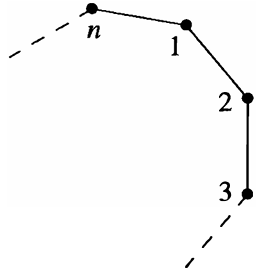
\includegraphics[width=0.25\textwidth]{images/fig1-1.png}
    \caption{}
    \label{fig1-1}
\end{figure}

于是，每个对称 \( s \) 都可以由 \(\{1, 2, 3, \dots, n\}\) 上相应的置换 \( \sigma \) 唯一描述，其中若对称 \( s \) 将顶点 \( i \) 放到顶点 \( j \) 原来的位置，则 \( \sigma \) 是将 \( i \) 映到 \( j \) 的置换。
例如，若 \( s \) 是绕 \( n \) 边形中心顺时针旋转 \( 2\pi/n \) 弧度，则 \( \sigma \) 是将 \( i \) 映到 \( i + 1 \)（\( 1 \leq i \leq n - 1 \)）且 \( \sigma(n) = 1 \) 的置换。
现在，通过对 \( s, t \in D_{2n} \) 定义 \( st \) 为先将 \( t \) 作用于 \( n \) 边形再作用 \( s \) 所得到的对称，将 \( D_{2n} \) 做成一个群（注意我们将对称视为 \( n \) 边形上的函数，因此 \( st \) 就是函数的复合——按通常的从右到左的读法）。
若 \( s, t \) 在顶点上分别实现置换 \( \sigma, \tau \)，则 \( st \) 实现 \( \sigma \circ \tau \). 
\( D_{2n} \) 上的二元运算是结合的，因为函数的复合是结合的。
\( D_{2n} \) 的单位元是恒等对称（保持所有顶点不动），记为 1，而 \( s \in D_{2n} \) 的逆元是逆转 \( s \) 的所有刚体运动的对称（因此若 \( s \) 在顶点上实现置换 \( \sigma \)，则 \( s^{-1} \) 实现 \( \sigma^{-1} \)）. 
在下一段中我们将证明
\[
|D_{2n}| = 2n,
\]
因此 \( D_{2n} \) 被称为 \( 2n \) 阶二面体群。
在某些教材中，这个群记为 \( D_n \)；然而，在群论文献中，\( D_{2n} \)（其中下标表示群的阶而不是顶点数）更为常见。

为了求阶 \(|D_{2n}|\)，注意到给定任意顶点 \(i\)，存在一个对称将顶点 1 送到位置 \(i\). 
由于顶点 2 与顶点 1 相邻，顶点 2 最终必在位置 \(i + 1\) 或 \(i - 1\)（其中 \(n + 1\) 视为 1，\(1 - 1\) 视为 \(n\)，即标号顶点的整数按模 \(n\) 读取）。
此外，在第一个对称之后，再对过顶点 \(i\) 和 \(n\) 边形中心的直线作反射，可以看出顶点 2 可以通过某个对称送到位置 \(i + 1\) 或 \(i - 1\) 中的任意一个。
因此，在对称作用下，有序顶点对 \((1, 2)\) 可以被送到 \(n \cdot 2\) 个位置。
%领域展开！
由于对称是刚体运动，一旦有序顶点对 \((1, 2)\) 的位置确定，对称在所有其余顶点上的作用就完全确定了。
因此，正 \(n\) 边形恰好有 \(2n\) 个对称。
此外，我们还可以明确地给出这 \(2n\) 个对称。
它们分别是绕中心旋转 \(2\pi i/n\) 弧度的 \(n\) 个旋转，\(0 \leq i \leq n - 1\)，以及关于 \(n\) 条对称轴的 \(n\) 个反射（若 \(n\) 为奇数，每条对称轴通过一个顶点和其对边的中点；若 \(n\) 为偶数，有 \(n/2\) 条对称轴通过两个相对顶点，另有 \(n/2\) 条对称轴垂直平分两条对边）。
例如，若 \(n = 4\)，在 \(x, y\) 平面中以原点画一个正方形，则对称轴为 \( x = 0 \)（\( y \) 轴）、\( y = 0 \)（\( x \) 轴）、\( y = x \) 和 \( y = -x \)（注意，通过原点的“反射”实际上不是反射，而是旋转 \( \pi \) 弧度）。

\begin{figure}[htbp]
    \centering
    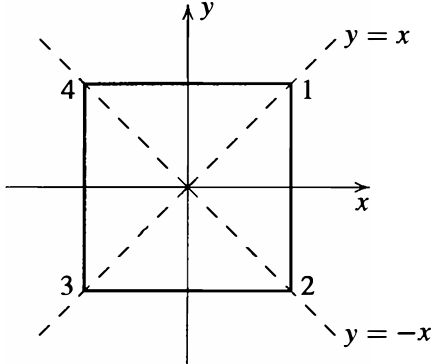
\includegraphics[width=0.4\textwidth]{images/fig1-2.png}
    \caption{}
    \label{fig1-2}
\end{figure}

由于二面体群将在全书中广泛用作例子，我们固定一些记号并提及一些计算，这些计算将简化未来的运算，并有助于将 \( D_{2n} \) 视为抽象群（而不必每次回到几何背景）。
在 \( x, y \) 平面中固定一个以原点为中心的正 \( n \) 边形，并沿顺时针方向将顶点依次标为 1 到 \( n \). 
设 \( r \) 为绕原点顺时针旋转 \( 2\pi / n \) 弧度的旋转。
设 \( s \) 为关于过顶点 1 和原点的对称轴的反射（我们对每个 \( n \) 使用相同的字母，但上下文总会明确 \( n \) 的值）。
我们将以下计算的细节留作练习（在大多数情况下我们将处理 \( D_6 \) 和 \( D_8 \)，因此读者可能希望先对 \( n = 3 \) 和 \( n = 4 \) 尝试这些练习）：

\begin{enumerate}[label=(\arabic*)]
\item\label{D_2n:(1)} \(1, r, r^2, \ldots, r^{n-1}\) 互不相同，且 \(r^n = 1\)，故 \(|r| = n\).
\item\label{D_2n:(2)} \(|s| = 2\).
\item\label{D_2n:(3)} 对任意 \(i\)，有\(s \neq r^i\) .
\item\label{D_2n:(4)} 对所有 \( 0 \leq i, j \leq n-1 \) 且 \( i \neq j \)，有 \( sr^i \neq sr^j \)，因此
\[
D_{2n} = \{1, r, r^2, \dots, r^{n-1}, s, sr, sr^2, \dots, sr^{n-1}\},
\]
即每个元素都可以唯一地写成 \( s^k r^i \) 的形式，其中 \( k = 0 \) 或 \( 1 \)，且 \( 0 \leq i \leq n-1 \).
\item \( rs = sr^{-1} \). [首先计算 \( s \) 在 \( \{1, 2, \dots, n\} \) 上实现什么置换，然后分别计算该等式两边对顶点 1 和 2 的作用.] 这特别表明 \( r \) 与 \( s \) 不可交换，因此 \( D_{2n} \) 是非阿贝尔的.
\item 对所有 \( 0 \leq i \leq n \)，\( r^i s = sr^{-i} \). [对 \( i \) 作归纳，并利用 \( r^{i+1} s = r(r^i s) \) 以及前面的计算结果.] 这说明了如何将 \( s \) 与 \( r \) 的幂交换。
\end{enumerate}


\subsection*{生成元与关系}

对二面体群使用生成元 \( r \) 和 \( s \) 提供了一种简明的方式在 \( D_{2n} \) 中进行计算。
我们可以类似地为任意群引入生成元和关系的概念。
尽早（在其形式化证明之前）掌握这些概念是有益的，因为它们为许多群提供了简单的描述和计算方法。
生成元将在 2.4 节中更详细地讨论，而这两个概念都将在 6.3 节引入自由群的概念时得到严格处理。

群 \( G \) 的元素的一个子集 \( S \)，若满足 \( G \) 中每个元素都可以写成 \( S \) 中元素及其逆元的（有限）乘积，则称 \( S \) 为 \( G \) 的一组\textbf{生成元}。
我们将在记号上写作 \( G = \langle S \rangle \)，并说 \( G \) 由 \( S \) \textbf{生成}，或 \( S \) \textbf{生成} \( G \)。
例如，整数 1 是整数加法群 \( \mathbb{Z} \) 的一个生成元，因为每个整数都是有限个 \(+1\) 与 \(-1\) 的和，所以 \( \mathbb{Z} = \langle 1 \rangle \). 
由 \( D_{2n} \) 的性质 \ref{D_2n:(4)}，集合 \( S = \{r, s\} \) 是 \( D_{2n} \) 的一组生成元，因此 \( D_{2n} = \langle r, s \rangle \)。我们后面将看到，在有限群 \( G \) 中，如果 \( G \) 的每个元素都是 \( S \) 中元素的有限乘积，则 \( S \) 生成 \( G \)（即不必再包含 \( S \) 中元素的逆元）。

一般群 \( G \) 中生成元满足的任何等式都称为 \( G \) 中的\textbf{关系}。
因此在 \( D_{2n} \) 中有关系：\( r^n = 1 \)，\( s^2 = 1 \) 以及 \( rs = sr^{-1} \)。
此外，在 \( D_{2n} \) 中，这三个关系还具有附加性质：群中元素之间的任何其他关系都可以从这三个关系导出（这并非显然；它出自以下事实：仅使用这三个关系就能确切判断两个群元素何时相等）。

一般地，若某个群 \( G \) 由子集 \( S \) 生成，并且存在一些关系，比如 \( R_1, R_2, \ldots, R_m \)（这里每个 \( R_i \) 是 \( S \cup \{1\} \) 中元素的方程），使得 \( S \) 中元素之间的任何关系都能从这些关系推出，则我们称这些生成元和关系为 \( G \) 的一个\textbf{表示}，并写作
\[
G = \langle S \mid R_1, R_2, \ldots, R_m \rangle.
\]

二面体群 \( D_{2n} \) 的一个表示（使用上述生成元和关系）为
\[
D_{2n} = \langle r, s \mid r^n = s^2 = 1,\ rs = sr^{-1} \rangle. \tag{1.1}
\]

我们将看到，使用这个表示来描述 \( D_{2n} \)（而不是总是回到原始的几何描述）将大大简化这些群的处理。

表示法提供了一种描述许多群的简单方法，但有一些微妙之处需要考虑。
其中之一是，在任意表示中，判断群的两个元素（用给定生成元表示）何时相等可能是困难的（甚至是不可能的）。
因此，所表示的群的阶是多少，甚至该群是有限还是无限，都可能不明显！
例如，可以证明 \( \langle x_1, y_1 \mid x_1^2 = y_1^2 = (x_1y_1)^2 = 1 \rangle \) 是一个 4 阶群的表示，而 \( \langle x_2, y_2 \mid x_2^3 = y_2^3 = (x_2y_2)^3 = 1 \rangle \) 是一个无限群的表示（见习题）。

另一个微妙之处是，即使在相当简单的表示中，也可能发生某种“坍缩”，因为关系以某种不明显的方式相互纠缠，即可能存在“隐藏的”或隐含的关系，它们没有在表示中明确给出，而是所给关系的推论。
这种坍缩使得通常甚至难以确定所表示的群的大小的下界。
例如，假设有人模仿 \( D_{2n} \) 的表示，试图通过定义另一个群：
\[
X_{2n} = \langle x, y \mid x^n = y^2 = 1,\ xy = yx^2 \rangle. \tag{1.2}
\]
“交换”关系 \( xy = yx^2 \) 决定了如何交换 \( y \) 和 \( x \)（即如何将 \( y \) 从 \( x \) 的右边“移到”左边），因此，正如在群 \( D_{2n} \) 中一样，这个群中的每个元素都可以写成 \( y^k x^i \) 的形式，其中所有 \( y \) 的幂在左边，所有\( x \) 的幂在右边。
此外，由前两个关系，\( x \) 和 \( y \) 的任何幂都可以化简，使得 \( i \) 介于 0 和 \( n-1 \) 之间，且 \( k \) 为 0 或 1.
因此人们可能认为 \( X_{2n} \) 再次是一个 \( 2n \) 阶群。
但事实并非如此，因为这个群中有一个由关系 \( x = xy^2 \)（因为 \( y^2 = 1 \)）通过反复应用交换关系和结合律将 \( y \) 移到左边而得到的“隐藏”关系：
\[
\begin{aligned}
x &= xy^2 = (xy)y = (yx^2)y = (yx)(xy) = (yx)(yx^2) \\
  &= y(xy)x^2 = y(yx^2)x^2 = y^2x^4 = x^4.
\end{aligned}
\]

由于 \( x^4 = x \)，由消去律得 \( X_{2n} \) 中 \( x^3 = 1 \)，并且由上面的讨论可知，对任意 \( n \)，\( X_{2n} \) 的阶至多为 6. 
根据 \( n \) 的值，还可能发生更多的坍缩（见习题）。

作为另一个例子，考虑表示
\[
Y = \langle u, v \mid u^4 = v^3 = 1,\ uv = v^2u^2 \rangle. \tag{1.3}
\]
在这种情况下，人们很容易猜测 \( Y \) 是一个 12 阶群，但同样存在额外的隐含关系。
事实上，这个群 \( Y \) 退化为 1 阶平凡群，即 \( u \) 和 \( v \) 满足额外关系 \( u = 1 \) 和 \( v = 1 \)（证明概述见习题）。

这种坍缩不会发生在 \( D_{2n} \) 的表示中，因为我们通过独立的（几何）方法证明存在一个 \( 2n \) 阶群，其生成元为 \( r \) 和 \( s \)，并且满足 \ref{D_2n:(1)} 中的关系。
因此，仅有这些关系的群的阶至少为 \( 2n \)。另一方面，容易看出（使用与上面 \( X_{2n} \) 类似的论证以及交换关系 \( rs = sr^{-1} \)）由 \ref{D_2n:(1)} 中的生成元和关系定义的任何群的阶至多为 \( 2n \)。因此，表示 \ref{D_2n:(1)} 所给出的群的阶恰好为 \( 2n \)，并且这个群确实就是正 \( n \) 边形的对称群。

我们对表示 \ref{D_2n:(1)} 所具有的额外信息是：存在一个已知阶的群满足这些信息。相比之下，我们对满足 \ref{D_2n:(2)} 或 \ref{D_2n:(3)} 中关系的任何群没有独立的认识。没有这种独立的“下界”信息，我们甚至可能无法确定一个给定的表示是否只是描述了平凡群，如 \ref{D_2n:(3)} 中的情况。

虽然一般来说，通过表示来规定群时必须非常小心，但对已知群使用表示法是一个强大的概念和计算工具。
关于表示的更多结果，包括更详细的例子，将在第 6.3 节中给出。

\subsection*{习题}
在以下习题中，\( D_{2n} \) 具有通常的表示 \( D_{2n} = \langle r, s \mid r^n = s^2 = 1,\ rs = sr^{-1} \rangle \).
\begin{enumerate}
\item 计算下列群中每个元素的阶：
\begin{enumerate}
\item \(D_6\)
\item \(D_8\)
\item \(D_{10}\).
\end{enumerate}
\item 利用生成元与关系证明：若 \(x \in D_{2n}\) 不是 \(r\) 的幂，则 \(rx = xr^{-1}\).
\item 证明 \(D_{2n}\) 中每个不是 \(r\) 的幂的元素都与 \(s\) 共轭，且阶为 2。
\item 若 \(n = 2k\) 是偶数且 \(n \ge 4\)，证明 \(z = r^k\) 是 2 阶元且与 \(D_{2n}\) 中所有元素可交换。证明 \(z\) 是唯一与所有元素可交换的非单位元。
\item 若 \(n\) 为奇数且 \(n \ge 3\)，证明单位元是 \(D_{2n}\) 中唯一与所有元素可交换的元素。
\item 设 \(x, y\) 是群 \(G\) 中的 2 阶元，令 \(t = xy\)。证明 \(tx = xt^{-1}\)。若 \(|xy| = n < \infty\)，则 \(x, t\) 满足与 \(D_{2n}\) 中 \(s, r\) 相同的关系。
\item 证明 \( \langle a, b \mid a^2 = b^2 = (ab)^n = 1 \rangle \) 给出了 \( D_{2n} \) 的一个用两个生成元 \( a = s \) 和 \( b = sr \)（它们在习题 3 中已计算出阶为 2）表示的表示。[证明 \( r \) 和 \( s \) 的关系可以从 \( a \) 和 \( b \) 的关系推出，反过来，\( a \) 和 \( b \) 的关系也可以从 \( r \) 和 \( s \) 的关系推出.]
\item 求 \(D_{2n}\) 中由 \(r\) 生成的循环子群的阶（参见第 1 节习题 27）。
\end{enumerate}

在习题 9 至 13 中，你可以通过遵循 \( D_{2n} \) 阶的证明来求出给定柏拉图立体在 \( \mathbb{R}^3 \) 中的刚体运动群（也称为旋转群）的阶：找出相邻顶点对可被送到的位置数。或者，你可以找出给定面可被送到的位置数，以及一旦一个面固定后，该面上一个顶点可被送到的位置数。
\begin{enumerate}[resume*]
\item 证明正四面体的空间刚体运动群阶为 12.
\item 证明立方体的空间刚体运动群阶为 24.
\item 证明正八面体的空间刚体运动群阶为 24.
\item 证明正十二面体的空间刚体运动群阶为 60.
\item 证明正二十面体的空间刚体运动群阶为 60.
\item 找出 \(\mathbb{Z}\) 的一组生成元。
\item 找出 \(\mathbb{Z}/n\mathbb{Z}\) 的一组生成元和关系。
\item 证明 \( \langle x_1, y_1 \mid x_1^2 = y_1^2 = (x_1y_1)^2 = 1 \rangle \) 是二面体群 \( D_4 \)（其中 \( x_1 \) 可用字母 \( r \) 代替，\( y_1 \) 用 \( s \) 代替）。[证明最后一个关系等价于 \( x_1y_1 = y_1x_1^{-1} \).]
\item 设 \( X_{2n} \) 是由 (1.2) 给出的群。
\begin{enumerate}[label=(\alph*)]
\item 证明若 \( n = 3k \)，则 \( X_{2n} \) 的阶为 6，且当 \( x \) 换为 \( r \)，\( y \) 换为 \( s \) 时，它具有与 \( D_6 \) 相同的生成元和关系。
\item 证明若 \( \gcd(3, n) = 1 \)，则 \( x \) 满足额外关系：\( x = 1 \). 在这种情况下，推出 \( X_{2n} \) 的阶为 2。[利用事实 \( x^n = 1 \) 和 \( x^3 = 1 \).]
\end{enumerate}
\item 设 \( Y \) 是由 (1.3) 给出的群。
\begin{enumerate}[label=(\alph*)]
\item 证明 \( v^2 = v^{-1} \).[利用关系 \( v^3 = 1 \).]
\item 证明 \( v \) 与 \( u^3 \) 可交换。[将左边写成 \( (v^2u^2)(uv) \) 并利用关系化简到右边，然后用 (a).]
\item 证明 \( v \) 与 \( u \) 可交换。[证明 \( u^9 = u \)，然后用 (b).]
\item 证明 \( uv = 1 \).[用 (c) 和最后一个关系。]
\item 证明 \( u = 1 \)，推出 \( v = 1 \)，并由此得出 \( Y = 1 \).[用 (d) 和方程 \( u^4v^3 = 1 \).]
\end{enumerate}
\end{enumerate}


\section{对称群}

设 \(\Omega\) 为任意非空集合，并令 \(S_\Omega\) 为从 \(\Omega\) 到自身的所有双射的集合（即 \(\Omega\) 的所有置换的集合）。
集合 \(S_\Omega\) 在函数复合 \(\circ\) 下构成群。
注意 \(\circ\) 是 \(S_\Omega\) 上的二元运算，因为若 \(\sigma : \Omega \to \Omega\) 和 \(\tau : \Omega \to \Omega\) 都是双射，则 \(\sigma \circ \tau\) 也是从 \(\Omega\) 到 \(\Omega\) 的双射。
由于函数复合一般是结合的，\(\circ\) 是结合的。
\(S_\Omega\) 的单位元是由“对所有 \(a \in \Omega\)，\(1(a) = a\)”定义的置换 1。
对每个置换 \(\sigma\)，存在一个（双边）逆函数 \(\sigma^{-1} : \Omega \to \Omega\)，满足 \(\sigma \circ \sigma^{-1} = \sigma^{-1} \circ \sigma = 1\). 
因此，\((S_\Omega, \circ)\) 满足所有群公理。
这个群称为集合 \(\Omega\) 上的\textbf{对称群}。
重要的是要认识到，\(S_\Omega\) 的元素是 \(\Omega\) 的\textbf{置换}，而不是 \(\Omega\) 本身的元素。

在特殊情形 \(\Omega = \{1, 2, 3, \ldots, n\}\) 时，\(\Omega\) 上的对称群记为 \(S_n\)，称为 \(n\) 次\textbf{对称群}。
群 \(S_n\) 将在全文中扮演重要角色，既作为自身具有相当研究兴趣的群，也作为说明和推动一般理论的手段。

首先我们证明 \(S_n\) 的阶为 \(n!\). 
\(\{1, 2, 3, \ldots, n\}\) 的置换正是该集合到自身的单射函数，因为它是有限的（命题 \ref{pro:0-1}），并且我们可以计算单射函数的个数。
一个单射函数 \(\sigma\) 可以将数字 1 送到 \(\{1, 2, 3, \ldots, n\}\) 中的任意 \(n\) 个元素之一；\(\sigma(2)\) 则可以是该集合中除 \(\sigma(1)\) 外的任意元素（因此 \(\sigma(2)\) 有 \(n-1\) 种选择）；\(\sigma(3)\) 可以是除 \(\sigma(1)\) 或 \(\sigma(2)\) 外的任意元素（因此 \(\sigma(3)\) 有 \(n-2\) 种选择），依此类推。
因此，从 \(\{1, 2, 3, \ldots, n\}\) 到自身的单射函数共有 \(n \cdot (n-1) \cdot (n-2) \cdots 2 \cdot 1 = n!\) 个。
因此 \(\{1, 2, 3, \ldots, n\}\) 恰好有 \(n!\) 个置换，所以 \(S_n\) 中恰好有 \(n!\) 个元素。

我们现在描述一种高效的记号来书写 \( S_n \) 的元素 \( \sigma \)，这个记号将在全文中使用，称为\textbf{轮换分解}。

一个\textbf{轮换}是一个整数串，它表示 \( S_n \) 中循环置换这些整数（并固定所有其他整数）的元素。
轮换 \( (a_1 \, a_2 \, \dots \, a_m) \) 是将 \( a_i \) 送到 \( a_{i+1} \)（\( 1 \leq i \leq m-1 \)）并将 \( a_m \) 送到 \( a_1 \) 的置换。
例如，\( (2 \, 1 \, 3) \) 是将 2 映到 1、1 映到 3、3 映到 2 的置换。
一般地，对每个 \( \sigma \in S_n \)，数字 1 到 \( n \) 将被重新排列并分成 \( k \) 个轮换，形式为
\[
(a_1 \, a_2 \, \dots \, a_{m_1})(a_{m_1+1} \, a_{m_1+2} \, \dots \, a_{m_2}) \cdots (a_{m_{k-1}+1} \, a_{m_{k-1}+2} \, \dots \, a_{m_k}),
\]
从中可以容易地读出 \( \sigma \) 在 1 到 \( n \) 中任意数上的作用，如下所述。
对任意 \( x \in \{1, 2, 3, \dots, n\} \)，首先在上述表达式中定位 \( x \). 
如果 \( x \) 后面不紧跟右括号（即 \( x \) 不在 \( k \) 个轮换中某一个的右端），则 \( \sigma(x) \) 是紧接在 \( x \) 右边的整数。
如果 \( x \) 后面跟着右括号，则 \( \sigma(x) \) 是以 \( x \) 结尾的那个轮换开头的数字（即，若 \( x = a_{m_i} \)（对某个 \( i \)），则 \( \sigma(x) = a_{m_{i-1}+1} \)（其中 \( m_0 \) 取为 0））。
我们可以将这个对 \( \sigma \) 的描述表示如图：

\begin{figure}[htbp]
    \centering
    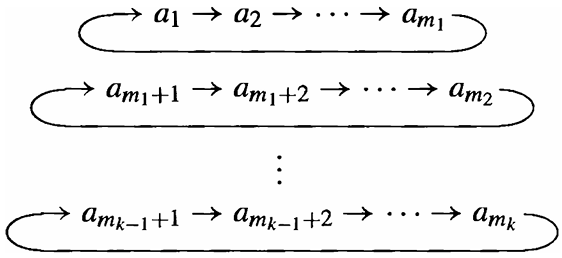
\includegraphics[width=0.6\textwidth]{images/fig1-3.png}
    \caption{}
    \label{fig1-3}
\end{figure}

所有轮换的乘积称为 \( \sigma \) 的\textbf{轮换分解}。

我们现在给出计算 \( S_n \) 中元素 \( \sigma \) 的轮换分解的算法，并用一个具体的置换逐步演示该算法。
我们将这个算法的证明以及轮换分解唯一性方面的完整分析推迟到第 4 章。


设 \( n = 13 \)，并令 \( \sigma \in S_{13} \) 定义为
\[
\begin{aligned}
\sigma(1) = 12, 
\quad \sigma(2) = 13, 
\quad \sigma(3) = 3, 
\quad \sigma(4) = 1, 
\quad \sigma(5) = 11, \\
\sigma(6) = 9, 
\quad \sigma(7) = 5, 
\quad \sigma(8) = 10, 
\quad \sigma(9) = 6, 
\quad \sigma(10) = 4,
\\
\sigma(11) = 7, 
\quad \sigma(12) = 8, 
\quad \sigma(13) = 2.
\end{aligned}
\]

\begin{tabular}{|p{9cm}|p{4cm}|}
\hline
\textbf{方法} & \textbf{示例} \\
\hline
开始一个新轮换：选取 \(\{1, 2, \dots, n\}\) 中尚未出现在之前轮换里的最小元素，记为 \(a\)（若刚开始，则 \(a = 1\)）；开始新轮换：\((a\) & \((1\) \\
\hline
从给定的 \(\sigma\) 描述中读出 \(\sigma(a)\)，记为 \(b\). 
若 \(b = a\)，用右括号关闭该轮换（不写出 \(b\)）；此轮换完成，返回第 1 步。
若 \(b \neq a\)，在本轮换中把 \(b\) 写在 \(a\) 旁边：\((a\,b\) & \(\sigma(1) = 12 = b\)，且 \(12 \neq 1\)，因此写出：\((1\,12\) \\
\hline
从给定的 \(\sigma\) 描述中读出 \(\sigma(b)\)，记为 \(c\). 
若 \(c = a\)，用右括号关闭该轮换；返回第 1 步。
若 \(c \neq a\)，在本轮换中把 \(c\) 写在 \(b\) 旁边：\((a\,b\,c\). 
重复此步骤，将 \(c\) 作为新的 \(b\) 值，直到轮换闭合为止。 
& \(\sigma(12) = 8\)，且 \(8 \neq 1\)，因此继续轮换为：\((1\,12\,8\) \\
\hline
\end{tabular}
\vspace{\baselineskip}

自然地，当 \(\{1, 2, \dots, n\}\) 中的所有数都已出现在某个轮换中时，这个过程就停止了。
对于例子中的特定 \(\sigma\)，这给出
\[
\sigma = (1\ 12\ 8\ 10\ 4)(2\ 13)(3)(5\ 11\ 7)(6\ 9).
\]

一个轮换的\textbf{长度}是出现在其中的整数的个数。
长度为 \(t\) 的轮换称为 \textbf{\(t\)-轮换}。
两个轮换若没有公共的数字，则称为\textbf{不相交}的。
因此，上面的元素 \(\sigma\) 是 5 个（两两）不相交轮换的乘积：一个 5-轮换、一个 2-轮换、一个 1-轮换、一个 3-轮换，以及另一个 2-轮换。

从现在起，我们采用省略 1-轮换的约定。
因此，若某个整数 \(i\) 没有出现在置换 \(\tau\) 的轮换分解中，则理解为 \(\tau(i) = i\)，即 \(\tau\) 固定 \(i\). 
\(S_n\) 的恒等置换的轮换分解为 \((1)(2)\cdots(n)\)，将简写为 1。
于是算法的最后一步为：

\begin{tabular}{|p{9cm}|p{4cm}|}
\hline
最终步骤：删除所有长度为 1 的轮换
\hline
\end{tabular}
\vspace{\baselineskip}

因此，例子中特定 \(\sigma\) 的轮换分解为
\[
\sigma = (1\ 12\ 8\ 10\ 4)(2\ 13)(5\ 11\ 7)(6\ 9).
\]
这个约定的好处是：\(S_n\) 中元素 \(\tau\) 的轮换分解，同时也是 \(S_m\)（\(m \geq n\)）中那个在 \(\{1, 2, 3, \dots, n\}\) 上作用与 \(\tau\) 相同、并固定 \(\{n+1, n+2, \dots, m\}\) 中每个元素的置换的轮换分解。
因此，例如，\((1\ 2)\) 是互换 1 和 2 并固定所有更大的整数的置换，无论在 \(S_2\), \(S_3\) 还是 \(S_4\) 等中看待都是如此。

作为另一个例子，\(S_3\) 的 6 个元素具有如下的轮换分解：

\begin{table}[h!]
    \centering
    \caption{群 \( S_3 \)}
    \begin{tabular}{|c|c|}
\hline
\( \sigma_i \) 的取值 & \( \sigma_i \) 的轮换分解 \\
\hline
\(\sigma_1(1) = 1,\ \sigma_1(2) = 2,\ \sigma_1(3) = 3\) & 1 \\
\(\sigma_2(1) = 1,\ \sigma_2(2) = 3,\ \sigma_2(3) = 2\) & (2 3) \\
\(\sigma_3(1) = 3,\ \sigma_3(2) = 2,\ \sigma_3(3) = 1\) & (1 3) \\
\(\sigma_4(1) = 2,\ \sigma_4(2) = 1,\ \sigma_4(3) = 3\) & (1 2) \\
\(\sigma_5(1) = 2,\ \sigma_5(2) = 3,\ \sigma_5(3) = 1\) & (1 2 3) \\
\hline
\end{tabular}
    \label{tab:placeholder}
\end{table}

对任意 \( \sigma \in S_n \)，\( \sigma^{-1} \) 的轮换分解可通过将 \( \sigma \) 的轮换分解中每个轮换里的数字按相反顺序写出而得到。
例如，若
$\sigma = (1\ 12\ 8\ 10\ 4)(2\ 13)(5\ 11\ 7)(6\ 9) $
是前面描述的 \( S_{13} \) 中的元素，则
\[ \sigma^{-1} = (4\ 10\ 8\ 12\ 1)(13\ 2)(7\ 11\ 5)(9\ 6). \]

在 \( S_n \) 中计算乘积是直接的，只要记住在计算 \( \sigma \circ \tau \) 时，要从右向左读置换。
只需“跟随”元素在相继置换下的像即可。
例如，在乘积 (1 2 3) \(\circ\) (1 2)(3 4) 中，数字 1 被第一个置换送到 2，然后 2 被第二个置换送到 3，因此复合映射将 1 送到 3。
要计算该乘积的轮换分解，接下来需要看 3 的情况。
它先被送到 4，然后 4 被固定，所以复合映射将 3 送到 4。
类似地，4 先被送到 3，然后 3 被送到 1，从而完成乘积中的这个轮换：\((1 \, 3 \, 4)\). 
最后，2 被送到 1，然后 1 被送到 2，因此 2 被该乘积固定，所以 \((1 \, 2 \, 3) \circ (1 \, 2)(3 \, 4) = (1 \, 3 \, 4)\) 就是该乘积的轮换分解。

作为更多的例子，
\[
(12) \circ (13) = (1 \, 3 \, 2) \quad \text{与} \quad (1 \, 3) \circ (1 \, 2) = (1 \, 2 \, 3).
\]
特别地，这表明
\[
S_n \text{ 对所有 } n \geq 3 \textbf{ 都是非阿贝尔群}.
\]

轮换分解中的每个轮换 \((a_1 \, a_2 \, \ldots \, a_m)\) 都可看作循环置换 \(a_1, a_2, \ldots, a_m\) 并固定所有其他整数的置换。
由于不相交的轮换置换的是不相交集合中的数字，因此有
\[
\textbf{不相交的轮换可交换}.
\]
因此，在任何不相交轮换的乘积（特别是轮换分解）中重新排列轮换的顺序不会改变置换。

此外，由于给定轮换 \((a_1 \, a_2 \, \ldots \, a_m)\) 循环地置换 \(\{a_1, a_2, \ldots, a_m\}\)，轮换中的数字可以循环地重排而不改变置换，即
\[
(a_1 \, a_2 \, \ldots \, a_m) = (a_2 \, a_3 \, \ldots \, a_m \, a_1) = (a_3 \, a_4 \, \ldots \, a_m \, a_1 \, a_2) = \cdots = (a_m \, a_1 \, a_2 \, \ldots \, a_{m-1}).
\]
因此，例如，\((1 \, 2) = (2 \, 1)\) 且 \((1 \, 2 \, 3 \, 4) = (3 \, 4 \, 1 \, 2)\). 
按惯例，轮换中出现的最小数通常写在最前面。

使用轮换时必须小心，因为一个置换可以以多种方式写成轮换的任意乘积。
例如，在 \(S_3\) 中，
\((1 \, 2 \, 3) = (1 \, 2)(2 \, 3) = (1 \, 3)(1 \, 3 \, 2)(1 \, 3)\) 等等。
但（如我们将要证明的）每个置换的轮换分解是将置换表示为不相交轮换的乘积的唯一方式（除了重新排列轮换和轮换内数字的循环重排外）。
将轮换的任意乘积化为不相交轮换的乘积，使我们能一眼判定两个置换是否相同。
这种记号的另一个优点是，证明\textbf{置换的阶等于其轮换分解中各轮换长度的最小公倍数}是一个习题（下面概述）。



\subsection*{习题}

\begin{enumerate}
\item 设 \( \sigma \) 为置换
\[
1 \mapsto 3 \quad 2 \mapsto 4 \quad 3 \mapsto 5 \quad 4 \mapsto 2 \quad 5 \mapsto 1,
\]
且 \( \tau \) 为置换
\[
1 \mapsto 5 \quad 2 \mapsto 3 \quad 3 \mapsto 2 \quad 4 \mapsto 4 \quad 5 \mapsto 1.
\]
求下列每个置换的轮换分解：\( \sigma, \tau, \sigma^2, \sigma\tau, \tau\sigma \) 及 \( \tau^2\sigma \).

\item 设 \( \sigma \) 为置换
\[
\begin{aligned}
1 \mapsto 13,&\quad 2 \mapsto 2,\quad 3 \mapsto 15,\quad 4 \mapsto 14,\quad 5 \mapsto 10,\\
6 \mapsto 6,&\quad 7 \mapsto 12,\quad 8 \mapsto 3,\quad 9 \mapsto 4,\quad 10 \mapsto 1,\\
11 \mapsto 7,&\quad 12 \mapsto 9,\quad 13 \mapsto 5,\quad 14 \mapsto 11,\quad 15 \mapsto 8,
\end{aligned}
\]
且 \( \tau \) 为置换
\[
\begin{aligned}
1 \mapsto 14,&\quad 2 \mapsto 9,\quad 3 \mapsto 10,\quad 4 \mapsto 2,\quad 5 \mapsto 12,\\
6 \mapsto 6,&\quad 7 \mapsto 5,\quad 8 \mapsto 11,\quad 9 \mapsto 15,\quad 10 \mapsto 3,\\
11 \mapsto 8,&\quad 12 \mapsto 7,\quad 13 \mapsto 4,\quad 14 \mapsto 1,\quad 15 \mapsto 13.
\end{aligned}
\]
求下列置换的轮换分解：\( \sigma, \tau, \sigma^2, \sigma\tau, \tau\sigma \) 及 \( \tau^2\sigma \).

\item 对前两题中已求出轮换分解的每个置换，计算其阶.

\item 计算下列群中每个元素的阶：
\begin{enumerate}[label=(\alph*)]
\item \( S_3 \);
\item \( S_4 \).
\end{enumerate}

\item 求 \( (1 \ 12 \ 8 \ 10 \ 4)(2 \ 13)(5 \ 11 \ 7)(6 \ 9) \) 的阶.

\item 写出 \( S_4 \) 中每个 4 阶元的轮换分解.

\item 写出 \( S_4 \) 中每个 2 阶元的轮换分解.

\item 证明若 \( \Omega = \{1, 2, 3, \dots\} \)，则 \( S_\Omega \) 是无限群（不要说 \( \infty! = \infty \)）.

\item \begin{enumerate}[label=(\alph*)]
\item 设 \( \sigma \) 为 12-轮换 \( (1 \ 2 \ 3 \ 4 \ 5 \ 6 \ 7 \ 8 \ 9 \ 10 \ 11 \ 12) \). 对哪些正整数 \( i \)，\( \sigma^i \) 也是 12-轮换？
\item 设 \( \tau \) 为 8-轮换 \( (1 \ 2 \ 3 \ 4 \ 5 \ 6 \ 7 \ 8) \). 对哪些正整数 \( i \)，\( \tau^i \) 也是 8-轮换？
\item 设 \( \omega \) 为 14-轮换 \( (1 \ 2 \ 3 \ 4 \ 5 \ 6 \ 7 \ 8 \ 9 \ 10 \ 11 \ 12 \ 13 \ 14) \). 对哪些正整数 \( i \)，\( \omega^i \) 也是 14-轮换？
\end{enumerate}

\item 证明若 \( \sigma \) 是 \( m \)-轮换 \( (a_1 \ a_2 \ \dots \ a_m) \)，则对所有 \( i \in \{1, 2, \dots, m\} \)，\( \sigma^i(a_k) = a_{k+i} \)，其中当 \( k+i > m \) 时 \( k+i \) 用其模 \( m \) 的最小剩余代替。由此推出 \( |\sigma| = m \).

\item 设 \( \sigma \) 为 \( m \)-轮换 \( (1 \ 2 \ \dots \ m) \). 证明 \( \sigma^i \) 也是 \( m \)-轮换当且仅当 \( i \) 与 \( m \) 互素.

\item \begin{enumerate}[label=(\alph*)]
\item 若 \( \tau = (1 \ 2)(3 \ 4)(5 \ 6)(7 \ 8)(9 \ 10) \)，判断是否存在一个 \( n \)-轮换 \( \sigma \)（\( n \geq 10 \)）使得对某个整数 \( k \) 有 \( \tau = \sigma^k \).
\item 若 \( \tau = (1 \ 2)(3 \ 4 \ 5) \)，判断是否存在一个 \( n \)-轮换 \( \sigma \)（\( n \geq 5 \)）使得对某个整数 \( k \) 有 \( \tau = \sigma^k \).
\end{enumerate}

\item 证明 \( S_n \) 中一个元素的阶为 2 当且仅当其轮换分解是一组两两不相交的对换的乘积.

\item 设 \( p \) 为素数。证明 \( S_n \) 中一个元素的阶为 \( p \) 当且仅当其轮换分解是一组两两不相交的 \( p \)-轮换的乘积。通过一个具体例子说明，若 \( p \) 不是素数，则结论不一定成立.

\item 证明 \( S_n \) 中元素的阶等于其轮换分解中各轮换长度的最小公倍数。[利用习题 10 和第 1 节习题 24.]

\item 证明若 \( n \geq m \)，则 \( S_n \) 中 \( m \)-轮换的个数为
\[
\frac{n(n-1)(n-2)\cdots(n-m+1)}{m}.
\]
[计算构成一个 \( m \)-轮换的方式数，再除以一个特定 \( m \)-轮换的表示个数.]

\item 证明若 \( n \geq 4 \)，则 \( S_n \) 中可写成两个不相交 2-轮换之积的置换的个数为
\[
\frac{n(n-1)(n-2)(n-3)}{8}.
\]

\item 找出所有整数 \( n \)，使得 \( S_5 \) 中含有 \( n \) 阶元。[利用习题 15.]

\item 找出所有整数 \( n \)，使得 \( S_7 \) 中含有 \( n \) 阶元。[利用习题 15.]

\item 找出 \( S_3 \) 的一组生成元和关系。

\end{enumerate}

\section{矩阵群}

在本节中，我们引入系数来自域的矩阵群的概念。这个群族例子将在第一部分中用于说明目的，并在向量空间的章节中进行更详细的研究。

域是能够进行所有算术运算 \( + \), \( - \), \( \times \) 和 \( \div \)（除以非零元）的“最小”数学结构，因此特别地，每个非零元都必须有乘法逆元。
我们将在后面更深入地研究域，在本部分的文本中，我们将遇到的域只有 \( \mathbb{Q} \), \( \mathbb{R} \) 和 \( \mathbb{Z}/p\mathbb{Z} \)（其中 \( p \) 是素数）。
例子 \( \mathbb{Z}/p\mathbb{Z} \) 是一个有限域，为了强调它是个域，我们将它记为 \( \mathbb{F}_p \). 
为完整起见，我们在此给出域的精确定义。

\begin{definition}
\begin{enumerate}
\item 一个\textbf{域}是一个集合 \( F \)，连同 \( F \) 上的两个二元运算 \(+\) 和 \(\cdot\)，使得 \((F, +)\) 是阿贝尔群（称其单位元为 0），\((F - \{0\}, \cdot)\) 也是阿贝尔群，并且满足以下\textbf{分配律}：
\[
a \cdot (b + c) = (a \cdot b) + (a \cdot c), \quad \text{对所有 } a, b, c \in F.
\]
\item 对任意域 \( F \)，记 \( F^\times = F - \{0\} \).
\end{enumerate}
\end{definition}

所有标量来自 \(\mathbb{R}\) 时的向量空间理论、矩阵与线性变换理论以及行列式理论，在标量来自任意域 \( F \) 时（\textbf{作适当修改后}）仍然成立。
当我们在第一部分使用这些理论时，会明确说明我们所假设的关于域的事实。

对每个 \( n \in \mathbb{Z}^+ \)，令 \( GL_n(F) \) 为所有元素来自 \( F \) 且行列式非零的 \( n \times n \) 矩阵的集合，即
\[
GL_n(F) = \{A \mid A \text{ 是元素来自 } F \text{ 的 } n \times n \text{ 矩阵，且 } \det(A) \neq 0\},
\]
其中元素来自 \( F \) 的任意矩阵 \( A \) 的行列式可用与 \( F = \mathbb{R} \) 时相同的公式计算。
对任意 \( n \times n \) 矩阵 \( A \) 和 \( B \)，令 \( AB \) 为按与 \( F = \mathbb{R} \) 时相同的规则计算出的乘积。
这个乘积是结合的。
此外，由于 \( \det(AB) = \det(A) \cdot \det(B) \)，若 \( \det(A) \neq 0 \) 且 \( \det(B) \neq 0 \)，则 \( \det(AB) \neq 0 \)，所以 \( GL_n(F) \) 在矩阵乘法下封闭。
进一步地，\( \det(A) \neq 0 \) 当且仅当 \( A \) 有矩阵逆（且该逆可用与 \( F = \mathbb{R} \) 时相同的伴随公式计算），因此每个 \( A \in GL_n(F) \) 在 \( GL_n(F) \) 中都有逆元 \( A^{-1} \)：
\[
AA^{-1} = A^{-1}A = I,
\]
其中 \( I \) 是 \( n \times n \) 单位矩阵。
因此 \( GL_n(F) \) 在矩阵乘法下构成群，称为 \textbf{\( n \) 次一般线性群}。

以下结果将在第三部分中证明，但现在为了方便起见予以记录：
\begin{enumerate}[label=\arabic*]
\item 若 \( F \) 是域且 \( |F| < \infty \)，则对某个素数 \( p \) 和整数 \( m \)，有 \( |F| = p^m \)；
\item 若 \( |F| = q < \infty \)，则
\[
|GL_n(F)| = (q^n - 1)(q^n - q)(q^n - q^2)\cdots(q^n - q^{n-1}).
\]
\end{enumerate}

\subsection*{习题}

\begin{enumerate}
\item 证明 \( |GL_2(\mathbb{F}_2)| = 6 \).

\item 写出 \( GL_2(\mathbb{F}_2) \) 的所有元素，并计算每个元素的阶。

\item 证明 \( GL_2(\mathbb{F}_2) \) 是非阿贝尔的。

\item 证明若 \( n \) 不是素数，则 \( \mathbb{Z}/n\mathbb{Z} \) 不是域。

\item 证明 \( GL_n(F) \) 是有限群当且仅当 \( F \) 只有有限多个元素。

\item 若 \( |F| = q \) 有限，证明 \( |GL_n(F)| < q^{n^2} \)。

\item 设 \( p \) 为素数。证明 \( GL_2(\mathbb{F}_p) \) 的阶为 \( p^4 - p^3 - p^2 + p \)（不要直接引用本节中的阶公式）。[从 \( \mathbb{F}_p \) 上 \( 2 \times 2 \) 矩阵的总数中减去不可逆矩阵的个数。你可使用事实：一个 \( 2 \times 2 \) 矩阵不可逆当且仅当某一行是另一行的倍数。]

\item 证明对任意 \( n \geq 2 \) 和任意域 \( F \)，\( GL_n(F) \) 是非阿贝尔的。

\item 证明实 \( 2 \times 2 \) 矩阵的乘法运算作为二元运算是结合的。

\item 设
\[
G = \left\{ \begin{pmatrix} a & b \\ 0 & c \end{pmatrix} \,\middle|\, a, b, c \in \mathbb{R},\ a \neq 0,\ c \neq 0 \right\}.
\]
\begin{enumerate}[label=(\alph*)]
\item 计算 \( \begin{pmatrix} a_1 & b_1 \\ 0 & c_1 \end{pmatrix} \) 与 \( \begin{pmatrix} a_2 & b_2 \\ 0 & c_2 \end{pmatrix} \) 的乘积，以证明 \( G \) 在矩阵乘法下封闭。
\item 求 \( \begin{pmatrix} a & b \\ 0 & c \end{pmatrix} \) 的矩阵逆，并推出 \( G \) 在取逆下封闭。
\item 推出 \( G \) 是 \( GL_2(\mathbb{R}) \) 的一个子群（见第 1 节习题 26）。
\item 证明 \( G \) 中两个对角元相等（即 \( a = c \)）的元素组成的集合也是 \( GL_2(\mathbb{R}) \) 的一个子群。
\end{enumerate}

\item 下面的习题引入域 \( F \) 上的\textbf{海森堡群}，并发展其一些基本性质。当 \( F = \mathbb{R} \) 时，该群通过给出海森堡不确定性原理的群论解释（归功于 H. Weyl），在量子力学和信号理论中扮演重要角色。注意，海森堡群也可以更一般地定义——例如，元素来自 \( \mathbb{Z} \).

设
\[
H(F) = \left\{ \begin{pmatrix} 1 & a & b \\ 0 & 1 & c \\ 0 & 0 & 1 \end{pmatrix} \,\middle|\, a, b, c \in F \right\}
\]
称为 \( F \) 上的\textbf{海森堡群}。令
\[
X = \begin{pmatrix} 1 & a & b \\ 0 & 1 & c \\ 0 & 0 & 1 \end{pmatrix}, \qquad
Y = \begin{pmatrix} 1 & d & e \\ 0 & 1 & f \\ 0 & 0 & 1 \end{pmatrix}
\]
为 \( H(F) \) 中的元素。
\begin{enumerate}[label=(\alph*)]
\item 计算矩阵乘积 \( XY \)，并推出 \( H(F) \) 在矩阵乘法下封闭。
给出具体矩阵例子使得 \( XY \neq YX \)（从而 \( H(F) \) 总是非阿贝尔的）。
\item 给出矩阵逆 \( X^{-1} \) 的显式公式，并由此推出 \( H(F) \) 对逆封闭.
\item 证明 \( H(F) \) 的结合律，并推出 \( H(F) \) 是一个阶为 \( |F|^3 \) 的群。（不要假定矩阵乘法是结合的。）
\item 求有限群 \( H(\mathbb{Z}/2\mathbb{Z}) \) 中每个元素的阶。
\item 证明 \( H(\mathbb{R}) \) 中每个非单位元都有无限阶。
\end{enumerate}
\end{enumerate}

\section{四元数群}

\textbf{四元数群} \(Q_8\) 定义为
\[
Q_8 = \{1, -1, i, -i, j, -j, k, -k\},
\]
其乘法 \(\cdot\) 按以下规则计算：
\[
1 \cdot a = a \cdot 1 = a, \quad \text{对所有 } a \in Q_8,
\]
\[
(-1) \cdot (-1) = 1, \quad (-1) \cdot a = a \cdot (-1) = -a, \quad \text{对所有 } a \in Q_8,
\]
\[
i \cdot i = j \cdot j = k \cdot k = -1,
\]
\[
i \cdot j = k, \quad j \cdot i = -k,
\]
\[
j \cdot k = i, \quad k \cdot j = -i,
\]
\[
k \cdot i = j, \quad i \cdot k = -j.
\]

今后我们将 \( a \cdot b \) 简写为 \( ab \). 
验证结合律是繁琐的（我们稍后将用不那么计算性的方法证明），但其他公理很容易验证。
注意 \( Q_8 \) 是一个 8 阶非阿贝尔群。

\subsection*{习题}

\begin{enumerate}
\item 计算 \(Q_8\) 中每个元素的阶。
\item 写出 \(S_3, D_8, Q_8\) 的群表。
\item 找出 \(Q_8\) 的一组生成元和关系。
\end{enumerate}

\section{同态与同构}

在本节中，我们精确地给出两个群何时“看起来相同”的概念，即它们具有完全相同的群论结构。
这就是两个群之间的\textbf{同构}的概念。
我们首先定义\textbf{同态}的概念，关于这个概念我们将在后面有更多的论述。

\begin{definition}
设 \((G, \star)\) 和 \((H, \diamond)\) 是群。
一个映射 \(\varphi : G \to H\)，若满足
\[
\varphi(x \star y) = \varphi(x) \diamond \varphi(y), \quad \text{对所有 } x, y \in G,
\]
则称为\textbf{同态}。
\end{definition}

当 \( G \) 和 \( H \) 的群运算没有明确写出时，同态条件简化为
\[
\varphi(xy) = \varphi(x)\varphi(y),
\]
但重要的是要记住，左边的乘积 \( xy \) 是在 \( G \) 中计算的，而右边的乘积 \( \varphi(x)\varphi(y) \) 是在 \( H \) 中计算的。
直观地说，一个映射 \( \varphi \) 若保持其定义域和陪域的群结构，则称为同态。

\begin{definition}
映射 \( \varphi : G \to H \) 称为\textbf{同构}，并称 \( G \) 与 \( H \) \textbf{同构}或具有相同的\textbf{同构类型}，记为 \( G \cong H \)，如果
\begin{enumerate}[label=(\arabic*)]
\item \( \varphi \) 是同态（即 \( \varphi(xy) = \varphi(x)\varphi(y) \)），且
\item \( \varphi \) 是双射。
\end{enumerate}
换言之，若 \( G \) 与 \( H \) 之间存在一个保持群运算的双射，则它们同构。
直观地，\( G \) 与 \( H \) 是同一个群，只是元素和运算在 \( G \) 和 \( H \) 中可能写法不同。
因此，\( G \) 所具有的任何仅依赖于 \( G \) 的群结构的性质（即可以从群公理推导出来的性质，例如群的交换性）在 \( H \) 中也成立。
注意，这正式证明了将我们所有的群运算写作 \(\cdot\) 是合理的，因为改变运算的符号不会改变同构类型。
\end{definition}

\begin{example}
\begin{enumerate}[label=(\arabic*)]
\item 对任意群 \( G \)，有 \( G \cong G \). 
恒等映射给出一个显然的同构，但一般不是从 \( G \) 到自身的\textbf{唯一}同构。
更一般地，设 \( \mathcal{G} \) 是任意非空群族。
容易验证关系 \( \cong \) 是 \( \mathcal{G} \) 上的等价关系，其等价类称为\textbf{同构类}。
这解释了“同构”定义中有些对称性的措辞。

\item 指数映射 \( \exp : \mathbb{R} \to \mathbb{R}^+ \)，定义为 \( \exp(x) = e^x \)，其中 \( e \) 是自然对数的底，是从 \( (\mathbb{R}, +) \) 到 \( (\mathbb{R}^+, \times) \) 的同构。
\( \exp \) 是双射，因为它有反函数（即 \( \log_e \)），并且 \( \exp \) 保持群运算，因为 \( e^{x+y} = e^x e^y \). 
在这个例子中，元素和运算都不同，但两个群同构，即作为群它们具有相同的结构。

\item 在这个例子中，我们证明对称群的同构类型只取决于被置换的底集的基数。

设 \( \Delta \) 和 \( \Omega \) 是非空集合。
若 \( |\Delta| = |\Omega| \)，则对称群 \( S_\Delta \) 与 \( S_\Omega \) 同构。
我们可以直观地理解如下：给定 \( |\Delta| = |\Omega| \)，存在一个从 \( \Delta \) 到 \( \Omega \) 的双射 \( \theta \).
把 \( \Delta \) 和 \( \Omega \) 的元素通过 \( \theta \) “粘合”在一起，即每个 \( x \in \Delta \) 粘合到 \( \theta(x) \in \Omega \). 
要得到一个映射 \( \varphi : S_\Delta \to S_\Omega \)，设 \( \sigma \in S_\Delta \) 是 \( \Delta \) 的一个置换，并令 \( \varphi(\sigma) \) 为 \( \Omega \) 的置换，
%又用神之一令放大招了
它以 \( \sigma \) 移动 \( \Delta \) 中对应粘合元素的相同方式移动 \( \Omega \) 的元素；即，若对某些 \( x, y \in \Delta \) 有 \( \sigma(x) = y \)，则 \( \varphi(\sigma)(\theta(x)) = \theta(y) \) 在 \( \Omega \) 中成立。
由于集合双射 \( \theta \) 有逆，容易验证对称群之间的映射也有逆。
映射 \( \varphi \) 的精确技术定义以及确保 \( \varphi \) 是同构的那些性质的直接但繁琐的验证，留待下面的习题中完成。
%你把最好吃的一块吃给我看是吧

反过来，若 \( S_\Delta \cong S_\Omega \)，则 \( |\Delta| = |\Omega| \)；我们仅在底集为有限集时证明这一点（当 \( \Delta \) 和 \( \Omega \) 都是无限集时，证明更困难，将在第 4 章中作为一个习题给出）。
由于两个群 \( G \) 和 \( H \) 之间的任何同构先验地是它们之间的双射，同构的一个必要条件是 \( |S_\Delta| = |S_\Omega| \). 
当 \( \Delta \) 是 \( n \) 阶有限集时，\( |S_\Delta| = n! \). 
我们实际上只对 \( S_n \) 证明了这一点，但相同的推理适用于 \( S_\Delta \). 
类似地，若 \( \Omega \) 是 \( m \) 阶有限集，则 \( |S_\Omega| = m! \). 
因此，若 \( S_\Delta \) 与 \( S_\Omega \) 同构，则 \( n! = m! \)，所以 \( m = n \)，即 \( |\Delta| = |\Omega| \).
\end{enumerate}
\end{example}

更多同构的例子将在全文中出现。当我们研究不同的结构（环、域、向量空间等）时，我们会在相应的结构之间表述同构的对应概念。
数学中的核心问题之一是确定一个结构的哪些性质决定了它的同构类型（即，证明如果 \( G \) 是具有某种结构（如群）的对象，且 \( G \) 具有性质 \( \mathcal{P} \)，那么任何其他具有相同结构（群）且具有性质 \( \mathcal{P} \) 的对象 \( X \) 都与 \( G \) 同构）。
这类定理称为\textbf{分类定理}。
例如，我们将证明：
\[
\textbf{任何 6 阶非阿贝尔群都同构于 \( S_3 \)}。
\]
（因此这里 \( G \) 是群 \( S_3 \)，而 \( \mathcal{P} \) 是性质“非阿贝尔且阶为 6”）。
从这个分类定理我们可以得到 \( D_6 \cong S_3 \) 和 \( GL_2(\mathbb{F}_2) \cong S_3 \)，而不必在这些群之间找出显式的映射。
注意，并不是任何 6 阶群都同构于 \( S_3 \)。
事实上，我们将证明在同构意义下恰好有两个 6 阶群：\( S_3 \) 和 \( \mathbb{Z}/6\mathbb{Z} \)（即任何 6 阶群都同构于这两个群之一，且 \( S_3 \) 不同构于 \( \mathbb{Z}/6\mathbb{Z} \)）。
注意这种结论不那么具体（有两种可能的类型）；但假设条件更容易验证（即检查阶是否为 6）。
后一类结果也称为分类。
一般来说，即使在具体实例中，判断两个群（或其他数学对象）是否同构也是微妙而困难的——构造它们之间保持群运算的显式映射，或证明不存在这样的映射，除了极小的情况外，在计算上都是不可行的，正如在不借助进一步理论的情况下试图证明上述 6 阶群的分类时已经表明的那样。

有时很容易看出两个给定群\textbf{不}同构。例如，下面的习题指出，若 \( \varphi : G \to H \) 是同构，则特别地，
\begin{enumerate}[label=(\alph*)]
\item \( |G| = |H| \)；
\item \( G \) 是阿贝尔群当且仅当 \( H \) 是阿贝尔群；
\item 对所有 \( x \in G \)，\( |x| = |\varphi(x)| \).
\end{enumerate}
因此 \( S_3 \) 与 \( \mathbb{Z}/6\mathbb{Z} \) 不同构（如上所述），因为一个是阿贝尔群而另一个不是。
此外，\( (\mathbb{R}-\{0\}, \times) \) 与 \( (\mathbb{R}, +) \) 也不可能同构，因为在 \( (\mathbb{R}-\{0\}, \times) \) 中元素 \(-1\) 的阶为 2，而 \( (\mathbb{R}, +) \) 中没有 2 阶元，这与 (c) 相矛盾。

最后，我们记录一个非常有用的、我们将在后面（讨论自由群时）证明的事实，它处理由生成元和关系给出的两个群之间的同态与同构问题：

设 \( G \) 是一个 \( n \) 阶有限群，我们已知它的一个表示，并令 \( S = \{s_1, \ldots, s_m\} \) 为生成元。
设 \( H \) 是另一个群，\( \{r_1, \ldots, r_m\} \) 是 \( H \) 中的元素。
假设 \( G \) 中 \( s_i \) 满足的任何关系，在将每个 \( s_i \) 替换为 \( r_i \) 后也在 \( H \) 中成立。
则存在一个（唯一的）同态 \( \varphi : G \to H \)，将 \( s_i \) 映射到 \( r_i \). 
如果我们有 \( G \) 的一个表示，那么我们只需要验证该表示中指定的关系即可（因为根据表示的定义，每个关系都可以从表示中给出的关系推出）。
%还真是！
若 \( H \) 由元素 \( \{r_1, \ldots, r_m\} \) 生成，则 \( \varphi \) 是满射（\( r_i \) 的任意乘积都是对应 \( s_i \) 的乘积的像）。
此外，若 \( H \) 与 \( G \) 具有相同的（有限）阶，则任何满射必然也是单射，即 \( \varphi \) 是同构：\( G \cong H \). 
直观地说，我们可以将 \( G \) 的生成元映射到 \( H \) 的任意元素，只要 \( G \) 中的关系仍然满足，就能得到一个同态。

读者可能已经熟悉向量空间中的对应陈述。
假设 \( V \) 是一个 \( n \) 维有限维向量空间，其基为 \( S \)，\( W \) 是另一个向量空间。那么我们可以通过将 \( S \) 的元素映射到 \( W \) 中的任意向量来指定一个从 \( V \) 到 \( W \) 的线性变换（这里没有需要满足的关系）。
若 \( W \) 也是 \( n \) 维的，并且在 \( W \) 中所选的向量张成 \( W \)（因此构成 \( W \) 的一组基），则这个线性变换是可逆的（即向量空间同构）。

\begin{example}
\begin{enumerate}[label=(\arabic*)]
\item 回顾 \( D_{2n} = \langle r, s \mid r^n = s^2 = 1,\ sr = r^{-1}s \rangle \). 
假设 \( H \) 是一个群，包含元素 \( a \) 和 \( b \)，满足 \( a^n = 1 \), \( b^2 = 1 \) 且 \( ba = a^{-1}b \). 
则存在从 \( D_{2n} \) 到 \( H \) 的同态，将 \( r \) 映到 \( a \)，将 \( s \) 映到 \( b \). 
例如，令 \( k \) 为整除 \( n \) 的整数 % k比n小
且 \( k \geq 3 \)，并令 \( D_{2k} = \langle r_1, s_1 \mid r_1^k = s_1^2 = 1,\ s_1r_1 = r_1^{-1}s_1 \rangle \). 定义
\[
\varphi : D_{2n} \to D_{2k} \quad \text{为} \quad \varphi(r) = r_1,\ \varphi(s) = s_1.
\]
若写 \( n = km \)，则由 \( r_1^k = 1 \) 可得 \( r_1^n = (r_1^k)^m = 1 \). 
因此 \( r, s \) 在 \( D_{2n} \) 中满足的三个关系，在 \( D_{2k} \) 中也被 \( r_1, s_1 \) 满足。
于是 \( \varphi \)（唯一地）延拓为从 \( D_{2n} \) 到 \( D_{2k} \) 的同态。
由于 \( \{r_1, s_1\} \) 生成 \( D_{2k} \)，\( \varphi \) 是满射。
若 \( k < n \)，这个同态不是同构。

\item 接续前面的例子，令 \( G = D_6 \) 如上表示。
在 \( H = S_3 \) 中检验元素 \( a = (1 \, 2 \, 3) \) 和 \( b = (1 \, 2) \) 满足关系：\( a^3 = 1 \), \( b^2 = 1 \) 且 \( ba = ab^{-1} \). 
因此存在从 \( D_6 \) 到 \( S_3 \) 的同态，将 \( r \mapsto a \)，\( s \mapsto b \). 
进一步可验证 \( S_3 \) 由 \( a \) 和 \( b \) 生成，所以该同态是满射。
由于 \( D_6 \) 和 \( S_3 \) 均为 6 阶，该同态是同构：\( D_6 \cong S_3 \).

\end{enumerate}

\end{example}
注意，上述例子中的元素 \( a \) 不必具有阶 \( n \)（即 \( n \) 不一定是使 \( a \) 在 \( H \) 中成为单位元的最小幂），同理 \( b \) 也不必是 2 阶（例如，若 \( a = a^{-1} \)，则 \( b \) 完全可以是单位元）。
这使我们能更轻松地构造同态，并且与“群 \( G \) 的生成元和关系构成其群结构的完整数据”这一想法相符。

\subsection*{习题}
设 \( G \text{ 和 } H\) 是群。
\begin{enumerate}
\item 设 \( \varphi : G \to H \) 是一个同态。
\begin{enumerate}[label=(\alph*)]
\item 证明对所有 \( n \in \mathbb{Z}^+ \)，有 \( \varphi(x^n) = \varphi(x)^n \).
\item 对 \( n = -1 \) 完成 (a) 部分，并推出对所有 \( n \in \mathbb{Z} \) 有 \( \varphi(x^n) = \varphi(x)^n \).
\end{enumerate}

\item 若 \( \varphi : G \to H \) 是同构，证明对所有 \( x \in G \)，\( |\varphi(x)| = |x| \). 由此推出任意两个同构的群对每个 \( n \in \mathbb{Z}^+ \) 具有相同个数的 \( n \) 阶元。 若只假设 \( \varphi \) 是同态，该结论是否成立？

\item 若 \( \varphi : G \to H \) 是同构，证明 \( G \) 是阿贝尔群当且仅当 \( H \) 是阿贝尔群。 若 \( \varphi : G \to H \) 是同态，需要 \( \varphi \) 满足什么额外条件（如果有的话）才能确保：若 \( G \) 是阿贝尔群，则 \( H \) 也是阿贝尔群？

\item 证明乘法群 \( \mathbb{R} - \{0\} \) 与 \( \mathbb{C} - \{0\} \) 不同构。

\item 证明加法群 \( \mathbb{R} \) 与 \( \mathbb{Q} \) 不同构。

\item 证明加法群 \( \mathbb{Z} \) 与 \( \mathbb{Q} \) 不同构。

\item 证明 \( D_8 \) 与 \( Q_8 \) 不同构。

\item 证明若 \( n \neq m \)，则 \( S_n \) 与 \( S_m \) 不同构。

\item 证明 \( D_{24} \) 与 \( S_4 \) 不同构。

\item 填补若 \( |\Delta| = |\Omega| \) 则对称群 \( S_\Delta \) 与 \( S_\Omega \) 同构的证明细节如下：设 \( \theta : \Delta \to \Omega \) 是一个双射。 定义
\[
\varphi : S_\Delta \to S_\Omega \quad \text{为} \quad \varphi(\sigma) = \theta \circ \sigma \circ \theta^{-1} \quad \text{对所有 } \sigma \in S_\Delta,
\]
并证明以下结论：
\begin{enumerate}[label=(\alph*)]
\item \( \varphi \) 是良定义的，即若 \( \sigma \) 是 \( \Delta \) 的置换，则 \( \theta \circ \sigma \circ \theta^{-1} \) 是 \( \Omega \) 的置换。
\item \( \varphi \) 是从 \( S_\Delta \) 到 \( S_\Omega \) 的双射。[找出 \( \varphi \) 的双边逆。]
\item \( \varphi \) 是同态，即 \( \varphi(\sigma \circ \tau) = \varphi(\sigma) \circ \varphi(\tau) \).
\end{enumerate}
注意这与矩阵的基变换或相似变换的相似性（我们将在后面看到它们之间的联系）。

\item 设 \( A \) 和 \( B \) 是群。 证明 \( A \times B \cong B \times A \).

\item 设 \( A, B, C \) 是群，并令 \( G = A \times B \)，\( H = B \times C \). 证明 \( G \times C \cong A \times H \).

\item 设 \( G \) 和 \( H \) 是群，\( \varphi : G \to H \) 是同态。 证明 \( \varphi \) 的像 \( \varphi(G) \) 是 \( H \) 的子群（参见第 1 节习题 26）。 证明若 \( \varphi \) 是单射，则 \( G \cong \varphi(G) \).

\item 设 \( G \) 和 \( H \) 是群，\( \varphi : G \to H \) 是同态。 定义 \( \varphi \) 的\textbf{核}为 \( \{ g \in G \mid \varphi(g) = 1_H \} \)（因此核是 \( G \) 中映到 \( H \) 的单位元的元素集合，即单位元上的纤维）。 证明 \( \varphi \) 的核是 \( G \) 的子群（参见第 1 节习题 26）。 证明 \( \varphi \) 是单射当且仅当 \( \varphi \) 的核是 \( G \) 的单位元子群。

\item 定义映射 \( \pi : \mathbb{R}^2 \to \mathbb{R} \)，\( \pi((x, y)) = x \). 证明 \( \pi \) 是同态，并求 \( \pi \) 的核（参见习题 14）。

\item 设 \( A \) 和 \( B \) 是群，令 \( G = A \times B \) 为它们的直积。 证明由 \( \pi_1((a, b)) = a \) 和 \( \pi_2((a, b)) = b \) 定义的映射 \( \pi_1 : G \to A \) 和 \( \pi_2 : G \to B \) 是同态，并求它们的核（参见习题 14）。

\item 设 \( G \) 是任意群。 证明映射 \( g \mapsto g^{-1} \) 是从 \( G \) 到自身的同态当且仅当 \( G \) 是阿贝尔群。

\item 设 \( G \) 是任意群。 证明映射 \( g \mapsto g^2 \) 是从 \( G \) 到自身的同态当且仅当 \( G \) 是阿贝尔群。

\item 设 \( G = \{ z \in \mathbb{C} \mid z^n = 1 \text{ 对某个 } n \in \mathbb{Z}^+ \} \)。 证明对任意固定的整数 \( k > 1 \)，映射 \( z \mapsto z^k \) 是从 \( G \) 到自身的满射同态，但不是同构。

\item 设 \( G \) 是群，令 \( \operatorname{Aut}(G) \) 为从 \( G \) 到 \( G \) 的所有同构的集合。 证明 \( \operatorname{Aut}(G) \) 在函数复合下构成群（称为 \( G \) 的\textbf{自同构群}，\( \operatorname{Aut}(G) \) 的元素称为 \( G \) 的\textbf{自同构}）。

\item 证明对每个固定的非零 \( k \in \mathbb{Q} \)，映射 \( q \mapsto kq \) 是 \( \mathbb{Q} \) 的自同构（参见习题 20）。

\item 设 \( A \) 是阿贝尔群，并固定某个 \( k \in \mathbb{Z} \). 证明映射 \( a \mapsto a^k \) 是从 \( A \) 到自身的同态 若 \( k = -1 \)，证明该同态是同构（即 \( A \) 的自同构）

\item 设 \( G \) 是有限群，且具有一个自同构 \( \sigma \)（参见习题 20），满足 \( \sigma(g) = g \) 当且仅当 \( g = 1 \). 若 \( \sigma^2 \) 是 \( G \) 到自身的恒等映射，证明 \( G \) 是阿贝尔群（这样的自同构 \( \sigma \) 称为 2 阶\textbf{无不动点}自同构）[证明 \( G \) 的每个元素都可写成 \( x^{-1}\sigma(x) \) 的形式，并对这样的表达式应用 \( \sigma \).]

\item 设 \( G \) 是有限群，\( x \) 和 \( y \) 是 \( G \) 中生成 \( G \) 的两个不同的 2 阶元 证明 \( G \cong D_{2n} \)，其中 \( n = |xy| \).[参见第 2 节习题 6].

\item 设 \( n \in \mathbb{Z}^+ \)，\( r \) 和 \( s \) 是 \( D_{2n} \) 的通常生成元，令 \( \theta = 2\pi/n \).
\begin{enumerate}[label=(\alph*)]
\item 证明矩阵
\[
\begin{pmatrix}
\cos\theta & -\sin\theta \\
\sin\theta & \cos\theta
\end{pmatrix}
\]
是将 \( x, y \) 平面绕原点逆时针旋转 \( \theta \) 弧度的线性变换的矩阵。
\item 证明由生成元上的
\[
\varphi(r) =
\begin{pmatrix}
\cos\theta & -\sin\theta \\
\sin\theta & \cos\theta
\end{pmatrix}
\quad \text{和} \quad
\varphi(s) =
\begin{pmatrix}
0 & 1 \\
1 & 0
\end{pmatrix}
\]
定义的映射 \( \varphi : D_{2n} \to GL_2(\mathbb{R}) \) 可延拓为从 \( D_{2n} \) 到 \( GL_2(\mathbb{R}) \) 的同态。
\item 证明 (b) 中的同态 \( \varphi \) 是单射。
\end{enumerate}

\item 设 \( i \) 和 \( j \) 是第 5 节中描述的 \( Q_8 \) 的生成元。 证明由生成元上的
\[
\varphi(i) =
\begin{pmatrix}
\sqrt{-1} & 0 \\
0 & -\sqrt{-1}
\end{pmatrix}
\quad \text{和} \quad
\varphi(j) =
\begin{pmatrix}
0 & -1 \\
-1 & 0
\end{pmatrix}
\]
定义的映射 \( \varphi : Q_8 \to GL_2(\mathbb{C}) \) 可延拓为同态。 证明 \( \varphi \) 是单射。
\end{enumerate}

\section{群作用}

在本节中，我们将介绍群作用于集合的精确定义，并给出一些例子。
群作用是一种强有力的工具，我们既可用于证明抽象群的定理，也可用于揭示具体实例的结构。
此外，“作用”这一概念将贯穿全书，作为一种通过观察代数对象如何作用于其他结构来研究该对象的方法反复出现。

\begin{definition}
群 \( G \) 在集合 \( A \) 上的一个\textbf{群作用}是一个从 \( G \times A \) 到 \( A \) 的映射（对所有 \( g \in G \) 和 \( a \in A \)，记为 \( g \cdot a \)），满足以下性质：
\begin{enumerate}[label=(\arabic*)]
\item 对所有 \( g_1, g_2 \in G \) 和 \( a \in A \)，有 \( g_1 \cdot (g_2 \cdot a) = (g_1 g_2) \cdot a \)；
\item 对所有 \( a \in A \)，有 \( 1 \cdot a = a \).
\end{enumerate}
\end{definition}

我们立刻采用更简洁的说法：称 \( G \) 是一个作用在集合 \( A \) 上的群。
表达式 \( g \cdot a \) 在不会与群运算等混淆时通常简写为 \( ga \)（记住它不是二元运算，且 \( ga \) 始终是 \( A \) 的元素）。
注意，在性质 (1) 等式的左端，\( g_2 \cdot a \) 是 \( A \) 的元素，因此再被 \( g_1 \) 作用是有意义的；在该等式的右端，乘积 \( (g_1 g_2) \) 是在 \( G \) 中进行的，所得群元素再作用于集合元素 \( a \).

在给出群作用的一些例子之前，我们先做一些观察。
设群 \( G \) 作用于集合 \( A \). 
对每个固定的 \( g \in G \)，我们得到一个映射 \( \sigma_g \)，定义为
\[
\sigma_g : A \to A,\quad \sigma_g(a) = g \cdot a.
\]
我们证明两个重要事实：
\begin{enumerate}[label=(\roman*)]
\item 对每个固定的 \( g \in G \)，\( \sigma_g \) 是 \( A \) 的一个置换；
\item 由 \( g \mapsto \sigma_g \) 定义的从 \( G \) 到 \( S_A \) 的映射是同态。
\end{enumerate}

为了看出 \( \sigma_g \) 是 \( A \) 的置换，我们证明作为从 \( A \) 到 \( A \) 的集合映射，它有一个双边逆，即 \( \sigma_{g^{-1}} \)（于是由第 0.1 节命题 1 可知它是置换）。
对所有 \( a \in A \),
\[
\begin{aligned}
(\sigma_{g^{-1}} \circ \sigma_g)(a) &= \sigma_{g^{-1}}(\sigma_g(a)) && \text{（函数复合的定义）} \\
&= g^{-1} \cdot (g \cdot a) && \text{（\( \sigma_{g^{-1}} \) 和 \( \sigma_g \) 的定义）} \\
&= (g^{-1} g) \cdot a && \text{（作用性质 (1)）} \\
&= 1 \cdot a = a && \text{（作用性质 (2)）}.
\end{aligned}
\]
这证明了 \( \sigma_{g^{-1}} \circ \sigma_g \) 是从 \( A \) 到 \( A \) 的恒等映射。由于 \( g \) 是任意的，我们可以交换 \( g \) 和 \( g^{-1} \) 的角色，得到 \( \sigma_g \circ \sigma_{g^{-1}} \) 也是 \( A \) 上的恒等映射。因此 \( \sigma_g \) 有双边逆，因而是 \( A \) 的一个置换。

为了验证上面的断言 (ii)，令 \( \varphi : G \to S_A \) 定义为 \( \varphi(g) = \sigma_g \). 注意第 (i) 部分表明 \( \sigma_g \) 确实是 \( S_A \) 的元素。要证明 \( \varphi \) 是同态，我们需要证明 \( \varphi(g_1 g_2) = \varphi(g_1) \circ \varphi(g_2) \)（回忆 \( S_A \) 在函数复合下成群）。
置换 \( \varphi(g_1 g_2) \) 与 \( \varphi(g_1) \circ \varphi(g_2) \) 相等当且仅当它们在每个 \( a \in A \) 上的值相同。对所有 \( a \in A \),
\[
\begin{aligned}
\varphi(g_1 g_2)(a) &= \sigma_{g_1 g_2}(a) && \text{（\( \varphi \) 的定义）} \\
&= (g_1 g_2) \cdot a && \text{（\( \sigma_{g_1 g_2} \) 的定义）} \\
&= g_1 \cdot (g_2 \cdot a) && \text{（作用性质 (1)）} \\
&= \sigma_{g_1}(\sigma_{g_2}(a)) && \text{（\( \sigma_{g_1} \) 和 \( \sigma_{g_2} \) 的定义）} \\
&= (\varphi(g_1) \circ \varphi(g_2))(a) && \text{（\( \varphi \) 的定义）}.
\end{aligned}
\]
这就证明了上面的断言 (ii)。

直观地说，群 \( G \) 在集合 \( A \) 上的作用只是意味着 \( G \) 的每个元素 \( g \) 都以与 \( G \) 的群运算一致的方式作为 \( A \) 上的一个置换作用；
%依旧长难句起手
上面的断言 (i) 和 (ii) 精确化了这一点。
上面给出的从 \( G \) 到 \( S_A \) 的同态称为该作用的\textbf{置换表示}。
容易看出这个过程是可逆的：若 \( \varphi : G \to S_A \) 是从群 \( G \) 到集合 \( A \) 上对称群的任意同态，则由
\[
g \cdot a = \varphi(g)(a) \quad \text{对所有 } g \in G \text{ 和所有 } a \in A
\]
定义的从 \( G \times A \) 到 \( A \) 的映射满足群 \( G \) 在 \( A \) 上作用的两条性质。
因此，群 \( G \) 在集合 \( A \) 上的作用与从 \( G \) 到对称群 \( S_A \) 的同态之间存在一一对应（即本质上是同一概念，只是表述不同）。

我们还应注意，作用的定义本可以更精确地称为\textbf{左}作用，因为群元素出现在集合元素的左侧。
我们也可以类似地定义\textbf{右}作用的概念。

\begin{example}
设 \( G \) 是群，\( A \) 是非空集合。在以下每个例子中，作用的两条性质的验证留作练习。
\begin{enumerate}[label=(\arabic*)]
\item 令 \( ga = a \) 对所有 \( g \in G \)，\( a \in A \) 成立。
群作用的两条性质立即满足。
这个作用称为\textbf{平凡作用}，并称 \( G \) \textbf{平凡地}作用在 \( A \) 上。
注意 \( G \) 的\textbf{不同}元素在 \( A \) 上诱导出\textbf{相同}的置换（在此情况下为恒等置换）。
相伴的置换表示 \( G \to S_A \) 是将 \( G \) 的每个元素都映到单位元的平凡同态。

若 \( G \) 作用在集合 \( B \) 上，且 \( G \) 的不同元素在 \( B \) 上诱导出\textbf{不同的}置换，则称该作用是\textbf{忠实的}。
因此，忠实作用就是相伴置换表示为单射的作用。

\( G \) 在 \( B \) 上作用的\textbf{核}定义为 \( \{g \in G \mid gb = b \text{ 对所有 } b \in B\} \)，即 \( G \) 中固定 \( B \) 中\textbf{所有}元素的元素。
对于平凡作用，作用的核是 \( G \) 的全部，并且当 \( |G| > 1 \) 时该作用不忠实。

\item 域 \( F \) 上向量空间 \( V \) 的公理包括乘法群 \( F^\times \) 作用于集合 \( V \) 的两条公理。
因此向量空间是域乘法群作用的熟悉例子，其中还有更多的结构（特别是 \( V \) 必须是阿贝尔群）可以利用。
在特殊情形 \( V = \mathbb{R}^n \) 且 \( F = \mathbb{R} \) 时，作用由
\[
\alpha(r_1, r_2, \ldots, r_n) = (\alpha r_1, \alpha r_2, \ldots, \alpha r_n)
\]
给出，其中 \( \alpha \in \mathbb{R} \)，\( (r_1, r_2, \ldots, r_n) \in \mathbb{R}^n \)，而 \( \alpha r_i \) 只是两个实数的乘法。

\item 对任意非空集合 \( A \)，对称群 \( S_A \) 通过 \( \sigma \cdot a = \sigma(a) \)（对所有 \( \sigma \in S_A \)，\( a \in A \)）作用在 \( A \) 上。
相伴的置换表示是从 \( S_A \) 到自身的恒等映射。

\item 若我们固定正 \( n \) 边形顶点的一个标号，则 \( D_{2n} \) 的每个元素 \( \alpha \) 根据对称 \( \alpha \) 置换相应顶点的方式，给出 \( \{1, 2, \ldots, n\} \) 的一个置换 \( \sigma_\alpha \). 
由 \( (\alpha, i) \mapsto \sigma_\alpha(i) \) 定义的从 \( D_{2n} \times \{1, 2, \ldots, n\} \) 到 \( \{1, 2, \ldots, n\} \) 的映射定义了 \( D_{2n} \) 在 \( \{1, 2, \ldots, n\} \) 上的一个群作用。
按照群作用的记号，我们现在可以省去正式但繁琐的记号 \( \sigma_\alpha(i) \)，而用 \( \alpha i \) 代替。
注意这个作用是忠实的：正 \( n \) 边形的不同对称诱导出顶点的不同置换。

当 \( n = 3 \) 时，\( D_6 \) 在三角形三个（标号的）顶点上的作用给出了从 \( D_6 \) 到 \( S_3 \) 的单射同态。
由于这两个群同阶，该映射也必须是满射，即是同构：\( D_6 \cong S_3 \). 
这是我们在前一节通过生成元和关系建立的同一事实的另一个证明。
从几何上看，它说明三角形顶点的任何置换都是一个对称。
对于 \( n \geq 4 \) 的 \( n \) 边形，类似的陈述不成立（仅从阶的考虑，对任何 \( n \geq 4 \) 都不可能让 \( D_{2n} \) 同构于 \( S_n \)）。

\item 设 \( G \) 是任意群，令 \( A = G \). 定义从 \( G \times A \) 到 \( A \) 的映射为 \( g \cdot a = ga \)，其中右边的 \( ga \) 是群 \( G \) 中 \( g \) 与 \( a \) 的乘积。这给出了 \( G \) 在自身上的一个群作用，其中每个（固定的）\( g \in G \) 通过\textbf{左乘}置换 \( G \) 的元素：
\[
g : a \mapsto ga \quad \text{对所有 } a \in G
\]
（或者，若 \( G \) 写成加法形式，则得到 \( a \mapsto g + a \)，称为\textbf{左平移}）。这个作用称为 \( G \) 在自身上的\textbf{左正则作用}。由消去律可知，这个作用是忠实的（请验证）。
\end{enumerate}
\end{example}

其他作用的例子在练习中给出。

\subsection*{习题}
\begin{enumerate}
\item 设 \( F \) 是域。证明 \( F \) 的非零元素乘法群（记为 \( F^\times \)）通过 \( g \cdot a = ga \) 作用于集合 \( F \) 上，其中 \( g \in F^\times \)，\( a \in F \)，且 \( ga \) 是域中两个元素的通常乘积（明确指出域的哪几条公理被使用）。

\item 证明加法群 \( \mathbb{Z} \) 通过 \( z \cdot a = z + a \)（对所有 \( z, a \in \mathbb{Z} \)）作用于自身。

\item 证明加法群 \( \mathbb{R} \) 通过 \( r \cdot (x, y) = (x + ry, y) \) 作用于 \( x, y \) 平面 \( \mathbb{R} \times \mathbb{R} \).

\item 设 \( G \) 是作用在集合 \( A \) 上的群，并固定某个 \( a \in A \). 证明下列集合是 \( G \) 的子群（参见第 1 节习题 26）：
\begin{enumerate}[label=(\alph*)]
\item 作用的核；
\item \( \{ g \in G \mid ga = a \} \)——该子群称为 \( a \) 在 \( G \) 中的\textbf{稳定子}。
\end{enumerate}

\item 证明群 \( G \) 在集合 \( A \) 上的作用的核与相伴置换表示 \( G \to S_A \) 的核相同（参见第 6 节习题 14）.

\item 证明群 \( G \) 忠实作用于集合 \( A \) 当且仅当作用的核是仅由单位元组成的集合。

\item 证明本节例 2 中的作用是忠实的。

\item 设 \( A \) 是非空集合，\( k \) 是满足 \( k \leq |A| \) 的正整数。对称群 \( S_A \) 通过
\[
\sigma \cdot \{a_1, \ldots, a_k\} = \{\sigma(a_1), \ldots, \sigma(a_k)\}
\]
作用于由 \( A \) 的所有 \( k \) 元子集组成的集合 \( B \) 上。
\begin{enumerate}[label=(\alph*)]
\item 证明这是一个群作用。
\item 明确描述元素 (1 2) 和 (1 2 3) 如何作用于 {1, 2, 3, 4} 的六个 2-元子集上。
\end{enumerate}

\item 将上一题的两部分中的“ \( k \) 元子集”替换为“有序 \( k \)-元组”并完成，其中 \( k \)-元组上的作用定义与上面相同，但将花括号替换为圆括号（注意，例如 2-元组 (1,2) 与 (2,1) 不同，即使集合 {1, 2} 与 {2, 1} 相同，因此所作用的对象不同）。

\item 参考前两题，确定：
\begin{enumerate}[label=(\alph*)]
\item 对哪些 \( k \) 值，\( S_n \) 在 \( k \) 元子集上的作用是忠实的；
\item 对哪些 \( k \) 值，\( S_n \) 在有序 \( k \)-元组上的作用是忠实的。
\end{enumerate}

\item 写出 \( D_8 \) 在正方形顶点上的作用所对应的 \( S_4 \) 中八个置换的轮换分解（正方形的顶点按第 2 节中的方式标号）。

\item 假设 \( n \) 是偶正整数。证明 \( D_{2n} \) 作用于正 \( n \) 边形的对顶点对组成的集合上。求该作用的核（按通常方式标号顶点）。

\item 求左正则作用的核。

\item 设 \( G \) 是群，令 \( A = G \). 证明若 \( G \) 非阿贝尔，则由 \( g \cdot a = ag \)（对所有 \( g, a \in G \)）定义的映射不满足 \( G \) 在自身上的（左）群作用的公理。

\item 设 \( G \) 是任意群，令 \( A = G \). 证明由 \( g \cdot a = ag^{-1} \)（对所有 \( g, a \in G \)）定义的映射满足 \( G \) 在自身上的（左）群作用的公理。

\item 设 \( G \) 是任意群，令 \( A = G \). 证明由 \( g \cdot a = gag^{-1} \)（对所有 \( g, a \in G \)）定义的映射满足（左）群作用的公理（这个 \( G \) 在自身上的作用称为\textbf{共轭}）。

\item 设 \( G \) 是群，并令 \( G \) 通过左共轭作用于自身，即每个 \( g \in G \) 将 \( G \) 映到 \( G \) 的映射为
\[
x \mapsto gxg^{-1}.
\]
对固定的 \( g \in G \)，证明由 \( g \) 给出的共轭是从 \( G \) 到自身的同构（即是 \( G \) 的自同构——参见第 6 节习题 20）。由此推出对所有 \( x \in G \)，\( x \) 与 \( gxg^{-1} \) 具有相同的阶，且对任意子集 \( A \subseteq G \)，有 \( |A| = |gAg^{-1}| \)（这里 \( gAg^{-1} = \{ gag^{-1} \mid a \in A \} \)）.

\item 设 \( H \) 是作用在集合 \( A \) 上的群。证明由
\[
a \sim b \quad \text{当且仅当} \quad a = hb \text{ 对某个 } h \in H
\]
定义的 \( A \) 上的关系 \( \sim \) 是等价关系。（对每个 \( x \in A \)，\( x \) 在 \( \sim \) 下的等价类称为 \( x \) 在 \( H \) 作用下的\textbf{轨道}. \( H \) 作用下的轨道划分集合 \( A \)）.

\item 设 \( H \) 是有限群 \( G \) 的子群（参见第 1 节习题 26），并令 \( H \) 通过左乘法作用于 \( G \)（这里 \( A = G \)）。设 \( x \in G \)，并令 \( \mathcal{O} \) 为 \( x \) 在该作用下的轨道。证明映射
\[
H \to \mathcal{O},\quad h \mapsto hx
\]
是双射（因此所有轨道的大小均为 \( |H| \)）。由此及上一题推出\textbf{拉格朗日定理}：
\[
\text{若 } G \text{ 是有限群且 } H \text{ 是 } G \text{ 的子群，则 } |H| \text{ 整除 } |G|.
\]

\item 证明正四面体的刚体运动群同构于 \( S_4 \) 的一个子群（参见第 1 节习题 26）。

\item 证明立方体的刚体运动群同构于 \( S_4 \).[该群作用于四对对顶点组成的集合上。]

\item 证明正八面体的刚体运动群同构于 \( S_4 \) 的一个子群（参见第 1 节习题 26）.[该群作用于四对对面的集合上.] 由此推出立方体与正八面体的刚体运动群同构。（这些群同构是因为这些多面体是“对偶”的——见 H. Coxeter 著《几何学引论》，Wiley, 1961. 我们以后将看到正十二面体与正二十面体的刚体运动群也同构——这些多面体也是对偶的。）

\item 解释为什么立方体的刚体运动群在三组对面组成的集合上的作用不是忠实的。求该作用的核。

\end{enumerate}
 % 建议按顺序列出，编译时可用 \includeonly 控制只编译某一个



\setcounter{chapter}{1}


\chapter{子群}

\section{定义和例子}

揭示由一组公理定义的任何数学对象的结构的一个基本方法是研究该对象中同样满足这些公理的子集。
我们从讨论群的子群开始这个计划。
揭示结构的第二个基本方法是研究对象的商；商群的概念（粗略地说是一种将一个群坍缩成一个更小的群的方法）将在下一章讨论。
这两个主题将在全文中反复出现，当我们研究群的子群和商群、环的子环和商环、向量空间的子空间和商空间等时。

\begin{definition}
设 \( G \) 是一个群。
\( G \) 的子集 \( H \) 称为 \( G \) 的\textbf{子群}，如果 \( H \) 非空，并且 \( H \) 在乘积和逆下封闭（即 \( x, y \in H \) 蕴含 \( x^{-1} \in H \) 且 \( xy \in H \)）. 
如果 \( H \) 是 \( G \) 的子群，我们记作 \( H \leq G \).
\end{definition}

\( G \) 的子群正是这样的子集：它们自身关于 \( G \) 中定义的运算构成群，即 \( G \) 上的二元运算限制到 \( H \) 上给出一个二元运算，该运算是结合的，在 \( H \) 中有单位元，并且 \( H \) 中每个元素在 \( H \) 中有逆元。

当我们说 \( H \) 是 \( G \) 的子群时，我们总是指 \( H \) 的运算是 \( G \) 的运算限制到 \( H \) 上（一般情况下，子集 \( H \) 可能关于某个不同于 \( G \) 限制运算的运算构成群，参见后面的例 \ref{exa:2.1}(5)(a)）. 
像我们对函数限制到子集所做的那样，我们将用相同的符号表示 \( G \) 的运算和子群 \( H \) 的运算。
如果 \( H \leq G \) 且 \( H \neq G \)，我们记作 \( H < G \) 以强调包含是严格的。

如果 \( H \) 是 \( G \) 的子群，那么由于 \( H \) 的运算是 \( G \) 的运算限制到 \( H \) 上，子群 \( H \) 中的任何方程也可以看作群 \( G \) 中的方程。
因此 \( G \) 中的消去律意味着 \( H \) 的单位元与 \( G \) 的单位元相同（特别地，每个子群必须包含 \( 1 \)，即 \( G \) 的单位元），并且 \( H \) 中元素 \( x \) 的逆元与 \( x \) 作为 \( G \) 中元素时的逆元相同（所以记号 \( x^{-1} \) 是明确的）。

\begin{example}\label{exa:2.1}
\begin{enumerate}[label=(\arabic*)]
\item \(\mathbb{Z} \leq \mathbb{Q}\) 且 \(\mathbb{Q} \leq \mathbb{R}\)，运算为加法。

\item 任何群 \( G \) 有两个子群：\( H = G \) 和 \( H = \{1\} \)；后者称为\textbf{平凡子群}，以后记作 1.

\item 若 \( G = D_{2n} \) 是 \( 2n \) 阶二面体群，令 \( H = \{1, r, r^2, \ldots, r^{n-1}\} \)，即 \( G \) 中所有旋转的集合。
由于两个旋转的乘积仍是旋转，旋转的逆也是旋转，故 \( H \) 是 \( D_{2n} \) 的一个 \( n \) 阶子群。

\item 偶数集合是整数加法群的一个子群。

\item 一些不是子群的子集例子：
\begin{enumerate}
\item \(\mathbb{Q} - \{0\}\) 在乘法下不是 \(\mathbb{R}\) 在加法下的子群，尽管两者都是群且 \(\mathbb{Q} - \{0\}\) 是 \(\mathbb{R}\) 的子集；%这是因为
\(\mathbb{Q} - \{0\}\) 上的乘法不是 \(\mathbb{R}\) 上加法的限制。
\item \(\mathbb{Z}^+\)（在加法下）不是 \(\mathbb{Z}\)（在加法下）的子群，因为尽管 \(\mathbb{Z}^+\) 在加法下封闭，但它不包含 \(\mathbb{Z}\) 的单位元 \(0\)，
并且尽管每个 \(x \in \mathbb{Z}^+\) 在 \(\mathbb{Z}\) 中有加法逆元 \(-x\)，但 \(-x \notin \mathbb{Z}^+\)，即 \(\mathbb{Z}^+\) 在取逆运算下不封闭（特别地，\(\mathbb{Z}^+\) 在加法下不是群）。
类似地，\((\mathbb{Z} - \{0\}, \times)\) 不是 \((\mathbb{Q} - \{0\}, \times)\) 的子群。
\item \(D_6\) 不是 \(D_8\) 的子群，因为前者甚至不是后者的子集。
\end{enumerate}

\item “是子群”关系是传递的：若 \( H \) 是群 \( G \) 的子群，且 \( K \) 是 \( H \) 的子群，则 \( K \) 也是 \( G \) 的子群。
\end{enumerate}
\end{example}

正如我们在第 1 章所见，即使对于简单的例子，验证任何给定二元运算的所有群公理（尤其是结合律）也可能十分繁琐。
然而，一旦我们知道了一个群，检查它的一个子集是否是子群就容易得多了，因为只需检查乘法和取逆下的封闭性。
下面的命题表明这两者可以合并为一个检验，同时还表明对于有限群，只需检查乘法封闭性即可。

\begin{proposition}[\textbf{子群判别法}]
群 \( G \) 的子集 \( H \) 是子群当且仅当
\begin{enumerate}[label=(\arabic*)]
\item \( H \neq \emptyset \)，且
\item 对所有 \( x, y \in H \)，有 \( xy^{-1} \in H \).
\end{enumerate}
此外，若 \( H \) 是有限的，则只需检查 \( H \) 非空且在乘法下封闭。
\end{proposition}

\begin{proof}
若 \( H \) 是 \( G \) 的子群，则显然 (1) 和 (2) 成立，因为 \( H \) 包含 \( G \) 的单位元及每个元素的逆元，并且 \( H \) 在乘法下封闭。

反之，假设 \( H \) 满足 (1) 和 (2). 
取任意 \( x \in H \)（由 (1) 存在）。
令 \( y = x \)，应用 (2) 得 \( 1 = xx^{-1} \in H \)，所以 \( H \) 包含 \( G \) 的单位元。
然后，再次由 (2)，因 \( H \) 包含 1 和 \( x \)，\( H \) 包含元素 \( 1x^{-1} \)，即 \( x^{-1} \in H \)，所以 \( H \) 在取逆下封闭。
%左脚踩右脚上天这一块./
最后，若 \( x, y \in H \)，则由已证结果 \( y^{-1} \in H \)，再由 (2) 得 \( x(y^{-1})^{-1} = xy \in H \)。
故 \( H \) 也在乘法下封闭，从而 \( H \) 是 \( G \) 的子群。

现在假设 \( H \) 是有限的且在乘法下封闭，并令 \( x \) 为 \( H \) 中的任意元素。
则 \( x, x^2, x^3, \ldots \) 中只有有限多个不同的元素，因此对某些整数 \( a, b \)（\( b > a \)）有 \( x^a = x^b \). 若 \( n = b - a \)，则 \( x^n = 1 \)，所以特别地，\( H \) 中每个元素都是有限阶的。
于是 \( x^{n-1} = x^{-1} \) 是 \( H \) 中的元素，因此 \( H \) 自动在取逆下也封闭。
\end{proof}


\subsection*{习题}
设G是一个群。
\begin{enumerate}
\item 在 (a)-(e) 中证明指定的子集是给定群的子群：
\begin{enumerate}[label=(\alph*)]
\item 形如 \( a + ai \)（\( a \in \mathbb{R} \)）的复数集合（加法下）；
\item 绝对值为 1 的复数集合，即复平面上的单位圆（乘法下）；
\item 固定 \( n \in \mathbb{Z}^+ \)，分母整除 \( n \) 的有理数集合（加法下）；
\item 固定 \( n \in \mathbb{Z}^+ \)，分母与 \( n \) 互质的有理数集合（加法下）；
%哇还有B站视频《只有有限个素数的整环》
\item 平方为有理数的非零实数集合（乘法下）。
\end{enumerate}

\item 在 (a)-(e) 中证明指定的子集不是给定群的子群：
\begin{enumerate}[label=(\alph*)]
\item \( S_n \)（\( n \geq 3 \)）中对换的集合；
\item \( D_{2n} \)（\( n \geq 3 \)）中反射的集合；
\item 对合数 \( n > 1 \) 和包含 \( n \) 阶元的群 \( G \)，集合
\(
\{ x \in G \mid |x| = n \} \cup \{ 1 \};
\)
\item \( \mathbb{Z} \) 中正负奇数与 0 一起的集合；
\item 平方为有理数的实数集合（加法下）。
\end{enumerate}

\item 证明二面体群 \( D_8 \) 的下列子集实际上是子群：
\begin{enumerate}[label=(\alph*)]
\item \( \{ 1, r^2, s, sr^2 \} \)；
\item \( \{ 1, r^2, sr, sr^3 \} \).
\end{enumerate}

\item 给出一个具体例子：群 \( G \) 及其无限子集 \( H \)，使得 \( H \) 在群运算下封闭但不是 \( G \) 的子群。

\item 证明 \( G \) 不可能有一个阶为 \( n-1 \) 的子群 \( H \)，其中 \( n = |G| > 2 \).

\item 设 \( G \) 是阿贝尔群。证明 \( \{ g \in G \mid |g| < \infty \} \) 是 \( G \) 的子群（称为 \( G \) 的\textbf{挠子群}）。
给出一个具体例子说明当 \( G \) 非阿贝尔时这个集合可能不是子群。

\item 固定 \( n \in \mathbb{Z} \) 且 \( n > 1 \). 求 \( \mathbb{Z} \times (\mathbb{Z}/n\mathbb{Z}) \) 的挠子群（见上一题）。
证明无限阶元素与单位元一起的集合不是这个直积的子群。

\item 设 \( H \) 和 \( K \) 是 \( G \) 的子群。证明 \( H \cup K \) 是子群当且仅当 \( H \subseteq K \) 或 \( K \subseteq H \).

\item 设 \( G = GL_n(F) \)，其中 \( F \) 是任意域。定义
\[
SL_n(F) = \{ A \in GL_n(F) \mid \det(A) = 1 \}
\]
（称为\textbf{特殊线性群}）。
证明 \( SL_n(F) \leq GL_n(F) \).

\item \begin{enumerate}[label=(\alph*)]
\item 证明若 \( H \) 和 \( K \) 是 \( G \) 的子群，则它们的交集 \( H \cap K \) 也是子群。
\item 证明 \( G \) 的任意非空子群族（不必可数）的交仍然是 \( G \) 的子群。
\end{enumerate}

\item 设 \( A \) 和 \( B \) 是群。
证明下列集合是直积 \( A \times B \) 的子群：
\begin{enumerate}[label=(\alph*)]
\item \( \{ (a, 1) \mid a \in A \} \)；
\item \( \{ (1, b) \mid b \in B \} \)；
\item 当 \( A = B \) 且运算相同时，\( \{ (a, b) \in A \times B \mid a = b \} \)（称为\textbf{对角子群}）。
\end{enumerate}

\item 设 \( A \) 是阿贝尔群，并固定某个 \( n \in \mathbb{Z} \). 
证明下列集合是 \( A \) 的子群：
\begin{enumerate}[label=(\alph*)]
\item \( \{a^n \mid a \in A\} \)；
\item \( \{a \in A \mid a^n = 1\} \).
\end{enumerate}

\item 设 \( H \) 是有理数加法群的子群，具有性质：对每个非零元素 \( x \in H \)，有 \( 1/x \in H \). 证明 \( H = 0 \) 或 \( H = \mathbb{Q} \).

\item 证明 \( \{x \in D_{2n} \mid x^2 = 1\} \) 不是 \( D_{2n} \) 的子群（这里 \( n \geq 3 \)）.

\item 设 \( H_1 \leq H_2 \leq \cdots \) 是 \( G \) 的一个上升子群链。
证明 \( \bigcup_{i=1}^{\infty} H_i \) 是 \( G \) 的子群。

\item 设 \( n \in \mathbb{Z}^+ \)，\( F \) 是域。
证明集合
\(
\{(a_{ij}) \in GL_n(F) \mid a_{ij} = 0 \text{ 对所有 } i > j\}
\)
是 \( GL_n(F) \) 的子群（称为\textbf{上三角矩阵群}）。

\item 设 \( n \in \mathbb{Z}^+ \)，\( F \) 是域。
证明集合
\(
\{(a_{ij}) \in GL_n(F) \mid a_{ij} = 0 \text{ 对所有 } i > j,\ \text{且 } a_{ii} = 1 \text{ 对所有 } i\}
\)
是 \( GL_n(F) \) 的子群。
\end{enumerate}


\section{中心化子与正规化子，稳定子与核}

我们现在引入任意群 \( G \) 的一些重要子群族，它们特别提供了许多子群的例子。
设 \( A \) 是 \( G \) 的任意非空子集。

\begin{definition}
定义
\(
C_G(A) = \{ g \in G \mid gag^{-1} = a \text{ 对所有 } a \in A \}.
\)
这个子集称为 \( A \) 在 \( G \) 中的\textbf{中心化子}。
由于 \( gag^{-1} = a \) 当且仅当 \( ga = ag \)，\( C_G(A) \) 是与 \( A \) 中每个元素都可交换的 \( G \) 中元素组成的集合。
\end{definition}

我们证明 \( C_G(A) \) 是 \( G \) 的子群。
首先，\( C_G(A) \neq \emptyset \)，因为 \( 1 \in C_G(A) \)：单位元的定义表明 \( 1a = a1 \) 对所有 \( a \in G \) 成立（特别地，对所有 \( a \in A \) 成立），因此 \( 1 \) 满足属于 \( C_G(A) \) 的定义条件。
其次，假设 \( x, y \in C_G(A) \)，即对所有 \( a \in A \)，有 \( xax^{-1} = a \) 且 \( yay^{-1} = a \)（注意这并不意味着 \( xy = yx \)）。
首先注意到由 \( yay^{-1} = a \)，两边左乘 \( y^{-1} \)、右乘 \( y \) 并化简，得到 \( a = y^{-1}ay \)，即 \( y^{-1} \in C_G(A) \)，所以 \( C_G(A) \) 在取逆下封闭。
现在
\[
\begin{aligned}
(xy)a(xy)^{-1} &= (xy)a(y^{-1}x^{-1}) && \text{（由命题 1.1(4) 应用于 } (xy)^{-1}\text{）} \\
&= x(yay^{-1})x^{-1} && \text{（结合律）} \\
&= xax^{-1} && \text{（因 } y \in C_G(A)\text{）} \\
&= a && \text{（因 } x \in C_G(A)\text{）},
\end{aligned}
\]
所以 \( xy \in C_G(A) \)，即 \( C_G(A) \) 在乘积下封闭，因此 \( C_G(A) \leq G \).

当 \( A = \{a\} \) 时，我们简写为 \( C_G(a) \) 而不是 \( C_G(\{a\}) \). 
此时对所有 \( n \in \mathbb{Z} \)，有 \( a^n \in C_G(a) \).

例如，在阿贝尔群 \( G \) 中，对所有子集 \( A \)，\( C_G(A) = G \). 
检查可得 \( C_{Q_8}(i) = \{\pm 1, \pm i\} \). 
%其中Q_8是四元数群
其他一些例子见习题。

我们将很快讨论如何尽量减少计算中心化子（以及类似性质的其他子群）时看似固有的单个群元素之间可交换性的计算。

\begin{definition}
定义
\[
Z(G) = \{ g \in G \mid gx = xg \text{ 对所有 } x \in G \},
\]
即与 \( G \) 中所有元素都可交换的元素集合。
这个子集称为 \( G \) 的\textbf{中心}.
\end{definition}

注意 \( Z(G) = C_G(G) \)，因此上面的论证作为特例证明了 \( Z(G) \leq G \). 
作为练习，读者可以直接证明 \( Z(G) \) 是子群。

\begin{definition}
定义 \( gAg^{-1} = \{ gag^{-1} \mid a \in A \} \). 定义 \( A \) 在 \( G \) 中的\textbf{正规化子}为集合
\[
N_G(A) = \{ g \in G \mid gAg^{-1} = A \}.
\]
\end{definition}

注意，若 \( g \in C_G(A) \)，则对所有 \( a \in A \)，有 \( gag^{-1} = a \in A \)，所以 \( C_G(A) \leq N_G(A) \). 
证明 \( N_G(A) \) 是 \( G \) 的子群的过程与证明 \( C_G(A) \leq G \) 的步骤相同，只需做适当的修改。

\begin{example}
\begin{enumerate}[label=(\arabic*)]
\item 若 \( G \) 是阿贝尔群，则 \( G \) 的所有元素可交换，故 \( Z(G) = G \). 
类似地，对 \( G \) 的任意子集 \( A \)，有 \( C_G(A) = N_G(A) = G \)，因为对每个 \( g \in G \) 和每个 \( a \in A \)，\( gag^{-1} = gg^{-1}a = a \).

\item 设 \( G = D_8 \) 为 8 阶二面体群，其通常生成元为 \( r \) 和 \( s \)，并令 \( A = \{1, r, r^2, r^3\} \) 为 \( D_8 \) 中的旋转子群。
我们证明 \( C_{D_8}(A) = A \). 
由于 \( r \) 的所有幂彼此可交换，故 \( A \leq C_{D_8}(A) \). 
又因 \( sr = r^{-1}s \neq rs \)，元素 \( s \) 不与 \( A \) 中所有元素可交换，即 \( s \notin C_{D_8}(A) \). 
最后，\( D_8 \) 中不在 \( A \) 内的元素都形如 \( sr^i \)（\( i \in \{0,1,2,3\} \)）。
若 \( sr^i \in C_{D_8}(A) \)，则由于 \( C_{D_8}(A) \) 是包含 \( r \) 的\textbf{子群}，我们也有 \( s = (sr^i)(r^{-i}) \in C_{D_8}(A) \)，矛盾。
因此 \( C_{D_8}(A) = A \).

\item 与上例相同，设 \( G = D_8 \)，\( A = \{1, r, r^2, r^3\} \). 
我们证明 \( N_{D_8}(A) = D_8 \). 
一般地，子集的中心化子包含在其正规化子中，故 \( A \leq N_{D_8}(A) \). 
接下来计算
\[
sAs^{-1} = \{s1s^{-1}, srs^{-1}, sr^2s^{-1}, sr^3s^{-1}\} = \{1, r^3, r^2, r\} = A,
\]
所以 \( s \in N_{D_8}(A) \). 
（注意集合 \( sAs^{-1} \) 等于集合 \( A \)，尽管两个集合中元素的顺序不同——这是因为 \( s \) 在 \( A \) 的正规化子中但不在其中心化子中。）
现在 \( r \) 和 \( s \) 都属于\textbf{子群} \( N_{D_8}(A) \)，因此对所有整数 \( i, j \)，有 \( s^i r^j \in N_{D_8}(A) \)，即 \( D_8 \) 的每个元素都在 \( N_{D_8}(A) \) 中（回忆 \( r \) 和 \( s \) 生成 \( D_8 \)）。
由于 \( D_8 \leq N_{D_8}(A) \)，故 \( N_{D_8}(A) = D_8 \)（反向包含由正规化子的定义显然）。

\item 我们证明 \( D_8 \) 的中心是子群 \( \{1, r^2\} \). 
首先注意到，对 \( G \) 的任意子集 \( A \)，群 \( G \) 的中心包含在 \( C_G(A) \) 中。
因此由例 2，\( Z(D_8) \leq C_{D_8}(A) = A \)，其中 \( A = \{1, r, r^2, r^3\} \). 
例 2 中的计算表明 \( r \)（以及类似地 \( r^3 \)）不在 \( Z(D_8) \) 中，所以 \( Z(D_8) \leq \{1, r^2\} \). 
为证反向包含，注意 \( r \) 与 \( r^2 \) 可交换，并且计算可知 \( s \) 也与 \( r^2 \) 可交换。
由于 \( r \) 和 \( s \) 生成 \( D_8 \)，\( D_8 \) 的每个元素都与 \( r^2 \)（以及 1）可交换，故 \( \{1, r^2\} \leq Z(D_8) \)，等式成立。

\item 设 \( G = S_3 \)，并令 \( A \) 为子群 \( \{1, (1\,2)\} \). 
我们说明为什么 \( C_{S_3}(A) = N_{S_3}(A) = A \). 
可以直接计算得到 \( C_{S_3}(A) = A \)，利用例 (2) 中的思路来尽量减少计算。
或者，由于一个元素与其幂可交换，故 \( A \leq C_{S_3}(A) \). 
由拉格朗日定理（第 1.7 节习题 19），子群 \( C_{S_3}(A) \) 的阶整除 \( |S_3| = 6 \). 
再对群 \( C_{S_3}(A) \) 的子群 \( A \) 应用拉格朗日定理，有 \( 2 \mid |C_{S_3}(A)| \). 
唯一可能是 \( |C_{S_3}(A)| = 2 \) 或 6. 
若为后者，则 \( C_{S_3}(A) = S_3 \)，即 \( A \leq Z(S_3) \)；这与 \( (1\,2) \) 不与 \( (1\,2\,3) \) 可交换矛盾。
因此 \( |C_{S_3}(A)| = 2 \)，从而 \( A = C_{S_3}(A) \).

接着注意 \( N_{S_3}(A) = A \)，因为 \( \sigma \in N_{S_3}(A) \) 当且仅当
\[
\{\sigma 1\sigma^{-1}, \sigma (1\,2)\sigma^{-1}\} = \{1, (1\,2)\}.
\]
由于 \( \sigma 1\sigma^{-1} = 1 \)，上述集合相等当且仅当也有 \( \sigma (1\,2)\sigma^{-1} = (1\,2) \)，即当且仅当 \( \sigma \in C_{S_3}(A) \).

\( S_3 \) 的中心是单位元，因为 \( Z(S_3) \leq C_{S_3}(A) = A \)，且 \( (1\,2) \notin Z(S_3) \).
\end{enumerate}
\end{example}

\subsection*{群作用的稳定子与核}

\( A \) 在 \( G \) 中的正规化子、\( A \) 在 \( G \) 中的中心化子以及 \( G \) 的中心都是子群，这一事实可以作为群作用结果的特例来推导，这表明 \( G \) 的结构反映在它所作用的集合上，如下所述：
若群 \( G \) 作用在集合 \( S \) 上，且 \( s \) 是 \( S \) 中的某个固定元素，则 \( s \) 在 \( G \) 中的\textbf{稳定子}是集合
\[
G_s = \{ g \in G \mid g \cdot s = s \}
\]
（参见第 1.7 节习题 4）. 
我们简要证明 \( G_s \leq G \)：
首先，由作用的公理 (2)，\( 1 \in G_s \). 
此外，若 \( y \in G_s \)，则
\[
\begin{aligned}
s = 1 \cdot s &= (y^{-1}y) \cdot s \\
&= y^{-1} \cdot (y \cdot s) && \text{（由作用的公理 (1)）} \\
&= y^{-1} \cdot s && \text{（因 } y \in G_s\text{）},
\end{aligned}
\]
因此也有 \( y^{-1} \in G_s \). 
最后，若 \( x, y \in G_s \)，则
\[
\begin{aligned}
(xy) \cdot s &= x \cdot (y \cdot s) && \text{（由作用的公理 (1)）} \\
&= x \cdot s && \text{（因 } y \in G_s\text{）} \\
&= s && \text{（因 } x \in G_s\text{）}.
\end{aligned}
\]
这证明了 \( G_s \) 是 \( G \) 的一个子群\footnote{注意，证明 \( G_s \) 是子群的步骤与证明 \( C_G(A) \leq G \) 的步骤相同，只是用作用的公理 (1) 代替了结合律。}。

类似但更简单的论证可证明作用的\textbf{核}是子群，其中 \( G \) 在 \( S \) 上的作用的核定义为
\[
\{ g \in G \mid g \cdot s = s,\ \text{对所有 } s \in S \}
\]
（参见第 1.7 节习题 1）.

\begin{example}
\begin{enumerate}[label=(\arabic*)]
\item 群 \( G = D_8 \) 作用在正方形的四个顶点组成的集合 \( A \) 上（参见第 1.7 节例 4）.
任意顶点 \( a \) 的稳定子是 \( D_8 \) 的子群 \( \{1, t\} \)，其中 \( t \) 是关于过顶点 \( a \) 和正方形中心的对称轴的反射。
该作用的核是单位元子群，因为只有恒等对称固定每个顶点。

\item 群 \( G = D_8 \) 也作用在由两对对顶点构成的无序对集合 \( A \) 上（在第 1.2 节图 2 的标号中，\( A = \{ \{1, 3\}, \{2, 4\} \} \)）. 
\( D_8 \) 在这个集合 \( A \) 上的作用的核是子群 \( \{1, s, r^2, sr^2\} \)，并且对任意 \( a \in A \)，\( a \) 在 \( D_8 \) 中的稳定子等于作用的核。
%{1,3}就是元素，所以作用之后交换位置也没关系，还是这个集合
\end{enumerate}
\end{example}

最后，我们注意到中心化子、正规化子和核是子群这一事实是稳定子和作用的核是子群这一事实的特例（这将在第 4 章进一步讨论）。
设 \( S = \mathcal{P}(G) \) 为 \( G \) 的所有子集的集合，并令 \( G \) 通过\textbf{共轭}作用在 \( S \) 上，即对每个 \( g \in G \) 和每个 \( B \subseteq G \)，令
\[
g : B \mapsto gBg^{-1}, \quad \text{其中 } gBg^{-1} = \{ gbg^{-1} \mid b \in B \}
\]
（参见第 1.7 节习题 16）。
在此作用下，容易验证 \( N_G(A) \) 恰好是 \( A \) 在 \( G \) 中的稳定子（即 \( N_G(A) = G_s \)，其中 \( s = A \in \mathcal{P}(G) \)），所以 \( N_G(A) \) 是 \( G \) 的子群。

接下来，令群 \( N_G(A) \) 通过共轭作用在集合 \( S = A \) 上，即对所有 \( g \in N_G(A) \) 和 \( a \in A \)，
\[
g : a \mapsto gag^{-1}.
\]

注意，由 \( N_G(A) \) 的定义，这确实将 \( A \) 映到 \( A \)，因此给出了 \( A \) 上的一个作用。
这里容易验证 \( C_G(A) \) 恰好是这个作用的核，故 \( C_G(A) \leq N_G(A) \)；由关系“\(\leq\)”的传递性，\( C_G(A) \leq G \). 
最后，\( Z(G) \) 是 \( G \) 通过共轭作用在 \( S = G \) 上的核，所以 \( Z(G) \leq G \).

\subsection*{习题}

\begin{enumerate}
\item 证明 \( C_G(A) = \{g \in G \mid g^{-1}ag = a \text{ 对所有 } a \in A\} \).

\item 证明 \( C_G(Z(G)) = G \)，并由此推出 \( N_G(Z(G)) = G \).

\item 证明若 \( A \) 和 \( B \) 是 \( G \) 的子集且 \( A \subseteq B \)，则 \( C_G(B) \) 是 \( C_G(A) \) 的子群。

\item 对 \( S_3, D_8 \) 和 \( Q_8 \) 分别计算每个元素的中心化子，并找出每个群的中心。
拉格朗日定理（第 1.7 节习题 19）是否简化了你的计算？

\item 在 (a)-(c) 中，对指定的群 \( G \) 和子群 \( A \leq G \)，证明 \( C_G(A) = A \) 且 \( N_G(A) = G \)：
\begin{enumerate}[label=(\alph*)]
\item \( G = S_3 \)，\( A = \{1, (123), (132)\} \)；
\item \( G = D_8 \)，\( A = \{1, s, r^2, sr^2\} \)；
\item \( G = D_{10} \)，\( A = \{1, r, r^2, r^3, r^4\} \).
\end{enumerate}

\item 设 \( H \) 是群 \( G \) 的子群。
\begin{enumerate}[label=(\alph*)]
\item 证明 \( H \leq N_G(H) \). 
给出一个例子说明若 \( H \) 不是子群，则结论不一定成立。
\item 证明 \( H \leq C_G(H) \) 当且仅当 \( H \) 是阿贝尔群。
\end{enumerate}

\item 设 \( n \in \mathbb{Z} \) 且 \( n \geq 3 \). 
证明以下结论：
\begin{enumerate}[label=(\alph*)]
\item 若 \( n \) 为奇数，则 \( Z(D_{2n}) = 1 \)；
\item 若 \( n = 2k \)，则 \( Z(D_{2n}) = \{1, r^k\} \).
\end{enumerate}

\item 设 \( G = S_n \)，固定某个 \( i \in \{1, 2, \ldots, n\} \)，并令 \( G_i = \{\sigma \in G \mid \sigma(i) = i\} \)（\( i \) 在 \( G \) 中的稳定子）。
利用群作用证明 \( G_i \) 是 \( G \) 的子群。
求 \( |G_i| \).

\item 对 \( G \) 的任意子群 \( H \) 和任意非空子集 \( A \subseteq G \)，定义 \( N_H(A) = \{h \in H \mid hAh^{-1} = A\} \). 
证明 \( N_H(A) = N_G(A) \cap H \)，并由此推出 \( N_H(A) \) 是 \( H \) 的子群（注意 \( A \) 不必是 \( H \) 的子集）。

\item 设 \( H \) 是 \( G \) 的 2 阶子群。
证明 \( N_G(H) = C_G(H) \). 
由此推出若 \( N_G(H) = G \)，则 \( H \leq Z(G) \).

\item 证明对 \( G \) 的任意子集 \( A \)，有 \( Z(G) \leq N_G(A) \).

\item 设 \( R \) 是独立变量 \( x_1, x_2, x_3, x_4 \) 上所有整系数多项式的集合，即 \( R \) 中的元素是形如 \( a x_1^{r_1} x_2^{r_2} x_3^{r_3} x_4^{r_4} \)（其中 \( a \) 是任意整数，\( r_1, \ldots, r_4 \) 是非负整数）的有限和。
例如，
\[
12x_1^5 x_2^4 x_4 - 18x_2^3 x_3 + 11x_1^6 x_2^3 x_3^3 x_4^{23}
\]
是 \( R \) 的一个典型元素。
每个 \( \sigma \in S_4 \) 通过定义 \( \sigma \cdot x_i = x_{\sigma(i)} \) 给出 \( \{x_1, \ldots, x_4\} \) 的一个置换。
这可扩充为从 \( R \) 到 \( R \) 的映射，定义为
\[
\sigma \cdot p(x_1, x_2, x_3, x_4) = p(x_{\sigma(1)}, x_{\sigma(2)}, x_{\sigma(3)}, x_{\sigma(4)})
\]
对所有 \( p(x_1, x_2, x_3, x_4) \in R \)（即 \( \sigma \) 简单地置换变量的下标）。
例如，若 \( \sigma = (1 \, 2)(3 \, 4) \)，且 \( p(x_1, \ldots, x_4) \) 是上述 \( (*) \) 中的多项式，则
\[
\sigma \cdot p(x_1, x_2, x_3, x_4) = 12x_2^5 x_1^3 x_3 - 18x_1^3 x_4 + 11x_1^6 x_2^3 x_3^3 x_4^{23}
= 12x_1^7 x_2^3 x_3 - 18x_1^3 x_4 + 11x_1^6 x_2^3 x_3^3 x_4^{23}.
\]
\begin{enumerate}[label=(\alph*)]
\item 设 \( p = p(x_1, \ldots, x_4) \) 是上述 \( (*) \) 中的多项式，\( \sigma = (1 \, 2 \, 3 \, 4) \)，\( \tau = (1 \, 2 \, 3) \). 计算 \( \sigma \cdot p \)，\( \tau \cdot (\sigma \cdot p) \)，\( (\tau \circ \sigma) \cdot p \) 和 \( (\sigma \circ \tau) \cdot p \).
\item 证明这些定义给出了 \( S_4 \) 在 \( R \) 上的一个（左）群作用。
\item 列出 \( S_4 \) 中所有稳定 \( x_4 \) 的置换，并证明它们构成一个同构于 \( S_3 \) 的子群。
\item 列出 \( S_4 \) 中所有稳定元素 \( x_1 + x_2 \) 的置换，并证明它们构成一个 4 阶阿贝尔子群。
\item 列出 \( S_4 \) 中所有稳定元素 \( x_1 x_2 + x_3 x_4 \) 的置换，并证明它们构成一个同构于 8 阶二面体群的子群。
\item 证明 \( S_4 \) 中稳定元素 \( (x_1 + x_2)(x_3 + x_4) \) 的置换恰好与 (e) 中得到的相同。（(e) 和 (f) 中出现的两个多项式以及稳定它们的子群，将在第 14.6 节研究四次方程根时发挥重要作用。）
\end{enumerate}

\item 设 \( n \) 为正整数，\( R \) 是独立变量 \( x_1, x_2, \ldots, x_n \) 上所有整系数多项式的集合，即 \( R \) 中的元素是形如 \( a x_1^{r_1} x_2^{r_2} \cdots x_n^{r_n} \)（其中 \( a \) 是任意整数，\( r_1, \ldots, r_n \) 是非负整数）的有限和。对每个 \( \sigma \in S_n \)，定义映射
\[
\sigma : R \to R,\quad \sigma \cdot p(x_1, x_2, \ldots, x_n) = p(x_{\sigma(1)}, x_{\sigma(2)}, \ldots, x_{\sigma(n)}).
\]
证明这定义了 \( S_n \) 在 \( R \) 上的一个（左）群作用。

\item 设 \( H(F) \) 是第 1.4 节习题 11 中引入的域 \( F \) 上的海森堡群。确定哪些矩阵位于 \( H(F) \) 的中心，并证明 \( Z(H(F)) \) 同构于加法群 \( F \).
\end{enumerate}

\section{循环群与循环子群}

设 \( G \) 是任意群，\( x \) 是 \( G \) 的任意元素。
构造 \( G \) 的子群 \( H \) 的一种方法是令 \( H \) 为 \( x \) 的所有整数次幂（正、负和零）的集合（这至少保证了关于 \( x \) 的乘积和逆的封闭性）。
本节我们研究由一个元素生成的群。

\begin{definition}
群 \( H \) 称为\textbf{循环群}，如果 \( H \) 可以由单个元素生成，即存在 \( x \in H \) 使得
\[
H = \{x^n \mid n \in \mathbb{Z}\}
\]
（其中运算为乘法，如常）。

在加法记号中，\( H \) 是循环群如果 \( H = \{nx \mid n \in \mathbb{Z}\} \). 
两种情形我们都记 \( H = \langle x \rangle \)，并称 \( H \) 由 \( x \) \textbf{生成}（且 \( x \) 是 \( H \) 的一个\textbf{生成元}）。
循环群可能有多个生成元。
例如，若 \( H = \langle x \rangle \)，则也有 \( H = \langle x^{-1} \rangle \)，因为 \( (x^{-1})^n = x^{-n} \)，且当 \( n \) 跑遍所有整数时，\( -n \) 也跑遍所有整数，因此
\[
\{x^n \mid n \in \mathbb{Z}\} = \{(x^{-1})^n \mid n \in \mathbb{Z}\}.
\]
我们很快将说明如何确定给定循环群 \( H \) 的所有生成元。
应注意，\( \langle x \rangle \) 中的元素是 \( x \) 的幂（或加法群中 \( x \) 的倍数），而不是整数。
\( x \) 的所有幂不一定互不相同。
另外，由指数律（第 1.1 节习题 19），循环群是阿贝尔群。
\end{definition}

\begin{example}
\begin{enumerate}[label=(\arabic*)]
\item 设 \( G = D_{2n} = \langle r, s \mid r^n = s^2 = 1,\ rs = sr^{-1} \rangle \)，\( n \geq 3 \)，并令 \( H \) 为 \( n \) 边形的所有旋转组成的子群。
则 \( H = \langle r \rangle \)，且 \( H \) 的不同元素为
\[
1, r, r^2, \ldots, r^{n-1}
\]
（这些是 \( r \) 的所有不同幂）。
特别地，\( |H| = n \)，且生成元 \( r \) 的阶为 \( n \). 
\( r \) 的幂以周期 \( n \)“循环”（向前和向后），即
\[
r^n = 1,\quad r^{n+1} = r,\quad r^{n+2} = r^2,\ \ldots
\]
\[
r^{-1} = r^{n-1},\quad r^{-2} = r^{n-2},\ \ldots
\]
等等。

一般地，要将任意幂 \( r^t \) 写成 \( r^k \) 的形式（其中 \( 0 \leq k < n \)），使用带余除法：
\[
t = nq + k,\quad 0 \leq k < n,
\]
则
\[
r^t = r^{nq+k} = (r^n)^q r^k = r^k.
\]
例如，在 \( D_8 \) 中，\( r^4 = 1 \)，所以 \( r^{105} = r^{4(26)+1} = r \)，且 \( r^{-42} = r^{4(-11)+2} = r^2 \). 注意 \( D_{2n} \) 本身不是循环群，因为它是非阿贝尔的。

\item 设 \( H = \mathbb{Z} \)，运算为加法。则 \( H = \langle 1 \rangle \)（这里 1 是整数 1，且 \( H \) 的单位元是 0），且 \( H \) 中每个元素都可以唯一地写成 \( n \cdot 1 \) 的形式，其中 \( n \in \mathbb{Z} \). 与前一例不同，生成元的倍数全都不同，我们需要取生成元的正、负和零倍才能得到 \( H \) 的所有元素。本例中 \( |H| \) 和生成元 1 的阶都是无穷。注意也有 \( H = \langle -1 \rangle \)，因为每个整数 \( x \) 都可以（唯一地）写成 \( (-x)(-1) \).
\end{enumerate}
\end{example}

在进一步讨论循环群之前，我们证明在前两个例子中观察到的有限和无限循环群的各种性质是普遍成立的。这个命题也验证了（第 1 章中）以下说法：元素的“阶”这一术语的使用以及符号 \(|\,|\) 的使用与集合的阶的概念是一致的。

\begin{proposition}
若 \(H = \langle x \rangle\)，则 \(|H| = |x|\)（其中若等式一边为无穷，则另一边也为无穷）。
更具体地，
\begin{enumerate}[label=(\arabic*)]
\item 若 \(|H| = n < \infty\)，则 \(x^n = 1\)，且 \(1, x, x^2, \ldots, x^{n-1}\) 是 \(H\) 的所有不同元素；
\item 若 \(|H| = \infty\)，则对所有 \(n \neq 0\) 有 \(x^n \neq 1\)，且对所有 \(a \neq b\)（\(a, b \in \mathbb{Z}\)）有 \(x^a \neq x^b\)。
\end{enumerate}
\end{proposition}

\begin{proof}
设 \(|x| = n\)，先考虑 \(n < \infty\) 的情形。
元素 \(1, x, x^2, \ldots, x^{n-1}\) 互不相同，因为若 \(x^a = x^b\)，其中不妨设 \(0 \leq a < b < n\)，则 \(x^{b-a} = x^0 = 1\)，这与 \(n\) 是使 \(x\) 成为单位元的最小正整数幂相矛盾。
因此 \(H\) 至少有 \(n\) 个元素，剩下只需证明这些就是全部。
如同例 2.4(1) 中所做，若 \(x^t\) 是 \(x\) 的任意幂，用带余除法写 \(t = nq + k\)，其中 \(0 \leq k < n\)，则
\[
x^t = x^{nq+k} = (x^n)^q x^k = 1^q x^k = x^k \in \{1, x, x^2, \ldots, x^{n-1}\},
\]
即为所求。

接下来假设 \(|x| = \infty\)，即没有 \(x\) 的正幂是单位元。
若 \(x^a = x^b\)，其中 \(a < b\)，则 \(x^{b-a} = 1\)，矛盾。
\(x\) 的不同幂是 \(H\) 的不同元素，所以 \(|H| = \infty\). 
这完成了命题的证明。
\end{proof}

注意，命题的证明给出了将有限循环群中生成元的任意幂化为“最小剩余”幂的方法。
阶为 \(n\) 的循环群的生成元的不同幂的计算通过 \(\mathbb{Z}/n\mathbb{Z}\) 中的算术进行，这并非巧合。
接下来的定理 2.4 证明这两个群同构。
首先我们需要一个简单的命题。

\begin{proposition}
设 \(G\) 是任意群，\(x \in G\)，且 \(m, n \in \mathbb{Z}\)。若 \(x^n = 1\) 且 \(x^m = 1\)，则 \(x^d = 1\)，其中 \(d = (m, n)\). 特别地，若对某个 \(m \in \mathbb{Z}\) 有 \(x^m = 1\)，则 \(|x|\) 整除 \(m\).
\end{proposition}

\begin{proof}
由欧几里得算法（见第 0.2 节 (6)），存在整数 \(r\) 和 \(s\) 使得 \(d = mr + ns\)，其中 \(d\) 是 \(m\) 和 \(n\) 的最大公约数。于是
\[
x^d = x^{mr+ns} = (x^m)^r (x^n)^s = 1^r 1^s = 1.
\]
这证明了第一个断言。

若 \(x^m = 1\)，令 \(n = |x|\)。若 \(m = 0\)，显然 \(n \mid m\)，故可设 \(m \neq 0\)。由于 \(x\) 的某个非零幂是单位元，\(n < \infty\)。令 \(d = (m, n)\)，则由前述结果 \(x^d = 1\)。由于 \(0 < d \leq n\) 且 \(n\) 是使 \(x\) 成为单位元的最小正整数幂，必有 \(d = n\)，即 \(n \mid m\)，如所断言。
\end{proof}

\begin{theorem}\label{thm:2.1}
任意两个同阶的循环群同构。更具体地，
\begin{enumerate}[label=(\arabic*)]
\item 若 \(n \in \mathbb{Z}^+\)，且 \(\langle x \rangle\) 与 \(\langle y \rangle\) 都是 \(n\) 阶循环群，则映射
\[
\varphi : \langle x \rangle \to \langle y \rangle,\qquad x^k \mapsto y^k
\]
是良定义的，并且是同构；
\item 若 \(\langle x \rangle\) 是无限循环群，则映射
\[
\varphi : \mathbb{Z} \to \langle x \rangle,\qquad k \mapsto x^k
\]
是良定义的，并且是同构。
\end{enumerate}
\end{theorem}

\begin{proof}
假设 \(\langle x \rangle\) 与 \(\langle y \rangle\) 都是 \(n\) 阶循环群。令 \(\varphi : \langle x \rangle \to \langle y \rangle\) 由 \(\varphi(x^k) = y^k\) 定义；我们首先必须证明 \(\varphi\) 是良定义的，即
\[
\text{若 } x^r = x^s,\text{ 则 } \varphi(x^r) = \varphi(x^s).
\]
由于 \(x^{r-s} = 1\)，命题 3 蕴含 \(n \mid r-s\)。写 \(r = tn + s\)，则
\[
\begin{aligned}
\varphi(x^r) &= \varphi(x^{tn+s}) \\
&= y^{tn+s} \\
&= (y^n)^t y^s \\
&= y^s = \varphi(x^s).
\end{aligned}
\]
这证明了 \(\varphi\) 是良定义的。由指数律立即可得 \(\varphi(x^a x^b) = \varphi(x^a)\varphi(x^b)\)（请验证），即 \(\varphi\) 是同态。由于 \(\langle y \rangle\) 的元素 \(y^k\) 是 \(x^k\) 在 \(\varphi\) 下的像，故 \(\varphi\) 是满射。两个有限群同阶，从其中一个到另一个的满射必为双射，所以 \(\varphi\) 是同构（或者，\(\varphi\) 有明显的双边逆）。

若 \(\langle x \rangle\) 是无限循环群，令 \(\varphi : \mathbb{Z} \to \langle x \rangle\) 由 \(\varphi(k) = x^k\) 定义。注意这个映射已经是良定义的，因为定义域中元素的表示没有歧义。由于（由命题 2）对所有不同的 \(a, b \in \mathbb{Z}\) 有 \(x^a \neq x^b\)，故 \(\varphi\) 是单射。由循环群的定义，\(\varphi\) 是满射。如上所述，指数律保证 \(\varphi\) 是同态，因此 \(\varphi\) 是同构，完成证明。
\end{proof}

我们选择旋转群 \(\langle r \rangle\) 作为 \(n\) 阶有限循环群的原型（而不是同构的群 \(\mathbb{Z}/n\mathbb{Z}\)），因为我们将通常把循环群写成乘法形式：

\textit{记号：} 对每个 \(n \in \mathbb{Z}^+\)，令 \(Z_n\) 表示 \(n\) 阶循环群（乘法书写）。

在同构意义下，\(Z_n\) 是唯一的 \(n\) 阶循环群，且 \(Z_n \cong \mathbb{Z}/n\mathbb{Z}\)。当加法记号更方便时，我们将使用后者作为 \(n\) 阶循环群同构类的代表。我们偶尔会说“令 \(\langle x \rangle\) 为无限循环群”（乘法书写），但我们将总是用 \(\mathbb{Z}\)（加法）表示无限循环群。

如前所述，给定的循环群可能有多个生成元。接下来的两个命题将精确确定 \(x\) 的哪些幂生成群 \(\langle x \rangle\)。

\begin{proposition}
设 \(G\) 是群，令 \(x \in G\)，且 \(a \in \mathbb{Z} - \{0\}\).
\begin{enumerate}[label=(\arabic*)]
\item 若 \(|x| = \infty\)，则 \(|x^a| = \infty\).
\item 若 \(|x| = n < \infty\)，则 \(|x^a| = \frac{n}{(n, a)}\).
\item 特别地，若 \(|x| = n < \infty\) 且 \(a\) 是整除 \(n\) 的正整数，则 \(|x^a| = \frac{n}{a}\).
\end{enumerate}
\end{proposition}

\begin{proof}
(1) 反证法。假设 \(|x| = \infty\) 但 \(|x^a| = m < \infty\). 由阶的定义，
\[
1 = (x^a)^m = x^{am}.
\]
此外，
\[
x^{-am} = (x^{am})^{-1} = 1^{-1} = 1.
\]
现在 \(am\) 或 \(-am\) 是正数（因为 \(a\) 和 \(m\) 均非零），所以 \(x\) 的某个正幂等于单位元。这与假设 \(|x| = \infty\) 矛盾，因此假设 \(|x^a| < \infty\) 必为假，即 (1) 成立。

(2) 在 (2) 的记号下，令
\[
y = x^a,\quad (n, a) = d,\quad \text{并写}\quad n = db,\ a = dc,
\]
其中 \(b, c \in \mathbb{Z}\) 且 \(b > 0\). 由于 \(d\) 是 \(n\) 和 \(a\) 的最大公约数，整数 \(b\) 和 \(c\) 互素：
\[
(b, c) = 1.
\]
为证明 (2)，我们必须证明 \(|y| = b\). 首先注意
\[
y^b = x^{ab} = x^{dcb} = (x^{db})^c = (x^n)^c = 1^c = 1,
\]
所以由命题 3 应用于 \(\langle y \rangle\)，可知 \(|y|\) 整除 \(b\). 令 \(k = |y|\). 则
\[
x^{ak} = y^k = 1,
\]
所以由命题 3 应用于 \(\langle x \rangle\)，有 \(n \mid ak\)，即 \(db \mid dck\). 因此 \(b \mid ck\). 由于 \(b\) 和 \(c\) 没有公因子，\(b\) 必整除 \(k\). 由于 \(b\) 和 \(k\) 是互相整除的正整数，\(b = k\)，这证明了 (2).

(3) 这是 (2) 的一个特例，记录在此供以后参考。
\end{proof}

\begin{proposition}
设 \(H = \langle x \rangle\).
\begin{enumerate}[label=(\arabic*)]
\item 假设 \(|x| = \infty\). 则 \(H = \langle x^a \rangle\) 当且仅当 \(a = \pm 1\).
\item 假设 \(|x| = n < \infty\). 则 \(H = \langle x^a \rangle\) 当且仅当 \((a, n) = 1\). 特别地，\(H\) 的生成元个数为 \(\varphi(n)\)（其中 \(\varphi\) 是欧拉 \(\varphi\) 函数）。
\end{enumerate}
\end{proposition}

\begin{proof}
我们留 (1) 作为练习。在 (2) 中，若 \(|x| = n < \infty\)，命题 2 说明 \(x^a\) 生成 \(H\) 的一个阶为 \(|x^a|\) 的子群。这个子群等于整个 \(H\) 当且仅当 \(|x^a| = |x|\). 由命题 5，
\[
|x^a| = |x| \quad \text{当且仅当} \quad \frac{n}{(a, n)} = n,\quad \text{即当且仅当} \quad (a, n) = 1.
\]
由于 \(\varphi(n)\) 按定义是 \(\{1, 2, \ldots, n\}\) 中满足 \((a, n) = 1\) 的 \(a\) 的个数，这就是 \(H\) 的生成元的个数。
\end{proof}

\begin{example}
命题 6 精确说明了哪些模 \(n\) 的剩余类生成 \(\mathbb{Z}/n\mathbb{Z}\)：即 \(\bar{a}\) 生成 \(\mathbb{Z}/n\mathbb{Z}\) 当且仅当 \((a, n) = 1\). 例如，\(\bar{1}, \bar{5}, \bar{7}\) 和 \(\bar{11}\) 是 \(\mathbb{Z}/12\mathbb{Z}\) 的生成元，且 \(\varphi(12) = 4\).
\end{example}

本节最后一个定理给出了循环群的完整子群结构。

\begin{theorem}
设 \(H = \langle x \rangle\) 是循环群。
\begin{enumerate}[label=(\arabic*)]
\item \(H\) 的每个子群都是循环群。更精确地说，若 \(K \leq H\)，则要么 \(K = \{1\}\)，要么 \(K = \langle x^d \rangle\)，其中 \(d\) 是使得 \(x^d \in K\) 的最小正整数。
\item 若 \(|H| = \infty\)，则对任意不同的非负整数 \(a\) 和 \(b\)，有 \(\langle x^a \rangle \neq \langle x^b \rangle\)。此外，对每个整数 \(m\)，\(\langle x^m \rangle = \langle x^{|m|} \rangle\)，其中 \(|m|\) 表示 \(m\) 的绝对值，因此 \(H\) 的非平凡子群与整数 \(1, 2, 3, \ldots\) 一一对应。
\item 若 \(|H| = n < \infty\)，则对每个整除 \(n\) 的正整数 \(a\)，存在唯一的 \(a\) 阶子群。该子群是循环群 \(\langle x^d \rangle\)，其中 \(d = \frac{n}{a}\)。此外，对每个整数 \(m\)，\(\langle x^m \rangle = \langle x^{(n, m)} \rangle\)，因此 \(H\) 的子群与 \(n\) 的正因子一一对应。
\end{enumerate}
\end{theorem}

\begin{proof}
(1) 设 \(K \leq H\)。若 \(K = \{1\}\)，命题对该子群成立，故设 \(K \neq \{1\}\)。于是存在某个 \(a \neq 0\) 使得 \(x^a \in K\)。若 \(a < 0\)，则由于 \(K\) 是群，也有 \(x^{-a} = (x^a)^{-1} \in K\)。因此 \(K\) 总包含 \(x\) 的某个正幂。令
\[
\mathcal{P} = \{b \mid b \in \mathbb{Z}^+ \text{ 且 } x^b \in K\}.
\]
由上述，\(\mathcal{P}\) 是非空正整数集合。由良序原理（第 0.2 节），\(\mathcal{P}\) 有最小元——记为 \(d\)。由于 \(K\) 是子群且 \(x^d \in K\)，故 \(\langle x^d \rangle \leq K\)。由于 \(K\) 是 \(H\) 的子群，\(K\) 中任一元素都形如 \(x^a\)（\(a\) 为某整数）。由带余除法，写
\[
a = qd + r,\quad 0 \leq r < d.
\]
则 \(x^r = x^{a - qd} = x^a (x^d)^{-q}\) 是 \(K\) 的元素，因为 \(x^a\) 和 \(x^d\) 都在 \(K\) 中。由 \(d\) 的最小性得 \(r = 0\)，即 \(a = qd\)，从而 \(x^a = (x^d)^q \in \langle x^d \rangle\)。这给出了反向包含 \(K \leq \langle x^d \rangle\)，从而证明了 (1)。

我们将 (2) 的证明留作练习（其推理与下面 (3) 的证明类似且更简单）。

(3) 假设 \(|H| = n < \infty\) 且 \(a \mid n\)。令 \(d = \frac{n}{a}\)，应用命题 5(3) 得到 \(\langle x^d \rangle\) 是一个 \(a\) 阶子群，这证明了 \(a\) 阶子群的存在性。为证唯一性，假设 \(K\) 是 \(H\) 的任意 \(a\) 阶子群。由 (1) 有
\[
K = \langle x^b \rangle,
\]
其中 \(b\) 是使得 \(x^b \in K\) 的最小正整数。由命题 5，
\[
\frac{n}{d} = a = |K| = |x^b| = \frac{n}{(n, b)},
\]
所以 \(d = (n, b)\)。特别地，\(d \mid b\)。由于 \(b\) 是 \(d\) 的倍数，\(x^b \in \langle x^d \rangle\)，因此
\[
K = \langle x^b \rangle \leq \langle x^d \rangle.
\]
由于 \(|\langle x^d \rangle| = a = |K|\)，故 \(K = \langle x^d \rangle\)。

(3) 的最后一个断言来自以下观察：\(\langle x^m \rangle\) 是 \(\langle x^{(n, m)} \rangle\) 的子群（请验证），并且由命题 5(2) 和命题 2 可知它们有相同的阶。由于 \((n, m)\) 当然是 \(n\) 的因子，这表明 \(H\) 的每个子群都来自 \(n\) 的一个因子，从而完成了证明。
\end{proof}

\begin{example}
\begin{enumerate}[label=(\arabic*)]
\item 我们可以利用命题 6 和定理 7 列出任意给定 \(n\) 的 \(\mathbb{Z}/n\mathbb{Z}\) 的所有子群。例如，\(\mathbb{Z}/12\mathbb{Z}\) 的子群有
\begin{enumerate}[label=(\alph*)]
\item \(\mathbb{Z}/12\mathbb{Z} = \langle \bar{1} \rangle = \langle \bar{5} \rangle = \langle \bar{7} \rangle = \langle \bar{11} \rangle\)（阶 12）；
\item \(\langle \bar{2} \rangle = \langle \bar{10} \rangle\)（阶 6）；
\item \(\langle \bar{3} \rangle = \langle \bar{9} \rangle\)（阶 4）；
\item \(\langle \bar{4} \rangle = \langle \bar{8} \rangle\)（阶 3）；
\item \(\langle \bar{6} \rangle\)（阶 2）；
\item \(\langle \bar{0} \rangle\)（阶 1）。
\end{enumerate}
它们之间的包含关系由下式给出：
\[
\langle \bar{a} \rangle \leq \langle \bar{b} \rangle \quad \text{当且仅当} \quad (b, 12) \mid (a, 12), \quad 1 \leq a, b \leq 12.
\]

\item 我们也可以将本节结果与前一节结果结合。例如，对每个 \(x \in G\)，我们可以通过构造 \(C_G(\langle x \rangle)\) 和 \(N_G(\langle x \rangle)\) 得到 \(G\) 的子群。可以验证 \(G\) 中元素 \(g\) 与 \(x\) 可交换当且仅当 \(g\) 与 \(x\) 的所有幂可交换，因此
\[
C_G(\langle x \rangle) = C_G(x).
\]
如第 2 节习题 6 所述，\(\langle x \rangle \leq N_G(\langle x \rangle)\) ，但等式不一定成立。例如，若 \(G = Q_8\) 且 \(x = i\)，
\[
C_G(\langle i \rangle) = \{\pm 1, \pm i\} = \langle i \rangle \quad \text{且} \quad N_G(\langle i \rangle) = Q_8.
\]
注意我们已经观察到上述两个等式中第一个，第二个最容易用后面习题 24 的结果计算。
\end{enumerate}
\end{example}

\subsection*{习题}

\begin{enumerate}[label=\arabic*]
\item 求 \(Z_{45} = \langle x \rangle\) 的所有子群，并为每个子群给出一个生成元。描述这些子群之间的包含关系。

\item 若 \(x\) 是有限群 \(G\) 的元素且 \(|x| = |G|\)，证明 \(G = \langle x \rangle\). 给出一个具体例子说明当 \(G\) 是无限群时该结论不一定成立。

\item 求 \(\mathbb{Z}/48\mathbb{Z}\) 的所有生成元。

\item 求 \(\mathbb{Z}/202\mathbb{Z}\) 的所有生成元。

\item 求 \(\mathbb{Z}/49000\mathbb{Z}\) 的生成元个数。

\item 在 \(\mathbb{Z}/48\mathbb{Z}\) 中，对每个 \(\bar{a}\) 写出 \(\langle \bar{a} \rangle\) 的所有元素。找出 \(\mathbb{Z}/48\mathbb{Z}\) 中所有子群之间的包含关系。

\item 设 \(Z_{48} = \langle x \rangle\)，利用同构 \(\mathbb{Z}/48\mathbb{Z} \cong Z_{48}\)（由 \(\bar{1} \mapsto x\) 给出）列出 \(Z_{48}\) 的所有子群（如上一题所计算）。

\item 设 \(Z_{48} = \langle x \rangle\)。对哪些整数 \(a\)，由 \(\varphi_a(\bar{1}) = x^a\) 定义的映射 \(\varphi_a\) 可以延拓为从 \(\mathbb{Z}/48\mathbb{Z}\) 到 \(Z_{48}\) 的同构？

\item 设 \(Z_{36} = \langle x \rangle\)。对哪些整数 \(a\)，由 \(\psi_a(\bar{1}) = x^a\) 定义的映射 \(\psi_a\) 可以延拓为从 \(\mathbb{Z}/48\mathbb{Z}\) 到 \(Z_{36}\) 的良定义同态？\(\psi_a\) 能否是满射同态？

\item \(\mathbb{Z}/54\mathbb{Z}\) 中 \(\overline{30}\) 的阶是多少？写出 \(\langle \overline{30} \rangle\) 的所有元素及其阶。

\item 求 \(D_8\) 的所有循环子群。找出 \(D_8\) 的一个非循环的真子群。

\item 证明下列群不是循环的：
\begin{enumerate}[label=(\alph*)]
\item \(Z_2 \times Z_2\)；
\item \(Z_2 \times \mathbb{Z}\)；
\item \(\mathbb{Z} \times \mathbb{Z}\)。
\end{enumerate}

\item 证明下列群对不同构：
\begin{enumerate}[label=(\alph*)]
\item \(\mathbb{Z} \times Z_2\) 与 \(\mathbb{Z}\)；
\item \(\mathbb{Q} \times Z_2\) 与 \(\mathbb{Q}\)。
\end{enumerate}

\item 设 \(\sigma = (1\ 2\ 3\ 4\ 5\ 6\ 7\ 8\ 9\ 10\ 11\ 12)\)。对下列整数 \(a\) 计算 \(\sigma^a\)：\(a = 13, 65, 626, 1195, -6, -81, -570\) 和 \(-1211\)。

\item 证明 \(\mathbb{Q} \times \mathbb{Q}\) 不是循环群。

\item 假设 \(|x| = n\)，\(|y| = m\)。设 \(x\) 与 \(y\) 可交换：\(xy = yx\)。证明 \(|xy|\) 整除 \(m\) 和 \(n\) 的最小公倍数。若 \(x\) 与 \(y\) 不可交换，这是否仍然成立？给出可交换元素 \(x, y\) 的例子，使得 \(xy\) 的阶不等于 \(|x|\) 和 \(|y|\) 的最小公倍数。

\item 给出 \(Z_n\) 的一个生成元表示。

\item 证明若 \(H\) 是任意群，\(h\) 是 \(H\) 中满足 \(h^n = 1\) 的元素，则存在唯一的同态 \(Z_n = \langle x \rangle \to H\) 使得 \(x \mapsto h\)。

\item 证明若 \(H\) 是任意群，\(h\) 是 \(H\) 中的元素，则存在唯一的同态 \(\mathbb{Z} \to H\) 使得 \(1 \mapsto h\)。

\item 设 \(p\) 是素数，\(n\) 是正整数。证明若 \(x\) 是群 \(G\) 中满足 \(x^{p^n} = 1\) 的元素，则 \(|x| = p^m\) 对某个 \(m \leq n\)。

\item 设 \(p\) 是奇素数，\(n\) 是正整数。利用二项式定理证明 \((1+p)^{p^{n-1}} \equiv 1 \pmod{p^n}\) 但 \((1+p)^{p^{n-2}} \not\equiv 1 \pmod{p^n}\)。由此推出 \(1+p\) 是乘法群 \((\mathbb{Z}/p^n\mathbb{Z})^\times\) 中阶为 \(p^{n-1}\) 的元素。

\item 设 \(n\) 是整数 \(\geq 3\)。利用二项式定理证明 \((1+2^2)^{2^{n-2}} \equiv 1 \pmod{2^n}\) 但 \((1+2^2)^{2^{n-3}} \not\equiv 1 \pmod{2^n}\)。由此推出 5 是乘法群 \((\mathbb{Z}/2^n\mathbb{Z})^\times\) 中阶为 \(2^{n-2}\) 的元素。

\item 证明对任何 \(n \geq 3\)，\((\mathbb{Z}/2^n\mathbb{Z})^\times\) 不是循环群。[找出两个不同的 2 阶子群。]

\item 设 \(G\) 是有限群，\(x \in G\)。
\begin{enumerate}[label=(\alph*)]
\item 证明若 \(g \in N_G(\langle x \rangle)\)，则 \(gxg^{-1} = x^a\) 对某个 \(a \in \mathbb{Z}\)。
\item 反过来，证明若 \(gxg^{-1} = x^a\) 对某个 \(a \in \mathbb{Z}\)，则 \(g \in N_G(\langle x \rangle)\)。[先证明对任意整数 \(k\)，\(gx^k g^{-1} = (gxg^{-1})^k = x^{ak}\)，所以 \(g\langle x \rangle g^{-1} \leq \langle x \rangle\)。若 \(x\) 的阶为 \(n\)，证明元素 \(gx^i g^{-1}\)（\(i = 0, 1, \ldots, n-1\)）互不相同，从而 \(|g\langle x \rangle g^{-1}| = |\langle x \rangle| = n\)，并得出 \(g\langle x \rangle g^{-1} = \langle x \rangle\)。]
\end{enumerate}
注意，这减少了计算循环子群正规化子的一些工作，因为不必对每个 \(h \in \langle x \rangle\) 检查 \(ghg^{-1} \in \langle x \rangle\)。

\item 设 \(G\) 是 \(n\) 阶循环群，\(k\) 是与 \(n\) 互质的整数。证明映射 \(x \mapsto x^k\) 是满射。利用拉格朗日定理（第 1.7 节习题 19）证明对任何 \(n\) 阶有限群也成立。（对这样的 \(k\)，每个元素在 \(G\) 中都有一个 \(k\) 次根。由第 3.2 节的柯西定理，若 \(k\) 不与群 \(G\) 的阶互质，则映射 \(x \mapsto x^k\) 不是满射。）

\item 设 \(Z_n\) 是 \(n\) 阶循环群，对每个整数 \(a\) 定义
\[
\sigma_a : Z_n \to Z_n \quad \text{为} \quad \sigma_a(x) = x^a \text{ 对所有 } x \in Z_n.
\]
\begin{enumerate}[label=(\alph*)]
\item 证明 \(\sigma_a\) 是 \(Z_n\) 的自同构当且仅当 \(a\) 与 \(n\) 互质（自同构在第 1.6 节习题 20 中引入）。
\item 证明 \(\sigma_a = \sigma_b\) 当且仅当 \(a \equiv b \pmod{n}\)。
\item 证明 \(Z_n\) 的每个自同构都等于某个 \(a\) 对应的 \(\sigma_a\)。
\item 证明 \(\sigma_a \circ \sigma_b = \sigma_{ab}\)。由此推出映射 \(\bar{a} \mapsto \sigma_a\) 是从 \((\mathbb{Z}/n\mathbb{Z})^\times\) 到 \(Z_n\) 的自同构群上的同构（因此 \(\operatorname{Aut}(Z_n)\) 是一个阶为 \(\varphi(n)\) 的阿贝尔群）。
\end{enumerate}
\end{enumerate}


\section{由群子集生成的子群}

形成给定群的循环子群的方法是更一般技术的特例，其中我们形成由群的任意子集生成的子群。在循环子群的情形，我们取群 \( G \) 的单点子集 \( \{x\} \) 并形成 \( x \) 的所有整数幂，这相当于在群运算和取逆过程下封闭集合 \( \{x\} \)。得到的子群是 \( G \) 中包含集合 \( \{x\} \) 的最小子群（最小是指若 \( H \) 是任何包含 \( \{x\} \) 的子群，则 \( H \) 包含 \( \langle x \rangle \)）。另一种说法是，\( \langle x \rangle \) 是 \( G \) 中包含 \( x \) 的所有子群（按包含排序）的唯一最小元。本节我们研究将 \( \{x\} \) 替换为 \( G \) 的任意子集时的类似物。

在整个数学中，以下主题反复出现：给定一个对象 \( G \)（如群、域、向量空间等）和 \( G \) 的一个子集 \( A \)，是否存在包含 \( A \) 的唯一最小子对象（子群、子域、子空间等）？若存在，该子对象的元素如何计算？学生在向量空间的学习中可能已经遇到过这个问题。当 \( G \) 是向量空间（比如实数标量）且 \( A = \{v_1, v_2, \ldots, v_n\} \) 时，存在包含 \( A \) 的唯一最小子空间，即 \( v_1, v_2, \ldots, v_n \) 的（线性）张成，该张成中的每个向量可写成 \( k_1 v_1 + k_2 v_2 + \cdots + k_n v_n \)，其中 \( k_1, \ldots, k_n \in \mathbb{R} \)。当 \( A \) 是单个非零向量 \( v \) 时，\( \{v\} \) 的张成就是包含 \( v \) 的一维子空间或直线，其中每个元素形如 \( kv \)（\( k \in \mathbb{R} \)）。这是向量空间理论中与群的循环子群类似的情形。注意一维子空间包含 \( kv \)（\( k \in \mathbb{R} \)），而不仅仅是 \( kv \)（\( k \in \mathbb{Z} \)）；原因在于子空间必须对所有向量空间运算（如标量乘法）封闭，而不仅仅是对向量加法的群运算封闭。

设 \( G \) 是任意群，\( A \) 是 \( G \) 的任意子集。我们现在精确化由 \( A \) 生成的 \( G \) 的子群的概念。我们证明，由于 \( G \) 的任意子群族的交仍然是 \( G \) 的子群，由 \( A \) 生成的子群是 \( G \) 中包含 \( A \) 的唯一最小子群；它在“最小”的意义上是所有包含 \( A \) 的子群集合中的极小元。我们证明该子群的元素可以通过在群运算（和取逆）下封闭给定子集得到。在后续章节中，当我们发展其他代数对象的理论时，我们将以本节为范例，证明给定子集包含在唯一的最小子对象中，且该子对象的元素可通过在定义该对象的运算下封闭该子集得到。由于后面的章节将省略细节，学生现在应该牢固掌握这个过程。

为了进行下去，我们只需要以下结论。

\begin{proposition}
若 \(\mathcal{A}\) 是 \(G\) 的任意非空子群族，则 \(\mathcal{A}\) 中所有成员的交也是 \(G\) 的子群。
\end{proposition}

\begin{proof}
这是子群判别法的一个简单应用（另见第 1 节习题 10）。令
\[
K = \bigcap_{H \in \mathcal{A}} H.
\]
由于每个 \(H \in \mathcal{A}\) 是子群，
%“每个H”这种表述好奇怪，建议改成“H_i”
\(1 \in H\)，故 \(1 \in K\)，即 \(K \neq \varnothing\). 若 \(a, b \in K\)，则对所有 \(H \in \mathcal{A}\) 有 \(a, b \in H\). 由于每个 \(H\) 是群，\(ab^{-1} \in H\) 对所有 \(H\) 成立，因此 \(ab^{-1} \in K\). 由命题 1 得 \(K \leq G\).
\end{proof}

\begin{definition}
若 \(A\) 是群 \(G\) 的任意子集，定义
\[
\langle A \rangle = \bigcap_{\substack{A \subseteq H \\ H \leq G}} H.
\]
这称为\textbf{由 \(A\) 生成的 \(G\) 的子群}。
\end{definition}

因此 \(\langle A \rangle\) 是所有包含 \(A\) 的 \(G\) 的子群的交。由命题 8 应用于集合 \(\mathcal{A} = \{H \leq G \mid A \subseteq H\}\)（\(\mathcal{A}\) 非空，因为 \(G \in \mathcal{A}\)），它是 \(G\) 的子群。由于 \(A\) 包含在每个 \(H \in \mathcal{A}\) 中，\(A\) 是它们的交 \(\langle A \rangle\) 的子集。注意 \(\langle A \rangle\) 是 \(\mathcal{A}\) 的唯一极小元，理由如下：\(\langle A \rangle\) 是包含 \(A\) 的 \(G\) 的子群，所以 \(\langle A \rangle \in \mathcal{A}\)；而 \(\mathcal{A}\) 中任何元素都包含 \(\mathcal{A}\) 中所有元素的交，即包含 \(\langle A \rangle\).

当 \(A\) 是有限集 \(\{a_1, a_2, \ldots, a_n\}\) 时，我们写作 \(\langle a_1, a_2, \ldots, a_n \rangle\) 表示由 \(a_1, a_2, \ldots, a_n\) 生成的群，而不是 \(\langle \{a_1, a_2, \ldots, a_n\} \rangle\). 若 \(A\) 和 \(B\) 是 \(G\) 的两个子集，我们将用 \(\langle A, B \rangle\) 代替 \(\langle A \cup B \rangle\).

这种“自上而下”定义 \(\langle A \rangle\) 的方法证明了包含 \(A\) 的最小子群的存在性和唯一性，但对于如何构造其中的元素并没有太多启示。正如“生成”一词所暗示的，我们现在定义在群运算（和取逆过程）下 \(A\) 的闭包，并证明这个集合等于 \(\langle A \rangle\). 令
\[
\overline{A} = \{a_1^{\epsilon_1} a_2^{\epsilon_2} \cdots a_n^{\epsilon_n} \mid n \in \mathbb{Z},\ n \geq 0 \text{ 且 } a_i \in A,\ \epsilon_i = \pm 1 \text{ 对每个 } i\},
\]
%注意上面的“\(n \in \mathbb{Z}\)”是任意的n，不是集合A的元素个数n.
其中若 \(A = \varnothing\) 则 \(\overline{A} = \{1\}\)，因此 \(\overline{A}\) 是 \(A\) 中元素及 \(A\) 中元素的逆的所有有限乘积（称为\textbf{字}）的集合。注意 \(a_i\) 不必互异，因此在定义 \(\overline{A}\) 的记号中 \(a^2\) 写作 \(aa\). 还要注意 \(A\) 不假定为有限（甚至不必可数）集。

\begin{proposition}
\(\overline{A} = \langle A \rangle\).
\end{proposition}

\begin{proof}
我们首先证明 \(\overline{A}\) 是子群。注意 \(\overline{A} \neq \varnothing\)（即使 \(A = \varnothing\)）。若 \(a, b \in \overline{A}\)，其中 \(a = a_1^{\epsilon_1} a_2^{\epsilon_2} \cdots a_n^{\epsilon_n}\)，\(b = b_1^{\delta_1} b_2^{\delta_2} \cdots b_m^{\delta_m}\)，则
\[
ab^{-1} = a_1^{\epsilon_1} a_2^{\epsilon_2} \cdots a_n^{\epsilon_n} \cdot b_m^{-\delta_m} b_{m-1}^{-\delta_{m-1}} \cdots b_1^{-\delta_1}
\]
（这里我们用了第 1.1 节习题 15 来计算 \(b^{-1}\)）。因此 \(ab^{-1}\) 是 \(A\) 中元素的 \(\pm 1\) 次幂的乘积，故 \(ab^{-1} \in \overline{A}\)。命题 1 表明 \(\overline{A}\) 是 \(G\) 的子群。

由于每个 \(a \in A\) 可写成 \(a^1\)，故 \(A \subseteq \overline{A}\)，从而 \(\langle A \rangle \subseteq \overline{A}\)。但 \(\langle A \rangle\) 是包含 \(A\) 的群，且它在群运算和取逆过程下封闭，所以 \(\langle A \rangle\) 包含每个形如 \(a_1^{\epsilon_1} a_2^{\epsilon_2} \cdots a_n^{\epsilon_n}\) 的元素，即 \(\overline{A} \subseteq \langle A \rangle\)。这就完成了命题的证明。
\end{proof}

我们现在用 \(\langle A \rangle\) 代替 \(\overline{A}\)，并可将 \(\overline{A}\) 的定义作为 \(\langle A \rangle\) 的等价定义。如上所述，在这个等价定义中，形如 \(a \cdot a, a \cdot a \cdot a, a \cdot a^{-1}\) 等的乘积可以分别简化为 \(a^2, a^3, 1\) 等，因此 \(\langle A \rangle\) 的另一种写法是
\[
\langle A \rangle = \{ a_1^{\alpha_1} a_2^{\alpha_2} \cdots a_n^{\alpha_n} \mid \text{对每个 } i,\ a_i \in A,\ \alpha_i \in \mathbb{Z},\ a_i \neq a_{i+1},\ n \in \mathbb{Z}^+ \}.
\]
%算术基本定理（幻视）
事实上，当 \(A = \{x\}\) 时，这就是我们之前对 \(\langle A \rangle\) 的定义。

若 \(G\) 是阿贝尔群，我们可以交换 \(a_i\) 的顺序，从而将同一个生成元的幂合并。例如，若 \(A\) 是阿贝尔群 \(G\) 的有限子集 \(\{a_1, a_2, \ldots, a_k\}\)，则容易验证
\[
\langle A \rangle = \{ a_1^{\alpha_1} a_2^{\alpha_2} \cdots a_k^{\alpha_k} \mid \alpha_i \in \mathbb{Z} \text{ 对每个 } i \}.
\]
如果在这种情形下我们进一步假设每个 \(a_i\) 的阶有限为 \(d_i\)（对所有 \(i\)），则由于 \(a_i\) 恰有 \(d_i\) 个不同的幂，形如 \(a_1^{\alpha_1} a_2^{\alpha_2} \cdots a_k^{\alpha_k}\) 的不同乘积的总数至多为 \(d_1 d_2 \cdots d_k\)，即
\[
|\langle A \rangle| \leq d_1 d_2 \cdots d_k.
\]

可能出现 \(a^{\alpha} b^{\beta} = a^{\gamma} b^{\delta}\) 即使 \(a^{\alpha} \neq a^{\gamma}\) 且 \(b^{\beta} \neq b^{\delta}\)。我们将在第 5 章研究直积时探讨这种情况何时发生。

当 \(G\) 非阿贝尔时，情况要复杂得多。例如，设 \(G = D_8\)，\(r\) 和 \(s\) 是 \(D_8\) 的通常生成元（注意记号 \(D_8 = \langle r, s \rangle\) 与第 1.2 节引入的记号一致）。令 \(a = s\)，\(b = rs\)，\(A = \{a, b\}\)。由于 \(s\) 和 \(r (= rs \cdot s)\) 都属于 \(\langle a, b \rangle\)，故 \(G = \langle a, b \rangle\)，即 \(G\) 也由 \(a\) 和 \(b\) 生成。\(a\) 和 \(b\) 的阶都是 2，但 \(D_8\) 的阶为 8。这意味着不可能将 \(D_8\) 的每个元素都写成 \(a^{\alpha} b^{\beta}\)（\(\alpha, \beta \in \mathbb{Z}\)）的形式。更具体地，乘积 \(aba\) 不能简化成形如 \(a^{\alpha} b^{\beta}\) 的乘积。事实上，若 \(G = D_{2n}\)（\(n > 2\)），且 \(r, s, a, b\) 按上述方式定义，仍然有
\[
|a| = |b| = 2,\quad D_{2n} = \langle a, b \rangle,\quad |D_{2n}| = 2n.
\]
这意味着对于大的 \(n\)，形如 \(abab \ldots ab\) 的长乘积不能进一步简化。特别地，这表明与阿贝尔（或更好地说，循环）群的情形不同，一旦我们知道某个生成集中元素的阶，甚至无法给出（有限）群阶的上界。

另一个现象的例子是 \(S_n\)：
\[
S_n = \langle (1\ 2), (1\ 2\ 3 \ldots n) \rangle.
\]
因此 \(S_n\) 由一个 2 阶元和一个 \(n\) 阶元生成，但 \(|S_n| = n!\)（我们将在发展更多技术后证明这些陈述）。

最后一个例子强调，若 \(G\) 非阿贝尔，由多个元素生成的子群可能相当复杂。令
\[
G = GL_2(\mathbb{R}),\quad a = \begin{pmatrix} 0 & 1 \\ 1 & 0 \end{pmatrix},\quad b = \begin{pmatrix} 0 & 2 \\ 1/2 & 0 \end{pmatrix},
\]
则 \(a^2 = b^2 = 1\)，但 \(ab = \begin{pmatrix} 1/2 & 0 \\ 0 & 2 \end{pmatrix}\)。容易看出 \(ab\) 有无限阶，所以 \(\langle a, b \rangle\) 是 \(GL_2(\mathbb{R})\) 的一个无限子群，由两个 2 阶元生成。

这些例子表明，当 \(|A| \geq 2\) 时，通常很难计算由 \(A\) 生成的子群的阶，更不用说其他结构性质了。因此，对于非阿贝尔群，通过随机取子集 \(A\) 并试图写出 \(\langle A \rangle\) 的元素（或其他信息）来获取关于子群的大量信息是不切实际的。对于某些“精心挑选”的子集 \(A\)，即使是在非阿贝尔群 \(G\) 中，我们也能够从理论和计算上利用由 \(A\) 生成的子群。一个例子是当我们想找一个真包含 \(\{x\}\) 的子群时，我们可能会寻找与 \(x\) 可交换的某个元素 \(y\)（即 \(y \in C_G(x)\)），然后形成 \(\langle x, y \rangle\)。容易验证这个群是阿贝尔的，因此它的阶被 \(|x||y|\) 控制。或者，我们也可以取 \(y \in N_G(\langle x \rangle)\)——此时同样的阶界成立，并且 \(\langle x, y \rangle\) 的结构也不太复杂（见下一章）。

非阿贝尔群中出现的复杂性，在其它基本代数系统中通常不那么严重，因为这些系统有额外的代数结构。


\subsection*{习题}

\begin{enumerate}[label=\arabic*]
\item 证明若 \(H\) 是 \(G\) 的子群，则 \(\langle H \rangle = H\).

\item 证明若 \(A\) 是 \(B\) 的子集，则 \(\langle A \rangle \leq \langle B \rangle\). 给出一个例子，其中 \(A \subseteq B\)，\(A \neq B\)，但 \(\langle A \rangle = \langle B \rangle\).

\item 证明若 \(H\) 是群 \(G\) 的阿贝尔子群，则 \(\langle H, Z(G) \rangle\) 是阿贝尔群。给出一个具体的例子：群 \(G\) 的阿贝尔子群 \(H\)，使得 \(\langle H, C_G(H) \rangle\) 不是阿贝尔群。

\item 证明若 \(H\) 是 \(G\) 的子群，则 \(H\) 由集合 \(H - \{1\}\) 生成。

\item 证明 \(S_3\) 中任意两个不同的 2 阶元生成的子群是整个 \(S_3\).

\item 证明 \(S_4\) 中由 (1 2) 和 (1 2)(3 4) 生成的子群是一个 4 阶非循环群。

\item 证明 \(S_4\) 中由 (1 2) 和 (1 3)(2 4) 生成的子群同构于 8 阶二面体群。

\item 证明 \(S_4 = \langle (1\ 2\ 3\ 4), (1\ 2\ 4\ 3) \rangle\).

\item 证明 \(SL_2(\mathbb{F}_3)\) 是由 \(\begin{pmatrix} 1 & 1 \\ 0 & 1 \end{pmatrix}\) 和 \(\begin{pmatrix} 1 & 0 \\ 1 & 1 \end{pmatrix}\) 生成的 \(GL_2(\mathbb{F}_3)\) 的子群。[回忆第 1 节习题 9，\(SL_2(\mathbb{F}_3)\) 是行列式为 1 的矩阵子群。你可以假设这个子群的阶为 24——这将在第 3.2 节作为习题。]

\item 证明 \(SL_2(\mathbb{F}_3)\) 中由 \(\begin{pmatrix} 0 & -1 \\ 1 & 0 \end{pmatrix}\) 和 \(\begin{pmatrix} 1 & 1 \\ 1 & -1 \end{pmatrix}\) 生成的子群同构于 8 阶四元数群。[使用 \(Q_8\) 的一个表示。]

\item 证明 \(SL_2(\mathbb{F}_3)\) 和 \(S_4\) 是两个不同构的 24 阶群。

\item 证明 \(GL_3(\mathbb{F}_2)\) 中的上三角矩阵子群同构于 8 阶二面体群（参见第 1 节习题 16）。[首先求该子群的阶。]

\item 证明正有理数乘法群由集合 \(\{\frac{1}{p} \mid p \text{ 是素数}\}\) 生成。

\item 群 \(H\) 称为\textbf{有限生成}的，如果存在有限集 \(A\) 使得 \(H = \langle A \rangle\).
\begin{enumerate}[label=(\alph*)]
\item 证明每个有限群都是有限生成的。
\item 证明 \(\mathbb{Z}\) 是有限生成的。
\item 证明加法群 \(\mathbb{Q}\) 的每个有限生成子群是循环的。[若 \(H\) 是 \(\mathbb{Q}\) 的有限生成子群，证明 \(H \leq \langle \frac{1}{k} \rangle\)，其中 \(k\) 是 \(H\) 的一组生成元中所有分母的乘积。]
\item 证明 \(\mathbb{Q}\) 不是有限生成的。
\end{enumerate}

\item 给出 \(\mathbb{Q}\) 的一个真子群，它不是循环的。

\item 子群 \(M\) 称为群 \(G\) 的\textbf{极大子群}，如果 \(M \neq G\) 且包含 \(M\) 的 \(G\) 的子群只有 \(M\) 和 \(G\).
\begin{enumerate}[label=(\alph*)]
\item 证明若 \(H\) 是有限群 \(G\) 的真子群，则存在包含 \(H\) 的 \(G\) 的极大子群。
\item 证明二面体群中所有旋转构成的子群是极大子群。
\item 证明若 \(G = \langle x \rangle\) 是 \(n \geq 1\) 阶循环群，则子群 \(H\) 是极大的当且仅当 \(H = \langle x^p \rangle\)，其中 \(p\) 是整除 \(n\) 的某个素数。
\end{enumerate}

\item 这是一个使用佐恩引理（见附录 I）的习题，证明每个非平凡有限生成群都有极大子群。设 \(G\) 是有限生成群，\(G = \langle g_1, g_2, \ldots, g_n \rangle\)，令 \(\mathcal{S}\) 是 \(G\) 的所有真子群的集合。\(\mathcal{S}\) 按包含关系偏序。设 \(\mathcal{C}\) 是 \(\mathcal{S}\) 中的一个链。
\begin{enumerate}[label=(\alph*)]
\item 证明 \(\mathcal{C}\) 中所有子群的并 \(H\) 是 \(G\) 的子群。
\item 证明 \(H\) 是真子群。[若不然，每个 \(g_i\) 必属于 \(H\)，从而必属于链 \(\mathcal{C}\) 中的某个元素。利用链的定义导出矛盾。]
\item 使用佐恩引理证明 \(\mathcal{S}\) 有极大元（按定义即为极大子群）。
\end{enumerate}

\item 设 \(p\) 是素数，令 \(Z = \{z \in \mathbb{C} \mid z^{p^n} = 1 \text{ 对某个 } n \in \mathbb{Z}^+\}\)（因此 \(Z\) 是 \(\mathbb{C}\) 中所有 \(p\)-幂单位根组成的乘法群）。对每个 \(k \in \mathbb{Z}^+\)，令 \(H_k = \{z \in Z \mid z^{p^k} = 1\}\)（\(p^k\) 次单位根群）。证明：
\begin{enumerate}[label=(\alph*)]
\item \(H_k \leq H_m\) 当且仅当 \(k \leq m\)；
\item 每个 \(H_k\) 是循环群（假设对任意 \(n \in \mathbb{Z}^+\)，\(\{e^{2\pi i t/n} \mid t = 0, 1, \ldots, n-1\}\) 是 \(\mathbb{C}\) 中所有 \(n\) 次单位根的集合）；
\item \(Z\) 的每个真子群等于某个 \(H_k\)（特别地，\(Z\) 的每个真子群是有限循环群）；
\item \(Z\) 不是有限生成的。
\end{enumerate}

\item 一个非平凡阿贝尔群 \(A\)（乘法书写）称为\textbf{可除群}，如果对每个元素 \(a \in A\) 和每个非零整数 \(k\)，存在元素 \(x \in A\) 使得 \(x^k = a\)，即每个元素在 \(A\) 中有 \(k\) 次根（加法记号中，每个元素是 \(A\) 中某个元素的 \(k\) 倍）。
\begin{enumerate}[label=(\alph*)]
\item 证明有理数加法群 \(\mathbb{Q}\) 是可除群。
\item 证明没有有限阿贝尔群是可除群。
\end{enumerate}

\item 证明若 \(A\) 和 \(B\) 是非平凡阿贝尔群，则 \(A \times B\) 是可除群当且仅当 \(A\) 和 \(B\) 都是可除群。
\end{enumerate}


\section{群的子群格}

在本节中，我们描述一个与群相关联的图，它描绘了群的子群之间的关系。这个图称为群的子群格\footnote{术语“格”在偏序集方面有精确的数学含义。}，是“可视化”群的好方法——它无疑比群表更能阐明群的结构。在群论的各章中，我们将使用格图或其部分来描述具体的群和一般群的某些性质。此外，群的子群格在伽罗瓦理论中将发挥重要作用。

给定有限群 \(G\) 的子群格构造如下：标出 \(G\) 的所有子群，从底部的 \(1\) 开始，到顶部的 \(G\) 结束，大致来说，阶较大的子群放在页面较高处，阶较小的放在较低处。用如下规则在子群之间向上画路径：若 \(A \leq B\) 且不存在严格介于 \(A\) 和 \(B\) 之间的子群，则从 \(A\) 向上画一条线到 \(B\). 因此，若 \(A \leq B\)，则存在一条（可能多条）从 \(A\) 向上经过一系列中间子群到达 \(B\) 的路径（若 \(B \geq A\)，则存在从 \(B\) 向下到 \(A\) 的路径）。子群在页面上的初始位置先验地有些任意，但通过练习通常可以选择得使图形简单。注意，对 \(G\) 的任意一对子群 \(H\) 和 \(K\)，包含它们两者的唯一最小子群，即 \(\langle H, K \rangle\)（称为 \(H\) 和 \(K\) 的并），可以从格中读出，方法如下：从 \(H\) 和 \(K\) 向上追踪路径，直到到达一个同时包含 \(H\) 和 \(K\) 的公共子群 \(A\)（注意 \(G\) 本身总是包含所有子群，所以至少存在一个这样的 \(A\)）。为确保 \(A = \langle H, K \rangle\)，要确认不存在 \(A_1 \leq A\)（由从 \(A\) 向下到 \(A_1\) 的路径表示）使得 \(H\) 和 \(K\) 都包含在 \(A_1\) 中（否则用 \(A_1\) 替换 \(A\) 并重复此过程，看是否 \(A_1 = \langle H, K \rangle\)）。通过对称的过程，可以读出同时包含在 \(H\) 和 \(K\) 中的 \(G\) 的最大子群，即它们的交（由命题 8 知是子群）。

这个过程有一些局限性，特别是它本身不能用于无限群。即使对于阶相对较小的有限群，格也可能相当复杂（参见 M. Hall 和 J. Senior 的《Groups of Order \(2^n\), \(n \leq 6\)》，Macmillan, 1964，其中有一些令人毛骨悚然的例子）。在本节末尾，我们将描述如何为无限群绘制和使用格的部分。

注意同构的群具有相同的格（即相同的方向图）。不同构的群也可能有相同的格（这发生在两个 16 阶群上——见后面的习题）。由于子群格只是我们描述群时所携带的部分数据，这不会是一个严重的缺陷（事实上，它甚至可能有助于看出两个不同构的群何时具有某些共同性质）。

\begin{example}
除循环群（例 1）外，我们尚未证明下列格是正确的（例如，包含给定群的所有子群，或具有正确的并与交）。目前我们暂且接受这些事实，随着课程中理论的建立，我们将通过习题证明它们确实正确。

\begin{enumerate}[label=(\arabic*)]
\item 对 \(G = Z_n \cong \mathbb{Z}/n\mathbb{Z}\)，由定理 7，\(G\) 的子群格是 \(n\) 的因子格（即把 \(n\) 的因子写在页面上，\(n\) 在底部，1 在顶部，若 \(b \mid a\) 则从 \(a\) 向上到 \(b\)）。对于各种 \(n\) 值的具体例子如下。


\begin{center}
\begin{tikzpicture}[baseline]
% ========= 左：Z/2Z =========
% 基准点x=0 作为中轴线
\node (z2) at (0,4) {$\mathbb Z/2\mathbb Z$};
\node[anchor=west] at (z2.east) {$=\langle 1\rangle$};
\node (hz2) at (0,3) {$\mid$};
\node (z2sub) at (0,2) {$\langle 2\rangle=\{0\}$};
\draw (z2.south) -- (z2sub.north);

% ========= 右：Z/4Z =========
% 基准点x=6 作为中轴线
\node (z4) at (6,4) {$\mathbb Z/4\mathbb Z$};
\node[anchor=west] at (z4.east) {$=\langle 1\rangle \quad(\text{注意： }\langle 1\rangle=\langle 3\rangle)$};
\node (hz41) at (6,3) {$\mid$};
\node (z4sub1) at (6,2) {$\langle 2\rangle$};
\node (hz42) at (6,1) {$\mid$};
\node (z4sub2) at (6,0) {$\langle 4\rangle=\{0\}$};
\draw (z4.south) -- (z4sub1.north);
\draw (z4sub1.south) -- (z4sub2.north);

% ========= 下方：Z/8Z =========
% 基准点x=3 作为中轴线
\node (z8) at (3,-2) {$\mathbb Z/8\mathbb Z$};
\node[anchor=west] at (z8.east) {$=\langle 1\rangle \quad(\text{注意: }\langle 1\rangle=\langle 3\rangle=\langle 5\rangle=\langle 7\rangle)$};
\node (hz81) at (3,-3) {$\mid$};
\node (z8sub1) at (3,-4) {$\langle 2\rangle$};
\node (hz82) at (3,-5) {$\mid$};
\node (z8sub2) at (3,-6) {$\langle 4\rangle$};
\node (hz83) at (3,-7) {$\mid$};
\node (z8sub3) at (3,-8) {$\langle 8\rangle=\{0\}$};
\draw (z8.south) -- (z8sub1.north);
\draw (z8sub1.south) -- (z8sub2.north);
\draw (z8sub2.south) -- (z8sub3.north);
\end{tikzpicture}
\end{center}

\begin{center}
\begin{tikzpicture}[scale=1.0]
% ========== 左图 Z/6ℤ ==========
\node (z6top) at (0,3) {$\mathbb Z/6\mathbb Z$};
\node (z6a) at (-1.5,1.5) {$\langle 2\rangle$};
\node (z6b) at (1.5,1.5) {$\langle 3\rangle$};
\node (z6bot) at (0,0) {$\langle 6\rangle=\{0\}$};
\draw (z6top)--(z6a);
\draw (z6top)--(z6b);
\draw (z6a)--(z6bot);
\draw (z6b)--(z6bot);

% ========== 右图 Z/12ℤ ==========
\node (z12top) at (6,3) {$\mathbb Z/12\mathbb Z$};
\node (z12a) at (4.5,1.5) {$\langle 2\rangle$};
\node (z12b) at (7.5,1.5) {$\langle 3\rangle$};
\node (z12c) at (3,0) {$\langle 4\rangle$};
\node (z12d) at (6,0) {$\langle 6\rangle$};
\node (z12bot) at (4.5,-1.5) {$\langle 12\rangle=\{0\}$};

\draw (z12top)--(z12a);
\draw (z12top)--(z12b);
\draw (z12a)--(z12c);
\draw (z12a)--(z12d);
\draw (z12b)--(z12d);
\draw (z12c)--(z12bot);
\draw (z12d)--(z12bot);
\end{tikzpicture}
\end{center}

一般地，若 \(p\) 是素数，\(\mathbb{Z}/p^n\mathbb{Z}\) 的格为

\begin{center}
\begin{tikzpicture}[scale=1]
\node (top) at (0,6) {$\mathbb Z/p^n\mathbb Z$};
\node[anchor=west] at (top.east) {$=\langle 1\rangle$};

\node (a1) at (0,5) {$\langle p\rangle$};
\node (a2) at (0,4) {$\langle p^2\rangle$};
\node (a3) at (0,3) {$\langle p^3\rangle$};
\node (dot) at (0,2) {$\vdots$};
\node (an1) at (0,1) {$\langle p^{n-1}\rangle$};

\node (bot) at (0,0) {$\langle p^n\rangle$};
\node[anchor=west] at (bot.east) {$=\{0\}$};

\draw (top.south)--(a1.north);
\draw (a1.south)--(a2.north);
\draw (a2.south)--(a3.north);
\draw (a3.south)--(dot.north);
\draw (dot.south)--(an1.north);
\draw (an1.south)--(bot.north);
\end{tikzpicture}
\end{center}


\item \textbf{克莱因四元群}（Viergruppe）\(V_4\) 是 4 阶群，其乘法表为

\begin{center}
\begin{minipage}[c]{0.35\textwidth}
\centering
$\begin{array}{c|cccc}
\cdot & 1 & a & b & c \\
\hline
1 & 1 & a & b & c \\
a & a & 1 & c & b \\
b & b & c & 1 & a \\
c & c & b & a & 1
\end{array}$
\end{minipage}
\quad 以及格 \quad
\begin{minipage}[c]{0.35\textwidth}
\centering
\begin{tikzpicture}[scale=0.9]
% 节点定义
\node (top) at (0,2) {$V_4$};
\node (ha) at (-1,1) {$\langle a\rangle$};
\node (hb) at (0,1) {$\langle b\rangle$};
\node (hc) at (1,1) {$\langle c\rangle$};
\node (bot) at (0,0) {$1$};
% 连线
\draw (top)--(ha);
\draw (top)--(hb);
\draw (top)--(hc);
\draw (ha)--(bot);
\draw (hb)--(bot);
\draw (hc)--(bot);
\end{tikzpicture}
\end{minipage}
\end{center}

注意 \(V_4\) 是阿贝尔群且不同构于 \(Z_4\)（为什么？）。我们将会看到 \(D_8\) 有一个同构于 \(V_4\) 的子群，因此不必验证上述二元运算满足结合律。

\item \(S_3\) 的格为

\begin{center}
\begin{tikzpicture}[scale=1.1]
%顶层
\node (top) at (2,3) {$S_3$};
%第二层子群
\node (h12) at (-1,1.5) {$\langle(12)\rangle$};
\node (h13) at (1,1.5) {$\langle(13)\rangle$};
\node (h23) at (3,1.5) {$\langle(23)\rangle$};
\node (h123) at (5,1.5) {$\langle(123)\rangle$};
%底层单位元
\node (id) at (2,0) {$1$};

%连线 S3向下
\draw (top)--(h12);
\draw (top)--(h13);
\draw (top)--(h23);
\draw (top)--(h123);

%三个2阶子群连到底元1
\draw (h12)--(id);
\draw (h13)--(id);
\draw (h23)--(id);

%⟨(123)⟩连到底元1
\draw (h123)--(id);
\end{tikzpicture}
\end{center}

\item 使用我们通常的记号 \(D_8 = \langle r, s \rangle\)，\(D_8\) 的格为

\begin{center}
\begin{tikzpicture}[scale=1.1]
% 第1层 顶层
\node (top) at (0,4) {$D_8$};

% 第2层
\node (A) at (-2.5,2.5) {$\langle s,r^2\rangle$};
\node (B) at (0,2.5) {$\langle r\rangle$};
\node (C) at (2.5,2.5) {$\langle rs,r^2\rangle$};

% 第3层
\node (a) at (-4,1) {$\langle s\rangle$};
\node (b) at (-2,1) {$\langle r^2s\rangle$};
\node (c) at (0,1) {$\langle r^2\rangle$};
\node (d) at (2,1) {$\langle rs\rangle$};
\node (e) at (4,1) {$\langle r^3s\rangle$};

% 底层
\node (id) at (0,-0.5) {$1$};

% 顶层连线
\draw (top)--(A);
\draw (top)--(B);
\draw (top)--(C);

% 第二层往下连
\draw (A)--(a);
\draw (A)--(b);
\draw (A)--(c);

\draw (B)--(c);

\draw (C)--(c);
\draw (C)--(d);
\draw (C)--(e);

% 第三层连到底元1
\draw (a)--(id);
\draw (b)--(id);
\draw (c)--(id);
\draw (d)--(id);
\draw (e)--(id);
\end{tikzpicture}
\end{center}


\item \(Q_8\) 的子群格为

\begin{center}
\begin{tikzpicture}[scale=1.1]
%顶层
\node (top) at (0,3) {$Q_8$};
%第二层
\node (i) at (-1.5,1.5) {$\langle i\rangle$};
\node (j) at (0,1.5) {$\langle j\rangle$};
\node (k) at (1.5,1.5) {$\langle k\rangle$};
%第三层
\node (minus1) at (0,0) {$\langle -1\rangle$};
%底层单位元
\node (id) at (0,-1.5) {$1$};

%连线
\draw (top)--(i);
\draw (top)--(j);
\draw (top)--(k);

\draw (i)--(minus1);
\draw (j)--(minus1);
\draw (k)--(minus1);

\draw (minus1)--(id);
\end{tikzpicture}
\end{center}

\item \(D_{16}\) 的格不是平面图（无法在平面上无交叉地画出）。一种画法是

\begin{center}
\begin{tikzpicture}[scale=0.95]
% 第1层 顶层 D16
\node (top) at (0,5) {$D_{16}$};

% 第2层
\node (A) at (-3,3.8) {$\langle s,r^2\rangle$};
\node (B) at (0,3.8) {$\langle r\rangle$};
\node (C) at (3,3.8) {$\langle sr,r^2\rangle$};

% 第3层
\node (a) at (-6,2.5) {$\langle sr^2,r^4\rangle$};
\node (b) at (-3,2.5) {$\langle s,r^4\rangle$};
\node (c) at (0,2.5) {$\langle r^2\rangle$};
\node (d) at (3,2.5) {$\langle sr^3,r^4\rangle$};
\node (e) at (6,2.5) {$\langle sr^5,r^4\rangle$};

% 第4层
\node (a1) at (-7.5,1) {$\langle sr^6\rangle$};
\node (a2) at (-6,1) {$\langle sr^2\rangle$};
\node (b1) at (-4.5,1) {$\langle sr^4\rangle$};
\node (b2) at (-3,1) {$\langle s\rangle$};
\node (mid) at (0,1) {$\langle r^4\rangle$};
\node (d1) at (3,1) {$\langle sr^3\rangle$};
\node (d2) at (4.5,1) {$\langle sr^7\rangle$};
\node (e1) at (6,1) {$\langle sr^5\rangle$};
\node (e2) at (7.5,1) {$\langle sr\rangle$};

% 底层 单位元
\node (id) at (0,-0.5) {$1$};

% ========== 连线 ==========
% 顶层 -> 第二层
\draw (top)--(A);
\draw (top)--(B);
\draw (top)--(C);

% 第二层 -> 第三层
\draw (A)--(a);
\draw (A)--(b);
\draw (A)--(c);

\draw (B)--(c);

\draw (C)--(c);
\draw (C)--(d);
\draw (C)--(e);

% 第三层 -> 第四层
\draw (a)--(a1);
\draw (a)--(a2);
\draw (a)--(mid);

\draw (b)--(b1);
\draw (b)--(b2);
\draw (b)--(mid);

\draw (c)--(mid);

\draw (d)--(mid);
\draw (d)--(d1);
\draw (d)--(d2);

\draw (e)--(mid);
\draw (e)--(e1);
\draw (e)--(e2);

% 第四层 -> 底层1
\draw (a1)--(id);
\draw (a2)--(id);
\draw (b1)--(id);
\draw (b2)--(id);
\draw (mid)--(id);
\draw (d1)--(id);
\draw (d2)--(id);
\draw (e1)--(id);
\draw (e2)--(id);
\end{tikzpicture}
\end{center}

\end{enumerate}
\end{example}


在许多理论证明和具体例子中，我们只关心给定群的两个（或少数几个）子群及其相互关系。为了图形化地描绘这些，我们将画出整个群格的一个\textbf{子格}，其中包含相关的并与交。在这样的子格中，一条无中断的线通常并不意味着线的端点之间没有子群。这些部分格也用于处理无限群。例如，如果我们只想讨论 \(D_{16}\) 的子群 \(\langle sr^2, r^4 \rangle\) 和 \(\langle r^2 \rangle\) 之间的关系，我们会画出子格

\begin{center}
\begin{tikzpicture}[scale=1.1]
%第一层
\node (top) at (0,4) {$D_{16}$};
%第二层
\node (A) at (0,2.8) {$\langle s,r^2\rangle$};
%第三层
\node (B) at (-1.8,1.6) {$\langle sr^2,r^4\rangle$};
\node (C) at (1.8,1.6) {$\langle r^2\rangle$};
%第四层
\node (D) at (0,0.4) {$\langle r^4\rangle$};
%底层
\node (id) at (0,-0.8) {$1$};

\draw (top)--(A);
\draw (A)--(B);
\draw (A)--(C);
\draw (B)--(D);
\draw (C)--(D);
\draw (D)--(id);
\end{tikzpicture}
\end{center}
注意 \(\langle s, r^2 \rangle\) 和 \(\langle r^4 \rangle\) 分别是这两个子群在 \(D_{16}\) 中的并和交。

最后，给定群的子群格，计算正规化子和中心化子相对容易。例如，在 \(D_8\) 中我们可以看出 \(C_{D_8}(s) = \langle s, r^2 \rangle\)，因为我们首先计算 \(r^2 \in C_{D_8}(s)\)（见第 2 节）。这证明了 \(\langle s, r^2 \rangle \leq C_{D_8}(s)\)（注意元素总是属于它自己的中心化子）。包含 \(\langle s, r^2 \rangle\) 的子群只有该子群本身和整个 \(D_8\)。不能有 \(C_{D_8}(s) = D_8\)，因为 \(r\) 不与 \(s\) 可交换（即 \(r \notin C_{D_8}(s)\)）。因此只剩下所声称的 \(C_{D_8}(s)\) 的可能性。

\subsection*{习题}

\begin{enumerate}[label=\arabic*]
\item 设 \(H\) 和 \(K\) 是 \(G\) 的子群。画出所有可能只显示 \(G, 1, H, K\) 及其并和交的子格。不同的画法有什么区别？

\item 在 (a) 到 (d) 中列出 \(D_{16}\) 中满足给定条件的所有子群。
\begin{enumerate}[label=(\alph*)]
\item 包含在 \(\langle sr^2, r^4 \rangle\) 中的子群；
\item 包含在 \(\langle sr^7, r^4 \rangle\) 中的子群；
\item 包含 \(\langle r^4 \rangle\) 的子群；
\item 包含 \(\langle s \rangle\) 的子群。
\end{enumerate}

\item 证明 \(D_8\) 的子群 \(\langle s, r^2 \rangle\) 同构于 \(V_4\).

\item 利用给出的格找出所有生成 \(D_8\) 的元素对（共有 12 对）。

\item 利用给出的格找出所有 \(x \in D_{16}\) 使得 \(D_{16} = \langle x, s \rangle\)（共有 16 个这样的 \(x\)）。

\item 利用给出的格帮助找出下列群中每个元素的中心化子：
\begin{enumerate}[label=(\alph*)]
\item \(D_8\)；
\item \(Q_8\)；
\item \(S_3\)；
\item \(D_{16}\)。
\end{enumerate}

\item 求 \(D_{16}\) 的中心。

\item 在下列群中，求每个子群的正规化子：
\begin{enumerate}[label=(\alph*)]
\item \(S_3\)；
\item \(Q_8\)。
\end{enumerate}

\item 画出下列群的子群格：
\begin{enumerate}[label=(\alph*)]
\item \(\mathbb{Z}/16\mathbb{Z}\)；
\item \(\mathbb{Z}/24\mathbb{Z}\)；
\item \(\mathbb{Z}/48\mathbb{Z}\)。[见第 3 节习题 6。]
\end{enumerate}

\item 通过证明若 \(|G| = 4\) 则 \(G \cong Z_4\) 或 \(G \cong V_4\) 来分类 4 阶群。[见第 1.1 节习题 36。]

\item 考虑如下表示的 16 阶群：
\[
QD_{16} = \langle \sigma, \tau \mid \sigma^8 = \tau^2 = 1,\ \sigma \tau = \tau \sigma^3 \rangle
\]
（称为 16 阶拟二面体群或半二面体群）。该群有三个 8 阶子群：\(\langle \tau, \sigma^2 \rangle \cong D_8\)，\(\langle \sigma \rangle \cong Z_8\) 和 \(\langle \sigma^2, \sigma \tau \rangle \cong Q_8\)，并且每个真子群都包含在这三个子群之一中。在下页的拟二面体群的所有子群格中填入缺失的子群，每个子群用至多两个生成元表示。（这是另一个非平面格的例子。）

接下来的三个例子引出两个不同构但具有相同子群格的群。

\item 群 \(A = Z_2 \times Z_4 = \langle a, b \mid a^2 = b^4 = 1,\ ab = ba \rangle\) 的阶为 8，有三个 4 阶子群：\(\langle a, b^2 \rangle \cong V_4\)，\(\langle b \rangle \cong Z_4\) 和 \(\langle ab \rangle \cong Z_4\)，并且每个真子群都包含在这三个子群之一中。画出 \(A\) 的所有子群格，每个子群用至多两个生成元表示。

\begin{center}
\begin{tikzpicture}[scale=0.95]
% 第1层 顶层 G
\node (top) at (0,5) {$G$};

% 第2层
\node (A) at (-3,3.8) {$\langle \sigma^2,\tau\rangle$};
\node (B) at (0,3.8) {$\langle \sigma\rangle$};
\node (C) at (3,3.8) {$\langle \sigma^2,\tau\sigma\rangle$};

% 第3层
\node (a) at (-6,2.5) {$\langle{**}\rangle$};
\node (b) at (-3,2.5) {$\langle \sigma^4,\tau\rangle$};
\node (c) at (0,2.5) {$\langle{**}\rangle$};
\node (d) at (3,2.5) {$\langle{**}\rangle$};
\node (e) at (6,2.5) {$\langle{**}\rangle$};

% 第4层
\node (a1) at (-7.5,1) {$\langle \tau\sigma^2\rangle$};
\node (a2) at (-6,1) {$\langle{**}\rangle$};
\node (b1) at (-4.5,1) {$\langle{**}\rangle$};
\node (b2) at (-3,1) {$\langle \tau\rangle$};
\node (mid) at (0,1) {$\langle \sigma^4\rangle$};
\node (d1) at (3,1) {$\langle{**}\rangle$};
\node (d2) at (4.5,1) {$\langle{**}\rangle$};
\node (e1) at (6,1) {$\langle{**}\rangle$};
\node (e2) at (7.5,1) {$\langle{**}\rangle$};

% 底层 单位元
\node (id) at (0,-0.5) {$1$};

% ========== 连线 ==========
% 顶层 -> 第二层
\draw (top)--(A);
\draw (top)--(B);
\draw (top)--(C);

% 第二层 -> 第三层
\draw (A)--(a);
\draw (A)--(b);
\draw (A)--(c);

\draw (B)--(c);

\draw (C)--(c);
\draw (C)--(d);
\draw (C)--(e);

% 第三层 -> 第四层
\draw (a)--(a1);
\draw (a)--(a2);
\draw (a)--(mid);

\draw (b)--(b1);
\draw (b)--(b2);
\draw (b)--(mid);

\draw (c)--(mid);

\draw (d)--(mid);
\draw (d)--(d1);
\draw (d)--(d2);

\draw (e)--(mid);
\draw (e)--(e1);
\draw (e)--(e2);

% 第四层 -> 底层1
\draw (a1)--(id);
\draw (a2)--(id);
\draw (b1)--(id);
\draw (b2)--(id);
\draw (mid)--(id);
\draw (d1)--(id);
\draw (d2)--(id);
\draw (e1)--(id);
\draw (e2)--(id);
\end{tikzpicture}
\end{center}


\item 群 \(G = Z_2 \times Z_8 = \langle x, y \mid x^2 = y^8 = 1,\ xy = yx \rangle\) 的阶为 16，有三个 8 阶子群：\(\langle x, y^2 \rangle \cong Z_2 \times Z_4\)，\(\langle y \rangle \cong Z_8\) 和 \(\langle xy \rangle \cong Z_8\)，并且每个真子群都包含在这三个子群之一中。画出 \(G\) 的所有子群格，每个子群用至多两个生成元表示（见习题 12）。

\item 设 \(M\) 是具有如下表示的 16 阶群：
\[
\langle u, v \mid u^2 = v^8 = 1,\ vu = uv^5 \rangle
\]
（有时称为 16 阶模群）。它有三个 8 阶子群：\(\langle u, v^2 \rangle\)，\(\langle v \rangle\) 和 \(\langle uv \rangle\)，并且每个真子群都包含在这三个子群之一中。证明 \(\langle u, v^2 \rangle \cong Z_2 \times Z_4\)，\(\langle v \rangle \cong Z_8\) 和 \(\langle uv \rangle \cong Z_8\)。证明 \(M\) 的子群格与 \(Z_2 \times Z_8\) 的子群格相同（见习题 13），但这两个群不同构。

\item 描述 \(D_{16}\) 的三个 8 阶子群各自的同构类型。

\item 利用 16 阶拟二面体群的子群格证明，每个 2 阶元都包含在真子群 \(\langle \tau, \sigma^2 \rangle\) 中（见习题 11）。

\item 利用 16 阶模群 \(M\) 的子群格证明，集合 \(\{x \in M \mid x^2 = 1\}\) 是 \(M\) 的一个子群，同构于克莱因四元群（见习题 14）。

\item 利用子群格帮助找出 \(QD_{16}\) 中每个元素的中心化子（见习题 11）。

\item 利用子群格帮助找出 \(N_{D_{16}}(\langle s, r^4 \rangle)\)。

\item 利用 \(QD_{16}\) 的子群格（见习题 11）帮助找出下列正规化子：
\begin{enumerate}[label=(\alph*)]
\item \(N_{QD_{16}}(\langle \tau \sigma \rangle)\)；
\item \(N_{QD_{16}}(\langle \tau, \sigma^4 \rangle)\)。
\end{enumerate}
\end{enumerate}


\setcounter{chapter}{2}

\chapter{商群与同态}

\section{定义和例子}

在本章中，我们引入群 \(G\) 的\textbf{商群}的概念，这是从群 \(G\) 得到“更小”群的另一种方式，并且正如我们对子群所做的那样，我们将利用商群来研究 \(G\) 的结构。群 \(G\) 的结构反映在 \(G\) 的商群和子群的结构中。例如，我们将看到，\(G\) 的\textbf{商}的子群格反映在 \(G\) 的格的“顶部”（在精确的意义上），而 \(G\) 的\textbf{子群}的格则自然地出现在“底部”。因此，通过结合这些信息，人们可以获得关于群 \(G\) 的信息，我们将指出一些分类定理是如何以这种方式产生的。

对 \(G\) 的商群的研究本质上等价于对 \(G\) 的同态的研究，即保持群结构的从群 \(G\) 到另一个群的映射。若 \(\varphi\) 是从 \(G\) 到群 \(H\) 的同态，回忆 \(\varphi\) 的\textbf{纤维}是 \(G\) 中投影到 \(H\) 的单个元素的元素集合，我们可以在图 1 中形象地表示，其中点 \(a\) 上方方框中的竖线表示 \(\varphi\) 在 \(a\) 上的纤维。


\begin{figure}[htbp]
    \centering
    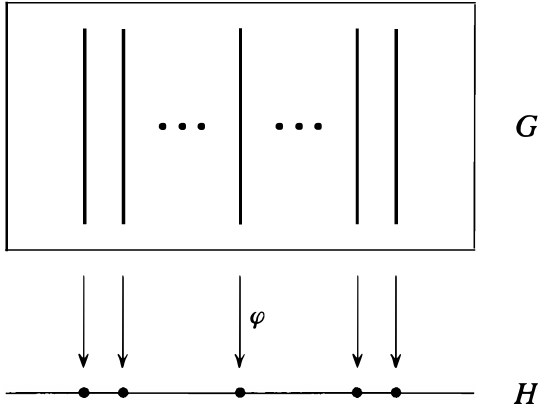
\includegraphics[width=0.5\textwidth]{images/fig3-1.png}
    \caption{}
    \label{fig3-1}
\end{figure}

\(H\) 中的群运算提供了一种将 \(\varphi\) 的像中的两个元素（即图 1 中水平线上的两个元素）相乘的方法。这提示我们对位于这两个点上方的纤维进行自然的乘法，从而将纤维的集合做成一个群：若 \(X_a\) 是 \(a\) 上方的纤维，\(X_b\) 是 \(b\) 上方的纤维，则 \(X_a\) 与 \(X_b\) 的乘积定义为乘积 \(ab\) 上方的纤维 \(X_{ab}\)，即 \(X_a X_b = X_{ab}\). 这个乘法是结合的，因为 \(H\) 中的乘法是结合的，单位元是 \(H\) 的单位元上方的纤维，而 \(a\) 上方的纤维的逆元是 \(a^{-1}\) 上方的纤维，这从定义容易验证。例如，结合律证明如下：\((X_a X_b)X_c = (X_{ab})X_c = X_{(ab)c}\) 且 \(X_a(X_b X_c) = X_a(X_{bc}) = X_{a(bc)}\). 由于在 \(H\) 中 \((ab)c = a(bc)\)，故 \((X_a X_b)X_c = X_a(X_b X_c)\). 粗略地说，群 \(G\) 被分成若干块（纤维），而这些块本身具有群的结构，称为 \(G\) 的一个\textbf{商群}（正式定义见下面例子之后）。

由于纤维的乘法是由 \(H\) 中的乘法定义的，根据构造，带有这个乘法的商群自然同构于 \(G\) 在同态 \(\varphi\) 下的像（纤维 \(X_a\) 与它在 \(H\) 中的像 \(a\) 等同）。

\begin{example}
设 \(G = \mathbb{Z}\)，令 \(H = Z_n = \langle x \rangle\) 为 \(n\) 阶循环群，并定义 \(\varphi : \mathbb{Z} \to Z_n\) 为 \(\varphi(a) = x^a\). 由于
\[
\varphi(a + b) = x^{a+b} = x^a x^b = \varphi(a)\varphi(b),
\]
可知 \(\varphi\) 是同态（注意 \(\mathbb{Z}\) 中的运算是加法，而 \(Z_n\) 中的运算是乘法）。还注意 \(\varphi\) 是满射。\(\varphi\) 在 \(x^a\) 上的纤维是
\[
\begin{aligned}
\varphi^{-1}(x^a) &= \{m \in \mathbb{Z} \mid x^m = x^a\} = \{m \in \mathbb{Z} \mid x^{m-a} = 1\} \\
&= \{m \in \mathbb{Z} \mid n \text{ 整除 } m - a\} \qquad \text{（由命题 2.3）} \\
&= \{m \in \mathbb{Z} \mid m \equiv a \pmod{n}\} = \bar{a},
\end{aligned}
\]
即 \(\varphi\) 的纤维恰好是模 \(n\) 的剩余类。此时图 1 变为：


\begin{figure}[htbp]
    \centering
    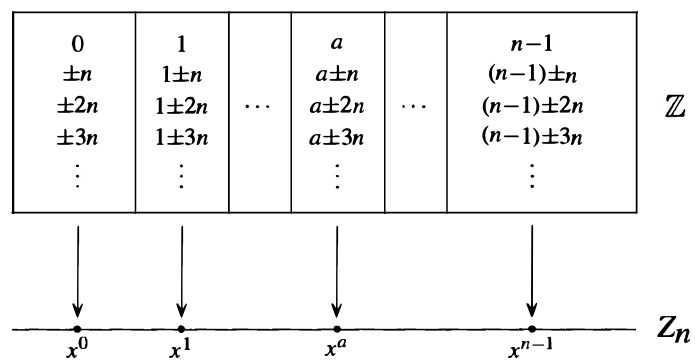
\includegraphics[width=0.75\textwidth]{images/fig3-2.png}
    \caption{}
    \label{fig3-2}
\end{figure}






\(Z_n\) 中的乘法就是 \(x^a x^b = x^{a+b}\). 相应的纤维是 \(\bar{a}, \bar{b}\) 和 \(\overline{a + b}\)，因此纤维上的群运算是 \(\bar{a} \cdot \bar{b} = \overline{a + b}\). 这恰好是加法下的群 \(\mathbb{Z}/n\mathbb{Z}\)，一个同构于 \(\varphi\) 的像（即整个 \(Z_n\)）的群。

这个群的单位元（\(Z_n\) 中单位元上方的纤维）由 \(\mathbb{Z}\) 中 \(n\) 的所有倍数组成，即 \(n\mathbb{Z}\)，它是 \(\mathbb{Z}\) 的一个\textbf{子群}，而其余纤维只是这个子群的平移 \(a + n\mathbb{Z}\). 群运算也可以直接通过在纤维中取\textbf{代表元}、在 \(\mathbb{Z}\) 中相加这些代表元并取包含该和的纤维来定义（这就是群 \(\mathbb{Z}/n\mathbb{Z}\) 原来的定义）。从计算的角度看，通过简单地相加代表元 \(a\) 和 \(b\) 来计算 \(\bar{a}\) 与 \(\bar{b}\) 的乘积，要比先计算这些纤维在 \(\varphi\) 下的像（即 \(x^a\) 和 \(x^b\)）、在 \(H\) 中将它们相乘（得到 \(x^{a+b}\)）然后取该乘积上方的纤维容易得多。

\end{example}


我们首先考虑同态及其纤维的一些基本性质。位于 \(H\) 的单位元上方的同态 \(\varphi : G \to H\) 的纤维被赋予一个名称：

\begin{definition}
若 \(\varphi\) 是同态 \(\varphi : G \to H\)，则 \(\varphi\) 的\textbf{核}是集合
\[
\{g \in G \mid \varphi(g) = 1\},
\]
并记作 \(\ker \varphi\)（这里 \(1\) 是 \(H\) 的单位元）。
\end{definition}

\begin{proposition}\label{pro:3.1}
设 \(G\) 和 \(H\) 是群，\(\varphi : G \to H\) 是同态。
\begin{enumerate}[label=(\arabic*)]
\item \(\varphi(1_G) = 1_H\)，其中 \(1_G\) 和 \(1_H\) 分别是 \(G\) 和 \(H\) 的单位元。
\item 对所有 \(g \in G\)，\(\varphi(g^{-1}) = \varphi(g)^{-1}\)。
\item 对所有 \(n \in \mathbb{Z}\)，\(\varphi(g^n) = \varphi(g)^n\)。
\item \(\ker \varphi\) 是 \(G\) 的子群。
%1_G属于kerφ
\item \(\operatorname{im}(\varphi)\)，即 \(G\) 在 \(\varphi\) 下的像，是 \(H\) 的子群。
\end{enumerate}
\end{proposition}

\begin{proof}
(1) 由于 \(\varphi(1_G) = \varphi(1_G 1_G) = \varphi(1_G)\varphi(1_G)\)，消去律表明 (1) 成立。

(2) \(\varphi(1_G) = \varphi(gg^{-1}) = \varphi(g)\varphi(g^{-1})\)，且由 (1)，\(\varphi(1_G) = 1_H\)，因此
\[
1_H = \varphi(g)\varphi(g^{-1}).
\]
两边左乘 \(\varphi(g)^{-1}\) 并化简得 (2)。

(3) 这是对 \(n \in \mathbb{Z}^+\) 的归纳法的简单练习。由 (2)，结论 (3) 对 \(n\) 的负值也成立。

(4) 由于 \(1_G \in \ker \varphi\)，\(\varphi\) 的核非空。设 \(x, y \in \ker \varphi\)，即 \(\varphi(x) = \varphi(y) = 1_H\)。则
\[
\varphi(xy^{-1}) = \varphi(x)\varphi(y^{-1}) = \varphi(x)\varphi(y)^{-1} = 1_H 1_H^{-1} = 1_H,
\]
即 \(xy^{-1} \in \ker \varphi\)。由子群判别法，\(\ker \varphi \leq G\)。

(5) 由于 \(\varphi(1_G) = 1_H\)，\(H\) 的单位元在 \(\varphi\) 的像中，所以 \(\operatorname{im}(\varphi)\) 非空。若 \(x\) 和 \(y\) 在 \(\operatorname{im}(\varphi)\) 中，设 \(x = \varphi(a)\)，\(y = \varphi(b)\)，则由 (2) 有 \(y^{-1} = \varphi(b^{-1})\)，因此
\[
xy^{-1} = \varphi(a)\varphi(b^{-1}) = \varphi(ab^{-1})
\]
（因 \(\varphi\) 是同态）。所以 \(xy^{-1}\) 也在 \(\varphi\) 的像中，故由子群判别法，\(\operatorname{im}(\varphi)\) 是 \(H\) 的子群。
\end{proof}

我们现在可以定义一些与商群相关的术语。

\begin{definition}
设 \(\varphi : G \to H\) 是同态，核为 \(K\). \textbf{商群}或\textbf{因子群} \(G/K\)（读作 \(G\) 模 \(K\) 或简称 \(G \bmod K\)）是以 \(\varphi\) 的纤维为元素的群，其群运算如上定义：即若 \(X\) 是 \(a\) 上方的纤维，\(Y\) 是 \(b\) 上方的纤维，则 \(X\) 与 \(Y\) 的乘积定义为乘积 \(ab\) 上方的纤维。
\end{definition}

这个记号强调了一个事实：核 \(K\) 是群 \(G/K\) 中的单个元素，且我们将在下面（命题 \ref{pro:3.2}）看到，如同上面的 \(\mathbb{Z}/n\mathbb{Z}\) 情形，\(G/K\) 的其他元素只是核 \(K\) 的“平移”。因此我们可以把 \(G/K\) 看作通过坍缩或“除以” \(K\)（更确切地说，通过模 \(K\) 的等价关系）得到的。这解释了为什么 \(G/K\) 被称为“商”群。

上面商群 \(G/K\) 的定义需要明确给出映射 \(\varphi\)，因为纤维的乘法是通过先用 \(\varphi\) 将纤维投影到 \(H\)，在 \(H\) 中相乘，然后确定该乘积上方的纤维来进行的。正如上面的 \(\mathbb{Z}/n\mathbb{Z}\) 情形，也可以直接用纤维中的代表元来定义纤维的乘法。这在计算上更简单，且映射 \(\varphi\) 不显式出现。我们首先说明同态的纤维可以像上面的例子那样用同态的核来表示（那里核是 \(n\mathbb{Z}\)，纤维是形如 \(a + n\mathbb{Z}\) 的平移）。

\begin{proposition}\label{pro:3.2}
设 \(\varphi : G \to H\) 是群同态，核为 \(K\). 设 \(X \in G/K\) 是 \(a\) 上方的纤维，即 \(X = \varphi^{-1}(a)\). 则
\begin{enumerate}[label=(\arabic*)]
\item 对任意 \(u \in X\)，\(X = \{uk \mid k \in K\}\).
\item 对任意 \(u \in X\)，\(X = \{ku \mid k \in K\}\).
\end{enumerate}
\end{proposition}

\begin{proof}
我们证明 (1)，把 (2) 的证明留作练习。设 \(u \in X\)，则由 \(X\) 的定义，\(\varphi(u) = a\). 令
\[
uK = \{uk \mid k \in K\}.
\]
首先证明 \(uK \subseteq X\). 对任意 \(k \in K\)，
\[
\begin{aligned}
\varphi(uk) &= \varphi(u)\varphi(k) && \text{（因 } \varphi \text{ 是同态）} \\
&= \varphi(u)1 && \text{（因 } k \in \ker \varphi\text{）} \\
&= a,
\end{aligned}
\]
即 \(uk \in X\). 这证明了 \(uK \subseteq X\). 为证反向包含，设 \(g \in X\)，令 \(k = u^{-1}g\). 则
\[
\begin{aligned}
\varphi(k) &= \varphi(u^{-1})\varphi(g) = \varphi(u)^{-1}\varphi(g) && \text{（由命题 \ref{pro:3.1}）} \\
&= a^{-1}a = 1.
\end{aligned}
\]
因此 \(k \in \ker \varphi\). 由于 \(k = u^{-1}g\)，故 \(g = uk \in uK\)，这证明了包含 \(X \subseteq uK\). 于是 (1) 得证。
\end{proof}

命题 \ref{pro:3.2} 中用于描述同态 \(\varphi\) 的纤维的集合，对 \(G\) 的任意子群 \(K\) 都有定义，不必是某个同态的核（我们很快将确定一个子群成为这样的核的充要条件），并给出一个名称：

\begin{definition}
对任意 \(N \leq G\) 和任意 \(g \in G\)，令
\[
gN = \{gn \mid n \in N\} \quad \text{和} \quad Ng = \{ng \mid n \in N\},
\]
分别称为 \(N\) 在 \(G\) 中的\textbf{左陪集}和\textbf{右陪集}。陪集中的任意元素称为该陪集的\textbf{代表元}。
\end{definition}

我们已经在命题 \ref{pro:3.2} 中看到，若 \(N\) 是某个同态的核，且 \(g_1\) 是陪集 \(gN\) 的任意代表元，则 \(g_1N = gN\)（且若 \(g_1 \in Ng\)，则 \(Ng_1 = Ng\)）。我们将在下面命题 \ref{pro:3.4} 中看到，这个事实对任意子群 \(N\) 都成立，这解释了“代表元”这一术语。

若 \(G\) 是加法群，我们将用 \(g + N\) 和 \(N + g\) 分别表示 \(N\) 在 \(G\) 中以 \(g\) 为代表的左陪集和右陪集。一般地，我们可以把 \(N\) 在 \(G\) 中的左陪集 \(gN\) 看作 \(N\) 被 \(g\) 左平移。（读者可能想复习第 1.7 节习题 18，它证明了 \(N\) 在 \(G\) 中的右陪集恰好是 \(N\) 通过左乘法作用在 \(G\) 上的轨道。）

用这个定义来说，命题 \ref{pro:3.2} 表明同态的纤维是核的左陪集（也是核的右陪集），即商群 \(G/K\) 的元素是左陪集 \(gK\)，\(g \in G\)。在 \(\mathbb{Z}/n\mathbb{Z}\) 的例子中，商群中的乘法也可以用陪集的代表元来定义。下面的结果表明对一般的 \(G/K\) 同样成立（只要我们已知 \(K\) 是某个同态的核），即 \(G/K\) 中两个左陪集 \(X\) 和 \(Y\) 的乘积可通过选取 \(X\) 的任意代表元 \(u\)、\(Y\) 的任意代表元 \(v\)，在 \(G\) 中将 \(u\) 和 \(v\) 相乘，然后取陪集 \((uv)K\) 来计算。

\begin{theorem}\label{thm:3.3}
设 \(G\) 是群，\(K\) 是从 \(G\) 到另一个群的某个同态的核。则以 \(K\) 在 \(G\) 中的左陪集为元素、运算由
\[
uK \cdot vK = (uv)K
\]
定义的集合构成一个群 \(G/K\). 特别地，这个运算是良定义的，即若 \(u_1\) 是 \(uK\) 中的任意元素、\(v_1\) 是 \(vK\) 中的任意元素，则 \(u_1 v_1 \in uvK\)，亦即 \(u_1 v_1 K = uvK\)，因此该乘法不依赖于陪集代表元的选取。把“左陪集”换成“右陪集”，结论同样成立。
\end{theorem}

\begin{proof}
设 \(X, Y \in G/K\)，令 \(Z = XY\) 为 \(G/K\) 中的乘积，于是由命题 \ref{pro:3.2}(1) 知 \(X, Y, Z\) 都是 \(K\) 的（左）陪集。由假设，\(K\) 是某个同态 \(\varphi : G \to H\) 的核，故 \(X = \varphi^{-1}(a)\)、\(Y = \varphi^{-1}(b)\)，其中 \(a, b \in H\). 由 \(G/K\) 中运算的定义，\(Z = \varphi^{-1}(ab)\). 设 \(u, v\) 分别为 \(X, Y\) 的任意代表元，于是 \(\varphi(u) = a\)、\(\varphi(v) = b\)，并且 \(X = uK\)、\(Y = vK\). 我们要证明 \(uv \in Z\). 由于
\[
uv \in Z \iff uv \in \varphi^{-1}(ab) \iff \varphi(uv) = ab \iff \varphi(u)\varphi(v) = ab,
\]
而最后一个等式确实成立，故 \(uv \in Z\)，从而 \(Z\) 是（左）陪集 \(uvK\).（下面的习题 2 反过来表明，每个 \(Z\) 都可以写成 \(uv\) 的形式，其中 \(u \in X\)、\(v \in Y\)。）这就证明了：对任意选取的代表元 \(u \in X\)、\(v \in Y\)，\(X\) 与 \(Y\) 的乘积都是陪集 \(uvK\)，从而完成了定理前一部分的证明。定理的最后一句立即成立，因为由命题 \ref{pro:3.2} 知对所有 \(u, v \in G\) 都有 \(uK = Ku\) 与 \(vK = Kv\).
\end{proof}

用图 1 的说法，通过代表元计算 \(G/K\) 中的乘法可以用下面的图 3 来表示。

\begin{figure}[htbp]
    \centering
    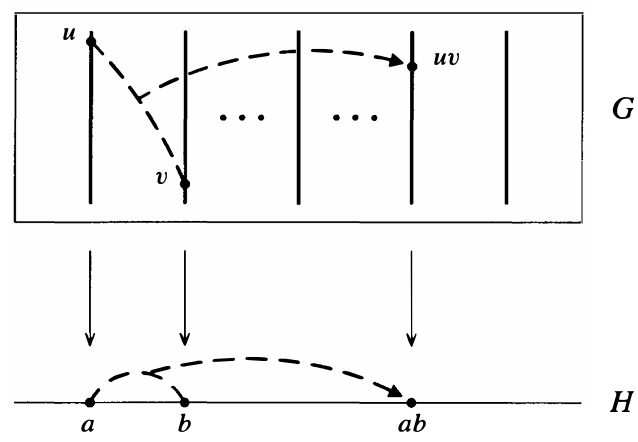
\includegraphics[width=0.5\textwidth]{images/fig3-3.png}
    \caption{}
    \label{fig3-3}
\end{figure}

我们要强调，乘法与所选取的代表元无关。也就是说，两个陪集 \(X\) 与 \(Y\) 的乘积（若群用加法记号书写则为和）是包含乘积 \(uv\) 的陪集 \(uvK\)，其中 \(u\) 与 \(v\) 分别是陪集 \(X\) 与 \(Y\) 的任意代表元。这种只考虑包含某个元素的陪集、即“模 \(K\) 约化”的过程，正是我们在 \(\mathbb{Z}/n\mathbb{Z}\) 中一直做的事情。表示包含代表元 \(u\) 的陪集 \(uK\) 的一个有用记号是 \(\bar{u}\). 采用这个记号（我们在预备知识中处理 \(\mathbb{Z}/n\mathbb{Z}\) 时已经引入过），商群 \(G/K\) 记作 \(\bar{G}\)，而元素 \(\bar{u}\) 与 \(\bar{v}\) 的乘积就是包含 \(uv\) 的陪集，即 \(\overline{uv}\). 这个记号也强化了如下事实：\(G/K\) 中的陪集 \(uK\) 正是 \(G/K\) 中的元素 \(\bar{u}\).

\begin{example}
（1）本章第一个例子中从 \(\mathbb{Z}\) 到 \(Z_n\) 的同态 \(\varphi\) 的纤维是核 \(n\mathbb{Z}\) 的左陪集（也是右陪集）\(a + n\mathbb{Z}\). 定理 \ref{thm:3.3} 证明这些陪集在代表元的加法下构成一个群，即 \(\mathbb{Z}/n\mathbb{Z}\)，这解释了该群的记号。这个群自然同构于它在 \(\varphi\) 下的像，于是我们重新得到了第 2 章的 \(\mathbb{Z}/n\mathbb{Z} \cong Z_n\).

（2）若 \(\varphi : G \to H\) 是同构，则 \(K = 1\)，\(\varphi\) 的纤维都是 \(G\) 的单点子集，于是 \(G/1 \cong G\).

（3）设 \(G\) 是任意群，\(H = 1\) 是 1 阶群，并定义 \(\varphi : G \to H\) 为对所有 \(g \in G\) 有 \(\varphi(g) = 1\). 立即看出 \(\varphi\) 是同态。这个映射称为\textbf{平凡同态}。注意此时 \(\ker \varphi = G\)，而 \(G/G\) 是只含一个元素 \(G\) 的群，即 \(G/G \cong Z_1 = \{1\}\).

（4）设 \(G = \mathbb{R}^2\)（运算为向量加法），\(H = \mathbb{R}\)（运算为加法），定义 \(\varphi : \mathbb{R}^2 \to \mathbb{R}\) 为 \(\varphi((x, y)) = x\). 于是 \(\varphi\) 是到 \(x\) 轴上的投影。我们证明 \(\varphi\) 是同态：
\[
\varphi((x_1, y_1) + (x_2, y_2)) = \varphi((x_1 + x_2, y_1 + y_2)) = x_1 + x_2 = \varphi((x_1, y_1)) + \varphi((x_2, y_2)).
\]
此时
\[
\ker \varphi = \{(x, y) \mid \varphi((x, y)) = 0\} = \{(x, y) \mid x = 0\} = y \text{ 轴}.
\]
注意 \(\ker \varphi\) 确实是 \(\mathbb{R}^2\) 的子群，且 \(\varphi\) 在 \(a \in \mathbb{R}\) 上方的纤维是把 \(y\) 轴平移 \(a\) 得到的直线 \(x = a\). 这也是核的一个左陪集（也是右陪集），以 \((a, 0)\)（或任何其他投影到 \(a\) 的代表点）为代表：
\[
(a, 0) + y \text{ 轴} = \overline{(a, 0)}.
\]
于是本例中的图 1 变为

\begin{figure}[htbp]
    \centering
    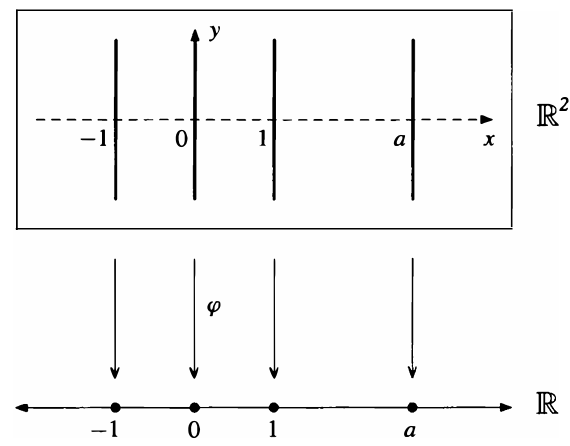
\includegraphics[width=0.5\textwidth]{images/fig3-4.png}
    \caption{}
    \label{fig3-4}
\end{figure}

群运算（此处用加法书写）既可以用映射 \(\varphi\) 来描述：直线 \((x = a)\) 与直线 \((x = b)\) 的和是直线 \((x = a + b)\)；也可以直接用陪集的代表元来描述：包含点 \((a, y_1)\) 的竖直线与包含点 \((b, y_2)\) 的竖直线的和是包含点 \((a + b, y_1 + y_2)\) 的竖直线。特别要注意，这些竖直线的代表元的选取并不重要（即 \(y\) 坐标无关紧要）。

（5）\(G = Q_8\)（四元数群，见第 2.5 节例 2），\(H = V_4\)（克莱因四元群）。定义 \(\varphi : Q_8 \to V_4\) 为
\[
\varphi(\pm 1) = 1, \quad \varphi(\pm i) = a, \quad \varphi(\pm j) = b, \quad \varphi(\pm k) = c.
\]
验证 \(\varphi\) 是同态留作练习——利用对称性可以最大限度地减少证明对所有 \(x, y \in Q_8\) 有 \(\varphi(xy) = \varphi(x)\varphi(y)\) 的工作量。显然 \(\varphi\) 是满射，且 \(\ker \varphi = \{\pm 1\}\). 可以把 \(\varphi\) 想成 \(Q_8\) 上的“绝对值”函数，于是 \(\varphi\) 的纤维是集合 \(E = \{\pm 1\}\)、\(A = \{\pm i\}\)、\(B = \{\pm j\}\)、\(C = \{\pm k\}\)，它们在 \(Q_8/\{\pm 1\}\) 中分别被坍缩为 \(1, a, b, c\)，而这些正是 \(\ker \varphi\) 的左陪集（也是右陪集）（例如 \(A = i \ker \varphi = \{i, -i\} = \ker \varphi \cdot i\)）。
\end{example}

由定理 \ref{thm:3.3}，如果我们已知群 \(G\) 的一个子群 \(K\) 是某个同态的核，就可以不借助该同态、直接用乘法 \(uK \cdot vK = uvK\) 来定义商群 \(G/K\). 这就引出一个问题：是否可以对 \(G\) 的任意子群 \(N\) 类似地定义商群 \(G/N\)？一般说来答案是否定的，因为该乘法一般不是良定义的（参见后面的命题 \ref{pro:3.5}）。事实上我们将看到，当且仅当 \(N\) 是某个同态的核时，才能在 \(N\) 的陪集上定义群结构（命题 \ref{pro:3.7}）。我们还将给出一个判别准则来判断子群 \(N\) 是否是这样一个核——这就是\textbf{正规子群}的概念，我们将在后续各节中考察非正规子群。

我们首先证明，\(G\) 的任意子群的陪集都划分 \(G\)（即它们的并是整个 \(G\)，且不同的陪集交为平凡）。

\begin{proposition}\label{pro:3.4}
设 \(N\) 是群 \(G\) 的任意子群。\(N\) 在 \(G\) 中的左陪集构成 \(G\) 的一个划分。此外，对所有 \(u, v \in G\)，\(uN = vN\) 当且仅当 \(v^{-1}u \in N\)；特别地，\(uN = vN\) 当且仅当 \(u\) 与 \(v\) 是同一陪集的代表元。
\end{proposition}

\begin{proof}
首先注意，由于 \(N\) 是 \(G\) 的子群，故 \(1 \in N\). 于是对所有 \(g \in G\) 有 \(g = g \cdot 1 \in gN\)，即
\[
G = \bigcup_{g \in G} gN.
\]
为证不同的左陪集交为空，设 \(uN \cap vN \neq \varnothing\)，我们证明 \(uN = vN\). 设 \(x \in uN \cap vN\)，写成
\[
x = un = vm, \quad \text{其中 } n, m \in N.
\]
在后一个等式中两边右乘 \(n^{-1}\)，得
\[
u = vm_1, \quad \text{其中 } m_1 = mn^{-1} \in N.
\]
现在对 \(uN\) 中的任意元素 \(ut\)（\(t \in N\)），
\[
ut = (vm_1)t = v(m_1 t) \in vN.
\]
这证明 \(uN \subseteq vN\). 交换 \(u\) 与 \(v\) 的角色，类似地得到 \(vN \subseteq uN\). 因此交集非空的两个陪集相同。

由命题的前一部分，\(uN = vN\) 当且仅当 \(u \in vN\)，当且仅当存在 \(n \in N\) 使 \(u = vn\)，当且仅当 \(v^{-1}u \in N\)，这正是所断言的。最后，\(v \in uN\) 等价于说 \(v\) 是 \(uN\) 的代表元，因此 \(uN = vN\) 当且仅当 \(u\) 与 \(v\) 是同一陪集（即陪集 \(uN = vN\)）的代表元。
\end{proof}

\begin{proposition}\label{pro:3.5}
设 \(G\) 是群，\(N\) 是 \(G\) 的子群。

\begin{enumerate}[label=(\arabic*)]
\item 由
\[
uN \cdot vN = (uv)N
\]
给出的 \(N\) 在 \(G\) 中的左陪集集合上的运算良定义，当且仅当对所有 \(g \in G\) 和所有 \(n \in N\) 都有 \(gng^{-1} \in N\).

\item 若上述运算良定义，则它使 \(N\) 在 \(G\) 中的左陪集集合成为一个群。特别地，该群的单位元是陪集 \(1N\)，\(gN\) 的逆元是陪集 \(g^{-1}N\)，即 \((gN)^{-1} = g^{-1}N\).
\end{enumerate}
\end{proposition}

\begin{proof}
（1）首先假设该运算良定义，即对所有 \(u, v \in G\)，若 \(u, u_1 \in uN\) 且 \(v, v_1 \in vN\)，则 \(uvN = u_1 v_1 N\).

设 \(g\) 是 \(G\) 的任意元素，\(n\) 是 \(N\) 的任意元素。令 \(u = 1\)、\(u_1 = n\)、\(v = v_1 = g^{-1}\)，应用上述假设推得
\[
1 \cdot g^{-1}N = ng^{-1}N, \quad \text{即 } g^{-1}N = ng^{-1}N.
\]
由于 \(1 \in N\)，故 \(ng^{-1} \cdot 1 \in ng^{-1}N\). 于是 \(ng^{-1} \in g^{-1}N\)，从而对某个 \(n_1 \in N\) 有 \(ng^{-1} = g^{-1}n_1\). 两边左乘 \(g\) 得 \(gng^{-1} = n_1 \in N\)，这正是所断言的。

反之，假设对所有 \(g \in G\) 和所有 \(n \in N\) 都有 \(gng^{-1} \in N\). 为证上述运算良定义，设 \(u, u_1 \in uN\) 且 \(v, v_1 \in vN\). 我们可以写成
\[
u_1 = un, \quad v_1 = vm, \quad \text{其中 } n, m \in N.
\]
我们必须证明 \(u_1 v_1 \in uvN\)：
\[
u_1 v_1 = (un)(vm) = u(vv^{-1})nvm = (uv)(v^{-1}nv)m = (uv)(n_1 m),
\]
其中 \(n_1 = v^{-1}nv = (v^{-1})n(v^{-1})^{-1}\) 由假设是 \(N\) 的元素。由于 \(N\) 对乘法封闭，故 \(n_1 m \in N\). 于是
\[
u_1 v_1 = (uv)n_2, \quad \text{其中 } n_2 \in N.
\]
因此左陪集 \(uvN\) 与 \(u_1 v_1 N\) 含有公共元素 \(u_1 v_1\). 由前一个命题，它们相等。这证明该运算良定义。

（2）若陪集上的运算良定义，则群公理容易验证，它们由在 \(G\) 中的有效性诱导而来。例如，结合律成立，因为对所有 \(u, v, w \in G\)，
\[
(uN)(vN \cdot wN) = uN(vwN) = u(vw)N = (uv)wN = (uN \cdot vN)(wN),
\]
这是因为在 \(G\) 中 \(u(vw) = (uv)w\). \(G/N\) 中的单位元是陪集 \(1N\)，而 \(gN\) 的逆元是 \(g^{-1}N\)，这从乘法的定义立即得到。
\end{proof}

如前所述，满足命题 \ref{pro:3.5} 中条件、使得商 \(G/N\) 上有自然群结构的子群 \(N\) 被赋予一个名称：

\begin{definition}
元素 \(gng^{-1}\) 称为 \(n \in N\) 被 \(g\) 的\textbf{共轭}。集合 \(gNg^{-1} = \{gng^{-1} \mid n \in N\}\) 称为 \(N\) 被 \(g\) 的共轭。若 \(gNg^{-1} = N\)，则称元素 \(g\) \textbf{正规化} \(N\). 群 \(G\) 的子群 \(N\) 称为\textbf{正规的}，若 \(G\) 的每个元素都正规化 \(N\)，即对所有 \(g \in G\) 有 \(gNg^{-1} = N\). 若 \(N\) 是 \(G\) 的正规子群，我们记作 \(N \trianglelefteq G\).
\end{definition}

注意，当 \(N\) 是正规子群时，\(G\) 的结构反映在商 \(G/N\) 的结构中（例如，\(G/N\) 中乘法的结合律由 \(G\) 中的结合律诱导，\(G/N\) 中的逆元由 \(G\) 中的逆元诱导）。当我们在后面的 3.3 节考虑同构定理时，将进一步看到 \(G\) 与其商 \(G/N\) 的关系。

我们把上面的结果总结为定理 \ref{thm:3.6}.

\begin{theorem}\label{thm:3.6}
设 \(N\) 是群 \(G\) 的子群。下列命题等价：

\begin{enumerate}[label=(\arabic*)]
\item \(N \trianglelefteq G\)；

\item \(N_G(N) = G\)（回忆 \(N_G(N)\) 是 \(N\) 在 \(G\) 中的正规化子）；

\item 对所有 \(g \in G\) 有 \(gN = Ng\)；

\item 命题 \ref{pro:3.5} 中描述的 \(N\) 在 \(G\) 中的左陪集上的运算使这些左陪集构成一个群；

\item 对所有 \(g \in G\) 有 \(gNg^{-1} \subseteq N\).
\end{enumerate}
\end{theorem}

\begin{proof}
困难的等价性我们已经完成了，其余留作练习。
\end{proof}

作为一个实际问题，人们会设法尽量减少判断给定子群 \(N\) 在群 \(G\) 中是否正规所需的计算。特别地，人们尽量不计算所有共轭 \(gng^{-1}\)（\(n \in N\)，\(g \in G\)）。例如，\(N\) 自身的元素都正规化 \(N\)，因为 \(N\) 是子群。此外，如果已知 \(N\) 的一组生成元，则只需验证这些生成元的所有共轭都落在 \(N\) 中，就可证明 \(N\) 是正规子群（这是因为乘积的共轭是共轭的乘积，而逆元的共轭是共轭的逆元）——这就是后面的习题 26. 类似地，如果也知道 \(G\) 的生成元，则只需验证这些 \(G\) 的生成元都正规化 \(N\). 特别地，如果 \(N\) 和 \(G\) 的生成元都已知，这就把计算减少到少量需要验证的共轭。若 \(N\) 是有限群，则只需验证 \(N\) 的一组生成元被 \(G\) 的一组生成元共轭后仍属于 \(N\)（习题 29）。最后，常常可以直接证明 \(N_G(N) = G\) 而不必做过多计算（下一节有一些例子），这样也就证明了 \(N\) 是 \(G\) 的正规子群，而无需机械地计算所有可能的共轭 \(gng^{-1}\).

现在我们证明，正规子群恰好就是前面考虑的同态的核。

\begin{proposition}\label{pro:3.7}
群 \(G\) 的子群 \(N\) 正规，当且仅当它是某个同态的核。
\end{proposition}

\begin{proof}
若 \(N\) 是同态 \(\varphi\) 的核，则由命题 \ref{pro:3.2} 知 \(N\) 的左陪集与右陪集相同（二者都是映射 \(\varphi\) 的纤维）。于是由定理 \ref{thm:3.6}(3) 知 \(N\) 是正规子群。（对正规性的定义另有一个直接的证明，见习题。）

反之，若 \(N \trianglelefteq G\)，令 \(H = G/N\)，并由
\[
\pi(g) = gN, \quad \text{对所有 } g \in G
\]
定义 \(\pi : G \to G/N\). 由 \(G/N\) 中运算的定义，
\[
\pi(g_1 g_2) = (g_1 g_2)N = g_1 N \cdot g_2 N = \pi(g_1)\pi(g_2).
\]
这证明 \(\pi\) 是同态。此时
\[
\ker \pi = \{g \in G \mid \pi(g) = 1N\} = \{g \in G \mid gN = 1N\} = \{g \in G \mid g \in N\} = N.
\]
因此 \(N\) 是同态 \(\pi\) 的核。
\end{proof}

上面构造的、把正规子群 \(N\) 表示为某个同态的核的同态 \(\pi\) 被赋予一个名称：

\begin{definition}
设 \(N \trianglelefteq G\). 由 \(\pi(g) = gN\) 定义的（映到）同态 \(\pi : G \to G/N\) 称为 \(G\) 到 \(G/N\) 上的\textbf{自然投影}（同态）。若 \(\overline{H} \leq G/N\) 是 \(G/N\) 的子群，则它在 \(G\) 中的\textbf{完全原像}是 \(\overline{H}\) 在自然投影同态下的原像。
\end{definition}

\(G/N\) 的子群的完全原像是 \(G\) 的子群（参见习题 1），它包含子群 \(N\)，因为这些正是映射到单位元的元素。我们将在 3.3 节的同构定理中看到，包含 \(N\) 的 \(G\) 的子群与商 \(G/N\) 的子群之间存在自然的对应关系。

现在我们有一条“内部的”判别准则，它精确地刻画了给定群 \(G\) 的子群 \(N\) 何时是某个同态的核，即
\[
N_G(N) = G.
\]
因此我们可以把 \(G\) 的子群 \(N\) 的正规化子看作衡量 \(N\) “离正规子群有多近”的尺度（这解释了该子群的名称）。请记住，正规性是一个嵌入性质，即它依赖于 \(N\) 与 \(G\) 的关系，而不依赖于 \(N\) 自身的内部结构（同一个群 \(N\) 可以是 \(G\) 的正规子群，但在包含 \(G\) 的更大群中不正规）。

我们是从 \(G\) 到 \(H\) 的同态 \(\varphi\) 的存在性开始讨论商群的，并证明了该同态的核是 \(G\) 的正规子群 \(N\)，而商 \(G/N\)（最初用纤维定义）自然同构于 \(G\) 在 \(\varphi\) 下的像\footnote{“自然”一词在范畴论中有精确的数学意义；就我们的目的而言，用这个词只是表明该同态的定义是一种“无坐标”的投影，即只用元素本身来描述，而不使用 \(G\) 或 \(N\) 的生成元（参见附录 II）。}。反之，若 \(N \trianglelefteq G\)，我们可以找到一个群 \(H\)（即 \(G/N\)）和一个同态 \(\pi : G \to H\)，使得 \(\ker \pi = N\)（即自然投影）。因此，对 \(G\) 的同态像（即 \(G\) 到其他群的同态的像）的研究等价于对 \(G\) 的商群的研究，我们将用同态来产生正规子群，反之亦然。

我们通过同态来发展商群的理论，而不是简单地定义正规子群及其商群的概念，是为了强调商群的元素是原群 \(G\) 的子集（核 \(N\) 的纤维或陪集）。图 1 的直观图示也强调 \(N\)（及其陪集）被投影（或坍缩）为商 \(G/N\) 中的单个元素。商群 \(G/N\) 中的计算是通过从所涉及的各个陪集中取代表元来完成的。

下面给出正规子群及其商的一些例子。

\begin{example}
设 \(G\) 是群。

（1）子群 \(1\) 和 \(G\) 总是 \(G\) 的正规子群；\(G/1 \cong G\)，\(G/G \cong 1\).

（2）若 \(G\) 是阿贝尔群，则 \(G\) 的任意子群 \(N\) 都正规，因为对所有 \(g \in G\) 和所有 \(n \in N\)，
\[
gng^{-1} = gg^{-1}n = n \in N.
\]
注意这里重要的是 \(G\) 阿贝尔，而不仅仅是 \(N\) 阿贝尔。当取 \(G\) 的不同子群 \(N\) 时，\(G/N\) 的结构可能不同。例如，若 \(G = \mathbb{Z}\)，则 \(G\) 的每个子群 \(N\) 都是循环的：
\[
N = \langle n \rangle = \langle -n \rangle = n\mathbb{Z}, \quad \text{对某个 } n \in \mathbb{Z},
\]
而 \(G/N = \mathbb{Z}/n\mathbb{Z}\) 是以 \(1 + n\mathbb{Z}\) 为生成元的循环群（注意 \(1\) 是 \(G\) 的生成元）。

现在设 \(G = Z_k\) 是 \(k\) 阶循环群。设 \(x\) 是 \(G\) 的生成元，\(N \leq G\). 由命题 2.6，\(N = \langle x^d \rangle\)，其中 \(d\) 是落在 \(N\) 中的 \(x\) 的最小幂。此时
\[
G/N = \{gN \mid g \in G\} = \{x^a N \mid a \in \mathbb{Z}\},
\]
且由于 \(x^a N = (xN)^a\)（见下面习题 4），可知
\[
G/N = \langle xN \rangle,
\]
即 \(G/N\) 是循环群，以 \(xN\) 为生成元。

由下面习题 5，\(xN\) 在 \(G/N\) 中的阶等于 \(d\). 由命题 2.5，\(d = |G : N|\). 总结如下：循环群的商群是循环群，且 \(G\) 的生成元 \(g\) 在商群中的像 \(\bar{g}\) 是商群的生成元。若此外 \(G\) 是有限循环群且 \(N \trianglelefteq G\)，则 \(|G/N| = |G : N|\) 给出了商群阶的公式。

（3）若 \(N \leq Z(G)\)，则 \(N \trianglelefteq G\)，因为对所有 \(g \in G\) 和所有 \(n \in N\) 有 \(gng^{-1} = n \in N\)，这是前一个例子的推广（其中中心 \(Z(G)\) 就是整个 \(G\)）。因此特别地，\(Z(G) \trianglelefteq G\). 前面已经看到 \(Q_8\) 的子群 \(\{-1\}\) 是某个同态的核，但由于 \(\{-1\} = Z(Q_8)\)，我们现在又用另一种方式得到了该子群的正规性。我们已经看到 \(Q_8/\{-1\} \cong V_4\). 下一段中关于 \(D_8\) 的讨论同样适用于 \(Q_8\)，从而可以独立地确定该商群的同构类型。

设 \(G = D_8\)，令 \(Z = \langle r^2 \rangle = Z(D_8)\). 由于 \(Z = \{1, r^2\}\)，每个陪集 \(gZ\) 都由二元素集合 \(\{g, gr^2\}\) 组成。由于这些陪集把 \(D_8\) 的 8 个元素分成四对，\(Z\) 在 \(D_8\) 中必有 4 个（互不相交的）左陪集：
\[
\bar{1} = 1Z, \quad \bar{r} = rZ, \quad \bar{s} = sZ, \quad \overline{rs} = rsZ.
\]
现在由 4 阶群的分类（第 2.5 节习题 10）知 \(D_8/Z(D_8) \cong Z_4\) 或 \(V_4\). 为确定究竟是哪一个（即确定该商群的同构类型），只需注意
\[
\bar{r}^2 = r^2 Z = 1Z = \bar{1}, \quad \bar{s}^2 = s^2 Z = 1Z = \bar{1}, \quad \overline{rs}^2 = (rs)^2 Z = 1Z = \bar{1},
\]
所以 \(D_8/Z\) 中每个非单位元都是 2 阶的。特别地，商群中没有 4 阶元，因此 \(D_8/Z\) 不是循环群，从而 \(D_8/Z(D_8) \cong V_4\).
\end{example}

\subsection*{习题}
设 \(G\) 和 \(H\) 是群。

\begin{enumerate}
\item 设 \(\varphi : G \to H\) 是同态，\(E\) 是 \(H\) 的子群。证明 \(\varphi^{-1}(E) \leq G\)（即子群在同态下的原像或拉回是子群）。若 \(E \trianglelefteq H\)，证明 \(\varphi^{-1}(E) \trianglelefteq G\). 由此推出 \(\ker \varphi \trianglelefteq G\).

\item 设 \(\varphi : G \to H\) 是核为 \(K\) 的群同态，\(a, b \in \varphi(G)\). 设 \(X \in G/K\) 是 \(a\) 上方的纤维，\(Y\) 是 \(b\) 上方的纤维，即 \(X = \varphi^{-1}(a)\)、\(Y = \varphi^{-1}(b)\). 固定 \(X\) 中的一个元素 \(u\)（故 \(\varphi(u) = a\)）。证明：若商群 \(G/K\) 中 \(XY = Z\)，且 \(w\) 是 \(Z\) 的任意元素，则存在 \(v \in Y\) 使得 \(uv = w\).〔提示：证明 \(u^{-1}w \in Y\).〕

\item 设 \(A\) 是阿贝尔群，\(B\) 是 \(A\) 的子群。证明 \(A/B\) 是阿贝尔群。给出一个含真正规子群 \(N\) 的非阿贝尔群 \(G\) 的例子，使得 \(G/N\) 是阿贝尔群。

\item 证明在商群 \(G/N\) 中，对所有 \(a \in \mathbb{Z}\) 有 \((gN)^a = g^a N\).

\item 利用前一习题证明：\(G/N\) 中元素 \(gN\) 的阶是使 \(g^n \in N\) 的最小正整数 \(n\)（若这样的正整数不存在，则 \(gN\) 是无限阶的）。给出一个例子说明 \(gN\) 在 \(G/N\) 中的阶可能严格小于 \(g\) 在 \(G\) 中的阶。

\item 定义 \(\varphi : \mathbb{R}^\times \to \{\pm 1\}\) 为 \(\varphi(x)\) 等于 \(x\) 除以 \(x\) 的绝对值。描述 \(\varphi\) 的纤维，并证明 \(\varphi\) 是同态。

\item 定义 \(\pi : \mathbb{R}^2 \to \mathbb{R}\) 为 \(\pi((x, y)) = x + y\). 证明 \(\pi\) 是满同态，并几何地描述 \(\pi\) 的核与纤维。

\item 设 \(\varphi : \mathbb{R}^\times \to \mathbb{R}^\times\) 是把 \(x\) 映到 \(x\) 的绝对值的映射。证明 \(\varphi\) 是同态，并求出 \(\varphi\) 的像。描述 \(\varphi\) 的核与纤维。

\item 定义 \(\varphi : \mathbb{C}^\times \to \mathbb{R}^\times\) 为 \(\varphi(a + bi) = a^2 + b^2\). 证明 \(\varphi\) 是同态，并求出 \(\varphi\) 的像。几何地描述 \(\varphi\) 的核与纤维（作为平面的子集）。

\item 定义 \(\varphi : \mathbb{Z}/8\mathbb{Z} \to \mathbb{Z}/4\mathbb{Z}\) 为 \(\varphi(\bar{a}) = \bar{a}\). 证明这是一个良定义的满同态，并具体描述它的纤维与核（证明 \(\varphi\) 良定义要用到 \(\bar{a}\) 在 \(\varphi\) 的定义域与值域中含义不同这一事实）。

\item 设 \(F\) 是域，令
\[
G = \left\{ \begin{pmatrix} a & b \\ 0 & c \end{pmatrix} \ \middle|\ a, b, c \in F,\ ac \neq 0 \right\} \leq GL_2(F).
\]
（a）证明映射 \(\varphi : \begin{pmatrix} a & b \\ 0 & c \end{pmatrix} \mapsto a\) 是 \(G\) 到 \(F^\times\) 上的满同态（回忆 \(F^\times\) 是 \(F\) 中非零元素构成的乘法群）。描述 \(\varphi\) 的纤维与核。

（b）证明映射 \(\psi : \begin{pmatrix} a & b \\ 0 & c \end{pmatrix} \mapsto (a, c)\) 是 \(G\) 到 \(F^\times \times F^\times\) 上的满同态。描述 \(\psi\) 的纤维与核。

（c）设 \(H = \left\{ \begin{pmatrix} 1 & b \\ 0 & 1 \end{pmatrix} \ \middle|\ b \in F \right\}\). 证明 \(H\) 同构于加法群 \(F\).

\item 设 \(G\) 是实数的加法群，\(H\) 是模为 1 的复数的乘法群（复平面上的单位圆 \(S^1\)），并设 \(\varphi : G \to H\) 是同态 \(\varphi : r \mapsto e^{2\pi i r}\). 画出实直线上落在 \(\varphi\) 的核中的点。类似地描述 \(\varphi\) 在 \(H\) 的点 \(-1\)、\(i\) 和 \(e^{4\pi i/3}\) 上方的纤维中的元素。（正文中这个同态 \(\varphi\) 的图 1 通常用下面的图表示。）

\begin{figure}[htbp]
    \centering
    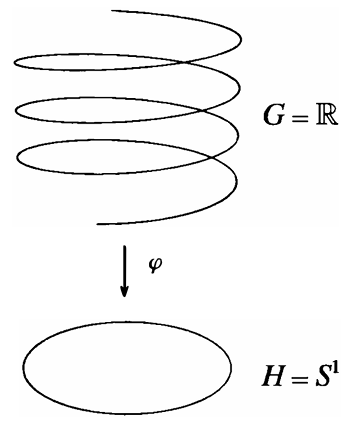
\includegraphics[width=0.5\textwidth]{images/fig3-5.png}
    \caption{}
    \label{fig3-5}
\end{figure}

\item 把前一习题中的映射 \(\varphi\) 换为 \(\varphi : r \mapsto e^{4\pi i r}\)，重复前一习题。

\item 考虑加法商群 \(\mathbb{Q}/\mathbb{Z}\).

（a）证明 \(\mathbb{Z}\) 在 \(\mathbb{Q}\) 中的每个陪集恰好含有一个满足 \(0 \leq q < 1\) 的代表元 \(q \in \mathbb{Q}\).

（b）证明 \(\mathbb{Q}/\mathbb{Z}\) 的每个元素都是有限阶的，但存在阶数任意大的元素。

（c）证明 \(\mathbb{Q}/\mathbb{Z}\) 是 \(\mathbb{R}/\mathbb{Z}\) 的挠子群（参见第 2.1 节习题 6）。

（d）证明 \(\mathbb{Q}/\mathbb{Z}\) 同构于 \(\mathbb{C}^\times\) 中的单位根乘法群。

\item 证明可除阿贝尔群对任意真子群的商仍是可除的。由此推出 \(\mathbb{Q}/\mathbb{Z}\) 可除（参见第 2.4 节习题 19）。

\item 设 \(G\) 是群，\(N\) 是 \(G\) 的正规子群，令 \(\bar{G} = G/N\). 证明：若 \(G = \langle x, y \rangle\)，则 \(\bar{G} = \langle \bar{x}, \bar{y} \rangle\). 更一般地证明：若对 \(G\) 的某个子集 \(S\) 有 \(G = \langle S \rangle\)，则 \(\bar{G} = \langle \bar{S} \rangle\).

\item 设 \(G\) 是 16 阶二面体群（其子群格见 2.5 节）：
\[
G = \langle r, s \mid r^8 = s^2 = 1,\ rs = sr^{-1} \rangle,
\]
并设 \(\bar{G} = G/\langle r^4 \rangle\) 是 \(G\) 对由 \(r^4\) 生成的子群的商（该子群是 \(G\) 的中心，因而正规）。

（a）证明 \(\bar{G}\) 的阶为 8.

（b）把 \(\bar{G}\) 的每个元素写成 \(s^a r^b\) 的形式（\(a, b\) 为整数）。

（c）求出（b）中所列 \(\bar{G}\) 每个元素的阶。

（d）把 \(\bar{G}\) 的下列每个元素写成 \(s^a r^b\) 的形式（\(a, b\) 如（b））：\(\overline{rs}\)、\(\overline{sr^{-2}s}\)、\(\overline{s^{-1}r^{-1}sr}\).

（e）证明 \(\bar{H} = \langle \bar{s}, \overline{r^2} \rangle\) 是 \(\bar{G}\) 的正规子群，且 \(\bar{H}\) 同构于克莱因四元群。描述 \(\bar{H}\) 在 \(G\) 中的完全原像的同构类型。

（f）求 \(\bar{G}\) 的中心，并描述 \(\bar{G}/Z(\bar{G})\) 的同构类型。

\item 设 \(G\) 是 16 阶拟二面体群（其子群格已在第 2.5 节习题 11 中算出）：
\[
G = \langle a, \tau \mid a^8 = \tau^2 = 1,\ a\tau = \tau a^3 \rangle,
\]
并设 \(\bar{G} = G/\langle a^4 \rangle\) 是 \(G\) 对由 \(a^4\) 生成的子群的商（该子群是 \(G\) 的中心，因而正规）。

（a）证明 \(\bar{G}\) 的阶为 8.

（b）把 \(\bar{G}\) 的每个元素写成 \(\tau^a a^b\) 的形式（\(a, b\) 为整数）。

（c）求出（b）中所列 \(\bar{G}\) 每个元素的阶。

（d）把 \(\bar{G}\) 的下列每个元素写成 \(\tau^a a^b\) 的形式（\(a, b\) 如（b））：\(\overline{a\tau}\)、\(\overline{\tau a^{-2}\tau}\)、\(\overline{\tau^{-1}a^{-1}\tau a}\).

（e）证明 \(\bar{G} \cong D_8\).

\item 设 \(G\) 是 16 阶模群（其子群格已在第 2.5 节习题 14 中算出）：
\[
G = \langle u, v \mid u^2 = v^8 = 1,\ vu = uv^5 \rangle,
\]
并设 \(\bar{G} = G/\langle v^4 \rangle\) 是 \(G\) 对由 \(v^4\) 生成的子群的商（该子群包含在 \(G\) 的中心中，因而正规）。

（a）证明 \(\bar{G}\) 的阶为 8.

（b）把 \(\bar{G}\) 的每个元素写成 \(u^a v^b\) 的形式（\(a, b\) 为整数）。

（c）求出（b）中所列 \(\bar{G}\) 每个元素的阶。

（d）把 \(\bar{G}\) 的下列每个元素写成 \(u^a v^b\) 的形式（\(a, b\) 如（b））：\(\overline{vu}\)、\(\overline{uv^{-2}u}\)、\(\overline{u^{-1}v^{-1}uv}\).

（e）证明 \(\bar{G}\) 是阿贝尔群，且同构于 \(Z_2 \times Z_4\).

\item 设 \(G = \mathbb{Z}/24\mathbb{Z}\)，令 \(\bar{G} = G/\langle \overline{12} \rangle\)，其中对每个整数 \(a\) 我们把 \(\bar{a}\) 简记为 \(a\).

（a）证明 \(\bar{G} = \{\bar{0}, \bar{1}, \ldots, \overline{11}\}\).

（b）求出 \(\bar{G}\) 中每个元素的阶。

（c）证明 \(\bar{G} \cong \mathbb{Z}/12\mathbb{Z}\).（于是 \((\mathbb{Z}/24\mathbb{Z})/(12\mathbb{Z}/24\mathbb{Z}) \cong \mathbb{Z}/12\mathbb{Z}\)，就像把 24 和 12 相除、约去 \(24/12\) 一样。）

\item 设 \(G = Z_4 \times Z_4\) 由如下生成元与关系给出：
\[
G = \langle x, y \mid x^4 = y^4 = 1,\ xy = yx \rangle.
\]
令 \(\bar{G} = G/\langle x^2 y^2 \rangle\)（注意阿贝尔群 \(G\) 的每个子群都正规）。

（a）证明 \(\bar{G}\) 的阶为 8.

（b）把 \(\bar{G}\) 的每个元素写成 \(x^a y^b\) 的形式（\(a, b\) 为整数）。

（c）求出（b）中所列 \(\bar{G}\) 每个元素的阶。

（d）证明 \(\bar{G} \cong Z_4 \times Z_2\).

\item （a）证明：若 \(H\) 和 \(K\) 是群 \(G\) 的正规子群，则它们的交 \(H \cap K\) 也是 \(G\) 的正规子群。

（b）证明：群的正规子群的任意非空族的交是正规子群（不要假设该族可数）。

\item 证明群的正规子群的任意非空族的并（参见第 2.5 节）是正规子群。

\item 证明：若 \(N \trianglelefteq G\)，\(H\) 是 \(G\) 的任意子群，则 \(N \cap H \trianglelefteq H\).

\item （a）证明 \(G\) 的子群 \(N\) 正规，当且仅当对所有 \(g \in G\) 有 \(gNg^{-1} \subseteq N\).

（b）设 \(G = GL_2(\mathbb{Q})\)，\(N\) 是对角线上为 1、元素为整数的上三角矩阵构成的子群，\(g\) 是以 2, 1 为对角元的对角矩阵。证明 \(gNg^{-1} \subseteq N\)，但 \(g\) 不正规化 \(N\).

\item 设 \(a, b \in G\).

（a）证明 \(a\) 与 \(b\) 的乘积的共轭等于 \(a\) 的共轭与 \(b\) 的共轭的乘积。证明 \(a\) 的阶与 \(a\) 的任意共轭的阶相同。

（b）证明 \(a^{-1}\) 的共轭是 \(a\) 的共轭的逆元。

（c）设对 \(G\) 的某个子集 \(S\) 有 \(N = \langle S \rangle\). 证明：若对所有 \(g \in G\) 有 \(gSg^{-1} \subseteq N\)，则 \(N \trianglelefteq G\).

（d）由此推出：若 \(N\) 是循环群 \(\langle x \rangle\)，则 \(N\) 在 \(G\) 中正规，当且仅当对每个 \(g \in G\) 存在 \(k \in \mathbb{Z}\) 使 \(gxg^{-1} = x^k\).

（e）设 \(n\) 是正整数。证明 \(G\) 的由所有 \(n\) 阶元素生成的子群 \(N\) 是 \(G\) 的正规子群。

\item 设 \(N\) 是群 \(G\) 的有限子群。证明 \(gNg^{-1} \subseteq N\) 当且仅当 \(gNg^{-1} = N\). 由此推出 \(N_G(N) = \{g \in G \mid gNg^{-1} \subseteq N\}\).

\item 设 \(N\) 是群 \(G\) 的有限子群，并假设对 \(G\) 的某个子集 \(S\) 有 \(N = \langle S \rangle\). 证明元素 \(g \in G\) 正规化 \(N\)，当且仅当 \(gSg^{-1} \subseteq N\).

\item 设 \(N\) 是 \(G\) 的有限子群，并假设存在 \(G\) 的子集 \(S, T\) 使得 \(G = \langle T \rangle\)、\(N = \langle S \rangle\). 证明 \(N\) 在 \(G\) 中正规，当且仅当对所有 \(t \in T\) 有 \(tSt^{-1} \subseteq N\).

\item 设 \(N \trianglelefteq G\)，\(g \in G\). 证明 \(gN = Ng\) 当且仅当 \(g \in N_G(N)\).

\item 证明：若 \(H \leq G\)，\(N\) 是 \(H\) 的正规子群，则 \(H \leq N_G(N)\). 由此推出 \(N_G(N)\) 是 \(G\) 中使 \(N\) 正规的最大子群（即所有使 \(N \trianglelefteq H\) 的子群 \(H\) 的并）。

\item 证明 \(Q_8\) 的每个子群都正规。对每个子群求出其对应商群的同构类型。〔可使用 2.5 节中 \(Q_8\) 的子群格。〕

\item 求出 \(D_8\) 的所有正规子群，并对其中每个求出对应商群的同构类型。〔可使用 2.5 节中 \(D_8\) 的子群格。〕

\item 设 \(D_{2n} = \langle r, s \mid r^n = s^2 = 1,\ rs = sr^{-1} \rangle\) 是 \(2n\) 阶二面体群的通常表示，\(k\) 是整除 \(n\) 的正整数。

（a）证明 \(\langle r^k \rangle\) 是 \(D_{2n}\) 的正规子群。

（b）证明 \(D_{2n}/\langle r^k \rangle \cong D_{2k}\).

\item 证明 \(SL_n(F) \trianglelefteq GL_n(F)\)，并描述商群的同构类型（参见第 2.1 节习题 9）。

\item 证明：若 \(G/Z(G)\) 是循环群，则 \(G\) 是阿贝尔群。〔提示：若 \(G/Z(G)\) 是以 \(xZ(G)\) 为生成元的循环群，证明 \(G\) 的每个元素都可以写成 \(x^a z\) 的形式，其中 \(a \in \mathbb{Z}\)、\(z \in Z(G)\).〕

\item 设 \(A\) 和 \(B\) 是群。证明 \(\{(a, 1) \mid a \in A\}\) 是 \(A \times B\) 的正规子群，且 \(A \times B\) 对该子群的商同构于 \(B\).

\item 设 \(A\) 是阿贝尔群，\(D\) 是 \(A \times A\) 的（对角）子群 \(\{(a, a) \mid a \in A\}\). 证明 \(D\) 是 \(A \times A\) 的正规子群，且 \((A \times A)/D \cong A\).

\item 设 \(A\) 是非阿贝尔群 \(S_3\)，\(D\) 是 \(A \times A\) 的对角子群 \(\{(a, a) \mid a \in A\}\). 证明 \(D\) 在 \(A \times A\) 中不正规。

\item 设 \(G\) 是群，\(N\) 是 \(G\) 的正规子群。证明 \(x^{-1}y^{-1}xy \in N\) 当且仅当 \(xyN = yxN\).（元素 \(x^{-1}y^{-1}xy\) 称为 \(x\) 与 \(y\) 的\textbf{交换子}，记作 \([x, y]\).）

\item 设 \(G\) 是群。证明 \(N = \langle x^{-1}y^{-1}xy \mid x, y \in G \rangle\) 是 \(G\) 的正规子群，且 \(G/N\) 是阿贝尔群（\(N\) 称为 \(G\) 的\textbf{交换子子群}）。
\end{enumerate}

\section{关于陪集与拉格朗日定理的进一步讨论}

本节我们继续研究商群。由于对有限群而言最重要的不变量之一是群的阶，我们首先证明有限群的商群的阶可以方便地计算：\(|G/N| = \frac{|G|}{|N|}\). 事实上我们将把它作为更一般的结果——拉格朗日定理（见第 1.7 节习题 19）——的推论来推出。这个定理是有限群论中最重要的组合结果之一，将被反复使用。在指出拉格朗日定理的一些简单推论之后，我们将研究关于非正规子群陪集的更细致的问题。

拉格朗日定理的证明直接而重要，它与我们在上一节例 3 中计算 \(|D_8/Z(D_8)|\) 时所用的推理思路相同。

\begin{theorem}[拉格朗日定理]\label{thm:3.8}
若 \(G\) 是有限群，\(H\) 是 \(G\) 的子群，则 \(H\) 的阶整除 \(G\) 的阶（即 \(|H| \mid |G|\)），且 \(H\) 在 \(G\) 中的左陪集的个数等于 \(\dfrac{|G|}{|H|}\).
\end{theorem}

\begin{proof}
设 \(|H| = n\)，设 \(H\) 在 \(G\) 中的左陪集个数为 \(k\). 由命题 \ref{pro:3.4}，\(H\) 在 \(G\) 中的左陪集划分 \(G\). 由左陪集的定义，映射
\[
H \to gH, \quad \text{由 } h \mapsto gh \text{ 定义}
\]
是从 \(H\) 到左陪集 \(gH\) 的满射。左消去律表明这个映射是单射，因为 \(gh_1 = gh_2\) 蕴含 \(h_1 = h_2\). 这证明 \(H\) 与 \(gH\) 有相同的阶：
\[
|gH| = |H| = n.
\]
由于 \(G\) 被划分成 \(k\) 个两两不交、每个基数为 \(n\) 的子集，故 \(|G| = kn\). 于是 \(k = \frac{|G|}{n} = \frac{|G|}{|H|}\)，完成证明。
\end{proof}

\begin{definition}
若 \(G\) 是群（可以是无限群），\(H \leq G\)，则称 \(H\) 在 \(G\) 中的左陪集的个数为 \(H\) 在 \(G\) 中的\textbf{指数}，记作 \(|G : H|\).
\end{definition}

对有限群，\(H\) 在 \(G\) 中的指数为 \(\frac{|G|}{|H|}\). 当 \(G\) 是无限群时，商 \(\frac{|G|}{|H|}\) 没有意义。无限群可能有有限指数或无限指数的子群（例如，\(\{0\}\) 在 \(\mathbb{Z}\) 中指数无限，而对每个 \(n > 0\)，\(\langle n \rangle\) 在 \(\mathbb{Z}\) 中指数为 \(n\)）。

现在推出拉格朗日定理的一些简单推论。

\begin{corollary}\label{cor:3.9}
若 \(G\) 是有限群，\(x \in G\)，则 \(x\) 的阶整除 \(G\) 的阶。特别地，对 \(G\) 中所有 \(x\) 有 \(x^{|G|} = 1\).
\end{corollary}

\begin{proof}
由命题 2.2，\(|x| = |\langle x \rangle|\). 推论的第一部分由对 \(H = \langle x \rangle\) 应用拉格朗日定理得到。第二部分是显然的，因为此时 \(|G|\) 是 \(x\) 的阶的倍数。
\end{proof}

\begin{corollary}\label{cor:3.10}
若 \(G\) 是 \(p\) 阶群（\(p\) 为素数），则 \(G\) 是循环群，从而 \(G \cong Z_p\).
\end{corollary}

\begin{proof}
取 \(x \in G\)，\(x \neq 1\). 于是 \(|\langle x \rangle| > 1\) 且 \(|\langle x \rangle|\) 整除 \(|G|\). 由于 \(|G|\) 是素数，必有 \(|\langle x \rangle| = |G|\)，从而 \(G = \langle x \rangle\) 是循环群（任何非单位元都可作为生成元）。定理 2.4 完成证明。
\end{proof}

有了拉格朗日定理，我们考察正规子群的一些更多例子。

\begin{example}
（1）设 \(H = \langle (1\,2\,3) \rangle \leq S_3\)，\(G = S_3\). 我们证明 \(H \trianglelefteq S_3\). 如第 2.2 节所述，\(H \leq N_G(H) \leq G\).

由拉格朗日定理，\(H\) 的阶整除 \(N_G(H)\) 的阶，而 \(N_G(H)\) 的阶整除 \(G\) 的阶。由于 \(G\) 的阶为 6、\(H\) 的阶为 3，\(N_G(H)\) 只能是 \(H\) 或 \(G\). 直接计算给出
\[
(1\,2)(1\,2\,3)(1\,2)^{-1} = (1\,2)(1\,2\,3)(1\,2) = (1\,3\,2) = (1\,2\,3)^{-1}.
\]
由于 \((1\,2) = (1\,2)^{-1}\)，这个计算表明 \((1\,2)\) 把 \(H\) 的一个生成元共轭到 \(H\) 的另一个生成元。由第 2.3 节习题 24，这足以证明 \((1\,2) \in N_G(H)\). 因此 \(N_G(H) \neq H\)，故 \(N_G(H) = G\)，即 \(H \trianglelefteq S_3\)，如所断言。这个论证说明，判断子群的正规性常常可以归结为少量计算。这个例子的推广在下一个例子中给出。

（2）设 \(G\) 是任意含指数为 2 的子群 \(H\) 的群。我们证明 \(H \trianglelefteq G\). 取 \(g \in G - H\)。由假设，\(H\) 在 \(G\) 中的两个左陪集是 \(1H\) 与 \(gH\). 由于 \(1H = H\) 且陪集划分 \(G\)，必有 \(gH = G - H\). 现在 \(H\) 在 \(G\) 中的两个右陪集是 \(H\) 与 \(Hg\). 由于 \(H1 = H\)，同样必有 \(Hg = G - H\). 结合两者得 \(gH = Hg\)，因此 \(H\) 在 \(G\) 中的每个左陪集都是右陪集。由定理 \ref{thm:3.6}，\(H \trianglelefteq G\). 由指数的定义，\(|G/H| = 2\)，故 \(G/H \cong Z_2\). 必须注意，这里 \(H\) 正规的原因并不是我们能为左右陪集选取相同的代表元 \(1\) 和 \(g\)，而是有一种“鸽巢原理”在起作用：由于对任意群 \(G\) 的任意子群 \(H\) 都有 \(1H = H = H1\)，指数假设迫使其余元素组成剩下的那个陪集（无论左还是右）。我们将看到这个结果本身是下一章要证明的一个结果的特例。

注意这个结果证明了 \(\langle i \rangle\)、\(\langle j \rangle\) 和 \(\langle k \rangle\) 是 \(Q_8\) 的正规子群，而 \(\langle s, r^2 \rangle\)、\(\langle r \rangle\) 和 \(\langle sr, r^2 \rangle\) 是 \(D_8\) 的正规子群。

（3）“是……的正规子群”这一性质不具有传递性。例如，
\[
\langle s \rangle \trianglelefteq \langle s, r^2 \rangle \trianglelefteq D_8
\]
（每个子群在下一个子群中指数为 2），然而 \(\langle s \rangle\) 在 \(D_8\) 中不正规，因为
\[
rsr^{-1} = sr^2 \notin \langle s \rangle.
\]
\end{example}

现在我们考察一些非正规子群的例子。尽管在阿贝尔群中每个子群都正规，但在非阿贝尔群中并非如此（在某种意义上 \(Q_8\) 是这方面唯一的例外）。事实上，存在这样的群 \(G\)，其仅有的正规子群是平凡的：\(1\) 和 \(G\). 这样的群称为\textbf{单群}（不过“单”并不意味着“容易”）。单群在一般群的研究中起重要作用，这一作用将在第 4 节中描述。现在我们强调，并非群 \(G\) 的每个子群都正规；事实上正规子群在 \(G\) 中可能相当稀少。对给定群的正规子群的搜索一般是一个高度非平凡的问题。

\begin{example}
（1）设 \(H = \langle (1\,2) \rangle \leq S_3\). 由于 \(H\) 在 \(S_3\) 中指数为素数 3，由拉格朗日定理，\(N_{S_3}(H)\) 只可能是 \(H\) 或 \(S_3\). 直接计算给出
\[
(1\,3)(1\,2)(1\,3)^{-1} = (1\,3)(1\,2)(1\,3) = (2\,3) \notin H,
\]
故 \(N_{S_3}(H) \neq S_3\)，即 \(H\) 不是 \(S_3\) 的正规子群。也可以通过考察 \(H\) 的左右陪集看出这一点；例如
\[
(1\,3)H = \{(1\,3), (1\,2\,3)\} \quad \text{和} \quad H(1\,3) = \{(1\,3), (1\,3\,2)\}.
\]
由于左陪集 \((1\,3)H\) 是包含 \((1\,3)\) 的唯一的左陪集，右陪集 \(H(1\,3)\) 不可能是左陪集（另见习题 6）。还要注意，由代表元相乘所定义的 \(H\) 在 \(S_3\) 中的左陪集上的“群运算”甚至不是良定义的。例如，考虑两个左陪集 \(1H\) 与 \((1\,3)H\) 的乘积。元素 \(1\) 与 \((1\,2)\) 都是陪集 \(1H\) 的代表元，然而 \(1 \cdot (1\,3) = (1\,3)\) 与 \((1\,2) \cdot (1\,3) = (1\,3\,2)\) 并不（如它们应当的那样）落在同一个左陪集中。这是定理 \ref{thm:3.6} 的一个例子，该定理指出子群的陪集构成群当且仅当该子群是正规子群。

（2）设 \(G = S_n\)（\(n \in \mathbb{Z}^+\)），固定 \(i \in \{1, 2, \ldots, n\}\). 如第 2.2 节，设
\[
G_i = \{\sigma \in G \mid \sigma(i) = i\}
\]
为点 \(i\) 的稳定子。设 \(\tau \in G\) 且 \(\tau(i) = j\). 由 \(G_i\) 的定义直接可得，对所有 \(\sigma \in G_i\) 有 \(\tau\sigma(i) = j\). 此外，若 \(\mu \in G\) 且 \(\mu(i) = j\)，则 \(\tau^{-1}\mu(i) = i\)，即 \(\tau^{-1}\mu \in G_i\)，故 \(\mu \in \tau G_i\). 这证明
\[
\tau G_i = \{\mu \in G \mid \mu(i) = j\},
\]
即左陪集 \(\tau G_i\) 由把 \(i\) 映到 \(j\) 的 \(S_n\) 中的置换组成。我们可以清楚地看到，不同的左陪集交为空，且不同左陪集的个数等于整数 \(i\) 在 \(G\) 作用下不同像的个数，即有 \(n\) 个不同的左陪集。因此 \(|G : G_i| = n\). 使用相同的记号，令 \(k = \tau^{-1}(i)\)，则 \(\tau(k) = i\). 由类似的推理我们看到
\[
G_i \tau = \{\lambda \in G \mid \lambda(k) = i\},
\]
即右陪集 \(G_i \tau\) 由把 \(k\) 映到 \(i\) 的 \(S_n\) 中的置换组成。若 \(n > 2\)，则对某个非单位元 \(\tau\) 有 \(\tau G_i \neq G_i \tau\)，因为显然存在把 \(i\) 映到 \(j\) 但不把 \(k\) 映到 \(i\) 的置换。因此 \(G_i\) 不是正规子群。事实上由第 2.2 节的习题 30，\(N_G(G_i) = G_i\)，所以 \(G_i\) 在某种意义上离在 \(S_n\) 中正规相差甚远。这个例子推广了前一个例子。

（3）在 \(D_8\) 中，唯一的 2 阶正规子群是中心 \(\langle r^2 \rangle\).

随着理论的发展，我们将看到更多非正规子群的例子。
\end{example}

拉格朗日定理的完整逆命题不成立：也就是说，若 \(G\) 是有限群且 \(n\) 整除 \(|G|\)，则 \(G\) 未必有 \(n\) 阶子群。例如，设 \(A\) 是正四面体的对称群。由第 1.2 节习题 9，\(|A| = 12\). 假设 \(A\) 有 6 阶子群 \(H\). 由于 \(\frac{|A|}{|H|} = 2\)，\(H\) 在 \(A\) 中指数为 2，故 \(H \trianglelefteq A\) 且 \(A/H \cong Z_2\). 由于商群的阶为 2，商群中每个元素的平方都是单位元，所以对所有 \(g \in A\) 有 \((gH)^2 = 1H\)，即对所有 \(g \in A\) 有 \(g^2 \in H\). 若 \(g\) 是 \(A\) 的 3 阶元素，则 \(g = (g^2)^2 \in H\)，即 \(H\) 必包含 \(A\) 的所有 3 阶元素。这与 \(|H| = 6\) 矛盾，因为容易举出正四面体的 8 个 3 阶旋转。

拉格朗日定理有一些部分逆定理。对有限阿贝尔群，拉格朗日定理的完整逆命题成立，即阿贝尔群对 \(|G|\) 的每个因子 \(n\) 都有 \(n\) 阶子群（事实上，它在比“阿贝尔”更弱的假设下也成立；我们将在第 6 章看到这一点）。对任意有限群成立的一个部分逆命题是下面的结果：

\begin{theorem}[柯西定理]\label{thm:3.11}
若 \(G\) 是有限群，\(p\) 是整除 \(|G|\) 的素数，则 \(G\) 有 \(p\) 阶元素。
\end{theorem}

\begin{proof}
我们将在下一章给出这个定理的一个证明，另一个优雅的证明在习题 9 中给出概要。
\end{proof}

对任意有限群成立的最强的拉格朗日逆定理是：

\begin{theorem}[西罗定理]\label{thm:3.12}
若 \(G\) 是 \(p^\alpha m\) 阶有限群，其中 \(p\) 是素数且 \(p\) 不整除 \(m\)，则 \(G\) 有 \(p^\alpha\) 阶子群。
\end{theorem}

我们将在下一章证明这个定理，并推出关于 \(p^\alpha\) 阶子群个数的更多信息。

本节最后给出一些涉及陪集的有用结果。

\begin{definition}
设 \(H\) 和 \(K\) 是群的子群，定义
\[
HK = \{hk \mid h \in H,\ k \in K\}.
\]
\end{definition}

\begin{proposition}\label{pro:3.13}
若 \(H\) 和 \(K\) 是群的有限子群，则
\[
|HK| = \frac{|H||K|}{|H \cap K|}.
\]
\end{proposition}

\begin{proof}
注意 \(HK\) 是 \(K\) 的若干左陪集的并，即
\[
HK = \bigcup_{h \in H} hK.
\]
由于 \(K\) 的每个陪集有 \(|K|\) 个元素，只需确定形如 \(hK\)（\(h \in H\)）的不同左陪集的个数。但对 \(h_1, h_2 \in H\)，\(h_1 K = h_2 K\) 当且仅当 \(h_2^{-1}h_1 \in K\). 因此
\[
h_1 K = h_2 K \iff h_2^{-1}h_1 \in H \cap K \iff h_1(H \cap K) = h_2(H \cap K).
\]
于是，形如 \(hK\)（\(h \in H\)）的不同陪集的个数等于形如 \(h(H \cap K)\)（\(h \in H\)）的不同陪集的个数。由拉格朗日定理，后者等于 \(\frac{|H|}{|H \cap K|}\). 因此 \(HK\) 由 \(\frac{|H|}{|H \cap K|}\) 个 \(K\) 的不同陪集（每个有 \(|K|\) 个元素）组成，这就给出了上面的公式。
\end{proof}

注意命题 \ref{pro:3.13} 中没有假设 \(HK\) 是子群。例如，若 \(G = S_3\)，\(H = \langle (1\,2) \rangle\)，\(K = \langle (2\,3) \rangle\)，则 \(|H| = |K| = 2\) 且 \(|H \cap K| = 1\)，故 \(|HK| = 4\). 由拉格朗日定理，\(HK\) 不可能是子群。因此必有 \(S_3 = \langle (1\,2), (2\,3) \rangle\).

\begin{proposition}\label{pro:3.14}
若 \(H\) 和 \(K\) 是群的子群，则 \(HK\) 是子群当且仅当 \(HK = KH\).
\end{proposition}

\begin{proof}
首先假设 \(HK = KH\)，设 \(a, b \in HK\). 我们证明 \(ab^{-1} \in HK\)，从而由子群判别法知 \(HK\) 是子群。设
\[
a = h_1 k_1 \quad \text{和} \quad b = h_2 k_2,
\]
其中 \(h_1, h_2 \in H\)、\(k_1, k_2 \in K\). 于是 \(b^{-1} = k_2^{-1}h_2^{-1}\)，故 \(ab^{-1} = h_1 k_1 k_2^{-1} h_2^{-1}\). 令 \(k_3 = k_1 k_2^{-1} \in K\)、\(h_3 = h_2^{-1}\)，则 \(ab^{-1} = h_1 k_3 h_3\). 由于 \(HK = KH\)，
\[
k_3 h_3 = h_4 k_4, \quad \text{其中 } h_4 \in H,\ k_4 \in K.
\]
于是 \(ab^{-1} = h_1 h_4 k_4\)，由于 \(h_1 h_4 \in H\)、\(k_4 \in K\)，得 \(ab^{-1} \in HK\)，正如所要。

反之，假设 \(HK\) 是 \(G\) 的子群。由于 \(K \leq HK\)、\(H \leq HK\)，由子群的封闭性得 \(KH \subseteq HK\). 为证反向包含，设 \(hk \in HK\). 由于 \(HK\) 是子群，可写成 \(hk = a^{-1}\)，其中 \(a \in HK\). 若 \(a = h_1 k_1\)，则
\[
hk = (h_1 k_1)^{-1} = k_1^{-1} h_1^{-1} \in KH,
\]
完成证明。
\end{proof}

注意 \(HK = KH\) 并不意味着 \(H\) 的元素与 \(K\) 的元素交换（与记号可能暗示的相反），而只是说每个乘积 \(hk\) 都有 \(k'h'\) 的形式（\(h\) 未必等于 \(h'\)，\(k\) 也未必等于 \(k'\)），反之亦然。例如，若 \(G = D_{2n}\)，\(H = \langle r \rangle\)，\(K = \langle s \rangle\)，则 \(G = HK = KH\)，从而 \(HK\) 是子群，而 \(rs = sr^{-1}\)，所以 \(H\) 的元素不与 \(K\) 的元素交换。这是 \(HK\) 为子群的如下充分条件的一个例子：

\begin{corollary}\label{cor:3.15}
若 \(H\) 和 \(K\) 是 \(G\) 的子群且 \(H \leq N_G(K)\)，则 \(HK\) 是 \(G\) 的子群。特别地，若 \(K \trianglelefteq G\)，则对任意 \(H \leq G\) 有 \(HK \leq G\).
\end{corollary}

\begin{proof}
我们证明 \(HK = KH\). 设 \(h \in H\)、\(k \in K\). 由假设 \(hkh^{-1} \in K\)，故
\[
hk = (hkh^{-1})h \in KH.
\]
这证明 \(HK \subseteq KH\). 类似地，\(kh = h(h^{-1}kh) \in HK\)，证明反向包含。由前一个命题即得推论。
\end{proof}

\begin{definition}
若 \(A\) 是 \(N_G(K)\)（或 \(C_G(K)\)）的任意子集，我们称 \(A\) \textbf{正规化} \(K\)（或\textbf{中心化} \(K\)）。
\end{definition}

有了这个术语，推论 \ref{cor:3.15} 表明：若 \(H\) 正规化 \(K\)，则 \(HK\) 是 \(G\) 的子群。

在某些情形下，可以仅利用命题 \ref{pro:3.13} 中的阶的公式就证明有限群是它的两个子群的积。例如，设 \(G = S_4\)，\(H = D_8\)，\(K = \langle (1\,2\,3) \rangle\)，其中我们把 \(D_8\) 视为 \(S_4\) 的子群，方法是把每个对称与它在正方形的 4 个顶点上的置换（在某个固定标号下）等同起来。由拉格朗日定理，\(H \cap K = 1\)（见习题 8）。命题 \ref{pro:3.13} 于是表明 \(|HK| = 24\)，因此必有 \(HK = S_4\). 由于 \(HK\) 是群，\(HK = KH\). 我们把验证 \(H\) 与 \(K\) 都不正规化对方（因此不能用推论 \ref{cor:3.15} 来给出 \(HK = KH\)）留作练习。

最后，本章自始至终我们都在处理子群的左陪集。同样的组合结果也完全可以用右陪集来证明。对正规子群这是平凡的，因为左右陪集相同；但对非正规子群，某些左陪集（对任何代表元的选取）不是右陪集，因此需要一些（简单的）验证。例如，拉格朗日定理给出有限群 \(G\) 中子群 \(H\) 的右陪集个数为 \(\frac{|G|}{|H|}\). 因此有限群中 \(H\) 在 \(G\) 中的左陪集个数等于右陪集个数，尽管一般地左陪集不是右陪集。对无限群这也是对的，如下面的习题 12 所示。因此，纯组合的目的既可以用左陪集也可以用右陪集（但在需要 \(G\) 的一个划分时不能混用）。我们一律使用左陪集多少有些任意，不过当我们在下一章讨论作用在陪集上的作用时，它会带来一些好处。读者可能会在一些著作中遇到记号 \(H \backslash G\) 表示 \(H\) 在 \(G\) 中的右陪集集合。在一些论文中还可能看到记号 \(G/H\) 用来表示 \(H\) 在 \(G\) 中的左陪集集合，即使 \(H\) 在 \(G\) 中不正规（此时 \(G/H\) 称为 \(H\) 在 \(G\) 中的左陪集空间）。我们不使用这个记号。

\subsection*{习题}
设 \(G\) 是群。

\begin{enumerate}
\item 阶为 120 的群的子群，下列哪些阶是允许的：1, 2, 5, 7, 9, 15, 60, 240？对每个允许的阶给出相应的指数。

\item 证明第 2.5 节中 \(S_3\) 的子群格是正确的（即证明它包含 \(S_3\) 的所有子群，并且它们两两的并与交都画得正确）。

\item 证明第 2.5 节中 \(Q_8\) 的子群格是正确的。

\item 证明：若 \(|G| = pq\)，其中 \(p\) 和 \(q\) 是素数（不必不同），则 \(G\) 是阿贝尔群或 \(Z(G) = 1\).〔参见第 1 章的习题 36。〕

\item 设 \(H\) 是 \(G\) 的子群，固定某个元素 \(g \in G\).

（a）证明 \(gHg^{-1}\) 是 \(G\) 的子群，且其阶与 \(H\) 相同。

（b）由此推出：若 \(n \in \mathbb{Z}^+\) 且 \(H\) 是 \(G\) 中唯一的 \(n\) 阶子群，则 \(H \trianglelefteq G\).

\item 设 \(H \leq G\)，\(g \in G\). 证明：若右陪集 \(Hg\) 等于 \(H\) 在 \(G\) 中的某个左陪集，则它等于左陪集 \(gH\)，且 \(g \in N_G(H)\).

\item 设 \(H \leq G\)，在 \(G\) 上定义关系 \(\sim\) 为 \(a \sim b\) 当且仅当 \(b^{-1}a \in H\). 证明 \(\sim\) 是等价关系，并描述每个 \(a \in G\) 的等价类。用它证明命题 \ref{pro:3.4}.

\item 证明：若 \(H\) 和 \(K\) 是 \(G\) 的阶互素的有限子群，则 \(H \cap K = 1\).

\item 这个习题概述了 James McKay 给出的柯西定理的一个证明（Another proof of Cauchy's group theorem, Amer. Math. Monthly, 66(1959), p. 119）。设 \(G\) 是有限群，\(p\) 是整除 \(|G|\) 的素数。设 \(S\) 表示 \(G\) 中坐标之积为 1 的 \(p\) 元组的集合：
\[
S = \{(x_1, x_2, \ldots, x_p) \mid x_i \in G \text{ 且 } x_1 x_2 \cdots x_p = 1\}.
\]
（a）证明 \(S\) 有 \(|G|^{p-1}\) 个元素，从而其阶被 \(p\) 整除。

在 \(S\) 上定义关系 \(\sim\) 为：\(\alpha \sim \beta\) 当且仅当 \(\beta\) 是 \(\alpha\) 的循环置换。

（b）证明 \(S\) 中元素的循环置换仍是 \(S\) 的元素。

（c）证明 \(\sim\) 是 \(S\) 上的等价关系。

（d）证明一个等价类只含一个元素，当且仅当它形如 \((x, x, \ldots, x)\)，其中 \(x^p = 1\).

（e）证明每个等价类的阶为 1 或 \(p\)（这里用到 \(p\) 是素数）。由此推出 \(|G|^{p-1} = k + pd\)，其中 \(k\) 是大小为 1 的类的个数，\(d\) 是大小为 \(p\) 的类的个数。

（f）由于 \(\{(1, 1, \ldots, 1)\}\) 是大小为 1 的等价类，由（e）推出 \(G\) 必存在满足 \(x^p = 1\) 的非单位元 \(x\)，即 \(G\) 含 \(p\) 阶元素。〔证明 \(p \mid k\)，从而 \(k > 1\).〕

\item 设 \(H\) 和 \(K\) 是（可能无限的）群 \(G\) 中指数有限的子群，且 \(|G : H| = m\)、\(|G : K| = n\). 证明
\[
\operatorname{lcm}(m, n) \leq |G : H \cap K| \leq mn.
\]
由此推出：若 \((m, n) = 1\)，则 \(|G : H \cap K| = |G : H| \cdot |G : K| = mn\).

\item 设 \(H \leq K \leq G\). 证明 \(|G : H| = |G : K| \cdot |K : H|\)（不要假设 \(G\) 有限）。

\item 设 \(H \leq G\). 证明映射 \(x \mapsto x^{-1}\) 把 \(H\) 在 \(G\) 中的每个左陪集映到 \(H\) 的一个右陪集，并给出 \(H\) 的左陪集集合与右陪集集合之间的双射（因此 \(H\) 在 \(G\) 中的左陪集个数等于右陪集个数）。

\item 固定正方形顶点的一个标号，用它把 \(D_8\) 等同于 \(S_4\) 的子群。证明 \(D_8\) 的元素与 \(\langle (1\,2\,3) \rangle\) 的元素在 \(S_4\) 中不交换。

\item 证明 \(S_4\) 没有 8 阶正规子群，也没有 3 阶正规子群。

\item 设 \(G = S_n\)，对固定的 \(i \in \{1, 2, \ldots, n\}\)，令 \(G_i\) 为 \(i\) 的稳定子。证明 \(G_i \cong S_{n-1}\).

\item 在乘法群 \((\mathbb{Z}/p\mathbb{Z})^\times\) 中应用拉格朗日定理证明费马小定理：若 \(p\) 是素数，则对所有 \(a \in \mathbb{Z}\) 有 \(a^p \equiv a \pmod{p}\).

\item 设 \(p\) 是素数，\(n\) 是正整数。求 \(p\) 在 \((\mathbb{Z}/(p^n - 1)\mathbb{Z})^\times\) 中的阶，并由此推出 \(n \mid \varphi(p^n - 1)\)（这里 \(\varphi\) 是欧拉函数）。

\item 设 \(G\) 是有限群，\(H\) 是 \(G\) 的子群，\(N \trianglelefteq G\). 证明：若 \(|H|\) 与 \(|G : N|\) 互素，则 \(H \leq N\).

\item 证明：若 \(N\) 是有限群 \(G\) 的正规子群，且 \((|N|, |G : N|) = 1\)，则 \(N\) 是 \(G\) 中唯一的 \(|N|\) 阶子群。

\item 若 \(A\) 是满足 \(A \trianglelefteq G\) 的阿贝尔群，\(B\) 是 \(G\) 的任意子群，证明 \(A \cap B \trianglelefteq AB\).

\item 证明 \(\mathbb{Q}\) 没有有限指数的真子群。由此推出 \(\mathbb{Q}/\mathbb{Z}\) 没有有限指数的真子群。〔回忆第 1.6 节习题 21 和第 1 章习题 15。〕

\item 在乘法群 \((\mathbb{Z}/n\mathbb{Z})^\times\) 中应用拉格朗日定理证明欧拉定理：对每个与 \(n\) 互素的整数 \(a\)，有 \(a^{\varphi(n)} \equiv 1 \pmod{n}\)，其中 \(\varphi\) 表示欧拉函数。

\item 求 \(3^{3^{100}}\) 的最后两位数字。〔先求 \(3^{100} \bmod \varphi(100)\)，再用前一习题。〕
\end{enumerate}

\section{同构定理}

本节我们推导第 1 节中讨论过的商群与同态之间关系的一些直接推论。特别地，我们考虑商群 \(G/N\) 的子群格与群 \(G\) 的子群格之间的关系。第一个结果重述了我们在第 1 节中关于同态的像与对核的商之间关系的观察（有时称为同态基本定理）：

\begin{theorem}[第一同构定理]\label{thm:3.16}
若 \(\varphi : G \to H\) 是群同态，则 \(\ker \varphi \trianglelefteq G\) 且 \(G/\ker \varphi \cong \varphi(G)\).
\end{theorem}

\begin{corollary}\label{cor:3.17}
设 \(\varphi : G \to H\) 是群同态。

\begin{enumerate}[label=(\arabic*)]
\item \(\varphi\) 是单射当且仅当 \(\ker \varphi = 1\).
\item \(|G : \ker \varphi| = |\varphi(G)|\).
\end{enumerate}
\end{corollary}

\begin{proof}
留作练习。
\end{proof}

当我们考虑抽象向量空间时，我们将看到推论 \ref{cor:3.17}(2) 给出一个可能在线性变换理论中已经熟悉的公式：若 \(\varphi : V \to W\) 是向量空间的线性变换，则 \(\dim V = \operatorname{rank}\varphi + \operatorname{nullity}\varphi\).

\begin{theorem}[第二同构定理或菱形同构定理]\label{thm:3.18}
设 \(G\) 是群，\(A\) 和 \(B\) 是 \(G\) 的子群，假设 \(A \leq N_G(B)\). 则 \(AB\) 是 \(G\) 的子群，\(B \trianglelefteq AB\)，\(A \cap B \trianglelefteq A\)，且 \(AB/B \cong A/(A \cap B)\).
\end{theorem}

\begin{proof}
由推论 \ref{cor:3.15}，\(AB\) 是 \(G\) 的子群。由于由假设 \(A \leq N_G(B)\)，而 \(B \leq N_G(B)\) 是平凡的，故 \(AB \leq N_G(B)\)，即 \(B\) 是子群 \(AB\) 的正规子群。

由于 \(B\) 在 \(AB\) 中正规，商群 \(AB/B\) 良定义。定义映射 \(\varphi : A \to AB/B\) 为 \(\varphi(a) = aB\). 由于 \(AB/B\) 中的群运算良定义，容易看出 \(\varphi\) 是同态：
\[
\varphi(a_1 a_2) = (a_1 a_2)B = a_1 B \cdot a_2 B = \varphi(a_1)\varphi(a_2).
\]
另一种看法是，\(\varphi\) 就是自然投影同态 \(\pi : AB \to AB/B\) 在子群 \(A\) 上的限制，因此也是同态。由 \(AB\) 的定义显然 \(\varphi\) 是满射。\(AB/B\) 中的单位元是陪集 \(1B\)，故 \(\varphi\) 的核由满足 \(aB = 1B\) 的元素 \(a \in A\) 组成，由命题 \ref{pro:3.4} 这些正是满足 \(a \in B\) 的元素，即 \(\ker \varphi = A \cap B\). 由第一同构定理，\(A \cap B \trianglelefteq A\) 且 \(A/(A \cap B) \cong AB/B\)，完成证明。
\end{proof}

注意这给出了命题 \ref{pro:3.13} 中阶的公式在 \(A \leq N_G(B)\) 这一特殊情形下的一个新证明。这个定理被称为菱形同构定理，是因为所涉及的 \(G\) 的子群格的那一部分（见图 6）。格中边的标记表明哪些商同构。商 \(AB/A\) 未必是群（即 \(A\) 未必在 \(AB\) 中正规），但我们仍有
\[
|AB : A| = |B : A \cap B|.
\]

\begin{center}
\begin{tikzpicture}[scale=1.1]
\node (G) at (0,3.2) {$G$};
\node (AB) at (0,2.0) {$AB$};
\node (A) at (-1.6,0.8) {$A$};
\node (B) at (1.6,0.8) {$B$};
\node (I) at (0,-0.4) {$A \cap B$};
\node (one) at (0,-1.6) {$1$};
\draw (G)--(AB);
\draw (AB)--(A);
\draw (AB)--(B);
\draw (A)--(I);
\draw (B)--(I);
\draw (I)--(one);
\end{tikzpicture}

图 6
\end{center}

第三同构定理考虑取商群的商群的问题。

\begin{theorem}[第三同构定理]\label{thm:3.19}
设 \(G\) 是群，\(H\) 和 \(K\) 是 \(G\) 的正规子群且 \(H \leq K\). 则 \(K/H \trianglelefteq G/H\) 且
\[
(G/H)/(K/H) \cong G/K.
\]
若用横线表示对 \(H\) 取商，这可以写成
\[
\overline{G}/\overline{K} \cong G/K.
\]
\end{theorem}

\begin{proof}
我们把 \(K/H \trianglelefteq G/H\) 的验证留作简单练习。定义
\[
\varphi : G/H \to G/K, \quad gH \mapsto gK.
\]
为证明 \(\varphi\) 良定义，假设 \(g_1 H = g_2 H\). 则对某个 \(h \in H\) 有 \(g_1 = g_2 h\). 由于 \(H \leq K\)，元素 \(h\) 也是 \(K\) 的元素，故 \(g_1 K = g_2 K\)，即 \(\varphi(g_1 H) = \varphi(g_2 H)\)，这表明 \(\varphi\) 良定义。由于 \(g\) 可在 \(G\) 中任意选取，\(\varphi\) 是满同态。最后，
\[
\ker \varphi = \{gH \in G/H \mid \varphi(gH) = 1K\} = \{gH \in G/H \mid gK = 1K\} = \{gH \in G/H \mid g \in K\} = K/H.
\]
由第一同构定理，\((G/H)/(K/H) \cong G/K\).
\end{proof}

记住第三同构定理的一个简便方法（如同分数那样）是：“取倒数并约分”。这个定理表明，取商群的商群不会给我们带来新的结构信息。

最后一个同构定理描述商群 \(G/N\) 的子群格与 \(G\) 的子群格之间的关系。\(G/N\) 的格可以通过把群 \(N\) 坍缩为单位元而从 \(G\) 的格立即读出。更确切地说，包含 \(N\) 的 \(G\) 的子群与 \(G/N\) 的子群之间存在一一对应，因此 \(G/N\) 的格（或者更确切地说，它的一个同构复制）作为 \(G\) 中介于 \(N\) 与 \(G\) 之间的子群族出现在 \(G\) 的格中。特别地，\(G/N\) 的格出现在 \(G\) 的格的“顶部”，这正是我们在本章开头提到的结果。

\begin{theorem}[第四同构定理或格子同构定理]\label{thm:3.20}
设 \(G\) 是群，\(N\) 是 \(G\) 的正规子群。则从包含 \(N\) 的 \(G\) 的子群 \(A\) 的集合到 \(G/N\) 的子群 \(\bar{A} = A/N\) 的集合存在一个双射。特别地，\(G/N\) 的每个子群都形如 \(A/N\)，其中 \(A\) 是某个包含 \(N\) 的 \(G\) 的子群（即它在自然投影同态 \(G \to G/N\) 下的原像）。这个双射具有如下性质：对所有满足 \(N \leq A\)、\(N \leq B\) 的 \(A, B \leq G\)，
\begin{enumerate}[label=(\arabic*)]
\item \(A \leq B\) 当且仅当 \(\bar{A} \leq \bar{B}\)；
\item 若 \(A \leq B\)，则 \(|B : A| = |\bar{B} : \bar{A}|\)；
\item \(\overline{\langle A, B \rangle} = \langle \bar{A}, \bar{B} \rangle\)；
\item \(\overline{A \cap B} = \bar{A} \cap \bar{B}\)；
\item \(A \trianglelefteq G\) 当且仅当 \(\bar{A} \trianglelefteq G/N\).
\end{enumerate}
\end{theorem}

\begin{proof}
\(G/N\) 中子群的完全原像是 \(G\) 的子群（第 1 节的习题 1）。定理中众多需要验证的细节都非常直接。因此我们把本定理的证明留作练习题。
\end{proof}

\begin{example}
（1）设 \(G = Q_8\)，\(N\) 是正规子群 \(\langle -1 \rangle\). \(G/N\) 的（同构复制）格由下面 \(G\) 的格中的双线组成。注意我们先前证明了 \(Q_8/\langle -1 \rangle \cong V_4\)，并且这两个格确实重合（\(Q_8\) 和 \(V_4\) 的格见第 2.5 节）。

\begin{center}
\begin{tikzpicture}[scale=1.1]
\node (top) at (0,3) {$Q_8$};
\node (i) at (-2,1.5) {$\langle i\rangle$};
\node (j) at (0,1.5) {$\langle j\rangle$};
\node (k) at (2,1.5) {$\langle k\rangle$};
\node (m) at (0,0) {$\langle -1\rangle$};
\node (bot) at (0,-1.5) {$1$};
\draw[double] (top)--(i);
\draw[double] (top)--(j);
\draw[double] (top)--(k);
\draw[double] (i)--(m);
\draw[double] (j)--(m);
\draw[double] (k)--(m);
\draw (m)--(bot);
\end{tikzpicture}
\end{center}

（2）同样的过程给出了 \(D_8/\langle r^2 \rangle\) 的格（双线）在 \(D_8\) 的格中的位置：

\begin{center}
\begin{tikzpicture}[scale=1.0]
\node (top) at (0,4) {$D_8$};
\node (A) at (-3,2.5) {$\langle s, r^2\rangle$};
\node (B) at (0,2.5) {$\langle r\rangle$};
\node (C) at (3,2.5) {$\langle rs, r^2\rangle$};
\node (s) at (-4,1) {$\langle s\rangle$};
\node (m) at (0,1) {$\langle r^2\rangle$};
\node (rs) at (4,1) {$\langle rs\rangle$};
\node (bot) at (0,-0.5) {$1$};
\draw[double] (top)--(A);
\draw[double] (top)--(B);
\draw[double] (top)--(C);
\draw[double] (A)--(m);
\draw[double] (B)--(m);
\draw[double] (C)--(m);
\draw (A)--(s);
\draw (C)--(rs);
\draw (m)--(bot);
\draw (s)--(bot);
\draw (rs)--(bot);
\end{tikzpicture}
\end{center}

注意在上面第二个例子中，\(G\) 有些子群并不直接对应于商群 \(G/N\) 中的子群，即不含正规子群 \(N\) 的 \(G\) 的子群。这是因为子群 \(N\) 在 \(G/N\) 中被投影为一点，所以 \(G\) 的若干子群可以投影到商群中同一个子群。子群 \(H\) 在自然投影同态 \(G \to G/N\) 下的像与 \(G\) 的子群 \(HN\) 的像相同，而 \(G\) 的子群 \(HN\) 包含 \(N\). 反之，\(G/N\) 的子群 \(\bar{H}\) 的原像包含 \(N\)，并且是包含 \(N\) 的、在 \(G/N\) 中像为 \(\bar{H}\) 的唯一子群。正是包含 \(N\) 的 \(G\) 的子群在 \(G/N\) 的格中显式地出现。

上面两个 8 阶群的格强调了如下事实：一般不能仅由 \(G/N\) 和 \(N\) 的同构类型来确定一个群的同构类型，因为 \(Q_8/\langle -1 \rangle \cong D_8/\langle r^2 \rangle\) 且 \(\langle -1 \rangle \cong \langle r^2 \rangle\)，但 \(Q_8\) 与 \(D_8\) 不同构。我们将在下一节进一步讨论这个问题。

我们常常在子群格中用一个子群在另一个子群中的指数来标记，如下：

\begin{center}
\begin{tikzpicture}[scale=1.0]
\node (A) at (0,1) {$A$};
\node (B) at (0,0) {$B$};
\draw (A)--node[right]{$n$}(B);
\end{tikzpicture}
\end{center}

其中整数 \(n\) 等于 \(|A : B|\). 例如，\(Q_8\) 和 \(D_8\) 的格中所有单线边都应标记为 2. 于是任意子群 \(A\) 的阶等于从单位元向上到 \(A\) 的任何一条路径上所有整数标记的乘积。此外，由定理 \ref{thm:3.20}(2)，这些指数在 \(G\) 对包含于 \(B\) 的正规子群取商时保持不变，即 \(G\) 的格中对应于商群格的那一部分，其指数对商群也是正确的。
\end{example}

最后我们给出一个关于在商群上定义同态的注记。在同构定理的证明过程中，我们遇到了这样的情况：商群 \(G/N\) 上的一个同态 \(\varphi\) 通过只借助代表元 \(g\) 给出它在陪集 \(gN\) 上的值来指定。在每种情形我们随后都必须证明 \(\varphi\) 良定义，即与 \(g\) 的选取无关。实际上，我们是在 \(G\) 本身上定义一个同态 \(\Phi\)，办法是指定 \(\Phi\) 在 \(g\) 处的值。此时，与 \(g\) 的选取无关等价于要求 \(\Phi\) 在 \(N\) 上是平凡的，因此
\[
\varphi \text{ 在 } G/N \text{ 上良定义} \iff N \subseteq \ker \Phi.
\]
这给出了在商群上定义同态的一个简单判别准则（即在 \(G\) 上定义一个同态，并验证 \(N\) 包含在它的核中）。在这种情形，我们说同态 \(\Phi\) \textbf{通过} \(N\) \textbf{分解}，而 \(\varphi\) 是 \(G/N\) 上的\textbf{诱导同态}。这可以用图 7 形象地表示，图中表明 \(\Phi = \varphi \circ \pi\)，即 \(G\) 中元素在 \(H\) 中的像不依赖于图中走哪条路径。若如此，则称该图\textbf{交换}。

\begin{center}
\begin{tikzpicture}[scale=1.1]
\node (G) at (0,2) {$G$};
\node (Q) at (3,2) {$G/N$};
\node (H) at (1.5,0.5) {$H$};
\draw[->] (G)--node[above]{$\pi$}(Q);
\draw[->] (G)--node[left]{$\Phi$}(H);
\draw[->] (Q)--node[right]{$\varphi$}(H);
\end{tikzpicture}

图 7
\end{center}

至此我们已经建立了全部背景材料，因此现在可以阅读 6.3 节关于自由群与表示的内容了。

\subsection*{习题}
设 \(G\) 是群。

\begin{enumerate}
\item 设 \(F\) 是 \(q\) 阶有限域，\(n \in \mathbb{Z}^+\). 证明 \(|GL_n(F) : SL_n(F)| = q - 1\).〔见第 2.1 节习题 35。〕

\item 证明格子同构定理的所有部分。

\item 证明：若 \(H\) 是 \(G\) 的指数为素数 \(p\) 的正规子群，则对任意 \(K \leq G\)，或者（i）\(K \leq H\)，或者（ii）\(G = HK\) 且 \(|K : K \cap H| = p\).

\item 设 \(C\) 是群 \(A\) 的正规子群，\(D\) 是群 \(B\) 的正规子群。证明 \(C \times D \trianglelefteq A \times B\) 且 \((A \times B)/(C \times D) \cong (A/C) \times (B/D)\).

\item 设 \(QD_{16} = \langle a, \tau \rangle\) 是第 2.5 节习题 11 中描述的拟二面体群。证明 \(\langle a^4 \rangle\) 在 \(QD_{16}\) 中正规，并用格子同构定理画出 \(QD_{16}/\langle a^4 \rangle\) 的子群格。哪个 8 阶群与本商群有相同的格？用 \(QD_{16}/\langle a^4 \rangle\) 的生成元与关系确定这个群的同构类型。

\item 设 \(M = \langle v, u \rangle\) 是第 2.5 节习题 14 中描述的 16 阶模群。证明 \(\langle v^4 \rangle\) 在 \(M\) 中正规，并用格子同构定理画出 \(M/\langle v^4 \rangle\) 的子群格。哪个 8 阶群与本商群有相同的格？用 \(M/\langle v^4 \rangle\) 的生成元与关系确定这个群的同构类型。

\item 设 \(M\) 和 \(N\) 是 \(G\) 的正规子群且 \(G = MN\). 证明 \(G/(M \cap N) \cong (G/M) \times (G/N)\).〔画出格。〕

\item 设 \(p\) 是素数，\(G\) 是 \(\mathbb{C}\) 中 1 的 \(p\) 次幂根构成的群（参见第 2.4 节习题 18）。证明映射 \(z \mapsto z^p\) 是满同态。由此推出 \(G\) 同构于它自身的一个真商群。

\item 设 \(p\) 是素数，\(G\) 是 \(p^\alpha m\) 阶群，其中 \(p\) 不整除 \(m\). 假设 \(P\) 是 \(G\) 的 \(p^\alpha\) 阶子群，\(N\) 是 \(G\) 的 \(p^\beta n\) 阶正规子群，其中 \(p\) 不整除 \(n\). 证明 \(|P \cap N| = p^\beta\) 且 \(|PN/N| = p^{\alpha - \beta}\).（\(G\) 的子群 \(P\) 称为 \(G\) 的\textbf{西罗 \(p\)-子群}。这个习题表明，\(G\) 的任意西罗 \(p\)-子群与正规子群 \(N\) 的交是 \(N\) 的西罗 \(p\)-子群。）

\item 按如下方式推广前一习题。有限群 \(G\) 的子群 \(H\) 称为 \(G\) 的\textbf{霍尔子群}，若它在 \(G\) 中的指数与它的阶互素：\((|G : H|, |H|) = 1\). 证明：若 \(H\) 是 \(G\) 的霍尔子群且 \(N \trianglelefteq G\)，则 \(H \cap N\) 是 \(N\) 的霍尔子群，且 \(HN/N\) 是 \(G/N\) 的霍尔子群。
\end{enumerate}

\section{合成列与赫尔德纲领}

上一节关于格的论述给我们留下了一个直观的图景：商群 \(G/N\) 是一个其结构（例如格）描述 \(N\) 之上 \(G\) 的结构的群。尽管这有些含糊，它至少给出了有限群论（甚至无限群论的某些分支）中最强有力的技巧之一——归纳法——背后的驱动力的某种概念。在许多情形下，归纳过程的应用遵循与下面柯西定理一个特殊情形的证明类似的模式。尽管柯西定理对任意群都成立（参见第 2 节的习题 9），下面这个证明是综合利用正规子群 \(N\) 和商群 \(G/N\) 的信息来确定关于 \(G\) 的信息的一个好例子，我们将在第 4 章用到这个特殊结果。

\begin{proposition}\label{pro:3.21}
若 \(G\) 是有限阿贝尔群，\(p\) 是整除 \(|G|\) 的素数，则 \(G\) 含 \(p\) 阶元素。
\end{proposition}

\begin{proof}
证明对 \(|G|\) 作归纳，即我们假设结论对阶严格小于 \(G\) 的阶的每个群成立，然后证明结论对 \(G\) 成立（这有时称为完全归纳法）。由于 \(|G| > 1\)，存在 \(x \in G\)，\(x \neq 1\). 若 \(|G| = p\)，则由拉格朗日定理 \(x\) 的阶为 \(p\)，结论得证。于是可设 \(|G| > p\).

假设 \(p\) 整除 \(|x|\)，写成 \(|x| = pn\). 由命题 2.5(3)，\(|x^n| = p\)，于是我们又有 \(p\) 阶元素。因此可设 \(p\) 不整除 \(|x|\).

令 \(N = \langle x \rangle\). 由于 \(G\) 阿贝尔，\(N \trianglelefteq G\). 由拉格朗日定理，\(|G/N| = \frac{|G|}{|N|}\)，且由于 \(N \neq 1\)，有 \(|G/N| < |G|\). 由于 \(p\) 不整除 \(|N|\)，必有 \(p \mid |G/N|\). 现在可以对较小的群 \(G/N\) 应用归纳假设，得出它含有一个 \(p\) 阶元素 \(\bar{y} = yN\). 由于 \(y \notin N\)（\(y \neq 1\)）但 \(y^p \in N\)（\(y^p = 1\)），必有 \(\langle y^p \rangle \neq \langle y \rangle\)，即 \(|y^p| < |y|\). 命题 2.5(2) 蕴含 \(p \mid |y|\). 现在我们就处于上一段所描述的情形，故那里的论证又产生一个 \(p\) 阶元素。归纳完成。
\end{proof}

这种方法背后的哲学是：如果对一个群 \(G\) 的某个正规子群 \(N\) 有足够多的信息，并且对 \(G/N\) 有足够多的信息，那么就可以把这些信息拼凑起来，迫使 \(G\) 本身具有某种所希望的性质。归纳法之所以起作用，是因为 \(N\) 和 \(G/N\) 的阶都比 \(G\) 小。一般说来，究竟需要多少数据是一个微妙的问题，因为正如我们已经看到的，仅由 \(N\) 和 \(G/N\) 的同构类型不能确定 \(G\) 的完整同构类型。

显然，这种方法的一个基本障碍是必须构造出 \(G\) 的一个非平凡真正规子群 \(N\)（即 \(N \neq 1, G\)）。在上面的论证中这很容易，因为 \(G\) 是阿贝尔群。没有非平凡真正规子群的群是这种方法的基本障碍。

\begin{definition}
群 \(G\)（有限或无限）称为\textbf{单群}，若 \(|G| > 1\) 且 \(G\) 的仅有的正规子群是 \(1\) 和 \(G\).
\end{definition}

由拉格朗日定理，若 \(|G|\) 是素数，则它仅有的子群（更不用说正规子群）是 \(1\) 和 \(G\)，故 \(G\) 是单群。事实上，每个阿贝尔单群都同构于某个素数 \(p\) 的 \(Z_p\)（参见习题 1）。存在非阿贝尔单群（有限阶和无限阶的都有），其中阶最小的为 60（我们将在下一节把这个群作为一无限族单群的成员引入）。

单群按定义不能被“分解”成像 \(N\) 和 \(G/N\) 这样的部分，因此它们扮演着类似于 \(\mathbb{Z}\) 的算术中素数的角色。这种类比得到了我们现在要描述的（有限群的）“唯一分解定理”的支持。

\begin{definition}
群 \(G\) 中的子群列
\[
1 = N_0 \trianglelefteq N_1 \trianglelefteq N_2 \trianglelefteq \cdots \trianglelefteq N_{k-1} \trianglelefteq N_k = G
\]
称为\textbf{合成列}，若 \(N_i \trianglelefteq N_{i+1}\) 且 \(N_{i+1}/N_i\) 是单群，\(0 \leq i \leq k-1\). 若上述序列是合成列，则商群 \(N_{i+1}/N_i\) 称为 \(G\) 的\textbf{合成因子}。
\end{definition}

请记住，这里并不假设每个 \(N_i \trianglelefteq G\)，只假设 \(N_i \trianglelefteq N_{i+1}\). 因此
\[
1 \trianglelefteq \langle s \rangle \trianglelefteq \langle s, r^2 \rangle \trianglelefteq D_8 \quad \text{和} \quad 1 \trianglelefteq \langle r^2 \rangle \trianglelefteq \langle r \rangle \trianglelefteq D_8
\]
是 \(D_8\) 的两个合成列，每个列中有 3 个合成因子，且每个都同构于（单群）\(Z_2\).

\begin{theorem}[若尔当-赫尔德]\label{thm:3.22}
设 \(G\) 是有限群且 \(G \neq 1\). 则

\begin{enumerate}[label=(\arabic*)]
\item \(G\) 有合成列；

\item 合成列中的合成因子是唯一的，即若
\[
1 = N_0 \trianglelefteq N_1 \trianglelefteq \cdots \trianglelefteq N_r = G \quad \text{和} \quad 1 = M_0 \trianglelefteq M_1 \trianglelefteq \cdots \trianglelefteq M_s = G
\]
是 \(G\) 的两个合成列，则 \(r = s\)，且存在 \(\{1, 2, \ldots, r\}\) 的一个置换 \(\sigma\) 使得 \(M_{\sigma(i)}/M_{\sigma(i)-1} \cong N_i/N_{i-1}\)，\(1 \leq i \leq r\).
\end{enumerate}
\end{theorem}

\begin{proof}
这相当直接。由于我们不会在正文中显式地用这个定理来证明其他结论，我们把证明作为本节末的一系列习题给出概要。
\end{proof}

因此每个有限群都有一个“分解”（即合成列），尽管列本身不必唯一（如 \(D_8\) 所示），但合成因子的个数及其同构类型是唯一确定的。此外，不同构的群可能有相同的（同构意义下）合成因子表（见习题 2）。这促使我们提出一个把所有有限群按同构分类的两部分纲领：

\textbf{赫尔德纲领}

（1）分类所有有限单群。

（2）找出把单群“拼在一起”形成其他群的所有方式。

这两个问题构成了群论许多发展的深层动机的一部分。这些问题的类似物也是贯穿整个数学的反复出现的主题。我们再补充一些关于这些问题进展现状的评论。

有限单群的分类（赫尔德纲领的第（1）部分）于 1980 年完成，距赫尔德纲领的提出约 100 年。100 多位数学家的工作、涵盖 5000 到 10000 页期刊论文（分布在约 300 到 500 篇单独论文中）证明了下面的结果：

\textbf{定理。} 存在一张由 18 个（无限）单群族和 26 个不属于这些族的单群（零星单群）组成的表，使得每个有限单群都同构于该表中的某个群。

一个单群族的例子是 \(\{Z_p \mid p \text{ 是素数}\}\). 有限单群表中的第二个无限族是：
\[
\{SL_n(\mathbb{F})/Z(SL_n(\mathbb{F})) \mid n \in \mathbb{Z}^+,\ n \geq 2,\ \mathbb{F} \text{ 是有限域}\}.
\]
除 \(SL_2(\mathbb{F}_2)\) 和 \(SL_2(\mathbb{F}_3)\) 外（其中 \(\mathbb{F}_2\) 是含 2 个元素的有限域，\(\mathbb{F}_3\) 是含 3 个元素的有限域），这些群都是单群。这是一个二参数族（\(n\) 和 \(\mathbb{F}\) 是独立的参数）。我们不证明这些群是单群（尽管这在技术上并未超出本书的范围），而是请读者参考 Finite Group Theory（M. Aschbacher 著，Cambridge University Press, 1986）一书，其中有证明以及对单群问题的详尽讨论。第三个有限单群族（交错群）将在下一节讨论；我们将在下一章证明这些群是单群。

为了对有限单群分类的复杂性有所了解，读者不妨浏览一下整个分类的一块基石（Feit--Thompson 定理）的证明：

\textbf{定理（Feit--Thompson）。} 若 \(G\) 是奇数阶单群，则 \(G \cong Z_p\)，其中 \(p\) 为某个素数。

这个证明用了 255 页艰深的数学\footnote{Solvability of groups of odd order, Pacific Journal of Mathematics, 13(1963), pp. 775--1029.}。

赫尔德纲领的第（2）部分有时称为\textbf{扩张问题}，其表述相当含糊。对“把两个群拼在一起”更精确的描述是：给定群 \(A\) 和 \(B\)，描述如何得到所有含正规子群 \(N\) 的群 \(G\)，使得 \(N \cong B\) 且 \(G/N \cong A\). 例如，若 \(A = B = Z_2\)，则 \(G\) 恰好有两种可能，即 \(Z_4\) 和 \(V_4\)（见第 2.5 节习题 10），而赫尔德纲领试图描述如何在不预先知道 4 阶群存在的情况下，由两个 \(Z_2\) 构造出这两个 4 阶群。赫尔德纲领的这一部分极其困难，即使所涉及的子群阶很小。例如，群 \(G\) 的所有合成因子都是 2 阶的，当且仅当 \(|G| = 2^n\)（一个方向容易，我们将在第 6 章证明两个方向）。然而已知，\(2^n\) 阶不同构的群的个数随 \(2^n\) 增长（指数式增长），所以把 2 幂阶群拼在一起的方式数不受限制。尽管如此，在这个微妙的领域中有大量有趣而强有力的技巧，可用来揭示许多类群的结构。我们将只讨论从较小群构造较大群（在上述意义下）的少数几种方式，但即便从对群扩张这个领域的这一有限涉猎中，我们也将在构造大量新群例子并证明一些分类定理。

在多项式方程理论中起突出作用的一类群是可解群：

\begin{definition}
群 \(G\) 称为\textbf{可解}的，若存在子群链
\[
1 = G_0 \trianglelefteq G_1 \trianglelefteq G_2 \trianglelefteq \cdots \trianglelefteq G_s = G
\]
使得 \(G_{i+1}/G_i\) 是阿贝尔群，\(i = 0, 1, \ldots, s-1\).
\end{definition}

这个术语来自伽罗瓦理论中这些群与可由根式求解的多项式之间的对应（这本质上意味着存在根的代数公式）。习题 8 表明，有限可解群恰好就是那些所有合成因子都是素数阶的群。

有限可解群的一个引人注目的性质是下面这个由 Philip Hall 给出的西罗定理的推广（参见定理 6.11 和定理 19.8）。

\textbf{定理。} 有限群 \(G\) 可解，当且仅当对 \(|G|\) 的每个满足 \(\left(n, \frac{|G|}{n}\right) = 1\) 的因子 \(n\)，\(G\) 都有 \(n\) 阶子群。

作为群的性性质如何由正规子群 \(N\) 和商群 \(G/N\) 的信息综合推得的另一个例子，我们证明：若 \(N\) 和 \(G/N\) 可解，则 \(G\) 可解。

为此，设 \(\bar{G} = G/N\)，设 \(1 = N_0 \trianglelefteq N_1 \trianglelefteq \cdots \trianglelefteq N_n = N\) 是 \(N\) 的子群链，使得 \(N_{i+1}/N_i\) 是阿贝尔群（\(0 \le i < n\)），并设 \(1 = \bar{G}_0 \trianglelefteq \bar{G}_1 \trianglelefteq \cdots \trianglelefteq \bar{G}_m = \bar{G}\) 是 \(\bar{G}\) 的子群链，使得 \(\bar{G}_{i+1}/\bar{G}_i\) 是阿贝尔群（\(0 \le i < m\)）。由格子同构定理，存在 \(G\) 的子群 \(G_i\) 使得 \(N \leq G_i\)、\(G_i/N = \bar{G}_i\) 且 \(G_i \trianglelefteq G_{i+1}\)，\(0 \le i < m\). 由第三同构定理
\[
G_{i+1}/G_i \cong (G_{i+1}/N)/(G_i/N) = \bar{G}_{i+1}/\bar{G}_i
\]
是阿贝尔群。因此
\[
1 = N_0 \trianglelefteq N_1 \trianglelefteq \cdots \trianglelefteq N_n = N = G_0 \trianglelefteq G_1 \trianglelefteq \cdots \trianglelefteq G_m = G
\]
是 \(G\) 的一个子群链，其所有相继商群都是阿贝尔群。这证明 \(G\) 可解。

说有限群论只关心赫尔德纲领是不准确的。准确的说法是，赫尔德纲领提出了大量问题并推动了许多代数技巧。例如，在扩张问题中，给定群 \(A\) 和 \(B\)，希望找到 \(G\) 和 \(N \trianglelefteq G\) 使得 \(N \cong B\)、\(G/N \cong A\)，我们将看到（在一定条件下）这引导我们得到群 \(A\) 在集合 \(B\) 上的一个作用。这类作用是下一章的核心（并将给出关于单群和非单群的信息），而且这一概念在数学中是一个强有力的概念，并不限于群论。本章最后一节引入另一族群，它虽然符合我们对单群的兴趣，但将在全书中具有独立的重要性，特别是在我们后面研究行列式和多项式方程的可解性时。

\subsection*{习题}
设 \(G\) 是群。

\begin{enumerate}
\item 证明：若 \(G\) 是阿贝尔单群，则 \(G \cong Z_p\)，其中 \(p\) 为某个素数（不要假设 \(G\) 是有限群）。

\item 列出 \(Q_8\) 的所有 3 个合成列和 \(D_8\) 的所有 7 个合成列。写出每种情形的合成因子。

\item 求 16 阶拟二面体群的一个合成列（参见第 2.5 节习题 11）。由此推出 \(QD_{16}\) 可解。

\item 用柯西定理和归纳法证明：有限阿贝尔群对其阶的每个正因子 \(n\) 都有 \(n\) 阶子群。

\item 证明可解群的子群和商群可解。

\item 对 \(|G|\) 作归纳，证明若尔当-赫尔德定理的第（1）部分。

\item 若 \(G\) 是有限群且 \(H \trianglelefteq G\)，证明存在 \(G\) 的一个合成列，其中某一项是 \(H\).

\item 设 \(G\) 是有限群。证明下列命题等价：

（i）\(G\) 可解；

（ii）\(G\) 有子群链 \(1 = H_0 \trianglelefteq H_1 \trianglelefteq H_2 \trianglelefteq \cdots \trianglelefteq H_s = G\)，使得 \(H_{i+1}/H_i\) 是循环群，\(0 \leq i \leq s-1\)；

（iii）\(G\) 的所有合成因子都是素数阶的；

（iv）\(G\) 有子群链 \(1 = N_0 \trianglelefteq N_1 \trianglelefteq \cdots \trianglelefteq N_t = G\)，使得每个 \(N_i\) 是 \(G\) 的正规子群且 \(N_{i+1}/N_i\) 是阿贝尔群，\(0 \leq i \leq t-1\).

〔对（iv），先证明 \(G\) 的极小非平凡正规子群 \(M\) 必阿贝尔，然后用归纳法。为看出 \(M\) 阿贝尔，取 \(N \trianglelefteq M\) 具有素数指数（由（iii）），并证明对所有 \(y \in M\) 有 \(x^{-1}y^{-1}xy \in N\)（参见第 1 章习题 40）。把同样的论证用于 \(gNg^{-1}\)，证明 \(x^{-1}y^{-1}xy\) 属于 \(N\) 的所有 \(G\)-共轭的交，并利用 \(M\) 的极小性推出 \(x^{-1}y^{-1}xy = 1\).〕

\item 证明若尔当-赫尔德定理第（2）部分的如下特殊情形：假设有限群 \(G\) 有两个合成列
\[
1 = N_0 \trianglelefteq N_1 \trianglelefteq \cdots \trianglelefteq N_r = G \quad \text{和} \quad 1 = M_0 \trianglelefteq M_1 \trianglelefteq M_2 = G.
\]
证明 \(r = 2\) 且合成因子表相同。〔使用第二同构定理。〕

\item 对 \(\min\{r, s\}\) 作归纳，证明若尔当-赫尔德定理的第（2）部分。〔对 \(H = N_{r-1} \cap M_{s-1}\) 应用归纳假设，并利用前面几个习题。〕

\item 证明：若 \(H\) 是可解群 \(G\) 的非平凡正规子群，则存在 \(H\) 的非平凡子群 \(A\) 使得 \(A \trianglelefteq G\) 且 \(A\) 阿贝尔。

\item 证明（不使用 Feit--Thompson 定理）下列命题等价：

（i）每个奇数阶群都可解；

（ii）奇数阶单群只有素数阶的那些。
\end{enumerate}

\section{对换与交错群}

\subsection*{对换与 \(S_n\) 的生成}

如我们在第 1.3 节所见（并将在下一章证明），\(S_n\) 的每个元素都可以本质上唯一地写成不交循环的乘积。相反，\(S_n\) 的每个元素都可以用许多不同的方式写成（不必不交的）循环的乘积。例如，即使在 \(S_3\) 中，元素 \(\sigma = (1\,2\,3)\) 也可以写成
\[
\sigma = (1\,2\,3) = (1\,3)(1\,2) = (1\,2)(1\,3)(1\,2)(1\,3) = (1\,2)(2\,3),
\]
事实上，\(\sigma\) 有无穷多种不同的写法。不要求循环不交，完全破坏了置换表示为循环乘积的唯一性。然而，我们可以通过把置换（非唯一地）写成 2-循环的乘积而得到某种“奇偶性检验”。

\begin{definition}
2-循环称为\textbf{对换}。
\end{definition}

直观上，\(\{1, 2, \ldots, n\}\) 的每个置换都可以通过一系列对换、即简单交换若干对元素来实现（不妨拿一副小牌试试！）。我们来说明如何做到这一点。首先注意，对任何 \(m\)-循环，
\[
(a_1\, a_2\, \ldots\, a_m) = (a_1\, a_m)(a_1\, a_{m-1})(a_1\, a_{m-2}) \cdots (a_1\, a_2).
\]
现在 \(S_n\) 中任何置换都可以写成循环的乘积（例如它的循环分解）。依次用上面的方法把每个循环写成对换的乘积，我们看到：\(S_n\) 的每个元素都可以写成对换的乘积；或者等价地，
\[
S_n = \langle T \rangle, \quad \text{其中 } T = \{(i\, j) \mid 1 \leq i < j \leq n\}.
\]
例如，第 1.3 节中的置换 \(\sigma\) 可以写成
\[
\sigma = (1\, 12\, 8\, 10\, 4)(2\, 13)(5\, 11\, 7)(6\, 9) = (1\, 4)(1\, 10)(1\, 8)(1\, 12)(2\, 13)(5\, 7)(5\, 11)(6\, 9).
\]

\subsection*{交错群}

我们再次强调，对任意 \(\sigma \in S_n\)，把 \(\sigma\) 写成对换乘积的方式可能有很多种。对固定的 \(\sigma\)，我们现在证明：任何等于 \(\sigma\) 的对换乘积都具有相同的奇偶性（即项数为奇数或偶数）。

设 \(x_1, \ldots, x_n\) 是独立变量，令 \(\Delta\) 为多项式
\[
\Delta = \prod_{1 \leq i < j \leq n} (x_i - x_j),
\]
即所有 \(i < j\) 的项 \(x_i - x_j\) 的乘积。例如，当 \(n = 4\) 时，
\[
\Delta = (x_1 - x_2)(x_1 - x_3)(x_1 - x_4)(x_2 - x_3)(x_2 - x_4)(x_3 - x_4).
\]
对每个 \(\sigma \in S_n\)，让 \(\sigma\) 以它与置换下标相同的方式置换变量来作用于 \(\Delta\)：
\[
\sigma(\Delta) = \prod_{1 \leq i < j \leq n} (x_{\sigma(i)} - x_{\sigma(j)}).
\]
例如，若 \(n = 4\) 且 \(\sigma = (1\,2\,3\,4)\)，则
\[
\sigma(\Delta) = (x_2 - x_3)(x_2 - x_4)(x_2 - x_1)(x_3 - x_4)(x_3 - x_1)(x_4 - x_1)
\]
（我们按与上面相同的顺序写出各个因子，并对每个因子作用 \(\sigma\) 得到 \(\sigma(\Delta)\)）。一般地注意，对所有 \(i < j\)，\(\Delta\) 含有一个因子 \(x_i - x_j\)；由于 \(\sigma\) 是下标的一个双射，\(\sigma(\Delta)\) 对所有 \(i < j\) 必含有 \(x_i - x_j\) 或 \(x_j - x_i\) 之一，但不会同时含有（当然也不会含有 \(x_i - x_i\) 这样的项）。若 \(\sigma(\Delta)\) 含有形如 \(x_j - x_i\)（\(j > i\)）的因子，就把这一项写成 \(-(x_i - x_j)\). 把所有符号变化收集起来，我们看到 \(\Delta\) 与 \(\sigma(\Delta)\) 的因子相同，至多相差若干个 \(-1\) 的乘积，即
\[
\sigma(\Delta) = \pm\Delta, \quad \text{对所有 } \sigma \in S_n.
\]
对每个 \(\sigma \in S_n\)，令
\[
\varepsilon(\sigma) = \begin{cases} +1, & \text{若 } \sigma(\Delta) = \Delta, \\ -1, & \text{若 } \sigma(\Delta) = -\Delta. \end{cases}
\]
在上面 \(n = 4\)、\(\sigma = (1\,2\,3\,4)\) 的例子中，\(\sigma(\Delta)\) 中恰好有 3 个形如 \(x_j - x_i\)（\(j > i\)）的因子，每个贡献一个因子 \(-1\). 因此
\[
(1\,2\,3\,4)(\Delta) = (-1)^3 \Delta = -\Delta,
\]
所以
\[
\varepsilon((1\,2\,3\,4)) = -1.
\]

\begin{definition}
（1）\(\varepsilon(\sigma)\) 称为 \(\sigma\) 的\textbf{符号}。

（2）若 \(\varepsilon(\sigma) = 1\) 则称 \(\sigma\) 为\textbf{偶置换}，若 \(\varepsilon(\sigma) = -1\) 则称 \(\sigma\) 为\textbf{奇置换}。
\end{definition}

下一个结果表明置换的符号定义了一个同态。

\begin{proposition}\label{pro:3.23}
映射 \(\varepsilon : S_n \to \{\pm 1\}\) 是同态（这里 \(\{\pm 1\}\) 是 2 阶循环群的乘法版本）。
\end{proposition}

\begin{proof}
按定义，
\[
(\tau\sigma)(\Delta) = \prod_{1 \leq i < j \leq n} (x_{\tau\sigma(i)} - x_{\tau\sigma(j)}).
\]
假设 \(\sigma(\Delta)\) 中恰有 \(k\) 个形如 \(x_j - x_i\)（\(j > i\)）的因子，即 \(\varepsilon(\sigma) = (-1)^k\). 在计算 \((\tau\sigma)(\Delta)\) 时，先对下标作用 \(\sigma\)，我们看到 \((\tau\sigma)(\Delta)\) 中恰有 \(k\) 个形如 \(x_{\tau(j)} - x_{\tau(i)}\)（\(j > i\)）的因子。交换这 \(k\) 个因子中各项的次序引入符号变化 \((-1)^k = \varepsilon(\sigma)\)，此时 \((\tau\sigma)(\Delta)\) 的所有因子都形如 \(x_{\tau(p)} - x_{\tau(q)}\)（\(p < q\)）。因此
\[
(\tau\sigma)(\Delta) = \varepsilon(\sigma) \prod_{1 \leq p < q \leq n} (x_{\tau(p)} - x_{\tau(q)}).
\]
由 \(\varepsilon\) 的定义，
\[
\prod_{1 \leq p < q \leq n} (x_{\tau(p)} - x_{\tau(q)}) = \varepsilon(\tau)\Delta,
\]
故 \((\tau\sigma)(\Delta) = \varepsilon(\sigma)\varepsilon(\tau)\Delta\). 因此 \(\varepsilon(\tau\sigma) = \varepsilon(\sigma)\varepsilon(\tau) = \varepsilon(\tau)\varepsilon(\sigma)\)，如所断言。
\end{proof}

为看清这个证明的实际运作，设 \(n = 4\)、\(\sigma = (1\,2\,3\,4)\)、\(\tau = (4\,2\,3)\)，故 \(\tau\sigma = (1\,3\,2\,4)\). 按定义（使用本例中显式的 \(\Delta\)），
\[
(\tau\sigma)(\Delta) = (1\,3\,2\,4)(\Delta) = (x_3 - x_4)(x_3 - x_2)(x_3 - x_1)(x_4 - x_2)(x_4 - x_1)(x_2 - x_1) = (-1)^5 \Delta,
\]
其中除第一个因子外所有因子都被翻转以恢复 \(\Delta\). 这表明 \(\varepsilon(\tau\sigma) = -1\). 另一方面，由于我们已经算过 \(\sigma(\Delta)\)，
\[
\begin{aligned}
(\tau\sigma)(\Delta) = \tau(\sigma(\Delta)) &= (x_{\tau(2)} - x_{\tau(3)})(x_{\tau(2)} - x_{\tau(4)})(x_{\tau(2)} - x_{\tau(1)})(x_{\tau(3)} - x_{\tau(4)}) \\
&\quad \times (x_{\tau(3)} - x_{\tau(1)})(x_{\tau(4)} - x_{\tau(1)}) \\
&= (-1)^3 \prod_{1 \leq p < q \leq 4} (x_{\tau(p)} - x_{\tau(q)}) = (-1)^3 \tau(\Delta),
\end{aligned}
\]
其中第三个、第五个和第六个因子需要交换各项的次序，才能把所有因子写成 \(x_{\tau(p)} - x_{\tau(q)}\)（\(p < q\)）的形式。我们已经算出 \(\varepsilon(\sigma) = (-1)^3 = -1\)，用同样的方法容易看出 \(\varepsilon(\tau) = (-1)^2 = 1\)，所以 \(\varepsilon(\tau\sigma) = -1 = \varepsilon(\tau)\varepsilon(\sigma)\).

下一步是对任意对换 \((i\, j)\) 计算 \(\varepsilon((i\, j))\). 与其对任意 \(i, j\) 直接计算，我们先对 \(i = 1, j = 2\) 计算，再把一般情形归约到它。显然，把 \((1\,2)\) 作用于 \(\Delta\)（无论 \(n\) 是多少）恰好翻转一个因子，即 \(x_1 - x_2\)；因此 \(\varepsilon((1\,2)) = -1\). 现在对任意对换 \((i\, j)\)，设 \(\lambda\) 是交换 1 与 \(i\)、交换 2 与 \(j\)、并固定其余所有数的置换（若 \(i = 1\) 或 \(j = 2\)，则 \(\lambda\) 分别固定 \(i\) 或 \(j\)）。那么容易看出 \((i\, j) = \lambda(1\,2)\lambda\)（计算右端对任意 \(k \in \{1, 2, \ldots, n\}\) 的作用）。由于 \(\varepsilon\) 是同态，我们得到
\[
\varepsilon((i\, j)) = \varepsilon(\lambda(1\,2)\lambda) = \varepsilon(\lambda)\varepsilon((1\,2))\varepsilon(\lambda) = (-1)\varepsilon(\lambda)^2 = -1.
\]
这证明了

\begin{proposition}\label{pro:3.24}
对换都是奇置换，且 \(\varepsilon\) 是满同态。
\end{proposition}

\begin{definition}
\(n\) 次\textbf{交错群}，记作 \(A_n\)，是同态 \(\varepsilon\) 的核（即偶置换的集合）。
\end{definition}

注意由第一同构定理，\(S_n/A_n \cong \varepsilon(S_n) = \{\pm 1\}\)，所以 \(A_n\) 的阶容易确定：\(|A_n| = \frac{1}{2}|S_n| = \frac{1}{2}(n!)\). 此外，\(S_n - A_n\) 是 \(A_n\) 的非单位陪集，它是所有奇置换的集合。置换的符号服从通常的 \(\mathbb{Z}/2\mathbb{Z}\) 法则：
\[
(\text{偶})(\text{偶}) = (\text{奇})(\text{奇}) = \text{偶}, \qquad (\text{偶})(\text{奇}) = (\text{奇})(\text{偶}) = \text{奇}.
\]
此外，由于 \(\varepsilon\) 是同态且每个 \(\sigma \in S_n\) 是对换的乘积，设 \(\sigma = \tau_1\tau_2\cdots\tau_k\)，则 \(\varepsilon(\sigma) = \varepsilon(\tau_1)\cdots\varepsilon(\tau_k)\)；由于 \(\varepsilon(\tau_i) = -1\)（\(i = 1, 2, \ldots, k\)），故 \(\varepsilon(\sigma) = (-1)^k\). 因此 \(k \bmod 2\) 这一等价类、即乘积中对换个数的奇偶性，无论我们怎样把 \(\sigma\) 写成对换的乘积都是相同的：
\[
\varepsilon(\sigma) = \begin{cases} +1, & \text{若 } \sigma \text{ 是偶数个对换的乘积}, \\ -1, & \text{若 } \sigma \text{ 是奇数个对换的乘积}. \end{cases}
\]
最后我们给出一个由 \(\sigma\) 的循环分解快速计算 \(\varepsilon(\sigma)\) 的方法。回忆一个 \(m\)-循环可以写成 \(m - 1\) 个对换的乘积。因此 \(m\)-循环是奇置换当且仅当 \(m\) 是偶数。

对任意置换 \(\sigma\)，设 \(\sigma_1\sigma_2\cdots\sigma_k\) 是它的循环分解。则 \(\varepsilon(\sigma)\) 由 \(\varepsilon(\sigma_1)\cdots\varepsilon(\sigma_k)\) 给出，而 \(\varepsilon(\sigma_i) = -1\) 当且仅当 \(\sigma_i\) 的长度为偶数。由此推出，为使 \(\varepsilon(\sigma) = -1\)，诸 \(\varepsilon(\sigma_i)\) 的乘积中必须含有奇数个因子 \((-1)\). 我们把它总结为下面的命题：

\begin{proposition}\label{pro:3.25}
置换 \(\sigma\) 是奇置换，当且仅当它的循环分解中偶长度循环的个数为奇数。
\end{proposition}

例如，\(\sigma = (1\,2\,3\,4\,5\,6)(7\,8\,9)(10\,11)(12\,13\,14\,15)(16\,17\,18)\) 有 3 个偶长度循环，故 \(\varepsilon(\sigma) = -1\). 另一方面，\(\tau = (1\,12\,8\,10\,4)(2\,13)(5\,11\,7)(6\,9)\) 恰有 2 个偶长度循环，故 \(\varepsilon(\tau) = 1\).

注意不要把置换 \(\sigma\) 的“奇”“偶”与 \(\sigma\) 的阶的奇偶性相混淆。事实上，若 \(\sigma\) 的阶为奇数，则 \(\sigma\) 的循环分解中所有循环都有奇数长度，所以 \(\sigma\) 有偶数个（此时为 0 个）偶长度循环，从而是偶置换。若 \(|\sigma|\) 是偶数，则 \(\sigma\) 可以是偶置换也可以是奇置换；例如 \((1\,2)\) 是奇置换，\((1\,2)(3\,4)\) 是偶置换，但二者的阶都是 2.

如上一节提到的，交错群 \(A_n\) 将在多项式可解性的研究中起重要作用。下一章我们将证明：

\begin{center}
\(A_n\) 对所有 \(n \geq 5\) 都是非阿贝尔单群。
\end{center}

对小 \(n\) 值，\(A_n\) 已经为我们所熟悉：\(A_1\) 和 \(A_2\) 都是平凡群，\(|A_3| = 3\)（故 \(A_3 = \langle (1\,2\,3) \rangle \cong Z_3\)）。群 \(A_4\) 的阶为 12. 习题 7 表明 \(A_4\) 同构于正四面体的对称群。\(A_4\) 的子群格出现在图 8 中（习题 8 断言这是它完整的子群格）。这个格比较好的方面之一是，它（不像“几乎所有群”的格那样）是一个平面图（除顶点外没有交叉的线；可比较 \(D_{16}\) 的非平面格）。

\begin{center}
\begin{tikzpicture}[scale=0.95]
\node (top) at (0,4) {$A_4$};
\node (V) at (-4.6,2.2) {$\langle(12)(34),(13)(24)\rangle$};
\node (c1) at (-1.2,2.2) {$\langle(123)\rangle$};
\node (c2) at (0.6,2.2) {$\langle(124)\rangle$};
\node (c3) at (2.4,2.2) {$\langle(134)\rangle$};
\node (c4) at (4.2,2.2) {$\langle(234)\rangle$};
\node (d1) at (-5.9,0.6) {$\langle(12)(34)\rangle$};
\node (d2) at (-4.6,0.6) {$\langle(13)(24)\rangle$};
\node (d3) at (-3.3,0.6) {$\langle(14)(23)\rangle$};
\node (bot) at (-4.6,-0.9) {$1$};
\draw (top)--(V);
\draw (top)--(c1);
\draw (top)--(c2);
\draw (top)--(c3);
\draw (top)--(c4);
\draw (V)--(d1);
\draw (V)--(d2);
\draw (V)--(d3);
\draw (d1)--(bot);
\draw (d2)--(bot);
\draw (d3)--(bot);
\draw (c1)--(bot);
\draw (c2)--(bot);
\draw (c3)--(bot);
\draw (c4)--(bot);
\end{tikzpicture}

图 8
\end{center}

\subsection*{习题}

\begin{enumerate}
\item 在第 1.3 节的习题 1 和 2 中，你被要求求一些置换的循环分解。把这些置换中的每一个写成对换的乘积。判断其中哪些是偶置换，哪些是奇置换。

\item 证明对每个置换 \(\sigma\)，\(\sigma^2\) 都是偶置换。

\item 证明 \(S_n\) 由 \(\{(i\ i+1) \mid 1 \leq i \leq n-1\}\) 生成。〔考虑共轭，即 \((2\,3)(1\,2)(2\,3)^{-1}\).〕

\item 证明对所有 \(n \geq 2\)，\(S_n = \langle (1\,2), (1\,2\,\ldots\,n) \rangle\).

\item 证明：若 \(p\) 是素数，则 \(S_p = \langle \sigma, \tau \rangle\)，其中 \(\sigma\) 是任意对换，\(\tau\) 是任意 \(p\)-循环。

\item 证明 \(\langle (1\,3), (1\,2\,3\,4) \rangle\) 是 \(S_4\) 的真子群。这个子群的同构类型是什么？

\item 证明正四面体的刚体运动群同构于 \(A_4\).〔回忆第 1.7 节习题 20。〕

\item 证明正文中给出的 \(A_4\) 的子群格是正确的。〔由前一习题和拉格朗日定理之后的评注，\(A_4\) 没有 6 阶子群。〕

\item 证明 \(A_4\) 中（唯一的）4 阶子群正规，且同构于 \(V_4\).

\item 求 \(A_4\) 的一个合成列。由此推出 \(A_4\) 可解。

\item 证明 \(S_4\) 没有同构于 \(Q_8\) 的子群。

\item 证明对每个 \(n \geq 3\)，\(A_n\) 含有一个同构于 \(S_{n-2}\) 的子群。

\item 证明 \(A_n\) 中每个 2 阶元素都是 \(S_n\) 中某个 4 阶元素的平方。〔\(A_n\) 中的 2 阶元素是 \(2k\) 个彼此交换的对换的乘积。〕

\item 证明 \(A_4\) 中由任意一个 2 阶元素和任意一个 3 阶元素生成的子群是整个 \(A_4\).

\item 证明：若 \(x\) 和 \(y\) 是 \(S_4\) 中不同的 3-循环且 \(x \neq y^{-1}\)，则由 \(x\) 和 \(y\) 生成的 \(S_4\) 的子群是 \(A_4\).

\item 设 \(x\) 和 \(y\) 是 \(S_5\) 中不同的 3-循环且 \(x \neq y^{-1}\).

（a）证明：若 \(x\) 和 \(y\) 固定 \(\{1, \ldots, 5\}\) 的一个公共元素，则 \(\langle x, y \rangle \cong A_4\).

（b）证明：若 \(x\) 和 \(y\) 不固定 \(\{1, \ldots, 5\}\) 的公共元素，则 \(\langle x, y \rangle = A_5\).

\item 若 \(x\) 和 \(y\) 是 \(S_n\) 中的 3-循环，证明 \(\langle x, y \rangle\) 同构于 \(Z_3\)、\(A_4\)、\(A_5\) 或 \(Z_3 \times Z_3\).
\end{enumerate}



\setcounter{chapter}{3}

\chapter{群作用}

在本章中我们考察群作用在一个集合上的一些推论。当一个对象作用于另一个对象时，可以从两者获得大量信息，这是数学中一个重要而反复出现的观念。随着群所作用的集合被赋予更多结构（例如群作用于群，或群作用于向量空间（将在第 18 章讨论）），关于群结构的更多信息就变得可用。对群作用的这一研究在本章达到高潮，集中体现为西罗定理的证明以及由此产生的例子和分类。

作用的概念将在我们研究模、向量空间、矩阵的标准形和伽罗瓦理论时反复出现，是本书中基本的统一主题之一。

\section{群作用与置换表示}

本节我们给出群作用的基本理论，然后把这套理论应用于作用在 \(\{1, 2, \ldots, n\}\) 上的 \(S_n\) 的子群，以证明 \(S_n\) 的每个元素都有唯一的循环分解。在第 2、3 节中，我们把一般理论应用于另外两个具体的群作用，以导出一些重要结果。

设群 \(G\) 作用在非空集合 \(A\) 上。回忆第 1.7 节，对每个 \(g \in G\)，由
\[
\sigma_g(a) = g \cdot a
\]
定义的映射 \(\sigma_g : A \to A\) 是 \(A\) 的一个置换。我们在第 1.7 节还看到，对 \(G\) 在 \(A\) 上的作用有与之相伴的同态
\[
\varphi : G \to S_A, \quad \text{由 } \varphi(g) = \sigma_g \text{ 定义},
\]
称为与该作用相伴的\textbf{置换表示}。回忆第 1.7 节和第 2.2 节引入的关于群作用的一些附加术语。

\begin{definition}
（1）作用的\textbf{核}是在 \(A\) 的每个元素上都平凡地作用的 \(G\) 中元素的集合：\(\{g \in G \mid g \cdot a = a \text{ 对所有 } a \in A\}\).

（2）对每个 \(a \in A\)，\(a\) 在 \(G\) 中的\textbf{稳定子}是固定元素 \(a\) 的 \(G\) 中元素的集合：\(\{g \in G \mid g \cdot a = a\}\)，并记作 \(G_a\).

（3）若作用的核是单位元，则称该作用是\textbf{忠实的}。
\end{definition}

注意，作用的核恰好与相伴置换表示的核相同；特别地，核是 \(G\) 的正规子群。两个群元素在 \(A\) 上诱导相同的置换，当且仅当它们位于核的同一陪集中（当且仅当它们位于置换表示的同一纤维中）。特别地，\(G\) 在 \(A\) 上的作用也可以看作商群 \(G/\ker \varphi\) 在 \(A\) 上的忠实作用。回忆第 2.2 节，\(A\) 中元素 \(a\) 在 \(G\) 中的稳定子是 \(G\) 的子群。若 \(a\) 是 \(A\) 的固定元素，则作用的核包含在稳定子 \(G_a\) 中，因为作用的核是稳定每个点的 \(G\) 中元素的集合，即 \(\bigcap_{a \in A} G_a\).

\begin{example}
（1）设 \(n\) 是正整数。群 \(G = S_n\) 通过 \(\sigma \cdot i = \sigma(i)\)（对所有 \(i \in \{1, \ldots, n\}\)）作用在集合 \(A = \{1, 2, \ldots, n\}\) 上。与该作用相伴的置换表示是恒等映射 \(\varphi : S_n \to S_n\). 这个作用是忠实的，且对每个 \(i \in \{1, \ldots, n\}\)，稳定子 \(G_i\)（所有固定 \(i\) 的置换构成的子群）同构于 \(S_{n-1}\)（参见第 3.2 节习题 15）。

（2）设 \(G = D_8\) 作用在由正方形的四个顶点组成的集合 \(A\) 上。按第 1.2 节图 2 的方式，把这些顶点顺时针标为 1, 2, 3, 4. 设 \(r\) 是把正方形顺时针旋转 \(\pi/2\) 弧度的旋转，\(s\) 是关于经过顶点 1 和 3 的直线的反射。于是由 \(r\) 和 \(s\) 给出的顶点置换是
\[
\sigma_r = (1\,2\,3\,4) \quad \text{和} \quad \sigma_s = (2\,4).
\]
注意，由于置换表示是同态，与 \(sr\) 对应的四个顶点的置换是 \(\sigma_{sr} = \sigma_s\sigma_r = (1\,4)(2\,3)\). \(D_8\) 在正方形四个顶点上的作用是忠实的，因为只有恒等对称固定所有四个顶点。任意顶点的稳定子是 \(D_8\) 中由关于经过该顶点和正方形中心的直线的反射生成的 2 阶子群（例如，顶点 1 的稳定子是 \(\langle s \rangle\)）。

（3）像前一个例子那样给正方形的四个顶点标号，现在设 \(A\) 是由不相邻（相对）顶点组成的无序对的集合：\(A = \{\{1, 3\}, \{2, 4\}\}\). 于是 \(D_8\) 也作用在这个集合 \(A\) 上，因为正方形的每个对称把一对相对顶点送到一对相对顶点。旋转 \(r\) 交换对 \(\{1, 3\}\) 和 \(\{2, 4\}\)；反射固定这两对相对顶点。于是若把这两对 \(\{1, 3\}\) 和 \(\{2, 4\}\) 分别标为 1 和 2，则由 \(r\) 和 \(s\) 给出的 \(A\) 的置换是
\[
\sigma_r = (1\,2) \quad \text{和} \quad \sigma_s = \text{恒等置换}.
\]
这个 \(D_8\) 的作用不忠实：它的核是 \(\langle s, r^2 \rangle\). 此外，对每个 \(\alpha \in A\)，\(\alpha\) 在 \(D_8\) 中的稳定子都等于作用的核。

（4）像例 2 那样给正方形的四个顶点标号，现在设 \(A\) 是如下无序顶点对的集合：\(\{\{1, 2\}, \{3, 4\}\}\). 群 \(D_8\) 不作用在这个集合 \(A\) 上，因为 \(\{1, 2\} \in A\) 但 \(r \cdot \{1, 2\} = \{2, 3\} \notin A\).
\end{example}

作用与映入对称群的同态之间的关系可以反过来。也就是说，给定任意非空集合 \(A\) 和群 \(G\) 到 \(S_A\) 的任意同态 \(\varphi\)，我们通过定义
\[
g \cdot a = \varphi(g)(a)
\]
（对所有 \(g \in G\) 和所有 \(a \in A\)）得到 \(G\) 在 \(A\) 上的一个作用。这个作用的核与 \(\ker \varphi\) 相同。与该作用相伴的置换表示恰好就是给定的同态 \(\varphi\). 这证明了下面的结果。

\begin{proposition}\label{pro:4.1}
对任意群 \(G\) 和任意非空集合 \(A\)，\(G\) 在 \(A\) 上的作用与 \(G\) 到 \(S_A\) 的同态之间存在一个双射。
\end{proposition}

鉴于命题 \ref{pro:4.1}，置换表示的定义可以重新表述。

\begin{definition}
若 \(G\) 是群，则 \(G\) 的\textbf{置换表示}是 \(G\) 到某个非空集合 \(A\) 的对称群 \(S_A\) 的任意同态。我们说 \(G\) 在 \(A\) 上的给定作用\textbf{提供}或\textbf{诱导}与之相伴的 \(G\) 的置换表示。
\end{definition}

我们可以把置换表示看作线性变换的矩阵表示的类比。在 \(A\) 是含 \(n\) 个元素的有限集合的情形，有 \(S_A \cong S_n\)（参见第 1.6 节），所以通过固定 \(A\) 中元素的一个标号，我们可以把置换看作群 \(S_n\) 的元素（这正是我们在上面例 2 和例 3 中所做的），就像固定向量空间的一个基使我们能把线性变换看作矩阵一样。

现在我们证明一个关于群作用的组合结果，当我们在后续各节把它应用于具体的群作用时，它会有重要的推论。

\begin{proposition}\label{pro:4.2}
设群 \(G\) 作用在非空集合 \(A\) 上。由
\[
a \sim b \quad \text{当且仅当} \quad a = g \cdot b \text{ 对某个 } g \in G
\]
定义的 \(A\) 上的关系是等价关系。对每个 \(a \in A\)，包含 \(a\) 的等价类中元素的个数为 \(|G : G_a|\)，即 \(a\) 的稳定子的指数。
\end{proposition}

\begin{proof}
我们首先证明 \(\sim\) 是等价关系。由作用的公理 2，对所有 \(a \in A\) 有 \(1 \cdot a = a\)，即 \(a \sim a\)，关系是自反的。若 \(a \sim b\)，则对某个 \(g \in G\) 有 \(a = g \cdot b\)，于是
\[
g^{-1} \cdot a = g^{-1} \cdot (g \cdot b) = (g^{-1}g) \cdot b = 1 \cdot b = b,
\]
即 \(b \sim a\)，关系是对称的。最后，若 \(a \sim b\) 且 \(b \sim c\)，则对某个 \(g, h \in G\) 有 \(a = g \cdot b\)、\(b = h \cdot c\)，故
\[
a = g \cdot b = g \cdot (h \cdot c) = (gh) \cdot c,
\]
于是 \(a \sim c\)，关系是传递的。

为证明命题的最后一个论断，我们给出 \(G_a\) 在 \(G\) 中的左陪集与 \(a\) 的等价类中元素之间的一个双射。设 \(C_a\) 是 \(a\) 所在的类，则
\[
C_a = \{g \cdot a \mid g \in G\}.
\]
设 \(b = g \cdot a \in C_a\). 则 \(gG_a\) 是 \(G_a\) 在 \(G\) 中的一个左陪集。映射
\[
b = g \cdot a \longmapsto gG_a
\]
是从 \(C_a\) 到 \(G_a\) 在 \(G\) 中左陪集集合的映射。这个映射是满射，因为对任意 \(g \in G\)，元素 \(g \cdot a\) 都是 \(C_a\) 的元素。由于 \(g \cdot a = h \cdot a\) 当且仅当 \(h^{-1}g \in G_a\) 当且仅当 \(gG_a = hG_a\)，这个映射也是单射，因此是一个双射。这就完成了证明。
\end{proof}

由命题 \ref{pro:4.2}，群 \(G\) 作用在集合 \(A\) 上把 \(A\) 划分成在 \(G\) 作用下的不相交的等价类。这些类被赋予一个名称：

\begin{definition}
设群 \(G\) 作用在非空集合 \(A\) 上。

（1）等价类 \(\{g \cdot a \mid g \in G\}\) 称为包含 \(a\) 的\textbf{轨道}。

（2）若只有一个轨道，即若对任意两个元素 \(a, b \in A\) 都存在 \(g \in G\) 使 \(g \cdot a = b\)，则称 \(G\) 在 \(A\) 上的作用是\textbf{传递的}。
\end{definition}

\begin{example}
设群 \(G\) 作用在集合 \(A\) 上。

（1）若 \(G\) 平凡地作用在 \(A\) 上，则对所有 \(a \in A\) 有 \(G_a = G\)，且轨道就是 \(A\) 的元素。这个作用是传递的当且仅当 \(|A| = 1\).

（2）对称群 \(G = S_n\) 在它作为置换对 \(A = \{1, 2, \ldots, n\}\) 的通常作用下是传递的。注意任意点 \(i\) 在 \(G\) 中的稳定子在 \(S_n\) 中指数为 \(n = |A|\).

（3）当群 \(G\) 作用在集合 \(A\) 上时，\(G\) 的任意子群也作用在 \(A\) 上。若 \(G\) 在 \(A\) 上传递，则 \(G\) 的子群不必在 \(A\) 上传递。例如，若 \(G = \langle (1\,2), (3\,4) \rangle \leq S_4\)，则 \(G\) 在 \(\{1, 2, 3, 4\}\) 上的轨道是 \(\{1, 2\}\) 和 \(\{3, 4\}\)，且 \(G\) 中没有元素把 2 送到 3. 下面关于循环分解的讨论表明，当 \(\langle \sigma \rangle\) 是 \(S_n\) 的任意循环子群时，\(\langle \sigma \rangle\) 的轨道由 \(\sigma\) 的循环分解中各个循环里出现的数集组成（例如，\(\langle (1\,2)(3\,4\,5) \rangle\) 的轨道是 \(\{1, 2\}\) 和 \(\{3, 4, 5\}\)）。

（4）群 \(D_8\) 传递地作用在正方形的四个顶点上，任意顶点的稳定子是 2 阶（指数为 4）的子群，由关于经过该点的对称轴的反射生成。

（5）群 \(D_8\) 也传递地作用在两对相对顶点组成的集合上。在这个作用中，任意点的稳定子是 \(\langle s, r^2 \rangle\)（指数为 2）。
\end{example}

\subsection*{循环分解}

我们现在证明对称群 \(S_n\) 的每个元素都有第 1.3 节所述的唯一循环分解。设 \(A = \{1, 2, \ldots, n\}\)，设 \(\sigma\) 是 \(S_n\) 的元素，令 \(G = \langle \sigma \rangle\). 则 \(\langle \sigma \rangle\) 作用在 \(A\) 上，于是由命题 \ref{pro:4.2}，它把 \(\{1, 2, \ldots, n\}\) 划分成唯一一组（不相交的）轨道。设 \(O\) 是其中一个轨道，\(x \in O\). 对 \(A = O\) 应用命题 \ref{pro:4.2}（的证明），我们看到 \(G_x\) 在 \(G\) 中的左陪集与 \(O\) 的元素之间存在双射，由
\[
g \cdot x \longmapsto gG_x
\]
明确给出。由于 \(G\) 是循环群，\(G_x \trianglelefteq G\)，且 \(G/G_x\) 是 \(d\) 阶循环群，其中 \(d\) 是使 \(\sigma^d \in G_x\) 的最小正整数（参见第 3.1 节命题 7 后的例 2）。又 \(d = |G : G_x| = |O|\). 于是 \(G_x\) 在 \(G\) 中的不同陪集是
\[
G_x, \sigma G_x, \sigma^2 G_x, \ldots, \sigma^{d-1}G_x.
\]
这表明 \(O\) 的不同元素是
\[
x, \sigma(x), \sigma^2(x), \ldots, \sigma^{d-1}(x).
\]
按这种方式给 \(O\) 的元素排序表明 \(\sigma\) 循环地置换 \(O\) 的元素，也就是说，在大小为 \(d\) 的轨道上，\(\sigma\) 起一个 \(d\)-循环的作用。这证明了对每个 \(\sigma \in S_n\) 都存在循环分解。

\(\langle \sigma \rangle\) 的轨道由 \(\sigma\) 唯一确定。唯一的自由度在于列出轨道的顺序。在每个轨道 \(O\) 内，我们可以任取一个元素作为代表元开始。取 \(\sigma^i(x)\) 而不是 \(x\) 作为初始代表元，只是把 \(O\) 的元素按顺序
\[
\sigma^i(x), \sigma^{i+1}(x), \ldots, \sigma^{d-1}(x), x, \sigma(x), \ldots, \sigma^{i-1}(x)
\]
列出，即原来列表的一个循环置换（向前移动 \(i-1\) 项）。由此可知，上面的循环分解在循环的重新排列以及每个循环内整数的循环置换的意义下是唯一的。

对称群的子群称为\textbf{置换群}。对 \(S_n\) 的任意子群 \(G\)，\(G\) 的轨道是指它在 \(\{1, 2, \ldots, n\}\) 上的轨道。\(S_n\) 中元素 \(\sigma\) 的轨道是指群 \(\langle \sigma \rangle\) 的轨道（即构成其循环分解中各个循环的整数集合）。

下面的习题进一步说明如何从置换表示获得群论信息。

\subsection*{习题}
设 \(G\) 是群，\(A\) 是非空集合。

\begin{enumerate}
\item 设 \(G\) 作用在集合 \(A\) 上。证明：若 \(a, b \in A\) 且对某个 \(g \in G\) 有 \(b = g \cdot a\)，则 \(G_b = gG_a g^{-1}\)（\(G_a\) 是 \(a\) 的稳定子）。由此推出：若 \(G\) 传递地作用在 \(A\) 上，则作用的核是 \(\bigcap_{g \in G} gG_a g^{-1}\).

\item 设 \(G\) 是集合 \(A\) 上的置换群（即 \(G \leq S_A\)），\(\sigma \in G\)，\(a \in A\). 证明 \(\sigma G_a \sigma^{-1} = G_{\sigma(a)}\). 由此推出：若 \(G\) 传递地作用在 \(A\) 上，则 \(\bigcap_{\sigma \in G} \sigma G_a \sigma^{-1} = 1\).

\item 假设 \(G\) 是 \(S_A\) 的阿贝尔传递子群。证明对所有 \(\sigma \in G - \{1\}\) 和所有 \(a \in A\) 有 \(\sigma(a) \neq a\). 由此推出 \(|G| = |A|\).〔使用前一习题。〕

\item 设 \(S_3\) 作用在有序对的集合 \(Q = \{(i, j) \mid 1 \leq i, j \leq 3\}\) 上，作用为 \(\sigma((i, j)) = (\sigma(i), \sigma(j))\). 求 \(S_3\) 在 \(Q\) 上的轨道。对每个 \(\sigma \in S_3\) 求它在这个作用下的循环分解（即把 \(\sigma\) 看作 \(S_9\) 的元素时的循环分解——先给这九个有序对固定一个标号）。对 \(S_3\) 作用在这九个点上得到的每个轨道 \(O\)，取某个 \(a \in O\)，求 \(a\) 在 \(S_3\) 中的稳定子。

\item 对 (a) 和 (b) 分别重复前一习题，但把 \(S_3\) 作用在指定的集合上：

（a）27 个三元组 \(\{(i, j, k) \mid 1 \leq i, j, k \leq 3\}\) 的集合；

（b）\(\{1, 2, 3\}\) 的全部 7 个非空子集组成的集合 \(\mathcal{P}(\{1, 2, 3\}) - \{\varnothing\}\).

\item 如第 2.2 节习题 12 那样，设 \(R\) 是独立变量 \(x_1, x_2, x_3, x_4\) 的整系数多项式集合，并让 \(S_4\) 通过置换四个变量的下标作用于 \(R\)：
\[
\sigma \cdot p(x_1, x_2, x_3, x_4) = p(x_{\sigma(1)}, x_{\sigma(2)}, x_{\sigma(3)}, x_{\sigma(4)})
\]
对所有 \(\sigma \in S_4\).

（a）求 \(S_4\) 在 \(R\) 上的轨道中含 \(x_1 + x_2\) 的多项式（回忆第 2.2 节习题 12，这个多项式的稳定子阶为 4）。

（b）求 \(S_4\) 在 \(R\) 上的轨道中含 \(x_1x_2 + x_3x_4\) 的多项式（回忆第 2.2 节习题 12，这个多项式的稳定子阶为 8）。

（c）求 \(S_4\) 在 \(R\) 上的轨道中含 \((x_1 + x_2)(x_3 + x_4)\) 的多项式。

\item 设 \(G\) 是有限集合 \(A\) 上的传递置换群。\textbf{块}是 \(A\) 的非空子集 \(B\)，使得对所有 \(\sigma \in G\)，或者 \(\sigma(B) = B\)，或者 \(\sigma(B) \cap B = \varnothing\)（这里 \(\sigma(B)\) 是集合 \(\{\sigma(b) \mid b \in B\}\)）。

（a）证明：若 \(B\) 是包含 \(A\) 中元素 \(a\) 的块，则由
\[
G_B = \{\sigma \in G \mid \sigma(B) = B\}
\]
定义的集合 \(G_B\) 是 \(G\) 的包含 \(G_a\) 的子群。

（b）证明：若 \(B\) 是块，且 \(\sigma_1(B), \sigma_2(B), \ldots, \sigma_n(B)\) 是 \(B\) 在 \(G\) 的元素作用下的全部不同像，则它们构成 \(A\) 的一个划分。

（c）若集合 \(A\) 上的（传递）群 \(G\) 仅有的块是平凡的（即大小为 1 的集合和 \(A\) 本身），则称 \(G\) 是\textbf{本原的}。证明 \(S_4\) 在 \(A = \{1, 2, 3, 4\}\) 上本原。证明 \(D_8\) 作为正方形四个顶点上的置换群不是本原的。

（d）证明传递群 \(G\) 在 \(A\) 上本原，当且仅当对每个 \(a \in A\)，包含 \(G_a\) 的 \(G\) 的子群只有 \(G_a\) 和 \(G\)（即 \(G_a\) 是 \(G\) 的极大子群，参见第 2.4 节习题 16）。〔使用（a）。〕

\item 集合 \(A\) 上的传递置换群 \(G\) 称为\textbf{双重传递的}，若对任意（从而对所有）\(a \in A\)，子群 \(G_a\) 传递地作用在 \(A - \{a\}\) 上。

（a）证明对所有 \(n \geq 2\)，\(S_n\) 在 \(\{1, 2, \ldots, n\}\) 上双重传递。

（b）证明双重传递群是本原的。由此推出 \(D_8\) 在正方形 4 个顶点上的作用不是双重传递的。

\item 假设 \(G\) 传递地作用在有限集合 \(A\) 上，设 \(H\) 是 \(G\) 的正规子群。设 \(O_1, O_2, \ldots, O_r\) 是 \(H\) 在 \(A\) 上的不同轨道。

（a）证明 \(G\) 置换集合 \(O_1, O_2, \ldots, O_r\)，即对每个 \(g \in G\) 和每个 \(i \in \{1, \ldots, r\}\)，存在 \(j\) 使得 \(gO_i = O_j\)，其中 \(gO = \{g \cdot a \mid a \in O\}\)（即在习题 7 的记号下，集合 \(O_1, \ldots, O_r\) 是块）。证明 \(G\) 在 \(\{O_1, \ldots, O_r\}\) 上传递。由此推出 \(H\) 在 \(A\) 上的所有轨道有相同的基数。

（b）证明：若 \(a \in O_1\)，则 \(|O_1| = |H : H \cap G_a|\)，并证明 \(r = |G : HG_a|\).〔画出描述子群 \(H\) 和 \(G_a\) 的第二同构定理的次格。注意 \(H \cap G_a = H_a\).〕

\item 设 \(H\) 和 \(K\) 是群 \(G\) 的子群。对每个 \(x \in G\)，定义 \(x\) 在 \(G\) 中的 \(HK\) \textbf{双陪集}为集合
\[
HxK = \{hxk \mid h \in H,\ k \in K\}.
\]
（a）证明 \(HxK\) 是左陪集 \(x_1K, \ldots, x_nK\) 的并，其中 \(\{x_1K, \ldots, x_nK\}\) 是 \(xK\) 在 \(H\) 通过左乘作用在 \(K\) 的左陪集集合上时的轨道。

（b）证明 \(HxK\) 是 \(H\) 的若干右陪集的并。

（c）证明对所有 \(x, y \in G\)，\(HxK\) 与 \(HyK\) 或者相同或者不相交。证明 \(HK\) 双陪集的集合划分 \(G\).

（d）证明 \(|HxK| = |K| \cdot |H : H \cap xKx^{-1}|\).

（e）证明 \(|HxK| = |H| \cdot |K : K \cap x^{-1}Hx|\).
\end{enumerate}

\section{群通过左乘作用在自身上——凯莱定理}

本节中 \(G\) 是任意群，我们首先考虑 \(G\) 通过左乘作用在自身上（即 \(A = G\)）：
\[
g \cdot a = ga \quad \text{对所有 } g \in G,\ a \in G,
\]
其中 \(ga\) 表示两个群元素 \(g\) 与 \(a\) 在 \(G\) 中的乘积（若 \(G\) 用加法书写，则该作用写成 \(g \cdot a = g + a\)，称为左平移）。我们在第 1.7 节看到它满足群作用的两条公理。

当 \(G\) 是 \(n\) 阶有限群时，为描述这个作用所提供的置换表示，把 \(G\) 的元素用整数 \(1, 2, \ldots, n\) 标号是方便的。这样 \(G\) 的元素被列为 \(g_1, g_2, \ldots, g_n\)，且对每个 \(g \in G\)，置换 \(\sigma_g\) 可以描述为下标 \(1, 2, \ldots, n\) 的一个置换如下：
\[
\sigma_g(i) = j \quad \text{当且仅当} \quad g g_i = g_j.
\]
对群元素作不同的标号将给出 \(\sigma_g\) 作为 \(\{1, 2, \ldots, n\}\) 的置换的不同描述（参见习题）。

\begin{example}
设 \(G = \{1, a, b, c\}\) 是第 2.5 节写出乘法表的克莱因四元群。把群元素 \(1, a, b, c\) 分别用整数 \(1, 2, 3, 4\) 标号。在这个标号下，我们计算由群元素 \(a\) 左乘的作用诱导的置换 \(\sigma_a\)：
\[
a \cdot 1 = a1 = a \text{，故 } \sigma_a(1) = 2;
\]
\[
a \cdot a = aa = 1 \text{，故 } \sigma_a(2) = 1;
\]
\[
a \cdot b = ab = c \text{，故 } \sigma_a(3) = 4;
\]
\[
a \cdot c = ac = b \text{，故 } \sigma_a(4) = 3.
\]
在这个 \(G\) 的元素标号下，我们看到 \(\sigma_a = (1\,2)(3\,4)\). 在克莱因四元群通过左乘作用在自身上所相伴的置换表示中，类似地计算得
\[
a \mapsto \sigma_a = (1\,2)(3\,4), \quad b \mapsto \sigma_b = (1\,3)(2\,4), \quad c \mapsto \sigma_c = (1\,4)(2\,3),
\]
这就具体给出了在这个标号下与该作用相伴的置换表示 \(G \to S_4\).
\end{example}

容易看出（我们不久将在更一般的框架中证明），群通过左乘作用在自身上总是传递且忠实的，并且任意点的稳定子都是单位子群（这些事实对上面的例子可以直接验证）。

我们现在考虑群通过左乘作用在其元素集合上的一个推广。设 \(H\) 是 \(G\) 的任意子群，\(A\) 是 \(H\) 在 \(G\) 中所有左陪集的集合。定义 \(G\) 在 \(A\) 上的作用为
\[
g \cdot aH = gaH \quad \text{对所有 } g \in G,\ aH \in A,
\]
其中 \(gaH\) 是以 \(ga\) 为代表的左陪集。容易验证它满足群作用的两条公理，即 \(G\) 确实通过左乘作用在 \(H\) 的左陪集集合上。当 \(H\) 是 \(G\) 的单位子群这一特殊情形下，陪集 \(aH\) 就是 \(\{a\}\)，若把元素 \(a\) 与集合 \(\{a\}\) 等同，则这个在单位子群的左陪集上通过左乘的作用与 \(G\) 通过左乘作用在自身上是同一个作用。

当 \(H\) 在 \(G\) 中指数为有限数 \(m\) 时，为描述这个作用所提供的置换表示，把 \(H\) 的左陪集用整数 \(1, 2, \ldots, m\) 标号是方便的。这样 \(H\) 在 \(G\) 中的不同左陪集被列为 \(a_1H, a_2H, \ldots, a_mH\)，且对每个 \(g \in G\)，置换 \(\sigma_g\) 可以描述为下标 \(1, 2, \ldots, m\) 的一个置换如下：
\[
\sigma_g(i) = j \quad \text{当且仅当} \quad g a_i H = a_j H.
\]
对左陪集作不同的标号将给出 \(\sigma_g\) 作为 \(\{1, 2, \ldots, m\}\) 的置换的不同描述（参见习题）。

\begin{example}
设 \(G = D_8\)，\(H = \langle s \rangle\). 把不同左陪集 \(1H, rH, r^2H, r^3H\) 分别用整数 \(1, 2, 3, 4\) 标号。在这个标号下，我们计算由群元素 \(s\) 左乘作用在 \(H\) 的左陪集上诱导的置换：
\[
s \cdot 1H = sH = 1H \text{，故 } \sigma_s(1) = 1;
\]
\[
s \cdot rH = srH = r^3H \text{，故 } \sigma_s(2) = 4;
\]
\[
s \cdot r^2H = sr^2H = r^2H \text{，故 } \sigma_s(3) = 3;
\]
\[
s \cdot r^3H = sr^3H = rH \text{，故 } \sigma_s(4) = 2.
\]
在这个 \(H\) 的左陪集标号下我们得到 \(\sigma_s = (2\,4)\). 在 \(D_8\) 通过左乘作用在 \(\langle s \rangle\) 的左陪集上所相伴的置换表示中，类似地计算得 \(\sigma_r = (1\,2\,3\,4)\). 注意置换表示是同态，所以一旦确定了它在 \(D_8\) 的生成元上的值，它在任意其他元素上的值就确定了（例如 \(\sigma_{sr^2} = \sigma_s\sigma_r^2\)）。
\end{example}

\begin{theorem}\label{thm:4.3}
设 \(G\) 是群，\(H\) 是 \(G\) 的子群，\(G\) 通过左乘作用在 \(H\) 在 \(G\) 中的左陪集集合 \(A\) 上。设 \(\pi_H\) 是这个作用所提供的相伴置换表示。则

\begin{enumerate}[label=(\arabic*)]
\item \(G\) 传递地作用在 \(A\) 上；
\item 点 \(1H \in A\) 在 \(G\) 中的稳定子是子群 \(H\)；
\item 作用的核（即 \(\pi_H\) 的核）是 \(\bigcap_{x \in G} xHx^{-1}\)，且 \(\ker \pi_H\) 是包含在 \(H\) 中的 \(G\) 的最大正规子群。
\end{enumerate}
\end{theorem}

\begin{proof}
为看出 \(G\) 传递地作用在 \(A\) 上，设 \(aH\) 和 \(bH\) 是 \(A\) 的任意两个元素，令 \(g = ba^{-1}\). 则 \(g \cdot aH = (ba^{-1})aH = bH\)，所以 \(A\) 的两个任意元素 \(aH\) 和 \(bH\) 位于同一轨道中，这证明了（1）。对（2），点 \(1H\) 的稳定子按定义是 \(\{g \in G \mid g \cdot 1H = 1H\}\)，即 \(\{g \in G \mid gH = H\} = H\).

由 \(\pi_H\) 的定义，
\[
\begin{aligned}
\ker \pi_H &= \{g \in G \mid g xH = xH \text{ 对所有 } x \in G\} \\
&= \{g \in G \mid (x^{-1}gx)H = H \text{ 对所有 } x \in G\} \\
&= \{g \in G \mid x^{-1}gx \in H \text{ 对所有 } x \in G\} \\
&= \{g \in G \mid g \in xHx^{-1} \text{ 对所有 } x \in G\} = \bigcap_{x \in G} xHx^{-1},
\end{aligned}
\]
这证明了（3）的第一个论断。（3）的第二个论断来自：首先注意 \(\ker \pi_H \trianglelefteq G\) 且 \(\ker \pi_H \leq H\). 若现在 \(N\) 是包含在 \(H\) 中的任意正规子群，则对所有 \(x \in G\) 有 \(N = xNx^{-1} \leq xHx^{-1}\)，故
\[
N \leq \bigcap_{x \in G} xHx^{-1} = \ker \pi_H.
\]
这表明 \(\ker \pi_H\) 是包含在 \(H\) 中的 \(G\) 的最大正规子群。
\end{proof}

\begin{corollary}[凯莱定理]\label{cor:4.4}
每个群都同构于某个对称群的子群。若 \(G\) 是 \(n\) 阶群，则 \(G\) 同构于 \(S_n\) 的子群。
\end{corollary}

\begin{proof}
令 \(H = 1\) 并应用前一个定理，得到 \(G\) 到 \(S_G\) 的同态（这里我们把单位子群的陪集与 \(G\) 的元素等同）。由于这个同态的核包含在 \(H = 1\) 中，\(G\) 同构于它在 \(S_G\) 中的像。
\end{proof}

注意 \(G\) 同构于某个对称群的一个子群，而不是同构于完整的对称群本身。例如，我们给出了克莱因四元群与 \(S_4\) 的子群 \(\langle (1\,2)(3\,4), (1\,3)(2\,4) \rangle\) 的一个同构。回忆对称群的子群称为置换群，所以凯莱定理表明每个群都同构于一个置换群。由左乘作用在 \(G\) 的元素（\(H = 1\) 的陪集）上所提供的置换表示称为 \(G\) 的\textbf{左正则表示}。

人们可能会想，我们只要研究对称群的子群就可以更有效地研究所有群（并通过研究对所有 \(n\) 的 \(S_n\) 的子群来研究所有有限群）。仅靠这种方法在计算和理论上都不实用，因为要研究 \(n\) 阶群，我们必须在一个大得多的群 \(S_n\) 中工作（例如参见习题 7）。

从历史上看，有限群最早不是像我们所发展的那样在公理化框架下被研究，而是作为 \(S_n\) 的子群被研究的。因此凯莱定理证明了历史上的群概念与现代（公理化）的群概念是等价的。现代方法的一个优点是：在研究一个给定群时，我们不必把该群限制为某个特定对称群的子群（所以在某种意义下我们的群是“无坐标的”）。

下一个结果推广了我们关于指数为 2 的子群正规的结论。

\begin{corollary}\label{cor:4.5}
若 \(G\) 是 \(n\) 阶有限群，\(p\) 是整除 \(|G|\) 的最小素数，则 \(G\) 的任何指数为 \(p\) 的子群都正规。
\end{corollary}

\textbf{注：}一般地，\(n\) 阶群不必有指数为 \(p\) 的子群（例如，\(A_4\) 没有指数为 2 的子群）。

\begin{proof}
假设 \(H \leq G\) 且 \(|G : H| = p\). 设 \(\pi_H\) 是由 \(G\) 在 \(H\) 的左陪集集合上左乘所提供的置换表示，令 \(K = \ker \pi_H\)，并设 \(|H : K| = k\). 则 \(|G : K| = |G : H||H : K| = pk\). 由于 \(H\) 有 \(p\) 个左陪集，由第一同构定理 \(G/K\) 同构于 \(S_p\) 的一个子群（即 \(G\) 在 \(\pi_H\) 下的像）。由拉格朗日定理，\(pk = |G/K|\) 整除 \(p!\). 于是 \(k \mid \frac{p!}{p} = (p-1)!\). 但 \((p-1)!\) 的所有素因子都小于 \(p\)，而由 \(p\) 的极小性，\(k\) 的每个素因子都大于或等于 \(p\). 这迫使 \(k = 1\)，故 \(H = K \trianglelefteq G\)，完成证明。
\end{proof}

\subsection*{习题}
设 \(G\) 是群，\(H\) 是 \(G\) 的子群。

\begin{enumerate}
\item 设 \(G = \{1, a, b, c\}\) 是第 2.5 节写出乘法表的克莱因四元群。

（a）把 \(1, a, b, c\) 分别用整数 \(1, 2, 4, 3\) 标号，并证明在 \(G\) 到 \(S_4\) 的左正则表示下，非单位元如下映：
\[
a \mapsto (1\,2)(3\,4), \quad b \mapsto (1\,4)(2\,3), \quad c \mapsto (1\,3)(2\,4).
\]
（b）把 \(1, a, b, c\) 分别重新标号为 \(1, 4, 2, 3\)，并计算 \(G\) 的每个元素在 \(G\) 到 \(S_4\) 的左正则表示下的像。证明在这个标号下 \(G\) 在 \(S_4\) 中的像与（a）中 \(G\) 的像是同一个子群（尽管在两种不同标号下各个非单位元映到不同的置换）。

\item 把 \(S_3\) 的元素列为 \(1, (1\,2), (2\,3), (1\,3), (1\,2\,3), (1\,3\,2)\) 并分别用整数 \(1, 2, 3, 4, 5, 6\) 标号。写出 \(S_3\) 的每个元素在 \(S_3\) 到 \(S_6\) 的左正则表示下的像。

\item 设 \(r\) 和 \(s\) 是 8 阶二面体群的通常生成元。

（a）把 \(D_8\) 的元素列为 \(1, r, r^2, r^3, s, sr, sr^2, sr^3\) 并分别用整数 \(1, 2, \ldots, 8\) 标号。写出 \(D_8\) 的每个元素在 \(D_8\) 到 \(S_8\) 的左正则表示下的像。

（b）把 \(D_8\) 的这一组元素分别重新用整数 \(1, 3, 5, 7, 2, 4, 6, 8\) 标号，并在这个新标号下重新计算 \(D_8\) 的每个元素在左正则表示下的像。证明（a）和（b）中得到的 \(S_8\) 的两个子群不同。

\item 用 \(Q_8\) 的左正则表示构造 \(S_8\) 的两个元素，使它们生成 \(S_8\) 的一个同构于四元数群 \(Q_8\) 的子群。

\item 设 \(r\) 和 \(s\) 是 8 阶二面体群的通常生成元，\(H = \langle s \rangle\). 把 \(H\) 在 \(D_8\) 中的左陪集列为 \(1H, rH, r^2H, r^3H\).

（a）分别用整数 \(1, 2, 3, 4\) 给这些陪集标号。写出 \(D_8\) 的每个元素在由 \(D_8\) 左乘作用在 \(D_8\) 中 \(H\) 的 4 个左陪集集合上所得表示 \(\pi_H\) 下（到 \(S_4\)）的像。由此推出这个表示是忠实的（即所得的 \(S_4\) 的元素构成一个同构于 \(D_8\) 的子群）。

（b）把陪集表分别重新用整数 \(1, 3, 2, 4\) 标号，重复（a）。证明由这个标号得到的置换构成的 \(S_4\) 的子群与（a）中得到的子群不同。

（c）设 \(K = \langle sr \rangle\)，把 \(K\) 在 \(D_8\) 中的陪集列为 \(1K, rK, r^2K, r^3K\)，并用整数 \(1, 2, 3, 4\) 给它们标号。证明在这个标号下，由左乘作用在 \(K\) 的陪集上所得表示下 \(D_8\) 的像与（a）中是 \(S_4\) 的同一个子群（尽管子群 \(H\) 与 \(K\) 不同，且 \(D_8\) 的某些元素在两个同态下映到不同的置换）。

\item 设 \(r\) 和 \(s\) 是 8 阶二面体群的通常生成元，\(N = \langle r^2 \rangle\). 把 \(N\) 在 \(D_8\) 中的左陪集列为 \(1N, rN, sN, srN\). 分别用整数 \(1, 2, 3, 4\) 给这些陪集标号。写出 \(D_8\) 的每个元素在由 \(D_8\) 左乘作用在 \(D_8\) 中 \(N\) 的 4 个左陪集集合上所得表示 \(\pi_N\) 下（到 \(S_4\)）的像。由此推出这个表示不忠实，并证明 \(\pi_N(D_8)\) 同构于克莱因四元群。

\item 设 \(Q_8\) 是 8 阶四元数群。

（a）证明 \(Q_8\) 同构于 \(S_8\) 的一个子群。

（b）证明 \(Q_8\) 不同构于任何 \(n \leq 7\) 的 \(S_n\) 的子群。〔若 \(Q_8\) 作用在任意 7 阶集合 \(A\) 上，证明任意点 \(a \in A\) 的稳定子必包含子群 \(\langle -1 \rangle\).〕

\item 证明：若 \(H\) 有有限指数 \(n\)，则存在 \(G\) 的正规子群 \(K\) 使得 \(K \leq H\) 且 \(|G : K| \leq n!\).

\item 证明：若 \(p\) 是素数，\(G\) 是 \(p^\alpha\) 阶群（\(\alpha \in \mathbb{Z}^+\)），则 \(G\) 的每个指数为 \(p\) 的子群都正规。由此推出每个 \(p^\alpha\) 阶群都有 \(p^{\alpha-1}\) 阶正规子群。

\item 证明每个 6 阶非阿贝尔群都有 2 阶非正规子群。用它分类 6 阶群。〔构造一个到 \(S_3\) 的单同态。〕

\item 设 \(G\) 是有限群，\(\pi : G \to S_G\) 是左正则表示。证明：若 \(x\) 是 \(G\) 的 \(n\) 阶元素且 \(|G| = mn\)，则 \(\pi(x)\) 是 \(m\) 个 \(n\)-循环的乘积。由此推出 \(\pi(x)\) 是奇置换当且仅当 \(|x|\) 是偶数且 \(\frac{|G|}{|x|}\) 是奇数。

\item 设 \(G\) 和 \(\pi\) 如前一个习题。证明：若 \(\pi(G)\) 含有一个奇置换，则 \(G\) 有指数为 2 的子群。〔使用第 3.3 节习题 3。〕

\item 证明：若 \(|G| = 2k\) 且 \(k\) 是奇数，则 \(G\) 有指数为 2 的子群。〔用柯西定理构造一个 2 阶元素，然后用前面两个习题。〕

\item 设 \(G\) 是合数阶 \(n\) 的有限群，且具有如下性质：对整除 \(n\) 的每个正整数 \(k\)，\(G\) 都有 \(k\) 阶子群。证明 \(G\) 不是单群。
\end{enumerate}

\section{群通过共轭作用在自身上——类方程}

本节中 \(G\) 是任意群，我们首先考虑 \(G\) 通过共轭作用在自身上（即 \(A = G\)）：
\[
g \cdot a = gag^{-1} \quad \text{对所有 } g \in G,\ a \in G,
\]
其中 \(gag^{-1}\) 照常在群 \(G\) 中计算。这个定义满足群作用的两条公理，因为
\[
g_1 \cdot (g_2 \cdot a) = g_1 \cdot (g_2 a g_2^{-1}) = g_1(g_2 a g_2^{-1})g_1^{-1} = (g_1 g_2)a(g_1 g_2)^{-1} = (g_1 g_2) \cdot a
\]
且
\[
1 \cdot a = 1a1^{-1} = a
\]
对所有 \(g_1, g_2 \in G\) 和所有 \(a \in G\).

\begin{definition}
若存在 \(g \in G\) 使 \(b = gag^{-1}\)（即当且仅当它们位于 \(G\) 通过共轭作用在自身上所得的同一轨道中），则称 \(G\) 的两个元素 \(a\) 和 \(b\) 在 \(G\) 中\textbf{共轭}。\(G\) 通过共轭作用在自身上所得的轨道称为 \(G\) 的\textbf{共轭类}。
\end{definition}

\begin{example}
（1）若 \(G\) 是阿贝尔群，则 \(G\) 通过共轭作用在自身上是平凡作用：对所有 \(g, a \in G\) 有 \(g \cdot a = a\)，且对每个 \(a \in G\)，\(a\) 的共轭类是 \(\{a\}\).

（2）若 \(|G| > 1\)，则与左乘作用不同，\(G\) 不通过共轭传递地作用在自身上，因为 \(\{1\}\) 总是一个共轭类（即这个作用的一个轨道）。更一般地，单元素子集 \(\{a\}\) 是共轭类当且仅当对所有 \(g \in G\) 有 \(gag^{-1} = a\)，当且仅当 \(a\) 在 \(G\) 的中心中。

（3）在 \(S_3\) 中可以直接算出共轭类是 \(\{1\}\)、\(\{(1\,2), (1\,3), (2\,3)\}\) 和 \(\{(1\,2\,3), (1\,3\,2)\}\). 我们不久将发展出更容易计算共轭类的技巧，特别是在对称群中。
\end{example}

正如群通过左乘作用在自身上可以推广一样，共轭作用也可以推广。若 \(S\) 是 \(G\) 的任意子集，定义
\[
gSg^{-1} = \{gsg^{-1} \mid s \in S\}.
\]
群 \(G\) 通过定义 \(g \cdot S = gSg^{-1}\)（对任意 \(g \in G\)、\(S \in \mathcal{P}(G)\)）作用在自身所有子集组成的集合 \(\mathcal{P}(G)\) 上。如上所述，这定义了 \(G\) 在 \(\mathcal{P}(G)\) 上的一个群作用。注意若 \(S\) 是单元素集合 \(\{s\}\)，则 \(g \cdot S\) 是单元素集合 \(\{gsg^{-1}\}\)，所以 \(G\) 在自身所有子集上的这个作用可以看作 \(G\) 通过共轭作用在自身上的一种推广。

\begin{definition}
若存在 \(g \in G\) 使 \(T = gSg^{-1}\)（即当且仅当它们位于 \(G\) 通过共轭作用于其子集所得的同一轨道中），则称 \(G\) 的两个子集 \(S\) 和 \(T\) 在 \(G\) 中\textbf{共轭}。
\end{definition}

现在把命题 \ref{pro:4.2} 应用于 \(G\) 的共轭作用。命题 \ref{pro:4.2} 证明：若 \(S\) 是 \(G\) 的子集，则 \(S\) 的共轭的个数等于稳定子 \(G_S\) 的指数 \(|G : G_S|\). 对共轭作用，
\[
G_S = \{g \in G \mid gSg^{-1} = S\} = N_G(S)
\]
是 \(S\) 在 \(G\) 中的正规化子。我们把它总结为

\begin{proposition}\label{pro:4.6}
群 \(G\) 中子集 \(S\) 的共轭的个数是 \(S\) 的正规化子的指数 \(|G : N_G(S)|\). 特别地，\(G\) 中元素 \(s\) 的共轭的个数是 \(s\) 的中心化子的指数 \(|G : C_G(s)|\).
\end{proposition}

\begin{proof}
命题的第二个论断来自对 \(N_G(\{s\}) = C_G(s)\) 的观察。
\end{proof}

\(G\) 通过共轭作用在自身上把 \(G\) 划分成 \(G\) 的共轭类，其阶可以由命题 \ref{pro:4.6} 计算。由于这些共轭类的阶之和是 \(G\) 的阶，我们得到这些阶之间的如下重要关系。

\begin{theorem}[类方程]\label{thm:4.7}
设 \(G\) 是有限群，\(g_1, g_2, \ldots, g_r\) 是 \(G\) 的不含于中心 \(Z(G)\) 中的不同共轭类的代表元。则
\[
|G| = |Z(G)| + \sum_{i=1}^{r} |G : C_G(g_i)|.
\]
\end{theorem}

\begin{proof}
如上例 2 所述，单元素集合 \(\{x\}\) 是大小为 1 的共轭类当且仅当 \(x \in Z(G)\)，因为此时对所有 \(g \in G\) 有 \(gxg^{-1} = x\). 设 \(Z(G) = \{1, z_2, \ldots, z_m\}\)，设 \(K_1, K_2, \ldots, K_r\) 是 \(G\) 的不含于中心中的共轭类，并对每个 \(i\) 设 \(g_i\) 是 \(K_i\) 的代表元。则 \(G\) 的全部共轭类由
\[
\{1\}, \{z_2\}, \ldots, \{z_m\}, K_1, K_2, \ldots, K_r
\]
给出。由于它们划分 \(G\)，我们有
\[
|G| = \sum_{i=1}^{m} 1 + \sum_{i=1}^{r} |K_i| = |Z(G)| + \sum_{i=1}^{r} |G : C_G(g_i)|,
\]
其中 \(|K_i|\) 由命题 \ref{pro:4.6} 给出。这证明了类方程。
\end{proof}

特别要注意，类方程右端所有加项都是群阶的因子，因为它们是 \(G\) 的某个子群的指数。这限制了它们可能的取值（例如参见习题 6）。

\begin{example}
（1）类方程在阿贝尔群中不提供任何信息，因为共轭是平凡作用且所有共轭类的大小都是 1.

（2）在任意群 \(G\) 中都有 \(\langle g \rangle \leq C_G(g)\)；这个观察有助于尽量减少共轭类的计算。例如，在四元数群 \(Q_8\) 中我们看到 \(\langle i \rangle \leq C_{Q_8}(i) \leq Q_8\). 由于 \(i \notin Z(Q_8)\) 且 \(|Q_8 : \langle i \rangle| = 2\)，必有 \(C_{Q_8}(i) = \langle i \rangle\). 于是 \(i\) 在 \(Q_8\) 中恰有 2 个共轭，即 \(i\) 与 \(-i = kik^{-1}\). \(Q_8\) 中其他共轭类类似地确定，它们是
\[
\{1\},\quad \{-1\},\quad \{\pm i\},\quad \{\pm j\},\quad \{\pm k\}.
\]
前两个类构成 \(Z(Q_8)\)，这个群的类方程是
\[
|Q_8| = 2 + 2 + 2 + 2.
\]

（3）在 \(D_8\) 中我们也可以利用指数为 2 的三个子群都阿贝尔这一事实，迅速看出若 \(x \notin Z(D_8)\)，则 \(|C_{D_8}(x)| = 4\). \(D_8\) 的共轭类是
\[
\{1\},\quad \{r^2\},\quad \{r, r^3\},\quad \{s, sr^2\},\quad \{sr, sr^3\}.
\]
前两个类构成 \(Z(D_8)\)，这个群的类方程是
\[
|D_8| = 2 + 2 + 2 + 2.
\]
\end{example}

在讨论更多共轭的例子之前，我们给出类方程的两个重要推论。类方程的第一个应用是证明素数幂阶群有非平凡中心，这是研究素数幂阶群的起点（我们将在第 6 章回到这个话题）。

\begin{theorem}\label{thm:4.8}
若 \(p\) 是素数，\(P\) 是素数幂阶群 \(p^\alpha\)（\(\alpha \geq 1\)），则 \(P\) 有非平凡中心：\(Z(P) \neq 1\).
\end{theorem}

\begin{proof}
由类方程
\[
|P| = |Z(P)| + \sum_{i=1}^{r} |P : C_P(g_i)|,
\]
其中 \(g_1, \ldots, g_r\) 是不同非中心共轭类的代表元。按定义，对 \(i = 1, 2, \ldots, r\) 有 \(C_P(g_i) \neq P\)，故 \(p\) 整除 \(|P : C_P(g_i)|\). 由于 \(p\) 也整除 \(|P|\)，可推出 \(p\) 整除 \(|Z(P)|\)，因此中心非平凡。
\end{proof}

\begin{corollary}\label{cor:4.9}
若对某个素数 \(p\) 有 \(|P| = p^2\)，则 \(P\) 是阿贝尔群。更确切地说，\(P\) 同构于 \(Z_{p^2}\) 或 \(Z_p \times Z_p\).
\end{corollary}

\begin{proof}
由定理知 \(Z(P) \neq 1\)，故 \(P/Z(P)\) 是循环群。由第 3.1 节习题 36，\(P\) 是阿贝尔群。若 \(P\) 有 \(p^2\) 阶元素，则 \(P\) 是循环群。因此假设 \(P\) 的每个非单位元都是 \(p\) 阶的。设 \(x\) 是 \(P\) 的任意非单位元，\(y \in P - \langle x \rangle\). 由于 \(|\langle x, y \rangle| > |\langle x \rangle| = p\)，必有 \(P = \langle x, y \rangle\). \(x\) 和 \(y\) 的阶都是 \(p\)，故 \(\langle x \rangle \times \langle y \rangle = Z_p \times Z_p\). 由此直接得到映射 \((x^a, y^b) \mapsto x^a y^b\) 是从 \(\langle x \rangle \times \langle y \rangle\) 到 \(P\) 的同构。完成证明。
\end{proof}

\subsection*{\(S_n\) 中的共轭}

接下来考虑对称群中的共轭。熟悉线性代数的读者会认出，在矩阵群 \(GL_n(F)\) 中，共轭与“换基”是同一回事：\(A \mapsto PAP^{-1}\). \(S_n\) 中的情形是类似的：

\begin{proposition}\label{pro:4.10}
设 \(\sigma, \tau\) 是对称群 \(S_n\) 的元素，并假设 \(\sigma\) 有循环分解
\[
(a_1\, a_2\, \ldots\, a_{k_1})(b_1\, b_2\, \ldots\, b_{k_2}) \cdots .
\]
则 \(\tau\sigma\tau^{-1}\) 有循环分解
\[
(\tau(a_1)\, \tau(a_2)\, \ldots\, \tau(a_{k_1}))(\tau(b_1)\, \tau(b_2)\, \ldots\, \tau(b_{k_2})) \cdots,
\]
也就是说，\(\tau\sigma\tau^{-1}\) 由 \(\sigma\) 把循环分解中的每个条目 \(i\) 替换为条目 \(\tau(i)\) 得到。
\end{proposition}

\begin{proof}
注意若 \(\sigma(i) = j\)，则
\[
\tau\sigma\tau^{-1}(\tau(i)) = \tau(j).
\]
因此，若有序对 \(i, j\) 出现在 \(\sigma\) 的循环分解中，则有序对 \(\tau(i), \tau(j)\) 出现在 \(\tau\sigma\tau^{-1}\) 的循环分解中。完成证明。
\end{proof}

\begin{example}
设 \(\sigma = (1\,2)(3\,4\,5)(6\,7\,8\,9)\)，\(\tau = (1\,3\,5\,7)(2\,4\,6\,8)\). 则
\[
\tau\sigma\tau^{-1} = (3\,4)(5\,6\,7)(8\,1\,2\,9).
\]
\end{example}

\begin{definition}
（1）若 \(\sigma \in S_n\) 是长度分别为 \(n_1, n_2, \ldots, n_r\)（\(n_1 \geq n_2 \geq \cdots \geq n_r\)）的不交循环的乘积（包括其 1-循环），则称整数 \(n_1, n_2, \ldots, n_r\) 为 \(\sigma\) 的\textbf{循环型}。

（2）若 \(n \in \mathbb{Z}^+\)，则 \(n\) 的一个\textbf{分拆}是任意一个和为 \(n\) 的非递降正整数序列。
\end{definition}

注意由上一节的结果，置换的循环型是唯一的。例如，\(S_n\) 中一个 \(m\)-循环的循环型是 \(1, 1, \ldots, 1, m\)，其中 \(m\) 前面有 \(n-m\) 个 1.

\begin{proposition}\label{pro:4.11}
\(S_n\) 的两个元素在 \(S_n\) 中共轭，当且仅当它们有相同的循环型。\(S_n\) 的共轭类的个数等于 \(n\) 的分拆的个数。
\end{proposition}

\begin{proof}
由命题 \ref{pro:4.10}，共轭的置换有相同的循环型。反之，假设置换 \(\sigma_1\) 和 \(\sigma_2\) 有相同的循环型。按长度非递降地排列循环，包括 1-循环（若 \(\sigma_1\) 和 \(\sigma_2\) 有若干个相同长度的循环，则有若干种排法）。忽略括号，每个循环分解都是一个列表，其中 1 到 \(n\) 的所有整数恰好出现一次。定义 \(\tau\) 为把 \(\sigma_1\) 的列表中第 \(i\) 个整数映到 \(\sigma_2\) 的列表中第 \(i\) 个整数的函数。于是 \(\tau\) 是一个置换，且由于刻画循环分解的括号在每个列表中的位置相同，命题 \ref{pro:4.10} 保证 \(\tau\sigma_1\tau^{-1} = \sigma_2\)，因此 \(\sigma_1\) 和 \(\sigma_2\) 共轭。

由于 \(S_n\) 的共轭类与允许的循环型之间存在双射，且 \(S_n\) 中置换的每个循环型都是 \(n\) 的一个分拆，命题的第二个论断随之成立，完成证明。
\end{proof}

\begin{example}
（1）设 \(\sigma_1 = (1)(3\,5)(8\,9)(2\,4\,7\,6)\)，\(\sigma_2 = (3)(4\,7)(8\,1)(5\,2\,6\,9)\). 定义 \(\tau\) 为 \(\tau(1) = 3\)、\(\tau(3) = 4\)、\(\tau(5) = 7\)、\(\tau(8) = 8\) 等等。则
\[
\tau = (1\,3\,4\,2\,5\,7\,6\,9)(8)
\]
且 \(\tau\sigma_1\tau^{-1} = \sigma_2\).

（2）若在上一个例子中我们把 \(\sigma_2\) 重新排序为 \(\sigma_2 = (3)(8\,1)(4\,7)(5\,2\,6\,9)\)（交换两个长度为 2 的循环），则上面描述的相应 \(\tau\) 由 \(\tau(1) = 3\)、\(\tau(3) = 8\)、\(\tau(5) = 1\)、\(\tau(8) = 4\) 等等定义，得到置换
\[
\tau = (1\,3\,8\,4\,2\,5)(6\,9\,7),
\]
同样有 \(\tau\sigma_1\tau^{-1} = \sigma_2\)，这表明有许多元素把 \(\sigma_1\) 共轭为 \(\sigma_2\).

（3）若 \(n = 5\)，则 5 的分拆与相应的共轭类代表元（不写出 1-循环）如下表所示：

\begin{center}
\begin{tabular}{cc}
\hline
5 的分拆 & 共轭类的代表元 \\
\hline
\(1, 1, 1, 1, 1\) & \(1\) \\
\(1, 1, 1, 2\) & \((1\,2)\) \\
\(1, 1, 3\) & \((1\,2\,3)\) \\
\(1, 4\) & \((1\,2\,3\,4)\) \\
\(5\) & \((1\,2\,3\,4\,5)\) \\
\(1, 2, 2\) & \((1\,2)(3\,4)\) \\
\(2, 3\) & \((1\,2)(3\,4\,5)\) \\
\hline
\end{tabular}
\end{center}
\end{example}

命题 \ref{pro:4.11} 和命题 \ref{pro:4.6} 可以用来写出 \(S_n\) 中一些元素的中心化子。例如，若 \(\sigma\) 是 \(S_n\) 中的 \(m\)-循环，则 \(\sigma\) 的共轭的个数（即 \(m\)-循环的个数）是
\[
\frac{n \cdot (n-1) \cdots (n-m+1)}{m}.
\]
由命题 \ref{pro:4.6}，这是 \(\sigma\) 的中心化子的指数，故
\[
|C_{S_n}(\sigma)| = \frac{|S_n|}{n \cdot (n-1) \cdots (n-m+1)/m}.
\]
由于 \(|S_n| = n!\)，我们得到
\[
|C_{S_n}(\sigma)| = m \cdot (n-m)!.
\]
元素 \(\sigma\) 当然与 \(1, \sigma, \sigma^2, \ldots, \sigma^{m-1}\) 交换。它也与 \(S_n\) 中任何与 \(\sigma\) 不交的循环对应的置换交换，这样的置换有 \((n-m)!\) 个（在不出现于 \(\sigma\) 中的数上的完整对称群）。这两类元素的乘积已经给出了 \(m \cdot (n-m)!\) 个与 \(\sigma\) 交换的元素。由上面的阶的计算，这就是 \(\sigma\) 在 \(S_n\) 中的全部中心化子。具体地说，若 \(\sigma\) 是 \(S_n\) 中的 \(m\)-循环，则
\[
C_{S_n}(\sigma) = \{\sigma^i \tau \mid 0 \leq i \leq m-1,\ \tau \in S_{n-m}\},
\]
其中 \(S_{n-m}\) 表示 \(S_n\) 中固定 \(m\)-循环 \(\sigma\) 中出现的所有整数的子群（若 \(m = n\) 或 \(m = n-1\)，则为单位子群）。

例如，\(\sigma = (1\,3\,5)\) 在 \(S_7\) 中的中心化子是由
\[
\{(1\,3\,5)^i \tau \mid i = 0, 1 \text{ 或 } 2,\ \text{且 } \tau \text{ 固定 } 1, 3, 5\}
\]
给出的子群。注意 \(\tau \in S_A\)，其中 \(A = \{2, 4, 6, 7\}\)，所以 \(\tau\) 有 \(4!\) 种选择，中心化子的阶为 \(3 \cdot 4! = 72\).

我们将在后面的习题和第 5 章讨论 \(S_n\) 中其他元素的中心化子。

我们可以用关于 \(S_n\) 共轭类的这一讨论来给出 \(A_5\) 单性的一个组合证明。我们首先注意到，群 \(G\) 的正规子群是 \(G\) 的共轭类的并，即
\begin{center}
若 \(H \trianglelefteq G\)，则对 \(G\) 的每个共轭类 \(K\)，或者 \(K \subseteq H\)，或者 \(K \cap H = \varnothing\).
\end{center}
这是因为若 \(x \in K \cap H\)，则对所有 \(g \in G\) 有 \(gxg^{-1} \in gHg^{-1}\). 由于 \(H\) 正规，\(gHg^{-1} = H\)，故 \(H\) 包含 \(x\) 的所有共轭，即 \(K \subseteq H\).

\begin{theorem}\label{thm:4.12}
\(A_5\) 是单群。
\end{theorem}

\begin{proof}
我们首先求出 \(A_5\) 的共轭类及其大小。命题 \ref{pro:4.11} 不能直接应用，因为相同循环型的两个元素（它们在 \(S_5\) 中共轭）未必在 \(A_5\) 中共轭。习题 19 至 22 详细分析 \(S_n\) 中的类与 \(A_n\) 中的类的关系。

我们已经看到，偶置换的循环型的代表元可以取为
\[
1,\quad (1\,2\,3),\quad (1\,2\,3\,4\,5),\quad (1\,2)(3\,4).
\]
3-循环和 5-循环在 \(S_5\) 中的中心化子已在上面确定，检查其中哪些元素包含在 \(A_5\) 中，我们看到
\[
C_{A_5}((1\,2\,3)) = \langle (1\,2\,3) \rangle \quad \text{和} \quad C_{A_5}((1\,2\,3\,4\,5)) = \langle (1\,2\,3\,4\,5) \rangle.
\]
这些群的阶分别为 3 和 5（指数分别为 20 和 12），所以在 \(A_5\) 中 \((1\,2\,3)\) 有 20 个不同的共轭，\((1\,2\,3\,4\,5)\) 有 12 个不同的共轭。由于 \(S_5\) 中总共有二十个 3-循环（第 1.3 节习题 16），且它们都落在 \(A_5\) 中，我们看到
\begin{center}
所有二十个 3-循环在 \(A_5\) 中共轭。
\end{center}
\(A_5\) 中总共有二十四个 5-循环，但 5-循环 \((1\,2\,3\,4\,5)\) 只有 12 个不同的共轭。因此某个 5-循环 \(\sigma\) 在 \(A_5\) 中不与 \((1\,2\,3\,4\,5)\) 共轭（事实上，\((1\,3\,5\,2\,4)\) 在 \(A_5\) 中不与 \((1\,2\,3\,4\,5)\) 共轭，因为命题 \ref{pro:4.11} 证明方法表明把 \((1\,2\,3\,4\,5)\) 共轭为 \((1\,3\,5\,2\,4)\) 的任何 \(S_5\) 中元素必是奇置换）。如上所述，我们看到 \(\sigma\) 在 \(A_5\) 中也有 12 个不同的共轭，因此 5-循环在 \(A_5\) 中落在两个共轭类中，每个有 12 个元素。

由于 3-循环和 5-循环已经包含了所有奇阶非单位元，\(A_5\) 余下的 15 个非单位元必是 2 阶的，因而循环型为 \((2,2)\). 容易看出 \((1\,2)(3\,4)\) 与 \((1\,3)(2\,4)\) 交换，但不与 \(A_5\) 中任何奇阶元素交换。由此推出 \(|C_{A_5}((1\,2)(3\,4))| = 4\). 于是 \((1\,2)(3\,4)\) 在 \(A_5\) 中有 15 个不同的共轭，因此
\begin{center}
\(A_5\) 中所有 15 个 2 阶元素都与 \((1\,2)(3\,4)\) 共轭。
\end{center}
总之，\(A_5\) 的共轭类的阶为 1, 15, 20, 12 和 12.

现在假设 \(H\) 是 \(A_5\) 的正规子群。那么如我们上面注意到的，\(H\) 会是 \(A_5\) 的若干个共轭类的并。于是 \(H\) 的阶既是 60（\(A_5\) 的阶）的因子，又是整数集合 \(\{1, 12, 12, 15, 20\}\)（\(A_5\) 中各共轭类的大小）中若干个的和。稍加检验可知唯一的可能是 \(|H| = 1\) 或 \(|H| = 60\)，故 \(A_5\) 没有非平凡正规子群。
\end{proof}

\subsection*{右群作用}

如第 1.7 节所述，在作用的定义中群元素出现在集合元素的左边，所以我们的作用概念更确切地说可以称为\textbf{左群作用}。人们可以类似地定义群 \(G\) 在非空集合 \(A\) 上的\textbf{右群作用}为从 \(A \times G\) 到 \(A\) 的映射，记作 \(a \cdot g\)（\(a \in A\)，\(g \in G\)），满足公理：
\begin{enumerate}[label=(\arabic*)]
\item \((a \cdot g_1) \cdot g_2 = a \cdot (g_1 g_2)\) 对所有 \(a \in A\) 和 \(g_1, g_2 \in G\)；
\item \(a \cdot 1 = a\) 对所有 \(a \in A\).
\end{enumerate}

在群论的许多文献中，共轭被写成右群作用，使用如下记号：
\[
a^g = g^{-1}ag \quad \text{对所有 } g, a \in G.
\]
类似地，对 \(G\) 的子集 \(S\) 定义 \(S^g = g^{-1}Sg\). 用这个记号，右作用的两条公理验证如下：
\[
(a^{g_1})^{g_2} = g_2^{-1}(g_1^{-1}ag_1)g_2 = (g_1g_2)^{-1}a(g_1g_2) = a^{g_1g_2}
\]
和
\[
a^1 = 1^{-1}a1 = a
\]
对所有 \(g_1, g_2, a \in G\). 于是这个群在自身上右作用的两条公理呈现为熟悉的“指数律”形式。（注意群元素 \(a\) 的整数幂 \(a^n\) 与 \(a\) 的共轭 \(a^g\) 容易通过指数的性质区分：\(n \in \mathbb{Z}\) 但 \(g \in G\)。）由于共轭在群论中无处不在，这个记号是一种有用而高效的简写（不必总是写 \(gag^{-1}\) 或 \(g \cdot a\) 来表示左共轭作用）。

对任意的群作用，容易验证：若给定 \(G\) 在 \(A\) 上的左群作用，则由 \(a \cdot g = g^{-1} \cdot a\) 定义的映射 \(A \times G \to A\) 是右群作用。反之，给定 \(G\) 在 \(A\) 上的右群作用，我们可以通过 \(g \cdot a = a \cdot g^{-1}\) 得到一个左群作用。称这些为\textbf{相应的群作用}。换句话说，对相应的群作用，\(g\) 从左边作用与 \(g^{-1}\) 从右边作用的方式相同。这对共轭作用尤其明显，因为“\(a\) 被 \(g\) 左共轭”即 \(gag^{-1}\)，与“\(a\) 被 \(g^{-1}\) 右共轭”即 \(a^{g^{-1}}\) 是同一个群元素。因此群的两个元素或子集“左共轭”当且仅当它们“右共轭”，所以“共轭”这一关系对左右相应的作用是相同的。更一般地，容易验证（习题 1）：对任何相应的左右作用，轨道是相同的。

我们一贯使用左作用，因为它们与在左边施用函数的记号（即记号 \(\varphi(g)\)）相容；这样，在子群的左陪集上的左乘就是一个左作用。类似地，在子群的右陪集上的右乘是一个右作用，只要函数 \(\varphi : G \to S_A\) 写在右边（即 \((g_1g_2)\varphi = (g_1\varphi)(g_2\varphi)\)，并且 \(S_A\) 中的置换作为从 \(A\) 到自身的函数写在右边），相应的置换表示就是同态。有些情形下一个集合容许群 \(G\) 的两个作用：一个自然地在左边，另一个在右边，因此熟悉这两类作用是有用的。

\subsection*{习题}
设 \(G\) 是群。

\begin{enumerate}
\item 假设 \(G\) 左作用在集合 \(A\) 上，记作 \(g \cdot a\)（对所有 \(g \in G\)、\(a \in A\)）。用 \(a \cdot g\) 表示相应的右作用。证明由
\[
a \sim b \quad \text{当且仅当} \quad \text{对某个 } g \in G \text{ 有 } a = g \cdot b
\]
和
\[
a \sim' b \quad \text{当且仅当} \quad \text{对某个 } g \in G \text{ 有 } a = b \cdot g
\]
定义的（等价）关系 \(\sim\) 和 \(\sim'\) 是同一个关系（即 \(a \sim b\) 当且仅当 \(a \sim' b\)）。

\item 求下列群的所有共轭类及其大小：

（a）\(D_8\) \qquad（b）\(Q_8\) \qquad（c）\(A_4\).

\item 求下列群的所有共轭类及其大小：

（a）\(Z_2 \times S_3\) \qquad（b）\(S_3 \times S_3\) \qquad（c）\(Z_3 \times A_4\).

\item 证明：若 \(S \leq G\) 且 \(g \in G\)，则 \(gN_G(S)g^{-1} = N_G(gSg^{-1})\) 且 \(gC_G(S)g^{-1} = C_G(gSg^{-1})\).

\item 若 \(G\) 的中心指数为 \(n\)，证明每个共轭类最多有 \(n\) 个元素。

\item 假设 \(G\) 是 15 阶非阿贝尔群。证明 \(Z(G) = 1\). 利用对所有 \(g \in G\) 有 \(\langle g \rangle \leq C_G(g)\) 这一事实证明 \(G\) 至多有一种可能的类方程。〔使用第 3.1 节习题 36。〕

\item 对 \(n = 3, 4, 6, 7\) 列出 \(n\) 的分拆，并给出 \(S_n\) 相应共轭类的代表元。

\item 证明对所有 \(n \geq 3\) 有 \(Z(S_n) = 1\).

\item 证明对所有 \(n \geq 4\) 有 \(|C_{S_n}((1\,2)(3\,4))| = 8 \cdot (n-4)!\). 具体确定这个中心化子中的元素。

\item 设 \(\sigma\) 是 \(S_5\) 中的 5-循环 \((1\,2\,3\,4\,5)\). 在 (a) 到 (c) 中各求一个具体的 \(\tau \in S_5\) 实现指定的共轭：

（a）\(\tau\sigma\tau^{-1} = \sigma^2\)；

（b）\(\tau\sigma\tau^{-1} = \sigma^{-1}\)；

（c）\(\tau\sigma\tau^{-1} = \sigma^{-2}\).

\item 在 (a)–(d) 中各判断 \(\sigma_1\) 与 \(\sigma_2\) 是否共轭。若共轭，给出一个具体的置换 \(\tau\) 使 \(\tau\sigma_1\tau^{-1} = \sigma_2\).

（a）\(\sigma_1 = (1\,2)(3\,4\,5)\) 和 \(\sigma_2 = (1\,2\,3)(4\,5)\)；

（b）\(\sigma_1 = (1\,5)(3\,7\,2)(10\,6\,8\,11)\) 和 \(\sigma_2 = (3\,7\,5\,10)(4\,9)(13\,11\,2)\)；

（c）\(\sigma_1 = (1\,5)(3\,7\,2)(10\,6\,8\,11)\) 和 \(\sigma_2 = \sigma_1^2\)；

（d）\(\sigma_1 = (1\,3)(2\,4\,6)\) 和 \(\sigma_2 = (3\,5)(2\,4)(5\,6)\).

\item 求 \(S_5\) 和 \(S_{12}\) 中每个 4 阶元素共轭类的一个代表元。

\item 求所有恰有两个共轭类的有限群。

\item 在第 2 节习题 1 中，对克莱因四元群 \(V\) 的元素 \(\{1, a, b, c\}\) 选了两种标号，给出 \(V\) 到 \(S_4\) 的左正则表示的两种版本。设 \(\pi_1\) 是该习题 (a) 中得到的正则表示版本，\(\pi_2\) 是 (b) 中标号得到的版本。设 \(\tau = (2\,4)\). 证明对每个 \(g \in V\) 有 \(\tau \circ \pi_1(g) \circ \tau^{-1} = \pi_2(g)\)（即用 \(\tau\) 共轭把 \(\pi_1\) 的像逐元素地送到 \(\pi_2\) 的像）。

\item 求 \(S_8\) 的一个元素，它把该节习题 3 的 (a) 中得到的 \(S_8\) 的子群共轭为同一习题 (b) 中得到的 \(S_8\) 的子群（这两个子群都同构于 \(D_8\)）。

\item 求 \(S_4\) 的一个元素，它把该节习题 5 的 (a) 中得到的 \(S_4\) 的子群共轭为同一习题 (b) 中得到的 \(S_4\) 的子群（这两个子群都同构于 \(D_8\)）。

\item 设 \(A\) 是非空集合，\(X\) 是 \(S_A\) 的任意子集。令
\[
F(X) = \{a \in A \mid \sigma(a) = a \text{ 对所有 } \sigma \in X\}
\]
为 \(X\) 的\textbf{不动点集}。令 \(M(X) = A - F(X)\) 为被 \(X\) 中某个元素移动的元素。令 \(D = \{\sigma \in S_A \mid |M(\sigma)| < \infty\}\). 证明 \(D\) 是 \(S_A\) 的正规子群。

\item 设 \(A\) 是集合，\(H\) 是 \(S_A\) 的子群，\(F(H)\) 是上一习题定义的 \(H\) 在 \(A\) 上的不动点。证明：若 \(\tau \in N_{S_A}(H)\)，则 \(\tau\) 稳定集合 \(F(H)\) 及其补集 \(A - F(H)\).

\item 假设 \(H\) 是 \(G\) 的正规子群，\(K\) 是 \(G\) 的含于 \(H\) 中的共轭类，\(x \in K\). 证明 \(K\) 是 \(H\) 中 \(k\) 个大小相等的共轭类的并，其中 \(k = |G : HC_G(x)|\). 由此推出：\(S_n\) 中由偶置换组成的共轭类在 \(A_n\) 的作用下或者是单个共轭类，或者是两个大小相同的类之并。〔令 \(A = C_G(x)\)、\(B = H\)，故 \(A \cap B = C_H(x)\). 画出与第二同构定理相关的格图，并解释相应的指数。另见第 1 节习题 9。〕

\item 设 \(\sigma \in A_n\). 证明 \(\sigma\) 在 \(S_n\) 中的共轭类（即所有与 \(\sigma\) 有相同循环型的元素）中的所有元素在 \(A_n\) 中共轭，当且仅当 \(\sigma\) 与一个奇置换交换。〔使用前一习题。〕

\item 设 \(K\) 是 \(S_n\) 中的共轭类，并假设 \(K \subseteq A_n\). 证明：\(\sigma \in S_n\) 不与任何奇置换交换，当且仅当 \(\sigma\) 的循环型由互不相同的奇数组成。由此推出：\(K\) 在 \(A_n\) 中由两个共轭类组成，当且仅当 \(K\) 中元素的循环型由互不相同的奇数组成。〔首先假设 \(\sigma \in K\) 不与任何奇置换交换。注意 \(\sigma\) 与其循环分解中各个单独的循环交换——用它证明其所有循环必为奇数长度。若有两个循环长度相同（设为 \(k\)），找出交换它们且与 \(\sigma\) 交换的 \(k\) 个对换之积。反之，若 \(\sigma\) 的循环型由互不相同的整数组成，证明 \(\sigma\) 只与其循环分解中循环生成的群交换。〕

\item 证明：若 \(n\) 是奇数，则所有 \(n\)-循环的集合在 \(A_n\) 中由两个大小相等的共轭类组成。

\item 回忆（参见第 2.4 节习题 16），\(G\) 的真子群 \(M\) 称为\textbf{极大子群}，若只要 \(M \leq H \leq G\)，就有 \(H = M\) 或 \(H = G\). 证明：若 \(M\) 是 \(G\) 的极大子群，则 \(N_G(M) = M\) 或 \(N_G(M) = G\). 由此推出：若 \(M\) 是 \(G\) 的不正规极大子群，则包含在 \(M\) 的共轭中的 \(G\) 的非单位元最多有 \((|M| - 1)|G : M|\) 个。

\item 假设 \(H\) 是有限群 \(G\) 的真子群。证明 \(G \neq \bigcup_{g \in G} gHg^{-1}\)，即 \(G\) 不是任何真子群的共轭之并。〔把 \(H\) 放入某个极大子群并使用前一习题。〕

\item 设 \(G = GL_2(\mathbb{C})\)，\(H = \left\{ \begin{pmatrix} a & b \\ 0 & c \end{pmatrix} \ \middle|\ a, b, c \in \mathbb{C},\ ac \neq 0 \right\}\). 证明 \(G\) 的每个元素都共轭于子群 \(H\) 的某个元素，并由此推出 \(G\) 是 \(H\) 的共轭之并。〔证明 \(GL_2(\mathbb{C})\) 的每个元素都有特征向量。〕

\item 设 \(G\) 是有限集合 \(A\) 上的传递置换群，\(|A| > 1\). 证明存在 \(\sigma \in G\) 使得对所有 \(a \in A\) 有 \(\sigma(a) \neq a\)（这样的元素 \(\sigma\) 称为\textbf{无不动点}的）。

\item 设 \(g_1, g_2, \ldots, g_r\) 是有限群 \(G\) 的共轭类的代表元，并假设这些元素两两交换。证明 \(G\) 是阿贝尔群。

\item 设 \(p\) 和 \(q\) 是素数且 \(p < q\). 证明 \(pq\) 阶非阿贝尔群 \(G\) 有一个指数为 \(q\) 的非正规子群，从而存在到 \(S_q\) 的单同态。由此推出 \(G\) 同构于 \(S_q\) 中由 \(q\)-循环 \((1\,2\,\ldots\,q)\) 生成的循环群的正规化子的某个子群。

\item 设 \(p\) 是素数，\(G\) 是 \(p^\alpha\) 阶群。证明对每个 \(0 \leq \beta \leq \alpha\)，\(G\) 都有 \(p^\beta\) 阶子群。〔使用定理 \ref{thm:4.8} 并对 \(\alpha\) 作归纳。〕

\item 若 \(G\) 是奇数阶群，证明对任意非单位元 \(x \in G\)，\(x\) 与 \(x^{-1}\) 在 \(G\) 中不共轭。

\item 用二面体群 \(D_{2n}\) 的通常生成元与关系（参见第 1.2 节）证明：当 \(n = 2k\) 为偶数时，\(D_{2n}\) 的共轭类如下：\(\{1\}\)、\(\{r^k\}\)、\(\{r^{\pm 1}\}\)、\(\{r^{\pm 2}\}\)、\(\ldots\)、\(\{r^{\pm(k-1)}\}\)、\(\{sr^{2b} \mid b = 1, \ldots, k\}\) 和 \(\{sr^{2b-1} \mid b = 1, \ldots, k\}\). 写出 \(D_{2n}\) 的类方程。

\item 对 \(n = 2k + 1\) 为奇数，证明 \(D_{2n}\) 的共轭类是 \(\{1\}\)、\(\{r^{\pm 1}\}\)、\(\{r^{\pm 2}\}\)、\(\ldots\)、\(\{r^{\pm k}\}\)、\(\{sr^b \mid b = 1, \ldots, n\}\). 写出 \(D_{2n}\) 的类方程。

\item 这个习题给出 \(S_n\) 中每个共轭类大小的公式。设 \(\sigma\) 是 \(S_n\) 中的置换，\(m_1, m_2, \ldots, m_s\) 是 \(\sigma\) 的循环型中出现的不同整数（包括 1-循环）。对每个 \(i \in \{1, 2, \ldots, s\}\) 假设 \(\sigma\) 有 \(k_i\) 个长度为 \(m_i\) 的循环（故 \(\sum_{i=1}^{s} k_i m_i = n\)）。证明 \(\sigma\) 的共轭个数为
\[
\frac{n!}{(k_1!\, m_1^{k_1})(k_2!\, m_2^{k_2}) \cdots (k_s!\, m_s^{k_s})}.
\]
〔参见第 1.3 节习题 6 和 7，那里在一些特殊情形给出了这个公式。〕

\item 证明：若 \(p\) 是素数，\(P\) 是 \(S_p\) 的 \(p\) 阶子群，则 \(|N_{S_p}(P)| = p(p-1)\).〔论证 \(P\) 的每个共轭恰含 \(p-1\) 个 \(p\)-循环，并用 \(p\)-循环个数的公式计算 \(N_{S_p}(P)\) 在 \(S_p\) 中的指数。〕

\item 设 \(p\) 是素数。用取整函数给出 \(S_n\) 中 \(p\) 阶元素的共轭类个数的公式。

\item 设 \(\pi : G \to S_G\) 是 \(G\) 通过左乘作用在自身上所提供的左正则表示。对每个 \(g \in G\) 把置换 \(\pi(g)\) 记作 \(\sigma_g\)，故对所有 \(x \in G\) 有 \(\sigma_g(x) = gx\). 设 \(\lambda : G \to S_G\) 是相应的 \(G\) 在自身上右作用所提供的置换表示，对每个 \(h \in G\) 把置换 \(\lambda(h)\) 记作 \(\tau_h\). 于是对所有 \(x \in G\) 有 \(\tau_h(x) = xh^{-1}\)（\(\lambda\) 称为 \(G\) 的\textbf{右正则表示}）。

（a）证明对所有 \(g, h \in G\)，\(\sigma_g\) 与 \(\tau_h\) 交换。（于是 \(\pi(G)\) 在 \(S_G\) 中的中心化子包含同构于 \(G\) 的子群 \(\lambda(G)\)。）

（b）证明 \(\sigma_g = \tau_g\) 当且仅当 \(g\) 是 \(G\) 的中心中阶为 1 或 2 的元素。

（c）证明 \(\sigma_g = \tau_h\) 当且仅当 \(g\) 和 \(h\) 都在 \(G\) 的中心中。由此推出 \(\pi(G) \cap \lambda(G) = \pi(Z(G)) = \lambda(Z(G))\).
\end{enumerate}

\section{自同构}

\begin{definition}
设 \(G\) 是群。从 \(G\) 到自身的同构称为 \(G\) 的\textbf{自同构}。\(G\) 的所有自同构的集合记作 \(\operatorname{Aut}(G)\).
\end{definition}

我们把 \(\operatorname{Aut}(G)\) 在自同构的复合下构成群（\(G\) 的\textbf{自同构群}）这一简单验证留作练习（自同构的复合有定义，因为每个自同构的定义域与值域相同）。注意群 \(G\) 的自同构特别是集合 \(G\) 的置换，所以 \(\operatorname{Aut}(G)\) 是 \(S_G\) 的子群。

群 \(G\) 的自同构最重要的例子之一由被 \(G\) 中一个固定元素共轭给出。下一个结果在稍微更一般的框架中讨论它。

\begin{proposition}\label{pro:4.13}
设 \(H\) 是群 \(G\) 的正规子群。则 \(G\) 通过共轭作为 \(H\) 的自同构作用在 \(H\) 上。更具体地说，\(G\) 通过共轭在 \(H\) 上的作用对每个 \(g \in G\) 定义为
\[
h \mapsto ghg^{-1} \quad \text{对每个 } h \in H.
\]
对每个 \(g \in G\)，被 \(g\) 共轭是 \(H\) 的一个自同构。这个作用所提供的置换表示是 \(G\) 到 \(\operatorname{Aut}(H)\) 的同态，其核为 \(C_G(H)\). 特别地，\(G/C_G(H)\) 同构于 \(\operatorname{Aut}(H)\) 的一个子群。
\end{proposition}

\begin{proof}
（参见第 1.7 节习题 17。）设 \(\varphi_g\) 表示被 \(g\) 共轭。注意由于 \(g\) 正规化 \(H\)，\(\varphi_g\) 把 \(H\) 映到自身。由于我们已经看到共轭定义一个作用，故 \(\varphi_1 = \mathrm{id}\)（\(H\) 上的恒等映射）且对所有 \(a, b \in G\) 有 \(\varphi_a \circ \varphi_b = \varphi_{ab}\). 因此每个 \(\varphi_g\) 给出 \(H\) 到自身的一个双射，因为它有双边逆 \(\varphi_{g^{-1}}\). 每个 \(\varphi_g\) 是从 \(H\) 到 \(H\) 的同态，因为对所有 \(h, k \in H\)，
\[
\varphi_g(hk) = g(hk)g^{-1} = gh(gg^{-1})kg^{-1} = (ghg^{-1})(gkg^{-1}) = \varphi_g(h)\varphi_g(k).
\]
这证明了被 \(G\) 中任意固定元素共轭定义 \(H\) 的一个自同构。

由上述评注，由 \(\psi(g) = \varphi_g\) 定义的置换表示 \(\psi : G \to S_H\)（我们已经证明它是同态）的像包含在子群 \(\operatorname{Aut}(H)\) 中。最后，
\[
\ker \psi = \{g \in G \mid \varphi_g = \mathrm{id}\} = \{g \in G \mid ghg^{-1} = h \text{ 对所有 } h \in H\} = C_G(H).
\]
第一同构定理蕴含命题的最后一个论断。
\end{proof}

命题 \ref{pro:4.13} 表明群通过共轭作为保结构的置换、即自同构作用在正规子群上。特别地，这个作用必把子群送到子群，把 \(n\) 阶元素送到 \(n\) 阶元素，等等。这个命题的两个具体应用在下面两个推论中描述。

\begin{corollary}\label{cor:4.14}
若 \(K\) 是群 \(G\) 的任意子群且 \(g \in G\)，则 \(K \cong gKg^{-1}\). 共轭的元素和共轭的子群有相同的阶。
\end{corollary}

\begin{proof}
在命题中取 \(G = H\) 表明被 \(g \in G\) 共轭是 \(G\) 的自同构，推论随之成立。
\end{proof}

\begin{corollary}\label{cor:4.15}
对群 \(G\) 的任意子群 \(H\)，商群 \(N_G(H)/C_G(H)\) 同构于 \(\operatorname{Aut}(H)\) 的一个子群。特别地，\(G/Z(G)\) 同构于 \(\operatorname{Aut}(G)\) 的一个子群。
\end{corollary}

\begin{proof}
由于 \(H\) 是群 \(N_G(H)\) 的正规子群，把命题 \ref{pro:4.13} 应用于 \(N_G(H)\)（让它扮演 \(G\) 的角色）即得第一个论断。第二个论断是 \(H = G\) 的特殊情形，此时 \(N_G(G) = G\) 且 \(C_G(G) = Z(G)\).
\end{proof}

\begin{definition}
设 \(G\) 是群，\(g \in G\). 被 \(g\) 共轭称为 \(G\) 的\textbf{内自同构}，\(\operatorname{Aut}(G)\) 中由所有内自同构组成的子群记作 \(\operatorname{Inn}(G)\).
\end{definition}

注意 \(G\) 的内自同构的集合实际上是 \(\operatorname{Aut}(G)\) 的子群，且由推论 \ref{cor:4.15} 有 \(\operatorname{Inn}(G) \cong G/Z(G)\). 还要注意，若 \(H\) 是 \(G\) 的正规子群，则 \(G\) 的元素在限制到 \(H\) 时的共轭是 \(H\) 的自同构，但不必是 \(H\) 的内自同构（我们将看到这一点）。

\begin{example}
（1）群 \(G\) 是阿贝尔群当且仅当每个内自同构都是平凡的。若 \(H\) 是 \(G\) 的阿贝尔正规子群且 \(H\) 不含于 \(Z(G)\) 中，则存在某个 \(g \in G\)，使被 \(g\) 共轭限制到 \(H\) 上不是 \(H\) 的内自同构。一个具体例子是 \(G = A_4\)，\(H\) 是 \(G\) 中的克莱因四元群，\(g\) 是任意 3-循环。

（2）由于 \(Z(Q_8) = \langle -1 \rangle\)，我们有 \(\operatorname{Inn}(Q_8) \cong V_4\).

（3）由于 \(Z(D_8) = \langle r^2 \rangle\)，我们有 \(\operatorname{Inn}(D_8) \cong V_4\).

（4）由于对所有 \(n \geq 3\) 有 \(Z(S_n) = 1\)，我们有 \(\operatorname{Inn}(S_n) \cong S_n\).
\end{example}

推论 \ref{cor:4.15} 表明，我们拥有的关于群 \(G\) 的子群 \(H\) 的自同构群的任何信息都可以转化为关于 \(N_G(H)/C_G(H)\) 的信息。例如，若 \(H \cong Z_2\)，则由于 \(H\) 有唯一的 1 阶和 2 阶元素，推论 \ref{cor:4.14} 迫使 \(\operatorname{Aut}(H) = 1\). 于是若 \(H \cong Z_2\)，则 \(N_G(H) = C_G(H)\)；若此外 \(H\) 是 \(G\) 的正规子群，则 \(H \leq Z(G)\)（参见第 2.2 节习题 10）。

尽管上面的例子相当平凡，它表明 \(G\) 通过共轭作用在正规子群 \(H\) 上可以受关于 \(H\) 的自同构群的知识所限制。这反过来可以用来研究 \(G\) 的结构，并将在我们在 5.5 节考虑半直积时导向一些分类定理。

一个将在后面各节使用的概念最自然地在此时引入：

\begin{definition}
群 \(G\) 的子群 \(H\) 称为在 \(G\) 中\textbf{特征的}，记作 \(H\ \mathrm{char}\ G\)，若 \(G\) 的每个自同构都把 \(H\) 映到自身，即对所有 \(\sigma \in \operatorname{Aut}(G)\) 有 \(\sigma(H) = H\).
\end{definition}

我们将要在后面使用的关于特征子群的结果（其证明留作习题）是：

（1）特征子群是正规的；

（2）若 \(H\) 是 \(G\) 中给定阶的唯一子群，则 \(H\) 在 \(G\) 中特征；

（3）若 \(K\ \mathrm{char}\ H\) 且 \(H \trianglelefteq G\)，则 \(K \trianglelefteq G\)（所以，尽管“正规性”不是传递性质（即正规子群的正规子群不必正规），正规子群的特征子群是正规的）。

因此我们可以把特征子群看作“强正规”子群。例如，性质 (2) 和定理 2.7 蕴含循环群的每个子群都是特征的。

本节最后给出关于具体群的自同构群的一些结果。

\begin{proposition}\label{pro:4.16}
\(n\) 阶循环群的自同构群同构于 \((\mathbb{Z}/n\mathbb{Z})^\times\)，一个 \(\varphi(n)\) 阶阿贝尔群（其中 \(\varphi\) 是欧拉函数）。
\end{proposition}

\begin{proof}
设 \(x\) 是循环群 \(Z_n\) 的生成元。若 \(\psi \in \operatorname{Aut}(Z_n)\)，则对某个 \(a \in \mathbb{Z}\) 有 \(\psi(x) = x^a\)，且整数 \(a\) 唯一确定 \(\psi\). 把这个自同构记作 \(\psi_a\). 通常地，由于 \(|x| = n\)，整数 \(a\) 只在模 \(n\) 的意义下确定。由于 \(\psi_a\) 是自同构，\(x\) 与 \(x^a\) 必有相同的阶，故 \((a, n) = 1\). 此外，对每个与 \(n\) 互素的 \(a\)，映射 \(x \mapsto x^a\) 是 \(Z_n\) 的自同构。因此我们有一个满射
\[
\Psi : \operatorname{Aut}(Z_n) \to (\mathbb{Z}/n\mathbb{Z})^\times, \quad \psi_a \mapsto a \pmod{n}.
\]
映射 \(\Psi\) 是同态，因为对所有 \(\psi_a, \psi_b \in \operatorname{Aut}(Z_n)\)，
\[
\psi_a \circ \psi_b(x) = \psi_a(x^b) = (x^b)^a = x^{ab} = \psi_{ab}(x),
\]
故
\[
\Psi(\psi_a \circ \psi_b) = \Psi(\psi_{ab}) = ab \pmod{n} = \Psi(\psi_a)\Psi(\psi_b).
\]
最后，\(\Psi\) 显然是单射，因此是同构。
\end{proof}

\(\operatorname{Aut}(Z_n)\) 的同构类型的完整描述在 9.5 节末给出。

\begin{example}
假设 \(G\) 是 \(pq\) 阶群，其中 \(p\) 和 \(q\) 是素数（不必不同）且 \(p \leq q\). 若 \(p \nmid q - 1\)，我们证明 \(G\) 是阿贝尔群。

若 \(Z(G) \neq 1\)，拉格朗日定理迫使 \(G/Z(G)\) 是循环群，故由第 3.1 节习题 36，\(G\) 是阿贝尔群。因此可设 \(Z(G) = 1\).

若 \(G\) 的每个非单位元的阶都是 \(p\)，则每个非单位元的中心化子指数为 \(q\)，故 \(G\) 的类方程为
\[
pq = 1 + kq.
\]
这不可能，因为 \(q\) 整除 \(pq\) 和 \(kq\)，但不整除 1. 因此 \(G\) 含有 \(q\) 阶元素 \(x\).

设 \(H = \langle x \rangle\). 由于 \(H\) 的指数为 \(p\)，而 \(p\) 是整除 \(|G|\) 的最小素数，由推论 \ref{cor:4.5} 子群 \(H\) 在 \(G\) 中正规。由于 \(Z(G) = 1\)，必有 \(C_G(H) = H\). 于是由推论 \ref{cor:4.15}，\(G/H = N_G(H)/C_G(H)\) 是 \(p\) 阶群，同构于 \(\operatorname{Aut}(H)\) 的一个子群。但由命题 \ref{pro:4.16}，\(\operatorname{Aut}(H)\) 的阶为 \(\varphi(q) = q - 1\)，由拉格朗日定理这将蕴含 \(p \mid q - 1\)，与假设矛盾。这表明 \(G\) 必是阿贝尔群。
\end{example}

可以验证，\(pq\) 阶群（其中 \(p, q\) 是不同素数，\(p < q\) 且 \(p \nmid q - 1\)）都是循环群（见习题）。这是第一个存在唯一同构类型的合数阶群的情形。例如，每个 15 阶群都是循环群。

下一个命题总结了关于已知群的自同构群的一些结果，将在后面证明。这个命题的第 3 部分说明了向量空间理论如何在群论中发挥作用。

\begin{proposition}\label{pro:4.17}
\begin{enumerate}[label=(\arabic*)]
\item 若 \(p\) 是奇素数且 \(n \in \mathbb{Z}^+\)，则 \(p\) 阶循环群的自同构群是 \(p-1\) 阶循环群。更一般地，\(p^n\) 阶循环群的自同构群是 \(p^{n-1}(p-1)\) 阶循环群（参见 9.5 节推论 20）。

\item 对所有 \(n \geq 3\)，\(2^n\) 阶循环群的自同构群同构于 \(Z_2 \times Z_{2^{n-2}}\)，特别地它不是循环群，但有一个指数为 2 的循环子群（参见 9.5 节推论 20）。

\item 设 \(p\) 是素数，\(V\) 是（用加法书写的）阿贝尔群，具有性质：对所有 \(v \in V\) 有 \(pv = 0\). 若 \(|V| = p^n\)，则 \(V\) 是域 \(\mathbb{F}_p = \mathbb{Z}/p\mathbb{Z}\) 上的 \(n\) 维向量空间。\(V\) 的自同构恰好是 \(V\) 到自身的非奇异线性变换，即
\[
\operatorname{Aut}(V) \cong GL(V) \cong GL_n(\mathbb{F}_p).
\]
特别地，\(\operatorname{Aut}(V)\) 的阶如第 1.4 节所述（参见 10.2 节和 11.1 节的例子）。

\item 对所有 \(n \neq 6\) 有 \(\operatorname{Aut}(S_n) = \operatorname{Inn}(S_n) \cong S_n\)（参见习题 18）。对 \(n = 6\) 有 \(|\operatorname{Aut}(S_6) : \operatorname{Inn}(S_6)| = 2\)（参见下面的习题 19 以及 6.3 节习题 10）。

\item \(\operatorname{Aut}(D_8) \cong D_8\) 且 \(\operatorname{Aut}(Q_8) \cong S_4\)（参见下面的习题 4 和 5 以及 6.3 节习题 9）。
\end{enumerate}
\end{proposition}

命题第 3 部分中描述的群 \(V\) 称为 \(p^n\) 阶\textbf{初等阿贝尔群}（我们将在第 5 章看到，它由 \(p\) 和 \(n\) 在相差同构的意义下唯一确定）。克莱因四元群 \(V_4\) 是 4 阶初等阿贝尔群。这个命题断言
\[
\operatorname{Aut}(V_4) \cong GL_2(\mathbb{F}_2).
\]
由第 1.4 节的习题，后一个群的阶为 6. 但 \(\operatorname{Aut}(V_4)\) 置换 \(V_4\) 的 3 个非单位元，而 \(\operatorname{Aut}(V_4)\) 在 \(V_4 - \{1\}\) 上的这个作用给出 \(\operatorname{Aut}(V_4)\) 到 \(S_3\) 的一个单的置换表示。由阶的考虑，这个同态是满射，故
\[
\operatorname{Aut}(V_4) \cong GL_2(\mathbb{F}_2) \cong S_3.
\]
注意 \(V_4\) 是阿贝尔群，所以 \(\operatorname{Inn}(V_4) = 1\).

对任意素数 \(p\)，\(p^2\) 阶初等阿贝尔群是 \(Z_p \times Z_p\). 它的自同构群 \(GL_2(\mathbb{F}_p)\) 的阶为 \(p(p-1)(p+1)\). 于是推论 \ref{cor:4.9} 蕴含对素数 \(p\)，
\[
\text{若 } |P| = p^2,\quad \text{则 } |\operatorname{Aut}(P)| = p(p-1) \text{ 或 } p(p-1)(p+1),
\]
分别取决于 \(P\) 是循环的或初等阿贝尔的。

\begin{example}
假设 \(G\) 是 \(45 = 3^2 \cdot 5\) 阶群，有一个 \(3^2\) 阶正规子群 \(P\). 我们证明 \(G\) 必是阿贝尔群。

由推论 \ref{cor:4.15}，商 \(G/C_G(P)\) 同构于 \(\operatorname{Aut}(P)\) 的一个子群，而由上一段，\(\operatorname{Aut}(P)\) 的阶为 6 或 48（分别取决于 \(P\) 是循环的或初等阿贝尔的）。另一方面，由于 \(P\) 的阶是素数的平方，\(P\) 是阿贝尔群，故 \(P \leq C_G(P)\). 由此推出 \(|C_G(P)|\) 被 9 整除，这意味着 \(|G/C_G(P)|\) 是 1 或 5. 结合两者得 \(|G/C_G(P)| = 1\)，即 \(C_G(P) = G\) 且 \(P \leq Z(G)\). 由于此时 \(G/Z(G)\) 是循环群，\(G\) 必是阿贝尔群。
\end{example}

\subsection*{习题}
设 \(G\) 是群。

\begin{enumerate}
\item 若 \(\sigma \in \operatorname{Aut}(G)\)，\(\varphi_g\) 是被 \(g\) 共轭，证明 \(\sigma\varphi_g\sigma^{-1} = \varphi_{\sigma(g)}\). 由此推出 \(\operatorname{Inn}(G) \trianglelefteq \operatorname{Aut}(G)\).

\item 证明：若 \(G\) 是 \(pq\) 阶阿贝尔群（\(p, q\) 为不同素数），则 \(G\) 是循环群。〔用柯西定理构造 \(p\) 阶和 \(q\) 阶元素，并考虑它们乘积的阶。〕

\item 证明在 \(D_8\) 的任意自同构下，\(r\) 至多有 2 个可能的像，\(s\) 至多有 4 个可能的像（\(r\) 和 \(s\) 是通常生成元——参见第 1.2 节）。由此推出 \(|\operatorname{Aut}(D_8)| \leq 8\).

\item 用类似前一习题的论证证明 \(|\operatorname{Aut}(Q_8)| \leq 24\).

\item 利用 \(D_8 \trianglelefteq D_{16}\) 这一事实证明 \(\operatorname{Aut}(D_8) \cong D_8\).

\item 证明特征子群是正规的。举出一个正规但非特征子群的例子。

\item 若 \(H\) 是群 \(G\) 中给定阶的唯一子群，证明 \(H\) 在 \(G\) 中特征。

\item 设 \(G\) 是含子群 \(H \leq K\) 的群。

（a）证明：若 \(H\) 在 \(K\) 中特征且 \(K\) 在 \(G\) 中正规，则 \(H\) 在 \(G\) 中正规。

（b）证明：若 \(H\) 在 \(K\) 中特征且 \(K\) 在 \(G\) 中特征，则 \(H\) 在 \(G\) 中特征。用它证明克莱因四元群 \(V_4\) 在 \(S_4\) 中特征。

（c）举一个例子说明：若 \(H\) 在 \(K\) 中正规且 \(K\) 在 \(G\) 中特征，则 \(H\) 不必在 \(G\) 中正规。

\item 设 \(r, s\) 是二面体群 \(D_{2n}\) 的通常生成元。用前两个习题推出 \(\langle r \rangle\) 的每个子群在 \(D_{2n}\) 中都正规。

\item 设 \(G\) 是群，\(A\) 是 \(G\) 的阿贝尔正规子群，记 \(\bar{G} = G/A\). 证明 \(\bar{G}\)（左）通过共轭作用在 \(A\) 上，为 \(\bar{g} \cdot a = gag^{-1}\)，其中 \(g\) 是陪集 \(\bar{g}\) 的任意代表元（特别地，证明这个作用是良定义的）。举一个具体例子说明若 \(A\) 非阿贝尔，则这个作用不是良定义的。

\item 若 \(p\) 是素数，\(P\) 是 \(S_p\) 的 \(p\) 阶子群，证明 \(N_{S_p}(P)/C_{S_p}(P) \cong \operatorname{Aut}(P)\).〔使用第 4.3 节习题 34。〕

\item 设 \(G\) 是 3825 阶群。证明：若 \(H\) 是 \(G\) 的 17 阶正规子群，则 \(H \leq Z(G)\).

\item 设 \(G\) 是 203 阶群。证明：若 \(H\) 是 \(G\) 的 7 阶正规子群，则 \(H \leq Z(G)\). 由此推出此时 \(G\) 是阿贝尔群。

\item 设 \(G\) 是 1575 阶群。证明：若 \(H\) 是 \(G\) 的 9 阶正规子群，则 \(H \leq Z(G)\).

\item 证明下列（乘法）群都是循环的：\((\mathbb{Z}/5\mathbb{Z})^\times\)、\((\mathbb{Z}/9\mathbb{Z})^\times\) 和 \((\mathbb{Z}/18\mathbb{Z})^\times\).

\item 证明 \((\mathbb{Z}/24\mathbb{Z})^\times\) 是 8 阶初等阿贝尔群。（我们将在后面看到 \((\mathbb{Z}/n\mathbb{Z})^\times\) 是初等阿贝尔群当且仅当 \(n \mid 24\).）

\item 设 \(G = \langle x \rangle\) 是 \(n\) 阶循环群。对 \(n = 2, 3, 4, 5, 6\) 具体写出 \(\operatorname{Aut}(G)\) 的元素（由上面命题 \ref{pro:4.16} 我们知道 \(\operatorname{Aut}(G) \cong (\mathbb{Z}/n\mathbb{Z})^\times\)，所以对每个元素 \(a \in (\mathbb{Z}/n\mathbb{Z})^\times\)，具体写出自同构 \(\psi_a\) 对 \(G\) 的元素 \(\{1, x, x^2, \ldots, x^{n-1}\}\) 的作用）。

\item 这个习题表明对 \(n \neq 6\)，\(S_n\) 的每个自同构都是内自同构。固定整数 \(n \geq 2\) 且 \(n \neq 6\).

（a）证明群 \(G\) 的自同构群置换 \(G\) 的共轭类，即对每个 \(\sigma \in \operatorname{Aut}(G)\) 和 \(G\) 的每个共轭类 \(K\)，集合 \(\sigma(K)\) 也是 \(G\) 的共轭类。

（b）设 \(K\) 是 \(S_n\) 中对换的共轭类，\(K'\) 是 \(S_n\) 中任意 2 阶非对换元素的共轭类。证明 \(|K| \neq |K'|\). 由此推出 \(S_n\) 的任何自同构把对换送到对换。〔参见第 3 节习题 33。〕

（c）证明对每个 \(\sigma \in \operatorname{Aut}(S_n)\)，
\[
\sigma((1\,2)) = (a\,b_2), \quad \sigma((1\,3)) = (a\,b_3), \quad \ldots, \quad \sigma((1\,n)) = (a\,b_n)
\]
对某个互不相同的整数 \(a, b_2, b_3, \ldots, b_n \in \{1, 2, \ldots, n\}\).

（d）证明 \((1\,2), (1\,3), \ldots, (1\,n)\) 生成 \(S_n\)，并由此推出 \(S_n\) 的任何自同构由它对这些元素的作用唯一确定。用（c）证明 \(S_n\) 至多有 \(n!\) 个自同构，并得出对 \(n \neq 6\) 有 \(\operatorname{Aut}(S_n) = \operatorname{Inn}(S_n)\).

\item 这个习题表明 \(|\operatorname{Aut}(S_6) : \operatorname{Inn}(S_6)| \leq 2\)（6.3 节习题 10 通过给出一个非内自同构证明了等号成立）。

（a）设 \(K\) 是 \(S_6\) 中对换的共轭类，\(K'\) 是 \(S_6\) 中任意 2 阶非对换元素的共轭类。证明 \(|K| \neq |K'|\)，除非 \(K'\) 是三个不交对换之积的共轭类。由此推出 \(\operatorname{Aut}(S_6)\) 有一个指数至多为 2 的子群把对换送到对换。

（b）证明 \(|\operatorname{Aut}(S_6) : \operatorname{Inn}(S_6)| \leq 2\).〔按前一习题 (c) 和 (d) 的同样步骤证明任何把对换送到对换的自同构都是内自同构。〕

\end{enumerate}

下一个习题引入一个子群 \(J(P)\)，它（像 \(P\) 的中心一样）对任意有限群 \(P\) 都有定义（尽管在大多数应用中 \(P\) 的阶是素数的幂）。这个子群由 J. Thompson 于 1964 年定义，现在在有限群的研究、特别是有限单群的分类中起关键作用。

\begin{enumerate}\setcounter{enumi}{19}

\item 对任意有限群 \(P\)，设 \(d(P)\) 为 \(P\) 的生成元个数的最小值（例如，\(d(P) = 1\) 当且仅当 \(P\) 是非平凡循环群，且 \(d(Q_8) = 2\)）。设 \(m(P)\) 为当 \(A\) 遍历 \(P\) 的所有阿贝尔子群时 \(d(A)\) 的最大值（例如，\(m(Q_8) = 1\)，\(m(D_8) = 2\)）。定义
\[
J(P) = \langle A \mid A \text{ 是 } P \text{ 的阿贝尔子群且 } d(A) = m(P) \rangle.
\]
（\(J(P)\) 称为 \(P\) 的\textbf{汤普森子群}。）

（a）证明 \(J(P)\) 是 \(P\) 的特征子群。

（b）对下列每个群 \(P\)，列出 \(P\) 的所有满足 \(d(A) = m(P)\) 的阿贝尔子群 \(A\)：\(Q_8\)、\(D_8\)、\(D_{16}\) 和 \(QD_{16}\)（其中 \(QD_{16}\) 是第 2.5 节习题 11 中定义的 16 阶拟二面体群）。〔使用第 2.5 节中这些群的子群格。〕

（c）证明 \(J(Q_8) = Q_8\)、\(J(D_8) = D_8\)、\(J(D_{16}) = D_{16}\)，且 \(J(QD_{16})\) 是 \(QD_{16}\) 中的 8 阶二面体子群。

（d）证明：若 \(Q \leq P\) 且 \(J(P)\) 是 \(Q\) 的子群，则 \(J(P) = J(Q)\). 由此推出：若 \(P\) 是有限群 \(G\) 的子群（不必正规），且 \(J(P)\) 包含在 \(P\) 的某个满足 \(Q \trianglelefteq G\) 的子群 \(Q\) 中，则 \(J(P) \trianglelefteq G\).
\end{enumerate}

\section{西罗定理}

本节我们证明拉格朗日定理的一个部分逆定理，并推出大量推论，其中一些将在下一章导向分类定理。

\begin{definition}
设 \(G\) 是群，\(p\) 是素数。

（1）阶为 \(p^\alpha\)（\(\alpha \geq 1\)）的群称为 \textbf{\(p\)-群}。\(G\) 的 \(p\)-子群是指本身是 \(p\)-群的子群。

（2）若 \(G\) 是 \(p^\alpha m\) 阶群（\(p \nmid m\)），则阶为 \(p^\alpha\) 的子群称为 \(G\) 的\textbf{西罗 \(p\)-子群}。

（3）\(G\) 的西罗 \(p\)-子群的集合记作 \(\operatorname{Syl}_p(G)\)，\(G\) 的西罗 \(p\)-子群的个数记作 \(n_p(G)\)（或当 \(G\) 由上下文清楚时简记为 \(n_p\)）。
\end{definition}

\begin{theorem}[西罗定理]\label{thm:4.18}
设 \(G\) 是 \(p^\alpha m\) 阶群，其中 \(p\) 是素数且不整除 \(m\).

\begin{enumerate}[label=(\arabic*)]
\item \(G\) 的西罗 \(p\)-子群存在，即 \(\operatorname{Syl}_p(G) \neq \varnothing\).

\item 若 \(P\) 是 \(G\) 的西罗 \(p\)-子群，\(Q\) 是 \(G\) 的任意 \(p\)-子群，则存在 \(g \in G\) 使得 \(Q \leq gPg^{-1}\)，即 \(Q\) 包含在 \(P\) 的某个共轭中。特别地，\(G\) 的任意两个西罗 \(p\)-子群在 \(G\) 中共轭。

\item \(G\) 的西罗 \(p\)-子群的个数 \(n_p\) 形如 \(1 + kp\)，即 \(n_p \equiv 1 \pmod{p}\). 此外，对任意西罗 \(p\)-子群 \(P\)，\(n_p\) 是 \(N_G(P)\) 在 \(G\) 中的指数，因而整除 \(m\).
\end{enumerate}
\end{theorem}

我们首先证明下面的引理：

\begin{lemma}\label{lem:4.19}
设 \(P \in \operatorname{Syl}_p(G)\). 若 \(Q\) 是 \(G\) 的任意 \(p\)-子群，则 \(Q \cap N_G(P) = Q \cap P\).
\end{lemma}

\begin{proof}
设 \(H = N_G(P) \cap Q\). 由于 \(P \leq N_G(P)\)，显然 \(P \cap Q \leq H\)，所以我们要证明反向包含。由于按定义 \(H \leq Q\)，这等价于证明 \(H \leq P\). 我们通过证明 \(PH\) 是 \(G\) 的一个同时包含 \(P\) 和 \(H\) 的 \(p\)-子群来做到这一点；但 \(P\) 是 \(G\) 的阶尽可能大的 \(p\)-子群，故必有 \(PH = P\)，即 \(H \leq P\).

由于 \(H \leq N_G(P)\)，由第 3.2 节推论 \ref{cor:3.15}，\(PH\) 是子群。由同节的命题 \ref{pro:3.13}，
\[
|PH| = \frac{|P||H|}{|P \cap H|}.
\]
上述商中所有数都是 \(p\) 的幂，故 \(PH\) 是 \(p\)-群。此外，\(P\) 是 \(PH\) 的子群，故 \(PH\) 的阶被 \(p^\alpha\)（整除 \(|G|\) 的 \(p\) 的最大幂）整除。这两个事实迫使 \(|PH| = p^\alpha = |P|\). 这又蕴含 \(P = PH\) 且 \(H \leq P\). 引理得证。
\end{proof}

\begin{proof}[西罗定理的证明]
（1）对 \(|G|\) 作归纳。若 \(|G| = 1\)，无需证明。归纳假设所有阶小于 \(|G|\) 的群都存在西罗 \(p\)-子群。

若 \(p\) 整除 \(|Z(G)|\)，则由阿贝尔群的柯西定理（第 3.4 节命题 \ref{pro:3.21}）\(Z(G)\) 有 \(p\) 阶子群 \(N\). 令 \(\bar{G} = G/N\)，则 \(|\bar{G}| = p^{\alpha-1}m\). 由归纳假设，\(\bar{G}\) 有 \(p^{\alpha-1}\) 阶子群 \(\bar{P}\). 设 \(P\) 是 \(G\) 中包含 \(N\) 且 \(P/N = \bar{P}\) 的子群，则 \(|P| = |P/N| \cdot |N| = p^\alpha\)，且 \(P\) 是 \(G\) 的西罗 \(p\)-子群。于是我们化归到 \(p\) 不整除 \(|Z(G)|\) 的情形。

设 \(g_1, g_2, \ldots, g_r\) 是 \(G\) 的不同非中心共轭类的代表元。\(G\) 的类方程是
\[
|G| = |Z(G)| + \sum_{i=1}^{r} |G : C_G(g_i)|.
\]
若对所有 \(i\) 都有 \(p \mid |G : C_G(g_i)|\)，则由于 \(p \mid |G|\)，也会有 \(p \mid |Z(G)|\)，矛盾。因此对某个 \(i\)，\(p\) 不整除 \(|G : C_G(g_i)|\). 对这个 \(i\)，令 \(H = C_G(g_i)\)，则
\[
|H| = p^\alpha k, \quad \text{其中 } p \nmid k.
\]
由于 \(g_i \notin Z(G)\)，\(|H| < |G|\). 由归纳假设，\(H\) 有西罗 \(p\)-子群 \(P\)，它当然也是 \(G\) 的子群。由于 \(|P| = p^\alpha\)，\(P\) 是 \(G\) 的西罗 \(p\)-子群。这完成了归纳并证明了（1）。

在证明（2）和（3）之前我们作一些计算。由（1）存在 \(G\) 的西罗 \(p\)-子群 \(P\). 设
\[
S = \{P_1, P_2, \ldots, P_r\}
\]
是 \(P\) 的所有共轭的集合（即 \(S = \{gPg^{-1} \mid g \in G\}\)），设 \(Q\) 是 \(G\) 的任意 \(p\)-子群。由 \(S\) 的定义，\(G\)（从而 \(Q\)）通过共轭作用在 \(S\) 上。把这个作用下的 \(S\) 写成轨道的并：
\[
S = O_1 \cup O_2 \cup \cdots \cup O_s,
\]
其中 \(r = |O_1| + \cdots + |O_s|\). 请记住 \(r\) 不依赖 \(Q\)，但 \(Q\)-轨道的个数 \(s\) 依赖 \(Q\)（注意按定义 \(G\) 在 \(S\) 上只有一个轨道，但 \(G\) 的子群 \(Q\) 可能有不止一个轨道）。必要时重新给 \(S\) 的元素编号，使 \(S\) 的前 \(s\) 个元素是 \(Q\)-轨道的代表元：\(P_i \in O_i\)，\(1 \leq i \leq s\). 由命题 \ref{pro:4.2} 可得 \(|O_i| = |Q : N_Q(P_i)|\). 按定义 \(N_Q(P_i) = N_G(P_i) \cap Q\)，由引理 \ref{lem:4.19}，\(N_G(P_i) \cap Q = P_i \cap Q\). 结合这两个事实得
\[
|O_i| = |Q : P_i \cap Q|, \quad 1 \leq i \leq s. \tag{4.1}
\]
现在我们可以证明 \(r \equiv 1 \pmod{p}\) 了。由于 \(Q\) 是任意的，我们可以在上面取 \(Q = P_1\)，于是 (4.1) 给出
\[
|O_1| = |P_1 : P_1 \cap P_1| = 1.
\]
现在对所有 \(i > 1\) 有 \(P_1 \neq P_i\)，故 \(P_1 \cap P_i < P_1\). 由 (4.1)，
\[
|O_i| = |P_1 : P_1 \cap P_i| > 1, \quad 2 \leq i \leq s.
\]
由于 \(P_1\) 是 \(p\)-群，\(|P_1 : P_1 \cap P_i|\) 必是 \(p\) 的幂，故
\[
p \mid |O_i|, \quad 2 \leq i \leq s.
\]
于是
\[
r = |O_1| + (|O_2| + \cdots + |O_s|) \equiv 1 \pmod{p}.
\]

现在我们证明（2）和（3）。设 \(Q\) 是 \(G\) 的任意 \(p\)-子群。假设 \(Q\) 不含于任何 \(P_i\) 中，即对所有 \(i \in \{1, 2, \ldots, r\}\) 有 \(Q \not\leq P_i\)（即对任意 \(g \in G\) 有 \(Q \not\leq gPg^{-1}\)）。此时对每个 \(i\)，由 (4.1) 有 \(|O_i| = |Q : Q \cap P_i| > 1\). 于是对所有 \(i\) 有 \(p \mid |O_i|\)，故 \(p\) 整除 \(|O_1| + \cdots + |O_s| = r\). 这与 \(r \equiv 1 \pmod{p}\) 矛盾（记住 \(r\) 不依赖 \(Q\) 的选取）。这个矛盾证明了 \(Q \leq gPg^{-1}\) 对某个 \(g \in G\) 成立。

为看出 \(G\) 的所有西罗 \(p\)-子群共轭，设 \(Q\) 是 \(G\) 的任意西罗 \(p\)-子群。由前面的论证，对某个 \(g \in G\) 有 \(Q \leq gPg^{-1}\). 由于 \(|gPg^{-1}| = |Q| = p^\alpha\)，必有 \(gPg^{-1} = Q\). 这证明了定理的（2）。特别地，\(S = \operatorname{Syl}_p(G)\)，因为 \(G\) 的每个西罗 \(p\)-子群都与 \(P\) 共轭，故 \(n_p = r \equiv 1 \pmod{p}\)，这是（3）的第一部分。

最后，由于所有西罗 \(p\)-子群共轭，命题 \ref{pro:4.6} 表明对任意 \(P \in \operatorname{Syl}_p(G)\) 有
\[
n_p = |G : N_G(P)|,
\]
完成西罗定理的证明。
\end{proof}

注意西罗定理的共轭部分连同推论 \ref{cor:4.14} 表明群（对同一素数 \(p\)）的任意两个西罗 \(p\)-子群同构。

\begin{corollary}\label{cor:4.20}
设 \(P\) 是 \(G\) 的西罗 \(p\)-子群。则下列命题等价：

\begin{enumerate}[label=(\arabic*)]
\item \(P\) 是 \(G\) 的唯一的西罗 \(p\)-子群，即 \(n_p = 1\)；
\item \(P\) 在 \(G\) 中正规；
\item \(P\) 在 \(G\) 中特征；
\item 由 \(p\)-幂阶元素生成的所有子群都是 \(p\)-群，即若 \(X\) 是 \(G\) 的任意子集，使得对所有 \(x \in X\) 有 \(|x|\) 是 \(p\) 的幂，则 \(\langle X \rangle\) 是 \(p\)-群。
\end{enumerate}
\end{corollary}

\begin{proof}
若（1）成立，则对所有 \(g \in G\) 有 \(gPg^{-1} = P\)，因为 \(gPg^{-1} \in \operatorname{Syl}_p(G)\)，即 \(P\) 在 \(G\) 中正规。故（1）蕴含（2）。反之，若 \(P \trianglelefteq G\) 且 \(Q \in \operatorname{Syl}_p(G)\)，则由西罗定理存在 \(g \in G\) 使 \(Q = gPg^{-1} = P\). 故 \(\operatorname{Syl}_p(G) = \{P\}\)，（2）蕴含（1）。

由于特征子群正规，（3）蕴含（2）。反之，若 \(P \trianglelefteq G\)，我们刚刚证明 \(P\) 是 \(G\) 中唯一的 \(p^\alpha\) 阶子群，故 \(P\ \mathrm{char}\ G\). 于是（2）与（3）等价。

最后，假设（1）成立，并设 \(X\) 是 \(G\) 的子集，使得对所有 \(x \in X\) 有 \(|x|\) 是 \(p\) 的幂。由西罗定理的共轭部分，对每个 \(x \in X\) 存在某个 \(g \in G\) 使 \(x \in gPg^{-1} = P\). 于是 \(X \subseteq P\)，从而 \(\langle X \rangle \leq P\)，\(\langle X \rangle\) 是 \(p\)-群。反之，若（4）成立，设 \(X\) 是 \(G\) 的所有西罗 \(p\)-子群的并。若 \(P\) 是任意西罗 \(p\)-子群，则 \(P\) 是 \(p\)-群 \(\langle X \rangle\) 的子群。由于 \(P\) 是 \(G\) 的阶最大的 \(p\)-子群，必有 \(P = \langle X \rangle\)，故（1）成立。
\end{proof}

\begin{example}
设 \(G\) 是有限群，\(p\) 是素数。

（1）若 \(p\) 不整除 \(G\) 的阶，则 \(G\) 的西罗 \(p\)-子群是平凡群（西罗定理的所有部分都平凡地成立）。若 \(|G| = p^\alpha\)，则 \(G\) 是 \(G\) 的唯一的西罗 \(p\)-子群。

（2）有限阿贝尔群对每个素数 \(p\) 都有唯一的西罗 \(p\)-子群。这个子群由所有阶为 \(p\) 的幂的元素组成，有时称为该阿贝尔群的 \textbf{\(p\)-准素分量}。

（3）\(S_3\) 有三个西罗 2-子群：\(\langle (1\,2) \rangle\)、\(\langle (2\,3) \rangle\) 和 \(\langle (1\,3) \rangle\). 它有唯一的（因此正规的）西罗 3-子群：\(\langle (1\,2\,3) \rangle = A_3\). 注意 \(3 \equiv 1 \pmod{2}\).

（4）\(A_4\) 有唯一的西罗 2-子群：\(\langle (1\,2)(3\,4), (1\,3)(2\,4) \rangle \cong V_4\). 它有四个西罗 3-子群：\(\langle (1\,2\,3) \rangle\)、\(\langle (1\,2\,4) \rangle\)、\(\langle (1\,3\,4) \rangle\) 和 \(\langle (2\,3\,4) \rangle\). 注意 \(4 \equiv 1 \pmod{3}\).

（5）\(S_4\) 有 \(n_2 = 3\) 和 \(n_3 = 4\). 由于 \(S_4\) 含有一个同构于 \(D_8\) 的子群，\(S_4\) 的每个西罗 2-子群都同构于 \(D_8\).
\end{example}

\subsection*{西罗定理的应用}

我们现在给出西罗定理的一些应用。大多数例子用西罗定理证明某个特定阶的群不是单群。在讨论了从较小群构造较大群的方法（例如半直积的构造）之后，我们将能利用这些结果来分类某些特定阶 \(n\) 的群（正如我们已经对 \(n = 15\) 所做的那样）。

由于西罗定理保证了有限群的 \(p\)-子群的存在，更细致地研究素数幂阶群是值得的。这将在第 6 章进行，那里将讨论西罗定理的更多应用。

对小阶群，仅西罗定理的同余条件往往就足以迫使非平凡正规子群存在。西罗定理任何数值应用的第一步是把群的阶分解成素数幂。群阶的最大素因子往往给出 \(n_p\) 最少的可能取值（例如，关于 \(n_2\) 的同余条件不给出任何限制），这限制了群 \(G\) 的结构。在下面的例子中我们将看到仅西罗定理不能迫使正规子群存在的情形，然而某个附加论证（常常涉及对若干个不同素数 \(p\) 的 \(p\) 阶元素的研究）证明了正规西罗子群的存在。

\begin{example}[\(pq\) 阶群，\(p, q\) 是素数且 \(p < q\)]
假设 \(|G| = pq\)，其中 \(p, q\) 是素数且 \(p < q\). 设 \(P \in \operatorname{Syl}_p(G)\)，\(Q \in \operatorname{Syl}_q(G)\). 我们证明 \(Q\) 在 \(G\) 中正规，且若 \(P\) 也在 \(G\) 中正规，则 \(G\) 是循环群。

现在三个条件：\(n_q = 1 + kq\)（\(k \geq 0\)）、\(n_q\) 整除 \(p\)、\(p < q\)，共同迫使 \(k = 0\). 由于 \(n_q = 1\)，\(Q \trianglelefteq G\).

由于 \(n_p\) 整除素数 \(q\)，只可能 \(n_p = 1\) 或 \(q\). 特别地，若 \(p \nmid q - 1\)（即若 \(q \not\equiv 1 \pmod{p}\)），则 \(n_p\) 不能等于 \(q\)，故 \(P \trianglelefteq G\).

设 \(P = \langle x \rangle\)、\(Q = \langle y \rangle\). 若 \(P \trianglelefteq G\)，则由于 \(G/C_G(P)\) 同构于 \(\operatorname{Aut}(Z_p)\) 的一个子群，而后者的阶为 \(p - 1\)，拉格朗日定理连同 \(p\) 和 \(q\) 都不整除 \(p - 1\) 这一观察蕴含 \(G = C_G(P)\). 此时 \(x \in P \leq Z(G)\)，所以 \(x\) 与 \(y\) 交换。（或者，这立即由第 3.1 节习题 42 推出。）这意味着 \(|xy| = pq\)（参见第 2.3 节的习题），故此时 \(G\) 是循环群：\(G \cong Z_{pq}\).

若 \(p \mid q - 1\)，我们将在第 5 章看到存在唯一的 \(pq\) 阶非阿贝尔群（其中必有 \(n_p = q\)）。我们现在就可以证明这个群的存在性。设 \(Q\) 是 \(q\) 次对称群 \(S_q\) 的西罗 \(q\)-子群。由第 3 节习题 34，\(|N_{S_q}(Q)| = q(q-1)\). 由假设 \(p \mid q-1\)，故由柯西定理 \(N_{S_q}(Q)\) 有 \(p\) 阶子群 \(P\). 由第 3.2 节推论 \ref{cor:3.15}，\(PQ\) 是 \(pq\) 阶群。由于 \(C_{S_q}(Q) = Q\)（第 3 节例 2），\(PQ\) 是非阿贝尔群。\(PQ\) 唯一性证明的本质要素是关于 \(\operatorname{Aut}(Z_q)\) 循环性的命题 \ref{pro:4.17}.
\end{example}

\begin{example}[30 阶群]
设 \(G\) 是 30 阶群。我们证明 \(G\) 有同构于 \(Z_{15}\) 的正规子群。我们将利用这个信息在下一章分类 30 阶群。注意任何 15 阶子群必正规（因其指数为 2）且循环（由前面的结果），所以只需证明存在 15 阶子群。最快的办法是引用第 2 节习题 13. 我们给出另一个论证，说明如何把西罗定理与素数阶元素的计数结合起来产生正规子群。

设 \(P \in \operatorname{Syl}_5(G)\)，\(Q \in \operatorname{Syl}_3(G)\). 若 \(P\) 或 \(Q\) 中有一个在 \(G\) 中正规，则由第 3 章推论 \ref{cor:3.15}，\(PQ\) 是 15 阶群。还要注意若 \(P\) 或 \(Q\) 中有一个正规，则 \(P\) 和 \(Q\) 都是 \(PQ\) 的特征子群，且由于 \(PQ \trianglelefteq G\)，\(P\) 和 \(Q\) 都在 \(G\) 中正规（第 4 节习题 8(a)）。因此假设两个西罗子群都不正规。由西罗定理第 3 部分，唯一的可能是 \(n_5 = 6\) 和 \(n_3 = 10\).

每个 5 阶元素都落在一个西罗 5-子群中，每个西罗 5-子群含 4 个非单位元，且由拉格朗日定理，不同的西罗 5-子群交为单位元。因此 \(G\) 中 5 阶元素的个数等于一个西罗 5-子群中非单位元的个数乘以西罗 5-子群的个数，这将是 \(4 \cdot 6 = 24\) 个 5 阶元素。由类似的推理，3 阶元素的个数将是 \(2 \cdot 10 = 20\). 这很荒谬，因为 30 阶群不可能含有 \(24 + 20 = 44\) 个不同元素。\(P\) 或 \(Q\) 中必有一个（从而两者都）在 \(G\) 中正规。
\end{example}

这种计数技巧经常有用（另见 6.2 节），并且当西罗 \(p\)-子群的阶为 \(p\) 时（如本例）特别有效，因为此时两个不同西罗 \(p\)-子群的交必为单位元。若西罗 \(p\)-子群的阶为 \(p^\alpha\)（\(\alpha \geq 2\)），计数元素时需要更加小心，因为此时不同的西罗 \(p\)-子群可能有更多公共元素，即交可能非平凡。

\begin{example}[12 阶群]
设 \(G\) 是 12 阶群。我们证明或者 \(G\) 有正规的西罗 3-子群，或者 \(G \cong A_4\)（在后一情形 \(G\) 有正规的西罗 2-子群）。我们将利用这个信息在下一章分类 12 阶群。

假设 \(n_3 \neq 1\)，设 \(P \in \operatorname{Syl}_3(G)\). 由于 \(n_3 \mid 4\) 且 \(n_3 \equiv 1 \pmod{3}\)，可知 \(n_3 = 4\). 由于不同西罗 3-子群交为单位元且每个含两个 3 阶元素，\(G\) 含 \(2 \cdot 4 = 8\) 个 3 阶元素。由于 \(|G : N_G(P)| = n_3 = 4\)，\(N_G(P) = P\). 现在 \(G\) 通过共轭作用在其四个西罗 3-子群上，所以这个作用提供一个置换表示
\[
\varphi : G \to S_4
\]
（注意我们也可以作用在 \(P\) 的左陪集上并用定理 \ref{thm:4.3}）。这个作用的核 \(K\) 是 \(G\) 中正规化 \(G\) 的所有西罗 3-子群的子群。特别地，\(K \leq N_G(P) = P\). 由于由假设 \(P\) 在 \(G\) 中不正规，\(K = 1\)，即 \(\varphi\) 是单射且
\[
|G| = |\varphi(G)| = 12.
\]
由于 \(G\) 含 8 个 3 阶元素，而 \(S_4\) 中恰好有 8 个 3 阶元素（都落在 \(A_4\) 中），可知 \(\varphi(G)\) 与 \(A_4\) 的交是阶至少为 8 的子群。由于两个群的阶都是 12，可知 \(\varphi(G) = A_4\)，故 \(G \cong A_4\).

注意 \(A_4\) 确实有 4 个西罗 3-子群（见推论 \ref{cor:4.20} 后的例 4），所以这样的群 \(G\) 确实存在。此外，设 \(V\) 是 \(A_4\) 的西罗 2-子群。由于 \(|V| = 4\)，它包含 \(A_4\) 的所有其余元素。特别地，不可能有另一个西罗 2-子群。于是 \(n_2(A_4) = 1\)，即 \(V \trianglelefteq A_4\)（也可以直接看出，因为 \(V\) 是单位元连同 \(A_4\) 中三个两两不交对换之积的元素，即 \(V\) 是共轭类的并）。
\end{example}

\begin{example}[\(p^2 q\) 阶群，\(p, q\) 是不同素数]
设 \(G\) 是 \(p^2 q\) 阶群。我们证明 \(G\) 有正规的西罗子群（对 \(p\) 或 \(q\) 之一）。我们将利用这个信息在下一章分类这种阶的一些群（参见 5.5 节习题 8 至 12）。设 \(P \in \operatorname{Syl}_p(G)\)，\(Q \in \operatorname{Syl}_q(G)\).

首先考虑 \(p > q\) 的情形。由于 \(n_p \mid q\) 且 \(n_p = 1 + kp\)，必有 \(n_p = 1\). 故 \(P \trianglelefteq G\).

现在考虑 \(p < q\) 的情形。若 \(n_q = 1\)，则 \(Q\) 在 \(G\) 中正规。因此假设 \(n_q > 1\)，即对某个 \(t > 0\) 有 \(n_q = 1 + tq\). 现在 \(n_q\) 整除 \(p^2\)，故 \(n_q = p\) 或 \(p^2\). 由于 \(q > p\)，不可能有 \(n_q = p\)，故 \(n_q = p^2\). 于是
\[
tq = p^2 - 1 = (p-1)(p+1).
\]
由于 \(q\) 是素数，或者 \(q \mid p-1\)，或者 \(q \mid p+1\). 前者不可能，因为 \(q > p\)，故后者成立。由于 \(q > p\) 但 \(q \mid p+1\)，必有 \(q = p + 1\). 这迫使 \(p = 2\)、\(q = 3\) 且 \(|G| = 12\). 结果随即由前一个例子得出。
\end{example}

\subsection*{60 阶群}

我们说明如何用西罗定理揭示给定阶群的结构，即使该阶的某些群可能是单群。注意从一个素数切换到另一个素数的技巧，以及利用阶小于 60 的群的结果来研究 60 阶群的归纳过程。

\begin{proposition}\label{pro:4.21}
若 \(|G| = 60\) 且 \(G\) 有不止一个西罗 5-子群，则 \(G\) 是单群。
\end{proposition}

\begin{proof}
反设 \(|G| = 60\) 且 \(n_5 > 1\)，但存在正规子群 \(H\) 满足 \(H \neq 1, G\). 由西罗定理，\(n_5\) 的唯一可能是 6. 设 \(P \in \operatorname{Syl}_5(G)\)，则 \(|N_G(P)| = 10\)，因为其指数为 \(n_5\).

若 \(5 \mid |H|\)，则 \(H\) 含 \(G\) 的一个西罗 5-子群，且由于 \(H\) 正规，它包含这个子群的所有 6 个共轭。特别地，\(|H| \geq 1 + 6 \cdot 4 = 25\)，唯一可能是 \(|H| = 30\). 这导致矛盾，因为前面一个例子证明了任何 30 阶群都有正规的（因此唯一的）西罗 5-子群。这个论证表明 \(5\) 不整除 \(H\) 对 \(G\) 的任何真正规子群都成立。

若 \(|H| = 6\) 或 12，则 \(H\) 有正规的、因而特征的西罗子群，它在 \(G\) 中也正规。必要时把 \(H\) 替换为这个子群，我们可以假设 \(|H| = 2, 3\) 或 4. 令 \(\bar{G} = G/H\)，则 \(|\bar{G}| = 30, 20\) 或 15. 在每种情形，由前面的结果 \(\bar{G}\) 有 5 阶正规子群 \(\bar{P}\). 设 \(H_1\) 是 \(\bar{P}\) 在 \(G\) 中的完全原像，则 \(H_1 \trianglelefteq G\)、\(H_1 \neq 1\) 且 \(5 \mid |H_1|\). 这与前一段矛盾，从而完成证明。
\end{proof}

\begin{corollary}\label{cor:4.22}
\(A_5\) 是单群。
\end{corollary}

\begin{proof}
子群 \(\langle (1\,2\,3\,4\,5) \rangle\) 和 \(\langle (1\,3\,2\,4\,5) \rangle\) 是 \(A_5\) 的两个不同西罗 5-子群，故结果立即由命题 \ref{pro:4.21} 得出。
\end{proof}

下一个命题表明 60 阶单群只有一个。

\begin{proposition}\label{pro:4.23}
若 \(G\) 是 60 阶单群，则 \(G \cong A_5\).
\end{proposition}

\begin{proof}
设 \(G\) 是 60 阶单群，则 \(n_2 = 3, 5\) 或 15. 设 \(P \in \operatorname{Syl}_2(G)\)，\(N = N_G(P)\)，故 \(|G : N| = n_2\).

首先注意 \(G\) 没有指数小于 5 的真子群，理由如下：若 \(H\) 是 \(G\) 的指数为 4、3 或 2 的子群，则由定理 \ref{thm:4.3}，\(G\) 有包含在 \(H\) 中的正规子群 \(K\)，且 \(G/K\) 同构于 \(S_4\)、\(S_3\) 或 \(S_2\) 的一个子群。由于 \(K \neq G\)，单性迫使 \(K = 1\). 这不可能，因为 60（\(= |G|\)）不整除 4!. 这个论证特别表明 \(n_2 \neq 3\).

若 \(n_2 = 5\)，则 \(N\) 在 \(G\) 中指数为 5，故 \(G\) 通过左乘作用在 \(N\) 的左陪集集合上给出 \(G\) 到 \(S_5\) 的置换表示。由于（如上）这个表示的核是真正规子群而 \(G\) 是单群，核是 1，且 \(G\) 同构于 \(S_5\) 的一个子群。把 \(G\) 与这个同构复制等同起来，于是可设 \(G \leq S_5\). 若 \(G\) 不含于 \(A_5\)，则 \(S_5 = GA_5\)，由第二同构定理，\(A_5 \cap G\) 在 \(G\) 中指数为 2. 由于 \(G\) 没有指数为 2 的（正规）子群，这是矛盾的。这个论证证明了 \(G \cong A_5\). 由于 \(|G| = |A_5|\)，\(G\) 在 \(S_5\) 中的同构复制与 \(A_5\) 重合，正如所要。

最后，假设 \(n_2 = 15\). 若对 \(G\) 的每一对不同的西罗 2-子群 \(P, Q\) 都有 \(P \cap Q = 1\)，则 \(G\) 的西罗 2-子群中非单位元的个数为 \((4-1) \cdot 15 = 45\). 但 \(n_5 = 6\)，故 \(G\) 中 5 阶元素的个数为 \((5-1) \cdot 6 = 24\)，合计 69 个元素。这个矛盾证明了存在不同的西罗 2-子群 \(P, Q\) 使 \(|P \cap Q| = 2\). 设 \(M = N_G(P \cap Q)\). 由于 \(P\) 和 \(Q\) 是阿贝尔群（作为 4 阶群），\(P\) 和 \(Q\) 是 \(M\) 的子群，且由于 \(G\) 是单群，\(M \neq G\). 于是 \(4\) 整除 \(|M|\) 且 \(|M| > 4\)（否则 \(P = M = Q\)）。唯一可能是 \(|M| = 12\)，即 \(M\) 在 \(G\) 中指数为 5（回忆 \(M\) 不可能有指数 3 或 1）。但现在把前一段的论证应用于 \(M\)（代替 \(N\)）得到 \(G \cong A_5\). 这在本情形导致矛盾，因为 \(n_2(A_5) = 5\)（参见习题）。证明完成。
\end{proof}

\subsection*{习题}
设 \(G\) 是有限群，\(p\) 是素数。

\begin{enumerate}
\item 证明：若 \(P \in \operatorname{Syl}_p(G)\) 且 \(H\) 是 \(G\) 的包含 \(P\) 的子群，则 \(P \in \operatorname{Syl}_p(H)\). 举一个例子说明一般地，\(G\) 的子群的西罗 \(p\)-子群不必是 \(G\) 的西罗 \(p\)-子群。

\item 证明：若 \(H\) 是 \(G\) 的子群且 \(Q \in \operatorname{Syl}_p(H)\)，则对所有 \(g \in G\) 有 \(gQg^{-1} \in \operatorname{Syl}_p(gHg^{-1})\).

\item 用西罗定理证明柯西定理。（注意我们在西罗定理的证明中只对阿贝尔群使用了柯西定理——命题 \ref{pro:3.21}——所以这条推理路线不是循环论证。）

\item 列出 \(D_{12}\) 和 \(S_3 \times S_3\) 的所有西罗 2-子群和西罗 3-子群。

\item 证明对每个奇素数 \(p\)，\(D_{2n}\) 的西罗 \(p\)-子群都是循环且正规的。

\item 列出 \(A_4\) 的所有西罗 3-子群和 \(S_4\) 的所有西罗 3-子群。

\item 列出 \(S_4\) 的所有西罗 2-子群，并求 \(S_4\) 中把这些子群之一共轭到其他每个子群的元素。

\item 列出 \(S_5\) 的两个不同西罗 2-子群，以及 \(S_5\) 中把其中一个共轭为另一个的元素。

\item 列出 \(SL_2(\mathbb{F}_3)\) 的所有西罗 3-子群（参见第 2.1 节习题 9）。

\item 证明由 \(\begin{pmatrix} 0 & -1 \\ 1 & 0 \end{pmatrix}\) 和 \(\begin{pmatrix} 1 & 1 \\ 1 & -1 \end{pmatrix}\) 生成的 \(SL_2(\mathbb{F}_3)\) 的子群是 \(SL_2(\mathbb{F}_3)\) 的唯一的西罗 2-子群（参见第 2.4 节习题 10）。

\item 证明 \(SL_2(\mathbb{F}_3)\) 的中心是由 \(\pm I\) 组成的 2 阶群，其中 \(I\) 是单位矩阵。证明 \(SL_2(\mathbb{F}_3)/Z(SL_2(\mathbb{F}_3)) \cong A_4\).〔使用关于 12 阶群的事实。〕

\item 设 \(|D_{2n}| = 2n = 2^\alpha k\)，其中 \(k\) 是奇数。证明 \(D_{2n}\) 的西罗 2-子群的个数为 \(k\).〔证明若 \(P \in \operatorname{Syl}_2(D_{2n})\)，则 \(N_{D_{2n}}(P) = P\).〕

\item 证明 56 阶群有正规的西罗 \(p\)-子群，对某个整除其阶的素数 \(p\).

\item 证明 312 阶群有正规的西罗 \(p\)-子群，对某个整除其阶的素数 \(p\).

\item 证明 351 阶群有正规的西罗 \(p\)-子群，对某个整除其阶的素数 \(p\).

\item 设 \(|G| = pqr\)，其中 \(p, q, r\) 是素数且 \(p < q < r\). 证明 \(G\) 有正规的西罗子群，对 \(p, q, r\) 之一。

\item 证明若 \(|G| = 105\)，则 \(G\) 有正规的西罗 5-子群和正规的西罗 7-子群。

\item 证明 200 阶群有正规的西罗 5-子群。

\item 证明若 \(|G| = 6545\)，则 \(G\) 不是单群。

\item 证明若 \(|G| = 1365\)，则 \(G\) 不是单群。

\item 证明若 \(|G| = 2907\)，则 \(G\) 不是单群。

\item 证明若 \(|G| = 132\)，则 \(G\) 不是单群。

\item 证明若 \(|G| = 462\)，则 \(G\) 不是单群。

\item 证明若 \(G\) 是 231 阶群，则 \(Z(G)\) 包含 \(G\) 的一个西罗 11-子群，且 \(G\) 的一个西罗 7-子群正规。

\item 证明若 \(G\) 是 385 阶群，则 \(Z(G)\) 包含 \(G\) 的一个西罗 7-子群，且 \(G\) 的一个西罗 11-子群正规。

\item 设 \(G\) 是 105 阶群。证明：若 \(G\) 的一个西罗 3-子群正规，则 \(G\) 是阿贝尔群。

\item 设 \(G\) 是 315 阶群，有一个正规的西罗 3-子群。证明 \(Z(G)\) 包含 \(G\) 的一个西罗 3-子群，并由此推出 \(G\) 是阿贝尔群。

\item 设 \(G\) 是 1575 阶群。证明：若 \(G\) 的一个西罗 3-子群正规，则 \(G\) 的一个西罗 5-子群和一个西罗 7-子群也正规。在此情形证明 \(G\) 是阿贝尔群。

\item 若 \(G\) 是阶不超过 100 的非阿贝尔单群，证明 \(G \cong A_5\).〔排除除 60 以外的所有阶。〕

\item 168 阶单群中必有多少个 7 阶元素？

\item 对 \(p = 2, 3, 5\) 求 \(n_p(A_5)\) 和 \(n_p(S_5)\).〔注意 \(A_4 \leq A_5\).〕

\item 设 \(P\) 是 \(H\) 的西罗 \(p\)-子群，\(H\) 是 \(K\) 的子群。若 \(P \trianglelefteq H\) 且 \(H \trianglelefteq K\)，证明 \(P\) 在 \(K\) 中正规。由此推出：若 \(P \in \operatorname{Syl}_p(G)\) 且 \(H = N_G(P)\)，则 \(N_G(H) = H\)（即：西罗 \(p\)-子群的正规化子是自正规化的）。

\item 设 \(P\) 是 \(G\) 的正规西罗 \(p\)-子群，\(H\) 是 \(G\) 的任意子群。证明 \(P \cap H\) 是 \(H\) 的唯一的西罗 \(p\)-子群。

\item 设 \(P \in \operatorname{Syl}_p(G)\) 且假设 \(N \trianglelefteq G\). 用西罗定理的共轭部分证明 \(P \cap N\) 是 \(N\) 的西罗 \(p\)-子群。由此推出 \(PN/N\) 是 \(G/N\) 的西罗 \(p\)-子群（注意这也可以用第二同构定理来做——参见第 3.3 节习题 9）。

\item 设 \(P \in \operatorname{Syl}_p(G)\)，\(H \leq G\). 证明对某个 \(g \in G\)，\(gPg^{-1} \cap H\) 是 \(H\) 的西罗 \(p\)-子群。举一个具体例子说明对任意 \(h \in H\)，\(hPh^{-1} \cap H\) 不必是 \(H\) 的西罗 \(p\)-子群（特别地，我们不能总是在第一部分中取 \(g = 1\)，而在 \(H\) 在 \(G\) 中正规时是可以的）。

\item 证明：若 \(N\) 是 \(G\) 的正规子群，则 \(n_p(G/N) \leq n_p(G)\).

\item 设 \(R\) 是 \(G\) 的正规 \(p\)-子群（不必是西罗子群）。

（a）证明 \(R\) 包含在 \(G\) 的每个西罗 \(p\)-子群中。

（b）若 \(S\) 是 \(G\) 的另一个正规 \(p\)-子群，证明 \(RS\) 也是 \(G\) 的正规 \(p\)-子群。

（c）子群 \(O_p(G)\) 定义为由 \(G\) 的所有正规 \(p\)-子群生成的群。证明 \(O_p(G)\) 是 \(G\) 的唯一的极大正规 \(p\)-子群，且 \(O_p(G)\) 等于 \(G\) 的所有西罗 \(p\)-子群的交。

（d）设 \(\bar{G} = G/O_p(G)\). 证明 \(O_p(\bar{G}) = 1\)（即 \(\bar{G}\) 没有非平凡正规 \(p\)-子群）。

\item 用西罗定理证明中的方法证明：若 \(n_p\) 不同余于 \(1 \pmod{p^2}\)，则存在 \(G\) 的不同西罗 \(p\)-子群 \(P\) 和 \(Q\) 使得 \(|P : P \cap Q| = |Q : P \cap Q| = p\).

\item 证明 \(GL_n(\mathbb{F}_p)\) 中严格上三角矩阵构成的子群（参见第 2.1 节习题 17）是这个有限群的西罗 \(p\)-子群。〔用第 1.4 节的阶的公式求 \(GL_n(\mathbb{F}_p)\) 的一个西罗 \(p\)-子群的阶。〕

\item 证明 \(GL_2(\mathbb{F}_p)\) 的西罗 \(p\)-子群的个数为 \(p+1\).〔给出两个不同的西罗 \(p\)-子群。〕

\item 证明 \(SL_2(\mathbb{F}_4) \cong A_5\)（关于 \(SL_2(\mathbb{F}_4)\) 的定义参见第 2.1 节习题 9）。

\item 证明 \(\mathbb{R}^3\) 中正二十面体的刚体运动群同构于 \(A_5\).〔回忆这个群的阶为 60：第 1.2 节习题 13。〕

\item 证明 \(\mathbb{R}^3\) 中正十二面体的刚体运动群同构于 \(A_5\).（与立方体和正四面体一样，正二十面体和正十二面体是互为对偶的立体。）〔回忆这个群的阶为 60：第 1.2 节习题 12。〕

\item 设 \(p\) 是整除有限群 \(G\) 的阶的最小素数。若 \(P \in \operatorname{Syl}_p(G)\) 且 \(P\) 循环，证明 \(N_G(P) = C_G(P)\).

\item 求 \(S_{2p}\) 的一个西罗 \(p\)-子群的生成元，其中 \(p\) 是奇素数。证明这是 \(p^2\) 阶阿贝尔群。

\item 求 \(S_{p^2}\) 的一个西罗 \(p\)-子群的生成元，其中 \(p\) 是素数。证明这是 \(p^{p+1}\) 阶非阿贝尔群。

\item 编写并执行一个计算机程序，它

（i）对每个小于 10000 的奇数 \(n\)，若 \(n\) 不是素数的幂且存在素因子 \(p\)，使得西罗定理的同余条件不能迫使 \(n_p\) 对 \(n\) 阶群都取 1，则输出该 \(n\)；

（ii）对（i）中每个 \(n\)，给出 \(n\) 的素数幂分解，并列出对整除 \(n\) 的每个素数 \(p\)，\(n_p\) 的所有允许取值（即那些不被西罗定理第 3 部分排除的取值）。

\item 对小于 1000 的所有偶数执行与前一习题相同的过程。解释列表的相对长度与所检验整数个数之间的关系。

\item 证明：若 \(|G| = 2^n m\)（其中 \(m\) 是奇数）且 \(G\) 有循环的西罗 2-子群，则 \(G\) 有 \(m\) 阶正规子群。〔使用归纳法和第 2 节习题 11 和 12。〕

\item 证明：若 \(U\) 和 \(W\) 是 \(G\) 的西罗 \(p\)-子群 \(P\) 的正规子集，则 \(U\) 在 \(G\) 中共轭于 \(W\) 当且仅当 \(U\) 在 \(N_G(P)\) 中共轭于 \(W\). 由此推出 \(P\) 的中心中的两个元素在 \(G\) 中共轭当且仅当它们在 \(N_G(P)\) 中共轭。（\(P\) 的子集 \(U\) 在 \(P\) 中正规是指 \(N_P(U) = P\).）

\item 设 \(P\) 是 \(G\) 的西罗 \(p\)-子群，\(M\) 是 \(G\) 的包含 \(N_G(P)\) 的任意子群。证明 \(|G : M| \equiv 1 \pmod{p}\).

\end{enumerate}

下面一串习题导向对具有下述性质的所有整数 \(n\) 的分类：每个 \(n\) 阶群都是循环群（例如 \(n = 15\) 就是这样一个整数）。这些论证是“每个奇数阶群都可解”这一证明的高度简化的原型，因为它们利用真子群的结构（交换性）及其在整个群中的嵌入（我们将看到不同的极大子群的交为单位元）通过计数论证得到矛盾。在奇数阶群可解的证明中，人们用归纳法化归到极小反例是单群的情形——但那里每个真子群都可解（不像我们的情形中是可交换的）。在这种情形下极大子群的结构与嵌入的分析要复杂得多，计数论证（大致说来）被特征标理论论证所取代（将在第 VI 部分讨论）。

\begin{enumerate}\setcounter{enumi}{51}

\item 假设 \(G\) 是每个真子群都阿贝尔的有限单群。若 \(M\) 和 \(N\) 是 \(G\) 的不同极大子群，证明 \(M \cap N = 1\).〔参见第 3 节习题 23。〕

\item 用前一习题证明：若 \(G\) 是每个真子群都阿贝尔的非阿贝尔群，则 \(G\) 不是单群。〔设 \(G\) 是该断言的极小反例，用第 3 节习题 24 表明 \(G\) 有多于一个极大子群的共轭类。用第 3 节习题 23 的方法计算落在 \(M\) 与 \(N\) 的所有共轭中的元素个数，其中 \(M, N\) 是 \(G\) 的不共轭极大子群；证明这给出多于 \(|G|\) 个元素。〕

\item 证明下面的分类：若 \(G\) 是 \(p_1p_2\cdots p_r\) 阶有限群，其中 \(p_i\) 是互不相同的素数，且对所有 \(i, j\) 都有 \(p_i \nmid p_j - 1\)，则 \(G\) 是循环群。〔由归纳法，\(G\) 的每个真子群都循环，故由前一习题 \(G\) 不是单群。若 \(N\) 是非平凡真正规子群，则 \(N\) 循环，且 \(G/N\) 作为 \(N\) 的自同构作用。用命题 \ref{pro:4.16} 证明 \(N \leq Z(G)\)，并用归纳法证明 \(G/Z(G)\) 循环，故由第 3.1 节习题 36，\(G\) 是阿贝尔群。〕

\item 证明前一习题的逆命题：若 \(n \geq 2\) 是使每个 \(n\) 阶群都循环的整数，则 \(n = p_1p_2\cdots p_r\) 是互不相同素数的乘积，且对所有 \(i, j\) 有 \(p_i \nmid p_j - 1\).〔若 \(n\) 不具此形式，用 \(p^2\) 阶和 \(pq\) 阶非循环群的直积构造 \(n\) 阶非循环群，其中 \(p \mid q - 1\).〕

\item 若 \(G\) 是每个真子群都阿贝尔的有限群，证明 \(G\) 可解。
\end{enumerate}

\section{\(A_n\) 的单性}

\(A_n\)（\(n \geq 5\)）单性的证明有很多种。最初等的一种是证明 \(A_n\) 由 3-循环生成，然后证明一个正规子群必含有一个 3-循环，从而必含有所有 3-循环，因此不能是真子群。我们给出一个计算量较小的途径。

注意 \(A_3\) 是阿贝尔单群，而 \(A_4\) 不是单群（\(n_3(A_4) = 1\)）。

\begin{theorem}\label{thm:4.24}
对所有 \(n \geq 5\)，\(A_n\) 是单群。
\end{theorem}

\begin{proof}
对 \(n\) 作归纳。结果已对 \(n = 5\) 建立，因此假设 \(n \geq 6\) 并令 \(G = A_n\). 假设存在 \(H \trianglelefteq G\)，满足 \(H \neq 1, G\).

对每个 \(i \in \{1, 2, \ldots, n\}\)，设 \(G_i\) 是 \(i\) 在 \(G\) 对 \(\{1, 2, \ldots, n\}\) 的自然作用下的稳定子。于是 \(G_i \leq G\) 且 \(G_i \cong A_{n-1}\). 由归纳假设，\(G_i\) 对 \(1 \leq i \leq n\) 都是单群。

首先假设存在 \(\tau \in H\) 使 \(\tau \neq 1\)，但对某个 \(i \in \{1, 2, \ldots, n\}\) 有 \(\tau(i) = i\). 由于 \(\tau \in H \cap G_i\) 且 \(H \cap G_i \trianglelefteq G_i\)，由 \(G_i\) 的单性必有 \(H \cap G_i = G_i\)，即
\[
G_i \leq H.
\]
由第 1 节习题 2，\(\sigma G_i \sigma^{-1} = G_{\sigma(i)}\)，故对所有 \(\sigma \in G\) 有 \(\sigma G_i \sigma^{-1} \leq \sigma H \sigma^{-1} = H\). 于是
\[
G_j \leq H, \quad \text{对所有 } j \in \{1, 2, \ldots, n\}.
\]
任意 \(\sigma \in A_n\) 可以写成偶数个（设为 \(2t\) 个）对换的乘积，即 \(\sigma = \lambda_1\lambda_2\cdots\lambda_t\)，其中每个 \(\lambda_k\) 是两个对换的乘积。由于 \(n > 4\)，每个 \(\lambda_k\) 落在某个 \(G_j\) 中，故
\[
G = \langle G_1, G_2, \ldots, G_n \rangle \leq H,
\]
这是矛盾。因此若 \(\tau \neq 1\) 是 \(H\) 的元素，则对所有 \(i \in \{1, 2, \ldots, n\}\) 有 \(\tau(i) \neq i\)，即 \(H\) 中没有非单位元固定 \(\{1, 2, \ldots, n\}\) 的任何元素。由此推出：若 \(\tau_1, \tau_2 \in H\) 且对某个 \(i\) 有 \(\tau_1(i) = \tau_2(i)\)，则
\[
\tau_1 = \tau_2, \tag{4.2}
\]
因为此时 \(\tau_2^{-1}\tau_1(i) = i\).

假设存在 \(\tau \in H\)，其循环分解中含有一个长度至少为 3 的循环，比如
\[
\tau = (a_1\ a_2\ a_3\ \ldots)(b_1\ b_2\ \ldots)\cdots .
\]
设 \(\sigma \in G\) 满足 \(\sigma(a_1) = a_1\)、\(\sigma(a_2) = a_2\) 但 \(\sigma(a_3) \neq a_3\)（注意这样的 \(\sigma\) 存在于 \(A_n\) 中，因为 \(n \geq 5\)）。由命题 \ref{pro:4.10}，
\[
\tau_1 = \sigma\tau\sigma^{-1} = (a_1\ a_2\ \sigma(a_3)\ \ldots)(\sigma(b_1)\ \sigma(b_2)\ \ldots)\cdots,
\]
故 \(\tau\) 和 \(\tau_1\) 是 \(H\) 的不同元素，且 \(\tau(a_1) = \tau_1(a_1) = a_2\)，与 (4.2) 矛盾。这证明了 \(H\) 的非单位元的循环分解中只能出现 2-循环。

设 \(\tau \in H\)，\(\tau \neq 1\)，故
\[
\tau = (a_1\ a_2)(a_3\ a_4)(a_5\ a_6)\cdots
\]
（注意这里用到了 \(n \geq 6\)）。设 \(\sigma = (a_1\ a_2)(a_3\ a_5) \in G\). 则
\[
\tau_1 = \sigma\tau\sigma^{-1} = (a_1\ a_2)(a_5\ a_4)(a_3\ a_6)\cdots,
\]
故 \(\tau\) 和 \(\tau_1\) 是 \(H\) 的不同元素，且 \(\tau(a_1) = \tau_1(a_1) = a_2\)，再次与 (4.2) 矛盾。这完成了 \(A_n\) 单性的证明。
\end{proof}

\subsection*{习题}
设 \(G\) 是群，\(\Omega\) 是无限集。

\begin{enumerate}
\item 证明对所有 \(n \geq 5\)，\(A_n\) 没有指数小于 \(n\) 的真子群。

\item 求对所有 \(n \geq 5\) 的 \(S_n\) 的所有正规子群。

\item 证明对所有 \(n \geq 5\)，\(A_n\) 是 \(S_n\) 中唯一的指数小于 \(n\) 的真子群。

\item 证明对每个 \(n \geq 3\)，\(A_n\) 由所有 3-循环组成的集合生成。

\item 证明：若 \(G\) 是一串单子群 \(G_1 \leq G_2 \leq \cdots \leq G\) 的并，即 \(G = \bigcup_{i=1}^{\infty} G_i\)，则 \(G\) 是单群。

\item 设 \(D\) 是 \(S_\Omega\) 中只移动 \(\Omega\) 的有限多个元素的置换组成的子群（在第 3 节习题 17 中描述），设 \(A\) 是所有这样的 \(\sigma \in D\) 的集合：\(\sigma\) 在它所移动的（有限）点集上起偶置换的作用。证明 \(A\) 是无限单群。〔证明 \(D\) 中每一对元素都落在 \(D\) 的一个有限单子群中。〕

\item 在上一习题的记号下，证明：若 \(H \trianglelefteq S_\Omega\) 且 \(H \neq 1\)，则 \(A \leq H\)，即 \(A\) 是 \(S_\Omega\) 的唯一的（非平凡）极小正规子群。

\item 在前两个习题的记号下，证明 \(|D| = |A| = |\Omega|\). 由此推出：若 \(S_\Omega \cong S_{\Omega'}\)，则 \(|\Omega| = |\Omega'|\).〔使用 \(D\) 由对换生成这一事实。你可以假设基数为 \(|\Omega|\) 的集合的可数并与有限直积的基数也是 \(|\Omega|\)。〕
\end{enumerate}



\setcounter{chapter}{4}

\chapter{直积、半直积与阿贝尔群}

本章我们考虑从较小群构造较大群的两种较容易的方法，即直积与半直积的概念。这使我们能够陈述有限生成阿贝尔群基本定理，它特别完全分类了所有有限阿贝尔群。

\section{直积}

我们从有限个和可数个群的直积的定义开始（任意一族群的直积在习题中考虑）。

\begin{definition}
（1）群 \(G_1, G_2, \ldots, G_n\)（运算分别为 \(*_1, *_2, \ldots, *_n\)）的\textbf{直积} \(G_1 \times G_2 \times \cdots \times G_n\) 是 \(n\) 元组 \((g_1, g_2, \ldots, g_n)\)（其中 \(g_i \in G_i\)）的集合，其运算按分量定义：
\[
(g_1, g_2, \ldots, g_n) * (h_1, h_2, \ldots, h_n) = (g_1 *_1 h_1,\ g_2 *_2 h_2,\ \ldots,\ g_n *_n h_n).
\]
（2）类似地，群 \(G_1, G_2, \ldots\)（运算分别为 \(*_1, *_2, \ldots\)）的\textbf{直积} \(G_1 \times G_2 \times \cdots\) 是序列 \((g_1, g_2, \ldots)\)（其中 \(g_i \in G_i\)）的集合，其运算按分量定义：
\[
(g_1, g_2, \ldots) * (h_1, h_2, \ldots) = (g_1 *_1 h_1,\ g_2 *_2 h_2,\ \ldots).
\]
\end{definition}

尽管直积各因子中的运算可能不同，我们照例把所有抽象群都写成乘法的，于是上面的（1）中的运算简单地变成
\[
(g_1, g_2, \ldots, g_n)(h_1, h_2, \ldots, h_n) = (g_1h_1,\ g_2h_2,\ \ldots,\ g_nh_n).
\]

\begin{example}
（1）\(\mathbb{R}^n = \mathbb{R} \times \mathbb{R} \times \cdots \times \mathbb{R}\)（\(n\) 个因子）是加法下的阿贝尔群，运算为
\[
(a_1, a_2, \ldots, a_n) + (b_1, b_2, \ldots, b_n) = (a_1 + b_1,\ a_2 + b_2,\ \ldots,\ a_n + b_n).
\]

（2）为说明构成直积的群（及其相应的运算）可以完全一般，设 \(G_1 = \mathbb{Z}\)、\(G_2 = S_3\)、\(G_3 = GL_2(\mathbb{R})\)，其中群运算分别是加法、复合和矩阵乘法。则 \(G_1 \times G_2 \times G_3\) 中的运算定义为
\[
\left(n,\ \sigma,\ \begin{pmatrix} a & b \\ c & d \end{pmatrix}\right)\left(m,\ \tau,\ \begin{pmatrix} p & q \\ r & s \end{pmatrix}\right) = \left(n+m,\ \sigma \circ \tau,\ \begin{pmatrix} ap+br & aq+bs \\ cp+dr & cq+ds \end{pmatrix}\right).
\]
\end{example}

\begin{proposition}\label{pro:5.1}
若 \(G_1, \ldots, G_n\) 是群，则它们的直积是阶为 \(|G_1||G_2|\cdots|G_n|\) 的群（若某个 \(G_i\) 无限，则直积也无限）。
\end{proposition}

\begin{proof}
设 \(G = G_1 \times G_2 \times \cdots \times G_n\). 群公理对 \(G\) 成立的证明很直接，因为每条公理都是它在每个因子 \(G_i\) 中成立这一事实的推论，且 \(G\) 上的运算按分量定义。例如，结合律验证如下：设 \((a_1, a_2, \ldots, a_n), (b_1, b_2, \ldots, b_n), (c_1, c_2, \ldots, c_n) \in G\). 则
\[
\begin{aligned}
&(a_1, a_2, \ldots, a_n)\left[(b_1, b_2, \ldots, b_n)(c_1, c_2, \ldots, c_n)\right] \\
&=(a_1, a_2, \ldots, a_n)(b_1c_1,\ b_2c_2,\ \ldots,\ b_nc_n) \\
&=(a_1(b_1c_1),\ a_2(b_2c_2),\ \ldots,\ a_n(b_nc_n)) \\
&=((a_1b_1)c_1,\ (a_2b_2)c_2,\ \ldots,\ (a_nb_n)c_n) \\
&=\left[(a_1, a_2, \ldots, a_n)(b_1, b_2, \ldots, b_n)\right](c_1, c_2, \ldots, c_n),
\end{aligned}
\]
其中第三步用了每个分量中的结合律。直积是群的其余验证类似：\(G\) 的单位元是 \((1, 1, \ldots, 1)\)，其中 \(1\) 是每个 \(G_i\) 的单位元；\((g_1, g_2, \ldots, g_n)\) 的逆元是 \((g_1^{-1}, g_2^{-1}, \ldots, g_n^{-1})\)，其中 \(g_i^{-1}\) 是 \(g_i\) 在 \(G_i\) 中的逆元。\(G\) 的阶的公式是显然的。
\end{proof}

若重新排列直积的因子，所得的直积与原直积同构（参见习题 7）。

下一个命题表明直积 \(G_1 \times G_2 \times \cdots \times G_n\) 含有每个 \(G_i\) 的一个同构复制。可以把这些特定的复制看作直积的“坐标轴”，因为对于 \(\mathbb{R} \times \mathbb{R}\)，它们与 \(x\) 轴和 \(y\) 轴重合。但要注意，不要把“坐标轴”看作直积中群 \(G_i\) 的唯一的复制。例如在 \(\mathbb{R} \times \mathbb{R}\) 中，过原点的任何直线都是同构于 \(\mathbb{R}\) 的子群（且 \(\mathbb{R} \times \mathbb{R}\) 有无穷多对作为坐标轴的直线，即给定坐标系的任意旋转）。命题的第二部分表明存在到每个分量上的投影同态。

\begin{proposition}\label{pro:5.2}
设 \(G_1, G_2, \ldots, G_n\) 是群，\(G = G_1 \times \cdots \times G_n\) 是它们的直积。

（1）对每个固定的 \(i\)，\(G\) 中那些在第 \(j\) 个位置（对所有 \(j \neq i\)）取 \(G_j\) 的单位元、在第 \(i\) 个位置取 \(G_i\) 的任意元素的元素构成的集合是 \(G\) 的一个同构于 \(G_i\) 的子群：
\[
G_i \cong \{(1, 1, \ldots, 1, g_i, 1, \ldots, 1) \mid g_i \in G_i\}
\]
（这里 \(g_i\) 出现在第 \(i\) 个位置）。若把 \(G_i\) 与这个子群等同，则 \(G_i \trianglelefteq G\) 且
\[
G/G_i \cong G_1 \times \cdots \times G_{i-1} \times G_{i+1} \times \cdots \times G_n.
\]

（2）对每个固定的 \(i\)，定义 \(\pi_i : G \to G_i\) 为
\[
\pi_i((g_1, g_2, \ldots, g_n)) = g_i.
\]
则 \(\pi_i\) 是满同态，且
\[
\ker \pi_i = \{(g_1, \ldots, g_{i-1}, 1, g_{i+1}, \ldots, g_n) \mid g_j \in G_j \text{ 对所有 } j \neq i\} \cong G_1 \times \cdots \times G_{i-1} \times G_{i+1} \times \cdots \times G_n
\]
（这里 \(1\) 出现在第 \(i\) 个位置）。

（3）在（1）的等同下，若 \(x \in G_i\)、\(y \in G_j\)（\(i \neq j\)），则
\[
xy = yx.
\]
\end{proposition}

\begin{proof}
（1）由于 \(G\) 中的运算按分量定义，由子群判别法容易得出 \(\{(1, 1, \ldots, 1, g_i, 1, \ldots, 1) \mid g_i \in G_i\}\) 是 \(G\) 的子群。此外，映射 \(g_i \mapsto (1, 1, \ldots, 1, g_i, 1, \ldots, 1)\) 是 \(G_i\) 与这个子群的一个同构。把 \(G_i\) 与 \(G\) 中这个同构复制等同。

为证（1）余下的部分，考虑由
\[
\varphi(g_1, g_2, \ldots, g_n) = (g_1, \ldots, g_{i-1}, g_{i+1}, \ldots, g_n)
\]
定义的映射 \(\varphi : G \to G_1 \times \cdots \times G_{i-1} \times G_{i+1} \times \cdots \times G_n\)（即 \(\varphi\) 抹去 \(G\) 的第 \(i\) 个分量）。\(\varphi\) 是同态，因为
\[
\begin{aligned}
\varphi((g_1, \ldots, g_n)(h_1, \ldots, h_n)) &= \varphi((g_1h_1, \ldots, g_nh_n)) \\
&= (g_1h_1, \ldots, g_{i-1}h_{i-1}, g_{i+1}h_{i+1}, \ldots, g_nh_n) \\
&= (g_1, \ldots, g_{i-1}, g_{i+1}, \ldots, g_n)(h_1, \ldots, h_{i-1}, h_{i+1}, \ldots, h_n) \\
&= \varphi((g_1, \ldots, g_n))\varphi((h_1, \ldots, h_n)).
\end{aligned}
\]
由于第 \(j\) 个位置的元素对所有 \(j\) 都可任意取 \(G_j\) 的元素，\(\varphi\) 是满射。此外，
\[
\ker \varphi = \{(g_1, \ldots, g_n) \mid g_j = 1 \text{ 对所有 } j \neq i\} = G_i.
\]
这证明 \(G_i\) 是 \(G\) 的正规子群（特别地，再次证明这个 \(G_i\) 的复制是子群），且第一同构定理给出（1）的最后一个论断。

（2）中 \(\pi_i\) 是满同态、且其核是所述子群的论证与（1）非常相似，细节留给读者。（3）中若 \(x = (1, \ldots, 1, g_i, 1, \ldots, 1)\)、\(y = (1, \ldots, 1, g_j, 1, \ldots, 1)\)，其中所示元素分别出现在位置 \(i, j\)，则
\[
xy = (1, \ldots, 1, g_i, 1, \ldots, 1, g_j, 1, \ldots, 1) = yx
\]
（记号的选择使 \(i < j\)）。完成证明。
\end{proof}

这个命题的推广见习题 2。

我们将继续把命题 (1) 中描述的“坐标轴”子群与其同构复制 \(G_i\) 等同。第 \(i\) 个这样的子群常称为 \(G\) 的第 \(i\) 个\textbf{分量}或第 \(i\) 个\textbf{因子}。例如，当我们要在 \(Z_n \times Z_m\) 中计算时，可以让 \(x\) 是第一个因子的生成元、\(y\) 是第二个因子的生成元，并把 \(Z_n \times Z_m\) 的元素写成 \(x^a y^b\) 的形式。这用 \(x\) 和 \(y\) 替换了形式有序对 \((x, 1)\) 和 \((1, y)\)（于是 \(x^a y^b\) 替换 \((x^a, y^b)\)）。

\begin{example}
（1）在命题 \ref{pro:5.2} 的记号下，由（3）可得若 \(x_i \in G_i\)（\(1 \leq i \leq n\)），则对所有 \(k \in \mathbb{Z}\) 有
\[
(x_1 x_2 \cdots x_n)^k = x_1^k x_2^k \cdots x_n^k.
\]
由于 \(x_1x_2\cdots x_n\) 的阶是使对所有 \(i\) 有 \(x_i^k = 1\) 的最小正整数 \(k\)，我们看到
\[
|x_1x_2\cdots x_n| = \operatorname{lcm}(|x_1|, |x_2|, \ldots, |x_n|)
\]
（其中该阶无限当且仅当某个 \(x_i\) 的阶无限）。

（2）设 \(p\) 是素数，对 \(n \in \mathbb{Z}^+\) 考虑
\[
E_{p^n} = Z_p \times Z_p \times \cdots \times Z_p \quad (n \text{ 个因子}).
\]
这个群是 \(p^n\) 阶阿贝尔群，具有 4.4 节习题中描述的性质 \(px = 1\)（对所有 \(x\)）。\(E_{p^n}\) 是 \(p^n\) 阶\textbf{初等阿贝尔群}。

（3）对素数 \(p\)，我们证明 \(p^2\) 阶初等阿贝尔群 \(E = E_{p^2}\) 恰有 \(p+1\) 个 \(p\) 阶子群（特别地，比显然的两个要多）。由于 \(E\) 的每个非单位元都是 \(p\) 阶的，每个非单位元生成 \(E\) 的一个 \(p\) 阶循环子群。由拉格朗日定理，不同的 \(p\) 阶子群交为单位元。于是 \(E\) 的 \(p^2 - 1\) 个非单位元被划分成大小为 \(p-1\) 的子集（即每个这样的子集由某个 \(p\) 阶子群的非单位元组成）。因此必有
\[
\frac{p^2 - 1}{p - 1} = p + 1
\]
个 \(p\) 阶子群。当 \(p = 2\) 时，\(E\) 是克莱因四元群，我们已经看到它有 3 个 2 阶子群（另见习题 10 和 11）。
\end{example}

\subsection*{习题}

\begin{enumerate}
\item 证明直积的中心是中心的直积：
\[
Z(G_1 \times G_2 \times \cdots \times G_n) = Z(G_1) \times Z(G_2) \times \cdots \times Z(G_n).
\]
由此推出群的直积是阿贝尔群当且仅当每个因子都是阿贝尔群。

\item 设 \(G_1, G_2, \ldots, G_n\) 是群，\(G = G_1 \times \cdots \times G_n\). 设 \(I\) 是 \(\{1, \ldots, n\}\) 的非空真子集，\(J = \{1, \ldots, n\} - I\). 定义 \(G_I\) 为 \(G\) 中那些对所有 \(j \in J\) 在第 \(j\) 个位置取 \(G_j\) 的单位元的元素组成的集合。

（a）证明 \(G_I\) 同构于群 \(G_i\)（\(i \in I\)）的直积。

（b）证明 \(G_I\) 是 \(G\) 的正规子群，且 \(G/G_I \cong G_J\).

（c）证明 \(G \cong G_I \times G_J\).

\item 在上一习题的记号下，设 \(I\) 和 \(K\) 是 \(\{1, 2, \ldots, n\}\) 的任意不交非空子集，\(G_I\) 和 \(G_K\) 是上面定义的 \(G\) 的子群。证明对所有 \(x \in G_I\) 和所有 \(y \in G_K\) 有 \(xy = yx\).

\item 设 \(A\) 和 \(B\) 是有限群，\(p\) 是素数。证明 \(A \times B\) 的任意西罗 \(p\)-子群都形如 \(P \times Q\)，其中 \(P \in \operatorname{Syl}_p(A)\)、\(Q \in \operatorname{Syl}_p(B)\). 证明 \(n_p(A \times B) = n_p(A)n_p(B)\). 把这两个结果推广到任意有限个有限群的直积（于是直积的西罗 \(p\)-子群个数是各因子西罗 \(p\)-子群个数的乘积）。

\item 给出 \(Q_8 \times Z_4\) 的一个非正规子群（注意每个因子的每个子群都正规）。

\item 证明 \(Q_8 \times E_{2^n}\) 的所有子群都正规。

\item 设 \(G_1, G_2, \ldots, G_n\) 是群，\(\sigma\) 是 \(S_n\) 的固定元素。证明由
\[
\varphi_\sigma(g_1, g_2, \ldots, g_n) = (g_{\sigma^{-1}(1)}, g_{\sigma^{-1}(2)}, \ldots, g_{\sigma^{-1}(n)})
\]
定义的映射 \(\varphi_\sigma : G_1 \times \cdots \times G_n \to G_{\sigma^{-1}(1)} \times \cdots \times G_{\sigma^{-1}(n)}\) 是同构（于是改变直积中因子的顺序不改变同构类型）。

\item 设 \(G_1 = G_2 = \cdots = G_n = G\)，\(\bar{G} = G_1 \times \cdots \times G_n\). 在上一习题的记号下证明 \(\varphi_\sigma \in \operatorname{Aut}(\bar{G})\). 还证明映射 \(\sigma \mapsto \varphi_\sigma\) 是 \(S_n\) 到 \(\operatorname{Aut}(\bar{G})\) 的单同态（特别地，\(\varphi_{\sigma_1} \circ \varphi_{\sigma_2} = \varphi_{\sigma_1\sigma_2}\)）。用记号来说这之所以是一个同态，是因为若 \(e_i\) 是第 \(i\) 个位置为 1、其余为 0 的 \(n\) 元组（\(1 \leq i \leq n\)），则 \(S_n\) 通过 \(\sigma \cdot e_i = e_{\sigma(i)}\) 作用于 \(\{e_1, \ldots, e_n\}\)；这是一个左群作用。若 \(n\) 元组 \((g_1, \ldots, g_n)\) 用 \(g_1e_1 + \cdots + g_ne_n\) 表示，则这个在 \(\{e_1, \ldots, e_n\}\) 上的左群作用通过
\[
\sigma \cdot (g_1e_1 + g_2e_2 + \cdots + g_ne_n) = g_1e_{\sigma(1)} + g_2e_{\sigma(2)} + \cdots + g_ne_{\sigma(n)}
\]
延拓为和上的左群作用。右端 \(e_{\sigma(i)}\) 的系数是 \(g_i\)，故 \(e_i\) 的系数是 \(g_{\sigma^{-1}(i)}\). 于是右端可以改写为 \(g_{\sigma^{-1}(1)}e_1 + g_{\sigma^{-1}(2)}e_2 + \cdots + g_{\sigma^{-1}(n)}e_n\)，这恰好是附着于 \(n\) 元组 \((g_{\sigma^{-1}(1)}, g_{\sigma^{-1}(2)}, \ldots, g_{\sigma^{-1}(n)})\) 的和。换句话说，“位置向量” \(e_1, \ldots, e_n\) 的任意置换（固定其系数）等同于系数上的逆置换（固定 \(e_i\)）。若在 \(\varphi_\sigma\) 的定义中用 \(\sigma\) 代替 \(\sigma^{-1}\)，则映射 \(\sigma \mapsto \varphi_\sigma\) 不一定是同态——它对应于右群作用。

\item 设对所有 \(i\)，\(G_i\) 是域 \(F\)，用前一习题证明每行每列恰有一个 1 的 \(n \times n\) 矩阵的集合是 \(GL_n(F)\) 的一个同构于 \(S_n\) 的子群（这些矩阵称为\textbf{置换矩阵}，因为它们只是置换 \(n\) 维向量空间 \(F \times F \times \cdots \times F\) 的标准基 \(e_1, \ldots, e_n\)（如上））。

\item 设 \(p\) 是素数。设 \(A\) 和 \(B\) 是两个 \(p\) 阶循环群，生成元分别为 \(x\) 和 \(y\)。令 \(E = A \times B\)，故 \(E\) 是 \(p^2\) 阶初等阿贝尔群：\(E = E_{p^2}\). 证明 \(E\) 的不同的 \(p\) 阶子群是
\[
\langle x \rangle,\quad \langle xy \rangle,\quad \langle x^2 y \rangle,\quad \ldots,\quad \langle x^{p-1}y \rangle,\quad \langle y \rangle
\]
（注意共有 \(p+1\) 个）。

\item 设 \(p\) 是素数，\(n \in \mathbb{Z}^+\). 用取整函数求初等阿贝尔群 \(E_{p^n}\) 中 \(p\) 阶子群个数的公式。

\item 设 \(A\) 和 \(B\) 是群。假设 \(Z(A)\) 含有子群 \(Z_1\)，\(Z(B)\) 含有子群 \(Z_2\)，且 \(Z_1 \cong Z_2\). 设这个同构由映射 \(x_i \mapsto y_i\) 给出（对所有 \(x_i \in Z_1\)）。\(A\) 和 \(B\) 的\textbf{中心积}是商
\[
(A \times B)/Z, \quad \text{其中 } Z = \{(x_i,\ y_i^{-1}) \mid x_i \in Z_1\},
\]
记作 \(A * B\)——它不唯一，因为它依赖于 \(Z_1, Z_2\) 以及它们之间的同构。（把 \(A * B\) 想成 \(A\) 与 \(B\) 的直积，通过把每个 \(x_i \in Z_1\) 与对应的 \(y_i \in Z_2\) 等同起来而“坍缩”。）

（a）证明 \(A\) 和 \(B\) 在商群 \(A * B\) 中的像分别同构于 \(A\) 和 \(B\)，且这些像交为一个同构于 \(Z_1\) 的中心子群。求 \(|A * B|\).

（b）设 \(Z_4 = \langle x \rangle\). 设 \(D_8 = \langle r, s \rangle\)、\(Q_8 = \langle i, j \rangle\) 由通常的生成元与关系给出。设 \(Z_4 * D_8\) 是把 \(x^2\) 与 \(r^2\) 等同的 \(Z_4\) 与 \(D_8\) 的中心积（即 \(Z_1 = \langle x^2 \rangle\)、\(Z_2 = \langle r^2 \rangle\)，同构是 \(x^2 \mapsto r^2\)），设 \(Z_4 * Q_8\) 是把 \(x^2\) 与 \(-1\) 等同的 \(Z_4\) 与 \(Q_8\) 的中心积。证明 \(Z_4 * D_8 \cong Z_4 * Q_8\).

\item 给出上一习题中构造的群 \(Z_4 * D_8\) 和 \(Z_4 * Q_8\) 的生成元与关系。

\item 设 \(G = A_1 \times A_2 \times \cdots \times A_n\)，并对每个 \(i\) 设 \(B_i\) 是 \(A_i\) 的正规子群。证明 \(B_1 \times B_2 \times \cdots \times B_n \trianglelefteq G\)，且
\[
(A_1 \times \cdots \times A_n)/(B_1 \times \cdots \times B_n) \cong (A_1/B_1) \times (A_2/B_2) \times \cdots \times (A_n/B_n).
\]

\noindent 下面这个习题描述任意一族群的直积。任意一族集合的笛卡尔积的术语见附录。

\item 设 \(I\) 是任意非空指标集，对每个 \(i \in I\)，\((G_i, *_i)\) 是群。群 \(G_i\)（\(i \in I\)）的\textbf{直积}是集合 \(G = \prod_{i \in I} G_i\)（各 \(G_i\) 的笛卡尔积），其二元运算定义如下：若 \(\prod a_i\) 和 \(\prod b_i\) 是 \(G\) 的元素，则它们在 \(G\) 中的乘积为
\[
\prod a_i \cdot \prod b_i = \prod (a_i *_i b_i),
\]
即直积中的群运算按分量定义。

（a）证明这个二元运算是良定义的、结合的。

（b）证明元素 \(\prod 1_i\) 满足 \(G\) 的单位元公理，其中 \(1_i\) 是 \(G_i\) 的单位元（对所有 \(i\)）。

（c）证明元素 \(\prod a_i^{-1}\) 是 \(\prod a_i\) 的逆元，其中每个分量元素 \(a_i\) 的逆元在群 \(G_i\) 中取。

由此得出直积是群。（注意若 \(I = \{1, 2, \ldots, n\}\)，这个直积的定义与正文中的 \(n\) 元组定义相同。）

\item 陈述并证明命题 \ref{pro:5.2} 对任意直积的推广。

\item 设 \(I\) 是任意非空指标集，对每个 \(i \in I\)，\(G_i\) 是群。群 \(G_i\) 的\textbf{受限直积}或\textbf{直和}是直积中除有限多个分量外都为单位元的元素组成的集合，即所有这样的元素 \(\prod a_i \in \prod_{i \in I} G_i\)：除 \(I\) 中有限多个 \(i\) 外有 \(a_i = 1_i\).

（a）证明受限直积是直积的子群。

（b）证明受限直积在直积中正规。

（c）设 \(I = \mathbb{Z}^+\)，\(p_i\) 是第 \(i\) 个素数。证明：若对所有 \(i \in \mathbb{Z}^+\) 有 \(G_i = \mathbb{Z}/p_i\mathbb{Z}\)，则受限直积的每个元素都是有限阶的，而 \(\prod_{i \in \mathbb{Z}^+} G_i\) 有无穷阶元素。证明在这个例子中受限直积是直积的挠子群（参见第 2.1 节习题 6）。

\item 在 (a) 到 (e) 中各给出一个具有指定性质的群的例子：

（a）每个元素阶为 1 或 2 的无限群；

（b）每个元素都是有限阶的无限群，但对每个正整数 \(n\) 都有 \(n\) 阶元素；

（c）含有无穷阶元素和 2 阶元素的群；

（d）一个群 \(G\)，使得每个有限群都同构于 \(G\) 的某个子群；

（e）一个非平凡群 \(G\)，使得 \(G \cong G \times G\).
\end{enumerate}

\section{有限生成阿贝尔群基本定理}

\begin{definition}
（1）群 \(G\) 称为\textbf{有限生成的}，若存在 \(G\) 的有限子集 \(A\) 使 \(G = \langle A \rangle\).

（2）对每个 \(r \geq 0\)，令 \(\mathbb{Z}^r = \mathbb{Z} \times \mathbb{Z} \times \cdots \times \mathbb{Z}\)（\(r\) 个因子，约定 \(\mathbb{Z}^0 = 1\)）。群 \(\mathbb{Z}^r\) 称为秩为 \(r\) 的\textbf{自由阿贝尔群}。
\end{definition}

注意任何有限群 \(G\) 自然是有限生成的：只需取 \(A = G\) 作为生成元集合。又 \(\mathbb{Z}^n\) 由 \(e_1, e_2, \ldots, e_n\) 有限生成，其中 \(e_i\) 是第 \(i\) 个位置为 1、其余为 0 的 \(n\) 元组。现在我们可以陈述（有限生成）阿贝尔群的基本分类定理。

\begin{theorem}[有限生成阿贝尔群基本定理]\label{thm:5.3}
设 \(G\) 是有限生成阿贝尔群。则

\begin{enumerate}[label=(\arabic*)]
\item
\[
G \cong \mathbb{Z}^r \times Z_{n_1} \times Z_{n_2} \times \cdots \times Z_{n_s},
\]
其中整数 \(r, n_1, n_2, \ldots, n_s\) 满足下列条件：

（a）\(r \geq 0\) 且对所有 \(j\) 有 \(n_j \geq 2\)；

（b）\(n_{i+1} \mid n_i\)（\(1 \leq i \leq s-1\)）。

\item （1）中的表达式是唯一的：若 \(G \cong \mathbb{Z}^t \times Z_{m_1} \times Z_{m_2} \times \cdots \times Z_{m_u}\)，其中 \(t, m_1, m_2, \ldots, m_u\) 满足（a）和（b）（即 \(t \geq 0\)、对所有 \(j\) 有 \(m_j \geq 2\)，且 \(m_{i+1} \mid m_i\)（\(1 \leq i \leq u-1\)）），则 \(t = r\)、\(u = s\)，且对所有 \(i\) 有 \(m_i = n_i\).
\end{enumerate}
\end{theorem}

\begin{proof}
我们将在 12.1 节把本定理作为更一般的分类定理的推论导出。对有限群，我们将在 6.1 节末给出另一个证明。
\end{proof}

\begin{definition}
定理 \ref{thm:5.3} 中的整数 \(r\) 称为 \(G\) 的\textbf{自由秩}或\textbf{贝蒂数}，整数 \(n_1, n_2, \ldots, n_s\) 称为 \(G\) 的\textbf{不变因子}。定理 \ref{thm:5.3}(1) 中对 \(G\) 的描述称为 \(G\) 的\textbf{不变因子分解}。
\end{definition}

定理 \ref{thm:5.3} 断言阿贝尔群的自由秩和（有序的）不变因子表是唯一确定的，因此两个有限生成阿贝尔群同构当且仅当它们有相同的自由秩和相同的不变因子表。注意有限生成阿贝尔群是有限群当且仅当它的自由秩为零。

有限阿贝尔群的阶恰好是它的不变因子之积（由命题 \ref{pro:5.1}）。若 \(G\) 是有限阿贝尔群，不变因子为 \(n_1, n_2, \ldots, n_s\)，其中 \(n_{i+1} \mid n_i\)（\(1 \leq i \leq s-1\)），则称 \(G\) 为 \textbf{\((n_1, n_2, \ldots, n_s)\) 型}的。

定理 \ref{thm:5.3} 给出了列出给定阶的所有有限阿贝尔群的有效方法。也就是说，为求出（在同构意义下）给定阶 \(n\) 的所有阿贝尔群，必须求出所有满足下列条件的整数有限序列 \(n_1, n_2, \ldots, n_s\)：

\begin{enumerate}[label=(\arabic*)]
\item 对所有 \(j \in \{1, 2, \ldots, s\}\) 有 \(n_j \geq 2\)；
\item \(n_{i+1} \mid n_i\)（\(1 \leq i \leq s-1\)）；
\item \(n_1n_2\cdots n_s = n\).
\end{enumerate}

定理 \ref{thm:5.3} 表明这样的序列的集合与 \(n\) 阶有限阿贝尔群的同构类的集合之间存在双射（其中每个序列对应一个有限阿贝尔群的不变因子表）。

在说明如何对具体的 \(n\) 值求出所有这样的序列之前，我们作一些一般性的评注。首先注意 \(n_1 \geq n_2 \geq \cdots \geq n_s\)，故 \(n_1\) 是最大的不变因子。又由性质（3），每个 \(n_i\) 整除 \(n\)。若 \(p\) 是 \(n\) 的任意素因子，则由（3）知 \(p\) 必整除某个 \(n_i\)。于是由（2），\(p\) 也整除所有 \(j \geq i\) 的 \(n_j\)。由此可得
\begin{center}
\(n\) 的每个素因子必整除第一个不变因子 \(n_1\).
\end{center}
特别地，若 \(n\) 是互不相同素数（都是一次幂）的乘积\footnote{这样的整数称为\textbf{无平方因子的}，因为它们不被任何大于 1 的平方整除。}，我们看到 \(n \mid n_1\)，故 \(n = n_1\)。这证明了若 \(n\) 无平方因子，则 \(n\) 阶阿贝尔群只有一种可能的不变因子表（即表 \(n_1 = n\)）：

\begin{corollary}\label{cor:5.4}
若 \(n\) 是互不相同素数的乘积，则在不计同构的意义下，唯一的 \(n\) 阶阿贝尔群是 \(n\) 阶循环群 \(Z_n\).
\end{corollary}

把 \(n\) 分解成素数幂是确定 \(n\) 阶阿贝尔群所有可能不变因子表的第一步。

\begin{example}
设 \(n = 180 = 2^2 \cdot 3^2 \cdot 5\). 如上所述必有 \(2 \cdot 3 \cdot 5 \mid n_1\)，故 \(n_1\) 的可能取值是
\[
n_1 = 2^2 \cdot 3^2 \cdot 5,\quad 2^2 \cdot 3 \cdot 5,\quad 2 \cdot 3^2 \cdot 5,\quad \text{或 } 2 \cdot 3 \cdot 5.
\]
对其中每个都必须求出所有可能的 \(n_2\)（满足 \(n_2 \mid n_1\) 且 \(n_1n_2 \mid n\)）。对每个得到的数对 \(n_1, n_2\) 都必须求出所有可能的 \(n_3\)，如此继续，直到得到满足（1）至（3）的表。

例如，若 \(n_1 = 2 \cdot 3^2 \cdot 5\)，则唯一整除 \(n_1\) 且使 \(n_1n_2\) 整除 \(n\) 的数 \(n_2\) 是 \(n_2 = 2\). 此时 \(n_1n_2 = n\)，故这个表是完整的：\(2 \cdot 3^2 \cdot 5,\ 2\). 与这个表对应的阿贝尔群是 \(Z_{90} \times Z_2\).

若 \(n_1 = 2 \cdot 3 \cdot 5\)，则 \(n_2\) 的候选值只有 \(n_2 = 2, 3\) 或 6. 若 \(n_2 = 2\) 或 3，则由于 \(n_3 \mid n_2\)，必有 \(n_3 = n_2\)（且由性质（3）表中必有第三项）。这导致矛盾，因为 \(n_1n_2n_3\) 将分别被 \(2^3\) 或 \(3^3\) 整除，而 \(n\) 不被这两者中任何一个整除。因此第一个项为 \(2 \cdot 3 \cdot 5\) 的唯一不变因子表是 \(2 \cdot 3 \cdot 5,\ 2 \cdot 3\). 对应的阿贝尔群是 \(Z_{30} \times Z_6\).

类似地，容易看出 180 阶阿贝尔群的所有允许的不变因子表及对应的阿贝尔群如下：

\begin{center}
\begin{tabular}{ll}
\hline
不变因子 & 阿贝尔群 \\
\hline
\(2^2 \cdot 3^2 \cdot 5\) & \(Z_{180}\) \\
\(2 \cdot 3^2 \cdot 5,\ 2\) & \(Z_{90} \times Z_2\) \\
\(2^2 \cdot 3 \cdot 5,\ 3\) & \(Z_{60} \times Z_3\) \\
\(2 \cdot 3 \cdot 5,\ 2 \cdot 3\) & \(Z_{30} \times Z_6\) \\
\hline
\end{tabular}
\end{center}
\end{example}

上面进行的这个过程有些特别，但它表明确定给定阶 \(n\) 的所有阿贝尔群的不变因子表强烈依赖于 \(n\) 的分解。下面的定理（我们将看到它在有限阿贝尔群的情形等价于基本定理）给出了确定给定阶所有有限阿贝尔群的更系统和计算上快得多的方法。更具体地说，若 \(n\) 的分解为
\[
n = p_1^{\alpha_1} p_2^{\alpha_2} \cdots p_k^{\alpha_k},
\]
则它表明 \(n\) 阶阿贝尔群的所有允许的不变因子表可以通过对每个 \(i\) 求出 \(p_i^{\alpha_i}\) 阶群的允许表来确定。对素数幂 \(p^\alpha\)，我们将看到确定所有允许表的问题等价于确定 \(\alpha\) 的所有分拆（且不依赖于 \(p\)）。

\begin{theorem}\label{thm:5.5}
设 \(G\) 是 \(n > 1\) 阶阿贝尔群，\(n\) 分解为互不相同素数幂的唯一分解为
\[
n = p_1^{\alpha_1} p_2^{\alpha_2} \cdots p_k^{\alpha_k}.
\]
则

\begin{enumerate}[label=(\arabic*)]
\item \(G \cong A_1 \times A_2 \times \cdots \times A_k\)，其中 \(|A_i| = p_i^{\alpha_i}\)；

\item 对每个 \(A_i \in \{A_1, A_2, \ldots, A_k\}\)（\(|A_i| = p^\alpha\)），
\[
A_i \cong Z_{p^{\beta_1}} \times Z_{p^{\beta_2}} \times \cdots \times Z_{p^{\beta_t}},
\]
其中 \(\beta_1 \geq \beta_2 \geq \cdots \geq \beta_t \geq 1\) 且 \(\beta_1 + \beta_2 + \cdots + \beta_t = \alpha\)（这里 \(t\) 和 \(\beta_1, \ldots, \beta_t\) 依赖于 \(i\)）；

\item （1）和（2）中的分解是唯一的，即若 \(G \cong B_1 \times B_2 \times \cdots \times B_m\)，其中对所有 \(i\) 有 \(|B_i| = p_i^{\alpha_i}\)，则 \(B_i \cong A_i\)，且 \(B_i\) 与 \(A_i\) 有相同的不变因子。
\end{enumerate}
\end{theorem}

\begin{definition}
定理 \ref{thm:5.5} 中所描述的整数 \(p^{\beta_j}\) 称为 \(G\) 的\textbf{初等因子}。定理 \ref{thm:5.5}(1) 和 (2) 中对 \(G\) 的描述称为 \(G\) 的\textbf{初等因子分解}。
\end{definition}

定理第（1）部分中描述的子群 \(A_i\) 是 \(G\) 的西罗 \(p_i\)-子群。因此（1）表明 \(G\) 同构于它的西罗子群的直积（注意它们都正规——因为 \(G\) 阿贝尔——因而唯一）。第（1）部分常称为有限阿贝尔群的\textbf{准素分解定理}\footnote{回忆对阿贝尔群，西罗 \(p\)-子群有时称为 \(p\)-准素分量。}。与定理 \ref{thm:5.3} 一样，我们将在后面证明这个定理。

注意对素数 \(p\)，\(p^\beta \mid p^\gamma\) 当且仅当 \(\beta \leq \gamma\)。此外，\(p^{\beta_1} \cdots p^{\beta_t} = p^\alpha\) 当且仅当 \(\beta_1 + \cdots + \beta_t = \alpha\)。因此定理 \ref{thm:5.5} 第（2）部分中出现的 \(A_i\) 的分解是对 \(A_i\) 的不变因子分解，只是将整数 \(p^{\beta_j}\) 上的“可除性”条件翻译成了它们指数上的“加法”条件。现在可以看出，\(G\) 的初等因子就是当 \(p\) 遍历 \(G\) 的所有素因子时，西罗 \(p\)-子群的不变因子。

由定理 \ref{thm:5.5}，为求出 \(n = p_1^{\alpha_1} p_2^{\alpha_2} \cdots p_k^{\alpha_k}\) 阶的所有阿贝尔群，必须对每个 \(i\)（\(1 \leq i \leq k\)）求出 \(p_i^{\alpha_i}\) 阶群的所有可能的不变因子表。然后每个阿贝尔群的初等因子集合通过从这 \(k\) 个表中各取一组不变因子得到。阿贝尔群就是阶为这些初等因子的循环群的直积（且不同的初等因子表给出不同构的群）。这个过程相对于定理 \ref{thm:5.3} 之后所述过程的优点在于，更容易把如何得到素数幂阶群 \(p^\beta\) 的所有可能不变因子表 \(p^{\beta_1}, p^{\beta_2}, \ldots, p^{\beta_t}\) 系统化。前面描述的不变因子条件（1）至（3）于是变成

\begin{enumerate}[label=(\arabic*)]
\item 对所有 \(j \in \{1, 2, \ldots, t\}\) 有 \(\beta_j \geq 1\)；
\item 对所有 \(i\) 有 \(\beta_i \geq \beta_{i+1}\)；
\item \(\beta_1 + \beta_2 + \cdots + \beta_t = \beta\).
\end{enumerate}

因此，这种情形下的每个不变因子表不过是 \(\beta\) 的一个分拆（按递降顺序排列）。特别地，\(p^\beta\) 阶不同构阿贝尔群的个数（不同表的个数）等于 \(\beta\) 的分拆数。这个数与素数 \(p\) 无关。例如 \(p^5\) 阶阿贝尔群的个数由 5 的分拆表得到：

\begin{center}
\begin{tabular}{ll}
\hline
不变因子 & 阿贝尔群 \\
\hline
\(5\) & \(Z_{p^5}\) \\
\(4, 1\) & \(Z_{p^4} \times Z_p\) \\
\(3, 2\) & \(Z_{p^3} \times Z_{p^2}\) \\
\(3, 1, 1\) & \(Z_{p^3} \times Z_p \times Z_p\) \\
\(2, 2, 1\) & \(Z_{p^2} \times Z_{p^2} \times Z_p\) \\
\(2, 1, 1, 1\) & \(Z_{p^2} \times Z_p \times Z_p \times Z_p\) \\
\(1, 1, 1, 1, 1\) & \(Z_p \times Z_p \times Z_p \times Z_p \times Z_p\) \\
\hline
\end{tabular}
\end{center}

于是 \(p^5\) 阶不同构的群恰好有 7 个，表中第一个是循环群 \(Z_{p^5}\)，最后一个是初等阿贝尔群 \(E_{p^5}\).

若 \(n = p_1^{\alpha_1} p_2^{\alpha_2} \cdots p_k^{\alpha_k}\)，\(q_i\) 是 \(\alpha_i\) 的分拆数，则 \(n\) 阶（不同构的）阿贝尔群的个数等于 \(q_1q_2\cdots q_k\).

\begin{example}
若 \(n = 1800 = 2^3 \cdot 3^2 \cdot 5^2\)，我们按如下方式列出这个阶的阿贝尔群：

\begin{center}
\begin{tabular}{lll}
\hline
\(p^\beta\) & \(\beta\) 的分拆 & 阿贝尔群 \\
\hline
\(2^3\) & \(3\)；\(2, 1\)；\(1, 1, 1\) & \(Z_8\)；\(Z_4 \times Z_2\)；\(Z_2 \times Z_2 \times Z_2\) \\
\(3^2\) & \(2\)；\(1, 1\) & \(Z_9\)；\(Z_3 \times Z_3\) \\
\(5^2\) & \(2\)；\(1, 1\) & \(Z_{25}\)；\(Z_5 \times Z_5\) \\
\hline
\end{tabular}
\end{center}

我们通过从三个表（上右列）中各取一个阿贝尔群并取它们的直积，得到 1800 阶的阿贝尔群。以所有可能的方式这样做就给出所有同构类型：
\[
\begin{aligned}
&Z_8 \times Z_9 \times Z_{25},\quad Z_8 \times Z_9 \times Z_5 \times Z_5,\quad Z_8 \times Z_3 \times Z_3 \times Z_{25},\quad Z_8 \times Z_3 \times Z_3 \times Z_5 \times Z_5, \\
&Z_4 \times Z_2 \times Z_9 \times Z_{25},\quad Z_4 \times Z_2 \times Z_9 \times Z_5 \times Z_5,\quad Z_4 \times Z_2 \times Z_3 \times Z_3 \times Z_{25},\quad Z_4 \times Z_2 \times Z_3 \times Z_3 \times Z_5 \times Z_5, \\
&Z_2 \times Z_2 \times Z_2 \times Z_9 \times Z_{25},\quad Z_2 \times Z_2 \times Z_2 \times Z_9 \times Z_5 \times Z_5,\quad Z_2 \times Z_2 \times Z_2 \times Z_3 \times Z_3 \times Z_{25},\quad Z_2 \times Z_2 \times Z_2 \times Z_3 \times Z_3 \times Z_5 \times Z_5.
\end{aligned}
\]

由上面的基本定理，这是 1800 阶所有阿贝尔群的完整列表——这个阶的每个阿贝尔群都同构于上表中的一个群，且表中任何两个群都不同构。
\end{example}

我们强调，\(G\) 的初等因子不是 \(G\) 的不变因子（而是 \(G\) 的某个子群的不变因子）。例如，上面的情形 1 中，初等因子 \(8, 9, 25\) 不满足不变因子表的可除性准则。

我们接下来的目标是说明如何在有限阿贝尔群的不变因子表与其初等因子表之间相互转换。无论这个群如何被给出为循环群的直积，我们都说明如何确定它的这些不变量。我们需要下面的命题。

\begin{proposition}\label{pro:5.6}
设 \(m, n \in \mathbb{Z}^+\).

\begin{enumerate}[label=(\arabic*)]
\item \(Z_m \times Z_n \cong Z_{mn}\) 当且仅当 \((m, n) = 1\).
\item 若 \(n = p_1^{\alpha_1} p_2^{\alpha_2} \cdots p_k^{\alpha_k}\)，则 \(Z_n \cong Z_{p_1^{\alpha_1}} \times Z_{p_2^{\alpha_2}} \times \cdots \times Z_{p_k^{\alpha_k}}\).
\end{enumerate}
\end{proposition}

\begin{proof}
由于（2）是利用（1）并对 \(k\) 作归纳的简单练习，我们集中证明（1）。设 \(Z_m = \langle x \rangle\)、\(Z_n = \langle y \rangle\)，令 \(l = \operatorname{lcm}(m, n)\). 注意 \(l = mn\) 当且仅当 \((m, n) = 1\). 设 \(x^a y^b\) 是 \(Z_m \times Z_n\) 的典型元素。则（如第 1 节例 1 所述）
\[
(x^a y^b)^l = x^{la} y^{lb} = 1 \cdot 1 = 1
\]
（因为 \(m \mid l\) 且 \(n \mid l\)）。若 \((m, n) \neq 1\)，则 \(Z_m \times Z_n\) 的每个元素的阶至多为 \(l\)，因而严格小于 \(mn\)，故 \(Z_m \times Z_n\) 不可能同构于 \(Z_{mn}\).

反之，若 \((m, n) = 1\)，则 \(|xy| = \operatorname{lcm}(|x|, |y|) = mn\). 于是由阶的考虑，\(Z_m \times Z_n = \langle xy \rangle\) 是循环群，完成证明。
\end{proof}

\subsection*{由不变因子求初等因子}

设 \(G\) 是 \((n_1, n_2, \ldots, n_s)\) 型阿贝尔群，即
\[
G \cong Z_{n_1} \times Z_{n_2} \times \cdots \times Z_{n_s}.
\]
设 \(n = p_1^{\alpha_1} p_2^{\alpha_2} \cdots p_k^{\alpha_k} = n_1n_2\cdots n_s\). 把每个 \(n_i\) 分解为
\[
n_i = p_1^{\beta_{i1}} p_2^{\beta_{i2}} \cdots p_k^{\beta_{ik}}, \quad \text{其中 } \beta_{ij} \geq 0.
\]
由上面的命题，对每个 \(i\) 有
\[
Z_{n_i} \cong Z_{p_1^{\beta_{i1}}} \times Z_{p_2^{\beta_{i2}}} \times \cdots \times Z_{p_k^{\beta_{ik}}}.
\]
若 \(\beta_{ij} = 0\)，则 \(Z_{p_j^{\beta_{ij}}} = 1\)，这个因子可以从直积中删去而不改变同构类型。于是 \(G\) 的初等因子恰好是满足 \(\beta_{ij} \neq 0\) 的整数 \(p_j^{\beta_{ij}}\)（\(1 \leq j \leq k\)，\(1 \leq i \leq s\)）。

例如，若 \(|G| = 2^3 \cdot 3^2 \cdot 5^2\) 且 \(G\) 是 \((30, 30, 2)\) 型的，则
\[
G \cong Z_{30} \times Z_{30} \times Z_2.
\]
由于 \(Z_{30} \cong Z_2 \times Z_3 \times Z_5\)，有 \(G \cong Z_2 \times Z_3 \times Z_5 \times Z_2 \times Z_3 \times Z_5 \times Z_2\). 因此 \(G\) 的初等因子是 \(2, 3, 5, 2, 3, 5, 2\)，或者把相同素数的因子归并在一起（注意重新排列直积中因子的顺序不影响同构类型（第 1 节习题 7）），为 \(2, 2, 2, 3, 3, 5, 5\). 特别地，\(G\) 同构于上面例子列表中的最后一个群。

若对每个 \(j\) 把所有因子 \(Z_{p_j^{\beta_{ij}}}\) 收集在一起，所得的直积构成 \(G\) 的西罗 \(p_j\)-子群 \(A_j\). 于是上一段中那个群的西罗 2-子群同构于 \(Z_2 \times Z_2 \times Z_2\)（即 8 阶初等阿贝尔群）。

\subsection*{由任意循环分解求初等因子}

只要 \(G\) 被给出为循环群的直积（不限于循环分量的阶是不变因子的情形），上面描述的过程就给出有限阿贝尔群 \(G\) 的初等因子。例如，若 \(G = Z_6 \times Z_{15}\)，则表 \(6, 15\) 既不是不变因子表（可除性条件不成立），也不是初等因子表（它们不是素数幂）。为求初等因子，分解 \(6 = 2 \cdot 3\)、\(15 = 3 \cdot 5\). 则素数幂 \(2, 3, 3, 5\) 就是初等因子，且
\[
Z_6 \times Z_{15} \cong Z_2 \times Z_3 \times Z_3 \times Z_5.
\]

\subsection*{由初等因子求不变因子}

设 \(G\) 是 \(n\) 阶阿贝尔群，其中 \(n = p_1^{\alpha_1} \cdots p_k^{\alpha_k}\)，且已知 \(G\) 的初等因子。\(G\) 的不变因子由下列步骤得到：

\begin{enumerate}[label=(\arabic*)]
\item 首先把所有同一素数幂的初等因子归并在一起。这样得到 \(k\) 个整数表（每个 \(p_j\) 一个）。
\item 在这 \(k\) 个表中把整数按非增顺序排列。
\item 在这 \(k\) 个表中，设最长的（即项数最多的）表含 \(t\) 个整数。在每个表末尾添加适当数目的 1，使这 \(k\) 个表都有长度 \(t\).
\item 对每个 \(i \in \{1, 2, \ldots, t\}\)，第 \(i\) 个不变因子 \(n_i\) 通过取这 \(t\) 个（有序）表中第 \(i\) 个整数的乘积得到。
\end{enumerate}

这样排列各表是为了确保有可除性条件 \(n_{i+1} \mid n_i\).

例如，假设 \(G\) 的初等因子为 \(2, 3, 2, 25, 3, 2\)（故 \(|G| = 2^3 \cdot 3^2 \cdot 5^2\)）。重新分组并把每个表增加到 3（\(= t\)）项，得到：

\begin{center}
\begin{tabular}{ccc}
\hline
\(p = 2\) & \(p = 3\) & \(p = 5\) \\
\hline
\(2\) & \(3\) & \(25\) \\
\(2\) & \(3\) & \(1\) \\
\(2\) & \(1\) & \(1\) \\
\hline
\end{tabular}
\end{center}

于是 \(G\) 的不变因子是 \(2 \cdot 3 \cdot 25\)、\(2 \cdot 3 \cdot 1\)、\(2 \cdot 1 \cdot 1\)，且
\[
G \cong Z_{150} \times Z_6 \times Z_2.
\]
注意这是上面算出的 1800 阶阿贝尔群分类表中的倒数第二个群。

1800 阶阿贝尔群的不变因子分解如下，其中这个表中第 \(i\) 个群同构于前面列表中算出的第 \(i\) 个群：
\[
\begin{aligned}
&Z_{1800}, && Z_{360} \times Z_5, && Z_{600} \times Z_3, && Z_{120} \times Z_{15}, \\
&Z_{900} \times Z_2, && Z_{180} \times Z_{10}, && Z_{300} \times Z_6, && Z_{60} \times Z_{30}, \\
&Z_{450} \times Z_2 \times Z_2, && Z_{90} \times Z_{10} \times Z_2, && Z_{150} \times Z_6 \times Z_2, && Z_{30} \times Z_{30} \times Z_2.
\end{aligned}
\]

利用基本定理 \ref{thm:5.3} 和 \ref{thm:5.5} 的唯一性陈述，我们可以用这些过程判断任意两个有限循环群的直积是否同构。例如，若要判断 \(Z_6 \times Z_{15} \cong Z_{10} \times Z_9\) 是否成立，首先判断它们是否有相同的阶（两者的阶都是 90），然后（一般说来最容易的方法）判断它们是否有相同的初等因子：
\begin{center}
\(Z_6 \times Z_{15}\) 的初等因子是 \(2, 3, 3, 5\)，同构于 \(Z_2 \times Z_3 \times Z_3 \times Z_5\)；\\
\(Z_{10} \times Z_9\) 的初等因子是 \(2, 5, 9\)，同构于 \(Z_2 \times Z_5 \times Z_9\).
\end{center}
初等因子表不同，所以（由定理 \ref{thm:5.5}）它们不同构。注意 \(Z_6 \times Z_{15}\) 没有 9 阶元素，而 \(Z_{10} \times Z_9\) 有（参见习题 5）。

我们上面描述的过程（稍加展开）构成一个证明（通过命题 \ref{pro:5.6}），表明对有限阿贝尔群，定理 \ref{thm:5.3} 与 \ref{thm:5.5} 等价（即一个蕴含另一个）。细节留给读者。

现在可以更好地理解分类定理的一些威力和一些局限。一方面，给定任意正整数 \(n\)，可以具体描述所有 \(n\) 阶阿贝尔群，这是一个重大成就。另一方面，确定一个特定的 \(n\) 阶群属于哪一种同构类型所需的信息量可能相当大（若 \(n\) 被素数的大幂整除则尤其大）。

本节最后给出一些在后续各节中有用的术语。

\begin{definition}
（1）若 \(G\) 是 \((n_1, n_2, \ldots, n_t)\) 型有限阿贝尔群，则整数 \(t\) 称为 \(G\) 的\textbf{秩}（\(G\) 的自由秩为 0，故不会混淆）。

（2）若 \(G\) 是任意群，则 \(G\) 的\textbf{指数}是使对所有 \(x \in G\) 有 \(x^n = 1\) 的最小正整数 \(n\)（若这样的整数不存在，则 \(G\) 的指数为 \(\infty\)）。
\end{definition}

\subsection*{习题}

\begin{enumerate}
\item 在 (a) 到 (e) 中各给出指定阶的不同构阿贝尔群的个数——不要列出这些群：(a) 阶 100，(b) 阶 576，(c) 阶 1155，(d) 阶 42875，(e) 阶 2704.

\item 在 (a) 到 (e) 中各给出指定阶所有阿贝尔群的不变因子表：(a) 阶 270，(b) 阶 9801，(c) 阶 320，(d) 阶 105，(e) 阶 44100.

\item 在 (a) 到 (e) 中各给出指定阶所有阿贝尔群的初等因子表，并把每个表与前一习题中相应的不变因子表配对：(a) 阶 270，(b) 阶 9801，(c) 阶 320，(d) 阶 105，(e) 阶 44100.

\item 在 (a) 到 (d) 中各判断所列哪些阿贝尔群对同构（这里记号 \(\{a_1, a_2, \ldots, a_k\}\) 表示阿贝尔群 \(Z_{a_1} \times Z_{a_2} \times \cdots \times Z_{a_k}\)）。

（a）\(\{4, 9\},\ \{6, 6\},\ \{8, 3\},\ \{9, 4\},\ \{6, 4\},\ \{64\}\).

（b）\(\{2^2,\ 2 \cdot 3^2\},\ \{2^2 \cdot 3,\ 2 \cdot 3\},\ \{2^3 \cdot 3^2\},\ \{2^2 \cdot 3^2,\ 2\}\).

（c）\(\{5^2 \cdot 7^2,\ 3^2 \cdot 5 \cdot 7\},\ \{3^2 \cdot 5^2 \cdot 7,\ 5 \cdot 7^2\},\ \{3 \cdot 5^2,\ 7^2,\ 3 \cdot 5 \cdot 7\},\ \{5^2 \cdot 7,\ 3^2 \cdot 5,\ 7^2\}\).

（d）\(\{2^2 \cdot 5 \cdot 7,\ 2^3 \cdot 5^3,\ 2 \cdot 5^2\},\ \{2^3 \cdot 5^3 \cdot 7,\ 2^3 \cdot 5^3\},\ \{2^2 \cdot 7,\ 2^3,\ 5^3,\ 5^3\},\ \{2 \cdot 5^3,\ 2^2 \cdot 5^3,\ 2^3,\ 7\}\).

\item 设 \(G\) 是 \((n_1, n_2, \ldots, n_t)\) 型有限阿贝尔群。证明 \(G\) 含有 \(m\) 阶元素当且仅当 \(m \mid n_1\). 由此推出 \(G\) 的指数为 \(n_1\).

\item 证明任何有限群都有有限的指数。举一个具有有限指数的无限群的例子。指数为 \(m\) 的有限群是否总含有 \(m\) 阶元素？

\item 设 \(p\) 是素数，\(A = \langle x_1 \rangle \times \langle x_2 \rangle \times \cdots \times \langle x_n \rangle\) 是阿贝尔 \(p\)-群，其中对所有 \(i\) 有 \(|x_i| = p^{\alpha_i}\). 定义 \textbf{\(p\) 次幂映射}
\[
\varphi : A \to A, \quad x \mapsto x^p.
\]
（a）证明 \(\varphi\) 是同态。

（b）用给定的生成元描述 \(\varphi\) 的像与核。

（c）证明 \(\ker \varphi\) 与 \(A/\operatorname{im}(\varphi)\) 都有秩 \(n\)（即与 \(A\) 有相同的秩），并证明这两个群都同构于 \(p^n\) 阶初等阿贝尔群 \(E_{p^n}\).

\item 设 \(A\) 是有限阿贝尔群（乘法记号），\(p\) 是素数。令
\[
A^p = \{a^p \mid a \in A\}, \quad A_p = \{x \mid x^p = 1\}
\]
（故 \(A^p\) 和 \(A_p\) 分别是 \(p\) 次幂映射的像与核）。

（a）证明 \(A/A^p \cong A_p\).〔证明两者都是初等阿贝尔群且有相同的阶。〕

（b）证明 \(A\) 的 \(p\) 阶子群个数等于 \(A\) 的指数为 \(p\) 的子群个数。〔化归到 \(A\) 是初等阿贝尔 \(p\)-群的情形。〕

\item 设 \(A = Z_{60} \times Z_{45} \times Z_{12} \times Z_{36}\). 求 2 阶元素的个数和指数为 2 的子群的个数。

\item 设 \(n, k\) 是正整数，\(A\) 是秩为 \(n\) 的自由阿贝尔群（用加法书写）。证明 \(A/kA\) 同构于 \(\mathbb{Z}/k\mathbb{Z}\) 的 \(n\) 个复制的直积（这里 \(kA = \{ka \mid a \in A\}\)）。〔见第 1 节习题 14。〕

\item 设 \(G\) 是秩为 \(t\) 的非平凡有限阿贝尔群。

（a）证明 \(G\) 的秩等于它的西罗子群的秩的最大值。

（b）证明 \(G\) 可以由 \(t\) 个元素生成，但没有少于 \(t\) 个元素的子集能生成 \(G\).〔一种做法是用（a）连同习题 7。〕

\item 设 \(n, m\) 是正整数，\(d = (n, m)\). 设 \(Z_n = \langle x \rangle\)、\(Z_m = \langle y \rangle\). 设 \(A\) 是 \(\langle x \rangle\) 与 \(\langle y \rangle\) 的中心积，其中等同了一个 \(d\) 阶元素，其表示为
\[
\langle x, y \mid x^n = y^m = 1,\ xy = yx,\ x^{n/d} = y^{m/d} \rangle.
\]
把 \(A\) 描述为两个循环群的直积。

\item 设 \(A = \langle x_1 \rangle \times \cdots \times \langle x_r \rangle\) 是（写成乘法记号的）有限阿贝尔群，\(|x_i| = n_i\). 求 \(A\) 的一个表示（生成元与关系），并证明：任何到有限阿贝尔群 \(G\) 的同态都由它在这些生成元上的取值决定。〔本习题原页 OCR 受损严重，译文仅据可辨认部分给出，请对照原书核对。〕

\item 对任意群 \(G\)，定义 \(G\) 的\textbf{对偶群}（记作 \(\hat{G}\)）为从 \(G\) 到 \(\mathbb{C}\) 中单位根乘法群的所有同态组成的集合。通过函数的逐点乘法在 \(\hat{G}\) 上定义群运算：若 \(\chi, \psi\) 是从 \(G\) 到单位根群的同态，则 \(\chi\psi\) 是由 \((\chi\psi)(g) = \chi(g)\psi(g)\)（对所有 \(g \in G\)）给出的同态，其中后一个乘法在 \(\mathbb{C}\) 中进行。

（a）证明 \(\hat{G}\) 上的这个运算使 \(\hat{G}\) 成为阿贝尔群。〔证明单位元是对所有 \(g \in G\) 的映射 \(g \mapsto 1\)，\(\chi \in \hat{G}\) 的逆元是映射 \(g \mapsto \chi(g)^{-1}\).〕

（b）若 \(G\) 是有限阿贝尔群，证明 \(\hat{G} \cong G\).〔把 \(G\) 写成 \(\langle x_1 \rangle \times \cdots \times \langle x_r \rangle\)，若 \(n_i = |x_i|\)，定义 \(\chi_i\) 为把 \(x_i\) 映到 \(e^{2\pi i/n_i}\)、把 \(x_j\) 映到 1（对所有 \(j \neq i\)）的同态。证明 \(\chi_i\) 在 \(\hat{G}\) 中的阶为 \(n_i\)，且 \(\hat{G} = \langle \chi_1 \rangle \times \cdots \times \langle \chi_r \rangle\).〕（这个结果常说成：有限阿贝尔群是自对偶的。它蕴含有限阿贝尔群的格图上下翻转后不变。但要注意 \(G\) 与其对偶之间没有自然的同构（同构依赖于 \(G\) 的一组生成元的选取）。这常说成：有限阿贝尔群与其对偶非典范同构。）

\item 设 \(G = \langle x \rangle \times \langle y \rangle\)，其中 \(|x| = 8\)、\(|y| = 4\).

（a）求出所有使 \(G = \langle a \rangle \times \langle b \rangle\) 的元素对 \(a, b \in G\)（其中 \(a, b\) 用 \(x, y\) 表示）。

（b）设 \(H = \langle x^2 y, y^2 \rangle \cong Z_4 \times Z_2\). 证明不存在 \(G\) 的元素 \(a, b\) 使 \(G = \langle a \rangle \times \langle b \rangle\) 且 \(H = \langle a^2 \rangle \times \langle b^2 \rangle\)（即不能选取 \(G\) 的直积生成元，使得它们的某些幂是 \(H\) 的直积生成元）。

\item 证明没有有限生成阿贝尔群是可除的（参见第 2.4 节习题 19）。
\end{enumerate}

\section{小阶群表}

此时我们可以给出一个小阶群同构类型表，涵盖大多数小阶群。

下页表中每个不熟悉的非阿贝尔群都将在第 5 节中用半直积构造出来（那里也会解释它们的记号）。现在我们给出它们每个的生成元与关系（即它们的表示）。

12 阶群 \(Z_3 \rtimes Z_4\) 可以用生成元与关系描述为：
\[
\langle x, y \mid x^4 = y^3 = 1,\ x^{-1}yx = y^{-1} \rangle,
\]
也就是说，它有一个正规的西罗 3-子群 \(\langle y \rangle\)，被一个 4 阶元素 \(\langle x \rangle\) 通过共轭取逆（\(x^2\) 中心化 \(y\)）。

群 \((Z_3 \times Z_3) \rtimes Z_2\) 有生成元与关系：
\[
\langle x, y, z \mid x^2 = y^3 = z^3 = 1,\ yz = zy,\ x^{-1}yx = y^{-1},\ x^{-1}zx = z^{-1} \rangle,
\]
也就是说，它有一个同构于 \(Z_3 \times Z_3\) 的正规西罗 3-子群 \(\langle y, z \rangle\)，被一个 2 阶元素 \(\langle x \rangle\) 通过共轭取逆。

20 阶群 \(Z_5 \rtimes Z_4\) 有生成元与关系：
\[
\langle x, y \mid x^4 = y^5 = 1,\ x^{-1}yx = y^{-1} \rangle,
\]
也就是说，它有一个正规的西罗 5-子群 \(\langle y \rangle\)，被一个 4 阶元素 \(\langle x \rangle\) 通过共轭取逆（\(x^2\) 中心化 \(y\)）。

\begin{center}
\begin{tabular}{|c|c|l|l|}
\hline
阶 \(n\) & 群的个数 & 阿贝尔群 & 非阿贝尔群 \\
\hline
1 & 1 & \(Z_1\) & 无 \\
2 & 1 & \(Z_2\) & 无 \\
3 & 1 & \(Z_3\) & 无 \\
4 & 2 & \(Z_4,\ Z_2 \times Z_2\) & 无 \\
5 & 1 & \(Z_5\) & 无 \\
6 & 2 & \(Z_6\) & \(S_3\) \\
7 & 1 & \(Z_7\) & 无 \\
8 & 5 & \(Z_8,\ Z_4 \times Z_2,\ Z_2 \times Z_2 \times Z_2\) & \(D_8,\ Q_8\) \\
9 & 2 & \(Z_9,\ Z_3 \times Z_3\) & 无 \\
10 & 2 & \(Z_{10}\) & \(D_{10}\) \\
11 & 1 & \(Z_{11}\) & 无 \\
12 & 5 & \(Z_{12},\ Z_6 \times Z_2\) & \(A_4,\ D_{12},\ Z_3 \rtimes Z_4\) \\
13 & 1 & \(Z_{13}\) & 无 \\
14 & 2 & \(Z_{14}\) & \(D_{14}\) \\
15 & 1 & \(Z_{15}\) & 无 \\
16 & 14 & \(Z_{16},\ Z_8 \times Z_2,\ Z_4 \times Z_4,\ Z_4 \times Z_2 \times Z_2,\ Z_2^4\) & \(D_{16},\ Z_2 \times D_8,\ Z_2 \times Q_8,\ Z_4 * D_8,\ QD_{16},\ M\)（其余未列出） \\
17 & 1 & \(Z_{17}\) & 无 \\
18 & 5 & \(Z_{18},\ Z_6 \times Z_3\) & \(D_{18},\ S_3 \times Z_3,\ (Z_3 \times Z_3) \rtimes Z_2\) \\
19 & 1 & \(Z_{19}\) & 无 \\
20 & 5 & \(Z_{20},\ Z_{10} \times Z_2\) & \(D_{20},\ Z_5 \rtimes Z_4,\ F_{20}\) \\
\hline
\end{tabular}
\end{center}

20 阶群 \(F_{20}\) 有生成元与关系：
\[
\langle x, y \mid x^4 = y^5 = 1,\ xyx^{-1} = y^2 \rangle,
\]
也就是说，它有一个正规的西罗 5-子群 \(\langle y \rangle\)，被一个 4 阶元素 \(\langle x \rangle\) 通过共轭取平方。可以验证这个群作为 \(S_5\) 中西罗 5-子群的正规化子出现，例如
\[
F_{20} = \langle (2\,3\,5\,4),\ (1\,2\,3\,4\,5) \rangle.
\]
这个群称为 20 阶\textbf{弗罗贝尼乌斯群}。

\subsection*{习题}

\begin{enumerate}
\item 证明 \(D_{16}\)、\(Z_2 \times D_8\)、\(Z_2 \times Q_8\)、\(Z_4 * D_8\)、\(QD_{16}\) 和 \(M\) 是 16 阶互不同构的非阿贝尔群（其中 \(Z_4 * D_8\) 在第 1 节习题 12 中描述，\(QD_{16}\) 和 \(M\) 在第 2.5 节的习题中描述）。
\end{enumerate}

\section{识别直积}

到目前为止我们已经看到，直积既可以用来从“较小”的群构造“较大”的群，也可以用来把有限生成阿贝尔群分解成循环因子。甚至某些以其他形式给出的非阿贝尔群也可以分解为较小群的直积。本节的目的在于给出一个判别准则，用来识别一个群是否是它的某些子群的直积，并用一些例子说明这个准则。

在这样做之前，我们引入一些关于交换子的标准记号和初等结果，它们会使论述更简洁，并将在第 6 章讨论幂零群时再次用到。

\begin{definition}
设 \(G\) 是群，\(x, y \in G\)，\(A, B\) 是 \(G\) 的非空子集。

（1）定义 \([x, y] = x^{-1}y^{-1}xy\)，称为 \(x\) 与 \(y\) 的\textbf{交换子}。

（2）定义 \([A, B] = \langle [a, b] \mid a \in A,\ b \in B \rangle\)，即由 \(A\) 与 \(B\) 中元素的交换子生成的群。

（3）定义 \(G' = \langle [x, y] \mid x, y \in G \rangle\)，即由 \(G\) 中元素的交换子生成的 \(G\) 的子群，称为 \(G\) 的\textbf{交换子子群}。
\end{definition}

\(x\) 与 \(y\) 的交换子为 1 当且仅当 \(x\) 与 \(y\) 交换，这解释了该术语。下面的命题表明交换子如何度量 \(G\) 中 \(xy\) 与 \(yx\) 之间的“差异”。

\begin{proposition}\label{pro:5.7}
设 \(G\) 是群，\(x, y \in G\)，\(H \leq G\). 则

\begin{enumerate}[label=(\arabic*)]
\item \(xy = yx[x, y]\)（特别地，\(xy = yx\) 当且仅当 \([x, y] = 1\)）。

\item \(H \trianglelefteq G\) 当且仅当 \([H, G] \leq H\).

\item 对 \(G\) 的任意自同构 \(\sigma\) 有 \(\sigma[x, y] = [\sigma(x), \sigma(y)]\)，且 \(G'\ \mathrm{char}\ G\)、\(G/G'\) 是阿贝尔群。

\item \(G/G'\) 是 \(G\) 的最大阿贝尔商，其意义是：若 \(H \trianglelefteq G\) 且 \(G/H\) 阿贝尔，则 \(G' \leq H\). 反之，若 \(G' \leq H\)，则 \(H \trianglelefteq G\) 且 \(G/H\) 是阿贝尔群。

\item 若 \(\varphi : G \to A\) 是 \(G\) 到阿贝尔群 \(A\) 的任意同态，则 \(\varphi\) 通过 \(G'\) 分解，即 \(G' \leq \ker \varphi\)，且下图交换：
\begin{center}
\begin{tikzpicture}[scale=1.0]
\node (G) at (0,1.6) {$G$};
\node (Q) at (2.8,1.6) {$G/G'$};
\node (A) at (1.4,0) {$A$};
\draw[->] (G)--node[above]{$\pi$}(Q);
\draw[->] (G)--node[left]{$\varphi$}(A);
\draw[->] (Q)--node[right]{$\bar{\varphi}$}(A);
\end{tikzpicture}
\end{center}
\end{enumerate}
\end{proposition}

\begin{proof}
（1）这由 \([x, y]\) 的定义立即得到。

（2）按定义，\(H \trianglelefteq G\) 当且仅当对所有 \(g \in G\) 和所有 \(h \in H\) 有 \(g^{-1}hg \in H\). 对 \(h \in H\)，\(g^{-1}hg \in H\) 当且仅当 \(h^{-1}g^{-1}hg \in H\)，故 \(H \trianglelefteq G\) 当且仅当对所有 \(h \in H\)、\(g \in G\) 有 \([h, g] \in H\). 于是 \(H \trianglelefteq G\) 当且仅当 \([H, G] \leq H\)，即（2）。

（3）设 \(\sigma \in \operatorname{Aut}(G)\)，\(x, y \in G\). 则
\[
\sigma([x, y]) = \sigma(x^{-1}y^{-1}xy) = \sigma(x)^{-1}\sigma(y)^{-1}\sigma(x)\sigma(y) = [\sigma(x), \sigma(y)].
\]
于是对 \(G'\) 的每个交换子 \([x, y]\)，\(\sigma([x, y])\) 仍是交换子。由于 \(\sigma\) 有双边逆，它把交换子集合双射到自身。由于交换子是 \(G'\) 的生成元集合，\(\sigma(G') = G'\)，即 \(G'\ \mathrm{char}\ G\).

为看出 \(G/G'\) 阿贝尔，设 \(xG'\)、\(yG'\) 是 \(G/G'\) 的任意元素。由 \(G/G'\) 中群运算的定义且 \([x, y] \in G'\)，我们有
\[
(xG')(yG') = (xy)G' = (yx[x, y])G' = (yx)G' = (yG')(xG'),
\]
完成（3）的证明。

（4）假设 \(H \trianglelefteq G\) 且 \(G/H\) 阿贝尔。则对所有 \(x, y \in G\) 有 \((xH)(yH) = (yH)(xH)\)，故
\[
1H = (xH)^{-1}(yH)^{-1}(xH)(yH) = x^{-1}y^{-1}xyH = [x, y]H.
\]
于是对所有 \(x, y \in G\) 有 \([x, y] \in H\)，故 \(G' \leq H\).

反之，若 \(G' \leq H\)，则由（3）\(G/G'\) 阿贝尔，故 \(G/G'\) 的每个子群都正规。特别地，\(H/G' \trianglelefteq G/G'\). 由格子同构定理，\(H \trianglelefteq G\). 由第三同构定理
\[
G/H \cong (G/G')/(H/G'),
\]
故 \(G/H\) 是阿贝尔群（同构于阿贝尔群 \(G/G'\) 的商）。这证明了（4）。

（5）这是用同态表述的（4）。
\end{proof}

取 \(G\) 对交换子子群的商把所有交换子坍缩为单位元，从而商群中所有元素都交换。正如（4）所示，其强逆命题也成立：\(G\) 对 \(H\) 的商是阿贝尔群当且仅当交换子子群包含在 \(H\) 中（即当且仅当 \(G'\) 在商 \(G/H\) 中映为单位元）。

我们将在下一节给出一个（96 阶的）群，它具有如下性质：其交换子子群中有一个元素不能写成任何 \(x, y\) 的单个交换子 \([x, y]\). 因此 \(G'\) 不一定仅由（单个）交换子的集合组成（而是由这些元素生成的群）。

\begin{example}
（1）群 \(G\) 是阿贝尔群当且仅当 \(G' = 1\).

（2）有时可以不具体计算交换子就求出群的交换子子群。例如，若 \(G = D_8\)，则由于 \(Z(D_8) = \langle r^2 \rangle \trianglelefteq D_8\) 且 \(D_8/Z(D_8)\) 是阿贝尔群（克莱因四元群），交换子子群 \(D_8'\) 是 \(Z(D_8)\) 的子群。由于 \(D_8\) 本身不阿贝尔，其交换子子群非平凡。唯一可能是 \(D_8' = Z(D_8)\). 由类似的论证，\(Q_8' = Z(Q_8) = \langle -1 \rangle\). 更一般地，若 \(G\) 是 \(p^3\) 阶（\(p\) 为素数）非阿贝尔群，则 \(G' = Z(G)\) 且 \(|G'| = p\)（习题 7）。

（3）设 \(D_{2n} = \langle r, s \mid r^n = s^2 = 1,\ s^{-1}rs = r^{-1} \rangle\). 由于 \([r, s] = r^{-2}\)，我们有 \(\langle r^{-2} \rangle = \langle r^2 \rangle \trianglelefteq D_{2n}\). 此外，\(\langle r^2 \rangle \trianglelefteq D_{2n}\)，且 \(r\) 与 \(s\) 在 \(D_{2n}/\langle r^2 \rangle\) 中的像生成这个商。它们是阶不超过 2 的交换元素，故商阿贝尔，且 \(D_{2n}' \leq \langle r^2 \rangle\). 于是 \(D_{2n}' = \langle r^2 \rangle\). 最后注意，若 \(n\)（\(= |r|\)）是奇数，则 \(\langle r^2 \rangle = \langle r \rangle\)；若 \(n\) 是偶数，则 \(\langle r^2 \rangle\) 在 \(\langle r \rangle\) 中指数为 2. 因此 \(D_{2n}'\) 在 \(D_{2n}\) 中的指数分别为 2 或 4，取决于 \(n\) 是奇数还是偶数。

（4）由于被 \(g \in G\) 共轭是 \(G\) 的自同构，由命题（3）对所有 \(a, b \in G\) 有 \([a^g, b^g] = [a, b]^g\)，即交换子的共轭也是交换子。例如，一旦我们把 \(S_n\) 中某个循环型的一个元素表示为交换子，那么同一循环型的所有元素也都是交换子（参见 4.3 节）。例如，每个 5-循环都是 \(S_5\) 中的交换子，理由如下：把五边形的顶点标为 \(1, \ldots, 5\)，我们看到 \(D_{10} \leq S_5\)（事实上是 \(A_5\) 的子群）。由前一个例子，5 阶元素是 \(D_{10}\) 中的交换子，从而是 \(S_5\) 中的交换子。具体地，
\[
(1\,4\,2\,5\,3) = [(1\,2\,3\,4\,5),\ (2\,5)(4\,3)].
\]
\end{example}

下一个结果实际上由命题 \ref{pro:3.13} 的证明推出，但我们把它单独列出以便引用：

\begin{proposition}\label{pro:5.8}
设 \(H\) 和 \(K\) 是群 \(G\) 的子群。集合 \(HK\) 中每个元素写成 \(hk\)（\(h \in H\)，\(k \in K\)）的不同方式的个数为 \(|H \cap K|\). 特别地，若 \(H \cap K = 1\)，则 \(HK\) 的每个元素都可以唯一地写成乘积 \(hk\)（\(h \in H\)，\(k \in K\)）。
\end{proposition}

\begin{proof}
留作练习。
\end{proof}

本节的主要结果是下面的识别定理。

\begin{theorem}\label{thm:5.9}
设 \(G\) 是群，\(H\) 和 \(K\) 是 \(G\) 的子群，满足

（1）\(H\) 和 \(K\) 在 \(G\) 中正规，且

（2）\(H \cap K = 1\).

则 \(HK \cong H \times K\).
\end{theorem}

\begin{proof}
注意由假设（1），\(HK\) 是 \(G\) 的子群（见推论 \ref{cor:3.15}）。设 \(h \in H\)、\(k \in K\). 由于 \(H \trianglelefteq G\)，\(k^{-1}hk \in H\)，故 \(h^{-1}(k^{-1}hk) \in H\). 类似地，\((h^{-1}k^{-1}h)k \in K\). 由于 \(H \cap K = 1\)，可知 \(h^{-1}k^{-1}hk = 1\)，即 \(hk = kh\)，所以 \(H\) 的每个元素与 \(K\) 的每个元素交换。

由前一个命题，\(HK\) 的每个元素可以唯一地写成乘积 \(hk\)（\(h \in H\)，\(k \in K\)）。因此映射
\[
\varphi : HK \to H \times K, \quad hk \mapsto (h, k)
\]
良定义。为看出 \(\varphi\) 是同态，注意若 \(h_1, h_2 \in H\)、\(k_1, k_2 \in K\)，则我们已经看到 \(h_2\) 与 \(k_1\) 交换。于是
\[
(h_1k_1)(h_2k_2) = (h_1h_2)(k_1k_2),
\]
而后一个乘积是把 \((h_1k_1)(h_2k_2)\) 写成 \(hk\)（\(h \in H\)，\(k \in K\)）的唯一方式。这表明
\[
\varphi(h_1k_1h_2k_2) = \varphi(h_1h_2k_1k_2) = (h_1h_2,\ k_1k_2) = (h_1, k_1)(h_2, k_2) = \varphi(h_1k_1)\varphi(h_2k_2),
\]
故 \(\varphi\) 是同态。同态 \(\varphi\) 是双射，因为 \(HK\) 的每个元素表示为 \(hk\) 形式的方式唯一，这证明 \(\varphi\) 是同构。
\end{proof}

\begin{definition}
若 \(G\) 是群，\(H\) 和 \(K\) 是 \(G\) 的满足 \(H \cap K = 1\) 的正规子群，则称 \(HK\) 为 \(H\) 和 \(K\) 的\textbf{内直积}。我们（在需要强调时）称 \(H \times K\) 为 \(H\) 和 \(K\) 的\textbf{外直积}。
\end{definition}

内直积与外直积的区别（由定理 \ref{thm:5.9}）纯粹是记号上的：内直积的元素写成 \(hk\) 的形式，而外直积的元素写成有序对 \((h, k)\). 我们在前面已经在这两者之间来回转换过。例如，当 \(Z_n = \langle a \rangle\)、\(Z_m = \langle b \rangle\) 时，我们写 \(x = (a, 1)\)、\(y = (1, b)\)，从而把 \(Z_n \times Z_m\) 的每个元素写成 \(x^r y^s\) 的形式。

\begin{example}
（1）若 \(n\) 是正奇数，我们证明 \(D_{4n} \cong D_{2n} \times Z_2\). 为看出这一点，设
\[
D_{4n} = \langle r, s \mid r^{2n} = s^2 = 1,\ srs = r^{-1} \rangle
\]
是 \(D_{4n}\) 的通常表示。设 \(H = \langle s, r^2 \rangle\)、\(K = \langle r^n \rangle\). 几何上，若 \(D_{4n}\) 是正 \(2n\) 边形的对称群，则 \(H\) 是把顶点 \(2i\) 与顶点 \(2i+2\)（对模 \(2n\) 的所有 \(i\)）连接起来所内接的正 \(n\) 边形的对称群（若令 \(\eta = r^2\)，则 \(H\) 有 \(2n\) 阶二面体群的通常表示，生成元为 \(\eta\) 和 \(s\)）。注意 \(H \trianglelefteq D_{4n}\)（指数为 2）。由于 \(|r| = 2n\)，有 \(|r^n| = 2\). 由于 \(srs = r^{-1}\)，有 \(sr^ns = r^{-n} = r^n\)，即 \(s\) 中心化 \(r^n\). 由于显然 \(r\) 中心化 \(r^n\)，有 \(K \leq Z(D_{4n})\). 故 \(K \trianglelefteq D_{4n}\). 最后，\(K \not\leq H\)，因为 \(r^2\) 有奇数阶（或者因为 \(r^n\) 把顶点 \(i\) 送到顶点 \(i+n\)，因而不保持 \(2n\) 边形的偶数顶点集）。于是由拉格朗日定理 \(H \cap K = 1\). 定理 \ref{thm:5.9} 于是完成证明。

（2）设 \(I\) 是 \(\{1, 2, \ldots, n\}\) 的子集，\(G\) 是 \(S_n\) 中 \(I\) 的集合稳定子，即
\[
G = \{\sigma \in S_n \mid \text{对所有 } i \in I \text{ 有 } \sigma(i) \in I\}.
\]
设 \(J = \{1, 2, \ldots, n\} - I\) 是 \(I\) 的补集，注意 \(G\) 也是 \(J\) 的集合稳定子。设 \(H\) 是 \(I\) 的点稳定子，\(K\) 是 \(\{1, 2, \ldots, n\} - I\) 的点稳定子，即
\[
H = \{\sigma \in G \mid \text{对所有 } i \in I \text{ 有 } \sigma(i) = i\}, \quad K = \{\tau \in G \mid \text{对所有 } j \in J \text{ 有 } \tau(j) = j\}.
\]
容易看出 \(H\) 和 \(K\) 是 \(G\) 的正规子群（事实上它们分别是 \(G\) 在 \(I\) 和 \(J\) 上作用的核）。由于 \(H \cap K\) 的任何元素固定 \(\{1, 2, \ldots, n\}\) 的所有元素，有 \(H \cap K = 1\). 最后，由于 \(G\) 的每个元素 \(\sigma\) 稳定集合 \(I\) 和 \(J\)，\(\sigma\) 的循环分解中每个循环只涉及 \(I\) 的元素或只涉及 \(J\) 的元素。于是 \(\sigma\) 可以写成乘积 \(\sigma_1\sigma_2\)，其中 \(\sigma_1 \in H\)、\(\sigma_2 \in K\). 这证明 \(G = HK\). 由定理 \ref{thm:5.9}，\(G \cong H \times K\). 现在 \(J\) 的任意置换可以通过令它在 \(I\) 上作为恒等映射而延拓为 \(S_n\) 中的置换。这些正是 \(H\) 中的置换（类似地，\(K\) 中的置换是在 \(J\) 上为恒等的 \(I\) 的置换），故
\[
H \cong S_{|J|}, \quad K \cong S_{|I|}, \quad \text{且} \quad G \cong S_m \times S_{n-m},
\]
其中 \(m = |I|\)（并约定 \(S_0 = 1\)）。

（3）设 \(\sigma \in S_n\)，\(I\) 是被 \(\sigma\) 逐点固定的 \(\{1, 2, \ldots, n\}\) 的子集：
\[
I = \{i \in \{1, 2, \ldots, n\} \mid \sigma(i) = i\}.
\]
若 \(C = C_{S_n}(\sigma)\)，则由第 4.3 节习题 18，\(C\) 稳定集合 \(I\) 及其补集 \(J\). 由前一个例子，\(C\) 同构于 \(H \times K\) 的一个子群，其中 \(H\) 是 \(S_n\) 中所有逐点固定 \(I\) 的置换构成的子群，\(K\) 是所有逐点固定 \(J\) 的置换的集合。注意 \(\sigma \in H\). 于是 \(C\) 的每个元素 \(\alpha\) 可以（唯一地）写成 \(\alpha = \alpha_1\alpha_2\)，其中 \(\alpha_1 \in H\)、\(\alpha_2 \in K\). 进一步注意，若 \(\tau\) 是 \(\{1, 2, \ldots, n\}\) 的任意固定每个 \(j \in J\) 的置换（即 \(K\) 的任意元素），则 \(\sigma\) 与 \(\tau\) 交换（因为它们不移动公共的整数）。于是 \(C\) 包含所有这样的 \(\tau\)，即 \(C\) 包含子群 \(K\). 这证明群 \(C\) 由所有这样的元素 \(\alpha_1\alpha_2 \in H \times K\) 组成：\(\alpha_2 \in K\) 任意，而 \(\alpha_1\) 在 \(H\) 中与 \(\sigma\) 交换：
\[
C_{S_n}(\sigma) = C_H(\sigma) \times K \cong C_{S_m}(\sigma) \times S_{n-m}.
\]
特别地，若 \(\sigma\) 是 \(S_n\) 中的 \(m\)-循环，则
\[
C_{S_n}(\sigma) = \langle \sigma \rangle \times S_{n-m}.
\]
后一个群的阶为 \(m(n-m)!\)，与 4.3 节算出的相同。
\end{example}

\subsection*{习题}
设 \(G\) 是群。

\begin{enumerate}
\item 证明：若 \(x, y \in G\)，则 \([y, x] = [x, y]^{-1}\). 由此推出对 \(G\) 的任意子集 \(A, B\) 有 \([A, B] = [B, A]\)（回忆 \([A, B]\) 是由交换子 \([a, b]\) 生成的 \(G\) 的子群）。

\item 证明 \(G\) 的子群 \(H\) 正规当且仅当 \([G, H] \leq H\).

\item 设 \(a, b, c \in G\). 证明

（a）\([a, bc] = [a, c](c^{-1}[a, b]c)\)；

（b）\([ab, c] = (b^{-1}[a, c]b)[b, c]\).

\item 求 \(S_4\) 和 \(A_4\) 的交换子子群。

\item 证明对所有 \(n \geq 5\)，\(A_n\) 是 \(S_n\) 的交换子子群。

\item 把 \(A_5\) 的每个循环型的一个代表在 \(S_5\) 中表示为交换子。

\item 证明：若 \(p\) 是素数，\(P\) 是 \(p^3\) 阶非阿贝尔群，则 \(P' = Z(P)\).

\item 假设 \(x, y \in G\) 且 \(x, y\) 都与 \([x, y]\) 交换。证明对所有 \(n \in \mathbb{Z}^+\)，
\[
(xy)^n = x^n y^n [y, x]^{\frac{n(n-1)}{2}}.
\]

\item 证明：若 \(p\) 是奇素数，\(P\) 是 \(p^3\) 阶群，则 \(p\) 次幂映射 \(x \mapsto x^p\) 是 \(P\) 到 \(Z(P)\) 的同态。若 \(P\) 不循环，证明 \(p\) 次幂映射的核的阶为 \(p^2\) 或 \(p^3\). 平方映射在 8 阶非阿贝尔群中是否同态？上述证明中哪里用到了 \(p\) 是奇数？〔使用习题 8。〕

\item 证明有限阿贝尔群是它的西罗子群的直积。

\item 证明：若 \(G = H \times K\)，其中 \(H\) 和 \(K\) 是 \(G\) 的特征子群且 \(H \cap K = 1\)，则 \(\operatorname{Aut}(G) \cong \operatorname{Aut}(H) \times \operatorname{Aut}(K)\). 由此推出：若 \(G\) 是有限阶阿贝尔群，则 \(\operatorname{Aut}(G)\) 同构于其西罗子群的自同构群的直积。

\item 用命题 \ref{pro:4.17} 描述有限循环群的自同构群。

\item 证明 \(D_{8n}\) 不同构于 \(D_{4n} \times Z_2\).

\item 设 \(G = \{(a_{ij}) \in GL_n(F) \mid a_{ij} = 0 \text{ 若 } i > j,\ \text{且 } a_{11} = a_{22} = \cdots = a_{nn}\}\)（\(F\) 是域）是对角元都相等的上三角矩阵构成的群。证明 \(G \cong D \times U\)，其中 \(D\) 是单位矩阵的所有非零倍数构成的群，\(U\) 是对角线上全为 1 的上三角矩阵构成的群。

\item 若 \(A\) 和 \(B\) 是 \(G\) 的正规子群且 \(G/A\) 和 \(G/B\) 都阿贝尔，证明 \(G/(A \cap B)\) 阿贝尔。

\item 证明：若 \(K\) 是 \(G\) 的正规子群，则 \(K' \trianglelefteq G\).

\item 若 \(K\) 是 \(G\) 的正规子群且 \(K\) 循环，证明 \(G' \leq C_G(K)\).〔回忆循环群的自同构群是阿贝尔群。〕

\item 设 \(K_1, K_2, \ldots, K_n\) 是非阿贝尔单群，\(G = K_1 \times K_2 \times \cdots \times K_n\). 证明 \(G\) 的每个正规子群都形如 \(\prod_{i \in I} K_i\)，其中 \(I\) 是 \(\{1, 2, \ldots, n\}\) 的某个子集（其中 \(\prod_{i \in \varnothing} K_i\) 定义为 1）。〔若 \(N \trianglelefteq G\) 不包含某个 \(K_i\)，取 \((a_1, \ldots, a_n) \in N\) 且 \(a_i \neq 1\)。证明 \([(1, \ldots, g_i, \ldots, 1), x] \in K_i \cap N\) 并推出 \(K_i \leq N\)。〕

\item 群 \(H\) 称为\textbf{完满的}，若 \(H' = H\)（即 \(H\) 等于它自己的交换子子群）。

（a）证明每个非阿贝尔单群都是完满的。

（b）证明：若 \(H\) 和 \(K\) 是群 \(G\) 的完满子群，则 \(\langle H, K \rangle\) 也完满。把它推广到 \(G\) 的任意一族完满子群生成的子群都完满。

（c）证明完满子群的任意共轭都完满。

（d）证明任何群 \(G\) 都有唯一的极大完满子群，且这个子群正规。

\item 设 \(H(F)\) 是域 \(F\) 上的海森伯群，参见第 1.4 节习题 11. 求交换子 \([X, Y]\)（\(X, Y \in H(F)\)）的具体公式，并证明 \(H(F)\) 的交换子子群等于 \(H(F)\) 的中心（参见第 2.2 节习题 14）。
\end{enumerate}

\section{半直积}

本节我们研究两个群 \(H\) 和 \(K\) 的“半直积”，它是 \(H\) 与 \(K\) 的直积概念的推广，做法是放宽 \(H\) 和 \(K\) 都正规这一要求。这个构造（在某些情形下）使我们能从群 \(H\) 和 \(K\) 构造一个“较大”的群 \(G\)，使 \(G\) 分别包含同构于 \(H\) 和 \(K\) 的子群，如直积的情形一样。此时子群 \(H\) 在 \(G\) 中正规，但子群 \(K\) 不一定正规（而在直积中是正规的）。因此，例如即使 \(H\) 和 \(K\) 阿贝尔，我们也能构造非阿贝尔群。这个构造将使我们能大大扩充可用的群的例子。与上一节一样，我们将接着证明一个识别定理，使我们能把一些熟悉的群分解为较小的“因子”，由此可以得到一些分类定理。

为引出动机，假设我们已经有一个群 \(G\) 包含子群 \(H\) 和 \(K\)，满足

（a）\(H \trianglelefteq G\)（但 \(K\) 不必在 \(G\) 中正规），且

（b）\(H \cap K = 1\).

\(HK\) 仍然是 \(G\) 的子群（推论 \ref{cor:3.15}），且由命题 \ref{pro:5.8}，\(HK\) 的每个元素都可以唯一地写成乘积 \(hk\)（\(h \in H\)，\(k \in K\)），即 \(HK\) 与有序对 \((h, k)\) 的集合之间存在双射，由 \(hk \mapsto (h, k)\) 给出（从而群 \(H\) 表现为元素 \((h, 1)\) 的集合，\(K\) 表现为元素 \((1, k)\) 的集合）。给定 \(HK\) 的两个元素 \(h_1k_1\) 和 \(h_2k_2\)，我们首先看如何把它们的乘积（在 \(G\) 中）写成同样的形式：
\[
\begin{aligned}
(h_1k_1)(h_2k_2) &= h_1k_1h_2(k_1^{-1}k_1)k_2 \\
&= h_1(k_1h_2k_1^{-1})k_1k_2 \\
&= h_3k_3,
\end{aligned} \tag{5.1}
\]
其中 \(h_3 = h_1(k_1h_2k_1^{-1})\)、\(k_3 = k_1k_2\). 注意由于 \(H \trianglelefteq G\)，\(k_1h_2k_1^{-1} \in H\)，故 \(h_3 \in H\)、\(k_3 \in K\).

这些计算的前提是已经存在一个群 \(G\) 包含满足 \(H \trianglelefteq G\)、\(H \cap K = 1\) 的子群 \(H\) 和 \(K\)。半直积的基本想法是把这一构造反过来，即从两个（抽象）群 \(H\) 和 \(K\) 出发，试图定义一个包含它们（的同构复制）的群，使上面（a）和（b）成立。为此，我们把定义群中元素乘法的等式 (1) 写成一种在我们尚不知道是否存在上述群 \(G\) 时也有意义的形式。关键在于：(1) 中的 \(k_3\) 只由 \(K\) 中的乘法（即 \(k_1k_2\)）得到，而 \(h_3\) 由把 \(h_1\) 与 \(k_1h_2k_1^{-1}\) 在 \(H\) 中相乘得到。如果我们能理解元素 \(k_1h_2k_1^{-1}\) 从何而来（用 \(H\) 和 \(K\) 表示，而不涉及 \(G\)），那么群 \(HK\) 就完全用 \(H\) 和 \(K\) 描述出来了。然后我们可以用这个描述，用等式 (1) 来定义乘法，从而定义群 \(HK\).

由于 \(H\) 在 \(G\) 中正规，群 \(K\) 通过共轭作用在 \(H\) 上：
\[
k \cdot h = khk^{-1} \quad \text{对 } h \in H,\ k \in K
\]
（我们用符号 \(\cdot\) 强调这是一个作用），于是 (1) 可以写成
\[
(h_1k_1)(h_2k_2) = (h_1\, k_1 \cdot h_2)(k_1k_2). \tag{5.2}
\]
\(K\) 通过共轭在 \(H\) 上的作用给出 \(K\) 到 \(\operatorname{Aut}(H)\) 的一个同态 \(\varphi\)，所以 (2) 表明 \(HK\) 中的乘法只依赖于 \(H\) 中的乘法、\(K\) 中的乘法以及同态 \(\varphi\)，因此完全用 \(H\) 和 \(K\) 内蕴地定义。

现在用这个解释，从两个群 \(H\) 和 \(K\) 以及一个同态 \(\varphi : K \to \operatorname{Aut}(H)\) 出发来定义一个群（它将被证明定义了所得到的群中的共轭）。

\begin{theorem}\label{thm:5.10}
设 \(H\) 和 \(K\) 是群，\(\varphi\) 是从 \(K\) 到 \(\operatorname{Aut}(H)\) 的同态。用 \(\cdot\) 表示由 \(\varphi\) 确定的 \(K\) 在 \(H\) 上的（左）作用。设 \(G\) 是满足 \(h \in H\)、\(k \in K\) 的有序对 \((h, k)\) 的集合，并在 \(G\) 上定义如下乘法：
\[
(h_1, k_1)(h_2, k_2) = (h_1\, k_1 \cdot h_2,\ k_1k_2).
\]
则

（1）这个乘法使 \(G\) 成为阶为 \(|G| = |H||K|\) 的群。

（2）集合 \(\{(h, 1) \mid h \in H\}\) 和 \(\{(1, k) \mid k \in K\}\) 是 \(G\) 的子群，且映射 \(h \mapsto (h, 1)\)（\(h \in H\)）和 \(k \mapsto (1, k)\)（\(k \in K\)）分别是这些子群与群 \(H\) 和 \(K\) 的同构：
\[
H \cong \{(h, 1) \mid h \in H\}, \quad K \cong \{(1, k) \mid k \in K\}.
\]

把 \(H\) 和 \(K\) 与（2）中所述的它们在 \(G\) 中的同构复制等同，我们有

（3）\(H \trianglelefteq G\)；

（4）\(H \cap K = 1\)；

（5）对所有 \(h \in H\)、\(k \in K\) 有 \(khk^{-1} = k \cdot h = \varphi(k)(h)\).
\end{theorem}

\begin{proof}
利用 \(\cdot\) 是 \(K\) 在 \(H\) 上的作用这一事实，容易验证 \(G\) 在这个乘法下是群。例如，结合律验证如下：对所有 \((a, x), (b, y), (c, z) \in G\)，
\[
\begin{aligned}
((a, x)(b, y))(c, z) &= (a\, x \cdot b,\ xy)(c, z) \\
&= (a\, x \cdot b\, (xy) \cdot c,\ xyz) \\
&= (a\, x \cdot b\, x \cdot (y \cdot c),\ xyz) \\
&= (a\, x \cdot (b\, y \cdot c),\ xyz) \\
&= (a, x)(b\, y \cdot c,\ yz) = (a, x)((b, y)(c, z)).
\end{aligned}
\]
我们把验证 \((1, 1)\) 是 \(G\) 的单位元、以及
\[
(h, k)^{-1} = (k^{-1} \cdot h^{-1},\ k^{-1})
\]
对每个 \((h, k) \in G\) 成立留作练习。群 \(G\) 的阶显然是 \(H\) 与 \(K\) 的阶之积，这证明了（1）。

设 \(\bar{H} = \{(h, 1) \mid h \in H\}\)、\(\bar{K} = \{(1, k) \mid k \in K\}\). 对所有 \(a, b \in H\) 有
\[
(a, 1)(b, 1) = (a\, 1 \cdot b,\ 1) = (ab, 1),
\]
且对所有 \(x, y \in K\) 有
\[
(1, x)(1, y) = (1, xy),
\]
这表明 \(\bar{H}\) 和 \(\bar{K}\) 是 \(G\) 的子群，且（2）中的映射是同构。

显然 \(\bar{H} \cap \bar{K} = 1\)，即（4）。现在，
\[
\begin{aligned}
(1, k)(h, 1)(1, k)^{-1} &= ((1, k)(h, 1))(1, k^{-1}) \\
&= (k \cdot h,\ k)(1, k^{-1}) \\
&= (k \cdot h\, k \cdot 1,\ kk^{-1}) \\
&= (k \cdot h,\ 1),
\end{aligned}
\]
故由（2）中把 \((h, 1)\) 与 \(h\) 等同、\((1, k)\) 与 \(k\) 等同，我们有 \(khk^{-1} = k \cdot h\)，即（5）。

最后，我们刚刚看到（在（2）的等同下）\(K \leq N_G(H)\). 由于 \(G = HK\) 且当然 \(H \leq N_G(H)\)，我们有 \(N_G(H) = G\)，即 \(H \trianglelefteq G\)，这证明了（3）并完成证明。
\end{proof}

\begin{definition}
设 \(H\) 和 \(K\) 是群，\(\varphi\) 是从 \(K\) 到 \(\operatorname{Aut}(H)\) 的同态。定理 \ref{thm:5.10} 中描述的群称为 \(H\) 和 \(K\) 关于 \(\varphi\) 的\textbf{半直积}，记作 \(H \rtimes_\varphi K\)（若无混淆之虞，我们简写为 \(H \rtimes K\)）。
\end{definition}

这个记号的选择是为了提醒我们 \(H\) 在 \(H \rtimes K\) 中的复制是正规的“因子”，且半直积的构造对 \(H\) 和 \(K\) 不是对称的（不像直积）。在给出一些例子之前，我们弄清半直积何时就是直积（特别地，我们看到直积是半直积的特例）。另见习题 1。

\begin{proposition}\label{pro:5.11}
设 \(H\) 和 \(K\) 是群，\(\varphi : K \to \operatorname{Aut}(H)\) 是同态。则下列命题等价：

（1）\(H \rtimes_\varphi K\) 与 \(H \times K\) 之间的恒等（集合）映射是群同态（从而是同构）；

（2）\(\varphi\) 是从 \(K\) 到 \(\operatorname{Aut}(H)\) 的平凡同态；

（3）\(K \trianglelefteq H \rtimes_\varphi K\).
\end{proposition}

\begin{proof}
（1）\(\Rightarrow\)（2）：由 \(H \rtimes K\) 中群运算的定义，
\[
(h_1, k_1)(h_2, k_2) = (h_1\, k_1 \cdot h_2,\ k_1k_2)
\]
对所有 \(h_1, h_2 \in H\)、\(k_1, k_2 \in K\) 成立。由假设（1），\((h_1, k_1)(h_2, k_2) = (h_1h_2, k_1k_2)\). 比较这些有序对的第一个分量得 \(k_1 \cdot h_2 = h_2\) 对所有 \(h_2 \in H\) 和所有 \(k_1 \in K\) 成立，即 \(K\) 平凡地作用在 \(H\) 上。这就是（2）。

（2）\(\Rightarrow\)（3）：若 \(\varphi\) 平凡，则 \(K\) 在 \(H\) 上的作用平凡，故由定理 \ref{thm:5.10}(5)，\(H\) 的元素与 \(K\) 的元素交换。特别地，\(H\) 正规化 \(K\). 由于 \(K\) 正规化自身，\(G = HK\) 正规化 \(K\)，即（3）。

（3）\(\Rightarrow\)（1）：若 \(K\) 在 \(H \rtimes K\) 中正规，则（如同定理 \ref{thm:5.9} 的证明）对所有 \(h \in H\)、\(k \in K\) 有 \([h, k] \in H \cap K = 1\). 故 \(hk = kh\)，\(K\) 在 \(H\) 上的作用平凡。于是半直积中的乘法与直积中的相同：
\[
(h_1, k_1)(h_2, k_2) = (h_1h_2, k_1k_2)
\]
对所有 \(h_1, h_2 \in H\)、\(k_1, k_2 \in K\) 成立。这给出（1）并完成证明。
\end{proof}

\begin{example}
在所有例子中 \(H\) 和 \(K\) 是群，\(\varphi\) 是从 \(K\) 到 \(\operatorname{Aut}(H)\) 的同态，与它相伴的 \(K\) 在 \(H\) 上的作用用点号表示。设 \(G = H \rtimes K\)，并如定理 \ref{thm:5.10} 那样把 \(H\) 和 \(K\) 与 \(G\) 的子群等同。我们将用命题 \ref{pro:4.16} 和 \ref{pro:4.17} 对某些具体的群 \(H\) 确定同态 \(\varphi\). 在下面每个例子中，证明 \(\varphi\) 是同态都很容易（因为 \(K\) 往往是循环群），故省略细节。

（1）设 \(H\) 是任意阿贝尔群（甚至无限阶的），\(K = \langle x \rangle \cong Z_2\) 是 2 阶群。定义 \(\varphi : K \to \operatorname{Aut}(H)\) 为把 \(x\) 映到 \(H\) 上的取逆自同构，于是相应的作用是 \(x \cdot h = h^{-1}\)（对所有 \(h \in H\)）。则 \(G\) 包含指数为 2 的子群 \(H\)，且
\[
xhx^{-1} = h^{-1} \quad \text{对所有 } h \in H.
\]
特别有趣的是 \(H\) 循环的情形：若 \(H = Z_n\)，则 \(G\) 就是 \(D_{2n}\)；若 \(H = \mathbb{Z}\)，我们把 \(G\) 记作 \(D_\infty\).

（2）我们可以用若干方式推广前一个例子。一种方式是让 \(H\) 是任意阿贝尔群，让 \(K = \langle x \rangle \cong Z_{2n}\) 是 \(2n\) 阶循环群。仍定义 \(\varphi\) 为把 \(x\) 映到取逆自同构，于是 \(x^2\) 在 \(H\) 上作为恒等映射。在 \(G\) 中，\(xhx^{-1} = h^{-1}\) 且 \(x^2hx^{-2} = h\) 对所有 \(h \in H\) 成立。故 \(x^2 \in Z(G)\). 特别地，若 \(H = Z_3\)、\(K = Z_4\)，则 \(G\) 是 12 阶非阿贝尔群，它不同构于 \(A_4\) 或 \(D_{12}\)（因为它的西罗 2-子群 \(K\) 是 4 阶循环群）。

（3）承接前一个例子，设 \(H = \langle h \rangle \cong Z_{2^n}\)、\(K = \langle x \rangle \cong Z_4\)，在 \(G\) 中 \(xhx^{-1} = h^{-1}\). 如上所述 \(x^2 \in Z(G)\). 由于 \(x\) 把 \(h\) 取逆（即把 \(H\) 取逆），\(x\) 把 \(H\) 中唯一的 2 阶子群 \(\langle z \rangle\) 取逆，其中 \(z = h^{2^{n-1}}\). 于是 \(xzx^{-1} = z^{-1} = z\)，故 \(x\) 中心化 \(z\). 由此推出 \(z \in Z(G)\). 于是 \(x^2z \in Z(G)\)，从而 \(\langle x^2z \rangle \trianglelefteq G\). 令 \(\bar{G} = G/\langle x^2z \rangle\). 由于 \(x^2\) 和 \(z\) 是不同的 2 阶交换元素，\(x^2z\) 的阶为 2，故 \(|\bar{G}| = \frac{1}{2}|G| = 2^{n+1}\). 通过取出乘积 \(x^2z\) 作商，我们把 \(x^2\) 与 \(h^{2^{n-1}}\) 在商中等同起来。特别地，当 \(n = 2\) 时，\(x\) 和 \(h\) 的阶都是 4，\(x\) 把 \(h\) 取逆且 \(\bar{G} = \langle x^2 \rangle\). 由此推出此时 \(\bar{G} \cong Q_8\). 一般地，可以验证 \(\bar{G}\) 有唯一的 2 阶子群（即 \(\langle x^2 \rangle\)），它等于 \(\bar{G}\) 的中心。群 \(\bar{G}\) 称为 \(2^{n+1}\) 阶\textbf{广义四元数群}，记作 \(Q_{2^{n+1}}\)：
\[
Q_{2^{n+1}} = \langle h, x \mid h^{2^n} = x^4 = 1,\ x^{-1}hx = h^{-1},\ h^{2^{n-1}} = x^2 \rangle.
\]

（4）设 \(H = \mathbb{Q}\)（加法下），\(K = \langle x \rangle \cong \mathbb{Z}\). 定义 \(\varphi\) 为把 \(x\) 映到 \(H\) 上的“乘以 2”映射，于是 \(x\) 通过 \(x \cdot h = 2h\) 作用在 \(h \in H\) 上。注意乘以 2 是 \(H\) 的自同构，因为它有双边逆，即乘以 \(\frac{1}{2}\). 在群 \(G\) 中，\(\mathbb{Z} \leq \mathbb{Q}\) 且 \(\mathbb{Z}\) 的共轭 \(x\mathbb{Z}x^{-1}\) 是 \(\mathbb{Z}\) 的真子群（即 \(2\mathbb{Z}\)）。因此 \(x\mathbb{Z}x^{-1} \neq \mathbb{Z}\)，尽管 \(x\mathbb{Z}x^{-1} \leq \mathbb{Z}\). 换言之，要证明元素 \(g\) 正规化无限群中的子群 \(A\)，一般不能只证明 \(A\) 被 \(g\) 共轭后包含在 \(A\) 中（这对有限群是充分的）。

（5）对任意群 \(H\)，设 \(K = \operatorname{Aut}(H)\)，\(\varphi\) 是从 \(K\) 到 \(\operatorname{Aut}(H)\) 的恒等同态。半直积 \(H \rtimes \operatorname{Aut}(H)\) 称为 \(H\) 的\textbf{全形}，记作 \(\operatorname{Hol}(H)\). 下面描述了一些全形；这些同构的验证作为本章末的习题给出。

（a）\(\operatorname{Hol}(Z_2 \times Z_2) \cong S_4\).

（b）若 \(|G| = n\) 且 \(\pi : G \to S_n\) 是左正则表示（4.2 节），则 \(N_{S_n}(\pi(G)) \cong \operatorname{Hol}(G)\). 特别地，由于 \(Z_n\) 的生成元的左正则表示是 \(S_n\) 中的 \(n\)-循环，我们对任意 \(n\)-循环 \((1\,2\,\ldots\,n)\) 得到
\[
N_{S_n}(\langle (1\,2\,\ldots\,n) \rangle) \cong \operatorname{Hol}(Z_n) = Z_n \rtimes \operatorname{Aut}(Z_n).
\]
注意后一个群的阶为 \(n\varphi(n)\).

（6）设 \(p\) 和 \(q\) 是素数且 \(p < q\)，\(H = Z_q\)、\(K = Z_p\). 我们已经看到若 \(p\) 不整除 \(q-1\)，则每个 \(pq\) 阶群都循环（见命题 \ref{pro:4.16} 后的例子）。这与以下事实一致：若 \(p\) 不整除 \(q-1\)，则不存在从 \(Z_p\) 到 \(\operatorname{Aut}(Z_q)\) 的非平凡同态（由命题 \ref{pro:4.17}，后者是 \(q-1\) 阶循环群）。现在假设 \(p \mid q-1\). 由柯西定理，\(\operatorname{Aut}(Z_q)\) 含有 \(p\) 阶子群（它唯一，因为 \(\operatorname{Aut}(Z_q)\) 循环）。于是存在从 \(K\) 到 \(\operatorname{Aut}(H)\) 的非平凡同态 \(\varphi\). 相应的群 \(G = H \rtimes_\varphi K\) 的阶为 \(pq\)，且 \(K\) 在 \(G\) 中不正规（命题 \ref{pro:5.11}）。特别地，\(G\) 非阿贝尔。我们不久将证明 \(G\) 是（在同构意义下）唯一的 \(pq\) 阶非阿贝尔群。若 \(p = 2\)，\(G\) 必同构于 \(D_{2q}\).

（7）设 \(p\) 是奇素数。我们构造两个 \(p^3\) 阶互不同构的非阿贝尔群（我们将证明任意 \(p^3\) 阶非阿贝尔群都同构于这两个之一）。

设 \(H = Z_p \times Z_p\)、\(K = Z_p\). 由命题 \ref{pro:4.17}，\(\operatorname{Aut}(H) \cong GL_2(\mathbb{F}_p)\) 且 \(|\operatorname{GL}_2(\mathbb{F}_p)| = (p^2-1)(p^2-p)\). 由于 \(p \mid |\operatorname{Aut}(H)|\)，由柯西定理 \(H\) 有 \(p\) 阶自同构。于是存在从 \(K\) 到 \(\operatorname{Aut}(H)\) 的非平凡同态 \(\varphi\)，故相应的群 \(H \rtimes_\varphi K\) 是 \(p^3\) 阶非阿贝尔群。更具体地说，若 \(H = \langle a \rangle \times \langle b \rangle\)、\(x\) 是 \(K\) 的生成元，则 \(x\) 通过
\[
x \cdot a = ab, \quad x \cdot b = b
\]
作用在 \(a\) 和 \(b\) 上，这定义了 \(x\) 在整个 \(H\) 上的作用。关于 \(H\) 作为 2 维向量空间的 \(\mathbb{F}_p\)-基 \(a, b\)，\(x\) 的作用（可以看作加法记号下的非奇异线性变换）有矩阵
\[
\begin{pmatrix} 1 & 1 \\ 0 & 1 \end{pmatrix} \in GL_2(\mathbb{F}_p).
\]
所得的半直积有表示
\[
\langle x, a, b \mid x^p = a^p = b^p = 1,\ ab = ba,\ xax^{-1} = ab,\ xbx^{-1} = b \rangle
\]
（事实上这个群由 \(\{x, a\}\) 生成，称为 \(\mathbb{Z}/p\mathbb{Z}\) 上的海森伯群，参见习题 25）。

接下来设 \(H = Z_{p^2}\)、\(K = Z_p\). 再由命题 \ref{pro:4.17}，\(\operatorname{Aut}(H) \cong Z_{p(p-1)}\)，故 \(H\) 有 \(p\) 阶自同构。于是存在从 \(K\) 到 \(\operatorname{Aut}(H)\) 的非平凡同态 \(\varphi\)，故群 \(H \rtimes_\varphi K\) 非阿贝尔且阶为 \(p^3\). 更具体地说，若 \(H = \langle y \rangle\)、\(x\) 是 \(K\) 的生成元，则 \(x\) 通过
\[
x \cdot y = y^{1+p}
\]
作用在 \(y\) 上。所得的半直积有表示
\[
\langle x, y \mid x^p = y^{p^2} = 1,\ xyx^{-1} = y^{1+p} \rangle.
\]
这两个群不同构（前者不含 \(p^2\) 阶元素，参见习题 25；后者显然含有，即 \(y\)）。

（8）设 \(H = Q_8 \times (Z_2 \times Z_2) = \langle i, j \rangle \times (\langle a \rangle \times \langle b \rangle)\)，\(K = \langle y \rangle \cong Z_3\). 由
\[
i \mapsto j,\quad j \mapsto k = ij,\quad a \mapsto b,\quad b \mapsto ab
\]
定义的映射容易看出给出 \(H\) 的一个 3 阶自同构。设 \(\varphi\) 是由把 \(y\) 映到这个自同构所定义的从 \(K\) 到 \(\operatorname{Aut}(H)\) 的同态，\(G\) 是相应的半直积，于是 \(y \in G\) 通过
\[
y \cdot i = j,\quad y \cdot j = k,\quad y \cdot a = b,\quad y \cdot b = ab
\]
作用。群 \(G = H \rtimes_\varphi K\) 是 96 阶非阿贝尔群，具有性质：元素 \(i^2a \in G'\)，但 \(i^2a\) 不能表示为任何 \(x, y \in G\) 的单个交换子 \([x, y]\)（验证后一断言是初等计算）。
\end{example}

与直积的情形一样，我们现在证明半直积的一个识别定理。这个定理将使我们能“分解”某些阶的群，从而分类这些阶的群。策略在定理之后详细讨论。

\begin{theorem}\label{thm:5.12}
设 \(G\) 是群，\(H\) 和 \(K\) 是 \(G\) 的子群，满足

（1）\(H \trianglelefteq G\)，且

（2）\(H \cap K = 1\).

设 \(\varphi : K \to \operatorname{Aut}(H)\) 是由把 \(k \in K\) 映到 \(k\) 在 \(H\) 上的左共轭自同构所定义的同态。则 \(HK \cong H \rtimes_\varphi K\). 特别地，若 \(G = HK\) 且 \(H\) 和 \(K\) 满足（1）和（2），则 \(G\) 是 \(H\) 和 \(K\) 的半直积。
\end{theorem}

\begin{proof}
注意由于 \(H \trianglelefteq G\)，\(HK\) 是 \(G\) 的子群。由命题 \ref{pro:5.8}，\(HK\) 的每个元素可以唯一地写成 \(hk\)（\(h \in H\)，\(k \in K\)）。因此映射 \(hk \mapsto (h, k)\) 是从 \(HK\) 到 \(H \rtimes K\) 的集合双射。这个映射是同态这一事实正是本节开始时把我们引向半直积定义的那个计算。
\end{proof}

\begin{definition}
设 \(H\) 是群 \(G\) 的子群。\(G\) 的子群 \(K\) 称为 \(H\) 在 \(G\) 中的\textbf{补}，若 \(G = HK\) 且 \(H \cap K = 1\).
\end{definition}

有了这个术语，识别半直积的准则就简单地说成：必须存在 \(G\) 的某个真正规子群的补。并非每个群都是它的两个真子群的半直积（例如单群），但如我们所见，半直积的概念大大扩充了我们已知的群的列表。

\subsection*{一些分类}

现在我们应用定理 \ref{thm:5.12} 对某些 \(n\) 值分类 \(n\) 阶群。下面每个论证的基本思想是

（a）证明每个 \(n\) 阶群都有真子群 \(H\) 和 \(K\)，满足定理 \ref{thm:5.12} 的假设且 \(G = HK\)；

（b）求出 \(H\) 和 \(K\) 的所有可能的同构类型；

（c）对（b）中求出的每一对 \(H, K\)，求出所有可能的同态 \(\varphi : K \to \operatorname{Aut}(H)\)；

（d）对（c）中求出的每个三元组 \(H, K, \varphi\)，构造半直积 \(H \rtimes_\varphi K\)（于是任何 \(n\) 阶群 \(G\) 都同构于这些具体构造的群之一），并在所有这些半直积中确定哪些对同构。这就得到 \(n\) 阶群的互不同构类型的列表。

为了开始这个过程，我们首先必须找到（任意 \(n\) 阶群 \(G\) 的）满足上述条件的子群 \(H\) 和 \(K\)。对“较小”的 \(n\)，我们常常可以用西罗定理做到这一点。为证明 \(H\) 正规，我们用西罗定理的共轭部分或第 4 章建立的其他正规性判别准则（例如推论 \ref{cor:4.5}）。其中一些工作已在 4.5 节的例子中完成。在下面许多例子中，\(|H|\) 与 \(|K|\) 互素，故由拉格朗日定理 \(H \cap K = 1\).

由于 \(H\) 和 \(K\) 是 \(G\) 的真子群，应当把 \(H\) 和 \(K\) 的确定看作归纳地完成的。在我们讨论的例子中，\(H\) 和 \(K\) 的阶足够小，以致我们由前面的结果知道它们所有可能的同构类型。例如，在大多数情形 \(H\) 和 \(K\) 的阶是素数或素数的平方。

在我们例子中，可能的同态 \(\varphi : K \to \operatorname{Aut}(H)\) 相对较少，特别在考虑到某些对称性之后（例如当 \(K\) 循环时把 \(K\) 的一个生成元换成另一个）。

最后，这个过程得到的半直积在我们的例子中数量很少，我们将发现它们大多（两两）不同构。一般地，这可能是一个更微妙的问题，如习题 4 所示。

我们强调，这种把某个给定阶 \(n\) 的每个群“分解”为半直积的做法对任意 \(n\) 不成立。例如 \(Q_8\) 不是半直积，因为没有任何真子群有补（尽管我们看到它是一个半直积的商）。经验上，当群阶 \(n\) 不被任何素数的大幂整除时，这个过程通常很有效。在另一个极端，对大 \(a\) 的 \(p^a\) 阶群（\(p\) 为素数）中，只有一小部分是非平凡半直积。

\begin{example}[\(pq\) 阶群，\(p, q\) 是素数且 \(p < q\)]
设 \(G\) 是任意 \(pq\) 阶群，\(P \in \operatorname{Syl}_p(G)\)、\(Q \in \operatorname{Syl}_q(G)\). 在西罗定理应用的第 1 个例子中我们证明了 \(G \cong Q \rtimes_\varphi P\)，对某个 \(\varphi : P \to \operatorname{Aut}(Q)\). 由于 \(P\) 和 \(Q\) 的阶是素数，它们循环。群 \(\operatorname{Aut}(Q)\) 是 \(q-1\) 阶循环群。若 \(p\) 不整除 \(q-1\)，则从 \(P\) 到 \(\operatorname{Aut}(Q)\) 的唯一同态是平凡同态，故此时唯一的半直积是直积，即 \(G\) 循环。

现在考虑 \(p \mid q-1\) 的情形，设 \(P = \langle y \rangle\). 由于 \(\operatorname{Aut}(Q)\) 循环，它含有唯一的 \(p\) 阶子群，设为 \(\langle \gamma \rangle\). 任何同态 \(\varphi : P \to \operatorname{Aut}(Q)\) 必把 \(y\) 映到 \(\gamma\) 的某个幂。因此有 \(p\) 个同态 \(\varphi_i : P \to \operatorname{Aut}(Q)\)，由 \(\varphi_i(y) = \gamma^i\)（\(0 \leq i \leq p-1\)）给出。由于 \(\varphi_0\) 是平凡同态，如前 \(Q \rtimes_{\varphi_0} P \cong Q \times P\). 每个 \(i \neq 0\) 的 \(\varphi_i\) 给出一个 \(pq\) 阶非阿贝尔群 \(G_i\). 容易验证这些群都同构，因为对每个 \(\varphi_i\)（\(i > 0\)），存在 \(P\) 的某个生成元 \(y_i\) 使 \(\varphi_i(y_i) = \gamma\). 因此，在选取 \(P\) 的（任意）生成元的意义下，这些半直积都相同（见习题 6，另见第 4.3 节习题 28）。
\end{example}

\begin{example}[30 阶群]
由西罗定理之后的例子，每个 30 阶群 \(G\) 都含有 15 阶子群 \(H\). 由前一个例子，\(H\) 循环且 \(H\) 在 \(G\) 中正规（指数为 2）。由西罗定理，\(G\) 有 2 阶子群 \(K\). 于是 \(G = HK\) 且 \(H \cap K = 1\)，故对某个 \(\varphi : K \to \operatorname{Aut}(H)\) 有 \(G \cong H \rtimes_\varphi K\). 由命题 \ref{pro:4.16}，
\[
\operatorname{Aut}(Z_{15}) \cong (\mathbb{Z}/15\mathbb{Z})^\times \cong Z_4 \times Z_2.
\]
后一个同构可以直接计算，也可以用上一节的习题 11：把 \(H\) 写成 \(\langle a \rangle \times \langle b \rangle \cong Z_5 \times Z_3\)，则（由于这两个子群在 \(H\) 中特征）
\[
\operatorname{Aut}(H) \cong \operatorname{Aut}(Z_5) \times \operatorname{Aut}(Z_3).
\]
特别地，\(\operatorname{Aut}(H)\) 恰含有三个 2 阶元素，它们在群 \(H = \langle a \rangle \times \langle b \rangle\) 上的作用如下：
\[
a \mapsto a,\ b \mapsto b^{-1}; \qquad a \mapsto a^{-1},\ b \mapsto b; \qquad a \mapsto a^{-1},\ b \mapsto b^{-1}.
\]
因此有三个从 \(K\) 到 \(\operatorname{Aut}(H)\) 的非平凡同态，由把 \(K\) 的生成元映到这三个 2 阶元素之一给出（照例，平凡同态给出直积：\(H \times K \cong Z_{30}\)）。

设 \(K = \langle k \rangle\). 若同态 \(\varphi_1 : K \to \operatorname{Aut}(H)\) 由把 \(k\) 映到上面第一个自同构所定义（于是 \(k \cdot a = a\)、\(k \cdot b = b^{-1}\) 给出 \(k\) 在 \(H\) 上的作用），则容易看出 \(G_1 = H \rtimes_{\varphi_1} K\) 同构于 \(Z_5 \times D_6\)（注意在这个半直积中 \(k\) 中心化 \(H\) 的 5 阶元素 \(a\)，故作为直积的分解为 \(\langle a \rangle \times \langle b, k \rangle\)）。

若 \(\varphi_2\) 由把 \(k\) 映到上面第二个自同构所定义，则容易看出 \(G_2 = H \rtimes_{\varphi_2} K\) 同构于 \(Z_3 \times D_{10}\)（注意在这个半直积中 \(k\) 中心化 \(H\) 的 3 阶元素 \(b\)，故作为直积的分解为 \(\langle b \rangle \times \langle a, k \rangle\)）。

若 \(\varphi_3\) 由把 \(k\) 映到上面第三个自同构所定义，则容易看出 \(G_3 = H \rtimes_{\varphi_3} K\) 同构于 \(D_{30}\).

注意这些群都不同构，因为它们的中心阶分别为 30（阿贝尔情形）、5（\(G_1\)）、3（\(G_2\)）和 1（\(G_3\)）。

我们强调，虽然（事后看来）这个过程没有给出任何我们不能仅用直积构造出的群，但这个论证证明了这是 30 阶群同构类型的完整列表。
\end{example}

\begin{example}[12 阶群]
设 \(G\) 是 12 阶群，\(V \in \operatorname{Syl}_2(G)\)、\(T \in \operatorname{Syl}_3(G)\). 由 4.5 节对 12 阶群的讨论我们知道 \(V\) 或 \(T\) 在 \(G\) 中正规（为作说明，我们不调用第 4 章结果的全力，即或者 \(T \trianglelefteq G\) 或者 \(G \cong A_4\)）。由拉格朗日定理 \(V \cap T = 1\). 因此 \(G\) 是半直积。注意 \(V \cong Z_4\) 或 \(Z_2 \times Z_2\)，且 \(T \cong Z_3\).

\textbf{情形 1：}\(V \trianglelefteq G\).

我们必须确定从 \(T\) 到 \(\operatorname{Aut}(V)\) 的所有可能同态。若 \(V \cong Z_4\)，则 \(\operatorname{Aut}(V) \cong Z_2\)，不存在从 \(T\) 到 \(\operatorname{Aut}(V)\) 的非平凡同态。因此有正规循环西罗 2-子群的唯一 12 阶群是 \(Z_{12}\).

因此假设 \(V \cong Z_2 \times Z_2\). 此时 \(\operatorname{Aut}(V) \cong S_3\)，且 \(\operatorname{Aut}(V)\) 有唯一的 3 阶子群，设为 \(\langle \gamma \rangle\). 于是若 \(T = \langle y \rangle\)，有三个从 \(T\) 到 \(\operatorname{Aut}(V)\) 的可能同态：
\[
\varphi_i : T \to \operatorname{Aut}(V), \quad \text{由 } \varphi_i(y) = \gamma^i \text{ 定义},\ i = 0, 1, 2.
\]
照例，\(\varphi_0\) 是平凡同态，给出直积 \(Z_2 \times Z_2 \times Z_3\). 同态 \(\varphi_1\) 和 \(\varphi_2\) 给出同构的半直积，因为它们只相差 \(T\) 的生成元的选取（即 \(\varphi_1(y) = \gamma\) 且 \(\varphi_2(y') = \gamma\)，其中 \(y' = y^2\) 是 \(T\) 的另一个生成元——另见习题 6）。此时唯一的非阿贝尔群是 \(A_4\).

\textbf{情形 2：}\(T \trianglelefteq G\).

我们必须确定从 \(V\) 到 \(\operatorname{Aut}(T)\) 的所有可能同态。注意 \(\operatorname{Aut}(T) = \langle \lambda \rangle \cong Z_2\)，其中 \(\lambda\) 把 \(T\) 取逆。若 \(V = \langle x \rangle \cong Z_4\)，则从 \(V\) 到 \(\operatorname{Aut}(T)\) 恰好有两个同态：平凡同态和把 \(x\) 映到 \(\lambda\) 的同态。照例，平凡同态给出直积：\(Z_3 \times Z_4 \cong Z_{12}\). 非平凡同态给出本节命题 \ref{pro:5.11} 后例 2 中讨论的半直积。

最后，假设 \(V = \langle a \rangle \times \langle b \rangle \cong Z_2 \times Z_2\). 从 \(V\) 到 \(\operatorname{Aut}(T)\) 恰好有三个非平凡同态，由把它们的核指定为 \(V\) 的三个 2 阶子群之一来确定。例如，\(\varphi_1(a) = \lambda\) 且 \(\varphi_1(b) = \lambda\) 的核是 \(\langle ab \rangle\)，即在这个半直积中 \(a\) 和 \(b\) 都把 \(T\) 取逆，而 \(ab\) 中心化 \(T\). 若 \(\varphi_2\) 和 \(\varphi_3\) 的核分别为 \(\langle a \rangle\) 和 \(\langle b \rangle\)，则容易验证所得的三个半直积都同构于 \(S_3 \times Z_2\)，其中 \(Z_2\) 直积因子是 \(\varphi_i\) 的核。例如，
\[
T \rtimes_{\varphi_1} V = \langle a, \tau \rangle \times \langle ab \rangle.
\]
总之，12 阶群恰好有 5 个，其中三个非阿贝尔。
\end{example}

\begin{example}[\(p^3\) 阶群，\(p\) 是奇素数]
设 \(G\) 是 \(p^3\) 阶群（\(p\) 是奇素数），并假设 \(G\) 不循环。由上一节的习题 9，映射 \(x \mapsto x^p\) 是从 \(G\) 到 \(Z(G)\) 的同态，且这个同态的核的阶为 \(p^2\) 或 \(p^3\). 在前一情形 \(G\) 必含有 \(p^2\) 阶元素，在后一情形 \(G\) 的每个非单位元都是 \(p\) 阶的。

\textbf{情形 1：}\(G\) 有 \(p^2\) 阶元素。

设 \(x\) 是 \(p^2\) 阶元素，\(H = \langle x \rangle\). 注意由于 \(H\) 的指数为 \(p\)，由推论 \ref{cor:4.5} \(H\) 在 \(G\) 中正规。若 \(E\) 是 \(p\) 次幂映射的核，则此时 \(E \cong Z_p \times Z_p\) 且 \(E \cap H = \langle x^p \rangle\). 设 \(y\) 是 \(E - H\) 的任意元素，\(K = \langle y \rangle\). 由构造 \(H \cap K = 1\)，故对某个 \(\varphi : K \to \operatorname{Aut}(H)\) 有 \(G \cong Z_{p^2} \rtimes_\varphi Z_p\). 若 \(\varphi\) 是平凡同态，则 \(G \cong Z_{p^2} \times Z_p\)，所以只需考虑非平凡同态。由命题 \ref{pro:4.17}，\(\operatorname{Aut}(H) \cong Z_{p(p-1)}\) 循环，故含有唯一的 \(p\) 阶子群，具体地由 \(\gamma\) 给出，其中
\[
\gamma(x) = x^{1+p}.
\]
照例，在循环群 \(K\) 的生成元的选取意义下，从 \(K\) 到 \(\operatorname{Aut}(H)\) 只有一个非平凡同态 \(\varphi\)，由 \(\varphi(y) = \gamma\) 给出；因此在同构意义下此时存在唯一的非阿贝尔群 \(H \rtimes K\). 这个群在上面例 7 中描述过。

\textbf{情形 2：}\(G\) 的每个非单位元都是 \(p\) 阶的。

此时设 \(H\) 是 \(G\) 的任意 \(p^2\) 阶子群（见第 4.3 节习题 29）。必有 \(H \cong Z_p \times Z_p\). 设 \(K = \langle y \rangle\)，其中 \(y\) 是 \(G - H\) 的任意元素。由于 \(H\) 的指数为 \(p\)，\(H \trianglelefteq G\)；又由于 \(K\) 的阶为 \(p\) 但不含于 \(H\)，\(H \cap K = 1\). 于是对某个 \(\varphi : K \to \operatorname{Aut}(H)\) 有 \(G \cong (Z_p \times Z_p) \rtimes_\varphi Z_p\). 若 \(\varphi\) 平凡，则 \(G \cong Z_p \times Z_p \times Z_p\)（初等阿贝尔群），故可设 \(\varphi\) 非平凡。由命题 \ref{pro:4.17}，\(\operatorname{Aut}(H) \cong GL_2(\mathbb{F}_p)\)，故 \(|\operatorname{Aut}(H)| = (p^2-1)(p^2-p)\). 注意 \(\operatorname{Aut}(H)\) 的西罗 \(p\)-子群的阶为 \(p\)，故由西罗定理 \(\operatorname{Aut}(H)\) 中所有 \(p\) 阶子群在 \(\operatorname{Aut}(H)\) 中共轭。具体地（如上面例 7 所讨论），\(\operatorname{Aut}(H)\) 中每个 \(p\) 阶子群都共轭于 \(\langle \gamma \rangle\)，其中若 \(H = \langle a \rangle \times \langle b \rangle\)，自同构 \(\gamma\) 由
\[
\gamma(a) = ab, \quad \gamma(b) = b
\]
定义。关于 \(H\) 作为 2 维向量空间的 \(\mathbb{F}_p\)-基 \(a, b\)，自同构 \(\gamma\) 有矩阵
\[
\begin{pmatrix} 1 & 1 \\ 0 & 1 \end{pmatrix} \in GL_2(\mathbb{F}_p).
\]
因此（再次引用习题 6）此时半直积只有唯一的同构类型。

最后，由于两个非阿贝尔群的 \(p\) 次幂映射的核的阶不同，它们不同构。这个群的表示也在上面例 7 中给出。
\end{example}

\subsection*{习题}
设 \(H\) 和 \(K\) 是群，\(\varphi\) 是从 \(K\) 到 \(\operatorname{Aut}(H)\) 的同态，并照例把 \(H\) 和 \(K\) 与 \(G = H \rtimes_\varphi K\) 的子群等同。

\begin{enumerate}
\item 证明 \(C_K(H) = \ker \varphi\)（回忆 \(C_K(H) = C_G(H) \cap K\)）。

\item 证明 \(C_H(K) = N_H(K)\).

\item 在命题 \ref{pro:5.11} 证明之后的例 1 中，证明 \(G - H\) 的每个元素都是 2 阶的。证明 \(G\) 阿贝尔当且仅当对所有 \(h \in H\) 有 \(h^2 = 1\).

\item 设 \(p = 2\)，验证两个 \(p^3\) 阶非阿贝尔群的构造在此情形也有效。证明所得的两个群都同构于 \(D_8\).

\item 设 \(G = \operatorname{Hol}(Z_2 \times Z_2)\).

（a）证明 \(G = H \rtimes K\)，其中 \(H = Z_2 \times Z_2\)、\(K \cong S_3\). 由此推出 \(|G| = 24\).

（b）证明 \(G\) 同构于 \(S_4\).〔让 \(G\) 作用在 \(K\) 的左陪集上，得到一个从 \(G\) 到 \(S_4\) 的同态。用习题 1 证明这个表示是忠实的。〕

\item 假设 \(K\) 是循环群，\(H\) 是任意群，\(\varphi_1\) 和 \(\varphi_2\) 是从 \(K\) 到 \(\operatorname{Aut}(H)\) 的同态，使得 \(\varphi_1(K)\) 和 \(\varphi_2(K)\) 是 \(\operatorname{Aut}(H)\) 的共轭子群。若 \(K\) 无限，假设 \(\varphi_1\) 和 \(\varphi_2\) 是单射。通过构造一个具体的同构证明 \(H \rtimes_{\varphi_1} K \cong H \rtimes_{\varphi_2} K\)（特别地，若子群 \(\varphi_1(K)\) 和 \(\varphi_2(K)\) 在 \(\operatorname{Aut}(H)\) 中相等，则所得的半直积同构）。〔设 \(u\varphi_1(K)u^{-1} = \varphi_2(K)\)，故对某个 \(a \in \mathbb{Z}\) 对所有 \(k \in K\) 有 \(u\varphi_1(k)u^{-1} = \varphi_2(k)^a\). 证明由 \(\psi((h, k)) = (u(h), k^a)\) 定义的映射 \(\psi : H \rtimes_{\varphi_1} K \to H \rtimes_{\varphi_2} K\) 是同态。通过构造双边逆证明 \(\psi\) 是双射。〕

\item 这个习题描述 56 阶群的 13 个同构类型。（证明每个 56 阶群都同构于其中之一并不太难。）

（a）证明 56 阶阿贝尔群有三个。

（b）证明每个 56 阶群都有正规的西罗 2-子群或正规的西罗 7-子群。

（c）构造下列 56 阶非阿贝尔群：它们有正规的西罗 7-子群，且其西罗 2-子群 \(S\) 如下指定：
\begin{center}
当 \(S \cong Z_2 \times Z_2 \times Z_2\) 时有一个群；\\
当 \(S \cong Z_4 \times Z_2\) 时有两个不同构的群；\\
当 \(S \cong Z_8\) 时有一个群；\\
当 \(S \cong Q_8\) 时有两个不同构的群；\\
当 \(S \cong D_8\) 时有三个不同构的群。
\end{center}
〔对特定的 \(S\)，若从 \(S\) 到 \(\operatorname{Aut}(Z_7)\) 的映射的核不同构，则两个群不同构。〕

（d）设 \(G\) 是 56 阶群且有非正规的西罗 7-子群。证明若 \(S\) 是 \(G\) 的西罗 2-子群，则 \(S \cong Z_2 \times Z_2 \times Z_2\).〔让一个 7 阶元素通过共轭作用在 \(S\) 的七个非单位元上，并由此推出它们都有相同的阶。〕

（e）证明恰有一个 56 阶群有非正规的西罗 7-子群。〔存在性用 \(|\operatorname{GL}_3(\mathbb{F}_2)| = 168\)；唯一性用习题 6。〕

\item 构造一个 75 阶非阿贝尔群。分类所有 75 阶群（共有三个）。〔用习题 6 证明非阿贝尔群唯一。〕（\(pq^2\) 阶群（\(p, q\) 是素数，\(p < q\) 且 \(p \nmid q-1\)）的分类与此非常相似。）

\item 证明矩阵 \(\begin{pmatrix} 4 & -1 \\ 1 & 0 \end{pmatrix}\) 是 \(GL_2(\mathbb{F}_{19})\) 中的 5 阶元素。用它构造一个 1805 阶非阿贝尔群，并给出这个群的表示。分类 1805 阶群（有三个同构类型）。〔用习题 6 证明非阿贝尔群的唯一性。〕（在 \(GL_n(\mathbb{F}_p)\) 中求素数阶元素的一般方法在 12.2 节的习题中描述；这个 \(GL_2(\mathbb{F}_{19})\) 中的 5 阶矩阵作为该方法的一个例子出现在该节习题 16 中。）

\item 这个习题分类 147 阶群（共有六个同构类型）。

（a）证明 147 阶阿贝尔群有两个。

（b）证明每个 147 阶群都有正规的西罗 7-子群。

（c）证明恰有一个非阿贝尔群的西罗 7-子群循环。

（d）设 \(t_1 = \begin{pmatrix} 2 & 0 \\ 0 & 1 \end{pmatrix}\)、\(t_2 = \begin{pmatrix} 1 & 0 \\ 0 & 2 \end{pmatrix}\) 是 \(GL_2(\mathbb{F}_7)\) 的元素。证明 \(P = \langle t_1, t_2 \rangle\) 是 \(GL_2(\mathbb{F}_7)\) 的西罗 3-子群且 \(P \cong Z_3 \times Z_3\). 由此推出 \(GL_2(\mathbb{F}_7)\) 的每个 3 阶子群在 \(GL_2(\mathbb{F}_7)\) 中共轭于 \(P\) 的某个子群。

（e）由第 1 节的例 3，群 \(P\) 有四个 3 阶子群，它们是
\[
P_1 = \langle t_1 \rangle,\quad P_2 = \langle t_2 \rangle,\quad P_3 = \langle t_1t_2 \rangle,\quad P_4 = \langle t_1t_2^2 \rangle.
\]
对 \(i = 1, 2, 3, 4\)，设 \(G_i = P \rtimes_{\varphi_i} (Z_7 \times Z_7)\)，其中 \(\varphi_i\) 是非平凡同态，其像为 \(P_i\). 对每个 \(i\) 用生成元与关系描述 \(G_i\). 由此推出 \(G_1 \cong G_2\).

（f）证明 \(G_1\) 既不同构于 \(G_3\) 也不同构于 \(G_4\).〔证明 \(G_1\) 的中心阶为 7，而 \(G_3\) 和 \(G_4\) 的中心平凡。〕

（g）证明 \(G_3\) 不同构于 \(G_4\).〔证明 \(G_3\) 中每个 7 阶子群都正规，而 \(G_4\) 有非正规的 7 阶子群。〕

（h）通过证明上面描述的六个不同构的群（来自（a）的两个、来自（c）的一个，以及 \(G_1\)、\(G_3\)、\(G_4\)）就是所有 147 阶群来分类 147 阶群。〔用习题 6 和（d）。〕（\(pq^2\) 阶群（\(p, q\) 是素数，\(p < q\) 且 \(p \mid q-1\)）的分类与此非常相似。）

\item 分类 28 阶群（有四个同构类型）。

\item 分类 20 阶群（有五个同构类型）。

\item 分类 \(4p\) 阶群，其中 \(p\) 是大于 3 的素数。〔当 \(p \equiv 3 \pmod 4\) 时有四个同构类型，当 \(p \equiv 1 \pmod 4\) 时有五个。〕

\item 这个习题分类 60 阶群（有十三个同构类型）。设 \(G\) 是 60 阶群，\(P\) 是 \(G\) 的西罗 5-子群，\(Q\) 是 \(G\) 的西罗 3-子群。

（a）证明若 \(P\) 在 \(G\) 中不正规，则 \(G \cong A_5\).〔见 4.5 节。〕

（b）证明若 \(P \trianglelefteq G\) 但 \(Q\) 在 \(G\) 中不正规，则 \(G \cong A_4 \times Z_5\).〔证明此时 \(P \leq Z(G)\)、\(G/P \cong A_4\)，\(G\) 的西罗 2-子群 \(T\) 正规，且 \(TQ \cong A_4\).〕

（c）证明若 \(P\) 和 \(Q\) 都在 \(G\) 中正规，则 \(G \cong Z_{15} \rtimes T\)，其中 \(T \cong Z_4\) 或 \(Z_2 \times Z_2\). 证明此时当 \(T\) 循环时有六个同构类型（一个阿贝尔），当 \(T\) 是克莱因四元群时有五个同构类型（一个阿贝尔）。〔使用与 30 阶群和 20 阶群分类相同的思路。〕

\item 设 \(p\) 是奇素数。证明 \(GL_2(\mathbb{F}_p)\) 中每个 2 阶元素都共轭于对角元为 \(\pm 1\) 的对角矩阵。分类 \(2p^2\) 阶群。〔若 \(A\) 是满足 \(A^2 = I\)、\(A \neq I\) 的 \(2 \times 2\) 矩阵，\(v_1, v_2\) 是底向量空间的一组基，考察 \(A\) 作用在向量 \(w_1 = v_1 + v_2\) 和 \(w_2 = v_1 - v_2\) 上。〕

\item 证明从 \(Z_2\) 到 \(\operatorname{Aut}(Z_8)\) 恰有 4 个不同的同态。证明所得的半直积是群：\(Z_8 \times Z_2\)、\(D_{16}\)、拟二面体群 \(QD_{16}\) 和模群 \(M\)（参见第 2.5 节的习题）。

\item 证明对任意 \(n \geq 3\)，从 \(Z_2\) 到 \(\operatorname{Aut}(Z_{2^n})\) 恰有 4 个不同的同态。证明所得的半直积给出 \(2^{n+1}\) 阶的 4 个不同构的群。〔回忆第 2.3 节习题 21 至 23。〕（这四个群连同循环群和广义四元数群 \(Q_{2^{n+1}}\)，就是所有含有指数为 2 的循环子群的 \(2^{n+1}\) 阶群。）

\item 证明：若 \(H\) 是任意群，则存在一个群 \(G\) 以 \(H\) 为正规子群，具有性质：对 \(H\) 的每个自同构 \(\sigma\)，存在 \(g \in G\) 使得被 \(g\) 共轭限制到 \(H\) 上就是给定的自同构 \(\sigma\)，即 \(H\) 的每个自同构都作为 \(G\) 的内自同构限制到 \(H\) 上得到。

\item 设 \(H\) 是 \(n\) 阶群，\(K = \operatorname{Aut}(H)\)，构造 \(G = \operatorname{Hol}(H) = H \rtimes K\)（其中 \(\varphi\) 是恒等同态）。让 \(G\) 通过左乘作用在 \(K\) 在 \(G\) 中的左陪集上，\(\pi\) 是相应的置换表示 \(\pi : G \to S_n\).

（a）证明 \(H\) 的元素是 \(K\) 在 \(G\) 中左陪集的陪集代表元，且在这个陪集代表元选取下，\(\pi\) 限制到 \(H\) 上是 \(H\) 的正则表示。

（b）证明 \(\pi(G)\) 是 \(\pi(H)\) 在 \(S_n\) 中的正规化子。由此推出：在任意 \(n\) 阶有限群 \(H\) 的正则表示下，\(H\) 的像在 \(S_n\) 中的正规化子同构于 \(\operatorname{Hol}(H)\).〔用上面习题 1 和 2 证明 \(|G| = |N_{S_n}(\pi(H))|\).〕

（c）由此推出 \(S_n\) 中由一个 \(n\)-循环生成的群的正规化子同构于 \(\operatorname{Hol}(Z_n)\)，阶为 \(n\varphi(n)\).

\item 设 \(p\) 是奇素数。证明：若 \(P\) 是非循环 \(p\)-群，则 \(P\) 含有正规子群 \(U\) 使 \(U \cong Z_p \times Z_p\). 由此推出对奇素数 \(p\)，含唯一 \(p\) 阶子群的 \(p\)-群循环。（对 \(p = 2\)，有定理说广义四元数群 \(Q_{2^n}\) 是仅有的含唯一 2 阶子群的非循环 2-群。）〔对 \(|P|\) 作归纳。设 \(Z\) 是 \(Z(P)\) 的 \(p\) 阶子群，\(\bar{P} = P/Z\). 若 \(\bar{P}\) 循环，则由第 3.1 节习题 36，\(P\) 阿贝尔——证明结论对阿贝尔群成立。当 \(\bar{P}\) 不循环时，用归纳法构造 \(\bar{P}\) 的正规子群 \(\bar{H}\) 使 \(\bar{H} \cong Z_p \times Z_p\). 设 \(H\) 是 \(\bar{H}\) 在 \(P\) 中的完全原像，则 \(|H| = p^3\). 设 \(H_0 = \{x \in H \mid x^p = 1\}\)，则由第 4 节习题 9，\(H_0\) 是 \(H\) 的特征子群，阶为 \(p^2\) 或 \(p^3\). 证明 \(H_0\) 的某个适当的子群给出所需的正规子群 \(U\).〕

\item 设 \(p\) 是奇素数，\(P\) 是 \(p\)-群。证明若 \(P\) 的每个子群都正规，则 \(P\) 阿贝尔。（注意 \(Q_8\) 是具此性质的非阿贝尔 2-群，故结论对 \(p=2\) 不成立。）〔用前面几个习题和第 4 节习题 15。〕

\item 设 \(F\) 是域，\(n\) 是正整数，\(G\) 是 \(GL_n(F)\) 中上三角矩阵构成的群（参见第 2.1 节习题 16）。

（a）证明 \(G\) 是半直积 \(U \rtimes D\)，其中 \(U\) 是对角线上全为 1 的上三角矩阵的集合（参见第 2.1 节习题 17），\(D\) 是 \(GL_n(F)\) 中对角矩阵的集合。

（b）设 \(n = 2\). 回忆 \(U \cong F\)、\(D \cong F^\times \times F^\times\)（参见第 3.1 节习题 11）。用这些同构具体描述从 \(D\) 到 \(\operatorname{Aut}(U)\) 的同态（即说明 \(F^\times \times F^\times\) 的每个元素如何作为 \(F\) 的自同构作用）。

\item 设 \(K\) 和 \(L\) 是群，\(n\) 是正整数，\(\rho : K \to S_n\) 是同态，\(H\) 是 \(L\) 的 \(n\) 个复制的直积。在第 1 节习题 8 中构造了一个单同态 \(\psi : S_n \to \operatorname{Aut}(H)\)，让 \(S_n\) 的元素置换 \(H\) 的 \(n\) 个因子。复合 \(\psi \circ \rho\) 是从 \(K\) 到 \(\operatorname{Aut}(H)\) 的同态。\(L\) 被 \(K\) 的\textbf{圈积}就是关于这个同态的半直积 \(H \rtimes K\)，记作 \(L \wr_\rho K\)（这个圈积依赖于 \(K\) 的置换表示的选取——若不明确给出，则假定 \(\rho\) 是 \(K\) 的左正则表示）。

（a）假设 \(K\) 和 \(L\) 是有限群，\(\rho\) 是 \(K\) 的左正则表示。用 \(|K|\) 和 \(|L|\) 表示 \(|L \wr K|\).

（b）设 \(p\) 是素数，\(K = L = Z_p\)，\(\rho\) 是 \(K\) 的左正则表示。证明 \(Z_p \wr Z_p\) 是 \(p^{p+1}\) 阶非阿贝尔群，且同构于 \(S_{p^2}\) 的一个西罗 \(p\)-子群。〔构成 \(H\) 的 \(p\) 个 \(Z_p\) 的复制可以用不交的 \(p\)-循环表示；它们被 \(K\) 通过 \(\rho\) 循环置换。〕

\item 设 \(n \geq 1\) 是整数。证明下面的分类：每个 \(n\) 阶群都阿贝尔当且仅当 \(n = p_1^{\alpha_1} p_2^{\alpha_2} \cdots p_r^{\alpha_r}\)，其中 \(p_1, \ldots, p_r\) 是互不相同的素数，对所有 \(i \in \{1, \ldots, r\}\) 有 \(\alpha_i = 1\) 或 2，且对所有 \(i, j\) 有 \(p_i \nmid p_j - 1\).〔见第 4.5 节习题 56。〕

\item 设 \(H(\mathbb{F}_p)\) 是有限域 \(\mathbb{F}_p = \mathbb{Z}/p\mathbb{Z}\) 上的海森伯群（参见第 4 节习题 20）。证明 \(H(\mathbb{F}_2) \cong D_8\)，且 \(H(\mathbb{F}_p)\) 的指数为 \(p\) 并同构于本节例 7 中的第一个非阿贝尔群。
\end{enumerate}



\setcounter{chapter}{5}

\chapter{群论的进一步专题}

\section{\(p\)-群、幂零群与可解群}

设 \(p\) 是素数，\(G\) 是 \(p^a n\) 阶有限群，其中 \(p\) 不整除 \(n\). 回忆（有限）\textbf{\(p\)-群}是阶为 \(p\) 的幂的群。西罗定理表明 \(p\)-群作为 \(G\) 的子群大量存在，为了利用这一现象揭示有限群的结构，有必要建立 \(p\)-群的一些基本性质。下一节我们将把这些结果应用到许多具体情况中。

在给出关于 \(p\)-群的结果之前，我们首先回忆一个在前面习题中出现过的定义。

\begin{definition}
群 \(G\) 的\textbf{极大子群}是 \(G\) 的真子群 \(M\)，使得不存在满足 \(M < H < G\) 的 \(G\) 的子群 \(H\).
\end{definition}

由阶的考虑，有限群的每个真子群都包含在某个极大子群中。相反，无限群可能有也可能没有极大子群。例如，\(p\mathbb{Z}\) 是 \(\mathbb{Z}\) 的极大子群，而 \(\mathbb{Q}\)（加法下）没有极大子群（参见本节末习题 16）。

我们现在把所需的 \(p\)-群的全部性质收集到一个综合定理中：

\begin{theorem}\label{thm:6.1}
设 \(p\) 是素数，\(P\) 是 \(p^a\) 阶群（\(a \geq 1\)）。则

\begin{enumerate}[label=(\arabic*)]
\item \(P\) 的中心非平凡：\(Z(P) \neq 1\).
\item 若 \(H\) 是 \(P\) 的非平凡正规子群，则 \(H\) 与中心的交非平凡：\(H \cap Z(P) \neq 1\). 特别地，每个 \(p\) 阶正规子群都包含在中心中。
\item 若 \(H\) 是 \(P\) 的正规子群，则对 \(|H|\) 的每个因子 \(p^b\)，\(H\) 含有一个在 \(P\) 中正规的 \(p^b\) 阶子群。特别地，对每个 \(b \in \{0, 1, \ldots, a\}\)，\(P\) 有 \(p^b\) 阶正规子群。
\item 若 \(H < P\)，则 \(H < N_P(H)\)（即 \(P\) 的每个真子群都是它在 \(P\) 中正规化子的真子群）。
\item \(P\) 的每个极大子群的指数为 \(p\)，且在 \(P\) 中正规。
\end{enumerate}
\end{theorem}

\begin{proof}
这些结果最终依赖于类方程，读者回顾 4.3 节可能会有帮助。

（1）是第 4 章定理 8，也是（2）在 \(H = P\) 时的特殊情形。因此我们首先证明（2）；我们不会引用第 4 章定理 8，尽管下面的论证只是第 4 章中那个论证的略微推广。设 \(H\) 是 \(P\) 的非平凡正规子群。回忆对 \(P\) 的每个共轭类 \(C\)，或者 \(C \subseteq H\)，或者 \(C \cap H = \varnothing\)，因为 \(H\) 正规（这个容易的事实已在定理 4.12 前的评注中证明）。取 \(P\) 的共轭类的代表元
\[
a_1, \ldots, a_k, a_{k+1}, \ldots, a_r,
\]
其中 \(a_1, \ldots, a_k \in H\)，\(a_{k+1}, \ldots, a_r \notin H\). 对所有权 \(i\)，设 \(C_i\) 是 \(a_i\) 在 \(P\) 中的共轭类。于是
\[
C_i \subseteq H\ (1 \leq i \leq k), \qquad C_i \cap H = \varnothing\ (k+1 \leq i \leq r).
\]
必要时重新给 \(a_1, \ldots, a_k\) 编号，可设 \(a_1, \ldots, a_s\) 代表大小为 1 的类（即在 \(P\) 的中心中），\(a_{s+1}, \ldots, a_k\) 代表大小大于 1 的类。由于 \(H\) 是这些类的无交并，我们有
\[
|H| = |H \cap Z(P)| + \sum_{i=s+1}^{k} \frac{|P|}{|C_P(a_i)|}.
\]
现在 \(p\) 整除 \(|H|\)，且 \(p\) 整除和式中的每一项 \(\frac{|P|}{|C_P(a_i)|}\)，故 \(p\) 整除它们的差 \(|H \cap Z(P)|\). 这证明 \(H \cap Z(P) \neq 1\). 若 \(|H| = p\)，则由于 \(H \cap Z(P) \neq 1\)，必有 \(H \leq Z(P)\). 这完成了（2）的证明。

接下来我们对 \(a\) 作归纳证明（3）。若 \(a \leq 1\) 或 \(H = 1\)，结果是平凡的。因此假设 \(a > 1\) 且 \(H \neq 1\). 由（2），\(H \cap Z(P) \neq 1\)，故由柯西定理 \(H \cap Z(P)\) 含有 \(p\) 阶（正规）子群 \(Z\). 用横线记号表示过渡到商群 \(P/Z\). 这个商的阶为 \(p^{a-1}\)，且 \(\bar{H} \trianglelefteq \bar{P}\). 由归纳假设，对每个使 \(p^b\) 整除 \(|H|\) 的非负整数 \(b\)，存在 \(\bar{H}\) 的 \(p^b\) 阶子群 \(\bar{K}\) 在 \(\bar{P}\) 中正规。若 \(K\) 是 \(\bar{K}\) 在 \(P\) 中的完全原像，则 \(|K| = p^{b+1}\). 用这个过程得到的所有 \(H\) 的子群连同单位子群一起，为 \(|H|\) 的每个因子提供一个在 \(P\) 中正规的 \(H\) 的子群。第 3 部分的第二个论断是 \(H = P\) 的特殊情形。这证明了第 3 部分。

我们也对 \(|P|\) 作归纳证明（4）。若 \(P\) 阿贝尔，则 \(P\) 的所有子群都正规，结果平凡。因此可设 \(|P| > p\)（事实上由推论 4.9 有 \(|P| > p^2\)）。设 \(H\) 是 \(P\) 的真子群。由于 \(Z(P)\) 的所有元素与 \(P\) 的所有元素交换，\(Z(P)\) 正规化 \(P\) 的每个子群。由（1）\(Z(P) \neq 1\). 若 \(Z(P)\) 不含于 \(H\)，则 \(H\) 真包含在 \(\langle H, Z(P) \rangle\) 中，而后一子群包含在 \(N_P(H)\) 中，故（4）成立。因此可设 \(Z(P) \leq H\). 用横线记号表示过渡到商群 \(P/Z(P)\). 由（1）\(\bar{P}\) 的阶小于 \(P\)，故由归纳假设 \(\bar{H}\) 真包含在 \(N_{\bar{P}}(\bar{H})\) 中。由格子同构定理直接可得 \(N_P(H)\) 是 \(N_{\bar{P}}(\bar{H})\) 在 \(P\) 中的完全原像，因此在这种情形我们也得到 \(H\) 真包含在它在 \(P\) 中的正规化子中。这完成了归纳。

为证明（5），设 \(M\) 是 \(P\) 的极大子群。按定义 \(M < P\)，故由（4）\(M < N_P(M)\). 由极大性的定义必有 \(N_P(M) = P\)，即 \(M \trianglelefteq P\). 格子同构定理表明由于 \(M\) 是极大子群，\(P/M\) 是没有非平凡真子群的 \(p\)-群。但由（3），\(P/M\) 有整除 \(|P/M|\) 的每个阶的子群。唯一可能是 \(|P/M| = p\). 这证明了（5）并完成定理的证明。
\end{proof}

\begin{definition}
（1）对任意（有限或无限）群 \(G\)，归纳定义如下子群：
\[
Z_0(G) = 1,
\]
且 \(Z_{i+1}(G)\) 是 \(G\) 的包含 \(Z_i(G)\) 的子群，满足
\[
Z_{i+1}(G)/Z_i(G) = Z(G/Z_i(G))
\]
（即 \(Z_{i+1}(G)\) 是 \(G/Z_i(G)\) 的中心在自然投影下的完全原像）。子群链
\[
1 = Z_0(G) \leq Z_1(G) \leq Z_2(G) \leq \cdots
\]
称为 \(G\) 的\textbf{上中心列}。（“上”这个词表明 \(Z_i(G) \leq Z_{i+1}(G)\).）

（2）群 \(G\) 称为\textbf{幂零的}，若对某个 \(c \in \mathbb{Z}\) 有 \(Z_c(G) = G\). 最小的这样的 \(c\) 称为 \(G\) 的\textbf{幂零类}。
\end{definition}

本节末的一个习题表明 \(Z_i(G)\) 对所有 \(i\) 都是 \(G\) 的特征（因而正规）子群。从现在起我们自由地使用这一事实。

\textbf{注：}

（1）若 \(G\) 阿贝尔，则 \(G\) 幂零（类为 1，只要 \(|G| > 1\)），因为此时 \(G = Z(G) = Z_1(G)\). 应当把幂零群看作在结构层次中位于阿贝尔群与可解群之间（回忆可解群在 3.4 节引入；我们将在本节末进一步讨论可解群）：
\[
\text{循环群} \subsetneq \text{阿贝尔群} \subsetneq \text{幂零群} \subsetneq \text{可解群} \subsetneq \text{所有群}
\]
（我们不久将验证上面所有包含都是真包含）。

（2）对任意有限群，由阶的考虑必有整数 \(n\) 使 \(Z_n(G) = Z_{n+1}(G) = Z_{n+2}(G) = \cdots\). 例如对所有 \(n \in \mathbb{Z}^+\) 有 \(Z_n(S_3) = 1\). 一旦上中心列中有两项相同，链就在此稳定（即其后所有项都等于这两项）。例如，若 \(G = Z_2 \times S_3\)，则 \(Z(G) = Z_1(G) = Z_2(G) = \cdots = Z_n(G)\) 的阶为 2（对所有 \(n\)）。按定义，对非幂零群，\(Z_n(G)\) 对所有 \(n\) 都是 \(G\) 的真子群。

（3）对无限群 \(G\)，可能所有 \(Z_i(G)\) 都是 \(G\) 的真子群（故 \(G\) 不幂零），但
\[
G = \bigcup_{i=0}^{\infty} Z_i(G).
\]
满足此条件的群称为\textbf{超幂零的}——它们具有幂零群的一些（但不是全部）性质。虽然我们将主要处理有限幂零群，但不涉及阶、西罗子群等概念的结果对无限群也成立。即使对无限群，处理幂零群的主要技巧之一也是对幂零类作归纳。

\begin{proposition}\label{pro:6.2}
设 \(p\) 是素数，\(P\) 是 \(p^a\) 阶群。则 \(P\) 幂零，且幂零类至多为 \(a-1\).
\end{proposition}

\begin{proof}
对每个 \(i \geq 0\)，\(P/Z_i(P)\) 是 \(p\)-群，故由定理 \ref{thm:6.1}(1)，若 \(|P : Z_i(P)| > 1\) 则 \(Z(P/Z_i(P)) \neq 1\). 于是若 \(Z_i(P) \neq G\)，则 \(|Z_{i+1}(P)| \geq p|Z_i(P)|\)，从而 \(|Z_{i+1}(P)| \geq p^{i+1}\). 特别地 \(|Z_a(P)| \geq p^a\)，故 \(P = Z_a(P)\). 因此 \(P\) 幂零，类不超过 \(a\).

\(P\) 的幂零类恰好等于 \(a\) 的唯一可能是对所有 \(i\) 有 \(|Z_i(P)| = p^i\). 但此时 \(Z_{a-2}(P)\) 在 \(P\) 中指数为 \(p^2\)，故由推论 4.9，\(P/Z_{a-2}(P)\) 阿贝尔。于是 \(P/Z_{a-2}(P)\) 等于它的中心，从而 \(Z_{a-1}(P) = P\)，矛盾。这证明 \(P\) 的类不超过 \(a-1\).
\end{proof}

\begin{example}
\(D_8\) 和 \(Q_8\) 都幂零，类为 2. 更一般地，\(D_{2^n}\) 幂零，类为 \(n-1\). 这可以通过证明 \(|Z(D_{2^n})| = 2\) 且对 \(n \geq 3\) 有 \(D_{2^n}/Z(D_{2^n}) \cong D_{2^{n-1}}\) 来归纳证明（细节留作练习）。若 \(n\) 不是 2 的幂，则 \(D_{2n}\) 不幂零（参见习题 10）。
\end{example}

我们现在给出有限群幂零性的一些等价（且常常更易操作）的刻画：

\begin{theorem}\label{thm:6.3}
设 \(G\) 是有限群，\(p_1, p_2, \ldots, p_s\) 是整除其阶的不同素数，\(P_i \in \operatorname{Syl}_{p_i}(G)\)（\(1 \leq i \leq s\)）。则下列命题等价：

\begin{enumerate}[label=(\arabic*)]
\item \(G\) 幂零；
\item 若 \(H < G\) 则 \(H < N_G(H)\)，即 \(G\) 的每个真子群都是它在 \(G\) 中正规化子的真子群；
\item \(P_i \trianglelefteq G\)（\(1 \leq i \leq s\)），即每个西罗子群在 \(G\) 中正规；
\item \(G \cong P_1 \times P_2 \times \cdots \times P_s\).
\end{enumerate}
\end{theorem}

\begin{proof}
（1）蕴含（2）的证明与 \(p\)-群的情形论证相同——我们唯一需要的事实是若 \(G\) 幂零则 \(G/Z(G)\) 也幂零——故细节省略（见习题）。

为证（2）蕴含（3），对某个 \(i\) 设 \(P = P_i\)，\(N = N_G(P)\). 由于 \(P \trianglelefteq N\)，推论 \ref{cor:4.20} 给出 \(P\) 在 \(N\) 中特征。由于 \(P\ \mathrm{char}\ N \trianglelefteq N_G(N)\)，得 \(P \trianglelefteq N_G(N)\). 这意味着 \(N_G(N) \leq N\)，故 \(N_G(N) = N\). 由（2）必有 \(N = G\)，这给出（3）。

接下来证明（3）蕴含（4）。对任意 \(t\)（\(1 \leq t \leq s\)），我们归纳证明
\[
P_1P_2\cdots P_t \cong P_1 \times P_2 \times \cdots \times P_t.
\]
首先注意每个 \(P_i\) 在 \(G\) 中正规，故 \(P_1\cdots P_t\) 是 \(G\) 的子群。设 \(H = P_1\cdots P_{t-1}\)，\(K = P_t\)，由归纳假设 \(H \cong P_1 \times \cdots \times P_{t-1}\). 特别地 \(|H| = |P_1|\cdot|P_2|\cdots|P_{t-1}|\). 由于 \(|K| = |P_t|\)，\(H\) 与 \(K\) 的阶互素。拉格朗日定理蕴含 \(H \cap K = 1\). 按定义 \(P_1\cdots P_t = HK\)，故定理 \ref{thm:5.9} 给出
\[
HK \cong H \times K = (P_1 \times \cdots \times P_{t-1}) \times P_t \cong P_1 \times \cdots \times P_t,
\]
这完成了归纳。现在取 \(t = s\) 即得（4）。

最后证明（4）蕴含（1）：用第 5.1 节习题 1 得
\[
Z(P_1 \times \cdots \times P_s) \cong Z(P_1) \times \cdots \times Z(P_s).
\]
由第 5.1 节习题 14，
\[
G/Z(G) = (P_1/Z(P_1)) \times \cdots \times (P_s/Z(P_s)).
\]
于是（4）的假设对 \(G/Z(G)\) 也成立。由定理 \ref{thm:6.1}，若 \(P_i \neq 1\) 则 \(Z(P_i) \neq 1\)，故若 \(G \neq 1\) 则 \(|G/Z(G)| < |G|\). 由归纳假设 \(G/Z(G)\) 幂零，故由习题 6，\(G\) 幂零。完成证明。
\end{proof}

注意有限阿贝尔群基本定理的第一部分（第 5.2 节定理 5）立即由上述定理推出（我们将在后面把另一个证明作为中国剩余定理的推论给出）：

\begin{corollary}\label{cor:6.4}
有限阿贝尔群是它的西罗子群的直积。
\end{corollary}

接下来我们证明一个命题，它将在后面用来证明有限域的乘法群是循环群（不使用有限阿贝尔群基本定理）。

\begin{proposition}\label{pro:6.5}
若 \(G\) 是有限群，使得对整除其阶的每个正整数 \(n\)，\(G\) 至多含有 \(n\) 个满足 \(x^n = 1\) 的元素 \(x\)，则 \(G\) 循环。
\end{proposition}

\begin{proof}
设 \(|G| = p_1^{\alpha_1} \cdots p_s^{\alpha_s}\)，\(P_i\) 是 \(G\) 的西罗 \(p_i\)-子群（\(i = 1, 2, \ldots, s\)）。由于 \(p_i^{\alpha_i} \mid |G|\) 且 \(P_i\) 的 \(p_i^{\alpha_i}\) 个元素都是 \(x^{p_i^{\alpha_i}} = 1\) 的解，由假设 \(P_i\) 必包含这个方程在 \(G\) 中的所有解。由此推出 \(P_i\) 是 \(G\) 的唯一（因而正规的）西罗 \(p_i\)-子群。由定理 \ref{thm:6.3}，\(G\) 是它的西罗子群的直积。由定理 \ref{thm:6.1}，每个 \(P_i\) 有指数为 \(p_i\) 的正规子群 \(M_i\). 由于 \(|M_i| = p_i^{\alpha_i-1}\) 且 \(G\) 至多有 \(p_i^{\alpha_i-1}\) 个 \(x^{p_i^{\alpha_i-1}} = 1\) 的解，由拉格朗日定理（第 3.2 节推论 9）\(M_i\) 包含 \(G\) 中所有满足 \(x^{p_i^{\alpha_i-1}} = 1\) 的元素 \(x\). 于是 \(P_i\) 中任何不含于 \(M_i\) 的元素满足 \(x^{p_i^{\alpha_i}} = 1\) 但 \(x^{p_i^{\alpha_i-1}} \neq 1\)，即 \(x\) 是 \(p_i^{\alpha_i}\) 阶元素。这证明每个 \(P_i\) 循环，故 \(G\) 是阶互素的循环群的直积，从而循环。
\end{proof}

下一个命题称为\textbf{弗拉蒂尼论证}。我们将用它给出有限幂零群的另一个刻画，它也是下一节的一个有价值的工具。

\begin{proposition}[弗拉蒂尼论证]\label{pro:6.6}
设 \(G\) 是有限群，\(H\) 是 \(G\) 的正规子群，\(P\) 是 \(H\) 的西罗 \(p\)-子群。则 \(G = HN_G(P)\)，且 \(|G : H|\) 整除 \(|N_G(P)|\).
\end{proposition}

\begin{proof}
由推论 \ref{cor:3.15}，\(HN_G(P)\) 是 \(G\) 的子群，且由于 \(H\) 是 \(G\) 的正规子群，\(HN_G(P) = N_G(P)H\). 设 \(g \in G\). 由于 \(P \leq H^g = H\)，\(P\) 和 \(P^g\) 都是 \(H\) 的西罗 \(p\)-子群。由西罗定理应用于 \(H\)，存在 \(x \in H\) 使 \(P^g = P^x\). 于是 \(gx^{-1} \in N_G(P)\)，故 \(g \in N_G(P)x\). 由于 \(g\) 是 \(G\) 的任意元素，这证明 \(G = N_G(P)H\).

把第二同构定理应用于 \(G = N_G(P)H\)，得
\[
|G : H| = |N_G(P) : N_G(P) \cap H|,
\]
故 \(|G : H|\) 整除 \(|N_G(P)|\)，完成证明。
\end{proof}

\begin{proposition}\label{pro:6.7}
有限群幂零当且仅当它的每个极大子群都正规。
\end{proposition}

\begin{proof}
设 \(G\) 是有限幂零群，\(M\) 是 \(G\) 的极大子群。如同定理 \ref{thm:6.1} 的证明，由于 \(M < N_G(M)\)（由定理 \ref{thm:6.3}(2)），极大性迫使 \(N_G(M) = G\)，即 \(M \trianglelefteq G\).

反之，假设有限群 \(G\) 的每个极大子群都正规。设 \(P\) 是 \(G\) 的西罗 \(p\)-子群。我们证明 \(P \trianglelefteq G\)，并由此由定理 \ref{thm:6.3}(3) 得出 \(G\) 幂零。若 \(P\) 在 \(G\) 中不正规，设 \(M\) 是 \(G\) 的包含 \(N_G(P)\) 的极大子群。由假设 \(M \trianglelefteq G\)，故由弗拉蒂尼论证 \(G = MN_G(P)\). 由于 \(N_G(P) \leq M\)，有 \(MN_G(P) = M\)，矛盾。这证明了逆命题。
\end{proof}

\subsection*{交换子与下中心列}

为完整起见，我们给出群的\textbf{下中心列}的定义，并陈述它与上中心列的关系。由于我们将来不会使用这些结果，证明留作（直接的）练习。

回忆群 \(G\) 中两个元素 \(x, y\) 的交换子定义为
\[
[x, y] = x^{-1}y^{-1}xy,
\]
而 \(G\) 的两个子群 \(H\) 和 \(K\) 的交换子为
\[
[H, K] = \langle [h, k] \mid h \in H,\ k \in K \rangle.
\]
交换子和交换子子群的基本性质已在 5.4 节建立。

\begin{definition}
对任意（有限或无限）群 \(G\)，归纳定义如下子群：
\[
G^0 = G,\quad G^1 = [G, G],\quad G^{i+1} = [G, G^i].
\]
群链
\[
G = G^0 \geq G^1 \geq G^2 \geq \cdots
\]
称为 \(G\) 的\textbf{下中心列}。（“下”这个词表明 \(G^i \geq G^{i+1}\).）
\end{definition}

与上中心列一样，我们在本节末的习题中包含 \(G^i\) 对所有 \(i\) 都是 \(G\) 的特征子群这一验证。下面的定理给出群的上中心列与下中心列之间的关系。

\begin{theorem}\label{thm:6.8}
群 \(G\) 幂零当且仅当对某个 \(n \geq 0\) 有 \(G^n = 1\). 更确切地说，\(G\) 的幂零类为 \(c\) 当且仅当 \(c\) 是使 \(G^c = 1\) 的最小非负整数。若 \(G\) 幂零，类为 \(c\)，则
\[
Z_i(G) \leq G^{c-i} \leq Z_{i+1}(G) \quad \text{对所有 } i \in \{0, 1, \ldots, c-1\}.
\]
\end{theorem}

\begin{proof}
这通过对上中心列或下中心列的长度作直接的归纳证明。
\end{proof}

上中心列与下中心列的项一般不必相同，尽管在某些群中确实发生这种情况。

\textbf{注：}

（1）若 \(G\) 阿贝尔，我们已经看到 \(G' = G^1 = 1\)，故下中心列在一项之后终止于单位元。

（2）与上中心列一样，对任意有限群，由阶的考虑必有整数 \(n\) 使
\[
G^n = G^{n+1} = G^{n+2} = \cdots .
\]
对非幂零群，\(G^n\) 是 \(G\) 的非平凡子群。例如在 5.4 节我们证明了 \(S_3' = S_3^1 = A_3\). 由于 \(S_3\) 不幂零，必有 \(S_3^2 = A_3\). 事实上
\[
(1\,2\,3) = [(1\,2), (1\,3\,2)] \in [S_3, S_3] = S_3^1.
\]
一旦下中心列中有两项相同，链就在此稳定，即其后所有项都等于这两项。于是对所有 \(i \geq 2\) 有 \(S_3^i = A_3\).

注意 \(S_3\) 是一个下中心列有两个不同项、而上中心列所有项都等于单位元的例子（特别地，对非幂零群这两个列的长度不必相同）。

\subsection*{可解群与导出列}

回忆在 3.4 节中可解群被定义为一个具有链
\[
1 = H_0 \trianglelefteq H_1 \trianglelefteq \cdots \trianglelefteq H_s = G
\]
且每个商 \(H_{i+1}/H_i\) 都阿贝尔的群。我们现在用特征子群的递降链给出可解性的另一个刻画。

\begin{definition}
对任意群 \(G\)，归纳定义如下子群列：
\[
G^{(0)} = G,\quad G^{(1)} = [G, G],\quad G^{(i+1)} = [G^{(i)}, G^{(i)}] \quad \text{对所有 } i \geq 1.
\]
这个子群列称为 \(G\) 的\textbf{导出列}或\textbf{交换子列}。
\end{definition}

这个列的项也常写成 \(G^{(1)} = G'\)、\(G^{(2)} = G''\) 等。再次留作练习证明每个 \(G^{(i)}\) 对所有 \(i\) 都在 \(G\) 中特征。

重要的是要注意，虽然 \(G^{(0)} = G^0\) 且 \(G^{(1)} = G^1\)，但一般地 \(G^{(i)} \neq G^i\). 区别在于下中心列中第 \(i+1\) 项的定义是第 \(i\) 项与整个群 \(G\) 的交换子，而导出列中第 \(i+1\) 项是第 \(i\) 项与自身的交换子。因此
\[
G^{(i)} \leq G^i \quad \text{对所有 } i,
\]
且包含可以是真包含。例如在 \(G = S_3\) 中我们已经看到 \(G^1 = G' = A_3\) 且 \(G^2 = [S_3, A_3] = A_3\)，而 \(G^{(2)} = [A_3, A_3] = 1\)（\(A_3\) 阿贝尔）。

\begin{theorem}\label{thm:6.9}
群 \(G\) 可解当且仅当对某个 \(n \geq 0\) 有 \(G^{(n)} = 1\).
\end{theorem}

\begin{proof}
首先假设 \(G\) 可解，故存在链
\[
1 = H_0 \trianglelefteq H_1 \trianglelefteq \cdots \trianglelefteq H_s = G
\]
使每个商 \(H_{i+1}/H_i\) 阿贝尔。我们归纳证明 \(G^{(i)} \leq H_{s-i}\). 对 \(i = 0\) 成立，故假设 \(G^{(i)} \leq H_{s-i}\). 则
\[
G^{(i+1)} = [G^{(i)}, G^{(i)}] \leq [H_{s-i}, H_{s-i}].
\]
由于 \(H_{s-i}/H_{s-i-1}\) 阿贝尔，由命题 \ref{pro:5.7}(4)，\([H_{s-i}, H_{s-i}] \leq H_{s-i-1}\). 故 \(G^{(i+1)} \leq H_{s-i-1}\)，完成归纳。由于 \(H_0 = 1\)，有 \(G^{(s)} = 1\).

反之，若对某个 \(n \geq 0\) 有 \(G^{(n)} = 1\)，命题 \ref{pro:5.7}(4) 表明若取 \(H_i\) 为 \(G^{(n-i)}\)，则 \(H_i\) 是 \(H_{i+1}\) 的正规子群且商阿贝尔，故导出列本身满足 \(G\) 可解的定义条件。完成证明。
\end{proof}

若 \(G\) 可解，使 \(G^{(n)} = 1\) 的最小非负整数 \(n\) 称为 \(G\) 的\textbf{可解长度}。导出列是使相继商阿贝尔的最短链，且具有额外的性质：它由在整个群中特征的子群组成（而不是像可解性最初定义中那样每个子群仅在下一个子群中正规）。它的“内蕴”定义在许多情形下也使它更易操作，如下面的命题（它重新证明了 3.4 节的一些结果和习题）所示。

\begin{proposition}\label{pro:6.10}
设 \(G\) 和 \(K\) 是群，\(H\) 是 \(G\) 的子群，\(\varphi : G \to K\) 是满同态。

\begin{enumerate}[label=(\arabic*)]
\item 对所有 \(i \geq 0\) 有 \(H^{(i)} \leq G^{(i)}\). 特别地，若 \(G\) 可解则 \(H\) 可解，即可解群的子群可解（且 \(H\) 的可解长度不超过 \(G\) 的可解长度）。
\item \(\varphi(G^{(i)}) = K^{(i)}\). 特别地，可解群的同态像和商群可解（可解长度不超过原群）。
\item 若 \(N\) 在 \(G\) 中正规且 \(N\) 与 \(G/N\) 都可解，则 \(G\) 也可解。
\end{enumerate}
\end{proposition}

\begin{proof}
（1）由以下观察推出：由于 \(H \leq G\)，按交换子子群的定义 \([H, H] \leq [G, G]\)，即 \(H^{(1)} \leq G^{(1)}\). 于是由归纳 \(H^{(i)} \leq G^{(i)}\) 对所有 \(i \in \mathbb{Z}^+\). 特别地，若对某个 \(n\) 有 \(G^{(n)} = 1\)，则也有 \(H^{(n)} = 1\). 这证明了（1）。

为证明（2），注意按交换子的定义，
\[
\varphi([x, y]) = [\varphi(x), \varphi(y)],
\]
故由归纳 \(\varphi(G^{(i)}) \leq K^{(i)}\). 由于 \(\varphi\) 满射，\(K\) 中每个交换子都是 \(G\) 中某个交换子的像，故再次由归纳对所有 \(i\) 得到等号。又若对某个 \(n\) 有 \(G^{(n)} = 1\)，则 \(K^{(n)} = 1\). 这证明了（2）。

最后，若 \(G/N\) 和 \(N\) 可解，长度分别为 \(n\) 和 \(m\)，则把（2）应用于自然投影 \(\varphi : G \to G/N\) 得
\[
\varphi(G^{(n)}) = (G/N)^{(n)} = 1N,
\]
即 \(G^{(n)} \leq N\). 于是 \(G^{(n+m)} = (G^{(n)})^{(m)} \leq N^{(m)} = 1\). 定理 \ref{thm:6.9} 表明 \(G\) 可解，完成证明。
\end{proof}

有限群可解的一些额外条件如下：

\begin{theorem}\label{thm:6.11}
设 \(G\) 是有限群。

\begin{enumerate}[label=(\arabic*)]
\item （伯恩赛德）若对某两个素数 \(p, q\) 有 \(|G| = p^a q^b\)，则 \(G\) 可解。
\item （菲利普·霍尔）若对每个整除 \(|G|\) 的素数 \(p\)，把 \(G\) 的阶分解为 \(|G| = p^a m\)（\((p, m) = 1\)）且 \(G\) 有 \(m\) 阶子群，则 \(G\) 可解（即若对所有素数 \(p\)，\(G\) 都有指数等于某个西罗 \(p\)-子群阶的子群，则 \(G\) 可解——这样的子群称为\textbf{西罗 \(p\)-补}）。
\item （费特—汤普森）若 \(|G|\) 是奇数，则 \(G\) 可解。
\item （汤普森）若对每对元素 \(x, y \in G\)，\(\langle x, y \rangle\) 都可解，则 \(G\) 可解。
\end{enumerate}
\end{theorem}

我们将在第 19 章证明伯恩赛德定理并推导出菲利普·霍尔对它的推广。如 3.5 节所述，费特—汤普森定理的证明用了 255 页。汤普森定理最早是作为一篇 475 页论文的推论被证明的（该论文最终依赖于费特—汤普森定理）。

\subsection*{有限阿贝尔群基本定理的一个证明}

我们概述一个群论证明，证明每个有限阿贝尔群都是循环群的直积（即第 5.2 节定理 5 的第 1、2 部分）——有限生成阿贝尔群的分类（第 5.2 节定理 3）将作为第 12 章一个更一般定理的推论导出。

由推论 \ref{cor:6.4}，只需证明对素数 \(p\)，任何阿贝尔 \(p\)-群都是循环群的直积（定理 \ref{thm:5.5} 中的可除性条件通过重排因子平凡地满足）。设 \(A\) 是阿贝尔 \(p\)-群。我们对 \(|A|\) 作归纳。

若 \(E\) 是初等阿贝尔 \(p\)-群（即对所有 \(x \in E\) 有 \(x^p = 1\)），我们首先证明如下结果：
\begin{center}
对任意 \(x \in E\)，存在 \(M \leq E\) 使 \(E = M \times \langle x \rangle\).
\end{center}
若 \(x = 1\)，取 \(M = E\). 否则设 \(M\) 是在 \(x\) 不属于 \(M\) 这一条件下 \(E\) 的阶最大的子群。若 \(M\) 在 \(E\) 中指数不为 \(p\)，设 \(\bar{E} = E/M\). 则 \(\bar{E}\) 是初等阿贝尔群且存在 \(\bar{y} \in \bar{E} - \langle \bar{x} \rangle\). 由于 \(\bar{y}\) 的阶为 \(p\)，也有 \(\bar{x} \notin \langle \bar{y} \rangle\). \(\langle \bar{y} \rangle\) 在 \(E\) 中的完全原像是 \(E\) 的一个不含 \(x\) 且阶大于 \(M\) 的子群，与 \(M\) 的选取矛盾。这证明 \(|E : M| = p\)，故
\[
E = M\langle x \rangle \quad \text{且} \quad M \cap \langle x \rangle = 1.
\]
由直积的识别定理（定理 \ref{thm:5.9}），\(E = M \times \langle x \rangle\)，如所断言。

现在定义 \(\varphi : A \to A\) 为 \(\varphi(x) = x^p\)（参见第 5.2 节习题 7）。由于 \(A\) 阿贝尔，\(\varphi\) 是同态。把 \(\varphi\) 的核记作 \(K\)，像记作 \(H\). 按定义 \(K = \{x \in A \mid x^p = 1\}\)，而 \(H\) 是 \(A\) 中由 \(p\) 次幂组成的子群。注意 \(K\) 和 \(A/H\) 都是初等阿贝尔群。由第一同构定理
\[
|A : H| = |K|.
\]
由归纳，
\[
H = \langle h_1 \rangle \times \cdots \times \langle h_r \rangle \cong Z_{p^{a_1}} \times \cdots \times Z_{p^{a_r}}, \quad a_i \geq 1,\ i = 1, 2, \ldots, r.
\]
按 \(\varphi\) 的定义，存在元素 \(g_i \in A\) 使 \(g_i^p = h_i\)（\(1 \leq i \leq r\)）。设 \(A_0 = \langle g_1, \ldots, g_r \rangle\). 容易验证

（a）\(A_0 = \langle g_1 \rangle \times \cdots \times \langle g_r \rangle\)；

（b）\(A_0 H/H = \langle g_1H \rangle \times \cdots \times \langle g_rH \rangle\) 是 \(p^r\) 阶初等阿贝尔群；

（c）\(H \cap K = \langle h_1^{p^{a_1-1}} \rangle \times \cdots \times \langle h_r^{p^{a_r-1}} \rangle\) 是 \(p^r\) 阶初等阿贝尔群。

若 \(K\) 包含在 \(H\) 中，则 \(|K| = |K \cap H| = p^r = |A_0 : H|\). 此时比较阶可知 \(A_0 = A\)，定理得证。因此假设 \(K\) 不是 \(H\) 的子群，用横线记号表示过渡到商群 \(A/H\). 设 \(x \in K - H\)，则 \(|\bar{x}| = |x| = p\). 把证明开头的评注应用于初等阿贝尔 \(p\)-群 \(E = \bar{A}\)，存在 \(\bar{A}\) 的子群 \(\bar{M}\) 使
\[
\bar{A} = \bar{M} \times \langle \bar{x} \rangle.
\]
若 \(M\) 是 \(\bar{M}\) 在 \(A\) 中的完全原像，则由于 \(x\) 的阶为 \(p\) 且 \(x \notin M\)，有 \(\langle x \rangle \cap M = 1\). 由直积的识别定理，
\[
A = M \times \langle x \rangle.
\]
由归纳，\(M\) 是循环群的直积，故 \(A\) 也是。这完成了证明。

有限阿贝尔群分解为循环群直积的唯一性（定理 \ref{thm:5.5} 的第 3 部分）也可以用 \(p\) 次幂映射归纳证明（即用第 5.2 节习题 7）。这基本上就是我们在 12.1 节对有限生成阿贝尔群基本定理唯一性部分所遵循的程序。

\subsection*{习题}

\begin{enumerate}
\item 证明 \(Z_i(G)\) 对所有 \(i\) 都是 \(G\) 的特征子群。

\item 对 \(G\) 是有限幂零群（不必是 \(p\)-群）的情形证明定理 \ref{thm:6.1} 的第 2、4 部分。

\item 若 \(G\) 有限，证明 \(G\) 幂零当且仅当它对整除 \(|G|\) 的每个阶都有正规子群，且 \(G\) 循环当且仅当它对整除 \(|G|\) 的每个阶都有唯一的子群。

\item 证明有限幂零群的极大子群有素数指数。

\item 对 \(G\) 是无限幂零群的情形证明定理 \ref{thm:6.1} 的第 2、4 部分。

\item 证明：若 \(G/Z(G)\) 幂零，则 \(G\) 幂零。

\item 证明幂零群的子群和商群幂零（你的证明应对无限群也有效）。举一个具体例子：群 \(G\) 有正规子群 \(H\)，使得 \(H\) 和 \(G/H\) 都幂零但 \(G\) 不幂零。

\item 证明：若 \(p\) 是素数，\(P\) 是 \(p^3\) 阶非阿贝尔群，则 \(|Z(P)| = p\) 且 \(P/Z(P) \cong Z_p \times Z_p\).

\item 证明有限群 \(G\) 幂零当且仅当只要 \(a, b \in G\) 且 \((|a|, |b|) = 1\)，就有 \(ab = ba\).〔用定理 \ref{thm:6.3} 第 4 部分。〕

\item 证明 \(D_{2n}\) 幂零当且仅当 \(n\) 是 2 的幂。〔用习题 9。〕

\item 假设 \(G\) 阿贝尔，用有限阿贝尔群基本定理给出命题 \ref{pro:6.5} 的另一个证明。

\item 求 \(A_4\) 和 \(S_4\) 的上中心列与下中心列。

\item 求 \(A_n\) 和 \(S_n\)（\(n \geq 5\)）的上中心列与下中心列。

\item 证明对所有 \(i\)，\(G^i\) 是 \(G\) 的特征子群。

\item 证明 \(Z_i(D_{2^n}) = D_{2^{n-1-i}}\).

\item 证明 \(\mathbb{Q}\) 没有极大子群。〔回忆第 3.2 节习题 21。〕

\item 证明 \(G^{(i)}\) 对所有 \(i\) 都是 \(G\) 的特征子群。

\item 证明：若 \(G'/G''\) 与 \(G''/G'''\) 都循环，则 \(G'' = 1\).〔你可以假设 \(G''' = 1\). 此时 \(G/G''\) 通过共轭作用在循环群 \(G''\) 上。〕

\item 证明不存在交换子子群同构于 \(S_4\) 的群。〔用前一习题。〕

\item 设 \(p\) 是素数，\(P\) 是有限群 \(G\) 的 \(p\)-子群，\(N\) 是 \(G\) 的阶与 \(p\) 互素的正规子群，\(\bar{G} = G/N\). 证明：

（a）\(N_{\bar{G}}(\bar{P}) = \overline{N_G(P)}\)；〔用弗拉蒂尼论证。〕

（b）\(C_{\bar{G}}(\bar{P}) = \overline{C_G(P)}\).〔用（a）。〕

\noindent 对任意群 \(G\)，\(G\) 的\textbf{弗拉蒂尼子群}（记作 \(\Phi(G)\)）定义为 \(G\) 的所有极大子群的交（若 \(G\) 没有极大子群，令 \(\Phi(G) = G\)）。下面几个习题处理这个重要的子群。

\item 证明 \(\Phi(G)\) 是 \(G\) 的特征子群。

\item 证明：若 \(N \trianglelefteq G\)，则 \(\Phi(N) \leq \Phi(G)\). 举一个具体例子说明若 \(N\) 在 \(G\) 中不正规，这个包含可以不成立。

\item 计算 \(\Phi(S_3)\)、\(\Phi(A_4)\)、\(\Phi(S_4)\)、\(\Phi(A_5)\) 和 \(\Phi(S_5)\).

\item 称 \(G\) 的元素 \(x\) 为\textbf{非生成元}，若对 \(G\) 的每个真子群 \(H\)，\(\langle x, H \rangle\) 也是 \(G\) 的真子群。证明 \(\Phi(G)\) 是 \(G\) 的非生成元的集合（这里 \(|G| > 1\)）。

\item 设 \(G\) 是有限群。证明 \(\Phi(G)\) 幂零。〔用弗拉蒂尼论证证明 \(\Phi(G)\) 的每个西罗子群在 \(G\) 中正规。〕

\item 设 \(p\) 是素数，\(P\) 是有限 \(p\)-群，\(\bar{P} = P/\Phi(P)\).

（a）证明 \(\bar{P}\) 是初等阿贝尔 \(p\)-群。〔证明 \(P' \leq \Phi(P)\) 且对所有 \(x \in P\) 有 \(x^p \in \Phi(P)\).〕

（b）证明：若 \(N\) 是 \(P\) 的任意正规子群且 \(P/N\) 初等阿贝尔，则 \(\Phi(P) \leq N\). 用同态和交换图表述这个（泛）性质。

（c）设由（a）\(\bar{P}\) 是 \(p^r\) 阶初等阿贝尔群。由习题 24 推出：若 \(x_1, x_2, \ldots, x_r\) 是 \(r\) 维向量空间 \(\bar{P}\)（在 \(\mathbb{F}_p\) 上）的任意基，\(\bar{x}_i\) 是陪集 \(x_i + \Phi(P)\) 的任意元素，则 \(P = \langle x_1, \ldots, x_r \rangle\). 反之证明：若 \(y_1, y_2, \ldots, y_s\) 是 \(P\) 的任意生成元组，则 \(s \geq r\)（你可以假设 \(r\) 维向量空间的每个极小生成元组都有 \(r\) 个元素，即每个基都有 \(r\) 个元素）。由此推出\textbf{伯恩赛德基定理}：\(y_1, \ldots, y_s\) 是 \(P\) 的极小生成元组当且仅当 \(\bar{y}_1, \ldots, \bar{y}_s\) 是 \(\bar{P} = P/\Phi(P)\) 的基。由此推出 \(P\) 的任意极小生成元组都有 \(r\) 个元素。

（d）证明：若 \(P/\Phi(P)\) 循环，则 \(P\) 循环。由此推出：若 \(P/P'\) 循环，则 \(P\) 也循环。

（e）设 \(\sigma\) 是 \(P\) 的任意 \(q\) 阶自同构（\(q \neq p\)，\(q\) 为素数）。证明：若 \(\sigma\) 固定陪集 \(x\Phi(P)\)，则 \(\sigma\) 固定这个陪集中的某个元素（注意由于 \(\Phi(P)\) 在 \(P\) 中特征，\(P\) 的每个自同构都诱导 \(P/\Phi(P)\) 的一个自同构）。〔用 \(\sigma\) 作为陪集 \(x\Phi(P)\) 中 \(p^a\) 个元素上的 1 阶或 \(q\) 阶置换这一观察。〕

（f）用（e）和（c）推出：\(P\) 的每个与 \(p\) 互素的素数阶非平凡自同构都诱导 \(P/\Phi(P)\) 上的非平凡自同构。由此推出：\(P\) 的阶与 \(p\) 互素的任一自同构群都同构于 \(\operatorname{Aut}(\bar{P}) = GL_r(\mathbb{F}_p)\) 的一个子群。

\item 把前一习题的（d）推广如下：设 \(p\) 是素数，\(P\) 是 \(p\)-群，\(\bar{P} = P/\Phi(P)\) 是 \(p^r\) 阶初等阿贝尔群。证明 \(P\) 恰好有 \(\frac{p^r-1}{p-1}\) 个极大子群。〔由于 \(P\) 的每个极大子群都含 \(\Phi(P)\)，由格子同构定理，\(P\) 的极大子群与初等阿贝尔群 \(\bar{P}\) 的极大子群一一对应。因此只需证明 \(p^r\) 阶初等阿贝尔群的极大子群个数如上。一种做法是用阿贝尔群同构于其对偶群这一结果（参见第 5.2 节习题 14），故指数为 \(p\) 的子群个数等于 \(p\) 阶子群个数。〕

\item 证明：若 \(p\) 是素数，\(P = Z_p \times Z_{p^2}\)，则 \(|\Phi(P)| = p\) 且 \(P/\Phi(P) \cong Z_p \times Z_p\). 由此推出 \(P\) 有 \(p+1\) 个极大子群。

\item 证明：若 \(p\) 是素数，\(P\) 是 \(p^3\) 阶非阿贝尔群，则 \(\Phi(P) = Z(P)\) 且 \(P/\Phi(P) \cong Z_p \times Z_p\). 由此推出 \(P\) 有 \(p+1\) 个极大子群。

\item 设 \(p\) 是奇素数，\(P_1 = Z_p \times Z_{p^2}\)，\(P_2\) 是有 \(p^2\) 阶元素的 \(p^3\) 阶非阿贝尔群。证明 \(P_1\) 与 \(P_2\) 有相同的子群格。

\item 对任意群 \(G\)，\textbf{极小正规子群}是 \(G\) 的正规子群 \(M\)，使得 \(G\) 中仅有的含于 \(M\) 的正规子群是 \(1\) 和 \(M\). 证明有限可解群的每个极小正规子群都是某个素数 \(p\) 的初等阿贝尔 \(p\)-群。〔若 \(M\) 是 \(G\) 的极小正规子群，考虑其两个特征子群：\(M'\) 和 \(\{x^p \mid x \in M\}\).〕

\item 证明有限可解群的每个极大子群的指数都是素数幂。〔设 \(H\) 是 \(G\) 的极大子群，\(M\) 是 \(G\) 的极小正规子群——参见前一习题。对 \(G/M\) 应用归纳，并分别考虑两种情形：\(M \leq H\) 和 \(M \not\leq H\).〕

\item 设 \(\pi\) 是任意素数集合。有限群 \(G\) 的子群 \(H\) 称为 \(G\) 的\textbf{霍尔 \(\pi\)-子群}，若整除 \(|H|\) 的素数只有集合 \(\pi\) 中的，且 \(|H|\) 与 \(|G : H|\) 互素。（注意若 \(\pi = \{p\}\)，霍尔 \(\pi\)-子群与西罗 \(p\)-子群相同。霍尔子群在第 3.3 节习题 10 中引入。）证明西罗定理对可解群的如下推广：若 \(G\) 是有限可解群，则对任意素数集合 \(\pi\)，\(G\) 都有霍尔 \(\pi\)-子群，且任意两个霍尔 \(\pi\)-子群（对同一集合 \(\pi\)）在 \(G\) 中共轭。〔固定 \(\pi\) 并对 \(|G|\) 作归纳，同时证明存在性和共轭性。设 \(M\) 是 \(G\) 的极小正规子群，故 \(M\) 是某个素数 \(p\) 的 \(p\)-群。若 \(p \in \pi\)，对 \(G/M\) 应用归纳。若 \(p \notin \pi\)，化归到 \(|G| = p^a n\) 的情形，其中 \(p^a = |M|\)，\(n\) 是 \(G\) 的某个霍尔 \(\pi\)-子群的阶。此时设 \(N/M\) 是 \(G/M\) 的极小正规子群，故 \(N/M\) 是某个素数 \(q \neq p\) 的 \(q\)-群。设 \(Q \in \operatorname{Syl}_q(N)\). 若 \(Q \trianglelefteq G\)，如前面用 \(Q\) 代替 \(M\) 论证。若 \(Q\) 在 \(G\) 中不正规，用弗拉蒂尼论证证明 \(N_G(Q)\) 是 \(G\) 的霍尔 \(\pi\)-子群，并在此情形也建立共轭性。〕

\noindent 下面这个结果表明如何对一些群产生正规 \(p\)-子群，其上的与 \(p\) 互素的素数阶元素通过共轭忠实地作用。习题 26(f) 随后可用来限制这些作用并给出群结构的一些信息。

\item 设 \(p\) 是整除有限可解群 \(G\) 的阶的素数。假设 \(G\) 没有非平凡的与 \(p\) 互素阶的正规子群。设 \(P\) 是 \(G\) 的最大的正规 \(p\)-子群（参见第 4.5 节习题 37）。注意上面的习题 31 表明 \(P \neq 1\). 证明 \(C_G(P) \leq P\)，即 \(C_G(P) = Z(P)\).〔设 \(N = C_G(P)\)，用前一习题证明 \(N = Z(P) \times H\)，其中 \(H\) 是 \(N\) 的某个霍尔 \(\pi\)-子群——这里 \(\pi\) 是整除 \(|N|\) 的所有素数去掉 \(p\)。证明 \(H \trianglelefteq G\) 以得到所需结论：\(H = 1\).〕

\item 证明：若 \(G\) 是每个真子群都幂零的有限群，则 \(G\) 可解。〔证明极小反例是单群。取 \(M, N\) 为使 \(|M \cap N|\) 尽可能大的不同极大子群，用定理 \ref{thm:6.3} 第 2 部分证明 \(M \cap N = 1\). 现在用第 4.5 节习题 53 的方法。〕

\item 设 \(p\) 是素数，\(V\) 是 \(p\) 元域上的非零有限维向量空间，\(\varphi\) 是 \(GL(V)\) 中阶为 \(p\) 的幂的元素（即 \(V\) 是非平凡初等阿贝尔 \(p\)-群，\(\varphi\) 是 \(V\) 的 \(p\)-幂阶自同构）。证明存在非零元素 \(v \in V\) 使 \(\varphi(v) = v\)，即 \(\varphi\) 在 \(V\) 上有非零不动点。

\item 设 \(V\) 是 2 元域上的有限维向量空间，\(\varphi\) 是 \(GL(V)\) 中阶为 2 的元素（即 \(V\) 是非平凡初等阿贝尔 2-群，\(\varphi\) 是 \(V\) 的 2 阶自同构）。证明映射 \(v \mapsto v + \varphi(v)\) 是从 \(V\) 到自身的同态。证明这个映射的像中每个元素都被 \(\varphi\) 固定。由此推出 \(V\) 中被 \(\varphi\) 固定的元素构成的子空间的维数 \(\geq \frac{1}{2}\dim V\).（注意若 \(G\) 是 \(V\) 与 \(\langle \varphi \rangle\) 的半直积，其中 \(V \trianglelefteq G\) 且 \(\varphi\) 通过把每个 \(v \in V\) 送到 \(\varphi(v)\) 来共轭作用在 \(V\) 上，则 \(\varphi\) 在 \(V\) 上的不动点是 \(C_V(\varphi)\)，而上面的映射就是交换子映射 \(v \mapsto [v, \varphi]\). 用这个术语，问题是要证明 \(|C_V(\varphi)| \geq |V|^{1/2}\).）

\item 用前一习题证明：若 \(P\) 是中心循环的 2-群，\(M\) 是 \(P\) 的指数为 2 的子群，则 \(M\) 的中心的秩至多为 2。〔群 \(G/M\)（阶为 2）通过共轭作用在 \(\mathbb{F}_2\)-向量空间 \(\{z \in Z(M) \mid z^2 = 1\}\) 上，而这个作用的不动点在 \(P\) 的中心中。〕
\end{enumerate}

\section{中等阶群的若干应用}

本节的目的在于考察大量例子，以说明我们发展出的许多技巧。这些例子大量使用西罗定理，并展示它们在有限群研究中的应用。受赫尔德纲领的启发，我们主要处理如下问题：证明对某些 \(n\)，每个 \(n\) 阶群都有非平凡真正规子群（即不存在 \(n\) 阶单群）。在大多数情形下，一旦做到这一点我们就停止。然而读者应当意识到，在达到这一结果的过程中，我们已经确定了关于给定阶 \(n\)（我们所考虑的 \(n\)）的任意群的大量信息。这些信息可以进一步发展以分类这些阶的群（但一般这需要超出用半直积构造群的技巧）。

由于对素数 \(p\)，我们已经证明不存在单 \(p\)-群（除 \(p\) 阶循环群 \(Z_p\) 外），且由于 \(p\)-群的结构可能非常复杂（回忆 5.3 节的表），我们将不显式研究 \(p\)-群的结构。相反，上一节发展的 \(p\)-群理论将应用于非素数幂阶群的子群。

最后，对某些 \(n\)（例如 60, 168, 360, 504, \(\ldots\)）确实存在 \(n\) 阶单群，所以当然我们不能迫使这些阶的所有群都非单。如同 4.5 节，在某些情形我们可以证明 \(n\) 阶单群唯一，并揭示其内部结构的一些内容（西罗数等）。我们将把 168 阶单群作为一个额外的试验情形来研究。因此西罗定理将在许多不同背景下被应用，以展示给定阶的群如何被操控。

我们将在本节末对群的存在性问题，特别是有限单群的存在性问题，作一些评论。

对 \(n < 10000\)，有 60 个奇的非素数幂数 \(n\)，使西罗定理的同余条件不能迫使至少一个西罗子群正规，即对所有整除 \(n\) 的素数 \(p\) 都可以有 \(n_p > 1\)（回忆 \(n_p\) 表示西罗 \(p\)-子群的个数）。例如，由 4.5 节的结果，形如 \(pq\)（\(p, q\) 是不同素数）的数不出现在我们的列表中。相反，对小于 500 的偶数已经有 46 个可能的单群阶候选（同余条件允许多得多的可能）。我们的许多数值例子来自这些数表，我们常常用奇数，因为西罗同余条件对 \(n_p\) 允许的取值更少。这些例子的目的在于说明我们已证明的结果的用法。其中许多例子可以用更高级的技巧处理（例如费特—汤普森定理证明不存在奇数合数阶的单群）。

如我们在 4.5 节 \(n = 30\) 的情形所见，虽然西罗定理允许 \(n_5 = 6\) 和 \(n_3 = 10\)，进一步考察表明任何 30 阶群都必有 \(n_5 = 1\) 和 \(n_3 = 1\). 因此西罗定理的同余部分是某个西罗子群正规的充分但绝非必要的条件。对许多 \(n\)（例如 \(n = 120\)）我们可以证明不存在 \(n\) 阶单群，故存在非平凡正规子群，但这个子群可能不是西罗子群。例如 \(S_5\) 和 \(SL_2(\mathbb{F}_5)\) 的阶都是 120. 群 \(S_5\) 有唯一的 60 阶非平凡真正规子群（\(A_5\)），\(SL_2(\mathbb{F}_5)\) 有唯一的 2 阶非平凡真正规子群（\(Z(SL_2(\mathbb{F}_5)) \cong Z_2\)），两者都不是西罗子群。我们产生正规子群的技巧必须足够灵活，以覆盖这种多样的可能性。本节我们将考察整除 \(n\) 的不同素数的西罗子群、西罗子群的交、\(p\)-子群的正规化子以及许多其他不那么明显的子群。我们概述的初等方法绝不是穷尽的，即使对“中等”阶的群也是如此。

\subsection*{一些技巧}

在列出给定（“中等”）阶的群中产生正规子群的一些技巧之前，我们注意到在所有涉及 \(n\) 阶群的问题中，首先必须把 \(n\) 分解为素数幂，然后对所有整除 \(n\) 的素数 \(p\) 计算 \(n_p\) 的允许取值。我们强调在进行最后一步时需要能熟练地做模 \(p\) 计算。我们描述的技巧可以列出如下：

（1）计算元素个数。

（2）利用小指数子群。

（3）置换表示。

（4）让不同素数 \(p\) 的 \(p\)-子群相互制约。

（5）研究西罗 \(p\)-子群之交的正规化子。

\subsection*{计算元素}

设 \(G\) 是 \(n\) 阶群，\(p\) 是整除 \(n\) 的素数，\(P \in \operatorname{Syl}_p(G)\). 若 \(|P| = p\)，则 \(P\) 的每个非单位元都是 \(p\) 阶的，且 \(G\) 中每个 \(p\) 阶元素都落在 \(P\) 的某个共轭中。由拉格朗日定理，\(P\) 的不同共轭交为单位元，故此时 \(G\) 中 \(p\) 阶元素的个数是 \(n_p(p-1)\).

若对不同素数 \(p\) 的西罗 \(p\)-子群都是素数阶的，且我们假设其中没有一个正规，有时可以证明素数阶元素的个数 \(> |G|\). 这个矛盾将表明至少有一个 \(n_p\) 必为 1（即某个西罗子群在 \(G\) 中正规）。

这就是我们（在 4.5 节）用来证明不存在 30 阶单群的论证。再举一例，假设 \(|G| = 105 = 3 \cdot 5 \cdot 7\). 若 \(G\) 是单群，则必有 \(n_3 = 7\)、\(n_5 = 21\)、\(n_7 = 15\). 于是
\[
\begin{aligned}
\text{3 阶元素的个数} &= 7 \cdot 2 = 14, \\
\text{5 阶元素的个数} &= 21 \cdot 4 = 84, \\
\text{7 阶元素的个数} &= 15 \cdot 6 = 90, \\
\text{素数阶元素的个数} &= 188 > |G|.
\end{aligned}
\]

有时计算素数阶元素不会得到太多元素。然而，剩余的元素可能少到必须存在一个涉及这些元素的正规子群。这（本质上）就是 4.5 节用来证明 12 阶群中 \(n_2 = 1\) 或 \(n_3 = 1\) 的技巧。当 \(G\) 有 \(p\) 阶西罗 \(p\)-子群 \(P\) 且 \(N_G(P) = P\) 时，这个技巧特别有效。例如，设 \(|G| = 56\). 若 \(G\) 是单群，西罗 7-子群个数的唯一可能是 8，故
\[
\text{7 阶元素的个数} = 8 \cdot 6 = 48.
\]
于是 \(G\) 中还剩 \(56 - 48 = 8\) 个元素。由于一个西罗 2-子群含 8 个元素（其中没有 7 阶的），至多只能有一个西罗 2-子群，故 \(G\) 有正规的西罗 2-子群。

\subsection*{利用小指数子群}

回忆 4.2 节的结果表明，若 \(G\) 有指数为 \(k\) 的子群 \(H\)，则存在 \(G\) 到对称群 \(S_k\) 的同态，其核包含在 \(H\) 中。若 \(k > 1\)，这个核是 \(G\) 的真正规子群；若我们要证明 \(G\) 不单，可以反设这个核是单位元。于是由第一同构定理，\(G\) 同构于 \(S_k\) 的一个子群。特别地，\(G\) 的阶整除 \(k!\). 这个论证表明若 \(k\) 是使有限单群 \(G\) 的阶整除 \(k!\) 的最小整数，则 \(G\) 不含指数小于 \(k\) 的真子群。在开始研究给定阶 \(n\) 的群时应先计算这个最小的允许指数 \(k\). 在我们考虑的例子中这通常相当容易：\(n\) 常常分解为
\[
n = p_1^{\alpha_1} p_2^{\alpha_2} \cdots p_s^{\alpha_s},
\]
而在我们的例子中 \(\alpha_s\) 通常等于 1 或 2. 此时真子群的最小指数至少为 \(p_s\)（分别为 \(2p_s\)），而这常常就是它的确切值。

例如，不存在 3393 阶单群，因为若 \(n = 3393 = 3^2 \cdot 13 \cdot 29\)，则真子群的最小指数是 29（\(n\) 不整除 28!，因为 29 不整除 28!）。但 3393 阶单群必有 \(n_3 = 13\)，故对 \(P \in \operatorname{Syl}_3(G)\)，\(N_G(P)\) 的指数为 13，矛盾。

\subsection*{置换表示}

这个方法是对前一个方法的改进。如上，若 \(G\) 是 \(n\) 阶单群且有指数为 \(k\) 的真子群，则 \(G\) 同构于 \(S_k\) 的子群。我们可以把 \(G\) 与这个子群等同，从而设 \(G \leq S_k\). 我们不必只依赖拉格朗日定理来得到矛盾（这是前一个方法所做的），有时可以通过在 \(S_k\) 内部计算来证明 \(S_k\) 不含 \(n\) 阶单子群。可能使人得到这种结果的两个限制是

（1）若 \(G\) 含有某个特定阶的元素或子群，则 \(S_k\) 也必含有；

（2）若 \(P \in \operatorname{Syl}_p(G)\) 且 \(P\) 也是 \(S_k\) 的西罗 \(p\)-子群，则 \(|N_G(P)|\) 必整除 \(|N_{S_k}(P)|\).

条件（2）在 \(p\) 是素数、\(k = p\) 或 \(p+1\) 且 \(G\) 有指数为 \(k\) 的子群时经常出现。此时 \(p\) 不整除 \(k!\)，故 \(G\) 的西罗 \(p\)-子群也是 \(S_k\) 的西罗 \(p\)-子群。由于此时 \(S_k\) 的西罗 \(p\)-子群恰好是由一个 \(p\)-循环生成的群，且不同西罗 \(p\)-子群交为单位元，
\[
\text{\(S_k\) 的西罗 \(p\)-子群个数} = \frac{\text{\(p\)-循环的个数}}{\text{一个西罗 \(p\)-子群中 \(p\)-循环的个数}} = \frac{k(k-1)\cdots(k-p+1)}{p(p-1)}.
\]
这个数是 \(S_k\) 中西罗 \(p\)-子群的正规化子的指数。因此对 \(k = p\) 或 \(k = p+1\)，
\[
|N_{S_k}(P)| = p(p-1) \qquad (k = p \text{ 或 } k = p+1)
\]
（另见 4.3 节中关于对称群中元素中心化子的相应讨论以及 4.3 节最后的习题）。在上述假设下这证明 \(|N_G(P)|\) 必整除 \(p(p-1)\).

例如，若 \(G\) 是 396 = \(2^2 \cdot 3^2 \cdot 11\) 阶单群，则必有 \(n_{11} = 12\)，故对 \(P \in \operatorname{Syl}_{11}(G)\) 有 \(|G : N_G(P)| = 12\) 且 \(|N_G(P)| = 33\). 由于 \(G\) 有指数为 12 的子群，\(G\) 同构于 \(S_{12}\) 的子群。但此时（把 \(G\) 看作实际含于 \(S_{12}\) 中）\(P \in \operatorname{Syl}_{11}(S_{12})\) 且 \(|N_{S_{12}}(P)| = 110\). 由于 \(N_G(P) \leq N_{S_{12}}(P)\)，这将蕴含 \(33 \mid 110\)，显然不可能，故不存在 396 阶单群。

有时我们可以通过在 \(A_k\) 而非 \(S_k\) 中工作来多挤出一点。这个小小的改进只是偶尔有用，且只对偶数阶群有用。它基于如下观察（其中第一个我们在前面已经提到过）。

\begin{proposition}\label{pro:6.12}
\begin{enumerate}[label=(\arabic*)]
\item 若 \(G\) 没有指数为 2 的子群且 \(G \leq S_k\)，则 \(G \leq A_k\).
\item 若对某个奇素数 \(p\) 有 \(P \in \operatorname{Syl}_p(S_k)\)，则 \(P \in \operatorname{Syl}_p(A_k)\) 且 \(|N_{A_k}(P)| = \frac{1}{2}|N_{S_k}(P)|\).
\end{enumerate}
\end{proposition}

\begin{proof}
第一个论断由第二同构定理推出：若 \(G\) 不含于 \(A_k\)，则 \(A_k < GA_k\)，故必有 \(GA_k = S_k\). 但此时
\[
2 = |S_k : A_k| = |GA_k : A_k| = |G : G \cap A_k|,
\]
故 \(G\) 有指数为 2 的子群 \(G \cap A_k\)。

为证明（2），注意若对某个奇素数 \(p\) 有 \(P \in \operatorname{Syl}_p(S_k)\)，则由（1）（或阶的考虑）\(P \leq A_k\)，故 \(P \in \operatorname{Syl}_p(A_k)\) 也成立。由弗拉蒂尼论证（命题 \ref{pro:6.6}）
\[
S_k = N_{S_k}(P)A_k,
\]
特别地，\(N_{S_k}(P)\) 不含于 \(A_k\). 这迫使 \(N_{S_k}(P) \cap A_k = N_{A_k}(P)\) 是 \(N_{S_k}(P)\) 的指数为 2 的子群。
\end{proof}

例如，不存在 264 阶单群。假设 \(G\) 是 264 = \(2^3 \cdot 3 \cdot 11\) 阶单群。必有 \(n_{11} = 12\). 如常，\(G\) 同构于 \(S_{12}\) 的子群。由于 \(G\) 单（因而不含指数为 2 的子群），\(G \leq A_{12}\). 设 \(P \in \operatorname{Syl}_{11}(G)\). 由于 \(n_{11} = 12 = |G : N_G(P)|\)，有 \(|N_G(P)| = 22\). 如上，
\[
|N_{A_{12}}(P)| = \tfrac{1}{2}|N_{S_{12}}(P)| = \tfrac{1}{2}\cdot 11(11-1) = 55;
\]
然而 22 不整除 55，与 \(N_G(P) \leq N_{A_{12}}(P)\) 矛盾。

最后我们强调，我们只是刚刚触及某些置换表示所提供的组合信息。在剩余的例子中，我们将尽可能说明这个技巧的其他应用。

\subsection*{让不同素数 \(p\) 的 \(p\)-子群相互制约}

假设 \(p\) 和 \(q\) 是不同的素数，使得每个 \(pq\) 阶群都循环。这等价于 \(p < q\) 时 \(p \nmid q-1\). 若 \(G\) 有 \(q\) 阶西罗 \(q\)-子群 \(Q\) 且 \(p \mid |N_G(Q)|\)，把柯西定理应用于 \(N_G(Q)\) 得到一个 \(p\) 阶群 \(P\) 正规化 \(Q\)（注意 \(P\) 不必是 \(G\) 的西罗 \(p\)-子群）。于是 \(PQ\) 是群；若 \(PQ\) 阿贝尔，我们得到
\[
PQ \leq N_G(P), \quad \text{故} \quad q \mid |N_G(P)|.
\]
（若 \(G\) 的西罗 \(p\)-子群阶为 \(p\) 且 \(q\) 整除某个西罗 \(p\)-正规化子的阶，则有对称的论证。）仅这些数值信息就可能足以迫使 \(N_G(P) = G\)（即 \(P \trianglelefteq G\)），或至少迫使 \(N_G(P)\) 的指数小于置换表示所允许的最小指数，从而由前一个技巧得到矛盾。

例如，不存在 1785 阶单群。若存在，设 \(G\) 是 1785 = \(3 \cdot 5 \cdot 7 \cdot 17\) 阶单群，\(Q \in \operatorname{Syl}_{17}(G)\). 则 \(|G : N_G(Q)| = 35\). 因此 \(|N_G(Q)|\) 的唯一可能是 \(3 \cdot 17\). 设 \(P\) 是 \(N_G(Q)\) 的西罗 3-子群。群 \(PQ\) 阿贝尔，因为 3 不整除 \(17-1\)，故 \(Q \leq N_G(P)\) 且 \(17 \mid |N_G(P)|\). 此时 \(P \in \operatorname{Syl}_3(G)\). \(n_3\) 的允许取值是 7, 85, 595；然而由于 \(17 \mid |N_G(P)|\)，我们不能有 \(17 \mid |G : N_G(P)| = n_3\). 故 \(n_3 = 7\). 但 \(G\) 没有指数 \(< 17\) 的真子群（这个阶的真子群最小指数是 17），矛盾。或者，若 \(n_3 = 7\)，则 \(|N_G(P)| = 3 \cdot 5 \cdot 17\)，由西罗定理应用于 \(N_G(P)\) 得 \(Q \leq N_G(P)\). 这与 \(|N_G(Q)| = 3 \cdot 17\) 矛盾。

我们可以通过不要求 \(P\) 和 \(Q\) 是素数阶来改进这个方法。也就是说，若 \(p\) 和 \(q\) 是整除 \(|G|\) 的不同素数，使得 \(Q \in \operatorname{Syl}_q(G)\) 且 \(p \mid |N_G(Q)|\)，设 \(P \in \operatorname{Syl}_p(N_G(Q))\). 然后我们可以在 \(N_G(Q)\) 中应用西罗定理，看是否有 \(P \trianglelefteq N_G(Q)\)，若是，则迫使 \(N_G(P)\) 有小指数。若 \(P\) 是整个群 \(G\) 的西罗 \(p\)-子群，我们可以用西罗定理的同余部分进一步限制 \(|N_G(P)|\)（如上一例所做）。若 \(P\) 不是 \(G\) 的西罗 \(p\)-子群，则由西罗定理第二部分 \(P \leq P^* \in \operatorname{Syl}_p(G)\). 此时由于 \(P < P^*\)，定理 \ref{thm:6.1}(4) 表明 \(P < N_{P^*}(P)\). 因此 \(N_G(P)\)（它包含 \(N_{P^*}(P)\)）的阶被 \(p\) 的比整除 \(|P|\) 的更大的幂整除（同时也被 \(|Q|\) 整除）。

例如，不存在 3675 阶单群。若存在，设 \(G\) 是 3675 = \(3 \cdot 5^2 \cdot 7^2\) 阶单群。\(n_7\) 的唯一可能是 15，故对 \(Q \in \operatorname{Syl}_7(G)\) 有 \(|G : N_G(Q)| = 15\) 且 \(|N_G(Q)| = 245 = 5 \cdot 7^2\). 设 \(N = N_G(Q)\)，\(P \in \operatorname{Syl}_5(N)\). 由西罗定理的同余条件应用于 \(N\) 得 \(P \trianglelefteq N\). 由于 \(|P| = 5\)，\(P\) 本身不是 \(G\) 的西罗 5-子群，故 \(P\) 含于 \(G\) 的某个西罗 5-子群 \(P^*\) 中。由于 \(P\) 在 5-群 \(P^*\) 中指数为 5，由定理 \ref{thm:6.1}(4) 得 \(P \trianglelefteq P^*\)，即 \(P^* \leq N_G(P)\). 这证明
\[
\langle N, P^* \rangle \leq N_G(P), \quad \text{故} \quad 7^2 \cdot 5^2 \mid |N_G(P)|.
\]
于是 \(|G : N_G(P)| \mid 3\)，这不可能，因为 \(P\) 不正规且 \(G\) 没有指数为 3 的子群。

\subsection*{研究西罗 \(p\)-子群之交的正规化子}

上面第一个方法中的计数论证不能立即推广到非素数阶西罗子群的原因之一是：若 \(P \in \operatorname{Syl}_p(G)\)（\(p\) 为素数）且 \(|P| = p^a\)（\(a \geq 2\)），则 \(P\) 的不同共轭未必交为单位子群。若 \(P\) 的不同共轭确实交为单位元，我们又可以计数得到 \(p\)-幂阶元素的个数是 \(n_p(|P| - 1)\).

然而，假设存在 \(R \in \operatorname{Syl}_p(G)\) 使 \(R \neq P\) 且 \(P \cap R \neq 1\). 设 \(P_0 = P \cap R\). 则 \(P_0 < P\) 且 \(P_0 < R\)，故由定理 \ref{thm:6.1}
\[
P_0 < N_P(P_0) \quad \text{且} \quad P_0 < N_R(P_0).
\]
人们可以尝试用它证明 \(P_0\) 在 \(G\) 中的正规化子足够大（即指数足够小），从而由前面的方法得到矛盾（注意这个正规化子是真子群，因为 \(P_0 \neq 1\)）。

这个做法特别有效的一个特殊情形是 \(|P_0| = p^{a-1}\)，即两个西罗 \(p\)-子群 \(R\) 和 \(P\) 有大的交。此时设 \(N = N_G(P_0)\). 则由上面的推理（即由于 \(P_0\) 是 \(p\)-群 \(P\) 和 \(R\) 的极大子群），\(P_0 \trianglelefteq P\) 且 \(P_0 \trianglelefteq R\)，即
\begin{center}
\(N\) 有 2 个不同的西罗 \(p\)-子群：\(P\) 和 \(R\).
\end{center}
特别地，\(|N| = p^a k\)，其中（由西罗定理）\(k \geq p+1\).

归纳起来，若西罗 \(p\)-子群两两交为单位元，则可以计数 \(p\)-幂阶元素；否则存在西罗 \(p\)-子群的某个交，其正规化子“很大”。由于对任意的群阶不能必然判断这两种现象中哪一种发生，可能有必要把非单性论证分成两种（互斥的）情形，并分别在每种情形导出矛盾。当西罗 \(p\)-子群的阶为 \(p^2\) 时这个过程特别适用（例如，在证明 60 阶单群同构于 \(A_5\) 时用这条推理线索计数 2-幂阶元素——第 4.5 节命题 23）。

在给出一个例子之前，我们陈述一个引理，它给出迫使西罗子群有非平凡交的一个充分条件。

\begin{lemma}\label{lem:6.13}
若有限群 \(G\) 满足 \(n_p \not\equiv 1 \pmod{p^2}\)，则存在 \(G\) 的不同西罗 \(p\)-子群 \(P\) 和 \(R\)，使 \(P \cap R\) 在 \(P\) 和 \(R\) 中指数都为 \(p\)（因而在两者中都正规）。
\end{lemma}

\begin{proof}
这个论证是西罗定理同余部分证明的一个容易的改进（参见第 4.5 节末的习题）。让 \(P\) 通过共轭作用在集合 \(\operatorname{Syl}_p(G)\) 上。设 \(O_1, \ldots, O_s\) 是这个作用下的轨道，\(O_1 = \{P\}\). 若对 \(G\) 的所有不同于 \(P\) 的西罗 \(p\)-子群 \(R\) 都有 \(p^2 \mid |P : P \cap R|\)，则每个 \(|O_i|\) 都被 \(p^2\) 整除（\(i = 2, 3, \ldots, s\)）。此时由于 \(n_p\) 是轨道长度之和，我们将有 \(n_p = 1 + kp^2\)，与假设矛盾。因此对某个 \(R \in \operatorname{Syl}_p(G)\) 有 \(|P : P \cap R| = p\).
\end{proof}

例如，不存在 1053 阶单群。若存在，设 \(G\) 是 1053 = \(3^4 \cdot 13\) 阶单群，\(P \in \operatorname{Syl}_3(G)\). 必有 \(n_3 = 13\). 但 \(13 \not\equiv 1 \pmod{3^2}\)，故存在 \(P, R \in \operatorname{Syl}_3(G)\) 使 \(|P \cap R| = 3^3\). 设 \(N = N_G(P \cap R)\)，则由上面的论证 \(P, R \leq N\). 于是 \(3^4 \mid |N|\) 且 \(|N| > 3^4\). 唯一可能是 \(N = G\)，即 \(P \cap R \trianglelefteq G\)，矛盾。

\subsection*{168 阶单群}

我们现在说明我们的许多技巧如何被用来揭示群的结构，并通过对 168 阶单群的分类来分类某些单群。由于单群中没有非平凡正规子群，这个过程不同于 5.5 节的方法，但整个途径是有限单群研究中方法的典型。

我们首先假设存在 168 = \(2^3 \cdot 3 \cdot 7\) 阶单群 \(G\). 我们首先算出它的许多性质：西罗子群的个数与结构、共轭类，等等。所有这些计算只基于 \(G\) 的阶和单性。我们用这些结果先证明 \(G\) 的唯一性；最终我们还证明 168 阶单群的存在性。

由于 \(|G|\) 不整除 6!，我们有

\noindent（1）\(G\) 没有指数小于 7 的真子群，

因为否则 \(G\) 对子群陪集的作用将给出 \(G\) 到某个 \(n \leq 6\) 的 \(S_n\) 的同态（由于 \(G\) 单，这个同态必为单射）。

\(G\) 的单性和西罗定理还立即蕴含

\noindent（2）\(n_7 = 8\)，故一个西罗 7-子群的正规化子的阶为 21. 特别地，2 阶元素不正规化西罗 7-子群，且 \(G\) 不含 14 阶元素。

若 \(G\) 有 21 阶元素，则 \(G\) 的一个西罗 3-子群的正规化子的阶将被 7 整除。于是 \(n_3\) 与 7 互素。由于此时 \(n_3 \mid 8\)，我们将有 \(n_3 = 4\)，与（1）矛盾。这证明：

\noindent（3）\(G\) 不含 21 阶元素。

由西罗定理 \(n_3 = 7\) 或 28；接下来排除前者。假设 \(n_3 = 7\)，设 \(P \in \operatorname{Syl}_3(G)\)，\(T\) 是阶为 24 的群 \(N_G(P)\) 的西罗 2-子群。每个西罗 3-子群都正规化 \(G\) 的某个西罗 7-子群，故 \(P\) 正规化 \(G\) 的一个西罗 7-子群 \(R\). 对每个 \(t \in T\)，我们也有 \(P^t = P\) 正规化 \(R^t = tRt^{-1}\). 子群 \(T\) 通过共轭作用在 \(G\) 的八个西罗 7-子群上，且由（2）\(G\) 中没有 2 阶元素正规化西罗 7-子群，由此推出 \(T\) 传递作用，即 \(G\) 的每个西罗 7-子群都是某个 \(R^t\). 于是 \(P\) 正规化 \(G\) 的每个西罗 7-子群，即 \(P\) 包含在所有西罗 7-子群的正规化子之交中。但这个交是 \(G\) 的真正规子群，故必为平凡。这个矛盾证明：

\noindent（4）\(n_3 = 28\)，且一个西罗 3-子群的正规化子的阶为 6.

由于 \(n_2 = 7\) 或 21，我们有 \(n_2 \not\equiv 1 \pmod 8\)，故由习题 21 存在一对有不同的交的西罗 2-子群；在所有这样的对中取 \(T_1, T_2\) 使 \(U = T_1 \cap T_2\) 的阶最大。我们接下来证明

\noindent（5）\(U\) 是克莱因四元群且 \(N_G(U) \cong S_4\).

设 \(N = N_G(U)\). 由于 \(|U| = 2\) 或 4 且 \(N\) 通过共轭置换 \(U\) 的非单位元，\(N\) 中一个 7 阶子群将与 \(U\) 中某个 2 阶元素交换，与（2）矛盾。由此推出 \(N\) 的阶不被 7 整除。由习题 13，\(N\) 有不止一个西罗 2-子群，故 \(|N| = 2^a \cdot 3\)，其中 \(a = 2\) 或 3. 设 \(P \in \operatorname{Syl}_3(N)\). 由于 \(P\) 是 \(G\) 的西罗 3-子群，由（4）群 \(N_N(P)\) 的阶为 3 或 6（以 \(P\) 为其唯一的 3 阶子群）。于是由西罗定理，\(N\) 必有四个西罗 3-子群，且它们被 \(N\) 通过共轭传递地置换。由于任何 12 阶群必有正规的西罗 2-子群或正规的西罗 3-子群（参见 4.5 节），\(|N| = 24\). 设 \(K\) 是 \(N\) 通过共轭作用在其四个西罗 3-子群上的核，故 \(K\) 是 \(N\) 的西罗 3-子群的正规化子之交。若 \(K = 1\)，则如所断言 \(N \cong S_4\)；故考虑 \(K \neq 1\) 的情形。由于 \(K \leq N_N(P)\)，群 \(K\) 的阶整除 6，且由于 \(P\) 不正规化另一个西罗 3-子群，\(P\) 不含于 \(K\)。由此推出 \(|K| = 2\). 但此时 \(N/K\) 是 12 阶群，可以看出它有不止一个西罗 2-子群和四个西罗 3-子群，与前面引用的 12 阶群的性质矛盾。这证明 \(N \cong S_4\). 由于 \(S_4\) 有唯一的非平凡正规 2-子群 \(V_4\)，（5）成立。由于 \(N \cong S_4\)，由此推出 \(N\) 含 \(G\) 的一个西罗 2-子群，且 \(N_N(P) \cong S_3\)（故由（4）也有 \(N_G(P) \cong S_3\)）。因此我们得到

\noindent（6）\(G\) 的西罗 2-子群同构于 \(D_8\)，且

\noindent（7）\(G\) 中西罗 3-子群的正规化子同构于 \(S_3\)，故 \(G\) 不含 6 阶元素。

由（2）和（7），2 阶元素不与任何奇数素数阶元素交换。若 \(T \in \operatorname{Syl}_2(G)\)，则由（6）\(T \cong D_8\)，故 \(Z(T) = \langle z \rangle\)，其中 \(z\) 是 2 阶元素。则 \(T \leq C_G(z)\)，且由刚刚所述 \(|C_G(z)|\) 没有奇素因子，故 \(C_G(z) = T\). 由于任何正规化 \(T\) 的元素都将正规化它的中心，因而与 \(z\) 交换，由此推出 \(G\) 的西罗 2-子群是自正规化的。这给出

\noindent（8）\(n_2 = 21\) 且 \(C_G(z) = T\)，其中 \(T \in \operatorname{Syl}_2(G)\)、\(Z(T) = \langle z \rangle\).

由于 \(|C_G(z)| = 8\)，（8）中的元素 \(z\) 有 21 个共轭。由（6），\(G\) 有一个 4 阶元素的共轭类，由（6）和（8）它含 42 个元素。由（2）有 48 个 7 阶元素，由（4）有 56 个 3 阶元素。这些构成 \(G\) 的全部 167 个非单位元，故每个 2 阶元素都必共轭于 \(z\)，即

\noindent（9）\(G\) 有唯一的 2 阶元素共轭类。

沿用同样的记号，设 \(T \in \operatorname{Syl}_2(G)\) 且 \(U \leq T\)，设 \(W\) 是 \(T\) 中另一个克莱因四元群。由西罗定理推出 \(U\) 和 \(W\) 在 \(G\) 中不共轭，因为它们在 \(N_G(T) = T\) 中不共轭（参见第 4.5 节习题 50）。我们接下来论证

\noindent（10）\(N_G(W) \cong S_4\).

为此设 \(W = \langle z, w \rangle\)，其中如前 \(\langle z \rangle = Z(T)\). 由于 \(w\) 在 \(G\) 中共轭于 \(z\)，\(C_G(w) = T_0\) 是 \(G\) 的另一个包含 \(W\) 但不同于 \(T\) 的西罗 2-子群。故 \(W = T \cap T_0\). 由于 \(U\) 是 \(G\) 的西罗 2-子群的任意极大交，给出（5）的论证蕴含（10）。

我们现在记录我们已经证明的、或者是（1）至（10）的容易推论的结果。

\begin{proposition}\label{pro:6.14}
若 \(G\) 是 168 阶单群，则下列成立：

\begin{enumerate}[label=(\arabic*)]
\item \(n_2 = 21\)、\(n_3 = 7\)、\(n_7 = 8\)；
\item \(G\) 的西罗 2-子群二面体，西罗 3-子群和西罗 7-子群循环；
\item \(G\) 同构于 \(A_7\) 的一个子群，且 \(G\) 没有指数不超过 6 的子群；
\item \(G\) 的共轭类如下：单位元；两个 7 阶元素的类，各含 24 个元素（由任一 7 阶元素及其逆元代表）；一个 3 阶元素的类，含 56 个元素；一个 4 阶元素的类，含 42 个元素；一个 2 阶元素的类，含 21 个元素（特别地，\(G\) 的每个元素的阶都是某个素数的幂）；
\item 若 \(T \in \operatorname{Syl}_2(G)\) 且 \(U, W\) 是 \(T\) 中两个克莱因四元群，则 \(U\) 和 \(W\) 在 \(G\) 中不共轭且 \(N_G(U) \cong N_G(W) \cong S_4\)；
\item \(G\) 恰好有三个极大子群的共轭类，其中两个同构于 \(S_4\)，一个同构于 21 阶非阿贝尔群。
\end{enumerate}
\end{proposition}

上面所有计算都以存在 168 阶单群这一假设为前提。这些论证都没有导致矛盾这一事实并不证明这样的群存在，而只是给出它可能存在这一强烈证据。我们接下来说明 \(G\) 的内部子群结构如何产生一个 \(G\) 作用其上的几何，从而给出 168 阶单群（若存在）唯一的证明（我们也将证明其存在）。

沿用上面的记号，设 \(U_1, \ldots, U_7\) 是 \(U\) 的共轭，\(W_1, \ldots, W_7\) 是 \(W\) 的共轭。称 \(U_i\) 为\textbf{点}，\(W_j\) 为\textbf{直线}。通过规定
\begin{center}
点 \(U_i\) 在直线 \(W_j\) 上当且仅当 \(U_i\) 正规化 \(W_j\)
\end{center}
来定义一个“关联关系”。注意 \(U_i\) 正规化 \(W_j\) 当且仅当 \(U_iW_j \cong D_8\)，而这又当且仅当 \(W_j\) 正规化 \(U_i\). 在每个点或直线的稳定子（同构于 \(S_4\)）中，有一个唯一的 4 阶正规子群 \(V\)，以及恰好三个其他的（非正规的）4 阶子群 \(A_1, A_2, A_3\). 群 \(VA_i\) 是这个 \(S_4\) 的三个西罗 2-子群。因此我们有：

\noindent（11）每条直线恰含 3 个点，每个点恰在 3 条直线上。

由于一个 \(S_4\) 中任意两个非正规的 4-群生成该 \(S_4\)，因而唯一确定该 \(S_4\) 中另外两个克莱因四元群，我们得到

\noindent（12）一条直线上的任意 2 个点唯一确定这条直线（以及它上面的第三个点）。

由于有 7 个点和 7 条直线，初等的计数现在表明

\noindent（13）每对点落在唯一的直线上，每对直线交于唯一的点。

这个点和直线的构型因而满足所谓\textbf{射影平面}的公理。现在容易证明这个关联几何被唯一确定，并可以用图 1 中的图形表示，其中点是顶点，直线是三角形的三条边和三条中线连同内切圆——见习题 27。这个关联几何称为 2 阶射影平面或\textbf{法诺平面}，记作 \(\mathcal{F}\).（一般地，“阶”为 \(N\) 的射影平面有 \(N^2 + N + 1\) 个点和同样多的直线。）注意此时射影平面 \(\mathcal{F}\) 确实存在——我们已经显式地展出了满足（11）至（13）的点和直线——尽管群 \(G\) 的存在性还未被证明。

\begin{center}
\begin{tikzpicture}[scale=1.3]
% 三角形的三个顶点
\coordinate (A) at (0,1.8);
\coordinate (B) at (-1.6,-1);
\coordinate (C) at (1.6,-1);
% 三边中点
\coordinate (MBC) at (0,-1);
\coordinate (MCA) at (0.8,0.4);
\coordinate (MAB) at (-0.8,0.4);
% 重心
\coordinate (Gc) at (0,-0.0667);
\draw (A)--(B)--(C)--(A);
\draw (A)--(MBC);
\draw (B)--(MCA);
\draw (C)--(MAB);
\draw (0,-0.0714) circle (0.9286);
\fill (A) circle (2pt); \fill (B) circle (2pt); \fill (C) circle (2pt);
\fill (MBC) circle (2pt); \fill (MCA) circle (2pt); \fill (MAB) circle (2pt);
\fill (Gc) circle (2pt);
\end{tikzpicture}

图 1
\end{center}

这个平面的\textbf{自同构}是保持关联关系的点与直线的一个置换。例如图 1 中三角形的六个对称都给出 \(\mathcal{F}\) 的自同构，但我们将看到 \(\mathcal{F}\) 的自同构比这些多得多。

每个 \(g \in G\) 通过共轭作用在点和直线集合上，且这个作用保持关联关系。只有单位元固定所有点，故通过这个作用，群 \(G\) 将同构于自同构群 \(\operatorname{Aut}(\mathcal{F})\) 的一个子群，\(\operatorname{Aut}(\mathcal{F})\) 是 \(\mathcal{F}\) 的所有自同构构成的群。

容易看出，\(\mathcal{F}\) 的任何固定一条直线上两个点以及不在该直线上的第三个点的自同构固定所有点。因此 \(\mathcal{F}\) 的任何自同构由它在任意三个不共线点上的作用唯一确定。由于容易算出这样的三元组有 168 个，\(\mathcal{F}\) 至多有 168 个自同构。这证明若单群 \(G\) 存在则它唯一，且 \(G \leq \operatorname{Aut}(\mathcal{F})\).

分类过程中还剩下两步：证明 \(\mathcal{F}\) 确实有 168 个自同构，并证明 \(\operatorname{Aut}(\mathcal{F})\) 确实是单群。虽然可以用图论方法做这些，我们采用一个遵循“代数群”理论思想的方法。设 \(V\) 是 2 元域 \(\mathbb{F}_2\) 上的 3 维向量空间，故 \(V\) 是 8 阶初等阿贝尔 2-群 \(Z_2 \times Z_2 \times Z_2\). 由第 4.4 节命题 17，\(\operatorname{Aut}(V) = GL(V) \cong GL_3(\mathbb{F}_2)\) 的阶为 168. 称 \(V\) 的七个 1 维子空间（即非平凡循环子群）为\textbf{点}，称七个 2 维子空间（即 4 阶子群）为\textbf{直线}，并称点 \(p\) 关联于直线 \(L\)，若 \(p \leq L\). 则容易看出这些点和直线满足与上面相同的公理（11）至（13），因而表示法诺平面。由于 \(GL(V)\) 在这些点和直线上保持关联地忠实作用，\(\operatorname{Aut}(\mathcal{F})\) 的阶至少为 168. 鉴于已建立的 \(|\operatorname{Aut}(\mathcal{F})|\) 的上界，这证明
\[
\operatorname{Aut}(\mathcal{F}) \cong GL(V) \cong GL_3(\mathbb{F}_2)
\]
且 \(\operatorname{Aut}(\mathcal{F})\) 的阶为 168.

最后我们证明 \(GL(V)\) 是单群。反设 \(H\) 是 \(GL(V)\) 的非平凡真正规子群。设 \(Q\) 是这 7 个点组成的集合，\(N\) 是 \(GL(V)\) 中 \(Q\) 的某个点的稳定子。由于 \(GL(V)\) 传递地作用在 \(Q\) 上，\(N\) 的指数为 7. 由于所有 \(N\) 的共轭之交固定所有点，这个交是单位元。于是 \(H \nsubseteq N\)，故 \(GL(V) = HN\). 由于 \(|H : H \cap N| = |HN : N|\)，我们有 \(7 \mid |H|\). 由于 \(GL(V)\) 同构于 \(S_7\) 的子群，且 \(S_7\) 的西罗 7-子群的正规化子阶为 42，\(GL(V)\) 没有正规的西罗 7-子群，故由西罗定理 \(n_7(GL(V)) = 8\). \(H\) 的正规西罗 7-子群将在 \(H\) 中特征，因而在 \(GL(V)\) 中正规，故 \(H\) 也没有唯一的西罗 7-子群。由于 \(n_7(H) \equiv 1 \pmod 7\) 且 \(n_7(H) \leq n_7(GL(V)) = 8\)，必有 \(n_7(H) = 8\). 这意味着 \(|H|\) 被 8 整除，故 \(56 \mid |H|\)，且由于 \(H\) 真，必有 \(|H| = 56\). 由通常的计数论证（参见第 5.5 节习题 7(b)）\(H\) 有正规的、因而特征的西罗 2-子群，它在 \(GL(V)\) 中正规。但这样 \(GL(V)\) 将有唯一的西罗 2-子群。由于上三角矩阵的集合和下三角矩阵的集合是 \(GL_3(\mathbb{F}_2)\) 的两个各含 8 个元素的子群，我们得到矛盾。总之我们现在证明了下面的定理。

\begin{theorem}\label{thm:6.15}
在同构意义下，168 阶单群唯一，即 \(GL_3(\mathbb{F}_2)\)，它也是射影平面 \(\mathcal{F}\) 的自同构群。
\end{theorem}

注意我们完全可以称 \(W_j\) 为点、\(U_i\) 为直线。点与直线之间的这种“对偶性”连同 168 阶单群的唯一性，可以用来证明 \(G\) 有一个交换点和直线的外自同构，即把 \(U\) 共轭为 \(W\).

许多族有限单群可以用类似的方法分类。在更一般的框架中，称为\textbf{建筑}的几何结构扮演射影平面的角色（射影平面是 \(A_2\) 型建筑的特例）。在这种背景下，子群 \(N_G(U)\) 和 \(N_G(W)\) 是 \(G\) 的\textbf{抛物子群}，\(U, W\) 分别是它们的\textbf{幂幺根}。特别地，所有单线性群（参见 3.4 节）都由其抛物子群的结构与交、等价地由它们在某个相伴建筑上的作用来刻画。

\subsection*{关于群的存在性问题的注记}

如同数学的其他领域（例如微分方程理论），人们可以假设某个数学系统（例如某个方程的解）存在，并由此推出关于这个假设系统的大量信息。一般地，若在相当的努力之后仍未基于初始假设得到矛盾，人们就开始怀疑确实存在满足所假设条件的系统。然而，再多的自洽数据也不能证明存在性。假设我们对一个假想的 \(3^3 \cdot 7 \cdot 13 \cdot 409\) 阶单群 \(G\) 做类似于我们对 168 阶单群（我们证明了它存在）所做的分析。经过一定努力后我们可以证明可能的西罗数唯一：
\[
n_3 = 7 \cdot 409, \quad n_{13} = 3^2 \cdot 7 \cdot 409, \quad n_{409} = 3^2 \cdot 7 \cdot 13.
\]
我们还可以进一步证明这样的 \(G\) 不含 \(pq\) 阶元素（\(p, q\) 是不同素数）、不含 9 阶元素，且不同的西罗子群交为单位元。然后我们可以对所有素数 \(p\) 计数西罗 \(p\)-子群中的元素，会发现总数恰好等于 \(|G|\). 此时我们就有了 \(G\) 的完整子群结构和类方程。我们可能猜测存在这个阶的单群，但费特—汤普森定理断言不存在奇数合数阶的单群。（不过要注意，可能的 \(3^3 \cdot 7 \cdot 13 \cdot 409\) 阶单群的构型属于费特—汤普森定理证明中必须处理的情形之一，故在这种情况下引用这个结果实际上是循环论证。我们在 19.3 节证明不存在这个阶的单群；另见习题 29。）要点是：即使在这种情况下我们拥有的数据与 168 阶情形一样多（即命题 \ref{pro:6.14}），没有某种新技巧我们也无法证明存在性。

当我们处理非单群时，至少有从较小群构造较大群的方法：半直积。尽管这个方法相当受限，它传达了一个观念：非单群可以以某种构造方式由较小群搭建起来。这个过程对单群完全失效；因此技巧的这种分界加强了我们对赫尔德纲领的理解：确定单群，并找出这些群如何拼在一起形成更大的群。

对单群的研究，如上面的 168 阶群讨论所示，使用与非单群研究相同的许多工具（以揭示其子群结构等），但也需要其他构造技巧。正如我们在那番讨论末尾提到的，这些技巧往往涉及代数或几何方法，把单群构造成具有内在趣味的数学结构的自同构，从而以引人入胜的方式把群论与数学和科学的其他领域联系起来。因此虽然我们在有限群的分析上已经走了很远，这个分支中还有许多不同的领域我们只是刚刚触及。

对无限群的分析一般涉及相当不同的方法，下一节我们介绍其中一些。

\subsection*{习题}

\noindent\textbf{计算元素：}

\begin{enumerate}
\item 证明对固定的 \(P \in \operatorname{Syl}_p(G)\)，若对所有 \(R \in \operatorname{Syl}_p(G) - \{P\}\) 有 \(P \cap R = 1\)，则只要 \(P_1, P_2\) 是 \(G\) 的不同西罗 \(p\)-子群就有 \(P_1 \cap P_2 = 1\). 由此推出此时 \(G\) 中 \(p\)-幂阶非单位元的个数是 \((|P| - 1)|G : N_G(P)|\).

\item 在群 \(S_3 \times S_3\) 中举出一对交为单位元的西罗 2-子群，并举出另一对交为 2 阶群的西罗 2-子群。

\item 证明若 \(|G| = 380\)，则 \(G\) 不单。〔只需计数奇数素数阶元素。〕

\item 证明不存在 80、351、3875 或 5313 阶单群。

\item 设 \(G\) 是可解群，阶为 \(pm\)，其中 \(p\) 是不整除 \(m\) 的素数，\(P \in \operatorname{Syl}_p(G)\). 若 \(N_G(P) = P\)，证明 \(G\) 有 \(m\) 阶正规子群。证明中哪里用到了 \(G\) 的可解性？（这个结果对非可解群也成立——它是伯恩赛德 \(N/C\) 定理的特例。）
\end{enumerate}

\noindent\textbf{利用小指数子群：}

\begin{enumerate}\setcounter{enumi}{5}
\item 证明不存在 2205、4125、5103、6545 或 6435 阶单群。
\end{enumerate}

\noindent\textbf{置换表示：}

\begin{enumerate}\setcounter{enumi}{6}
\item 证明不存在 1755 或 5265 阶单群。〔用西罗 3-子群证明 \(G \leq S_{13}\)，并考察西罗 13-子群的正规化子。〕

\item 证明不存在 792 或 918 阶单群。

\item 证明不存在 336 阶单群。
\end{enumerate}

\noindent\textbf{让 \(p\)-子群相互制约：}

\begin{enumerate}\setcounter{enumi}{9}
\item 证明不存在 4095、4389、5313 或 6669 阶单群。

\item 证明不存在 4851 或 5145 阶单群。

\item 证明不存在 9555 阶单群。〔设 \(Q \in \operatorname{Syl}_{13}(G)\)，\(P \in \operatorname{Syl}_7(N_G(Q))\). 论证 \(Q \trianglelefteq N_G(P)\)——为什么这是矛盾？〕
\end{enumerate}

\noindent\textbf{西罗交的正规化子：}

\begin{enumerate}\setcounter{enumi}{12}
\item 设 \(G\) 有不止一个西罗 \(p\)-子群。在所有不同西罗 \(p\)-子群对中取 \(P, Q\) 使 \(|P \cap Q|\) 最大。证明 \(N_G(P \cap Q)\) 有不止一个西罗 \(p\)-子群，且 \(N_G(P \cap Q)\) 的任意两个不同西罗 \(p\)-子群交为子群 \(P \cap Q\).（于是 \(|N_G(P \cap Q)|\) 被 \(p \cdot |P \cap Q|\) 整除，也被某个非 \(p\) 的素数整除。注意 \(N_G(P \cap Q)\) 的西罗 \(p\)-子群不必是 \(G\) 的西罗子群。）

\item 证明不存在 144、525、2025 或 3159 阶单群。
\end{enumerate}

\noindent\textbf{综合习题：}

\begin{enumerate}\setcounter{enumi}{14}
\item 分类 105 阶群。

\item 证明不存在小于 10000 的奇数阶非阿贝尔单群。

\item （a）证明不存在 420 阶单群。

（b）证明不存在小于 500 的偶数阶单群，除了阶为 2, 60, 168, 360 的情形。

\item 证明：若 \(G\) 是 36 阶群，则 \(G\) 有正规的西罗 2-子群或正规的西罗 3-子群。

\item 证明没有 6 阶子群的 12 阶群同构于 \(A_4\).

\item 证明没有 6 阶元素的 24 阶群同构于 \(S_4\).

\item 把引理 \ref{lem:6.13} 推广如下：证明若 \(n_p \not\equiv 1 \pmod{p^k}\)，则存在 \(G\) 的不同西罗 \(p\)-子群 \(P, R\)，使 \(P \cap R\) 在 \(P\) 和 \(R\) 中的指数都不超过 \(p^{k-1}\).

\item 假设在 \(G\) 的所有不同西罗 \(p\)-子群对中取 \(P, R\) 使 \(|P \cap R|\) 最大。证明 \(N_G(P \cap R)\) 不是 \(p\)-群。

\item 设 \(A\) 和 \(B\) 是 \(G\) 的西罗 \(p\)-子群 \(P\) 的正规子集。证明若 \(A\) 和 \(B\) 在 \(G\) 中共轭，则它们在 \(N_G(P)\) 中共轭。

\item 设 \(G\) 是 \(pqr\) 阶群，\(p, q, r\) 是素数且 \(p < q < r\). 证明 \(G\) 的西罗 \(r\)-子群正规。

\item 设 \(G\) 是 \(p^2qr\) 阶单群，其中 \(p, q, r\) 是素数。证明 \(|G| = 60\).

\item 证明或举反例否定如下断言：若 \(G\) 是 168 阶群且有不止一个西罗 7-子群，则 \(G\) 是单群。

\item 证明：若 \(\mathcal{F}\) 是满足 168 阶单群小节中性质（11）至（13）的任意点和直线集合，则 \(\mathcal{F}\) 的关联图被唯一确定，且与图 1 相同（在点和直线重标号的意义下）。〔取一条直线和不在它上面的任意点。把这条直线画成等边三角形的底边，把这个点画成不在底边上的顶点。用公理证明其余点和直线的关联随后被唯一确定，如图 1 所示。〕

\item 设 \(G\) 是 \(3^3 \cdot 7 \cdot 13 \cdot 409\) 阶单群。对每个 \(p \in \{3, 7, 13, 409\}\) 计算 \(n_p\) 的所有允许取值，并化归到每个 \(n_p\) 只有一个可能值的情形。

\item 已知假想的 \(3^3 \cdot 7 \cdot 13 \cdot 409\) 阶单群的西罗数信息，证明不存在这样的群。〔用 819 次的置换表示。〕

\item 假设 \(G\) 是 720 阶单群。尽可能多地求出 \(G\) 的性质（西罗数、西罗子群的同构类型、共轭类等）。这样的群存在吗？
\end{enumerate}

\section{关于自由群的几句话}

本节我们介绍所谓\textbf{自由群}的基本理论。这将使我们能精确表述前面各章中使用的生成元和关系的概念。本节的结果只依赖于同态的基本理论。

由集合 \(S\) 生成的自由群 \(F(S)\) 的基本想法是：\(S\) 中任何元素都不满足任何关系（\(S\) 是“无关系”的）。例如，若 \(S\) 是集合 \(\{a, b\}\)，则两个生成元 \(a\) 和 \(b\) 上的自由群的元素形如 \(a, aa, ab, abab, bab\) 等，称为 \(a\) 和 \(b\) 中的\textbf{词}，连同这些元素的逆元，且所有这些元素都视为不同的。若把同类项合并，我们就得到熟悉形式的元素 \(a, b^{-3}, aba^{-1}b^2\) 等。这样的元素通过把它们的词连接起来相乘（例如 \(aba\) 与 \(b^{-1}a^3b\) 的乘积就是 \(aba\,b^{-1}a^3b\)）。一开始（甚至在我们知道 \(S\) 包含在某个群中之前）自然地把 \(F(S)\) 简单地定义为 \(S\) 中所有词的集合，其中两个这样的表达式在 \(F(S)\) 中通过连接它们相乘。虽然本质上这就是我们要做的，但为了证明这个连接运算是良定义的、结合的，需要更形式化一些。毕竟，连乘积 \(a \cdot a \cdots a\)（\(n\) 项）的熟悉记号 \(a^n\) 之所以允许，也只是因为我们已经知道这个乘积与括号方式无关（参见 1.1 节广义结合律）。\(F(S)\) 的形式化构造在下面就任意集合 \(S\) 进行。

反映 \(S\) 中生成元不必满足任何关系这一事实的一个重要性质是：从集合 \(S\) 到群 \(G\) 的任何映射都可以唯一地延拓为从群 \(F(S)\) 到 \(G\) 的同态（基本上是因为我们已经指定了生成元必须映到哪里，而所有其他元素的像由同态性质唯一确定——没有关系需要担心这一事实意味着我们可以任意指定生成元的像）。这常称为自由群的\textbf{泛性质}，事实上它刻画了群 \(F(S)\).

“自由性”这一概念出现在许多代数系统中，可能已经从初等向量空间理论（用不同的术语）中熟悉。当代数系统是向量空间时，\(F(S)\) 就是以 \(S\) 为基的向量空间。这个空间中的每个向量都是 \(S\) 中元素的唯一线性组合（“词”的类比）。从基 \(S\) 到另一个向量空间 \(V\) 的任何集合映射都唯一地延拓为从 \(F(S)\) 到 \(V\) 的线性变换（即向量空间同态）。

在开始构造 \(F(S)\) 之前，我们提到人们常用交换图的语言描述泛性质。这种形式（对群）如下：给定从集合 \(S\) 到群 \(G\) 的任何集合映射 \(\varphi\)，存在唯一的同态 \(\Phi : F(S) \to G\) 使 \(\Phi|_S = \varphi\)，即下图交换：

\begin{center}
\begin{tikzpicture}[scale=1.1]
\node (S) at (0,2) {$S$};
\node (F) at (3.2,2) {$F(S)$};
\node (G) at (1.6,0) {$G$};
\draw[->] (S)--node[above]{包含映射}(F);
\draw[->] (S)--node[left]{$\varphi$}(G);
\draw[->,dashed] (F)--node[right]{$\Phi$}(G);
\end{tikzpicture}
\end{center}

如上所述，构造 \(F(S)\) 的唯一困难在于验证 \(F(S)\) 中词的连接运算是良定义的、结合的。为证明词乘法的结合性，我们回到最基本的层次，即 \(S\) 的词中所有指数都是 \(\pm 1\).

我们首先为 \(S\) 的元素引入逆元和单位元。设 \(S^{-1}\) 是与 \(S\) 不交的任意集合，使得存在从 \(S\) 到 \(S^{-1}\) 的双射。对每个 \(s \in S\) 用 \(s^{-1}\) 表示它在 \(S^{-1}\) 中对应的元素；类似地，对每个 \(t \in S^{-1}\) 把 \(S\) 中对应的元素记为 \(t^{-1}\)（故 \((s^{-1})^{-1} = s\)）。取一个不在 \(S \cup S^{-1}\) 中的单元素集，称之为 \(\{1\}\). 令 \(1^{-1} = 1\)，并对任意 \(x \in S \cup S^{-1} \cup \{1\}\) 令 \(x^1 = x\).

下面我们描述集合 \(S\) 上自由群的元素。\(S\) 上的\textbf{词}按定义是序列
\[
(s_1, s_2, s_3, \ldots), \quad \text{其中 } s_i \in S \cup S^{-1} \cup \{1\},
\]
且对所有充分大的 \(i\) 有 \(s_i = 1\)（即对每个序列存在 \(N\) 使对所有 \(i \geq N\) 有 \(s_i = 1\)）。因此我们可以把一个词看作 \(S\) 的元素及其逆元的有限乘积（允许重复）。接下来，为保证表达式的唯一性，我们只考虑在相邻项之间没有明显“消去”的词（如 \(baa^{-1}b = bb\)）。词 \((s_1, s_2, s_3, \ldots)\) 称为\textbf{既约的}，若

（1）对所有满足 \(s_i \neq 1\) 的 \(i\) 有 \(s_{i+1} \neq s_i^{-1}\)，且

（2）若对某个 \(k\) 有 \(s_k = 1\)，则对所有 \(i \geq k\) 有 \(s_i = 1\).

既约词 \((1, 1, 1, \ldots)\) 称为\textbf{空词}，记作 \(1\). 我们现在通过把既约词 \((s_1^{\epsilon_1}, s_2^{\epsilon_2}, \ldots, s_n^{\epsilon_n}, 1, 1, 1, \ldots)\)（\(s_i \in S\)，\(\epsilon_i = \pm 1\)）写成 \(s_1^{\epsilon_1}s_2^{\epsilon_2}\cdots s_n^{\epsilon_n}\) 来简化记号。注意按定义，既约词 \(r_1^{\delta_1}r_2^{\delta_2}\cdots r_m^{\delta_m}\) 与 \(s_1^{\epsilon_1}s_2^{\epsilon_2}\cdots s_n^{\epsilon_n}\) 相等当且仅当 \(n = m\) 且 \(r_i = s_i\)、\(\delta_i = \epsilon_i\)（\(1 \leq i \leq n\)）。设 \(F(S)\) 是 \(S\) 上既约词的集合，并通过
\[
s \mapsto (s, 1, 1, 1, \ldots)
\]
把 \(S\) 嵌入 \(F(S)\). 在这个集合单射下我们把 \(S\) 与它的像等同，今后把 \(S\) 看作 \(F(S)\) 的子集。注意若 \(S = \varnothing\)，则 \(F(S) = \{1\}\).

现在我们可以引入 \(F(S)\) 上的二元运算。主要的技术困难是保证两个既约词的乘积仍是既约词。虽然定义看起来复杂，它实际上只是“逐次消去”互为逆元的相邻项的形式规则（例如 \(ab^{-1}a\) 乘 \(a^{-1}ba\) 应约化为 \(aa\)）。设 \(r_1^{\delta_1}\cdots r_m^{\delta_m}\) 与 \(s_1^{\epsilon_1}\cdots s_n^{\epsilon_n}\) 是既约词，首先假设 \(m \leq n\). 设 \(k\) 是范围 \(1 \leq k \leq m+1\) 中使 \(s_k^{\epsilon_k} \neq r_{m+1-k}^{-\delta_{m+1-k}}\) 的最小整数。则这两个既约词的乘积定义为
\[
r_1^{\delta_1}\cdots r_m^{\delta_m}\, s_1^{\epsilon_1}\cdots s_n^{\epsilon_n} =
\begin{cases}
r_1^{\delta_1}\cdots r_{m-k+1}^{\delta_{m-k+1}}\, s_k^{\epsilon_k}\cdots s_n^{\epsilon_n}, & \text{若 } k \leq m, \\[2pt]
s_{m+1}^{\epsilon_{m+1}}\cdots s_n^{\epsilon_n}, & \text{若 } k = m+1 \leq n, \\[2pt]
1, & \text{若 } k = m+1 \text{ 且 } m = n.
\end{cases}
\]
当 \(m \geq n\) 时乘积类似地定义，故在两种情形都得到既约词。

\begin{theorem}\label{thm:6.16}
\(F(S)\) 在上述二元运算下是群。
\end{theorem}

\begin{proof}
容易验证 \(1\) 是单位元，且既约词 \(s_1^{\epsilon_1}s_2^{\epsilon_2}\cdots s_n^{\epsilon_n}\) 的逆元是既约词 \(s_n^{-\epsilon_n}s_{n-1}^{-\epsilon_{n-1}}\cdots s_1^{-\epsilon_1}\). 证明的困难部分是验证结合律。这可以通过对所涉及词的“长度”作归纳并考察各种情形来做，也可以如下进行：对每个 \(s \in S \cup S^{-1} \cup \{1\}\)，定义 \(\sigma_s : F(S) \to F(S)\) 为左乘 \(s\)（即把 \(s\) 连到词的左端后的既约化结果）。由于 \(\sigma_s \circ \sigma_{s^{-1}}\) 是 \(F(S) \to F(S)\) 的恒等映射，\(\sigma_s\) 是 \(F(S)\) 的置换。设 \(A(S)\) 是集合 \(F(S)\) 上的对称群中由 \(\{\sigma_s \mid s \in S\}\) 生成的子群。容易看出映射
\[
s_1^{\epsilon_1}s_2^{\epsilon_2}\cdots s_n^{\epsilon_n} \mapsto \sigma_{s_1}^{\epsilon_1} \circ \sigma_{s_2}^{\epsilon_2} \circ \cdots \circ \sigma_{s_n}^{\epsilon_n}
\]
是 \(F(S)\) 与 \(A(S)\) 之间保持二元运算的（集合）双射。由于 \(A(S)\) 是群、因而结合，\(F(S)\) 也结合。
\end{proof}

自由群的泛性质现在容易推出。

\begin{theorem}\label{thm:6.17}
设 \(G\) 是群，\(S\) 是集合，\(\varphi : S \to G\) 是集合映射。则存在唯一的群同态 \(\Phi : F(S) \to G\) 使下图交换：
\begin{center}
\begin{tikzpicture}[scale=1.1]
\node (S) at (0,2) {$S$};
\node (F) at (3.2,2) {$F(S)$};
\node (G) at (1.6,0) {$G$};
\draw[->] (S)--node[above]{包含映射}(F);
\draw[->] (S)--node[left]{$\varphi$}(G);
\draw[->,dashed] (F)--node[right]{$\Phi$}(G);
\end{tikzpicture}
\end{center}
\end{theorem}

\begin{proof}
若 \(\Phi\) 是同态，则它必须满足
\[
\Phi(s_1^{\epsilon_1}s_2^{\epsilon_2}\cdots s_n^{\epsilon_n}) = \varphi(s_1)^{\epsilon_1}\varphi(s_2)^{\epsilon_2}\cdots\varphi(s_n)^{\epsilon_n},
\]
这证明了唯一性；而容易验证这个映射确实是同态，这证明了存在性。
\end{proof}

\begin{corollary}\label{cor:6.18}
\(F(S)\) 在唯一同构的意义下唯一，且这个同构是集合 \(S\) 上的恒等映射。
\end{corollary}

\begin{proof}
这由泛性质推出。假设 \(F(S)\) 和 \(F'(S)\) 是由 \(S\) 生成的两个自由群。由于 \(S\) 同时含于 \(F(S)\) 和 \(F'(S)\) 中，我们有自然的单射 \(S \to F'(S)\) 和 \(S \to F(S)\). 由定理中的泛性质推出有唯一的同态 \(\Phi : F(S) \to F'(S)\) 和 \(\Phi' : F'(S) \to F(S)\)，它们在 \(S\) 上都是恒等映射。复合 \(\Phi'\Phi\) 是从 \(F(S)\) 到 \(F(S)\) 的、在 \(S\) 上为恒等的同态，故由定理中的唯一性陈述，它必是恒等映射。类似地 \(\Phi\Phi'\) 是恒等映射，故 \(\Phi\) 是同构（以 \(\Phi'\) 为逆），证得推论。
\end{proof}

\begin{definition}
群 \(F(S)\) 称为\textbf{集合 \(S\) 上的自由群}。群 \(F\) 称为\textbf{自由群}，若存在集合 \(S\) 使 \(F = F(S)\)——此时我们称 \(S\) 为 \(F\) 的一组\textbf{自由生成元}（或\textbf{自由基}）。\(S\) 的基数称为自由群的\textbf{秩}。
\end{definition}

现在可以用指数记号简化自由群中的表达式，所以我们写 \(a^3b^{-2}\) 而不用形式既约词 \(aaab^{-1}b^{-1}\). 然而像 \(aba\) 这样的表达式在 \(\{a, b\}\) 上的自由群中不能化简。我们提到这个领域的一个重要定理。

\begin{theorem}[施赖埃尔]\label{thm:6.19}
自由群的子群是自由的。
\end{theorem}

这个证明并不平凡，我们不给出证明。这个结果有一个很好的用覆叠空间的证明（参见 J.-P. Serre, Trees, Springer-Verlag, 1980）。

\subsection*{表示}

设 \(G\) 是任意群。则 \(G\) 是自由群的同态像：取 \(S = G\)，\(\varphi\) 为从 \(G\) 到 \(G\) 的恒等映射；则定理 \ref{thm:6.16} 产生一个从 \(F(G)\) 到 \(G\) 的（满）同态。更一般地，若 \(S\) 是 \(G\) 的满足 \(G = \langle S \rangle\) 的任意子集，则同样存在唯一的从 \(F(S)\) 到 \(G\) 的满同态，它在 \(S\) 上是恒等映射。（注意我们现在可以独立地表述子集生成群这一概念：\(G = \langle S \rangle\) 当且仅当延拓 \(S\) 上恒等映射的映射 \(\pi : F(S) \to G\) 是满射。）

\begin{definition}
设 \(S\) 是群 \(G\) 的满足 \(G = \langle S \rangle\) 的子集。\(G\) 的一个\textbf{表示}是一对 \((S, R)\)，其中 \(R\) 是 \(F(S)\) 中词的集合，使得

（1）\(\langle R \rangle\) 在 \(F(S)\) 中的正规闭包（含 \(R\) 的最小正规子群）等于同态 \(\pi : F(S) \to G\) 的核（其中 \(\pi\) 延拓从 \(S\) 到 \(S\) 的恒等映射）。\(\pi(S)\) 的元素称为 \(G\) 的\textbf{生成元}，\(R\) 的元素称为 \(G\) 的\textbf{关系}。

（2）若存在表示 \((S, R)\) 使 \(S\) 是有限集，我们说 \(G\) \textbf{有限生成}；若存在表示 \((S, R)\) 使 \(S\) 和 \(R\) 都是有限集，我们说 \(G\) \textbf{有限表示}。
\end{definition}

注意若 \((S, R)\) 是表示，则映射 \(F(S) \to G\) 的核不是 \(\langle R \rangle\) 本身，而是由 \(R\) 以及 \(R\) 中元素的所有共轭生成的（大得多的）群。注意即使对固定的集合 \(S\)，一个群也会有许多不同的表示（例如我们总可以把冗余关系扔进 \(R\)）。若 \(G\) 有限表示，\(S = \{s_1, s_2, \ldots, s_n\}\)，\(R = \{w_1, w_2, \ldots, w_k\}\)，我们写（如前面各章所做）：
\[
G = \langle s_1, s_2, \ldots, s_n \mid w_1 = w_2 = \cdots = w_k = 1 \rangle,
\]
而若 \(w\) 是词 \(w_1w_2^{-1}\)，我们就写 \(w_1 = w_2\) 而不是 \(w = 1\).

\begin{example}
（1）每个有限群都有限表示。为看出这一点，设 \(G = \{g_1, \ldots, g_n\}\) 是有限群。令 \(S = G\)，\(\pi : F(S) \to G\) 是延拓 \(S\) 上恒等映射的同态。设 \(R_0\) 是词 \(g_ig_jg_k^{-1}\) 的集合，其中 \(i, j = 1, \ldots, n\) 且 \(g_ig_j = g_k\)（在 \(G\) 中）。显然 \(R_0 \leq \ker \pi\). 若 \(N\) 是 \(R_0\) 在 \(F(S)\) 中的正规闭包，\(\bar{G} = F(S)/N\)，则 \(\bar{G}\) 是 \(G\) 的同态像（即 \(\pi\) 通过 \(N\) 分解）。此外，元素集合 \(\{\bar{g}_i \mid i = 1, \ldots, n\}\) 对乘法封闭。由于这个集合生成 \(\bar{G}\)，它必等于 \(\bar{G}\). 于是 \(|\bar{G}| = |G|\)，故 \(N = \ker \pi\)，\((S, R_0)\) 是 \(G\) 的一个表示。

这说明了 \((S, R)\) 是给定有限群 \(G\) 的表示的一个充分条件：

（i）\(S\) 必须是 \(G\) 的生成集，且

（ii）任何由 \(S\) 生成、满足 \(R\) 中关系的群，其阶必不超过 \(|G|\).

（2）阿贝尔群容易表示。例如
\[
\mathbb{Z} \cong F(\{a\}) = \langle a \rangle, \qquad \mathbb{Z} \times \mathbb{Z} \cong \langle a, b \mid [a, b] = 1 \rangle,
\]
\[
Z_n \times Z_m \cong \langle a, b \mid a^n = b^m = [a, b] = 1 \rangle.
\]
（回忆 \([a, b] = a^{-1}b^{-1}ab\)。）

（3）前面各章引入的一些熟悉的非阿贝尔群有简单的表示：
\[
D_{2n} = \langle r, s \mid r^n = s^2 = 1,\ s^{-1}rs = r^{-1} \rangle,
\]
\[
Q_8 = \langle i, j \mid i^4 = 1,\ j^2 = i^2,\ j^{-1}ij = i^{-1} \rangle.
\]
为检验例如 \(D_{2n}\) 的表示，注意表示 \(\langle r, s \mid r^n = s^2 = 1,\ s^{-1}rs = r^{-1} \rangle\) 中的关系蕴含这个群有一个（由 \(r\) 生成的）阶不超过 \(n\) 的正规子群，其商由 \(s\) 生成（\(s\) 的阶不超过 2）。于是任何具有这些生成元和关系的群阶至多为 \(2n\). 由于我们已经知道存在满足这些条件的 \(2n\) 阶群 \(D_{2n}\)，这个抽象表示必等于 \(D_{2n}\).

（4）如 1.2 节所述，一般地，即使判定给定的一组生成元和关系是否给出平凡群都是极其困难的（更不用说判定它是否是某个其他非平凡有限群了）。例如在下面两个表示中，第一个群是无限群，第二个是平凡群（参见 Trees, 第 1 章）：
\[
\langle x_1, x_2, x_3, x_4 \mid x_2x_1x_2^{-1} = x_1^2,\ x_3x_2x_3^{-1} = x_2^2,\ x_4x_3x_4^{-1} = x_3^2,\ x_1x_4x_1^{-1} = x_4^2 \rangle,
\]
\[
\langle x_1, x_2, x_3 \mid x_2x_1x_2^{-1} = x_1^2,\ x_3x_2x_3^{-1} = x_2^2,\ x_1x_3x_1^{-1} = x_3^2 \rangle.
\]

（5）容易看出 \(S_n\) 由对换 \((1\,2), (2\,3), \ldots, (n-1\ n)\) 生成，且它们满足关系
\[
((i\ i+1)(i+1\ i+2))^3 = 1, \qquad [(i\ i+1),\ (j\ j+1)] = 1 \quad (\text{当 } |i-j| \geq 2),
\]
（这里 \(|i-j|\) 表示整数 \(i-j\) 的绝对值）。可以对 \(n\) 作归纳证明这些构成 \(S_n\) 的一个表示：
\[
S_n \cong \langle t_1, \ldots, t_{n-1} \mid t_i^2 = 1,\ (t_it_{i+1})^3 = 1,\ [t_i, t_j] = 1\ (\text{当 } |i-j| \geq 2),\ 1 \leq i, j \leq n-1 \rangle.
\]
\end{example}

如 1.6 节所述，我们可以用群的表示来求群之间的同态或求群的自同构。我们在分类 6 阶群时就是这么做的，例如当我们证明任何 6 阶非阿贝尔群都由一个 3 阶元素和一个把它取逆的 2 阶元素生成时：于是存在从 \(S_3\) 到任何 6 阶非阿贝尔群上的同态（由阶的计算可知它是同构）。更一般地，假设 \(G\) 由生成元（例如）\(a, b\) 和关系 \(r_1, \ldots, r_k\) 表示。若 \(a', b'\) 是群 \(H\) 的任意元素，满足这些关系，则存在从 \(G\) 到 \(H\) 的同态。也就是说，若 \(\pi : F(\{a, b\}) \to G\) 是表示同态，我们可以通过 \(\pi'(a) = a'\)、\(\pi'(b) = b'\) 定义 \(\pi' : F(\{a, b\}) \to H\). 则 \(\ker \pi \leq \ker \pi'\)，故 \(\pi'\) 通过 \(\ker \pi\) 分解，得到
\[
G \cong F(\{a, b\})/\ker \pi \to H.
\]
特别地，若 \(\langle a', b' \rangle = H = G\)，这个同态是 \(G\) 的自同构。

反之，任何自同构必把一组生成元送到另一组满足相同关系的生成元。例如 \(D_8 = \langle a, b \mid a^2 = b^4 = 1,\ aba = b^{-1} \rangle\)，任何一对元素 \(a', b'\)（其中 \(a'\) 是 2 阶非中心元素，\(b'\) 是 4 阶元素）满足相同的关系。由于有四个 2 阶非中心元素和两个 4 阶元素，\(D_8\) 有 8 个自同构。

类似地，\(Q_8\) 中任何一对 4 阶元素，只要互不相等也不互为逆元，就必生成 \(Q_8\) 且满足上面例 3 中给出的关系。容易验证这样的元素对有 24 个，故
\[
|\operatorname{Aut}(Q_8)| = 24.
\]

自由对象可以在（许多但并非全部）其他范畴中构造。例如，\textbf{幺半群}是带有一个满足除存在逆元公理之外所有群公理的二元运算的集合。幺半群范畴中的自由对象在理论计算机科学中起基础作用，那里它们为机器（图灵机等）的行为建模。我们将在后面各章遇到自由代数（即多项式代数）和自由模。

\subsection*{习题}

\begin{enumerate}
\item 设 \(F_1\) 和 \(F_2\) 是有限秩自由群。证明 \(F_1 \cong F_2\) 当且仅当它们有相同的秩。要把你的证明推广到无限秩（此时结果也成立），你需要什么事实？

\item 证明：若 \(|S| > 1\)，则 \(F(S)\) 非阿贝尔。

\item 证明 2 个生成元上的自由群的交换子子群不是有限生成的（特别地，有限生成群的子群不必有限生成）。

\item 证明自由群的每个非单位元都是无限阶的。

\item 用 2 个生成元给出 \(A_4\) 的一个有限表示。

\item 用 2 个生成元给出 \(S_4\) 的一个有限表示。

\item 证明下面的是 8 阶四元数群的一个表示：
\[
Q_8 = \langle a, b \mid a^2 = b^2,\ a^{-1}ba = b^{-1} \rangle.
\]

\item 用表示求群 \(Z_2 \times Z_4\) 和 \(Z_4 \times Z_4\) 的自同构群的阶。

\item 证明 \(\operatorname{Aut}(Q_8) \cong S_4\).

\item 这个习题给出 \(S_6\) 的一个非内自同构（因此它连同第 4.4 节习题 19 表明 \(|\operatorname{Aut}(S_6) : \operatorname{Inn}(S_6)| = 2\)）。设
\[
t_1 = (1\,2)(3\,4)(5\,6),\quad t_2 = (1\,4)(2\,5)(3\,6),\quad t_3 = (1\,3)(2\,4)(5\,6),
\]
\[
t_4 = (1\,2)(3\,6)(4\,5),\quad t_5 = (1\,4)(2\,3)(5\,6).
\]
证明 \(t_1, \ldots, t_5\) 满足下列关系：
\[
(t_i)^2 = 1\ (\text{对所有 } i), \quad (t_it_j)^2 = 1\ (\text{对所有 } |i-j| \geq 2), \quad (t_it_{i+1})^3 = 1\ (\text{对所有 } i \in \{1,2,3,4\}).
\]
由此推出 \(S_6 = \langle t_1, \ldots, t_5 \rangle\)，且映射
\[
(1\,2) \mapsto t_1,\quad (2\,3) \mapsto t_2,\quad (3\,4) \mapsto t_3,\quad (4\,5) \mapsto t_4,\quad (5\,6) \mapsto t_5
\]
延拓为 \(S_6\) 的一个自同构（它显然不是内的，因为它不把对换送到对换）。〔使用例 5 中描述的 \(S_6\) 的表示。〕

\item 设 \(S\) 是集合。表示 \((S, R)\)（其中 \(R = \{[s, t] \mid s, t \in S\}\)）的群称为 \(S\) 上的\textbf{自由阿贝尔群}——记作 \(A(S)\). 证明 \(A(S)\) 具有如下泛性质：若 \(G\) 是任意阿贝尔群，\(\varphi : S \to G\) 是任意集合映射，则存在唯一的群同态 \(\Phi : A(S) \to G\) 使 \(\Phi|_S = \varphi\). 由此推出：若 \(A\) 是基数为 \(n\) 的集合上的自由阿贝尔群，则
\[
A \cong \mathbb{Z} \times \mathbb{Z} \times \cdots \times \mathbb{Z} \quad (n \text{ 个因子}).
\]

\item 设 \(S\) 是集合，\(c\) 是正整数。表述 \(S\) 上幂零类为 \(c\) 的\textbf{自由幂零群}的概念，并证明它对幂零类为 \(c\) 的幂零群具有相应的泛性质。

\item 证明不存在由两个元素生成的幂零群 \(N\)，具有性质：每个由两个元素生成的幂零群都是 \(N\) 的同态像（即前一题中幂零类 \(c\) 的指定是必要的）。
\end{enumerate}



\setcounter{chapter}{6}

\chapter{环的引论}

\section{基本定义与例子}

\begin{definition}
（1）\textbf{环} \(R\) 是一个集合连同两个二元运算 \(+\) 和 \(\times\)（称为加法和乘法），满足下列公理：

（i）\((R, +)\) 是阿贝尔群；

（ii）\(\times\) 是结合的：对所有 \(a, b, c \in R\) 有 \((a \times b) \times c = a \times (b \times c)\)；

（iii）分配律对 \(R\) 中所有 \(a, b, c \in R\) 成立：
\[
(a+b)\times c = (a\times c) + (b\times c), \qquad a\times(b+c) = (a\times b) + (a\times c).
\]

（2）若乘法交换，则称环 \(R\) 是\textbf{交换的}。

（3）若存在 \(1 \in R\) 使得对所有 \(a \in R\) 有 \(1 \times a = a \times 1 = a\)，则称环 \(R\) 有\textbf{单位元}（或含有一个 1）。
\end{definition}

对 \(a, b \in R\)，我们通常简单地写 \(ab\) 而不是 \(a \times b\). \(R\) 的加法单位元总记作 \(0\)，环元素 \(a\) 的加法逆元记作 \(-a\).

\(R\) 在加法下是群这一条件相当自然，但要求这个群是阿贝尔群可能显得不自然。这样做的一个动机是：若环 \(R\) 含有 1，则加法下的交换性由分配律迫使。为看出这一点，用分配律（但不假设加法交换）以两种方式计算乘积 \((1+1)(a+b)\). 得到
\[
(1+1)(a+b) = 1(a+b) + 1(a+b) = 1a+1b+1a+1b = a+b+a+b
\]
和
\[
(1+1)(a+b) = (1+1)a + (1+1)b = 1a+1a+1b+1b = a+a+b+b.
\]
由于 \(R\) 在加法下是群，这蕴含 \(b+a = a+b\)，即 \(R\) 在加法下必交换。

域是环最重要的例子之一。注意下面给出的定义只是 1.4 节定义的另一种表述。

\begin{definition}
带单位元 \(1\)（\(1 \neq 0\)）的环 \(R\) 称为\textbf{除环}（或\textbf{斜域}），若每个非零元素 \(a \in R\) 都有乘法逆元，即存在 \(b \in R\) 使 \(ab = ba = 1\). 交换的除环称为\textbf{域}。
\end{definition}

下面给出更多环的例子。

\begin{example}
（1）最简单的环的例子是平凡环：取 \(R\) 为任意交换群（群运算记作 \(+\)），并定义 \(R\) 上的乘法 \(\times\) 为对所有 \(a, b \in R\) 有 \(a \times b = 0\). 容易看出这个乘法定义一个交换环。特别地，若 \(R = \{0\}\) 是平凡群，所得环 \(R\) 称为\textbf{零环}，记作 \(R = 0\). 除零环外，平凡环不含单位元（\(R = 0\) 是唯一 \(1 = 0\) 的环；我们将常常通过施加条件 \(1 \neq 0\) 来排除这个环）。虽然平凡环有两个二元运算，乘法并不给加法群增加新结构，环论不提供任何不能由（阿贝尔）群论得到的信息。

（2）整数环 \(\mathbb{Z}\) 在通常的加法与乘法下是带单位元（整数 1）的交换环。环公理（如同加法群公理）由自然数系统的基本公理推出。注意在乘法下 \(\mathbb{Z} - \{0\}\) 不是群（事实上这个环中元素有乘法逆元的极少）。我们不久将回到这些逆元的问题。

（3）类似地，有理数 \(\mathbb{Q}\)、实数 \(\mathbb{R}\) 和复数 \(\mathbb{C}\) 是带单位元的交换环（事实上它们是域）。它们的环公理最终由 \(\mathbb{Z}\) 的环公理推出。我们将在从 \(\mathbb{Z}\) 构造 \(\mathbb{Q}\)（7.5 节）和从 \(\mathbb{R}\) 构造 \(\mathbb{C}\)（13.1 节例 1）时验证这一点；这两种构造都是更一般过程的特殊情形。从 \(\mathbb{Q}\) 构造 \(\mathbb{R}\)（以及随后的环公理验证）在基础分析教材中进行。

（4）商群 \(\mathbb{Z}/n\mathbb{Z}\) 在剩余类的加法与乘法下是带单位元（元素 1）的交换环（常称为“模算术”）。我们已经看到加法阿贝尔群公理由商群理论的一般原理推出（事实上这是商群的原型）。我们不久将证明其余的环公理（特别是剩余类乘法的良定义性）类似地由商环的一般理论推出。

以上所有例子中环都是交换的。历史上最早的非交换环之一由 William Rowan Hamilton 爵士（1805--1865）于 1843 年发现。这个环是除环，对后来数学的发展有极大影响，至今仍在数学和物理的某些领域中起重要作用。

（5）（实 Hamilton 四元数）设 \(\mathbb{H}\) 是形如 \(a + bi + cj + dk\)（\(a, b, c, d \in \mathbb{R}\) 是实数）的元素组成的集合（粗略地说，“系数为实数的 \(1, i, j, k\) 的多项式”），其中加法由
\[
(a + bi + cj + dk) + (a' + b'i + c'j + d'k) = (a+a') + (b+b')i + (c+c')j + (d+d')k
\]
“按分量”定义，乘法通过展开 \((a+bi+cj+dk)(a'+b'i+c'j+d'k)\) 并利用分配律（注意各项的顺序）以及关系
\[
i^2 = j^2 = k^2 = -1, \quad ij = k = -ji,\quad jk = i = -kj,\quad ki = j = -ik
\]
（其中实数系数与 \(i, j, k\) 交换）化简得到。例如，
\[
(1+i+2j)(j+k) = 1(j+k) + i(j+k) + 2j(j+k) = j+k+ij+ik+2j^2+2jk
\]
\[
= j+k+k+(-j)+2(-1)+2(i) = -2+2i+2k.
\]
\(\mathbb{H}\) 是环这一事实可以通过直接但冗长的公理检验来证明（乘法结合律尤其麻烦）。Hamilton 四元数是带单位元（\(1 = 1+0i+0j+0k\)）的非交换环。类似地，取 \(a, b, c, d\) 为有理数可以定义有理 Hamilton 四元数环。实和有理 Hamilton 四元数都是除环，其中非零元素的逆元由
\[
(a+bi+cj+dk)^{-1} = \frac{a - bi - cj - dk}{a^2+b^2+c^2+d^2}
\]
给出。

（6）一类重要的环由考虑函数环得到。设 \(X\) 是任意非空集合，\(A\) 是任意环。所有（集合）函数 \(f : X \to A\) 的集合 \(R\) 在通常的逐点加法与乘法 \((f+g)(x) = f(x)+g(x)\)、\((fg)(x) = f(x)g(x)\) 下是环。\(R\) 的每条环公理都由 \(A\) 的相应公理直接推出。环 \(R\) 交换当且仅当 \(A\) 交换，\(R\) 有 1 当且仅当 \(A\) 有 1（此时 \(R\) 的 1 必是 \(X\) 上的常函数 1）。

若 \(X\) 和 \(A\) 有更多结构，我们可以构造保持这些结构的其他函数环。例如，若 \(A\) 是实数环 \(\mathbb{R}\)，\(X\) 是 \(\mathbb{R}\) 中的闭区间 \([0,1]\)，我们可以构造所有从 \([0,1]\) 到 \(\mathbb{R}\) 的连续函数构成的环（这里需要基本极限定理保证连续函数的和与积连续）——这是带 1 的交换环。

（7）一个没有单位元的环的例子是偶数环 \(2\mathbb{Z}\)，在通常的整数加法与乘法下（偶数的和与积仍是偶数）。

分析中自然出现的另一个例子如下。函数 \(f : \mathbb{R} \to \mathbb{R}\) 称为\textbf{具有紧支集}，若存在实数 \(a, b\)（依赖于 \(f\)）使对所有 \(x \notin [a,b]\) 有 \(f(x) = 0\)（即 \(f\) 在某个有界区间外为零）。所有具有紧支集的函数 \(f : \mathbb{R} \to \mathbb{R}\) 的集合是无单位元的交换环（因为单位元不可能具有紧支集）。类似地，所有具有紧支集的连续函数 \(f : \mathbb{R} \to \mathbb{R}\) 的集合也是无单位元的交换环。
\end{example}

下一节我们给出三种从给定环构造“较大”环的重要方式（类比于上面的例 6），从而大大扩充我们的例子列表。在这样做之前，我们提到任意环的一些基本性质。

环 \(\mathbb{Z}\) 是一个值得记住的好例子，尽管这个环比一般环有更多的代数结构（例如它交换且有单位元）。然而，它的基本算术对一般环也成立，如下面的结果所示。

\begin{proposition}\label{pro:7.1}
设 \(R\) 是环。则

\begin{enumerate}[label=(\arabic*)]
\item 对所有 \(a \in R\) 有 \(0a = a0 = 0\).
\item 对所有 \(a, b \in R\) 有 \((-a)b = a(-b) = -(ab)\)（回忆 \(-a\) 是 \(a\) 的加法逆元）。
\item 对所有 \(a, b \in R\) 有 \((-a)(-b) = ab\).
\item 若 \(R\) 有单位元 1，则单位元唯一，且 \(-a = (-1)a\).
\end{enumerate}
\end{proposition}

\begin{proof}
这些都由分配律和加法群 \(R\) 中的消去律推出。例如，（1）由 \(0a = (0+0)a = 0a + 0a\) 推出。（2）中的等式 \((-a)b = -(ab)\) 由 \(ab + (-a)b = (a + (-a))b = 0b = 0\) 推出。其余部分类似地推出，留作读者练习。
\end{proof}

这个命题表明，由于分配律，环的加法与乘法结构彼此配合良好，正如熟悉的整数例子一样。

然而与整数不同，一般环可能有许多元素有乘法逆元，也可能有非零元素 \(a, b\) 使 \(ab = 0\). 元素的这两个与环的乘法结构有关的性质有专门的名称。

\begin{definition}
设 \(R\) 是环。

（1）\(R\) 的非零元素 \(a\) 称为\textbf{零因子}，若存在 \(R\) 中的非零元素 \(b\) 使 \(ab = 0\) 或 \(ba = 0\).

（2）假设 \(R\) 有单位元 \(1 \neq 0\). \(R\) 的元素 \(u\) 称为 \(R\) 中的\textbf{单位}（可逆元），若存在 \(R\) 中的 \(v\) 使 \(uv = vu = 1\). \(R\) 中单位的集合记作 \(R^\times\).
\end{definition}

容易看出环 \(R\) 中的单位在乘法下构成群，故 \(R^\times\) 称为 \(R\) 的\textbf{单位群}。用这个术语，域是带单位元 \(1 \neq 0\)、其中每个非零元素都是单位的交换环 \(F\)，即 \(F^\times = F - \{0\}\).

注意零因子永远不可能是单位。例如假设 \(a\) 是 \(R\) 中的单位，且对某个非零 \(b \in R\) 有 \(ab = 0\). 则对某个 \(v \in R\) 有 \(va = 1\)，故 \(b = 1b = (va)b = v(ab) = v0 = 0\)，矛盾。类似地，若对某个非零 \(b\) 有 \(ba = 0\)，则 \(a\) 不可能是单位。这特别表明域不含零因子。

\begin{example}
（1）整数环 \(\mathbb{Z}\) 没有零因子，其唯一的单位是 \(\pm 1\)，即 \(\mathbb{Z}^\times = \{\pm 1\}\). 注意每个非零整数在更大的环 \(\mathbb{Q}\) 中都有逆元，故“是单位”这一性质依赖于元素被看作在哪个环中。

（2）设 \(n \geq 2\) 是整数。在环 \(\mathbb{Z}/n\mathbb{Z}\) 中，与 \(n\) 互素的元素 \(u\) 是单位（我们将在下一章证明这一点）。因此我们使用记号 \((\mathbb{Z}/n\mathbb{Z})^\times\) 与任意环中单位群的定义一致。

另一方面，若 \(a\) 是非零整数且 \(a\) 与 \(n\) 不互素，我们证明 \(\bar{a}\) 是 \(\mathbb{Z}/n\mathbb{Z}\) 中的零因子。为此设 \(d\) 是 \(a\) 与 \(n\) 的最大公因子，\(b = \frac{n}{d}\). 由假设 \(d > 1\)，故 \(0 < b < n\)，即 \(\bar{b} \neq 0\). 但由构造 \(n\) 整除 \(ab\)，即 \(\bar{a}\bar{b} = 0\)（在 \(\mathbb{Z}/n\mathbb{Z}\) 中）。这表明 \(\mathbb{Z}/n\mathbb{Z}\) 的每个非零元素要么是单位要么是零因子。此外，每个非零元素都是单位当且仅当 \(0 < a < n\) 范围内的每个整数 \(a\) 都与 \(n\) 互素。这当且仅当 \(n\) 是素数，即 \(\mathbb{Z}/n\mathbb{Z}\) 是域当且仅当 \(n\) 是素数。

（3）若 \(R\) 是所有从闭区间 \([0,1]\) 到 \(\mathbb{R}\) 的函数构成的环，则 \(R\) 的单位是在任何点都不为零的函数（对这样的 \(f\)，其逆元是函数 \(1/f\)）。若 \(f\) 不是单位且不为零，则 \(f\) 是零因子，因为若定义
\[
g(x) = \begin{cases} 0, & \text{若 } f(x) \neq 0, \\ 1, & \text{若 } f(x) = 0, \end{cases}
\]
则 \(g\) 不是零函数但对所有 \(x\) 有 \(f(x)g(x) = 0\).

（4）若 \(R\) 是所有从闭区间 \([0,1]\) 到 \(\mathbb{R}\) 的连续函数构成的环，则 \(R\) 的单位仍是在任何点都不为零的函数，但现在有既不是单位也不是零因子的函数。例如 \(f(x) = x - \frac{1}{2}\) 只有一个零点（在 \(x = \frac{1}{2}\) 处），故 \(f\) 不是单位。另一方面，若 \(gf = 0\)，则 \(g\) 必须对所有 \(x \neq \frac{1}{2}\) 为零，而具有这一性质的唯一连续函数是零函数。因此 \(f\) 既不是单位也不是零因子。类似地，在 \([0,1]\) 上只有有限（或可数）个零点的函数都不是零因子。这个环也含许多零因子。例如设
\[
f(x) = \begin{cases} 0, & 0 \leq x \leq \frac{1}{2}, \\ x - \frac{1}{2}, & \frac{1}{2} \leq x \leq 1, \end{cases}
\]
并令 \(g(x) = f(1-x)\). 则 \(f\) 和 \(g\) 是非零连续函数，其乘积是零函数。

（5）设 \(D\) 是不是 \(\mathbb{Q}\) 中完全平方的有理数，定义
\[
\mathbb{Q}(\sqrt{D}) = \{a + b\sqrt{D} \mid a, b \in \mathbb{Q}\}
\]
为 \(\mathbb{C}\) 的子集。这个集合显然对减法封闭，且恒等式 \((a+b\sqrt{D})(c+d\sqrt{D}) = (ac+bdD) + (ad+bc)\sqrt{D}\) 表明它对乘法也封闭。因此 \(\mathbb{Q}(\sqrt{D})\) 是 \(\mathbb{C}\) 的子环（若 \(D > 0\) 甚至是 \(\mathbb{R}\) 的子环），特别地是带单位元的交换环。容易证明 \(D\) 不是平方这一假设蕴含 \(\mathbb{Q}(\sqrt{D})\) 的每个元素都可以唯一地写成 \(a + b\sqrt{D}\) 的形式。这个假设还蕴含若 \(a, b\) 不同时为零则 \(a^2 - Db^2 \neq 0\)，且由于 \((a+b\sqrt{D})(a-b\sqrt{D}) = a^2 - Db^2\)，可知若 \(a+b\sqrt{D} \neq 0\)（即 \(a\) 或 \(b\) 非零），则
\[
\frac{a - b\sqrt{D}}{a^2 - Db^2}
\]
是 \(a+b\sqrt{D}\) 在 \(\mathbb{Q}(\sqrt{D})\) 中的逆元。这表明这个交换环中每个非零元素都是单位，即 \(\mathbb{Q}(\sqrt{D})\) 是域（称为\textbf{二次域}，参见 13.2 节）。

有理数 \(D\) 可以写成 \(D = f^2 D'\)，其中 \(f\) 是有理数，\(D'\) 是唯一的不被任何大于 1 的整数的平方整除的整数，即 \(D'\) 是 \(-1\) 或 \(\pm 1\) 乘以 \(\mathbb{Z}\) 中互不相同素数的乘积（例如 \(8/5 = (2/5)^2 \cdot 10\)）。称 \(D'\) 为 \(D\) 的\textbf{无平方因子部分}。则 \(\sqrt{D} = f\sqrt{D'}\)，故 \(\mathbb{Q}(\sqrt{D}) = \mathbb{Q}(\sqrt{D'})\). 因此在二次域 \(\mathbb{Q}(\sqrt{D})\) 的定义中假设 \(D\) 是无平方因子的整数（即 \(f = 1\)）不会失去一般性。
\end{example}

具有与整数 \(\mathbb{Z}\) 某些相同特征的环被赋予一个名称：

\begin{definition}
带单位元 \(1 \neq 0\) 的交换环称为\textbf{整环}，若它没有零因子。
\end{definition}

整环中没有零因子给这些环一个消去性质：

\begin{proposition}\label{pro:7.2}
假设 \(a, b, c\) 是任意环的元素，且 \(a\) 不是零因子。若 \(ab = ac\)，则 \(a = 0\) 或 \(b = c\)（即若 \(a \neq 0\) 我们可以消去 \(a\)）。特别地，若 \(a, b, c\) 是整环中的任意元素且 \(ab = ac\)，则 \(a = 0\) 或 \(b = c\).
\end{proposition}

\begin{proof}
若 \(ab = ac\) 则 \(a(b-c) = 0\)，故 \(a = 0\) 或 \(b - c = 0\). 第二个论断由第一个和整环的定义推出。
\end{proof}

\begin{corollary}\label{cor:7.3}
任何有限整环都是域。
\end{corollary}

\begin{proof}
设 \(R\) 是有限整环，\(a\) 是 \(R\) 的非零元素。由消去律，映射 \(x \mapsto ax\) 是单射。由于 \(R\) 有限，这个映射也是满射。特别地存在 \(b \in R\) 使 \(ab = 1\)，即 \(a\) 是 \(R\) 中的单位。由于 \(a\) 是任意非零元素，\(R\) 是域。
\end{proof}

Wedderburn 的一个著名结果是：有限除环必然交换，即是域。这个定理的证明在 13.6 节末的习题中给出概要。

在 7.5 节我们将更详细地研究零因子与单位的关系。我们将看到交换环中每个不是零因子的非零元素都在某个更大的环中有乘法逆元。这给出了对命题 \ref{pro:7.2} 中消去律的另一种看法。

定义了环的概念之后，自然有子环的概念。

\begin{definition}
环 \(R\) 的\textbf{子环}是 \(R\) 的、对乘法封闭的子群。
\end{definition}

换句话说，环 \(R\) 的子集 \(S\) 是子环，若 \(R\) 中限制到 \(S\) 的加法与乘法给出 \(S\) 的环结构。要证明环 \(R\) 的子集是子环，只需验证它非空且对减法与乘法封闭。

\begin{example}
上面许多例子也是子环。

（1）\(\mathbb{Z}\) 是 \(\mathbb{Q}\) 的子环，\(\mathbb{Q}\) 是 \(\mathbb{R}\) 的子环。“是……的子环”这一性质显然是传递的。

（2）\(2\mathbb{Z}\) 是 \(\mathbb{Z}\) 的子环，对任意整数 \(n\) 的 \(n\mathbb{Z}\) 也是。环 \(\mathbb{Z}/n\mathbb{Z}\) 对任意 \(n \geq 2\) 都不是 \(\mathbb{Z}\) 的子环（也不是子群）。

（3）所有从 \(\mathbb{R}\) 到 \(\mathbb{R}\) 的连续函数构成的环是所有从 \(\mathbb{R}\) 到 \(\mathbb{R}\) 的函数环的子环。所有从 \(\mathbb{R}\) 到 \(\mathbb{R}\) 的可微函数构成的环是这两者的子环。

（4）\(S = \mathbb{Z} + \mathbb{Z}i + \mathbb{Z}j + \mathbb{Z}k\)，即整四元数，构成实或有理四元数的子环——容易验证两个这样的四元数相乘得到另一个系数为整数的四元数。这个环（不是除环）可以用来给出数论中许多结果的证明。

（5）若 \(R\) 是域 \(F\) 的、包含 \(F\) 的单位元的子环，则 \(R\) 是整环。其逆也成立，即任何整环都含于某个域中（参见 7.5 节）。
\end{example}

\begin{example}[二次整数环]
设 \(D\) 是无平方因子的整数。由加法与乘法立即看出集合 \(\mathbb{Z}[\sqrt{D}] = \{a + b\sqrt{D} \mid a, b \in \mathbb{Z}\}\) 构成前面定义的二次域 \(\mathbb{Q}(\sqrt{D})\) 的子环。若 \(D \equiv 1 \pmod 4\)，则稍大的子集
\[
\mathbb{Z}\left[\frac{1+\sqrt{D}}{2}\right] = \left\{a + b\frac{1+\sqrt{D}}{2} \ \middle|\ a, b \in \mathbb{Z}\right\}
\]
也是子环：对加法封闭是显然的，而
\[
\left(a + b\frac{1+\sqrt{D}}{2}\right)\left(c + d\frac{1+\sqrt{D}}{2}\right) = \left(ac + bd\frac{1-D}{4}\right) + \left(ad + bc + bd\right)\frac{1+\sqrt{D}}{2}
\]
连同关于 \(D\) 的同余条件表明对乘法封闭。

定义
\[
\mathcal{O} = \mathcal{O}_{\mathbb{Q}(\sqrt{D})} = \mathbb{Z}[\omega] = \{a + b\omega \mid a, b \in \mathbb{Z}\},
\]
其中
\[
\omega = \begin{cases} \sqrt{D}, & \text{若 } D \equiv 2, 3 \pmod 4, \\ \dfrac{1+\sqrt{D}}{2}, & \text{若 } D \equiv 1 \pmod 4, \end{cases}
\]
称为二次域 \(\mathbb{Q}(\sqrt{D})\) 中的\textbf{整数环}。这一术语来自如下事实：域 \(\mathbb{Q}(\sqrt{D})\) 的子环 \(\mathcal{O}\) 的元素具有许多与有理数域 \(\mathbb{Q}\) 的子环 \(\mathbb{Z}\) 类似的性质（且它们正是 \(\mathbb{Z}\) 在 \(\mathbb{Q}(\sqrt{D})\) 中的整闭包，如 15.3 节所述）。

在 \(D = -1\) 的特殊情形我们得到\textbf{高斯整数}环 \(\mathbb{Z}[i]\)，即 \(a, b\) 都是整数的复数 \(a+bi \in \mathbb{C}\). 这些数最初由 Gauss 约 1800 年引入，用以表述四次互反律，它讨论模素数的四次幂之间存在的优美关系。我们不久将看到这个环的代数结构在数论问题中的另一个有用应用。

定义\textbf{域范数} \(N : \mathbb{Q}(\sqrt{D}) \to \mathbb{Q}\) 为
\[
N(a + b\sqrt{D}) = (a+b\sqrt{D})(a-b\sqrt{D}) = a^2 - Db^2 \in \mathbb{Q},
\]
如前所述，若 \(a + b\sqrt{D} \neq 0\) 则它非零。这个范数给出域 \(\mathbb{Q}(\sqrt{D})\) 中“大小”的一种度量。例如当 \(D = -1\) 时 \(a+bi\) 的范数是 \(a^2+b^2\)，即这个复数看作复平面中向量时长度的平方。我们将在这个例子和后续例子中用域范数来建立环 \(\mathcal{O}\) 的许多性质。

容易验证 \(N\) 是乘性的，即对所有 \(\alpha, \beta \in \mathbb{Q}(\sqrt{D})\) 有 \(N(\alpha\beta) = N(\alpha)N(\beta)\). 在子环 \(\mathcal{O}\) 上也容易看出域范数由
\[
N(a + b\omega) = (a + b\omega)(a + b\bar\omega) = \begin{cases} a^2 - Db^2, & \text{若 } D \equiv 2, 3 \pmod 4, \\ a^2 + ab + \dfrac{1-D}{4}b^2, & \text{若 } D \equiv 1 \pmod 4 \end{cases}
\]
给出，其中
\[
\bar\omega = \begin{cases} \sqrt{D}, & \text{若 } D \equiv 2, 3 \pmod 4, \\ \dfrac{1-\sqrt{D}}{2}, & \text{若 } D \equiv 1 \pmod 4. \end{cases}
\]
由此推出对每个 \(\alpha \in \mathcal{O}\)，\(N(\alpha)\) 事实上是整数。

我们可以用这个范数刻画 \(\mathcal{O}\) 中的单位。若 \(\alpha \in \mathcal{O}\) 有域范数 \(N(\alpha) = \pm 1\)，上面的公式表明 \((a+b\omega)^{-1} = \pm(a + b\bar\omega)\)，它仍是 \(\mathcal{O}\) 的元素，故 \(\alpha\) 是 \(\mathcal{O}\) 中的单位。反之假设 \(\alpha\) 是 \(\mathcal{O}\) 中的单位，即对某个 \(\beta \in \mathcal{O}\) 有 \(\alpha\beta = 1\). 则域范数的乘性蕴含 \(N(\alpha)N(\beta) = N(\alpha\beta) = N(1) = 1\). 由于 \(N(\alpha)\) 和 \(N(\beta)\) 都是整数，两者都必为 \(\pm 1\). 因此
\begin{center}
元素 \(\alpha\) 是 \(\mathcal{O}\) 中的单位当且仅当 \(N(\alpha) = \pm 1\).
\end{center}
特别地，方程 \(x^2 - Dy^2 = \pm 1\) 的整数解（初等数论中称为 Pell 方程）的确定本质上等价于环 \(\mathcal{O}\) 中单位的确定。

当 \(D = -1\) 时，高斯整数 \(\mathbb{Z}[i]\) 中的单位是满足 \(a^2 + b^2 = \pm 1\)（\(a, b \in \mathbb{Z}\)）的元素 \(a+bi\)，故单位群由 \(\{\pm 1, \pm i\}\) 组成。当 \(D = -3\) 时，\(\mathbb{Z}[(1+\sqrt{-3})/2]\) 中的单位由满足 \(a^2 + ab + b^2 = \pm 1\) 的整数 \(a, b\) 确定，即 \((2a+b)^2 + 3b^2 = \pm 4\)，由此容易看出单位群是 6 阶群 \(\{\pm 1, \pm \rho, \pm \rho^2\}\)，其中 \(\rho = (-1+\sqrt{-3})/2\). 对任何其他 \(D < 0\)，类似地容易看出唯一的单位是 \(\{\pm 1\}\).

相反，当 \(D > 0\) 时可以证明单位群 \(\mathcal{O}^\times\) 总是无限的。例如，容易验证 \(1 + \sqrt{2}\) 是环 \(\mathcal{O} = \mathbb{Z}[\sqrt{2}]\) 中的单位（域范数为 \(-1\)），且 \(\{\pm(1+\sqrt{2})^n \mid n \in \mathbb{Z}\}\) 是无限的互不相同单位集合（事实上就是这个情形下的全部单位群，但这更难证明）。
\end{example}

\subsection*{习题}
设 \(R\) 是带单位元的环。

\begin{enumerate}
\item 证明 \((-1)^2 = 1\)（在 \(R\) 中）。

\item 证明：若 \(u\) 是 \(R\) 中的单位，则 \(-u\) 也是。

\item 设 \(R\) 是带单位元的环，\(S\) 是 \(R\) 的包含单位元的子环。证明：若 \(u\) 在 \(S\) 中是单位，则 \(u\) 在 \(R\) 中是单位。举例说明逆命题不成立。

\item 证明环的任意非空族子环的交也是子环。

\item 判断下列 (a)–(f) 中哪些是 \(\mathbb{Q}\) 的子环：

（a）所有分母为奇数（写成最简形式时）的有理数集合；

（b）所有分母为偶数（最简形式）的有理数集合；

（c）非负有理数集合；

（d）有理数的平方构成的集合；

（e）所有分子为奇数（最简形式）的有理数集合；

（f）所有分子为偶数（最简形式）的有理数集合。

\item 判断下列哪些是从闭区间 \([0,1]\) 到 \(\mathbb{R}\) 的所有函数环的子环：

（a）所有满足对所有 \(q \in \mathbb{Q} \cap [0,1]\) 有 \(f(q) = 0\) 的函数 \(f(x)\) 的集合；

（b）所有多项式函数的集合；

（c）所有只有有限多个零点的函数连同零函数的集合；

（d）所有有无穷多个零点的函数的集合；

（e）所有满足 \(\lim_{x \to 1^-} f(x) = 0\) 的函数 \(f\) 的集合；

（f）函数 \(\sin nx\) 和 \(\cos mx\)（\(m, n \in \{0, 1, 2, \ldots\}\)）的所有有理线性组合的集合。

\item 环 \(R\) 的\textbf{中心}是 \(\{z \in R \mid zr = rz \text{ 对所有 } r \in R\}\)（即所有与 \(R\) 的每个元素交换的元素构成的集合）。证明环的中心是包含单位元的子环。证明除环的中心是域。

\item 描述实 Hamilton 四元数的中心。证明 \(\{a + bi \mid a, b \in \mathbb{R}\}\) 是 \(\mathbb{H}\) 的子环，它是一个域但不含于 \(\mathbb{H}\) 的中心中。

\item 对固定的元素 \(a \in R\)，定义 \(C(a) = \{r \in R \mid ra = ar\}\). 证明 \(C(a)\) 是 \(R\) 的包含 \(a\) 的子环。证明 \(R\) 的中心是所有 \(a \in R\) 的子环 \(C(a)\) 的交。

\item 证明：若 \(D\) 是除环，则对所有 \(a \in D\)，\(C(a)\) 是除环（参见前一习题）。

\item 证明：若 \(R\) 是整环且对某个 \(x \in R\) 有 \(x^2 = 1\)，则 \(x = \pm 1\).

\item 证明任何域中包含单位元的子环都是整环。

\item \(R\) 中的元素 \(x\) 称为\textbf{幂零的}，若对某个 \(m \in \mathbb{Z}^+\) 有 \(x^m = 0\).

（a）证明：若对某些整数 \(a, b\) 有 \(n = ab\)，则 \(\overline{ab}\) 是 \(\mathbb{Z}/n\mathbb{Z}\) 中的幂零元素。

（b）若 \(a \in \mathbb{Z}\) 是整数，证明元素 \(\bar{a} \in \mathbb{Z}/n\mathbb{Z}\) 是幂零的当且仅当 \(n\) 的每个素因子也是 \(a\) 的因子。特别地，具体确定 \(\mathbb{Z}/72\mathbb{Z}\) 的幂零元素。

（c）设 \(R\) 是从非空集合 \(X\) 到域 \(F\) 的函数环。证明 \(R\) 不含非零幂零元素。

\item 设 \(x\) 是交换环 \(R\) 的幂零元素（参见前一习题）。

（a）证明 \(x\) 不是零就是零因子。

（b）证明对所有 \(r \in R\)，\(rx\) 是幂零的。

（c）证明 \(1 + x\) 是 \(R\) 中的单位。

（d）由此推出幂零元素与单位之和是单位。

\item 环 \(R\) 称为\textbf{布尔环}，若对所有 \(a \in R\) 有 \(a^2 = a\). 证明每个布尔环都交换。

\item 证明唯一的整环布尔环是 \(\mathbb{Z}/2\mathbb{Z}\).

\item 设 \(R\) 和 \(S\) 是环。证明直积 \(R \times S\) 在按分量的加法与乘法下是环。证明 \(R \times S\) 交换当且仅当 \(R\) 和 \(S\) 都交换。证明 \(R \times S\) 有单位元当且仅当 \(R\) 和 \(S\) 都有单位元。

\item 证明 \(\{(r, r) \mid r \in R\}\) 是 \(R \times R\) 的子环。

\item 设 \(I\) 是任意非空指标集，对每个 \(i \in I\)，\(R_i\) 是环。证明直积 \(\prod_{i \in I} R_i\) 在按分量的加法与乘法下是环。

\item 设 \(R\) 是整数序列 \((a_1, a_2, a_3, \ldots)\) 的集合，其中除有限多个 \(a_i\) 外都是 0（称为 \(\mathbb{Z}\) 的无限多个复制的直和）。证明 \(R\) 在按分量的加法与乘法下是无单位元的环。

\item 设 \(X\) 是任意非空集合，\(\mathcal{P}(X)\) 是 \(X\) 的所有子集的集合（\(X\) 的幂集）。在 \(\mathcal{P}(X)\) 上定义加法与乘法为
\[
A + B = (A - B) \cup (B - A), \qquad A \times B = A \cap B,
\]
即加法是对称差、乘法是交。

（a）证明 \(\mathcal{P}(X)\) 在这些运算下是环（\(\mathcal{P}(X)\) 及其子环常称为\textbf{集合环}）。

（b）证明这个环交换、有单位元且是布尔环。

\item 举一个无限布尔环的例子。

\item 设 \(D\) 是无平方因子的整数，\(\mathcal{O}\) 是二次域 \(\mathbb{Q}(\sqrt{D})\) 中的整数环。对任意正整数 \(f\)，证明集合 \(\mathcal{O}_f = \mathbb{Z}[f\omega] = \{a + bf\omega \mid a, b \in \mathbb{Z}\}\) 是 \(\mathcal{O}\) 的包含单位元的子环。证明 \([\mathcal{O} : \mathcal{O}_f] = f\)（作为加法阿贝尔群的指数）。反之证明：\(\mathcal{O}\) 的包含单位元且在 \(\mathcal{O}\) 中有有限指数 \(f\)（作为加法阿贝尔群）的子环等于 \(\mathcal{O}_f\).（环 \(\mathcal{O}_f\) 称为域 \(\mathbb{Q}(\sqrt{D})\) 中导子为 \(f\) 的序。整数环 \(\mathcal{O}\) 称为 \(\mathbb{Q}(\sqrt{D})\) 中的极大序。）

\item 对 \(D = 3, 5, 6, 7\)，通过在每个环中举出一个无穷（乘法）阶的单位，证明二次整数环 \(\mathcal{O}\) 的单位群 \(\mathcal{O}^\times\) 是无限的。

\item 设 \(I\) 是整 Hamilton 四元数环，定义
\[
N : I \to \mathbb{Z}, \quad N(a+bi+cj+dk) = a^2+b^2+c^2+d^2
\]
（映射 \(N\) 称为范数）。

（a）证明对所有 \(\alpha \in I\) 有 \(N(\alpha) = \alpha\bar\alpha\)，其中若 \(\alpha = a+bi+cj+dk\) 则 \(\bar\alpha = a-bi-cj-dk\).

（b）证明对所有 \(\alpha, \beta \in I\) 有 \(N(\alpha\beta) = N(\alpha)N(\beta)\).

（c）证明 \(I\) 的元素是单位当且仅当它的范数为 \(+1\). 证明 \(I^\times\) 同构于 8 阶四元数群。〔有理四元数环中非零元素 \(\alpha\) 的逆元是 \(\frac{\bar\alpha}{N(\alpha)}\).〕

\item 设 \(K\) 是域。\(K\) 上的\textbf{离散赋值}是满足下列条件的函数 \(v : K^\times \to \mathbb{Z}\)：

（i）\(v(ab) = v(a) + v(b)\)（即 \(v\) 是从 \(K\) 的非零元素的乘法群到 \(\mathbb{Z}\) 的同态）；

（ii）\(v\) 是满射；

（iii）对所有满足 \(x+y \neq 0\) 的 \(x, y \in K^\times\) 有 \(v(x+y) \geq \min\{v(x), v(y)\}\).

集合 \(R = \{x \in K^\times \mid v(x) \geq 0\} \cup \{0\}\) 称为 \(v\) 的\textbf{赋值环}。

（a）证明 \(R\) 是 \(K\) 的包含单位元的子环。（一般地，若存在某个域 \(K\) 和 \(K\) 上的某个离散赋值 \(v\) 使 \(R\) 是 \(v\) 的赋值环，则环 \(R\) 称为\textbf{离散赋值环}。）

（b）证明对每个非零元素 \(x \in K\)，\(x\) 或 \(x^{-1}\) 在 \(R\) 中。

（c）证明元素 \(x\) 是 \(R\) 的单位当且仅当 \(v(x) = 0\).

\item 离散赋值环的一个具体例子（参见前一习题）如下得到：当 \(p\) 是素数、\(K = \mathbb{Q}\) 且
\[
v\left(\frac{a}{b}\right) = c, \quad \text{其中 } \frac{a}{b} = p^c\,\frac{a'}{b'},\ p \nmid a',\ p \nmid b'
\]
时。证明相应的赋值环 \(R\) 是所有分母与 \(p\) 互素的有理数构成的环。描述这个赋值环的单位。

\item 设 \(R\) 是满足 \(1 \neq 0\) 的环。非零元素 \(a\) 称为 \(R\) 中的\textbf{左零因子}，若存在非零元素 \(x \in R\) 使 \(ax = 0\). 对称地，\(b \neq 0\) 称为\textbf{右零因子}，若存在非零 \(y \in R\) 使 \(yb = 0\)（故零因子是左零因子或右零因子的元素）。元素 \(u \in R\) 有\textbf{左逆}，若存在 \(s \in R\) 使 \(su = 1\). 对称地，\(v\) 有\textbf{右逆}，若对某个 \(t \in R\) 有 \(vt = 1\).

（a）证明 \(u\) 是单位当且仅当它既有右逆又有左逆（即 \(u\) 必须有双边逆）。

（b）证明：若 \(u\) 有右逆，则 \(u\) 不是右零因子。

（c）证明：若 \(u\) 有多于一个右逆，则 \(u\) 是左零因子。

（d）证明：若 \(R\) 是有限环，则每个有右逆的元素都是单位（即有双边逆）。

\item 设 \(A\) 是任意满足 \(1 \neq 0\) 的带单位元交换环。设 \(R\) 是 \(A\) 的加法群到自身的所有群同态的集合，加法由函数的逐点加法定义、乘法由函数复合定义。证明这些运算使 \(R\) 成为带单位元的环。证明 \(R\) 的单位是 \(A\) 的群自同构（参见第 1.6 节习题 20）。

\item 设 \(A = \mathbb{Z} \times \mathbb{Z} \times \mathbb{Z} \times \cdots\) 是由正整数指标标记的 \(\mathbb{Z}\) 的复制的直积（故 \(A\) 在按分量的加法与乘法下是环），设 \(R\) 是前一习题中描述的 \(A\) 到自身的所有群同态构成的环。设 \(\varphi\) 是 \(R\) 中由 \(\varphi(a_1, a_2, a_3, \ldots) = (a_2, a_3, \ldots)\) 定义的元素。设 \(\psi\) 是 \(R\) 中由 \(\psi(a_1, a_2, a_3, \ldots) = (0, a_1, a_2, a_3, \ldots)\) 定义的元素。

（a）证明 \(\varphi\psi\) 是 \(R\) 的单位元但 \(\psi\varphi\) 不是 \(R\) 的单位元（即 \(\psi\) 是 \(\varphi\) 的右逆但不是左逆）。

（b）举出 \(\varphi\) 的无穷多个右逆。

（c）求 \(R\) 中一个非零元素 \(\pi\) 使 \(\varphi\pi = 0\) 但 \(\pi\varphi \neq 0\).

（d）证明不存在非零元素 \(\lambda \in R\) 使 \(\lambda\varphi = 0\)（即 \(\varphi\) 是左零因子但不是右零因子）。
\end{enumerate}

\section{例子：多项式环、矩阵环与群环}

本节我们引入三类重要的环：多项式环、矩阵环和群环。我们将在全书过程中看到这三类环常常相互联系。例如，我们将在第 VI 部分看到群 \(G\) 在复数上的群环是 \(\mathbb{C}\) 上矩阵环的直积。

这些环除了本身有趣外还有许多重要应用。在第 III 部分我们将用多项式环证明矩阵的一些分类定理，它们特别地确定一个矩阵何时相似于对角矩阵。在第 VI 部分我们将用群环研究群作用并证明一些额外的分类定理。

\subsection*{多项式环}

固定带单位元的交换环 \(R\). 设 \(x\) 是未定元。形式
\[
\sum_{i=0}^{n} a_i x^i = a_nx^n + a_{n-1}x^{n-1} + \cdots + a_1x + a_0
\]
（其中 \(n \geq 0\) 且每个 \(a_i \in R\)）称为 \(x\) 的、系数 \(a_i\) 在 \(R\) 中的\textbf{多项式}。若 \(a_n \neq 0\)，则称这个多项式的\textbf{次数}为 \(n\)，\(a_nx^n\) 称为\textbf{首项}，\(a_n\) 称为\textbf{首项系数}（零多项式的首项系数取为 0）。若 \(a_n = 1\)，则称多项式是\textbf{首一的}。所有这样的多项式的集合称为系数在 \(R\) 中的、变量 \(x\) 的\textbf{多项式环}，记作 \(R[x]\).

使 \(R[x]\) 成为环的加法与乘法运算与初等代数中熟悉的运算相同：加法是“逐分量”的
\[
\begin{aligned}
&(a_nx^n + a_{n-1}x^{n-1} + \cdots + a_1x + a_0) + (b_nx^n + b_{n-1}x^{n-1} + \cdots + b_1x + b_0) \\
&= (a_n+b_n)x^n + (a_{n-1}+b_{n-1})x^{n-1} + \cdots + (a_1+b_1)x + (a_0+b_0)
\end{aligned}
\]
（这里为了定义不同次数的多项式的加法，\(a_n\) 或 \(b_n\) 可以为零）。乘法首先对只有一个非零项的多项式定义 \((ax^i)(bx^j) = abx^{i+j}\)，然后通过分配律推广到所有多项式（通常称为“展开并合并同类项”）：
\[
(a_0 + a_1x + a_2x^2 + \cdots) \times (b_0 + b_1x + b_2x^2 + \cdots)
\]
\[
= a_0b_0 + (a_0b_1 + a_1b_0)x + (a_0b_2 + a_1b_1 + a_2b_0)x^2 + \cdots
\]
（一般地，乘积中 \(x^k\) 的系数是 \(\sum_{i=0}^{k} a_ib_{k-i}\)）。这些运算有意义，因为 \(R\) 是环，故系数的和与积有定义。容易验证 \(R[x]\) 在这些加法与乘法定义下确实是环。

环 \(R\) 以常多项式出现在 \(R[x]\) 中。注意由乘法的定义，\(R[x]\) 是带单位元（\(R\) 的单位元 1）的交换环。

上面假设系数环 \(R\) 是交换环，因为这是我们主要关心的情形；但注意即使 \(R\) 不交换或没有单位元，上面 \(R[x]\) 中加法与乘法的定义仍然有效。若系数环 \(R\) 是整数 \(\mathbb{Z}\)（分别为有理数 \(\mathbb{Q}\)），则多项式环 \(\mathbb{Z}[x]\)（分别为 \(\mathbb{Q}[x]\)）是初等代数中熟悉的整（有理）系数多项式环。

另一个例子是系数在 \(\mathbb{Z}/3\mathbb{Z}\) 中的 \(x\) 的多项式环 \(\mathbb{Z}/3\mathbb{Z}[x]\). 这个环由 \(x\) 的非负幂组成，系数为 0, 1, 2，对系数的计算按模 3 进行。例如，若
\[
p(x) = x^2 + 2x + 1, \qquad q(x) = x^3 + x + 2,
\]
则
\[
p(x) + q(x) = x^3 + x^2
\]
且
\[
p(x)q(x) = x^5 + 2x^4 + 2x^3 + x^2 + 2x + 2.
\]

取系数的环对多项式的行为有很大影响。例如，多项式 \(x^2 + 1\) 在多项式环 \(\mathbb{Z}[x]\) 中不是完全平方，但在多项式环 \(\mathbb{Z}/2\mathbb{Z}[x]\) 中是，因为在这个环中 \((x+1)^2 = x^2 + 2x + 1 = x^2 + 1\).

\begin{proposition}\label{pro:7.4}
设 \(R\) 是整环，\(p(x), q(x)\) 是 \(R[x]\) 的非零元素。则

\begin{enumerate}[label=(\arabic*)]
\item \(\deg p(x)q(x) = \deg p(x) + \deg q(x)\)；
\item \(R[x]\) 的单位就是 \(R\) 的单位；
\item \(R[x]\) 是整环。
\end{enumerate}
\end{proposition}

\begin{proof}
若 \(R\) 没有零因子，则 \(R[x]\) 也没有；若 \(p(x)\) 和 \(q(x)\) 的首项分别为 \(a_nx^n\) 和 \(b_mx^m\)，则 \(p(x)q(x)\) 的首项是 \(a_nb_mx^{n+m}\)，且 \(a_nb_m \neq 0\). 这证明了（3）也验证了（1）。若 \(p(x)\) 是单位，即 \(R[x]\) 中有 \(p(x)q(x) = 1\)，则 \(\deg p(x) + \deg q(x) = 0\)，故 \(p(x)\) 和 \(q(x)\) 都是 \(R\) 的元素，从而由于它们的乘积为 1 而是 \(R\) 中的单位。这证明了（2）。
\end{proof}

若环 \(R\) 有零因子，则 \(R[x]\) 也有，因为 \(R \subseteq R[x]\). 此外，若 \(f(x)\) 是 \(R[x]\) 中的零因子（即对某个非零 \(g(x) \in R[x]\) 有 \(f(x)g(x) = 0\)），则事实上对某个非零 \(c \in R\) 有 \(cf(x) = 0\)（参见习题 2）。

若 \(S\) 是 \(R\) 的子环，则 \(S[x]\) 是 \(R[x]\) 的子环。例如 \(\mathbb{Z}[x]\) 是 \(\mathbb{Q}[x]\) 的子环。\(R[x]\) 的子环的其他例子是所有 \(x^2\) 的多项式（即只出现 \(x\) 的偶次幂）的集合，以及所有常数项为零的多项式的集合（后一个子环没有单位元）。

多项式环，特别是域上的多项式环，将在第 9 章广泛研究。

\subsection*{矩阵环}

固定任意环 \(R\)，设 \(n\) 是正整数。设 \(M_n(R)\) 是所有元素取自 \(R\) 的 \(n \times n\) 矩阵的集合。\(M_n(R)\) 的元素 \((a_{ij})\) 是 \(R\) 的元素的 \(n \times n\) 方阵，其第 \(i\) 行第 \(j\) 列的元素是 \(a_{ij} \in R\). 矩阵集合在实数矩阵通常的加法与乘法规则下成为环。加法按分量：矩阵 \((a_{ij}) + (b_{ij})\) 的 \(i, j\) 元素是 \(a_{ij} + b_{ij}\). 矩阵乘积 \((a_{ij}) \times (b_{ij})\) 的 \(i, j\) 元素是 \(\sum_{k=1}^{n} a_{ik}b_{kj}\)（注意这些矩阵必须是方阵，才能定义任意两个元素的乘法）。容易直接验证这些运算使 \(M_n(R)\) 成为环。当 \(R\) 是域时，我们将在第 III 部分用较少计算的方法证明 \(M_n(R)\) 是环。

注意若 \(R\) 是任意非平凡环（即使是交换环）且 \(n \geq 2\)，则 \(M_n(R)\) 不交换：若 \(ab \neq 0\)（在 \(R\) 中），设 \(A\) 是 (1,1) 位置为 \(a\)、其余为零的矩阵，\(B\) 是 (1,2) 位置为 \(b\)、其余为零的矩阵；则 \(AB\) 的 (1,2) 位置是（非零的）\(ab\)，而 \(BA\) 是零矩阵。这两个矩阵也表明当 \(n \geq 2\) 时对任意非零环 \(R\)，\(M_n(R)\) 有零因子。

\(M_n(R)\) 的元素 \((a_{ij})\) 称为\textbf{纯量矩阵}，若对某个 \(a \in R\) 有 \(a_{ii} = a\)（对所有 \(i \in \{1, \ldots, n\}\)）且所有 \(i \neq j\) 有 \(a_{ij} = 0\)（即所有对角元都等于 \(a\)、所有非对角元为零）。纯量矩阵的集合是 \(M_n(R)\) 的子环。这个子环是 \(R\) 的一个复制（即“同构”于 \(R\)）：若矩阵 \(A\) 的主对角元为 \(a\)、矩阵 \(B\) 的主对角元为 \(b\)，则矩阵 \(A+B\) 的对角元为 \(a+b\)、\(AB\) 的对角元为 \(ab\)（其余元素为零）。若 \(R\) 交换，则纯量矩阵与 \(M_n(R)\) 的所有元素交换。若 \(R\) 有 1，则主对角线上全为 1 的纯量矩阵（即 \(n \times n\) 单位矩阵）是 \(M_n(R)\) 的 1. 此时 \(M_n(R)\) 中的单位是可逆 \(n \times n\) 矩阵，单位群记作 \(GL_n(R)\)，即 \(R\) 上 \(n\) 次\textbf{一般线性群}。

若 \(S\) 是 \(R\) 的子环，则 \(M_n(S)\) 是 \(M_n(R)\) 的子环。例如 \(M_n(\mathbb{Z})\) 是 \(M_n(\mathbb{Q})\) 的子环，而 \(M_n(2\mathbb{Z})\) 是这两者的子环。\(M_n(R)\) 的子环的另一个例子是上三角矩阵的集合：\(\{(a_{ij}) \mid \text{只要 } p > q \text{ 就有 } a_{pq} = 0\}\)（即所有主对角线以下元素为零的矩阵的集合）——容易验证上三角矩阵的和与积仍是上三角的。

\subsection*{群环}

固定带单位元 \(1 \neq 0\) 的交换环 \(R\)，设 \(G = \{g_1, g_2, \ldots, g_n\}\) 是任意有限群，群运算写成乘法。定义 \(G\) 的、系数在 \(R\) 中的\textbf{群环} \(RG\) 为所有形式和
\[
a_1g_1 + a_2g_2 + \cdots + a_ng_n, \quad a_i \in R,\ 1 \leq i \leq n
\]
的集合。若 \(g_1\) 是 \(G\) 的单位元，我们把 \(a_1g_1\) 简写为 \(a_1\). 类似地，对 \(g \in G\) 把元素 \(1g\) 简写为 \(g\).

加法“按分量”定义
\[
(a_1g_1 + a_2g_2 + \cdots + a_ng_n) + (b_1g_1 + b_2g_2 + \cdots + b_ng_n) = (a_1+b_1)g_1 + (a_2+b_2)g_2 + \cdots + (a_n+b_n)g_n.
\]
乘法首先定义 \((ag_i)(bg_j) = (ab)g_k\)，其中乘积 \(ab\) 在 \(R\) 中取，\(g_ig_j = g_k\) 是群 \(G\) 中的乘积。然后通过分配律把这个乘积推广到所有形式和，于是乘积 \((a_1g_1 + \cdots + a_ng_n) \times (b_1g_1 + \cdots + b_ng_n)\) 中 \(g_k\) 的系数是 \(\sum_{g_ig_j = g_k} a_ib_j\). 容易验证这些运算使 \(RG\) 成为环（同样不需要 \(R\) 交换）。乘法的结合性由群 \(G\) 中群运算的结合性推出。环 \(RG\) 交换当且仅当 \(G\) 是交换群。

\begin{example}
设 \(G = D_8\) 是 8 阶二面体群，通常生成元为 \(r, s\)（\(r^4 = s^2 = 1\) 且 \(rs = sr^{-1}\)），\(R = \mathbb{Z}\). 元素 \(\alpha = r + r^2 - 2s\) 和 \(\beta = -3r^2 + rs\) 是 \(\mathbb{Z}D_8\) 的典型成员。它们的和与积为
\[
\alpha + \beta = r - 2r^2 - 2s + rs,
\]
\[
\begin{aligned}
\alpha\beta &= (r + r^2 - 2s)(-3r^2 + rs) \\
&= r(-3r^2 + rs) + r^2(-3r^2 + rs) - 2s(-3r^2 + rs) \\
&= -3r^3 + r^2s - 3 + r^3s + 6r^2s - 2r^3 = -3 - 5r^3 + 7r^2s + r^3s.
\end{aligned}
\]
环 \(R\) 以“常”形式和出现在 \(RG\) 中，即 \(G\) 的单位元的 \(R\)-倍数（注意限制到这些元素的 \(RG\) 中加法与乘法的定义就是 \(R\) 中的加法与乘法）。这些 \(R\) 的元素与 \(RG\) 的所有元素交换。\(R\) 的单位元是 \(RG\) 的单位元。

群 \(G\) 也出现在 \(RG\) 中（例如元素 \(g_i\) 表现为 \(1g_i\)——上面的 \(r, s \in D_8\) 也是群环 \(\mathbb{Z}D_8\) 的元素）——限制到 \(G\) 的 \(RG\) 中乘法就是群运算。特别地，\(G\) 的每个元素在群环 \(RG\) 中都有乘法逆元（即它在 \(G\) 中的逆元）。这表明 \(G\) 是 \(RG\) 的单位群的子群。

若 \(|G| > 1\)，则 \(RG\) 总有零因子。例如设 \(g\) 是 \(G\) 的任意 \(m > 1\) 阶元素。则
\[
(1-g)(1 + g + \cdots + g^{m-1}) = 1 - g^m = 1 - 1 = 0,
\]
故 \(1-g\) 是零因子（注意按 \(RG\) 的定义，上面乘积中的两个形式和都不为零）。

若 \(S\) 是 \(R\) 的子环，则 \(SG\) 是 \(RG\) 的子环。例如 \(\mathbb{Z}G\)（称为 \(G\) 的\textbf{整群环}）是 \(\mathbb{Q}G\)（\(G\) 的\textbf{有理群环}）的子环。此外，若 \(H\) 是 \(G\) 的子群，则 \(RH\) 是 \(RG\) 的子环。\(RG\) 中系数之和为零的所有元素构成的集合是子环（无单位元）。若 \(|G| > 1\)，则“常数项”（即 \(G\) 的单位元的系数）为零的元素集合不是子环（它不对乘法封闭）。

注意群环 \(\mathbb{R}Q_8\) 与 Hamilton 四元数 \(\mathbb{H}\) 不是同一个环，尽管后者（在乘法下）含有四元数群 \(Q_8\) 的一个复制。一个区别是 \(Q_8\) 中唯一的 2 阶元素（通常记作 \(-1\)）不是 \(\mathbb{R}Q_8\) 中 1 的加法逆元。换句话说，若我们暂时把群 \(Q_8\) 的单位元记作 \(g_1\)、唯一的 2 阶元素记作 \(g_2\)，则 \(g_1 + g_2\) 在 \(\mathbb{R}Q_8\) 中不为零，而 \(1 + (-1)\) 在 \(\mathbb{H}\) 中为零。此外，如上所述，群环 \(\mathbb{R}Q_8\) 含零因子，故不是除环。
\end{example}

域上的群环将在第 18 章广泛研究。

\subsection*{习题}
设 \(R\) 是带 1 的交换环。

\begin{enumerate}
\item 设 \(p(x) = 2x^3 - 3x^2 + 4x - 5\)，\(q(x) = 7x^3 + 33x - 4\). 在 (a)、(b)、(c) 中各计算 \(p(x)+q(x)\) 和 \(p(x)q(x)\)，假设给定多项式的系数取自指定的环（其中整数系数在 (b) 和 (c) 中取模）：

（a）\(R = \mathbb{Z}\)；（b）\(R = \mathbb{Z}/2\mathbb{Z}\)；（c）\(R = \mathbb{Z}/3\mathbb{Z}\).

\item 设 \(p(x) = a_nx^n + a_{n-1}x^{n-1} + \cdots + a_1x + a_0\) 是多项式环 \(R[x]\) 的元素。证明 \(p(x)\) 是 \(R[x]\) 中的零因子当且仅当存在非零 \(b \in R\) 使 \(bp(x) = 0\).〔设 \(g(x) = b_mx^m + b_{m-1}x^{m-1} + \cdots + b_0\) 是使 \(g(x)p(x) = 0\) 的非零最小次数多项式。证明 \(b_ma_n = 0\)，故 \(a_ng(x)\) 是次数小于 \(m\) 且乘以 \(p(x)\) 也得 0 的多项式。推出 \(a_ng(x) = 0\). 对 \(i\) 作归纳用类似的论证证明 \(a_{n-i}g(x) = 0\)（\(i = 0, 1, \ldots, n\)），并证明这意味着 \(b_mp(x) = 0\).〕

\item 定义 \(R\) 上未定元 \(x\) 的\textbf{形式幂级数}集合 \(R[[x]]\) 为所有形式和
\[
\sum_{n=0}^{\infty} a_nx^n = a_0 + a_1x + a_2x^2 + a_3x^3 + \cdots.
\]
按与实或复系数幂级数相同的方式定义幂级数的加法与乘法，即把多项式加法与乘法推广到幂级数，好像它们是“无限次多项式”：
\[
\sum_{n=0}^{\infty} a_nx^n + \sum_{n=0}^{\infty} b_nx^n = \sum_{n=0}^{\infty}(a_n+b_n)x^n,
\]
\[
\sum_{n=0}^{\infty} a_nx^n \times \sum_{n=0}^{\infty} b_nx^n = \sum_{n=0}^{\infty}\left(\sum_{k=0}^{n} a_kb_{n-k}\right)x^n.
\]
（这里用“形式”一词表明不考虑收敛性，故形式幂级数不必表示 \(R\) 上的函数。）

（a）证明 \(R[[x]]\) 是带 1 的交换环。

（b）证明 \(1-x\) 是 \(R[[x]]\) 中的单位，逆元为 \(1+x+x^2+\cdots\).

（c）证明 \(\sum_{n} a_nx^n\) 是 \(R[[x]]\) 中的单位当且仅当 \(a_0\) 是 \(R\) 中的单位。

\item 证明若 \(R\) 是整环，则形式幂级数环 \(R[[x]]\) 也是整环。

\item 设 \(F\) 是域，定义系数取自 \(F\) 的\textbf{形式洛朗级数}环 \(F((x))\) 为
\[
F((x)) = \left\{\sum_{n \geq N} a_nx^n \ \middle|\ a_n \in F,\ N \in \mathbb{Z}\right\}.
\]
（\(F((x))\) 的每个元素都是 \(x\) 的幂级数加上 \(1/x\) 的多项式，即 \(F((x))\) 的每个元素只有有限多个负幂项。）

（a）证明 \(F((x))\) 是域。

（b）定义映射
\[
v : F((x))^\times \to \mathbb{Z}, \quad v\left(\sum_{n \geq N} a_nx^n\right) = N,
\]
其中 \(a_N\) 是级数的第一个非零系数（即 \(N\) 是“级数在 0 处的零点或极点的阶”）。证明 \(v\) 是 \(F((x))\) 上的离散赋值，其离散赋值环是形式幂级数环 \(F[[x]]\)（参见第 1 节习题 26）。

\item 设 \(S\) 是带单位元 \(1 \neq 0\) 的环。设 \(E_{ij}\) 表示 \(M_n(S)\) 中 \((i, j)\) 位置为 1、其余元素全为 0 的 \(n \times n\) 矩阵（\(1 \leq i, j \leq n\)），设 \(A\) 是 \(M_n(S)\) 中元素为 \(a_{ij}\) 的任意矩阵。

（a）证明 \(E_{ij}A\) 是第 \(i\) 行等于 \(A\) 的第 \(j\) 行、其余行全为零的矩阵。

（b）证明 \(AE_{ij}\) 是第 \(j\) 列等于 \(A\) 的第 \(i\) 列、其余列全为零的矩阵。

（c）由此推出 \(E_{pq}AE_{rs}\) 是 \((p, s)\) 位置为 \(a_{qr}\)、其余元素全为零的矩阵。

\item 证明环 \(M_n(R)\) 的中心是纯量矩阵的集合（参见第 1 节习题 7）。〔用前一习题。〕

\item 设 \(S\) 是任意环，\(n \geq 2\) 是整数。证明：若 \(A\) 是 \(M_n(S)\) 中的任意严格上三角矩阵，则 \(A^n = 0\)（严格上三角矩阵是主对角线上及其以下元素全为零的矩阵）。

\item 设 \(\alpha = r + r^2 - 2s\)、\(\beta = -3r^2 + rs\) 是本节描述的整群环 \(\mathbb{Z}D_8\) 的两个元素。计算 \(\mathbb{Z}D_8\) 的下列元素：

（a）\(\beta\alpha\)；（b）\(\alpha^2\)；（c）\(\alpha\beta - \beta\alpha\)；（d）\(\beta\alpha\beta\).

\item 考虑整群环 \(\mathbb{Z}S_3\) 的下列元素：
\[
\alpha = 3(1\,2) - 5(2\,3) + 14(1\,2\,3), \qquad \beta = 6(1) + 2(2\,3) - 7(1\,3\,2)
\]
（其中 \((1)\) 是 \(S_3\) 的单位元）。计算下列元素：

（a）\(\alpha+\beta\)；（b）\(2\alpha - 3\beta\)；（c）\(\alpha\beta\)；（d）\(\beta\alpha\)；（e）\(\alpha^2\).

\item 假设 \(\alpha\) 和 \(\beta\) 的系数在 \(\mathbb{Z}/3\mathbb{Z}\) 中（即 \(\alpha, \beta \in \mathbb{Z}/3\mathbb{Z}S_3\)），重复前一习题。

\item 设 \(G = \{g_1, \ldots, g_n\}\) 是有限群。证明群环 \(RG\) 中的元素 \(N = g_1 + g_2 + \cdots + g_n\) 在 \(RG\) 的中心中（参见第 1 节习题 7）。

\item 设 \(K = \{k_1, \ldots, k_m\}\) 是有限群 \(G\) 中的一个共轭类。

（a）证明元素 \(\hat{K} = k_1 + \cdots + k_m\) 在群环 \(RG\) 的中心中（参见第 1 节习题 7）。〔验证对所有 \(g \in G\) 有 \(g^{-1}Kg = K\).〕

（b）设 \(K_1, \ldots, K_r\) 是 \(G\) 的共轭类，对每个 \(K_i\) 设 \(\hat{K}_i\) 是 \(RG\) 中 \(K_i\) 的成员之和。证明元素 \(\alpha \in RG\) 在 \(RG\) 的中心中当且仅当对某些 \(a_1, a_2, \ldots, a_r \in R\) 有 \(\alpha = a_1\hat{K}_1 + a_2\hat{K}_2 + \cdots + a_r\hat{K}_r\).
\end{enumerate}

\section{环同态与商环}

环同态是从一个环到另一个环的、保持加法与乘法结构的映射：

\begin{definition}
设 \(R\) 和 \(S\) 是环。

（1）\textbf{环同态}是满足下列条件的映射 \(\varphi : R \to S\)：

（i）对所有 \(a, b \in R\) 有 \(\varphi(a+b) = \varphi(a)+\varphi(b)\)（故 \(\varphi\) 是加法群上的群同态），且

（ii）对所有 \(a, b \in R\) 有 \(\varphi(ab) = \varphi(a)\varphi(b)\).

（2）环同态 \(\varphi\) 的\textbf{核}，记作 \(\ker \varphi\)，是 \(R\) 中映到 \(S\) 中 0 的元素集合（即把 \(\varphi\) 看作加法群同态时的核）。

（3）双射的环同态称为\textbf{同构}。
\end{definition}

若上下文清楚，我们简单地用“同态”而不是“环同态”。类似地，若 \(A\) 和 \(B\) 是环，除非另有说明，\(A \cong B\) 总是指环的同构。

\begin{example}
（1）由把偶数映到 0、奇数映到 1 定义的映射 \(\varphi : \mathbb{Z} \to \mathbb{Z}/2\mathbb{Z}\) 是环同态。这个映射是加性的，因为两个偶数或两个奇数之和是偶数，一个偶数与一个奇数之和是奇数。这个映射是乘性的，因为两个奇数之积是奇数，一个偶数与任何整数之积是偶数。\(\varphi\) 的核（\(\varphi\) 在 \(0 \in \mathbb{Z}/2\mathbb{Z}\) 上方的纤维）是偶数集合。\(\varphi\) 在 \(1 \in \mathbb{Z}/2\mathbb{Z}\) 上方的纤维是奇数集合。

（2）对 \(n \in \mathbb{Z}\)，由 \(\varphi_n(x) = nx\) 定义的映射 \(\varphi_n : \mathbb{Z} \to \mathbb{Z}\) 一般不都是环同态，因为 \(\varphi_n(xy) = nxy\)，而 \(\varphi_n(x)\varphi_n(y) = nxny = n^2xy\). 故 \(\varphi_n\) 是环同态只有当 \(n^2 = n\)，即 \(n = 0, 1\) 时。然而注意 \(\varphi_n\) 总是加法群上的群同态。因此处理环时应小心，要确保两个环运算都被保持。注意 \(\varphi_0\) 是零同态，\(\varphi_1\) 是恒等同态。

（3）设 \(\varphi : \mathbb{Q}[x] \to \mathbb{Q}\) 是由 \(\varphi(p(x)) = p(0)\) 定义的从有理系数 \(x\) 的多项式环到有理数的映射（即把多项式映到它的常数项）。则 \(\varphi\) 是环同态，因为两个多项式之和的常数项是它们常数项之和，两个多项式之积的常数项是它们常数项之积。\(a \in \mathbb{Q}\) 上方的纤维由以 \(a\) 为常数项的多项式集合组成。特别地，\(\varphi\) 的核由常数项为 0 的多项式组成。
\end{example}

\begin{proposition}\label{pro:7.5}
设 \(R\) 和 \(S\) 是环，\(\varphi : R \to S\) 是同态。

\begin{enumerate}[label=(\arabic*)]
\item \(\varphi\) 的像是 \(S\) 的子环。
\item \(\varphi\) 的核是 \(R\) 的子环。此外，若 \(a \in \ker \varphi\)，则对所有 \(r \in R\) 有 \(ra, ar \in \ker \varphi\)，即 \(\ker \varphi\) 对乘以 \(R\) 中元素封闭。
\end{enumerate}
\end{proposition}

\begin{proof}
（1）若 \(s_1, s_2 \in \operatorname{im}\varphi\)，则对某些 \(r_1, r_2 \in R\) 有 \(s_1 = \varphi(r_1)\)、\(s_2 = \varphi(r_2)\). 则 \(\varphi(r_1 - r_2) = s_1 - s_2\) 且 \(\varphi(r_1r_2) = s_1s_2\). 这表明 \(s_1 - s_2, s_1s_2 \in \operatorname{im}\varphi\)，故 \(\varphi\) 的像对减法与乘法封闭，从而是 \(S\) 的子环。

（2）若 \(\alpha, \beta \in \ker\varphi\)，则 \(\varphi(\alpha) = \varphi(\beta) = 0\). 于是 \(\varphi(\alpha - \beta) = 0\) 且 \(\varphi(\alpha\beta) = 0\)，故 \(\ker\varphi\) 对减法与乘法封闭，是 \(R\) 的子环。类似地，对任意 \(r \in R\) 有 \(\varphi(r\alpha) = \varphi(r)\varphi(\alpha) = \varphi(r)0 = 0\)，且 \(\varphi(\alpha r) = \varphi(\alpha)\varphi(r) = 0\varphi(r) = 0\)，故 \(r\alpha, \alpha r \in \ker\varphi\).
\end{proof}

在群同态 \(\varphi\) 的情形我们看到同态的纤维具有自然同构于 \(\varphi\) 的像的群结构，这引出了对正规子群取商群的概念。对环的同态有类似的结果。

设 \(\varphi : R \to S\) 是核为 \(I\) 的环同态。由于 \(R\) 和 \(S\) 特别是加法阿贝尔群，\(\varphi\) 特别是阿贝尔群的同态，\(\varphi\) 的纤维是核 \(I\) 的加法陪集 \(r + I\)（更确切地说，若 \(r\) 是 \(R\) 中映到 \(a \in S\) 的任意元素，\(\varphi(r) = a\)，则 \(\varphi\) 在 \(a\) 上方的纤维是核 \(I\) 的陪集 \(r+I\)）。这些纤维具有自然同构于 \(\varphi\) 的像的环结构：若 \(X\) 是 \(a \in S\) 上方的纤维、\(Y\) 是 \(b \in S\) 上方的纤维，则 \(X+Y\) 是 \(a+b\) 上方的纤维，\(XY\) 是 \(ab\) 上方的纤维。用核 \(I\) 的陪集表示，这个加法与乘法是
\[
(r+I) + (s+I) = (r+s)+I, \tag{7.1}
\]
\[
(r+I) \times (s+I) = (rs)+I. \tag{7.2}
\]
与群的情形一样，验证这些运算在核 \(I\) 的陪集集合上定义环结构最终依赖于 \(S\) 的相应环性质。这个陪集环称为 \(R\) 对 \(I = \ker\varphi\) 的\textbf{商环}，记作 \(R/I\). 注意环 \(R/I\) 的加法结构就是加法阿贝尔群 \(R\) 对（必然正规的）子群 \(I\) 的加法商群。当 \(I\) 是某个同态 \(\varphi\) 的核时，这个加法阿贝尔商群还具有由 (7.2) 定义的乘法结构，使 \(R/I\) 成为环。

与群的情形一样，我们也可以考虑能否用（1）和（2）在 \(R\) 的任意子群 \(I\) 的陪集集合上定义环结构。注意由于 \(R\) 是阿贝尔加法群，子群 \(I\) 必然正规，故 \(I\) 的陪集的商 \(R/I\) 自动是加法阿贝尔群。问题在于这个商群是否还具有由 \(R\) 中乘法通过（2）诱导的乘法结构。一般答案是否定的（正如试图对群的任意子群取商的答案也是否定的），这引出了 \(R\) 中\textbf{理想}的概念（环中正规子群的类比）。然后我们将看到 \(R\) 的理想恰好是 \(R\) 的环同态的核（环中“正规子群是群同态的核”这一定理的类比）。

设 \(I\) 是加法群 \(R\) 的任意子群。我们考虑何时（2）中陪集的乘法良定义并使加法阿贝尔群 \(R/I\) 成为环。（2）中乘法良定义这一陈述是说乘法与所选取的特定代表元 \(r\) 和 \(s\) 无关，即若改用代表元 \(r+\alpha\) 和 \(s+\beta\)（\(\alpha, \beta \in I\)），右端得到同一个陪集。换句话说，我们必须有
\[
(r+\alpha)(s+\beta) + I = rs + I
\]
对所有 \(r, s \in R\) 和所有 \(\alpha, \beta \in I\) 成立。

取 \(r = s = 0\)，我们看到 \(I\) 必须对乘法封闭，即 \(I\) 必须是 \(R\) 的子环。

其次，取 \(s = 0\) 并让 \(r\) 任意，我们看到必须对每个 \(r \in R\) 和每个 \(\beta \in I\) 有 \(r\beta \in I\)，即 \(I\) 必须对左乘 \(R\) 中元素封闭。取 \(r = 0\) 并让 \(s\) 任意，我们类似地看到 \(I\) 必须对右乘 \(R\) 中元素封闭。

反之，若 \(I\) 对左乘和右乘 \(R\) 中元素都封闭，则上述关系对所有 \(\alpha, \beta \in I\) 成立。因此这是（2）中乘法良定义的充要条件。

最后，若由（2）定义的陪集乘法良定义，则这个乘法使加法商群 \(R/I\) 成为环。商中的每条环公理由 \(R\) 中相应公理直接推出。例如，分配律之一验证如下：
\[
\begin{aligned}
(r+I)\left[(s+I)+(t+I)\right] &= (r+I)\left[(s+t)+I\right] = r(s+t)+I = (rs+rt)+I \\
&= (rs+I) + (rt+I) = [(r+I)(s+I)] + [(r+I)(t+I)].
\end{aligned}
\]
这表明环 \(R\) 对子群 \(I\) 的商 \(R/I\) 有自然的环结构，当且仅当 \(I\) 也对左乘和右乘 \(R\) 中元素封闭（特别地 \(I\) 必须是 \(R\) 的子环，因为它对乘法封闭）。如上所述，这样的子环 \(I\) 称为 \(R\) 的\textbf{理想}：

\begin{definition}
设 \(R\) 是环，\(I\) 是 \(R\) 的子集，\(r \in R\).

（1）\(rI = \{ra \mid a \in I\}\)，\(Ir = \{ar \mid a \in I\}\).

（2）\(R\) 的子集 \(I\) 是 \(R\) 的\textbf{左理想}，若

（i）\(I\) 是 \(R\) 的子环，且

（ii）\(I\) 对左乘 \(R\) 中元素封闭，即对所有 \(r \in R\) 有 \(rI \subseteq I\).

类似地，\(I\) 是\textbf{右理想}，若（i）成立且把（ii）换成

（ii）\('\) \(I\) 对右乘 \(R\) 中元素封闭，即对所有 \(r \in R\) 有 \(Ir \subseteq I\).

（3）既是左理想又是右理想的子集 \(I\) 称为 \(R\) 的\textbf{理想}（或为强调起见称为\textbf{双边理想}）。
\end{definition}

对交换环，左理想、右理想和双边理想的概念重合。我们强调，要证明环 \(R\) 的子集 \(I\) 是理想，必须证明 \(I\) 非空、对减法封闭、且对乘以 \(R\) 的所有元素（而不只是 \(I\) 的元素）封闭。若 \(R\) 有 1，则 \((-1)a = -a\)，故此时 \(I\) 非空、对加法封闭且对乘以 \(R\) 的所有元素封闭就足以保证它是理想。

还要注意命题 \ref{pro:7.5} 的最后一部分证明了任何环同态的核都是理想。

我们把前面的讨论总结为下面的命题。

\begin{proposition}\label{pro:7.6}
设 \(R\) 是环，\(I\) 是 \(R\) 的理想。则（加法）商群 \(R/I\) 在二元运算
\[
(r+I) + (s+I) = (r+s)+I, \qquad (r+I) \times (s+I) = (rs)+I
\]
（对所有 \(r, s \in R\)）下是环。反之，若 \(I\) 是任意使上述运算良定义的子群，则 \(I\) 是 \(R\) 的理想。
\end{proposition}

\begin{definition}
当 \(I\) 是 \(R\) 的理想时，带前一命题中运算的环 \(R/I\) 称为 \(R\) 对 \(I\) 的\textbf{商环}。
\end{definition}

\begin{theorem}\label{thm:7.7}
（1）（环的第一同构定理）若 \(\varphi : R \to S\) 是环的同态，则 \(\varphi\) 的核是 \(R\) 的理想，\(\varphi\) 的像是 \(S\) 的子环，且 \(R/\ker\varphi\) 作为环同构于 \(\varphi(R)\).

（2）若 \(I\) 是 \(R\) 的任意理想，则由
\[
\pi : R \to R/I, \quad r \mapsto r+I
\]
定义的映射是核为 \(I\) 的满环同态（这个同态称为 \(R\) 到 \(R/I\) 上的\textbf{自然投影}）。因此每个理想都是环同态的核，反之亦然。
\end{theorem}

\begin{proof}
这只是把前面的计算汇总起来。若 \(I\) 是 \(\varphi\) 的核，则 \(I\) 的（加法）陪集恰好是 \(\varphi\) 的纤维。特别地，陪集 \(r+I\)、\(s+I\) 和 \(rs+I\) 分别是 \(\varphi\) 在 \(\varphi(r)\)、\(\varphi(s)\) 和 \(\varphi(rs)\) 上方的纤维。由于 \(\varphi\) 是环同态，\(\varphi(r)\varphi(s) = \varphi(rs)\)，故 \((r+I)(s+I) = rs+I\). 陪集的乘法良定义，故 \(I\) 是理想且 \(R/I\) 是环。对应 \(r+I \mapsto \varphi(r)\) 是环 \(R/I\) 与 \(\varphi(R)\) 之间的保持加法与乘法的双射，从而是环同构。

若 \(I\) 是任意理想，则 \(R/I\) 是环（特别是阿贝尔群），映射 \(\pi : r \mapsto r+I\) 是核为 \(I\) 的群同态。还需验证 \(\pi\) 是环同态。这由 \(R/I\) 中乘法的定义立即得到：
\[
\pi(rs) = rs+I = (r+I)(s+I) = \pi(r)\pi(s).
\]
\end{proof}

与群一样，我们常常用横线记号表示模 \(I\) 的约化：\(\bar{r} = r+I\). 用这个记号，商环 \(R/I\) 中的加法与乘法简单地变成 \(\bar{r}+\bar{s} = \overline{r+s}\) 和 \(\bar{r}\,\bar{s} = \overline{rs}\).

\begin{example}
设 \(R\) 是环。

（1）子环 \(R\) 和 \(\{0\}\) 是理想。若 \(I \neq R\)，则称理想 \(I\) 是\textbf{真的}。理想 \(\{0\}\) 称为\textbf{平凡理想}，记作 0.

（2）立即看出对任意 \(n \in \mathbb{Z}\)，\(n\mathbb{Z}\) 是 \(\mathbb{Z}\) 的理想，且这些是 \(\mathbb{Z}\) 仅有的理想，因为特别地这些是 \(\mathbb{Z}\) 仅有的子群。相应的商环是 \(\mathbb{Z}/n\mathbb{Z}\)（这解释了记号的选择，且我们现在已经证明它是环），在第 0 章引入。例如若 \(n = 15\)，则 \(\mathbb{Z}/15\mathbb{Z}\) 的元素是陪集 \(\bar{0}, \bar{1}, \ldots, \overline{13}, \overline{14}\). 要在商中相加（或相乘），只需为两个陪集选取任意代表元，在整数 \(\mathbb{Z}\) 中把这些代表元相加（相乘），然后取包含这个和（积）的相应陪集。例如 \(\bar{7} + \overline{11} = \overline{18}\)，而 \(\overline{18} = \bar{3}\)，故在 \(\mathbb{Z}/15\mathbb{Z}\) 中 \(\bar{7}+\overline{11} = \bar{3}\). 类似地，在 \(\mathbb{Z}/15\mathbb{Z}\) 中 \(\bar{7}\cdot\overline{11} = \overline{77} = \bar{2}\). 我们也可以写成 \(7+11 \equiv 3 \pmod{15}\)、\(7 \cdot 11 \equiv 2 \pmod{15}\).

自然投影 \(\mathbb{Z} \to \mathbb{Z}/n\mathbb{Z}\) 称为\textbf{模 \(n\) 约化}，将在这些例子末尾进一步讨论。

（3）设 \(R = \mathbb{Z}[x]\) 是整系数 \(x\) 的多项式环。设 \(I\) 是所有项的次数至少为 2（即没有 0 次或 1 次项）的多项式连同零多项式的集合。则 \(I\) 是理想：两个这样的多项式之和的项次数仍至少为 2，而项次数至少为 2 的多项式与任意多项式之积的项次数仍至少为 2. 两个多项式 \(p(x), q(x)\) 在 \(I\) 的同一陪集中当且仅当它们相差一个项次数至少为 2 的多项式，即当且仅当 \(p(x)\) 和 \(q(x)\) 有相同的常数项和一次项。例如多项式 \(3+5x+x^3+x^5\) 和 \(3+5x-x^4\) 在 \(I\) 的同一陪集中。由此容易推出商 \(R/I\) 的完全代表元集由次数至多为 1 的多项式 \(a+bx\) 给出。

商中的加法与乘法同样用代表元进行。例如
\[
(1+3x) + (-4+5x) = -3+5\bar{x}
\]
且
\[
(1+3x)(-4+5x) = (-4-7x+15x^2) = -4-\overline{7}x.
\]
注意在这个商环 \(R/I\) 中例如 \(\bar{x}\cdot\bar{x} = \overline{x^2} = 0\)，故 \(R/I\) 有零因子，尽管 \(R = \mathbb{Z}[x]\) 没有。

（4）设 \(A\) 是环，\(X\) 是任意非空集合，\(R\) 是所有从 \(X\) 到 \(A\) 的函数构成的环。对每个固定的 \(c \in X\)，由
\[
E_c : R \to A, \quad E_c(f) = f(c)
\]
定义的映射（称为\textbf{在 \(c\) 处的求值}）是环同态，因为 \(R\) 中的运算是函数的逐点加法与乘法。\(E_c\) 的核由 \(\{f \in R \mid f(c) = 0\}\) 给出（即在 \(c\) 处为零的从 \(X\) 到 \(A\) 的函数集合）。此外 \(E_c\) 是满射：给定任意 \(a \in A\)，常函数 \(f(x) = a\) 在 \(c\) 处求值映到 \(a\). 故 \(R/\ker E_c \cong A\).

类似地，设 \(X\) 是 \(\mathbb{R}\) 中的闭区间 \([0,1]\)，\(R\) 是 \([0,1]\) 上所有连续实值函数构成的环。对每个 \(c \in [0,1]\)，在 \(c\) 处求值是满环同态（因为 \(R\) 含常函数），故 \(R/\ker E_c \cong \mathbb{R}\). \(E_c\) 的核是所有图像在 \(c\) 处穿过 \(x\) 轴的连续函数构成的理想。更一般地，\(E_c\) 在实数 \(y_0\) 上方的纤维是所有经过点 \((c, y_0)\) 的连续函数的集合。

（5）由 \(p(x) \mapsto p(0)\)（在 0 处求值）定义的从多项式环 \(R[x]\) 到 \(R\) 的映射是环同态，其核是所有常数项为零（即 \(p(0) = 0\)）的多项式集合。我们可以把这个同态与从 \(R\) 到另一个环 \(S\) 的任何同态复合，得到从 \(R[x]\) 到 \(S\) 的环同态。例如设 \(R = \mathbb{Z}\)，考虑由复合 \(p(x) \mapsto p(0) \mapsto p(0) \bmod 2 \in \mathbb{Z}/2\mathbb{Z}\) 定义的 \(\mathbb{Z}[x] \to \mathbb{Z}/2\mathbb{Z}\) 同态。这个复合映射的核由 \(\{p(x) \in \mathbb{Z}[x] \mid p(0) \in 2\mathbb{Z}\}\) 给出，即所有常数项为偶数的整系数多项式集合。这个同态的另一条纤维是常数项为奇数的多项式陪集，正如我们先前确定的。由于这个同态显然满射，商环是 \(\mathbb{Z}/2\mathbb{Z}\).

（6）固定某个 \(n \in \mathbb{Z}\)（\(n \geq 2\)），考虑非交换环 \(M_n(R)\). 若 \(J\) 是 \(R\) 的任意理想，则 \(M_n(J)\)（元素取自 \(J\) 的 \(n \times n\) 矩阵）是 \(M_n(R)\) 的双边理想。这个理想是满同态 \(M_n(R) \to M_n(R/J)\) 的核，后者把矩阵的每个元素模 \(J\) 约化，即把每个元素 \(a_{ij}\) 映到 \(\overline{a_{ij}}\)（这里横线表示过渡到 \(R/J\)）。例如当 \(n = 3\)、\(R = \mathbb{Z}\) 时，元素全为偶数的 \(3 \times 3\) 矩阵是 \(M_3(\mathbb{Z})\) 的双边理想 \(M_3(2\mathbb{Z})\)，且商 \(M_3(\mathbb{Z})/M_3(2\mathbb{Z})\) 同构于 \(M_3(\mathbb{Z}/2\mathbb{Z})\). 若环 \(R\) 有单位元，则下面的习题表明 \(M_n(R)\) 的每个双边理想都形如 \(M_n(J)\)，其中 \(J\) 是 \(R\) 的某个双边理想。

（7）设 \(R\) 是带 1 的交换环，\(G = \{g_1, \ldots, g_n\}\) 是有限群。由 \(\sum_{i=1}^{n} a_ig_i \mapsto \sum_{i=1}^{n} a_i\) 定义的从群环 \(RG\) 到 \(R\) 的映射容易看出是同态，称为\textbf{增广映射}。增广映射的核，即\textbf{增广理想}，是 \(RG\) 中系数之和为零的元素集合。例如 \(g_i - g_1\) 对所有 \(i, j\) 都是增广理想的元素。由于增广映射满射，商环同构于 \(R\).

\(RG\) 中的另一个理想是 \(\{\sum_{i=1}^{n} ag_i \mid a \in R\}\)，即系数全相等的形式和（等价地，元素 \(g_1 + \cdots + g_n\) 的所有 \(R\)-倍数）。

（8）设 \(R\) 是带单位元 \(1 \neq 0\) 的交换环，\(n \in \mathbb{Z}\)（\(n \geq 2\)）。我们展出 \(M_n(R)\) 中的一些单边理想。对每个 \(j \in \{1, 2, \ldots, n\}\)，设 \(L_j\) 是 \(M_n(R)\) 中第 \(j\) 列元素任意、其余列全为零的所有 \(n \times n\) 矩阵的集合。显然 \(L_j\) 对减法封闭。由矩阵乘法的定义直接可得：对任意矩阵 \(T \in M_n(R)\) 和任意 \(A \in L_j\)，乘积 \(TA\) 的第 \(i\) 列（\(i \neq j\)）元素为零。这表明 \(L_j\) 是 \(M_n(R)\) 的左理想。此外，\(L_j\) 不是右理想（因而不是双边理想）。为看出这一点，设 \(E_{pq}\) 是第 \(p\) 行第 \(q\) 列元素为 1、其余为零的矩阵（\(p, q \in \{1, \ldots, n\}\)）。则 \(E_{ij} \in L_j\) 但若 \(i \neq j\) 则 \(E_{ij}E_{ji} = E_{ii} \notin L_j\)，故 \(L_j\) 对右乘任意环元素不封闭。类似的论证表明：若 \(R_j\) 是 \(M_n(R)\) 中第 \(j\) 行元素任意、其余行全为零的所有 \(n \times n\) 矩阵的集合，则 \(R_j\) 是右理想但不是左理想。这些单边理想将在第 VI 部分起重要作用。
\end{example}

\begin{example}[约化同态]
从 \(\mathbb{Z}\) 到 \(\mathbb{Z}/n\mathbb{Z}\) 的、通过取出 \(\mathbb{Z}\) 的理想 \(n\mathbb{Z}\) 作商得到的标准投影映射通常称为“模 \(n\) 约化”。它是环同态这一事实对初等数论有重要推论。例如，假设我们试图求解方程
\[
x^2 + y^2 = 3z^2
\]
的整数解 \(x, y, z\)（这类问题常称为丢番图方程，以 Diophantus 命名，他是最早系统考察方程整数解存在性的人之一）。假设这样的整数存在。首先注意我们可以假设 \(x, y, z\) 没有公因子，否则我们可以用这个公因子的平方除这个方程，得到另一组比初始解更小的整数解。这个方程简单地陈述了环 \(\mathbb{Z}\) 中这些元素之间的一个关系。因此同样的关系在任何商环中也必成立。特别地，这个关系在 \(\mathbb{Z}/n\mathbb{Z}\) 中对任意整数 \(n\) 都成立。选择 \(n = 4\) 特别有效，理由如下：模 4 的平方只是 \(0^2, 1^2, 2^2, 3^2\)，即 \(0, 1 \pmod 4\). 把这个方程模 4 读取（即在商环 \(\mathbb{Z}/4\mathbb{Z}\) 中考虑这个方程），我们必须有
\[
\left\{\begin{smallmatrix}0\\1\end{smallmatrix}\right\} + \left\{\begin{smallmatrix}0\\1\end{smallmatrix}\right\} = 3\left\{\begin{smallmatrix}0\\1\end{smallmatrix}\right\} \pmod 4,
\]
其中例如 \(\left\{\begin{smallmatrix}0\\1\end{smallmatrix}\right\}\) 表示可以取 0 或 1. 检查少数几种可能性表明每次都必须取 0. 这意味着 \(x, y, z\) 每一个都必是偶数（奇数的平方给我们 \(1 \bmod 4\)）。但这与这些整数无公因子的假设矛盾，从而表明这个方程没有非零整数解。

注意即使解存在，这个技巧也给出关于解的可能剩余类的信息（因为我们同样可以考察模 \(n\) 而非模 4 的可能性），且注意对每个 \(n\) 的选择我们只需解一个有限问题，因为模 \(n\) 的剩余类只有有限多个。连同中国剩余定理（在 7.6 节描述），我们随后可以确定模非常大的整数时的可能解，这大大有助于数值求解（当解存在时）。我们还注意到这个技巧有许多局限——例如存在模每个整数都有解但没有整数解的方程。一个容易写出的例子是方程
\[
(x^2 - 13)(x^2 - 17)(x^2 - 221) = 0.
\]

作为这个技巧的最后一个例子，我们提到对素数 \(p\)，由把系数模 \(p\) 约化给出的从整系数多项式环 \(\mathbb{Z}[x]\) 到系数在 \(\mathbb{Z}/p\mathbb{Z}\) 中的多项式环 \(\mathbb{Z}/p\mathbb{Z}[x]\) 的映射是环同态。这个约化例子将在第 9 章用于判定多项式能否分解。
\end{example}

下面的定理给出环的其余同构定理。其中每一个都可以如下证明：首先用群论中相应的定理得到加法群的同构（或第四同构定理情形下群的对应），然后验证这个群同构（或对应）是乘性映射，从而定义环同构。在每种情形验证都可由商环中乘法的定义立即得到。例如，给出下面（2）中同构的映射由 \(\varphi : r+I \mapsto r+J\) 定义。这个映射是乘性的，因为由商环 \(R/I\) 中乘法的定义 \((r_1+I)(r_2+I) = r_1r_2+I\)，而 \(r_1r_2+I \mapsto r_1r_2+J = (r_1+J)(r_2+J)\)（由商环 \(R/J\) 中乘法的定义），即 \(\varphi(r_1r_2) = \varphi(r_1)\varphi(r_2)\). 定理其余部分的证明类似。

\begin{theorem}\label{thm:7.8}
设 \(R\) 是环。

（1）（环的第二同构定理）设 \(A\) 是子环，\(B\) 是 \(R\) 的理想。则 \(A+B = \{a+b \mid a \in A,\ b \in B\}\) 是 \(R\) 的子环，\(A \cap B\) 是 \(A\) 的理想，且 \((A+B)/B \cong A/(A \cap B)\).

（2）（环的第三同构定理）设 \(I\) 和 \(J\) 是 \(R\) 的理想且 \(I \subseteq J\). 则 \(J/I\) 是 \(R/I\) 的理想，且 \((R/I)/(J/I) \cong R/J\).

（3）（环的第四或格子同构定理）设 \(I\) 是 \(R\) 的理想。对应 \(A \leftrightarrow A/I\) 是包含 \(I\) 的 \(R\) 的子环 \(A\) 的集合与 \(R/I\) 的子环的集合之间保持包含关系的双射。此外，\(A\)（含 \(I\) 的子环）是 \(R\) 的理想当且仅当 \(A/I\) 是 \(R/I\) 的理想。
\end{theorem}

设 \(R = \mathbb{Z}\)，\(I\) 是理想 \(12\mathbb{Z}\). 商环 \(\bar{R} = R/I = \mathbb{Z}/12\mathbb{Z}\) 有理想 \(\bar{R}\)、\(2\mathbb{Z}/12\mathbb{Z}\)、\(3\mathbb{Z}/12\mathbb{Z}\)、\(4\mathbb{Z}/12\mathbb{Z}\)、\(6\mathbb{Z}/12\mathbb{Z}\) 和 \(0 = 12\mathbb{Z}/12\mathbb{Z}\)，分别对应于含 \(I\) 的 \(R = \mathbb{Z}\)、\(2\mathbb{Z}\)、\(3\mathbb{Z}\)、\(4\mathbb{Z}\)、\(6\mathbb{Z}\)、\(12\mathbb{Z} = I\) 各理想。

若 \(I\) 和 \(J\) 是环 \(R\) 中的理想，则 \(a \in I\)、\(b \in J\) 的和 \(a+b\) 的集合不仅是 \(R\) 的子环（如环的第二同构定理），而且是 \(R\) 的理想（这个集合显然对加法封闭，且 \(r(a+b) = ra+rb \in I+J\)，因为 \(ra \in I\)、\(rb \in J\)）。我们还可以定义两个理想的积：

\begin{definition}
设 \(I\) 和 \(J\) 是 \(R\) 的理想。

（1）定义 \(I\) 与 \(J\) 的\textbf{和}为 \(I+J = \{a+b \mid a \in I,\ b \in J\}\).

（2）定义 \(I\) 与 \(J\) 的\textbf{积}（记作 \(IJ\)）为形如 \(ab\)（\(a \in I\)，\(b \in J\)）的元素的全部有限和构成的集合。

（3）对任意 \(n \geq 1\)，定义 \(I\) 的 \(n\) 次幂 \(I^n\) 为形如 \(a_1a_2\cdots a_n\)（\(a_i \in I\)）的元素的全部有限和构成的集合。等价地，\(I^n\) 通过定义 \(I^1 = I\)、\(I^n = II^{n-1}\)（\(n = 2, 3, \ldots\)）归纳定义。
\end{definition}

容易看出理想 \(I\) 与 \(J\) 的和 \(I+J\) 是 \(R\) 的包含 \(I\) 和 \(J\) 两者的最小理想，积 \(IJ\) 是含于 \(I \cap J\) 中的理想（但可能严格更小，参见习题）。还要注意积理想 \(IJ\) 的元素是来自 \(I\) 和 \(J\) 的元素之积 \(ab\) 的有限和。仅由 \(I\) 和 \(J\) 中元素之积组成的集合 \(\{ab \mid a \in I,\ b \in J\}\) 一般不对加法封闭，故一般不是理想。

\begin{example}
（1）设 \(I = 6\mathbb{Z}\)、\(J = 10\mathbb{Z}\) 是 \(\mathbb{Z}\) 中的理想。则 \(I+J\) 由所有形如 \(6x+10y\)（\(x, y \in \mathbb{Z}\)）的整数组成。由于每个这样的整数都被 2 整除，理想 \(I+J\) 包含在 \(2\mathbb{Z}\) 中。另一方面，\(2 = 6(2) + 10(-1)\) 表明理想 \(I+J\) 包含理想 \(2\mathbb{Z}\)，故 \(6\mathbb{Z}+10\mathbb{Z} = 2\mathbb{Z}\). 一般地，\(m\mathbb{Z}+n\mathbb{Z} = d\mathbb{Z}\)，其中 \(d\) 是 \(m\) 与 \(n\) 的最大公因子。积 \(IJ\) 由形如 \((6x)(10y)\)（\(x, y \in \mathbb{Z}\)）的元素的全部有限和组成，它显然给出理想 \(60\mathbb{Z}\).

（2）设 \(I\) 是 \(\mathbb{Z}[x]\) 中常数项为偶数的整系数多项式构成的理想（参见例 5）。两个多项式 2 和 \(x\) 含于 \(I\) 中，故 \(4 = 2 \cdot 2\) 和 \(x^2 = x \cdot x\) 都是积理想 \(I^2 = II\) 的元素，它们的和 \(x^2+4\) 也是。然而容易验证 \(x^2+4\) 不能写成 \(I\) 的两个元素的单个乘积 \(p(x)q(x)\).
\end{example}

\subsection*{习题}
设 \(R\) 是带单位元 \(1 \neq 0\) 的环。

\begin{enumerate}
\item 证明环 \(2\mathbb{Z}\) 与 \(3\mathbb{Z}\) 不同构。

\item 证明环 \(\mathbb{Z}[x]\) 与 \(\mathbb{Q}[x]\) 不同构。

\item 求 \(\mathbb{Z}\) 的所有同态像。

\item 求从 \(\mathbb{Z}\) 到 \(\mathbb{Z}/30\mathbb{Z}\) 的所有环同态。每种情形描述核与像。

\item 描述从环 \(\mathbb{Z} \times \mathbb{Z}\) 到 \(\mathbb{Z}\) 的所有环同态。每种情形描述核与像。

\item 判断下列哪些是从 \(M_2(\mathbb{Z})\) 到 \(\mathbb{Z}\) 的环同态：

（a）\(\begin{pmatrix} a & b \\ c & d \end{pmatrix} \mapsto a\)（投影到 (1,1) 元素）；

（b）\(\begin{pmatrix} a & b \\ c & d \end{pmatrix} \mapsto a+d\)（矩阵的迹）；

（c）\(\begin{pmatrix} a & b \\ c & d \end{pmatrix} \mapsto ad-bc\)（矩阵的行列式）。

\item 设 \(R = \left\{\begin{pmatrix} a & b \\ 0 & d \end{pmatrix} \ \middle|\ a, b, d \in \mathbb{Z}\right\}\) 是 \(M_2(\mathbb{Z})\) 的上三角矩阵子环。证明映射
\[
\varphi : R \to \mathbb{Z} \times \mathbb{Z}, \quad \varphi : \begin{pmatrix} a & b \\ 0 & d \end{pmatrix} \mapsto (a, d)
\]
是满同态，并描述它的核。

\item 判断下列哪些是环 \(\mathbb{Z} \times \mathbb{Z}\) 的理想：

（a）\(\{(a, a) \mid a \in \mathbb{Z}\}\)；（b）\(\{(2a, 2b) \mid a, b \in \mathbb{Z}\}\)；（c）\(\{(2a, 0) \mid a \in \mathbb{Z}\}\)；（d）\(\{(a, -a) \mid a \in \mathbb{Z}\}\).

\item 判断第 1 节习题 6 中的哪些集合是从 \([0,1]\) 到 \(\mathbb{R}\) 的所有函数环的理想。

\item 判断下列哪些是环 \(\mathbb{Z}[x]\) 的理想：

（a）所有常数项是 3 的倍数的多项式集合；

（b）所有 \(x^2\) 的系数是 3 的倍数的多项式集合；

（c）所有常数项、\(x\) 的系数和 \(x^2\) 的系数都为零的多项式集合；

（d）\(\mathbb{Z}[x^2]\)（即只出现 \(x\) 的偶次幂的多项式）；

（e）系数之和为零的多项式集合；

（f）满足 \(p'(0) = 0\) 的多项式 \(p(x)\) 的集合，其中 \(p'(x)\) 是 \(p(x)\) 对 \(x\) 的通常一阶导数。

\item 设 \(R\) 是闭区间 \([0,1]\) 上所有连续实值函数构成的环。证明由 \(\varphi(f) = \int_0^1 f(t)\,dt\) 定义的映射 \(\varphi : R \to \mathbb{R}\) 是加法群的同态但不是环同态。

\item 设 \(D\) 是 \(\mathbb{Z}\) 中不是完全平方的整数，\(S = \left\{\begin{pmatrix} a & b \\ Db & a \end{pmatrix} \ \middle|\ a, b \in \mathbb{Z}\right\}\).

（a）证明 \(S\) 是 \(M_2(\mathbb{Z})\) 的子环。

（b）若 \(D\) 在 \(\mathbb{Z}\) 中不是完全平方，证明由 \(\varphi(a + b\sqrt{D}) = \begin{pmatrix} a & b \\ Db & a \end{pmatrix}\) 定义的映射 \(\varphi : \mathbb{Z}[\sqrt{D}] \to S\) 是环同构。

（c）若 \(D \equiv 1 \pmod 4\) 无平方因子，证明集合 \(\left\{\begin{pmatrix} a & b \\ \frac{(D-1)b}{4} & a+b \end{pmatrix} \ \middle|\ a, b \in \mathbb{Z}\right\}\) 是 \(M_2(\mathbb{Z})\) 的子环，且同构于二次整数环 \(\mathcal{O}\).

\item 证明环 \(M_2(\mathbb{R})\) 含有一个同构于 \(\mathbb{C}\) 的子环。

\item 证明环 \(M_4(\mathbb{R})\) 含有一个同构于实 Hamilton 四元数 \(\mathbb{H}\) 的子环。

\item 设 \(X\) 是非空集合，\(\mathcal{P}(X)\) 是第 1 节习题 21 中定义的 \(X\) 的所有子集的布尔环。设 \(R\) 是所有从 \(X\) 到 \(\mathbb{Z}/2\mathbb{Z}\) 的函数构成的环。对每个 \(A \in \mathcal{P}(X)\) 定义函数
\[
\chi_A : X \to \mathbb{Z}/2\mathbb{Z}, \quad \chi_A(x) = \begin{cases} 1, & \text{若 } x \in A, \\ 0, & \text{若 } x \notin A \end{cases}
\]
（\(\chi_A\) 称为 \(A\) 的、取值在 \(\mathbb{Z}/2\mathbb{Z}\) 中的\textbf{特征函数}）。证明由 \(A \mapsto \chi_A\) 定义的映射 \(\mathcal{P}(X) \to R\) 是环同构。

\item 设 \(\varphi : R \to S\) 是满环同态。证明 \(R\) 的中心的像包含在 \(S\) 的中心中（参见第 1 节习题 7）。

\item 设 \(R\) 和 \(S\) 是带单位元的非零环，其单位元分别记作 \(1_R\) 和 \(1_S\). 设 \(\varphi : R \to S\) 是非零环同态。

（a）证明若 \(\varphi(1_R) \neq 1_S\)，则 \(\varphi(1_R)\) 是 \(S\) 中的零因子。由此推出：若 \(S\) 是整环，则从 \(R\) 到 \(S\) 的每个环同态都把 \(R\) 的单位元送到 \(S\) 的单位元。

（b）证明若 \(\varphi(1_R) = 1_S\)，则对 \(R\) 的每个单位 \(u\)，\(\varphi(u)\) 是 \(S\) 中的单位且 \(\varphi(u^{-1}) = \varphi(u)^{-1}\).

\item （a）若 \(I\) 和 \(J\) 是 \(R\) 的理想，证明它们的交 \(I \cap J\) 也是 \(R\) 的理想。

（b）证明任意非空族理想的交也是理想（不要假设该族可数）。

\item 证明：若 \(I_1 \subseteq I_2 \subseteq \cdots\) 是 \(R\) 的理想，则 \(\bigcup_{n} I_n\) 是 \(R\) 的理想。

\item 设 \(I\) 是 \(R\) 的理想，\(S\) 是 \(R\) 的子环。证明 \(I \cap S\) 是 \(S\) 的理想。举例说明环 \(R\) 的子环 \(S\) 的理想不必都形如 \(I \cap S\)，其中 \(I\) 是 \(R\) 的某个理想。

\item 证明 \(M_n(R)\) 的每个（双边）理想都等于 \(M_n(J)\)，其中 \(J\) 是 \(R\) 的某个（双边）理想。〔用第 2 节习题 6(c) 首先证明 \(M_n(R)\) 的理想的矩阵元素集合构成 \(R\) 的理想。〕

\item 设 \(a\) 是环 \(R\) 的元素。

（a）证明 \(\{x \in R \mid ax = 0\}\) 是右理想，\(\{y \in R \mid ya = 0\}\) 是左理想（分别称为 \(a\) 在 \(R\) 中的右、左\textbf{零化子}）。

（b）证明若 \(L\) 是 \(R\) 的左理想，则 \(\{x \in R \mid xa = 0 \text{ 对所有 } a \in L\}\) 是双边理想（称为 \(L\) 在 \(R\) 中的左零化子）。

\item 设 \(S\) 是 \(R\) 的子环，\(I\) 是 \(R\) 的理想。证明若 \(S \cap I = 0\)，则 \(\bar{S} \cong S\)，其中横线表示过渡到 \(R/I\).

\item 设 \(\varphi : R \to S\) 是环同态。

（a）证明若 \(J\) 是 \(S\) 的理想，则 \(\varphi^{-1}(J)\) 是 \(R\) 的理想。把它应用于 \(R\) 是 \(S\) 的子环、\(\varphi\) 是包含同态的特殊情形，推出若 \(J\) 是 \(S\) 的理想则 \(J \cap R\) 是 \(R\) 的理想。

（b）证明若 \(\varphi\) 满射且 \(I\) 是 \(R\) 的理想，则 \(\varphi(I)\) 是 \(S\) 的理想。举一个 \(\varphi\) 不满射时这一结论不成立的例子。

\item 假设 \(R\) 是带 1 的交换环。证明二项式定理
\[
(a+b)^n = \sum_{k=0}^{n}\binom{n}{k}a^kb^{n-k}
\]
在 \(R\) 中成立，其中二项式系数 \(\binom{n}{k}\) 在 \(R\) 中解释为 \(R\) 的单位元 1 的 \(\binom{n}{k}\) 次和 \(1+1+\cdots+1\).

\item 环 \(R\) 的\textbf{特征}是使 \(1+1+\cdots+1 = 0\)（\(n\) 个 1）在 \(R\) 中成立的最小正整数 \(n\)；若这样的整数不存在，则称 \(R\) 的特征为 0. 例如 \(\mathbb{Z}/n\mathbb{Z}\) 对每个正整数 \(n\) 是特征为 \(n\) 的环，\(\mathbb{Z}\) 是特征为 0 的环。

（a）证明由
\[
k \mapsto \begin{cases} 1+1+\cdots+1\ (k \text{ 个 } 1), & \text{若 } k > 0, \\ 0, & \text{若 } k = 0, \\ -1-1-\cdots-1\ (-k \text{ 个}), & \text{若 } k < 0 \end{cases}
\]
定义的映射 \(\mathbb{Z} \to R\) 是环同态，其核是 \(n\mathbb{Z}\)，其中 \(n\) 是 \(R\) 的特征（这解释了“特征 0”这一术语的用法，而不是对没有 1 的和为零的环使用古语“特征 \(\infty\)”）。

（b）确定环 \(\mathbb{Q}\)、\(\mathbb{Z}[x]\)、\(\mathbb{Z}/n\mathbb{Z}[x]\) 的特征。

（c）证明若 \(p\) 是素数且 \(R\) 是特征为 \(p\) 的交换环，则对所有 \(a, b \in R\) 有 \((a+b)^p = a^p+b^p\).

\item 证明非零布尔环有特征 2（参见第 1 节习题 15）。

\item 证明整环的特征为 \(p\)，其中 \(p\) 是素数或 0（参见习题 26）。

\item 设 \(R\) 是交换环。回忆（参见第 1 节习题 13）元素 \(x \in R\) 是幂零的，若对某个 \(n \in \mathbb{Z}^+\) 有 \(x^n = 0\). 证明幂零元素的集合构成一个理想——称为 \(R\) 的\textbf{幂零根}，记作 \(\mathfrak{N}(R)\).〔用二项式定理证明 \(\mathfrak{N}(R)\) 对加法封闭。〕

\item 证明：若 \(R\) 是交换环且 \(\mathfrak{N}(R)\) 是其幂零根（参见前一习题），则零是 \(R/\mathfrak{N}(R)\) 中唯一的幂零元素，即证明 \(\mathfrak{N}(R/\mathfrak{N}(R)) = 0\).

\item 证明元素 \(\begin{pmatrix} 0 & 1 \\ 0 & 0 \end{pmatrix}\) 和 \(\begin{pmatrix} 0 & 0 \\ 1 & 0 \end{pmatrix}\) 是 \(M_2(\mathbb{Z})\) 的幂零元素，它们的和不是幂零的（注意这两个矩阵不交换）。由此推出非交换环 \(M_2(\mathbb{Z})\) 中幂零元素的集合不是理想。

\item 设 \(\varphi : R \to S\) 是环的同态。证明若 \(x\) 是 \(R\) 的幂零元素，则 \(\varphi(x)\) 在 \(S\) 中是幂零的。

\item 假设 \(R\) 交换。设 \(p(x) = a_nx^n + a_{n-1}x^{n-1} + \cdots + a_1x + a_0\) 是多项式环 \(R[x]\) 的元素。

（a）证明 \(p(x)\) 是 \(R[x]\) 中的单位当且仅当 \(a_0\) 是单位且 \(a_1, a_2, \ldots, a_n\) 在 \(R\) 中幂零。〔见第 1 节习题 14。〕

（b）证明 \(p(x)\) 在 \(R[x]\) 中幂零当且仅当 \(a_0, a_1, \ldots, a_n\) 都是 \(R\) 的幂零元素。

\item 设 \(I, J\) 是 \(R\) 的理想。

（a）证明 \(I+J\) 是 \(R\) 的包含 \(I\) 和 \(J\) 两者的最小理想。

（b）证明 \(IJ\) 是含于 \(I \cap J\) 中的理想。

（c）举一个 \(IJ \neq I \cap J\) 的例子。

（d）证明若 \(R\) 交换且 \(I+J = R\)，则 \(IJ = I \cap J\).

\item 设 \(I, J, K\) 是 \(R\) 的理想。

（a）证明 \(I(J+K) = IJ+IK\) 且 \((I+J)K = IK+JK\).

（b）证明若 \(J \subseteq I\) 则 \(I \cap (J+K) = J + (I \cap K)\).

\item 证明：若 \(I\) 是 \(\mathbb{Z}[x]\) 中常数项为零的所有多项式构成的理想，则
\[
I^n = \{a_nx^n + a_{n+1}x^{n+1} + \cdots + a_{n+m}x^{n+m} \mid a_i \in \mathbb{Z},\ m \geq 0\}
\]
是第一个非零项次数至少为 \(n\) 的多项式集合。

\item 理想 \(N\) 称为\textbf{幂零的}，若对某个 \(n \geq 1\)，\(N^n\) 是零理想。证明理想 \(p\mathbb{Z}/p^n\mathbb{Z}\) 是环 \(\mathbb{Z}/p^n\mathbb{Z}\) 中的幂零理想。
\end{enumerate}

\section{理想的性质}

本节自始至终 \(R\) 是带单位元 \(1 \neq 0\) 的环。

\begin{definition}
设 \(A\) 是环 \(R\) 的任意子集。

（1）用 \((A)\) 表示 \(R\) 的包含 \(A\) 的最小理想，称为 \(A\) \textbf{生成的理想}。

（2）用 \(RA\) 表示所有形如 \(ra\)（\(r \in R\)，\(a \in A\)）的元素的有限和构成的集合，即
\[
RA = \{r_1a_1 + r_2a_2 + \cdots + r_na_n \mid r_i \in R,\ a_i \in A,\ n \in \mathbb{Z}^+\}
\]
（约定若 \(A = \varnothing\) 则 \(RA = 0\)）。类似地，\(AR = \{a_1r_1 + a_2r_2 + \cdots + a_nr_n \mid r_i \in R,\ a_i \in A,\ n \in \mathbb{Z}^+\}\)，\(RAR = \{r_1a_1r_1' + r_2a_2r_2' + \cdots + r_na_nr_n' \mid r_i, r_i' \in R,\ a_i \in A,\ n \in \mathbb{Z}^+\}\).

（3）由单个元素生成的理想称为\textbf{主理想}。

（4）由有限集生成的理想称为\textbf{有限生成理想}。
\end{definition}

当 \(A = \{a\}\) 或 \(\{a_1, a_2, \ldots\}\) 等时，我们去掉了集合括号，直接写 \((a)\)、\((a_1, a_2, \ldots)\) 表示 \((A)\).

由环的子集生成的理想的概念类似于由群的子集生成的子群（2.4 节）。由于 \(R\) 的任意非空族理想的交也是理想（参见第 3 节习题 18），且 \(A\) 总含于至少一个理想（即 \(R\)），我们有
\[
(A) = \bigcap_{\substack{I \text{ 是理想} \\ A \subseteq I}} I,
\]
即 \((A)\) 是所有包含集合 \(A\) 的 \(R\) 的理想的交。

由 \(A\) 生成的左理想是所有包含 \(A\) 的 \(R\) 的左理想的交。这个左理想由把 \(A\) 对定义左理想的所有运算封闭得到。由定义立即看出 \(RA\) 对加法和左乘任意环元素封闭。由于 \(R\) 有单位元，\(RA\) 包含 \(A\). 故 \(RA\) 是包含 \(A\) 的 \(R\) 的左理想。反之，任何包含 \(A\) 的左理想必包含所有形如 \(ra\)（\(r \in R\)，\(a \in A\)）的元素的有限和，从而必包含 \(RA\). 因此 \(RA\) 恰好是由 \(A\) 生成的左理想。类似地，\(AR\) 是由 \(A\) 生成的右理想，\(RAR\) 是由 \(A\) 生成的（双边）理想。特别地，
\begin{center}
若 \(R\) 交换，则 \(RA = AR = RAR = (A)\).
\end{center}

当 \(R\) 是交换环且 \(a \in R\) 时，由 \(a\) 生成的主理想 \((a)\) 就是 \(a\) 的所有 \(R\)-倍数的集合。然而若 \(R\) 不交换，集合 \(\{ras \mid r, s \in R\}\) 未必是由 \(a\) 生成的双边理想，因为它不必对加法封闭（此时由 \(a\) 生成的理想是理想 \(RaR\)，它由形如 \(ras\)（\(r, s \in R\)）的元素的全部有限和组成）。

在交换环中构造主理想是产生理想的一种特别简单的方式，类似于生成群的循环子群。注意元素 \(b \in R\) 属于理想 \((a)\) 当且仅当对某个 \(r \in R\) 有 \(b = ra\)，即当且仅当 \(b\) 是 \(a\) 的倍数，或者换句话说，\(a\) 在 \(R\) 中整除 \(b\). 又 \(b \in (a)\) 当且仅当 \((b) \subseteq (a)\). 因此理想之间（特别是主理想之间）的包含关系被认为捕捉了一般交换环的一部分算术。所有理想都是主理想的交换环是最容易研究的，它们将在第 8、9 章起重要作用。

\begin{example}
（1）平凡理想 0 和理想 \(R\) 都是主的：\(0 = (0)\)，\(R = (1)\).

（2）在 \(\mathbb{Z}\) 中，对所有整数 \(n\) 有 \(n\mathbb{Z} = \mathbb{Z}n = (n) = (-n)\). 因此我们对 \(n\mathbb{Z}\) 的记号与我们一直使用的 \(n\mathbb{Z}\) 的定义一致。如前一节所述，这些是 \(\mathbb{Z}\) 仅有的理想，故 \(\mathbb{Z}\) 的每个理想都是主的。对正整数 \(n, m\)，\(n\mathbb{Z} \supseteq m\mathbb{Z}\) 当且仅当 \(m\) 在 \(\mathbb{Z}\) 中整除 \(n\)，故包含 \(n\mathbb{Z}\) 的理想的格与 \(n\) 的因子的格相同。此外，两个非零整数 \(n, m\) 生成的理想是它们的最大公因子 \(d\) 生成的主理想：\((n, m) = (d)\). 因此 \((n, m)\) 作为 \(n\) 与 \(m\) 的最大公因子的记号与 \(n\) 和 \(m\) 生成的理想的同一记号一致（尽管 \(n\) 和 \(m\) 生成的理想的主生成元只确定到 \(\pm\) 号——我们可以通过选取非负生成元使它唯一）。特别地，\(n\) 与 \(m\) 互素当且仅当 \((n, m) = (1)\).

（3）我们证明 \(\mathbb{Z}[x]\) 中由 2 和 \(x\) 生成的理想 \((2, x)\) 不是主理想。注意 \((2, x) = \{2p(x) + xq(x) \mid p(x), q(x) \in \mathbb{Z}[x]\}\)，故这个理想恰好由常数项为偶数的整系数多项式组成（如前节例 5 所讨论）——特别地这是真理想。反设对某个 \(a(x) \in \mathbb{Z}[x]\) 有 \((2, x) = (a(x))\). 由于 \(2 \in (a(x))\)，必存在 \(p(x)\) 使 \(2 = p(x)a(x)\). \(p(x)a(x)\) 的次数等于 \(\deg p(x) + \deg a(x)\)，故 \(p(x)\) 和 \(a(x)\) 都必是常多项式，即整数。由于 2 是素数，\(a(x), p(x) \in \{\pm 1, \pm 2\}\). 若 \(a(x) = \pm 1\)，则每个多项式都是 \(a(x)\) 的倍数，与 \((a(x))\) 是真理想矛盾。唯一可能是 \(a(x) = \pm 2\). 但此时由 \(x \in (a(x)) = (2)\)（或 \((-2)\)）可知对某个整系数多项式 \(q(x)\) 有 \(x = 2q(x)\)，显然不可能。这个矛盾证明 \((2, x)\) 不是主的。

注意若不指明环，记号 \((A)\) 是含糊的：\(\mathbb{Q}[x]\) 中由 2 和 \(x\) 生成的理想是整个环 \((1)\)，因为它含元素 \(\frac{1}{2} \cdot 2 = 1\).

我们将在第 9 章看到对任意域 \(F\)，\(F[x]\) 的所有理想都是主的。

（4）若 \(R\) 是所有从闭区间 \([0,1]\) 到 \(\mathbb{R}\) 的函数构成的环，设 \(M\) 是理想 \(\{f \mid f(\tfrac12) = 0\}\)（在 \(\frac{1}{2}\) 处求值的核）。设 \(g(x)\) 是在 \(x = \frac{1}{2}\) 处为零、在其他所有点处为 1 的函数。则对所有 \(f \in M\) 有 \(f = fg\)，故 \(M\) 是以 \(g\) 为生成元的主理想。事实上，任何在 \(\frac{1}{2}\) 处为零且在其他所有点处非零的函数都是同一理想 \(M\) 的另一个生成元。

另一方面，若 \(R\) 是所有从 \([0,1]\) 到 \(\mathbb{R}\) 的连续函数构成的环，则 \(\{f \mid f(\tfrac12) = 0\}\) 不是主的，甚至不是有限生成的（参见习题）。

（5）若 \(G\) 是有限群、\(R\) 是带 1 的交换环，则增广理想 \(I\) 由集合 \(\{g - 1 \mid g \in G\}\) 生成，尽管这不必是极小的生成元集。例如若 \(G = \langle a \rangle\) 是循环群，则增广理想是以 \(a-1\) 为生成元的主理想。
\end{example}

\begin{proposition}\label{pro:7.9}
设 \(I\) 是 \(R\) 的理想。

\begin{enumerate}[label=(\arabic*)]
\item \(I = R\) 当且仅当 \(I\) 含有单位元（可逆元）。
\item 假设 \(R\) 交换。则 \(R\) 是域当且仅当它仅有的理想是 0 和 \(R\).
\end{enumerate}
\end{proposition}

\begin{proof}
（1）若 \(I = R\)，则 \(I\) 含单位元 1. 反之，若 \(u\) 是 \(I\) 中的单位、逆元为 \(v\)，则对任意 \(r \in R\) 有
\[
r = r\cdot 1 = r(vu) = (rv)u \in I,
\]
故 \(R = I\).

（2）环 \(R\) 是域当且仅当每个非零元素都是单位。若 \(R\) 是域，则每个非零理想都含一个单位，故由第一部分 \(R\) 是唯一的非零理想。反之，若 0 和 \(R\) 是 \(R\) 仅有的理想，设 \(u\) 是 \(R\) 的任意非零元素。由假设 \((u) = R\)，故 \(1 \in (u)\). 于是存在 \(v \in R\) 使 \(1 = vu\)，即 \(u\) 是单位。因此 \(R\) 的每个非零元素都是单位，故 \(R\) 是域。
\end{proof}

\begin{corollary}\label{cor:7.10}
若 \(R\) 是域，则从 \(R\) 到另一个环的任何非零环同态都是单射。
\end{corollary}

\begin{proof}
环同态的核是理想。非零同态的核是真理想，故由前一命题它是 0.
\end{proof}

这些结果表明域的理想结构是平凡的。我们通过同态研究代数结构的方法在域论（第 IV 部分）中仍将起基础作用，那时我们研究一个域到另一个域的单同态（嵌入）以及域的自同构（域到自身的同构）。

若 \(D\) 是带单位元 \(1 \neq 0\) 的环，且其仅有的左理想和仅有的右理想都是 0 和 \(D\)，则 \(D\) 是除环。反之，除环 \(D\) 中仅有的（左、右或双边）理想是 0 和 \(D\)，这给出 \(R\) 不交换时命题 \ref{pro:7.9}(2) 的一个类比（见习题）。然而若 \(F\) 是域，则对任意 \(n \geq 2\)，矩阵环 \(M_n(F)\) 中仅有的双边理想是 0 和 \(M_n(F)\)，尽管它不是除环（它确实有真非平凡左理想和右理想：参见 7.3 节），这表明命题 \ref{pro:7.9}(2) 对非交换环不成立。仅有的双边理想是 0 和整个环的环（称为\textbf{单环}）将在第 18 章研究。

一类重要的理想是那些不包含在任何其他真理想中的理想：

\begin{definition}
任意环 \(S\) 中的理想 \(M\) 称为\textbf{极大理想}，若 \(M \neq S\) 且包含 \(M\) 的理想只有 \(M\) 和 \(S\).
\end{definition}

一般环不一定有极大理想。例如取任意没有极大子群的阿贝尔群（例如 \(\mathbb{Q}\)——参见 4.3 节习题 16 和 6.1 节），通过定义对所有 \(a, b\) 有 \(ab = 0\) 把它做成平凡环。在这样的环中理想就是子群，故没有极大理想。零环没有极大理想，因此任何涉及极大理想的结果都迫使环非零。下一个命题表明带单位元 \(1 \neq 0\) 的环总有极大理想。像许多这样的存在性定理（例如有限生成群有极大子群、每个向量空间有基）一样，证明依赖于佐恩引理（参见附录 I）。然而在许多具体环中，极大理想的存在往往显然，与佐恩引理无关。

\begin{proposition}\label{pro:7.11}
带单位元的环中每个真理想都包含在一个极大理想中。
\end{proposition}

\begin{proof}
设 \(R\) 是带单位元的环，\(I\) 是真理想（故 \(R\) 不能是零环，即 \(1 \neq 0\)）。设 \(\mathcal{S}\) 是 \(R\) 的所有包含 \(I\) 的真理想的集合。则 \(\mathcal{S}\) 非空（\(I \in \mathcal{S}\)）且按包含关系偏序。若 \(\mathcal{C}\) 是 \(\mathcal{S}\) 中的链，定义 \(J\) 为 \(\mathcal{C}\) 中所有理想的并：
\[
J = \bigcup_{A \in \mathcal{C}} A.
\]
我们首先证明 \(J\) 是理想。当然 \(J\) 非空，因为 \(\mathcal{C}\) 非空——特别地 \(0 \in J\)，因为 0 在每个理想 \(A\) 中。若 \(a, b \in J\)，则存在 \(A, B \in \mathcal{C}\) 使 \(a \in A\)、\(b \in B\). 由链的定义，或者 \(A \subseteq B\) 或者 \(B \subseteq A\). 两种情形都有 \(a - b \in J\)，故 \(J\) 对减法封闭。由于每个 \(A \in \mathcal{C}\) 对左乘和右乘 \(R\) 中元素封闭，\(J\) 也如此。这证明 \(J\) 是理想。

若 \(J\) 不是真理想，则 \(1 \in J\). 此时由 \(J\) 的定义必有 \(1 \in A\) 对某个 \(A \in \mathcal{C}\). 这是矛盾，因为每个 \(A\) 是真理想（\(A \in \mathcal{C} \subseteq \mathcal{S}\)）。这证明每个链在 \(\mathcal{S}\) 中有上界。由佐恩引理，\(\mathcal{S}\) 有极大元，它因而就是包含 \(I\) 的极大（真）理想。
\end{proof}

对交换环，下一个结果用商环的结构刻画极大理想。

\begin{proposition}\label{pro:7.12}
假设 \(R\) 交换。理想 \(M\) 是极大理想当且仅当商环 \(R/M\) 是域。
\end{proposition}

\begin{proof}
这由格子同构定理连同命题 \ref{pro:7.9}(2) 推出。理想 \(M\) 极大当且仅当不存在满足 \(M \subsetneq I \subsetneq R\) 的理想 \(I\). 由格子同构定理，包含 \(M\) 的 \(R\) 的理想与 \(R/M\) 的理想一一对应，故 \(M\) 极大当且仅当 \(R/M\) 仅有的理想是 0 和 \(R/M\). 由命题 \ref{pro:7.9}(2) 我们看到 \(M\) 极大当且仅当 \(R/M\) 是域。
\end{proof}

上面的命题指出如何构造一些域：取任意带单位元的交换环 \(R\) 对 \(R\) 中极大理想的商。我们将在第 IV 部分用它，通过对 \(\mathbb{Z}[x]\) 取极大理想来构造所有有限域。

\begin{example}
（1）设 \(n\) 是非负整数。\(\mathbb{Z}\) 的理想 \(n\mathbb{Z}\) 是极大理想当且仅当 \(\mathbb{Z}/n\mathbb{Z}\) 是域。我们在 7.3 节看到这当且仅当 \(n\) 是素数。这也可以由上面例 2 中描述的 \(\mathbb{Z}\) 的理想的包含关系直接推出。

（2）理想 \((2, x)\) 是 \(\mathbb{Z}[x]\) 中的极大理想，因为它的商环是域 \(\mathbb{Z}/2\mathbb{Z}\)——参见上面例 3 以及 7.3 节末的例 5.

（3）\(\mathbb{Z}[x]\) 中的理想 \((x)\) 不是极大理想，因为 \((x) \subsetneq (2, x) \subsetneq \mathbb{Z}[x]\). 商环 \(\mathbb{Z}[x]/(x)\) 同构于 \(\mathbb{Z}\)（\(\mathbb{Z}[x]\) 中的理想 \((x)\) 是在 0 处求值给出的满环同态 \(\mathbb{Z}[x] \to \mathbb{Z}\) 的核）。由于 \(\mathbb{Z}\) 不是域，我们再次看到 \((x)\) 不是 \(\mathbb{Z}[x]\) 的极大理想。

（4）设 \(R\) 是所有从 \([0,1]\) 到 \(\mathbb{R}\) 的函数构成的环，对每个 \(a \in [0,1]\) 设 \(M_a\) 是在 \(a\) 处求值的核。由于求值是从 \(R\) 到 \(\mathbb{R}\) 的满同态，我们看到 \(R/M_a \cong \mathbb{R}\)，从而 \(M_a\) 是极大理想。类似地，在 \([0,1]\) 上的连续实值函数环中，在任意固定点处求值的核是极大理想。

（5）若 \(F\) 是域、\(G\) 是有限群，则增广理想 \(I\) 是群环 \(FG\) 的极大理想（参见前节末例 7）。增广理想是增广映射的核，后者是到域 \(F\) 上的满同态（即 \(FG/I \cong F\)，是域）。注意命题 \ref{pro:7.12} 不能直接应用，因为 \(FG\) 不必交换；然而命题 \ref{pro:7.12} 中“若 \(R/I\) 是域则 \(I\) 是极大理想”这一方向对任意环都成立。
\end{example}

\begin{definition}
假设 \(R\) 交换。理想 \(P\) 称为\textbf{素理想}，若 \(P \neq R\) 且只要两个元素 \(a, b \in R\) 之积 \(ab\) 是 \(P\) 的元素，就至少有一个 \(a, b\) 是 \(P\) 的元素。
\end{definition}

极大理想的概念相当直观，但素理想的定义可能显得有点奇怪。然而它是整数 \(\mathbb{Z}\) 中素数概念的自然推广。设 \(n\) 是非负整数。按上面的定义，理想 \(n\mathbb{Z}\) 是素理想，只要 \(n \neq 1\)（以保证理想真），且只要两个整数之积 \(ab\) 是 \(n\mathbb{Z}\) 的元素时至少有一个 \(a, b\) 是 \(n\mathbb{Z}\) 的元素。换句话说，若 \(n \neq 0\)，它必须具有性质：只要 \(n\) 整除 \(ab\)，\(n\) 必整除 \(a\) 或整除 \(b\). 这等价于通常的 \(n\) 是素数的定义。因此 \(\mathbb{Z}\) 的素理想正是由素数 \(p\) 生成的理想 \(p\mathbb{Z}\) 连同理想 0.

对整数 \(\mathbb{Z}\)，极大理想与非零素理想没有区别。一般并非如此，但我们不久将看到每个极大理想都是素理想。首先我们把素理想的概念翻译成商环的性质，如同我们在命题 \ref{pro:7.12} 中对极大理想所做的那样。回忆整环是带单位元 \(1 \neq 0\)、没有零因子的交换环。

\begin{proposition}\label{pro:7.13}
假设 \(R\) 交换。则理想 \(P\) 是 \(R\) 的素理想当且仅当商环 \(R/P\) 是整环。
\end{proposition}

\begin{proof}
这个证明只是把素理想的定义翻译成商的语言。理想 \(P\) 是素理想当且仅当 \(P \neq R\) 且只要 \(ab \in P\) 就有 \(a \in P\) 或 \(b \in P\). 用横线记号表示 \(R/P\) 的元素：\(\bar{r} = r+P\). 注意 \(r \in P\) 当且仅当元素 \(\bar{r}\) 在商环 \(R/P\) 中为零。因此用商的术语，\(P\) 是素理想当且仅当 \(R/P \neq \bar{0}\) 且只要 \(\overline{ab} = \bar{0}\) 就有 \(\bar{a} = \bar{0}\) 或 \(\bar{b} = \bar{0}\)，即 \(R/P\) 是整环。
\end{proof}

特别地推出带单位元的交换环是整环当且仅当 0 是素理想。

\begin{corollary}\label{cor:7.14}
假设 \(R\) 交换。\(R\) 的每个极大理想都是素理想。
\end{corollary}

\begin{proof}
若 \(M\) 是极大理想，则由命题 \ref{pro:7.12} \(R/M\) 是域。域是整环，故由命题 \ref{pro:7.13} 得推论。
\end{proof}

\begin{example}
（1）\(\mathbb{Z}\) 中由素数生成的主理想既是素理想又是极大理想。\(\mathbb{Z}\) 中的零理想是素理想但不是极大理想。

（2）理想 \((x)\) 是 \(\mathbb{Z}[x]\) 中的素理想，因为 \(\mathbb{Z}[x]/(x) \cong \mathbb{Z}\). 这个理想不是极大理想。理想 0 是 \(\mathbb{Z}[x]\) 中的素理想，但不是极大理想。
\end{example}

\subsection*{习题}
设 \(R\) 是带单位元 \(1 \neq 0\) 的环。

\begin{enumerate}
\item 设 \(L_j\) 是 \(M_n(R)\) 中第 \(j\) 列元素任意、其余元素为零的左理想，\(E_{ij}\) 是 \(M_n(R)\) 中 \((i, j)\) 位置为 1、其余为零的元素。证明对任意 \(i\) 有 \(L_j = M_n(R)E_{ij}\).〔见第 2 节习题 6。〕

\item 假设 \(R\) 交换。证明群环 \(RG\) 中的增广理想由 \(\{g-1 \mid g \in G\}\) 生成。证明若 \(G = \langle a \rangle\) 循环，则增广理想由 \(a-1\) 生成。

\item （a）设 \(p\) 是素数，\(G\) 是 \(p^n\) 阶阿贝尔群。证明群环 \(\mathbb{F}_pG\) 的幂零根是增广理想（参见第 3 节习题 29）。〔用前一习题。〕

（b）设 \(G = \{g_1, \ldots, g_n\}\) 是有限群，假设 \(R\) 交换。证明若 \(r\) 是 \(RG\) 中增广理想的任意元素，则 \(r(g_1 + \cdots + g_n) = 0\).〔用前一习题。〕

\item 假设 \(R\) 交换。证明 \(R\) 是域当且仅当 0 是极大理想。

\item 证明：若 \(M\) 是使 \(R/M\) 为域的理想，则 \(M\) 是极大理想（不要假设 \(R\) 交换）。

\item 证明 \(R\) 是除环当且仅当它仅有的左理想是 (0) 和 \(R\).（把“左”换成“右”类似结果成立。）

\item 设 \(R\) 是带 1 的交换环。证明多项式环 \(R[x]\) 中由 \(x\) 生成的主理想是素理想当且仅当 \(R\) 是整环。证明 \((x)\) 是极大理想当且仅当 \(R\) 是域。

\item 设 \(R\) 是整环。证明对元素 \(a, b \in R\)，\((a) = (b)\) 当且仅当对 \(R\) 的某个单位 \(u\) 有 \(a = ub\).

\item 设 \(R\) 是 \([0,1]\) 上所有连续函数构成的环，\(I\) 是 \(R\) 中满足 \(f(1/3) = f(1/2) = 0\) 的函数 \(f(x)\) 的集合。证明 \(I\) 是 \(R\) 的理想但不是素理想。

\item 假设 \(R\) 交换。证明：若 \(P\) 是 \(R\) 的素理想且 \(P\) 不含零因子，则 \(R\) 是整环。

\item 假设 \(R\) 交换。设 \(I, J\) 是 \(R\) 的理想，假设 \(P\) 是 \(R\) 的包含 \(IJ\) 的素理想（例如 \(P\) 包含 \(I \cap J\)）。证明 \(I\) 或 \(J\) 包含在 \(P\) 中。

\item 假设 \(R\) 交换，设 \(I = (a_1, a_2, \ldots, a_n)\)、\(J = (b_1, b_2, \ldots, b_m)\) 是 \(R\) 的两个有限生成理想。证明积理想 \(IJ\) 由元素 \(a_ib_j\)（\(i = 1, 2, \ldots, n\)，\(j = 1, 2, \ldots, m\)）有限生成。

\item 设 \(\varphi : R \to S\) 是交换环的同态。

（a）证明：若 \(P\) 是 \(S\) 的素理想，则或者 \(\varphi^{-1}(P) = R\)，或者 \(\varphi^{-1}(P)\) 是 \(R\) 的素理想。把它应用于 \(R\) 是 \(S\) 的子环、\(\varphi\) 是包含同态的特殊情形，推出若 \(P\) 是 \(S\) 的素理想则 \(P \cap R\) 或者等于 \(R\)，或者是 \(R\) 的素理想。

（b）证明：若 \(M\) 是 \(S\) 的极大理想且 \(\varphi\) 满射，则 \(\varphi^{-1}(M)\) 是 \(R\) 的极大理想。举一个 \(\varphi\) 不满射时这一结论不成立的例子。

\item 假设 \(R\) 交换。设 \(x\) 是未定元，\(f(x)\) 是 \(R[x]\) 中次数 \(n \geq 1\) 的首一多项式，用横线记号表示过渡到商环 \(R[x]/(f(x))\)。

（a）证明 \(R[x]/(f(x))\) 的每个元素都形如 \(\overline{p(x)}\)，其中 \(p(x)\) 是 \(R[x]\) 中次数小于 \(n\) 的多项式，即
\[
R[x]/(f(x)) = \left\{\overline{a_0 + a_1x + \cdots + a_{n-1}x^{n-1}} \ \middle|\ a_0, a_1, \ldots, a_{n-1} \in R\right\}.
\]
〔若 \(f(x) = x^n + b_{n-1}x^{n-1} + \cdots + b_0\)，则 \(\overline{x^n} = -(\overline{b_{n-1}x^{n-1} + \cdots + b_0})\)。用它约化商环中 \(x\) 的幂。〕

（b）证明：若 \(p(x)\) 和 \(q(x)\) 是 \(R[x]\) 中次数都小于 \(n\) 的不同多项式，则 \(\overline{p(x)} \neq \overline{q(x)}\).〔否则 \(p(x) - q(x)\) 是首一多项式 \(f(x)\) 的 \(R[x]\)-倍数。〕

（c）若 \(f(x) = a(x)b(x)\)，其中 \(a(x), b(x)\) 的次数都小于 \(n\)，证明 \(\overline{a(x)}\) 是 \(R[x]/(f(x))\) 中的零因子。

（d）若对某个幂零元素 \(a \in R\) 有 \(f(x) = x^n - a\)，证明 \(\overline{x}\) 在 \(R[x]/(f(x))\) 中幂零。

（e）设 \(p\) 是素数，假设 \(R = \mathbb{F}_p\) 且对某个 \(a \in \mathbb{F}_p\) 有 \(f(x) = x^p - a\). 证明 \(\overline{x-a}\) 在 \(R[x]/(f(x))\) 中幂零。〔用第 3 节习题 26(c)。〕

\item 设 \(x^2 + x + 1\) 是多项式环 \(\mathbb{F}_2[x]\) 的元素，用横线记号表示过渡到商环 \(E = \mathbb{F}_2[x]/(x^2+x+1)\).

（a）证明 \(E\) 有 4 个元素：\(\bar{0}, \bar{1}, \bar{x}\) 和 \(\overline{x+1}\).

（b）写出 \(E\) 的 \(4 \times 4\) 加法表，并由此推出加法群 \(E\) 同构于克莱因四元群。

（c）写出 \(E\) 的 \(4 \times 4\) 乘法表，证明 \(E \setminus \{\bar{0}\}\) 同构于 3 阶循环群。由此推出 \(E\) 是域。

\item 设 \(x^4 - 16\) 是多项式环 \(\mathbb{Z}[x]\) 的元素，用横线记号表示过渡到商环 \(E = \mathbb{Z}[x]/(x^4-16)\).

（a）求一个次数不超过 3、模 \((x^4-16)\) 同余于 \(7x^{13} - 11x^9 + 5x^5 - 2x^3 + 3\) 的多项式。

（b）证明 \(\overline{x-2}\) 和 \(\overline{x+2}\) 是 \(E\) 中的零因子。

\item 设 \(x^3 - 2x + 1\) 是多项式环 \(\mathbb{Z}[x]\) 的元素，用横线记号表示过渡到商环 \(E = \mathbb{Z}[x]/(x^3-2x+1)\). 设 \(p(x) = 2x^7 - 7x^5 + 4x^3 - 9x + 1\)，\(q(x) = (x-1)^4\).

（a）把 \(E\) 的下列每个元素表示成 \(\overline{f(x)}\) 的形式，其中 \(f(x)\) 是次数不超过 2 的多项式：\(\overline{p(x)}\)、\(\overline{q(x)}\)、\(\overline{p(x)+q(x)}\)、\(\overline{p(x)q(x)}\).

（b）证明 \(E\) 不是整环。

（c）证明 \(\overline{x}\) 是 \(E\) 中的单位。

\item 证明：若 \(R\) 是整环且 \(R[[x]]\) 是未定元 \(x\) 的形式幂级数环，则由 \(x\) 生成的主理想是素理想（参见第 2 节习题 3）。证明由 \(x\) 生成的主理想是极大理想当且仅当 \(R\) 是域。

\item 设 \(R\) 是带单位元的有限交换环。证明 \(R\) 的每个素理想都是极大理想。

\item 证明没有零因子的非零有限交换环是域（若环有单位元，这就是推论 \ref{cor:7.3}，故不要假设环有 1）。

\item 证明带单位元 \(1 \neq 0\)、没有零因子的有限环是域（你可以引用 Wedderburn 定理）。

\item 设 \(p \in \mathbb{Z}^+\) 是素数，定义 \(F_p\) \textbf{四元数}为
\[
a + bi + cj + dk, \quad a, b, c, d \in \mathbb{Z}/p\mathbb{Z},
\]
其中加法按分量，乘法使用与实四元数相同的 \(i, j, k\) 上的关系定义。

（a）证明 \(F_p\) 四元数是整四元数的同态像（参见第 1 节）。

（b）证明 \(F_p\) 四元数含零因子（因而不能是除环）。〔用前一习题。〕

\item 证明布尔环（参见第 1 节习题 15）中每个素理想都是极大理想。

\item 证明布尔环中每个有限生成理想都是主理想。

\item 假设 \(R\) 交换，且对每个 \(a \in R\) 存在整数 \(n > 1\)（依赖于 \(a\)）使 \(a^n = a\). 证明 \(R\) 的每个素理想都是极大理想。

\item 证明交换环 \(R\) 中的素理想包含每个幂零元素（参见第 1 节习题 13）。由此推出 \(R\) 的幂零根（参见第 3 节习题 29）包含在 \(R\) 的所有素理想的交中。（15.2 节将证明 \(R\) 的幂零根等于 \(R\) 的所有素理想的交。）

\item 设 \(R\) 是带单位元 \(1 \neq 0\) 的交换环。证明若 \(a\) 是 \(R\) 的幂零元素，则对所有 \(b \in R\)，\(1-ab\) 是单位。

\item 证明：若 \(R\) 是交换环且 \(N = (a_1, a_2, \ldots, a_m)\)，其中每个 \(a_i\) 是幂零元素，则 \(N\) 是幂零理想（参见第 3 节习题 37）。由此推出若 \(R\) 的幂零根有限生成，则它是幂零理想。

\item 设 \(p\) 是素数，\(G\) 是阶为 \(p\) 的幂的有限群（即 \(p\)-群）。证明群环 \(\mathbb{Z}/p\mathbb{Z}G\) 中的增广理想是幂零理想。（注意这个环可能不交换。）〔用习题 2。〕

\item 设 \(I\) 是交换环 \(R\) 的理想，定义
\[
\operatorname{rad} I = \{r \in R \mid r^n \in I \text{ 对某个 } n \in \mathbb{Z}^+\},
\]
称为 \(I\) 的\textbf{根}。证明 \(\operatorname{rad} I\) 是包含 \(I\) 的理想，且 \((\operatorname{rad} I)/I\) 是商环 \(R/I\) 的幂零根，即 \((\operatorname{rad} I)/I = \mathfrak{N}(R/I)\)（参见第 3 节习题 29）。

\item 交换环 \(R\) 的理想 \(I\) 称为\textbf{根理想}，若 \(\operatorname{rad} I = I\).

（a）证明 \(R\) 的每个素理想都是根理想。

（b）设 \(n > 1\) 是整数。证明 0 是 \(\mathbb{Z}/n\mathbb{Z}\) 中的根理想当且仅当 \(n\) 是互不相同素数的一次幂之积（即 \(n\) 无平方因子）。由此推出 \((n)\) 是 \(\mathbb{Z}\) 的根理想当且仅当 \(n\) 是 \(\mathbb{Z}\) 中互不相同素数的乘积。

\item 设 \(I\) 是交换环 \(R\) 的理想，定义
\[
\operatorname{Jac} I = \text{所有包含 } I \text{ 的 } R \text{ 的极大理想的交},
\]
约定 \(\operatorname{Jac} R = R\).（若 \(I\) 是零理想，\(\operatorname{Jac} 0\) 称为环 \(R\) 的\textbf{雅各布森根}，故 \(\operatorname{Jac} I\) 是 \(R/I\) 的雅各布森根在 \(R\) 中的原像。）

（a）证明 \(\operatorname{Jac} I\) 是 \(R\) 的包含 \(I\) 的理想。

（b）证明 \(\operatorname{rad} I \subseteq \operatorname{Jac} I\)，其中 \(\operatorname{rad} I\) 是习题 30 中定义的 \(I\) 的根。

（c）设 \(n > 1\) 是整数。用 \(n\) 的素因子分解描述 \(\operatorname{Jac} n\mathbb{Z}\).

\item 设 \(R\) 是所有从闭区间 \([0,1]\) 到 \(\mathbb{R}\) 的连续函数构成的环，对每个 \(c \in [0,1]\) 设 \(M_c = \{f \in R \mid f(c) = 0\}\)（回忆已证明 \(M_c\) 是 \(R\) 的极大理想）。

（a）证明若 \(M\) 是 \(R\) 的任意极大理想，则存在实数 \(c \in [0,1]\) 使 \(M = M_c\).

（b）证明若 \(b, c\) 是 \([0,1]\) 中的不同点，则 \(M_b \neq M_c\).

（c）证明 \(M_c\) 不等于由 \(x-c\) 生成的主理想。

（d）证明 \(M_c\) 不是有限生成理想。

\noindent 前一习题表明闭区间 \([0,1]\) 的点与 \([0,1]\) 上所有连续函数环 \(R\) 的极大理想的集合之间存在由 \(c \mapsto M_c\) 给出的双射。对 \(\mathbb{R}\) 的任意子集 \(X\)，或者更一般地对任意完全正则拓扑空间 \(X\)，映射 \(c \mapsto M_c\) 是从 \(X\) 到 \(R\) 的极大理想集合的单射，其中 \(R\) 是 \(X\) 上所有有界连续实值函数构成的环，\(M_c\) 是在 \(c\) 处为零的函数的极大理想。设 \(\beta(X)\) 是 \(R\) 的极大理想的集合。可以在 \(\beta(X)\) 上赋予一个拓扑，使得若把 \(X\) 与它在 \(\beta(X)\) 中的像等同，则 \(X\)（带其给定的拓扑）成为 \(\beta(X)\) 的子空间。此外，\(\beta(X)\) 在这个拓扑下是紧空间，称为 \(X\) 的 \textbf{Stone--Čech 紧化}。

\item 设 \(R\) 是所有从 \(\mathbb{R}\) 到 \(\mathbb{R}\) 的连续函数构成的环，对每个 \(c \in \mathbb{R}\) 设 \(M_c\) 是极大理想 \(\{f \in R \mid f(c) = 0\}\).

（a）设 \(I\) 是 \(R\) 中具有紧支集的函数 \(f(x)\) 的集合（即对充分大的 \(|x|\) 有 \(f(x) = 0\)）。证明 \(I\) 是 \(R\) 的理想但不是素理想。

（b）设 \(M\) 是 \(R\) 的（由（a）真地）包含 \(I\) 的极大理想。证明对任意 \(c \in \mathbb{R}\) 有 \(M \neq M_c\)（参见前一习题）。

\item 设 \(A = (a_1, a_2, \ldots, a_n)\) 是 \(R\) 的非零有限生成理想。证明存在理想 \(B\)，它在“不包含 \(A\)”这一性质下极大。〔用佐恩引理。〕

\item 假设 \(R\) 交换。证明 \(R\) 中素理想的集合（按包含关系）有极小元（可能是零理想）。〔用佐恩引理。〕

\item 交换环 \(R\) 称为\textbf{局部环}，若它有唯一的极大理想。证明：若 \(R\) 是极大理想为 \(M\) 的局部环，则 \(R - M\) 的每个元素都是单位。反之证明：若 \(R\) 是带 1 的交换环，其中非单位元集合构成理想 \(M\)，则 \(R\) 是极大理想为 \(M\) 的局部环。

\item 证明所有分母为奇数的有理数构成的环是局部环，其唯一的极大理想是由 2 生成的主理想。

\item 沿用第 1 节习题 26 的记号，设 \(K\) 是域，\(v\) 是 \(K\) 上的离散赋值，\(R\) 是 \(v\) 的赋值环。对每个整数 \(k \geq 0\) 定义
\[
A_k = \{r \in R \mid v(r) \geq k\} \cup \{0\}.
\]
（a）证明 \(A_k\) 是主理想且 \(A_0 \supseteq A_1 \supseteq A_2 \supseteq \cdots\).

（b）证明若 \(I\) 是 \(R\) 的任意非零理想，则对某个 \(k \geq 0\) 有 \(I = A_k\). 由此推出 \(R\) 是以 \(A_1\) 为唯一极大理想的局部环。

\item 假设 \(R\) 交换。证明下列命题等价：（另见第 1 节习题 13 和 14）

（i）\(R\) 恰有一个素理想；

（ii）\(R\) 的每个元素要么是幂零的要么是单位；

（iii）\(R/\mathfrak{N}(R)\) 是域（参见第 3 节习题 29）。

\item 交换环 \(R\) 的真理想 \(Q\) 称为\textbf{准素理想}，若只要 \(ab \in Q\) 且 \(a \notin Q\)，就存在正整数 \(n\) 使 \(b^n \in Q\).（注意这个定义中 \(a\) 与 \(b\) 的对称性蕴含：若 \(Q\) 是准素理想且 \(ab \in Q\) 而 \(a, b\) 都不在 \(Q\) 中，则 \(a\) 的某个正幂和 \(b\) 的某个正幂都在 \(Q\) 中。）建立关于准素理想的下列事实。

（a）\(\mathbb{Z}\) 的准素理想是 0 和 \((p^n)\)，其中 \(p\) 是素数、\(n\) 是正整数。

（b）\(R\) 的每个素理想都是准素理想。

（c）\(R\) 的理想 \(Q\) 是准素的当且仅当 \(R/Q\) 中每个零因子都是 \(R/Q\) 的幂零元素。

（d）若 \(Q\) 是准素理想，则 \(\operatorname{rad}(Q)\) 是素理想（参见习题 30）。
\end{enumerate}

\section{分式环}

本节自始至终 \(R\) 是交换环。命题 \ref{pro:7.2} 表明若 \(a\) 不为零也不是零因子，且在 \(R\) 中 \(ab = ac\)，则 \(b = c\). 因此不是零因子的非零元素享有单位的某些性质，而不必在 \(R\) 中有乘法逆元。另一方面，我们在 7.1 节看到零因子 \(a\) 不可能是 \(R\) 的单位，且按定义若 \(a\) 是零因子，我们不一定能在方程 \(ab = ac\) 中消去 \(a\) 得到 \(b = c\)（例如取 \(c = 0\)）。本节的目的是证明交换环 \(R\) 总是一个更大环 \(Q\) 的子环，其中 \(R\) 的每个不是零因子的非零元素都是 \(Q\) 中的单位。其主要应用是整环，此时这个环 \(Q\) 是域——称为它的\textbf{分式域}或\textbf{商域}。事实上，从 \(R\) 构造 \(Q\) 的范式正是从整环 \(\mathbb{Z}\) 构造有理数域 \(\mathbb{Q}\) 所提供的范式。

为看出从整环 \(\mathbb{Z}\) 构造 \(\mathbb{Q}\) 的本质特征，我们回顾分数的基本性质。每个有理数都可以用许多不同方式表示为两个整数之商（例如 \(-\frac12 = \frac{2}{-4} = \frac{-3}{6} = \cdots\)）。这些表示之间的关系是
\[
\frac{a}{b} = \frac{c}{d} \quad \text{当且仅当} \quad ad = bc.
\]
更确切地说，分数 \(\frac{a}{b}\) 是整数有序对 \((a, b)\)（\(b \neq 0\)）在等价关系“\((a, b) \sim (c, d)\) 当且仅当 \(ad = bc\)”下的等价类。分数的算术运算由
\[
\frac{a}{b} + \frac{c}{d} = \frac{ad+bc}{bd}, \qquad \frac{a}{b} \times \frac{c}{d} = \frac{ac}{bd}
\]
给出。这些是良定义的（与等价类代表元的选取无关），并使分数的集合成为交换环（事实上是域）\(\mathbb{Q}\). 整数 \(\mathbb{Z}\) 与 \(\mathbb{Q}\) 的子环 \(\{\frac{a}{1} \mid a \in \mathbb{Z}\}\) 等同，且每个非零整数 \(a\) 在 \(\mathbb{Q}\) 中有逆元 \(\frac{1}{a}\).

对任意交换环 \(R\) 尝试遵循相同的步骤似乎合理，允许任意分母。然而若 \(b\) 在 \(R\) 中为零或零因子，比如 \(bd = 0\)，且我们允许 \(b\) 作分母，则我们应当期待在“分式环”中有
\[
\frac{d}{1} = \frac{bd}{b} = \frac{0}{b} = 0
\]
（这里为方便起见假设 \(R\) 有 1）。因此若允许零或零因子作分母，必会发生某种坍缩，即不能期待 \(R\) 自然地作为这个“分式环”的子环出现。第二个限制更显然地由加法与乘法律施加：若环元素 \(b\) 和 \(d\) 允许作分母，则 \(bd\) 也必须作分母，即分母集合必须对 \(R\) 中乘法封闭。本节的主要结果表明这两个限制足以构造 \(R\) 的分式环。注意这个定理包含从 \(\mathbb{Z}\) 构造 \(\mathbb{Q}\) 作为特殊情形。

\begin{theorem}\label{thm:7.15}
设 \(R\) 是交换环。设 \(D\) 是 \(R\) 的任意非空子集，它不含 0、不含零因子且对乘法封闭（即对所有 \(a, b \in D\) 有 \(ab \in D\)）。则存在带 1 的交换环 \(Q\)，使 \(Q\) 以 \(R\) 为子环且 \(D\) 的每个元素都是 \(Q\) 中的单位。环 \(Q\) 具有下列额外性质。

（1）\(Q\) 的每个元素都形如 \(rd^{-1}\)，其中 \(r \in R\)、\(d \in D\). 特别地，若 \(D = R - \{0\}\)，则 \(Q\) 是域。

（2）（\(Q\) 的唯一性）环 \(Q\) 是包含 \(R\) 且其中 \(D\) 的所有元素都成为单位的“最小”环，意义如下。设 \(S\) 是任意带单位元的交换环，\(\varphi : R \to S\) 是任意单环同态，使得对每个 \(d \in D\)，\(\varphi(d)\) 是 \(S\) 中的单位。则存在单同态 \(\Phi : Q \to S\) 使 \(\Phi|_R = \varphi\). 换句话说，任何包含 \(R\) 的同构复制且其中 \(D\) 的所有元素都成为单位的环，也必包含 \(Q\) 的同构复制。
\end{theorem}

\textbf{注：}15.4 节将给出一个更一般的构造。一般结果的证明技术上更复杂，但依赖于与定理 \ref{thm:7.15} 的证明相同的基本原理和步骤。希望得到更大一般性的读者可以把下面的证明与 15.4 节的开头一起阅读。

\begin{proof}
设 \(\mathcal{F} = \{(r, d) \mid r \in R,\ d \in D\}\)，在 \(\mathcal{F}\) 上定义关系 \(\sim\) 为
\[
(r, d) \sim (s, e) \quad \text{当且仅当} \quad re = sd.
\]
立即看出这个关系是自反的、对称的。假设 \((r, d) \sim (s, e)\) 且 \((s, e) \sim (t, f)\). 则 \(re - sd = 0\) 且 \(sf - te = 0\). 把第一个等式乘以 \(f\)、第二个乘以 \(d\) 并相加得 \((rf - td)e = 0\). 由于 \(e \in D\) 既不为零也不是零因子，必有 \(rf - td = 0\)，即 \((r, d) \sim (t, f)\). 这证明 \(\sim\) 是传递的，从而是等价关系。把 \((r, d)\) 的等价类记作
\[
\frac{r}{d} = \{(a, b) \mid a \in R,\ b \in D,\ \text{且 } rb = ad\}.
\]
设 \(Q\) 是 \(\sim\) 下的等价类的集合。注意对所有 \(e \in D\) 有 \(\frac{r}{d} = \frac{re}{de}\)，因为 \(D\) 对乘法封闭。

我们现在在 \(Q\) 上定义加法与乘法结构：
\[
\frac{a}{b} + \frac{c}{d} = \frac{ad+bc}{bd}, \qquad \frac{a}{b} \times \frac{c}{d} = \frac{ac}{bd}.
\]
为证明 \(Q\) 是带单位元的交换环，有许多事情要验证：

（1）这些运算是良定义的（即不依赖于等价类代表元的选取）；

（2）\(Q\) 在加法下是阿贝尔群，其中加法单位元是对任意 \(d \in D\) 的 \(\frac{0}{d}\)，\(\frac{a}{b}\) 的加法逆元是 \(\frac{-a}{b}\)；

（3）乘法结合、分配且交换；

（4）\(Q\) 有单位元（对任意 \(d \in D\) 等于 \(\frac{d}{d}\)）。

这些都是完全直接的计算，只涉及 \(R\) 中的算术和 \(\sim\) 的定义。同样我们需要 \(D\) 对乘法封闭，才能使加法与乘法有定义。

例如为验证加法良定义，假设 \(\frac{a}{b} = \frac{a'}{b'}\)（即 \(ab' = a'b\)）且 \(\frac{c}{d} = \frac{c'}{d'}\)（即 \(cd' = c'd\)）。我们必须证明 \(\frac{ad+bc}{bd} = \frac{a'd'+b'c'}{b'd'}\)，即
\[
(ad+bc)(b'd') = (a'd'+b'c')(bd).
\]
这个等式左端是 \(ab'dd' + cb'bd'\)，把 \(ab'\) 替换为 \(a'b\)、把 \(cd'\) 替换为 \(c'd\) 得到 \(a'bdd' + c'dbb'\)，这正是右端。因此分数的加法良定义。验证（1）中其余部分和（2）至（4）的细节涉及更容易的操作，留作练习。

接下来我们通过定义
\[
\iota : R \to Q, \quad \iota : r \mapsto \frac{rd}{d}, \quad \text{其中 } d \text{ 是 } D \text{ 的任意元素}
\]
把 \(R\) 嵌入 \(Q\). 由于对所有 \(d, e \in D\) 有 \(\frac{rd}{d} = \frac{re}{e}\)，\(\iota(r)\) 不依赖于 \(d \in D\) 的选取。由于 \(D\) 对乘法封闭，可以直接验证 \(\iota\) 是环同态。此外 \(\iota\) 是单射，因为
\[
\iota(r) = \frac{0}{d} \iff \frac{rd}{d} = \frac{0}{d} \iff rd = 0 \iff r = 0,
\]
因为 \(d\)（因而 \(\frac{d}{d}\)）既不为零也不是零因子。\(Q\) 的子环 \(\iota(R)\) 因而同构于 \(R\). 我们今后把每个 \(r \in R\) 与 \(\iota(r)\) 等同，从而把 \(R\) 看作 \(Q\) 的子环。

接下来注意每个 \(d \in D\) 在 \(Q\) 中有乘法逆元：即若 \(d\) 由分数 \(\frac{de}{e}\) 表示，则它的乘法逆元是 \(\frac{e}{de}\). 于是每个 \(Q\) 的元素都可以写成 \(rd^{-1}\)，其中 \(r \in R\)、\(d \in D\). 特别地，若 \(D = R - \{0\}\)，则 \(Q\) 的每个非零元素都有乘法逆元，\(Q\) 是域。

剩下要建立 \(Q\) 的唯一性。假设 \(\varphi : R \to S\) 是单环同态，使得对所有 \(d \in D\)，\(\varphi(d)\) 是 \(S\) 中的单位。通过定义 \(\Phi(rd^{-1}) = \varphi(r)\varphi(d)^{-1}\)（对所有 \(r \in R\)、\(d \in D\)）把 \(\varphi\) 延拓为映射 \(\Phi : Q \to S\). 这个映射良定义，因为 \(rd^{-1} = se^{-1}\) 蕴含 \(re = sd\)，故 \(\varphi(r)\varphi(e) = \varphi(s)\varphi(d)\)，于是
\[
\Phi(rd^{-1}) = \varphi(r)\varphi(d)^{-1} = \varphi(s)\varphi(e)^{-1} = \Phi(se^{-1}).
\]
容易验证 \(\Phi\) 是环同态——细节留作练习。最后 \(\Phi\) 是单射，因为 \(rd^{-1} \in \ker\Phi\) 蕴含 \(r \in \ker\Phi \cap R = \ker\varphi\)；由于 \(\varphi\) 单射，这迫使 \(r\) 从而 \(rd^{-1}\) 为零。这完成了证明。
\end{proof}

\begin{definition}
设 \(R, D, Q\) 如定理 \ref{thm:7.15} 所述。

（1）环 \(Q\) 称为 \(D\) 关于 \(R\) 的\textbf{分式环}，记作 \(D^{-1}R\).

（2）若 \(R\) 是整环且 \(D = R - \{0\}\)，则 \(Q\) 称为 \(R\) 的\textbf{分式域}或\textbf{商域}。
\end{definition}

若 \(A\) 是域 \(F\) 的子集（例如 \(A\) 是 \(F\) 的子环），则 \(F\) 的所有包含 \(A\) 的子域的交是 \(F\) 的子域，称为 \(A\) \textbf{生成的子域}。这个子域是包含 \(A\) 的 \(F\) 的最小子域（即任何包含 \(A\) 的 \(F\) 的子域都包含 \(A\) 生成的子域）。

下一个推论表明包含整环 \(R\) 的最小的域是它的分式域。

\begin{corollary}\label{cor:7.16}
设 \(R\) 是整环，\(Q\) 是 \(R\) 的分式域。若域 \(F\) 含有一个同构于 \(R\) 的子环 \(R'\)，则 \(F\) 中由 \(R'\) 生成的子域同构于 \(Q\).
\end{corollary}

\begin{proof}
设 \(\varphi : R \to R' \subseteq F\) 是 \(R\) 到 \(R'\) 的（环）同构。特别地 \(\varphi : R \to F\) 是从 \(R\) 到域 \(F\) 的单同态。设 \(\Phi : Q \to F\) 是定理中 \(\varphi\) 到 \(Q\) 的延拓。由定理 \ref{thm:7.15}，\(\Phi\) 单射，故 \(\Phi(Q)\) 是 \(F\) 中 \(Q\) 的同构复制，包含 \(\varphi(R) = R'\). 现在，任何包含 \(R' = \varphi(R)\) 的 \(F\) 的子域都含元素 \(\varphi(r_1)\varphi(r_2)^{-1} = \varphi(r_1r_2^{-1})\)（对所有权 \(r_1, r_2 \in R\)）。由于 \(Q\) 的每个元素都形如 \(r_1r_2^{-1}\)（\(r_1, r_2 \in R\)），可知任何包含 \(R'\) 的 \(F\) 的子域都包含域 \(\Phi(Q)\)，故 \(\Phi(Q)\) 是 \(F\) 中由 \(R'\) 生成的子域，证得推论。
\end{proof}

\begin{example}
（1）若 \(R\) 是域，则其分式域就是 \(R\) 本身。

（2）整数 \(\mathbb{Z}\) 是分式域为有理数域 \(\mathbb{Q}\) 的整环。7.1 节的二次整数环 \(\mathcal{O}\) 是分式域为二次域 \(\mathbb{Q}(\sqrt{D})\) 的整环。

（3）\(\mathbb{Z}\) 的子环 \(2\mathbb{Z}\) 也没有零因子（但没有单位元）。它的分式域也是 \(\mathbb{Q}\). 注意单位元如何在分式域中“出现”。

（4）若 \(R\) 是任意整环，则多项式环 \(R[x]\) 也是整环。相应的分式域是 \(R\) 上变量 \(x\) 的\textbf{有理函数域}。这个域的元素形如 \(\frac{p(x)}{q(x)}\)，其中 \(p(x)\) 和 \(q(x)\) 是系数在 \(R\) 中的多项式，且 \(q(x)\) 不是零多项式。特别地，\(p(x)\) 和 \(q(x)\) 可以都是常多项式，故有理函数域含 \(R\) 的分式域：形如 \(\frac{a}{b}\) 的元素（\(a, b \in R\)，\(b \neq 0\)）。若 \(F\) 是域，我们用 \(F(x)\) 表示有理函数域。于是若 \(F\) 是整环 \(R\) 的分式域，则 \(R\) 上（因而也是 \(F\) 上）的有理函数域相同，即 \(F(x)\). 例如假设 \(R = \mathbb{Z}\)，故 \(F = \mathbb{Q}\). 若 \(p(x), q(x)\) 是 \(\mathbb{Q}[x]\) 中的多项式，则对某个整数 \(N\) 有 \(Np(x), Nq(x)\) 是整系数的（取 \(p(x), q(x)\) 中所有系数的一个公分母即可）。则 \(\frac{p(x)}{q(x)} = \frac{Np(x)}{Nq(x)}\) 可以写成两个整系数多项式之商，故 \(\mathbb{Q}[x]\) 的分式域与 \(\mathbb{Z}[x]\) 的分式域相同。

（5）若 \(R\) 是任意带单位元的交换环，\(d\) 在 \(R\) 中既不为零也不是零因子，我们可以通过取 \(D = \{1, d, d^2, d^3, \ldots\}\) 并定义 \(R[1/d]\) 为分式环 \(D^{-1}R\) 来构造环 \(R[1/d]\). 注意 \(R\) 是形如 \(\frac{r}{1}\) 的元素的子环。这样 \(R\) 中任何不是零因子的非零元素都可以在包含 \(R\) 的更大环中求逆。注意 \(R[1/d]\) 的元素形如系数在 \(R\) 中的 \(1/d\) 的多项式，这解释了记号。
\end{example}

\subsection*{习题}
设 \(R\) 是带单位元 \(1 \neq 0\) 的交换环。

\begin{enumerate}
\item 补全定理 \ref{thm:7.15} 证明中的所有细节。

\item 设 \(R\) 是整环，\(D\) 是 \(R\) 的闭于乘法的非空子集。证明分式环 \(D^{-1}R\) 同构于 \(R\) 的商域的某个子环（因而也是整环）。

\item 设 \(F\) 是域。证明 \(F\) 含有唯一的最小子域 \(F_0\)，且 \(F_0\) 同构于 \(\mathbb{Q}\) 或某个素数 \(p\) 的 \(\mathbb{Z}/p\mathbb{Z}\)（\(F_0\) 称为 \(F\) 的\textbf{素子域}）。〔见第 3 节习题 26。〕

\item 证明 \(\mathbb{R}\) 的任何子域都必含 \(\mathbb{Q}\).

\item 若 \(F\) 是域，证明 \(F[[x]]\)（系数在 \(F\) 中的未定元 \(x\) 的形式幂级数环）的分式域是形式洛朗级数环 \(F((x))\)（参见第 2 节习题 3 和 5）。证明幂级数环 \(\mathbb{Z}[[x]]\) 的分式域真包含在洛朗级数域 \(\mathbb{Q}((x))\) 中。〔考虑 \(e^x\) 的级数。〕

\item 证明实数 \(\mathbb{R}\) 含有一个子环 \(A\)，满足 \(1 \in A\)，且在“\(\frac{1}{2} \notin A\)”这一性质下（按包含关系）极大。〔用佐恩引理。〕（15.3 节习题 13 表明 \(\mathbb{R}\) 是 \(A\) 的商域，故 \(\mathbb{R}\) 是某个真子环的商域。）
\end{enumerate}

\section{中国剩余定理}

本节中除非另有说明，我们假设所有环都是带单位元 \(1 \neq 0\) 的交换环。

给定任意一族环（不必满足上述约定），它们的（环）\textbf{直积}定义为它们作为（阿贝尔）群的直积，并通过按分量定义乘法使其成为环。特别地，若 \(R_1\) 和 \(R_2\) 是两个环，我们用 \(R_1 \times R_2\) 表示它们的（作为环的）直积，即有序对 \((r_1, r_2)\)（\(r_1 \in R_1\)、\(r_2 \in R_2\)）的集合，其中加法与乘法按分量进行：
\[
(r_1, r_2) + (s_1, s_2) = (r_1+s_1,\ r_2+s_2), \quad (r_1, r_2)(s_1, s_2) = (r_1s_1,\ r_2s_2).
\]
注意从环 \(R\) 到直积环的映射 \(\varphi\) 是同态当且仅当到每个分量的诱导映射都是同态。

\(\mathbb{Z}\) 中两个整数 \(n\) 和 \(m\) 互素这一概念可以推广到任意环（甚至可以推广到未定义最大公因子概念的环）。在 \(\mathbb{Z}\) 中它等价于能在整数 \(x, y\) 中求解方程 \(nx + my = 1\)（这个事实在第 0 章陈述，将在第 8 章证明）。这又等价于作为理想 \(n\mathbb{Z} + m\mathbb{Z} = \mathbb{Z}\)（一般地 \(n\mathbb{Z} + m\mathbb{Z} = (m, n)\mathbb{Z}\)）。这引出下面的定义：

\begin{definition}
环 \(R\) 的理想 \(A\) 和 \(B\) 称为\textbf{互余的}，若 \(A + B = R\).
\end{definition}

回忆 \(R\) 的理想 \(A\) 和 \(B\) 的积 \(AB\) 是由形如 \(xy\)（\(x \in A\)、\(y \in B\)）的元素的全部有限和构成的理想（参见第 3 节习题 34）。若 \(A = (a)\)、\(B = (b)\)，则 \(AB = (ab)\). 更一般地，理想 \(A_1, A_2, \ldots, A_k\) 的积是形如 \(x_1x_2\cdots x_k\)（对所有 \(i\) 有 \(x_i \in A_i\)）的元素的全部有限和构成的理想。若 \(A_i = (a_i)\)，则 \(A_1\cdots A_k = (a_1\cdots a_k)\).

\begin{theorem}[中国剩余定理]\label{thm:7.17}
设 \(A_1, A_2, \ldots, A_k\) 是 \(R\) 的理想。映射
\[
R \to R/A_1 \times R/A_2 \times \cdots \times R/A_k, \quad \text{由 } r \mapsto (r+A_1,\ r+A_2,\ \ldots,\ r+A_k) \text{ 定义}
\]
是核为 \(A_1 \cap A_2 \cap \cdots \cap A_k\) 的环同态。若对每对 \(i, j \in \{1, 2, \ldots, k\}\)（\(i \neq j\)）理想 \(A_i\) 和 \(A_j\) 互余，则这个映射是满射且 \(A_1 \cap A_2 \cap \cdots \cap A_k = A_1A_2\cdots A_k\)，故
\[
R/(A_1A_2\cdots A_k) = R/(A_1 \cap A_2 \cap \cdots \cap A_k) \cong R/A_1 \times R/A_2 \times \cdots \times R/A_k.
\]
\end{theorem}

\begin{proof}
我们首先对 \(k = 2\) 证明；一般情形由归纳推出。设 \(A = A_1\)、\(B = A_2\). 考虑由
\[
\varphi : R \to R/A \times R/B, \quad \varphi(r) = (r \bmod A,\ r \bmod B)
\]
定义的映射，其中 \(r \bmod A\) 表示 \(R/A\) 中含 \(r\) 的类（即 \(r + A\)）。这个映射是环同态，因为 \(\varphi\) 对两个分量就是 \(R\) 到 \(R/A\) 和 \(R/B\) 的自然投影。\(\varphi\) 的核由所有既在 \(A\) 中又在 \(B\) 中的元素 \(r \in R\) 组成，即 \(A \cap B\). 为完成本情形的证明，还需证明当 \(A\) 和 \(B\) 互余时 \(\varphi\) 满射且 \(A \cap B = AB\).

由于 \(A + B = R\)，存在元素 \(x \in A\)、\(y \in B\) 使 \(x + y = 1\). 这个等式表明 \(\varphi(x) = (0, 1)\)、\(\varphi(y) = (1, 0)\)，因为例如 \(x\) 是 \(A\) 的元素且 \(x = 1 - y \in 1 + B\). 现在若 \((r_1 \bmod A, r_2 \bmod B)\) 是 \(R/A \times R/B\) 的任意元素，则元素 \(r_2x + r_1y\) 映到这个元素，因为
\[
\begin{aligned}
\varphi(r_2x + r_1y) &= \varphi(r_2)\varphi(x) + \varphi(r_1)\varphi(y) \\
&= (r_2 \bmod A,\ r_2 \bmod B)(0, 1) + (r_1 \bmod A,\ r_1 \bmod B)(1, 0) \\
&= (0,\ r_2 \bmod B) + (r_1 \bmod A,\ 0) = (r_1 \bmod A,\ r_2 \bmod B).
\end{aligned}
\]
这表明 \(\varphi\) 确实满射。最后，理想 \(AB\) 总是含于 \(A \cap B\). 若 \(A\) 和 \(B\) 互余且 \(x, y\) 如上，则对任意 \(c \in A \cap B\)，\(c = c\cdot 1 = cx + cy \in AB\). 这建立了反向包含 \(A \cap B \subseteq AB\)，并完成了 \(k = 2\) 时的证明。

一般情形容易由两个理想的情形归纳推出：取 \(A = A_1\)、\(B = A_2\cdots A_k\)，只要证明 \(A_1\) 与 \(A_2\cdots A_k\) 互余即可。由假设，对每个 \(i \in \{2, 3, \ldots, k\}\) 存在元素 \(x_i \in A_1\)、\(y_i \in A_i\) 使 \(x_i + y_i = 1\). 由于 \(x_i + y_i \equiv y_i \pmod{A_1}\)，可知 \(1 = (x_2+y_2)\cdots(x_k+y_k)\) 是 \(A_1 + (A_2\cdots A_k)\) 的元素。这完成了证明。
\end{proof}

这个定理的名字来自 \(m\) 与 \(n\) 互素时作为环的 \(\mathbb{Z}/mn\mathbb{Z} \cong (\mathbb{Z}/m\mathbb{Z}) \times (\mathbb{Z}/n\mathbb{Z})\) 这一特殊情形。我们先前只对加法群证明了这个同构。用数论的术语表述，这个同构与同时求解两个模互素整数的同余式有关（并断言这样的同余式总可以求解且唯一）。这类问题由古代中国人考虑，故得此名。习题中给出了一些例子。

由于中国剩余定理中的同构是环的同构，特别地两边的单位群必同构。容易看出环的直积中的单位是在每个坐标中都是单位的元素。对 \(\mathbb{Z}/mn\mathbb{Z}\) 的情形，中国剩余定理给出单位群的如下同构：
\[
(\mathbb{Z}/mn\mathbb{Z})^\times \cong (\mathbb{Z}/m\mathbb{Z})^\times \times (\mathbb{Z}/n\mathbb{Z})^\times.
\]
更一般地我们有以下结果。

\begin{corollary}\label{cor:7.18}
设 \(n\) 是正整数，\(n = p_1^{\alpha_1}p_2^{\alpha_2}\cdots p_k^{\alpha_k}\) 是其分解为互不相同素数的幂。则作为环
\[
\mathbb{Z}/n\mathbb{Z} \cong (\mathbb{Z}/p_1^{\alpha_1}\mathbb{Z}) \times (\mathbb{Z}/p_2^{\alpha_2}\mathbb{Z}) \times \cdots \times (\mathbb{Z}/p_k^{\alpha_k}\mathbb{Z}),
\]
特别地有乘法群的如下同构：
\[
(\mathbb{Z}/n\mathbb{Z})^\times \cong (\mathbb{Z}/p_1^{\alpha_1}\mathbb{Z})^\times \times (\mathbb{Z}/p_2^{\alpha_2}\mathbb{Z})^\times \times \cdots \times (\mathbb{Z}/p_k^{\alpha_k}\mathbb{Z})^\times.
\]
\end{corollary}

若比较最后这个同构两边的阶，我们得到欧拉 \(\varphi\)-函数的公式
\[
\varphi(n) = \varphi(p_1^{\alpha_1})\varphi(p_2^{\alpha_2})\cdots\varphi(p_k^{\alpha_k}).
\]
这又蕴含 \(\varphi\) 是初等数论中所称的\textbf{乘性函数}，即只要 \(a\) 与 \(b\) 是互素的正整数就有 \(\varphi(ab) = \varphi(a)\varphi(b)\). \(\varphi\) 在素数幂 \(p^\alpha\) 上的值容易看出是 \(\varphi(p^\alpha) = p^{\alpha-1}(p-1)\)（参见第 0 章）。由这一点以及 \(\varphi\) 的乘性，我们得到它在所有正整数上的值。

推论 \ref{cor:7.18} 也是确定阿贝尔群 \((\mathbb{Z}/n\mathbb{Z})^\times\) 分解为循环群直积的一步。完整的结构在 9.5 节末导出。

\subsection*{习题}
设 \(R\) 是带单位元 \(1 \neq 0\) 的环。

\begin{enumerate}
\item 元素 \(e \in R\) 称为\textbf{幂等元}，若 \(e^2 = e\). 假设 \(e\) 是 \(R\) 中的幂等元且对所有 \(r \in R\) 有 \(er = re\). 证明 \(Re\) 和 \(R(1-e)\) 是 \(R\) 的双边理想且 \(R \cong Re \times R(1-e)\). 证明 \(e\) 和 \(1-e\) 分别是子环 \(Re\) 和 \(R(1-e)\) 的单位元。

\item 设 \(R\) 是带单位元 \(1 \neq 0\) 的有限布尔环（参见第 1 节习题 15）。证明 \(R \cong \mathbb{Z}/2\mathbb{Z} \times \mathbb{Z}/2\mathbb{Z} \times \cdots \times \mathbb{Z}/2\mathbb{Z}\).〔用前一习题。〕

\item 设 \(R\) 和 \(S\) 是带单位元的环。证明 \(R \times S\) 的每个理想都形如 \(I \times J\)，其中 \(I\) 是 \(R\) 的理想、\(J\) 是 \(S\) 的理想。

\item 证明：若 \(R\) 和 \(S\) 是非零环，则 \(R \times S\) 永远不是域。

\item 设 \(n_1, n_2, \ldots, n_k\) 是两两互素的整数：对所有 \(i \neq j\) 有 \((n_i, n_j) = 1\).

（a）证明中国剩余定理蕴含：对任意 \(a_1, \ldots, a_k \in \mathbb{Z}\)，同余方程组
\[
x \equiv a_1 \pmod{n_1},\quad \ldots,\quad x \equiv a_k \pmod{n_k}
\]
在 \(\mathbb{Z}\) 中有解 \(x\)，且解 \(x\) 模 \(n = n_1n_2\cdots n_k\) 唯一。

（b）设 \(n_i' = n/n_i\) 是 \(n\) 除以 \(n_i\) 之商，由假设它与 \(n_i\) 互素。设 \(t_i\) 是 \(n_i'\) 模 \(n_i\) 的逆元。证明（a）中的解 \(x\) 由
\[
x \equiv a_1t_1n_1' + a_2t_2n_2' + \cdots + a_kt_kn_k' \pmod{n}
\]
给出。注意元素 \(t_i\) 可以用预备知识第 2 节描述的欧几里得算法快速求出（写出 \(an_i + bn_i' = (n_i, n_i') = 1\) 即得 \(t_i = b\)），而这些随后快速给出上述同余方程组对任意 \(a_1, a_2, \ldots, a_k\) 的解。

（c）求解同余方程组
\[
x \equiv 1 \pmod 8,\quad x \equiv 2 \pmod{25},\quad x \equiv 3 \pmod{81}
\]
以及同余方程组
\[
y \equiv 5 \pmod 8,\quad y \equiv 12 \pmod{25},\quad y \equiv 47 \pmod{81}.
\]

\item 设 \(f_1(x), f_2(x), \ldots, f_k(x)\) 是次数相同（都为 \(d\)）的整系数多项式。设 \(n_1, n_2, \ldots, n_k\) 是两两互素的整数（即对所有 \(i \neq j\) 有 \((n_i, n_j) = 1\)）。用中国剩余定理证明存在次数为 \(d\) 的整系数多项式 \(f(x)\) 使
\[
f(x) \equiv f_1(x) \pmod{n_1},\quad f(x) \equiv f_2(x) \pmod{n_2},\quad \ldots,\quad f(x) \equiv f_k(x) \pmod{n_k},
\]
即 \(f(x)\) 的系数与 \(f_i(x)\) 的系数模 \(n_i\) 相同。证明若所有 \(f_i(x)\) 都是首一的，则 \(f(x)\) 也可以取为首一的。〔对每个系数分别应用 \(\mathbb{Z}\) 中的中国剩余定理。〕

\item 设 \(m, n\) 是正整数且 \(n\) 整除 \(m\)。证明自然满环投影 \(\mathbb{Z}/m\mathbb{Z} \to \mathbb{Z}/n\mathbb{Z}\) 在单位上也是满射：\((\mathbb{Z}/m\mathbb{Z})^\times \to (\mathbb{Z}/n\mathbb{Z})^\times\).

\noindent 下面四个习题发展正极限的概念以及“对偶”的反极限概念。这些习题中 \(I\) 是带偏序 \(\leq\) 的非空指标集（参见附录 I）。对每个 \(i \in I\)，\(A_i\) 是加法阿贝尔群。习题 8 中还假设 \(I\) 是\textbf{有向集}：对任意 \(i, j \in I\) 存在 \(k \in I\) 使 \(i \leq k\) 且 \(j \leq k\).

\item 假设对每对满足 \(i \leq j\) 的指标 \(i, j\) 有映射 \(p_{ij} : A_i \to A_j\)，满足：

i. 只要 \(i \leq j \leq k\) 就有 \(p_{jk} \circ p_{ij} = p_{ik}\)，且

ii. 对所有 \(i \in I\) 有 \(p_{ii} = 1\).

设 \(B\) 是所有 \(A_i\) 的无交并。在 \(B\) 上定义关系 \(\sim\) 为：对 \(a \in A_i\)、\(b \in A_j\)，
\[
a \sim b \quad \text{当且仅当存在满足 } i, j \leq k \text{ 的 } k \text{ 使 } p_{ik}(a) = p_{jk}(b).
\]
（a）证明 \(\sim\) 是 \(B\) 上的等价关系。（等价类的集合称为有向系 \(\{A_i\}\) 的\textbf{正极限}或\textbf{归纳极限}，记作 \(\varinjlim A_i\). 在本习题其余部分设 \(A = \varinjlim A_i\).）

（b）用 \(\bar{x}\) 表示 \(x\) 在 \(A\) 中的类，定义 \(p_i : A_i \to A\) 为 \(p_i(a) = \bar{a}\). 证明若每个 \(p_{ij}\) 都是单射，则所有 \(p_i\) 都是单射（于是我们可以把每个 \(A_i\) 与 \(A\) 的子集等同）。

（c）假设所有 \(p_{ij}\) 都是群同态。对 \(a \in A_i\)、\(b \in A_j\) 证明运算
\[
\bar{a} + \bar{b} = \overline{p_{ik}(a) + p_{jk}(b)}
\]
（其中 \(k\) 是任意满足 \(i, j \leq k\) 的指标）良定义并使 \(A\) 成为阿贝尔群。由此推出（b）中的映射 \(p_i\) 是从 \(A_i\) 到 \(A\) 的群同态。

（d）证明：若所有 \(A_i\) 都是带 1 的交换环且所有 \(p_{ij}\) 都是把 1 送到 1 的环同态，则 \(A\) 同样可以被赋予带 1 的交换环结构，使所有 \(p_i\) 都是环同态。

（e）在（c）的假设下证明正极限具有如下泛性质：若 \(C\) 是任意阿贝尔群，使得对每个 \(i \in I\) 存在同态 \(\varphi_i : A_i \to C\)，且只要 \(i \leq j\) 就有 \(\varphi_i = \varphi_j \circ p_{ij}\)，则存在唯一的同态 \(\varphi : A \to C\) 使对所有 \(i\) 有 \(\varphi \circ p_i = \varphi_i\).

\item 设 \(I\) 是实轴上包含固定实数 \(p\) 的所有开区间 \(U = (a, b)\) 的集合。按反向包含对它们排序：\(U \geq V\) 若 \(V \subseteq U\)（注意此时 \(I\) 是有向集）。对每个 \(U\) 设 \(A_U\) 是 \(U\) 上连续实值函数构成的环。对 \(V \subseteq U\) 定义限制映射 \(\rho_{UV} : A_U \to A_V\) 为 \(f \mapsto f|_V\)，即函数在 \(U\) 上的通常限制到子集 \(V\) 上（容易看出这是环同态）。设 \(A = \varinjlim A_U\) 是正极限。用前一习题的记号，证明映射 \(p_U : A_U \to A\) 都不是单射但都是满射（\(A\) 称为在 \(p\) 处连续函数的\textbf{芽环}）。

\noindent 我们现在发展反极限的概念。继续假设 \(I\) 是偏序集（但不必有向），对所有 \(i \in I\) 有群 \(A_i\).

\item 假设对每对满足 \(i \geq j\) 的指标 \(i, j\) 有映射 \(\pi_{ji} : A_j \to A_i\)，满足：

i. 只要 \(i \geq j \geq k\) 就有 \(\pi_{ji} \circ \pi_{kj} = \pi_{ki}\)，且

ii. 对所有 \(i \in I\) 有 \(\pi_{ii} = 1\).

设 \(P\) 是直积 \(\prod_{i \in I} A_i\) 中满足只要 \(i \geq j\) 就有 \(\pi_{ji}(a_j) = a_i\) 的元素 \((a_i)_{i \in I}\) 的集合（这里 \(a_i\) 和 \(a_j\) 分别是直积中元素的第 \(i\) 和第 \(j\) 个分量）。集合 \(P\) 称为系 \(\{A_i\}\) 的\textbf{反极限}或\textbf{射影极限}，记作 \(\varprojlim A_i\).

（a）假设所有 \(\pi_{ji}\) 都是群同态。证明 \(P\) 是直积群的子群（参见第 5.1 节习题 15）。

（b）假设（a）中的假设成立，令 \(I = \mathbb{Z}^+\)（通常序）。对每个 \(i \in I\) 设 \(\Pi_i : P \to A_i\) 是 \(P\) 到其第 \(i\) 个分量的投影。证明若每个 \(\pi_{ji}\) 都是满射，则所有 \(\Pi_i\) 也是满射（于是每个 \(A_i\) 都是 \(P\) 的商群）。

（c）证明：若所有 \(A_i\) 都是带 1 的交换环且所有 \(\pi_{ji}\) 都是把 1 送到 1 的环同态，则 \(P\) 同样可以被赋予带 1 的交换环结构，使所有 \(\Pi_i\) 都是环同态。

（d）在（a）的假设下证明反极限具有如下泛性质：若 \(D\) 是任意群，使得对每个 \(i \in I\) 存在同态 \(\pi_i : D \to A_i\) 且只要 \(i \geq j\) 就有 \(\pi_i = \pi_{ji}\circ\pi_j\)，则存在唯一的同态 \(\pi : D \to P\) 使对所有 \(i\) 有 \(\Pi_i \circ \pi = \pi_i\).

\item 设 \(p\) 是素数，令 \(I = \mathbb{Z}^+\)，\(A_i = \mathbb{Z}/p^i\mathbb{Z}\)，\(\pi_{ji}\) 是自然投影映射 \(\pi_{ji} : a \pmod{p^j} \mapsto a \pmod{p^i}\). 反极限 \(\varprojlim \mathbb{Z}/p^i\mathbb{Z}\) 称为 \textbf{\(p\)-进整数环}，记作 \(\mathbb{Z}_p\).

（a）证明 \(\mathbb{Z}_p\) 的每个元素可以唯一地写成无穷形式和 \(b_0 + b_1p + b_2p^2 + b_3p^3 + \cdots\)，其中每个 \(b_i \in \{0, 1, \ldots, p-1\}\). 描述对应于环 \(\mathbb{Z}_p\) 中加法与乘法的这类形式和的加法与乘法规则。〔把每个 \(\mathbb{Z}/p^i\mathbb{Z}\) 中的最小剩余写成 \(p\) 进制展开，然后描述映射 \(\pi_{ji}\).〕（特别要注意 \(\mathbb{Z}_p\) 是不可数的。）

（b）证明 \(\mathbb{Z}_p\) 是整环且含有整数的一个复制。

（c）证明（a）中的 \(b_0 + b_1p + b_2p^2 + b_3p^3 + \cdots\) 是 \(\mathbb{Z}_p\) 中的单位当且仅当 \(b_0 \neq 0\).

（d）证明 \(p\mathbb{Z}_p\) 是 \(\mathbb{Z}_p\) 的唯一极大理想且 \(\mathbb{Z}_p/p\mathbb{Z}_p \cong \mathbb{Z}/p\mathbb{Z}\)（其中 \(p = 0 + 1\cdot p + 0\cdot p^2 + 0\cdot p^3 + \cdots\)）。证明 \(\mathbb{Z}_p\) 的每个理想都形如 \(p^n\mathbb{Z}_p\)（\(n \geq 0\) 为某个整数）。

（e）证明若 \(a_1 \not\equiv 0 \pmod p\)，则存在 \(\mathbb{Z}_p\) 中的元素 \(\alpha = (\alpha_i)\) 满足 \(\alpha_i^{p-1} = 1 \pmod{p^i}\) 且对所有 \(j\) 有 \(\pi_{ji}(\alpha_j) = \alpha_i\). 由此推出 \(\mathbb{Z}_p\) 含有 \(p-1\) 个互不相同的 \((p-1)\) 次单位根。
\end{enumerate}



\setcounter{chapter}{7}

\chapter{欧几里得整环、主理想整环与唯一分解整环}

有若干类比一般环具有更多代数结构的环类。本章考虑的是具有除法算法的环（欧几里得整环）、每个理想都是主理想的环（主理想整环）以及元素可分解为素元的环（唯一分解整环）。这类环的主要例子是整数环 \(\mathbb{Z}\) 和系数在某个域 \(F\) 中的多项式环 \(F[x]\). 我们在这里把预备知识一章中关于整数 \(\mathbb{Z}\) 陈述的所有定理证明为对更一般环成立的结论的特殊情形。这些结果将在下一章应用于环 \(F[x]\) 的特殊情形。

本章中所有环都交换。

\section{欧几里得整环}

我们首先定义整环 \(R\) 上\textbf{范数}的概念。它本质上是 \(R\) 中“大小”的一种度量。

\begin{definition}
任何满足 \(N(0) = 0\) 的函数 \(N : R \to \mathbb{Z}^+ \cup \{0\}\) 称为整环 \(R\) 上的\textbf{范数}。若对 \(a \neq 0\) 有 \(N(a) > 0\)，则称 \(N\) 是\textbf{正范数}。
\end{definition}

我们注意到这个范数概念相当弱，同一个整环 \(R\) 可能拥有若干不同的范数。

\begin{definition}
整环 \(R\) 称为\textbf{欧几里得整环}（或具有\textbf{除法算法}），若存在 \(R\) 上的范数 \(N\)，使得对 \(R\) 的任意两个元素 \(a, b\)（\(b \neq 0\)），存在 \(R\) 中的元素 \(q, r\) 使
\[
a = qb + r, \quad \text{其中 } r = 0 \text{ 或 } N(r) < N(b).
\]
元素 \(q\) 称为除法的\textbf{商}，元素 \(r\) 称为\textbf{余数}。
\end{definition}

整环 \(R\) 上除法算法的存在的重要性在于它允许对 \(R\) 的两个元素 \(a, b\) 使用\textbf{欧几里得算法}：通过相继的“除法”（这些实际上是 \(R\) 的分式域中的除法）我们可以写出
\[
\begin{aligned}
a &= q_0b + r_0 \quad (0)\\
b &= q_1r_0 + r_1 \quad (1)\\
r_0 &= q_2r_1 + r_2 \quad (2)\\
&\ \ \vdots \\
r_{n-2} &= q_nr_{n-1} + r_n \quad (n)\\
r_{n-1} &= q_{n+1}r_n \quad (n+1)
\end{aligned}
\]
其中 \(r_n\) 是最后一个非零余数。这样的 \(r_n\) 存在，因为若余数非零，则 \(N(b) > N(r_0) > N(r_1) > \cdots > N(r_n)\) 是非负整数的递降序列，而这样的序列不能无限继续。还要注意这些元素不保证唯一。

\begin{example}
（0）域是欧几里得整环的平凡例子，任何范数都满足定义条件（例如对所有 \(a\) 取 \(N(a) = 0\)）。这是因为对每个满足 \(b \neq 0\) 的 \(a, b\) 有 \(a = qb + 0\)，其中 \(q = ab^{-1}\).

（1）整数 \(\mathbb{Z}\) 是欧几里得整环，范数由 \(N(a) = |a|\)（通常的绝对值）给出。\(\mathbb{Z}\) 中除法算法的存在（初等算术中熟悉的“长除法”）验证如下。设 \(a, b\) 是两个非零整数，先假设 \(b > 0\). 半开区间 \([nb, (n+1)b)\)（\(n \in \mathbb{Z}\)）划分实直线，故 \(a\) 在其中一个中，比如 \(a \in [kb, (k+1)b)\). 取 \(q = k\) 则 \(a - qb = r \in [0, |b|)\)，正合所需。若 \(b < 0\)（故 \(-b > 0\)），由刚才所证存在整数 \(q\) 使 \(a = q(-b) + r\)，其中 \(r = 0\) 或 \(|r| < |-b|\)；则 \(a = (-q)b + r\) 满足对 \(a, b\) 的除法算法要求。这个论证可以通过对 \(|a|\) 归纳变得更正式。

注意若 \(a\) 不是 \(b\) 的倍数，则 \(q, r\) 总有两种可能：上面的证明总产生正的余数 \(r\). 例如若 \(b > 0\) 且 \(q, r\) 如上且 \(r > 0\)，则 \(a = q'b + r'\)（其中 \(q' = q+1\)、\(r' = r-b\)）也满足应用于 \(a, b\) 的除法算法条件。因此 \(5 = 2\cdot 2 + 1 = 3\cdot 2 - 1\) 是把 \(\mathbb{Z}\) 中除法算法应用于 \(a = 5\)、\(b = 2\) 的两种方式。若要求余数非负，则商与余数唯一。

（2）若 \(F\) 是域，则多项式环 \(F[x]\) 是欧几里得整环，范数由 \(N(p(x)) = p(x)\) 的次数给出。多项式的除法算法就是多项式的“长除法”，对实系数多项式可能已经熟悉。其证明与 \(\mathbb{Z}\) 的情形非常相似，将在下一章给出（不过对多项式会证明商与余数唯一）。为使多项式环成为欧几里得整环，系数必须来自域，因为除法算法最终依赖于能够除任意非零系数。我们将在 8.2 节证明若 \(R\) 不是域则 \(R[x]\) 不是欧几里得整环。

（3）7.1 节的二次整数环 \(\mathcal{O}\) 是带有由域范数的绝对值定义的范数的整环（以保证取值为非负；当 \(D < 0\) 时域范数本身就是范数），但一般地 \(\mathcal{O}\) 对这个范数（或任何其他范数）不欧几里得。然而\textbf{高斯整数} \(\mathbb{Z}[i]\)（其中 \(D = -1\)）对范数 \(N(a+bi) = a^2+b^2\) 是欧几里得整环，我们现在证明这一点（另见 8.3 节末）。

设 \(\alpha = a+bi\)、\(\beta = c+di\) 是 \(\mathbb{Z}[i]\) 的两个元素且 \(\beta \neq 0\). 则在域 \(\mathbb{Q}(i)\) 中有 \(\frac{\alpha}{\beta} = r + si\)，其中 \(r = \frac{ac+bd}{c^2+d^2}\)、\(s = \frac{bc-ad}{c^2+d^2}\) 是有理数。设 \(p\) 是最接近有理数 \(r\) 的整数、\(q\) 是最接近有理数 \(s\) 的整数，于是 \(|r-p|\) 和 \(|s-q|\) 都不超过 \(\frac{1}{2}\). 一旦我们证明
\[
\alpha = (p+qi)\beta + \gamma, \quad \text{其中 } \gamma \in \mathbb{Z}[i] \text{ 且 } N(\gamma) \leq \tfrac{1}{2}N(\beta),
\]
除法算法就立即推出，而这比所需的更强。设 \(\delta = (r-p) + (s-q)i\)，令 \(\gamma = \beta\delta\). 则 \(\gamma = \alpha - (p+qi)\beta\)，故 \(\gamma \in \mathbb{Z}[i]\) 是高斯整数且 \(\alpha = (p+qi)\beta + \gamma\). 由于 \(N(\delta) = (r-p)^2 + (s-q)^2\) 至多为 \(\frac{1}{4} + \frac{1}{4} = \frac{1}{2}\)，范数 \(N\) 的乘性蕴含 \(N(\gamma) = N(\delta)N(\beta) \leq \frac{1}{2}N(\beta)\)，如所断言。

注意这个算法相当具体，因为商 \(p+qi\) 可以快速由有理数 \(r, s\) 确定，随后余数 \(\gamma = \alpha - (p+qi)\beta\) 容易计算。还要注意商不必唯一：若 \(r\)（或 \(s\)）是奇数的半数，则 \(p\)（或分别地 \(q\)）有两种选择。

这个证明 \(\mathbb{Z}[i]\) 是欧几里得整环的论证也可以用来证明 \(\mathcal{O}\) 对 \(D = -2, -3, -7, -11\) 是欧几里得整环（关于 7.1 节定义的域范数）（参见习题）。我们不久将看到 \(\mathbb{Z}[\sqrt{-5}]\) 对任何范数都不欧几里得，而 \(\mathbb{Z}[(1+\sqrt{-19})/2]\) 对任何范数都不是欧几里得整环的证明出现在本节末。

（4）回忆（参见 7.1 节习题 26）离散赋值环如下得到。设 \(K\) 是域。\(K\) 上的\textbf{离散赋值}是满足下列条件的函数 \(v : K^\times \to \mathbb{Z}\)：

（i）\(v(ab) = v(a) + v(b)\)（即 \(v\) 是从 \(K\) 的非零元素的乘法群到 \(\mathbb{Z}\) 的同态）；

（ii）\(v\) 是满射；

（iii）对所有满足 \(x+y \neq 0\) 的 \(x, y \in K^\times\) 有 \(v(x+y) \geq \min\{v(x), v(y)\}\).

集合 \(\{x \in K^\times \mid v(x) \geq 0\} \cup \{0\}\) 是 \(K\) 的子环，称为 \(v\) 的\textbf{赋值环}。整环 \(R\) 称为\textbf{离散赋值环}，若存在其分式域上的赋值 \(v\) 使 \(R\) 是 \(v\) 的赋值环。

例如分母与固定素数 \(p \in \mathbb{Z}\) 互素的所有有理数构成的环 \(R\) 是含于 \(\mathbb{Q}\) 的离散赋值环。

容易看出离散赋值环对由 \(N(0) = 0\)、在 \(R\) 的非零元素上 \(N = v\) 定义的范数是欧几里得整环。这是因为对满足 \(b \neq 0\) 的 \(a, b \in R\)：

（a）若 \(N(a) < N(b)\)，则 \(a = 0\cdot b + a\)；

（b）若 \(N(a) \geq N(b)\)，则由离散赋值的性质（i）可知 \(q = ab^{-1} \in R\)，故 \(a = qb + 0\).
\end{example}

整环 \(R\) 上除法算法的第一个推论是它迫使 \(R\) 的每个理想都是主理想。

\begin{proposition}\label{pro:8.1}
欧几里得整环中的每个理想都是主理想。更确切地说，若 \(I\) 是欧几里得整环 \(R\) 的任意非零理想，则 \(I = (d)\)，其中 \(d\) 是 \(I\) 中任意有最小范数的非零元素。
\end{proposition}

\begin{proof}
若 \(I\) 是零理想，无需证明。否则设 \(d\) 是 \(I\) 中任意有最小范数的非零元素（这样的 \(d\) 存在，因为由 \(\mathbb{Z}\) 的良序性，集合 \(\{N(a) \mid a \in I\}\) 有最小元）。显然 \((d) \subseteq I\)，因为 \(d\) 是 \(I\) 的元素。为证反向包含，设 \(a\) 是 \(I\) 的任意元素，用除法算法写 \(a = qd + r\)，其中 \(r = 0\) 或 \(N(r) < N(d)\). 则 \(r = a - qd\)，而 \(a\) 和 \(qd\) 都在 \(I\) 中，故 \(r\) 也是 \(I\) 的元素。由 \(d\) 的范数的极小性，我们看到 \(r\) 必为 0. 于是 \(a = qd \in (d)\)，表明 \(I = (d)\).
\end{proof}

命题 \ref{pro:8.1} 表明 \(\mathbb{Z}\) 的每个理想都是主理想。\(\mathbb{Z}\) 的这个基本性质先前（在 7.3 节）是用 \(\mathbb{Z}\) 的（加法）群结构、通过 2.3 节循环群子群的分类确定的。注意这实际上是同一个证明，因为 2.3 节的结果最终依赖于 \(\mathbb{Z}\) 中的欧几里得算法。

命题 \ref{pro:8.1} 也可以用来证明某些整环 \(R\) 不是（对任何范数的）欧几里得整环，方法是证明 \(R\) 中存在非主理想。

\begin{example}
（1）设 \(R = \mathbb{Z}[x]\)：由于理想 \((2, x)\) 不是主理想（参见 7.4 节开头的例 3），可知整系数多项式环 \(\mathbb{Z}[x]\) 不是（对任何范数的）欧几里得整环，尽管有理系数多项式环 \(\mathbb{Q}[x]\) 是欧几里得整环。

（2）设 \(R\) 是二次整数环 \(\mathbb{Z}[\sqrt{-5}]\)，设 \(N\) 是相应的域范数 \(N(a+b\sqrt{-5}) = a^2+5b^2\)，考虑由 3 和 \(2+\sqrt{-5}\) 生成的理想 \(I = (3, 2+\sqrt{-5})\). 假设 \(I = (\alpha + \beta\sqrt{-5})\)（\(\alpha, \beta \in \mathbb{Z}\)）是主的，即对某些 \(\alpha', \beta' \in R\) 有 \(3 = \alpha'(\alpha+\beta\sqrt{-5})\) 和 \(2+\sqrt{-5} = \beta'(\alpha+\beta\sqrt{-5})\). 在第一个等式中取范数得 \(9 = N(\alpha')(\alpha^2+5\beta^2)\)，由于 \(\alpha^2+5\beta^2\) 是正整数，它必为 1、3 或 9. 若这个值是 9，则 \(N(\alpha') = 1\) 且 \(\alpha' = \pm 1\)，故 \(\alpha+\beta\sqrt{-5} = \pm 3\)，由第二个等式这不可能，因为 \(2+\sqrt{-5}\) 的系数不被 3 整除。这个值不能是 3，因为 \(a^2+5b^2 = 3\) 无整数解。若这个值是 1，则 \(\alpha+\beta\sqrt{-5} = \pm 1\)，理想 \(I\) 将是整个环 \(R\). 但那样 1 就是 \(I\) 的元素，故对某些 \(\gamma, \delta \in R\) 有 \(3\gamma + (2+\sqrt{-5})\delta = 1\). 两边乘以 \(2-\sqrt{-5}\) 将推出 \(2-\sqrt{-5}\) 是 3 在 \(R\) 中的倍数，矛盾。由此推出 \(I\) 不是主理想，故 \(R\) 不是（对任何范数的）欧几里得整环。
\end{example}

\(\mathbb{Z}\) 中欧几里得算法的一个基本推论是它产生两个非零元素的最大公因子。这在任何欧几里得整环中都成立。两个元素的最大公因子的概念（若存在）可以在一般环中精确表述。

\begin{definition}
设 \(R\) 是交换环，\(a, b \in R\)（\(b \neq 0\)）。

（1）若存在元素 \(x \in R\) 使 \(a = bx\)，则称 \(a\) 是 \(b\) 的\textbf{倍数}。此时称 \(b\) \textbf{整除} \(a\)，或称 \(b\) 是 \(a\) 的\textbf{因子}，记作 \(b \mid a\).

（2）\(a\) 与 \(b\) 的\textbf{最大公因子}是非零元素 \(d\)，满足

（i）\(d \mid a\) 且 \(d \mid b\)，且

（ii）若 \(d' \mid a\) 且 \(d' \mid b\) 则 \(d' \mid d\).

\(a\) 与 \(b\) 的最大公因子记作 \(\gcd(a, b)\)，或（滥用记号）简单地记作 \((a, b)\).
\end{definition}

注意在环 \(R\) 中 \(b \mid a\) 当且仅当 \(a \in (b)\) 当且仅当 \((a) \subseteq (b)\). 特别地，若 \(d\) 是 \(a\) 和 \(b\) 的任意公因子，则 \((d)\) 必同时含 \(a\) 和 \(b\)，因而必含由 \(a\) 和 \(b\) 生成的理想。因此 \(a\) 与 \(b\) 的最大公因子的定义性质（i）和（ii）用理想的语言表述分别变成：
\begin{center}
若 \(I\) 是由 \(a\) 和 \(b\) 生成的 \(R\) 的理想，则 \(d\) 是 \(a\) 与 \(b\) 的最大公因子当且仅当\\
（i）\(I\) 包含在主理想 \((d)\) 中，且\\
（ii）若 \((d')\) 是任何包含 \(I\) 的主理想则 \((d) \subseteq (d')\).
\end{center}
因此 \(a\) 与 \(b\) 的最大公因子（若存在）是包含 \(a\) 和 \(b\) 的唯一的极小主理想的生成元。存在没有最大公因子的环。

这个讨论立即给出最大公因子存在的一个充分条件。

\begin{proposition}\label{pro:8.2}
若 \(a\) 和 \(b\) 是交换环 \(R\) 中的非零元素，使得由 \(a\) 和 \(b\) 生成的理想是主理想 \((d)\)，则 \(d\) 是 \(a\) 与 \(b\) 的最大公因子。
\end{proposition}

这解释了为什么记号 \((a, b)\) 常同时用来表示由 \(a\) 和 \(b\) 生成的理想以及 \(a\) 与 \(b\) 的最大公因子。每个由两个元素生成的理想 \((a, b)\) 都是主理想的整环称为 \textbf{Bézout 整环}。本节及后续各节的习题将探索这些环，并表明存在含有非主（必然无限生成）理想的 Bézout 整环。

注意命题 \ref{pro:8.2} 中的条件不是必要条件。例如在环 \(R = \mathbb{Z}[x]\) 中，元素 2 和 \(x\) 生成一个极大的非主理想（参见 7.4 节的例子）。因此 \(R = (1)\) 是同时包含 2 和 \(x\) 的唯一主理想，故 1 是 2 和 \(x\) 的最大公因子。我们将在 8.3 节看到这类其他例子。

在回到欧几里得整环之前，我们考察最大公因子的唯一性。

\begin{proposition}\label{pro:8.3}
设 \(R\) 是整环。若 \(R\) 的两个元素 \(d\) 和 \(d'\) 生成同一个主理想，即 \((d) = (d')\)，则对 \(R\) 的某个单位 \(u\) 有 \(d' = ud\). 特别地，若 \(d\) 和 \(d'\) 都是 \(a\) 与 \(b\) 的最大公因子，则对某个单位 \(u\) 有 \(d' = ud\).
\end{proposition}

\begin{proof}
若 \(d\) 或 \(d'\) 为零则显然，故可设 \(d, d'\) 非零。由于 \(d \in (d')\)，存在 \(x \in R\) 使 \(d = xd'\). 由于 \(d' \in (d)\)，存在 \(y \in R\) 使 \(d' = yd\). 故 \(d = xyd\)，从而 \(d(1-xy) = 0\). 由于 \(d \neq 0\)，\(xy = 1\)，即 \(x\) 和 \(y\) 都是单位。这证明了第一个论断。第二个论断由第一个推出，因为 \(a\) 与 \(b\) 的任意两个最大公因子生成同一个主理想（它们互相整除）。
\end{proof}

欧几里得整环最重要的性质之一是最大公因子总存在且可以算法地计算。

\begin{theorem}\label{thm:8.4}
设 \(R\) 是欧几里得整环，\(a, b\) 是 \(R\) 的非零元素。设 \(d = r_n\) 是本章开头描述的 \(a\) 与 \(b\) 的欧几里得算法中的最后一个非零余数。则

（1）\(d\) 是 \(a\) 与 \(b\) 的最大公因子，且

（2）主理想 \((d)\) 是由 \(a\) 和 \(b\) 生成的理想。特别地，\(d\) 可以写成 \(a\) 和 \(b\) 的 \(R\)-线性组合，即存在 \(R\) 中的元素 \(x, y\) 使
\[
d = ax + by.
\]
\end{theorem}

\begin{proof}
由命题 \ref{pro:8.1}，由 \(a\) 和 \(b\) 生成的理想是主的，故 \(a, b\) 确有最大公因子，即生成（主）理想 \((a, b)\) 的任意元素。因此只要我们证明 \(d = r_n\) 生成这个理想，定理的两部分都将推出，即只需证明

（i）\(d \mid a\) 且 \(d \mid b\)（故 \((a, b) \subseteq (d)\)）；

（ii）\(d\) 是 \(a\) 和 \(b\) 的 \(R\)-线性组合（故 \((d) \subseteq (a, b)\)）。

为证明 \(d\) 整除 \(a\) 和 \(b\)，只需跟踪欧几里得算法中的整除性。从第 \((n+1)\) 个等式 \(r_{n-1} = q_{n+1}r_n\) 出发，我们看到 \(r_n \mid r_{n-1}\). 显然 \(r_n \mid r_n\). 由归纳（从指标 \(n\) 向下到指标 0）假设 \(r_n\) 整除 \(r_{k+1}\) 和 \(r_k\). 由第 \((k+1)\) 个等式 \(r_{k-1} = q_{k+1}r_k + r_{k+1}\)，由于 \(r_n\) 整除右端两项，我们看到 \(r_n\) 也整除 \(r_{k-1}\). 由欧几里得算法中的第 1 个等式得到 \(r_n\) 整除 \(b\)，然后由第 0 个等式得到 \(r_n\) 整除 \(a\). 故（i）成立。

为证明 \(r_n\) 在由 \(a\) 和 \(b\) 生成的理想 \((a, b)\) 中，类似地对从等式（0）到等式（\(n\)）作归纳。由等式（0）得 \(r_0 \in (a, b)\)，由等式（1）得 \(r_1 = b - q_1r_0 \in (b, r_0) \subseteq (a, b)\). 由归纳假设 \(r_{k-1}, r_k \in (a, b)\). 则由第 \((k+1)\) 个等式
\[
r_{k+1} = r_{k-1} - q_{k+1}r_k \in (r_{k-1}, r_k) \subseteq (a, b).
\]
这个归纳表明 \(r_n \in (a, b)\)，完成证明。
\end{proof}

上面许多材料对整数 \(\mathbb{Z}\) 的情形可能从初等算术中已经熟悉，除了翻译成理想的语言。例如若 \(a = 2210\)、\(b = 1131\)，则 \(\mathbb{Z}\) 中同时包含 \(a\) 和 \(b\) 的最小理想（由 \(a\) 和 \(b\) 生成的理想）是 \(13\mathbb{Z}\)，因为 13 是 2210 与 1131 的最大公因子。这个事实由欧几里得算法快速得出：
\[
\begin{aligned}
2210 &= 1 \cdot 1131 + 1079\\
1131 &= 1 \cdot 1079 + 52\\
1079 &= 20 \cdot 52 + 39\\
52 &= 1 \cdot 39 + 13\\
39 &= 3 \cdot 13
\end{aligned}
\]
故 \(13 = (2210, 1131)\) 是最后一个非零余数。用定理 \ref{thm:8.4} 的方法我们也可以把 13 写成 2210 和 1131 的线性组合，方法是先由上面倒数第二个等式解出 \(13 = 52 - 1\cdot 39\)，然后用前面的等式解出 39 和 52 等，最后把 13 完全用 2210 和 1131 表示。此时答案是
\[
13 = (-22)\cdot 2210 + 43\cdot 1131.
\]

整数 \(\mathbb{Z}\) 中的欧几里得算法极快。有一个定理说确定两个整数 \(a\) 和 \(b\) 的最大公因子所需的步数至多是两个数中较小者位数的 5 倍。换句话说，这个算法关于整数大小的对数来说是线性的。为体会这里隐含的速度，注意对上面的例子我们至多预期 \(5\cdot 4 = 20\) 次除法（该例所需的远少于此）。如果我们从 \(10^{100}\) 量级的整数（按物理标准是大数）出发，我们至多只预期 500 次除法。

\((a, b) = ax + by\) 中的整数 \(x, y\) 没有唯一性陈述。事实上 \(x' = x + b\)、\(y' = y - a\) 满足 \((a, b) = ax' + by'\). 这基本上就是唯一的可能性——可以证明若 \(x_0, y_0\) 是方程 \(ax + by = N\) 的解，则这个方程的任何其他解 \(x, y\) 都形如
\[
x = x_0 + m\frac{b}{(a, b)}, \qquad y = y_0 - m\frac{a}{(a, b)}
\]
（\(m\) 为某个整数（正或负））。

后一个定理（其证明在习题中给出概要）在已知方程至少有一个解的前提下给出一阶丢番图方程 \(ax + by = N\) 的完整解。但方程 \(ax + by = N\) 只是 \(N\) 是由 \(a\) 和 \(b\) 生成的理想的元素的另一种说法。由于我们知道这个理想就是 \((d)\)（由 \(a\) 与 \(b\) 的最大公因子 \(d\) 生成的主理想），这与说 \(N \in (d)\) 即 \(N\) 被 \(d\) 整除是同一回事。因此方程 \(ax + by = N\) 在整数 \(x, y\) 中可解当且仅当 \(N\) 被 \(a\) 与 \(b\) 的最大公因子整除（此时上面引用的结果给出这个方程的完整解集）。

本节最后给出另一个有时可用来证明给定整环不是欧几里得整环的判别准则\footnote{这里和下一节部分材料遵循 J. C. Wilson 在 A principal ideal ring that is not a Euclidean ring, Math. Mag., 46(1973), pp. 34--38 中的论述（基于 Th. Motzkin 的思想），并使用了 Kenneth S. Williams 在 Note on non-Euclidean Principal Ideal Domains, Math. Mag., 48(1975), pp. 176--177 中的简化。}。对任意整环，用 \(R^* = R^\times \cup \{0\}\) 表示 \(R\) 的单位连同 0 的集合。元素 \(u \in R - R^*\) 称为\textbf{通用旁因子}，若对每个 \(x \in R\) 存在某个 \(z \in R^*\) 使得 \(u\) 在 \(R\) 中整除 \(x - z\)，即存在一种对 \(u\) 的“除法算法”：每个 \(x\) 都可以写成 \(x = qu + z\)，其中 \(z\) 是零或单位。通用旁因子的存在是欧几里得条件的一个弱化：

\begin{proposition}\label{pro:8.5}
设 \(R\) 是域以外的整环。若 \(R\) 是欧几里得整环，则 \(R\) 中存在通用旁因子。
\end{proposition}

\begin{proof}
假设 \(R\) 对某个范数 \(N\) 欧几里得，设 \(u\) 是 \(R - R^*\)（由于 \(R\) 不是域，这个集合非空）中有最小范数的元素。对任意 \(x \in R\)，写 \(x = qu + r\)，其中 \(r = 0\) 或 \(N(r) < N(u)\). 两种情形下 \(u\) 的极小性都蕴含 \(r \in R^*\). 故 \(u\) 是 \(R\) 中的通用旁因子。
\end{proof}

\begin{example}
我们可以用命题 \ref{pro:8.5} 证明二次整数环 \(R = \mathbb{Z}[(1+\sqrt{-19})/2]\) 对任何范数都不是欧几里得整环，方法是证明 \(R\) 不含通用旁因子（我们将在下一节看到 \(R\) 中所有理想都是主的，故命题 \ref{pro:8.1} 后的例子中的技巧不适用于这个环）。我们已经确定 \(\pm 1\) 是 \(R\) 中仅有的单位，故 \(R^* = \{0, \pm 1\}\). 假设 \(u \in R\) 是通用旁因子，并用 \(N(a + b(1+\sqrt{-19})/2) = a^2 + ab + 5b^2\) 表示 \(R\) 上的域范数（如 7.1 节）。注意若 \(a, b \in \mathbb{Z}\) 且 \(b \neq 0\)，则 \(a^2+ab+5b^2 = (a+b/2)^2 + \tfrac{19}{4}b^2 \geq 5\)，故 \(N\) 在 \(R\) 上的最小非零值是 1（对单位 \(\pm 1\)）和 4（对 \(\pm 2\)）。在通用旁因子的定义中取 \(x = 2\)，可知 \(u\) 必须在 \(R\) 中整除 \(2-0\) 或 \(2\pm 1\) 之一，即 \(u\) 是 2 或 3 在 \(R\) 中的非单位因子。若 \(2 = \alpha\beta\) 则 \(4 = N(\alpha)N(\beta)\)，由上面的评注可知 \(\alpha\) 或 \(\beta\) 的范数为 1，即等于 \(\pm 1\). 故 2 在 \(R\) 中仅有的因子是 \(\{\pm 1, \pm 2\}\). 类似地，3 在 \(R\) 中仅有的因子是 \(\{\pm 1, \pm 3\}\)，故 \(u\) 仅有的可能值是 \(\pm 2\) 或 \(\pm 3\). 取 \(x = (1+\sqrt{-19})/2\)，容易验证 \(x, x\pm 1\) 都不被 \(R\) 中的 \(\pm 2\) 或 \(\pm 3\) 整除，故这些都不是通用旁因子。
\end{example}

\subsection*{习题}

\begin{enumerate}
\item 对下列五对整数 \(a, b\)，求出它们的最大公因子 \(d\) 并把 \(d\) 写成 \(a\) 和 \(b\) 的线性组合 \(ax+by\).

（a）\(a = 20, b = 13\).（b）\(a = 69, b = 372\).（c）\(a = 11391, b = 5673\).（d）\(a = 507885, b = 60808\).（e）\(a = 91442056588823, b = 779086434385541\)（对这些整数欧几里得算法只需 7 步）。

\item 对下列每对整数 \(a, n\)，证明 \(a\) 与 \(n\) 互素并求出 \(a\) 模 \(n\) 的逆元（参见预备知识第 3 节）。

（a）\(a = 13, n = 20\).（b）\(a = 69, n = 89\).（c）\(a = 1891, n = 3797\).（d）\(a = 6003722857, n = 77695236973\)（对这些整数欧几里得算法只需 3 步）。

\item 设 \(R\) 是欧几里得整环。设 \(m\) 是 \(R\) 的非零元素的范数集合中的最小整数。证明 \(R\) 中范数为 \(m\) 的每个非零元素都是单位。由此推出范数为零的非零元素（若存在）是单位。

\item 设 \(R\) 是欧几里得整环。

（a）证明：若 \((a, b) = 1\) 且 \(a\) 整除 \(bc\)，则 \(a\) 整除 \(c\). 更一般地，证明：若 \(a\) 整除 \(bc\)（\(a, b\) 非零），则 \(\frac{a}{(a, b)}\) 整除 \(c\).

（b）考虑丢番图方程 \(ax + by = N\)，其中 \(a, b, N\) 是整数且 \(a, b\) 非零。假设 \(x_0, y_0\) 是解：\(ax_0 + by_0 = N\). 证明这个方程的完整解集由
\[
x = x_0 + m\frac{b}{(a, b)}, \qquad y = y_0 - m\frac{a}{(a, b)}
\]
给出（\(m\) 取遍整数）。〔若 \(x, y\) 是 \(ax + by = N\) 的解，证明 \(a(x-x_0) = b(y_0-y)\) 并用（a）。〕

\item 求下列方程的所有整数解：

（a）\(2x + 4y = 5\)；（b）\(17x + 29y = 31\)；（c）\(85x + 145y = 505\).

\item （\textbf{邮票问题}）设 \(a, b\) 是两个互素的正整数。证明每个充分大的正整数 \(N\) 都可以写成 \(a\) 和 \(b\) 的线性组合 \(ax + by\)，其中 \(x, y\) 都非负，即存在整数 \(N_0\) 使对所有 \(N \geq N_0\) 方程 \(ax + by = N\) 都可以用非负整数 \(x, y\) 求解。证明事实上整数 \(ab - a - b\) 不能写成 \(a\) 和 \(b\) 的正线性组合，但每个大于 \(ab-a-b\) 的整数都是 \(a\) 和 \(b\) 的正线性组合（故每个大于 \(ab-a-b\) 的“邮资”都可以只用面值 \(a, b\) 的邮票得到）。

\item 用欧几里得算法求 \(\mathbb{Z}[i]\) 中理想 \((85, 1+13i)\) 的生成元，即 85 与 \(1+13i\) 的最大公因子。对理想 \((47-13i, 53+56i)\) 做同样的事。

\noindent 已知（但不太容易证明）\(D = -1, -2, -3, -7, -11, -19, -43, -67, -163\) 是使 \(\mathcal{O}\) 中每个理想都是主理想（即下一节术语中的 \(\mathcal{O}\) 是 P.I.D.）的仅有的 \(D\) 的负值。下一习题的结果精确确定哪些 \(D < 0\) 的二次整数环是欧几里得的。

\item 设 \(F = \mathbb{Q}(\sqrt{D})\) 是二次域，相关的二次整数环为 \(\mathcal{O}\)，域范数 \(N\) 如 7.1 节。

（a）假设 \(D\) 是 \(-1, -2, -3, -7\) 或 \(-11\). 证明 \(\mathcal{O}\) 关于 \(N\) 是欧几里得整环。〔修改正文中对 \(\mathbb{Z}[i]\)（\(D = -1\)）的证明。对 \(D = -3, -7, -11\)，证明 \(F\) 的每个元素与 \(\mathcal{O}\) 中某个元素之差是一个范数至多为 \((1+|D|)^2/(16|D|)\) 的元素，而这对这些 \(D\) 值都小于 1. 在 \(\mathbb{C}\) 中画出 \(\mathcal{O}\) 的点可能有帮助。〕

（b）假设 \(D = -43, -67\) 或 \(-163\). 证明 \(\mathcal{O}\) 对任何范数都不是欧几里得整环。〔应用正文中对 \(D = -19\) 的同样证明。〕

\item 证明二次域 \(\mathbb{Q}(\sqrt{2})\) 中的整数环 \(\mathcal{O}\) 关于由 7.1 节域范数 \(N\) 的绝对值给出的范数是欧几里得整环。

\item 证明对 \(\mathbb{Z}[i]\) 的任意非零理想 \(I\)，商环 \(\mathbb{Z}[i]/I\) 有限。〔用 \(I = (a)\)（\(a\) 非零）这一事实，然后用这个欧几里得整环中的除法算法看出 \(I\) 的每个陪集都由范数小于 \(N(a)\) 的元素代表。〕

\item 设 \(R\) 是带 1 的交换环，\(a, b\) 是 \(R\) 的非零元素。\(a\) 与 \(b\) 的\textbf{最小公倍}是 \(R\) 的元素 \(e\)，满足

（i）\(a \mid e\) 且 \(b \mid e\)，且

（ii）若 \(a \mid e'\) 且 \(b \mid e'\) 则 \(e \mid e'\).

（a）证明 \(a\) 与 \(b\) 的最小公倍（若存在）是含于 \((a) \cap (b)\) 中的唯一的极大主理想的生成元。

（b）由此推出欧几里得整环中任意两个非零元素都有最小公倍，且它在乘以单位的意义下唯一。

（c）证明欧几里得整环中 \(a\) 与 \(b\) 的最小公倍是 \(\dfrac{ab}{(a, b)}\)，其中 \((a, b)\) 是 \(a\) 与 \(b\) 的最大公因子。

\item （\textbf{公钥密码}）设 \(N\) 是正整数。设 \(M\) 是与 \(N\) 互素的整数，\(d\) 是与 \(\varphi(N)\) 互素的整数，其中 \(\varphi\) 表示欧拉 \(\varphi\)-函数。证明若 \(M_1 \equiv M^d \pmod N\)，则 \(M \equiv M_1^{d'} \pmod N\)，其中 \(d'\) 是 \(d\) 模 \(\varphi(N)\) 的逆元：\(dd' \equiv 1 \pmod{\varphi(N)}\).

\noindent\textbf{注：}这个结果是标准公钥密码的基础。假设 \(N = pq\) 是两个不同大素数之积（例如每个约 100 位）。若 \(M\) 是消息，则 \(M_1 \equiv M^d \pmod N\) 是 \(M\) 的扰乱（编码）版本，可以通过计算 \(M_1^{d'} \pmod N\) 来还原（解码）（这些幂即使对大的 \(M, N\) 也可以通过反复平方相当容易地计算）。\(N\) 和 \(d\)（但不是 \(p, q\)）被公开（故名），然后任何有消息的人都可以发送他们编码的消息 \(M^d \pmod N\). 解码消息似乎需要确定 \(d'\)，而这需要确定 \(\varphi(N) = \varphi(pq) = (p-1)(q-1)\) 的值（然而至今没有人证明不存在其他解码方法）。这个方法作为密码的成功依赖于确定 \(N\) 的素数分解的必要性，而对此没有足够高效的算法（例如最朴素的方法——检查到 \(\sqrt{N}\) 的所有因子——在这里需要约 \(10^{100}\) 次计算，即使每秒 100 亿次计算也需极其漫长的时间；当然，人们总可以增大 \(p, q\) 的规模）。
\end{enumerate}

\section{主理想整环（P.I.D.）}

\begin{definition}
\textbf{主理想整环}（P.I.D.）是每个理想都是主理想的整环。
\end{definition}

命题 \ref{pro:8.1} 证明了每个欧几里得整环都是主理想整环，故关于主理想整环的每个结果自动对欧几里得整环成立。

\begin{example}
（1）如命题 \ref{pro:8.1} 后所述，整数 \(\mathbb{Z}\) 是 P.I.D. 我们在 7.4 节看到多项式环 \(\mathbb{Z}[x]\) 含非主理想，故不是 P.I.D.

（2）命题 \ref{pro:8.1} 后的例 2 表明二次整数环 \(\mathbb{Z}[\sqrt{-5}]\) 不是 P.I.D.，事实上理想 \((3, 1+\sqrt{-5})\) 是非主理想。两个非主理想 \(I\) 和 \(J\) 的积有可能是主理想，例如理想 \((3, 1+\sqrt{-5})\) 和 \((3, 1-\sqrt{-5})\) 都是非主的，但它们的积是由 3 生成的主理想，即 \((3, 1+\sqrt{-5})(3, 1-\sqrt{-5}) = (3)\)（参见习题 5 以及下面命题 \ref{pro:8.9} 前的例子）。

并非每个主理想整环都是欧几里得整环。我们将在下面证明二次整数环 \(\mathbb{Z}[(1+\sqrt{-19})/2]\)（上一节已证明它不是欧几里得整环）却是 P.I.D.

从理想论的观点看，主理想整环是域（其理想只有平凡的 (0) 和 (1)）之外自然要研究的一类环。欧几里得整环享有的许多性质主理想整环也满足。然而欧几里得整环相对于主理想整环的一个重要优点是：虽然两种情形下最大公因子都存在，但在欧几里得整环中人们有计算它们的算法。因此（特别是我们将在第 12 章看到的）依赖最大公因子存在性的结果常常可以在更大的主理想整环类中证明，尽管例子（即这些结果的具体应用）的计算在（若有）欧几里得算法时更有效。
\end{example}

我们汇总上一节证明的关于最大公因子的一些事实。

\begin{proposition}\label{pro:8.6}
设 \(R\) 是主理想整环，\(a, b\) 是 \(R\) 的非零元素。设 \(d\) 是由 \(a\) 和 \(b\) 生成的主理想的生成元。则

（1）\(d\) 是 \(a\) 与 \(b\) 的最大公因子；

（2）\(d\) 可以写成 \(a\) 和 \(b\) 的 \(R\)-线性组合，即存在 \(R\) 中的元素 \(x, y\) 使
\[
d = ax + by;
\]

（3）\(d\) 在乘以 \(R\) 的单位的意义下唯一。
\end{proposition}

\begin{proof}
这只是命题 \ref{pro:8.2} 和 \ref{pro:8.3}.
\end{proof}

回忆极大理想总是素理想，但反过来一般不对。然而我们在 7.4 节观察到 \(\mathbb{Z}\) 的每个非零素理想都是极大理想。这个有用的事实对任意主理想整环成立，如下一命题所示。

\begin{proposition}\label{pro:8.7}
主理想整环中每个非零素理想都是极大理想。
\end{proposition}

\begin{proof}
设 \((p)\) 是主理想整环 \(R\) 中的非零素理想，\(I = (m)\) 是任意包含 \((p)\) 的理想。我们必须证明 \(I = (p)\) 或 \(I = R\). 现在 \(p \in (m)\)，故对某个 \(r \in R\) 有 \(p = rm\). 由于 \((p)\) 是素理想且 \(rm \in (p)\)，\(r\) 或 \(m\) 必在 \((p)\) 中。若 \(m \in (p)\) 则 \((p) = (m) = I\). 另一方面若 \(r \in (p)\)，写 \(r = ps\). 此时 \(p = rm = psm\)，故 \(sm = 1\)（回忆 \(R\) 是整环），\(m\) 是单位，故 \(I = R\).
\end{proof}

如我们已经提到的，若 \(F\) 是域，则多项式环 \(F[x]\) 是欧几里得整环，因而也是主理想整环（这将在下一章证明）。其逆也成立。直观上，若 \(I\) 是 \(R\) 中的理想（如 \(\mathbb{Z}\) 中的理想 \((2)\)），则 \(R[x]\) 中的理想 \((I, x)\)（如 \(\mathbb{Z}[x]\) 中的理想 \((2, x)\)）比 \(I\) 多需要一个生成元，故一般不是主的。

\begin{corollary}\label{cor:8.8}
若 \(R\) 是使多项式环 \(R[x]\) 为主理想整环（或欧几里得整环）的任意交换环，则 \(R\) 必是域。
\end{corollary}

\begin{proof}
假设 \(R[x]\) 是主理想整环。由于 \(R\) 是 \(R[x]\) 的子环，\(R\) 必是整环（回忆 \(R[x]\) 有单位元当且仅当 \(R\) 有）。理想 \((x)\) 是 \(R[x]\) 中的非零素理想，因为 \(R[x]/(x)\) 同构于整环 \(R\). 由命题 \ref{pro:8.7}，\((x)\) 是极大理想，故由 7.4 节命题 12，商 \(R\) 是域。
\end{proof}

本节最后一个结果将用于证明并非每个 P.I.D. 都是欧几里得整环，并把主理想性质与欧几里得条件的另一个弱化联系起来。

\begin{definition}
称 \(N\) 是 \textbf{Dedekind--Hasse 范数}，若 \(N\) 是正范数且对每个非零 \(a, b \in R\)，或者 \(a\) 是理想 \((b)\) 的元素，或者理想 \((a, b)\) 中存在范数严格小于 \(b\) 的范数的非零元素（即或者在 \(R\) 中 \(b\) 整除 \(a\)，或者存在 \(s, t \in R\) 使 \(0 < N(sa - tb) < N(b)\)）。
\end{definition}

注意若总能取 \(s = 1\) 满足 Dedekind--Hasse 条件，则 \(R\) 关于正范数 \(N\) 欧几里得，故这确实是欧几里得条件的一个弱化。

\begin{proposition}\label{pro:8.9}
整环 \(R\) 是 P.I.D. 当且仅当 \(R\) 有 Dedekind--Hasse 范数。
\end{proposition}

\begin{proof}
设 \(I\) 是 \(R\) 的任意非零理想，\(b\) 是 \(I\) 中使 \(N(b)\) 最小的非零元素。假设 \(a\) 是 \(I\) 中的任意非零元素，故理想 \((a, b)\) 包含在 \(I\) 中。则 \(N\) 上的 Dedekind--Hasse 条件以及 \(b\) 的极小性蕴含 \(a \in (b)\)，故 \(I = (b)\) 是主的。逆命题将在下一节证明（推论 \ref{cor:8.16}）。
\end{proof}

\begin{example}
设 \(R = \mathbb{Z}[(1+\sqrt{-19})/2]\) 是上一节末考虑的二次整数环。我们证明定义在 \(R\) 上的正域范数 \(N(a + b(1+\sqrt{-19})/2) = a^2+ab+5b^2\) 是 Dedekind--Hasse 范数，由命题 \ref{pro:8.9} 以及上一节的结果这将证明 \(R\) 是 P.I.D. 但不是欧几里得整环。

假设 \(\alpha, \beta\) 是 \(R\) 的非零元素且 \(\alpha/\beta \notin R\). 我们必须证明存在 \(s, t \in R\) 使 \(0 < N(s\alpha - t\beta) < N(\beta)\)，由域范数的乘性这等价于
\[
0 < N\left(s - t\frac{\alpha}{\beta}\right) < 1. \tag{$*$}
\]
把 \(\frac{\alpha}{\beta} = \frac{a+b\sqrt{-19}}{c}\) 写成具有整数 \(a, b, c\)、无公因子且 \(c > 1\) 的形式（因为假设 \(\beta\) 不整除 \(\alpha\)）。由于 \(a, b, c\) 无公因子，存在整数 \(x, y, z\) 使 \(ax+by+cz = 1\). 对某些商 \(q\) 和余数 \(r\)（\(|r| \leq c/2\)）写 \(ay - 19bx = cq + r\)，令 \(s = y + x\sqrt{-19}\)、\(t = q - z\sqrt{-19}\). 则一个快速计算表明
\[
0 < N\left(s - t\frac{\alpha}{\beta}\right) = \frac{(ay-19bx-cq)^2 + 19(ax+by+cz)^2}{4c^2} \leq \frac{1}{4} + \frac{19}{4c^2},
\]
故只要 \(c \geq 5\)，这个 \(s, t\) 就满足 \((*)\).

假设 \(c = 2\). 则 \(a, b\) 中一个是偶数、另一个是奇数（否则 \(\frac{\alpha}{\beta} \in R\)），此时容易验证 \(s = 1\) 和 \(t = \frac{(a-1)+b\sqrt{-19}}{2}\) 是满足 \((*)\) 的 \(R\) 中元素。

假设 \(c = 3\). 整数 \(a^2+19b^2\) 不被 3 整除（模 3 这是 \(a^2+b^2\)，容易看出它模 3 为 0 当且仅当 \(a, b\) 都模 3 为 0；但那样 \(a, b, c\) 有公因子）。写 \(a^2+19b^2 = 3q + r\)，其中 \(r = 1\) 或 2. 再次容易验证 \(s = a - b\sqrt{-19}\)、\(t = q\) 是满足 \((*)\) 的 \(R\) 中元素。

最后假设 \(c = 4\)，故 \(a, b\) 不都是偶数。若 \(a, b\) 中一个是偶数、另一个是奇数，则 \(a^2+19b^2\) 是奇数，故我们可以对某些 \(q, r \in \mathbb{Z}\)（\(0 < r < 4\)）写 \(a^2+19b^2 = 4q+r\). 则 \(s = a-b\sqrt{-19}\)、\(t = q\) 满足 \((*)\). 若 \(a, b\) 都是奇数，则 \(a^2+19b^2 \equiv 1+3 \equiv 4 \pmod 8\)，故我们可以对某个 \(q \in \mathbb{Z}\) 写 \(a^2+19b^2 = 8q+4\). 则 \(s = \frac{a-b\sqrt{-19}}{2}\)、\(t = q\) 是满足 \((*)\) 的 \(R\) 中元素。
\end{example}

\subsection*{习题}

\begin{enumerate}
\item 证明主理想整环中两个理想 \((a)\) 和 \((b)\) 互余（参见 7.6 节）当且仅当 \(a\) 与 \(b\) 的最大公因子是 1（此时称 \(a\) 与 \(b\) \textbf{互素}）。

\item 证明 P.I.D. 中任意两个非零元素都有最小公倍（参见第 1 节习题 11）。

\item 证明 P.I.D. 对素理想的商仍是 P.I.D.

\item 设 \(R\) 是整环。证明若下列两个条件成立则 \(R\) 是主理想整环：

（i）\(R\) 中任意两个非零元素 \(a, b\) 都有最大公因子，且它可以写成 \(ra + sb\) 的形式（\(r, s \in R\)）；

（ii）若 \(a_1, a_2, a_3, \ldots\) 是 \(R\) 的非零元素且对所有 \(i\) 有 \(a_{i+1} \mid a_i\)，则存在正整数 \(N\) 使得对所有 \(n \geq N\)，\(a_n\) 是 \(a_N\) 的单位倍。

\item 设 \(R\) 是二次整数环 \(\mathbb{Z}[\sqrt{-5}]\). 定义理想 \(I_1 = (2, 1+\sqrt{-5})\)、\(I_2 = (3, 2+\sqrt{-5})\) 和 \(I_3 = (3, 2-\sqrt{-5})\).

（a）证明 \(I_1, I_2\) 和 \(I_3\) 是 \(R\) 中的非主理想。〔注意命题 \ref{pro:8.1} 后的例 2 已对 \(I_2\) 证明了这一点。〕

（b）通过证明 \(I_1^2\) 是由 2 生成的主理想（即 \(I_1^2 = (2)\)）来证明两个非主理想的积可以是主的。

（c）类似地证明 \(I_1I_2 = (1-\sqrt{-5})\) 和 \(I_1I_3 = (1+\sqrt{-5})\) 是主的。由此推出主理想 (6) 是 4 个理想的积：\((6) = I_1^2 I_2 I_3\).

\item 设 \(R\) 是整环，假设 \(R\) 中每个素理想都是主理想。这个习题证明 \(R\) 的每个理想都是主理想，即 \(R\) 是 P.I.D.

（a）假设 \(R\) 中非主理想的集合非空，证明这个集合按包含关系有极大元（由假设它不是素理想）。〔用佐恩引理。〕

（b）设 \(I\) 是在“非主”这一性质下极大的理想，\(a, b \in R\) 满足 \(ab \in I\) 但 \(a \notin I\)、\(b \notin I\). 设 \(I_a = (I, a)\) 是由 \(I\) 和 \(a\) 生成的理想，\(I_b = (I, b)\) 是由 \(I\) 和 \(b\) 生成的理想，定义 \(J = \{r \in R \mid ra \in I\}\). 证明 \(I_a = (\alpha)\) 和 \(J = (\beta)\) 是 \(R\) 中的主理想，且 \(I \subseteq I_a \subseteq J\)、\(I_aJ = (\alpha\beta) \subseteq I\).

（c）若 \(x \in I\)，证明对某个 \(s \in J\) 有 \(x = s\alpha\). 由此推出 \(I = I_a\) 是主理想，矛盾，并得出 \(R\) 是 P.I.D.

\item 每个由两个元素生成的理想都是主理想（即对每个 \(a, b \in R\)，\((a, b) = (d)\) 对某个 \(d \in R\)）的整环 \(R\) 称为 \textbf{Bézout 整环}。〔另见第 3 节习题 11。〕

（a）证明整环 \(R\) 是 Bézout 整环当且仅当 \(R\) 的每对元素 \(a, b\) 都有最大公因子 \(d \in R\)，且它可以写成 \(a\) 和 \(b\) 的 \(R\)-线性组合，即对某些 \(x, y \in R\) 有 \(d = ax+by\).

（b）证明 Bézout 整环的每个有限生成理想都是主理想。〔关于并非每个理想都是主理想的 Bézout 整环，参见 9.2 和 9.3 节的习题。〕

（c）设 \(F\) 是 Bézout 整环 \(R\) 的分式域。证明 \(F\) 的每个元素都可以写成 \(a/b\) 的形式，其中 \(a, b \in R\) 且 \(a, b\) 互素（参见习题 1）。

\item 证明：若 \(R\) 是主理想整环且 \(D\) 是 \(R\) 的闭于乘法的子集，则 \(D^{-1}R\) 也是 P.I.D.（参见 7.5 节）。
\end{enumerate}

\section{唯一分解整环（U.F.D.）}

对整数 \(\mathbb{Z}\)，还有另一种从初等算术中熟悉的、确定两个元素 \(a\) 和 \(b\) 的最大公因子的方法，即 \(a\) 和 \(b\) 的“分解为素数”的概念，由它可以容易地确定最大公因子。这也可以推广到一类更大的环，称为\textbf{唯一分解整环}（U.F.D.）——它们将很快定义。我们随后将证明
\begin{center}
每个主理想整环都是唯一分解整环，
\end{center}
故关于唯一分解整环的每个结果自动对欧几里得整环和主理想整环都成立。

我们首先引入一些术语。

\begin{definition}
设 \(R\) 是整环。

（1）假设 \(r \in R\) 非零且不是单位。则称 \(r\) 在 \(R\) 中\textbf{不可约}，若只要 \(r = ab\)（\(a, b \in R\)），\(a\) 或 \(b\) 中至少有一个必是 \(R\) 的单位。否则称 \(r\) 是\textbf{可约的}。

（2）非零元素 \(p \in R\) 称为 \(R\) 中的\textbf{素元}，若由 \(p\) 生成的理想 \((p)\) 是素理想。换句话说，非零元素 \(p\) 是素元，若它不是单位且只要对任意 \(a, b \in R\) 有 \(p \mid ab\)，就有 \(p \mid a\) 或 \(p \mid b\).

（3）\(R\) 的两个相差一个单位的元素 \(a\) 和 \(b\) 称为在 \(R\) 中\textbf{相伴}（即对 \(R\) 的某个单位 \(u\) 有 \(a = ub\)）。
\end{definition}

\begin{proposition}\label{pro:8.10}
在整环中素元总是不可约的。
\end{proposition}

\begin{proof}
假设 \((p)\) 是非零素理想且 \(p \mid ab\). 则 \(ab = p \in (p)\)，故由素理想的定义，\(a\) 或 \(b\)（设为 \(a\)）在 \((p)\) 中。于是对某个 \(r\) 有 \(a = pr\). 这蕴含 \(p = ab = prb\)，故 \(rb = 1\)，\(b\) 是单位。这表明 \(p\) 不可约。
\end{proof}

一般地，不可约元素不必是素元。例如考虑二次整数环 \(R = \mathbb{Z}[\sqrt{-5}]\) 中的元素 3. 8.1 节的计算表明 3 在 \(R\) 中不可约，但 3 不是素元，因为 \((2+\sqrt{-5})(2-\sqrt{-5}) = 3^2\) 被 3 整除，但 \(2+\sqrt{-5}\) 和 \(2-\sqrt{-5}\) 在 \(R\) 中都不被 3 整除。

然而若 \(R\) 是主理想整环，则素元与不可约元素的概念相同。特别地，这些概念在 \(\mathbb{Z}\) 和 \(F[x]\)（\(F\) 是域）中重合。

\begin{proposition}\label{pro:8.11}
在主理想整环中，非零元素是素元当且仅当它不可约。
\end{proposition}

\begin{proof}
上面我们已经证明素元蕴含不可约。我们必须反过来证明：若 \(p\) 不可约，则 \(p\) 是素元，即理想 \((p)\) 是素理想。若 \(M\) 是任意包含 \((p)\) 的理想，则由假设 \(M = (m)\) 是主理想。由于 \(p \in (m)\)，对某个 \(r\) 有 \(p = rm\). 但 \(p\) 不可约，故按定义 \(r\) 或 \(m\) 是单位。这分别意味着 \((p) = (m)\) 或 \((m) = (1)\). 因此包含 \((p)\) 的仅有理想是 \((p)\) 或 \((1)\)，即 \((p)\) 是极大理想。由于极大理想是素理想，证明完成。
\end{proof}

\begin{example}
命题 \ref{pro:8.11} 给出另一个证明二次整数环 \(\mathbb{Z}[\sqrt{-5}]\) 不是 P.I.D. 的方法，因为 3 在这个环中不可约但不是素元。
\end{example}

整数 \(\mathbb{Z}\) 中的不可约元素是初等算术中熟悉的素数（及其相反数），且两个整数 \(a\) 和 \(b\) 相伴当且仅当 \(a = \pm b\).

在整数 \(\mathbb{Z}\) 中，每个整数 \(n\) 都可以写成素数的乘积（不必互异），如下。若 \(n\) 本身不是素数，则按定义可以写成 \(n = n_1n_2\)，其中 \(n_1\) 和 \(n_2\) 是两个都不是单位的整数，即都不是 \(\pm 1\). \(n_1\) 和 \(n_2\) 的绝对值都必小于 \(n\) 本身。若它们都是素数，我们已经把 \(n\) 写成了素数之积。若 \(n_1\) 或 \(n_2\) 中有一个不是素数，则它又可以分解为两个（更小的）整数。由于整数的绝对值不能无限减小，我们必在某个时刻只剩下素数因子，于是我们把 \(n\) 写成了素数之积。

例如若 \(n = 2210\)，上面的算法如下进行：\(n\) 本身不是素数，因为我们可以写 \(n = 2 \cdot 1105\). 整数 2 是素数，但 1105 不是：\(1105 = 5 \cdot 221\). 整数 5 是素数，但 221 不是：\(221 = 13 \cdot 17\). 这里算法终止，因为 13 和 17 都是素数。这给出 2210 的素因子分解：\(2210 = 2 \cdot 5 \cdot 13 \cdot 17\). 类似地我们求出 \(1131 = 3 \cdot 13 \cdot 29\). 这些例子中每个素数只出现一次幂，但当然一般不必如此。

在环 \(\mathbb{Z}\) 中，不仅每个整数 \(n\) 都可以写成素数之积，事实上这个分解在如下意义下是唯一的：同一正整数 \(n\) 的任意两个素因子分解只相差正素因子书写的顺序。限制为正整数是为了避免把 15 的分解 \((3)(5)\) 和 \((-3)(-5)\) 视为本质不同。\(\mathbb{Z}\) 的这个唯一分解性质（我们将很快证明）对整数的算术极为有用。具有类似性质的一般环被赋予一个名称。

\begin{definition}
\textbf{唯一分解整环}（U.F.D.）是整环 \(R\)，其中每个非零且不是单位的元素 \(r \in R\) 具有下列两个性质：

（i）\(r\) 可以写成 \(R\) 的不可约元素 \(p_i\) 的有限乘积（不必互异）：\(r = p_1p_2\cdots p_n\)，且

（ii）（i）中的分解在相伴意义下唯一：即若 \(r = q_1q_2\cdots q_m\) 是 \(r\) 的另一个不可约分解，则 \(m = n\)，且因子的某种重新编号使 \(p_i\) 与 \(q_i\) 相伴（\(i = 1, 2, \ldots, n\)）。
\end{definition}

\begin{example}
（1）域 \(F\) 平凡地是唯一分解整环，因为每个非零元素都是单位，故没有需要验证性质（i）和（ii）的元素。

（2）如上面所指出的，我们将很快证明每个主理想整环都是唯一分解整环（特别地，\(\mathbb{Z}\) 和 \(F[x]\)（\(F\) 是域）都是唯一分解整环）。

（3）我们还将在下一章证明：只要 \(R\) 本身是唯一分解整环，多项式环 \(R[x]\) 就是唯一分解整环（这与主理想整环或欧几里得整环的性质形成对比，后两者不能从环 \(R\) 传递到多项式环 \(R[x]\)）。这个结果连同前一例子将表明 \(\mathbb{Z}[x]\) 是唯一分解整环。

（4）高斯整数的子环 \(R = \mathbb{Z}[2i] = \{a + 2bi \mid a, b \in \mathbb{Z}\}\)（其中 \(i^2 = -1\)）是整环但不是唯一分解整环（这类环在 7.1 节习题 23 中引入）。元素 2 和 \(2i\) 是 \(R\) 中不相伴的不可约元素（因为 \(i \notin R\)），且 \(4 = 2 \cdot 2 = (-2i)\cdot(2i)\) 是 \(R\) 中 4 的两个不同分解。也可以直接验证 \(2i\) 在 \(R\) 中不可约但不是素元（因为 \(R/(2i) \cong \mathbb{Z}/4\mathbb{Z}\)）。在更大的高斯整数环 \(\mathbb{Z}[i]\)（它是唯一分解整环）中，2 和 \(2i\) 相伴，因为 \(i\) 是这个更大环中的单位。我们将在 9.3 节末给出 \(\mathbb{Z}[2i]\) 不是唯一分解整环的稍有不同的证明（其中不必验证 2 和 \(2i\) 不可约）。

（5）二次整数环 \(\mathbb{Z}[\sqrt{-5}]\) 是另一个不是唯一分解整环的整环的例子，因为 \(6 = 2\cdot 3 = (1+\sqrt{-5})(1-\sqrt{-5})\) 给出 6 的两个不同不可约分解。\(\mathbb{Z}[\sqrt{-5}]\) 中的主理想 (6) 可以写成 4 个非主素理想之积：\((6) = P_2^2P_3P_3'\)，而 \(\mathbb{Z}[\sqrt{-5}]\) 中元素 6 的两个不同分解可以解释为把这个理想的积重新排列成主理想之积的两种方式：\(P_2^2 = (2)\) 与 \(P_3P_3' = (3)\) 之积，以及 \(P_2P_3 = (1+\sqrt{-5})\) 与 \(P_2P_3' = (1-\sqrt{-5})\) 之积（参见习题 8）。

虽然二次整数环 \(\mathcal{O}\) 的元素不必有唯一分解，但有一个定理（推论 16.16）说 \(\mathcal{O}\) 中每个理想都可以唯一地写成素理想之积。理想唯一分解为素理想之积对代数数域的整数环（二次整数环是其例子）一般成立，并引出第 16 章考虑的 Dedekind 整环的概念。正是数论中代数整数环的元素缺乏唯一分解，最初导致了理想的定义。这些环中分解为素理想的唯一性使理想的元素具有一种“理想的”（在“完美的”或“合乎需要的”意义上）行为，这是这些（现在已是基本的）代数对象术语选择的依据。
\end{example}

唯一分解整环中不可约元素的第一个性质是它们也是素元。人们可能以为我们可以从这个命题连同前面提到的定理（我们将很快证明：每个主理想整环都是唯一分解整环）推出命题 \ref{pro:8.11}，然而命题 \ref{pro:8.11} 将被用于后一定理的证明。

\begin{proposition}\label{pro:8.12}
在唯一分解整环中，非零元素是素元当且仅当它不可约。
\end{proposition}

\begin{proof}
设 \(R\) 是唯一分解整环。由命题 \ref{pro:8.10}，\(R\) 的素元不可约，故剩下要证明每个不可约元素都是素元。设 \(p\) 是 \(R\) 中的不可约元素，假设对某些 \(a, b \in R\) 有 \(p \mid ab\)；我们必须证明 \(p\) 整除 \(a\) 或 \(b\). 说 \(p\) 整除 \(ab\) 就是说对 \(R\) 中某个 \(c\) 有 \(ab = pc\). 把 \(a\) 和 \(b\) 写成不可约元素之积，由后一个等式以及 \(ab\) 的不可约分解的唯一性，我们看到不可约元素 \(p\) 必与出现在 \(a\) 的分解或 \(b\) 的分解中的某个不可约元素相伴。我们可以假设 \(p\) 与出现在 \(a\) 的分解中的一个不可约元素相伴（否则就交换 \(a, b\) 的角色）。换句话说，我们可以把 \(a\) 写成 \(a = (up)p_2\cdots p_n\)（\(u\) 是单位）的形式，因此 \(p\) 整除 \(a\)，因为 \(a = pd\)，其中 \(d = up_2\cdots p_n\)，完成证明。
\end{proof}

在唯一分解整环中，我们现在将不加区别地使用“素元”和“不可约元素”这两个术语，尽管我们通常称 \(\mathbb{Z}\) 中的“素数”和 \(F[x]\) 中的“不可约多项式”。

我们将用前一命题证明：在唯一分解整环中任意两个非零元素 \(a\) 和 \(b\) 都有最大公因子：

\begin{proposition}\label{pro:8.13}
设 \(a\) 和 \(b\) 是唯一分解整环 \(R\) 的两个非零元素，并假设
\[
a = up_1^{e_1}p_2^{e_2}\cdots p_n^{e_n} \quad \text{和} \quad b = vp_1^{f_1}p_2^{f_2}\cdots p_n^{f_n}
\]
是 \(a\) 和 \(b\) 的素因子分解，其中 \(u\) 和 \(v\) 是单位，素数 \(p_1, p_2, \ldots, p_n\) 互不相同，指数 \(e_i, f_i \geq 0\). 则元素
\[
d = p_1^{\min(e_1, f_1)}p_2^{\min(e_2, f_2)}\cdots p_n^{\min(e_n, f_n)}
\]
（若所有指数都为 0 则 \(d = 1\)）是 \(a\) 与 \(b\) 的最大公因子。
\end{proposition}

\begin{proof}
由于 \(d\) 中出现的每个素数的指数都不大于它在 \(a\) 和 \(b\) 的分解中出现的指数，\(d\) 同时整除 \(a\) 和 \(b\). 为证明 \(d\) 是最大公因子，设 \(c\) 是 \(a\) 与 \(b\) 的任意公因子，\(c = q_1^{g_1}q_2^{g_2}\cdots q_m^{g_m}\) 是 \(c\) 的素因子分解。由于每个 \(q_i\) 整除 \(c\)，因而整除 \(a\) 和 \(b\)，由前一命题我们看到 \(q_i\) 必整除某个 \(p_j\). 特别地（在相伴意义下，即乘以单位的意义下）\(c\) 中出现的素数必是 \(a\) 和 \(b\) 中出现的素数的子集：\(\{q_1, q_2, \ldots, q_m\} \subseteq \{p_1, p_2, \ldots, p_n\}\). 类似地，\(c\) 中出现的素数的指数必不大于 \(d\) 中出现的指数。这意味着 \(c\) 整除 \(d\)，完成证明。
\end{proof}

\begin{example}
在上面的例子中（\(a = 2210\)、\(b = 1131\)），我们由它们的素因子分解立即得到 \((a, b) = 13\). 注意若已知 \(a\) 和 \(b\) 的素因子分解，上面的命题立即给出它们的最大公因子，但求出这些素因子分解在计算上极其费时。欧几里得算法是确定两个整数最大公因子的最快方法，但遗憾的是它几乎不提供关于整数素因子分解的信息。
\end{example}

我们现在来到本章引入的一些环之间的一个主要结果。

\begin{theorem}\label{thm:8.14}
每个主理想整环都是唯一分解整环。特别地，每个欧几里得整环都是唯一分解整环。
\end{theorem}

\begin{proof}
注意第二个论断由第一个推出，因为欧几里得整环是主理想整环。为证明第一个论断，设 \(R\) 是主理想整环，\(r\) 是 \(R\) 的非零且不是单位的元素。我们必须首先证明 \(r\) 可以写成 \(R\) 的不可约元素的有限乘积，然后必须验证这个分解在单位的意义下唯一。

第一部分的证明方法与确定整数的素因子分解完全类似。假设 \(r\) 非零且不是单位。若 \(r\) 本身不可约，则完成。否则按定义 \(r\) 可以写成乘积 \(r = r_1r_2\)，其中 \(r_1, r_2\) 都不是单位。若这两个元素都不可约，则我们也完成，已经把 \(r\) 写成了不可约元素之积。否则这两个元素中至少有一个（设为 \(r_1\)）可约，因而可以写成两个非单位元素之积 \(r_1 = r_{11}r_{12}\)，如此继续。我们必须验证这个过程终止，即必在某个时刻达到使所得作为 \(r\) 的因子的所有元素都不可约。假设不然。由分解 \(r = r_1r_2\) 我们得到理想的真包含：\((r) \subsetneq (r_1) \subsetneq R\). 第一个包含是真的因为 \(r_2\) 不是单位，最后一个包含是真的因为 \(r_1\) 不是单位。由 \(r_1\) 的分解我们类似地得到 \((r) \subsetneq (r_1) \subsetneq (r_{11}) \subsetneq R\). 若这个分解过程不在有限步后终止，我们将得到理想的无限升链
\[
(r) \subsetneq (r_1) \subsetneq (r_{11}) \subsetneq \cdots \subsetneq R,
\]
其中所有包含都是真的，而选择公理保证无限链存在（参见附录 I）。

我们现在证明主理想整环中任何理想的升链 \(I_1 \subseteq I_2 \subseteq \cdots \subseteq R\) 最终稳定，即存在正整数 \(n\) 使对所有 \(k \geq n\) 有 \(I_k = I_n\). 特别地，不可能有所有包含都真的理想无限升链。设 \(I = \bigcup_{i=1}^{\infty} I_i\). 容易推出（如同 7.4 节命题 \ref{pro:7.11} 的证明）\(I\) 是理想。由于 \(R\) 是主理想整环，它是主的，设为 \(I = (a)\). 由于 \(I\) 是链中理想的并，\(a\) 必是链中某个理想的元素，设为 \(a \in I_n\). 但此时我们有 \(I_n \subseteq I = (a) \subseteq I_n\)，故 \(I = I_n\)，链在 \(I_n\) 处稳定。这证明 \(R\) 中每个非零且不是单位的元素都有某个分解为 \(R\) 中不可约元素的分解。

剩下要证明上面的分解本质唯一。我们对元素 \(r\) 的某个分解中不可约因子个数 \(n\) 作归纳。若 \(n = 0\)，则 \(r\) 是单位。如果我们有 \(r = qc\)（某个其他分解，\(q\) 不可约），则 \(q\) 将整除一个单位，因而它本身是单位，矛盾。现在假设 \(n \geq 1\) 且我们有两个乘积
\[
r = p_1p_2\cdots p_n = q_1q_2\cdots q_m
\]
是 \(r\) 的分解，其中 \(p_i, q_j\) 是（不必互异的）不可约元素。由于此时 \(p_1\) 整除右端的乘积，由命题 \ref{pro:8.11} 我们看到 \(p_1\) 必整除其中一个因子。必要时重新编号，可设 \(p_1\) 整除 \(q_1\). 但此时对 \(R\) 的某个元素 \(u\) 有 \(q_1 = p_1u\)，而由于 \(q_1\) 不可约，\(u\) 事实上必是单位。因此 \(p_1\) 和 \(q_1\) 相伴。消去 \(p_1\)（回忆我们在整环中，这是合法的），我们得到等式
\[
p_2\cdots p_n = q_2'\cdots q_m', \quad m \leq n,
\]
其中 \(q_2' = uq_2\) 仍不可约（与 \(q_2\) 相伴）。对 \(n\) 作归纳，我们得出结论：左端每个因子与右端（因而与中间，二者在相伴意义下相同）的因子一一对应（在相伴意义下）。由于 \(p_1\) 和 \(q_1\)（初始重新编号后）已经证明相伴，这完成了归纳步骤和定理的证明。
\end{proof}

\begin{corollary}[算术基本定理]\label{cor:8.15}
整数 \(\mathbb{Z}\) 是唯一分解整环。
\end{corollary}

\begin{proof}
整数 \(\mathbb{Z}\) 是欧几里得整环，故由定理是唯一分解整环。
\end{proof}

我们现在可以完成整环 \(R\) 上 Dedekind--Hasse 范数的存在性与 \(R\) 是否为 P.I.D. 之间的等价（命题 \ref{pro:8.9}）。

\begin{corollary}\label{cor:8.16}
设 \(R\) 是 P.I.D. 则 \(R\) 上存在乘性的 Dedekind--Hasse 范数。
\end{corollary}

\begin{proof}
若 \(R\) 是 P.I.D. 则 \(R\) 是 U.F.D. 定义范数 \(N\) 为 \(N(0) = 0\)、若 \(u\) 是单位则 \(N(u) = 1\)、若 \(a = p_1p_2\cdots p_n\)（\(p_i\) 是 \(R\) 中的不可约元素）则 \(N(a) = 2^n\)（良定义，因为 \(a\) 的不可约因子个数唯一）。显然 \(N(ab) = N(a)N(b)\)，故 \(N\) 是正的、乘性的。为证明 \(N\) 是 Dedekind--Hasse 范数，假设 \(a, b\) 是 \(R\) 的非零元素。则由假设由 \(a\) 和 \(b\) 生成的理想是主的，设为 \((a, b) = (r)\). 若 \(a\) 不含于理想 \((b)\) 中，则 \(r\) 也不含于 \((b)\) 中，即 \(r\) 不被 \(b\) 整除。由于对某个 \(x \in R\) 有 \(b = xr\)，可知 \(x\) 不是 \(R\) 中的单位，故 \(N(b) = N(x)N(r) > N(r)\). 因此 \((a, b)\) 含有范数严格小于 \(b\) 的范数的非零元素，完成证明。
\end{proof}

\subsection*{高斯整数中的分解}

我们以描述高斯整数 \(\mathbb{Z}[i]\) 中的不可约元素以及相应的对初等数论中 Fermat 的一个著名定理的应用来结束对唯一分解整环的讨论。这特别恰当，因为对 \(\mathbb{Z}[i]\) 的经典研究开创了环的代数研究。

一般地，设 \(\mathcal{O}\) 是二次整数环，\(N\) 是 7.1 节引入的相应域范数。假设 \(\alpha \in \mathcal{O}\) 的范数是 \(\mathbb{Z}\) 中的素数 \(p\). 若对某些 \(\beta, \gamma \in \mathcal{O}\) 有 \(\alpha = \beta\gamma\)，则 \(p = N(\alpha) = N(\beta)N(\gamma)\)，故 \(N(\beta)\) 或 \(N(\gamma)\) 之一是 \(\pm 1\)，另一个是 \(\pm p\). 由于我们已经看到 \(\mathcal{O}\) 的元素范数为 \(\pm 1\) 当且仅当它是 \(\mathcal{O}\) 中的单位，\(\alpha\) 的因子中有一个是单位。由此推出若 \(N(\alpha)\) 是 \(\pm\) 素数（在 \(\mathbb{Z}\) 中），则 \(\alpha\) 在 \(\mathcal{O}\) 中不可约。

假设 \(\pi\) 是 \(\mathcal{O}\) 中的素元，\((\pi)\) 是由 \(\pi\) 在 \(\mathcal{O}\) 中生成的理想。由于 \((\pi)\) 是 \(\mathcal{O}\) 中的素理想，容易验证 \((\pi) \cap \mathbb{Z}\) 是 \(\mathbb{Z}\) 中的素理想（若 \(a, b\) 是满足 \(ab \in (\pi)\) 的整数，则 \(a\) 或 \(b\) 是 \((\pi)\) 的元素，故 \(a\) 或 \(b\) 在 \((\pi) \cap \mathbb{Z}\) 中）。由于 \(N(\pi)\) 是 \((\pi)\) 中的非零整数，我们有 \((\pi) \cap \mathbb{Z} = p\mathbb{Z}\) 对某个整数素数 \(p\). 由此推出 \(p \in (\pi)\)，故 \(\pi\) 是整数素数 \(p\) 在 \(\mathcal{O}\) 中的因子，所以 \(\mathcal{O}\) 中的素元可以通过确定 \(\mathbb{Z}\) 中的素数如何在更大的环 \(\mathcal{O}\) 中分解来找到。假设 \(\pi\) 在 \(\mathcal{O}\) 中整除素数 \(p\)，设为 \(p = \pi\pi'\). 则 \(N(\pi)N(\pi') = N(p) = p^2\)，故由于 \(\pi\) 不是单位，只有两种可能：或者 \(N(\pi) = \pm p\)，或者 \(N(\pi) = \pm p^2\). 在前一情形 \(N(\pi') = \pm 1\)，故 \(\pi'\) 是单位，而 \(p = \pi\)（在相伴意义下）在 \(\mathbb{Z}[i]\) 中不可约。在后一情形 \(N(\pi) = N(\pi') = \pm p\)，故 \(\pi'\) 也不可约，而 \(p = \pi\pi'\) 恰好是两个不可约元素的乘积。

现在考虑高斯整数 \(\mathbb{Z}[i]\) 的特殊情形 \(D = -1\). 我们已经看到 \(\mathbb{Z}[i]\) 中的单位是 \(\pm 1\) 和 \(\pm i\). 我们在 8.1 节证明 \(\mathbb{Z}[i]\) 是欧几里得整环，因而是主理想整环和唯一分解整环，故不可约元素与素元相同，并可以通过看 \(\mathbb{Z}\) 中的素数如何在更大的环 \(\mathbb{Z}[i]\) 中分解来确定。

此时 \(\alpha = a+bi\) 有 \(N(\alpha) = \alpha\bar\alpha = a^2+b^2\)，其中 \(\bar\alpha = a-bi\) 是 \(\alpha\) 的复共轭。由刚才所看到的结果推出：\(p\) 在 \(\mathbb{Z}[i]\) 中恰好分解为两个不可约元素，当且仅当 \(p = a^2+b^2\) 是两个整数平方之和（否则 \(p\) 在 \(\mathbb{Z}[i]\) 中仍不可约）。若 \(p = a^2+b^2\)，则 \(\mathbb{Z}[i]\) 中相应的不可约元素是 \(a \pm bi\).

显然 \(2 = 1^2+1^2\) 是两个平方之和，给出分解 \(2 = (1+i)(1-i) = -i(1+i)^2\). 不可约元素 \(1+i\) 和 \(1-i = -i(1+i)\) 相伴，且容易验证这是共轭不可约元素 \(a+bi\) 与 \(a-bi\) 相伴的唯一情形。

由于任何整数的平方都同余于 0 或 1 模 4，\(\mathbb{Z}\) 中作为两个平方之和的奇素数必同余于 1 模 4. 因此若 \(p\) 是 \(\mathbb{Z}\) 中满足 \(p \equiv 3 \pmod 4\) 的素数，则 \(p\) 不是两个平方之和，而 \(p\) 在 \(\mathbb{Z}[i]\) 中仍不可约。

现在假设 \(p\) 是 \(\mathbb{Z}\) 中满足 \(p \equiv 1 \pmod 4\) 的素数。我们将证明 \(p\) 在 \(\mathbb{Z}[i]\) 中不可能不可约，这将表明 \(p = (a+bi)(a-bi)\) 分解为 \(\mathbb{Z}[i]\) 中两个不同不可约元素之积，等价地 \(p = a^2+b^2\) 是两个平方之和。我们首先证明初等数论中的如下结果：

\begin{lemma}\label{lem:8.17}
素数 \(p \in \mathbb{Z}\) 整除某个形如 \(n^2+1\) 的整数，当且仅当 \(p\) 是 2 或同余于 1 模 4 的奇素数。
\end{lemma}

\begin{proof}
\(p = 2\) 的陈述平凡，因为 \(2 \mid 1^2+1\). 若 \(p\) 是奇素数，注意 \(p \mid n^2+1\) 等价于 \(\mathbb{Z}/p\mathbb{Z}\) 中 \(n^2 = -1\). 这又等价于说 \(n\) 的剩余类在乘法群 \((\mathbb{Z}/p\mathbb{Z})^\times\) 中的阶为 4. 因此 \(p\) 整除某个形如 \(n^2+1\) 的整数当且仅当 \((\mathbb{Z}/p\mathbb{Z})^\times\) 含有 4 阶元素。由拉格朗日定理，若 \((\mathbb{Z}/p\mathbb{Z})^\times\) 含 4 阶元素，则 \(|(\mathbb{Z}/p\mathbb{Z})^\times| = p-1\) 被 4 整除，即 \(p\) 同余于 1 模 4.

反之，假设 \(p-1\) 被 4 整除。我们首先论证 \((\mathbb{Z}/p\mathbb{Z})^\times\) 含有唯一的 2 阶元素。若 \(m^2 \equiv 1 \pmod p\)，则 \(p\) 整除 \(m^2-1 = (m-1)(m+1)\). 因此 \(p\) 整除 \(m-1\)（即 \(m \equiv 1 \pmod p\)）或 \(m+1\)（即 \(m \equiv -1 \pmod p\)），故 \(-1\) 是 \((\mathbb{Z}/p\mathbb{Z})^\times\) 中唯一的 2 阶剩余类。现在阿贝尔群 \((\mathbb{Z}/p\mathbb{Z})^\times\) 含有 4 阶子群 \(H\)（例如，对子群 \(\{\pm 1\}\) 作商所得的群含有一个 2 阶子群，其原像是 \((\mathbb{Z}/p\mathbb{Z})^\times\) 中的 4 阶子群）。由于克莱因四元群有三个 2 阶元素，而 \((\mathbb{Z}/p\mathbb{Z})^\times\)（因而 \(H\)）有唯一的 2 阶元素，\(H\) 必是 4 阶循环群。因此 \((\mathbb{Z}/p\mathbb{Z})^\times\) 含有 4 阶元素，即 \(H\) 的一个生成元。
\end{proof}

\textbf{注：}我们将在后面证明 \((\mathbb{Z}/p\mathbb{Z})^\times\) 是循环群（9.5 节推论 19），由此立即可得存在 4 阶元素当且仅当 \(p-1\) 被 4 整除。

由引理 \ref{lem:8.17}，若 \(p \equiv 1 \pmod 4\) 是素数，则 \(p\) 在 \(\mathbb{Z}\) 中整除某个 \(n^2+1\)（\(n \in \mathbb{Z}\)），故当然在 \(\mathbb{Z}[i]\) 中 \(p\) 整除 \(n^2+1 = (n+i)(n-i)\). 若 \(p\) 在 \(\mathbb{Z}[i]\) 中不可约，则 \(p\) 将在 \(\mathbb{Z}[i]\) 中整除 \(n+i\) 或 \(n-i\). 在这种情形，由于 \(p\) 是实数，将推出 \(p\) 同时整除 \(n+i\) 及其复共轭 \(n-i\)；因而 \(p\) 将整除它们的差 \(2i\). 这显然不是事实。我们证明了如下结果：

\begin{proposition}\label{pro:8.18}
（1）（费马平方和定理）素数 \(p\) 是两个整数平方之和 \(p = a^2+b^2\)（\(a, b \in \mathbb{Z}\)）当且仅当 \(p = 2\) 或 \(p \equiv 1 \pmod 4\). 除交换 \(a, b\) 或改变 \(a, b\) 的符号外，\(p\) 表示为两个平方之和的方式唯一。

（2）高斯整数 \(\mathbb{Z}[i]\) 中的不可约元素如下：

（a）\(1+i\)（其范数为 2）；

（b）\(\mathbb{Z}\) 中满足 \(p \equiv 3 \pmod 4\) 的素数 \(p\)（其范数为 \(p^2\)）；

（c）\(a+bi\)、\(a-bi\)，即 \(\mathbb{Z}\) 中满足 \(p \equiv 1 \pmod 4\) 的素数 \(p = a^2+b^2 = (a+bi)(a-bi)\) 的互不相同的不可约因子（二者范数都是 \(p\)）。
\end{proposition}

命题 \ref{pro:8.18} 的第一部分是初等数论中 Fermat 的一个著名定理，对它可以给出若干不同的证明。

更一般地，整数 \(n \in \mathbb{Z}\) 能否写成两个整数平方之和 \(n = A^2+B^2\) 的问题等价于 \(n\) 是否为高斯整数中某个元素 \(A+Bi\) 的范数的问题，即 \(n = A^2+B^2 = N(A+Bi)\). 把 \(A+Bi = \pi_1\pi_2\cdots\pi_k\) 写成不可约元素之积（在单位意义下唯一），由命题 \ref{pro:8.18} 中 \(\mathbb{Z}[i]\) 中不可约元素的显式描述推出：\(n\) 是范数当且仅当 \(n\) 的素因子中同余于 3 模 4 的那些出现的指数为偶数。此外，若 \(n\) 的这个条件满足，则 \(A+Bi\) 在 \(\mathbb{Z}[i]\) 中分解的唯一性使我们能计数把 \(n\) 表示为两个平方之和的方式数，如下一推论所示。

\begin{corollary}\label{cor:8.19}
设 \(n\) 是正整数，写成
\[
n = 2^k p_1^{a_1}\cdots p_r^{a_r} q_1^{b_1}\cdots q_s^{b_s},
\]
其中 \(p_1, \ldots, p_r\) 是同余于 1 模 4 的互不相同素数，\(q_1, \ldots, q_s\) 是同余于 3 模 4 的互不相同素数。则 \(n\) 在 \(\mathbb{Z}\) 中可以写成两个平方之和，即 \(n = A^2+B^2\)（\(A, B \in \mathbb{Z}\)），当且仅当每个 \(b_i\) 都是偶数。此外，若 \(n\) 的这个条件满足，则把 \(n\) 表示为两个平方之和的方式数是
\[
4(a_1+1)(a_2+1)\cdots(a_r+1).
\]
\end{corollary}

\begin{proof}
推论的第一个陈述已在上面证明。现在假设 \(b_1, \ldots, b_s\) 都是偶数。对每个同余于 1 模 4 的素数 \(p_i\)，写 \(p_i = \pi_i\pi_i'\)（\(i = 1, 2, \ldots, r\)），其中 \(\pi_i\) 和 \(\pi_i'\) 是命题 \ref{pro:8.18}(2)(c) 中所述的不可约元素。若 \(N(A+Bi) = n\)，则检验范数我们看到（在单位意义下）\(A+Bi\) 在 \(\mathbb{Z}[i]\) 中的不可约分解为
\[
A+Bi = (1+i)^k(\pi_1^{a_{1,1}}\pi_1'^{a_{1,2}})\cdots(\pi_r^{a_{r,1}}\pi_r'^{a_{r,2}})q_1^{b_1/2}\cdots q_s^{b_s/2},
\]
其中非负整数 \(a_{i,1}, a_{i,2}\) 满足 \(a_{i,1}+a_{i,2} = a_i\)（\(i = 1, 2, \ldots, r\)）。因此 \(\mathbb{Z}[i]\) 中有 \((a_1+1)(a_2+1)\cdots(a_r+1)\) 个不同的范数为 \(n\) 的元素 \(A+Bi\)（在单位意义下）。最后，由于 \(\mathbb{Z}[i]\) 中有四个单位，推论的第二个陈述随之成立。
\end{proof}

\begin{example}
由于 \(493 = 17 \cdot 29\) 且两个素数都同余于 1 模 4，\(493 = A^2+B^2\) 是两个整数平方之和。由于 \(17 = (4+i)(4-i)\)、\(29 = (5+2i)(5-2i)\)，\(A+Bi\) 在 \(\mathbb{Z}[i]\) 中（在单位意义下）可能的分解是 \((4+i)(5+2i) = 18+13i\)、\((4+i)(5-2i) = 22-3i\)、\((4-i)(5+2i) = 22+3i\)、\((4-i)(5-2i) = 18-13i\). 乘以 \(-1\) 使两个符号都变号，乘以 \(i\) 交换 \(A\) 和 \(B\) 并引入一个符号变化。于是 \(493 = (\pm 18)^2+(\pm 13)^2 = (\pm 22)^2+(\pm 3)^2\)，所有可能的符号选择给出 493 表示为两个平方之和的 16 种可能方式中的 8 种；其余 8 种通过交换两个被加数得到。

类似地，整数 \(58000957 = 7^6 \cdot 17 \cdot 29\) 恰好可以以 16 种方式写成两个平方之和，这通过把上面 \(493 = A^2+B^2\) 中的整数 \(A, B\) 各乘以 \(343\) 得到。
\end{example}

\subsection*{总结}

总之，我们在带单位元的交换环的类之间有如下包含关系：
\[
\text{域} \subsetneq \text{欧几里得整环} \subsetneq \text{P.I.D.} \subsetneq \text{U.F.D.} \subsetneq \text{整环},
\]
且所有包含都是真包含。回忆 \(\mathbb{Z}\) 是欧几里得整环但不是域，二次整数环 \(\mathbb{Z}[(1+\sqrt{-19})/2]\) 是主理想整环但不是欧几里得整环，\(\mathbb{Z}[x]\) 是唯一分解整环（第 9 章定理 7）但不是主理想整环，而 \(\mathbb{Z}[\sqrt{-5}]\) 是整环但不是唯一分解整环。

\subsection*{习题}

\begin{enumerate}
\item 设 \(G = \mathbb{Q}^\times\) 是非零有理数的乘法群。若 \(a = \frac{p}{q} \in G\)，其中 \(p, q\) 是互素整数，设 \(\varphi : G \to G\) 是交换 \(p\) 和 \(q\) 的素幂分解中素数 2 和 3 的映射（例如 \(\varphi(2^4 3^1 5^1 13^2) = 3^4 2^1 5^1 13^2\)，\(\varphi(3^1 2^4) = 2^1 3^4\)，且 \(\varphi\) 在分子分母都与 2 和 3 互素的所有有理数上是恒等映射）。

（a）证明 \(\varphi\) 是群同构。

（b）证明群 \(G\) 到自身的同构有无穷多个。

（c）证明上面这些同构都不能延拓为环 \(\mathbb{Q}\) 到自身的同构。事实上证明恒等映射是 \(\mathbb{Q}\) 的唯一环同构。

\item 设 \(a\) 和 \(b\) 是唯一分解整环 \(R\) 的非零元素。证明 \(a\) 和 \(b\) 有最小公倍（参见第 1 节习题 11），并按命题 \ref{pro:8.13} 描述其最大公因子的同样方式，用 \(a\) 和 \(b\) 的素因子分解描述它。

\item 确定整数 \(2130797 = 17^2 \cdot 73 \cdot 101\) 表示为两个平方之和的所有方式。

\item 证明：若一个整数是两个有理数平方之和，则它是两个整数平方之和（例如 \(13 = (1/5)^2 + (18/5)^2 = 2^2+3^2\)）。

\item 设 \(R = \mathbb{Z}[\sqrt{-n}]\)，其中 \(n\) 是大于 3 的无平方因子整数。

（a）证明 \(2\)、\(\sqrt{-n}\) 和 \(1+\sqrt{-n}\) 在 \(R\) 中不可约。

（b）证明 \(R\) 不是 U.F.D. 由此推出二次整数环 \(\mathcal{O}\) 对 \(D \equiv 2, 3 \pmod 4\)、\(D < -3\) 不是 U.F.D.（因而也不欧几里得、不是 P.I.D.）。〔证明 \(\sqrt{-n}\) 或 \(1+\sqrt{-n}\) 之一不是素元。〕

（c）给出 \(R\) 中一个不是主理想的显式理想。〔用（b）考虑包含非素理想 \((\sqrt{-n})\) 或 \((1+\sqrt{-n})\) 的极大理想。〕

\item （a）证明商环 \(\mathbb{Z}[i]/(1+i)\) 是 2 阶域。

（b）设 \(q \in \mathbb{Z}\) 是满足 \(q \equiv 3 \pmod 4\) 的素数。证明商环 \(\mathbb{Z}[i]/(q)\) 是有 \(q^2\) 个元素的域。

（c）设 \(p \in \mathbb{Z}\) 是满足 \(p \equiv 1 \pmod 4\) 的素数，按命题 \ref{pro:8.18} 写 \(p = \pi\pi'\). 证明中国剩余定理（7.6 节定理 17）的假设满足，且作为环 \(\mathbb{Z}[i]/(p) \cong \mathbb{Z}[i]/(\pi) \times \mathbb{Z}[i]/(\pi')\). 证明商环 \(\mathbb{Z}[i]/(p)\) 的阶为 \(p^2\)，并由此推出 \(\mathbb{Z}[i]/(\pi)\) 和 \(\mathbb{Z}[i]/(\pi')\) 都是 \(p\) 阶域。

\item 设 \(\pi\) 是 \(\mathbb{Z}[i]\) 中的不可约元素。

（a）对任意整数 \(n \geq 0\)，证明 \((\pi^n)/(\pi^{n+1})\) 作为 \(\mathbb{Z}[i]\)-模是单模，且 \((\pi^n)/(\pi^{n+1}) \cong \mathbb{Z}[i]/(\pi)\) 作为 \(\mathbb{Z}[i]\)-模。

（b）证明 \(|\mathbb{Z}[i]/(\pi^n)| = |\mathbb{Z}[i]/(\pi)|^n\).

（c）对 \(\mathbb{Z}[i]\) 中任意非零 \(\alpha\)，证明商环 \(\mathbb{Z}[i]/(\alpha)\) 的阶等于 \(N(\alpha)\).〔用（b）连同中国剩余定理和前一习题的结果。〕

\item 设 \(R\) 是二次整数环 \(\mathbb{Z}[\sqrt{-5}]\)，定义理想 \(I_1 = (2, 1+\sqrt{-5})\)、\(I_2 = (3, 2+\sqrt{-5})\) 和 \(I_3 = (3, 2-\sqrt{-5})\).

（a）证明 \(2\)、\(3\)、\(1+\sqrt{-5}\) 和 \(1-\sqrt{-5}\) 在 \(R\) 中不可约、其中任意两个在 \(R\) 中不相伴，且 \(6 = 2 \cdot 3 = (1+\sqrt{-5})\cdot(1-\sqrt{-5})\) 是 6 在 \(R\) 中的两个不同不可约分解。

（b）证明 \(I_1\)、\(I_2\) 和 \(I_3\) 是 \(R\) 中的素理想。〔一种途径：对 \(I_3\) 注意由环的第三同构定理 \(R/I_3 \cong (R/(3))/(I_3/(3))\). 证明 \(R/(3)\) 有 9 个元素、\(I_3/(3)\) 有 3 个元素，且作为加法阿贝尔群 \(R/I_3 \cong \mathbb{Z}/3\mathbb{Z}\). 由此推出 \(I_3\) 是极大（因而素）理想，且作为环 \(R/I_3 \cong \mathbb{Z}/3\mathbb{Z}\).〕

（c）证明（a）中的分解蕴含理想等式 \((6) = (2)(3)\) 和 \((6) = (1+\sqrt{-5})(1-\sqrt{-5})\). 证明这两个理想分解给出理想 (6) 作为素理想之积的同一分解（参见第 2 节习题 5）。

\item 假设二次整数环 \(\mathcal{O}\) 是 P.I.D. 证明 \(\mathcal{O}\) 上域范数 \(N\) 的绝对值（参见 7.1 节）是 \(\mathcal{O}\) 上的 Dedekind--Hasse 范数。由此推出：若二次整数环 \(\mathcal{O}\) 拥有任何 Dedekind--Hasse 范数，则事实上 \(\mathcal{O}\) 上域范数的绝对值已经提供 \(\mathcal{O}\) 上的一个 Dedekind--Hasse 范数。〔若 \(\alpha, \beta \in \mathcal{O}\) 则对某个 \(\gamma \in \mathcal{O}\) 有 \((\alpha, \beta) = (\gamma)\). 证明若 \(\beta\) 不整除 \(\alpha\) 则 \(0 < |N(\gamma)| < |N(\beta)|\)——利用 \(\mathcal{O}\) 中的单位恰是范数为 \(\pm 1\) 的元素这一事实。〕

\noindent\textbf{注：}若 \(\mathcal{O}\) 关于某个范数是欧几里得整环，则它关于域范数的绝对值不必是欧几里得整环（尽管对 \(D < 0\) 这是对的，参见第 1 节习题 8）。一个例子是 \(D = 69\)（参见 D. Clark, A quadratic field which is Euclidean but not norm-Euclidean, Manuscripta Math., 83(1994), pp. 327--330）。

\item （\textbf{\(k\)-级欧几里得整环}）设 \(R\) 是整环，\(N : R \to \mathbb{Z}^+ \cup \{0\}\) 是 \(R\) 上的范数。环 \(R\) 关于 \(N\) 欧几里得，若对任意满足 \(b \neq 0\) 的 \(a, b \in R\)，存在 \(R\) 中的元素 \(q, r\) 使
\[
a = qb + r, \quad \text{其中 } r = 0 \text{ 或 } N(r) < N(b).
\]
现在假设这个条件被弱化，即对任意满足 \(b \neq 0\) 的 \(a, b \in R\)，存在 \(R\) 中的元素 \(q, q', r, r'\) 使
\[
a = qb + r, \quad b = q'r + r', \quad \text{其中 } r' = 0 \text{ 或 } N(r') < N(b),
\]
即两次除法之后的余数更小。称这样的整环为 \textbf{2-级欧几里得整环}。

（a）证明在 2-级欧几里得整环中迭代这些除法产生 \(a\) 与 \(b\) 的一个最大公因子，且它是 \(a\) 和 \(b\) 的线性组合。由此推出 2-级欧几里得整环的每个有限生成理想都是主理想。（然而存在不是 P.I.D. 的 2-级欧几里得整环。）〔模仿定理 \ref{thm:8.4} 的证明。〕

（b）证明每个非零非单位元素都可以分解为有限多个不可约元素的 2-级欧几里得整环是唯一分解整环。〔首先证明不可约元素是素元，如下。若 \(p\) 不可约且 \(p \mid ab\) 而 \(p\) 不整除 \(a\)，用（a）对某些 \(x, y\) 写 \(px + ay = 1\). 两边乘以 \(b\) 得出 \(p \mid b\)，故 \(p\) 是素元。然后沿用定理 \ref{thm:8.14} 中唯一性的证明。〕

（c）对任意整数 \(k \geq 1\) 作出明显的推广，定义 \textbf{\(k\)-级欧几里得整环}的概念。证明把“2-级欧几里得”换成“\(k\)-级欧几里得”后陈述（a）和（b）仍然成立。

\noindent\textbf{注：}存在是 2-级欧几里得但不是欧几里得的环的例子。也存在关于给定范数不欧几里得、但关于该范数是 \(k\)-级欧几里得的环的例子（例如，环 \(\mathbb{Z}[\sqrt{14}]\) 关于通常范数 \(N(a+b\sqrt{14}) = |a^2-14b^2|\) 不欧几里得，但关于这个范数是 2-级欧几里得的）。\(k\)-级欧几里得条件还与“元素取自 \(R\) 的可逆 \(n \times n\) 矩阵群 \(GL_n(R)\) 是否由初等矩阵（主对角线上全为 1、主对角线外恰有一个 1、其余全为 0 的矩阵）生成”这一问题有关。

\item （\textbf{P.I.D. 的刻画}）证明 \(R\) 是 P.I.D. 当且仅当 \(R\) 是同时也是 Bézout 整环的 U.F.D.（参见第 2 节习题 7）。〔一个方向由定理 \ref{thm:8.14} 给出。反之，设 \(a\) 是理想 \(I\) 中具有最少不可约因子个数的非零元素。通过证明若存在 \(b \in I\) 而 \(b \notin (a)\) 则 \((a, b) = (d)\) 导致矛盾，来证明 \(I = (a)\).〕
\end{enumerate}



\setcounter{chapter}{8}

\chapter{多项式环}

我们以对前两章事实的总结开始这一章关于多项式环的讨论（必要时给出引用）。基本定义在 7.2 节中给出得稍详细一些。为方便起见，环 \(R\) 总设为带单位元 \(1 \neq 0\) 的交换环。

\section{定义与基本性质}

系数取自 \(R\) 的未定元 \(x\) 的\textbf{多项式环} \(R[x]\) 是所有形式和 \(a_nx^n + a_{n-1}x^{n-1} + \cdots + a_1x + a_0\)（\(n \geq 0\) 且每个 \(a_i \in R\)）的集合。若 \(a_n \neq 0\)，则多项式次数为 \(n\)，\(a_nx^n\) 是首项，\(a_n\) 是首项系数（零多项式的首项系数定义为 0）。若 \(a_n = 1\)，则多项式是首一的。多项式的加法是“逐分量”的：
\[
\sum_{i=0}^{n} a_ix^i + \sum_{i=0}^{n} b_ix^i = \sum_{i=0}^{n}(a_i+b_i)x^i
\]
（这里为了定义不同次数的多项式的加法，\(a_n\) 或 \(b_n\) 可以为零）。乘法首先定义 \((ax^i)(bx^j) = abx^{i+j}\)，然后通过分配律推广到所有多项式，故一般有
\[
\left(\sum_{i=0}^{n} a_ix^i\right)\left(\sum_{j=0}^{m} b_jx^j\right) = \sum_{k=0}^{n+m}\left(\sum_{i+j=k} a_ib_j\right)x^k.
\]
这样 \(R[x]\) 是带单位元（来自 \(R\) 的单位元）的交换环，其中我们把 \(R\) 与常多项式的子环等同。

我们已经注意到，若 \(R\) 是整环，则两个多项式之积的首项是各因子首项之积。下面是 7.2 节的命题 4，我们为完整起见在此记录。

\begin{proposition}\label{pro:9.1}
设 \(R\) 是整环。则

（1）若 \(p(x), q(x)\) 非零，则 \(\deg p(x)q(x) = \deg p(x) + \deg q(x)\)；

（2）\(R[x]\) 的单位就是 \(R\) 的单位；

（3）\(R[x]\) 是整环。
\end{proposition}

还要回忆若 \(R\) 是整环，则 \(R[x]\) 的商域由所有商 \(\frac{p(x)}{q(x)}\) 组成，其中 \(q(x)\) 不是零多项式（称为系数在 \(R\) 中的、\(x\) 的有理函数域）。

下一个结果描述 \(R\) 的理想与 \(R[x]\) 的理想之间的关系。

\begin{proposition}\label{pro:9.2}
设 \(I\) 是环 \(R\) 的理想，\((I) = I[x]\) 表示由 \(I\) 生成的 \(R[x]\) 的理想（即系数在 \(I\) 中的多项式集合）。则
\[
R[x]/(I) \cong (R/I)[x].
\]
特别地，若 \(I\) 是 \(R\) 的素理想，则 \((I)\) 是 \(R[x]\) 的素理想。
\end{proposition}

\begin{proof}
存在自然的映射 \(\varphi : R[x] \to (R/I)[x]\)，由把多项式的每个系数模 \(I\) 约化给出。这两个环中加法与乘法的定义表明 \(\varphi\) 是环同态。核恰好是每个系数都是 \(I\) 的元素的多项式集合，即 \(\ker\varphi = I[x] = (I)\)，这证明了命题的第一部分。最后一个陈述由命题 \ref{pro:9.1} 推出，因为若 \(I\) 是 \(R\) 中的素理想，则 \(R/I\) 是整环，故 \((R/I)[x]\) 也是整环。这表明若 \(I\) 是 \(R\) 的素理想，则 \((I)\) 是 \(R[x]\) 的素理想。
\end{proof}

注意：若 \(I\) 是 \(R\) 的极大理想，则 \((I)\) 不必是 \(R[x]\) 的极大理想。然而若 \(I\) 在 \(R\) 中极大，则由 \(I\) 和 \(x\) 生成的 \(R[x]\) 的理想在 \(R[x]\) 中极大。

我们现在给出命题 \ref{pro:9.2} 的“约化同态”的一个例子，它在后面许多场合有用（“约化同态”也在 7.3 节末就模 \(n\) 约化整数讨论过）。

\begin{example}
设 \(R = \mathbb{Z}\)，考虑 \(\mathbb{Z}\) 的理想 \(n\mathbb{Z}\). 则上面的同构可以写成
\[
\mathbb{Z}[x]/n\mathbb{Z}[x] \cong \mathbb{Z}/n\mathbb{Z}[x],
\]
而由把系数模 \(n\) 约化给出的自然投影映射 \(\mathbb{Z}[x] \to \mathbb{Z}/n\mathbb{Z}[x]\) 是环同态。若 \(n\) 是合数，则商环不是整环。然而若 \(n\) 是素数 \(p\)，则 \(\mathbb{Z}/p\mathbb{Z}\) 是域，故 \(\mathbb{Z}/p\mathbb{Z}[x]\) 是整环（事实上是欧几里得整环，如我们不久将看到）。我们还看到系数被 \(p\) 整除的多项式集合是 \(\mathbb{Z}[x]\) 中的素理想。
\end{example}

我们以描述向多变量多项式环的自然推广来结束本节。

\begin{definition}
系数在 \(R\) 中的、变量 \(x_1, x_2, \ldots, x_n\) 的\textbf{多项式环}，记作 \(R[x_1, x_2, \ldots, x_n]\)，由
\[
R[x_1, x_2, \ldots, x_n] = R[x_1, x_2, \ldots, x_{n-1}][x_n]
\]
归纳定义。
\end{definition}

这个定义意味着我们可以把系数在 \(R\) 中的 \(n\) 个变量的多项式简单地看作一个变量（比如 \(x_n\)）的多项式，但其系数本身是 \(n-1\) 个变量的多项式。用一种稍具体的形式表述，系数在 \(R\) 中的、\(x_1, x_2, \ldots, x_n\) 的非零多项式是非零单项式项的有限和，即形如
\[
a x_1^{d_1}x_2^{d_2}\cdots x_n^{d_n}
\]
的元素（\(a \in R\) 是该项的系数，\(d_i\) 是非负整数）的有限和。首一单项式 \(x_1^{d_1}x_2^{d_2}\cdots x_n^{d_n}\) 简单地称为\textbf{单项式}，它是项 \(ax_1^{d_1}\cdots x_n^{d_n}\) 的单项式部分。指数 \(d_i\) 称为该项关于 \(x_i\) 的\textbf{次数}，而和 \(d = d_1+d_2+\cdots+d_n\) 称为该项的\textbf{次数}。有序 \(n\) 元组 \((d_1, d_2, \ldots, d_n)\) 是该项的\textbf{多重次数}。非零多项式的次数是其各单项式项次数的最大值。若一个多项式的所有项次数相同，则称它是\textbf{齐次的}或是\textbf{形式}。若 \(f\) 是 \(n\) 个变量的非零多项式，则 \(f\) 中所有 \(k\) 次单项式项之和称为 \(f\) 的 \(k\) 次\textbf{齐次分量}。若 \(f\) 的次数为 \(d\)，则 \(f\) 可以唯一地写成 \(f_0 + f_1 + \cdots + f_d\)，其中 \(f_k\) 是 \(f\) 的 \(k\) 次齐次分量（\(0 \leq k \leq d\)，某些 \(f_k\) 可以为零）。

最后，为定义系数在 \(R\) 中的任意多个变量的多项式环，我们取上述类型的单项式项（但变量不限于 \(x_1, \ldots, x_n\)）的有限和，配以自然的加法与乘法。另一种方式是把这个环定义为所考虑的有限多个变量上的所有多项式环的并。

\begin{example}
整系数两变量 \(x, y\) 的多项式环 \(\mathbb{Z}[x, y]\) 由形如 \(ax^iy^j\)（次数为 \(i+j\)）的单项式项的所有有限和组成。例如
\[
p(x, y) = 2x^3 + xy - 1 \quad \text{和} \quad q(x, y) = -3xy + 2y^2 + x^2y^3
\]
都是 \(\mathbb{Z}[x, y]\) 的元素，次数分别为 3 和 5. 我们有
\[
p(x, y) + q(x, y) = 2x^3 - 2xy + 2y^2 + x^2y^3 - 1
\]
及
\[
p(x, y)q(x, y) = 2x^5y^3 + x^3y^4 - 6x^4y + 4x^3y^2 - x^2y^3 - 3x^2y^2 + 2xy^3 + 3xy - 2y^2,
\]
一个次数为 8 的多项式。为把这个后一个多项式（比如）看作 \(y\) 的、系数在 \(\mathbb{Z}[x]\) 中的多项式（如上面多变量多项式环的定义所述），我们把多项式写成
\[
(x^3)y^4 + (2x^5 - x^2 + 2x)y^3 + (4x^3 - 3x^2 - 2)y^2 + (-6x^4 + 3x)y.
\]
\(f = f(x, y) = p(x, y)q(x, y)\) 的非零齐次分量是：\(f_2 = 3xy - 2y^2\)（次数 2）、\(f_4 = -3x^2y^2 + 2xy^3\)（次数 4）、\(f_5 = -6x^4y + 4x^3y^2 - x^2y^3\)（次数 5）、\(f_7 = x^3y^4\)（次数 7）和 \(f_8 = 2x^5y^3\)（次数 8）。
\end{example}

命题 \ref{pro:9.1} 中的每个陈述对任意多个变量的多项式环都成立。这可以由有限多个变量的情形归纳推出，而任意多个变量的情形则由用并给出的定义推出。

\subsection*{习题}

\begin{enumerate}
\item 设 \(p(x, y, z) = 2x^2y - 3xy^3z + 4y^2z^5\)、\(q(x, y, z) = 7x^2 + 5x^2y^3z^4 - 3x^2z^3\) 是 \(\mathbb{Z}[x, y, z]\) 中的多项式。

（a）把 \(p\) 和 \(q\) 各写成 \(x\) 的、系数在 \(\mathbb{Z}[y, z]\) 中的多项式。

（b）求 \(p\) 和 \(q\) 的次数。

（c）求 \(p\) 和 \(q\) 关于三个变量 \(x, y, z\) 中每一个的次数。

（d）计算 \(pq\)，并求 \(pq\) 关于三个变量 \(x, y, z\) 中每一个的次数。

（e）把 \(pq\) 写成变量 \(z\) 的、系数在 \(\mathbb{Z}[x, y]\) 中的多项式。

\item 假设 \(p\) 和 \(q\) 的系数在 \(\mathbb{Z}/3\mathbb{Z}\) 中，重复前一习题。

\item 若 \(R\) 是交换环且 \(x_1, x_2, \ldots, x_n\) 是 \(R\) 上相互独立的变量，证明对 \(\{1, 2, \ldots, n\}\) 的任意置换 \(\sigma\)，\(R[x_{\sigma(1)}, \ldots, x_{\sigma(n)}]\) 同构于 \(R[x_1, \ldots, x_n]\).

\item 证明理想 \((x)\) 和 \((x, y)\) 是 \(\mathbb{Q}[x, y]\) 中的素理想，但只有后一个理想是极大理想。

\item 证明 \((x, y)\) 和 \((2, x, y)\) 是 \(\mathbb{Z}[x, y]\) 中的素理想，但只有后一个理想是极大理想。

\item 证明 \((x, y)\) 不是 \(\mathbb{Q}[x, y]\) 中的主理想。

\item 设 \(R\) 是带 1 的交换环。证明 \(R\) 上的多于一个变量的多项式环不是主理想整环。

\item 设 \(F\) 是域，\(R = F[x, x^2y, x^3y^2, \ldots, x^ny^{n-1}, \ldots]\) 是多项式环 \(F[x, y]\) 的子环。

（a）证明 \(R\) 与 \(F[x, y]\) 的分式域相同。

（b）证明 \(R\) 含有一个不是有限生成的理想。

\item 证明系数取自任意交换环的无穷多个变量的多项式环含有不是有限生成的理想。

\item 证明环 \(\mathbb{Z}[x_1, x_2, x_3, \ldots]/(x_1x_2, x_3x_4, x_5x_6, \ldots)\) 含有无穷多个极小素理想（参见第 7.4 节习题 36）。

\item 证明 \(\mathbb{Q}[x, y]\) 中理想 \(I = (x, y^2)\) 的根是 \((x, y)\)（参见第 7.4 节习题 30）。由此推出 \(I\) 是准素理想但不是素理想的幂（参见第 7.4 节习题 41）。

\item 设 \(R = \mathbb{Q}[x, y, z]\)，横线表示过渡到 \(\mathbb{Q}[x, y, z]/(xy - z^2)\). 证明 \(P = (\bar{x}, \bar{z})\) 是素理想。证明 \(\bar{x}\bar{y} \in P^2\)，但 \(P^2\) 中不含 \(\bar{y}\) 的任何幂。（这表明 \(P\) 是素理想，但其平方不是准素理想——参见第 7.4 节习题 41。）

\item 证明对任意域 \(F\)，环 \(F[x, y]/(y^2 - x)\) 与 \(F[x, y]/(y^2 - x^2)\) 不同构。

\item 设 \(R\) 是整环，\(i, j\) 是互素整数。证明理想 \((x^i - y^j)\) 是 \(R[x, y]\) 中的素理想。〔考虑由把 \(x\) 映到 \(t^j\)、把 \(y\) 映到 \(t^i\) 定义的从 \(R[x, y]\) 到 \(R[t]\) 的环同态 \(\varphi\). 证明 \(R[x, y]\) 的元素与 \((x^i - y^j)\) 中某个元素之差是一个关于 \(y\) 的次数至多为 \(j-1\) 的多项式 \(f(x)\)，并注意对 \(0 \leq s < j\)，\(\varphi(x^r y^s)\) 的指数互不相同。〕

\item 设 \(p(x_1, \ldots, x_n)\) 是 \(R[x_1, \ldots, x_n]\) 中的 \(k\) 次齐次多项式。证明对所有 \(\lambda \in R\) 有
\[
p(\lambda x_1, \lambda x_2, \ldots, \lambda x_n) = \lambda^k p(x_1, x_2, \ldots, x_n).
\]

\item 证明两个齐次多项式之积仍是齐次的。

\item \(R[x_1, \ldots, x_n]\) 中的理想 \(I\) 称为\textbf{齐次理想}，若只要 \(p \in I\) 则 \(p\) 的每个齐次分量也在 \(I\) 中。证明一个理想是齐次理想当且仅当它可以由齐次多项式生成。〔用对次数的归纳证明“当”这一方向。〕

\noindent 下面的习题表明在非交换环 \(R\) 上处理多项式时必须小心（\(R[x]\) 中的环运算对非交换环 \(R\) 与对交换环 \(R\) 的定义方式相同），特别是在把多项式看作函数时。

\item 设 \(R\) 是任意环，\(\operatorname{Func}(R)\) 是所有从 \(R\) 到自身的函数构成的环。若 \(p(x) \in R[x]\) 是多项式，设 \(\tilde{p} \in \operatorname{Func}(R)\) 是由 \(\tilde{p}(r) = p(r)\) 定义的 \(R\) 上的函数（即把 \(R[x]\) 中的多项式看作通过“在 \(r\) 处求值”定义 \(R\) 上函数的通常方式）。

（a）对固定的 \(a \in R\)，证明“在 \(a\) 处求值”是从 \(\operatorname{Func}(R)\) 到 \(R\) 的环同态（参见第 7.3 节定理 7 后的例 4）。

（b）证明由 \(\varphi(p(x)) = \tilde{p}\) 定义的映射 \(\varphi : R[x] \to \operatorname{Func}(R)\) 一般不是环同态。由此推出当把多项式看作函数时，多项式恒等式不必给出相应的恒等式。〔若 \(R = \mathbb{H}\) 是实 Hamilton 四元数环，证明 \(p(x) = x^2+1\) 分解为 \((x+i)(x-i)\)，但 \(p(j) = 0\) 而 \((j+i)(j-i) \neq 0\).〕

（c）对固定的 \(a \in R\)，证明（a）和（b）中的映射复合得到的从 \(R[x]\) 到 \(R\) 的“在 \(a\) 处求值”是环同态当且仅当 \(a\) 在 \(R\) 的中心中。
\end{enumerate}

\section{域上的多项式环（一）}

我们现在更仔细地考察系数环是域 \(F\) 的情形。可以通过定义 \(N(p(x)) = p(x)\) 的次数（并令 \(N(0) = 0\)）在 \(F[x]\) 上定义一个范数。由初等代数我们知道，可以用一个（比如）有理系数多项式去除另一个非零有理系数多项式，得到商与余式。对任意域也一样。

\begin{theorem}\label{thm:9.3}
设 \(F\) 是域。则多项式环 \(F[x]\) 是欧几里得整环。更具体地说，若 \(a(x)\) 和 \(b(x)\) 是 \(F[x]\) 中两个多项式且 \(b(x)\) 非零，则存在唯一的 \(q(x), r(x) \in F[x]\) 使得
\[
a(x) = q(x)b(x) + r(x), \quad \text{其中 } r(x) = 0 \text{ 或 } \deg r(x) < \deg b(x).
\]
\end{theorem}

\begin{proof}
若 \(a(x)\) 是零多项式，则取 \(q(x) = r(x) = 0\). 因此我们可以假设 \(a(x) \neq 0\)，并对 \(n = \deg a(x)\) 归纳证明 \(q(x)\) 与 \(r(x)\) 的存在性。设 \(b(x)\) 的次数为 \(m\). 若 \(n < m\)，则取 \(q(x) = 0\)、\(r(x) = a(x)\). 否则 \(n \geq m\). 写
\[
a(x) = a_nx^n + a_{n-1}x^{n-1} + \cdots + a_1x + a_0
\]
和
\[
b(x) = b_mx^m + b_{m-1}x^{m-1} + \cdots + b_1x + b_0.
\]
则多项式 \(a'(x) = a(x) - \frac{a_n}{b_m}x^{n-m}b(x)\) 的次数小于 \(n\)（我们已经安排从 \(a(x)\) 中减去它的首项）。注意这个多项式是有定义的，因为系数取自域且 \(b_m \neq 0\). 由归纳假设，存在多项式 \(q'(x)\) 和 \(r(x)\) 使得
\[
a'(x) = q'(x)b(x) + r(x), \quad \text{其中 } r(x) = 0 \text{ 或 } \deg r(x) < \deg b(x).
\]
于是令 \(q(x) = q'(x) + \frac{a_n}{b_m}x^{n-m}\)，我们得到
\[
a(x) = q(x)b(x) + r(x), \quad \text{其中 } r(x) = 0 \text{ 或 } \deg r(x) < \deg b(x),
\]
这就完成了归纳步骤。

至于唯一性，假设 \(q_1(x)\) 和 \(r_1(x)\) 也满足定理的条件。则 \(a(x) - q(x)b(x)\) 与 \(a(x) - q_1(x)b(x)\) 的次数都小于 \(m = \deg b(x)\). 这两个多项式之差，即 \(b(x)(q(x) - q_1(x))\)，次数也小于 \(m\). 但两个非零多项式之积的次数等于它们次数之和（因为 \(F\) 是整环），故必有 \(q(x) - q_1(x) = 0\)，即 \(q(x) = q_1(x)\). 由此 \(r(x) = r_1(x)\)，完成证明。
\end{proof}

\begin{corollary}\label{cor:9.4}
若 \(F\) 是域，则 \(F[x]\) 是主理想整环，也是唯一分解整环。
\end{corollary}

\begin{proof}
这由上一章的结果立即推出。
\end{proof}

还要回忆第 8.2 节推论 8：若 \(R\) 是任意交换环使得 \(R[x]\) 是主理想整环（或欧几里得整环），则 \(R\) 必是域。然而我们将在下一节看到，只要 \(R\) 本身是唯一分解整环，\(R[x]\) 就是唯一分解整环。

\begin{example}
（1）由上述注记，环 \(\mathbb{Z}[x]\) 不是主理想整环。正如我们已经看到的（7.4 节开头的例 3），理想 \((2, x)\) 在这个环中不是主理想。

（2）\(\mathbb{Q}[x]\) 是主理想整环，因为系数落在域 \(\mathbb{Q}\) 中。由 2 和 \(x\) 在 \(\mathbb{Z}[x]\) 中生成的理想在 \(\mathbb{Q}[x]\) 的子环 \(\mathbb{Z}[x]\) 中不是主理想。然而这个理想在 \(\mathbb{Q}[x]\) 中生成的理想是主的；事实上它是整个环（故以 1 为生成元），因为 2 是 \(\mathbb{Q}[x]\) 中的单位。

（3）若 \(p\) 是素数，则把 \(\mathbb{Z}[x]\) 模素理想 \((p)\) 约化得到的环 \(\mathbb{Z}/p\mathbb{Z}[x]\) 是主理想整环，因为系数落在域 \(\mathbb{Z}/p\mathbb{Z}\) 中。这个例子表明一个不是主理想整环的环的商环可以是主理想整环。为了在这个例子中追踪上面的理想 \((2, x)\)，注意若 \(p = 2\)，则理想 \((2, x)\) 约化为商环 \(\mathbb{Z}/2\mathbb{Z}[x]\) 中的理想 \((x)\)，它是一个真（极大）理想。若 \(p \neq 2\)，则 2 在商环中是单位，故理想 \((2, x)\) 约化为整个环 \(\mathbb{Z}/p\mathbb{Z}[x]\).

（4）\(\mathbb{Q}[x, y]\)，即系数为有理数的二元多项式环，不是主理想整环，因为这个环是 \(\mathbb{Q}[x][y]\) 而 \(\mathbb{Q}[x]\) 不是域（任何正次数元素都不可逆）。理想 \((x, y)\) 在这个环中不是主理想，这留作习题。我们很快会看到 \(\mathbb{Q}[x, y]\) 是唯一分解整环。
\end{example}

我们注意到，除法算法中作用于 \(a(x), b(x) \in F[x]\) 的商与余式在下述意义下与域的扩张无关。设域 \(F\) 包含于域 \(E\) 中，且对某个满足定理 \ref{thm:9.3} 条件的 \(Q(x), R(x)\) 在 \(E[x]\) 中有 \(a(x) = Q(x)b(x) + R(x)\). 写 \(a(x) = q(x)b(x) + r(x)\)，其中 \(q(x), r(x) \in F[x]\)，并在环 \(E[x]\) 中应用定理 \ref{thm:9.3} 的唯一性条件，推出 \(Q(x) = q(x)\) 且 \(R(x) = r(x)\). 特别地，\(b(x)\) 在环 \(E[x]\) 中整除 \(a(x)\) 当且仅当 \(b(x)\) 在 \(F[x]\) 中整除 \(a(x)\). 另外，\(a(x)\) 与 \(b(x)\) 的最大公因子（可由欧几里得算法得到），在通过指定其为首一来使其唯一之后，无论把这些元素看作 \(F[x]\) 中还是 \(E[x]\) 中的元素都是相同的。

\subsection*{习题}

\noindent 设 \(F\) 是域，\(x\) 是 \(F\) 上的未定元。

\begin{enumerate}
\item 设 \(f(x) \in F[x]\) 是次数 \(n \geq 1\) 的多项式，横线表示过渡到商环 \(F[x]/(f(x))\). 证明对每个 \(g(x)\) 都存在唯一的次数 \(\leq n-1\) 的多项式 \(g_0(x)\) 使得 \(\overline{g(x)} = \overline{g_0(x)}\)（等价地，元素 \(1, x, \ldots, x^{n-1}\) 是 \(F\) 上向量空间 \(F[x]/(f(x))\) 的一组基——特别地，这个空间的维数为 \(n\)）。〔利用除法算法。〕

\item 设 \(F\) 是阶为 \(q\) 的有限域，\(f(x)\) 是 \(F[x]\) 中次数 \(n \geq 1\) 的多项式。证明 \(F[x]/(f(x))\) 有 \(q^n\) 个元素。〔利用前一习题。〕

\item 设 \(f(x)\) 是 \(F[x]\) 中的多项式。证明 \(F[x]/(f(x))\) 是域当且仅当 \(f(x)\) 不可约。〔利用第 8.2 节命题 7。〕

\item 设 \(F\) 是有限域。证明 \(F[x]\) 含有无穷多个素元。（注意在无穷域上，次数为 1 的多项式构成多项式环中无穷多个素元。）

\item 列出环 \(F[x]/(p(x))\) 的所有理想，其中 \(F\) 是域、\(p(x)\) 是 \(F[x]\) 中的多项式（用 \(p(x)\) 的分解来描述它们）。

\item 简略描述下列环的环结构：

（a）\(\mathbb{Z}[x]/(2)\)，（b）\(\mathbb{Z}[x]/(x)\)，（c）\(\mathbb{Z}[x]/(x^2)\)，（d）\(\mathbb{Z}[x, y]/(x^2, y^2, 2)\).

证明在最后一个环中对每个 \(a\) 都有 \(a^2 = 0\) 或 1，并确定那些满足 \(a^2 = 0\) 的元素。确定这些环中每一个的特征（参见第 7.3 节习题 26）。

\item 确定环 \(\mathbb{Z}[x]/(2, x^3+1)\) 的所有理想。

\item 求 \(a(x) = x^3-2\) 与 \(b(x) = x+1\) 在 \(\mathbb{Q}[x]\) 中的最大公因子，并把它写成 \(a(x)\) 与 \(b(x)\) 的（\(\mathbb{Q}[x]\) 中的）线性组合。

\item 求 \(a(x) = x^5+2x^3+x^2+x+1\) 与多项式 \(b(x) = x^5+x^4+2x^3+2x^2+2x+1\) 在 \(\mathbb{Q}[x]\) 中的最大公因子，并把它写成 \(a(x)\) 与 \(b(x)\) 的（\(\mathbb{Q}[x]\) 中的）线性组合。

\item 求 \(a(x) = x^3+4x^2+x-6\) 与 \(b(x) = x^5-6x+5\) 在 \(\mathbb{Q}[x]\) 中的最大公因子，并把它写成 \(a(x)\) 与 \(b(x)\) 的（\(\mathbb{Q}[x]\) 中的）线性组合。

\item 设 \(f(x)\) 和 \(g(x)\) 是 \(\mathbb{Q}[x]\) 中两个非零多项式，最大公因子为 \(d(x)\).

（a）给定 \(h(x) \in \mathbb{Q}[x]\)，证明存在多项式 \(a(x), b(x) \in \mathbb{Q}[x]\) 满足方程 \(a(x)f(x) + b(x)g(x) = h(x)\) 当且仅当 \(h(x)\) 被 \(d(x)\) 整除。

（b）若 \(a_0(x), b_0(x) \in \mathbb{Q}[x]\) 是（a）中方程的一组特解，证明该方程的全部解由
\[
a(x) = a_0(x) + m(x)\frac{g(x)}{d(x)}, \qquad b(x) = b_0(x) - m(x)\frac{f(x)}{d(x)}
\]
给出，其中 \(m(x)\) 取遍 \(\mathbb{Q}[x]\) 中的多项式。〔参见第 8.1 节习题 4。〕

\item 设 \(F[x, y_1, y_2, \ldots]\) 是无穷多个变量 \(x, y_1, y_2, \ldots\) 在域 \(F\) 上的多项式环，并设 \(I\) 是这个环中的理想 \((x-y_1^2, y_1-y_2^2, \ldots, y_i-y_{i+1}^2, \ldots)\). 定义 \(R\) 为环 \(F[x, y_1, y_2, \ldots]/I\)，从而在 \(R\) 中每个 \(y_{i+1}\) 的平方是 \(y_i\)，且模 \(I\) 有 \(y_1^2 = x\)，即对每个 \(i\)，\(x\) 都有一个 \(2^i\) 次根。把 \(y_i\) 在 \(R\) 中的像记作 \(x^{1/2^i}\). 设 \(R_n\) 是由 \(F\) 和 \(x^{1/2^n}\) 生成的 \(R\) 的子环。

（a）证明 \(R_1 \subseteq R_2 \subseteq \cdots\)，且 \(R\) 是所有这些 \(R_n\) 的并，即 \(R = \bigcup_{n \geq 1} R_n\).

（b）证明 \(R_n\) 同构于一个变量的多项式环，故 \(R_n\) 是主理想整环。由此推出 \(R\) 是 Bézout 整环（参见第 8.2 节习题 7）。〔先证明环 \(S_n = F[x, y_1, \ldots, y_n]/(x-y_1^2, y_1-y_2^2, \ldots, y_{n-1}-y_n^2)\) 同构于多项式环 \(F[y_n]\). 然后证明 \(y_n\) 在 \(R_n\) 中满足的任何多项式关系都给出某个 \(N \geq n\) 的 \(S_N\) 中的一个相应关系。〕

（c）证明由 \(x, x^{1/2}, x^{1/4}, \ldots\) 在 \(R\) 中生成的理想不是有限生成的（故 \(R\) 不是主理想整环）。

\item 本习题引入一个非交换环，它是“右”欧几里得整环（也是“左”主理想整环），但不是“左”欧几里得整环（也不是“右”主理想整环）。设 \(F\) 是特征为 \(p\) 的域，其中并非每个元素都是 \(p\) 次幂：\(F \neq F^p\)（例如系数在 \(\mathbb{F}_p\) 中的变量 \(t\) 的有理函数域 \(F = \mathbb{F}_p(t)\) 就是这样的域）。设 \(R = F\{x\}\) 是“扭”多项式环，其元素是 \(x\) 的多项式 \(\sum_{i=0}^n a_ix^i\)（系数在 \(F\) 中），加法为通常的（逐项）加法
\[
\sum_{i=0}^n a_ix^i + \sum_{i=0}^n b_ix^i = \sum_{i=0}^n (a_i+b_i)x^i,
\]
但乘法由非交换的法则
\[
\left(\sum_{i=0}^n a_ix^i\right)\left(\sum_{j=0}^m b_jx^j\right) = \sum_{k=0}^{n+m}\left(\sum_{i+j=k} a_ib_j^{p^i}\right)x^k
\]
定义。这个乘法来自定义 \(xa = a^px\)（对每个 \(a \in F\)）（于是 \(x\) 的幂与系数不交换），并以自然方式推广。设 \(N\) 是由取环中多项式的次数定义的范数：\(N(f) = \deg(f)\).

（a）证明对每个 \(a \in F\) 和每个整数 \(k \geq 0\) 有 \(x^ka = a^{p^k}x^k\)，并且在这个乘法定义下 \(R\) 是环。〔利用 \(F\) 的特征为 \(p\) 时对每个 \(a, b \in F\) 有 \((a+b)^p = a^p+b^p\)，故对每个 \(a, b \in F\) 也有 \((a+b)^{p^k} = a^{p^k}+b^{p^k}\).〕

（b）证明 \(R\) 中两个元素之积的次数等于这两个元素次数之和。证明 \(R\) 没有零因子。

（c）证明 \(R\) 关于 \(N\) 是“右欧几里得”的，即对任意 \(f, g \in R\)，\(g \neq 0\)，存在 \(q, r \in R\) 使得
\[
f = qg + r, \quad \text{其中 } r = 0 \text{ 或 } \deg(r) < \deg(g).
\]
由此证明 \(R\) 的每个左理想都是主理想。

（d）设 \(f = ex\)，其中 \(e \in F\)，\(e \notin F^p\)，并设 \(g = x\). 证明不存在 \(q, r \in R\) 使得
\[
f = gq + r, \quad \text{其中 } r = 0 \text{ 或 } \deg(r) < \deg(g),
\]
所以特别地 \(R\) 关于 \(N\) 不是“左欧几里得”的。证明 \(R\) 中由 \(x\) 和 \(ex\) 生成的右理想不是主理想。由此断定 \(R\) 关于任何范数都不是“左欧几里得”的。
\end{enumerate}

\section{唯一分解整环上的多项式环}

我们在命题 \ref{pro:9.1} 中已经看到，若 \(R\) 是整环，则 \(R[x]\) 也是整环。另外，这样的 \(R\) 可以嵌入它的分式域 \(F\)（第 7.5 节定理 15），于是 \(R[x] \subseteq F[x]\) 是子环，而 \(F[x]\) 是欧几里得整环（因而是主理想整环和唯一分解整环）。许多关于 \(R[x]\) 的计算可以在 \(F[x]\) 中完成，代价是允许出现分数系数。这就直接引出如下问题：\(F[x]\) 中的计算（比如多项式的分解）如何用来给出 \(R[x]\) 中的信息？

例如，假设 \(p(x)\) 是 \(R[x]\) 中的多项式。由于 \(F[x]\) 是唯一分解整环，我们可以把 \(p(x)\) 唯一地分解为 \(F[x]\) 中不可约元素之积。自然要问：我们是否能在 \(R[x]\) 中做同样的事，即 \(R[x]\) 是唯一分解整环吗？一般来说答案是否定的，因为若 \(R[x]\) 是唯一分解整环，则常数多项式必须唯一地分解为 \(R[x]\) 中不可约元素之积，由次数可加它们必是 0 次的，也就是说 \(R\) 本身必须是唯一分解整环。于是若 \(R\) 是不是唯一分解整环的整环，则 \(R[x]\) 不可能是唯一分解整环。另一方面，结果表明若 \(R\) 是唯一分解整环，则 \(R[x]\) 也是唯一分解整环。证明的方法是先在 \(F[x]\) 中唯一分解，然后“清分母”得到 \(R[x]\) 中的唯一分解。要使这一点精确，第一步是把 \(F[x]\) 中多项式的分解与 \(R[x]\) 中的分解作比较。

\begin{proposition}\label{pro:9.5}
（\textbf{高斯引理}）设 \(R\) 是唯一分解整环，分式域为 \(F\)，\(p(x) \in R[x]\). 若 \(p(x)\) 在 \(F[x]\) 中可约，则 \(p(x)\) 在 \(R[x]\) 中可约。更精确地说，若对某些非常数多项式 \(A(x), B(x) \in F[x]\) 有 \(p(x) = A(x)B(x)\)，则存在非零元素 \(r, s \in F\) 使得 \(rA(x) = a(x)\) 与 \(sB(x) = b(x)\) 都落在 \(R[x]\) 中，且 \(p(x) = a(x)b(x)\) 是 \(R[x]\) 中的一个分解。
\end{proposition}

\begin{proof}
方程 \(p(x) = A(x)B(x)\) 右端各多项式的系数是域 \(F\) 中的元素，从而是唯一分解整环 \(R\) 中元素的商。把所有这些系数乘上一个公共分母，我们得到方程 \(dp(x) = a'(x)b'(x)\)，其中现在 \(a'(x)\) 和 \(b'(x)\) 都是 \(R[x]\) 的元素，\(d\) 是 \(R\) 中的非零元素。若 \(d\) 是 \(R\) 中的单位，则命题成立，取 \(a(x) = d^{-1}a'(x)\)、\(b(x) = b'(x)\). 假设 \(d\) 不是单位，并把 \(d\) 写成 \(R\) 中不可约元素之积，例如 \(d = p_1\cdots p_n\). 由于 \(p_1\) 在 \(R\) 中不可约，理想 \((p_1)\) 是素理想（参见第 8.3 节命题 12），故由上面的命题 \ref{pro:9.2}，理想 \(p_1R[x]\) 是 \(R[x]\) 中的素理想，且 \((R/p_1R)[x]\) 是整环。把方程 \(dp(x) = a'(x)b'(x)\) 模 \(p_1\) 约化，我们在这个整环中得到方程 \(0 = \bar{a}'(x)\bar{b}'(x)\)（横线表示这些多项式在商环中的像），故两个因子中必有一个为 0，比如说 \(a'(x)\). 但这意味着 \(a'(x)\) 的所有系数都被 \(p_1\) 整除，从而 \(\frac{1}{p_1}a'(x)\) 的系数也在 \(R\) 中。换句话说，在方程 \(dp(x) = a'(x)b'(x)\) 中我们可以从 \(d\)（左端）以及 \(a'(x)\) 或 \(b'(x)\)（右端）之一中消去一个因子 \(p_1\)，而仍得到 \(R[x]\) 中的方程。但现在左端的因子 \(d\) 少了一个不可约因子。对 \(d\) 的其余因子重复同样的做法，我们就能把 \(d\) 的所有因子都消入右端的两个多项式，剩下方程 \(p(x) = a(x)b(x)\)，其中 \(a(x), b(x) \in R[x]\)，且 \(a(x), b(x)\) 分别是 \(A(x), B(x)\) 的 \(F\)-倍数。这完成了证明。
\end{proof}

注意我们不能证明 \(a(x)\) 和 \(b(x)\) 必定分别是 \(A(x)\) 和 \(B(x)\) 的 \(R\)-倍数，因为例如我们可以在 \(\mathbb{Q}[x]\) 中取 \(A(x) = 2x\)、\(B(x) = \frac{x}{2}\) 来把 \(x^2\) 分解，而 \(A(x)\) 和 \(B(x)\) 的任何整数倍都不给出 \(x^2\) 在 \(\mathbb{Z}[x]\) 中的分解。

环 \(R\) 的元素在唯一分解整环 \(F[x]\) 中成为单位（\(F[x]\) 的单位就是 \(F\) 的非零元素）。例如 \(7x\) 在 \(\mathbb{Z}[x]\) 中分解为两个不可约元素之积：7 和 \(x\)（故 \(7x\) 在 \(\mathbb{Z}[x]\) 中不是不可约元素），而 \(7x\) 在 \(\mathbb{Q}[x]\) 中是单位 7 乘以不可约元素 \(x\)（故 \(7x\) 在 \(\mathbb{Q}[x]\) 中不可约）。下面的推论表明，这实质上就是 \(R[x]\) 中不可约元素与 \(F[x]\) 中不可约元素之间的唯一差别。

\begin{corollary}\label{cor:9.6}
设 \(R\) 是唯一分解整环，\(F\) 是它的分式域，\(p(x) \in R[x]\). 假设 \(p(x)\) 各系数的最大公因子是 1. 则 \(p(x)\) 在 \(R[x]\) 中不可约当且仅当它在 \(F[x]\) 中不可约。特别地，若 \(p(x)\) 是首一多项式且在 \(R[x]\) 中不可约，则 \(p(x)\) 在 \(F[x]\) 中不可约。
\end{corollary}

\begin{proof}
由上面的高斯引理，若 \(p(x)\) 在 \(F[x]\) 中可约，则它在 \(R[x]\) 中可约。反之，关于 \(p(x)\) 系数的最大公因子的假设蕴涵：若它在 \(R[x]\) 中可约，则 \(p(x) = a(x)b(x)\)，其中 \(a(x)\) 和 \(b(x)\) 都不是 \(R[x]\) 中的常数多项式。同一个分解说明 \(p(x)\) 在 \(F[x]\) 中可约，完成证明。
\end{proof}

\begin{theorem}\label{thm:9.7}
\(R\) 是唯一分解整环当且仅当 \(R[x]\) 是唯一分解整环。
\end{theorem}

\begin{proof}
上面我们已经指出，\(R[x]\) 是唯一分解整环迫使 \(R\) 是唯一分解整环。反之，假设 \(R\) 是唯一分解整环，\(F\) 是它的分式域，\(p(x)\) 是 \(R[x]\) 的非零元素。设 \(d\) 是 \(p(x)\) 各系数的最大公因子，于是 \(p(x) = dp'(x)\)，其中 \(p'(x)\) 各系数的最大公因子是 1. \(p(x)\) 的这种分解在 \(d\) 的变化（即 \(R\) 中单位的变化）意义下唯一，且由于 \(d\) 可以唯一地分解为 \(R\) 中的不可约元素（它们在更大的环 \(R[x]\) 中也是不可约元素），只需证明 \(p'(x)\) 可以唯一地分解为 \(R[x]\) 中的不可约元素。于是我们可以假设 \(p(x)\) 各系数的最大公因子是 1. 我们还可以假设 \(p(x)\) 不是 \(R[x]\) 中的单位，即 \(\deg p(x) > 0\).

由于 \(F[x]\) 是唯一分解整环，\(p(x)\) 可以唯一地分解为 \(F[x]\) 中不可约元素之积。由高斯引理，这样的分解蕴涵 \(p(x)\) 在 \(R[x]\) 中有一个分解，其因子分别是对应的 \(F[x]\) 中因子的 \(F\)-倍数。由于 \(p(x)\) 各系数的最大公因子是 1，这些 \(R[x]\) 中每个因子各系数的最大公因子必为 1. 由推论 \ref{cor:9.6}，这些因子中每一个都是 \(R[x]\) 中的不可约元素。这表明 \(p(x)\) 可以写成 \(R[x]\) 中不可约元素的有限乘积。

\(p(x)\) 分解的唯一性由 \(F[x]\) 中的唯一性推出。假设
\[
p(x) = q_1(x)\cdots q_r(x) = q'_1(x)\cdots q'_s(x)
\]
是 \(p(x)\) 在 \(R[x]\) 中分解为不可约元素的两种分解。由于 \(p(x)\) 各系数的最大公因子是 1，上面每个不可约因子也具有同样的性质——特别地，每个都有正次数。由推论 \ref{cor:9.6}，每个 \(q_i(x)\) 和 \(q'_j(x)\) 都是 \(F[x]\) 中的不可约元素。由 \(F[x]\) 中的唯一分解，\(r = s\)，且（必要时重新排列后）对每个 \(i \in \{1, \ldots, r\}\)，\(q_i(x)\) 与 \(q'_i(x)\) 在 \(F[x]\) 中相伴。剩下要证明它们在 \(R[x]\) 中相伴。由于 \(F[x]\) 的单位正好是 \(F\) 的非零元素，我们需要考察何时有 \(q(x) = \frac{a}{b}q'(x)\)，其中 \(q(x), q'(x) \in R[x]\)，而 \(a, b\) 是 \(R\) 的非零元素，且 \(q(x)\) 与 \(q'(x)\) 各系数的最大公因子都是 1. 此时 \(bq(x) = aq'(x)\)；左端各系数的最大公因子是 \(b\)，右端是 \(a\). 由于在唯一分解整环中非零多项式各系数的最大公因子在相伴意义下唯一，存在 \(R\) 中的单位 \(u\) 使得 \(a = ub\). 于是 \(q(x) = uq'(x)\)，故 \(q(x)\) 与 \(q'(x)\) 也在 \(R\) 中相伴。这完成了证明。
\end{proof}

\begin{corollary}\label{cor:9.8}
若 \(R\) 是唯一分解整环，则系数在 \(R\) 中的任意多个变量的多项式环也是唯一分解整环。
\end{corollary}

\begin{proof}
对有限多个变量，这由定理 \ref{thm:9.7} 归纳推出，因为 \(n\) 个变量的多项式环可以看作一个变量的、系数在 \(n-1\) 个变量的多项式环中的多项式环。一般情形由“任意多个变量的多项式环是有限多个变量的多项式环之并”这一（上面的）定义推出。
\end{proof}

\begin{example}
（1）\(\mathbb{Z}[x]\)、\(\mathbb{Z}[x, y]\) 等等都是唯一分解整环。环 \(\mathbb{Z}[x]\) 给出一个不是主理想整环的唯一分解整环的例子。

（2）类似地，\(\mathbb{Q}[x]\)、\(\mathbb{Q}[x, y]\) 等等都是唯一分解整环。
\end{example}

我们先前看到，若 \(R\) 是唯一分解整环、分式域为 \(F\)、\(p(x) \in R[x]\)，则我们可以提出 \(p(x)\) 各系数的最大公因子 \(d\)，得到 \(p(x) = dp'(x)\)，其中 \(p'(x)\) 在 \(R[x]\) 和 \(F[x]\) 中都不可约。现在假设 \(R\) 是任意整环，分式域为 \(F\). 在 \(R\) 中最大公因子的概念可能没有意义，然而人们仍可以问：比如说，一个在 \(R[x]\) 中不可约的首一多项式是否仍在 \(F[x]\) 中不可约（即推论 \ref{cor:9.6} 的最后一个断言是否成立）。

首先注意，若首一多项式 \(p(x)\) 可约，则它必在 \(R[x]\) 中有分解 \(p(x) = a(x)b(x)\)，其中 \(a(x)\) 和 \(b(x)\) 都是首一的非常数多项式（回忆 \(p(x)\) 的首项是各因子首项之积，故 \(a(x)\) 和 \(b(x)\) 的首项系数都是单位——于是我们可以把它安排成 1）。换句话说，非常数首一多项式 \(p(x)\) 不可约当且仅当它不能写成两个次数更小的首一多项式之积。

现在我们看到，若 \(R\) 是任意整环、\(p(x)\) 是 \(R[x]\) 中的首一不可约多项式，则 \(p(x)\) 未必在 \(F[x]\) 中不可约。例如，设 \(R = \mathbb{Z}[2i] = \{a+2bi \mid a, b \in \mathbb{Z}\}\)（复数的子环），\(p(x) = x^2+1\). 则 \(R\) 的分式域是 \(F = \{a+bi \mid a, b \in \mathbb{Q}\}\). 多项式 \(p(x)\) 在 \(F[x]\) 中唯一地分解为两个线性因子之积：\(x^2+1 = (x-i)(x+i)\)，所以特别地 \(p(x)\) 在 \(F[x]\) 中可约。这两个因子都不在 \(R[x]\) 中（因为 \(i \notin R\)），故 \(p(x)\) 在 \(R[x]\) 中不可约。特别地，由推论 \ref{cor:9.6}，\(\mathbb{Z}[2i]\) 不是唯一分解整环。

\subsection*{习题}

\begin{enumerate}
\item 设 \(R\) 是整环，商域为 \(F\)，\(p(x)\) 是 \(R[x]\) 中的首一多项式。假设 \(p(x) = a(x)b(x)\)，其中 \(a(x)\) 和 \(b(x)\) 是 \(F[x]\) 中次数小于 \(p(x)\) 的首一多项式。证明若 \(a(x) \notin R[x]\) 则 \(R\) 不是唯一分解整环。由此推出 \(\mathbb{Z}[2\sqrt{2}]\) 不是 U.F.D.

\item 证明若 \(f(x)\) 和 \(g(x)\) 是有理系数多项式，且乘积 \(f(x)g(x)\) 有整数系数，则 \(g(x)\) 的任意系数与 \(f(x)\) 的任意系数之积是整数。

\item 设 \(F\) 是域。证明 \(F[x]\) 中 \(x\) 的系数等于 0 的多项式集合 \(R\) 是 \(F[x]\) 的子环，且 \(R\) 不是 U.F.D.〔证明 \(x^6 = (x^2)^3 = (x^3)^2\) 给出 \(x^6\) 的两个不同不可约分解。〕

\item 设 \(R = \mathbb{Z} + x\mathbb{Q}[x] \subset \mathbb{Q}[x]\) 是常项为整数的有理系数多项式集合。

（a）证明 \(R\) 是整环，其单位是 \(\pm 1\).

（b）证明 \(R\) 中的不可约元素是形如 \(\pm p\)（\(p\) 是 \(\mathbb{Z}\) 中的素数）的元素，以及在 \(\mathbb{Q}[x]\) 中不可约、常项为 \(\pm 1\) 的多项式 \(f(x)\). 证明这些不可约元素在 \(R\) 中是素元。

（c）证明 \(x\) 不能写成 \(R\) 中不可约元素之积（特别地，\(x\) 不是不可约元素），并断定 \(R\) 不是 U.F.D.

（d）证明 \(x\) 在 \(R\) 中不是素元，并描述商环 \(R/(x)\).

\item 设 \(R = \mathbb{Z} + x\mathbb{Q}[x] \subset \mathbb{Q}[x]\) 是上一习题中考虑的环。

（a）假设 \(f(x), g(x) \in \mathbb{Q}[x]\) 是两个非零的有理系数多项式，且 \(x^r\) 是在 \(\mathbb{Q}[x]\) 中同时整除 \(f(x)\) 与 \(g(x)\) 的最高次幂（即 \(r\) 是出现在 \(f(x)\) 或 \(g(x)\) 中的最低次项的次数的较小者）。设 \(f_r\) 与 \(g_r\) 分别是 \(f(x)\) 与 \(g(x)\) 中 \(x^r\) 的系数（由 \(r\) 的定义，其中至少有一个非零）。于是存在整数 \(u, v\) 与某个非零的 \(d_r \in \mathbb{Q}\) 使得 \(uf_r + vg_r = d_r\)（参见第 2.4 节习题 14）。证明存在 \(\mathbb{Q}[x]\) 中的多项式 \(d(x)\)，它是 \(f(x)\) 与 \(g(x)\) 在 \(\mathbb{Q}[x]\) 中的最大公因子，且其最低次项恰为 \(d_rx^r\).

（b）证明 \(f(x) = d(x)q_1(x)\) 与 \(g(x) = d(x)q_2(x)\)，其中 \(q_1(x)\) 和 \(q_2(x)\) 都是 \(\mathbb{Q}[x]\) 的子环 \(R\) 的元素。

（c）证明对 \(R\) 中的多项式 \(a(x), b(x)\) 有 \(d(x) = a(x)f(x) + b(x)g(x)\). 〔在欧几里得整环 \(\mathbb{Q}[x]\) 中 \(a(x), b(x)\) 的存在性立即得到。用第 9.2 节习题 11 证明可以选取 \(a(x)\) 和 \(b(x)\) 使其落在 \(R\) 中。〕

（d）由（a）和（b）推出在 \(\mathbb{Q}[x]\) 中 \(Rf(x) + Rg(x) = Rd(x)\)，并用它证明 \(R\) 是 Bézout 整环（参见第 8.2 节习题 7）。

（e）证明（d）、上一习题的结果以及第 8.3 节习题 11 蕴涵 \(R\) 必含有不是主理想的理想（因而不是有限生成的理想）。事实上证明 \(I = x\mathbb{Q}[x]\) 是 \(R\) 的一个不是有限生成的理想。
\end{enumerate}

\section{不可约性判别法}

若 \(R\) 是唯一分解整环，则由推论 \ref{cor:9.8}，系数在 \(R\) 中的任意多个变量的多项式环也是唯一分解整环。于是确定这样的多项式环中的不可约元素就很有意义，特别是环 \(R[x]\) 中的。在一个变量的情形，非常数首一多项式在 \(R[x]\) 中不可约当且仅当它不能写成两个次数更小的多项式之积。判断一个多项式是否有因子往往很难检验，特别是对多变量的高次多项式。不可约性判别法的目的就是为判断某些类型的多项式是否不可约提供更方便的手段。

我们大部分时候把注意力限制在一个变量的多项式，其系数环是唯一分解整环。由高斯引理，只需考虑 \(F[x]\) 中的分解，其中 \(F\) 是 \(R\) 的分式域（不过我们偶尔也会在系数环只是整环时考虑不可约性问题）。下一个命题考虑何时有一个一次因子（线性因子）。

\begin{proposition}\label{pro:9.9}
设 \(F\) 是域，\(p(x) \in F[x]\). 则 \(p(x)\) 有一个一次因子当且仅当 \(p(x)\) 在 \(F\) 中有根，即存在 \(a \in F\) 使 \(p(a) = 0\).
\end{proposition}

\begin{proof}
若 \(p(x)\) 有一个一次因子，则由于 \(F\) 是域，我们可以设这个因子是首一的，即形如 \((x-a)\)（\(a \in F\)）的。但此时 \(p(a) = 0\).

反之，假设 \(p(a) = 0\). 由 \(F[x]\) 中的除法算法，我们可以写
\[
p(x) = q(x)(x-a) + r,
\]
其中 \(r\) 是常数。由于 \(p(a) = 0\)，\(r\) 必为 0，故 \(p(x)\) 以 \((x-a)\) 为因子。
\end{proof}

命题 \ref{pro:9.9} 给出了小次数多项式不可约性的一个判别法：

\begin{proposition}\label{pro:9.10}
域 \(F\) 上一个二次或三次多项式可约当且仅当它在 \(F\) 中有根。
\end{proposition}

\begin{proof}
这由前一命题立即推出，因为二次或三次多项式可约当且仅当它至少有一个线性因子。
\end{proof}

下一个结果限制了整系数多项式根的可能性（为方便起见它是对 \(\mathbb{Z}[x]\) 叙述的，虽然它显然可以推广到 \(R[x]\)，其中 \(R\) 是任意唯一分解整环）。

\begin{proposition}\label{pro:9.11}
设 \(p(x) = a_nx^n + a_{n-1}x^{n-1} + \cdots + a_0\) 是 \(n\) 次整系数多项式。若 \(r/s \in \mathbb{Q}\) 是既约的（即 \(r\) 与 \(s\) 是互素整数）且 \(r/s\) 是 \(p(x)\) 的根，则 \(r\) 整除常数项而 \(s\) 整除 \(p(x)\) 的首项系数：\(r \mid a_0\)，\(s \mid a_n\). 特别地，若 \(p(x)\) 是整系数首一多项式，且对整除 \(p(x)\) 常数项的所有整数 \(d\) 都有 \(p(d) \neq 0\)，则 \(p(x)\) 在 \(\mathbb{Q}\) 中没有根。
\end{proposition}

\begin{proof}
由假设，\(p(r/s) = 0 = a_n(r/s)^n + a_{n-1}(r/s)^{n-1} + \cdots + a_0\). 两边乘以 \(s^n\)，得到
\[
a_nr^n + a_{n-1}r^{n-1}s + \cdots + a_1rs^{n-1} + a_0s^n = 0.
\]
于是 \(a_nr^n = s(-a_{n-1}r^{n-1} - \cdots - a_0s^{n-1})\)，故 \(s\) 整除 \(a_nr^n\). 由假设，\(s\) 与 \(r\) 互素，由此可得 \(s \mid a_n\). 类似地，解出方程中的 \(a_0s^n\) 可得 \(r \mid a_0\). 命题的最后一个断言由前面这些推出。
\end{proof}

\begin{example}
（1）多项式 \(x^3-3x-1\) 在 \(\mathbb{Z}[x]\) 中不可约。为证明这一点，由高斯引理和命题 \ref{pro:9.10}，只需证明它没有有理根。由命题 \ref{pro:9.11}，有理根的唯一候选是整除常数项 1 的整数，即 \(\pm 1\). 把 1 和 \(-1\) 代入多项式表明它们都不是根。

（2）对任意素数 \(p\)，多项式 \(x^2-p\) 和 \(x^3-p\) 在 \(\mathbb{Q}[x]\) 中不可约。这是因为它们的次数是 2 和 3，故只需证明它们没有有理根。由命题 \ref{pro:9.11}，根的唯一候选是 \(\pm 1\) 与 \(\pm p\)，而把它们代入多项式都不给出 0.

（3）多项式 \(x^2+1\) 在 \(\mathbb{Z}/2\mathbb{Z}[x]\) 中可约，因为 1 是它的根，且它分解为 \((x+1)^2\).

（4）多项式 \(x^2+x+1\) 在 \(\mathbb{Z}/2\mathbb{Z}[x]\) 中不可约，因为它在 \(\mathbb{Z}/2\mathbb{Z}\) 中没有根：\(0^2+0+1 = 1\) 且 \(1^2+1+1 = 1\).

（5）类似地，多项式 \(x^3+x+1\) 在 \(\mathbb{Z}/2\mathbb{Z}[x]\) 中不可约。
\end{example}

这个技巧限于低次多项式，因为它依赖于一次因子的存在。例如，四次多项式可能是两个不可约二次式之积，从而可约但没有线性因子。

一个相当一般的检验不可约性的技巧使用上面的命题 \ref{pro:9.2}，做法是把系数模某个理想约化。

\begin{proposition}\label{pro:9.12}
设 \(I\) 是整环 \(R\) 的真理想，\(p(x)\) 是 \(R[x]\) 中的非常数首一多项式。若 \(p(x)\) 在 \((R/I)[x]\) 中的像不能分解为 \((R/I)[x]\) 中两个次数更小的多项式之积，则 \(p(x)\) 在 \(R[x]\) 中不可约。
\end{proposition}

\begin{proof}
假设 \(p(x)\) 在 \((R/I)[x]\) 中不能分解，但 \(p(x)\) 在 \(R[x]\) 中可约。如上一节末尾所指出的，这意味着存在 \(R[x]\) 中首一的非常数多项式 \(a(x)\) 和 \(b(x)\) 使得 \(p(x) = a(x)b(x)\). 由命题 \ref{pro:9.2}，把系数模 \(I\) 约化就得到 \((R/I)[x]\) 中一个因子都非常数的分解，矛盾。
\end{proof}

这个命题表明，若能找到真理想 \(I\) 使得约化后的多项式不能分解，则该多项式本身不可约。遗憾的是，甚至在 \(\mathbb{Z}[x]\) 中也有这样的例子：多项式不可约，但它在模任何理想下的约化都可约（故它的不可约性无法用这个技巧检测出来）。例如，多项式 \(x^4+1\) 在 \(\mathbb{Z}[x]\) 中不可约，但模每个素数都可约（我们将在第 14 章验证这一点），而多项式 \(x^4-72x^2+4\) 在 \(\mathbb{Z}[x]\) 中不可约，但模每个整数都可约。

\begin{example}
（1）考虑 \(\mathbb{Z}[x]\) 中的多项式 \(p(x) = x^2+x+1\). 模 2 约化，由上面的例 4 我们看到 \(p(x)\) 在 \(\mathbb{Z}[x]\) 中不可约。类似地，\(x^3+x+1\) 在 \(\mathbb{Z}[x]\) 中不可约，因为它在 \(\mathbb{Z}/2\mathbb{Z}[x]\) 中不可约。

（2）多项式 \(x^2+1\) 在 \(\mathbb{Z}[x]\) 中不可约，因为它在 \(\mathbb{Z}/3\mathbb{Z}[x]\) 中不可约（在 \(\mathbb{Z}/3\mathbb{Z}\) 中没有根），但它模 2 可约。这表明命题 \ref{pro:9.12} 的逆不成立。

（3）模一个理想约化以判定不可约性的想法在多变量中也可以使用，但必须小心。例如，多项式 \(x^2+xy+1\) 在 \(\mathbb{Z}[x, y]\) 中不可约，因为模理想 \((y)\) 它化为 \(\mathbb{Z}[x]\) 中的 \(x^2+1\)，而后者不可约且次数相同。在这类论证中必须注意“坍缩”。例如，多项式 \(xy+x+y+1\)（它等于 \((x+1)(y+1)\)）可约，但它模 \((x)\) 和模 \((y)\) 看起来都不可约。原因是 \(\mathbb{Z}[x, y]\) 中的非单位多项式可以约化为商环中的单位。要顾及这一点，必须确定原环中哪些元素在商环中成为单位。例如，\(\mathbb{Z}[x, y]\) 中模 \((y)\) 为单位元素的多项式，正是那些常数项为 \(\pm 1\) 且所有非常数项都被 \(y\) 整除的 \(\mathbb{Z}[x, y]\) 中的多项式。\(x^2+xy+1\) 与它模 \((y)\) 的约化有相同的次数，这一事实就排除了出现一个模 \((y)\) 为单位、但在 \(\mathbb{Z}[x, y]\) 中不是单位的因子的可能性，从而给出这个多项式的不可约性。
\end{example}

把系数模一个理想约化以检验不可约性的一个特殊情形非常有用，它称为艾森斯坦判别法（虽然舍内曼（Schönemann）更早就证明了它，因此更恰当的名称是艾森斯坦--舍内曼判别法）：

\begin{proposition}\label{pro:9.13}
（\textbf{艾森斯坦判别法}）设 \(P\) 是整环 \(R\) 的素理想，\(f(x) = x^n + a_{n-1}x^{n-1} + \cdots + a_1x + a_0\) 是 \(R[x]\) 中的多项式（这里 \(n \geq 1\)）。假设 \(a_{n-1}, \ldots, a_1, a_0\) 全都是 \(P\) 的元素，且假设 \(a_0\) 不是 \(P^2\) 的元素。则 \(f(x)\) 在 \(R[x]\) 中不可约。
\end{proposition}

\begin{proof}
假设 \(f(x)\) 可约，比如在 \(R[x]\) 中 \(f(x) = a(x)b(x)\)，其中 \(a(x)\) 和 \(b(x)\) 是非常数多项式。把这个方程模 \(P\) 约化，并利用关于 \(f(x)\) 系数的假设，我们得到 \((R/P)[x]\) 中的方程 \(\bar{x}^n = \bar{a}(x)\bar{b}(x)\)，其中横线表示系数模 \(P\) 约化后的多项式。由于 \(P\) 是素理想，\(R/P\) 是整环，由此 \(a(x)\) 和 \(b(x)\) 的常数项都为 0，即 \(a(x)\) 和 \(b(x)\) 的常数项都是 \(P\) 的元素。但此时 \(f(x)\) 的常数项 \(a_0\) 作为这两个常数项之积将是 \(P^2\) 的元素，矛盾。
\end{proof}

艾森斯坦判别法最常应用于 \(\mathbb{Z}[x]\)，所以我们把这个情形显式写出：

\begin{corollary}\label{cor:9.14}
（\textbf{\(\mathbb{Z}[x]\) 上的艾森斯坦判别法}）设 \(p\) 是 \(\mathbb{Z}\) 中的素数，\(f(x) = x^n + a_{n-1}x^{n-1} + \cdots + a_1x + a_0 \in \mathbb{Z}[x]\)，\(n \geq 1\). 假设对每个 \(i \in \{0, 1, \ldots, n-1\}\) 都有 \(p \mid a_i\)，但 \(p^2\) 不整除 \(a_0\). 则 \(f(x)\) 在 \(\mathbb{Z}[x]\) 和 \(\mathbb{Q}[x]\) 中都不可约。
\end{corollary}

\begin{proof}
这只是命题 \ref{pro:9.13} 在 \(\mathbb{Z}\) 的素理想 \((p)\) 这一情形下的重述，再加上推论 \ref{cor:9.6}.
\end{proof}

\begin{example}
（1）多项式 \(x^4+10x+5\) 在 \(\mathbb{Z}[x]\) 中由对素数 5 应用艾森斯坦判别法可知不可约。

（2）若整数 \(a\) 被某个素数 \(p\) 整除但不被 \(p^2\) 整除，则 \(x^n-a\) 由艾森斯坦判别法在 \(\mathbb{Z}[x]\) 中不可约。特别地，对所有正整数 \(n\)，\(x^n-p\) 都不可约，于是对 \(n \geq 2\)，\(p\) 的 \(n\) 次根不是有理数（即这个多项式在 \(\mathbb{Q}\) 中没有根）。

（3）考虑前面提到的多项式 \(f(x) = x^4+1\). 艾森斯坦判别法不能直接用于 \(f(x)\). 多项式 \(g(x) = f(x+1)\) 是 \((x+1)^4+1\)，即 \(x^4+4x^3+6x^2+4x+2\)，对素数 2 应用艾森斯坦判别法表明这个多项式不可约。由此 \(f(x)\) 也必不可约，因为 \(f(x)\) 的任何分解都会给出 \(g(x)\) 的分解（只需把 \(x\) 换成 \(x+1\)）。这个例子表明艾森斯坦判别法有时可用来验证一个它不能直接应用的多项式的不可约性。

（4）作为另一个例子，设 \(p\) 是素数并考虑多项式
\[
\Phi_p(x) = \frac{x^p-1}{x-1} = x^{p-1} + x^{p-2} + \cdots + x + 1,
\]
它是分圆多项式的一个例子，我们将在第 IV 部分更充分地讨论。艾森斯坦判别法也不能直接应用，但它对素数 \(p\) 适用于多项式
\[
\Phi_p(x+1) = \frac{(x+1)^p-1}{x} = x^{p-1} + px^{p-2} + \cdots + \frac{p(p-1)}{2}x + p \in \mathbb{Z}[x],
\]
因为由二项式定理，除第一项外所有系数都被 \(p\) 整除。和前面一样，这说明 \(\Phi_p(x)\) 在 \(\mathbb{Z}[x]\) 中不可约。

（5）作为使用命题 \ref{pro:9.13} 中更一般形式的艾森斯坦判别法的例子，我们模仿上面的例 2. 设 \(R = \mathbb{Q}[x]\)，\(n\) 是任意正整数。考虑环 \(R[X]\) 中的多项式 \(X^n-x\). 理想 \((x)\) 是系数环 \(R\) 中的素理想，因为 \(R/(x) = \mathbb{Q}[x]/(x)\) 是整环 \(\mathbb{Q}\). 对 \(R\) 的理想 \((x)\) 应用艾森斯坦判别法直接表明 \(X^n-x\) 在 \(R[X]\) 中不可约。注意这个构造把 \(\mathbb{Q}\) 换成任何域、甚至任何整环都有效。
\end{example}

现在已有对某些域上的多项式进行分解的有效算法。对整系数多项式，这些算法已在若干计算机软件包中实现。对 \(\mathbb{F}_p\) 上多项式分解的一个有效算法称为 Berlekamp 算法，它将在第 14.3 节末的习题中详细描述。

\subsection*{习题}

\begin{enumerate}
\item 判断下列多项式在所指出的环中是否不可约。对可约的，确定它们的不可约分解。记号 \(\mathbb{F}_p\) 表示有限域 \(\mathbb{Z}/p\mathbb{Z}\)（\(p\) 是素数）。

（a）\(x^2+x+1\) 在 \(\mathbb{F}_2[x]\) 中。

（b）\(x^3+x+1\) 在 \(\mathbb{F}_3[x]\) 中。

（c）\(x^4+1\) 在 \(\mathbb{F}_5[x]\) 中。

（d）\(x^4+10x^2+1\) 在 \(\mathbb{Z}[x]\) 中。

\item 证明下列多项式在 \(\mathbb{Z}[x]\) 中不可约：

（a）\(x^4-4x^3+6\)

（b）\(x^6+30x^5-15x^3+6x-120\)

（c）\(x^4+4x^3+6x^2+2x+1\)〔把 \(x\) 换成 \(x-1\).〕

（d）\(\dfrac{(x+2)^p-2^p}{x}\)，其中 \(p\) 是奇素数。

\item 证明多项式 \((x-1)(x-2)\cdots(x-n)-1\) 对所有 \(n \geq 1\) 在 \(\mathbb{Z}\) 上不可约。〔若该多项式有分解，考虑各因子在 \(x = 1, 2, \ldots, n\) 处的值。〕

\item 证明多项式 \((x-1)(x-2)\cdots(x-n)+1\) 对所有 \(n \geq 1\)、\(n \neq 4\) 在 \(\mathbb{Z}\) 上不可约。

\item 求 \(\mathbb{F}_2[x]\) 中所有次数 \(\leq 3\) 的首一不可约多项式，并求出 \(\mathbb{F}_3[x]\) 中同样的多项式。

\item 构造下列各阶的域：（a）9，（b）49，（c）8，（d）81（你可以把它们表示为某个 \(F\) 和 \(f\) 的 \(F[x]/(f(x))\)）。〔利用第 9.2 节习题 2 和 3。〕

\item 证明 \(\mathbb{R}[x]/(x^2+1)\) 是域，且同构于复数。

\item 证明 \(K_1 = \mathbb{F}_{11}[x]/(x^2+1)\) 和 \(K_2 = \mathbb{F}_{11}[y]/(y^2+2y+2)\) 都是有 121 个元素的域。证明把 \(K_1\) 的元素 \(p(i)\) 映到 \(K_2\) 的元素 \(p(y+1)\) 的映射（其中 \(p\) 是任意系数在 \(\mathbb{F}_{11}\) 中的多项式）有定义，且给出从 \(K_1\) 到 \(K_2\) 的环（因而域）同构。

\item 证明多项式 \(x^2-\sqrt{2}\) 在 \(\mathbb{Z}[\sqrt{2}]\) 上不可约（你可以使用 \(\mathbb{Z}[\sqrt{2}]\) 是 U.F.D. 这一事实——参见第 8.1 节习题 9）。

\item 证明多项式 \(p(x) = x^4-4x^2+8x+2\) 在二次域 \(F = \mathbb{Q}(\sqrt{-2}) = \{a+b\sqrt{-2} \mid a, b \in \mathbb{Q}\}\) 上不可约。〔首先对唯一分解整环 \(\mathbb{Z}[\sqrt{-2}]\) 使用命题 \ref{pro:9.11} 的方法（参见第 8.1 节习题 8），证明若 \(\alpha \in \mathbb{Z}[\sqrt{-2}]\) 是 \(p(x)\) 的根，则 \(\alpha\) 是 2 在 \(\mathbb{Z}[\sqrt{-2}]\) 中的因子。由此断定 \(\alpha\) 必为 \(\pm 1\)、\(\pm\sqrt{-2}\) 或 \(\pm 2\)，从而证明 \(p(x)\) 在 \(F\) 上没有线性因子。类似地证明 \(p(x)\) 不是两个系数在 \(F\) 中的二次式之积。〕

\item 证明 \(x^2+y^2-1\) 在 \(\mathbb{Q}[x, y]\) 中不可约。

\item 证明 \(x^{n-1}+x^{n-2}+\cdots+x+1\) 在 \(\mathbb{Z}\) 上不可约当且仅当 \(n\) 是素数。

\item 证明 \(x^3+nx+2\) 对所有整数 \(n \neq 1, -3, -5\) 在 \(\mathbb{Z}\) 上不可约。

\item 把 \(x^8-1\) 和 \(x^6-1\) 这两个多项式分别在下列各环上分解为不可约因子：（a）\(\mathbb{Z}\)，（b）\(\mathbb{Z}/2\mathbb{Z}\)，（c）\(\mathbb{Z}/3\mathbb{Z}\).

\item 证明若 \(F\) 是域，则多项式 \(x^n-x\)（它的系数在形式幂级数环 \(F[[x]]\) 中，参见第 7.2 节习题 3）在 \(F[[x]]\) 上不可约。〔回忆 \(F[[x]]\) 是欧几里得整环——参见第 7.2 节习题 5 和第 8.1 节例 4。〕

\item 设 \(F\) 是域，\(f(x)\) 是 \(F[x]\) 中次数为 \(n\) 的多项式。多项式 \(g(x) = x^nf(1/x)\) 称为 \(f(x)\) 的\textbf{反多项式}。

（a）用 \(f\) 的系数描述 \(g\) 的系数。

（b）证明 \(f\) 不可约当且仅当 \(g\) 不可约。

\item 证明艾森斯坦判别法的下述变形：设 \(P\) 是唯一分解整环 \(R\) 中的素理想，\(f(x) = a_nx^n + a_{n-1}x^{n-1} + \cdots + a_1x + a_0\) 是 \(R[x]\) 中的多项式，\(n \geq 2\). 假设 \(a_n \notin P\)，\(a_{n-1}, \ldots, a_0 \in P\) 且 \(a_0 \notin P^2\). 证明 \(f(x)\) 在 \(F[x]\) 中不可约，其中 \(F\) 是 \(R\) 的商域。

\item 证明 \(6x^5+14x^3-21x+35\) 和 \(18x^5-30x^2+120x+360\) 在 \(\mathbb{Q}[x]\) 中不可约。

\item 设 \(F\) 是域，\(f(x) = a_nx^n + a_{n-1}x^{n-1} + \cdots + a_0 \in F[x]\). \(f(x)\) 的\textbf{导数} \(D_x(f(x))\) 定义为
\[
D_x(f(x)) = na_nx^{n-1} + (n-1)a_{n-1}x^{n-2} + \cdots + a_1,
\]
其中照常 \(na = a + a + \cdots + a\)（\(n\) 次）。注意 \(D_x(f(x))\) 仍是系数在 \(F\) 中的多项式。

称多项式 \(f(x)\) 有一个\textbf{重根}，若存在包含 \(F\) 的域 \(E\) 与某个 \(\alpha \in E\) 使得 \((x-\alpha)^2\) 在 \(E[x]\) 中整除 \(f(x)\). 例如，多项式 \(f(x) = (x-1)^2(x-2) \in \mathbb{Q}[x]\) 以 1 为重根，而多项式 \(f(x) = x^4+2x^2+1 = (x^2+1)^2 \in \mathbb{R}[x]\) 以 \(\pm i \in \mathbb{C}\) 为重根。我们将在第 13.5 节证明：非常数多项式 \(f(x)\) 有重根当且仅当 \(f(x)\) 与它的导数不互素（这可以用 \(F[x]\) 中的欧几里得算法检测）。用这个判别法判断下列多项式是否有重根：

（a）\(x^3-3x-2 \in \mathbb{Q}[x]\)

（b）\(x^3+3x+2 \in \mathbb{Q}[x]\)

（c）\(x^6-4x^4+6x^3+4x^2-12x+9 \in \mathbb{Q}[x]\)

（d）证明对任意素数 \(p\) 和任意 \(a \in \mathbb{F}_p\)，多项式 \(x^p-a\) 有重根。

\item 证明多项式 \(f(x) = x\) 在 \(\mathbb{Z}/6\mathbb{Z}[x]\) 中分解为 \((3x+4)(4x+3)\)，因而它不是不可约多项式。

（a）证明 \(f(x)\) 模 \(\mathbb{Z}/6\mathbb{Z}\) 的两个非平凡理想 \((2)\) 和 \((3)\) 的约化都是不可约多项式，这表明命题 \ref{pro:9.12} 中 \(R\) 是整环这一条件是必要的。

（b）证明在 \(\mathbb{Z}/6\mathbb{Z}[x]\) 的任意分解 \(f(x) = g(x)h(x)\) 中，\(g(x)\) 模 \((2)\) 的约化是 1 或 \(x\)，而 \(h(x)\) 模 \((2)\) 的约化相应地为 \(x\) 或 1；对模 \((3)\) 的约化也有同样的结论。确定 \(f(x)\) 在 \(\mathbb{Z}/6\mathbb{Z}[x]\) 中的全部分解。〔利用中国剩余定理。〕

（c）证明理想 \((3, x)\) 是 \(\mathbb{Z}/6\mathbb{Z}[x]\) 中的主理想。

（d）证明在环 \(\mathbb{Z}/30\mathbb{Z}[x]\) 上，多项式 \(f(x) = x\) 有分解 \(f(x) = (10x+21)(15x+16)(6x+25)\). 证明这些因子的任意两个之积仍与 \(f(x)\) 有相同的次数。证明 \(f(x)\) 模 \(\mathbb{Z}/30\mathbb{Z}\) 中任意素数的约化都是不可约多项式。确定 \(f(x)\) 在 \(\mathbb{Z}/30\mathbb{Z}[x]\) 中的全部分解。〔考虑模 \((2)\)、\((3)\) 和 \((5)\) 的约化，并利用中国剩余定理。〕

（e）把（d）推广到 \(\mathbb{Z}/n\mathbb{Z}[x]\)，其中 \(n\) 是 \(k\) 个互异素数之积。
\end{enumerate}

\section{域上的多项式环（二）}

设 \(F\) 是域。这里我们证明关于一个变量多项式环 \(F[x]\) 的一些补充结果。第一个是先前所得到结果的重述。

\begin{proposition}\label{pro:9.15}
\(F[x]\) 中的极大理想正是由不可约多项式 \(f(x)\) 生成的理想 \((f(x))\). 特别地，\(F[x]/(f(x))\) 是域当且仅当 \(f(x)\) 不可约。
\end{proposition}

\begin{proof}
这由第 8.2 节命题 7 应用于主理想整环 \(F[x]\) 得到。
\end{proof}

\begin{proposition}\label{pro:9.16}
设 \(g(x)\) 是 \(F[x]\) 中的非常数元素，并设
\[
g(x) = f_1(x)^{n_1}f_2(x)^{n_2}\cdots f_k(x)^{n_k}
\]
是它分解为不可约元素的分解，其中 \(f_i(x)\) 互不相同。则我们有下列环同构：
\[
F[x]/(g(x)) \cong F[x]/(f_1(x)^{n_1}) \times F[x]/(f_2(x)^{n_2}) \times \cdots \times F[x]/(f_k(x)^{n_k}).
\]
\end{proposition}

\begin{proof}
这由中国剩余定理（定理 7.17）推出，因为当 \(f_i(x)\) 与 \(f_j(x)\) 互不相同时，理想 \((f_i(x)^{n_i})\) 与 \((f_j(x)^{n_j})\) 互余（它们在欧几里得整环 \(F[x]\) 中互素，从而由它们生成的理想是 \(F[x]\)）。
\end{proof}

下一个结果涉及域 \(F\) 上多项式根的个数。由命题 \ref{pro:9.9}，一个根 \(\alpha\) 对应于 \(f(x)\) 的一个线性因子 \((x-\alpha)\). 若 \(f(x)\) 被 \((x-\alpha)^m\) 整除但不被 \((x-\alpha)^{m+1}\) 整除，则称 \(\alpha\) 是 \(m\) 重根。

\begin{proposition}\label{pro:9.17}
若多项式 \(f(x)\) 在 \(F\) 中有根 \(\alpha_1, \alpha_2, \ldots, \alpha_k\)（不必互异），则 \(f(x)\) 以 \((x-\alpha_1)\cdots(x-\alpha_k)\) 为因子。特别地，域 \(F\) 上一个变量的 \(n\) 次多项式在 \(F\) 中至多有 \(n\) 个根，即使按重数计也是如此。
\end{proposition}

\begin{proof}
第一个断言由命题 \ref{pro:9.9} 简单归纳即得。由于线性因子不可约，第二个断言由 \(F[x]\) 是唯一分解整环推出。
\end{proof}

这最后一个结果有下面这个有意思的推论。

\begin{proposition}\label{pro:9.18}
域的乘法群的有限子群是循环群。特别地，若 \(F\) 是有限域，则 \(F\) 的非零元素乘法群 \(F^\times\) 是循环群。
\end{proposition}

\begin{proof}
我们用有限生成阿贝尔群基本定理（第 5.2 节定理 3）给出一个证明。习题中给出一个更数论化的证明，或者也可以用第 6.1 节命题 5 代替基本定理。由基本定理，这个有限子群可以写成循环群的直积
\[
\mathbb{Z}/n_1\mathbb{Z} \times \mathbb{Z}/n_2\mathbb{Z} \times \cdots \times \mathbb{Z}/n_k\mathbb{Z},
\]
其中 \(n_k \mid n_{k-1} \mid \cdots \mid n_2 \mid n_1\). 一般地，若 \(G\) 是循环群且 \(d \mid |G|\)，则 \(G\) 中恰有 \(d\) 个阶整除 \(d\) 的元素。由于 \(n_k\) 整除这个直积中每个循环群的阶，可知每个直因子都含有 \(n_k\) 个阶整除 \(n_k\) 的元素。若 \(k > 1\)，这样的元素总数就超过 \(n_k\). 但那样域 \(F\) 中多项式 \(x^{n_k}-1\) 就有多于 \(n_k\) 个根，与命题 \ref{pro:9.17} 矛盾。故 \(k = 1\)，这个群是循环群。
\end{proof}

\begin{corollary}\label{cor:9.19}
设 \(p\) 是素数。非零模 \(p\) 剩余类的乘法群 \((\mathbb{Z}/p\mathbb{Z})^\times\) 是循环群。
\end{corollary}

\begin{proof}
这是有限域 \(\mathbb{Z}/p\mathbb{Z}\) 的乘法群。
\end{proof}

\begin{corollary}\label{cor:9.20}
设 \(n \geq 2\) 是整数，在 \(\mathbb{Z}\) 中的分解为 \(n = p_1^{\alpha_1}p_2^{\alpha_2}\cdots p_r^{\alpha_r}\)，其中 \(p_1, \ldots, p_r\) 是互不相同的素数。我们有下列（乘法）群的同构：

（1）\((\mathbb{Z}/n\mathbb{Z})^\times \cong (\mathbb{Z}/p_1^{\alpha_1}\mathbb{Z})^\times \times (\mathbb{Z}/p_2^{\alpha_2}\mathbb{Z})^\times \times \cdots \times (\mathbb{Z}/p_r^{\alpha_r}\mathbb{Z})^\times\)

（2）\((\mathbb{Z}/2^\alpha\mathbb{Z})^\times\) 是一个 2 阶循环群与一个 \(2^{\alpha-2}\) 阶循环群的直积，对所有 \(\alpha \geq 2\)；

（3）\((\mathbb{Z}/p^\alpha\mathbb{Z})^\times\) 是 \(p^{\alpha-1}(p-1)\) 阶循环群，对所有奇素数 \(p\).
\end{corollary}

\noindent\textbf{注：}这些同构描述了 \(n\) 阶循环群 \(Z_n\) 的自同构群的群论结构，因为 \(\operatorname{Aut}(Z_n) \cong (\mathbb{Z}/n\mathbb{Z})^\times\)（参见第 4.4 节命题 16）。特别地，对素数 \(p\)，\(p\) 阶循环群的自同构群是 \(p-1\) 阶循环群。

\begin{proof}
这主要是汇集先前的结果。第（1）个同构由中国剩余定理推出（参见第 7.6 节推论 18）。（2）中的同构直接由第 2.3 节习题 22 和 23 推出。

对奇素数 \(p\)，\((\mathbb{Z}/p^\alpha\mathbb{Z})^\times\) 是 \(p^{\alpha-1}(p-1)\) 阶阿贝尔群。由第 2.3 节习题 21，这个群的西罗 \(p\)-子群是循环的。由
\[
\mathbb{Z}/p^\alpha\mathbb{Z} \longrightarrow \mathbb{Z}/p\mathbb{Z} \qquad (\text{模 } p \text{ 约化})
\]
定义的映射是环同态，它给出从 \((\mathbb{Z}/p^\alpha\mathbb{Z})^\times\) 到 \((\mathbb{Z}/p\mathbb{Z})^\times\) 的满群同态。后一个群是 \(p-1\) 阶循环群（推论 \ref{cor:9.19}）。这个映射的核的阶是 \(p^{\alpha-1}\)，故对所有素数 \(q \neq p\)，\((\mathbb{Z}/p^\alpha\mathbb{Z})^\times\) 的西罗 \(q\)-子群同构地映入循环群 \((\mathbb{Z}/p\mathbb{Z})^\times\). 于是 \((\mathbb{Z}/p^\alpha\mathbb{Z})^\times\) 的所有西罗子群都是循环的，故（3）成立，证明完成。
\end{proof}

\subsection*{习题}

\begin{enumerate}
\item 设 \(F\) 是域，\(f(x)\) 是 \(F[x]\) 中的非常数多项式。用 \(f(x)\) 的分解描述 \(F[x]/(f(x))\) 的幂零根（参见第 7.3 节习题 29）。

\item 对第 9.4 节习题 6 中构造的每个域，给出其（循环的）非零元素乘法群的一个生成元。

\item 设 \(p\) 是 \(\mathbb{Z}\) 中的奇素数，\(n\) 是正整数。证明 \(x^n-p\) 在 \(\mathbb{Z}[i]\) 上不可约。〔利用第 8 章的命题 18 与艾森斯坦判别法。〕

\item 证明 \(x^3+12x^2+18x+6\) 在 \(\mathbb{Z}[i]\) 上不可约。〔利用命题 8.18 与艾森斯坦判别法。〕

\item 设 \(\varphi\) 表示欧拉 \(\varphi\)-函数。证明恒等式 \(\sum_{d \mid n}\varphi(d) = n\)，其中求和遍历 \(n\) 的所有因子 \(d\). 〔首先注意当 \(n = p^m\) 是素数 \(p\) 的幂时这个恒等式成立，因为求和可逐项相消。写 \(n = p^mn'\)，其中 \(p\) 不整除 \(n'\). 通过把右端乘开并利用 \(a\) 与 \(b\) 互素时 \(\varphi(ab) = \varphi(a)\varphi(b)\) 的乘性，证明 \(\sum_{d \mid n}\varphi(d) = \sum_{d'' \mid p^m}\varphi(d'')\sum_{d' \mid n'}\varphi(d')\). 用归纳法完成证明。这个问题也可以这样处理：设 \(Z\) 是 \(n\) 阶循环群，并证明由于对每个整除 \(n\) 的 \(d\)，\(Z\) 都含有唯一的 \(d\) 阶子群，\(Z\) 中 \(d\) 阶元素的个数是 \(\varphi(d)\). 于是 \(|Z|\) 是 \(\varphi(d)\) 对 \(n\) 的所有因子 \(d\) 求和。〕

\item 设 \(G\) 是域 \(F\) 的非零元素乘法群 \(F^\times\) 的一个 \(n\) 阶有限子群。设 \(\varphi\) 表示欧拉 \(\varphi\)-函数，\(\psi(d)\) 表示 \(G\) 中 \(d\) 阶元素的个数。证明对 \(n\) 的每个因子 \(d\) 都有 \(\psi(d) = \varphi(d)\). 特别地断定 \(\psi(n) \geq 1\)，从而 \(G\) 是循环群。〔注意对任意整数 \(N \geq 1\)，多项式 \(x^N-1\) 在 \(F\) 中至多有 \(N\) 个根。由此断定对任意整数 \(N\) 有 \(\sum_{d \mid N}\psi(d) \leq N\). 由上一习题 \(\sum_{d \mid N}\varphi(d) = N\)，用归纳法证明对 \(n\) 的每个因子 \(d\) 有 \(\psi(d) \leq \varphi(d)\). 由于 \(\sum_{d \mid n}\psi(d) = n = \sum_{d \mid n}\varphi(d)\)，证明这蕴涵对 \(n\) 的每个因子 \(d\) 有 \(\psi(d) = \varphi(d)\).〕

\item 证明域的加法群与乘法群绝不同构。〔考虑三种情形：\(|F|\) 有限；\(F\) 中 \(-1 \neq 1\)；\(F\) 中 \(-1 = 1\).〕
\end{enumerate}

\section{域上多变量多项式与 Gröbner 基}

本节我们考虑多变量多项式，介绍一些基本的计算工具，并指出一些应用。本节的结果在第 10 章到第 14 章中并不需要。更多的应用将在第 15 章给出。

我们在第 2 节证明了域 \(F\) 上变量 \(x\) 的多项式环 \(F[x]\) 是欧几里得整环，推论 \ref{cor:9.8} 表明多项式环 \(F[x_1, \ldots, x_n]\) 是 U.F.D. 然而由第 8.2 节推论 8 可知，除非 \(n = 1\)，后面这个环不是 P.I.D. 下面第一个结果表明，这种多项式环中的理想虽然不必是主理想，却总是有限生成的。具有这个性质的一般环有一个专门的名称：

\begin{definition}
带有 1 的交换环 \(R\) 称为\textbf{诺特环}，若 \(R\) 的每个理想都是有限生成的。
\end{definition}

诺特环将在第 15 章和第 16 章更详细地研究。本节我们发展一些基本理论以及由此得到的算法，用以处理 \(F[x_1, \ldots, x_n]\) 中的（有限生成的）理想。

正如我们在第 1 节看到的，\(n\) 个变量的多项式环可以看作一个变量的、系数在 \(n-1\) 个变量的多项式环中的多项式环。沿着这种归纳方式——正如我们在定理 \ref{thm:9.7} 和推论 \ref{cor:9.8} 中所做的——我们可以由下面这个更一般的结果推出 \(F[x_1, x_2, \ldots, x_n]\) 是诺特环。

\begin{theorem}\label{thm:9.21}
（\textbf{希尔伯特基定理}）若 \(R\) 是诺特环，则多项式环 \(R[x]\) 也是诺特环。
\end{theorem}

\begin{proof}
设 \(I\) 是 \(R[x]\) 中的理想，\(L\) 是 \(I\) 中所有元素的首项系数组成的集合。我们先证明 \(L\) 是 \(R\) 的理想，如下。由于 \(I\) 含零多项式，\(0 \in L\). 设 \(f = ax^d + \cdots\) 和 \(g = bx^e + \cdots\) 是 \(I\) 中次数为 \(d, e\)、首项系数为 \(a, b \in R\) 的多项式。则对任意 \(r \in R\)，\(ra - b\) 要么是零，要么是多项式 \(rxf - x^dg\) 的首项系数。由于后一个多项式属于 \(I\)，我们有 \(ra - b \in L\)，这表明 \(L\) 是 \(R\) 的理想。由于假设 \(R\) 是诺特环，\(L\) 中的理想 \(L\) 是有限生成的，比如说由 \(a_1, a_2, \ldots, a_n \in R\) 生成。对每个 \(i = 1, \ldots, n\)，设 \(f_i\) 是 \(I\) 中首项系数为 \(a_i\) 的元素。设 \(e_i\) 表示 \(f_i\) 的次数，\(N\) 是 \(e_1, e_2, \ldots, e_n\) 的最大值。

对每个 \(d \in \{0, 1, \ldots, N-1\}\)，设 \(L_d\) 是 \(I\) 中次数为 \(d\) 的多项式的所有首项系数并上 0 组成的集合。与 \(L\) 类似的论证表明每个 \(L_d\) 也是 \(R\) 的理想，由于 \(R\) 是诺特环，它也是有限生成的。对每个非零理想 \(L_d\)，取 \(b_{d,1}, b_{d,2}, \ldots, b_{d,n_d} \in R\) 作为 \(L_d\) 的一组生成元，并设 \(f_{d,i}\) 是 \(I\) 中次数为 \(d\)、首项系数为 \(b_{d,i}\) 的多项式。

我们证明多项式 \(f_1, \ldots, f_n\) 连同所有非零理想 \(L_d\) 的所有多项式 \(f_{d,i}\) 构成 \(I\) 的一组生成元，即
\[
I = \left(\{f_1, \ldots, f_n\} \cup \{f_{d,i} \mid 0 \leq d < N,\ 1 \leq i \leq n_d\}\right).
\]
按构造，上面右端的理想 \(I'\) 包含于 \(I\)，因为所有生成元都是在 \(I\) 中选取的。若 \(I' \neq I\)，则存在 \(I\) 中不属于 \(I'\) 的次数最小的非零多项式 \(f\). 设 \(d = \deg f\)，\(a\) 是 \(f\) 的首项系数。

先假设 \(d \geq N\). 由于 \(a \in L\)，我们可以把 \(a\) 写成 \(L\) 的生成元的 \(R\)-线性组合：\(a = r_1a_1 + \cdots + r_na_n\). 则 \(g = r_1x^{d-e_1}f_1 + \cdots + r_nx^{d-e_n}f_n\) 是 \(I'\) 中与 \(f\) 有相同次数 \(d\) 和相同首项系数 \(a\) 的元素。于是 \(f - g \in I\) 是 \(I\) 中次数小于 \(f\) 的多项式。由 \(f\) 的最小性，必有 \(f - g = 0\)，故 \(f = g \in I'\)，矛盾。

再假设 \(d < N\). 此时对某个 \(d < N\) 有 \(a \in L_d\)，于是可以对某些 \(r_i \in R\) 写 \(a = r_1b_{d,1} + \cdots + r_{n_d}b_{d,n_d}\). 则 \(g = r_1f_{d,1} + \cdots + r_{n_d}f_{d,n_d}\) 是 \(I'\) 中与 \(f\) 有相同次数 \(d\) 和相同首项系数 \(a\) 的多项式，和前面一样得到矛盾。

由此 \(I = I'\) 是有限生成的，而由于 \(I\) 是任意的，这就完成了 \(R[x]\) 是诺特环的证明。
\end{proof}

由于域显然是诺特环，希尔伯特基定理与归纳立即给出：

\begin{corollary}\label{cor:9.22}
系数取自域 \(F\) 的多项式环 \(F[x_1, x_2, \ldots, x_n]\) 中的每个理想都是有限生成的。
\end{corollary}

若 \(I\) 是 \(F[x_1, \ldots, x_n]\) 中由多项式集合 \(S\)（可以无限）生成的理想，推论 \ref{cor:9.22} 表明 \(I\) 是有限生成的，事实上 \(I\) 由 \(S\) 中有限多个多项式生成（参见习题 1）。

正如希尔伯特基定理的证明所显示的，\(R[x]\) 中理想 \(I\) 的各多项式首项系数组成的集合是 \(R\) 中一个极有用的理想，可用来理解 \(I\). 这提示我们稍微内蕴地一般地研究 \(F[x_1, x_2, \ldots, x_n]\) 中的“首项”。为此我们需要指定单项式上的一个全序，因为若没有某种次序，一般无法判断一个多项式的“首项”是哪一个。在推论 \ref{cor:9.22} 的归纳证明中我们已经隐含地选择了这样一种次序——我们先把多项式 \(f\) 看作 \(x_1\) 的多项式，其系数在 \(R = F[x_2, \ldots, x_n]\) 中；然后把它的“首项系数”看作 \(x_2\) 的多项式，其系数在 \(F[x_3, \ldots, x_n]\) 中；依此类推。这是多项式环 \(F[x_1, \ldots, x_n]\) 上一个\textbf{字典单项序}的例子，它的定义方法是：先声明变量的次序，例如
\[
x_1 > x_2 > \cdots > x_n,
\]
然后规定指数为 \((a_1, a_2, \ldots, a_n)\) 的单项式项 \(Ax_1^{a_1}x_2^{a_2}\cdots x_n^{a_n}\) 的次序高于指数为 \((b_1, b_2, \ldots, b_n)\) 的单项式项 \(Bx_1^{b_1}x_2^{b_2}\cdots x_n^{b_n}\)，若这两个 \(n\) 元组首次出现不同的分量处有 \(a_i > b_i\). 这与字典中使用的次序类似（因此得名）：在字典中字母“a”在“b”之前，“b”又在“c”之前，等等，于是“aardvark”在“abacus”之前（尽管按字典序“单词”\(a_2a_3a_1\) 在 \(a_2a_1a_3\) 之前）。注意这个次序只在乘以单位（\(F^\times\) 的元素）的意义下定义，并且把两个单项式乘以同一个非零单项式不改变它们的次序。这可以一般地形式化如下。

\begin{definition}
\textbf{单项序}是单项式集合上的良序 \(\geq\)，它满足：对单项式 \(m, m_1, m_2\)，只要 \(m_1 \geq m_2\) 就有 \(mm_1 \geq mm_2\).

等价地，单项序也可以通过定义单项式多重次数 \(n\) 元组 \((a_1, \ldots, a_n) = \alpha\) 上的一个良序来给出，其中 \(m = Ax_1^{a_1}\cdots x_n^{a_n}\)，这个良序满足：若 \(\alpha \geq \beta\) 则 \(\alpha + \gamma \geq \beta + \gamma\).
\end{definition}

容易证明对任何单项序和任何单项式 \(m\) 都有 \(m \geq 1\)（参见习题 2）。利用希尔伯特基定理不难证明：单项式上任何全序，只要对每个单项式 \(m\) 满足 \(m \geq 1\)，并且只要 \(m_1 \geq m_2\) 就有 \(mm_1 \geq mm_2\)，就必定是良序（因而是单项序）——这组等价的单项序公理可能更容易验证。为简单起见，我们把例子限制在特别简单直观的字典序上，但重要的是要注意：在实践中使用其他单项序有重要的计算优势。习题中引入了一些其他常用的单项序。

如上所述，一旦有了单项序，我们就可以定义多项式的首项：

\begin{definition}
在多项式环 \(F[x_1, x_2, \ldots, x_n]\) 上固定一个单项序。

（1）\(F[x_1, x_2, \ldots, x_n]\) 中非零多项式 \(f\) 的\textbf{首项}记作 \(\operatorname{LT}(f)\)，是 \(f\) 中次序最大的单项式项，并规定 0 的首项为 0. 定义 \(f\) 的\textbf{多重次数}记作 \(\alpha(f)\)，是 \(f\) 的首项的多重次数。

（2）若 \(I\) 是 \(F[x_1, x_2, \ldots, x_n]\) 中的理想，则\textbf{首项理想}记作 \(\operatorname{LT}(I)\)，是由这个理想中所有元素的首项生成的理想，即
\[
\operatorname{LT}(I) = (\operatorname{LT}(f) \mid f \in I).
\]
\end{definition}

多项式的首项与多重次数显然依赖于次序的选择。例如若 \(x > y\)，则 \(\operatorname{LT}(2xy+y^3) = 2xy\)，多重次数为 \((1,1)\)；但若 \(y > x\)，则 \(\operatorname{LT}(2xy+y^3) = y^3\)，多重次数为 \((0,3)\). 特别地，多项式的首项不必是总次数最大的项。类似地，理想 \(I\) 的首项理想 \(\operatorname{LT}(I)\) 一般依赖于所用的次序。还要注意当 \(f\) 与 \(g\) 非零时，多项式的多重次数满足 \(\alpha(fg) = \alpha(f)+\alpha(g)\)，且此时 \(\operatorname{LT}(fg) = \operatorname{LT}(f)\operatorname{LT}(g)\)（参见习题 2）。

由定义，理想 \(\operatorname{LT}(I)\) 由单项式生成。这样的理想称为\textbf{单项式理想}，通常比一般的理想容易处理得多。例如，一个多项式属于单项式理想当且仅当它的每个单项式项都是该理想某个生成元的倍数（参见习题 10）。

在希尔伯特基定理的证明中，重要的是要有理想 \(I\) 的所有首项。若 \(I = (f_1, \ldots, f_m)\)，则按定义 \(\operatorname{LT}(I)\) 包含 \(I\) 的生成元的首项 \(\operatorname{LT}(f_1), \ldots, \operatorname{LT}(f_m)\). 由于 \(\operatorname{LT}(I)\) 是理想，它包含这些首项生成的理想：
\[
(\operatorname{LT}(f_1), \ldots, \operatorname{LT}(f_m)) \subseteq \operatorname{LT}(I).
\]
下面第一个例子表明，理想的首项理想 \(\operatorname{LT}(I)\) 一般可以严格大于仅由 \(I\) 的某组生成元的首项生成的理想。

\begin{example}
（1）在 \(F[x, y]\) 上选择字典序 \(x > y\). 多项式 \(f_1 = x^3y-xy^2+1\) 和 \(f_2 = x^2y^2-y^3-1\) 的首项是 \(\operatorname{LT}(f_1) = x^3y\)（故 \(f_1\) 的多重次数 \(\alpha(f_1) = (3,1)\)）和 \(\operatorname{LT}(f_2) = x^2y^2\)（故 \(\alpha(f_2) = (2,2)\)）。若 \(I = (f_1, f_2)\) 是由 \(f_1\) 和 \(f_2\) 生成的理想，则首项理想 \(\operatorname{LT}(I)\) 包含 \(\operatorname{LT}(f_1) = x^3y\) 和 \(\operatorname{LT}(f_2) = x^2y^2\)，故 \((x^3y, x^2y^2) \subseteq \operatorname{LT}(I)\). 由于
\[
yf_1 - xf_2 = y(x^3y-xy^2+1) - x(x^2y^2-y^3-1) = x+y,
\]
我们看到 \(g = x+y\) 是 \(I\) 的元素，故理想 \(\operatorname{LT}(I)\) 还包含首项 \(\operatorname{LT}(g) = x\). 这表明 \(\operatorname{LT}(I)\) 严格大于 \((\operatorname{LT}(f_1), \operatorname{LT}(f_2))\)，因为 \((\operatorname{LT}(f_1), \operatorname{LT}(f_2)) = (x^3y, x^2y^2)\) 中每个元素的总次数至少为 4. 我们将在后面看到，此时 \(\operatorname{LT}(I) = (x, y^4)\).

（2）关于字典序 \(y > x\)，上一例中 \(f_1\) 和 \(f_2\) 的首项是 \(\operatorname{LT}(f_1) = -xy^2\)（可以写成 \(-y^2x\) 以强调所选的次序）和 \(\operatorname{LT}(f_2) = -y^3\). 我们将在后面看到，在这个次序下 \(\operatorname{LT}(I) = (x^4, y)\)，这与上一例中使用次序 \(x > y\) 得到的首项理想不同，并且同样严格大于 \((\operatorname{LT}(f_1), \operatorname{LT}(f_2))\).

（3）在 \(F[x, y]\) 上选择任意次序，并设 \(f = f(x, y)\) 是任意非零多项式。此时主理想 \(I = (f)\) 中每个元素的首项都是 \(f\) 的首项的倍数，故此时 \(\operatorname{LT}(I) = (\operatorname{LT}(f))\).
\end{example}

在一个变量的情形，首项被用于除法算法中，把一个多项式 \(g\) 模另一个多项式 \(f\) 约化得到唯一的余式 \(r\)，而这个余式为 0 当且仅当 \(g\) 属于理想 \((f)\). 由于当 \(n \geq 2\) 时 \(F[x_1, x_2, \ldots, x_n]\) 不是欧几里得整环（因为它不是 P.I.D.），多变量多项式的情形更为复杂。在上面第一个例子中，\(f_1\) 和 \(f_2\) 都不整除 \(g\)（例如由次数考虑），故若试图先把 \(g\) 除以 \(f_1\) 或 \(f_2\) 之一、再除以另一个来把 \(g\) 模理想 \(I\) 约化，将会得到 \(g\) 本身的（非零）“余式”。特别地，这似乎表明 \(g = yf_1-xf_2\) 不是理想 \(I\) 的元素，尽管它确实是。次数为 1 的多项式 \(g\) 能成为两个次数为 4 的多项式 \(f_1\) 和 \(f_2\) 的线性组合，原因是在 \(yf_1\) 与 \(xf_2\) 之差中 \(y\) 的首项相消了，而这反映在 \(\operatorname{LT}(f_1)\) 和 \(\operatorname{LT}(f_2)\) 不足以生成 \(\operatorname{LT}(I)\) 这一事实中。\(F[x_1, \ldots, x_n]\) 中理想 \(I\) 的一组生成元，若其首项生成 \(I\) 中所有元素的首项，就有一个专门的名称。

\begin{definition}
多项式环 \(F[x_1, \ldots, x_n]\) 中理想 \(I\) 的 \textbf{Gröbner 基}是 \(I\) 的一个有限生成元集 \(\{g_1, \ldots, g_m\}\)，它的首项生成 \(I\) 中所有首项构成的理想，即
\[
(\operatorname{LT}(g_1), \ldots, \operatorname{LT}(g_m)) = \operatorname{LT}(I).
\]
\end{definition}

\noindent\textbf{注：}注意 Gröbner“基”实际上是 \(I\) 的一组生成元（它依赖于次序的选取），即 \(I\) 中每个元素都是这些生成元的线性组合，而不是向量空间意义下的基（那里线性组合是唯一的，参见第 10.3 节和第 11.1 节）。虽然可能有点容易引起误解，但“Gröbner 基”这个术语已被广泛采用，若引入别的名称反而有害。

Gröbner 基最重要的性质之一（将在后面的定理 \ref{thm:9.23} 中证明）是：每个多项式 \(g\) 都可以唯一地写成 \(I\) 中一个元素与一个由一般多项式除法得到的余式 \(r\) 之和。特别地，我们将看到 \(g\) 是 \(I\) 的元素当且仅当这个余式 \(r\) 为 0. 虽然一般来说也有类似的分解，但我们将看到若不使用 Gröbner 基，唯一性就丧失了（并且我们无法通过检验余式是否为 0 来判断是否属于 \(I\)），因为有些首项没有被生成元的首项所覆盖。

我们首先用 \(F[x_1, \ldots, x_n]\) 上由单项序定义的多项式的首项，把一个变量的除法算法推广为多变量中的非标准多项式除法。回忆对一个变量的多项式，通常的除法算法通过依次检验被除式 \(f(x)\) 的首项是否被 \(g(x)\) 的首项整除，来确定方程 \(f(x) = q(x)g(x)+r(x)\) 中的商 \(q(x)\) 与余式 \(r(x)\)：若 \(\operatorname{LT}(f) = a(x)\operatorname{LT}(g)\)，则把单项式项 \(a(x)\) 加到商上，并用被除式 \(f(x)-a(x)g(x)\)（由于首项相消——这是由 \(a(x)\) 的选取保证的——它的次数更小）代替 \(f(x)\) 重复这一过程。当除式 \(g(x)\) 的首项不再整除被除式的首项时过程终止，留下余式 \(r(x)\). 只需允许连续作除法，就可以把它推广为用有限多个多变量多项式作除法，得到一个余式和若干个商，如下。

\noindent\textbf{一般多项式除法}

在 \(F[x_1, \ldots, x_n]\) 上固定一个单项序，并设 \(g_1, \ldots, g_m\) 是 \(F[x_1, \ldots, x_n]\) 中一组非零多项式。若 \(f\) 是 \(F[x_1, \ldots, x_n]\) 中的任意多项式，开始时取商 \(q_1, \ldots, q_m\) 与余式 \(r\) 全为 0，并按 \(g_1, \ldots, g_m\) 的次序依次检验被除式 \(f\) 的首项是否被各除式的首项整除。然后

\begin{enumerate}
\item[(i)] 若 \(\operatorname{LT}(f)\) 被某个 \(\operatorname{LT}(g_i)\) 整除，比如 \(\operatorname{LT}(f) = a_i\operatorname{LT}(g_i)\)，则把 \(a_i\) 加到商 \(q_i\) 上，用被除式 \(f-a_ig_i\)（一个首项次序更低的多项式）代替 \(f\)，并重复整个过程。

\item[(ii)] 若被除式 \(f\) 的首项不被 \(\operatorname{LT}(g_1), \ldots, \operatorname{LT}(g_m)\) 中任何一个整除，则把 \(f\) 的首项加到余式 \(r\) 上，用被除式 \(f-\operatorname{LT}(f)\)（即去掉 \(f\) 的首项）代替 \(f\)，并重复整个过程。
\end{enumerate}

这个过程在有限步后终止（参见习题 3），此时被除式为 0，且得到一组商 \(q_1, \ldots, q_m\) 与一个余式 \(r\) 使得
\[
f = q_1g_1 + \cdots + q_mg_m + r.
\]
每个 \(q_ig_i\) 的多重次数都小于或等于 \(f\) 的多重次数，且余式 \(r\) 具有性质：\(r\) 中没有任何非零项被 \(\operatorname{LT}(g_1), \ldots, \operatorname{LT}(g_m)\) 中任何一个整除（因为在第（ii）步中只有具有这一性质的项才会被加到 \(r\) 上）。

\begin{example}
在 \(F[x, y]\) 上固定字典序 \(x > y\).

（1）设 \(f = x^3y^3+3x^2y^4\)，\(g = xy^4\). \(f\) 的首项是 \(x^3y^3\)，它不被 \(g\) 的（首项）整除，于是 \(x^3y^3\) 被加到余式 \(r\) 上（此时 \(r = x^3y^3\)），并用 \(f-\operatorname{LT}(f) = 3x^2y^4\) 代替 \(f\)，重新开始。由于 \(3x^2y^4\) 被 \(\operatorname{LT}(g) = xy^4\) 整除，商为 \(a = 3x\)，我们把 \(3x\) 加到商 \(q\) 上（此时 \(q = 3x\)），并用 \(3x^2y^4-a\operatorname{LT}(g) = 0\) 代替 \(3x^2y^4\)，此时过程终止。结果是商 \(q = 3x\)、余式 \(r = x^3y^3\)，且
\[
x^3y^3+3x^2y^4 = f = qg+r = (3x)(xy^4) + x^3y^3.
\]
注意若我们在第一步就因为 \(f\) 的首项不被 \(g\) 的首项整除而终止（这在一个变量的除法算法中是终止条件），我们就会剩下 \(f\) 本身作为“余式”，尽管 \(f\) 的“更多部分”是被 \(g\) 整除的。这就是除法过程中第（ii）步的原因（对一个变量的多项式这一步是不必要的）。

（2）设 \(f = x^2+x-y^2+y\)，并设 \(g_1 = xy+1\)、\(g_2 = x+y\). 第一次迭代中，\(f\) 的首项 \(x^2\) 不被 \(g_1\) 的首项整除，但被 \(g_2\) 的首项整除，故商 \(q_2\) 为 \(x\)，被除式 \(f\) 被替换为 \(f-xg_2 = -xy+x-y^2+y\). 第二次迭代中，\(-xy+x-y^2+y\) 的首项被 \(\operatorname{LT}(g_1)\) 整除，商为 \(-1\)，故 \(q_1 = -1\)，被除式被替换为 \((-xy+x-y^2+y)-(-1)g_1 = x-y^2+y+1\). 第三次迭代中，\(x-y^2+y+1\) 的首项不被 \(g_1\) 的首项整除，但被 \(g_2\) 的首项整除，商为 1，故加到 \(q_2\) 上（现在 \(q_2 = x+1\)），被除式变为 \((x-y^2+y+1)-(1)(g_2) = -y^2+1\). 现在的首项是 \(-y^2\)，它既不被 \(\operatorname{LT}(g_1) = xy\) 也不被 \(\operatorname{LT}(g_2) = x\) 整除，故 \(-y^2\) 被加到余式 \(r\) 上（现在 \(r = -y^2\)），被除式简单地变为 1. 最后，1 既不被 \(\operatorname{LT}(g_1)\) 也不被 \(\operatorname{LT}(g_2)\) 整除，故被加到余式上（现在 \(r = -y^2+1\)），过程终止。结果是
\[
q_1 = -1, \quad q_2 = x+1, \quad r = -y^2+1
\]
且
\[
f = x^2+x-y^2+y = (-1)(xy+1)+(x+1)(x+y)+(-y^2+1) = q_1g_1+q_2g_2+r.
\]

（3）设 \(f = x^2+x-y^2+y\) 同前一例，但交换除式 \(g_1\) 与 \(g_2\)：\(g_1 = x+y\)，\(g_2 = xy+1\). 此时简单的计算给出 \(q_1 = x-y+1\)、\(q_2 = 0\)、\(r = 0\)，且
\[
f = x^2+x-y^2+y = (x-y+1)(x+y) = q_1g_1+q_2g_2+r,
\]
这表明商 \(q_i\) 与余式 \(r\) 一般不是唯一的，且依赖于除式 \(g_1, \ldots, g_m\) 的次序。
\end{example}

例 3 中的计算表明多项式 \(f = x^2+x-y^2+y\) 是理想 \(I = (x+y, xy+1)\) 的元素，因为此时得到的余式是 0（事实上 \(f\) 只是第一个生成元的倍数）。然而在例 2 中，同一个多项式被 \(xy+1\) 和 \(x+y\) 除时得到非零余式 \(-y^2+1\)，而从那个计算完全看不出 \(f\) 是 \(I\) 的元素。下一个定理表明，若我们使用理想 \(I\) 的一个 Gröbner 基，这些困难就不会出现：我们得到一个唯一的余式，可用它来判断一个多项式 \(f\) 是否为理想 \(I\) 的元素。

\begin{theorem}\label{thm:9.23}
在 \(R = F[x_1, \ldots, x_n]\) 上固定一个单项序，并设 \(\{g_1, \ldots, g_m\}\) 是 \(R\) 中非零理想 \(I\) 的一个 Gröbner 基。则

（1）每个多项式 \(f \in R\) 都可以唯一地写成
\[
f = f_I + r
\]
的形式，其中 \(f_I \in I\)，且“余式”\(r\) 中没有任何非零单项式项被 \(\operatorname{LT}(g_1), \ldots, \operatorname{LT}(g_m)\) 中任何一个整除。

（2）\(f_I\) 和 \(r\) 都可以用 \(g_1, \ldots, g_m\) 通过一般多项式除法计算得到，并且与这些多项式在除法中使用的次序无关。

（3）余式 \(r\) 给出 \(f\) 在商环 \(F[x_1, \ldots, x_n]/I\) 中的陪集的唯一代表元。特别地，\(f \in I\) 当且仅当 \(r = 0\).
\end{theorem}

\begin{proof}
在用 \(g_1, \ldots, g_m\) 作 \(f\) 的一般多项式除法中，取 \(f_I = \sum_{i=1}^m q_ig_i \in I\)，立即得到对任意生成元 \(g_1, \ldots, g_m\) 的分解 \(f = f_I+r\). 现在假设 \(\{g_1, \ldots, g_m\}\) 是 Gröbner 基，且 \(f = f_I+r = f_I'+r'\). 则 \(r-r' = f_I'-f_I \in I\)，故它的首项 \(\operatorname{LT}(r-r')\) 是 \(\operatorname{LT}(I)\) 的元素；由于 \(\{g_1, \ldots, g_m\}\) 是 \(I\) 的 Gröbner 基，\(\operatorname{LT}(I)\) 就是理想 \((\operatorname{LT}(g_1), \ldots, \operatorname{LT}(g_m))\). 这个理想中每个元素都是单项式项 \(\operatorname{LT}(g_1), \ldots, \operatorname{LT}(g_m)\) 的倍数的和，故是若干个项之和，其中每一项都被某个 \(\operatorname{LT}(g_i)\) 整除。但 \(r\) 和 \(r'\)（从而 \(r-r'\)）都是单项式项之和，其中没有任何一项被 \(\operatorname{LT}(g_1), \ldots, \operatorname{LT}(g_m)\) 整除，除非 \(r-r' = 0\) 否则矛盾。由此 \(r = r'\) 唯一，从而 \(f_I = f-r\) 也唯一，这证明了（1）。

我们已经看到 \(f_I\) 与 \(r\) 可以用多项式除法算法地计算出来，而（1）中的唯一性蕴涵 \(r\) 与多项式 \(g_1, \ldots, g_m\) 在除法中使用的次序无关。类似地，\(f_I = \sum_{i=1}^m q_ig_i\) 也唯一确定（尽管各个商 \(q_i\) 一般并不唯一），这给出（2）。

（3）中的第一个断言由（1）中的唯一性立即得到。若 \(r = 0\)，则 \(f = f_I \in I\). 反之，若 \(f \in I\)，则由 \(f = f+0\) 以及 \(r\) 的唯一性可得 \(r = 0\)，定理的最后一个断言得证。
\end{proof}

如前面提到的，定理 \ref{thm:9.23} 的重要性以及 Gröbner 基的主要用途之一，就是代表元 \(r\) 的唯一性，它使得我们可以在商环 \(F[x_1, \ldots, x_n]/I\) 中进行有效的计算。

接下来我们证明：理想中一组多项式，若其首项生成该理想的所有首项，则它们实际上就是该理想的一组生成元（因而是 Gröbner 基——在某些著作中这正是 Gröbner 基的定义），这特别表明 Gröbner 基总是存在。

\begin{proposition}\label{pro:9.24}
在 \(R = F[x_1, \ldots, x_n]\) 上固定一个单项序，\(I\) 是 \(R\) 中的非零理想。

（1）若 \(g_1, \ldots, g_m\) 是 \(I\) 中任意满足 \(\operatorname{LT}(I) = (\operatorname{LT}(g_1), \ldots, \operatorname{LT}(g_m))\) 的元素，则 \(\{g_1, \ldots, g_m\}\) 是 \(I\) 的 Gröbner 基。

（2）理想 \(I\) 有 Gröbner 基。
\end{proposition}

\begin{proof}
假设 \(g_1, \ldots, g_m \in I\) 且 \(\operatorname{LT}(I) = (\operatorname{LT}(g_1), \ldots, \operatorname{LT}(g_m))\). 我们需要证明 \(g_1, \ldots, g_m\) 生成理想 \(I\). 若 \(f \in I\)，用一般多项式除法写成 \(f = \sum_{i=1}^m q_ig_i + r\)，其中余式 \(r\) 中没有任何非零项被任何 \(\operatorname{LT}(g_i)\) 整除。由于 \(f \in I\)，也有 \(r \in I\)，这意味着 \(\operatorname{LT}(r) \in \operatorname{LT}(I)\). 但那样 \(\operatorname{LT}(r)\) 就会被 \(\operatorname{LT}(g_1), \ldots, \operatorname{LT}(g_m)\) 中某一个整除，除非 \(r = 0\) 否则矛盾。于是 \(f = \sum_{i=1}^m q_ig_i\)，\(g_1, \ldots, g_m\) 生成 \(I\)，从而是 \(I\) 的 Gröbner 基，这证明了（1）。

对于（2），注意对任何理想 \(I\)，其首项理想 \(\operatorname{LT}(I)\) 是由 \(I\) 中所有多项式的首项生成的单项式理想。由习题 1，其中有限多个首项就足以生成 \(\operatorname{LT}(I)\)，比如说对某些 \(h_1, \ldots, h_k \in I\) 有 \(\operatorname{LT}(I) = (\operatorname{LT}(h_1), \ldots, \operatorname{LT}(h_k))\). 由（1），多项式 \(h_1, \ldots, h_k\) 是 \(I\) 的 Gröbner 基，完成证明。
\end{proof}

命题 \ref{pro:9.24} 证明了 Gröbner 基总是存在。接下来我们证明一个判别法，用它来判断理想 \(I\) 的一组给定生成元是否为 Gröbner 基，然后利用它给出求 Gröbner 基的算法。基本想法非常简单：正如我们在本节第一个例子中取 \(yf_1-xf_2\) 时看到的，\(\operatorname{LT}(I)\) 中会出现新的元素，它们来自生成元的使首项相消的线性组合。我们将看到，以这种简单方式从生成元得到新的首项，是一组生成元成为 Gröbner 基的唯一障碍。

一般地，若 \(f_1, f_2\) 是 \(F[x_1, \ldots, x_n]\) 中两个多项式，\(M\) 是单项式项 \(\operatorname{LT}(f_1)\) 与 \(\operatorname{LT}(f_2)\) 的首一最小公倍，则我们可以取差
\begin{equation}
S(f_1, f_2) = \frac{M}{\operatorname{LT}(f_1)}f_1 - \frac{M}{\operatorname{LT}(f_2)}f_2 \tag{9.1}
\end{equation}
来消去首项。下面的引理表明，这些初等线性组合覆盖了同多重次数多项式首项相消的所有情形。

\begin{lemma}\label{lem:9.25}
假设 \(f_1, \ldots, f_m \in F[x_1, \ldots, x_n]\) 是有相同多重次数 \(\alpha\) 的多项式，且常数 \(a_i \in F\) 的线性组合 \(h = a_1f_1+\cdots+a_mf_m\) 有严格更小的多重次数。则
\[
h = \sum_{i=2}^m b_iS(f_{i-1}, f_i), \quad \text{其中 } b_i \in F.
\]
\end{lemma}

\begin{proof}
写 \(f_i = c_if_i'\)，其中 \(c_i \in F\)、\(f_i'\) 是多重次数为 \(\alpha\) 的首一多项式。我们有
\[
h = \sum a_ic_if_i' = a_1c_1(f_1'-f_2') + (a_1c_1+a_2c_2)(f_2'-f_3') + \cdots + (a_1c_1+\cdots+a_{m-1}c_{m-1})(f_{m-1}'-f_m') + (a_1c_1+\cdots+a_mc_m)f_m'.
\]
注意 \(f_{i-1}'-f_i' = S(f_{i-1}, f_i)\). 由于 \(h\) 与每个 \(f_{i-1}'-f_i'\) 的多重次数都严格小于 \(\alpha\)，我们有 \(a_1c_1+\cdots+a_mc_m = 0\)，故右端最后一项为 0，引理得证。
\end{proof}

下一个命题表明：若差 \(S(g_i, g_j)\) 中没有 \(g_i\) 尚未覆盖的新首项，则一组生成元 \(g_1, \ldots, g_m\) 就是 Gröbner 基。这个结果给出了构造 Gröbner 基的算法的主要成分。

在 \(R = F[x_1, \ldots, x_n]\) 上固定一个单项序，并设 \(G = \{g_1, \ldots, g_m\}\) 是 \(R\) 中的有序多项式集合。对 \(f \in R\)，记 \(f \bmod G = r\)，若 \(r\) 是用 \(g_1, \ldots, g_m\)（按此次序）对 \(f\) 作一般多项式除法所得的余式。

\begin{proposition}\label{pro:9.26}
（\textbf{Buchberger 判别法}）设 \(R = F[x_1, \ldots, x_n]\)，在 \(R\) 上固定一个单项序。若 \(I = (g_1, \ldots, g_m)\) 是 \(R\) 中的非零理想，则 \(G = \{g_1, \ldots, g_m\}\) 是 \(I\) 的 Gröbner 基当且仅当对 \(1 \leq i < j \leq m\) 有 \(S(g_i, g_j) = 0 \bmod G\).
\end{proposition}

\begin{proof}
若 \(\{g_1, \ldots, g_m\}\) 是 \(I\) 的 Gröbner 基，则由定理 \ref{thm:9.23}，由于每个 \(S(g_i, g_j)\) 都是 \(I\) 的元素，故 \(S(g_i, g_j) = 0 \bmod G\).

现在假设对 \(1 \leq i < j \leq m\) 有 \(S(g_i, g_j) = 0 \bmod G\)，并取任意元素 \(f \in I\). 为看出 \(G\) 是 Gröbner 基，我们需要看出 \((\operatorname{LT}(g_1), \ldots, \operatorname{LT}(g_m))\) 包含 \(\operatorname{LT}(f)\). 由于 \(f \in I\)，我们可以对某些多项式 \(h_1, \ldots, h_m\) 写 \(f = \sum_{i=1}^m h_ig_i\). 这样的表示不唯一。在所有这些表示中选取使各个被加项（即 \(\max_{i=1,\ldots,m}\alpha(h_ig_i)\)）的最大多重次数最小者，记为 \(\alpha\). 显然 \(f\) 的多重次数不劣于所有被加项 \(h_ig_i\) 的最大多重次数，故 \(\alpha(f) \leq \alpha\). 写
\begin{equation}
\sum_{i=1}^m h_ig_i = \sum_{\alpha(h_ig_i)=\alpha} h_ig_i + \sum_{\alpha(h_ig_i)<\alpha} h_ig_i = \sum_{\alpha(h_ig_i)=\alpha} \operatorname{LT}(h_i)g_i + \sum_{\alpha(h_ig_i)=\alpha} (h_i-\operatorname{LT}(h_i))g_i + \sum_{\alpha(h_ig_i)<\alpha} h_ig_i. \tag{9.2}
\end{equation}
假设 \(\alpha(f) < \alpha\). 由于后两个和的多重次数也严格小于 \(\alpha\)，可知第一个和的多重次数严格小于 \(\alpha\). 若 \(a_i \in F\) 表示单项式项 \(\operatorname{LT}(h_i)\) 的常数系数，则 \(\operatorname{LT}(h_i) = a_ih_i''\)，其中 \(h_i''\) 是单项式。我们可以对 \(\sum a_i(h_i''g_i)\) 应用引理 \ref{lem:9.25}，把上面的第一个和写成 \(\sum b_iS(h_{i-1}''g_{i-1}, h_i''g_i)\)，其中 \(\alpha(h_{i-1}''g_{i-1}) = \alpha(h_i''g_i) = \alpha\). 设 \(\beta_{i-1,i}\) 是 \(\operatorname{LT}(g_{i-1})\) 与 \(\operatorname{LT}(g_i)\) 的首一最小公倍的多重次数。则简单计算表明 \(S(h_{i-1}''g_{i-1}, h_i''g_i)\) 就是把 \(S(g_{i-1}, g_i)\) 乘以多重次数为 \(\alpha-\beta_{i-1,i}\) 的单项式。多项式 \(S(g_{i-1}, g_i)\) 的多重次数小于 \(\beta_{i-1,i}\)，且由假设 \(S(g_{i-1}, g_i) = 0 \bmod G\). 这意味着把 \(S(g_{i-1}, g_i)\) 用 \(g_1, \ldots, g_m\) 作一般多项式除法后，每个 \(S(g_{i-1}, g_i)\) 都可以写成和 \(\sum q_jg_j\)，其中 \(\alpha(q_jg_j) < \beta_{i-1,i}\). 由此每个 \(S(h_{i-1}''g_{i-1}, h_i''g_i)\) 都是 \(\sum q_jg_j\) 形式的和，其中 \(\alpha(q_jg_j) < \alpha\). 但那样方程（9.2）右端所有的和都可写成 \(p_ig_i\) 形式的项之和，其中多项式 \(p_i\) 满足 \(\alpha(p_ig_i) < \alpha\). 这与 \(\alpha\) 的最小性矛盾，表明事实上 \(\alpha(f) = \alpha\)，即 \(f\) 的首项的多重次数为 \(\alpha\).

若现在我们取方程（9.2）中多重次数为 \(\alpha\) 的项，就得到
\[
\operatorname{LT}(f) = \sum_{\alpha(h_ig_i)=\alpha} \operatorname{LT}(h_i)\operatorname{LT}(g_i),
\]
故确实 \(\operatorname{LT}(f) \in (\operatorname{LT}(g_1), \ldots, \operatorname{LT}(g_m))\). 由此 \(G = \{g_1, \ldots, g_m\}\) 是 Gröbner 基。
\end{proof}

\noindent\textbf{Buchberger 算法}

Buchberger 判别法可以用来给出求理想 \(I\) 的 Gröbner 基的算法，如下。若 \(I = (g_1, \ldots, g_m)\)，且用 \(G = \{g_1, \ldots, g_m\}\) 通过一般多项式除法作除法时每个 \(S(g_i, g_j)\) 的余式都是 0，则 \(G\) 是 Gröbner 基。否则 \(S(g_i, g_j)\) 有一个非零余式 \(r\). 把多项式 \(g_{m+1} = r\) 添加到 \(G\) 上：\(G' = \{g_1, \ldots, g_m, g_{m+1}\}\)，然后重新开始（注意这仍然是 \(I\) 的一组生成元，因为 \(g_{m+1} \in I\)）。不难验证这个过程在有限步后终止于一个满足 Buchberger 判别法的生成集 \(G\)，因而是 \(I\) 的 Gröbner 基（参见习题 16）。注意一旦某个 \(S(g_i, g_j)\) 用 \(G\) 中的多项式作除法得到余式 0，那么当更多的多项式被添加到 \(G\) 上时它仍然得到余式 0.

若 \(\{g_1, \ldots, g_m\}\) 是理想 \(I\) 的 Gröbner 基，且对某个 \(j \neq i\) 有 \(\operatorname{LT}(g_j)\) 被 \(\operatorname{LT}(g_i)\) 整除，则作为 \(\operatorname{LT}(I)\) 的生成元不需要 \(\operatorname{LT}(g_j)\). 由命题 \ref{pro:9.24}，我们可以删去 \(g_j\) 而仍保留 \(I\) 的一个 Gröbner 基。我们还可以不失一般性地假设每个 \(g_i\) 的首项是首一的。\(I\) 的一个 Gröbner 基 \(\{g_1, \ldots, g_m\}\)，若每个 \(\operatorname{LT}(g_i)\) 都是首一的，且当 \(i \neq j\) 时 \(\operatorname{LT}(g_j)\) 不被 \(\operatorname{LT}(g_i)\) 整除，则称为\textbf{极小 Gröbner 基}。虽然极小 Gröbner 基不唯一，但元素的个数与它们的首项是唯一的（参见习题 15）。

\begin{example}
（1）选择 \(F[x, y]\) 上的字典序 \(x > y\)，并考虑由 \(f_1 = x^3y-xy^2+1\) 与 \(f_2 = x^2y^2-y^3-1\) 生成的理想 \(I\)，如本节开头例 1 中那样。为检验 \(G = \{f_1, f_2\}\) 是否为 Gröbner 基，我们计算 \(S(f_1, f_2) = yf_1-xf_2 = x+y\)，它被 \(\{f_1, f_2\}\) 除时是自身的余式，故 \(G\) 不是 \(I\) 的 Gröbner 基。令 \(f_3 = x+y\)，并扩大生成集：\(G' = \{f_1, f_2, f_3\}\). 现在 \(S(f_1, f_2) = 0 \bmod G'\)，而简单的计算给出
\[
S(f_1, f_3) = f_1 - x^2yf_3 = -x^2y^2-x^2+1 \equiv 0 \bmod G', \qquad S(f_2, f_3) = f_2 - x^2yf_3 = -xy^3-y-1 \equiv y^4-y^3-1 \bmod G'.
\]
令 \(f_4 = y^4-y^3-1\)，并把生成集扩大为 \(G'' = \{f_1, f_2, f_3, f_4\}\). 先前的 0 余式仍是 0，而现在由 \(f_4\) 的选取有 \(S(f_2, f_3) = 0 \bmod G''\). 一些额外的计算给出
\[
S(f_1, f_4) = S(f_2, f_4) = S(f_3, f_4) = 0 \bmod G'',
\]
故 \(\{x^3y-xy^2+1,\ x^2y^2-y^3-1,\ x+y,\ y^4-y^3-1\}\) 是 \(I\) 的 Gröbner 基。特别地，\(\operatorname{LT}(I)\) 由这四个多项式的首项生成，故 \(\operatorname{LT}(I) = (x^3y, x^2y^2, x, y^4) = (x, y^4)\)，正如前面提到的。于是 \(I\) 中 \(x+y\) 与 \(y^4-y^3-1\) 的首项生成 \(\operatorname{LT}(I)\)，故由命题 \ref{pro:9.24}，\(\{x+y,\ y^4-y^3-1\}\) 给出 \(I\) 的一个极小 Gröbner 基：
\[
I = (x+y,\ y^4-y^3-1).
\]
这个对 \(I\) 的描述比 \(I = (x^3y-xy^2+1,\ x^2y^2-y^3-1)\) 简单得多。

（2）选择 \(F[x, y]\) 上的字典序 \(y > x\)，并考虑上一例中的理想 \(I\). 此时 \(S(f_1, f_2)\) 给出余式 \(f_3 = -x-y\)；然后 \(S(f_1, f_3)\) 给出余式 \(f_4 = -x^4-x^3+1\)，此后所有余式相对于 Gröbner 基 \(\{x^3y-xy^2+1,\ x^2y^2-y^3-1,\ -x-y,\ -x^4-x^3+1\}\) 都是 0. 这里 \(\operatorname{LT}(I) = (-xy^2, -y^3, -y, -x^4) = (y, x^4)\)，正如前面提到的，而 \(\{x+y,\ x^4+x^3-1\}\) 给出 \(I\) 关于这个次序的一个极小 Gröbner 基：
\[
I = (x+y,\ x^4+x^3-1),
\]
这是对 \(I\) 的另一个更简单的描述。
\end{example}

在上面例 1 中容易验证 \(\{x+y^4-y^3+y-1,\ y^4-y^3-1\}\) 也是 \(I\) 的极小 Gröbner 基（它就是 \(\{f_3+f_4, f_4\}\)），故即使固定了 \(F[x_1, \ldots, x_n]\) 上的单项序，理想 \(I\) 的极小 Gröbner 基也不唯一。通过加强基中首项的可整除性条件，我们可以得到一个重要的唯一性性质。

\begin{definition}
在 \(R = F[x_1, \ldots, x_n]\) 上固定一个单项序。\(R\) 中非零理想 \(I\) 的 Gröbner 基 \(\{g_1, \ldots, g_m\}\) 称为\textbf{约化 Gröbner 基}，若

（a）每个 \(g_i\) 的首项是首一的，即 \(\operatorname{LT}(g_i)\) 是首一的，\(i = 1, \ldots, m\)，且

（b）当 \(j \neq i\) 时 \(g_j\) 中没有任何项被 \(\operatorname{LT}(g_i)\) 整除。
\end{definition}

注意约化 Gröbner 基特别地是极小 Gröbner 基。若 \(G = \{g_1, \ldots, g_m\}\) 是 \(I\) 的极小 Gröbner 基，则对任意 \(i \neq j\)，首项 \(\operatorname{LT}(g_j)\) 都不被 \(\operatorname{LT}(g_i)\) 整除。因此，若我们用多项式除法把 \(g_j\) 用 \(G\) 中其余多项式除，就得到 \(I\) 中一个与原 \(g_j\) 有相同首项的余式 \(\tilde{g}_j\)（由定理 \ref{thm:9.23} 的（2），余式 \(\tilde{g}_j\) 与除法中多项式的次序无关）。由命题 \ref{pro:9.24}，在 \(G\) 中把 \(g_j\) 换成 \(\tilde{g}_j\) 仍给出 \(I\) 的极小 Gröbner 基，并且在这个基中 \(\tilde{g}_j\) 的任何项都不被 \(\operatorname{LT}(g_i)\)（\(i \neq j\)）整除。因此把 \(G\) 的每个元素换成它被 \(G\) 中其余元素除后的余式，就得到 \(I\) 的一个约化 Gröbner 基。约化 Gröbner 基的重要性在于它们（对给定的单项序）是唯一的，如下一个结果所示。

\begin{theorem}\label{thm:9.27}
在 \(R = F[x_1, \ldots, x_n]\) 上固定一个单项序。则 \(R\) 中每个非零理想 \(I\) 都有唯一的约化 Gröbner 基。
\end{theorem}

\begin{proof}
由习题 15，两个约化基有相同个数的元素和相同的首项，因为约化基也是极小基。若 \(G = \{g_1, \ldots, g_m\}\) 与 \(G' = \{g_1', \ldots, g_m'\}\) 是同一个非零理想 \(I\) 的两个约化基，则必要时重新排列后我们可以假设 \(\operatorname{LT}(g_i) = \operatorname{LT}(g_i') = h_i\)（\(i = 1, \ldots, m\)）。任取 \(i\)，考虑多项式 \(f_i = g_i - g_i'\). 若 \(f_i\) 非零，则由于 \(f_i \in I\)，它的首项必被某个 \(h_j\) 整除。由约化基的定义，当 \(j \neq i\) 时 \(h_j\) 不整除 \(g_i\) 或 \(g_i'\) 中的任何项，故不整除 \(\operatorname{LT}(f_i)\). 但 \(h_i\) 也不整除 \(\operatorname{LT}(f_i)\)，因为 \(f_i\) 的所有项都有严格更小的多重次数。这迫使 \(f_i = 0\)，即对每个 \(i\) 都有 \(g_i = g_i'\)，故 \(G = G'\).
\end{proof}

约化 Gröbner 基唯一性的一个应用是：给出一个判断多项式环中两个理想何时相等的计算方法。

\begin{corollary}\label{cor:9.28}
设 \(I\) 和 \(J\) 是 \(F[x_1, \ldots, x_n]\) 中两个理想。则 \(I = J\) 当且仅当 \(I\) 与 \(J\) 关于 \(F[x_1, \ldots, x_n]\) 上任意固定的单项序有相同的约化 Gröbner 基。
\end{corollary}

\begin{example}
（1）考虑 \(F[x, y]\) 中的理想 \(I = (h_1, h_2, h_3)\)，其中 \(h_1 = x^2+xy^5+y^4\)、\(h_2 = xy^6-xy^3+y^5-y^2\)、\(h_3 = xy^5-xy^2\). 使用字典序 \(x > y\)，我们得到
\[
S(h_1, h_2) = S(h_1, h_3) = 0 \bmod \{h_1, h_2, h_3\} \quad \text{且} \quad S(h_2, h_3) = y^5-y^2 \bmod \{h_1, h_2, h_3\}.
\]
令 \(h_4 = y^5-y^2\)，我们发现对 \(1 \leq i < j \leq 4\) 有 \(S(h_i, h_j) = 0 \bmod \{h_1, h_2, h_3, h_4\}\)，故
\[
\{x^2+xy^5+y^4,\ xy^6-xy^3+y^5-y^2,\ xy^5-xy^2,\ y^5-y^2\}
\]
是 \(I\) 的 Gröbner 基。这个基的首项是 \(x^2, xy^6, xy^5, y^5\). 由于 \(y^5\) 整除 \(xy^5\) 和 \(xy^6\)，我们可以删去第二和第三个生成元，得到 \(I\) 的一个极小 Gröbner 基 \(\{x^2+xy^5+y^4,\ y^5-y^2\}\). 第一个生成元中的第二项被第二个生成元的首项 \(y^5\) 整除，故这不是约化 Gröbner 基。把 \(x^2+xy^5+y^4\) 换成它被基中其余多项式（此时只有多项式 \(y^5-y^2\)）除后的余式 \(x^2+xy^2+y^4\)，我们得到 \(I\) 的约化 Gröbner 基 \(\{x^2+xy^2+y^4,\ y^5-y^2\}\).

（2）考虑 \(F[x, y]\) 中的理想 \(J = (h_1, h_2, h_3)\)，其中 \(h_1 = xy^3+y^3+1\)、\(h_2 = x^3y-x^3+1\)、\(h_3 = x+y\). 使用字典序 \(x > y\)，我们得到 \(S(h_1, h_2) = 0 \bmod \{h_1, h_2, h_3\}\) 以及 \(S(h_1, h_3) = y^4-y^3-1 \bmod \{h_1, h_2, h_3\}\). 令 \(h_4 = y^4-y^3-1\)，我们发现对 \(1 \leq i < j \leq 4\) 有 \(S(h_i, h_j) = 0 \bmod \{h_1, h_2, h_3, h_4\}\)，故
\[
\{xy^3+y^3+1,\ x^3y-x^3+1,\ x+y,\ y^4-y^3-1\}
\]
是 \(J\) 的 Gröbner 基。这个基的首项是 \(xy^3, x^3y, x, y^4\)，故 \(\{x+y,\ y^4-y^3-1\}\) 是 \(J\) 的极小 Gröbner 基。此时 \(y^4-y^3-1\) 中没有任何项被 \(x+y\) 的首项整除，\(x+y\) 中也没有任何项被 \(y^4-y^3-1\) 的首项整除，故 \(\{x+y,\ y^4-y^3-1\}\) 是 \(J\) 的约化 Gröbner 基。这正是命题 \ref{pro:9.26} 之后的例 1 中理想 \(I\) 的基，故这两个理想相等：
\[
(x^3y-xy^2+1,\ x^2y^2-y^3-1) = (xy^3+y^3+1,\ x^3y-x^3+1,\ x+y)
\]
（并且它们都等于理想 \((x+y,\ y^4-y^3-1)\)）。
\end{example}

\noindent\textbf{Gröbner 基与解代数方程：消元}

Gröbner 基的理论在显式求解代数方程组时非常有用，也是计算机代数程序求解方程组的基础。假设 \(S = \{f_1, \ldots, f_m\}\) 是 \(n\) 个变量 \(x_1, \ldots, x_n\) 中一组多项式，我们想求方程组 \(f_1 = 0, f_2 = 0, \ldots, f_m = 0\) 的解（即 \(S\) 中多项式的公共零点集）。若 \((a_1, \ldots, a_n)\) 是这个方程组的任一解，则 \(S\) 所生成理想 \(I\) 中的每个元素 \(f\) 也满足 \(f(a_1, \ldots, a_n) = 0\). 此外，容易验证若 \(S' = \{g_1, \ldots, g_s\}\) 是理想 \(I\) 的任意一组生成元，则方程组 \(g_1 = 0, \ldots, g_s = 0\) 的解集与原来的解集相同。

在 \(f_1, \ldots, f_m\) 都是一次多项式的情形，可以用初等方法依次消去变量 \(x_1, x_2, \ldots\) 得到方程组的解——用原方程的线性组合消去变量 \(x_1\)，再用这些方程消去 \(x_2\)，等等，得到一个容易求解的方程组（这就是线性代数中的“高斯--若尔当消元法”，参见第 11.2 节的习题）。

非线性多项式方程的情形自然更复杂，但基本原则是相同的。若理想 \(I\) 中有一个只涉及某一个变量（比如 \(x_n\)）的非零多项式 \(p(x_n)\)，则最后一个坐标 \(a_n\) 是 \(p(x_n) = 0\) 的解。若理想 \(I\) 中有一个只涉及 \(x_{n-1}\) 和 \(x_n\) 的多项式 \(q(x_{n-1}, x_n)\)，则坐标 \(a_{n-1}\) 是 \(q(x_{n-1}, a_n) = 0\) 的解，等等。如果我们能依次找到 \(I\) 中消去变量 \(x_1, x_2, \ldots\) 的多项式，我们就能显式地确定原方程组的所有解 \((a_1, \ldots, a_n)\).

寻找由 \(S\) 中方程组推出的方程，即寻找 \(I\) 中不涉及某些变量的元素，称为\textbf{消元理论}。\(I\) 中不涉及变量 \(x_1, \ldots, x_i\) 的多项式，即 \(I \cap F[x_{i+1}, \ldots, x_n]\)，容易看出是 \(F[x_{i+1}, \ldots, x_n]\) 中的一个理想，它有一个名称。

\begin{definition}
若 \(I\) 是 \(F[x_1, \ldots, x_n]\) 中的理想，则 \(I_i = I \cap F[x_{i+1}, \ldots, x_n]\) 称为 \(I\) 关于次序 \(x_1 > \cdots > x_n\) 的\textbf{第 \(i\) 个消元理想}。
\end{definition}

用消元法求解方程组能否成功，取决于能否确定这些消元理想（最终取决于这些消元理想是否非零）。

下面这个基本命题表明，若使用字典单项序 \(x_1 > \cdots > x_n\) 计算 \(I\) 的 Gröbner 基，则所得基中不涉及变量 \(x_1, \ldots, x_i\) 的元素不仅确定了第 \(i\) 个消元理想，事实上还给出 \(I\) 的第 \(i\) 个消元理想的 Gröbner 基。

\begin{proposition}\label{pro:9.29}
（\textbf{消元定理}）假设 \(G = \{g_1, \ldots, g_m\}\) 是 \(F[x_1, \ldots, x_n]\) 中非零理想 \(I\) 关于字典单项序 \(x_1 > \cdots > x_n\) 的 Gröbner 基。则 \(G \cap F[x_{i+1}, \ldots, x_n]\) 是 \(I\) 的第 \(i\) 个消元理想 \(I_i = I \cap F[x_{i+1}, \ldots, x_n]\) 的 Gröbner 基。特别地，\(I \cap F[x_{i+1}, \ldots, x_n] = 0\) 当且仅当 \(G \cap F[x_{i+1}, \ldots, x_n] = 0\).
\end{proposition}

\begin{proof}
记 \(G_i = G \cap F[x_{i+1}, \ldots, x_n]\). 则 \(G_i \subseteq I_i\)，故由命题 \ref{pro:9.24}，为看出 \(G_i\) 是 \(I_i\) 的 Gröbner 基，只需看出 \(G_i\) 中元素的首项 \(\operatorname{LT}(G_i)\) 作为 \(F[x_{i+1}, \ldots, x_n]\) 中的理想生成 \(\operatorname{LT}(I_i)\). 当然作为 \(F[x_{i+1}, \ldots, x_n]\) 中的理想有 \((\operatorname{LT}(G_i)) \subseteq \operatorname{LT}(I_i)\). 为证明反向包含，取 \(I_i\) 中任意元素 \(f\). 则 \(f \in I\)，且由于 \(G\) 是 \(I\) 的 Gröbner 基，我们有
\[
\operatorname{LT}(f) = a_1(x_1, \ldots, x_n)\operatorname{LT}(g_1) + \cdots + a_m(x_1, \ldots, x_n)\operatorname{LT}(g_m)
\]
对某些多项式 \(a_1, \ldots, a_m \in F[x_1, \ldots, x_n]\). 把每个多项式 \(a_i\) 写成单项式项之和，我们看到 \(\operatorname{LT}(f)\) 是形如 \(ax_1^{e_1}\cdots x_n^{e_n}\operatorname{LT}(g_i)\) 的单项式项之和。由于 \(\operatorname{LT}(f)\) 只涉及变量 \(x_{i+1}, \ldots, x_n\)，所有含变量 \(x_1, \ldots, x_i\) 的这种项之和必为 0，故 \(\operatorname{LT}(f)\) 也是那些只涉及 \(x_{i+1}, \ldots, x_n\) 的单项式项之和。由此 \(\operatorname{LT}(f)\) 可以写成 \(\operatorname{LT}(g_1)\) 的某些单项式项（其中 \(\operatorname{LT}(g_1)\) 不涉及变量 \(x_1, \ldots, x_i\)）的 \(F[x_{i+1}, \ldots, x_n]\)-线性组合。但由次序的选取，若 \(\operatorname{LT}(g_1)\) 不涉及 \(x_1, \ldots, x_i\)，则 \(g_1\) 的其余任何项也不涉及它们，即 \(g_1 \in G_i\). 于是 \(\operatorname{LT}(f)\) 可以写成 \(\operatorname{LT}(G_i)\) 中元素的 \(F[x_{i+1}, \ldots, x_n]\)-线性组合，完成证明。
\end{proof}

还要注意，只要使用适当的单项序，Gröbner 基就可以用来消去任意变量。

\begin{example}
（1）椭圆 \(2x^2+2xy+y^2-2x-2y = 0\) 与圆 \(x^2+y^2 = 1\) 交于两点。为求它们，我们用字典序 \(x > y\) 计算理想 \(I = (2x^2+2xy+y^2-2x-2y,\ x^2+y^2-1)\) 在 \(\mathbb{R}[x, y]\) 中的 Gröbner 基来消去 \(x\)，得到 \(g_1 = 2x+y^2+5y^3-2\) 和 \(g_2 = 5y^4-4y^3\). 于是 \(y^3(5y-4) = 0\)，故 \(y = 0\) 或 \(y = 4/5\). 把这些值代入 \(g_1 = 0\) 并解出 \(x\)，我们得到两个交点是 \((1, 0)\) 和 \((-3/5, 4/5)\).

若改用字典序 \(y > x\) 来消去 \(y\)，则得到的 Gröbner 基是 \(\{y^2+x^2-1,\ 2yx-2y+x^2-2x+1,\ 5x^3-7x^2-x+3\}\). 此时 \(5x^3-7x^2-x+3 = (x-1)^2(5x+3)\) 表明 \(x\) 为 1 或 \(-3/5\)，我们得到与前面相同的解，只是花费了更多功夫。

（2）上一例中的解也可以用初等方法求出。现在考虑方程组
\[
x^3-2xy+y^3 = 0 \quad \text{和} \quad x^5-2x^2y^2+y^5 = 0
\]
在 \(\mathbb{C}\) 中的解。关于字典序 \(x > y\) 计算由 \(f_1 = x^3-2xy+y^3\) 和 \(f_2 = x^5-2x^2y^2+y^5\) 生成的理想的 Gröbner 基，我们得到基
\[
\begin{aligned}
g_1 &= x^3-2xy+y^3 \\
g_2 &= 200xy^2+193y^9+158y^8-45y^7-456y^6+50y^5-100y^4 \\
g_3 &= y^{10}-y^8-2y^7+2y^6.
\end{aligned}
\]
原方程组的任何解都满足 \(g_1 = g_2 = g_3 = 0\). 由于 \(g_3 = y^6(y-1)^2(y^2+2y+2)\)，我们有 \(y = 0\)、\(y = 1\) 或 \(y = -1\pm i\). 由于 \(g_1(x, 0) = x^3\)，\(g_2(x, 0) = 0\)，我们看到 \((0,0)\) 是 \(y = 0\) 时的唯一解。由于 \(g_1(x, 1) = x^3-2x+1\) 与 \(g_2(x, 1) = 200(x-1)\) 只有公共零点 \(x = 1\)，\(y = 1\) 时的唯一解是 \((1,1)\). 最后，
\[
g_1(x, -1\pm i) = x^3 + (2\mp 2i)x + (2\pm 2i), \qquad g_2(x, -1\pm i) = -400i(x+1\pm i),
\]
而快速检验表明当 \(y = -1\pm i\) 时公共零点为 \(x = -1\mp i\). 因此原方程组恰有四个解，即 \((x, y) = (0,0)\)、\((1,1)\)、\((-1+i, -1-i)\) 或 \((-1-i, -1+i)\).

（3）考虑方程组
\[
x+y+z = 1, \qquad x^2+y^2+z^2 = 2, \qquad x^3+y^3+z^3 = 3
\]
在 \(\mathbb{C}\) 中的解。关于字典序 \(x > y > z\) 的约化 Gröbner 基是
\[
\{x+y+z-1,\ y^2+yz-y+z^2-z-(1/2),\ z^3-z^2-(1/2)z-(1/6)\},
\]
故 \(z\) 是多项式 \(t^3-t^2-(1/2)t-(1/6)\) 的根（由对称性，\(x\) 和 \(y\) 也是同一个多项式的根）。对这个多项式的三个根中的每一个，都有两个 \(y\) 的值和一个相应的 \(x\) 的值使 Gröbner 基中前两个多项式为 0. 快速检验表明得到的六个解正是多项式 \(t^3-t^2-(1/2)t-(1/6)\)（它在 \(\mathbb{Q}\) 上不可约）的三个互异根的某种排列。
\end{example}

如前面的例子所示，多项式方程组 \(f_1 = 0, f_2 = 0, \ldots, f_m = 0\) 的解的研究，与这些多项式在 \(F[x_1, \ldots, x_n]\) 中生成的理想 \(I = (f_1, f_2, \ldots, f_m)\) 的研究密切相关。这个基本联系是数学中一个重要而活跃的分支——“代数几何”——的出发点，它将在第 15 章中介绍，那里还会给出 Gröbner 基的更多应用。

我们以说明如何计算多项式环中理想的加法、乘法与交这三种基本集合运算来结束本节。假设 \(I = (f_1, \ldots, f_s)\) 和 \(J = (h_1, \ldots, h_t)\) 是 \(F[x_1, \ldots, x_n]\) 中两个理想。则 \(I+J = (f_1, \ldots, f_s, h_1, \ldots, h_t)\)，而 \(IJ = (f_1h_1, \ldots, f_ih_j, \ldots, f_sh_t)\). 下面这个命题说明如何计算任意两个理想的交。

\begin{proposition}\label{pro:9.30}
若 \(I\) 和 \(J\) 是 \(F[x_1, \ldots, x_n]\) 中任意两个理想，则 \(tI+(1-t)J\) 是 \(F[t, x_1, \ldots, x_n]\) 中的理想，且 \(I \cap J = (tI+(1-t)J) \cap F[x_1, \ldots, x_n]\). 特别地，\(I \cap J\) 是 \(tI+(1-t)J\) 关于次序 \(t > x_1 > \cdots > x_n\) 的第一个消元理想。
\end{proposition}

\begin{proof}
首先，\(tI\) 和 \((1-t)J\) 显然是 \(F[x_1, \ldots, x_n, t]\) 中的理想，故它们的和 \(tI+(1-t)J\) 也是 \(F[x_1, \ldots, x_n, t]\) 中的理想。若 \(f \in I \cap J\)，则 \(f = tf+(1-t)f\) 表明 \(I \cap J \subseteq (tI+(1-t)J) \cap F[x_1, \ldots, x_n]\). 反之，假设 \(f = tf_1+(1-t)h_1\) 是 \(F[x_1, \ldots, x_n]\) 的元素，其中 \(f_1 \in I\)、\(h_1 \in J\). 则 \(t(f_1-h_1) = f-h_1 \in F[x_1, \ldots, x_n]\) 表明 \(f_1-h_1 = 0\)，且 \(f = h_1 = f_1 \in I \cap J\).

由于 \(I \cap J = (tI+(1-t)J) \cap F[x_1, \ldots, x_n]\)，\(I \cap J\) 就是 \(tI+(1-t)J\) 关于次序 \(t > x_1 > \cdots > x_n\) 的第一个消元理想。
\end{proof}

若 \(I = (f_1, \ldots, f_s)\)、\(J = (h_1, \ldots, h_t)\)，则 \(tI+(1-t)J = (tf_1, \ldots, tf_s, (1-t)h_1, \ldots, (1-t)h_t)\). 由命题 \ref{pro:9.29}，在 \(F[t, x_1, \ldots, x_n]\) 中关于字典单项序 \(t > x_1 > \cdots > x_n\) 计算这个理想的 Gröbner 基时，其中不涉及 \(t\) 的元素就给出 \(F[x_1, \ldots, x_n]\) 中理想 \(I \cap J\) 的 Gröbner 基。

\begin{example}
设 \(I = (x, y) = (x^2, xy, y^2)\)，\(J = (x)\). 关于字典单项序 \(t > x > y\)，\(tI+(1-t)J\) 在 \(F[t, x, y]\) 中的约化 Gröbner 基是 \(\{tx-x, ty^2, x^2, xy\}\)，故 \(I \cap J = (x^2, xy)\).
\end{example}

\subsection*{习题}

\begin{enumerate}
\item 假设 \(I\) 是 \(F[x_1, \ldots, x_n]\) 中由多项式集合 \(S\)（可以无限）生成的理想。证明 \(S\) 中有限多个多项式足以生成 \(I\).〔用定理 \ref{thm:9.21} 写 \(I = (f_1, \ldots, f_m)\)，然后用 \(S\) 中的多项式表示每个 \(f_i \in I\).〕

\item 设 \(\geq\) 是任意单项序。

（a）证明对任意非零多项式 \(f\) 和 \(g\) 有 \(\operatorname{LT}(fg) = \operatorname{LT}(f)\operatorname{LT}(g)\) 且 \(\alpha(fg) = \alpha(f)+\alpha(g)\).

（b）证明 \(\alpha(f+g) \leq \max(\alpha(f), \alpha(g))\)，且当 \(\alpha(f) \neq \alpha(g)\) 时取等号。

（c）证明对每个单项式 \(m\) 有 \(m \geq 1\).

（d）证明若 \(m_1\) 整除 \(m_2\) 则 \(m_2 \geq m_1\). 由此推出多项式的首项不整除它的任何低次项。

\item 证明若 \(\geq\) 是非空集合上任意全序或偏序，则下述两个命题等价：

（i）每个非空子集都含有最小元。

（ii）不存在无穷严格递减序列 \(a_1 > a_2 > a_3 > \cdots\)（这称为\textbf{降链条件}或 D.C.C.）。

由此推出一般多项式除法总在有限步内终止。

\item 设 \(\geq\) 是单项序，对单项式 \(m_1, m_2\) 定义 \(m_1 \geq_g m_2\)，若或者 \(\deg m_1 > \deg m_2\)，或者 \(\deg m_1 = \deg m_2\) 且 \(m_1 \geq m_2\).

（a）证明 \(\geq_g\) 也是单项序。（关系 \(\geq_g\) 称为 \(\geq\) 的\textbf{分级}。比较时最重要的标准是次数的次序有时称为\textbf{分级序}或\textbf{次数序}，故这个习题给出构造分级序的方法。）

（b）字典序 \(x_1 > \cdots > x_n\) 的分级称为 \textbf{grlex 单项序}。证明关于 grlex 序有 \(x_1^3 > x_1^2x_2 > x_1x_2^2 > x_2^3 > x_1\)，而关于字典序有 \(x_1^3 > x_1^2x_2 > x_1x_2^2 > x_1 > x_2^3\).

\item \textbf{grevlex 单项序}的定义是：先选取变量的一个次序 \(\{x_1, x_2, \ldots, x_n\}\)，然后对单项式 \(m_1, m_2\) 定义 \(m_1 \geq m_2\)，若或者 \(\deg m_1 > \deg m_2\)，或者 \(\deg m_1 = \deg m_2\) 且按次序 \(x_n, x_{n-1}, \ldots, x_1\) 第一个使 \(m_1\) 与 \(m_2\) 不同的指数在 \(m_1\) 中更小。

（a）证明 grevlex 是单项序，且满足 \(x_1 > x_2 > \cdots > x_n\).

（b）证明关于 \(\{x_1, x_2\}\) 的 grevlex 序在 \(F[x_1, x_2]\) 上就是 \(x_1 > x_2\) 的分级字典序，但关于 \(\{x_1, x_2, x_3\}\) 的 grevlex 序在 \(F[x_1, x_2, x_3]\) 上不是任何字典序的分级。

（c）证明关于 \(\{x_1, x_2, x_3\}\) 的 grevlex 单项序有
\[
x_1^2x_2 > x_1^2x_3 > x_1x_2x_3 > x_2^2x_3 > x_1x_3^2 > x_2x_3^2 > x_1^2 > x_1 > x_2 > x_3.
\]

\item 证明关于字典单项序 \(x > y > z\) 有
\[
x^3y > x^3z^2 > x^3z > x^2y^2z > x^2y > xz^2 > y^2z^2 > y^2z.
\]
证明关于相应的 grlex 单项序有
\[
x^3z^2 > x^2y^2z > x^3y > x^3z > y^2z^2 > x^2y > xz^2 > y^2z,
\]
而关于 \(\{x, y, z\}\) 的 grevlex 单项序有
\[
x^2y^2z > x^3z^2 > x^3y > x^3z > y^2z^2 > x^2y > y^2z > xz^2.
\]

\item 把单项式 \(x^2z,\ xy^2z,\ x^2,\ x^2y^2z,\ x^3y,\ x^3z^2,\ x^2yz^2,\ x^2z^2\) 按字典单项序 \(x > y > z\) 排序，再按相应的 grlex 单项序排序，最后按关于 \(\{x, y, z\}\) 的 grevlex 单项序排序。

\item 证明 \(F[x_1, \ldots, x_n]\) 上有 \(n!\) 个不同的字典单项序。类似地证明有 \(n!\) 个不同的 grlex 单项序和 grevlex 单项序。

\item 可以证明 \(F[x_1, \ldots, x_n]\) 上任何单项序都可以如下得到。对 \(k \geq n\)，设 \(v_1, v_2, \ldots, v_k\) 是欧几里得 \(n\) 维空间 \(\mathbb{R}^n\) 中的非零向量，两两正交：对所有 \(i \neq j\) 有 \(v_i \cdot v_j = 0\)（这里 \(\cdot\) 是通常的点积），并设 \(v_1\) 的所有坐标非负。定义单项式上的次序 \(\geq\)：\(m_1 \geq m_2\) 当且仅当对某个 \(t \geq k\)，对所有 \(i \in \{1, 2, \ldots, t-1\}\) 有 \(v_i \cdot \alpha(m_1) = v_i \cdot \alpha(m_2)\)，且 \(v_t \cdot \alpha(m_1) > v_t \cdot \alpha(m_2)\).

（a）设 \(k = n\)，\(v_i = (0, \ldots, 0, 1, 0, \ldots, 0)\)（1 在第 \(i\) 个位置）。证明 \(\geq\) 定义的是字典序 \(x_1 > x_2 > \cdots > x_n\).

（b）设 \(k = n\)，并定义 \(v_1 = (1, 1, \ldots, 1)\) 及 \(v_i = (1, 1, \ldots, 1, -n+i-1, 0, \ldots, 0)\)，其中末尾有 \(i-2\) 个零，\(2 \leq i \leq n\). 证明 \(\geq\) 定义的是关于 \(\{x_1, \ldots, x_n\}\) 的 grlex 序。

\item 假设 \(I\) 是由单项式 \(m_1, \ldots, m_k\) 生成的单项式理想。证明多项式 \(f \in F[x_1, \ldots, x_n]\) 属于 \(I\) 当且仅当 \(f\) 的每个单项式项都是某个 \(m_i\) 的倍数。〔对多项式 \(a_1, \ldots, a_k \in F[x_1, \ldots, x_n]\)，展开 \(a_1m_1+\cdots+a_km_k\) 并注意每个单项式项都至少是某个 \(m_i\) 的倍数。〕证明 \(x^2yz+3xy^2\) 是理想 \(J = (xyz, y^2) \subset F[x, y, z]\) 的元素，但不是理想 \(I' = (xz^2, y^2)\) 的元素。

\item 在 \(R = F[x_1, \ldots, x_n]\) 上固定一个单项序，并假设 \(\{g_1, \ldots, g_m\}\) 是 \(R\) 中理想 \(I\) 的 Gröbner 基。证明 \(h \in \operatorname{LT}(I)\) 当且仅当 \(h\) 是若干单项式项之和，其中每一项都被某个 \(\operatorname{LT}(g_i)\)（\(1 \leq i \leq m\)）整除。〔利用上一习题。〕

\item 假设 \(I\) 是由单项式 \(g_1, \ldots, g_m\) 生成的单项式理想。用上一习题直接证明 \(\{g_1, \ldots, g_m\}\) 是 \(I\) 的 Gröbner 基。

\item 假设 \(I\) 是由单项式 \(g_1, \ldots, g_m\) 生成的单项式理想。用 Buchberger 判别法证明 \(\{g_1, \ldots, g_m\}\) 是 \(I\) 的 Gröbner 基。

\item 假设 \(I\) 是 \(R = F[x_1, \ldots, x_n]\) 中的单项式理想，并假设 \(\{m_1, \ldots, m_k\}\) 是生成 \(I\) 的极小单项式集合，即每个 \(m_i\) 都是单项式，且 \(\{m_1, \ldots, m_k\}\) 的任何真子集都不生成 \(I\). 证明这些 \(m_i\)（\(1 \leq i \leq k\)）是唯一的。〔利用习题 10。〕

\item 在 \(R = F[x_1, \ldots, x_n]\) 上固定一个单项序。

（a）证明 \(\{g_1, \ldots, g_m\}\) 是 \(R\) 中理想 \(I\) 的极小 Gröbner 基当且仅当 \(\{\operatorname{LT}(g_1), \ldots, \operatorname{LT}(g_m)\}\) 是 \(\operatorname{LT}(I)\) 的极小生成集。

（b）证明 \(I\) 的极小 Gröbner 基的首项是唯一确定的，且 \(I\) 的任意两个极小 Gröbner 基中元素个数相同。〔利用（a）与上一习题。〕

\item 在 \(F[x_1, \ldots, x_n]\) 上固定一个单项序，并假设 \(G = \{g_1, \ldots, g_m\}\) 是非零理想 \(I\) 的一组生成元。证明若 \(S(g_i, g_j) \not\equiv 0 \bmod G\)，则理想 \((\operatorname{LT}(g_1), \ldots, \operatorname{LT}(g_m), \operatorname{LT}(S(g_i, g_j)))\) 严格大于理想 \((\operatorname{LT}(g_1), \ldots, \operatorname{LT}(g_m))\). 由此断定命题 \ref{pro:9.26} 之后描述的计算 Gröbner 基的算法在有限步内终止。〔利用习题 1。〕

\item 固定 \(F[x, y]\) 上的字典序 \(x > y\). 用 Buchberger 判别法证明 \(\{x^2y-y^2,\ x^3-xy\}\) 是理想 \(I = (x^2y-y^2,\ x^3-xy)\) 的 Gröbner 基。

\item 证明 \(\{x-y^3,\ y^5-y^6\}\) 是理想 \(I = (x-y^3,\ -x^2+xy^2)\) 关于 \(F[x, y]\) 中由 \(x > y\) 定义的字典序的约化 Gröbner 基。

\item 固定 \(F[x, y]\) 上的字典序 \(x > y\).

（a）证明 \(\{x^3-y,\ x^2y-y^2,\ xy^2-y^2,\ y^3-y^2\}\) 是理想 \(I = (-x^3+y,\ x^2y-y^2)\) 的约化 Gröbner 基。

（b）判断多项式 \(f = x^6-x^5y\) 是否为理想 \(I\) 的元素。

\item 固定 \(F[x, y, z]\) 上的字典序 \(x > y > z\). 证明 \(\{x^2+xy+z,\ xyz+z^2,\ xz^2,\ z^3\}\) 是理想 \(I = (x^2+xy+z,\ xyz+z^2)\) 的约化 Gröbner 基，并特别地断定首项理想 \(\operatorname{LT}(I)\) 需要四个生成元。

\item 固定 \(F[x, y]\) 上的字典序 \(x > y\). 用 Buchberger 判别法证明 \(\{x^2y-y^2,\ x^3-xy\}\) 是理想 \(I = (x^2y-y^2,\ x^3-xy)\) 的 Gröbner 基。

\item 设 \(I = (x^2-y,\ x^2y-z) \subset F[x, y, z]\).

（a）证明 \(\{x^2-y,\ y^2-z\}\) 是 \(I\) 关于由 \(x > y > z\) 定义的字典序的约化 Gröbner 基。

（b）证明 \(\{x^2-y,\ z-y^2\}\) 是 \(I\) 关于由 \(z > x > y\) 定义的字典序的约化 Gröbner 基（注意这些本质上与（a）中是同样的多项式）。

（c）证明 \(\{y-x^2,\ z-x^4\}\) 是 \(I\) 关于由 \(z > y > x\) 定义的字典序的约化 Gröbner 基。

\item 证明 \(F[x, y]\) 中的理想 \(I = (x^2y+xy^2-2y,\ x^2+xy-x+y^2-2y,\ xy^2-x-y+y^3)\) 与 \(J = (x-y^2,\ xy-y,\ x^2-y)\) 相等。

\item 用约化 Gröbner 基证明 \(F[x, y, z]\) 中的理想 \(I = (x^3-yz,\ yz+y)\) 与理想 \(J = (x^3z+x^3,\ x^3+y)\) 相等。

\item 证明理想 \(I = (x^2+xy^2,\ x^2-y^3,\ y^3-y^2)\) 关于字典序 \(x > y\) 的约化 Gröbner 基是 \(\{x^2-y^2,\ y^3-y^2,\ xy^2+y^2\}\).

\item 证明理想 \(I = (xy+y^2,\ x^2y+xy^2+x^2)\) 关于字典序 \(x > y\) 的约化 Gröbner 基是 \(\{x^2,\ xy+y^2,\ y^3\}\)，而关于字典序 \(y > x\) 的约化 Gröbner 基是 \(\{y^2+yx,\ x^2\}\).

\item 证明 \(\{x^3-y^3,\ x^2+xy^2+y^4,\ x^2y+xy^3+y^2\}\) 是推论 \ref{cor:9.28} 之后的例子中理想 \(I\) 关于 grlex 单项序的约化 Gröbner 基。（注意它给出 \(I\) 的三个生成元，而按字典序的例子中是两个，但次数更小。）

\item 设 \(I = (x^4-y^4+z^3-1,\ x^3+y^2+z^2-1)\). 证明 \(I\) 关于字典序 \(x > y > z\) 的约化 Gröbner 基有五个元素（这五个生成元中最大次数为 12，单项式项最多者为 35 项），关于字典序 \(y > z > x\) 有两个元素（最大次数为 6，项数最多为 8），而关于 grevlex 单项序的约化 Gröbner 基是 \(\{x^3+y^2+z^2-1,\ xy^2+xz^2-x+y^4-z^3+1\}\).

\item 在 \(\mathbb{C}\) 上解方程组 \(x^2-yz = 3\)、\(y^2-xz = 4\)、\(z^2-xy = 5\).

\item 求理想 \(I = (x^2+xy+y^2-1,\ x^2+4y^2-4)\) 关于字典序 \(x > y\) 的 Gröbner 基，并用它求出椭圆 \(x^2+xy+y^2 = 1\) 与椭圆 \(x^2+4y^2 = 4\) 在 \(\mathbb{R}^2\) 中的四个交点。

\item 用 Gröbner 基求出方程组 \(2x^3+2x^2y^2+3y^3 = 0\) 与 \(3x^5+2x^3y^3+2y^5 = 0\) 在 \(\mathbb{C}\) 上的全部六个解。

\item 用 Gröbner 基证明 \(F[x, y, z]\) 中 \((x, z) \cap (y^2, x-yz) = (xy, x-yz)\).

\item 用 Gröbner 基计算 \(F[x, y]\) 中理想 \((x^3y-xy^2+1,\ x^2y^2-y^3-1)\) 与 \((x^2-y^2,\ x^3+y^3)\) 的交。
\end{enumerate}

\noindent 下面四个习题讨论环 \(R\) 中两个理想 \(I\) 与 \(J\) 的\textbf{理想商}。

\begin{definition}
环 \(R\) 中两个理想 \(I, J\) 的\textbf{理想商} \((I : J)\) 是理想
\[
(I : J) = \{r \in R \mid rJ \subseteq I\}.
\]
\end{definition}

\begin{enumerate}
\setcounter{enumi}{33}
\item （a）假设 \(R\) 是整环，\(0 \neq f \in R\)，\(I\) 是 \(R\) 中的理想。证明若 \(\{g_1, \ldots, g_s\}\) 是理想 \(I \cap (f)\) 的生成元，则 \(\{g_1/f, \ldots, g_s/f\}\) 是理想商 \((I : (f))\) 的生成元。

（b）若 \(I\) 是交换环 \(R\) 中的理想，\(f_1, \ldots, f_s \in R\)，证明理想商 \((I : (f_1, \ldots, f_s))\) 是理想 \(\bigcap_{i=1}^s (I : (f_i))\).

\item 若 \(I = (x^2y+z^3,\ x+y^3-z,\ 2y^4z-yz^2-z^3)\)、\(J = (x^2y^5,\ x^3z^4,\ y^3z^7)\) 是 \(\mathbb{Q}[x, y, z]\) 中的理想，证明 \((I : J)\) 是理想 \((z^2,\ y+x-z)\).〔利用上一习题与命题 \ref{pro:9.30}。〕

\item 假设 \(K\) 是 \(R\) 中的理想，\(I\) 是包含 \(K\) 的理想，\(J\) 是任意理想。若 \(\bar{I}\) 和 \(\bar{J}\) 表示 \(I\) 和 \(J\) 在商环 \(R/K\) 中的像，证明 \(\overline{(I : J)} = (\bar{I} : \bar{J})\)，其中 \(\overline{(I : J)}\) 是理想商 \((I : J)\) 在 \(R/K\) 中的像。

\item 设 \(K\) 是 \(R = \mathbb{Q}[y, z]\) 中的理想 \((y^5-z^4)\). 对下列每一对理想 \(I\) 与 \(J\)，用前两个习题连同命题 \ref{pro:9.30} 验证环 \(R/K\) 中的理想商 \((\bar{I} : \bar{J})\)：

（i）\(I = (y^3,\ y^5-z^4)\)，\(J = (z)\)，\((\bar{I} : \bar{J}) = (\bar{y}^3, \bar{z})\)；

（ii）\(I = (y^3,\ z^5-y^5-z^4)\)，\(J = (z)\)，\((\bar{I} : \bar{J}) = (\bar{y}^3, \bar{z}^3)\)；

（iii）\(I = (y,\ y^3,\ y^5-z^4)\)，\(J = (1)\)，\((\bar{I} : \bar{J}) = (\bar{y}, \bar{z})\).
\end{enumerate}

\noindent 习题 38 到 44 发展 \(F[x_1, \ldots, x_n]\) 中单项式理想的一些补充的初等性质。由希尔伯特基定理可知理想都是有限生成的，然而在这些习题中不必假设这一点——对有限生成或无限生成的理想论证是相同的。这些习题可以用来给出希尔伯特基定理的一个独立证明（习题 44）。在这些习题中，\(M\) 和 \(N\) 是单项式理想，其单项式生成元分别为 \(\{m_i \mid i \in I\}\) 和 \(\{n_j \mid j \in J\}\)（对某些指标集 \(I\) 和 \(J\)）。

\begin{enumerate}
\setcounter{enumi}{37}
\item 通过证明 \(M+N = (m_i, n_j \mid i \in I, j \in J)\) 和 \(MN = (m_in_j \mid i \in I, j \in J)\)，证明两个单项式理想的和与积都是单项式理想。

\item 证明若 \(\{M_s \mid s \in S\}\) 是任意非空的单项式理想族，且按包含关系全序，则 \(\bigcup_{s \in S} M_s\) 是单项式理想。（特别地，任何递增的单项式理想序列的并都是单项式理想，参见第 7.3 节习题 19。）

\item 通过证明 \(M \cap N = (e_{i,j} \mid i \in I, j \in J)\) 证明两个单项式理想的交是单项式理想，其中 \(e_{i,j}\) 是 \(m_i\) 与 \(n_j\) 的最小公倍。〔利用习题 10。〕

\item 证明对任意单项式 \(n\)，理想商 \((M : (n))\) 是 \((m_i/d_i \mid i \in I)\)，其中 \(d_i\) 是 \(m_i\) 与 \(n\) 的最大公因子（参见习题 34）。证明若 \(N\) 是有限生成的，则两个单项式理想的理想商 \((M : N)\) 是单项式理想。

\item （a）证明 \(M\) 是单项式素理想当且仅当 \(M = (S)\) 对 \(\{x_1, x_2, \ldots, x_n\}\) 的某个子集 \(S\) 成立。（特别地，单项式素理想只有有限多个，且每个都是有限生成的。）

（b）证明 \((x_1, \ldots, x_n)\) 是唯一的单项式极大理想。

\item （\textbf{Dickson 引理——希尔伯特基定理的一个特殊情形}）按下述方式证明 \(F[x_1, \ldots, x_n]\) 中每个单项式理想都是有限生成的。设 \(S = \{N \mid N\) 是不是有限生成的单项式理想\(\}\)，并反设 \(S \neq \varnothing\).

（a）证明 \(S\) 含有一个极大元 \(M\).〔利用习题 39 与佐恩引理。〕

（b）证明存在不属于 \(M\) 的单项式 \(x\) 使得 \(xM \subseteq M\).〔利用习题 42（a）。〕

（c）对（b）中的 \(x\)，证明 \(M\) 含有一个有限生成的单项式理想 \(M_0\)，使得 \(M_0+(x) = M+(x)\) 且 \(M = M_0 + (x)(M : (x))\)，其中 \((M : (x))\) 是习题 41 中定义的（单项式）理想，而 \((x)(M : (x))\) 是这两个理想之积。由此断定 \(M\) 是有限生成的，这个矛盾证明 \(S = \varnothing\).〔利用 \(M\) 的极大性与前面的习题。〕

\item 若 \(I\) 是 \(F[x_1, \ldots, x_n]\) 中的非零理想，用 Dickson 引理证明 \(\operatorname{LT}(I)\) 是有限生成的。由此断定 \(I\) 有 Gröbner 基，并推出希尔伯特基定理。〔参见命题 \ref{pro:9.24}。〕

\item （\textbf{图的 \(n\)-着色}）大小为 \(N\) 的有限图 \(\mathcal{G}\) 是顶点集 \(i \in \{1, 2, \ldots, N\}\) 与连接顶点 \(i\) 与顶点 \(j\) 的边 \((i, j)\) 的集合。\(\mathcal{G}\) 的一个 \textbf{\(n\)-着色}是把 \(n\) 种颜色之一分配给每个顶点，使得由一条边相连的顶点颜色不同。设 \(F\) 是任意含有至少 \(n\) 个元素的域。若我们对每个顶点 \(i\) 引入一个变量 \(x_i\)，并通过从 \(F\) 中选取 \(n\) 个互异元素组成的集合 \(S\) 来表示这 \(n\) 种颜色，则 \(\mathcal{G}\) 的一个 \(n\)-着色等价于对每个 \(i = 1, 2, \ldots, N\) 指定一个值 \(x_i = a_i\)，其中 \(a_i \in S\)，且若 \((i, j)\) 是 \(\mathcal{G}\) 中的边则 \(a_i \neq a_j\). 若 \(f(x) = \prod_{a \in S}(x-a)\) 是 \(F[x]\) 中以 \(S\) 中元素为根的 \(n\) 次多项式，则 \(x_i = a_i\)（某个 \(a_i \in S\)）等价于 \(x_i\) 是方程 \(f(x_i) = 0\) 的解。于是 \(a_i \neq a_j\) 就是 \(f(x_i) = f(x_j)\) 而 \(x_i \neq x_j\)，即 \(x_i\) 与 \(x_j\) 满足方程 \(g(x_i, x_j) = 0\)，其中 \(g(x_i, x_j)\) 是 \(F[x_i, x_j]\) 中的多项式 \((f(x_i)-f(x_j))/(x_i-x_j)\). 由此，求 \(\mathcal{G}\) 的一个 \(n\)-着色等价于解方程组
\[
\begin{cases}
f(x_i) = 0, & i = 1, 2, \ldots, N, \\
g(x_i, x_j) = 0, & \mathcal{G} \text{ 的所有边 } (i, j)
\end{cases}
\]
（还要注意只要 \(g(a_i, a_j) = 0\) 推出 \(a_i \neq a_j\)，我们可以使用任何多项式 \(g\)）。由“希尔伯特零点定理”（参见第 15.3 节推论 33）可知，这个方程组有解——从而 \(\mathcal{G}\) 有 \(n\)-着色——除非 \(F[x_1, x_2, \ldots, x_N]\) 中由多项式 \(f(x_i)\)（\(i = 1, 2, \ldots, N\)）连同图 \(\mathcal{G}\) 中所有边 \((i, j)\) 的多项式 \(g(x_i, x_j)\) 生成的理想 \(I\) 不是真理想。这等价于说 \(I\) 的约化 Gröbner 基（关于任何单项序）就是 \(\{1\}\). 进一步，当 \(n\)-着色存在时，像命题 \ref{pro:9.29} 后的例子那样解这个方程组就给出 \(\mathcal{G}\) 的一个显式着色。

域 \(F\) 与集合 \(S\) 有许多可能的选择。例如，取任意含有 \(n\) 个互异的 \(n\) 次单位根的集合 \(S\) 的域 \(F\)，此时 \(f(x) = x^n-1\)，我们可以取 \(g(x_i, x_j) = (x_i^n-x_j^n)/(x_i-x_j) = x_i^{n-1}+x_i^{n-2}x_j+\cdots+x_ix_j^{n-2}+x_j^{n-1}\)；或者取 \(F = \mathbb{F}_p\)（\(p \geq n\) 是素数）的任意子集 \(S\)（特别地，当 \(n = p\) 时由费马小定理有 \(f(x) = x^p-x\) 且 \(g(x_i, x_j) = (x_i-x_j)^{p-1}-1\)）。

（a）考虑有八个顶点、14 条边 \((1,3), (1,4), (1,5), (2,4), (2,7), (2,8), (3,4), (3,6), (3,8), (4,5), (5,6), (6,7), (6,8), (7,8)\) 的图 \(\mathcal{G}\) 的一个可能的 3-着色。取 \(F = \mathbb{F}_3\)，“颜色”为 \(0, 1, 2 \in \mathbb{F}_3\)，并设顶点 1 被染成 0. 此时 \(f(x) = x(x-1)(x-2) = x^3-x \in \mathbb{F}_3[x]\)，而 \(g(x_i, x_j) = x_i^2+x_ix_j+x_j^2-1\). 若 \(I\) 是由 \(x_1\)、\(x_i^3-x_i\)（\(2 \leq i \leq 8\)）以及 \(\mathcal{G}\) 中所有边 \((i, j)\) 的多项式 \(g(x_i, x_j)\) 生成的理想，证明 \(I\) 关于字典单项序 \(x_1 > x_2 > \cdots > x_8\) 的约化 Gröbner 基是 \(\{x_1, x_2, x_3+x_8, x_4+2x_8, x_5+x_8, x_6, x_7+x_8, x_8^2+2\}\). 由此断定 \(\mathcal{G}\) 有两种不同的 3-着色，它们由顶点 8 的着色决定（顶点 8 必须被染成 \(\mathbb{F}_3\) 中的非零元素），并具体给出 \(\mathcal{G}\) 的这些着色。证明若把边 \((3,7)\) 加到 \(\mathcal{G}\) 上，则该图不能被 3-着色。

（b）取 \(F = \mathbb{F}_5\)，“颜色”为 \(1, 2, 3, 4 \in \mathbb{F}_5\)，于是 \(f(x) = x^4-1\)，我们可以取 \(g(x_i, x_j) = x_i^3+x_i^2x_j+x_ix_j^2+x_j^3\). 证明有五个顶点、9 条边 \((1,3), (1,4), (1,5), (2,3), (2,4), (2,5), (3,4), (3,5), (4,5)\) 的图 \(\mathcal{G}\)（“五个顶点的完全图去掉一条边”）可以被 4-着色，但不能被 3-着色。

（c）用 Gröbner 基证明有九个顶点、22 条边 \((1,4), (1,6), (1,7), (1,8), (2,3), (2,4), (2,6), (2,7), (3,5), (3,7), (3,9), (4,5), (4,6), (4,7), (4,9), (5,6), (5,7), (5,8), (5,9), (6,7), (6,9), (7,8)\) 的图 \(\mathcal{G}\) 在颜色的置换意义下恰有四种 4-着色（故共有 96 个 4-着色）。证明若把边 \((1,5)\) 加上去，则 \(\mathcal{G}\) 不能被 4-着色。
\end{enumerate}



\setcounter{chapter}{9}

\chapter{模论的引论}

\noindent\textbf{第 III 部分\quad 模与向量空间}

\medskip

在第 III 部分中我们研究称为\textbf{模}的数学对象。模的使用由本世纪前半叶最杰出的数学家之一 Emmy Noether 首创，她在展示这一结构的威力与优雅方面起了引领作用。我们将看到，向量空间只是当底环是域时出现的特殊类型的模。若 \(R\) 是环，则 \(R\)-模 \(M\) 的定义与群作用的定义密切类似，其中 \(R\) 扮演群的角色而 \(M\) 扮演集合的角色。模的附加公理要求 \(M\) 本身具有更多结构（即 \(M\) 是阿贝尔群）。模是环的“表示对象”，即按定义它们是环作用于其上的代数对象。随着理论的发展，将会显现出环 \(R\) 的结构（特别是其理想的结构与丰富程度）如何反映在它的模的结构中，反之亦然，这与群的正规子群族的结构反映在其置换表示中完全类似。

\section{基本定义与例子}

我们从模的定义开始。

\begin{definition}
设 \(R\) 是环（不必交换，也不必带 1）。\textbf{左 \(R\)-模}（或 \(R\) 上的左模）是一个集合 \(M\)，连同

（1）\(M\) 上的一个二元运算 \(+\)，使 \(M\) 在这个运算下是阿贝尔群，以及

（2）\(R\) 在 \(M\) 上的一个作用（即一个映射 \(R \times M \to M\)），记作 \(rm\)（对所有的 \(r \in R\)、\(m \in M\)），它满足

（a）\((r+s)m = rm+sm\)，对所有 \(r, s \in R\)、\(m \in M\)；

（b）\((rs)m = r(sm)\)，对所有 \(r, s \in R\)、\(m \in M\)；以及

（c）\(r(m+n) = rm+rn\)，对所有 \(r \in R\)、\(m, n \in M\).
\end{definition}

若环 \(R\) 有 1，我们再加入额外的公理：

（d）\(1m = m\)，对所有 \(m \in M\).

上面定义中的修饰语“左”表明环元素出现在左边；“右”\(R\)-模可以类似地定义。若环 \(R\) 交换且 \(M\) 是左 \(R\)-模，我们可以对 \(m \in M\)、\(r \in R\) 定义 \(mr = rm\) 把 \(M\) 变成右 \(R\)-模。若 \(R\) 不交换，则公理 2（b）一般对这个定义不成立（故并非每个左 \(R\)-模同时也是右 \(R\)-模）。除非另有明确说明，“模”这个术语总是指“左模”。满足公理 2（d）的模称为\textbf{酉模}，本书中我们所有的模都是酉模（这是为了避免诸如对所有 \(r \in R\)、\(m \in M\) 都有 \(rm = 0\) 这样的“病态”情形）。

当 \(R\) 是域 \(F\) 时，\(R\)-模的公理与 \(F\) 上向量空间的公理完全相同，于是

\begin{center}
域 \(F\) 上的模与 \(F\) 上的向量空间是一回事。
\end{center}

在给出 \(R\)-模的其他例子之前，我们记下子模的显然定义。

\begin{definition}
设 \(R\) 是环，\(M\) 是 \(R\)-模。\(M\) 的 \textbf{\(R\)-子模}是 \(M\) 的子群 \(N\)，它在环元素的作用下封闭，即 \(rn \in N\) 对所有 \(r \in R\)、\(n \in N\) 成立。
\end{definition}

因此 \(M\) 的子模就是 \(M\) 的一些子集，它们在限制的运算下本身构成模。特别地，若 \(R = F\) 是域，则子模与子空间是一回事。每个 \(R\)-模 \(M\) 都有两个子模 \(M\) 和 0（后者称为平凡子模）。

\begin{example}
（1）设 \(R\) 是任意环。则 \(M = R\) 是左 \(R\)-模，其中环元素对模元素的作用就是环 \(R\) 中通常的乘法（类似地，\(R\) 是它自身的右模）。特别地，每个域都可以看作它自身的（1 维）向量空间。当 \(R\) 按这种方式看作其自身的左模时，\(R\) 的子模正好是 \(R\) 的左理想（而若把 \(R\) 看作其自身的右 \(R\)-模，则其子模是右理想）。于是若 \(R\) 不交换，它就有其自身的左模结构和右模结构，而这两种结构可能不同（例如子模可能不同）——本节末的习题 21 给出这一点的具体例子。

（2）设 \(R = F\) 是域。如上所述，\(F\) 上每个向量空间都是 \(F\)-模，反之亦然。设 \(n \in \mathbb{Z}^+\)，并设
\[
F^n = \{(a_1, a_2, \ldots, a_n) \mid a_i \in F, \text{ 对所有 } i\}
\]
（称为 \(F\) 上的\textbf{仿射 \(n\) 维空间}）。通过逐分量定义加法与纯量乘法，把 \(F^n\) 变成向量空间：
\[
(a_1, a_2, \ldots, a_n) + (b_1, b_2, \ldots, b_n) = (a_1+b_1, a_2+b_2, \ldots, a_n+b_n)
\]
及 \(a(a_1, \ldots, a_n) = (aa_1, \ldots, aa_n)\)（\(a \in F\)）。如同欧几里得 \(n\) 维空间（即 \(F = \mathbb{R}\)）的情形，仿射 \(n\) 维空间是 \(F\) 上 \(n\) 维向量空间（我们将在下一章更充分地讨论维数的概念）。

（3）设 \(R\) 是带 1 的环，\(n \in \mathbb{Z}^+\). 仿照例 2 定义
\[
R^n = \{(a_1, a_2, \ldots, a_n) \mid a_i \in R, \text{ 对所有 } i\}.
\]
像 \(R\) 是域时那样，用逐分量加法与乘以 \(R\) 中元素，把 \(R^n\) 变成 \(R\)-模。模 \(R^n\) 称为 \(R\) 上\textbf{秩 \(n\) 的自由模}。（我们很快就会看到，自由模在 \(R\)-模的范围内具有与第 6.3 节中看到的自由群相同的“泛性质”。我们也将很快讨论 \(R\)-模的直积。）\(R^n\) 的一个显然的子模由第 \(i\) 个分量给出，即第 \(i\) 个分量为任意环元素、而第 \(j\) 个分量（\(j \neq i\)）为零的 \(n\) 元组集合。

（4）同一个阿贝尔群可以有若干个不同的环 \(R\) 上的 \(R\)-模结构，而这些模结构中每一个都可能带有有用的信息。具体地说，若 \(M\) 是 \(R\)-模，且 \(S\) 是 \(R\) 的子环满足 \(1_S = 1_R\)，则 \(M\) 自动也是 \(S\)-模。例如域 \(\mathbb{R}\) 是 \(\mathbb{R}\)-模、\(\mathbb{Q}\)-模，也是 \(\mathbb{Z}\)-模。

（5）若 \(M\) 是 \(R\)-模，且对 \(R\) 的某个（双边）理想 \(I\) 有 \(am = 0\) 对所有 \(a \in I\)、\(m \in M\) 成立，我们就说 \(M\) 被 \(I\) \textbf{零化}。此时我们可以按如下方式把 \(M\) 变成 \((R/I)\)-模：对每个 \(m \in M\) 与 \(R/I\) 中的陪集 \(r+I\)，令
\[
(r+I)m = rm.
\]
由于对所有 \(a \in I\)、\(m \in M\) 有 \(am = 0\)，这个定义是有意义的，且容易验证它使 \(M\) 成为 \((R/I)\)-模。特别地，当 \(I\) 是交换环 \(R\) 中的极大理想且 \(IM = 0\) 时，\(M\) 是域 \(R/I\) 上的向量空间（参见下面的例子）。
\end{example}

下一个例子重要到值得单独列出。它将成为我们在第 12 章证明有限生成阿贝尔群基本定理的基础。

\noindent\textbf{例：（\(\mathbb{Z}\)-模）}

设 \(R = \mathbb{Z}\)，\(A\) 是任意阿贝尔群（有限或无限），并把 \(A\) 的运算写成 \(+\)（记 \(0\) 为 \(A\) 的单位元）。按如下方式把 \(A\) 变成 \(\mathbb{Z}\)-模：对任意 \(n \in \mathbb{Z}\) 与 \(a \in A\)，定义
\[
na = \begin{cases}
a+a+\cdots+a & (n \text{ 个 } a,\ \text{若 } n > 0), \\
0 & (\text{若 } n = 0), \\
-a-a-\cdots-a & ((-n) \text{ 个 } a,\ \text{若 } n < 0).
\end{cases}
\]
整数对 \(A\) 的这种作用定义使 \(A\) 成为 \(\mathbb{Z}\)-模，而模公理表明这是使 \(A\) 成为（酉）\(\mathbb{Z}\)-模的唯一可能的 \(\mathbb{Z}\) 作用。于是每个阿贝尔群都是 \(\mathbb{Z}\)-模。反之，若 \(M\) 是任意 \(\mathbb{Z}\)-模，则 \(M\) 当然也是阿贝尔群，所以

\begin{center}
\(\mathbb{Z}\)-模与阿贝尔群是一回事。
\end{center}

进一步，由定义立即得到

\begin{center}
\(\mathbb{Z}\)-子模与子群是一回事。
\end{center}

注意对乘法书写的循环群 \(\langle a \rangle\)，加法记号 \(na\) 变为 \(a^n\)，也就是说我们一直在使用 \(\langle a \rangle\) 是右 \(\mathbb{Z}\)-模这一事实（验证这种“指数”记号满足通常的指数律等价于验证 \(\mathbb{Z}\)-模公理——这在第 1.1 节末作为习题给出）。注意由于 \(\mathbb{Z}\) 交换，这些环元素的左作用与右作用的定义给出相同的模结构。

若 \(A\) 是含有有限阶元素 \(x\)（阶为 \(n\)）的阿贝尔群，则 \(nx = 0\). 于是，与向量空间不同，\(\mathbb{Z}\)-模可能有非零元素 \(x\) 使某个非零环元素 \(n\) 满足 \(nx = 0\). 特别地，若 \(A\) 的阶为 \(m\)，则由拉格朗日定理（第 3.2 节推论 9）对所有 \(x \in A\) 有 \(mx = 0\). 注意此时 \(A\) 是 \(\mathbb{Z}/m\mathbb{Z}\) 上的模。

特别地，若 \(p\) 是素数且 \(A\) 是（加法书写的）阿贝尔群使得对所有 \(x \in A\) 有 \(px = 0\)，则（如例 5 所指出的）\(A\) 是 \(\mathbb{Z}/p\mathbb{Z}\)-模，即可以看作域 \(\mathbb{F}_p = \mathbb{Z}/p\mathbb{Z}\) 上的向量空间。例如 Klein 四元群是 \(\mathbb{F}_2\) 上的（2 维）向量空间。这些群就是第 4.4 节讨论的初等阿贝尔 \(p\)-群（特别参见命题 17（3））。

下一个例子也具有根本的重要性，它将构成我们第 12.2 节和第 12.3 节研究矩阵标准形的基础。

\noindent\textbf{例：（\(F[x]\)-模）}

设 \(F\) 是域，\(x\) 是未定元，\(R\) 是多项式环 \(F[x]\). 设 \(V\) 是 \(F\) 上的向量空间，\(T\) 是从 \(V\) 到 \(V\) 的线性变换（我们将在下一章复习线性变换的理论——就这个例子而言，只需知道线性变换的定义）。我们已经看到 \(V\) 是 \(F\)-模；线性映射 \(T\) 将使我们能把 \(V\) 变成 \(F[x]\)-模。

首先，对非负整数 \(n\) 定义
\[
T^0 = I, \qquad T^n = T \circ T \circ \cdots \circ T \quad (n \text{ 个 } T),
\]
其中 \(I\) 是从 \(V\) 到 \(V\) 的恒等映射，\(\circ\) 表示函数复合（这有意义，因为 \(T\) 的定义域与陪域相同）。另外，对从 \(V\) 到 \(V\) 的任意两个线性变换 \(A, B\) 与元素 \(\alpha, \beta \in F\)，定义 \(\alpha A+\beta B\) 为
\[
(\alpha A+\beta B)(v) = \alpha(A(v))+\beta(B(v))
\]
（即线性变换的加法与纯量乘法是逐点定义的）。则容易看出 \(\alpha A+\beta B\) 是从 \(V\) 到 \(V\) 的线性变换，故线性变换的线性组合仍是线性变换。

现在我们定义 \(x\) 中任意多项式在 \(V\) 上的作用。设 \(p(x)\) 是多项式
\[
p(x) = a_nx^n + a_{n-1}x^{n-1} + \cdots + a_1x + a_0,
\]
其中 \(a_0, \ldots, a_n \in F\). 对每个 \(v \in V\)，定义环元素 \(p(x)\) 对模元素 \(v\) 的作用为
\[
p(x)v = (a_nT^n+a_{n-1}T^{n-1}+\cdots+a_1T+a_0)(v) = a_nT^n(v)+a_{n-1}T^{n-1}(v)+\cdots+a_1T(v)+a_0v
\]
（即 \(p(x)\) 的作用是把 \(p(x)\) 中的 \(x\) 代以线性变换 \(T\)，再把所得的线性变换作用到 \(v\) 上）。换句话说，\(x\) 作为线性变换 \(T\) 作用在 \(V\) 上，并以自然方式把它推广为整个 \(F[x]\) 在 \(V\) 上的作用。容易验证 \(F[x]\) 在 \(V\) 上这种作用的定义满足所有模公理，并使 \(V\) 成为 \(F[x]\)-模。

域 \(F\) 自然地是 \(F[x]\) 的子环（常数多项式），而这些域元素的作用按定义与把它们看作常数多项式时的作用相同。换句话说，\(F[x]\) 在 \(V\) 上作用的定义与给定的域 \(F\) 在向量空间 \(V\) 上的作用相容，即这个定义把 \(F\) 的作用推广为更大环 \(F[x]\) 的作用。

\(F[x]\) 作用于 \(V\) 的方式依赖于 \(T\) 的选取，故同一个向量空间 \(V\) 上一般有许多不同的 \(F[x]\)-模结构。例如若 \(T = 0\)，而 \(p(x), v\) 如上，则 \(p(x)v = a_0v\)，即多项式 \(p(x)\) 只是用它的常数项乘以 \(v\)，于是这个 \(F[x]\)-模结构就是原来的 \(F\)-模结构。另一方面，若 \(T\) 是恒等变换（故对所有 \(n\) 与 \(v\) 有 \(T^n(v) = v\)），则 \(p(x)v = a_nv+a_{n-1}v+\cdots+a_0v = (a_n+\cdots+a_0)v\)，即此时 \(p(x)\) 用 \(p(x)\) 各系数之和乘以 \(v\).

再给一个具体的例子。设 \(V\) 是仿射 \(n\) 维空间 \(F^n\)，\(T\) 是“移位算子”：
\[
T(e_k) = \begin{cases} e_{k-1} & \text{若 } k > 1, \\ 0 & \text{若 } k \le 1, \end{cases}
\]
其中 \(e_i\) 是通常的第 \(i\) 个基向量 \((0, 0, \ldots, 0, 1, 0, \ldots, 0)\)（1 在第 \(i\) 个位置）。于是 \(x^ke_n = e_{n-k}\)（当 \(k < n\)），例如若 \(m < n\)，则
\[
(a_mx^m+a_{m-1}x^{m-1}+\cdots+a_0)e_n = (0, \ldots, 0, a_m, a_{m-1}, \ldots, a_0).
\]
由此我们可以确定任意多项式对任意向量的作用。

由域 \(F\) 上的向量空间 \(V\) 与从 \(V\) 到 \(V\) 的线性变换 \(T\) 构造 \(F[x]\)-模，事实上描述了所有的 \(F[x]\)-模；即一个 \(F[x]\)-模就是一个向量空间连同指定 \(x\) 的作用的一个线性变换。这是因为若 \(V\) 是任意 \(F[x]\)-模，则 \(V\) 是 \(F\)-模，而环元素 \(x\) 在 \(V\) 上的作用是从 \(V\) 到 \(V\) 的线性变换。模的公理保证 \(F\) 与 \(x\) 在 \(V\) 上的作用唯一确定 \(F[x]\) 的任意元素在 \(V\) 上的作用。于是存在一个双射
\[
\left\{ V \text{ 是 } F[x]\text{-模} \right\} \longleftrightarrow \left\{ V \text{ 是 } F \text{ 上的向量空间},\ T: V \to V \text{ 是线性变换} \right\},
\]
由“元素 \(x\) 作为线性变换 \(T\) 作用于 \(V\)”给出。

现在我们考虑 \(V\) 的 \(F[x]\)-子模，其中如上所述 \(V\) 是任意 \(F[x]\)-模，\(T\) 是由 \(x\) 的作用给出的从 \(V\) 到 \(V\) 的线性变换。\(V\) 的 \(F[x]\)-子模 \(W\) 首先必须是 \(F\)-子模，即 \(W\) 必须是 \(V\) 的向量子空间。其次，\(W\) 必须在环元素 \(x\) 的作用下映到自身，即必须对所有 \(w \in W\) 有 \(T(w) \in W\). 任何满足 \(T(U) \subseteq U\) 的向量子空间 \(U\) 都称为 \textbf{\(T\)-稳定}或 \textbf{\(T\)-不变}的。若 \(U\) 是 \(V\) 的任意 \(T\)-稳定子空间，则对所有 \(n \in \mathbb{Z}^+\) 有 \(T^n(U) \subseteq U\)（例如 \(T(U) \subseteq U\) 蕴涵 \(T^2(U) = T(T(U)) \subseteq T(U) \subseteq U\)）。进一步，\(T\) 的幂的任意线性组合都把 \(U\) 映入 \(U\)，故 \(U\) 在 \(T\) 的任意多项式的作用下也稳定。于是 \(U\) 是 \(V\) 的 \(F[x]\)-子模。这表明

\begin{center}
\(V\) 的 \(F[x]\)-子模正是 \(V\) 的 \(T\)-稳定子空间。
\end{center}

用上面的双射来说，
\[
\left\{ W \text{ 是 } V \text{ 的 } F[x]\text{-子模} \right\} \longleftrightarrow \left\{ W \text{ 是 } V \text{ 的子空间且 } W \text{ 是 } T\text{-稳定的} \right\},
\]
这给出了 \(F[x]\)-模 \(V\) 与连同给定线性变换 \(T: V \to V\) 的向量空间 \(V\) 之间的完整字典。

例如若 \(T\) 是上面定义在仿射 \(n\) 维空间上的移位算子，\(k\) 是 \(0 \leq k \leq n\) 中的任意整数，则子空间
\[
U_k = \{(a_1, \ldots, a_n) \mid a_i \in F \text{ 对 } i \le k,\ a_i = 0 \text{ 对 } i > k\}
\]
显然是 \(T\)-稳定的，从而是 \(V\) 的 \(F[x]\)-子模。

我们要强调，阿贝尔群 \(M\) 可以有许多不同的 \(R\)-模结构，即使环 \(R\) 不变（正如给定的群 \(G\) 可以有许多方式作为置换群作用在某个固定集合 \(\Omega\) 上）。我们将看到，\(R\)-模的结构由 \(R\) 的理想结构反映出来。当 \(R\) 是域时（下一章的主题），所有 \(R\)-模都将被看成 \(R\) 的若干份拷贝的积（如上面例 3 那样）。

我们将在第 12 章看到，环 \(F[x]\) 相对简单的理想结构（回忆 \(F[x]\) 是主理想整环）迫使 \(V\) 的 \(F[x]\)-模结构相应地不复杂，而这又提供了关于线性变换 \(T\) 的大量信息（特别地，给出 \(T\) 的一些很好的矩阵表示：它的有理标准形与若尔当标准形）。此外，分类有限生成 \(F[x]\)-模的论证同样适用于任何主理想整环 \(R\)，而当把它们用于 \(R = \mathbb{Z}\) 时，我们就得到有限生成阿贝尔群基本定理。这些结果推广了“每个有限维向量空间都有基”这一定理。

在本书的第 VI 部分我们将研究某类非交换环（群环）上的模，并将看到这个理论在某种意义上既推广了第 12 章中对 \(F[x]\)-模的研究，也推广了有限群的置换表示的概念。

我们建立与第 2.1 节中子群判别法类似的子模判别法。

\begin{proposition}\label{pro:10.1}
（\textbf{子模判别法}）设 \(R\) 是环，\(M\) 是 \(R\)-模。\(M\) 的子集 \(N\) 是 \(M\) 的子模当且仅当

（1）\(N \neq \varnothing\)，且

（2）\(x+ry \in N\) 对所有 \(r \in R\)、\(x, y \in N\) 成立。
\end{proposition}

\begin{proof}
若 \(N\) 是子模，则 \(0 \in N\)，故 \(N \neq \varnothing\). 另外 \(N\) 对加法封闭，并在 \(R\) 的元素的作用下映到自身。反之，假设（1）与（2）成立。取 \(r = -1\) 并应用（加法形式的）子群判别法，可知 \(N\) 是 \(M\) 的子群。特别地 \(0 \in N\). 现在取 \(x = 0\) 并应用假设（2），可知 \(N\) 在 \(R\) 的作用下映到自身。这证明了命题。
\end{proof}

我们以一个重要定义和一些例子结束本节。

\begin{definition}
设 \(R\) 是带单位元的交换环。\textbf{\(R\)-代数}是带单位元的环 \(A\)，连同把 \(1_R\) 映到 \(1_A\) 的环同态 \(f : R \to A\)，使得 \(A\) 的子环 \(f(R)\) 包含在 \(A\) 的中心中。
\end{definition}

若 \(A\) 是 \(R\)-代数，则容易验证 \(A\) 有一个自然的左、右（酉）\(R\)-模结构，定义为 \(r \cdot a = a \cdot r = f(r)a\)，其中 \(f(r)a\) 就是环 \(A\) 中的乘法（由于由假设 \(f(r)\) 落在 \(A\) 的中心中，这与 \(af(r)\) 相同）。一般地，\(R\)-代数 \(A\) 可能有其他的左（或右）\(R\)-模结构，但除非另有说明，我们假定代数上这个自然的模结构。

\begin{definition}
若 \(A\) 和 \(B\) 是两个 \(R\)-代数，则 \textbf{\(R\)-代数同态}（或同构）是把 \(1_A\) 映到 \(1_B\)、且对所有 \(r \in R\)、\(a \in A\) 满足 \(\varphi(r \cdot a) = r \cdot \varphi(a)\) 的环同态（相应地，同构）\(\varphi : A \to B\).
\end{definition}

\begin{example}
设 \(R\) 是带 1 的交换环。

（1）任何带单位元的环都是 \(\mathbb{Z}\)-代数。

（2）对任意带单位元的环 \(A\)，若 \(R\) 是 \(A\) 的中心的包含 \(A\) 的单位元的子环，则 \(A\) 是 \(R\)-代数。特别地，含 1 的交换环 \(A\) 对任何包含 1 的子环 \(R\) 都是 \(R\)-代数。例如多项式环 \(R[x]\) 是 \(R\)-代数，\(R\) 上任意多个变量的多项式环是 \(R\)-代数，而有限群 \(G\) 的群环 \(RG\) 是 \(R\)-代数（参见第 7.2 节）。

（3）若 \(A\) 是 \(R\)-代数，则 \(A\) 的 \(R\)-模结构只依赖于上面例子中 \(A\) 的中心里的子环 \(f(R)\). 若我们把 \(R\) 换成它的像 \(f(R)\)，就看出“在环同态的意义下”，每个代数 \(A\) 都来自 \(A\) 的中心的含 \(1_A\) 的一个子环。

（4）上一例的一个特殊情形是 \(R = F\) 是域。此时 \(F\) 同构于它在 \(f\) 下的像，故我们可以把 \(F\) 本身等同于 \(A\) 的子环。于是说 \(A\) 是域 \(F\) 上的代数，等价于说环 \(A\) 的中心包含域 \(F\)，且 \(A\) 与 \(F\) 的单位元相同（后一条件是必要的，参见习题 23）。
\end{example}

假设 \(A\) 是 \(R\)-代数。则 \(A\) 是带单位元的环，同时是（酉）左 \(R\)-模，且对所有 \(r \in R\)、\(a, b \in A\) 满足 \(r \cdot (ab) = (r \cdot a)b = a(r \cdot b)\)（这些都等于环 \(A\) 中的积 \(f(r)ab\)——回忆 \(f(R)\) 包含在 \(A\) 的中心中）。反之，环 \(A\) 上的这些条件定义一个 \(R\)-代数，有时也把它们用作 \(R\)-代数的定义（参见习题 22）。

\subsection*{习题}

\noindent 这些习题中 \(R\) 是带 1 的环，\(M\) 是左 \(R\)-模。

\begin{enumerate}
\item 证明对所有 \(m \in M\) 有 \(0m = 0\) 与 \((-1)m = -m\).

\item 证明 \(R^\times\) 与 \(M\) 满足第 1.7 节中乘法群 \(R^\times\) 在集合 \(M\) 上作用的两个公理。

\item 假设对某个 \(r \in R\) 与某个 \(m \in M\)（\(m \neq 0\)）有 \(rm = 0\). 证明 \(r\) 没有左逆（即不存在 \(s \in R\) 使 \(sr = 1\)）。

\item 设 \(M\) 是例 3 中描述的模 \(R^n\)，\(I_1, I_2, \ldots, I_n\) 是 \(R\) 的左理想。证明下列集合是 \(M\) 的子模：

（a）\(\{(x_1, x_2, \ldots, x_n) \mid x_i \in I_i\}\)；

（b）\(\{(x_1, x_2, \ldots, x_n) \mid x_i \in R \text{ 且 } x_1+x_2+\cdots+x_n = 0\}\).

\item 对 \(R\) 的任意左理想 \(I\)，定义
\[
IM = \left\{ \sum_{\text{有限}} a_im_i \mid a_i \in I,\ m_i \in M \right\}
\]
为形如 \(am\)（\(a \in I\)、\(m \in M\)）的元素的所有有限和组成的集合。证明 \(IM\) 是 \(M\) 的子模。

\item 证明 \(R\)-模的任意非空子模族的交都是子模。

\item 设 \(N_1 \subseteq N_2 \subseteq \cdots\) 是 \(M\) 的子模的递增链。证明 \(\bigcup_{i \geq 1} N_i\) 是 \(M\) 的子模。

\item 若 \(R\)-模 \(M\) 的元素 \(m\) 满足对某个非零元素 \(r \in R\) 有 \(rm = 0\)，则称 \(m\) 是\textbf{挠元素}。挠元素集合记作
\[
\operatorname{Tor}(M) = \{m \in M \mid rm = 0 \text{ 对某个非零 } r \in R\}.
\]

（a）证明若 \(R\) 是整环，则 \(\operatorname{Tor}(M)\) 是 \(M\) 的子模（称为 \(M\) 的\textbf{挠子模}）。

（b）给出一个环 \(R\) 与 \(R\)-模 \(M\) 的例子，使 \(\operatorname{Tor}(M)\) 不是子模。〔考虑 \(R\)-模 \(R\) 中的挠元素。〕

（c）若 \(R\) 有零因子，证明每个非零 \(R\)-模都有非零挠元素。

\item 若 \(N\) 是 \(M\) 的子模，则 \(N\) 在 \(R\) 中的\textbf{零化子}定义为 \(\{r \in R \mid rn = 0 \text{ 对所有 } n \in N\}\). 证明 \(N\) 在 \(R\) 中的零化子是 \(R\) 的双边理想。

\item 若 \(I\) 是 \(R\) 的右理想，则 \(I\) 在 \(M\) 中的\textbf{零化子}定义为 \(\{m \in M \mid am = 0 \text{ 对所有 } a \in I\}\). 证明 \(I\) 在 \(M\) 中的零化子是 \(M\) 的子模。

\item 设 \(M\) 是阿贝尔群（即 \(\mathbb{Z}\)-模）\(\mathbb{Z}/24\mathbb{Z} \times \mathbb{Z}/15\mathbb{Z} \times \mathbb{Z}/50\mathbb{Z}\).

（a）求 \(M\) 在 \(\mathbb{Z}\) 中的零化子（即这个主理想的一个生成元）。

（b）设 \(I = 2\mathbb{Z}\). 把 \(I\) 在 \(M\) 中的零化子描述为循环群的直积。

\item 沿用前面习题的记号，证明下列关于零化子的事实。

（a）设 \(N\) 是 \(M\) 的子模，\(I\) 是它在 \(R\) 中的零化子。证明 \(I\) 在 \(M\) 中的零化子包含 \(N\). 给出一个例子，使 \(I\) 在 \(M\) 中的零化子不等于 \(N\).

（b）设 \(I\) 是 \(R\) 的右理想，\(N\) 是它在 \(M\) 中的零化子。证明 \(N\) 在 \(R\) 中的零化子包含 \(I\). 给出一个例子，使 \(N\) 在 \(R\) 中的零化子不等于 \(I\).

\item 设 \(I\) 是 \(R\) 的理想。设 \(M'\) 是被理想 \(I\) 的某个幂 \(I^k\) 零化的 \(M\) 中元素 \(a\) 的子集，其中幂次可以依赖于 \(a\). 证明 \(M'\) 是 \(M\) 的子模。〔利用习题 7。〕

\item 设 \(z\) 是 \(R\) 的中心中的元素，即对所有 \(r \in R\) 有 \(zr = rz\). 证明 \(zM = \{zm \mid m \in M\}\) 是 \(M\) 的子模。证明若 \(R\) 是域上 \(2 \times 2\) 矩阵环、\(e\) 是在第 1 行第 1 列处为 1、其余位置为零的矩阵，则 \(eR\) 不是左 \(R\)-子模（这里 \(M = R\) 如例 1 那样看作左 \(R\)-模）——此时矩阵 \(e\) 不在 \(R\) 的中心中。

\item 若 \(M\) 是有限阿贝尔群，则 \(M\) 自然是 \(\mathbb{Z}\)-模。这个作用能推广使 \(M\) 成为 \(\mathbb{Q}\)-模吗？

\item 证明 \(F[x]\)-模的例子中描述的子模 \(U_k\) 就是移位算子的全部 \(F[x]\)-子模。

\item 设 \(T\) 是向量空间 \(V\) 上的移位算子，\(e_1, \ldots, e_n\) 是 \(F[x]\)-模的例子中描述的通常的基向量。若 \(m < n\)，求 \((a_mx^m+a_{m-1}x^{m-1}+\cdots+a_0)e_n\).

\item 设 \(F = \mathbb{R}\)，\(V = \mathbb{R}^2\)，\(T\) 是从 \(V\) 到 \(V\) 的、绕原点顺时针旋转 \(\pi/2\) 弧度的线性变换。证明对这个 \(T\)，\(V\) 与 0 是仅有的 \(F[x]\)-子模。

\item 设 \(F = \mathbb{R}\)，\(V = \mathbb{R}^2\)，\(T\) 是从 \(V\) 到 \(V\) 的、向 \(y\) 轴投影的线性变换。证明对这个 \(T\)，\(V\)、0、\(x\) 轴与 \(y\) 轴是仅有的 \(F[x]\)-子模。

\item 设 \(F = \mathbb{R}\)，\(V = \mathbb{R}^2\)，\(T\) 是从 \(V\) 到 \(V\) 的、绕原点顺时针旋转 \(\pi\) 弧度的线性变换。证明对这个 \(T\)，\(V\) 的每个子空间都是 \(F[x]\)-子模。

\item 设 \(n \in \mathbb{Z}^+\)，\(n > 1\)，\(R\) 是元素取自域 \(F\) 的 \(n \times n\) 矩阵环。设 \(M\) 是第一列元素取自 \(F\) 的任意元素、其余位置为零的 \(n \times n\) 矩阵的集合。证明当把 \(R\) 看作其自身的左模时 \(M\) 是 \(R\) 的子模，但当把 \(R\) 看作右 \(R\)-模时 \(M\) 不是 \(R\) 的子模。

\item 假设 \(A\) 是带单位元 \(1_A\) 的环，它同时是（酉）左 \(R\)-模，且对所有 \(r \in R\)、\(a, b \in A\) 满足 \(r \cdot (ab) = (r \cdot a)b = a(r \cdot b)\). 证明由 \(f(r) = r \cdot 1_A\) 定义的映射 \(f : R \to A\) 是把 \(1_R\) 映到 \(1_A\) 的环同态，且 \(f(R)\) 包含在 \(A\) 的中心中。由此断定 \(A\) 是 \(R\)-代数，且由它的代数结构诱导的 \(A\) 上的 \(R\)-模结构正是原来的 \(R\)-模结构。

\item 设 \(A\) 是直积环 \(\mathbb{C} \times \mathbb{C}\)（参见第 7.6 节）。设 \(\tau_1\) 表示 \(\mathbb{C}\) 上的恒等映射，\(\tau_2\) 表示复共轭。对任意一对 \(p, q \in \{1, 2\}\)（不必互异）定义
\[
f_{p,q} : \mathbb{C} \longrightarrow \mathbb{C} \times \mathbb{C}, \qquad f_{p,q}(z) = (\tau_p(z), \tau_q(z)).
\]
例如 \(f_{1,1} : z \mapsto (z, z)\)，而 \(f_{2,2} : z \mapsto (\bar{z}, \bar{z})\)，其中 \(\bar{z}\) 是 \(z\) 的复共轭，即 \(\tau_2(z)\).

（a）证明每个 \(f_{p,q}\) 都是单环同态，且它们在 \(\mathbb{C}\) 的子域 \(\mathbb{R}\) 上全都一致。由此断定 \(A\) 有四个不同的 \(\mathbb{C}\)-代数结构。对每种情形具体给出复数 \(z\) 对 \(A\) 中序对的作用 \(z \cdot (u, v)\).

（b）证明若 \(f_{p,q} \neq f_{p',q'}\)，则 \(A\) 上的恒等映射不是从“经由 \(f_{p,q}\) 看作 \(\mathbb{C}\)-代数的 \(A\)”到“经由 \(f_{p',q'}\) 看作 \(\mathbb{C}\)-代数的 \(A\)”的 \(\mathbb{C}\)-代数同态（尽管恒等映射是 \(\mathbb{R}\)-代数同构）。

（c）证明对任意一对 \(p, q\)，存在从 \(A\) 到自身的某个环同构，使得经由 \(f_{p,q}\) 看作 \(\mathbb{C}\)-代数的 \(A\) 同构于经由 \(f_{1,1}\) 看作 \(\mathbb{C}\)-代数的 \(A\)（即 \(A\) 上“自然”的 \(\mathbb{C}\)-代数结构）。
\end{enumerate}

\noindent\textbf{注：}上一习题中 \(A = \mathbb{C} \times \mathbb{C}\) 不是 \(\mathbb{C}\) 的任一个直因子拷贝（例如子环 \(\mathbb{C} \times 0 \cong \mathbb{C}\)）上的 \(\mathbb{C}\)-代数，因为作为这些 \(\mathbb{C}\) 的拷贝上的模它不是酉模（这些子环的 1 与 \(A\) 的 1 不相同）。

\section{商模与模同态}

本节包含商模与模同态的基本理论。

\begin{definition}
设 \(R\) 是环，\(M\) 和 \(N\) 是 \(R\)-模。

（1）映射 \(\varphi : M \to N\) 是 \textbf{\(R\)-模同态}，若它保持 \(M\) 与 \(N\) 的 \(R\)-模结构，即

（a）\(\varphi(x+y) = \varphi(x)+\varphi(y)\)，对所有 \(x, y \in M\)，且

（b）\(\varphi(rx) = r\varphi(x)\)，对所有 \(r \in R\)、\(x \in M\).

（2）\(R\)-模同态若既是单射又是满射，则称为（\(R\)-模的）\textbf{同构}。若存在 \(R\)-模同构 \(\varphi : M \to N\)，则称模 \(M\) 与 \(N\) \textbf{同构}，记作 \(M \cong N\).

（3）若 \(\varphi : M \to N\) 是 \(R\)-模同态，令 \(\ker\varphi = \{m \in M \mid \varphi(m) = 0\}\)（\(\varphi\) 的\textbf{核}），并令 \(\varphi(M) = \{n \in N \mid n = \varphi(m) \text{ 对某个 } m \in M\}\)（照常称为 \(\varphi\) 的\textbf{像}）。

（4）设 \(M\) 和 \(N\) 是 \(R\)-模，定义 \(\operatorname{Hom}_R(M, N)\) 为从 \(M\) 到 \(N\) 的所有 \(R\)-模同态组成的集合。
\end{definition}

任何 \(R\)-模同态也是加法群的同态，但不是每个群同态都必须是模同态（因为条件（b）可能不满足）。当把不加修饰的术语“同构”用于 \(R\)-模时，总是指 \(R\)-模同构。当符号 \(\cong\) 不加修饰地使用时，它表示相应结构（由上下文可以看出）的同构。

利用子模判别法（命题 \ref{pro:10.1}）容易证明 \(R\)-模同态的核与像都是子模。

\begin{example}
（1）若 \(R\) 是环且 \(M = R\) 是它自身的模，则 \(R\)-模同态（甚至从 \(R\) 到自身的）不必是环同态，而环同态也不必是 \(R\)-模同态。例如当 \(R = \mathbb{Z}\) 时，\(\mathbb{Z}\)-模同态 \(x \mapsto 2x\) 不是环同态（1 不映到 1）。当 \(R = \mathbb{F}_2[x]\) 时，环同态 \(\varphi : f(x) \mapsto f(x^2)\) 不是 \(F[x]\)-模同态（若它是，则会有 \(x^2 = \varphi(x) = \varphi(x \cdot 1) = x\varphi(1) = x\)）。

（2）设 \(R\) 是环，\(n \in \mathbb{Z}^+\)，\(M = R^n\). 容易验证对每个 \(i \in \{1, \ldots, n\}\)，投影映射
\[
\pi_i : R^n \to R, \qquad \pi_i(x_1, \ldots, x_n) = x_i
\]
是满 \(R\)-模同态，其核等于第 \(i\) 个位置为零的 \(n\) 元组构成的子模。

（3）若 \(R\) 是域，则 \(R\)-模同态称为\textbf{线性变换}。它们将在第 11 章被广泛研究。

（4）对环 \(R = \mathbb{Z}\)，环元素（整数）在任何 \(\mathbb{Z}\)-模上的作用只是模的（加法）阿贝尔群结构内的加减法，故此时同态的条件（b）由条件（a）推出。例如 \(\varphi(2x) = \varphi(x+x) = \varphi(x)+\varphi(x) = 2\varphi(x)\)，等等。由此

\begin{center}
\(\mathbb{Z}\)-模同态与阿贝尔群同态是一回事。
\end{center}

（5）设 \(R\) 是环，\(I\) 是 \(R\) 的双边理想，并设 \(M\) 和 \(N\) 是被 \(I\) 零化的 \(R\)-模（即对所有 \(a \in I\)、\(n \in N\)、\(m \in M\) 有 \(am = 0\) 且 \(an = 0\)）。则从 \(N\) 到 \(M\) 的任何 \(R\)-模同态自动是 \((R/I)\)-模同态（参见第 10.1 节例 5）。特别地，若 \(A\) 是加法阿贝尔群使得对某个素数 \(p\) 有 \(px = 0\) 对所有 \(x \in A\) 成立，则从 \(A\) 到自身的任何群同态都是 \(\mathbb{Z}/p\mathbb{Z}\)-模同态，即域 \(\mathbb{F}_p\) 上的线性变换。特别地，\(A\) 的全体（群）自同构构成的群就是从 \(A\) 到自身的可逆线性变换群：\(GL(A)\).
\end{example}

\begin{proposition}\label{pro:10.2}
设 \(M, N, L\) 是 \(R\)-模。

（1）映射 \(\varphi : M \to N\) 是 \(R\)-模同态当且仅当
\[
\varphi(rx+y) = r\varphi(x)+\varphi(y) \quad \text{对所有 } x, y \in M \text{ 与所有 } r \in R.
\]

（2）设 \(\varphi, \psi\) 是 \(\operatorname{Hom}_R(M, N)\) 的元素。定义 \(\varphi+\psi\) 为
\[
(\varphi+\psi)(m) = \varphi(m)+\psi(m) \quad \text{对所有 } m \in M.
\]
则 \(\varphi+\psi \in \operatorname{Hom}_R(M, N)\)，且在这个运算下 \(\operatorname{Hom}_R(M, N)\) 是阿贝尔群。若 \(R\) 是交换环，则对 \(r \in R\) 定义 \(r\varphi\) 为
\[
(r\varphi)(m) = r(\varphi(m)) \quad \text{对所有 } m \in M.
\]
则 \(r\varphi \in \operatorname{Hom}_R(M, N)\)，且在这个交换环 \(R\) 的作用下，阿贝尔群 \(\operatorname{Hom}_R(M, N)\) 是 \(R\)-模。

（3）若 \(\varphi \in \operatorname{Hom}_R(L, M)\) 且 \(\psi \in \operatorname{Hom}_R(M, N)\)，则 \(\psi \circ \varphi \in \operatorname{Hom}_R(L, N)\).

（4）以加法如上、乘法定义为函数复合，\(\operatorname{Hom}_R(M, M)\) 是带 1 的环。当 \(R\) 交换时，\(\operatorname{Hom}_R(M, M)\) 是 \(R\)-代数。
\end{proposition}

\begin{proof}
（1）若 \(\varphi\) 是 \(R\)-模同态，则当然有 \(\varphi(rx+y) = r\varphi(x)+\varphi(y)\). 反之，若 \(\varphi(rx+y) = r\varphi(x)+\varphi(y)\)，则取 \(r = 1\) 知 \(\varphi\) 是加性的，取 \(y = 0\) 知 \(\varphi\) 与 \(R\) 在 \(M\) 上的作用交换（即齐性）。

（2）直接验证可知，在这些定义下所有阿贝尔群与 \(R\)-模公理都成立——细节留作习题。我们指出，\(R\) 的交换性用于证明 \(r\varphi\) 满足 \(R\)-模同态的第二条公理，即
\[
(r_1\varphi)(r_2m) = r_1\varphi(r_2m) = r_1r_2(\varphi(m)) = r_2r_1\varphi(m) = r_2(r_1\varphi)(m),
\]
其中第一步是 \(r_1\varphi\) 的定义，第二步用 \(\varphi\) 是同态，第三步用 \(R\) 交换，第四步再用 \(r_1\varphi\) 的定义。公理的验证最终依赖于 \(N\) 是 \(R\)-模这一假设。定义域 \(M\) 事实上可以是任意集合——它不必是 \(R\)-模，也不必是阿贝尔群。

（3）设 \(\varphi\) 和 \(\psi\) 如上，\(r \in R\)，\(x, y \in L\). 则
\[
(\psi \circ \varphi)(rx+y) = \psi(\varphi(rx+y)) = \psi(r\varphi(x)+\varphi(y)) = r\psi(\varphi(x))+\psi(\varphi(y)) = r(\psi \circ \varphi)(x)+(\psi \circ \varphi)(y),
\]
其中第二步对 \(\varphi\) 用（1），第三步对 \(\psi\) 用（1）。故由（1），\(\psi \circ \varphi\) 是 \(R\)-模同态。

（4）注意由于 \(\operatorname{Hom}_R(M, M)\) 中元素的定义域与陪域相同，函数复合有定义。由（3），它是 \(\operatorname{Hom}_R(M, M)\) 上的二元运算。照常，函数复合满足结合律。其余环公理直接验证——细节留作习题。恒等函数 \(I\)（照常 \(I(x) = x\) 对所有 \(x \in M\)）是 \(\operatorname{Hom}_R(M, M)\) 的乘法单位元。若 \(R\) 交换，则（2）表明环 \(\operatorname{Hom}_R(M, M)\) 是左 \(R\)-模，而对所有 \(\varphi \in \operatorname{Hom}_R(M, M)\) 与 \(r \in R\) 定义 \(\varphi r = r\varphi\) 使 \(\operatorname{Hom}_R(M, M)\) 成为 \(R\)-代数。
\end{proof}

\begin{definition}
环 \(\operatorname{Hom}_R(M, M)\) 称为 \(M\) 的\textbf{自同态环}，常记作 \(\operatorname{End}_R(M)\)，或当 \(R\) 由上下文清楚时简记为 \(\operatorname{End}(M)\). \(\operatorname{End}(M)\) 的元素称为\textbf{自同态}。
\end{definition}

当 \(R\) 交换时，存在从 \(R\) 到 \(\operatorname{End}(M)\) 的自然映射，由 \(r \mapsto rI_M\) 给出，其中后一个 \(M\) 的自同态就是对 \(M\) 乘以 \(r\)（参见习题 7）。\(R\) 的像包含在 \(\operatorname{End}(M)\) 的中心中，故若 \(R\) 有单位元，则 \(\operatorname{End}(M)\) 是 \(R\)-代数。从 \(R\) 到 \(\operatorname{End}_R(M)\) 的环同态（参见习题 7）可能不是单射，因为对某些 \(r\) 可能对所有 \(m \in M\) 有 \(rm = 0\)（例如 \(R = \mathbb{Z}\)、\(M = \mathbb{Z}/2\mathbb{Z}\)、\(r = 2\)）。然而当 \(R\) 是域时，这个映射是单射（一般地，任何单位都不在这个映射的核中），而 \(\operatorname{End}_R(M)\) 中 \(R\) 的这个拷贝称为（子环）\textbf{纯量变换}。

接下来我们证明 \(R\)-模 \(M\) 的每个子模 \(N\) 都是“正规的”，即我们总可以作商模 \(M/N\)，而自然投影 \(\pi : M \to M/N\) 是以 \(N\) 为核的 \(R\)-模同态。这一事实的证明，以及更一般地随后对模的同构定理的证明，都由群的相应事实容易得出。原因在于模首先是阿贝尔群，故每个子模自动是正规子群，而任何模同态特别是阿贝尔群同态，这些我们在第 3 章都已经考虑过。要把关于阿贝尔群的结果推广为模的相应结果，剩下要证明的是 \(R\) 的作用与这些群商和群同态相容。例如上面的映射 \(\pi\) 在第 3 章已被证明是群同态，但还必须证明阿贝尔群 \(M/N\) 是 \(R\)-模（即有 \(R\) 的作用），并对 \(\pi\) 验证模同态定义中的性质（b）。

\begin{proposition}\label{pro:10.3}
设 \(R\) 是环，\(M\) 是 \(R\)-模，\(N\) 是 \(M\) 的子模。通过如下定义 \(R\) 中元素的作用，可以使（加法的、阿贝尔的）商群 \(M/N\) 成为 \(R\)-模：
\[
r(x+N) = (rx)+N, \quad \text{对所有 } r \in R,\ x+N \in M/N.
\]
由 \(\pi(x) = x+N\) 定义的自然投影映射 \(\pi : M \to M/N\) 是以 \(N\) 为核的 \(R\)-模同态。
\end{proposition}

\begin{proof}
由于 \(M\) 在 \(+\) 下是阿贝尔群，商群 \(M/N\) 有定义且是阿贝尔群。为看出环元素 \(r\) 对陪集 \(x+N\) 的作用有定义，设 \(x+N = y+N\)，即 \(x-y \in N\). 由于 \(N\) 是（左）\(R\)-子模，\(r(x-y) \in N\). 于是 \(rx-ry \in N\)，从而 \(rx+N = ry+N\)，这正是所要的。现在，由于 \(M/N\) 中的运算与 \(M\) 中的运算“相容”，模的公理可以像对商群那样容易地验证。例如公理 2（b）成立如下：对所有 \(r_1, r_2 \in R\) 与 \(x+N \in M/N\)，由环元素对 \(M/N\) 中元素作用的定义，
\[
(r_1r_2)(x+N) = (r_1r_2x)+N = r_1(r_2x+N) = r_1(r_2(x+N)).
\]
其余公理同样验证——细节留作习题。最后，上面描述的自然投影映射特别是阿贝尔群 \(M\) 到阿贝尔群 \(M/N\) 的自然投影，故是以 \(N\) 为核的群同态。任何模同态的核与把它看作阿贝尔群结构的同态时的核相同。剩下来只需证明 \(\pi\) 是模同态，即 \(\pi(rm) = r\pi(m)\). 但
\[
\pi(rm) = rm+N = r(m+N) = r\pi(m),
\]
其中第二步是 \(R\) 在 \(M/N\) 上作用的定义。这完成了证明。
\end{proof}

对群陈述的所有同构定理对 \(R\)-模也成立。其证明与上面命题 \ref{pro:10.3} 的证明类似，即先引用群的相应定理，然后证明这些群同态也是 \(R\)-模同态。为陈述第二同构定理，我们需要下面的概念。

\begin{definition}
设 \(A, B\) 是 \(R\)-模 \(M\) 的子模。\(A\) 与 \(B\) 的\textbf{和}是集合
\[
A+B = \{a+b \mid a \in A,\ b \in B\}.
\]
容易验证两个子模 \(A\) 与 \(B\) 的和是子模，并且是同时包含 \(A\) 与 \(B\) 的最小子模。
\end{definition}

\begin{theorem}\label{thm:10.4}
（\textbf{同构定理}）

（1）（\textbf{模的第一同构定理}）设 \(M, N\) 是 \(R\)-模，\(\varphi : M \to N\) 是 \(R\)-模同态。则 \(\ker\varphi\) 是 \(M\) 的子模且 \(M/\ker\varphi \cong \varphi(M)\).

（2）（\textbf{第二同构定理}）设 \(A, B\) 是 \(R\)-模 \(M\) 的子模。则 \((A+B)/B \cong A/(A \cap B)\).

（3）（\textbf{第三同构定理}）设 \(M\) 是 \(R\)-模，\(A\) 和 \(B\) 是 \(M\) 的子模且 \(A \subseteq B\). 则 \((M/A)/(B/A) \cong M/B\).

（4）（\textbf{第四同构定理}或\textbf{格同构定理}）设 \(N\) 是 \(R\)-模 \(M\) 的子模。则在 \(M\) 中包含 \(N\) 的子模与 \(M/N\) 的子模之间存在一个双射。对应关系由 \(A \leftrightarrow A/N\) 给出，对所有 \(A \supseteq N\). 这个对应与取和、取交的运算交换（即它是 \(M/N\) 的子模格与 \(M\) 中包含 \(N\) 的子模格之间的格同构）。
\end{theorem}

\begin{proof}
留作习题。
\end{proof}

\subsection*{习题}

\noindent 这些习题中 \(R\) 是带 1 的环，\(M\) 是左 \(R\)-模。

\begin{enumerate}
\item 用子模判别法证明 \(R\)-模同态的核与像都是子模。

\item 证明关系“与……是 \(R\)-模同构的”在任意 \(R\)-模集合上是等价关系。

\item 具体给出一个从一个 \(R\)-模到另一个 \(R\)-模的映射的例子，它是群同态但不是 \(R\)-模同态。

\item 设 \(A\) 是任意 \(\mathbb{Z}\)-模，\(a\) 是 \(A\) 的任意元素，\(n\) 是正整数。证明由 \(\varphi_a(k) = ka\) 给出的映射 \(\varphi_a : \mathbb{Z}/n\mathbb{Z} \to A\) 是有定义的 \(\mathbb{Z}\)-模同态当且仅当 \(na = 0\). 证明 \(\operatorname{Hom}_{\mathbb{Z}}(\mathbb{Z}/n\mathbb{Z}, A) \cong A_n\)，其中 \(A_n = \{a \in A \mid na = 0\}\)（故 \(A_n\) 是 \(\mathbb{Z}\) 的理想 \((n)\) 在 \(A\) 中的零化子——参见第 10.1 节习题 10）。

\item 列出从 \(\mathbb{Z}/30\mathbb{Z}\) 到 \(\mathbb{Z}/21\mathbb{Z}\) 的所有 \(\mathbb{Z}\)-模同态。

\item 证明 \(\operatorname{Hom}_{\mathbb{Z}}(\mathbb{Z}/n\mathbb{Z}, \mathbb{Z}/m\mathbb{Z}) \cong \mathbb{Z}/(n, m)\mathbb{Z}\).

\item 设 \(z\) 是 \(R\) 的中心中的固定元素。证明映射 \(m \mapsto zm\) 是从 \(M\) 到自身的 \(R\)-模同态。证明对交换环 \(R\)，由 \(r \mapsto rI\) 给出的从 \(R\) 到 \(\operatorname{End}_R(M)\) 的映射是环同态（其中 \(I\) 是恒等自同态）。

\item 设 \(\varphi : M \to N\) 是 \(R\)-模同态。证明 \(\varphi(\operatorname{Tor}(M)) \subseteq \operatorname{Tor}(N)\)（参见第 10.1 节习题 8）。

\item 设 \(R\) 是交换环。证明 \(\operatorname{Hom}_R(R, M)\) 与 \(M\) 作为左 \(R\)-模同构。〔证明 \(\operatorname{Hom}_R(R, M)\) 的每个元素由它在 \(R\) 的单位元处的值确定。〕

\item 设 \(R\) 是交换环。证明 \(\operatorname{Hom}_R(R, R)\) 与 \(R\) 作为环同构。

\item 设 \(A_1, A_2, \ldots, A_n\) 是 \(R\)-模，对每个 \(i = 1, 2, \ldots, n\)，\(B_i\) 是 \(A_i\) 的子模。证明
\[
(A_1 \times \cdots \times A_n)/(B_1 \times \cdots \times B_n) \cong (A_1/B_1) \times \cdots \times (A_n/B_n).
\]
〔回忆第 5.1 节习题 14。〕

\item 设 \(I\) 是 \(R\) 的左理想，\(n\) 是正整数。证明
\[
R^n/I^nR \cong R/IR \times \cdots \times R/IR \quad (n \text{ 次}),
\]
其中 \(I^nR\) 按第 10.1 节习题 5 定义。〔利用上一习题。〕

\item 设 \(I\) 是交换环 \(R\) 中的幂零理想（参见第 7.3 节习题 37），\(M\) 和 \(N\) 是 \(R\)-模，\(\varphi : M \to N\) 是 \(R\)-模同态。证明若诱导映射 \(\bar{\varphi} : M/IM \to N/IN\) 是满射，则 \(\varphi\) 是满射。

\item 设 \(R = \mathbb{Z}[x]\) 是 \(x\) 的多项式环，\(A = \mathbb{Z}[t_1, t_2, \ldots]\) 是独立未定元 \(t_1, t_2, \ldots\) 的多项式环。按如下方式定义 \(R\) 在 \(A\) 上的作用：（1）让 \(1 \in R\) 作为恒等映射作用在 \(A\) 上；（2）对 \(n \geq 0\) 令 \(x^n \circ 1 = t_n\)，令 \(x^n \circ t_i = t_{n+i}\)（\(i = 1, 2, \ldots\)），并令 \(x^n\) 作用在 \(A\) 中（总）次数至少为 2 的单项式上为零；以及（3）\(\mathbb{Z}\)-线性地延拓，即使模公理 2（a）与 2（c）得到满足。

（a）证明 \(x^{p+q} \circ t_i = x^p \circ (x^q \circ t_i) = t_{p+q+i}\)，并用它证明在这个作用下环 \(A\) 是（酉）\(R\)-模。

（b）证明由 \(\varphi(r) = r \circ 1_A\) 定义的映射 \(\varphi : R \to A\) 是从环 \(R\) 到环 \(A\) 的 \(R\)-模同态，把 \(1_R\) 映到 \(1_A\)，但不是从 \(R\) 到 \(A\) 的环同态。
\end{enumerate}

\section{模的生成、直和与自由模}

设 \(R\) 是带 1 的环。如前面几节，“模”这个术语指“左模”。我们先把两个子模之和的概念推广为任意有限多个子模之和，并定义由子集生成的子模。

\begin{definition}
设 \(M\) 是 \(R\)-模，\(N_1, \ldots, N_n\) 是 \(M\) 的子模。

（1）\(N_1, \ldots, N_n\) 的\textbf{和}是取自各集合 \(N_i\) 的元素的所有有限和组成的集合：\(\{a_1+a_2+\cdots+a_n \mid a_i \in N_i \text{ 对所有 } i\}\). 把这个和记作 \(N_1+\cdots+N_n\).

（2）对 \(M\) 的任意子集 \(A\)，令
\[
RA = \{r_1a_1+r_2a_2+\cdots+r_ma_m \mid r_1, \ldots, r_m \in R,\ a_1, \ldots, a_m \in A,\ m \in \mathbb{Z}^+\}
\]
（按约定若 \(A = \varnothing\) 则 \(RA = \{0\}\)）。若 \(A\) 是有限集 \(\{a_1, a_2, \ldots, a_n\}\)，我们就用 \(Ra_1+Ra_2+\cdots+Ra_n\) 表示 \(RA\). 称 \(RA\) 为由 \(A\) \textbf{生成}的 \(M\) 的子模。若 \(N\) 是 \(M\) 的子模（可以 \(N = M\)）且对 \(M\) 的某个子集 \(A\) 有 \(N = RA\)，则称 \(A\) 是 \(N\) 的一组\textbf{生成元}或\textbf{生成集}，并说 \(N\) 由 \(A\) 生成。

（3）\(M\) 的子模 \(N\)（可以 \(N = M\)）是\textbf{有限生成的}，若存在 \(M\) 的某个有限子集 \(A\) 使 \(N = RA\)，即 \(N\) 由某个有限子集生成。

（4）\(M\) 的子模 \(N\)（可以 \(N = M\)）是\textbf{循环的}，若存在元素 \(a \in M\) 使 \(N = Ra\)，即 \(N\) 由一个元素生成：\(N = Ra = \{ra \mid r \in R\}\).
\end{definition}

注意这些定义并不要求环 \(R\) 含有 1，然而这个条件保证 \(A\) 包含在 \(RA\) 中。用子模判别法容易看出，对 \(M\) 的任意子集 \(A\)，\(RA\) 确实是 \(M\) 的子模，并且是包含 \(A\) 的 \(M\) 的最小子模（即任何包含 \(A\) 的 \(M\) 的子模也包含 \(RA\)）。特别地，对 \(M\) 的子模 \(N_1, \ldots, N_n\)，\(N_1+\cdots+N_n\) 正是由集合 \(N_1 \cup \cdots \cup N_n\) 生成的子模，也是包含所有 \(N_i\) 的 \(M\) 的最小子模。若 \(N_1, \ldots, N_n\) 分别由集合 \(A_1, \ldots, A_n\) 生成，则 \(N_1+\cdots+N_n\) 由 \(A_1 \cup \cdots \cup A_n\) 生成。注意循环模当然也是有限生成的。

\(R\)-模 \(M\) 的子模 \(N\) 可以有许多不同的生成集（例如集合 \(N\) 本身总生成 \(N\)）。若 \(N\) 是有限生成的，则存在最小的非负整数 \(d\) 使 \(N\) 由 \(d\) 个元素生成（且不能更少）。任何由 \(d\) 个元素组成的生成集都称为 \(N\) 的\textbf{极小生成元组}（它一般不唯一）。若 \(N\) 不是有限生成的，则它可能没有极小生成集。

通过取 \(R\)-模 \(M\) 的子集 \(A\) 并作出 \(A\) 中元素的所有有限“\(R\)-线性组合”来生成子模，是我们产生子模的主要方式（这个概念在向量空间理论中可能很熟悉，那里称为取 \(A\) 的\textbf{张成}）。使群的一般情形中类似过程如此困难的原因是群运算的非交换性。然而对阿贝尔群 \(G\)，控制由子集 \(A\) 生成的子群 \(\langle A \rangle\) 要简单得多（完整的讨论见第 2.4 节）。\(R\)-模的情形与阿贝尔群类似（即使 \(R\) 是非交换环），因为我们总可以合并 \(A\) 中元素的“同类项”，即 \(r_1a_1+r_2a_2+s_1a_1\) 这样的项总可以化简为 \((r_1+s_1)a_1+r_2a_2\). 这再次反映了模底层的阿贝尔群结构。

\begin{example}
（1）设 \(R = \mathbb{Z}\)，\(M\) 是任意 \(R\)-模，即任意阿贝尔群。若 \(a \in M\)，则 \(\mathbb{Z}a\) 正是 \(M\) 中由 \(a\) 生成的循环子群 \(\langle a \rangle\)（把上面定义 4 与循环群的定义作比较）。更一般地，\(M\) 作为 \(\mathbb{Z}\)-模由集合 \(A\) 生成当且仅当 \(M\) 作为群由 \(A\) 生成（即此时环元素的作用不会产生不能用 \(A\) 中元素的加减得到的元素）。\(\mathbb{Z}\)-模有限生成的定义与第 5 章中阿贝尔群的定义完全相同。

（2）设 \(R\) 是带 1 的环，\(M\) 是（左）\(R\)-模 \(R\) 本身。注意 \(R\) 是有限生成的、事实上是循环的 \(R\)-模，因为 \(R = R1\)（即可以取 \(A = \{1\}\)）。回忆 \(R\) 的子模正是 \(R\) 的左理想，故说 \(I\) 是左 \(R\)-模 \(R\) 的循环 \(R\)-子模，等价于说 \(I\) 是 \(R\) 的主理想（“主理想”这个术语通常在交换环的背景下使用）。同样，说 \(I\) 是 \(R\) 的有限生成 \(R\)-子模，等价于说 \(I\) 是有限生成的理想。当 \(R\) 是交换环时，我们常把由 \(A\) 或 \(a\) 生成的子模（理想）写成 \(AR\) 或 \(aR\)，正如我们一直在对 \(\mathbb{Z}\) 写 \(n\mathbb{Z}\) 那样。此时 \(AR = RA\)，\(aR = Ra\)（逐元素也相等）。于是主理想整环就是每个 \(R\)-子模都是循环的（交换）整环 \(R\)（带单位元）。

有限生成模的子模不必是有限生成的：取 \(M\) 为循环 \(R\)-模 \(R\) 本身，其中 \(R\) 是系数在某个域 \(F\) 中的无穷多个变量 \(x_1, x_2, x_3, \ldots\) 的多项式环。由 \(\{x_1, x_2, \ldots\}\) 生成的子模（即双边理想）不能由任何有限集生成（注意必须证明这个理想没有有限子集能生成它）。

（3）设 \(R\) 是带 1 的环，\(M\) 是第 1 节中描述的 \(R\) 上秩 \(n\) 的自由模。对每个 \(i \in \{1, 2, \ldots, n\}\)，令 \(e_i = (0, 0, \ldots, 0, 1, 0, \ldots, 0)\)，其中 1 出现在第 \(i\) 个位置。由于
\[
(s_1, s_2, \ldots, s_n) = \sum_{i=1}^n s_ie_i,
\]
显然 \(M\) 由 \(\{e_1, \ldots, e_n\}\) 生成。若 \(R\) 交换，则这是一组极小生成元（参见习题 2 和 27）。

（4）设 \(F\) 是域，\(x\) 是未定元，\(V\) 是 \(F\) 上的向量空间，\(T\) 是从 \(V\) 到 \(V\) 的线性变换。经由 \(T\) 把 \(V\) 变成 \(F[x]\)-模。则 \(V\) 是循环 \(F[x]\)-模（以 \(v\) 为生成元）当且仅当 \(V = \{p(x)v \mid p(x) \in F[x]\}\)，即当且仅当 \(V\) 的每个元素都可以写成集合 \(\{T^n(v) \mid n \geq 0\}\) 中元素的 \(F\)-线性组合。这又等价于说 \(\{v, T(v), T^2(v), \ldots\}\) 作为 \(F\) 上的向量空间张成 \(V\).

例如若 \(T\) 是从 \(V\) 到 \(V\) 的恒等线性变换或零线性变换，则对每个 \(v \in V\) 与每个 \(p(x) \in F[x]\) 都有 \(p(x)v = av\)（某个 \(a \in F\)）。故若 \(V\) 的维数 \(> 1\)，则 \(V\) 不可能是循环 \(F[x]\)-模。

再举一例，设 \(V\) 是仿射 \(n\) 维空间，\(T\) 是第 1 节中描述的“移位算子”。设 \(e_i\) 照常是第 \(i\) 个基向量。于是 \(V\) 是以 \(e_1\) 为生成元的循环 \(F[x]\)-模。然而当 \(n > 1\) 时，\(V\) 不是循环 \(F\)-模（即不是 \(F\) 上的 1 维向量空间）。
\end{example}

\begin{definition}
设 \(M_1, \ldots, M_k\) 是一族 \(R\)-模。由 \(k\) 元组 \((m_1, m_2, \ldots, m_k)\)（其中 \(m_i \in M_i\)）连同逐分量定义的加法与 \(R\) 的作用组成的集合称为 \(M_1, \ldots, M_k\) 的\textbf{直积}，记作 \(M_1 \times \cdots \times M_k\).
\end{definition}

显然一族 \(R\)-模的直积仍是 \(R\)-模。\(M_1, \ldots, M_k\) 的直积也称为它们的（外）\textbf{直和}，记作 \(M_1 \oplus \cdots \oplus M_k\). 无穷多个模的直积与直和（一般不同）在习题 20 中定义。

下一个命题指出模何时同构于它的某些子模的直积，它是第 5.4 节定理 9（它确定群何时是两个子群的直积）在模上的类似物。

\begin{proposition}\label{pro:10.5}
设 \(N_1, N_2, \ldots, N_k\) 是 \(R\)-模 \(M\) 的子模。则下列命题等价：

（1）由 \(\pi(a_1, a_2, \ldots, a_k) = a_1+a_2+\cdots+a_k\) 定义的映射 \(\pi : N_1 \times N_2 \times \cdots \times N_k \to N_1+N_2+\cdots+N_k\) 是同构（\(R\)-模的）：\(N_1+N_2+\cdots+N_k \cong N_1 \times N_2 \times \cdots \times N_k\).

（2）对所有 \(j \in \{1, 2, \ldots, k\}\) 有 \(N_j \cap (N_1+N_2+\cdots+N_{j-1}+N_{j+1}+\cdots+N_k) = 0\).

（3）\(N_1+\cdots+N_k\) 中每个 \(x\) 都可以唯一地写成 \(a_1+a_2+\cdots+a_k\)（\(a_i \in N_i\)）的形式。
\end{proposition}

\begin{proof}
先证（1）蕴涵（2）。假设对某个 \(j\)，（2）不成立，取 \(a_j \in (N_1+\cdots+N_{j-1}+N_{j+1}+\cdots+N_k) \cap N_j\) 且 \(a_j \neq 0\). 则对某些 \(a_i \in N_i\) 有 \(a_j = a_1+\cdots+a_{j-1}+a_{j+1}+\cdots+a_k\)，而 \((a_1, \ldots, a_{j-1}, -a_j, a_{j+1}, \ldots, a_k)\) 将是 \(\ker\pi\) 的非零元素，矛盾。

现在假设（2）成立。若对某些模元素 \(a_i, b_i \in N_i\) 有
\[
a_1+a_2+\cdots+a_k = b_1+b_2+\cdots+b_k,
\]
则对每个 \(j\) 有
\[
a_j-b_j = (b_1-a_1)+\cdots+(b_{j-1}-a_{j-1})+(b_{j+1}-a_{j+1})+\cdots+(b_k-a_k).
\]
左端属于 \(N_j\)，而右端属于 \(N_1+\cdots+N_{j-1}+N_{j+1}+\cdots+N_k\). 于是
\[
a_j-b_j \in N_j \cap (N_1+\cdots+N_{j-1}+N_{j+1}+\cdots+N_k) = 0.
\]
这说明对所有 \(j\) 有 \(a_j = b_j\)，故（2）蕴涵（3）。

最后，为看出（3）蕴涵（1），首先注意 \(\pi\) 显然是满 \(R\)-模同态。而（3）正说明 \(\pi\) 是单射，从而是同构，完成证明。
\end{proof}

若 \(R\)-模 \(M = N_1+N_2+\cdots+N_k\) 是 \(M\) 的子模 \(N_1, N_2, \ldots, N_k\) 之和，且满足上面命题的等价条件，则称 \(M\) 是 \(N_1, N_2, \ldots, N_k\) 的（内）\textbf{直和}，记作 \(M = N_1 \oplus N_2 \oplus \cdots \oplus N_k\). 由命题，这等价于断言 \(M\) 的每个元素 \(m\) 都可以唯一地写成 \(m = n_1+n_2+\cdots+n_k\)（\(n_i \in N_i\)）之和。（注意命题的（1）正是断言 \(N_1, N_2, \ldots, N_k\) 的内直和同构于它们的外直和，这就是我们把二者等同并使用同一记号的原因。）

\begin{definition}
若 \(R\)-模 \(F\) 对 \(F\) 的子集 \(A\) 满足：对 \(F\) 的每个非零元素 \(x\)，存在唯一的非零元素 \(r_1, r_2, \ldots, r_n \in R\) 与唯一的 \(a_1, a_2, \ldots, a_n \in A\) 使得 \(x = r_1a_1+r_2a_2+\cdots+r_na_n\)（对某个 \(n \in \mathbb{Z}^+\)），则称 \(F\) 在 \(A\) 上\textbf{自由}。此时我们说 \(A\) 是 \(F\) 的一组\textbf{基}或一组\textbf{自由生成元}。若 \(R\) 是交换环，则 \(A\) 的基数称为 \(F\) 的\textbf{秩}（参见习题 27）。
\end{definition}

应当注意直和的唯一性（命题 \ref{pro:10.5}（3））与自由模的唯一性的区别。即在两个模的直和（比如 \(N_1 \oplus N_2\)）中，每个元素可以唯一地写成 \(n_1+n_2\)；这里的唯一性指的是模元素 \(n_1\) 与 \(n_2\). 而自由模的情形中，唯一性既涉及模元素也涉及环元素。例如若 \(R = \mathbb{Z}\)、\(N_1 = N_2 = \mathbb{Z}/2\mathbb{Z}\)，则 \(N_1 \oplus N_2\) 的每个元素都有 \(n_1+n_2\)（每个 \(n_i \in N_i\)）形式的唯一表示，然而 \(n_1\)（比如）可以表示为 \(n_1\) 或 \(3n_1\) 或 \(5n_1\) 等等，故每个元素都没有 \(r_1a_1+r_2a_2\)（\(r_1, r_2 \in R\)，\(a_1 \in N_1\)，\(a_2 \in N_2\)）形式的唯一表示。于是 \(\mathbb{Z}/2\mathbb{Z} \oplus \mathbb{Z}/2\mathbb{Z}\) 不是集合 \(\{(1,0), (0,1)\}\) 上的自由 \(\mathbb{Z}\)-模。类似地，它在任何集合上都不是自由的。

\begin{theorem}\label{thm:10.6}
对任意集合 \(A\)，存在 \(A\) 上的自由 \(R\)-模 \(F(A)\)，且 \(F(A)\) 满足如下\textbf{泛性质}：若 \(M\) 是任意 \(R\)-模，\(\varphi : A \to M\) 是任意集合映射，则存在唯一的 \(R\)-模同态 \(\Phi : F(A) \to M\) 使得 \(\Phi(a) = \varphi(a)\) 对所有 \(a \in A\) 成立，即使下图交换：
\[
\begin{array}{ccc}
A & \xrightarrow{\ \text{包含}\ } & F(A) \\
& \searrow{\scriptstyle \varphi} & \Big\downarrow{\scriptstyle \exists!\,\Phi} \\
& & M
\end{array}
\]
当 \(A\) 是有限集 \(\{a_1, a_2, \ldots, a_n\}\) 时，\(F(A) = Ra_1 \oplus Ra_2 \oplus \cdots \oplus Ra_n \cong R^n\).
\end{theorem}

（比较：第 6.3 节，自由群。）

\begin{proof}
若 \(A = \varnothing\)，令 \(F(A) = \{0\}\). 若 \(A\) 非空，令 \(F(A)\) 为所有集合函数 \(f : A \to R\) 的集合，满足对除有限多个 \(a \in A\) 外的所有 \(a\) 都有 \(f(a) = 0\). 通过函数的逐点加法与环元素乘以函数的逐点乘法把 \(F(A)\) 变成 \(R\)-模，即
\[
(f+g)(a) = f(a)+g(a), \qquad (rf)(a) = r(f(a)), \quad \text{对所有 } a \in A,\ r \in R,\ f, g \in F(A).
\]
容易验证所有 \(R\)-模公理都成立（细节从略）。通过 \(a \mapsto f_a\) 把 \(A\) 等同于 \(F(A)\) 的子集，其中 \(f_a\) 是在 \(a\) 处取 1、在别处取 0 的函数。这样，通过把每个函数 \(f\) 与和 \(r_1a_1+r_2a_2+\cdots+r_na_n\) 等同起来（其中 \(f\) 在 \(a_i\) 处取值 \(r_i\)、在 \(A\) 的其他元素处为零），我们可以把 \(F(A)\) 看作 \(A\) 中元素的所有有限 \(R\)-线性组合。此外，\(F(A)\) 的每个元素都有唯一的这样的形式和的表达式。为建立 \(F(A)\) 的泛性质，设 \(\varphi : A \to M\) 是把集合 \(A\) 映入 \(R\)-模 \(M\) 的映射。定义 \(\Phi : F(A) \to M\) 为
\[
\Phi : \sum_{i=1}^n r_ia_i \longmapsto \sum_{i=1}^n r_i\varphi(a_i).
\]
由 \(F(A)\) 中元素表示为 \(a_i\) 的线性组合的唯一性，容易看出 \(\Phi\) 是有定义的 \(R\)-模同态（细节留作习题）。按定义，\(\Phi\) 在 \(A\) 上的限制等于 \(\varphi\). 最后，由于 \(F(A)\) 由 \(A\) 生成，一旦知道 \(R\)-模同态在 \(A\) 上的取值，它在 \(F(A)\) 的每个元素上的取值就唯一确定，故 \(\Phi\) 是 \(\varphi\) 到整个 \(F(A)\) 的唯一延拓。

当 \(A\) 是有限集 \(\{a_1, a_2, \ldots, a_n\}\) 时，命题 \ref{pro:10.5}（3）表明 \(F(A) = Ra_1 \oplus Ra_2 \oplus \cdots \oplus Ra_n\). 由于对所有 \(i\) 有 \(R \cong Ra_i\)（在映射 \(r \mapsto ra_i\) 下），命题 \ref{pro:10.5}（1）表明这个直和同构于 \(R^n\).
\end{proof}

\begin{corollary}\label{cor:10.7}
（1）若 \(F_1\) 和 \(F_2\) 是同一个集合 \(A\) 上的自由模，则 \(F_1\) 与 \(F_2\) 之间存在唯一的在 \(A\) 上为恒等映射的同构。

（2）若 \(F\) 是带基 \(A\) 的任意自由 \(R\)-模，则 \(F \cong F(A)\). 特别地，\(F\) 关于 \(A\) 具有与定理 \ref{thm:10.6} 中 \(F(A)\) 相同的泛性质。
\end{corollary}

\begin{proof}
留作习题。
\end{proof}

若 \(F\) 是带基 \(A\) 的自由 \(R\)-模，我们常常（特别是在向量空间的情形）只通过在 \(A\) 的元素上指定取值、然后说“线性地延拓”来定义从 \(F\) 到其他 \(R\)-模的 \(R\)-模同态。推论 \ref{cor:10.7}（2）保证这是允许的。

当 \(R = \mathbb{Z}\) 时，集合 \(A\) 上的自由模称为 \(A\) 上的\textbf{自由阿贝尔群}。若 \(|A| = n\)，则 \(F(A)\) 称为\textbf{秩 \(n\) 的自由阿贝尔群}，它同构于 \(\mathbb{Z} \oplus \cdots \oplus \mathbb{Z}\)（\(n\) 次）。这些定义与第 5 章中给出的定义一致。

\subsection*{习题}

\noindent 这些习题中 \(R\) 是带 1 的环，\(M\) 是左 \(R\)-模。

\begin{enumerate}
\item 证明若 \(A\) 和 \(B\) 是基数相同的集合，则自由模 \(F(A)\) 与 \(F(B)\) 同构。

\item 假设 \(R\) 交换。证明 \(R^n \cong R^m\) 当且仅当 \(n = m\)，即两个有限秩的自由 \(R\)-模同构当且仅当它们有相同的秩。〔对 \(R\) 的极大理想 \(I\) 应用第 10.2 节习题 12。你可以假设若 \(F\) 是域，则 \(F^n \cong F^m\) 当且仅当 \(n = m\)，即 \(F\) 上两个有限维向量空间同构当且仅当它们有相同的维数——这将在第 11.1 节后面证明。〕

\item 证明第 10.1 节习题 18 和 19 中的 \(F[x]\)-模都是循环的。

\item 若 \(R\)-模 \(M\) 满足对每个 \(m \in M\) 存在非零元素 \(r \in R\) 使 \(rm = 0\)（其中 \(r\) 可以依赖于 \(m\)），则称 \(M\) 是\textbf{挠模}（即按第 10.1 节习题 8 的记号 \(M = \operatorname{Tor}(M)\)）。证明每个有限阿贝尔群都是挠 \(\mathbb{Z}\)-模。给出一个无限的挠 \(\mathbb{Z}\)-模的例子。

\item 设 \(R\) 是整环。证明每个有限生成的挠 \(R\)-模都有非零零化子，即存在非零元素 \(r \in R\) 使得对所有 \(m \in M\) 有 \(rm = 0\)——这里 \(r\) 不依赖于 \(m\)（模的零化子在习题 9 中定义）。给出一个零化子为零理想的挠 \(R\)-模的例子。

\item 证明若 \(M\) 是由 \(n\) 个元素生成的有限生成 \(R\)-模，则 \(M\) 的每个商模都可以由 \(n\)（或更少）个元素生成。由此断定循环模的商模是循环的。

\item 设 \(N\) 是 \(M\) 的子模。证明若 \(M/N\) 和 \(N\) 都是有限生成的，则 \(M\) 也是有限生成的。

\item 设 \(S\) 是整数序列 \((a_1, a_2, a_3, \ldots)\) 的集合，其中除有限多个 \(a_i\) 外其余都为 0（称为无穷多个 \(\mathbb{Z}\) 的拷贝的直和）。回忆 \(S\) 在逐分量加法与乘法下是环，且 \(S\) 没有乘法单位元——参见第 7.1 节习题 20。证明 \(S\) 作为其自身的模不是有限生成的。

\item 若 \(R\)-模 \(M\) 满足 \(M \neq 0\) 且 0 与 \(M\) 是 \(M\) 仅有的子模，则称 \(M\) 是\textbf{不可约的}。证明 \(M\) 不可约当且仅当 \(M \neq 0\) 且 \(M\) 是循环模、其任何非零元素都是生成元。确定所有不可约 \(\mathbb{Z}\)-模。

\item 假设 \(R\) 交换。证明 \(R\)-模 \(M\) 不可约当且仅当 \(M\) （作为 \(R\)-模）同构于 \(R/I\)，其中 \(I\) 是 \(R\) 的极大理想。〔由上一习题，若 \(M\) 不可约，则由 \(r \mapsto rm\)（\(m\) 是 \(M\) 的任意固定非零元素）定义一个自然的映射 \(R \to M\).〕

\item 证明若 \(M_1\) 和 \(M_2\) 是不可约 \(R\)-模，则从 \(M_1\) 到 \(M_2\) 的任何非零 \(R\)-模同态都是同构。由此断定若 \(M\) 不可约，则 \(\operatorname{End}_R(M)\) 是除环（这个结果称为\textbf{舒尔引理}）。〔考虑核与像。〕

\item 设 \(R\) 是交换环，\(A, B, M\) 是 \(R\)-模。证明下列 \(R\)-模的同构：

（a）\(\operatorname{Hom}_R(A \times B, M) \cong \operatorname{Hom}_R(A, M) \times \operatorname{Hom}_R(B, M)\)；

（b）\(\operatorname{Hom}_R(M, A \times B) \cong \operatorname{Hom}_R(M, A) \times \operatorname{Hom}_R(M, B)\).

\item 设 \(R\) 是交换环，\(F\) 是有限秩的自由 \(R\)-模。证明下列 \(R\)-模的同构：\(\operatorname{Hom}_R(F, R) \cong F\).

\item 设 \(R\) 是交换环，\(F\) 是秩 \(n\) 的自由 \(R\)-模。证明 \(\operatorname{Hom}_R(F, M) \cong M \times \cdots \times M\)（\(n\) 次）。〔利用第 10.2 节习题 9 与习题 12。〕

\item 若 \(e^2 = e\) 且对所有 \(r \in R\) 有 \(er = re\)，则称元素 \(e \in R\) 为\textbf{中心幂等元}。若 \(e\) 是 \(R\) 中的中心幂等元，证明 \(M = eM \oplus (1-e)M\).〔回忆第 10.1 节习题 14。〕
\end{enumerate}

\noindent 下面两个习题建立模的中国剩余定理（参见第 7.6 节）。

\begin{enumerate}
\setcounter{enumi}{15}
\item 对 \(R\) 的任意理想 \(I\)，设 \(IM\) 是第 10.1 节习题 5 中定义的子模。设 \(A_1, \ldots, A_k\) 是环 \(R\) 中的任意理想。证明由 \(m \mapsto (m+A_1M, \ldots, m+A_kM)\) 定义的映射 \(M \to M/A_1M \times \cdots \times M/A_kM\) 是 \(R\)-模同态，其核为 \(A_1M \cap A_2M \cap \cdots \cap A_kM\).

\item 沿用上一习题的记号，再假设理想 \(A_1, \ldots, A_k\) 两两互余（即对所有 \(i \neq j\) 有 \(A_i+A_j = R\)）。证明
\[
M/(A_1\cdots A_k)M \cong M/A_1M \times \cdots \times M/A_kM.
\]
〔参见第 7.6 节中环的中国剩余定理的证明。〕

\item 设 \(R\) 是主理想整环，\(M\) 是被非零真理想 \((a)\) 零化的 \(R\)-模。设 \(a = p_1^{e_1}p_2^{e_2}\cdots p_k^{e_k}\) 是 \(a\) 在 \(R\) 中分解为互异素幂的唯一分解。设 \(M_i\) 是 \(p_i^{e_i}\) 在 \(M\) 中的零化子，即 \(M_i = \{m \in M \mid p_i^{e_i}m = 0\}\)（称为 \(M\) 的 \textbf{\(p_i\)-准素分支}）。证明
\[
M = M_1 \oplus M_2 \oplus \cdots \oplus M_k.
\]

\item 证明若 \(M\) 是阶为 \(a = p_1^{e_1}p_2^{e_2}\cdots p_k^{e_k}\) 的有限阿贝尔群，则看作 \(\mathbb{Z}\)-模时 \(M\) 被 \((a)\) 零化，\(M\) 的 \(p_i\)-准素分支就是 \(M\) 的唯一的西罗 \(p_i\)-子群，且 \(M\) 同构于它的西罗子群的直积。

\item 设 \(I\) 是非空指标集，对每个 \(i \in I\) 设 \(M_i\) 是 \(R\)-模。模 \(M_i\) 的\textbf{直积}定义为它们的直积阿贝尔群（参见第 5.1 节习题 15），其 \(R\) 的作用是逐分量相乘。模 \(M_i\) 的\textbf{直和}定义为阿贝尔群 \(M_i\) 的限制积（参见第 5.1 节习题 17），其 \(R\) 的作用是逐分量相乘。换句话说，\(M_i\) 的直和是直积 \(\prod_{i \in I} M_i\) 的子集，由所有满足只有有限多个分量 \(m_i\) 非零的元素 \((m_i)_{i \in I}\) 组成；\(R\) 在直积或直和上的作用由 \(r(m_i)_{i \in I} = (rm_i)_{i \in I}\) 给出（无穷多个集合的笛卡尔积的定义参见附录 I）。直和记作 \(\bigoplus_{i \in I} M_i\).

（a）证明 \(M_i\) 的直积是 \(R\)-模，而 \(M_i\) 的直和是它们直积的子模。

（b）证明若 \(R = \mathbb{Z}\)、\(I = \mathbb{Z}^+\)，且对每个 \(i\)，\(M_i\) 是 \(i\) 阶循环群，则 \(M_i\) 的直和不同构于它们的直积。〔考察挠元素。〕

\item 设 \(I\) 是非空指标集，对每个 \(i \in I\)，\(N_i\) 是 \(M\) 的子模。证明下列命题等价：

（i）由所有 \(N_i\) 生成的 \(M\) 的子模同构于 \(N_i\) 的直和；

（ii）若 \(\{i_1, i_2, \ldots, i_k\}\) 是 \(I\) 的任意有限子集，则 \(N_{i_1} \cap (N_{i_2}+\cdots+N_{i_k}) = 0\)；

（iii）若 \(\{i_1, i_2, \ldots, i_k\}\) 是 \(I\) 的任意有限子集，则 \(N_{i_1}+\cdots+N_{i_k} = N_{i_1} \oplus \cdots \oplus N_{i_k}\)；

（iv）由 \(N_i\) 生成的 \(M\) 的子模的每个元素 \(x\) 都可以用唯一的一族元素 \(a_i \in N_i\)（对所有 \(i \in I\)）表示，其中除有限多个 \(a_i\) 外其余都为零，且 \(x\) 是这些 \(a_i\) 的（有限）和。

\item 设 \(R\) 是主理想整环，\(M\) 是挠 \(R\)-模（参见习题 4），\(p\) 是 \(R\) 中的素元（不要假设 \(M\) 是有限生成的，故它不必有非零零化子——参见习题 5）。\(M\) 的 \textbf{\(p\)-准素分支}是被 \(p\) 的某个正幂零化的 \(M\) 中所有元素组成的集合。

（a）证明 \(p\)-准素分支是子模。〔参见第 10.1 节习题 13。〕

（b）证明当 \(M\) 有非零零化子时，这个 \(p\)-准素分支的定义与习题 18 中给出的定义一致。

（c）证明 \(M\) 是它的所有 \(p\)-准素分支（\(p\) 取遍 \(R\) 的所有素元）的（可以无限的）直和。

\item 证明自由 \(R\)-模的任意直和是自由的。

\item （\textbf{自由模的任意直积不必是自由的}）对每个正整数 \(i\)，设 \(M_i\) 是自由 \(\mathbb{Z}\)-模 \(\mathbb{Z}\)，并设 \(M\) 是直积 \(\prod_{i \in \mathbb{Z}^+} M_i\)（参见习题 20）。\(M\) 的每个元素都可以唯一地写成 \((a_1, a_2, a_3, \ldots)\)（\(a_i \in \mathbb{Z}\) 对所有 \(i\)）。设 \(N\) 是 \(M\) 中由只有有限多个非零 \(a_i\) 的这种元组组成的子模。假设 \(M\) 是以 \(\mathcal{B}\) 为基的自由 \(\mathbb{Z}\)-模。

（a）证明 \(N\) 是可数的。

（b）证明存在 \(\mathcal{B}\) 的某个可数子集 \(\mathcal{B}_1\) 使得 \(N\) 包含在由 \(\mathcal{B}_1\) 生成的子模 \(N_1\) 中。再证明 \(N_1\) 是可数的。

（c）设 \(\overline{M} = M/N_1\). 证明 \(\overline{M}\) 是自由 \(\mathbb{Z}\)-模。由此断定若 \(x\) 是 \(\overline{M}\) 的任意非零元素，则只有有限多个不同的正整数 \(k\) 使得对某个 \(m \in \overline{M}\)（依赖于 \(k\)）有 \(x = km\).

（d）设 \(S = \{(b_1, b_2, b_3, \ldots) \mid b_i = \pm i! \text{ 对所有 } i\}\). 证明 \(S\) 不可数。由此断定存在 \(s \in S\) 使 \(s \notin N_1\).

（e）证明“\(M\) 是自由的”这一假设导致矛盾：由（d）我们可以选取 \(s \in S\) 使 \(s \notin N_1\). 证明对每个正整数 \(k\) 都存在 \(m \in \overline{M}\) 使 \(\bar{s} = km\)，与（c）矛盾。〔利用 \(N \subseteq N_1\) 这一事实。〕

\item 在第 7.6 节习题 8 中直极限的构造里，证明若所有 \(A_i\) 都是 \(R\)-模、映射 \(\varphi_{ij}\) 都是 \(R\)-模同态，则直极限 \(A = \varinjlim A_i\) 可以自然地赋予 \(R\)-模结构，使得各映射 \(\varphi_i : A_i \to A\) 都是 \(R\)-模同态。对与 \(\varphi_{ij}\) 交换的 \(R\)-模同态 \(\varphi_i : A_i \to C\) 验证相应的泛性质（第（e）部分）。

\item 对应上一习题，对反极限进行类似的分析，证明 \(R\)-模的反极限是满足相应泛性质的 \(R\)-模（参见第 7.6 节习题 10）。

\item （\textbf{非交换环上的自由模不必有唯一的秩}）设 \(M\) 是习题 24 中的 \(\mathbb{Z}\)-模 \(\mathbb{Z} \times \mathbb{Z} \times \cdots\)，\(R\) 是它的自同态环，\(R = \operatorname{End}_{\mathbb{Z}}(M)\)（参见第 7.1 节习题 29 和 30）。定义 \(\varphi_1, \varphi_2 \in R\) 为
\[
\varphi_1(a_1, a_2, a_3, \ldots) = (a_1, a_3, a_5, \ldots), \qquad \varphi_2(a_1, a_2, a_3, \ldots) = (a_2, a_4, a_6, \ldots).
\]

（a）证明 \(\{\varphi_1, \varphi_2\}\) 是左 \(R\)-模 \(R\) 的一组自由基。〔定义映射 \(\psi_1\) 和 \(\psi_2\) 为 \(\psi_1(a_1, a_2, \ldots) = (a_1, 0, a_2, 0, \ldots)\)、\(\psi_2(a_1, a_2, \ldots) = (0, a_1, 0, a_2, \ldots)\). 验证 \(\varphi_i\psi_i = 1\)、\(\varphi_1\psi_2 = 0 = \varphi_2\psi_1\) 且 \(\psi_1\varphi_1+\psi_2\varphi_2 = 1\). 用这些关系证明 \(\varphi_1, \varphi_2\) 线性无关，并把 \(R\) 作为左 \(R\)-模生成。〕

（b）用（a）证明 \(R \cong R^2\)，并由此断定对所有 \(n \in \mathbb{Z}^+\) 有 \(R \cong R^n\).
\end{enumerate}

\section{模的张量积}

本节我们研究含 1 的环（不必交换）上两个模 \(M\) 与 \(N\) 的张量积。张量积的构造一般说来使我们能作出另一个模，在其中可以取 \(m \in M\) 与 \(n \in N\) 的“乘积”\(mn\). 一般构造涉及各种左、右模作用，为说明动机，先考察一个重要特例是有启发性的：即“纯量扩张”或“基变换”的问题。

假设环 \(R\) 是环 \(S\) 的子环。本节中我们总假设 \(1_R = 1_S\)（这保证 \(S\) 是酉 \(R\)-模）。若 \(N\) 是左 \(S\)-模，则 \(N\) 也可以自然地看作左 \(R\)-模，因为 \(R\) 的元素（作为 \(S\) 的元素）按假设作用于 \(N\). \(N\) 的 \(S\)-模公理包含关系
\begin{equation}
(s_1+s_2)n = s_1n+s_2n \quad \text{与} \quad s(n_1+n_2) = sn_1+sn_2 \tag{10.1}
\end{equation}
（对所有 \(s, s_1, s_2 \in S\) 与所有 \(n, n_1, n_2 \in N\)），以及关系
\begin{equation}
(s_1s_2)n = s_1(s_2n) \quad \text{对所有 } s_1, s_2 \in S \text{ 与所有 } n \in N. \tag{10.2}
\end{equation}
后一关系的一个特殊情形是
\begin{equation}
(sr)n = s(rn) \quad \text{对所有 } s \in S,\ r \in R \text{ 与 } n \in N. \tag{10.2′}
\end{equation}
更一般地，若 \(f : R \to S\) 是从 \(R\) 到 \(S\) 的环同态且 \(f(1_R) = 1_S\)（例如上面 \(R\) 是 \(S\) 的子环时的含入映射），则容易看出 \(N\) 可以看作 \(R\)-模，取 \(rn = f(r)n\)（\(r \in R\)，\(n \in N\)）。此时 \(S\) 可以看作环 \(R\) 的扩张，而所得的 \(R\)-模称为由 \(N\) 经从 \(S\) 到 \(R\) 的\textbf{纯量限制}得到。

现在假设 \(R\) 是 \(S\) 的子环，我们试着反过来做，即从一个 \(R\)-模 \(N\) 出发，试图在 \(N\) 上定义一个 \(S\)-模结构，把 \(R\) 对 \(N\) 的作用扩张为 \(S\) 对 \(N\) 的作用（因此称为把“纯量从 \(R\) 扩张”到 \(S\)）。一般来说这是做不到的，即使在最简单的情形：环 \(R\) 本身是 \(R\)-模，但通常不是更大环 \(S\) 的 \(S\)-模。例如 \(\mathbb{Z}\) 是 \(\mathbb{Z}\)-模，但不能使它成为 \(\mathbb{Q}\)-模（若可以，则 \(1 = z \cdot 1\) 对某个 \(z \in \mathbb{Z}\) 成立，于是 \(z+z = 1\)，不可能）。虽然 \(\mathbb{Z}\) 本身不能成为 \(\mathbb{Q}\)-模，它却含于一个 \(\mathbb{Q}\)-模，即 \(\mathbb{Q}\) 本身。换句话说，存在从 \(\mathbb{Z}\)-模 \(\mathbb{Z}\) 到 \(\mathbb{Q}\)-模 \(\mathbb{Q}\) 的单射（也称为嵌入）（类似地，环 \(R\) 总可以嵌入为 \(S\)-模 \(S\) 的 \(R\)-子模）。这引出如下问题：任意 \(R\)-模 \(N\) 是否可以嵌入为某个 \(S\)-模的 \(R\)-子模，或者更一般地，从 \(N\) 到 \(S\)-模存在哪些 \(R\)-模同态？例如设 \(N\) 是非平凡有限阿贝尔群，比如 \(N = \mathbb{Z}/2\mathbb{Z}\)，考虑从 \(N\) 到某个 \(\mathbb{Q}\)-模的可能的 \(\mathbb{Z}\)-模同态（即阿贝尔群同态）。\(\mathbb{Q}\)-模就是 \(\mathbb{Q}\) 上的向量空间，而 \(\mathbb{Q}\) 上向量空间中的每个非零元素都有无限（加法）阶。由于 \(N\) 的每个元素都有有限阶，在这样的同态下 \(N\) 的每个元素都必须映到 0. 换句话说，从这个 \(N\) 到任何 \(\mathbb{Q}\)-模都没有非零 \(\mathbb{Z}\)-模同态，更不用说把 \(N\) 作为某个 \(\mathbb{Q}\)-模的子模的嵌入。当我们试图从 \(\mathbb{Z}\) 到 \(\mathbb{Q}\) “扩张纯量”时，这两个 \(\mathbb{Z}\)-模 \(\mathbb{Z}\) 与 \(\mathbb{Z}/2\mathbb{Z}\) 表现出极不相同的行为：第一个模单射地映入某个 \(\mathbb{Q}\)-模，第二个在 \(\mathbb{Q}\)-模中总映为 0.

现在我们为一个一般的 \(R\)-模 \(N\) 构造一个 \(S\)-模，它是试图嵌入 \(N\) 时“最好的可能”目标。我们还将看到这个模决定了从 \(N\) 到 \(S\)-模的所有可能的 \(R\)-模同态，特别是确定了 \(N\) 何时含于某个 \(S\)-模中（参见推论 \ref{cor:10.9}）。在 \(R = \mathbb{Z}\)、\(S = \mathbb{Q}\) 的情形，对模 \(N = \mathbb{Z}\) 这个构造给出 \(\mathbb{Q}\)，而对模 \(N = \mathbb{Z}/2\mathbb{Z}\) 它给出 0（推论 \ref{cor:10.9} 后面的例 2 和例 3）。

若 \(R\)-模 \(N\) 本身已经是 \(S\)-模，那么把纯量从 \(R\) “扩张”到 \(S\) 当然没有困难，故我们从回到基本模公理开始构造，以考察是否可以定义 \(s \in S\) 与 \(n \in N\) 的“乘积”\(sn\). 这些公理首先要求 \(N\) 是阿贝尔群，连同从 \(S \times N\) 到 \(N\) 的一个映射，其中对 \((s, n)\) 的像记作 \(sn\). 因此自然要考虑集合 \(S \times N\) 上的自由 \(\mathbb{Z}\)-模（即自由阿贝尔群），即形如 \((s_i, n_i)\)（\(s_i \in S\)、\(n_i \in N\)）的元素的所有有限交换和组成的集合。这是一个阿贝尔群，其中任何不同的对 \((s, n)\) 与 \((s', n')\) 之间没有关系，即“形式乘积”\(sn\) 之间没有关系，而在这个阿贝尔群中原来的模 \(N\) 与新“系数”\(S\) 被彻底区分开来。为满足 \(S\)-模结构所需的关系（方程（10.1））以及与 \(R\) 对 \(N\) 的作用的相容关系（10.2′），我们必须用由所有形如
\begin{equation}
\begin{gathered}
(s_1+s_2, n)-(s_1, n)-(s_2, n), \\
(s, n_1+n_2)-(s, n_1)-(s, n_2), \quad \text{以及} \\
(sr, n)-(s, rn)
\end{gathered}\tag{10.3}
\end{equation}
的元素（其中 \(s, s_1, s_2 \in S\)，\(n, n_1, n_2 \in N\)，\(r \in R\)，而最后一个元素中的 \(rn\) 指的是已经定义在 \(N\) 上的 \(R\)-模结构）生成的子群 \(H\) 去作这个阿贝尔群的商。

所得的商群记作 \(S \otimes_R N\)（若 \(R\) 由上下文清楚则简记 \(S \otimes N\)），称为 \(S\) 与 \(N\) 在 \(R\) 上的\textbf{张量积}。若用 \(s \otimes n\) 表示 \((s, n)\) 在 \(S \otimes_R N\) 中的陪集，则由商的定义我们强制了关系
\begin{equation}
\begin{gathered}
(s_1+s_2) \otimes n = s_1 \otimes n + s_2 \otimes n, \\
s \otimes (n_1+n_2) = s \otimes n_1 + s \otimes n_2, \quad \text{以及} \\
sr \otimes n = s \otimes rn.
\end{gathered}\tag{10.4}
\end{equation}
\(S \otimes_R N\) 的元素称为\textbf{张量}，一般可以不唯一地写成形如 \(s \otimes n\)（\(s \in S\)、\(n \in N\)）的“简单张量”的有限和。

现在我们证明张量积 \(S \otimes_R N\) 在由
\begin{equation}
s\left(\sum_{\text{有限}} s_i \otimes n_i\right) = \sum_{\text{有限}} (ss_i) \otimes n_i \tag{10.5}
\end{equation}
定义的作用下自然地是左 \(S\)-模。我们首先验证这是有定义的，即与把 \(S \otimes_R N\) 的元素表示成简单张量之和的方式无关。首先注意若 \(s'\) 是 \(S\) 的任意元素，则
\[
(s'(s_1+s_2), n)-(s's_1, n)-(s's_2, n) = ((s's_1+s's_2), n)-(s's_1, n)-(s's_2, n),
\]
\[
(s'(n_1+n_2), n)-(s's, n_1)-(s's, n_2), \quad \text{以及} \quad (s's, n_1+n_2)-(s's, n_1)-(s's, n_2)
\]
每个都属于（10.3）中的生成元集合，故特别地每个都属于子群 \(H\). 这表明把（10.3）中生成元的第一个分量左乘以 \(s'\) 得到 \(H\) 的另一个元素（事实上是另一个生成元）。由于 \(H\) 的任何元素都是形如（10.3）的元素之和，可知对 \(H\) 中任何元素 \(\sum (s_i, n_i)\)，\(\sum (s's_i, n_i)\) 也在 \(H\) 中。现在假设 \(\sum s_i \otimes n_i = \sum s_i' \otimes n_i'\) 是 \(S \otimes_R N\) 中同一个元素的两种表示。则 \(\sum (s_i, n_i)-\sum (s_i', n_i')\) 是 \(H\) 的元素，而由刚才所见，对任何 \(s \in S\)，\(\sum (ss_i, n_i)-\sum (ss_i', n_i')\) 也是 \(H\) 的元素。但这意味着在 \(S \otimes_R N\) 中 \(\sum ss_i \otimes n_i = \sum ss_i' \otimes n_i'\)，故（10.5）中的表达式确实有定义。

现在利用（10.4）中的关系，直接验证（10.5）中定义的作用使 \(S \otimes_R N\) 成为左 \(S\)-模。例如在简单张量 \(s_i \otimes n_i\) 上，
\[
(s+s')(s_i \otimes n_i) = ((s+s')s_i) \otimes n_i = (ss_i+s's_i) \otimes n_i = ss_i \otimes n_i + s's_i \otimes n_i = s(s_i \otimes n_i)+s'(s_i \otimes n_i),
\]
其中依次使用了（10.5）的定义、（10.4）的第一个关系与（10.5）的定义。模 \(S \otimes_R N\) 称为由（左）\(R\)-模 \(N\) 经\textbf{纯量扩张}得到的（左）\(S\)-模。

存在自然映射 \(\iota : N \to S \otimes_R N\)，由 \(n \mapsto 1 \otimes n\) 定义（即先把 \(n \in N\) 映到自由阿贝尔群中的元素 \((1, n)\)，再过渡到商群）。由于由（10.4）和（10.5）有 \(1 \otimes rn = r \otimes n = r(1 \otimes n)\)，容易验证 \(\iota\) 是从 \(N\) 到 \(S \otimes_R N\) 的 \(R\)-模同态。然而由于我们过渡到了商群，\(\iota\) 一般不是单射。因此，虽然存在从原来的左 \(R\)-模 \(N\) 到左 \(S\)-模 \(S \otimes_R N\) 的自然 \(R\)-模同态，一般地 \(S \otimes_R N\) 不必包含 \(N\)（的同构拷贝）。另一方面，方程（10.3）中的关系是我们为得到 \(S\)-模而必须施加的最小关系，故可以期望张量积 \(S \otimes_R N\) 是作为从 \(N\) 出发的 \(R\)-模同态的目标的“最好可能”的 \(S\)-模。下一个定理通过证明从 \(N\) 出发的任何其他 \(R\)-模同态都通过这一个分解，使这一点更精确，它称为张量积 \(S \otimes_R N\) 的\textbf{泛性质}。一般张量积的类似结果在定理 \ref{thm:10.10} 中给出。

\begin{theorem}\label{thm:10.8}
设 \(R\) 是 \(S\) 的子环，\(N\) 是左 \(R\)-模，\(\iota : N \to S \otimes_R N\) 是由 \(\iota(n) = 1 \otimes n\) 定义的 \(R\)-模同态。假设 \(L\) 是任意左 \(S\)-模（从而是 \(R\)-模），\(\varphi : N \to L\) 是从 \(N\) 到 \(L\) 的 \(R\)-模同态。则存在唯一的 \(S\)-模同态 \(\Phi : S \otimes_R N \to L\) 使 \(\varphi\) 通过 \(\Phi\) 分解，即 \(\varphi = \Phi \circ \iota\)，且下图交换：
\[
\begin{array}{ccc}
N & \xrightarrow{\ \iota\ } & S \otimes_R N \\
& \searrow{\scriptstyle \varphi} & \Big\downarrow{\scriptstyle \exists!\,\Phi} \\
& & L
\end{array}
\]
反之，若 \(\Phi : S \otimes_R N \to L\) 是 \(S\)-模同态，则 \(\varphi = \Phi \circ \iota\) 是从 \(N\) 到 \(L\) 的 \(R\)-模同态。
\end{theorem}

\begin{proof}
假设 \(\varphi : N \to L\) 是到 \(S\)-模 \(L\) 的 \(R\)-模同态。由自由模的泛性质（第 10.3 节定理 \ref{thm:10.6}），存在从集合 \(S \times N\) 上的自由 \(\mathbb{Z}\)-模 \(F\) 到 \(L\) 的 \(\mathbb{Z}\)-模同态，把每个生成元 \((s, n)\) 映到 \(s\varphi(n)\). 由于 \(\varphi\) 是 \(R\)-模同态，（10.3）中子群 \(H\) 的生成元在 \(L\) 中都映到 0. 因此这个 \(\mathbb{Z}\)-模同态通过 \(H\) 分解，即存在有定义的 \(\mathbb{Z}\)-模同态 \(\Phi : F/H = S \otimes_R N \to L\) 满足 \(\Phi(s \otimes n) = s\varphi(n)\). 进一步，对简单张量与任意 \(s' \in S\) 有
\[
s'\Phi(s \otimes n) = s'(s\varphi(n)) = (s's)\varphi(n) = \Phi((s's) \otimes n) = \Phi(s'(s \otimes n)).
\]
由于 \(\Phi\) 是加性的，由此可知 \(\Phi\) 是 \(S\)-模同态，这证明了定理的存在性部分。模 \(S \otimes_R N\) 作为 \(S\)-模由形如 \(1 \otimes n\) 的元素生成，故任何 \(S\)-模同态由它在这些元素上的取值唯一确定。由于 \(\Phi(1 \otimes n) = \varphi(n)\)，可知 \(S\)-模同态 \(\Phi\) 由 \(\varphi\) 唯一确定，这证明了定理的唯一性部分。反之的陈述是直接的。
\end{proof}

定理 \ref{thm:10.8} 中 \(S \otimes_R N\) 的泛性质表明，从 \(N\) 到 \(S\)-模的 \(R\)-模同态来自从 \(S \otimes_R N\) 出发的 \(S\)-模同态。特别地这确定了何时可以把 \(N\) 单射地映入某个 \(S\)-模：

\begin{corollary}\label{cor:10.9}
设 \(\iota : N \to S \otimes_R N\) 是定理 \ref{thm:10.8} 中的 \(R\)-模同态。则 \(N/\ker\iota\) 是可以嵌入任何 \(S\)-模的 \(N\) 的唯一最大商模。特别地，\(N\) 可以嵌入为某个左 \(S\)-模的 \(R\)-子模当且仅当 \(\iota\) 是单射（此时 \(N\) 同构于 \(S\)-模 \(S \otimes_R N\) 的 \(R\)-子模 \(\iota(N)\)）。
\end{corollary}

\begin{proof}
商模 \(N/\ker\iota\) 被 \(\iota\) 单射地映入 \(S\)-模 \(S \otimes_R N\). 现在假设 \(\varphi\) 是把 \(N\) 的商模 \(N/\ker\varphi\) 单射地映入 \(S\)-模 \(L\) 的 \(R\)-模同态。则由定理 \ref{thm:10.8}，\(\ker\iota\) 被 \(\varphi\) 映到 0，即 \(\ker\iota \subseteq \ker\varphi\). 于是 \(N/\ker\varphi\) 是 \(N/\ker\iota\) 的商模（即关于子模 \(\ker\varphi/\ker\iota\) 的商）。由此 \(N/\ker\iota\) 是可以嵌入任何 \(S\)-模的 \(N\) 的唯一最大商模。推论的最后一个断言立即得到。
\end{proof}

\begin{example}
（1）对任意环 \(R\) 与任意左 \(R\)-模 \(N\) 有 \(R \otimes_R N \cong N\)（故“把纯量从 \(R\) 扩张到 \(R\)”不改变模）。这可由在定理 \ref{thm:10.8} 中取 \(\varphi\) 为从 \(N\) 到自身的恒等映射（且 \(S = R\)）得到：此时 \(\iota\) 是同构，其逆同构由 \(\Phi\) 给出。特别地，若 \(A\) 是任意阿贝尔群（即 \(\mathbb{Z}\)-模），则 \(\mathbb{Z} \otimes_{\mathbb{Z}} A = A\).

（2）设 \(R = \mathbb{Z}\)、\(S = \mathbb{Q}\)，\(A\) 是阶为 \(n\) 的有限阿贝尔群。此时由 \(\mathbb{Z}\)-模 \(A\) 经纯量扩张得到的 \(\mathbb{Q}\)-模 \(\mathbb{Q} \otimes_{\mathbb{Z}} A\) 是 0. 为看出这一点，注意首先在任何张量积中由（10.4）的第二个关系有 \(1 \otimes 0 = 1 \otimes (0+0) = 1 \otimes 0+1 \otimes 0\)，故 \(1 \otimes 0 = 0\). 现在对任意简单张量 \(q \otimes a\)，可以把有理数 \(q\) 写成 \((q/n)n\). 由于由拉格朗日定理在 \(A\) 中有 \(na = 0\)，我们有
\[
q \otimes a = \left(\frac{q}{n}\cdot n\right) \otimes a = \frac{q}{n} \otimes (na) = \frac{q}{n} \otimes 0 = \frac{q}{n}(1 \otimes 0) = 0.
\]
由此 \(\mathbb{Q} \otimes_{\mathbb{Z}} A = 0\). 特别地，映射 \(\iota : A \to S \otimes_R A\) 是零映射。由定理 \ref{thm:10.8}，我们再次看到从有限阿贝尔群到有理向量空间的任何同态都是零映射。特别地，若 \(A\) 非平凡，则原来的 \(\mathbb{Z}\)-模 \(A\) 不包含在经纯量扩张得到的 \(\mathbb{Q}\)-模中。

（3）自由模的纯量扩张：若 \(N \cong R^n\) 是 \(R\) 上秩 \(n\) 的自由模，则 \(S \otimes_R N \cong S^n\) 是 \(S\) 上秩 \(n\) 的自由模。我们很快会在讨论张量积与直和的关系时证明这一点（推论 \ref{cor:10.18}）。例如 \(\mathbb{Q} \otimes_{\mathbb{Z}} \mathbb{Z}^n \cong \mathbb{Q}^n\). 此时经纯量扩张得到的模包含原来的 \(R\)-模 \(N\)（的同构拷贝）。例如 \(\mathbb{Z}^n\) 是阿贝尔群 \(\mathbb{Q}^n\) 的子群。

（4）向量空间的纯量扩张：作为上一例的特殊情形，设 \(F\) 是域 \(K\) 的子域，\(V\) 是 \(F\) 上 \(n\) 维向量空间（即 \(V \cong F^n\)）。则 \(K \otimes_F V \cong K^n\) 是更大域 \(K\) 上同维数的向量空间，而原来的向量空间 \(V\) 作为 \(F\)-向量子空间包含在 \(K \otimes_F V\) 中。

（5）有限群的诱导模：设 \(R\) 是带 1 的交换环，\(G\) 是有限群，\(H\) 是 \(G\) 的子群。如第 7.2 节那样可以作出群环 \(RG\) 及其子环 \(RH\). 对任意 \(RH\)-模 \(N\) 定义\textbf{诱导模} \(RG \otimes_{RH} N\). 这样我们对每个 \(RH\)-模 \(N\) 得到一个 \(RG\)-模。我们将在第 17 章和第 19 章研究诱导模的性质及其在群论中的一些重要应用。
\end{example}

一般张量积的构造与上面的纯量扩张沿着同样的思路，但在描述它之前我们先从这个特殊情形作两点观察。第一，\(S \otimes_R N\) 作为阿贝尔群的构造只涉及（10.3）中的元素，而这又只要求 \(S\) 是右 \(R\)-模、\(N\) 是左 \(R\)-模。类似地，我们将对任意右 \(R\)-模 \(M\) 与任意左 \(R\)-模 \(N\) 构造一个阿贝尔群 \(M \otimes_R N\). 第二点观察是，（10.5）定义的 \(S \otimes_R N\) 上的 \(S\)-模结构只要求 \(S\) 上有左 \(S\)-模结构，连同 \(S\) 的这个左 \(S\)-模结构与右 \(R\)-模结构之间的“相容关系”
\[
s'(sr) = (s's)r \quad (s, s' \in S,\ r \in R),
\]
（这在推出（10.5）有定义时是必要的）。我们先考虑 \(M \otimes_R N\) 作为阿贝尔群的一般构造，之后再回到何时可以给这个阿贝尔群一个模结构的问题。

于是假设 \(N\) 是左 \(R\)-模、\(M\) 是右 \(R\)-模。集合 \(M \times N\) 上的自由 \(\mathbb{Z}\)-模用由所有形如
\begin{equation}
\begin{gathered}
(m_1+m_2, n)-(m_1, n)-(m_2, n), \\
(m, n_1+n_2)-(m, n_1)-(m, n_2), \quad \text{以及} \\
(mr, n)-(m, rn)
\end{gathered}\tag{10.6}
\end{equation}
的元素（其中 \(m, m_1, m_2 \in M\)，\(n, n_1, n_2 \in N\)，\(r \in R\)）生成的子群作商，得到的阿贝尔群记作 \(M \otimes_R N\)，或当环 \(R\) 由上下文清楚时简记 \(M \otimes N\)，称为 \(M\) 与 \(N\) 在 \(R\) 上的\textbf{张量积}。\(M \otimes_R N\) 的元素称为\textbf{张量}，\((m, n)\) 在 \(M \otimes_R N\) 中的陪集 \(m \otimes n\) 称为\textbf{简单张量}。我们有关系
\begin{equation}
\begin{gathered}
(m_1+m_2) \otimes n = m_1 \otimes n + m_2 \otimes n, \\
m \otimes (n_1+n_2) = m \otimes n_1 + m \otimes n_2, \quad \text{以及} \\
mr \otimes n = m \otimes rn.
\end{gathered}\tag{10.7}
\end{equation}
每个张量都可以（一般不唯一地）写成简单张量的有限和。

\noindent\textbf{注：}我们强调处理张量时必须小心，因为每个 \(m \otimes n\) 表示某个商群中的陪集，故可能有 \(m \otimes n = m' \otimes n'\) 而 \(m \neq m'\) 或 \(n \neq n'\). 更一般地，\(M \otimes N\) 的一个元素可以有许多不同的方式表示为简单张量之和。特别地，在定义从 \(M \otimes_R N\) 到另一个群或模的映射时必须小心，因为用 \(m\) 和 \(n\) 在生成元 \(m \otimes n\) 上描述的从 \(M \otimes N\) 出发的映射，除非证明它与 \(m \otimes n\) 作为陪集代表元的选取无关，否则不是有定义的。

另一个必须小心的地方是当模 \(M, N\) 或环 \(R\) 由上下文不清楚时对元素 \(m \otimes n\) 的指称。纯量扩张的前两个例子给出了这样一种情形：\(M\) 是更大模 \(M'\) 的子模，而对某些 \(m \in M\)、\(n \in N\)，在 \(M' \otimes_R N\) 中有 \(m \otimes n = 0\)，但在 \(M \otimes_R N\) 中 \(m \otimes n\) 非零。这是可能的，因为符号“\(m \otimes n\)”在两个张量积中表示不同的陪集，从而可能是不同的元素。特别地，这两个例子表明，即使 \(M\) 是 \(M'\) 的子模，\(M \otimes_R N\) 也不必是 \(M' \otimes_R N\) 的子群（另见习题 2）。

把 \(M \times N\) 映入集合 \(M \times N\) 上的自由 \(\mathbb{Z}\)-模再过渡到商，定义了映射 \(\iota : M \times N \to M \otimes_R N\)，\(\iota(m, n) = m \otimes n\). 这个映射一般不是群同态，但它分别对 \(m\) 和 \(n\) 是加性的，并满足 \(\iota(mr, n) = mr \otimes n = m \otimes rn = \iota(m, rn)\). 这样的映射有一个名称：

\begin{definition}
设 \(M\) 是右 \(R\)-模，\(N\) 是左 \(R\)-模，\(L\) 是（加法书写的）阿贝尔群。映射 \(\varphi : M \times N \to L\) 称为关于 \(R\) 的 \textbf{\(R\)-平衡映射}或\textbf{中间线性映射}，若
\[
\varphi(m_1+m_2, n) = \varphi(m_1, n)+\varphi(m_2, n),
\]
\[
\varphi(m, n_1+n_2) = \varphi(m, n_1)+\varphi(m, n_2),
\]
\[
\varphi(m, rn) = \varphi(mr, n),
\]
对所有 \(m, m_1, m_2 \in M\)、\(n, n_1, n_2 \in N\) 与 \(r \in R\) 成立。
\end{definition}

用这个术语，由（10.7）中的关系立即得出映射 \(\iota : M \times N \to M \otimes_R N\) 是 \(R\)-平衡的。下一个定理证明张量积关于平衡映射极其有用的泛性质。

\begin{theorem}\label{thm:10.10}
假设 \(R\) 是带 1 的环，\(M\) 是右 \(R\)-模，\(N\) 是左 \(R\)-模。设 \(M \otimes_R N\) 是 \(M\) 与 \(N\) 在 \(R\) 上的张量积，\(\iota : M \times N \to M \otimes_R N\) 是上面定义的 \(R\)-平衡映射。

（1）若 \(\Phi : M \otimes_R N \to L\) 是从 \(M \otimes_R N\) 到阿贝尔群 \(L\) 的任意群同态，则复合映射 \(\varphi = \Phi \circ \iota\) 是从 \(M \times N\) 到 \(L\) 的 \(R\)-平衡映射。

（2）反之，假设 \(L\) 是阿贝尔群，\(\varphi : M \times N \to L\) 是任意 \(R\)-平衡映射。则存在唯一的群同态 \(\Phi : M \otimes_R N \to L\) 使 \(\varphi\) 通过 \(\iota\) 分解，即如（1）中那样 \(\varphi = \Phi \circ \iota\).

等价地，交换图
\[
\begin{array}{ccc}
M \times N & \xrightarrow{\ \iota\ } & M \otimes_R N \\
& \searrow{\scriptstyle \varphi} & \Big\downarrow{\scriptstyle \exists!\,\Phi} \\
& & L
\end{array}
\]
中的对应关系 \(\varphi \leftrightarrow \Phi\) 建立双射
\[
\left\{\begin{array}{c} R\text{-平衡映射} \\ \varphi : M \times N \to L\end{array}\right\}
\longleftrightarrow
\left\{\begin{array}{c} \text{群同态} \\ \Phi : M \otimes_R N \to L\end{array}\right\}.
\]
\end{theorem}

\begin{proof}
（1）的证明由上面 \(\iota\) 的性质立即得出。对于（2），映射 \(\varphi\) 定义了从 \(M \times N\) 上的自由群到 \(L\) 的唯一 \(\mathbb{Z}\)-模同态 \(\tilde{\varphi}\)（第 10.3 节定理 \ref{thm:10.6}），使得 \(\tilde{\varphi}(m, n) = \varphi(m, n) \in L\). 由于 \(\varphi\) 是 \(R\)-平衡的，\(\tilde{\varphi}\) 把（10.6）中每个元素映到 0；例如
\[
\tilde{\varphi}((mr, n)-(m, rn)) = \varphi(mr, n)-\varphi(m, rn) = 0.
\]
由此 \(\tilde{\varphi}\) 的核包含由这些元素生成的子群，故 \(\tilde{\varphi}\) 在商群 \(M \otimes_R N\) 上诱导出同态 \(\Phi\) 到 \(L\). 按定义我们有
\[
\Phi(m \otimes n) = \tilde{\varphi}(m, n) = \varphi(m, n),
\]
即 \(\varphi = \Phi \circ \iota\). 同态 \(\Phi\) 由这个方程唯一确定，因为元素 \(m \otimes n\) 作为阿贝尔群生成 \(M \otimes_R N\). 这完成了证明。
\end{proof}

定理 \ref{thm:10.10} 对定义 \(M \otimes_R N\) 上的同态极其有用，因为它把往往繁琐的“验证在简单张量 \(m \otimes n\) 上定义的映射有定义”替换为“验证定义在有序对 \((m, n)\) 上的相关映射是平衡的”。定理 \ref{thm:10.10} 泛性质的第一个推论是把张量积 \(M \otimes_R N\) 刻画为阿贝尔群：

\begin{corollary}\label{cor:10.11}
假设 \(D\) 是阿贝尔群，\(\iota' : M \times N \to D\) 是 \(R\)-平衡映射，满足

（i）\(\iota'\) 的像作为阿贝尔群生成 \(D\)，且

（ii）定义在 \(M \times N\) 上的每个 \(R\)-平衡映射都如定理 \ref{thm:10.10} 中那样通过 \(\iota'\) 分解。

则存在阿贝尔群的同构 \(f : M \otimes_R N \to D\) 使 \(\iota' = f \circ \iota\).
\end{corollary}

\begin{proof}
由于 \(\iota' : M \times N \to D\) 是平衡映射，定理 \ref{thm:10.10}（2）中的泛性质蕴涵存在（唯一的）同态 \(f : M \otimes_R N \to D\) 使 \(\iota' = f \circ \iota\). 特别地 \(\iota'(m, n) = f(m \otimes n)\) 对每个 \(m \in M\)、\(n \in N\) 成立。由关于 \(\iota'\) 的第一个假设，这些元素作为阿贝尔群生成 \(D\)，故 \(f\) 是满射。现在，平衡映射 \(\iota : M \times N \to M \otimes_R N\) 连同关于 \(\iota'\) 的第二个假设蕴涵存在（唯一的）同态 \(g : D \to M \otimes_R N\) 使 \(\iota = g \circ \iota'\). 于是 \(m \otimes n = (g \circ f)(m \otimes n)\). 由于简单张量 \(m \otimes n\) 生成 \(M \otimes_R N\)，可知 \(g \circ f\) 是 \(M \otimes_R N\) 上的恒等映射，故 \(f\) 是单射，从而是同构。这证明了推论。
\end{proof}

现在我们回到给阿贝尔群 \(M \otimes_R N\) 一个模结构的问题。正如我们在把纯量从 \(R\) 扩张到 \(S\) 的特殊情形中观察到的，\(S \otimes_R N\) 上的 \(S\)-模结构只要求 \(S\) 上有左 \(S\)-模结构，连同 \(s'(sr) = (s's)r\)（\(s, s' \in S\)，\(r \in R\)）这一相容关系。在这个特殊情形中这个关系只是环 \(S\) 中结合律的推论。为更一般地得到 \(M \otimes_R N\) 上的 \(S\)-模结构，我们对 \(M\) 施加类似的结构：

\begin{definition}
设 \(R\) 和 \(S\) 是任意带 1 的环。阿贝尔群 \(M\) 称为 \textbf{\((S, R)\)-双模}，若 \(M\) 是左 \(S\)-模、右 \(R\)-模，且对所有 \(s \in S\)、\(r \in R\)、\(m \in M\) 有 \(s(mr) = (sm)r\).
\end{definition}

\begin{example}
（1）由 \(S\) 中乘法的结合律，任何环 \(S\) 对任何满足 \(1_R = 1_S\) 的子环 \(R\) 都是 \((S, R)\)-双模。更一般地，若 \(f : R \to S\) 是任意满足 \(f(1_R) = 1_S\) 的环同态，则 \(S\) 可以看作右 \(R\)-模，其作用为 \(s \cdot r = sf(r)\)，而关于这个作用 \(S\) 成为 \((S, R)\)-双模。

（2）设 \(I\) 是环 \(R\) 中的（双边）理想。则商环 \(R/I\) 是 \((R/I, R)\)-双模。这可以直接看出，也是上一例的特殊情形（关于典范投影同态 \(R \to R/I\)）。

（3）假设 \(R\) 是交换环。则左（相应地，右）\(R\)-模 \(M\) 总可以通过定义 \(mr = rm\)（相应地，\(rm = mr\)）对任意 \(m \in M\)、\(r \in R\) 而获得右（相应地，左）\(R\)-模结构，这使 \(M\) 成为 \((R, R)\)-双模。于是交换环 \(R\) 上每个模（右模或左模）至少有一个自然的 \((R, R)\)-双模结构。

（4）假设 \(M\) 是左 \(S\)-模，\(R\) 是包含在 \(S\) 的中心中的子环（例如 \(S\) 交换）。则特别地 \(R\) 交换，故如上一例可以给 \(M\) 一个右 \(R\)-模结构。则对任意 \(s \in S\)、\(r \in R\)、\(m \in M\)，由 \(R\) 的右作用的定义有
\[
(sm)r = r(sm) = (rs)m = (sr)m = s(rm) = s(mr)
\]
（注意中间一步用到了 \(r\) 与 \(s\) 交换）。于是关于 \(R\) 的右作用的这个定义，\(M\) 是 \((S, R)\)-双模。
\end{example}

由于例 3 中的情形出现得如此频繁，我们给这个双模结构一个名称：

\begin{definition}
假设 \(M\) 是交换环 \(R\) 上的左（或右）\(R\)-模。则由令左右 \(R\)-作用相同（即对所有 \(m \in M\)、\(r \in R\) 有 \(mr = rm\)）所定义的 \(M\) 上的 \((R, R)\)-双模结构，称为 \(M\) 上的\textbf{标准 \(R\)-模结构}。
\end{definition}

现在假设 \(N\) 是左 \(R\)-模、\(M\) 是 \((S, R)\)-双模。则正如纯量扩张的例子中那样，\(M\) 上的 \((S, R)\)-双模结构蕴涵
\begin{equation}
s\left(\sum_{\text{有限}} m_i \otimes n_i\right) = \sum_{\text{有限}} (sm_i) \otimes n_i \tag{10.8}
\end{equation}
给出了一个定义良好的 \(S\) 作用，\(M \otimes_R N\) 关于它是左 \(S\)-模。注意定理 \ref{thm:10.10} 可用来给出（10.8）有定义的另一个证明，把对定义张量积的关系的直接计算替换为更容易的“映射是 \(R\)-平衡的”这一验证，如下。很容易看出对每个固定的 \(s \in S\)，映射 \((m, n) \mapsto sm \otimes n\) 是从 \(M \times N\) 到 \(M \otimes_R N\) 的 \(R\)-平衡映射。由定理 \ref{thm:10.10} 存在定义良好的群同态 \(\lambda_s : M \otimes_R N \to M \otimes_R N\) 使 \(\lambda_s(m \otimes n) = sm \otimes n\). 由于（10.8）的右端就是 \(\lambda_s(\sum m_i \otimes n_i)\)，\(\lambda_s\) 有定义这一事实表明这个表达式确实与把张量 \(\sum m_i \otimes n_i\) 表示为简单张量之和的方式无关。由于 \(\lambda_s\) 是加性的，方程（10.8）成立。

由完全平行的论证，若 \(M\) 是右 \(R\)-模、\(N\) 是 \((R, S)\)-双模，则张量积 \(M \otimes_R N\) 有右 \(S\)-模结构，其中 \((\sum m_i \otimes n_i)s = \sum m_i \otimes (n_is)\).

在给出张量积的更多例子之前，值得突出前面讨论中一个经常遇到的特殊情形，即 \(M\) 与 \(N\) 都是交换环 \(R\) 上的左模且 \(S = R\) 的情形（在某些关于张量积的著作中这是唯一考虑的情形）。此时前面定义的标准 \(R\)-模结构给 \(M\) 一个 \((R, R)\)-双模结构，故此时张量积 \(M \otimes_R N\) 总有左 \(R\)-模结构。相应的映射 \(\iota : M \times N \to M \otimes_R N\) 把 \(M \times N\) 映入一个 \(R\)-模，并对每个因子都是加性的。由于 \(r(m \otimes n) = rm \otimes n = mr \otimes n = m \otimes rn\)，它还满足 \(\iota(rm, n) = r\iota(m, n) = \iota(m, rn)\). 这样的映射有一个名称：

\begin{definition}
设 \(R\) 是带 1 的交换环，\(M, N, L\) 是左 \(R\)-模。映射 \(\varphi : M \times N \to L\) 称为 \textbf{\(R\)-双线性的}，若它对每个因子是 \(R\)-线性的，即
\[
\varphi(r_1m_1+r_2m_2, n) = r_1\varphi(m_1, n)+r_2\varphi(m_2, n),
\]
\[
\varphi(m, r_1n_1+r_2n_2) = r_1\varphi(m, n_1)+r_2\varphi(m, n_2),
\]
对所有 \(m, m_1, m_2 \in M\)、\(n, n_1, n_2 \in N\) 与 \(r_1, r_2 \in R\) 成立。
\end{definition}

用这个术语，定理 \ref{thm:10.10} 给出

\begin{corollary}\label{cor:10.12}
假设 \(R\) 是交换环。设 \(M\) 和 \(N\) 是两个左 \(R\)-模，\(M \otimes_R N\) 是 \(M\) 与 \(N\) 在 \(R\) 上的张量积，其中 \(M\) 被赋予标准 \(R\)-模结构。则 \(M \otimes_R N\) 是左 \(R\)-模，且
\[
r(m \otimes n) = (rm) \otimes n = (mr) \otimes n = m \otimes (rn),
\]
而映射 \(\iota : M \times N \to M \otimes_R N\)（\(\iota(m, n) = m \otimes n\)）是 \(R\)-双线性的。若 \(L\) 是任意左 \(R\)-模，则存在由交换图
\[
\begin{array}{ccc}
M \times N & \xrightarrow{\ \iota\ } & M \otimes_R N \\
& \searrow{\scriptstyle \varphi} & \Big\downarrow{\scriptstyle \exists!\,\Phi} \\
& & L
\end{array}
\]
给出的对应关系 \(\varphi \leftrightarrow \Phi\) 所建立的双射
\[
\left\{\begin{array}{c} R\text{-双线性映射} \\ \varphi : M \times N \to L\end{array}\right\}
\longleftrightarrow
\left\{\begin{array}{c} R\text{-模同态} \\ \Phi : M \otimes_R N \to L\end{array}\right\}.
\]
\end{corollary}

\begin{proof}
我们已经证明 \(M \otimes_R N\) 是 \(R\)-模，且 \(\iota\) 是双线性的。剩下只需验证在定理 \ref{thm:10.10} 的双射对应中双线性映射对应 \(R\)-模同态。若 \(\varphi : M \times N \to L\) 双线性，则它是 \(R\)-平衡映射，故相应的 \(\Phi : M \otimes_R N \to L\) 是群同态。此外，在简单张量上有 \(\Phi((rm) \otimes n) = \varphi(rm, n) = r\varphi(m, n) = r\Phi(m \otimes n)\)，其中中间一步成立是因为 \(\varphi\) 对第一个变量是 \(R\)-线性的。由于 \(\Phi\) 是加性的，这延拓到简单张量之和，表明 \(\Phi\) 是 \(R\)-模同态。反之，若 \(\Phi\) 是 \(R\)-模同态，则相应平衡映射 \(\varphi\) 是双线性的，这留作习题。
\end{proof}

\begin{example}
（1）在任何张量积 \(M \otimes_R N\) 中有 \(m \otimes 0 = m \otimes (0+0) = (m \otimes 0)+(m \otimes 0)\)，故 \(m \otimes 0 = 0\). 同样 \(0 \otimes n = 0\).

（2）我们有 \(\mathbb{Z}/2\mathbb{Z} \otimes_{\mathbb{Z}} \mathbb{Z}/3\mathbb{Z} = 0\)，因为对 \(a \in \mathbb{Z}/2\mathbb{Z}\) 有 \(3a = a\)，于是
\[
a \otimes b = 3a \otimes b = a \otimes 3b = a \otimes 0 = 0,
\]
且每个简单张量都化为 0. 特别地 \(1 \otimes 1 = 0\). 由此不存在从 \(\mathbb{Z}/2\mathbb{Z} \times \mathbb{Z}/3\mathbb{Z}\) 到任何阿贝尔群的非零平衡（或双线性）映射。

另一方面，考虑张量积 \(\mathbb{Z}/2\mathbb{Z} \otimes_{\mathbb{Z}} \mathbb{Z}/2\mathbb{Z}\)，它作为阿贝尔群由元素 \(0 \otimes 0 = 1 \otimes 0 = 0 \otimes 1 = 0\) 与 \(1 \otimes 1\) 生成。此时 \(1 \otimes 1 \neq 0\)，因为例如由 \((a, b) \mapsto ab\) 定义的映射 \(\mathbb{Z}/2\mathbb{Z} \times \mathbb{Z}/2\mathbb{Z} \to \mathbb{Z}/2\mathbb{Z}\) 显然非零且对 \(a\) 和 \(b\) 都是线性的。由于 \(2(1 \otimes 1) = 2 \otimes 1 = 0 \otimes 1 = 0\)，元素 \(1 \otimes 1\) 的阶为 2. 于是 \(\mathbb{Z}/2\mathbb{Z} \otimes_{\mathbb{Z}} \mathbb{Z}/2\mathbb{Z} \cong \mathbb{Z}/2\mathbb{Z}\).

（3）一般地，
\[
\mathbb{Z}/m\mathbb{Z} \otimes_{\mathbb{Z}} \mathbb{Z}/n\mathbb{Z} \cong \mathbb{Z}/d\mathbb{Z},
\]
其中 \(d\) 是整数 \(m\) 与 \(n\) 的最大公因子。为看出这一点，首先注意
\[
a \otimes b = a \otimes (b \cdot 1) = (ab) \otimes 1 = ab(1 \otimes 1),
\]
由此 \(\mathbb{Z}/m\mathbb{Z} \otimes_{\mathbb{Z}} \mathbb{Z}/n\mathbb{Z}\) 是以 \(1 \otimes 1\) 为生成元的循环群。由于 \(m(1 \otimes 1) = m \otimes 1 = 0 \otimes 1 = 0\)，同样 \(n(1 \otimes 1) = 1 \otimes n = 0\)，我们有 \(d(1 \otimes 1) = 0\)，故这个循环群的阶整除 \(d\). 由 \(\varphi(a \bmod m, b \bmod n) = ab \bmod d\) 定义的映射 \(\varphi : \mathbb{Z}/m\mathbb{Z} \times \mathbb{Z}/n\mathbb{Z} \to \mathbb{Z}/d\mathbb{Z}\) 有定义（因为 \(d\) 同时整除 \(m\) 和 \(n\)）。它显然是 \(\mathbb{Z}\)-双线性的。由推论 \ref{cor:10.12} 诱导的映射 \(\Phi : \mathbb{Z}/m\mathbb{Z} \otimes_{\mathbb{Z}} \mathbb{Z}/n\mathbb{Z} \to \mathbb{Z}/d\mathbb{Z}\) 把 \(1 \otimes 1\) 映到 \(\mathbb{Z}/d\mathbb{Z}\) 中的元素 1，而后者的阶为 \(d\). 特别地 \(\mathbb{Z}/m\mathbb{Z} \otimes_{\mathbb{Z}} \mathbb{Z}/n\mathbb{Z}\) 的阶至少为 \(d\). 于是 \(1 \otimes 1\) 是 \(d\) 阶元素，而 \(\Phi\) 给出同构 \(\mathbb{Z}/m\mathbb{Z} \otimes_{\mathbb{Z}} \mathbb{Z}/n\mathbb{Z} \cong \mathbb{Z}/d\mathbb{Z}\).

（4）在 \(\mathbb{Q}/\mathbb{Z} \otimes_{\mathbb{Z}} \mathbb{Q}/\mathbb{Z}\) 中，每个简单张量都有形式 \((a/b \bmod \mathbb{Z}) \otimes (c/d \bmod \mathbb{Z})\)（\(a/b, c/d\) 是有理数）。则
\[
\left(\frac{a}{b} \bmod \mathbb{Z}\right) \otimes \left(\frac{c}{d} \bmod \mathbb{Z}\right) = d\left(\frac{a}{bd} \bmod \mathbb{Z}\right) \otimes \left(\frac{c}{d} \bmod \mathbb{Z}\right) = \left(\frac{a}{bd} \bmod \mathbb{Z}\right) \otimes \left(d\frac{c}{d} \bmod \mathbb{Z}\right) = \left(\frac{a}{bd} \bmod \mathbb{Z}\right) \otimes 0 = 0,
\]
故
\[
\mathbb{Q}/\mathbb{Z} \otimes_{\mathbb{Z}} \mathbb{Q}/\mathbb{Z} = 0.
\]
类似地，对任何可除阿贝尔群 \(A\) 与挠阿贝尔群 \(B\)（即每个元素都有有限阶的阿贝尔群）有 \(A \otimes_{\mathbb{Z}} B = 0\).

（5）张量积的结构可以因取张量的环不同而大不相同。例如 \(\mathbb{Q} \otimes_{\mathbb{Q}} \mathbb{Q}\) 与 \(\mathbb{Q} \otimes_{\mathbb{Z}} \mathbb{Q}\) 作为左 \(\mathbb{Q}\)-模同构（二者都是 \(\mathbb{Q}\) 上 1 维向量空间）——参见习题。另一方面，我们将在本节末看到 \(\mathbb{C} \otimes_{\mathbb{C}} \mathbb{C}\) 与 \(\mathbb{C} \otimes_{\mathbb{R}} \mathbb{C}\) 不是同构的 \(\mathbb{C}\)-模（前者是 \(\mathbb{C}\) 上 1 维向量空间，后者是 \(\mathbb{C}\) 上 2 维的）。

（6）一般的纯量扩张或基变换：设 \(f : R \to S\) 是满足 \(f(1_R) = 1_S\) 的环同态。则 \(s \cdot r = sf(r)\) 给 \(S\) 一个右 \(R\)-模结构，关于它 \(S\) 是 \((S, R)\)-双模。于是对任意左 \(R\)-模 \(N\)，所得的张量积 \(S \otimes_R N\) 是把基从 \(R\) 变到 \(S\) 所得的左 \(S\)-模。这给出纯量扩张概念的一个小的推广（那里 \(R\) 是 \(S\) 的子环）。

（7）设 \(f : R \to S\) 是上一例中的环同态。则作为左 \(S\)-模有 \(S \otimes_R R \cong S\)，如下。由 \((s, r) \mapsto sr\)（其中按 \(S\) 上右 \(R\)-作用的定义 \(sr = sf(r)\)）定义的映射 \(\varphi : S \times R \to S\) 是 \(R\)-平衡映射，容易验证。例如
\[
\varphi(s_1+s_2, r) = (s_1+s_2)r = s_1r+s_2r = \varphi(s_1, r)+\varphi(s_2, r)
\]
及 \(\varphi(sr, r') = (sr)r' = s(rr') = \varphi(s, rr')\). 由定理 \ref{thm:10.10} 我们有相应的群同态 \(\Phi : S \otimes_R R \to S\)，\(\Phi(s \otimes r) = sr\). 由于 \(\Phi(s'(s \otimes r)) = \Phi(s's \otimes r) = s'sr = s'\Phi(s \otimes r)\)，可知 \(\Phi\) 也是 \(S\)-模同态。映射 \(\Phi' : S \to S \otimes_R R\)（\(s \mapsto s \otimes 1\)）是 \(S\)-模同态，且是 \(\Phi\) 的逆，因为 \(\Phi \circ \Phi'(s) = \Phi(s \otimes 1) = s\) 给出 \(\Phi \circ \Phi' = I\)，而 \(\Phi' \circ \Phi(s \otimes r) = \Phi'(sr) = sr \otimes 1 = s \otimes r\) 表明 \(\Phi' \circ \Phi\) 在简单张量上是恒等映射，故 \(\Phi' \circ \Phi = I\).

（8）设 \(R\) 是环（不必交换），\(I\) 是 \(R\) 中的双边理想，\(N\) 是左 \(R\)-模。则如前面提到的，\(R/I\) 是 \((R/I, R)\)-双模，故张量积 \(R/I \otimes_R N\) 是左 \(R/I\)-模。这是关于自然投影同态 \(R \to R/I\) 的“纯量扩张”的一个例子。定义
\[
IN = \left\{\sum_{\text{有限}} a_in_i \mid a_i \in I,\ n_i \in N\right\},
\]
容易验证它是 \(N\) 的左 \(R\)-子模（参见第 10.1 节习题 5）。则作为左 \(R\)-模
\[
(R/I) \otimes_R N \cong N/IN,
\]
如下。张量积作为阿贝尔群由简单张量 \((r \bmod I) \otimes n = r(1 \otimes n)\)（\(r \in R\)、\(n \in N\)）生成（把 \(R/I\)-模张量积看作 \(I\) 平凡作用的 \(R\)-模）。因此元素 \(1 \otimes n\) 作为 \(R/I\)-模生成 \((R/I) \otimes_R N\). 由 \(n \mapsto 1 \otimes n\) 定义的映射 \(N \to (R/I) \otimes_R N\) 是左 \(R\)-模同态，且由前面的观察它是满射。在这个映射下，\(a_in_i\)（\(a_i \in I\)、\(n_i \in N\)）映到 \(1 \otimes a_in_i = a_i \otimes n_i = 0\)，故 \(IN\) 包含在核中。这诱导出满 \(R\)-模同态 \(f : N/IN \to (R/I) \otimes_R N\)，\(f(n \bmod IN) = 1 \otimes n\). 我们通过给出它的逆来证明 \(f\) 是同构。由把 \((r \bmod I, n)\) 映到 \((rn \bmod IN)\) 定义的映射 \((R/I) \times N \to N/IN\) 有定义，且容易验证是 \(R\)-平衡的。由定理 \ref{thm:10.10} 存在相应的群同态 \(g : (R/I) \otimes N \to N/IN\)，\(g((r \bmod I) \otimes n) = rn \bmod IN\). 照常 \(fg = 1\) 且 \(gf = 1\)，故 \(f\) 是双射，从而有 \((R/I) \otimes_R N \cong N/IN\)，正如所断言。

作为例子，设 \(R = \mathbb{Z}\)，理想 \(I = m\mathbb{Z}\)，\(N\) 是 \(\mathbb{Z}\)-模 \(\mathbb{Z}/n\mathbb{Z}\). 则 \(IN = m(\mathbb{Z}/n\mathbb{Z}) = (m\mathbb{Z}+n\mathbb{Z})/n\mathbb{Z} = d\mathbb{Z}/n\mathbb{Z}\)，其中 \(d\) 是 \(m\) 与 \(n\) 的最大公因子。于是 \(N/IN \cong \mathbb{Z}/d\mathbb{Z}\)，我们恢复了上面例 3 的同构 \(\mathbb{Z}/m\mathbb{Z} \otimes_{\mathbb{Z}} \mathbb{Z}/n\mathbb{Z} \cong \mathbb{Z}/d\mathbb{Z}\).
\end{example}

现在我们建立张量积的一些基本性质。注意定理 \ref{thm:10.10} 被频繁用于证明同态的存在性。

\begin{theorem}\label{thm:10.13}
（\textbf{两个同态的“张量积”}）设 \(M, M'\) 是右 \(R\)-模，\(N, N'\) 是左 \(R\)-模，并设 \(\varphi : M \to M'\) 与 \(\psi : N \to N'\) 是 \(R\)-模同态。

（1）存在唯一的群同态（记作 \(\varphi \otimes \psi\)）把 \(M \otimes_R N\) 映入 \(M' \otimes_R N'\)，使得对所有 \(m \in M\)、\(n \in N\) 有 \((\varphi \otimes \psi)(m \otimes n) = \varphi(m) \otimes \psi(n)\).

（2）若 \(M, M'\) 对某个环 \(S\) 也是 \((S, R)\)-双模，且 \(\varphi\) 也是 \(S\)-模同态，则 \(\varphi \otimes \psi\) 是左 \(S\)-模同态。特别地，若 \(R\) 交换，则在标准 \(R\)-模结构下 \(\varphi \otimes \psi\) 总是 \(R\)-模同态。

（3）若 \(\lambda : M' \to M''\) 与 \(\mu : N' \to N''\) 是 \(R\)-模同态，则
\[
(\lambda \otimes \mu) \circ (\varphi \otimes \psi) = (\lambda \circ \varphi) \otimes (\mu \circ \psi).
\]
\end{theorem}

\begin{proof}
从 \(M \times N\) 到 \(M' \otimes_R N'\) 的映射 \((m, n) \mapsto \varphi(m) \otimes \psi(n)\) 显然是 \(R\)-平衡的，故（1）由定理 \ref{thm:10.10} 立即推出。

在（2）中，\(S\) 在 \(M\) 上（左）作用的定义连同 \(\varphi\) 是 \(S\)-模同态这一假设蕴涵在简单张量上
\[
(\varphi \otimes \psi)(s(m \otimes n)) = (\varphi \otimes \psi)(sm \otimes n) = \varphi(sm) \otimes \psi(n) = s\varphi(m) \otimes \psi(n).
\]
由于 \(\varphi \otimes \psi\) 是加性的，这延拓到简单张量之和，表明 \(\varphi \otimes \psi\) 是 \(S\)-模同态。这给出（2）。

定理 \ref{thm:10.10} 中的唯一性条件蕴涵（3），完成证明。
\end{proof}

下一个结果表明，只要 \(M \otimes N \otimes L\)（更一般地，\(n\) 重张量积 \(M_1 \otimes M_2 \otimes \cdots \otimes M_n\)）有定义，它就没有歧义。

\begin{theorem}\label{thm:10.14}
（\textbf{张量积的结合性}）假设 \(M\) 是右 \(R\)-模，\(N\) 是 \((R, T)\)-双模，\(L\) 是左 \(T\)-模。则存在唯一的阿贝尔群同构
\[
(M \otimes_R N) \otimes_T L \cong M \otimes_R (N \otimes_T L)
\]
使得 \((m \otimes n) \otimes l \mapsto m \otimes (n \otimes l)\). 若 \(M\) 是 \((S, R)\)-双模，则这是 \(S\)-模的同构。
\end{theorem}

\begin{proof}
首先注意 \(N\) 上的 \((R, T)\)-双模结构使 \(M \otimes_R N\) 成为右 \(T\)-模，\(N \otimes_T L\) 成为左 \(R\)-模，故同构两边都有定义。对每个固定的 \(l \in L\)，映射 \((m, n) \mapsto m \otimes (n \otimes l)\) 是 \(R\)-平衡的，故由定理 \ref{thm:10.10} 存在同态 \(M \otimes_R N \to M \otimes_R (N \otimes_T L)\)，\(m \otimes n \mapsto m \otimes (n \otimes l)\). 这表明由 \((m \otimes n, l) \mapsto m \otimes (n \otimes l)\) 给出的从 \((M \otimes_R N) \times L\) 到 \(M \otimes_R (N \otimes_T L)\) 的映射有定义。由于容易看出它是 \(T\)-平衡的，再应用一次定理 \ref{thm:10.10} 可知它诱导出同态 \((M \otimes_R N) \otimes_T L \to M \otimes_R (N \otimes_T L)\)，使得 \((m \otimes n) \otimes l \mapsto m \otimes (n \otimes l)\). 类似地我们可以构造一个反向的同态，它是这个同态的逆。这证明了群同构。

再假设 \(M\) 是 \((S, R)\)-双模。则对 \(s \in S\)、\(t \in T\) 有
\[
s((m \otimes n)t) = s(m \otimes nt) = sm \otimes nt = (sm \otimes n)t = (s(m \otimes n))t,
\]
故 \(M \otimes_R N\) 是 \((S, T)\)-双模。于是 \((M \otimes_R N) \otimes_T L\) 是左 \(S\)-模。由于 \(N \otimes_T L\) 是左 \(R\)-模，\(M \otimes_R (N \otimes_T L)\) 也是左 \(S\)-模。用前面证明中同样的论证容易看出刚建立的群同构是左 \(S\)-模的同态：它是加性的，且在简单张量上是 \(S\)-线性的，因为 \(s((m \otimes n) \otimes l) = s(m \otimes n) \otimes l = (sm \otimes n) \otimes l\) 映到元素 \(sm \otimes (n \otimes l) = s(m \otimes (n \otimes l))\). 证明完成。
\end{proof}

\begin{corollary}\label{cor:10.15}
假设 \(R\) 交换，\(M, N, L\) 是左 \(R\)-模。则在 \(M, N, L\) 上的标准 \(R\)-模结构下，作为 \(R\)-模有
\[
(M \otimes N) \otimes L \cong M \otimes (N \otimes L).
\]
\end{corollary}

双线性映射的概念有一个自然的推广：

\begin{definition}
设 \(R\) 是带 1 的交换环，\(M_1, M_2, \ldots, M_n\) 与 \(L\) 是带标准 \(R\)-模结构的 \(R\)-模。映射 \(\varphi : M_1 \times \cdots \times M_n \to L\) 称为在 \(R\) 上 \textbf{\(n\)-多重线性}（或当 \(n\) 与 \(R\) 由上下文清楚时简称为\textbf{多重线性}），若当其余分量保持固定时它对每个分量都是 \(R\)-模同态，即对每个 \(i\)
\[
\varphi(m_1, \ldots, m_{i-1}, rm_i+r'm_i', m_{i+1}, \ldots, m_n) = r\varphi(m_1, \ldots, m_i, \ldots, m_n)+r'\varphi(m_1, \ldots, m_i', \ldots, m_n)
\]
对所有 \(m_i, m_i' \in M_i\) 与 \(r, r' \in R\) 成立。当 \(n = 2\)（相应地 3）时，不说 \(\varphi\) 是 2-重线性（或 3-重线性），而说它是\textbf{双线性}（相应地\textbf{三线性}）的。
\end{definition}

可以从基本原理出发构造 \(n\) 重张量积 \(M_1 \otimes M_2 \otimes \cdots \otimes M_n\)，并证明它关于从 \(M_1 \times \cdots \times M_n\) 到 \(L\) 的多重线性映射的类似泛性质。然而由上一个定理和推论，\(n\) 重张量积可以通过迭代两两模的张量积而无歧义地得到，因为把 \(M_1 \otimes \cdots \otimes M_n\) 任意加括号成两两张量积都给出同构的 \(R\)-模。于是定理 \ref{thm:10.10} 与推论 \ref{cor:10.12} 中一对模的张量积的泛性质蕴涵多重线性映射唯一地通过 \(R\)-模 \(M_1 \otimes \cdots \otimes M_n\) 分解，即这个张量积是关于多重线性函数的泛对象：

\begin{corollary}\label{cor:10.16}
设 \(R\) 是交换环，\(M_1, \ldots, M_n, L\) 是 \(R\)-模。设 \(M_1 \otimes M_2 \otimes \cdots \otimes M_n\) 表示这些模的张量积的任意一种加括号方式，并设
\[
\iota : M_1 \times \cdots \times M_n \to M_1 \otimes \cdots \otimes M_n
\]
是由 \(\iota(m_1, \ldots, m_n) = m_1 \otimes \cdots \otimes m_n\) 定义的映射。则

（1）对每个 \(R\)-模同态 \(\Phi : M_1 \otimes \cdots \otimes M_n \to L\)，映射 \(\varphi = \Phi \circ \iota\) 是从 \(M_1 \times \cdots \times M_n\) 到 \(L\) 的 \(n\)-重线性映射，且

（2）若 \(\varphi : M_1 \times \cdots \times M_n \to L\) 是 \(n\)-重线性映射，则存在唯一的 \(R\)-模同态 \(\Phi : M_1 \otimes \cdots \otimes M_n \to L\) 使 \(\varphi = \Phi \circ \iota\).

因此存在双射
\[
\left\{\begin{array}{c} n\text{-重线性映射} \\ \varphi : M_1 \times \cdots \times M_n \to L\end{array}\right\}
\longleftrightarrow
\left\{\begin{array}{c} R\text{-模同态} \\ \Phi : M_1 \otimes \cdots \otimes M_n \to L\end{array}\right\},
\]
关于它下图交换：
\[
\begin{array}{ccc}
M_1 \times \cdots \times M_n & \xrightarrow{\ \iota\ } & M_1 \otimes \cdots \otimes M_n \\
& \searrow{\scriptstyle \varphi} & \Big\downarrow{\scriptstyle \exists!\,\Phi} \\
& & L
\end{array}
\]
\end{corollary}

我们已经看到过 \(M_1 \otimes_R N\) 不包含在 \(M \otimes_R N\) 中的例子，即使 \(M_1\) 是 \(M\) 的 \(R\)-子模。下一个结果表明，特别地，若 \(M_1\) 是 \(M\) 的 \(R\)-模直和项，则 \(M_1 \otimes_R N\)（的同构拷贝）包含在 \(M \otimes_R N\) 中。

\begin{theorem}\label{thm:10.17}
（\textbf{直和的张量积}）设 \(M, M'\) 是右 \(R\)-模，\(N, N'\) 是左 \(R\)-模。则存在唯一的群同构
\[
(M \oplus M') \otimes_R N \cong (M \otimes_R N) \oplus (M' \otimes_R N),
\]
\[
M \otimes_R (N \oplus N') \cong (M \otimes_R N) \oplus (M \otimes_R N'),
\]
使得分别有 \((m, m') \otimes n \mapsto (m \otimes n,\ m' \otimes n)\) 与 \(m \otimes (n, n') \mapsto (m \otimes n,\ m \otimes n')\). 若 \(M, M'\) 也是 \((S, R)\)-双模，则这些是左 \(S\)-模的同构。特别地，若 \(R\) 交换，则这些是 \(R\)-模的同构。
\end{theorem}

\begin{proof}
由 \(((m, m'), n) \mapsto (m \otimes n, m' \otimes n)\) 定义的映射 \((M \oplus M') \times N \to (M \otimes_R N) \oplus (M' \otimes_R N)\) 有定义，因为 \(M \oplus M'\) 中的 \(m\) 与 \(m'\) 是唯一确定的。这个映射显然是 \(R\)-平衡的，故诱导出同态 \(f\) 从 \((M \oplus M') \otimes N\) 到 \((M \otimes_R N) \oplus (M' \otimes_R N)\)，其中 \(f((m, m') \otimes n) = (m \otimes n, m' \otimes n)\).

另一方面，分别由 \((m, n) \mapsto (m, 0) \otimes n\) 与 \((m', n) \mapsto (0, m') \otimes n\) 给出的 \(R\)-平衡映射 \(M \times N \to (M \oplus M') \otimes_R N\) 与 \(M' \times N \to (M \oplus M') \otimes_R N\) 定义了从 \(M \otimes_R N\) 与 \(M' \otimes_R N\) 到 \((M \oplus M') \otimes_R N\) 的同态。它们又给出从直和 \((M \otimes_R N) \oplus (M' \otimes_R N)\) 到 \((M \oplus M') \otimes_R N\) 的同态 \(g\)，其中
\[
g((m \otimes n_1,\ m' \otimes n_2)) = (m, 0) \otimes n_1 + (0, m') \otimes n_2.
\]
容易验证 \(f\) 与 \(g\) 是互逆的同态，且当 \(M, M'\) 是 \((S, R)\)-双模时它们是 \(S\)-模同构。这完成证明。
\end{proof}

上一个定理显然可以归纳推广到任意有限个 \(R\)-模的直和。相应的结果对任意直和也成立。例如 \(M \otimes (\bigoplus_{i \in I} N_i) \cong \bigoplus_{i \in I}(M \otimes N_i)\)，其中 \(I\) 是任意指标集（参见习题）。这个结果被说成是“张量积与直和交换”。

\begin{corollary}\label{cor:10.18}
（\textbf{自由模的纯量扩张}）由自由 \(R\)-模 \(N \cong R^n\) 经从 \(R\) 到 \(S\) 的纯量扩张得到的模是自由 \(S\)-模 \(S^n\)，即
\[
S \otimes_R R^n \cong S^n
\]
作为左 \(S\)-模成立。
\end{corollary}

\begin{proof}
这由定理 \ref{thm:10.17} 与前面例 7 中证明的同构 \(S \otimes_R R \cong S\) 立即推出。
\end{proof}

\begin{corollary}\label{cor:10.19}
设 \(R\) 是交换环，\(M \cong R^s\) 与 \(N \cong R^t\) 是自由 \(R\)-模，基分别为 \(m_1, \ldots, m_s\) 与 \(n_1, \ldots, n_t\). 则 \(M \otimes_R N\) 是秩 \(st\) 的自由 \(R\)-模，基为 \(m_i \otimes n_j\)（\(1 \leq i \leq s\)，\(1 \leq j \leq t\)），即
\[
R^s \otimes_R R^t \cong R^{st}.
\]
\end{corollary}

\noindent\textbf{注：}更一般地，交换环上两个任意秩的自由模的张量积是自由的（参见习题）。

\begin{proof}
这由定理 \ref{thm:10.17} 与推论 \ref{cor:10.9} 后面的第一个例子容易推出。
\end{proof}

\begin{proposition}\label{pro:10.20}
假设 \(R\) 是交换环，\(M, N\) 是带标准 \(R\)-模结构的左 \(R\)-模。则存在唯一的 \(R\)-模同构
\[
M \otimes_R N \cong N \otimes_R M
\]
把 \(m \otimes n\) 映到 \(n \otimes m\).
\end{proposition}

\begin{proof}
由 \((m, n) \mapsto n \otimes m\) 定义的映射 \(M \times N \to N \otimes M\) 是 \(R\)-平衡的。故它诱导出唯一的同态 \(f\) 从 \(M \otimes N\) 到 \(N \otimes M\)，其中 \(f(m \otimes n) = n \otimes m\). 类似地，我们有唯一的同态 \(g\) 从 \(N \otimes M\) 到 \(M \otimes N\)，其中 \(g(n \otimes m) = m \otimes n\)，它给出 \(f\) 的逆，且容易看出这两个映射都是 \(R\)-模同构。
\end{proof}

\noindent\textbf{注：}当 \(M = N\) 时，一般并不成立对 \(a, b \in M\) 有 \(a \otimes b = b \otimes a\). 我们将在第 11.6 节研究“对称张量”。

我们以证明 \(R\)-代数的张量积仍是 \(R\)-代数来结束本节。

\begin{proposition}\label{pro:10.21}
设 \(R\) 是交换环，\(A\) 与 \(B\) 是 \(R\)-代数。则乘法 \((a \otimes b)(a' \otimes b') = aa' \otimes bb'\) 有定义，并使 \(A \otimes_R B\) 成为 \(R\)-代数。
\end{proposition}

\begin{proof}
首先注意 \(R\)-代数的定义表明
\[
r(a \otimes b) = ra \otimes b = ar \otimes b = a \otimes rb = a \otimes br = (a \otimes b)r
\]
对每个 \(r \in R\)、\(a \in A\)、\(b \in B\) 成立。为证明 \(A \otimes B\) 是 \(R\)-代数，主要任务照常是证明指定的乘法有定义。一种做法是如下使用两次推论 \ref{cor:10.16}. 由 \(f(a, b, a', b') = aa' \otimes bb'\) 定义的映射 \(f : A \times B \times A \times B \to A \otimes B\) 在 \(R\) 上是多重线性的。例如
\[
f(a, r_1b_1+r_2b_2, a', b') = aa' \otimes (r_1b_1+r_2b_2)b' = aa' \otimes r_1b_1b'+aa' \otimes r_2b_2b' = r_1f(a, b_1, a', b')+r_2f(a, b_2, a', b').
\]
由推论 \ref{cor:10.16}，存在相应的 \(R\)-模同态 \(\Psi\) 从 \(A \otimes B \otimes A \otimes B\) 到 \(A \otimes B\)，其中 \(\Psi(a \otimes b \otimes a' \otimes b') = aa' \otimes bb'\). 把 \(A \otimes B \otimes A \otimes B\) 看作 \((A \otimes B) \otimes (A \otimes B)\)，我们可以再应用一次推论 \ref{cor:10.16}，得到有定义的 \(R\)-双线性映射 \(\varphi'\) 从 \((A \otimes B) \times (A \otimes B)\) 到 \(A \otimes B\)，其中 \(\varphi'(a \otimes b, a' \otimes b') = aa' \otimes bb'\). 这表明这个乘法确实有定义（也说明它满足分配律）。现在容易验证（留作习题）在这个乘法下 \(A \otimes B\) 是 \(R\)-代数。
\end{proof}

\begin{example}
张量积 \(\mathbb{C} \otimes_{\mathbb{R}} \mathbb{C}\) 作为 \(\mathbb{R}\) 上的模是秩 4 的自由模，基由 \(e_1 = 1 \otimes 1\)、\(e_2 = 1 \otimes i\)、\(e_3 = i \otimes 1\)、\(e_4 = i \otimes i\) 给出（由推论 \ref{cor:10.19}）。由命题 \ref{pro:10.21}，这个张量积也是（交换）环，其中 \(e_1 = 1\)，并且例如
\[
e_4^2 = (i \otimes i)(i \otimes i) = i^2 \otimes i^2 = (-1) \otimes (-1) = (-1)(-1) \otimes 1 = 1.
\]
于是 \((e_4-1)(e_4+1) = 0\)，故 \(\mathbb{C} \otimes_{\mathbb{R}} \mathbb{C}\) 不是整环。

环 \(\mathbb{C} \otimes_{\mathbb{R}} \mathbb{C}\) 是 \(\mathbb{R}\)-代数，且左右 \(\mathbb{R}\)-作用相同：对每个 \(r \in \mathbb{R}\) 与 \(x \in \mathbb{C} \otimes_{\mathbb{R}} \mathbb{C}\) 有 \(xr = rx\). 环 \(\mathbb{C} \otimes_{\mathbb{R}} \mathbb{C}\) 有左 \(\mathbb{C}\)-模结构，因为第一个 \(\mathbb{C}\) 是 \((\mathbb{C}, \mathbb{R})\)-双模。它也有右 \(\mathbb{C}\)-模结构，因为第二个 \(\mathbb{C}\) 是 \((\mathbb{R}, \mathbb{C})\)-双模。例如
\[
i \cdot e_1 = i \cdot (1 \otimes 1) = (i \cdot 1) \otimes 1 = i \otimes 1 = e_3,
\]
而 \(e_1 \cdot i = (1 \otimes 1) \cdot i = 1 \otimes (1 \cdot i) = 1 \otimes i = e_2\). 这个例子还表明，即使涉及的环是交换的，也可能存在（关于某个环的）自然的左右模结构不相同的情况。
\end{example}

\subsection*{习题}

\noindent 设 \(R\) 是带 1 的环。

\begin{enumerate}
\item 设 \(f : R \to S\) 是从环 \(R\) 到环 \(S\) 的环同态且 \(f(1_R) = 1_S\). 验证 \(sr = sf(r)\) 定义了 \(S\) 上的右 \(R\)-作用，关于它 \(S\) 是 \((S, R)\)-双模这一细节。

\item 证明元素“\(2 \otimes 1\)”在 \(\mathbb{Z} \otimes_{\mathbb{Z}} \mathbb{Z}/2\mathbb{Z}\) 中是 0，但在 \(2\mathbb{Z} \otimes_{\mathbb{Z}} \mathbb{Z}/2\mathbb{Z}\) 中非零。

\item 证明 \(\mathbb{C} \otimes_{\mathbb{R}} \mathbb{C}\) 与 \(\mathbb{C} \otimes_{\mathbb{C}} \mathbb{C}\) 都是左 \(\mathbb{R}\)-模，但作为 \(\mathbb{R}\)-模不同构。

\item 证明 \(\mathbb{Q} \otimes_{\mathbb{Z}} \mathbb{Q}\) 与 \(\mathbb{Q} \otimes_{\mathbb{Q}} \mathbb{Q}\) 是同构的左 \(\mathbb{Q}\)-模。〔证明它们都是 \(\mathbb{Q}\) 上 1 维向量空间。〕

\item 设 \(A\) 是阶为 \(n\) 的有限阿贝尔群，\(p^k\) 是整除 \(n\) 的素数 \(p\) 的最高幂。证明 \(\mathbb{Z}/p^k\mathbb{Z} \otimes_{\mathbb{Z}} A\) 同构于 \(A\) 的西罗 \(p\)-子群。

\item 若 \(R\) 是商域为 \(Q\) 的整环，证明 \((Q/R) \otimes_R (Q/R) = 0\).

\item 若 \(R\) 是商域为 \(Q\) 的整环，\(N\) 是左 \(R\)-模，证明张量积 \(Q \otimes_R N\) 的每个元素都可以写成 \((1/d) \otimes n\)（\(d\) 是 \(R\) 中某个非零元素，\(n \in N\)）形式的简单张量。

\item 假设 \(R\) 是商域为 \(Q\) 的整环，\(N\) 是任意 \(R\)-模。设 \(U = R^\times\) 是 \(R\) 中非零元素的集合，定义 \(U^{-1}N\) 为有序对 \((u, n)\)（\(u \in U\)，\(n \in N\)）在等价关系 \((u, n) \sim (u', n')\)（当且仅当在 \(N\) 中 \(u'n = un'\)）下的等价类的集合。

（a）证明 \(U^{-1}N\) 在由 \((u_1, n_1)+(u_2, n_2) = (u_1u_2, u_2n_1+u_1n_2)\) 定义的加法下是阿贝尔群。证明 \(r(u, n) = (u, rn)\) 定义 \(R\) 在 \(U^{-1}N\) 上的作用，使它成为 \(R\)-模。〔这是第 15 章第 4 节一般考虑的局部化的一个例子，另见第 7 章第 5 节。〕

（b）证明由把 \((a/b, n)\)（\(a \in R\)，\(b \in U\)，\(n \in N\)）映到 \((b, an)\) 定义的从 \(Q \times N\) 到 \(U^{-1}N\) 的映射是 \(R\)-平衡的，从而诱导出同态 \(f\) 从 \(Q \otimes_R N\) 到 \(U^{-1}N\). 证明由 \(g((u, n)) = (1/u) \otimes n\) 定义的从 \(U^{-1}N\) 到 \(Q \otimes_R N\) 的映射 \(g\) 有定义，且是 \(f\) 的逆同态。由此断定作为 \(R\)-模有 \(Q \otimes_R N \cong U^{-1}N\).

（c）由（b）断定在 \(Q \otimes_R N\) 中 \((1/d) \otimes n = 0\) 当且仅当对某个非零 \(r \in R\) 有 \(rn = 0\).

（d）若 \(A\) 是阿贝尔群，证明 \(Q \otimes_{\mathbb{Z}} A = 0\) 当且仅当 \(A\) 是挠阿贝尔群（即 \(A\) 的每个元素都有有限阶）。

\item 假设 \(R\) 是商域为 \(Q\) 的整环，\(N\) 是任意 \(R\)-模。设 \(Q \otimes_R N\) 是由 \(N\) 经从 \(R\) 到 \(Q\) 的纯量扩张得到的模。证明 \(R\)-模同态 \(\iota : N \to Q \otimes_R N\) 的核是 \(N\) 的挠子模（参见第 10.1 节习题 8）。〔利用上一习题。〕

\item 假设 \(R\) 交换，\(N \cong R^n\) 是带 \(R\)-模基 \(e_1, \ldots, e_n\) 的秩 \(n\) 自由 \(R\)-模。

（a）对任意非零 \(R\)-模 \(M\)，证明 \(M \otimes N\) 的每个元素都可以唯一地写成 \(\sum_{i=1}^n m_i \otimes e_i\)（\(m_i \in M\)）的形式。由此断定若在 \(M \otimes N\) 中 \(\sum_{i=1}^n m_i \otimes e_i = 0\)，则 \(m_i = 0\) 对 \(i = 1, \ldots, n\) 成立。

（b）证明若在 \(M \otimes N\) 中 \(\sum m_i \otimes n_i = 0\)，其中只假设 \(n_i\) 是 \(R\)-线性无关的，则不一定所有 \(m_i\) 都是 0.〔考虑 \(R = \mathbb{Z}\)、\(n = 1\)、\(M = \mathbb{Z}/2\mathbb{Z}\) 及元素 \(1 \otimes 2\).〕

\item 设 \(\{e_1, e_2\}\) 是 \(V = \mathbb{R}^2\) 的一组基。证明 \(V \otimes_{\mathbb{R}} V\) 中的元素 \(e_1 \otimes e_2+e_2 \otimes e_1\) 不能写成任何 \(v, w \in \mathbb{R}^2\) 的简单张量 \(v \otimes w\).

\item 设 \(V\) 是域 \(F\) 上的向量空间，\(v, v'\) 是 \(V\) 的非零元素。证明在 \(V \otimes_F V\) 中 \(v \otimes v' = v' \otimes v\) 当且仅当对某个 \(a \in F\) 有 \(v = av'\).

\item 证明由令 \((a_1, \ldots, a_n) \cdot (b_1, \ldots, b_n)\) 为 \(a_1b_1+\cdots+a_nb_n\) 定义的通常向量点积是从 \(\mathbb{R}^n \times \mathbb{R}^n\) 到 \(\mathbb{R}\) 的双线性映射。

\item 设 \(I\) 是任意非空指标集，对每个 \(i \in I\)，\(N_i\) 是左 \(R\)-模。设 \(M\) 是右 \(R\)-模。证明群同构 \(M \otimes (\bigoplus_{i \in I} N_i) \cong \bigoplus_{i \in I}(M \otimes N_i)\)，其中任意多个模的直和在第 10.3 节习题 20 中定义。〔使用与两个模的直和相同的论证，注意指出何处需要直和的假设——参见下一习题。〕

\item 证明张量积一般不与直积交换。〔考虑从 \(\mathbb{Z}\) 到 \(\mathbb{Q}\) 对模 \(M_i = \mathbb{Z}/2^i\mathbb{Z}\)（\(i = 1, 2, \ldots\)）的直积所作的纯量扩张。〕

\item 假设 \(R\) 交换，\(I\) 和 \(J\) 是 \(R\) 的理想，故 \(R/I\) 与 \(R/J\) 自然是 \(R\)-模。

（a）证明 \(R/I \otimes_R R/J\) 的每个元素都可以写成 \((1 \bmod I) \otimes (r \bmod J)\) 形式的简单张量。

（b）证明存在 \(R\)-模同构 \(R/I \otimes_R R/J \cong R/(I+J)\)，把 \((r \bmod I) \otimes (r' \bmod J)\) 映到 \(rr' \bmod (I+J)\).

\item 设 \(I = (2, x)\) 是环 \(R = \mathbb{Z}[x]\) 中由 2 和 \(x\) 生成的理想。环 \(\mathbb{Z}/2\mathbb{Z} = R/I\) 自然是 \(R\)-模，被 2 和 \(x\) 零化。

（a）证明由
\[
\varphi(a_0+a_1x+\cdots+a_nx^n,\ b_0+b_1x+\cdots+b_mx^m) = \sum b_i \bmod 2
\]
定义的映射 \(\varphi : I \times I \to \mathbb{Z}/2\mathbb{Z}\) 是 \(R\)-双线性的。

（b）证明存在 \(R\)-模同态 \(I \otimes_R I \to \mathbb{Z}/2\mathbb{Z}\)，把 \(p(x) \otimes q(x)\) 映到 \(p(0)\cdot q'(0)\)，其中 \(q'\) 表示 \(q\) 的通常的导数。

（c）证明在 \(I \otimes_R I\) 中 \(2 \otimes x \neq x \otimes 2\).

\item 假设 \(I\) 是整环 \(R\) 中的主理想。证明 \(R\)-模 \(I \otimes_R I\) 没有非零挠元素。即若 \(0 \neq r \in R\)、\(m \in I \otimes_R I\) 且 \(rm = 0\)，则 \(m = 0\).

\item 设 \(I = (2, x)\) 是环 \(R = \mathbb{Z}[x]\) 中由 2 和 \(x\) 生成的理想，如习题 17. 证明 \(I \otimes_R I\) 中的非零元素 \(2 \otimes x-x \otimes 2\) 是挠元素。事实上证明 \(2 \otimes x-x \otimes 2\) 被 2 和 \(x\) 同时零化，且由 \(2 \otimes x-x \otimes 2\) 生成的 \(I \otimes_R I\) 的子模同构于 \(R/I\).

\item 设 \(I = (2, x)\) 是环 \(R = \mathbb{Z}[x]\) 中由 2 和 \(x\) 生成的理想。证明 \(I \otimes_R I\) 中的元素 \(2 \otimes 2+x \otimes x\) 不是简单张量，即不能写成 \(a \otimes b\)（\(a, b \in I\)）的形式。

\item 假设 \(R\) 交换，\(I\) 和 \(J\) 是 \(R\) 的理想。

（a）证明存在满 \(R\)-模同态从 \(I \otimes_R J\) 到乘积理想 \(IJ\)，把 \(i \otimes j\) 映到元素 \(ij\).

（b）给出一个例子表明（a）中的映射不必是单射（参见习题 17）。

\item 假设 \(M\) 是左 \(R\)-模也是右 \(R\)-模，且对所有 \(r \in R\)、\(m \in M\) 有 \(rm = mr\). 证明对每个 \(r_1, r_2 \in R\)，元素 \(r_1r_2\) 与 \(r_2r_1\) 在 \(M\) 上的作用相同。（这解释了为什么在 \(R\)-代数的定义中假设 \(R\) 交换是相当自然的。）

\item 验证命题 \ref{pro:10.21} 中乘法使 \(A \otimes_R B\) 成为 \(R\)-代数的细节。

\item 证明从 \(\mathbb{Z}\) 到高斯整数 \(\mathbb{Z}[i]\) 对环 \(\mathbb{R}\) 的纯量扩张作为环同构于 \(\mathbb{C}\)：作为环有 \(\mathbb{Z}[i] \otimes_{\mathbb{Z}} \mathbb{R} \cong \mathbb{C}\).

\item 设 \(R\) 是交换环 \(S\) 的子环，\(x\) 是 \(S\) 上的未定元。证明 \(S[x]\) 与 \(S \otimes_R R[x]\) 作为 \(S\)-代数同构。

\item 设 \(S\) 是含 \(R\)（\(1_S = 1_R\)）的交换环，\(X_1, \ldots, X_n\) 是环 \(S\) 上的独立未定元。证明对多项式环 \(R[X_1, \ldots, X_n]\) 中的每个理想 \(I\)，作为 \(S\)-代数有 \(S \otimes_R (R[X_1, \ldots, X_n]/I) \cong S[X_1, \ldots, X_n]/IS[X_1, \ldots, X_n]\).
\end{enumerate}

\noindent 下一个习题表明本节末引入的环 \(\mathbb{C} \otimes_{\mathbb{R}} \mathbb{C}\) 同构于 \(\mathbb{C} \times \mathbb{C}\). 也可以用习题 26 与第 9.5 节命题 16 来证明这一点，因为 \(\mathbb{C} \cong \mathbb{R}[x]/(x^2+1)\). 环 \(\mathbb{C} \times \mathbb{C}\) 在第 10.1 节习题 23 中也讨论过。

\begin{enumerate}
\setcounter{enumi}{26}
\item （a）写出命题 \ref{pro:10.21} 之后例子 \(A = \mathbb{C} \otimes_{\mathbb{R}} \mathbb{C}\) 中两个元素 \(a_1+b_1 \cdot e_2+c_1 \cdot e_3+d_1 \cdot e_4\) 与 \(a_2+b_2 \cdot e_2+c_2 \cdot e_3+d_2 \cdot e_4\) 的乘法公式（其中 \(1 = 1 \otimes 1\) 是 \(A\) 的单位元）。

（b）设 \(E_1 = \frac{1}{2}(1 \otimes 1+i \otimes i)\)、\(E_2 = \frac{1}{2}(1 \otimes 1-i \otimes i)\). 证明 \(E_1E_2 = 0\)、\(E_1+E_2 = 1\) 且 \(E_j^2 = E_j\)（\(j = 1, 2\)）（\(E_1\) 与 \(E_2\) 称为 \(A\) 中的\textbf{正交幂等元}）。由此断定 \(A\) 作为环同构于两个主理想的直积：\(A \cong AE_1 \times AE_2\)（参见第 7.6 节习题 1）。

（c）证明由 \(\varphi(z_1, z_2) = (z_1z_2,\ z_1\overline{z_2})\)（其中 \(\overline{z_2}\) 表示 \(z_2\) 的复共轭）定义的映射 \(\varphi : \mathbb{C} \times \mathbb{C} \to \mathbb{C} \times \mathbb{C}\) 是 \(\mathbb{R}\)-双线性的。

（d）设 \(\Phi\) 是由（c）中 \(\varphi\) 得到的从 \(A\) 到 \(\mathbb{C} \times \mathbb{C}\) 的 \(\mathbb{R}\)-模同态。证明 \(\Phi(E_1) = (0, 1)\) 且 \(\Phi(E_2) = (1, 0)\). 再证明 \(\Phi\) 是 \(\mathbb{C}\)-线性的，其中 \(\mathbb{C}\) 作用在 \(A\) 中左边的张量因子上，并作用在 \(\mathbb{C} \times \mathbb{C}\) 的两个因子上。由此断定 \(\Phi\) 是满射。证明 \(\Phi\) 是 \(\mathbb{C}\)-代数同构。
\end{enumerate}

\section{正合列——投射模、内射模与平坦模}

研究代数对象 \(B\)（例如群、环或模）的结构的基本结果之一是第一同构定理，它把 \(B\) 的子对象（分别是正规子群、理想或子模）与 \(B\) 的可能的同态像联系起来。我们已经看到许多用这个定理从 \(B\) 的“较小”组成部分来理解 \(B\) 的结构的例子——例如通过确定二面体群 \(D_8\) 的中心及由此得到的中心商来分析 \(D_8\) 的结构。

这些例子中大多数是先给定 \(B\)，然后通过构造一个同态 \(\varphi\)（往往隐含地由指定 \(\ker\varphi \subseteq B\) 给出）并考察 \(\ker\varphi\) 与所得的商 \(B/\ker\varphi\) 来确定 \(B\) 的一些基本性质。现在我们更详细地考虑相反的情形，即是否可以首先指定“较小的组成部分”。更精确地说，我们考虑是否给定两个模 \(A\) 与 \(C\)，存在包含 \(A\)（的同构拷贝）的模 \(B\)，使所得的商模 \(B/A\) 同构于 \(C\)——此时称 \(B\) 是 \(C\) 被 \(A\) 的\textbf{扩张}。随之自然要问：对给定的 \(A\) 和 \(C\) 有多少个这样的 \(B\)，以及在什么程度上 \(B\) 的性质由 \(A\) 与 \(C\) 的相应性质决定。当然，在群和环的背景下也有类似的问题。这就是第 3.4 节中（对群）首次讨论的扩张问题；本节我们主要关心环 \(R\) 上的左模，并在必要时说明对其他结构（特别是非交换群）所需的修改。如上一节，本节中所有环都含 1.

我们首先引入一个非常方便的记号。说 \(A\) 同构于 \(B\) 的子模，就是说存在单同态 \(\psi : A \to B\)（于是 \(A \cong \psi(A) \subseteq B\)）。说 \(C\) 同构于所得的商，就是说存在满同态 \(\varphi : B \to C\) 且 \(\ker\varphi = \psi(A)\). 特别地这给出一对同态
\[
A \xrightarrow{\ \psi\ } B \xrightarrow{\ \varphi\ } C
\]
其 \(\mathrm{image}\,\psi = \ker\varphi\). 具有这个性质的一对同态有一个名称：

\begin{definition}
（1）同态对 \(X \xrightarrow{\alpha} Y \xrightarrow{\beta} Z\) 称为（在 \(Y\) 处）\textbf{正合}的，若 \(\mathrm{image}\,\alpha = \ker\beta\).

（2）同态序列 \(\cdots \to X_{n-1} \xrightarrow{\alpha} X_n \xrightarrow{\beta} X_{n+1} \to \cdots\) 称为\textbf{正合列}，若它在一对同态之间的每个 \(X_n\) 处都正合。
\end{definition}

用这个术语，上面的一对同态 \(A \xrightarrow{\psi} B \xrightarrow{\varphi} C\) 在 \(B\) 处正合。

我们也可以用这个术语来表达映射 \(\psi\) 是单射、\(\varphi\) 是满射这两个事实：

\begin{proposition}\label{pro:10.22}
设 \(A, B, C\) 是某个环 \(R\) 上的 \(R\)-模。则

（1）序列 \(0 \to A \xrightarrow{\psi} B\) 是（在 \(A\) 处）正合的当且仅当 \(\psi\) 是单射。

（2）序列 \(B \xrightarrow{\varphi} C \to 0\) 是（在 \(C\) 处）正合的当且仅当 \(\varphi\) 是满射。
\end{proposition}

\begin{proof}
（唯一确定的）同态 \(0 \to A\) 的像是 0，它在 \(A\) 中。这将是 \(\psi\) 的核当且仅当 \(\psi\) 是单射。类似地，（唯一确定的）零同态 \(C \to 0\) 的核是整个 \(C\)，它等于 \(\varphi\) 的像当且仅当 \(\varphi\) 是满射。
\end{proof}

\begin{corollary}\label{cor:10.23}
序列 \(0 \to A \xrightarrow{\psi} B \xrightarrow{\varphi} C \to 0\) 正合当且仅当 \(\psi\) 是单射、\(\varphi\) 是满射，且 \(\mathrm{image}\,\psi = \ker\varphi\)，即 \(B\) 是 \(C\) 被 \(A\) 的扩张。
\end{corollary}

\begin{definition}
正合列 \(0 \to A \xrightarrow{\psi} B \xrightarrow{\varphi} C \to 0\) 称为\textbf{短正合列}。
\end{definition}

用这个记号，扩张问题可以简洁地表述为：给定模 \(A\) 与 \(C\)，确定所有短正合列
\begin{equation}
0 \longrightarrow A \xrightarrow{\psi} B \xrightarrow{\varphi} C \longrightarrow 0. \tag{10.9}
\end{equation}
我们将在下面看到，正合列的记号对于分析 \(A\) 与 \(C\) 的性质在多大程度上决定 \(B\) 的相应性质也极其方便。若 \(A, B, C\) 是乘法书写的群，则序列（10.9）将写成
\begin{equation}
1 \longrightarrow A \xrightarrow{\psi} B \xrightarrow{\varphi} C \longrightarrow 1, \tag{10.9′}
\end{equation}
其中 1 表示平凡群。命题 \ref{pro:10.22} 与推论 \ref{cor:10.23} 在记号作显然修改后仍然成立。

注意任何正合列都可以写成一系列短正合列，因为说 \(X \xrightarrow{\alpha} Y \xrightarrow{\beta} Z\) 在 \(Y\) 处正合，等价于说序列 \(0 \to \alpha(X) \xrightarrow{} Y \to Y/\ker\beta \to 0\) 是短正合列。

\begin{example}
（1）给定模 \(A\) 与 \(C\)，我们总可以作出它们的直和 \(B = A \oplus C\) 与序列
\[
0 \longrightarrow A \xrightarrow{\iota} A \oplus C \xrightarrow{\pi} C \longrightarrow 0,
\]
其中 \(\iota(a) = (a, 0)\)、\(\pi(a, c) = c\)，它是短正合列。特别地，由此可知 \(C\) 被 \(A\) 的扩张总至少存在一个。

（2）作为上一例的特殊情形，考虑两个 \(\mathbb{Z}\)-模 \(A = \mathbb{Z}\) 与 \(C = \mathbb{Z}/n\mathbb{Z}\)：
\[
0 \longrightarrow \mathbb{Z} \xrightarrow{\iota} \mathbb{Z} \oplus (\mathbb{Z}/n\mathbb{Z}) \xrightarrow{\pi} \mathbb{Z}/n\mathbb{Z} \longrightarrow 0,
\]
这给出 \(\mathbb{Z}/n\mathbb{Z}\) 被 \(\mathbb{Z}\) 的一个扩张。

\(\mathbb{Z}/n\mathbb{Z}\) 被 \(\mathbb{Z}\) 的另一个扩张由短正合列
\[
0 \longrightarrow \mathbb{Z} \xrightarrow{\times n} \mathbb{Z} \xrightarrow{\ \ } \mathbb{Z}/n\mathbb{Z} \longrightarrow 0
\]
给出，其中 \(\times n\) 表示由 \(x \mapsto nx\) 给出的乘以 \(n\) 的映射，而右端的箭头表示自然投影。注意前两个正合列中间项的模不同构，尽管它们各自的“\(A\)”项与“\(C\)”项分别同构。于是 \(\mathbb{Z}/n\mathbb{Z}\) 被 \(\mathbb{Z}\) 的扩张有（至少）两种“本质不同”或“不等价”的方式。

（3）若 \(\varphi : B \to C\) 是任意同态，我们可以作出正合列
\[
0 \longrightarrow \ker\varphi \xrightarrow{\iota} B \xrightarrow{\varphi} \mathrm{image}\,\varphi \longrightarrow 0,
\]
其中 \(\iota\) 是含入映射。特别地，若 \(\varphi : B \to C\) 是满射，则序列可以延拓为带 \(A = \ker\varphi\) 的短正合列。

（4）前一例的一个特别重要的情形是：\(M\) 是 \(R\)-模，\(S\) 是 \(M\) 的一组生成元，\(F(S)\) 是 \(S\) 上的自由 \(R\)-模。则
\[
0 \longrightarrow K \longrightarrow F(S) \xrightarrow{\varphi} M \longrightarrow 0
\]
是短正合列，其中 \(\varphi\) 是在 \(S\) 上为恒等映射的唯一 \(R\)-模同态（参见定理 \ref{thm:10.6}），而 \(K = \ker\varphi\).

更一般地，当 \(M\) 是任何群（可能是非阿贝尔群）时，上面的短正合列（\(M\) 乘法书写时两端为 1）描述了 \(M\) 的一个\textbf{表现}，其中 \(K\) 是 \(F(S)\) 中由定义 \(M\) 的关系生成的正规子群（参见第 6.3 节）。

（5）Klein 四元群被 2 阶循环群 \(\mathbb{Z}_2\) 的两个“不等价”扩张 \(G\) 是
\[
1 \longrightarrow \mathbb{Z}_2 \longrightarrow D_8 \longrightarrow \mathbb{Z}_2 \times \mathbb{Z}_2 \longrightarrow 1
\]
及
\[
1 \longrightarrow \mathbb{Z}_2 \longrightarrow Q_8 \longrightarrow \mathbb{Z}_2 \times \mathbb{Z}_2 \longrightarrow 1,
\]
其中每种情形 \(\iota\) 都把 \(\mathbb{Z}_2\) 单射地映入 \(G\) 的中心（回忆 \(D_8\) 与 \(Q_8\) 的中心都是 2 阶的），而 \(\varphi\) 是 \(G\) 到 \(G/Z(G)\) 的自然投影。

Klein 四元群被 \(\mathbb{Z}_2\) 的另外两个不等价扩张 \(G\) 出现在 \(G\) 为阿贝尔群 \(\mathbb{Z}_2 \times \mathbb{Z}_2 \times \mathbb{Z}_2\) 或 \(\mathbb{Z}_2 \times \mathbb{Z}_4\)（配以适当的映射 \(\iota\) 和 \(\varphi\)）时。
\end{example}

上面的例 2 与例 5 表明，对固定的 \(A\) 与 \(C\)，一般可能有 \(C\) 被 \(A\) 的多个扩张。为区分不同的扩张，我们定义两个正合列之间的同态（与同构）的概念。首先回忆：涉及若干同态的图形称为\textbf{交换}的，若起点与终点相同的任何同态复合都相等，即沿图形中一条同态路径得到的复合映射只依赖于起点与终点，而与所取路径无关。

\begin{definition}
设 \(0 \to A \to B \to C \to 0\) 与 \(0 \to A' \to B' \to C' \to 0\) 是两个模的短正合列。

（1）短正合列的\textbf{同态}是一个模同态的三元组 \(\alpha, \beta, \gamma\)，使下图交换：
\[
\begin{array}{lllllll}
0 \longrightarrow & A & \longrightarrow & B & \longrightarrow & C & \longrightarrow 0\\
& \big\downarrow{\scriptstyle\alpha} & & \big\downarrow{\scriptstyle\beta} & & \big\downarrow{\scriptstyle\gamma} & \\
0 \longrightarrow & A' & \longrightarrow & B' & \longrightarrow & C' & \longrightarrow 0
\end{array}
\]
若 \(\alpha, \beta, \gamma\) 都是同构，则称这个同态是短正合列的\textbf{同构}，此时称扩张 \(B\) 与 \(B'\) 是同构的扩张。

（2）两个正合列称为\textbf{等价}的，若 \(A = A'\)、\(C = C'\)，且它们之间存在如（1）中那样的同构，而且该同构是 \(A\) 与 \(C\) 上的恒等映射（即 \(\alpha\) 与 \(\gamma\) 是恒等映射）。此时称相应的扩张 \(B\) 与 \(B'\) 是等价的扩张。
\end{definition}

若 \(B\) 与 \(B'\) 是同构的扩张，则特别地 \(B\) 与 \(B'\) 作为 \(R\)-模同构，但还有更多：存在 \(B\) 与 \(B'\) 之间的 \(R\)-模同构，它限制为从 \(A\) 到 \(A'\) 的同构，并在商 \(C\) 与 \(C'\) 上诱导出同构。对给定的 \(A\) 与 \(C\)，\(C\) 被 \(A\) 的两个扩张 \(B\) 与 \(B'\) 等价的这个条件更强：必须存在 \(B\) 与 \(B'\) 之间的 \(R\)-模同构，它限制为 \(A\) 上的恒等映射，并在 \(C\) 上诱导出恒等映射。同构扩张的概念衡量在允许 \(C\) 与 \(A\) 相差一个同构时，\(C\) 被 \(A\) 的不同扩张有多少个；等价扩张的概念衡量在 \(A\) 与 \(C\) 被刚性固定时，\(C\) 被 \(A\) 的不同扩张有多少个。

乘法群（10.9′）的短正合列之间的同态与同构的定义类似。

容易验证短正合列的同态的复合仍是同态。同样，若三元组 \(\alpha, \beta, \gamma\) 是同构（或等价），则 \(\alpha^{-1}, \beta^{-1}, \gamma^{-1}\) 是反方向的同构（相应地，等价）。由此“同构”（或等价）是任意短正合列集合上的等价关系。

\begin{example}
（1）设 \(m, n\) 是大于 1 的整数。假设 \(n\) 整除 \(m\)，令 \(k = m/n\). 从上一组例子中例 2 的 \(\mathbb{Z}\)-模正合列定义一个映射
\[
\begin{array}{lllllll}
0 \longrightarrow & \mathbb{Z} & \xrightarrow{\times n} & \mathbb{Z} & \xrightarrow{\ \ } & \mathbb{Z}/n\mathbb{Z} & \longrightarrow 0\\
& \big\downarrow{\scriptstyle\alpha} & & \big\downarrow{\scriptstyle\beta} & & \big\downarrow{\scriptstyle\gamma} & \\
0 \longrightarrow & \mathbb{Z}/k\mathbb{Z} & \longrightarrow & \mathbb{Z}/m\mathbb{Z} & \longrightarrow & \mathbb{Z}/n\mathbb{Z} & \longrightarrow 0
\end{array}
\]
其中 \(\alpha\) 是自然投影，\(\beta\) 是 \( \mathbb{Z}/m\mathbb{Z}\) 上的恒等映射（\(\mathbb{Z}/m\mathbb{Z}\) 与 \((\mathbb{Z}/m\mathbb{Z})/(n\mathbb{Z}/m\mathbb{Z})\) 的等同），而 \(\gamma\) 是恒等映射。容易验证这是短正合列的同态。

（2）若再次考虑先前定义的 \(\mathbb{Z}\)-模短正合列 \(0 \to \mathbb{Z} \xrightarrow{\times n} \mathbb{Z} \to \mathbb{Z}/n\mathbb{Z} \to 0\)，把每个模通过 \(x \mapsto -x\) 映到自身。这三个同态给出这个正合列与自身的一个同构。这个同构不是正合列的等价，因为它在第一个 \(\mathbb{Z}\) 上不是恒等映射。

（3）推论 \ref{cor:10.23} 之后的例子 1 与例子 2 中的短正合列不同构——作为 \(\mathbb{Z}\)-模（阿贝尔群）它们的中间项不同构。同样，同一组例子中例 5 的两个扩张 \(D_8\) 与 \(Q_8\) 也不同构（从而不等价），尽管两个序列的两个端点项“\(A\)”与“\(C\)”相同。

（4）考虑映射
\[
\begin{array}{lllllll}
0 \longrightarrow & \mathbb{Z}/2\mathbb{Z} & \xrightarrow{\psi} & \mathbb{Z}/2\mathbb{Z} \oplus \mathbb{Z}/2\mathbb{Z} & \xrightarrow{\varphi} & \mathbb{Z}/2\mathbb{Z} & \longrightarrow 0\\
& \big\downarrow{\scriptstyle\mathrm{id}} & & \big\downarrow{\scriptstyle\beta} & & \big\downarrow{\scriptstyle\mathrm{id}} & \\
0 \longrightarrow & \mathbb{Z}/2\mathbb{Z} & \xrightarrow{\psi'} & \mathbb{Z}/2\mathbb{Z} \oplus \mathbb{Z}/2\mathbb{Z} & \xrightarrow{\varphi'} & \mathbb{Z}/2\mathbb{Z} & \longrightarrow 0
\end{array}
\]
其中 \(\psi\) 把 \(\mathbb{Z}/2\mathbb{Z}\) 单射地映入直和的第一分量，而 \(\varphi\) 把直和投影到它的第二分量；又 \(\psi'\) 把 \(\mathbb{Z}/2\mathbb{Z}\) 嵌入直和的第二分量，而 \(\varphi'\) 把直和投影到它的第一分量。若 \(\beta\) 通过交换两个直因子把直和 \(\mathbb{Z}/2\mathbb{Z} \oplus \mathbb{Z}/2\mathbb{Z}\) 映到自身，则可以看出这个图交换，从而给出两个正合列的一个等价，它不是恒等同构。

（5）我们给出两个同构但不等价的 \(\mathbb{Z}\)-模扩张。对 \(i = 1, 2\) 定义
\[
0 \longrightarrow \mathbb{Z}/2\mathbb{Z} \xrightarrow{\psi_i} \mathbb{Z}/4\mathbb{Z} \oplus \mathbb{Z}/2\mathbb{Z} \xrightarrow{\varphi_i} \mathbb{Z}/2\mathbb{Z} \oplus \mathbb{Z}/2\mathbb{Z} \longrightarrow 0
\]
其中两个序列中都有 \(\psi_i(1) = (2, 0)\)，而 \(\varphi_1(a \bmod 4, b \bmod 2) = (a \bmod 2, b \bmod 2)\)，\(\varphi_2(a \bmod 4, b \bmod 2) = (b \bmod 2, a \bmod 2)\). 容易看出所得的两个序列都是短正合列。

这两个正合列之间的一个明显同构由三元组 \(\mathrm{id}, \mathrm{id}, \gamma\) 给出，其中 \(\gamma : \mathbb{Z}/2\mathbb{Z} \oplus \mathbb{Z}/2\mathbb{Z} \to \mathbb{Z}/2\mathbb{Z} \oplus \mathbb{Z}/2\mathbb{Z}\) 是交换两个直因子的映射 \(\gamma((c, d)) = (d, c)\).

现在我们验证这两个同构的序列不等价，如下。由于 \(\varphi_1((0, 1)) = (0, 1)\)，从第一个序列到第二个序列的任何等价 \((\mathrm{id}, \beta, \mathrm{id})\) 必把 \((0, 1) \in \mathbb{Z}/4\mathbb{Z} \oplus \mathbb{Z}/2\mathbb{Z}\) 映到 \(\mathbb{Z}/4\mathbb{Z} \oplus \mathbb{Z}/2\mathbb{Z}\) 中的 \((1, 0)\) 或 \((3, 0)\)，因为这是被 \(\varphi_2\) 映到 \((0, 1)\) 的仅有的两个可能元素。然而这是不可能的，因为同构 \(\beta\) 不能把 2 阶元素映到 4 阶元素。

换一种说法，涉及同一个扩张模 \(B\) 的等价就是 \(B\) 的、限制为 \(\psi(A)\) 与 \(B/\psi(A)\) 上恒等映射的自同构。\(B = \mathbb{Z}/4\mathbb{Z} \oplus \mathbb{Z}/2\mathbb{Z}\) 的任何这样的自同构必固定陪集 \((0, 1)+\psi(A)\)，因为这是含 2 阶元素的唯一非平凡陪集。于是把这个陪集映到 \(C\) 中不同元素的映射给出不等价的扩张。特别地，还存在第三个不等价的扩张，涉及同样的模 \(A = \mathbb{Z}/2\mathbb{Z}\)、\(B = \mathbb{Z}/4\mathbb{Z} \oplus \mathbb{Z}/2\mathbb{Z}\) 与 \(C = \mathbb{Z}/2\mathbb{Z} \oplus \mathbb{Z}/2\mathbb{Z}\)，它把陪集 \((0, 1)+\psi(A)\) 映到元素 \((1, 1) \in \mathbb{Z}/2\mathbb{Z} \oplus \mathbb{Z}/2\mathbb{Z}\).

由类似的推理，Klein 四元群被 \(\mathbb{Z}_2\) 的三个同构但不等价的群扩张以 \(B = D_8\) 出现（参见习题）。
\end{example}

短正合列的同态中的三个同态 \(\alpha, \beta, \gamma\) 不是独立的。下一个结果给出这三个同态之间的一些关系。

\begin{proposition}\label{pro:10.24}
（\textbf{短五引理}）设 \(\alpha, \beta, \gamma\) 是短正合列
\[
\begin{array}{lllllll}
0 \longrightarrow & A & \longrightarrow & B & \longrightarrow & C & \longrightarrow 0\\
& \big\downarrow{\scriptstyle\alpha} & & \big\downarrow{\scriptstyle\beta} & & \big\downarrow{\scriptstyle\gamma} & \\
0 \longrightarrow & A' & \longrightarrow & B' & \longrightarrow & C' & \longrightarrow 0
\end{array}
\]
之间的同态。

（1）若 \(\alpha\) 与 \(\gamma\) 是单射，则 \(\beta\) 也是单射。

（2）若 \(\alpha\) 与 \(\gamma\) 是满射，则 \(\beta\) 也是满射。

（3）若 \(\alpha\) 与 \(\gamma\) 是同构，则 \(\beta\) 也是同构（从而两个序列同构）。
\end{proposition}

\noindent\textbf{注：}这些结果对（可能非阿贝尔的）群的短正合列也成立（如证明所示）。

\begin{proof}
我们证明（1），把（2）的证明留作习题（而（3）由（1）与（2）立即推出）。于是假设 \(\alpha\) 与 \(\gamma\) 是单射，并设 \(b \in B\) 满足 \(\beta(b) = 0\). 设 \(\psi : A \to B\) 与 \(\varphi : B \to C\) 表示第一个短正合列中的同态。由于 \(\beta(b) = 0\)，特别地 \(\beta(b)\) 在商 \(C'\) 中的像也是 0. 由图交换可知这意味着 \(\gamma(\varphi(b)) = 0\)，而由于假设 \(\gamma\) 是单射，我们得到 \(\varphi(b) = 0\)，即 \(b\) 在 \(\varphi\) 的核中。由第一个序列的正合性，这意味着 \(b\) 在 \(\psi\) 的像中，即对某个 \(a \in A\) 有 \(b = \psi(a)\). 于是再次由图交换，\(\alpha(a)\) 在 \(B'\) 中的像等于 \(\beta(\psi(a)) = \beta(b) = 0\). 但由假设 \(\alpha\) 与从 \(A'\) 到 \(B'\) 的映射都是单射，由此 \(a = 0\). 最后 \(b = \psi(a) = \psi(0) = 0\)，可见 \(\beta\) 确实是单射。
\end{proof}

我们已经看到模 \(C\) 被 \(A\) 的扩张总至少存在一个，即直和 \(B = A \oplus C\). 此时模 \(B\) 含有一个同构于 \(C\) 的子模 \(C'\)（即 \(C' = 0 \oplus C\)）以及子模 \(A\)，而这个与 \(A\) 互补的子模把 \(B\) “分裂”成直和。对群的情形，\(B\) 中存在与正规子群互补的子群 \(C'\) 蕴涵 \(B\) 是半直积（参见第 5 章第 5 节）。在模的背景下 \(B\) 是直和这一事实反映了此时底层的群结构是阿贝尔的这一事实；对阿贝尔群，半直积就是直积。无论哪种情形，相应的短正合列都称为“分裂”：

\begin{definition}
（1）设 \(R\) 是环，\(0 \to A \xrightarrow{\psi} B \xrightarrow{\varphi} C \to 0\) 是 \(R\)-模的短正合列。若 \(B\) 中存在与 \(\psi(A)\) 互补的 \(R\)-模，则称这个序列是\textbf{分裂}的。此时在同构意义下 \(B = A \oplus C\)（更精确地说，对某个子模 \(C'\) 有 \(B = \psi(A) \oplus C'\)，且 \(\varphi\) 把 \(C'\) 同构地映到 \(C\)：\(\varphi(C') \cong C\)）。

（2）若 \(1 \to A \xrightarrow{\psi} B \xrightarrow{\varphi} C \to 1\) 是群的短正合列，则若 \(B\) 中存在与 \(\psi(A)\) 互补的子群，就称序列是\textbf{分裂}的。此时在同构意义下 \(B = A \rtimes C\)（更精确地说，对某个子群 \(C'\) 有 \(B = \psi(A) \rtimes C'\)，且 \(\varphi\) 把 \(C'\) 同构地映到 \(C\)：\(\varphi(C') \cong C\)）。
\end{definition}

无论哪种情形，都称扩张 \(B\) 是 \(C\) 被 \(A\) 的\textbf{分裂扩张}。

扩张是否分裂这一问题，就是 \(B\) 中是否存在与 \(\psi(A)\) 互补、且（在 \(\varphi\) 下）同构于 \(C\) 的子对象的问题，故分裂扩张的概念等价地可以用同态的语言表述：

\begin{proposition}\label{pro:10.25}
\(R\)-模的短正合列 \(0 \to A \xrightarrow{\psi} B \xrightarrow{\varphi} C \to 0\) 分裂当且仅当存在 \(R\)-模同态 \(\mu : C \to B\) 使 \(\varphi \circ \mu\) 是 \(C\) 上的恒等映射。类似地，群的短正合列 \(1 \to A \xrightarrow{\psi} B \xrightarrow{\varphi} C \to 1\) 分裂当且仅当存在群同态 \(\mu : C \to B\) 使 \(\varphi \circ \mu\) 是 \(C\) 上的恒等映射。
\end{proposition}

\begin{proof}
若 \(C'\) 如上给出，直接由定义取 \(\mu = \varphi^{-1} : C \to C' \subseteq B\). 反之，若给定 \(\mu\)，定义 \(C' = \mu(C) \subseteq B\)，则 \(C'\) 是一个子模（相应地子群），且 \(B = \psi(A) \oplus C'\)（相应地 \(B = \psi(A) \rtimes C'\)）。
\end{proof}

\begin{definition}
沿用命题 \ref{pro:10.25} 的记号，任何满足 \(\varphi \circ \mu = \mathrm{id}\) 的集合映射 \(\mu : C \to B\) 称为 \(\varphi\) 的\textbf{截面}。若 \(\mu\) 是如命题 \ref{pro:10.25} 中的同态，则称 \(\mu\) 是这个序列的\textbf{分裂同态}。
\end{definition}

注意 \(\varphi\) 的截面无非是在 \(B\) 中为商 \(B/\ker\varphi \cong C\) 选取一组陪集代表元。截面是（分裂）同态当且仅当这组陪集代表元在 \(B\) 中构成子模（相应地子群），此时这个子模（相应地子群）给出 \(B\) 中与 \(\psi(A)\) 互补的子对象。

\begin{example}
（1）分裂短正合列 \(0 \to A \xrightarrow{\iota} A \oplus C \xrightarrow{\pi} C \to 0\) 有显然的分裂同态 \(\mu(c) = (0, c)\).

（2）扩张 \(0 \to \mathbb{Z} \xrightarrow{\iota} \mathbb{Z} \oplus (\mathbb{Z}/n\mathbb{Z}) \xrightarrow{\pi} \mathbb{Z}/n\mathbb{Z} \to 0\)（\(\mathbb{Z}/n\mathbb{Z}\) 被 \(\mathbb{Z}\) 的扩张）是分裂的（分裂同态 \(\mu\) 把 \(\mathbb{Z}/n\mathbb{Z}\) 同构地映到直和的第二因子）。另一方面，\(\mathbb{Z}\)-模正合列 \(0 \to \mathbb{Z} \xrightarrow{\times n} \mathbb{Z} \to \mathbb{Z}/n\mathbb{Z} \to 0\) 不分裂，因为不存在从 \(\mathbb{Z}/n\mathbb{Z}\) 到 \(\mathbb{Z}\) 的非零同态。

（3）\(D_8\) 与 \(Q_8\) 都不是 Klein 四元群被 \(\mathbb{Z}_2\) 的分裂扩张，因为这两个群中都不存在与中心互补的子群（第 2.5 节给出了这些群的子群结构）。

（4）群 \(D_8\) 是 \(\mathbb{Z}_2\) 被 \(\mathbb{Z}_4\) 的分裂扩张，即存在分裂短正合列
\[
1 \longrightarrow \mathbb{Z}_4 \longrightarrow D_8 \longrightarrow \mathbb{Z}_2 \longrightarrow 1,
\]
即
\[
1 \longrightarrow \langle r \rangle \longrightarrow D_8 \longrightarrow \langle s \rangle \longrightarrow 1,
\]
其中使用 \(D_8\) 通常的生成元集。这里 \(\iota\) 是含入映射，而 \(\pi : r^as^b \mapsto s^b\) 是到商 \(D_8/\langle r \rangle \cong \mathbb{Z}_2\) 的投影。分裂同态 \(\mu\) 把 \(\langle s \rangle\) 同构地映到 \(D_8\) 中 \(\langle r \rangle\) 的补子群 \(\langle s \rangle\). 等价地，\(D_8\) 是正规子群 \(\langle r \rangle\)（同构于 \(\mathbb{Z}_4\)）与 \(\langle s \rangle\)（同构于 \(\mathbb{Z}_2\)）的半直积。

另一方面，虽然 \(Q_8\) 也是 \(\mathbb{Z}_2\) 被 \(\mathbb{Z}_4\) 的扩张（例如 \(\langle i \rangle \cong \mathbb{Z}_4\) 的商同构于 \(\mathbb{Z}_2\)），\(Q_8\) 不是 \(\mathbb{Z}_2\) 被 \(\mathbb{Z}_4\) 的分裂扩张：\(Q_8\) 中任何 4 阶循环子群在 \(Q_8\) 中都没有补子群。

第 5.5 节包含分裂的群扩张的更多例子。
\end{example}

命题 \ref{pro:10.25} 表明，\(C\) 被 \(A\) 的扩张 \(B\) 是分裂扩张当且仅当投影映射 \(\varphi : B \to C\)（从 \(B\) 到商 \(C\)）有分裂同态 \(\mu\). 下一个命题则特别表明，对模而言这等价于序列另一端 \(\psi\) 存在分裂同态。

\begin{proposition}\label{pro:10.26}
设 \(0 \to A \xrightarrow{\psi} B \xrightarrow{\varphi} C \to 0\) 是模的短正合列（相应地，\(1 \to A \xrightarrow{\psi} B \xrightarrow{\varphi} C \to 1\) 是群的短正合列）。则 \(\psi(A) \oplus C' = B\)（对 \(B\) 的某个满足 \(\varphi(C') \cong C\) 的子模 \(C'\)）——相应地 \(\psi(A) \rtimes C' = B\)（对 \(B\) 的某个满足 \(\varphi(C') \cong C\) 的子群 \(C'\)）——当且仅当存在同态 \(\lambda : B \to A\) 使 \(\lambda \circ \psi\) 是 \(A\) 上的恒等映射。
\end{proposition}

\begin{proof}
这与命题 \ref{pro:10.25} 的证明类似。若给定 \(\lambda\)，定义 \(C' = \ker\lambda \subseteq B\)；若给定 \(C'\)，则由 \(\lambda((\psi(a), c')) = a\) 定义 \(\lambda : B = \psi(A) \oplus C' \to A\)（相应地 \(B = \psi(A) \rtimes C' \to A\)）。
\end{proof}

注意此时 \(C' = \ker\lambda\) 在 \(B\) 中正规，故 \(C'\) 是 \(B\) 中与 \(\psi(A)\) 互补的正规补子群，这又蕴涵 \(B\) 是 \(\psi(A)\) 与 \(C'\) 的直和（参见第 5.4 节定理 9）。

命题 \ref{pro:10.26} 表明，对一般的群扩张，序列左端存在分裂同态 \(\lambda\) 这一条件比扩张分裂更强：此时扩张群是直积，而不只是半直积。这两个概念在模的背景下等价这一事实，再次反映了底层群的阿贝尔性质——对阿贝尔群，半直积总是直积。

\noindent\textbf{模与 \(\operatorname{Hom}_R(D, \_)\)}

设 \(R\) 是带 1 的环，并设 \(R\)-模 \(M\) 是 \(N\) 被 \(L\) 的扩张，相应的 \(R\)-模短正合列为
\[
0 \longrightarrow L \xrightarrow{\ \psi\ } M \xrightarrow{\ \varphi\ } N \longrightarrow 0.
\]
自然要问 \(L\) 与 \(N\) 的性质是否蕴涵扩张 \(M\) 的相关性质。我们首先考虑的情形是：从某个固定 \(R\)-模 \(D\) 到 \(L\) 或 \(N\) 的 \(R\)-模同态是否蕴涵也存在从 \(D\) 到 \(M\) 的 \(R\)-模同态。

给定从 \(D\) 到 \(L\) 的同态而要得到从 \(D\) 到 \(M\) 的同态，这个问题很容易解决：若 \(f \in \operatorname{Hom}_R(D, L)\) 是从 \(D\) 到 \(L\) 的 \(R\)-模同态，则复合 \(f' = \psi \circ f\) 是从 \(D\) 到 \(M\) 的 \(R\)-模同态。这些映射之间的关系可以用交换图
\begin{center}\begin{tikzpicture}[>=stealth,scale=1.0]
\node (D) at (0,0) {\(D\)};
\node (L) at (-1.2,-1.5) {\(L\)};
\node (M) at (1.2,-1.5) {\(M\)};
\draw[->] (D) -- node[left]{\(f\)} (L);
\draw[->] (D) -- node[right]{\(f'=\psi\circ f\)} (M);
\draw[->] (L) -- node[below]{\(\psi\)} (M);
\end{tikzpicture}\end{center}
图示。换句话说，与 \(\psi\) 复合诱导出映射
\[
\psi' : \operatorname{Hom}_R(D, L) \to \operatorname{Hom}_R(D, M), \qquad f \mapsto f' = \psi \circ f.
\]
回忆由命题 \ref{pro:10.2}，\(\operatorname{Hom}_R(D, L)\) 与 \(\operatorname{Hom}_R(D, M)\) 是阿贝尔群。

\begin{proposition}\label{pro:10.27}
设 \(D, L, M\) 是 \(R\)-模，\(\psi : L \to M\) 是 \(R\)-模同态。则映射
\[
\psi' : \operatorname{Hom}_R(D, L) \to \operatorname{Hom}_R(D, M), \qquad f \mapsto f' = \psi \circ f
\]
是阿贝尔群的同态。若 \(\psi\) 是单射，则 \(\psi'\) 也是单射，即若 \(0 \to L \xrightarrow{\psi} M\) 正合，则 \(0 \to \operatorname{Hom}_R(D, L) \xrightarrow{\psi'} \operatorname{Hom}_R(D, M)\) 也正合。
\end{proposition}

\begin{proof}
\(\psi'\) 是同态这一事实是直接的。若 \(\psi\) 是单射，则从 \(D\) 到 \(L\) 的两个不同同态 \(f\) 与 \(g\) 给出从 \(D\) 到 \(M\) 的两个不同同态 \(\psi \circ f\) 与 \(\psi \circ g\)，这就是说 \(\psi'\) 也是单射。
\end{proof}

从到子模 \(L\) 的同态得到到 \(M\) 的同态是直接的，而从到商 \(N\) 的同态出发的情形就不那么明显了。更精确地说，给定 \(R\)-模同态 \(f : D \to N\)，问题是是否存在 \(R\)-模同态 \(F : D \to M\) 把 \(f\) \textbf{延拓}或\textbf{提升}到 \(M\)，即使下图交换：
\begin{center}\begin{tikzpicture}[>=stealth,scale=1.0]
\node (D) at (0,0) {\(D\)};
\node (M) at (-1.2,-1.5) {\(M\)};
\node (N) at (1.2,-1.5) {\(N\)};
\draw[->] (D) -- node[right]{\(f\)} (N);
\draw[->] (M) -- node[below]{\(\varphi\)} (N);
\draw[->,dashed] (D) -- node[left]{\(\exists F\)} (M);
\end{tikzpicture}\end{center}
和前面一样，与同态 \(\varphi\) 复合诱导出阿贝尔群的同态
\[
\varphi' : \operatorname{Hom}_R(D, M) \to \operatorname{Hom}_R(D, N), \qquad F \mapsto F' = \varphi \circ F.
\]
用 \(\varphi'\) 来说，从 \(N\) 到 \(M\) 的同态 \(f\) 能提升为到 \(M\) 的同态当且仅当 \(f\) 在 \(\varphi'\) 的像中（即 \(f\) 是某个提升 \(F\) 的像）。

一般地可能无法把从 \(D\) 到 \(N\) 的同态 \(f\) 提升为从 \(D\) 到 \(M\) 的同态。例如考虑前面一组例子中的不分裂正合列 \(0 \to \mathbb{Z} \xrightarrow{\times 2} \mathbb{Z} \to \mathbb{Z}/2\mathbb{Z} \to 0\). 取 \(D = \mathbb{Z}/2\mathbb{Z}\)，\(f\) 为从 \(D\) 到 \(N\) 的恒等映射。从 \(D\) 到 \(M = \mathbb{Z}\) 的任何同态 \(F\) 都把 \(D\) 映到 0（因为 \(\mathbb{Z}\) 没有 2 阶元素），故 \(\pi \circ F\) 把 \(D\) 映到 \(N\) 中的 0，特别地 \(\pi \circ F \neq f\). 用映射 \(\varphi'\) 来说，这表明
\[
\text{若 } M \xrightarrow{\varphi} N \to 0 \text{ 正合，则 } \operatorname{Hom}_R(D, M) \xrightarrow{\varphi'} \operatorname{Hom}_R(D, N) \to 0 \text{ 不一定正合}。
\]

这些把到 \(L\) 与到 \(N\) 的同态与到 \(M\) 的同态联系起来的结果，可以整齐地概括为下面定理的一部分。

\begin{theorem}\label{thm:10.28}
设 \(D, L, M, N\) 是 \(R\)-模。若
\[
0 \longrightarrow L \xrightarrow{\ \psi\ } M \xrightarrow{\ \varphi\ } N \longrightarrow 0
\]
正合，则相应的序列
\begin{equation}
0 \longrightarrow \operatorname{Hom}_R(D, L) \xrightarrow{\ \psi'\ } \operatorname{Hom}_R(D, M) \xrightarrow{\ \varphi'\ } \operatorname{Hom}_R(D, N) \tag{10.10}
\end{equation}
正合。同态 \(f : D \to N\) 能提升为同态 \(F : D \to M\) 当且仅当 \(f \in \operatorname{Hom}_R(D, N)\) 在 \(\varphi'\) 的像中。一般地 \(\varphi' : \operatorname{Hom}_R(D, M) \to \operatorname{Hom}_R(D, N)\) 不必是满射；\(\varphi'\) 是满射当且仅当每个从 \(D\) 到 \(N\) 的同态都提升为从 \(D\) 到 \(M\) 的同态，此时序列（10.10）可以延拓为短正合列。

序列（10.10）对所有 \(R\)-模 \(D\) 都正合，当且仅当序列 \(0 \to L \xrightarrow{\psi} M \xrightarrow{\varphi} N\) 正合。
\end{theorem}

\begin{proof}
第一个论断中唯一尚未证明的是（10.10）在 \(\operatorname{Hom}_R(D, M)\) 处的正合性，即 \(\ker\varphi' = \mathrm{image}\,\psi'\). 假设 \(F : D \to M\) 是 \(\operatorname{Hom}_R(D, M)\) 中落在 \(\varphi'\) 的核中的元素，即作为从 \(D\) 到 \(N\) 的同态有 \(\varphi \circ F = 0\). 若 \(d \in D\) 是 \(D\) 的任意元素，这意味着 \(\varphi(F(d)) = 0\) 且 \(F(d) \in \ker\varphi\). 由定义扩张 \(M\) 的序列的正合性有 \(\ker\varphi = \mathrm{image}\,\psi\)，故存在某个元素 \(l \in L\) 使 \(F(d) = \psi(l)\). 由于 \(\psi\) 是单射，元素 \(l\) 唯一，故这给出有定义的映射 \(F' : D \to L\)，\(F'(d) = l\). 容易验证 \(F'\) 是同态，即 \(F' \in \operatorname{Hom}_R(D, L)\). 由于 \(\psi \circ F'(d) = \psi(l) = F(d)\)，我们有 \(F = \psi'(F')\)，这表明 \(F\) 在 \(\psi'\) 的像中，证明了 \(\ker\varphi' \subseteq \mathrm{image}\,\psi'\). 反之，若 \(F\) 在 \(\psi'\) 的像中，则对某个 \(F' \in \operatorname{Hom}_R(D, L)\) 有 \(F = \psi'(F')\)，于是对任意 \(d \in D\) 有 \(\varphi(F(d)) = \varphi(\psi(F'(d)))\). 由于 \(\ker\varphi = \mathrm{image}\,\psi\)，有 \(\varphi \circ \psi = 0\)，从而对任意 \(d \in D\) 有 \(\varphi(F(d)) = 0\)，即 \(\varphi'(F) = 0\). 于是 \(F\) 在 \(\varphi'\) 的核中，证明了反向包含：\(\mathrm{image}\,\psi' \supseteq \ker\varphi'\).

对于定理的最后一个论断，首先注意在证明（10.10）正合时并未用到 \(\varphi\) 的满射性，故该论断的“若”部分已经证明。反之，假设序列（10.10）对所有 \(R\)-模 \(D\) 都正合。一般地对任意左 \(R\)-模 \(X\) 有 \(\operatorname{Hom}_R(R, X) \cong X\)，同构由把同态映到它在元素 \(1_R \in R\) 处的取值给出（参见习题 10（b））。在（10.10）中取 \(D = R\)，容易得出序列 \(0 \to L \xrightarrow{\psi} M \xrightarrow{\varphi} N\) 的正合性。
\end{proof}

由定理 \ref{thm:10.28}，序列
\begin{equation}
0 \longrightarrow \operatorname{Hom}_R(D, L) \xrightarrow{\ \psi'\ } \operatorname{Hom}_R(D, M) \xrightarrow{\ \varphi'\ } \operatorname{Hom}_R(D, N) \longrightarrow 0 \tag{10.11}
\end{equation}
一般不是短正合列，因为同态 \(\varphi'\) 不必是满射。这个序列是否正合，恰好衡量了从 \(D\) 到 \(M\) 的同态在多大程度上由从 \(D\) 到 \(L\) 与从 \(D\) 到 \(N\) 的同态对唯一确定。更精确地说，这个序列正合当且仅当在从 \(D\) 到 \(M\) 的同态 \(F\) 与同态对 \((g, f)\)（\(g : D \to L\)，\(f : D \to N\)）之间存在由 \(F|_{\psi(L)} = \psi'(g)\) 与 \(f = \varphi'(F)\) 给出的双射 \(F \leftrightarrow (g, f)\).

序列（10.11）正合的一个情形是原来的序列 \(0 \to L \to M \to N \to 0\) 是分裂正合列，即 \(M = L \oplus N\) 的时候。此时序列（10.11）也是分裂正合列，如下一个命题的第一部分所示。

\begin{proposition}\label{pro:10.29}
设 \(D, L, N\) 是 \(R\)-模。则

（1）\(\operatorname{Hom}_R(D, L \oplus N) \cong \operatorname{Hom}_R(D, L) \oplus \operatorname{Hom}_R(D, N)\)，且

（2）\(\operatorname{Hom}_R(L \oplus N, D) \cong \operatorname{Hom}_R(L, D) \oplus \operatorname{Hom}_R(N, D)\).
\end{proposition}

\begin{proof}
设 \(\pi_1 : L \oplus N \to L\) 是从 \(L \oplus N\) 到 \(L\) 的自然投影，同样设 \(\pi_2\) 是到 \(N\) 的投影。若 \(f \in \operatorname{Hom}_R(D, L \oplus N)\)，则复合 \(\pi_1 \circ f\) 与 \(\pi_2 \circ f\) 分别给出 \(\operatorname{Hom}_R(D, L)\) 与 \(\operatorname{Hom}_R(D, N)\) 中的元素。这定义了一个从 \(\operatorname{Hom}_R(D, L \oplus N)\) 到 \(\operatorname{Hom}_R(D, L) \oplus \operatorname{Hom}_R(D, N)\) 的映射，容易看出它是同态。反之，给定 \(f_1 \in \operatorname{Hom}_R(D, L)\) 与 \(f_2 \in \operatorname{Hom}_R(D, N)\)，由 \(f(d) = (f_1(d), f_2(d))\) 定义映射 \(f \in \operatorname{Hom}_R(D, L \oplus N)\). 这定义了一个从 \(\operatorname{Hom}_R(D, L) \oplus \operatorname{Hom}_R(D, N)\) 到 \(\operatorname{Hom}_R(D, L \oplus N)\) 的映射，容易验证它是上面映射的逆同态，证明了（1）中的同构。（2）的证明类似，留作习题。
\end{proof}

命题 \ref{pro:10.29} 中的结果立即由归纳推广到任意有限个 \(R\)-模的直和。这些结果被说成是“\(\operatorname{Hom}\) 在两个变量上与有限直和交换”（与定理 \ref{thm:10.17} 中张量积的相应结果比较）。对无限直和情形更复杂。若把 \(L \oplus N\) 换成任意直和、并把右端的直和换成直积，则（1）仍然成立（习题 13 表明直积是必要的）。（2）若把两边的直和都换成直积也仍然成立。

这个命题表明，若
\[
0 \longrightarrow L \xrightarrow{\ \psi\ } M \xrightarrow{\ \varphi\ } N \longrightarrow 0
\]
是 \(R\)-模的分裂短正合列，则对每个 \(R\)-模 \(D\)，
\[
0 \longrightarrow \operatorname{Hom}_R(D, L) \xrightarrow{\ \psi'\ } \operatorname{Hom}_R(D, M) \xrightarrow{\ \varphi'\ } \operatorname{Hom}_R(D, N) \longrightarrow 0
\]
也是阿贝尔群的分裂短正合列。习题 14 表明其逆也成立：若 \(0 \to \operatorname{Hom}_R(D, L) \xrightarrow{\psi'} \operatorname{Hom}_R(D, M) \xrightarrow{\varphi'} \operatorname{Hom}_R(D, N) \to 0\) 对每个 \(R\)-模 \(D\) 都正合，则 \(0 \to L \xrightarrow{\psi} M \xrightarrow{\varphi} N \to 0\) 是分裂短正合列（这又蕴涵：若原来的 \(\operatorname{Hom}\) 序列对每个 \(D\) 都正合，则事实上它对每个 \(D\) 都是分裂正合的）。

命题 \ref{pro:10.29} 用模 \(L, M, N\) 确定了序列（10.11）正合的一个情形。下一个结果则采取稍稍不同的视角，转而刻画那些使定理 \ref{thm:10.28} 中的序列（10.10）总能延拓为短正合列的模 \(D\)：

\begin{proposition}\label{pro:10.30}
设 \(P\) 是 \(R\)-模。则下列命题等价：

（1）对任意 \(R\)-模 \(L, M, N\)，若
\[
0 \longrightarrow L \xrightarrow{\ \psi\ } M \xrightarrow{\ \varphi\ } N \longrightarrow 0
\]
是短正合列，则
\[
0 \longrightarrow \operatorname{Hom}_R(P, L) \xrightarrow{\ \psi'\ } \operatorname{Hom}_R(P, M) \xrightarrow{\ \varphi'\ } \operatorname{Hom}_R(P, N) \longrightarrow 0
\]
也是短正合列。

（2）对任意 \(R\)-模 \(M\) 和 \(N\)，若 \(M \xrightarrow{\varphi} N \to 0\) 正合，则从 \(P\) 到 \(N\) 的每个 \(R\)-模同态都提升为到 \(M\) 的 \(R\)-模同态，即给定 \(f \in \operatorname{Hom}_R(P, N)\)，存在提升 \(F \in \operatorname{Hom}_R(P, M)\) 使下图交换：
\begin{center}\begin{tikzpicture}[>=stealth,scale=1.0]
\node (P) at (0,0) {\(P\)};
\node (M) at (-1.2,-1.5) {\(M\)};
\node (N) at (1.2,-1.5) {\(N\)};
\draw[->] (P) -- node[right]{\(f\)} (N);
\draw[->] (M) -- node[below]{\(\varphi\)} (N);
\draw[->,dashed] (P) -- node[left]{\(\exists F\)} (M);
\end{tikzpicture}\end{center}

（3）若 \(P\) 是 \(R\)-模 \(M\) 的商模，则 \(P\) 同构于 \(M\) 的直和项，即每个短正合列 \(0 \to L \to M \to P \to 0\) 都分裂。

（4）\(P\) 是某个自由 \(R\)-模的直和项。
\end{proposition}

\begin{proof}
（1）与（2）的等价是定理 \ref{thm:10.28} 中结果的重新表述。现在假设（2）成立，并设 \(0 \to L \xrightarrow{\psi} M \xrightarrow{\varphi} P \to 0\) 正合。由（2），从 \(P\) 到 \(P\) 的恒等映射提升为同态 \(\mu\)，使下图交换：
\begin{center}\begin{tikzpicture}[>=stealth,scale=1.0]
\node (P) at (0,0) {\(P\)};
\node (M) at (-1.2,-1.5) {\(M\)};
\node (P2) at (1.2,-1.5) {\(P\)};
\draw[->] (P) -- node[right]{\(\mathrm{id}\)} (P2);
\draw[->] (M) -- node[below]{\(\varphi\)} (P2);
\draw[->,dashed] (P) -- node[left]{\(\mu\)} (M);
\end{tikzpicture}\end{center}
则 \(\varphi \circ \mu = 1\)，故 \(\mu\) 是这个序列的分裂同态，这证明了（3）。每个模 \(P\) 都是自由模的商（例如取 \(P\) 的元素集合上的自由模），故总有正合列 \(0 \to \ker\varphi \to \mathcal{F} \xrightarrow{\varphi} P \to 0\)，其中 \(\mathcal{F}\) 是自由 \(R\)-模（参见推论 \ref{cor:10.23} 之后的例 4）。若（3）成立，则这个序列分裂，故 \(\mathcal{F}\) 同构于 \(\ker\varphi\) 与 \(P\) 的直和，这证明了（4）。

最后证明（4）蕴涵（2）。假设 \(P\) 是某个集合 \(S\) 上的自由 \(R\)-模的直和项，比如 \(\mathcal{F}(S) = P \oplus K\)，并给定如（2）中那样从 \(P\) 到 \(N\) 的同态 \(f\). 设 \(\pi\) 表示从 \(\mathcal{F}(S)\) 到 \(P\) 的自然投影，于是 \(f \circ \pi\) 是从 \(\mathcal{F}(S)\) 到 \(N\) 的同态。对任意 \(s \in S\) 定义 \(n_s = f \circ \pi(s) \in N\)，并取 \(m_s \in M\) 为满足 \(\varphi(m_s) = n_s\) 的任意元素（这样的元素存在，因为 \(\varphi\) 是满射）。由自由模的泛性质（第 10.3 节定理 \ref{thm:10.6}），存在唯一的 \(R\)-模同态 \(F'\) 从 \(\mathcal{F}(S)\) 到 \(M\) 且 \(F'(s) = m_s\). 图如下：
\begin{center}\begin{tikzpicture}[>=stealth,scale=1.0]
\node (F) at (0,0) {\(\mathcal{F}(S) = P \oplus K\)};
\node (P) at (-1.4,-1.5) {\(P\)};
\node (M) at (-1.4,-3) {\(M\)};
\node (N) at (1.4,-3) {\(N\)};
\draw[->] (F) -- node[above]{\(\pi\)} (P);
\draw[->] (F) -- node[right]{\(F'\)} (M);
\draw[->] (P) -- node[left]{\(f\)} (M);
\draw[->] (M) -- node[below]{\(\varphi\)} (N);
\end{tikzpicture}\end{center}
由同态 \(F'\) 的定义有 \(\varphi \circ F'(s) = \varphi(m_s) = n_s = f \circ \pi(s)\)，由此在 \(\mathcal{F}(S)\) 上 \(\varphi \circ F' = f \circ \pi\)，即上图交换。现在由 \(F(d) = F'((d, 0))\) 定义映射 \(F : P \to M\). 由于 \(F\) 是含入 \(P \to \mathcal{F}(S)\) 与同态 \(F'\) 的复合，可知 \(F\) 是 \(R\)-模同态。于是
\[
\varphi \circ F(d) = \varphi \circ F'((d, 0)) = f \circ \pi((d, 0)) = f(d),
\]
即 \(\varphi \circ F = f\)，故图
\begin{center}\begin{tikzpicture}[>=stealth,scale=1.0]
\node (P) at (0,0) {\(P\)};
\node (M) at (-1.2,-1.5) {\(M\)};
\node (N) at (1.2,-1.5) {\(N\)};
\draw[->] (P) -- node[right]{\(f\)} (N);
\draw[->] (M) -- node[below]{\(\varphi\)} (N);
\draw[->,dashed] (P) -- node[left]{\(F\)} (M);
\end{tikzpicture}\end{center}
交换，这证明了（4）蕴涵（2）并完成证明。
\end{proof}

\begin{definition}
满足命题 \ref{pro:10.30} 中任意一个等价条件的 \(R\)-模 \(P\) 称为\textbf{投射模}。
\end{definition}

命题 \ref{pro:10.30} 中的第三个命题可以重新表述为：任何满射到 \(P\) 的模 \(M\) 都以 \(P\)（的同构拷贝）作为直和项，这解释了“投射”这一术语。

下面的结果由命题 \ref{pro:10.30}（及其证明）立即得到：

\begin{corollary}\label{cor:10.31}
自由模是投射模。有限生成的模是投射模当且仅当它是有限生成自由模的直和项。每个模都是某个投射模的商模。
\end{corollary}

若 \(D\) 固定，则对任意 \(R\)-模 \(X\) 我们都有相应的阿贝尔群 \(\operatorname{Hom}_R(D, X)\). 进一步，\(R\)-模同态 \(\alpha : X \to Y\) 诱导出阿贝尔群同态 \(\alpha' : \operatorname{Hom}_R(D, X) \to \operatorname{Hom}_R(D, Y)\)，由 \(\alpha'(f) = \alpha \circ f\) 定义。换句话说，映射 \(\operatorname{Hom}_R(D, \_)\) 是从 \(R\)-模范畴到阿贝尔群范畴的\textbf{共变函子}（参见附录 II）。定理 \ref{thm:10.28} 表明，把这个函子作用到正合列
\[
0 \longrightarrow L \xrightarrow{\ \psi\ } M \xrightarrow{\ \varphi\ } N \longrightarrow 0
\]
的各项上，产生正合列
\[
0 \longrightarrow \operatorname{Hom}_R(D, L) \xrightarrow{\ \psi'\ } \operatorname{Hom}_R(D, M) \xrightarrow{\ \varphi'\ } \operatorname{Hom}_R(D, N).
\]
这被说成 \(\operatorname{Hom}_R(D, \_)\) 是\textbf{左正合函子}。由命题 \ref{pro:10.30}，函子 \(\operatorname{Hom}_R(D, \_)\) 正合（即总把短正合列变为短正合列）当且仅当 \(D\) 是投射模。我们把它总结为

\begin{corollary}\label{cor:10.32}
若 \(D\) 是 \(R\)-模，则从 \(R\)-模范畴到阿贝尔群范畴的函子 \(\operatorname{Hom}_R(D, \_)\) 是左正合的。它正合当且仅当 \(D\) 是投射 \(R\)-模。
\end{corollary}

注意若 \(\operatorname{Hom}_R(D, \_)\) 把短正合列变为短正合列，则它把任意长度的正合列变为正合列，因为任何正合列都可以分解为一系列短正合列。

如我们所看到的，函子 \(\operatorname{Hom}_R(D, \_)\) 一般在右边不正合。衡量诸如 \(\operatorname{Hom}_R(D, \_)\) 这样的函子不正合的程度，引出了第 17 章中考虑的“同调代数”的概念。

\begin{example}
（1）我们将在第 11.1 节看到，若 \(R = F\) 是域，则每个 \(F\)-模都是投射模（虽然我们只对有限生成模范证明这一点）。

（2）由推论 \ref{cor:10.31}，\(\mathbb{Z}\) 是投射 \(\mathbb{Z}\)-模。这也可以直接看出：假设 \(f\) 是从 \(\mathbb{Z}\) 到 \(N\) 的映射且 \(M \xrightarrow{\varphi} N \to 0\) 正合。同态 \(f\) 由值 \(n = f(1)\) 唯一确定。则 \(f\) 可以提升为同态 \(F : \mathbb{Z} \to M\)：先定义 \(F(1) = m\)，其中 \(m\) 是被 \(\varphi\) 映到 \(n\) 的 \(M\) 中任意元素，然后由加性把 \(F\) 延拓到整个 \(\mathbb{Z}\).

由命题 \ref{pro:10.30} 的第一个论断，由于 \(\mathbb{Z}\) 是投射模，若
\[
0 \longrightarrow L \xrightarrow{\ \psi\ } M \xrightarrow{\ \varphi\ } N \longrightarrow 0
\]
是 \(\mathbb{Z}\)-模的正合列，则
\[
0 \longrightarrow \operatorname{Hom}_{\mathbb{Z}}(\mathbb{Z}, L) \xrightarrow{\ \psi'\ } \operatorname{Hom}_{\mathbb{Z}}(\mathbb{Z}, M) \xrightarrow{\ \varphi'\ } \operatorname{Hom}_{\mathbb{Z}}(\mathbb{Z}, N) \longrightarrow 0
\]
也是正合列。这也可以直接用阿贝尔群的同构 \(\operatorname{Hom}_{\mathbb{Z}}(\mathbb{Z}, M) \cong M\) 看出，它表明上面两个正合列本质上是同一个。

（3）自由的 \(\mathbb{Z}\)-模没有非零有限阶元素，故没有非零有限阿贝尔群能同构于自由模的子模。由推论 \ref{cor:10.31} 可知没有非零有限阿贝尔群是投射 \(\mathbb{Z}\)-模。

（4）作为上一例的特殊情形，我们看到对 \(n \geq 2\)，\(\mathbb{Z}\)-模 \(\mathbb{Z}/n\mathbb{Z}\) 不是投射模。由定理 \ref{thm:10.28} 必能找到这样的短正合列，它对函子 \(\operatorname{Hom}_{\mathbb{Z}}(\mathbb{Z}/n\mathbb{Z}, \_)\) 作用后在右边不再正合。一个这样的序列就是推论 \ref{cor:10.23} 之后例子 2 中的正合列（对 \(n \geq 2\)）。首先注意 \(\operatorname{Hom}_{\mathbb{Z}}(\mathbb{Z}/n\mathbb{Z}, \mathbb{Z}) = 0\)，因为不存在从 \(\mathbb{Z}/n\mathbb{Z}\) 到 \(\mathbb{Z}\) 的非零 \(\mathbb{Z}\)-模同态。也容易看出 \(\operatorname{Hom}_{\mathbb{Z}}(\mathbb{Z}/n\mathbb{Z}, \mathbb{Z}/n\mathbb{Z}) \cong \mathbb{Z}/n\mathbb{Z}\)，如下：每个同态 \(f\) 由 \(f(1) = a \in \mathbb{Z}/n\mathbb{Z}\) 唯一确定，而给定任意 \(a \in \mathbb{Z}/n\mathbb{Z}\) 都有唯一同态 \(f_a\) 满足 \(f_a(1) = a\)；容易验证 \(f_a \mapsto a\) 是从 \(\operatorname{Hom}_{\mathbb{Z}}(\mathbb{Z}/n\mathbb{Z}, \mathbb{Z}/n\mathbb{Z})\) 到 \(\mathbb{Z}/n\mathbb{Z}\) 的同构。

于是把 \(\operatorname{Hom}_{\mathbb{Z}}(\mathbb{Z}/n\mathbb{Z}, \_)\) 作用到上面的短正合列上，得到序列
\[
0 \longrightarrow 0 \xrightarrow{\ 0\ } 0 \xrightarrow{\ \times n\ } \mathbb{Z}/n\mathbb{Z} \xrightarrow{\ \ } 0,
\]
它在唯一的非零项处不正合。

（5）由于 \(\mathbb{Q}/\mathbb{Z}\) 是挠 \(\mathbb{Z}\)-模，它不是自由 \(\mathbb{Z}\)-模的子模，故不是投射模。还要注意正合列 \(0 \to \mathbb{Z} \to \mathbb{Q} \to \mathbb{Q}/\mathbb{Z} \to 0\) 不分裂，因为 \(\mathbb{Q}\) 不含同构于 \(\mathbb{Q}/\mathbb{Z}\) 的子模。

（6）\(\mathbb{Z}\)-模 \(\mathbb{Q}\) 不是投射模（参见习题）。

（7）我们将在第 12 章看到，有限生成 \(\mathbb{Z}\)-模是投射模当且仅当它是自由模。

（8）设 \(R\) 是按逐分量加法与乘法构成的交换环 \(\mathbb{Z}/2\mathbb{Z} \times \mathbb{Z}/2\mathbb{Z}\). 若 \(P_1\) 与 \(P_2\) 分别是 \((1, 0)\) 与 \((0, 1)\) 生成的主理想，则 \(R = P_1 \oplus P_2\)，故由命题 \ref{pro:10.30}，\(P_1\) 与 \(P_2\) 都是投射 \(R\)-模。\(P_1\) 与 \(P_2\) 都不是自由模，因为任何自由模的阶都是 4 的倍数。

（9）两个投射模的直和仍是投射模（参见习题 3）。

（10）我们将在第 VI 部分看到，若 \(F\) 是任意域、\(n \in \mathbb{Z}^+\)，则元素取自 \(F\) 的全体 \(n \times n\) 矩阵构成的环 \(R = M_n(F)\) 具有“每个 \(R\)-模都是投射模”这一性质。我们还将看到，若 \(G\) 是阶为 \(n\) 的有限群且 \(n \neq 0\) 于域 \(F\) 中，则群环 \(FG\) 也具有“每个模都是投射模”这一性质。
\end{example}

\noindent\textbf{内射模与 \(\operatorname{Hom}_R(\_, D)\)}

若 \(0 \to L \xrightarrow{\psi} M \xrightarrow{\varphi} N \to 0\) 是 \(R\)-模的短正合列，则除了考虑从 \(R\)-模 \(D\) 到 \(L\) 或 \(N\) 的映射以及它们在多大程度上决定从 \(D\) 到 \(M\) 的映射之外，我们还可以考虑从 \(L\) 或 \(N\) 到 \(D\) 的映射这一“对偶”问题。此时从 \(N\) 到 \(D\) 的映射的情形很容易处理：从 \(N\) 到 \(D\) 的 \(R\)-模映射与 \(\varphi\) 复合立即给出从 \(M\) 到 \(D\) 的映射。容易验证这定义了阿贝尔群的单同态
\[
\varphi' : \operatorname{Hom}_R(N, D) \to \operatorname{Hom}_R(M, D), \qquad f \mapsto f' = f \circ \varphi,
\]
或换一种说法，
\[
\text{若 } M \xrightarrow{\varphi} N \to 0 \text{ 正合，则 } 0 \to \operatorname{Hom}_R(N, D) \xrightarrow{\varphi'} \operatorname{Hom}_R(M, D) \text{ 正合}。
\]
（注意同态群上相应的映射方向与原来的映射相反。）

另一方面，给定从 \(L\) 到 \(D\) 的 \(R\)-模同态 \(f\)，可能无法把 \(f\) 延拓为从 \(M\) 到 \(D\) 的映射，即给定 \(f\) 可能找不到使下图交换的映射 \(F\)：
\begin{center}\begin{tikzpicture}[>=stealth,scale=1.0]
\node (L) at (0,0) {\(L\)};
\node (M) at (2,0) {\(M\)};
\node (D) at (1,-1.5) {\(D\)};
\draw[->] (L) -- node[above]{\(\psi\)} (M);
\draw[->] (L) -- node[left]{\(f\)} (D);
\draw[->,dashed] (M) -- node[right]{\(\exists F\)} (D);
\end{tikzpicture}\end{center}
例如考虑 \(\mathbb{Z}\)-模的正合列 \(0 \to \mathbb{Z} \xrightarrow{\times 2} \mathbb{Z} \to \mathbb{Z}/2\mathbb{Z} \to 0\)，其中 \(\psi\) 是乘以 2 而 \(\varphi\) 是自然投影。取 \(D = \mathbb{Z}/2\mathbb{Z}\)，并令 \(f : \mathbb{Z} \to \mathbb{Z}/2\mathbb{Z}\) 为序列中第一个 \(\mathbb{Z}\) 上的模 2 约化。从序列中第二个 \(\mathbb{Z}\) 到 \(\mathbb{Z}/2\mathbb{Z}\) 只有一个非零同态 \(F\)（即模 2 约化），但这个 \(F\) 不提升映射 \(f\)，因为 \(F \circ \psi(\mathbb{Z}) = F(2\mathbb{Z}) = 0\)，故 \(F \circ \psi \neq f\).

与 \(\psi\) 复合诱导出阿贝尔群同态 \(\psi'\) 从 \(\operatorname{Hom}_R(M, D)\) 到 \(\operatorname{Hom}_R(L, D)\)，而用映射 \(\psi'\) 来说，同态 \(f \in \operatorname{Hom}_R(L, D)\) 能提升为从 \(M\) 到 \(D\) 的同态当且仅当 \(f\) 在 \(\psi'\) 的像中。上面的例子表明
\[
\text{若 } 0 \to L \xrightarrow{\psi} M \text{ 正合，则 } \operatorname{Hom}_R(M, D) \xrightarrow{\psi'} \operatorname{Hom}_R(L, D) \to 0 \text{ 不一定正合}。
\]

我们可以把这些结果概括为定理 \ref{thm:10.28} 的下面对偶形式：

\begin{theorem}\label{thm:10.33}
设 \(D, L, M, N\) 是 \(R\)-模。若
\[
0 \longrightarrow L \xrightarrow{\ \psi\ } M \xrightarrow{\ \varphi\ } N \longrightarrow 0
\]
正合，则相应的序列
\begin{equation}
0 \longrightarrow \operatorname{Hom}_R(N, D) \xrightarrow{\ \varphi'\ } \operatorname{Hom}_R(M, D) \xrightarrow{\ \psi'\ } \operatorname{Hom}_R(L, D) \tag{10.12}
\end{equation}
正合。同态 \(f : L \to D\) 能提升为同态 \(F : M \to D\) 当且仅当 \(f \in \operatorname{Hom}_R(L, D)\) 在 \(\psi'\) 的像中。一般地 \(\psi' : \operatorname{Hom}_R(M, D) \to \operatorname{Hom}_R(L, D)\) 不必是满射；\(\psi'\) 是满射当且仅当每个从 \(L\) 到 \(D\) 的同态都提升为从 \(M\) 到 \(D\) 的同态，此时序列（10.12）可以延拓为短正合列。

序列（10.12）对所有 \(R\)-模 \(D\) 都正合，当且仅当序列 \(L \xrightarrow{\psi} M \xrightarrow{\varphi} N \to 0\) 正合。
\end{theorem}

\begin{proof}
第一个论断中剩下的唯一待证项是（10.12）在 \(\operatorname{Hom}_R(M, D)\) 处的正合性。这个断言的证明与定理 \ref{thm:10.28} 中相应结果的证明非常类似，留作习题。还要注意这里不需要 \(\psi\) 是单射，这证明了定理最后一个论断的“若”部分。

现在假设序列（10.12）对所有 \(R\)-模 \(D\) 都正合。我们首先证明 \(\varphi : M \to N\) 是满射。取 \(D = N/\varphi(M)\). 若 \(\pi_1 : N \to N/\varphi(M)\) 是自然投影同态，则按 \(\pi_1\) 的定义有 \(\pi_1 \circ \varphi(M) = 0\). 由于 \(\pi_1 \circ \varphi = \varphi'(\pi_1)\)，这意味着元素 \(\pi_1 \in \operatorname{Hom}_R(N, N/\varphi(M))\) 被 \(\psi'\) 映到 0. 由于假设对所有的模 \(D\) 都有 \(\psi'\) 是单射，这意味着 \(\pi_1\) 是零映射，即 \(N/\varphi(M) = 0\)，故 \(\varphi\) 是满射。接下来我们证明 \(\varphi \circ \psi = 0\)，这将蕴涵 \(\mathrm{image}\,\psi \subseteq \ker\varphi\). 为此取 \(D = N\) 并注意 \(N\) 上的恒等映射 \(\mathrm{id}_N\) 含于 \(\operatorname{Hom}_R(N, N)\)，故 \(\varphi'(\mathrm{id}_N) \in \operatorname{Hom}_R(M, N)\). 于是（10.12）对 \(D = N\) 的正合性蕴涵 \(\varphi'(\mathrm{id}_N) \in \ker\psi'\)，故 \(\psi'(\varphi'(\mathrm{id}_N)) = 0\). 于是 \(\mathrm{id}_N \circ \varphi \circ \psi = 0\)，即 \(\varphi \circ \psi = 0\)，如所断言。最后我们证明 \(\ker\varphi \subseteq \mathrm{image}\,\psi\). 取 \(D = M/\psi(L)\)，并设 \(\pi_2 : M \to M/\psi(L)\) 是自然投影。则 \(\psi'(\pi_2) = 0\)，因为按 \(\pi_2\) 的定义有 \(\pi_2(\psi(L)) = 0\). （10.12）对这个 \(D\) 的正合性于是蕴涵 \(\pi_2\) 在 \(\varphi'\) 的像中，比如 \(\pi_2 = \varphi'(f)\) 对某个同态 \(f \in \operatorname{Hom}_R(N, M/\psi(L))\) 成立，即 \(\pi_2 = f \circ \varphi\). 若 \(m \in \ker\varphi\)，则 \(\pi_2(m) = f(\varphi(m)) = 0\)，而由于 \(\pi_2\) 正是从 \(M\) 到商 \(M/\psi(L)\) 的投影，这意味着 \(m \in \psi(L)\). 于是 \(\ker\varphi \subseteq \mathrm{image}\,\psi\)，完成证明。
\end{proof}

由定理 \ref{thm:10.33}，序列
\[
0 \longrightarrow \operatorname{Hom}_R(N, D) \xrightarrow{\ \varphi'\ } \operatorname{Hom}_R(M, D) \xrightarrow{\ \psi'\ } \operatorname{Hom}_R(L, D) \longrightarrow 0
\]
一般不是短正合列，因为 \(\psi'\) 不必是满射，而这个序列是否正合恰好衡量了从 \(M\) 到 \(D\) 的同态在多大程度上由从 \(L\) 与 \(N\) 到 \(D\) 的同态对唯一确定。

命题 \ref{pro:10.29} 中的第二个论断表明，当原来的正合列 \(0 \to L \xrightarrow{\psi} M \xrightarrow{\varphi} N \to 0\) 是分裂正合列时这个序列正合。事实上此时对每个 \(R\)-模 \(D\)，序列 \(0 \to \operatorname{Hom}_R(N, D) \xrightarrow{\varphi'} \operatorname{Hom}_R(M, D) \xrightarrow{\psi'} \operatorname{Hom}_R(L, D) \to 0\) 也是阿贝尔群的分裂正合列。习题 14 表明其逆也成立：若 \(0 \to \operatorname{Hom}_R(N, D) \xrightarrow{\varphi'} \operatorname{Hom}_R(M, D) \xrightarrow{\psi'} \operatorname{Hom}_R(L, D) \to 0\) 对每个 \(R\)-模 \(D\) 都正合，则 \(0 \to L \xrightarrow{\psi} M \xrightarrow{\varphi} N \to 0\) 是分裂短正合列（这又蕴涵：若这个 \(\operatorname{Hom}\) 序列对每个 \(D\) 都正合，则事实上它对每个 \(D\) 都是分裂正合的）。

命题 \ref{pro:10.30} 的前三部分也有对偶版本，它刻画了使定理 \ref{thm:10.33} 中的序列（10.12）总能延拓为短正合列的 \(R\)-模 \(D\)：

\begin{proposition}\label{pro:10.34}
设 \(Q\) 是 \(R\)-模。则下列命题等价：

（1）对任意 \(R\)-模 \(L, M, N\)，若
\[
0 \longrightarrow L \xrightarrow{\ \psi\ } M \xrightarrow{\ \varphi\ } N \longrightarrow 0
\]
是短正合列，则
\[
0 \longrightarrow \operatorname{Hom}_R(N, Q) \xrightarrow{\ \varphi'\ } \operatorname{Hom}_R(M, Q) \xrightarrow{\ \psi'\ } \operatorname{Hom}_R(L, Q) \longrightarrow 0
\]
也是短正合列。

（2）对任意 \(R\)-模 \(L\) 与 \(M\)，若 \(0 \to L \xrightarrow{\psi} M\) 正合，则从 \(L\) 到 \(Q\) 的每个 \(R\)-模同态都提升为从 \(M\) 到 \(Q\) 的 \(R\)-模同态，即给定 \(f \in \operatorname{Hom}_R(L, Q)\)，存在提升 \(F \in \operatorname{Hom}_R(M, Q)\) 使下图交换：
\begin{center}\begin{tikzpicture}[>=stealth,scale=1.0]
\node (M) at (2,0) {\(M\)};
\node (L) at (0,0) {\(L\)};
\node (Q) at (1,-1.5) {\(Q\)};
\draw[->] (L) -- node[above]{\(\psi\)} (M);
\draw[->] (L) -- node[left]{\(f\)} (Q);
\draw[->,dashed] (M) -- node[right]{\(\exists F\)} (Q);
\end{tikzpicture}\end{center}

（3）若 \(Q\) 是 \(R\)-模 \(M\) 的子模，则 \(Q\) 是 \(M\) 的直和项，即每个短正合列 \(0 \to Q \to M \to N \to 0\) 都分裂。
\end{proposition}

\begin{proof}
（1）与（2）的等价是定理 \ref{thm:10.33} 的一部分。现在假设（2）成立，并设 \(0 \to Q \xrightarrow{\psi} M \xrightarrow{\varphi} N \to 0\) 正合。取 \(L = Q\)，\(f\) 为从 \(Q\) 到自身的恒等映射，由（2）可知存在同态 \(F : M \to Q\) 使 \(F \circ \psi = 1\)，故 \(F\) 是这个序列的分裂同态，这证明了（3）。（3）蕴涵（2）的证明在习题中给出。
\end{proof}

\begin{definition}
满足命题 \ref{pro:10.34} 中任意一个等价条件的 \(R\)-模 \(Q\) 称为\textbf{内射模}。
\end{definition}

命题 \ref{pro:10.34} 中的第三个命题可以重新表述为：任何 \(Q\) 单射地映入其中的模 \(M\) 都以 \(Q\)（的同构拷贝）作为直和项，这解释了“内射”这一术语。

若 \(D\) 固定，则对任意 \(R\)-模 \(X\) 我们都有相应的阿贝尔群 \(\operatorname{Hom}_R(X, D)\). 进一步，\(R\)-模同态 \(\alpha : X \to Y\) 诱导出阿贝尔群同态 \(\alpha' : \operatorname{Hom}_R(Y, D) \to \operatorname{Hom}_R(X, D)\)，由 \(\alpha'(f) = f \circ \alpha\) 定义，它“反转”了箭头的方向。换句话说，映射 \(\operatorname{Hom}_R(\_, D)\) 是从 \(R\)-模范畴到阿贝尔群范畴的\textbf{反变函子}（参见附录 II）。定理 \ref{thm:10.33} 表明，把这个函子作用到正合列
\[
0 \longrightarrow L \xrightarrow{\ \psi\ } M \xrightarrow{\ \varphi\ } N \longrightarrow 0
\]
的各项上，产生正合列
\[
0 \longrightarrow \operatorname{Hom}_R(N, D) \xrightarrow{\ \varphi'\ } \operatorname{Hom}_R(M, D) \xrightarrow{\ \psi'\ } \operatorname{Hom}_R(L, D).
\]
这被说成 \(\operatorname{Hom}_R(\_, D)\) 是\textbf{左正合（反变）函子}。注意函子 \(\operatorname{Hom}_R(\_, D)\) 与前面考虑的函子 \(\operatorname{Hom}_R(D, \_)\) 都是左正合的；前者反转原短正合列中映射的方向，后者保持映射的方向。

由命题 \ref{pro:10.34}，函子 \(\operatorname{Hom}_R(\_, D)\) 正合（即总把短正合列变为短正合列，从而把任意长度的正合列变为正合列）当且仅当 \(D\) 是内射模。我们把它总结为下面这个命题，它与推论 \ref{cor:10.32} 的共变结果对偶。

\begin{corollary}\label{cor:10.35}
若 \(D\) 是 \(R\)-模，则从 \(R\)-模范畴到阿贝尔群范畴的函子 \(\operatorname{Hom}_R(\_, D)\) 是左正合的。它正合当且仅当 \(D\) 是内射 \(R\)-模。
\end{corollary}

我们已经看到 \(R\)-模是投射模当且仅当它是自由 \(R\)-模的直和项。给出内射 \(R\)-模如此简单的刻画就不那么容易了。下一个结果给出 \(Q\) 是内射 \(R\)-模的一个判别法（这个结果属于 Baer，他在 1940 年前后引入了内射模的概念），利用它可以对 \(R = \mathbb{Z}\)（或更一般地对 \(R\) 是主理想整环）的情形给出内射模的刻画。回忆称一个 \(\mathbb{Z}\)-模 \(A\)（即加法书写的阿贝尔群）是\textbf{可除的}，若对所有非零整数 \(n\) 有 \(A = nA\). 例如 \(\mathbb{Q}\) 与 \(\mathbb{Q}/\mathbb{Z}\) 都是可除的（参见第 2.4 节习题 18 和 19 以及第 3.1 节习题 15）。

\begin{proposition}\label{pro:10.36}
设 \(Q\) 是 \(R\)-模。

（1）（\textbf{Baer 判别法}）模 \(Q\) 是内射模当且仅当对 \(R\) 的每个左理想 \(I\)，任何 \(R\)-模同态 \(g : I \to Q\) 都可以延拓为 \(R\)-模同态 \(G : R \to Q\).

（2）若 \(R\) 是主理想整环，则 \(Q\) 是内射模当且仅当对所有非零 \(r \in R\) 有 \(rQ = Q\). 特别地，一个 \(\mathbb{Z}\)-模是内射模当且仅当它是可除的。当 \(R\) 是主理想整环时，内射 \(R\)-模的商模仍是内射模。
\end{proposition}

\begin{proof}
若 \(Q\) 是内射模且 \(g : I \to Q\) 是从 \(R\) 的非零理想 \(I\) 到 \(Q\) 的 \(R\)-模同态，则由把命题 \ref{pro:10.34}（2）应用于正合列 \(0 \to I \to R\)，可以把 \(g\) 延拓为从 \(R\) 到 \(Q\) 的 \(R\)-模同态，这证明了（1）的“仅当”部分。反之，假设每个同态 \(g : I \to Q\) 都可以提升为同态 \(G : R \to Q\). 为证明 \(Q\) 是内射模，我们必须证明若 \(0 \to L \xrightarrow{\psi} M\) 正合且 \(f : L \to Q\) 是 \(R\)-模同态，则存在延拓 \(f\) 的提升 \(F : M \to Q\). 若 \(S\) 是把 \(f\) 提升到包含 \(L\) 的 \(M\) 的子模 \(L'\) 的（\(f', L'\)）的集合，其中 \(f' : L' \to Q\)，定义序 \((f', L') \leq (f'', L'')\) 当且仅当 \(L' \subseteq L''\) 且 \(f''\) 在 \(L'\) 上等于 \(f'\)，则 \(S\) 被这个序半序化。由于 \(S \neq \varnothing\)，由佐恩引理 \(S\) 有极大元 \((F, M')\). 映射 \(F : M' \to Q\) 是 \(f\) 的提升，只需证明 \(M' = M\). 假设存在元素 \(m \in M\) 不属于 \(M'\)，并令 \(I = \{r \in R \mid rm \in M'\}\). 容易验证 \(I\) 是 \(R\) 的左理想，而由 \(g(x) = F(xm)\) 定义的映射 \(g : I \to Q\) 是从 \(I\) 到 \(Q\) 的 \(R\)-模同态。由假设存在 \(g\) 的提升 \(G : R \to Q\). 考虑 \(M\) 的子模 \(M'+Rm\)，并定义映射 \(F' : M'+Rm \to Q\) 为 \(F'(m'+rm) = F(m')+G(r)\). 若 \(m_1+r_1m = m_2+r_2m\)，则 \((r_1-r_2)m = m_2-m_1\) 表明 \(r_1-r_2 \in I\)，故
\[
G(r_1-r_2) = g(r_1-r_2) = F((r_1-r_2)m) = F(m_2-m_1),
\]
于是 \(F(m_1)+G(r_1) = F(m_2)+G(r_2)\). 因此 \(F'\) 有定义，且立即看出 \(F'\) 是把 \(f\) 延拓到 \(M'+Rm\) 的 \(R\)-模同态。这与 \(M'\) 的极大性矛盾，故 \(M' = M\)，这完成了（1）的证明。

为证明（2），假设 \(R\) 是主理想整环。\(R\) 的任何非零理想都有形式 \(I = (r)\)（\(r\) 是 \(R\) 的某个非零元素）。\(R\)-模同态 \(f : I \to Q\) 完全由像 \(f(r) = q \in Q\) 确定。这个同态能延拓为同态 \(F : R \to Q\) 当且仅当存在元素 \(q' \in Q\) 使 \(F(1) = q'\) 且满足 \(q = f(r) = F(r) = rq'\). 由此 \(Q\) 满足 Baer 判别法当且仅当 \(rQ = Q\)，这证明了（2）中前两个断言。（2）中最后一个断言由以下事实推出：若对 \(R\) 中所有 \(r \neq 0\) 有 \(rQ = Q\)，则 \(Q\) 的商模具有同样的性质。
\end{proof}

\begin{example}
（1）由于 \(\mathbb{Z}\) 不可除，\(\mathbb{Z}\) 不是内射 \(\mathbb{Z}\)-模。这也可以从对应于乘以 2 的正合列 \(0 \to \mathbb{Z} \xrightarrow{\times 2} \mathbb{Z} \to \mathbb{Z}/2\mathbb{Z} \to 0\) 不分裂这一事实推出。

（2）有理数 \(\mathbb{Q}\) 是内射 \(\mathbb{Z}\)-模。

（3）内射 \(\mathbb{Z}\)-模 \(\mathbb{Q}\) 的商 \(\mathbb{Q}/\mathbb{Z}\) 是内射 \(\mathbb{Z}\)-模。

（4）显然可除 \(\mathbb{Z}\)-模的直和仍可除，故内射 \(\mathbb{Z}\)-模的直和仍内射。例如 \(\mathbb{Q} \oplus \mathbb{Q}/\mathbb{Z}\) 是内射 \(\mathbb{Z}\)-模。（另见习题 4。）

（5）我们将在第 12 章看到，没有非零的有限生成 \(\mathbb{Z}\)-模是内射模。

（6）假设环 \(R\) 是整环。若对所有非零 \(r \in R\) 有 \(A = rA\)，则称 \(R\)-模 \(A\) 是\textbf{可除 \(R\)-模}。命题 \ref{pro:10.36} 的证明表明，此时内射 \(R\)-模是可除的。

（7）我们将在第 11.1 节看到，若 \(R = F\) 是域，则每个 \(F\)-模都是内射模。

（8）我们将在第 VI 部分看到，若 \(F\) 是任意域、\(n \in \mathbb{Z}^+\)，则元素取自 \(F\) 的全体 \(n \times n\) 矩阵构成的环 \(R = M_n(F)\) 具有“每个 \(R\)-模都是内射模（也是投射模）”这一性质。我们还将看到，若 \(G\) 是阶为 \(n\) 的有限群且 \(n \neq 0\) 于域 \(F\) 中，则群环 \(FG\) 也具有“每个模都是内射模（也是投射模）”这一性质。
\end{example}

\begin{corollary}\label{cor:10.37}
每个 \(\mathbb{Z}\)-模都是某个内射 \(\mathbb{Z}\)-模的子模。
\end{corollary}

\begin{proof}
设 \(M\) 是 \(\mathbb{Z}\)-模，\(A\) 是 \(M\) 的任意一组 \(\mathbb{Z}\)-模生成元。设 \(\mathcal{F} = F(A)\) 是集合 \(A\) 上的自由 \(\mathbb{Z}\)-模。则由定理 \ref{thm:10.6} 存在从 \(\mathcal{F}\) 到 \(M\) 的满 \(\mathbb{Z}\)-模同态，若用 \(K\) 表示这个同态的核，则 \(K\) 是 \(\mathcal{F}\) 的 \(\mathbb{Z}\)-子模，且可以把 \(M\) 与 \(\mathcal{F}/K\) 等同。设 \(Q\) 是集合 \(A\) 上的自由 \(\mathbb{Q}\)-模。则 \(Q\) 是若干份 \(\mathbb{Q}\) 的直和，因而是可除的，从而（由命题 \ref{pro:10.36}）是内射的 \(\mathbb{Z}\)-模，且包含 \(\mathcal{F}\). 于是 \(K\) 也是 \(Q\) 的 \(\mathbb{Z}\)-子模，故由命题 \ref{pro:10.36} 再次可知商 \(Q/K\) 是内射的。由于 \(M = \mathcal{F}/K \subseteq Q/K\)，可知 \(M\) 含于一个内射 \(\mathbb{Z}\)-模中。
\end{proof}

推论 \ref{cor:10.37} 可以用来证明下面的、对任意 \(R\)-模都成立的更一般的版本。这个定理是定理 \ref{thm:10.6} 与推论 \ref{cor:10.31} 中“每个 \(R\)-模都是投射 \(R\)-模的商模”这一结果的内射类似物。

\begin{theorem}\label{thm:10.38}
设 \(R\) 是带 1 的环，\(M\) 是 \(R\)-模。则 \(M\) 含于某个内射 \(R\)-模中。
\end{theorem}

\begin{proof}
证明在习题 15 到 17 中给出。
\end{proof}

可以证明比定理 \ref{thm:10.38} 更精细的结果，即存在包含 \(M\) 的极小内射 \(R\)-模 \(H\)，其意义是 \(M\) 到内射 \(R\)-模 \(Q\) 的任何单射都通过 \(H\) 分解。更精确地说，若对内射 \(R\)-模 \(Q\) 有 \(M \subseteq Q\)，则存在单射 \(\iota : H \to Q\) 限制为 \(M\) 上的恒等映射；用 \(\iota\) 把 \(H\) 等同于 \(Q\) 的子集，我们有 \(M \subseteq H \subseteq Q\)（参见 C. Curtis 与 I. Reiner 的《Representation Theory of Finite Groups and Associative Algebras》，John Wiley \& Sons，1966，定理 57.13）。这个模 \(H\) 称为 \(M\) 的\textbf{内射包}或\textbf{内射壳}。\(M\) 的内射包关于 \(M\) 映入内射 \(R\)-模的单射的泛性质，应与定理 \ref{thm:10.6} 中 \(M\) 的生成元集 \(A\) 上的自由模 \(F(A)\) 关于 \(M\) 的同态的泛性质相比较。例如 \(\mathbb{Z}\) 的内射包是 \(\mathbb{Q}\)，而任何域的内射包是它自身（参见习题）。

\noindent\textbf{平坦模与 \(D \otimes_R \_\)}

现在考虑 \(R\)-模的扩张 \(0 \to L \xrightarrow{\psi} M \xrightarrow{\varphi} N \to 0\) 关于张量积的行为。

假设 \(D\) 是右 \(R\)-模。对左 \(R\)-模的任何同态 \(f : X \to Y\)，我们得到阿贝尔群的同态 \(1 \otimes f : D \otimes_R X \to D \otimes_R Y\)（定理 \ref{thm:10.13}）。若此外 \(D\) 是 \((S, R)\)-双模（例如 \(S = R\) 交换且 \(D\) 被赋予第 4 节中的标准 \((R, R)\)-双模结构），则 \(1 \otimes f\) 是左 \(S\)-模同态。换一种说法，
\[
D \otimes_R \_ : X \longmapsto D \otimes_R X
\]
是从左 \(R\)-模范畴到阿贝尔群范畴（当 \(D\) 是 \((S, R)\)-双模时，到左 \(S\)-模范畴）的共变函子（参见附录 II）。类似地，若 \(D\) 是左 \(R\)-模，则 \(\_ \otimes_R D\) 是从右 \(R\)-模范畴到阿贝尔群范畴（当 \(D\) 是 \((R, S)\)-双模时，到右 \(S\)-模范畴）的共变函子。注意与 \(\operatorname{Hom}\) 不同，张量积对两个变量都是共变的，故我们集中讨论 \(D \otimes_R \_\)，把 \(\_ \otimes_R D\) 所需的微小改动留作习题。

我们已经看到过这样的例子：由单射 \(\psi : L \to M\) 诱导的映射 \(1 \otimes \psi : D \otimes_R L \to D \otimes_R M\) 不再是单射（例如 \(\mathbb{Z}\)-模的含入 \(\mathbb{Z} \hookrightarrow \mathbb{Q}\) 诱导出从 \(\mathbb{Z}/2\mathbb{Z} \otimes_{\mathbb{Z}} \mathbb{Z} = \mathbb{Z}/2\mathbb{Z}\) 到 \(\mathbb{Z}/2\mathbb{Z} \otimes_{\mathbb{Z}} \mathbb{Q} = 0\) 的零映射）。另一方面，假设 \(\varphi : M \to N\) 是满 \(R\)-模同态。张量积 \(D \otimes_R N\) 作为阿贝尔群由简单张量 \(d \otimes n\)（\(d \in D\)，\(n \in N\)）生成。\(\varphi\) 的满射性蕴涵对某个 \(m \in M\) 有 \(n = \varphi(m)\)，于是 \(1 \otimes \varphi(d \otimes m) = d \otimes \varphi(m) = d \otimes n\) 表明 \(1 \otimes \varphi\) 是从 \(D \otimes_R M\) 到 \(D \otimes_R N\) 的满阿贝尔群同态。这证明了下面定理的大部分内容。

\begin{theorem}\label{thm:10.39}
假设 \(D\) 是右 \(R\)-模，\(L, M, N\) 是左 \(R\)-模。若
\[
0 \longrightarrow L \xrightarrow{\ \psi\ } M \xrightarrow{\ \varphi\ } N \longrightarrow 0
\]
正合，则相应的阿贝尔群序列
\begin{equation}
D \otimes_R L \xrightarrow{\ 1 \otimes \psi\ } D \otimes_R M \xrightarrow{\ 1 \otimes \varphi\ } D \otimes_R N \longrightarrow 0 \tag{10.13}
\end{equation}
正合。若 \(D\) 是 \((S, R)\)-双模，则（10.13）是左 \(S\)-模的正合列。特别地，若 \(S = R\) 是交换环，则关于标准 \(R\)-模结构（10.13）是 \(R\)-模的正合列。映射 \(1 \otimes \varphi\) 一般不是单射，即序列（10.13）一般不能延拓为短正合列。

序列（10.13）对所有右 \(R\)-模 \(D\) 都正合，当且仅当 \(L \xrightarrow{\psi} M \xrightarrow{\varphi} N \to 0\) 正合。
\end{theorem}

\begin{proof}
对第一个论断，剩下要证明（10.13）在 \(D \otimes_R M\) 处的正合性。由于 \(\varphi \circ \psi = 0\)，我们有
\[
(1 \otimes \varphi) \circ (1 \otimes \psi) = 1 \otimes (\varphi \circ \psi) = 0,
\]
由此 \(\mathrm{image}(1 \otimes \psi) \subseteq \ker(1 \otimes \varphi)\). 特别地，存在自然投影
\[
\pi : (D \otimes_R M)/\mathrm{image}(1 \otimes \psi) \longrightarrow (D \otimes_R M)/\ker(1 \otimes \varphi) = D \otimes_R N.
\]
两个投影同态
\[
D \otimes_R M \longrightarrow (D \otimes_R M)/\mathrm{image}(1 \otimes \psi) \longrightarrow D \otimes_R N
\]
的复合就是 \(D \otimes_R M\) 关于 \(\ker(1 \otimes \varphi)\) 的商，故就是映射 \(1 \otimes \varphi\). 我们将证明 \(\pi\) 是同构，这将表明 \(1 \otimes \varphi\) 的核正是上面第一个投影的核，即 \(\mathrm{image}(1 \otimes \psi)\)，从而给出（10.13）在 \(D \otimes_R M\) 处的正合性。为看出 \(\pi\) 是同构，我们定义逆映射。首先对满足 \(\varphi(m) = n\) 的任意 \(m \in M\)，由 \(\pi'((d, n)) = d \otimes m\) 定义 \(\pi' : D \times N \to (D \otimes_R M)/\mathrm{image}(1 \otimes \psi)\). 注意这有定义：任何其他映到 \(n\) 的元素 \(m' \in M\) 与 \(m\) 之差属于 \(\ker\varphi = \mathrm{image}\,\psi\)，即对某个 \(l \in L\) 有 \(m' = m+\psi(l)\)，而 \(d \otimes \psi(l) \in \mathrm{image}(1 \otimes \psi)\). 容易验证 \(\pi'\) 是平衡映射，故诱导出同态 \(\pi' : D \otimes_R N \to (D \otimes_R M)/\mathrm{image}(1 \otimes \psi)\)，满足 \(\pi'(d \otimes n) = d \otimes m\). 则 \(\pi' \circ \pi(d \otimes m) = \pi'(d \otimes \varphi(m)) = d \otimes m\) 表明 \(\pi' \circ \pi = 1\). 类似地 \(\pi \circ \pi' = 1\)，故 \(\pi\) 与 \(\pi'\) 是互逆的同构，完成了（10.13）正合的证明。还要注意在证明中并未用到 \(\psi\) 是单射。

最后，假设（10.13）对每个右 \(R\)-模 \(D\) 都正合。一般地对任意左 \(R\)-模 \(X\) 有 \(R \otimes_R X \cong X\)（参见推论 \ref{cor:10.9} 之后的例 1）。取 \(D = R\)，可得序列 \(L \xrightarrow{\psi} M \xrightarrow{\varphi} N \to 0\) 的正合性。
\end{proof}

由定理 \ref{thm:10.39}，序列
\[
0 \longrightarrow D \otimes_R L \xrightarrow{\ 1 \otimes \psi\ } D \otimes_R M \xrightarrow{\ 1 \otimes \varphi\ } D \otimes_R N \longrightarrow 0
\]
一般不正合，因为 \(1 \otimes \psi\) 不必是单射。然而若 \(0 \to L \xrightarrow{\psi} M \xrightarrow{\varphi} N \to 0\) 是分裂短正合列，则由定理 \ref{thm:10.17} 张量积与直和交换，可知
\[
0 \longrightarrow D \otimes_R L \xrightarrow{\ 1 \otimes \psi\ } D \otimes_R M \xrightarrow{\ 1 \otimes \varphi\ } D \otimes_R N \longrightarrow 0
\]
也是分裂短正合列。

下面关于使（10.13）总能延拓为短正合列的模 \(D\) 的结果由定理 \ref{thm:10.39} 立即得到：

\begin{proposition}\label{pro:10.40}
设 \(A\) 是右 \(R\)-模。则下列命题等价：

（1）对任意左 \(R\)-模 \(L, M, N\)，若
\[
0 \longrightarrow L \xrightarrow{\ \psi\ } M \xrightarrow{\ \varphi\ } N \longrightarrow 0
\]
是短正合列，则
\[
0 \longrightarrow A \otimes_R L \xrightarrow{\ 1 \otimes \psi\ } A \otimes_R M \xrightarrow{\ 1 \otimes \varphi\ } A \otimes_R N \longrightarrow 0
\]
也是短正合列。

（2）对任意左 \(R\)-模 \(L\) 与 \(M\)，若 \(0 \to L \xrightarrow{\psi} M\) 是左 \(R\)-模的正合列（即 \(\psi : L \to M\) 是单射），则 \(0 \to A \otimes_R L \xrightarrow{1 \otimes \psi} A \otimes_R M\) 是阿贝尔群的正合列（即 \(1 \otimes \psi : A \otimes_R L \to A \otimes_R M\) 是单射）。
\end{proposition}

\begin{definition}
满足命题 \ref{pro:10.40} 中两个等价条件之一的右 \(R\)-模 \(A\) 称为\textbf{平坦模}。
\end{definition}

对固定的右 \(R\)-模 \(D\)，定理 \ref{thm:10.39} 的第一部分被说成函子 \(D \otimes_R \_\) 是\textbf{右正合的}。

\begin{corollary}\label{cor:10.41}
若 \(D\) 是右 \(R\)-模，则从右 \(R\)-模范畴到阿贝尔群范畴的函子 \(D \otimes_R \_\) 是右正合的。若 \(D\) 是 \((S, R)\)-双模（例如 \(S = R\) 交换且 \(D\) 被赋予标准 \(R\)-模结构），则 \(D \otimes_R \_\) 是从左 \(R\)-模范畴到左 \(S\)-模范畴的右正合函子。这个函子正合当且仅当 \(D\) 是平坦 \(R\)-模。
\end{corollary}

我们已经看到过一些平坦模：

\begin{corollary}\label{cor:10.42}
自由模是平坦的；更一般地，投射模是平坦的。
\end{corollary}

\begin{proof}
为证明自由 \(R\)-模 \(F\) 是平坦的，只需证明对 \(R\)-模 \(L\) 与 \(M\) 的任何单射 \(\psi : L \to M\)，诱导映射 \(1 \otimes \psi : F \otimes_R L \to F \otimes_R M\) 也是单射。首先假设 \(F \cong R^n\) 是有限生成自由 \(R\)-模。此时由于 \(R \otimes_R L \cong L\) 且张量积与直和交换，有 \(F \otimes_R L = R^n \otimes_R L \cong L^n\). 类似地 \(F \otimes_R M \cong M^n\)，而在这些同构下映射 \(1 \otimes \psi : F \otimes_R L \to F \otimes_R M\) 就是由各分量上的含入 \(\psi\) 诱导的自然映射 \(L^n \to M^n\). 特别地 \(1 \otimes \psi\) 是单射，由此任何有限生成自由模都是平坦的。现在假设 \(F\) 是任意自由模，并设元素 \(\sum f_i \otimes l_i \in F \otimes_R L\) 被 \(1 \otimes \psi\) 映到 0. 这意味着元素 \(\sum(f_i \otimes \psi(l_i))\) 在 \(F \times M\) 上的自由群中可以写成上一节（10.6）式中生成元的和。由于这个元素之和有限，所得方程中所有第一个坐标都落在 \(F\) 的某个有限生成自由子模 \(F'\) 中。于是这个方程蕴涵 \(\sum f_i \otimes l_i \in F' \otimes_R L\) 在 \(F' \otimes_R M\) 中被映到 0. 由于 \(F'\) 是有限生成自由模，上面证明的单射性表明 \(\sum f_i \otimes l_i\) 在 \(F' \otimes_R L\) 中为 0，从而在 \(F \otimes_R L\) 中也为 0. 由此 \(1 \otimes \psi\) 是单射，故 \(F\) 是平坦的。

现在假设 \(P\) 是投射模。则由命题 \ref{pro:10.30}，\(P\) 是自由模 \(F\) 的直和项，比如 \(F = P \oplus P'\). 若 \(\psi : L \to M\) 是单射，则由上面已证的结果 \(1 \otimes \psi : F \otimes_R L \to F \otimes_R M\) 也是单射。由于 \(F = P \oplus P'\) 且张量积与直和交换，这表明
\[
1 \otimes \psi : (P \otimes_R L) \oplus (P' \otimes_R L) \to (P \otimes_R M) \oplus (P' \otimes_R M)
\]
是单射。于是 \(1 \otimes \psi : P \otimes_R L \to P \otimes_R M\) 是单射，证明了 \(P\) 是平坦的。
\end{proof}

\begin{example}
（1）由于 \(\mathbb{Z}\) 是投射 \(\mathbb{Z}\)-模，它是平坦的。定理 \ref{thm:10.39} 之前的例子表明 \(\mathbb{Z}/2\mathbb{Z}\) 不是平坦 \(\mathbb{Z}\)-模。

（2）\(\mathbb{Z}\)-模 \(\mathbb{Q}\) 是平坦 \(\mathbb{Z}\)-模，如下。假设 \(\psi : L \to M\) 是 \(\mathbb{Z}\)-模的单射。\(\mathbb{Q} \otimes_{\mathbb{Z}} L\) 的每个元素都可以写成 \((1/d) \otimes l\)（\(d\) 是某个非零整数，\(l \in L\)）的形式（第 4 节习题 7）。若 \((1/d) \otimes l\) 在 \(1 \otimes \psi\) 的核中，则 \((1/d) \otimes \psi(l)\) 在 \(\mathbb{Q} \otimes_{\mathbb{Z}} M\) 中为 0. 由第 4 节习题 8，这意味着对某个非零整数 \(c\) 在 \(M\) 中有 \(c\psi(l) = 0\). 则 \(\psi(cl) = 0\)，而 \(\psi\) 的单射性蕴涵在 \(L\) 中 \(cl = 0\). 但这意味着 \((1/d) \otimes l = (1/cd) \otimes (cl) = 0\)，这表明 \(1 \otimes \psi\) 是单射。

（3）\(\mathbb{Z}\)-模 \(\mathbb{Q}/\mathbb{Z}\) 是内射的（由命题 \ref{pro:10.36}），但不是平坦的：单射 \(\psi(z) = 2z\)（从 \(\mathbb{Z}\) 到 \(\mathbb{Z}\)）与 \(\mathbb{Q}/\mathbb{Z}\) 作张量后不再是单射（\(1 \otimes \psi : \mathbb{Q}/\mathbb{Z} \otimes_{\mathbb{Z}} \mathbb{Z} \to \mathbb{Q}/\mathbb{Z} \otimes_{\mathbb{Z}} \mathbb{Z}\) 的核中含非零元素 \((1/2+\mathbb{Z}) \otimes 1\)——把 \(\mathbb{Q}/\mathbb{Z}\) 与 \(\mathbb{Q}/\mathbb{Z} \otimes_{\mathbb{Z}} \mathbb{Z}\) 等同，这就是“乘以 2 的映射以 \(1/2\) 为核中元素”这一说法）。

（4）平坦模的直和是平坦的（习题 5）。特别地 \(\mathbb{Q} \oplus \mathbb{Z}\) 是平坦的。这个模既不是投射模也不是内射模（因为由习题 8 知 \(\mathbb{Q}\) 不是投射模，而由命题 \ref{pro:10.36} 知 \(\mathbb{Z}\) 不是内射模——参见习题 3 和 4）。
\end{example}

我们以 \(\operatorname{Hom}\) 与张量积之间的一个重要关系结束本节：

\begin{theorem}\label{thm:10.43}
（\textbf{伴随结合性}）设 \(R\) 与 \(S\) 是环，\(A\) 是右 \(R\)-模，\(B\) 是 \((R, S)\)-双模，\(C\) 是右 \(S\)-模。则存在阿贝尔群的同构
\[
\operatorname{Hom}_S(A \otimes_R B,\ C) \cong \operatorname{Hom}_R(A,\ \operatorname{Hom}_S(B, C))
\]
（这些同态群是右模同态群——注意 \(\operatorname{Hom}_S(B, C)\) 具有右 \(R\)-模结构，参见习题）。若 \(R = S\) 交换，则这是带标准 \(R\)-模结构的 \(R\)-模的同构。
\end{theorem}

\begin{proof}
假设 \(\Phi : A \otimes_R B \to C\) 是同态。对任意固定的 \(a \in A\)，由 \(\Phi(a)(b) = \Phi(a \otimes b)\) 定义从 \(B\) 到 \(C\) 的映射 \(\Phi(a)\). 容易验证 \(\Phi(a)\) 是右 \(S\)-模同态，且由 \(a \mapsto \Phi(a)\) 给出的映射 \(\Phi\) 从 \(A\) 到 \(\operatorname{Hom}_S(B, C)\) 是右 \(R\)-模同态。则 \(f(\Phi) = \Phi\) 定义了从 \(\operatorname{Hom}_S(A \otimes_R B, C)\) 到 \(\operatorname{Hom}_R(A, \operatorname{Hom}_S(B, C))\) 的群同态。

反之，假设 \(\Phi : A \to \operatorname{Hom}_S(B, C)\) 是同态。由把 \((a, b)\) 映到 \(\Phi(a)(b)\) 定义的从 \(A \times B\) 到 \(C\) 的映射是 \(R\)-平衡的，故诱导出同态 \(\Phi : A \otimes_R B \to C\). 则 \(g(\Phi) = \Phi\) 定义了与 \(f\) 互逆的群同态，给出定理中的同构。
\end{proof}

作为定理 \ref{thm:10.43} 的第一个应用，我们在 \(S = R\) 交换的情形下给出定理 \ref{thm:10.39} 中“张量积右正合”这一结果的另一个证明。若 \(0 \to L \to M \to N \to 0\) 正合，则由定理 \ref{thm:10.33}，序列
\[
0 \longrightarrow \operatorname{Hom}_R(N, E) \longrightarrow \operatorname{Hom}_R(M, E) \longrightarrow \operatorname{Hom}_R(L, E)
\]
对每个 \(R\)-模 \(E\) 都正合。于是由定理 \ref{thm:10.28}，序列
\[
0 \longrightarrow \operatorname{Hom}_R(D, \operatorname{Hom}_R(N, E)) \longrightarrow \operatorname{Hom}_R(D, \operatorname{Hom}_R(M, E)) \longrightarrow \operatorname{Hom}_R(D, \operatorname{Hom}_R(L, E))
\]
对所有 \(D\) 与 \(E\) 都正合。由伴随结合性，这意味着序列
\[
0 \longrightarrow \operatorname{Hom}_R(D \otimes_R N, E) \longrightarrow \operatorname{Hom}_R(D \otimes_R M, E) \longrightarrow \operatorname{Hom}_R(D \otimes_R L, E)
\]
对所有 \(D\) 与 \(E\) 都正合。于是由定理 \ref{thm:10.33} 的第二部分可知序列
\[
D \otimes_R L \longrightarrow D \otimes_R M \longrightarrow D \otimes_R N \longrightarrow 0
\]
对所有 \(D\) 都正合，这正是张量积的右正合性。

作为定理 \ref{thm:10.43} 的第二个应用，我们证明交换环上两个投射模的张量积仍是投射模（更直接的证明另见习题 9）。

\begin{corollary}\label{cor:10.44}
若 \(R\) 交换，则两个投射 \(R\)-模的张量积是投射模。
\end{corollary}

\begin{proof}
设 \(P_1\) 与 \(P_2\) 是投射模。则由推论 \ref{cor:10.32}，\(\operatorname{Hom}_R(P_2, \_)\) 是从 \(R\)-模范畴到 \(R\)-模范畴的正合函子。于是由同一推论，复合 \(\operatorname{Hom}_R(P_1, \operatorname{Hom}_R(P_2, \_))\) 也是正合函子。由定理 \ref{thm:10.43}，这意味着 \(\operatorname{Hom}_R(P_1 \otimes_R P_2, \_)\) 是 \(R\)-模上的正合函子。再次由推论 \ref{cor:10.32} 可知 \(P_1 \otimes_R P_2\) 是投射模。
\end{proof}

\noindent\textbf{总结}

函子 \(\operatorname{Hom}_R(A, \_)\)、\(\operatorname{Hom}_R(\_, A)\) 与 \(A \otimes_R \_\) 各把左 \(R\)-模映到阿贝尔群；函子 \(\_ \otimes_R A\) 把右 \(R\)-模映到阿贝尔群。当 \(R\) 交换时，这四个函子都把 \(R\)-模映到 \(R\)-模。

（1）设 \(A\) 是左 \(R\)-模。函子 \(\operatorname{Hom}_R(A, \_)\) 共变且左正合；模 \(A\) 是投射模当且仅当 \(\operatorname{Hom}_R(A, \_)\) 正合（即也右正合）。

（2）设 \(A\) 是左 \(R\)-模。函子 \(\operatorname{Hom}_R(\_, A)\) 反变且左正合；模 \(A\) 是内射模当且仅当 \(\operatorname{Hom}_R(\_, A)\) 正合。

（3）设 \(A\) 是右 \(R\)-模。函子 \(A \otimes_R \_\) 共变且右正合；模 \(A\) 是平坦模当且仅当 \(A \otimes_R \_\) 正合（即也左正合）。

（4）设 \(A\) 是左 \(R\)-模。函子 \(\_ \otimes_R A\) 共变且右正合；模 \(A\) 是平坦模当且仅当 \(\_ \otimes_R A\) 正合。

（5）投射模是平坦模。\(\mathbb{Z}\)-模 \(\mathbb{Q}/\mathbb{Z}\) 是内射模但不是平坦模。\(\mathbb{Z}\)-模 \(\mathbb{Z} \oplus \mathbb{Q}\) 是平坦模但既不是投射模也不是内射模。

\subsection*{习题}

\noindent 设 \(R\) 是带 1 的环。

\begin{enumerate}
\item 假设
\[
\begin{array}{lllllll}
& A & \longrightarrow & B & \longrightarrow & C & \\
& \big\downarrow{\scriptstyle\alpha} & & \big\downarrow{\scriptstyle\beta} & & \big\downarrow{\scriptstyle\gamma} & \\
& A' & \longrightarrow & B' & \longrightarrow & C' &
\end{array}
\]
是群的交换图且各行正合。证明

（a）若 \(\varphi\) 与 \(\alpha\) 是满射、\(\beta\) 是单射，则 \(\gamma\) 是单射。〔若 \(c \in \ker\gamma\)，证明存在 \(b \in B\) 使 \(\varphi(b) = c\). 证明 \(\varphi'(\beta(b)) = 0\)，并由此推出对某个 \(a' \in A'\) 有 \(\beta(b) = \psi'(a')\). 证明存在 \(a \in A\) 使 \(\alpha(a) = a'\)，且 \(\beta(\psi(a)) = \beta(b)\). 断定 \(b = \psi(a)\)，从而 \(c = \varphi(b) = 0\).〕

（b）若 \(\alpha, \psi\) 与 \(\gamma\) 是单射，则 \(\beta\) 是单射。

（c）若 \(\varphi, \alpha\) 与 \(\gamma\) 是满射，则 \(\beta\) 是满射。

（d）若 \(\beta\) 是单射、\(\alpha\) 与 \(\gamma\) 是满射，则 \(\gamma\) 是单射。

（e）若 \(\beta\) 是满射、\(\alpha\) 与 \(\psi'\) 是单射，则 \(\alpha\) 是满射。

\item 假设
\[
\begin{array}{ccccccc}
& A' & \longrightarrow & B' & \longrightarrow & C' & \\
& \big\downarrow{\scriptstyle\alpha} & & \big\downarrow{\scriptstyle\beta} & & \big\downarrow{\scriptstyle\gamma} & \\
0 \longrightarrow & A & \longrightarrow & B & \longrightarrow & C & \longrightarrow 0\\
& \big\downarrow{\scriptstyle\alpha'} & & \big\downarrow{\scriptstyle\beta'} & & \big\downarrow{\scriptstyle\gamma'} & \\
& A'' & \longrightarrow & B'' & \longrightarrow & C'' &
\end{array}
\]
是群的交换图，且各行正合。证明

（a）若 \(\alpha\) 是满射、\(\beta\) 与 \(\alpha'\) 是单射，则 \(\gamma\) 是单射。

（b）若 \(\alpha\) 是单射、\(\gamma\) 与 \(\beta'\) 是满射，则 \(\beta\) 是满射。

\item 设 \(P_1\) 与 \(P_2\) 是 \(R\)-模。证明 \(P_1 \oplus P_2\) 是投射 \(R\)-模当且仅当 \(P_1\) 与 \(P_2\) 都是投射模。

\item 设 \(Q_1\) 与 \(Q_2\) 是 \(R\)-模。证明 \(Q_1 \oplus Q_2\) 是内射 \(R\)-模当且仅当 \(Q_1\) 与 \(Q_2\) 都是内射模。

\item 设 \(A_1\) 与 \(A_2\) 是 \(R\)-模。证明 \(A_1 \oplus A_2\) 是平坦 \(R\)-模当且仅当 \(A_1\) 与 \(A_2\) 都是平坦模。更一般地，证明 \(R\)-模的任意直和 \(\bigoplus A_i\) 是平坦的当且仅当每个 \(A_i\) 是平坦的。〔利用张量积与任意直和交换这一事实。〕

\item 证明对环 \(R\) 下列命题等价：

（i）每个 \(R\)-模都是投射模。

（ii）每个 \(R\)-模都是内射模。

\item 设 \(A\) 是非零有限阿贝尔群。

（a）证明 \(A\) 不是投射 \(\mathbb{Z}\)-模。

（b）证明 \(A\) 不是内射 \(\mathbb{Z}\)-模。

\item 设 \(Q\) 是非零可除 \(\mathbb{Z}\)-模。证明 \(Q\) 不是投射 \(\mathbb{Z}\)-模。由此断定有理数 \(\mathbb{Q}\) 不是投射 \(\mathbb{Z}\)-模。〔首先证明若 \(F\) 是任意自由模，则 \(\bigcap_{n \geq 1} nF = 0\)（利用 \(F\) 的一组基证明）。然后反设 \(\mathbb{Q}\) 是投射模，并从命题 \ref{pro:10.30}（4）导出矛盾。〕

\item 假设 \(R\) 是带 1 的交换环。

（a）证明两个自由 \(R\)-模的张量积是自由的。〔利用张量积与直和交换这一事实。〕

（b）用（a）证明两个投射 \(R\)-模的张量积是投射模。

\item 设 \(R\) 与 \(S\) 是带 1 的环，\(M\) 与 \(N\) 是左 \(R\)-模。再假设 \(M\) 是 \((R, S)\)-双模。

（a）对 \(s \in S\) 与 \(\varphi \in \operatorname{Hom}_R(M, N)\)，由 \((s\varphi)(m) = \varphi(ms)\) 定义 \((s\varphi) : M \to N\). 证明 \(s\varphi\) 是左 \(R\)-模同态，并且 \(S\) 在 \(\operatorname{Hom}_R(M, N)\) 上的这个作用使它成为左 \(S\)-模。

（b）设 \(S = R\)，\(M = R\)（按自身的左右环乘法看作 \((R, R)\)-双模）。对每个 \(n \in N\)，由 \(\varphi_n(r) = rn\) 定义 \(\varphi_n : R \to N\)，即 \(\varphi_n\) 是把 \(1_R\) 映到 \(n\) 的唯一 \(R\)-模同态。证明 \(\varphi_n \in \operatorname{Hom}_R(R, N)\). 用（a）证明映射 \(n \mapsto \varphi_n\) 是左 \(R\)-模同构：\(N \cong \operatorname{Hom}_R(R, N)\).

（c）由此断定若 \(N\) 是自由（相应地，投射、内射、平坦）左 \(R\)-模，则 \(\operatorname{Hom}_R(R, N)\) 也是自由（相应地，投射、内射、平坦）左 \(R\)-模。

\item 设 \(R\) 与 \(S\) 是带 1 的环，\(M\) 与 \(N\) 是左 \(R\)-模。再假设 \(N\) 是 \((R, S)\)-双模。

（a）对 \(s \in S\) 与 \(\varphi \in \operatorname{Hom}_R(M, N)\)，由 \((\varphi s)(m) = \varphi(m)s\) 定义 \((\varphi s) : M \to N\). 证明 \(\varphi s\) 是左 \(R\)-模同态，并且 \(S\) 在 \(\operatorname{Hom}_R(M, N)\) 上的这个作用使它成为右 \(S\)-模。由此断定对任意 \(R\)-模 \(M\)，\(\operatorname{Hom}_R(M, R)\) 是右 \(R\)-模——称为 \(M\) 的\textbf{对偶模}。

（b）设 \(N = R\) 照常看作 \((R, R)\)-双模。在（a）中定义的作用下，证明映射 \(r \mapsto \varphi_r\) 是右 \(R\)-模同构：\(\operatorname{Hom}_R(R, R) \cong R\)，其中 \(\varphi_r\) 是把 \(1_R\) 映到 \(r\) 的同态。由此断定若 \(M\) 是有限生成自由左 \(R\)-模，则 \(\operatorname{Hom}_R(M, R)\) 是同秩的自由右 \(R\)-模。（另见习题 13。）

（c）证明若 \(M\) 是有限生成投射 \(R\)-模，则它的对偶模 \(\operatorname{Hom}_R(M, R)\) 也是投射模。

\item 设 \(A\) 是 \(R\)-模，\(I\) 是任意非空指标集，对每个 \(i \in I\)，\(B_i\) 是 \(R\)-模。证明下列阿贝尔群的同构；当 \(R\) 交换时也证明它们是 \(R\)-模同构。（模的任意直和与直积在第 10.3 节习题 20 中引入。）

（a）\(\operatorname{Hom}_R\left(\bigoplus_{i \in I} B_i,\ A\right) \cong \prod_{i \in I}\operatorname{Hom}_R(B_i, A)\).

（b）\(\operatorname{Hom}_R\left(A,\ \prod_{i \in I} B_i\right) \cong \prod_{i \in I}\operatorname{Hom}_R(A, B_i)\).

\item （a）证明可数基的自由 \(\mathbb{Z}\)-模的对偶不是自由的。〔利用上一习题与第 10.3 节习题 24。〕（另见第 11.3 节习题 5。）

（b）证明可数基的自由 \(\mathbb{Z}\)-模的对偶也不是投射模。〔你可以使用自由 \(\mathbb{Z}\)-模的任何子模是自由模这一事实。〕

\item 设 \(0 \to L \xrightarrow{\psi} M \xrightarrow{\varphi} N \to 0\) 是 \(R\)-模的序列。

（a）证明相应的序列
\[
0 \longrightarrow \operatorname{Hom}_R(D, L) \xrightarrow{\ \psi'\ } \operatorname{Hom}_R(D, M) \xrightarrow{\ \varphi'\ } \operatorname{Hom}_R(D, N) \longrightarrow 0
\]
对所有 \(R\)-模 \(D\) 都是阿贝尔群的短正合列，当且仅当原来的序列是分裂短正合列。〔为证明序列分裂，取 \(D = N\) 并证明 \(\operatorname{Hom}_R(N, N)\) 中恒等映射到 \(\operatorname{Hom}_R(N, M)\) 的提升是 \(\varphi\) 的分裂同态。〕

（b）证明相应的序列
\[
0 \longrightarrow \operatorname{Hom}_R(N, D) \xrightarrow{\ \varphi'\ } \operatorname{Hom}_R(M, D) \xrightarrow{\ \psi'\ } \operatorname{Hom}_R(L, D) \longrightarrow 0
\]
对所有 \(R\)-模 \(D\) 都是阿贝尔群的短正合列，当且仅当原来的序列是分裂短正合列。

\item 设 \(R\) 是带 1 的环，\(M\) 是左 \(R\)-模。

（a）证明在作用 \((r\varphi)(r') = \varphi(r'r)\) 下 \(\operatorname{Hom}_{\mathbb{Z}}(R, M)\) 是左 \(R\)-模（参见习题 10）。

（b）假设 \(0 \to A \xrightarrow{\psi} B\) 是 \(R\)-模的正合列。证明若从 \(A\) 到 \(M\) 的每个同态 \(f\) 都能提升为从 \(B\) 到 \(M\) 的同态 \(F\) 且 \(f = F \circ \psi\)，则从 \(A\) 到 \(\operatorname{Hom}_{\mathbb{Z}}(R, M)\) 的每个同态 \(f'\) 都能提升为从 \(B\) 到 \(\operatorname{Hom}_{\mathbb{Z}}(R, M)\) 的同态 \(F'\) 且 \(f' = F' \circ \psi\).〔给定 \(f'\)，证明 \(f(a) = f'(a)(1_R)\) 定义了从 \(A\) 到 \(M\) 的同态 \(f\). 若 \(F\) 是 \(f\) 到 \(B\) 的相应提升，证明 \(F'(b)(r) = F(rb)\) 定义了从 \(B\) 到 \(\operatorname{Hom}_{\mathbb{Z}}(R, M)\) 的、提升 \(f'\) 的同态。〕

（c）证明若 \(Q\) 是内射 \(R\)-模，则 \(\operatorname{Hom}_{\mathbb{Z}}(R, Q)\) 也是内射 \(R\)-模。

\item 本习题证明定理 \ref{thm:10.38}：每个左 \(R\)-模 \(M\) 都含于某个内射左 \(R\)-模中。

（a）证明 \(M\) 含于某个内射 \(\mathbb{Z}\)-模 \(Q\) 中。〔\(M\) 是 \(\mathbb{Z}\)-模——利用推论 \ref{cor:10.37}。〕

（b）证明 \(\operatorname{Hom}_R(R, M) \cong \operatorname{Hom}_{\mathbb{Z}}(R, M) \cong \operatorname{Hom}_{\mathbb{Z}}(R, Q)\).

（c）利用 \(R\)-模同构 \(M \cong \operatorname{Hom}_R(R, M)\)（习题 10）与上一习题，断定 \(M\) 含于一个内射模中。

\item 本习题完成命题 \ref{pro:10.34} 的证明。假设 \(Q\) 是 \(R\)-模，具有每个短正合列 \(0 \to Q \to M_1 \to N \to 0\) 都分裂这一性质，并假设序列 \(0 \to L \xrightarrow{\psi} M\) 正合。证明从 \(L\) 到 \(Q\) 的每个 \(R\)-模同态 \(f\) 都可以提升为从 \(M\) 到 \(Q\) 的 \(R\)-模同态 \(F\) 且 \(f = F \circ \psi\).〔由上一习题，\(Q\) 含于某个内射 \(R\)-模中。利用分裂性质连同习题 4（注意习题 4 可以用命题 \ref{pro:10.34}（2）作为内射模的定义来证明）。〕

\item 证明 \(\mathbb{Z}\)-模 \(\mathbb{Z}\) 的内射包是 \(\mathbb{Q}\).〔设 \(H\) 是 \(\mathbb{Z}\) 的内射包，论证 \(\mathbb{Q}\) 含有 \(H\) 的同构拷贝。利用 \(H\) 的可除性证明对所有非零整数 \(n\) 有 \(1/n \in H\)，并断定 \(H = \mathbb{Q}\).〕

\item 若 \(F\) 是域，证明 \(F\) 的内射包是 \(F\).

\item 证明交换环 \(R\) 上未定元 \(x\) 的多项式环 \(R[x]\) 是平坦 \(R\)-模。

\item 设 \(R\) 与 \(S\) 是带 1 的环，假设 \(M\) 是右 \(R\)-模、\(N\) 是 \((R, S)\)-双模。若 \(M\) 在 \(R\) 上是平坦的、\(N\) 作为 \(S\)-模是平坦的，证明 \(M \otimes_R N\) 作为右 \(S\)-模是平坦的。

\item 假设 \(R\) 是交换环，\(M\) 与 \(N\) 是平坦 \(R\)-模。证明 \(M \otimes_R N\) 是平坦 \(R\)-模。〔利用上一习题。〕

\item 证明由（某个满足 \(f(1_R) = 1_S\) 的同态 \(f : R \to S\) 所作的）从环 \(R\) 到环 \(S\) 的基变换得到的（右）模 \(M \otimes_R S\)（参见第 4 节推论 \ref{cor:10.12} 之后的例 6）作为平坦（右）\(R\)-模 \(M\) 的像，是平坦 \(S\)-模。

\item 证明 \(A\) 是平坦 \(R\)-模当且仅当对任意左 \(R\)-模 \(L\) 与 \(M\)（其中 \(L\) 是有限生成的），\(\psi : L \to M\) 是单射蕴涵 \(1 \otimes \psi : A \otimes_R L \to A \otimes_R M\) 也是单射。〔利用推论 \ref{cor:10.42} 的证明中的技巧。〕

\item （\textbf{平坦性判别法}）本习题的（a）到（c）证明：\(A\) 是平坦 \(R\)-模当且仅当对 \(R\) 的每个有限生成理想 \(I\)，由含入 \(I \hookrightarrow R\) 诱导的映射 \(A \otimes_R I \to A \otimes_R R \cong A\) 仍是单射（或等价地，\(A \otimes_R I \cong AI \subseteq A\)）。

（a）证明若 \(A\) 是平坦的，则 \(A \otimes_R I \to A \otimes_R R\) 是单射。

（b）若对每个有限生成理想 \(I\) 都有 \(A \otimes_R I \to A \otimes_R R\) 是单射，证明对每个理想 \(I\) 都有 \(A \otimes_R I \to A \otimes_R R\) 是单射。证明若 \(K\) 是有限生成自由模 \(F\) 的任意子模，则 \(A \otimes_R K \to A \otimes_R F\) 是单射。证明对任意自由模 \(F\) 同样成立。〔参见推论 \ref{cor:10.42} 的证明。〕

（c）在（b）的假设下，设 \(L\) 与 \(M\) 是 \(R\)-模且 \(L \xrightarrow{\psi} M\) 是单射。证明 \(A \otimes_R L \to A \otimes_R M\) 是单射，并断定 \(A\) 是平坦的。〔把 \(M\) 写成自由模 \(F\) 的商，给出短正合列 \(0 \to K \to F \to M \to 0\). 令 \(J = \iota^{-1}(\psi(L))\)，\(J \hookrightarrow F\) 是自然含入，证明图
\[
\begin{array}{lllllll}
0 \longrightarrow & K & \longrightarrow & J & \longrightarrow & L & \longrightarrow 0\\
& \big\downarrow{\scriptstyle\mathrm{id}} & & \big\downarrow{\scriptstyle\iota} & & \big\downarrow{\scriptstyle\psi} & \\
0 \longrightarrow & K & \longrightarrow & F & \longrightarrow & M & \longrightarrow 0
\end{array}
\]
交换且各行正合。证明诱导出的图
\[
\begin{array}{lllllll}
& A \otimes_R K & \longrightarrow & A \otimes_R J & \longrightarrow & A \otimes_R L & \longrightarrow 0\\
& \big\downarrow{\scriptstyle\mathrm{id}} & & \big\downarrow{\scriptstyle 1 \otimes \iota} & & \big\downarrow{\scriptstyle 1 \otimes \psi} & \\
& A \otimes_R K & \longrightarrow & A \otimes_R F & \longrightarrow & A \otimes_R M & \longrightarrow 0
\end{array}
\]
交换且各行正合。用（b）证明 \(1 \otimes \iota\) 是单射，再用习题 1 断定 \(1 \otimes \psi\) 是单射。〕

（d）（\textbf{商模的平坦性判别法}）假设 \(A = F/K\)，其中 \(F\) 是平坦的（例如 \(F\) 自由），\(K\) 是 \(F\) 的 \(R\)-子模。证明 \(A\) 是平坦的当且仅当对 \(R\) 的每个有限生成理想 \(I\) 有 \(F \cap IK = K\).〔用（a）证明 \(F \otimes_R I \cong FI\)，并注意 \(K \otimes_R I\) 的像是 \(KI\)；把正合列 \(0 \to K \to F \to A \to 0\) 与 \(I\) 作张量，证明 \(A \otimes_R I \cong FI/KI\)，再应用平坦性判别法。〕

\item 假设 \(R\) 是主理想整环。本习题证明 \(A\) 是平坦 \(R\)-模当且仅当 \(A\) 是无挠 \(R\)-模（即若 \(a \in A\) 非零、\(r \in R\) 且 \(ra = 0\)，则 \(r = 0\)）。

（a）假设 \(A\) 是平坦的，并对固定的 \(r \in R\) 考虑由乘以 \(r\) 定义的映射 \(\psi_r : R \to R\)：\(\psi_r(x) = rx\). 若 \(r\) 非零，证明 \(\psi_r\) 是单射。由 \(A\) 的平坦性断定由 \(a \mapsto ra\) 定义的从 \(A\) 到 \(A\) 的映射是单射，且 \(A\) 是无挠的。

（b）假设 \(A\) 是无挠的。若 \(I\) 是 \(R\) 的非零理想，则对某个非零 \(r \in R\) 有 \(I = rR\). 证明（a）中的映射 \(\psi_r\) 诱导出同构 \(R \cong I\)，从而 \(A \otimes_R R \cong A \otimes_R I\) 是单射（因为 \(A\) 无挠）。用平坦性判别法断定 \(A\) 是平坦的。

\item 设 \(M, A, B\) 是 \(R\)-模。

（a）假设 \(f : A \to M\) 与 \(g : B \to M\) 是 \(R\)-模同态。证明 \(X = \{(a, b) \mid a \in A,\ b \in B,\ f(a) = g(b)\}\) 是直和 \(A \oplus B\) 的 \(R\)-子模（称为 \(f\) 与 \(g\) 的\textbf{拉回}或\textbf{纤维积}），且存在交换图
\[
\begin{array}{ccc}
X & \xrightarrow{\ \pi_2\ } & B\\
\big\downarrow{\scriptstyle\pi_1} & & \big\downarrow{\scriptstyle g}\\
A & \xrightarrow{\ f\ } & M
\end{array}
\]
其中 \(\pi_1\) 与 \(\pi_2\) 是到第一与第二分量的自然投影。

（b）假设 \(f' : M \to A\) 与 \(g' : M \to B\) 是 \(R\)-模同态。证明 \(A \oplus B\) 关于 \(\{(f'(m), -g'(m)) \mid m \in M\}\) 的商是 \(R\)-模（称为 \(f'\) 与 \(g'\) 的\textbf{推出}或\textbf{纤维余积}），且存在交换图
\[
\begin{array}{ccc}
M & \xrightarrow{\ g'\ } & B\\
\big\downarrow{\scriptstyle f'} & & \big\downarrow{\scriptstyle \pi_2'}\\
A & \xrightarrow{\ \pi_1'\ } & Y
\end{array}
\]
其中 \(\pi_1'\) 与 \(\pi_2'\) 是由到第一与第二分量的映射诱导的到商的自然映射。

\item （a）（\textbf{Schanuel 引理}）若 \(0 \to K \to P \xrightarrow{\varphi} M \to 0\) 与 \(0 \to K' \to P' \xrightarrow{\varphi'} M \to 0\) 是 \(R\)-模的正合列，其中 \(P\) 与 \(P'\) 是投射模，证明作为 \(R\)-模有 \(P \oplus K' \cong P' \oplus K\).〔证明存在正合列 \(0 \to \ker\pi \to X \xrightarrow{\pi} P \to 0\) 且 \(\ker\pi \cong K'\)，其中 \(X\) 是上一习题中 \(\varphi\) 与 \(\varphi'\) 的纤维积。由此断定 \(X \cong P \oplus K'\). 类似地证明 \(X \cong P' \oplus K\).〕

（b）若 \(0 \to M \to Q \xrightarrow{\psi} L \to 0\) 与 \(0 \to M \to Q' \xrightarrow{\psi'} L' \to 0\) 是 \(R\)-模的正合列，其中 \(Q\) 与 \(Q'\) 是内射模，证明作为 \(R\)-模有 \(Q \oplus L' \cong Q' \oplus L\).
\end{enumerate}

\noindent 若存在投射模 \(P, P'\) 使 \(M \oplus P \cong N \oplus P'\)，则称 \(R\)-模 \(M\) 与 \(N\) 是\textbf{投射等价}的。类似地，若存在内射模 \(Q, Q'\) 使 \(M \oplus Q \cong N \oplus Q'\)，则称它们是\textbf{内射等价}的。上一习题表明 \(K\) 与 \(K'\) 投射等价，而 \(L\) 与 \(L'\) 内射等价。


\setcounter{chapter}{10}

\chapter{向量空间}

本章我们复习任意域 \(F\) 上有限维向量空间的基本理论（习题中涉及一些无限维向量空间的理论）。由于这些证明与实向量空间的相应论证完全相同，我们的处理非常简略。我们大体上只收入本书其他部分用到的结果，因此像高斯--若尔当消元法、行阶梯形、求子空间基的方法、矩阵的初等性质等基本话题都不再讲述，或放在习题中讨论。因此读者应把本章看作线性代数的复习，以及域论与伽罗瓦理论的预备。特征多项式与特征值将在下一章在更大的范围内复习和处理。

\section{定义与基本理论}

向量空间的术语与模的术语略有不同，即当环 \(R\) 是域时，上一章中定义的 \(R\)-模的许多性质有不同的名称。下面是这些新术语的对照表（其中许多可能已经熟悉）。每个对应的向量空间性质的定义与模论的定义逐字相同，唯一的附加假设是环 \(R\) 是域（故这里不再重复这些定义）。

\begin{center}
\begin{tabular}{ll}
\textbf{\(R\) 为任意环时的术语} & \textbf{\(R\) 为域时的术语} \\
\hline
\(M\) 是 \(R\)-模 & \(M\) 是 \(R\) 上的向量空间 \\
\(m\) 是 \(M\) 的元素 & \(m\) 是 \(M\) 中的向量 \\
\(a\) 是环元素 & \(a\) 是纯量 \\
\(N\) 是 \(M\) 的子模 & \(N\) 是 \(M\) 的子空间 \\
\(M/N\) 是商模 & \(M/N\) 是商空间 \\
\(M\) 是秩 \(n\) 的自由模 & \(M\) 是 \(n\) 维向量空间 \\
\(M\) 是有限生成模 & \(M\) 是有限维向量空间 \\
\(M\) 是非零循环模 & \(M\) 是 1 维向量空间 \\
\(\varphi : M \to N\) 是 \(R\)-模同态 & \(\varphi : M \to N\) 是线性变换 \\
\(M\) 与 \(N\) 作为 \(R\)-模同构 & \(M\) 与 \(N\) 是同构的向量空间 \\
\(M\) 的子集 \(A\) 生成 \(M\) & \(M\) 的子集 \(A\) 张成 \(M\) \\
\(M = RA\) & \(M\) 的每个元素都是 \(A\) 中元素的线性组合，即 \(M = \operatorname{Span}(A)\)
\end{tabular}
\end{center}

本章余下部分中 \(F\) 是域，\(V\) 是 \(F\) 上的向量空间。

我们将要证明的关于向量空间的最初结果之一是它们是自由 \(F\)-模，即它们有基。虽然我们的论证只处理有限维的情形，任意向量空间的相应结果作为佐恩引理的一个应用在习题中证明。读者不妨先复习上一章关于自由模的一节，特别是其中与同态有关的性质。

\begin{definition}
（1）\(V\) 的子集 \(S\) 称为一组\textbf{线性无关向量}，若等式 \(a_1v_1+a_2v_2+\cdots+a_nv_n = 0\)（其中 \(a_1, a_2, \ldots, a_n \in F\)，\(v_1, v_2, \ldots, v_n \in S\)）蕴涵 \(a_1 = a_2 = \cdots = a_n = 0\).

（2）向量空间 \(V\) 的\textbf{基}是张成 \(V\) 的有序线性无关向量组。特别地，若一个基只是另一个基的重排，仍视为不同的基。这有时称为\textbf{有序基}。
\end{definition}

\begin{example}
（1）系数在域 \(F\) 中的变量 \(x\) 的多项式空间 \(V = F[x]\) 特别是 \(F\) 上的向量空间。由定义元素 \(1, x, x^2, \ldots\) 线性无关（即一个多项式为 0 当且仅当它的所有系数都为 0）。由于按定义这些元素也张成 \(V\)，它们是 \(V\) 的一组基。

（2）\(\mathbb{C}\) 上一个线性、齐次、常系数微分方程（例如 \(y''-3y'+2y = 0\)）的解的集合构成 \(\mathbb{C}\) 上的向量空间，因为求导是线性算子。这个向量空间的元素作为函数线性无关时就线性无关。例如容易看出 \(e^t\) 与 \(e^{2t}\) 是方程 \(y''-3y'+2y = 0\) 的解（对 \(t\) 求导）。它们是线性无关的函数，因为 \(ae^t+be^{2t} = 0\) 蕴涵 \(a+b = 0\)（令 \(t = 0\)）与 \(ae+be^2 = 0\)（令 \(t = 1\)），而这两个方程的唯一解是 \(a = b = 0\). 微分方程中的一个定理表明这些元素张成这个方程的解集，从而是这个空间的一组基。
\end{example}

\begin{proposition}\label{pro:11.1}
假设集合 \(A = \{v_1, v_2, \ldots, v_n\}\) 张成向量空间 \(V\)，但 \(A\) 的任何真子集都不张成 \(V\). 则 \(A\) 是 \(V\) 的一组基。特别地，\(F\) 上任何有限生成（即有限张成）的向量空间是自由 \(F\)-模。
\end{proposition}

\begin{proof}
只需证明 \(v_1, v_2, \ldots, v_n\) 线性无关。假设 \(a_1v_1+a_2v_2+\cdots+a_nv_n = 0\)，其中并非所有 \(a_i\) 都为 0. 必要时重新排列，我们可以假设 \(a_1 \neq 0\)，于是
\[
v_1 = \frac{1}{a_1}(a_2v_2+\cdots+a_nv_n).
\]
由此 \(\{v_2, v_3, \ldots, v_n\}\) 也张成 \(V\)，因为 \(v_1, v_2, \ldots, v_n\) 的任何线性组合都可以用上式写成 \(v_2, v_3, \ldots, v_n\) 的线性组合。这与题设矛盾。
\end{proof}

\begin{example}
设 \(F\) 是域，考虑 \(F[x]/(f(x))\)，其中 \(f(x) = x^n+a_{n-1}x^{n-1}+\cdots+a_1x+a_0\). 理想 \((f(x))\) 是向量空间 \(F[x]\) 的子空间，而商 \(F[x]/(f(x))\) 也是 \(F\) 上的向量空间。由欧几里得算法，每个多项式 \(a(x) \in F[x]\) 都可以唯一地写成 \(a(x) = q(x)f(x)+r(x)\) 的形式，其中 \(r(x) \in F[x]\) 且 \(0 \leq \deg r(x) \leq n-1\). 由于 \(q(x)f(x) \in (f(x))\)，可知商中每个元素都由一个次数 \(\leq n-1\) 的多项式 \(r(x)\) 代表。两个不同的这样的多项式在商中不可能相同，因为那将说明它们之差（一个次数至多为 \(n-1\) 的非零多项式）被 \(f(x)\)（次数为 \(n\)）整除。由此元素 \(\overline{1}, \overline{x}, \overline{x^2}, \ldots, \overline{x^{n-1}}\)（如上，横线表示这些元素在商中的像）作为 \(F\) 上的向量空间张成 \(F[x]/(f(x))\)，且这些元素的任何真子集都不张成它，故这些元素给出 \(F[x]/(f(x))\) 的一组基。
\end{example}

\begin{corollary}\label{cor:11.2}
假设有限集 \(A\) 张成向量空间 \(V\). 则 \(A\) 含有 \(V\) 的一组基。
\end{corollary}

\begin{proof}
由命题 \ref{pro:11.1}，\(A\) 的任何张成 \(V\) 且其任何真子集都不张成 \(V\) 的子集 \(B\)（这样的子集显然存在）是 \(V\) 的一组基。
\end{proof}

\begin{theorem}\label{thm:11.3}
（\textbf{替换定理}）假设 \(A = \{a_1, a_2, \ldots, a_n\}\) 是 \(V\) 的含 \(n\) 个元素的基，\(\{b_1, b_2, \ldots, b_m\}\) 是 \(V\) 中一组线性无关向量。则存在 \(a_1, a_2, \ldots, a_n\) 的一个排列，使得对每个 \(k \in \{1, 2, \ldots, m\}\)，集合 \(\{b_1, b_2, \ldots, b_k, a_{k+1}, a_{k+2}, \ldots, a_n\}\) 都是 \(V\) 的基。换句话说，元素 \(b_1, b_2, \ldots, b_m\) 可以用来逐个替换基 \(A\) 的元素而仍保持一组基。特别地 \(n \geq m\).
\end{theorem}

\begin{proof}
对 \(k\) 归纳。若 \(k = 0\) 则无需证明，因为 \(A\) 已给定为 \(V\) 的基。现在假设 \(\{b_1, b_2, \ldots, b_k, a_{k+1}, a_{k+2}, \ldots, a_n\}\) 是 \(V\) 的基。则特别地它是张成集，故 \(b_{k+1}\) 是线性组合：
\begin{equation}
b_{k+1} = \alpha_1b_1+\alpha_2b_2+\cdots+\alpha_kb_k+\alpha_{k+1}a_{k+1}+\cdots+\alpha_na_n. \tag{11.1}
\end{equation}
并非所有 \(\alpha_i\) 都为 0，因为那将蕴涵 \(b_{k+1}\) 是 \(b_1, b_2, \ldots, b_k\) 的线性组合，与这些元素的线性无关性矛盾。必要时重新排列后，我们可以假设 \(\alpha_{k+1} \neq 0\). 于是把这个最后的等式解出 \(a_{k+1}\) 为 \(b_{k+1}\) 与 \(b_1, b_2, \ldots, b_k, a_{k+2}, \ldots, a_n\) 的线性组合，可知
\[
\operatorname{Span}\{b_1, b_2, \ldots, b_k, b_{k+1}, a_{k+2}, \ldots, a_n\} = \operatorname{Span}\{b_1, b_2, \ldots, b_k, a_{k+1}, a_{k+2}, \ldots, a_n\},
\]
故这是 \(V\) 的张成集。剩下要证明 \(b_1, \ldots, b_k, b_{k+1}, a_{k+2}, \ldots, a_n\) 线性无关。若
\begin{equation}
\beta_1b_1+\cdots+\beta_kb_k+\beta_{k+1}b_{k+1}+\alpha_{k+2}a_{k+2}+\cdots+\alpha_na_n = 0, \tag{11.2}
\end{equation}
则把（11.1）中 \(b_{k+1}\) 的表达式代入，得到 \(\{b_1, b_2, \ldots, b_k, a_{k+1}, a_{k+2}, \ldots, a_n\}\) 的一个等于 0 的线性组合，其中 \(a_{k+1}\) 的系数是 \(\beta_{k+1}\). 由于这个集合由归纳假设是基，这个线性组合中的所有系数，特别是 \(\beta_{k+1}\)，都必须为 0. 但此时等式（11.2）就是
\[
\beta_1b_1+\cdots+\beta_kb_k+\alpha_{k+2}a_{k+2}+\cdots+\alpha_na_n = 0.
\]
再次由归纳假设，其余所有系数也必须为 0. 于是 \(\{b_1, b_2, \ldots, b_k, b_{k+1}, a_{k+2}, \ldots, a_n\}\) 是 \(V\) 的基，归纳完成。
\end{proof}

\begin{corollary}\label{cor:11.4}
（1）假设 \(V\) 有一组含 \(n\) 个元素的有限基。则任何线性无关向量组至多有 \(n\) 个元素。任何张成集至少有 \(n\) 个元素。

（2）若 \(V\) 有某组有限基，则 \(V\) 的任何两组基都有相同的基数。
\end{corollary}

\begin{proof}
（1）这是定理 \ref{thm:11.3} 最后一个结果与推论 \ref{cor:11.2} 的重述。

（2）这由（1）立即推出，因为一组基既是张成集又是线性无关组。
\end{proof}

\begin{definition}
若 \(V\) 是有限生成的 \(F\)-模（即有有限基），则任何基的基数称为 \(V\) 的\textbf{维数}，记作 \(\dim_F V\)，或当 \(F\) 由上下文清楚时简记 \(\dim V\)，并称 \(V\) 在 \(F\) 上是\textbf{有限维}的。若 \(V\) 不是有限生成的，则称 \(V\) 是\textbf{无限维}的（记作 \(\dim V = \infty\)）。
\end{definition}

\begin{example}
（1）\(\mathbb{C}\) 上微分方程 \(y''-3y'+2y = 0\) 的解空间的维数是 2（例如以 \(e^t\)、\(e^{2t}\) 为基）。一般地，微分方程中的一个定理表明 \(\mathbb{C}\) 上 \(n\) 阶线性、齐次、常系数微分方程的解空间是 \(\mathbb{C}\) 上 \(n\) 维向量空间。

（2）上面考虑的非零多项式 \(f(x)\) 的商 \(F[x]/(f(x))\) 在 \(F\) 上的维数是 \(n = \deg f(x)\). 空间 \(F[x]\) 及其子空间 \((f(x))\) 是 \(F\) 上的无限维向量空间。
\end{example}

\begin{corollary}\label{cor:11.5}
（\textbf{扩充引理}）若 \(A\) 是有限维空间 \(V\) 中的一组线性无关向量，则存在包含 \(A\) 的 \(V\) 的基。
\end{corollary}

\begin{proof}
这同样由定理 \ref{thm:11.3} 立即推出，因为我们可以用 \(A\) 的元素逐个替换 \(V\) 的任何给定基（由 \(V\) 有限维这一假设，这样的基存在）的元素。
\end{proof}

\begin{theorem}\label{thm:11.6}
若 \(V\) 是 \(F\) 上 \(n\) 维向量空间，则 \(V \cong F^n\). 特别地，\(F\) 上任何两个维数相同的有限维向量空间都同构。
\end{theorem}

\begin{proof}
设 \(v_1, v_2, \ldots, v_n\) 是 \(V\) 的一组基。由
\[
\varphi(a_1v_1+a_2v_2+\cdots+a_nv_n) = (a_1, a_2, \ldots, a_n)
\]
定义映射 \(\varphi : V \to F^n\). 这个映射显然是 \(F\)-线性的，由于 \(v_i\) 张成 \(V\) 它是满射，而由于 \(v_i\) 线性无关它是单射，从而是同构。
\end{proof}

\begin{example}
（1）设 \(\mathbb{F}\) 是有 \(q\) 个元素的有限域，\(W\) 是 \(\mathbb{F}\) 上 \(k\) 维向量空间。我们证明 \(W\) 的不同基的个数是
\[
(q^k-1)(q^k-q)(q^k-q^2)\cdots(q^k-q^{k-1}).
\]
\(W\) 的每組基都可以如下逐个构造。任何非零向量 \(w_1\) 都可以作为基的第一个元素。由于 \(W \cong \mathbb{F}^k\)，有 \(|W| = q^k\)，故 \(w_1\) 有 \(q^k-1\) 种选择。任何不在 \(w_1\) 张成的 1 维空间中的向量都与 \(w_1\) 线性无关，故可以选作第二个基元素 \(w_2\). 1 维空间同构于 \(\mathbb{F}\)，故有 \(q\) 个元素。于是 \(w_2\) 有 \(q^k-q\) 种选择。如此继续，可以看出在第 \(i\) 步，任何不在 \(w_1, w_2, \ldots, w_{i-1}\) 张成的 \((i-1)\) 维空间中的向量都与 \(w_1, w_2, \ldots, w_{i-1}\) 线性无关，故可以选作第 \(i\) 个基向量 \(w_i\). \((i-1)\) 维空间同构于 \(\mathbb{F}^{i-1}\)，故有 \(q^{i-1}\) 个元素。于是 \(w_i\) 有 \(q^k-q^{i-1}\) 种选择。这个过程在选定 \(w_k\) 时终止，因为此时我们在 \(k\) 维空间中有了 \(k\) 个线性无关向量，从而是基。

（2）设 \(\mathbb{F}\) 是有 \(q\) 个元素的有限域，\(V\) 是 \(\mathbb{F}\) 上 \(n\) 维向量空间。对每个 \(k \in \{1, 2, \ldots, n\}\)，我们证明 \(V\) 的 \(k\) 维子空间的个数是
\[
\frac{(q^n-1)(q^n-q)\cdots(q^n-q^{k-1})}{(q^k-1)(q^k-q)\cdots(q^k-q^{k-1})}.
\]
任何 \(k\) 维空间都由 \(k\) 个无关向量张成。与上一例类似的论证表明，上述表达式的分子是从 \(n\) 维空间中选取 \(k\) 个无关向量的方式的个数。两组 \(k\) 个无关向量张成同一个空间 \(W\) 当且仅当它们都是 \(k\) 维空间 \(W\) 的基。为得到不同 \(k\) 维子空间个数的公式，我们必须除以重复次数，即固定 \(k\) 维空间的基的个数。分母中出现的这个因子正是例 1 中计算出的数。
\end{example}

接下来我们证明一个有关子空间的维数、其商空间的维数与整个空间维数的重要关系：

\begin{theorem}\label{thm:11.7}
设 \(V\) 是 \(F\) 上的向量空间，\(W\) 是 \(V\) 的子空间。则 \(V/W\) 是向量空间，且 \(\dim V = \dim W+\dim V/W\)（其中若一边是无限的，则两边都是无限的）。
\end{theorem}

\begin{proof}
假设 \(W\) 在 \(F\) 上的维数是 \(m\)、\(V\) 的维数是 \(n\)，并设 \(w_1, w_2, \ldots, w_m\) 是 \(W\) 的一组基。由推论 \ref{cor:11.5}，这些 \(V\) 中的线性无关元素可以扩充为 \(V\) 的基 \(w_1, w_2, \ldots, w_m, v_{m+1}, \ldots, v_n\). 从 \(V\) 到 \(V/W\) 的自然满投影把每个 \(w_i\) 映到 0. 没有任何 \(v_i\) 的线性组合被映到 0，因为那将蕴涵这个线性组合是 \(W\) 的元素，与 \(v_i\) 的选取矛盾。因此这个投影的像 \(V/W\) 同构于 \(v_i\) 张成的 \(V\) 的子空间，于是 \(\dim V/W = n-m\)，这就是维数有限时的定理。若有一边是无限的，则容易作出无限多个线性无关向量表明另一边也是无限的。
\end{proof}

\begin{corollary}\label{cor:11.8}
设 \(\varphi : V \to U\) 是 \(F\) 上向量空间的线性变换。则 \(\ker\varphi\) 是 \(V\) 的子空间，\(\varphi(V)\) 是 \(U\) 的子空间，且 \(\dim V = \dim\ker\varphi+\dim\varphi(V)\).
\end{corollary}

\begin{proof}
这由定理 \ref{thm:11.7} 立即推出。注意定理 \ref{thm:11.7} 的证明事实上就是推论 \ref{cor:11.8} 中 \(U\) 为商 \(V/W\)、\(\varphi\) 为自然投影同态的特殊情形。
\end{proof}

\begin{corollary}\label{cor:11.9}
设 \(\varphi : V \to W\) 是同维有限维向量空间之间的线性变换。则下列命题等价：

（1）\(\varphi\) 是同构；

（2）\(\varphi\) 是单射，即 \(\ker\varphi = 0\)；

（3）\(\varphi\) 是满射，即 \(\varphi(V) = W\)；

（4）\(\varphi\) 把 \(V\) 的一组基映到 \(W\) 的一组基。
\end{corollary}

\begin{proof}
这些条件的等价性由推论 \ref{cor:11.8} 通过数维数得到。
\end{proof}

\begin{definition}
若 \(\varphi : V \to U\) 是 \(F\) 上向量空间的线性变换，则 \(\ker\varphi\) 有时称为 \(\varphi\) 的\textbf{零空间}，\(\dim\ker\varphi\) 称为 \(\varphi\) 的\textbf{零化度}。\(\dim\varphi(V)\) 称为 \(\varphi\) 的\textbf{秩}。若 \(\ker\varphi = 0\)，则称这个变换是\textbf{非奇异的}。
\end{definition}

\begin{example}
设 \(F\) 是有 \(q\) 个元素的有限域，\(V\) 是 \(F\) 上 \(n\) 维向量空间。回忆\textbf{一般线性群} \(GL(V)\) 是从 \(V\) 到 \(V\) 的所有非奇异线性变换构成的群（群运算是复合）。我们证明这个群的阶是
\[
|GL(V)| = (q^n-1)(q^n-q)(q^n-q^2)\cdots(q^n-q^{n-1}).
\]
为看出这一点，固定 \(V\) 的一组基 \(v_1, \ldots, v_n\). 线性变换非奇异当且仅当它把这组基映到 \(V\) 的另一组基。此外，若 \(w_1, \ldots, w_n\) 是 \(V\) 的任意一组基，则由第 10.3 节定理 \ref{thm:10.6} 存在唯一的线性变换把 \(v_i\) 映到 \(w_i\)（\(1 \leq i \leq n\)）。因此从 \(V\) 到自身的非奇异线性变换的个数等于 \(V\) 的不同基的个数。这个数（在例 1 中取 \(k = n\) 计算过）就是 \(GL(V)\) 的阶。
\end{example}

\subsection*{习题}

\begin{enumerate}
\item 设 \(V = \mathbb{R}^n\)，\((a_1, a_2, \ldots, a_n)\) 是 \(V\) 中的固定向量。证明 \(V\) 中满足 \(a_1x_1+a_2x_2+\cdots+a_nx_n = 0\) 的元素 \((x_1, x_2, \ldots, x_n)\) 的集合是 \(V\) 的子空间。确定这个子空间的维数并求出一组基。

\item 设 \(V\) 是系数在 \(\mathbb{Q}\) 中的变量 \(x\) 的次数至多为 5 的多项式集合。证明 \(V\) 是 \(\mathbb{Q}\) 上 6 维向量空间，以 \(1, x, x^2, \ldots, x^5\) 为基。证明 \(1,\ 1+x,\ 1+x+x^2,\ \ldots,\ 1+x+x^2+x^3+x^4+x^5\) 也是 \(V\) 的一组基。

\item 设 \(\varphi\) 是线性变换 \(\varphi : \mathbb{R}^4 \to \mathbb{R}^1\) 且
\[
\varphi((1,0,0,0)) = 1, \qquad \varphi((1,-1,0,0)) = 0,
\]
\[
\varphi((1,-1,1,0)) = 1, \qquad \varphi((1,-1,1,-1)) = 0.
\]
求 \(\varphi((a, b, c, d))\).

\item 证明闭区间 \([a, b]\)（\(a < b\)）上实值函数的空间是 \(\mathbb{R}\) 上的无限维向量空间。

\item 证明闭区间 \([a, b]\)（\(a < b\)）上连续实值函数的空间是 \(\mathbb{R}\) 上的无限维向量空间。

\item 设 \(V\) 是有限维向量空间，\(\varphi\) 是从 \(V\) 到 \(V\) 的任意线性变换。证明存在整数 \(m\) 使得 \(\varphi^m\) 的像与 \(\varphi^m\) 的核的交为 \(\{0\}\).

\item 设 \(\varphi\) 是 \(n\) 维向量空间 \(V\) 到自身的满足 \(\varphi^2 = 0\) 的线性变换。证明 \(\varphi\) 的像包含在 \(\varphi\) 的核中，从而 \(\varphi\) 的秩至多为 \(n/2\).

\item 设 \(V\) 是 \(F\) 上的向量空间，\(\varphi\) 是 \(V\) 到自身的线性变换。满足对某个 \(\lambda \in F\) 有 \(\varphi(v) = \lambda v\) 的非零元素 \(v \in V\) 称为 \(\varphi\) 的、特征值为 \(\lambda\) 的\textbf{特征向量}。证明对任意固定的 \(\lambda \in F\)，\(\varphi\) 的、特征值为 \(\lambda\) 的特征向量连同 0 构成 \(V\) 的子空间。

\item 设 \(V\) 是 \(F\) 上的向量空间，\(\varphi\) 是 \(V\) 到自身的线性变换。假设对 \(i = 1, 2, \ldots, k\)，\(v_i \in V\) 是 \(\varphi\) 的、特征值为 \(\lambda_i \in F\) 的特征向量（参见上一习题），且所有特征值 \(\lambda_i\) 互不相同。证明 \(v_1, v_2, \ldots, v_k\) 线性无关。〔对 \(k\) 归纳：写出这些 \(v_i\) 之间的一个线性关系，对它作用 \(\varphi\) 得到另一个含特征值的线性关系——再用第一个线性关系的适当倍数相减，得到涉及更少元素的线性关系。〕由此断定 \(n\) 维向量空间上的任何线性变换至多有 \(n\) 个不同的特征值。
\end{enumerate}

\noindent 下面各习题中 \(V\) 是域 \(F\) 上任意维数的向量空间。

\begin{enumerate}
\setcounter{enumi}{9}
\item 证明任何向量空间 \(V\) 都有基（按约定空集是零空间的基）。〔设 \(S\) 是 \(V\) 的由线性无关向量组成的子集的集合，按包含关系半序化；对 \(S\) 应用佐恩引理，并证明 \(S\) 的极大元是基。〕

\item 改进上一习题中的论证，证明 \(V\) 的任何线性无关向量组都包含在 \(V\) 的某组基中。

\item 若 \(F\) 是有有限个或可数个元素的域，\(V\) 是 \(F\) 上带基 \(B\) 的无限维向量空间，证明 \(V\) 的基数等于 \(B\) 的基数。由此断定此时 \(V\) 的任何两组基都有相同的基数。

\item 证明作为 \(\mathbb{Q}\) 上的向量空间，对所有 \(n \in \mathbb{Z}^+\) 有 \(\mathbb{R}^n \cong \mathbb{R}\)（注意特别地这意味着 \(\mathbb{R}^n\) 与 \(\mathbb{R}\) 作为加法阿贝尔群同构）。

\item 设 \(A\) 是无限维空间 \(V\) 的一组基。证明 \(V\) 同构于由集合 \(A\) 索引的若干份域 \(F\) 的直和。证明由 \(A\) 索引的若干份 \(F\) 的直积是 \(F\) 上的向量空间，且其维数严格大于 \(V\) 的维数（无穷多个模的直和与直积的定义参见第 10.3 节的习题）。
\end{enumerate}

\section{线性变换的矩阵}

本节自始至终设 \(V, W\) 是同一个域 \(F\) 上的向量空间，\(\mathcal{B} = \{v_1, v_2, \ldots, v_n\}\) 是 \(V\) 的（有序）基，\(\mathcal{E} = \{w_1, w_2, \ldots, w_m\}\) 是 \(W\) 的（有序）基，\(\varphi \in \operatorname{Hom}(V, W)\) 是从 \(V\) 到 \(W\) 的线性变换。对每个 \(j \in \{1, 2, \ldots, n\}\)，用基 \(\mathcal{E}\) 写出 \(v_j\) 在 \(\varphi\) 下的像：
\begin{equation}
\varphi(v_j) = \sum_{i=1}^m a_{ij}w_i. \tag{11.3}
\end{equation}
设 \(M_{\mathcal{E}}^{\mathcal{B}}(\varphi) = (a_{ij})\) 是第 \(i\) 行第 \(j\) 列元素为 \(a_{ij}\) 的 \(m \times n\) 矩阵（即把上面计算 \(\varphi(v_j)\) 时 \(w_i\) 的系数用作这个矩阵的第 \(j\) 列）。矩阵 \(M_{\mathcal{E}}^{\mathcal{B}}(\varphi)\) 称为 \(\varphi\) 关于基 \(\mathcal{B}, \mathcal{E}\) 的\textbf{矩阵}。定义域基是写在“\(M\)”后面的下方字母，陪域基是上方字母。给定这个矩阵，我们可以如下恢复线性变换 \(\varphi\)：为计算 \(v \in V\) 的 \(\varphi(v)\)，用基 \(\mathcal{B}\) 写出 \(v = \sum_{i=1}^n a_iv_i\)（\(a_i \in F\)），然后计算 \(m \times n\) 矩阵与 \(n \times 1\) 矩阵的乘积
\[
M_{\mathcal{E}}^{\mathcal{B}}(\varphi) \begin{pmatrix} a_1 \\ \vdots \\ a_n \end{pmatrix} = \begin{pmatrix} b_1 \\ \vdots \\ b_m \end{pmatrix}.
\]
\(v\) 在 \(\varphi\) 下的像是 \(\varphi(v) = \sum_{i=1}^m b_iw_i\)，即 \(\varphi(v)\) 关于基 \(\mathcal{E}\) 的坐标列向量由矩阵 \(M_{\mathcal{E}}^{\mathcal{B}}(\varphi)\) 乘以 \(v\) 关于基 \(\mathcal{B}\) 的坐标列向量得到（有时记作 \([\varphi(v)]_{\mathcal{E}} = M_{\mathcal{E}}^{\mathcal{B}}(\varphi)[v]_{\mathcal{B}}\)）。

\begin{definition}
上面与线性变换 \(\varphi\) 关联的 \(m \times n\) 矩阵 \(A = (a_{ij})\) 称为关于基 \(\mathcal{B}, \mathcal{E}\) \textbf{表示}线性变换 \(\varphi\)。类似地，\(\varphi\) 称为关于基 \(\mathcal{B}, \mathcal{E}\) 由 \(A\) 表示的线性变换。
\end{definition}

\begin{example}
（1）设 \(V = \mathbb{R}^3\)，带标准基 \(\mathcal{B} = \{(1, 0, 0), (0, 1, 0), (0, 0, 1)\}\)，\(W = \mathbb{R}^2\)，带标准基 \(\mathcal{E} = \{(1, 0), (0, 1)\}\). 设 \(\varphi\) 是线性变换 \(\varphi(x, y, z) = (x+2y,\ x+y+z)\). 由于 \(\varphi(1, 0, 0) = (1, 1)\)、\(\varphi(0, 1, 0) = (2, 1)\)、\(\varphi(0, 0, 1) = (0, 1)\)，矩阵 \(A = M_{\mathcal{E}}^{\mathcal{B}}(\varphi)\) 是
\[
A = \begin{pmatrix} 1 & 2 & 0 \\ 1 & 1 & 1 \end{pmatrix}.
\]

（2）设 \(V = W\) 是 \(\mathbb{C}\) 上微分方程 \(y''-3y'+2y = 0\) 的 2 维解空间，\(\mathcal{B} = \mathcal{E}\) 是基 \(v_1 = e^t\)、\(v_2 = e^{2t}\). 由于这个方程的系数是常数，容易验证若 \(y\) 是解则其导数 \(y'\) 也是解。由此映射 \(\varphi = d/dt\)（对 \(t\) 求导）是从 \(V\) 到自身的线性变换。由于 \(\varphi(v_1) = d(e^t)/dt = e^t = v_1\)、\(\varphi(v_2) = d(e^{2t})/dt = 2e^{2t} = 2v_2\)，我们看到关于这些基相应的矩阵是对角矩阵
\[
\begin{pmatrix} 1 & 0 \\ 0 & 2 \end{pmatrix}.
\]

（3）设 \(V = W = \mathbb{Q}^3 = \{(x, y, z) \mid x, y, z \in \mathbb{Q}\}\) 是通常的 3 维有序三元组空间（元素取自有理数域 \(F = \mathbb{Q}\)），并假设 \(\varphi\) 是从 \(V\) 到自身的线性变换
\[
\varphi(x, y, z) = (9x+4y+5z,\ -4x-3z,\ -6x-4y-2z), \quad x, y, z \in \mathbb{Q}.
\]
取 \(V\) 与 \(W = V\) 的标准基 \(e_1 = (1, 0, 0)\)、\(e_2 = (0, 1, 0)\)、\(e_3 = (0, 0, 1)\). 由于 \(\varphi(1, 0, 0) = (9, -4, -6)\)、\(\varphi(0, 1, 0) = (4, 0, -4)\)、\(\varphi(0, 0, 1) = (5, -3, -2)\)，关于这些基表示这个线性变换的矩阵 \(A\) 是
\[
A = \begin{pmatrix} 9 & 4 & 5 \\ -4 & 0 & -3 \\ -6 & -4 & -2 \end{pmatrix}.
\]
\end{example}

\begin{theorem}\label{thm:11.10}
设 \(V\) 是 \(F\) 上 \(n\) 维向量空间，\(W\) 是 \(F\) 上 \(m\) 维向量空间，基分别为 \(\mathcal{B}, \mathcal{E}\). 则由 \(\varphi \mapsto M_{\mathcal{E}}^{\mathcal{B}}(\varphi)\) 定义的从 \(V\) 到 \(W\) 的线性变换空间到系数在 \(F\) 中的 \(m \times n\) 矩阵空间的映射 \(\operatorname{Hom}_F(V, W) \to M_{m \times n}(F)\) 是向量空间的同构。特别地，在固定选取基之后，线性变换与它们的关联矩阵之间有一一对应。
\end{theorem}

\begin{proof}
矩阵 \(M_{\mathcal{E}}^{\mathcal{B}}(\varphi)\) 的各列由 \(\varphi\) 在基 \(\mathcal{B}\) 上的作用如（11.3）式确定。这特别表明映射 \(\varphi \mapsto M_{\mathcal{E}}^{\mathcal{B}}(\varphi)\) 是 \(F\)-线性映射，因为 \(\varphi\) 是 \(F\)-线性的。这个映射是满射，因为给定矩阵 \(M\)，由（11.3）在基上定义 \(\varphi\) 再线性延拓所得的线性变换的矩阵就是 \(M\). 这个映射是单射，因为在基上一致的两个线性变换相同。
\end{proof}

注意不同的基的选取给出不同的同构，故正如向量空间没有自然的基的选择，\(\operatorname{Hom}_F(V, W)\) 与 \(M_{m \times n}(F)\) 之间也没有自然的同构。

\begin{corollary}\label{cor:11.11}
\(\operatorname{Hom}_F(V, W)\) 的维数是 \((\dim V)(\dim W)\).
\end{corollary}

\begin{proof}
\(M_{m \times n}(F)\) 的维数是 \(mn\).
\end{proof}

\begin{definition}
\(m \times n\) 矩阵 \(A\) 称为\textbf{非奇异的}，若 \(x \in F^n\) 且 \(Ax = 0\) 蕴涵 \(x = 0\).
\end{definition}

矩阵的非奇异性与线性变换的非奇异性之间的联系如下：设 \(A = M_{\mathcal{E}}^{\mathcal{B}}(\varphi)\) 是与线性变换 \(\varphi\)（在基 \(\mathcal{B}, \mathcal{E}\) 的某个选取下）关联的矩阵。则与基的选取无关，\(m \times n\) 矩阵 \(A\) 非奇异当且仅当线性变换 \(\varphi\) 是从 \(n\) 维空间 \(V\) 到 \(m\) 维空间 \(W\) 的非奇异线性变换（参见习题）。

现在假设 \(U, V, W\) 都是 \(F\) 上的有限维向量空间，有序基分别为 \(\mathcal{A}, \mathcal{B}, \mathcal{E}\)，其中 \(\mathcal{B}\) 与 \(\mathcal{E}\) 如前，并假设 \(\mathcal{A} = \{u_1, u_2, \ldots, u_k\}\). 设 \(\psi : U \to V\) 与 \(\varphi : V \to W\) 是线性变换。它们的复合 \(\varphi \circ \psi\) 是从 \(U\) 到 \(W\) 的线性变换，故我们可以关于相应的基计算它的矩阵；即 \(M_{\mathcal{E}}^{\mathcal{A}}(\varphi \circ \psi)\) 可以通过计算
\[
\varphi \circ \psi(u_j) = \sum_{i=1}^m \gamma_{ij}w_i
\]
并把系数 \(\gamma_{ij}\) 写在第 \(j\) 列得到。其次分别计算 \(\psi\) 与 \(\varphi\) 的矩阵：
\[
\psi(u_j) = \sum_{p=1}^n a_{pj}v_p \quad \text{与} \quad \varphi(v_p) = \sum_{i=1}^m b_{ip}w_i,
\]
故 \(M_{\mathcal{B}}^{\mathcal{A}}(\psi) = (a_{pj})\)、\(M_{\mathcal{E}}^{\mathcal{B}}(\varphi) = (b_{ip})\). 用这些系数可以把 \(\gamma\) 用 \(b\) 与 \(a\) 表示出来，如下：
\[
\varphi \circ \psi(u_j) = \sum_{p=1}^n a_{pj}\varphi(v_p) = \sum_{p=1}^n a_{pj}\sum_{i=1}^m b_{ip}w_i = \sum_{i=1}^m\left(\sum_{p=1}^n a_{pj}b_{ip}\right)w_i.
\]
交换上面二重和中求和的次序，我们看到 \(\gamma_{ij}\)（即上述表达式中 \(w_i\) 的系数）是
\[
\gamma_{ij} = \sum_{p=1}^n a_{pj}b_{ip}.
\]
计算 \(\varphi\) 与 \(\psi\) 的矩阵的乘积（按这个次序），我们得到 \((b_{ip})(a_{pj}) = (\delta_{ij})\)，其中 \(\delta_{ij} = \sum_{p=1}^n b_{ip}a_{pj}\). 比较上面两个和并利用域乘法的交换性，我们看到对所有 \(i\) 和 \(j\) 有 \(\gamma_{ij} = \delta_{ij}\). 这个计算证明了下面结果：

\begin{theorem}\label{thm:11.12}
记号如上，\(M_{\mathcal{E}}^{\mathcal{A}}(\varphi \circ \psi) = M_{\mathcal{E}}^{\mathcal{B}}(\varphi)M_{\mathcal{B}}^{\mathcal{A}}(\psi)\)，即关于一组相容选取的基，表示线性变换 \(\varphi\) 与 \(\psi\) 的矩阵之积表示复合线性变换 \(\varphi \circ \psi\).
\end{theorem}

\begin{corollary}\label{cor:11.13}
矩阵乘法满足结合律与分配律（只要维数使得乘积有定义）。\(n \times n\) 矩阵 \(A\) 非奇异当且仅当它可逆。
\end{corollary}

\begin{proof}
设 \(A, B, C\) 是使得乘积 \((AB)C\) 与 \(A(BC)\) 有定义的矩阵，\(S, T, R\) 表示相应的线性变换。由定理 \ref{thm:11.12}，对应于 \(AB\) 的线性变换是复合 \(S \circ T\)，故对应于 \((AB)C\) 的线性变换是复合 \((S \circ T) \circ R\). 类似地，对应于 \(A(BC)\) 的线性变换是复合 \(S \circ (T \circ R)\). 由于函数复合满足结合律，这两个线性变换相同，故由定理 \ref{thm:11.10} 有 \((AB)C = A(BC)\). 分配律类似证明。注意这些结果也可以用直接（虽然繁琐）的矩阵计算证明。

若 \(A\) 可逆，则 \(Ax = 0\) 蕴涵 \(x = A^{-1}Ax = A^{-1}0 = 0\)，故 \(A\) 非奇异。反之，若 \(A\) 非奇异，固定 \(V\) 的基 \(\mathcal{B}, \mathcal{E}\)，并设 \(\varphi\) 是关于这些基由 \(A\) 表示的 \(V\) 到自身的线性变换。由推论 \ref{cor:11.9}，\(\varphi\) 是 \(V\) 到自身的同构，故有逆 \(\varphi^{-1}\). 设 \(B\) 是关于基 \(\mathcal{E}, \mathcal{B}\)（注意次序）表示 \(\varphi^{-1}\) 的矩阵。则
\[
AB = M_{\mathcal{E}}^{\mathcal{B}}(\varphi)M_{\mathcal{B}}^{\mathcal{E}}(\varphi^{-1}) = M_{\mathcal{B}}^{\mathcal{B}}(\varphi \circ \varphi^{-1}) = M_{\mathcal{B}}^{\mathcal{B}}(I) = I.
\]
类似地 \(BA = I\)，故 \(B\) 是 \(A\) 的逆。
\end{proof}

\begin{corollary}\label{cor:11.14}
（1）若 \(\mathcal{B}\) 是 \(n\) 维空间 \(V\) 的一组基，则映射 \(\varphi \mapsto M_{\mathcal{B}}^{\mathcal{B}}(\varphi)\) 是从 \(\operatorname{Hom}_F(V, V)\) 到系数在 \(F\) 中的 \(n \times n\) 矩阵空间 \(M_n(F)\) 的环同构也是向量空间同构。

（2）\(GL(V) \cong GL_n(F)\)，其中 \(\dim V = n\). 特别地，若 \(F\) 是有限域，则有限群 \(GL_n(F)\)（它等于 \(|GL(V)|\)）的阶由第 11.1 节末尾的公式给出。
\end{corollary}

\begin{proof}
（1）我们已在定理 \ref{thm:11.10} 中看到这个映射是 \(F\) 上向量空间的同构。推论 \ref{cor:11.13} 表明 \(M_n(F)\) 在矩阵乘法下是环，而定理 \ref{thm:11.12} 表明乘法在这个映射下保持，故它也是环同构。

（2）这由（1）立即推出，因为环同构把单位映到单位。
\end{proof}

\begin{definition}
若 \(A\) 是元素取自 \(F\) 的任意 \(m \times n\) 矩阵，则 \(A\) 的\textbf{行秩}（相应地\textbf{列秩}）是 \(A\) 的线性无关行的最大数目（相应地线性无关列的最大数目）（其中 \(A\) 的行与列分别看作仿射 \(n\) 维空间、\(m\) 维空间中的向量）。
\end{definition}

矩阵的秩与关联线性变换的秩之间的关系如下：\(\varphi\) 作为线性变换的秩等于矩阵 \(M_{\mathcal{E}}^{\mathcal{B}}(\varphi)\) 的列秩（参见习题）。我们还将看到任何矩阵的行秩与列秩相等。

现在考虑同一个向量空间到自身的线性变换在两组不同基下关联的两个矩阵之间的关系（关于从向量空间 \(V\) 到另一向量空间 \(W\) 的线性变换的一般陈述参见习题）。

\begin{definition}
若存在可逆（即非奇异）\(n \times n\) 矩阵 \(P\) 使 \(P^{-1}AP = B\)，则称两个 \(n \times n\) 矩阵 \(A\) 与 \(B\) \textbf{相似}。若存在从向量空间 \(V\) 到 \(V\) 的非奇异线性变换 \(\Phi\) 使 \(\Phi^{-1}\varphi\Phi = \psi\)，则称从向量空间 \(V\) 到自身的两个线性变换 \(\varphi\) 与 \(\psi\) \textbf{相似}。
\end{definition}

设 \(\mathcal{B}\) 与 \(\mathcal{E}\) 是同一个向量空间 \(V\) 的两组基，\(\varphi \in \operatorname{Hom}_F(V, V)\). 设 \(I\) 是从 \(V\) 到 \(V\) 的恒等映射，\(P = M_{\mathcal{E}}^{\mathcal{B}}(I)\) 是它关联的矩阵（换句话说，用基 \(\mathcal{B}\) 写出基 \(\mathcal{E}\) 的元素——注意次序——并把所得的坐标用作矩阵 \(P\) 的各列）。注意若 \(\mathcal{B} \neq \mathcal{E}\) 则 \(P\) 不是恒等矩阵。则 \(P^{-1}M_{\mathcal{B}}^{\mathcal{B}}(\varphi)P = M_{\mathcal{E}}^{\mathcal{E}}(\varphi)\). 若 \([v]_{\mathcal{B}}\) 是 \(v \in V\) 关于基 \(\mathcal{B}\) 的 \(n \times 1\) 坐标矩阵，同样 \([v]_{\mathcal{E}}\) 是 \(v \in V\) 关于基 \(\mathcal{E}\) 的 \(n \times 1\) 坐标矩阵，则 \([v]_{\mathcal{B}} = P[v]_{\mathcal{E}}\). 矩阵 \(P\) 称为从 \(\mathcal{B}\) 到 \(\mathcal{E}\) 的\textbf{过渡矩阵}或\textbf{基变换矩阵}，而它在 \(M_{\mathcal{B}}^{\mathcal{B}}(\varphi)\) 上的这个相似作用称为\textbf{基变换}。这表明同一个线性变换关于两组不同基关联的矩阵是相似的。

反之，假设 \(A\) 与 \(B\) 是由非奇异矩阵 \(P\) 相似的 \(n \times n\) 矩阵。设 \(\mathcal{B}\) 是 \(n\) 维向量空间 \(V\) 的一组基。用给定的矩阵 \(A\) 按（11.3）式定义从 \(V\)（以 \(\mathcal{B}\) 为基）到 \(V\)（同样以 \(\mathcal{B}\) 为基）的线性变换 \(\varphi\)，即 \(\varphi(v_j) = \sum_{i=1}^n a_{ij}v_i\). 则按 \(\varphi\) 的定义有 \(A = M_{\mathcal{B}}^{\mathcal{B}}(\varphi)\). 用 \(P\) 的第 \(j\) 列作为 \(w_j\) 关于基 \(\mathcal{B}\) 的坐标来定义 \(V\) 的新基 \(\mathcal{E}\)（故按定义 \(P = M_{\mathcal{E}}^{\mathcal{B}}(I)\)）。则 \(B = P^{-1}AP = P^{-1}M_{\mathcal{B}}^{\mathcal{B}}(\varphi)P = M_{\mathcal{E}}^{\mathcal{E}}(\varphi)\) 是 \(\varphi\) 关于基 \(\mathcal{E}\) 关联的矩阵。这表明任何两个相似的 \(n \times n\) 矩阵都以这种方式出现为同一个线性变换在两组不同基下表示的矩阵。

注意从 \(V\) 到自身的线性变换的基变换就是被非奇异线性变换群 \(GL(V)\) 中某个元素的共轭作用。特别地，“相似”关系是等价关系，其等价类是非奇异线性变换群 \(GL(V)\) 通过共轭作用在 \(\operatorname{Hom}_F(V, V)\) 上的轨道。若 \(\varphi \in GL(V)\)（即 \(\varphi\) 是可逆线性变换），则 \(\varphi\) 的相似类不是别的，正是 \(\varphi\) 在群 \(GL(V)\) 中的共轭类。

\begin{example}
设 \(V = \mathbb{Q}^3\)，\(\varphi\) 是我们前面例子中考虑过的从 \(V\) 到自身的线性变换
\[
\varphi(x, y, z) = (9x+4y+5z,\ -4x-3z,\ -6x-4y-2z), \quad x, y, z \in \mathbb{Q}.
\]
关于标准基 \(\mathcal{B}\)（\(b_1 = (1, 0, 0)\)、\(b_2 = (0, 1, 0)\)、\(b_3 = (0, 0, 1)\)），我们看到表示这个线性变换的矩阵是
\[
A = M_{\mathcal{B}}^{\mathcal{B}}(\varphi) = \begin{pmatrix} 9 & 4 & 5 \\ -4 & 0 & -3 \\ -6 & -4 & -2 \end{pmatrix}.
\]
现在取 \(V\) 的基 \(\mathcal{E}\)：\(e_1 = (2, -1, -2)\)、\(e_2 = (1, 0, -1)\)、\(e_3 = (3, -2, -2)\)（我们马上会看到它事实上是一组基）。由于
\[
\varphi(e_1) = \varphi(2, -1, -2) = (4, -2, -4) = 2 \cdot e_1+0 \cdot e_2+0 \cdot e_3,
\]
\[
\varphi(e_2) = \varphi(1, 0, -1) = (4, -1, -4) = 1 \cdot e_1+2 \cdot e_2+0 \cdot e_3,
\]
\[
\varphi(e_3) = \varphi(3, -2, -2) = (9, -6, -6) = 0 \cdot e_1+0 \cdot e_2+3 \cdot e_3,
\]
关于这组基表示 \(\varphi\) 的矩阵是
\[
B = M_{\mathcal{E}}^{\mathcal{E}}(\varphi) = \begin{pmatrix} 2 & 1 & 0 \\ 0 & 2 & 0 \\ 0 & 0 & 3 \end{pmatrix}.
\]
把基 \(\mathcal{E}\) 的元素用基 \(\mathcal{B}\) 写出，我们有
\[
e_1 = 2b_1-b_2-2b_3, \qquad e_2 = b_1-b_3, \qquad e_3 = 3b_1-2b_2-2b_3,
\]
故矩阵
\[
P = M_{\mathcal{E}}^{\mathcal{B}}(I) = \begin{pmatrix} 2 & 1 & 3 \\ -1 & 0 & -2 \\ -2 & -1 & -2 \end{pmatrix} \quad \text{的逆为} \quad P^{-1} = \begin{pmatrix} 2 & 1 & 2 \\ -2 & -2 & -1 \\ -1 & 0 & -1 \end{pmatrix},
\]
它把 \(A\) 共轭为 \(B\)，即 \(P^{-1}AP = B\)，容易验证。（顺便注意由于 \(P\) 可逆，这证明了 \(\mathcal{E}\) 确实是 \(V\) 的一组基。）

我们顺便观察到，表示这个线性变换 \(\varphi\) 的矩阵 \(B\) 比矩阵 \(A\) 简单得多。研究表示给定线性变换的最简单的可能矩阵（以及应选择哪组基来实现它），就是下一章考虑的标准形的研究。
\end{example}

\noindent\textbf{向量空间张量积上的线性变换}

为方便起见，我们把第 10.4 节的推论 18 和 19 在向量空间这一特殊情形下重述一遍。

\begin{proposition}\label{pro:11.15}
设 \(F\) 是域 \(K\) 的子域。若 \(W\) 是 \(F\) 上以 \(w_1, \ldots, w_m\) 为基的 \(m\) 维向量空间，则 \(K \otimes_F W\) 是 \(K\) 上以 \(1 \otimes w_1, \ldots, 1 \otimes w_m\) 为基的 \(m\) 维向量空间。
\end{proposition}

\begin{proposition}\label{pro:11.16}
设 \(V\) 与 \(W\) 是域 \(F\) 上的有限维向量空间，基分别为 \(v_1, \ldots, v_n\) 与 \(w_1, \ldots, w_m\). 则 \(V \otimes_F W\) 是 \(F\) 上以 \(v_i \otimes w_j\)（\(1 \leq i \leq n\)，\(1 \leq j \leq m\)）为基的 \(nm\) 维向量空间。
\end{proposition}

\noindent\textbf{注：}若 \(v\) 与 \(w\) 分别是 \(V\) 与 \(W\) 的非零元素，则由命题可知 \(v \otimes w\) 是 \(V \otimes_F W\) 的非零元素，因为我们总可以作出 \(V\) 与 \(W\) 的基使其第一个基向量分别为 \(v\) 与 \(w\). 在两个 \(R\)-模的张量积 \(M \otimes_R N\) 中（其中 \(R\) 不是域），一般要判断两个非零元素的张量积 \(m \otimes n\) 何时为零要困难得多。

现在设 \(V, W, X, Y\) 是 \(F\) 上的有限维向量空间，\(\varphi : V \to X\) 与 \(\psi : W \to Y\) 是线性变换。我们计算线性变换 \(\varphi \otimes \psi : V \otimes W \to X \otimes Y\) 的矩阵。

设 \(\mathcal{B}_1 = \{v_1, \ldots, v_n\}\) 与 \(\mathcal{B}_2 = \{w_1, \ldots, w_m\}\) 分别是 \(V\) 与 \(W\) 的（有序）基，\(\mathcal{E}_1 = \{x_1, \ldots, x_r\}\) 与 \(\mathcal{E}_2 = \{y_1, \ldots, y_s\}\) 分别是 \(X\) 与 \(Y\) 的（有序）基。设 \(\mathcal{B} = \{v_i \otimes w_j\}\) 与 \(\mathcal{E} = \{x_i \otimes y_j\}\) 是由命题 \ref{pro:11.16} 给出的 \(V \otimes W\) 与 \(X \otimes Y\) 的基；我们不久将给它们排序。假设
\[
\varphi(v_i) = \sum_{p=1}^r a_{pi}x_p \quad \text{与} \quad \psi(w_j) = \sum_{q=1}^s b_{qj}y_q.
\]
则
\begin{equation}
(\varphi \otimes \psi)(v_i \otimes w_j) = \varphi(v_i) \otimes \psi(w_j) = \sum_{p=1}^r\sum_{q=1}^s a_{pi}b_{qj}(x_p \otimes y_q). \tag{11.8}
\end{equation}
鉴于（11.8）中求和的次序，我们把基 \(\mathcal{E}\) 排成有序集，第 \(p\) 组为 \(x_p \otimes y_1, x_p \otimes y_2, \ldots, x_p \otimes y_s\)，并类似地对基 \(\mathcal{B}\) 排序。则（11.8）式确定了 \(\varphi \otimes \psi\) 的相应矩阵的列元素。所得的矩阵 \(M_{\mathcal{E}}^{\mathcal{B}}(\varphi \otimes \psi)\) 是 \(r \times n\) 分块矩阵，其第 \(p, q\) 块是 \(s \times m\) 矩阵 \(a_{p,q}M_{\mathcal{E}_2}^{\mathcal{B}_2}(\psi)\). 换句话说，\(\varphi \otimes \psi\) 的矩阵是把 \(\varphi\) 的矩阵中每个元素乘以 \(\psi\) 的矩阵而得到的。这样的矩阵有一个名称：

\begin{definition}
设 \(A = (a_{ij})\) 与 \(B\) 分别是系数取自任意交换环的 \(r \times n\) 与 \(s \times m\) 矩阵。\(A\) 与 \(B\) 的\textbf{Kronecker 积}或\textbf{张量积}，记作 \(A \otimes B\)，是由 \(r \times n\) 分块矩阵组成的 \(rs \times nm\) 矩阵，其第 \(i, j\) 块是 \(s \times m\) 矩阵 \(a_{ij}B\).
\end{definition}

用这个术语我们有

\begin{proposition}\label{pro:11.17}
设 \(\varphi : V \to X\) 与 \(\psi : W \to Y\) 是有限维向量空间之间的线性变换。则表示 \(\varphi\) 与 \(\psi\) 的矩阵的 Kronecker 积是 \(\varphi \otimes \psi\) 的一个矩阵表示。
\end{proposition}

\begin{example}
设 \(V = X = \mathbb{R}^3\)，都以 \(v_1, v_2, v_3\) 为基，\(W = Y = \mathbb{R}^2\)，都以 \(w_1, w_2\) 为基。假设 \(\varphi : V \to X\) 与 \(\psi : W \to Y\) 是关于这些基分别由矩阵
\[
\begin{pmatrix} 0 & 0 & 1 \\ 2 & 0 & 0 \\ 0 & -3 & 0 \end{pmatrix} \quad \text{与} \quad \begin{pmatrix} 1 & 3 \\ -2 & 4 \end{pmatrix}
\]
表示的线性变换。则关于有序基
\[
\mathcal{B} = \{v_1 \otimes w_1,\ v_1 \otimes w_2,\ v_2 \otimes w_1,\ v_2 \otimes w_2,\ v_3 \otimes w_1,\ v_3 \otimes w_2\}
\]
我们有
\[
\left(\begin{array}{cc|cc|cc}
0 & 0 & 0 & 0 & 1 & 3\\
0 & 0 & 0 & 0 & -2 & 4\\ \hline
2 & 6 & 0 & 0 & 0 & 0\\
-4 & 8 & 0 & 0 & 0 & 0\\ \hline
0 & 0 & -3 & -9 & 0 & 0\\
0 & 0 & 6 & -12 & 0 & 0
\end{array}\right),
\]
它是（如虚线所示的分块）把 \(\psi\) 的 \(2 \times 2\) 矩阵依次乘以 \(\varphi\) 的矩阵中各元素得到的。
\end{example}

\subsection*{习题}

\begin{enumerate}
\item 设 \(V\) 是系数在 \(\mathbb{Q}\) 中的变量 \(x\) 的次数至多为 5 的多项式集合。求从 \(V\) 的基 \(1, x, x^2, \ldots, x^5\) 到 \(V\) 的基 \(1,\ 1+x,\ 1+x+x^2,\ \ldots,\ 1+x+x^2+x^3+x^4+x^5\) 的过渡矩阵。

\item 设 \(V\) 是上一习题的向量空间。设 \(\varphi = d/dx\) 是由多项式通常对 \(x\) 求导给出的 \(V\) 到自身的线性变换。求 \(\varphi\) 关于上一习题中 \(V\) 的两组基的矩阵。

\item 设 \(V\) 是系数在 \(F\) 中的变量 \(x\) 的次数至多为 \(n\) 的多项式集合。求从 \(V\) 的基 \(1, x, x^2, \ldots, x^n\) 到元素 \(1,\ x-\lambda,\ \ldots,\ (x-\lambda)^{n-1},\ (x-\lambda)^n\)（其中 \(\lambda\) 是 \(F\) 的固定元素）的过渡矩阵。由此断定这些元素是 \(V\) 的一组基。

\item 设 \(\varphi\) 是由绕原点逆时针旋转角 \(\theta\) 给出的 \(\mathbb{R}^2\) 到自身的线性变换。证明 \(\varphi\) 关于 \(\mathbb{R}^2\) 的标准基的矩阵是 \(\begin{pmatrix} \cos\theta & -\sin\theta \\ \sin\theta & \cos\theta \end{pmatrix}\).

\item 证明 \(m \times n\) 矩阵 \(A\) 非奇异当且仅当线性变换 \(\varphi\) 是从 \(n\) 维空间 \(V\) 到 \(m\) 维空间 \(W\) 的非奇异线性变换，其中 \(A = M_{\mathcal{E}}^{\mathcal{B}}(\varphi)\)，与基 \(\mathcal{B}\) 和 \(\mathcal{E}\) 的选取无关。

\item 证明若 \(\varphi \in \operatorname{Hom}_F(F^n, F^m)\)，\(\mathcal{B}, \mathcal{E}\) 分别是 \(F^n, F^m\) 的自然基，则 \(\varphi\) 的像等于 \(M_{\mathcal{E}}^{\mathcal{B}}(\varphi)\) 的各列张成的空间。由此断定 \(\varphi\)（作为线性变换）的秩等于 \(M_{\mathcal{E}}^{\mathcal{B}}(\varphi)\) 的列秩。

\item 证明任意两个相似矩阵有相同的行秩和相同的列秩。

\item 设 \(V\) 是 \(F\) 上 \(n\) 维向量空间，\(\varphi\) 是 \(V\) 到自身的线性变换。

（a）证明若 \(V\) 有一组由 \(\varphi\) 的特征向量组成的基（参见第 11.1 节习题 8），则关于这组基（定义域与陪域都用它）表示 \(\varphi\) 的矩阵是对角矩阵，对角元为特征值。

（b）若 \(A\) 是关于 \(V\) 的给定基（定义域与陪域都用它）表示 \(\varphi\) 的 \(n \times n\) 矩阵，证明 \(A\) 相似于对角矩阵当且仅当 \(V\) 有一组由 \(\varphi\) 的特征向量组成的基。

\item 若 \(W\) 是向量空间 \(V\) 的、在线性变换 \(\varphi\) 下稳定（即 \(\varphi(W) \subseteq W\)）的子空间，证明 \(\varphi\) 诱导出 \(W\) 上的线性变换 \(\varphi|_W\) 与商向量空间 \(V/W\) 上的线性变换 \(\bar{\varphi}\). 若 \(\varphi|_W\) 与 \(\bar{\varphi}\) 都非奇异，证明 \(\varphi\) 非奇异。证明当 \(V\) 有限维时逆命题成立，并给出一个 \(V\) 无限维的反例。

\item 设 \(V\) 是 \(n\) 维向量空间，\(\varphi\) 是 \(V\) 到自身的线性变换。假设 \(W\) 是 \(V\) 的 \(m\) 维子空间，在 \(\varphi\) 下稳定。

（a）证明存在 \(V\) 的一组基使得 \(\varphi\) 关于它的矩阵形如 \(\begin{pmatrix} A & B \\ 0 & C \end{pmatrix}\)，其中 \(A\) 是 \(m \times m\) 矩阵、\(B\) 是 \(m \times (n-m)\) 矩阵、\(C\) 是 \((n-m) \times (n-m)\) 矩阵（这样的矩阵称为\textbf{分块上三角}矩阵）。

（b）证明若存在在 \(\varphi\) 下不变、使 \(V = W \oplus W'\) 分解为直和的子空间 \(W'\)，则由 \(W\) 与 \(W'\) 的基给出 \(V\) 的一组基，使得 \(\varphi\) 关于它的矩阵是分块对角的：\(\begin{pmatrix} A & 0 \\ 0 & C \end{pmatrix}\)，其中 \(A\) 是 \(m \times m\) 矩阵、\(C\) 是 \((n-m) \times (n-m)\) 矩阵。

（c）反过来证明若存在 \(V\) 的一组基使 \(\varphi\) 如（b）中那样分块对角，则存在维数分别为 \(m\) 与 \(n-m\) 的 \(\varphi\)-不变子空间 \(W\) 与 \(W'\)，且 \(V = W \oplus W'\).

\item 设 \(\varphi\) 是有限维向量空间 \(V\) 到自身的满足 \(\varphi^2 = \varphi\) 的线性变换。

（a）证明 \(\mathrm{image}\,\varphi \cap \ker\varphi = 0\).

（b）证明 \(V = \mathrm{image}\,\varphi \oplus \ker\varphi\).

（c）证明存在 \(V\) 的一组基，使得 \(\varphi\) 关于这组基的矩阵是对角矩阵，其元素全为 0 或 1.

满足 \(\varphi^2 = \varphi\) 的线性变换 \(\varphi\) 称为\textbf{幂等线性变换}。本习题证明幂等线性变换就是到某个子空间上的投影。

\item 设 \(V = \mathbb{R}^2\)，\(v_1 = (1, 0)\)、\(v_2 = (0, 1)\)，故 \(v_1, v_2\) 是 \(V\) 的一组基。设 \(\varphi\) 是 \(V\) 到自身的、关于这组基的矩阵为 \(\begin{pmatrix} 1 & 1 \\ 0 & 1 \end{pmatrix}\) 的线性变换。证明若 \(W\) 是 \(v_1\) 生成的子空间，则 \(W\) 在 \(\varphi\) 的作用下稳定。证明不存在在 \(\varphi\) 下不变、使 \(V = W \oplus W'\) 的子空间 \(W'\).

\item 设 \(V\) 是 \(n\) 维向量空间，\(W\) 是域 \(F\) 上 \(m\) 维向量空间。假设 \(A\) 是关于 \(V\) 的基 \(\mathcal{B}_1\) 与 \(W\) 的基 \(\mathcal{E}_1\) 表示从 \(V\) 到 \(W\) 的线性变换 \(\varphi\) 的 \(m \times n\) 矩阵。同样假设 \(B\) 是关于 \(V\) 的基 \(\mathcal{B}_2\) 与 \(W\) 的基 \(\mathcal{E}_2\) 表示 \(\varphi\) 的 \(m \times n\) 矩阵。设 \(P = M_{\mathcal{B}_2}^{\mathcal{B}_1}(I)\)（其中 \(I\) 表示从 \(V\) 到 \(V\) 的恒等映射），\(Q = M_{\mathcal{E}_2}^{\mathcal{E}_1}(I)\)（其中 \(I\) 表示从 \(W\) 到 \(W\) 的恒等映射）。证明 \(Q^{-1} = M_{\mathcal{E}_1}^{\mathcal{E}_2}(I)\) 且 \(Q^{-1}AP = B\)，这给出关于不同基的选取表示同一个线性变换的矩阵之间的一般关系。
\end{enumerate}

\noindent 下面各习题回顾高斯--若尔当消元法。这是求解许多涉及向量空间的问题（解线性方程组、求矩阵的逆、计算行列式、确定一组向量的张成、确定一组向量的线性无关性等）最快的计算方法之一。

考虑 \(n\) 个未知量 \(x_1, x_2, \ldots, x_n\) 的 \(m\) 个线性方程组
\begin{equation}
\begin{aligned}
a_{11}x_1+a_{12}x_2+\cdots+a_{1n}x_n &= c_1\\
a_{21}x_1+a_{22}x_2+\cdots+a_{2n}x_n &= c_2\\
&\vdots\\
a_{m1}x_1+a_{m2}x_2+\cdots+a_{mn}x_n &= c_m
\end{aligned}\tag{11.4}
\end{equation}
其中 \(a_{ij}, c_j\)（\(i = 1, 2, \ldots, m\)，\(j = 1, 2, \ldots, n\)）是域 \(F\) 的元素。与这个方程组关联的\textbf{系数矩阵}是
\[
A = \begin{pmatrix} a_{11} & a_{12} & \cdots & a_{1n} \\ a_{21} & a_{22} & \cdots & a_{2n} \\ \vdots & \vdots & & \vdots \\ a_{m1} & a_{m2} & \cdots & a_{mn} \end{pmatrix},
\]
而\textbf{增广矩阵}是
\[
(A \mid C) = \begin{pmatrix} a_{11} & a_{12} & \cdots & a_{1n} & c_1 \\ a_{21} & a_{22} & \cdots & a_{2n} & c_2 \\ \vdots & \vdots & & \vdots & \vdots \\ a_{m1} & a_{m2} & \cdots & a_{mn} & c_m \end{pmatrix}
\]
（“增广”一词指的是在系数矩阵 \(A = (a_{ij})\) 之外还出现了列矩阵 \(C = (c_i)\)）。这个方程组在 \(F\) 中的解集在施行下列三种操作中任何一种时都不改变：（1）交换任意两个方程；（2）把一个方程的倍数加到另一个方程上；（3）把任意方程乘以 \(F\) 中非零元素；它们对应于增广矩阵上的下列三种\textbf{初等行变换}：（1）交换任意两行；（2）把一行的倍数加到另一行上；（3）把任意行乘以 \(F\) 中的单位，即乘以 \(F\) 中任意非零元素。

若矩阵 \(A\) 可以通过一系列初等行变换变为矩阵 \(C\)，则称 \(A\) \textbf{行约化}为 \(C\).

\begin{enumerate}
\setcounter{enumi}{13}
\item 证明若 \(A\) 可以行约化为 \(C\)，则 \(C\) 可以行约化为 \(A\). 证明关系“\(A \sim C\) 当且仅当 \(A\) 可以行约化为 \(C\)”是等价关系。〔注意初等行变换是可逆的。〕
\end{enumerate}

\noindent 在这个等价关系下属于同一等价类的矩阵称为\textbf{行等价}。

\begin{enumerate}
\setcounter{enumi}{14}
\item 证明行等价的两个矩阵的行秩相同。〔只需对由一次初等行变换所得的两个矩阵证明这一点。〕
\end{enumerate}

\noindent \(m \times n\) 矩阵称为处于\textbf{约化行阶梯形}，若（a）第 \(i\) 行的第一个非零元素 \(a_{ij_i}\) 是 1，且对应第 \(j_i\) 列的所有其他元素都是 0，并且（b）\(j_1 < j_2 < \cdots < j_r\)，其中 \(r\) 是非零行的个数，即每行初始零元素的个数严格递增（因此称为阶梯形）。

增广矩阵 \((A \mid C)\) 称为处于约化行阶梯形，若它的系数矩阵 \(A\) 处于约化行阶梯形。例如下面两个矩阵处于约化行阶梯形：
\[
\begin{pmatrix} 1 & 0 & 5 & 7 & 0 & 3 \\ 0 & 1 & -1 & 1 & 0 & -4 \\ 0 & 0 & 0 & 0 & 1 & 6 \end{pmatrix}, \qquad \begin{pmatrix} 0 & 1 & -1 & 0 & 0 \\ 0 & 0 & 0 & 1 & 1 \\ 0 & 0 & 0 & 0 & 0 \end{pmatrix}
\]
（对第一个矩阵 \(j_1 = 1\)、\(j_2 = 2\)、\(j_3 = 5\)，对第二个矩阵 \(j_1 = 2\)、\(j_2 = 4\)）。

约化行阶梯形增广矩阵的系数矩阵中任一行（按定义位于位置 \((i, j_i)\)）的第一个非零元素有时称为\textbf{主元}（故第一个矩阵中主元位于位置 \((1,1)\)、\((2,2)\) 与 \((3,5)\)，第二个矩阵中主元位于位置 \((1,2)\) 与 \((2,4)\)）。含主元的列称为\textbf{主元列}，系数矩阵中不含主元的列称为\textbf{非主元列}。

\begin{enumerate}
\setcounter{enumi}{15}
\item 用归纳法证明任何增广矩阵都可以通过一系列初等行变换化为约化行阶梯形。

\item 设 \(A\) 与 \(C\) 是处于约化行阶梯形的两个矩阵。证明若 \(A\) 与 \(C\) 行等价则 \(A = C\).

\item 证明处于约化行阶梯形的矩阵的行秩等于其非零行的个数。

\item 证明矩阵
\[
\begin{pmatrix} 1 & 4 & 8 & 0 & -1 \\ 2 & 3 & 9 & 0 & -5 \\ -2 & 2 & -2 & 1 & 14 \end{pmatrix}
\quad \text{与} \quad
\begin{pmatrix} -3 & 3 & 1 \\ 1 & -1 & 0 \\ 11 & 0 & -13 \end{pmatrix}
\]
的约化行阶梯形分别是习题 16 之前的两个矩阵。
\end{enumerate}

\noindent 约化行阶梯形的要点在于对应的线性方程组处于特别简单的形式，由此可以立即确定方程组 \(AX = C\)（（11.4）式）的解：

\begin{enumerate}
\setcounter{enumi}{19}
\item （\textbf{解线性方程组}）设 \((A' \mid C')\) 是增广矩阵 \((A \mid C)\) 的约化行阶梯形。\(A'\) 的零行个数显然至少等于 \((A' \mid C')\) 的零行个数。

（a）证明若 \(A'\) 的零行个数严格大于 \((A' \mid C')\) 的零行个数，则 \(AX = C\) 无解。

由（a），我们可以假设 \(A'\) 与 \((A' \mid C')\) 有相同个数的非零行，个数记为 \(r\)（故 \(n \geq r\)）。

（b）证明若 \(r = n\)，则方程组 \(AX = C\) 恰有一个解。

（c）证明若 \(r < n\)，则方程组 \(AX = C\) 有无穷多个解。事实上证明对应于 \((A' \mid C')\) 的非主元列的 \(n-r\) 个变量的值可以任意选取，而对应于 \((A' \mid C')\) 的主元列的其余 \(r\) 个变量随后被唯一确定。

\item 求下列方程组的解：

（a）\(-3x+3y+z = 5\)，\(x-y = 0\)，\(2x-2y-z = 3\)；

（b）\(x-2y+5z = 2\)，\(x-4y+6z = 10\)，\(4x-11y+11z = 12\)；

（c）\(x-2y+z = 5\)，\(y-2z = 17\)，\(2x-3y = 27\)；

（d）\(x+y-3z+2u = 2\)，\(3x-2y+5z+u = 1\)，\(6x+y-4z+3u = 7\)，\(2x+2y-6z+4u = 4\)；

（e）\(x+y+4z+8u-w = -1\)，\(x+2y+3z+9u-5w = -2\)，\(-2y+2z-2u+v+14w = 3\)，\(x+4y+z+11u-13w = -4\).

\item 假设 \(A\) 与 \(B\) 是行等价的两个 \(m \times n\) 矩阵。

（a）证明方程组 \(AX = 0\)（如上面（11.4）式）的解集与方程组 \(BX = 0\) 的解集相同。〔只需对由一次初等行变换所得的两个矩阵证明这一点。〕

（b）证明把 \(A\) 的各列看作 \(F^m\) 中的向量时满足的任何线性关系也被 \(B\) 的各列满足。

（c）由（b）断定 \(A\) 的线性无关列的个数等于 \(B\) 的线性无关列的个数。

\item 设 \(A'\) 是处于约化行阶梯形的矩阵。

（a）证明 \(A'\) 的非零行线性无关。证明 \(A'\) 的主元列线性无关，且 \(A'\) 的非主元列线性相关于主元列。（注意主元所起的作用。）

（b）证明处于约化行阶梯形的矩阵的线性无关列个数等于线性无关行个数，即这样的矩阵的行秩与列秩相等。

\item 用前两个习题与上面的习题 15 证明一般地矩阵的行秩与列秩相等。

\item （\textbf{求矩阵的逆}）设 \(A\) 是 \(n \times n\) 矩阵。

（a）证明 \(A\) 有逆矩阵 \(B\)（列分别为 \(B_1, B_2, \ldots, B_n\)）当且仅当方程组 \(AB_i = E_i\)（\(i = 1, \ldots, n\)，其中 \(E_i\) 是第 \(i\) 个标准基向量）有解。

（b）证明 \(A\) 可逆当且仅当 \(A\) 行等价于 \(n \times n\) 恒等矩阵。

（c）证明 \(A\) 有逆 \(B\) 当且仅当增广矩阵 \((A \mid I)\) 可以行约化为增广矩阵 \((I \mid B)\)，其中 \(I\) 是 \(n \times n\) 恒等矩阵。

\item 用行约化求下列矩阵的逆：
\[
A = \begin{pmatrix} 1 & 1 & 0 & 2 \\ 0 & 2 & 1 & -1 \\ 0 & 2 & 0 & 0 \\ -7 & -1 & 1 & 1 \end{pmatrix}, \qquad B = \begin{pmatrix} 1 & 0 & 0 \\ 0 & 2 & 0 \\ 0 & 0 & 3 \end{pmatrix}.
\]

\item （\textbf{计算向量空间的张成、线性无关性与线性相关性}）设 \(V\) 是带基 \(e_1, e_2, \ldots, e_m\) 的 \(m\) 维向量空间，\(v_1, v_2, \ldots, v_n\) 是 \(V\) 中的向量。设 \(A\) 是以向量 \(v_i\) 的坐标（关于基 \(e_1, e_2, \ldots, e_m\)）为列的 \(m \times n\) 矩阵，\(A'\) 是 \(A\) 的约化行阶梯形。

（a）设 \(B\) 是行等价于 \(A\) 的任意矩阵。设 \(w_1, w_2, \ldots, w_n\) 是以 \(B\) 的各列作为坐标（关于基 \(e_1, e_2, \ldots, e_m\)）的向量。证明 \(v_1, v_2, \ldots, v_n\) 满足的任何线性关系 \(x_1v_1+x_2v_2+\cdots+x_nv_n = 0\)（（11.5）式）把 \(v_i\) 换成 \(w_i\)（\(i = 1, 2, \ldots, n\)）后仍被满足。

（b）证明坐标由 \(A'\) 的主元列给出的向量线性无关，而坐标由 \(A'\) 的非主元列给出的向量线性相关于这些向量。

（c）（\textbf{判断向量的线性无关性}）证明向量 \(v_1, v_2, \ldots, v_n\) 线性无关当且仅当 \(A'\) 有 \(n\) 个非零行（即秩为 \(n\)）。

（d）（\textbf{判断向量的线性相关性}）由（c），向量 \(v_1, v_2, \ldots, v_n\) 线性相关当且仅当 \(A'\) 有非主元列。定义 \(v_1, v_2, \ldots, v_n\) 之间线性相关关系的（11.5）式的解由 \(A'\) 定义的线性方程组给出。证明（11.5）中对应于 \(A'\) 的非主元列的每个变量 \(x_1, x_2, \ldots, x_n\) 都可以任意指定，其余变量的值随后被唯一确定，从而给出如（11.5）中那样的 \(v_1, v_2, \ldots, v_n\) 之间的线性相关关系。
\end{enumerate}

\section{对偶向量空间}

\begin{definition}
（1）对 \(F\) 上的任意向量空间 \(V\)，令 \(V^* = \operatorname{Hom}_F(V, F)\) 为从 \(V\) 到 \(F\) 的线性变换空间，称为 \(V\) 的\textbf{对偶空间}。\(V^*\) 的元素称为\textbf{线性泛函}。

（2）若 \(\mathcal{B} = \{v_1, v_2, \ldots, v_n\}\) 是有限维空间 \(V\) 的一组基，对每个 \(i \in \{1, 2, \ldots, n\}\) 通过它在基 \(\mathcal{B}\) 上的作用定义 \(v_i^* \in V^*\)：
\begin{equation}
v_i^*(v_j) = \begin{cases} 1, & \text{若 } i = j \\ 0, & \text{若 } i \neq j \end{cases} \qquad 1 \leq j \leq n. \tag{11.6}
\end{equation}
\end{definition}

\begin{proposition}\label{pro:11.18}
记号如上，\(\{v_1^*, v_2^*, \ldots, v_n^*\}\) 是 \(V^*\) 的一组基。特别地，若 \(V\) 是有限维的，则 \(V^*\) 与 \(V\) 有相同的维数。
\end{proposition}

\begin{proof}
注意由于 \(V\) 是有限维的，\(\dim V^* = \dim\operatorname{Hom}_F(V, F) = \dim V = n\)（推论 \ref{cor:11.11}），故由于共有 \(n\) 个 \(v_i^*\)，只需证明它们线性无关。若在 \(\operatorname{Hom}_F(V, F)\) 中 \(a_1v_1^*+a_2v_2^*+\cdots+a_nv_n^* = 0\)，则把这个元素作用于 \(v_i\) 并利用上面的（11.6）式得到 \(a_i = 0\). 由于 \(i\) 任意，这些元素线性无关。
\end{proof}

\begin{definition}
\(V^*\) 的基 \(\{v_1^*, v_2^*, \ldots, v_n^*\}\) 称为 \(\{v_1, v_2, \ldots, v_n\}\) 的\textbf{对偶基}。
\end{definition}

习题中将证明若 \(V\) 是无限维的，则总有 \(\dim V < \dim V^*\). 对任意维数的空间，\(V^*\) 是 \(V\) 的“代数”对偶空间。若 \(V\) 有额外的结构，例如连续结构（即拓扑），则可以定义其他类型的对偶空间（例如 \(V\) 的连续对偶，它要求线性泛函是连续映射）。阅读其他著作（特别是分析书）时必须小心，弄清“对偶空间”与“线性泛函”这些术语中隐含了哪些限定词。

\begin{example}
设 \([a, b]\) 是 \(\mathbb{R}\) 中的闭区间，\(V\) 是 \([a, b]\) 上所有连续函数 \(f : [a, b] \to \mathbb{R}\) 的实向量空间。若 \(a < b\)，则 \(V\) 是无限维的。对每个 \(g \in V\)，由 \(\varphi_g(f) = \int_a^b f(t)g(t)\,dt\) 定义的函数 \(\varphi_g : V \to \mathbb{R}\) 是 \(V\) 上的线性泛函。
\end{example}

\begin{definition}
\(V^*\) 的对偶，即 \(V^{**}\)，称为 \(V\) 的\textbf{双对偶}或\textbf{第二对偶}。
\end{definition}

注意对有限维空间 \(V\) 有 \(\dim V = \dim V^*\)，从而（由 \(\dim V^* = \dim V^{**}\)）\(V\) 与 \(V^{**}\) 是同构的向量空间。对无限维空间有 \(\dim V < \dim V^{**}\)（参见习题），故 \(V\) 与 \(V^{**}\) 不可能同构。在有限维的情形，存在一种自然的（即与基无关、无坐标的）方式给出向量空间与其第二对偶之间的同构。

其基本想法（在更一般的背景下）如下：若 \(X\) 是任意集合、\(S\) 是任意由 \(X\) 到域 \(F\) 的函数组成的集合，我们通常想的是选取或固定一个 \(f \in S\)，并让 \(x\) 取遍整个 \(X\) 来计算 \(f(x)\). 另一种做法是固定 \(X\) 中的一点 \(x\)，并让 \(f\) 取遍整个 \(S\) 来计算 \(f(x)\). 后一过程称为\textbf{在 \(x\) 处求值}，它表明对每个 \(x \in X\) 存在由 \(E_x(f) = f(x)\) 定义的函数 \(E_x : S \to F\)（即在 \(x\) 处对 \(f\) 求值）。这给出从 \(X\) 到 \(S\) 上 \(F\)-值函数集合的映射 \(x \mapsto E_x\). 若 \(S\) “分离点”，即对 \(X\) 的互异点 \(x\) 与 \(y\) 存在 \(f \in S\) 使 \(f(x) \neq f(y)\)，则映射 \(x \mapsto E_x\) 是单射。下一条引理的证明把这种“角色互换”过程应用于 \(X = V\)、\(S = V^*\) 的情形，证明 \(E_x\) 是 \(S\) 上的线性 \(F\)-值函数，即 \(E_x\) 属于 \(V^*\) 的对偶空间，并证明映射 \(x \mapsto E_x\) 是从 \(V\) 到 \(V^{**}\) 的线性变换。注意整个过程中没有提到“基”这个词（尽管知道 \(V^{**}\) 的维数是有用的——这是我们通过选取基建立的事实）。特别地，这个证明不是以熟悉的说法“取 \(V\) 的一组基……”开头的。

\begin{theorem}\label{thm:11.19}
存在从 \(V\) 到 \(V^{**}\) 的自然单线性变换。若 \(V\) 是有限维的，则这个线性变换是同构。
\end{theorem}

\begin{proof}
设 \(v \in V\). 定义映射（在 \(v\) 处求值）
\[
E_v : V^* \to F, \qquad E_v(f) = f(v).
\]
则 \(E_v(f+ag) = (f+ag)(v) = f(v)+ag(v) = E_v(f)+aE_g(v)\)，故 \(E_v\) 是从 \(V^*\) 到 \(F\) 的线性变换。于是 \(E_v\) 是 \(\operatorname{Hom}_F(V^*, F) = V^{**}\) 的元素。这定义了自然映射
\[
\varphi : V \to V^{**}, \qquad \varphi(v) = E_v.
\]
映射 \(\varphi\) 是线性映射，如下：对 \(v, w \in V\) 与 \(a \in F\)，
\[
E_{v+aw}(f) = f(v+aw) = f(v)+af(w) = E_v(f)+aE_w(f)
\]
对每个 \(f \in V^*\) 成立，故 \(\varphi(v+aw) = E_{v+aw} = E_v+aE_w = \varphi(v)+a\varphi(w)\).

为看出 \(\varphi\) 是单射，设 \(v\) 是 \(V\) 的任意非零向量。由扩充引理存在包含 \(v\) 的基 \(\mathcal{B}\). 设 \(f\) 是由把 \(v\) 映到 1、把 \(\mathcal{B}-\{v\}\) 的每个元素映到 0 定义的从 \(V\) 到 \(F\) 的线性变换。则 \(f \in V^*\) 且 \(E_v(f) = f(v) = 1\). 于是 \(\varphi(v) = E_v\) 在 \(V^{**}\) 中非零。这证明 \(\ker\varphi = 0\)，即 \(\varphi\) 是单射。

若 \(V\) 的维数为 \(n\)，则由命题 \ref{pro:11.18}，\(V^*\) 从而 \(V^{**}\) 的维数也是 \(n\). 此时 \(\varphi\) 是从 \(V\) 到同维数有限维向量空间的单线性变换，从而是同构。
\end{proof}

设 \(V, W\) 是 \(F\) 上的有限维向量空间，基分别为 \(\mathcal{B}, \mathcal{E}\)，\(\mathcal{B}^*, \mathcal{E}^*\) 是对应的对偶基。固定某个 \(\varphi \in \operatorname{Hom}_F(V, W)\). 则对每个 \(f \in W^*\)，复合 \(f \circ \varphi\) 是从 \(V\) 到 \(F\) 的线性变换，即 \(f \circ \varphi \in V^*\). 于是映射 \(f \mapsto f \circ \varphi\) 定义了从 \(W^*\) 到 \(V^*\) 的函数。我们把对偶空间上这个诱导出的函数记作 \(\varphi^*\).

\begin{theorem}\label{thm:11.20}
记号如上，\(\varphi^*\) 是从 \(W^*\) 到 \(V^*\) 的线性变换，且 \(M_{\mathcal{B}^*}^{\mathcal{E}^*}(\varphi^*)\) 是矩阵 \(M_{\mathcal{E}}^{\mathcal{B}}(\varphi)\) 的转置（回忆矩阵 \((a_{ij})\) 的转置是矩阵 \((a_{ji})\)）。
\end{theorem}

\begin{proof}
映射 \(\varphi^*\) 是线性的，因为 \((f+ag) \circ \varphi = (f \circ \varphi)+a(g \circ \varphi)\). 定义 \(\varphi\) 的方程是（由其矩阵）
\[
\varphi(v_j) = \sum_{i=1}^m a_{ij}w_i, \qquad 1 \leq j \leq n.
\]
为计算 \(\varphi^*\) 的矩阵，注意由 \(\varphi^*\) 与 \(w_i^*\) 的定义，
\[
\varphi^*(w_i^*)(v_j) = (w_i^* \circ \varphi)(v_j) = w_i^*\left(\sum_{l=1}^m a_{lj}w_l\right) = a_{ij}.
\]
又对所有的 \(j\) 有 \(\left(\sum_{k=1}^n a_{ik}v_k^*\right)(v_j) = a_{ij}\). 这表明下面两个线性泛函在 \(V\) 的一组基上取值相同，故它们是 \(V^*\) 中同一个元素：
\[
\varphi^*(w_i^*) = \sum_{k=1}^n a_{ik}v_k^*.
\]
这就确定了 \(\varphi^*\) 关于基 \(\mathcal{E}^*, \mathcal{B}^*\) 的矩阵是 \(\varphi\) 的矩阵的转置。
\end{proof}

\begin{corollary}\label{cor:11.21}
对任意矩阵 \(A\)，\(A^t\) 的行秩等于 \(A\) 的列秩的转置，即 \(A^t\) 的行秩等于 \(A^t\) 的列秩。
\end{corollary}

\begin{proof}
设 \(\varphi : V \to W\) 是关于 \(V\) 与 \(W\) 的某组固定基的矩阵为 \(A\) 的线性变换。由定理 \ref{thm:11.20}，\(\varphi^* : W^* \to V^*\) 关于对偶基的矩阵是 \(A\) 的转置。\(A\) 的列秩是 \(\varphi\) 的秩，而 \(A\) 的行秩（\(=\) 转置的列秩）是 \(\varphi^*\) 的秩（参见第 11.2 节习题 6）。因此只需证明 \(\varphi\) 与 \(\varphi^*\) 有相同的秩。

现在
\[
f \in \ker\varphi^* \iff \varphi^*(f) = 0 \iff f \circ \varphi(v) = 0,\ \text{对所有 } v \in V \iff \varphi(V) \subseteq \ker f \iff f \in \operatorname{Ann}(\varphi(V)),
\]
其中 \(\operatorname{Ann}(S)\) 是下面习题 3 中描述的 \(S\) 的零化子。于是 \(\operatorname{Ann}(\varphi(V)) = \ker\varphi^*\). 由习题 3，\(\dim\operatorname{Ann}(\varphi(V)) = \dim W-\dim\varphi(V)\). 由推论 \ref{cor:11.8}，\(\dim\ker\varphi^* = \dim W^*-\dim\varphi^*(W^*)\). 由于 \(W\) 与 \(W^*\) 维数相同，故 \(\dim\varphi(V) = \dim\varphi^*(W^*)\)，这正是所要的。
\end{proof}

\subsection*{习题}

\begin{enumerate}
\item 设 \(V\) 是有限维向量空间。证明定理 \ref{thm:11.20} 中的映射 \(\varphi \mapsto \varphi^*\) 给出 \(\operatorname{End}(V)\) 与 \(\operatorname{End}(V^*)\) 之间的环同构。

\item 设 \(V\) 是系数在 \(\mathbb{Q}\) 中的变量 \(x\) 的次数至多为 5 的多项式集合，以 \(1, x, x^2, \ldots, x^5\) 为基。证明下列元素是 \(V\) 的对偶空间的元素，并把它们表示为对偶基的线性组合：

（a）由 \(E(p(x)) = p(3)\) 定义的 \(E : V \to \mathbb{Q}\)（即在 \(x = 3\) 处求值）；

（b）由 \(\varphi(p(x)) = \int_0^1 p(t)\,dt\) 定义的 \(\varphi : V \to \mathbb{Q}\)；

（c）由 \(\varphi(p(x)) = \int_0^1 t^2p(t)\,dt\) 定义的 \(\varphi : V \to \mathbb{Q}\)；

（d）由 \(\varphi(p(x)) = p'(5)\) 定义的 \(\varphi : V \to \mathbb{Q}\)，其中 \(p'(x)\) 表示多项式 \(p(x)\) 对 \(x\) 的通常导数。

\item 设 \(S\) 是某个有限维空间 \(V\) 的 \(V^*\) 的任意子集。定义 \(\operatorname{Ann}(S) = \{v \in V \mid f(v) = 0 \text{ 对所有 } f \in S\}\)（\(\operatorname{Ann}(S)\) 称为 \(S\) 在 \(V\) 中的\textbf{零化子}）。

（a）证明 \(\operatorname{Ann}(S)\) 是 \(V\) 的子空间。

（b）设 \(W_1\) 与 \(W_2\) 是 \(V^*\) 的子空间。证明 \(\operatorname{Ann}(W_1+W_2) = \operatorname{Ann}(W_1) \cap \operatorname{Ann}(W_2)\) 且 \(\operatorname{Ann}(W_1 \cap W_2) = \operatorname{Ann}(W_1)+\operatorname{Ann}(W_2)\).

（c）设 \(W_1\) 与 \(W_2\) 是 \(V^*\) 的子空间。证明 \(W_1 = W_2\) 当且仅当 \(\operatorname{Ann}(W_1) = \operatorname{Ann}(W_2)\).

（d）证明 \(S\) 的零化子与 \(S\) 张成的 \(V^*\) 的子空间的零化子相同。

（e）假设 \(V\) 是有限维的，基为 \(v_1, \ldots, v_n\). 证明若对某个 \(k \leq n\) 有 \(S = \{v_1^*, \ldots, v_k^*\}\)，则 \(\operatorname{Ann}(S)\) 是 \(\{v_{k+1}, \ldots, v_n\}\) 张成的子空间。

（f）假设 \(V\) 是有限维的。证明若 \(W^*\) 是 \(V^*\) 的任意子空间，则 \(\dim\operatorname{Ann}(W^*) = \dim V-\dim W^*\).

\item 若 \(V\) 是带基 \(A\) 的无限维空间，证明 \(A^* = \{v^* \mid v \in A\}\) 不张成 \(V^*\).

\item 若 \(V\) 是带基 \(A\) 的无限维空间，证明 \(V^*\) 同构于由 \(A\) 索引的若干份 \(F\) 的直积。由此断定 \(\dim V^* > \dim V\).〔利用第 11.1 节习题 14。〕
\end{enumerate}

\section{行列式}

虽然我们主要对域上的向量空间使用这个理论，行列式的理论可以在任意带 1 的交换环上毫无额外困难地展开。因此本节中 \(R\) 是任意带 1 的交换环，\(V_1, V_2, \ldots, V_n, V, W\) 是 \(R\)-模。为方便起见，我们重述第 10.4 节中多重线性函数的定义。

\begin{definition}
（1）映射 \(\varphi : V_1 \times V_2 \times \cdots \times V_n \to W\) 称为\textbf{多重线性}的，若对每个固定的 \(i\) 与固定的元素 \(v_j \in V_j\)（\(j \neq i\)），由
\[
v_i \longmapsto \varphi(v_1, \ldots, v_{i-1}, v_i, v_{i+1}, \ldots, v_n)
\]
定义的映射是 \(R\)-模同态。若 \(V_i = V\)（\(i = 1, 2, \ldots, n\)），则称 \(\varphi\) 是 \(V\) 上的 \textbf{\(n\)-重线性函数}；若此外还有 \(W = R\)，则称 \(\varphi\) 是 \(V\) 上的 \textbf{\(n\)-重线性形式}。

（2）\(V\) 上的 \(n\)-重线性函数 \(\varphi\) 称为\textbf{交错的}，若当对某个 \(i \in \{1, 2, \ldots, n-1\}\) 有 \(v_i = v_{i+1}\) 时 \(\varphi(v_1, v_2, \ldots, v_n) = 0\)（即只要有两个相邻的变量相等，\(\varphi\) 就为 0）。函数 \(\varphi\) 称为\textbf{对称的}，若在 \((v_1, v_2, \ldots, v_n)\) 中把任意 \(v_i\) 与 \(v_j\) 互换不改变 \(\varphi\) 在这个 \(n\) 元组上的值。

当 \(n = 2\)（相应地 3）时，不说 \(\varphi\) 是 2-重线性（或 3-重线性），而说它是\textbf{双线性}（相应地\textbf{三线性}）的。当 \(n\) 由上下文清楚时，我们简称 \(\varphi\) 是多重线性的。
\end{definition}

\begin{example}
对任意固定的 \(m \geq 0\)，\(V = \mathbb{R}^m\) 上通常的点积是双线性形式（这里环 \(R\) 是实数域）。
\end{example}

\begin{proposition}\label{pro:11.22}
设 \(\varphi\) 是 \(V\) 上的 \(n\)-重线性交错函数。则

（1）对任意 \(i \in \{1, 2, \ldots, n-1\}\)，\(\varphi(v_1, \ldots, v_{i-1}, v_{i+1}, v_i, v_{i+2}, \ldots, v_n) = -\varphi(v_1, v_2, \ldots, v_n)\)，即交换两个相邻分量时 \(\varphi\) 在 \(n\) 元组上的值变号。

（2）对每个 \(\sigma \in S_n\)，\(\varphi(v_{\sigma(1)}, v_{\sigma(2)}, \ldots, v_{\sigma(n)}) = \varepsilon(\sigma)\varphi(v_1, v_2, \ldots, v_n)\)，其中 \(\varepsilon(\sigma)\) 是置换 \(\sigma\) 的符号（参见第 3.5 节）。

（3）若对任意两个互不相同的 \(i, j \in \{1, 2, \ldots, n\}\) 有 \(v_i = v_j\)，则 \(\varphi(v_1, v_2, \ldots, v_n) = 0\).

（4）若对任意 \(j \neq i\) 与任意 \(a \in R\)，把 \((v_1, \ldots, v_n)\) 中的 \(v_i\) 换成 \(v_i+av_j\)，则 \(\varphi\) 在这个 \(n\) 元组上的值不变。
\end{proposition}

\begin{proof}
（1）设 \(\psi(x, y)\) 是 \(\varphi\) 在第 \(i\) 与第 \(i+1\) 个位置分别取变量 \(x\) 与 \(y\)、而其余位置 \(j\) 取固定元素 \(v_j\) 所得的函数。于是（1）等价于证明 \(\psi(y, x) = -\psi(x, y)\). 由于 \(\varphi\) 是交错的，\(\psi(x+y, x+y) = 0\). 依次在每个变量中展开 \(x+y\) 得到 \(\psi(x+y, x+y) = \psi(x, x)+\psi(x, y)+\psi(y, x)+\psi(y, y)\). 再次由 \(\varphi\) 的交错性，后一等式右端的第一项与最后一项为 0. 于是 \(0 = \psi(x, y)+\psi(y, x)\)，这给出（1）。

（2）每个置换都可以写成对换之积（参见第 3.5 节）。此外，每个对换都可以写成交换两个相邻整数的对换之积（参见第 3.5 节习题 3）。于是每个置换 \(\sigma\) 都可以写成 \(\tau_1\cdots\tau_m\)，其中每个 \(\tau_k\) 都是交换两个相邻整数的对换。由（1）应用 \(m\) 次可得
\[
\varphi(v_{\sigma(1)}, v_{\sigma(2)}, \ldots, v_{\sigma(n)}) = \varepsilon(\tau_m)\cdots\varepsilon(\tau_1)\varphi(v_1, v_2, \ldots, v_n).
\]
最后，由于 \(\varepsilon\) 是到阿贝尔群 \(\{\pm 1\}\) 的同态（故因子 \(\pm 1\) 的次序无关紧要），\(\varepsilon(\tau_1)\cdots\varepsilon(\tau_m) = \varepsilon(\tau_1\cdots\tau_m) = \varepsilon(\sigma)\). 这证明了（2）。

（3）取 \(\sigma\) 是任意固定 \(i\) 且把 \(j\) 移到 \(i+1\) 的置换。于是 \((v_{\sigma(1)}, v_{\sigma(2)}, \ldots, v_{\sigma(n)})\) 有两个相等的相邻分量，故 \(\varphi\) 在这个 \(n\) 元组上为 0. 由（2），\(\varphi(v_{\sigma(1)}, v_{\sigma(2)}, \ldots, v_{\sigma(n)}) = \pm\varphi(v_1, v_2, \ldots, v_n)\). 这蕴涵（3）。

（4）这由（3）在第 \(i\) 个位置上按线性展开立即推出。
\end{proof}

\begin{proposition}\label{pro:11.23}
假设 \(\varphi\) 是 \(V\) 上的 \(n\)-重线性交错函数，且对某些 \(v_1, v_2, \ldots, v_n\) 与 \(w_1, w_2, \ldots, w_n \in V\) 及某些 \(a_{ij} \in R\) 有
\[
w_1 = a_{11}v_1+a_{21}v_2+\cdots+a_{n1}v_n
\]
\[
w_2 = a_{12}v_1+a_{22}v_2+\cdots+a_{n2}v_n
\]
（我们有意把 \(a_{ij}\) 的下标写成“列的形式”）。则
\[
\varphi(w_1, w_2, \ldots, w_n) = \sum_{\sigma \in S_n} \varepsilon(\sigma)a_{\sigma(1)1}a_{\sigma(2)2}\cdots a_{\sigma(n)n}\,\varphi(v_1, v_2, \ldots, v_n).
\]
\end{proposition}

\begin{proof}
若按多重线性展开 \(\varphi(w_1, w_2, \ldots, w_n)\)，我们得到 \(n^n\) 个形如 \(a_{i_11}a_{i_22}\cdots a_{i_nn}\varphi(v_{i_1}, v_{i_2}, \ldots, v_{i_n})\) 的项之和，其中指标 \(i_1, i_2, \ldots, i_n\) 各自取遍 \(1, 2, \ldots, n\). 由命题 \ref{pro:11.22}（3），若有两个或更多个 \(i_j\) 相等，则 \(\varphi\) 在这些项上为 0. 故在这个展开中我们只需考虑 \(i_1, \ldots, i_n\) 互不相同的项。这样的序列与 \(S_n\) 中的置换一一对应，故每个非零项都可以对某个 \(\sigma \in S_n\) 写成 \(a_{\sigma(1)1}a_{\sigma(2)2}\cdots a_{\sigma(n)n}\varphi(v_{\sigma(1)}, v_{\sigma(2)}, \ldots, v_{\sigma(n)})\). 对 \(\varphi(w_1, w_2, \ldots, w_n)\) 展开中这些项中的每一个应用上一命题的（2），即得命题中的表达式。
\end{proof}

\begin{definition}
\(R\) 上的 \textbf{\(n \times n\) 行列式函数}是满足下列两条公理的任意函数
\[
\det : M_{n \times n}(R) \to R
\]

（1）\(\det\) 是 \(R^n\) 上的 \(n\)-重线性交错形式（这里 \(n\) 元组是 \(M_{n \times n}(R)\) 中矩阵的 \(n\) 个列）；

（2）\(\det(I) = 1\)，其中 \(I\) 是 \(n \times n\) 恒等矩阵。
\end{definition}

有时我们把 \(\det A\) 写成 \(\det(A_1, A_2, \ldots, A_n)\)，其中 \(A_1, A_2, \ldots, A_n\) 是 \(A\) 的各列。

\begin{theorem}\label{thm:11.24}
\(R\) 上存在唯一的 \(n \times n\) 行列式函数，并且对任意 \(n \times n\) 矩阵 \((a_{ij})\) 它可以由公式
\[
\det(a_{ij}) = \sum_{\sigma \in S_n} \varepsilon(\sigma)a_{\sigma(1)1}a_{\sigma(2)2}\cdots a_{\sigma(n)n}
\]
计算。
\end{theorem}

\begin{proof}
设 \(A_1, A_2, \ldots, A_n\) 是一般 \(n \times n\) 矩阵 \((a_{ij})\) 的列向量。留给读者验证定理陈述中给出的公式确实满足行列式函数的公理——这给出行列式函数的存在性。
\end{proof}

为证明唯一性，设 \(e_i\) 是第 \(i\) 个位置为 1、其余位置为 0 的列 \(n\) 元组。则
\[
A_1 = a_{11}e_1+a_{21}e_2+\cdots+a_{n1}e_n,
\]
\[
A_2 = a_{12}e_1+a_{22}e_2+\cdots+a_{n2}e_n,
\]
……

由命题 \ref{pro:11.23}，\(\det A = \sum_{\sigma \in S_n}\varepsilon(\sigma)a_{\sigma(1)1}a_{\sigma(2)2}\cdots a_{\sigma(n)n}\det(e_1, e_2, \ldots, e_n)\). 由于由行列式函数的公理（2）有 \(\det(e_1, e_2, \ldots, e_n) = 1\)，\(\det A\) 的值正如所断言。

\begin{corollary}\label{cor:11.25}
行列式是 \(M_{n \times n}(R)\) 的各行的 \(n\)-重线性函数，且对任意 \(n \times n\) 矩阵 \(A\) 有 \(\det A = \det(A^t)\)，其中 \(A^t\) 是 \(A\) 的转置。
\end{corollary}

\begin{proof}
第一个断言是第二个的直接推论，故只需证明矩阵与其转置有相同的行列式。对 \(A = (a_{ij})\) 计算得
\[
\det(A^t) = \sum_{\sigma \in S_n}\varepsilon(\sigma)a_{1\sigma(1)}a_{2\sigma(2)}\cdots a_{n\sigma(n)}.
\]
1 到 \(n\) 的每个数在 \(\sigma(1), \ldots, \sigma(n)\) 中都恰好出现一次，故我们可以把乘积 \(a_{1\sigma(1)}a_{2\sigma(2)}\cdots a_{n\sigma(n)}\) 重排为 \(a_{\sigma^{-1}(1)1}a_{\sigma^{-1}(2)2}\cdots a_{\sigma^{-1}(n)n}\). 另外，同态 \(\varepsilon\) 取值于 \(\{\pm 1\}\)，故 \(\varepsilon(\sigma) = \varepsilon(\sigma^{-1})\). 于是 \(\det(A^t)\) 的和可以改写为
\[
\sum_{\sigma \in S_n}\varepsilon(\sigma^{-1})a_{\sigma^{-1}(1)1}a_{\sigma^{-1}(2)2}\cdots a_{\sigma^{-1}(n)n}.
\]
后一个和遍历所有置换，故指标 \(\sigma^{-1}\) 可以换成 \(\sigma\). 所得表达式正是 \(\det A\) 的和。这完成了证明。
\end{proof}

\begin{theorem}\label{thm:11.26}
（\textbf{克拉默法则}）若 \(A_1, A_2, \ldots, A_n\) 是 \(n \times n\) 矩阵 \(A\) 的各列，且对某些 \(\beta_1, \ldots, \beta_n \in R\) 有 \(B = \beta_1A_1+\beta_2A_2+\cdots+\beta_nA_n\)，则
\[
\beta_i\det A = \det(A_1, \ldots, A_{i-1}, B, A_{i+1}, \ldots, A_n).
\]
\end{theorem}

\begin{proof}
这由命题 \ref{pro:11.22}（3）把 \(B\) 的给定表达式代入第 \(i\) 个位置并按该位置的多重线性展开立即推出。
\end{proof}

\begin{corollary}\label{cor:11.27}
若 \(R\) 是整环，则对 \(A \in M_n(R)\)，\(\det A = 0\) 当且仅当 \(A\) 的各列作为秩 \(n\) 的自由 \(R\)-模的元素是 \(R\)-线性相关的。同样，\(\det A = 0\) 当且仅当 \(A\) 的各行是 \(R\)-线性相关的。
\end{corollary}

\begin{proof}
由于 \(\det A = \det(A^t)\)，第一句话蕴涵第二句。

先假设 \(A\) 的各列线性相关，且
\[
0 = \beta_1A_1+\beta_2A_2+\cdots+\beta_nA_n
\]
是 \(A\) 的各列之间的一个相关关系，其中比如 \(\beta_i \neq 0\). 由克拉默法则，\(\beta_i\det A = 0\). 由于 \(R\) 是整环且 \(\beta_i \neq 0\)，故 \(\det A = 0\).

反之，假设 \(A\) 的各列线性无关。把整环 \(R\) 看作嵌入其商域 \(F\) 中，从而 \(M_{n \times n}(R)\) 可以看作 \(M_{n \times n}(F)\) 的子环（并注意子环上的行列式函数是 \(M_{n \times n}(F)\) 上行列式函数的限制）。这样 \(A\) 的各列成为 \(F^n\) 的元素。任何使 \(F^n\) 中的线性组合为 0 的非零 \(F\)-线性组合，都可以通过把系数乘以一个公共分母给出一个非零的 \(R\)-线性相关关系。因此 \(A\) 的各列必是 \(F^n\) 中的无关向量。由于 \(A\) 有 \(n\) 列，它们构成 \(F^n\) 的一组基。于是存在 \(F\) 的元素 \(\beta_{ij}\)，使得对每个 \(i\)，\(F^n\) 中第 \(i\) 个基向量 \(e_i\) 可以表示为
\[
e_i = \beta_{1i}A_1+\beta_{2i}A_2+\cdots+\beta_{ni}A_n.
\]
则 \(n \times n\) 恒等矩阵就是列向量为 \(e_1, e_2, \ldots, e_n\) 的那个矩阵。由命题 \ref{pro:11.23}（取 \(\varphi = \det\)），恒等矩阵的行列式是 \(\det A\) 的某个 \(F\)-倍数。由于恒等矩阵的行列式为 1，\(\det A\) 不可能为零。这完成了证明。
\end{proof}

\begin{theorem}\label{thm:11.28}
对矩阵 \(A, B \in M_{n \times n}(R)\) 有 \(\det AB = (\det A)(\det B)\).
\end{theorem}

\begin{proof}
设 \(B = (\beta_{ij})\)，\(A_1, A_2, \ldots, A_n\) 是 \(A\) 的各列。则 \(C = AB\) 的第 \(j\) 列是 \(C_j = \beta_{1j}A_1+\beta_{2j}A_2+\cdots+\beta_{nj}A_n\). 由命题 \ref{pro:11.23} 把它作为 \(C\) 各列的 \(n\)-重线性函数展开，我们得到
\[
\det C = \det(C_1, \ldots, C_n) = \left[\sum_{\sigma \in S_n}\varepsilon(\sigma)\beta_{\sigma(1)1}\beta_{\sigma(2)2}\cdots\beta_{\sigma(n)n}\right]\det(A_1, \ldots, A_n).
\]
括号中的和正是 \(\det B\) 的公式，故 \(\det C = (\det B)(\det A)\)，这正是所要的（\(R\) 交换）。
\end{proof}

\begin{definition}
设 \(A = (a_{ij})\) 是 \(n \times n\) 矩阵。对每个 \(i, j\)，设 \(A_{ij}\) 是删去 \(A\) 的第 \(i\) 行与第 \(j\) 列所得的 \(n-1 \times n-1\) 矩阵（\(A\) 的一个 \(n-1 \times n-1\) 子式）。则 \((-1)^{i+j}\det(A_{ij})\) 称为 \(A\) 的 \(ij\)-余子式。
\end{definition}

\begin{theorem}\label{thm:11.29}
（\textbf{沿第 \(i\) 行的余子式展开公式}）若 \(A = (a_{ij})\) 是 \(n \times n\) 矩阵，则对每个固定的 \(i \in \{1, 2, \ldots, n\}\)，\(A\) 的行列式可以由公式
\[
\det A = (-1)^{i+1}a_{i1}\det A_{i1}+(-1)^{i+2}a_{i2}\det A_{i2}+\cdots+(-1)^{i+n}a_{in}\det A_{in}
\]
计算。
\end{theorem}

\begin{proof}
对每个 \(A\)，设 \(D(A)\) 是由上面的余子式展开公式得到的 \(R\) 的元素。我们证明 \(D\) 满足行列式函数的公理，从而是行列式函数。对 \(n\) 归纳。若 \(n = 1\)，则对所有 \(1 \times 1\) 矩阵 \((a)\) 有 \(D((a)) = a\)，结论成立。因此假设 \(n \geq 2\). 为证明 \(D\) 是各列的交错多重线性函数，固定指标 \(k\)，把第 \(k\) 列看作变化的而其余各列固定。若 \(j \neq k\)，则 \(a_{ij}\) 不依赖于第 \(k\) 列，而由归纳假设 \(D(A_{ij})\) 对第 \(k\) 列是线性的。另外，当第 \(k\) 列线性变化时 \(a_{ik}\) 也线性变化，而 \(D(A_{ik})\) 保持不变（\(A_{ik}\) 中已删去第 \(k\) 列）。于是 \(D\) 的公式中每一项对第 \(k\) 列都线性变化。这证明 \(D\) 对各列是多重线性的。
\end{proof}

为证明 \(D\) 是交错的，假设 \(A\) 的第 \(k\) 列与第 \(k+1\) 列相等。若 \(j \neq k, k+1\)，则 \(A\) 的这两个相等的列在矩阵 \(A_{ij}\) 中变成两个相等的列。由归纳假设 \(D(A_{ij}) = 0\). 因此 \(D\) 的公式至多有两个非零项：当 \(j = k\) 与当 \(j = k+1\) 时。子式矩阵 \(A_{ik}\) 与 \(A_{i,k+1}\) 相同，且 \(a_{ik} = a_{i,k+1}\). 于是 \(D\) 的展开式中剩下的两项 \((-1)^{i+k}a_{ik}D(A_{ik})\) 与 \((-1)^{i+k+1}a_{i,k+1}D(A_{i,k+1})\) 相等而符号相反，故相消。于是若 \(A\) 有两个相等的相邻列则 \(D(A) = 0\)，即 \(D\) 是交错的。

最后，由公式与归纳容易得出 \(D(I) = 1\)，其中 \(I\) 是恒等矩阵。这完成了归纳。

\begin{theorem}\label{thm:11.30}
（\textbf{矩阵的逆的余子式公式}）设 \(A = (a_{ij})\) 是 \(n \times n\) 矩阵，\(B\) 是其余子式矩阵的转置，即 \(B = (\beta_{ij})\)，其中 \(\beta_{ij} = (-1)^{i+j}\det A_{ji}\)（\(1 \leq i, j \leq n\)）。则 \(AB = BA = (\det A)I\). 进一步，\(\det A\) 是 \(R\) 中的单位当且仅当 \(A\) 是 \(M_{n \times n}(R)\) 中的单位；此时矩阵 \(\frac{1}{\det A}B\) 是 \(A\) 的逆。
\end{theorem}

\begin{proof}
\(AB\) 的第 \(i, j\) 个元素是 \(a_{i1}\beta_{1j}+a_{i2}\beta_{2j}+\cdots+a_{in}\beta_{nj}\). 由 \(B\) 中各元素的定义，这等于
\begin{equation}
a_{i1}(-1)^{1+j}\det(A_{j1})+a_{i2}(-1)^{2+j}\det(A_{j2})+\cdots+a_{in}(-1)^{n+j}\det(A_{jn}). \tag{11.7}
\end{equation}
若 \(i = j\)，这就是 \(\det A\) 沿第 \(i\) 行的余子式展开。于是 \(AB\) 的对角元素全都等于 \(\det A\). 若 \(i \neq j\)，设 \(A^{(j)}\) 是把 \(A\) 的第 \(j\) 行换成第 \(i\) 行所得的矩阵，故 \(\det A^{(j)} = 0\). 由观察可知对每个 \(k \in \{1, 2, \ldots, n\}\) 有 \(A^{(j)}_{jk} = A_{jk}\) 且 \(a^{(j)}_{ik} = a_{jk}\). 把这些代入（11.7）式对每个 \(k = 1, 2, \ldots, n\)，可以看出 \(AB\) 的第 \(i, j\) 个元素等于 \(a_{i1}(-1)^{1+j}\det(A_{j1})+\cdots+a_{in}(-1)^{n+j}\det(A_{jn})\). 这个表达式是 \(\det A^{(j)}\) 沿第 \(j\) 行的余子式展开。由于如上所述 \(\det A^{(j)} = 0\)，这证明 \(AB\) 的所有非对角元素为零，即 \(AB = (\det A)I\).

直接由 \(B\) 的定义可知数对 \((A^t, B^t)\) 满足与数对 \((A, B)\) 相同的假设。由已证的结果可知 \((BA)^t = A^tB^t = (\det A^t)I\). 由于 \(\det(A^t) = \det A\) 且对角矩阵的转置是它自身，我们也得到 \(BA = (\det A)I\).

若 \(d = \det A\) 是 \(R\) 中的单位，则 \(d^{-1}B\) 是元素在 \(R\) 中的矩阵，且它与 \(A\) 的乘积（从任一侧）都是恒等矩阵，即 \(A\) 是 \(M_{n \times n}(R)\) 中的单位。反之，假设 \(A\) 是 \(R\) 中的单位，有（双边）逆矩阵 \(C\). 由于 \(\det C \in R\) 且
\[
1 = \det I = \det AC = (\det A)(\det C) = (\det C)(\det A),
\]
可知 \(\det A\) 在 \(R\) 中有双边逆，这正是所要的。这完成了证明的所有部分。
\end{proof}

\subsection*{习题}

\begin{enumerate}
\item 陈述并证明方阵 \(A\) 沿第 \(j\) 列的余子式展开公式。

2. 设 \(F\) 是域，\(A_1, A_2, \ldots, A_n\) 是 \(F^n\) 中的（列）向量。作以 \(A_i\) 为第 \(i\) 列的矩阵 \(A\). 证明这些向量构成 \(F^n\) 的一组基当且仅当 \(\det A \neq 0\).

\item 设 \(R\) 是任意带 1 的交换环，\(V\) 是 \(R\)-模，\(x_1, x_2, \ldots, x_n \in V\). 假设对某个 \(A \in M_{n \times n}(R)\) 有
\[
A\begin{pmatrix} x_1 \\ \vdots \\ x_n \end{pmatrix} = 0.
\]
证明对每个 \(i \in \{1, 2, \ldots, n\}\) 有 \((\det A)x_i = 0\).
\end{enumerate}

\noindent（下面习题中的矩阵按通常方式记作数组。）

\begin{enumerate}
\setcounter{enumi}{3}
\item （\textbf{计算矩阵的行列式}）本习题概述用高斯--若尔当消元法（参见第 11.2 节的习题）计算行列式。这是计算大型行列式的最有效的通用方法。设 \(A\) 是 \(n \times n\) 矩阵。

（a）证明初等行变换对行列式有下列影响：（i）交换两行改变行列式的符号；（ii）把一行的倍数加到另一行上不改变行列式；（iii）把任意行乘以 \(F\) 中的非零元素 \(u\) 使行列式乘以 \(u\).

（b）证明 \(\det A\) 非零当且仅当 \(A\) 行等价于 \(n \times n\) 恒等矩阵。假设 \(A\) 可以用如（i）中那样的总共 \(s\) 次行交换、如（iii）中那样把行乘以非零元素 \(u_1, u_2, \ldots, u_r\) 以及（ii）中的操作行约化为恒等矩阵。证明 \(\det A = (-1)^s(u_1u_2\cdots u_r)^{-1}\).

\item 用行约化计算下列矩阵的行列式：
\[
A = \begin{pmatrix} 5 & 4 & -6 \\ 2 & -1 & 4 \\ 0 & 1 & -2 \end{pmatrix}, \qquad B = \begin{pmatrix} 1 & 2 & -4 & 4 \\ -2 & 0 & 2 & -8 \\ 3 & 4 & -2 & 1 \\ 0 & 1 & -2 & 3 \end{pmatrix}.
\]

\item （\textbf{闵可夫斯基判别法}）假设 \(A\) 是实元素的 \(n \times n\) 矩阵，其对角元素全为正、非对角元素全为负、且每行的行和全为正。证明 \(\det A \neq 0\).〔考虑相应的方程组 \(AX = 0\)，并假设有非平凡解 \((x_1, \ldots, x_n)\). 若 \(x_i\) 有最大的绝对值，证明第 \(i\) 个方程导出矛盾。〕
\end{enumerate}

\section{张量代数、对称代数与外代数}

本节中 \(R\) 是任意带 1 的交换环，我们假设 \(R\) 在每个 \(R\)-模上的左作用与右作用相同。我们主要关心 \(R = F\) 是域这一特殊情形，但这些基本构造在一般情况下也成立。

设 \(M\) 是 \(R\)-模。第 10.4 节首次引入张量积时，我们启发式地谈到了作出 \(M\) 的元素的“乘积” \(m_1m_2\)，并构造了由这样的“乘积” \(m_1 \otimes m_2\) 生成的新模 \(M \otimes M\). 这个乘积的“值”不在 \(M\) 中，故这本身并没有给出 \(M\) 上的环结构。然而若我们通过取“乘积” \(m_1m_2m_3\)、\(m_1m_2m_3m_4\) 以及所有这样的乘积的有限和来迭代这一过程，我们就可以构造一个包含 \(M\) 的环，它关于包含 \(M\) 的环（更一般地，关于 \(M\) 的同态像）是“泛”的，如下面所示。

对每个整数 \(k \geq 1\)，定义
\[
T^k(M) = \underbrace{M \otimes_R M \otimes_R \cdots \otimes_R M}_{k \text{ 个因子}},
\]
并令 \(T^0(M) = R\). \(T^k(M)\) 的元素称为 \textbf{\(k\)-张量}。定义
\[
T(M) = R \oplus T^1(M) \oplus T^2(M) \oplus \cdots \oplus T^k(M) \oplus \cdots = \bigoplus_{k=0}^{\infty} T^k(M).
\]
\(T(M)\) 的每个元素都是各种 \(k \geq 0\) 的 \(k\)-张量的有限线性组合。我们把 \(M\) 与 \(T^1(M)\) 等同，于是 \(M\) 是 \(T(M)\) 的 \(R\)-子模。

\begin{theorem}\label{thm:11.31}
若 \(M\) 是交换环 \(R\) 上的任意 \(R\)-模，则

（1）\(T(M)\) 是包含 \(M\) 的 \(R\)-代数，其乘法由
\[
(m_1 \otimes \cdots \otimes m_i)(m_1' \otimes \cdots \otimes m_j') = m_1 \otimes \cdots \otimes m_i \otimes m_1' \otimes \cdots \otimes m_j'
\]
给出，并通过分配律延拓到和。关于这个乘法有 \(T^i(M)T^j(M) \subseteq T^{i+j}(M)\).

（2）（泛性质）若 \(A\) 是任意 \(R\)-代数且 \(\varphi : M \to A\) 是 \(R\)-模同态，则存在唯一的 \(R\)-代数同态 \(\Phi : T(M) \to A\) 使 \(\Phi|_M = \varphi\).
\end{theorem}

\begin{proof}
由
\[
(m_1, \ldots, m_i, m_1', \ldots, m_j') \longmapsto m_1 \otimes \cdots \otimes m_i \otimes m_1' \otimes \cdots \otimes m_j'
\]
定义的映射（定义域为 \(M \times \cdots \times M\)，\(i+j\) 个因子）到 \(T^{i+j}(M)\) 的映射是 \(R\)-多重线性的，故诱导出从 \(T^i(M) \times T^j(M)\) 到 \(T^{i+j}(M)\) 的双线性映射，容易验证它给出满足（1）的有定义的乘法（参见第 10.4 节命题 \ref{pro:10.21} 的证明）。为证明（2），假设 \(\varphi : M \to A\) 是 \(R\)-代数同态。则
\[
(m_1, \ldots, m_k) \longmapsto \varphi(m_1)\cdots\varphi(m_k)
\]
定义了从 \(M \times \cdots \times M\)（\(k\) 次）到 \(A\) 的 \(R\)-多重线性映射。这又诱导出唯一的 \(R\)-模同态 \(\Phi : T(M) \to A\)（第 10.4 节推论 \ref{cor:10.16}），把 \(m_1 \otimes \cdots \otimes m_k\) 映到上面右端的元素。由（1）中乘法的定义容易验证所得的、唯一确定的映射 \(\Phi : T(M) \to A\) 是 \(R\)-代数同态。
\end{proof}

\begin{definition}
环 \(T(M)\) 称为 \(M\) 的\textbf{张量代数}。
\end{definition}

\begin{proposition}\label{pro:11.32}
设 \(V\) 是域 \(F\) 上以 \(\mathcal{B} = \{v_1, \ldots, v_n\}\) 为基的有限维向量空间。则 \(k\)-张量
\[
v_{i_1} \otimes v_{i_2} \otimes \cdots \otimes v_{i_k}, \quad \text{其中 } v_{i_j} \in \mathcal{B}
\]
是 \(T^k(V)\) 在 \(F\) 上的向量空间基（按约定 \(k = 0\) 时基向量是元素 \(1 \in F\)）。特别地，\(\dim_F(T^k(V)) = n^k\).
\end{proposition}

\begin{proof}
这由第 11.2 节命题 \ref{pro:11.16} 立即推出。
\end{proof}

定理 \ref{thm:11.31} 与命题 \ref{pro:11.32} 表明空间 \(T(V)\) 可以看作 \(F\) 上以（不交换的）变量 \(v_1, \ldots, v_n\) 的\textbf{非交换多项式代数}。类似的结果对任意交换环上有限生成的自由模也成立（利用第 10.4 节推论 \ref{cor:10.19}）。

\begin{example}
（1）设 \(R = \mathbb{Z}\)，\(M = \mathbb{Q}/\mathbb{Z}\). 则 \((\mathbb{Q}/\mathbb{Z}) \otimes_{\mathbb{Z}} (\mathbb{Q}/\mathbb{Z}) = 0\)（第 10.4 节推论 \ref{cor:10.12} 之后的例 4）。于是 \(T(\mathbb{Q}/\mathbb{Z}) = \mathbb{Z} \oplus (\mathbb{Q}/\mathbb{Z})\)，其中加法是逐分量的，而乘法由 \((r, \rho)(s, \sigma) = (rs, r\sigma+s\rho)\) 给出。第 9.3 节习题 4（d）中的环 \(R/(x)\) 同构于 \(T(\mathbb{Q}/\mathbb{Z})\).

（2）设 \(R = \mathbb{Z}\)，\(M = \mathbb{Z}/n\mathbb{Z}\). 则 \((\mathbb{Z}/n\mathbb{Z}) \otimes_{\mathbb{Z}} (\mathbb{Z}/n\mathbb{Z}) \cong \mathbb{Z}/n\mathbb{Z}\)（第 10.4 节推论 \ref{cor:10.12} 之后的例 3）。于是对所有 \(i > 0\) 有 \(T^i(M) \cong M\)，故 \(T(\mathbb{Z}/n\mathbb{Z}) \cong \mathbb{Z} \oplus (\mathbb{Z}/n\mathbb{Z}) \oplus (\mathbb{Z}/n\mathbb{Z}) \oplus \cdots\). 由此容易推出 \(T(\mathbb{Z}/n\mathbb{Z}) \cong \mathbb{Z}[x]/(nx)\). 由于 \(T^i(M)T^j(M) \subseteq T^{i+j}(M)\)，张量代数 \(T(M)\) 具有令人联想到多项式环的自然的“分次”或“次数”结构。
\end{example}

\begin{definition}
（1）环 \(S\) 称为\textbf{分次环}，若它是加法子群的直和：\(S = S_0 \oplus S_1 \oplus S_2 \oplus \cdots\)，且对所有 \(i, j \geq 0\) 有 \(S_iS_j \subseteq S_{i+j}\). \(S_k\) 的元素称为\textbf{\(k\) 次齐次}的，\(S_k\) 称为 \(S\) 的 \textbf{\(k\) 次齐次分量}。

（2）分次环 \(S\) 的理想 \(I\) 称为\textbf{分次理想}，若 \(I = \bigoplus_{k \geq 0}(I \cap S_k)\).

（3）两个分次环之间的环同态 \(\varphi : S \to T\) 称为\textbf{分次环同态}，若它保持 \(S\) 与 \(T\) 上的分次结构，即对 \(k = 0, 1, 2, \ldots\) 有 \(\varphi(S_k) \subseteq T_k\).
\end{definition}

注意 \(S_0S_0 \subseteq S_0\)，这蕴涵 \(S_0\) 是分次环 \(S\) 的子环，从而 \(S\) 是 \(S_0\)-模。若 \(S_0\) 在 \(S\) 的中心中且包含 \(S\) 的单位元，则 \(S\) 是 \(S_0\)-代数。还要注意理想 \(I\) 是分次理想当且仅当：只要度数互异的齐次元素之和 \(i_{k_1}+\cdots+i_{k_n} \in I\)，则每个单项 \(i_{k_1}, \ldots, i_{k_n}\) 本身都在 \(I\) 中。

\begin{example}
交换环 \(R\) 上 \(n\) 个变量 \(x_1, x_2, \ldots, x_n\) 的多项式环 \(S = R[x_1, x_2, \ldots, x_n]\) 是分次环的一个例子。这里 \(S_0 = R\)，而 \(k\) 次齐次分量是 \(k\) 次单项式的所有 \(R\)-线性组合构成的子群。

由 \(x_1, \ldots, x_n\) 生成的理想 \(I\) 是分次理想：每个常数项为零的多项式都可以唯一地写成 \(k > 1\) 的 \(k\) 次齐次多项式之和，而其中每一个都有零常数项，从而属于 \(I\). 更一般地，一个理想是分次理想当且仅当它可以由齐次多项式生成（参见第 9.1 节习题 17）。

并非分次环的每个理想都必须是分次理想。例如在分次环 \(\mathbb{Z}[x]\) 中，由 \(1+x\) 生成的主理想 \(J\) 不是分次的：\(1+x \in J\) 而 \(1 \notin J\)，故 \(1+x\) 不能写成每个都在 \(J\) 中的齐次多项式之和。
\end{example}

下一个结果表明分次环关于分次理想的商环仍是分次环。

\begin{proposition}\label{pro:11.33}
设 \(S\) 是分次环，\(I\) 是 \(S\) 中的分次理想，对所有 \(k \geq 0\) 令 \(I_k = I \cap S_k\). 则 \(S/I\) 自然地是分次环，其 \(k\) 次齐次分量同构于 \(S_k/I_k\).
\end{proposition}

\begin{proof}
映射
\[
S = \bigoplus_{k \geq 0} S_k \longrightarrow \bigoplus_{k \geq 0}(S_k/I_k), \qquad (\ldots, s_k, \ldots) \longmapsto (\ldots, s_k \bmod I_k, \ldots)
\]
是满射且其核为 \(I = \bigoplus_{k \geq 0} I_k\)，它定义了分次环的同构。细节留作习题。
\end{proof}

\noindent\textbf{对称代数}

命题 \ref{pro:11.33} 的第一个应用是构造 \(T(M)\) 的一个交换商环，使得从 \(M\) 到任何交换 \(R\)-代数的 \(R\)-模同态都必须通过它分解。这给出定理 \ref{thm:11.31} 的一个“交换化”版本。这个构造类似于作群的交换子商群 \(G/G'\)（参见第 5.4 节）。

\begin{definition}
\(R\)-模 \(M\) 的\textbf{对称代数}是把张量代数 \(T(M)\) 关于由所有形如 \(m_1 \otimes m_2-m_2 \otimes m_1\)（\(m_1, m_2 \in M\)）的元素生成的理想 \(\mathcal{C}(M)\) 作商所得的 \(R\)-代数。对称代数 \(T(M)/\mathcal{C}(M)\) 记作 \(\mathcal{S}(M)\).
\end{definition}

张量代数 \(T(M)\) 作为环由 \(R = T^0(M)\) 与 \(M = T^1(M)\) 生成，而按定义这些元素在商环 \(\mathcal{S}(M)\) 中交换。由此对称代数 \(\mathcal{S}(M)\) 是交换环。理想 \(\mathcal{C}(M)\) 由 2 次齐次张量生成，容易看出 \(\mathcal{C}(M)\) 是分次理想。于是由命题 \ref{pro:11.33}，对称代数是分次环，其 \(k\) 次齐次分量是 \(\mathcal{S}^k(M) = T^k(M)/\mathcal{C}^k(M)\). 由于 \(\mathcal{C}(M)\) 由 \(k \geq 2\) 的 \(k\)-张量组成，我们有 \(\mathcal{C}(M) \cap M = 0\)，故 \(M = T^1(M)\) 在 \(\mathcal{S}(M)\) 中的像同构于 \(M\). 把 \(M\) 与它的像等同，我们看到 \(\mathcal{S}^1(M) = M\)，且对称代数包含 \(M\). 类似地 \(\mathcal{S}^0(M) = R\)，故对称代数也是 \(R\)-代数。\(R\)-模 \(\mathcal{S}^k(M)\) 称为 \(M\) 的 \textbf{\(k\) 次对称幂}。

下一个定理的第一部分表明 \(M\) 的 \(k\) 次对称幂的元素可以看作简单张量 \(m_1 \otimes \cdots \otimes m_k\) 的有限和，其中因子的次序被置换后所得的张量被等同起来。还要回忆第 10.4 节中，\(k\)-重线性映射 \(\varphi : M \times \cdots \times M \to N\) 称为\textbf{对称的}，若对所有 \(1, 2, \ldots, k\) 的置换 \(\sigma\) 有 \(\varphi(m_1, \ldots, m_k) = \varphi(m_{\sigma(1)}, \ldots, m_{\sigma(k)})\).（对任意交换环 \(R\) 上的模的定义与向量空间相同。）

\begin{theorem}\label{thm:11.34}
设 \(M\) 是交换环 \(R\) 上的 \(R\)-模，\(\mathcal{S}(M)\) 是它的对称代数。

（1）\(M\) 的 \(k\) 次对称幂 \(\mathcal{S}^k(M)\) 等于 \(M \otimes \cdots \otimes M\)（\(k\) 个因子）关于由所有形如
\[
m_1 \otimes \cdots \otimes m_k - m_{\sigma(1)} \otimes \cdots \otimes m_{\sigma(k)}
\]
的元素（\(m_i \in M\)，\(\sigma\) 是 \(k\) 次对称群 \(S_k\) 中的置换）生成的子模的商。

（2）（对称多重线性映射的泛性质）若 \(\varphi : M \times \cdots \times M \to N\) 是 \(R\) 上的对称 \(k\)-重线性映射，则存在唯一的 \(R\)-模同态 \(\Phi : \mathcal{S}^k(M) \to N\) 使 \(\varphi = \Phi \circ \iota\)，其中
\[
\iota : M \times \cdots \times M \to \mathcal{S}^k(M)
\]
是由 \(\iota(m_1, \ldots, m_k) = m_1 \otimes \cdots \otimes m_k \bmod \mathcal{C}(M)\) 定义的映射。

（3）（映入交换 \(R\)-代数的映射的泛性质）若 \(A\) 是任意交换 \(R\)-代数且 \(\varphi : M \to A\) 是 \(R\)-模同态，则存在唯一的 \(R\)-代数同态 \(\Phi : \mathcal{S}(M) \to A\) 使 \(\Phi|_M = \varphi\).
\end{theorem}

\begin{proof}
理想 \(\mathcal{C}(M)\) 中的 \(k\)-张量 \(\mathcal{C}^k(M)\) 是形如
\[
m_1 \otimes \cdots \otimes m_{i-1} \otimes (m \otimes m' - m' \otimes m) \otimes m_{i+2} \otimes \cdots \otimes m_k
\]
的元素（\(m_1, \ldots, m_k, m, m' \in M\)，\(k \geq 2\)，\(1 \leq i < k\)）的有限和。这个乘积给出两个除第 \(i\) 与第 \(i+1\) 个位置的两个入口被互换外都相等的 \(k\)-张量之差，即给出定理（1）中对应于对称群 \(S_k\) 中对换 \((i\ i+1)\) 的元素。反之，由于 \(S_k\) 中的任何置换都可以写成这样的对换之积，容易看出（1）中每个元素都可以写成上述形式的元素之和。这给出（1）。

（2）与（3）的证明与相应的“非对称”结果（第 10.4 节推论 \ref{cor:10.16} 与定理 \ref{thm:11.31}）的证明非常类似，注意由（1），\(\mathcal{C}^k(M)\) 包含在任何从 \(T^k(M)\) 到 \(N\) 的对称映射的核中。
\end{proof}

\begin{corollary}\label{cor:11.35}
设 \(V\) 是域 \(F\) 上 \(n\) 维向量空间。则 \(\mathcal{S}(V)\) 作为分次 \(F\)-代数同构于 \(F\) 上 \(n\) 个变量的多项式环（即这个同构也是从 \(\mathcal{S}^k(V)\) 到所有 \(k\) 次齐次多项式空间上的向量空间同构）。特别地，\(\dim_F(\mathcal{S}^k(V)) = \binom{n+k-1}{k}\).
\end{corollary}

\begin{proof}
设 \(\mathcal{B} = \{v_1, \ldots, v_n\}\) 是 \(V\) 的一组基。由命题 \ref{pro:11.32}，\(T^k(V)\) 的一组基与由 \(\mathcal{B}\) 中元素组成的有序 \(k\) 元组的集合 \(\mathcal{B}^k\) 之间存在一一对应。若把其中一个 \(k\) 元组的入口作置换后得到另一个，就称 \(\mathcal{B}^k\) 中的两个 \(k\) 元组等价——容易看出这是 \(\mathcal{B}^k\) 上的等价关系。设 \(S(\mathcal{B}^k)\) 表示相应的等价类集合。从 \(V^k\) 到 \(F\) 上向量空间的任何对称 \(k\)-重线性函数在这些基张量上、只要对应的 \(k\) 元组属于同一个等价类就取相同值；反之，\(S(\mathcal{B}^k)\) 上的任何函数都可以唯一地延拓为 \(V^k\) 上的对称 \(k\)-重线性函数。由此以 \(S(\mathcal{B}^k)\) 为基的 \(F\) 上向量空间满足定理 \ref{thm:11.34}（2）中 \(\mathcal{S}^k(V)\) 的泛性质，从而同构于 \(\mathcal{S}^k(V)\). 每个等价类都有形如 \((v_1^{a_1}, v_2^{a_2}, \ldots, v_n^{a_n})\) 的唯一代表元，其中 \(v_i^{a_i}\) 表示 \(v_i, v_i, \ldots, v_i\)（取 \(a_i\) 次），每个 \(a_i \geq 0\) 且 \(a_1+\cdots+a_n = k\). 于是基 \(\mathcal{S}^k(\mathcal{B})\) 与多项式环 \(F[x_1, \ldots, x_n]\) 中 \(k\) 次首一单项式集合 \(x_1^{a_1}\cdots x_n^{a_n}\) 之间存在一一对应。这个一一对应延拓为分次 \(F\)-代数的同构，证明了推论的第一部分。\(\mathcal{S}^k(V)\) 的维数（即 \(k\) 次首一单项式的个数）的计算留作习题。
\end{proof}

\noindent\textbf{外代数}

回忆第 10.4 节中，多重线性映射 \(\varphi : M \times \cdots \times M \to N\) 称为\textbf{交错的}，若只要对某个 \(i\) 有 \(m_i = m_{i+1}\) 就有 \(\varphi(m_1, \ldots, m_k) = 0\).（对任意 \(R\)-模的定义与向量空间相同。）我们看到行列式映射是交错的，并由一些附加约束唯一确定。我们可以应用命题 \ref{pro:11.33} 构造一个代数，交错多重线性映射必须以类似于对称代数（对称多重线性映射通过它分解）的方式通过它分解。

\begin{definition}
\(R\)-模 \(M\) 的\textbf{外代数}是把张量代数 \(T(M)\) 关于由所有形如 \(m \otimes m\)（\(m \in M\)）的元素生成的理想 \(\mathcal{A}(M)\) 作商所得的 \(R\)-代数。外代数 \(T(M)/\mathcal{A}(M)\) 记作 \(\bigwedge(M)\)，而 \(m_1 \otimes m_2 \otimes \cdots \otimes m_k\) 在 \(\bigwedge(M)\) 中的像记作 \(m_1 \wedge m_2 \wedge \cdots \wedge m_k\).
\end{definition}

与对称代数一样，理想 \(\mathcal{A}(M)\) 由齐次元素生成，从而是分次理想。由命题 \ref{pro:11.33}，外代数是分次的，\(k\) 次齐次分量为 \(\bigwedge^k(M) = T^k(M)/\mathcal{A}^k(M)\). 我们同样可以把 \(R\) 与 \(\bigwedge^0(M)\) 等同、把 \(M\) 与 \(\bigwedge^1(M)\) 等同，从而把 \(M\) 看作 \(R\)-代数 \(\bigwedge(M)\) 的 \(R\)-子模。\(R\)-模 \(\bigwedge^k(M)\) 称为 \(M\) 的 \textbf{\(k\) 次外幂}。

外代数中的乘法
\[
(m_1 \wedge \cdots \wedge m_i) \wedge (m_1' \wedge \cdots \wedge m_j') = m_1 \wedge \cdots \wedge m_i \wedge m_1' \wedge \cdots \wedge m_j'
\]
称为\textbf{楔积}（或外积）。由商的定义，这个乘法是交错的，即只要对某个 \(1 \leq i < k\) 有 \(m_i = m_{i+1}\)，乘积 \(m_1 \wedge \cdots \wedge m_k\) 在 \(\bigwedge(M)\) 中就是 0. 于是
\[
0 = (m+m') \wedge (m+m') = (m \wedge m)+(m \wedge m')+(m' \wedge m)+(m' \wedge m') = (m \wedge m')+(m' \wedge m)
\]
表明这个乘法在简单张量上也是反交换的：对所有 \(m, m' \in M\) 有 \(m \wedge m' = -m' \wedge m\). 然而这种反交换性并不延拓到任意的乘积，即我们不必有对所有 \(a, b \in \bigwedge(M)\) 成立 \(ab = -ba\)（参见习题 4）。

\begin{theorem}\label{thm:11.36}
设 \(M\) 是交换环 \(R\) 上的 \(R\)-模，\(\bigwedge(M)\) 是它的外代数。

（1）\(M\) 的 \(k\) 次外幂 \(\bigwedge^k(M)\) 等于 \(M \otimes \cdots \otimes M\)（\(k\) 个因子）关于由所有形如 \(m_1 \otimes m_2 \otimes \cdots \otimes m_k\)（其中对某对 \(i \neq j\) 有 \(m_i = m_j\)）的元素生成的子模的商。特别地，若对某对 \(i \neq j\) 有 \(m_i = m_j\)，则 \(m_1 \wedge m_2 \wedge \cdots \wedge m_k = 0\).

（2）（交错多重线性映射的泛性质）若 \(\varphi : M \times \cdots \times M \to N\) 是交错的 \(k\)-重线性映射，则存在唯一的 \(R\)-模同态 \(\Phi : \bigwedge^k(M) \to N\) 使 \(\varphi = \Phi \circ \iota\)，其中
\[
\iota : M \times \cdots \times M \to \bigwedge\nolimits^k(M)
\]
是由 \(\iota(m_1, \ldots, m_k) = m_1 \wedge \cdots \wedge m_k\) 定义的映射。
\end{theorem}

\noindent\textbf{注：}外代数也满足与定理 \ref{thm:11.34}（3）类似的泛性质，即关于从 \(M\) 到满足对所有 \(a \in A\) 有 \(a^2 = 0\) 的 \(R\)-代数 \(A\) 的 \(R\)-模同态（参见习题 6）。

\begin{proof}
理想 \(\mathcal{A}(M)\) 中的 \(k\)-张量 \(\mathcal{A}^k(M)\) 是形如
\[
m_1 \otimes \cdots \otimes m_{i-1} \otimes (m \otimes m) \otimes m_{i+2} \otimes \cdots \otimes m_k
\]
的元素（\(m_1, \ldots, m_k, m \in M\)，\(k \geq 2\)，\(1 \leq i < k\)）的有限和，这是有两个相等入口（在第 \(i\) 与第 \(i+1\) 个位置）的 \(k\)-张量，故具有（1）中的形式。为证明反向包含，注意由于
\[
m' \otimes m = -m \otimes m'+[(m+m') \otimes (m+m')-m \otimes m-m' \otimes m'] \equiv -m \otimes m' \bmod \mathcal{A}(M),
\]
在简单 \(k\)-张量中交换任意两个相邻入口并乘以 \(-1\)，得到模 \(\mathcal{A}^k(M)\) 等价的张量。用这样一系列交换与变号，我们可以把（1）中简单张量的相等入口 \(m_i\) 与 \(m_j\) 调到相邻位置，这给出 \(\mathcal{A}^k(M)\) 的元素。由此（1）中的生成元包含在 \(\mathcal{A}^k(M)\) 中，这证明了定理的第一部分。

与定理 \ref{thm:11.34} 一样，（2）的证明容易由定理 \ref{thm:11.31} 中张量代数的相应结果得出，因为 \(\mathcal{A}^k(M)\) 包含在任何从 \(T^k(M)\) 到 \(N\) 的交错映射的核中。
\end{proof}

\begin{example}
（1）假设 \(V\) 是 \(F\) 上以 \(v\) 为基元素的一维向量空间。则 \(\bigwedge^k(V)\) 由形如 \(a_1v \wedge a_2v \wedge \cdots \wedge a_kv\)（即 \(a_1a_2\cdots a_k(v \wedge v \wedge \cdots \wedge v)\)，\(a_1, \ldots, a_k \in F\)）的元素的有限和组成。由于 \(v \wedge v = 0\)，可知 \(\bigwedge^0(V) = F\)、\(\bigwedge^1(V) = V\)，而对 \(i \geq 2\) 有 \(\bigwedge^i(V) = 0\)，故作为分次 \(F\)-代数有
\[
\bigwedge(V) = F \oplus V \oplus 0 \oplus 0 \oplus \cdots.
\]

（2）现在假设 \(V\) 是 \(F\) 上以 \(v, v'\) 为基的二维向量空间。这里 \(\bigwedge^k(V)\) 由形如 \((a_1v+a_1'v') \wedge \cdots \wedge (a_kv+a_k'v')\) 的元素的有限和组成。这样的元素是只涉及 \(v\) 与 \(v'\) 的简单楔积之和。例如 \(\bigwedge^2(V)\) 的元素是形如
\[
(av+bv') \wedge (cv+dv') = ac(v \wedge v)+ad(v \wedge v')+bc(v' \wedge v)+bd(v' \wedge v') = (ad-bc)v \wedge v'
\]
的元素之和。由此对 \(i \geq 3\) 有 \(\bigwedge^i(V) = 0\)，因为此时 \(v, v'\) 中至少有一个在这样的简单乘积中出现两次。

我们可以直接从 \(\bigwedge^2(V) = T^2(V)/\mathcal{A}^2(V)\) 看出 \(v \wedge v' \neq 0\)，如下。向量空间 \(T^2(V)\) 是 4 维的，以 \(v \otimes v, v \otimes v', v' \otimes v, v' \otimes v'\) 为基（命题 \ref{pro:11.16}）。因此元素 \(v \otimes v\)、\(v \otimes v'+v' \otimes v\)、\(v' \otimes v'\) 与 \(v \otimes v'\) 也构成 \(T^2(V)\) 的一组基。子空间 \(\mathcal{A}^2(V)\) 由理想中所有 2-张量组成，该理想由张量
\[
(av+bv') \otimes (av+bv') = a^2(v \otimes v)+ab(v \otimes v'+v' \otimes v)+b^2(v' \otimes v')
\]
生成，由此显然 \(\mathcal{A}^2(V)\) 包含在以 \(v \otimes v\)、\(v \otimes v'+v' \otimes v\)、\(v' \otimes v'\) 为基的 3 维子空间中。特别地，\(T^2(V)\) 的基元素 \(v \otimes v'\) 不包含在 \(\mathcal{A}^2(V)\) 中，即在 \(\bigwedge^2(V)\) 中 \(v \wedge v' \neq 0\).

由此 \(\bigwedge^0(V) = F\)、\(\bigwedge^1(V) = V\)、\(\bigwedge^2(V) = F(v \wedge v')\)，而对 \(i \geq 3\) 有 \(\bigwedge^i(V) = 0\)，故作为分次 \(F\)-代数有
\[
\bigwedge(V) = F \oplus V \oplus F(v \wedge v') \oplus 0 \oplus \cdots.
\]
\end{example}

如前面的例子所示，与张量代数、对称代数不同，对有限维向量空间外代数是有限维的：

\begin{corollary}\label{cor:11.37}
设 \(V\) 是域 \(F\) 上以 \(\mathcal{B} = \{v_1, \ldots, v_n\}\) 为基的有限维向量空间。则向量
\[
v_{i_1} \wedge v_{i_2} \wedge \cdots \wedge v_{i_k}, \quad \text{其中 } 1 \leq i_1 < i_2 < \cdots < i_k \leq n
\]
是 \(\bigwedge^k(V)\) 的一组基，而当 \(k > n\) 时 \(\bigwedge^k(V) = 0\)（当 \(k = 0\) 时基向量是元素 \(1 \in F\)）。特别地，\(\dim_F(\bigwedge^k(V)) = \binom{n}{k}\).
\end{corollary}

\begin{proof}
如定理 \ref{thm:11.36} 的证明所示，模 \(\mathcal{A}^k(M)\)，任何简单 \(k\)-张量中各项的次序都可以在引入一个符号变化的意义下重新排列。由此推论中的那些 \(k\)-张量（已按 \(v_i\) 的下标递增排列且没有重复入口）是 \(\bigwedge^k(V)\) 的生成元。为证明这些向量线性无关，只需构造一个从 \(V^k\) 到 \(F\) 的交错 \(k\)-重线性函数，它在给定的 \(v_{i_1} \wedge v_{i_2} \wedge \cdots \wedge v_{i_k}\) 上取 1，而在所有其他生成元上取 0. 这样的函数 \(f\) 由命题 \ref{pro:11.32} 中 \(T^k(V)\) 的基上的如下取值定义：若 \(\sigma\) 是把 \((j_1, j_2, \ldots, j_k)\) 变为 \((i_1, i_2, \ldots, i_k)\) 的唯一置换，则 \(f(v_{j_1} \otimes v_{j_2} \otimes \cdots \otimes v_{j_k}) = \varepsilon(\sigma)\)；而对任何其 \(k\) 元组指标不能置换为 \((i_1, i_2, \ldots, i_k)\) 的基张量，\(f\) 取 0（其中 \(\varepsilon(\sigma)\) 是 \(\sigma\) 的符号）。注意 \(f\) 在任何有重复入口的基张量上为 0. 值 \(\varepsilon(\sigma)\) 保证当 \(f\) 延拓到 \(T^k(V)\) 的所有元素上时给出交错映射，即 \(f\) 通过 \(\mathcal{A}^k(V)\) 分解。于是 \(f\) 就是所要的函数。\(\bigwedge^k(V)\) 的维数（即 \(k\) 元指标递增序列的个数）的计算留作习题。
\end{proof}

推论 \ref{cor:11.37} 中的结果对任何秩 \(n\) 的自由 \(R\)-模也成立。特别地，若 \(M \cong R^n\) 有 \(R\)-模基 \(m_1, \ldots, m_n\)，则
\[
\bigwedge\nolimits^n(M) = R(m_1 \wedge \cdots \wedge m_n)
\]
是以 \(m_1 \wedge \cdots \wedge m_n\) 为生成元的自由（秩 1）\(R\)-模，且 \(\bigwedge^{n+1}(M) = \bigwedge^{n+2}(M) = \cdots = 0\).

\begin{example}
设 \(R\) 是变量 \(x\) 与 \(y\) 的多项式环 \(\mathbb{Z}[x, y]\). 若 \(M = R\)，则 \(\bigwedge^2(M) = 0\)，故例如由 \(\bigwedge^2(R)\) 关于这类映射的泛性质（定理 \ref{thm:11.36}），\(R \times R\) 上没有非平凡的交错双线性映射。

现在假设 \(M = I\) 是 \(R\) 中由 \(x\) 与 \(y\) 生成的理想 \((x, y)\). 则 \(\bigwedge^2 I \neq 0\). 看出这一点或许最容易的方法是构造一个 \(I \times I\) 上的非平凡交错双线性映射。映射
\[
\varphi(ax+by,\ cx+dy) = (ad-bc) \bmod (x, y)
\]
是有定义的、从 \(I \times I\) 到 \(\mathbb{Z} = R/I\) 的交错 \(R\)-双线性映射（参见习题 7）。由于 \(\varphi(x, y) = 1\)，可知 \(x \wedge y \in \bigwedge^2(I)\) 非零。与自由模的情形（定理 \ref{thm:11.36} 之后的例子中可以用到关于基的论证）不同，此时直接验证在 \(\bigwedge^2(I)\) 中 \(x \wedge y \neq 0\) 绝非平凡之事。

\noindent\textbf{注：}理想 \(I\) 是秩 1（但不是自由）的 \(R\)-模的一个例子（整环上模的秩在第 12.1 节中定义），而这个例子表明：若 \(R\)-模 \(M\) 不是 \(R\) 上的自由模，则推论 \ref{cor:11.37} 的结果一般不再成立。
\end{example}

\noindent\textbf{张量代数的同态}

若 \(\varphi : M \to N\) 是任意 \(R\)-模同态，则它在第 \(k\) 个张量幂上诱导出映射：
\[
T^k(\varphi) : T^k(M) \to T^k(N), \qquad m_1 \otimes \cdots \otimes m_k \longmapsto \varphi(m_1) \otimes \cdots \otimes \varphi(m_k).
\]
由此直接可知这个映射把理想 \(\mathcal{C}(M)\) 与 \(\mathcal{A}(M)\) 的每个齐次分量的生成元仍映到相应的生成元。于是 \(\varphi\) 在商上诱导出 \(R\)-模同态：
\[
\mathcal{S}^k(\varphi) : \mathcal{S}^k(M) \to \mathcal{S}^k(N), \qquad \bigwedge\nolimits^k(\varphi) : \bigwedge\nolimits^k(M) \to \bigwedge\nolimits^k(N),
\]
以及 \(T(\varphi)\)、\(\mathcal{S}(\varphi)\)、\(\bigwedge(\varphi)\). 此外，这三个映射中每一个都是环同态（因而是分次 \(R\)-代数同态）。

特别有意义的情形是 \(M = V\) 是域 \(F\) 上 \(n\) 维向量空间、\(\varphi : V \to V\) 是自同态。此时由推论 \ref{cor:11.37}，\(\bigwedge^n(\varphi)\) 把 1 维空间 \(\bigwedge^n(V)\) 映到自身。设 \(v_1, \ldots, v_n\) 是 \(V\) 的一组基，故 \(v_1 \wedge \cdots \wedge v_n\) 是 \(\bigwedge^n(V)\) 的基。则
\[
\bigwedge\nolimits^n(\varphi)(v_1 \wedge \cdots \wedge v_n) = \varphi(v_1) \wedge \cdots \wedge \varphi(v_n) = D(\varphi)v_1 \wedge \cdots \wedge v_n
\]
对某个纯量 \(D(\varphi) \in F\) 成立。

对 \(F\) 上任何 \(n \times n\) 矩阵 \(A\)，我们可以定义（关于给定基 \(v_1, \ldots, v_n\)）关联的自同态 \(\varphi\)，这给出映射 \(D : M_{n \times n}(F) \to F\)，其中 \(D(A) = D(\varphi)\). 容易验证这个映射 \(D\) 满足第 11.4 节中行列式函数的三条公理。于是定理 \ref{thm:11.24} 的唯一性断言给出：

\begin{proposition}\label{pro:11.38}
若 \(\varphi\) 是 \(n\) 维向量空间 \(V\) 上的自同态，则对所有 \(w \in \bigwedge^n(V)\) 有
\[
\bigwedge\nolimits^n(\varphi)(w) = \det(\varphi)\,w.
\]
\end{proposition}

注意命题 \ref{pro:11.38} 把自同态 \(\varphi\) 的行列式刻画为 \(\bigwedge^n(V)\) 上某个自然诱导出的线性映射。行列式在考虑交错多重线性映射时自然出现这一事实，也解释了上面例子中映射 \(\varphi\) 的来源。

与张量积一样，由单射 \(M \to N\) 诱导的映射 \(\mathcal{S}^k(\varphi)\) 与 \(\bigwedge^k(\varphi)\) 不必仍是单射（故例如当 \(M\) 是 \(N\) 的子模时，\(\bigwedge^2(M)\) 不必是 \(\bigwedge^2(N)\) 的子模）。

\begin{example}
把理想 \((x, y)\) 含入环 \(R = \mathbb{Z}[x, y]\) 的单射 \(\varphi : I \hookrightarrow R\)（二者都看作 \(R\)-模）诱导出映射 \(\bigwedge^2(\varphi) : \bigwedge^2(I) \to \bigwedge^2(R)\). 由于 \(\bigwedge^2(R) = 0\) 而 \(\bigwedge^2(I) \neq 0\)，这个映射不可能是单射。
\end{example}

可以证明若 \(M\) 是 \(R\)-模 \(N\) 的直和项，则 \(T(M)\)（相应地 \(\mathcal{S}(M)\) 与 \(\bigwedge(M)\)）是 \(T(N)\)（相应地 \(\mathcal{S}(N)\) 与 \(\bigwedge(N)\)）的 \(R\)-子代数（参见习题）。当 \(R = F\) 是域时，\(N\) 的每个子空间 \(M\) 都是 \(N\) 的直和项，故 \(M\) 相应的代数是 \(N\) 相应的代数的子代数。

\noindent\textbf{对称张量与交错张量}

在某些情形下，对称代数与外代数也可以用对称张量与交错张量（定义如下）来定义，这将把这些代数看作张量代数的子代数而不是商代数。

对任意 \(R\)-模 \(M\)，对称群 \(S_k\) 在 \(M \times M \times \cdots \times M\)（\(k\) 个因子）上有自然的左群作用，由置换各因子给出：
\[
\sigma(v_1, \ldots, v_k) = (v_{\sigma^{-1}(1)}, \ldots, v_{\sigma^{-1}(k)}) \quad \text{对每个 } \sigma \in S_k
\]
（\(\sigma^{-1}\) 的出现是为了使它成为左群作用，参见第 5.1 节习题 8）。这个映射显然是 \(R\)-多重线性的，故存在定义良好的 \(S_k\) 在 \(T^k(M)\) 上的 \(R\)-线性左群作用，它在简单张量上由
\[
\sigma(m_1 \otimes \cdots \otimes m_k) = m_{\sigma^{-1}(1)} \otimes \cdots \otimes m_{\sigma^{-1}(k)} \quad \text{对每个 } \sigma \in S_k
\]
给出。

\begin{definition}
（1）元素 \(z \in T^k(M)\) 称为\textbf{对称 \(k\)-张量}，若对对称群 \(S_k\) 中的所有 \(\sigma\) 有 \(\sigma z = z\).

（2）元素 \(z \in T^k(M)\) 称为\textbf{交错 \(k\)-张量}，若对对称群 \(S_k\) 中的所有 \(\sigma\) 有 \(\sigma z = \varepsilon(\sigma)z\)，其中 \(\varepsilon(\sigma)\) 是置换 \(\sigma\) 的符号 \(\pm 1\).
\end{definition}

由定义立即得知对称（相应地交错）\(k\)-张量的集合是所有 \(k\)-张量模的 \(R\)-子模。

\begin{example}
元素 \(m \otimes m\) 与 \(m_1 \otimes m_2+m_2 \otimes m_1\) 是对称 2-张量。元素 \(m_1 \otimes m_2-m_2 \otimes m_1\) 是交错 2-张量。
\end{example}

由定义还可清楚看出 \(\mathcal{C}^k(M)\) 与 \(\mathcal{A}^k(M)\) 在 \(S_k\) 的作用下都稳定，故在商 \(\mathcal{S}^k(M)\) 与 \(\bigwedge^k(M)\) 上有诱导的作用。

\begin{proposition}\label{pro:11.39}
设 \(\sigma\) 是对称群 \(S_k\) 中的元素，\(\varepsilon(\sigma)\) 是置换 \(\sigma\) 的符号。则

（1）对每个 \(w \in \mathcal{S}^k(M)\) 有 \(\sigma w = w\)，且

（2）对每个 \(w \in \bigwedge^k(M)\) 有 \(\sigma w = \varepsilon(\sigma)w\).
\end{proposition}

\begin{proof}
第一个断言由定理 \ref{thm:11.34}（1）立即推出。我们在定理 \ref{thm:11.36} 的证明过程中已经证明
\[
m_1 \wedge \cdots \wedge m_i \wedge m_{i+1} \wedge \cdots \wedge m_k = -m_1 \wedge \cdots \wedge m_{i+1} \wedge m_i \wedge \cdots \wedge m_k,
\]
这表明（2）中的公式对简单乘积、对换 \(\sigma = (i\ i+1)\) 成立。由于这些对换生成 \(S_k\) 且 \(\varepsilon\) 是群同态，可知（2）对任意 \(\sigma \in S_k\)、对简单乘积 \(w\) 成立。由于两边对 \(w\) 都是 \(R\)-线性的，可知（2）对所有 \(w \in \bigwedge^k(M)\) 成立。
\end{proof}

由命题 \ref{pro:11.39}，对称群 \(S_k\) 在对称 \(k\)-张量的子模与商模 \(\mathcal{S}^k(M)\)（\(M\) 的 \(k\) 次对称幂）上都平凡作用。类似地，\(S_k\) 在交错 \(k\)-张量的子模上的作用与在 \(\bigwedge^k(M)\)（\(M\) 的 \(k\) 次外幂）上的作用相同。下面我们证明当 \(k!\) 是 \(R\) 中的单位时，这两组子模与商模分别同构（其中 \(k!\) 是 \(R\) 的 1 与自身相加 \(k!\) 次）。

对任意 \(k\)-张量 \(z \in T^k(M)\) 定义
\[
\operatorname{Sym}(z) = \sum_{\sigma \in S_k} \sigma z, \qquad \operatorname{Alt}(z) = \sum_{\sigma \in S_k} \varepsilon(\sigma)\sigma z.
\]
对任意 \(k\)-张量 \(z\)，\(k\)-张量 \(\operatorname{Sym}(z)\) 是对称的，而 \(k\)-张量 \(\operatorname{Alt}(z)\) 是交错的。例如对任意 \(\tau \in S_k\)，
\[
\tau\operatorname{Alt}(z) = \sum_{\sigma \in S_k}\varepsilon(\sigma)\tau\sigma z = \sum_{\sigma' \in S_k}\varepsilon(\tau^{-1}\sigma')\sigma' z = \varepsilon(\tau^{-1})\sum_{\sigma' \in S_k}\varepsilon(\sigma')\sigma' z = \varepsilon(\tau)\operatorname{Alt}(z),
\]
其中令 \(\sigma' = \tau\sigma\). 张量 \(\operatorname{Sym}(z)\) 有时称为 \(z\) 的\textbf{对称化}，\(\operatorname{Alt}(z)\) 称为\textbf{反对称化}。

若 \(z\) 已经是对称（相应地交错）张量，则 \(\operatorname{Sym}(z)\)（相应地 \(\operatorname{Alt}(z)\)）就是 \(k!z\). 由此 \(\operatorname{Sym}\)（相应地 \(\operatorname{Alt}\)）是 \(T^k(M)\) 的 \(R\)-模自同态，其像落在对称（相应地交错）张量的子模中。一般地这些映射不是满射，但若 \(k!\) 是 \(R\) 中的单位，则
\[
\frac{1}{k!}\operatorname{Sym}(z) = z \ \text{对任意对称张量 } z, \qquad \frac{1}{k!}\operatorname{Alt}(z) = z \ \text{对任意交错张量 } z,
\]
故此时映射 \((1/k!)\operatorname{Sym}\) 与 \((1/k!)\operatorname{Alt}\) 给出从 \(T^k(M)\) 到对称（相应地交错）张量子模上的满 \(R\)-模同态。

\begin{proposition}\label{pro:11.40}
假设 \(k!\) 是环 \(R\) 中的单位，\(M\) 是 \(R\)-模。则

（1）映射 \((1/k!)\operatorname{Sym}\) 诱导出 \(M\) 的 \(k\) 次对称幂与对称 \(k\)-张量的 \(R\)-子模之间的 \(R\)-模同构：
\[
\frac{1}{k!}\operatorname{Sym} : \mathcal{S}^k(M) \xrightarrow{\ \sim\ } \{\text{对称 } k\text{-张量}\}.
\]

（2）映射 \((1/k!)\operatorname{Alt}\) 诱导出 \(M\) 的 \(k\) 次外幂与交错 \(k\)-张量的 \(R\)-子模之间的 \(R\)-模同构：
\[
\frac{1}{k!}\operatorname{Alt} : \bigwedge\nolimits^k(M) \xrightarrow{\ \sim\ } \{\text{交错 } k\text{-张量}\}.
\]
\end{proposition}

\begin{proof}
我们已经看到相应的映射是从 \(T^k(M)\) 出发的满 \(R\)-同态，故为证明命题只需验证它们的核分别是 \(\mathcal{C}^k(M)\) 与 \(\mathcal{A}^k(M)\). 我们证明第一个，把第二个留作习题。显然 \(\operatorname{Sym}\) 在任何两个只在因子次序上不同的 \(k\)-张量之差上为 0，故由定理 \ref{thm:11.34}（1），\(\mathcal{C}^k(M)\) 包含在 \((1/k!)\operatorname{Sym}\) 的核中。为证明反向包含，注意对任意 \(k\)-张量 \(z\) 有
\[
z-\frac{1}{k!}\operatorname{Sym}(z) = \frac{1}{k!}\sum_{\sigma \in S_k}(z-\sigma z).
\]
若 \(z\) 在 \(\operatorname{Sym}\) 的核中，则这个等式左端就是 \(z\)；而由于（再次由定理 \ref{thm:11.34}（1））对每个 \(\sigma \in S_k\) 有 \(z-\sigma z \in \mathcal{C}^k(M)\)，可知 \(z \in \mathcal{C}^k(M)\)，完成证明。
\end{proof}

映射 \((1/k!)\operatorname{Sym}\) 与 \((1/k!)\operatorname{Alt}\) 是到对称与反对称张量子模上的投影（参见第 10.2 节习题 11）。等价地，若 \(k!\) 是 \(R\) 中的单位，则作为 \(R\)-模有直和分解 \(T^k(M) = \ker(\pi) \oplus \mathrm{image}(\pi)\)，其中 \(\pi = (1/k!)\operatorname{Sym}\) 或 \((1/k!)\operatorname{Alt}\). 在第一种情形核由 \(\mathcal{C}^k(M)\) 组成，而像是所有对称张量的集合（此时说 \(\mathcal{C}^k(M)\) 构成对称张量的一个 \(R\)-模补）。在第二种情形核是 \(\mathcal{A}^k(M)\)，像由所有交错张量组成。

\(S_k\) 在 \(T^k(M)\) 上的 \(R\)-线性左群作用使 \(T^k(M)\) 成为群环 \(RS_k\) 上的模（类似于第 10.1 节中描述的 \(F[x]\)-模的构造）。用这个模结构来说，这些投影给出 \(RS_k\)-子模 \(\mathcal{C}^k(M)\) 与 \(\mathcal{A}^k(M)\) 的 \(RS_k\)-子模补。用来构造这些映射的“平均化”技巧可以用来证明一个非常一般的结果（第 18.1 节的 Maschke 定理），它与有限群在向量空间上的作用有关（这是第 VI 部分中有限群“表示论”的论题）。

若 \(k!\) 在 \(R\) 中不可逆，则一般不存在这样的 \(S_k\)-不变直和分解，故一般不可能例如把 \(M\) 的 \(k\) 次外幂与 \(M\) 的 \(k\) 次交错张量等同起来。

还要注意当 \(k!\) 可逆时，可以把 \(M\) 的 \(k\) 次外幂定义为交错 \(k\)-张量的集合（在文献中，当理论在诸如 \(\mathbb{R}\) 与 \(\mathbb{C}\) 这样的域上展开时，有时会遇到这种等价的做法）。此时两个交错张量 \(z\) 与 \(w\) 的乘法定义为：先在 \(T(M)\) 中取乘积 \(zw = z \otimes w\)，然后把所得张量投影到交错张量的子模中。注意两个交错张量的简单乘积不必是交错的（例如交错张量的平方是对称张量）。

\begin{example}
设 \(V\) 是域 \(F\) 上的向量空间，其中 \(k! \neq 0\). \(T^k(V)\) 中 \(\mathcal{A}^k(V)\) 的向量空间补有很多（例如把 \(\mathcal{A}^k(V)\) 的一组基扩充为 \(T^k(V)\) 的基即可）。这些补依赖于 \(T^k(V)\) 的基的选取，故仅从向量空间的角度看它们无法彼此区分。由 \(S_k\) 的作用给出的 \(T^k(V)\) 上的附加结构挑出 \(\mathcal{A}^k(V)\) 的一个唯一的补，即命题 \ref{pro:11.40} 中的交错张量子空间。

假设对所有 \(k \geq 2\) 有 \(k! \neq 0\) 于 \(F\) 中（即域 \(F\) 的“特征为 0”，参见第 7.3 节习题），例如 \(F = \mathbb{Q}\). 则整个外代数 \(\bigwedge(V) = \bigoplus_{k \geq 0}\bigwedge^k(V)\) 可以等同于其齐次分量都是交错张量的张量集合（关于相应的对称群 \(S_k\)）。然而用交错张量表示 \(\bigwedge(V)\) 中的乘法相当繁琐。例如设 \(v_1, v_2, v_3\) 是 \(V\) 中互不相同的基向量。两个交错张量 \(z = v_1\) 与 \(w = v_2 \otimes v_3-v_3 \otimes v_2\) 的乘积是先在完整个张量代数中计算
\[
z \otimes w = v_1 \otimes v_2 \otimes v_3 - v_1 \otimes v_3 \otimes v_2.
\]
这个 3-张量不是交错的——例如 \((1\ 2)(z \otimes w) = v_2 \otimes v_1 \otimes v_3-v_3 \otimes v_1 \otimes v_2 \neq -z \otimes w\)，而 \((1\ 2\ 3)(z \otimes w) = v_3 \otimes v_1 \otimes v_2-v_2 \otimes v_1 \otimes v_3 \neq z \otimes w\). 乘法要求我们把这个张量投影到交错张量的子空间中。这个投影由 \((1/3!)\operatorname{Alt}(z \otimes w)\) 给出，而容易的计算表明
\[
\frac{1}{6}\operatorname{Alt}(z \otimes w) = \frac{1}{6}[v_1 \otimes v_2 \otimes v_3+v_2 \otimes v_3 \otimes v_1+v_3 \otimes v_1 \otimes v_2-v_1 \otimes v_3 \otimes v_2-v_2 \otimes v_1 \otimes v_3-v_3 \otimes v_2 \otimes v_1],
\]
故右端就是用交错张量表示的 \(z\) 与 \(w\) 的乘积。同样的乘积用商代数 \(\bigwedge(V)\) 表示就简单地是
\[
v_1 \wedge (2v_2 \wedge v_3) = 2v_1 \wedge v_2 \wedge v_3.
\]
\end{example}

\subsection*{习题}

\noindent 这些习题中 \(R\) 是带 1 的交换环，\(M\) 是 \(R\)-模；\(F\) 是域，\(V\) 是 \(F\) 上的有限维向量空间。

\begin{enumerate}
\item 证明若 \(M\) 是循环 \(R\)-模，则 \(T(M) = \mathcal{S}(M)\)，即张量代数 \(T(M)\) 是交换的。

\item 为命题 \ref{pro:11.33} 中 \(S/I = \bigoplus_{k \geq 0}S_k/I_k\) 的证明补充细节。〔首先证明 \(S_jJ_j \subseteq I_{i+j}\). 用它证明乘法 \((S_i/I_i)(S_j/I_j) \subseteq S_{i+j}/I_{i+j}\) 有定义，然后验证环公理并核对命题 \ref{pro:11.33} 的证明中所作的断言。〕

\item 证明对 \(\mathbb{Z}\)-模 \(\mathbb{Z}\) 而言，映射 \(\operatorname{Sym}^2\) 的像由 2-张量 \(a(1 \otimes 1)\) 组成，其中 \(a\) 是偶数。特别地断定 \(\mathbb{Z} \otimes_{\mathbb{Z}} \mathbb{Z}\) 中的对称张量 \(1 \otimes 1\) 不包含在映射 \(\operatorname{Sym}\) 的像中。

\item 证明 \(m \wedge n_1 \wedge n_2 \wedge \cdots \wedge n_k = (-1)^k(n_1 \wedge n_2 \wedge \cdots \wedge n_k \wedge m)\). 特别地，对所有 \(x, y, z \in M\) 有 \(x \wedge (y \wedge z) = (y \wedge z) \wedge x\).

\item 证明若 \(M\) 是秩 \(n\) 的自由 \(R\)-模，则对 \(i = 0, 1, 2, \ldots\) 有 \(\bigwedge^i(M)\) 是秩 \(\binom{n}{i}\) 的自由 \(R\)-模。

\item 若 \(A\) 是任意满足对所有 \(a \in A\) 有 \(a^2 = 0\) 的 \(R\)-代数，\(\varphi : M \to A\) 是 \(R\)-模同态，证明存在唯一的 \(R\)-代数同态 \(\Phi : \bigwedge(M) \to A\) 使 \(\Phi|_M = \varphi\).

\item 设 \(R = \mathbb{Z}[x, y]\)，\(I = (x, y)\).

（a）证明若在 \(R\) 中 \(ax+by = a'x+b'y\)，则对某个多项式 \(f(x, y) \in R\) 有 \(a' = a+yf\) 且 \(b' = b-xf\).

（b）证明推论 \ref{cor:11.37} 之后的例子中映射 \(\varphi(ax+by, cx+dy) = ad-bc \bmod (x, y)\) 是有定义的、从 \(I \times I\) 到 \(\mathbb{Z} = R/I\) 的交错 \(R\)-双线性映射。

\item 设 \(R\) 是整环，\(F\) 是它的分式域。

（a）把 \(F\) 看作 \(R\)-模，证明 \(\bigwedge^2 F = 0\).

（b）设 \(I\) 是 \(F\) 的任意 \(R\)-子模（例如 \(R\) 中的任意理想）。证明当 \(i \geq 2\) 时 \(\bigwedge^i I\) 是挠 \(R\)-模（即对每个 \(x \in \bigwedge^i I\) 存在非零 \(r \in R\) 使 \(rx = 0\)）。

（c）给出一个整环 \(R\) 与 \(F\) 中的 \(R\)-模 \(I\) 的例子，使对每个 \(i \geq 0\) 有 \(\bigwedge^i I \neq 0\)（参见推论 \ref{cor:11.37} 之后的例子）。

\item 设 \(R = \mathbb{Z}[G]\) 是群 \(G = \{1, a\}\)（阶为 2）的群环。设 \(M = \mathbb{Z}e_1+\mathbb{Z}e_2\) 是以 \(e_1\) 与 \(e_2\) 为基的秩 2 自由 \(\mathbb{Z}\)-模。定义 \(a(e_1) = e_1+2e_2\)、\(a(e_2) = -e_2\). 证明这使 \(M\) 成为 \(R\)-模，且 \(R\)-模 \(\bigwedge^2 M\) 是以 \(e_1 \wedge e_2\) 为生成元的 2 阶群。

\item 证明对任意 \(k\)-张量 \(z\) 有 \(z-(1/k!)\operatorname{Alt}(z) = (1/k!)\sum_{\sigma \in S_k}(z-\varepsilon(\sigma)\sigma z)\)，并用它证明命题 \ref{pro:11.40} 中 \(R\)-模同态 \((1/k!)\operatorname{Alt}\) 的核是 \(\mathcal{A}^k(M)\).

\item 证明 \(\operatorname{Alt}^k\) 的像是 \(T^k(V)\) 中使对称群 \(S_k\) 中每个置换 \(\sigma\) 都作为纯量 \(\varepsilon(\sigma)\) 的乘法作用的唯一最大子空间。

\item （a）证明若 \(f(x, y)\) 是 \(V\) 上的交错双线性映射（即对所有 \(x \in V\) 有 \(f(x, x) = 0\)），则对所有 \(x, y \in V\) 有 \(f(x, y) = -f(y, x)\).

（b）假设在 \(F\) 中 \(-1 \neq 1\). 证明 \(f(x, y)\) 是 \(V\) 上的交错双线性映射（即对所有 \(x \in V\) 有 \(f(x, x) = 0\)）当且仅当对所有 \(x, y \in V\) 有 \(f(x, y) = -f(y, x)\).

（c）假设在 \(F\) 中 \(-1 = 1\). 证明 \(V\) 上每个交错双线性形式 \(f(x, y)\) 都是对称的（即对所有 \(x, y \in V\) 有 \(f(x, y) = f(y, x)\)）。证明存在 \(V\) 上对称但非交错的 \(R\)-双线性映射。〔一种途径：证明 \(\mathcal{C}^2(V) \subseteq \mathcal{A}^2(V)\) 且 \(\mathcal{C}^2(V) \neq \mathcal{A}^2(V)\)（通过数维数）。另一种途径：具体构造一个对称但非交错的映射。〕

\item 设 \(F\) 是任意满足 \(-1 \neq 1\) 的域，\(V\) 是 \(F\) 上的向量空间。证明 \(V \otimes_F V = \mathcal{S}^2(V) \oplus \bigwedge^2(V)\)，即每个 2-张量都可以唯一地写成对称张量与交错张量之和。

\item 证明若 \(M\) 是 \(R\)-模 \(N\) 的直和项，则 \(T(M)\)（相应地 \(\mathcal{S}(M)\) 与 \(\bigwedge(M)\)）是 \(T(N)\)（相应地 \(\mathcal{S}(N)\) 与 \(\bigwedge(N)\)）的 \(R\)-子代数。
\end{enumerate}


\setcounter{chapter}{11}

\chapter{主理想整环上的模}

本章的主要目的是证明特别好的环——主理想整环——上有限生成模的结构定理。这个定理是环的理想结构（对主理想整环而言特别简单）反映在其模的结构中的一个例子。如果我们在主理想整环是整数环 \(\mathbb{Z}\) 的情形应用这个结果，就得到有限生成阿贝尔群基本定理的一个证明（我们在第 5 章中考察了它但未加证明）。如果我们代之以主理想整环是系数在域 \(F\) 中的 \(x\) 的多项式环 \(F[x]\) 的情形，就得到矩阵的所谓有理标准形与若尔当标准形的基本结果。在着手证明之前，我们先简要讨论这两个重要应用。

我们已在第 5 章讨论过任何有限生成阿贝尔群都同构于循环阿贝尔群（\(\mathbb{Z}\) 或某个正整数 \(n \neq 0\) 的 \(\mathbb{Z}/n\mathbb{Z}\)）的直和这一结果。还要回忆阿贝尔群与 \(\mathbb{Z}\)-模是一回事。由于 \(\mathbb{Z}\) 的理想正是平凡理想 \((0)\) 与由正整数 \(n\) 生成的主理想 \((n) = n\mathbb{Z}\)，我们看到用模的语言表述的有限生成阿贝尔群基本定理是说：任何有限生成的 \(\mathbb{Z}\)-模都是形如 \(\mathbb{Z}/I\)（\(I\) 是 \(\mathbb{Z}\) 的理想）的模（这些就是循环 \(\mathbb{Z}\)-模）的直和，再加上当直和写成某种特定形式时的唯一性陈述。注意 \(\mathbb{Z}\) 的理想结构与其（有限生成的）模——有限生成阿贝尔群——的结构之间的对应。

有限生成主理想整环上模的基本定理断言：当把主理想整环 \(\mathbb{Z}\) 换成任何主理想整环 \(R\) 时同样的结果成立。特别地，我们在第 10 章已看到，系数在域 \(F\) 中的 \(x\) 的多项式环 \(F[x]\) 上的模与连同固定线性变换 \(T\) 的向量空间 \(V\)（其中元素 \(x\) 作为线性变换 \(T\) 作用在 \(V\) 上）是一回事。这个情形下的基本定理将说：这样的向量空间是形如 \(F[x]/I\)（\(I\) 是 \(F[x]\) 的理想，从而是平凡理想 \((0)\) 或由某个非零多项式 \(f(x)\) 生成的主理想 \((f(x))\)）的模的直和（这些是循环 \(F[x]\)-模），同样再加上当直和写成某种特定形式时的唯一性陈述。若把它翻译回向量空间与线性变换的语言，我们就可以得到关于线性变换 \(T\) 的信息。

例如，假设 \(V\) 是 \(F\) 上 \(n\) 维向量空间，我们为 \(V\) 选取一组基。则给出 \(V\) 到自身的线性变换 \(T\) 与给出系数在 \(F\) 中的 \(n \times n\) 矩阵 \(A\) 是一回事（而为 \(V\) 选取不同的基给出 \(T\) 的另一个矩阵 \(B\)，它与 \(A\) 相似，即形如 \(P^{-1}AP\)，其中 \(P\) 是某个定义基变换的可逆矩阵）。我们将看到，这个情形下的基本定理蕴涵（在域 \(F\) 包含给定线性变换 \(T\) 的所有“特征值”这一假设下）存在 \(V\) 的一组基使得 \(T\) 关联的矩阵尽可能接近对角矩阵，因而具有特别简单的形式。这就是\textbf{若尔当标准形}。\textbf{有理标准形}是 \(T\) 的矩阵的另一种简单形式（它不要求 \(T\) 的特征值属于 \(F\)）。这样我们就能够给出域 \(F\) 上任意 \(n \times n\) 矩阵的标准形，即找出与给定 \(n \times n\) 矩阵相似且特别简单（例如几乎对角）的矩阵。

\begin{example}
设 \(V = \mathbb{Q}^3 = \{(x, y, z) \mid x, y, z \in \mathbb{Q}\}\) 是元素取自有理数域 \(F = \mathbb{Q}\) 的通常的 3 维有序三元组空间，并设 \(T\) 是线性变换
\[
T(x, y, z) = (9x+4y+5z,\ -4x-3z,\ -6x-4y-2z), \quad x, y, z \in \mathbb{Q}.
\]
若取 \(V\) 的标准基 \(e_1 = (1, 0, 0)\)、\(e_2 = (0, 1, 0)\)、\(e_3 = (0, 0, 1)\)，则表示这个线性变换的矩阵 \(A\) 是
\[
A = \begin{pmatrix} 9 & 4 & 5 \\ -4 & 0 & -3 \\ -6 & -4 & -2 \end{pmatrix}.
\]
我们将看到这个矩阵 \(A\) 的若尔当标准形是简单得多的矩阵
\[
B = \begin{pmatrix} 2 & 1 & 0 \\ 0 & 2 & 0 \\ 0 & 0 & 3 \end{pmatrix},
\]
它是通过改取 \(V\) 的基 \(f_1 = (2, -1, -2)\)、\(f_2 = (1, 0, -1)\)、\(f_3 = (3, -2, -2)\) 得到的，因为此时
\[
T(f_1) = T(2, -1, -2) = (4, -2, -4) = 2 \cdot f_1+0 \cdot f_2+0 \cdot f_3,
\]
\[
T(f_2) = T(1, 0, -1) = (4, -1, -4) = 1 \cdot f_1+2 \cdot f_2+0 \cdot f_3,
\]
\[
T(f_3) = T(3, -2, -2) = (9, -6, -6) = 0 \cdot f_1+0 \cdot f_2+3 \cdot f_3,
\]
故关于这组基表示 \(T\) 的矩阵的各列是 \((2, 0, 0)\)、\((1, 2, 0)\) 与 \((0, 0, 3)\)，即 \(T\) 关于这组基的矩阵是 \(B\). 特别地 \(A\) 相似于更简单的矩阵 \(B\).

事实上这个线性变换 \(T\) 不能对角化（即不存在使相应矩阵为对角矩阵的 \(V\) 的基），故矩阵 \(B\) 是 \(T\) 能得到的尽可能接近对角矩阵的矩阵。
\end{example}

下面第一节给出一些一般定义，并在任意主理想整环上陈述和证明基本定理，之后我们回到它关于标准形的应用（关于阿贝尔群的应用见第 5 章）。这些应用可以独立于一般证明来阅读。习题中还概述了另一个在欧几里得整环（从而特别是对环 \(\mathbb{Z}\) 与 \(F[x]\)）上有效、沿行与列运算思路进行、并且有计算价值的证明。

\section{基本理论}

我们首先描述一些一般的有限性条件。设 \(R\) 是环，\(M\) 是左 \(R\)-模。

\begin{definition}
（1）左 \(R\)-模 \(M\) 称为\textbf{诺特 \(R\)-模}，或说它满足\textbf{子模的升链条件}（或子模的 A.C.C.），若不存在无限递增的子模链，即只要
\[
M_1 \subseteq M_2 \subseteq M_3 \subseteq \cdots
\]
是 \(M\) 的子模的递增链，就存在正整数 \(m\) 使得对所有 \(k \geq m\) 有 \(M_k = M_m\)（故这个链在第 \(m\) 步后稳定：\(M_m = M_{m+1} = M_{m+2} = \cdots\)）。

（2）环 \(R\) 称为\textbf{诺特环}，若它作为其自身的左模是诺特的，即 \(R\) 中不存在无限递增的左理想链。
\end{definition}

对（可能非交换的）环 \(R\) 中的右理想与双边理想也可以表述类似的 A.C.C. 概念。对非交换环，这些性质之间不必有联系。

\begin{theorem}\label{thm:12.1}
设 \(R\) 是环，\(M\) 是左 \(R\)-模。则下列命题等价：

（1）\(M\) 是诺特 \(R\)-模。

（2）\(M\) 的每个非空子模集合在包含关系下含有极大元。

（3）\(M\) 的每个子模都是有限生成的。
\end{theorem}

\begin{proof}
〔（1）蕴涵（2）〕假设 \(M\) 是诺特的，\(\Sigma\) 是 \(M\) 的任意非空子模族。任取 \(M_1 \in \Sigma\). 若 \(M_1\) 是 \(\Sigma\) 的极大元，则（2）成立；故假设 \(M_1\) 不是极大的。则存在某个 \(M_2 \in \Sigma\) 使 \(M_1 \subsetneq M_2\). 若 \(M_2\) 是 \(\Sigma\) 的极大元，则（2）成立；故我们可以假设存在某个 \(M_3 \in \Sigma\) 真包含 \(M_2\). 这样继续下去，可以看出若（2）不成立，我们就能用选择公理作出 \(\Sigma\) 中元素的无限严格递增链，与（1）矛盾。

〔（2）蕴涵（3）〕假设（2）成立，\(N\) 是 \(M\) 的任意子模。设 \(\Sigma\) 是 \(N\) 的所有有限生成子模的集合。由于 \(\{0\} \in \Sigma\)，这个集合非空。由（2），\(\Sigma\) 含有极大元 \(N'\). 若 \(N' \neq N\)，取 \(x \in N-N'\). 由于 \(N' \in \Sigma\)，按假设 \(N'\) 是有限生成的，故由 \(N'\) 与 \(x\) 生成的子模也是有限生成的。这与 \(N'\) 的极大性矛盾，故 \(N = N'\) 是有限生成的。

〔（3）蕴涵（1）〕假设（3）成立，\(M_1 \subseteq M_2 \subseteq M_3 \subseteq \cdots\) 是 \(M\) 的子模链。令
\[
N = \bigcup_{i=1}^{\infty} M_i,
\]
并注意 \(N\) 是子模。由（3），\(N\) 是有限生成的，比如说由 \(a_1, a_2, \ldots, a_n\) 生成。由于对所有 \(i\) 有 \(a_i \in N\)，每个 \(a_i\) 都落在链中某个子模中，比如 \(M_{j_i}\). 令 \(m = \max\{j_1, j_2, \ldots, j_n\}\). 则对所有 \(i\) 有 \(a_i \in M_m\)，故它们生成的模包含在 \(M_m\) 中，即 \(N \subseteq M_m\). 这蕴涵对所有 \(k \geq m\) 有 \(M_m = N = M_k\)，这证明了（1）。
\end{proof}

\begin{corollary}\label{cor:12.2}
若 \(R\) 是主理想整环，则 \(R\) 的任何非空理想集合都含有极大元，且 \(R\) 是诺特环。
\end{corollary}

\begin{proof}
主理想整环 \(R\) 在定理中取 \(M = R\) 时满足条件（3）。
\end{proof}

回忆即使 \(M\) 本身是有限生成的 \(R\)-模，\(M\) 的子模也不必是有限生成的，故 \(M\) 是诺特 \(R\)-模这一条件一般比 \(M\) 是有限生成 \(R\)-模这一条件更强。

在转向本章的主要结果之前，我们需要一个关于“线性相关”的结果。

\begin{proposition}\label{pro:12.3}
设 \(R\) 是整环，\(M\) 是秩 \(n < \infty\) 的自由 \(R\)-模。则 \(M\) 的任何 \(n+1\) 个元素都 \(R\)-线性相关，即对任意 \(y_1, y_2, \ldots, y_{n+1} \in M\) 存在不全为零的元素 \(r_1, r_2, \ldots, r_{n+1} \in R\) 使
\[
r_1y_1+r_2y_2+\cdots+r_{n+1}y_{n+1} = 0.
\]
\end{proposition}

\begin{proof}
证明这个结论最快的方法是把 \(R\) 嵌入它的商域 \(F\)（因为 \(R\) 是整环），并注意由于 \(M \cong R \oplus R \oplus \cdots \oplus R\)（\(n\) 次），我们得到 \(M \cong F \oplus F \oplus \cdots \oplus F\)（\(n\) 次）。后者是 \(F\) 上 \(n\) 维向量空间，故 \(M\) 的任何 \(n+1\) 个元素都 \(F\)-线性相关。把纯量的分母清掉（例如两边乘以所有分母的乘积），我们就得到 \(M\) 的这 \(n+1\) 个元素之间的一个 \(R\)-线性相关关系。

另一种做法：设 \(e_1, \ldots, e_n\) 是自由 \(R\)-模 \(M\) 的一组基，\(y_1, \ldots, y_{n+1}\) 是 \(M\) 的任意 \(n+1\) 个元素。对 \(1 \leq i \leq n+1\)，用基 \(e_1, e_2, \ldots, e_n\) 写出 \(y_i = a_{1i}e_1+a_{2i}e_2+\cdots+a_{ni}e_n\). 设 \(A\) 是第 \(i, j\) 个元素为 \(a_{ij}\)（\(1 \leq i \leq n\)，\(1 \leq j \leq n+1\)）且最后一行全为零的 \((n+1) \times (n+1)\) 矩阵，故当然 \(\det A = 0\). 由于 \(R\) 是整环，第 11.4 节推论 \ref{cor:11.27} 表明 \(A\) 的各列 \(R\)-线性相关。\(A\) 的各列的任何相关关系都给出 \(y_i\) 之间的相关关系，完成证明。
\end{proof}

若 \(R\) 是任意整环、\(M\) 是任意 \(R\)-模，回忆
\[
\operatorname{Tor}(M) = \{x \in M \mid \text{对某个非零 } r \in R \text{ 有 } rx = 0\}
\]
是 \(M\) 的子模（称为 \(M\) 的\textbf{挠子模}），而若 \(N\) 是 \(\operatorname{Tor}(M)\) 的任意子模，则 \(N\) 称为 \(M\) 的\textbf{挠子模}（故 \(M\) 的挠子模是所有挠子模的并，即 \(M\) 的极大挠子模）。若 \(\operatorname{Tor}(M) = 0\)，则称模 \(M\) 是\textbf{无挠的}。

对 \(M\) 的任意子模 \(N\)，\(N\) 的\textbf{零化子}是由
\[
\operatorname{Ann}(N) = \{r \in R \mid rn = 0 \text{ 对所有 } n \in N\}
\]
定义的 \(R\) 的理想。注意若 \(N\) 不是 \(M\) 的挠子模，则 \(\operatorname{Ann}(N) = (0)\). 容易看出若 \(N, L\) 是 \(M\) 的子模且 \(N \supseteq L\)，则 \(\operatorname{Ann}(L) \supseteq \operatorname{Ann}(N)\). 若 \(R\) 是主理想整环且 \(N \supseteq L \supseteq M\) 满足 \(\operatorname{Ann}(N) = (a)\)、\(\operatorname{Ann}(L) = (b)\)，则 \(a \mid b\). 特别地，\(M\) 的任何元素 \(x\) 的零化子整除 \(M\) 的零化子（当 \(R = \mathbb{Z}\) 时这由拉格朗日定理推出）。

\begin{definition}
对任意整环 \(R\)，\(R\)-模 \(M\) 的\textbf{秩}是 \(M\) 中 \(R\)-线性无关元素的最大个数。
\end{definition}

上一命题表明对整环上的自由 \(R\)-模 \(M\)，其子模的秩不超过 \(M\) 的秩。这个秩的概念与以前同一术语的用法一致。若环 \(R = F\) 是域，则 \(R\)-模 \(M\) 的秩就是 \(M\) 作为 \(F\) 上向量空间的维数，而任何极大的 \(F\)-线性无关元素组都是 \(M\) 的基。然而对一般的整环，秩为 \(n\) 的 \(R\)-模 \(M\) 不必有“基”，即即使 \(M\) 无挠也不必是自由 \(R\)-模，故对秩的概念必须小心，特别是涉及 \(M\) 的挠元素时。习题 1 到 6 和习题 20 给出秩的另一种刻画，并给出一些（秩为 1 的）无挠但非自由的 \(R\)-模的例子。

下一个重要结果表明，若 \(N\) 是主理想整环上有限秩自由模的子模，则 \(N\) 仍是有限秩自由模，而且可以为这两个模选取以简单方式相互联系的生成元。

\begin{theorem}\label{thm:12.4}
设 \(R\) 是主理想整环，\(M\) 是秩 \(n\) 的自由 \(R\)-模，\(N\) 是 \(M\) 的子模。则

（1）\(N\) 是秩 \(m \leq n\) 的自由模，且

（2）存在 \(M\) 的一组基 \(y_1, y_2, \ldots, y_n\)，使得 \(a_1y_1, a_2y_2, \ldots, a_my_m\) 是 \(N\) 的一组基，其中 \(a_1, a_2, \ldots, a_m\) 是 \(R\) 的非零元素，且满足整除关系 \(a_1 \mid a_2 \mid \cdots \mid a_m\)。
\end{theorem}

\begin{proof}
对 \(N = \{0\}\) 定理是平凡的，故假设 \(N \neq \{0\}\). 对 \(M\) 到 \(R\) 的每个 \(R\)-模同态 \(\varphi\)，\(N\) 的像 \(\varphi(N)\) 是 \(R\) 的子模，即 \(R\) 的理想。由于 \(R\) 是主理想整环，这个理想必是主的，比如说 \(\varphi(N) = (a_\varphi)\)（某个 \(a_\varphi \in R\)）。设
\[
\Sigma = \{(a_\varphi) \mid \varphi \in \operatorname{Hom}_R(M, R)\}
\]
为这样由 \(M\) 到 \(R\) 的 \(R\)-模同态得到的 \(R\) 中主理想的集合。这个集合当然非空，因为取 \(\varphi\) 为平凡同态就表明 \((0) \in \Sigma\). 由推论 \ref{cor:12.2}，\(\Sigma\) 至少有一个极大元，即至少存在一个 \(M\) 到 \(R\) 的同态 \(\nu\)，使得主理想 \(\nu(N) = (a_\nu)\) 不真包含于 \(\Sigma\) 的任何其他元素中。对这个极大元令 \(a_1 = a_\nu\)，并设 \(y \in N\) 是在同态 \(\nu\) 下映到生成元 \(a_1\) 的元素：\(\nu(y) = a_1\).

现在我们证明元素 \(a_1\) 非零。设 \(x_1, x_2, \ldots, x_n\) 是自由模 \(M\) 的任意一组基，\(\pi_i \in \operatorname{Hom}_R(M, R)\) 是到关于这组基的第 \(i\) 个坐标的自然投影同态。由于 \(N \neq \{0\}\)，存在某个 \(i\) 使 \(\pi_i(N) \neq 0\)，这特别表明 \(\Sigma\) 包含的不只是平凡理想 \((0)\). 由于 \((a_1)\) 是 \(\Sigma\) 的极大元，可知 \(a_1 \neq 0\).

接下来我们证明这个元素 \(a_1\) 整除每个 \(\varphi \in \operatorname{Hom}_R(M, R)\) 的 \(\varphi(y)\). 为此设 \(d\) 是由 \(a_1\) 与 \(\varphi(y)\) 生成的主理想的生成元。则 \(d\) 是 \(R\) 中 \(a_1\) 与 \(\varphi(y)\) 的公因子，且对某些 \(r_1, r_2 \in R\) 有 \(d = r_1a_1+r_2\varphi(y)\). 考虑同态 \(\psi = r_1\nu+r_2\varphi\)（从 \(M\) 到 \(R\)）。则 \(\psi(y) = (r_1\nu+r_2\varphi)(y) = r_1a_1+r_2\varphi(y) = d\)，故 \(d \in \psi(N)\)，从而也有 \((d) \subseteq \psi(N)\). 但 \(d\) 是 \(a_1\) 的因子，故也有 \((a_1) \subseteq (d)\). 于是 \((a_1) \subseteq (d) \subseteq \psi(N)\)，而由 \((a_1)\) 的极大性必有等号：\((a_1) = (d) = \psi(N)\). 特别地 \((a_1) = (d)\) 表明 \(a_1 \mid \varphi(y)\).

若把这一点应用于投影同态 \(\pi_i\)，我们看到 \(a_1\) 整除所有 \(\pi_i(y)\). 对某些 \(b_i \in R\) 写 \(\pi_i(y) = a_1b_i\)（\(1 \leq i \leq n\)），并定义
\[
y_1 = \sum_{i=1}^n b_ix_i.
\]
注意 \(a_1y_1 = y\). 由于 \(a_1 = \nu(y) = \nu(a_1y_1) = a_1\nu(y_1)\) 且 \(a_1\) 是整环 \(R\) 的非零元素，这表明
\[
\nu(y_1) = 1.
\]
现在我们验证这个元素 \(y_1\) 可以作为 \(M\) 的一组基中的一个元素、而 \(a_1y_1\) 可以作为 \(N\) 的一组基中的一个元素，即：

（a）\(M = Ry_1 \oplus \ker\nu\)，且

（b）\(N = Ra_1y_1 \oplus (N \cap \ker\nu)\).

为看出（a），设 \(x\) 是 \(M\) 中任意元素，并写 \(x = \nu(x)y_1+(x-\nu(x)y_1)\). 由于
\[
\nu(x-\nu(x)y_1) = \nu(x)-\nu(x)\nu(y_1) = \nu(x)-\nu(x) \cdot 1 = 0,
\]
我们看到 \(x-\nu(x)y_1\) 是 \(\nu\) 的核中的元素。这表明 \(x\) 可以写成 \(Ry_1\) 中元素与 \(\nu\) 的核中元素之和，故 \(M = Ry_1+\ker\nu\). 为看出这个和是直和，假设 \(ry_1\) 也在 \(\nu\) 的核中。则 \(0 = \nu(ry_1) = r\nu(y_1) = r\) 表明这个元素确实是 0.

对于（b），注意由 \(a_1\) 作为 \(\nu(N)\) 的生成元的定义，对每个 \(x' \in N\) 都有 \(a_1 \mid \nu(x')\). 若对某个 \(b \in R\) 写 \(\nu(x') = ba_1\)，则我们在（a）中用过的分解给出 \(x' = \nu(x')y_1+(x'-\nu(x')y_1) = ba_1y_1+(x'-ba_1y_1)\)，其中第二个被加项在 \(\nu\) 的核中且是 \(N\) 的元素。这表明 \(N = Ra_1y_1+(N \cap \ker\nu)\). （b）中和的直接性由（a）中和的直接性推出。

现在我们通过对 \(N\) 的秩 \(m\) 归纳证明定理的第（1）部分。若 \(m = 0\)，则 \(N\) 是挠模，从而 \(N = 0\)（因为自由模无挠），故（1）平凡地成立。于是假设 \(m > 0\). 由于上面（b）中的和是直和，容易看出 \(N \cap \ker\nu\) 的秩为 \(m-1\)（参见习题 3）。由归纳假设，\(N \cap \ker\nu\) 是秩 \(m-1\) 的自由 \(R\)-模。再次由（b）中和的直接性可知把 \(a_1y_1\) 加到 \(N \cap \ker\nu\) 的任意基上就得到 \(N\) 的基，故 \(N\) 也是自由的（秩为 \(m\)），这证明了（1）。

最后我们通过对 \(M\) 的秩 \(n\) 归纳证明（2）。对子模 \(\ker\nu\) 应用（1）可知这个子模是自由的，而由（a）中和的直接性它是秩 \(n-1\) 的。对模 \(\ker\nu\)（它扮演 \(M\) 的角色）及其子模 \(\ker\nu \cap N\)（它扮演 \(N\) 的角色）应用归纳假设，我们看到存在 \(\ker\nu\) 的一组基 \(y_2, y_3, \ldots, y_n\)，使得 \(a_2y_2, a_3y_3, \ldots, a_my_m\) 是 \(N \cap \ker\nu\) 的基，其中 \(a_2, a_3, \ldots, a_m\) 是 \(R\) 的元素且 \(a_2 \mid a_3 \mid \cdots \mid a_m\). 由于（a）与（b）中的和都是直和，\(y_1, y_2, \ldots, y_n\) 是 \(M\) 的基，而 \(a_1y_1, a_2y_2, \ldots, a_my_m\) 是 \(N\) 的基。为完成归纳，剩下要证明 \(a_1\) 整除 \(a_2\). 通过在 \(M\) 的基上定义 \(\varphi(y_1) = \varphi(y_2) = 1\)、对所有 \(i > 2\) 定义 \(\varphi(y_i) = 0\)，定义从 \(M\) 到 \(R\) 的同态 \(\varphi\). 则对这个同态 \(\varphi\) 有 \(a_1 = \varphi(a_1y_1)\)，故 \(a_1 \in \varphi(N)\)，从而 \((a_1) \subseteq \varphi(N)\). 由 \((a_1)\) 在 \(\Sigma\) 中的极大性可知 \((a_1) = \varphi(N)\). 由于 \(a_2 = \varphi(a_2y_2) \in \varphi(N)\)，我们就有 \(a_2 \in (a_1)\)，即 \(a_1 \mid a_2\). 这完成了定理的证明。
\end{proof}

回忆左 \(R\)-模 \(C\) 是\textbf{循环 \(R\)-模}（对任意环 \(R\)，不必交换也不必带 1），若存在元素 \(x \in C\) 使 \(C = Rx\). 我们于是可以定义 \(R\)-模同态
\[
\pi : R \longrightarrow C, \qquad \pi(r) = rx,
\]
它由假设 \(C = Rx\) 是满射。第一同构定理给出（左）\(R\)-模的同构
\[
R/\ker\pi \cong C.
\]
若 \(R\) 是主理想整环，则 \(\ker\pi\) 是主理想 \((a)\)，故我们看到循环 \(R\)-模 \(C\) 具有 \(R/(a)\) 的形式，其中 \((a) = \operatorname{Ann}(C)\).

循环模是最简单的模（因为它们只需要一个生成元）。基本定理的存在性部分断言主理想整环上任何有限生成模都同构于有限多个循环模的直和。

\begin{theorem}\label{thm:12.5}
（\textbf{基本定理，存在性：不变因子形式}）设 \(R\) 是主理想整环，\(M\) 是有限生成的 \(R\)-模。

（1）则 \(M\) 同构于有限多个循环模的直和。更精确地说，
\[
M \cong R^r \oplus R/(a_1) \oplus R/(a_2) \oplus \cdots \oplus R/(a_m)
\]
对某个整数 \(r \geq 0\) 与 \(R\) 的某些非零元素 \(a_1, a_2, \ldots, a_m\)，它们不是 \(R\) 中的单位，且满足整除关系
\[
a_1 \mid a_2 \mid \cdots \mid a_m.
\]

（2）\(M\) 无挠当且仅当 \(M\) 是自由模。

（3）在（1）的分解中，\(\operatorname{Tor}(M) \cong R/(a_1) \oplus \cdots \oplus R/(a_m)\). 特别地 \(M\) 是挠模当且仅当 \(r = 0\)，此时 \(M\) 的零化子是理想 \((a_m)\)。
\end{theorem}

\begin{proof}
按假设 \(M\) 可以由一个有限元素集生成，故设 \(x_1, x_2, \ldots, x_n\) 是 \(M\) 的基数最小的生成元组。设 \(R^n\) 是以 \(b_1, b_2, \ldots, b_n\) 为基的秩 \(n\) 自由 \(R\)-模，并通过定义 \(\pi(b_i) = x_i\)（对所有 \(i\)）定义同态 \(\pi : R^n \to M\)，由于 \(x_1, \ldots, x_n\) 生成 \(M\)，它自动是满射。由模的第一同构定理有 \(R^n/\ker\pi \cong M\). 现在对 \(R^n\) 及其子模 \(\ker\pi\) 应用定理 \ref{thm:12.4}，我们可以选取 \(R^n\) 的另一组基 \(y_1, y_2, \ldots, y_n\)，使得 \(a_1y_1, a_2y_2, \ldots, a_my_m\) 是 \(\ker\pi\) 的基，其中 \(a_1, a_2, \ldots, a_m\) 是 \(R\) 的元素且 \(a_1 \mid a_2 \mid \cdots \mid a_m\). 这蕴涵
\[
M \cong R^n/\ker\pi \cong (Ry_1 \oplus \cdots \oplus Ry_n)/(Ra_1y_1 \oplus \cdots \oplus Ra_my_m).
\]
为辨认右端的商，我们用把 \((a_1y_1, \ldots, a_ny_n)\) 映到 \((a_1 \bmod (a_1), \ldots, a_m \bmod (a_m), a_{m+1}, \ldots, a_n)\) 的自然满 \(R\)-模同态
\[
Ry_1 \oplus \cdots \oplus Ry_n \longrightarrow R/(a_1) \oplus \cdots \oplus R/(a_m) \oplus R \oplus \cdots \oplus R.
\]
这个映射的核显然是满足 \(a_i\) 整除 \(a_i\)（\(i = 1, 2, \ldots, m\)）的那些元素组成的集合，即 \(Ra_1y_1 \oplus Ra_2y_2 \oplus \cdots \oplus Ra_my_m\)（参见习题 7）。于是我们得到
\[
M \cong R/(a_1) \oplus \cdots \oplus R/(a_m) \oplus R^{n-m}.
\]
若 \(a\) 是 \(R\) 中的单位，则 \(R/(a) = 0\)，故在这个直和中我们可以去掉开头任何为单位的 \(a_i\). 这给出（1）中的分解（取 \(r = n-m\)）。

由于对 \(R\) 的任何非零元素 \(a\)，\(R/(a)\) 是挠 \(R\)-模，（1）立即蕴涵 \(M\) 无挠当且仅当 \(M \cong R^r\)，这就是（2）。

第（3）部分由定义立即得到，因为 \(R/(a)\) 的零化子显然是理想 \((a)\)。
\end{proof}

我们很快将证明定理 \ref{thm:12.5} 中分解的唯一性，即若我们有
\[
M \cong R^{r'} \oplus R/(b_1) \oplus R/(b_2) \oplus \cdots \oplus R/(b_{m'})
\]
（某个整数 \(r' \geq 0\) 与 \(R\) 的某些非零且非单位的元素 \(b_1, b_2, \ldots, b_{m'}\)，满足 \(b_1 \mid b_2 \mid \cdots \mid b_{m'}\)），则 \(r = r'\)、\(m = m'\) 且对所有 \(i\) 有 \((a_i) = (b_i)\)（故 \(a_i = b_i\) 在单位意义下）。正是整除条件 \(a_1 \mid a_2 \mid \cdots \mid a_m\) 给出了这个唯一性。

\begin{definition}
定理 \ref{thm:12.5} 中的整数 \(r\) 称为 \(M\) 的\textbf{自由秩}或\textbf{Betti 数}，而 \(R\) 中的元素 \(a_1, a_2, \ldots, a_m\)（在乘以 \(R\) 中单位的意义下定义）称为 \(M\) 的\textbf{不变因子}。
\end{definition}

注意在证明 \(M\) 的不变因子唯一之前，我们应当恰当地说 \(M\) 的\textbf{一组}不变因子（自由秩也是如此）——我们的意思是指给出上面定理（1）中那样的 \(M\) 的分解的任何元素。

利用中国剩余定理可以把定理 \ref{thm:12.5} 中的循环模进一步分解，使 \(M\) 是其零化子尽可能简单（即 \((0)\) 或由 \(R\) 中素元的幂生成）的循环模的直和。这给出另一种分解，我们也将看到它是唯一的，现在描述如下。

假设 \(a\) 是主理想整环 \(R\) 的非零元素。则由于 \(R\) 是唯一分解整环，我们可以写
\[
a = up_1^{\alpha_1}p_2^{\alpha_2}\cdots p_s^{\alpha_s},
\]
其中 \(p_i\) 是 \(R\) 中互不相同的素元，\(u\) 是单位。这个分解在单位意义下唯一，故理想 \((p_i^{\alpha_i})\)（\(i = 1, \ldots, s\)）有唯一的定义。对 \(i \neq j\) 我们有 \((p_i^{\alpha_i})+(p_j^{\alpha_j}) = R\)，因为这两个理想的和由一个最大公因子生成，而对互不相同的素元 \(p_i, p_j\) 这个最大公因子是 1. 换句话说，理想 \((p_i^{\alpha_i})\)（\(i = 1, \ldots, s\)）两两互余。所有这一切理想的交是理想 \((a)\)，因为 \(a\) 是 \(p_1^{\alpha_1}, p_2^{\alpha_2}, \ldots, p_s^{\alpha_s}\) 的最小公倍。则中国剩余定理（定理 7.17）表明作为环也作为 \(R\)-模有
\[
R/(a) \cong R/(p_1^{\alpha_1}) \oplus R/(p_2^{\alpha_2}) \oplus \cdots \oplus R/(p_s^{\alpha_s}).
\]
把它应用于定理 \ref{thm:12.5} 中的模，使我们能把每个直和项 \(R/(a_i)\)（\(a_i\) 是 \(M\) 的不变因子）写成零化子为 \(a_i\) 的素幂因子的循环模的直和。这证明了：

\begin{theorem}\label{thm:12.6}
（\textbf{基本定理，存在性：初等因子形式}）设 \(R\) 是主理想整环，\(M\) 是有限生成的 \(R\)-模。则 \(M\) 是有限多个零化子为 \((0)\) 或由 \(R\) 中素元的幂生成的循环模的直和，即
\[
M \cong R^r \oplus R/(p_1^{\alpha_1}) \oplus R/(p_2^{\alpha_2}) \oplus \cdots \oplus R/(p_s^{\alpha_s}),
\]
其中 \(r \geq 0\) 是整数，\(p_1^{\alpha_1}, \ldots, p_s^{\alpha_s}\) 是 \(R\) 中（不必互异的）素元的正幂。
\end{theorem}

我们通过 \(M\) 的不变因子的素幂因子证明了定理 \ref{thm:12.6}。事实上我们将看到，把 \(M\) 分解为如定理 \ref{thm:12.6} 中那样零化子为 \((0)\) 或素幂的循环模的直和是唯一的，即整数 \(r\) 与理想 \((p_1^{\alpha_1}), \ldots, (p_s^{\alpha_s})\) 对 \(M\) 唯一确定。这些素幂有一个名称：

\begin{definition}
设 \(R\) 是主理想整环，\(M\) 是如定理 \ref{thm:12.6} 中的有限生成 \(R\)-模。素幂 \(p_1^{\alpha_1}, \ldots, p_s^{\alpha_s}\)（在乘以 \(R\) 中单位的意义下定义）称为 \(M\) 的\textbf{初等因子}。
\end{definition}

假设 \(M\) 是主理想整环 \(R\) 上有限生成的挠模。若对定理 \ref{thm:12.6} 的分解中出现的互异素元 \(p_1, p_2, \ldots, p_n\)，我们把对应于同一个 \(p_i\) 的所有循环因子归在一起，就特别看到 \(M\) 可以写成直和
\[
M = N_1 \oplus N_2 \oplus \cdots \oplus N_n,
\]
其中 \(N_i\) 由 \(M\) 中所有被素元 \(p_i\) 的某个幂零化的元素组成。这个结果对 \(R\) 上可能非有限生成的模也成立：

\begin{theorem}\label{thm:12.7}
（\textbf{准素分解定理}）设 \(R\) 是主理想整环，\(M\) 是非零挠 \(R\)-模（不必有限生成），其零化子 \(a\) 非零。假设 \(a\) 在 \(R\) 中分解为互异素幂之积为
\[
a = up_1^{\alpha_1}p_2^{\alpha_2}\cdots p_n^{\alpha_n},
\]
并设 \(N_i = \{x \in M \mid p_i^{\alpha_i}x = 0\}\)（\(1 \leq i \leq n\)）。则 \(N_i\) 是 \(M\) 的零化子为 \(p_i^{\alpha_i}\) 的子模，且是 \(M\) 中所有被 \(p_i\) 的某个幂零化的元素组成的子模。我们有
\[
M = N_1 \oplus N_2 \oplus \cdots \oplus N_n.
\]
若 \(M\) 是有限生成的，则每个 \(N_i\) 是有限多个零化子为 \(p_i^{\alpha_i}\) 的因子的循环模的直和。
\end{theorem}

\begin{proof}
在 \(M\) 于 \(R\) 上有限生成的情形我们已经证明了这些结果。在一般情形，显然 \(N_i\) 是 \(M\) 的零化子整除 \(p_i^{\alpha_i}\) 的子模。由于 \(R\) 是主理想整环，对 \(i \neq j\) 理想 \((p_i^{\alpha_i})\) 与 \((p_j^{\alpha_j})\) 互余，故通过修改中国剩余定理证明中的论证并把它应用于模，就容易证明 \(M\) 的直和分解。用这个直和分解容易看出 \(N_i\) 的零化子恰为 \(p_i^{\alpha_i}\)。
\end{proof}

\begin{definition}
上一定理中的子模 \(N_i\) 称为 \(M\) 的 \textbf{\(p_i\)-准素分支}。
\end{definition}

注意用这个术语，有限生成模 \(M\) 的初等因子正是 \(\operatorname{Tor}(M)\) 的各准素分支的不变因子。

现在我们证明关于基本定理中分解的唯一性陈述。

注意若 \(M\) 是交换环 \(R\) 上的任意模、\(a\) 是 \(R\) 的元素，则 \(aM = \{am \mid m \in M\}\) 是 \(M\) 的子模。还要回忆在主理想整环 \(R\) 中非零素理想是极大的，故 \(R\) 关于非零素理想的商是域。

\begin{lemma}\label{lem:12.8}
设 \(R\) 是主理想整环，\(p\) 是 \(R\) 中的素元。用 \(F\) 表示域 \(R/(p)\)。

（1）设 \(M = R^r\). 则 \(M/pM \cong F^r\).

（2）设 \(M = R/(a)\)，其中 \(a\) 是 \(R\) 的非零元素。则 \(M/pM \cong F\)（若 \(p\) 整除 \(a\)），\(M/pM = 0\)（若 \(p\) 不整除 \(a\)）。

（3）设 \(M = R/(a_1) \oplus R/(a_2) \oplus \cdots \oplus R/(a_k)\)，其中每个 \(a_i\) 都被 \(p\) 整除。则 \(M/pM \cong F^k\).
\end{lemma}

\begin{proof}
（1）存在从 \(R^r\) 到 \((R/(p))^r\) 的自然映射，由把 \((a_1, \ldots, a_r)\) 映到 \((a_1 \bmod (p), \ldots, a_r \bmod (p))\) 给出。显然这是满 \(R\)-模同态，其核由所有坐标都被 \(p\) 整除的 \(r\) 元组组成，即 \(pR^r\)，故 \(R^r/pR^r \cong (R/(p))^r\)，这就是（1）。

（2）这由同构定理推出：首先注意 \(p(R/(a))\) 是理想 \((p)\) 在商 \(R/(a)\) 中的像，从而是 \(((p)+(a))/(a)\). 理想 \((p)+(a)\) 由 \(p\) 与 \(a\) 的最大公因子生成，从而若 \(p\) 整除 \(a\) 则是 \((p)\)，否则是 \(R\). 于是若 \(p\) 整除 \(a\) 则 \(pM = (p)/(a)\)，否则 \(pM = R/(a) = M\).

若 \(p\) 整除 \(a\)，则 \(M/pM = (R/(a))/((p)/(a)) \cong R/(p)\)；若 \(p\) 不整除 \(a\)，则 \(M/pM = M/M = 0\)，这证明了（2）。

（3）这由（2）按定理 \ref{thm:12.5} 第（1）部分的证明方式推出。
\end{proof}

\begin{theorem}\label{thm:12.9}
（\textbf{基本定理，唯一性}）设 \(R\) 是主理想整环。

（1）两个有限生成 \(R\)-模 \(M_1\) 与 \(M_2\) 同构当且仅当它们有相同的自由秩和相同的不变因子表。

（2）两个有限生成 \(R\)-模 \(M_1\) 与 \(M_2\) 同构当且仅当它们有相同的自由秩和相同的初等因子表。
\end{theorem}

\begin{proof}
若 \(M_1\) 与 \(M_2\) 有相同的自由秩以及相同的不变因子表或相同的初等因子表，则它们显然同构。

假设 \(M_1\) 与 \(M_2\) 同构。\(M_1\) 与 \(M_2\) 之间的任何同构都把 \(M_1\) 中的挠元素映到 \(M_2\) 中的挠元素，故必有 \(\operatorname{Tor}(M_1) \cong \operatorname{Tor}(M_2)\). 于是 \(R^{r_1} \cong M_1/\operatorname{Tor}(M_1) \cong M_2/\operatorname{Tor}(M_2) \cong R^{r_2}\)，其中 \(r_1\) 是 \(M_1\) 的自由秩、\(r_2\) 是 \(M_2\) 的自由秩。设 \(p\) 是 \(R\) 中任意非零素元。则由 \(R^{r_1} \cong R^{r_2}\) 得到 \(R^{r_1}/pR^{r_1} \cong R^{r_2}/pR^{r_2}\). 由上一引理的（1），这蕴涵 \(F^{r_1} \cong F^{r_2}\)，其中 \(F\) 是域 \(R/pR\). 于是我们有 \(F\) 上 \(r_1\) 维向量空间与 \(F\) 上 \(r_2\) 维向量空间的同构，故 \(r_1 = r_2\)，\(M_1\) 与 \(M_2\) 有相同的自由秩。

我们化归为证明 \(M_1\) 与 \(M_2\) 有相同的不变因子表与初等因子表。为此只需处理同构的挠模 \(\operatorname{Tor}(M_1)\) 与 \(\operatorname{Tor}(M_2)\)，即我们可以不失一般性地假设 \(M_1\) 与 \(M_2\) 都是挠 \(R\)-模。

我们先证明它们有相同的初等因子。只需证明对任意固定的素元 \(p\)，凡是 \(p\) 的幂的初等因子对 \(M_1\) 与 \(M_2\) 都相同。若 \(M_1 \cong M_2\)，则 \(M_1\) 的 \(p\)-准素子模（\(=\) 初等因子为 \(p\) 的幂的那些循环因子的直和）同构于 \(M_2\) 的 \(p\)-准素子模，因为这些是被 \(p\) 的某个幂零化的元素组成的子模。因此我们化归为证明：若两个零化子为 \(p\) 的幂的模 \(M_1\) 与 \(M_2\) 同构，则它们有相同的初等因子。

我们对 \(M_1\) 的零化子中 \(p\) 的幂归纳（由于 \(M_1\) 与 \(M_2\) 同构，这与 \(M_2\) 的零化子相同）。若这个幂为 0，则 \(M_1\) 与 \(M_2\) 都是 0，结论成立。否则 \(M_1\)（与 \(M_2\)）有非平凡的初等因子。假设 \(M_1\) 的初等因子为
\[
\underbrace{p, p, \ldots, p}_{m \text{ 个}}, p^{\alpha_1}, p^{\alpha_2}, \ldots, p^{\alpha_s},
\]
其中 \(2 \leq \alpha_1 \leq \alpha_2 \leq \cdots \leq \alpha_s\)，即 \(M_1\) 是循环模的直和，其生成元设为 \(x_1, x_2, \ldots, x_m, x_{m+1}, \ldots, x_{m+s}\)，零化子分别为 \((p), (p), \ldots, (p), (p^{\alpha_1}), \ldots, (p^{\alpha_s})\). 则子模 \(pM_1\) 的初等因子为 \(p^{\alpha_1-1}, p^{\alpha_2-1}, \ldots, p^{\alpha_s-1}\)，因为 \(pM_1\) 是循环模的直和，其生成元为 \(px_1, px_2, \ldots, px_m, px_{m+1}, \ldots, px_{m+s}\)，零化子分别为 \((1), (1), \ldots, (1), (p^{\alpha_1-1}), \ldots, (p^{\alpha_s-1})\). 类似地，若 \(M_2\) 的初等因子为
\[
\underbrace{p, p, \ldots, p}_{n \text{ 个}}, p^{\beta_1}, p^{\beta_2}, \ldots, p^{\beta_t},
\]
其中 \(2 \leq \beta_1 \leq \beta_2 \leq \cdots \leq \beta_t\)，则 \(pM_2\) 的初等因子为 \(p^{\beta_1-1}, p^{\beta_2-1}, \ldots, p^{\beta_t-1}\).

由于 \(M_1 \cong M_2\)，也有 \(pM_1 \cong pM_2\)，而 \(pM_1\) 的零化子中 \(p\) 的幂比 \(M_1\) 的零化子中 \(p\) 的幂少 1. 由归纳假设，\(pM_1\) 的初等因子与 \(pM_2\) 的初等因子相同，即 \(s = t\) 且 \(\alpha_i = \beta_i\)（\(i = 1, 2, \ldots, s\)）。由上一引理的（3），我们有 \(m+s = n+t\)，从而由已看到的 \(s = t\) 得到 \(m = n\). 这证明 \(M_1\) 的初等因子集合与 \(M_2\) 的初等因子集合相同。

现在我们证明 \(M_1\) 与 \(M_2\) 必有相同的不变因子。假设 \(a_1 \mid a_2 \mid \cdots \mid a_m\) 是 \(M_1\) 的不变因子。通过取这些元素的素幂因子，我们得到 \(M_1\) 的一组初等因子。注意此时不变因子上的整除关系蕴涵：\(a_m\) 是这些初等因子中各素元最大幂的乘积，\(a_{m-1}\) 是去掉 \(a_m\) 的因子后剩余初等因子中各素元最大幂的乘积，依此类推。若 \(b_1 \mid b_2 \mid \cdots \mid b_n\) 是 \(M_2\) 的不变因子，则同样通过取这些元素的素幂因子得到 \(M_2\) 的一组初等因子。但上面我们证明了 \(M_1\) 与 \(M_2\) 的初等因子相同，由此可知不变因子也相同。
\end{proof}

\begin{corollary}\label{cor:12.10}
设 \(R\) 是主理想整环，\(M\) 是有限生成的 \(R\)-模。

（1）\(M\) 的初等因子是 \(M\) 的不变因子的素幂因子。

（2）\(M\) 的最大不变因子是 \(M\) 的初等因子中各互异素元最大幂的乘积，次大不变因子是剩余初等因子中各互异素元最大幂的乘积，依此类推。
\end{corollary}

\begin{proof}
（1）中的做法给出一组初等因子，而由定理，\(M\) 的初等因子唯一，故（1）中的做法给出初等因子集合。（2）类似。
\end{proof}

\begin{corollary}\label{cor:12.11}
（\textbf{有限生成阿贝尔群基本定理}）见定理 5.3 与定理 5.5。
\end{corollary}

\begin{proof}
在定理 \ref{thm:12.5}、\ref{thm:12.6} 与 \ref{thm:12.9} 中取 \(R = \mathbb{Z}\)（但注意为计算方便，第 5 章中不变因子是按相反次序列的）。
\end{proof}

推论 \ref{cor:12.10} 中在初等因子与不变因子之间转换的步骤，在有限生成阿贝尔群的情形下第 5 章已有相当详细的描述。

还要注意若把有限生成模 \(M\) 写成形如 \(R/(a)\) 的循环模的直和，则除非加上某些附加条件（例如不变因子的整除条件，或 \(a\) 是素元的幂这一条件），出现的理想 \((a)\) 一般不是唯一的。为判断两个模是否同构，必须先把它们写成这样的标准（或典范）形式。

\subsection*{习题}

\begin{enumerate}
\item 设 \(M\) 是整环 \(R\) 上的模。

（a）假设 \(x\) 是 \(M\) 中的非零挠元素。证明 \(x\) 与 0 “线性相关”。由此断定 \(\operatorname{Tor}(M)\) 的秩为 0，从而特别地任何挠 \(R\)-模的秩为 0.

（b）证明 \(M\) 的秩等于（无挠的）商 \(M/\operatorname{Tor}(M)\) 的秩。

\item 设 \(M\) 是整环 \(R\) 上的模。

（a）假设 \(M\) 的秩为 \(n\)，\(x_1, x_2, \ldots, x_n\) 是 \(M\) 的任意一组极大线性无关元素。设 \(N = Rx_1+\cdots+Rx_n\) 是它们生成的子模。证明 \(N \cong R^n\)，且商 \(M/N\) 是挠 \(R\)-模（等价地：\(x_1, \ldots, x_n\) 线性无关，且对任意 \(y \in M\) 存在非零元素 \(r \in R\) 使 \(ry\) 可以写成 \(x_i\) 的线性组合 \(r_1x_1+\cdots+r_nx_n\)）。

（b）反之证明：若 \(M\) 含有一个秩 \(n\) 的自由子模 \(N\)（即 \(N \cong R^n\)）使得商 \(M/N\) 是挠 \(R\)-模，则 \(M\) 的秩为 \(n\).〔设 \(y_1, y_2, \ldots, y_{n+1}\) 是 \(M\) 的任意 \(n+1\) 个元素。利用 \(M/N\) 是挠模这一事实，对某些非零元素 \(r_1, \ldots, r_{n+1} \in R\) 把 \(r_iy_i\) 写成 \(N\) 的一组基的线性组合。用命题 \ref{pro:12.3} 证明中的论证看出 \(r_iy_i\) 从而 \(y_i\) 线性相关。〕

\item 设 \(R\) 是整环，\(A\) 与 \(B\) 是秩分别为 \(m\) 与 \(n\) 的 \(R\)-模。证明 \(A \oplus B\) 的秩为 \(m+n\).〔利用上一习题。〕

\item 设 \(R\) 是整环，\(M\) 是 \(R\)-模，\(N\) 是 \(M\) 的子模。假设 \(M\) 的秩为 \(n\)、\(N\) 的秩为 \(r\)、商 \(M/N\) 的秩为 \(s\). 证明 \(n = r+s\).〔设 \(x_1, x_2, \ldots, x_s\) 是 \(M\) 中在 \(M/N\) 中的像是极大线性无关组的元素，\(x_{s+1}, x_{s+2}, \ldots, x_{s+r}\) 是 \(N\) 中的极大线性无关组。证明 \(x_1, x_2, \ldots, x_{s+r}\) 在 \(M\) 中线性无关，且对任意 \(y \in M\) 存在非零 \(r \in R\) 使 \(ry\) 是这些元素的线性组合。然后用习题 2。〕

\item 设 \(R = \mathbb{Z}[x]\)，\(M = (2, x)\) 是 \(2\) 与 \(x\) 生成的理想，看作 \(R\) 的子模。证明 \(\{2, x\}\) 不是 \(M\) 的基。〔找出这两个元素之间的一个非平凡 \(R\)-线性相关关系。〕证明 \(M\) 的秩为 1，但 \(M\) 不是秩 1 的自由模（参见习题 2）。

\item 证明若 \(R\) 是整环且 \(M\) 是 \(R\) 的任意非主理想，则 \(M\) 是无挠的、秩为 1，但不是自由 \(R\)-模。

\item 设 \(R\) 是任意环，\(A_1, A_2, \ldots, A_m\) 是 \(R\)-模，\(B_i\) 是 \(A_i\) 的子模（\(1 \leq i \leq m\)）。证明
\[
(A_1 \oplus A_2 \oplus \cdots \oplus A_m)/(B_1 \oplus B_2 \oplus \cdots \oplus B_m) \cong (A_1/B_1) \oplus (A_2/B_2) \oplus \cdots \oplus (A_m/B_m).
\]

\item 设 \(R\) 是主理想整环，\(B\) 是挠 \(R\)-模，\(p\) 是 \(R\) 中的素元。证明若对某个非零 \(b \in B\) 有 \(pb = 0\)，则 \(\operatorname{Ann}(B) \subseteq (p)\).

\item 给出一个整环 \(R\) 与非零挠 \(R\)-模 \(M\) 的例子，使 \(\operatorname{Ann}(M) = 0\). 证明若 \(N\) 是有限生成的挠 \(R\)-模，则 \(\operatorname{Ann}(N) \neq 0\).

\item 对主理想整环 \(R\) 中的素元 \(p\) 与 \(R\)-模 \(N\)，证明 \(N\) 的 \(p\)-准素分支是 \(N\) 的子模，并证明 \(N\) 是它的所有 \(p\)-准素分支的直和（这样的分支不必只有有限多个）。

\item 设 \(R\) 是主理想整环，\(a\) 是 \(R\) 的非零元素，\(M = R/(a)\). 证明对 \(R\) 的任意素元 \(p\)，
\[
p^kM/p^{k+1}M \cong \begin{cases} F, & \text{若 } k < n, \\ 0, & \text{若 } k \geq n, \end{cases}
\]
其中 \(n\) 是 \(p\) 在 \(R\) 中整除 \(a\) 的幂，\(F = R/(p)\).

\item 设 \(R\) 是主理想整环，\(p\) 是 \(R\) 中的素元。

（a）设 \(M\) 是有限生成的挠 \(R\)-模。用上一习题证明 \(p^{k-1}M/p^kM \cong F^{n_k}\)，其中 \(F\) 是域 \(R/(p)\)，而 \(n_k\) 是 \(M\) 的形如 \(p^a\)（\(a \geq k\)）的初等因子的个数。

（b）假设 \(M_1\) 与 \(M_2\) 是同构的有限生成的挠 \(R\)-模。用（a）证明对每个 \(k \geq 0\)，\(M_1\) 与 \(M_2\) 有相同个数的形如 \(p^a\)（\(a \geq k\)）的初等因子。证明这蕴涵 \(M_1\) 与 \(M_2\) 有相同的初等因子集合。

\item 若 \(M\) 是主理想整环 \(R\) 上有限生成的模，描述 \(M/\operatorname{Tor}(M)\) 的结构。

\item 设 \(R\) 是主理想整环，\(M\) 是挠 \(R\)-模。证明 \(M\) 不可约（参见第 10.3 节习题 9 到 11）当且仅当对任意非零元素 \(m \in M\) 有 \(M = Rm\)，且 \(m\) 的零化子是非零素理想 \((p)\).

\item 证明若 \(R\) 是诺特环，则 \(R^n\) 是诺特 \(R\)-模。〔固定 \(R^n\) 的一组基。若 \(M\) 是 \(R^n\) 的子模，证明 \(M\) 中元素的第一坐标的集合是 \(R\) 的理想，从而是有限生成的。设 \(m_1, m_2, \ldots, m_k\) 是 \(M\) 中第一坐标生成这个理想的元素。证明 \(M\) 的任意元素都可以写成 \(m_1, \ldots, m_k\) 的 \(R\)-线性组合加上 \(M \cap R^{n-1}\) 中的元素之和，其中 \(R^{n-1}\) 是 \(R^n\) 中第一坐标为零的元素组成的子模，然后用对 \(n\) 的归纳。〕
\end{enumerate}

\noindent 下面一组习题用涉及行与列运算的矩阵论证概述定理 \ref{thm:12.5} 在 \(R\) 是欧几里得整环这一特殊情形下的一个证明。这特别适用于应用中有意义的 \(R = \mathbb{Z}\) 与 \(R = F[x]\) 的情形，并且有计算价值。

\noindent 设 \(R\) 是欧几里得整环，\(M\) 是 \(R\)-模。

\begin{enumerate}
\setcounter{enumi}{15}
\item 证明 \(M\) 有限生成当且仅当对某个整数 \(n\) 存在满 \(R\)-同态 \(\varphi : R^n \to M\)（这对任何环 \(R\) 都成立）。

\noindent 假设 \(\varphi : R^n \to M\) 是满 \(R\)-模同态。由习题 15，\(\ker\varphi\) 是有限生成的。若 \(x_1, x_2, \ldots, x_n\) 是 \(R^n\) 的一组基，\(y_1, \ldots, y_m\) 是 \(\ker\varphi\) 的生成元，我们有
\[
y_i = a_{i1}x_1+a_{i2}x_2+\cdots+a_{in}x_n, \quad i = 1, 2, \ldots, m,
\]
其中系数 \(a_{ij} \in R\). 由此同态 \(\varphi\)（从而 \(M\) 的模结构）由 \(R^n\) 的生成元的选取与矩阵 \(A = (a_{ij})\) 的选取确定。这样的矩阵 \(A\) 称为\textbf{关系矩阵}。

\item （a）证明在 \(R^n\) 的基中交换 \(x_i\) 与 \(x_j\)，相当于在相应关系矩阵中交换第 \(i\) 列与第 \(j\) 列。

（b）证明对任意 \(a \in R\)，在 \(R^n\) 的基中把元素 \(x_j\) 换成 \(x_j-ax_i\) 得到 \(R^n\) 的另一组基，且关于这组基的相应关系矩阵与原关系矩阵相同，只是把第 \(j\) 列的 \(a\) 倍加到了第 \(i\) 列上。〔注意 \(\cdots+a_ix_i+\cdots+a_jx_j+\cdots = \cdots+(a_i+aa_j)x_i+\cdots+a_j(x_j-ax_i)+\cdots\)。〕

\item （a）证明交换生成元 \(y_i\) 与 \(y_j\) 相当于在关系矩阵中交换第 \(i\) 行与第 \(j\) 行。

（b）证明对任意 \(a \in R\)，把元素 \(y_j\) 换成 \(y_j-ay_i\) 得到 \(\ker\varphi\) 的另一组生成元，且关于这组生成元的相应关系矩阵与原关系矩阵相同，只是把第 \(i\) 行的 \(-a\) 倍加到了第 \(j\) 行上。

\item 由前两个习题，通过为 \(R^n\) 与 \(\ker\varphi\) 选取不同的生成元，我们可以对给定的关系矩阵施行初等行运算与列运算。若所有关系矩阵都是零矩阵，则 \(\ker\varphi = 0\) 且 \(M \cong R^n\). 否则设 \(a_1\) 是 \(M\) 的一个固定初始关系矩阵中所有元素的（非零）最大公因子（回忆 \(R\) 是欧几里得整环）。

（a）证明通过初等行运算与列运算，我们可以使 \(a_1\) 出现在形如 \(\begin{pmatrix} a_1 & 0 \\ 0 & A' \end{pmatrix}\) 的关系矩阵中，其中 \(a_1\) 整除所有 \(a_{ij}\)（\(i = 1, 2, \ldots, m\)，\(j = 1, 2, \ldots, n\)）。

（b）证明存在形如 \(\begin{pmatrix} a_1 & 0 \\ 0 & a_2 \\ & & A''\end{pmatrix}\) 的关系矩阵，其中 \(a_1\) 整除它的所有元素。

（c）设 \(a_2\) 是（b）中关系矩阵中除 \(a_1\) 之外所有元素的最大公因子。证明存在形如 \(\begin{pmatrix} a_1 & 0 & 0 \\ 0 & a_2 & 0 \\ 0 & 0 & A'''\end{pmatrix}\) 的关系矩阵，其中 \(a_1\) 整除 \(a_2\)，且 \(a_2\) 整除矩阵中其他所有元素。

（d）证明存在形如 \(\begin{pmatrix} D & 0 \\ 0 & 0 \end{pmatrix}\) 的关系矩阵，其中 \(D\) 是主对角线元素为非零元素 \(a_1, a_2, \ldots, a_k\)（\(k \leq n\)）的对角矩阵，满足 \(a_1 \mid a_2 \mid \cdots \mid a_k\). 由此断定
\[
M \cong R/(a_1) \oplus R/(a_2) \oplus \cdots \oplus R/(a_k) \oplus R^{n-k}.
\]

\noindent 若 \(n\) 不是 \(M\) 所需生成元的最小个数，则上面开头若干个元素 \(a_1, a_2, \ldots\) 中会有一些是单位，上述相应的直和项为 0. 若去掉这些无关的因子，我们就得到了模 \(M\) 的不变因子。进一步，对应于上述直和项的 \(R^n\) 的新生成元的像将是 \(M\) 在其不变因子分解中各个循环子模的一组 \(R\)-生成元（注意对应于 \(a_i\) 为单位的因子的生成元在 \(M\) 中的像是 0）。关系矩阵约化中施行的列运算对应于如习题 17 所描述的、改变用于 \(R^n\) 的基的运算：

（a）交换第 \(i\) 列与第 \(j\) 列对应于交换 \(R^n\) 的基中第 \(i\) 个与第 \(j\) 个元素。

（b）对任意 \(a \in R\)，把第 \(j\) 列的 \(a\) 倍加到第 \(i\) 列上对应于从第 \(j\) 个基元素中减去第 \(i\) 个基元素的 \(a\) 倍。

\noindent 因此，记录所施行的列运算并同样地改变 \(M\) 的初始生成元的选取，就给出一组 \(M\) 在其不变因子分解中各个循环子模的 \(R\)-生成元。

\noindent 一旦确定了 \(M\) 的初始生成元组与初始关系矩阵，这个过程在计算上是相当快的。元素 \(a_1\) 用欧几里得算法作为初始关系矩阵中元素的最大公因子来确定。使用行与列运算，我们可以得到这些元素的适当的线性组合，使这个最大公因子出现在新关系矩阵的 \((1,1)\) 位置。然后减去第一列与第一行的适当倍数，得到如习题 19（b）中的矩阵，再迭代这个过程。下一节末尾给出了这个步骤在某些特殊情形下的例子。

\item 设 \(R\) 是商域为 \(F\) 的整环，\(M\) 是任意 \(R\)-模。证明 \(M\) 的秩等于 \(F\) 上向量空间 \(F \otimes_R M\) 的维数。

\item 证明主理想整环上有限生成的模是投射模当且仅当它是自由模。

\item 设 \(R\) 是不是域的主理想整环。证明没有有限生成的 \(R\)-模是内射模。〔用第 10.5 节习题 4 分别考虑挠模与自由模。〕
\end{enumerate}

\section{有理标准形}

现在我们把这些关于有限生成模的结果应用于主理想整环是系数在域 \(F\) 中的 \(x\) 的多项式环 \(F[x]\) 这一特殊情形。

设 \(V\) 是 \(F\) 上 \(n\) 维有限维向量空间，\(T\) 是 \(V\) 的固定线性变换（即从 \(V\) 到自身）。正如我们在第 10 章看到的，我们可以把 \(V\) 看作 \(F[x]\)-模，其中元素 \(x\) 作为线性变换 \(T\) 作用在 \(V\) 上（从而 \(x\) 的任何多项式都作为相应 \(T\) 的多项式作用在 \(V\) 上）。由于按假设 \(V\) 在 \(F\) 上有限维，按定义它是有限生成的 \(F\)-模，从而当然是有限生成的 \(F[x]\)-模，故上一节的分类定理适用。

任何非零的自由 \(F[x]\)-模（同构于若干份 \(F[x]\) 的直和）都是 \(F\) 上的无限维向量空间，故若 \(V\) 在 \(F\) 上有限维，它就事实上必是挠 \(F[x]\)-模（即其自由秩为 0）。由基本定理可知，此时 \(V\) 作为 \(F[x]\)-模同构于循环挠 \(F[x]\)-模的直和。我们将看到 \(V\) 的这个分解使我们能为 \(V\) 选取一组基，使得线性变换 \(T\) 关于它的矩阵表示具有特定的简单形式。当我们使用 \(V\) 的不变因子分解时，就得到 \(T\) 的矩阵的\textbf{有理标准形}，本节我们分析它。当我们使用初等因子分解（且 \(F\) 包含 \(T\) 的所有特征值）时，就得到若尔当标准形，它在下一节考虑，并在前面提到过是表示 \(T\) 的、尽可能接近对角矩阵的矩阵。基本定理的唯一性部分保证有理标准形与若尔当标准形是唯一的（这正是它们被称为标准形的原因）。

这些标准形的一个重要用途是分类 \(V\) 的不同的线性变换。特别地，它们使我们能判断两个矩阵何时表示同一个线性变换，即两个给定的 \(n \times n\) 矩阵何时相似。

注意这又是一个用被作用的空间的结构（例如 \(V\) 的不变因子分解）来获得关于起作用的代数对象（这里是线性变换）的重要信息的例子。第 18 章将考察群作用在向量空间上的情形（它以“群的表示论”之名著称）。

在详细描述有理标准形之前，我们首先引入一些线性代数内容。

\begin{definition}
（1）\(F\) 的元素 \(\lambda\) 称为线性变换 \(T\) 的\textbf{特征值}，若存在非零向量 \(v \in V\) 使 \(T(v) = \lambda v\). 此时称 \(v\) 是 \(T\) 的、对应于特征值 \(\lambda\) 的\textbf{特征向量}。

（2）若 \(A\) 是系数在 \(F\) 中的 \(n \times n\) 矩阵，则元素 \(\lambda\) 称为 \(A\) 的、对应特征向量 \(v\) 的\textbf{特征值}，若 \(v\) 是非零 \(n \times 1\) 列向量且 \(Av = \lambda v\).

（3）若 \(\lambda\) 是线性变换 \(T\) 的特征值，则集合 \(\{v \in V \mid T(v) = \lambda v\}\) 称为 \(T\) 对应于特征值 \(\lambda\) 的\textbf{特征空间}。类似地，若 \(\lambda\) 是 \(n \times n\) 矩阵 \(A\) 的特征值，则满足 \(Av = \lambda v\) 的 \(n \times 1\) 矩阵 \(v\) 的集合称为 \(A\) 对应于特征值 \(\lambda\) 的特征空间。
\end{definition}

注意若固定 \(V\) 的一组基 \(\mathcal{B}\)，则 \(V\) 的任何线性变换 \(T\) 都有一个关联的 \(n \times n\) 矩阵 \(A\). 反之，若 \(A\) 是任意 \(n \times n\) 矩阵，则由对 \(v \in V\) 定义 \(T(v) = Av\)（右端的 \(v\) 是由 \(v\) 关于 \(V\) 的固定基 \(\mathcal{B}\) 的坐标组成的 \(n \times 1\) 向量）定义的映射 \(T\) 是 \(V\) 的线性变换。则 \(v\) 是 \(T\) 的、特征值为 \(\lambda\) 的特征向量当且仅当 \(v\) 关于 \(\mathcal{B}\) 的坐标向量是 \(A\) 的、特征值为 \(\lambda\) 的特征向量。换句话说，线性变换 \(T\) 的特征值与 \(T\) 关于 \(V\) 的任何固定基的矩阵 \(A\) 的特征值相同。

\begin{definition}
从 \(V\) 到 \(V\) 的线性变换的\textbf{行列式}是表示这个线性变换的任何矩阵的行列式（注意这不依赖于所用基的选取）。
\end{definition}

\begin{proposition}\label{pro:12.12}
下列命题等价：

（1）\(\lambda\) 是 \(T\) 的特征值；

（2）\(\lambda I-T\) 是 \(V\) 的奇异线性变换；

（3）\(\det(\lambda I-T) = 0\).
\end{proposition}

\begin{proof}
由于 \(\lambda\) 是 \(T\) 的、对应特征向量 \(v\) 的特征值当且仅当 \(v\) 是 \(\lambda I-T\) 的核中的非零向量，可知（1）与（2）等价。（2）与（3）由我们关于行列式的结果等价。
\end{proof}

\begin{definition}
设 \(x\) 是 \(F\) 上的未定元。多项式 \(\det(xI-T)\) 称为 \(T\) 的\textbf{特征多项式}，记作 \(c_T(x)\). 若 \(A\) 是系数在 \(F\) 中的 \(n \times n\) 矩阵，则 \(\det(xI-A)\) 称为 \(A\) 的特征多项式，记作 \(c_A(x)\).
\end{definition}

通过展开行列式容易看出 \(T\) 或 \(A\) 的特征多项式是次数为 \(n = \dim V\) 的首一多项式。命题 \ref{pro:12.12} 说 \(T\)（或 \(A\)）的特征值集合正是 \(T\)（相应地 \(A\)）的特征多项式的根集合。特别地，\(T\) 至多有 \(n\) 个不同的特征值。

我们已经看到，\(V\) 经由线性变换 \(T\) 看作 \(F[x]\)-模时是挠 \(F[x]\)-模。设 \(m(x) \in F[x]\) 是生成 \(V\) 在 \(F[x]\) 中的零化子的唯一首一多项式。等价地，\(m(x)\) 是零化 \(V\) 的（即满足 \(m(T)\) 是零线性变换的）次数最小的唯一首一多项式，且若 \(f(x) \in F[x]\) 是零化 \(V\) 的任何多项式，则 \(m(x)\) 整除 \(f(x)\). 由于 \(F\) 上所有 \(n \times n\) 矩阵的环同构于 \(V\) 到自身的所有线性变换的集合（通过为 \(V\) 选取一组基得到同构），可知对 \(F\) 上任何 \(n \times n\) 矩阵 \(A\)，同样存在唯一的、以 \(m(A)\) 为零矩阵的次数最小的首一多项式。

\begin{definition}
生成 \(F[x]\) 中理想 \(\operatorname{Ann}(V)\) 的唯一首一多项式称为 \(T\) 的\textbf{极小多项式}，记作 \(m_T(x)\). 在矩阵 \(A\) 处取值时给出零矩阵的次数最小的唯一首一多项式称为 \(A\) 的\textbf{极小多项式}，记作 \(m_A(x)\).
\end{definition}

容易看出（参见习题 5）这些极小多项式的次数至多为 \(n^2\)，其中 \(n\) 是 \(V\) 的维数。我们很快就会证明 \(T\) 的极小多项式整除 \(T\) 的特征多项式（这就是凯莱--哈密顿定理），对 \(A\) 类似，故事实上这些多项式的次数至多为 \(n\).

现在我们描述线性变换 \(T\)（相应地 \(n \times n\) 矩阵 \(A\)）的有理标准形。由定理 \ref{thm:12.5} 我们有 \(F[x]\)-模的同构
\begin{equation}
V \cong F[x]/(a_1(x)) \oplus F[x]/(a_2(x)) \oplus \cdots \oplus F[x]/(a_m(x)), \tag{12.1}
\end{equation}
其中 \(a_1(x), a_2(x), \ldots, a_m(x)\) 是 \(F[x]\) 中次数至少为 1 的多项式，且满足整除条件
\[
a_1(x) \mid a_2(x) \mid \cdots \mid a_m(x).
\]
这些不变因子 \(a_i(x)\) 只在 \(F[x]\) 中单位的意义下确定，但由于 \(F[x]\) 的单位正是 \(F\) 的非零元素（即非零常数多项式），我们可以通过要求它们首一来使这些多项式唯一。

由于 \(V\) 的零化子是理想 \((a_m(x))\)（定理 \ref{thm:12.5} 第（3）部分），我们立即得到：

\begin{proposition}\label{pro:12.13}
极小多项式 \(m_T(x)\) 是 \(V\) 的最大不变因子。\(V\) 的所有不变因子都整除 \(m_T(x)\).
\end{proposition}

下面我们将看到如何不仅计算 \(T\) 的极小多项式，而且计算其他不变因子。

现在我们为上面（12.1）分解中 \(V\) 的每个直和项选取一组基，使得 \(T\) 的矩阵相当简单。回忆作用在（12.1）左端的线性变换 \(T\) 就是元素 \(x\) 在（12.1）同构右端每个因子上由乘法作用。

我们在第 11 章命题 1 之后的例子中看到，元素 \(1, \overline{x}, \overline{x^2}, \ldots, \overline{x^{k-1}}\) 给出向量空间 \(F[x]/(a(x))\) 的一组基，其中 \(a(x) = x^k+b_{k-1}x^{k-1}+\cdots+b_1x+b_0\) 是 \(F[x]\) 中任意首一多项式，\(\overline{x} = x \bmod (a(x))\). 关于这组基，乘以 \(x\) 的线性变换作用方式很简单：
\[
\overline{1} \mapsto \overline{x}, \qquad \overline{x} \mapsto \overline{x^2}, \qquad \ldots, \qquad \overline{x^{k-2}} \mapsto \overline{x^{k-1}}, \qquad \overline{x^{k-1}} \mapsto \overline{x^k} = -b_0-b_1\overline{x}-\cdots-b_{k-1}\overline{x^{k-1}},
\]
其中最后一个等式是因为在 \(F[x]/(a(x))\) 中 \(\overline{a(x)} = 0\)，即 \(\overline{x^k}+b_{k-1}\overline{x^{k-1}}+\cdots+b_1\overline{x}+b_0 = 0\). 关于这组基，乘以 \(x\) 的矩阵因此是
\[
\begin{pmatrix}
0 & 0 & \cdots & 0 & -b_0\\
1 & 0 & \cdots & 0 & -b_1\\
0 & 1 & \cdots & 0 & -b_2\\
\vdots & & \ddots & & \vdots\\
0 & 0 & \cdots & 1 & -b_{k-1}
\end{pmatrix}.
\]
这样的矩阵有一个名称：

\begin{definition}
设 \(a(x) = x^k+b_{k-1}x^{k-1}+\cdots+b_1x+b_0\) 是 \(F[x]\) 中的任意首一多项式。\(a(x)\) 的\textbf{伴侣矩阵}是第一条次对角线上全为 1、最后一列自上而下为 \(-b_0, -b_1, \ldots, -b_{k-1}\)、其余位置全为零的 \(k \times k\) 矩阵。\(a(x)\) 的伴侣矩阵记作 \(C_{a(x)}\).
\end{definition}

我们把这一点应用于上面（12.1）右端的每个循环模，并设 \(\mathcal{B}_i\) 是 \(V\) 中对应于在同构（12.1）下为循环因子 \(F[x]/(a_i(x))\) 所选基的元素。则按定义线性变换 \(T\) 通过 \(a_i(x)\) 的伴侣矩阵作用于 \(\mathcal{B}_i\)，因为我们已经看到乘以 \(x\) 就是这样作用的。由于（12.1）右端的和是直和，各 \(\mathcal{B}_i\) 的并 \(\mathcal{B}\) 给出 \(V\) 的一组基，而关于这组基线性变换 \(T\) 的矩阵是不变因子的伴侣矩阵的直和，即
\begin{equation}
\begin{pmatrix} C_{a_1(x)} & & & \\ & C_{a_2(x)} & & \\ & & \ddots & \\ & & & C_{a_m(x)} \end{pmatrix}. \tag{12.2}
\end{equation}
注意这个矩阵由 \(F[x]\)-模 \(V\) 的不变因子唯一确定，而由定理 \ref{thm:12.9}，不变因子表在同构意义下唯一确定模 \(V\)（作为 \(F[x]\)-模）。

\begin{definition}
（1）若一个矩阵是次数至少为 1 的首一多项式 \(a_1(x), \ldots, a_m(x)\) 的伴侣矩阵的直和，且 \(a_1(x) \mid a_2(x) \mid \cdots \mid a_m(x)\)，则称它处于\textbf{有理标准形}。多项式 \(a_i(x)\) 称为这个矩阵的\textbf{不变因子}。这样的矩阵也称为以 \(a_i(x)\) 的伴侣矩阵为块的\textbf{分块对角}矩阵。

（2）线性变换 \(T\) 的\textbf{有理标准形}是表示 \(T\) 的、处于有理标准形的矩阵。
\end{definition}

我们已经看到任何线性变换 \(T\) 都有有理标准形。现在我们看到这个有理标准形是唯一的（因此称为 \(T\) 的有理标准形）。为看出这一点，注意我们从直和分解确定 \(T\) 的矩阵所用的过程是可逆的。假设 \(b_1(x), b_2(x), \ldots, b_l(x)\) 是 \(F[x]\) 中次数至少为 1 的首一多项式，且对所有 \(i\) 有 \(b_i(x) \mid b_{i+1}(x)\)，并假设对 \(V\) 的某组基 \(\mathcal{E}\)，\(T\) 关于 \(\mathcal{E}\) 的矩阵是 \(b_i(x)\) 的伴侣矩阵的直和。则 \(V\) 必是 \(T\)-稳定子空间 \(D_i\) 的直和，每个 \(b_i(x)\) 对应一个，使得 \(T\) 在每个 \(D_i\) 上的矩阵是 \(b_i(x)\) 的伴侣矩阵。设 \(\mathcal{E}_i\) 是 \(D_i\) 相应的（有序）基（故 \(\mathcal{E}\) 是各 \(\mathcal{E}_i\) 的并），\(e_i\) 是 \(\mathcal{E}_i\) 中第一个基元素。则容易看出 \(D_i\) 是以 \(e_i\) 为生成元的循环 \(F[x]\)-模，且 \(D_i\) 的零化子是 \(b_i(x)\). 于是挠 \(F[x]\)-模 \(V\) 以两种方式分解为循环 \(F[x]\)-模的直和，二者都满足定理 \ref{thm:12.5} 的条件，即二者都给出不变因子表。由于由定理 \ref{thm:12.9} 不变因子唯一，\(a_i(x)\) 与 \(b_i(x)\) 必相差 \(F[x]\) 中的一个单位因子，而由假设这些多项式都是首一的，故对所有 \(i\) 必有 \(a_i(x) = b_i(x)\). 这证明了下面结果：

\begin{theorem}\label{thm:12.14}
（\textbf{线性变换的有理标准形}）设 \(V\) 是域 \(F\) 上的有限维向量空间，\(T\) 是 \(V\) 的线性变换。

（1）存在 \(V\) 的一组基，使得 \(T\) 关于它的矩阵处于有理标准形，即它是以次数至少为 1 的首一多项式 \(a_1(x), a_2(x), \ldots, a_m(x)\)（满足 \(a_1(x) \mid a_2(x) \mid \cdots \mid a_m(x)\)）的伴侣矩阵为对角块的分块对角矩阵。

（2）\(T\) 的有理标准形唯一。
\end{theorem}

用“有理”一词是为了表明这个标准形完全在域 \(F\) 内计算，且对任何线性变换 \(T\) 都存在。若尔当标准形（稍后考虑）则不是这样，它只在域 \(F\) 包含 \(T\) 的特征值时才存在（另见推论 \ref{cor:12.18} 之后的注记）。

下面这个结果把相似的线性变换（即相差一个基变换的同一个线性变换）的概念翻译成模的语言，并把这个概念与有理标准形联系起来。

\begin{theorem}\label{thm:12.15}
设 \(S\) 与 \(T\) 是 \(V\) 的线性变换。则下列命题等价：

（1）\(S\) 与 \(T\) 是相似的线性变换；

（2）经由 \(S\) 与经由 \(T\) 从 \(V\) 得到的 \(F[x]\)-模是同构的 \(F[x]\)-模；

（3）\(S\) 与 \(T\) 有相同的有理标准形。
\end{theorem}

\begin{proof}
〔（1）蕴涵（2）〕假设存在非奇异线性变换 \(U\) 使 \(S = UTU^{-1}\). 向量空间同构 \(U : V \to V\) 也是 \(F[x]\)-模同态，其中 \(x\) 在第一个 \(V\) 上经由 \(T\) 作用、在第二个 \(V\) 上经由 \(S\) 作用，因为例如 \(U(xv) = U(Tv) = UT(v) = SU(v) = x(Uv)\). 故这是（2）中两个模的 \(F[x]\)-模同构。

〔（2）蕴涵（3）〕假设（2）成立，并用 \(V_1\) 表示经由 \(S\) 使 \(V\) 成为的 \(F[x]\)-模、用 \(V_2\) 表示经由 \(T\) 使 \(V\) 成为的 \(F[x]\)-模。由于作为 \(F[x]\)-模有 \(V_1 \cong V_2\)，它们有相同的不变因子表。于是 \(S\) 与 \(T\) 有共同的有理标准形。

〔（3）蕴涵（1）〕假设（3）成立。由于按假设 \(S\) 与 \(T\) 关于 \(V\) 的某组（可能不同的）基有相同的矩阵表示，它们相差一个基变换是 \(V\) 的同一个线性变换，从而是相似的。
\end{proof}

设 \(A\) 是元素取自 \(F\) 的任意 \(n \times n\) 矩阵，\(V\) 是 \(F\) 上 \(n\) 维向量空间。回忆我们可以通过为 \(V\) 选取一组基并令 \(T(v) = Av\)（右端的 \(v\) 表示 \(v\) 关于所选基的坐标组成的 \(n \times 1\) 列向量）来定义 \(V\) 上的线性变换 \(T\)（这不过是线性变换与矩阵的通常等同）。则（当然）这个 \(T\) 关于这组基的矩阵就是给定的矩阵 \(A\). 换句话说，元素取自域 \(F\) 的任何 \(n \times n\) 矩阵都作为某个 \(n\) 维向量空间上某个线性变换 \(T\) 的矩阵出现。

向量空间的线性变换与矩阵之间的这个字典使我们能用矩阵的语言陈述前面两个结果：

\begin{theorem}\label{thm:12.16}
（\textbf{矩阵的有理标准形}）设 \(A\) 是域 \(F\) 上的 \(n \times n\) 矩阵。

（1）\(A\) 相似于一个处于有理标准形的矩阵，即存在 \(F\) 上可逆的 \(n \times n\) 矩阵 \(P\) 使 \(P^{-1}AP\) 是以次数至少为 1 的首一多项式 \(a_1(x), a_2(x), \ldots, a_m(x)\)（满足 \(a_1(x) \mid a_2(x) \mid \cdots \mid a_m(x)\)）的伴侣矩阵为对角块的分块对角矩阵。

（2）\(A\) 的有理标准形唯一。
\end{theorem}

\begin{definition}
域 \(F\) 上 \(n \times n\) 矩阵的\textbf{不变因子}是它的有理标准形的不变因子。
\end{definition}

\begin{theorem}\label{thm:12.17}
设 \(A\) 与 \(B\) 是域 \(F\) 上的 \(n \times n\) 矩阵。则 \(A\) 与 \(B\) 相似当且仅当 \(A\) 与 \(B\) 有相同的有理标准形。
\end{theorem}

若 \(A\) 是元素取自域 \(F\) 的矩阵，而 \(F\) 是更大域 \(K\) 的子域，则我们也可以把 \(A\) 看作 \(K\) 上的矩阵。下一个结果表明 \(A\) 的有理标准形与相似性问题不依赖于包含 \(A\) 的元素的域。

\begin{corollary}\label{cor:12.18}
设 \(A\) 与 \(B\) 是域 \(F\) 上的两个 \(n \times n\) 矩阵，并假设 \(F\) 是域 \(K\) 的子域。

（1）\(A\) 的有理标准形在 \(K\) 上计算与在 \(F\) 上计算是相同的。\(A\) 的极小多项式、特征多项式与不变因子在把 \(A\) 看作 \(F\) 上矩阵与看作 \(K\) 上矩阵时都相同。

（2）\(A\) 与 \(B\) 在 \(K\) 上相似当且仅当它们在 \(F\) 上相似，即存在元素取自 \(K\) 的可逆 \(n \times n\) 矩阵 \(P\) 使 \(B = P^{-1}AP\)，当且仅当存在元素取自 \(F\) 的（一般不同的）可逆 \(n \times n\) 矩阵 \(Q\) 使 \(B = Q^{-1}AQ\).
\end{corollary}

\begin{proof}
（1）设 \(M\) 是在较小的域 \(F\) 上计算时 \(A\) 的有理标准形。由于 \(M\) 满足在 \(K\) 上有理标准形定义中的条件，有理标准形的唯一性蕴涵 \(M\) 也是 \(A\) 在 \(K\) 上的有理标准形。于是把 \(A\) 看作 \(F\) 上或 \(K\) 上矩阵时其不变因子都相同。特别地，由于极小多项式是 \(A\) 的最大不变因子，它也不依赖于把 \(A\) 看作哪个域上的矩阵。由特征多项式的行列式定义显然这个多项式只依赖于 \(A\) 的元素（我们很快会看到特征多项式是 \(A\) 的所有不变因子之积，这将给出这个结果的另一个证明）。

（2）若 \(A\) 与 \(B\) 在较小的域 \(F\) 上相似，则它们在 \(K\) 上显然相似。反之，若 \(A\) 与 \(B\) 在 \(K\) 上相似，则它们在 \(K\) 上有相同的有理标准形。由（1），它们在 \(F\) 上有相同的有理标准形，从而由定理 \ref{thm:12.17} 在 \(F\) 上相似。
\end{proof}

这个推论特别断言 \(n \times n\) 矩阵 \(A\) 的有理标准形是元素在包含 \(A\) 的元素的最小域中的 \(n \times n\) 矩阵。进一步，即使我们允许用元素取自更大域的非奇异矩阵来共轭 \(A\)，这个标准形仍是同一个矩阵。这解释了“有理标准形”这一术语。

下一个命题给出矩阵（或线性变换）的特征多项式与其不变因子之间的联系，对确定这些不变因子相当有用（特别是对小尺寸的矩阵）。

\begin{lemma}\label{lem:12.19}
设 \(a(x) \in F[x]\) 是任意首一多项式。

（1）\(a(x)\) 的伴侣矩阵的特征多项式是 \(a(x)\).

（2）若 \(M\) 是由矩阵 \(A_1, A_2, \ldots, A_k\) 的直和给出的分块对角矩阵，则 \(M\) 的特征多项式是 \(A_1, A_2, \ldots, A_k\) 的特征多项式之积。
\end{lemma}

\begin{proof}
这两个都是直接的习题。
\end{proof}

\begin{proposition}\label{pro:12.20}
设 \(A\) 是域 \(F\) 上的 \(n \times n\) 矩阵。

（1）\(A\) 的特征多项式是 \(A\) 的所有不变因子之积。

（2）（\textbf{凯莱--哈密顿定理}）\(A\) 的极小多项式整除 \(A\) 的特征多项式。

（3）\(A\) 的特征多项式整除 \(A\) 的极小多项式的某个幂。特别地，这两个多项式（不计重数）有相同的根。

若把矩阵 \(A\) 换成 \(F\) 上 \(n\) 维向量空间的线性变换 \(T\)，同样的结论成立。
\end{proposition}

\begin{proof}
设 \(B\) 是 \(A\) 的有理标准形。由上一引理，\(B\) 的分块对角形式表明 \(B\) 的特征多项式是 \(A\) 的不变因子的伴侣矩阵的特征多项式之积。由上面引理的第一部分，\(a(x)\) 的伴侣矩阵 \(C_{a(x)}\) 的特征多项式就是 \(a(x)\)，这蕴涵 \(B\) 的特征多项式是 \(A\) 的不变因子之积。由于 \(A\) 与 \(B\) 相似，它们有相同的特征多项式，这证明了（1）。断言（2）由（1）立即推出，因为 \(A\) 的极小多项式是 \(A\) 的最大不变因子。所有不变因子都整除最大不变因子这一事实立即蕴涵（3）。最后一个断言由向量空间的线性变换与矩阵之间的字典显然得出。
\end{proof}

注意命题的第（2）部分就是断言矩阵 \(A\) 满足它自己的特征多项式，即作为矩阵有 \(c_A(A) = 0\)，这是凯莱--哈密顿定理的通常表述。还要注意它蕴涵 \(A\) 的极小多项式的次数至多为 \(n\)，这是前面提到过的一个结果。

命题 \ref{pro:12.20} 中的关系在确定矩阵 \(A\) 的不变因子时常常相当有用，特别是对次数较小的矩阵（参见习题 3、4 与例子）。下面的结果（它依赖于上一节的习题 16 到 19，其证明在习题中概述）一般地计算不变因子。

设 \(A\) 是域 \(F\) 上的 \(n \times n\) 矩阵。则 \(xI-A\) 是元素在 \(F[x]\) 中的 \(n \times n\) 矩阵。三种操作

（a）交换两行或两列；

（b）把一行或一列的（\(F[x]\) 中的）倍数加到另一行或另一列上；

（c）把任意行或列乘以 \(F[x]\) 中的单位，即 \(F\) 中的非零元素，

称为\textbf{初等行运算与列运算}。

\begin{theorem}\label{thm:12.21}
设 \(A\) 是域 \(F\) 上的 \(n \times n\) 矩阵。用上面三种初等行运算与列运算，元素在 \(F[x]\) 中的 \(n \times n\) 矩阵 \(xI-A\) 可以化为对角形（称为 \(A\) 的\textbf{Smith 标准形}）
\[
\begin{pmatrix}
1 & & & & \\
& \ddots & & & \\
& & 1 & & \\
& & & a_1(x) & \\
& & & & \ddots & \\
& & & & & a_m(x)
\end{pmatrix}
\]
其中 \(a_1(x), a_2(x), \ldots, a_m(x)\) 是 \(F[x]\) 中首一非零元素，次数至少为 1，且满足 \(a_1(x) \mid a_2(x) \mid \cdots \mid a_m(x)\). 元素 \(a_1(x), \ldots, a_m(x)\) 就是 \(A\) 的不变因子。
\end{theorem}

\begin{proof}
参见习题。
\end{proof}

\noindent\textbf{不变因子分解算法：化矩阵为有理标准形}

如上一节末尾的习题中提到的，记录使 \(xI-A\) 对角化所需的运算将显式地给出一个矩阵 \(P\)，使得 \(P^{-1}AP\) 处于有理标准形。等价地，若 \(V\) 是给定的以向量空间基 \([e_1, e_2, \ldots, e_n]\) 的 \(F[x]\)-模，则 \(P\) 定义了给出 \(V\) 分解为循环 \(F[x]\)-模直和的不变因子分解的基变换。特别地，若 \(A\) 是由 \(x\) 定义的 \(F[x]\)-模 \(V\) 的线性变换 \(T\) 的矩阵（即 \(T(e_j) = xe_j = \sum_{i=1}^n a_{ij}e_i\)，其中 \(A = (a_{ij})\)），则矩阵 \(P\) 定义了使 \(T\) 的矩阵处于有理标准形的 \(V\) 的基变换。

我们首先在确定给定以向量空间基 \([e_1, e_2, \ldots, e_n]\) 的 \(F[x]\)-模 \(V\) 的不变因子分解的一般背景下描述这个算法（其证明在习题中概述）。然后我们描述把给定 \(n \times n\) 矩阵 \(A\) 化为有理标准形的算法（其中对底层向量空间与关联线性变换的指称被省略）。

\noindent\textbf{不变因子分解算法}

设 \(V\) 是以向量空间基 \([e_1, e_2, \ldots, e_n]\) 的 \(F[x]\)-模（故特别地这些元素作为 \(F[x]\)-模生成 \(V\)）。设 \(T\) 是由 \(x\) 定义的 \(V\) 到自身的线性变换，\(A\) 是与 \(T\) 及这组 \(V\) 的基关联的 \(n \times n\) 矩阵，即 \(T(e_j) = xe_j = \sum_{i=1}^n a_{ij}e_i\).

（1）用下列三种初等行运算与列运算把 \(xI-A\) 在 \(F[x]\) 上对角化，并记录所用的行运算：（a）交换两行或两列（交换第 \(i\) 行与第 \(j\) 行记作 \(R_i \leftrightarrow R_j\)，对列类似地记作 \(C_i \leftrightarrow C_j\)）；（b）把一行或一列的（\(F[x]\) 中的）倍数加到另一行或另一列上（若把第 \(j\) 行的 \(p(x)\) 倍加到第 \(i\) 行上记作 \(R_i+p(x)R_j \mapsto R_i\)，对列类似地记作 \(C_i+p(x)C_j \mapsto C_i\)）；（c）把任意行或列乘以 \(F[x]\) 中的单位，即 \(F\) 中的非零元素（若把第 \(i\) 行乘以 \(u \in F^\times\) 记作 \(uR_i\)，对列类似地记作 \(uC_i\)）。

（2）从 \(F[x]\)-模生成元 \([e_1, e_2, \ldots, e_n]\) 开始，对（1）中用到的每个行运算，按下列规则改变生成元组：（a）若交换第 \(i\) 行与第 \(j\) 行，则交换第 \(i\) 个与第 \(j\) 个生成元；（b）若把第 \(j\) 行的 \(p(x)\) 倍加到第 \(i\) 行上，则从第 \(j\) 个生成元中减去第 \(i\) 个生成元的 \(p(x)\) 倍（注意指标）；（c）若把第 \(i\) 行乘以单位 \(u \in F\)，则把第 \(i\) 个生成元除以 \(u\).

（3）当 \(xI-A\) 已对角化为定理 \ref{thm:12.21} 中的形式时，\(V\) 的生成元 \([e_1, e_2, \ldots, e_n]\) 将具有 \(e_1, e_2, \ldots, e_n\) 的 \(F[x]\)-线性组合的形式。用 \(xe_j = T(e_j) = \sum_{i=1}^n a_{ij}e_i\) 把这些元素写成 \(e_1, e_2, \ldots, e_n\) 的 \(F\)-线性组合。当 \(xI-A\) 已对角化时，这些线性组合中前 \(n-m\) 个为 0（这提供有用的数值检验），其余线性组合非零，即 \(V\) 的生成元具有 \([0, \ldots, 0, f_1, \ldots, f_m]\) 的形式，恰好与定理 \ref{thm:12.21} 中的对角元素对应。元素 \(f_1, \ldots, f_m\) 是 \(V\) 的不变因子分解中各个循环因子的一组 \(F[x]\)-模生成元（零化子分别为 \((a_1(x)), \ldots, (a_m(x))\)）：
\[
V = F[x]f_1 \oplus F[x]f_2 \oplus \cdots \oplus F[x]f_m, \qquad F[x]f_i \cong F[x]/(a_i(x)),\ i = 1, 2, \ldots, m,
\]
这给出 \(F[x]\)-模 \(V\) 的不变因子分解。

（4）\(V\) 的每个循环因子相应的向量空间基此时由 \(f_i, xf_i = Tf_i, x^2f_i = T^2f_i, \ldots, x^{d_i-1}f_i = T^{d_i-1}f_i\) 给出，其中 \(d_i\) 是 \(a_i(x)\) 的次数。

（5）把（4）中计算出的每个循环因子的向量空间基用原来的向量空间基 \([e_1, e_2, \ldots, e_n]\) 表示，并把这些坐标用作 \(n \times n\) 矩阵 \(P\) 的第 \(k\) 列。则 \(P^{-1}AP\) 处于有理标准形（对角块为 \(a_i(x)\) 的伴侣矩阵）。这就是 \(T\) 关于（4）中向量空间基的矩阵。

现在我们描述把给定 \(n \times n\) 矩阵 \(A\) 化为有理标准形（即确定使 \(P^{-1}AP\) 处于有理标准形的 \(n \times n\) 矩阵 \(P\)）的算法。这不过是把上述算法应用于向量空间 \(V = F^n\)（\(n \times 1\) 列向量以标准基 \([e_1, e_2, \ldots, e_n]\)，其中 \(e_i\) 是第 \(i\) 个位置为 1、其余位置为 0 的列向量），而 \(T\) 是由 \(A\) 及这组基定义的线性变换。省略对底层向量空间与关联线性变换的指称后，这个算法纯粹是矩阵论的：

\noindent\textbf{把 \(n \times n\) 矩阵化为有理标准形}

设 \(A\) 是元素在域 \(F\) 中的 \(n \times n\) 矩阵。

（1）用下列三种初等行运算与列运算把矩阵 \(xI-A\) 在 \(F[x]\) 上对角化，并记录所用的运算：（a）交换两行或两列（记作 \(R_i \leftrightarrow R_j\)、\(C_i \leftrightarrow C_j\)）；（b）把一行或一列的（\(F[x]\) 中的）倍数加到另一行或另一列上（记作 \(R_i+p(x)R_j \mapsto R_i\)、\(C_i+p(x)C_j \mapsto C_i\)）；（c）把任意行或列乘以 \(F[x]\) 中的单位，即 \(F\) 中的非零元素（记作 \(uR_i\)、\(uC_i\)）。定义 \(d_1, \ldots, d_m\) 为对角线上出现的首一非恒定多项式 \(a_1(x), \ldots, a_m(x)\) 的次数。

（2）从 \(n \times n\) 恒等矩阵 \(P'\) 开始，对（1）中用到的每个行运算，按下列规则改变矩阵 \(P'\)：（a）若 \(R_i \leftrightarrow R_j\)，则交换 \(P'\) 的第 \(i\) 列与第 \(j\) 列（即对 \(P'\) 作 \(C_i \leftrightarrow C_j\)）；（b）若 \(R_i+p(x)R_j \mapsto R_i\)，则从 \(P'\) 的第 \(j\) 列中减去矩阵 \(p(A)\) 乘以 \(P'\) 的**第 \(i\) 列**的乘积（即对 \(P'\) 作 \(C_j-p(A)C_i \mapsto C_j\)，注意指标）；（c）若 \(uR_i\)，则把 \(P'\) 的第 \(i\) 列的元素除以 \(u\)（即对 \(P'\) 作 \(u^{-1}C_i\)）。

（3）当 \(xI-A\) 已对角化为定理 \ref{thm:12.21} 中的形式时，矩阵 \(P'\) 的前 \(n-m\) 列为 0（这提供有用的数值检验），其余 \(m\) 列非零。对每个 \(i = 1, 2, \ldots, m\)，把 \(P'\) 的第 \(i\) 个非零列依次乘以 \(A^j\)（\(j = 0, 1, \ldots, d_i-1\)，其中 \(d_i\) 是上面（1）中的整数），并按此顺序把所得列向量用作 \(n \times n\) 矩阵 \(P\) 接下来的 \(d_i\) 列。则 \(P^{-1}AP\) 处于有理标准形（其对角块是（1）中多项式 \(a_1(x), \ldots, a_m(x)\) 的伴侣矩阵）。

在线性变换（或矩阵）标准形理论中，特征多项式扮演有限阿贝尔群的阶的角色，极小多项式扮演指数的角色（毕竟它们是同样的不变量，一个对应主理想整环 \(\mathbb{Z}\) 上的模，另一个对应主理想整环 \(F[x]\) 上的模），故我们可以直接解决与第 5 章中关于有限阿贝尔群考虑过的问题类似的问题。特别地，这包括：

（A）确定给定矩阵的有理标准形（类似于把有限阿贝尔群分解为循环群的直积）；

（B）判断两个给定矩阵是否相似（类似于判断两个给定有限阿贝尔群是否同构）；

（C）确定 \(F\) 上具有给定特征多项式的矩阵的全部相似类（类似于确定给定阶的全部阿贝尔群）；

（D）确定 \(F\) 上具有给定极小多项式的 \(n \times n\) 矩阵的全部相似类（类似于确定给定指数、秩至多为 \(n\) 的全部阿贝尔群）。

\begin{example}
（1）我们求下列 \(\mathbb{Q}\) 上矩阵的有理标准形并判断它们是否相似：
\[
A = \begin{pmatrix} 2 & -2 & 14 \\ 0 & 3 & -7 \\ 0 & 0 & 2 \end{pmatrix}, \quad B = \begin{pmatrix} 0 & -4 & 85 \\ 1 & 4 & -30 \\ 0 & 0 & 3 \end{pmatrix}, \quad C = \begin{pmatrix} 2 & 2 & 1 \\ 0 & 2 & -1 \\ 0 & 0 & 3 \end{pmatrix}.
\]
直接计算表明这三个矩阵有相同的特征多项式：\(c_A(x) = c_B(x) = c_C(x) = (x-2)^2(x-3)\). 由于极小多项式与特征多项式有相同的根，极小多项式的可能取值只有 \((x-2)(x-3)\) 或 \((x-2)^2(x-3)\). 快速计算得 \((A-2I)(A-3I) = 0\)、\((B-2I)(B-3I) \neq 0\)（其 \(1,1\) 元素非零）与 \((C-2I)(C-3I) \neq 0\)（其 \(1,2\) 元素非零）。由此可见
\[
m_A(x) = (x-2)(x-3), \qquad m_B(x) = m_C(x) = (x-2)^2(x-3).
\]
由此立即得知 \(B\) 与 \(C\) 没有额外的不变因子。由于 \(A\) 的不变因子整除极小多项式且其积为特征多项式，我们看到 \(A\) 的不变因子是多项式 \(x-2\) 与 \((x-2)(x-3) = x^2-5x+6\)（对 \(2 \times 2\) 与 \(3 \times 3\) 矩阵，特征多项式与极小多项式的确定给出全部不变因子，参见习题 3、4）。我们断定 \(B\) 与 \(C\) 相似，而二者都不与 \(A\) 相似。它们的有理标准形是（注意 \((x-2)^2(x-3) = x^3-7x^2+16x-12\)）
\[
\begin{pmatrix} 2 & 0 & 0 \\ 0 & 0 & 6 \\ 0 & 1 & 5 \end{pmatrix}, \quad \begin{pmatrix} 0 & 0 & 12 \\ 1 & 0 & -16 \\ 0 & 1 & 7 \end{pmatrix}, \quad \begin{pmatrix} 0 & 0 & 12 \\ 1 & 0 & -16 \\ 0 & 1 & 7 \end{pmatrix}.
\]

（2）上一例中的有理标准形只是通过确定矩阵的特征多项式与极小多项式得到的。如前所述，对 \(2 \times 2\) 与 \(3 \times 3\) 矩阵这已经足够，因为这些信息足以确定全部不变因子。然而对更大的矩阵，这通常不够（参见下一例），需要更多工作来确定不变因子。本例如上一例中的矩阵 \(A\) 那样，按上面概述的两个算法再次计算有理标准形。虽然对这个很小的矩阵这在计算上更困难（这一点将会显现），但它的优点是即使在这种情况下也能显式地计算出使 \(P^{-1}AP\) 处于有理标准形的矩阵 \(P\).

\noindent I.（不变因子分解）我们用 \(\mathbb{Q}[x]\) 中的行运算与列运算把矩阵
\[
xI-A = \begin{pmatrix} x-2 & 2 & -14 \\ 0 & x-3 & 7 \\ 0 & 0 & x-2 \end{pmatrix}
\]
化为对角形。与不变因子分解算法中一样，我们用记号 \(R_i \leftrightarrow R_j\) 表示交换第 \(i\) 行与第 \(j\) 行，\(R_i+aR_j \mapsto R_i\) 表示把第 \(j\) 行的 \(a\) 倍加到第 \(i\) 行上，\(uR_i\) 表示把第 \(i\) 行乘以 \(u\)（列的情形类似，用 \(C\) 代替 \(R\)）。注意下面施行的前两个运算相当特别，只是为了在计算中处处得到整数：
\[
\begin{pmatrix} x-2 & 2 & -14 \\ 0 & x-3 & 7 \\ 0 & 0 & x-2 \end{pmatrix} \longrightarrow \begin{pmatrix} x-2 & x-1 & -7 \\ 0 & x-3 & 7 \\ 0 & 0 & x-2 \end{pmatrix} \longrightarrow \begin{pmatrix} -1 & x-1 & -x+1 \\ -x+3 & x-3 & x-3 \\ 0 & 0 & 0 \end{pmatrix}
\]
（此处按原文依次施用 \(C_2+C_1 \mapsto C_2\) 等列运算与行运算；完整的运算序列为
\[
C_2+C_1 \mapsto C_2,\quad R_1 \leftrightarrow R_2,\quad -R_1,\quad R_2+(x-3)R_1 \mapsto R_2,\quad C_2+(x-1)C_1 \mapsto C_2,
\]
\[
C_3 \mapsto C_3-C_2,\quad R_2+(x-2)R_1 \mapsto R_2,\quad R_3 \leftrightarrow R_2,\quad C_2 \leftrightarrow C_3,
\]
最后得到对角矩阵 \(\operatorname{diag}(x-2,\ x^2-5x+6,\ 0)\)）。

这确定了这个矩阵的不变因子 \(x-2\) 与 \(x^2-5x+6\)，即我们在上面例 1 中确定的不变因子。现在设 \(V\) 是 \(\mathbb{Q}\) 上以 \(e_1, e_2, e_3\) 为基的 3 维向量空间，\(T\) 是相应的线性变换（它定义 \(x\) 在 \(V\) 上的作用），即 \(xe_1 = T(e_1) = 2e_1\)、\(xe_2 = T(e_2) = -2e_1+3e_2\)、\(xe_3 = T(e_3) = 14e_1-7e_2+2e_3\). 上面约化中用到的行运算为 \(R_1 \leftrightarrow R_2\)、\(-R_1\)、\(R_2+(x-3)R_1 \mapsto R_2\)、\(R_2-7R_3 \mapsto R_2\)、\(R_2 \leftrightarrow R_3\).

从 \(V\) 的基 \([e_1, e_2, e_3]\) 出发，按正文中给出的规则改变它，我们得到
\[
[e_1, e_2, e_3] \to [e_1, e_2-e_1, e_3] \to [-e_1, e_2-e_1, e_3] \to [-e_1-(x-3)(e_2-e_1), e_2-e_1, e_3]
\]
\[
\to [-e_1-(x-3)(e_2-e_1), e_2-e_1, e_3+7(e_2-e_1)] \to [-e_1-(x-3)(e_2-e_1), e_3+7(e_2-e_1), e_2-e_1].
\]
利用上面 \(x\) 的作用公式，我们看到最后这些元素是 \(V\) 中对应于 \(xI-A\) 对角化形式中元素 \(1\)、\(x-2\) 与 \(x^2-5x+6\) 的元素 \([0, -7e_1+7e_2+e_3, -e_1+e_2]\). 因此元素 \(f_1 = -7e_1+7e_2+e_3\) 与 \(f_2 = -e_1+e_2\) 是 \(V\) 作为 \(\mathbb{Q}[x]\)-模的不变因子分解中两个循环因子的 \(\mathbb{Q}[x]\)-模生成元。这两个因子相应的 \(\mathbb{Q}\)-向量空间基是 \(f_1\) 与 \(f_2,\ xf_2 = Tf_2\)，即 \(-7e_1+7e_2+e_3\) 与 \(-e_1+e_2\)、\(T(-e_1+e_2) = -4e_1+3e_2\). 于是矩阵
\[
P = \begin{pmatrix} -7 & -1 & -4 \\ 7 & 1 & 3 \\ 1 & 0 & 0 \end{pmatrix}
\]
把 \(A\) 共轭为它的有理标准形
\[
P^{-1}AP = \begin{pmatrix} 2 & 0 & 0 \\ 0 & 0 & -6 \\ 0 & 1 & 5 \end{pmatrix},
\]
容易验证。

\noindent II.（直接把 \(A\) 化为有理标准形）我们用 \(xI-A\) 对角化中用到的行运算按上面的算法确定矩阵 \(P'\)：
\[
P' = \begin{pmatrix} -7 & -1 & 0 \\ 7 & 1 & 0 \\ 0 & 0 & 1 \end{pmatrix}.
\]
这里 \(d_1 = 1\)、\(d_2 = 2\)，分别对应于 \(P'\) 的第二个与第三个非零列。故 \(P\) 的各列分别由
\[
\begin{pmatrix} -1 \\ 1 \\ 0 \end{pmatrix},\quad \begin{pmatrix} -7 \\ 7 \\ 1 \end{pmatrix},\quad A\begin{pmatrix} -1 \\ 1 \\ 0 \end{pmatrix} = \begin{pmatrix} -4 \\ 3 \\ 0 \end{pmatrix}
\]
给出，再次得到上面的矩阵 \(P\).

（3）对 \(3 \times 3\) 矩阵 \(A\)，如上面例 1 所见，不必施行上述冗长计算就确定了有理标准形（等价地，不变因子）。然而对 \(n \times n\) 且 \(n \geq 4\) 的矩阵，特征多项式与极小多项式的计算一般不足以确定全部不变因子，故上一例中更繁复的计算可能是必要的。例如考虑矩阵
\[
D = \begin{pmatrix} 1 & -1 & 2 & -1 \\ 1 & 0 & 1 & -2 \\ 0 & 1 & -2 & 3 \end{pmatrix}
\]
（此处按原文，\(D\) 是 \(4 \times 4\) 矩阵 \(\begin{pmatrix} 1 & -1 & 2 & -1 \\ 1 & 0 & 1 & -2 \\ 1 & 0 & 1 & -2 \\ 0 & 1 & -2 & 3\end{pmatrix}\)）。

简短计算表明 \(D\) 的特征多项式为 \((x-1)^4\). 可能的极小多项式为 \(x-1\)、\((x-1)^2\)、\((x-1)^3\) 与 \((x-1)^4\). 显然 \(D-I \neq 0\)，而另一次简短计算表明 \((D-I)^2 = 0\)，故 \(D\) 的极小多项式为 \((x-1)^2\). 于是不变因子有两种可能：\(x-1, x-1, (x-1)^2\) 与 \((x-1)^2, (x-1)^2\).

为确定 \(D\) 的不变因子，我们把上一例的步骤应用于 \(4 \times 4\) 矩阵
\[
xI-D = \begin{pmatrix} x-1 & 1 & -2 & 1 \\ -1 & x & -1 & 2 \\ -1 & 0 & x-1 & 2 \\ 0 & -1 & 2 & x-3 \end{pmatrix}.
\]
由初等行运算与列运算从它得到的对角矩阵是
\[
\begin{pmatrix} 1 & 0 & 0 & 0 \\ 0 & 1 & 0 & 0 \\ 0 & 0 & (x-1)^2 & 0 \\ 0 & 0 & 0 & (x-1)^2 \end{pmatrix},
\]
这表明 \(D\) 的不变因子是 \((x-1)^2, (x-1)^2\).

\noindent I.（不变因子分解）若此时 \(e_1, e_2, e_3, e_4\) 是 \(V\) 的一组基，则如上一例那样使用对角化中的行运算，我们看到对应于上述因子的 \(V\) 的生成元是 \((x-1)e_1-2e_2-e_3 = 0\)、\(-2e_1+(x+1)e_2-e_4 = 0\)、\(e_1\)、\(e_2\). 因此此时 \(V\) 不变因子分解中两个直因子的一组向量空间基由 \(e_1, Te_1\) 与 \(e_2, Te_2\) 给出，其中 \(T\) 是由 \(D\) 定义的线性变换，即 \(e_1\)、\(e_1+2e_2+e_3\) 与 \(e_2\)、\(2e_1-e_2+e_4\). 联系这些基的相应矩阵 \(P\) 是
\[
P = \begin{pmatrix} 1 & 1 & 0 & 2 \\ 0 & 2 & 1 & -1 \\ 0 & 1 & 0 & 0 \\ 0 & 0 & 0 & 1 \end{pmatrix},
\]
使得 \(P^{-1}DP\) 处于有理标准形
\[
P^{-1}DP = \begin{pmatrix} 0 & -1 & 0 & 0 \\ 1 & 2 & 0 & 0 \\ 0 & 0 & 0 & -1 \\ 0 & 0 & 1 & 2 \end{pmatrix},
\]
容易验证。

\noindent II.（直接把 \(D\) 化为有理标准形）如例 2 那样，我们从 \(xI-D\) 对角化中用到的行运算确定算法的矩阵 \(P'\)，得到
\[
P' = \begin{pmatrix} 1 & 0 & 0 & 0 \\ 0 & 1 & 0 & 0 \\ 0 & 0 & 0 & 1 \\ 0 & 0 & 1 & 0 \end{pmatrix},
\]
其中 \(d_1 = 2\)、\(d_2 = 2\)，分别对应于 \(P'\) 的第三与第四个非零列。故 \(P\) 的各列由此再次得到上面的矩阵 \(P\).

（4）本例我们确定元素取自 \(\mathbb{Q}\)、特征多项式为 \((x^4-1)(x^2-1)\) 的矩阵 \(A\) 的全部相似类。首先注意特征多项式次数为 6 的矩阵必是 \(6 \times 6\) 矩阵。多项式 \((x^4-1)(x^2-1)\) 在 \(\mathbb{Q}[x]\) 中分解为不可约因子之积：\((x-1)^2(x+1)^2(x^2+1)\). 由于 \(A\) 的极小多项式 \(m_A(x)\) 与 \(c_A(x)\) 有相同的根，可知 \((x-1)(x+1)(x^2+1)\) 整除 \(m_A(x)\). 假设 \(a_1(x), \ldots, a_m(x)\) 是某个 \(A\) 的不变因子，则 \(a_m(x) = m_A(x)\)，\(a_i(x) \mid a_{i+1}(x)\)（特别地所有不变因子都整除 \(m_A(x)\)），且 \(a_1(x)a_2(x)\cdots a_m(x) = (x^4-1)(x^2-1)\). 容易看出在这些约束下唯一允许的表是

（a）\((x-1)(x+1),\ (x-1)(x+1)(x^2+1)\)；

（b）\(x-1,\ (x-1)(x+1)^2(x^2+1)\)；

（c）\(x+1,\ (x-1)^2(x+1)(x^2+1)\)；

（d）\((x-1)^2(x+1)^2(x^2+1)\).

现在容易写出相应的伴侣矩阵的直和，得到这 4 个相似类的代表元。我们将在下一节看到，即使在 \(M_6(\mathbb{C})\) 中仍然只有这 4 个相似类。

（5）本例我们求元素取自 \(\mathbb{Q}\)、满足 \(A^6 = I\) 的 \(3 \times 3\) 矩阵 \(A\) 的相似类。对每个这样的 \(A\)，其极小多项式整除 \(x^6-1\)，而这个多项式在 \(\mathbb{Q}[x]\) 中的完全分解为
\[
x^6-1 = (x-1)(x+1)(x^2-x+1)(x^2+x+1).
\]
反之，若 \(B\) 是极小多项式整除 \(x^6-1\) 的任意 \(3 \times 3\) 矩阵，则 \(B^6 = I\). 对 \(B\) 的极小多项式的唯一限制是其次数至多为 3（由凯莱--哈密顿定理）。故这样的矩阵 \(A\) 的极小多项式的可能取值是

（a）\(x-1\)；（b）\(x+1\)；（c）\(x^2-x+1\)；（d）\(x^2+x+1\)；（e）\((x-1)(x+1)\)；（f）\((x-1)(x^2-x+1)\)；（g）\((x-1)(x^2+x+1)\)；（h）\((x+1)(x^2-x+1)\)；（i）\((x+1)(x^2+x+1)\).

在有理标准形的约束下，这些给出下列允许的不变因子表：

（i）\(x-1, x-1, x-1\)；（ii）\(x+1, x+1, x+1\)；（iii）\(x-1, (x-1)(x+1)\)；（iv）\(x+1, (x-1)(x+1)\)；（v）\((x-1)(x^2-x+1)\)；（vi）\((x-1)(x^2+x+1)\)；（vii）\((x+1)(x^2-x+1)\)；（viii）\((x+1)(x^2+x+1)\).

注意若极小多项式是 \(x^2+x+1\) 或 \(x^2-x+1\)，则不可能有合适的不变因子组。现在可以写出相应的有理标准形；例如（i）是 \(I\)，（ii）是 \(-I\)，而（iii）是
\[
\begin{pmatrix} 1 & 0 & 0 \\ 0 & 0 & 1 \\ 0 & 1 & 0 \end{pmatrix}.
\]
还要注意这个结果的另一种表述是：元素取自 \(\mathbb{Q}\)、其（当然是乘法的）阶整除 6 的任何 \(3 \times 3\) 矩阵都相似于这 8 个矩阵之一，故本例确定了 \(GL_3(\mathbb{Q})\) 中阶为 1、2、3 与 6 的全部元素（在相似意义下）。
\end{example}

\subsection*{习题}

\begin{enumerate}
\item 证明 \(V\) 的相似线性变换（或相似的 \(n \times n\) 矩阵）有相同的特征多项式与相同的极小多项式。

\item 设 \(M\) 如引理 \ref{lem:12.19} 中那样。证明 \(M\) 的极小多项式是 \(A_1, \ldots, A_k\) 的极小多项式的最小公倍。

\item 证明 \(F\) 上两个不是纯量矩阵的 \(2 \times 2\) 矩阵相似当且仅当它们有相同的特征多项式。

\item 证明两个 \(3 \times 3\) 矩阵相似当且仅当它们有相同的特征多项式与相同的极小多项式。对 \(4 \times 4\) 矩阵给出这一断言的一个明确反例。

\item 由 \(F\) 上 \(n\) 维向量空间 \(V\) 的所有线性变换本身构成 \(F\) 上维数为 \(n^2\) 的向量空间这一事实，直接证明线性变换 \(T\) 的极小多项式的次数至多为 \(n^2\).

\item 证明 \(n \times n\) 矩阵 \(A\) 的特征多项式的常数项是 \((-1)^n\det A\)，而 \(x^{n-1}\) 的系数是对角元素之和的相反数（\(A\) 的对角元素之和称为 \(A\) 的\textbf{迹}）。证明 \(\det A\) 是 \(A\) 的特征值之积，而 \(A\) 的迹是 \(A\) 的特征值之和。

\item 确定矩阵
\[
\begin{pmatrix} 0 & 0 & 0 \\ 1 & 0 & 0 \\ 0 & 1 & 0 \end{pmatrix}
\]
的特征值。（按原文，此矩阵为 \(4 \times 4\) 的 \(\begin{pmatrix}0&0&0&0\\1&0&0&0\\0&1&0&0\\0&0&1&0\end{pmatrix}\)——伴侣矩阵 \(C_{x^4}\).）

\item 验证伴侣矩阵
\[
\begin{pmatrix} 0 & 0 & \cdots & 0 & -a_0 \\ 1 & 0 & \cdots & 0 & -a_1 \\ 0 & 1 & \cdots & 0 & -a_2 \\ \vdots & & \ddots & & \vdots \\ 0 & 0 & \cdots & 1 & -a_{k-1} \end{pmatrix}
\]
的特征多项式是 \(x^k+a_{k-1}x^{k-1}+\cdots+a_1x+a_0\).

\item 求
\[
\begin{pmatrix} 0 & -1 & -1 \\ 0 & 0 & 0 \\ -1 & 0 & 0 \end{pmatrix}, \quad \begin{pmatrix} c & 0 & -1 \\ 0 & c & 1 \\ 1 & 0 & c \end{pmatrix}, \quad \begin{pmatrix} 422 & 465 & 15 & -30 \\ -420 & -463 & -15 & 30 \\ 840 & 930 & 32 & -60 \\ -140 & -155 & -5 & 12 \end{pmatrix}
\]
的有理标准形。

\item 求 \(\mathbb{Q}\) 上极小多项式为 \((x+2)^2(x-1)\) 的 \(6 \times 6\) 矩阵的全部相似类（只需给出全部不变因子表并写出其中一些相应的矩阵）。

\item 求 \(\mathbb{C}\) 上特征多项式为 \((x^4-1)(x^2-1)\) 的 \(6 \times 6\) 矩阵的全部相似类。

\item 求 \(\mathbb{F}_2\) 上满足 \(A^6 = I\) 的 \(3 \times 3\) 矩阵 \(A\) 的全部相似类（与我们在 \(\mathbb{Q}\) 上算出的答案作比较）。对满足 \(B^{20} = I\) 的 \(4 \times 4\) 矩阵 \(B\) 做同样的事。

\item 证明 \(\mathbb{Q}\) 上具有给定特征多项式（在 \(\mathbb{Q}[x]\) 中）的 \(3 \times 3\) 矩阵的相似类个数与在 \(\mathbb{Q}\) 的任何扩域上的相似类个数相同。给出一个例子表明对 \(4 \times 4\) 矩阵这一断言一般不再成立。

\item 确定特征多项式为 \(x^2(x^2+1)^2\) 的线性变换的全部可能的有理标准形。

\item 在相似意义下确定所有（乘法）阶恰为 4 的 \(2 \times 2\) 有理矩阵（即 \(\in M_2(\mathbb{Q})\)）。若矩阵的元素取自 \(\mathbb{C}\) 也做同样的事。

\item 证明在 \(\mathbb{F}_{19}[x]\) 中 \(x^5-1 = (x-1)(x^2-4x+1)(x^2+5x+1)\). 用它确定元素取自 \(\mathbb{F}_{19}\)、（乘法）阶为 5 的全部 \(2 \times 2\) 矩阵（在相似意义下）。

\item 确定 \(GL_3(\mathbb{F}_2)\) 的共轭类的代表元。〔把你的答案与第 6 章定理 15 和命题 14 作比较。〕

\item 设 \(V\) 是 \(\mathbb{Q}\) 上的有限维向量空间，并假设 \(T\) 是 \(V\) 的非奇异线性变换使得 \(T^{-1} = T^2+T\). 证明 \(V\) 的维数被 3 整除。若 \(V\) 的维数恰为 3，证明所有这样的变换 \(T\) 都相似。

\item 设 \(V\) 是无限维实向量空间 \(\mathbb{R}^\infty = \{(a_0, a_1, a_2, \ldots) \mid a_0, a_1, a_2, \ldots \in \mathbb{R}\}\). 由 \(T(a_0, a_1, a_2, \ldots) = (0, a_0, a_1, a_2, \ldots)\) 定义映射 \(T : V \to V\). 证明 \(T\) 没有特征向量。

\item 设 \(\ell\) 是素数，\(\Phi_\ell(x) = \frac{x^\ell-1}{x-1} = x^{\ell-1}+x^{\ell-2}+\cdots+x+1 \in \mathbb{Z}[x]\) 是第 \(\ell\) 个分圆多项式，它在 \(\mathbb{Q}\) 上不可约（第 9.4 节推论 \ref{cor:9.14} 之后的例 4）。本习题确定 \(\Phi_\ell(x)\) 模 \(p\) 的因子的最小次数，从而特别地确定 \(\Phi_\ell(x)\) 模 \(p\) 何时不可约。（这实际上确定了 \(\Phi_\ell(x)\) 模 \(p\) 的完全分解——参见第 13.6 节习题 8。）

（a）证明若 \(p = \ell\)，则 \(\Phi_\ell(x)\) 在 \(\mathbb{F}_\ell[x]\) 中被 \(x-1\) 整除。

（b）假设 \(p \neq \ell\)，用 \(f\) 表示 \(p\) 在 \(\mathbb{F}_\ell^\times\) 中的阶，即 \(f\) 是使 \(p^f \equiv 1 \bmod \ell\) 的最小 \(p\) 的幂。证明 \(m = f\) 是使群 \(GL_m(\mathbb{F}_p)\) 含有阶为 \(\ell\) 的元素 \(A\) 的最小 \(m\) 值。〔利用第 11.1 节末尾 \(GL(V)\) 的阶的公式。〕

（c）证明 \(\Phi_\ell(x)\) 在 \(\mathbb{F}_p[x]\) 中不被任何次数小于 \(f\) 的多项式整除〔考虑这样因子的伴侣矩阵并利用（b）〕。设 \(m_A(x) \in \mathbb{F}_p[x]\) 表示（b）中矩阵 \(A\) 的极小多项式，并断定 \(m_A(x)\) 是不可约的、次数为 \(f\)、且在 \(\mathbb{F}_p[x]\) 中整除 \(\Phi_\ell(x)\).

（d）特别地证明 \(\Phi_\ell(x)\) 模 \(p\) 不可约当且仅当 \(f = \ell-1\) 是使 \(p\) 的幂同余于 1 模 \(\ell\) 的最小幂，即 \(p\) 是模 \(\ell\) 的原根。

\item 证明定理 \ref{thm:12.21} 之前描述的三种初等行运算与列运算中前两种不改变矩阵的行列式，第三种把行列式乘以一个单位。由定理 \ref{thm:12.21} 断定 \(A\) 的特征多项式与 \(A\) 的不变因子之积相差一个单位。由于按定义这两个多项式都是首一的，断定它们相等（这给出命题 \ref{pro:12.20} 的另一个证明）。
\end{enumerate}

\noindent 下面各习题概述定理 \ref{thm:12.21} 的证明。它们对欧几里得整环 \(F[x]\) 显式地实现了上一节习题 16 到 19 中描述的构造。设 \(V\) 是以 \(v_1, v_2, \ldots, v_n\) 为基的 \(n\) 维向量空间，\(T\) 是由矩阵 \(A\) 及这组基定义的 \(V\) 的线性变换，即 \(T(v_j) = \sum_{i=1}^n a_{ij}v_i\)（\(j = 1, 2, \ldots, n\)），其中 \(A = (a_{ij})\). 设 \(F[x]^n\) 是 \(F[x]\) 上秩 \(n\) 的自由模，\(\xi_1, \xi_2, \ldots, \xi_n\) 是一组基。则我们有把 \(\xi_i\) 映到 \(v_i\)（\(i = 1, 2, \ldots, n\)）的自然满 \(F[x]\)-模同态 \(\varphi : F[x]^n \to V\). 如上一节习题中所指出的，一旦确定了 \(\ker\varphi\) 的一组生成元与相应关系矩阵，就可以确定 \(F[x]\)-模 \(V\) 的不变因子。由于按定义 \(x\) 通过线性变换 \(T\) 作用于 \(V\)，我们有 \(x(v_j) = \sum_{i=1}^n a_{ij}v_i\)（\(j = 1, 2, \ldots, n\)）。

\begin{enumerate}
\setcounter{enumi}{21}
\item 证明元素
\[
\nu_j = -a_{1j}\xi_1-\cdots-a_{j-1,j}\xi_{j-1}+(x-a_{jj})\xi_j-a_{j+1,j}\xi_{j+1}-\cdots-a_{nj}\xi_n
\]
（\(j = 1, 2, \ldots, n\)）是 \(\ker\varphi\) 的元素。

\item （a）证明 \(x\xi_1 = \nu_1+\vartheta\)，其中 \(\vartheta \in F\xi_1+\cdots+F\xi_n\) 是由 \(\xi_1, \ldots, \xi_n\) 张成的 \(F\)-向量空间中的元素。

（b）证明 \(F[x]\xi_1+\cdots+F[x]\xi_n = (F[x]\nu_1+\cdots+F[x]\nu_n)+(F\xi_1+\cdots+F\xi_n)\).

\item 证明 \(\nu_1, \ldots, \nu_n\) 生成 \(\ker\varphi\).〔用上一个结果证明 \(\ker\varphi\) 的任何元素都是 \(\nu_1, \nu_2, \ldots, \nu_n\) 生成的模中元素与形如 \(b_1\xi_1+\cdots+b_n\xi_n\)（其中 \(b_i \in F\)）的元素之和。然后证明这样的元素在 \(\ker\varphi\) 中当且仅当所有 \(b_i\) 都为 0，因为 \(v_1, \ldots, v_n\) 是 \(V\) 在 \(F\) 上的基。〕

\item 证明 \(\ker\varphi\) 的生成元 \(\nu_1, \nu_2, \ldots, \nu_n\) 的相应关系矩阵是
\[
\begin{pmatrix} x-a_{11} & -a_{12} & \cdots & -a_{1n} \\ -a_{21} & x-a_{22} & \cdots & -a_{2n} \\ \vdots & & \ddots & \vdots \\ -a_{n1} & -a_{n2} & \cdots & x-a_{nn} \end{pmatrix} = xI-A^t,
\]
其中 \(A^t\) 是 \(A\) 的转置。断定定理 \ref{thm:12.21} 与确定 \(A\) 的不变因子的算法由上一节习题 16 到 19 推出（注意为使这个关系矩阵对角化所需的行运算与列运算正是使定理 \ref{thm:12.21} 中矩阵对角化所需的列运算与行运算，这解释了为什么不变因子算法要记录所用的行运算）。
\end{enumerate}

\section{若尔当标准形}

我们沿用上一节的记号：\(F\) 是域，\(F[x]\) 是系数在 \(F\) 中的 \(x\) 的多项式环，\(V\) 是 \(F\) 上 \(n\) 维有限维向量空间，\(T\) 是 \(V\) 的固定线性变换，我们经由它把 \(V\) 变成 \(F[x]\)-模，\(A\) 是系数在 \(F\) 中的 \(n \times n\) 矩阵。回忆一旦固定了 \(V\) 的一组基，任何线性变换 \(T\) 就定义一个矩阵 \(A\)，反之任何矩阵 \(A\) 也定义一个线性变换 \(T\).

上一节我们用主理想整环 \(F[x]\) 上有限生成模基本定理的不变因子形式得到了线性变换 \(T\) 的有理标准形与 \(n \times n\) 矩阵 \(A\) 的有理标准形。本节我们用基本定理的初等因子形式得到若尔当标准形。我们将看到，处于这个标准形的矩阵尽可能接近对角矩阵，故这些矩阵比有理标准形中的更简单（但我们失去了一些“有理性”的结果）。

模的初等因子是其不变因子的素幂因子（这是推论 \ref{cor:12.10}）。对 \(F[x]\)-模 \(V\)，不变因子是次数至少为 1 的首一多项式 \(a_1(x), a_2(x), \ldots, a_m(x)\)（且 \(a_1(x) \mid a_2(x) \mid \cdots \mid a_m(x)\)），故相应的初等因子是这些多项式的不可约因子的幂。这些多项式只在乘以单位的意义下确定，而如不变因子的情形一样，我们可以要求它们首一来唯一地确定它们。

为得到最简单的初等因子，我们将假设多项式 \(a_1(x), a_2(x), \ldots, a_m(x)\) 完全分解为线性因子，即 \(V\) 的初等因子是一次多项式 \((x-\lambda)^k\) 的幂。由于初等因子之积是特征多项式，这等价于假设域 \(F\) 包含线性变换 \(T\)（等价地，表示 \(T\) 的矩阵 \(A\)）的所有特征值。

在关于 \(F\) 的这个假设下，由定理 \ref{thm:12.6} 立即推出 \(V\) 是形如 \(F[x]/(x-\lambda)^k\)（\(\lambda \in F\) 是 \(T\) 的一个特征值）的有限多个循环 \(F[x]\)-模的直和，这与 \(V\) 的初等因子相对应。

现在我们为对应于 \(V\) 的初等因子的每个直和项选取一组向量空间基，使得相应的 \(T\) 的矩阵特别简单。回忆由 \(F[x]\)-模结构的定义，作用在 \(V\) 上的线性变换 \(T\) 就是元素 \(x\) 在每个直和项 \(F[x]/(x-\lambda)^k\) 上由乘法作用。

考虑商 \(F[x]/(x-\lambda)^k\) 中的元素
\[
(x-\lambda)^{k-1}, \quad (x-\lambda)^{k-2}, \quad \ldots, \quad x-\lambda, \quad 1.
\]
把这些多项式中的每一个按 \(x\) 展开，我们看到把这些元素与 \(F[x]/(x-\lambda)^k\) 的 \(F\)-基 \(\overline{x}^{k-1}, \overline{x}^{k-2}, \ldots, \overline{x}, \overline{1}\) 联系起来的矩阵是上三角的、对角线上全为 1. 由于这个矩阵可逆（行列式为 1），可知上面的元素是 \(F[x]/(x-\lambda)^k\) 的一组 \(F\)-基。

关于这组基，乘以 \(x\) 的线性变换作用方式特别简单（注意 \(x = \lambda+(x-\lambda)\)，且在商中 \(\overline{(x-\lambda)^k} = 0\)）：
\[
\overline{(x-\lambda)^{k-1}} \mapsto \overline{(x-\lambda)^{k-2}}\cdot\overline{x} = \overline{(x-\lambda)^{k-2}}(\lambda+(x-\lambda)) = \lambda\overline{(x-\lambda)^{k-2}}+\overline{(x-\lambda)^{k-1}},
\]
\[
\overline{(x-\lambda)^{k-2}} \mapsto \lambda\overline{(x-\lambda)^{k-3}}+\overline{(x-\lambda)^{k-2}}, \qquad \ldots, \qquad \overline{x-\lambda} \mapsto \lambda \cdot \overline{1}+\overline{(x-\lambda)}, \qquad \overline{1} \mapsto \lambda\overline{1}.
\]
关于这组基，乘以 \(x\) 的矩阵因此是
\[
\begin{pmatrix}
\lambda & 1 & & & \\
& \lambda & 1 & & \\
& & \ddots & \ddots & \\
& & & \lambda & 1\\
& & & & \lambda
\end{pmatrix},
\]
其中空白处全为零。这样的矩阵有一个名称：

\begin{definition}
主对角线上全为 \(\lambda\)、第一条“上对角线”上全为 1（如上所示）的 \(k \times k\) 矩阵称为特征值为 \(\lambda\) 的 \textbf{\(k \times k\) 初等若尔当矩阵}，或特征值为 \(\lambda\) 的\textbf{大小为 \(k\) 的若尔当块}。
\end{definition}

把这一点应用于 \(V\) 在初等因子分解中的每个循环因子，我们得到 \(V\) 的一组向量空间基，关于它线性变换 \(T\) 的矩阵是 \(V\) 的初等因子相应的若尔当块的直和，即对角线上为若尔当块的分块对角矩阵。

注意这个矩阵在沿对角线置换各块的顺序的意义下由 \(F[x]\)-模 \(V\) 的初等因子唯一确定；反之由定理 \ref{thm:12.9}，初等因子表在同构意义下唯一确定模 \(V\)（作为 \(F[x]\)-模）。

\begin{definition}
（1）若一个矩阵是对角线上为若尔当块的分块对角矩阵，则称它处于\textbf{若尔当标准形}。

（2）线性变换 \(T\) 的\textbf{若尔当标准形}是表示 \(T\) 的、处于若尔当标准形的矩阵。
\end{definition}

我们已经证明任何线性变换 \(T\) 都有若尔当标准形。与有理标准形的情形一样，由初等因子的唯一性可知若尔当标准形在沿对角线置换若尔当块的意义下唯一（因此称为 \(T\) 的若尔当标准形）。我们把它总结为下面的定理。

\begin{theorem}\label{thm:12.22}
（\textbf{线性变换的若尔当标准形}）设 \(V\) 是域 \(F\) 上的有限维向量空间，\(T\) 是 \(V\) 的线性变换。假设 \(F\) 包含 \(T\) 的所有特征值。

（1）存在 \(V\) 的一组基，使得 \(T\) 关于它的矩阵处于若尔当标准形，即以 \(V\) 的初等因子相应的若尔当块为对角块的分块对角矩阵。

（2）\(T\) 的若尔当标准形在沿对角线置换若尔当块的意义下唯一。
\end{theorem}

与有理标准形一样，下面的定理给出 \(F\) 上 \(n \times n\) 矩阵的相应陈述。

\begin{theorem}\label{thm:12.23}
（\textbf{矩阵的若尔当标准形}）设 \(A\) 是域 \(F\) 上的 \(n \times n\) 矩阵，并假设 \(F\) 包含 \(A\) 的所有特征值。

（1）矩阵 \(A\) 相似于一个处于若尔当标准形的矩阵，即存在 \(F\) 上可逆的 \(n \times n\) 矩阵 \(P\) 使 \(P^{-1}AP\) 是以 \(A\) 的初等因子相应的若尔当块为对角块的分块对角矩阵。

（2）\(A\) 的若尔当标准形在沿对角线置换若尔当块的意义下唯一。
\end{theorem}

若尔当标准形与对角矩阵的差别只在于第一条上对角线上可能出现的 1（而且只有当有大小大于 1 的若尔当块时才出现），故它接近对角矩阵。下面这个结果特别表明矩阵 \(A\) 的若尔当标准形是尽可能接近对角矩阵的。

\begin{corollary}\label{cor:12.24}
（1）若矩阵 \(A\) 相似于对角矩阵 \(D\)，则 \(D\) 就是 \(A\) 的若尔当标准形。

（2）两个对角矩阵相似当且仅当它们的对角元素在置换意义下相同。
\end{corollary}

\begin{proof}
第一个断言由若尔当标准形的唯一性立即推出，因为对角矩阵本身处于若尔当形（若尔当块大小都为 1）。若尔当标准形的唯一性给出（2）。
\end{proof}

下一个推论给出判断矩阵 \(A\) 何时可以对角化的判别法。

\begin{corollary}\label{cor:12.25}
若 \(A\) 是元素取自 \(F\) 的 \(n \times n\) 矩阵且 \(F\) 包含 \(A\) 的所有特征值，则 \(A\) 在 \(F\) 上相似于对角矩阵当且仅当 \(A\) 的极小多项式没有重根。
\end{corollary}

\begin{proof}
假设 \(A\) 相似于对角矩阵。对角矩阵的极小多项式没有重根（它的根正是对角线上互异的元素）。由于相似矩阵有相同的极小多项式，可知 \(A\) 的极小多项式没有重根。

反之，假设 \(A\) 的极小多项式没有重根，设 \(B\) 是 \(A\) 的若尔当标准形。矩阵 \(B\) 是对角线上为初等若尔当矩阵的分块对角矩阵。由上一节末尾的习题，\(B\) 的极小多项式是各若尔当块的极小多项式的最小公倍。容易直接看出特征值为 \(\lambda\) 的大小为 \(k\) 的若尔当块的极小多项式是 \((x-\lambda)^k\)（注意这由以下事实立即推出：每个初等若尔当矩阵给出在零化子为 \((x-\lambda)^k\) 的循环 \(F[x]\)-子模上的作用）。由于 \(A\) 与 \(B\) 有相同的极小多项式，\((x-\lambda)^k\) 的最小公倍不能有重根。由此 \(k\) 必为 1，即每个若尔当块的大小都是 1，\(B\) 是对角矩阵。
\end{proof}

\noindent\textbf{从一种标准形换到另一种}

我们继续假设域 \(F\) 包含 \(T\)（或 \(A\)）的所有特征值，故在 \(F\) 上有理标准形与若尔当标准形都存在。从一种形式换到另一种的过程与第 5.2 节中关于有限阿贝尔群描述的算法完全相同（那里由不变因子表确定初等因子，反之亦然）。

简要重述：初等因子是不变因子的素幂因子。把它们从不变因子得到的方法是：把每个不变因子写成互异线性因子的幂之积；所得的线性多项式的幂的集合就是初等因子集合。例如若 \(T\) 的不变因子是
\[
(x-1)(x-3)^3, \quad (x-1)(x-2)(x-3)^3, \quad (x-1)(x-2)^2(x-3)^3,
\]
则初等因子是
\[
(x-1),\ (x-3)^3,\ (x-1),\ (x-2),\ (x-3)^3,\ (x-1),\ (x-2)^2,\ (x-3)^3.
\]
最大不变因子是初等因子中各互异素幂最大者的乘积，次大不变因子是剩余初等因子中各互异素幂最大者的乘积，依此类推。给定初等因子表，我们可以如下求不变因子表：首先把这些初等因子按特征值分成 \(n\) 个表（每个特征值一个）。在每个表中按次数递增（即非递减）排列这些多项式。然后通过补上适当个数的常数多项式 1 使所有表有相同的长度。最后把每个表中第 \(i\) 个多项式相乘得到第 \(i\) 个不变因子。例如，若 \(T\) 的初等因子是
\[
(x-1)^3,\ (x-1)^3,\ (x-1)^4,\ (x-1)^5,\ (x+4),\ (x+4)^2,\ (x+4)^3,\ (x-5)^2,\ (x-5)^3,
\]
则中间的三个表是
\[
(x-1)^3,\ (x-1)^3,\ (x-1)^4,\ (x-1)^5;
\]
\[
1,\ x+4,\ (x+4)^2,\ (x+4)^3;
\]
\[
1,\ 1,\ (x-5)^2,\ (x-5)^3,
\]
故不变因子表是
\[
(x-1)^3,\quad (x-1)^3(x+4),\quad (x-1)^4(x+4)^2(x-5)^2,\quad (x-1)^5(x+4)^3(x-5)^3.
\]

\noindent\textbf{初等因子分解算法：化为若尔当标准形}

定理 \ref{thm:12.21} 指出了确定任何给定矩阵 \(A\) 的不变因子的计算步骤。把这些不变因子分解就得到 \(A\) 的初等因子，从而如上确定 \(A\) 的若尔当标准形。

定理 \ref{thm:12.21} 之后的不变因子分解算法从 \(V\) 的一组基 \(e_1, \ldots, e_n\) 出发，产生 \(V\) 的一组元素 \(f_1, \ldots, f_m\)，它们是 \(V\) 的不变因子分解中各循环因子的 \(F[x]\)-模生成元（零化子分别为 \((a_1(x)), \ldots, (a_m(x))\)）。由于初等因子分解是通过把中国剩余定理应用于循环模 \(F[x]/(a_i(x))\) 而从不变因子分解得到的，这给出 \(V\) 的初等因子分解中各循环因子的一组 \(F[x]\)-模生成元。这些元素随后给出 \(V\) 的一组显式向量空间基，关于它对应于 \(A\) 的线性变换处于若尔当标准形（等价地，给出显式矩阵 \(P\) 使 \(P^{-1}AP\) 处于若尔当标准形）。与不变因子分解算法一样，我们首先在分解向量空间的一般背景下陈述结果，然后描述把给定 \(n \times n\) 矩阵 \(A\) 化为若尔当标准形的算法。

\noindent\textbf{初等因子分解算法}

（1）到（3）：算法的前三步是定理 \ref{thm:12.21} 之后的不变因子分解算法中的步骤。

（4）对为 \(A\) 计算出的每个不变因子 \(a(x)\)，写成
\[
a(x) = (x-\lambda_1)^{\alpha_1}(x-\lambda_2)^{\alpha_2}\cdots(x-\lambda_s)^{\alpha_s},
\]
其中 \(\lambda_1, \ldots, \lambda_s \in F\) 互异。设 \(f \in V\) 是（3）中计算出的对应于不变因子 \(a(x)\) 的循环因子的 \(F[x]\)-模生成元。则元素
\[
\frac{a(x)}{(x-\lambda_1)^{\alpha_1}}f,\quad \ldots,\quad \frac{a(x)}{(x-\lambda_s)^{\alpha_s}}f
\]
（注意 \(\frac{a(x)}{(x-\lambda_i)^{\alpha_i}} \in F[x]\) 是多项式）是 \(V\) 对应于初等因子 \((x-\lambda_1)^{\alpha_1}, \ldots, (x-\lambda_s)^{\alpha_s}\) 的各循环因子的 \(F[x]\)-模生成元。

（5）若 \(g_i = \frac{a(x)}{(x-\lambda_i)^{\alpha_i}}f\) 是对应于初等因子 \((x-\lambda_i)^{\alpha_i}\) 的 \(V\) 的循环因子的 \(F[x]\)-模生成元，则这个循环因子相应的向量空间基由元素
\[
(T-\lambda_i)^{\alpha_i-1}g_i, \quad \ldots, \quad (T-\lambda_i)g_i, \quad g_i
\]
给出。

（6）把（5）中计算出的向量空间基的第 \(k\) 个元素用原来的向量空间基 \([e_1, e_2, \ldots, e_n]\) 表示，并把这些坐标用作 \(n \times n\) 矩阵 \(P\) 的第 \(k\) 列。则 \(P^{-1}AP\) 处于若尔当标准形（若尔当块按（5）中对 \(V\) 的各循环因子所用的次序排列）。

\noindent\textbf{把 \(n \times n\) 矩阵化为若尔当标准形}

（1）到（2）：前两步是定理 \ref{thm:12.21} 之后把 \(n \times n\) 矩阵化为有理标准形算法的步骤。

（3）当 \(xI-A\) 已对角化为定理 \ref{thm:12.21} 中的形式时，矩阵 \(P'\) 的前 \(n-m\) 列为 0（这提供有用的数值检验），其余 \(m\) 列非零。对每个依次的 \(i = 1, 2, \ldots, m\)：

（a）把第 \(i\) 个非恒定对角元素（其次数为 \(d_i\)）分解为
\[
a(x) = (x-\lambda_1)^{\alpha_1}(x-\lambda_2)^{\alpha_2}\cdots(x-\lambda_s)^{\alpha_s},
\]
其中 \(\lambda_1, \ldots, \lambda_s \in F\) 互异（这里 \(a(x) = a_i(x)\) 是第 \(i\) 个非恒定对角元素，\(s\) 依赖于 \(i\)）。

（b）把 \(P'\) 的第 \(i\) 个非零列依次乘以 \(d_i\) 个矩阵
\[
(A-\lambda_1I)^{\alpha_1-1}(A-\lambda_2I)^{\alpha_2}\cdots(A-\lambda_sI)^{\alpha_s},
\]
\[
(A-\lambda_1I)^{\alpha_1-1}(A-\lambda_2I)^{\alpha_2}\cdots(A-\lambda_sI)^{\alpha_s}, \quad \ldots, \quad (A-\lambda_1I)^{\alpha_1}(A-\lambda_2I)^{\alpha_2}\cdots(A-\lambda_sI)^{\alpha_s-1}, \quad (A-\lambda_1I)^{\alpha_1}\cdots(A-\lambda_sI)^{\alpha_s}.
\]
（按原文，这些因子依次把各 \(\alpha_i\) 逐项减 1，最后一个是 \(\prod_i(A-\lambda_iI)^{\alpha_i}\)，其中（按（5）的次序）这些矩阵依次为 \(\prod_{j\neq s}(A-\lambda_jI)^{\alpha_j}\cdot(A-\lambda_sI)^{\alpha_s-1}, \ldots, \prod_{j\neq1}(A-\lambda_jI)^{\alpha_j}\cdot(A-\lambda_1I)^{\alpha_1-1}, \prod_j(A-\lambda_jI)^{\alpha_j}\) 的各种排列，见正文中列出的 \(d_i\) 个矩阵。）

（c）按此顺序把（b）中所得的列向量用作 \(n \times n\) 矩阵 \(P\) 接下来的 \(d_i\) 列。

则 \(P^{-1}AP\) 处于若尔当标准形（其若尔当块对应于（a）中因子的次序）。

\begin{example}
（1）设 \(A, B, C\) 是上一节例 1 中的矩阵，\(F = \mathbb{Q}\). 注意 \(\mathbb{Q}\) 包含这些矩阵的所有特征值。由于我们已经确定了这些矩阵的不变因子，可以立即得到它们的初等因子。\(A\) 的初等因子是 \(x-2, x-2\) 与 \(x-3\)，而 \(B\) 与 \(C\) 的初等因子是 \((x-2)^2\) 与 \(x-3\)，故相应的若尔当标准形分别是
\[
\begin{pmatrix} 2 & 0 & 0 \\ 0 & 2 & 0 \\ 0 & 0 & 3 \end{pmatrix}, \qquad \begin{pmatrix} 2 & 1 & 0 \\ 0 & 2 & 0 \\ 0 & 0 & 3 \end{pmatrix}, \qquad \begin{pmatrix} 2 & 1 & 0 \\ 0 & 2 & 0 \\ 0 & 0 & 3 \end{pmatrix}.
\]
注意 \(A\) 相似于对角矩阵，但由推论 \ref{cor:12.25}，\(B\) 与 \(C\) 不能对角化。

（2）对矩阵 \(A\)，我们在上一节例 2 中确定 \(f_1 = -7e_1+7e_2+e_3\) 与 \(f_2 = -e_1+e_2\) 是 \(V\) 在其不变因子分解中两个循环因子的 \(\mathbb{Q}[x]\)-模生成元，分别对应于不变因子 \(x-2\) 与 \((x-2)(x-3)\). 用上面描述的第一个算法，元素 \(f_1\)、\((x-3)f_2\) 与 \((x-2)f_2\) 因此是 \(V\) 在其初等因子分解中三个循环因子的 \(\mathbb{Q}[x]\)-模生成元，分别对应于初等因子 \(x-2\)、\(x-2\) 与 \(x-3\). 简单计算表明这些元素分别是 \(-7e_1+7e_2+e_3\)、\(-e_1\) 与 \(-2e_1+e_2\). 于是矩阵
\[
P = \begin{pmatrix} -7 & -1 & -2 \\ 7 & 0 & 1 \\ 1 & 0 & 0 \end{pmatrix}
\]
把 \(A\) 共轭为它的若尔当标准形
\[
P^{-1}AP = \begin{pmatrix} 2 & 0 & 0 \\ 0 & 2 & 0 \\ 0 & 0 & 3 \end{pmatrix},
\]
容易验证。这个矩阵的各列也可以按上面第二个算法用上一节例 2 中计算出的矩阵 \(P'\) 的非零列得到，结果再次给出同一个矩阵 \(P\).

（3）对上一节例 3 中的 \(4 \times 4\) 矩阵 \(D\)，不变因子是 \((x-1)^2, (x-1)^2\)，相应的 \(\mathbb{Q}[x]\)-模生成元分别是 \(f_1 = e_1\) 与 \(f_2 = e_2\). 这些同时也是这个矩阵的初等因子。这两个因子相应的向量空间基分别由 \((T-I)f_1, f_1\) 与 \((T-I)f_2, f_2\) 给出。简单计算表明这些元素分别是 \(2e_2+e_3, e_1\) 与 \(2e_1-e_2+e_4, e_2\). 于是矩阵
\[
P = \begin{pmatrix} 0 & 1 & 2 & 0 \\ 2 & 0 & -2 & 1 \\ 1 & 0 & 0 & 0 \\ 0 & 0 & 1 & 0 \end{pmatrix}
\]
把 \(D\) 共轭为它的若尔当标准形
\[
P^{-1}DP = \begin{pmatrix} 1 & 1 & 0 & 0 \\ 0 & 1 & 0 & 0 \\ 0 & 0 & 1 & 1 \\ 0 & 0 & 0 & 1 \end{pmatrix},
\]
容易验证。这个矩阵的各列也可以按上面第二个算法用上一节例 3 中计算出的 \(P'\) 的非零列得到，结果再次给出同一个矩阵 \(P\).

（4）元素取自 \(\mathbb{C}\)、特征多项式为 \((x^4-1)(x^2-1)\) 的 \(6 \times 6\) 矩阵的相似类集合由上一组例子中有理标准形所代表的 4 个类组成（在 \(\mathbb{C}\) 上没有额外的不变因子表）。然而它们的若尔当标准形不能都写在 \(\mathbb{Q}\) 上。例如若不变因子是 \((x-1)(x+1)\) 与 \((x-1)(x+1)(x^2+1)\)，则初等因子是 \(x-1, x+1, x-1, x+1, x-i, x+i\)，其中 \(i\) 是 \(\mathbb{C}\) 中 \(-1\) 的一个平方根，故这个矩阵的若尔当形是对角元素为 \(1, 1, -1, -1, i, -i\) 的对角矩阵。

（5）相比之下，\(\mathbb{C}\) 上满足 \(A^6 = I\) 的 \(3 \times 3\) 矩阵 \(A\) 的相似类集合比 \(\mathbb{Q}\) 上的大得多。若 \(A\) 是这样的矩阵，则 \(m_A(x) \mid x^6-1\)，而由于后者在 \(\mathbb{C}\) 中没有重根，\(A\) 的极小多项式没有重根。由推论 \ref{cor:12.25}，\(A\) 的若尔当标准形是对角矩阵。由于这个对角矩阵有相同的极小多项式，它的 6 次幂也是恒等矩阵，故每个对角元素都是 6 次单位根。对每个由 6 次单位根组成的三元组 \(\{\zeta_1, \zeta_2, \zeta_3\}\) 我们得到一个若尔当标准形，而两个这样的形式相同（即给出相似的矩阵）当且仅当这些三元组互为置换。可以算出在相似意义下这样的 \(A\) 共有 56 个相似类。
\end{example}

\subsection*{习题}

\begin{enumerate}
\item 假设向量空间 \(V\) 是零化子分别为 \((x+1)^2\)、\((x-1)(x^2+1)^2\)、\((x^4-1)\) 与 \((x+1)(x^2-1)\) 的循环 \(F[x]\)-模的直和。确定 \(V\) 的不变因子与初等因子。

\item 证明若 \(\lambda_1, \ldots, \lambda_n\) 是 \(n \times n\) 矩阵 \(A\) 的特征值，则对任意 \(k \geq 0\)，\(\lambda_1^k, \ldots, \lambda_n^k\) 是 \(A^k\) 的特征值。

\item 用上面例 2 的方法确定显式矩阵 \(P_1\) 与 \(P_2\)，使 \(P_1^{-1}BP_1\) 与 \(P_2^{-1}CP_2\) 处于若尔当标准形。用它显式构造一个把 \(B\) 共轭为 \(C\) 的矩阵 \(Q\)（直接证明这两个矩阵相似）。

\item 证明矩阵
\[
\begin{pmatrix} 9 & 4 & 5 \\ -4 & 0 & -3 \\ -6 & -4 & -2 \end{pmatrix}
\]
的若尔当标准形就是本章开头所陈述的矩阵。显式确定把这个矩阵共轭为其若尔当标准形的矩阵 \(P\). 解释为什么这个矩阵不能对角化。

\item 计算矩阵
\[
\begin{pmatrix} 1 & 1 & -1 \\ 0 & 1 & 3 \\ 0 & 0 & 3 \end{pmatrix}
\]
的若尔当标准形。

\item 判断下列矩阵中哪些相似：
\[
\begin{pmatrix} 4 & 4 & 2 \\ 1 & -3 & 2 \\ -1 & 3 & -4 \end{pmatrix}.
\]

\item 确定下列矩阵的若尔当标准形：
\[
\begin{pmatrix} -1 & 1 & 0 \\ -4 & 3 & 0 \\ 1 & -1 & -3 \end{pmatrix}, \qquad \begin{pmatrix} -3 & -1 & -3 \\ -4 & -4 & -4 \\ 0 & 0 & 0 \end{pmatrix}.
\]

\item 证明矩阵
\[
A = \begin{pmatrix} 6 & 0 & 3 \\ -4 & 2 & -4 \\ -2 & 0 & 1 \end{pmatrix}, \qquad B = \begin{pmatrix} -1 & 2 & -1 \\ -10 & 6 & -14 \\ -6 & 3 & -7 \end{pmatrix}
\]
相似。证明 \(A\) 与 \(B\) 都可以对角化，并确定显式矩阵 \(P_1, P_2\) 使 \(P_1^{-1}AP_1\) 与 \(P_2^{-1}BP_2\) 处于对角形。

\item 证明矩阵
\[
A = \begin{pmatrix} 1 & 1 & -1 \\ 3 & 2 & 0 \end{pmatrix}, \qquad B = \begin{pmatrix} -1 & -3 & 2 \\ 3 & -1 & 4 \\ -2 & 5 & -2 \end{pmatrix}
\]
都以 \((x-1)^2(x+1)\) 为特征多项式，但其中一个可以对角化而另一个不能。确定这两个矩阵的若尔当标准形。（按原文，\(A, B\) 均为 \(3 \times 3\) 矩阵：\(A = \begin{pmatrix}1&1&-1\\-3&2&-4\\3&2&0\end{pmatrix}\) 与 \(B = \begin{pmatrix}-1&-3&2\\-4&3&4\\-2&5&-2\end{pmatrix}\) 一类；请对照原书。）

\item 求 \(\mathbb{C}\) 上 \(2 \times 2\)、\(3 \times 3\) 与 \(4 \times 4\) 矩阵的全部若尔当标准形。

\item 验证矩阵
\[
A = \begin{pmatrix} 1 & 0 & 0 & 0 \\ 0 & 1 & 0 & 0 \\ -2 & -2 & 0 & 1 \\ -2 & 0 & -1 & -1 \end{pmatrix}
\]
的特征多项式在 \(\mathbb{Q}\) 上是线性因子之积。确定 \(A\) 在 \(\mathbb{Q}\) 上的有理标准形与若尔当标准形。

\item 确定矩阵
\[
\begin{pmatrix} 1 & 2 & 0 & 0 \\ 0 & 1 & 2 & 0 \\ 0 & 0 & 1 & 2 \\ 0 & 0 & 0 & 1 \end{pmatrix}
\]
的若尔当标准形。

\item 确定矩阵
\[
\begin{pmatrix} 3 & 0 & -2 & -3 \\ 4 & -8 & 14 & -15 \\ 2 & -4 & 7 & -7 \\ 0 & 2 & -4 & 3 \end{pmatrix}
\]
的若尔当标准形。

\item 证明矩阵
\[
A = \begin{pmatrix} 0 & 0 & -4 & -7 \\ 1 & -8 & 15 & -13 \\ -1 & -4 & 7 & -7 \\ -2 & 4 & 2 & -5 \end{pmatrix}
\]
相似。（按原文，本题给出两个相似矩阵，其第二个在扫描件中无法辨认，请对照原书。）

\item 证明矩阵
\[
A = \begin{pmatrix} 5 & 2 & -8 & -8 \\ -6 & -3 & 8 & 8 \\ -3 & -1 & 3 & 4 \\ 3 & 1 & -4 & -5 \end{pmatrix}, \qquad B = \begin{pmatrix} 1 & 0 & 0 & 0 \\ 0 & 1 & 0 & 0 \\ 0 & 0 & 3 & 0 \\ 0 & 0 & 0 & 3 \end{pmatrix}
\]
都以 \((x-3)(x+1)^3\) 为特征多项式。判断它们是否相似，并确定每个矩阵的若尔当标准形。

\item 确定矩阵
\[
\begin{pmatrix} 0 & 0 & 1 & 1 \\ 0 & 0 & 0 & 1 \\ 0 & 0 & 0 & 0 \\ 0 & 0 & 0 & 0 \end{pmatrix}
\]
的若尔当标准形，并确定把它共轭为其若尔当标准形的矩阵 \(P\).

\item 证明任何矩阵 \(A\) 相似于它的转置 \(A^t\).

\item 确定特征多项式为 \((x-2)^3(x-3)^2\) 的线性变换的全部可能的若尔当标准形。

\item 证明所有具有特征多项式 \(f(x)\) 的 \(n \times n\) 矩阵都相似，当且仅当 \(f(x)\) 在 \(F[x]\) 中的唯一分解没有重复因子。

\item 证明下列矩阵在 \(M_p(\mathbb{F}_p)\)（元素取自 \(\mathbb{F}_p\) 的 \(p \times p\) 矩阵）中相似：
\[
\begin{pmatrix} 0 & 1 & 0 & 0 & 0 \\ 0 & 0 & 1 & 0 & 0 \\ 0 & 0 & 0 & 1 & 0 \\ 0 & 0 & 0 & 0 & 1 \\ 1 & 1 & 0 & 0 & 0 \end{pmatrix}, \qquad \begin{pmatrix} 0 & 1 & 0 & 0 & 0 \\ 0 & 0 & 1 & 0 & 0 \\ 0 & 0 & 0 & 1 & 0 \\ 0 & 0 & 0 & 0 & 1 \\ 0 & 0 & 1 & 0 & 0 \end{pmatrix}.
\]

\item 证明若 \(A^2 = A\)，则 \(A\) 相似于对角线上只有 0 与 1 的对角矩阵。

\item 证明元素取自 \(\mathbb{C}\)、满足 \(A^3 = A\) 的 \(n \times n\) 矩阵 \(A\) 可以对角化。对任何域 \(F\) 同样的断言成立吗？

\item 假设 \(A\) 是元素取自 \(\mathbb{Q}\)、满足 \(A^3 = I\) 但 \(A \neq I\) 的 \(2 \times 2\) 矩阵。把 \(A\) 写成有理标准形，并把它看作 \(\mathbb{C}\) 上的矩阵写成若尔当标准形。

\item 证明不存在满足 \(A^8 = I\) 但 \(A \neq I\) 的 \(\mathbb{Q}\) 上 \(3 \times 3\) 矩阵 \(A\).

\item 确定元素全为 1 的 \(\mathbb{Q}\) 上 \(n \times n\) 矩阵的若尔当标准形。

\item 确定元素全为 1 的 \(\mathbb{F}_p\) 上 \(n \times n\) 矩阵的若尔当标准形（答案取决于 \(p\) 是否整除 \(n\)）。

\item 确定除主对角线元素全为 0 之外其余元素全为 1 的 \(\mathbb{Q}\) 上 \(n \times n\) 矩阵的若尔当标准形。

\item 确定除主对角线元素全为 0 之外其余元素全为 1 的 \(\mathbb{F}_p\) 上 \(n \times n\) 矩阵的若尔当标准形。
\end{enumerate}

\noindent 对应于 \(V\) 的所有作为同一个 \(x-\lambda\) 的幂的初等因子的循环子模的直和称为 \(T\) 对应于特征值 \(\lambda\) 的\textbf{广义特征空间}。注意这是 \(V\) 关于 \(F[x]\) 的素元 \(p = x-\lambda\) 的 \(p\)-准素分支，由被线性变换 \(T-\lambda\) 的某个幂零化的 \(V\) 中元素组成。\(T\) 在 \(\lambda\) 的广义特征空间上的矩阵是 \(T\) 的所有特征值为 \(\lambda\) 的若尔当块组成的分块对角矩阵。

\begin{enumerate}
\setcounter{enumi}{28}
\item 假设 \(V_i\) 是 \(T\) 对应于特征值 \(\lambda_i\) 的广义特征空间。证明对任意 \(k \geq 0\)，\(T-\lambda_i\) 在子空间 \((T-\lambda_i)^kV_i\) 上的零化度等于 \(T-\lambda_i\) 在 \((T-\lambda_i)^kV_i\) 上的零化度，且等于 \(T\) 的特征值为 \(\lambda_i\)、大小大于 \(k\) 的若尔当块的个数（故 \(k = 0\) 时这给出若尔当块的个数）。

\item 设 \(\lambda\) 是 \(T\) 在域 \(F\) 上有限维向量空间 \(V\) 上的特征值。设 \(r_k = \dim_F (T-\lambda)^kV\) 是线性变换 \((T-\lambda)^k\) 在 \(V\) 上的秩。证明对任意 \(k \geq 1\)，\(r_{k-1}-2r_k+r_{k+1}\) 是 \(T\) 对应于 \(\lambda\)、大小为 \(k\) 的若尔当块的个数〔利用第 12.1 节习题 12〕。（这给出通过计算表示 \(T\) 的矩阵 \(A\) 的矩阵 \((A-\lambda I)^k\) 的秩来确定 \(T\) 的若尔当标准形的有效方法，参见第 11.2 节习题 31（a）。）

\item 设 \(N\) 是系数在域 \(F\) 中的 \(n \times n\) 矩阵。若 \(N\) 的某个幂是零矩阵，即对某个 \(k\) 有 \(N^k = 0\)，则称 \(N\) 是\textbf{幂零的}。证明任何幂零矩阵相似于一个分块对角矩阵，其各块是第一条上对角线为 1、其余位置为 0 的矩阵。

\item 证明若 \(N\) 是 \(n \times n\) 幂零矩阵，则事实上 \(N^n = 0\).

\item 设 \(A\) 是严格上三角的 \(n \times n\) 矩阵（主对角线上及其以下的元素全为零）。证明 \(A\) 是幂零的。

\item 证明幂零 \(n \times n\) 矩阵的迹为 0（回忆矩阵的迹是对角元素之和）。

\item 对 \(0 \leq i \leq n\)，设 \(d_i\) 是 \(xI-A\) 的所有 \(i \times i\) 子式的行列式的最大公因子（其中 \(A\) 如定理 \ref{thm:12.21} 中那样，并取 \(0 \times 0\) 子式为 1）。证明 \(A\) 的 Smith 标准形对角线上第 \(i\) 个元素是 \(d_i/d_{i-1}\). 这给出 \(A\) 的不变因子。〔证明这些最大公因子在初等行运算与列运算下不变。〕

\item 设 \(V = \mathbb{C}^n\) 是复数 \(n\) 元组 \((a_1, a_2, \ldots, a_n)\) 的通常 \(n\) 维向量空间。设 \(T\) 是由令 \(T(a_1, a_2, \ldots, a_n)\) 等于 \((0, a_1, a_2, \ldots, a_{n-1})\) 定义的线性变换。确定 \(T\) 的若尔当标准形。

\item 设 \(J\) 是 \(\mathbb{C}\) 上特征值为 \(\lambda\) 的大小为 \(n\) 的若尔当块。

（a）证明若 \(\lambda \neq 0\)，则矩阵 \(J^2\) 的若尔当标准形是特征值为 \(\lambda^2\) 的大小为 \(n\) 的若尔当块。

（b）若 \(\lambda = 0\)，证明 \(J^2\) 的若尔当标准形有两个块（特征值为 0），当 \(n\) 为偶数时大小均为 \(n/2\)；当 \(n\) 为奇数时大小分别为 \((n-1)/2\) 与 \((n+1)/2\).

\item 确定 \(A \in M_n(\mathbb{C})\) 有平方根（即存在另一个矩阵 \(B \in M_n(\mathbb{C})\) 使 \(A = B^2\)）的充分必要条件。〔假设 \(B\) 处于若尔当标准形，并利用上一习题考虑 \(B^2\) 的若尔当标准形。〕

\item 设 \(J\) 是特征为 2 的域 \(F\) 上特征值为 \(\lambda\) 的大小为 \(n\) 的若尔当块。确定矩阵 \(J^2\) 的若尔当标准形。确定 \(A \in M_n(F)\) 有平方根（即存在另一个矩阵 \(B \in M_n(F)\) 使 \(A = B^2\)）的充分必要条件。
\end{enumerate}

\noindent 余下的习题探讨矩阵的函数（幂级数），并介绍若尔当标准形在微分方程理论中的一些应用。这些习题中矩阵都假设是元素取自域 \(K\) 的 \(n \times n\) 矩阵，其中 \(K\) 是实数域或复数域。设 \(G(x) = \sum_{k=0}^{\infty}a_kx^k\) 是系数在 \(K\) 中的幂级数。设 \(G_N(x) = \sum_{k=0}^{N}a_kx^k\) 是 \(G(x)\) 的第 \(N\) 个部分和，对每个 \(A \in M_n(K)\) 设 \(G_N(A)\) 是在这个多项式中代入 \(A\) 所得的 \(M_n(K)\) 的元素。对每个固定的 \(i, j\)，令 \(c_{ij}^N\) 为矩阵 \(G_N(A)\) 的 \(i, j\) 元素，得到实数或复数序列 \(c_{ij}^N\)（\(N = 0, 1, 2, \ldots\)）。若对每个 \(i, j \in \{1, 2, \ldots, n\}\)，序列 \(c_{ij}^N\) 收敛到 \(C\) 的 \(i, j\) 元素，则称级数 \(G(A) = \sum_{k=0}^{\infty}a_kA^k\) 收敛到矩阵 \(C \in M_n(K)\)（此时记 \(G(A) = C\)）。若存在 \(C \in M_n(K)\) 使 \(G(A) = C\)，则说 \(G(A)\) 收敛。若 \(A\) 是 \(1 \times 1\) 矩阵，这就是 \(K\) 中级数收敛的通常概念。

\noindent 对 \(A = (a_{ij}) \in M_n(K)\) 定义 \(\|A\| = \sum_{i,j=1}^n |a_{ij}|\)，即 \(\|A\|\) 是 \(A\) 的所有元素的绝对值之和。

\begin{enumerate}
\setcounter{enumi}{39}
\item 证明对所有 \(A, B \in M_n(K)\) 与所有 \(a \in K\)：（a）\(\|A+B\| \leq \|A\|+\|B\|\)；（b）\(\|AB\| \leq \|A\| \cdot \|B\|\)；（c）\(\|aA\| = |a| \cdot \|A\|\).

\item 设 \(R\) 是实或复幂级数 \(G(x)\) 的收敛半径（若 \(G(x)\) 对所有 \(x \in K\) 收敛则 \(R = \infty\)）。

（a）证明若 \(\|A\| < R\)，则 \(G(A)\) 收敛。

（b）由此断定对所有矩阵 \(A\)，下列幂级数收敛：
\[
\sin(A) = A-\frac{A^3}{3!}+\frac{A^5}{5!}+\cdots+(-1)^k\frac{A^{2k+1}}{(2k+1)!}+\cdots,
\]
\[
\cos(A) = I-\frac{A^2}{2!}+\frac{A^4}{4!}+\cdots+(-1)^k\frac{A^{2k}}{(2k)!}+\cdots,
\]
\[
\exp(A) = I+A+\frac{A^2}{2!}+\frac{A^4}{4!}+\cdots+\frac{A^k}{k!}+\cdots,
\]
其中 \(I\) 是 \(n \times n\) 恒等矩阵。
\end{enumerate}

\noindent 鉴于在微分方程理论中的应用，此时我们引入变量 \(t\)，使得对 \(A \in M_n(K)\)，矩阵 \(At\) 由把 \(A\) 的每个元素乘以 \(t\) 得到（这与把 \(A\) 乘以“纯量”矩阵 \(tI\) 相同）。我们得到由 \(t \mapsto G(At)\) 定义的从 \(K\) 的子集到 \(M_n(K)\) 的函数，定义在所有使级数 \(G(At)\) 收敛的点 \(t\) 处。特别地，\(\sin(At)\)、\(\cos(At)\) 与 \(\exp(At)\) 对所有 \(t \in K\) 收敛。

\begin{enumerate}
\setcounter{enumi}{41}
\item 设 \(P\) 是非奇异 \(n \times n\) 矩阵。

（a）证明 \(PG(At)P^{-1} = G(PAtP^{-1}) = G(PAP^{-1}t)\).（这意味着在基变换的意义下，只需对标准形中的矩阵 \(A\) 计算 \(G(At)\)。）〔对部分和取极限即得第一个等式。第二个等式由矩阵 \(tI\) 与所有矩阵交换立即推出。〕

（b）证明若 \(A\) 是矩阵 \(A_1, A_2, \ldots, A_m\) 的直和，则 \(G(At)\) 是矩阵 \(G(A_1t), G(A_2t), \ldots, G(A_mt)\) 的直和。

（c）证明若 \(Z\) 是对角元素为 \(z_1, z_2, \ldots, z_n\) 的对角矩阵，则 \(G(Zt)\) 是对角元素为 \(G(z_1t), G(z_2t), \ldots, G(z_nt)\) 的对角矩阵。
\end{enumerate}

\noindent 习题 41（b）中定义的矩阵 \(\exp(A)\) 称为 \(A\) 的\textbf{指数}，常记作 \(e^A\). 下面三个习题导出初等若尔当矩阵 \(J\) 的矩阵 \(\exp(Jt)\) 的公式。

\begin{enumerate}
\setcounter{enumi}{42}
\item 证明若 \(A\) 与 \(B\) 是可交换矩阵，则 \(\exp(A+B) = \exp(A)\exp(B)\).〔把 \(A\) 与 \(B\) 看作可交换的未定元，通过比较左端的幂级数与右端两个幂级数之积得出。〕

\item 用上一习题证明：若 \(M\) 是任意矩阵、\(\lambda\) 是 \(K\) 的任意元素，则 \(\exp(\lambda tI+M) = e^{\lambda t}\exp(M)\).

\item 设 \(N\) 是第一上对角线为 1、其余位置为 0 的 \(r \times r\) 矩阵。计算下列幂零 \(r \times r\) 矩阵的指数：若 \(Nt\)，则 \(\exp(Nt)\) 是主对角线与第一条上对角线上的元素依次为 \(1, t, t^2/2!, \ldots, t^{r-1}/(r-1)!\) 的上三角矩阵（其余位置为 0）。由此断定若 \(J\) 是特征值为 \(\lambda\) 的 \(r \times r\) 初等若尔当矩阵，则 \(\exp(Jt)\) 是上三角矩阵，其主对角线元素全为 \(e^{\lambda t}\)、第一条上对角线元素依次为 \(te^{\lambda t}, \frac{t^2}{2!}e^{\lambda t}, \ldots, \frac{t^{r-1}}{(r-1)!}e^{\lambda t}\).〔第一部分利用 \(Nt\) 是幂零矩阵这一观察：由于 \(Nt\) 幂零，\(\exp(Nt)\) 是 \(Nt\) 的多项式，即幂级数中除有限多项外全为 0. 为计算 \(Jt\) 的指数，把 \(Jt\) 写成 \(\lambda tI+Nt\) 并用习题 44 取 \(M = Nt\).〕
\end{enumerate}

\noindent 设 \(A \in M_n(K)\)，\(P\) 是使 \(P^{-1}AP\) 处于若尔当标准形的基变换矩阵。假设 \(P^{-1}AP\) 是初等若尔当矩阵 \(J_1, \ldots, J_m\) 之和。上述习题（取 \(t = 1\)）表明 \(\exp(A)\) 可以容易地求出：把 \(E = \exp(P^{-1}AP)\) 写成矩阵 \(\exp(J_1), \ldots, \exp(J_m)\) 的直和，然后换回基得到 \(\exp(A) = PEP^{-1}\).

\begin{enumerate}
\setcounter{enumi}{45}
\item 对本节例 3 中给出的 \(4 \times 4\) 矩阵 \(D\) 与 \(P\)，验证 \(e^D\) 与 \(\exp(D)\) 的公式（用 \(e = e^1\) 表示；按原文给出 \(\exp(D)\) 的显式矩阵）。

\item 计算下列矩阵的指数：（a）本节例 2 中的矩阵 \(A\)；（b）习题 4 中的矩阵（你已算出它的若尔当标准形与基变换矩阵）；（c）习题 16 中的矩阵。

\item 证明 \(\exp(0) = I\)（这里 0 是零矩阵、\(I\) 是恒等矩阵）。由此断定 \(\exp(A)\) 非奇异，且对所有 \(A \in M_n(K)\) 其逆为 \(\exp(-A)\).

\item 证明 \(\det(\exp(A)) = e^{\operatorname{tr}(A)}\)，其中 \(\operatorname{tr}(A)\) 是 \(A\) 的迹（对角元素之和）。

\item 固定 \(A \in M_n(K)\). 证明由 \(t \mapsto \exp(At)\) 定义的映射是群同态（这里 \(K\) 是域 \(K\) 的加法群）。（注意这推广了熟悉的从 \(K\) 到 \(K^\times\) 的指数映射，后者是 \(n = 1\) 的情形。子群 \(\{\exp(At) \mid t \in K\}\) 称为 \(GL_n(K)\) 的\textbf{单参数子群}。这些子群与指数映射在 Lie 群理论中起重要作用——\(GL_n(K)\) 是 Lie 群的一个例子。）
\end{enumerate}

\noindent 设 \(G(x)\) 是收敛半径为无限大的幂级数，固定矩阵 \(A \in M_n(K)\). 矩阵 \(G(At)\) 的元素是变量 \(t\) 的、对所有 \(t\) 都有定义的 \(K\)-值函数。设 \(c_{ij}(t)\) 是 \(G(At)\) 的 \(i, j\) 元素作为 \(t\) 的函数。\(G(At)\) 对 \(t\) 的\textbf{导数}，记作 \(\frac{d}{dt}G(At)\)，是 \(i, j\) 元素为 \(\frac{d}{dt}c_{ij}(t)\)（由对 \(G(At)\) 的每个元素求导得到）的矩阵。换句话说，若我们把 \(M_n(K)\) 与 \(K^{n^2}\) 等同（把每个 \(n \times n\) 矩阵看作 \(n^2\) 元组），则 \(t \mapsto G(At)\) 是从 \(K\) 到 \(K^{n^2}\) 的映射（即 \(t\) 的向量值函数），其导数就是这个向量值函数的通常（逐分量）导数。

\begin{enumerate}
\setcounter{enumi}{50}
\item 建立下列导数的性质：（a）若 \(G(x) = \sum_{k=0}^{\infty}a_kx^k\)，则 \(\frac{d}{dt}G(At) = A\sum_{k=1}^{\infty}ka_k(At)^{k-1}\)；（b）若 \(v\) 是元素在 \(K\) 中的 \(n \times 1\) 矩阵（常向量），则 \(\frac{d}{dt}(G(At)v) = \left(\frac{d}{dt}G(At)\right)v\).

\item 由上一习题的（a）推出 \(\frac{d}{dt}\exp(At) = A\exp(At)\).
\end{enumerate}

\noindent 现在设 \(y_1(t), \ldots, y_n(t)\) 是实变量 \(t\) 的可微函数，它们由下列带常数系数 \(a_{ij} \in K\) 的一阶线性微分方程组联系：
\[
\begin{aligned}
y_1' &= a_{11}y_1+a_{12}y_2+\cdots+a_{1n}y_n\\
y_2' &= a_{21}y_1+a_{22}y_2+\cdots+a_{2n}y_n\\
&\vdots\\
y_n' &= a_{n1}y_1+a_{n2}y_2+\cdots+a_{nn}y_n
\end{aligned}
\]
（这里撇号表示对 \(t\) 求导）。设 \(A\) 是第 \(i, j\) 元素为 \(a_{ij}\) 的矩阵，故（\*) 可以写成 \(y' = Ay\)，其中 \(y\) 是函数 \(y_1(t), \ldots, y_n(t)\) 组成的列向量。元素为 \(t\) 的函数、且各列是（\*）的独立解的 \(n \times n\) 矩阵称为（\*）的\textbf{基本矩阵}。由微分方程理论，（\*）的解向量 \(y\) 的集合构成 \(K\) 上 \(n\) 维向量空间，故基本矩阵的各列是（\*）的所有解构成的向量空间的一组基。

\begin{enumerate}
\setcounter{enumi}{52}
\item 证明 \(\exp(At)\) 是（\*）的基本矩阵。再证明若 \(C\) 是元素为 \(y_1(0), \ldots, y_n(0)\) 的 \(n \times 1\) 常向量，则 \(y(t) = \exp(At)C\) 是满足初始条件 \(y(0) = C\) 的（\*）的特解。（注意这推广了一维结果：单个微分方程 \(y' = ay\) 的解空间的 1 维基为 \(e^{at}\)，而满足初始条件 \(y(0) = c\) 的唯一解是 \(y = ce^{at}\).）〔利用前面各习题。〕

\item 证明若 \(M\) 是（\*）的基本矩阵、\(Q\) 是 \(M_n(K)\) 中的非奇异矩阵，则 \(MQ\) 也是（\*）的基本矩阵。〔\(MQ\) 的各列是 \(M\) 的各列的线性组合。〕
\end{enumerate}

\noindent 现在把前两个习题应用于求解一些具体的微分方程组，方法如下：给定（\*）中的矩阵 \(A\)，计算基变换矩阵 \(P\) 使 \(B = P^{-1}AP\) 处于若尔当标准形。则 \(\exp(At) = P\exp(Bt)P^{-1}\) 是（\*）的基本矩阵。由上一习题，\(P\exp(Bt)\) 也是（\*）的基本矩阵，而 \(\exp(Bt)\) 可以用习题 45 之后的讨论中描述的方法计算（特别地，无需为得到（\*）的基本矩阵而求矩阵 \(P\) 的逆）。例如若 \(A = D\)、\(P\) 是习题 46 中给出的矩阵，则我们看到 \(A\) 的若尔当标准形是 \(B = P^{-1}AP\)，它由两个特征值为 1 的 \(2 \times 2\) 若尔当块组成。故 \(y' = Ay\) 的一个基本矩阵是 \(P\exp(Bt)\)（按原文给出其显式形式），从而给出方程组的通解（它描述了 4 维解空间）。

\begin{enumerate}
\setcounter{enumi}{54}
\item 在（a）到（c）各部分中求（\*）的基本矩阵，其中（\*）的系数矩阵 \(A\) 已给出：（a）\(A\) 是习题 47（a）中的矩阵；（b）\(A\) 是习题 47（b）中的矩阵；（c）\(A\) 是习题 47（c）中的矩阵。

\item 考虑系数矩阵 \(A\) 为习题 46 中列出的矩阵 \(D\) 的方程组（\*），其基本矩阵已在上一个习题之前算出。求满足初始条件 \(y_i(0) = 1\)（\(i = 1, 2, 3, 4\)）的（\*）的特解。
\end{enumerate}

\noindent 接下来我们探讨（\*）的一个特殊情形。给定带常数系数的 \(n\) 阶线性微分方程
\[
y^{(n)}+a_{n-1}y^{(n-1)}+\cdots+a_1y'+a_0y = 0
\]
（其中 \(y^{(k)}\) 是 \(y\) 的第 \(k\) 阶导数，\(y^{(0)} = y\)），可以令 \(y_i = y^{(i-1)}\)（\(1 \leq i \leq n\)）把它化为一个一阶线性微分方程组（这个方程组的系数矩阵在下一习题中描述）。\(n\) 阶方程（\*\*）的解构成的 \(n\) 维向量空间的一组基随后可以从线性方程组的基本矩阵得到。具体地说，在方程组的基本矩阵的 \(n \times n\) 函数列中，第一行第 \(j\) 个元素是（\*\*）的解，故基本矩阵第一行中的 \(n\) 个函数构成（\*\*）的解的一组基。

\begin{enumerate}
\setcounter{enumi}{56}
\item 证明由（\*\*）得到的 \(n\) 个一阶方程组系数矩阵 \(A\) 是多项式 \(x^n+a_{n-1}x^{n-1}+\cdots+a_1x+a_0\) 的伴侣矩阵的转置。

\item 用上述方法求下列微分方程的解空间的一组基：（a）\(y'''-3y'+2y = 0\)；（b）\(y''''+4y'''+6y''+4y'+y = 0\).
\end{enumerate}

\noindent 形如
\[
y_1' = F_1(y_1, y_2, \ldots, y_n), \quad y_2' = F_2(y_1, y_2, \ldots, y_n), \quad \ldots, \quad y_n' = F_n(y_1, y_2, \ldots, y_n)
\]
的微分方程组（其中 \(F_1, F_2, \ldots, F_n\) 是 \(n\) 个变量的函数）称为\textbf{自治系统}，我们更简洁地记作 \(y' = F(y)\)，其中 \(F = (F_1, \ldots, F_n)\).（“自治”一词意为“不依赖于时间”，它表明变量 \(t\)（可以看作时间变量）不明显地出现在右端。）方程组（\*）是每个 \(F_i\) 都是线性函数的特殊自治系统。在许多情形下，希望在不显式求出解的情况下分析自治系统解的行为（对于给定的非线性系统，能求出显式解是不太可能的）。这一研究属于自治微分方程的“定性分析”，其初步内容常在一元系统的微积分课程中处理。\(n \times n\) 自治系统定性分析的第一步是求\textbf{平衡态}，即常值解（称为平衡态是因为它们不随 \(t\) 变化）。注意常值函数 \(y = c\)（其中 \(c\) 是元素为 \(c_1, \ldots, c_n\) 的 \(n \times 1\) 常向量）是 \(y' = F(y)\) 的解当且仅当对 \(i = 1, 2, \ldots, n\) 有 \(0 = c_i' = F_i(c_1, \ldots, c_n)\)，故平衡态通过计算 \(F\) 的零点得到（对非线性系统这可能需要数值方法）。其次，给定某个解的初值，我们希望分析这个解当 \(t \to \infty\) 时的行为，这称为解的\textbf{渐近行为}。同样可能无法显式求出解，尽管由一般微分方程理论，只要函数 \(F_i\) 可微，初值问题的解唯一。平衡态 \(y = c\) 称为\textbf{全局渐近稳定}的，若每个解都当 \(t \to \infty\) 时趋于 \(c\)，即对任何解 \(y(t)\) 与所有 \(i = 1, 2, \ldots, n\) 有 \(\lim_{t\to\infty}y_i(t) = c_i\).

在线性自治系统（\*）的情形，解构成向量空间，故唯一的常值解是零解。下一个习题给出零解全局渐近稳定的一个充分条件，并给出一个例子说明线性系统的行为如何可以用其系数矩阵的特征值来分析。非线性系统可以通过在平衡态的某邻域内考虑 \(y' = Ty\)（其中 \(T\) 是在平衡态点处求值的 \(F\) 的 \(n \times n\) Jacobi 矩阵）来用线性系统近似。这样，线性系统的分析在一般自治系统的局部分析中起重要作用。

\begin{enumerate}
\setcounter{enumi}{58}
\item 证明若 \(A\) 的所有特征值都有负实部，则由对所有 \(i \in \{1, \ldots, n\}\) 令 \(y_i(t) = 0\) 给出的（\*）的解（即零解）是全局渐近稳定的。〔对不熟悉复指数函数行为者，可假设所有特征值都是实数（从而是负实数）。利用解的显式性质证明它们都当 \(t \to \infty\) 时趋于零。〕
\end{enumerate}


\setcounter{chapter}{12}

\chapter{域论}

\section{域扩张的基本理论}

回忆域 \(F\) 是每个非零元素都有逆的带单位元交换环。等价地，\(F\) 的非零元素集合 \(F^\times = F-\{0\}\) 在乘法下是阿贝尔群。

与任何域相关的最初的不变量之一是它的特征，定义如下：若 \(1_F\) 表示 \(F\) 的单位元，则 \(F\) 含有由 \(1_F\) 生成的加法子群中的元素 \(1_F, 1_F+1_F, 1_F+1_F+1_F, \ldots\)，这些元素不必互异。对正整数 \(n\)，令 \(n \cdot 1_F = 1_F+\cdots+1_F\)（\(n\) 个）。则出现两种可能：或者所有元素 \(n \cdot 1_F\) 互异，或者对某个正整数 \(n\) 有 \(n \cdot 1_F = 0\).

\begin{definition}
域 \(F\) 的\textbf{特征}，记作 \(\operatorname{ch}(F)\)，定义为使 \(p \cdot 1_F = 0\) 的最小正整数 \(p\)（若这样的 \(p\) 存在），否则定义为 0.
\end{definition}

容易看出对正整数 \(m\) 与 \(n\) 有
\begin{equation}
n \cdot 1_F+m \cdot 1_F = (m+n) \cdot 1_F \quad \text{与} \quad (n \cdot 1_F)(m \cdot 1_F) = mn \cdot 1_F. \tag{13.1}
\end{equation}
由此可知域的特征或者为 0，或者为素数 \(p\)（这就是上面定义中选 \(p\) 的原因），因为若 \(n = ab\) 是合数且 \(n \cdot 1_F = 0\)，则 \(ab \cdot 1_F = (a \cdot 1_F)(b \cdot 1_F) = 0\)，而由于 \(F\) 是域，\(a \cdot 1_F\) 或 \(b \cdot 1_F\) 之一为 0，故最小的这样的整数必是素数。还可推出若 \(n \cdot 1_F = 0\)，则 \(p\) 整除 \(n\).

\begin{proposition}\label{pro:13.1}
域 \(F\) 的特征 \(\operatorname{ch}(F)\) 或为 0，或为素数 \(p\). 若 \(\operatorname{ch}(F) = p\)，则对任意 \(a \in F\) 有
\[
p \cdot a = \underbrace{a+a+\cdots+a}_{p \text{ 个}} = 0.
\]
\end{proposition}

\begin{proof}
只有第二个断言尚未证明，它由 \(F\) 中显然的等式 \(p \cdot a = p \cdot (1_Fa) = (p \cdot 1_F)(a)\) 立即推出。
\end{proof}

\noindent\textbf{注：}这个特征的概念对任何整环也有意义，且其特征与其分式域的特征相同。

\begin{example}
（1）域 \(\mathbb{Q}\) 与 \(\mathbb{R}\) 的特征都是 0：\(\operatorname{ch}(\mathbb{Q}) = \operatorname{ch}(\mathbb{R}) = 0\). 整环 \(\mathbb{Z}\) 的特征也是 0.

（2）（有限）域 \(\mathbb{F}_p = \mathbb{Z}/p\mathbb{Z}\) 对任何素数 \(p\) 有特征 \(p\).

（3）系数在域 \(\mathbb{F}_p\) 中的变量 \(x\) 的多项式整环 \(\mathbb{F}_p[x]\) 的特征为 \(p\)，它的分式域 \(\mathbb{F}_p(x)\)（系数在 \(\mathbb{F}_p\) 中的 \(x\) 的有理函数域）也一样。
\end{example}

若对正整数 \(n\) 定义 \((-n) \cdot 1_F = -(n \cdot 1_F)\)、\(0 \cdot 1_F = 0\)，则由（13.1）式我们有一个自然的环同态
\[
\varphi : \mathbb{Z} \to F, \qquad n \mapsto n \cdot 1_F,
\]
并且可以由 \(\ker(\varphi) = \operatorname{ch}(F)\mathbb{Z}\) 来解释 \(F\) 的特征。关于这个核作商，就得到 \(\mathbb{Z}\) 或 \(\mathbb{Z}/p\mathbb{Z}\) 到 \(F\) 中的单射（取决于 \(\operatorname{ch}(F) = 0\) 还是 \(\operatorname{ch}(F) = p\)）。由于 \(F\) 是域，我们看到 \(F\) 含有一个同构于 \(\mathbb{Q}\)（\(\mathbb{Z}\) 的分式域）或 \(\mathbb{F}_p = \mathbb{Z}/p\mathbb{Z}\)（\(\mathbb{Z}/p\mathbb{Z}\) 的分式域）的子域，取决于 \(F\) 的特征；而无论哪种情形，它都是 \(F\) 中含 \(1_F\) 的最小子域（\(F\) 中由 \(1_F\) 生成的域）。

\begin{definition}
域 \(F\) 的\textbf{素子域}是 \(F\) 中由 \(F\) 的乘法单位元 \(1_F\) 生成的子域。它（同构于）\(\mathbb{Q}\)（若 \(\operatorname{ch}(F) = 0\)）或 \(\mathbb{F}_p\)（若 \(\operatorname{ch}(F) = p\)）。
\end{definition}

\noindent\textbf{注：}我们通常把域 \(F\) 的单位元 \(1_F\) 简记作 1. 则在特征为 \(p\) 的域中有 \(p \cdot 1 = 0\)，常简写作 \(p = 0\)（例如特征为 2 的域中 \(2 = 0\)）。然而应当记住这是简写——元素“\(p\)”实际上是 \(p \cdot 1_F\)，并不是 \(F\) 中另一个不同的元素。鉴于命题 \ref{pro:13.1} 的第二个断言，这个记号很有用。

\begin{example}
（1）\(\mathbb{Q}\) 与 \(\mathbb{R}\) 的素子域都是 \(\mathbb{Q}\).

（2）域 \(\mathbb{F}_p(x)\) 的素子域同构于 \(\mathbb{F}_p\)，它由常数多项式给出。
\end{example}

\begin{definition}
若域 \(K\) 含有子域 \(F\)，则称 \(K\) 是 \(F\) 的\textbf{扩域}（或简称\textbf{扩张}），记作 \(K/F\) 或用一个图表示。特别地，每个域 \(F\) 都是其素子域的扩张。域 \(F\) 有时称为这个扩张的\textbf{基域}。
\end{definition}

域扩张的记号 \(K/F\) 是“\(K\) 在 \(F\) 之上”的简写，并不是 \(K\) 关于 \(F\) 的商。

若 \(K/F\) 是任意域扩张，则 \(K\) 中定义的乘法使 \(K\) 成为 \(F\) 上的向量空间。特别地，每个域 \(F\) 都可以看作其素域上的向量空间。

\begin{definition}
域扩张 \(K/F\) 的\textbf{次数}（或\textbf{相对次数}、\textbf{指数}），记作 \([K:F]\)，是 \(K\) 作为 \(F\) 上向量空间的维数（即 \([K:F] = \dim_F K\)）。若 \([K:F]\) 有限，则称这个扩张是\textbf{有限}的，否则称它是\textbf{无限}的。
\end{definition}

一类重要的域扩张是通过求解给定域 \(F\) 上的方程得到的。例如若 \(F = \mathbb{R}\) 是实数域，则简单的方程 \(x^2+1 = 0\) 在 \(F\) 中没有解。于是产生这样的问题：是否存在某个包含 \(\mathbb{R}\) 的更大域，使这个方程在其中确实有解？正是这个问题促使 Gauss 引入复数 \(\mathbb{C} = \mathbb{R}+\mathbb{R}i\)，其中 \(i\) 被定义为满足 \(i^2+1 = 0\). 随后按初等代数中熟悉的通常法则定义 \(\mathbb{C}\) 中的加法与乘法，并验证这样定义的 \(\mathbb{C}\) 确实是域，即 \(\mathbb{C}\) 的每个非零元素都能找到逆。

给定任意域 \(F\) 与任意多项式 \(p(x) \in F[x]\)，可以问类似的问题：是否存在 \(F\) 的扩张 \(K\) 含有方程 \(p(x) = 0\) 的解（即含有 \(p(x)\) 的根）？注意这里我们可以假设 \(p(x)\) 在 \(F[x]\) 中不可约，因为 \(p(x)\) 的任何因子的根当然也是 \(p(x)\) 的根。答案是肯定的，且几乎立即由我们关于多项式环 \(F[x]\) 的工作推出。我们先回忆下面这个关于域同态的有用结果（第 7 章推论 10），它由域 \(F\) 的理想只有 0 与 \(F\) 这一事实推出。

\begin{proposition}\label{pro:13.2}
设 \(\varphi : F \to F'\) 是域的同态。则 \(\varphi\) 或恒为 0，或是单射；因此 \(\varphi\) 的像或为 0，或同构于 \(F\).
\end{proposition}

\begin{theorem}\label{thm:13.3}
设 \(F\) 是域，\(p(x) \in F[x]\) 是不可约多项式。则存在含有 \(F\) 的同构拷贝的域 \(K\)，在其中 \(p(x)\) 有根。把 \(F\) 与这个同构拷贝等同起来，就表明存在 \(F\) 的扩张，在其中 \(p(x)\) 有根。
\end{theorem}

\begin{proof}
考虑多项式环 \(F[x]\) 关于由 \(p(x)\) 生成的理想的商
\[
K = F[x]/(p(x)).
\]
由于按假设 \(p(x)\) 是主理想整环 \(F[x]\) 中的不可约多项式，理想 \((p(x))\) 是极大理想。故 \(K\) 实际上是域（这是第 7 章命题 12）。把 \(F[x]\) 到商 \(F[x]/(p(x))\) 的典范投影 \(\pi\) 限制在 \(F \subset F[x]\) 上，得到同态 \(\varphi = \pi|_F : F \to K\)，它不恒为 0，因为它把 \(F\) 的单位元 1 映到 \(K\) 的单位元 1. 故由上一命题，\(\varphi(F) \cong F\) 是 \(K\) 中含有的 \(F\) 的同构拷贝。我们把 \(F\) 与它在 \(K\) 中的同构像等同，并把 \(F\) 看作 \(K\) 的子域。若用 \(\overline{x} = \pi(x)\) 表示 \(x\) 在商 \(K\) 中的像，则
\[
p(\overline{x}) = \overline{p(x)} \ (\text{因为 } \pi \text{ 是环同态}) = p(x) \bmod (p(x)) = 0 \in F[x]/(p(x)),
\]
故 \(K\) 确实含有多项式 \(p(x)\) 的一个根。于是 \(K\) 是 \(F\) 的扩张，在其中多项式 \(p(x)\) 有根。
\end{proof}

我们以后将用这个结果构造 \(F\) 的扩张，使它含有 \(p(x)\) 的所有根（这就是分裂域的概念，也是伽罗瓦理论中核心的关注对象之一）。

为更充分地理解上面构造的域 \(K = F[x]/(p(x))\)，对它的元素有一个简单的表示是有用的。由于 \(F\) 是 \(K\) 的子域，我们特别可以问 \(K\) 作为 \(F\) 上向量空间的基是什么。

\begin{theorem}\label{thm:13.4}
设 \(p(x) \in F[x]\) 是域 \(F\) 上次数为 \(n\) 的不可约多项式，\(K\) 是域 \(F[x]/(p(x))\)，\(\theta = x \bmod (p(x)) \in K\). 则元素
\[
1, \theta, \theta^2, \ldots, \theta^{n-1}
\]
是 \(K\) 作为 \(F\) 上向量空间的一组基，故这个扩张的次数为 \(n\)，即 \([K:F] = n\). 因此
\[
K = \{a_0+a_1\theta+a_2\theta^2+\cdots+a_{n-1}\theta^{n-1} \mid a_0, a_1, \ldots, a_{n-1} \in F\}
\]
由所有次数 \(< n\) 的 \(\theta\) 的多项式组成。
\end{theorem}

\begin{proof}
设 \(a(x) \in F[x]\) 是系数在 \(F\) 中的任意多项式。由于 \(F[x]\) 是欧几里得整环（这是第 9 章定理 3），我们可以用 \(p(x)\) 除 \(a(x)\)：
\[
a(x) = q(x)p(x)+r(x), \qquad q(x), r(x) \in F[x], \quad \deg r(x) < n.
\]
由于 \(q(x)p(x)\) 在理想 \((p(x))\) 中，可知 \(a(x) \equiv r(x) \bmod (p(x))\)，这表明 \(F[x]/(p(x))\) 中每个剩余类都由一个次数小于 \(n\) 的多项式代表。故 \(1, x, x^2, \ldots, x^{n-1}\) 在商中的像 \(\overline{1}, \overline{x}, \overline{x^2}, \ldots, \overline{x^{n-1}}\) 作为 \(F\) 上的向量空间张成商。剩下要看出这些元素线性无关，从而是商在 \(F\) 上的基。

若元素 \(1, \theta, \theta^2, \ldots, \theta^{n-1}\) 在 \(K\) 中不线性无关，则在 \(K\) 中有线性组合
\[
b_0+b_1\theta+b_2\theta^2+\cdots+b_{n-1}\theta^{n-1} = 0,
\]
其中 \(b_0, b_1, \ldots, b_{n-1} \in F\) 不全为 0. 这等价于
\[
b_0+b_1x+b_2x^2+\cdots+b_{n-1}x^{n-1} \equiv 0 \bmod (p(x)),
\]
即 \(p(x)\) 在 \(F[x]\) 中整除 \(b_0+b_1x+b_2x^2+\cdots+b_{n-1}x^{n-1}\). 但这是不可能的，因为 \(p(x)\) 的次数为 \(n\)，而右端非零多项式的次数小于 \(n\). 这证明 \(1, \theta, \theta^2, \ldots, \theta^{n-1}\) 是 \(K\) 在 \(F\) 上的基，故按定义 \([K:F] = n\). 定理的最后一个断言是显然的。
\end{proof}

这个定理给出域 \(F[x]/(p(x))\) 的元素的简单描述：它们是 \(\theta\) 的次数 \(< n\) 的多项式，其中 \(\theta\) 是（\(K\) 中）满足 \(p(\theta) = 0\) 的元素。剩下只需看出如何对这种形式写出的元素作加法与乘法。商 \(F[x]/(p(x))\) 中的加法就是多项式的通常加法。商 \(F[x]/(p(x))\) 中多项式 \(a(x)\) 与 \(b(x)\) 的乘法这样进行：先在 \(F[x]\) 中求乘积 \(a(x)b(x)\)，然后用 \(p(x)\) 除 \(a(x)b(x)\) 取余式，得到陪集 \(a(x)b(x)+(p(x))\) 的次数 \(< n\) 的代表元（如上面的证明中那样）。

这也可以容易地用 \(\theta\) 表示如下：我们可以假设 \(p(x)\) 是首一的（因为乘以常数不改变它的根及它生成的理想），比如 \(p(x) = x^n+p_{n-1}x^{n-1}+\cdots+p_1x+p_0\). 则在 \(K\) 中，由于 \(p(\theta) = 0\)，我们有
\[
\theta^n = -(p_{n-1}\theta^{n-1}+\cdots+p_1\theta+p_0),
\]
即 \(\theta^n\) 是 \(\theta\) 的较低次幂的线性组合。两边乘以 \(\theta\) 并把右端的 \(\theta^n\) 再次换成这些较低次幂，我们看到 \(\theta^{n+1}\) 也是 \(\theta\) 的次数 \(< n\) 的多项式。类似地，\(\theta\) 的任何正幂都可以写成 \(\theta\) 的次数 \(< n\) 的多项式，从而 \(\theta\) 的任何多项式都可以写成 \(\theta\) 的次数 \(< n\) 的多项式。现在 \(K\) 中的乘法就容易进行了：只需把两个 \(\theta\) 的次数 \(< n\) 的多项式之积写成 \(\theta\) 的另一个次数 \(< n\) 的多项式。

我们把它总结为：

\begin{corollary}\label{cor:13.5}
设 \(K\) 如定理 \ref{thm:13.4} 中那样，\(a(\theta), b(\theta) \in K\) 是两个 \(\theta\) 的次数 \(< n\) 的多项式。则 \(K\) 中的加法就按通常的多项式加法定义，而 \(K\) 中的乘法由
\[
a(\theta)b(\theta) = r(\theta)
\]
定义，其中 \(r(x)\) 是在 \(F[x]\) 中用 \(p(x)\) 除多项式 \(a(x)b(x)\) 后所得的（次数 \(< n\) 的）余式。
\end{corollary}

由上面证明的结果，\(\theta\) 的次数 \(< n\) 的多项式上这个加法与乘法的定义使 \(K\) 成为域，从而也可以除以非零元素，而从运算的定义来看这一点并不那么显然。

定理 \ref{thm:13.4} 中 \(p(x)\) 在 \(F\) 上不可约也很重要。一般地，推论 \ref{cor:13.5} 中的加法与乘法（对任意多项式 \(p(x)\) 都可以同样定义）在 \(p(x)\) 不可约时使 \(\theta\) 的次数 \(< n\) 的多项式构成域；若 \(p(x)\) 不可约，则一般甚至不构成整环（其结构由第 9 章命题 16 给出）。为描述含有 \(F\) 上一般多项式 \(f(x)\) 的根 \(\theta\) 的域，应把 \(f(x)\) 在 \(F[x]\) 中分解为不可约因子，并对以 \(\theta\) 为根的 \(f(x)\) 的不可约因子 \(p(x)\) 应用上面的结果。我们将在随后几节更充分地考虑这一点。

\begin{example}
（1）若把这个构造应用于 \(F = \mathbb{R}\)、\(p(x) = x^2+1\) 的特殊情形，我们就得到域 \(\mathbb{R}[x]/(x^2+1)\)，它是 \(\mathbb{R}\) 的次数为 2 的扩张，其中 \(x^2+1\) 有根。这个域的元素具有 \(a+b\theta\)（\(a, b \in \mathbb{R}\)）的形式。加法由
\begin{equation}
(a+b\theta)+(c+d\theta) = (a+c)+(b+d)\theta \tag{13.2a}
\end{equation}
定义。为作乘法，我们利用 \(K\) 中 \(\theta^2+1 = 0\)，即 \(\theta^2 = -1\).（或者注意 \(-1\) 也是在 \(\mathbb{R}[x]\) 中用 \(x^2+1\) 除 \(x^2\) 所得的余式。）则
\begin{equation}
(a+b\theta)(c+d\theta) = ac+(ad+bc)\theta+bd\theta^2 = ac+(ad+bc)\theta+bd(-1) = (ac-bd)+(ad+bc)\theta. \tag{13.2b}
\end{equation}
把 \(\theta\) 换成 \(i\)，这些就是 \(\mathbb{C}\) 中加法与乘法的公式。换句话说，映射
\[
\varphi : \mathbb{R}[x]/(x^2+1) \to \mathbb{C}, \qquad a+bx \mapsto a+bi
\]
是同态。由于它是双射（例如作为实数上的向量空间之间的映射），它是同构。注意我们不必把 \(\mathbb{C}\) 的存在性（连同验证它确实是域这一相当繁琐的工作）当作已知，我们可以用这个同构来定义 \(\mathbb{C}\). 此时它是域这一事实就是定理 \ref{thm:13.4} 的推论。

（2）现在取 \(F = \mathbb{Q}\) 为有理数域，并再次取 \(p(x) = x^2+1\)（当然仍在 \(\mathbb{Q}\) 上不可约）。则同样的构造（加法与乘法公式与上面的（13.2a）、（13.2b）相同，只是现在 \(a\) 与 \(b\) 是有理数）定义了 \(\mathbb{Q}\) 的次数为 2 的域扩张 \(\mathbb{Q}(i)\)，它含有 \(x^2+1\) 的根 \(i\).

（3）取 \(F = \mathbb{Q}\)、\(p(x) = x^2-2\)（例如由艾森斯坦判别法它在 \(\mathbb{Q}\) 上不可约）。则我们得到 \(\mathbb{Q}\) 的次数为 2 的域扩张，它含有 2 的平方根 \(\theta\)，记作 \(\mathbb{Q}(\theta)\). 若把 \(\theta\) 记作 \(\sqrt{2}\)，这个域的元素具有 \(a+b\sqrt{2}\)（\(a, b \in \mathbb{Q}\)）的形式，加法由 \((a+b\sqrt{2})+(c+d\sqrt{2}) = (a+c)+(b+d)\sqrt{2}\) 定义，乘法由 \((a+b\sqrt{2})(c+d\sqrt{2}) = (ac+2bd)+(ad+bc)\sqrt{2}\) 定义。

（4）设 \(F = \mathbb{Q}\)、\(p(x) = x^3-2\)（同样由艾森斯坦判别法不可约）。用 \(\theta\) 表示 \(p(x)\) 的一个根，我们得到域
\[
\mathbb{Q}[x]/(x^3-2) \cong \{a+b\theta+c\theta^2 \mid a, b, c \in \mathbb{Q}\},
\]
其中 \(\theta^3 = 2\)，这是次数为 3 的扩张。为求例如 \(1+\theta\) 在这个域中的逆，可以如下进行：由 \(\mathbb{Q}[x]\) 中的欧几里得算法，存在多项式 \(a(x)\) 与 \(b(x)\) 使
\[
a(x)(1+x)+b(x)(x^3-2) = 1
\]
（因为 \(p(x) = x^3-2\) 不可约，它与任何次数更小的多项式互素）。在商域中这个等式蕴涵 \(a(\theta)\) 是 \(1+\theta\) 的逆。此时简单计算表明可以取 \(a(x) = \frac{1}{3}(x^2-x+1)\)（以及 \(b(x) = -\frac{1}{3}\)），故
\[
(1+\theta)^{-1} = \frac{1}{3}\theta^2-\frac{1}{3}\theta+\frac{1}{3}.
\]

（5）一般地，若 \(\theta \in K\) 是不可约多项式
\[
p(x) = p_nx^n+p_{n-1}x^{n-1}+\cdots+p_1x+p_0
\]
的根，我们可以由
\[
\theta(p_n\theta^{n-1}+p_{n-1}\theta^{n-2}+\cdots+p_1) = -p_0
\]
计算 \(\theta^{-1} \in K\)，即
\[
\theta^{-1} = -\frac{1}{p_0}(p_n\theta^{n-1}+p_{n-1}\theta^{n-2}+\cdots+p_1) \in K
\]
（注意由于 \(p(x)\) 不可约，\(p_0 \neq 0\)）。

\noindent\textbf{注：}在这类扩张中求逆，可能以“有理化分母”之名从初等代数中关于 \(\mathbb{C}\) 或上面例 3 的内容而熟悉。最后两个例子指出一个远比初等代数中的特殊方法更一般的步骤。

（6）取 \(F = \mathbb{F}_2\)（只有两个元素的有限域），\(p(x) = x^2+x+1\)（我们前面验证过它在 \(\mathbb{F}_2\) 上不可约）。这里我们得到 \(\mathbb{F}_2\) 的次数为 2 的扩张
\[
\mathbb{F}_2[x]/(x^2+x+1) \cong \{a+b\theta \mid a, b \in \mathbb{F}_2\},
\]
其中 \(\theta^2 = -\theta-1 = \theta+1\). 这个域 \(\mathbb{F}_2(\theta)\)（含有 4 个元素）中的乘法由
\[
(a+b\theta)(c+d\theta) = ac+(ad+bc)\theta+bd\theta^2 = ac+(ad+bc)\theta+bd(\theta+1) = (ac+bd)+(ad+bc+bd)\theta
\]
定义。

（7）设 \(F = k(t)\) 是域 \(k\) 上变量 \(t\) 的有理函数域（例如 \(k = \mathbb{Q}\) 或 \(k = \mathbb{F}_p\)）。设 \(p(x) = x^2-t \in F[x]\). 则 \(p(x)\) 不可约（它在 \(k[t]\) 中的素理想 \((t)\) 处是艾森斯坦的）。若用 \(\theta\) 表示一个根，相应的次数为 2 的域扩张 \(F(\theta)\) 由元素 \(\{a(t)+b(t)\theta \mid a(t), b(t) \in F\}\) 组成，其中系数 \(a(t)\) 与 \(b(t)\) 是系数在 \(k\) 中的 \(t\) 的有理函数，且 \(\theta^2 = t\).
\end{example}

假设 \(F\) 是域 \(K\) 的子域，\(\alpha \in K\) 是 \(K\) 的元素。则同时包含 \(F\) 与 \(\alpha\) 的 \(K\) 的子域的集合非空（例如 \(K\) 就是这样的域）。由于子域的交仍是子域，可知存在同时包含 \(F\) 与 \(\alpha\) 的 \(K\) 的唯一最小子域（所有具有这个性质的子域之交）。若把 \(\alpha\) 换成 \(K\) 的一族元素 \(\alpha, \beta, \ldots\)，类似的论述也适用。

\begin{definition}
设 \(K\) 是域 \(F\) 的扩张，\(\alpha, \beta, \ldots \in K\) 是 \(K\) 的一族元素。则同时包含 \(F\) 与元素 \(\alpha, \beta, \ldots\) 的 \(K\) 的最小子域记作 \(F(\alpha, \beta, \ldots)\)，称为由 \(\alpha, \beta, \ldots\) 在 \(F\) 上\textbf{生成的域}。
\end{definition}

\begin{definition}
若域 \(K\) 由单个元素 \(\alpha\) 在 \(F\) 上生成，即 \(K = F(\alpha)\)，则称 \(K\) 是 \(F\) 的\textbf{单扩张}，并称元素 \(\alpha\) 是这个扩张的\textbf{本原元}。
\end{definition}

我们以后将刻画域 \(F\) 的哪些扩张是单扩张。特别地我们将证明特征为 0 的域的每个有限扩张都是单扩张。

由 \(F\) 上元素 \(\alpha\) 生成的单扩张 \(F(\alpha)\)（其中 \(\alpha\) 是某个不可约多项式 \(p(x)\) 的根）与定理 \ref{thm:13.3} 中构造的域之间的联系由下面结果给出：

\begin{theorem}\label{thm:13.6}
设 \(F\) 是域，\(p(x) \in F[x]\) 是不可约多项式。假设 \(K\) 是 \(F\) 的扩域，含有 \(p(x)\) 的根 \(\alpha\)：\(p(\alpha) = 0\). 设 \(F(\alpha)\) 表示 \(K\) 中由 \(\alpha\) 在 \(F\) 上生成的子域。则
\[
F(\alpha) \cong F[x]/(p(x)).
\]
\end{theorem}

\noindent\textbf{注：}这个定理说，任何在 \(F\) 上含有 \(p(x)\) 的根的域都含有一个同构于定理 \ref{thm:13.3} 中构造的 \(F\) 的扩张的子域，且这个域（在同构意义下）是含有这样一个根的 \(F\) 的最小的扩张。这个结果与定理 \ref{thm:13.3} 的区别在于：定理 \ref{thm:13.6} 假设 \(p(x)\) 的根 \(\alpha\) 在某个域 \(K\) 中存在，而定理 \ref{thm:13.3} 的要点正是证明这样的扩域 \(K\) 存在。

\begin{proof}
存在自然的同态
\[
\varphi : F[x] \to F(\alpha) \subseteq K, \qquad a(x) \mapsto a(\alpha),
\]
它由把 \(F\) 恒等地映入 \(F\)、把 \(x\) 映到 \(\alpha\)，然后延拓为环同态得到（即把 \(x\) 的多项式 \(a(x)\) 映到 \(\alpha\) 的多项式 \(a(\alpha)\)）。由于按假设 \(p(\alpha) = 0\)，元素 \(p(x)\) 在 \(\varphi\) 的核中，故我们得到诱导同态（也记作 \(\varphi\)）\(\varphi : F[x]/(p(x)) \to F(\alpha)\). 但由于 \(p(x)\) 不可约，左端的商是域，且 \(\varphi\) 不是 0 映射（例如它在 \(F\) 上是恒等映射），故 \(\varphi\) 是左端域与它的像的域同构。由于这个像是 \(F(\alpha)\) 的含有 \(F\) 且含有 \(\alpha\) 的子域，由 \(F(\alpha)\) 的定义这个映射必是满射，这证明了定理。
\end{proof}

结合推论 \ref{cor:13.5}，当 \(\alpha\) 是不可约多项式 \(p(x)\) 的根时这就确定了域 \(F(\alpha)\)：

\begin{corollary}\label{cor:13.7}
假设定理 \ref{thm:13.6} 中 \(p(x)\) 的次数为 \(n\). 则
\[
F(\alpha) = \{a_0+a_1\alpha+a_2\alpha^2+\cdots+a_{n-1}\alpha^{n-1} \mid a_0, a_1, \ldots, a_{n-1} \in F\} \subseteq K.
\]
\end{corollary}

描述由多于一个元素生成的域更为复杂，我们将在下一节回到这个问题。

\begin{example}
（1）在上面例 3 中，我们确定了由元素 \(\sqrt{2} \in \mathbb{R}\) 在 \(\mathbb{Q}\) 上生成的域 \(\mathbb{Q}(\sqrt{2})\)，我们已经暗示性地把方程 \(x^2-2 = 0\) 的抽象解 \(\theta\) 记作符号 \(\sqrt{2}\)，它在域 \(\mathbb{R}\) 中有独立的意义（即 \(\mathbb{R}\) 中 2 的正平方根）。

（2）方程 \(x^2-2 = 0\) 在 \(\mathbb{R}\) 中还有另一个解，即 \(-\sqrt{2}\)（\(\mathbb{R}\) 中 2 的负平方根）。由这个解在 \(\mathbb{Q}\) 上生成的域由元素 \(\{a+b(-\sqrt{2}) \mid a, b \in \mathbb{Q}\}\) 组成，它同样同构于上面例 3 中的域（从而也同构于刚刚考虑的域，同构由 \(a+b\sqrt{2} \mapsto a-b\sqrt{2}\) 显式给出）。作为 \(\mathbb{R}\) 的子集，这与例 1 中的元素集合相同。

（3）类似地，若我们用符号 \(\sqrt[3]{2}\) 表示 \(\mathbb{R}\) 中 2 的（正）立方根，则由 \(\sqrt[3]{2}\) 在 \(\mathbb{Q}\) 上生成的域（在 \(\mathbb{R}\) 中）由元素 \(\{a+b\sqrt[3]{2}+c(\sqrt[3]{2})^2 \mid a, b, c \in \mathbb{Q}\}\) 组成，它同构于上面例 4 中构造的域。

（4）方程 \(x^3-2 = 0\) 在 \(\mathbb{R}\) 中没有进一步的解，但在 \(\mathbb{C}\) 中还有两个解：\(\sqrt[3]{2}\left(-\frac{1}{2}+\frac{\sqrt{3}}{2}i\right)\) 与 \(\sqrt[3]{2}\left(-\frac{1}{2}-\frac{\sqrt{3}}{2}i\right)\)（其中 \(\sqrt{3}\) 表示 3 的正实平方根），容易验证。由这两个元素之一在 \(\mathbb{Q}\) 上生成的域是 \(\mathbb{C}\)（但不是 \(\mathbb{R}\)）的子域，且都同构于上一例中构造的域（以及前面的例 4）。
\end{example}

如定理 \ref{thm:13.6} 所表明的，不可约多项式 \(p(x)\) 的根在代数上不可区分，其意义是：把不可约多项式的任何根添加到域中所得到的域都同构。在上面最后两个例子中，把 \(x^3-2 = 0\) 的三个可能（复）根之一添加到 \(\mathbb{Q}\) 所得的域都代数同构。这些域的区分不在于它们的代数性质，而在于它们的元素是否实（这涉及连续运算）。

同一个不可约多项式的不同根具有相同的代数性质，这一事实可以稍作推广，如下：

设 \(\varphi : F \to F'\) 是域的同构。这个映射诱导出环同构（也记作 \(\varphi\)）
\[
\varphi : F[x] \to F'[x],
\]
它由把 \(\varphi\) 作用于 \(F[x]\) 中多项式的系数定义。设 \(p(x) \in F[x]\) 是不可约多项式，\(p'(x) \in F'[x]\) 是把 \(\varphi\) 作用于 \(p(x)\) 的系数所得的多项式，即 \(p(x)\) 在 \(\varphi\) 下的像。同构 \(\varphi\) 把极大理想 \((p(x))\) 映到理想 \((p'(x))\)，故这个理想也是极大的，这表明 \(p'(x)\) 在 \(F'[x]\) 中也不可约。下面这个定理表明，把 \(p(x)\) 的一个根添加到 \(F\)、把 \(p'(x)\) 的一个根添加到 \(F'\) 所得的域有相同的代数结构（即同构）：

\begin{theorem}\label{thm:13.8}
设 \(\varphi : F \to F'\) 是域的同构。设 \(p(x) \in F[x]\) 是不可约多项式，\(p'(x) \in F'[x]\) 是把 \(\varphi\) 作用于 \(p(x)\) 的系数所得的多项式（它不可约）。设 \(\alpha\) 是 \(p(x)\) 的根（在 \(F\) 的某个扩张中），\(\beta\) 是 \(p'(x)\) 的根（在 \(F'\) 的某个扩张中）。则存在同构
\[
\sigma : F(\alpha) \to F'(\beta), \qquad \alpha \mapsto \beta,
\]
它把 \(\alpha\) 映到 \(\beta\) 并延拓 \(\varphi\)，即 \(\sigma\) 在 \(F\) 上的限制就是同构 \(\varphi\).
\end{theorem}

\begin{proof}
如上所述，同构 \(\varphi\) 诱导出从 \(F[x]\) 到 \(F'[x]\) 的自然同构，它把极大理想 \((p(x))\) 映到极大理想 \((p'(x))\). 关于这两个理想作商，我们得到域的**同构**\(F[x]/(p(x)) \cong F'[x]/(p'(x))\). 由定理 \ref{thm:13.6}，左端的域同构于 \(F(\alpha)\)，由同一定理右端的域同构于 \(F'(\beta)\). 复合这些同构，我们得到同构 \(\sigma\). 显然这个同构在 \(F\) 上的限制是 \(\varphi\)，完成证明。
\end{proof}

这个延拓定理在我们以后考虑伽罗瓦理论时将非常有用。它可以用图形表示为
\[
\begin{array}{ccc}
F(\alpha) & \xrightarrow{\ \sigma\ } & F'(\beta)\\
\big\downarrow & & \big\downarrow\\
F & \xrightarrow{\ \varphi\ } & F'
\end{array}
\]

\subsection*{习题}

\begin{enumerate}
\item 证明 \(p(x) = x^3+9x+6\) 在 \(\mathbb{Q}[x]\) 中不可约。设 \(\theta\) 是 \(p(x)\) 的根，求 \(1+\theta\) 在 \(\mathbb{Q}(\theta)\) 中的逆。

\item 证明 \(x^3-2x-2\) 在 \(\mathbb{Q}\) 上不可约，并设 \(\theta\) 是一个根。计算 \((1+\theta)(1+\theta+\theta^2)\) 以及 \(\frac{1+\theta}{1+\theta+\theta^2}\) 在 \(\mathbb{Q}(\theta)\) 中的值。

\item 证明 \(x^3+x+1\) 在 \(\mathbb{F}_2\) 上不可约，并设 \(\theta\) 是一个根。计算 \(\mathbb{F}_2(\theta)\) 中 \(\theta\) 的各次幂。

\item 直接证明映射 \(a+b\sqrt{2} \mapsto a-b\sqrt{2}\) 是 \(\mathbb{Q}(\sqrt{2})\) 到自身的同构。

\item 假设 \(\alpha\) 是 \(\mathbb{Z}[x]\) 中首一多项式的有理根。证明 \(\alpha\) 是整数。

\item 证明若 \(\alpha\) 是 \(a_nx^n+a_{n-1}x^{n-1}+\cdots+a_1x+a_0\) 的根，则 \(a_n\alpha\) 是首一多项式 \(x^n+a_{n-1}x^{n-1}+a_na_{n-2}x^{n-2}+\cdots+a_n^{n-1}a_1x+a_n^{n-1}a_0\) 的根。

\item 证明 \(x^3-nx+2\) 对 \(n \neq -1, 3, 5\) 不可约。

\item 证明 \(x^5-ax-1 \in \mathbb{Z}[x]\) 不可约，除非 \(a = 0, 2\) 或 \(-1\). 前两个对应于线性因子，第三个对应于分解 \((x^2-x+1)(x^3+x^2-1)\).
\end{enumerate}

\section{代数扩张}

设 \(F\) 是域，\(K\) 是 \(F\) 的扩张。

\begin{definition}
元素 \(\alpha \in K\) 称为在 \(F\) 上\textbf{代数的}，若 \(\alpha\) 是某个非零多项式 \(f(x) \in F[x]\) 的根。若 \(\alpha\) 在 \(F\) 上不是代数的（即它不是任何系数在 \(F\) 中的非零多项式的根），则称 \(\alpha\) 在 \(F\) 上\textbf{超越}。若 \(K\) 的每个元素都在 \(F\) 上代数，则称扩张 \(K/F\) 是\textbf{代数扩张}。
\end{definition}

注意若 \(\alpha\) 在域 \(F\) 上代数，则它在 \(F\) 的任何扩域 \(L\) 上也代数（若以 \(\alpha\) 为根的多项式 \(f(x)\) 的系数在 \(F\) 中，则它们也在 \(L\) 中）。

\begin{proposition}\label{pro:13.9}
设 \(\alpha\) 在 \(F\) 上代数。则存在唯一的首一不可约多项式 \(m_{\alpha,F}(x) \in F[x]\) 以 \(\alpha\) 为根。多项式 \(f(x) \in F[x]\) 以 \(\alpha\) 为根当且仅当在 \(F[x]\) 中 \(m_{\alpha,F}(x)\) 整除 \(f(x)\).
\end{proposition}

\begin{proof}
设 \(g(x) \in F[x]\) 是以 \(\alpha\) 为根的次数最小的多项式。把 \(g(x)\) 乘以常数，我们可以假设 \(g(x)\) 首一。假设 \(g(x)\) 在 \(F[x]\) 中可约，比如 \(g(x) = a(x)b(x)\)，其中 \(a(x), b(x) \in F[x]\) 的次数都小于 \(g(x)\) 的次数。则在 \(K\) 中 \(g(\alpha) = a(\alpha)b(\alpha)\)，而由于 \(K\) 是域，\(a(\alpha) = 0\) 或 \(b(\alpha) = 0\)，与 \(g(x)\) 次数的最小性矛盾。由此 \(g(x)\) 是以 \(\alpha\) 为根的首一不可约多项式。现在假设 \(f(x) \in F[x]\) 是任意以 \(\alpha\) 为根的多项式。由 \(F[x]\) 中的欧几里得算法，存在 \(q(x), r(x) \in F[x]\) 使
\[
f(x) = q(x)g(x)+r(x), \quad \text{其中 } \deg r(x) < \deg g(x).
\]
则在 \(K\) 中 \(f(\alpha) = q(\alpha)g(\alpha)+r(\alpha)\)，而由于 \(\alpha\) 是 \(f(x)\) 与 \(g(x)\) 的根，我们得到 \(r(\alpha) = 0\)，这与 \(g(x)\) 次数的最小性矛盾，除非 \(r(x) = 0\). 故 \(g(x)\) 整除 \(F[x]\) 中任何以 \(\alpha\) 为根的多项式 \(f(x)\)，特别地它整除 \(F[x]\) 中任何其他以 \(\alpha\) 为根的首一不可约多项式。这证明 \(m_{\alpha,F}(x) = g(x)\) 唯一，完成命题的证明。
\end{proof}

\begin{corollary}\label{cor:13.10}
若 \(L/F\) 是域扩张且 \(\alpha\) 在 \(F\) 与 \(L\) 上都代数，则在 \(L[x]\) 中 \(m_{\alpha,L}(x)\) 整除 \(m_{\alpha,F}(x)\).
\end{corollary}

\begin{proof}
这由命题 \ref{pro:13.9} 的第二个断言应用于 \(L\) 立即推出，因为 \(m_{\alpha,F}(x)\) 是 \(L[x]\) 中以 \(\alpha\) 为根的多项式。
\end{proof}

\begin{definition}
命题 \ref{pro:13.9} 中的多项式 \(m_{\alpha,F}(x)\)（若域 \(F\) 明确则简记 \(m_\alpha(x)\)）称为 \(\alpha\) 在 \(F\) 上的\textbf{极小多项式}。\(m_\alpha(x)\) 的次数称为 \(\alpha\) 的\textbf{次数}。
\end{definition}

注意由命题，\(F\) 上以 \(\alpha\) 为根的首一多项式是 \(\alpha\) 在 \(F\) 上的极小多项式当且仅当它在 \(F\) 上不可约。习题 20 给出计算 \(\alpha\) 在 \(F\) 上极小多项式的一种方法，而 Gröbner 基的理论可以用来计算 \(F(\alpha)\) 中其他元素的极小多项式（参见第 15.1 节命题 10 与习题 48）。

\begin{proposition}\label{pro:13.11}
设 \(\alpha\) 在域 \(F\) 上代数，\(F(\alpha)\) 是由 \(\alpha\) 在 \(F\) 上生成的域。则
\[
F(\alpha) \cong F[x]/(m_\alpha(x)),
\]
从而特别地
\[
[F(\alpha):F] = \deg m_\alpha(x) = \deg \alpha,
\]
即 \(\alpha\) 在 \(F\) 上的次数等于它生成的扩张在 \(F\) 上的次数。
\end{proposition}

\begin{proof}
这由定理 \ref{thm:13.6} 立即推出。
\end{proof}

\begin{example}
（1）\(\sqrt{2}\) 在 \(\mathbb{Q}\) 上的极小多项式是 \(x^2-2\)，\(\sqrt{2}\) 在 \(\mathbb{Q}\) 上的次数为 2：\([\mathbb{Q}(\sqrt{2}):\mathbb{Q}] = 2\).

（2）\(\sqrt[3]{2}\) 在 \(\mathbb{Q}\) 上的极小多项式是 \(x^3-2\)，\(\sqrt[3]{2}\) 在 \(\mathbb{Q}\) 上的次数为 3：\([\mathbb{Q}(\sqrt[3]{2}):\mathbb{Q}] = 3\).

（3）类似地，对任意 \(n > 1\)，由于是艾森斯坦多项式，\(x^n-2\) 在 \(\mathbb{Q}\) 上不可约。用 \(\sqrt[n]{2}\) 表示这个多项式的一个根（照常，若要把这个根看作 \(\mathbb{R}\) 的元素，我们用这个符号表示 2 的正 \(n\) 次根；一般地这个符号表示代数上不可区分的抽象解中的任意一个），我们有 \([\mathbb{Q}(\sqrt[n]{2}):\mathbb{Q}] = n\).

（4）元素的极小多项式与次数依赖于基域。例如在 \(\mathbb{R}\) 上，元素 \(\sqrt[3]{2}\) 的次数为 1，其极小多项式为 \(m_{\sqrt[3]{2},\mathbb{R}}(x) = x-\sqrt[3]{2}\).

（5）考虑 \(\mathbb{Q}\) 上的多项式 \(p(x) = x^3-3x-1\)，它在 \(\mathbb{Q}\) 上不可约，因为它是一个没有有理根的三次多项式（参见第 9 章命题 11）。故对 \(p(x)\) 的任何根 \(\alpha\) 有 \([\mathbb{Q}(\alpha):\mathbb{Q}] = 3\). 供以后参考我们指出，快速画出这个函数在实数上的图像可以看出，它的图像恰好在区间 \([0,2]\) 内穿过 \(x\) 轴一次，即恰有一个实数 \(\alpha\)（\(0 < \alpha < 2\)）满足 \(\alpha^3-3\alpha-1 = 0\).
\end{example}

\begin{proposition}\label{pro:13.12}
元素 \(\alpha\) 在 \(F\) 上代数当且仅当单扩张 \(F(\alpha)/F\) 有限。更精确地说，若 \(\alpha\) 是 \(F\) 上 \(n\) 次扩张的元素，则 \(\alpha\) 满足 \(F\) 上一个次数至多为 \(n\) 的多项式；而若 \(\alpha\) 满足 \(F\) 上一个 \(n\) 次多项式，则 \(F(\alpha)\) 在 \(F\) 上的次数至多为 \(n\).
\end{proposition}

\begin{proof}
若 \(\alpha\) 在 \(F\) 上代数，则扩张 \(F(\alpha)/F\) 的次数等于 \(\alpha\) 在 \(F\) 上极小多项式的次数。故扩张有限，且若 \(\alpha\) 满足一个 \(n\) 次多项式则其次数为 \(\leq n\). 反之，假设 \(\alpha\) 是 \(F\) 上 \(n\) 次扩张的元素（例如 \([F(\alpha):F] = n\)）。则 \(F(\alpha)\) 的 \(n+1\) 个元素 \(1, \alpha, \alpha^2, \ldots, \alpha^n\) 在 \(F\) 上线性相关，即
\[
b_0+b_1\alpha+b_2\alpha^2+\cdots+b_n\alpha^n = 0,
\]
其中 \(b_0, b_1, b_2, \ldots, b_n \in F\) 不全为 0. 故 \(\alpha\) 是系数在 \(F\) 中的非零多项式（次数 \(\leq n\)）的根，这证明 \(\alpha\) 在 \(F\) 上代数，也证明了命题的第二个断言。
\end{proof}

\begin{corollary}\label{cor:13.13}
若扩张 \(K/F\) 有限，则它是代数扩张。
\end{corollary}

\begin{proof}
若 \(\alpha \in K\)，则子域 \(F(\alpha)\) 特别是 \(K\) 作为 \(F\) 上向量空间的子空间。故 \([F(\alpha):F] \leq [K:F]\)，从而由上一命题 \(\alpha\) 在 \(F\) 上代数。
\end{proof}

\noindent\textbf{注：}我们将在下面证明这个结果某种意义下的逆（定理 \ref{thm:13.17}），但注意存在无限代数扩张（我们以后会有一个例子），故这个推论的逐字逆命题不成立。

\noindent\textbf{例：（特征 \(\neq 2\) 的域上的二次扩张）}

设 \(F\) 是特征 \(\neq 2\) 的域（例如任何特征为 0 的域，如 \(\mathbb{Q}\)），\(K\) 是 \(F\) 的次数为 2 的扩张，\([K:F] = 2\). 设 \(\alpha\) 是 \(K\) 中不属于 \(F\) 的任意元素。由上一命题，\(\alpha\) 满足 \(F\) 上一个次数至多为 2 的方程。由假设 \(\alpha\) 不是 \(F\) 的元素，这个方程不可能是 1 次的。由此 \(\alpha\) 的极小多项式是首一二次多项式
\[
m_\alpha(x) = x^2+bx+c, \qquad b, c \in F.
\]
由于 \(F \subsetneq F(\alpha) \subseteq K\) 而 \(F(\alpha)\) 已经是 \(F\) 上 2 维向量空间，我们有 \(K = F(\alpha)\).

这个二次方程的根可以用求根公式确定，该公式在任何特征 \(\neq 2\) 的域上都成立（公式由配方如初等代数中那样得到）：
\[
\alpha = \frac{-b \pm \sqrt{b^2-4c}}{2}
\]
（要求 \(F\) 的特征不是 2 的原因在于我们必须除以 2）。这里 \(b^2-4c\) 在 \(F\) 中不是平方，因为 \(\alpha\) 不是 \(F\) 的元素，而符号 \(\sqrt{b^2-4c}\) 表示方程 \(x^2-(b^2-4c) = 0\) 在 \(K\) 中的一个根（见下一段末尾）。注意这里没有像在 \(\mathbb{R}\) 中选择 2 的正平方根那样对两个根作自然选择——这两个根代数上不可区分。

现在 \(F(\alpha) = F(\sqrt{b^2-4c})\)，如下：由上面的公式，\(\alpha\) 是右端域的元素，故 \(F(\alpha) \subseteq F(\sqrt{b^2-4c})\)。反之，\(\sqrt{b^2-4c} = \pm(b+2\alpha)\) 表明 \(\sqrt{b^2-4c}\) 是 \(F(\alpha)\) 的元素，这给出反向包含 \(F(\sqrt{b^2-4c}) \subseteq F(\alpha)\)（并且顺便表明方程 \(x^2-(b^2-4c) = 0\) 在 \(K\) 中确实有解）。

由此 \(F\) 的任何 2 次扩张 \(K\) 都有形式 \(F(\sqrt{D})\)，其中 \(D\) 是 \(F\) 中不是平方的元素；反之每个这样的扩张都是 \(F\) 的 2 次扩张。因此域 \(F\) 的 2 次扩张称为 \(F\) 的\textbf{二次扩张}。

假设 \(F\) 是域 \(K\) 的子域，而 \(K\) 又是域 \(L\) 的子域。则有三个相关的扩张次数——\(K\) 与 \(L\) 作为 \(F\) 上向量空间的维数，以及 \(L\) 作为 \(K\) 上向量空间的维数。

\begin{theorem}\label{thm:13.14}
设 \(F \subseteq K \subseteq L\) 是域。则
\[
[L:F] = [L:K][K:F],
\]
即扩张次数是可乘的，其中若等式一边无限则另一边也无限。
\end{theorem}

\begin{proof}
首先假设 \([L:K] = m\) 与 \([K:F] = n\) 有限。设 \(\alpha_1, \alpha_2, \ldots, \alpha_m\) 是 \(L\) 在 \(K\) 上的基，\(\beta_1, \beta_2, \ldots, \beta_n\) 是 \(K\) 在 \(F\) 上的基。则 \(L\) 的每个元素都可以写成线性组合 \(\alpha_1\alpha_1+\alpha_2\alpha_2+\cdots+\alpha_m\alpha_m\)，其中 \(\alpha_1, \ldots, \alpha_m\) 是 \(K\) 的元素，从而是 \(\beta_1, \ldots, \beta_n\) 的 \(F\)-线性组合：
\begin{equation}
\alpha_i = \sum_{j=1}^n b_{ij}\beta_j, \quad i = 1, 2, \ldots, m, \tag{13.3}
\end{equation}
其中 \(b_{ij} \in F\). 把这些表达式代入上面的系数 \(\alpha_i\)，我们看到 \(L\) 的每个元素都可以写成 \(mn\) 个元素 \(\alpha_i\beta_j\)（\(i = 1, \ldots, m\)，\(j = 1, \ldots, n\)）的、系数在 \(F\) 中的线性组合。故这些元素作为 \(F\) 上向量空间张成 \(L\).

现在假设在 \(L\) 中有线性关系 \(\sum_{i,j}b_{ij}\alpha_i\beta_j = 0\)，其中系数 \(b_{ij} \in F\). 则用上面的（13.3）式定义元素 \(\alpha_i \in K\)，这个线性关系可以写成
\[
\alpha_1\alpha_1+\alpha_2\alpha_2+\cdots+\alpha_m\alpha_m = 0.
\]
由于 \(\alpha_i\) 是 \(L\) 在 \(K\) 上的基，可知所有系数 \(\alpha_i\)（\(i = 1, 2, \ldots, m\)）必为 0，即在 \(K\) 中 \(\sum_j b_{ij}\beta_j = 0\)（\(i = 1, 2, \ldots, m\)）。由于 \(\beta_j\)（\(j = 1, 2, \ldots, n\)）构成 \(K\) 在 \(F\) 上的基，这蕴涵对所有 \(i, j\) 有 \(b_{ij} = 0\). 故元素 \(\alpha_i\beta_j\) 在 \(F\) 上线性无关，从而构成 \(L\) 在 \(F\) 上的基，且 \([L:F] = mn = [L:K][K:F]\)，正如所断言。
\end{proof}

（关于无限情形的说明：若 \([K:F]\) 无限，则 \(K\) 从而 \(L\) 中有无限多个在 \(F\) 上线性无关的元素，故 \([L:F]\) 也无限；类似地若 \([L:K]\) 无限，则 \(L\) 中有无限多个在 \(K\) 上线性无关的元素，从而也在 \(F\) 上线性无关，故 \([L:F]\) 仍无限。最后，若 \([L:K]\) 与 \([K:F]\) 都有限，则上面的证明表明 \([L:F]\) 有限，故 \([L:F]\) 无限蕴涵 \([L:K]\) 与 \([K:F]\) 中至少有一个无限，完成证明。）

\noindent\textbf{注：}注意这个结果与第 I 部分中关于群阶的结果的相似性。与涉及群的图形一样，我们常常在域图中标出扩张的相对次数。

扩张次数的可乘性在计算中极其有用。一个特别的应用如下：

\begin{corollary}\label{cor:13.15}
假设 \(L/F\) 是有限扩张，\(K\) 是 \(L\) 的任意包含 \(F\) 的子域，\(F \subseteq K \subseteq L\). 则 \([K:F]\) 整除 \([L:F]\).
\end{corollary}

\begin{proof}
这立即推出。
\end{proof}

\begin{example}
（1）元素 \(\sqrt{2}\) 不包含在域 \(\mathbb{Q}(\alpha)\) 中，其中 \(\alpha\) 是 \(x^3-3x-1\) 在 0 与 2 之间的实根，因为我们已经确定 \([\mathbb{Q}(\sqrt{2}):\mathbb{Q}] = 2\) 与 \([\mathbb{Q}(\alpha):\mathbb{Q}] = 3\)，而 2 不整除 3. 注意要直接证明 \(\sqrt{2}\) 不能写成 \(1, \alpha, \alpha^2\) 的有理线性组合并不那么容易。

（2）照常用 \(\sqrt[6]{2}\) 表示 2 的正实 6 次根。则 \([\mathbb{Q}(\sqrt[6]{2}):\mathbb{Q}] = 6\). 由于 \((\sqrt[6]{2})^3 = \sqrt{2}\)，我们有 \(\mathbb{Q}(\sqrt{2}) \subset \mathbb{Q}(\sqrt[6]{2})\)，而由扩张次数的可乘性，\([\mathbb{Q}(\sqrt[6]{2}):\mathbb{Q}(\sqrt{2})] = 3\). 这给出域图，并特别表明 \(\sqrt[6]{2}\) 在 \(\mathbb{Q}(\sqrt{2})\) 上的极小多项式次数为 3，因此该多项式是 \(x^3-\sqrt{2}\). 注意直接证明这个多项式在 \(\mathbb{Q}(\sqrt{2})\) 上不可约并不完全平凡。
\end{example}

由定理 \ref{thm:13.14}，有限扩张的有限扩张是有限的。下面几个结果用这一点证明由有限多个代数元素生成的扩张是有限的（推广命题 \ref{pro:13.12}）。

\begin{definition}
若存在 \(K\) 中的元素 \(\alpha_1, \alpha_2, \ldots, \alpha_k\) 使 \(K = F(\alpha_1, \alpha_2, \ldots, \alpha_k)\)，则称扩张 \(K/F\) \textbf{有限生成}。
\end{definition}

回忆由域 \(K\) 中一族元素在 \(F\) 上生成的域是 \(K\) 的含有这些元素与 \(F\) 的最小子域。下一个引理将表明对有限生成扩张，这个域可以通过一系列单扩张递归地得到。

\begin{lemma}\label{lem:13.16}
\(F(\alpha, \beta) = (F(\alpha))(\beta)\)，即由 \(\alpha\) 与 \(\beta\) 在 \(F\) 上生成的域是由 \(\beta\) 在由 \(\alpha\) 生成的域 \(F(\alpha)\) 上生成的域。
\end{lemma}

\begin{proof}
这由所涉域的最小性推出。域 \(F(\alpha, \beta)\) 含有 \(F\) 与 \(\alpha\)，从而含有域 \(F(\alpha)\)，而由于它还含有 \(\beta\)，由域 \((F(\alpha))(\beta)\) 的最小性有包含 \((F(\alpha))(\beta) \subseteq F(\alpha, \beta)\). 由于域 \((F(\alpha))(\beta)\) 含有 \(F\)、\(\alpha\) 与 \(\beta\)，由 \(F(\alpha, \beta)\) 的最小性有反向包含 \(F(\alpha, \beta) \subseteq (F(\alpha))(\beta)\)，这证明了引理。
\end{proof}

由引理我们有 \(K = F(\alpha_1, \alpha_2, \ldots, \alpha_k) = (F(\alpha_1, \alpha_2, \ldots, \alpha_{k-1}))(\alpha_k)\)，故继续迭代，我们看到 \(K\) 是这样得到的：先取由 \(\alpha_1\) 在 \(F\) 上生成的域 \(F_1\)，再取由 \(\alpha_2\) 在 \(F_1\) 上（这一点很重要）生成的域 \(F_2\)，依此类推，直到 \(F_k = K\). 这给出域的序列
\[
F = F_0 \subseteq F_1 \subseteq F_2 \subseteq \cdots \subseteq F_k = K,
\]
其中 \(F_{i+1} = F_i(\alpha_{i+1})\)（\(i = 0, 1, \ldots, k-1\)）。

现在假设元素 \(\alpha_1, \alpha_2, \ldots, \alpha_k\) 在 \(F\) 上代数，次数分别为 \(n_1, n_2, \ldots, n_k\)（故它们先验地在 \(F\) 的任何扩张上代数）。则这个序列中的扩张是命题 \ref{pro:13.11} 中考虑的那类单扩张。相对扩张次数 \([F_{i+1}:F_i]\) 等于 \(\alpha_{i+1}\) 在 \(F_i\) 上极小多项式的次数，它至多为 \(n_{i+1}\)（且等于 \(n_{i+1}\) 当且仅当 \(\alpha_{i+1}\) 在 \(F\) 上的极小多项式在 \(F_i\) 上仍不可约）。由扩张次数的可乘性，我们看到
\[
[K:F] = [F_k:F_{k-1}][F_{k-1}:F_{k-2}]\cdots[F_1:F_0]
\]
也是有限的，且 \(\leq n_1n_2\cdots n_k\).

这还给出 \(F(\alpha_1, \alpha_2, \ldots, \alpha_k)\) 的元素的描述。为简单起见，考虑 \(\alpha\) 与 \(\beta\) 在 \(F\) 上代数时域 \(F(\alpha, \beta)\) 的情形。则这个域的元素具有
\[
b_0+b_1\beta+b_2\beta^2+\cdots+b_{d-1}\beta^{d-1}
\]
的形式，其中 \(d = [F(\alpha)(\beta):F(\alpha)]\) 是 \(\beta\) 在 \(F(\alpha)\) 上的次数（它可能严格小于 \(\beta\) 在 \(F\) 上的次数），而系数 \(b_0, b_1, \ldots, b_{d-1}\) 是 \(F(\alpha)\) 的元素。系数 \(b_i \in F(\alpha)\)（\(i = 0, \ldots, d-1\)）具有
\[
a_{0i}+a_{1i}\alpha+a_{2i}\alpha^2+\cdots+a_{n-1,i}\alpha^{n-1}
\]
的形式，其中 \(n = [F(\alpha):F]\) 是 \(\alpha\) 在 \(F\) 上的次数，\(a_{ij} \in F\). 故 \(F(\alpha, \beta)\) 的元素具有
\[
\sum_{\substack{i=0,1,\ldots,n-1 \\ j=0,1,\ldots,d-1}} a_{ij}\alpha^i\beta^j, \quad a_{ij} \in F
\]
的形式。由于 \([F(\alpha, \beta):F] = [F(\alpha, \beta):F(\alpha)][F(\alpha):F] = dn\)，元素 \(\alpha^i\beta^j\) 事实上是 \(F(\alpha, \beta)\) 的一组 \(F\)-基。

在实践中，由代数元素 \(\alpha\) 生成的域 \(F(\alpha)\) 是把元素 \(\alpha\) 添加到 \(F\) 后，把所得的集合对加法与乘法“封闭”而得到的，这相当于把 \(\alpha\) 的各次幂 \(\alpha^2, \alpha^3, \ldots\) 添加进来并取这些元素的（系数在 \(F\) 中的）线性组合。当 \(\alpha\) 的某个幂是 \(\alpha\) 的较低次幂的线性组合时这个过程终止，而这相当于知道 \(\alpha\) 的极小多项式。上面的讨论表明类似的过程给出由两个元素生成的域 \(F(\alpha, \beta)\)，并由递归给出由任何有限多个代数元素生成的域。这特别表明对代数元素，“对加法与乘法封闭”也蕴涵对除法封闭（参见上面推论 \ref{cor:13.5} 之后的例 5）。若元素不是代数的，还必须对取逆“封闭”。这个过程（的困难）在于确定相对扩张的次数——例如上面 \(F(\alpha, \beta)\) 在 \(F(\alpha)\) 上的次数 \(d\)，对此我们只有一个先验的上界（\(\beta\) 在 \(F\) 上的次数）。

这是把群 \(G\) 中一族元素“封闭”以确定它们生成的子群的类似做法。

\begin{example}
（1）扩张 \(\mathbb{Q}(\sqrt[4]{2}, \sqrt{2})\) 就是扩张 \(\mathbb{Q}(\sqrt[4]{2})\)，因为 \(\sqrt{2}\) 已经是这个域的元素。换一种说法，\(\sqrt{2}\) 在 \(\mathbb{Q}(\sqrt[4]{2})\) 上的次数 \(d\) 为 1，它严格小于 \(\sqrt{2}\) 在 \(\mathbb{Q}\) 上的次数。我们以后将有出现这种情况的不那么明显的例子。

（2）考虑由 \(\sqrt{2}\) 与 \(\sqrt{3}\) 在 \(\mathbb{Q}\) 上生成的域 \(\mathbb{Q}(\sqrt{2}, \sqrt{3})\). 由于 \(\sqrt{3}\) 在 \(\mathbb{Q}\) 上的次数为 2，扩张 \(\mathbb{Q}(\sqrt{2}, \sqrt{3})/\mathbb{Q}(\sqrt{2})\) 的次数至多为 2，且恰为 2 当且仅当 \(x^2-3\) 在 \(\mathbb{Q}(\sqrt{2})\) 上不可约。由于这个多项式是 2 次的，它可约当且仅当它有根，即当且仅当 \(\sqrt{3} \in \mathbb{Q}(\sqrt{2})\). 假设 \(\sqrt{3} = a+b\sqrt{2}\)（\(a, b \in \mathbb{Q}\)）。两边平方得 \(3 = (a^2+2b^2)+2ab\sqrt{2}\). 若 \(ab \neq 0\)，则我们可以由这个方程把 \(\sqrt{2}\) 用 \(a\) 与 \(b\) 表示出来，这意味着 \(\sqrt{2}\) 是有理数，而它不是。若 \(b = 0\)，则 \(\sqrt{3} = a\) 将是有理数，矛盾。最后，若 \(a = 0\)，我们有 \(\sqrt{3} = b\sqrt{2}\)，两边乘以 \(\sqrt{2}\) 就看到 \(\sqrt{6}\) 将是有理数，仍是矛盾。这表明 \(\sqrt{3} \notin \mathbb{Q}(\sqrt{2})\)，从而 \([\mathbb{Q}(\sqrt{2}, \sqrt{3}):\mathbb{Q}] = 4\).

这个域的元素（通过对 \(1, \sqrt{2}, \sqrt{3}\) 作“封闭”）包括 \(1, \sqrt{2}, \sqrt{3}, \sqrt{6}\)，而由上面的计算，它们构成这个域的基：
\[
\mathbb{Q}(\sqrt{2}, \sqrt{3}) = \{a+b\sqrt{2}+c\sqrt{3}+d\sqrt{6} \mid a, b, c, d \in \mathbb{Q}\}.
\]
\end{example}

现在我们可以刻画域 \(F\) 的有限扩张：

\begin{theorem}\label{thm:13.17}
扩张 \(K/F\) 有限当且仅当 \(K\) 由有限多个在 \(F\) 上代数的元素生成。更精确地说，由 \(F\) 上有限多个次数为 \(n_1, n_2, \ldots, n_k\) 的代数元素生成的域是代数的，且次数 \(\leq n_1n_2\cdots n_k\).
\end{theorem}

\begin{proof}
若 \(K/F\) 是次数为 \(n\) 的有限扩张，设 \(\alpha_1, \alpha_2, \ldots, \alpha_n\) 是 \(K\) 作为 \(F\) 上向量空间的一组基。由推论 \ref{cor:13.15}，\([F(\alpha_i):F]\) 整除 \([K:F] = n\)（\(i = 1, 2, \ldots, n\)），故命题 \ref{pro:13.12} 蕴涵每个 \(\alpha_i\) 在 \(F\) 上代数。由于 \(K\) 显然由 \(\alpha_1, \alpha_2, \ldots, \alpha_n\) 在 \(F\) 上生成，我们看到 \(K\) 由有限多个在 \(F\) 上代数的元素生成。反之已在上面的讨论中证明。定理的第二个断言由推论 \ref{cor:13.13} 与上面的计算立即推出。
\end{proof}

上面第一个例子表明定理中给出的扩张次数的不等式可能是严格的。我们指出，关于这个次数的有用信息常常可以通过确定子域再应用推论 \ref{cor:13.15} 得到。

\begin{corollary}\label{cor:13.18}
假设 \(\alpha\) 与 \(\beta\) 在 \(F\) 上代数。则 \(\alpha \pm \beta\)、\(\alpha\beta\)、\(\alpha/\beta\)（\(\beta \neq 0\)）（特别是 \(\alpha^{-1}\)（\(\alpha \neq 0\)））都代数。
\end{corollary}

\begin{proof}
所有这些元素都在扩张 \(F(\alpha, \beta)\) 中，而由定理它在 \(F\) 上有限，故由推论 \ref{cor:13.13} 它们都代数。
\end{proof}

\begin{corollary}\label{cor:13.19}
设 \(L/F\) 是任意扩张。则 \(L\) 中在 \(F\) 上代数的元素构成 \(L\) 的一个子域 \(K\).
\end{corollary}

\begin{proof}
这由上一推论立即推出。
\end{proof}

\begin{example}
（1）考虑扩张 \(\mathbb{C}/\mathbb{Q}\)，用 \(\overline{\mathbb{Q}}\) 表示 \(\mathbb{C}\) 中所有在 \(\mathbb{Q}\) 上代数的元素组成的子域。特别地，元素 \(\sqrt[n]{2}\)（\(\mathbb{R}\) 中 2 的正 \(n\) 次根）都在 \(\overline{\mathbb{Q}}\) 中，故对所有整数 \(n \geq 1\) 有 \([\overline{\mathbb{Q}}:\mathbb{Q}] \geq n\). 因此 \(\overline{\mathbb{Q}}\) 是 \(\mathbb{Q}\) 的无限代数扩张，称为\textbf{代数数域}。

（2）考虑域 \(\overline{\mathbb{Q}} \cap \mathbb{R}\)，即 \(\mathbb{R}\) 中由在 \(\mathbb{Q}\) 上代数的元素组成的子域。域 \(\mathbb{Q}\) 可数。故 \(\mathbb{Q}[x]\) 中任意给定次数 \(n\) 的多项式的数目也可数（因为这样的多项式由从 \(\mathbb{Q}\) 中选取 \(n+1\) 个系数确定）。由于这些多项式在 \(\mathbb{R}\) 中至多有 \(n\) 个根，\(\mathbb{R}\) 中次数为 \(n\) 的代数元素的数目可数。最后，\(\mathbb{R}\) 中所有代数元素的集合是可数个可数集合的可数并（以 \(n\) 为指标），故可数。由于 \(\mathbb{R}\) 不可数，可知存在（事实上有很多）\(\mathbb{R}\) 的元素在 \(\mathbb{Q}\) 上不是代数的，即超越的。特别地，\(\mathbb{R}\) 的代数元素子域 \(\overline{\mathbb{Q}} \cap \mathbb{R}\) 是 \(\mathbb{R}\) 的真子域，故 \(\mathbb{Q}\) 也是 \(\mathbb{C}\) 的真子域。
\end{example}

一般证明给定实数不是代数的极其困难。例如已知（这些是定理）\(\pi = 3.14159\ldots\) 与 \(e = 2.71828\ldots\) 是 \(\mathbb{R}\) 的超越元素。甚至证明这些元素不是有理数的证明也不太容易。

\begin{theorem}\label{thm:13.20}
若 \(K\) 在 \(F\) 上代数、\(L\) 在 \(K\) 上代数，则 \(L\) 在 \(F\) 上代数。
\end{theorem}

\begin{proof}
设 \(\alpha\) 是 \(L\) 的任意元素。则 \(\alpha\) 在 \(K\) 上代数，故 \(\alpha\) 满足某个多项式方程，其系数 \(a_0, a_1, \ldots, a_n\) 在 \(K\) 中。考虑由 \(\alpha\) 与这个多项式的系数在 \(F\) 上生成的域 \(F(\alpha, a_0, a_1, \ldots, a_n)\). 由于 \(K/F\) 代数，元素 \(a_0, a_1, \ldots, a_n\) 在 \(F\) 上代数，故由定理 \ref{thm:13.17} 扩张 \(F(a_0, a_1, \ldots, a_n)/F\) 有限。由上面的方程，我们看到 \(\alpha\) 生成这个域的一个次数至多为 \(n\) 的扩张，因为它在 \(F(a_0, \ldots, a_n)\) 上的极小多项式整除上面的多项式。因此
\[
[F(\alpha, a_0, a_1, \ldots, a_n):F] = [F(\alpha, a_0, \ldots, a_n):F(a_0, \ldots, a_n)][F(a_0, \ldots, a_n):F]
\]
也有限，且 \(F(\alpha, a_0, a_1, \ldots, a_n)/F\) 是代数扩张。特别地元素 \(\alpha\) 在 \(F\) 上代数，这证明 \(L\) 在 \(F\) 上代数。
\end{proof}

由域 \(K\) 中有限多个元素 \(\alpha_1, \alpha_2, \ldots, \alpha_k\) 生成的子域 \(F(\alpha_1, \alpha_2, \ldots, \alpha_k)\) 含有每个域 \(F(\alpha_i)\)（\(i = 1, 2, \ldots, k\)）。按定义，它也是 \(K\) 的含有这些域的最小子域。

\begin{definition}
设 \(K_1\) 与 \(K_2\) 是域 \(K\) 的两个子域。则 \(K_1\) 与 \(K_2\) 的\textbf{合成域}，记作 \(K_1K_2\)，是 \(K\) 的同时含有 \(K_1\) 与 \(K_2\) 的最小子域。类似地，\(K\) 的任意一族子域的合成是含有所有这些子域的最小子域。
\end{definition}

注意合成 \(K_1K_2\) 也可以描述为 \(K\) 的所有同时含有 \(K_1\) 与 \(K_2\) 的子域之交，对多于两个域的合成类似，这与群中由子集生成的子群类似（参见第 2.4 节）。

\begin{example}
域 \(\mathbb{Q}(\sqrt{2})\) 与 \(\mathbb{Q}(\sqrt[3]{2})\) 的合成是域 \(\mathbb{Q}(\sqrt[6]{2})\). 因为这个域同时含有这两个子域（\((\sqrt[6]{2})^3 = \sqrt{2}\) 且 \((\sqrt[6]{2})^2 = \sqrt[3]{2}\)）；反之，任何同时含有 \(\sqrt{2}\) 与 \(\sqrt[3]{2}\) 的域含有它们的商，即 \(\sqrt[6]{2}\).
\end{example}

现在假设 \(K_1\) 与 \(K_2\) 是 \(F\) 在 \(K\) 中的有限扩张。设 \(\alpha_1, \alpha_2, \ldots, \alpha_n\) 是 \(K_1\) 的 \(F\)-基，\(\beta_1, \beta_2, \ldots, \beta_m\) 是 \(K_2\) 的 \(F\)-基（故 \([K_1:F] = n\)、\([K_2:F] = m\)）。则显然它们给出合成 \(K_1K_2\) 在 \(F\) 上的生成元：
\[
K_1K_2 = F(\alpha_1, \alpha_2, \ldots, \alpha_n, \beta_1, \beta_2, \ldots, \beta_m).
\]
由于 \(\alpha_1, \alpha_2, \ldots, \alpha_n\) 是 \(K_1\) 的 \(F\)-基，\(\alpha\) 中任何一个的幂 \(\alpha^k\) 都是 \(\alpha_i\) 的、系数在 \(F\) 中的线性组合，对 \(\beta\) 也有类似结论。由此形如 \(\sum_{i,j}a_{ij}\alpha_i\beta_j\)（系数在 \(F\) 中）的线性组合的集合对乘法与加法封闭，因为在两个这样的元素之积中，\(\alpha\) 与 \(\beta\) 的较高次幂都可以换成线性表达式。故元素 \(\alpha_i\beta_j\)（\(i = 1, 2, \ldots, n\)，\(j = 1, 2, \ldots, m\)）作为 \(F\) 上向量空间张成合成扩张 \(K_1K_2\). 特别地 \([K_1K_2:F] \leq mn\). 我们把它总结为：

\begin{proposition}\label{pro:13.21}
设 \(K_1\) 与 \(K_2\) 是域 \(F\) 的两个包含在 \(K\) 中的有限扩张。则
\[
[K_1K_2:F] \leq [K_1:F][K_2:F],
\]
其中等号成立当且仅当其中一个域的一组 \(F\)-基在另一个域上仍线性无关。若 \(\alpha_1, \alpha_2, \ldots, \alpha_n\) 与 \(\beta_1, \beta_2, \ldots, \beta_m\) 分别是 \(K_1\) 与 \(K_2\) 在 \(F\) 上的基，则元素 \(\alpha_i\beta_j\)（\(i = 1, 2, \ldots, n\)，\(j = 1, 2, \ldots, m\)）在 \(F\) 上张成 \(K_1K_2\).
\end{proposition}

\begin{proof}
由 \(K_1K_2 = F(\alpha_1, \ldots, \alpha_n, \beta_1, \ldots, \beta_m) = K_1(\beta_1, \beta_2, \ldots, \beta_m)\)，如上所述我们看到 \(\beta_1, \beta_2, \ldots, \beta_m\) 在 \(K_1\) 上张成 \(K_1K_2\). 故 \([K_1K_2:K_1] \leq m = [K_2:F]\)，其中等号成立当且仅当这些元素在 \(K_1\) 上线性无关。由于 \([K_1K_2:F] = [K_1K_2:K_1][K_1:F]\)，这证明了命题。
\end{proof}

由命题（及其证明）我们有以下图形：
\[
\begin{array}{ccc}
& K_1K_2 & \\
& \swarrow\hspace{2em}\searrow & \\
K_1 & & K_2\\
& \nwarrow\hspace{2em}\nearrow & \\
& F &
\end{array}
\]

我们很快就会看到命题中不等式严格成立的例子。一个可以确信等号成立的有用情形如下：

\begin{corollary}\label{cor:13.22}
假设命题 \ref{pro:13.21} 中 \([K_1:F] = n\)、\([K_2:F] = m\)，其中 \(n\) 与 \(m\) 互素：\((n, m) = 1\). 则 \([K_1K_2:F] = [K_1:F][K_2:F] = nm\).
\end{corollary}

\begin{proof}
一般地扩张次数 \([K_1K_2:F]\) 被 \(n\) 与 \(m\) 同时整除，因为 \(K_1\) 与 \(K_2\) 都是 \(K_1K_2\) 的子域，从而它被它们的最小公倍整除。此时由于 \((n, m) = 1\)，这意味着 \(nm\) 整除 \([K_1K_2:F]\)，连同命题中的不等式 \([K_1K_2:F] \leq nm\) 就证明了推论。
\end{proof}

\begin{example}
域 \(\mathbb{Q}(\sqrt{2})\) 与 \(\mathbb{Q}(\sqrt[3]{2})\) 的合成在 \(\mathbb{Q}\) 上的次数为 6，这是我们前面通过实际计算合成域 \(\mathbb{Q}(\sqrt[6]{2})\) 确定的。
\end{example}

\subsection*{习题}

\begin{enumerate}
\item 设 \(\mathbb{F}\) 是特征为 \(p\) 的有限域。证明存在正整数 \(n\) 使 \(|\mathbb{F}| = p^n\).

\item 设 \(g(x) = x^2+x-1\)、\(h(x) = x^3-x+1\). 通过把 \(f(x)\) 的根添加到域 \(F\) 上得到 4、8、9 与 27 个元素的域，其中 \(f(x) = g(x)\) 或 \(h(x)\)，\(F = \mathbb{F}_2\) 或 \(\mathbb{F}_3\). 写出 4 个与 9 个元素的域的乘法表，并证明非零元素构成循环群。

\item 确定元素 \(1+i\) 在 \(\mathbb{Q}\) 上的极小多项式。

\item 确定 \(2+\sqrt{3}\) 与 \(1+\sqrt{1+\sqrt[3]{2}}\) 在 \(\mathbb{Q}\) 上的次数。

\item 设 \(F = \mathbb{Q}(i)\). 证明 \(x^3-2\) 与 \(x^3-3\) 在 \(F\) 上不可约。

\item 由定义直接证明域 \(F(\alpha_1, \alpha_2, \ldots, \alpha_n)\) 是域 \(F(\alpha_1), F(\alpha_2), \ldots, F(\alpha_n)\) 的合成。

\item 证明 \(\mathbb{Q}(\sqrt{2}+\sqrt{3}) = \mathbb{Q}(\sqrt{2}, \sqrt{3})\)〔一个包含是显然的，对另一个考虑 \((\sqrt{2}+\sqrt{3})^2\) 等〕。由此断定 \([\mathbb{Q}(\sqrt{2}+\sqrt{3}):\mathbb{Q}] = 4\). 求一个以 \(\sqrt{2}+\sqrt{3}\) 为根的不可约多项式。

\item 设 \(F\) 是特征 \(\neq 2\) 的域，\(D_1\) 与 \(D_2\) 是 \(F\) 中都不是平方的元素。证明若 \(D_1D_2\) 在 \(F\) 中不是平方，则 \(F(\sqrt{D_1}, \sqrt{D_2})\) 在 \(F\) 上的次数为 4；否则为 2. 当 \(F(\sqrt{D_1}, \sqrt{D_2})\) 在 \(F\) 上的次数为 4 时，这个域称为 \(F\) 的\textbf{双二次扩张}。

\item 设 \(F\) 是特征 \(\neq 2\) 的域，\(a, b\) 是域 \(F\) 的元素且 \(b\) 在 \(F\) 中不是平方。证明存在 \(m, n \in F\) 使 \(\sqrt{a+\sqrt{b}} = \sqrt{m}+\sqrt{n}\) 的充分必要条件是 \(a^2-b\) 是 \(F\) 中的平方。用它确定域 \(\mathbb{Q}(\sqrt{a+\sqrt{b}})\)（\(a, b \in \mathbb{Q}\)）何时是 \(\mathbb{Q}\) 上的双二次扩张。

\item 确定扩张 \(\mathbb{Q}(\sqrt{3+2\sqrt{2}})\) 在 \(\mathbb{Q}\) 上的次数。

\item （a）用 \(\sqrt{3+4i}\) 表示复数 \(3+4i\) 位于第一象限的平方根，用 \(\sqrt{3-4i}\) 表示 \(3-4i\) 位于第四象限的平方根。证明 \([\mathbb{Q}(\sqrt{3+4i}+\sqrt{3-4i}):\mathbb{Q}] = 1\).

（b）确定扩张 \(\mathbb{Q}(\sqrt{1+\sqrt{-3}}+\sqrt{1-\sqrt{-3}})\) 在 \(\mathbb{Q}\) 上的次数。

\item 假设扩张 \(K/F\) 的次数是素数 \(p\). 证明 \(K\) 的任何包含 \(F\) 的子域 \(E\) 或为 \(K\) 或为 \(F\).

\item 假设 \(F = \mathbb{Q}(\alpha_1, \alpha_2, \ldots, \alpha_n)\)，其中 \(\alpha_i^3 \in \mathbb{Q}\)（\(i = 1, 2, \ldots, n\)）。证明 \(\sqrt[3]{2} \notin F\).

\item 证明若 \([F(\alpha):F]\) 为奇数，则 \(F(\alpha) = F(\alpha^2)\).

\item 若 \(-1\) 在 \(F\) 中不能表示为平方和，则称域 \(F\) 是\textbf{形式实的}。设 \(F\) 是形式实域，\(f(x) \in F[x]\) 是奇次不可约多项式，\(\alpha\) 是 \(f(x)\) 的根。证明 \(F(\alpha)\) 也是形式实的。〔取 \(\alpha\) 为最小次数的反例。证明对某些 \(p_i(x), g(x) \in F[x]\)（其中 \(g(x)\) 的次数为奇且小于 \(\deg f\)）有 \(-1+f(x)g(x) = (p_1(x))^2+\cdots+(p_m(x))^2\). 证明 \(g\) 的某个根 \(\beta\) 在 \(F\) 上有奇次数，且 \(F(\beta)\) 不是形式实的，这与 \(\alpha\) 的最小性矛盾。〕

\item 设 \(K/F\) 是代数扩张，\(R\) 是 \(K\) 中含 \(F\) 的环。证明 \(R\) 是 \(K\) 的含 \(F\) 的子域。

\item 设 \(f(x)\) 是域 \(F\) 上次数为 \(n\) 的不可约多项式，\(g(x)\) 是 \(F[x]\) 中的任意多项式。证明复合多项式 \(f(g(x))\) 的每个不可约因子的次数都被 \(n\) 整除。

\item 设 \(k\) 是域，\(k(x)\) 是系数在 \(k\) 中的 \(x\) 的有理函数域。设 \(t = \frac{P(x)}{Q(x)} \in k(x)\) 是有理函数，其中 \(P(x), Q(x) \in k[x]\) 互素且 \(Q(x) \neq 0\). 则 \(k(x)\) 是 \(k(t)\) 的扩张，为计算它的次数需要计算 \(x\) 满足的、系数在 \(k(t)\) 中的极小多项式。

（a）证明变量 \(X\) 的多项式 \(P(X)-tQ(X)\)（系数在 \(k(t)\) 中）在 \(k(t)\) 上不可约，并以 \(x\) 为根。〔由高斯引理，这个多项式在 \((k(t))[X]\) 中不可约当且仅当它在 \((k[t])[X]\) 中不可约。然后注意 \((k[t])[X] = (k[X])[t]\).〕

（b）证明 \(P(X)-tQ(X)\) 作为系数在 \(k(t)\) 中的 \(X\) 的多项式的次数是 \(P(x)\) 与 \(Q(x)\) 的次数的最大值。

（c）证明 \([k(x):k(t)] = [k(x):k(\frac{P(x)}{Q(x)})] = \max(\deg P(x), \deg Q(x))\).

\item 设 \(K\) 是 \(F\) 的次数为 \(n\) 的扩张。

（a）对任意 \(\alpha \in K\)，证明用左乘作用在 \(K\) 上的映射 \(x \mapsto \alpha x\) 是 \(K\) 的 \(F\)-线性变换。

（b）证明 \(K\) 同构于 \(F\) 上 \(n \times n\) 矩阵环的一个子域，故 \(F\) 上 \(n \times n\) 矩阵环含有 \(F\) 的每个次数 \(\leq n\) 的扩张的同构拷贝。

\item 证明若上一习题中考虑的“乘以 \(\alpha\)”的线性变换的矩阵为 \(A\)，则 \(\alpha\) 是 \(A\) 的特征多项式的根。这给出确定 \(F\) 的次数为 \(n\) 的扩张中元素 \(\alpha\) 所满足的 \(n\) 次方程的有效方法。用这个方法求 \(\sqrt[3]{2}\) 与 \(1+\sqrt[3]{2}+\sqrt[3]{4}\) 所满足的 3 次首一多项式。

\item 设 \(K = \mathbb{Q}(\sqrt{D})\)（\(D\) 是无平方因子整数），\(\alpha = a+b\sqrt{D}\) 是 \(K\) 的元素。用 \(K\) 作为 \(\mathbb{Q}\) 上向量空间的基 \(1, \sqrt{D}\)，证明上一习题中考虑的 \(K\) 上“乘以 \(\alpha\)”的线性变换的矩阵是 \(\begin{pmatrix} a & bD \\ b & a \end{pmatrix}\). 直接证明映射 \(a+b\sqrt{D} \mapsto \begin{pmatrix} a & bD \\ b & a \end{pmatrix}\) 是域 \(K\) 与系数在 \(\mathbb{Q}\) 中的 \(2 \times 2\) 矩阵环的一个子域的同构。

\item 设 \(K_1\) 与 \(K_2\) 是域 \(F\) 的两个包含在域 \(K\) 中的有限扩张。证明 \(F\)-代数 \(K_1 \otimes_F K_2\) 是域当且仅当 \([K_1K_2:F] = [K_1:F][K_2:F]\).
\end{enumerate}

\section{古典尺规作图}

作为我们已得到的关于代数扩张、特别是扩张次数可乘性的结果的一个简单应用，我们可以（以否定的方式）回答希腊人提出的下列几何问题：

I.（\textbf{倍立方}）只用直尺与圆规，能否作出一个体积恰为给定立方体两倍的立方体？

II.（\textbf{三等分角}）只用直尺与圆规，能否三等分任何给定的角？

III.（\textbf{化圆为方}）只用直尺与圆规，能否作出一个面积恰为给定圆面积的方形？

为回答这些问题，我们必须把用圆规与直尺的作图翻译成代数语言。设 \(l\) 表示一个固定的给定单位长度。则任何距离都由它的长度 \(a \in \mathbb{R}\) 确定，这使我们能把几何距离看作实数。利用给定的单位距离 1 在坐标轴上定义尺度，我们于是可以构造通常的笛卡尔平面 \(\mathbb{R}^2\)，并把我们所有的作图看作发生在 \(\mathbb{R}^2\) 中。于是点 \((x, y) \in \mathbb{R}^2\) 是从给定距离 1 出发可作的，当且仅当它的坐标 \(x\) 与 \(y\) 是 \(\mathbb{R}\) 中可作的元素。上面这些问题于是归结为确定 \(\mathbb{R}\) 中哪些长度可以从固定的单位距离出发通过尺规作图得到。这种实数的集合连同它们的相反数称为 \(\mathbb{R}\) 的\textbf{可作元素}，我们不再区分可作的长度与可作的实数。

每次尺规作图都由下列四类操作的一系列施行组成：（1）用直线连接两个给定点；（2）求两条直线的交点；（3）以给定半径与圆心作圆；（4）求直线与圆或两个圆的交点。

几何中的一个初等事实是：若给定两个长度 \(a\) 与 \(b\)，则可以用直尺与圆规作出长度 \(a \pm b\)、\(ab\) 与 \(a/b\)（前两个是显然的，后两个由平行线的构造给出（图 1））。

\begin{center}（图 1：作乘积与商的平行线构造。）\end{center}

若给定 \(a\)，作 \(\sqrt{a}\) 也是一个初等几何构造：作出直径为 \(1+a\) 的圆，并如图 2 所示作直径的垂线，则这条垂线的长度就是 \(\sqrt{a}\).

\begin{center}（图 2：作平方根。）\end{center}

由此尺规作图给出实数中加法、减法、乘法与除法（除以非零元素）的全部代数运算，故可作元素的集合是 \(\mathbb{R}\) 的子域。此外还可以对可作元素取平方根。我们马上将看到，本质上这些就是仅有的可能操作。

从给定的长度 1 出发，可以用这些操作作出全部有理数 \(\mathbb{Q}\). 因此我们可以作出 \(\mathbb{R}^2\) 中坐标是有理数的所有点 \((x, y)\). 取平方根还可以作出 \(\mathbb{R}\) 的更多元素，故由 1 出发在 \(\mathbb{R}\) 中可作元素的集合构成一个严格大于 \(\mathbb{Q}\) 的域。

连接坐标在某个域 \(F\) 中的两点的直线，由通常的公式（两点式）给出形如 \(ax+by-c = 0\) 的方程，其中 \(a, b, c \in F\). 联立两个这样的方程以确定两条这种直线的交点，所得的解也在 \(F\) 中。由此，若两个点的坐标在域 \(F\) 中，则仅用直尺的作图不会产生坐标不在 \(F\) 中的新点。

圆规作图（上面第（3）或（4）类）定义由圆与直线或圆与圆的交点得到的点。以 \((h, k)\) 为圆心、\(r\) 为半径的圆的方程是 \((x-h)^2+(y-k)^2 = r^2\)，故当我们考虑圆规作图对域 \(F\) 的元素的影响时，我们考虑的是这样的方程与线性方程 \(ax+by-c = 0\)（其中 \(a, b, c, h, k, r \in F\)）的联立解，或两个二次方程的联立解。

在一条线性方程与圆的方程的情形，把线性方程解出（比如解出 \(y\)）再代入，得到关于 \(x\) 的二次方程（而 \(y\) 由 \(x\) 线性地给出）。故交点的坐标至多落在 \(F\) 的一个二次扩张中。

在两个圆相交的情形，比如 \((x-h)^2+(y-k)^2 = r^2\) 与 \((x-h')^2+(y-k')^2 = r'^2\)，从第一个方程减去第二个表明，我们考虑方程
\[
(x-h)^2+(y-k)^2 = r^2
\]
与 \(2(h'-h)x+2(k'-k)y = r^2-h^2-k^2-r'^2+h'^2+k'^2\) 的交，这是圆与直线的交（事实上这条直线就是连接两个交点的直线），即刚考虑过的那类情形。

由此，若给定一族可作元素，则可以作出由这些元素在 \(\mathbb{R}\) 中生成的子域 \(F\) 的全部元素，且对 \(F\) 的元素作任何尺规操作至多产生 \(F\) 的二次扩张中的元素。由于二次扩张的次数为 2 而扩张次数可乘，可知若 \(\alpha \in \mathbb{R}\) 是由域 \(F\) 中的元素经过（有限）一系列尺规操作得到的，则 \(\alpha\) 是 \(F\) 的某个扩张 \(K\) 的元素，其次数为 2 的幂：\([K:F] = 2^m\)（某个 \(m\)）。由于 \([F(\alpha):F]\) 整除这个扩张次数，它也必是 2 的幂。

\begin{proposition}\label{pro:13.23}
若元素 \(\alpha \in \mathbb{R}\) 是由域 \(F \subset \mathbb{R}\) 经过一系列尺规作图得到的，则 \([F(\alpha):F] = 2^k\)（某个整数 \(k \geq 0\)）。
\end{proposition}

\begin{theorem}\label{thm:13.24}
古典希腊问题（I）倍立方、（II）三等分角、（III）化圆为方都不可能实现。
\end{theorem}

\begin{proof}
（I）倍立方归结为从单位 1 出发在实数中作出 \(\sqrt[3]{2}\). 由于 \([\mathbb{Q}(\sqrt[3]{2}):\mathbb{Q}] = 3\) 不是 2 的幂，这是不可能的。

（II）若角 \(\theta\) 可以作出，则确定 \(\mathbb{R}^2\) 中到原点距离为 1、与正 \(x\) 轴成角 \(\theta\) 的点就表明 \(\cos\theta\)（这个点的 \(x\) 坐标）可以作出（从而 \(\sin\theta\) 也可以作出）。反之若 \(\cos\theta\) 可以作出，则 \(\sin\theta\) 也可以作出，以它们为坐标的点就给出角 \(\theta\). 三等分角 \(\theta\) 的问题于是等价于：给定 \(\cos\theta\)，作出 \(\cos(\theta/3)\).

为看出这并非总是可能（它当然偶尔可能，例如 \(\theta = 180^\circ\)），考虑 \(\theta = 60^\circ\). 则 \(\cos\theta = \frac{1}{2}\). 由余弦的三倍角公式
\[
\cos\theta = 4\cos^3(\theta/3)-3\cos(\theta/3),
\]
代入 \(\theta = 60^\circ\)，我们看到 \(\beta = \cos 20^\circ\) 满足方程
\[
4\beta^3-3\beta-\frac{1}{2} = 0, \quad \text{即 } 8\beta^3-6\beta-1 = 0.
\]
这可以写成 \((2\beta)^3-3(2\beta)-1 = 0\). 令 \(\alpha = 2\beta\). 则 \(\alpha\) 是 0 与 2 之间满足方程
\[
\alpha^3-3\alpha-1 = 0
\]
的实数。但我们在上一节考虑过这个方程并确定 \([\mathbb{Q}(\alpha):\mathbb{Q}] = 3\)，和以前一样我们看到 \(\alpha\) 不可作。

（III）化圆为方等价于确定实数 \(\pi = 3.14159\ldots\) 是否可作。如前所述，甚至证明这个数不是有理数都是一个困难问题。事实上它是超越的（我们不加证明地假定这一点），故 \([\mathbb{Q}(\pi):\mathbb{Q}]\) 甚至不是有限的，更不必说是 2 的幂，这表明确实不能用尺规化圆为方。
\end{proof}

\noindent\textbf{注：}上面的证明表明 \(\cos 20^\circ\) 与 \(\sin 20^\circ\) 不可作。于是产生这样的问题：哪些整数度角可以作出？\(1^\circ\) 与 \(2^\circ\) 都不可作，因为否则正弦与余弦的加法公式将给出 \(20^\circ\) 的可作性。另一方面，初等几何构造（\(72^\circ\) 的正五边形与 \(60^\circ\) 的正三角形）连同加法公式与半角公式表明 \(\cos 3^\circ\) 与 \(\sin 3^\circ\) 可以作出。由此可知整数度角的三角函数可作当且仅当这个角是 \(3^\circ\) 的倍数。显式地，
\[
\cos 3^\circ = \frac{1}{16}\left((\sqrt{3}+1)\sqrt{5+\sqrt{5}}+\sqrt{5+\sqrt{5}}+\sqrt{2}(\sqrt{6}-\sqrt{2})(\sqrt{5}-1)\right),
\]
\[
\sin 3^\circ = \frac{1}{16}\left((\sqrt{6}+\sqrt{2})(\sqrt{5}-1)-\frac{1}{2}(\sqrt{3}-1)\sqrt{10+2\sqrt{5}}\right),
\]
这表明它们是由 \(\mathbb{Q}\) 经过逐次开平方与域运算得到的。

在讨论了第 14.5 节的分圆域之后，我们将考虑另一个古典几何问题：“哪些正 \(n\) 边形可以用直尺与圆规作出？”（参见命题 14.29。）

这里我们一直小心地考虑用\textbf{直尺}（straightedge，即没有刻度的尺）作图；与之相对的是带有刻度的\textbf{刻度尺}（ruler）。若使用带刻度的尺，就可以作出许多额外的代数元素。例如，假设角 \(\theta\) 与单位距离都标记在刻度尺上。如图 3 所示作半径为 1、圆心角为 \(\theta\) 的圆，然后滑动刻度尺，使圆上的点 \(A\) 与 \(B\) 之间的距离为 1. 则一些初等几何表明（参见习题）图中标出的角 \(\alpha\) 满足 \(\theta = 3\alpha\)，即这个构造（属于阿基米德）三等分 \(\theta\). 特别地，定理 \ref{thm:13.24} 中的第二个古典问题（三等分角）用刻度尺与圆规可以解决。

\begin{center}（图 3：阿基米德用带刻度尺三等分角的构造。）\end{center}

定理 \ref{thm:13.24} 中的第一个古典问题（倍立方）——它归结为作出 \(\sqrt[3]{2}\)——也可以用刻度尺与圆规解决。下面给出对任意给定小于 1 的正实数 \(k\) 作出 \(k^{1/3}\) 的构造。这个构造由 J. H. Conway 向我们展示。

以半径 1 作圆，并以点 \(A = (k, 0)\) 为圆心构造点 \(B = (0, \sqrt{1-k^2})\). 把这个距离除以 3，构造点 \((0, \frac{1}{3}\sqrt{1-k^2})\)，并作连接这个点与 \(A\) 的直线。滑动标记了单位长度 1 的刻度尺，使它经过点 \(B\)，且使交点 \(C\) 到它与 \(x\) 轴的交点 \(D\) 的距离为长度 1，如图 4 所示。

\begin{center}（图 4：Conway 用带刻度尺作出 \(k^{1/3}\) 的构造。）\end{center}

则 \(A\) 与 \(D\) 之间的距离为 \(2k^{1/3}\)，而 \(B\) 与 \(C\) 之间的距离为 \(2k^{2/3}\)（参见习题）。

\subsection*{习题}

\begin{enumerate}
\item 证明不可能作出正九边形。

\item 证明阿基米德的构造确实三等分角 \(\theta\).〔注意图 5 中的等腰三角形，证明 \(\beta = 2\alpha\)。〕
\begin{center}（图 5：阿基米德三等分角构造中的辅助等腰三角形。）\end{center}

\item 证明正文中给出的 Conway 构造确实作出 \(2k^{1/3}\) 与 \(2k^{2/3}\).〔一种方法：设 \((x, y)\) 是点 \(C\) 的坐标，\(a\) 是 \(B\) 到 \(C\) 的距离，\(b\) 是 \(A\) 到 \(D\) 的距离；用相似三角形证明（a）\(\frac{y}{x-k} = \frac{1+a}{3}\)、（b）\(\frac{\sqrt{1-k^2}}{1+a} = \frac{1}{a}\)、（c）\(\frac{\sqrt{1-k^2}+y}{b+k} = \frac{1}{3}\)，并证明（d）\((1-k^2)+(b+k)^2 = (1+a)^2\)；解这些方程求 \(a\) 与 \(b\)。〕

\item 正七边形的作法归结为 \(\cos(2\pi/7)\) 的可作性。我们以后将看到（第 14.5 节与第 14.7 节习题 2）\(\alpha = 2\cos(2\pi/7)\) 满足方程 \(x^3+x^2-2x-1 = 0\). 用它证明正七边形不能用直尺与圆规作出。

\item 利用 \(2\cos(2\pi/5)\) 满足方程 \(x^2+x-1 = 0\) 这一事实断定正五边形可以用直尺与圆规作出。
\end{enumerate}

\section{分裂域与代数闭包}

设 \(F\) 是域。

若 \(f(x)\) 是 \(F[x]\) 中的任意多项式，则我们在第 13.1 节看到存在域 \(K\)（把 \(F\) 与 \(F\) 的同构拷贝等同后）可以看作 \(F\) 的扩张，在其中 \(f(x)\) 有根 \(\alpha\). 这等价于说 \(f(x)\) 在 \(K[x]\) 中有线性因子 \(x-\alpha\)（这是第 9 章命题 9）。

\begin{definition}
\(F\) 的扩域 \(K\) 称为多项式 \(f(x) \in F[x]\) 的\textbf{分裂域}，若 \(f(x)\) 在 \(K[x]\) 中完全分解为线性因子（或完全分裂），而 \(f(x)\) 在 \(K\) 的、含 \(F\) 的任何真子域上都不完全分解为线性因子。
\end{definition}

若 \(f(x)\) 的次数为 \(n\)，则 \(f(x)\) 在 \(F\) 中至多有 \(n\) 个根（第 9 章命题 17），而它在 \(F\) 中恰有 \(n\) 个根（按重数计）当且仅当 \(f(x)\) 在 \(F[x]\) 中完全分裂。

\begin{theorem}\label{thm:13.25}
对任意域 \(F\)，若 \(f(x) \in F[x]\)，则存在 \(F\) 的扩张 \(K\)，它是 \(f(x)\) 的分裂域。
\end{theorem}

\begin{proof}
我们首先通过对 \(f(x)\) 的次数 \(n\) 归纳证明存在 \(F\) 的扩张 \(E\)，在其中 \(f(x)\) 完全分解为线性因子。若 \(n = 1\)，取 \(E = F\). 现在假设 \(n > 1\). 若 \(f(x)\) 在 \(F\) 上的不可约因子次数都为 1，则 \(F\) 就是 \(f(x)\) 的分裂域，我们可以取 \(E = F\). 否则，\(F[x]\) 中 \(f(x)\) 的至少一个不可约因子（比如 \(p(x)\)）的次数至少为 2. 由定理 \ref{thm:13.3} 存在 \(F\) 的扩张 \(E_1\) 含有 \(p(x)\) 的一个根 \(\alpha\). 在 \(E_1\) 上多项式 \(f(x)\) 有线性因子 \(x-\alpha\). \(f(x)\) 的剩余因子 \(f_1(x)\) 的次数为 \(n-1\)，故由归纳假设存在 \(E_1\) 的扩张 \(E\) 含有 \(f_1(x)\) 的所有根。由于 \(E \supseteq E_1\)，\(E\) 是 \(F\) 的扩张，含有 \(f(x)\) 的所有根。现在设 \(K\) 是 \(E\) 的所有含 \(F\) 且含有 \(f(x)\) 的所有根的（原子域）之交。则 \(K\) 是域，且是 \(f(x)\) 的分裂域。
\end{proof}

我们很快将看到 \(f(x)\) 的任何两个分裂域都同构（这推广定理 \ref{thm:13.8}），故（滥用术语地）我们常称多项式 \(f(x)\) 的分裂域。

\begin{definition}
若 \(K\) 是 \(F\) 的代数扩张，且它是一族多项式 \(f(x) \in F[x]\) 在 \(F\) 上的分裂域，则称 \(K\) 是 \(F\) 的\textbf{正规扩张}。
\end{definition}

我们一般使用“分裂域”这个术语而不用“正规扩张”（另见第 14.9 节）。

\begin{example}
（1）\(x^2-2\) 在 \(\mathbb{Q}\) 上的分裂域就是 \(\mathbb{Q}(\sqrt{2})\)，因为两个根是 \(\pm\sqrt{2}\)，而 \(-\sqrt{2} \in \mathbb{Q}(\sqrt{2})\).

（2）\((x^2-2)(x^2-3)\) 的分裂域是 \(\mathbb{Q}(\sqrt{2}, \sqrt{3})\)，即由 \(\sqrt{2}\) 与 \(\sqrt{3}\) 在 \(\mathbb{Q}\) 上生成的域，因为这个多项式的根是 \(\pm\sqrt{2}, \pm\sqrt{3}\). 我们已经看到这是 \(\mathbb{Q}\) 上次数为 4 的扩张，并有以下已知子域的图：
\[
\begin{array}{ccc}
& \mathbb{Q}(\sqrt{2}, \sqrt{3}) & \\
& \swarrow\ \downarrow\ \searrow & \\
\mathbb{Q}(\sqrt{2}) & \mathbb{Q}(\sqrt{6}) & \mathbb{Q}(\sqrt{3})\\
& \searrow\ \downarrow\ \swarrow & \\
& \mathbb{Q} &
\end{array}
\]

（3）\(x^3-2\) 在 \(\mathbb{Q}\) 上的分裂域不只是 \(\mathbb{Q}(\sqrt[3]{2})\)，因为如前所述这个多项式在 \(\mathbb{C}\) 中的三个根是
\[
\sqrt[3]{2}, \qquad \sqrt[3]{2}\left(\frac{-1+\sqrt{-3}}{2}\right), \qquad \sqrt[3]{2}\left(\frac{-1-\sqrt{-3}}{2}\right),
\]
而后两个根不在 \(\mathbb{Q}(\sqrt[3]{2})\) 中，因为这个域的元素具有 \(a+b\sqrt[3]{2}+c(\sqrt[3]{2})^2\)（\(a, b, c\) 有理）的形式，而所有这样的数都是实数。这个多项式的分裂域 \(K\) 是通过把上面三个根都添加到 \(\mathbb{Q}\) 上得到的。注意由于 \(K\) 含有上面前两个根，它便含有它们的商 \(\frac{-1+\sqrt{-3}}{2}\)，故 \(K\) 含有元素 \(\sqrt{-3}\). 另一方面，任何含有 \(\sqrt[3]{2}\) 与 \(\sqrt{-3}\) 的域都含有上面三个根。由此 \(K = \mathbb{Q}(\sqrt[3]{2}, \sqrt{-3})\) 是 \(x^3-2\) 在 \(\mathbb{Q}\) 上的分裂域。由于 \(\sqrt{-3}\) 满足方程 \(x^2+3 = 0\)，这个扩张在 \(\mathbb{Q}(\sqrt[3]{2})\) 上的次数至多为 2，从而必为 2（因为我们上面观察到 \(\mathbb{Q}(\sqrt[3]{2})\) 不是分裂域）。由此
\[
[\mathbb{Q}(\sqrt[3]{2}, \sqrt{-3}):\mathbb{Q}] = 6.
\]
注意最后我们也可以稍作改变：注意 \(\mathbb{Q}(\sqrt{-3})\) 是 \(K\) 的子域，故指数 \([\mathbb{Q}(\sqrt{-3}):\mathbb{Q}] = 2\) 整除 \([K:\mathbb{Q}]\)；由于这个扩张次数也被 3 整除（因为 \(\mathbb{Q}(\sqrt[3]{2}) \subseteq K\)），它被 6 整除，从而必为 6.

（4）计算分裂域时必须小心。多项式 \(x^4+4\) 在 \(\mathbb{Q}\) 上的分裂域比人们起初可能猜想的要小。事实上这个多项式在 \(\mathbb{Q}\) 上分解：
\[
x^4+4 = x^4+4x^2+4-4x^2 = (x^2+2)^2-4x^2 = (x^2+2x+2)(x^2-2x+2),
\]
其中这两个因子不可约（仍由艾森斯坦判别法）。用求根公式解这两个因子的根，我们得到四个根 \(\pm1\pm i\)，故这个多项式的分裂域就是域 \(\mathbb{Q}(i)\)，它是 \(\mathbb{Q}\) 的次数为 2 的扩张。
\end{example}

一般地，若 \(f(x) \in F[x]\) 是 \(n\) 次多项式，则把 \(f(x)\) 的一个根添加到 \(F\) 上生成 \(F\) 的次数至多为 \(n\)（且等于 \(n\) 当且仅当 \(f(x)\) 不可约）的扩张 \(F_1\). 在 \(F_1\) 上多项式 \(f(x)\) 现在至少有一个线性因子，故 \(f(x)\) 的任何其他根在 \(F_1\) 上满足一个次数至多为 \(n-1\) 的方程。把这样一个根添加到 \(F_1\) 上，我们于是得到 \(F_1\) 的次数至多为 \(n-1\) 的扩张，依此类推。利用扩张次数的可乘性，这证明

\begin{proposition}\label{pro:13.26}
\(F\) 上 \(n\) 次多项式的分裂域在 \(F\) 上的次数至多为 \(n!\).
\end{proposition}

如上面的例子所示，分裂域的次数可能小于 \(n!\). 以后将用伽罗瓦理论证明，\(\mathbb{Q}\) 上“一般的”\(n\) 次多项式（在某种明确的意义下）的分裂域次数为 \(n!\)，故这可以看作“一般”情形（尽管我们将考虑的大多数有趣的例子的分裂域次数更小）。

\noindent\textbf{例：（\(x^n-1\) 的分裂域：分圆域）}

考虑多项式 \(x^n-1\) 在 \(\mathbb{Q}\) 上的分裂域。这个多项式的根称为 \textbf{\(n\) 次单位根}。

回忆每个非零复数 \(a+bi \in \mathbb{C}\) 都可以唯一地写成
\[
re^{i\theta} = r(\cos\theta+i\sin\theta), \quad r > 0,\ 0 \leq \theta < 2\pi
\]
的形式；这不过是把复平面中的点 \(a+bi\) 用极坐标表示：\(r\) 是 \((a, b)\) 到原点的距离，\(\theta\) 是与实正半轴所成的角。

在 \(\mathbb{C}\) 上方程 \(x^n = 1\) 有 \(n\) 个不同的解，即元素
\[
e^{2\pi ki/n} = \cos\left(\frac{2\pi k}{n}\right)+i\sin\left(\frac{2\pi k}{n}\right), \quad k = 0, \ldots, n-1.
\]
几何上这些点由复平面中半径为 1 的圆上从点 \((1, 0)\)（对应于 \(k = 0\)）开始的 \(n\) 个等距点给出（见图 6）。这些都是 \(n\) 次单位根这一事实是直接的，因为 \((e^{2\pi ki/n})^n = e^{(2\pi ki/n)n} = e^{2\pi ki} = 1\).

由此 \(\mathbb{C}\) 含有 \(x^n-1\) 的一个分裂域，我们将常把 \(x^n-1\) 在 \(\mathbb{Q}\) 上的分裂域看作由上述数在 \(\mathbb{C}\) 中生成的域。

在 \(x^n-1\) 的任何抽象分裂域 \(K/\mathbb{Q}\) 中，\(n\) 次单位根的集合在乘法下构成群，因为若 \(\alpha^n = 1\) 且 \(\beta^n = 1\) 则 \((\alpha\beta)^n = 1\)，故这个 \(K^\times\) 的子集对乘法封闭。由此它是循环群（第 9 章命题 18）；我们将看到 \(K\) 中有 \(n\) 个不同的根，故它的阶为 \(n\).

\begin{definition}
所有 \(n\) 次单位根构成的循环群的生成元称为\textbf{本原 \(n\) 次单位根}。
\end{definition}

用 \(\zeta_n\) 表示一个本原 \(n\) 次单位根。则其他本原 \(n\) 次单位根是元素 \(\zeta_n^a\)（\(1 \leq a < n\) 是与 \(n\) 互素的整数），因为这些是 \(n\) 阶循环群的其他生成元。特别地恰有 \(\varphi(n)\) 个本原 \(n\) 次单位根，其中 \(\varphi(n)\) 表示欧拉 \(\varphi\)-函数。

在 \(\mathbb{C}\) 上我们可以直接看到这一切：令 \(\zeta_n = e^{2\pi i/n}\)（从 1 出发逆时针方向的第一个 \(n\) 次单位根）。则其他单位根都是 \(\zeta_n\) 的幂，故 \(\zeta_n\) 是 \(n\) 次单位根乘法群的一个可能的生成元。当我们在 \(\mathbb{C}\) 中看单位根时，我们通常用 \(\zeta_n\) 表示这样选定的本原 \(n\) 次单位根。对某些小值 \(n\)，\(\mathbb{C}\) 中的本原单位根为
\[
\zeta_1 = 1, \quad \zeta_2 = -1, \quad \zeta_3 = \frac{-1+i\sqrt{3}}{2}, \quad \zeta_4 = i, \quad \zeta_5 = \frac{\sqrt{5}-1}{4}+i\frac{\sqrt{10+2\sqrt{5}}}{4},
\]
\[
\zeta_6 = \frac{1+i\sqrt{3}}{2}, \quad \zeta_8 = \frac{\sqrt{2}}{2}+i\frac{\sqrt{2}}{2}
\]
（这些公式由 \(n\) 边形的初等几何得到，且在每种情形都可以直接通过取适当的幂验证）。

\(x^n-1\) 在 \(\mathbb{Q}\) 上的分裂域是域 \(\mathbb{Q}(\zeta_n)\)，这个域有一个名称：

\begin{definition}
域 \(\mathbb{Q}(\zeta_n)\) 称为 \textbf{\(n\) 次单位根的分圆域}。
\end{definition}

确定这个扩张的次数需要对 \(\zeta_n\) 在 \(\mathbb{Q}\) 上的极小多项式作一些分析，这将推迟到后面（第 13.6 节）。一个我们已经考虑过的重要特殊情形是 \(n = p\) 为素数。此时我们有分解
\[
x^p-1 = (x-1)(x^{p-1}+x^{p-2}+\cdots+x+1),
\]
而由于 \(\zeta_p \neq 1\)，可知 \(\zeta_p\) 是多项式
\[
\Phi_p(x) = \frac{x^p-1}{x-1} = x^{p-1}+x^{p-2}+\cdots+x+1
\]
的根，我们在第 9.4 节证明过它不可约。由此 \(\Phi_p(x)\) 是 \(\zeta_p\) 在 \(\mathbb{Q}\) 上的极小多项式，故
\[
[\mathbb{Q}(\zeta_p):\mathbb{Q}] = p-1.
\]
我们以后将看到一般地 \([\mathbb{Q}(\zeta_n):\mathbb{Q}] = \varphi(n)\)，其中 \(\varphi(n)\) 是 \(n\) 的欧拉 phi-函数（故 \(\varphi(p) = p-1\)）。

\noindent\textbf{例：（\(x^p-2\) 的分裂域，\(p\) 为素数）}

设 \(p\) 是素数，考虑 \(x^p-2\) 的分裂域。若 \(\alpha\) 是这个方程的根，即 \(\alpha^p = 2\)，则 \((\zeta\alpha)^p = 2\)，其中 \(\zeta\) 是任意 \(p\) 次单位根。故这个方程的解是
\[
\zeta\sqrt[p]{2}, \quad \zeta \text{ 是 } p \text{ 次单位根},
\]
其中照常若要把这些元素看作复数则符号 \(\sqrt[p]{2}\) 表示 2 的正实 \(p\) 次根，而若抽象地看这些根则表示 \(x^p = 2\) 的任意一个解。由于两个解 \(\zeta_p\sqrt[p]{2}\) 与 \(\sqrt[p]{2}\)（\(\zeta_p\) 是本原 \(p\) 次单位根）之比恰为 \(\zeta_p\)，\(x^p-2\) 在 \(\mathbb{Q}\) 上的分裂域含有 \(\mathbb{Q}(\sqrt[p]{2}, \zeta_p)\). 另一方面，上面所有根都在这个域中，故分裂域恰为 \(\mathbb{Q}(\sqrt[p]{2}, \zeta_p)\).

这个域含有 \(p\) 次单位根的分圆域，并且由 \(\sqrt[p]{2}\) 在它上面生成，故是它上面次数至多为 \(p\) 的扩张。由此这个扩张在 \(\mathbb{Q}\) 上的次数 \(\leq p(p-1)\). 由于 \(\mathbb{Q}(\sqrt[p]{2})\) 与 \(\mathbb{Q}(\zeta_p)\) 都是子域，扩张在 \(\mathbb{Q}\) 上的次数被 \(p\) 与被 \(p-1\) 整除。由于这两个数互素，可知扩张次数被 \(p(p-1)\) 整除，故必有
\[
[\mathbb{Q}(\sqrt[p]{2}, \zeta_p):\mathbb{Q}] = p(p-1)
\]
（这是推论 \ref{cor:13.22}）。特别地注意我们已证明 \(x^p-2\) 在 \(\mathbb{Q}(\zeta_p)\) 上仍不可约，这一点完全不显然。我们有下列已知子域图，并且 \(p = 3\) 的特殊情形就是上面例 3，那里我们只是显式写出了 3 次单位根。

现在我们回到“多项式 \(f(x)\) 在域 \(F\) 上的分裂域如何构造无关紧要”这一问题的证明。与定理 \ref{thm:13.8} 一样，方便的做法是对两个域之间的任意同构 \(\varphi : F \to F'\) 陈述结果。

\begin{theorem}\label{thm:13.27}
设 \(\varphi : F \to F'\) 是域的同构。设 \(f(x) \in F[x]\) 是多项式，\(f'(x) \in F'[x]\) 是把 \(\varphi\) 作用于 \(f(x)\) 的系数所得的多项式。设 \(E\) 是 \(f(x)\) 在 \(F\) 上的分裂域，\(E'\) 是 \(f'(x)\) 在 \(F'\) 上的分裂域。则同构 \(\varphi\) 可以延拓为同构 \(\sigma : E \to E'\)，即 \(\sigma\) 在 \(F\) 上的限制是同构 \(\varphi\).
\end{theorem}

\begin{proof}
我们通过对 \(f(x)\) 的次数 \(n\) 归纳。如定理 \ref{thm:13.8} 之前的讨论所回忆的，从域 \(F\) 到另一域 \(F'\) 的同构 \(\varphi\) 诱导出多项式环 \(F[x]\) 与 \(F'[x]\) 之间的自然同构。特别地，若 \(f(x)\) 与 \(f'(x)\) 在这个同构下相互对应，则 \(f(x)\) 在 \(F[x]\) 中的不可约因子对应 \(f'(x)\) 在 \(F'[x]\) 中的不可约因子。

若 \(f(x)\) 的所有根都在 \(F\) 中，则 \(f(x)\) 在 \(F[x]\) 中完全分裂，而 \(f'(x)\) 在 \(F'[x]\) 中完全分裂（其线性因子是 \(f(x)\) 的线性因子的像）。故 \(E = F\)、\(E' = F'\)，此时我们可以取 \(\sigma = \varphi\). 这表明结果对 \(n = 1\) 以及 \(f(x)\) 的所有不可约因子次数都为 1 的情形成立。

现在由归纳假设定理对任何域 \(F\)、同构 \(\varphi\) 与次数 \(< n\) 的多项式 \(f(x) \in F[x]\) 已证明。设 \(p(x)\) 是 \(f(x)\) 在 \(F[x]\) 中次数至少为 2 的一个不可约因子，\(p'(x)\) 是 \(f'(x)\) 在 \(F'[x]\) 中相应的不可约因子。若 \(\alpha \in E\) 是 \(p(x)\) 的根、\(\beta \in E'\) 是 \(p'(x)\) 的根，则由定理 \ref{thm:13.8} 我们可以把 \(\varphi\) 延拓为同构 \(\sigma' : F(\alpha) \to F'(\beta)\)，\(\sigma'|_F = \varphi\).

设 \(f_1(x) \in F(\alpha)[x]\) 与 \(f_1'(x) \in F'(\beta)[x]\) 使得 \(f(x) = (x-\alpha)f_1(x)\)、\(f'(x) = (x-\beta)f_1'(x)\)，则 \(f_1(x)\) 的次数为 \(n-1\). 域 \(E\) 是 \(f_1(x)\) 在 \(F_1 = F(\alpha)\) 上的分裂域：\(f_1(x)\) 的所有根都在 \(E\) 中，而若它们含于某个更小的含 \(F_1\) 的扩张 \(L\) 中，则由于 \(F_1\) 含 \(\alpha\)，\(L\) 也会含有 \(f(x)\) 的所有根，这与 \(E\) 作为 \(f(x)\) 在 \(F\) 上的分裂域的最小性矛盾。类似地 \(E'\) 是 \(f_1'(x)\) 在 \(F_1' = F'(\beta)\) 上的分裂域。由于 \(f_1(x)\) 与 \(f_1'(x)\) 的次数都小于 \(n\)，由归纳假设存在映射 \(\sigma : E \to E'\) 延拓同构 \(\sigma' : F_1 \to F_1'\). 由于如图所示 \(\sigma\) 在 \(F_1\) 上的限制是同构 \(\sigma'\)，特别地 \(\sigma\) 在 \(F\) 上的限制是 \(\varphi\)，这表明 \(\sigma\) 是 \(\varphi\) 的延拓，完成证明。
\end{proof}

\begin{corollary}\label{cor:13.28}
（\textbf{分裂域的唯一性}）域 \(F\) 上多项式 \(f(x) \in F[x]\) 的任何两个分裂域都同构。
\end{corollary}

\begin{proof}
取 \(\varphi\) 为从 \(F\) 到自身的恒等映射，\(E\) 与 \(E'\) 为 \(f(x)\)（\(= f'(x)\)）的两个分裂域。
\end{proof}

如我们前面提到的，这个结果使“\(f(x)\) 在 \(F\) 上的分裂域”这一术语成为合理，因为任何两个都同构。分裂域在代数元素的研究中起自然的作用（如果你正在添加多项式的一个根，为什么不添加所有根？），故在伽罗瓦理论中起特别重要的作用。

我们以讨论 \(F\) 的含 \(F\) 上所有多项式的所有根的扩张来结束本节。

\begin{definition}
域 \(\overline{F}\) 称为 \(F\) 的\textbf{代数闭包}，若 \(\overline{F}\) 在 \(F\) 上代数，且每个多项式 \(f(x) \in F[x]\) 在 \(\overline{F}\) 上完全分裂（故可以说 \(\overline{F}\) 含有在 \(F\) 上代数的所有元素）。
\end{definition}

\begin{definition}
若每个系数在 \(K\) 中的多项式在 \(K\) 中都有根，则称域 \(K\) 是\textbf{代数闭的}。
\end{definition}

代数闭域存在以及给定域 \(F\) 的代数闭包存在并不是显然的（我们很快将证明这一点）。

注意若 \(K\) 是代数闭的，则事实上每个 \(f(x) \in K[x]\) 的所有根都在 \(K\) 中，因为按定义 \(f(x)\) 在 \(K\) 中有根 \(\alpha\)，从而在 \(K[x]\) 中有因子 \(x-\alpha\). \(f(x)\) 的剩余因子是 \(K[x]\) 中的多项式，故它有根，从而有线性因子，等等，故 \(f(x)\) 必完全分裂。因此若 \(K\) 是代数闭的，则 \(K\) 本身是 \(K\) 的代数闭包，反之显然，故 \(K = \overline{K}\) 当且仅当 \(K\) 代数闭。

下一个结果表明确实“取代数闭包”的过程一步就停止——取代数闭包的代数闭包不会给出更大的域：这个域已经是代数闭的（记号上：\(\overline{\overline{F}} = \overline{F}\)）。

\begin{proposition}\label{pro:13.29}
设 \(\overline{F}\) 是 \(F\) 的代数闭包。则 \(\overline{F}\) 是代数闭的。
\end{proposition}

\begin{proof}
设 \(f(x)\) 是 \(\overline{F}[x]\) 中的多项式，\(\alpha\) 是 \(f(x)\) 的根。则 \(\alpha\) 生成 \(\overline{F}\) 的代数扩张 \(\overline{F}(\alpha)\)，而 \(\overline{F}\) 在 \(F\) 上代数。由定理 \ref{thm:13.20}，\(\overline{F}(\alpha)\) 在 \(F\) 上代数，故特别地它的元素 \(\alpha\) 在 \(F\) 上代数。但此时 \(\alpha \in \overline{F}\)，这表明 \(\overline{F}\) 是代数闭的。
\end{proof}

给定域 \(F\)，我们已经看到如何构造 \(F\) 的（有限）扩张，使它含有任意给定多项式 \(f(x) \in F[x]\) 的所有根。直观上，\(F\) 的代数闭包由所有这些域“生成”的域给出。困难在于“生成”于何处？因为它们并不都是某个给定域的子域。对有限多个多项式 \(f_1(x), \ldots, f_k(x)\)，我们可以把它们的分裂域看作乘积多项式 \(f_1(x)\cdots f_k(x)\) 的分裂域的子域，但对无限多个多项式使用同样的想法需要大量“登记”识别以及佐恩引理的应用。

我们将改为通过先构造一个含 \(F\) 的代数闭域来构造 \(F\) 的代数闭包。这个证明使用 Artin 的一个巧妙想法：通过为每个多项式引入一个单独变量，非常干净地解决了构造含有适当多项式根的域的“登记”问题（这最终也依赖于佐恩引理）。

\begin{proposition}\label{pro:13.30}
对任何域 \(F\)，存在含 \(F\) 的代数闭域 \(K\).
\end{proposition}

\begin{proof}
对每个系数在 \(F\) 中的非常数首一多项式 \(f = f(x)\)，设 \(x_f\) 是一个未定元，并考虑由变量 \(x_f\) 在 \(F\) 上生成的多项式环 \(F[\ldots, x_f, \ldots]\). 在这个多项式环中考虑由多项式 \(f(x_f)\) 生成的理想 \(I\). 若这个理想不是真理想，则 1 是这个理想的元素，故我们有关系
\[
g_1f_1(x_{f_1})+g_2f_2(x_{f_2})+\cdots+g_nf_n(x_{f_n}) = 1,
\]
其中 \(g_i\)（\(i = 1, 2, \ldots, n\)）是 \(x_f\) 的多项式。对 \(i = 1, 2, \ldots, n\) 令 \(x_{f_i} = x_i\)，并设 \(x_{n+1}, \ldots, x_m\) 是多项式 \(g_j\)（\(j = 1, 2, \ldots, n\)）中出现的其余变量。则上面的关系读作
\[
g_1(x_1, x_2, \ldots, x_m)f_1(x_1)+\cdots+g_n(x_1, x_2, \ldots, x_m)f_n(x_n) = 1.
\]
设 \(F'\) 是 \(F\) 的有限扩张，含有 \(f_i(x)\)（\(i = 1, 2, \ldots, n\)）的根。令 \(x_i = \alpha_i\)（\(i = 1, 2, \ldots, n\)），并在上面的多项式等式中取 \(x_{n+1} = \cdots = x_m = 0\)，则这将蕴涵 \(F'\) 中 \(0 = 1\)，显然不可能。

由于理想 \(I\) 是真理想，它含于某个极大理想 \(M\) 中（这是佐恩引理被用到的地方）。则商
\[
K_1 = F[\ldots, x_f, \ldots]/M
\]
是含有（\(F\) 的同构拷贝）的域。每个多项式 \(f\) 在 \(K_1\) 中都有根，即 \(x_f\) 的像，因为 \(f(x_f) \in I \subseteq M\). 我们构造出了域 \(K_1\)，其中系数来自 \(F\) 的每个多项式都有根。

把同样的构造对 \(K_1\) 代替 \(F\) 施行，得到含 \(K_1\) 的域 \(K_2\)，其中系数来自 \(K_1\) 的所有多项式都有根。如此继续，我们得到域的序列
\[
F = K_0 \subseteq K_1 \subseteq K_2 \subseteq \cdots \subseteq K_j \subseteq K_{j+1} \subseteq \cdots,
\]
其中系数在 \(K_j\) 中的每个多项式在 \(K_{j+1}\) 中都有根（\(j = 0, 1, \ldots\)）。令 \(K = \bigcup_{j\geq0}K_j\) 是这些域的并。则 \(K\) 显然是含 \(F\) 的域。由于 \(K\) 是各域 \(K_j\) 的并，\(K[x]\) 中任何多项式 \(h(x)\) 的系数（有限多个）都落在某个充分大的 \(K_N\) 中。但此时 \(h(x)\) 在 \(K_{N+1}\) 中有根，从而在 \(K\) 中有根。由此 \(K\) 是代数闭的，完成证明。
\end{proof}

现在我们用含 \(F\) 的代数闭域来构造 \(F\) 的代数闭包：

\begin{proposition}\label{pro:13.31}
设 \(K\) 是代数闭域，\(F\) 是 \(K\) 的子域。则 \(K\) 中在 \(F\) 上代数的元素集合 \(\overline{F}\) 是 \(F\) 的代数闭包。\(F\) 的代数闭包在同构意义下唯一。
\end{proposition}

\begin{proof}
按定义，\(\overline{F}\) 是 \(F\) 的代数扩张。每个多项式 \(f(x) \in \overline{F}[x]\) 在 \(K\) 中完全分裂为线性因子 \(x-\alpha\)（对 \(K[x]\) 中的每个多项式也如此）。但每个 \(\alpha\) 都是 \(f(x)\) 的根，故在 \(F\) 上代数，从而是 \(\overline{F}\) 的元素。由此所有线性因子 \(x-\alpha\) 的系数都在 \(\overline{F}\) 中，即 \(f(x)\) 在 \(\overline{F}[x]\) 中完全分裂，且 \(\overline{F}\) 是 \(F\) 的代数闭包。

代数闭包的唯一性（在同构意义下）与分裂域的唯一性（在同构意义下）同样自然，其证明也沿着同样的思路并应用佐恩引理，从略。
\end{proof}

我们以后将用伽罗瓦理论证明下面这个结果（也存在纯用复分析的证明）。

\noindent\textbf{定理（代数基本定理）}\quad 域 \(\mathbb{C}\) 是代数闭的。

由命题 \ref{pro:13.31}，我们立即得到：

\begin{corollary}\label{cor:13.32}
域 \(\mathbb{C}\) 含有它任何子域的代数闭包。特别地，\(\overline{\mathbb{Q}}\)（在 \(\mathbb{Q}\) 上代数的复数集合）是 \(\mathbb{Q}\) 的代数闭包。
\end{corollary}

这些考虑的意义在于：涉及在域 \(F\) 上代数的元素的所有计算都可以看作在一个（大的）域 \(\overline{F}\) 中进行。类似地，我们可以合理地谈论任何一族代数扩张的合成，把它们都看作某个代数闭包的子域。对 \(\mathbb{Q}\) 或 \(\mathbb{Q}\) 的有限扩张，我们可以把所有的计算看作在 \(\mathbb{C}\) 中进行。

\subsection*{习题}

\begin{enumerate}
\item 确定 \(x^4-2\) 在 \(\mathbb{Q}\) 上的分裂域及其次数。

\item 确定 \(x^4+2\) 在 \(\mathbb{Q}\) 上的分裂域及其次数。

\item 确定 \(x^4+x^2+1\) 在 \(\mathbb{Q}\) 上的分裂域及其次数。

\item 确定 \(x^6-4\) 在 \(\mathbb{Q}\) 上的分裂域及其次数。

\item 设 \(K\) 是 \(F\) 的有限扩张。证明 \(K\) 是 \(F\) 上的分裂域当且仅当 \(F[x]\) 中任何在 \(K\) 中有根的不可约多项式在 \(K[x]\) 中完全分裂。〔利用定理 \ref{thm:13.8} 与定理 \ref{thm:13.27}。〕

\item 设 \(K_1\) 与 \(K_2\) 是 \(F\) 的两个含于域 \(K\) 中的有限扩张，并假设它们都是 \(F\) 上的分裂域。

（a）证明它们的合成 \(K_1K_2\) 是 \(F\) 上的分裂域。

（b）证明 \(K_1 \cap K_2\) 是 \(F\) 上的分裂域。〔利用上一习题。〕
\end{enumerate}

\section{可分扩张与不可分扩张}

设 \(F\) 是域，\(f(x) \in F[x]\) 是多项式。在 \(f(x)\) 的分裂域上有分解
\[
f(x) = (x-\alpha_1)^{n_1}(x-\alpha_2)^{n_2}\cdots(x-\alpha_k)^{n_k},
\]
其中 \(\alpha_1, \alpha_2, \ldots, \alpha_k\) 是分裂域中互不相同的元素，对所有 \(i\) 有 \(n_i \geq 1\). 回忆若 \(n_i > 1\) 则称 \(\alpha_i\) 是\textbf{重根}，若 \(n_i = 1\) 则称它是\textbf{单根}。整数 \(n_i\) 称为根 \(\alpha_i\) 的\textbf{重数}。

\begin{definition}
\(F\) 上的多项式称为\textbf{可分的}，若它没有重根（即它的所有根都互异）。不可分的多项式称为\textbf{不可分的}。
\end{definition}

注意若多项式 \(f(x)\) 在某个分裂域中有互异的根，则 \(f(x)\) 在任何分裂域中都有互异的根（因为这等价于 \(f(x)\) 分解为互异线性因子，而 \(f(x)\) 的任何两个分裂域之间存在在 \(F\) 上为恒等、且在根上为双射的同构），故我们不必指定含有 \(f(x)\) 所有根的域。

\begin{example}
（1）多项式 \(x^2-2\) 在 \(\mathbb{Q}\) 上可分，因为它的两个根 \(\pm\sqrt{2}\) 互异。对任意 \(n \geq 2\)，多项式 \((x^2-2)^n\) 不可分，因为它有重根 \(\pm\sqrt{2}\)，各自的重数为 \(n\).

（2）多项式 \(x^2-t\)（\(= x^2+t\)）在域 \(F = \mathbb{F}_2(t)\)（系数在 \(\mathbb{F}_2\) 中的 \(t\) 的有理函数域）上不可约（如我们以前看到的），但不可分。若用 \(\sqrt{t}\) 表示它在某个扩域中的根（注意 \(\sqrt{t} \notin F\)），则
\[
(x-\sqrt{t})^2 = x^2-2x\sqrt{t}+t = x^2+t = x^2-t,
\]
因为 \(F\) 是特征为 2 的域。故这个不可约多项式只有一个根（重数为 2），从而在 \(F\) 上不可分。
\end{example}

有一个判断多项式是否有重根的简单判别法。

\begin{definition}
多项式 \(f(x) = a_nx^n+a_{n-1}x^{n-1}+\cdots+a_1x+a_0 \in F[x]\) 的\textbf{导数}定义为多项式
\[
D_xf(x) = na_nx^{n-1}+(n-1)a_{n-1}x^{n-2}+\cdots+2a_2x+a_1 \in F[x].
\]
\end{definition}

这个公式不过是微积分中熟悉的多项式导数的通常公式。它纯粹是代数的，故可以应用于任意域 \(F\) 上的多项式，而那里导数的分析概念（涉及极限这一连续操作）可能并不存在。

通常（微积分中）的导数公式在这种情况下也成立，例如和与积的导数公式：
\[
D_x(f(x)+g(x)) = D_xf(x)+D_xg(x), \qquad D_x(f(x)g(x)) = f(x)D_xg(x)+(D_xf(x))g(x).
\]
这些公式可以直接由多项式的定义证明，不需要任何极限操作，留作习题。

下一个命题表明 \(f(x)\) 的可分性可以由 \(f(x)\) 的系数所在域中的欧几里得算法判定，而不必过渡到分裂域并对 \(f(x)\) 作分解。

\begin{proposition}\label{pro:13.33}
多项式 \(f(x)\) 有重根 \(\alpha\) 当且仅当 \(\alpha\) 也是 \(D_xf(x)\) 的根，即 \(f(x)\) 与 \(D_xf(x)\) 都被 \(\alpha\) 的极小多项式整除。特别地，\(f(x)\) 可分当且仅当它与它的导数互素：\((f(x), D_xf(x)) = 1\).
\end{proposition}

\begin{proof}
首先假设 \(\alpha\) 是 \(f(x)\) 的重根。则在分裂域上有
\[
f(x) = (x-\alpha)^ng(x)
\]
（某个整数 \(n \geq 2\) 与某个多项式 \(g(x)\)）。求导得
\[
D_xf(x) = n(x-\alpha)^{n-1}g(x)+(x-\alpha)^nD_xg(x),
\]
这表明（\(n \geq 2\)）\(D_xf(x)\) 以 \(\alpha\) 为根。

反之，假设 \(\alpha\) 是 \(f(x)\) 与 \(D_xf(x)\) 的根。则把 \(f(x)\) 写成
\[
f(x) = (x-\alpha)h(x)
\]
（某个多项式 \(h(x)\)）并求导：
\[
D_xf(x) = h(x)+(x-\alpha)D_xh(x).
\]
由于按假设 \(D_xf(\alpha) = 0\)，把 \(\alpha\) 代入最后一个等式表明 \(h(\alpha) = 0\). 故对某个多项式 \(h_1(x)\) 有 \(h(x) = (x-\alpha)h_1(x)\)，从而
\[
f(x) = (x-\alpha)^2h_1(x),
\]
这表明 \(\alpha\) 是 \(f(x)\) 的重根。

与「被 \(\alpha\) 的极小多项式整除」的等价性由命题 \ref{pro:13.9} 推出。最后一个断言于是显然（设 \(\alpha\) 表示 \(f(x)\) 与 \(D_xf(x)\) 的公因子的任意根）。
\end{proof}

\begin{example}
（1）\(\mathbb{F}_p\) 上的多项式 \(x^{p^n}-x\) 的导数是 \(p^nx^{p^n-1}-1 = -1\)，因为域的特征为 \(p\). 由于此时导数根本没有根，可知这个多项式没有重根，从而是可分的。

（2）多项式 \(x^n-1\) 的导数是 \(nx^{n-1}\). 在任何特征不整除 \(n\) 的域上（包括特征为 0 的情形），这个多项式只有根 0（重数为 \(n-1\)），而它不是 \(x^n-1\) 的根。故 \(x^n-1\) 可分，且存在 \(n\) 个互异的 \(n\) 次单位根。我们在 \(\mathbb{Q}\) 上通过在 \(\mathbb{C}\) 中给出 \(n\) 个互异解直接看到了这一点。

（3）若 \(F\) 的特征为 \(p\) 且 \(p\) 整除 \(n\)，则 \(F\) 中互异的 \(n\) 次单位根少于 \(n\) 个：此时由于 \(F\) 中 \(n = 0\)，导数恒为 0. 事实上此时 \(x^n-1\) 的每个根都是重根。
\end{example}

\begin{corollary}\label{cor:13.34}
特征为 0 的域（例如 \(\mathbb{Q}\)）上每个不可约多项式都可分。这样的域上的多项式可分当且仅当它是互异不可约多项式之积。
\end{corollary}

\begin{proof}
假设 \(F\) 是特征为 0 的域，\(p(x) \in F[x]\) 是 \(n\) 次不可约多项式。则导数 \(D_xp(x)\) 是 \(n-1\) 次多项式。在相差常数因子的意义下，\(F[x]\) 中 \(p(x)\) 的因子只有 1 与 \(p(x)\)，故 \(D_xp(x)\) 必与 \(p(x)\) 互素。这表明特征为 0 的域上任何不可约多项式都可分。推论的第二个断言于是显然，因为互异的不可约多项式绝不会有公共零点（由命题 \ref{pro:13.9}）。
\end{proof}

推论证明中在特征 \(p\) 下可能失效的一点是「导数 \(D_xp(x)\) 的次数为 \(n-1\)」这一说法。在特征 \(p\) 下，\(x\) 的任何 \(p\) 次幂 \(x^{p^m}\) 的导数恒为 0：
\[
D_x(x^{p^m}) = p^mx^{p^m-1} = 0,
\]
故导数的次数可能下降不止一次。然而若不可约多项式 \(p(x)\) 的导数 \(D_xp(x)\) 非零，则和以前一样我们断定 \(p(x)\) 必可分。

由导数的定义显然，若 \(p(x)\) 是导数恒为 0 的多项式，则 \(p(x)\) 中 \(x\) 的每个指数都必是 \(p\) 的倍数，其中 \(p = \operatorname{ch}(F)\)：
\[
p(x) = a_mx^{mp}+a_{m-1}x^{(m-1)p}+\cdots+a_1x^p+a_0.
\]
令 \(p_1(x) = a_mx^m+a_{m-1}x^{m-1}+\cdots+a_1x+a_0\)，我们看到 \(p(x)\) 是 \(x^p\) 的多项式，即 \(p(x) = p_1(x^p)\).

现在我们证明特征 \(p\) 的域中取 \(p\) 次幂的一个简单但重要的结果。

\begin{proposition}\label{pro:13.35}
设 \(F\) 是特征为 \(p\) 的域。则对任意 \(a, b \in F\) 有 \((a+b)^p = a^p+b^p\) 与 \((ab)^p = a^pb^p\).

换句话说，由 \(\varphi(a) = a^p\) 定义的 \textbf{\(p\) 次幂映射}是从 \(F\) 到 \(F\) 的单射域同态。
\end{proposition}

\begin{proof}
二项式定理对任何正整数 \(n\) 展开 \((a+b)^n\) 在任何交换环上都成立（由标准的归纳证明）：
\[
(a+b)^n = a^n+\binom{n}{1}a^{n-1}b+\cdots+\binom{n}{i}a^{n-i}b^i+\cdots+b^n.
\]
应当注意二项式系数 \(\binom{n}{i} = \frac{n!}{i!(n-i)!}\) 都是整数（回忆对任何环中的元素 \(a\) 与 \(m \in \mathbb{Z}\) 定义 \(ma\)）），而这里它们是素域中的元素。

若 \(p\) 是素数，则对 \(i = 1, 2, \ldots, p-1\)，二项式系数 \(\binom{p}{i}\) 都被 \(p\) 整除，因为对这些 \(i\)，数 \(i!\) 与 \((p-i)!\) 只涉及小于 \(p\) 的因子，从而与 \(p\) 互素，故不能消去 \(\frac{p!}{i!(p-i)!}\) 分子中的因子 \(p\). 由此在特征为 \(p\) 的域上，\((a+b)^p\) 展开式中所有中间项都为 0，这给出命题的第一个等式。第二个等式是平凡的，\(\varphi\) 是单射这一点也是平凡的。
\end{proof}

\begin{definition}
命题 \ref{pro:13.35} 中的映射称为 \(F\) 的\textbf{Frobenius 自同态}。
\end{definition}

\begin{corollary}\label{cor:13.36}
假设 \(\mathbb{F}\) 是特征为 \(p\) 的有限域。则 \(\mathbb{F}\) 的每个元素都是 \(\mathbb{F}\) 中的 \(p\) 次幂（记号上，\(\mathbb{F} = \mathbb{F}^p\)）。
\end{corollary}

\begin{proof}
\(\mathbb{F}\) 的 Frobenius 自同态的单射性蕴涵当 \(\mathbb{F}\) 有限时它也是满射，这就是推论的内容。
\end{proof}

现在我们证明推论 \ref{cor:13.34} 在有限域情形下的类似结果。

设 \(\mathbb{F}\) 是有限域，\(p(x) \in \mathbb{F}[x]\) 是系数在 \(\mathbb{F}\) 中的不可约多项式。若 \(p(x)\) 不可分，则我们已经看到对某个多项式 \(q(x) \in \mathbb{F}[x]\) 有 \(p(x) = q(x^p)\). 设 \(q(x) = a_mx^m+a_{m-1}x^{m-1}+\cdots+a_1x+a_0\). 由推论 \ref{cor:13.36}，每个 \(a_i\)（\(i = 1, 2, \ldots, m\)）都是 \(\mathbb{F}\) 中的 \(p\) 次幂，比如 \(a_i = b_i^p\). 则
\[
p(x) = q(x^p) = a_m(x^p)^m+a_{m-1}(x^p)^{m-1}+\cdots+a_1x^p+a_0 = (b_mx^m+b_{m-1}x^{m-1}+\cdots+b_1x+b_0)^p,
\]
这表明 \(p(x)\) 是 \(\mathbb{F}[x]\) 中某个多项式的 \(p\) 次幂，与 \(p(x)\) 的不可约性矛盾。这证明了：

\begin{proposition}\label{pro:13.37}
有限域 \(\mathbb{F}\) 上每个不可约多项式都可分。\(\mathbb{F}[x]\) 中的多项式可分当且仅当它是 \(\mathbb{F}[x]\) 中互异不可约多项式之积。
\end{proposition}

这个结果证明中的重要部分是特征 \(p\) 的域 \(\mathbb{F}\) 中每个元素都是 \(\mathbb{F}\) 中的 \(p\) 次幂这一事实。这引出如下定义：

\begin{definition}
特征为 \(p\) 的域 \(K\) 称为\textbf{完全的}，若 \(K\) 的每个元素都是 \(K\) 中的 \(p\) 次幂，即 \(K = K^p\). 特征为 0 的域也称为完全的。
\end{definition}

用这个定义，我们看到我们已证明完全域上每个不可约多项式都可分。不难看出若 \(K\) 不完全，则存在不可分的不可约多项式。

\noindent\textbf{例：（有限域的存在性与唯一性）}

设 \(n > 0\) 是任意正整数，考虑多项式 \(x^{p^n}-x\) 在 \(\mathbb{F}_p\) 上的分裂域。我们已经看到这个多项式可分，故恰有 \(p^n\) 个根。设 \(\alpha\) 与 \(\beta\) 是这个多项式的任意两个根，即 \(\alpha^{p^n} = \alpha\)、\(\beta^{p^n} = \beta\). 则 \((\alpha\beta)^{p^n} = \alpha\beta\)、\((\alpha^{-1})^{p^n} = \alpha^{-1}\)，而由命题 \ref{pro:13.35} 也有
\[
(\alpha+\beta)^{p^n} = \alpha^{p^n}+\beta^{p^n} = \alpha+\beta.
\]
故 \(\mathbb{F}_p\) 上 \(x^{p^n}-x\) 的 \(p^n\) 个互异根组成的集合在它的分裂域中对加法、乘法与取逆封闭。由此 \(\mathbb{F}\) 是子域，从而事实上必是分裂域本身。由于元素个数为 \(p^n\)，我们有 \([\mathbb{F}:\mathbb{F}_p] = n\)，这表明对任意 \(n > 0\) 存在 \(\mathbb{F}_p\) 上次数为 \(n\) 的有限域。

现在设 \(\mathbb{F}\) 是特征为 \(p\) 的任意有限域。若 \(\mathbb{F}\) 在其素子域 \(\mathbb{F}_p\) 上的维数为 \(n\)，则 \(\mathbb{F}\) 恰有 \(p^n\) 个元素。由于乘法群 \(\mathbb{F}^\times\) 是（事实上循环的）\(p^n-1\) 阶群，对每个 \(a \neq 0\) 有 \(a^{p^n-1} = 1\)，故对每个 \(a \in \mathbb{F}\) 有 \(a^{p^n} = a\). 但这意味着 \(a\) 是 \(x^{p^n}-x\) 的根，故 \(\mathbb{F}\) 含于这个多项式的某个分裂域中。由于我们已经看到分裂域的阶为 \(p^n\)，这表明 \(\mathbb{F}\) 是 \(x^{p^n}-x\) 的分裂域。由于分裂域在同构意义下唯一，这证明任何阶 \(p^n\) 的有限域都存在，且在同构意义下唯一。我们用 \(\mathbb{F}_{p^n}\) 表示阶为 \(p^n\) 的有限域。

我们以后将更充分地考虑有限域。

现在我们进一步研究特征 \(p\) 的域上不可分不可约多项式的结构。上面我们已经看到若 \(p(x)\) 是不可分不可约多项式，则它的导数 \(D_xp(x)\) 恒为 0，从而对某个多项式 \(p_1(x)\) 有 \(p(x) = p_1(x^p)\). 多项式 \(p_1(x)\) 本身可能可分也可能不可分。若不可分，则它也是 \(x^p\) 的多项式，\(p_1(x) = p_2(x^p)\)，故 \(p(x)\) 是 \(x^{p^2}\) 的多项式：\(p(x) = p_2(x^{p^2})\). 如此继续，我们看到存在唯一确定的 \(p\) 的幂 \(p^k\) 使 \(p(x) = p_k(x^{p^k})\)，其中 \(p_k(x)\) 的导数非零。显然 \(p_k(x)\) 不可约，因为 \(p_k(x)\) 的任何分解在把 \(x\) 换成 \(x^{p^k}\) 之后都会立即给出不可约多项式 \(p(x)\) 的分解。由此 \(p_k(x)\) 可分。我们把它总结为：

\begin{proposition}\label{pro:13.38}
设 \(p(x)\) 是特征为 \(p\) 的域 \(F\) 上的不可约多项式。则存在唯一的整数 \(k \geq 0\) 与唯一的不可约可分多项式 \(p_{\mathrm{sep}}(x) \in F[x]\) 使得
\[
p(x) = p_{\mathrm{sep}}(x^{p^k}).
\]
\end{proposition}

\begin{definition}
设 \(p(x)\) 是特征为 \(p\) 的域上的不可约多项式。上一定理中 \(p_{\mathrm{sep}}(x)\) 的次数称为 \(p(x)\) 的\textbf{可分次数}，记作 \(\deg_s p(x)\). 定理中的整数 \(p^k\) 称为 \(p(x)\) 的\textbf{不可分次数}，记作 \(\deg_i p(x)\).
\end{definition}

由定义与命题我们看到，\(p(x)\) 可分当且仅当它的不可分次数为 1，当且仅当它的次数等于它的可分次数。此外，在关系式 \(p(x) = p_{\mathrm{sep}}(x^{p^k})\) 中数次数，我们看到
\[
\deg p(x) = \deg_s p(x) \cdot \deg_i p(x).
\]

\begin{example}
（1）上面考虑过的 \(F = \mathbb{F}_2(t)\) 上的多项式 \(p(x) = x^2-t\) 的导数为 0，故不可分（如我们以前确定的）。这里 \(p_{\mathrm{sep}}(x) = x-t\)，不可分次数为 2.

（2）\(F = \mathbb{F}_2(t)\) 上的多项式 \(p(x) = x^2-t^{2^m}\) 不可约，它的可分部分相同，但不可分次数为 \(2^m\).

（3）\(F = \mathbb{F}_p(t)\) 上的多项式 \((x^{p^2}-t)(x^p-t)\) 有（两个）不可分不可约因子，故不可分。这个多项式不能写成 \(f_{\mathrm{sep}}(x^{p^k})\)（\(f_{\mathrm{sep}}(x)\) 可分）的形式，这就是我们上面把自己限制在不可约多项式的原因。这个例子还表明不存在类似的方法来定义一般多项式的可分次数与不可分次数。
\end{example}

可分性的概念可以推广到由这些多项式的根生成的域。

\begin{definition}
若 \(K\) 的每个元素都是 \(F\) 上可分多项式的根（等价地：\(K\) 中每个元素在 \(F\) 上的极小多项式都可分），则称域 \(K\) 在 \(F\) 上\textbf{可分}（或\textbf{可分代数}）。不可分的域称为\textbf{不可分的}。
\end{definition}

我们已经看到，对完全域的有限扩张可分性问题是简单的，因为对这些域，代数元素的极小多项式不可约从而可分。

\begin{corollary}\label{cor:13.39}
完全域的每个有限扩张都可分。特别地，\(\mathbb{Q}\) 或有限域的每个有限扩张都可分。
\end{corollary}

在发展了伽罗瓦理论之后，我们将更多地考虑可分扩张与不可分扩张，特别是定义扩张 \(K/F\) 的可分次数与不可分次数。

\subsection*{习题}

\begin{enumerate}
\item 证明多项式的导数 \(D_x\) 满足 \(D_x(f(x)+g(x)) = D_x(f(x))+D_x(g(x))\) 与 \(D_x(f(x)g(x)) = D_x(f(x))g(x)+D_x(g(x))f(x)\)（对任意两个多项式 \(f(x)\) 与 \(g(x)\)）。

\item 求 \(\mathbb{F}_2\) 上次数为 1、2、4 的全部不可约多项式，并证明它们之积为 \(x^{16}-x\).

\item 证明 \(d\) 整除 \(n\) 当且仅当 \(x^d-1\) 整除 \(x^n-1\).〔注意若 \(n = qd+r\) 则 \(x^n-1 = (x^{qd+r}-x^r)+(x^r-1)\).〕

\item 设 \(a > 1\) 是整数。证明对任意正整数 \(n, d\)，\(d\) 整除 \(n\) 当且仅当 \(a^d-1\) 整除 \(a^n-1\)（参见上一习题）。特别地断定 \(\mathbb{F}_{p^d} \subseteq \mathbb{F}_{p^n}\) 当且仅当 \(d\) 整除 \(n\).

\item 对任意素数 \(p\) 与任意非零 \(a \in \mathbb{F}_p\)，证明 \(x^p-x+a\) 在 \(\mathbb{F}_p\) 上不可约且可分。〔关于不可约性：一种途径是先证明若 \(\alpha\) 是根则 \(\alpha+1\) 也是根；另一种途径是反设它可约并计算导数。〕

\item 证明 \(x^{p^n-1}-1 = \prod_{a \in \mathbb{F}_p^{\times}}(x-a)\). 由此断定 \(\prod_{a \in \mathbb{F}_{p^n}^\times}a = (-1)^{p^n}\)，故有限域的非零元素之积当 \(p = 2\) 时为 \(+1\)，当 \(p\) 为奇数时为 \(-1\). 对 \(p\) 为奇数且 \(n = 1\) 导出 Wilson 定理：\((p-1)! \equiv -1 \pmod p\).

\item 假设 \(K\) 是特征为 \(p\)、不是完全域（\(K \neq K^p\)）的域。证明 \(K\) 上存在不可分的不可约多项式。由此断定 \(K\) 存在不可分的有限扩张。

\item 证明对任意多项式 \(f(x) \in \mathbb{F}_p[x]\) 有 \(f(x)^p = f(x^p)\).

\item 证明二项式系数 \(\binom{p^n}{p^i}\) 是 \((1+x)^{p^n}\) 展开式中 \(x^{p^i}\) 的系数。在 \(\mathbb{F}_p\) 上运算，证明它也是 \((1+x^p)^n\) 中 \((x^p)^i\) 的系数，从而证明 \(\binom{p^n}{p^i} \equiv \binom{n}{i} \pmod p\).

\item 设 \(f(x_1, x_2, \ldots, x_n) \in \mathbb{Z}[x_1, x_2, \ldots, x_n]\) 是整系数多项式。证明对任意素数 \(p\)，多项式
\[
f(x_1, x_2, \ldots, x_n)^p-f(x_1^p, x_2^p, \ldots, x_n^p) \in \mathbb{Z}[x_1, x_2, \ldots, x_n]
\]
的所有系数都被 \(p\) 整除。

\item 假设 \(K[x]\) 是域 \(K\) 上的多项式环，\(F\) 是 \(K\) 的子域。若 \(F\) 是完全域且 \(f(x) \in F[x]\) 在 \(F[x]\) 中没有重复的不可约因子，证明 \(f(x)\) 在 \(K[x]\) 中也没有重复的不可约因子。
\end{enumerate}

\section{分圆多项式与分圆扩张}

本节的目的是证明第 13.4 节引入的、由 \(\mathbb{Q}\) 上 \(n\) 次单位根生成的分圆扩张 \(\mathbb{Q}(\zeta_n)/\mathbb{Q}\) 的次数为 \(\varphi(n)\)，其中 \(\varphi\) 表示欧拉 phi-函数（\(=\) 满足 \(1 \leq a < n\) 且与 \(n\) 互素的整数 \(a\) 的个数 \(=\) 群 \((\mathbb{Z}/n\mathbb{Z})^\times\) 的阶）。

\begin{definition}
用 \(\mu_n\) 表示 \(\mathbb{Q}\) 上 \(n\) 次单位根构成的群。
\end{definition}

则如我们已经观察到的，作为群有 \(\mathbb{Z}/n\mathbb{Z} \cong \mu_n\)（左端为加法、右端为乘法），显式地由映射 \(a \mapsto \zeta_n^a\)（对固定的本原 \(n\) 次单位根）给出。本原 \(n\) 次单位根由与 \(n\) 互素的剩余类给出，故恰有 \(\varphi(n)\) 个本原 \(n\) 次单位根。

若 \(d\) 是 \(n\) 的因子、\(\zeta\) 是 \(d\) 次单位根，则 \(\zeta\) 也是 \(n\) 次单位根，因为 \(\zeta^n = (\zeta^d)^{n/d} = 1\). 故对 \(n\) 的所有因子 \(d\) 有 \(\mu_d \subseteq \mu_n\). 反之，\(\mu_n\) 中任何元素的阶都整除 \(n\)，故若 \(\zeta\) 是 \(n\) 次单位根且也是某个更小 \(d\) 的 \(d\) 次单位根，则 \(d \mid n\).

\begin{definition}
定义 \textbf{\(n\) 次分圆多项式} \(\Phi_n(x)\) 为以本原 \(n\) 次单位根为根的多项式：
\[
\Phi_n(x) = \prod_{\substack{1 \leq a < n \\ (a, n) = 1}}(x-\zeta_n^a),
\]
它的次数为 \(\varphi(n)\).
\end{definition}

多项式 \(x^n-1\) 的根正是 \(n\) 次单位根，故我们有分解 \(x^n-1 = \prod_{\zeta \in \mu_n}(x-\zeta)\)，即把阶为 \(d\)（\(d \mid n\)）的（即本原 \(d\) 次单位根的）元素 \(\zeta\) 的因子 \((x-\zeta)\) 归在一起，就得到
\[
x^n-1 = \prod_{d \mid n}\prod_{\substack{\zeta \in \mu_d \\ \zeta \text{ 本原}}}(x-\zeta).
\]
内层的乘积按定义就是 \(\Phi_d(x)\)，故我们有分解
\begin{equation}
x^n-1 = \prod_{d \mid n}\Phi_d(x). \tag{13.4}
\end{equation}
顺便注意比较次数给出恒等式 \(n = \sum_{d \mid n}\varphi(d)\).

这个分解使我们能对任意 \(n\) 递归地计算 \(\Phi_n(x)\)：显然 \(\Phi_1(x) = x-1\)、\(\Phi_2(x) = x+1\). 则 \(x^3-1 = \Phi_1(x)\Phi_3(x) = (x-1)\Phi_3(x)\) 给出 \(\Phi_3(x) = x^2+x+1\)；类似地 \(x^4-1 = \Phi_1(x)\Phi_2(x)\Phi_4(x)\) 给出 \(\Phi_4(x) = x^2+1\)（这两种情形也可以直接由显式的单位根得到）。如此继续，我们可以计算任意 \(n\) 的 \(\Phi_n(x)\). 还要注意对素数 \(p\)，我们重新得到多项式
\[
\Phi_p(x) = x^{p-1}+x^{p-2}+\cdots+x+1.
\]
对某些小值 \(n\)，这些多项式是
\[
\Phi_5(x) = x^4+x^3+x^2+x+1, \quad \Phi_6(x) = x^2-x+1, \quad \Phi_7(x) = x^6+x^5+x^4+x^3+x^2+x+1,
\]
\[
\Phi_8(x) = x^4+1, \quad \Phi_9(x) = x^6+x^3+1, \quad \Phi_{10}(x) = x^4-x^3+x^2-x+1,
\]
\[
\Phi_{11}(x) = x^{10}+x^9+\cdots+x+1, \quad \Phi_{12}(x) = x^4-x^2+1.
\]

在上面计算的所有情形中，\(\Phi_n(x)\) 都是整系数（首一）多项式。这总是成立的：

\begin{lemma}\label{lem:13.40}
分圆多项式 \(\Phi_n(x)\) 是 \(\mathbb{Z}[x]\) 中次数为 \(\varphi(n)\) 的首一多项式。
\end{lemma}

\begin{proof}
显然 \(\Phi_n(x)\) 首一且次数为 \(\varphi(n)\). 我们必须证明它的系数在 \(\mathbb{Z}\) 中。我们对 \(n\) 归纳。结果对 \(n = 1\)（以及 \(n \leq 2\)）成立。由归纳假设 \(\Phi_d(x) \in \mathbb{Z}[x]\) 对所有 \(1 \leq d < n\) 成立。则 \(x^n-1 = f(x)\Phi_n(x)\)，其中 \(f(x) = \prod_{d \mid n, d < n}\Phi_d(x)\) 首一且系数在 \(\mathbb{Z}\) 中。显然 \(f(x)\) 在 \(F[x]\) 中整除 \(x^n-1\)，其中 \(F = \mathbb{Q}(\zeta_n)\) 是 \(n\) 次单位根域，而 \(f(x)\) 与 \(x^n-1\) 的系数都在 \(\mathbb{Q}\) 中，故由除法算法（参见第 9.2 节末尾的注记）\(f(x)\) 在 \(\mathbb{Q}[x]\) 中整除 \(x^n-1\). 由高斯引理，\(f(x)\) 在 \(\mathbb{Z}[x]\) 中整除 \(x^n-1\)，故 \(\Phi_n(x) \in \mathbb{Z}[x]\).
\end{proof}

我们顺便指出，虽然上面计算的所有例子中 \(\Phi_n(x)\) 的系数都是 \(0, \pm1\)，但已知存在系数任意大的分圆多项式。

\begin{theorem}\label{thm:13.41}
分圆多项式 \(\Phi_n(x)\) 是 \(\mathbb{Z}[x]\) 中次数为 \(\varphi(n)\) 的不可约首一多项式。
\end{theorem}

\begin{proof}
我们必须证明 \(\Phi_n(x)\) 不可约。若不然，则我们有分解 \(\Phi_n(x) = f(x)g(x)\)，其中 \(f(x), g(x)\) 是 \(\mathbb{Z}[x]\) 中的首一多项式，我们取 \(f(x)\) 为 \(\Phi_n(x)\) 的一个不可约因子。设 \(\zeta\) 是 \(f(x)\) 的本原 \(n\) 次单位根（故 \(f(x)\) 是 \(\zeta\) 在 \(\mathbb{Q}\) 上的极小多项式），\(p\) 表示任何不整除 \(n\) 的素数。则 \(\zeta^p\) 也是本原 \(n\) 次单位根，从而是 \(f(x)\) 或 \(g(x)\) 的根。

假设 \(g(\zeta^p) = 0\). 则 \(\zeta\) 是 \(g(x^p)\) 的根，而由于 \(f(x)\) 是 \(\zeta\) 的极小多项式，\(f(x)\) 必在 \(\mathbb{Z}[x]\) 中整除 \(g(x^p)\)，比如
\[
g(x^p) = f(x)h(x), \quad h(x) \in \mathbb{Z}[x].
\]
把这个等式模 \(p\) 约化，我们得到 \(\mathbb{F}_p[x]\) 中 \(g(x^p) = \overline{f}(x)\overline{h}(x)\). 由上一节的注记，我们有 \(g(x)^p = \overline{f}(x)\overline{h}(x)\). 在唯一分解整环 \(\mathbb{F}_p[x]\) 中，由此 \(\overline{f}(x)\) 与 \(\overline{g}(x)\) 有公因子。

现在由 \(\Phi_n(x) = f(x)g(x)\) 模 \(p\) 约化得到 \(\overline{\Phi_n}(x) = \overline{f}(x)\overline{g}(x)\)，故由上述可知 \(\overline{\Phi_n}(x) \in \mathbb{F}_p[x]\) 有重根。但那样 \(x^n-1\) 在 \(\mathbb{F}_p\) 上也会有重根，因为它以 \(\Phi_n(x)\) 为因子。这与我们在上一节看到的「在任何特征不整除 \(n\) 的域上 \(x^n-1\) 有 \(n\) 个互异根」矛盾。

故 \(\zeta^p\) 必是 \(f(x)\) 的根。由于这对 \(f(x)\) 的每个根 \(\zeta\) 都适用，可知对每个与 \(n\) 互素的整数 \(a\)，\(\zeta^a\) 都是 \(f(x)\) 的根：把 \(a = p_1p_2\cdots p_k\) 写成（不必互异的）不整除 \(n\) 的素数之积，于是 \(\zeta^{p_1}\) 是 \(f(x)\) 的根，故 \((\zeta^{p_1})^{p_2}\) 也是 \(f(x)\) 的根，等等。但这意味着每个本原 \(n\) 次单位根都是 \(f(x)\) 的根，即 \(f(x) = \Phi_n(x)\)，这表明 \(\Phi_n(x)\) 不可约。
\end{proof}

\begin{corollary}\label{cor:13.42}
\(n\) 次单位根的分圆域在 \(\mathbb{Q}\) 上的次数为 \(\varphi(n)\)：
\[
[\mathbb{Q}(\zeta_n):\mathbb{Q}] = \varphi(n).
\]
\end{corollary}

\begin{proof}
由定理，\(\Phi_n(x)\) 是任何本原 \(n\) 次单位根 \(\zeta_n\) 的极小多项式。
\end{proof}

\begin{example}
8 次单位根的分圆域 \(\mathbb{Q}(\zeta_8)\) 在 \(\mathbb{Q}\) 上的次数为 \(\varphi(8) = 4\). 这个域含有 4 次单位根，即 \(\mathbb{Q}(i) \subseteq \mathbb{Q}(\zeta_8)\)，也含有元素 \(\zeta_8+\zeta_8^{-1} = \sqrt{2}\)（回忆第 13.4 节中的显式单位根）。由此
\[
\mathbb{Q}(\zeta_8) = \mathbb{Q}(i, \sqrt{2}).
\]
\end{example}

习题中概述了分圆多项式的一个有趣的数论应用：证明对任何 \(n\) 都存在无穷多个同余于 1 模 \(n\) 的素数。\(\Phi_\ell(x)\)（它在 \(\mathbb{Z}[x]\) 中不可约）在 \(\mathbb{F}_p[x]\) 中的完全分解由下面习题 8 描述。

在我们发展了一些伽罗瓦理论之后，我们将回到分圆域的例子。

\subsection*{习题}

\begin{enumerate}
\item 假设 \(m\) 与 \(n\) 是互素的正整数，\(\zeta_m\) 是本原 \(m\) 次单位根、\(\zeta_n\) 是本原 \(n\) 次单位根。证明 \(\zeta_m\zeta_n\) 是本原 \(mn\) 次单位根。

\item 设 \(\zeta_n\) 是本原 \(n\) 次单位根，\(d\) 是 \(n\) 的因子。证明 \(\zeta_n^d\) 是本原 \((n/d)\) 次单位根。

\item 证明若一个域含有 \(n\) 次单位根（\(n\) 为奇数），则它也含有 \(2n\) 次单位根。

\item 证明若 \(n = p^km\)，其中 \(p\) 是素数、\(m\) 与 \(p\) 互素，则在特征为 \(p\) 的域上恰有 \(m\) 个互异的 \(n\) 次单位根。

\item 证明 \(\mathbb{Q}\) 的任何有限扩张 \(K\) 中只有有限多个单位根。

\item 证明对奇数 \(n > 1\) 有 \(\Phi_{2n}(x) = \Phi_n(-x)\).

\item 用第 14.3 节中所指的 Möbius 反演公式证明
\[
\Phi_m(x) = \prod_{d \mid m}(x^d-1)^{\mu(m/d)}.
\]

\item 设 \(\ell\) 是素数，\(\Phi_\ell(x) = \frac{x^\ell-1}{x-1} = x^{\ell-1}+x^{\ell-2}+\cdots+x+1 \in \mathbb{Z}[x]\) 是 \(\ell\) 次分圆多项式，由定理 \ref{thm:13.41} 它在 \(\mathbb{Z}\) 上不可约。本习题确定 \(\Phi_\ell(x)\) 模任意素数 \(p\) 的分解。用 \(\zeta_\ell\) 表示任意固定的本原 \(\ell\) 次单位根。

（a）证明若 \(p = \ell\)，则 \(\Phi_\ell(x) = (x-1)^{\ell-1}\) 于 \(\mathbb{F}_\ell[x]\) 中。

（b）假设 \(p \neq \ell\)，用 \(f\) 表示 \(p\) 模 \(\ell\) 的阶，即 \(f\) 是使 \(p^f \equiv 1 \bmod \ell\) 的最小 \(p\) 的幂。利用 \(\mathbb{F}_\ell^\times\) 是循环群这一事实，证明 \(n = f\) 是使 \(\zeta_\ell \in \mathbb{F}_{p^n}\) 成立的最小 \(p\) 的幂 \(p^n\). 由此断定 \(\zeta_\ell\) 在 \(\mathbb{F}_p\) 上的极小多项式次数为 \(f\).

（c）证明对任何不被 \(\ell\) 整除的整数 \(a\) 有 \(\mathbb{F}_p(\zeta_\ell) = \mathbb{F}_p(\zeta_\ell^a)\).〔一个包含是显然的；对另一个注意 \(\zeta_\ell = (\zeta_\ell^a)^b\)，其中 \(b\) 是 \(a\) 模 \(\ell\) 的乘法逆。〕用（b）断定在 \(\mathbb{F}_p[x]\) 中 \(\Phi_\ell(x)\) 是 \(\frac{\ell-1}{f}\) 个互异 \(f\) 次不可约多项式之积。

（d）特别地，证明在 \(\mathbb{F}_p[x]\) 中：\(p = 7\) 时 \(\Phi_7(x) = x^6+x^5+\cdots+x+1\) 是 \((x-1)^6\)；\(p \equiv 1 \bmod 7\) 时它是互异线性因子之积；\(p \equiv 6 \bmod 7\) 时它是 3 个不可约二次式之积；\(p \equiv 2, 4 \bmod 7\) 时它是 2 个不可约三次式之积；\(p \equiv 3, 5 \bmod 7\) 时它不可约。

\item 假设 \(A\) 是 \(\mathbb{C}\) 上 \(n \times n\) 矩阵，且对某个整数 \(k \geq 1\) 有 \(A^k = I\). 证明 \(A\) 可以对角化。证明矩阵 \(A = \begin{pmatrix} a & 1 \\ 0 & a \end{pmatrix}\)（\(a\) 是特征为 \(p\) 的域的元素）满足 \(A^p = I\)，且当 \(a \neq 0\) 时不能对角化。

\item 设 \(\varphi\) 表示有限域 \(\mathbb{F}_{p^n}\) 上的 Frobenius 映射 \(x \mapsto x^p\). 证明 \(\varphi\) 给出 \(\mathbb{F}_{p^n}\) 到自身的同构（这样的同构称为\textbf{自同构}）。证明 \(\varphi^n\) 是恒等映射，而 \(\varphi\) 的任何更低次幂都不是恒等映射。

\item 设 \(\varphi\) 是上一习题中有限域 \(\mathbb{F}_{p^n}\) 上的 Frobenius 映射 \(x \mapsto x^p\). 确定把 \(\varphi\) 看作 \(n\) 维 \(\mathbb{F}_p\)-向量空间 \(\mathbb{F}_{p^n}\) 的 \(\mathbb{F}_p\)-线性变换时它在 \(\mathbb{F}_p\) 上的有理标准形。

\item 设 \(\varphi\) 是上一习题中有限域 \(\mathbb{F}_{p^n}\) 上的 Frobenius 映射 \(x \mapsto x^p\). 确定把 \(\varphi\) 看作 \(n\) 维 \(\mathbb{F}_p\)-向量空间 \(\mathbb{F}_{p^n}\) 的 \(\mathbb{F}_p\)-线性变换时它的若尔当标准形（在包含所有特征值的域上）。

\item （\textbf{关于有限除环的 Wedderburn 定理}）本习题概述（遵循 Witt 的）Wedderburn 定理的证明：有限除环 \(D\) 是域（即交换）。

（a）用 \(Z\) 表示 \(D\) 的中心（即 \(D\) 中与 \(D\) 的每个元素交换的元素）。证明 \(Z\) 是含某个素数 \(p\) 的 \(\mathbb{F}_p\) 的域。若 \(Z = \mathbb{F}_q\)，证明 \(D\) 的阶为 \(q^n\)（某个整数 \(n\)）〔\(D\) 是 \(Z\) 上的向量空间〕。

（b）\(D\) 的非零元素 \(D^\times\) 构成乘法群。对任意 \(x \in D^\times\)，证明 \(D\) 中与 \(x\) 交换的元素构成含 \(Z\) 的除环。证明这个除环的阶为 \(q^m\)（某个整数 \(m\)），且当 \(x\) 不是 \(Z\) 的元素时 \(m < n\)。

（c）证明群 \(D^\times\) 的类方程（定理 4.7）是
\[
|D^\times| = q^n-1 = (q-1)+\sum_{i=1}^{r}\frac{q^n-1}{q^{m_i}-1},
\]
其中 \(x_1, x_2, \ldots, x_r\) 是 \(D^\times\) 的共轭类 \(C_{D^\times}(x_i)\) 的代表元，它们不包含在 \(D^\times\) 的中心中。由此断定对每个 \(i\)，某个 \(m_i < n\) 使 \(q^{m_i}-1\) 整除 \(q^n-1\).

（d）证明由于 \(\frac{q^n-1}{q^{m_i}-1}\) 是整数（即指数 \(|D^\times : C_{D^\times}(x_i)|\)），\(m_i\) 整除 \(n\)（参见第 5 章习题 4）。断定 \(\Phi_n(x)\) 整除 \((x^n-1)/(x^{m_i}-1)\)，从而整数 \(\Phi_n(q)\) 整除 \((q^n-1)/(q^{m_i}-1)\)（\(i = 1, 2, \ldots, r\)）。

（e）证明（c）与（d）蕴涵 \(\Phi_n(q) = \prod_{\zeta \text{ 本原}}(q-\zeta)\) 整除 \(q-1\). 证明对任何单位根 \(\zeta \neq 1\) 有 \(|q-\zeta| > q-1\)（复绝对值）〔注意 \(\zeta\) 是单位圆上离实轴上的点 \(q\) 最近的点〕。断定 \(n = 1\)，即 \(D = Z\) 是域。
\end{enumerate}

\noindent 下面各习题给出「对任何正整数 \(m\) 都存在无穷多个满足 \(p \equiv 1 \pmod m\) 的素数 \(p\)」的一个证明。这是 Dirichlet 关于算术级数中素数的定理的一个特殊情形，后者更一般地断言对任何与 \(m\) 互素的 \(a\)，存在无穷多个满足 \(p \equiv a \pmod m\) 的素数 \(p\).

\begin{enumerate}
\setcounter{enumi}{13}
\item 给定任意次数至少为 1 的首一多项式 \(P(x) \in \mathbb{Z}[x]\)，证明整数
\[
P(1),\ P(2),\ P(3),\ \ldots,\ P(n),\ \ldots
\]
有无穷多个不同的素因子。〔反设 \(p_1, p_2, \ldots, p_k\) 是整除这些值 \(P(n)\)（\(n = 1, 2, \ldots\)）的仅有的素数。设 \(N\) 是使 \(P(N) = a \neq 0\) 的整数。证明 \(Q(x) = a^{-1}P(N+ap_1p_2\cdots p_kx)\) 是 \(\mathbb{Z}[x]\) 的元素，且对 \(n = 1, 2, \ldots\) 有 \(Q(n) \equiv 1 \pmod{p_1p_2\cdots p_k}\). 断定存在某个整数 \(M\) 使 \(Q(M)\) 有不同于 \(p_1, p_2, \ldots, p_k\) 的素因子，从而 \(P(N+ap_1p_2\cdots p_kM)\) 有不同于 \(p_1, p_2, \ldots, p_k\) 的素因子。〕

\item 设 \(p\) 是不整除 \(m\) 的奇素数，\(\Phi_m(x)\) 是 \(m\) 次分圆多项式。假设 \(a \in \mathbb{Z}\) 满足 \(\Phi_m(a) \equiv 0 \pmod p\). 证明 \(a\) 与 \(p\) 互素，且 \(a\) 在 \((\mathbb{Z}/p\mathbb{Z})^\times\) 中的阶恰为 \(m\).〔由于 \(x^m-1 = \prod_{d \mid m}\Phi_d(x) = \Phi_m(x)\prod_{d \mid m, d < m}\Phi_d(x)\)，我们首先看到 \(a^m-1 \equiv 0 \pmod p\)，即 \(a^m \equiv 1 \pmod p\). 若 \(a\) 模 \(p\) 的阶小于 \(m\)，则对某个整除 \(m\) 的 \(d < m\) 有 \(a^d \equiv 1 \pmod p\)，于是对某个 \(d < m\) 有 \(\Phi_d(a) \equiv 0 \pmod p\). 但那样 \(x^m-1\) 模 \(p\) 就会以 \(a\) 为重根，矛盾。〕

\item 设 \(a \in \mathbb{Z}\). 证明若奇素数 \(p\) 整除 \(\Phi_m(a)\)，则或 \(p\) 整除 \(m\)，或 \(p \equiv 1 \pmod m\).

\item 证明存在无穷多个满足 \(p \equiv 1 \pmod m\) 的素数 \(p\).
\end{enumerate}


\setcounter{chapter}{13}

\chapter{伽罗瓦理论}

\section{基本定义}

上一章我们证明了存在域 \(F\) 的有限扩张，它含有系数在 \(F\) 中的给定多项式 \(f(x)\) 的所有根。伽罗瓦理论（以 Evariste Galois，1811--1832 命名）的主要想法是考虑 \(f(x)\) 的根的置换群与它的分裂域的代数结构之间的关系。这个联系由下一节的\textbf{基本定理}给出。它可以看作数学中一个重要思想的又一个（极其漂亮的）应用：一个对象（在这里是代数对象）作用在另一个对象上，会给出关于两者的结构信息。

本节我们引入所关心的对象的术语与基本性质。设 \(K\) 是域。

\begin{definition}
（1）\(K\) 到自身的同构 \(\sigma\) 称为 \(K\) 的\textbf{自同构}。\(K\) 的所有自同构的集合记作 \(\operatorname{Aut}(K)\). 若 \(a \in K\)，我们记 \(a^\sigma = \sigma(a)\).

（2）自同构 \(\sigma \in \operatorname{Aut}(K)\) 称为\textbf{固定}元素 \(a \in K\)，若 \(a^\sigma = a\). 若 \(F\) 是 \(K\) 的子集（例如子域），则称自同构 \(\sigma\) \textbf{固定 \(F\)}，若它固定 \(F\) 的所有元素，即对所有 \(a \in F\) 有 \(a^\sigma = a\).
\end{definition}

注意任何域至少有一个自同构，即恒等映射，记作 1，有时称为\textbf{平凡自同构}。

\(K\) 的素域由 \(1 \in K\) 生成，而由于任何自同构 \(\sigma\) 把 1 映到 1（把 0 映到 0），即 \(\sigma(1) = 1\)，可知对素域中的所有 \(a\) 有 \(a^\sigma = a\). 故域 \(K\) 的任何自同构都固定其素子域。特别地我们看到 \(\mathbb{Q}\) 与 \(\mathbb{F}_p\) 只有平凡自同构：\(\operatorname{Aut}(\mathbb{Q}) = \{1\}\)、\(\operatorname{Aut}(\mathbb{F}_p) = \{1\}\).

\begin{definition}
设 \(K/F\) 是域扩张。用 \(\operatorname{Aut}(K/F)\) 表示 \(K\) 的固定 \(F\) 的自同构的集合。
\end{definition}

注意若 \(F\) 是 \(K\) 的素子域，则 \(\operatorname{Aut}(K) = \operatorname{Aut}(K/F)\)，因为 \(K\) 的每个自同构都自动固定 \(F\).

若 \(\sigma\) 与 \(\tau\) 是 \(K\) 的自同构，则复合 \(\sigma\tau\)（以及复合 \(\tau\sigma\)，它们可能不同）有定义，且仍是 \(K\) 的自同构。

\begin{proposition}\label{pro:14.1}
\(\operatorname{Aut}(K)\) 在复合下是群，\(\operatorname{Aut}(K/F)\) 是它的子群。
\end{proposition}

\begin{proof}
显然 \(\operatorname{Aut}(K)\) 是群。若 \(\sigma\) 与 \(\tau\) 是 \(K\) 的固定 \(F\) 的自同构，则 \(\sigma\tau\) 与 \(\sigma^{-1}\) 在 \(F\) 上也是恒等映射，这表明 \(\operatorname{Aut}(K/F)\) 是子群。
\end{proof}

下面这个命题对确定代数扩张的自同构极其有用。

\begin{proposition}\label{pro:14.2}
设 \(K/F\) 是域扩张，\(\alpha \in K\) 在 \(F\) 上代数。则对任意 \(\sigma \in \operatorname{Aut}(K/F)\)，\(\alpha^\sigma\) 是 \(\alpha\) 在 \(F\) 上极小多项式的根，即 \(\operatorname{Aut}(K/F)\) 置换不可约多项式的根。等价地，任何系数在 \(F\) 中、以 \(\alpha\) 为根的多项式也以 \(\alpha^\sigma\) 为根。
\end{proposition}

\begin{proof}
假设 \(\alpha\) 满足方程
\[
\alpha^n+a_{n-1}\alpha^{n-1}+\cdots+a_1\alpha+a_0 = 0,
\]
其中 \(a_0, a_1, \ldots, a_{n-1}\) 是 \(F\) 的元素。对两端施加自同构 \(\sigma\)（利用 \(\sigma\) 是加法同态）得到
\[
\sigma(\alpha^n)+\sigma(a_{n-1}\alpha^{n-1})+\cdots+\sigma(a_1\alpha)+\sigma(a_0) = \sigma(0) = 0.
\]
再利用 \(\sigma\) 也是乘法同态，这变成
\[
(\alpha^\sigma)^n+\sigma(a_{n-1})(\alpha^\sigma)^{n-1}+\cdots+\sigma(a_1)(\alpha^\sigma)+\sigma(a_0) = 0.
\]
由假设 \(\sigma\) 固定 \(F\) 的所有元素，故 \(\sigma(a_i) = a_i\)（\(i = 0, 1, \ldots, n-1\)）。于是
\[
(\alpha^\sigma)^n+a_{n-1}(\alpha^\sigma)^{n-1}+\cdots+a_1(\alpha^\sigma)+a_0 = 0.
\]
但这正说明 \(\alpha^\sigma\) 是与 \(\alpha\) 相同的 \(F\) 上多项式的根。这证明了命题。
\end{proof}

\begin{example}
（1）设 \(K = \mathbb{Q}(\sqrt{2})\). 若 \(\tau \in \operatorname{Aut}(\mathbb{Q}(\sqrt{2})) = \operatorname{Aut}(\mathbb{Q}(\sqrt{2})/\mathbb{Q})\)，则 \(\tau(\sqrt{2}) = \pm\sqrt{2}\)，因为这是 \(\sqrt{2}\) 的极小多项式的两个根。由于 \(\tau\) 固定 \(\mathbb{Q}\)，这就完全确定了 \(\tau\)：
\[
\tau(a+b\sqrt{2}) = a \pm b\sqrt{2}.
\]
映射 \(\sqrt{2} \mapsto \sqrt{2}\) 就是 \(\mathbb{Q}(\sqrt{2})\) 的恒等自同构 1. 映射 \(\sigma : \sqrt{2} \mapsto -\sqrt{2}\) 是推论 \ref{cor:13.7} 之后例 2 中考虑过的同构。故 \(\operatorname{Aut}(\mathbb{Q}(\sqrt{2})) = \operatorname{Aut}(\mathbb{Q}(\sqrt{2})/\mathbb{Q}) = \{1, \sigma\}\) 是由 \(\sigma\) 生成的 2 阶循环群。

（2）设 \(K = \mathbb{Q}(\sqrt[3]{2})\). 和前面一样，若 \(\tau \in \operatorname{Aut}(K/\mathbb{Q})\)，则 \(\tau\) 由它在 \(\sqrt[3]{2}\) 上的作用完全确定，因为
\[
\tau(a+b\sqrt[3]{2}+c(\sqrt[3]{2})^2) = a+b\tau\sqrt[3]{2}+c(\tau\sqrt[3]{2})^2.
\]
由于 \(\tau\sqrt[3]{2}\) 必是 \(x^3-2\) 的根，而这个方程的其他两个根不是 \(K\) 的元素（回忆这个多项式的分裂域在 \(\mathbb{Q}\) 上次数为 6），唯一可能是 \(\tau\sqrt[3]{2} = \sqrt[3]{2}\)，即 \(\tau = 1\). 故 \(\operatorname{Aut}(\mathbb{Q}(\sqrt[3]{2})/\mathbb{Q}) = 1\) 是平凡群。
\end{example}

一般地，若 \(K\) 由 \(F\) 上一族元素生成，则任何自同构 \(\sigma \in \operatorname{Aut}(K/F)\) 由它在这些生成元上的作用完全确定。若 \(K/F\) 有限，则 \(K\) 由有限多个代数元素在 \(F\) 上有限生成，故由命题，固定 \(F\) 的 \(K\) 的自同构的数目有限，即 \(\operatorname{Aut}(K/F)\) 是有限群。特别地，有限扩张的自同构可以看作有限多个方程的根的置换（然而并非每个置换都给出自同构，上面例 2 表明了这一点）。正是对方程根的置换的研究引导 Galois 得出我们正在描述的理论。

我们已经对每个域扩张 \(K/F\)（等价地，对 \(K\) 的每个子域 \(F\)）关联了一个群 \(\operatorname{Aut}(K/F)\)，即 \(K\) 的固定 \(F\) 的自同构群。人们也可以反过来，对每个自同构群关联一个域扩张。

\begin{proposition}\label{pro:14.3}
设 \(H \subseteq \operatorname{Aut}(K)\) 是 \(K\) 的自同构群的子群。则 \(K\) 中被 \(H\) 的所有元素固定的元素集合 \(F\) 是 \(K\) 的子域。
\end{proposition}

\begin{proof}
设 \(h \in H\)，\(a, b \in F\). 则按定义 \(h(a) = a\)、\(h(b) = b\)，故 \(h(a\pm b) = h(a)\pm h(b) = a\pm b\)、\(h(ab) = h(a)h(b) = ab\)、\(h(a^{-1}) = h(a)^{-1} = a^{-1}\)，故 \(F\) 封闭，从而是 \(K\) 的子域。
\end{proof}

注意这个命题中 \(H\) 不必是 \(\operatorname{Aut}(K)\) 的子群——被 \(\operatorname{Aut}(K)\) 的某个子集的所有元素固定的 \(K\) 中元素集合也是 \(K\) 的子域。

\begin{definition}
若 \(H\) 是 \(K\) 的自同构群的子群，则 \(K\) 中被 \(H\) 的所有元素固定的子域称为 \(H\) 的\textbf{固定域}。
\end{definition}

\begin{proposition}\label{pro:14.4}
上面定义的「域到群」与「群到域」的对应是反包含的，即

（1）若 \(F_1 \subseteq F_2 \subseteq K\) 是 \(K\) 的两个子域，则 \(\operatorname{Aut}(K/F_2) \subseteq \operatorname{Aut}(K/F_1)\)；

（2）若 \(H_1 \subseteq H_2 \subseteq \operatorname{Aut}(K)\) 是两个自同构子群，相应的固定域分别为 \(F_1\) 与 \(F_2\)，则 \(F_2 \subseteq F_1\).
\end{proposition}

\begin{proof}
\(K\) 中任何固定 \(F_2\) 的自同构也固定它的子域 \(F_1\)，这给出（1）。第二个断言类似证明。
\end{proof}

\begin{example}
（1）假设 \(K = \mathbb{Q}(\sqrt{2})\) 如上面例 1. 则 \(\operatorname{Aut}(\mathbb{Q}(\sqrt{2})) = \operatorname{Aut}(\mathbb{Q}(\sqrt{2})/\mathbb{Q}) = \{1, \sigma\}\) 的固定域将是 \(\mathbb{Q}(\sqrt{2})\) 中满足
\[
\sigma(a+b\sqrt{2}) = a+b\sqrt{2}
\]
的元素集合（因为所有元素都被恒等自同构固定）。这是方程 \(a-b\sqrt{2} = a+b\sqrt{2}\)，它等价于 \(b = 0\)，故 \(\operatorname{Aut}(\mathbb{Q}(\sqrt{2})/\mathbb{Q})\) 的固定域就是 \(\mathbb{Q}\).

（2）现在假设 \(K = \mathbb{Q}(\sqrt[3]{2})\) 如上面例 2. 此时 \(\operatorname{Aut}(K) = 1\)，故 \(K\) 的每个元素都被固定，即 \(\operatorname{Aut}(\mathbb{Q}(\sqrt[3]{2})/\mathbb{Q})\) 的固定域是 \(\mathbb{Q}(\sqrt[3]{2})\).
\end{example}

给定 \(K\) 的子域 \(F\)，关联的群是 \(K\) 的固定 \(F\) 的自同构的集合。给定 \(K\) 的一个自同构群，关联的扩张由取这些自同构的固定域得到。在上面第一个例子中，从 \(\mathbb{Q}(\sqrt{2})\) 的子域 \(\mathbb{Q}\) 出发得到群 \(\{1, \sigma\}\)，而从群 \(\{1, \sigma\}\) 出发得到子域 \(\mathbb{Q}\)，故两者之间存在一种“对偶”。然而在第二个例子中，从 \(\mathbb{Q}(\sqrt[3]{2})\) 的子域 \(\mathbb{Q}\) 出发只得到平凡群，而从平凡群出发得到整个域 \(\mathbb{Q}(\sqrt[3]{2})\).

考察这两个例子表明，对第二个例子而言“自同构不够多”，无法迫使固定域为 \(\mathbb{Q}\) 而不是整个 \(\mathbb{Q}(\sqrt[3]{2})\). 这似乎又是由于 \(x^3-2\) 的其他根（它们是 \(\sqrt[3]{2}\) 在自同构下唯一可能的像）不是 \(\mathbb{Q}(\sqrt[3]{2})\) 的元素。（尽管即使它们是，我们还必须验证可以定义的额外映射确实是自同构。）现在我们精确地给出具有“足够多”自同构的域的概念（引出伽罗瓦扩张的定义）。正如从这两个例子可以猜到的（我们将在下一节证明），这些与分裂域有关。

我们首先考察分裂域情形下自同构群的大小。设 \(F\) 是域，\(E\) 是 \(f(x) \in F[x]\) 在 \(F\) 上的分裂域。主要工具是关于同构延拓存在性的定理 \ref{thm:13.27}，它断言 \(F\) 与 \(F'\) 的任何同构 \(\varphi : F \to F'\) 都可以延拓为 \(E\) 与 \(f'(x) = \varphi(f(x)) \in F'[x]\) 的分裂域 \(E'\) 之间的同构 \(\sigma : E \to E'\).

现在我们通过对 \([E:F]\) 归纳证明这种延拓的数目至多为 \([E:F]\)，且当 \(f(x)\) 在 \(F\) 上可分时取等号。若 \([E:F] = 1\)，则 \(E = F\)、\(E' = F'\)，\(\sigma = \varphi\)，延拓的数目为 1. 若 \([E:F] > 1\)，则 \(f(x)\) 至少有一个次数 \(> 1\) 的不可约因子 \(p(x)\)，相应地有 \(f'(x)\) 的不可约因子 \(p'(x)\). 设 \(\alpha\) 是 \(p(x)\) 的固定根。若 \(\sigma\) 是 \(\varphi\) 到 \(E\) 的任何延拓，则 \(\sigma\) 在 \(E\) 的子域 \(F(\alpha)\) 上的限制是 \(F(\alpha)\) 与 \(E'\) 的某个子域的同构 \(\tau\).

同构 \(\tau\) 由它在 \(\alpha\) 上的作用（即由 \(\tau\alpha\)）完全确定，因为 \(\alpha\) 在 \(F\) 上生成 \(F(\alpha)\). 正如命题 \ref{pro:14.2} 中那样，我们看到 \(\tau\alpha\) 必是 \(p'(x)\) 的某个根 \(\beta\). 于是我们有图形
\[
\begin{array}{ccc}
\sigma : E & \longrightarrow & E'\\
\big\downarrow & & \big\downarrow\\
\tau : F(\alpha) & \longrightarrow & F'(\beta)\\
\big\downarrow & & \big\downarrow\\
\varphi : F & \longrightarrow & F'
\end{array}
\]
反之，对 \(p'(x)\) 的任何根 \(\beta\) 都存在给出这样图形的延拓 \(\tau\) 与 \(\sigma\)（这是定理 \ref{thm:13.8} 与定理 \ref{thm:13.27}）。故为计算延拓 \(\sigma\) 的数目，只需计算这种图形的可能数目。

\(\varphi\) 到同构 \(\tau\) 的延拓数目等于 \(p'(x)\) 的互异根的数目。由于 \(p(x)\) 与 \(p'(x)\) 的次数都等于 \([F(\alpha):F]\)，我们看到 \(\varphi\) 到 \(\tau\) 的延拓数目至多为 \([F(\alpha):F]\)，且当 \(p(x)\) 的根互异时取等号。

由于 \(E\) 也是 \(f(x)\) 在 \(F(\alpha)\) 上的分裂域，\(E'\) 是 \(f'(x)\) 在 \(F'(\beta)\) 上的分裂域，且 \([E:F(\alpha)] < [E:F]\)，我们可以对这两个域扩张应用归纳假设。由归纳，\(\tau\) 到 \(\sigma\) 的延拓数目 \(\leq [E:F(\alpha)]\)，且当 \(f(x)\) 的根互异时取等号。

由 \([E:F] = [E:F(\alpha)][F(\alpha):F]\) 可知 \(\varphi\) 到 \(\sigma\) 的延拓数目 \(\leq [E:F]\). 当 \(p(x)\) 与 \(f(x)\) 的根互异时取等号，而这等价于 \(f(x)\) 的根互异（因为 \(p(x)\) 是 \(f(x)\) 的因子），完成归纳证明。

在 \(F = F'\)、\(\varphi\) 为恒等映射的特殊情形，我们有 \(f(x) = f'(x)\)、\(E = E'\)，故 \(E\) 到 \(E'\) 的、在 \(F\) 上限制为 \(\varphi\) 的同构就是固定 \(F\) 的 \(E\) 的自同构。我们把它陈述为：

\begin{proposition}\label{pro:14.5}
设 \(E\) 是多项式 \(f(x) \in F[x]\) 在 \(F\) 上的分裂域。则
\[
|\operatorname{Aut}(E/F)| \leq [E:F],
\]
且当 \(f(x)\) 在 \(F\) 上可分时取等号。
\end{proposition}

\noindent\textbf{注：}虽然我们主要关心计算固定 \(F\) 的 \(E\) 的自同构（即上面 \(F = F'\)、\(\varphi = 1\) 的情形），但由于证明中的归纳步骤（它涉及同一个多项式 \(p(x)\) 的两个根对应的域 \(F(\alpha)\) 与 \(F'(\beta)\)）涉及不同的域 \(F'\)），仍然必须考虑更一般的 \(\varphi\) 的情形。

可以修改上面的证明，更一般地证明对任何有限扩张 \(K/F\) 有 \(|\operatorname{Aut}(K/F)| \leq [K:F]\)（我们将在下一节从稍有不同的角度证明这一点）。这给出具有“足够多”自同构的域扩张的概念。

\begin{definition}
设 \(K/F\) 是有限扩张。若 \(|\operatorname{Aut}(K/F)| = [K:F]\)，则称 \(K\) 在 \(F\) 上\textbf{伽罗瓦}，且 \(K/F\) 是\textbf{伽罗瓦扩张}。若 \(K/F\) 是伽罗瓦的，则自同构群 \(\operatorname{Aut}(K/F)\) 称为 \(K/F\) 的\textbf{伽罗瓦群}，记作 \(\operatorname{Gal}(K/F)\).
\end{definition}

\noindent\textbf{注：}扩张 \(K/F\) 的伽罗瓦群有时定义为自同构群 \(\operatorname{Aut}(K/F)\)（对一切 \(K/F\)）。我们选择上面的定义，使记号 \(\operatorname{Gal}(K/F)\) 强调扩张 \(K/F\) 有最大数目的自同构。

\begin{corollary}\label{cor:14.6}
若 \(K\) 是可分多项式 \(f(x)\) 在 \(F\) 上的分裂域，则 \(K/F\) 是伽罗瓦的。
\end{corollary}

我们将在下一节看到其逆也成立，这将完全刻画伽罗瓦扩张。

还要注意推论 \ref{cor:14.6} 蕴涵 \(\mathbb{Q}\) 上任何多项式的分裂域都是伽罗瓦的，因为 \(f(x)\) 的分裂域显然与 \(f(x)\) 的各不可约因子之积（即除去重因子所得的多项式）的分裂域相同，而后者是可分的（推论 \ref{cor:13.34}）。

\begin{definition}
若 \(f(x)\) 是 \(F\) 上的可分多项式，则 \(f(x)\) 在 \(F\) 上的\textbf{伽罗瓦群}是 \(f(x)\) 在 \(F\) 上的分裂域的伽罗瓦群。
\end{definition}

\begin{example}
（1）扩张 \(\mathbb{Q}(\sqrt{2})/\mathbb{Q}\) 是伽罗瓦的，伽罗瓦群 \(\operatorname{Gal}(\mathbb{Q}(\sqrt{2})/\mathbb{Q}) = \{1, \sigma\} \cong \mathbb{Z}/2\mathbb{Z}\)，其中 \(\sigma\) 是自同构
\[
\sigma : \mathbb{Q}(\sqrt{2}) \to \mathbb{Q}(\sqrt{2}), \qquad a+b\sqrt{2} \mapsto a-b\sqrt{2}.
\]

（2）更一般地，任何特征不等于 2 的域 \(F\) 的任何二次扩张 \(K\) 都是伽罗瓦的。这由推论 \ref{cor:13.13} 之后关于二次扩张的讨论推出：它表明 \(F\) 的任何 2 次扩张 \(K\) 都有形式 \(F(\sqrt{D})\)（某个 \(D\)），从而是 \(x^2-D\) 的分裂域（因为若 \(\sqrt{D} \in K\) 则也有 \(-\sqrt{D} \in K\)）。

（3）扩张 \(\mathbb{Q}(\sqrt[3]{2})/\mathbb{Q}\) 不是伽罗瓦的，因为它的自同构群只有 1 阶。

（4）扩张 \(\mathbb{Q}(\sqrt{2}, \sqrt{3})\) 在 \(\mathbb{Q}\) 上是伽罗瓦的，因为它是多项式 \((x^2-2)(x^2-3)\) 的分裂域。任何自同构 \(\sigma\) 由它在生成元 \(\sqrt{2}\) 与 \(\sqrt{3}\) 上的作用完全确定，而这两个元素必被映到 \(\pm\sqrt{2}\) 与 \(\pm\sqrt{3}\). 故自同构只有映射
\[
\sqrt{2} \mapsto \pm\sqrt{2}, \qquad \sqrt{3} \mapsto \pm\sqrt{3}
\]
这四种可能。由于伽罗瓦群的阶为 4，这些元素事实上都是 \(\mathbb{Q}(\sqrt{2}, \sqrt{3})\) 在 \(\mathbb{Q}\) 上的自同构。

定义自同构 \(\sigma\) 与 \(\tau\)，更显式地，由
\[
\sigma : a+b\sqrt{2}+c\sqrt{3}+d\sqrt{6} \mapsto a-b\sqrt{2}+c\sqrt{3}-d\sqrt{6},
\]
\[
\tau : a+b\sqrt{2}+c\sqrt{3}+d\sqrt{6} \mapsto a+b\sqrt{2}-c\sqrt{3}-d\sqrt{6}
\]
给出（因为例如 \(\sigma(\sqrt{6}) = \sigma(\sqrt{2}\sqrt{3}) = \sigma(\sqrt{2})\sigma(\sqrt{3}) = (-\sqrt{2})(\sqrt{3}) = -\sqrt{6}\)）。则 \(\sigma^2(\sqrt{2}) = \sigma(-\sqrt{2}) = \sqrt{2}\)，且显然 \(\sigma^2(\sqrt{3}) = \sqrt{3}\). 故 \(\sigma^2 = 1\) 是恒等自同构。类似地 \(\tau^2 = 1\). 容易计算自同构 \(\sigma\tau\)：
\[
\sigma\tau(\sqrt{2}) = \sigma(\tau(\sqrt{2})) = \sigma(\sqrt{2}) = -\sqrt{2},
\]
\[
\sigma\tau(\sqrt{3}) = \sigma(\tau(\sqrt{3})) = \sigma(-\sqrt{3}) = -\sqrt{3},
\]
故 \(\sigma\tau\) 是伽罗瓦群中剩下的非平凡自同构。由于这个自同构在伽罗瓦群中也显然有 2 阶，我们有
\[
\operatorname{Gal}(\mathbb{Q}(\sqrt{2}, \sqrt{3})/\mathbb{Q}) = \{1, \sigma, \tau, \sigma\tau\},
\]
即伽罗瓦群同构于 Klein 四元群。

对 \(\operatorname{Gal}(\mathbb{Q}(\sqrt{2}, \sqrt{3})/\mathbb{Q})\) 的每个子群，都有一个相应的 \(\mathbb{Q}(\sqrt{2}, \sqrt{3})\) 的固定子域。例如，\(\{1, \sigma\tau\}\) 对应的子域是被映射
\[
\sigma\tau : a+b\sqrt{2}+c\sqrt{3}+d\sqrt{6} \mapsto a-b\sqrt{2}-c\sqrt{3}+d\sqrt{6}
\]
固定的元素集合，即元素 \(a+d\sqrt{6}\) 的集合，也就是域 \(\mathbb{Q}(\sqrt{6})\). 类似地可以确定伽罗瓦群其他子群的固定域：
\[
\begin{array}{ll}
\text{子群} & \text{固定域}\\ \hline
\{1\} & \mathbb{Q}(\sqrt{2}, \sqrt{3})\\
\{1, \sigma\} & \mathbb{Q}(\sqrt{3})\\
\{1, \sigma\tau\} & \mathbb{Q}(\sqrt{6})\\
\{1, \tau\} & \mathbb{Q}(\sqrt{2})\\
\{1, \sigma, \tau, \sigma\tau\} & \mathbb{Q}
\end{array}
\]

（5）\(x^3-2\) 在 \(\mathbb{Q}\) 上的分裂域是次数为 6 的伽罗瓦扩张。这个方程的根是
\[
\sqrt[3]{2}, \qquad \rho\sqrt[3]{2}, \qquad \rho^2\sqrt[3]{2},
\]
其中 \(\rho = \zeta_3 = \frac{-1+\sqrt{-3}}{2}\) 是本原 3 次单位根。故分裂域可以写成 \(\mathbb{Q}(\sqrt[3]{2}, \rho\sqrt[3]{2})\). 任何自同构把这两个元素中的每一个映到 \(x^3-2\) 的某个根，给出 9 种可能，但由于伽罗瓦群的阶为 6，并非每个这样的映射都是域的自同构。为确定伽罗瓦群，我们使用一组更方便的生成元，即 \(\sqrt[3]{2}\) 与 \(\rho\). 则任何自同构 \(\sigma\) 把 \(\sqrt[3]{2}\) 映到 \(\sqrt[3]{2}, \rho\sqrt[3]{2}, \rho^2\sqrt[3]{2}\) 之一，把 \(\rho\) 映到 \(\rho\) 或 \(\rho^2 = \frac{-1-\sqrt{-3}}{2}\)，因为这些是分圆多项式 \(\Phi_3(x) = x^2+x+1\) 的根。由于 \(\sigma\) 由它在这两个元素上的作用完全确定，这只给出 6 种可能，故这些可能中每一个实际上都是自同构。为显式地给出这些自同构，设 \(\sigma\) 与 \(\tau\) 是由
\[
\sigma : \sqrt[3]{2} \mapsto \rho\sqrt[3]{2}, \quad \rho \mapsto \rho; \qquad \tau : \sqrt[3]{2} \mapsto \sqrt[3]{2}, \quad \rho \mapsto \rho^2 = -1-\rho
\]
定义的自同构。和前面一样，它们可以显式地给出在 \(\mathbb{Q}(\sqrt[3]{2}, \rho)\) 的元素（它们是基 \(\{1, \sqrt[3]{2}, (\sqrt[3]{2})^2, \rho, \rho\sqrt[3]{2}, \rho(\sqrt[3]{2})^2\}\) 的线性组合）上的作用。例如
\[
\sigma(\rho\sqrt[3]{2}) = (\rho)(\rho\sqrt[3]{2}) = \rho^2\sqrt[3]{2} = (-1-\rho)\sqrt[3]{2} = -\sqrt[3]{2}-\rho\sqrt[3]{2},
\]
我们可以类似地确定 \(\sigma\) 在其他基元素上的作用。这给出
\begin{equation}
\sigma : a+b\sqrt[3]{2}+c\sqrt[3]{4}+d\rho+e\rho\sqrt[3]{2}+f\rho\sqrt[3]{4} \mapsto a-e\sqrt[3]{2}+(f-c)\sqrt[3]{4}+d\rho+(b-e)\rho\sqrt[3]{2}-c\rho\sqrt[3]{4}. \tag{14.1}
\end{equation}
伽罗瓦群的其他元素是恒等映射，以及计算 \(\sigma\tau\) 得：\(\sqrt[3]{2} \mapsto \rho\sqrt[3]{2} \mapsto \rho^2\sqrt[3]{2}\)、\(\rho \mapsto \rho^2 \mapsto \rho^2\)，即 \(\sigma\tau\) 把 \(\sqrt[3]{2}\) 映到 \(\rho^2\sqrt[3]{2}\)、把 \(\rho\) 映到 \(\rho^2\). 于是 \(\sigma\tau = \tau\sigma^2\). 类似地可以算出 \(\sigma^3 = \tau^2 = 1\). 故
\[
\operatorname{Gal}(\mathbb{Q}(\sqrt[3]{2}, \rho)/\mathbb{Q}) = \langle \sigma, \tau \rangle \cong S_3
\]
是 3 个字母上的对称群。另一种（不那么依赖计算）的论证是：由于 \(G = \operatorname{Gal}(\mathbb{Q}(\sqrt[3]{2}, \rho)/\mathbb{Q})\) 作为 \(x^3-2\) 的 3 个根的置换作用，\(G\) 是 \(S_3\) 的子群，从而由于它的阶为 6 必是 \(S_3\). 上面的计算显式地识别了 \(G\) 中的自同构，并给出 \(G\) 与 \(S_3\) 的显式同构。

与上一例一样，我们可以确定伽罗瓦群任何子群的固定域。例如考虑由 \(\sigma\) 生成的子群 \(\{1, \sigma, \sigma^2\}\) 的固定域。这些正是被 \(\sigma\)（由（14.1）式显式给出）固定的元素，因为若一个元素被 \(\sigma\) 固定则它也被 \(\sigma^2\) 固定。（一般地，某个子群的固定域是该子群的一组生成元所固定的域。）被 \(\sigma\) 固定的元素满足
\[
a = a,\quad b = -e,\quad c = f-c,\quad d = d,\quad e = b-e,\quad f = -c,
\]
这等价于 \(b = c = f = e = 0\). 故 \(\{1, \sigma, \sigma^2\}\) 的固定域是域 \(\mathbb{Q}(\rho)\).

\noindent\textbf{注：}这个例子表明在由生成元的作用确定伽罗瓦群时必须小心。如前面提到的，并非每个把 \(\sqrt[3]{2}\) 与 \(\rho\) 映到 \(x^3-2\) 的根的映射都会给出域的自同构（例如映射 \(\sqrt[3]{2} \mapsto \rho\sqrt[3]{2}\)、\(\rho\sqrt[3]{2} \mapsto \rho\sqrt[3]{2}\) 显然不可能是自同构，因为它显然不是单射）。关键在于生成元之间可能存在（有时非常微妙的）代数关系，而这些关系必须被自同构保持。例如这里生成元的商是 \(\rho\)，它被映到 1，而不是映到 \(\rho\) 的极小多项式的根。换一种说法，这些生成元的商满足一个二次方程，而这个映射不保持这个性质。

（6）如例 3 那样，域 \(\mathbb{Q}(\sqrt[4]{2})\) 在 \(\mathbb{Q}\) 上不是伽罗瓦的，因为任何自同构由它把 \(\sqrt[4]{2}\) 映到何处确定，而四种可能 \(\{\pm\sqrt[4]{2}, \pm i\sqrt[4]{2}\}\) 中只有两种是该域的元素（两个实根）。

注意我们有 \(\mathbb{Q}(\sqrt{2}) \subset \mathbb{Q}(\sqrt[4]{2})\)，其中 \(\mathbb{Q}(\sqrt{2})/\mathbb{Q}\) 与 \(\mathbb{Q}(\sqrt[4]{2})/\mathbb{Q}(\sqrt{2})\) 由例 2 都是伽罗瓦扩张，因为它们都是二次扩张。这表明伽罗瓦扩张的伽罗瓦扩张不必是伽罗瓦的。

（7）命题 \ref{pro:13.37} 之后构造的有限域扩张 \(\mathbb{F}_{p^n}/\mathbb{F}_p\) 由推论 \ref{cor:14.6} 是伽罗瓦的，因为 \(\mathbb{F}_{p^n}\) 是可分多项式 \(x^{p^n}-x\) 在 \(\mathbb{F}_p\) 上的分裂域。由此这个扩张的自同构群的阶为 \(n\).

命题 \ref{pro:13.35} 中的单同态在此情形是满射，因为 \(\mathbb{F}_{p^n}\) 有限，从而是同构。这给出 \(\mathbb{F}_{p^n}\) 的一个自同构，称为 \textbf{Frobenius 自同构}，我们记作 \(\sigma_p\). 迭代 \(\sigma_p\) 得 \(\sigma_p^2(a) = \sigma_p(\sigma_p(a)) = (a^p)^p = a^{p^2}\). 类似地有 \(\sigma_p^i(a) = a^{p^i}\)（\(i = 0, 1, 2, \ldots\)）。由于 \(a^{p^n} = a\)，我们看到 \(\sigma_p^n = 1\) 是恒等自同构。\(\sigma_p\) 的任何更低次幂都不可能是恒等映射，因为那将蕴涵对某个 \(i < n\) 与所有 \(a \in \mathbb{F}_{p^n}\) 有 \(a^{p^i} = a\)，而这是不可能的，因为这个方程只有 \(p^i\) 个根。由此 \(\sigma_p\) 在伽罗瓦群中的阶为 \(n\)，这意味着 \(\operatorname{Gal}(\mathbb{F}_{p^n}/\mathbb{F}_p)\) 是 \(n\) 阶循环群，以 Frobenius 自同构为生成元。

（8）第 13.5 节考虑过的不可分扩张 \(\mathbb{F}_2(x)\) 在 \(\mathbb{F}_2(t)\) 上（其中 \(x^2-t = 0\)）不是伽罗瓦的。这个 2 次扩张的任何自同构由它在 \(x\) 上的作用确定，而 \(x\) 必被映到方程 \(x^2-t\) 的某个根。由于我们在特征为 2 的域中，我们已经看到这个方程只有一个根（重数为 2）。故这个扩张只有平凡自同构。注意 \(\mathbb{F}_2(x)\) 是 \(x^2-t\) 在 \(\mathbb{F}_2(t)\) 上的分裂域，故这个例子表明推论 \ref{cor:14.6} 中的可分性条件是必要的。
\end{example}

\subsection*{习题}

\begin{enumerate}
\item （a）证明若域 \(K\) 由元素 \(\alpha_1, \ldots, \alpha_n\) 在 \(F\) 上生成，则固定 \(F\) 的 \(K\) 的自同构 \(\sigma\) 由 \(\sigma(\alpha_1), \ldots, \sigma(\alpha_n)\) 唯一确定。特别地证明一个自同构固定 \(K\) 当且仅当它固定 \(K\) 的一组生成元。

（b）设 \(G = \operatorname{Gal}(K/F)\) 是扩张 \(K/F\) 的伽罗瓦群的子群，并假设 \(\sigma_1, \ldots, \sigma_k\) 是 \(G\) 的生成元。证明子域 \(E \subseteq K\) 被 \(G\) 固定当且仅当它被生成元 \(\sigma_1, \ldots, \sigma_k\) 固定。

\item 设 \(\tau\) 是由 \(\tau(a+bi) = a-bi\)（复共轭）定义的映射 \(\mathbb{C} \to \mathbb{C}\). 证明 \(\tau\) 是 \(\mathbb{C}\) 的自同构。

\item 确定复共轭在 \(\mathbb{C}\) 上的固定域。

\item 证明 \(\mathbb{Q}(\sqrt{2})\) 与 \(\mathbb{Q}(\sqrt{3})\) 不同构。

\item 显式确定扩张 \(\mathbb{Q}(\sqrt[4]{2})/\mathbb{Q}(\sqrt{2})\) 的自同构。

\item 设 \(k\) 是域。

（a）证明对固定的 \(a, b \in k\)（\(a \neq 0\)），由 \(\varphi(f(t)) = f(at+b)\) 定义的映射 \(\varphi : k[t] \to k[t]\) 是 \(k[t]\) 的、在 \(k\) 上为恒等的自同构。

（b）反之，设 \(\varphi\) 是 \(k[t]\) 的、在 \(k\) 上为恒等的自同构。证明存在 \(a, b \in k\)（\(a \neq 0\)）使如（a）中那样 \(\varphi(f(t)) = f(at+b)\).

\item 本习题确定 \(\operatorname{Aut}(\mathbb{R}/\mathbb{Q})\).

（a）证明任何 \(\sigma \in \operatorname{Aut}(\mathbb{R}/\mathbb{Q})\) 把平方映到平方、把正实数映到正实数。断定 \(a < b\) 蕴涵对每个 \(a, b \in \mathbb{R}\) 有 \(a^\sigma < b^\sigma\).

（b）证明对每个正整数 \(m\)，\(-\frac{1}{m} < a-b < \frac{1}{m}\) 蕴涵 \(-\frac{1}{m} < a^\sigma-b^\sigma < \frac{1}{m}\). 断定 \(\sigma\) 是 \(\mathbb{R}\) 上的连续映射。

（c）证明 \(\mathbb{R}\) 上任何在 \(\mathbb{Q}\) 上为恒等的连续映射是恒等映射，故 \(\operatorname{Aut}(\mathbb{R}/\mathbb{Q}) = 1\).

\item 证明有理函数域 \(k(t)\) 的固定 \(k\) 的自同构正是由 \(t \mapsto \frac{at+b}{ct+d}\)（\(a, b, c, d \in k\)，\(ad-bc \neq 0\)）给出的分式线性变换（故 \(f(t) \in k(t)\) 映到 \(f\left(\frac{at+b}{ct+d}\right)\)）（参见第 13.2 节习题 18）。

\item 确定 \(k(t)\) 的自同构 \(t \mapsto t+1\) 的固定域。

\item 设 \(K\) 是域 \(F\) 的扩张，\(\varphi : K \to K'\) 是 \(K\) 与把 \(F\) 映到 \(K'\) 的子域 \(F'\) 的域 \(K'\) 的同构。证明映射 \(\sigma \mapsto \varphi\sigma\varphi^{-1}\) 定义了群同构 \(\operatorname{Aut}(K/F) \cong \operatorname{Aut}(K'/F')\).
\end{enumerate}

\section{伽罗瓦理论基本定理}

在上一节考虑的伽罗瓦扩张 \(\operatorname{Gal}(\mathbb{Q}(\sqrt{2}, \sqrt{3})/\mathbb{Q})\) 中，伽罗瓦群的子群图与相应固定域的图之间有很强的相似性（由于对应的反包含性，我们把子群格倒过来画）：
\[
\begin{array}{ccc}
& G = \{1, \sigma, \tau, \sigma\tau\} & \\
& \swarrow\ \downarrow\ \searrow & \\
\{1, \tau\} & \{1, \sigma\tau\} & \{1, \sigma\}\\
& \searrow\ \downarrow\ \swarrow & \\
& \{1\} &
\end{array}
\qquad
\begin{array}{ccc}
& \mathbb{Q} & \\
& \swarrow\ \downarrow\ \searrow & \\
\mathbb{Q}(\sqrt{2}) & \mathbb{Q}(\sqrt{6}) & \mathbb{Q}(\sqrt{3})\\
& \searrow\ \downarrow\ \swarrow & \\
& \mathbb{Q}(\sqrt{2}, \sqrt{3}) &
\end{array}
\]

注意这也是这个扩张的所有已知子域的图，且此时每个子域都是 \(\mathbb{Q}\) 的伽罗瓦扩张。

类似地，\(x^3-2\) 的分裂域的伽罗瓦群的子群图与已知子域的图之间也有很强的相似性，第二个图中的子域正是第一个图中子群的固定域。注意在这对图中只有由 \(\sigma\) 生成的子群 \(\langle \sigma \rangle\) 在 \(S_3\) 中正规，而且子域 \(\mathbb{Q}(\rho)\) 是唯一在 \(\mathbb{Q}\) 上伽罗瓦的子域。

伽罗瓦理论基本定理断言，上面两个例子中观察到的关系并非巧合，而是对任何伽罗瓦扩张都成立。在证明它之前，我们首先发展一些关于群特征（域自同构是其特例）的预备结果。

\begin{definition}
群 \(G\) 的、取值在域 \(L\) 中的\textbf{特征} \(\chi\) 是从 \(G\) 到 \(L\) 的乘法群的同态：
\[
\chi : G \to L^\times,
\]
即对所有 \(g_1, g_2 \in G\) 有 \(\chi(g_1g_2) = \chi(g_1)\chi(g_2)\)，且对所有 \(g \in G\)，\(\chi(g)\) 是 \(L\) 的非零元素。
\end{definition}

\begin{definition}
\(G\) 的特征 \(\chi_1, \chi_2, \ldots, \chi_n\) 称为在 \(L\) 上\textbf{线性无关}，若它们作为 \(G\) 上的函数线性无关，即不存在非平凡关系
\begin{equation}
a_1\chi_1+a_2\chi_2+\cdots+a_n\chi_n = 0 \quad (a_1, \ldots, a_n \in L \text{ 不全为 } 0) \tag{14.2}
\end{equation}
作为 \(G\) 上的函数（即对所有 \(g \in G\) 有 \(a_1\chi_1(g)+a_2\chi_2(g)+\cdots+a_n\chi_n(g) = 0\)）。
\end{definition}

\begin{theorem}\label{thm:14.7}
（\textbf{特征的线性无关性}）若 \(\chi_1, \chi_2, \ldots, \chi_n\) 是 \(G\) 的取值在 \(L\) 中的互异特征，则它们在 \(L\) 上线性无关。
\end{theorem}

\begin{proof}
假设这些特征线性相关。在所有上面的线性相关关系（14.2）中，选取非零系数 \(a_i\) 的个数 \(m\) 最小者。必要时重新编号，我们可以假设这 \(m\) 个非零系数是 \(a_1, a_2, \ldots, a_m\)：
\[
a_1\chi_1+a_2\chi_2+\cdots+a_m\chi_m = 0.
\]
则对任意 \(g \in G\) 有
\begin{equation}
a_1\chi_1(g)+a_2\chi_2(g)+\cdots+a_m\chi_m(g) = 0. \tag{14.3}
\end{equation}
取元素 \(g_0\) 使 \(\chi_1(g_0) \neq \chi_m(g_0)\)（由于 \(\chi_1 \neq \chi_m\)，这样的元素存在）。由于（14.3）对 \(G\) 的每个元素成立，特别地有
\[
a_1\chi_1(g_0g)+a_2\chi_2(g_0g)+\cdots+a_m\chi_m(g_0g) = 0,
\]
即
\begin{equation}
a_1\chi_1(g_0)\chi_1(g)+a_2\chi_2(g_0)\chi_2(g)+\cdots+a_m\chi_m(g_0)\chi_m(g) = 0. \tag{14.4}
\end{equation}
把等式（14.3）乘以 \(\chi_m(g_0)\)，再从等式（14.4）中减去，我们得到
\[
[\chi_m(g_0)-\chi_1(g_0)]a_1\chi_1(g)+[\chi_m(g_0)-\chi_2(g_0)]a_2\chi_2(g)+\cdots+[\chi_m(g_0)-\chi_{m-1}(g_0)]a_{m-1}\chi_{m-1}(g) = 0,
\]
它对所有 \(g \in G\) 成立。但第一个系数非零，而这是非零系数更少的关系，矛盾。
\end{proof}

现在考虑域 \(K\) 到域 \(L\) 的单同态 \(\sigma\)，称为 \(K\) 到 \(L\) 的\textbf{嵌入}。则特别地 \(\sigma\) 是乘法群 \(G = K^\times\) 到乘法群 \(L^\times\) 的同态，故 \(\sigma\) 可以看作 \(K^\times\) 的取值在 \(L\) 中的特征。还要注意这个特征包含了把 \(\sigma\) 看作 \(K\) 上函数时的全部有用信息，因为 \(K\) 中唯一不被 \(K^\times\) 考虑的点是 0，而我们知道 \(\sigma\) 把 0 映到 0.

\begin{corollary}\label{cor:14.8}
若 \(\sigma_1, \sigma_2, \ldots, \sigma_n\) 是域 \(K\) 到域 \(L\) 的互异嵌入，则它们作为 \(K\) 上的函数线性无关。特别地，域 \(K\) 的互异自同构作为 \(K\) 上的函数线性无关。
\end{corollary}

现在我们用推论 \ref{cor:14.8} 证明域 \(K\) 的自同构群的子群阶数与其固定域上扩张次数之间的基本关系。

\begin{theorem}\label{thm:14.9}
设 \(G = \{\sigma_1 = 1, \sigma_2, \ldots, \sigma_n\}\) 是域 \(K\) 的自同构的子群，\(F\) 是固定域。则
\[
[K:F] = n = |G|.
\]
\end{theorem}

\begin{proof}
首先假设 \(n > [K:F]\)，设 \(w_1, w_2, \ldots, w_m\) 是 \(K\) 在 \(F\) 上的基（\(m = [K:F]\)）。则 \(m\) 个方程、\(n\) 个未知量的方程组
\[
\sigma_1(w_1)x_1+\sigma_2(w_1)x_2+\cdots+\sigma_n(w_1)x_n = 0,
\]
\[
\vdots
\]
\[
\sigma_1(w_m)x_1+\sigma_2(w_m)x_2+\cdots+\sigma_n(w_m)x_n = 0
\]
在 \(K\) 中有非平凡解 \(\beta_1, \beta_2, \ldots, \beta_n\)，因为按假设未知量比方程多。

设 \(a_1, a_2, \ldots, a_m\) 是 \(F\) 的 \(m\) 个任意元素。按定义域 \(F\) 被 \(\sigma_1, \ldots, \sigma_n\) 固定，故这些元素中每一个都被每个 \(\sigma_j\) 固定，即 \(\sigma_j(a_i) = a_i\)（\(i = 1, 2, \ldots, m\)，\(j = 1, 2, \ldots, n\)）。把上面第一个方程乘以 \(a_1\)、第二个乘以 \(a_2\)、……、最后一个乘以 \(a_m\)，再把所得方程相加，我们看到有 \(K\) 中的元素 \(\beta_1, \ldots, \beta_n\)（不全为 0）满足
\[
\sigma_1(a_1w_1+a_2w_2+\cdots+a_mw_m)\beta_1+\cdots+\sigma_n(a_1w_1+a_2w_2+\cdots+a_mw_m)\beta_n = 0
\]
对所有 \(F\) 中的 \(a_1, \ldots, a_m\) 成立。由于 \(w_1, \ldots, w_m\) 是 \(K\) 的 \(F\)-基，每个 \(a \in K\) 都具有 \(a_1w_1+a_2w_2+\cdots+a_mw_m\) 的形式，故上面的方程意味着对所有 \(a \in K\) 有
\[
\sigma_1(a)\beta_1+\cdots+\sigma_n(a)\beta_n = 0.
\]
但这意味着互异自同构 \(\sigma_1, \ldots, \sigma_n\) 在 \(K\) 上线性相关，与推论 \ref{cor:14.8} 矛盾。

我们已证明 \(n \leq [K:F]\). 注意至今我们还没有用到 \(\sigma_1, \sigma_2, \ldots, \sigma_n\) 是某个群的元素这一事实。

现在假设 \(n < [K:F]\). 则 \(K\) 中有多于 \(n\) 个 \(F\)-线性无关的元素，比如 \(a_1, \ldots, a_{n+1}\). \(n\) 个方程、\(n+1\) 个未知量的方程组
\begin{equation}
\sigma_1(a_1)x_1+\sigma_1(a_2)x_2+\cdots+\sigma_1(a_{n+1})x_{n+1} = 0, \quad \ldots \tag{14.5}
\end{equation}
在 \(K\) 中有解 \(\beta_1, \ldots, \beta_{n+1}\)，其中并非所有 \(\beta_i\)（\(i = 1, 2, \ldots, n+1\)）都为 0. 若解 \(\beta_1, \ldots, \beta_{n+1}\) 的所有元素都在 \(F\) 中，则第一个方程（回忆 \(\sigma_1 = 1\) 是恒等自同构）将与 \(a_1, a_2, \ldots, a_{n+1}\) 在 \(F\) 上的线性无关性矛盾。故至少有一个 \(\beta_i\)（\(i = 1, 2, \ldots, n+1\)）不是 \(F\) 的元素。

在方程组（14.5）的所有非平凡解 \((\beta_1, \ldots, \beta_{n+1})\) 中，选取非零 \(\beta_i\) 的个数 \(r\) 最小者。必要时重新编号，我们可以假设 \(\beta_1, \ldots, \beta_r\) 非零。把方程除以 \(\beta_r\)，我们还可以假设 \(\beta_r = 1\). 我们已经看到 \(\beta_1, \ldots, \beta_{r-1}\) 中至少有一个不是 \(F\) 的元素（这特别表明 \(r > 1\)），比如说 \(\beta_1 \notin F\). 则我们的方程组读作
\begin{equation}
\sigma_1(a_1)\beta_1+\cdots+\sigma_1(a_{r-1})\beta_{r-1}+\sigma_1(a_r) = 0, \ldots \tag{14.6}
\end{equation}
或更简洁地
\begin{equation}
\sigma_i(a_1)\beta_1+\cdots+\sigma_i(a_{r-1})\beta_{r-1}+\sigma_i(a_r) = 0, \quad i = 1, 2, \ldots, n. \tag{14.7}
\end{equation}
由于 \(\beta_1 \notin F\)，存在自同构 \(\sigma_{k_0}\)（\(k_0 \in \{1, 2, \ldots, n\}\)）使 \(\sigma_{k_0}\beta_1 \neq \beta_1\).

若我们把自同构 \(\sigma_{k_0}\) 施加到（14.6）中的方程上，就得到方程组
\begin{equation}
\sigma_{k_0}\sigma_i(a_1)\sigma_{k_0}(\beta_1)+\cdots+\sigma_{k_0}\sigma_i(a_{r-1})\sigma_{k_0}(\beta_{r-1})+\sigma_{k_0}\sigma_i(a_r) = 0 \tag{14.8}
\end{equation}
（\(i = 1, 2, \ldots, n\)）。但元素 \(\sigma_{k_0}\sigma_1, \ldots, \sigma_{k_0}\sigma_n\) 只不过是把元素 \(\sigma_1, \ldots, \sigma_n\) 重新排列，因为这些元素构成群。换句话说，若定义指标 \(i\) 使 \(\sigma_{k_0}\sigma_j = \sigma_i\)，则 \(i\) 与 \(j\) 都取遍集合 \(\{1, 2, \ldots, n\}\). 故（14.8）中的方程可以写成
\begin{equation}
\sigma_i(a_1)\sigma_{k_0}(\beta_1)+\cdots+\sigma_i(a_{r-1})\sigma_{k_0}(\beta_{r-1})+\sigma_i(a_r) = 0. \tag{14.8′}
\end{equation}
若我们从（14.7）中的方程减去（14.8′）中的方程，就得到方程组
\[
\sigma_i(a_1)(\beta_1-\sigma_{k_0}(\beta_1))+\cdots+\sigma_i(a_{r-1})(\beta_{r-1}-\sigma_{k_0}(\beta_{r-1})) = 0
\]
（\(i = 1, 2, \ldots, n\)）。但这是方程组（14.5）的一个解，其中
\[
x_1 = \beta_1-\sigma_{k_0}(\beta_1) \neq 0
\]
（由 \(k_0\) 的选取），从而是非平凡的，且非零 \(x_i\) 少于 \(r\) 个。这是矛盾，完成证明。
\end{proof}

我们对这个结果的第一个应用是证明命题 \ref{pro:14.5} 的不等式对任何有限扩张 \(K/F\) 成立。

\begin{corollary}\label{cor:14.10}
设 \(K/F\) 是任何有限扩张。则
\[
|\operatorname{Aut}(K/F)| \leq [K:F],
\]
且取等号当且仅当 \(F\) 是 \(\operatorname{Aut}(K/F)\) 的固定域。换一种说法，\(K/F\) 是伽罗瓦的当且仅当 \(F\) 是 \(\operatorname{Aut}(K/F)\) 的固定域。
\end{corollary}

\begin{proof}
设 \(F_1\) 是 \(\operatorname{Aut}(K/F)\) 的固定域，故 \(F \subseteq F_1 \subseteq K\). 由定理 \ref{thm:14.9}，\([K:F_1] = |\operatorname{Aut}(K/F)|\). 故 \([K:F] = |\operatorname{Aut}(K/F)|[F_1:F]\)，这证明了推论。
\end{proof}

\begin{corollary}\label{cor:14.11}
设 \(G\) 是域 \(K\) 的自同构的有限子群，\(F\) 是固定域。则固定 \(F\) 的 \(K\) 的每个自同构都属于 \(G\)，即 \(\operatorname{Aut}(K/F) = G\)，从而 \(K/F\) 是伽罗瓦的，伽罗瓦群为 \(G\).
\end{corollary}

\begin{proof}
按定义 \(F\) 被 \(G\) 的所有元素固定，故 \(G \subseteq \operatorname{Aut}(K/F)\)（问题在于是否存在不在 \(G\) 中、但固定 \(F\) 的 \(K\) 的自同构，即这个包含是否为真包含）。于是 \(|G| \leq |\operatorname{Aut}(K/F)|\). 由定理有 \(|G| = [K:F]\)，而由上一推论 \(|\operatorname{Aut}(K/F)| \leq [K:F]\). 这给出
\[
[K:F] = |G| \leq |\operatorname{Aut}(K/F)| \leq [K:F],
\]
故必须处处取等号，这证明了推论。
\end{proof}

\begin{corollary}\label{cor:14.12}
若 \(G_1 \neq G_2\) 是域 \(K\) 的自同构的两个不同的有限子群，则它们的固定域也不同。
\end{corollary}

\begin{proof}
假设 \(F_1\) 是 \(G_1\) 的固定域、\(F_2\) 是 \(G_2\) 的固定域。若 \(F_1 = F_2\)，则按定义 \(F_1\) 被 \(G_2\) 固定。由上一推论，任何固定 \(F_1\) 的自同构都属于 \(G_1\)，故 \(G_2 \subseteq G_1\). 类似地 \(G_1 \subseteq G_2\)，故 \(G_1 = G_2\).
\end{proof}

由上面这些推论我们看到，对 \(\operatorname{Aut}(K)\) 的互异有限子群取固定域，得到 \(K\) 的互异子域，且 \(K\) 在它们上都是伽罗瓦的。进一步，这些扩张的次数由子群的阶给出。我们在上面关于域 \(K = \mathbb{Q}(\sqrt{2}, \sqrt{3})\) 与 \(K = \mathbb{Q}(\sqrt[3]{2}, \rho)\) 的例子中显式地看到了这一点。基本定理的一部分断言这些就是 \(K\) 的全部子域。

下一个结果给出命题 \ref{pro:14.5} 的逆，并刻画伽罗瓦扩张。

\begin{theorem}\label{thm:14.13}
扩张 \(K/F\) 是伽罗瓦的当且仅当 \(K\) 是 \(F\) 上某个可分多项式的分裂域。进一步，若确实如此，则系数在 \(F\) 中、在 \(K\) 中有根的每个不可约多项式都可分，且它的所有根都在 \(K\) 中（故特别地 \(K/F\) 是可分扩张）。
\end{theorem}

\begin{proof}
命题 \ref{pro:14.5} 证明了可分多项式的分裂域是伽罗瓦的。

现在证明若 \(K/F\) 是伽罗瓦的，则 \(F[x]\) 中任何在 \(K\) 中有根的不可约多项式 \(p(x)\) 在 \(K\) 中完全分裂。令 \(G = \operatorname{Gal}(K/F)\). 设 \(\alpha \in K\) 是 \(p(x)\) 的根，并考虑元素
\begin{equation}
\alpha, \sigma_2(\alpha), \ldots, \sigma_n(\alpha) \in K, \tag{14.9}
\end{equation}
其中 \(\{1, \sigma_2, \ldots, \sigma_n\}\) 是 \(\operatorname{Gal}(K/F)\) 的元素。用 \(\alpha_1, \alpha_2, \ldots, \alpha_r\) 表示（14.9）中互异的元素。若 \(\tau \in G\)，则由于 \(G\) 是群，元素 \(\{\tau, \tau\sigma_2, \ldots, \tau\sigma_n\}\) 不过是元素 \(\{1, \sigma_2, \ldots, \sigma_n\}\) 的重新排列。由此把 \(\tau \in G\) 施加到（14.9）中的元素上只是把它们置换，故特别地把 \(\tau\) 施加到 \(\alpha_1, \alpha_2, \alpha_3, \ldots, \alpha_r\) 也只是置换这些元素。因此多项式
\[
f(x) = (x-\alpha_1)(x-\alpha_2)\cdots(x-\alpha_r)
\]
的系数被 \(G\) 的所有元素固定，因为 \(G\) 的元素只是置换各因子。故这些系数在 \(G\) 的固定域中，而由推论 \ref{cor:14.10} 这个域就是 \(F\). 因此 \(f(x) \in F[x]\).

由于 \(p(x)\) 不可约且以 \(\alpha\) 为根，\(p(x)\) 是 \(\alpha\) 在 \(F\) 上的极小多项式，从而整除任何系数在 \(F\) 中且以 \(\alpha\) 为根的多项式（这是命题 \ref{pro:13.9}）。由此 \(p(x)\) 在 \(F[x]\) 中整除 \(f(x)\)，而由命题 \ref{pro:14.2} 显然 \(f(x)\) 在 \(K[x]\) 中整除 \(p(x)\)，故
\[
p(x) = f(x).
\]
特别地这表明 \(p(x)\) 可分，且它的所有根都在 \(K\) 中（事实上它们就在元素 \(\alpha_1, \sigma_2\alpha, \ldots, \sigma_n\alpha\) 之中），这证明了定理的最后一个论断。

为完成证明，假设 \(K/F\) 是伽罗瓦的，并设 \(w_1, w_2, \ldots, w_n\) 是 \(K\) 的 \(F\)-基。设 \(p_i(x)\) 是 \(w_i\) 在 \(F\) 上的极小多项式（\(i = 1, 2, \ldots, n\)）。则由刚才证明的结果，\(p_i(x)\) 可分，且它的所有根都在 \(K\) 中。设 \(g(x)\) 是去掉乘积 \(p_1(x)\cdots p_n(x)\) 中所有重因子后所得的多项式（“无平方部分”）。则这两个多项式的分裂域相同，而这个域是 \(K\)（所有根都在 \(K\) 中，故 \(K\) 含有分裂域；但 \(w_1, w_2, \ldots, w_n\) 都是这些根中的成员，故分裂域含有 \(K\)）。因此 \(K\) 是可分多项式 \(g(x)\) 的分裂域。
\end{proof}

\begin{definition}
设 \(K/F\) 是伽罗瓦扩张。若 \(\alpha \in K\)，则对 \(\sigma \in \operatorname{Gal}(K/F)\) 的元素 \(\sigma\alpha\) 称为 \(\alpha\) 在 \(F\) 上的\textbf{共轭}（或\textbf{伽罗瓦共轭}）。若 \(E\) 是 \(K\) 的含 \(F\) 的子域，则域 \(\sigma(E)\) 称为 \(E\) 在 \(F\) 上的\textbf{共轭域}。
\end{definition}

定理的证明表明在伽罗瓦扩张 \(K/F\) 中，任何元素 \(\alpha \in K\) 在 \(F\) 上的极小多项式的其他根正是 \(\alpha\) 在 \(K/F\) 的伽罗瓦群下的互异共轭。

这个定理的第二个断言还表明，只要我们能找到 \(F\) 上一个在 \(K\) 中有根但并非所有根都在 \(K\) 中的不可约多项式，\(K\) 就不在 \(F\) 上伽罗瓦。这以很强的意义证实了前面例子中的直觉：伽罗瓦扩张是具有「足够多」不可约多项式的互异根的扩张（即：若它含有其中一个根，则它含有所有根）。

最后注意我们现在有伽罗瓦扩张 \(K/F\) 的 4 个刻画：

（1）\(F\) 上可分多项式的分裂域；

（2）使 \(F\) 恰为 \(\operatorname{Aut}(K/F)\) 所固定元素集合的域（一般地，固定域可能大于 \(F\)）；

（3）满足 \([K:F] = |\operatorname{Aut}(K/F)|\) 的域（原来的定义）；

（4）有限、正规且可分的扩张。

\begin{theorem}\label{thm:14.14}
（\textbf{伽罗瓦理论基本定理}）设 \(K/F\) 是伽罗瓦扩张，令 \(G = \operatorname{Gal}(K/F)\). 则存在双射
\[
\left\{\begin{array}{c} K \text{ 的含 } F \text{ 的子域 } E\end{array}\right\} \longleftrightarrow \left\{\begin{array}{c} G \text{ 的子群 } H\end{array}\right\},
\]
由下列对应给出：\(E \mapsto G\) 中固定 \(E\) 的元素，\(H \mapsto H\) 的固定域；它们互为逆映射。在这个对应下，

（1）（反包含）若 \(E_1, E_2\) 分别对应 \(H_1, H_2\)，则 \(E_1 \subseteq E_2\) 当且仅当 \(H_2 \subseteq H_1\)；

（2）\([K:E] = |H|\) 且 \([E:F] = |G:H|\)（\(H\) 在 \(G\) 中的指数）；

（3）\(K/E\) 总是伽罗瓦的，伽罗瓦群 \(\operatorname{Gal}(K/E) = H\)；

（4）\(E\) 在 \(F\) 上伽罗瓦当且仅当 \(H\) 是 \(G\) 的正规子群。此时伽罗瓦群同构于商群：
\[
\operatorname{Gal}(E/F) \cong G/H.
\]
更一般地，即使 \(H\) 在 \(G\) 中不必正规，\(E\) 的（映入包含 \(K\) 的 \(F\) 的固定代数闭包的）固定 \(F\) 的同构也与 \(H\) 在 \(G\) 中的陪集 \(\{\sigma H\}\) 一一对应。

（5）若 \(E_1, E_2\) 分别对应 \(H_1, H_2\)，则交 \(E_1 \cap E_2\) 对应由 \(H_1\) 与 \(H_2\) 生成的群 \(\langle H_1, H_2 \rangle\)，而合成域 \(E_1E_2\) 对应交 \(H_1 \cap H_2\). 故 \(K\) 的含 \(F\) 的子域格与 \(G\) 的子群格是「对偶」的（一个格图是另一个格图倒转过来的格图）。
\end{theorem}

\begin{proof}
给定 \(G\) 的任何子群 \(H\)，由推论 \ref{cor:14.12} 我们得到唯一的固定域 \(E = K^H\). 这表明上面的对应从右到左是单射。

若 \(K\) 是可分多项式 \(f(x) \in F[x]\) 的分裂域，则对 \(K\) 的任何含 \(F\) 的子域 \(E\)，我们也可以把 \(f(x)\) 看作 \(E[x]\) 的元素。此时 \(K\) 也是 \(f(x)\) 在 \(E\) 上的分裂域，故扩张 \(K/E\) 是伽罗瓦的。由推论 \ref{cor:14.10}，\(E\) 是 \(\operatorname{Aut}(K/E) \subseteq G\) 的固定域，这表明 \(K\) 的每个含 \(F\) 的子域都作为 \(G\) 的某个子群的固定域出现。故上面的对应从右到左是满射，从而是双射。这两个对应互为逆映射，因为固定 \(E\) 的自同构正是 \(\operatorname{Aut}(K/E)\)（由推论 \ref{cor:14.10}）。

我们已在命题 \ref{pro:14.4} 中看到伽罗瓦对应是反包含的，这给出（1）。

若 \(E = K^H\) 是 \(H\) 的固定域，则由定理 \ref{thm:14.9} 有 \([K:E] = |H|\)，且 \([K:F] = |G|\). 取商得 \([E:F] = |G:H|\)，这证明了（2）。

推论 \ref{cor:14.11} 立即给出（3）。

假设 \(E = K^H\) 是子群 \(H\) 的固定域。每个 \(\sigma \in G = \operatorname{Gal}(K/F)\) 限制到 \(E\) 上得到 \(E\) 与 \(K\) 的子域 \(\sigma(E)\) 的嵌入 \(\sigma|_E\). 反之，设 \(\tau : E \to \overline{F}\) 是任何（映入含 \(K\) 的 \(F\) 的固定代数闭包 \(\overline{F}\) 的）固定 \(F\) 的 \(E\) 的嵌入。则 \(\tau(E)\) 事实上含于 \(K\)：若 \(\alpha \in E\) 在 \(F\) 上的极小多项式是 \(m_\alpha(x)\)，则 \(\tau(\alpha)\) 是 \(m_\alpha(x)\) 的另一个根，而由定理 \ref{thm:14.13}，\(K\) 含有所有这些根。如上所述，\(K\) 是 \(f(x)\) 在 \(E\) 上的分裂域，从而是 \(\tau f(x)\)（它与 \(f(x)\) 相同，因为 \(f(x)\) 的系数在 \(F\) 中）在 \(\tau(E)\) 上的分裂域。关于同构延拓的定理 \ref{thm:13.27} 于是表明我们可以把 \(\tau\) 延拓为同构 \(\sigma : K \to K\)。由于 \(\sigma\) 固定 \(F\)（因为 \(\tau\) 固定 \(F\)），可知 \(E\) 的每个固定 \(F\) 的嵌入都是某个固定 \(F\) 的 \(K\) 的自同构 \(\sigma\) 在 \(E\) 上的限制，换句话说，\(E\) 的每个嵌入都有形式 \(\sigma|_E\)（某个 \(\sigma \in G\)）。

两个自同构 \(\sigma, \sigma' \in G\) 限制到 \(E\) 上给出相同的嵌入，当且仅当 \(\sigma^{-1}\sigma'\) 是 \(E\) 上的恒等映射。但此时 \(\sigma^{-1}\sigma' \in H\)（即 \(\sigma' \in \sigma H\)），因为由（3），固定 \(E\) 的 \(K\) 的自同构正是 \(H\) 中的元素。故 \(E\) 的互异嵌入与 \(H\) 在 \(G\) 中的陪集 \(\sigma H\) 一一对应。特别地这给出
\[
|\operatorname{Emb}(E/F)| = |G:H| = [E:F],
\]
其中 \(\operatorname{Emb}(E/F)\) 表示 \(E\) 的（映入 \(F\) 的固定代数闭包的）固定 \(F\) 的嵌入的集合。注意 \(\operatorname{Emb}(E/F)\) 含有 \(\operatorname{Aut}(E/F)\).

扩张 \(E/F\) 是伽罗瓦的当且仅当 \(|\operatorname{Aut}(E/F)| = [E:F]\). 由上面的等式，这将成立当且仅当 \(E\) 的每个嵌入实际上都是 \(E\) 的自同构，即当且仅当对所有 \(\sigma \in G\) 有 \(\sigma(E) = E\).

若 \(\sigma \in G\)，则固定域 \(\sigma(E)\) 的 \(G\) 的子群是群 \(\sigma H\sigma^{-1}\)，即 \(\sigma(E) = K^{\sigma H\sigma^{-1}}\).

为看出这一点，注意若 \(\alpha^\sigma \in \sigma(E)\)，则
\[
(\sigma h\sigma^{-1})(\alpha^\sigma) = \sigma(h\alpha) = \alpha^\sigma \quad \text{对所有 } h \in H,
\]
因为 \(h\) 固定 \(\alpha \in E\)，这表明 \(\sigma H\sigma^{-1}\) 固定 \(\sigma(E)\). 固定 \(\sigma(E)\) 的群的阶等于 \(K\) 在 \(\sigma(E)\) 上的次数。但由于这两个域同构，这与 \(K\) 在 \(E\) 上的次数相同，从而与 \(H\) 的阶相同。故由已证明的包含关系与阶相同可知 \(\sigma H\sigma^{-1}\) 正是固定 \(\sigma(E)\) 的群。

由于已证明的伽罗瓦对应的双射性，我们知道 \(K\) 的两个含 \(F\) 的子域相等当且仅当它们在 \(G\) 中的固定子群相等。故对所有 \(\sigma \in G\) 有 \(\sigma(E) = E\) 当且仅当对所有 \(\sigma \in G\) 有 \(\sigma H\sigma^{-1} = H\)，换句话说 \(E\) 在 \(F\) 上伽罗瓦当且仅当 \(H\) 是 \(G\) 的正规子群。

我们已经把 \(E\) 在 \(F\) 上的嵌入识别为 \(H\) 在 \(G\) 中的陪集的集合，且当 \(H\) 在 \(G\) 中正规时看到这些嵌入都是自同构。由此此时陪集的群 \(G/H\) 按群运算的定义（自同构的复合）与伽罗瓦扩张 \(E/F\) 的自同构群等同。故当 \(H\) 在 \(G\) 中正规时有 \(G/H \cong \operatorname{Gal}(E/F)\)，这完成了（4）的证明。

假设 \(H_1\) 是 \(G\) 中固定子域 \(E_1\) 的元素构成的子群，\(H_2\) 是 \(G\) 中固定子域 \(E_2\) 的子群。\(H_1 \cap H_2\) 中的任何元素都同时固定 \(E_1\) 与 \(E_2\)，故固定合成 \(E_1E_2\) 中的每个元素，因为这个域的元素是 \(E_1\) 与 \(E_2\) 的元素的代数组合。反之，若自同构 \(\sigma\) 固定合成 \(E_1E_2\)，则特别地 \(\sigma\) 固定 \(E_1\)（即 \(\sigma \in H_1\)），且 \(\sigma\) 固定 \(E_2\)（即 \(\sigma \in H_2\)），故 \(\sigma \in H_1 \cap H_2\). 这证明合成 \(E_1E_2\) 对应交 \(H_1 \cap H_2\). 类似地，交 \(E_1 \cap E_2\) 对应由 \(H_1\) 与 \(H_2\) 生成的群 \(\langle H_1, H_2 \rangle\)，完成定理的证明。
\end{proof}

\noindent\textbf{例：（\(\mathbb{Q}(\sqrt{2}, \sqrt{3})\) 与 \(\mathbb{Q}(\sqrt[3]{2}, \rho)\)）}

我们在本节开头已经看到这个定理的例子。现在我们看到，前面给出的域 \(\mathbb{Q}(\sqrt{2}, \sqrt{3})\) 与 \(\mathbb{Q}(\sqrt[3]{2}, \rho)\) 的子域图已经指明了这两个域的全部子域。

由于 Klein 四元群的每个子群都正规，\(\mathbb{Q}(\sqrt{2}, \sqrt{3})\) 的所有子域都是 \(\mathbb{Q}\) 的伽罗瓦扩张。

类似地，由于 \(S_3\) 的唯一非平凡正规子群是 3 阶子群，我们看到 \(K = \mathbb{Q}(\sqrt[3]{2}, \rho)\) 中只有在 \(\mathbb{Q}\) 上伽罗瓦，伽罗瓦群同构于 \(S_3/\langle \sigma \rangle\)，即 2 阶循环群。例如 \(\mathbb{Q}(\rho)\) 的非平凡自同构通过把 \(\langle \sigma \rangle\) 的非平凡陪集中的任何元素（比如 \(\tau\)）限制到 \(\mathbb{Q}(\rho)\) 上诱导得到。这从前面对这些自同构的显式描述可以看出——这个陪集中的每个元素 \(\tau, \tau\sigma, \tau\sigma^2\) 都把 \(\rho\) 映到 \(\rho^2\). \(\operatorname{Gal}(K/\mathbb{Q})\) 的元素限制到（非伽罗瓦的）三次子域上一般不会给出这些域的自同构，而是给出这些域彼此之间的同构，这与定理的（4）一致。

\noindent\textbf{例：（\(\mathbb{Q}(\sqrt{2}+\sqrt{3})\)）}

考虑域 \(\mathbb{Q}(\sqrt{2}+\sqrt{3})\). 它显然是伽罗瓦扩张 \(\mathbb{Q}(\sqrt{2}, \sqrt{3})\) 的子域。故 \(\sqrt{2}+\sqrt{3}\) 在 \(\mathbb{Q}\) 上极小多项式的其他根就是它在伽罗瓦群下的互异共轭。这些共轭是 \(\pm\sqrt{2}\pm\sqrt{3}\)，容易看出它们互异。故极小多项式是
\[
[x-(\sqrt{2}+\sqrt{3})][x-(\sqrt{2}-\sqrt{3})][x-(-\sqrt{2}+\sqrt{3})][x-(-\sqrt{2}-\sqrt{3})],
\]
快速计算得到多项式 \(x^4-10x^2+1\). 由此这个多项式不可约，且
\[
\mathbb{Q}(\sqrt{2}, \sqrt{3}) = \mathbb{Q}(\sqrt{2}+\sqrt{3}),
\]
这或者由次数考虑得到，或者由「\(\{1, \sigma, \tau, \sigma\tau\}\) 中只有恒等自同构 1 固定 \(\sqrt{2}+\sqrt{3}\)，故这个域的固定群与 \(\mathbb{Q}(\sqrt{2}, \sqrt{3})\) 的固定群相同」得到。

\noindent\textbf{例：（\(x^8-2\) 的分裂域）}

\(x^8-2\) 在 \(\mathbb{Q}\) 上的分裂域由 \(\theta = \sqrt[8]{2}\)（某个固定的 8 次根，比如实根）与本原 8 次单位根 \(\zeta = \zeta_8\) 生成。回忆第 13.6 节中 \(\mathbb{Q}(\zeta_8) = \mathbb{Q}(i, \sqrt{2})\). 由于 \(\theta^4 = \sqrt{2}\)，我们看到分裂域由 \(\theta\) 与 \(i\) 生成。子域 \(\mathbb{Q}(\theta)\) 在 \(\mathbb{Q}\) 上次数为 8（因为 \(x^8-2\) 由艾森斯坦判别法不可约），而这个域的所有元素都是实的。故 \(i \notin \mathbb{Q}(\theta)\)，而由于 \(i\) 至多生成这个域的一个二次扩张，分裂域
\[
\mathbb{Q}(\sqrt[8]{2}, \zeta_8) = \mathbb{Q}(\sqrt[8]{2}, i)
\]
在 \(\mathbb{Q}\) 上的次数为 16.

伽罗瓦群由它在生成元 \(\theta\) 与 \(i\) 上的作用确定，这给出可能 \(\theta \mapsto \zeta^a\theta\)（\(a = 0, 1, 2, \ldots, 7\)）与 \(i \mapsto \pm i\). 由于我们已经看到这个扩张的次数为 16，而这样的映射恰有 16 个可能，可知事实上上面每个映射都是 \(\mathbb{Q}(\sqrt[8]{2}, i)\) 在 \(\mathbb{Q}\) 上的自同构。

定义自同构 \(\sigma\)（由 \(\theta \mapsto \zeta\theta\)、\(i \mapsto i\) 给出）与 \(\tau\)（由 \(\theta \mapsto \theta\)、\(i \mapsto -i\) 给出，即复共轭诱导的映射）。注意我们之所以还要追踪在元素 \(i\) 上的作用，是因为在计算自同构的复合时需要它，例如计算
\[
\sigma^2(\theta) = \sigma(\zeta\theta) = \sigma(\zeta)\sigma(\theta) = (-\zeta)(\zeta\theta) = -\zeta^2\theta = -i\theta.
\]
类似地可以算出所有自同构，并看出 \(\sigma\) 与 \(\tau\) 生成伽罗瓦群。为确定这些元素满足的关系，我们首先注意到显然 \(\tau^2 = 1\) 且 \((\sigma^4)^2 = 1\)，即 \(\sigma^8 = 1\)；进一步计算给出
\[
\sigma\tau = \tau\sigma^3.
\]
不难证明这些关系完全确定这个群，即
\[
\operatorname{Gal}(\mathbb{Q}(\sqrt[8]{2}, i)/\mathbb{Q}) = \langle \sigma, \tau \mid \sigma^8 = \tau^2 = 1,\ \sigma\tau = \tau\sigma^3 \rangle.
\]
这样的群称为\textbf{拟二面体群}（回忆 16 阶二面体群的关系是 \(\sigma\tau = \tau\sigma^7\) 而不是 \(\sigma\tau = \tau\sigma^3\)），它是 \(S_8\) 的子群，因为这个伽罗瓦群是 \(x^8-2\) 的 8 个根的置换群的子群。

这个例子再次表明，由生成元的作用确定伽罗瓦群时必须小心。我们首先计算了上面这个伽罗瓦扩张的次数以确定伽罗瓦群中元素的个数。若直接由原来的生成元 \(\theta\) 与 \(\zeta\) 出发，我们可能（错误地）断定伽罗瓦群共有 32 个元素，因为第一个生成元可以映到 \(x^8-2\) 的 8 个可能的根中的任何一个，第二个生成元可以映到它的极小多项式 \(\Phi_4(x) = x^4+1\) 的 4 个可能的根中的任何一个。如前面所指出的，问题在于这些选择并不独立。这里的原因由生成元之间的代数关系提供（\(\zeta^2 = i\)、\(\theta^4 = \sqrt{2}\)），它表明不能独立地指定 \(\theta\) 与 \(\zeta\) 的像——它们的像必须仍然满足这个代数关系。这个关系或许微妙到足以提醒我们：不要草率地断定映射是自同构。我们指出，一般必须给出映射是自同构的理由，这可以通过例如使用延拓定理，或者像我们这里这样使用次数考虑来完成。

确定这个群 \(G\) 的子群格是直接的问题。确定这些子群相应的子域（由基本定理，这些就是 \(\mathbb{Q}(\sqrt[8]{2}, i)\) 的全部子域）对上面许多子群而言相当简单，可利用基本定理的（2）：扩张在 \(\mathbb{Q}\) 上的次数等于固定子群的指数。此时只需找出次数正确且被所论子群固定的子域。还要记住若一个子域被一个子群的生成元固定，则它被这个子群固定。

例如，由自同构 \(\sigma\) 的显式描述我们看到 \(\mathbb{Q}(i)\) 被由 \(\sigma\) 生成的群固定。由于这是一个指数为 2 的子群，而 \(\mathbb{Q}(i)\) 在 \(\mathbb{Q}\) 上次数为 2，它必是完全固定域。上面大多数子群的固定域都可以用同样简单的方法确定。

对某些 4 阶子群（例如由 \(\tau\sigma^3\) 生成的子群），确定相应的固定域可能不那么容易。对由 \(H = \langle \tau\sigma^3 \rangle\) 生成的子群，我们可以如下进行：元素 \(\rho = \sqrt{2}\) 显然被 \(\sigma^4\) 固定。由子群图，\(\sigma^4\) 是 \(H\) 的指数为 2 的正规子群，陪集代表元可取 \(1\) 与 \(\tau\sigma^3\). 考虑元素
\[
\alpha = (1+\tau\sigma^3)\theta^2 = \sqrt{2}+\tau\sigma^3\sqrt{2}.
\]
则 \(\alpha\) 被 \(\sigma^4\) 固定（我们在 4 阶交换群 \(H\) 中，故 \(\sigma^4\) 与 \(1\)、\(\tau\sigma^3\) 交换，而我们已经知道 \(\sqrt{2}\) 被 \(\sigma^4\) 固定）。但（这正是要点）\(\alpha\) 也被 \(\tau\sigma^3\) 固定：
\[
\tau\sigma^3\alpha = \tau\sigma^3(1+\tau\sigma^3)\theta^2 = [\tau\sigma^3+(\tau\sigma^3)^2]\theta^2 = [\tau\sigma^3+\sigma^4]\theta^2,
\]
而最后一个表达式就是 \(\alpha\)，因为 \(\sigma^4\theta^2 = \theta^2\). 故 \(\alpha\) 是 \(H\) 的固定域的元素。显式地
\[
\alpha = \sqrt{2}+i\sqrt{2} = (1+i)\sqrt[4]{2}.
\]
快速验证表明 \(\alpha\) 不被自同构 \(\sigma^2\) 固定，故由上面的子群图，域 \(\mathbb{Q}(\alpha)\) 的固定子群不超过 \(H\)，从而恰为 \(H\)，这给出了我们所要的固定域。这也给出了 \(\langle \tau\sigma \rangle\) 的固定域：回忆一般地若 \(E\) 是 \(H\) 的固定域，则 \(\tau H\tau^{-1}\) 的固定域是域 \(\tau(E)\). 对 \(H = \langle \tau\sigma^3 \rangle\) 有 \(\tau H\tau^{-1} = \langle \tau\sigma \rangle\)，其固定域由 \(\tau(\alpha) = (1-i)\sqrt[4]{2}\) 给出。

一般地，人们尝试确定被伽罗瓦群的给定子群 \(H\) 固定的元素（参见习题，它们指出上面这个元素的来源），并尝试生成足够大的域以给出完全固定域。在我们的情形中，我们能够用单个生成元完成这一点。我们以后将看到 \(\mathbb{Q}\) 的每个有限扩张都是单扩张，故存在这样的单个生成元，但一般可能难以直接给出它。元素 \(\alpha\) 是多项式 \(x^4+8\) 的根，因此这个多项式必不可约，因为我们已经确定它的一个根生成 \(\mathbb{Q}\) 的次数为 4 的扩张。

用类似的方法可以补全 \(\mathbb{Q}(\sqrt[8]{2}, i)\) 的子域图（我们把它倒过来画，以强调它与上面子群图的关系，其中 \(\theta = \sqrt[8]{2}\)）。注意群 \(\langle \sigma^4 \rangle\) 在 \(G\) 中正规（事实上它是 \(G\) 的中心），商群 \(G/\langle \sigma^4 \rangle \cong D_8\)，故相应的固定域 \(\mathbb{Q}(i, \sqrt{2})\) 在 \(\mathbb{Q}\) 上伽罗瓦，伽罗瓦群为 \(D_8\). 由于它是伽罗瓦的，它是某个多项式的分裂域，显然就是 \(x^4-2\) 的分裂域。这个域的子域格于是立即由上面的格得到。

我们以这个伽罗瓦扩张的一个有趣侧面来结束这个例子。容易验证
\[
\langle \sigma^2, \tau \rangle \cong D_8, \qquad \langle \sigma \rangle \cong \mathbb{Z}/8\mathbb{Z}, \qquad \langle \sigma^2, \tau\sigma^3 \rangle \cong Q_8,
\]
其中 \(D_8\) 是 8 阶二面体群、\(Q_8\) 是 8 阶四元数群。由此域 \(\mathbb{Q}(\sqrt[8]{2}, i)\) 在它的三个二次子域 \(\mathbb{Q}(\sqrt{2})\)、\(\mathbb{Q}(i)\)、\(\mathbb{Q}(\sqrt{-2})\) 上都是次数为 8 的伽罗瓦扩张，伽罗瓦群分别为二面体群、循环群与四元数群，故 8 阶群的 5 种可能中（以及两个非阿贝尔群）有三个作为伽罗瓦群出现在这个扩张中。

我们将在随后几节考虑更多的例子与应用。

\subsection*{习题}

\begin{enumerate}
\item 确定元素 \(\sqrt{2}+\sqrt{5}\) 在 \(\mathbb{Q}\) 上的极小多项式。

\item 确定元素 \(\frac{1}{2}\sqrt{2}+\sqrt[3]{2}+\sqrt[4]{2}\) 在 \(\mathbb{Q}\) 上的极小多项式。

\item 确定 \((x^2-2)(x^2-3)(x^2-5)\) 的伽罗瓦群，并确定这个多项式的分裂域的所有子域。

\item 设 \(p\) 是素数。确定 \(x^p-2\) 的伽罗瓦群的元素。

\item 证明 \(p\) 为素数时 \(x^p-2\) 的伽罗瓦群同构于矩阵群 \(\left\{\begin{pmatrix} a & b \\ 0 & 1 \end{pmatrix} \mid a, b \in \mathbb{F}_p,\ a \neq 0\right\}\).

\item 设 \(K = \mathbb{Q}(\sqrt{2}, i)\)，\(F_1 = \mathbb{Q}(i)\)、\(F_2 = \mathbb{Q}(\sqrt{2})\)、\(F_3 = \mathbb{Q}(\sqrt{-2})\). 证明 \(\operatorname{Gal}(K/F_1) \cong \mathbb{Z}_8\)、\(\operatorname{Gal}(K/F_2) \cong D_8\)、\(\operatorname{Gal}(K/F_3) \cong Q_8\).

\item 确定 \(x^8-2\) 的分裂域中所有在 \(\mathbb{Q}\) 上伽罗瓦的子域。

\item 假设 \(K\) 是 \(F\) 的次数为 \(p^n\)（\(p\) 为素数，\(n \geq 1\)）的伽罗瓦扩张。证明 \(K\) 中含有 \(F\) 的、次数分别为 \(p\) 与 \(p^{n-1}\) 的伽罗瓦扩张。

\item 给出域 \(F_1, F_2, F_3\) 的例子，满足 \(\mathbb{Q} \subset F_1 \subset F_2 \subset F_3\)、\([F_3:\mathbb{Q}] = 8\)，且 \(F_3\) 对它的所有子域都伽罗瓦，例外是 \(F_2\) 在 \(\mathbb{Q}\) 上不伽罗瓦。

\item 确定 \(x^8-3\) 在 \(\mathbb{Q}\) 上的分裂域的伽罗瓦群。

\item 假设 \(f(x) \in \mathbb{Z}[x]\) 是不可约四次多项式，其分裂域在 \(\mathbb{Q}\) 上的伽罗瓦群为 \(S_4\)（这样的四次多项式有很多，参见第 14.6 节）。设 \(\theta\) 是 \(f(x)\) 的根，令 \(K = \mathbb{Q}(\theta)\). 证明 \(K\) 是 \(\mathbb{Q}\) 的次数为 4 的扩张，且没有真子域。是否存在次数为 4、没有真子域的 \(\mathbb{Q}\) 的伽罗瓦扩张？

\item 确定 \(x^4-14x^2+9\) 在 \(\mathbb{Q}\) 上的分裂域的伽罗瓦群。

\item 证明若 \(\mathbb{Q}\) 上三次多项式的分裂域的伽罗瓦群是 3 阶循环群，则这个三次多项式的所有根都是实的。

\item 证明 \(\mathbb{Q}(\sqrt{2+\sqrt{2}})\) 是循环四次域，即次数为 4、伽罗瓦群循环的伽罗瓦扩张。

\item （\textbf{双二次扩张}）设 \(F\) 是特征 \(\neq 2\) 的域。

（a）若 \(K = F(\sqrt{D_1}, \sqrt{D_2})\)，其中 \(D_1, D_2 \in F\) 具有性质：\(D_1\)、\(D_2\)、\(D_1D_2\) 中没有一个在 \(F\) 中是平方，证明 \(K/F\) 是伽罗瓦扩张，且 \(\operatorname{Gal}(K/F)\) 同构于 Klein 四元群。

（b）反之，假设 \(K/F\) 是伽罗瓦扩张且 \(\operatorname{Gal}(K/F)\) 同构于 Klein 四元群。证明 \(K = F(\sqrt{D_1}, \sqrt{D_2})\)，其中 \(D_1, D_2 \in F\) 具有性质：\(D_1\)、\(D_2\)、\(D_1D_2\) 中没有一个在 \(F\) 中是平方。

\item （a）证明 \(x^4-2x^2-2\) 在 \(\mathbb{Q}\) 上不可约。

（b）证明这个四次多项式的根是 \(\alpha_1 = \sqrt{1+\sqrt{3}}\)、\(\alpha_2 = \sqrt{1-\sqrt{3}}\)、\(\alpha_3 = -\sqrt{1+\sqrt{3}}\)、\(\alpha_4 = -\sqrt{1-\sqrt{3}}\).

（c）令 \(K_1 = \mathbb{Q}(\alpha_1)\)、\(K_2 = \mathbb{Q}(\alpha_2)\). 证明 \(K_1 \neq K_2\)，且 \(K_1 \cap K_2 = \mathbb{Q}(\sqrt{3}) = F\).

（d）证明 \(K_1\)、\(K_2\) 与 \(K_1K_2\) 在 \(F\) 上伽罗瓦，\(\operatorname{Gal}(K_1K_2/F)\) 是 Klein 四元群。显式写出 \(\operatorname{Gal}(K_1K_2/F)\) 的元素，确定伽罗瓦群的所有子群，并给出它们相应的、含 \(F\) 的 \(K_1K_2\) 的固定子域。

（e）证明 \(x^4-2x^2-2\) 在 \(\mathbb{Q}\) 上的分裂域次数为 8，伽罗瓦群为二面体群。
\end{enumerate}

\noindent 下面几个习题指出在给定域的子域中构造元素的一种方法，它在许多计算中相当有用。

\begin{enumerate}
\setcounter{enumi}{16}
\item 设 \(K/F\) 是任意有限扩张，\(\alpha \in K\)，\(L\) 是含 \(K\) 的 \(F\) 的伽罗瓦扩张，\(H = \operatorname{Gal}(L/F)\). 定义 \(\alpha\) 从 \(K\) 到 \(F\) 的\textbf{范数}为
\[
N_{K/F}(\alpha) = \prod_{\sigma}\sigma(\alpha),
\]
其中乘积遍历 \(K\) 映入 \(F\) 的代数闭包的所有嵌入（由基本定理，即遍历 \(H\) 在 \(\operatorname{Gal}(L/F)\) 中的一组陪集代表元）。这是 \(\alpha\) 的伽罗瓦共轭之积。特别地若 \(K/F\) 伽罗瓦，这就是 \(\prod_{\sigma \in \operatorname{Gal}(K/F)}\sigma(\alpha)\).

（a）证明 \(N_{K/F}(\alpha) \in F\).

（b）证明 \(N_{K/F}(\alpha\beta) = N_{K/F}(\alpha)N_{K/F}(\beta)\)，故范数是从 \(K\) 到 \(F\) 的乘法映射。

（c）设 \(K = F(\sqrt{D})\) 是 \(F\) 的二次扩张。证明 \(N_{K/F}(a+b\sqrt{D}) = a^2-Db^2\).

（d）设 \(m_\alpha(x) = x^d+a_{d-1}x^{d-1}+\cdots+a_1x+a_0 \in F[x]\) 是 \(\alpha \in K\) 在 \(F\) 上的极小多项式，\(n = [K:F]\). 证明 \(d\) 整除 \(n\)，\(\alpha\) 有 \(d\) 个互异的伽罗瓦共轭且每个在上面的乘积中出现 \(n/d\) 次，并断定 \(N_{K/F}(\alpha) = (-1)^na_0^{n/d}\).

\item 沿用上一习题的记号，定义 \(\alpha\) 从 \(K\) 到 \(F\) 的\textbf{迹}为
\[
\operatorname{Tr}_{K/F}(\alpha) = \sum_{\sigma}\sigma(\alpha),
\]
即 \(\alpha\) 的伽罗瓦共轭之和。

（a）证明 \(\operatorname{Tr}_{K/F}(\alpha) \in F\).

（b）证明 \(\operatorname{Tr}_{K/F}(\alpha+\beta) = \operatorname{Tr}_{K/F}(\alpha)+\operatorname{Tr}_{K/F}(\beta)\)，故迹是从 \(K\) 到 \(F\) 的加法映射。

（c）设 \(K = F(\sqrt{D})\) 是 \(F\) 的二次扩张。证明 \(\operatorname{Tr}_{K/F}(a+b\sqrt{D}) = 2a\).

（d）设 \(m_\alpha(x)\) 如上一习题。证明 \(\operatorname{Tr}_{K/F}(\alpha) = -\frac{n}{d}a_{d-1}\).

\item 沿用前面各习题的记号，证明对所有 \(a\) 在基域 \(F\) 中有 \(N_{K/F}(a\alpha) = a^nN_{K/F}(\alpha)\) 与 \(\operatorname{Tr}_{K/F}(a\alpha) = a\operatorname{Tr}_{K/F}(\alpha)\). 特别地证明对所有 \(a \in F\) 有 \(N_{K/F}(a) = a^n\) 与 \(\operatorname{Tr}_{K/F}(a) = na\).

\item 沿用前面各习题的记号，更一般地证明 \(\prod_{\sigma}(x-\sigma(\alpha)) = (m_\alpha(x))^{n/d}\).

\item 用特征的线性无关性证明对任何伽罗瓦扩张 \(K/F\) 存在元素 \(\alpha \in K\) 使 \(\operatorname{Tr}_{K/F}(\alpha) \neq 0\).

\item 假设 \(K/F\) 是伽罗瓦扩张，\(\sigma\) 是伽罗瓦群的元素。

（a）假设 \(\alpha \in K\) 具有形式 \(\alpha = \frac{\beta}{\sigma\beta}\)（某个非零 \(\beta \in K\)）。证明 \(N_{K/F}(\alpha) = 1\).

（b）假设 \(\alpha \in K\) 具有形式 \(\alpha = \beta-\sigma\beta\)（某个 \(\beta \in K\)）。证明 \(\operatorname{Tr}_{K/F}(\alpha) = 0\).

\item （\textbf{Hilbert 定理 90}）设 \(K\) 是 \(F\) 的伽罗瓦扩张，伽罗瓦群是 \(n\) 阶循环群，由 \(\sigma\) 生成。假设 \(a \in K\) 满足 \(N_{K/F}(a) = 1\). 证明 \(a\) 具有形式 \(a = \frac{\beta}{\sigma\beta}\)（某个非零 \(\beta \in K\)）。〔由特征的线性无关性证明存在 \(\delta \in K\) 使
\[
\beta = \delta+a\sigma(\delta)+(a\sigma a)\sigma^2(\delta)+\cdots+(a\sigma a\cdots\sigma^{n-1}a)\sigma^{n-1}(\delta)
\]
非零。利用 \(a\) 从 \(K\) 到 \(F\) 的范数为 1 这一事实计算 \(\frac{\beta}{\sigma\beta}\)。〕

\item 证明 Pythagoras 方程 \(a^2+b^2 = 1\) 的有理解 \(a, b \in \mathbb{Q}\) 具有形式
\[
a = \frac{s^2-t^2}{s^2+t^2}, \qquad b = \frac{2st}{s^2+t^2}
\]
（\(s, t \in \mathbb{Q}\)），并由此证明任何边长为整数的直角三角形都有边长 \((m^2-n^2,\ 2mn,\ m^2+n^2)\)（\(m, n\) 为整数）。〔注意 \(a^2+b^2 = 1\) 等价于 \(N_{\mathbb{Q}(i)/\mathbb{Q}}(a+ib) = 1\)，然后对上式用上面的 Hilbert 定理 90，取 \(\beta = s+it\)。〕

\item 推广上一题，确定方程
\[
a^2+Db^2 = 1
\]
的所有有理解，其中 \(D \in \mathbb{Z}\)，\(D > 0\)，且 \(D\) 不是 \(\mathbb{Z}\) 中的完全平方。

\item （\textbf{加性 Hilbert 定理 90}）设 \(K\) 是 \(F\) 的伽罗瓦扩张，伽罗瓦群是 \(n\) 阶循环群，由 \(\sigma\) 生成。假设 \(a \in K\) 满足 \(\operatorname{Tr}_{K/F}(a) = 0\). 证明 \(a\) 具有形式 \(a = \beta-\sigma\beta\)（某个 \(\beta \in K\)）。〔由前面的习题取 \(\theta \in K\) 使 \(\operatorname{Tr}_{K/F}(\theta) \neq 0\)，令
\[
\beta = \frac{1}{\operatorname{Tr}_{K/F}(\theta)}\left[a\sigma(\theta)+(a+\sigma a)\sigma^2(\theta)+\cdots+(a+\sigma a+\cdots+\sigma^{n-2}a)\sigma^{n-1}(\theta)\right],
\]
并计算 \(\beta-\sigma\beta\)。〕

\item 设 \(a = \sqrt{(2+\sqrt{2})(3+\sqrt{3})}\)（为具体起见取正实平方根），并考虑扩张 \(E = \mathbb{Q}(a)\).

（a）证明 \(a^2 = (2+\sqrt{2})(3+\sqrt{3})\) 不是 \(F = \mathbb{Q}(\sqrt{2}, \sqrt{3})\) 中的平方。〔若 \(a^2 = c^2\)（\(c \in F\)），则对固定 \(\mathbb{Q}(\sqrt{2})\) 的自同构 \(\varphi \in \operatorname{Gal}(F/\mathbb{Q})\) 有 \(a\varphi(a) = (2+\sqrt{2})^2(6) = (c\varphi c)^2\). 由于 \(c\varphi c = N_{F/\mathbb{Q}(\sqrt{2})}(c) \in \mathbb{Q}(\sqrt{2})\)，推断这将给出 \(\sqrt{3} \in \mathbb{Q}(\sqrt{2})\)，矛盾。〕

（b）由（a）推出 \([E:\mathbb{Q}] = 8\). 证明 \(a\) 在 \(\mathbb{Q}\) 上的极小多项式的根是 8 个元素 \(\pm\sqrt{(2\pm\sqrt{2})(3\pm\sqrt{3})}\).

（c）设 \(\beta = \sqrt{(2-\sqrt{2})(3+\sqrt{3})}\). 证明 \(a\beta = \sqrt{2}(3+\sqrt{3}) \in F\)，从而 \(\beta \in E\). 类似地证明其余各根也都是 \(E\) 的元素，从而 \(E\) 是 \(\mathbb{Q}\) 的伽罗瓦扩张。证明伽罗瓦群的元素恰是把 \(a\) 映到（b）中 8 个元素之一的那些映射。

（d）设 \(\sigma \in \operatorname{Gal}(E/\mathbb{Q})\) 是把 \(a\) 映到 \(\beta\) 的自同构。证明由 \(\sigma(a^2) = \beta^2\) 可得 \(\sigma(\sqrt{2}) = -\sqrt{2}\)、\(\sigma(\sqrt{3}) = \sqrt{3}\). 由 \(a\beta = \sqrt{2}(3+\sqrt{3})\) 推出 \(\sigma(a\beta) = -a\beta\)，从而 \(\sigma(\beta) = -a\). 证明 \(\sigma\) 是 \(\operatorname{Gal}(E/\mathbb{Q})\) 中的 4 阶元素。

（e）类似地证明由 \(\tau(a) = \sqrt{(2+\sqrt{2})(3-\sqrt{3})}\) 定义的映射 \(\tau\) 是 \(\operatorname{Gal}(E/\mathbb{Q})\) 中的 4 阶元素。证明 \(\sigma\) 与 \(\tau\) 生成伽罗瓦群，且 \(\sigma^4 = \tau^4 = 1\)、\(\sigma^2 = \tau^2\)、\(\sigma\tau = \tau\sigma^3\).

（f）由此证明 \(\operatorname{Gal}(E/\mathbb{Q}) \cong Q_8\)，即 8 阶四元数群。

\item 设 \(f(x) \in F[x]\) 是域 \(F\) 上次数为 \(n\) 的不可约多项式，\(L\) 是 \(f(x)\) 在 \(F\) 上的分裂域，\(a\) 是 \(f(x)\) 在 \(L\) 中的一个根。若 \(K\) 是包含在 \(L\) 中的任意 \(F\) 的伽罗瓦扩张，证明 \(f(x)\) 在 \(K\) 上分裂为 \(m\) 个次数均为 \(d\) 的不可约多项式之积，其中 \(m = [F(a) \cap K:F]\)、\(d = [K(a):K]\)（另见第 14.4 节习题 4 中的推广）。〔若 \(H\) 是 \(L\) 在 \(F\) 上的伽罗瓦群中对应于 \(K\) 的子群，则 \(f(x)\) 在 \(K\) 上的因式对应于 \(H\) 在 \(f(x)\) 的根上的轨道，然后利用第 4.1 节习题 9。〕

\item 设 \(k\) 是域，\(k(t)\) 是变量 \(t\) 的有理函数域。对 \(f(t) \in k(t)\)，定义 \(k(t)\) 到自身的映射
\[
\sigma f(t) = f\left(\frac{1}{1-t}\right), \qquad \tau f(t) = f\left(\frac{1}{t}\right).
\]

（a）证明 \(\sigma\) 与 \(\tau\) 是 \(k(t)\) 的自同构（参见第 14.1 节习题 8），且它们生成的群 \(G = \langle\sigma, \tau\rangle\) 同构于 \(S_3\).

（b）证明元素
\[
\eta = \frac{(t^2-t+1)^3}{t^2(t-1)^2}
\]
被 \(G\) 的所有元素固定。

（c）证明 \(k(\eta)\) 恰为 \(G\) 在 \(k(t)\) 中的不动域〔计算这个扩张的次数〕。

\item 证明上一题中由 \(\tau\) 生成的子自同构群的不动域是 \(k\left(t+\frac{1}{t}\right)\). 证明由自同构 \(\tau\sigma\)（它把 \(t\) 映到 \(1-t\)）生成的子群的不动域是 \(k(t(1-t))\). 确定由 \(\tau\sigma^2\) 生成的子群的不动域，以及由 \(\sigma\) 生成的子群的不动域。

\item 设 \(K\) 是 \(F\) 的 \(n\) 次有限扩张，\(a \in K\).

（a）证明 \(a\) 通过左乘作用在 \(K\) 上给出 \(K\) 的一个 \(F\)-线性变换 \(T_a\).

（b）证明 \(a\) 在 \(F\) 上的极小多项式与线性变换 \(T_a\) 的极小多项式相同。

（c）证明迹 \(\operatorname{Tr}_{K/F}(a)\) 就是由 \(T_a\) 定义的 \(n \times n\) 矩阵的迹（这解释了「迹」这个词的两种用法）；证明范数 \(N_{K/F}(a)\) 就是 \(T_a\) 的行列式。
\end{enumerate}

\section{有限域}

有限域 \(\mathbb{F}\) 对某个素数 \(p\) 有特征 \(p\)，从而是 \(\mathbb{F}_p\) 上的有限维向量空间。若维数为 \(n\)，即 \([\mathbb{F}:\mathbb{F}_p] = n\)，则 \(\mathbb{F}\) 恰有 \(p^n\) 个元素。我们已经在命题 \ref{pro:13.37} 之后看到，此时 \(\mathbb{F}\) 同构于多项式 \(x^{p^n}-x\) 的分裂域，从而在同构意义下唯一。我们用 \(\mathbb{F}_{p^n}\) 表示阶为 \(p^n\) 的有限域。

域 \(\mathbb{F}_{p^n}\) 在 \(\mathbb{F}_p\) 上伽罗瓦，伽罗瓦群是 \(n\) 阶循环群，由 Frobenius 自同构 \(\sigma_p\) 生成：\(\operatorname{Gal}(\mathbb{F}_{p^n}/\mathbb{F}_p) = \langle \sigma_p \rangle \cong \mathbb{Z}/n\mathbb{Z}\)（推论 \ref{cor:14.6} 之后的例 7）。由基本定理，\(\mathbb{F}_{p^n}\) 的每个子域对应 \(\mathbb{Z}/n\mathbb{Z}\) 的一个子群。故对 \(n\) 的每个因子 \(d\)，\(\mathbb{F}_{p^n}\) 恰有一个在 \(\mathbb{F}_p\) 上次数为 \(d\) 的子域，即阶为 \(n/d\) 的子群 \(\langle \sigma_p^d \rangle\) 的固定域，而没有其他子域。这个域同构于 \(\mathbb{F}_{p^d}\)，即阶为 \(p^d\) 的唯一有限域。

由于伽罗瓦群是阿贝尔群，每个子群都正规，故每个子域 \(\mathbb{F}_{p^d}\)（\(d\) 是 \(n\) 的因子）在 \(\mathbb{F}_p\) 上伽罗瓦（由这些域本身都是分裂域也可以看出）。进一步，伽罗瓦群 \(\operatorname{Gal}(\mathbb{F}_{p^d}/\mathbb{F}_p)\) 由 \(\sigma_p\) 在商群 \(\operatorname{Gal}(\mathbb{F}_{p^n}/\mathbb{F}_p)/\langle \sigma_p^d \rangle\) 中的像生成。若我们把这个元素仍记作 \(\sigma_p\)，就重新得到扩张 \(\mathbb{F}_{p^d}/\mathbb{F}_p\) 的 Frobenius 自同构。（但要注意 \(\sigma_p\) 在 \(\operatorname{Gal}(\mathbb{F}_{p^n}/\mathbb{F}_p)\) 中的阶为 \(n\)，而在 \(\operatorname{Gal}(\mathbb{F}_{p^d}/\mathbb{F}_p)\) 中的阶为 \(d\)。）我们把这个总结为下面命题。

\begin{proposition}\label{pro:14.15}
任何有限域都同构于某个素数 \(p\) 与某个整数 \(n \geq 1\) 的 \(\mathbb{F}_{p^n}\). 域 \(\mathbb{F}_{p^n}\) 是 \(x^{p^n}-x\) 在 \(\mathbb{F}_p\) 上的分裂域，伽罗瓦群是 \(n\) 阶循环群，由 Frobenius 自同构 \(\sigma_p\) 生成。\(\mathbb{F}_{p^n}\) 的子域都在 \(\mathbb{F}_p\) 上伽罗瓦，并与 \(n\) 的因子 \(d\) 一一对应：它们是域 \(\mathbb{F}_{p^d}\)，即 \(\sigma_p^d\) 的固定域。
\end{proposition}

关于任何有限域的有限扩张的相应陈述是命题 \ref{pro:14.15} 的简单推论，在习题中概述。

作为一个初等应用，我们有以下关于 \(\mathbb{Z}[x]\) 中多项式 \(x^4+1\) 的结果。

\begin{corollary}\label{cor:14.16}
不可约多项式 \(x^4+1 \in \mathbb{Z}[x]\) 模每个素数 \(p\) 都可约。
\end{corollary}

\begin{proof}
考虑素数 \(p\) 的 \(\mathbb{F}_p[x]\) 中的多项式 \(x^4+1\). 若 \(p = 2\)，我们有 \(x^4+1 = (x+1)^4\)，这个多项式可约。现在假设 \(p\) 是奇素数。则 \(p^2-1\) 被 8 整除，因为 \(p\) 模 8 同余于 1、3、5 或 7，而这些数的平方都模 8 同余于 1. 故 \(x^{p^2-1}-1\) 被 \(x^8-1\) 整除。于是我们有整除关系
\[
x^4+1 \mid x^8-1 \mid x^{p^2-1}-1 \mid x^{p^2}-x,
\]
这表明 \(x^4+1\) 的所有根都是 \(x^{p^2}-x\) 的根。（等价地，这些根被 Frobenius 自同构的平方 \(\sigma_p^2\) 固定。）由于 \(x^{p^2}-x\) 的根是域 \(\mathbb{F}_{p^2}\)，可知由 \(x^4+1\) 的任何根生成的扩张在 \(\mathbb{F}_p\) 上的次数至多为 2，这意味着 \(x^4+1\) 不可能在 \(\mathbb{F}_p\) 上不可约。
\end{proof}

乘法群 \(\mathbb{F}_{p^n}^\times\) 显然是域的乘法群的有限子群。由命题 \ref{pro:9.18}，它是循环群。若 \(\theta\) 是任意生成元，则显然 \(\mathbb{F}_{p^n} = \mathbb{F}_p(\theta)\). 这证明了下面结果。

\begin{proposition}\label{pro:14.17}
有限域 \(\mathbb{F}_{p^n}\) 是单扩张。特别地，对每个 \(n \geq 1\) 存在 \(\mathbb{F}_p\) 上次数为 \(n\) 的不可约多项式。
\end{proposition}

上面我们把有限域描述为多项式 \(x^{p^n}-x\) 的分裂域。由上一命题，这个域也可以描述为 \(\mathbb{F}_p[x]\) 的商，即由 \(\theta\) 的极小多项式给出的商。由于 \(\theta\) 必是 \(x^{p^n}-x\) 的根，我们看到 \(\theta\) 的极小多项式是 \(x^{p^n}-x\) 的次数为 \(n\) 的因子。

反之，设 \(p(x)\) 是任何次数为 \(d\) 的不可约多项式，比如整除 \(x^{p^n}-x\). 若 \(\alpha\) 是 \(p(x)\) 的根，则扩张 \(\mathbb{F}_p(\alpha)\) 是 \(\mathbb{F}_{p^n}\) 的次数为 \(d\) 的子域。故 \(d\) 是 \(n\) 的因子，且由命题 \ref{pro:14.15} 这个扩张是伽罗瓦的（事实上就是扩张 \(\mathbb{F}_{p^d}/\mathbb{F}_p\)），故特别地 \(p(x)\) 的所有根都含于 \(\mathbb{F}_p(\alpha)\).

\(\mathbb{F}_{p^n}\) 的元素正是 \(x^{p^n}-x\) 的根。若我们按这些根在 \(\mathbb{F}_p\) 上极小多项式的次数 \(d\) 把因子 \(x-\alpha\) 归在一起，就得到

\begin{proposition}\label{pro:14.18}
多项式 \(x^{p^n}-x\) 恰是 \(\mathbb{F}_p[x]\) 中所有次数为 \(d\) 的互异不可约多项式之积，其中 \(d\) 取遍 \(n\) 的所有因子。
\end{proposition}

这个命题可以用来递归地产生 \(\mathbb{F}_p\) 上的不可约多项式。例如 \(\mathbb{F}_2\) 上的不可约二次式是
\[
\frac{x^4-x}{x(x-1)}
\]
的因子，这给出唯一的多项式 \(x^2+x+1\). 类似地，这个域上的不可约三次式是
\[
\frac{x^8-x}{x(x-1)(x^2+x+1)}
\]
的因子，它分解为两个三次式 \(x^3+x+1\) 与 \(x^3+x^2+1\). 不可约四次式由 \(x^{16}-x\) 除以 \(x(x-1)\) 与上面的不可约二次式 \(x^2+x+1\) 后分解为不可约四次式得到：
\[
\frac{x^{16}-x}{x(x-1)(x^2+x+1)} = (x^4+x^3+x^2+x+1)(x^4+x^3+1)(x^4+x+1).
\]
这给出确定 \(\mathbb{F}_p\) 上给定次数的所有不可约多项式之积的方法。存在分解模 \(p\) 多项式的高效算法，它们在实践中给出单个的不可约多项式（参见习题）。手头有不可约多项式的重要性在于它们给出有限域 \(\mathbb{F}_{p^n}\) 的表示（作为商 \(\mathbb{F}_p[x]/(f(x))\)，其中 \(f(x)\) 是次数 \(n\) 的不可约多项式），这便于显式计算。

还要注意由于有限域 \(\mathbb{F}_{p^n}\) 在同构意义下唯一，\(\mathbb{F}_p[x]\) 关于任何次数为 \(n\) 的不可约多项式的商都同构。若 \(f_1(x)\) 与 \(h(x)\) 都是 \(n\) 次不可约的，则 \(h(x)\) 在域 \(\mathbb{F}_{p^n} \cong \mathbb{F}_p[x]/(f_1(x))\) 中完全分裂。若我们用 \(a(x)\) 表示 \(h(x)\) 的一个根（以强调它是 \(\mathbb{F}_p[x]/(f_1(x))\) 中次数 \(< n\) 的 \(x\) 的多项式），则同构由
\[
\mathbb{F}_p[x]/(h(x)) \to \mathbb{F}_p[x]/(f_1(x)), \qquad x \mapsto a(x)
\]
给出（我们把第一个域中 \(h(x)\) 的一个根映到第二个域中 \(h(x)\) 的一个根）。

例如，若上面的 \(\mathbb{F}_2\) 上的两个不可约四次式是 \(f_1(x) = x^4+x^3+1\)、\(h(x) = x^4+x+1\)，则简单计算验证
\[
a(x) = x^3+x^2
\]
是 \(\mathbb{F}_1 = \mathbb{F}_2[x]/(x^4+x^3+1)\) 中 \(h(x)\) 的根。于是我们有
\[
\mathbb{F}_2[x]/(x^4+x+1) \cong \mathbb{F}_2[x]/(x^4+x^3+1)\ (\cong \mathbb{F}_{16}), \qquad x \mapsto x^3+x^2.
\]

若我们假定初等数论中的一个结果，就可以给出次数为 \(n\) 的不可约多项式个数的公式。用
\[
\mu(n) = \begin{cases} 1, & \text{若 } n = 1, \\ 0, & \text{若 } n \text{ 有平方因子}, \\ (-1)^r, & \text{若 } n \text{ 有 } r \text{ 个不同的素因子} \end{cases}
\]
定义 \textbf{Möbius \(\mu\)-函数}。若 \(f(n)\) 是对所有非负整数 \(n\) 定义的函数、\(F(n)\) 由 \(F(n) = \sum_{d \mid n}f(d)\)（\(n = 1, 2, \ldots\)）定义，则 \textbf{Möbius 反演公式}断言可以从 \(F(n)\) 恢复 \(f(n)\)：
\[
f(n) = \sum_{d \mid n}\mu(d)F\left(\frac{n}{d}\right), \quad n = 1, 2, \ldots.
\]
这是数论中的一个初等结果，我们把它当作已知。定义 \(\psi(n) = \mathbb{F}_p[x]\) 中次数为 \(n\) 的不可约多项式的个数。在命题 \ref{pro:14.18} 中数次数，我们有
\[
p^n = \sum_{d \mid n}d\psi(d).
\]
对 \(f(n) = n\psi(n)\) 应用 Möbius 反演公式，我们得到
\[
n\psi(n) = \sum_{d \mid n}\mu(d)p^{n/d},
\]
这给出 \(\mathbb{F}_p\) 上次数为 \(n\) 的不可约多项式个数的公式：
\[
\psi(n) = \frac{1}{n}\sum_{d \mid n}\mu(d)p^{n/d}.
\]
例如在 \(p = 2\)、\(n = 4\) 的情形我们有
\[
\psi(4) = \frac{1}{4}[\mu(1)2^4+\mu(2)2^2+\mu(4)2^1] = \frac{1}{4}(16-4+0) = 3,
\]
正如我们上面直接确定的那样。

我们在上面看到 \(\mathbb{F}_{p^m} \subseteq \mathbb{F}_{p^n}\) 当且仅当 \(m\) 整除 \(n\). 特别地，给定任意两个有限域 \(\mathbb{F}_{p^{n_1}}\) 与 \(\mathbb{F}_{p^{n_2}}\)，存在第三个含有它们（的同构拷贝）的有限域，即 \(\mathbb{F}_{p^{n_1n_2}}\). 这给出这些域上的一个偏序，并使我们能考虑它们的并。由于这些给出 \(\mathbb{F}_p\) 的所有有限扩张，我们看到所有 \(\mathbb{F}_{p^n}\) 的并是 \(\mathbb{F}_p\) 的代数闭包，在同构意义下唯一。这给出 \(\mathbb{F}_p\) 的代数闭包的一个简单描述。

\subsection*{习题}

\begin{enumerate}
\item 把 \(x^8-x\) 分解为 \(\mathbb{Z}[x]\) 中与 \(\mathbb{F}_2[x]\) 中的不可约因子。

\item 写出 \(\mathbb{F}_4\) 与 \(\mathbb{F}_9\) 的乘法表。

\item 证明代数闭域必是无限的。

\item 构造有 16 个元素的有限域，并求出乘法群的一个生成元。有多少个生成元？

\item 给出 \(x^3-x+1\) 与 \(x^3-x-1\) 在 \(\mathbb{F}_3\) 上的分裂域之间的一个显式同构。

\item 假设 \(K = \mathbb{Q}(\theta) = \mathbb{Q}(\sqrt{D_1}, \sqrt{D_2})\)（\(D_1, D_2 \in \mathbb{Z}\)）是双二次扩张，且 \(\theta = a+b\sqrt{D_1}+c\sqrt{D_2}+d\sqrt{D_1D_2}\)（\(a, b, c, d \in \mathbb{Z}\)）。证明 \(\theta\) 在 \(\mathbb{Q}\) 上的极小多项式 \(m_\theta(x)\) 在 \(\mathbb{Q}\) 上次数为 4 且不可约，但模每个素数 \(p\) 都可约。特别地证明多项式 \(x^4-10x^2+1\) 在 \(\mathbb{Z}[x]\) 中不可约但模每个素数都可约。〔利用有限域上没有双二次扩张这一事实。〕

\item 证明对每个素数 \(p\)，\(2, 3, 6\) 中有一个是 \(\mathbb{F}_p\) 中的平方。由此断定多项式
\[
x^6-11x^4+36x^2-36 = (x^2-2)(x^2-3)(x^2-6)
\]
模每个素数 \(p\) 都有根，但在 \(\mathbb{Z}\) 中没有根。

\item 确定 \(x^p-x-a\) 在 \(\mathbb{F}_p\) 上的分裂域（其中 \(a \neq 0\)，\(a \in \mathbb{F}_p\)）。显式证明它的伽罗瓦群是循环群。〔证明 \(\alpha \mapsto \alpha+1\) 是自同构。〕这样的扩张称为 \textbf{Artin--Schreier 扩张}（参见第 14.7 节习题 9）。

\item 设 \(q = p^m\) 是素数 \(p\) 的幂，\(\mathbb{F}_q = \mathbb{F}_{p^m}\) 是有 \(q\) 个元素的有限域。设 \(\sigma_q = \sigma_p^m\) 是 Frobenius 自同构 \(\sigma_p\) 的 \(m\) 次幂，称为 \textbf{\(q\)-Frobenius 自同构}。

（a）证明 \(\sigma_q\) 固定 \(\mathbb{F}_q\).

（b）证明 \(\mathbb{F}_q\) 的任何 \(n\) 次有限扩张都是 \(x^{q^n}-x\) 在 \(\mathbb{F}_q\) 上的分裂域，从而是唯一的。

（c）证明 \(\mathbb{F}_q\) 的任何 \(n\) 次有限扩张都是循环的，以 \(\sigma_q\) 为生成元。

（d）证明 \(\mathbb{F}_q\) 的唯一 \(n\) 次扩张的子域与 \(n\) 的因子 \(d\) 一一对应。

\item 证明 \(n\) 整除 \(\varphi(p^n-1)\).〔注意 \(\varphi(p^n-1)\) 是 \(p^n-1\) 阶循环群的自同构群的阶。〕

\item 证明 \(x^{p^n}-x+1\) 在 \(\mathbb{F}_p\) 上不可约仅当 \(n = 1\) 或 \(n = p\).〔注意若 \(a\) 是根，则对任意 \(a \in \mathbb{F}_{p^n}\)，\(a+a\) 也是根。证明这蕴涵 \(\mathbb{F}_p(a)\) 含有 \(\mathbb{F}_{p^n}\) 且 \([\mathbb{F}_p(a):\mathbb{F}_{p^n}] = p\).〕
\end{enumerate}

\noindent（\textbf{Berlekamp 分解算法}）下面各习题概述 \(\mathbb{F}_p[x]\) 中多项式的 Berlekamp 分解算法。这个算法的效率基于用欧几里得算法计算 \(\mathbb{F}_p[x]\) 中最大公因子的效率，以及解线性方程组的行约化矩阵算法的效率。

\noindent 设 \(f(x) \in \mathbb{F}_p[x]\) 是次数为 \(n\) 的首一多项式，且 \(f(x) = p_1(x)p_2(x)\cdots p_k(x)\)，其中 \(p_1(x), p_2(x), \ldots, p_k(x)\) 是 \(\mathbb{F}_p[x]\) 中互异首一不可约多项式的幂。

\begin{enumerate}
\setcounter{enumi}{11}
\item 证明为把 \(f(x)\) 写成 \(\mathbb{F}_p[x]\) 中不可约多项式之积，只需确定因子 \(p_1(x), \ldots, p_k(x)\).〔若 \(p(x) = q(x)^N \in \mathbb{F}_p[x]\)，其中 \(q(x)\) 首一不可约，证明可以通过检查 \(p\) 次幂并与导数计算最大公因子，从 \(p(x)\) 确定 \(q(x)\).〕

\item 设 \(g(x) \in \mathbb{F}_p[x]\) 是任意次数 \(< n\) 的多项式，用 \(R(h(x))\) 表示 \(h(x)\) 被 \(f(x)\) 除后的余式。证明下列命题等价：

（a）\(R(g(x^p)) = g(x)\)；

（b）\(f(x)\) 整除 \([g(x)-0][g(x)-1]\cdots[g(x)-(p-1)]\)〔利用 \(g(x^p) = g(x)^p\) 以及 \(x^p-x\) 在 \(\mathbb{F}_p[x]\) 中的分解〕；

（c）对 \(i = 1, 2, \ldots, k\)，\(p_i(x)\) 整除（b）中的乘积；

（d）对每个 \(i = 1, 2, \ldots, k\)，存在 \(s_i \in \mathbb{F}_p\) 使 \(p_i(x)\) 整除 \(g(x)-s_i\)，即 \(g(x) \equiv s_i \pmod{p_i(x)}\).

\item 证明满足上一习题等价条件的次数 \(< n\) 的多项式 \(g(x)\) 构成 \(\mathbb{F}_p\) 上的维数为 \(k\) 的向量空间 \(V\).〔对（13）（d）中 \(s_i\) 的 \(p^k\) 种可能选择应用中国剩余定理。〕

\item 设 \(g(x) = b_0+b_1x+\cdots+b_{n-1}x^{n-1} \in V\). 对 \(j = 0, 1, \ldots, n-1\) 令 \(R(x^{pj}) = a_{0,j}+a_{1,j}x+\cdots+a_{n-1,j}x^{n-1}\)，并设 \(A\) 是 \(n \times n\) 矩阵
\[
A = \begin{pmatrix} a_{0,0} & a_{0,1} & \cdots & a_{0,n-1} \\ a_{1,0} & a_{1,1} & \cdots & a_{1,n-1} \\ \vdots & & & \vdots \\ a_{n-1,0} & a_{n-1,1} & \cdots & a_{n-1,n-1} \end{pmatrix}.
\]
证明习题 13 中 \(g(x) \in V\) 的条件（a）等价于 \((A-I)B = 0\)，其中 \(B\) 是元素为 \(b_0, b_1, \ldots, b_{n-1}\) 的列矩阵。断定矩阵 \(A-I\) 的秩为 \(n-k\). 注意这已经足以判断 \(f(x)\) 是否不可约，而不必真正确定各因子。

\item 设 \(g_1(x), g_2(x), \ldots, g_k(x)\) 是（\*\*）的解的一组基（即 \(V\) 的一组基），其中我们可以取 \(g_1(x) = 1\). 从 \(w(x) = f(x)\) 开始，对 \(i = 2, 3, \ldots, k\) 与 \(s \in \mathbb{F}_p\)，对 \(f(x)\) 的每个已算出的因子计算最大公因子 \((w(x), g_i(x)-s)\). 注意由习题 13（d），\(f(x)\) 的每个因子 \(p_i(x)\) 都整除这样一个最大公因子。当 \(k\) 个互素因子都被确定时过程终止。

证明这个过程确实给出所有因子 \(p_1(x), p_2(x), \ldots, p_k(x)\)，即可以用这个过程分离出单个因子 \(p_1(x), p_2(x), \ldots, p_k(x)\)，如下：

若不然，则对其中两个因子，比如 \(p_1(x)\) 与 \(p_2(x)\)，对每个 \(i = 1, 2, \ldots, k\) 都存在 \(s_i \in \mathbb{F}_p\) 使 \(g_i(x)-s_i\) 同时被 \(p_1(x)\) 与 \(p_2(x)\) 整除。由中国剩余定理，选取满足 \(g(x) \equiv 0 \pmod{p_1(x)}\) 且 \(g(x) \equiv 1 \pmod{p_2(x)}\) 的 \(g(x) \in V\). 用 \(V\) 的基把 \(g(x)\) 写成 \(g(x) = \sum_{i=1}^k c_ig_i(x)\)，并令 \(s = \sum_{i=1}^kc_is_i(x) \in \mathbb{F}_p\). 证明 \(s \equiv 0 \pmod{p_1(x)}\) 从而 \(s = 0\)，且 \(s \equiv 1 \pmod{p_2(x)}\) 从而 \(s = 1\)，矛盾。

\item 本习题按照前面各习题概述的 Berlekamp 分解算法确定 \(f(x) = x^5+x^2+4x+6\) 在 \(\mathbb{F}_7[x]\) 中的分解。

（a）证明 \(x^7 \equiv x^2+3x^3+6x^4 \pmod{f(x)}\). 类似地计算 \(x^{14}, x^{21}\) 与 \(x^{28}\) 模 \(f(x)\)（注意 \(x^{14}\) 最容易通过把 \(x^7\) 的结果平方再约化得到，等等），以证明此时习题 15 中的矩阵 \(A\) 是某个 \(5 \times 5\) 矩阵。

（b）证明 \(A-I\) 的约化行阶梯形是某个矩阵，并断定 \(k = 2\)（故 \(f(x)\) 恰是不可约多项式的幂的两个因子之积），且 \(g_1(x) = 1\) 与 \(g_2(x) = x^4+5x^3+x^2+x\) 给出习题 15 中（\*\*）的解的一组基。

（c）按习题 16 的步骤，证明 \((f(x), g_2(x)-1) = x^2+3x+5 = p_1(x)\)，且 \(f(x)/p_1(x) = x^3+4x^2+4x+4 = p_2(x)\)，这给出了 \(\mathbb{F}_7[x]\) 中整除 \(f(x)\) 的不可约多项式的幂。证明这两个因子都不是 \(\mathbb{F}_7[x]\) 中的 7 次幂，且每个都与它的导数互素，从而断定两个因子都是不可约多项式，给出 \(f(x)\) 分解为不可约多项式的完全分解：
\[
f(x) = (x^2+3x+5)(x^3+4x^2+4x+4) \in \mathbb{F}_7[x].
\]
\end{enumerate}

\section{合成扩张与单扩张}

现在我们考虑与伽罗瓦扩张作合成的影响。第一个结果断言把伽罗瓦扩张「向上滑动」得到伽罗瓦扩张。

\begin{proposition}\label{pro:14.19}
假设 \(K/F\) 是伽罗瓦扩张，\(F'/F\) 是任意扩张。则 \(KF'/F'\) 是伽罗瓦扩张，伽罗瓦群
\[
\operatorname{Gal}(KF'/F') \cong \operatorname{Gal}(K/K \cap F')
\]
同构于 \(\operatorname{Gal}(K/F)\) 的子群。
\end{proposition}

\begin{proof}
若 \(K/F\) 是伽罗瓦的，则 \(K\) 是 \(F[x]\) 中某个可分多项式 \(f(x)\) 的分裂域。此时 \(KF'/F'\) 是把 \(f(x)\) 看作 \(F'[x]\) 中多项式时的分裂域，故此扩张是伽罗瓦的。由于 \(K/F\) 伽罗瓦，固定 \(F\) 的 \(K\) 的每个嵌入都是 \(K\) 的自同构，故由把自同构 \(\sigma\) 限制到子域 \(K\) 定义的映射
\[
\varphi : \operatorname{Gal}(KF'/F') \to \operatorname{Gal}(K/F), \qquad \sigma \mapsto \sigma|_K
\]
有定义。它显然是同态，其核为
\[
\ker\varphi = \{\sigma \in \operatorname{Gal}(KF'/F') \mid \sigma|_K = 1\}.
\]
由于 \(\operatorname{Gal}(KF'/F')\) 中的元素在 \(F'\) 上平凡，核中的元素在 \(K\) 与 \(F'\) 上都平凡，从而在它们的合成上平凡，故核只含恒等自同构。因此 \(\varphi\) 是单射。

用 \(H\) 表示 \(\varphi\) 在 \(\operatorname{Gal}(K/F)\) 中的像，\(K^H\) 是对应的含 \(F\) 的 \(K\) 的固定子域。由于 \(H\) 中每个元素都固定 \(F'\)，\(K^H\) 含有 \(K \cap F'\). 另一方面，合成 \(K^HF'\) 被 \(\operatorname{Gal}(KF'/F')\) 固定（任何 \(\sigma \in \operatorname{Gal}(KF'/F')\) 固定 \(F'\)，而它在 \(K^H \subseteq K\) 上的作用通过其限制 \(\sigma|_K \in H\) 给出，按定义 \(H\) 固定 \(K^H\)）。由基本定理可知 \(K^HF' = F'\)，从而 \(K^H \subseteq F'\)，这给出反向包含 \(K^H \subseteq K \cap F'\). 故 \(K^H = K \cap F'\)，因此再次由基本定理 \(H = \operatorname{Gal}(K/K \cap F')\)，完成证明。
\end{proof}

\begin{corollary}\label{cor:14.20}
假设 \(K/F\) 是伽罗瓦扩张，\(F'/F\) 是任意有限扩张。则
\[
[KF':F] = \frac{[K:F][F':F]}{[K \cap F':F]}.
\]
\end{corollary}

\begin{proof}
这由上一命题与等式 \([KF':F'] = [K:K \cap F']\)（它由命题中各伽罗瓦群的阶给出）推出。
\end{proof}

例子 \(F = \mathbb{Q}\)、\(K = \mathbb{Q}(\sqrt[3]{2})\)、\(F' = \mathbb{Q}(\rho\sqrt[3]{2})\)（\(\rho\) 是本原 3 次单位根）表明若两个扩张都不伽罗瓦，推论 \ref{cor:14.20} 的公式一般不再成立。

\begin{proposition}\label{pro:14.21}
设 \(K_1\) 与 \(K_2\) 是域 \(F\) 的伽罗瓦扩张。则

（1）交 \(K_1 \cap K_2\) 在 \(F\) 上伽罗瓦。

（2）合成 \(K_1K_2\) 在 \(F\) 上伽罗瓦。伽罗瓦群同构于直积 \(\operatorname{Gal}(K_1/F) \times \operatorname{Gal}(K_2/F)\) 的子群
\[
H = \{(\sigma, \tau) \mid \sigma|_{K_1 \cap K_2} = \tau|_{K_1 \cap K_2}\},
\]
即限制到交 \(K_1 \cap K_2\) 上相等的元素组成的子群。
\end{proposition}

\begin{proof}
（1）假设 \(p(x)\) 是 \(F[x]\) 中的不可约多项式，在 \(K_1 \cap K_2\) 中有根 \(\alpha\). 由于 \(\alpha \in K_1\) 且 \(K_1/F\) 伽罗瓦，\(p(x)\) 的所有根都在 \(K_1\) 中。类似地所有根都在 \(K_2\) 中，故 \(p(x)\) 的所有根都在 \(K_1 \cap K_2\) 中。如定理 \ref{thm:14.13} 中那样容易推出 \(K_1 \cap K_2\) 是伽罗瓦的。

（2）若 \(K_1\) 是可分多项式 \(f_1(x)\) 的分裂域、\(K_2\) 是可分多项式 \(f_2(x)\) 的分裂域，则合成是多项式 \(f_1(x)f_2(x)\) 的无平方部分的分裂域，从而在 \(F\) 上伽罗瓦。

映射
\[
\varphi : \operatorname{Gal}(K_1K_2/F) \to \operatorname{Gal}(K_1/F) \times \operatorname{Gal}(K_2/F), \qquad \sigma \mapsto (\sigma|_{K_1}, \sigma|_{K_2})
\]
显然是同态。其核由在 \(K_1\) 与 \(K_2\) 上都平凡的元素组成，从而在合成上平凡，故这个映射是单射。像含于子群 \(H\) 中，因为
\[
(\sigma|_{K_1})|_{K_1 \cap K_2} = \sigma|_{K_1 \cap K_2} = (\sigma|_{K_2})|_{K_1 \cap K_2}.
\]
\(H\) 的阶可以这样计算：注意到对每个 \(\sigma \in \operatorname{Gal}(K_1/F)\)，存在 \(|\operatorname{Gal}(K_2/K_1 \cap K_2)|\) 个元素 \(\tau \in \operatorname{Gal}(K_2/F)\)，它们在 \(K_1 \cap K_2\) 上的限制等于 \(\sigma|_{K_1 \cap K_2}\). 故
\[
|H| = \frac{|\operatorname{Gal}(K_1/F)| \cdot |\operatorname{Gal}(K_2/K_1 \cap K_2)|}{|\operatorname{Gal}(K_2/F)|} = \frac{|\operatorname{Gal}(K_1/F)|}{|\operatorname{Gal}(K_1 \cap K_2/F)|}.
\]
由推论 \ref{cor:14.20} 与上面的图我们看到 \(H\) 与 \(\operatorname{Gal}(K_1K_2/F)\) 的阶都等于
\[
[K_1K_2:F] = \frac{[K_1:F][K_2:F]}{[K_1 \cap K_2:F]}.
\]
故 \(\varphi\) 的像恰为 \(H\)，完成证明。
\end{proof}

\begin{corollary}\label{cor:14.22}
设 \(K_1\) 与 \(K_2\) 是域 \(F\) 的伽罗瓦扩张，\(K_1 \cap K_2 = F\). 则
\[
\operatorname{Gal}(K_1K_2/F) \cong \operatorname{Gal}(K_1/F) \times \operatorname{Gal}(K_2/F).
\]
反之，若 \(K\) 在 \(F\) 上伽罗瓦且 \(G = \operatorname{Gal}(K/F) = G_1 \times G_2\) 是两个子群的直积，则 \(K\) 是 \(F\) 的两个伽罗瓦扩张 \(K_1\) 与 \(K_2\) 的合成，且 \(K_1 \cap K_2 = F\).
\end{corollary}

\begin{proof}
第一部分由上一命题立即推出。对于第二部分，设 \(K_1\) 是 \(G_1 \subseteq G\) 的固定域、\(K_2\) 是 \(G_2 \subseteq G\) 的固定域。则 \(K_1 \cap K_2\) 是对应子群 \(G_1G_2\) 的域，而这里 \(G_1G_2\) 就是整个 \(G\)，故 \(K_1 \cap K_2 = F\). 合成 \(K_1K_2\) 是对应子群 \(G_1 \cap G_2\) 的域，而这里 \(G_1 \cap G_2\) 是平凡子群，故 \(K_1K_2 = K\)，完成证明。
\end{proof}

\begin{corollary}\label{cor:14.23}
设 \(E/F\) 是任意有限可分扩张。则 \(E\) 含于某个在 \(F\) 上伽罗瓦的扩张 \(K\) 中，且 \(K\) 在「在 \(K\) 的固定代数闭包中，任何其他含有 \(E\) 的 \(F\) 的伽罗瓦扩张都含有 \(K\)」的意义下是最小的。
\end{corollary}

\begin{proof}
存在含 \(E\) 的 \(F\) 的伽罗瓦扩张，例如取 \(E\) 在 \(F\) 上一组基的极小多项式的分裂域的合成（由于 \(E\) 在 \(F\) 上可分，这些极小多项式都可分）。则所有含 \(E\) 的 \(F\) 的伽罗瓦扩张之交就是域 \(K\).
\end{proof}

\begin{definition}
上一推论中含 \(E\) 的 \(F\) 的伽罗瓦扩张 \(K\) 称为 \(E\) 在 \(F\) 上的\textbf{伽罗瓦闭包}。
\end{definition}

在伽罗瓦扩张中工作常常更简单（例如像推论 \ref{cor:14.20} 中那样计算次数）。可分扩张的伽罗瓦闭包的存在性常常有助于把计算化归为对伽罗瓦扩张的考虑。

回忆扩张 \(K/F\) 称为\textbf{单扩张}，若对某个元素 \(\theta\) 有 \(K = F(\theta)\)，此时 \(\theta\) 称为 \(K\) 的\textbf{本原元}。

\begin{proposition}\label{pro:14.24}
设 \(K/F\) 是有限扩张。则 \(K = F(\theta)\) 当且仅当 \(K\) 中含 \(F\) 的子域只有有限多个。
\end{proposition}

\begin{proof}
首先假设 \(K = F(\theta)\) 是单扩张。设 \(E\) 是 \(K\) 的含 \(F\) 的子域：\(F \subseteq E \subseteq K\). 设 \(f(x) \in F[x]\) 是 \(\theta\) 在 \(F\) 上的极小多项式，\(g(x) \in E[x]\) 是 \(\theta\) 在 \(E\) 上的极小多项式。则 \(g(x)\) 在 \(E[x]\) 中整除 \(f(x)\). 设 \(E'\) 是由 \(g(x)\) 的系数在 \(F\) 上生成的域。则 \(E' \subseteq E\)，且显然 \(\theta\) 在 \(E'\) 上的极小多项式仍是 \(g(x)\). 但此时
\[
[K:E'] = \deg g(x) = [K:E]
\]
蕴涵 \(E = E'\). 由此 \(K\) 的含 \(F\) 的子域是由 \(f(x)\) 的首一因子的系数生成的子域，故这样的子域只有有限多个。

反之，假设 \(K\) 中含 \(F\) 的子域只有有限多个。若 \(F\) 是有限域，则我们已经看到 \(K\) 是单扩张（命题 \ref{pro:14.17}）。故我们可以假设 \(F\) 是无限域。由于 \(K\) 在 \(F\) 上有限生成，显然只需证明 \(F(\alpha, \beta)\) 由单个元素生成。考虑子域
\[
F(\alpha+c\beta), \quad c \in F.
\]
则由于 \(c \in F\) 有无限多种选择而这样的子域只有有限多个，存在 \(F\) 中 \(c \neq c'\) 使
\[
F(\alpha+c\beta) = F(\alpha+c'\beta).
\]
则 \(\alpha+c\beta\) 与 \(\alpha+c'\beta\) 都在 \(F(\alpha+c\beta)\) 中，取它们的差表明 \((c-c')\beta \in F(\alpha+c\beta)\). 故 \(\beta \in F(\alpha+c\beta)\)，从而也有 \(\alpha \in F(\alpha+c\beta)\). 因此 \(F(\alpha, \beta) \subseteq F(\alpha+c\beta)\)，而反向包含显然，故 \(F(\alpha, \beta) = F(\alpha+c\beta)\)，完成证明。
\end{proof}

\begin{theorem}\label{thm:14.25}
（\textbf{本原元定理}）若 \(K/F\) 有限且可分，则 \(K/F\) 是单扩张。特别地，特征为 0 的域的有限扩张都是单扩张。
\end{theorem}

\begin{proof}
设 \(L\) 是 \(K\) 在 \(F\) 上的伽罗瓦闭包。则 \(K\) 中含 \(F\) 的任何子域由基本定理对应 \(\operatorname{Gal}(L/F)\) 的某个子群。由于这样的子群只有有限多个，上一命题表明 \(K/F\) 是单扩张。最后一个断言由特征为 0 的域的有限扩张都可分推出。
\end{proof}

如命题的证明所示，扩张的本原元可以作为扩张的各生成元的简单线性组合得到。在伽罗瓦扩张的情形，只需确定一个不被伽罗瓦群任何非平凡元素固定的线性组合，因为由基本定理这样的线性组合不可能落在任何真子域中。

\begin{example}
（1）元素 \(\sqrt{2}+\sqrt{3}\) 生成域 \(\mathbb{Q}(\sqrt{2}, \sqrt{3})\)，如我们已经看到的（它不被这个域的四个伽罗瓦自同构中的任何一个固定）。

（2）\(\mathbb{F}_p\) 的代数闭包上变量 \(x\) 与 \(y\) 的有理函数域 \(\mathbb{F}_p(x, y)\) 不是子域 \(F = \mathbb{F}_p(x^p, y^p)\) 的单扩张。容易看出 \([F(x,y):F] = p^2\)，且子域
\[
F(x+cy), \quad c \in \mathbb{F}_p
\]
在 \(\mathbb{F}_p(x^p, y^p)\) 上都为 \(p\) 次（注意 \((x+cy)^p = x^p+c^py^p \in \mathbb{F}_p(x^p, y^p)\)）。若这些子域中有两个相等，则正如命题 \ref{pro:14.24} 的证明中那样将有 \(\mathbb{F}_p(x, y) = F(x+cy)\)，而由次数考虑这是不可能的。故这样的子域有无限多个，这个扩张不可能是单扩张。
\end{example}

\subsection*{习题}

\begin{enumerate}
\item 确定域 \(\mathbb{Q}(\sqrt{1+\sqrt{2}})\) 在 \(\mathbb{Q}\) 上的伽罗瓦闭包。

\item 求 \(\mathbb{Q}(\sqrt{2}, \sqrt{3}, \sqrt{5})\) 在 \(\mathbb{Q}\) 上的一个本原生成元。

\item 设 \(F\) 是 \(\mathbb{Q}\) 上 \(n \times n\) 矩阵环中含有的域。证明 \([F:\mathbb{Q}] \leq n\).（注意由第 13.2 节习题 19，\(\mathbb{Q}\) 上 \(n \times n\) 矩阵环确实含有 \(\mathbb{Q}\) 上次数为 \(n\) 的域。）

\item 设 \(f(x) \in F[x]\) 是域 \(F\) 上次数为 \(n\) 的不可约多项式，\(L\) 是 \(f(x)\) 在 \(F\) 上的分裂域，\(\alpha\) 是 \(L\) 中 \(f(x)\) 的一个根。若 \(K\) 是 \(F\) 的任意伽罗瓦扩张，证明多项式 \(f(x)\) 在 \(K\) 上分解为 \(m\) 个次数都为 \(d\) 的不可约多项式之积，其中 \(d = [K(\alpha):K] = [(L \cap K)(\alpha):L \cap K]\)，\(m = n/d = [F(\alpha) \cap K:F]\).〔首先证明 \(f(x)\) 在 \(K\) 上的分解与它在 \(L \cap K\) 上的分解相同。然后若 \(H\) 是 \(L\) 在 \(F\) 上的伽罗瓦群中对应于 \(L \cap K\) 的子群，则 \(f(x)\) 在 \(L \cap K\) 上的因子对应 \(H\) 在 \(f(x)\) 的根上的轨道。利用第 4.1 节习题 9。〕

\item 设 \(p\) 是素数，\(F\) 是域。设 \(K\) 是 \(F\) 的伽罗瓦扩张，其伽罗瓦群是 \(p\)-群（即次数 \([K:F]\) 是 \(p\) 的幂）。这样的扩张称为 \textbf{\(p\)-扩张}（注意按定义 \(p\)-扩张是伽罗瓦的）。

（a）设 \(L\) 是 \(K\) 的 \(p\)-扩张。证明 \(L\) 在 \(F\) 上的伽罗瓦闭包是 \(F\) 的 \(p\)-扩张。

（b）给出一个例子表明若 \([K:F]\) 是 \(p\) 的幂但 \(K/F\) 不伽罗瓦，（a）不必成立。

\item 通过显式给出无限多个中间子域，证明 \(\mathbb{F}_p(x, y)/\mathbb{F}_p(x^p, y^p)\) 不是单扩张。

\item 设 \(F \subseteq K \subseteq L\)，\(\theta \in L\) 且 \(p(x) = m_{\theta,F}(x)\). 证明作为 \(K\)-代数有 \(K \otimes_F F(\theta) \cong K[x]/(p(x))\).

\item 设 \(K_1\) 与 \(K_2\) 是特征为 0 的域 \(F\) 的两个含于域 \(L\) 的代数扩张。证明 \(F\)-代数 \(K_1 \otimes_F K_2\) 没有非零幂零元。〔利用上一习题。〕
\end{enumerate}

\section{\(\mathbb{Q}\) 上的分圆扩张与阿贝尔扩张}

我们已经确定 \(n\) 次单位根的分圆域 \(\mathbb{Q}(\zeta_n)\) 是 \(\mathbb{Q}\) 的伽罗瓦扩张，次数为 \(\varphi(n)\)，其中 \(\varphi\) 表示欧拉 \(\varphi\)-函数。这个域的每个自同构由它在 \(\zeta_n\) 上的作用唯一确定。元素 \(\zeta_n\) 必被映到另一个本原 \(n\) 次单位根（回忆这些是 \(n\) 次不可约分圆多项式 \(\Phi_n(x)\) 的根）。故对某个与 \(n\) 互素的整数 \(a\)（\(1 \leq a < n\)）有 \(\sigma(\zeta_n) = \zeta_n^a\). 由于恰有 \(\varphi(n)\) 个这样的整数，可知事实上每一个这样的映射 \(a\) 都确实是 \(\mathbb{Q}(\zeta_n)\) 的自同构。还要注意我们可以对任何与 \(n\) 互素的整数 \(a\) 用同样的公式定义 \(\sigma_a\)，且 \(\sigma_a\) 只依赖于 \(a\) 模 \(n\) 的剩余类。

\begin{theorem}\label{thm:14.26}
\(n\) 次单位根的分圆域 \(\mathbb{Q}(\zeta_n)\) 的伽罗瓦群同构于乘法群 \((\mathbb{Z}/n\mathbb{Z})^\times\). 这个同构由映射
\[
(\mathbb{Z}/n\mathbb{Z})^\times \to \operatorname{Gal}(\mathbb{Q}(\zeta_n)/\mathbb{Q}), \qquad a \bmod n \mapsto \sigma_a
\]
显式给出，其中 \(\sigma_a\) 是由 \(\sigma_a(\zeta_n) = \zeta_n^a\) 定义的自同构。
\end{theorem}

\begin{proof}
上面的讨论表明对任何 \(a\)（模 \(n\)）\(\sigma_a\) 都是自同构，故上面的映射有定义。它是同态，因为
\[
(\sigma_a\sigma_b)(\zeta_n) = \sigma_a(\zeta_n^b) = (\zeta_n^b)^a = \zeta_n^{ab},
\]
这表明 \(\sigma_a\sigma_b = \sigma_{ab}\). 由上面的讨论这个映射是双射，因为我们知道每个自同构都有形式 \(\sigma_a\)（\(a\) 模 \(n\) 唯一确定）。故这个映射是同构。
\end{proof}

\begin{example}
（1）域 \(\mathbb{Q}(\zeta_5)\) 在 \(\mathbb{Q}\) 上伽罗瓦，伽罗瓦群为 \((\mathbb{Z}/5\mathbb{Z})^\times \cong \mathbb{Z}/4\mathbb{Z}\). 这是我们第一个伽罗瓦群为循环群的、\(\mathbb{Q}\) 上次数为 4 的伽罗瓦扩张的例子。按上面的记号，伽罗瓦群的元素是 \(\{1, \sigma_2, \sigma_3, \sigma_4\}\). 这个循环群的一个生成元是 \(\sigma_2 : \zeta_5 \mapsto \zeta_5^2\)（因为 2 在 \((\mathbb{Z}/5\mathbb{Z})^\times\) 中的阶为 4）。

恰有一个非平凡子域，即子群 \(\{1, \sigma_4 = \sigma_{-1}\}\) 的固定域的二次扩张。这个子域中的一个元素由
\[
\alpha = \zeta_5+\sigma_{-1}\zeta_5 = \zeta_5+\zeta_5^{-1}
\]
给出，因为这个元素显然被 \(\sigma_{-1}\) 固定。元素 \(\zeta_5\) 满足
\[
\zeta_5^4+\zeta_5^3+\zeta_5^2+\zeta_5+1 = 0.
\]
于是注意
\[
\alpha^2+\alpha-1 = (\zeta_5^2+2+\zeta_5^{-2})+(\zeta_5+\zeta_5^{-1})-1 = \zeta_5^2+2+\zeta_5^3+\zeta_5+\zeta_5^4-1 = 0.
\]
显式解出 \(\alpha\)，我们看到由 \(\alpha\) 生成的 \(\mathbb{Q}\) 的二次扩张是 \(\mathbb{Q}(\sqrt{5})\)：
\[
\mathbb{Q}(\zeta_5+\zeta_5^{-1}) = \mathbb{Q}(\sqrt{5}).
\]
可以证明一般地（这一点并不完全平凡）对奇素数 \(p\)，域 \(\mathbb{Q}(\zeta_p)\) 含有二次域 \(\mathbb{Q}(\sqrt{(-1)^{(p-1)/2}p})\)，其中当 \(p \equiv 1 \bmod 4\) 时取 \(+1\)，当 \(p \equiv 3 \bmod 4\) 时取 \(-1\)（参见第 14.7 节习题 11）。

（2）对奇素数 \(p\)，我们可以如上构造 \(\mathbb{Q}(\zeta_p)\) 的任何子域的一个本原元。\(\mathbb{Q}(\zeta_p)\) 在 \(\mathbb{Q}\) 上的一组基由
\[
1, \zeta_p, \zeta_p^2, \ldots, \zeta_p^{p-2}
\]
给出。由于 \(\zeta_p^{p-1}+\zeta_p^{p-2}+\cdots+\zeta_p+1 = 0\)，我们看到元素
\[
\zeta_p, \zeta_p^2, \ldots, \zeta_p^{p-2}, \zeta_p^{p-1}
\]
也构成一组基。选择这组基的原因是：\(\operatorname{Gal}(\mathbb{Q}(\zeta_p)/\mathbb{Q})\) 中的任何 \(\sigma\) 只是置换这些基元素，因为它们正是本原 \(p\) 次单位根。注意正是在这里我们需要 \(p\) 是素数——一般地，本原 \(n\) 次单位根并不构成分圆域在 \(\mathbb{Q}\) 上的基（例如本原 4 次单位根 \(\pm i\) 线性无关不成立）。

设 \(H\) 是 \(\mathbb{Q}(\zeta_p)\) 在 \(\mathbb{Q}\) 上的伽罗瓦群的任意子群，并设
\begin{equation}
\alpha = \sum_{\sigma \in H}\sigma(\zeta_p) \tag{14.10}
\end{equation}
为 \(\zeta_p\) 在 \(H\) 中元素的共轭之和。对任意 \(\tau \in H\)，当 \(\sigma\) 遍历 \(H\) 的元素时 \(\tau\sigma\) 也遍历 \(H\) 的元素。由此 \(\tau\alpha = \alpha\)，故 \(\alpha\) 在 \(H\) 的固定域中。若现在 \(\tau\) 不是 \(H\) 的元素，则 \(\tau\alpha\) 是基元素之和（回忆这里任何自同构都置换基元素），其中一个是 \(\tau(\zeta_p)\). 若 \(\tau\alpha = \alpha\)，则由于这些元素构成基，必有 \(\tau(\zeta_p)\) 等于（14.10）中某一项 \(\sigma\zeta_p\). 但这蕴涵 \(\tau\sigma^{-1} = 1\)，因为这个自同构在 \(\zeta_p\) 上是恒等。于是 \(\tau = \sigma \in H\)，矛盾。这表明 \(\alpha\) 不被任何不在 \(H\) 中的自同构固定，故 \(\mathbb{Q}(\alpha)\) 恰是 \(H\) 的固定域。

作为一个具体例子，考虑 \(\mathbb{Q}(\zeta_{13})\) 的子域，它们对应 \((\mathbb{Z}/13\mathbb{Z})^\times \cong \mathbb{Z}/12\mathbb{Z}\) 的子群。这个循环群的一个生成元是把 \(\zeta_{13}\) 映到 \(\zeta_{13}^2\) 的自同构 \(\sigma = \sigma_2\). 非平凡子群对应 12 的非平凡因子，从而阶分别为 2、3、4、6，生成元分别为 \(\sigma^6, \sigma^4, \sigma^3, \sigma^2\). 相应的固定域在 \(\mathbb{Q}\) 上的次数分别为 6、4、3、2. 生成元由下式给出（记 \(\zeta = \zeta_{13}\)）：
\[
\zeta+\sigma^6\zeta = \zeta+\zeta^{26} = \zeta+\zeta^{-1},
\]
\[
\zeta+\sigma^4\zeta+\sigma^8\zeta = \zeta+\zeta^{24}+\zeta^{2^8} = \zeta+\zeta^3+\zeta^9,
\]
\[
\zeta+\sigma^3\zeta+\sigma^6\zeta+\sigma^9\zeta = \zeta+\zeta^8+\zeta^{12}+\zeta^5,
\]
\[
\zeta+\sigma^2\zeta+\sigma^4\zeta+\sigma^6\zeta+\sigma^8\zeta+\sigma^{10}\zeta = \zeta+\zeta^4+\zeta^3+\zeta^{12}+\zeta^9+\zeta^{10}.
\]

（14.10）式中构造的元素及其共轭称为 \(\zeta\) 的\textbf{周期}，它们在分圆域的算术研究中很有用。对它们的组合性质的研究称为\textbf{分圆术}（cyclotomy）。
\end{example}

假设 \(n = p_1^{\alpha_1}p_2^{\alpha_2}\cdots p_k^{\alpha_k}\) 是 \(n\) 分解为互异素幂之积。由于
\[
\zeta_{p_1^{\alpha_1}p_2^{\alpha_2}\cdots p_k^{\alpha_k}}/\zeta_{p_2^{\alpha_2}\cdots p_k^{\alpha_k}}
\]
是本原 \(p_1^{\alpha_1}\) 次单位根，域 \(K_1 = \mathbb{Q}(\zeta_{p_1^{\alpha_1}})\) 是 \(\mathbb{Q}(\zeta_n)\) 的子域。类似地，每个域 \(K_i = \mathbb{Q}(\zeta_{p_i^{\alpha_i}})\)（\(i = 1, 2, \ldots, k\)）都是 \(\mathbb{Q}(\zeta_n)\) 的子域。这些域的合成含有乘积 \(\zeta_{p_1^{\alpha_1}}\zeta_{p_2^{\alpha_2}}\cdots\zeta_{p_k^{\alpha_k}}\)，它是本原 \(n\) 次单位根，故合成域就是 \(\mathbb{Q}(\zeta_n)\). 由于扩张次数 \([K_i:\mathbb{Q}]\) 等于 \(\varphi(p_i^{\alpha_i})\)（\(i = 1, 2, \ldots, k\)）且 \(\varphi(n) = \varphi(p_1^{\alpha_1})\varphi(p_2^{\alpha_2})\cdots\varphi(p_k^{\alpha_k})\)，这些域 \(K_i\) 的合成次数恰为各 \(K_i\) 次数之积。由命题 \ref{pro:14.21}（以及从命题中考虑的两个域到这里的 \(k\) 个域的简单归纳）可知所有这些域的交恰为 \(\mathbb{Q}\). 于是推论 \ref{cor:14.22} 表明 \(\mathbb{Q}(\zeta_n)\) 的伽罗瓦群是各子域 \(K_i\) 在 \(\mathbb{Q}\) 上的伽罗瓦群的直积。我们把它总结为下面推论。

\begin{corollary}\label{cor:14.27}
设 \(n = p_1^{\alpha_1}p_2^{\alpha_2}\cdots p_k^{\alpha_k}\) 是正整数 \(n\) 分解为互异素幂之积。则分圆域 \(\mathbb{Q}(\zeta_{p_i^{\alpha_i}})\)（\(i = 1, 2, \ldots, k\)）只在域 \(\mathbb{Q}\) 中相交，而它们的合成是分圆域 \(\mathbb{Q}(\zeta_n)\). 我们有
\[
\operatorname{Gal}(\mathbb{Q}(\zeta_n)/\mathbb{Q}) \cong \prod_{i=1}^k\operatorname{Gal}(\mathbb{Q}(\zeta_{p_i^{\alpha_i}})/\mathbb{Q}),
\]
它在定理 \ref{thm:14.26} 的同构下就是中国剩余定理：
\[
(\mathbb{Z}/n\mathbb{Z})^\times \cong (\mathbb{Z}/p_1^{\alpha_1}\mathbb{Z})^\times \times \cdots \times (\mathbb{Z}/p_k^{\alpha_k}\mathbb{Z})^\times.
\]
\end{corollary}

\begin{proof}
唯一尚未证明的断言是把伽罗瓦群的同构与中国剩余定理在群 \((\mathbb{Z}/n\mathbb{Z})^\times\) 上的陈述联系起来，这相当简单，留作习题。
\end{proof}

由定理 \ref{thm:14.26}，\(\mathbb{Q}(\zeta_n)/\mathbb{Q}\) 的伽罗瓦群特别是阿贝尔群。

\begin{definition}
扩张 \(K/F\) 称为\textbf{阿贝尔扩张}，若 \(K/F\) 伽罗瓦且 \(\operatorname{Gal}(K/F)\) 是阿贝尔群。
\end{definition}

由于阿贝尔群的所有子群与商群都阿贝尔，由伽罗瓦理论基本定理我们看到 \(F\) 的阿贝尔扩张的任何含 \(F\) 的子域都是 \(F\) 的阿贝尔扩张。由上一节关于扩张合成的结果，我们还看到阿贝尔扩张的合成仍是阿贝尔扩张（因为合成域的伽罗瓦群同构于各伽罗瓦群的直积的一个子群，从而是阿贝尔群）。

确定哪些群作为 \(\mathbb{Q}\) 的伽罗瓦扩张的伽罗瓦群出现是一个未解决的问题。用上面的结果我们可以看到每个阿贝尔群都作为 \(\mathbb{Q}\) 的某个扩张的伽罗瓦群出现，事实上作为某个分圆域的某个子域的伽罗瓦群出现。

设 \(n = p_1p_2\cdots p_k\) 是互异素数之积。则由中国剩余定理
\begin{equation}
(\mathbb{Z}/n\mathbb{Z})^\times \cong (\mathbb{Z}/p_1\mathbb{Z})^\times \times (\mathbb{Z}/p_2\mathbb{Z})^\times \times \cdots \times (\mathbb{Z}/p_k\mathbb{Z})^\times \cong Z_{p_1-1} \times Z_{p_2-1} \times \cdots \times Z_{p_k-1}. \tag{14.11}
\end{equation}
现在假设 \(G\) 是任意有限阿贝尔群。由阿贝尔群基本定理，
\[
G \cong Z_{n_1} \times Z_{n_2} \times \cdots \times Z_{n_k}
\]
（某些整数 \(n_1, n_2, \ldots, n_k\)）。我们把以下事实当作已知：对任意整数 \(m\) 存在无穷多个满足 \(p \equiv 1 \bmod m\) 的素数 \(p\)（参见第 13.6 节之后的习题，那里用分圆多项式给出了一个证明）。由这个结果，选取互异素数 \(p_1, p_2, \ldots, p_k\) 使 \(p_1 \equiv 1 \bmod n_1\)、\(p_2 \equiv 1 \bmod n_2\)、……，并令 \(n = p_1p_2\cdots p_k\) 如上。

由构造，\(n_i\) 整除 \(p_i-1\)（\(i = 1, 2, \ldots, k\)），故群 \(Z_{p_i-1}\) 有阶为 \(\frac{p_i-1}{n_i}\) 的子群 \(H_i\)，而关于这个子群的商是 \(n_i\) 阶循环群。故（14.11）中的 \((\mathbb{Z}/n\mathbb{Z})^\times\) 关于 \(H_1 \times H_2 \times \cdots \times H_k\) 的商同构于群 \(G\).

由定理 \ref{thm:14.26} 与伽罗瓦理论基本定理，我们看到存在 \(\mathbb{Q}(\zeta_{p_1p_2\cdots p_k})\) 的一个子域，它在 \(\mathbb{Q}\) 上伽罗瓦且伽罗瓦群为 \(G\). 我们把它总结为下面推论。

\begin{corollary}\label{cor:14.28}
设 \(G\) 是任意有限阿贝尔群。则存在某个分圆域的子域 \(K\) 使 \(\operatorname{Gal}(K/\mathbb{Q}) \cong G\).
\end{corollary}

这个结果有一个逆（其证明超出我们的范围），即著名的 \textbf{Kronecker--Weber 定理}：

\noindent\textbf{定理（Kronecker--Weber）}\quad 设 \(K\) 是 \(\mathbb{Q}\) 的有限阿贝尔扩张。则 \(K\) 含于 \(\mathbb{Q}\) 的某个分圆扩张中。

\(\mathbb{Q}\) 的阿贝尔扩张是「最容易」的伽罗瓦扩张（至少就其伽罗瓦群的结构而言），而上一结果表明它们可以由 \(\mathbb{Q}\) 的分圆扩张分类。对于其他作为基域的 \(\mathbb{Q}\) 的有限扩张，描述阿贝尔扩张更困难。对 \(\mathbb{Q}\) 的任意有限扩张 \(F\) 的阿贝尔扩张的研究称为\textbf{类域论}。\(F\) 的阿贝尔扩张由与 \(F\) 相关的某些不变量分类，这大大推广了关于 \(\mathbb{Q}\) 上分圆域的结果。然而一般地，阿贝尔扩张的构造并不像分圆域的情形那样显式。可以这样描述的一个情形是虚二次域（\(\mathbb{Q}(\sqrt{D})\)，\(D > 0\)）的阿贝尔扩张，那里阿贝尔扩张可以通过添加某些椭圆函数的值来构造（这是添加单位根——即指数函数在某些 \(x\) 处的值——的类似物）。对这类阿贝尔扩张的算术的研究，以及对非阿贝尔扩张的类似结果的探索，是当前数学研究中丰富而迷人的领域。

我们以用直尺与圆规作正 \(n\) 边形的可能性问题来结束关于分圆域的讨论。

回忆（参见第 13.3 节）元素 \(\alpha\) 在 \(\mathbb{Q}\) 上可作当且仅当域 \(\mathbb{Q}(\alpha)\) 含于经过一系列二次扩张得到的域 \(K\)：
\begin{equation}
\mathbb{Q} = K_0 \subset K_1 \subset \cdots \subset K_i \subset K_{i+1} \subset \cdots \subset K_m = K \tag{14.12}
\end{equation}
其中 \([K_{i+1}:K_i] = 2\)（\(i = 0, 1, \ldots, m-1\)）。

在 \(\mathbb{R}^2\) 中作正 \(n\) 边形显然等价于作 \(n\) 次单位根，因为 \(n\) 次单位根构成 \(\mathbb{C}\) 中单位圆上正 \(n\) 边形的顶点，其中一个顶点在点 1.

作 \(\zeta_n\) 等价于 \(\zeta_n\) 在 \(\mathbb{R}^2\) 中的第一个坐标 \(x\) 的可作性，即 \(\zeta_n\) 的实部。由于 \(\zeta_n\) 的复共轭就是 \(\zeta_n^{-1}\)，\(\zeta_n\) 的实部是 \(x = \frac{1}{2}(\zeta_n+\zeta_n^{-1})\). 注意 \(\zeta_n\) 在 \(\mathbb{Q}(x)\) 上满足二次方程 \(\zeta_n^2-2x\zeta_n+1 = 0\). 由于 \(\mathbb{Q}(x)\) 只由实数组成，可知 \([\mathbb{Q}(\zeta_n):\mathbb{Q}(x)] = 2\)，故 \(\mathbb{Q}(x)\) 是 \(\mathbb{Q}\) 的次数为 \(\varphi(n)/2\) 的扩张。

由此若正 \(n\) 边形可以用直尺与圆规作出，则 \(\varphi(n)\) 必是 2 的幂。反之，若 \(\varphi(n) = 2^m\) 是 2 的幂，则伽罗瓦群 \(\operatorname{Gal}(\mathbb{Q}(\zeta_n)/\mathbb{Q})\) 是阶为 2 的幂的阿贝尔群，故伽罗瓦群 \(\operatorname{Gal}(\mathbb{Q}(x)/\mathbb{Q})\) 也如此。由有限阿贝尔群基本定理容易看出阶为 \(2^m\) 的阿贝尔群有一列子群
\[
G = G_m > G_{m-1} > \cdots > G_{i+1} > G_i > \cdots > G_0 = 1
\]
其中 \([G_{i+1}:G_i] = 2\)（\(i = 0, 1, \ldots, m-1\)）。把它应用于群 \(G = \operatorname{Gal}(\mathbb{Q}(x)/\mathbb{Q})\)，并对子群 \(G_i\)（\(i = 0, 1, \ldots, m-1\)）取固定域，我们（由伽罗瓦理论基本定理）得到如（14.12）中那样的一系列二次扩张。

我们断定正 \(n\) 边形可以用直尺与圆规作出当且仅当 \(\varphi(n)\) 是 2 的幂。把 \(n\) 分解为素幂以计算 \(\varphi(n)\)，我们看到这意味着 \(n = 2^kp_1\cdots p_r\) 是一个 2 的幂与互异奇素数之积，其中每个 \(p_i-1\) 是 2 的幂。容易验证 \(p-1\) 是 2 的幂的素数 \(p\) 必具有形式
\[
p = 2^{2^s}+1
\]
（某个整数 \(s\)）。这样的素数称为 \textbf{Fermat 素数}。前几个是
\[
3 = 2^1+1, \quad 5 = 2^2+1, \quad 17 = 2^4+1, \quad 257 = 2^8+1, \quad 65537 = 2^{16}+1
\]
（但 \(2^{32}+1\) 不是素数，因为它被 641 整除）。至今不知道 Fermat 素数是否有无穷多个。我们把这个总结为下面命题。

\begin{proposition}\label{pro:14.29}
正 \(n\) 边形可以用直尺与圆规作出当且仅当 \(n = 2^kp_1\cdots p_r\) 是一个 2 的幂与互异 Fermat 素数之积。
\end{proposition}

上面的证明事实上指出了通过一系列开平方来作正 \(n\) 边形的步骤。例如，作正 17 边形（由 Gauss 在 1796 年他 19 岁时解决）需要构造 \(\mathbb{Q}(\zeta_{17})\) 中次数为 2、4、8、16 的子域。这些子域可以通过像上面 13 次单位根的例子那样作 \(\zeta_{17}\) 的周期来构造。此时 \(\mathbb{Q}(\zeta_{17})\) 由一系列二次扩张得到这一事实反映在周期可以逐次「折半」上（即若 \(H_1 < H_2\) 是满足 \([H_2:H_1] = 2\) 的子群，则 \(H_1\) 的周期满足一个二次方程，其系数涉及 \(H_2\) 的周期）。例如，伽罗瓦群中指数为 2 的子群（由 \(\sigma_2\) 生成）的周期是（\(\zeta = \zeta_{17}\)）
\[
\eta_1 = \zeta+\zeta^2+\zeta^4+\zeta^8+\zeta^9+\zeta^{13}+\zeta^{15}+\zeta^{16},
\]
\[
\eta_2 = \zeta^3+\zeta^5+\zeta^6+\zeta^7+\zeta^{10}+\zeta^{11}+\zeta^{12}+\zeta^{14},
\]
它们把整个伽罗瓦群的周期「折半」，且满足
\[
\eta_1+\eta_2 = -1
\]
（由 \(\zeta_{17}\) 满足的极小多项式）与
\[
\eta_1\eta_2 = -4
\]
（这需要计算——由伽罗瓦理论我们知道它必是有理数，因为这个乘积被伽罗瓦群的所有元素固定）。故这两个周期是二次方程
\[
x^2+x-4 = 0
\]
的根，我们可以显式解出它。类似地，指数为 4 的子群（由 \(\sigma_4\) 生成）的周期自然地使这些周期折半，从而在它们上二次，等等。这样可以用迭代的开平方显式确定 \(\zeta_{17}\). 例如，可以算得 \(\frac{1}{8}(\zeta_{17}+\zeta_{17}^{-1}) = \cos\frac{2\pi}{17}\)（这已足以构造正 17 边形）由下式显式给出：
\[
\frac{1}{16}\left(-1+\sqrt{17}+\sqrt{34-2\sqrt{17}}+2\sqrt{17+3\sqrt{17}-\sqrt{34-2\sqrt{17}}-2\sqrt{34+2\sqrt{17}}}\right).
\]

习题中指出了正 17 边形的一个相对简单的构造（由 J. H. Conway 向我们展示）。

虽然我们看到一般不能用逐次开平方解出 \(\zeta_n\)，但按定义可以逐次开更高次方得到 \(\zeta_n\)（即取 1 的 \(n\) 次根）。对一般 \(n\) 次方程的解则不是这样，那里一般不能用根式确定解，我们将在随后几节看到这一点。

\subsection*{习题}

\begin{enumerate}
\item 确定正文中给出的 \(\mathbb{Q}(\zeta_{13})\) 各子域的本原生成元所满足的极小多项式。

\item 确定由 \(\zeta_8\) 的周期生成的 \(\mathbb{Q}(\zeta_8)\) 的子域，并特别证明并非每个子域都以这样的周期为本原元。

\item 确定 5 次单位根 \(\zeta_5\) 的周期 \(\alpha = \zeta_5+\zeta_5^{-1}\) 所满足的二次方程。确定 \(\zeta_5\) 在 \(\mathbb{Q}(\alpha)\) 上满足的二次方程，并用它显式解出 5 次单位根。

\item 用 \(\sigma_a \in \operatorname{Gal}(\mathbb{Q}(\zeta_n)/\mathbb{Q})\) 表示把 \(\zeta_n\) 映到 \(\zeta_n^a\) 的自同构（\(a\) 与 \(n\) 互素，\(\zeta_n\) 是本原 \(n\) 次单位根）。证明对每个 \(n\) 次单位根 \(\zeta\) 有 \(\sigma_a(\zeta) = \zeta^a\).

\item 设 \(p\) 是素数，\(\varepsilon_1, \varepsilon_2, \ldots, \varepsilon_{p-1}\) 是 \(p\) 次本原单位根。令 \(P_n = \varepsilon_1^n+\varepsilon_2^n+\cdots+\varepsilon_{p-1}^n\)（\(\varepsilon_i\) 的 \(n\) 次幂之和）。证明若 \(p\) 不整除 \(n\) 则 \(P_n = -1\)，若 \(p\) 整除 \(n\) 则 \(P_n = p-1\).〔一种途径：由 \(\Phi_p(x)\) 得 \(P_1 = -1\)；证明对不被 \(p\) 整除的 \(n\)，\(P_n\) 是 \(P_1\) 的伽罗瓦共轭，从而也是 \(-1\).〕

\item 设 \(\zeta_n\) 是本原 \(n\) 次单位根，\(K = \mathbb{Q}(\zeta_n)\) 是相应的分圆域。用 \(\alpha\) 表示 \(\zeta_n\) 从 \(K\) 到 \(\mathbb{Q}\) 的迹（参见第 14.2 节习题 18）。证明：若 \(n = 1\) 则 \(\alpha = 1\)；若 \(n\) 被某个素数的平方整除则 \(\alpha = 0\)；若 \(n\) 是 \(r\) 个互异素数之积则 \(\alpha = (-1)^r\).

\item 证明复共轭限制为 \(n\) 次单位根的分圆域的自同构 \(\sigma_{-1} \in \operatorname{Gal}(\mathbb{Q}(\zeta_n)/\mathbb{Q})\). 证明域 \(K^+ = \mathbb{Q}(\zeta_n+\zeta_n^{-1})\) 是 \(K = \mathbb{Q}(\zeta_n)\) 的实元素子域，称为 \(K\) 的\textbf{极大实子域}。

\item 设 \(K_n = \mathbb{Q}(\zeta_{2^{n+2}})\) 是 \(2^{n+2}\) 次单位根的分圆域（\(n \geq 0\)）。令 \(\alpha_n = \zeta_{2^{n+2}}+\zeta_{2^{n+2}}^{-1}\)，\(K_n^+ = \mathbb{Q}(\alpha_n)\) 是 \(K_n\) 的极大实子域。

（a）证明对所有 \(n \geq 0\) 有 \([K_n:\mathbb{Q}] = 2^{n+1}\)、\([K_n:K_n^+] = 2\)、\([K_n^+:\mathbb{Q}] = 2^n\)，且 \([K_{n+1}^+:K_n^+] = 2\).

（b）用 \(\alpha_n\) 确定 \(\zeta_{2^{n+2}}\) 在 \(K_n^+\) 上满足的二次方程。

（c）证明对 \(n \geq 0\) 有 \(\alpha_{n+1}^2 = 2+\alpha_n\)，从而证明
\[
\alpha_n = \sqrt{2+\sqrt{2+\cdots+\sqrt{2}}} \quad (n \text{ 个 } 2),
\]
这给出（可作的）\(2^{n+2}\) 次单位根的显式公式。

\item 记号同上一习题。

（a）证明 \(K_n^+\) 是 \(\mathbb{Q}\) 的 \(2^n\) 次循环扩张。〔利用作为阿贝尔群的显式同构 \((\mathbb{Z}/2^{n+2}\mathbb{Z})^\times \cong \mathbb{Z}/2\mathbb{Z} \times \mathbb{Z}/2^n\mathbb{Z}\)（即 \((\mathbb{Z}/2^{n+2}\mathbb{Z})^\times\) 同构于一个 2 阶循环群与一个 \(2^n\) 阶循环群的直积——参见第 2.3 节习题 22 和 23）。〕

（b）证明 \(K_n\) 是 \(K_{n-1}^+\) 的双二次扩张，且三个中间子域中有两个是 \(K_n^+\) 与 \(K_{n-1}\)；证明介于 \(K_{n-1}^+\) 与 \(K_n\) 之间的剩余域是 \(\mathbb{Q}\) 的 \(2^n\) 次循环扩张。

\item 证明 \(\mathbb{Q}(\sqrt[3]{2})\) 不是 \(\mathbb{Q}\) 的任何分圆域的子域。

\item 证明本原 \(n\) 次单位根构成 \(n\) 次单位根的分圆域在 \(\mathbb{Q}\) 上的基当且仅当 \(n\) 无平方因子（即 \(n\) 不被任何素数的平方整除）。

\item 设 \(\sigma_p\) 是 \(q = p^n\) 个元素的有限域 \(\mathbb{F}_q\) 的 Frobenius 自同构 \(x \mapsto x^p\). 把 \(\mathbb{F}_q\) 看作 \(\mathbb{F}_p\) 上 \(n\) 维向量空间 \(V\)，我们可以把 \(\sigma_p\) 看作 \(V\) 到 \(V\) 的线性变换。确定 \(\sigma_p\) 的特征多项式，并证明线性变换 \(\sigma_p\) 在 \(\mathbb{F}_p\) 上可对角化当且仅当 \(n\) 整除 \(p-1\)；在 \(\mathbb{F}_p\) 的代数闭包上可对角化当且仅当 \((n, p) = 1\).

\item 设 \(n = p_1^{\alpha_1}p_2^{\alpha_2}\cdots p_k^{\alpha_k}\) 是 \(n\) 的素因子分解，\(\zeta_n\) 是本原 \(n\) 次单位根。对每个 \(i = 1, 2, \ldots, k\)，由 \(n = p_i^{\alpha_i}d_i\) 定义 \(d_i\)，并令 \(\zeta_{p_i^{\alpha_i}} = \zeta_n^{d_i}\)，故 \(\zeta_{p_i^{\alpha_i}}\) 是一个特定的本原 \(p_i^{\alpha_i}\) 次单位根。设 \(\sigma_a \in \operatorname{Gal}(\mathbb{Q}(\zeta_n)/\mathbb{Q})\) 是把 \(\zeta_n\) 映到 \(\zeta_n^a\) 的自同构（\(a\) 与 \(n\) 互素）。

（a）证明对 \(i = 1, 2, \ldots, k\)，\(\sigma_a\) 把 \(\zeta_{p_i^{\alpha_i}}\) 映到 \(\zeta_{p_i^{\alpha_i}}^a\)，并给出 \(\mathbb{Q}(\zeta_{p_i^{\alpha_i}})/\mathbb{Q}\) 的一个自同构，它只依赖于 \(a \pmod{p_i^{\alpha_i}}\)，我们可以把它记作 \(\sigma_{a \pmod{p_i^{\alpha_i}}}\).

（b）证明映射 \(\sigma_a \mapsto (\sigma_{a \pmod{p_1^{\alpha_1}}}, \ldots, \sigma_{a \pmod{p_k^{\alpha_k}}})\) 就是推论 \ref{cor:14.27} 中对应于 \((\mathbb{Z}/n\mathbb{Z})^\times\) 的中国剩余定理的同构。
\end{enumerate}

\noindent 下面习题 14 到 18 确定与本原 17 次单位根相联系的周期，并为习题 17 中指出的正 17 边形的简单几何构造给出证明。设 \(\zeta = \zeta_{17} = \cos\frac{2\pi}{17}+i\sin\frac{2\pi}{17}\) 是 \(\mathbb{C}\) 中固定的本原 17 次单位根。

\begin{enumerate}
\setcounter{enumi}{13}
\item 如下定义 \(\zeta\) 的周期：
\[
\eta_1 = \zeta+\zeta^2+\zeta^4+\zeta^8+\zeta^9+\zeta^{13}+\zeta^{15}+\zeta^{16}, \qquad \eta_2 = \zeta^3+\zeta^5+\zeta^6+\zeta^7+\zeta^{10}+\zeta^{11}+\zeta^{12}+\zeta^{14},
\]
\[
\eta_1' = \zeta+\zeta^4+\zeta^{13}+\zeta^{16}, \qquad \eta_2' = \zeta^3+\zeta^5+\zeta^{12}+\zeta^{14},
\]
\[
\eta_1'' = \zeta+\zeta^{16}, \qquad \eta_2'' = \zeta^2+\zeta^8+\zeta^9+\zeta^{15},
\]
\[
\eta_1''' = \zeta+\zeta^4+\zeta^{13}+\zeta^{16}, \qquad \eta_2''' = \zeta^3+\zeta^5+\zeta^{12}+\zeta^{14},
\]
\[
\eta_1'''' = \zeta+\zeta^{16}, \qquad \eta_2'''' = \zeta^4+\zeta^{13}.
\]

（a）证明所有这些周期都是实数，且 \(\eta_1'''' = 2\cos\frac{2\pi}{17}\). 证明作为实数这些周期近似为 \(\eta_1 \approx 1.562\)、\(\eta_2 \approx -2.562\)、\(\eta_1' \approx 2.049\)、\(\eta_2' \approx -0.488\)、\(\eta_1'' \approx -2.906\)、\(\eta_2'' \approx 0.344\)、\(\eta_1''' \approx 1.865\)、\(\eta_2''' \approx 0.185\).

（b）证明 \(\eta_1\) 与 \(\eta_2\) 是方程 \(x^2+x-4 = 0\) 的根。

（c）证明 \(\eta_1'\) 与 \(\eta_2'\) 是方程 \(x^2-\eta_1x-1 = 0\) 的根，且 \(\eta_1''\) 与 \(\eta_2''\) 是方程 \(x^2-\eta_2x-1 = 0\) 的根。

（d）证明 \(\eta_1'''\) 与 \(\eta_2'''\) 是方程 \(x^2-\eta_1'x+\eta_1'' = 0\) 的根。

\item 证明若 \(\tan 2\theta = a\)（\(0 < \theta < \frac{\pi}{2}\)），则 \(\tan\theta\) 满足方程 \(x^2-\frac{a+1}{a}x-1 = 0\).

\item 设 \(\mathcal{C}\) 是以点 \((h, k)\) 与 \((0, 1)\) 为直径的 \(\mathbb{R}^2\) 中的圆。证明这个圆与 \(x\) 轴相交当且仅当 \(h^2-4k \geq 0\)，此时两个交点截距是方程 \(x^2-hx+k = 0\) 的根。

\item （\textbf{正 17 边形的构造}）以原点为圆心、半径 2 作圆。

（a）连接点 \((4, 0)\) 与点 \((0, 1)\)，并构造平分这条直线与 \(y\) 轴之间夹角的直线 \(\ell_1\). 构造垂直于 \(\ell_1\) 的直线 \(\ell_2\).

（b）以 \(\ell_1\) 与 \(x\) 轴的交点为圆心、以到 \((0, 1)\) 的距离为半径作圆 \(\mathcal{C}_1\)，设 \(A = (s, 0)\) 是 \(\mathcal{C}_1\) 与 \(x\) 轴交点的右端。类似地，设 \(B = (t, 0)\) 表示 \(x\) 轴与圆 \(\mathcal{C}_2\) 交点的右端，其中 \(\mathcal{C}_2\) 的圆心是 \(\ell_2\) 与 \(x\) 轴的交点、半径等于到 \((0, 1)\) 的距离。

（c）在点 \(A\) 处作 \(x\) 轴的垂线，并在其上截取从 \((0, 0)\) 到 \(B\) 的距离 \(t\)，构造点 \((s, t)\). 以 \((s, t)\) 与 \((0, 1)\) 为直径作圆，设 \(P\) 表示这个圆与 \(x\) 轴交点的右端。在 \(P\) 处作 \(x\) 轴的垂线，它与半径 2 的圆交于正 17 边形的第二个顶点（第一个顶点在 \((2, 0)\)），从而用直尺与圆规作出正 17 边形。

\item 记号同前面各习题。

（a）证明 \(\ell_1\) 与 \(x\) 轴交于点 \((\eta_1/2, 0)\)，\(\ell_2\) 与 \(x\) 轴交于点 \((\eta_2/2, 0)\).

（b）证明圆 \(\mathcal{C}_1\) 是以 \((\eta_1, -1)\) 与 \((0, 1)\) 为直径的圆（其与 \(x\) 轴的交点是 \((\eta_1'/2, 0)\) 与点 \((0, 0)\)），并证明 \(s = \eta_1'\)；证明 \(\mathcal{C}_2\) 是以 \((\eta_2, -1)\) 与 \((0, 1)\) 为直径的圆，且 \(t = \eta_2''\).

（c）证明 \(P\) 的坐标是 \((\eta_1'''', 0)\)，从而上一习题中的构造用直尺与圆规作出正 17 边形。
\end{enumerate}

\section{多项式的伽罗瓦群}

回忆可分多项式 \(f(x) \in F[x]\) 的伽罗瓦群定义为 \(f(x)\) 在 \(F\) 上的分裂域的伽罗瓦群。

若 \(K\) 是 \(F\) 的伽罗瓦扩张，则 \(K\) 是 \(F\) 上某个可分多项式 \(f(x)\) 的分裂域。任何自同构 \(\sigma \in \operatorname{Gal}(K/F)\) 把 \(f(x)\) 的不可约因子的一个根映到这个不可约因子的另一个根，并由它在这些根上的作用唯一确定（因为它们生成 \(K\) 在 \(F\) 上的扩张）。若我们固定 \(f(x)\) 的根 \(\alpha_1, \ldots, \alpha_n\) 的一个标号，我们看到任何 \(\sigma \in \operatorname{Gal}(K/F)\) 定义 \(\alpha_1, \ldots, \alpha_n\) 的一个置换，从而定义下标集合 \(\{1, 2, \ldots, n\}\) 的一个置换（它依赖于根的固定标号）。这给出伽罗瓦群到 \(n\) 个字母上的对称群的单射
\[
\operatorname{Gal}(K/F) \hookrightarrow S_n,
\]
它显然是同态（两种群运算都是复合）。因此我们可以把伽罗瓦群看作对称群的子群。由于由基本定理分裂域的次数等于伽罗瓦群的阶，从群论方面解释了为什么 \(F\) 上 \(n\) 次多项式的分裂域在 \(F\) 上的次数至多为 \(n!\)（命题 \ref{pro:13.26}）。

一般地，若 \(f(x)\) 分解为不可约因子 \(f(x) = f_1(x)\cdots f_k(x)\)，其中 \(f_i(x)\) 的次数为 \(n_i\)（\(i = 1, 2, \ldots, k\)），则由于伽罗瓦群把每个不可约因子的根在自身内置换，我们有 \(\operatorname{Gal}(K/F) \subseteq S_{n_1} \times \cdots \times S_{n_k}\).

若 \(f(x)\) 不可约，则给定 \(f(x)\) 的任意两个根，\(f(x)\) 的伽罗瓦群 \(G\) 中存在把第一个根映到第二个根的自同构（这由延拓定理 \ref{thm:13.27} 推出）。这样的群称为在根上\textbf{传递}，即可以通过施加 \(G\) 的某个元素从任何给定的根到达任何其他根。伽罗瓦群必须在根的块（即各不可约因子的根）上是传递的，这一事实常常有助于减少 \(G\) 的结构可能性（参见下面关于 4 次多项式的伽罗瓦群的讨论）。

\begin{example}
（1）考虑 \(\mathbb{Q}\) 上的双二次扩张 \(\mathbb{Q}(\sqrt{2}, \sqrt{3})\)，它是 \((x^2-2)(x^2-3)\) 的分裂域。把根标号为 \(\alpha_1 = \sqrt{2}\)、\(\alpha_2 = -\sqrt{2}\)、\(\alpha_3 = \sqrt{3}\)、\(\alpha_4 = -\sqrt{3}\). 伽罗瓦群的元素是 \(\{1, \sigma, \tau, \sigma\tau\}\)，其中 \(\sigma\) 把 \(\sqrt{2}\) 映到 \(-\sqrt{2}\) 并固定 \(\sqrt{3}\)，\(\tau\) 固定 \(\sqrt{2}\) 并把 \(\sqrt{3}\) 映到 \(-\sqrt{3}\). 作为根在这个标号下的置换，我们看到 \(\sigma\) 交换前两个并固定后两个，\(\tau\) 固定前两个并交换后两个，即作为 \(S_4\) 的元素有 \(\sigma = (1\ 2)\)、\(\tau = (3\ 4)\)，并由此 \(\sigma\tau = (1\ 2)(3\ 4)\)。故
\[
\operatorname{Gal}(\mathbb{Q}(\sqrt{2}, \sqrt{3})/\mathbb{Q}) \cong \{1, (1\ 2), (3\ 4), (1\ 2)(3\ 4)\} \subseteq S_4,
\]
把这个伽罗瓦群等同于 \(S_4\) 的 Klein 四元子群。注意若我们改变上面根的标号，就会得到伽罗瓦群作为 \(S_4\) 的子群的另一个（同构的）表示（例如交换第二和第三个根会给出子群 \(\{1, (1\ 3), (2\ 4), (1\ 3)(2\ 4)\}\)）。

（2）\(x^3-2\) 的伽罗瓦群作为 3 个根 \(\sqrt[3]{2}\)、\(\rho\sqrt[3]{2}\)、\(\rho^2\sqrt[3]{2}\)（\(\rho\) 是本原 3 次单位根）上的置换作用。按这个次序，我们前面定义的生成元 \(\sigma\) 与 \(\tau\) 给出置换
\[
\sigma = (1\ 2\ 3), \qquad \tau = (2\ 3),
\]
由此 \(\{1, \sigma, \sigma^2, \tau, \sigma\tau, \sigma^2\tau\} = \{1, (1\ 2\ 3), (1\ 3\ 2), (2\ 3), (1\ 3), (1\ 2)\} = S_3\)，即此时是 3 个字母上的完全对称群。
\end{example}

回忆每个有限群都同构于某个对称群 \(S_n\) 的子群。确定是否每个有限群都作为 \(\mathbb{Q}\) 上某个多项式的伽罗瓦群出现是一个未解决的问题。我们在上一节看到每个阿贝尔群都是 \(\mathbb{Q}\) 上的伽罗瓦群（作为分圆域的某个子域）。下面我们将显式确定小次数（\(\leq 4\)）多项式的伽罗瓦群，这将特别表明 \(S_4\) 的每个子群都作为伽罗瓦群出现。

我们首先引入一些定义，并证明「一般的」\(n\) 次多项式以 \(S_n\) 为伽罗瓦群（故上面第二个例子应看作「典型的」）。

\begin{definition}
设 \(x_1, x_2, \ldots, x_n\) 是未定元。\textbf{初等对称函数} \(s_1, s_2, \ldots, s_n\) 定义为
\[
s_1 = x_1+x_2+\cdots+x_n,
\]
\[
s_2 = x_1x_2+x_1x_3+\cdots+x_2x_3+x_2x_4+\cdots+x_{n-1}x_n,
\]
\[
\vdots
\]
\[
s_n = x_1x_2\cdots x_n,
\]
即第 \(i\) 个对称函数是 \(x_1, x_2, \ldots, x_n\) 中所有 \(i\) 个元素的乘积之和。
\end{definition}

\begin{definition}
\textbf{一般的 \(n\) 次多项式}是以未定元 \(x_1, x_2, \ldots, x_n\) 为根的多项式 \((x-x_1)(x-x_2)\cdots(x-x_n)\).
\end{definition}

容易用归纳证明一般的 \(n\) 次多项式的系数由根的初等对称函数给出：
\begin{equation}
(x-x_1)(x-x_2)\cdots(x-x_n) = x^n-s_1x^{n-1}+s_2x^{n-2}+\cdots+(-1)^ns_n. \tag{14.13}
\end{equation}
对任何域 \(F\)，扩张 \(F(x_1, x_2, \ldots, x_n)\) 是域 \(F(s_1, s_2, \ldots, s_n)\) 的伽罗瓦扩张，因为它是这个一般的 \(n\) 次多项式的分裂域。

若 \(\sigma \in S_n\) 是 \(\{1, 2, \ldots, n\}\) 的任意置换，则 \(\sigma\) 通过置换变量 \(x_1, x_2, \ldots, x_n\) 的下标作用在 \(F(x_1, x_2, \ldots, x_n)\) 中有理函数上。显然这给出 \(F(x_1, x_2, \ldots, x_n)\) 的自同构。把 \(\sigma \in S_n\) 与 \(F(x_1, \ldots, x_n)\) 的这个自同构等同，就把 \(S_n\) 等同于 \(\operatorname{Aut}(F(x_1, \ldots, x_n))\) 的子群。

初等对称函数 \(s_1, s_2, \ldots, s_n\) 在下标的任意置换下不变（这就是它们被称为对称的原因），这表明子域 \(F(s_1, s_2, \ldots, s_n)\) 含于 \(S_n\) 的固定域中。由伽罗瓦理论基本定理，\(S_n\) 的固定域在 \(F(x_1, x_2, \ldots, x_n)\) 中的指数恰为 \(n!\). 由于 \(F(x_1, x_2, \ldots, x_n)\) 是（14.13）中次数 \(n\) 的多项式在 \(F(s_1, s_2, \ldots, s_n)\) 上的分裂域，我们有
\begin{equation}
n! = [F(x_1, \ldots, x_n):F(s_1, \ldots, s_n)] \geq |S_n| = n!. \tag{14.14}
\end{equation}
由此事实上取等号，且 \(F(s_1, s_2, \ldots, s_n)\) 恰是 \(S_n\) 的固定域。这证明了下面结果。

\begin{proposition}\label{pro:14.30}
对称群 \(S_n\) 作用在 \(n\) 个变量的有理函数域 \(F(x_1, x_2, \ldots, x_n)\) 上时的固定域是初等对称函数的有理函数域 \(F(s_1, s_2, \ldots, s_n)\).
\end{proposition}

\begin{definition}
有理函数 \(f(x_1, x_2, \ldots, x_n)\) 称为\textbf{对称的}，若它不被变量 \(x_1, x_2, \ldots, x_n\) 的任何置换改变。
\end{definition}

\begin{corollary}\label{cor:14.31}
（\textbf{对称函数基本定理}）变量 \(x_1, x_2, \ldots, x_n\) 中的任何对称函数都是初等对称函数 \(s_1, s_2, \ldots, s_n\) 的有理函数。
\end{corollary}

\begin{proof}
对称函数落在上面 \(S_n\) 的固定域中，从而是 \(s_1, \ldots, s_n\) 的有理函数。
\end{proof}

这个推论解释了为什么这些函数被称为初等对称函数。

\noindent\textbf{注：}若 \(f(x_1, \ldots, x_n)\) 是 \(x_1, x_2, \ldots, x_n\) 中的对称\textbf{多项式}，则可以证明 \(f\) 事实上是 \(s_1, s_2, \ldots, s_n\) 的多项式，这加强了推论的陈述。事实上确实有：系数在 \(R\)（\(R\) 是任意带单位元的交换环）中的对称多项式是初等对称函数的、系数在 \(R\) 中的多项式。这一事实的证明隐含在习题中概述的、把对称多项式写成初等对称函数的多项式的算法中。

\begin{example}
（1）表达式 \((x_1-x_2)^2\) 关于 \(x_1, x_2\) 对称。我们有 \((x_1-x_2)^2 = (x_1+x_2)^2-4x_1x_2 = s_1^2-4s_2\)，这是初等对称函数的多项式。

（2）多项式 \(x_1^3+x_2^3+x_3^3\) 关于 \(x_1, x_2, x_3\) 对称，此时我们有 \(x_1^3+x_2^3+x_3^3 = (x_1+x_2+x_3)^3-2(x_1x_2+x_1x_3+x_2x_3) = s_1^3-2s_2\).

（3）多项式 \(x_1^2x_2^2+x_1^2x_3^2+x_2^2x_3^2\) 对称。由于
\[
(x_1x_2+x_1x_3+x_2x_3)^2 = x_1^2x_2^2+x_1^2x_3^2+x_2^2x_3^2+2(x_1^2x_2x_3+x_1x_2^2x_3+x_1x_2x_3^2),
\]
我们有 \(x_1^2x_2^2+x_1^2x_3^2+x_2^2x_3^2 = s_2^2-2s_1s_3\).
\end{example}

现在假设我们从域 \(F(s_1, s_2, \ldots, s_n)\) 上的一般多项式
\[
x^n-s_1x^{n-1}+s_2x^{n-2}+\cdots+(-1)^ns_n
\]
出发，其中我们把 \(s_i\)（\(i = 1, 2, \ldots, n\)）看作未定元。若我们定义这个多项式的根为 \(x_1, x_2, \ldots, x_n\)，则 \(s_i\) 恰是根 \(x_1, \ldots, x_n\) 的初等对称函数。此外，这些根也是未定元，其意义是它们之间没有 \(F\) 上的多项式关系。因为假设 \(p(t_1, \ldots, t_n)\) 是 \(n\) 个变量的、系数在 \(F\) 中的非零多项式，且 \(p(x_1, \ldots, x_n) = 0\). 则 \(p\) 在所有 \(\sigma \in S_n\) 上的乘积 \(\prod_{\sigma}p(t_{\sigma(1)}, \ldots, t_{\sigma(n)})\) 是非零对称多项式且 \(p(x_1, \ldots, x_n) = 0\). 这给出 \(s_1, \ldots, s_n\) 之间的一个非零多项式关系，矛盾。

反之，若一个多项式 \(f(x)\) 的根是 \(F\) 上独立的未定元，则 \(f(x)\) 的系数也是（参见第 9 章开头）。故把 \(F\) 上的一般多项式定义为具有未定元根或未定元系数是等价的。从这个观点出发，我们的结果可以陈述为下面形式。

\begin{theorem}\label{thm:14.32}
域 \(F(s_1, s_2, \ldots, s_n)\) 上的一般多项式 \(x^n-s_1x^{n-1}+s_2x^{n-2}+\cdots+(-1)^ns_n\) 可分，且伽罗瓦群为 \(S_n\).
\end{theorem}

这个结果说，若 \(n\) 次多项式的系数之间没有关系（这就是上面 \(s_i\) 是未定元的意思），则这个多项式在由它的系数生成的域上的伽罗瓦群是完全对称群 \(S_n\). 粗略地说，这意味着「一般的」\(n\) 次多项式将以 \(S_n\) 为伽罗瓦群。然而注意在有限域上每个多项式都有循环伽罗瓦群（有限域的所有扩张都是循环的），故在这种意义下「一般的」多项式并不存在。在 \(\mathbb{Q}\) 上可以精确化「一般的」多项式的概念，此时确实大多数多项式以完全对称群为伽罗瓦群。

对 \(n \geq 5\)，\(S_n\) 只有一个正规子群，即指数为 2 的子群 \(A_n\). 故一般地，\(F(x_1, x_2, \ldots, x_n)\) 中只有唯一一个含 \(F(s_1, s_2, \ldots, s_n)\) 的正规子域，且它是次数为 2 的扩张。

\begin{definition}
用公式 \(D = \prod_{i<j}(x_i-x_j)^2\) 定义 \(x_1, x_2, \ldots, x_n\) 的\textbf{判别式} \(D\). 多项式 \(f(x)\) 的\textbf{判别式}定义为它的根的判别式。
\end{definition}

判别式 \(D\) 是 \(x_1, \ldots, x_n\) 的对称函数，从而是 \(K = F(s_1, s_2, \ldots, s_n)\) 的元素。

我们第一次定义交错群 \(A_n\) 时看到：置换 \(\sigma \in S_n\) 是子群 \(A_n\) 的元素当且仅当 \(\sigma\) 固定乘积
\[
\Delta = \prod_{i<j}(x_i-x_j) \in \mathbb{Z}[x_1, x_2, \ldots, x_n].
\]
由此（由基本定理）若 \(F\) 的特征不等于 2，则 \(\Delta\) 生成 \(A_n\) 的固定域，\(\sqrt{D}\) 生成 \(K\) 的二次扩张。这证明了下面命题。

\begin{proposition}\label{pro:14.33}
若 \(\operatorname{ch}(F) \neq 2\)，则置换 \(\sigma \in S_n\) 是 \(A_n\) 的元素当且仅当它固定判别式的平方根 \(\sqrt{D}\).
\end{proposition}

现在我们考虑小次数（\(\leq 4\)）可分多项式在域 \(F\)（我们假设其特征不等于 2 与 3）上的伽罗瓦群。注意在 \(\mathbb{Q}\) 上或在有限域上（或更一般地在任意完全域上），任意多项式 \(f(x)\) 的分裂域与 \(f(x)\) 的各不可约因子之积（每个因子只取一次）的分裂域相同，后者是可分多项式。

若多项式 \(f(x) = x^n+a_{n-1}x^{n-1}+\cdots+a_1x+a_0\) 的根是 \(\alpha_1, \alpha_2, \ldots, \alpha_n\)，则 \(f(x)\) 的判别式是
\[
D = \prod_{i<j}(\alpha_i-\alpha_j)^2.
\]
注意 \(D \neq 0\) 当且仅当 \(f(x)\) 不可分，即根 \(\alpha_1, \ldots, \alpha_n\) 不互异。回忆在完全域上（例如 \(\mathbb{Q}\) 或有限域）这蕴涵 \(f(x)\) 可约，因为完全域上每个不可约多项式都可分。

判别式 \(D\) 关于 \(f(x)\) 的各根对称，从而被 \(f(x)\) 的伽罗瓦群的所有自同构固定。由基本定理可知 \(D \in F\). 判别式一般可以写成 \(f(x)\) 的系数的多项式（由推论 \ref{cor:14.31}），对较大次数这些多项式相当复杂（下面我们给出 \(n \leq 4\) 的公式）。最后注意由于 \(\Delta = \prod_{i<j}(\alpha_i-\alpha_j)\)，我们有这个有用的事实：\(\sqrt{D}\) 总含于 \(f(x)\) 的分裂域中。

若 \(f(x)\) 的根互异，固定根的一个次序，并如上把 \(f(x)\) 的伽罗瓦群看作 \(S_n\) 的子群。

\begin{proposition}\label{pro:14.34}
\(f(x) \in F[x]\) 的伽罗瓦群是 \(A_n\) 的子群当且仅当判别式 \(D \in F\) 是 \(F\) 中某个元素的平方。
\end{proposition}

\begin{proof}
这是命题 \ref{pro:14.33} 在此情形的重述。伽罗瓦群含于 \(A_n\) 中当且仅当伽罗瓦群的每个元素都固定 \(\sqrt{D} = \prod_{i<j}(\alpha_i-\alpha_j)\)，即当且仅当 \(\sqrt{D} \in F\).
\end{proof}

这个性质连同「\(D = 0\) 判定重根是否出现」这一事实，就是 \(D\) 被称为判别式的原因。

\noindent\textbf{2 次多项式}

考虑多项式 \(x^2+ax+b\)，其根为 \(\alpha, \beta\). 这个多项式的判别式是 \((\alpha-\beta)^2\)，它可以写成根的初等对称函数的多项式。我们在上面例 1 中做过：
\[
D = s_1^2-4s_2 = (-a)^2-4(b) = a^2-4b,
\]
即二次多项式的通常判别式。

这个多项式可分当且仅当 \(a^2-4b \neq 0\). 伽罗瓦群是 \(S_2\)（2 阶循环群）的子群，它是平凡群（此时即 \(A_2\)）当且仅当 \(a^2-4b\) 是 \(F\) 中的平方，这完全确定了可能的伽罗瓦群。

（这重述了我们先前通过显式解根得到的结果：若这个多项式可约（即 \(D\) 是 \(F\) 中的平方），则伽罗瓦群平凡（分裂域就是 \(F\)）；而若这个多项式不可约，则伽罗瓦群同构于 \(\mathbb{Z}/2\mathbb{Z}\)，因为分裂域是二次扩张 \(F(\sqrt{D})\)。）

\noindent\textbf{3 次多项式}

假设三次多项式是
\begin{equation}
f(x) = x^3+ax^2+bx+c. \tag{14.15}
\end{equation}
若作代换 \(x = y-\frac{a}{3}\)，这个多项式变为
\begin{equation}
g(y) = y^3+py+q, \tag{14.16}
\end{equation}
其中
\begin{equation}
p = \frac{1}{3}(3b-a^2), \qquad q = \frac{1}{27}(2a^3-9ab+27c). \tag{14.17}
\end{equation}
这两个多项式的分裂域相同，因为它们的根相差常数 \(\frac{a}{3} \in F\)；而由于判别式的公式涉及根之差，我们看到这两个多项式也有相同的判别式。

设（14.16）中多项式的根为 \(\alpha, \beta, \gamma\). 我们首先用 \(p\) 与 \(q\) 计算这个多项式的判别式。注意 \(g(y) = (y-\alpha)(y-\beta)(y-\gamma)\)，故求导得
\[
D_yg(y) = (y-\alpha)(y-\beta)+(y-\alpha)(y-\gamma)+(y-\beta)(y-\gamma).
\]
则
\[
D_yg(\alpha) = (\alpha-\beta)(\alpha-\gamma), \quad D_yg(\beta) = (\beta-\alpha)(\beta-\gamma), \quad D_yg(\gamma) = (\gamma-\alpha)(\gamma-\beta).
\]
取乘积我们看到
\[
D = [(\alpha-\beta)(\alpha-\gamma)(\beta-\gamma)]^2 = -D_yg(\alpha)D_yg(\beta)D_yg(\gamma).
\]
由于 \(D_yg(y) = 3y^2+p\)，我们有
\[
-D = (3\alpha^2+p)(3\beta^2+p)(3\gamma^2+p) = 27\alpha^2\beta^2\gamma^2+9p(\alpha^2\beta^2+\alpha^2\gamma^2+\beta^2\gamma^2)+3p^2(\alpha^2+\beta^2+\gamma^2)+p^3.
\]
根的初等对称函数中相应的表达式在上面例 2 与例 3 中已经确定。注意这里 \(s_1 = 0\)、\(s_2 = p\)、\(s_3 = -q\). 我们得到
\begin{equation}
D = -4p^3-27q^2. \tag{14.18}
\end{equation}
这与（14.15）中 \(f(x)\) 的判别式相同。用（14.17）把 \(D\) 用 \(a, b, c\) 表示，我们得到
\begin{equation}
D = a^2b^2-4b^3-4a^3c-27c^2+18abc. \tag{14.18′}
\end{equation}

\noindent\textbf{（三次多项式的伽罗瓦群）}

\textbf{a.} 若三次多项式 \(f(x)\) 可约，则它或分解为三个线性因子，或分解为一个线性因子与一个不可约二次式。在第一种情形伽罗瓦群平凡，在第二种情形伽罗瓦群的阶为 2.

\textbf{b.} 若三次多项式 \(f(x)\) 不可约，则 \(f(x)\) 的一个根生成 \(F\) 的次数为 3 的扩张，故分裂域在 \(F\) 上的次数被 3 整除。由于伽罗瓦群是 \(S_3\) 的子群，只有两种可能，即 \(A_3\) 或 \(S_3\). 伽罗瓦群是 \(A_3\)（即 3 阶循环群）当且仅当（14.18）中的判别式 \(D\) 是平方。

显式地，若 \(D\) 是 \(F\) 中某个元素的平方，则不可约三次多项式 \(f(x)\) 的分裂域通过把 \(f(x)\) 的任意一个根添加到 \(F\) 得到。所得的域在 \(F\) 上伽罗瓦，次数为 3，伽罗瓦群为 3 阶循环群。若 \(D\) 不是 \(F\) 中元素的平方，则 \(f(x)\) 的分裂域在 \(F\) 上的次数为 6，从而是域 \(F(\theta, \sqrt{D})\)（\(\theta\) 是 \(f(x)\) 的任意一个根）。这个扩张在 \(F\) 上伽罗瓦，伽罗瓦群为 \(S_3\)（生成元由把 \(\theta\) 映到 \(f(x)\) 的另一个根并固定 \(\sqrt{D}\) 的 \(\sigma\)，以及把 \(\sqrt{D}\) 映到 \(-\sqrt{D}\) 并固定 \(\theta\) 的 \(\tau\) 给出）。

我们看到两种情形下不可约三次多项式 \(f(x)\) 的分裂域都通过把 \(\sqrt{D}\) 与 \(f(x)\) 的一个根添加到 \(F\) 得到。

我们将在下一节引入 Lagrange 预解式的概念之后，给出（14.16）的根的显式公式（卡尔达诺公式）。

\noindent\textbf{4 次多项式}

设四次多项式是
\[
f(x) = x^4+ax^3+bx^2+cx+d,
\]
它在代换 \(x = y-\frac{a}{4}\) 下变为四次多项式
\[
g(y) = y^4+py^2+qy+r,
\]
其中
\[
p = \frac{1}{8}(-3a^2+8b), \qquad q = \frac{1}{8}(a^3-4ab+8c), \qquad r = \frac{1}{256}(-3a^4+16a^2b-64ac+256d).
\]
设 \(g(y)\) 的根为 \(\alpha_1, \alpha_2, \alpha_3, \alpha_4\)，用 \(G\) 表示 \(g(y)\)（或 \(f(x)\)）的分裂域的伽罗瓦群。

首先假设 \(g(y)\) 可约。若 \(g(y)\) 分解为一个线性因子与一个三次式，则 \(G\) 是这个三次式的伽罗瓦群，我们上面已经确定它。假设 \(g(y)\) 分解为两个不可约二次式，则分裂域是扩张 \(F(\sqrt{D_1}, \sqrt{D_2})\)，其中 \(D_1\) 与 \(D_2\) 是两个二次式的判别式。若 \(D_1\) 与 \(D_2\) 不相差一个平方因子，则这个扩张是双二次扩张，\(G\) 同构于 \(S_4\) 的 Klein 四元子群。若 \(D_1\) 是 \(D_2\) 的平方倍，则这个扩张是二次扩张，\(G\) 同构于 \(\mathbb{Z}/2\mathbb{Z}\).

我们化归为 \(g(y)\) 不可约的情形。此时回忆伽罗瓦群在根上传递，即可以通过施加伽罗瓦群的某个自同构从给定的根到达任何其他根。考察各种可能，我们看到 \(S_4\) 的传递子群（从而是我们的伽罗瓦群 \(G\) 的可能情形）只有
\[
S_4, \qquad A_4, \qquad D_8 = \{1, (1\ 3\ 2\ 4), (1\ 2)(3\ 4), (1\ 4\ 2\ 3), (1\ 3)(2\ 4), (1\ 4)(2\ 3), (1\ 2), (3\ 4)\} \text{ 及其共轭},
\]
\[
V = \{1, (1\ 2)(3\ 4), (1\ 3)(2\ 4), (1\ 4)(2\ 3)\}, \qquad C = \{1, (1\ 2\ 3\ 4), (1\ 3)(2\ 4), (1\ 4\ 3\ 2)\} \text{ 及其共轭}.
\]
（\(D_8\) 是二面体群，是 \(S_4\) 的 Sylow 2-子群，在 \(S_4\) 中有 3 个（同构的）共轭子群；\(V\) 是 \(S_4\) 的 Klein 四元子群，在 \(S_4\) 中正规；\(C\) 是循环群，在 \(S_4\) 中有 3 个（同构的）共轭。）

考虑 \(g(y)\) 的分裂域中的元素
\[
\theta_1 = (\alpha_1+\alpha_2)(\alpha_3+\alpha_4), \qquad \theta_2 = (\alpha_1+\alpha_3)(\alpha_2+\alpha_4), \qquad \theta_3 = (\alpha_1+\alpha_4)(\alpha_2+\alpha_3).
\]
这些元素被 \(S_4\) 中的置换在彼此之间置换。\(\theta_1\) 在 \(S_4\) 中的稳定化子是二面体群 \(D_8\). \(\theta_2\) 与 \(\theta_3\) 在 \(S_4\) 中的稳定化子是阶为 8 的共轭二面体子群。稳定这三个元素的 \(S_4\) 的子群是这些子群的交，即 Klein 四元群 \(V\).

由于 \(S_4\) 只是置换 \(\theta_1, \theta_2, \theta_3\)，可知 \(\theta\) 中的初等对称函数被 \(S_4\) 的所有元素固定，从而在 \(F\) 中。对称函数中的初等计算表明这些初等对称函数是 \(2p\)、\(p^2-4r\) 与 \(-q^2\)，这表明 \(\theta_1, \theta_2, \theta_3\) 是多项式
\[
h(x) = x^3-2px^2+(p^2-4r)x+q^2
\]
的根，它称为四次多项式 \(g(y)\) 的\textbf{预解三次式}。由于
\[
\theta_1-\theta_2 = \alpha_1\alpha_3+\alpha_2\alpha_4-\alpha_1\alpha_2-\alpha_3\alpha_4 = -(\alpha_1-\alpha_4)(\alpha_2-\alpha_3),
\]
类似地 \(\theta_1-\theta_3 = -(\alpha_1-\alpha_3)(\alpha_2-\alpha_4)\)、\(\theta_2-\theta_3 = -(\alpha_1-\alpha_2)(\alpha_3-\alpha_4)\)，我们看到预解三次式的判别式与四次多项式 \(g(y)\)（从而是四次多项式 \(f(x)\)）的判别式相同。用我们关于三次式判别式的公式，容易用 \(p, q, r\) 计算这个判别式：
\[
D = 16p^4r-4p^3q^2-128p^2r^2+144pq^2r-27q^4+256r^3,
\]
由此可以给出 \(D\) 用 \(a, b, c, d\) 表示的公式。

预解三次式的分裂域是四次多项式的分裂域的子域，故预解三次式的伽罗瓦群是 \(G\) 的商群。因此知道伽罗瓦群在预解三次式 \(h(x)\) 的根上的作用会给出关于 \(g(y)\) 的伽罗瓦群的信息，如下：

\noindent\textbf{（四次多项式的伽罗瓦群）}

\textbf{a.} 首先假设预解三次式不可约。若 \(D\) 不是平方，则 \(G\) 不含于 \(A_4\) 中，而预解三次式的伽罗瓦群是 \(S_3\)，这蕴涵 \(g(y)\) 的分裂域的次数被 6 整除。此时唯一可能是 \(G = S_4\).

\textbf{b.} 若预解三次式不可约且 \(D\) 是平方，则 \(G\) 是 \(A_4\) 的子群且 3 整除 \(G\) 的阶（预解三次式的伽罗瓦群是 \(A_3\)）。唯一可能是 \(G = A_4\).

\textbf{c.} 剩下预解三次式可约的情形。

\textbf{c1.} 第一种可能是 \(h(x)\) 在 \(F\) 中有 3 个根（即完全分裂）。由于元素 \(\theta_1, \theta_2, \theta_3\) 都在 \(F\) 中，\(G\) 的每个元素都固定这三个元素，这意味着 \(G \subseteq V\). 唯一可能是 \(G = V\).

\textbf{c2.} 若 \(h(x)\) 分解为一个线性因子与一个二次式，则 \(\theta_1, \theta_2, \theta_3\) 中恰有一个在 \(F\) 中，比如说 \(\theta_1\). 则 \(G\) 稳定 \(\theta_1\) 但不稳定 \(\theta_2\) 与 \(\theta_3\)，故 \(G \subseteq D_8\) 且 \(G \not\subseteq V\). 这留下两种可能：\(G = D_8\) 或 \(G = C\). 区分它们的一种方法是注意 \(F(\sqrt{D})\) 是 \(G\) 中在 \(A_4\) 里的元素的固定域。对正在考虑的两种情形，我们有 \(D_8 \cap A_4 = V\)、\(C \cap A_4 = \{1, (1\ 3)(2\ 4)\}\). 第一个群在 \(g(y)\) 的根上传递，第二个不传递。由此第一种情形成立当且仅当 \(g(y)\) 在 \(F(\sqrt{D})\) 上不可约。故我们可以通过在 \(F(\sqrt{D})\) 中分解 \(g(y)\) 来完全确定 \(G\)，从而在所有情形下完全确定伽罗瓦群。（参见随后的习题以及下一节的习题，那里证明了在 \(\mathbb{Q}\) 上若 \(D\) 不是两平方之和则伽罗瓦群不可能是 4 次循环群——故特别地当 \(D < 0\) 时不可能。）

我们将在下一节末尾给出四次多项式根的显式公式。

\noindent\textbf{代数基本定理}

我们以代数基本定理的两个证明结束本节。我们需要关于域 \(\mathbb{C}\) 的两个事实：

（a）每个奇次实系数多项式在实数中有根。等价地，\(\mathbb{R}\) 没有非平凡的奇次有限扩张。

（b）系数在 \(\mathbb{C}\) 中的二次多项式在 \(\mathbb{C}\) 中有根。等价地，\(\mathbb{C}\) 没有二次扩张。

第一个结果由微积分中的介值定理推出，因为奇次首一多项式 \(f(x) \in \mathbb{R}[x]\) 的图像在 \(x\) 取足够小的负值时取负、在 \(x\) 取足够大的正值时取正，从而在某处穿过坐标轴。与第二个陈述的等价性由以下事实推出：\(\mathbb{R}\) 的有限扩张是单扩张，而本原元的极小多项式将有奇次数，从而既在 \(\mathbb{R}\) 上不可约又在 \(\mathbb{R}\) 中有根，故次数必为 1.

第二个结果由直接计算推出。由求根公式，只需证明每个复数都有平方根。写出 \(a = a+bi\)（\(a, b \in \mathbb{R}\)）。则 \(\sqrt{a^2+b^2}+a\) 与 \(\sqrt{a^2+b^2}-a\) 都是非负数，故有实平方根。令 \(c \in \mathbb{R}\) 是实数 \(\frac{\sqrt{a^2+b^2}+a}{2}\) 的平方根，令 \(d \in \mathbb{R}\) 是实数 \(\frac{\sqrt{a^2+b^2}-a}{2}\) 的平方根，其中两个平方根的符号取得使 \(cd\) 与 \(b\) 同号。则（展开计算可知）\((c+di)^2 = a+bi\).

\begin{theorem}\label{thm:14.35}
（\textbf{代数基本定理}）每个 \(n\) 次多项式 \(f(x) \in \mathbb{C}[x]\) 在 \(\mathbb{C}\) 中恰有 \(n\) 个根（按重数计）。等价地，\(\mathbb{C}\) 是代数闭的。
\end{theorem}

\noindent\textbf{证明 I.} 只需证明每个多项式 \(f(x) \in \mathbb{C}[x]\) 在 \(\mathbb{C}\) 中有根。

用 \(\tau\) 表示复共轭自同构。若 \(f(x)\) 在 \(\mathbb{C}\) 中没有根，则把 \(\tau\) 作用于 \(f(x)\) 的系数所得的多项式 \(\overline{f}(x) = \tau f(x)\) 也没有根（因为它的根是 \(f(x)\) 的根的共轭）。乘积 \(f(x)\overline{f}(x)\) 的系数在复共轭下不变，从而有实系数。故只需证明实系数多项式在 \(\mathbb{C}\) 中有根。

假设 \(f(x)\) 是 \(n\) 次实系数多项式，写 \(n = 2^km\)，其中 \(m\) 是奇数。我们对 \(k\) 归纳证明 \(f(x)\) 在 \(\mathbb{C}\) 中有根。

对 \(k = 0\)，\(f(x)\) 有奇次数，由上面的（a）它在 \(\mathbb{R}\) 中有根，故结论成立。现在假设 \(k \geq 1\). 设 \(\alpha_1, \alpha_2, \ldots, \alpha_n\) 是 \(f(x)\) 的根，令 \(K = \mathbb{R}(\alpha_1, \alpha_2, \ldots, \alpha_n, i)\). 则 \(K\) 是 \(\mathbb{R}\) 的含 \(\mathbb{C}\) 与 \(f(x)\) 的根的伽罗瓦扩张。对任意 \(t \in \mathbb{R}\) 考虑多项式
\[
L_t = \prod_{1 \leq i < j \leq n}[x-(\alpha_i+\alpha_j+t\alpha_i\alpha_j)].
\]
\(K/\mathbb{R}\) 的任何自同构都置换这个乘积中的各项，故 \(L_t\) 的系数在 \(\operatorname{Gal}(K/\mathbb{R})\) 的所有元素下不变。因此 \(L_t\) 是实系数多项式。\(L_t\) 的次数是
\[
\frac{n(n-1)}{2} = 2^{k-1}m(2^km-1) = 2^{k-1}m',
\]
其中 \(m'\) 是奇数（因为 \(k \geq 1\)）。故这个次数中 2 的幂小于 \(k\)，从而由归纳假设多项式 \(L_t\) 在 \(\mathbb{C}\) 中有根。故对每个 \(t \in \mathbb{R}\)，对某对 \(i, j\)（\(1 \leq i < j \leq n\)）元素 \(\alpha_i+\alpha_j+t\alpha_i\alpha_j\) 在 \(\mathbb{C}\) 中。由于 \(t\) 有无穷多种选择而 \(i, j\) 只有有限多对，我们看到对某对 \(i, j\)（比如 \(i = 1\)、\(j = 2\)）存在不同的实数 \(s\) 与 \(t\) 使
\[
\alpha_1+\alpha_2+s\alpha_1\alpha_2 \in \mathbb{C}, \qquad \alpha_1+\alpha_2+t\alpha_1\alpha_2 \in \mathbb{C}.
\]
由于 \(s \neq t\)，由此 \(a = \alpha_1+\alpha_2 \in \mathbb{C}\) 且 \(b = \alpha_1\alpha_2 \in \mathbb{C}\). 但此时 \(\alpha_1\) 与 \(\alpha_2\) 是系数在 \(\mathbb{C}\) 中的二次方程 \(x^2-ax+b\) 的根，从而由上面的（b）它们是 \(\mathbb{C}\) 的元素，完成证明。

\noindent\textbf{证明 II.} 第二个证明再次使用上面的（a）与（b），但把关于多项式 \(L_t\) 的计算替换为一个涉及伽罗瓦群的 Sylow 2-子群的幂零性的简单群论论证：

设 \(f(x)\) 是实系数 \(n\) 次多项式，\(K\) 是 \(f(x)\) 在 \(\mathbb{R}\) 上的分裂域。则 \(K(i)\) 是 \(\mathbb{R}\) 的伽罗瓦扩张。用 \(G\) 表示它的伽罗瓦群，\(P_2\) 表示 \(G\) 的一个 Sylow 2-子群。\(P_2\) 的固定域是 \(\mathbb{R}\) 的奇次扩张，故由（a）它是平凡的。

由此 \(\operatorname{Gal}(K(i)/\mathbb{C})\) 是 2-群。由于 2-群有各种阶的子群（回忆这对任何素数 \(p\) 的有限 \(p\)-群都成立，参见定理 6.1），若这个群非平凡，则存在 \(\mathbb{C}\) 的二次扩张，由（b）这是不可能的，完成证明。

代数基本定理由 Gauss 在 1816 年首次严格证明（他 1798 年的博士论文给出了一个使用几何考虑、需要一些拓扑论证的证明）。上面第一个证明本质上属于 Laplace（1795 年）（这就是多项式 \(L_t\) 命名的由来）。Laplace 的证明被认为不可接受的原因是他假定了多项式的分裂域存在（即根在某个域中存在），而这在当时尚未建立。第二个优雅的证明是 Artin 给出的简化。

\subsection*{习题}

\begin{enumerate}
\item 证明有重根的三次多项式有一个线性因子。四次多项式是否也有同样的结论？

\item 确定下列多项式的伽罗瓦群：

（a）\(x^3-x-4\)；（b）\(x^3-2x+4\)；（c）\(x^3-x+1\)；（d）\(x^3+x^2-2x-1\).

\item 证明对任意 \(a, b \in \mathbb{F}_p^\times\)，若 \(x^3+ax+b\) 不可约，则 \(-4a^3-27b^2\) 是 \(\mathbb{F}_p^\times\) 中的平方。

\item 确定 \(x^4-25\) 的伽罗瓦群。

\item 确定 \(x^4+4\) 的伽罗瓦群。

\item 确定 \(x^4+3x^3-3x^2-2\) 的伽罗瓦群。

\item 确定 \(x^4+2x^2+x+3\) 的伽罗瓦群。

\item 确定 \(x^4+8x+12\) 的伽罗瓦群。

\item 确定 \(x^4+4x-1\) 的伽罗瓦群（参见习题 19）。

\item 确定 \(x^5+x-1\) 的伽罗瓦群。

\item 设 \(F\) 是 \(\mathbb{Q}\) 的 4 次扩张，且不是 \(\mathbb{Q}\) 上的伽罗瓦扩张。证明 \(F\) 的伽罗瓦闭包的伽罗瓦群或者是 \(S_4\)、\(A_4\)，或者是 8 阶二面体群 \(D_8\). 证明该伽罗瓦群是二面体群当且仅当 \(F\) 包含 \(\mathbb{Q}\) 的一个二次扩张。

\item 证明 \(\mathbb{Q}\) 的 4 次扩张 \(F\) 可以由 \(\mathbb{Q}\) 上不可约的双二次多项式 \(x^4+ax^2+b\) 的一个根生成，当且仅当 \(F\) 包含 \(\mathbb{Q}\) 的一个二次扩张。

\item （a）设 \(\pm\alpha, \pm\beta\) 是多项式 \(f(x) = x^4+ax^2+b \in \mathbb{Z}[x]\) 的根。证明 \(f(x)\) 不可约当且仅当 \(\alpha^2, \alpha\pm\beta\) 都不是 \(\mathbb{Q}\) 的元素。

（b）假设 \(f(x)\) 不可约，设 \(G\) 是 \(f(x)\) 的伽罗瓦群。证明

（i）\(G \cong\) Klein 四元群，当且仅当 \(b\) 是 \(\mathbb{Q}\) 中的平方，当且仅当 \(\alpha\beta \in \mathbb{Q}\)（即 \(\sqrt{b}\) 是有理数）。

（ii）\(G \cong C\)，即 4 阶循环群，当且仅当 \(b(a^2-4b)\) 是 \(\mathbb{Q}\) 中的平方，当且仅当 \(\mathbb{Q}(\alpha\beta) = \mathbb{Q}(\alpha^2)\).

（iii）\(G \cong D_8\)，即 8 阶二面体群，当且仅当 \(b\) 与 \(b(a^2-4b)\) 都不是 \(\mathbb{Q}\) 中的平方，当且仅当 \(\alpha\beta \notin \mathbb{Q}(\alpha^2)\).

\item 证明对任意不同的奇素数 \(p\) 与 \(q\)，多项式 \(x^4-px+q \in \mathbb{Q}[x]\) 不可约，且其伽罗瓦群是 8 阶二面体群。

\item 证明对每个素数 \(p\)，多项式 \(x^4+px+p \in \mathbb{Q}[x]\) 不可约，且当 \(p \neq 3, 5\) 时其伽罗瓦群为 \(S_4\). 证明 \(p = 3\) 时伽罗瓦群是 8 阶二面体群，\(p = 5\) 时是 4 阶循环群。

\item 确定多项式 \(x^4+8x^3+8x^2+4\) 在 \(\mathbb{Q}\) 上的伽罗瓦群。确定这个域中哪些子域在 \(\mathbb{Q}\) 上是伽罗瓦的；对那些伽罗瓦子域，求一个多项式 \(f(x) \in \mathbb{Q}[x]\)，使它们恰为 \(f(x)\) 在 \(\mathbb{Q}\) 上的分裂域。

\item 显式求出 \(x^4-7\) 在 \(\mathbb{Q}\) 上的伽罗瓦群（作为根上的置换群）。

\item 设 \(\theta\) 是 \(x^3-3x+1\) 的一个根。证明这个多项式的分裂域是 \(\mathbb{Q}(\theta)\)，且伽罗瓦群是 3 阶循环群。特别地，这个多项式的另外两个根可以写成 \(a+b\theta+c\theta^2\) 的形式（\(a, b, c \in \mathbb{Q}\)）。用 \(\theta\) 显式确定另外两个根。

\item 设 \(f(x)\) 是 \(\mathbb{Q}[x]\) 中次数为 4 的不可约多项式，判别式为 \(D\)。设 \(K\) 表示 \(f(x)\) 的分裂域，看作复数域 \(\mathbb{C}\) 的子域。

（a）证明 \(\mathbb{Q}(\sqrt{D}) \subseteq K\).

（b）设 \(\tau\) 表示复共轭，\(\tau_K\) 表示复共轭在 \(K\) 上的限制。证明 \(\tau_K\) 是 \(\operatorname{Gal}(K/\mathbb{Q})\) 的元素，其阶为 1 或 2，取决于 \(K\) 的每个元素是否为实数。

（c）证明若 \(D < 0\)，则 \(K\) 不可能是 \(\mathbb{Q}\) 上 4 次循环扩张（即 \(\operatorname{Gal}(K/\mathbb{Q})\) 不可能是 4 阶循环群）。

（d）一般地证明：对无平方因子且 \(D < 0\) 的 \(D\)，\(\mathbb{Q}(\sqrt{D})\) 不是任何 4 次循环域的子域（另见第 14.7 节习题 19）。

\item 确定 \((x^3-2)(x^3-3)\) 在 \(\mathbb{Q}\) 上的伽罗瓦群。确定所有包含 \(\mathbb{Q}(\rho)\) 的子域，其中 \(\rho\) 是本原 3 次单位根。

\item 设 \(G \leq S_n\) 是对称群的子群，假设 \(\sigma_1, \ldots, \sigma_k\) 是 \(G\) 的生成元。若函数 \(f(x_1, x_2, \ldots, x_n)\) 被每个生成元 \(\sigma_i\) 固定，证明它被 \(G\) 固定。

\item （\textbf{牛顿公式}）设 \(f(x)\) 是次数为 \(n\) 的首一多项式，根为 \(\alpha_1, \alpha_2, \ldots, \alpha_n\). 设 \(s_i\) 是根上的 \(i\) 次初等对称函数，并对 \(i > n\) 定义 \(s_i = 0\). 设 \(p_i = \alpha_1^i+\cdots+\alpha_n^i\)（\(i \geq 0\)）是 \(f(x)\) 的根的 \(i\) 次幂之和。证明牛顿公式：
\[
p_1-s_1 = 0, \qquad p_2-s_1p_1+2s_2 = 0, \qquad p_3-s_1p_2+s_2p_1-3s_3 = 0, \qquad \ldots
\]

\item （a）若 \(x+y+z = 1\)、\(x^2+y^2+z^2 = 2\)、\(x^3+y^3+z^3 = 3\)，求 \(x^4+y^4+z^4\).

（b）一般地证明 \(x, y, z\) 不是有理数，但对每个正整数 \(n\)，\(x^n+y^n+z^n\) 都是有理数。

\item 证明特征为 0 的域上的 \(n \times n\) 矩阵 \(A\) 是幂零的，当且仅当对所有 \(k \geq 0\) 有 \(\operatorname{tr}(A^k) = 0\).

\item 证明特征为 0 的域上的两个 \(n \times n\) 矩阵 \(A\) 与 \(B\) 有相同的特征多项式，当且仅当对所有 \(k \geq 0\) 有 \(\operatorname{tr}(A^k) = \operatorname{tr}(B^k)\).

\item 利用「对任意两个 \(n \times n\) 矩阵 \(A\) 与 \(B\) 都有 \(\operatorname{tr}(AB) = \operatorname{tr}(BA)\)」这一事实，证明在特征为 0 的域上 \(AB\) 与 \(BA\) 有相同的特征多项式（同样的结论对任意特征的域也成立）。

\item 设 \(f(x)\) 是次数为 \(n\) 的首一多项式，根为 \(\alpha_1, \alpha_2, \ldots, \alpha_n\).

（a）证明 \(f(x)\) 的判别式 \(D\) 是 Vandermonde 行列式
\[
\begin{vmatrix}
1 & \alpha_1 & \alpha_1^2 & \cdots & \alpha_1^{n-1}\\
1 & \alpha_2 & \alpha_2^2 & \cdots & \alpha_2^{n-1}\\
\vdots & \vdots & \vdots & & \vdots\\
1 & \alpha_n & \alpha_n^2 & \cdots & \alpha_n^{n-1}
\end{vmatrix}
 = \prod_{i>j}(\alpha_i-\alpha_j)
\]
的平方。

（b）取上面的 Vandermonde 矩阵，在左边乘以它的转置并取行列式，证明可得
\[
D = \begin{vmatrix}
p_0 & p_1 & p_2 & \cdots & p_{n-1}\\
p_1 & p_2 & p_3 & \cdots & p_n\\
\vdots & & & & \vdots\\
p_{n-1} & p_n & p_{n+1} & \cdots & p_{2n-2}
\end{vmatrix},
\]
其中 \(p_i = \alpha_1^i+\cdots+\alpha_n^i\) 是 \(f(x)\) 的根的 \(i\) 次幂之和，可以用上面的牛顿公式由 \(f(x)\) 的系数算出。这给出了计算多项式判别式的一种有效方法。

\item 设 \(a\) 是不可约多项式 \(f(x) \in F[x]\) 的一个根，\(K = F(a)\)，\(D\) 是 \(f(x)\) 的判别式。证明
\[
D = (-1)^{\frac{n(n-1)}{2}}N_{K/F}(f'(a)),
\]
其中 \(n = \deg f\)，且 \(f'(x) = D_xf(x)\) 是 \(f(x)\) 的导数。

\noindent 下面的习题描述两个多项式的结式，并特别给出计算多项式判别式的另一种有效方法。

\item 设 \(F\) 是域，\(f(x) = a_nx^n+a_{n-1}x^{n-1}+\cdots+a_1x+a_0\) 与 \(g(x) = b_mx^m+b_{m-1}x^{m-1}+\cdots+b_1x+b_0\) 是 \(F[x]\) 中的两个多项式。

（a）证明 \(f(x)\) 与 \(g(x)\) 有公共根（等价地，在 \(F[x]\) 中有公共因子）的充要条件是：存在次数至多为 \(m-1\) 的多项式 \(a(x) \in F[x]\) 与次数至多为 \(n-1\) 的多项式 \(b(x) \in F[x]\)，使 \(a(x)f(x) = b(x)g(x)\).

（b）把 \(a(x)\) 与 \(b(x)\) 显式地写成多项式，证明在等式 \(a(x)f(x) = b(x)g(x)\) 中比较系数，得到关于 \(a(x)\) 与 \(b(x)\) 的系数的一个 \(n+m\) 元线性方程组。证明这个方程组有非平凡解（从而 \(f(x)\) 与 \(g(x)\) 有公共零点）当且仅当行列式
\[
R(f,g) = \begin{vmatrix}
a_n & a_{n-1} & \cdots & a_0 & & & \\
& a_n & a_{n-1} & \cdots & a_0 & & \\
& & \ddots & & & \ddots & \\
& & & a_n & a_{n-1} & \cdots & a_0\\
b_m & b_{m-1} & \cdots & b_0 & & & \\
& b_m & b_{m-1} & \cdots & b_0 & & \\
& & \ddots & & & \ddots & \\
& & & b_m & b_{m-1} & \cdots & b_0
\end{vmatrix}
\]
为零。这里 \(R(f,g)\) 称为这两个多项式的\textbf{结式}，它是一个 \((n+m) \times (n+m)\) 矩阵 \(R\) 的行列式，其中 \(m\) 行涉及 \(f(x)\) 的系数，\(n\) 行涉及 \(g(x)\) 的系数。

\item （a）记号同上题，证明有矩阵方程
\[
R\begin{pmatrix} x^{n+m-1}\\ x^{n+m-2}\\ \vdots\\ x\\ 1\end{pmatrix} = \begin{pmatrix} x^{m-1}f(x)\\ x^{m-2}f(x)\\ \vdots\\ f(x)\\ x^{n-1}g(x)\\ x^{n-2}g(x)\\ \vdots\\ g(x)\end{pmatrix}.
\]

（b）设 \(R'\) 表示 \(R\) 的代数余子式矩阵（如第 11.4 节定理 30 中那样），故 \(R'R = R(f,g)I\)，其中 \(I\) 是单位矩阵。把上面的矩阵方程两边左乘 \(R'\)，并令所得列矩阵最下面的一个分量相等，证明存在多项式 \(r(x), s(x) \in F[x]\) 使 \(R(f,g) = r(x)f(x)+s(x)g(x)\)，即两个多项式的结式是这两个多项式在 \(F[x]\) 中的线性组合。

\item 把 \(f(x)\) 与 \(g(x)\) 看作一般多项式，设 \(f(x)\) 的根为 \(x_1, \ldots, x_n\)，\(g(x)\) 的根为 \(y_1, \ldots, y_m\). \(f(x)\) 的系数是 \(a_n\) 的幂与 \(x_1, \ldots, x_n\) 的初等对称函数之积，\(g(x)\) 的系数是 \(b_m\) 的幂与 \(y_1, \ldots, y_m\) 的初等对称函数之积。

（a）展开行列式证明：\(R(f,g)\) 关于系数 \(a_i\) 是 \(m\) 次齐次的，关于系数 \(b_j\) 是 \(n\) 次齐次的。

（b）证明 \(R(f,g)\) 等于 \(a_n^mb_m^n\) 乘以 \(x_1, \ldots, x_n\) 与 \(y_1, \ldots, y_m\) 的一个对称函数。

（c）由于 \(f(x)\) 与 \(g(x)\) 有公共根（比如 \(x_i = y_j\)）时 \(R(f,g) = 0\)，证明 \(R(f,g)\) 被 \(x_i-y_j\) 整除（\(i = 1, 2, \ldots, n\)，\(j = 1, 2, \ldots, m\)）。由次数考虑证明
\[
R(f,g) = a_n^mb_m^n\prod_{i=1}^{n}\prod_{j=1}^{m}(x_i-y_j).
\]

（d）证明（c）中的乘积也可以写成
\[
R(f,g) = a_n^m\prod_{i=1}^{n}g(x_i) = (-1)^{nm}b_m^n\prod_{j=1}^{m}f(y_j).
\]
这给出了「把 \(g\) 在 \(f\) 的根处求值所得之积」与「把 \(f\) 在 \(g\) 的根处求值所得之积」之间一个有趣的互反关系。

\item 现在考虑 \(g(x) = f'(x)\) 是多项式 \(f(x) = x^n+a_{n-1}x^{n-1}+\cdots+a_1x+a_0\) 的导数这一特殊情形，并设 \(f(x)\) 的根为 \(\alpha_1, \alpha_2, \ldots, \alpha_n\). 利用上一习题的公式
\[
R(f,f') = \prod_{i=1}^{n}f'(\alpha_i)
\]
证明
\[
D = (-1)^{\frac{n(n-1)}{2}}R(f,f'),
\]
其中 \(D\) 是 \(f(x)\) 的判别式。

\item （a）证明奇素数 \(p\) 的 \(p\) 次单位根的分圆多项式 \(\Phi_p(x)\) 的判别式是 \((-1)^{(p-1)/2}p^{p-2}\).〔一种途径：利用上一节习题 5，以及用幂和 \(p_i\) 表示判别式的行列式形式。〕

（b）证明对奇素数 \(p\) 有 \(\mathbb{Q}\left(\sqrt{(-1)^{(p-1)/2}p}\right) = \mathbb{Q}(\zeta_p)\).（另见第 14.7 节习题 11。）

\item 用上一习题证明 \(\mathbb{Q}\) 的每个二次扩张都包含在某个分圆扩张中（Kronecker--Weber 定理的一个特殊情形）。

\item 证明多项式 \(x^n+px+q\) 的判别式 \(D\) 由公式
\[
(-1)^{\frac{n(n-1)}{2}}n^nq^{n-1}+(-1)^{\frac{(n-1)(n-2)}{2}}(n-1)^{n-1}p^n
\]
给出。

\item 证明多项式 \(x^n+nx^{n-1}+n(n-1)x^{n-2}+\cdots+n(n-1)\cdots(3)(2)x+n!\) 的判别式是
\[
(-1)^{\frac{n(n-1)}{2}}(n!)^n.
\]

\noindent 下面习题 37 到 43 概述把对称函数写成初等对称函数的多项式的两种方法。设 \(f(x_1, \ldots, x_n)\) 是 \(x_1, \ldots, x_n\) 上的对称多项式。回忆单项式 \(Ax_1^{a_1}x_2^{a_2}\cdots x_n^{a_n}\)（\(a_i \geq 0\)）的次数（有时称为\textbf{权}）是 \(a_1+a_2+\cdots+a_n\)，且若每个单项式都有相同的次数 \(m\)，则称多项式是\textbf{齐次}的（次数为 \(m\)）。

\item （a）证明每个多项式 \(f(x_1, \ldots, x_n)\) 都可以写成齐次多项式之和。证明若 \(f(x_1, \ldots, x_n)\) 是对称的，则每个这样的齐次多项式也是对称的。

（b）证明初等对称函数中的单项式 \(Bs_1^{a_1}s_2^{a_2}\cdots s_n^{a_n}\) 是 \(x_1, x_2, \ldots, x_n\) 的次数为 \(a_1+2a_2+\cdots+na_n\) 的齐次多项式。

因此，在把 \(f(x_1, \ldots, x_n)\) 写成对称函数的多项式时，只需假设 \(f(x_1, \ldots, x_n)\) 是齐次的。

\noindent 回忆第 9.6 节定义的字典序单项序 \(x_1 > x_2 > \cdots > x_n\)：指数为 \((a_1, a_2, \ldots, a_n)\) 的非零单项式项排在指数为 \((b_1, b_2, \ldots, b_n)\) 的非零单项式项之前，若这两个指数 \(n\) 元组的初始分量相同，且第一个不同的分量满足 \(a_i > b_i\). 若 \(f(x_1, \ldots, x_n)\) 含有单项式 \(Ax_1^{a_1}x_2^{a_2}\cdots x_n^{a_n}\)，则由于 \(f(x_1, \ldots, x_n)\) 是对称的，它也含有所有置换后的单项式。在这些单项式中取字典序最大者，它满足 \(a_1 \geq a_2 \geq \cdots \geq a_n \geq 0\).

\item （a）证明初等对称函数中的单项式 \(As_1^{a_1-a_2}s_2^{a_2-a_3}\cdots s_n^{a_n}\) 有相同的字典序首项。

（b）证明从 \(f(x)\) 中减去 \(As_1^{a_1-a_2}s_2^{a_2-a_3}\cdots s_n^{a_n}\) 后，得到 0，或者一个同次数的对称多项式，其各项在字典序下都小于 \(f(x_1, \ldots, x_n)\) 中的各项。

（c）证明这一过程（按字典序排序、取字典序最大项、减去初等对称函数中相应的单项式）的迭代会终止，从而把 \(f(x_1, \ldots, x_n)\) 表示为初等对称函数的多项式。

\item 用习题 38 中描述的算法证明：在 \(x_1, \ldots, x_n\) 上对称的多项式 \(f(x_1, \ldots, x_n)\) 可以唯一地表示为初等对称函数的多项式。

\item 用习题 38 的方法把下列每个对称函数表示为初等对称函数的多项式：

（a）\((x_1-x_2)^2\)；（b）\(x_1^2+x_2^2+x_3^2\)；（c）\(x_1^2x_2^2+x_1^2x_3^2+x_2^2x_3^2\).

\item 用习题 38 的方法把 \(\sum_{i \neq j}x_i^2x_j\) 表示为初等对称函数的多项式。

\noindent 我们现在知道对称多项式 \(f(x_1, \ldots, x_n)\) 可以唯一地写成初等对称函数的多项式。利用这一存在性与唯一性，我们可以描述另一种在计算上有用的方法，用来确定这个多项式中初等对称函数的系数。如同习题 37，我们可以假设 \(f(x_1, \ldots, x_n)\) 是次数为 \(M\) 的齐次多项式。设 \(N\) 为 \(f(x_1, \ldots, x_n)\) 中变量 \(x_1, \ldots, x_n\) 的最高次数。

（a）由约束条件 \(a_1+2a_2+\cdots+na_n = M\)、\(a_1+a_2+\cdots+a_n \leq N\) 确定 \(f(x_1, \ldots, x_n)\) 中可能出现的所有单项式 \(A_is_1^{a_1}s_2^{a_2}\cdots s_n^{a_n}\).

（b）由于 \(f(x_1, \ldots, x_n) = \sum_iA_is_1^{a_1}s_2^{a_2}\cdots s_n^{a_n}\) 是多项式恒等式，它对 \(x_1, \ldots, x_n\) 的任意取值代入都成立。每次代入都给出关于系数 \(A_i\) 的一个线性关系，因此足够多次代入即可确定 \(A_i\).

\item 证明函数 \((x_1+x_2-x_3-x_4)(x_1+x_3-x_2-x_4)(x_1+x_4-x_2-x_3)\) 在 \(x_1, x_2, x_3, x_4\) 上对称，并用上面描述的方法证明它可以表示为初等对称函数的多项式
\[
s_1^3-4s_1s_2+8s_3.
\]

\item 把下列每个式子用初等对称函数表示：

（a）\(\sum_{i \neq j}x_i^2x_j\)；（b）\(\sum_{i,j,k\text{ 互异}}x_i^2x_jx_k\)；（c）\(\sum_{i,j,k\text{ 互异}}x_i^2x_jx_k^2\).

\item 设 \(a_1, a_2, a_3, a_4\) 是 \(\mathbb{Q}\) 上四次多项式 \(f(x)\) 的根。证明量 \(a_1a_2+a_3a_4\)、\(a_1a_3+a_2a_4\)、\(a_1a_4+a_2a_3\) 被 \(f(x)\) 的伽罗瓦群置换。由此证明这三个元素是系数在 \(\mathbb{Q}\) 中的三次多项式的根（有时称为 \(f(x)\) 的\textbf{预解三次式}）。

\item 若 \(f(x) = x^3+px+q \in \mathbb{Z}[x]\) 不可约，证明其判别式 \(D = -4p^3-27q^2\) 是不等于 \(0, \pm 1\) 的整数。

\item 证明每个有限群都作为形如 \(F(x_1, x_2, \ldots, x_n)/F\) 的域扩张的伽罗瓦群出现。

\item 设 \(F\) 是特征为 0 的域，其中每个三次多项式都有根。设 \(f(x)\) 是 \(F\) 上不可约的四次多项式，其判别式是 \(F\) 中的平方。确定 \(f(x)\) 的伽罗瓦群。

\item 本习题确定多项式 \(f(x) = x^6-2x^3-2\) 在 \(\mathbb{Q}\) 上的分裂域 \(K\)（另见第 14.8 节习题 2）。

（a）证明 \(f(x)\) 在 \(\mathbb{Q}\) 上不可约，其根是 \(1\pm\sqrt{3}\) 的三个立方根。

（b）证明 \(K\) 包含 3 次单位根域 \(\mathbb{Q}(\sqrt{-3})\)，且包含 \(\mathbb{Q}(\sqrt{3})\)，从而包含双二次域 \(F = \mathbb{Q}(i, \sqrt{3})\). 把（a）中两个根相乘，证明 \(K\) 包含 \(\theta\)，并由此证明 \(K\) 是域 \(L = \mathbb{Q}(\theta, i, \sqrt{3})\) 的扩张。

（c）证明 \([L:\mathbb{Q}] = 12\)，且 \(K\) 可由 \(L\) 添加 \(L\) 中某个元素的立方根得到，故 \([K:\mathbb{Q}] = 12\) 或 36.

（d）证明若 \([K:\mathbb{Q}] = 12\)，则 \(K = \mathbb{Q}(\theta, i, \sqrt{3})\)，且 \(\operatorname{Gal}(K/\mathbb{Q})\) 同构于 2 阶循环群与 \(S_3\) 的直积。证明若 \([K:\mathbb{Q}] = 12\)，则 \(K\) 中有唯一的实三次子域，即 \(\mathbb{Q}(\theta)\).

（e）把（a）中两个实根相除，证明 \(\sqrt{2+\sqrt{3}}\) 与 \(\sqrt{2-\sqrt{3}}\)（实根）都是 \(K\) 的元素。证明 \(a = \sqrt{2+\sqrt{3}}+\sqrt{2-\sqrt{3}}\) 是不可约三次方程 \(x^3-3x-4\) 的实根，该方程的判别式是 \(-2^23^4\). 由此证明 \(\mathbb{Q}(a)\) 的伽罗瓦闭包包含 \(\mathbb{Q}(i)\)，特别地 \(\mathbb{Q}(a) \neq \mathbb{Q}(\theta)\).

（f）由（e）证明 \(G = \operatorname{Gal}(K/\mathbb{Q})\) 的阶为 36. 显式确定 \(G\) 的所有元素，并特别证明 \(G\) 同构于 \(S_3 \times S_3\).

\item 证明 \(x^6-4x^3+1\) 在 \(\mathbb{Q}\) 上的伽罗瓦群同构于 12 阶二面体群。〔注意两个实根互为倒数。〕

\item （\textbf{任意域上不可约三次多项式的伽罗瓦群判别法}）设 \(K\) 是域，\(f(x) = x^3+ax^2+bx+c \in K[x]\) 不可约，故 \(f(x)\) 在 \(K\) 上的伽罗瓦群是 \(S_3\) 或 \(A_3\).

（a）证明 \(f(x)\) 的伽罗瓦群是 \(A_3\) 当且仅当二次多项式 \(g(x) = x^2+(ab-3c)x+(b^3+a^3c-6abc+9c^2)\) 在 \(K\) 中有根。〔若 \(\alpha, \beta, \gamma\) 是 \(f(x)\) 的根，证明伽罗瓦群是 \(A_3\) 当且仅当元素 \(\theta = \alpha\beta^2+\beta\gamma^2+\gamma\alpha^2\) 是 \(K\) 的元素，且 \(\theta\) 是 \(g(x)\) 的根。〕证明 \(g(x)\) 的判别式与 \(f(x)\) 的判别式相同。

（b）（\(\operatorname{ch}(K) \neq 2\)）若 \(K\) 的特征不为 2，由（a）或直接由判别式的定义证明：\(f(x)\) 的伽罗瓦群是 \(A_3\) 当且仅当 \(f(x)\) 的判别式是 \(K\) 中的平方。

（c）（\(\operatorname{ch}(K) = 2\)）若 \(K\) 的特征为 2，证明 \(f(x)\) 的判别式总是平方。证明可设 \(f(x)\) 具有形式 \(x^3+px+q\)，且 \(f(x)\) 的伽罗瓦群是 \(A_3\) 当且仅当二次式 \(x^2+qx+(p^3+q^2)\) 在 \(K\) 中有根（等价地，\((p^3+q^2)/q^2 \in K\) 属于 Artin--Schreier 映射 \(x \mapsto x^2-x\)（把 \(K\) 映到 \(K\)）的像）。

（d）设 \(t\) 在 \(\mathbb{F}_2\) 上超越，\(K = \mathbb{F}_2(t)\). 证明多项式 \(x^3+t^2x+t^3\)、\(x^3+(t^2+t+1)x+(t^2+t+1)\) 与 \(x^3+(t^2+t+1)x+(t^3+t^2+t)\) 的伽罗瓦群为 \(A_3\)，而 \(x^3+t^2x+t\) 与 \(x^3+x+t\) 的伽罗瓦群为 \(S_3\).

\item 本习题证明 \textbf{Sturm 定理}，它确定实系数多项式 \(f(x) \in \mathbb{R}[x]\) 在区间 \([a, b]\) 中实根的个数。\(f(x)\) 的重根是 \(f(x)\) 与其导数 \(f'(x)\) 的最大公因子的零点，因此为确定 \(f(x)\) 在 \([a, b]\) 中的实根，我们可以假设 \(f(x)\) 的根都是单根。

对 \(f_0(x) = f(x)\) 与其导数 \(f_1(x) = f'(x)\) 施行欧几里得算法，每一步取余式的相反数，得到多项式序列 \(f(x), f'(x), f_2(x), \ldots, f_n(x)\)，满足
\[
f_{i-1}(x) = q_i(x)f_i(x)-f_{i+1}(x), \qquad i = 0, 1, \ldots, n-1,
\]
其中 \(f_n(x) \in \mathbb{R}\) 是一个非零常数。

（a）证明相邻的多项式 \(f_i(x), f_{i+1}(x)\)（\(i = 0, 1, \ldots, n-1\)）没有公共零点。〔证明否则 \(f_{i+2}(c) = f_{i+3}(c) = \cdots = 0\)，导出矛盾。〕

（b）若 \(f_i(c) = 0\)（\(i = 0, 1, \ldots, n-1\)），证明 \(f_{i-1}(c)\) 与 \(f_{i+1}(c)\) 这两个值中一个是严格负的、另一个是严格正的。

对任意实数 \(a\)，用 \(V(a)\) 表示实数序列
\[
f(a), f'(a), f_2(a), \ldots, f_n(a)
\]
（称为 \textbf{Sturm 序列}）中符号变化的次数，忽略其中出现的 0（例如 \(-1, -2, 0, +3, -4\) 的符号为 \(--+-\)（忽略 0 后），故有 2 次符号变化，第一次从 \(-2\) 到 \(+3\)，第二次从 \(+3\) 到 \(-4\)）。

（c）设 \(a < \beta\)，且 \(a\) 与 \(\beta\) 的 Sturm 序列中所有元素都非零。证明：除非对某个 \(a < c < \beta\) 与某个 \(i = 0, 1, \ldots, n-1\) 有 \(f_i(c) = 0\)，否则这两个 Sturm 序列中所有元素的符号都相同，特别地 \(V(a) = V(\beta)\).

（d）若 \(f_j(c) = 0\)，证明存在包含 \(c\) 的充分小区间 \((a, \beta)\)，使 \(f_j(x)\) 在 \(a < x < \beta\) 中没有除 \(c\) 以外的零点。

（e）若（d）中 \(j \geq 1\)，证明 \(f_{j-1}(a), f_j(a), f_{j+1}(a)\) 中符号变化的次数与 \(f_{j-1}(\beta), f_j(\beta), f_{j+1}(\beta)\) 中的相同。〔注意由（b）知 \(f_{j-1}(c)\) 与 \(f_{j+1}(c)\) 异号，且 \(f_{j-1}(x)\) 与 \(f_{j+1}(x)\) 在 \((a, \beta)\) 中不变号。〕

（f）若（d）中 \(j = 0\)，证明 \(f(a), f'(a)\) 中符号变化的次数比 \(f(\beta), f'(\beta)\) 中的多 1.〔若 \(f'(c) > 0\) 则 \(f(x)\) 在 \(c\) 处递增，故 \(f(a) < 0\)、\(f(\beta) > 0\)，且 \(f'(x)\) 在 \((a, \beta)\) 中不变号，于是符号从 \(-+\) 变为 \(++\)。\(f'(c) < 0\) 时类似。〕

（g）证明 \textbf{Sturm 定理}：若实系数多项式 \(f(x)\) 的所有实根都是单根，则在 \(f(a)\) 与 \(f(b)\) 都非零的区间 \([a, b]\) 中，\(f(x)\) 的实零点个数由 \(V(a)-V(b)\) 给出。〔用（c）、（e）、（f）说明：当 \(a\) 从 \(a\) 变到 \(b\) 时，符号变化次数 \(V(a)\) 保持不变，除非 \(a\) 经过 \(f(x)\) 的一个零点，此时它恰好减少 1.〕

（h）设 \(f(x) = x^5+px+q \in \mathbb{R}[x]\) 的根都是单根。证明上面的多项式序列为 \(f(x)\)、\(5x^4+p\)、\((-4p/5)x+q\)、\(-D/(256p^4)\)，其中 \(D = 256p^5+3125q^4\) 是 \(f(x)\) 的判别式。由此证明：当 \(p > 0\) 时 \(f(x)\) 恰有一个实根；当 \(p < 0\) 时 \(f(x)\) 恰有 1 个或 3 个实根，取决于 \(D > 0\) 还是 \(D < 0\).〔例如，若 \(p < 0\) 且 \(D < 0\)，则在 \(-\infty\) 处符号为 \(-+-+\)，有 3 次符号变化，在 \(+\infty\) 处符号为 \(++++\)，没有符号变化。〕
\end{enumerate}

\section{可解扩张与根式扩张：五次方程的不可解性}

本节我们研究用根式求多项式根的问题，即在加、减、乘、除以及开 \(n\) 次方这些代数运算的意义下求根。2 次多项式的求根公式是初等代数中熟悉的，下面我们将对 3 次与 4 次多项式的根导出类似的公式。然而对 5 次多项式我们将看到这样的公式是不可能的——这就是关于一般五次方程不可解的 \textbf{Abel 定理}。其原因相当简单：我们将证明多项式可用根式解当且仅当其伽罗瓦群是\textbf{可解群}（这也解释了「可解」这一术语），而当 \(n \geq 5\) 时群 \(S_n\) 不是可解群。

我们先讨论单根式扩张，即由向域 \(F\) 添加元素 \(a \in F\) 的 \(n\) 次方根所得到的扩张。由于多项式 \(x^n-a\)（\(a \in F\)）的所有根相差 \(n\) 次单位根因子，添加其中一个根所得到的域是伽罗瓦扩张当且仅当这个域包含 \(n\) 次单位根。当基域 \(F\) 已含有适当的单位根时，单根式扩张的性质最好。对 \(a \in F\)，符号 \(\sqrt[n]{a}\) 将用来表示多项式 \(x^n-a \in F[x]\) 的任意一个根。

\begin{definition}
若扩张 \(K/F\) 是伽罗瓦扩张且其伽罗瓦群是循环群，则称它为\textbf{循环}扩张。
\end{definition}

\begin{proposition}\label{pro:14.36}
设 \(F\) 是特征不整除 \(n\) 且含有 \(n\) 次单位根的域。则对 \(a \in F\)，扩张 \(F(\sqrt[n]{a})\) 是 \(F\) 上的循环扩张，其次数整除 \(n\).
\end{proposition}

\begin{proof}
若 \(F\) 含有 \(n\) 次单位根，则扩张 \(K = F(\sqrt[n]{a})\) 是 \(F\) 上的伽罗瓦扩张，因为它是 \(x^n-a\) 的分裂域。对任意 \(\sigma \in \operatorname{Gal}(K/F)\)，\(\sigma(\sqrt[n]{a})\) 是这个多项式的另一个根，故 \(\sigma(\sqrt[n]{a}) = \zeta_\sigma\sqrt[n]{a}\)，其中 \(\zeta_\sigma\) 是某个 \(n\) 次单位根。这给出映射
\[
\operatorname{Gal}(K/F) \to \mu_n, \qquad \sigma \mapsto \zeta_\sigma,
\]
其中 \(\mu_n\) 表示 \(n\) 次单位根群。由于 \(F\) 包含 \(\mu_n\)，每个 \(n\) 次单位根都被 \(\operatorname{Gal}(K/F)\) 的每个元素固定。因此
\[
\sigma\tau(\sqrt[n]{a}) = \sigma(\zeta_\tau\sqrt[n]{a}) = \zeta_\tau\sigma(\sqrt[n]{a}) = \zeta_\tau\zeta_\sigma\sqrt[n]{a},
\]
这表明 \(\zeta_{\sigma\tau} = \zeta_\tau\zeta_\sigma = \zeta_\sigma\zeta_\tau\)，故上述映射是同态。其核恰由固定 \(\sqrt[n]{a}\) 的自同构组成，即恒等映射。这给出 \(\operatorname{Gal}(K/F)\) 到 \(n\) 阶循环群 \(\mu_n\) 的单射，命题得证。
\end{proof}

现在设 \(K\) 是特征不整除 \(n\) 且含有 \(n\) 次单位根的域 \(F\) 上的 \(n\) 次循环扩张。设 \(\sigma\) 是循环群 \(\operatorname{Gal}(K/F)\) 的一个生成元。

\begin{definition}
对 \(a \in K\) 与任意 \(n\) 次单位根 \(\zeta\)，定义 \textbf{Lagrange 预解式} \((a,\zeta) \in K\) 为
\[
(a,\zeta) = a+\zeta\sigma(a)+\zeta^2\sigma^2(a)+\cdots+\zeta^{n-1}\sigma^{n-1}(a).
\]
\end{definition}

若对 \((a,\zeta)\) 施加自同构 \(\sigma\)，得到
\[
\sigma(a,\zeta) = \sigma(a)+\zeta\sigma^2(a)+\zeta^2\sigma^3(a)+\cdots+\zeta^{n-1}\sigma^n(a).
\]
由于 \(\zeta\) 是基域 \(F\) 的元素，它被 \(\sigma\) 固定。又 \(\zeta^n = 1\) 且 \(\sigma^n = 1\)（在 \(\operatorname{Gal}(K/F)\) 中），故上式可写成
\[
\sigma(a,\zeta) = \sigma(a)+\zeta\sigma^2(a)+\zeta^2\sigma^3(a)+\cdots+\zeta^{n-1}a = \zeta^{-1}\left(a+\zeta\sigma(a)+\zeta^2\sigma^2(a)+\cdots+\zeta^{n-1}\sigma^{n-1}(a)\right) = \zeta^{-1}(a,\zeta). \tag{14.19}
\]
由此可知
\[
\sigma(a,\zeta)^n = (\zeta^{-1})^n(a,\zeta)^n = (a,\zeta)^n,
\]
故 \((a,\zeta)^n\) 被 \(\operatorname{Gal}(K/F)\) 固定，从而对任意 \(a \in K\) 都是 \(F\) 的元素。

设 \(\zeta\) 是本原 \(n\) 次单位根。由自同构 \(1, \sigma, \ldots, \sigma^{n-1}\) 的线性无关性（定理 \ref{thm:14.7}），存在 \(a \in K\) 使 \((a,\zeta) \neq 0\). 迭代 (19) 我们得到
\[
\sigma^i(a,\zeta) = \zeta^{-i}(a,\zeta), \qquad i = 0, 1, \ldots,
\]
由此可知对任何 \(i < n\)，\(\sigma^i\) 都不固定 \((a,\zeta)\). 因此这个元素不可能落在 \(K\) 的任何真子域中，故 \(K = F((a,\zeta))\). 由于上面已证明 \((a,\zeta)^n = a \in F\)，我们有 \(F(\sqrt[n]{a}) = F((a,\zeta)) = K\). 这就证明了命题 \ref{pro:14.36} 的下述逆命题。

\begin{proposition}\label{pro:14.37}
特征不整除 \(n\) 且含有 \(n\) 次单位根的域 \(F\) 上的任意 \(n\) 次循环扩张都具有形式 \(F(\sqrt[n]{a})\)，其中 \(a \in F\).
\end{proposition}

\begin{remark}
上面两个命题构成了所谓 \textbf{Kummer 理论}的一部分。若群 \(G\) 的每个元素 \(g\) 都满足 \(g^n = 1\)，则称 \(G\) 的\textbf{指数}为 \(n\). 设 \(F\) 是特征不整除 \(n\) 且含有 \(n\) 次单位根的域。若取元素 \(a_1, \ldots, a_k \in F^\times\)，则如命题 \ref{pro:14.36} 那样可以看出扩张
\[
F\left(\sqrt[n]{a_1}, \sqrt[n]{a_2}, \ldots, \sqrt[n]{a_k}\right) \tag{14.20}
\]
是 \(F\) 的阿贝尔扩张，其伽罗瓦群的指数为 \(n\). 反之，任何指数为 \(n\) 的阿贝尔扩张都具有这种形式。

用 \((F^\times)^n\) 表示乘法群 \(F^\times\) 中由 \(F\) 的非零元素的 \(n\) 次幂组成的子群。商群 \(F^\times/(F^\times)^n\) 是指数为 \(n\) 的阿贝尔群。(20) 中扩张的伽罗瓦群同构于 \(F^\times/(F^\times)^n\) 中由 \(a_1, \ldots, a_k\) 生成的群，且 (20) 中两个扩张相等当且仅当它们在 \(F^\times/(F^\times)^n\) 中对应的群相等。

因此，\(F^\times/(F^\times)^n\) 的（有限生成）子群分类了含 \(n\) 次单位根（且特征不整除 \(n\)）的域上指数为 \(n\) 的阿贝尔扩张。这样的扩张称为 \textbf{Kummer 扩张}。这些结果推广了上面 \(k = 1\) 的情形，并可用类似方法证明。
\end{remark}

为简单起见，下面我们考虑基域 \(F\) 特征为 0 的情形。如同前面的命题，这些结果对特征不整除所需根的阶的域也成立。

\begin{definition}
（1）在 \(F\) 上代数的元素 \(a\) 称为\textbf{可用根式表示}或\textbf{可用根式求解}，若 \(a\) 是某个域 \(K\) 的元素，而 \(K\) 可以由一串单根式扩张得到
\[
F = K_0 \subset K_1 \subset \cdots \subset K_i \subset K_{i+1} \subset \cdots \subset K_s = K, \tag{14.21}
\]
其中 \(K_{i+1} = K_i(\sqrt[n_i]{a_i})\)，\(a_i \in K_i\)（\(i = 0, 1, \ldots, s-1\)）。这里 \(\sqrt[n_i]{a_i}\) 表示多项式 \(x^{n_i}-a_i\) 的某个根。这样的域 \(K\) 称为 \(F\) 的\textbf{根扩张}。

（2）多项式 \(f(x) \in F[x]\) 称为\textbf{可用根式解}，若它的所有根都可用根式表示。
\end{definition}

这给出了「\(a\) 由逐次代数运算（加、减、乘、除）与逐次开方得到」这一直观概念的精确含义。例如，第 5 节末尾遇到（用于构造正 17 边形）的元素可以用根式表示，并包含在域 \(K_4\) 中，其中
\[
\begin{aligned}
K_0 &= \mathbb{Q},\\
K_1 &= K_0(\sqrt{a_0}), & a_0 &= 17,\\
K_2 &= K_1(\sqrt{a_1}), & a_1 &= 2(17-\sqrt{17}),\\
K_3 &= K_2(\sqrt{a_2}), & a_2 &= 2(17+\sqrt{17}),\\
K_4 &= K_3(\sqrt{a_3}), & a_3 &= 17+3\sqrt{17}-\sqrt{34-2\sqrt{17}}-2\sqrt{34+2\sqrt{17}}.
\end{aligned}
\]
这些扩张中的每一个都是根式扩张。不需要除平方根以外的根，这反映了正 17 边形可用直尺与圆规构造这一事实。

在考虑根式扩张时总可以添加单位根，因为按定义单位根就是根式。这一点很有用，因为此时循环扩张就成为根式扩张，反之亦然。特别地有：

\begin{lemma}\label{lem:14.38}
若 \(a\) 包含在 (21) 中的根扩张 \(K\) 中，则 \(a\) 包含在 \(F\) 上的某个根扩张中，该扩张在 \(F\) 上是伽罗瓦的，并且其中每个扩张 \(K_{i+1}/K_i\) 都是循环的。
\end{lemma}

\begin{proof}
设 \(L\) 是 \(K\) 在 \(F\) 上的伽罗瓦闭包。对任意 \(\sigma \in \operatorname{Gal}(L/F)\)，有子域链
\[
F = \sigma K_0 \subset \sigma K_1 \subset \cdots \subset \sigma K_i \subset \sigma K_{i+1} \subset \cdots \subset \sigma K_s = \sigma K,
\]
其中 \(\sigma K_{i+1}/\sigma K_i\) 仍是单根式扩张（因为它由元素 \(\sigma(\sqrt[n_i]{a_i})\) 生成，而后者是 \(\sigma(K_i)\) 上方程 \(x^{n_i}-\sigma(a_i)\) 的根）。容易看出两个根扩张的合成仍是根扩张（若 \(K'\) 是另一个根扩张，其子域为 \(K'_j\)，先取 \(K_1\) 与 \(K'_0\) 的合成，再与 \(K'_1\) 合成，如此继续，则过程中每个单独的扩张都是单根式扩张）。由此可知，所有共轭域 \(\sigma(K)\)（\(\sigma \in \operatorname{Gal}(L/F)\)）的合成仍是根扩张。由于这个域恰好是 \(L\)，我们看到 \(a\) 包含在一个伽罗瓦根扩张中。

现在我们向 \(F\) 添加伽罗瓦根扩张 \(K/F\) 中各单根式扩张的根 \(\sqrt[n_i]{a_i}\) 的 \(n_i\) 次单位根，得到域 \(F'\)，然后取 \(F'\) 与根扩张的合成：
\[
F \subset F' = F'K_0 \subset F'K_1 \subset \cdots \subset F'K_i \subset F'K_{i+1} \subset \cdots \subset F'K_s = F'K.
\]
域 \(F'K\) 是 \(F\) 的伽罗瓦扩张，因为它是两个伽罗瓦扩张的合成。从 \(F\) 到 \(F' = F'K_0\) 的扩张可以给出一串子域，使其中每个单独的扩张都是循环的（对任何阿贝尔扩张这都是对的）。每个扩张 \(F'K_{i+1}/F'K_i\) 是单根式扩张，且由于现在基域中已有适当的单位根，由命题 \ref{pro:14.36} 其中每个从 \(F'\) 出发的扩张都是循环扩张。故 \(F'K/F\) 是 \(F\) 上的一个伽罗瓦根扩张，且中间扩张都是循环的，证明完毕。
\end{proof}

回忆第 3.4 节（另见第 6.1 节）：有限群 \(G\) 称为\textbf{可解}的，若存在子群链
\[
1 = G_s \unlhd G_{s-1} \unlhd \cdots \unlhd G_{i+1} \unlhd G_i \unlhd \cdots \unlhd G_0 = G \tag{14.22}
\]
使 \(G_i/G_{i+1}\) 是循环群（\(i = 0, 1, \ldots, s-1\)）。我们已经证明：可解群的子群与商群是可解的；且若 \(H \unlhd G\) 而 \(H\) 与 \(G/H\) 都可解，则 \(G\) 可解。

下面我们证明 Galois 关于「用根式求解多项式根」与「多项式的伽罗瓦群」之间的基本联系。我们仍在特征为 0 的域 \(F\) 上工作，但容易看出证明对任何特征不整除伽罗瓦群的阶或所涉根式的阶的域都成立。

\begin{theorem}\label{thm:14.39}
多项式 \(f(x)\) 可用根式解，当且仅当其伽罗瓦群是可解群。
\end{theorem}

\begin{proof}
先设 \(f(x)\) 可用根式解。则 \(f(x)\) 的每个根都包含在引理中所描述的那类扩张中。由命题 \ref{pro:14.21}，这种扩张的合成 \(L\) 仍是同类型的。设 \(G_i\) 是对应于子域 \(K_i\) 的子群（\(i = 0, 1, \ldots, s-1\)）。由于
\[
G_i/G_{i+1} \cong \operatorname{Gal}(K_{i+1}/K_i) \quad \text{是循环群},\qquad i = 0, 1, \ldots, s-1,
\]
可知伽罗瓦群 \(G = \operatorname{Gal}(L/F)\) 是可解群。域 \(L\) 包含 \(f(x)\) 的分裂域，故 \(f(x)\) 的伽罗瓦群是可解群 \(G\) 的商群，从而是可解的。

反之，设 \(f(x)\) 的伽罗瓦群 \(G\) 是可解群，\(K\) 是 \(f(x)\) 的分裂域。取 (22) 中 \(G\) 的子群链的不动域，得到链
\[
F = K_0 \subset K_1 \subset \cdots \subset K_i \subset K_{i+1} \subset \cdots \subset K_s = K,
\]
其中 \(K_{i+1}/K_i\) 是次数为 \(n_i\) 的循环扩张（\(i = 0, 1, \ldots, s-1\)）。设 \(F'\) 是 \(F\) 上所有阶为 \(n_i\)（\(i = 0, 1, \ldots, s-1\)）的单位根的分圆域，并作合成域 \(K'_i = F'K_i\). 我们得到扩张序列
\[
F \subset F' = F'K_0 \subset F'K_1 \subset \cdots \subset F'K_i \subset F'K_{i+1} \subset \cdots \subset F'K_s = F'K.
\]
扩张 \(F'K_{i+1}/F'K_i\) 是次数整除 \(n_i\) 的循环扩张（\(i = 0, 1, \ldots, s-1\)，由命题 \ref{pro:14.19}）。由于现在基域中已有适当的单位根，由命题 \ref{pro:14.37} 其中每个循环扩张都是单根式扩张。于是 \(f(x)\) 的每个根都包含在根扩张 \(F'K\) 中，故 \(f(x)\) 可用根式解。
\end{proof}

\begin{corollary}\label{cor:14.40}
当 \(n \geq 5\) 时，一般的 \(n\) 次方程不能用根式解。
\end{corollary}

\begin{proof}
当 \(n \geq 5\) 时，如我们在第 4 章所证明的，群 \(S_n\) 不是可解群。由定理 \ref{thm:14.32} 与定理 \ref{thm:14.39} 立即得到推论。
\end{proof}

这个推论表明，对 5 次多项式的根，不存在类似 2 次多项式求根公式那样的根式公式。为了给出 \(\mathbb{Q}\) 上一个具体的 5 次多项式的例子，说明其根不能用根式表示，我们必须证明一个有理系数 5 次多项式以 \(S_5\)（或 \(A_5\)，它也不可解）为伽罗瓦群（另见习题 21，那里给出五次方程可解性的判别法）。

\begin{example}
考虑多项式 \(f(x) = x^5-6x+3 \in \mathbb{Q}[x]\). 这个多项式不可约，因为它在 3 处是 Eisenstein 的。因此这个多项式的分裂域 \(K\) 的次数被 5 整除，因为向 \(\mathbb{Q}\) 添加 \(f(x)\) 的一个根生成 5 次扩张。故伽罗瓦群 \(G\) 是 \(S_5\) 中阶被 5 整除的子群，从而含有 5 阶元素。\(S_5\) 中唯一的 5 阶元素是 5-轮换，故 \(G\) 含有一个 5-轮换。

由于 \(f(-2) = -17\)、\(f(0) = 3\)、\(f(1) = -2\)、\(f(2) = 23\)，我们看到 \(f(x)\) 在区间 \((-2, 0)\)、\((0, 1)\)、\((1, 2)\) 中各有一个实根。由中值定理，若有 4 个实根，则导数 \(f'(x) = 5x^4-6\) 将至少有 3 个实零点，而这是不可能的。故这些就是全部的实根。（由 Descartes 符号法则也容易得到这一点。）由代数基本定理，\(f(x)\) 在 \(\mathbb{C}\) 中有 5 个根。故 \(f(x)\) 有两个非实的复根。设 \(\tau\) 表示 \(\mathbb{C}\) 中的复共轭自同构。由于 \(f(x)\) 的系数是实数，\(\tau\) 必交换这两个复根（它们不是实的，故不被固定）。因此复共轭在 \(K\) 上的限制固定 \(f(x)\) 的三个根而交换另外两个。作为 \(G\) 的元素，\(\tau|_K\) 是一个对换。

容易验证任意一个 5-轮换与任意一个对换生成整个 \(S_5\). 故 \(G = S_5\)，因此 \(x^5-6x+3\) 的根不能用根式表示。
\end{example}

正如这个例子所表明的，通过理解 \(G\) 中自同构（看作 \(S_n\) 的子群）的轮换型，可以获得关于伽罗瓦群的大量信息。在实际中这是确定 5 次多项式伽罗瓦群的最有效方法（当然，次数越大越困难，仅因为 \(S_n\) 的可能子群要多得多）。我们在下一节描述这一方法。

由定理 \ref{thm:14.39}，任何次数 \(n \leq 4\) 的多项式都可用根式解，因为这些 \(n\) 对应的 \(S_n\) 是可解群。当 \(n = 2\) 时这就是熟悉的二次求根公式。当 \(n = 3\) 时公式称为 \textbf{Cardano 公式}（以 Geronimo Cardano（1501--1576）命名），而 \(n = 4\) 的公式可以化归到它。这些公式对任意特征 \(\neq 2, 3\) 的域 \(F\) 都成立，这两个特征整除必要根式的阶以及可能的伽罗瓦群（它们是 \(S_3\) 与 \(S_4\) 的子群）的阶。为简单起见，我们在 \(\mathbb{Q}\) 上导出这些公式。

\noindent\textbf{用根式解三次方程：Cardano 公式}

由定理 \ref{thm:14.39} 的证明，以及 \(S_3\) 如 (22) 那样的合成列 \(1 \unlhd A_3 \unlhd S_3\)，我们应当预期三次方程
\[
f(x) = x^3+ax^2+bx+c
\]
（等价地，在代换 \(x = y-a/3\) 下，
\[
g(y) = y^3+py+q,
\]
其中
\[
p = \frac{1}{3}(3b-a^2), \qquad q = \frac{1}{27}(2a^3-9ab+27c)
\]
）
的解涉及添加 3 次单位根，以及构造涉及这些单位根的 Lagrange 预解式。

设 \(\rho\) 表示本原 3 次单位根，故 \(\rho^2+\rho+1 = 0\). 设 \(g(y)\) 的根为 \(\alpha, \beta, \gamma\)，故
\[
\alpha+\beta+\gamma = 0
\]
（这正是把 \(f(x)\) 换成 \(g(x)\) 的原因之一）。在域 \(\mathbb{Q}(\sqrt{D})\) 上（\(D\) 是上一节算出的判别式），\(g(y)\) 的伽罗瓦群是 \(A_3\)，即 3 阶循环群。若我们添加 \(\rho\)，则这个扩张是 3 次根式扩张，其生成元由 Lagrange 预解式给出，正如命题 \ref{pro:14.37} 的证明中那样。因此考虑元素
\[
(a, 1) = \alpha+\beta+\gamma = 0, \qquad e_1 = (\alpha,\rho) = \alpha+\rho\beta+\rho^2\gamma, \qquad e_2 = (\alpha,\rho^2) = \alpha+\rho^2\beta+\rho\gamma.
\]
注意这些预解式之和是
\[
e_1+e_2 = 3\alpha \tag{14.23}
\]
因为 \(1+\rho+\rho^2 = 0\). 类似地
\[
\rho e_1+\rho^2e_2 = 3\beta, \qquad \rho^2e_1+\rho e_2 = 3\gamma. \tag{14.23′}
\]
我们还在命题 \ref{pro:14.37} 之前一般地证明了这些预解式的立方必属于 \(\mathbb{Q}(\sqrt{D}, \rho)\). 展开 \(e_1^3\) 我们得到
\[
e_1^3 = \alpha^3+\beta^3+\gamma^3+3\rho(\alpha^2\beta+\beta^2\gamma+\alpha\gamma^2)+3\rho^2(\alpha\beta^2+\beta\gamma^2+\alpha^2\gamma)+6\alpha\beta\gamma. \tag{14.24}
\]
我们有
\[
\sqrt{D} = (\alpha-\beta)(\alpha-\gamma)(\beta-\gamma) = (\alpha^2\beta+\beta^2\gamma+\alpha\gamma^2)-(\alpha\beta^2+\beta\gamma^2+\alpha^2\gamma).
\]
利用这个等式我们看到 (24) 可以写成
\[
e_1^3 = \alpha^3+\beta^3+\gamma^3+3\rho\left[\frac{1}{2}(S+\sqrt{D})\right]+3\rho^2\left[\frac{1}{2}(S-\sqrt{D})\right]+6\alpha\beta\gamma \tag{14.24′}
\]
为简单起见我们用 \(S\) 记表达式
\[
S = (\alpha^2\beta+\beta^2\gamma+\alpha\gamma^2)+(\alpha\beta^2+\beta\gamma^2+\alpha^2\gamma).
\]
由于 \(S\) 在根上是对称的，(24′) 中每个表达式都是 \(\alpha, \beta, \gamma\) 的对称多项式，从而是初等对称函数 \(s_1 = 0\)、\(s_2 = p\)、\(s_3 = -q\) 的多项式。经过简短计算可得 \(S = 3q\)（同时 \(\alpha^3+\beta^3+\gamma^3 = -3q\)），于是由 (24′) 得到（利用 \(\rho+\rho^2 = -1\) 与 \(\rho-\rho^2 = \sqrt{-3}\)）
\[
e_1^3 = -\frac{27}{2}q+\frac{3}{2}\sqrt{-3D}. \tag{14.25}
\]
类似地可得
\[
e_2^3 = -\frac{27}{2}q-\frac{3}{2}\sqrt{-3D}. \tag{14.25′}
\]

方程 (25) 与 (23) 基本上给出了三次方程的解法。不过还剩一个小问题：从 (25) 中的表达式开立方得到 \(e_1\) 与 \(e_2\) 时有 3 种可能的立方根，这似乎会给出总共 9 个表达式。事实并非如此，因为 \(e_1\) 与 \(e_2\) 并不独立（添加其中一个就已给出包含所有根的伽罗瓦扩张）。与上面类似（但更简单）的计算表明
\[
e_1e_2 = -3p, \tag{14.26}
\]
这表明 \(e_1\) 的立方根的选取决定了 \(e_2\). 利用 \(D = -4p^3-27q^2\)，我们得到如下 Cardano 显式公式。

令
\[
A = \sqrt[3]{-\frac{27}{2}q+\frac{3}{2}\sqrt{-3D}}, \qquad B = \sqrt[3]{-\frac{27}{2}q-\frac{3}{2}\sqrt{-3D}},
\]
其中立方根取得使 \(AB = -3p\). 则方程 \(y^3+py+q = 0\) 的根为
\[
\alpha = \frac{A+B}{3}, \qquad \beta = \frac{\rho A+\rho^2 B}{3}, \qquad \gamma = \frac{\rho^2A+\rho B}{3}, \tag{14.27}
\]
其中 \(\rho = \frac{-1+\sqrt{-3}}{2}\).

\noindent\textbf{例}

（1）考虑三次方程 \(x^3-x+1 = 0\). 这个三次方程的判别式是
\[
D = -4(-1)^3-27(1)^2 = -23,
\]
它不是有理数的平方，故这个多项式的伽罗瓦群是 \(S_3\). 代入上面的公式得
\[
A = \sqrt[3]{-\frac{27}{2}+\frac{3}{2}\sqrt{69}\,i}, \qquad B = \sqrt[3]{-\frac{27}{2}-\frac{3}{2}\sqrt{69}\,i},
\]
其中我们取 \(A\) 为实立方根，于是由 \(AB = -3p = 3\) 可知 \(B\) 也是实的。三次方程的根由 (27) 给出，我们看到有一个实根和两个（共轭的）复根（当然，不实际求根也可以确定这一点）。

（2）考虑方程 \(x^3+x^2-2x-1 = 0\). 令 \(x = s-\frac{1}{3}\)，方程变为 \(s^3-\frac{7}{3}s-\frac{7}{27} = 0\). 两边乘以 27 以消去分母，并令 \(y = 3s\)，我们看到 \(y\) 满足三次方程
\[
y^3-21y-7 = 0.
\]
这个三次方程的判别式是
\[
D = -4(-21)^3-27(-7)^2 = 3672,
\]
表明这个（在 7 处 Eisenstein 的）三次方程的伽罗瓦群是 \(A_3\). 代入上面的公式得
\[
A = \sqrt[3]{\frac{7}{2}+\frac{21}{2}\sqrt{-3}}, \qquad B = \sqrt[3]{\frac{7}{2}-\frac{21}{2}\sqrt{-3}},
\]
而我们的三次方程的根可以用上面的公式由 \(A\) 与 \(B\) 表示。这个三次方程来自试图用根式表示本原 7 次单位根 \(\zeta_7\)，类似于小阶单位根的显式公式（参见习题）。

注意在这个情形中我们有 \(g(-5) = -27\)、\(g(-1) = 13\)、\(g(0) = -7\)、\(g(5) = 13\)，故这些根是复数的共轭之和。我们将在后面看到这是必要的，即不可能只用涉及实数的根式求解这些实根。

系数为有理数的三次方程或者有一个实根和两个复共轭虚根，或者有三个实根。这两种情形可以由判别式的符号区分：

假设第一种情形中根为 \(a\) 与 \(b \pm ic\)，其中 \(a, b, c\) 是实数且 \(c \neq 0\). 则
\[
\sqrt{D} = [a-(b+ic)][a-(b-ic)][(b+ic)-(b-ic)] = 2ic\left[(a-b)^2+c^2\right]
\]
是纯虚数，故判别式 \(D\) 是负的。于是上面 \(A\) 与 \(B\) 的公式中我们可以取二者都是实数。此时 (27) 中的第一个根是实的，另外两个是复共轭的。

若三个根都是实根，则显然 \(\sqrt{D}\) 是实数，故 \(D \geq 0\) 是非负实数。若 \(D = 0\) 则三次方程有重根。对 \(D > 0\)（有时称为 \textbf{casus irreducibilis}（不可约情形）），根的公式涉及非实数的根式，如例 2 中那样。下面我们证明对不可约三次方程这是必要的。

习题概述了下面这个推广的证明：若不可约多项式 \(f(x) \in \mathbb{Q}[x]\) 的所有根都是实数，且其中一个根可以用实根式表示，则 \(f(x)\) 的次数是 2 的幂，\(f(x)\) 的伽罗瓦群是 2-群，且 \(f(x)\) 的根可以用直尺与圆规构造。

假设不可约三次方程 \(f(x)\) 有三个实根，并且可以用只涉及实数的根式表示其中一个根。则这个三次方程的分裂域将包含在根扩张
\[
\mathbb{Q} = K_0 \subset K_1 = \mathbb{Q}(\sqrt{D}) \subset \cdots \subset K_i \subset K_{i+1} \subset \cdots \subset K_s = K
\]
中，其中每个域 \(K_i\)（\(i = 0, 1, \ldots, s\)）都包含在实数 \(\mathbb{R}\) 中，且 \(s \geq 2\)，因为二次扩张 \(\mathbb{Q}(\sqrt{D})\) 不能包含不可约三次方程的根。我们已经用 \(\mathbb{Q}(\sqrt{D})\) 开始这个根扩张，因为在这个域上多项式的伽罗瓦群是 3 次循环群。

注意到对任何域 \(F\)，扩张 \(F(\sqrt[n]{a})\) 都可以由两个更小的单根式扩张得到：令 \(F_1 = F(\sqrt[p]{a})\)（\(p \mid n\)），并令 \(b = \sqrt[p]{a} \in F_1\)，于是 \(F(\sqrt[n]{a}) = F_1(\sqrt[n/p]{b})\). 因此我们总可以假设根式扩张具有形式 \(F(\sqrt[p]{a})\)，其中 \(p\) 是素数。

设 \(F\) 是实数域 \(\mathbb{R}\) 的子域，\(a \in F\). 设 \(p\) 是素数，\(\sqrt[p]{a}\) 表示 \(a\) 的实 \(p\) 次根。则 \([F(\sqrt[p]{a}):F]\) 必为 1 或 \(p\)：\(\sqrt[p]{a}\) 在 \(F\) 上的共轭都与它相差一个 \(p\) 次单位根因子，故 \([F(\sqrt[p]{a}):F]\) 整除 \(p\). 特别地，若 \(\sqrt[p]{a}\) 的极小多项式次数 \(d \neq p\)，则 \(d = 1\)，即 \(\sqrt[p]{a} \in F\).

因此对于上面的根式扩张，我们可以假设 \([K_{i+1}:K_i]\) 是素数 \(p_i\)，且 \(K_{i+1} = K_i(\sqrt[p_i]{a_i})\)，其中 \(a_i \in K_i\)（\(i = 0, 1, \ldots, s-1\)）。换句话说，原来的实根式扩张塔可以细化为每个相继的根式扩张都有素数次的塔。

若任何包含 \(\sqrt{D}\) 的域含有 \(f(x)\) 的一个根，则它含有 \(f(x)\) 的分裂域，从而含有三次方程的所有根。我们假设 \(s\) 取得使 \(K_{s-1}\) 不含三次方程的任何根。

考虑扩张 \(K_s/K_{s-1}\). 域 \(K_s\) 含有三次方程 \(f(x)\) 的所有根，而域 \(K_{s-1}\) 不含这些根中的任何一个。由此 \(f(x)\) 在 \(K_{s-1}\) 上不可约，故 \([K_s:K_{s-1}]\) 被 3 整除。由于我们已化归到扩张次数为素数的情形，可知扩张次数恰为 3，且扩张 \(K_s/K_{s-1}\) 是伽罗瓦扩张（作为 \(f(x)\) 在 \(K_{s-1}\) 上的分裂域）。又 \(K_s = K_{s-1}(\sqrt[p]{a})\)（\(a \in K_{s-1}\)），故伽罗瓦扩张 \(K_s\) 还必须含有 \(a\) 的另外两个立方根（因为 \(p = 3\)）。这意味着 \(K_s\) 含有一个本原 3 次单位根。这与 \(K_s\) 是 \(\mathbb{R}\) 的子域相矛盾，说明不可能只用实根式表示这个三次方程的根。

\noindent\textbf{用根式解四次方程}

现在考虑四次多项式
\[
f(x) = x^4+ax^3+bx^2+cx+d
\]
的情形，它在代换 \(x = y-a/4\) 下变为四次多项式
\[
g(y) = y^4+py^2+qy+r
\]
其中
\[
p = \frac{1}{8}(-3a^2+8b), \qquad q = -\frac{1}{8}(a^3-4ab+8c), \qquad r = \frac{1}{256}(-3a^4+16a^2b-64ac+256d).
\]
设 \(g(y)\) 的根为 \(\alpha_1, \alpha_2, \alpha_3, \alpha_4\). 上一节对这个四次多项式引入的预解三次式是
\[
h(x) = x^3-2px^2+(p^2-4r)x+q^2,
\]
它的根为
\[
\theta_1 = (\alpha_1+\alpha_2)(\alpha_3+\alpha_4), \qquad \theta_2 = (\alpha_1+\alpha_3)(\alpha_2+\alpha_4), \qquad \theta_3 = (\alpha_1+\alpha_4)(\alpha_2+\alpha_3).
\]
\(f(x)\)（或 \(g(y)\)）的分裂域在预解三次式 \(h(x)\) 的分裂域上的伽罗瓦群是 Klein 四元群。这样的扩张是双二次的，这意味着可以用预解三次式的根 \(\theta_1, \theta_2, \theta_3\) 的平方根来表示根 \(\alpha_1, \alpha_2, \alpha_3, \alpha_4\). 此时显然有
\[
(\alpha_1+\alpha_2)(\alpha_3+\alpha_4) = \theta_1, \qquad (\alpha_1+\alpha_2)+(\alpha_3+\alpha_4) = 0,
\]
由此得
\[
\alpha_1+\alpha_2 = \sqrt{\theta_1}, \qquad \alpha_3+\alpha_4 = -\sqrt{\theta_1}.
\]
类似地，
\[
\alpha_1+\alpha_3 = \sqrt{\theta_2}, \qquad \alpha_2+\alpha_4 = -\sqrt{\theta_2}, \qquad \alpha_1+\alpha_4 = \sqrt{\theta_3}, \qquad \alpha_2+\alpha_3 = -\sqrt{\theta_3}.
\]
容易算出 \(\sqrt{\theta_1}\sqrt{\theta_2}\sqrt{\theta_3} = -q\)，故三个平方根中两个的选取决定了第三个。由于 \(\alpha_1+\alpha_2+\alpha_3+\alpha_4 = 0\)，把上面左边的等式相加得到 \(2\alpha_1\)，类似地可以解出 \(g(y)\) 的其余根。我们得到
\[
2\alpha_1 = \sqrt{\theta_1}+\sqrt{\theta_2}+\sqrt{\theta_3}, \qquad 2\alpha_2 = \sqrt{\theta_1}-\sqrt{\theta_2}-\sqrt{\theta_3},
\]
\[
2\alpha_3 = -\sqrt{\theta_1}+\sqrt{\theta_2}-\sqrt{\theta_3}, \qquad 2\alpha_4 = -\sqrt{\theta_1}-\sqrt{\theta_2}+\sqrt{\theta_3},
\]
这把四次方程的求解化归为求解相应的预解三次式。

\subsection*{习题}

\begin{enumerate}
\item 用 Cardano 公式解方程 \(x^3+x^2-2 = 0\). 特别证明这个方程有实根
\[
\frac{1}{3}\left(\sqrt[3]{26+15\sqrt{3}}+\sqrt[3]{26-15\sqrt{3}}-1\right).
\]
直接证明这个三次方程的根是 \(1, -1\pm i\). 并通过证明
\[
\sqrt[3]{26+15\sqrt{3}} = 2+\sqrt{3}, \qquad \sqrt[3]{26-15\sqrt{3}} = 2-\sqrt{3}
\]
来解释这一点，从而
\[
\sqrt[3]{26+15\sqrt{3}}+\sqrt[3]{26-15\sqrt{3}} = 4.
\]

\item 设 \(\zeta_7\) 是本原 7 次单位根，令 \(a = \zeta_7+\zeta_7^{-1}\).

（a）证明 \(\zeta_7\) 是 \(\mathbb{Q}(a)\) 上二次多项式 \(z^2-az+1\) 的根。

（b）利用 \(\zeta_7\) 的极小多项式证明 \(a\) 是三次多项式 \(x^3+x^2-2x-1\) 的根。

（c）用（a）、（b）以及正文中（b）里三次方程的显式解，把 \(\zeta_7\) 用根式表示出来，类似于前面给出的其他小阶单位根的表达式。（这个表达式的复杂程度解释了为什么我们早先没有把 \(\zeta_7\) 列入单位根的显式根表中。）

\item 设 \(F\) 是特征不等于 2 的域。给出并证明 \(a, \beta \in F\) 使 \(F(\sqrt{a}) = F(\sqrt{\beta})\) 的充要条件。用它判断是否有 \(\mathbb{Q}(\sqrt{1-\sqrt{2}}) = \mathbb{Q}(i, \sqrt{2})\).

\item 设 \(E = \mathbb{Q}\)，\(K = \mathbb{Q}(\sqrt[n]{a})\)，其中 \(a \in \mathbb{Q}\)，\(a > 0\)，并设 \([K:\mathbb{Q}] = d\). 证明 \(N_{K/E}(\sqrt[n]{a}) \in E\).

\item 设 \(K\) 同上题。证明：若 \(n\) 是奇数，则 \(K\) 没有非平凡的、在 \(\mathbb{Q}\) 上伽罗瓦的子域；若 \(n\) 是偶数，则 \(K\) 中唯一的非平凡、在 \(\mathbb{Q}\) 上伽罗瓦的子域是 \(\mathbb{Q}(\sqrt{a})\).

\item 设 \(L\) 是前两题中 \(K\) 的伽罗瓦闭包（即 \(x^n-a\) 的分裂域）。证明 \([L:\mathbb{Q}] = d\varphi(n)\) 或 \(\frac{1}{2}d\varphi(n)\)，其中 \(d = [K:\mathbb{Q}]\).〔注意 \(\mathbb{Q}(\zeta_n) \cap K\) 是 \(\mathbb{Q}\) 的伽罗瓦扩张。〕

\item （\textbf{循环扩张的 Kummer 生成元}）设 \(F\) 是特征不整除 \(n\) 且含有 \(n\) 次单位根的域，\(K\) 是次数为 \(d\)（\(d \mid n\)）的循环扩张。则 \(K = F(\sqrt[d]{a})\)，其中 \(a \in F^\times\). 设 \(\sigma\) 是循环群 \(\operatorname{Gal}(K/F)\) 的一个生成元。

（a）证明 \(\sigma(\sqrt[d]{a}) = \zeta\sqrt[d]{a}\)，其中 \(\zeta\) 是某个本原 \(d\) 次单位根（事实上 \(\sigma\) 在 \(\sqrt[d]{a}\) 上的作用由 \(\zeta\) 给出）。

（b）假设 \(K = F(\sqrt[d]{a}) = F(\sqrt[d]{b})\). 用（a）证明 \(\frac{\sqrt[d]{a}}{\sqrt[d]{b}} = \zeta^i\)，其中 \(i\) 是与 \(d\) 互素的某个整数。由此证明 \(\sigma\) 固定元素 \(\frac{\sqrt[d]{a}}{\sqrt[d]{b}}\)，故它是 \(F\) 的元素。

（c）证明 \(K = F(\sqrt[d]{a}) = F(\sqrt[d]{b})\) 当且仅当存在 \(c, e \in F\) 使 \(a = b^ic^d\) 且 \(b = a^je^d\)，即当且仅当 \(a\) 与 \(b\) 在 \(F^\times\) 模去 \(d\) 次幂后生成同一个子群。

\item 设 \(p, q, r\) 是 \(\mathbb{Z}\) 中的素数，且 \(q \neq r\). 设 \(\sqrt[p]{q}\) 表示 \(x^p-q\) 的任意根，\(\sqrt[p]{r}\) 表示 \(x^p-r\) 的任意根。证明 \(\mathbb{Q}(\sqrt[p]{q}) \neq \mathbb{Q}(\sqrt[p]{r})\).

\item （\textbf{Artin--Schreier 扩张}）设 \(F\) 是特征为 \(p\) 的域，\(K\) 是 \(F\) 的 \(p\) 次循环扩张。证明 \(K = F(a)\)，其中 \(a\) 是多项式 \(x^p-x-c\) 的根（\(c \in F\)）。〔注意由于 \(F\) 的特征为 \(p\)，有 \(T_{K/F}(-1) = 0\)，故由第 14.2 节习题 26，存在 \(a \in K\) 使 \(-1 = \sigma(a)-a\)，其中 \(\sigma\) 是 \(\operatorname{Gal}(K/F)\) 的生成元。证明 \(c = a^p-a\) 是 \(F\) 的元素。〕注意由于 \(F\) 含有 \(p\) 次单位根（即 1），这就在所有特征下完成了对含 \(p\) 次单位根的域上素数次 \(p\) 循环扩张的描述。

\item 设 \(K = \mathbb{Q}(\zeta_p)\) 是素数 \(p\) 的 \(p\) 次单位根的分圆域，\(G = \operatorname{Gal}(K/\mathbb{Q})\). 设 \(\zeta\) 表示任意 \(p\) 次单位根。证明 \(\sum_{\sigma \in G}\sigma(\zeta)\)（\(\zeta\) 从 \(K\) 到 \(\mathbb{Q}\) 的迹）是 \(-1\) 或 \(p-1\)，取决于 \(\zeta\) 是否为本原 \(p\) 次单位根。

\item （\textbf{经典 Gauss 和}）设 \(K = \mathbb{Q}(\zeta_p)\) 是奇素数 \(p\) 的 \(p\) 次单位根的分圆域，看作 \(\mathbb{C}\) 的子域，\(G = \operatorname{Gal}(K/\mathbb{Q})\). 设 \(H\) 是循环群 \(G\) 中指数为 2 的子群。定义
\[
\eta_0 = \sum_{\sigma \in H}\sigma(\zeta_p), \qquad \eta_1 = \sum_{\sigma \in \sigma_0H}\sigma(\zeta_p),
\]
其中 \(\sigma_0\) 是 \(\operatorname{Gal}(K/\mathbb{Q})\) 的生成元（这是 \(\zeta_p\) 关于 \(H\) 的两个周期，即 \(\zeta_p\) 关于 \(G\) 中 \(H\) 的两个陪集的共轭之和，参见第 5 章）。

（a）证明 \(\sigma_0(\eta_0) = \eta_1\)、\(\sigma_0(\eta_1) = \eta_0\)，且
\[
\eta_0 = \sum_{a = \text{平方}}\zeta_p^a, \qquad \eta_1 = \sum_{b \neq \text{平方}}\zeta_p^b,
\]
其中求和分别取遍 \((\mathbb{Z}/p\mathbb{Z})^\times\) 中的平方元与非平方元。〔注意 \(H\) 就是 \((\mathbb{Z}/p\mathbb{Z})^\times\) 中由平方元组成的子群。〕

（b）证明 \(\eta_0+\eta_1 = (\zeta_p, 1) = -1\)，且 \(\eta_0-\eta_1 = (\zeta_p, -1)\)，其中 \((\zeta_p, 1)\) 与 \((\zeta_p, -1)\) 是 \(\zeta_p\) 的两个 Lagrange 预解式。

（c）设 \(g = \sum_{a=0}^{p-1}\zeta_p^{a^2}\)（经典的 Gauss 和）。证明
\[
g = (\zeta_p, -1) = \sum_{i=0}^{p-2}(-1)^i\sigma_0^i(\zeta_p).
\]

（d）证明：若 \(\tau \in H\) 则 \(\tau g = g\)，若 \(\tau \notin H\) 则 \(\tau g = -g\). 特别地证明 \([\mathbb{Q}(g):\mathbb{Q}] = 2\). 回忆复共轭是 \(K\) 上的自同构 \(\sigma_{-1}\)（参见第 14.5 节习题 7）。证明：若 \(-1\) 是模 \(p\) 的平方（即 \(p \equiv 1 \pmod 4\)）则 \(\bar g = g\)；若 \(-1\) 不是模 \(p\) 的平方（即 \(p \equiv 3 \pmod 4\)）则 \(\bar g = -g\)，其中 \(\bar g\) 表示 \(g\) 的复共轭。

（e）证明 \(g\bar g = p\).〔单位根的复共轭是它的倒数。于是由 \(g = \sum_i(-1)^i\left(\sigma_0^i(\zeta_p)\right)^{-1}\) 可得
\[
g\bar g = \sum_{i,j=0}^{p-2}(-1)^{i-j}\frac{\sigma_0^i(\zeta_p)}{\sigma_0^j(\zeta_p)} = \sum_{k=0}^{p-2}(-1)^k\sum_{j=0}^{p-2}\sigma_0^j\left(\frac{\sigma_0^k(\zeta_p)}{\zeta_p}\right),
\]
其中 \(k = i-j\). 若 \(k = 0\) 则被求和的元素为 1，若 \(k \neq 0\) 则它是本原 \(p\) 次单位根。利用上一习题证明内和当 \(k = 0\) 时为 \(p-1\)，否则为 \(-1\).〕

（f）由此证明 \(g^2 = (-1)^{(p-1)/2}p\)，且 \(\mathbb{Q}\left(\sqrt{(-1)^{(p-1)/2}p}\right)\) 是 \(\mathbb{Q}(\zeta_p)\) 唯一的二次子域。（另见第 14.6 节习题 33。）

\item 设 \(L\) 是 \(\mathbb{Q}\) 的有限扩张 \(\mathbb{Q}(a)\) 的伽罗瓦闭包。对任意整除 \(\operatorname{Gal}(L/\mathbb{Q})\) 的阶的素数 \(p\)，证明存在 \(L\) 的子域 \(F\) 使 \([L:F] = p\) 且 \(L = F(a)\).

\item 设 \(F\) 是实数域 \(\mathbb{R}\) 的子域，\(a \in F\)，\(K = F(\sqrt[n]{a})\)，其中 \(\sqrt[n]{a}\) 表示 \(a\) 的实 \(n\) 次根。证明：若 \(L\) 是包含在 \(K\) 中的任意 \(F\) 的伽罗瓦扩张，则 \([L:F] \leq 2\).

\item 本习题说明：一般地，用根式表示实根时必须使用复数，并推广了三次方程的 casus irreducibilis.

设 \(f(x) \in \mathbb{Q}[x]\) 是不可约多项式，其所有根都是实数。再设 \(f(x)\) 的一个根 \(a\) 可以用实根式表示（即存在由实域构成的根扩张 \(\mathbb{Q} = K_0 \subset K_1 \subset \cdots \subset K_m \subset \mathbb{R}\)，其中 \(K_{i+1} = K_i(\sqrt[n_i]{a_i})\)（\(i = 1, 2, \ldots, m-1\)），对某些整数 \(n_i\) 与某些 \(a_i \in K_i\) 成立，且 \(a \in K_m\)）。证明 \(f(x)\) 的伽罗瓦群是 2-群。特别地证明 \(f(x)\) 的次数是 2 的幂，且这样的多项式的实根可以完全用实根式表示当且仅当这些根可以用直尺与圆规构造。

〔论证与三次方程的情形类似。设 \(L \subseteq \mathbb{R}\) 是 \(\mathbb{Q}(a)\) 的伽罗瓦闭包，并假设 \(\operatorname{Gal}(L/\mathbb{Q})\) 的阶被某个奇素数 \(p\) 整除。由习题 12，存在 \(L\) 的子域 \(F\) 使 \([L:F] = p\) 且 \(L = F(a)\). 考虑合成域 \(K'_i = FK_i\)（\(i = 0, 1, \ldots, m\)）。它们仍是实根式扩张，且由正文中关于 casus irreducibilis 的论证，可以假设每个 \([K'_{i+1}:K'_i]\) 都是素数。由于 \(a \notin F = FK_0\)，存在整数 \(i\) 使 \(a \notin K'_{i-1}\) 而 \(a \in K'_i\). 由于这些扩张都是素数次的，有 \(K'_i = K'_{i-1}(a)\). 由于 \(L = F(a)\) 是 \(p\) 次伽罗瓦扩张，\(K'_i\) 是 \(K'_{i-1}\) 的 \(p\) 次伽罗瓦扩张，与上一习题矛盾。〕

\item （\textbf{特征 2 中三次方程的「Cardano 公式」}）设 \(f(x) = x^3+px+q\) 是特征为 2 的域上的不可约三次多项式。设 \(\rho\) 是本原 3 次单位根，\(e, e'\) 是二次多项式 \(x^2+qx+(p^3+q^2)\) 的根（参见第 14.6 节习题 50）。设 \(\theta_1\) 与 \(\theta_2\) 分别是 \(pq+e\) 与 \(pq+e'\) 的立方根，其中立方根取得使 \(\theta_1\theta_2 = p\). 证明 \(f(x)\) 的根由
\[
\alpha = \theta_1+\theta_2, \qquad \beta = \rho\alpha+\theta_1, \qquad \gamma = \rho\alpha+\theta_2 = \alpha+\beta
\]
给出。

\item 设 \(a\) 是非零有理数。

（a）确定何时扩张 \(\mathbb{Q}(\sqrt{ai})\)（\(i^2 = -1\)）在 \(\mathbb{Q}\) 上是 4 次扩张。

（b）当 \(K = \mathbb{Q}(\sqrt{ai})\) 在 \(\mathbb{Q}\) 上是 4 次扩张时，证明 \(K\) 是 \(\mathbb{Q}\) 上的伽罗瓦扩张，且伽罗瓦群是 Klein 四元群。此时确定 \(K\) 中包含的 \(\mathbb{Q}\) 的二次扩张。

\item 设 \(D \in \mathbb{Z}\) 是无平方因子的整数，\(a \in \mathbb{Q}\) 是非零有理数。证明 \(\mathbb{Q}(\sqrt{a}, \sqrt{D})\) 不可能是 \(\mathbb{Q}\) 上 4 次循环扩张。

\item 设 \(D \in \mathbb{Z}\) 是无平方因子的整数，\(a \in \mathbb{Q}\) 是非零有理数。证明：若 \(\mathbb{Q}(\sqrt{a}, \sqrt{D})\) 在 \(\mathbb{Q}\) 上是伽罗瓦扩张，则 \(D = -1\).

\item 设 \(D \in \mathbb{Z}\) 是无平方因子的整数，\(K = \mathbb{Q}(\sqrt{D})\).

（a）证明：若 \(D = s^2+t^2\) 是两个有理数平方之和，则存在包含 \(K\) 的扩张 \(L/\mathbb{Q}\)，它在 \(\mathbb{Q}\) 上是伽罗瓦扩张且伽罗瓦群是 4 阶循环群。〔考虑扩张 \(\mathbb{Q}(\sqrt{D+s\sqrt{D}})\).〕（还要注意 \(D\) 是两个有理数平方之和当且仅当 \(D\) 也是两个整数平方之和，故不妨假设 \(s\) 与 \(t\) 都是整数。）

（b）反之证明：若 \(K\) 可以嵌入（a）中那样的 4 次循环扩张 \(L\)，则 \(D\) 是两个平方之和。〔一种途径：（i）先注意 \(L\) 在 \(K\) 上是二次的，故 \(L = K(\sqrt{a+b\sqrt{D}})\)（\(a, b \in \mathbb{Q}\)）；（ii）证明 \(L\) 包含二次子域 \(\mathbb{Q}(\sqrt{a^2-b^2D})\)，若 \(L/\mathbb{Q}\) 是循环的则它必为 \(\mathbb{Q}(\sqrt{D})\)，并利用习题 7。〕

（c）特别地证明 \(\mathbb{Q}(\sqrt{3})\) 不是 \(\mathbb{Q}\) 上任何 4 次循环扩张的子域。类似地证明：对无平方因子且 \(D < 0\) 的整数 \(D\)，域 \(\mathbb{Q}(\sqrt{D})\) 从不包含在 \(\mathbb{Q}\) 的 4 次循环扩张中（这给出了第 14.6 节习题 19 的另一种证明）。

\item 设 \(p\) 是素数。证明 \(S_p\) 的任意阶被 \(p\) 整除的可解子群都包含在 \(S_p\) 的一个 Sylow \(p\)-子群的正规化子中（一个 \(p(p-1)\) 阶 Frobenius 群）中。由此证明：\(\mathbb{Q}[x]\) 中次数为 \(p\) 的不可约多项式 \(f(x)\) 可用根式解当且仅当其伽罗瓦群包含在 \(p(p-1)\) 阶 Frobenius 群中。〔设 \(G \leq S_p\) 是阶被 \(p\) 整除的可解子群。则 \(G\) 含有 \(p\)-轮换，从而在 \(\{1, 2, \ldots, p\}\) 上传递。设 \(H < G\) 是 \(G\) 中元素 1 的稳定化子，故 \(H\) 在 \(G\) 中的指数为 \(p\). 证明 \(H\) 不含 \(G\) 的非平凡正规子群（注意 \(H\) 的共轭是其余点的稳定化子）。设 \(G^{(n-1)}\) 是 \(G\) 的导列中最后一个非平凡子群。证明 \(H \cap G^{(n-1)} = 1\)，并由此得出 \(|G^{(n-1)}| = p\)，从而 \(G\) 的 Sylow \(p\)-子群（它同时是 \(S_p\) 的 Sylow \(p\)-子群）在 \(G\) 中正规。〕

\item （\textbf{五次方程可解性判别法}）由上一习题，\(\mathbb{Q}[x]\) 中次数为 5 的不可约多项式 \(f(x)\) 可用根式解当且仅当其伽罗瓦群（看作 \(S_5\) 的子群）包含在 20 阶 Frobenius 群中。已知这等价于某个 6 次多项式 \(g(x)\) 有有理根（参见 Dummit, \textit{Solving Solvable Quintics}, Math. Comp., 57(1991), pp. 387--401）。若五次多项式具有一般形式（即作平移使 \(x^4\) 的系数为零）
\[
f(x) = x^5+px^3+qx^2+rx+s \qquad p, q, r, s \in \mathbb{Q},
\]
则相应的 6 次多项式是
\[
\begin{aligned}
g(x) = {}& x^6+8rx^5+\left(2pq^2-6p^2r+40r^2-50qs\right)x^4\\
&+\left(-2q^4+21pq^2r-40p^2r^2+160r^3-15p^2qs-400qrs+125ps^2\right)x^3\\
&+\left(p^2q^4-8q^4r+9p^4r^2-136p^2r^3+625q^2s^2+400r^4-6p^3q^2r\right.\\
&\qquad\left.+76pq^2r^2-50pq^3s-140q^2r^2s+500prs^2+90p^2qrs\right)x^2\\
&+\left(-108p^5s^2+32p^4r^3-256p^2r^4-3125s^4+512r^5-2pq^6+3q^4r^2-58q^5s\right.\\
&\qquad+2750q^2rs^2-31p^3q^3s-500pr^2s^2+19p^2q^4r-51p^3q^2r^2+76pq^2r^3\\
&\qquad\left.-2400qr^3s-325p^2q^2s^2+525p^3rs^2+625pqs^3+117p^4qrs+105pq^3rs+260p^2qr^2s\right)x\\
&+\left(q^8+256r^6+17q^4r^3-27p^7s^2-4p^6r^3+48p^4r^4-192p^2r^5+3125p^2s^4\right.\\
&\qquad-9375rs^4-1600qr^4s-99p^5rs^2-125pq^4s^2-124q^5rs+3250q^2r^2s^2-2000pr^3s^2\\
&\qquad-13pq^6r+p^5q^2r^2+65p^2q^4r^2-128p^3q^2r^3-16pq^2r^4-4p^5q^3s-12p^2q^5s\\
&\qquad-150p^4q^2s^2+1200p^3r^2s^2+18p^6qrs+12p^3q^3rs+196p^4qr^2s+590pq^3r^2s\\
&\qquad\left.-160p^2qr^3s-725p^2q^2rs^2-1250pqrs^3\right).
\end{aligned}
\]
在 \(f(x) = x^5+Ax+B\) 的特殊情形，这个多项式简化为
\[
g(x) = x^6+8Ax^5+40A^2x^4+160A^3x^3+400A^4x^2+\left(512A^5-3125B^4\right)x-9375AB^4+256A^6.
\]

（a）用这个判别法证明多项式 \(x^5-5x+12\) 在 \(\mathbb{Q}\) 上的伽罗瓦群是 10 阶二面体群。〔证明相应的 6 次多项式是
\[
x^6-40x^5+1000x^4-20000x^3+250000x^2-66400000x+976000000,
\]
且 \(x = 40\) 是它的有理根。另见第 14.6 节习题 35。〕

（b）用这个判别法证明 \(x^5-x-1\) 不能用根式解。
\end{enumerate}

\section{\(\mathbb{Q}\) 上伽罗瓦群的计算}

在第 6 节确定次数至多 4 的多项式的伽罗瓦群、以及上一节确定多项式 \(x^5-6x+3\) 的伽罗瓦群时，我们看到由自同构作为 \(S_n\) 的元素的轮换型可以获得关于伽罗瓦群的有用信息。这对计算 \(\mathbb{Q}\) 上多项式的伽罗瓦群非常有用，我们现在简要描述其理论依据。

设 \(f(x)\) 是有理系数多项式。在确定 \(f(x)\) 的伽罗瓦群时，我们可以假设 \(f(x)\) 是可分的且有整数系数。则 \(f(x)\) 的判别式 \(D\) 是非零整数。

对任意素数 \(p\)，考虑 \(f(x)\) 模 \(p\) 的约化 \(\bar f(x) \in \mathbb{F}_p[x]\). 若 \(p\) 整除 \(D\)，则约化多项式的判别式在 \(\mathbb{F}_p\) 中为 \(0\)，故 \(\bar f(x)\) 不可分。

若 \(p\) 不整除 \(D\)，则 \(\bar f(x)\) 是 \(\mathbb{F}_p\) 上的可分多项式，我们可以把 \(\bar f(x)\) 分解为互不相同的不可约因式
\[
\bar f(x) = \bar f_1(x)\bar f_2(x)\cdots\bar f_k(x).
\]
设 \(n_i\) 是 \(\bar f_i(x)\) 的次数（\(i = 1, 2, \ldots, k\)）。

这种约化的重要性由代数数论中的下述定理给出，它是研究 \(\mathbb{Q}\) 的有限扩张中的算术的一个初等推论（我们把它当作已知事实）。

\noindent\textbf{定理。} 对任意不整除 \(f(x) \in \mathbb{Z}[x]\) 的判别式 \(D\) 的素数 \(p\)，约化 \(\bar f(x) = f(x) \pmod p\) 在 \(\mathbb{F}_p\) 上的伽罗瓦群作为置换群同构于 \(f(x)\) 在 \(\mathbb{Q}\) 上的伽罗瓦群的一个子群。

定理中「作为置换群同构」的含义是：不仅 \(\bar f(x) = f(x) \bmod p\) 的伽罗瓦群同构于 \(f(x)\) 的伽罗瓦群的一个子群，而且存在 \(\bar f(x)\) 与 \(f(x)\) 的根的一种排序（依赖 \(p\)），使在这个同构下相应自同构作为这些根上的置换的作用相同。特别地，\(f(x)\) 的伽罗瓦群中含有与 \(\bar f(x)\) 的自同构有相同轮换型的自同构。

\(\bar f(x)\) 的伽罗瓦群是循环群，因为 \(\mathbb{F}_p\) 的每个有限扩张都是循环扩张。设 \(\sigma\) 是这个 \(\mathbb{F}_p\) 上的伽罗瓦群的一个生成元（例如 Frobenius 自同构）。\(\bar f_1(x)\) 的根在伽罗瓦群的作用下彼此置换，且给定其中任意两个根都存在把第一个根映到第二个根的伽罗瓦自同构（回忆当出现这种情况时称该群在根上\textbf{传递}）。类似地，伽罗瓦群传递地置换每个因式 \(\bar f_i(x)\) 的根（\(i = 1, 2, \ldots, k\)）。由于这些因式互素，我们还看到伽罗瓦群的任何元素都不会把一个因式的根映到另一个因式的根。

把 \(\sigma\) 看作 \(S_n\) 的元素（通过给 \(\bar f(x)\) 的根标号），考虑 \(\sigma\) 的轮换分解：由于 \(\sigma\) 在每个因式 \(\bar f_i(x)\) 的根内部置换，它是 \(k\) 个互不相交置换的乘积。由刚才的观察，\(\sigma\) 在 \(\bar f_1(x)\) 的根上的作用必是一个长度 \(n_1\) 的轮换，否则 \(\sigma\) 的幂不可能在 \(\bar f_1(x)\) 的根上传递。类似地，\(\sigma\) 在 \(\bar f_i(x)\) 的根上的作用给出一个长度 \(n_i\) 的轮换（\(i = 1, 2, \ldots, k\)）。

我们看到，生成 \(\bar f(x)\) 的伽罗瓦群的自同构 \(\sigma\) 的轮换分解为 \((n_1, n_2, \ldots, n_k)\)，其中 \(n_1, n_2, \ldots, n_k\) 是 \(f(x)\) 模 \(p\) 约化后各不可约因式的次数。这给出下述结果。

\begin{corollary}\label{cor:14.41}
对任意不整除 \(f(x) \in \mathbb{Z}[x]\) 的判别式的素数 \(p\)，\(f(x)\) 在 \(\mathbb{Q}\) 上的伽罗瓦群含有轮换分解为 \((n_1, n_2, \ldots, n_k)\) 的元素，其中 \(n_1, n_2, \ldots, n_k\) 是 \(f(x)\) 模 \(p\) 约化后各不可约因式的次数。
\end{corollary}

\begin{example}
考虑多项式 \(x^5-x-1\). 这个多项式的判别式是 \(-2869 = -19\cdot151\)，故我们在素数 \(\neq 19, 151\) 处约化。模 2 约化，这个多项式分解为
\[
(x^2+x+1)(x^3+x^2+1) \pmod 2,
\]
故伽罗瓦群含有 \((2,3)\)-轮换。把这个元素取立方，我们看到伽罗瓦群含有对换。

模 3 约化，这个多项式不可约，理由如下：它在模 3 下没有根，故若它在模 3 下可约，则它有一个不可约二次因式，从而与 \(x^9-x\)（\(\mathbb{F}_3\) 上所有次数为 1 与 2 的不可约多项式之积）有公共因式。又 \(x^9-x\) 模 \(x^5-x-1\) 等于 \(x^4+1\)，故这又要求 \(x^4+1\) 与 \(x^5-x-1\) 有公共因式，而直接验证可知它们没有公共因式。这说明 \(x^5-x-1\) 在 \(\mathbb{Z}[x]\) 中不可约，且其伽罗瓦群中有一个 5-轮换。

由于 \(S_5\) 由任意一个 5-轮换与任意一个对换生成，可知 \(x^5-x-1\) 的伽罗瓦群是 \(S_5\)（特别地这个多项式不能用根式解，参见第 14.7 节习题 21）。
\end{example}

上述例子中的论证说明了如何构造以 \(S_n\) 为伽罗瓦群的多项式。我们利用这一事实：\(S_n\) 的含有一个对换与一个 \((n-1)\)-轮换的传递子群就是 \(S_n\). 设 \(\pi\) 是 \(\mathbb{F}_2\) 上次数为 \(n\) 的不可约多项式。设 \(h \in \mathbb{F}_3[x]\) 是一个 2 次不可约多项式与若干奇次不可约多项式之积（例如：当 \(n\) 为偶数时取一个 \(n-3\) 次不可约多项式与 \(x\)；当 \(n\) 为奇数时取一个 \(n-2\) 次不可约多项式）。设 \(\theta \in \mathbb{F}_5[x]\) 是 \(x\) 与一个 \(n-1\) 次不可约多项式之积。最后，设 \(f(x) \in \mathbb{Z}[x]\) 是满足
\[
f(x) \equiv \pi(x) \pmod 2, \qquad f(x) \equiv h(x) \pmod 3, \qquad f(x) \equiv \theta(x) \pmod 5
\]
的任意多项式。\(f(x)\) 模 2 的约化表明 \(f(x)\) 在 \(\mathbb{Z}[x]\) 中不可约，故伽罗瓦群在 \(f(x)\) 的 \(n\) 个根上传递。把 \(f(x)\) 模 3 的分解所给出的元素取适当的奇次幂，表明伽罗瓦群含有对换。模 5 的分解表明伽罗瓦群含有一个 \((n-1)\)-轮换，故伽罗瓦群是 \(S_n\).

\begin{proposition}\label{pro:14.42}
对每个 \(n \in \mathbb{Z}\)，存在无穷多个多项式 \(f(x) \in \mathbb{Z}[x]\)，使得它们在 \(\mathbb{Q}\) 上的伽罗瓦群为 \(S_n\).
\end{proposition}

存在极其有效的算法把多项式 \(f(x) \in \mathbb{Z}[x]\) 模 \(p\) 分解（参见第 14.3 节习题 12 到 17），故上面的推论是确定伽罗瓦群元素某些轮换型的有效程序。

在使用推论 \ref{cor:14.41} 时应当注意，不要假定某个特定的轮换就是伽罗瓦群的元素。例如，一个分解可能蕴涵存在一个 \((2,2)\)-轮换，比如 \((12)(34)\)，而另一个分解蕴涵存在一个对换。但不能由此断定这个对换必然是 \((12)\)（也不能断定是 \((34)\)、\((13)\) 等等）。用 \((12)(34)\) 表示第一个轮换固定了根的一种特定排序，而在这个排序下对换未必表现为 \((12)\).

推论 \ref{cor:14.41} 在判定伽罗瓦群很大（例如 \(S_n\)）时特别有效，因为含有足够多轮换型的传递群必为 \(S_n\)（例如，含有一个对换与一个 \((n-1)\)-轮换的 \(S_n\) 的传递子群就是 \(S_n\)，正如上面所用地那样）。用这种方法最难确定的是小的伽罗瓦群（例如 \(n\) 阶循环群），因为一次接一次地分解只会产生阶整除 \(n\) 的元素，而不能确定是否还会出现某个素数 \(p\) 给出与「伽罗瓦群是循环群」这一假设不一致的轮换型。若能「永远计算下去」，至少可以确定伽罗瓦群各元素轮换型的精确分布，其含义如下：设伽罗瓦群 \(G \leq S_n\) 的阶为 \(N\)，且有 \(n_T\) 个元素的轮换型为 \(T\)（例如 \((2,2)\)-轮换、对换等），故轮换型 \(T\) 在 \(G\) 中的「密度」为 \(d_T = n_T/N\). 则可以在素数集合上定义密度（从而可以谈论「二分之一的素数」等等），并且有下述结果（它依赖于代数数论中的 Tchebotarev 密度定理）。

\noindent\textbf{定理。} 使 \(f(x)\) 模 \(p\) 分解为型 \(T\) 的素数 \(p\) 的密度恰为 \(d_T\).

这说明：若我们已知 \(f(x)\) 模每个素数的分解，至少可以确定 \(G\) 中具有给定轮换型的元素个数。遗憾的是，即便这样也不足以（在同构意义下）确定 \(G\)：已知存在具有相同轮换型元素个数的不同构的群（在 \(S_8\) 中有两个 96 阶的不同构群，它们的轮换型分布都是：1 个 1-轮换、6 个 \((2,2)\)-轮换、13 个 \((2,2,2,2)\)-轮换、32 个 \((3,3)\)-轮换、12 个 \((4,4)\)-轮换、32 个 \((2,6)\)-轮换）。这样的例子有无穷多个（阶为 \(p^3\) 的初等阿贝尔群的正则表示，与阶为 \(p^3\)、指数为 \(p\) 的非阿贝尔群，给出 \(S_{p^3}\) 中两个不同构的群，它们的非恒等元素都是 \(p^2\) 个 \(p\)-轮换之积，对任意素数 \(p\) 成立）。

在实际中，人们用小素数的分解来猜测可能的伽罗瓦群（基于前面的结果），然后试图证明它确实是伽罗瓦群——这往往是一个困难的问题。对次数较小的多项式存在确定的算法，部分基于预解多项式的计算。它们是前几节用于确定四次多项式伽罗瓦群的预解三次式的类似物。这些预解多项式具有有理系数，其根是 \(f(x)\) 的根的某些组合（类似于预解三次式的组合 \((\alpha_1+\alpha_2)(\alpha_3+\alpha_4)\)）。然后人们确定这些预解多项式的分解，以获得关于 \(f(x)\) 的伽罗瓦群的信息——例如，线性因子的存在蕴涵伽罗瓦群落在 \(S_n\) 中固定所选 \(f(x)\) 的根的组合的稳定化子中（例如对我们的预解三次式而言是 8 阶二面体群）。不过应当注意：与四次多项式预解三次式的情形不同，所构造的预解多项式的次数一般远大于 \(f(x)\) 的次数。这种计算技术的有效性还严重依赖于对 \(S_n\) 的可能传递子群的显式了解。对 \(n = 2, 3, \ldots, 8\)，\(S_n\) 的传递子群的同构类个数分别为 1, 2, 5, 5, 16, 7, 50. 伽罗瓦群的计算有大量的研究兴趣，部分动机来自确定哪些群能作为 \(\mathbb{Q}\) 上的伽罗瓦群出现这一未解决问题。

我们用一些较容易的例子来说明这些技巧（取自 The Computation of Galois Groups, L. Soicher, Master's Thesis, Concordia University, Montreal, 1981）。

\noindent\textbf{例}

（1）\(S_5\) 的传递子群有 5 个同构类，分别是群 \(Z_5\)、\(D_{10}\)、\(F_{20}\)（即所谓的 20 阶 Frobenius 群，它是 \(x^5-2\) 的伽罗瓦群，在 \(S_5\) 中由 \((1\ 2\ 3\ 4\ 5)\) 与 \((2\ 3\ 5\ 4)\) 生成）、\(A_5\) 与 \(S_5\). 这些群的轮换型分布如下：

\begin{center}
\begin{tabular}{lccccccc}
\hline
轮换型 & 1 & 2 & \((2,2)\) & 3 & \((2,3)\) & 4 & 5\\
\hline
\(Z_5\) & 1 & & & & & & 4\\
\(D_{10}\) & 1 & 5 & & & & & 4\\
\(F_{20}\) & 1 & 5 & 10 & & & & 4\\
\(A_5\) & 1 & & 15 & 20 & & & 24\\
\(S_5\) & 1 & 10 & 15 & 20 & 20 & 30 & 24\\
\hline
\end{tabular}
\end{center}

给定这些信息，\(x^5-x-1\) 的不可约性（给出在 5 个根上的传递性）与轮换型 \((2,3)\) 立即表明 \(x^5-x-1\) 的伽罗瓦群是 \(S_5\).

现在考虑多项式 \(x^5+15x+12\). 它的判别式是 \(2^{10}3^45^5\)，故伽罗瓦群不包含在 \(A_5\) 中。有两种可能：\(S_5\) 或 \(F_{20}\). 通过把多项式模若干小素数分解，并把轮换型的分布与上表比较，容易判断哪一种更可能。这并不能证明推测的伽罗瓦群确实正确。要确定 \(S_5\) 与 \(F_{20}\) 中哪一个是正确的，可以计算 15 次预解多项式 \(R(x)\)，其根是 \((\alpha_1+\alpha_2-\alpha_3-\alpha_4)^2\) 在 \(S_5\) 作用下（对 \(f(x)\) 的 4 个根 \(\alpha_1, \alpha_2, \alpha_3, \alpha_4\)）得到的互不相同的值。按定义，\(S_5\) 在 \(R(x)\) 的根上传递，而利用上面给出的 \(F_{20}\) 的显式生成元不难验证 \(F_{20}\) 在这 15 个值上不传递。由此，\(R(x)\) 在 \(\mathbb{Q}\) 上可约当且仅当这个五次多项式的伽罗瓦群是 \(F_{20}\). 可以发现，对 \(x^5+15x+12\)，预解多项式 \(R(x)\) 分解为一个 5 次多项式与一个 10 次多项式，故这个五次多项式的伽罗瓦群是 \(F_{20}\). 也可以使用上一节的习题 21（参见习题 6），它也基于相关预解多项式的计算。

（2）考虑多项式 \(x^7-14x^5+56x^3-56x+22\). 其判别式计算为 \(2^67^{10}\)，故伽罗瓦群包含在 \(A_7\) 中。

对 3 到 193 之间不等于 7 的 42 个素数分解这个多项式，得到轮换型分布为：1 个 1-轮换（2.38%）、30 个 \((3,3)\)-轮换（71.43%）、11 个 7-轮换（26.19%）。\(S_7\) 的传递子群有 7 个同构类，其中有 4 个包含在 \(A_7\) 中。在这些之中有一个不含 \((3,3)\)-轮换，剩下三种可能：\(A_7\)、\(\operatorname{GL}_3(\mathbb{F}_2)\) 与 \(F_{21}\)（21 阶 Frobenius 群，在 \(S_7\) 中由 \((1\ 2\ 3\ 4\ 5\ 6\ 7)\) 与 \((2\ 3\ 5)(4\ 7\ 6)\) 生成）。这三个群的轮换型分布如下：

\begin{center}
\begin{tabular}{lccccccccc}
\hline
轮换型 & 1 & 2 & \((2,2)\) & 3 & \((2,2,3)\) & \((3,3)\) & \((2,4)\) & 5 & 7\\
\hline
\(F_{21}\) & 1 & & & & & 14 & & & 6\\
\(\operatorname{GL}_3(\mathbb{F}_2)\) & 1 & & 21 & & & 56 & 42 & & 48\\
\(A_7\) & 1 & & 105 & 70 & 210 & 280 & 630 & 504 & 720\\
\hline
\end{tabular}
\end{center}

由此有很强的可能性这个多项式的伽罗瓦群是 21 阶 Frobenius 群。事实确实如此（验证需要计算一个 35 次预解式并在 \(\mathbb{Q}\) 上分解它：有三个因式，次数分别为 7、7、21）。

\subsection*{习题}

\begin{enumerate}
\item 设 \(p\) 是素数。利用推论 \ref{cor:14.41}，以及这个多项式的伽罗瓦群是 Klein 四元群这一事实，证明多项式 \(x^4+1\) 模 \(p\) 或者分解为两个不可约二次式，或者分解为 4 个线性因式。

\item （参见第 14.6 节习题 48。）

（a）设 \(K\) 是 \(x^6-2x^3-2\) 的分裂域。证明：若 \([K:\mathbb{Q}] = 12\)，则 \(K = \mathbb{Q}(\sqrt[3]{2}, i, \sqrt{3})\)，且 \(K\) 由双二次域 \(F = \mathbb{Q}(i, \sqrt{3})\) 添加 \(\alpha = \sqrt[3]{1+\sqrt{3}}\) 与 \(\beta = \sqrt[3]{1-\sqrt{3}}\) 得到。证明若果真如此，则 \(\operatorname{Gal}(K/\mathbb{Q})\) 中阶为 3 的元素都落在 \(\operatorname{Gal}(K/F)\) 中。由此证明 \(\operatorname{Gal}(K/\mathbb{Q})\) 的任意 3 阶元素把 \(\alpha\) 映到 \(1+\sqrt{3}\) 的另一个立方根，把 \(\beta\) 映到 \(1-\sqrt{3}\) 的另一个立方根；并且若它在 \(\alpha\) 或 \(\beta\) 上是恒等映射，则它在整个 \(K\) 上是恒等映射。

（b）证明 \(f(x)\) 在 \(\mathbb{F}_{13}\) 上的不可约分解是多项式 \((x-7)(x-8)(x-11)(x^3+3)\)，并用推论 \ref{cor:14.41} 证明 \([K:\mathbb{Q}] = 36\).

（c）已知 \(G = \operatorname{Gal}(K/\mathbb{Q})\) 的阶为 36，显式确定 \(G\) 的所有元素，并特别证明 \(G\) 同构于 \(S_3 \times S_3\).

\item 证明 \(x^5+20x+16\) 的伽罗瓦群是 \(A_5\).

\item 证明 \(x^5+x^4-4x^3-3x^2+3x+1\) 的伽罗瓦群是 5 阶循环群。〔证明它是 \(\zeta_{11}+\zeta_{11}^{-1}\) 的极小多项式。〕

\item 证明 \(x^5+11x+44\) 的伽罗瓦群是二面体群 \(D_{10}\)（参见第 14.7 节习题 21）。

\item 证明 \(x^5+15x+12\) 的伽罗瓦群是 \(F_{20}\)，即 20 阶 Frobenius 群（参见第 14.7 节习题 21）。

\item 证明 \(x^6+24x-20\) 的伽罗瓦群是 \(A_6\).

\item 证明 \(x^7+7x^4+14x+3\) 的伽罗瓦群是 \(A_7\).

\item 求一个 7 次多项式，使其伽罗瓦群是 7 阶循环群。

\item 确定 \(x^7-7x+3\) 可能的伽罗瓦群。
\end{enumerate}

\section{超越扩张、不可分扩张与无限伽罗瓦群}

本节汇集关于任意扩张 \(E/F\) 的一些结果。这些结果补充了前几节的内容，并完善了关于任意（可能无限）扩张如何分解的基本图景。由于本节主要是一份综述，我们不给出任何证明；当读者容易补出这些证明时，我们在正文中指明，或者在习题中给出提示。

本节始终设 \(E/F\) 是域扩张。回忆 \(E\) 中在 \(F\) 上不代数的元素称为 \(F\) 上的\textbf{超越元素}。请记住，涉及超越元素的扩张总是无限次的。当我们考虑对 \(t\) 取值时，通常保留「\(t\) 是 \(F\) 上的『未定元』」这一说法。然而从域论角度看，超越元与未定元是同义词（例如 \(\mathbb{C}\) 的子域 \(\mathbb{Q}(\pi)\) 与域 \(\mathbb{Q}(t)\) 同构）。

\begin{definition}
（1）\(E\) 的子集 \(\{a_1, a_2, \ldots, a_n\}\) 称为在 \(F\) 上\textbf{代数无关}，若不存在非零多项式 \(f(x_1, x_2, \ldots, x_n) \in F[x_1, x_2, \ldots, x_n]\) 使 \(f(a_1, a_2, \ldots, a_n) = 0\). \(E\) 的任意子集 \(S\) 称为在 \(F\) 上代数无关，若 \(S\) 的每个有限子集都代数无关。\(S\) 的元素称为 \(F\) 上的\textbf{独立超越元}。

（2）\(E/F\) 的\textbf{超越基}是 \(E\) 中在 \(F\) 上代数无关的极大子集（关于包含关系极大）。
\end{definition}

注意若 \(E/F\) 是代数扩张，则 \(E\) 中唯一的代数无关子集是空集。特别地，代数无关集合中的元素必为超越元。此外容易验证 \(S \subseteq E\) 在 \(F\) 上代数无关当且仅当每个 \(s \in S\) 在 \(F(S-\{s\})\) 上超越。同样容易验证 \(S\) 是 \(E/F\) 的超越基当且仅当 \(S\) 是 \(F\) 上代数无关的超越元集合，且 \(E\) 在 \(F(S)\) 上代数。

\noindent\textbf{定理。} 扩张 \(E/F\) 有超越基，且 \(E/F\) 的任意两个超越基有相同的基数。

\noindent\textbf{证明：} 第一个命题是标准的 Zorn 引理论证。第二个命题的证明使用与「向量空间的任意两个基有相同基数」相同的「替换引理」思想。

\begin{definition}
\(E/F\) 的一个超越基的基数称为 \(E/F\) 的\textbf{超越次数}。
\end{definition}

代数扩张恰为超越次数为 0 的扩张。

这个定理的一个特殊情形是 \(E\) 在 \(F\) 上有限生成，即 \(E = F(a_1, a_2, \ldots, a_n)\)，其中 \(a_1, \ldots, a_n\) 是 \(E\) 的（不必代数无关的）元素。显然我们可以重新编号 \(a_1, \ldots, a_n\)，使 \(a_1, \ldots, a_m\) 是独立超越元，而 \(a_{m+1}, \ldots, a_n\) 在 \(F(a_1, \ldots, a_m)\) 上代数（故 \(E\) 是后一个域的有限扩张）。这种情形下 \(E\) 称为 \(F\) 上的 \(m\) 元\textbf{函数域}。这类域在代数几何中作为 \(m\) 维曲面上的函数域起着基本作用。例如当 \(F = \mathbb{C}\) 且 \(m = 1\) 时，这些域在分析中作为紧 Riemann 曲面上的亚纯函数域出现。

注意若 \(S_1\) 与 \(S_2\) 都是 \(E/F\) 的超越基，未必有 \(F(S_1) = F(S_2)\). 例如，若 \(t\) 在 \(\mathbb{Q}\) 上超越，则 \(\{t\}\) 与 \(\{t^2\}\) 都是 \(\mathbb{Q}(t)/\mathbb{Q}\) 的超越基，但（如我们很快将看到的）\(\mathbb{Q}(t^2)\) 是 \(\mathbb{Q}(t)\) 的真子域。

现在我们看到，若 \(x_1, x_2, \ldots, x_n\) 是 \(F\) 上的未定元且
\[
f(x) = (x-x_1)(x-x_2)\cdots(x-x_n) \tag{14.28}
\]
是 \(n\) 次一般多项式，则 \(x_i\) 的 \(n\) 个初等对称函数 \(s_1, s_2, \ldots, s_n\) 也是 \(F\) 上的独立超越元。这是因为 \(x_1, \ldots, x_n\) 是 \(E = F(x_1, \ldots, x_n)\) 在 \(F\) 上的超越基（故超越次数为 \(n\)），而 \(E\) 在 \(F(s_1, \ldots, s_n)\) 上代数（次数为 \(n!\)）。定理迫使 \(s_1, \ldots, s_n\) 也是这个扩张的超越基（特别地它们是独立超越元）。因此 \(F\) 上次数为 \(n\) 的一般多项式也可以等价地定义为：取 \(a_1, \ldots, a_n\) 为任意独立超越元（或未定元），并令
\[
f(x) = x^n+a_1x^{n-1}+\cdots+a_n, \tag{14.29}
\]
其中 \(f\) 的根记为 \(x_1, \ldots, x_n\)（且 \(s_i = (-1)^ia_i\)）。

\begin{definition}
扩张 \(E/F\) 称为\textbf{纯超越}的，若它有超越基 \(S\) 使 \(E = F(S)\).
\end{definition}

在上面的讨论中，\(F(x_1, \ldots, x_n)\) 与 \(F(s_1, \ldots, s_n)\) 都在 \(F\) 上纯超越。作为一个习题（见后面）可以证明 \(\mathbb{Q}(t, \sqrt{t^3-t})\) 不是 \(\mathbb{Q}\) 的纯超越扩张，尽管它除了 \(\mathbb{Q}\) 本身的元素外不含有在 \(\mathbb{Q}\) 上代数的元素（即，把一般扩张分解为先纯超越扩张、再代数扩张的做法一般不能反过来，使代数部分先出现）。

若 \(E\) 是 \(F\) 的、超越次数 \(n = 1\) 或 2 的纯超越扩张，而 \(L\) 是中间域 \(F \subseteq L \subseteq E\) 且具有相同的超越次数，则 \(L\) 也是 \(F\) 的纯超越扩张（Lüroth（\(n = 1\)）、Castelnuovo（\(n = 2\)））。但当超越次数 \(\geq 3\) 时这个结果不成立，尽管 \(L\) 不是纯超越扩张的例子很难构造。对超越次数为 1 的扩张，中间域由下述定理描述。

\noindent\textbf{定理。} 设 \(t\) 在 \(F\) 上超越。

（1）（Lüroth）若 \(F \subseteq K \subseteq F(t)\)，则 \(K = F(r)\)，其中 \(r \in F(t)\). 特别地，\(F(t)\) 中 \(F\) 的任何非平凡扩张都是 \(F\) 的纯超越扩张。

（2）若 \(P = P(t)\)、\(Q = Q(t)\) 是 \(F[t]\) 中非零、互素且不同时为常数的多项式，则
\[
[F(t):F(P/Q)] = \max(\deg P, \deg Q).
\]

\noindent\textbf{证明：} （2）的证明在第 13.2 节习题 18 中概述。

由这个定理的（2）可知 \(F(P/Q) = F(t)\) 当且仅当 \(P, Q\) 是次数为 1 的非零互素多项式（不同时为常数）。因此
\[
F(r) = F(t) \iff r = \frac{at+b}{ct+d}, \qquad a, b, c, d \in F,\ ad-bc \neq 0
\]
（称为 \(t\) 的\textbf{分式线性变换}）。对任意 \(r \in F(t)-F\)，映射 \(t \mapsto r\) 可以延拓为 \(F(t)\) 到自身的、在 \(F\) 上是恒等映射的嵌入。这个嵌入是满射（即是 \(F(t)\) 的自同构）恰好对分式线性变换成立。此外，映射
\[
\operatorname{GL}_2(F) \to \operatorname{Aut}(F(t)/F), \qquad A = \begin{pmatrix} a & b\\ c & d\end{pmatrix} \mapsto \sigma_A,
\]
其中 \(\sigma_A\) 表示把 \(t\) 映到 \((at+b)/(ct+d)\) 所定义的 \(F(t)\) 的自同构，是满同态，其核由标量矩阵组成。因此
\[
\operatorname{Aut}(F(t)/F) \cong \operatorname{PGL}_2(F),
\]
其中 \(\operatorname{PGL}_2(F) = \operatorname{GL}_2(F)/\{\lambda I \mid \lambda \in F^\times\}\) 给出这个超越扩张的自同构群（参见第 14.1 节习题 8）。

当 \(F\) 是 \(q\) 元有限域时，\(\operatorname{Aut}(F(t)/F) \cong \operatorname{PGL}_2(F)\) 是 \(q(q-1)(q+1)\) 阶有限群。由推论 \ref{cor:14.11}，若 \(K\) 是 \(\operatorname{Aut}(F(t)/F)\) 的不动域，则 \(F(t)\) 在 \(K\) 上是伽罗瓦扩张，伽罗瓦群等于 \(\operatorname{Aut}(F(t)/F)\). 特别地，此时 \(\operatorname{Aut}(F(t)/F)\) 的不动域不是 \(F\).

这也给出伽罗瓦对应的更多例子，对小的 \(q\) 可以完全写出。例如，若 \(q = |\mathbb{F}| = 2\)，则 \(\operatorname{PGL}_2(\mathbb{F})\) 是 6 阶非阿贝尔群，从而同构于 \(S_3\)，并有下述子群格：

\begin{center}
\begin{tikzpicture}[scale=1.0, every node/.style={font=\small}]
\node (T) at (0,2.3) {\(\operatorname{PGL}_2(\mathbb{F}_2)\)};
\node (A) at (-2.4,1.1) {\(\langle a\rangle\)};
\node (B) at (0,1.1) {\(\langle b\rangle\)};
\node (C) at (2.4,1.1) {\(\langle c\rangle\)};
\node (D) at (0,0.0) {\(A_3\)};
\node (E) at (0,-1.3) {\(\{1\}\)};
\draw (T)--(A); \draw (T)--(B); \draw (T)--(C); \draw (T)--(D);
\draw (A)--(E); \draw (B)--(E); \draw (C)--(E); \draw (D)--(E);
\end{tikzpicture}

（图 5：\(\operatorname{PGL}_2(\mathbb{F}_2) \cong S_3\) 的子群格；其中 \(\langle a\rangle, \langle b\rangle, \langle c\rangle\) 是三个 2 阶子群，\(A_3\) 是 3 阶子群。）
\end{center}

域 \(F(t)\) 在 \(\operatorname{Aut}(F(t)/F)\) 的不动域 \(K\) 上的次数为 6，且子域 \(K \subseteq L \subseteq F(t)\) 的格与 \(S_3\) 的子群格对偶。循环子群 \(\langle\sigma\rangle\) 的不动域容易通过（前述定理）找到一个被 \(\sigma\) 固定的有理函数 \(r\) 使 \([F(t):F(r)] = |\sigma|\) 来求出。例如，若 \(\sigma : t \mapsto 1/(1+t)\)，则 \(\sigma\) 的阶为 3. 有理函数
\[
r = t+\sigma(t)+\sigma^2(t) = \frac{t^3+t+1}{t(t+1)}
\]
被 \(\sigma\) 固定，且（由定理的（2））\([F(t):F(r)] = 3\). 由于 \(F(r)\) 包含在 \(\langle\sigma\rangle\) 的不动域中，而 \(F(t)\) 在其不动域上的次数为 3，故 \(F(r)\) 就是 \(\langle\sigma\rangle\) 的不动域。这样就显式描述了图 6 中 \(F(t)\) 的含 \(K\) 的所有子域。

\begin{center}
（图 6：\(F(t)\)（\(F = \mathbb{F}_2\)）的含 \(K\) 的子域格。顶端为 \(F(t)\)，它在 \(K\) 上的次数为 6；其下为三个 2 次中间域，分别是以 \(\langle a\rangle\)、\(\langle b\rangle\)、\(\langle c\rangle\) 的不动域形式给出的域 \(F(r)\)；再下面是与 \(A_3\) 对应的 3 次子域 \(K\)。）
\end{center}

\(\mathbb{Q}\) 的纯超越扩张在把有限群实现为 \(\mathbb{Q}\) 上的伽罗瓦群这一问题中起着重要作用。我们描述 Hilbert 的一个深刻结果，它是这一研究领域的基础。若 \(a_1, a_2, \ldots, a_n\) 是域 \(F\) 上的独立未定元，我们可以在 \(F\) 的任意元素处求值（或特化）\(a_1, \ldots, a_n\)，即把 \(F\) 中的值代入「变量」\(a_1, a_2, \ldots, a_n\). 若 \(E\) 是 \(F(a_1, \ldots, a_n)\) 的伽罗瓦扩张，则 \(E\) 是某个系数在 \(F[a_1, \ldots, a_n]\) 中的多项式的分裂域。把 \(a_1, \ldots, a_n\) 特化到 \(F\) 中，就把这个多项式映为系数在 \(F\) 中的多项式。\(E\) 的特化就是这个特化后多项式的分裂域。

\noindent\textbf{定理（Hilbert）。} 设 \(x_1, x_2, \ldots, x_n\) 是 \(\mathbb{Q}\) 上的独立超越元，\(E = \mathbb{Q}(x_1, \ldots, x_n)\)，设 \(G\) 是 \(E\) 的有限自同构群，其不动域为 \(K\). 若 \(K\) 是 \(\mathbb{Q}\) 的纯超越扩张，且以 \(a_1, a_2, \ldots, a_n\) 为超越基，则有无穷多个 \(a_1, \ldots, a_n\) 在 \(\mathbb{Q}\) 中的特化，使 \(E\) 特化为 \(\mathbb{Q}\) 的伽罗瓦扩张，且其伽罗瓦群同构于 \(G\).

Hilbert 定理给出了特化后的扩张不「塌缩」的一个充分条件。一般地，特化后扩张的伽罗瓦群是 \(G\) 的子群（参见命题 \ref{pro:14.19}），可能是 \(G\) 的真子群。还已知不动域 \(K\) 并不总是 \(\mathbb{Q}\) 的纯超越扩张。当 \(G\) 是 47 阶循环群时就出现这样的例子。

这个定理可以用来给出命题 \ref{pro:14.42} 的另一个证明：

\noindent\textbf{推论。} 对所有的 \(n\)，\(S_n\) 都是 \(\mathbb{Q}\) 上的伽罗瓦群。

\noindent\textbf{推论的证明：} 我们已经证明，\(S_n\) 以显然方式作用在 \(\mathbb{Q}(x_1, \ldots, x_n)\) 上时的不动域是 \(\mathbb{Q}\) 的纯超越扩张（以初等对称函数为超越基），故 Hilbert 定理立即给出推论。

假设 \(K\) 是 \(\mathbb{Q}\) 的纯超越扩张，这对 Hilbert 定理的证明至关重要。每个有限群都同构于某个 \(S_n\) 的子群，从而对某个 \(n\) 作用在 \(\mathbb{Q}(x_1, \ldots, x_n)\) 上。然而，即使对 \(S_n\) 的子群 \(A_n\)，也不知道它在显然作用下的不动域是否是 \(\mathbb{Q}\) 的纯超越扩张（尽管通过其他途径已知对所有的 \(n\)，\(A_n\) 都是 \(\mathbb{Q}\) 上的伽罗瓦群）。因此这个研究领域中有若干重要的未解决问题。

还应当注意，当基域 \(\mathbb{Q}\) 换成任意域 \(F\) 时 Hilbert 定理不成立（例如假设 \(F\) 是代数闭域）。特别地，如前所述，第 6 节中的一般多项式 \(f(x)\) 对任意 \(F\) 都在 \(F(a_1, \ldots, a_n)\) 上有伽罗瓦群 \(S_n\)，但当 \(F\) 是有限域时，由其分裂域得到的特化扩张总是循环的。

下面我们展开第 13.5 节中描述过的不可分扩张理论。设 \(p\) 是素数，\(F\) 是特征为 \(p\) 的域。

\begin{definition}
代数扩张 \(E/F\) 称为\textbf{纯不可分}的，若对每个 \(a \in E\)，\(a\) 在 \(F\) 上的极小多项式只有一个不同的根。
\end{definition}

容易看出下述命题等价：

（1）\(E/F\) 是纯不可分的；

（2）若 \(a \in E\) 在 \(F\) 上可分，则 \(a \in F\)；

（3）若 \(a \in E\)，则对某个 \(n\)（依赖于 \(a\)）有 \(a^{p^n} \in F\)，且 \(m_{a,F}(x) = x^{p^n}-a^{p^n}\).

下面这个容易的命题描述可分扩张与纯不可分扩张的合成。

\noindent\textbf{命题。} 若 \(E_1\) 与 \(E_2\) 是 \(E\) 的子域，且都是 \(F\) 的可分（或都是 \(F\) 的纯不可分）扩张，则它们的合成 \(E_1E_2\) 分别在 \(F\) 上可分（或纯不可分）。

\noindent\textbf{证明：} 留作习题。

由此立即得到下述结果。

\noindent\textbf{命题。} 设 \(E/F\) 是代数扩张。则存在唯一的域 \(E_{\mathrm{sep}}\)，满足 \(F \subseteq E_{\mathrm{sep}} \subseteq E\)，使 \(E_{\mathrm{sep}}\) 在 \(F\) 上可分，且 \(E\) 在 \(E_{\mathrm{sep}}\) 上纯不可分。域 \(E_{\mathrm{sep}}\) 就是 \(E\) 中在 \(F\) 上可分的元素组成的集合。

\(E_{\mathrm{sep}}/F\) 的次数称为 \(E/F\) 的\textbf{可分次数}，\(E/E_{\mathrm{sep}}\) 的次数称为 \(E/F\) 的\textbf{不可分次数}（通常分别记作 \([E:F]_s\) 与 \([E:F]_i\)）。这两个次数的乘积就是（通常的）次数。上面的命题立即给出下述推论。

\noindent\textbf{推论。} 可分次数（分别地，不可分次数）是可乘的。

当 \(E\) 由不可约多项式 \(p(x) \in F[x]\) 的根在 \(F\) 上生成时，扩张 \(E/F\) 的可分次数与不可分次数就是第 13.5 节中定义的 \(p(x)\) 的可分次数与不可分次数。

上面命题断言任何代数扩张都可以分解为可分扩张后接纯不可分扩张。本节末尾的习题 3 概述了一个例子，说明这种分解一般不能反过来，即存在不是某个纯不可分扩张的可分扩张的扩张。我们很快将给出使这一分解可以反过来（即可分部分与纯不可分部分互换）的条件。

现在我们知道任意扩张 \(E/F\) 可以分解为 \(F\) 的纯超越扩张 \(F(S)\)，后接 \(F(S)\) 的可分扩张 \(E_1\)，后接 \(E_1\) 的纯不可分扩张 \(E\). 在某些情形下，「顶部」代数扩张中的不可分性可以通过明智地选取超越基来消除：

\noindent\textbf{命题。} 若 \(E\) 是完美域 \(F\) 的有限生成扩张，则存在 \(E/F\) 的超越基 \(T\)，使 \(E\) 是 \(F(T)\) 的可分（代数）扩张。

命题中描述的超越基 \(T\) 称为\textbf{可分超越基}。本节末尾的习题 4 用一个非平凡的例子说明了这一点。

回忆扩张 \(E/F\) 称为\textbf{正规}的，若它是 \(F[x]\) 中某个（可能无限的）多项式集合的分裂域（特别地，正规扩张是代数的，但不必有限或可分）。我们先前使用了同义词「分裂域」，这里在任意代数扩张的背景下重新引入「正规」这一术语，因为它在文献中经常出现，常常出现在把域嵌入代数闭包的情形中。尽管下面这组等价命题可以从前面几节中整理出来，读者应当写出完整的证明，并检查论证对无限扩张与不可分扩张都成立：

\noindent\textbf{命题。} 设 \(E/F\) 是任意代数扩张，\(\Omega\) 是 \(E\) 的代数闭包。下述命题等价：

（1）\(E/F\) 是正规扩张（即它是 \(F[x]\) 中某个多项式集合在 \(F\) 上的分裂域）；

（2）只要有嵌入 \(\sigma : E \to \Omega\) 使 \(\sigma|_F\) 是恒等映射，就有 \(\sigma(E) = E\)；

（3）只要不可约多项式 \(f(x) \in F[x]\) 在 \(E\) 中有一个根，它就在 \(E\) 中有全部根。

一般地，正规扩张 \(E/F\) 到 \(E\) 的代数闭包中、延拓 \(F\) 的恒等嵌入的任何嵌入都是 \(E\) 的自同构，即属于 \(\operatorname{Aut}(E/F)\). 此外，这样的自同构的个数等于 \(E/F\) 的可分次数（当后者有限时）：
\[
\text{若 } E/F \text{ 是正规扩张且 } [E:F] < \infty， \quad \text{则 } |\operatorname{Aut}(E/F)| = [E:F]_s.
\]
若 \([E:F]_s\) 无限，我们很快将看到 \(|\operatorname{Aut}(E/F)|\) 也是无限的，但未必有相同的基数。

若 \(E/F\) 是正规扩张且可分次数有限，设 \(E_0\) 是 \(\operatorname{Aut}(E/F)\) 的不动域。由推论 \ref{cor:14.11}，\(E/E_0\) 是（可分的）伽罗瓦扩张，其次数等于 \(|\operatorname{Aut}(E/F)|\). 由此 \(E_0/F\) 必是纯不可分的（次数等于 \([E:F]_i\)），即对正规扩张可以互换扩张的可分部分与纯不可分部分。更精确地，我们容易得到下述命题。

\noindent\textbf{命题。} 若 \(E/F\) 正规且 \([E:F]_s < \infty\)，则 \(E = E_{\mathrm{sep}}E_{pi}\)，其中 \(E_{pi}\) 是 \(F\) 的纯不可分扩张（\(E_{pi}\) 由 \(E\) 中在 \(F\) 上纯不可分的所有元素组成），且 \(E_{\mathrm{sep}} \cap E_{pi} = F\).

最后，我们提一下伽罗瓦理论如何推广到无限扩张。

\begin{definition}
扩张 \(E/F\) 称为\textbf{伽罗瓦}的，若它是代数的、正规的且可分的。此时 \(\operatorname{Aut}(E/F)\) 称为该扩张的伽罗瓦群，记作 \(\operatorname{Gal}(E/F)\).
\end{definition}

对无限扩张，伽罗瓦群的全体子群与 \(E\) 中含 \(F\) 的全体子域之间不必有双射，如下例所示。

设 \(E\) 是 \(\mathbb{R}\) 中由向 \(\mathbb{Q}\) 添加所有正有理数的平方根得到的子域。容易看出 \(E\) 也可以描述为多项式集合 \(\{x^2-p\}\) 的分裂域，其中 \(p\) 取遍 \(\mathbb{Z}^+\) 中所有素数。注意 \(E\) 是 \(\mathbb{Q}\) 的（可数）无限伽罗瓦扩张。由于 \(E\) 的每个自同构 \(\sigma\) 由它在素数的平方根上的作用决定，而 \(\sigma\) 或者固定或者变号每个这样的平方根，故 \(\sigma^2\) 是恒等自同构。由此 \(\operatorname{Aut}(E)\) 是无限的初等阿贝尔 2-群。于是 \(\operatorname{Aut}(E)\) 是 \(\mathbb{F}_2\) 上的无限维向量空间。由对偶空间那一节（第 11.3 节）中的一个习题，\(\operatorname{Aut}(E)\) 到 \(\mathbb{F}_2\) 的非零同态有不可数多个，从而它们的核（余维数为 1 的子空间）也有不可数多个（且互不相同）。因此 \(\operatorname{Aut}(E)\) 有不可数多个指数为 2 的子群，而 \(\mathbb{Q}\) 只有可数多个二次扩张。

基本问题在于 \(\operatorname{Gal}(E/F)\) 的许多（大多数）子群并不（以双射的方式）对应于 \(E\) 中含 \(F\) 的子域。为了挑出「正确的」那组 \(\operatorname{Gal}(E/F)\) 的子群，我们必须在这个群上引入一个拓扑（称为 \textbf{Krull 拓扑}）。拓扑空间中（拓扑）闭子集族所满足的公理正是挑出相关子群所需的记账工具（这些公理列在第 15.2 节）。有限扩张的伽罗瓦理论迫使某些有限指数的子群是闭集，而这些闭集又决定了整个群上的拓扑（这也许在我们的意料之中，因为 \(E\) 中 \(F\) 的每个扩张都是有限扩张的合成）。此外，\(E/F\) 的伽罗瓦群是有限群族 \(\operatorname{Gal}(K/F)\) 的逆向极限，其中 \(K\) 取遍 \(E\) 中 \(F\) 的所有有限伽罗瓦扩张（参见第 7.6 节习题 10）。

\noindent\textbf{定理（Krull）。} 设 \(E/F\) 是伽罗瓦扩张，伽罗瓦群为 \(G\). 取 \(G\) 中作为 \(E\) 里 \(F\) 的有限扩张的固定子群的那些子群，连同这些子群的所有左、右陪集，作为闭集的一个基，给 \(G\) 赋予拓扑。则在此（「Krull」）拓扑下，\(G\) 的闭子群与 \(E\) 中含 \(F\) 的子域一一对应，且相应的格是对偶的。\(G\) 的闭正规子群对应于 \(E\) 中 \(F\) 的正规扩张。

当前研究的一个重要方向是把某些域扩张的伽罗瓦群（作为拓扑群）描述出来，例如 \(\bar F/F\)，其中 \(\bar F\) 是 \(F\) 的代数闭包。当 \(F = \mathbb{Q}\) 时，对后一个群所知甚少（特别是，它的有限指数的正规子群，即哪些有限群作为 \(\mathbb{Q}\) 上的伽罗瓦群出现，是未知的）。若 \(E\) 是有限域 \(\mathbb{F}_p\) 的代数闭包，则这个扩张的伽罗瓦群是以 Frobenius 自同构为拓扑生成元的拓扑循环群 \(\hat{\mathbb{Z}}\). 这个群是不可数群（特别地不同构于 \(\mathbb{Z}\)），并且具有性质：每个有限指数的闭子群都是正规的且商群循环。注意 \(\hat{\mathbb{Z}}\) 还必须含有非平凡的无限闭子群（与 \(\mathbb{Z}\) 不同），因为 \(E\) 含有在 \(\mathbb{F}_p\) 上无限的子域（例如所有 \(q\) 次幂次扩张的合成，对任意素数 \(q\)——这个 \(\mathbb{F}_p\) 的伽罗瓦扩张的伽罗瓦群是 \(q\)-进整数 \(\mathbb{Z}_q\)，如第 7.6 节习题 11 所述）。

\subsection*{习题}

\begin{enumerate}
\item 证明每个纯不可分扩张都是正规扩张。

\item 设 \(p\) 是素数，\(K = \mathbb{F}_p(x, y)\)，其中 \(x\) 与 \(y\) 是 \(\mathbb{F}_p\) 上的独立超越元。设 \(F = \mathbb{F}_p(x^p-x,\ y^p-x)\).

（a）证明 \([K:F] = p^2\)，且 \(K/F\) 的可分次数与不可分次数都等于 \(p\).

（b）证明存在 \(K\) 的含 \(F\) 的子域 \(E\)，它在 \(F\) 上纯不可分且次数为 \(p\)（于是 \(K\) 是 \(E\) 的 \(p\) 次可分扩张）。〔设 \(s = x^p-x \in F\)、\(t = y^p-x \in F\)，考虑 \(y-x\)（其 \(p\) 次幂为 \(t-s\)）。〕

\item 设 \(p\) 是奇素数，\(s\) 与 \(t\) 是 \(\mathbb{F}_p\) 上的独立超越元，\(F = \mathbb{F}_p(s, t)\). 设 \(\beta\) 是 \(x^2-sx+t = 0\) 的一个根，\(a\) 是 \(x^p-\beta = 0\) 的一个根（在 \(F\) 的某个代数闭包中）。令 \(E = F(\beta)\)、\(K = F(a)\).

（a）证明 \(E\) 是 \(F\) 的 2 次伽罗瓦扩张，且 \(K\) 是 \(E\) 的 \(p\) 次纯不可分扩张。

（b）证明 \(K\) 不是 \(F\) 的正规扩张。〔若它是，把 \(\beta\) 在 \(F\) 上共轭，证明 \(K\) 将含有 \(s\) 的 \(p\) 次根，从而也含有 \(t\) 的 \(p\) 次根，于是 \([K:F] \geq p^2\)，矛盾。〕

（c）证明不存在域 \(K_0\) 使 \(F \subseteq K_0 \subseteq K\)，且 \(K_0/F\) 纯不可分、\(K/K_0\) 可分。〔若存在这样的域，利用习题 1 以及两个正规扩张的合成仍正规这一事实，证明 \(K\) 将是 \(F\) 的正规扩张。〕

\item 在上一习题的记号下，证明 \(a, s\) 是 \(K\) 在 \(\mathbb{F}_p\) 上的可分超越基。

\item 设 \(p\) 是素数，\(t\) 在 \(\mathbb{F}_p\) 上超越，\(K\) 由向 \(\mathbb{F}_p(t)\) 添加 \(t\) 的所有 \(p\) 幂次根得到。证明 \(K\) 在 \(\mathbb{F}_p\) 上的超越次数为 1，且没有可分超越基。

\item 证明若 \(t\) 在 \(\mathbb{Q}\) 上超越，则 \(\mathbb{Q}(t, \sqrt{t^3-t})\) 不是 \(\mathbb{Q}\) 的纯超越扩张。（这是所谓\textbf{椭圆函数域}的一个例子。）

\item 设 \(k\) 是含 4 个元素的域，\(t\) 在 \(k\) 上超越，\(F = k(t^4+t)\)，\(K = k(t)\).

（a）证明 \([K:F] = 4\).

（b）证明 \(K\) 在 \(F\) 上可分。

（c）证明 \(K\) 在 \(F\) 上是伽罗瓦扩张。

（d）描述伽罗瓦群的子群格，以及 \(K\) 的相应子域格，把每个子域写成 \(k(r)\) 的形式（\(r\) 是某个有理函数）。

\item 设 \(p\) 是奇素数，\(k\) 是特征为 \(p\) 的代数闭域，\(t\) 在 \(k\) 上超越。设 \(F\) 是 \(k(t)\) 的 2 次域扩张。证明 \(F\) 可以写成 \(k(t, y)\) 的形式，其中 \(y \in F\)，\(y \notin k(t)\) 且 \(y\) 在 \(k\) 上超越。若 \(y^2 = 4t^3-t-1\)，求 \([F:k(y)]\)，并把 \(k(t) \cap k(y)\) 写成 \(k(r)\) 的形式（\(r \in k(t)\)）。

\item 设 \(t\) 在 \(\mathbb{F}_3\) 上超越，\(K = \mathbb{F}_3(t)\)，\(G = \operatorname{Aut}(K/\mathbb{F}_3)\)，\(F\) 是 \(G\) 的不动域。

（a）证明 \(G \cong S_4\)，并由此推出存在唯一的域 \(E\) 使 \(F \subseteq E \subseteq K\) 且 \([E:F] = 2\).〔回忆 \(G \cong \operatorname{PGL}_2(\mathbb{F}_3)\)；证明 \(\operatorname{GL}_2(\mathbb{F}_3)\) 置换 \(\mathbb{F}_3\) 上二维向量空间中的 4 条直线，且这个置换表示的核由标量矩阵组成。〕

（b）完成对 \(K\) 中含 \(E\) 的子域格的描述：给出每个子域形如 \(E(r)\) 的形式（对某个有理函数 \(r\)），并说明与元素
\[
\frac{(t^6+t^4+t^2+1)^2}{(t^3+t)^3}
\]
相对应的子域。（\(A_4\) 的子群格见第 3.5 节。）

\item 证明域的纯超越真扩张永远不是代数闭的。

\item 设 \(S\) 是域 \(F\) 上的独立超越元集合，\(\Omega\) 是 \(F(S)\) 的代数闭包。证明 \(S\) 上的任意置换都可以延拓为 \(\operatorname{Aut}(F(S)/F)\) 的元素。证明 \(F(S)\) 的任意这样的自同构都可以延拓为 \(\Omega\) 的自同构。由此证明 \(\mathbb{C}\) 有无穷多个自同构。

\item 设 \(K\) 是 \(\mathbb{C}\) 的子域，它关于性质「\(\sqrt{2} \notin K\)」是极大的。

（a）证明这样的域 \(K\) 存在。

（b）证明 \(\mathbb{C}\) 在 \(K\) 上代数。

（c）证明 \(K\) 在 \(\mathbb{C}\) 中的每个有限扩张都是伽罗瓦扩张，且其伽罗瓦群是循环 2-群。

（d）由此证明 \([\mathbb{C}:K]\) 是可数的（且不是有限的）。

\item 设 \(K\) 是 \(\mathbb{C}\) 中某个 \(\mathbb{C}\) 的自同构的不动域。证明 \(K\) 在 \(\mathbb{C}\) 中的每个有限扩张都是循环的。

\item 设 \(K_n\) 是 \((x^2-p_1)(x^2-p_2)\cdots(x^2-p_n)\) 在 \(\mathbb{Q}\) 上的分裂域，其中 \(p_1, \ldots, p_n\) 是前 \(n\) 个素数。证明 \(K_n/\mathbb{Q}\) 的伽罗瓦群是 \(2^n\) 阶初等阿贝尔 2-群。

\item 设 \(K_0 = \mathbb{Q}\)，并对 \(n \geq 0\) 定义 \(K_{n+1}\) 为由向 \(K_n\) 添加 \(K_n\) 上所有三次多项式的所有根所得的扩张。设 \(K\) 是子域 \(K_n\)（\(n \geq 0\)）的并。证明 \(K\) 是 \(\mathbb{Q}\) 的伽罗瓦扩张。证明 \(K\) 上每个三次多项式都在 \(K\) 上完全分裂。证明 \(K\) 有非平凡的代数扩张。

\item 设 \(F\) 是 \(\mathbb{Q}\) 上所有不可约三次多项式的分裂域的合成。证明 \(F\) 不包含 \(\mathbb{Q}\) 的所有二次扩张。

\item 设 \(K_0 = \mathbb{Q}\)，并对 \(n \geq 0\) 定义 \(K_{n+1}\) 为由向 \(K_n\) 添加 \(K_n\) 中所有元素的根式所得的扩张。设 \(K\) 是子域 \(K_n\)（\(n \geq 0\)）的并。证明 \(K\) 是 \(\mathbb{Q}\) 的伽罗瓦扩张。证明 \(K\) 没有非平凡的可解伽罗瓦扩张。证明 \(K\) 有非平凡的伽罗瓦扩张。

\item 设 \(F_0 = \mathbb{Q}\)，并对 \(n \geq 0\) 定义 \(F_{n+1}\) 为由向 \(F_n\) 添加 \(F_n\) 中所有元素的实根式所得的扩张。设 \(F\) 是子域 \(F_n\)（\(n \geq 0\)）的并。设 \(K^+\) 是上一习题中域 \(K\) 上复共轭限制的不动域（\(K\) 的极大实子域）。证明 \(F \neq K^+\).

\item 本习题证明：若 \(K/F\) 是域的伽罗瓦扩张，则 \(\operatorname{Gal}(K/F)\) 同构于 \(\varprojlim \operatorname{Gal}(L/F)\)，其中逆向极限取遍 \(K\) 中含 \(F\) 的所有有限伽罗瓦扩张 \(L\).

（a）证明 \(K\) 是各个域 \(L\) 的并。

（b）证明映射 \(\varphi : \operatorname{Gal}(K/F) \to \varprojlim \operatorname{Gal}(L/F)\)（把 \(\sigma \in \operatorname{Gal}(K/F)\) 映到 \((\ldots, \sigma|_L, \ldots)\)，其中 \(\sigma|_L\) 是 \(\sigma\) 在 \(L\) 上的限制）是同态。

（c）证明 \(\varphi\) 是单射。

（d）若 \((\ldots, \sigma_L, \ldots) \in \varprojlim \operatorname{Gal}(L/F)\)，定义 \(\sigma \in \operatorname{Gal}(K/F)\) 为：当 \(a \in L\) 时 \(\sigma(a) = \sigma_L(a)\). 证明 \(\sigma\) 是良定义的自同构，并由此证明 \(\varphi\) 是满射。
\end{enumerate}


\setcounter{chapter}{14}

\chapter{交换环与代数几何}

本章始终设 \(R\) 是满足 \(1 \neq 0\) 的交换环。

\section{诺特环与仿射代数集}

本节我们更详细地研究诺特环。它们是主理想整环的自然推广，在第 12 章中已简要引入。注意当把 \(R\) 看作其上的左模时，它的 \(R\)-子模恰好是它的理想，故第 12 章中的定义可以写成下述形式：

\begin{definition}
交换环 \(R\) 称为\textbf{诺特}的，或满足理想上的\textbf{升链条件}（简记 A.C.C.），若 \(R\) 中不存在理想的无限递增链，即只要
\[
I_1 \subseteq I_2 \subseteq I_3 \subseteq \cdots
\]
是 \(R\) 的理想的递增链，就存在正整数 \(m\) 使对所有 \(k \geq m\) 有 \(I_k = I_m\).
\end{definition}

\begin{proposition}\label{pro:15.1}
若 \(I\) 是诺特环 \(R\) 的理想，则商环 \(R/I\) 是诺特环。诺特环的任何同态像都是诺特环。
\end{proposition}

\begin{proof}
若 \(R\) 是环、\(I\) 是 \(R\) 的理想，则商环 \(R/I\) 中任何理想的无限递增链按格同构定理对应于 \(R\) 中理想的无限递增链。这给出第一个论断，第二个论断由第一同构定理得到。
\end{proof}

\begin{theorem}\label{thm:15.2}
下述命题等价：

（1）\(R\) 是诺特环；

（2）\(R\) 的任意非空理想集合在包含关系下有极大元；

（3）\(R\) 的每个理想都是有限生成的。
\end{theorem}

\begin{proof}
其证明与第 12.1 节定理 1 在 \(R\)-模 \(M = R\)（此时子模就是理想）这一特殊情形的证明完全相同。
\end{proof}

\noindent\textbf{例}

每个主理想整环都是诺特环，因为它满足定理 2 的条件（3）。特别地，\(\mathbb{Z}\)、\(k\) 为域时的多项式环 \(k[x]\)、以及 Gauss 整数环 \(\mathbb{Z}[i]\) 都是诺特环。环 \(\mathbb{Z}[x_1, x_2, \ldots]\) 不是诺特环，因为理想 \((x_1, x_2, \ldots)\) 不能由任何有限集生成（任何有限生成元组只涉及有限多个 \(x_i\)）。第 7.4 节习题 33（d）表明 \([0,1]\) 上连续实值函数的环不是诺特环。

诺特环可以有任意长的理想递增链，也可以有无限长的理想递减链。例如 \(\mathbb{Z}\) 有无限递减链
\[
(2) \supsetneq (4) \supsetneq (8) \supsetneq \cdots,
\]
即诺特环不必满足理想上的降链条件（D.C.C.）。但我们将会看到，满足理想上 D.C.C. 的交换环必然也满足 A.C.C.，即是诺特环；这样的环称为 \textbf{Artin 环}，将在第 16 章中研究。

下面的定理及其推论（在此为完整起见列出）已在第 9.6 节中证明（分别对应定理 21 与推论 22）。

\begin{theorem}\label{thm:15.3}
（\textbf{Hilbert 基定理}）若 \(R\) 是诺特环，则多项式环 \(R[x]\) 也是诺特环。
\end{theorem}

注意 Hilbert 基定理表明可以由已有的诺特环构造更大的诺特环，其方式类似于第 9.3 节定理 7（它证明若 \(R\) 是唯一分解整环，则 \(R[x]\) 也是唯一分解整环）。

\begin{corollary}\label{cor:15.4}
以域 \(k\) 为系数的多项式环 \(k[x_1, x_2, \ldots, x_n]\) 是诺特环。
\end{corollary}

设 \(k\) 是域。回忆若 \(k\) 含于 \(R\) 的中心且 \(k\) 的单位元就是 \(R\) 的单位元，则称环 \(R\) 是 \(k\)-代数。

\begin{definition}
（1）若 \(R\) 作为环由 \(k\) 与 \(R\) 中某个有限集 \(r_1, r_2, \ldots, r_n\) 生成，则称 \(R\) 是\textbf{有限生成} \(k\)-代数。

（2）设 \(R\) 与 \(S\) 是 \(k\)-代数。映射 \(\psi : R \to S\) 称为 \(k\)-\textbf{代数同态}，若 \(\psi\) 是环同态且在 \(k\) 上是恒等映射。
\end{definition}

若 \(R\) 是 \(k\)-代数，则 \(R\) 既是环又是 \(k\) 上的向量空间，区分 \(R\) 的元素作为 \(R\) 生成元的含义很重要。例如有限多个变量上的多项式环 \(k[x_1, \ldots, x_n]\) 是有限生成 \(k\)-代数，因为 \(x_1, \ldots, x_n\) 是环生成元，但当 \(n > 0\) 时这个环是 \(k\) 上的无限维向量空间。

\begin{corollary}\label{cor:15.5}
环 \(R\) 是有限生成 \(k\)-代数当且仅当存在满 \(k\)-代数同态
\[
\varphi : k[x_1, x_2, \ldots, x_n] \to R,
\]
它从有限多个变量的多项式环映到 \(R\) 上且在 \(k\) 上是恒等映射。因此任何有限生成 \(k\)-代数都是诺特环。
\end{corollary}

\begin{proof}
若 \(R\) 作为 \(k\)-代数由 \(r_1, \ldots, r_n\) 生成，则我们可以定义映射 \(\varphi : k[x_1, \ldots, x_n] \to R\)，取 \(\varphi(x_i) = r_i\)（对所有 \(i\)）、\(\varphi(a) = a\)（对所有 \(a \in k\)）。则 \(\varphi\) 唯一地延拓为满环同态。反之，给定满同态 \(\varphi\)，\(x_1, \ldots, x_n\) 在 \(\varphi\) 下的像作为 \(k\)-代数生成 \(R\)，这说明 \(R\) 有限生成。由于由上一推论 \(k[x_1, \ldots, x_n]\) 是诺特环，任何有限生成 \(k\)-代数都是诺特环的商环，从而由命题 1 也是诺特环。
\end{proof}

\begin{example}
假设 \(k\)-代数 \(R\) 作为 \(k\) 上的向量空间是有限维的，例如 \(R = k[x]/(f(x))\)，其中 \(f\) 是 \(k[x]\) 中任意非零多项式。则特别地 \(R\) 是有限生成 \(k\)-代数，因为向量空间的一组基也作为环生成 \(R\)。此时由于理想也是 \(k\)-子空间，任何理想递增链或递减链至多有 \(\dim_kR+1\) 个不同的项，故 \(R\) 同时满足理想上的 A.C.C. 与 D.C.C.
\end{example}

「代数几何」背后的基本想法是把几何问题等同于涉及 \(k[x_1, \ldots, x_n]\) 这类环中理想的代数问题。这些环的诺特性质把许多问题化归为考虑有限多个代数方程（这正是 Hilbert 基定理最初的动机之一）。我们先考虑这一领域中最基本的几何对象——点集的「代数集」概念。

\noindent\textbf{仿射代数集}

回忆 \(k\) 中元素的 \(n\) 元组构成的集合 \(\mathbb{A}^n\) 称为 \(k\) 上的\textbf{仿射 \(n\) 维空间}（参见第 10.1 节）。若 \(x_1, x_2, \ldots, x_n\) 是 \(k\) 上的独立变量，则 \(k[x_1, x_2, \ldots, x_n]\) 中的多项式 \(f\) 可以通过在 \(\mathbb{A}^n\) 的点处求值而看作 \(\mathbb{A}^n\) 上的 \(k\)-值函数
\[
f : (a_1, a_2, \ldots, a_n) \mapsto f(a_1, a_2, \ldots, a_n) \in k.
\]
这给出 \(\mathbb{A}^n\) 上一个 \(k\)-值函数环，记作 \(k[\mathbb{A}^n]\)，称为 \(\mathbb{A}^n\) 的\textbf{坐标环}。例如当 \(k = \mathbb{R}\) 且 \(n = 2\) 时，Euclid 平面 \(\mathbb{R}^2\) 的坐标环记作 \(\mathbb{R}[\mathbb{A}^2]\)，它是两个变量（比如 \(x\) 与 \(y\)）的多项式环，这些多项式作为 \(\mathbb{R}^2\) 上的实值函数（即通常的「坐标函数」）作用。

坐标环 \(k[\mathbb{A}^n]\) 的每个函数子集 \(S\) 都确定仿射空间的一个子集 \(Z(S)\)，即 \(S\) 中所有函数同时取零的点的集合：
\[
Z(S) = \{(a_1, a_2, \ldots, a_n) \in \mathbb{A}^n \mid f(a_1, a_2, \ldots, a_n) = 0 \text{ 对所有 } f \in S\},
\]
其中 \(Z(\varnothing) = \mathbb{A}^n\).

\begin{definition}
\(\mathbb{A}^n\) 的子集 \(V\) 称为\textbf{仿射代数集}（或简称\textbf{代数集}），若 \(V\) 是某个多项式集合 \(S\) 的公共零点集，即 \(V = Z(S)\)（某个 \(S \subseteq k[\mathbb{A}^n]\)）。此时称 \(V = Z(S)\) 是 \(S\) 在 \(\mathbb{A}^n\) 中的\textbf{零点轨迹}。
\end{definition}

若 \(S = \{f\}\) 或 \(\{f_1, \ldots, f_m\}\)，我们简记 \(Z(S)\) 为 \(Z(f)\) 或 \(Z(f_1, \ldots, f_m)\)，并分别称它为 \(f\) 或 \(f_1, \ldots, f_m\) 的零点轨迹。注意形如 \(f-g\) 的单个多项式的零点轨迹与方程 \(f = g\) 在仿射 \(n\) 空间中的解集相同，故仿射代数集是多项式方程组的解集，因而在数学中经常出现。

\noindent\textbf{例}

（1）若 \(n = 1\)，则单个多项式 \(f \in k[x]\) 的零点轨迹是 \(f\) 在 \(k\) 中的根集。\(\mathbb{A}^1\) 中的代数集是 \(\varnothing\)、任何有限集以及 \(k\)（参见习题）。

（2）对任何 \(n\)，\(\mathbb{A}^n\) 的单点子集都是仿射代数集，因为 \(\{(a_1, a_2, \ldots, a_n)\} = Z(x_1-a_1, x_2-a_2, \ldots, x_n-a_n)\). 更一般地，\(\mathbb{A}^n\) 的任何有限子集都是仿射代数集。

（3）可以定义 \(\mathbb{A}^n\) 中的直线、平面等——它们是线性代数集，即 \(k[x_1, \ldots, x_n]\) 中若干线性（1 次）多项式集合的零点轨迹。例如 \(\mathbb{A}^2\) 中的直线由方程 \(ax+by = c\) 定义（它是多项式 \(f(x,y) = ax+by-c \in k[x,y]\) 的零点轨迹）。\(\mathbb{A}^3\) 中的直线是 \(k[x,y,z]\) 中两个互不为倍数的线性多项式的零点轨迹。特别地，\(\mathbb{A}^n\) 中的坐标轴、坐标平面等都是仿射代数集。例如 \(\mathbb{A}^3\) 中的 \(x\) 轴是零点集 \(Z(y,z)\)，\(x,y\) 平面是零点集 \(Z(z)\).

（4）一般地，非常数多项式 \(f\) 的代数集 \(Z(f)\) 称为 \(\mathbb{A}^n\) 中的\textbf{超曲面}。圆锥曲线是 Euclid 平面 \(\mathbb{R}^2\) 中熟悉的代数集。例如 \(y-x^2\) 的零点轨迹是抛物线 \(y = x^2\)，\(x^2+y^2-1\) 的零点轨迹是单位圆，而 \(Z(xy-1)\) 是双曲线 \(y = 1/x\)。\(x\) 轴与 \(y\) 轴分别是代数集 \(Z(y)\) 与 \(Z(x)\)。同样，诸如由方程 \(x^2+\frac{y^2}{4}+\frac{z^2}{9} = 1\) 定义的椭球面这样的二次曲面都是 \(\mathbb{R}^3\) 中的仿射代数集。

下面关于仿射代数集的性质，其直接验证留作习题。设 \(S\) 与 \(T\) 是 \(k[\mathbb{A}^n]\) 的子集。

（1）若 \(S \subseteq T\) 则 \(Z(T) \subseteq Z(S)\)（即 \(Z\) 是反包含的，或反变的）。

（2）\(Z(S) = Z(I)\)，其中 \(I = (S)\) 是由子集 \(S\) 在 \(k[\mathbb{A}^n]\) 中生成的理想。

（3）两个仿射代数集的交仍是仿射代数集，事实上 \(Z(S) \cap Z(T) = Z(S \cup T)\). 更一般地，仿射代数集的任意交都是代数集：若 \(\{S_j\}\) 是 \(k[\mathbb{A}^n]\) 的任意子集族，则 \(\bigcap_j Z(S_j) = Z(\bigcup_j S_j)\).

（4）两个仿射代数集的并仍是仿射代数集，事实上 \(Z(I) \cup Z(J) = Z(IJ)\)，其中 \(I\) 与 \(J\) 是理想，\(IJ\) 是它们的乘积。

（5）\(Z(0) = \mathbb{A}^n\) 且 \(Z(1) = \varnothing\)（这里 0 与 1 表示常函数）。

由（2），每个仿射代数集都对应于坐标环的某个理想。因此我们可以考虑
\[
Z : \{k[\mathbb{A}^n] \text{ 的理想}\} \to \{\mathbb{A}^n \text{ 中的仿射代数集}\}.
\]
由于诺特环 \(k[x_1, x_2, \ldots, x_n]\) 的每个理想 \(I\) 都是有限生成的，设 \(I = (f_1, f_2, \ldots, f_q)\)，由（3）可得 \(Z(I) = Z(f_1) \cap Z(f_2) \cap \cdots \cap Z(f_q)\)，即每个仿射代数集都是 \(\mathbb{A}^n\) 中有限多个超曲面的交。注意仿射 \(n\) 空间中的这个「几何」性质是相应坐标环的一个「代数」性质（即 Hilbert 基定理）的推论。

若 \(V\) 是 \(\mathbb{A}^n\) 中的代数集，则可能有许多理想 \(I\) 满足 \(V = Z(I)\). 例如在 \(\mathbb{R}\) 上的仿射 2 空间中，\(y\) 轴是 \(\mathbb{R}[x,y]\) 的理想 \((x)\) 的零点轨迹，也是 \((x^2)\)、\((x^3)\) 等的零点轨迹。更一般地，任何多项式的零点与它所有正次幂的零点相同，由此 \(Z(I) = Z(I^k)\) 对所有 \(k \geq 1\) 成立。我们将在下一节讨论理想的根时研究确定同一仿射代数集的理想之间的关系。

虽然零点轨迹确定特定代数集 \(V\) 的理想不唯一，但存在唯一的最大理想确定 \(V\)，即在 \(V\) 上取零的所有多项式之集。一般地，对 \(\mathbb{A}^n\) 的任何子集 \(A\) 定义
\[
I(A) = \{f \in k[x_1, \ldots, x_n] \mid f(a_1, a_2, \ldots, a_n) = 0 \text{ 对所有 } (a_1, a_2, \ldots, a_n) \in A\}.
\]
显然 \(I(A)\) 是理想，且是在 \(A\) 上恒为零的函数的唯一最大理想。这给出对应
\[
I : \{\mathbb{A}^n \text{ 的子集}\} \to \{k[\mathbb{A}^n] \text{ 的理想}\}.
\]

\noindent\textbf{例}

（1）在 Euclid 平面中，\(I(x\text{ 轴})\) 是坐标环 \(\mathbb{R}[x,y]\) 中由 \(y\) 生成的理想。

（2）在任何域 \(k\) 上，在点 \((a_1, a_2, \ldots, a_n) \in \mathbb{A}^n\) 处取零的函数理想都是极大理想，因为它是满环同态 \(k[x_1, \ldots, x_n] \to k\)（由在 \((a_1, a_2, \ldots, a_n)\) 处求值给出）的核。由此
\[
I(\{(a_1, a_2, \ldots, a_n)\}) = (x_1-a_1, x_2-a_2, \ldots, x_n-a_n).
\]

（3）设 \(V = Z(x^3-y^2) \subset \mathbb{A}^2\). 若 \((a,b) \in V\) 则 \(a^3 = b^2\). 若 \(a \neq 0\) 则也有 \(b \neq 0\)，且可写 \(a = (b/a)^2\)、\(b = (b/a)^3\)。由此 \(V\) 是集合 \(\{(a^2, a^3) \mid a \in k\}\). 对任何多项式 \(f(x,y) \in k[x,y]\)，我们可以写 \(f(x,y) = f_0(x)+f_1(x)y+(x^3-y^2)g(x,y)\). 若 \(f(x,y) \in I(V)\)，即 \(f(a^2,a^3) = 0\) 对所有 \(a \in k\) 成立，则 \(f_0(a^2)+f_1(a^2)a^3 = 0\) 对所有 \(a \in k\) 成立。若 \(f_0(x) = a_rx^r+\cdots+a_0\)、\(f_1(x) = b_sx^s+\cdots+b_0\)，则
\[
f_0(x^2)+x^3f_1(x^2) = (a_rx^{2r}+\cdots+a_0)+(b_sx^{2s+3}+\cdots+b_0x^3),
\]
而这是对每个 \(a \in k\) 都取零的多项式。若 \(k\) 无限，则这个多项式有无穷多个零点，这只有当所有系数为零时才可能。偶次项的系数是 \(f_0(x)\) 的系数，奇次项的系数是 \(f_1(x)\) 的系数，故 \(f_0(x)\) 与 \(f_1(x)\) 都是 0. 于是 \(f(x,y) = (x^3-y^2)g(x,y)\)，从而
\[
I(V) = (x^3-y^2) \subset k[x,y].
\]
然而当 \(k\) 有限时，\(I(V)\) 中可能有不在理想 \((x^3-y^2)\) 中的元素。例如若 \(k = \mathbb{F}_2\)，则 \(V\) 就是集合 \(\{(0,0), (1,1)\}\)，故 \(I(V)\) 含有多项式 \(x(x-1)\)（参见习题 15）。

关于映射 \(I\) 的下列性质是非常容易的习题。设 \(A\) 与 \(B\) 是 \(\mathbb{A}^n\) 的子集。

（6）若 \(A \subseteq B\) 则 \(I(B) \subseteq I(A)\)（即 \(I\) 也是反变的）。

（7）\(I(A \cup B) = I(A) \cap I(B)\).

（8）\(I(\varnothing) = k[x_1, \ldots, x_n]\)；且若 \(k\) 无限，则 \(I(\mathbb{A}^n) = 0\).

此外，映射 \(Z\) 与 \(I\) 之间容易验证有下列关系：

（9）若 \(A\) 是 \(\mathbb{A}^n\) 的任意子集，则 \(A \subseteq Z(I(A))\)；若 \(I\) 是任意理想，则 \(I \subseteq I(Z(I))\).

（10）若 \(V = Z(I)\) 是仿射代数集，则 \(V = Z(I(V))\)；若 \(I = I(A)\)，则 \(I(Z(I)) = I\)，即 \(Z(I(Z(I))) = Z(I)\) 且 \(I(Z(I(A))) = I(A)\).

最后一个关系表明，只要把 \(Z\) 与 \(I\) 限制在 \(\mathbb{A}^n\) 中形如 \(V = Z(I)\) 的仿射代数集族与 \(k[\mathbb{A}^n]\) 中形如 \(I(V)\) 的理想集上，它们就互为逆映射。在域 \(k\) 代数闭的情形，我们将（在随后两节中）用理想 \(I\) 的纯环论性质刻画那些形如 \(I(V)\)（某个仿射代数集 \(V\)）的理想 \(I\)（这就是著名的 Hilbert「零点定理」，参见定理 32）。

\begin{definition}
若 \(V \subseteq \mathbb{A}^n\) 是仿射代数集，则商环 \(k[\mathbb{A}^n]/I(V)\) 称为 \(V\) 的\textbf{坐标环}，记作 \(k[V]\).
\end{definition}

注意当 \(V = \mathbb{A}^n\) 且 \(k\) 无限时 \(I(V) = 0\)，故这个定义推广了前面的术语。\(k[\mathbb{A}^n]\) 中的多项式通过把 \(\mathbb{A}^n\) 上的函数限制到子集 \(V\) 而定义了 \(V\) 上的 \(k\)-值函数。两个这样的多项式函数 \(f\) 与 \(g\) 在 \(V\) 上定义同一个函数当且仅当 \(f-g\) 在 \(V\) 上恒为 0，即 \(f-g \in I(V)\). 因此商环 \(k[V]\) 的元素所对应的陪集 \(\bar f = f+I(V)\) 正是一般多项式函数 \(f\)（从 \(\mathbb{A}^n\) 到 \(k\)）在 \(V\) 上的限制（这有助于解释记号 \(k[V]\)）。若 \(x_i\) 表示 \(\mathbb{A}^n\) 上的第 \(i\) 个坐标函数（把一个 \(n\) 元组投影到其第 \(i\) 个分量），则 \(\bar x_i\)（即 \(x_i\) 在 \(V\) 上的限制，它也恰是 \(V\) 的元素作为 \(\mathbb{A}^n\) 子集的第 \(i\) 个分量）是 \(k[V]\) 的元素，且 \(k[V]\) 作为 \(k\)-代数由 \(\bar x_1, \ldots, \bar x_n\) 有限生成（虽然这未必是极小生成集）。

\begin{example}
若 \(V = Z(xy-1)\) 是 \(\mathbb{R}^2\) 中的双曲线 \(y = 1/x\)，则 \(\mathbb{R}[V] = \mathbb{R}[x,y]/(xy-1)\). 多项式 \(f(x,y) = x\)（\(x\)-坐标函数）与 \(g(x,y) = x+(xy-1)\) 在 \(\mathbb{R}^2\) 上是不同的函数，但它们限制到子集 \(V\) 上得到同一个函数。例如在点 \((1/2, 2) \in V\) 处二者都取值 \(1/2\). 在商环 \(\mathbb{R}[V]\) 中有 \(xy = 1\)，故 \(\mathbb{R}[V] \simeq \mathbb{R}[x, 1/x]\). 对任意函数 \(\bar f \in \mathbb{R}[V]\) 与任意 \((a,b) \in V\) 有 \(\bar f(a,b) = f(a, 1/a)\)，其中 \(f \in k[x,y]\) 是映射到商环中 \(\bar f\) 的任意多项式。
\end{example}

现在设 \(V \subseteq \mathbb{A}^n\) 与 \(W \subseteq \mathbb{A}^m\) 是两个仿射代数集。由于 \(V\) 与 \(W\) 由多项式取零定义，\(V\) 与 \(W\) 之间最自然的代数映射是由多项式定义的映射：

\begin{definition}
映射 \(\varphi : V \to W\) 称为代数集的\textbf{态射}（或\textbf{多项式映射}、\textbf{正则映射}），若存在多项式 \(\varphi_1, \ldots, \varphi_m \in k[x_1, x_2, \ldots, x_n]\) 使
\[
\varphi((a_1, \ldots, a_n)) = (\varphi_1(a_1, \ldots, a_n), \ldots, \varphi_m(a_1, \ldots, a_n))
\]
对所有 \((a_1, \ldots, a_n) \in V\) 成立。映射 \(\varphi : V \to W\) 称为代数集的\textbf{同构}，若存在态射 \(\psi : W \to V\) 使 \(\varphi \circ \psi = 1_W\) 且 \(\psi \circ \varphi = 1_V\).
\end{definition}

注意一般地 \(\varphi_1, \varphi_2, \ldots, \varphi_m\) 不是唯一确定的。例如上例中 \(f = x\) 与 \(g = x+(xy-1)\) 都定义了从 \(V = Z(xy-1)\) 到 \(W = \mathbb{A}^1\) 的同一态射。

设 \(F\) 是 \(k[x_1, \ldots, x_m]\) 中的多项式。则 \(F \circ \varphi = F(\varphi_1, \varphi_2, \ldots, \varphi_m)\) 是 \(k[x_1, \ldots, x_n]\) 中的多项式，因为 \(\varphi_1, \varphi_2, \ldots, \varphi_m\) 是 \(x_1, \ldots, x_n\) 的多项式。若 \(F \in I(W)\)，则对每个 \((a_1, a_2, \ldots, a_n) \in V\) 有 \(F \circ \varphi((a_1, \ldots, a_n)) = 0\)，因为 \(\varphi((a_1, \ldots, a_n)) \in W\). 故 \(F \circ \varphi \in I(V)\). 由此 \(\varphi\) 诱导出商环 \(k[x_1, \ldots, x_m]/I(W)\) 到商环 \(k[x_1, \ldots, x_n]/I(V)\) 的良定义映射
\[
\bar\varphi : k[W] \to k[V], \qquad \bar f \mapsto \bar f \circ \varphi,
\]
其中 \(\bar f \circ \varphi\) 由 \(F \circ \varphi + I(V)\) 给出，而 \(F = F(x_1, \ldots, x_m)\) 是满足 \(\bar f = F+I(W)\) 的任意多项式。容易验证 \(\bar\varphi\) 是 \(k\)-代数同态（例如 \(\bar\varphi(\bar f+\bar g) = (f+g)\circ\varphi = f\circ\varphi+g\circ\varphi = \bar\varphi(\bar f)+\bar\varphi(\bar g)\) 表明 \(\bar\varphi\) 是可加的）。

还要注意 \(\bar\varphi\) 的反变性质：从 \(V\) 到 \(W\) 的态射诱导出从 \(k[W]\) 到 \(k[V]\) 的 \(k\)-代数同态。

反之，设 \(\Phi\) 是从坐标环 \(k[W] = k[x_1, \ldots, x_m]/I(W)\) 到 \(k[V] = k[x_1, \ldots, x_n]/I(V)\) 的任意 \(k\)-代数同态。设 \(F_i \in k[x_1, \ldots, x_n]\) 是 \(\Phi\) 在 \(\bar x_i \in k[W]\) 上的像的一个代表元（即 \(\Phi(\bar x_i)\) 是 \(F_i \bmod I(V)\)）。则 \(\varphi = (F_1, \ldots, F_m)\) 定义了从 \(\mathbb{A}^n\) 到 \(\mathbb{A}^m\) 的多项式映射，事实上 \(\varphi\) 是从 \(V\) 到 \(W\) 的态射。要看清这一点，只需检验 \(\varphi\) 把 \(V\) 的点映到 \(W\) 的点，因为按定义 \(\varphi\) 已经由多项式定义。若 \(g \in I(W) \subseteq k[x_1, \ldots, x_m]\)，则在 \(k[W]\) 中
\[
g(\bar x_1, \ldots, \bar x_m) = g(x_1, \ldots, x_m)+I(W) = I(W) = 0 \in k[W],
\]
故 \(\Phi(g(\bar x_1, \ldots, \bar x_m)) = 0 \in k[V]\). 由于 \(\Phi\) 是 \(k\)-代数同态，可知
\[
g(\Phi(\bar x_1), \ldots, \Phi(\bar x_m)) = 0 \in k[V].
\]
按定义 \(\Phi(\bar x_i) = F_i \bmod I(V)\)，故
\[
g(F_1 \bmod I(V), \ldots, F_m \bmod I(V)) = 0 \in k[V],
\]
即 \(g(F_1, \ldots, F_m) \in I(V)\). 于是对 \(V\) 中每个 \((a_1, \ldots, a_n)\) 有
\[
g(F_1(a_1, \ldots, a_n), \ldots, F_m(a_1, \ldots, a_n)) = 0.
\]
这表明若 \((a_1, \ldots, a_n) \in V\)，则 \(I(W)\) 中每个多项式都在 \(\varphi(a_1, \ldots, a_n)\) 处取零。由上面 \(Z\) 与 \(I\) 的性质（10），这意味着 \(\varphi(a_1, \ldots, a_n) \in Z(I(W)) = W\)，即 \(\varphi\) 把 \(V\) 的点映到 \(W\) 的点。由此 \(\varphi = (F_1, \ldots, F_m)\) 是从 \(V\) 到 \(W\) 的态射。由于 \(F_i\) 在模 \(I(V)\) 意义下良定义，这个从 \(V\) 到 \(W\) 的态射不依赖于 \(F_i\) 的选取。此外，态射 \(\varphi\) 诱导出原来的 \(k\)-代数同态 \(\Phi\)，即 \(\bar\varphi = \Phi\)，因为这两个同态在 \(\bar x_i \in k[W]\) 上都取值 \(F_i+I(V)\). 这就证明了下面定理中的前两个论断。

\begin{theorem}\label{thm:15.6}
设 \(V \subseteq \mathbb{A}^n\) 与 \(W \subseteq \mathbb{A}^m\) 是仿射代数集。则存在双射
\[
\{\text{从 } V \text{ 到 } W \text{ 的代数集态射}\} \longleftrightarrow \{k\text{-代数同态 } k[W] \to k[V]\}.
\]
更精确地：

（1）每个态射 \(\varphi : V \to W\) 诱导出相应的 \(k\)-代数同态 \(\bar\varphi : k[W] \to k[V]\)，定义为 \(\bar\varphi(\bar f) = \bar f \circ \varphi\).

（2）每个 \(k\)-代数同态 \(\Phi : k[W] \to k[V]\) 由唯一的态射 \(\varphi : V \to W\) 诱导，即 \(\Phi = \bar\varphi\).

（3）若 \(\varphi : V \to W\) 与 \(\psi : W \to U\) 是仿射代数集的态射，则 \(\overline{\psi \circ \varphi} = \bar\varphi \circ \bar\psi : k[U] \to k[V]\).

（4）态射 \(\varphi : V \to W\) 是同构当且仅当 \(\bar\varphi : k[W] \to k[V]\) 是 \(k\)-代数同构。
\end{theorem}

\begin{proof}
（3）的证明留作习题，（4）则立即推出。
\end{proof}

\begin{example}
对任何无限域 \(k\)，设 \(V = \mathbb{A}^1\)、\(W = Z(x^3-y^2) = \{(a^2,a^3) \mid a \in k\}\). 由 \(\varphi(a) = (a^2,a^3)\) 定义的映射 \(\varphi : V \to W\) 是从 \(V\) 到 \(W\) 的态射。注意 \(\varphi\) 是双射。坐标环是 \(k[V] = k[x]\) 与 \(k[W] = k[x,y]/(x^3-y^2)\)（由上例的计算——正是在这里我们需要 \(k\) 无限），而相应的坐标环 \(k\)-代数同态由
\[
\bar\varphi : k[W] \to k[V], \qquad x \mapsto x^2, \quad y \mapsto x^3
\]
确定。\(\bar\varphi\) 的像是子代数 \(k[x^2, x^3] = k+x^2k[x] \subset k[x]\)，故特别地 \(\bar\varphi\) 不是满射。因此 \(\bar\varphi\) 不是坐标环的同构，从而 \(\varphi\) 不是代数集的同构，尽管态射 \(\varphi\) 是双射。逆映射由 \(\psi(0,0) = 0\)、\(\psi(a,b) = b/a\)（\(b \neq 0\)）给出，而它不能由多项式映射实现。
\end{example}

定理 6 中的双射把两个几何定义的代数集 \(V\) 与 \(W\) 之间的映射翻译为它们的坐标环之间的代数映射。它还允许我们不用显式引用包含 \(V\) 与 \(W\) 的外围仿射空间，而用 \(V\) 与 \(W\) 内蕴地定义态射：

\begin{corollary}\label{cor:15.7}
设 \(\varphi : V \to W\) 是仿射代数集之间的映射。则 \(\varphi\) 是态射当且仅当对每个 \(f \in k[W]\)，复合映射 \(f \circ \varphi\) 是 \(k[V]\) 的元素（作为 \(V\) 上的 \(k\)-值函数）。当 \(\varphi\) 是态射时，对 \(v \in V\)、\(w \in W\) 有 \(\varphi(v) = w\) 当且仅当 \(\bar\varphi^{-1}(I(\{v\})) = I(\{w\})\).
\end{corollary}

\begin{proof}
我们先证明：若 \(\lambda\) 是任何从 \(V\) 到 \(W\) 的映射，且 \(\bar\lambda\) 是 \(k\)-代数同态，则 \(\lambda(v) = w\) 当且仅当 \(\bar\lambda^{-1}(I(\{v\})) = I(\{w\})\)，这将特别给出第二个论断。注意 \(\lambda(v) = w\) 当且仅当每个在 \(w\) 处取零的多项式 \(f\) 都在 \(\lambda(v)\) 处取零（由上面的性质（10）：\(\{w\} = Z(I(\{w\}))\)）。由于 \(f\) 在 \(\lambda(v)\) 处取零当且仅当 \(\bar\lambda(f)\) 在 \(v\) 处取零，这等价于：对每个 \(f \in I(\{w\})\) 有 \(\bar\lambda(f) \in I(\{v\})\)，即 \(\bar\lambda(I(\{w\})) \subseteq I(\{v\})\)，或 \(I(\{w\}) \subseteq \bar\lambda^{-1}(I(\{v\}))\). 由于 \(I(\{w\})\) 与 \(I(\{v\})\) 都是极大理想，这等价于 \(\bar\lambda^{-1}(I(\{v\})) = I(\{w\})\).

现在证明第一个论断。若 \(\varphi\) 是态射，则对每个 \(f \in k[W]\) 有 \(f \circ \varphi \in k[V]\). 反之，先注意与任何映射 \(\lambda : V \to W\) 复合都定义了一个 \(k\)-代数同态 \(\bar\lambda\)，从 \(W\) 上 \(k\)-值函数的 \(k\)-代数到 \(V\) 上 \(k\)-值函数的 \(k\)-代数（这由函数加法与乘法的逐点定义立即得到）。若对每个 \(f \in k[W]\) 有 \(f\circ\lambda \in k[V]\)，则 \(\bar\lambda\) 是从 \(k[W]\) 到 \(k[V]\) 的 \(k\)-代数同态，故由定理 6，存在唯一的态射 \(\varphi : V \to W\) 使 \(\bar\varphi = \bar\lambda\). 又由上面已证的部分，\(\varphi(v) = w\) 当且仅当 \(\bar\varphi^{-1}(I(\{v\})) = I(\{w\})\)；由于 \(\bar\varphi = \bar\lambda\)，这当且仅当 \(\bar\lambda^{-1}(I(\{v\})) = I(\{w\})\)，而后者当且仅当 \(\lambda(v) = w\). 因此 \(\lambda\) 与 \(\varphi\) 在 \(V\) 上定义同一个映射，故 \(\lambda\) 是态射，证明完毕。
\end{proof}

推论 7 与定理 6 的最后部分表明，\(V\) 的坐标环的同构型（作为 \(k\)-代数）不依赖于 \(V\) 在特定仿射 \(n\) 空间中的嵌入方式。

\noindent\textbf{仿射代数集与 \(k\)-代数中的计算}

第 9.6 节发展起来的 Gröbner 基理论在涉及仿射代数集的计算中非常有用，例如在坐标环 \(k[\mathbb{A}^n]/I(V)\) 中进行计算。当 \(n > 1\) 时，显式描述这个商环中的元素可能很困难。由第 9.6 节定理 23，\(k[\mathbb{A}^n]\) 中每个多项式在用 \(I(V)\) 的 Gröbner 基的元素作一般多项式除法后都有唯一的余式，故这个余式可以作为 \(f\) 在商环 \(k[\mathbb{A}^n]/I(V)\) 中陪集的唯一代表元。

\noindent\textbf{例}

（1）在上面的例 \(W = Z(x^3-y^2)\) 中，我们证明了当 \(k\) 无限时 \(I = I(W) = (x^3-y^2)\)，故 \(k[W] = k[x,y]/(x^3-y^2)\). 这里 \(x^3-y^2\) 给出 \(I\) 关于字典序 \(y > x\) 的 Gröbner 基，故每个多项式 \(\bar f = f(x,y)\) 都可以唯一地写成 \(f(x,y) = f_0(x)+f_1(x)y+\bar f\) 的形式，其中 \(f_0(x), f_1(x) \in k[x]\)、\(\bar f \in I\). 于是 \(f_0(x)+f_1(x)y\) 给出 \(\bar f\) 在 \(k[W]\) 中的唯一代表元。关于字典序 \(x > y\)，\(x^3-y^2\) 同样是 \(I\) 的 Gröbner 基，但此时代表 \(\bar f\) 在 \(k[W]\) 中的余式具有形式 \(h_0(y)+h_1(y)x+h_2(y)x^2\).

（2）设 \(V = Z(I) \subset \mathbb{C}^3\) 与 \(W = Z(J) \subset \mathbb{C}^2\)，其中
\[
I = (xz+y^2+z^2,\ xy-xz+yz-2z^2), \qquad J = (u^3-uv^2+v^3).
\]
我们将在后面证明 \(I = I(V)\)、\(J = I(W)\). 此时与上一例类似，\(u^3-uv^2+v^3\) 给出 \(J\) 的一个 Gröbner 基。\(I\) 的情形更为复杂：关于字典序 \(x > y > z\)，\(I\) 的约化 Gröbner 基为
\[
xz+y^2+z^2, \qquad xy+y^2+yz-z^2, \qquad y^3-y^2z+z^3.
\]
\(\mathbb{C}[V] = \mathbb{C}[x,y,z]/(xz+y^2+z^2,\ xy-xz+yz-2z^2)\) 中元素的唯一代表元由用 \(\{g_1, g_2, g_3\}\) 作一般多项式除法所得的余式给出。

我们在第 9.6 节已经看到，Gröbner 基与消元理论可以用来显式计算仿射代数集 \(Z(S)\)，等价地，可以用来显式求解代数方程组。同样的理论可以用来显式确定 \(k\)-代数同态
\[
\Phi : k[y_1, \ldots, y_m]/J \to k[x_1, \ldots, x_n]/I
\]
的像与核的一组生成元，其中 \(I\) 与 \(J\) 是理想。特别地，当 \(I = I(V)\)、\(J = I(W)\) 是与仿射代数集 \(V \subseteq \mathbb{A}^n\)、\(W \subseteq \mathbb{A}^m\) 相关联的理想时，由定理 6，\(k\)-代数同态 \(\Phi\) 对应于从 \(V\) 到 \(W\) 的态射，我们将把这里的结果应用于第 3 节中的仿射代数集。

对 \(1 \leq i \leq m\)，设 \(\varphi_i \in k[x_1, \ldots, x_n]\) 是表示陪集 \(\bar\Phi(\bar y_i)\) 的任意多项式，这里照例用横线表示商环中元素的陪集。多项式 \(\varphi_1, \ldots, \varphi_m\) 在相差 \(I\) 的元素的意义下唯一。则陪集 \(\bar f(y_1, \ldots, y_m)+J\) 在 \(\Phi\) 下的像是陪集 \(f(\varphi_1, \ldots, \varphi_m)+I\). 给定任何 \(\varphi_1, \ldots, \varphi_m\)，把 \(y_i\) 映到 \(\varphi_i\) 的映射诱导出 \(k\)-代数同态 \(\Phi\) 当且仅当对每个 \(f \in J\) 有 \(f(\varphi_1, \ldots, \varphi_m) \in I\)，而这个条件只需在 \(J\) 的一组生成元上验证。

\begin{proposition}\label{pro:15.8}
沿用上面的记号，设 \(R = k[y_1, \ldots, y_m, x_1, \ldots, x_n]\)，设 \(A\) 是由 \(y_1-\varphi_1, \ldots, y_m-\varphi_m\) 连同 \(I\) 的生成元生成的理想。设 \(G\) 是 \(A\) 关于字典序 \(x_1 > \cdots > x_n > y_1 > \cdots > y_m\) 的约化 Gröbner 基。则

（a）\(\Phi\) 的核是 \(A \cap k[y_1, \ldots, y_m]\) 模 \(J\)。\(G\) 中属于 \(k[y_1, \ldots, y_m]\) 的元素（模 \(J\)）生成 \(\ker\Phi\).

（b）若 \(f \in k[x_1, \ldots, x_n]\)，则 \(\bar f\) 属于 \(\Phi\) 的像当且仅当 \(f\) 用 \(G\) 中元素作一般多项式除法所得的余式是元素 \(h \in k[y_1, \ldots, y_m]\)，此时 \(\Phi(\bar h) = \bar f\).
\end{proposition}

\begin{proof}
若我们能证明 \(\ker\Phi = A \cap k[y_1, \ldots, y_m]\) 模 \(J\)，则由第 9.6 节命题 30 得到（a）。先设 \(f \in A \cap k[y_1, \ldots, y_m]\). 若 \(f_1, \ldots, f_s\) 是 \(I\) 在 \(k[x_1, \ldots, x_n]\) 中的生成元，则
\[
f(y_1, \ldots, y_m) = \sum_{i=1}^{m}a_i(y_i-\varphi_i)+\sum_{j=1}^{s}b_jf_j
\]
作为 \(R\) 中的多项式，其中 \(a_1, \ldots, a_m, b_1, \ldots, b_s \in R\). 代入 \(y_i = \varphi_i\)，我们看到 \(f(\varphi_1, \ldots, \varphi_m)\) 是 \(I\) 的元素。由于 \(\Phi(\bar f) = f(\varphi_1, \ldots, \varphi_m)\) 模 \(I\)，可知 \(f\) 表示 \(\Phi\) 的核中的一个陪集。反之，设 \(f \in k[y_1, \ldots, y_m]\) 表示 \(\ker\Phi\) 中的一个元素。则 \(f(\varphi_1, \ldots, \varphi_m) \in I\)（在 \(k[x_1, \ldots, x_n]\) 中），故也在 \(A\) 中（在 \(R\) 中）。由于 \(y_i-\varphi_i \in A\)，
\[
f(y_1, \ldots, y_m) = f(\varphi_1, \ldots, \varphi_m) = 0 \bmod A,
\]
故 \(f \in A \cap k[y_1, \ldots, y_m]\).

对（b），先设 \(f \in k[x_1, \ldots, x_n]\) 表示 \(\Phi\) 的像中的一个元素，即 \(\bar f = \Phi(\bar h)\)（某个多项式 \(h \in k[y_1, \ldots, y_m]\)）。则
\[
f(x_1, \ldots, x_n)-h(\varphi_1, \ldots, \varphi_m) \in I
\]
作为 \(k[x_1, \ldots, x_n]\) 中的多项式，从而 \(f(x_1, \ldots, x_n)-h(\varphi_1, \ldots, \varphi_m) \in A\) 作为 \(R\) 中的多项式。如前，由于每个 \(y_i-\varphi_i \in A\)，可知
\[
f(x_1, \ldots, x_n)-h(y_1, \ldots, y_m) \in A.
\]
于是 \(f(x_1, \ldots, x_n)\) 与 \(h(y_1, \ldots, y_m)\) 在用 \(G\) 中元素作一般多项式除法后余式相同。由于 \(x_1 > \cdots > x_n > y_1 > \cdots > y_m\)，\(h(y_1, \ldots, y_m)\) 的余式仍是只涉及 \(y_1, \ldots, y_m\) 的多项式 \(h_0\). 还要注意 \(h-h_0 \in A \cap k[y_1, \ldots, y_m]\)，故由（a）\(h\) 与 \(h_0\) 相差 \(\ker\Phi\) 的元素，于是 \(\Phi(\bar h_0) = \Phi(\bar h) = \bar f\). 反之，若 \(f\) 用 \(G\) 中元素作一般多项式除法后留下余式 \(h \in k[y_1, \ldots, y_m]\)，则 \(f(x_1, \ldots, x_n)-h(y_1, \ldots, y_m) \in A\)，即
\[
f(x_1, \ldots, x_n)-h(y_1, \ldots, y_m) = \sum_{i=1}^{m}a_i(y_i-\varphi_i)+\sum_{j=1}^{s}b_jf_j
\]
作为 \(R\) 中的多项式，其中 \(a_1, \ldots, a_m, b_1, \ldots, b_s \in R\). 代入 \(y_i = \varphi_i\) 得到
\[
f(x_1, \ldots, x_n)-h(\varphi_1, \ldots, \varphi_m) \in I
\]
作为 \(x_1, \ldots, x_n\) 中的多项式，于是 \(\bar f = \Phi(\bar h)\).
\end{proof}

由命题 8 特别可知，\(\Phi\) 是满同态当且仅当对每个 \(i = 1, 2, \ldots, n\)，把 \(x_i\) 用 Gröbner 基 \(G\) 的元素作除法后留下 \(k[y_1, \ldots, y_m]\) 中的余式 \(h_i\). 特别地，\(x_n-h_n\) 的余式为 0. 但这意味着 \(G\) 中某个元素 \(g_n\) 的首项整除 \(x_n-h_n\) 的首项，而由于按序的选取有 \(x_1 > \cdots > x_n > y_1 > \cdots > y_m\)，\(x_n-h_n\) 的首项就是 \(x_n\). 由此 \(\operatorname{LT}(g_n) = x_n\)，故 \(g_n = x_n-h_{n,0} \in G\)（某个 \(h_{n,0} \in k[y_1, \ldots, y_m]\)；事实上 \(h_{n,0}\) 就是 \(h_n\) 用 \(G\) 中元素作除法后的余式）。其次，由于 \(x_{n-1}-h_{n-1}\) 的余式为 0，\(G\) 中存在首项为 \(x_{n-1}\) 的元素 \(g_{n-1}\). 由于 \(G\) 是约化 Gröbner 基且 \(g_n \in G\)，\(g_n\) 的首项即 \(x_n\) 不整除 \(g_{n-1}\) 的任何单项式项；与前面类似的论证表明 \(g_{n-1} = x_{n-1}-h_{n-1,0} \in G\)（某个 \(h_{n-1,0} \in k[y_1, \ldots, y_m]\)）。继续下去，可以看出 \(\Phi\) 是否满射可以立即从约化 Gröbner 基的元素看出。

\begin{corollary}\label{cor:15.9}
映射 \(\Phi\) 是满射当且仅当对每个 \(i\)（\(1 \leq i \leq n\)），约化 Gröbner 基 \(G\) 含有多项式 \(x_i-h_i\)，其中 \(h_i \in k[y_1, \ldots, y_m]\).
\end{corollary}

\noindent\textbf{例}

（1）设 \(\phi : \mathbb{Q}[u,v] \to \mathbb{Q}[x]\) 由 \(\phi(u) = x^2+x\)、\(\phi(v) = x^3\) 定义。理想 \(A = (u-x^2-x,\ v-x^3)\) 关于字典序 \(x > u > v\) 的约化 Gröbner 基 \(G\) 为
\[
g_1 = x^2+x-u, \qquad g_2 = ux+x-u-v, \qquad g_3 = vx-x-u^2+u+2v, \qquad g_4 = u^3-3uv-v^2-v.
\]
\(\phi\) 的核是由 \(G \cap \mathbb{Q}[u,v] = \{g_4\}\) 生成的理想。由推论 9 我们看到 \(\phi\) 不是满射。把 \(x^4\) 用 \(\{g_1, g_3, g_4\}\) 作一般多项式除法所得的余式为 \(x+u^2-u-2v \notin \mathbb{Q}[u,v]\)，故 \(x^4\) 不在 \(\phi\) 的像中。\(x^5+x\) 的余式为 \(-u^2+uv+u+2v \in \mathbb{Q}[u,v]\)，故 \(x^5+x = \phi(-u^2+uv+u+2v)\) 在 \(\phi\) 的像中，简单验算即可确认。

（2）设 \(V = Z(I) \subset \mathbb{C}^3\)、\(W = Z(J) \subset \mathbb{C}^2\)，其中 \(I = (xz+y^2+z^2,\ xy-xz+yz-2z^2)\)、\(J = (u^3-uv^2+v^3)\)，如推论 7 之后的例 2 中那样。则由 \(\varphi((a,b,c)) = (c,b)\) 定义的映射 \(V \to W\) 是从 \(V\) 到 \(W\) 的态射。要看清这一点，我们必须检验若 \((a,b,c) \in V\) 则 \((c,b) \in W\). 等价地，由定理 6，我们必须检验由 \(u \mapsto z\)、\(v \mapsto y\) 诱导的映射
\[
\phi : \mathbb{C}[u,v]/(u^3-uv^2+v^3) \to \mathbb{C}[x,y,z]/(xz+y^2+z^2,\ xy-xz+yz-2z^2)
\]
是 \(\mathbb{C}\)-代数同态。这又等价于验证 \(f = z^3-zy^2+y^3\) 是理想 \(I\) 的元素。此时 \(f\) 事实上是 \(I\) 的约化 Gröbner 基中的元素：
\[
\{xz+y^2+z^2,\ xy+y^2+yz-z^2,\ y^3-y^2z+z^3\},
\]
故当然 \(f \in I\).（注意把 \(f\) 用 \(I\) 原来的两个生成元作除法会留下非零余式 \(f\)，由此很不清楚 \(f \in I\)，故在坐标环中工作时使用 Gröbner 基很重要。）

（3）在上一例中，设 \(A = (u-z,\ v-y,\ xz+y^2+z^2,\ xy-xz+yz-2z^2) \subset \mathbb{C}[u,v,x,y,z]\) 如命题 8 中那样。关于字典序 \(x > y > z > u > v\)，\(A\) 的约化 Gröbner 基 \(G\) 为
\[
xu+u^2+v^2, \qquad xv-u^2+uv+v^2, \qquad y-v, \qquad z-u, \qquad u^3-uv^2+v^3.
\]
由命题 8 我们看到 \(\ker\varphi\) 由 \(u^3-uv^2+v^3 \equiv 0 \bmod J\) 生成，故 \(\varphi\) 是单射。由于 \(G\) 中没有形如 \(x-h(u,v)\) 的元素，\(\varphi\) 不是满射（事实上 \(x\) 不在像中）。

作为最后一个例子，我们用 \(k\)-代数同态的核的确定来计算单代数域扩张中元素的极小多项式。

\begin{proposition}\label{pro:15.10}
设 \(\alpha\) 是不可约多项式 \(p(x) \in k[x]\) 的一个根，\(\beta \in k(\alpha)\)，比如 \(\beta = f(\alpha)\)（某个多项式 \(f \in k[x]\)）。设 \(G\) 是理想 \((p,\ y-f)\) 在 \(k[x,y]\) 中关于字典序 \(x > y\) 的约化 Gröbner 基。则 \(\beta\) 在 \(k\) 上的极小多项式是 \(G \cap k[y]\) 中的首一多项式。
\end{proposition}

\begin{proof}
把 \(y\) 先映到 \(f\)、再映到 \(\beta\) 所定义的 \(k\)-代数同态 \(k[y] \to k[x]/(p) \to k(\alpha)\) 的核是 \(k[y]\) 中由 \(\beta\) 的极小多项式生成的主理想，结论由命题 8 得到。
\end{proof}

\begin{example}
取 \(k = \mathbb{Q}\)，设 \(\beta = 1+\sqrt[3]{2}+3\sqrt[3]{4} \in \mathbb{Q}(\theta)\). 则 \(\mathbb{Q}[x,y]\) 中的理想 \((x^3-2,\ y-(1+x+3x^2))\) 关于字典序 \(x > y\) 的约化 Gröbner 基为
\[
\{53x-3y^2+7y+32,\ y^3-3y^2-15y-93\},
\]
故 \(\beta\) 的极小多项式是 \(y^3-3y^2-15y-93\).
\end{example}

\subsection*{习题}

设 \(R\) 是满足 \(1 \neq 0\) 的交换环，\(k\) 是域。

\begin{enumerate}
\item 证明 Hilbert 基定理的逆命题：若多项式环 \(R[x]\) 是诺特环，则 \(R\) 是诺特环。

\item 通过给出显式的理想无限递增链，证明下列环都不是诺特环：

（a）\([0,1]\) 上连续实值函数的环；

（b）从任意无限集 \(X\) 到 \(\mathbb{Z}/2\mathbb{Z}\) 的所有函数的环。

\item 证明 \(k\) 上变量 \(x\) 的有理函数域 \(k(x)\) 不是有限生成 \(k\)-代数。（回忆 \(k(x)\) 是多项式环 \(k[x]\) 的分式域。注意 \(k(x)\) 是 \(k\) 的有限生成\emph{域}扩张。）

\item 证明若 \(R\) 是诺特环，则变量 \(x\) 上以 \(R\) 为系数的形式幂级数环 \(R[[x]]\) 也是诺特环（参见第 7.2 节习题 3）。〔模仿 Hilbert 基定理的证明。〕

\item （\textbf{Fitting 引理}）设 \(M\) 是诺特 \(R\)-模，\(\theta : M \to M\) 是 \(M\) 的 \(R\)-模自同态。证明当 \(n\) 充分大时 \(\ker(\theta^n) \cap \operatorname{image}(\theta^n) = 0\). 证明若 \(\theta\) 是满射，则 \(\theta\) 是同构。〔注意 \(\ker(\theta) \subseteq \ker(\theta^2) \subseteq \cdots\)〕

\item 设 \(0 \to M' \to M \to M'' \to 0\) 是 \(R\)-模的正合序列。证明 \(M\) 是诺特 \(R\)-模当且仅当 \(M'\) 与 \(M''\) 都是诺特 \(R\)-模。

\item 证明诺特 \(R\)-模的子模、商模与有限直和仍是诺特 \(R\)-模。

\item 若 \(R\) 是诺特环，证明 \(M\) 是诺特 \(R\)-模当且仅当 \(M\) 是有限生成 \(R\)-模。（因此诺特环上有限生成模的子模也是有限生成的。）

\item 设 \(k\) 是域。证明多项式环 \(k[x]\) 的任何含 \(k\) 的子环都是诺特环。举例说明这样的子环不必是唯一分解整环。〔若 \(k \subsetneq R \subseteq k[x]\) 且 \(y \in R-k\)，证明 \(k[x]\) 是有限生成 \(k[y]\)-模；然后利用上两题。第二问可考虑 \(k[x^2,x^3]\)。〕

\item 证明 \(k[x,y]\) 的子环
\[
k[x,\ x^2y,\ x^3y^2,\ \ldots,\ x^iy^{i-1},\ \ldots]
\]
不是诺特环，从而不是有限生成 \(k\)-代数。（因此诺特环的子环不必是诺特环，有限生成 \(k\)-代数的子代数不必是有限生成的。）

\item 设 \(R\) 是交换环，其中所有素理想都是有限生成的。本习题证明 \(R\) 是诺特环。

（a）证明若 \(R\) 中非有限生成的理想构成的集合非空，则它含有极大元 \(I\)，且 \(R/I\) 是诺特环。

（b）证明存在包含 \(I\) 的有限生成理想 \(I_1\) 与 \(I_2\)，使 \(I_1I_2 \subseteq I\)，且 \(I_1/(I_1I_2)\) 是有限生成的。〔注意 \(I\) 不是素理想。〕

（c）证明 \(I/I_1I_2\) 是 \(I_1/I_1I_2\) 的有限生成 \(R/I\)-子模。〔利用习题 8。〕

（d）证明（c）蕴涵矛盾：\(I\) 在 \(R\) 上将是有限生成的；由此推出 \(R\) 是诺特环。

\item 设 \(R\) 是诺特环，\(S\) 是有限生成 \(R\)-代数。若 \(T \subseteq S\) 是 \(R\)-代数且 \(S\) 是有限生成 \(T\)-模，证明 \(T\) 是有限生成 \(R\)-代数。〔若 \(s_1, \ldots, s_r\) 作为 \(R\)-代数生成 \(S\)，而 \(s'_1, \ldots, s'_m\) 作为 \(T\)-模生成 \(S\)，证明元素 \(s_i\) 与 \(s'_js_i\) 都可以写成 \(s'_i\) 的有限 \(T\)-线性组合。若 \(T_0\) 是由这些线性组合的系数生成的 \(R\)-子代数，证明 \(S\)（从而 \(T_0\)）作为 \(T_0\)-模由 \(s'_i\) 有限生成，并由此得出 \(T\) 作为 \(R\)-代数是有限生成的。〕

\item 验证映射 \(Z\) 与 \(I\) 的性质（1）至（10）。

\item 证明在任何域 \(k\) 上，\(\mathbb{A}^1\) 中的仿射代数集是 \(\varnothing\)、\(k\) 以及 \(k\) 的有限子集。

\item 若 \(k = \mathbb{F}_2\) 且 \(V = \{(0,0), (1,1)\} \subset \mathbb{A}^2\)，证明 \(I(V)\) 是乘积理想 \(\mathfrak{m}_1\mathfrak{m}_2\)，其中 \(\mathfrak{m}_1 = (x,y)\)、\(\mathfrak{m}_2 = (x-1, y-1)\).

\item 设 \(V\) 是 \(\mathbb{A}^n\) 中的有限代数集。若 \(V\) 有 \(m\) 个点，证明 \(k[V]\) 作为 \(k\)-代数同构于 \(k^m\).〔利用中国剩余定理。〕

\item 若 \(k\) 是有限域，证明 \(\mathbb{A}^n\) 的每个子集都是仿射代数集。

\item 若 \(k = \mathbb{F}_q\) 是含 \(q\) 个元素的有限域，证明 \(I(\mathbb{A}^1) = (x^q-x)k[x]\).

\item 对每个非常数 \(f \in k[x]\)，用 \(f\) 在 \(k[x]\) 中的唯一分解描述 \(Z(f) \subseteq \mathbb{A}^1\)，然后用它描述 \(I(Z(f))\)。由此证明 \(I(Z(f)) = (f)\) 当且仅当 \(f\) 是 \(k[x]\) 中互不相同的线性因子之积。

\item 若 \(f\) 与 \(g\) 是 \(k[x,y]\) 中互不相伴（互不整除）的不可约多项式，证明 \(Z((f,g))\) 在 \(\mathbb{A}^2\) 中或者是 \(\varnothing\)，或者是有限集。〔若 \((f,g) \neq (1)\)，先令 \(R = k[x]\)、\(F = k(x)\)，用 Gauss 引理证明 \(f\) 与 \(g\) 在 \(F[y]\) 中互素，从而 \((f,g)\) 含有 \(k[x]\) 中的非零多项式（类似地也含有 \(k[y]\) 中的非零多项式）。〕

\item 把每个以 \(k\) 中元素为元素的 \(2 \times 2\) 矩阵 \(\begin{pmatrix}a & b\\ c & d\end{pmatrix}\) 与 \(\mathbb{A}^4\) 中的点 \((a,b,c,d)\) 等同起来。证明行列式为 1 的矩阵群 \(SL_2(k)\) 是 \(\mathbb{A}^4\) 中的代数集。

\item 证明 \(SL_n(k)\) 是 \(\mathbb{A}^{n^2}\) 中的仿射代数集。〔推广上一习题。〕

\item 设 \(V\) 是 \(\mathbb{R}^2\) 中的任意直线（任何非零线性多项式 \(ax+by-c\) 的零点集）。证明 \(\mathbb{R}[V]\) 作为 \(\mathbb{R}\)-代数同构于多项式环 \(\mathbb{R}[x]\)，并给出相应的从 \(\mathbb{A}^1\) 到 \(V\) 的同构。

\item 设 \(V = Z(xy-z) \subset \mathbb{A}^3\). 证明 \(V\) 同构于 \(\mathbb{A}^2\)，并给出显式的同构以及相应的从 \(k[V]\) 到 \(k[\mathbb{A}^2]\) 的 \(k\)-代数同构 \(\varphi\) 及其逆映射。\(V = Z(xy-z^2)\) 是否同构于 \(\mathbb{A}^2\)？

\item 设 \(V \subseteq \mathbb{A}^n\) 是仿射代数集，\(f \in k[V]\). \(f\) 的\textbf{图像}是 \(\mathbb{A}^{n+1}\) 中的点集 \(\{(a_1, \ldots, a_n, f(a_1, \ldots, a_n))\}\). 证明 \(f\) 的图像是同构于 \(V\) 的仿射代数集。〔一个方向的态射把 \((a_1, \ldots, a_n)\) 映到 \((a_1, \ldots, a_n, f(a_1, \ldots, a_n))\).〕

\item 设 \(V = Z(xz-y^2,\ yz-x^3,\ x^2y-z^2) \subset \mathbb{A}^3\).

（a）证明由 \(\varphi(t) = (t^3, t^4, t^5)\) 定义的映射 \(\varphi : \mathbb{A}^1 \to V\) 是满态射。〔对满射性，若 \((x,y,z) \neq (0,0,0)\)，令 \(t = y/x\).〕

（b）显式描述相应的 \(k\)-代数同态 \(\bar\varphi : k[V] \to k[\mathbb{A}^1]\).

（c）证明 \(\varphi\) 不是同构。

\item 设 \(\varphi : V \to W\) 是仿射代数集的态射。若 \(W'\) 是 \(W\) 的仿射代数子集，证明 \(W'\) 在 \(V\) 中的原像 \(V' = \varphi^{-1}(W')\) 是 \(V\) 的仿射代数子集。若 \(W' = Z(I)\)，证明 \(V' = Z(\bar\varphi(I))\)，其中 \(\bar\varphi : k[W] \to k[V]\) 是相应的态射。

\item 证明若 \(V\) 与 \(W\) 是仿射代数集，则 \(V \times W\) 也是仿射代数集，且 \(k[V \times W] \cong k[V] \otimes_k k[W]\).

\noindent 下面七个习题引入 \(R\)-模 \(M\) 的相伴素理想的概念。另见第 4 章习题 30--40 与第 5 章习题 25--30.

\noindent\textbf{定义。} \(R\) 的素理想 \(P\) 称为与 \(R\)-模 \(M\) \textbf{相伴}（有时称为 \(M\) 的「assassin」），若 \(P\) 是 \(M\) 的某个元素 \(m\) 的零化子，即 \(M\) 含有同构于 \(R/P\) 的子模 \(Rm\). \(M\) 的相伴素理想的集合记作 \(\operatorname{Ass}_R(M)\).

当 \(M = I\) 是 \(R\) 的理想时，习惯上（略微滥用术语）把 \(\operatorname{Ass}_R(R/I)\) 的元素（而不是较无趣的 \(\operatorname{Ass}_R(I)\)）称为与 \(I\) 相伴的素理想。（参见第 5 章习题 28--29。）

\item 若 \(R = \mathbb{Z}\)、\(M = \mathbb{Z}/n\mathbb{Z}\)，证明 \(\operatorname{Ass}_R(M)\) 由 \(n\) 的素因子 \(p\) 对应的素理想 \((p)\) 组成。

\item 若 \(M\) 是若干子模 \(M_i\) 的并，证明 \(\operatorname{Ass}_R(M)\) 是这些 \(\operatorname{Ass}_R(M_i)\) 的并。

\item 假设 \(\operatorname{Ann}(m) = P\)，即 \(Rm \cong R/P\). 证明若 \(0 \neq m' \in Rm\) 则 \(\operatorname{Ann}(m') = P\). 由此证明 \(\operatorname{Ass}_R(R/P) = \{P\}\).〔注意 \(R/P\) 是整环。〕

\item 假设 \(M\) 是 \(R\)-模，\(P\) 是形如 \(\operatorname{Ann}(m)\)（\(m \in M\)）的理想的集合中的极大元。证明 \(P\) 是素理想。〔若 \(P = \operatorname{Ann}(m)\) 且 \(ab \in P\)，证明 \(bm \neq 0\) 蕴涵 \(\operatorname{Ann}(m) \subseteq \operatorname{Ann}(bm)\)，并利用 \(P\) 的极大性推出 \(a \in \operatorname{Ann}(bm) = P\).〕

\item 设 \(R\) 是诺特环，\(M \neq 0\) 是 \(R\)-模。证明 \(\operatorname{Ass}_R(M) \neq \varnothing\).〔利用习题 32。〕

\item 若 \(L\) 是 \(M\) 的子模且商为 \(N \cong M/L\)，证明有包含关系
\[
\operatorname{Ass}_R(N) \subseteq \operatorname{Ass}_R(M) \subseteq \operatorname{Ass}_R(L) \cup \operatorname{Ass}_R(N),
\]
并证明这两个包含关系都可能严格。〔若 \(Rm \cong R/P\)，证明 \(Rm \cap L = 0\) 蕴涵 \(P \in \operatorname{Ass}_R(N)\)；若 \(Rm \cap L \neq 0\) 则由习题 31 有 \(P \in \operatorname{Ass}_R(L)\). 对第二个断言，考虑 \(n\mathbb{Z} \subset \mathbb{Z}\).〕

\item 设 \(M\) 是 \(R\)-模，\(S\) 是 \(\operatorname{Ass}_R(M)\) 的素理想的子集。证明存在 \(M\) 的子模 \(N\)，使 \(\operatorname{Ass}_R(N) = S\) 且 \(\operatorname{Ass}_R(M/N) = \operatorname{Ass}_R(M)-S\).〔考虑 \(\operatorname{Ass}_R(N') \subseteq S\) 的 \(M\) 的子模 \(N'\) 构成的集合。利用习题 30 与 Zorn 引理证明存在满足 \(\operatorname{Ass}_R(N) \subseteq S\) 的极大子模 \(N\). 若 \(P \in \operatorname{Ass}_R(M/N)\)，则有子模 \(M'/N \cong R/P\). 用上一习题证明 \(\operatorname{Ass}_R(M') \subseteq \operatorname{Ass}_R(N) \cup \{P\}\)，然后利用 \(N\) 的极大性证明 \(P \in \operatorname{Ass}_R(M)-S\)，于是 \(\operatorname{Ass}_R(M/N) \subseteq \operatorname{Ass}_R(M)-S\) 且 \(\operatorname{Ass}_R(N) \subseteq S\). 再次利用上一习题即可推出两者都取等号。〕

\noindent 设 \(M\) 是交换环 \(R\) 上由 \(m_1, \ldots, m_n\) 生成的有限生成模。\(M\) 的 \textbf{Fitting 理想} \(\mathcal{F}_R(M)\)（0 级 Fitting 理想，也称行列式理想）是 \(R\) 中由所有 \(n \times n\) 矩阵 \(A = (r_{ij})\)（其中 \(r_{ij} \in R\) 且 \(r_{i1}m_1+\cdots+r_{in}m_n = 0\) 在 \(M\) 中成立，即 \(A\) 的各行由生成元 \(m_i\) 之间关系的 \(R\)-系数组成；称 \(A\) 为 \(M\) 的一个 \(n \times n\)「关系矩阵」）的行列式生成的理想。下面五个习题概述 Fitting 理想的一些性质。

\item （a）证明 \(M\) 的 Fitting 理想也等于 \(R\) 中由所有 \(p \times n\) 矩阵 \(A = (r_{ij})\)（\(p \geq 1\)，其各行由生成元 \(m_i\) 之间关系的 \(R\)-系数组成）的所有 \(n \times n\) 子式生成的理想。

（b）设 \(A\) 是（a）中固定的 \(p \times n\) 矩阵，\(A'\) 是 \(A\) 经过任意初等行或列运算得到的 \(p \times n\) 矩阵。证明由 \(A\) 的所有 \(n \times n\) 子式生成的理想等于由 \(A'\) 的所有 \(n \times n\) 子式生成的理想。

\item 设 \(m_1, \ldots, m_n\) 与 \(m'_1, \ldots, m'_{n'}\) 是 \(M\) 的两组 \(R\)-模生成元。用 \(m_1, \ldots, m_n\) 计算出的 Fitting 理想记作 \(\mathcal{F}\)，用 \(m_1, \ldots, m_n, m'_1, \ldots, m'_{n'}\) 计算出的 Fitting 理想记作 \(\mathcal{F}'\).

（a）证明 \(m'_s = a_{s1}m_1+\cdots+a_{sn}m_n\)（某些 \(a_{s1}, \ldots, a_{sn} \in R\)），由此证明 \((-a_{s1}, \ldots, -a_{sn}, 0, \ldots, 0, 1, 0, \ldots, 0)\) 是 \(m_1, \ldots, m_n, m'_1, \ldots, m'_{n'}\) 之间的一个关系。

（b）若 \(A = (r_{ij})\) 是各行由 \(m_1, \ldots, m_n\) 之间关系的系数组成的 \(n \times n\) 矩阵，证明 \(\det A = \det A'\)，其中 \(A'\) 是各行由 \(m_1, \ldots, m_n, m'_1, \ldots, m'_{n'}\) 之间关系的系数组成的 \((n+n') \times (n+n')\) 矩阵。由此证明 \(\mathcal{F} \subseteq \mathcal{F}'\).〔用（a）找出一个分块上三角矩阵 \(A'\)，其左上块为 \(A\)，右下块为 \(n' \times n'\) 单位矩阵。〕

（c）证明 \(\mathcal{F}' \subseteq \mathcal{F}\)，并得出 \(\mathcal{F}' = \mathcal{F}\).〔利用上一习题。〕

（d）由（c）推出 \(M\) 的 Fitting 理想 \(\mathcal{F}_R(M)\) 是 \(M\) 的不变量，不依赖于用来计算它的 \(M\) 的生成元的选取。

\noindent 本习题中所有模都假设是有限生成的。

\item （a）若 \(M\) 可由 \(n\) 个元素生成，证明 \((\operatorname{Ann}(M))^n \subseteq \mathcal{F}_R(M) \subseteq \operatorname{Ann}(M)\)，其中 \(\operatorname{Ann}(M)\) 是 \(M\) 在 \(R\) 中的零化子。〔若 \(A\) 是 \(M\) 的 \(n \times n\) 关系矩阵，则 \(AX = 0\)，其中 \(X\) 是元素为 \(m_1, \ldots, m_n\) 的列矩阵。用 \(A\) 的伴随矩阵左乘即可推出 \(\det A\) 零化 \(M\).〕

（b）若 \(M = M_1 \times M_2\) 是 \(R\)-模 \(M_1\) 与 \(M_2\) 的直积，证明 \(\mathcal{F}_R(M) = \mathcal{F}_R(M_1)\mathcal{F}_R(M_2)\).

（c）若 \(M = (R/I_1) \times \cdots \times (R/I_n)\) 是循环 \(R\)-模的直积（\(I_i\) 是 \(R\) 的理想），证明 \(\mathcal{F}_R(M) = I_1I_2\cdots I_n\).

（d）若 \(R = \mathbb{Z}\) 且 \(M\) 是有限生成阿贝尔群，证明当 \(M\) 无限时 \(\mathcal{F}_{\mathbb{Z}}(M) = 0\)，当 \(M\) 有限时 \(\mathcal{F}_{\mathbb{Z}}(M) = |M|\mathbb{Z}\).

（e）若 \(I\) 是 \(R\) 的理想，证明 \(\mathcal{F}_R(M)\) 在商环 \(R/I\) 中的像是 \(\mathcal{F}_{R/I}(M/IM)\).

（f）证明 \(\mathcal{F}_R(M/IM) \supseteq (\mathcal{F}_R(M)+I)/I \cdot R\).

（g）若 \(\varphi : M \to M'\) 是满 \(R\)-模同态，证明 \(\mathcal{F}_R(M) \subseteq \mathcal{F}_R(M')\).

（h）若 \(0 \to L \to M \to N \to 0\) 是 \(R\)-模的短正合序列，证明 \(\mathcal{F}_R(L)\mathcal{F}_R(N) \subseteq \mathcal{F}_R(M)\).

（i）设 \(R\) 是域 \(k\) 上的多项式环 \(k[x,y,z]\). 令 \(M = R/(x, y^2, yz, z^2)\)，\(L\) 是 \(M\) 的子模 \((x,y,z)/(x,y^2,yz,z^2)\). 证明 \(\mathcal{F}_R(M)\) 是 \((x,y^2,yz,z^2)\)，而 \(\mathcal{F}_R(L)\) 是 \((x,y,z)^2\).（这表明一般地，\(M\) 的子模 \(L\) 的 Fitting 理想不必包含 \(M\) 的 Fitting 理想。）

\item 设 \(M\) 是 \(R\)-模，\(\varphi : R^n \to M\) 是满 \(R\)-模同态（即 \(M\) 可由 \(n\) 个元素生成）。令 \(L = \ker\varphi\). 证明由 \(L\) 在 \(R^n\) 中的包含映射诱导的 \(R\)-模同态 \(\wedge^n(L) \to \wedge^n(R^n) \cong R\) 的像是 Fitting 理想 \(\mathcal{F}_R(M)\).

\item 设 \(R\) 与 \(S\) 是交换环，\(\varphi : R \to S\) 是环同态，\(M\) 是有限生成 \(R\)-模，\(M' = S \otimes_R M\) 是由 \(R\) 到 \(S\) 的纯量扩张得到的 \(S\)-模。证明 \(M'\) 在 \(S\) 上的 Fitting 理想 \(\mathcal{F}_S(M')\) 是 \(M\) 在 \(R\) 上的 Fitting 理想 \(\mathcal{F}_R(M)\) 到 \(S\) 的扩张。

\noindent 下面两个习题说明如何用第 9 章定理 23 中的余式在多项式环的商环中进行计算。

\item 设 \(\{g_1, \ldots, g_m\}\) 是 \(k[x_1, \ldots, x_n]\) 中理想 \(I\) 的 Gröbner 基。证明不被任何 \(\operatorname{LT}(g_i)\)（\(1 \leq i \leq m\)）整除的单项式 \(m\) 给出商 \(k[x_1, \ldots, x_n]/I\) 的一组 \(k\)-向量空间基。

\item 设 \(I = (x^3y-xy^2+1,\ x^2y^2-y^3-1)\)，如第 9.6 节命题 26 之后的例 1 中那样。

（a）用上一习题证明 \(\{1, y, y^2, y^3\}\) 是 \(k\)-向量空间 \(k[x,y]/I\) 的一组基。

（b）计算（a）中基向量的 \(4 \times 4\) 乘法表。

\item 设 \(K[x_1, \ldots, x_n]\) 是域 \(K\) 上 \(n\) 个变量的多项式环，\(k\) 是 \(K\) 的子域。若 \(I\) 是 \(k[x_1, \ldots, x_n]\) 中的理想，设 \(I'\) 是 \(I\) 在 \(K[x_1, \ldots, x_n]\) 中生成的理想。

（a）若 \(G\) 是理想 \(I\) 在 \(k[x_1, \ldots, x_n]\) 中关于某个单项序的 Gröbner 基，证明 \(G\) 也是理想 \(I'\) 在 \(K[x_1, \ldots, x_n]\) 中关于同一单项序的 Gröbner 基。〔利用 Buchberger 判别法。〕

（b）证明商 \(k[x_1, \ldots, x_n]/I\) 作为 \(k\) 上向量空间的维数等于商 \(K[x_1, \ldots, x_n]/I'\) 作为 \(K\) 上向量空间的维数。〔一种方法：利用（a）与习题 41。〕

（c）证明 \(I = k[x_1, \ldots, x_n]\) 当且仅当 \(I' = K[x_1, \ldots, x_n]\).

\item 设 \(V = Z(x^3-x^2z-y^2z)\)、\(W = Z(x^2+y^2-z^2)\) 都在 \(\mathbb{C}^3\) 中。则 \(I(V) = (x^3-x^2z-y^2z)\) 且 \(I(W) = (x^2+y^2-z^2)\)（参见第 3 节习题 23）。证明 \(\varphi((a,b,c)) = (a^2c-b^2c,\ 2abc,\ -a^3)\) 定义了从 \(V\) 到 \(W\) 的态射。

\item 设 \(V = Z(x^3+y^3+7z^3) \subset \mathbb{C}^3\). 则 \(I(V) = (x^3+y^3+7z^3)\)（参见第 3 节习题 24）。

（a）证明
\[
\varphi(z) = z(x^3-1)
\]
定义了从 \(k[V]\) 到自身的 \(\mathbb{C}\)-代数同态。

（b）设 \(\varphi : V \to V\) 是对应于 \(\varphi\) 的态射。注意 \((-2,1,1) \in V\)，计算 \(\varphi((-2,1,1)) \in V\).

（c）证明 \(V\) 上有无限多个点 \((a,b,c)\) 满足 \(a, b, c \in \mathbb{Z}\) 且 \(a, b, c\) 的最大公因数为 1.

\item 设 \(V = Z(xz+y^2+z^2,\ xy-xz+yz-2z^2) \subset \mathbb{C}^3\)（与推论 9 之后的例 2 中相同的 \(V\)）以及 \(W = Z(u^3-uv^2+v^3) \subset \mathbb{C}^2\). 证明映射 \(\varphi((a,b)) = (-2a^2+ab,\ ab-b^2,\ a^2-ab)\) 定义了从 \(W\) 到 \(V\) 的态射。证明相应的从 \(k[V]\) 到 \(k[W]\) 的 \(\mathbb{C}\)-代数同态的核由 \(x^2-3y^2+yz\) 生成。

\item 定义 \(\phi : \mathbb{Q}[u,v,w] \to \mathbb{Q}[x,y]\)，取 \(\phi(u) = x^2+y\)、\(\phi(v) = x+y^2\)、\(\phi(w) = x-y\). 证明 \(x\) 与 \(y\) 都不在 \(\phi\) 的像中。证明 \(f = x^3-4xy-2y^3-4y\) 在 \(\phi\) 的像中，并找出一个映射到 \(f\) 的 \(\mathbb{Q}[u,v,w]\) 中的多项式。证明 \(\ker\phi\) 是由
\[
u^2-2uv-2uw^2+4uw+v^2-2vw^2-4vw+w^4+3w^2
\]
生成的理想。

\item 设 \(\alpha\) 是不可约多项式 \(p(x) \in k[x]\) 的一个根，\(\beta = f(\alpha)/g(\alpha)\)，其中 \(f(x), g(x) \in k[x]\) 且 \(g(\alpha) \neq 0\).

（a）证明存在多项式 \(a, b \in k[x]\) 使 \(ag+bp = 1\)，并证明 \(\beta = h(\alpha)\)，其中 \(h = af\).

（b）证明理想 \((p,\ y-h)\) 与 \((p,\ gy-f)\) 在 \(k[x,y]\) 中相等。

（c）由此证明 \(\beta\) 的极小多项式是 \(G \cap k[y]\) 中的首一多项式，其中 \(G\) 是理想 \((p,\ gy-f)\) 在 \(k[x,y]\) 中关于字典序 \(x > y\) 的约化 Gröbner 基。

（d）求 \((3-\sqrt[3]{2}+\sqrt[3]{4})/(1+3\sqrt[3]{2}-3\sqrt[3]{4})\) 在 \(\mathbb{Q}\) 上的极小多项式。
\end{enumerate}

\section{根与仿射簇}

由于多项式 \(f\) 的零点与它的幂 \(f^2, f^3, \ldots\) 的零点相同，一般地环 \(k[x_1, x_2, \ldots, x_n]\) 中有许多不同的理想其零点轨迹定义仿射 \(n\) 空间中同一个代数集 \(V\). 这就引出理想的根的概念，它可以在任何交换环中定义：

\begin{definition}
设 \(I\) 是交换环 \(R\) 中的理想。

（1）\(I\) 的\textbf{根}，记作 \(\operatorname{rad}I\)，是 \(R\) 中某些幂属于 \(I\) 的元素之集，即
\[
\operatorname{rad}I = \{a \in R \mid a^k \in I \text{ 对某个 } k \geq 1\}.
\]

（2）零理想的根称为 \(R\) 的\textbf{幂零根}。

（3）若 \(I = \operatorname{rad}I\)，则称理想 \(I\) 是\textbf{根理想}。
\end{definition}

注意 \(a \in R\) 属于 \(R\) 的幂零根当且仅当 \(a\) 的某个幂为 0，故 \(R\) 的幂零根就是 \(R\) 的所有幂零元素之集。

\begin{proposition}\label{pro:15.11}
设 \(I\) 是交换环 \(R\) 中的理想。则 \(\operatorname{rad}I\) 是包含 \(I\) 的理想，且 \((\operatorname{rad}I)/I\) 是 \(R/I\) 的幂零根。特别地，\(R/I\) 没有幂零元素当且仅当 \(I = \operatorname{rad}I\) 是根理想。
\end{proposition}

\begin{proof}
显然 \(I \subseteq \operatorname{rad}I\). 按定义，\(R/I\) 的幂零根由商环中某个幂为 0 的元素组成。由环的格同构定理，这个元素集合对应于 \(R\) 中某个幂属于 \(I\) 的元素，即 \(\operatorname{rad}I\). 因此只需证明任何交换环 \(R\) 的幂零根 \(N\) 是理想。由于 \(0 \in N\)，\(N \neq \varnothing\). 若 \(a \in N\)、\(r \in R\)，由于对某个 \(n \geq 1\) 有 \(a^n = 0\)，\(R\) 的交换性给出 \((ra)^n = r^na^n = 0\)，故 \(ra \in N\). 还需证明若 \(a, b \in N\) 则 \(a+b \in N\). 设 \(a^n = 0\)、\(b^m = 0\). 由于二项式定理在交换环 \(R\) 中成立（参见第 7.3 节习题 25），
\[
(a+b)^{n+m} = \sum_{i=0}^{n+m}r_ia^ib^{n+m-i}
\]
（其中 \(r_i\) 是 \(R\) 中的元素，即 \(R\) 中的二项式系数）。对这个和中的每一项，或者 \(i \geq n\)（此时 \(a^i = 0\)），或者 \(n+m-i \geq m\)（此时 \(b^{n+m-i} = 0\)）。故 \((a+b)^{n+m} = 0\)，这表明 \(a+b\) 幂零，即 \(a+b \in N\).
\end{proof}

\begin{proposition}\label{pro:15.12}
真理想 \(I\) 的根是所有包含 \(I\) 的素理想的交。特别地，幂零根是 \(R\) 中所有素理想的交。
\end{proposition}

\begin{proof}
过渡到 \(R/I\)，命题 11 表明只需对 \(I = 0\) 证明这个结果，此时命题断言 \(R\) 的幂零根 \(N\) 是 \(R\) 中所有素理想的交。设 \(N'\) 表示 \(R\) 中所有素理想的交。

设 \(a\) 是 \(R\) 中任意幂零元素，\(P\) 是任意素理想。由于对某个 \(k\) 有 \(a^k = 0\)，存在最小的正整数 \(n\) 使 \(a^n \in P\). 则乘积 \(a^{n-1}a \in P\)，由于 \(P\) 是素理想，或者 \(a^{n-1} \in P\)，或者 \(a \in P\)。前者与 \(n\) 的最小性矛盾，故 \(a \in P\). 由于 \(P\) 任意，\(a \in N'\)，这表明 \(N \subseteq N'\).

我们通过证明若 \(a \notin N\) 则 \(a \notin N'\) 来证明反向包含 \(N' \subseteq N\)。若 \(a\) 是 \(R\) 中不属于 \(N\) 的元素，设 \(\mathcal{S}\) 是所有不含 \(a\) 的任何正整数次幂的真理想构成的族。由于 \(0 \in \mathcal{S}\)，这个族非空。又若 \(a^k\) 不含于链 \(I_1 \subseteq I_2 \subseteq \cdots\) 中的任何理想，则 \(a^k\) 也不含于这些理想的并，这表明 \(\mathcal{S}\) 中的链有上界。由 Zorn 引理，\(\mathcal{S}\) 有极大元 \(P\). 事实上理想 \(P\) 必是素理想，理由如下。假设对某些 \(x, y \notin P\) 有 \(xy \in P\). 由 \(P\) 的极大性，对某些正整数 \(n, m\) 有 \(a^n \in (x)+P\)、\(a^m \in (y)+P\). 则 \(a^{n+m} \in (xy)+P = P\)，与 \(P \in \mathcal{S}\) 矛盾。这表明 \(P\) 确实是不含 \(a\) 的素理想，从而 \(a \notin N'\)，证明完毕。
\end{proof}

注意在诺特环中，可以用定理 2 来避免上述证明中对 Zorn 引理的引用。

\begin{corollary}\label{cor:15.13}
素理想（从而极大理想）都是根理想。
\end{corollary}

\begin{proof}
若 \(P\) 是素理想，则 \(P\) 显然是所有包含 \(P\) 的素理想的交，故由命题 12 有 \(P = \operatorname{rad}P\).
\end{proof}

\noindent\textbf{例}

（1）在整数环 \(\mathbb{Z}\) 中，理想 \((a)\) 是根理想当且仅当 \(a\) 无平方因子或为零。更一般地，若 \(a = p_1^{a_1}p_2^{a_2}\cdots p_r^{a_r}\)（对所有 \(i\) 有 \(a_i \geq 1\)）是正整数 \(a\) 的素因子分解，则 \(\operatorname{rad}(a) = (p_1p_2\cdots p_r)\). 例如 \(\operatorname{rad}(180) = (30)\). 注意 \((p_1), (p_2), \ldots, (p_r)\) 恰是包含理想 \((a)\) 的素理想，而它们的交是理想 \((p_1p_2\cdots p_r)\). 更一般地，在任何唯一分解整环 \(R\) 中，若 \(a = p_1^{a_1}p_2^{a_2}\cdots p_r^{a_r}\) 是 \(a\) 分解为互不相同的不可约元素之积的唯一分解，则 \(\operatorname{rad}(a) = (p_1p_2\cdots p_r)\).

（2）\(k[x,y]\) 中的理想 \((x^3-y^2)\) 是素理想（第 9.1 节习题 14），从而是根理想。

（3）若 \(l_1, \ldots, l_m\) 是 \(k[x_1, x_2, \ldots, x_n]\) 中的线性多项式，则 \(I = (l_1, \ldots, l_m)\) 或者是 \(k[x_1, \ldots, x_n]\)，或者是素理想，故 \(I\) 是根理想。

\begin{proposition}\label{pro:15.14}
若 \(R\) 是诺特环，则对任何理想 \(I\)，\(\operatorname{rad}I\) 的某个正整数次幂包含在 \(I\) 中。特别地，诺特环 \(R\) 的幂零根 \(N\) 是幂零理想：对某个 \(k \geq 1\) 有 \(N^k = 0\).
\end{proposition}

\begin{proof}
对任何理想 \(I\)，由于 \(R\) 是诺特环，\(\operatorname{rad}I\) 是有限生成的。若 \(a_1, \ldots, a_m\) 是 \(\operatorname{rad}I\) 的生成元，则按根的定义，对每个 \(i\) 有 \(a_i^{k_i} \in I\)（某个正整数 \(k_i\)）。设 \(k\) 是所有 \(k_i\) 的最大值。则理想 \((\operatorname{rad}I)^{km}\) 由形如 \(a_1^{d_1}a_2^{d_2}\cdots a_m^{d_m}\)（\(d_1+\cdots+d_m = km\)）的元素生成，而每个这样的元素至少有一个因子 \(a_i^{d_i}\) 满足 \(d_i \geq k\). 此时 \(a_i^{d_i} \in I\)，故 \((\operatorname{rad}I)^{km}\) 的每个生成元都属于 \(I\)，于是 \((\operatorname{rad}I)^{km} \subseteq I\).
\end{proof}

\noindent\textbf{Zariski 拓扑}

我们在上一节看到，若把 \(k[\mathbb{A}^n]\) 的理想限制为与某个代数集 \(V\) 相关联的理想，即 \(I = I(V)\)，则映射 \(Z\)（从这样的理想到代数集）与 \(I\)（从代数集到理想）互为逆映射：\(Z(I(V)) = V\) 且 \(I(Z(I)) = I\). 环 \(k[\mathbb{A}^n]/I(V)\) 的元素给出 \(V\) 上的 \(k\)-值函数，而由于 \(k\) 没有幂零元素，非零函数的幂也是非零函数。换一种说法，环 \(k[\mathbb{A}^n]/I(V)\) 没有幂零元素，故由命题 11，理想 \(I(V)\) 总是根理想。

对一般的域 \(k\)，并非每个根理想都是某个代数集的理想，即形如 \(I(V)\)（某个代数集 \(V\)）。例如 \(\mathbb{R}[x]\) 中的理想 \((x^2+1)\) 是极大理想，从而是根理想（由推论 13），但它不是任何代数集的理想——若它是，则 \(x^2+1\) 必须在该集合上取零，而 \(x^2+1\) 在 \(\mathbb{R}\) 中没有零点。对任何非代数闭域 \(k\) 都有类似的构造——\(k[x]\) 中存在次数至少为 2 的不可约多项式 \(p(x)\)，它生成 \(k[x]\) 中的极大（从而是根）理想 \((p(x))\)，而这个理想在 \(k\) 中没有零点。也许令人惊讶的是，单变量无零点多项式的存在是根理想（无论多少个变量）不具形式 \(I(V)\) 的唯一障碍。这由下面这个定理表明，它给出了「几何」与「代数」之间的一个基本联系，并表明在代数闭域（如 \(\mathbb{C}\)）上每个根理想都具有形式 \(I(V)\). 在这样的域上，「几何定义的」理想 \(I = I(V)\) 因此与根理想相同，而后者是 \(I\) 的一个「纯代数」性质（即 \(I = \operatorname{rad}I\)）。

\noindent\textbf{定理（Hilbert 零点定理）。} 设 \(E\) 是代数闭域。则对 \(E[x_1, x_2, \ldots, x_n]\) 的每个理想 \(I\) 有 \(I(Z(I)) = \operatorname{rad}I\). 此外，在对应
\[
\{\text{仿射代数集}\} \underset{Z}{\overset{I}{\longleftrightarrow}} \{\text{根理想}\}
\]
中，映射 \(Z\) 与 \(I\) 是互逆的双射。

\noindent\textbf{证明：} 这将在下一节证明（参见定理 32）。

\noindent\textbf{例}

零点定理中的映射 \(I\) 与 \(Z\) 对任何域 \(k\) 都有定义，而如前所述，若 \(k\) 不是代数闭域则它们不是双射。然而对任何域 \(k\)，映射 \(Z\) 总是满射，映射 \(I\) 总是单射（参见习题 9）。

零点定理的一个特别推论是：对任何真理想 \(I\) 有 \(Z(I) \neq \varnothing\)，因为 \(\operatorname{rad}I \neq k[\mathbb{A}^n]\). 因此在代数闭域上，真理想中包含的所有多项式总存在至少一个公共零点（德文「nullstellen」）。

下面我们看到仿射代数集定义了仿射 \(n\) 空间上的一个拓扑。回忆拓扑空间是集合 \(X\) 连同 \(X\) 的一族子集 \(\mathcal{T}\)（称为 \(X\) 中的闭集）满足下述公理：

（i）闭集的任意交是闭集：若 \(S_i \in \mathcal{T}\)（\(i\) 取遍任意指标集），则 \(\bigcap_iS_i \in \mathcal{T}\)；

（ii）闭集的有限并是闭集：若 \(S_1, \ldots, S_q \in \mathcal{T}\)，则 \(S_1 \cup \cdots \cup S_q \in \mathcal{T}\)；

（iii）空集与全空间是闭集：\(\varnothing, X \in \mathcal{T}\).

\(X\) 的子集 \(U\) 称为\textbf{开集}，若它的补集 \(X-U\) 是闭集（即 \(X-U \in \mathcal{T}\)）。拓扑空间的公理常常（等价地）用 \(X\) 中开集族来表述。

拓扑空间有许多例子，也有大量关于拓扑的书籍。固定的集合 \(X\) 上可以有若干不同的拓扑，而这些不同结构中闭集族之间未必有联系。在任何集合 \(X\) 上总至少有两种拓扑：使 \(X\) 的每个子集都是闭集的所谓\textbf{离散拓扑}（即 \(\mathcal{T}\) 是 \(X\) 的所有子集之族），以及只有公理（iii）所要求的 \(\varnothing\) 与 \(X\) 是闭集的所谓\textbf{平凡拓扑}。

现在设 \(X = \mathbb{A}^n\) 是任意域 \(k\) 上的仿射 \(n\) 空间。则由 \(\mathbb{A}^n\) 中所有仿射代数集构成的族 \(\mathcal{T}\) 满足拓扑空间的三条公理——这正是上一节中代数集的性质（3）、（4）、（5）。由此这些集合可以取作 \(\mathbb{A}^n\) 上某个拓扑的闭集：

\begin{definition}
任意域 \(k\) 上仿射 \(n\) 空间上的 \textbf{Zariski 拓扑}是以 \(\mathbb{A}^n\) 中的仿射代数集为闭集的拓扑。
\end{definition}

Zariski 拓扑相当「粗糙」，即闭集（或开集）「相对较少」。例如对 \(\mathbb{A}^1\) 上的 Zariski 拓扑，只有 \(\varnothing\)、\(k\) 与有限集是闭集（参见第 1 节习题 14），故非空开集是有限集的补集。若 \(k\) 是无限域，则由此可知在 Zariski 拓扑中 \(\mathbb{A}^1\) 的任何两个非空开集都有非空交。用点集拓扑的语言说，Zariski 拓扑总是 \(T_1\)（点都是闭集），但对无限域 Zariski 拓扑从不是 \(T_2\)（Hausdorff）的，即两个不同的点从不属于两个不相交的开集（参见习题）。例如当 \(k = \mathbb{R}\) 时，非空的 Zariski 开集就是实直线去掉有限多个点所得的集合，而任何两个这样的集合都有（无限多个）公共点。还要注意 \(\mathbb{R}\) 中的 Zariski 开（分别地，闭）集在通常的 Euclid 拓扑下也是开（分别地，闭）集。反之不成立；例如区间 \([0,1]\) 在 Euclid 拓扑中是闭集，但在 Zariski 拓扑中不是闭集。在这个意义上 \(\mathbb{R}\) 上的 Euclid 拓扑要「精细」得多：Euclid 开集多得多，事实上 Euclid 开（分别地，闭）集族真包含 Zariski 开（分别地，闭）集族。

\(\mathbb{A}^n\) 上的 Zariski 拓扑是这样定义的，使 \(\mathbb{A}^n\) 的仿射代数子集是闭集。换句话说，这个拓扑由 \(\mathbb{A}^n\) 的坐标环中理想的零点集定义。用类似的定义可以在 \(\mathbb{A}^n\) 中的任何代数集 \(V\) 上定义 Zariski 拓扑，如下。若 \(k[V]\) 是 \(V\) 的坐标环，则 \(k[V]\) 的不同元素定义 \(V\) 上不同的 \(k\)-值函数，并且正如 \(V = \mathbb{A}^n\) 的情形那样，有自然的方式定义
\[
Z : \{k[V] \text{ 中的理想}\} \to \{V \text{ 的代数子集}\}, \qquad I : \{V \text{ 的子集}\} \to \{k[V] \text{ 中的理想}\}.
\]
例如若 \(J\) 是 \(k[V]\) 中的理想，则 \(Z(J)\) 是 \(V\) 中作为理想 \(J\) 中所有函数的公共零点的元素之集。容易验证 \(V\) 中所得的零点集满足拓扑空间的三条公理，从而定义了 \(V\) 上的 Zariski 拓扑，其中闭集是代数子集 \(Z(J)\)（\(J\) 是 \(k[V]\) 的任意理想）。由格同构定理，\(k[V]\) 的理想是 \(k[x_1, \ldots, x_n]\) 中包含 \(I(V)\) 的理想模 \(I(V)\). 若 \(J\) 是 \(k[x_1, \ldots, x_n]\) 中理想 \(\bar J\) 的完全原像，则 \(J\) 在 \(\mathbb{A}^n\) 中的零点轨迹与 \(\bar J\) 在 \(V\) 中的零点轨迹相同。由此可知 \(V\) 上 Zariski 拓扑的这个定义就是 \(V \subseteq \mathbb{A}^n\) 的子空间拓扑。（回忆在拓扑空间 \(X\) 中，子空间 \(Y\) 的子空间拓扑下的闭集定义为 \(C \cap Y\)，其中 \(C\) 是 \(X\) 中的闭集。）上面 \(V\) 上 Zariski 拓扑定义的好处在于它是用 \(V\) 的坐标环 \(k[V]\) 内蕴定义的，而由于 \(k[V]\) 的同构型不依赖于包含 \(V\) 的仿射空间 \(\mathbb{A}^n\)，\(V\) 上的 Zariski 拓扑也只依赖于 \(V\)，而不依赖于 \(V\) 所嵌入的外围仿射空间。

若 \(V\) 与 \(W\) 是两个仿射代数集，则由于态射 \(\varphi : V \to W\) 由多项式函数定义，容易看出 \(\varphi\) 关于 \(V\) 与 \(W\) 上的 Zariski 拓扑是连续的（参见第 1 节习题 27，它表明态射下 Zariski 闭集的原像是 Zariski 闭集）。事实上 Zariski 拓扑是使点都是闭集且使多项式映射连续的最粗糙的拓扑。然而存在关于 Zariski 拓扑连续但不是态射的映射（参见习题 17）。

关于 Zariski 拓扑，我们有通常的闭包与稠密性的拓扑概念。

\begin{definition}
对 \(\mathbb{A}^n\) 的任何子集 \(A\)，\(A\) 的 \textbf{Zariski 闭包}是包含 \(A\) 的最小代数集。若对代数集 \(V\) 有 \(A \subseteq V\)，则称 \(A\) 在 \(V\) 中 \textbf{Zariski 稠密}，若 \(A\) 的 Zariski 闭包是 \(V\).
\end{definition}

例如若 \(k = \mathbb{R}\)，由第 1 节习题 14，\(\mathbb{A}^1\) 中的代数集是 \(\varnothing\)、\(\mathbb{R}\) 与 \(\mathbb{R}\) 的有限子集。则任何实数无限集 \(A\) 的 Zariski 闭包是整个 \(\mathbb{A}^1\)，且 \(A\) 在 \(\mathbb{A}^1\) 中 Zariski 稠密。

\begin{proposition}\label{pro:15.15}
\(\mathbb{A}^n\) 中子集 \(A\) 的 Zariski 闭包是 \(Z(I(A))\).
\end{proposition}

\begin{proof}
当然 \(A \subseteq Z(I(A))\). 设 \(V\) 是任何包含 \(A\) 的代数集：\(A \subseteq V\). 则 \(I(V) \subseteq I(A)\) 且 \(Z(I(A)) \subseteq Z(I(V)) = V\)，故 \(Z(I(A))\) 是包含 \(A\) 的最小代数集。
\end{proof}

若 \(\varphi : V \to W\) 是代数集的态射，则 \(V\) 的像 \(\varphi(V)\) 不必是 \(W\) 的代数子集，即不必在 \(W\) 中 Zariski 闭。例如把 \(\mathbb{R}^2\) 中的双曲线 \(V = Z(xy-1)\) 投影到 \(x\) 轴，其像是 \(\mathbb{R}^1-\{0\}\)，而正如我们刚看到的，它不是仿射代数集。

下一个结果表明，态射的像的 Zariski 闭包由相应的 \(k\)-代数同态的核决定。

\begin{proposition}\label{pro:15.16}
设 \(\varphi : V \to W\) 是代数集的态射，\(\bar\varphi : k[W] \to k[V]\) 是相应的坐标环 \(k\)-代数同态。则

（1）\(\bar\varphi\) 的核是 \(I(\varphi(V))\).

（2）\(\varphi(V)\) 的 Zariski 闭包是 \(\ker\bar\varphi\) 在 \(W\) 中的零点集。特别地，同态 \(\bar\varphi\) 是单射当且仅当 \(\varphi(V)\) 在 \(W\) 中 Zariski 稠密。
\end{proposition}

\begin{proof}
由于 \(\bar\varphi(\bar f) = f\circ\varphi\)，我们有 \(\bar\varphi(\bar f) = 0\) 当且仅当对所有 \(P \in V\) 有 \((f\circ\varphi)(P) = 0\)，即对所有 \(Q = \varphi(P) \in \varphi(V)\) 有 \(f(Q) = 0\)，这正是 \(f \in I(\varphi(V))\)，从而证明了第一个论断。由上一命题，\(\varphi(V)\) 的 Zariski 闭包是 \(I(\varphi(V))\) 的零点集，故（2）的第一个论断成立。

若 \(\bar\varphi\) 是单射，则 \(\varphi(V)\) 的 Zariski 闭包是 \(Z(0) = W\)，故 \(\varphi(V)\) 在 \(W\) 中 Zariski 稠密。反之，设 \(\varphi(V)\) 在 \(W\) 中 Zariski 稠密，即 \(Z(I(\varphi(V))) = W\). 则 \(I(\varphi(V)) = I(Z(I(\varphi(V)))) = I(W) = 0\)，故 \(\ker\bar\varphi = 0\).
\end{proof}

由命题 16，定义态射 \(\varphi\) 的像的 Zariski 闭包的多项式理想就是定理 6 中相应的 \(k\)-代数同态 \(\bar\varphi\) 的核。命题 8（a）允许我们用 Gröbner 基计算这个核。

\noindent\textbf{例（隐式化）}

态射 \(\varphi : \mathbb{A}^n \to \mathbb{A}^m\) 就是映射
\[
\varphi((a_1, a_2, \ldots, a_n)) = (\varphi_1(a_1, a_2, \ldots, a_n), \ldots, \varphi_m(a_1, a_2, \ldots, a_n)),
\]
其中 \(\varphi_i\) 是多项式。若 \(k\) 是无限域，则 \(I(\mathbb{A}^m)\) 与 \(I(\mathbb{A}^n)\) 都是 0，故我们可以写 \(k[\mathbb{A}^m] = k[y_1, \ldots, y_m]\)、\(k[\mathbb{A}^n] = k[x_1, \ldots, x_n]\). 对应于 \(\varphi\) 的 \(k\)-代数同态 \(\bar\varphi : k[\mathbb{A}^m] \to k[\mathbb{A}^n]\) 于是由把 \(y_i\) 映到 \(\varphi_i = \varphi_i(x_1, \ldots, x_n)\) 定义。像 \(\varphi(\mathbb{A}^n)\) 由点 \((b_1, \ldots, b_m)\) 组成，其中
\[
b_1 = \varphi_1(a_1, a_2, \ldots, a_n), \quad \ldots, \quad b_m = \varphi_m(a_1, a_2, \ldots, a_n),
\]
而 \(a_i \in k\). 这是 \(\mathbb{A}^m\) 中由函数 \(\varphi_1, \ldots, \varphi_m\) 参数化（以 \(a_i\) 为参数）的点集。一般地这样的参数化点集不是代数集。求包含这些点的最小代数集的方程称为\textbf{隐式化}，因为它相当于求 \(b_i\) 所满足的（「隐式」代数关系的）一组（「最小的」）方程。

由命题 16，这个代数集是 \(\varphi(\mathbb{A}^n)\) 的 Zariski 闭包，是 \(\ker\bar\varphi\) 的零点集。由命题 8，这个核由 \(A \cap k[y_1, \ldots, y_m]\) 给出，其中 \(A\) 是 \(k[x_1, \ldots, x_n, y_1, \ldots, y_m]\) 中由多项式 \(y_1-\varphi_1, \ldots, y_m-\varphi_m\) 生成的理想。若我们计算 \(A\) 关于字典序 \(x_1 > \cdots > x_n > y_1 > \cdots > y_m\) 的约化 Gröbner 基 \(G\)，则 \(G\) 中属于 \(k[y_1, \ldots, y_m]\) 的多项式生成 \(\ker\bar\varphi\). 这些多项式的零点集定义了 \(\varphi(\mathbb{A}^n)\) 的 Zariski 闭包，因此给出隐式化。

作为一个显式的例子，考虑 \(\mathbb{R}^2\) 中的点集 \(A = \{(a^2, a^3) \mid a \in \mathbb{R}\}\). 用 \(x, y\) 作为 \(\mathbb{R}^2\) 的坐标、\(t\) 作为 \(\mathbb{R}^1\) 的坐标，则 \(\mathbb{R}[x,y,t]\) 中的理想 \(A\) 是 \((x-t^2,\ y-t^3)\). 关于序 \(t > x > y\)，\(A\) 的约化 Gröbner 基中属于 \(\mathbb{R}[x,y]\) 的唯一元素是 \(x^3-y^2\)，故 \(Z(x^3-y^2)\) 是包含 \(A\) 的最小代数集。

\noindent\textbf{例（代数集的投影）}

设 \(V \subseteq \mathbb{A}^n\) 是代数集，\(m < n\). 设 \(\pi : V \to \mathbb{A}^m\) 是投影到前 \(m\) 个坐标的态射：
\[
\pi((a_1, a_2, \ldots, a_n)) = (a_1, a_2, \ldots, a_m).
\]
若我们用 \(x_1, \ldots, x_n\) 作为 \(k[V]\) 中的坐标、\(y_1, \ldots, y_m\) 作为 \(k[\mathbb{A}^m]\) 中的坐标，则对应于 \(\pi\) 的 \(k\)-代数同态由
\[
\bar\pi : k[y_1, \ldots, y_m] \to k[x_1, \ldots, x_n]/I(V), \qquad y_i \mapsto x_i
\]
给出。设 \(V = Z(I)\) 且 \(I = (f_1, \ldots, f_s)\). \(\pi(V)\) 的 Zariski 闭包是 \(\ker\bar\pi = A \cap k[y_1, \ldots, y_m]\) 的零点集，其中 \(A\) 是 \(k[x_1, \ldots, x_n, y_1, \ldots, y_m]\) 中由多项式 \(y_1-x_1, \ldots, y_m-x_m\) 连同 \(I(V)\) 的一组生成元生成的理想。约化 Gröbner 基 \(G\)（关于字典序 \(x_1 > \cdots > x_n > y_1 > \cdots > y_m\)）中只涉及 \(y_1, \ldots, y_m\) 的多项式是 \(\pi(V)\) 的 Zariski 闭包的生成元。

若 \(k\) 是代数闭的，借助零点定理我们可以做得更好，它给出 \(I(V) = \operatorname{rad}I\). 此时容易看出，若在理想 \(A\) 中把 \(I(V)\) 的生成元替换为 \(I\) 的生成元 \(f_1, \ldots, f_s\)，所得的零点集相同（参见习题 46）。

作为一个显式的例子，考虑 \(V = Z(xy-z^2,\ xz-y,\ x^2-z) \subset \mathbb{C}^3\) 投影到前两个坐标。用 \(u, v\) 作为 \(\mathbb{C}^2\) 的坐标，我们发现理想 \((u-x,\ v-y,\ xy-z^2,\ xz-y,\ x^2-z)\) 关于序 \(x > y > z > u > v\) 的约化 Gröbner 基 \(G\) 中属于 \(\mathbb{C}[u,v]\) 的只有多项式 \(u^3-v\). 包含 \(\pi(V)\) 的最小代数集于是是三次曲线 \(v = u^3\).

\noindent\textbf{仿射簇}

下面我们考虑代数集能否分解为更小的代数集，以及相应的在其坐标环中的代数表述。

\begin{definition}
非空仿射代数集 \(V\) 称为\textbf{不可约}的，若它不能写成 \(V = V_1 \cup V_2\)，其中 \(V_1\) 与 \(V_2\) 是 \(V\) 的真代数子集。不可约的仿射代数集称为\textbf{仿射簇}。
\end{definition}

等价地，代数集（它是 Zariski 拓扑中的闭集）是不可约的，若它不能写成两个真闭子集的并。

\begin{proposition}\label{pro:15.17}
（1）仿射代数集 \(V\) 不可约当且仅当 \(I(V)\) 是素理想。

（2）每个非空仿射代数集 \(V\) 都可以唯一地写成
\[
V = V_1 \cup V_2 \cup \cdots \cup V_q
\]
的形式，其中每个 \(V_i\) 不可约，且对所有 \(j \neq i\) 有 \(V_i \nsubseteq V_j\)（即这个分解是「极小」或「无冗余」的）。
\end{proposition}

\begin{proof}
设 \(I = I(V)\). 先设 \(V = V_1 \cup V_2\) 可约，其中 \(V_1\) 与 \(V_2\) 是真闭子集。由于 \(V_1 \neq V\)，存在在 \(V_1\) 上取零但在 \(V\) 上不取零的函数 \(f_1\)，即 \(f_1 \in I(V_1)-I\). 类似地存在函数 \(f_2 \in I(V_2)-I\). 则 \(f_1f_2\) 在 \(V_1 \cup V_2 = V\) 上取零，故 \(f_1f_2 \in I\)，这表明 \(I\) 不是素理想。

反之，若 \(I\) 不是素理想，则存在 \(f_1, f_2 \in k[\mathbb{A}^n]\) 使 \(f_1f_2 \in I\) 但 \(f_1\) 与 \(f_2\) 都不属于 \(I\). 令 \(V_1 = Z(f_1) \cap V\)、\(V_2 = Z(f_2) \cap V\). 由于闭集的交是闭集，\(V_1\) 与 \(V_2\) 是代数集。由于 \(f_1\) 与 \(f_2\) 都不在 \(V\) 上取零，\(V_1\) 与 \(V_2\) 都是 \(V\) 的真子集。由于 \(f_1f_2 \in I\)，有 \(V \subseteq Z(f_1f_2) = Z(f_1) \cup Z(f_2)\)，故 \(V\) 可约。这证明了（1）。

为证明（2），设 \(\mathcal{S}\) 是不能写成不可约代数集的有限并的非空代数集之族，并反设 \(\mathcal{S} \neq \varnothing\). 设 \(I_0\) 是相应的理想集 \(\{I(V) \mid V \in \mathcal{S}\}\) 的极大元，它存在（由定理 2），因为 \(k[\mathbb{A}^n]\) 是诺特环。则 \(V_0 = Z(I_0)\) 是 \(\mathcal{S}\) 的极小元。由于 \(V_0 \in \mathcal{S}\)，按 \(\mathcal{S}\) 的定义它不可约。另一方面，若 \(V_0 = V_1 \cup V_2\)（\(V_1, V_2\) 是 \(V_0\) 的真闭子集），则由 \(V_0\) 的极小性，\(V_1\) 与 \(V_2\) 都可以写成不可约代数集的有限并。于是 \(V_0\) 可以写成不可约代数集的有限并，矛盾。这证明了 \(\mathcal{S} = \varnothing\)，即每个仿射代数集都可以分解为仿射簇。

为证明唯一性，设 \(V\) 有两种仿射簇分解（其中已去掉每个分解中的冗余项）：
\[
V = V_1 \cup V_2 \cup \cdots \cup V_r = U_1 \cup U_2 \cup \cdots \cup U_s.
\]
则 \(V_1\) 包含在 \(U_j\) 的并中。由于对每个 \(i\)，\(V_1 \cap U_i\) 是代数集，我们得到 \(V_1\) 分解为代数子集：
\[
V_1 = (V_1 \cap U_1) \cup (V_1 \cap U_2) \cup \cdots \cup (V_1 \cap U_s).
\]
由于 \(V_1\) 不可约，必有某个 \(j\) 使 \(V_1 = V_1 \cap U_j\)，即 \(V_1 \subseteq U_j\). 由对称的论证，有某个 \(j'\) 使 \(U_j \subseteq V_{j'}\). 于是 \(V_1 \subseteq U_j \subseteq V_{j'}\)，故 \(V_1 = V_{j'}\)，即 \(j' = 1\)。类似地对每个 \(V_i\) 进行讨论即得 \(r = s\) 且（在适当重排后）\(U_i = V_i\).
\end{proof}

\begin{corollary}\label{cor:15.18}
仿射代数集 \(V\) 是簇当且仅当其坐标环 \(k[V]\) 是整环。
\end{corollary}

\begin{proof}
这立即推出，因为 \(I(V)\) 是素理想当且仅当商环 \(k[V] = k[\mathbb{A}^n]/I(V)\) 是整环（第 7 章命题 13）。
\end{proof}

\begin{definition}
若 \(V\) 是簇，则整环 \(k[V]\) 的分式域称为 \(V\) 上的\textbf{有理函数域}，记作 \(k(V)\). 簇 \(V\) 的\textbf{维数}（记作 \(\dim V\)）定义为 \(k(V)\) 在 \(k\) 上的超越次数。
\end{definition}

\noindent\textbf{例}

（1）\(\mathbb{A}^n\) 中的单点集是仿射簇，因为它们在 \(k[\mathbb{A}^n]\) 中对应的理想是极大理想。一个点的坐标环同构于 \(k\)，它也是有理函数域。单点的维数是 0. 任何有限集都是它的单点子集的并，这是它分解为仿射子簇的唯一分解。

（2）\(\mathbb{R}^2\) 中的 \(x\) 轴不可约，因为它的坐标环是 \(\mathbb{R}[x,y]/(y) \cong \mathbb{R}[x]\)，是整环。类似地，\(y\) 轴以及更一般地 \(\mathbb{R}^2\) 中的直线也不可约（参见第 1 节习题 23）。\(\mathbb{R}^n\) 中的线性集是仿射簇。\(x\) 轴上的有理函数域是 \(\mathbb{R}[x]\) 的分式域 \(\mathbb{R}(x)\)，这正是 \(\mathbb{R}(x)\) 被称为有理函数域的原因。\(x\) 轴（或更一般地任何直线）的维数是 1.

（3）\(\mathbb{R}^2\) 中 \(x\) 轴与 \(y\) 轴的并，即 \(Z(xy)\)，不是簇：\(Z(xy) = Z(x) \cup Z(y)\) 是它分解为子簇的唯一分解。相应的坐标环 \(\mathbb{R}[x,y]/(xy)\) 含有零因子。

（4）\(\mathbb{R}^2\) 中的双曲线 \(xy = 1\) 是簇，因为我们在第 1 节看到它的坐标环是整环 \(\mathbb{R}[x, 1/x]\). 注意双曲线两个不相交的分支（由 \(x > 0\) 与 \(x < 0\) 定义）不是子簇（另见习题 12--13）。

（5）若 \(V = Z(l_1, l_2, \ldots, l_m)\) 是 \(k[x_1, \ldots, x_n]\) 中线性多项式 \(l_1, \ldots, l_m\) 的零点集且 \(V \neq \varnothing\)，则 \(V\) 是仿射簇（称为\textbf{线性簇}）。注意判断 \(V \neq \varnothing\) 是一个线性代数问题。

本节最后给出一些一般性的环论结果，它们最初是由与几何中分解问题的联系所激励的。

\noindent\textbf{诺特环中理想的准素分解}

命题 17 的第二个论断表明，\(k[\mathbb{A}^n]\) 中任何形如 \(I(V)\) 的理想都可以唯一地写成素理想的有限交，而由 Hilbert 零点定理，当 \(k\) 代数闭时这特别适用于所有根理想。在一大类交换环（包括所有诺特环）中，每个理想都有准素分解，这是一个类似的分解，但允许出现类似于「素理想的幂」的理想（但请参见下面的例子）。这个分解可以看作整数 \(n \in \mathbb{Z}\) 分解为素幂之积的推广。我们主要关注诺特环的情形。

\begin{definition}
交换环 \(R\) 中的真理想 \(Q\) 称为\textbf{准素}的，若只要 \(ab \in Q\) 且 \(a \notin Q\)，就有某个正整数 \(n\) 使 \(b^n \in Q\). 等价地，若 \(ab \in Q\) 且 \(a \notin Q\)，则 \(b \in \operatorname{rad}Q\).
\end{definition}

准素理想的一些基本性质由下述命题给出。

\begin{proposition}\label{pro:15.19}
设 \(R\) 是含 1 的交换环。

（1）素理想是准素的。

（2）理想 \(Q\) 是准素的当且仅当 \(R/Q\) 中每个零因子都是幂零的。

（3）若 \(Q\) 是准素的，则 \(\operatorname{rad}Q\) 是素理想，且是包含 \(Q\) 的唯一最小素理想。

（4）若 \(Q\) 的根是极大理想，则 \(Q\) 是准素理想。

（5）设 \(M\) 是极大理想，\(Q\) 是满足 \(M^n \subseteq Q \subseteq M\)（某个 \(n \geq 1\)）的理想。则 \(Q\) 是准素理想且 \(\operatorname{rad}Q = M\).
\end{proposition}

\begin{proof}
前两个论断由准素理想的定义立即得到。对（3），设 \(ab \in \operatorname{rad}Q\). 则 \(a^mb^m = (ab)^m \in Q\)，而由于 \(Q\) 准素，或者 \(a^m \in Q\)（此时 \(a \in \operatorname{rad}Q\)），或者对某个正整数 \(n\) 有 \((b^m)^n \in Q\)（此时 \(b \in \operatorname{rad}Q\)）。这证明了 \(\operatorname{rad}Q\) 是素理想，由此可知 \(\operatorname{rad}Q\) 是包含 \(Q\) 的最小素理想（命题 12）。

为证明（4）我们过渡到商环 \(R/Q\)；由（2），只需证明这个商环中每个零因子都是幂零的。我们化归到 \(Q = (0)\) 且 \(M = \operatorname{rad}Q = \operatorname{rad}(0)\)（即幂零根）是极大理想的情形。由于幂零根包含在每个素理想中（命题 12），可知 \(M\) 是唯一的素理想，从而是唯一的极大理想。若 \(d\) 是零因子，则理想 \((d)\) 是真理想，从而包含在某个极大理想中。这意味着 \(d \in M\)，故每个零因子确实都是幂零的。

最后设对某个 \(n \geq 1\) 有 \(M^n \subseteq Q \subseteq M\)，其中 \(M\) 是极大理想。则 \(Q \subseteq M\)，故 \(\operatorname{rad}Q \subseteq \operatorname{rad}M = M\). 反之，\(M^n \subseteq Q\) 表明 \(M \subseteq \operatorname{rad}Q\)，故 \(\operatorname{rad}Q = M\) 是极大理想，由（4）\(Q\) 是准素的。
\end{proof}

\begin{definition}
若 \(Q\) 是准素理想，则素理想 \(P = \operatorname{rad}Q\) 称为\textbf{与 \(Q\) 相伴的素理想}，并称 \(Q\) \textbf{属于} \(P\)（或 \(Q\) 是 \(P\)-准素的）。
\end{definition}

容易验证 \(P\)-准素理想的有限交仍是 \(P\)-准素理想（参见习题）。

\noindent\textbf{例}

（1）\(\mathbb{Z}\) 中的准素理想是 \(0\) 以及理想 \((p^m)\)（\(p\) 为素数，\(m \geq 1\)）。

（2）对任何域 \(k\)，\(k[x,y]\) 中的理想 \((x)\) 是准素的，因为它是素理想。对任何 \(n \geq 1\)，理想 \((x,y)^n\) 是准素的，因为它是极大理想 \((x,y)\) 的幂。

（3）多项式环 \(k[x,y]\) 中的理想 \(Q = (x^2,y)\) 是准素的，因为 \((x,y)^2 \subseteq (x^2,y) \subseteq (x,y)\). 类似地，\(\mathbb{Z}[x]\) 中的 \(Q' = (4,x)\) 是 \((2,x)\)-准素理想。

（4）准素理想不必是素理想的幂。例如上一例中的准素理想 \(Q\) 不是素理想的幂，理由如下。若 \((x^2,y) = P^k\)（某个素理想 \(P\) 与某个 \(k \geq 1\)），则 \(x^2, y \in P\)，故 \(x, y \in P\). 于是 \(P = (x,y)\)，而由于 \(y \notin (x,y)^2\)，将得到 \(k = 1\) 且 \(Q = (x,y)\). 由于 \(x \notin (x^2,y)\)，这是不可能的。

（5）若 \(R\) 是诺特环，\(Q\) 是属于素理想 \(P\) 的准素理想，则由命题 14 有 \(P^m \subseteq Q \subseteq P\)（某个 \(m \geq 1\)）。若 \(P\) 是极大理想，则命题 19 的最后一个论断表明其逆也成立。当 \(P\) 是素理想但不是极大理想时这未必成立。例如考虑 \(k[x,y]\) 中的理想 \(I = (x^2,xy)\). 此时 \((x)^2 \subsetneq I \subsetneq (x)\)，而 \((x)\) 是素理想，但 \(I\) 不是准素的：\(xy \in I\) 且 \(x \notin I\)，但 \(y\) 的任何正整数次幂都不是 \(I\) 的元素。这个例子也表明根为素理想（但不像命题（4）中那样是极大理想）的理想不必是准素的。

（6）素理想的幂不必是准素的。例如考虑商环 \(R = \mathbb{R}[x,y,z]/(xy-z^2)\)，即 \(\mathbb{R}^3\) 中锥面 \(z^2 = xy\) 的坐标环，并设 \(P = (x,z)R\)（即由 \(x\) 与 \(z\) 的像生成的理想）。这是一个素理想（因为 \(R/P \cong \mathbb{R}[y]\)）。但理想
\[
P^2 = (x^2, xz, z^2) = (x^2, xz, xy) = x(x,y,z)
\]
不是准素的：\(\bar x\bar y = \bar z^2 \in P^2\)，但 \(\bar x \notin P^2\)，且 \(\bar y\) 的任何幂都不在 \(P^2\) 中。注意这是另一个「根为素理想但不是准素理想」的例子。

（7）设 \(R\) 是唯一分解整环，\(\pi\) 是 \(R\) 的不可约元素。则容易看出幂 \((\pi^n)\)（\(n = 1, 2, \ldots\)）都是 \((\pi)\)-准素理想。反之，设 \(Q\) 是 \((\pi)\)-准素理想，设 \(n\) 是使 \(Q \subseteq (\pi^n)\) 的最大整数（这样的整数存在，例如因为对某个 \(k \geq 1\) 有 \(\pi^k \in Q\)，故 \(n \leq k\)）。若 \(q \in Q\) 且 \(q \notin (\pi^{n+1})\)，则 \(q = r\pi^n\)（某个 \(r \in R\)），且 \(r \notin (\pi)\). 由于 \(r \notin (\pi)\) 且 \(Q\) 是 \((\pi)\)-准素的，可知 \(\pi^n \in Q\). 这表明 \(Q = (\pi^n)\).

在上面的例子中，\(k[x,y]\) 中的理想 \((x^2,xy)\) 不是准素理想，但它可以写成准素理想的交：\((x^2,xy) = (x) \cap (x,y)^2\).

\begin{definition}
（1）\(R\) 中的理想 \(I\) 有\textbf{准素分解}，若它可以写成准素理想的有限交：
\[
I = \bigcap_{i=1}^{m}Q_i, \qquad Q_i \text{ 是准素理想}.
\]

（2）若上述准素分解满足

（a）没有准素理想包含其余准素理想的交，即对所有 \(i\) 有 \(Q_i \nsupseteq \bigcap_{j \neq i}Q_j\)，且

（b）相伴素理想互不相同：对 \(i \neq j\) 有 \(\operatorname{rad}Q_i \neq \operatorname{rad}Q_j\)，

则称该分解是\textbf{极小}的，并称 \(Q_i\) 是 \(I\) 的\textbf{准素分量}。
\end{definition}

下面我们证明在诺特环中每个真理想都有极小准素分解。这个结果常称为 \textbf{Lasker--Noether 分解定理}，因为它最初由国际象棋大师 Emanuel Lasker 对多项式环证明，其证明后来由 Emmy Noether 大大简化并推广。

\begin{definition}
交换环 \(R\) 中的真理想 \(I\) 称为\textbf{不可约}的，若它不能非平凡地写成另外两个理想的交，即若 \(I = J \cap K\)（\(J, K\) 是理想）则 \(I = J\) 或 \(I = K\).
\end{definition}

容易看出素理想是不可约的（参见第 7.4 节习题 11）。前面例 2 中 \(k[x,y]\) 里的理想 \((x,y)^2\) 表明准素理想不必是不可约的，因为它是理想 \((x)+(x,y)^2 = (x,y^2)\) 与 \((y)+(x,y)^2 = (y,x^2)\) 的交。然而在诺特环中不可约理想必是准素的：

\begin{proposition}\label{pro:15.20}
设 \(R\) 是诺特环。则

（1）每个不可约理想是准素的；

（2）\(R\) 中每个真理想都是不可约理想的有限交。
\end{proposition}

\begin{proof}
为证明（1），设 \(Q\) 是不可约理想，假设 \(ab \in Q\) 且 \(b \notin Q\). 容易验证对任何固定的 \(n\)，满足 \(a^nx \in Q\) 的元素 \(x \in R\) 之集是 \(R\) 的理想 \(A_n\). 显然 \(A_1 \subseteq A_2 \subseteq \cdots\)，而由于 \(R\) 是诺特环，这个理想递增链必稳定，即对某个 \(n > 0\) 有 \(A_n = A_{n+1} = \cdots\). 考虑 \(R\) 的两个理想 \(I = (a^n)+Q\) 与 \(J = (b)+Q\)，它们都包含 \(Q\). 若 \(y \in I \cap J\)，则 \(y = a^nz+q\)（某些 \(z \in R\)、\(q \in Q\)）。由于 \(ab \in Q\)，可知 \(a \in A_1\)，特别地 \(ay \in Q\). 于是 \(a^{n+1}z = ay-aq \in Q\)，故 \(z \in A_{n+1} = A_n\). 但 \(z \in A_n\) 意味着 \(a^nz \in Q\)，故 \(y \in Q\). 由此 \(I \cap J = Q\). 由于 \(Q\) 不可约且 \((b)+Q \neq Q\)（因为 \(b \notin Q\)），必有 \(a^n \in Q\)，这表明 \(Q\) 是准素的。

（2）的证明与命题 17 第二个论断的证明相同。设 \(\mathcal{S}\) 是 \(R\) 中不能写成不可约理想的有限交的理想之族。若 \(\mathcal{S}\) 非空，则由于 \(R\) 是诺特环，\(\mathcal{S}\) 中有极大元 \(I\). 则 \(I\) 本身可约，故 \(I = J \cap K\)（某些不同于 \(I\) 的理想 \(J, K\)）。此时 \(I \subsetneq J\)、\(I \subsetneq K\)，而由 \(I\) 的极大性，\(J\) 与 \(K\) 都不属于 \(\mathcal{S}\). 但这意味着 \(J\) 与 \(K\) 都可以写成不可约理想的有限交，从而 \(I\) 也可以。这是矛盾，故 \(\mathcal{S} = \varnothing\)，即命题得证。
\end{proof}

由上一命题立即得到：在诺特环中每个真理想都有准素分解。若这个分解中的某个准素理想包含其余准素理想的交，则我们可以直接删去这个理想，因为这不改变交。故可以假设分解满足极小分解定义中的（a）。由于 \(P\)-准素理想的有限交仍是 \(P\)-准素的（习题 31），把分解中属于同一素理想的所有准素理想替换为它们的交，我们也可以假设分解满足极小分解定义中的（b）。这就证明了下面结果的第一部分：

\begin{theorem}\label{thm:15.21}
（\textbf{准素分解定理}）设 \(R\) 是诺特环。则 \(R\) 中每个真理想 \(I\) 都有极小准素分解。若
\[
I = \bigcap_{i=1}^{m}Q_i = \bigcap_{i=1}^{n}Q'_i
\]
是 \(I\) 的两个极小准素分解，则两个分解中相伴素理想的集合相同：
\[
\{\operatorname{rad}Q_1, \operatorname{rad}Q_2, \ldots, \operatorname{rad}Q_m\} = \{\operatorname{rad}Q'_1, \operatorname{rad}Q'_2, \ldots, \operatorname{rad}Q'_n\}.
\]
此外，属于这个相伴素理想集合中极小元素的准素分量 \(Q_i\) 由 \(I\) 唯一确定。
\end{theorem}

\begin{proof}
相伴素理想集合的唯一性的证明在习题中概述，与极小素理想相伴的准素分量的唯一性的证明将在第 4 节给出。
\end{proof}

\begin{definition}
若 \(I\) 是诺特环 \(R\) 中的理想，则 \(I\) 的任何准素分解中的相伴素理想称为 \(I\) 的\textbf{相伴素理想}。若 \(I\) 的相伴素理想 \(P\) 不包含 \(I\) 的任何其他相伴素理想，则称 \(P\) 是\textbf{孤立素理想}；\(I\) 的其余相伴素理想称为\textbf{嵌入素理想}。
\end{definition}

与理想 \(I\) 相伴的素理想提供了关于理想 \(I\) 的大量信息（例如参见习题 41 与 43）：

\begin{corollary}\label{cor:15.22}
设 \(I\) 是诺特环 \(R\) 中的真理想。

（1）素理想 \(P\) 包含理想 \(I\) 当且仅当 \(P\) 包含 \(I\) 的一个相伴素理想，从而当且仅当 \(P\) 包含 \(I\) 的一个孤立素理想，即 \(I\) 的孤立素理想恰是包含 \(I\) 的所有素理想所成集合中的极小元。特别地，包含 \(I\) 的素理想中只有有限多个极小元。

（2）\(I\) 的根是 \(I\) 的相伴素理想的交，从而是 \(I\) 的孤立素理想的交。

（3）存在素理想 \(P_1, \ldots, P_n\)（不必互不相同）包含 \(I\)，使 \(P_1P_2\cdots P_n \subseteq I\).
\end{corollary}

\begin{proof}
（1）的第一个论断是一个习题（参见习题 37），（1）的其余部分随之推出。然后（2）由（1）与命题 12 推出，（3）由（2）与命题 14 推出。
\end{proof}

定理 21 的最后一个论断表明，不仅孤立素理想，而且属于孤立素理想的准素分量，都由 \(I\) 唯一确定。一般地，理想 \(I\) 的准素分解本身并不唯一。

\noindent\textbf{例}

（1）设 \(I = (x^2, xy) \subset \mathbb{R}[x,y]\). 则
\[
(x^2, xy) = (x) \cap (x,y)^2 = (x) \cap (x^2, y)
\]
是 \(I\) 的两个极小准素分解。\(I\) 的相伴素理想是 \((x)\) 与 \(\operatorname{rad}((x,y)^2) = \operatorname{rad}((x^2,y)) = (x,y)\). 素理想 \((x)\) 是唯一的孤立素理想，因为 \((x) \subsetneq (x,y)\)，而 \((x,y)\) 是嵌入素理想。素理想 \(P\) 包含 \(I\) 当且仅当 \(P\) 包含 \((x)\). 对应于这个孤立素理想的 \(I\) 的 \((x)\)-准素分量就是 \((x)\)，它在两个准素分解中都出现；对应于这个嵌入素理想的 \(I\) 的 \((x,y)\)-准素分量不唯一确定——在第一个分解中是 \((x,y)^2\)，在第二个分解中是 \((x^2,y)\). \(I\) 的根是孤立素理想 \((x)\).

这个例子说明了术语的来源：一般地，由 \(I\) 定义的代数空间 \(Z(I)\) 的不可约分量是 \(I\) 的孤立素理想的零点集，而嵌入素理想的零点集是这些分量中的不可约子空间（因此是「嵌入」在不可约分量中的）。在本例中，\(Z(I)\) 是满足 \(x^2 = xy = 0\) 的点的集合，即 \(\mathbb{R}^2\) 中的 \(y\) 轴。这个代数空间只有一个不可约分量（即 \(y\) 轴），它是孤立素理想 \((x)\) 的零点轨迹。嵌入素理想 \((x,y)\) 的零点轨迹是原点 \((0,0)\)，它是嵌入在 \(y\) 轴中的一个不可约子空间。

（2）设 \(R\) 是唯一分解整环。若 \(a = p_1^{e_1}\cdots p_m^{e_m}\) 是元素 \(a \in R\) 分解为互不相同的素幂的唯一分解，则 \((a) = (p_1)^{e_1} \cap \cdots \cap (p_m)^{e_m}\) 是主理想 \((a)\) 的极小准素分解。\((a)\) 的相伴素理想是 \((p_1), \ldots, (p_m)\)，它们都是孤立的。理想的准素分解是元素分解为素幂的推广。关于用极小准素分解刻画唯一分解整环，另见习题 44。

对任何诺特环，理想 \(I\) 是根理想当且仅当 \(I\) 的极小准素分解的所有准素分量都是素理想（此时这个准素分解唯一），参见习题 43。这推广了前面所作的观察：命题 17 连同 Hilbert 零点定理表明，当域 \(k\) 代数闭时，\(k[\mathbb{A}^n]\) 中任何根理想都可以唯一地写成素理想的有限交——这就是「代数集可以唯一地分解为不可约代数集的并」这一代数陈述。

\subsection*{习题}

\begin{enumerate}
\item 通过考虑不含素理想之有限乘积的理想族 \(\mathcal{S}\)，直接证明推论 22 的（3）。〔若 \(I\) 是 \(\mathcal{S}\) 的极大元，证明由于 \(I\) 不是素理想，存在真包含 \(I\)（从而不属于 \(\mathcal{S}\)）的理想 \(J, K\) 使 \(JK \subseteq I\).〕

\item 设 \(I\) 与 \(J\) 是环 \(R\) 中的理想。证明下列命题：

（a）若对某个 \(k \geq 1\) 有 \(I^k \subseteq J\)，则 \(\operatorname{rad}I \subseteq \operatorname{rad}J\).

（b）若对某个 \(k \geq 1\) 有 \(I^k \subseteq J \subseteq I\)，则 \(\operatorname{rad}I = \operatorname{rad}J\).

（c）\(\operatorname{rad}(IJ) = \operatorname{rad}(I \cap J) = \operatorname{rad}I \cap \operatorname{rad}J\).

（d）\(\operatorname{rad}(\operatorname{rad}I) = \operatorname{rad}I\).

（e）\(\operatorname{rad}I+\operatorname{rad}J \subseteq \operatorname{rad}(I+J)\)，且 \(\operatorname{rad}(I+J) = \operatorname{rad}(\operatorname{rad}I+\operatorname{rad}J)\).

\item 证明两个根理想的交仍是根理想。

\item 设 \(I = \mathfrak{m}_1\mathfrak{m}_2\) 是 \(\mathbb{F}_2[x,y]\) 中理想 \(\mathfrak{m}_1 = (x,y)\) 与 \(\mathfrak{m}_2 = (x-1,y-1)\) 的乘积。证明 \(I\) 是根理想。证明理想 \((x^3-y^2)\) 是 \(\mathbb{F}_2[x,y]\) 中的根理想。

\item 若 \(I = (xy, (x-y)z) \subseteq k[x,y,z]\)，证明 \(\operatorname{rad}I = (xy, xz, yz)\). 对这个理想直接证明 \(Z(I) = Z(\operatorname{rad}I)\)、\(Z(I)\) 不可约，且 \(\operatorname{rad}I\) 不是素理想。

\item 举一个例子说明：在非代数闭域 \(k\) 上，即使 \(I\) 是根理想，包含关系 \(I \subseteq I(Z(I))\) 也可能严格。

\item 设 \(R\) 与 \(S\) 是环，\(\varphi : R \to S\) 是环同态。若 \(I\) 是 \(R\) 的理想，证明 \(\varphi(\operatorname{rad}I) \subseteq \operatorname{rad}(\varphi(I))\). 若此外 \(\varphi\) 是满射且 \(I\) 包含 \(\varphi\) 的核，证明 \(\varphi(\operatorname{rad}I) = \operatorname{rad}(\varphi(I))\).

\item 设素理想 \(P\) 包含理想 \(I\)。证明 \(P\) 包含 \(I\) 的根。

\item 证明对任何域 \(k\)，零点定理中的映射 \(Z\) 总是满射，映射 \(I\) 总是单射。〔利用第 1 节中映射 \(Z\) 与 \(I\) 的性质（10）。〕举出（在非代数闭域 \(k\) 上的）例子说明 \(Z\) 不是单射、\(I\) 不是满射。

\item 证明当 \(k\) 是有限域时 Zariski 拓扑与离散拓扑相同：每个子集都是闭集（也是开集）。

\item 设 \(V\) 是 \(\mathbb{A}^n\) 中的簇，\(U_1\) 与 \(U_2\) 是 \(\mathbb{A}^n\) 中 Zariski 开集。证明若 \(V \cap U_1 \neq \varnothing\) 且 \(V \cap U_2 \neq \varnothing\)，则 \(V \cap U_1 \cap U_2 \neq \varnothing\). 由此证明簇的任何非空开子集在 Zariski 拓扑中处处稠密（即其闭包是整个 \(V\)）。

\item 利用仿射簇的非空开集处处稠密这一事实，证明仿射簇在 Zariski 拓扑中是连通的。（拓扑空间称为\textbf{连通}的，若它不能写成两个不相交非空开子集之并。）

\item 证明仿射代数集 \(V\) 在 Zariski 拓扑中连通当且仅当 \(k[V]\) 不是两个非零理想的直和。由此证明簇在 Zariski 拓扑中连通。

\item 证明若 \(k\) 是无限域，则 \(\mathbb{A}^1\) 中的簇是空集、全空间与单点子集。在 \(k\) 为有限域的情形，\(\mathbb{A}^1\) 中的簇是什么？

\item 设 \(V\) 是 \(\mathbb{A}^n\) 中的超曲面且 \(I(V) = (f)\)（某个非常数多项式 \(f \in k[x_1, x_2, \ldots, x_n]\)）。证明 \(V\) 是簇当且仅当 \(f\) 不可约。

\item 设 \(V \subseteq \mathbb{A}^n\) 是仿射簇，\(f \in k[V]\). 证明 \(f\) 的图像（参见第 1 节习题 25）是仿射簇。

\item 证明域 \(k\) 的元素上的任何置换都是 \(\mathbb{A}^1\) 到自身的 Zariski 连续映射（关于 \(\mathbb{A}^1\) 上的 Zariski 拓扑）。由此证明若 \(k\) 是无限域，则存在 \(\mathbb{A}^1\) 到自身的 Zariski 连续映射不是多项式。

\item 设 \(V\) 是 \(k = \mathbb{C}\) 上 \(\mathbb{A}^n\) 中的仿射代数集。

（a）证明 \(\mathbb{C}\) 上代数集的态射在 Euclid 拓扑下连续（这里的拓扑是把 \(\mathbb{C}^n\) 与具有通常 Euclid 拓扑的 \(\mathbb{R}^{2n}\) 等同所得的拓扑）。

（b）证明 \(V\) 是 \(\mathbb{C}^n\) 的 Euclid 拓扑下的闭集（故 \(\mathbb{C}\) 上 \(\mathbb{A}^n\) 的 Zariski 闭集也是 Euclid 闭集）。

（c）举出一个在 Euclid 拓扑下闭但在 Zariski 拓扑下不闭的集合的例子，即不是仿射代数集（故 Euclid 拓扑比 Zariski 拓扑「更精细」）。

\item 举出一个单射 \(k\)-代数同态 \(\bar\varphi : k[W] \to k[V]\) 的例子，使相应的态射 \(\varphi : V \to W\) 不是满射。

\item 设 \(\varphi : V \to W\) 是仿射代数集的满态射。证明若 \(V\) 是簇则 \(W\) 是簇。

\item 设 \(V\) 是 \(\mathbb{A}^n\) 中的代数集，\(f \in k[V]\). 定义 \(V_f = \{v \in V \mid f(v) \neq 0\}\).

（a）证明 \(V_f\) 是 \(V\) 中的 Zariski 开集（称为 \(V\) 中的\textbf{主开集}）。

（b）设 \(J\) 是 \(k[x_1, \ldots, x_n, x_{n+1}]\) 中由 \(I(V)\) 与 \(x_{n+1}f-1\) 生成的理想，\(W = Z(J) \subseteq \mathbb{A}^{n+1}\). 证明投影到前 \(n\) 个坐标的映射是从 \(W\) 到 \(V_f\) 的 Zariski 连续双射（故 \(V\) 中的主开集 \(V_f\) 可以嵌入为某个（更大）仿射空间中的闭集）。

（c）若 \(U\) 是 \(V\) 中的任意开集，证明 \(U = V_{f_1} \cup \cdots \cup V_{f_m}\)（某些 \(f_1, \ldots, f_m \in k[V]\)）。（这表明主开集构成 Zariski 拓扑的一个基。）

\item 证明 \(GL_n(k)\) 是 \(\mathbb{A}^{n^2}\) 中的开仿射代数集，并且可以嵌入为 \(\mathbb{A}^{n^2+1}\) 中的闭仿射代数集。特别地，由此证明 \(k\) 的非零元素之集 \(k^\times\) 作为双曲线 \(xy = 1\) 嵌入到 \(\mathbb{A}^2\) 中。〔利用上一习题。〕

\item 证明若 \(k\) 是无限域，则 \(\{(a, a^2, a^3) \mid a \in k\} \subset \mathbb{A}^3\) 是仿射代数簇。若 \(k\) 是有限域，证明这个集合总是可约的。

\item 设 \(V = Z(xz-y^2,\ yz-x^3,\ z^2-x^2y) \subset \mathbb{A}^3\). 证明若 \(k\) 是无限域，则 \(V\) 是仿射簇。〔利用第 1 节习题 26 与习题 20。〕

\item 设 \(f(x) = x^3+ax^2+bx+c\) 是 \(\mathbb{Q}[x]\) 中判别式为 \(D\) 的不可约三次多项式。令
\[
I = (x+y+z+a,\ xy+xz+yz-b,\ xyz+c) \subset \mathbb{Q}[x,y,z].
\]

（a）证明 \(I\) 是素理想当且仅当 \(D\) 不是 \(\mathbb{Q}\) 中的平方；此时 \(I\) 是极大理想，且 \(\mathbb{Q}[x,y,z]/I\) 是 \(f(x)\) 在 \(\mathbb{Q}\) 上的分裂域。

（b）若 \(D = r^2\)，证明 \(I\) 的准素分解是 \(I = Q_+ \cap Q_-\)，其中
\[
Q_{\pm} = \left(I,\ (x-y)(x-z)(y-z) \pm r\right).
\]
证明 \(Q_+\) 与 \(Q_-\) 是极大理想，且 \(\mathbb{Q}[x,y,z]\) 模 \(Q_+\) 或 \(Q_-\) 是 \(f(x)\) 在 \(\mathbb{Q}\) 上的分裂域。

\item 拓扑空间 \(X\) 称为\textbf{拟紧}的，若只要 \(X\) 的一族闭子集 \(V_i\) 的交为空，就有其中有限多个的交也为空，即
\[
\text{只要 } \bigcap_iV_i = \varnothing，\text{ 就存在 } V_{i_1}, V_{i_2}, \ldots, V_{i_N} \text{ 使 } \bigcap_{j=1}^{N}V_{i_j} = \varnothing.
\]
证明每个仿射代数集都是拟紧的。〔把这个定义翻译为 \(k[x_1, \ldots, x_n]\) 中理想的性质。〕（拟紧的 Hausdorff 空间称为\textbf{紧}的。）

\item 当 \(k\) 是无限域时，证明 \(k^2\) 上的 Zariski 拓扑与「先在 \(k\) 上取 Zariski 拓扑、再在 \(k \times k\) 上取乘积拓扑」所得的拓扑不同。〔由第 1 节习题 14，在 \(k \times k\) 的乘积拓扑中，Zariski 闭集是形如 \(\{a\} \times \{b\}\)、\(\{a\} \times k\) 与 \(k \times \{b\}\)（\(a, b \in k\)）的集合的有限并。〕
\end{enumerate}

\begin{enumerate}
\setcounter{enumi}{27}

\item 证明下列环都有无限多个极小素理想，且 \((0)\) 不是其中任何有限多个的交（故这些环中 \((0)\) 没有准素分解）：

（a）无限直积环 \(\mathbb{Z}/2\mathbb{Z} \times \mathbb{Z}/2\mathbb{Z} \times \cdots\)（它是布尔环，参见第 7.4 节习题 23）；

（b）\(k[x_1, x_2, \ldots]/(x_1x_2, x_3x_4, \ldots, x_{2i-1}x_{2i}, \ldots)\)，其中 \(x_1, x_2, \ldots\) 是域 \(k\) 上的独立变量。

\item 设 \(A\) 与 \(B\) 是理想，\(Q\) 是准素理想且 \(AB \subseteq Q\). 证明若 \(A \nsubseteq Q\) 则 \(B \subseteq \operatorname{rad}Q\).

\item 设 \(Q\) 是 \(P\)-准素理想，\(A\) 是不包含在 \(Q\) 中的理想。定义 \(A' = \{r \in R \mid rA \subseteq Q\}\) 为 \(R\) 中与 \(A\) 的元素相乘后落入 \(Q\) 的元素之集。证明 \(A'\) 是 \(P\)-准素理想。

\item 证明若 \(Q_1\) 与 \(Q_2\) 是属同一素理想 \(P\) 的准素理想，则 \(Q_1 \cap Q_2\) 是属 \(P\) 的准素理想。由此证明 \(P\)-准素理想的有限交仍是 \(P\)-准素理想。

\item 证明若 \(Q_1\) 与 \(Q_2\) 是属同一极大理想 \(M\) 的准素理想，则 \(Q_1+Q_2\) 与 \(Q_1Q_2\) 都是属 \(M\) 的准素理想。由此证明 \(M\)-准素理想的有限和与有限积仍是 \(M\)-准素理想。

\item 设 \(I = (x^2, xy, xz, yz) \subset k[x,y,z]\). 证明 \(I\) 的一个准素分解是 \(I = (x,y) \cap (x,z) \cap (x,y,z)^2\)，确定 \(I\) 的孤立素理想与嵌入素理想，并求 \(\operatorname{rad}I\).

\item 设 \(\varphi : R \to S\) 是满环同态。证明 \(R\) 中包含 \(\varphi\) 的核的理想 \(Q\) 是准素的当且仅当 \(\varphi(Q)\) 在 \(S\) 中是准素的；此时与 \(\varphi(Q)\) 相伴的素理想就是与 \(Q\) 相伴的素理想 \(P\) 的像 \(\varphi(P)\).

\item 设 \(\varphi : R \to S\) 是环同态。

（a）设 \(I\) 是 \(R\) 中包含 \(\ker\varphi\) 的理想，其极小准素分解为 \(I = Q_1 \cap \cdots \cap Q_m\)，且 \(\operatorname{rad}Q_i = P_i\). 若 \(\varphi\) 是满同态，证明 \(\varphi(I) = \varphi(Q_1) \cap \cdots \cap \varphi(Q_m)\)（其中 \(\operatorname{rad}\varphi(Q_i)\) 由 \(\varphi(P_i)\) 给出）是 \(\varphi(I)\) 的极小准素分解。〔利用上一习题。〕

（b）设 \(I\) 是 \(S\) 中的理想，其极小准素分解为 \(I = Q_1 \cap \cdots \cap Q_m\)，且 \(\operatorname{rad}Q_i = P_i\). 证明 \(\varphi^{-1}(I) = \varphi^{-1}(Q_1) \cap \cdots \cap \varphi^{-1}(Q_m)\)（其中 \(\operatorname{rad}\varphi^{-1}(Q_i)\) 由 \(\varphi^{-1}(P_i)\) 给出）是 \(\varphi^{-1}(I)\) 的准素分解，且当 \(\varphi\) 是满射时是极小的。

\item 设 \(I = (xy, x^2-yz) \subset k[x,y,z]\). 证明 \((x,z) \cap (y^2, x-yz)\) 是 \(I\) 的极小准素分解。〔考虑由把 \(x\) 映到 \(yz\)、\(y\) 映到 \(y\)、\(z\) 映到 \(z\) 给出的环同态 \(\varphi : k[x,y,z] \to k[y,z]\)，并利用上一习题。〕

\item 证明素理想 \(P\) 包含理想 \(I\) 当且仅当 \(P\) 包含 \(I\) 的某个极小准素分解中的一个相伴素理想。〔利用习题 3 与第 7.4 节习题 11。〕

\item 证明根理想的每个相伴素理想都是孤立的。〔假设在根理想 \(I\) 的定理 21 的分解中有 \(P_2 = \operatorname{rad}Q_2 \subseteq P_1 = \operatorname{rad}Q_1\). 证明若 \(a \in Q_2 \cap \cdots \cap Q_m \subseteq P_2\)，则对某个 \(n \geq 1\) 有 \(a^n \in I\)，由此证明 \(a \in Q_1\)，并与准素分解的极小性矛盾。〕

\item 固定环 \(R\) 中的元素 \(a\). 对环 \(R\) 中的任何理想 \(I\)，令 \(I_a = \{r \in R \mid ar \in I\}\).

（a）证明 \(I_a\) 是理想，且 \(I_a = R\) 当且仅当 \(a \in I\).

（b）证明对理想 \(I\) 与 \(J\) 有 \((I \cap J)_a = I_a \cap J_a\).

（c）设 \(Q\) 是 \(P\)-准素理想且 \(a \notin Q\). 证明 \(Q_a\) 是 \(P\)-准素理想，且若 \(a \notin P\) 则 \(Q_a = Q\).

\item 沿用上一习题的记号，设 \(I = Q_1 \cap \cdots \cap Q_m\) 是理想 \(I\) 的极小准素分解，\(P_i\) 是与 \(Q_i\) 相伴的素理想。

（a）证明 \(I_a = (Q_1)_a \cap \cdots \cap (Q_m)_a\)，且 \(\operatorname{rad}(I_a) = \operatorname{rad}((Q_1)_a) \cap \cdots \cap \operatorname{rad}((Q_m)_a)\).

（b）证明 \(\operatorname{rad}(I_a)\) 是使 \(a \notin Q_i\) 的那些素理想 \(P_i\) 的交。〔利用上一习题。〕

（c）证明若 \(\operatorname{rad}(I_a)\) 是素理想，则 \(\operatorname{rad}(I_a) = P_j\)（某个 \(j\)）。〔利用素理想不可约这一事实。〕

（d）对每个 \(i = 1, \ldots, m\)，证明存在 \(a \in R\) 使 \(\operatorname{rad}(I_a) = P_i\).〔证明存在 \(a \in R\) 使 \(a \notin Q_i\) 但对所有 \(j \neq i\) 有 \(a \in Q_j\).〕

（e）由（c）与（d）证明极小准素分解的相伴素理想恰是理想族 \(\operatorname{rad}(I_a)\)（\(a \in R\)）中的素理想，并由此推出它们由 \(I\) 唯一确定，不依赖于极小准素分解。

\item 设 \(P_1, \ldots, P_m\) 是诺特环 \(R\) 中理想 \((0)\) 的相伴素理想。

（a）证明 \(P_1 \cap \cdots \cap P_m\) 是 \(R\) 中幂零元素之集。〔对 \(I = (0)\) 应用推论 22。〕

（b）证明 \(P_1 \cup \cdots \cup P_m\) 是 \(R\) 中零因子之集。〔在上一习题中取 \(I = (0)\)，证明零因子之集由 \(\bigcup_{a \in R}\operatorname{rad}((0)_a) = \bigcup_{a \in R-\{0\}}\operatorname{rad}((0)_a)\) 给出。〕

\item 设 \(R\) 是诺特环。证明 \(R\) 或者是整环，或者有非零幂零元素，或者至少有两条极小素理想。〔利用上一习题。〕

\item 证明诺特环 \(R\) 中的理想 \(I\) 是根理想当且仅当它的极小准素分解的准素分量都是素理想，并由此证明此时极小准素分解唯一。〔若 \(I = Q_1 \cap \cdots \cap Q_m\) 是根理想的极小分解，\(Q_i\) 是 \(P_i\)-准素分量，证明若 \(a \in P_1 \cap \cdots \cap P_m\) 则 \(a\) 的某个幂属于 \(I\)，从而由 \(I\) 是根理想得 \(a \in I\). 由此推出 \(I = P_1 \cap \cdots \cap P_m\)，并证明这也是一个极小准素分解，即对任何 \(i\) 存在 \(b \notin P_i\) 但对 \(j \neq i\) 有 \(b \in P_j\). 若 \(a \in P_i\)，证明 \(ab \in Q_i\)，从而 \(a \in Q_i\). 于是 \(Q_i = P_i\).〕

\item 证明诺特整环 \(R\) 是唯一分解整环当且仅当对每个 \(a \in R\)，与主理想 \((a)\) 相伴的孤立素理想都是主理想。〔参见推论 22 之后的例 2。为证明 \(R\) 是唯一分解整环，先证明不可约元素 \(a \in R\) 是素元素，然后沿用第 8.3 节定理 14 的证明。〕

\item 设 \(R\) 是开区间 \((-1,1)\) 上所有具有各阶导数的实值函数之环（即 \(C^\infty\) 函数环）。令
\[
F(x) = \begin{cases} e^{-1/x^4}, & x \neq 0,\\ 0, & x = 0 \end{cases}
\]
（可以假设 \(F \in R\) 且对所有 \(n \geq 0\) 有 \(F^{(n)}(0) = 0\)）。设 \((F)\) 是由 \(F\) 生成的主理想，\(A = \operatorname{rad}((F))\). 设 \(M\) 是 \(R\) 中在 \(x = 0\) 处为零的所有函数构成的（极大）理想，并令 \(P = \bigcap_{n \geq 1}M^n\).

（a）证明 \(M = (x)\) 是 \(R\) 中由函数 \(x\) 生成的理想，且 \(M^n = (x^n)\) 由在原点处前 \(n-1\) 阶导数都为零的函数组成。

（b）证明 \(R\) 不是诺特环（与第 7.4 节习题 33 比较）。〔一种途径：设 \(G(x)\) 在 \(x \leq 0\) 时为 0、在 \(x > 0\) 时等于 \(F(x)\)。设 \(I_n\) 是 \(R\) 中对所有 \(x \leq 1/n\) 都为零的函数构成的理想。用 \(G(x)\) 的平移证明 \(I_1 \subsetneq I_2 \subsetneq I_3 \subsetneq \cdots\) 是无限递增链。〕

（c）证明 \(P\) 由在 \(x = 0\) 处各阶导数都为零的所有函数组成（即在 \(x = 0\) 处的 Taylor 级数恒为零的函数），并证明 \(P\) 是素理想。

（d）证明 \(F \in P\)，并由此 \(A \subseteq P\).

（e）证明 \(A \neq P\).〔令 \(G(x) = e^{-1/x^2}\)（\(x \neq 0\)）、\(G(0) = 0\). 证明 \(G \in P\) 但 \(G \notin A\).〕

（f）证明存在包含 \((F)\) 的素理想 \(Q\) 使 \(Q \subsetneq P\)，即存在真包含于 \(P\) 中的非零素理想。

\item 设 \(A\) 是 \(R = k[x_1, \ldots, x_n, y_1, \ldots, y_m]\) 中的任意理想。

（a）证明 \(\operatorname{rad}(A \cap k[y_1, \ldots, y_m]) = \operatorname{rad}A \cap k[y_1, \ldots, y_m]\).

（b）设 \((f_1, \ldots, f_s)\) 是 \(k[x_1, \ldots, x_n]\) 中的理想，\(F_1, \ldots, F_t\) 是 \((f_1, \ldots, f_s)\) 的根在 \(k[x_1, \ldots, x_n]\) 中计算所得的生成元。设 \(J\) 是 \(R\) 中的理想，并在 \(R\) 中令 \(A = J+(f_1, \ldots, f_s)\)、\(B = J+(F_1, \ldots, F_t)\). 证明 \(\operatorname{rad}A = \operatorname{rad}B\).

（c）由（a）与（b）推出：在代数闭域 \(k\) 上，\(A = (y_1-x_1, \ldots, y_m-x_m, f_1, \ldots, f_s) \cap k[y_1, \ldots, y_m]\) 与 \(B = (y_1-x_1, \ldots, y_m-x_m, F_1, \ldots, F_t) \cap k[y_1, \ldots, y_m]\) 有相同的零点集。〔利用 Hilbert 零点定理。〕

\item 求曲线 \(\{(a^2, a^3, a^4) \mid a \in \mathbb{C}\}\) 上的点在 \(\mathbb{C}^3\) 中的 Zariski 闭包。

\item 证明 \(Z(x^3-xyz+z^2)\) 是 \(\mathbb{R}^3\) 中包含点集 \(\{(st,\ s+t,\ s^2t) \mid s, t \in \mathbb{R}\}\) 的最小代数集。

\item 证明 \(Z(x^3z^2-3xy^2z^2-y^6-z^4)\) 是 \(\mathbb{R}^3\) 中包含点集 \(\{(s^2+t^2,\ st,\ s^3) \mid s, t \in \mathbb{R}\}\) 的最小代数集。

\item 求定义点集 \(\{(s^4,\ s^3t,\ st^3,\ t^4) \mid s, t \in \mathbb{R}\}\) 的 Zariski 闭包的方程。

\item 证明 \(V = Z(x^2-y^2z)\)（Whitney 伞面）是 \(\mathbb{R}^3\) 中包含点集 \(S = \{(st,\ s,\ t^2) \mid s, t \in \mathbb{R}\}\) 的最小代数集。证明 \(S\) 在 \(V\) 中不是 Zariski 闭的（缺失的点解释了曲面的名称）。在 \(\mathbb{C}\) 上做同样的讨论，但证明此时 \(S = V\) 是闭的。

\item 设 \(V = Z(xz^2-w^3,\ xw^2-y^4,\ y^4z^2-w^5) \subset \mathbb{C}^4\). 确定 \(V\) 在投影 \(\pi((x,y,z,w)) = (x,y,z)\) 下的像的 Zariski 闭包。

\item 设 \(V = Z(xy-1) \subset \mathbb{A}^2\)，\(S\) 是 \(V\) 在 \(\mathbb{A}^1\) 的 \(x\) 轴上的投影。

（a）若 \(k = \mathbb{R}\)，证明 \(I(V) = (xy-1) \subset \mathbb{R}[x,y]\)，且 \((u-x, xy-1) \cap \mathbb{R}[u] = 0\) 在 \(\mathbb{R}[x,y,u]\) 中成立。用命题 8 与命题 16 推出 \(S\) 的 Zariski 闭包是 \(\mathbb{A}^1\)，并证明 \(S\) 本身不是闭集。

（b）若 \(k = \mathbb{F}_3\)，证明 \(I(V) = (xy-1,\ x^3-x,\ y^3-y) \subset \mathbb{F}_3[x,y]\)，且 \((u-x,\ xy-1,\ x^3-x,\ y^3-y) \cap \mathbb{F}_3[u] = (u^2-1)\) 在 \(\mathbb{F}_3[x,y,u]\) 中成立。用命题 8 与命题 16 推出 \(S\) 在 \(\mathbb{A}^1\) 中是 Zariski 闭的。

\item 回忆环 \(R\) 中两个理想 \(I, J\) 的\textbf{理想商} \((I:J) = \{r \in R \mid rJ \subseteq I\}\)（参见第 9.6 节习题 34 及其后）。显然 \(I \subseteq (I:J)\).

（a）证明 \(Z(I)-Z(J)\)（即 \(Z(I)\) 中不在 \(Z(J)\) 中的元素之集）包含在 \(Z((I:J))\) 中，并由此证明 \(Z(I)-Z(J)\) 的 Zariski 闭包包含在 \(Z((I:J))\) 中。

（b）证明若 \(k\) 是代数闭的且 \(I\) 是根理想，则 \(Z((I:J))\) 恰是 \(Z(I)-Z(J)\) 的 Zariski 闭包。

（c）证明若 \(V\) 与 \(W\) 是仿射代数集，则 \((I(V):I(W)) = I(V-W)\).
\end{enumerate}

\section{整扩张与 Hilbert 零点定理}

本节我们考虑环的\textbf{整扩张}这一重要概念，它是域代数扩张在环上的推广。这引出了 \(\mathbb{Q}\) 的有限扩张中「整数」的定义（即所谓代数数论这一数学分支的基本主题），也与代数曲线切线的存在性有关。

\begin{definition}
设 \(R\) 是交换环 \(S\) 的子环，且 \(1_S \in R\).

（1）元素 \(s \in S\) 称为在 \(R\) 上\textbf{整}，若 \(s\) 是 \(R[x]\) 中某个首一多项式的根。

（2）若每个 \(s \in S\) 都在 \(R\) 上整，则称环 \(S\) 是 \(R\) 的\textbf{整扩张}，或 \(S\) 在 \(R\) 上整。

（3）\(R\) 在 \(S\) 中的\textbf{整闭包}是 \(S\) 中在 \(R\) 上整的元素之集。

（4）若 \(R\) 等于它在 \(S\) 中的整闭包，则称 \(R\) 在 \(S\) 中\textbf{整闭}。整环 \(R\) 在其分式域中的整闭包称为 \(R\) 的\textbf{正规化}。若整环在其分式域中整闭，则称它是\textbf{整闭的}或\textbf{正规的}。
\end{definition}

在给出整扩张的一些例子之前，我们先证明整元素的一些基本性质，它们类似于域上代数元素的性质。

\begin{proposition}\label{pro:15.23}
设 \(R\) 是交换环 \(S\) 的子环，\(1 \in R\)，\(s \in S\). 则下述命题等价：

（1）\(s\) 在 \(R\) 上整；

（2）\(R[s]\) 是有限生成 \(R\)-模（其中 \(R[s]\) 是 \(s\) 的幂的所有 \(R\)-线性组合构成的环）；

（3）存在子环 \(T\)（\(R \subseteq T \subseteq S\)）使 \(s \in T\) 且 \(T\) 是有限生成 \(R\)-模。
\end{proposition}

\begin{proof}
先设（1）成立，设 \(s\) 是首一多项式 \(x^n+a_{n-1}x^{n-1}+\cdots+a_0 \in R[x]\) 的根。则
\[
s^n = -(a_{n-1}s^{n-1}+a_{n-2}s^{n-2}+\cdots+a_0),
\]
故 \(s^n\) 以及 \(s\) 的所有更高次幂都可以表示为 \(s^{n-1}, \ldots, s, 1\) 的 \(R\)-线性组合。于是 \(R[s] = R+Rs+\cdots+Rs^{n-1}\) 作为 \(R\)-模有限生成，这给出（2）。

若（2）成立，则取 \(T = R[s]\) 即得（3）。

设（3）成立，\(v_1, v_2, \ldots, v_n\) 是 \(T\) 的有限生成集。则对 \(i = 1, 2, \ldots, n\)，由于 \(T\) 是环，元素 \(sv_i \in T\)，故可以写成 \(v_1, \ldots, v_n\) 的 \(R\)-线性组合：
\[
sv_i = \sum_{j=1}^{n}a_{ij}v_j,
\]
即
\[
0 = \sum_{j=1}^{n}(\delta_{ij}s-a_{ij})v_j, \qquad i = 1, 2, \ldots, n,
\]
其中 \(\delta_{ij}\) 是 Kronecker 符号。若 \(B\) 是 \(i, j\) 位置为 \(\delta_{ij}s-a_{ij}\) 的 \(n \times n\) 矩阵，\(v\) 是元素为 \(v_1, \ldots, v_n\) 的 \(n \times 1\) 列矩阵，则这些方程就是 \(Bv = 0\). 由 Cramer 法则可知对所有 \(i\) 有 \((\det B)v_i = 0\)（参见第 11.4 节习题 3）。由于 \(1 \in T\) 是 \(v_1, \ldots, v_n\) 的 \(R\)-线性组合，可知 \(\det B = 0\). 但 \(B = sI-A\)，其中 \(A\) 是矩阵 \((a_{ij})\). 故 \(s\) 是首一多项式 \(\det(xI-A) \in R[x]\)（\(A\) 的特征多项式）的根，即 \(s\) 是系数在 \(R\) 中的首一多项式的根，这给出（1），证明完毕。
\end{proof}

\begin{corollary}\label{cor:15.24}
设 \(R \subseteq S\) 如命题 23 中那样，\(s, t \in S\).

（1）若 \(s\) 与 \(t\) 在 \(R\) 上整，则 \(s \pm t\) 与 \(st\) 也在 \(R\) 上整。

（2）\(R\) 在 \(S\) 中的整闭包是 \(S\) 的含 \(R\) 的子环。

（3）整性是可传递的：设 \(S\) 是 \(T\) 的子环；若 \(T\) 在 \(S\) 上整且 \(S\) 在 \(R\) 上整，则 \(T\) 在 \(R\) 上整。
\end{corollary}

\begin{proof}
设 \(s\) 与 \(t\) 在 \(R\) 上整。由命题 23，\(R[s]\) 与 \(R[t]\) 都是有限生成 \(R\)-模，比如
\[
R[s] = Rs_1+Rs_2+\cdots+Rs_n, \qquad R[t] = Rt_1+Rt_2+\cdots+Rt_m.
\]
则
\[
R[s,t] = Rs_1t_1+\cdots+Rs_it_j+\cdots+Rs_nt_m
\]
是含 \(s \pm t\) 与 \(st\) 的环，且也是有限生成 \(R\)-模。因此 \(s \pm t\) 与 \(st\) 也在 \(R\) 上整，这证明了（1），也证明了（2）。

为证明（3），设 \(t \in T\). 由于 \(t\) 在 \(S\) 上整，它是某个首一多项式 \(p(x) = x^n+a_{n-1}x^{n-1}+\cdots+a_0 \in S[x]\) 的根。由于 \(a_i \in S\) 在 \(R\) 上整，每个环 \(R[a_i]\) 都是有限生成 \(R\)-模，故环 \(R_1 = R[a_0, a_1, \ldots, a_{n-1}]\) 也是有限生成 \(R\)-模。由于首一多项式 \(p(x)\) 的系数在 \(R_1\) 中，\(t\) 在 \(R_1\) 上整，由此环 \(R_1[t] = R[a_0, a_1, \ldots, a_{n-1}, t]\) 是有限生成 \(R\)-模。由命题 23，这意味着 \(t\) 在 \(R\) 上整，这给出（3）。
\end{proof}

推论 24 的第二个论断表明，取 \(S\) 中在 \(R\) 上整的元素得到一个（可能更大的）\(S\) 的子环；而推论 24 的最后一个论断表明，取整闭包的过程一步就停止：

\begin{corollary}\label{cor:15.25}
设 \(R\) 是交换环 \(S\) 的子环，\(1 \in R\). 则 \(R\) 在 \(S\) 中的整闭包在 \(S\) 中整闭。
\end{corollary}

\noindent\textbf{例}

（1）若 \(R\) 与 \(S\) 是域，则 \(S\) 在 \(R\) 上整当且仅当 \(S\) 在 \(R\) 上代数——若 \(s \in S\) 是系数在 \(R\) 中的多项式 \(p(x)\) 的根，则它是把 \(p(x)\) 除以（非零的）首项系数所得的首一多项式的根。

（2）设 \(S\) 是 \(R\) 的整扩张，\(I\) 是 \(S\) 中的理想。则 \(S/I\) 是 \(R/(R \cap I)\) 的整扩张（把 \(s \in S\) 所满足的 \(R\) 上首一多项式模 \(I\) 约化，得到 \(s \in S/I\) 在 \(R/(R \cap I)\) 上满足的首一多项式）。

（3）若 \(R\) 是唯一分解整环，则 \(R\) 整闭，理由如下。设 \(a/b\) 是 \(R\) 的分式域中的元素（\(b \neq 0\)，且 \(a\) 与 \(b\) 没有公因子）且满足 \((a/b)^n+r_{n-1}(a/b)^{n-1}+\cdots+r_1(a/b)+r_0 = 0\)（其中 \(r_0, \ldots, r_{n-1} \in R\)）。则
\[
a^n = b(-r_{n-1}a^{n-1}-\cdots-r_1ab^{n-2}-r_0b^{n-1})
\]
表明整除 \(b\) 的任何不可约元素都整除 \(a^n\)，从而整除 \(a\). 由于 \(a/b\) 既约，这表明 \(b\) 必是单位，即 \(a/b \in R\).

（4）域 \(k\) 上的多项式环 \(k[x,y]\) 由上面的例（3）在其分式域 \(k(x,y)\) 中整闭。理想 \((x^2-y^3)\) 是素理想（参见第 9.1 节习题 14），故商环 \(R = k[x,y]/(x^2-y^3)\) 是整环。然而这个整环不整闭，因为 \(x/y\) 是 \(R\) 的分式域中的元素，它在 \(R\) 上整（因为 \((x/y)^3-x = 0\)），但不是 \(R\) 的元素。特别地，由上一例 \(R\) 不是唯一分解整环。

下面我们考虑整环扩张中理想的行为。

\begin{definition}
设 \(\varphi : R \to S\) 是交换环的同态。

（a）若 \(I\) 是 \(R\) 中的理想，则 \(I\) 到 \(S\) 的\textbf{扩张}是 \(S\) 中由 \(I\) 的像生成的理想 \(\varphi(I)S\).

（b）若 \(J\) 是 \(S\) 中的理想，则 \(J\) 到 \(R\) 的\textbf{收缩}是理想 \(\varphi^{-1}(J)\).
\end{definition}

在 \(R\) 是 \(S\) 的子环、\(\varphi\) 是自然嵌入这一特殊情形，理想 \(I \subseteq R\) 的扩张是 \(S\) 中的理想 \(IS\)，而理想 \(J \subseteq S\) 的收缩是 \(R\) 中的理想 \(J \cap R\).

由定义立即得到

（1）\(I \subseteq IS \cap R\)，更一般地，\(I\) 包含在其扩张的收缩中；

（2）\((J \cap R)S \subseteq J\)，更一般地，\(J\) 含有其收缩的扩张。

一般地，两种情形都不必取等号（参见习题）。

若 \(Q\) 是 \(S\) 中的素理想，则其收缩在 \(R\) 中是素理想（尽管极大理想的收缩不必是极大理想）。另一方面，若 \(P\) 是 \(R\) 中的素理想，其扩张在 \(S\) 中不必是素理想（甚至不必是真理想）；而且一般地也不成立「\(P\) 是 \(S\) 的某个素理想的收缩」（参见习题）。然而对整环扩张，情况更为可控：

\begin{theorem}\label{thm:15.26}
设 \(R\) 是交换环 \(S\) 的子环，\(1 \in R\)，并设 \(S\) 在 \(R\) 上整。

（1）假设 \(S\) 是整环。则 \(R\) 是域当且仅当 \(S\) 是域。

（2）设 \(P\) 是 \(R\) 中的素理想。则存在 \(S\) 中的素理想 \(Q\) 使 \(P = Q \cap R\). 此外，\(P\) 是极大理想当且仅当 \(Q\) 是极大理想。

（3）（\textbf{上升定理}）设 \(P_1 \subseteq P_2 \subseteq \cdots \subseteq P_n\) 是 \(R\) 中素理想链，并设有 \(S\) 中的素理想 \(Q_1 \subseteq Q_2 \subseteq \cdots \subseteq Q_m\) 使 \(P_i = Q_i \cap R\)（\(1 \leq i \leq m\)，\(m < n\)）。则可以将这个理想上升链补全：存在 \(S\) 中的素理想 \(Q_{m+1} \subseteq \cdots \subseteq Q_n\) 使对所有 \(i\) 有 \(P_i = Q_i \cap R\).

（4）（\textbf{下降定理}）假设 \(S\) 是整环且 \(R\) 在 \(S\) 中整闭。设 \(P_1 \supseteq P_2 \supseteq \cdots \supseteq P_n\) 是 \(R\) 中素理想链，并设有 \(S\) 中的素理想 \(Q_1 \supseteq Q_2 \supseteq \cdots \supseteq Q_m\) 使 \(P_i = Q_i \cap R\)（\(1 \leq i \leq m\)，\(m < n\)）。则可以将这个理想下降链补全：存在 \(S\) 中的素理想 \(Q_{m+1} \supseteq \cdots \supseteq Q_n\) 使对所有 \(i\) 有 \(P_i = Q_i \cap R\).
\end{theorem}

\begin{proof}
为证明（1），先设 \(R\) 是域，\(s\) 是 \(S\) 的非零元素。则 \(s\) 在 \(R\) 上整，故
\[
s^n+a_{n-1}s^{n-1}+\cdots+a_1s+a_0 = 0
\]
（某些 \(a_0, a_1, \ldots, a_{n-1} \in R\)）。由于 \(S\) 是整环，可以假设 \(a_0 \neq 0\)（否则约去 \(s\) 的因子）。则
\[
s(s^{n-1}+a_{n-1}s^{n-2}+\cdots+a_1) = -a_0,
\]
而由于 \((-1/a_0) \in R\)，这表明 \((-1/a_0)(s^{n-1}+a_{n-1}s^{n-2}+\cdots+a_1)\) 是 \(s\) 在 \(S\) 中的逆，故 \(S\) 是域。反之，设 \(S\) 是域，\(r\) 是 \(R\) 的非零元素。由于 \(r^{-1} \in S\) 在 \(R\) 上整，我们有
\[
r^{-m}+a_{m-1}r^{-m+1}+\cdots+a_1r^{-1}+a_0 = 0
\]
（某些 \(a_0, \ldots, a_{m-1} \in R\)）。则 \(r^{-1} = -(a_{m-1}+\cdots+a_1r^{m-2}+a_0r^{m-1}) \in R\)，故 \(R\) 是域。

（2）第一个论断的证明将在推论 50 中给出。对第二个论断，注意整环 \(S/Q\) 是 \(R/P\) 的整扩张（推论 25 之后的例 2）。由（1），\(S/Q\) 是域当且仅当 \(R/P\) 是域，即 \(Q\) 是极大理想当且仅当 \(P\) 是极大理想。

为证明（3），只需归纳地证明：若 \(P_1 \subseteq P_2\) 且 \(Q_1\) 是 \(S\) 的素理想满足 \(Q_1 \cap R = P_1\)，则存在 \(S\) 的素理想 \(Q_2\) 满足 \(Q_1 \subseteq Q_2\) 且 \(Q_2 \cap R = P_2\). 由于 \(S/Q_1\) 是 \(R/P_1\) 的整扩张，由（2）的第一部分，存在 \(S/Q_1\) 的素理想 \(\bar Q_2\) 使 \(\bar Q_2 \cap R/P_1 = P_2/P_1\). 则 \(\bar Q_2\) 在 \(S\) 中的原像 \(Q_2\) 是包含 \(Q_1\) 的素理想，且 \(Q_2 \cap R = P_2\).

（4）的证明在第 4 节习题 24 中概述。
\end{proof}

\begin{corollary}\label{cor:15.27}
设 \(R\) 是环 \(S\) 的子环，\(1 \in R\)，并假设 \(S\) 在 \(R\) 上整且（作为环）有限生成。若 \(P\) 是 \(R\) 中的极大理想，则只有有限多个（非零个）\(S\) 的极大理想 \(Q\) 满足 \(Q \cap R = P\).
\end{corollary}

\begin{proof}
由定理的（2），至少存在一个位于 \(P\) 之上的极大理想 \(Q\)，故我们只需说明这样的极大理想在 \(S\) 中只有有限多个。若 \(Q\) 是 \(S\) 的极大理想且 \(Q \cap R = P\)，则 \(S/Q\) 是含域 \(R/P\) 的域。为证明可能的 \(Q\) 只有有限多个，只需证明从 \(S\) 到含 \(R/P\) 的域、延拓同态 \(R \to R/P\) 的同态只有有限多个。设 \(S = R[s_1, \ldots, s_n]\)，其中由假设各 \(s_i\) 在 \(R\) 上整，设 \(p_i(x)\) 是 \(s_i\) 满足的系数在 \(R\) 中的首一多项式。若 \(Q\) 是 \(S\) 的极大理想，则 \(S/Q = (R/P)[\bar s_1, \ldots, \bar s_n]\) 是域 \(R/P\) 的以 \(\bar s_1, \ldots, \bar s_n\) 为生成元的域扩张。元素 \(\bar s_i\) 是把 \(p_i(x)\) 的系数模 \(P\) 约化所得的系数在 \(R/P\) 中的首一多项式 \(\bar p_i(x)\) 的根。这个首一多项式（在 \(R/P\) 的某个固定代数闭包中）只有有限多个可能的根，故形如 \((R/P)[\bar s_1, \ldots, \bar s_n]\) 的域扩张只有有限多个，推论得证。
\end{proof}

\noindent\textbf{代数整数}

我们可以用整环扩张的概念定义有理数域 \(\mathbb{Q}\) 的扩张域中的「整数」：

\begin{definition}
设 \(K\) 是 \(\mathbb{Q}\) 的扩张域。

（1）元素 \(a \in K\) 称为\textbf{代数整数}，若 \(a\) 在 \(\mathbb{Z}\) 上整，即 \(a\) 是系数在 \(\mathbb{Z}\) 中的某个首一多项式的根。

（2）\(\mathbb{Z}\) 在 \(K\) 中的整闭包称为 \(K\) 的\textbf{整数环}，记作 \(\mathcal{O}_K\).
\end{definition}

代数整数显然在 \(\mathbb{Q}\) 上代数，故所有代数整数构成的环是 \(\mathbb{Q}\) 的代数闭包 \(\overline{\mathbb{Q}}\) 中的整数环。代数整数的例子包括 \(\sqrt{2}\)、\(\sqrt{-1}\)、\(\sqrt{5}\) 等等，因为这些元素当然是系数在 \(\mathbb{Z}\) 中的首一多项式的根。代数整数 \(a\) 的定义是 \(a\) 是 \(\mathbb{Z}[x]\) 中某个首一多项式的根，这个条件似乎难以检验。下一个命题用 \(a\) 的极小多项式给出 \(a\) 是代数整数的简单判别法。

\begin{proposition}\label{pro:15.28}
\(\mathbb{Q}\) 的某个扩张域中的元素 \(a\) 是代数整数当且仅当 \(a\) 在 \(\mathbb{Q}\) 上代数，且其极小多项式 \(m_{a,\mathbb{Q}}(x)\) 的系数都是整数。特别地，\(\mathbb{Q}\) 中的代数整数就是整数 \(\mathbb{Z}\)，即 \(\mathcal{O}_{\mathbb{Q}} = \mathbb{Z}\).
\end{proposition}

\begin{proof}
若 \(a\) 在 \(\mathbb{Q}\) 上代数且 \(m_{a,\mathbb{Q}}(x) \in \mathbb{Z}[x]\)，则按定义 \(a\) 在 \(\mathbb{Z}\) 上整。反之，设 \(a\) 在 \(\mathbb{Z}\) 上整，设 \(f(x)\) 是 \(\mathbb{Z}[x]\) 中以 \(a\) 为根的次数最小的首一多项式。若 \(f\) 在 \(\mathbb{Q}[x]\) 中可约，则由 Gauss 引理，\(f(x) = g(x)h(x)\)（\(g(x), h(x)\) 是 \(\mathbb{Z}[x]\) 中次数小于 \(\deg f\) 的首一多项式）。但此时 \(a\) 是 \(g\) 或 \(h\) 的根，与 \(f\) 的极小性矛盾。故 \(f\) 在 \(\mathbb{Q}[x]\) 中不可约，于是 \(f(x) = m_{a,\mathbb{Q}}(x)\)，从而 \(a\) 的极小多项式的系数在 \(\mathbb{Z}\) 中。最后，\(a = a/b \in \mathbb{Q}\)（既约且 \(b > 0\)）的极小多项式是 \(bx-a\)，它是首一多项式当且仅当 \(b = 1\)，故 \(a \in \mathbb{Q}\) 是代数整数当且仅当 \(a \in \mathbb{Z}\).
\end{proof}

由于整数 \(\mathbb{Z}\) 是 \(\mathbb{Q}\) 中的代数整数，为强调（并清楚起见），\(\mathbb{Z}\) 的元素有时称为「有理整数」，以区别于 \(\mathbb{Q}\) 的有限次扩张（称为\textbf{数域}）中的「整数」。

下一个结果给出一般数域中整数环的一些基本结构。

\begin{theorem}\label{thm:15.29}
设 \(K\) 是 \(\mathbb{Q}\) 上次数为 \(n\) 的数域。

（1）\(K\) 中的整数环 \(\mathcal{O}_K\) 是诺特环，且是秩为 \(n\) 的自由 \(\mathbb{Z}\)-模。

（2）对每个 \(\beta \in K\)，存在非零的 \(d \in \mathbb{Z}\) 使 \(d\beta\) 是代数整数。特别地，\(K\) 是 \(\mathcal{O}_K\) 的分式域。

（3）若 \(\beta_1, \beta_2, \ldots, \beta_n\) 是 \(K\) 的任意 \(\mathbb{Q}\)-基，则存在整数 \(d\) 使 \(d\beta_1, d\beta_2, \ldots, d\beta_n\) 是 \(\mathcal{O}_K\) 的某个秩为 \(n\) 的自由 \(\mathbb{Z}\)-子模的基。\(\mathbb{Z}\)-模 \(\mathcal{O}_K\) 的任何一组基也是 \(K\) 作为 \(\mathbb{Q}\) 上向量空间的基。
\end{theorem}

\begin{proof}
先注意 \(\mathcal{O}_K\) 中元素之间的任何 \(\mathbb{Z}\)-线性相关关系都是 \(K\) 中的 \(\mathbb{Q}\)-线性相关关系，而把 \(K\) 中 \(\mathcal{O}_K\) 的元素之间的一个 \(\mathbb{Q}\)-线性相关关系乘以系数的一个公分母，就得到 \(\mathcal{O}_K\) 中的一个 \(\mathbb{Z}\)-线性相关关系。设 \(\beta\) 是 \(K\) 的任意元素，\(x^k+a_{k-1}x^{k-1}+\cdots+a_0\) 是 \(\beta\) 在 \(\mathbb{Q}\) 上的极小多项式。若 \(d\) 是各系数的一个公分母，则乘以 \(d^k\) 表明
\[
(d\beta)^k+da_{k-1}(d\beta)^{k-1}+\cdots+d^{k-1}a_1(d\beta)+d^ka_0 = 0,
\]
且 \(d^ka_0, d^{k-1}a_1, \ldots, da_{k-1} \in \mathbb{Z}\). 故 \(d\beta\) 是代数整数，这证明了（2）的第一部分，而（2）的第二个论断立即随之推出。

若 \(\beta_1, \ldots, \beta_n\) 是 \(K\) 在 \(\mathbb{Q}\) 上的一组基，则存在非零整数 \(d\) 使 \(d\beta_1, \ldots, d\beta_n\) 都在 \(\mathcal{O}_K\) 中。这些元素在 \(\mathbb{Q}\) 上仍线性无关，从而在 \(\mathbb{Z}\) 上无关，因此生成 \(\mathcal{O}_K\) 的一个秩为 \(n\) 的自由子模，这证明了（3）的第一个论断。

由于 \(\mathcal{O}_K\) 是域 \(K\) 的子环，它是无挠 \(\mathbb{Z}\)-模。若 \(\mathcal{O}_K\) 包含在某个有限生成 \(\mathbb{Z}\)-模中，则 \(\mathcal{O}_K\) 也在 \(\mathbb{Z}\) 上有限生成，从而是自由 \(\mathbb{Z}\)-模。设 \(L\) 是 \(K\) 的伽罗瓦闭包，则 \(\mathcal{O}_K \subseteq \mathcal{O}_L\)，故只需证明 \(\mathcal{O}_L\) 包含在某个有限生成 \(\mathbb{Z}\)-模中。设 \(\alpha_1, \ldots, \alpha_m\) 是 \(L\) 的 \(\mathbb{Q}\)-基。必要时乘以整数 \(d \in \mathbb{Z}\)，我们可以假设每个 \(\alpha_i\) 都是代数整数，即 \(\alpha_1, \ldots, \alpha_m \in \mathcal{O}_L\).

对每个固定的 \(0 \neq \theta \in L\)，由 \(T_\theta(a) = \operatorname{Tr}_{L/\mathbb{Q}}(\theta a)\) 定义的映射 \(T_\theta : L \to \mathbb{Q}\)（其中 \(\operatorname{Tr}_{L/\mathbb{Q}}\) 表示从 \(L\) 到 \(\mathbb{Q}\) 的迹映射，参见第 14.2 节习题 18）是从 \(L\) 到 \(\mathbb{Q}\) 的 \(\mathbb{Q}\)-线性变换。这个线性变换非零，因为 \(T_\theta(\theta^{-1}) = \operatorname{Tr}_{L/\mathbb{Q}}(1) = m\). 由此把 \(\theta\) 映到 \(T_\theta\) 的映射 \(L \to \operatorname{Hom}_{\mathbb{Q}}(L, \mathbb{Q})\) 是 \(\mathbb{Q}\) 上向量空间的单同态。由于这两个空间在 \(\mathbb{Q}\) 上有相同的维数，这个映射是同构。换句话说，\(L\) 上每个线性泛函都具有形式 \(T_\theta\)（某个 \(\theta \in L\)）。特别地，存在元素 \(\alpha'_1, \ldots, \alpha'_m \in L\)，其相应的线性变换 \(T_{\alpha'_i}\) 给出 \(\alpha_1, \ldots, \alpha_m\) 的对偶基，即
\[
\operatorname{Tr}_{L/\mathbb{Q}}(\alpha_i\alpha'_j) = \begin{cases} 1, & i = j,\\ 0, & \text{否则}.\end{cases}
\]
由于 \(\alpha'_1, \ldots, \alpha'_m\) 线性无关，它们给出 \(L\) 在 \(\mathbb{Q}\) 上的一组基。于是每个元素 \(\gamma \in \mathcal{O}_L\) 都可以写成 \(\gamma = a_1\alpha'_1+\cdots+a_m\alpha'_m\)（\(a_1, \ldots, a_m \in \mathbb{Q}\)）。乘以 \(\alpha_i\) 并取迹可知
\[
\operatorname{Tr}_{L/\mathbb{Q}}(\gamma\alpha_i) = a_1\operatorname{Tr}_{L/\mathbb{Q}}(\alpha'_1\alpha_i)+\cdots+a_i\operatorname{Tr}_{L/\mathbb{Q}}(\alpha'_i\alpha_i)+\cdots+a_m\operatorname{Tr}_{L/\mathbb{Q}}(\alpha'_m\alpha_i) = a_i.
\]
但 \(\gamma\) 与 \(\alpha_i\) 都是 \(\mathcal{O}_L\) 的元素，故 \(\gamma\alpha_i\) 也是 \(\mathcal{O}_L\) 的元素，这意味着 \(a_i = \operatorname{Tr}_{L/\mathbb{Q}}(\gamma\alpha_i)\) 是 \(\mathbb{Z}\) 的元素（参见第 14.2 节习题 18（d））。于是 \(\mathcal{O}_L \subseteq \mathbb{Z}\alpha'_1+\cdots+\mathbb{Z}\alpha'_m\)，即 \(\mathcal{O}_L\) 包含在一个有限生成 \(\mathbb{Z}\)-模中，这证明了 \(\mathcal{O}_K\)（以及 \(\mathcal{O}_L\)）是自由 \(\mathbb{Z}\)-模。

由于 \(K\) 作为 \(\mathbb{Q}\) 上向量空间的维数为 \(n\)，由第 12.1 节定理 5 可知 \(\mathcal{O}_K\) 是秩至多为 \(n\) 的自由 \(\mathbb{Z}\)-模。又由于 \(\mathcal{O}_K\) 还含有秩为 \(n\) 的自由 \(\mathbb{Z}\)-子模，可知 \(\mathcal{O}_K\) 的 \(\mathbb{Z}\)-秩恰为 \(n\)，这证明了（1），而（3）的第二个论断由关于 \(\mathbb{Z}\)-线性与 \(\mathbb{Q}\)-线性相关关系的说明得到。

最后，\(\mathcal{O}_K\) 中的任何理想 \(I\) 都是秩为 \(n\) 的自由 \(\mathbb{Z}\)-模的 \(\mathbb{Z}\)-子模，从而是秩至多为 \(n\) 的自由 \(\mathbb{Z}\)-模，而 \(I\) 的一组 \(\mathbb{Z}\)-模生成元也是一组 \(\mathcal{O}_K\)-生成元。故 \(\mathcal{O}_K\) 的每个理想都可以由至多 \(n\) 个元素生成，这意味着 \(\mathcal{O}_K\) 是诺特环，证明完毕。
\end{proof}

\begin{definition}
数域 \(K\) 的\textbf{整基}是 \(K\) 的整数环作为秩为 \([K:\mathbb{Q}]\) 的自由 \(\mathbb{Z}\)-模的一组基。
\end{definition}

若 \(P\) 是数域 \(K\) 的整数环 \(\mathcal{O}_K\) 中的非零素理想，则 \(P \cap \mathbb{Z}\) 是 \(\mathbb{Z}\) 中的素理想。若 \(a \in P\)，则 \(a\) 在 \(\mathbb{Q}\) 上的极小多项式的常数项是 \(P \cap \mathbb{Z}\) 的元素，这表明 \(P \cap \mathbb{Z} = p\mathbb{Z}\) 也是 \(\mathbb{Z}\) 中的非零素理想。由定理 26，\(\mathbb{Z}\) 中每个素理想 \((p)\) 都以这种方式出现。由于 \(p\mathbb{Z}\) 是极大理想，由定理 26 的（2）还可推出 \(\mathcal{O}_K\) 中的非零素理想都是极大理想，于是由推论 27，满足 \(P \cap \mathbb{Z} = p\mathbb{Z}\) 的理想 \(P\) 在 \(\mathcal{O}_K\) 中只有有限多个。我们将在后面看到（第 16.3 节推论 16），数域整数环中每个非零理想都可以唯一地写成素理想之积，而在理想 \(p\mathcal{O}_K\) 的情形，不同的素因子恰是满足 \(P \cap \mathbb{Z} = p\mathbb{Z}\) 的有限多个理想 \(P\). 这个性质取代了 \(\mathcal{O}_K\) 中元素分解为素元素的唯一分解（后者不必成立，因为 \(\mathcal{O}_K\) 不必是唯一分解整环）。我们还将看到 \(\mathcal{O}_K\) 中的准素理想都是素理想的幂（事实上这等价于 \(\mathcal{O}_K\) 的理想可以唯一地分解为素理想之积，参见习题）。

\noindent\textbf{例（\(\mathbb{Q}\) 的二次扩张中的整数环）}

若 \(K\) 是 \(\mathbb{Q}\) 的二次扩张，则 \(K = \mathbb{Q}(\sqrt{D})\)（某个无平方因子的整数 \(D\)）。则
\[
\mathcal{O}_K = \mathbb{Q}(\sqrt{D}) \cap \overline{\mathbb{Q}} \text{ 中的整数} = \mathbb{Z}[\omega] = \mathbb{Z}\cdot 1+\mathbb{Z}\cdot\omega,
\]
其中整基为 \(1, \omega\)，
\[
\omega = \begin{cases} \sqrt{D}, & D \equiv 2, 3 \pmod 4,\\ \dfrac{1+\sqrt{D}}{2}, & D \equiv 1 \pmod 4. \end{cases}
\]
这就是第 7.1 节引入的二次整数环。由于 \(\omega\) 满足 \(\omega^2-D = 0\)（相应地，\(\omega^2-\omega+(1-D)/4 = 0\)），对应 \(D \equiv 2, 3 \pmod 4\)（相应地，\(D \equiv 1 \pmod 4\)），可知 \(\omega\) 是 \(K\) 中的代数整数，故 \(\mathbb{Z}[\omega] \subseteq \mathcal{O}_K\). 为证明这就是 \(K\) 的整个整数环，设 \(a = a+b\sqrt{D}\)（\(a, b \in \mathbb{Q}\)），并假设 \(a\) 是代数整数。若 \(b = 0\)，则 \(a \in \mathbb{Q}\)，故 \(a \in \mathbb{Z}\). 若 \(b \neq 0\)，则 \(a\) 的极小多项式是 \(x^2-2ax+(a^2-b^2D)\). 于是命题 28 表明 \(2a\) 与 \(a^2-b^2D\) 都是 \(\mathbb{Z}\) 的元素。则 \(4(a^2-b^2D) = (2a)^2-(2b)^2D \in \mathbb{Z}\)，故 \(4b^2D \in \mathbb{Z}\). 由于 \(D\) 无平方因子，可知 \(2b\) 是整数。写 \(a = x/2\)、\(b = y/2\)（某些整数 \(x, y\)）。由于 \(a^2-b^2D\) 是整数，有 \(x^2-y^2D \equiv 0 \pmod 4\). 由于模 4 的平方只有 0 与 1 且 \(D\) 不被 4 整除，容易验证只有下列可能：

（i）\(D \equiv 2, 3 \pmod 4\) 且 \(x, y\) 都是偶数；或

（ii）\(D \equiv 1 \pmod 4\) 且 \(x, y\) 都是偶数或都是奇数。

在情形（i）中，\(a, b \in \mathbb{Z}\)，故 \(a \in \mathbb{Z}[\omega]\). 在情形（ii）中，\(a+b\sqrt{D} = r+s\omega\)，其中 \(r = (x-y)/2\)、\(s = y\) 都是整数，故同样有 \(a \in \mathbb{Z}[\omega]\).

\noindent\textbf{例（分圆域中的整数环）}

\(n\) 次单位根的分圆域 \(\mathbb{Q}(\zeta_n)\) 中的整数环是 \(\mathbb{Z}[\zeta_n]\)，其中 \(\zeta_n\) 是任意本原 \(n\) 次单位根。元素 \(1, \zeta_n, \ldots, \zeta_n^{\varphi(n)-1}\) 是一组整基。显然 \(\zeta_n\) 是代数整数，因为它是 \(x^n-1\) 的根，故环 \(\mathbb{Z}[\zeta_n]\) 包含在整数环中。证明这就是 \(\mathbb{Q}(\zeta_n)\) 中全部的代数整数需要超出本书范围的代数数论技巧。

\noindent\textbf{Noether 正规化引理与 Hilbert 零点定理}

下面我们把整环扩张的代数理论中的一些技巧应用于仿射几何。

\begin{definition}
若 \(k\) 是域，某个 \(k\)-代数中的元素 \(y_1, y_2, \ldots, y_q\) 称为在 \(k\) 上\textbf{代数无关}，若不存在 \(q\) 个变量上的非零多项式 \(p\)（系数在 \(k\) 中）使 \(p(y_1, y_2, \ldots, y_q) = 0\).
\end{definition}

因此 \(y_1, y_2, \ldots, y_q\) 代数无关当且仅当由 \(x_i \mapsto y_i\) 定义的 \(k\)-代数同态 \(k[x_1, \ldots, x_q] \to k[y_1, \ldots, y_q]\) 是同构。域扩张 \(k\) 中的元素代数无关当且仅当它们是 \(k\) 上的独立超越元。

\begin{theorem}\label{thm:15.30}
（\textbf{Noether 正规化引理}）设 \(k\) 是域，假设 \(A = k[r_1, r_2, \ldots, r_m]\) 是有限生成 \(k\)-代数。则对某个 \(q\)（\(0 \leq q \leq m\)），存在代数无关的元素 \(y_1, y_2, \ldots, y_q \in A\) 使 \(A\) 在 \(k[y_1, y_2, \ldots, y_q]\) 上整。
\end{theorem}

\begin{proof}
对 \(m\) 归纳。若 \(r_1, \ldots, r_m\) 在 \(k\) 上代数无关，则取 \(y_i = r_i\)（\(i = 1, \ldots, m\)）。否则存在 \(f(x_1, \ldots, x_m) \in k[x_1, \ldots, x_m]\) 使 \(f(r_1, \ldots, r_m) = 0\). 多项式 \(f\) 是形如 \(ax_1^{e_1}x_2^{e_2}\cdots x_m^{e_m}\) 的单项式之和，其中该单项式的次数是 \(e_1+\cdots+e_m\)，而 \(f\) 的次数 \(d\) 是其各单项式次数的最大值。必要时重新编号变量，我们可以假设 \(f\) 是 \(x_m\) 上系数在 \(k[x_1, x_2, \ldots, x_{m-1}]\) 中的非常数多项式。现在我们做一个变量替换，把 \(f\) 变换（或「正规化」）为 \(x_m\) 上的首一多项式，其系数来自 \(A\) 的一个由 \(k\) 上 \(m-1\) 个元素生成的子环，此时我们就能应用归纳假设。

定义整数 \(\alpha_i = (1+d)^i\) 与新变量 \(X_i = x_i-x_m^{\alpha_i}\)（\(1 \leq i \leq m-1\)）。令
\[
g(X_1, X_2, \ldots, X_{m-1}, x_m) = f(X_1+x_m^{\alpha_1}, X_2+x_m^{\alpha_2}, \ldots, X_{m-1}+x_m^{\alpha_{m-1}}, x_m),
\]
故 \(g \in k[X_1, \ldots, X_{m-1}, x_m]\). \(f\) 的每个单项式项在 \(g\) 中只贡献一个形如「常数乘以 \(x_m^e\)」的项。也容易验证 \(\alpha_i\) 的选取保证了 \(f\) 中不同的单项式给出不同的 \(e\)（例如把新变量中单项式的次数看作以 \(d+1\) 为基的整数即知）。若 \(N\) 是出现的 \(x_m\) 的最高次幂，则由此
\[
g = cx_m^N+\sum_{i=0}^{N-1}h_i(X_1, \ldots, X_{m-1})x_m^i
\]
（某个非零 \(c \in k\)）。若现在 \(s_i = r_i-r_m^{\alpha_i}\)，则
\[
\frac{1}{c}g(s_1, s_2, \ldots, s_{m-1}, r_m) = \frac{1}{c}f(r_1, r_2, \ldots, r_{m-1}, r_m) = 0,
\]
这表明 \(r_m\) 在 \(B = k[s_1, \ldots, s_{m-1}]\) 上整。对 \(1 \leq i \leq m-1\)，每个 \(r_i\) 在 \(B[r_m]\) 上整，因为 \(r_i\) 是首一多项式 \(x-s_i-r_m^{\alpha_i}\) 的根，故 \(A\) 在 \(B[r_m]\) 上整。由整性的传递性，\(A\) 因此在 \(B\) 上整。由于 \(B\) 是由 \(m-1\) 个元素生成的 \(k\)-代数，归纳假设完成证明。
\end{proof}

Noether 正规化引理的一个更「几何」的解释见习题 15。下面我们用正规化引理证明：若 \(k\) 是代数闭域，则多项式环 \(k[x_1, x_2, \ldots, x_n]\) 的极大理想都具有形式 \((x_1-a_1, \ldots, x_n-a_n)\)（某些 \(a_1, \ldots, a_n \in k\)）。把 \(k[x_1, x_2, \ldots, x_n]\) 看作 \(\mathbb{A}^n\) 上的多项式函数环，这表明极大理想对应于 \(\mathbb{A}^n\) 的点的求值映射的核——类似于紧集上连续函数环的相应结果（参见第 7.4 节习题 33、34）。

\begin{theorem}\label{thm:15.31}
（\textbf{Hilbert 零点定理——弱形式}）设 \(k\) 是代数闭域。则 \(M\) 是多项式环 \(k[x_1, x_2, \ldots, x_n]\) 中的极大理想当且仅当 \(M = (x_1-a_1, \ldots, x_n-a_n)\)（某些 \(a_1, \ldots, a_n \in k\)）。等价地，映射 \(Z\) 与 \(I\) 给出双射对应
\[
\{\mathbb{A}^n \text{ 中的点}\} \underset{Z}{\overset{I}{\longleftrightarrow}} \{k[\mathbb{A}^n] \text{ 中的极大理想}\}.
\]
此外，若 \(I\) 是 \(k[x_1, x_2, \ldots, x_n]\) 中的任意真理想，则 \(Z(I) \neq \varnothing\).
\end{theorem}

\begin{proof}
当然 \((x_1-a_1, \ldots, x_n-a_n)\) 是 \(k[x_1, x_2, \ldots, x_n]\) 中的极大理想。反之，对 \(k[x_1, x_2, \ldots, x_n]\) 中的任意极大理想 \(M\)，令 \(E = k[x_1, x_2, \ldots, x_n]/M\). 则 \(E\) 是含 \(k\) 且在 \(k\) 上（由 \(\bar x_1, \ldots, \bar x_n\)）有限生成的域。由 Noether 正规化引理，\(E\) 在某个多项式环 \(k[y_1, \ldots, y_q]\) 上整。则由定理 26（1），\(k[y_1, \ldots, y_q]\) 是域，而由于一个或多个变量上的多项式环从不是域，可知 \(q = 0\). 故 \(E\) 在 \(k\) 上整，从而 \(E\) 在 \(k\) 上代数。由于 \(k\) 代数闭，\(E = k\)，即 \(\bar x_i \in k\)（\(1 \leq i \leq n\)）。于是对 \(i = 1, \ldots, n\) 存在 \(a_i \in k\) 使 \(\bar x_i-a_i \in M\). 这意味着极大理想 \((x_1-a_1, \ldots, x_n-a_n)\) 包含在 \(M\) 中，故 \(M = (x_1-a_1, \ldots, x_n-a_n)\).

最后，若 \(I\) 是 \(k[x_1, x_2, \ldots, x_n]\) 中的任意非零真理想，则 \(I\) 包含在某个极大理想 \(M = (x_1-a_1, \ldots, x_n-a_n)\) 中，故 \((a_1, \ldots, a_n) \in Z(I)\).
\end{proof}

\begin{theorem}\label{thm:15.32}
（\textbf{Hilbert 零点定理}）设 \(k\) 是代数闭域。则对 \(k[x_1, x_2, \ldots, x_n]\) 的每个理想 \(I\) 有 \(I(Z(I)) = \operatorname{rad}I\). 此外，映射 \(Z\) 与 \(I\) 定义互逆的双射
\[
\{\text{仿射代数集}\} \underset{Z}{\overset{I}{\longleftrightarrow}} \{\text{根理想}\}.
\]
\end{theorem}

\begin{proof}
由于 \(\operatorname{rad}I \subseteq I(Z(I))\)，只需证明反向包含。由 Hilbert 基定理，\(I = (f_1, f_2, \ldots, f_m)\). 设 \(g \in I(Z(I))\). 引入新变量 \(x_{n+1}\)，考虑由 \(f_1, \ldots, f_m\) 与 \(x_{n+1}g-1\) 在 \(k[x_1, \ldots, x_n, x_{n+1}]\) 中生成的理想 \(I'\). 在 \(\mathbb{A}^{n+1}\) 中使 \(f_1, \ldots, f_m\) 取零的任何点上，多项式 \(g\) 也取零（因为 \(g \in I(Z(I))\)），故 \(x_{n+1}g-1\) 非零。因此 \(Z(I') = \varnothing\). 由零点定理的弱形式，\(I'\) 不能是真理想，即 \(1 \in I'\). 写出
\[
1 = \sum a_if_i+a_{m+1}(x_{n+1}g-1)
\]
（某些 \(a_i \in k[x_1, \ldots, x_{n+1}]\)）。令 \(y = 1/x_{n+1}\)，在这个等式中乘以 \(y\) 的高次幂表明
\[
y^N = c_1f_1+\cdots+c_mf_m+c_{m+1}(g-y)
\]
（某些 \(c_i \in k[x_1, \ldots, x_n, y]\)）。在这个多项式等式中用 \(g\) 代替 \(y\) 表明 \(g^N \in I\)（在 \(k[x_1, \ldots, x_n]\) 中），即 \(g \in \operatorname{rad}I\). 故 \(I(Z(I)) \subseteq \operatorname{rad}I\)，从而 \(I(Z(I)) = \operatorname{rad}I\)，证明完毕。
\end{proof}

由命题 12 与定理 26（2）直接推出：若 \(S\) 是 \(R\) 的整扩张（\(1 \in R\)）、\(I\) 是 \(R\) 的理想，则
\[
(\operatorname{rad}_S IS) \cap R = \operatorname{rad}_R I,
\]
其中 \(IS\) 是 \(I\) 在 \(S\) 中生成的理想，下标表示计算根所在的环。这有以下几何解释。

\begin{corollary}\label{cor:15.33}
（\textbf{Hilbert 零点定理的变形}）设 \(k\) 是任意域，\(\bar k\) 是其代数闭包，\(I\) 是 \(k[x_1, x_2, \ldots, x_n]\) 中的理想。则 \(I_{\bar k}(Z_{\bar k}(I)) = \operatorname{rad}I\)，其中 \(Z_{\bar k}(I)\) 是 \(I\) 中多项式在 \(\bar k^n\) 中的零点集，\(I_{\bar k}(Z_{\bar k}(I))\) 是在 \(Z_{\bar k}(I)\) 的所有点上取零的 \(k[x_1, x_2, \ldots, x_n]\) 中多项式构成的理想。特别地，\(I = (1)\) 当且仅当 \(I\) 中多项式在 \(\bar k^n\) 中没有公共零点。
\end{corollary}

\begin{proof}
由于 \(\bar k[x_1, x_2, \ldots, x_n]\) 是 \(k[x_1, x_2, \ldots, x_n]\) 的整扩张（由整元素 \(\bar k\) 生成），推论由定理 32 与上面关于根的说明立即推出。
\end{proof}

由零点定理，我们现在在代数闭域 \(k\) 上得到几何对象与环论对象之间的一个「词典」：

\[
\begin{array}{ll}
\textbf{几何} & \textbf{代数}\\
\text{仿射代数集 } V & \text{坐标环 } k[V]\\
V \text{ 的点} & k[V] \text{ 的极大理想}\\
V \text{ 中的仿射代数子集} & k[V] \text{ 的根理想}\\
V \text{ 中的子簇} & k[V] \text{ 中的素理想}\\
\text{态射 } \varphi : V \to W & k\text{-代数同态 } \bar\varphi : k[W] \to k[V]
\end{array}
\]

\noindent\textbf{计算根}

用 Gröbner 基有多项式环中计算根与准素分解的算法。这些算法相对初等，但有些技术性，故我们在这里只讨论一些初步结果。

对由单个多项式 \(f \in k[x_1, \ldots, x_n]\) 定义超曲面 \(V = Z(f)\)，确定 \(I(V) = \operatorname{rad}(f)\) 是直接的。由于 \(k[x_1, \ldots, x_n]\) 是唯一分解整环，\(f\) 唯一地分解为互不相伴的不可约元素的幂之积：\(f = p_1^{e_1}\cdots p_s^{e_s}\)，于是 \(\operatorname{rad}(f)\) 由 \(p_1\cdots p_s\) 生成（即 \(f\) 的「无平方部分」）。

\begin{example}
设 \(W = Z(J)\)，其中 \(J = (u^3-uv^2+v^3) \subset \mathbb{Q}[u,v]\). 多项式 \(x^3-x+1\) 在 \(\mathbb{Q}\) 上不可约，故 \(f = u^3-uv^2+v^3\) 在 \(\mathbb{Q}[u,v]\) 中不可约。因此 \(\operatorname{rad}J = J\)，且 \(I(W) = J\).
\end{example}

对非主理想 \(I\)，确定 \(\operatorname{rad}I\) 更为复杂。下面这个命题（基于 Hilbert 零点定理）给出判断元素是否属于 \(\operatorname{rad}I\) 的判别法。

\begin{proposition}\label{pro:15.34}
设 \(k\) 是任意域。若 \(I = (f_1, \ldots, f_s)\) 是 \(k[x_1, \ldots, x_n]\) 中的真理想，则 \(f \in \operatorname{rad}I\) 当且仅当 \((f_1, \ldots, f_s, 1-yf) = k[x_1, \ldots, x_n, y]\).
\end{proposition}

\begin{proof}
由推论 33，\((f_1, \ldots, f_s, 1-yf) = k[x_1, \ldots, x_n, y]\) 当且仅当方程组
\[
1-yf(x_1, \ldots, x_n) = 0, \qquad f_1(x_1, \ldots, x_n) = 0, \quad \ldots, \quad f_s(x_1, \ldots, x_n) = 0
\]
在 \(k\) 的代数闭包 \(\bar k^n\) 中没有公共零点。对给定的 \((a_1, \ldots, a_n) \in \bar k^n\)，方程 \(1-yf(a_1, \ldots, a_n) = 0\) 有解 \(y\) 当且仅当 \(f(a_1, \ldots, a_n) \neq 0\). 因此这个方程组没有公共零点当且仅当对每个满足 \(f_1(a_1, \ldots, a_n) = \cdots = f_s(a_1, \ldots, a_n) = 0\) 的 \((a_1, \ldots, a_n) \in \bar k^n\)，也有 \(f(a_1, \ldots, a_n) = 0\). 等价地，若 \((a_1, \ldots, a_n) \in Z_{\bar k}(I)\) 则 \(f(a_1, \ldots, a_n) = 0\)，即由推论 33 有 \(f \in I_{\bar k}(Z_{\bar k}(I)) = \operatorname{rad}I\).
\end{proof}

由于约化 Gröbner 基（关于任何固定单项序）唯一，我们立即得到下述判断多项式何时属于理想之根的算法。

\begin{corollary}\label{cor:15.35}
设 \(I = (f_1, \ldots, f_s) \subset k[x_1, \ldots, x_n]\). 则 \(f \in \operatorname{rad}I\) 当且仅当 \(\{1\}\) 是理想 \((f_1, \ldots, f_s, 1-yf)\) 在 \(k[x_1, \ldots, x_n, y]\) 中关于任何单项序的约化 Gröbner 基。
\end{corollary}

\begin{example}
考虑 \(k[x,y]\) 中的 \(I = (x^2-y^2, xy)\). \((x^2-y^2, xy, 1-tx)\) 在 \(k[x,y,t]\) 中关于序 \(x > y > t\) 的约化 Gröbner 基是 \(\{1\}\)，这表明 \(x \in \operatorname{rad}I\). 为确定属于 \(I\) 的 \(x\) 的最小幂，我们计算出 \(k[x,y]\) 中的理想 \((x^2-y^2, x^3y, x^3)\) 与 \(I\) 有相同的约化 Gröbner 基（即 \(\{x^2-y^2, xy, y^3\}\)），而 \((x^2-y^2, x^2, xy)\) 的基是 \(\{x^2, xy, y^2\}\). 由此 \(x^3 \in I\) 而 \(x^2 \notin I\)（等价地，\(x^3\) 用 \(\{x^2-y^2, xy, y^3\}\) 作一般多项式除法后余式非零，而 \(x^3\) 的余式为 0）。由类似的计算（或由对称性），\(y \in \operatorname{rad}I\)，且 \(y^3 \in I\) 而 \(y^2 \notin I\). 由于 \((x,y) \subseteq \operatorname{rad}I\)，可知 \(\operatorname{rad}I = (x,y)\).
\end{example}

计算根的一些进一步结果在习题中给出。

\subsection*{习题}

设 \(R\) 是交换环 \(S\) 的子环，\(1 \in R\).

\begin{enumerate}
\item 利用唯一分解整环整闭这一事实，证明 Gauss 整数环 \(\mathbb{Z}[i]\) 是 \(\mathbb{Q}(i)\) 的整数环。

\item 设 \(k\) 是域，\(t = y/x\) 是整环 \(R = k[x,y]/(x^2-y^3)\) 分式域中的元素。证明 \(K = k(t)\) 是 \(R\) 的分式域，且 \(k[t]\) 是 \(R\) 在 \(K\) 中的整闭包。

\item 设 \(k\) 是域，\(i\) 与 \(j\) 是互素的正整数。求整环 \(R = k[x,y]/(x^i-y^j)\) 的正规化（参见第 9.1 节习题 14）。

\item 设 \(k\) 是域，\(P\) 是多项式环 \(k[x,y]\) 中的理想 \((y^2-x^3-x^2)\). 证明 \(P\) 是素理想，并求整环 \(R = k[x,y]/P\) 的正规化。〔为证明 \(P\) 是素理想，证明 \(y^2-x^3-x^2\) 在唯一分解整环 \(k[x,y]\) 中不可约。然后考虑 \(t = y/x \in R\).〕

\item 若 \(R\) 是分式域为 \(F\) 的整环，证明 \(F\) 是有限生成 \(R\)-模当且仅当 \(R = F\).

\item 对下列每种情形，给出具体的环 \(R \subseteq S\) 以及这些环中显式的理想，以展示所指出的关系：

（a）\(R\) 的一个理想 \(I\) 使 \(I \neq IS \cap R\)（故理想 \(I\) 的扩张的收缩不必等于 \(I\)）；

（b）\(R\) 的一个素理想 \(P\)，使不存在 \(S\) 的素理想 \(Q\) 满足 \(P = Q \cap R\)；

（c）\(S\) 的一个极大理想 \(M\)，使 \(M \cap R\) 在 \(R\) 中不是极大理想；

（d）\(R\) 的一个素理想 \(P\)，其到 \(S\) 的扩张 \(PS\) 在 \(S\) 中不是素理想；

（e）\(S\) 的一个理想 \(J\) 使 \(J \neq (J \cap R)S\)（故理想 \(J\) 的收缩的扩张不必等于 \(J\)）。

\item 设 \(\mathcal{O}_K\) 是数域 \(K\) 的整数环。

（a）假设 \(\mathcal{O}_K\) 的每个非零理想 \(I\) 都可以写成素理想幂之积。证明 \(\mathcal{O}_K\) 的理想 \(Q\) 是 \(P\)-准素的当且仅当 \(Q = P^m\)（某个 \(m \geq 1\)）。〔先证明由于 \(\mathcal{O}_K\) 中非零素理想都是极大理想，对互不相同的非零素理想 \(P_1, P_2\)，由 \(P_1^{m_1} \subseteq P_2^{m_2}\) 可得 \(P_1 = P_2\)。〕

（b）假设 \(\mathcal{O}_K\) 的理想 \(Q\) 是 \(P\)-准素的当且仅当 \(Q = P^m\)（某个 \(m \geq 1\)）。在假设定理 21 全部成立的前提下，证明 \(\mathcal{O}_K\) 的每个非零理想 \(I\) 都可以唯一地写成素理想幂之积。〔证明若 \(P_1\) 与 \(P_2\) 是互不相同的非零素理想，则 \(P_1^{m_1}\) 与 \(P_2^{m_2}\) 是互余理想，并利用中国剩余定理。〕

\item 证明若 \(s_1, \ldots, s_n \in S\) 在 \(R\) 上整，则环 \(R[s_1, \ldots, s_n]\) 是有限生成 \(R\)-模。

\item 设 \(S\) 在 \(R\) 上整，\(P\) 是 \(R\) 中的素理想。证明由 \(P\) 在 \(S\) 中生成的理想 \(PS\) 中的每个元素 \(s\) 都满足方程 \(s^n+a_{n-1}s^{n-1}+\cdots+a_1s+a_0 = 0\)，其中系数 \(a_0, a_1, \ldots, a_{n-1}\) 都是 \(P\) 的元素。〔若 \(s = p_1s_1+\cdots+p_ms_m \in PS\)，证明 \(T = R[s_1, \ldots, s_m]\) 满足命题 23（3）的假设。沿用命题 23 中证明 \(s\) 整的论证，注意此时 \(s \in PT\)，故各 \(a_{ij} \in P\).〕

\item 证明命题 28 的下述推广：设 \(R\) 是分式域为 \(k\) 的整闭整环，\(a\) 是 \(k\) 的某个扩张域 \(K\) 中的元素。证明 \(a\) 在 \(R\) 上整当且仅当 \(a\) 在 \(k\) 上代数且 \(a\) 在 \(k\) 上的极小多项式 \(m_{a,k}(x)\) 的系数在 \(R\) 中。〔若 \(a\) 整，证明 \(a\) 的共轭（即 \(m_{a,k}(x)\) 的根）也都整，故这些共轭的初等对称函数是 \(k\) 中在 \(R\) 上整的元素。〕

\item 设 \(R\) 是分式域为 \(k\) 的整闭整环，\(p(x) \in R[x]\) 是首一多项式。证明若 \(p(x) = a(x)b(x)\)（\(a(x), b(x) \in k[x]\) 是首一多项式），则 \(a(x), b(x) \in R[x]\)（与第 9.3 节命题 5 的 Gauss 引理比较）。〔参见上一习题。〕

\item 设 \(S\) 是如上一习题中那样在环 \(R\) 上整的整环。若 \(P\) 是 \(R\) 中的素理想，\(s\) 是由 \(P\) 在 \(S\) 中生成的理想 \(PS\) 中的任意元素。证明除首项外，\(s\) 在 \(k\) 上的极小多项式 \(m_{s,k}(x)\) 的系数都是 \(P\) 的元素。〔由习题 10，\(m_{s,k}(x) \in R[x]\). 习题 9 表明 \(s\) 是某个首一多项式 \(p(x) = x^n+a_{n-1}x^{n-1}+\cdots+a_0\) 的根，其中 \(a_0, \ldots, a_{n-1} \in P\). 用上一习题证明 \(p(x) = m_{s,k}(x)b(x)\)（\(b(x) \in R[x]\)），并在整环 \((R/P)[x]\) 中考虑这个等式。〕

\noindent 下面两个习题推广第 7.5 节习题 6，刻画那些不是其任何真子环的分式域的域。

\item 设 \(K\) 是特征为 0 的域，\(A\) 是 \(K\) 的子环，它关于性质「\(1/2 \notin A\)」极大。（由 Zorn 引理这样的 \(A\) 存在。）设 \(F\) 是 \(A\) 在 \(K\) 中的分式域。

（a）证明 \(K\) 在 \(F\) 上代数。〔若 \(t\) 在 \(F\) 上超越，证明 \(1/2 \notin A[t]\).〕

（b）证明 \(A\) 在 \(K\) 中整闭。〔证明 \(1/2\) 不在 \(A\) 于 \(K\) 中的整闭包中。〕

（c）由（a）与（b）推出 \(K = F\).

\item 证明域 \(K\) 是 \(K\) 的某个真子环的分式域当且仅当 \(K\) 不是有限域的代数闭包的子域。〔若 \(K\) 含有在 \(\mathbb{F}_p\) 上超越的 \(t\)，把上一习题中的 \(1/2\) 换成 \(1/t\) 作类似论证，证明 \(K\) 是某个真子环的分式域。〕

\noindent 下一习题给出 Noether 正规化引理的一个「几何」解释，表明每个仿射代数集都是某个仿射 \(n\) 空间的有限覆盖。

\item 设 \(V\) 是代数闭域 \(k\) 上的仿射代数集。证明对某个 \(n\)，存在从 \(V\) 到 \(\mathbb{A}^n\) 的满态射且纤维有限；并证明若 \(V\) 是簇，则 \(n\) 可以取为 \(V\) 的维数。〔由 Noether 正规化引理，有限生成 \(k\)-代数 \(S = k[V]\) 含有多项式子代数 \(R = k[x_1, x_2, \ldots, x_n]\) 使 \(S\) 在 \(R\) 上整。对 \(R\) 到 \(S\) 的包含映射应用定理 6 得到从 \(V\) 到 \(\mathbb{A}^n\) 的态射 \(\varphi\). 为看出 \(\varphi\) 是满射且纤维有限，对相应于 \(\mathbb{A}^n\) 中点 \((a_1, \ldots, a_n)\) 的 \(R\) 的极大理想 \((x_1-a_1, \ldots, x_n-a_n)\) 应用推论 27。〕

\item 设 \(V\) 是 \(\mathbb{C}^n\) 中的仿射代数集。证明 \(V\) 在 Euclid 拓扑中是紧的（即闭且有界）当且仅当它是有限的。〔利用第 2 节习题 18、上一习题，以及紧集在连续函数下的行为。〕

\item 设 \(R\) 是交换环 \(S\) 的子环，\(1_S \in R\)，并假设 \(S\) 在 \(R\) 上整。本习题证明 \(R\) 与 \(S\) 有相同的 Krull 维数（参见第 16.1 节）。

（a）若 \(P_1 \subsetneq P_2 \subsetneq \cdots \subsetneq P_n\) 是 \(R\) 中互不相同的素理想链，证明存在 \(S\) 中互不相同的素理想链 \(Q_1 \subsetneq Q_2 \subsetneq \cdots \subsetneq Q_n\) 使 \(Q_i \cap R = P_i\).

（b）反之证明：若 \(Q_1 \subsetneq Q_2 \subsetneq \cdots \subsetneq Q_n\) 是 \(S\) 中互不相同的素理想链，且 \(P_i = Q_i \cap R\)，则 \(P_1 \subsetneq P_2 \subsetneq \cdots \subsetneq P_n\) 是 \(R\) 中互不相同的素理想链。〔为证明各 \(P_i\) 互不相同，过渡到一个商环，把问题化归为证明：若 \(Q\) 是整环 \(S\) 中的非零素理想，则 \(Q \cap R\) 是 \(R\) 中的非零素理想。此时若 \(0 \neq s \in Q\)，证明 \(\mathbb{R}[x]\) 中以 \(s\) 为根的次数最小的多项式的常数项是 \(Q \cap R\) 中的非零元素。〕

\item 设 \(V = Z(I)\)、\(W = Z(J)\)，其中 \(I\) 是 \(\mathbb{C}[u,v]\) 中的理想 \((uv+v^2)\)，\(J\) 是 \(\mathbb{C}[x,y,z]\) 中的理想 \((-2y-y^2+2z+z^2,\ yz-z^2)\).

（a）证明 \(I\) 与 \(J\) 是素理想。由此 \(I = I(V)\)、\(J = I(W)\)，且 \(V\) 与 \(W\) 是簇。

（b）证明由 \(\varphi((a_1, a_2)) = (a_1^2+a_2,\ a_1^2+a_2^2,\ a_1^2-a_2^2)\) 定义的映射 \(\varphi : V \to W\) 是同构。

\item 设 \(I = (x^3+y^3+z^3,\ x^2+y^2+z^2,\ (x+y+z)^3) \subset k[x,y,z]\). 用 Gröbner 基证明若 \(\operatorname{ch}(k) \neq 2, 3\) 则 \(x, y, z \in \operatorname{rad}I\).

\item 设 \(I = (x^3+y^3+z^3,\ xy+xz+yz,\ xyz) \subset k[x,y,z]\). 用 Gröbner 基证明 \(x, y, z \in \operatorname{rad}I\).

\item 设 \(I = (x^4+y^4+z^4,\ x+y+z) \subset k[x,y,z]\).

（a）用 Gröbner 基证明若 \(\operatorname{ch}(k) \neq 2\) 则 \(xy+xz+yz \in \operatorname{rad}I\)，并确定属于 \(I\) 的 \(xy+xz+yz\) 的最小幂。证明 \(x, y, z\) 都不属于 \(\operatorname{rad}I\).

（b）若 \(J = (x^4+y^4+z^4,\ x+y+z,\ xy+xz+yz)\)，证明 \(J\) 关于字典序 \(x > y > z\) 的约化 Gröbner 基是 \(\{x+y+z,\ y^2+yz+z^2\}\). 由此 \(k[x,y,z]/J \cong k[y,z]/(y^2+yz+z^2)\)，且若 \(\operatorname{ch}(k) \neq 3\) 则 \(J\) 是根理想。

（c）若 \(\operatorname{ch}(k) \neq 2, 3\)，证明 \(\operatorname{rad}I = J\).

（d）若 \(\operatorname{ch}(k) = 3\)，证明 \(\operatorname{rad}I = (x-y,\ y-z)\).

（e）若 \(\operatorname{ch}(k) = 2\)，证明 \(I = (x+y+z)\) 是素理想，从而是根理想。

\item 设 \(I = (x^2y+z^3,\ x+y^3-z,\ 2y^4z-yz^2-z^3) \subset k[x,y,z]\). 用 Gröbner 基证明 \(x, y, z \in \operatorname{rad}I\)，并由此 \(\operatorname{rad}I = (x,y,z)\). 证明 \(x^9, y^7, z^9\) 分别是属于 \(I\) 的 \(x, y, z\) 的最小幂。

\item 设 \(V = Z(x^3-x^2z-y^2z)\)、\(W = Z(x^2+y^2-z^2)\) 在 \(\mathbb{C}^3\) 中。证明在 \(\mathbb{C}[x,y,z]\) 中 \(I(V) = (x^3-x^2z-y^2z)\)，且 \(I(W) = (x^2+y^2-z^2)\).

\item 设 \(V = Z(x^3+y^3+7z^3) \subset \mathbb{C}^3\). 证明在 \(\mathbb{C}[x,y,z]\) 中 \(I(V) = (x^3+y^3+7z^3)\).

\item 设 \(I = (xz+y^2+z^2,\ xy-xz+yz-2z^2)\)，\(K = I+(x^2-3y^2+yz) \subset \mathbb{C}[x,y,z]\).

（a）由第 1 节习题 46，存在单射 \(\mathbb{C}\)-代数同态从 \(\mathbb{C}[x,y,z]/K\) 到 \(\mathbb{C}[u,v]/(u^3-uv^2+v^3)\). 利用这一点以及命题 34 之前的例子，证明 \(K\) 是根理想，并由此 \(\operatorname{rad}I \subseteq K\).

（b）证明 \(\operatorname{rad}I \subseteq (y,z)\).

（c）证明 \(K \cap (y,z) = I\)，并由此 \(I\) 是根理想，故当 \(V = Z(I)\) 时 \(I(V) = I\).

（d）证明 \(y(x^2-3y^2+yz)\) 与 \(z(x^2-3y^2+yz)\) 都是 \(I\) 的元素，但 \(y\)、\(z\) 与 \(x^2-3y^2+yz\) 都不在 \(I\) 中。

\item 设 \(I\) 是 \(k[x_1, \ldots, x_n]\) 中的理想。证明下述命题等价（满足其中任何一条的理想称为\textbf{零维理想}，这正是（d）的由来）：

（a）商 \(k[x_1, \ldots, x_n]/I\) 作为 \(k\) 上向量空间是有限维的；

（b）对每个 \(i = 1, 2, \ldots, n\) 有 \(I \cap k[x_i] \neq 0\)；

（c）若 \(G\) 是 \(I\) 的任意约化 Gröbner 基，则对每个 \(i = 1, \ldots, n\)，存在 \(g_i \in G\) 使 \(g_i\) 的首项为 \(x_i^{n_i}\)（某个 \(n_i \geq 1\)）；

（d）\(I\) 中多项式的公共零点集 \(Z_{\bar k}(I)\)（在 \(k\) 的代数闭包 \(\bar k\) 中）是有限集。

〔（a）\(\Rightarrow\)（b）利用单射 \(k[x_i]/(I \cap k[x_i]) \to k[x_1, \ldots, x_n]/I\).（b）\(\Rightarrow\)（c）注意某个 \(\operatorname{LT}(g_i)\) 整除 \(I \cap k[x_i]\) 的生成元的首项。（c）\(\Rightarrow\)（a）利用第 9.6 节习题 37。证明（b）\(\Rightarrow\)（d）。（d）\(\Rightarrow\)（b）：证明 \(Z_{\bar k}(I)\) 中各点的第 \(i\) 个坐标 \(a_1, \ldots, a_N\) 的极小多项式之积 \(m_{a_1,\bar k}(x_i)\cdots m_{a_N,\bar k}(x_i)\) 是 \(I(Z_{\bar k}(I))\) 中的非零多项式，并应用推论 33。〕

\item 设 \(I\) 是 \(k[x_1, \ldots, x_n]\) 中的零维理想，\(I'\) 是 \(I\) 在 \(\bar k[x_1, \ldots, x_n]\) 中生成的理想（\(\bar k\) 是 \(k\) 的代数闭包）。设 \(Z_{\bar k}(I)\) 是 \(I\)（等价地，\(I'\)）在 \(\bar k^n\) 中的零点集。

（a）证明 \(|Z_{\bar k}(I)| = \dim_{\bar k}\bar k[x_1, \ldots, x_n]/\operatorname{rad}I'\).〔证明 \(\operatorname{rad}I'\) 是对应于 \(Z_{\bar k}(I)\) 中各点的极大理想之积，并利用中国剩余定理。〕

（b）证明 \(|Z_{\bar k}(I)| \leq \dim_kk[x_1, \ldots, x_n]/I\).〔一种途径：利用第 1 节习题 43，并注意 \(\dim_{\bar k}\bar k[x_1, \ldots, x_n]/\operatorname{rad}I' \leq \dim_{\bar k}\bar k[x_1, \ldots, x_n]/I'\).〕

\item 设 \(I\) 是 \(k[x_1, \ldots, x_n]\) 中的零维理想，并设 \(I \cap k[x_i]\) 由非零多项式 \(h_i\) 生成（参见习题 26）。设 \(r_i\) 是 \(h_i\) 的不可约因子之积（即 \(h_i\) 的「无平方部分」）。

（a）证明 \(I+(r_1, \ldots, r_n) \subseteq \operatorname{rad}I\).

（b）（\textbf{完美域上零维理想的根}）若 \(k\) 是完美域，证明 \(\operatorname{rad}I = I+(r_1, \ldots, r_n)\).〔对 \(n\) 归纳。把 \(r_1 = p_1\cdots p_t\) 写成 \(k[x_1]\) 中互不相同的不可约多项式 \(p_i\) 之积。若 \(J = I+(r_1, \ldots, r_n)\)，证明 \(J = J_1 \cap \cdots \cap J_t\)，其中 \(J_i = I+(p_i)\). 对每个 \(i\) 证明模 \(p_i\) 的约化诱导出同构 \(k[x_1, \ldots, x_n]/J \cong K[x_2, \ldots, x_n]/J^K_i\)，其中 \(K\) 是扩张域 \(k[x_1]/(p_i)\)，\(J^K_i \subseteq K[x_2, \ldots, x_n]\) 是理想 \(J_i\) 模 \((p_i)\) 的约化。利用第 13.5 节习题 11 证明由于 \(k\) 完美，\(r_j\) 在 \(J^K_i \cap K[x_j]\) 中的像对每个 \(j = 2, \ldots, n\) 仍是（非零的）无平方多项式。由归纳得出 \(J^K_i\) 是根理想，从而 \(J\) 是根理想。〕

（c）分别求出 \(\mathbb{Q}[x,y]\) 中理想 \((x^7+x^3y, x^4+y^3+y)\)、\((x^3-xy^2+x, x^2y+ay^3)\) 与 \((x^4+y^3,\ x^3-xy+y^2)\) 的根，以及 \(\mathbb{Q}[x,y,z]\) 中理想 \((x^2+y^2z,\ x^2y^2+z^3,\ y^2+z^2)\) 的根。

（d）设 \(k = \mathbb{F}_p(t)\). 证明 \(I = (x^p+t,\ y^p-t)\) 是 \(k[x,y]\) 中的零维理想，使 \(I \cap k[x]\) 与 \(I \cap k[y]\) 都含有非零无平方多项式，但 \(I\) 不是根理想（故当 \(k\) 不完美时（b）的结果不必成立）。〔证明 \(x+y \in \operatorname{rad}I\) 但 \(x+y \notin I\).〕
\end{enumerate}

\section{局部化}

环中「在素理想处局部化」的想法是代数中用于分离环中理想行为的一个极其强大且普遍的工具。它是分析中熟悉的「在一点处局部化」的想法（例如考虑实直线上函数 \(f(x)\) 的可微性时）的代数类比。事实上这一技巧的重要应用之一（也是它最初发展的动机之一）就是把仿射代数空间几何中的这类「局部」性质翻译为坐标环的相应性质。

我们先考虑「分式环」的一个非常一般的构造。设 \(D\) 是 \(R\) 的含 1 的乘法封闭子集（即 \(1 \in D\)，且若 \(a, b \in D\) 则 \(ab \in D\)）。下一个结果构造出一个新环 \(D^{-1}R\)，它是使 \(D\) 的元素成为单位元的「最小」的环。这推广了第 7.5 节中分式环的构造，因为它允许 \(D\) 含零或零因子，故此时 \(R\) 不必作为子环嵌入 \(D^{-1}R\).

\begin{theorem}\label{thm:15.36}
设 \(R\) 是含 1 的交换环，\(D\) 是 \(R\) 中含 1 的乘法封闭子集。则存在交换环 \(D^{-1}R\) 与环同态 \(\pi : R \to D^{-1}R\)，满足下述泛性质：对任何把 1 映到 1 的交换环同态 \(\psi : R \to S\)，若对每个 \(d \in D\) 有 \(\psi(d)\) 是 \(S\) 中的单位，则存在唯一的同态 \(\Psi : D^{-1}R \to S\) 使 \(\Psi \circ \pi = \psi\).
\end{theorem}

\begin{proof}
证明与第 7.5 节定理 15 的证明非常相似。此时我们在 \(R \times D\) 上定义关系
\[
(r, d) \sim (s, e) \iff x(er-ds) = 0 \text{ 对某个 } x \in D.
\]
这个关系显然自反且对称。若 \((r,d) \sim (s,e)\) 且 \((s,e) \sim (t,f)\)，则有 \(x(er-ds) = 0\)、\(y(fs-et) = 0\)（某些 \(x, y \in D\)）。把第一个等式乘以 \(fy\)、第二个乘以 \(dx\) 并相加得 \(exy(fr-dt) = 0\). 由于 \(D\) 对乘法封闭，\((r,d) \sim (t,f)\)，故 \(\sim\) 是传递的。

用 \(r/d\) 表示 \((r,d)\) 在 \(\sim\) 下的等价类，\(D^{-1}R\) 表示这些等价类之集。在 \(D^{-1}R\) 中定义加法与乘法为
\[
\frac{a}{b}+\frac{c}{d} = \frac{ad+bc}{bd}, \qquad \frac{a}{b}\cdot\frac{c}{d} = \frac{ac}{bd}.
\]
验证这些运算良定义、并使 \(D^{-1}R\) 成为含 \(1 = 1/1\) 的交换环，是一个习题。对每个 \(d \in D\)，\(d/1\) 是 \(D^{-1}R\) 中的单位（即使在 \(D^{-1}R\) 是零环的退化情形）。

最后定义 \(\pi : R \to D^{-1}R\) 为 \(\pi(r) = r/1\). 容易推出 \(\pi\) 是环同态。设 \(\psi : R \to S\) 是把 1 映到 1 的交换环同态，且对每个 \(d \in D\) 有 \(\psi(d)\) 是 \(S\) 中的单位。定义 \(\Psi : D^{-1}R \to S\) 为 \(\Psi(r/d) = \psi(r)\psi(d)^{-1}\). 这个映射良定义：若 \(r/d = s/e\)，则对某个 \(x \in D\) 有 \(x(er-ds) = 0\)，故在 \(S\) 中 \(\psi(x)(\psi(er)-\psi(ds)) = 0\)，而由于 \(\psi(x)\) 是 \(S\) 中的单位，得 \(\psi(er)-\psi(ds) = 0\)，于是 \(\psi(r)\psi(d)^{-1} = \psi(s)\psi(e)^{-1}\). 显然 \(\Psi\) 是环同态且 \(\Psi \circ \pi = \psi\).

最后，\(\Psi\) 唯一：\(D^{-1}R\) 的每个元素都可以写成乘积 \((r/1)(d/1)^{-1}\)；\(\Psi\) 在形如 \(x/1\) 的元素上的值由 \(\psi\) 唯一确定，即 \(\Psi(x/1) = \Psi(\pi(x)) = \psi(x)\)；由于 \(\Psi\) 是环同态，它在任意单位 \(u\) 的逆 \(u^{-1}\) 上的值由 \(\Psi(u)\) 唯一确定。故 \(\Psi\) 在 \(D^{-1}R\) 的每个元素上唯一确定，证明完毕。
\end{proof}

\begin{corollary}\label{cor:15.37}
沿用定理 36 的记号，

（1）\(\ker\pi = \{r \in R \mid xr = 0 \text{ 对某个 } x \in D\}\)；特别地，\(\pi : R \to D^{-1}R\) 是单射当且仅当 \(D\) 不含 \(R\) 的零因子；

（2）\(D^{-1}R = 0\) 当且仅当 \(0 \in D\)，从而当且仅当 \(D\) 含有幂零元素。
\end{corollary}

\begin{proof}
按定义 \(\pi(r) = 0\) 当且仅当 \((r,1) \sim (0,1)\)，即当且仅当对某个 \(x \in D\) 有 \(xr = 0\)，这正是（1）。对（2），注意 \(D^{-1}R = 0\) 当且仅当这个环的 1 为零，即 \((1,1) \sim (0,1)\). 这当且仅当对某个 \(x \in D\) 有 \(x\cdot1 = 0\)，即当且仅当 \(0 \in D\).
\end{proof}

\begin{definition}
环 \(D^{-1}R\) 称为 \(R\) 关于 \(D\) 的\textbf{分式环}，或 \(R\) 在 \(D\) 处的\textbf{局部化}。
\end{definition}

\noindent\textbf{例}

（1）设 \(R\) 是整环，\(D = R-\{0\}\). 则 \(D^{-1}R\) 就是第 7.5 节中描述的 \(R\) 的分式域 \(Q\). 更一般地，若 \(D\) 是 \(R-\{0\}\) 的任意乘法封闭子集，则 \(D^{-1}R\) 是 \(Q\) 的子环，由形如 \(r/d\)（\(r \in R\)，\(d \in D\)）的元素组成。

（2）设 \(R\) 是任意含 1 的交换环，\(f\) 是 \(R\) 的任意元素。设 \(D\) 是 \(R\) 中 \(f\) 的非负次幂构成的乘法集 \(\{f^n \mid n \geq 0\}\). 定义 \(R_f = D^{-1}R\). 注意 \(R_f = 0\) 当且仅当 \(f\) 幂零。若 \(f\) 不幂零，则 \(f\) 在 \(R_f\) 中成为单位。不难看出
\[
R_f \cong R[x]/(xf-1),
\]
其中 \(R[x]\) 是变量 \(x\) 上的多项式环（参见习题）。还要注意对任何 \(n \geq 1\)，\(R_f\) 与 \(R_{f^n}\) 自然同构，因为 \(f\) 与 \(f^n\) 在这两个环中都是单位。若 \(f\) 是零因子，则由推论的第一部分，\(R \to R_f\) 不把 \(R\) 嵌入 \(R_f\). 例如设 \(R = k[x,y]/(xy)\)，取 \(f = x\). 则 \(x\) 在 \(R_x\) 中是单位，而由推论的第一部分 \(y\) 被映到 0（具体地：在 \(R_x\) 中 \(y = xy/x = 0\)）。此时 \(\pi(R) = k[x] \subsetneq R_x = k[x, x^{-1}]\).

（3）（\textbf{在素理想处局部化}）设 \(P\) 是任意环 \(R\) 中的素理想，\(D = R-P\). 按素理想的定义，\(D\) 是乘法封闭的。此时过渡到分式环 \(D^{-1}R\) 称为把 \(R\) \textbf{在 \(P\) 处局部化}，环 \(D^{-1}R\) 记作 \(R_P\). 不在 \(P\) 中的每个 \(R\) 的元素在 \(R_P\) 中成为单位。例如若 \(R = \mathbb{Z}\)、\(P = (p)\) 是素理想，则
\[
\mathbb{Z}_{(p)} = \left\{\frac{a}{b} \in \mathbb{Q} \;\middle|\; p \nmid b\right\} \subseteq \mathbb{Q},
\]
且每个不被 \(p\) 整除的整数 \(b\) 都是单位。

（4）若 \(V\) 是任意非空集、\(k\) 是域，设 \(R\) 是 \(V\) 上任意含常函数的 \(k\)-值函数环（例如闭区间 \([0,1]\) 上所有连续实值函数的环）。对任意 \(a \in V\)，设 \(M_a\) 是 \(R\) 中在 \(a\) 处取零的函数构成的理想。则 \(M_a\) 是由在 \(a\) 处求值给出的环同态 \(R \to k\) 的核。由于 \(R\) 含常函数，求值是满射，故 \(M_a\) 是极大（从而是素）理想。\(R\) 在这个素理想处的局部化是
\[
R_{M_a} = \{f/g \mid f, g \in R,\ g(a) \neq 0\}.
\]
\(R_{M_a}\) 中的每个函数都可以通过在 \(a\) 处求值而赋值，\((f/g)(a) = f(a)/g(a)\)，且这个值不依赖于类 \(f/g\) 代表元的选取，故 \(R_{M_a}\) 成为在 \(a\) 处有定义的 \(k\)-值「有理函数」环。

下面我们考虑定理 36 中映射 \(\pi : R \to D^{-1}R\) 下理想的扩张与收缩。为简化记号，若 \(I\) 是 \(R\) 的理想，用 \(eI\) 表示 \(I\) 到 \(D^{-1}R\) 的扩张（而不是更繁琐的 \(D^{-1}R\,\pi(I)\)）；若 \(J\) 是 \(D^{-1}R\) 的理想，用 \(cJ\) 表示 \(J\) 到 \(R\) 的收缩。

若 \(I\) 是 \(R\) 的理想，则容易看出 \(eI\) 的每个元素都可以写成 \(a/d\)（某些 \(a \in I\)、\(d \in D\)），故 \(I\) 到 \(D^{-1}R\) 的扩张也常记作 \(D^{-1}I\).

\begin{proposition}\label{pro:15.38}
沿用上面的记号，我们有

（1）对 \(D^{-1}R\) 的任何理想 \(J\) 有 \(J = e(cJ)\). 特别地，\(D^{-1}R\) 的每个理想都是 \(R\) 的某个理想的扩张，且 \(D^{-1}R\) 的不同理想在 \(R\) 中有不同的收缩。

（2）对 \(R\) 的任何理想 \(I\) 有
\[
c(eI) = \{r \in R \mid dr \in I \text{ 对某个 } d \in D\}.
\]
此外，\(eI = D^{-1}R\) 当且仅当 \(I \cap D \neq \varnothing\).

（3）扩张与收缩给出双射对应
\[
\{\text{与 } D \text{ 不交的 } R \text{ 的素理想}\} \underset{c}{\overset{e}{\longleftrightarrow}} \{D^{-1}R \text{ 的素理想}\}.
\]

（4）若 \(R\) 是诺特环（或 Artin 环），则 \(D^{-1}R\) 是诺特环（分别是 Artin 环）。
\end{proposition}

\begin{proof}
我们总有 \(e(cJ) \subseteq J\). 对反向包含，设 \(a/d \in J\). 则 \(a/1 = d(a/d) \in J\)，故 \(a \in \pi^{-1}(J) = cJ\). 于是 \(a/1 \in e(cJ)\)，故 \((a/1)(1/d) = a/d \in e(cJ)\)，从而 \(J = e(cJ)\). 这证明了（1）的第一个论断，第二个论断立即推出。

令 \(I' = \{r \in R \mid dr \in I \text{ 对某个 } d \in D\}\). 先证明 \(I' \subseteq c(eI)\). 若 \(r \in I'\)，则有某个 \(d \in D\) 使 \(dr = a \in I\). 于是 \(r/1 = a/d \in eI\)，故 \(r \in c(eI)\). 为证明反向包含 \(c(eI) \subseteq I'\)，设 \(r \in c(eI)\)，即 \(r/1 = a/d\)（某些 \(a \in I\)、\(d \in D\)）。则对某个 \(x \in D\) 有 \(x(dr-a) = 0\)，故 \(xdr = xa \in I\)，而由于 \(xd \in D\)，可知 \(r \in I'\). 这证明了（2）的第一个论断。现在 \(eI = D^{-1}R\) 当且仅当 \(1/1 \in eI\)，当且仅当 \(1 \in c(eI) = I'\). （2）的第二个论断于是由 \(I'\) 的定义推出。

为证明（3），先注意若 \(Q\) 是 \(D^{-1}R\) 的素理想，则它在任何把 1 映到 1 的同态下的原像都是素理想（参见第 7.4 节习题 13），故 \(c\) 把 \(D^{-1}R\) 的素理想映到与 \(D\) 不交的 \(R\) 的素理想。反之，设 \(P\) 是与 \(D\) 不交的 \(R\) 的素理想，令 \(Q = eP\)，并设 \((a/d_1)(b/d_2) \in Q\). 则 \((ab)/(d_1d_2) \in Q\)，故对某些 \(c \in P\)、\(d \in D\) 有 \(ab/(d_1d_2) = c/d\). 于是对某个 \(x \in D\) 有 \(x(dab-d_1d_2c) = 0\). 由于 \(c \in P\)，有 \(xdab \in P\)，而由于 \(P\) 是与 \(D\) 不交的素理想，得 \(ab \in P\). 由于 \(P\) 是素理想，或者 \(a \in P\) 或者 \(b \in P\)，故 \(a/d_1 \in Q\) 或 \(b/d_2 \in Q\). 这证明 \(Q\) 是素理想，并表明 \(e\) 把与 \(D\) 不交的 \(R\) 的素理想映到 \(D^{-1}R\) 的素理想。最后，由（2）立即推出对每个与 \(D\) 不交的 \(R\) 的素理想 \(P\) 有 \(P = c(eP)\). 因此 \(c\) 与 \(e\) 是互逆的对应，从而在这些素理想集合之间是双射。这建立了（3）。

由（1），\(D^{-1}R\) 中任何互不相同的理想上升（分别地，下降）链收缩为 \(R\) 中互不相同的理想上升（分别地，下降）链，这给出（4），证明完毕。
\end{proof}

由于 \(1 \in D\)，先局部化理想 \(I\)、再如（2）中那样收缩这个局部化，得到的是 \(R\) 中含 \(I\) 的理想：\(I \subseteq c(eI)\).

\begin{definition}
设 \(R\) 是含 1 的交换环，\(D\) 是含 1 的乘法封闭子集。\(R\) 中理想 \(I\) 关于 \(D\) 的\textbf{饱和}是 \(R\) 中的理想 \(c(eI)\)，其中收缩与扩张是就 \(\pi : R \to D^{-1}R\) 计算的。

若 \(I = c(eI)\)，则称 \(I\) 关于 \(D\) \textbf{饱和}。
\end{definition}

粗略地说，命题 38（2）表明 \(I\) 的饱和由 \(R\) 中「若允许取 \(D\) 中的分母就会落入 \(I\)」的元素组成。理想 \(I\) 关于 \(D\) 饱和，意即即使允许取 \(D\) 中的分母也不会得到任何额外的元素。

我们可以应用局部化的结果，给出判断系数在域 \(k\) 中的多项式环 \(k[x_1, \ldots, x_n]\) 里的理想 \(P\) 是否为素理想的算法。基本想法是利用 \(k[x_1, \ldots, x_i] = k[x_1, \ldots, x_{i-1}][x_i]\) 归纳地考察理想 \(P_i = P \cap k[x_1, \ldots, x_i]\) 是否素理想。

一般地，设 \(R\) 是交换环。若 \(P\) 是 \(R[x]\) 中的素理想，则 \(P \cap R\) 是 \(R\) 中的素理想，故 \(S = R/(P \cap R)\) 是整环。设 \(F\) 是其分式域。则我们有两个自然的环同态：
\[
R[x] \to (R/P \cap R)[x] = S[x] \to F[x],
\]
其中第一个是自然投射同态，第二个是由 \(S \subseteq F\) 诱导的自然包含。注意 \(F[x]\) 是 \(S[x]\) 关于乘法封闭集 \(S-\{0\}\) 的局部化。下一个命题表明，\(P\) 在第一个同态下的像是 \(S[x]\) 中关于 \(S-\{0\}\) 饱和、并可扩张为 \(F[x]\) 中素理想的素理想；反之，我们也可以用这些性质判断 \(R[x]\) 中的理想是否素理想。

\begin{proposition}\label{pro:15.39}
设 \(R\) 是含 1 的交换环，\(I\) 是 \(R[x]\) 中的理想。则 \(I\) 是 \(R[x]\) 中的素理想当且仅当

（i）\(J = I \cap R\) 是 \(R\) 中的素理想，即 \(S = R/J\) 是整环；

（ii）若 \(\bar I\) 是 \(I\) 在 \(S[x]\) 中的像，则 \(\bar IF[x]\) 是 \(F[x]\) 中的素理想，且 \(\bar IF[x] \cap S[x] = \bar I\).
\end{proposition}

\begin{proof}
设 \(I\) 是 \(R[x]\) 中的素理想，则 \(J = I \cap R\) 是 \(R\) 中的素理想、\(S = R/J\) 是整环。由第 9 章命题 2，约化同态 \(R[x] \to S[x] = (R/J)[x]\) 的核是 \(J[x]\)，它包含在 \(I[x]\) 中，故有环同构 \(R[x]/I \cong S[x]/\bar I\). 由于 \(R[x]/I\) 是整环，可知 \(\bar I\) 是整环 \(S[x]\) 中的素理想。\(\bar I \cap S\) 的元素是 \(R \cap I\) 中元素的像，故 \(\bar I \cap S = 0\). 由于环 \(F[x]\) 是 \(S[x]\) 关于乘法封闭集 \(S-\{0\}\) 的局部化，条件（ii）由命题 38（3）推出。

反之，若 \(I\) 不是素理想，则或者 \(J\) 在 \(R\) 中不是素理想，或者 \(J\) 在 \(R\) 中是素理想但 \(\bar I\) 在 \(S[x]\) 中不是素理想。在后一情形，或者 \(\bar IF[x]\) 在 \(F[x]\) 中不是素理想，或者（再次由命题 38（3））\(\bar I\) 不饱和。故若 \(I\) 不是素理想，则（i）或（ii）不成立，证明完毕。
\end{proof}

由于 \(F[x]\) 是欧几里得整环，命题 39 中的理想 \(\bar IF[x] = (h(x))\) 是主理想，且它是素理想当且仅当 \(h(x)\) 为 0 或在 \(F[x]\) 中不可约。设 \(h(x)\) 是 \(I\) 的一个元素，它在 \(S[x]\) 中的像的首项系数为 \(a \in S\). 下一个命题表明 \(a\) 给出了使 \(\bar I\) 饱和所需分母的一个界，并可用于计算这个饱和 \(\bar IF[x] \cap S[x]\).

\begin{proposition}\label{pro:15.40}
设 \(S\) 是分式域为 \(F\) 的整环，\(A\) 是 \(S[x]\) 中的非零理想。设 \(AF[x] = (h(x))\)，其中 \(h(x)\) 是 \(S[x]\) 中首项系数为 \(a \in S\) 的多项式。设 \(S_a\) 是 \(S\) 关于 \(a\) 的幂的局部化。则

（1）\(AF[x] \cap S[x] = AS_a[x] \cap S[x]\)，且

（2）若 \(\tilde A\) 表示由 \(A\) 与 \(1-at\) 在多项式环 \(S[x,t]\) 中生成的理想，则 \(AS_a[x] \cap S[x] = \tilde A \cap S[x]\).
\end{proposition}

\begin{proof}
先证明 \(AF[x] \cap S_a[x] = AS_a[x]\). 由于 \(S_a \subseteq F\)，包含 \(AS_a[x] \subseteq AF[x] \cap S_a[x]\) 是显然的。现在设 \(f(x) \in AF[x] \cap S_a[x]\). 若 \(f(x)\) 的首项是 \(sx^N\)、\(h(x)\) 的首项是 \(ax^m\)，则由于 \(AF[x] = (h(x))\) 有 \(N \geq m\). 于是多项式 \(f(x)-(s/a)x^{N-m}h(x)\) 仍在 \(AF[x] \cap S_a[x]\) 中且次数比 \(f(x)\) 低。迭代可知 \(f(x)\) 可以写成 \(S_a[x]\) 中的多项式与 \(h(x)\) 的乘积，故 \(f(x) \in AS_a[x]\). 把等式 \(AF[x] \cap S_a[x] = AS_a[x]\) 两边与 \(S[x]\) 取交，得到命题的第一个论断。

为证明第二个论断，先设 \(f(x) \in \tilde A \cap S[x]\). 则我们可以写 \(f(x) = f_1(x,t)b(x)+f_2(x,t)(1-at)\)（某些 \(b(x) \in A\)、\(f_1, f_2 \in S[x,t]\)）。代入 \(t = 1/a\) 得 \(f(x) = f_1(x,1/a)b(x)\)，而由于 \(f_1(x,1/a) \in S_a[x]\)，得 \(f(x) \in AS_a[x] \cap S[x]\). 反之，设 \(f(x) = b(x)g(x) \in S[x]\)，其中 \(g(x) \in S_a[x]\)、\(b(x) \in A\). 若 \(a^N\) 是 \(g(x)\) 的各系数分母中出现的 \(a\) 的最高次幂，则 \(a^Ng(x) \in S[x]\). 由
\[
f(x) = (at)^Nf(x)+(1-(at)^N)f(x) = b(x)t^N(a^Ng(x))+(1-(at)^N)f(x)
\]
可知 \(f(x) \in \tilde A \cap S[x]\)，这给出反向包含，证明完毕。
\end{proof}

现在设 \(P\) 是 \(k[x_1, \ldots, x_n]\) 中的理想，对 \(i = 1, \ldots, n\) 设 \(P_i\) 是 \(P\) 与 \(k[x_1, \ldots, x_i]\) 的交。我们用命题 39 与 40 归纳地判断 \(P_1, P_2, \ldots, P_n = P\) 是否分别是相应多项式环中的素理想。

理想 \(P_1\) 在欧几里得整环 \(k[x_1]\) 中是素理想当且仅当它为 0 或由不可约多项式生成。现在设 \(i \geq 2\)，并假设已经证明 \(P_{i-1}\) 是 \(k[x_1, \ldots, x_{i-1}]\) 中的素理想，故商环 \(S = k[x_1, \ldots, x_{i-1}]/P_{i-1}\) 是整环。若 \(F\) 表示 \(S\) 的分式域，则由命题 39，\(P_i\) 是 \(k[x_1, \ldots, x_i]\) 中的素理想当且仅当它在 \((k[x_1, \ldots, x_{i-1}]/P_{i-1})[x_i] = S[x_i]\) 中的像是饱和理想，且它到欧几里得整环 \(F[x_i]\) 的扩张是素理想。设 \(h(x_i) \in S[x_i]\) 是这个理想的生成元，\(a\) 是 \(h(x_i)\) 的首项系数。则 \((h(x_i))\) 是 \(F[x_i]\) 中的素理想当且仅当 \(h(x_i) = 0\) 或 \(h(x_i)\) 不可约。由命题 40，\(P_i\) 在 \(S[x_i]\) 中的像饱和当且仅当它等于 \(\tilde A \cap S[x_i]\)，其中 \(\tilde A\) 是由 \(P_i\) 与 \(1-at\) 在 \(S[x_i,t]\) 中生成的理想。后一条件可以在 \(k[x_1, \ldots, x_i, t]\) 中检验：它等价于检验由 \(P_i\) 与 \(1-at\) 在 \(k[x_1, \ldots, x_i, t]\) 中生成的理想与 \(k[x_1, \ldots, x_i]\) 的交恰为 \(P_i\)（参见习题 3）。

把这些观察与第 9 章关于 Gröbner 基的结果结合起来，我们得到下述判断 \(k[x_1, \ldots, x_n]\) 中理想 \(P\) 是否素理想（等价地，判断相应的仿射代数集是否为簇）的算法。

\noindent\textbf{判断 \(k[x_1, \ldots, x_n]\) 中理想是否素理想的算法}

（1）计算 \(P\) 关于字典序 \(x_n > \cdots > x_1\) 的约化 Gröbner 基 \(G = \{g_1, \ldots, g_m\}\). 由第 9.6 节命题 29，\(G\) 中属于 \(k[x_1, \ldots, x_i]\) 的元素给出 \(P_i = P \cap k[x_1, \ldots, x_i]\) 的约化 Gröbner 基 \(\{g_1, \ldots, g_{m_i}\}\).

（2）通过检验 \(P_1 = 0\) 或 \(P_1\) 的非零生成元在 \(k[x_1]\) 中不可约，判断 \(P_1\) 是否是 \(k[x_1]\) 中的素理想。

对每个 \(i \geq 2\)，假设已判定 \(P_{i-1}\) 是 \(k[x_1, \ldots, x_{i-1}]\) 中的素理想（否则 \(P\) 不是 \(k[x_1, \ldots, x_n]\) 中的素理想）。设 \(S = k[x_1, \ldots, x_{i-1}]/P_{i-1}\)，\(F\) 是 \(S\) 的分式域。对 \(P_i\) 应用步骤（3）与（4），判断它是否是 \(k[x_1, \ldots, x_i]\) 中的素理想。

（3）若 \(m_i = m_{i-1}\)，则 \(P_i\) 在 \(S[x_i]\) 中的像是零理想，故是素理想。否则 \(P_i\) 在 \(S[x_i]\) 与 \(F[x_i]\) 中的像是非零理想，且由 \(g_{m_{i-1}+1}, \ldots, g_{m_i}\) 的像生成。在 \(F[x_i]\) 中对这些生成元施行欧几里得算法，求出 \(P_i\) 中的一个元素 \(h(x_i)\)，使它在 \(F[x_i]\) 中的像生成 \(P_i\) 在 \(F[x_i]\) 中的像。判断 \(h(x_i)\) 在 \(F[x_i]\) 中是否不可约——若不可约，则 \(P_i\) 与 \(P\) 都不是素理想。

（注意在 \(P_i\) 在 \(F[x_i]\) 中的像的生成元上施行欧几里得算法后，我们可以乘以 \(S\) 的单个元素来「清除每个等式中的分母」，使所有余式（特别地最后一个非零余式 \(h(x_i)\)）都是 \(P_i\) 的像中的元素。）

（4）设 \(a \in k[x_1, \ldots, x_{i-1}]\) 是 \(h(x_i)\)（作为 \(x_i\) 的多项式）的首项系数。计算由 \(P_i\) 与 \(1-at\) 生成的理想在 \(k[x_1, \ldots, x_i, t]\) 中关于字典序 \(t > x_i > \cdots > x_1\) 的约化 Gröbner 基。判断这个约化基中属于 \(k[x_1, \ldots, x_i]\) 的元素是否是 \(\{g_1, \ldots, g_{m_i}\}\)——若是，则 \(P_i\) 是 \(k[x_1, \ldots, x_i]\) 中的素理想；若不是，则 \(P_i\) 与 \(P\) 都不是素理想。

最后我们指出，类似的想法（连同把 Gröbner 基的结果推广到系数在整环 \(R\) 中的多项式环 \(R[x_1, \ldots, x_n]\) 的一些小修改）可以用来给出判断例如 \(\mathbb{Z}[x_1, \ldots, x_n]\) 中的理想是否素理想的算法。

\noindent\textbf{例}

（1）考虑任意无限域 \(k\) 上 \(k[x,y,z]\) 中的理想 \(P = (xz-y^2,\ yz-x^3,\ z^2-x^2y)\). 由第 1 节习题 26 可知 \(P\) 是素理想，因为存在从 \(k[x,y,z]/P\) 到整环 \(k[\mathbb{A}^1]\) 的单射（参见第 2 节习题 24）。这里我们用本节的想法证明 \(P \subset \mathbb{Q}[x,y,z]\) 是素理想。\(P\) 关于字典序 \(x > y > z\) 的约化 Gröbner 基是 \(\{x^3-yz,\ x^2y-z^2,\ xy^3-z^3,\ xz-y^2,\ y^5-z^4\}\). 于是 \(P_1 = P \cap \mathbb{Q}[z] = (0)\)，\(P_2 = P \cap \mathbb{Q}[y,z] = (y^5-z^4)\). 由于 \(P_1 = 0\)，理想 \(P_1\) 在 \(\mathbb{Q}[z]\) 中是素理想。

下面检验 \(P_2\) 在 \(\mathbb{Q}[y,z]\) 中是素理想，这可以直接完成（参见习题 4 或第 9.1 节习题 14）。此时 \(S = \mathbb{Q}[z]\)、\(F = \mathbb{Q}(z)\). \(P_2\) 在 \(F[y]\) 中的像由 \(h(y) = y^5-z^4\) 生成，而它在 \(\mathbb{Q}(z)[y]\) 中不可约。\(h(y)\) 的首项系数是 1，而 \((y^5-z^4,\ 1-t)\) 在 \(\mathbb{Q}[y,z,t]\) 中关于字典序 \(t > y > z\) 的约化 Gröbner 基是 \(\{y^5-z^4,\ 1-t\}\). \(P_2\) 的约化 Gröbner 基中属于 \(\mathbb{Q}[y,z]\) 的元素是这个基中唯一位于 \(\mathbb{Q}[y,z]\) 的元素，故 \(P_2\) 是 \(\mathbb{Q}[y,z]\) 中的素理想。

现在我们利用 \(P_2\) 是素理想来证明 \(P\) 是素理想。此时 \(S\) 是整环 \(\mathbb{Q}[y,z]/P_2 = \mathbb{Q}[y,z]/(y^5-z^4)\)，其分式域 \(F\) 由
\[
S = \mathbb{Q}[z]+\mathbb{Q}[z]\bar y+\mathbb{Q}[z]\bar y^2+\mathbb{Q}[z]\bar y^3+\mathbb{Q}[z]\bar y^4, \qquad F = \mathbb{Q}(z)+\mathbb{Q}(z)\bar y+\cdots+\mathbb{Q}(z)\bar y^4
\]
给出，其中 \(\bar y^5 = z^4\). \(P\) 在 \(S[x]\) 中的像是由元素 \(g_1 = x^3-yz\)、\(g_2 = yx^2-z^2\)、\(g_3 = y^3x-z^3\)、\(g_4 = zx-y^2\) 生成的理想 \(\bar P\)（且 \(\bar y^5-z^4 = 0\)）。生成 \(P\) 在 \(F[x]\) 中的像的 \(g_1, g_2, g_3, g_4\) 在 \(F[x]\) 中的最大公因式是不可约多项式 \(x-y^2/z\). \(P\) 中的多项式 \(h(x) = zx-y^2\) 的像生成 \(F[x]\) 中同一个理想，故在算法的（4）中可以取 \(a = z\). \((xz-y^2,\ yz-x^3,\ z^2-x^2y,\ 1-zt)\) 关于字典序 \(t > x > y > z\) 的约化 Gröbner 基由 \(P\) 的约化 Gröbner 基连同涉及 \(t\) 的元素 \(tx-1\) 与 \(tz-x\) 组成，故 \(P\) 是 \(\mathbb{Q}[x,y,z]\) 中的素理想。

（2）考虑 \(\mathbb{Q}[x,y,z]\) 中的理想 \(P = (xz-y^3,\ xy-z^2)\)，它关于字典序 \(x > y > z\) 的约化 Gröbner 基是 \(\{xy-z^2,\ xz-y^3,\ y^4-z^3\}\). 这里 \(P_1 = 0\)、\(P_2 = P \cap \mathbb{Q}[y,z] = (y^4-z^3)\) 都是素理想（如例 1 中那样）。此时 \(S = \mathbb{Q}[y,z]/P_2\) 由
\[
S = \mathbb{Q}[z]+\mathbb{Q}[z]\bar y+\mathbb{Q}[z]\bar y^2+\mathbb{Q}[z]\bar y^3
\]
给出（\(\bar y^4 = z^3\)），其分式域 \(F\) 与上一例类似，而 \(\bar P = (g_1, g_2)\) 在 \(S[x]\) 中，其中 \(g_1 = yx-z^2\)、\(g_2 = zx-y^3\). \(\bar P\) 到 \(F[x]\) 的扩张由不可约多项式 \(yx-z^2\) 生成，而 \(h(x) = yx-z^2\) 是 \(P\) 中在 \(F[x]\) 中有相同像的元素，其首项系数 \(a = y\). 理想 \((xz-y^3,\ xy-z^2,\ 1-yt)\) 在 \(\mathbb{Q}[x,y,z,t]\) 中使用字典序 \(t > x > y > z\) 的约化 Gröbner 基是
\[
\{x^2-y^2z,\ xy-z^2,\ xz-y^3,\ y^4-z^3,\ ty-1,\ tz^2-x\},
\]
其中含有不在 \(P\) 的约化 Gröbner 基中的元素 \(x^2-y^2z\)，故 \(P\) 不是 \(\mathbb{Q}[x,y,z]\) 中的素理想。这个计算不仅表明 \(P\) 不是素理想，还通过局部化 \(S_a\) 显式地表明 \(P\) 在 \(S[x]\) 中的像不饱和。计算 \(a = y\) 使我们能够找到一个显式的元素对，它们都不在 \(P\) 中而乘积在 \(P\) 中：\(f = x^2-y^2z \notin P\)、\(y \notin P\)，但 \(y\) 的某个幂与 \(f\) 的乘积在 \(P\) 中。此时简单计算可验证 \(yf \in P\).

\noindent\textbf{模的局部化}

现在设 \(M\) 是 \(R\)-模，\(D\) 是如上含 1 的乘法封闭子集。则构造 \(D^{-1}R\) 时所用的想法可以类似地用来由 \(M\) 构造一个 \(D^{-1}R\)-模 \(D^{-1}M\)，如下。在 \(D \times M\) 上定义关系
\[
(d, m) \sim (e, n) \iff x(dn-em) = 0 \text{ 对某个 } x \in D,
\]
容易验证这是等价关系。设 \(m/d\) 表示 \((d,m)\) 的等价类，\(D^{-1}M\) 表示等价类之集。则容易验证运算
\[
\frac{m}{d}+\frac{n}{e} = \frac{em+dn}{de}, \qquad \frac{r}{d}\cdot\frac{m}{e} = \frac{rm}{de}
\]
良定义，并使 \(D^{-1}M\) 具有 \(D^{-1}R\)-模的结构。

\begin{definition}
\(D^{-1}R\)-模 \(D^{-1}M\) 称为 \(M\) 关于 \(D\) 的\textbf{分式模}，或 \(M\) 在 \(D\) 处的\textbf{局部化}。
\end{definition}

注意局部化 \(D^{-1}M\) 也是 \(R\)-模（因为每个 \(r \in R\) 通过 \(r/1\) 作用在 \(D^{-1}M\) 上），且有 \(R\)-模同态
\[
\pi : M \to D^{-1}M, \qquad \pi(m) = \frac{m}{1}.
\]
由等价关系的定义直接推出
\[
\ker\pi = \{m \in M \mid dm = 0 \text{ 对某个 } d \in D\}.
\]
同态 \(\pi\) 具有与定理 36 中类似的泛性质。假设 \(N\) 是 \(R\)-模，且对每个 \(d \in D\)，\(N\) 上的左乘 \(d\) 是 \(N\) 的双射。若 \(\psi : M \to N\) 是任意 \(R\)-模同态，则存在唯一的 \(R\)-模同态 \(\Psi : D^{-1}M \to N\) 使 \(\Psi \circ \pi = \psi\).

若 \(M\) 与 \(N\) 是 \(R\)-模、\(\varphi : M \to N\) 是 \(R\)-模同态，则对 \(R\) 中任何乘法集 \(D\)，容易验证存在诱导的 \(D^{-1}R\)-模同态从 \(D^{-1}M\) 到 \(D^{-1}N\)，由把 \(m/d\) 映到 \(\varphi(m)/d\) 定义。

下一个结果表明 \(M\) 在 \(D\) 处的局部化与张量积有关。

\begin{proposition}\label{pro:15.41}
设 \(D\) 是 \(R\) 中含 1 的乘法封闭子集，\(M\) 是 \(R\)-模。则作为 \(D^{-1}R\)-模有 \(D^{-1}M \cong D^{-1}R \otimes_RM\)，即 \(D^{-1}M\) 是由 \(R\)-模 \(M\) 作纯量扩张所得的 \(D^{-1}R\)-模。
\end{proposition}

\begin{proof}
由把 \((r/d, m)\) 映到 \(rm/d\) 定义的映射 \(D^{-1}R \times M \to D^{-1}M\) 良定义且 \(R\)-平衡，故诱导出从 \(D^{-1}R \otimes_RM\) 到 \(D^{-1}M\) 的同态。把 \(m/d\) 映到 \((1/d)\otimes m\) 的映射给出良定义的逆同态（若在 \(D^{-1}M\) 中 \(m/d = m'/d'\)，则对某个 \(x \in D\) 有 \(x(d'm-dm') = 0\)，于是 \((1/d)\otimes m\) 可以写成 \((1/xd'd)\otimes(xd'm) = (1/xd'd)\otimes(xdm') = (1/d')\otimes m'\)）。故作为 \(R\)-模 \(D^{-1}M\) 同构于 \(D^{-1}R \otimes_RM\)，因为这些互逆的同构也是 \(D^{-1}R\)-模同态。
\end{proof}

在 \(D\) 处局部化环 \(R\) 或 \(R\)-模 \(M\) 与环和模的代数运算配合得很好，如下一命题所示：

\begin{proposition}\label{pro:15.42}
设 \(R\) 是含 1 的交换环，\(D^{-1}R\) 是它关于含 1 的乘法封闭子集 \(D\) 的局部化。

（1）局部化与理想的有限和、有限交可交换：若 \(I\) 与 \(J\) 是 \(R\) 的理想，则
\[
D^{-1}(I+J) = D^{-1}(I)+D^{-1}(J), \qquad D^{-1}(I \cap J) = D^{-1}(I) \cap D^{-1}(J).
\]
局部化与商可交换：
\[
D^{-1}R/D^{-1}I \cong D^{-1}(R/I)
\]
（右边的局部化是就 \(D\) 在商环 \(R/I\) 中的像而言）。

（2）局部化与取根可交换：若 \(N\) 是 \(R\) 的幂零根，则 \(D^{-1}N\) 是 \(D^{-1}R\) 的幂零根。若 \(I\) 是 \(R\) 中的理想，则 \(\operatorname{rad}(D^{-1}I) = D^{-1}(\operatorname{rad}I)\).

（3）在命题 38 的对应（3）下，准素理想对应准素理想。更精确地说，设 \(Q\) 是 \(R\) 中的 \(P\)-准素理想。若 \(D \cap P \neq \varnothing\) 则 \(D^{-1}Q = D^{-1}R\). 若 \(D \cap P = \varnothing\)，则 \(D^{-1}P\) 是素理想，\(Q\) 的扩张 \(D^{-1}Q\) 是 \(D^{-1}R\) 中的 \(D^{-1}P\)-准素理想，且 \(D^{-1}Q\) 收缩回 \(R\) 得到 \(Q\).

（4）局部化与模的有限和、有限交、商可交换：若 \(L\) 与 \(N\) 是 \(R\)-模 \(M\) 的子模，则
（a）\(D^{-1}(L+N) = D^{-1}L+D^{-1}N\)，\(D^{-1}(L \cap N) = D^{-1}L \cap D^{-1}N\)；
（b）\(D^{-1}N\) 是 \(D^{-1}M\) 的子模，且 \(D^{-1}M/D^{-1}N = D^{-1}(M/N)\).

（5）局部化与模的有限直和可交换：若 \(M\) 与 \(N\) 是 \(R\)-模，则 \(D^{-1}(M \oplus N) \cong D^{-1}M \oplus D^{-1}N\).

（6）局部化是正合的（即 \(D^{-1}R\) 是平坦 \(R\)-模）：若 \(0 \to L \xrightarrow{\psi} M \xrightarrow{\varphi} N \to 0\) 是 \(R\)-模的短正合序列，则诱导序列 \(0 \to D^{-1}L \xrightarrow{\psi'} D^{-1}M \xrightarrow{\varphi'} D^{-1}N \to 0\) 也是 \(D^{-1}R\)-模的正合序列。
\end{proposition}

\begin{proof}
我们先证明（6）。设 \(0 \to L \xrightarrow{\psi} M \xrightarrow{\varphi} N \to 0\) 是 \(R\)-模的短正合序列。\(D^{-1}N\) 的每个元素都具有形式 \(n/d\)（某些 \(n \in N\)、\(d \in D\)）。由于 \(\varphi\) 是满射，对某个 \(m \in M\) 有 \(n = \varphi(m)\)，故 \(\varphi'(m/d) = \varphi(m)/d = n/d\)，即 \(\varphi' : D^{-1}M \to D^{-1}N\) 是满射。若 \(m/d\) 在 \(\varphi'\) 的核中，则对某个 \(d_1 \in D\) 有 \(d_1\varphi(m) = 0\). 于是 \(\varphi(d_1m) = 0\)，由原序列在 \(M\) 处的正合性得 \(d_1m = \psi(l)\)（某个 \(l \in L\)），故 \(m/d = d_1m/(d_1d) = \psi(l)/(d_1d) = \psi'(l/(d_1d))\)，即 \(\ker(\varphi') \subseteq \operatorname{image}(\psi')\)。若 \(\psi'(l)/d \in \operatorname{image}(\psi')\)，则 \(\varphi'(\psi(l)/d) = \varphi(\psi(l))/d = 0\)，这给出反向包含 \(\operatorname{image}(\psi') \subseteq \ker(\varphi')\)，于是诱导序列在 \(D^{-1}M\) 处正合。最后设 \(\psi'(l/d) = 0\). 则对某个 \(d_2 \in D\) 有 \(d_2\psi(l) = 0\)，即 \(\psi(d_2l) = 0\)，故由 \(\psi\) 的单射性 \(d_2l = 0\). 于是 \(l/d = d_2l/(d_2d) = 0\)，即 \(\psi'\) 是单射。这证明了序列 \(0 \to D^{-1}L \xrightarrow{\psi'} D^{-1}M \xrightarrow{\varphi'} D^{-1}N \to 0\) 正合。

为证明（1）的第一个论断，注意对 \(i \in I\)、\(j \in J\)、\(d \in D\) 有 \((i+j)/d = i/d+j/d\)，这表明 \(D^{-1}(I+J) \subseteq D^{-1}(I)+D^{-1}(J)\)；而 \(i/d_1+j/d_2 = (d_2i+d_1j)/(d_1d_2)\) 表明 \(D^{-1}(I)+D^{-1}(J) \subseteq D^{-1}(I+J)\). 对第二个论断，包含 \(D^{-1}(I \cap J) \subseteq D^{-1}(I) \cap D^{-1}(J)\) 是显然的。若 \(a/d \in D^{-1}(I) \cap D^{-1}(J)\)，则对某些 \(d_1, d_2 \in D\) 有 \(d_1a \in I\)、\(d_2a \in J\). 于是 \(d_1d_2a \in I \cap J\)，且 \(a/d = (d_1d_2a)/(d_1d_2d)\)，这给出包含 \(D^{-1}(I) \cap D^{-1}(J) \subseteq D^{-1}(I \cap J)\). （1）的最后一个论断可通过把（6）应用于正合序列 \(0 \to I \to R \to R/I \to 0\) 得到。

为证明（2），先设 \(a \in \operatorname{rad}I\)，即对某个 \(n \geq 1\) 有 \(a^n \in I\). 则 \((a/d)^n = a^n/d^n \in D^{-1}I\)，故 \(D^{-1}(\operatorname{rad}I) \subseteq \operatorname{rad}(D^{-1}I)\). 反之，若 \(a/d \in \operatorname{rad}(D^{-1}I)\)，则对某个 \(n \geq 1\) 有 \((a/d)^n \in D^{-1}I\)，即对某个 \(d_1 \in D\) 有 \(d_1a^n \in I\). 于是 \((d_1a)^n = d_1^{n-1}(d_1a^n) \in I\)，故 \(d_1a \in \operatorname{rad}I\)，而 \(a/d = d_1a/(d_1d) \in D^{-1}(\operatorname{rad}I)\)，这表明 \(\operatorname{rad}(D^{-1}I) \subseteq D^{-1}(\operatorname{rad}I)\). 这证明了（2）的第二个论断，第一个论断可由对理想 \(I = (0)\) 应用它得到。

对（3），先注意 \(D \cap P = \varnothing\) 当且仅当 \(D \cap Q = \varnothing\)（一个包含是显然的，另一个由 \(d \in D \cap Q\) 得 \(d^n \in D \cap Q\)）。\(D \cap P \neq \varnothing\) 的情形以及 \(D \cap P = \varnothing\) 时 \(D^{-1}P\) 是素理想这一事实已在命题 38 中证明。为看出 \(D^{-1}Q\) 是 \(D^{-1}R\) 中的准素理想，设 \((a/d_1)(b/d_2) \in D^{-1}Q\) 且 \(a/d_1 \notin D^{-1}Q\). 则存在 \(d \in D\) 使 \(dab \in Q\)，而由于 \(a \notin Q\) 且 \(Q\) 准素，对某个 \(n \geq 1\) 有 \((db)^n \in Q\). 于是 \((b/d_2)^n = d^nb^n/(d^nd_2^n) \in D^{-1}Q\)，故 \(D^{-1}Q\) 准素。由（2），\(D^{-1}Q\) 的根是 \(D^{-1}P\). 最后，由命题 38（2），\(D^{-1}Q\) 的收缩是 \(R\) 中含 \(Q\) 的理想，且恰好由满足对某个 \(d \in D\) 有 \(dr \in Q\) 的元素 \(r \in R\) 组成。由于 \(Q\) 是 \(P\)-准素的，准素的定义表明若 \(dr \in Q\) 且 \(d \notin P\)，则 \(r \in Q\)，故 \(D^{-1}Q\) 的收缩是 \(Q\).

（4）的证明与（1）的证明本质上相同，留作习题。容易看出若 \(R\)-模的正合序列 \(0 \to L \to M \to N \to 0\) 分裂，则 \(D^{-1}R\)-模的正合序列 \(0 \to D^{-1}L \to D^{-1}M \to D^{-1}N \to 0\) 也分裂，这给出（5）。
\end{proof}

命题 38 表明，在乘法封闭集 \(D\) 处局部化突出了不含 \(D\) 中任何元素的 \(R\) 的理想，因为 \(R\) 的其余理想扩张到 \(D^{-1}R\) 后变为平凡的。下一个命题就局部化对理想准素分解的影响给出更精确的陈述。

\begin{proposition}\label{pro:15.43}
设 \(R\) 是诺特环，
\[
I = Q_1 \cap \cdots \cap Q_m
\]
是真理想 \(I\) 的极小准素分解，其中 \(Q_i\) 是 \(P_i\)-准素理想。设 \(D\) 是 \(R\) 中含 1 的乘法封闭集，并把准素理想 \(Q_1, \ldots, Q_m\) 编号使对 \(1 \leq i \leq t\) 有 \(D \cap P_i = \varnothing\)，而对 \(t+1 \leq i \leq m\) 有 \(D \cap P_i \neq \varnothing\). 则
\[
D^{-1}I = D^{-1}Q_1 \cap \cdots \cap D^{-1}Q_t
\]
是 \(D^{-1}I\) 在 \(D^{-1}R\) 中的极小准素分解，且 \(D^{-1}Q_i\) 是 \(D^{-1}P_i\)-准素的。此外，\(D^{-1}Q_i\) 收缩回 \(R\) 得到 \(Q_i\)（\(1 \leq i \leq t\)），且
\[
c(D^{-1}I) = Q_1 \cap \cdots \cap Q_t
\]
是 \(D^{-1}I\) 的收缩回 \(R\) 的极小准素分解。
\end{proposition}

\begin{proof}
由命题 42（3），对 \(t+1 \leq i \leq m\) 有 \(D^{-1}Q_i = D^{-1}R\)，而对 \(1 \leq i \leq t\)，\(D^{-1}Q_i\) 是 \(D^{-1}P_i\)-准素理想，其原像为 \(Q_i\). 由同一命题的（1），\(D^{-1}I = D^{-1}Q_1 \cap \cdots \cap D^{-1}Q_t\)，而（3）表明这是一个准素分解。收缩回 \(R\) 表明 \(c(D^{-1}I) = Q_1 \cap \cdots \cap Q_t\)，这也蕴涵这些分解都是极小的。
\end{proof}

特别地，我们可以完成定理 21 的证明：

\begin{corollary}\label{cor:15.44}
\(I\) 的极小准素分解中属于孤立素理想的准素理想由 \(I\) 唯一确定。
\end{corollary}

\begin{proof}
设 \(P\) 是 \(I\) 的相伴素理想集合 \(\{P_1, \ldots, P_m\}\) 的极小元，在命题 43 中取 \(D = R-P\). 则仅当 \(P = P_i\) 时 \(D \cap P_i = \varnothing\)，故 \(I\) 在 \(D\) 处局部化的收缩恰是属于极小素理想 \(P\) 的准素理想 \(Q\). 由于 \(I\) 的相伴素理想集合 \(\{P_1, \ldots, P_m\}\) 由 \(I\) 唯一确定，可知属于 \(I\) 的孤立素理想的准素理想 \(Q\) 也由 \(I\) 唯一确定。
\end{proof}

在某个素理想 \(P\) 处局部化（即上面推论 37 之后的例 3 中考虑的情形）时，把某些素理想分离出来的效果特别精确。我们先回忆一类重要环的定义（参见第 7.4 节习题 37--39）。

\begin{definition}
具有唯一极大理想的含 1 交换环称为\textbf{局部环}。
\end{definition}

\begin{proposition}\label{pro:15.45}
设 \(R\) 是含 1 的交换环。则下述命题等价：

（1）\(R\) 是以 \(M\) 为唯一极大理想的局部环；

（2）若 \(M\) 是 \(R\) 中非单位元素之集，则 \(M\) 是理想；

（3）存在 \(R\) 的极大理想 \(M\)，使每个形如 \(1+m\)（\(m \in M\)）的元素都是 \(R\) 中的单位。
\end{proposition}

\begin{proof}
若 \(a \in R\)，则理想 \((a)\) 或者是 \(R\)（此时 \(a\) 是单位），或者是真理想（此时 \((a)\) 包含在某个极大理想中，第 7.4 节命题 11）。由此可知若 \(R\) 是局部环、\(M\) 是其唯一极大理想，则每个 \(a \notin M\) 都是单位，故 \(M\) 恰由 \(R\) 中的非单位元素组成，这表明（1）蕴涵（2）。也可知若 \(R\) 中非单位元素之集 \(M\) 是理想，则这个理想必是 \(R\) 的唯一极大理想，故（2）蕴涵（1）。

现在设（3）成立。若 \(a\) 是 \(R\) 中不包含在极大理想 \(M\) 中的元素，则 \((a)+M = R\)，故对某些 \(b \in R\)、\(m \in M\) 有 \(ab+m = 1\). 则 \(ab = 1-m\) 由假设是单位，故 \(a\) 也是单位。这表明 \(M\) 是 \(R\) 的唯一极大理想，故（3）蕴涵（1）。反之，若 \(R\) 是局部环，则对任何 \(m \in M\) 有 \(1+m \notin M\)，故 \(1+m\) 是单位，即（1）蕴涵（3）。
\end{proof}

\begin{proposition}\label{pro:15.46}
对任何含 1 的交换环 \(R\)，设 \(R_P\) 是 \(R\) 在素理想 \(P\) 处的局部化，\(eP\) 是 \(P\) 到 \(R_P\) 的扩张。

（1）环 \(R_P\) 是以 \(eP\) 为唯一极大理想的局部环。\(eP\) 到 \(R\) 的收缩是 \(P\)，即 \(c(eP) = P\)，且从 \(R\) 到 \(R_P\) 的映射诱导出整环 \(R/P\) 到 \(R_P/eP\) 的单射。商环 \(R_P/eP\) 是域，且同构于整环 \(R/P\) 的分式域。

（2）若 \(R\) 是整环，则 \(R_P\) 是整环。\(R\) 嵌入局部环 \(R_P\) 中，且把 \(R\) 与它在 \(R_P\) 中的像等同后，\(R_P\) 的唯一极大理想是 \(PR_P\).

（3）\(R_P\) 中的素理想与 \(R\) 中包含在 \(P\) 中的素理想一一对应。

（4）若 \(P\) 是 \(R\) 的极小非零素理想，则 \(R_P\) 有唯一的非零素理想。

（5）若 \(P = M\) 是极大理想，\(I\) 是 \(R\) 的任意 \(M\)-准素理想，则 \(R_M/eI \cong R/I\). 特别地 \(R_M/eM \cong R/M\)，且 \((eM)^n/(eM)^{n+1} \cong M^n/M^{n+1}\) 对所有 \(n \geq 1\) 成立。
\end{proposition}

\begin{proof}
若 \(P'\) 是 \(R\) 的素理想，则 \(P' \cap (R-P) = \varnothing\) 当且仅当 \(P' \subseteq P\)，故（3）由命题 38（3）立即推出，（4）也随之推出。由命题 38（2）有 \(eP \neq R_P\)，故由（3）可知 \(R_P\) 是以 \(eP\) 为唯一极大理想的局部环，这证明了（1）的第一个论断。

由命题 38（2），收缩 \(c(eP)\) 是集合 \(\{r \in R \mid dr \in P \text{ 对某个 } d \in R-P\}\)，而由于 \(P\) 是素理想，\(dr \in P\) 且 \(d \notin P\) 蕴涵 \(r \in P\). 这表明 \(c(eP) = P\)，即（1）的第二个论断。

从 \(R\) 到 \(R_P/eP\) 的映射的核是 \(c(eP) = P\)，故诱导的从 \(R/P\) 到 \(R_P/eP\) 的映射是单射。由（1）的第一部分，商环 \(R_P/eP\) 是域，故诱导出从整环 \(R/P\) 的分式域到 \(R_P/eP\) 的同态。局部化 \(R_P\) 的泛性质表明存在从 \(R_P/eP\) 到 \(R/P\) 的分式域的逆同态（因为 \(R\) 中不在 \(P\) 中的每个元素在 \(R_P/eP\) 中的像是单位）。由此 \(R_P/eP\) 同构于 \(R/P\) 的分式域。

若 \(R\) 是整环，则 \(R-P\) 没有零因子，故由推论 37，\(R\) 单射入 \(R_P\)；若把 \(R\) 与它在 \(R_P\) 中的像等同，则 \(eP = PR_P\)，这就给出（2）。

为证明（5），由命题 42（1）我们可以过渡到商环 \(R/I\)，从而化归到 \(I = 0\) 的情形。此时 \(R\) 中的极大理想 \(P = M\) 是 \(R\) 的幂零根，从而是 \(R\) 的唯一极大理想。由命题 45，\(R-M\) 的每个元素都是单位，故 \(R_P = R\)，而（5）中各论断立即推出，证明完毕。
\end{proof}

\noindent\textbf{例}

若 \(P\) 是素理想但不是极大理想，命题（5）的结果一般不成立。例如在 \(R = \mathbb{Z}\) 中取 \(P = (0)\)，则 \(R/P = \mathbb{Z}\) 而 \(R_P/PR_P = \mathbb{Q}\)；此时对一切 \(n \geq 1\) 有 \((PR_P)^n/(PR_P)^{n+1} \cong P^n/P^{n+1} = 0\)（参见习题）。

\begin{definition}
设 \(M\) 是 \(R\)-模，\(P\) 是 \(R\) 的素理想，令 \(D = R-P\). \(R_P\)-模 \(D^{-1}M\) 称为 \(M\) 在 \(P\) 处的\textbf{局部化}，记作 \(M_P\).
\end{definition}

由命题 41，\(M_P\) 也可以与张量积 \(R_P \otimes_RM\) 等同。当 \(R\) 是整环、\(P = (0)\) 时，\(M_{(0)}\) 是 \(R\) 的分式域 \(F\) 上的模，即 \(F\) 上的向量空间。

元素 \(m/1\) 在 \(M_P\) 中为零当且仅当对某个 \(r \in R-P\) 有 \(rm = 0\)，故在 \(P\) 处局部化消去 \(M\) 的 \(P'\)-挠元素（\(P'\) 是不包含在 \(P\) 中的素理想）。特别地，在整环上在 \((0)\) 处局部化消去 \(M\) 的挠子群。

\begin{definition}
若 \(R\) 是整环，则 \(R\)-模 \(M\) 的\textbf{秩}是局部化 \(M_{(0)}\) 作为 \(R\) 的分式域上向量空间的维数。
\end{definition}

容易看出这个秩的定义与第 12 章引入的秩的概念一致。

\noindent\textbf{例}

设 \(R = \mathbb{Z}\)，\(\mathbb{Z}_{(p)}\) 是 \(\mathbb{Z}\) 在非零素理想 \((p)\) 处的局部化。任何阿贝尔群 \(M\) 都是 \(\mathbb{Z}\)-模，故我们可以通过构造 \(M_{(p)}\) 来在 \((p)\) 处局部化 \(M\). 这个阿贝尔群就是 \(M\) 模去其元素阶有限且不被 \(p\) 整除的子群所得的商。若 \(M\) 是有限（或更一般地，挠）阿贝尔群，则 \(M_{(p)}\) 是 \(p\)-群，且是 \(M\) 的 Sylow \(p\)-子群或 \(p\)-准素分量。\(M\) 在 \((0)\) 处的局部化 \(M_{(0)}\) 是平凡群。具体例子：设 \(M = \mathbb{Z}/6\mathbb{Z}\) 是 6 阶循环群，看作 \(\mathbb{Z}\)-模。则 \(M\) 在 \(p = 2\) 处的局部化是 \(\mathbb{Z}/2\mathbb{Z}\)，在 \(p = 3\) 处是 \(\mathbb{Z}/3\mathbb{Z}\)，而在 \(\mathbb{Z}\) 的其他素理想处都化为 0.

一般地，把模 \(M\) 在素理想 \(P\) 处局部化会产生一个更简单的模 \(M_P\)，其性质更易于确定。于是人们希望把这些 \(M_P\) 的「局部」性质翻译回关于模 \(M\) 本身的「整体」信息。例如最基本的「模 \(M\) 是否为 0」这个问题可以局部地回答：

\begin{proposition}\label{pro:15.47}
设 \(M\) 是 \(R\)-模。则下述命题等价：

（1）\(M = 0\)；

（2）对 \(R\) 的所有素理想 \(P\) 有 \(M_P = 0\)；

（3）对 \(R\) 的所有极大理想 \(\mathfrak{m}\) 有 \(M_{\mathfrak{m}} = 0\).
\end{proposition}

\begin{proof}
（1）\(\Rightarrow\)（2）\(\Rightarrow\)（3）是显然的，故只需证明（3）\(\Rightarrow\)（1）。设 \(m\) 是 \(M\) 中的非零元素，考虑 \(m\) 在 \(R\) 中的零化子 \(I\)，即满足 \(rm = 0\) 的元素 \(r \in R\) 构成的理想。由于 \(m\) 非零，\(I\) 是 \(R\) 的真理想。设 \(\mathfrak{m}\) 是包含 \(I\) 的极大理想，考虑 \(M\) 的相应局部化 \(M_{\mathfrak{m}}\) 中的元素 \(m/1\). 若这个元素为 0，则对某个 \(r \in R-\mathfrak{m}\) 有 \(rm = 0\). 但此时 \(r\) 是不包含在 \(\mathfrak{m}\) 中的元素，矛盾。故 \(M_{\mathfrak{m}} \neq 0\)，这证明了（3）\(\Rightarrow\)（1）。
\end{proof}

一般地，并非模 \(M\) 的所有局部化共有的性质也为 \(M\) 所共有。例如环 \(R\) 的所有局部化都可以是整环，而 \(R\) 本身不是整环（例如上面的 \(\mathbb{Z}/6\mathbb{Z}\)）。尽管如此，研究各种可能的局部化可以获得大量信息，这正是这一技巧如此有用的原因。例如若 \(R\) 是整环，则每个局部化 \(R_P\) 都可以看作 \(R\) 的分式域 \(F\) 的含 \(R\) 的子环；下一个命题表明 \(R\) 的元素是 \(F\) 中唯一包含在每个局部化中的元素。

\begin{proposition}\label{pro:15.48}
设 \(R\) 是整环。则 \(R\) 是 \(R\) 的所有局部化的交：\(R = \bigcap_PR_P\). 事实上 \(R = \bigcap_{\mathfrak{m}}R_{\mathfrak{m}}\) 是 \(R\) 在 \(R\) 的极大理想处所有局部化的交。
\end{proposition}

\begin{proof}
如前所述，\(R \subseteq \bigcap_{\mathfrak{m}}R_{\mathfrak{m}}\). 现在设 \(a\) 是 \(R\) 的分式域 \(F\) 中属于每个 \(R_{\mathfrak{m}}\)（\(\mathfrak{m}\) 取遍 \(R\) 的极大理想）的元素，考虑
\[
I_a = \{d \in R \mid da \in R\}.
\]
容易验证 \(I_a\) 是 \(R\) 的理想，且 \(a \in R\) 当且仅当 \(1 \in I_a\)，即 \(I_a = R\). 假设 \(I_a \neq R\). 则存在极大理想 \(\mathfrak{m}\) 包含 \(I_a\)，而由于 \(a \in R_{\mathfrak{m}}\)，有 \(a = r/d\)（某些 \(r \in R\)、\(d \in R-\mathfrak{m}\)）。但此时 \(d \in I_a\) 且 \(d \notin \mathfrak{m}\)，矛盾。故 \(a \in R\)，即 \(\bigcap_{\mathfrak{m}}R_{\mathfrak{m}} \subseteq R\)，这证明了命题的第二个论断。第一个论断随之立即推出。
\end{proof}

环 \(R\) 的另一个可以局部检测的重要性质是正规性：

\begin{proposition}\label{pro:15.49}
设 \(R\) 是整环。则下述命题等价：

（1）\(R\) 正规，即 \(R\)（在其分式域中）整闭；

（2）对 \(R\) 的所有素理想 \(P\)，\(R_P\) 正规；

（3）对 \(R\) 的所有极大理想 \(\mathfrak{m}\)，\(R_{\mathfrak{m}}\) 正规。
\end{proposition}

\begin{proof}
设 \(F\) 是 \(R\) 的分式域，故 \(R\) 的各种局部化都可以看作 \(F\) 的子环。

先设 \(R\) 整闭，并设 \(y \in F\) 在 \(R_P\) 上整。则 \(y\) 是某个 \(n\) 次首一多项式的根，其系数形如 \(a_i/d_i\)（某些 \(d_i \notin P\)）。则元素 \(y' = y(d_0d_1\cdots d_{n-1})^n\) 是系数在 \(R\) 中的 \(n\) 次首一多项式的根，即 \(y'\) 在 \(R\) 上整。由于假设 \(R\) 正规，这意味着 \(y' \in R\)，故 \(y = y'/(d_0d_1\cdots d_{n-1})^n \in R_P\)，这证明了（1）\(\Rightarrow\)（2）。（2）\(\Rightarrow\)（3）是平凡的。现在设 \(R\) 的所有极大理想的局部化 \(R_{\mathfrak{m}}\) 都正规，\(y\) 是 \(F\) 中在 \(R\) 上整的元素。由于 \(R \subseteq R_{\mathfrak{m}}\)，\(y\) 特别也在 \(R_{\mathfrak{m}}\) 上整，故由假设 \(y \in R_{\mathfrak{m}}\)（对每个极大理想）。于是由上一命题 \(y \in R\)，这证明了（3）\(\Rightarrow\)（1）。
\end{proof}

现在我们容易证明推论 27 的证明中用到的上升定理的第一部分（参见第 3 节）。

\begin{corollary}\label{cor:15.50}
设 \(R\) 是交换环 \(S\) 的子环，\(1 \in R\)，并假设 \(S\) 在 \(R\) 上整。若 \(P\) 是 \(R\) 中的素理想，则存在 \(S\) 的素理想 \(Q\) 使 \(P = Q \cap R\).
\end{corollary}

\begin{proof}
令 \(D = R-P\)，它是 \(R\) 与 \(S\) 的乘法封闭子集。则有交换图
\[
\begin{array}{ccc}
R & \longrightarrow & D^{-1}R = R_P\\
\downarrow & & \downarrow\\
S & \longrightarrow & D^{-1}S
\end{array}
\]
其中竖直映射是包含映射。容易看出 \(D^{-1}S\) 在 \(R_P\) 上整（习题 20）。设 \(\mathfrak{m}\) 是 \(D^{-1}S\) 的任意极大理想。则由定理 26（2）的第二个论断，\(\mathfrak{m} \cap R_P\) 是 \(R_P\) 中的极大理想（注意定理 26（2）的第一个部分在其第二个论断的证明中并未用到）。由命题 38（1），\(\mathfrak{m} \cap R_P\) 是 \(P\) 到局部环 \(R_P\) 的扩张，而这个理想到 \(R\) 的收缩恰是 \(P\). 换一种说法，\(\mathfrak{m}\) 沿上面图中上方与右侧的映射的原像是 \(P\). 若 \(Q \subseteq S\) 表示 \(\mathfrak{m}\) 沿图中下方映射的原像，则由命题 38（3）\(Q\) 是素理想。由于 \(Q \cap R\) 是 \(Q\) 沿图中左侧映射的原像，图的交换性表明 \(Q \cap R = P\).
\end{proof}

\noindent\textbf{仿射代数簇的局部环}

本节余下部分设 \(k\) 是代数闭域，\(V\) 是 \(k\) 上的仿射簇，坐标环为 \(k[V]\). 则 \(k[V]\) 是整环，故可以构造它的分式域：
\[
k(V) = \{f/g \mid f, g \in k[V],\ g \neq 0\}.
\]
\(k(V)\) 的元素称为 \(V\) 上的\textbf{有理函数}，\(k(V)\) 称为 \(V\) 上的\textbf{有理函数域}。当 \(k[V]\) 是唯一分解整环时，\(f/g\) 有一个本质上唯一的「既约」代表元，但一般地每个分式 \(f/g \in k(V)\) 都有许多 \(k[V]\) 中两个元素之比的表示。由于 \(k[V]\) 是整环，\(f/g = f_1/g_1\) 当且仅当 \(fg_1 = f_1g\).

\(k[V]\) 的元素可以看作 \(V\) 上的 \(k\)-值函数，而若分母不为零，\(k(V)\) 的元素也是如此（这有助于解释这个域的术语）。由于 \(k(V)\) 的同一个元素可以以多种方式写成 \(f/g\) 的形式，我们作如下定义：

\begin{definition}
称 \(f/g\) 在点 \(v \in V\) 处\textbf{正则}或有定义，若存在 \(f_1, g_1 \in k[V]\) 使 \(f/g = f_1/g_1\) 且 \(g_1(v) \neq 0\).
\end{definition}

若 \(f_2, g_2\) 是另一对满足 \(g_2(v) \neq 0\) 的元素，则作为 \(k\) 的元素有 \(f_1(v)/g_1(v) = f_2(v)/g_2(v)\)，故只要 \(f/g\) 在 \(v\) 处正则，就可以良定义地指定它在 \(v\) 处的值。

\noindent\textbf{例}

\(\mathbb{A}^4\) 中的簇 \(V = Z(xz-yw)\) 有坐标环 \(k[V] = k[x,y,z,w]/(xz-yw)\). 考虑 \(k[V]\) 的商域 \(k(V)\) 中的元素 \(f = x/y\). 由于在 \(k[V]\) 中有 \(xz = yw\)，元素 \(f\) 也可以写成 \(z/w\). 由 \(f\) 的第一个表达式可知 \(f\) 在 \(V\) 上所有满足 \(y \neq 0\) 的点处正则，由第二个表达式可知 \(f\) 在 \(V\) 上所有满足 \(w \neq 0\) 的点处正则。不难证明这些就是 \(f\) 正则的全部点。此外，不存在 \(f = a/b\)（\(a, b \in k[V]\)）的单个表达式使 \(b(v) \neq 0\) 对 \(f\) 正则的每个 \(v\) 都成立（参见习题 25）。

若 \(f/g \in k(V)\) 在点 \(v\) 处正则，比如 \(f/g = f_1/g_1\) 且 \(g_1(v) \neq 0\)，则 \(f/g\) 也在 \(V\) 中 \(v\) 的 Zariski 开邻域 \(V_{g_1}\)（即 \(g_1 \neq 0\) 的点集）的所有点处正则。作为 \(V\) 上的 \(k\)-值函数，这意味着若 \(f/g\) 在 \(v\) 处有定义，则它也在 \(v\) 的某个（Zariski 开）邻域中有定义。由于仿射簇的任何非空开集都 Zariski 稠密（参见第 2 节习题 11），我们看到 \(V\) 上每个有理函数都在 \(V\) 的一个稠密点集上有定义（因此在适当的意义下「几乎处处」有定义）。此外，表示 \(f/g\) 的每一对 \(f_1/g_1\) 与 \(f_2/g_2\) 在 \(v\) 的开邻域 \(V_{g_1} \cap V_{g_2}\) 上作为函数一致，但这个邻域的「大小」依赖于 \(g_1\) 与 \(g_2\)——一般不存在 \(v\) 的一个公共开邻域，使 \(f/g\) 在 \(v\) 处分母非零的所有代表元都在其上同时有定义。

若 \(v\) 是 \(V\) 中固定的点，则有理函数 \(f/g\) 在 \(v\) 处正则当且仅当 \(f/g = f_1/g_1\)（某些 \(f_1, g_1 \in k[V]\)）且 \(g_1 \notin I(v)\)（即在 \(v\) 处取零的函数理想）。这意味着在 \(v\) 处有定义的有理函数之集与 \(k[V]\) 在极大理想 \(I(v)\) 处的局部化相同：

\begin{definition}
对每个点 \(v \in V\)，\(V\) 上在 \(v\) 处有定义的有理函数之集
\[
\mathcal{O}_{V,v} = \{f/g \in k(V) \mid f/g \text{ 在 } v \text{ 处正则}\}
\]
称为 \(V\) 在 \(v\) 处的\textbf{局部环}。等价地，\(V\) 在 \(v\) 处的局部环是 \(k[V]\) 在极大理想 \(I(v)\) 处的局部化。
\end{definition}

特别地，\(\mathcal{O}_{V,v}\) 是以 \(\mathfrak{m}_{V,v}\) 为唯一极大理想的局部环，其中 \(\mathfrak{m}_{V,v}\) 是在 \(v\) 处有定义且取值 0 的有理函数之集。由于 \(\mathcal{O}_{V,v}\) 是诺特整环 \(k[V]\) 在素理想处的局部化，\(\mathcal{O}_{V,v}\) 也是诺特整环。还要注意由命题 46（5）有 \(\mathcal{O}_{V,v}/\mathfrak{m}_{V,v} \cong k[V]/I(v) \cong k\).

回忆从 \(V\) 到 \(k\) 的多项式映射也称为 \(V\) 到 \(k\) 的\textbf{正则映射}。这是因为它们恰是 \(V\) 上处处正则的有理函数：

\begin{proposition}\label{pro:15.51}
若 \(V\) 是代数闭域 \(k\) 上的仿射簇，则 \(V\) 上在 \(V\) 的所有点处都正则的有理函数恰是多项式函数 \(k[V]\).
\end{proposition}

\begin{proof}
这由命题 48 推出：它表明 \(k[V]\) 在所有极大理想处局部化在 \(k(V)\) 中的交恰是 \(k[V]\).
\end{proof}

由于 \(k[V]\) 的极大理想与 \(V\) 的点一一对应，局部环 \(\mathcal{O}_{V,v}\) 与对应于 \(v\) 的极大理想处 \(k[V]\) 的局部化相同这一事实表明，\(\mathcal{O}_{V,v}\) 内蕴地依赖于环 \(k[V]\)，而不依赖于 \(V\) 在特定仿射空间中的嵌入。

设 \(\varphi : V \to W\) 是仿射簇的态射，相应的 \(k\)-代数同态为 \(\bar\varphi : k[W] \to k[V]\). 若 \(v \in V\) 被 \(\varphi\) 映到 \(w \in W\)，则容易证明 \(\bar\varphi\) 诱导出相应局部环之间的同态（也记作 \(\bar\varphi\)）：
\[
\bar\varphi : \mathcal{O}_{W,w} \to \mathcal{O}_{V,v}, \qquad \bar\varphi(h/k) = \bar\varphi(h)/\bar\varphi(k),
\]
且在这个同态下有 \(\bar\varphi^{-1}(\mathfrak{m}_{V,v}) = \mathfrak{m}_{W,w}\)（具有这个性质的局部环同态称为\textbf{局部同态}）。注意 \(\bar\varphi\) 一般不能延拓为从整个 \(k(W)\) 到 \(k(V)\) 的域同态，因为落在 \(\bar\varphi\) 的核中的 \(k[W]\) 的元素不能映到 \(k(V)\) 中的可逆元素。也容易验证若 \(\psi \circ \varphi\) 是态射的复合，则在局部环上 \(\overline{\psi \circ \varphi} = \bar\varphi \circ \bar\psi\).

局部环 \(\mathcal{O}_{V,v}\) 可以用来给出 \(V\) 在 \(v\) 处「光滑性」（即在切线存在的意义上）的代数定义，如下所述。先设 \(V = Z(f)\) 是由 \(k[x_1, \ldots, x_n]\) 中不可约多项式 \(f\) 的零点定义 \(\mathbb{A}^n\) 中的超曲面簇。对 \(V\) 上任意点 \(v = (v_1, \ldots, v_n)\)，设 \(D_v(f)(x_1, \ldots, x_n)\) 是线性多项式
\[
D_v(f)(x_1, \ldots, x_n) = \sum_{i=1}^{n}\frac{\partial f}{\partial x_i}(v)x_i,
\]
其中 \(f\) 关于 \(x_i\) 的偏导数由多项式 \(x_i\) 导数的通常形式规则给出（其他变量视为常数）。多项式 \(D_v(f)(x_1-v_1, \ldots, x_n-v_n)\) 是函数 \(f\) 在 \(v\) 处的一阶 Taylor 多项式，故给出 \(f(x_1, \ldots, x_n) \in k[x_1, \ldots, x_n]\) 在 \(v\) 处的最佳线性逼近。由此可知，若 \(T\) 是由 \(D_v(f)\) 取零的点构成的线性簇 \(Z(D_v(f)(x_1, \ldots, x_n))\)，则平移 \(v+T\) 与超曲面 \(Z(f)\) 在 \(v\) 处「相切」。

\noindent\textbf{例}

设 \(f = x^2-y \in k[x,y]\)，故 \(V = Z(f)\) 就是抛物线 \(y = x^2\). 我们有 \(\partial f/\partial x = 2x\)、\(\partial f/\partial y = -1\)，在 \(v = (3,9)\) 处分别等于 6 与 \(-1\). 于是
\[
D_{(3,9)}(f)(x,y) = 6x-y,
\]
相应的线性簇 \(T\) 是过原点的直线 \(y = 6x\). 平移 \((3,9)+T\) 就是抛物线在 \((3,9)\) 处的通常切线。\(x^2-y\) 在 \((3,9)\) 处的 Taylor 展开是 \(x^2-y = [6(x-3)-(y-9)]+(x-3)^2\). 一阶项是 \(D_{(3,9)}(f)(x-3, y-9)\)，给出 \(x^2-y\) 在 \((3,9)\) 附近的最佳线性逼近。

把这些概念推广到 \(\mathbb{A}^n\) 中的任何仿射簇 \(V\) 是直接的。

\begin{definition}
定义 \(V\) 在 \(v\) 处的\textbf{切空间}为线性簇
\[
\mathcal{T}_{V,v} = Z\left(\{D_v(f)(x_1, \ldots, x_n) \mid f \in I(V)\}\right).
\]
\end{definition}

形式偏导数是 \(k\)-线性的且满足导数的通常乘积法则，故切空间可以由 \(I(V)\) 的生成元计算：若 \(I(V) = (f_1, f_2, \ldots, f_m)\)，则 \(\mathcal{T}_{V,v} = \bigcap_{i=1}^{m}Z(D_v(f_i))\). 注意 \(\mathcal{T}_{V,v}\) 是向量空间的交，从而是 \(k^n\) 的向量子空间。

切空间 \(\mathcal{T}_{V,v}\) 的这个定义虽然明显地显示了与簇 \(V\) 的切线的联系，却似乎依赖于 \(V\) 在 \(\mathbb{A}^n\) 中的嵌入。事实上切空间可以完全用局部环 \(\mathcal{O}_{V,v}\) 定义，如下一命题所证。

\begin{proposition}\label{pro:15.52}
设 \(V\) 是代数闭域 \(k\) 上的仿射簇，\(v\) 是 \(V\) 上的点，局部环为 \(\mathcal{O}_{V,v}\)，相应的极大理想为 \(\mathfrak{m}_{V,v}\). 则存在 \(k\)-向量空间同构
\[
(\mathcal{T}_{V,v})^* \cong \mathfrak{m}_{V,v}/\mathfrak{m}_{V,v}^2,
\]
其中 \((\mathcal{T}_{V,v})^*\) 表示 \(V\) 在 \(v\) 处切空间 \(\mathcal{T}_{V,v}\) 的向量空间对偶（参见第 11.3 节）。
\end{proposition}

\begin{proof}
设 \((k^n)^*\) 表示 \(k^n\) 的 \(n\) 维向量空间对偶。由于每个 \(D_v(f)\) 都是线性函数，\(D_v\) 是从 \(k[x_1, \ldots, x_n]\) 到 \((k^n)^*\) 的线性变换。设 \(M_v\) 是 \(k[x_1, \ldots, x_n]\) 中由集合 \(x_i-v_i\)（\(1 \leq i \leq n\)）生成的极大理想。\(M_v\) 在 \(k[V]\) 中的像 \(M_v/I(V)\) 是在 \(v\) 处取零的函数理想 \(I(v)\)，且 \(I(v) = M_v+I(V)\). 于是 \(\mathcal{O}_{V,v}\) 是 \(k[V]\) 在 \(I(v)\) 处的局部化；把 \(I(v)\) 与它在 \(\mathcal{O}_{V,v}\) 中的像等同，由命题 46（2）有 \(\mathfrak{m}_{V,v} = I(v)\mathcal{O}_{V,v}\).

由 \(D_v\) 的定义有 \(D_v(x_i-v_i) = x_i\)，而由于这些线性函数构成 \((k^n)^*\) 的基，可知 \(D_v\) 把 \(M_v\) 满射到 \((k^n)^*\) 上。\(D_v\) 的核由在 \(v\) 处 Taylor 展开从至少 2 次项开始的元素组成，而这些元素恰是 \(M_v^2\) 中的元素。故 \(D_v\) 定义同构 \(D_v : M_v/M_v^2 \to (k^n)^*\).

切空间 \(\mathcal{T}_{V,v}\) 是 \(k^n\) 的向量子空间，故 \(k^n\) 上每个线性函数都限制为 \(\mathcal{T}_{V,v}\) 上的线性函数。把 \(D_v\) 与这个限制映射复合，得到线性变换 \(D : M_v \to (k^n)^* \to (\mathcal{T}_{V,v})^*\)，它是满射（因为各个映射都是满射）。我们已经看到 \(I(v) = M_v+I(V)\)，故 \(I(v)/I(v)^2 \cong M_v/(M_v^2+I(V))\). 由命题 46（5）可知 \(\mathfrak{m}_{V,v}/\mathfrak{m}_{V,v}^2 \cong I(v)/I(v)^2\). 因此为证明命题，只需证明 \(\ker D = M_v^2+I(V)\)，因为此时
\[
\mathfrak{m}_{V,v}/\mathfrak{m}_{V,v}^2 \cong M_v/(M_v^2+I(V)) = M_v/\ker D \cong (\mathcal{T}_{V,v})^*.
\]
多项式 \(f\) 在 \(\ker D\) 中当且仅当 \(D_v(f)\) 在 \(\mathcal{T}_{V,v}\) 上为零，即当且仅当 \(f\) 在 \(v\) 处展开的 Taylor 多项式的线性项属于 \(I(\mathcal{T}_{V,v})\). 由于 \(I(V)\) 中函数的线性项生成理想 \(I(\mathcal{T}_{V,v})\)，可知 \(f \in \ker D\) 当且仅当对某个 \(g \in I(V)\)，\(f-g\) 有零线性项。但这等价于 \(f \in I(V)+M_v^2\)，故 \(\ker D = I(V)+M_v^2\)，证明完毕。
\end{proof}

回忆簇 \(V\) 的维数按定义是域 \(k(V)\) 在 \(k\) 上的超越次数。由于每个局部环 \(\mathcal{O}_{V,v}\) 都以 \(k(V)\) 为分式域，\(V\) 的维数由它的任何局部环的分式域在 \(k\) 上的超越次数决定。

\begin{definition}
若 \(k\)-向量空间 \(\mathcal{T}_{V,v}\) 的维数等于 \(\dim V\)，则称 \(V\) 在点 \(v \in V\) 处\textbf{非奇异}（或称 \(v\) 是 \(V\) 的非奇异点）。等价地（由命题 52），\(v\) 是 \(V\) 的非奇异点若 \(\dim_k(\mathfrak{m}_{V,v}/\mathfrak{m}_{V,v}^2) = \dim V\). 否则称点 \(v\) 为\textbf{奇异点}。若 \(V\) 在每个点处都非奇异，则称 \(V\) \textbf{非奇异}或\textbf{光滑}。
\end{definition}

几何图景是：在非奇异点 \(v\) 处，独立切线的数目正如所料：曲线上的切线、曲面上的切平面等等。

簇 \(V\) 在点 \(v\) 处是否非奇异可以由局部环 \(\mathcal{O}_{V,v}\) 的性质确定，即是否有 \(\dim_k(\mathfrak{m}_{V,v}/\mathfrak{m}_{V,v}^2) = \dim\mathcal{O}_{V,v}\). 具有这个性质的局部环称为\textbf{正则局部环}。特别地，奇点的概念不依赖于 \(V\) 在特定仿射空间中的嵌入。这个代数解释可以用来为抽象代数簇定义光滑性，此时切平面（例如曲面）的几何直观并不那么明显。

若 \(f_1, \ldots, f_m\) 是 \(I(V)\) 的生成元（它们把 \(V\) 定义在 \(\mathbb{A}^n\) 中），则 \(V\) 的维数可以由 \(I(V)\) 的 Gröbner 基确定（参见习题 29）。确定切空间 \(\mathcal{T}_{V,v}\) 作为 \(k\) 上向量空间的维数是一个线性代数问题：这个向量空间是 \(m\) 个线性方程 \(D_v(f_i)(x_1, \ldots, x_n) = 0\) 的解集。若 \(r\) 是方程组系数矩阵 \((\partial f_i/\partial x_j(v))\)（\(m \times n\)）的秩，则 \(\mathcal{T}_{V,v}\) 是维数为 \(n-r\) 的向量空间。由此不难建立下述结论：

1. 对 \(V \subseteq \mathbb{A}^n\) 中的每个点 \(v\) 有 \(\dim V \leq \dim_k(\mathcal{T}_{V,v}) \leq n\).

2. \(V\) 的奇异点之集是 \(V\) 的真 Zariski 闭子集。\(V\) 的非奇异点之集是 \(V\) 的非空开子集；特别地 \(V\) 的非奇异点在 \(V\) 中稠密（故 \(V\) 的「大多数」点非奇异）。

我们还不加证明地陈述下述结果，它进一步把 \(V\) 的局部几何与 \(V\) 的局部环的代数性质联系起来：

3. 若 \(v\) 是非奇异点，则局部环 \(\mathcal{O}_{V,v}\) 是唯一分解整环；特别地 \(\mathcal{O}_{V,v}\) 整闭（参见推论 25 之后的例 3）。

若对每个点 \(v \in V\)，\(\mathcal{O}_{V,v}\) 都是唯一分解整环，则称簇 \(V\) \textbf{阶乘}；若对每个 \(v \in V\)，\(\mathcal{O}_{V,v}\) 都整闭，则称 \(V\) 是\textbf{正规簇}（由命题 49，这等价于 \(k[V]\) 整闭）。由上面的（3）有
\[
\text{光滑簇} \subset \text{阶乘簇} \subset \text{正规簇}.
\]
一般地上述每个包含关系都是严格的。然而当 \(V\) 的维数为 1（即 \(V\) 是仿射曲线）时，这三个性质实际上等价：我们将在后面证明不可约仿射曲线光滑当且仅当它正规或阶乘（参见第 16.2 节推论 13）。由此可知在代数闭域 \(k\) 上，不可约仿射曲线 \(C\) 光滑当且仅当 \(k[C]\) 整闭。

对任何不可约仿射曲线 \(C\)，\(k[V]\) 在 \(k(V)\) 中的整闭包 \(S\) 也是某个不可约仿射曲线 \(\tilde C\) 的坐标环。则 \(S\) 在 \(k[V]\) 上整，由定理 30 与推论 27 可知存在从光滑曲线 \(\tilde C\) 到 \(C\) 的纤维有限的态射。曲线 \(\tilde C\) 称为 \(C\) 的\textbf{正规化}或\textbf{非奇异模型}，可以证明它在同构意义下唯一。请注意「存在一条光滑曲线有限地映到 \(C\)」（一个「几何」问题）是如何由「环扩张中整闭包的存在性」（一个「代数」问题）解决的。

我们将在第 16.2 节末尾给出不可约仿射曲线光滑性的另一个刻画。

\subsection*{习题}

照例 \(R\) 是含 1 的交换环，\(D\) 是 \(R\) 中的乘法封闭集。

\begin{enumerate}
\item 设 \(M\) 是有限生成 \(R\)-模。证明 \(D^{-1}M = 0\) 当且仅当对某个 \(d \in D\) 有 \(dM = 0\).

\item 设 \(I\) 是 \(R\) 中的理想，\(D\) 是 \(R\) 的乘法封闭子集，分式环为 \(D^{-1}R\)，并设 \(c(eI) = R\) 是 \(I\) 关于 \(D\) 的饱和。

（a）证明 \(c(eI) = R\) 当且仅当 \(eI = D^{-1}R\)，当且仅当 \(I \cap D \neq \varnothing\).

（b）证明 \(I = c(eI)\)（即 \(I\) 饱和）当且仅当对每个 \(d \in D\)，由 \(da \in I\) 可得 \(a \in I\).

（c）证明扩张与收缩给出 \(R\) 中关于 \(D\) 饱和的理想与 \(D^{-1}R\) 的理想之间的互逆双射。

（d）设 \(I = (2x, 3y) \subset \mathbb{Z}[x,y]\). 证明 \(I\) 关于 \(\mathbb{Z}-\{0\}\) 的饱和是 \((x,y)\).

\item 若 \(I\) 是交换环 \(R\) 中的理想，设 \(\varphi : R[x_1, \ldots, x_n] \to (R/I)[x_1, \ldots, x_n]\) 是由系数模 \(I\) 约化给出的、核为 \(I[x_1, \ldots, x_n]\) 的环同态。若 \(A\) 是 \((R/I)[x_1, \ldots, x_n]\) 中的理想，用 \(\tilde A\) 表示 \(A\) 在 \(\varphi\) 下的原像。

（a）证明 \(\tilde A \cap R[x_1, \ldots, x_i]\) 在 \(\varphi\) 下的像是 \((R/I)[x_1, \ldots, x_i]\) 的子环。

（b）证明 \(\varphi(A \cap R[x_1, \ldots, x_i]) = \tilde A \cap (R/I)[x_1, \ldots, x_i]\).

\item 把 \(f = y^5-z^4\) 看作系数在 \(\mathbb{Q}[z]\) 中的 \(y\) 的多项式。

（a）证明 \(f\) 在 \(\mathbb{Q}[z]\) 中没有根。

（b）设 \(f = (y^2+ay+b)(y^3+cy^2+dy+e)\). 证明 \(a, b, c, d, e\) 满足方程组
\[
a+c = 0, \quad ac+b+d = 0, \quad ad+bc+e = 0, \quad ae+bd = 0, \quad be-z^4 = 0.
\]
由此证明 \(e^5 = z^{12}\)，并得出 \(f\) 在 \(\mathbb{Q}[y,z]\) 中不可约。〔利用消元法。〕

\item 设 \(R\) 是分式域为 \(F\) 的唯一分解整环，\(p \in R[x]\) 是首一多项式。

（a）证明 \(R[x]\) 中由 \(p\) 生成的理想 \(pR[x]\) 是素理想当且仅当 \(F[x]\) 中由 \(p\) 生成的理想 \(pF[x]\) 是素理想。〔利用 Gauss 引理。〕

（b）证明 \(pR[x]\) 饱和，即 \(pF[x] \cap R[x] = pR[x]\).

\item 证明 \(I = (y^3-xz,\ x^4-z^2)\) 不是 \(\mathbb{Q}[x,y,z]\) 中的素理想，并求出显式的元素 \(a, b \in \mathbb{Q}[x,y,z]\) 使 \(ab \in I\) 但 \(a \notin I\)、\(b \notin I\).

\item 证明 \(P = (y^3-xz,\ xy^2-z^2,\ x^2-yz)\) 是 \(\mathbb{Q}[x,y,z]\) 中的素理想。

\item 证明 \(P = (x^2-yz,\ w^2-x^4z)\) 是 \(\mathbb{Q}[x,y,z,w]\) 中的素理想。

\item 证明 \(P = (xz^2-w^3,\ xw^2-y^4,\ y^4z^2-w^5)\) 是 \(\mathbb{Q}[x,y,z,w]\) 中的素理想。

\item 证明 \(I = (xy-w^3,\ y^2-zw)\) 不是 \(\mathbb{Q}[x,y,z,w]\) 中的素理想，并求出满足 \(ab \in I\) 但 \(a, b \notin I\) 的 \(a, b\).

\item 设 \(R_P\) 是 \(R\) 在素理想 \(P\) 处的局部化。证明若 \(Q\) 是 \(R\) 的 \(P\)-准素理想，则关于 \(Q\) 到 \(R_P\) 的扩张与收缩有 \(Q = c(eQ)\). 证明若 \(Q\) 是 \(P'\)-准素的（某个包含在 \(P\) 中的素理想 \(P'\)），同样的结果也成立。

\item 设 \(R = \mathbb{R}[x,y,z]/(xy-z^2)\)，\(P = (x, z)\) 是由 \(x\) 与 \(z\) 的像生成的素理想，\(R_P\) 是 \(R\) 在 \(P\) 处的局部化。证明 \(P^2R_P \cap R = P^2\)（原文此处为「\(P^2R_P \cap R = P^2\)，并证明它严格大于 \(P^2\)」，按扫描件照录，疑为原书笔误），并证明 \(P^2R_P\) 严格大于 \(P^2\).

\item 证明若 \(N\) 与 \(N'\) 是 \(R\)-模 \(M\) 的两个 \(R\)-子模，且对 \(R\) 的每个素理想 \(P\)（或只对每个极大理想）在局部化中有 \(N_P = N'_P\)，则 \(N = N'\).

\item 设 \(\varphi : M \to N\) 是 \(R\)-模同态。证明 \(\varphi\) 是单射（分别地，满射）当且仅当对 \(R\) 的每个素理想 \(P\)（或只对每个极大理想）诱导的 \(R_P\)-模同态 \(\varphi_P : M_P \to N_P\) 是单射（分别地，满射）。

\item 设 \(R = \mathbb{Z}[\sqrt{-5}]\) 是二次域 \(\mathbb{Q}(\sqrt{-5})\) 的整数环，\(I\) 是 \(R\) 中由 2 与 \(1+\sqrt{-5}\) 生成的素理想 \((2, 1+\sqrt{-5})\)（参见第 8.2 节习题 5）。回忆 \(R\) 的每个非零素理想 \(P\) 都含有某个素数 \(p \in \mathbb{Z}\).

（a）若 \(P\) 是不含 2 的素理想，证明 \(I_P = R_P\).

（b）若 \(P\) 是含 2 的素理想，证明 \(P = I\) 且 \(I_P = (1+\sqrt{-5})R_P\).

（c）证明对 \(R\) 的每个素理想 \(P\) 都有 \(I_P \cong R_P\)（作为 \(R_P\)-模），但 \(I\) 与 \(R\) 不是同构的 \(R\)-模。（这个例子表明习题 14 中给定 \(R\)-模同态 \(\varphi\) 很重要。）〔注意作为 \(R\)-模 \(I \cong R\) 当且仅当 \(I\) 是主理想。〕

\item 证明局部化与张量积可交换：对任意 \(R\)-模 \(M, N\) 与 \(R\) 中的乘法封闭集 \(D\)，存在唯一的 \(D^{-1}R\)-模同构 \(\varphi : (D^{-1}M)\otimes_{D^{-1}R}(D^{-1}N) \to D^{-1}(M \otimes_RN)\) 使 \(\varphi((m/d)\otimes(n/d')) = (m \otimes n)/(dd')\).

\item 证明 \(R\)-模 \(A\) 是平坦 \(R\)-模当且仅当对 \(R\) 的每个素理想 \(P\)（或只对每个极大理想）\(A_P\) 是平坦 \(R_P\)-模。〔利用命题 41、习题 14 与 16，以及局部化的正合性质。〕

\item 在推论 37 之后的例 2 的记号下，证明若 \(f\) 在 \(R\) 中不幂零则 \(R_f \cong R[x]/(fx-1)\).〔证明由 \(\varphi(r) = r/1\)、\(\varphi(x) = 1/f\) 定义的映射 \(\varphi : R[x] \to R_f\) 是满环同态，且定理 36 的泛性质给出它的逆。〕

\item 证明若 \(R\) 是整闭整环，\(D\) 是 \(R\) 中含 1 的乘法封闭子集，则 \(D^{-1}R\) 整闭。

\item 设 \(R\) 是环 \(S\) 的子环，\(1 \in R\)，且 \(S\) 在 \(R\) 上整。若 \(D\) 是 \(R\) 的任意乘法封闭子集，证明 \(D^{-1}S\) 在 \(D^{-1}R\) 上整。

\item 设 \(\varphi : R \to S\) 是环同态，\(D'\) 是 \(S\) 的乘法封闭子集。令 \(D = \varphi^{-1}(D')\). 证明 \(D\) 是 \(R\) 的乘法封闭子集，且由 \(\varphi'(r/d) = \varphi(r)/\varphi(d)\) 给出的映射 \(\varphi' : D^{-1}R \to D'^{-1}S\) 是环同态。

\item 设 \(P \subseteq Q\) 是 \(R\) 中的素理想，\(R_Q\) 是 \(R\) 在 \(Q\) 处的局部化。证明局部化 \(R_P\) 同构于 \(R_Q\) 在素理想 \(PR_Q\) 处的局部化（参见上一习题）。

\item 设 \(\varphi : A \to B\) 是交换环的同态，\(\varphi(1_A) = 1_B\)，\(P\) 是 \(A\) 的素理想。用上标 \(c\) 与 \(e\) 分别表示就 \(\varphi\) 而言理想的收缩与扩张。证明 \(P\) 是 \(B\) 中某个素理想的收缩当且仅当 \(P = (P^e)^c\).〔把 \(B\) 在 \(\varphi(A-P)\) 处局部化。〕

\item （\textbf{下降定理}）设 \(S\) 是整环，\(R\) 是 \(S\) 中含 \(1_S\) 的整闭子环，\(k\) 是 \(R\) 的分式域。设 \(P_2 \subseteq P_1\) 是 \(R\) 中的素理想，\(Q_1\) 是 \(S\) 中的素理想且 \(Q_1 \cap R = P_1\). 设 \(S_{Q_1}\) 是 \(S\) 在 \(Q_1\) 处的局部化。

（a）证明 \(P_2 \subseteq P_2S_{Q_1} \cap R\).

（b）设 \(a \in P_2S_{Q_1} \cap R\)，写 \(a = s/d\)（\(s \in P_2S\)、\(d \in S\)、\(d \notin Q_1\)）。若 \(s\) 在 \(k\) 上的极小多项式是 \(x^n+a_{n-1}x^{n-1}+\cdots+a_1x+a_0\)，其中 \(a_0, \ldots, a_{n-1} \in P_2\)（参见第 3 节习题 12），证明 \(d\) 在 \(k\) 上的极小多项式是 \(x^n+b_{n-1}x^{n-1}+\cdots+b_1x+b_0\)，其中 \(b_i = a_i/a_n^{n-i}\)（此处按上下文理解为 \(a_i\) 与 \(a\) 的相应幂之比），并得出 \(b_i \in R\).〔利用第 3 节习题 10。〕

（c）证明 \(a \in P_2\)，并由此 \(P_2S_{Q_1} \cap R = P_2\).〔证明 \(a \notin P_2\) 将蕴涵 \(b_i \in P_2\)（\(i = 0, 1, \ldots, n-1\)），从而 \(d^n \in P_2S \subseteq P_1S \subseteq Q_1\)，于是 \(d \in Q_1\)，矛盾。〕

（d）证明 \(P_2S_{Q_1}\) 包含在 \(S_{Q_1}\) 的某个素理想 \(\mathcal{P}\) 中且 \(\mathcal{P} \cap R = P_2\).〔利用（c）与上一习题，取 \(\varphi : R \to S_{Q_1}\).〕

（e）令 \(Q_2 = \mathcal{P} \cap S\). 证明 \(Q_2 \subseteq Q_1\) 且 \(Q_2 \cap R = P_2\).

（f）结合归纳法与上述结果证明下降定理，即定理 26（4）。

\item 设 \(k\) 是代数闭域，\(V = Z(xz-yw) \subset \mathbb{A}^4\). 证明使 \(f = x/y \in k(V)\) 正则的点 \(v\) 之集恰是满足 \(y \neq 0\) 或 \(w \neq 0\) 的点 \((x,y,z,w)\) 之集。〔若 \(f = a/b\)，证明作为 \(k[x,y,z,w]\) 中的多项式有 \(ay-bx \in (xz-yw)\)，并由此 \(b \in (y,z)\).〕证明不存在 \(k(V)\) 中的函数 \(a/b\) 使在所有使 \(f\) 正则的点 \(v\) 处都有 \(b(v) \neq 0\).

\item （\textbf{态射的微分}）设 \(\varphi : V \to W\) 是代数闭域 \(k\) 上仿射簇的态射，\(\varphi(v) = w\).

（a）证明 \(\varphi\) 诱导出 \(k\)-向量空间 \(M_w/M_w^2\) 到 \(M_v/M_v^2\) 的线性映射，并用它证明 \(\varphi\) 诱导出（称为 \(\varphi\) 的微分）从 \(k\)-向量空间 \(\mathcal{T}_{V,v}\) 到 \(k\)-向量空间 \(\mathcal{T}_{W,w}\) 的线性映射 \(d\varphi\).

（b）证明若 \(V \subseteq \mathbb{A}^n\)、\(W \subseteq \mathbb{A}^m\) 且 \(\varphi = (F_1(x_1, \ldots, x_n), \ldots, F_m(x_1, \ldots, x_n))\)，则 \(d\varphi : \mathcal{T}_{V,v} \to \mathcal{T}_{W,w}\) 由
\[
(d\varphi)(a_1, \ldots, a_n) = (D_v(F_1)(a_1, \ldots, a_n), \ldots, D_v(F_m)(a_1, \ldots, a_n))
\]
显式给出。〔若 \(g = g(y_1, \ldots, y_m)\)，证明链法则蕴涵
\[
\frac{\partial(g\circ\varphi)}{\partial x_i}(v) = \sum_{j=1}^{m}\frac{\partial g}{\partial y_j}(w)\frac{\partial F_j}{\partial x_i}(v),
\]
故 \(D_v(g\circ\varphi)(a_1, \ldots, a_n) = D_w(g)(b_1, \ldots, b_m)\)，其中 \(b_j = D_v(F_j)(a_1, \ldots, a_n)\). 然后利用若 \(g \in I(W)\) 则 \(g\circ\varphi \in I(V)\) 这一事实。〕

（c）若 \(\psi : U \to V\) 是另一个满足 \(\psi(u) = v\) 的态射，证明相应的 \(d(\varphi \circ \psi) : \mathcal{T}_{U,u} \to \mathcal{T}_{W,w}\) 等于 \(d\varphi \circ d\psi\).

（d）证明若 \(\varphi\) 是同构，则对每个满足 \(\varphi(v) = w\) 的 \(v\)，\(d\varphi\) 是从 \(\mathcal{T}_{V,v}\) 到 \(\mathcal{T}_{W,w}\) 的向量空间同构。

\item 设 \(V = \mathbb{A}^1\)、\(W = Z(xz-y^2,\ yz-x^3,\ z^2-x^2y) \subset \mathbb{A}^3\)，\(\varphi : V \to W\) 是满态射 \(\varphi(t) = (t^3, t^4, t^5)\)（参见第 1 节习题 26）。对每个 \(t \in \mathbb{A}^1\) 显式描述上一习题中的微分 \(d\varphi\)；特别证明对所有 \(t \neq 0\)，\(d\varphi : \mathcal{T}_{V,t} \to \mathcal{T}_{W,(t^3,t^4,t^5)}\) 是向量空间的同构，而对 \(t = 0\) 是零映射。由此证明 \(V\) 与 \(W\) 不同构。

\item 若 \(k\) 是域，商环 \(k[x]/(x^2)\) 称为 \(k\) 上的\textbf{对偶数环}。若 \(V\) 是 \(k\) 上的仿射代数集，证明从 \(k[V]\) 到 \(k[x]/(x^2)\) 的 \(k\)-代数同态等价于指定 \(V\) 的一个点 \(v\)（使 \(\mathcal{O}_{V,v}/\mathfrak{m}_{V,v} = k\)，称为 \(V\) 的一个 \(k\)-有理点）连同 \(V\) 在 \(v\) 处切空间 \(\mathcal{T}_{V,v}\) 中的一个元素。

\item （\textbf{计算簇的维数}）设 \(P\) 是 \(k[x_1, \ldots, x_n]\) 中的素理想。令 \(P_0 = 0\)，\(P_i = P \cap k[x_1, \ldots, x_i]\). 定义簇 \(V_i = Z(P_i) \subseteq \mathbb{A}^i\)，其中 \(V_0\) 是单点构成的零维簇，坐标环为 \(k\).

（a）证明 \(\dim V_{i-1} \leq \dim V_i \leq \dim V_{i-1}+1\).〔先构造从 \(k(V_{i-1})\) 到 \(k[V_i]\) 的单射，然后证明 \(k[V_i]\) 是由 \(k[V_{i-1}]\) 与一个额外生成元生成的 \(k\)-代数。〕

（b）若 \(P_{i-1}\) 在 \(k[x_1, \ldots, x_i]\) 中生成的理想等于 \(P_i\)，证明 \(V_i \cong V_{i-1} \times \mathbb{A}^1\)，并由此 \(\dim V_i = \dim V_{i-1}+1\).

（c）若 \(P_{i-1}\) 在 \(k[x_1, \ldots, x_i]\) 中生成的理想真包含在 \(P_i\) 中，证明 \(\dim V_i = \dim V_{i-1}\).

（d）证明 \(\dim V\) 等于使 \(P_{i-1}\) 在 \(k[x_1, \ldots, x_i]\) 中生成的理想等于 \(P_i\) 的 \(i \in \{1, 2, \ldots, n\}\) 的个数。由此证明：若 \(G\) 是 \(P\) 关于字典序 \(x_n > \cdots > x_1\) 的约化 Gröbner 基，\(G_i = G \cap k[x_1, \ldots, x_i]\)（取 \(G_0 = 0\)），而 \(N\) 是满足 \(G_i \neq G_{i-1}\) 的 \(i\)（\(1 \leq i \leq n\)）的个数，则 \(\dim V = n-N\).

\noindent 下面十一个习题引入 \(R\)-模 \(M\) 的\textbf{支集}的概念以及它与 \(M\) 的相伴素理想的关系。另见第 1 节习题 29--35 与第 5 节习题 25--30.

\noindent\textbf{定义。} 若 \(M\) 是 \(R\)-模，则使局部化 \(M_P\) 非零的 \(R\) 的素理想 \(P\) 之集称为 \(M\) 的\textbf{支集}，记作 \(\operatorname{Supp}(M)\).

\item 证明 \(M = 0\) 当且仅当 \(\operatorname{Supp}(M) = \varnothing\).〔利用命题 47。〕

\item 若 \(0 \to L \to M \to N \to 0\) 是 \(R\)-模的正合序列，证明局部化 \(M_P\) 非零当且仅当局部化 \(N_P\) 与 \(L_P\) 中有一个非零，并由此 \(\operatorname{Supp}(M) = \operatorname{Supp}(L) \cup \operatorname{Supp}(N)\). 特别地，若 \(M = M_1 \oplus \cdots \oplus M_n\)，证明 \(\operatorname{Supp}(M) = \operatorname{Supp}(M_1) \cup \cdots \cup \operatorname{Supp}(M_n)\).

\item 设 \(P \subseteq Q\) 是 \(R\) 中的素理想，\(M\) 是 \(R\)-模。证明 \(R\)-模 \(M_Q\) 在 \(P\) 处的局部化就是局部化 \(M_P\)，即 \((M_Q)_P = M_P\).〔直接论证，或利用命题 41 与张量积的结合性。〕

\item 设 \(P \subseteq Q\) 是 \(R\) 中的素理想，\(M\) 是 \(R\)-模。证明若 \(P \in \operatorname{Supp}(M)\) 则 \(Q \in \operatorname{Supp}(M)\).〔利用上一习题。〕

\item （a）设 \(M = Rm\) 是循环 \(R\)-模。证明 \(M_P = 0\) 当且仅当存在元素 \(r \in R\)、\(r \notin P\) 使 \(rm = 0\). 由此证明 \(P \in \operatorname{Supp}(M)\) 当且仅当 \(P\) 包含 \(m\) 在 \(R\) 中的零化子（参见第 10.1 节习题 10）。

（b）若 \(M = Rm_1+\cdots+Rm_n\) 是有限生成 \(R\)-模，证明 \(P \in \operatorname{Supp}(M)\) 当且仅当对某个 \(i = 1, \ldots, n\) 有 \(P \in \operatorname{Supp}(Rm_i)\).〔利用命题 42。〕由此证明 \(P \in \operatorname{Supp}(M)\) 当且仅当 \(P\) 包含 \(M\) 在 \(R\) 中的零化子 \(\operatorname{Ann}(M)\).〔注意 \(\operatorname{Ann}(M) = \bigcap_{i=1}^{n}\operatorname{Ann}(Rm_i)\)，然后利用（a）与第 7.4 节习题 11。〕

\item 设 \(P\) 是 \(R\) 的素理想且 \(P \cap D = \varnothing\). 证明若 \(P \in \operatorname{Ass}_R(M)\) 则 \(D^{-1}P \in \operatorname{Ass}_{D^{-1}R}(D^{-1}M)\).〔利用命题 38（3）与命题 42。〕

\item 设 \(D^{-1}P \in \operatorname{Ass}_{D^{-1}R}(D^{-1}M)\)，其中 \(P = (a_1, \ldots, a_n)\) 是 \(R\) 中有限生成的素理想且 \(P \cap D = \varnothing\).

（a）设 \(m/d \in D^{-1}M\) 的零化子是 \(D^{-1}P\). 证明对某些 \(d_1, \ldots, d_n \in D\) 有 \(d_ia_im = 0\)（在 \(R\) 中）。

（b）令 \(d' = d_1d_2\cdots d_n\). 证明 \(P = \operatorname{Ann}(d'm)\)，并由此 \(P \in \operatorname{Ass}_R(M)\).〔包含 \(P \subseteq \operatorname{Ann}(d'm)\) 是显然的。对反向包含，证明若 \(b \in \operatorname{Ann}(d'm)\) 则 \(b/1\) 在 \(D^{-1}M\) 中零化 \(m/d\)，故 \(b/1 \in D^{-1}P\)，从而 \(b \in P\).〕

\item 设 \(M\) 是诺特环 \(R\) 上的模。利用上两习题证明：在命题 38（3）的双射下，\(\operatorname{Ass}_R(M)\) 中满足 \(P \cap D = \varnothing\) 的素理想与 \(\operatorname{Ass}_{D^{-1}R}(D^{-1}M)\) 的素理想一一对应。

\item 设 \(M\) 是诺特环 \(R\) 上的模，\(D\) 是 \(R\) 的乘法封闭子集。设 \(S\) 是 \(\operatorname{Ass}_R(M)\) 中满足 \(P \cap D \neq \varnothing\) 的素理想之集。本习题证明局部化映射 \(M \to D^{-1}M\) 的核 \(N\) 是 \(M\) 中唯一具有 \(\operatorname{Ass}_R(N) = S\) 且 \(\operatorname{Ass}_R(M/N) = \operatorname{Ass}_R(M)-S\) 的子模。

（a）若 \(N'\) 是 \(M\) 的子模，满足如第 1 节习题 35 中的 \(\operatorname{Ass}_R(N') = S\) 且 \(\operatorname{Ass}_R(M/N') = \operatorname{Ass}_R(M)-S\)，证明下图交换，其中 \(\pi\) 与 \(\pi'\) 是自然投射（参见命题 42（6）），\(\varphi\) 与 \(\varphi'\) 是局部化同态：
\[
\begin{array}{ccc}
M & \xrightarrow{\pi} & M/N'\\
\downarrow\varphi & & \downarrow\varphi'\\
D^{-1}M & \xrightarrow{\pi'} & D^{-1}(M/N')
\end{array}
\]

（b）证明 \(\operatorname{Ass}_{D^{-1}R}(D^{-1}N') = \varnothing\)，并由此 \(D^{-1}N' = 0\) 且 \(\pi'\) 是单射。〔利用上一习题、\(S\) 的定义与第 1 节习题 34。〕

（c）若 \(K\) 是 \(\varphi'\) 的核，证明 \(\operatorname{Ann}(x) \cap D \neq \varnothing\)（\(x \in K\)）且 \(\operatorname{Ass}_R(K) \subseteq S\). 证明 \(\operatorname{Ass}_R(K) \subseteq \operatorname{Ass}_R(M/N')\) 蕴涵 \(\operatorname{Ass}_R(K) = \varnothing\)，并由此 \(K = 0\).

（d）证明 \(\varphi\) 与 \(\pi\) 的核相同，即 \(N = N'\)，且 \(M\) 的这个子模唯一。

\noindent 下面两个习题建立与 \(R\)-模 \(M\) 相关的素理想集合 \(\operatorname{Ass}_R(M)\) 与 \(\operatorname{Supp}(M)\) 之间的基本关系。

\item 证明 \(\operatorname{Ass}_R(M) \subseteq \operatorname{Supp}(M)\).〔若 \(Rm \cong R/P\)，用命题 42（4）与命题 46（1）证明 \(0 \neq (Rm)_P \subseteq M_P\).〕

\item 设 \(R\) 是诺特环，\(M\) 是 \(R\)-模。

（a）若 \(P \in \operatorname{Supp}(M)\)，证明 \(P\) 包含某个 \(Q \in \operatorname{Ass}_R(M)\).

（b）若 \(P\) 是 \(\operatorname{Supp}(M)\) 中的极小素理想，证明 \(P \in \operatorname{Ass}_R(M)\).〔利用第 1 节习题 33 证明 \(\operatorname{Ass}_{R_P}(M_P) \neq \varnothing\)，然后利用习题 37。〕

（c）由此证明 \(\operatorname{Ass}_R(M) \subseteq \operatorname{Supp}(M)\)，且这两个集合有相同的极小元。
\end{enumerate}

\section{环的素谱}

本节中「环」一律指含 1 的交换环，且所有环同态 \(\varphi : R \to S\) 都假设把 \(1_R\) 映到 \(1_S\).

我们已经看到，\(k\) 上仿射代数集 \(V\) 的大部分几何性质都可以翻译为 \(V\) 上 \(k\)-值函数的坐标环 \(k[V]\) 的代数性质。例如从 \(V\) 到 \(W\) 的态射对应于从 \(k[W]\) 到 \(k[V]\) 的 \(k\)-代数同态。当域 \(k\) 代数闭时这个翻译特别精确：Hilbert 零点定理在 \(V\) 的点 \(v\) 与 \(k[V]\) 的极大理想 \(M = I(v)\) 之间建立双射，而若 \(\varphi : V \to W\) 是态射，则 \(\varphi(v) \in W\) 对应于 \(k[W]\) 中的极大理想 \(\bar\varphi^{-1}(M)\). 在这一展开中，我们一般从仿射代数集的几何性质出发，然后看到坐标环共有的许多代数性质可以对任意交换环定义。现在假设我们试图反过来：从一般的交换环作为代数对象出发，类比 \(k[V]\) 与 \(V\) 来定义一个相应的「几何」对象。

给定交换环 \(R\)，最自然的类比或许会建议把 \(R\) 的极大理想 \(M\) 之集定义为相应几何对象的「点」。在这个定义下，若 \(\bar\varphi : R' \to R\) 是环同态，则 \(\bar\varphi^{-1}(M)\) 应对应于极大理想 \(M\). 遗憾的是，极大理想在环同态下的原像一般不必是极大理想。由于素理想在（把 1 映到 1 的）环同态下的原像仍是素理想，这提示更好的定义应当包含 \(R\) 的素理想。这引出下述定义。

\begin{definition}
设 \(R\) 是含 1 的交换环。\(R\) 的\textbf{谱}或\textbf{素谱} \(\operatorname{Spec}R\) 是 \(R\) 的所有素理想之集。\(R\) 的所有极大理想之集 \(\operatorname{mSpec}R\) 称为 \(R\) 的\textbf{极大谱}。
\end{definition}

\noindent\textbf{例}

（1）若 \(R\) 是域，则 \(\operatorname{Spec}R = \operatorname{mSpec}R = \{(0)\}\).

（2）\(\operatorname{Spec}\mathbb{Z}\) 中的点是素理想 \((0)\) 以及素理想 \((p)\)（\(p > 0\) 为素数），而 \(\operatorname{mSpec}\mathbb{Z}\) 由 \(\operatorname{Spec}\mathbb{Z}\) 中除 \((0)\) 之外的所有素理想组成。

（3）\(\operatorname{Spec}\mathbb{Z}[x]\) 的元素如下：

（a）\((0)\)；

（b）\((p)\)，其中 \(p\) 是 \(\mathbb{Z}\) 中的素数；

（c）\((f)\)，其中 \(f \neq \pm1\) 是容度（即各系数的最大公因数）为 1 且在 \(\mathbb{Q}[x]\) 中不可约的多项式；

（d）\((p, g)\)，其中 \(p\) 是 \(\mathbb{Z}\) 中的素数，\(g\) 是模 \(p\) 不可约的首一多项式。

\(\operatorname{mSpec}\mathbb{Z}[x]\) 的元素就是上面（d）中的素理想。

在 \(k\) 代数闭时与 \(k[V]\)、\(V\) 的类比中，元素 \(f \in k[V]\) 是 \(V\) 上取值于 \(k\) 的函数，通过在 \(V\) 中点 \(v\) 处求值得到。注意「在 \(v\) 处求值」定义了从 \(k[V]\) 到 \(k\) 的同态，其核为 \(I(v)\)，而 \(f\) 在 \(v\) 处的值就是商环 \(k[V]/I(v) \cong k\) 中代表 \(f\) 的元素。换一种说法，\(f \in k[V]\) 在 \(v \in V\) 处的值可以看作元素 \(f \in k[V]/I(v) \cong k\). 类似的定义可以一般地给出：

\begin{definition}
若 \(f \in R\)，则 \(f\) 在点 \(P \in \operatorname{Spec}R\) 处的\textbf{值}是元素 \(f(P) = f \in R/P\).
\end{definition}

注意一般地 \(f\) 在不同点 \(P\) 处的值落在不同的整环中。还要注意一般地 \(f \in R\) 不由它的值唯一确定，\(f\) 只被确定到相差 \(R\) 的幂零根中的一个元素（参见习题 3）。

映射 \(Z\) 与 \(I\) 以及 Zariski 拓扑也有类似的对应。对 \(R\) 的任何子集 \(A\) 定义
\[
Z(A) = \{P \in \operatorname{Spec}R \mid A \subseteq P\},
\]
即包含 \(A\) 的素理想之集。显然 \(Z(A) = Z(I)\)，其中 \(I = (A)\) 是由 \(A\) 生成的理想，故只需考虑 \(Z(I)\)（\(I\) 是 \(R\) 的理想）。注意按定义 \(P \in Z(I)\) 当且仅当 \(I \subseteq P\)，这当且仅当对每个 \(f \in I\) 有 \(f \in P\). 把 \(f \in R\) 看作 \(\operatorname{Spec}R\) 上的函数，这表明 \(P \in Z(I)\) 当且仅当对所有 \(f \in I\) 有 \(f(P) = f \bmod P = 0 \in R/P\). 在这个意义上，\(Z(I)\) 由 \(\operatorname{Spec}R\) 中使 \(I\) 中所有函数取值为 0 的点组成。

对 \(\operatorname{Spec}R\) 的任何子集 \(Y\) 定义
\[
I(Y) = \bigcap_{P \in Y}P,
\]
即 \(Y\) 中素理想的交。

\begin{proposition}\label{pro:15.53}
设 \(R\) 是含 1 的交换环。上面定义的 \(R\) 与 \(\operatorname{Spec}R\) 之间的映射 \(Z\) 与 \(I\) 满足

（1）对 \(R\) 的任何理想 \(I\) 有 \(Z(I) = Z(\operatorname{rad}(I)) = Z(I(Z(I)))\)，且 \(I(Z(I)) = \operatorname{rad}I\)；

（2）对 \(R\) 的任何理想 \(I, J\) 有 \(Z(I \cap J) = Z(IJ) = Z(I) \cup Z(J)\)；

（3）若 \(\{I_j\}\) 是 \(R\) 的任意理想族，则 \(Z(\bigcup_jI_j) = \bigcap_jZ(I_j)\).
\end{proposition}

\begin{proof}
若素理想 \(P\) 包含理想 \(I\)，则 \(P\) 包含 \(\operatorname{rad}I\)（第 2 节习题 8），这蕴涵 \(Z(I) = Z(\operatorname{rad}(I))\). 由于 \(\operatorname{rad}I\) 是所有包含 \(I\) 的素理想的交（命题 12），\(I(Z(I))\) 的定义给出 \(Z(\operatorname{rad}(I)) = Z(I(Z(I)))\). 类似地
\[
I(Z(I)) = \bigcap_{P \in Z(I)}P = \bigcap_{I \subseteq P}P = \operatorname{rad}I,
\]
这完成了（1）的证明。\(Z(I \cap J) = Z(I) \cup Z(J)\) 是显然的。设素理想 \(P\) 包含 \(IJ\). 若 \(P\) 不包含 \(I\)，则存在 \(i \in I\) 使 \(i \notin P\). 由于 \(iJ \subseteq P\)，得 \(J \subseteq P\). 这证明了 \(Z(IJ) = Z(I) \cup Z(J)\)，完成（2）的证明。（3）的证明是显然的。
\end{proof}

命题的第一个论断表明 \(\operatorname{Spec}R\) 中每个集合 \(Z(I)\) 都对某个根理想 \(I\) 出现，而由于 \(I(Z(I)) = \operatorname{rad}I\)，这个根理想唯一。命题的第二、三个论断表明集合族
\[
\mathcal{T} = \{Z(I) \mid I \text{ 是 } R \text{ 的理想}\}
\]
满足第 2 节中拓扑的闭集三条公理。

\begin{definition}
由理想 \(I\) 的 \(Z(I)\) 作为闭集定义的 \(\operatorname{Spec}R\) 上的拓扑称为 \textbf{Spec} \(R\) \textbf{的 Zariski 拓扑}。
\end{definition}

按定义，\(\operatorname{Spec}R\) 中单点集 \(\{P\}\) 在 Zariski 拓扑下的闭包由所有包含 \(P\) 的素理想组成。特别地，\(\operatorname{Spec}R\) 中的点 \(P\) 在 Zariski 拓扑下是闭集当且仅当素理想 \(P\) 不包含在 \(R\) 的任何其他素理想中，即 \(P\) 是极大理想（故 \(\operatorname{Spec}R\) 上的 Zariski 拓扑一般不是 Hausdorff 的）。这些点有一个名称：

\begin{definition}
\(R\) 的极大理想称为 \(\operatorname{Spec}R\) 中的\textbf{闭点}。
\end{definition}

用上面的术语说，\(\operatorname{Spec}R\) 中在 Zariski 拓扑下是闭集的点恰是 \(\operatorname{mSpec}R\) 中的点。

拓扑空间的闭子集称为\textbf{不可约}的，若它不是两个真闭子集的并，等价地，若每个非空开集都稠密。与证明命题 17 类似的论证表明 \(\operatorname{Spec}R\) 中的闭子集 \(Y = Z(I)\) 不可约当且仅当 \(I(Y) = \operatorname{rad}I\) 是素理想（参见习题 16）。

下述命题总结了其中一些结果：

\begin{proposition}\label{pro:15.54}
映射 \(Z\) 与 \(I\) 定义互逆的双射
\[
\{\operatorname{Spec}R \text{ 的 Zariski 闭子集}\} \underset{Z}{\overset{I}{\longleftrightarrow}} \{R \text{ 的根理想}\}.
\]
在这个对应下，\(\operatorname{Spec}R\) 中的闭点对应于 \(R\) 中的极大理想，\(\operatorname{Spec}R\) 中的不可约子集对应于 \(R\) 中的素理想。
\end{proposition}

\noindent\textbf{例}

（1）设 \(X = \operatorname{Spec}\mathbb{Z}\). 则 \(X\) 不可约，且非零素理想给出 \(X\) 中的闭点。点 \((0)\) 不是闭点，事实上 \((0)\) 的闭包是整个 \(X\)，即 \((0)\) 在 \(\operatorname{Spec}\mathbb{Z}\) 中稠密。因此元素 \((0)\) 称为 \(\operatorname{Spec}\mathbb{Z}\) 中的\textbf{一般点}。由于 \(\mathbb{Z}\) 的每个理想都是主理想，\(\operatorname{Spec}\mathbb{Z}\) 中的 Zariski 闭集是 \(\varnothing\)、\(\operatorname{Spec}\mathbb{Z}\) 以及 \(\mathbb{Z}\) 中任意有限多个非零素理想之集。

（2）设 \(X = \operatorname{Spec}\mathbb{Z}[x]\)，如前面的例 3 中那样。对每个整数素数 \(p\)，元素 \((p) \in X\) 的 Zariski 闭包由类型（d）的极大理想 \((p,g)\) 组成。类似地，对每个类型（c）的 \(\mathbb{Q}\)-不可约多项式 \(f\)，元素 \((f)\) 的 Zariski 闭包由类型（d）的素理想组成，其中 \(g\) 是 \(f\) 在 \(\mathbb{Z}/p\mathbb{Z}[x]\) 中的某个因子。

\noindent\textbf{例（仿射 \(k\)-代数）}

设 \(R = k[V]\) 是代数闭域 \(k\) 上某个仿射代数集 \(V \subseteq \mathbb{A}^n\) 的坐标环。则 \(R = k[x_1, \ldots, x_n]/I(V)\)，其中 \(I(V)\) 是 \(k[x_1, \ldots, x_n]\) 中的根理想。特别地 \(R\) 是有限生成 \(k\)-代数，且由于 \(I(V)\) 是根理想，\(R\) 不含非零幂零元素。

\begin{definition}
代数闭域 \(k\) 上没有非零幂零元素的有限生成代数称为\textbf{仿射 \(k\)-代数}。
\end{definition}

若 \(R\) 是仿射 \(k\)-代数，则由推论 5 存在满 \(k\)-代数同态 \(k[x_1, \ldots, x_n] \to R\)，其核 \(I = \ker\) 必须是 \(k[x_1, \ldots, x_n]\) 中的根理想，因为 \(R\) 没有非零幂零元素。于是 \(R \cong k[x_1, \ldots, x_n]/I = k[V]\)（\(V = Z(I)\)）是 \(k\) 上某个仿射代数集的坐标环。因此仿射 \(k\)-代数恰是作为代数闭域上仿射代数集上函数环出现的环。

由零点定理，\(\operatorname{mSpec}R\) 的点与 \(V\) 一一对应，\(\operatorname{Spec}R\) 的点与 \(V\) 的子簇一一对应。由定理 6，两个仿射代数集之间的态射与仿射 \(k\)-代数的（\(k\)-代数）同态一一对应。用范畴的语言，这些结果表明在代数闭域 \(k\) 上有范畴等价
\[
\{\text{仿射代数集}\} \longleftrightarrow \{\text{仿射 } k\text{-代数}\},
\]
其中的态射分别是代数集的态射与 \(k\)-代数同态。从左到右的映射把仿射代数集 \(V\) 映到它的坐标环 \(k[V]\)。从右到左的映射把仿射 \(k\)-代数 \(R\) 映到 \(\operatorname{mSpec}R\). 序对 \((\operatorname{mSpec}R, R)\) 有时称为仿射 \(k\)-代数 \(R\) 的\textbf{标准模型}。

在代数闭域 \(k\) 上，两个仿射 \(k\)-代数之间的 \(k\)-代数同态 \(\varphi : R \to S\) 由零点定理具有性质：\(S\) 中极大理想的原像是 \(R\) 中的极大理想。如前所述，对更一般的环考虑 \(\operatorname{Spec}R\) 而不只是 \(\operatorname{mSpec}R\) 的一个原因是：极大理想在环同态下的原像一般不是极大理想。当 \(R\) 是对应于仿射代数集 \(V\) 的仿射 \(k\)-代数时，空间 \(\operatorname{Spec}R\) 不仅包含 \(V\) 的「几何点」（以 \(\operatorname{Spec}R\) 中闭点的形式），还包含对应于 \(V\) 的所有子簇的非闭点（以 \(\operatorname{Spec}R\) 中非闭点，即 \(R\) 的非极大素理想的形式）。

一般地，若 \(\varphi : R \to S\) 是把 \(1_R\) 映到 \(1_S\) 的环同态，\(\mathcal{P}\) 是 \(S\) 中的素理想，则 \(\varphi^{-1}(\mathcal{P})\) 是 \(R\) 中的素理想。这定义了映射 \(\varphi^* : \operatorname{Spec}S \to \operatorname{Spec}R\)，\(\varphi^*(\mathcal{P}) = \varphi^{-1}(\mathcal{P})\). 若 \(Z(I) \subseteq \operatorname{Spec}S\) 是 Zariski 闭子集，则 \((\varphi^*)^{-1}(Z(I)) = Z(\varphi(I)S)\)（即由 \(\varphi(I)\) 在 \(S\) 中生成的理想定义的 Zariski 闭子集）。由于 \(\operatorname{Spec}R\) 中闭子集的原像是 \(\operatorname{Spec}S\) 中的闭子集，诱导映射在 Zariski 拓扑下连续。这证明了下述命题。

\begin{proposition}\label{pro:15.55}
每个把 \(1_R\) 映到 \(1_S\) 的环同态 \(\varphi : R \to S\) 都诱导出映射 \(\varphi^* : \operatorname{Spec}S \to \operatorname{Spec}R\)，它关于 \(\operatorname{Spec}R\) 与 \(\operatorname{Spec}S\) 上的 Zariski 拓扑连续。
\end{proposition}

虽然从仿射代数集推广到一般环的 \(\operatorname{Spec}R\) 使情形稍微复杂，但这个更一般的框架至少带来两个非常重要的好处。第一，即使交换环 \(R\) 含有幂零元素也可以考虑 \(\operatorname{Spec}R\)；第二，\(\operatorname{Spec}R\) 不必是任何域 \(k\) 上的 \(k\)-代数，即使它是，域 \(k\) 也不必代数闭。仿射 \(k\)-代数情形中的许多性质在更一般的情形下成立，这使得「几何」想法可以应用于这些情形（例如应用于 \(R\) 有限时的 \(\operatorname{Spec}R\)）。

\noindent\textbf{例}

（1）自然包含 \(\varphi : \mathbb{Z} \to \mathbb{Z}[i]\) 诱导出映射 \(\varphi^* : \operatorname{Spec}\mathbb{Z}[i] \to \operatorname{Spec}\mathbb{Z}\). \(\varphi^*\) 在 \(\mathbb{Z}\) 中非零素理想 \(P\) 上的纤维由 \(\mathbb{Z}[i]\) 中包含 \(P\) 的素理想组成。若 \(P = (p)\)（\(p = 2\) 或 \(p \equiv 3 \pmod 4\)），则这个纤维中只有一个元素；若 \(p \equiv 1 \pmod 4\)，则纤维中有两个元素：素理想 \((\pi)\) 与 \((\pi')\)，其中 \(p = \pi\pi'\) 在 \(\mathbb{Z}[i]\) 中（参见第 8.3 节命题 18）。这可以用下图表示：

\[
\begin{array}{cccccc}
(1+i) & & (1+i) & & (\pi) & \\
& (2+i) & & (3) & & (p)\\
& (2-i) & & & (\pi') &
\end{array}
\qquad\longrightarrow\qquad
\begin{array}{ccccc}
(0) & (2) & (3) & (5) & (p)\\
& p\equiv3 (4) & & p\equiv1 (4) &
\end{array}
\]

（2）若 \(k\) 是代数闭域，则 \(\operatorname{Spec}k[x]\) 由 \((0)\) 与理想 \((x-a)\)（\(a \in k\)）组成；自然包含 \(\varphi : k[x] \to k[x,y]\) 诱导出 Zariski 连续映射 \(\varphi^* : \operatorname{Spec}k[x,y] \to \operatorname{Spec}k[x]\). \(\operatorname{Spec}k[x,y]\) 的元素是

（a）\((0)\)；

（b）\((f)\)，其中 \(f\) 是 \(k[x,y]\) 中的不可约多项式；

（c）\((x-a, y-b)\)（\(a, b \in k\)）

（参见习题 4）。素理想 \((0)\) 在 \(\operatorname{Spec}k[x,y]\) 中 Zariski 稠密；（b）中素理想的 Zariski 闭包由满足 \(f(a,b) = 0\) 的（c）中素理想 \((x-a,y-b)\) 组成；闭点即 \(\operatorname{mSpec}k[x,y]\) 的元素就是（c）中的素理想。

由零点定理，\(\operatorname{Spec}k[x,y]\) 中每个素理想 \(P\) 由相应的零点集 \(Z(P)\) 唯一确定。素理想 \((0) \in k[x,y]\) 对应于 \(\mathbb{A}^2\)；素理想 \((f)\) 对应于 \(f(x,y) = 0\) 的点，且 \(P = (f)\) 是所有包含 \(P\) 的极大理想的交；极大理想 \((x-a,y-b)\) 对应于点 \((a,b) \in \mathbb{A}^2\). 用映射 \(\varphi^*\) 把它们纤维化在 \(\operatorname{Spec}k[x]\) 上，这些素理想可以几何地描绘出来（图略，参见原书）。

\(\operatorname{Spec}k[x,y]\) 捕捉了 \(\mathbb{A}^2\) 中代数集的全部几何：\(\mathbb{A}^2\) 中每个代数集都是对应于上面描绘的 \(\operatorname{Spec}k[x,y]\) 中元素的不可约代数集的有限并。除处处稠密的点 \((0)\) 之外，\(\operatorname{Spec}k[x,y]\) 的「几何」图像正是仿射平面 \(\mathbb{A}^2\) 的通常几何。当 \(k\) 不是代数闭时情形稍复杂，但图像类似（参见习题 4）。

（3）把 \(\operatorname{Spec}\mathbb{Z}[x]\) 通过自然包含 \(\mathbb{Z} \to \mathbb{Z}[x]\) 看作纤维化在 \(\operatorname{Spec}\mathbb{Z}\) 上，情形与上一例中的 \(\operatorname{Spec}k[x,y]\) 非常类似。\(\operatorname{Spec}\mathbb{Z}[x]\) 的元素已在推论 54 之后的例 2 中讨论过。元素 \((0)\) 在 \(\operatorname{Spec}\mathbb{Z}[x]\) 中 Zariski 稠密；\((p)\) 的闭包由 \((p)\) 以及所有闭点 \((p,g)\) 组成，其中 \(g\) 是 \(\mathbb{Z}[x]\) 中模 \(p\) 不可约的首一多项式；\((f)\) 的闭包由 \((f)\) 以及包含 \((f)\) 的极大理想 \((p,g)\) 组成，这等价于说 \(f\) 在商环 \(\mathbb{Z}[x]/(p,g)\) 中的像是 0，即不可约多项式 \(g\) 是 \(f\) 模 \(p\) 的一个因子。闭点 \(\operatorname{mSpec}\mathbb{Z}[x]\) 就是极大理想 \((p,g)\).

注意包含 \((f)\) 的极大理想 \((p,g)\) 恰是图中那些闭点，使 \(\operatorname{Spec}\mathbb{Z}[x]\) 上的「函数」\(f\)（把素理想 \(P\) 映到 \(f(P) = f \bmod P \in \mathbb{Z}[x]/P\)）取值为零。例如多项式 \(f = x^3-4x^2+x-9 \in \mathbb{Z}[x]\) 符合上面的图：\(f\) 在 \(\mathbb{Z}[x]\) 中不可约，且模各素数分解为不可约因子如下：
\[
f \equiv x^3+x+1 \pmod 2, \quad f \equiv x(x-1)^2 \pmod 3, \quad f \equiv (x-1)(x-2)(x-3) \pmod 5.
\]
在 \((2)\) 上方的纤维中与 \((f)\) 相交的点有一个，即闭点 \((2, x^3+x+1)\)；在 \((3)\) 上方的纤维中有两个闭点 \((3,x)\) 与 \((3,x-1)\)（后者带「重数」）；在 \((5)\) 上方有三个闭点 \((5,x-1)\)、\((5,x-2)\)、\((5,x-3)\). 图中素数 \(p\) 可以取 \(p = 53\)，因为这是大于 5 的第一个使该多项式模 \(p\) 有三个不可约因子的素数。注意虽然图中把素理想 \((f)\) 画成光滑曲线以强调与上一例中 \(\operatorname{Spec}k[x,y]\) 结构的几何相似性，但 \(\operatorname{Spec}\mathbb{Z}\) 中各素数上方的纤维是离散的，故须小心。例如由于 \(f \equiv (x+2)(x^2+x+6) \pmod 7\)，\((f)\) 与 \((7)\) 上方纤维的交只含两个点 \((7,x+2)\) 与 \((7,x^2+x+6)\)，各带重数 1.

位于 \((p) \in \operatorname{Spec}\mathbb{Z}\) 上方纤维中的 \((f)\) 的闭点数目由多项式 \(f\) 在 \(\mathbb{Q}\) 上的伽罗瓦群控制（参见第 14.8 节）。例如 \(f = x^4+1\) 在 \((2)\) 上方纤维中有一个闭点，而对奇素数 \(p\)，在 \((p)\) 上方纤维中有两个或四个闭点（参见习题 8）。

空间 \(\operatorname{Spec}R\) 连同其 Zariski 拓扑给出了任意交换环上簇 \(V\) 的点的几何推广。下面我们考虑推广 \(V\) 上有理函数环的问题。

当 \(V\) 是代数闭域 \(k\) 上的簇时，坐标环 \(k[V]\) 的商域 \(k(V)\) 中的元素定义 \(V\) 上的有理函数。\(k(V)\) 中每个元素 \(a\) 一般可以以许多不同方式写成 \(a, f \in k[V]\) 的商 \(a/f\). 使 \(a\) 正则的点集 \(U\) 是 \(V\) 的开子集；按定义，它由所有可以用某个商 \(a/f\)（\(f(v) \neq 0\)）表示的 \(v \in V\) 组成，而这个代表元 \(a/f\) 定义了局部环 \(\mathcal{O}_{V,v}\) 中的元素。还要注意同一个代表元 \(a/f\) 不仅在 \(v\) 处有定义，还在 \(f\) 非零的所有其他点处有定义，即在 \(V\) 的开子集 \(V_f = \{w \in V \mid f(w) \neq 0\}\) 上有定义。这些开集 \(V_f\)（称为\textbf{主开集}，参见第 2 节习题 21）对 \(a\) 的各种可能代表元 \(a/f\) 给出 \(U\) 的一个开覆盖。命题 51 之前关于 \(V = Z(xz-yw) \subset \mathbb{A}^4\) 上函数 \(x/y\) 的例子表明，一般地单个代表元不足确定整个 \(U\)——在这个例子中 \(U = V_y \cup V_w\)，而 \(U\) 不能被任何单个 \(V_f\) 覆盖（参见第 4 节习题 25）。

把有理函数解释为在 \(V\) 的开子集上正则的函数，这一做法可以推广到 \(\operatorname{Spec}R\). 我们先定义 \(X = \operatorname{Spec}R\) 中集合 \(V_f\) 的类似物 \(X_f\)，并建立它们的基本性质。

\begin{definition}
对任意 \(f \in R\)，用 \(X_f\) 表示 \(X = \operatorname{Spec}R\) 中不包含 \(f\) 的素理想之集。等价地，\(X_f\) 是 \(\operatorname{Spec}R\) 中使 \(f \in R\) 的值非零的点之集。集合 \(X_f\) 称为 \(\operatorname{Spec}R\) 中的\textbf{主开集}（或基本开集）。
\end{definition}

由于 \(X_f\) 是 Zariski 闭集 \(Z(f)\) 的补集，正如其名所示它确实是 \(\operatorname{Spec}R\) 中的开集。主开集的一些基本性质由下一命题给出。回忆拓扑空间之间的映射称为\textbf{同胚}，若它连续、双射且逆映射连续。

\begin{proposition}\label{pro:15.56}
设 \(f \in R\)，\(X_f\) 是 \(X = \operatorname{Spec}R\) 中相应的主开集。则

（1）\(X_f = X\) 当且仅当 \(f\) 是单位，\(X_f = \varnothing\) 当且仅当 \(f\) 幂零；

（2）\(X_f \cap X_g = X_{fg}\)；

（3）\(X_f \subseteq X_{g_1} \cup \cdots \cup X_{g_n}\) 当且仅当 \(f \in \operatorname{rad}(g_1, \ldots, g_n)\)；特别地 \(X_f = X_g\) 当且仅当 \(\operatorname{rad}(f) = \operatorname{rad}(g)\)；

（4）主开集构成 \(\operatorname{Spec}R\) 上 Zariski 拓扑的一个基，即 \(X\) 中每个 Zariski 开集都是某些主开集 \(X_f\) 的并；

（5）从 \(R\) 到 \(R_f\) 的自然映射诱导出从 \(\operatorname{Spec}R_f\) 到 \(X_f\) 的同胚，其中 \(R_f\) 是 \(R\) 在 \(f\) 处的局部化；

（6）任何环的谱都是拟紧的（即每个开覆盖都有有限子覆盖）；特别地 \(X_f\) 拟紧；

（7）若 \(\varphi : R \to S\) 是任意环同态（\(\varphi(1_R) = 1_S\)），则在诱导映射 \(\varphi^* : Y = \operatorname{Spec}S \to \operatorname{Spec}R\) 下，\(X\) 中主开集 \(X_f\) 的完全原像是 \(Y\) 中的主开集 \(Y_{\varphi(f)}\).
\end{proposition}

\begin{proof}
（1）、（2）与（7）留作容易的习题。对（3），注意按定义 \(X_{g_1} \cup \cdots \cup X_{g_n}\) 由不包含 \(g_1, \ldots, g_n\) 中至少一个的素理想 \(P\) 组成。故 \(X_{g_1} \cup \cdots \cup X_{g_n}\) 是闭集 \(Z((g_1, \ldots, g_n))\) 的补集，而 \(Z((g_1,\ldots,g_n))\) 由包含由 \(g_1, \ldots, g_n\) 生成的理想的素理想组成。若 \((g_1, \ldots, g_n) = R\)，则 \(X_{g_1} \cup \cdots \cup X_{g_n} = X\)，无需证明。否则 \(X_f \subseteq X_{g_1} \cup \cdots \cup X_{g_n}\) 当且仅当每个满足 \(f \notin P\) 的素理想 \(P\) 也满足 \(P \notin Z((g_1,\ldots,g_n))\). 后一条件等价于：若素理想 \(P\) 包含理想 \((g_1,\ldots,g_n)\)，则 \(P\) 也包含 \(f\)，即 \(f\) 含在所有包含 \((g_1,\ldots,g_n)\) 的素理想 \(P\) 的交中。由命题 12，这个交是 \(\operatorname{rad}(g_1,\ldots,g_n)\)，这证明了（3）。

若 \(U = X-Z(I)\) 是 \(X\) 的 Zariski 开子集，则 \(U\) 是集合 \(X_f\)（\(f \in I\)）的并，这证明了（4）。

从 \(R\) 到局部化 \(R_f\) 的自然环同态在 \(R_f\) 的素理想与 \(R\) 中不包含 \(f\) 的素理想之间建立双射（命题 38）。相应的从 \(\operatorname{Spec}R_f\) 到 \(\operatorname{Spec}R\) 的 Zariski 连续映射因此连续且双射。由于 \(R_f\) 的每个理想都是 \(R\) 的某个理想的扩张（参见命题 38（1）），可知逆映射也连续，这证明了（5）。

对（6），由（4）每个开集都是主开集的并，故只需证明若 \(X\) 被主开集 \(X_{g_i}\)（\(i\) 属于某个指标集 \(\mathcal{J}\)）覆盖，则 \(X\) 是其中有限多个 \(X_{g_i}\) 的并。若由各 \(g_i\) 生成的理想 \(I\) 是 \(R\) 的真理想，则 \(I\) 包含在某个极大理想 \(P\) 中。但此时 \(X = \operatorname{Spec}R\) 中的元素 \(P\) 不包含在任何主开集 \(X_{g_i}\) 中，与 \(X\) 被各 \(X_{g_i}\) 覆盖矛盾。故 \(I = R\)，于是 \(1 \in R\) 可以写成有限和 \(1 = a_1g_{i_1}+\cdots+a_ng_{i_n}\)（\(i_1, \ldots, i_n \in \mathcal{J}\)）。考虑有限并 \(X_{g_{i_1}} \cup \cdots \cup X_{g_{i_n}}\). 若 \(X\) 中的点 \(P\) 不包含在这个并中，则 \(P\) 是包含 \(g_{i_1}, \ldots, g_{i_n}\) 的素理想，从而包含 1，矛盾。故 \(X = X_{g_{i_1}} \cup \cdots \cup X_{g_{i_n}}\)，正如所需。（6）的第二部分由（5）推出。
\end{proof}

下面我们为 \(X = \operatorname{Spec}R\) 定义 \(V\) 上有理函数的类似物。如我们所述，对簇 \(V\)，有理函数 \(a \in k(V)\) 是某个开集 \(U\) 上的正则函数。在每个点 \(v \in U\) 处有 \(a\) 的一个代表元 \(a/f\) 使 \(f(v) \neq 0\)，而这个代表元是局部化 \(\mathcal{O}_{V,v} = k[V]_{I(v)}\) 中的元素。这样 \(U\) 上的正则函数 \(a\) 可以看作从 \(U\) 到这些局部化的不交并的映射：点 \(v \in U\) 映到代表元 \(a/f \in k[V]_{I(v)}\). 此外同一个代表元不仅可以用于 \(v\)，还可以同时用于 \(v\) 的整个 Zariski 邻域 \(V_f\)（故 \(a\)「在 \(v\) 附近局部地」由 \(k[V]\) 的元素的单个商给出）。注意 \(a/f\) 是局部化 \(k[V]_f\) 中的元素，而 \(k[V]_f\) 包含在每个局部化 \(k[V]_{I(w)}\)（\(w \in V_f\)）中。

我们把这个推广到 \(\operatorname{Spec}R\)：考虑从 \(\operatorname{Spec}R\) 的 Zariski 开子集 \(U\) 到各局部化 \(R_P\)（\(P \in U\)）的不交并的函数 \(s\)，使 \(s(P) \in R_P\)，且 \(s\) 局部地由 \(R\) 的元素之商给出。更精确地：

\begin{definition}
设 \(U\) 是 \(\operatorname{Spec}R\) 的 Zariski 开子集。若 \(U = \varnothing\)，定义 \(\mathcal{O}(U) = 0\). 否则定义 \(\mathcal{O}(U)\) 为从 \(U\) 到各局部化 \(R_Q\)（\(Q \in U\)）的不交并的函数 \(s : U \to \coprod_{Q \in U}R_Q\) 之集，满足下述两条性质：

（1）\(s(Q) \in R_Q\) 对每个 \(Q \in U\) 成立；

（2）对每个 \(P \in U\)，存在 \(P\) 在 \(U\) 中的开邻域 \(X_f \subseteq U\) 以及局部化 \(R_f\) 中的元素 \(a/f^l\) 在 \(X_f\) 上定义 \(s\)，即对每个 \(Q \in X_f\) 有 \(s(Q) = a/f^l \in R_Q\).
\end{definition}

若 \(s, t \in \mathcal{O}(U)\)，则 \(s+t\) 与 \(st\) 也是 \(\mathcal{O}(U)\) 的元素（参见习题 18），故每个 \(\mathcal{O}(U)\) 是环。另外 \(R\) 的每个元素 \(a\) 通过 \(s(Q) = a \in R_Q\) 给出 \(\mathcal{O}(U)\) 的元素，特别地 \(1 \in R\) 给出环 \(\mathcal{O}(U)\) 的单位元。若 \(U'\) 是 \(U\) 的开子集，则有自然的限制映射从 \(\mathcal{O}(U)\) 到 \(\mathcal{O}(U')\)，它是环同态（参见习题 19）。

\begin{definition}
设 \(R\) 是含 1 的交换环，\(X = \operatorname{Spec}R\).

（1）由 \(X\) 的 Zariski 开集对应的环 \(\mathcal{O}(U)\) 以及限制映射 \(\mathcal{O}(U) \to \mathcal{O}(U')\)（\(U' \subseteq U\)）构成的结构称为 \(X\) 上的\textbf{结构层}，简记作 \(\mathcal{O}\)（或 \(\mathcal{O}_X\)）。

（2）\(\mathcal{O}(U)\) 的元素 \(s\) 称为 \(\mathcal{O}\) 在 \(U\) 上的\textbf{截面}。\(\mathcal{O}(X)\) 的元素称为 \(\mathcal{O}\) 的\textbf{整体截面}。
\end{definition}

下一个命题推广命题 51 的结果：簇 \(V\) 上处处正则的有理函数只有坐标环 \(k[V]\) 的元素。

\begin{proposition}\label{pro:15.57}
设 \(X = \operatorname{Spec}R\)，\(\mathcal{O} = \mathcal{O}_X\) 是其结构层。\(\mathcal{O}\) 的整体截面是 \(R\) 的元素，即 \(\mathcal{O}(X) \cong R\). 更一般地，若 \(X_f\) 是 \(X\) 中某个主开集（\(f \in R\)），则 \(\mathcal{O}(X_f)\) 同构于局部化 \(R_f\).
\end{proposition}

\begin{proof}
设 \(a/f^l\) 是局部化 \(R_f\) 中的元素。则由 \(s(Q) = a/f^l \in R_Q\)（\(Q \in X_f\)）定义的映射给出 \(\mathcal{O}(X_f)\) 的元素，且容易看出由此得到的从 \(R_f\) 到 \(\mathcal{O}(X_f)\) 的映射 \(\psi\) 是环同态。设 \(a/f^l = b/f^{l'}\) 在每个 \(Q \in X_f\) 处的 \(R_Q\) 中成立，即对某个 \(g \notin Q\) 有 \(g(af^{l'}-bf^l) = 0\)（在 \(R\) 中）。若 \(I\) 是使 \(r(af^{l'}-bf^l) = 0\) 的元素 \(r \in R\) 构成的理想，则由 \(g \in I\) 可知对任何 \(Q \in X_f\)，\(I\) 都不包含在 \(Q\) 中。换一种说法，包含 \(I\) 的每个素理想也都包含 \(f\)，故 \(f\) 含在所有包含 \(I\) 的素理想的交中，即 \(f \in \operatorname{rad}I\). 于是 \(f^N \in I\)（某个 \(N \geq 1\)），即 \(f^N(af^{l'}-bf^l) = 0\)，故在 \(R_f\) 中 \(a/f^l = b/f^{l'}\). 这表明 \(\psi\) 是单射。\(\psi\) 的满射性由结构层的定义（局部地由 \(R\) 的元素之商给出）推出，细节留作习题。
\end{proof}

\begin{definition}
若 \(P \in X = \operatorname{Spec}R\)，则环 \(\mathcal{O}(U)\) 在 \(P\) 处沿包含 \(P\) 的开集 \(U\) 的\textbf{正向极限} \(\varinjlim_{P \in U}\mathcal{O}(U)\) 称为结构层 \(\mathcal{O}\) 在 \(P\) 处的\textbf{茎}，记作 \(\mathcal{O}_P\).
\end{definition}

\begin{proposition}\label{pro:15.58}
设 \(X = \operatorname{Spec}R\)，\(\mathcal{O} = \mathcal{O}_X\) 是其结构层。则 \(\mathcal{O}\) 在 \(P\) 处的茎同构于局部化 \(R_P\)：\(\mathcal{O}_P \cong R_P\).
\end{proposition}

命题 58 表明对 \(P \in \operatorname{Spec}R\)，代数上定义的局部化 \(R_P\) 具有纯粹的层论解释。命题 58 还给出 \(\operatorname{Spec}R\) 上结构层的一个漂亮的几何图景：在每个点 \(P\) 处的「纤维」是 \(R_P\)，而在主开集 \(X_f\) 上的截面是 \(R_f\)（命题 57），这些纤维与局部截面由限制映射粘合起来（图略，参见原书）。

\begin{definition}
设 \(R\) 是含 1 的交换环。由 \(\operatorname{Spec}R\) 与其结构层构成的对 \((\operatorname{Spec}R, \mathcal{O}_{\operatorname{Spec}R})\) 称为 \(R\) 的\textbf{仿射概形}。
\end{definition}

\noindent\textbf{例}

（1）\(\operatorname{Spec}\mathbb{Z}\) 的仿射概形：其点是 \((0)\) 与各 \((p)\)，结构层在各点处的茎分别是 \(\mathbb{Q}\) 与 \(\mathbb{Z}_{(p)}\).

（2）若 \(k\) 是代数闭域，则 \(\operatorname{Spec}k[x]\) 的仿射概形在每个闭点 \((x-a)\) 处的茎是 \(k[x]\) 在极大理想 \((x-a)\) 处的局部化，即在 \(a\) 处正则的有理函数环；在一般点 \((0)\) 处的茎是 \(k(x)\).

由命题 56（7），每个环同态 \(\varphi : R \to S\) 诱导出连续映射 \(\varphi^* : Y = \operatorname{Spec}S \to X = \operatorname{Spec}R\)，且主开集的原像是主开集。此外，沿 \(\varphi^*\) 可以把 \(X\) 上的截面拉回到 \(Y\) 上，这给出同态 \(\varphi^{\#} : \mathcal{O}_X(U) \to \mathcal{O}_Y((\varphi^*)^{-1}(U))\)（参见习题 20）。

\begin{definition}
设 \((\operatorname{Spec}R, \mathcal{O}_X)\) 与 \((\operatorname{Spec}S, \mathcal{O}_Y)\) 是仿射概形。一个\textbf{概形态射}（从 \((\operatorname{Spec}S, \mathcal{O}_Y)\) 到 \((\operatorname{Spec}R, \mathcal{O}_X)\)）由连续映射 \(\varphi^* : \operatorname{Spec}S \to \operatorname{Spec}R\) 连同与限制映射相容的层同态 \(\varphi^{\#} : \mathcal{O}_X \to \varphi^*_*\mathcal{O}_Y\) 组成。
\end{definition}

\begin{theorem}\label{thm:15.59}
每个环同态 \(\varphi : R \to S\) 都诱导出一个概形态射
\[
(\varphi^*, \varphi^{\#}) : (\operatorname{Spec}S, \mathcal{O}_Y) \to (\operatorname{Spec}R, \mathcal{O}_X).
\]
反之，每个概形态射 \((\operatorname{Spec}S, \mathcal{O}_Y) \to (\operatorname{Spec}R, \mathcal{O}_X)\) 都由某个环同态 \(\varphi : R \to S\) 诱导。因此在仿射概形与交换环之间存在范畴等价（反变）。
\end{theorem}

定理 59 是 \(\operatorname{Spec}R\) 情形的定理 6 的类似物，定理 6 把几何态射翻译为环同态。定理 59 表明在概形的层次上，态射的定义必须包含层的部分：\(\operatorname{Spec}R\) 上的连续映射不足以决定环同态（参见例子）。

\noindent\textbf{例}

设 \(k\) 是代数闭域，考虑 \(R = k[x]\) 与 \(S = k[x,y]\). 包含 \(\varphi : k[x] \to k[x,y]\) 诱导出 \(\varphi^* : \operatorname{Spec}k[x,y] \to \operatorname{Spec}k[x]\)，即把素理想 \((x-a,y-b)\) 映到 \((x-a)\)、把 \((0)\) 映到 \((0)\)、把其他素理想映到相应的素理想。这个映射在闭点上的纤维正是 \(\mathbb{A}^2\) 到 \(\mathbb{A}^1\) 的通常投影（参见习题 5、13）。

\subsection*{习题}

所有环都假设是含单位元的交换环，所有环同态都假设把单位元映到单位元。

\begin{enumerate}
\item 若 \(N\) 是 \(R\) 的幂零根，证明 \(\operatorname{Spec}R\) 与 \(\operatorname{Spec}(R/N)\) 同胚。〔证明从 \(R\) 到 \(R/N\) 的自然同态诱导出从 \(\operatorname{Spec}(R/N)\) 到 \(\operatorname{Spec}R\) 的 Zariski 连续同构。〕

\item 设 \(I\) 是环 \(R\) 中的理想。证明由典范投射同态 \(R \to R/I\) 诱导的从 \(\operatorname{Spec}(R/I)\) 到 \(\operatorname{Spec}R\) 的连续映射把 \(\operatorname{Spec}(R/I)\) 同胚地映到 \(\operatorname{Spec}R\) 中的闭集 \(Z(I)\).

\item 证明两个元素 \(f, g \in R\) 在 \(\operatorname{Spec}R\) 的所有元素 \(P\) 处取值相同当且仅当 \(f-g\) 含在 \(R\) 的幂零根中。特别地，证明仿射 \(k\)-代数中的元素由它的值唯一确定。

\item 设 \(k\) 是任意域（不必代数闭）。证明 \(k[x,y]\) 中的素理想（即 \(\operatorname{Spec}k[x,y]\) 的元素）是

（i）\((0)\)；

（ii）\((f)\)，其中 \(f\) 是 \(k[x,y]\) 中的不可约多项式；

（iii）\((p(x), g(x,y))\)，其中 \(p(x)\) 是 \(k[x]\) 中的不可约多项式，\(g(x,y)\) 是 \(k[x,y]\) 中模 \(p(x)\) 不可约的不可约多项式，即 \(g(x,y)\) 在商环 \(k[x,y]/(p(x))\) 中仍不可约。

证明 \(\operatorname{mSpec}k[x,y]\) 由（iii）中的素理想组成。〔利用第 1 节习题 20。〕

\item 设 \(\mathfrak{m} = (p(x), g(x,y))\) 是上一习题中 \(k[x,y]\) 的极大理想。证明 \(K = k[x,y]/\mathfrak{m}\) 是 \(k\) 的代数域扩张，从而 \(k[x,y]\) 也可以看作 \(K[x,y]\) 的子环。若在典范同态 \(k[x,y] \to k[x,y]/\mathfrak{m}\) 下 \(x, y\) 分别映到 \(\alpha, \beta \in K\)，证明 \(\mathfrak{m} = k[x,y] \cap (x-\alpha, y-\beta) \subseteq K[x,y]\).

\item 描述 \(\operatorname{Spec}\mathbb{R}[x]\) 与 \(\operatorname{Spec}\mathbb{C}[x]\) 的元素。描述 \(\operatorname{Spec}\mathbb{Z}_{(2)}[x]\) 的元素，其中 \(\mathbb{Z}_{(2)} = \{a/b \in \mathbb{Q} \mid b \text{ 为奇数}\}\) 是 \(\mathbb{Z}\) 在素理想 \((2)\) 处的局部化。

\item 设 \((f) = (x^5+x+1)\) 在 \(\operatorname{Spec}\mathbb{Z}[x]\) 中，如推论 55 之后的例 3 中那样纤维化在 \(\operatorname{Spec}\mathbb{Z}\) 上。证明在 \((2)\) 上方的纤维中有两个闭点，在 \((5)\) 上方的纤维中有三个闭点，在 \((19)\) 上方的纤维中有四个闭点，在 \((211)\) 上方的纤维中有五个闭点。

\item 设 \((f) = (x^4+1)\) 在 \(\operatorname{Spec}\mathbb{Z}[x]\) 中，如推论 55 之后的例 3 中那样纤维化在 \(\operatorname{Spec}\mathbb{Z}\) 上。证明在 \((2)\) 上方的纤维中有一个闭点，对满足 \(p \equiv 1 \pmod 8\) 的奇素数 \(p\) 在 \((p)\) 上方的纤维中有四个闭点，而对所有其他奇素数 \(p\) 有两个闭点（参见第 14 章第 3 节推论 16）。

\item 证明从 \(\operatorname{Spec}\mathbb{Z}[x]\) 到 \(\operatorname{Spec}\mathbb{Z}\) 的 Zariski 连续映射在 \((p)\) 上方的纤维中的元素与 \(\operatorname{Spec}(\mathbb{Z}[x]\otimes_{\mathbb{Z}}\mathbb{F}_p)\) 的元素同胚。

\item 设 \(X = \operatorname{Spec}R\)，\(X_f\) 是对应于 \(f \in R\) 的主开集。证明 \(X_f \cap X_g = X_{fg}\). 证明 \(X_f = X\) 当且仅当 \(f\) 是 \(R\) 中的单位，且 \(X_f = \varnothing\) 当且仅当 \(f\) 幂零。

\item 若 \(X_f\) 与 \(X_g\) 是 \(X = \operatorname{Spec}R\) 中的主开集，证明开集 \(X_f \cup X_g\) 是闭集 \(Z(I)\) 的补集，其中 \(I = (f,g)\) 是由 \(f\) 与 \(g\) 生成的理想。

\item 证明 \(X = \operatorname{Spec}R\) 的 Zariski 开子集 \(U\) 拟紧当且仅当 \(U\) 是有限多个主开子集的并。举出一个环 \(R\)、\(\operatorname{Spec}R\) 的一个 Zariski 开子集 \(U\) 以及 \(U\) 的一个 Zariski 开覆盖的例子，使这个覆盖不能约化为有限子覆盖。

\item 设 \(\varphi : R \to S\) 是环同态。证明在诱导映射 \(\varphi^* : Y = \operatorname{Spec}S \to X = \operatorname{Spec}R\) 下，\(X\) 中主开集 \(X_f\) 的完全原像是 \(Y\) 中的主开集 \(Y_{\varphi(f)}\).

\item 设 \(R = R_1 \times R_2\) 是环 \(R_1\) 与 \(R_2\) 的直积。证明 \(X = \operatorname{Spec}R\) 是两个开子空间 \(X_1, X_2\)（从而也是闭子空间）的不交并，其中 \(X_1\) 同胚于 \(\operatorname{Spec}R_1\)，\(X_2\) 同胚于 \(\operatorname{Spec}R_2\).

\item 证明 \(X = \operatorname{Spec}R\) 不连通当且仅当 \(R\) 是两个非零环的直积，当且仅当 \(R\) 含有幂等元 \(e \neq 0, 1\)（参见上一习题）。

\item 证明 \(X = \operatorname{Spec}R\) 不可约（即任何两个非空开子集都有非平凡交）当且仅当对任何两个非空主开集 \(X_f\) 与 \(X_g\) 有 \(X_f \cap X_g \neq \varnothing\). 由此证明 \(X = \operatorname{Spec}R\) 不可约当且仅当 \(R\) 的幂零根是素理想。〔利用习题 10。〕

\item 设 \(G = \langle\sigma\rangle\) 是 2 阶群，\(R = \mathbb{Z}[G] = \{a+b\sigma \mid a, b \in \mathbb{Z}\}\) 是相应的群环，\(X = \operatorname{Spec}R\).

（a）证明 \(R\) 的幂零根是 \((0)\) 但它不是素理想。证明 \(X = X^+ \cup X^-\)，其中 \(X^+ = Z(1-\sigma)\)、\(X^- = Z(1+\sigma)\).〔利用 \((1+\sigma)(1-\sigma) = 0\).〕

（b）证明把 \(\sigma\) 映到 1 的同态 \(\mathbb{Z}[G] \to \mathbb{Z}\) 诱导出 \(X^+\) 与 \(\operatorname{Spec}\mathbb{Z}\) 的同胚，而把 \(\sigma\) 映到 \(-1\) 的同态诱导出 \(X^-\) 与 \(\operatorname{Spec}\mathbb{Z}\) 的同胚。

（c）证明 \(X^+ \cap X^-\) 由单个元素 \(\mathfrak{m} = (1+\sigma, 1-\sigma) = (2, 1-\sigma)\) 组成，且这是 \(X\) 中的闭点。

（d）证明 \((1-\sigma)\) 与 \((1+\sigma)\) 是 \(X\) 中唯一的非闭点，其闭包分别是 \(X^+\) 与 \(X^-\). 描述闭点 \(\operatorname{mSpec}R\)，并证明 \(X = \operatorname{Spec}\mathbb{Z}[\langle\sigma\rangle]\) 可以描绘为原书中的图形（图略）。

\item 设 \(\mathcal{O}\) 是 \(X = \operatorname{Spec}R\) 上的结构层，\(U\) 是 \(X\) 中的开集，\(s, t \in \mathcal{O}(U)\). 若在 \(X_{f_1}\) 上 \(s = a/f_1^n\)、在 \(X_{f_2}\) 上 \(t = b/f_2^m\)，证明在 \(X_{f_1f_2}\) 上
\[
st = \frac{abf_1^mf_2^n}{(f_1f_2)^{n+m}}, \qquad s+t = \frac{af_2^n+b f_1^m}{(f_1f_2)^{\max(n,m)}}
\]
由此证明 \(\mathcal{O}(U)\) 是含单位元的交换环。

\item 设 \(\mathcal{O}\) 是 \(X = \operatorname{Spec}R\) 上的结构层，\(V \subseteq U\) 是 \(X\) 中的开集，\(s \in \mathcal{O}(U)\). 设 \(P \in V\)，且 \(s = a/f^n\) 在 \(X_f \subseteq U\) 上成立。

（a）证明存在包含 \(P\) 的主开集 \(X_{f'} \subseteq V \cap X_f\).

（b）证明对某个 \(b \in R\) 有 \((f')^m = bf\).

（c）证明在 \(X_{f'}\) 上 \(s = (abf^{m-1})/(f')^{mn}\)，并由此把 \(s\) 限制到 \(V\) 给出良定义的从 \(\mathcal{O}(U)\) 到 \(\mathcal{O}(V)\) 的环同态。

\item 设 \(\varphi : R \to S\) 是环同态，\(X = \operatorname{Spec}R\)，\(Y = \operatorname{Spec}S\)，\(V \subseteq U\) 是 \(X\) 的 Zariski 开子集。令 \(V' = (\varphi^*)^{-1}(V)\)、\(U' = (\varphi^*)^{-1}(U)\)，它们是 \(Y\) 中相对于由 \(\varphi\) 诱导的连续映射 \(\varphi^* : Y \to X\) 的相应 Zariski 开子集。证明诱导的截面映射 \(\varphi^{\#} : \mathcal{O}_X(U) \to \mathcal{O}_Y(U')\) 是环同态。证明 \(V' \subseteq U'\)，且 \(\varphi^{\#}\) 与限制映射相容，即原书中的相应图表交换。

\item 设 \(D\) 是 \(R\) 的乘法封闭子集。证明局部化同态 \(R \to D^{-1}R\) 诱导出从 \(\operatorname{Spec}(D^{-1}R)\) 到满足 \(P \cap D = \varnothing\) 的 \(R\) 的素理想 \(P\) 之集的同胚。

\item 证明 \(\operatorname{Spec}k[x,y]/(xy)\) 连通，但它是两个真闭子集的并，其中每一个都同胚于 \(\operatorname{Spec}k[x]\)，因此它不可约（参见习题 16）。

\item 对下列每个环 \(R\)，写出 \(\operatorname{Spec}R\) 的元素、\(\operatorname{Spec}R\) 中的开集、\(\operatorname{Spec}R\) 的每个开集 \(U\) 上结构层的截面 \(\mathcal{O}(U)\)，以及每个点 \(P \in \operatorname{Spec}R\) 处的茎 \(\mathcal{O}_P\)：

（a）\(\mathbb{Z}/4\mathbb{Z}\)；（b）\(\mathbb{Z}/6\mathbb{Z}\)；（c）\(\mathbb{Z}/2\mathbb{Z} \times \mathbb{Z}/3\mathbb{Z}\)；（d）\(\mathbb{Z}/2\mathbb{Z} \times \mathbb{Z}/2\mathbb{Z} \times \mathbb{Z}/2\mathbb{Z}\).

\item （a）若 \(R\) 的每个理想都是主理想，证明 \(\operatorname{Spec}R\) 中每个开集都是主开集。

（b）证明若 \(R = \mathbb{Z}[x]/(4, x^2)\)，则 \(R\) 含有非主理想，但 \(\operatorname{Spec}R\) 中每个开集都是主开集。

\item （a）若 \(M\) 是 \(R\)-模，证明 \(\operatorname{Supp}(M)\) 是 \(\operatorname{Spec}R\) 的 Zariski 闭子集。〔利用第 4 节习题 33。〕

（b）若 \(M\) 是有限生成 \(R\)-模，证明 \(\operatorname{Supp}(M) = Z(\operatorname{Ann}(M)) \subseteq \operatorname{Spec}R\).〔利用第 4 节习题 34。〕

\item 设 \(M\) 是诺特环 \(R\) 上的有限生成模。

（a）证明只有有限多个包含 \(\operatorname{Ann}(M)\) 的极小素理想 \(P_1, \ldots, P_n\).〔利用推论 22。〕

（b）证明 \(\{P_1, \ldots, P_n\}\) 也是 \(\operatorname{Ass}_R(M)\) 中极小素理想之集，且 \(\operatorname{Supp}(M)\) 是 \(\operatorname{Spec}R\) 中 Zariski 闭集 \(Z(P_1), \ldots, Z(P_n)\) 的并。〔利用上一习题与第 4 节习题 40。〕

\noindent 上一习题给出诺特环 \(R\) 上有限生成模 \(M\) 的几何图景：在 \(\operatorname{Spec}R\) 的每个点 \(P\) 上方是局部化 \(M_P\)（\(P\) 处的茎）。这个茎恰在使 \(P_i\) 为 \(\operatorname{Ass}_R(M)\) 中极小素理想的那两个 Zariski 闭子集 \(Z(P_1), \ldots, Z(P_n)\) 的点处非零。这些想法引出与 \(M\) 相关联的 \(\operatorname{Spec}R\) 上（凝聚）模层的概念（其图景类似于命题 58 之后的结构层），这是现代代数几何中有力的工具。

\item 设 \(R = k[x,y]\)，\(M\) 是 \(R\) 中的理想 \((x,y)\). 证明 \(\operatorname{Supp}(M) = \operatorname{Spec}R\) 且 \(\operatorname{Ass}_R(M) = \{(0)\}\).

\noindent 下面两个习题表明诺特环 \(R\) 中理想 \(I\)（在准素分解意义下）的相伴素理想就是 \(I\)（在 \(\operatorname{Ass}_R(R/I)\) 意义下）的相伴素理想。

\item 本习题证明诺特环 \(R\) 中的理想 \(Q\) 是 \(P\)-准素的当且仅当 \(\operatorname{Ass}_R(R/Q) = \{P\}\).

\item 设 \(I = Q_1 \cap \cdots \cap Q_n\) 是诺特环 \(R\) 中理想 \(I\) 的极小准素分解。

（a）证明 \(\operatorname{Ass}_R(R/I) = \{\operatorname{rad}Q_1, \ldots, \operatorname{rad}Q_n\}\).

（b）由此推出第 1 节习题 35 中的结论在 \(M = R/I\) 的情形成立。

\item 设 \(I\) 是 \(R = k[x,y,z]\) 中的理想 \((x^2, xy, xz, yz)\). 证明 \(\operatorname{Ass}_R(R/I)\) 由 \((x)\) 与 \((x,y,z)\) 组成，并从准素分解的角度解释这一点。

\item （\textbf{二次整数环的 Spec}）设 \(R\) 是二次域 \(K = \mathbb{Q}(\sqrt{D})\)（\(D\) 无平方因子）的整数环，\(X = \operatorname{Spec}R\). 证明 \(X\) 的元素可以描绘为纤维化在 \(\operatorname{Spec}\mathbb{Z}\) 上的图（图略）：每个有理素数 \(p\) 上方的纤维包含一个、两个或三个闭点，取决于 \(p\) 在 \(\mathcal{O}_K\) 中如何分解（分别为惯性、分裂、分歧）。特别地，证明 \(X\) 的一般点 \((0)\) 在 \(X\) 中稠密。
\end{enumerate}


\setcounter{chapter}{15}

\chapter{Artin 环、离散赋值环与 Dedekind 整环}

本章始终设 \(R\) 是满足 \(1 \neq 0\) 的交换环。

\section{Artin 环}

本节我们研究满足理想降链条件（D.C.C.）的交换环的基本理论，即 \textbf{Artin 环}（以 E. Artin 命名）。人们起初也许会期望这些环具有与满足升链条件（A.C.C.）的交换环（即诺特环）类似的性质，但事实并非如此。Artin 环的结构受到很强的限制；例如 Artin 环必然也是诺特环（定理 3）。非交换 Artin 环在表示论中起核心作用（参见第 18、19 章）。

\begin{definition}
交换环 \(R\) 的\textbf{Krull 维数}（或简称\textbf{维数}）是 \(R\) 中互不相同的素理想的链 \(P_0 \subsetneq P_1 \subsetneq P_2 \subsetneq \cdots \subsetneq P_n\) 的可能最大长度。若 \(R\) 有任意长的互不相同素理想链，则称 \(R\) 的维数是无限的。
\end{definition}

有限维的环必然同时满足素理想上的升链与降链条件（虽然不必满足所有理想上的这两个条件）。域的维数为 0，而一个不是域的主理想整环的维数为 1。

我们很快会看到，满足理想上 D.C.C. 的环 \(R\) 的维数总是 0（即素理想都是极大理想）。若 \(R\) 是域 \(k\) 上的有限生成 \(k\)-代数且是整环，则 \(R\) 的维数等于 \(R\) 的分式域在 \(k\) 上的超越次数（参见习题 11）。特别地，这个维数与前面为仿射簇的维数引入的定义一致。上面定义的优点是它不涉及任何 \(k\)-代数结构，并且适用于任意交换环 \(R\).

\begin{definition}
\(R\) 的\textbf{Jacobson 根}是 \(R\) 中所有极大理想的交，记作 \(\operatorname{Jac}R\).
\end{definition}

Jacobson 根类似于群的 Frattini 子群，并有相应的性质（参见第 6.1 节习题 24）：

\begin{proposition}\label{pro:16.1}
设 \(\mathcal{J}\) 是交换环 \(R\) 的 Jacobson 根。

（1）若 \(I\) 是 \(R\) 的真理想，则 \((I, \mathcal{J})\)（由 \(I\) 与 \(\mathcal{J}\) 生成的理想）也是真理想。

（2）Jacobson 根包含 \(R\) 的幂零根：\(\operatorname{rad}0 \subseteq \operatorname{Jac}R\).

（3）元素 \(x\) 属于 \(\mathcal{J}\) 当且仅当对所有 \(r \in R\)，\(1-rx\) 是单位。

（4）（\textbf{Nakayama 引理}）若 \(M\) 是任意有限生成 \(R\)-模且 \(\mathcal{J}M = M\)，则 \(M = 0\).
\end{proposition}

\begin{proof}
若 \(I\) 是 \(R\) 的真理想，则对某个极大理想 \(M\) 有 \(I \subseteq M\). 由于 \(\mathcal{J} \subseteq M\)，也有 \((I, \mathcal{J}) \subseteq M\)，这证明了（1）。

（2）由两种根的定义以及第 15.2 节命题 12 推出，因为极大理想都是素理想。

设 \(1-rx\) 不是单位，\(M\) 是包含 \(1-rx\) 的极大理想。由于 \(1 \notin M\)，有 \(rx \notin M\)，故 \(x\) 不可能属于 \(\mathcal{J}\)（因为 \(\mathcal{J} \subseteq M\)）。反之，设 \(x \notin \mathcal{J}\)，即存在极大理想 \(M\) 使 \(x \notin M\). 则 \(R = (x, M)\)，故对某个 \(y \in M\) 有 \(1 = rx+y\). 于是 \(1-rx = y \in M\)，故 \(1-rx\) 不是单位，这证明了（3）。

为证明（4），假设 \(M \neq 0\)，设 \(n\) 是使 \(M\) 可由 \(n\) 个元素生成的最小整数，比如由 \(m_1, \ldots, m_n\) 生成。由 \(M = \mathcal{J}M\) 得
\[
m_n = r_1m_1+\cdots+r_nm_n
\]
（某些 \(r_1, r_2, \ldots, r_n \in \mathcal{J}\)）。于是 \((1-r_n)m_n = r_1m_1+\cdots+r_{n-1}m_{n-1}\). 由（3），\(1-r_n\) 是单位，故 \(m_n\) 属于由 \(m_1, \ldots, m_{n-1}\) 生成的模，与 \(n\) 的最小性矛盾。故 \(M = 0\)，证明完毕。
\end{proof}

\begin{definition}
交换环 \(R\) 称为\textbf{Artin 环}，或满足理想上的\textbf{降链条件}（简记 D.C.C.），若 \(R\) 中不存在理想的无限递减链，即只要 \(I_1 \supseteq I_2 \supseteq I_3 \supseteq \cdots\) 是 \(R\) 的理想的递减链，就存在正整数 \(m\) 使对所有 \(k \geq m\) 有 \(I_k = I_m\). 类似地，\(R\)-模 \(M\) 称为 \textbf{Artin} 的，若它满足子模上的 D.C.C.
\end{definition}

由格同构定理立即得到：Artin 环 \(R\) 对理想 \(I\) 的每个商环 \(R/I\) 也是 Artin 环。

下面关于 Artin 环的结果与定理 15.2 中的结果平行，其证明完全类似，故留作习题。

\begin{proposition}\label{pro:16.2}
下述命题等价：

（1）\(R\) 是 Artin 环；

（2）\(R\) 的每个非空理想集合在包含关系下有极小元。
\end{proposition}

下一个结果给出 Artin 环的主要结构定理。

\begin{theorem}\label{thm:16.3}
设 \(R\) 是 Artin 环。

（1）\(R\) 中只有有限多个极大理想。

（2）商环 \(R/(\operatorname{Jac}R)\) 是有限多个域的直积。更精确地，若 \(M_1, \ldots, M_n\) 是 \(R\) 的（有限多个）极大理想，则
\[
R/(\operatorname{Jac}R) \cong k_1 \times \cdots \times k_n,
\]
其中 \(k_i\) 是域 \(R/M_i\)（\(1 \leq i \leq n\)）。

（3）\(R\) 的每个素理想都是极大理想，即 \(R\) 的 Krull 维数为 0。\(R\) 的 Jacobson 根等于 \(R\) 的幂零根，且是幂零理想：对某个 \(m \geq 1\) 有 \((\operatorname{Jac}R)^m = 0\).

（4）\(R\) 同构于有限多个 Artin 局部环的直积。

（5）每个 Artin 环都是诺特环。
\end{theorem}

\begin{proof}
为证明（1），设 \(\mathcal{S}\) 是 \(R\) 中所有为有限多个极大理想之交的理想构成的集合。由命题 2，\(\mathcal{S}\) 有极小元，设为 \(M_1 \cap M_2 \cap \cdots \cap M_n\). 则对任何极大理想 \(M\) 有
\[
M \cap M_1 \cap M_2 \cap \cdots \cap M_n = M \cap M_1 \cap M_2 \cap \cdots \cap M_n,
\]
故 \(M \supseteq M_1 \cap M_2 \cap \cdots \cap M_n\). 由第 7.4 节习题 11，对某个 \(i\) 有 \(M \supseteq M_i\). 于是 \(M = M_i\)，故 \(M_1, \ldots, M_n\) 就是 \(R\) 的全部极大理想。

（2）的证明由把中国剩余定理（第 7.6 节）应用于 \(M_1, \ldots, M_n\) 立即推出，因为这些极大理想显然两两互余且它们的交是 \(\operatorname{Jac}R\).

对（3），我们先证明 \(\mathcal{J} = \operatorname{Jac}R\) 是幂零的。由 D.C.C.，存在某个 \(m > 0\) 使对所有正整数 \(i\) 有 \(\mathcal{J}^m = \mathcal{J}^{m+i}\). 反设 \(\mathcal{J}^m \neq 0\). 设 \(\mathcal{S}\) 是所有满足 \(I\mathcal{J}^m \neq 0\) 的真理想 \(I\) 构成的集合，故 \(\mathcal{J} \in \mathcal{S}\). 设 \(I_0\) 是 \(\mathcal{S}\) 的极小元。存在 \(x \in I_0\) 使 \(x\mathcal{J}^m \neq 0\)，故由极小性必有 \(I_0 = (x)\). 但此时 \(((x)\mathcal{J})\mathcal{J}^m = x\mathcal{J}^{m+1} = x\mathcal{J}^m\)，故由 \((x)\) 的极小性得 \((x) = (x)\mathcal{J}\). 由上面的 Nakayama 引理，\((x) = 0\)，矛盾。这证明 \(\operatorname{Jac}R\) 幂零。

由于 \(\operatorname{Jac}R\) 幂零，特别地 \(\operatorname{Jac}R \subseteq \operatorname{rad}0\)，故由命题 1 的第二个论断这两个理想相等。

\(R\) 中每个素理想 \(P\) 都含 \(R\) 的幂零根，从而由已证部分含 \(\operatorname{Jac}R\). \(P\) 的像是商环 \(R/(\operatorname{Jac}R) = k_1 \times \cdots \times k_n\) 中的素理想。但在环的直积 \(R_1 \times \cdots \times R_h\)（每个 \(R_j\) 含 1）中，每个理想都具有形式 \(I_1 \times \cdots \times I_h\)，其中 \(I_j\) 是 \(R_j\) 的理想（参见第 7.6 节习题 3）。由此可知 \(k_1 \times \cdots \times k_n\) 中的素理想由在一个分量中为 0 的元素组成。特别地这样的素理想在 \(k_1 \times \cdots \times k_n\) 中也是极大理想，从而 \(P\) 是 \(R\) 中的极大理想，这完成了（3）的证明。

设 \(M_1, \ldots, M_n\) 是 \(R\) 的全部互不相同的极大理想，如（3）中那样 \((\operatorname{Jac}R)^m = 0\). 则
\[
0 = (\operatorname{Jac}R)^m = (M_1 \cap \cdots \cap M_n)^m \supseteq M_1^m \cap \cdots \cap M_n^m \supseteq M_1^mM_2^m\cdots M_n^m = 0,
\]
故 \(M_1^m \cap \cdots \cap M_n^m = 0\). 由中国剩余定理可知
\[
R \cong (R/M_1^m) \times (R/M_2^m) \times \cdots \times (R/M_n^m),
\]
且每个 \(R/M_i^m\) 是以 \(M_i/M_i^m\) 为唯一极大理想的 Artin 环，这证明了（4）。

为证明（5），由（4）只需证明 Artin 局部环是诺特环，故设 \(R\) 是 Artin 环、唯一极大理想为 \(M\). 此时 \(M = \operatorname{Jac}R\)，故对某个正整数 \(m\) 有 \(M^m = (\operatorname{Jac}R)^m = 0\). 于是 \(R \cong R/M^m\)，而此时容易验证（参见习题 8）\(R/M^m\) 是诺特环当且仅当它是 Artin 环。
\end{proof}

\begin{corollary}\label{cor:16.4}
环 \(R\) 是 Artin 环当且仅当 \(R\) 是诺特环且 Krull 维数为 0.
\end{corollary}

\begin{proof}
正向蕴涵已在定理 3 中证明。现在设 \(R\) 是诺特环且 Krull 维数为 0，即 \(R\) 的素理想都是极大理想。由于 \(R\) 是诺特环，由第 15.2 节推论 22（3），理想 \((0) = P_1\cdots P_n\) 是（不必互不相同的）素理想之积，而这些素理想由于 \(R\) 的维数为 0 都是极大理想。由中国剩余定理，\(R\) 同构于有限多个形如 \(R/M^m\)（\(M\) 是 \(R\) 中的极大理想）的诺特环的直积。如定理（5）的证明中那样，\(R/M^m\) 是 Artin 环，由此 \(R\) 是 Artin 环。
\end{proof}

\noindent\textbf{例}

（1）设 \(n > 1\) 是整数。由于环 \(R = \mathbb{Z}/n\mathbb{Z}\) 有限，它是 Artin 环。若 \(n = p_1^{a_1}p_2^{a_2}\cdots p_s^{a_s}\) 是 \(n\) 分解为互不相同的素幂的唯一分解，则
\[
\mathbb{Z}/n\mathbb{Z} \cong (\mathbb{Z}/p_1^{a_1}\mathbb{Z}) \times (\mathbb{Z}/p_2^{a_2}\mathbb{Z}) \times \cdots \times (\mathbb{Z}/p_s^{a_s}\mathbb{Z}).
\]
每个 \(\mathbb{Z}/p_i^{a_i}\mathbb{Z}\) 是以 \((p_i)/(p_i^{a_i})\) 为唯一极大理想的 Artin 局部环，故这就是定理 3（4）给出的 \(\mathbb{Z}/n\mathbb{Z}\) 的分解。\(R\) 的 Jacobson 根是由 \(p_1p_2\cdots p_s\)（即 \(n\) 的无平方部分）生成的理想，而 \(R/(\operatorname{Jac}R) \cong (\mathbb{Z}/p_1\mathbb{Z}) \times \cdots \times (\mathbb{Z}/p_s\mathbb{Z})\) 是域的直积。由 \(p_i\)（\(i = 1, \ldots, s\)）生成的理想是 \(R\) 的极大理想。

（2）对任何域 \(k\)，作为 \(k\) 上向量空间有限维的 \(k\)-代数 \(R\) 是 Artin 环，因为 \(R\) 中的理想特别地是 \(R\) 的 \(k\)-子空间，故 \(R\) 中任何理想链的长度都被 \(\dim_kR\) 界住。

（3）设 \(f\) 是 \(k[x]\) 中的非零多项式（\(k\) 是域）。则由上一例，商环 \(R = k[x]/(f(x))\) 是 Artin 环。\(R\) 分解为 Artin 局部环之直积由下式给出：
\[
k[x]/(f(x)) \cong k[x]/(f_1(x)^{a_1}) \times \cdots \times k[x]/(f_s(x)^{a_s}),
\]
其中 \(f(x) = f_1(x)^{a_1}\cdots f_s(x)^{a_s}\) 是 \(f(x)\) 在 \(k[x]\) 中分解为互不相同的不可约多项式之幂的分解（参见第 9.5 节命题 16）。\(R\) 的 Jacobson 根是由 \(f(x)\) 的无平方部分生成的理想，而 \(R\) 的极大理想是由不可约因子 \(f_i(x)\)（\(i = 1, \ldots, s\)）生成的理想，与例 1 类似。

\subsection*{习题}

设 \(R\) 是含 1 的交换环，\(\mathcal{J}\) 是它的 Jacobson 根。

\begin{enumerate}
\item 设 \(R\) 是 Artin 环，\(I\) 是 \(R\) 中的理想。证明 \(R/I\) 也是 Artin 环。

\item 证明每个含 1 的有限交换环都是 Artin 环。

\item 证明 Krull 维数为 0 的整环是域。

\item 证明 Artin 整环是域。

\item 设 \(I\) 是 \(R\) 中的幂零理想且对某个 \(R\)-模 \(M\) 有 \(M = IM\). 证明 \(M = 0\).

\item 设 \(0 \to M' \to M \to M'' \to 0\) 是 \(R\)-模的正合序列。证明 \(M\) 是 Artin \(R\)-模当且仅当 \(M'\) 与 \(M''\) 都是 Artin \(R\)-模。

\item 设 \(R = F\) 是域。证明 \(R\)-模 \(M\) 是 Artin 模当且仅当它是诺特模，当且仅当 \(M\) 是 \(F\) 上有限维向量空间。

\item 设 \(M\) 是环 \(R\) 的极大理想，且对某个 \(n \geq 1\) 有 \(M^n = 0\). 证明 \(R\) 是诺特环当且仅当 \(R\) 是 Artin 环。〔注意过滤 \(R \supseteq M \supseteq \cdots \supseteq M^{n-1} \supseteq M^n = 0\) 中各相继商 \(M^i/M^{i+1}\)（\(i = 0, \ldots, n-1\)）都是域 \(F = R/M\) 上的模。然后利用前两习题与第 15.1 节习题 6。〕

\item 设 \(M\) 是有限生成 \(R\)-模。证明若 \(x_1, \ldots, x_n\) 是 \(M\) 的元素且它们在 \(M/\mathcal{J}M\) 中的像生成 \(M/\mathcal{J}M\)，则它们生成 \(M\). 由此证明若 \(R\) 是诺特环且 \(a_1, \ldots, a_n\) 在 \(\mathcal{J}/\mathcal{J}^2\) 中的像生成 \(\mathcal{J}/\mathcal{J}^2\)，则 \(\mathcal{J} = (a_1, \ldots, a_n)\).〔设 \(N\) 是由 \(x_1, \ldots, x_n\) 生成的子模，并对模 \(A = M/N\) 应用 Nakayama 引理。〕

\item 设 \(R = \mathbb{Z}_{(2)}\) 是 \(\mathbb{Z}\) 在素理想 \((2)\) 处的局部化。证明 \(\operatorname{Jac}R = (2)\) 是由 2 生成的理想。若 \(M = \mathbb{Q}\)，证明 \(M/2M\) 是有限生成 \(R\)-模，但 \(M\) 不是有限生成 \(R\)-模。为什么不与上一习题矛盾？〔注意 Nakayama 引理中的假设。〕

\item 设 \(V\) 是域 \(k\) 上的仿射簇，\(R = k[V]\) 是其坐标环。用 \(d_t(R)\) 表示分式域 \(k(V)\) 在 \(k\) 上的超越次数，\(d_P(R)\) 表示用素理想链定义的 \(R\) 的 Krull 维数。本习题证明 \(d_t(R) = d_P(R)\). 由 Noether 正规化引理，存在 \(R\) 的多项式子环 \(R_1 = k[y_1, \ldots, y_m]\) 使 \(R\) 在 \(R_1\) 上整。

（a）证明 \(d_t(R_1) = d_t(R) = m\) 且 \(d_P(R_1) = d_P(R)\). 由此我们可以假设 \(R = R_1\).〔用上升与下降定理（参见第 15.3 节定理 26）证明第二个等式。〕

（b）当 \(R = R_1\) 时，通过给出显式的长度为 \(m\) 的素理想链证明 \(d_P(R) \geq d_t(R)\).

（c）当 \(R = R_1\) 时，证明 \(R\) 的任何非零素理想都含有元素 \(f\) 使 \(R_{(f)}\) 在 \(R\) 上超越且超越次数为 1. 用归纳法证明 \(d_P(R) \leq d_t(R)\)，并由此 \(d_P(R) = d_t(R)\).

\item 设 \(R\) 是以 \(M\) 为极大理想的诺特局部环。

（a）商 \(M/M^2\) 是域 \(R/M\) 上的模（即向量空间）。证明 \(d = \dim_{R/M}(M/M^2)\) 有限。

（b）证明 \(M\) 作为 \(R\) 中的理想可以由 \(d\) 个元素生成，且不能由更少的元素生成。〔利用习题 9。〕

（c）设 \(R = k[x_1, \ldots, x_n]_{(x_1, \ldots, x_n)}\) 是域 \(k\) 上多项式环 \(k[x_1, \ldots, x_n]\) 在极大理想 \((x_1, \ldots, x_n)\) 处的局部化，\(M\) 是 \(R\) 中的极大理想。证明 \(\dim_{R/M}(M/M^2) = n = \dim R\).〔参见上一习题。〕

\noindent 可以证明对任何以 \(M\) 为极大理想的诺特局部环 \(R\) 有 \(\dim_{R/M}(M/M^2) \geq \dim R\). 若 \(\dim_{R/M}(M/M^2) = \dim R\)，则称诺特局部环 \(R\) 是\textbf{正则局部环}。事实上正则局部环必是整环，且必整闭。

\item 若 \(R\) 是诺特环，证明 \(\operatorname{Spec}R\) 上的 Zariski 拓扑是离散的（即每个子集既 Zariski 开又 Zariski 闭）当且仅当 \(R\) 是 Artin 环。

\item 设 \(I\) 是多项式环 \(k[x_1, x_2, x_3, \ldots]\) 中的理想 \((x_1, x_2^2, x_3^3, \ldots)\)（\(k\) 是域），\(R\) 是商环 \(k[x_1, x_2, \ldots]/I\). 证明理想 \((x_1, x_2, x_3, \ldots)\) 在 \(R\) 中的像是 \(R\) 中唯一的素理想，但它不是有限生成的。由此证明 \(R\) 是 Krull 维数为 0 的局部环，但不是 Artin 环。
\end{enumerate}

\section{离散赋值环}

上一节我们证明了 Artin 环就是 Krull 维数为 0 的诺特环。现在我们考虑最简单的 1 维诺特环，即第 8.1 节中首次引入的离散赋值环：

\begin{definition}
（1）域 \(K\) 上的一个\textbf{离散赋值}是满足下述条件的函数 \(v : K^\times \to \mathbb{Z}\)：

（i）\(v\) 是满射；

（ii）对所有 \(x, y \in K^\times\) 有 \(v(xy) = v(x)+v(y)\)；

（iii）对所有满足 \(x+y \neq 0\) 的 \(x, y \in K^\times\) 有 \(v(x+y) \geq \min\{v(x), v(y)\}\).

子环 \(\{x \in K \mid v(x) \geq 0\} \cup \{0\}\) 称为 \(v\) 的\textbf{赋值环}。

（2）整环 \(R\) 称为\textbf{离散赋值环}（D.V.R.），若 \(R\) 是 \(R\) 的分式域上某个离散赋值 \(v\) 的赋值环。
\end{definition}

通常把 \(v\) 通过定义 \(v(0) = +\infty\) 延拓到整个 \(K\)，此时（ii）与（iii）对所有 \(a, b \in K\) 成立。

\noindent\textbf{例}

（1）\(\mathbb{Z}\) 在任何非零素理想 \((p)\) 处的局部化 \(\mathbb{Z}_{(p)}\) 是关于如下定义的 \(\mathbb{Q}\) 上的离散赋值 \(v_p\) 的 D.V.R.（参见第 7.1 节习题 27）。\(\mathbb{Q}^\times\) 中每个元素 \(a/b\) 都可以唯一地写成 \(p^n(a_1/b_1)\) 的形式，其中 \(n \in \mathbb{Z}\)、\(a_1/b_1 \in \mathbb{Q}^\times\) 且 \(a_1\) 与 \(b_1\) 都与 \(p\) 互素。定义
\[
v_p\left(\frac{a}{b}\right) = v_p\left(p^n\frac{a_1}{b_1}\right) = n.
\]
容易验证 D.V.R. 的各条公理满足。我们称 \(v_p\) 为 \(\mathbb{Q}\) 上的 \textbf{\(p\)-进赋值}。相应的赋值环是满足 \(n \geq 0\) 的有理数连同 0，即分母不被 \(p\) 整除的有理数 \(a/b\)，这正是 \(\mathbb{Z}_{(p)}\).

（2）对任何域 \(F\)，设 \(f\) 是 \(F[x]\) 中的不可约多项式。域 \(F(x)\) 中每个非零元素都可以唯一地写成 \(f^n(a/b)\) 的形式，其中 \(n \in \mathbb{Z}\)、\(a/b \in F(x)^\times\) 且 \(a\) 与 \(b\) 都与 \(f\) 互素。则
\[
v_f\left(f^n\frac{a}{b}\right) = n
\]
定义了 \(F(x)\) 上的一个赋值，相应的赋值环是 \(F[x]\) 在 \(f\) 处的局部化 \(F[x]_f\)，由 \(F(x)\) 中分母不被 \(f\) 整除的有理函数组成。当 \(f = x-a\) 是 \(F[x]\) 中的 1 次多项式时，这个赋值给出元素在 \(x = a\) 处的零点阶（若 \(n \geq 0\)）或极点阶（若 \(n < 0\)）。

（3）以域 \(F\) 为系数的形式 Laurent 级数环 \(F((x))\) 上有由
\[
v\left(\sum_{i \geq n}a_ix^i\right) = n
\]
定义的离散赋值（参见第 7.2 节习题 5）。相应的 D.V.R. 是以 \(F\) 为系数的 \(x\) 的幂级数环 \(F[[x]]\).

注意 \(v(1) = v(1)+v(1)\) 蕴涵 \(v(1) = 0\)，故每个离散赋值环 \(R\) 都是满足 \(1 \neq 0\) 的含单位元的环。由于按定义 \(R\) 是域的子环，\(R\) 特别地是整环。容易看出 D.V.R. 是欧几里得整环（参见第 8.1 节例 4），故特别地也是主理想整环与唯一分解整环。事实上 D.V.R. 的因子分解与理想结构非常简单，如下一命题所示。

\begin{proposition}\label{pro:16.5}
设 \(R\) 是关于赋值 \(v\) 的离散赋值环，\(t\) 是 \(R\) 中满足 \(v(t) = 1\) 的任意元素。则

（1）非零元素 \(u \in R\) 是单位当且仅当 \(v(u) = 0\).

（2）每个非零元素 \(r \in R\) 都可以写成 \(r = ut^n\) 的形式（某个单位 \(u \in R\)、某个 \(n \geq 0\)）。\(R\) 的分式域中每个非零元素 \(x\) 都可以写成 \(x = ut^n\) 的形式（某个单位 \(u \in R\)、某个 \(n \in \mathbb{Z}\)）。

（3）\(R\) 的每个非零理想都是形如 \((t^n)\)（\(n \geq 0\)）的主理想。特别地，\(R\) 是诺特环。
\end{proposition}

\begin{proof}
若 \(u\) 是单位，则对某个 \(v \in R\) 有 \(uv = 1\)，于是 \(v(u)+v(v) = v(uv) = 1\)，而 \(v(u) \geq 0\)、\(v(v) \geq 0\)，这表明 \(v(u) = 0\)。反之，若 \(u \neq 0\) 且 \(v(u) = 0\)，则 \(u^{-1} \in K\) 满足 \(v(u^{-1})+v(u) = v(1) = 0\)，故 \(v(u^{-1}) = 0\) 且 \(u^{-1} \in R\)，即 \(u\) 是单位。这证明了（1）。

对（2），注意若 \(v(x) = n\) 则 \(v(xt^{-n}) = 0\)，故由（1）\(xt^{-n} = u\) 是 \(R\) 中的单位。于是 \(x = ut^n\)，其中 \(x \in R\) 当且仅当 \(n = v(x) \geq 0\).

若 \(I\) 是 \(R\) 中的非零理想，设 \(r \in I\) 是使 \(v(r)\) 最小的元素。若 \(v(r) = n\)，则由（2）\(r\) 与 \(t^n\) 相差一个单位，故 \(t^n \in I\) 且 \((t^n) \subseteq I\). 若 \(a\) 是 \(I\) 中任意非零元素，则由 \(n\) 的取法 \(v(a) \geq n\). 于是 \(v(at^{-n}) \geq 0\)，故 \(at^{-n} \in R\)，这表明 \(a \in (t^n)\). 因此 \(I = (t^n)\)，这证明了（3）的第一个论断。由此显然 \(R\) 中理想的升链都是有限的，即 \(R\) 是诺特环，证明完毕。
\end{proof}

\begin{definition}
若 \(R\) 是关于赋值 \(v\) 的 D.V.R.，则 \(R\) 中满足 \(v(t) = 1\) 的元素 \(t\) 称为 \(R\) 的\textbf{一致化参数}（或\textbf{局部参数}）。
\end{definition}

\begin{corollary}\label{cor:16.6}
设 \(R\) 是离散赋值环。

（1）\(R\) 是整闭局部环，其唯一极大理想由赋值严格大于 0 的元素给出：\(M = \{r \in R \mid v(r) > 0\}\). \(R\) 中每个非零理想都具有形式 \(M^n\)（某个整数 \(n \geq 0\)）。

（2）\(R\) 的素理想只有 \(M\) 与 \(0\)，即 \(\operatorname{Spec}R = \{0, M\}\). 特别地，D.V.R. 的 Krull 维数为 1.
\end{corollary}

\begin{proof}
任何唯一分解整环都在其分式域中整闭（第 15.3 节例 3），故 \(R\) 整闭。其余论断由命题 5 中 \(R\) 的理想的描述立即推出。
\end{proof}

离散赋值环的定义用分式域上的赋值表述得非常明确，因此从 \(R\) 的纯粹「内部」代数性质判断一个给定的环 \(R\) 是否是 D.V.R. 似乎很困难。事实上命题 5 与推论 6 中的环论性质刻画了离散赋值环。下面的定理给出离散赋值环的若干不显式提及赋值的等价代数描述。

\begin{theorem}\label{thm:16.7}
环 \(R\) 的下述性质等价：

（1）\(R\) 是离散赋值环；

（2）\(R\) 是具有唯一非零极大理想 \(P\) 的主理想整环；

（3）\(R\) 是具有唯一（在相伴意义下）不可约元素 \(t\) 的唯一分解整环；

（4）\(R\) 是诺特整环，且是唯一极大理想非零且为原理想的局部环；

（5）\(R\) 是诺特、整闭的整环，且是 Krull 维数为 1 的局部环，即 \(R\) 有唯一的非零素理想：\(\operatorname{Spec}R = \{0, M\}\).
\end{theorem}

\begin{proof}
（1）蕴涵其他各条性质已在上文证明。

若（2）成立，则由唯一分解整环中不可约元素生成素理想（第 8.3 节命题 12），（3）立即推出。

若（3）成立，则 \(R\) 中每个非零元素都可以唯一地写成 \(ut^n\) 的形式（某个单位 \(u\)、某个 \(n \geq 0\)）。于是 \(R\) 的分式域中每个非零元素都可以唯一地写成 \(ut^n\) 的形式（某个单位 \(u\)、某个 \(n \in \mathbb{Z}\)）。此时容易验证映射 \(v(ut^n) = n\) 是 \(R\) 的分式域上的离散赋值，且 \(R\) 是这个赋值的赋值环，故（1）成立。

设（4）成立，\(M = (t)\) 是 \(R\) 的唯一极大理想，\(M_0 = \bigcap_{i \geq 1}M^i\). 则 \(M_0 = MM_0\)，而由于 \(R\) 是诺特环，\(M_0\) 有限生成。由假设 \(M = \operatorname{Jac}R\)，故由 Nakayama 引理 \(M_0 = 0\). 若 \(I\) 是 \(R\) 的任意非零真理想，则存在 \(n \geq 0\) 使 \(I \subseteq M^n\) 但 \(I \nsubseteq M^{n+1}\). 取 \(a \in I-M^{n+1}\)，写 \(a = t^nu\)（某个 \(u \in R\)）。则 \(u \notin M\)，故 \(u\) 是局部环 \(R\) 中的单位。于是对每个 \(a \in I-M^{n+1}\) 有 \((a) = (t^n) = M^n\). 这表明 \(I = (t^n)\)，故 \(R\) 的每个理想都是主理想，即（2）成立。

我们已经证明了（1）、（2）、（3）、（4）等价，且其中每一条都蕴涵（5）。为完成证明，我们证明（5）蕴涵（4），即证明（5）中的理想 \(M\) 是主理想。由于 \(0 \neq M = \operatorname{Jac}R\) 且 \(M\) 由 \(R\) 的诺特性有限生成，由 Nakayama 引理（命题 1（4））有 \(M \neq M^2\). 取 \(t \in M-M^2\). 我们证明 \(M = (t)\). 由第 15.2 节命题 12，假设 \(M\) 是 \(R\) 中唯一的非零素理想意味着 \(M = \operatorname{rad}(t)\)，而第 15.2 节命题 14 又蕴涵 \(M\) 的某个幂包含在 \((t)\) 中。反设 \((t) \neq M\)，即 \(M^n \subseteq (t)\) 但 \(M^{n-1} \nsubseteq (t)\)（某个 \(n \geq 2\)）。则存在 \(x \in M^{n-1}-(t)\) 使 \(xM \subseteq (t)\). 注意 \(t \neq 0\)，故 \(y = x/t\) 属于 \(R\) 的分式域。又 \(y \notin R\)，因为 \(x = ty \notin (t)\). 然而由 \(x\) 的取法有 \(yM \subseteq R\)，且容易验证 \(yM\) 是 \(R\) 中的理想。若 \(yM = R\)，则对某个 \(m \in M\) 有 \(1 = ym\). 这将导致矛盾，因为此时 \(t = xm \in M^2\)，与 \(t\) 的取法矛盾。故 \(yM\) 是真理想，从而包含在 \(R\) 的唯一极大理想中，即 \(yM \subseteq M\). 现在 \(M\) 是有限生成 \(R\)-模，而 \(y\) 通过左乘作为 \(R\)-模同态作用在 \(M\) 上。与第 15.3 节命题 23 的证明中相同的（行列式）方法表明存在系数在 \(R\) 中的首一多项式 \(p\) 使对所有 \(m \in M\) 有 \(p(y)m = 0\). 由于 \(p(y)\) 是含 \(R\) 与 \(M\) 的域中的元素，必有 \(p(y) = 0\). 故 \(y\) 在 \(R\) 上整。由于假设 \(R\) 整闭，可知 \(y \in R\)，矛盾。故 \(M = (t)\) 是主理想，即（5）蕴涵（4），定理证明完毕。
\end{proof}

\begin{corollary}\label{cor:16.8}
若 \(R\) 是任何诺特、整闭的整环，\(P\) 是 \(R\) 的极小非零素理想，则 \(R\) 在 \(P\) 处的局部化 \(R_P\) 是离散赋值环。
\end{corollary}

\begin{proof}
由第 15.4 节的结果，局部化 \(R_P\) 是诺特环（命题 38（4））、整闭环（命题 49）、整环（命题 46（2）），并且是以唯一非零素理想为唯一素理想的局部环（命题 46（4）），故 \(R_P\) 满足定理中的（5）。
\end{proof}

\noindent\textbf{例}

（1）若 \(R\) 是任何主理想整环，则 \(R\) 在任一非零素理想 \(P = (p)\) 处的局部化 \(R_P\) 都是离散赋值环。这由推论 8 立即推出，因为 \(R\) 整闭（它是唯一分解整环，参见第 15.3 节例 3）且主理想整环中的非零素理想都是极大理想（第 8.2 节命题 7）。注意 \(R_P\) 的分式域 \(K\) 与 \(R\) 的分式域相同，故 \(R\) 中每个非零素元素 \(p\) 都给出 \(K\) 上的赋值 \(v_p\)，由公式
\[
v_p\left(p^n\frac{a}{b}\right) = n
\]
给出，其中 \(a\) 与 \(b\) 是不被 \(p\) 整除的 \(R\) 的元素。这推广了上面的例 1 与例 2。

（2）\(p\)-进整数环 \(\mathbb{Z}_p\) 是离散赋值环，因为它是具有唯一极大理想 \(p\mathbb{Z}_p\) 的主理想整环（参见第 7.6 节习题 11）。\(\mathbb{Z}_p\) 的分式域称为 \textbf{\(p\)-进数域}，记作 \(\mathbb{Q}_p\). 元素 \(p\) 是 \(\mathbb{Z}_p\) 的一致化参数，故 \(\mathbb{Q}_p\) 中每个非零元素都可以唯一地写成 \(p^nu\) 的形式（某个 \(n \in \mathbb{Z}\)、某个单位 \(u \in \mathbb{Z}_p^\times\)，其中 \(u = a_0+a_1p+a_2p^2+\cdots\) 且 \(0 < a_0 < p\)，如第 7.6 节习题 11（c）中那样）。相应的 \(\mathbb{Q}_p\) 上的 \(p\)-进赋值 \(v_p\) 于是由 \(v_p(p^nu) = n\) 给出。

域 \(K\) 上的离散赋值 \(v\) 如下定义一个相应的度量（或「距离函数」）\(d_v\)：固定任意正实数 \(\beta\)（\(\beta\) 的实际值对验证度量公理无关），对所有 \(a, b \in K\) 定义
\[
d_v(a, b) = \|a-b\|_v, \qquad \text{其中 } \|a\|_v = \beta^{-v(a)},
\]
并规定 \(d_v(a,a) = 0\). 容易验证 \(d_v\) 满足度量的三条公理：

（i）\(d_v(a,b) \geq 0\)，且等号成立当且仅当 \(a = b\)；

（ii）\(d_v(a,b) = d_v(b,a)\)，即 \(d_v\) 对称；

（iii）对所有 \(a, b, c \in K\) 有 \(d_v(a,b) \leq d_v(a,c)+d_v(c,b)\)，即 \(d_v\) 满足「三角不等式」。

三角不等式是离散赋值公理（iii）的推论。事实上更强的三角不等式成立：

（iii）′ 对所有 \(a, b, c \in K\) 有 \(d_v(a,b) \leq \max\{d_v(a,c), d_v(c,b)\}\).

因此 \(d_v\) 有时称为\textbf{超度量}。现在可以用 Cauchy 序列构造 \(K\) 关于 \(d_v\) 的完备化，记作 \(K_v\)，方式与由有理数 \(\mathbb{Q}\) 构造实数 \(\mathbb{R}\) 相同。不难证明 \(K_v\) 也是带有离散赋值的域，该赋值在 \(K\) 这个稠密子集上与 \(v\) 一致。

\noindent\textbf{例}

（1）考虑 \(\mathbb{Q}\) 上的 \(p\)-进赋值 \(v_p\)，取 \(\beta = p\). 记 \(\|a\|_v = \|a\|_p\)，故对与 \(p\) 互素的 \(a, b\) 有
\[
\left\|p^n\frac{a}{b}\right\|_p = p^{-n}.
\]
注意整数（或有理数）若被 \(p\) 的高次幂整除，则有小的 \(p\)-进绝对值。例如序列 \(1, p, p^2, p^3, \ldots\) 在 \(p\)-进度量下收敛到 0.

不难看出 \(\mathbb{Q}\) 关于 \(p\)-进度量的完备化是 \(p\)-进数域 \(\mathbb{Q}_p\)，而 \(\mathbb{Z}\) 的完备化是 \(p\)-进整数环 \(\mathbb{Z}_p\). 看出这一点的一种方法是验证完备化中的每个元素都可以表示为 \(p\)-进 Laurent 级数
\[
a = \sum_{n \geq n_0}a_np^n, \qquad \text{其中 } n_0 \geq 0,\ a_n \in \{0, 1, \ldots, p-1\},
\]
然后利用上面的例 2。用这个展开式表示，\(p\)-进赋值由 \(v_p(a) = n_0\)（当 \(a_{n_0} \neq 0\) 时）给出。

（2）类似地，\(F(x)\) 关于本节开头例 2 中赋值 \(v\) 的完备化给出同一组例子中例 3 里的域 \(F((x))\)，相应的赋值环是 \(F[[x]]\).

域 \(K\) 关于离散赋值的完备化是这样一个域 \(K_v\)，其中元素可以用一致化参数容易地描述。此外 \(K_v\) 是拓扑由度量 \(d_v\) 定义的拓扑空间。进一步，\(K_v\) 中元素的 Cauchy 序列收敛到 \(K_v\) 的元素（即 \(K_v\) 在 \(v\)-进拓扑下完备）。这与 \(\mathbb{Q}\) 关于通常 Euclid 度量的完备化 \(\mathbb{R}\) 的情形类似。这使得分析中的想法可以应用于这类环的研究，是研究代数数域与代数几何的重要工具。

\noindent\textbf{分式理想}

我们以用「分式理想」给出的离散赋值环的另一个刻画来结束本节。分式理想可以对任何整环定义：

\begin{definition}
对任何分式域为 \(K\) 的整环 \(R\)，\(R\) 的\textbf{分式理想}是 \(K\) 的 \(R\)-子模 \(A\)，使对某个非零 \(d \in R\) 有 \(dA \subseteq R\)（等价地，形如 \(d^{-1}I\) 的子模，其中 \(d \in R\) 非零、\(I\) 是 \(R\) 的理想）。
\end{definition}

这两个定义的等价性由 \(dA\) 是 \(R\) 的 \(R\)-子模（即理想）这一观察推出。

\(K\) 中分式理想的概念依赖于环 \(R\). 粗略地说，分式理想是相差一个固定的「分母」\(d\) 的 \(R\) 的理想。\(R\) 的理想也是 \(R\) 的分式理想（取分母 \(d = 1\)），并且是包含在 \(R\) 中的那些分式理想。为清楚起见，这些有时称为 \(R\) 的\textbf{整理想}。当 \(R\) 是诺特整环时，\(R\) 的分式理想与 \(K\) 的有限生成 \(R\)-子模相同（参见习题 6）。

对任何 \(x \in K\)，循环 \(R\)-模 \(Rx = \{rx \mid r \in R\}\) 称为由 \(x\) 生成的\textbf{主分式理想}。

若 \(A\) 与 \(B\) 是分式理想，它们的\textbf{乘积} \(AB\) 定义为形如 \(ab\)（\(a \in A\)、\(b \in B\)）的元素的所有有限和之集。若 \(A = d^{-1}I\)、\(B = (d')^{-1}J\)（\(I, J\) 是 \(R\) 的理想，\(d, d' \in R\) 非零），则 \(AB = (dd')^{-1}IJ\)，其中 \(IJ\) 是通常的乘积理想。特别地这表明两个分式理想的乘积是分式理想。

\begin{definition}
分式理想 \(A\) 称为\textbf{可逆}的，若存在分式理想 \(B\) 使 \(AB = R\)，此时称 \(B\) 是 \(A\) 的\textbf{逆}，记作 \(A^{-1}\).
\end{definition}

若 \(A\) 是可逆分式理想，则满足 \(AB = R\) 的分式理想 \(B\) 唯一：\(AB = AC = R\) 蕴涵 \(B = B(AC) = (BA)C = C\).

\begin{proposition}\label{pro:16.9}
设 \(R\) 是整环，\(A\) 是 \(R\) 的分式理想。

（1）若 \(A\) 是非零主分式理想，则 \(A\) 可逆。

（2）若 \(A\) 非零，则集合 \(A' = \{x \in K \mid xA \subseteq R\}\) 是 \(R\) 的分式理想。一般地 \(AA' \subseteq R\)，且 \(AA' = R\) 当且仅当 \(A\) 可逆，此时 \(A^{-1} = A'\).

（3）若 \(A\) 是 \(R\) 的可逆分式理想，则 \(A\) 有限生成。

（4）可逆分式理想之集在乘法下构成以 \(R\) 为单位元的阿贝尔群。非零主分式理想之集是这个可逆分式理想群的子群。
\end{proposition}

\begin{proof}
若 \(A = xR\) 是非零主分式理想，则取 \(B = x^{-1}R\) 表明 \(A\) 可逆，这证明了（1）。

容易看出 \(A'\) 是 \(K\) 的 \(R\)-子模。若 \(A\) 是非零分式理想，则存在非零元素 \(d \in R\) 使 \(dA \subseteq R\)，故 \(A\) 含有 \(R\) 的非零元素。设 \(a\) 是 \(A\) 中含于 \(R\) 的任意非零元素。则按 \(A'\) 的定义有 \(aA' \subseteq R\)，故 \(A'\) 是分式理想。同样按定义 \(AA' \subseteq R\). 若 \(AA' = R\) 则 \(A\) 可逆且逆为 \(A'\). 反之，若 \(AB = R\)，则由 \(A'\) 的定义有 \(B \subseteq A'\). 于是 \(R = AB \subseteq AA' \subseteq R\)，这表明 \(AA' = R\)，这证明了（2）。

若 \(A\) 可逆，则由（2）\(AA' = R\)，故对某些 \(a_1, \ldots, a_n \in A\) 与 \(a'_1, \ldots, a'_n \in A'\) 有 \(1 = a_1a'_1+\cdots+a_na'_n\). 若 \(a \in A\)，则 \(a = (aa'_1)a_1+\cdots+(aa'_n)a_n\)，其中每个 \(aa'_i \in R\)（由 \(A'\) 的定义）。由此 \(A\) 由 \(a_1, \ldots, a_n\) 在 \(R\) 上生成，故 \(A\) 有限生成，这证明了（3）。

最后，显然两个可逆分式理想的乘积仍可逆。这个乘积交换、结合，且对任何分式理想有 \(RA = A\). 可逆分式理想的逆按定义也是可逆分式理想，这证明了（4）的第一个论断。（4）的第二个论断立即推出，因为 \(xR\) 与 \(yR\) 的乘积是 \((xy)R\)，而 \(xR\) 的逆是 \(x^{-1}R\).
\end{proof}

\begin{definition}
若 \(R\) 是整环，则 \(R\) 的可逆分式理想群模去 \(R\) 的非零主分式理想子群所得的商群称为 \(R\) 的\textbf{类群}。\(R\) 的类群的阶称为 \(R\) 的\textbf{类数}。
\end{definition}

\(R\) 的类群是平凡群、类数为 1，当且仅当 \(R\) 是主理想整环。\(R\) 的类群衡量 \(R\) 的理想与主理想的接近程度。

\(R\) 的分式理想 \(A\) 是否可逆也与 \(A\) 作为 \(R\)-模是否投射有关。回忆 \(R\)-模 \(M\) 在 \(R\) 上投射当且仅当 \(M\) 是自由模的直和项（第 10.5 节命题 30）。等价地，\(M\) 投射当且仅当存在自由 \(R\)-模 \(F\) 与 \(R\)-模同态 \(f : F \to M\)、\(g : M \to F\) 使 \(f \circ g = 1\)（第 10.5 节命题 25）。

\begin{proposition}\label{pro:16.10}
设 \(R\) 是分式域为 \(K\) 的整环，\(A\) 是 \(R\) 的非零分式理想。则 \(A\) 可逆当且仅当 \(A\) 是投射 \(R\)-模。
\end{proposition}

\begin{proof}
先设 \(A\) 可逆，故如命题 9（2）中那样对某些 \(a_i \in A\)、\(a'_i \in A'\) 有 \(1 = \sum_{i=1}^{n}a_ia'_i\). 设 \(F\) 是以 \(y_1, \ldots, y_n\) 为基的自由 \(R\)-模。定义 \(f : F \to A\) 为 \(f(\sum_{i=1}^{n}r_iy_i) = \sum_{i=1}^{n}r_ia_i\)，\(g : A \to F\) 为 \(g(c) = \sum_{i=1}^{n}(ca'_i)y_i\). 显然 \(f\) 与 \(g\) 都是 \(R\)-模同态（注意由 \(A'\) 的定义 \(ca'_i \in R\)）。由于
\[
(f \circ g)(c) = f\left(\sum_{i=1}^{n}(ca'_i)y_i\right) = \sum_{i=1}^{n}(ca'_i)a_i = c\left(\sum_{i=1}^{n}a_ia'_i\right) = c,
\]
故 \(f \circ g = 1\)，即 \(A\) 是 \(F\) 的直和项，从而投射。

反之，设 \(A\) 非零且投射，故存在自由 \(R\)-模 \(F\) 与 \(R\)-同态 \(f : F \to A\)、\(g : A \to F\) 使 \(f \circ g = 1\). 固定 \(0 \neq a \in A\)，设 \(g(a) = \sum_{i=1}^{n}a_iy_i\)（\(a_i \in R\)，\(y_1, \ldots, y_n\) 是 \(F\) 的自由生成元的一部分）。定义 \(a_i = f(y_i)\) 与 \(a'_i = a_i/a \in K\)（\(i = 1, \ldots, n\)）。对任意 \(b \in A\)，由于 \(g\) 是 \(R\)-模同态有 \(bg(a) = ag(b) = g(ab)\). 把 \(g(b)\) 写成 \(g(b) = \sum_{i=1}^{n}b_iy_i+\sum_{j \in \mathcal{J}}b_jy_j\)，其中 \(\{y_j\}\)（\(j \in \mathcal{J}\)）是 \(F\) 的自由生成元集中的其余元素。则
\[
\sum_{i=1}^{n}ba_iy_i = g(ab) = \sum_{i=1}^{n}(ab)_iy_i+\sum_{j \in \mathcal{J}}(ab)_jy_j.
\]
我们可以在 \(F\) 的自由 \(R\)-模基上比较这个等式中元素的系数，由此 \(g(b) = \sum_{i=1}^{n}b_iy_i\)（\(b_i \in R\)）且 \(ba_i = ab_i\)（\(i = 1, \ldots, n\)）。特别地，由 \(a'_i\) 的定义可知对 \(A\) 的每个元素 \(b\)，\(ba'_i = b(a_i/a) = b_i\) 是 \(R\) 的元素。这表明 \(a'_i \in A'\)（\(i = 1, \ldots, n\)）。由于 \(f \circ g = 1\)，我们有
\[
a = a\left(\sum_{i=1}^{n}a_ia'_i\right) = \sum_{i=1}^{n}a_ia_i,
\]
于是 \(\sum_{i=1}^{n}a_ia'_i = 1\). 由此 \(AA' = R\)，故由命题 9 \(A\) 可逆，证明完毕。
\end{proof}

下一个结果表明，若整环 \(R\) 还是局部环，则分式理想是否可逆决定了 \(R\) 是否是 D.V.R.

\begin{proposition}\label{pro:16.11}
设整环 \(R\) 是局部环且不是域。则 \(R\) 是离散赋值环当且仅当 \(R\) 的每个非零分式理想都可逆。
\end{proposition}

\begin{proof}
若 \(R\) 是以 \(t\) 为一致化参数的 D.V.R.，则由命题 5，\(R\) 的每个非零理想都具有形式 \((t^n)\)（某个 \(n \geq 0\)），且 \(R\) 中每个元素 \(d\) 都可以写成 \(ut^m\) 的形式（某个单位 \(u \in R\)、某个 \(m \geq 0\)）。由此 \(R\) 的每个非零分式理想都具有形式 \(t^NR\)（某个 \(N \in \mathbb{Z}\)），从而是主分式理想，故由上一命题可逆。

反之，设 \(R\) 的每个非零分式理想都可逆。则由命题 9（3），\(R\) 的每个非零理想都有限生成，故 \(R\) 是诺特环。设 \(M\) 是 \(R\) 的唯一极大理想。若 \(M = M^2\)，则由 Nakayama 引理 \(M = 0\)，此时 \(R\) 是域，与假设矛盾。故存在 \(t \in M-M^2\). 由假设 \(M\) 可逆，而由于 \(t \in M\)，分式理想 \(tM^{-1}\) 是 \(R\) 中的非零理想。若 \(tM^{-1} \subseteq M\)，则 \(t \in M^2\)，与 \(t\) 的取法矛盾。故 \(tM^{-1} = R\)，即 \((t) = M\)，而 \(M\) 是非零主理想。由定理 7 的等价条件 4，\(R\) 是 D.V.R.，证明完毕。
\end{proof}

本节最后给出一个代数几何中的应用。

\noindent\textbf{仿射平面曲线的非奇异性与局部环}

设 \(k\) 是代数闭域，\(C\) 是 \(k\) 上的不可约仿射曲线。换句话说，\(C\) 是仿射代数集，其坐标环 \(k[C]\) 是整环，且其有理函数域 \(k(C)\) 在 \(k\) 上的超越次数为 1（参见第 15.4 节）。

回忆 \(C\) 上的点 \(v\) 按定义非奇异，若 \(\mathfrak{m}_{v,C}/\mathfrak{m}_{v,C}^2\) 是 \(k\) 上的 1 维向量空间，其中 \(\mathfrak{m}_{v,C}\) 是在 \(v\) 处有定义的有理函数的局部环 \(\mathcal{O}_{v,C}\) 中的唯一极大理想。

\begin{proposition}\label{pro:16.12}
设 \(v\) 是 \(k\) 上不可约仿射曲线 \(C\) 上的点。则 \(C\) 在 \(v\) 处非奇异当且仅当局部环 \(\mathcal{O}_{v,C}\) 是离散赋值环。
\end{proposition}

\begin{proof}
先设 \(v\) 非奇异。则 \(\dim_k(\mathfrak{m}_{v,C}/\mathfrak{m}_{v,C}^2) = 1\)，而由于 \(\mathcal{O}_{v,C}\) 是诺特环，由第 1 节习题 12 可知 \(\mathfrak{m}_{v,C}\) 是主理想。故由定理 7（4），\(\mathcal{O}_{v,C}\) 是 D.V.R. 反之，设 \(\mathcal{O}_{v,C}\) 是 D.V.R.，\(t\) 是 \(\mathcal{O}_{v,C}\) 的一致化元素。则 \(\mathfrak{m}_{v,C}\) 中每个元素都可以唯一地写成 \(at\) 的形式（某个 \(a \in \mathcal{O}_{v,C}\)）。把 \(at\) 映到 \(a \bmod \mathfrak{m}_{v,C}\) 的映射 \(\mathfrak{m}_{v,C} \to \mathcal{O}_{v,C}/\mathfrak{m}_{v,C}\) 容易验证是核为 \(\mathfrak{m}_{v,C}^2\) 的满 \(\mathcal{O}_{v,C}\)-模同态。故作为 \(\mathcal{O}_{v,C}/\mathfrak{m}_{v,C}\)-模有 \(\mathfrak{m}_{v,C}/\mathfrak{m}_{v,C}^2 \cong \mathcal{O}_{v,C}/\mathfrak{m}_{v,C}\). 由于 \(\mathcal{O}_{v,C}/\mathfrak{m}_{v,C} \cong k\)（第 15.4 节命题 46（5）），可知 \(\dim_k(\mathfrak{m}_{v,C}/\mathfrak{m}_{v,C}^2) = 1\)，故 \(v\) 是 \(C\) 上的非奇异点。
\end{proof}

\begin{definition}
若 \(v\) 是 \(C\) 上的非奇异点，相应的离散赋值 \(v_v\) 定义在 \(k(C)\) 上，则对 \(f \in k(C)\)，\(v_v(f) = n\) 是 \(f\) 在 \(v\) 处的\textbf{零点阶}（若 \(n \geq 0\)）或 \(f\) 在 \(v\) 处的\textbf{极点阶}（若 \(n < 0\)）。
\end{definition}

用命题 12 中曲线上点非奇异性的判别法，我们可以证明第 15.4 节中首次提到的结果：

\begin{corollary}\label{cor:16.13}
代数闭域 \(k\) 上的不可约仿射曲线 \(C\) 光滑当且仅当其坐标环 \(k[C]\) 整闭。
\end{corollary}

\begin{proof}
曲线 \(C\) 光滑当且仅当每个局部化 \(\mathcal{O}_{v,C}\) 都是 D.V.R. 由于 \(k[C]\) 的 Krull 维数为 1（第 1 节习题 11），每个 \(\mathcal{O}_{v,C}\) 也是如此。于是由定理 7（5），每个局部化 \(\mathcal{O}_{v,C}\) 都是 D.V.R. 当且仅当 \(\mathcal{O}_{v,C}\) 整闭。由第 15.4 节命题 49，这又等价于 \(k[C]\) 整闭，推论得证。
\end{proof}

\subsection*{习题}

\begin{enumerate}
\item 设 \(R\) 是关于其分式域 \(K\) 上赋值 \(v\) 的离散赋值环。若 \(x, y \in K\) 且 \(v(x) < v(y)\)，证明 \(v(x+y) = \min(v(x), v(y))\).〔注意 \(x+y = x(1+y/x)\).〕

\item 设 \(R\) 是唯一极大理想为 \(M\)、商环为 \(F = R/M\) 的离散赋值环。对任意 \(n \geq 0\) 证明 \(M^n/M^{n+1}\) 是 \(F\) 上的向量空间，且 \(\dim_F(M^n/M^{n+1}) = 1\).

\item 设 \(R\) 是整环，且是唯一极大理想 \(M = (t)\) 非零且为原理想的局部环，并假设 \(\bigcap_{n \geq 1}(t^n) = 0\). 证明 \(R\) 是离散赋值环。〔证明 \(R\) 中每个非零元素都可以写成 \(ut^n\) 的形式（某个单位 \(u \in R\)、某个 \(n \geq 0\)）。〕

\item 设 \(R\) 是唯一极大理想 \(M = (t)\) 为原理想的诺特局部环。证明或者 \(R\) 是离散赋值环，或者对某个 \(n \geq 0\) 有 \(t^n = 0\). 在后一情形证明 \(R\) 是 Artin 环。

\item 设 \(R\) 是诺特整环，且是 Krull 维数为 1 的局部环。设 \(M\) 是 \(R\) 的唯一极大理想，\(F = R/M\)，故 \(M/M^2\) 是 \(F\) 上的向量空间。

（a）证明若 \(\dim_F(M/M^2) = 1\) 则 \(R\) 是离散赋值环。

（b）若 \(R\) 的每个非零理想都是 \(M\) 的幂，证明 \(R\) 是离散赋值环。

\item 设 \(R\) 是分式域为 \(K\) 的整环。证明 \(K\) 的每个有限生成 \(R\)-子模都是 \(R\) 的分式理想。若 \(R\) 是诺特环，证明 \(A\) 是 \(R\) 的分式理想当且仅当 \(A\) 是 \(K\) 的有限生成 \(R\)-子模。

\item 若 \(R\) 是整环、\(A\) 是 \(R\) 的分式理想，证明若 \(A\) 投射则 \(A\) 有限生成。由此证明每个非诺特整环都含有不投射的理想。

\item 设 \(R\) 是诺特整环，且是极大理想 \(M\) 非零的局部环。证明 \(R\) 是 D.V.R. 当且仅当 \(R\) 中唯一的 \(M\)-准素理想是 \(M\) 的幂。

\item 设 \(C = Z(xz-y^2,\ yz-x^3,\ z^2-x^2y) \subset \mathbb{A}^3\)（代数闭域 \(k\) 上）。若 \(v = (0,0,0) \in C\)，证明 \(\dim_k(\mathfrak{m}_{v,C}/\mathfrak{m}_{v,C}^2) = 3\)，故 \(v\) 是 \(C\) 上的奇异点。由此证明 \(k[C]\) 在 \(k(C)\) 中不整闭，并确定它的整闭包。〔参见第 15.4 节习题 27。〕
\end{enumerate}

\section{Dedekind 整环}

上一节我们证明了离散赋值环就是 Krull 维数为 1 的整闭诺特整环中的局部环。本节我们考虑放松「局部环」这一条件的效果：

\begin{definition}
\textbf{Dedekind 整环}是 Krull 维数为 1 的诺特、整闭整环。等价地，\(R\) 是 Dedekind 整环，若 \(R\) 是诺特、整闭的整环、不是域，且其中每个非零素理想都是极大理想。
\end{definition}

第一个结果表明 Dedekind 整环是主理想整环这一类的推广。我们将在后面看到（定理 22）Dedekind 整环上有限生成模的结构定理，它推广了第 12.1 节中证明的主理想整环上的相应结果。

\begin{proposition}\label{pro:16.14}
（1）每个主理想整环都是 Dedekind 整环。

（2）代数数域的整数环是 Dedekind 整环。
\end{proposition}

\begin{proof}
主理想整环显然是诺特环，由于它是唯一分解整环而整闭（第 15.3 节例 3），且非零素理想都是极大理想（第 8.2 节命题 7），这证明了（1）。设 \(\mathcal{O}_K\) 是数域 \(K\) 的整数环，即 \(\mathbb{Z}\) 在 \(K\) 中的整闭包。则第 15.3 节推论 25 表明 \(\mathcal{O}_K\) 整闭，第 15.3 节定理 29 表明 \(\mathcal{O}_K\) 是诺特环，而 \(\mathcal{O}_K\) 中非零素理想都是极大理想这一事实已在同一定理之后的讨论中证明。这证明了（2）。
\end{proof}

下面的定理给出 Dedekind 整环的若干重要的等价刻画。回忆分式理想的基本性质已在上一节中发展。

\begin{theorem}\label{thm:16.15}
设 \(R\) 是分式域 \(K \neq R\) 的整环。下述条件是 \(R\) 为 Dedekind 整环的等价刻画：

（1）\(R\) 是诺特、整闭的环，且每个非零素理想都是极大理想；

（2）\(R\) 是诺特环，且对 \(R\) 的每个非零素理想 \(P\)，局部化 \(R_P\) 是离散赋值环；

（3）\(K\) 中 \(R\) 的每个非零分式理想都可逆；

（4）\(K\) 中 \(R\) 的每个非零分式理想都是投射 \(R\)-模；

（5）\(R\) 的每个非零真理想 \(I\) 都可以写成素理想的有限乘积：\(I = P_1P_2\cdots P_n\)（不必互不相同）。

当（5）中的条件成立时，素理想集合 \(\{P_1, \ldots, P_n\}\) 唯一确定，故 \(R\) 的每个非零真理想 \(I\) 都可以唯一地（不计次序）写成素理想幂之积。
\end{theorem}

\begin{proof}
若 \(R\) 满足（1），则由推论 8 \(R_P\) 是 D.V.R.，故（1）蕴涵（2）。反之，设每个 \(R_P\) 都是 D.V.R. 则由第 15.4 节命题 49，\(R\) 整闭；由第 15.4 节命题 46（3），每个非零素理想都是极大理想，故（2）蕴涵（1）。

现在设（1）成立，\(A\) 是 \(R\) 的非零分式理想。如命题 9 中那样令 \(A' = \{x \in K \mid xA \subseteq R\}\). 对 \(R\) 的任何素理想 \(P\)，\(R\)-模在局部化下的行为表明 \((AA')_P = A_P(A')_P = A_P(A_P)'\)（参见习题 4）。由于由已证部分 \(R_P\) 是 D.V.R.，由命题 9 有 \(A_P(A_P)' = R_P\). 于是对 \(R\) 的所有非零素理想 \(P\) 有 \((AA')_P = R_P\)，故由第 15.4 节习题 13 得 \(AA' = R\)，即 \(A\) 可逆，这表明（1）蕴涵（3）。反之，设 \(R\) 的每个非零分式理想都可逆。则由命题 9（3），\(R\) 中每个理想都有限生成，故 \(R\) 是诺特环。\(R\) 在非零素理想 \(P\) 处的每个局部化 \(R_P\) 都是其中非零分式理想可逆的局部环（参见习题 4），故由命题 11 是 D.V.R. 于是（3）蕴涵（2），从而（1）、（2）、（3）等价。它们与（4）的等价性由命题 10 给出。

现在设（1）成立，\(I\) 是 \(R\) 中任意非零真理想。由于 \(R\) 是诺特环，由第 15.2 节定理 21，\(I\) 有极小准素分解 \(I = Q_1 \cap \cdots \cap Q_n\). 相伴素理想 \(P_i = \operatorname{rad}Q_i\)（\(i = 1, \ldots, n\)）互不相同，而由于由假设 \(R\) 中素理想都是极大理想，这些相伴素理想两两互余，由此容易看出各 \(Q_i\) 也两两互余（习题 5）。于是由第 7.6 节定理 17，\(Q_1 \cap \cdots \cap Q_n = Q_1\cdots Q_n\)，故 \(I\) 是准素理想之积。\(R\) 的 \(P\)-准素理想与局部化 \(R_P\) 中的 \(PR_P\)-准素理想一一对应（第 15.4 节命题 42（3）），而由于 \(R_P\) 是 D.V.R.（因为（1）蕴涵（2）），由推论 6 可知若 \(Q\) 是 \(R\) 中的 \(P\)-准素理想，则对某个整数 \(m \geq 1\) 有 \(Q = P^m\). 把这一点应用于 \(Q_i\)（\(i = 1, \ldots, n\)）可知 \(I\) 是素理想幂之积，这给出（5）的第一个蕴涵。

反之，设 \(R\) 的所有非零真理想都可以写成素理想之积。我们先证明对任何整环，理想分解为可逆素理想之积是唯一的，即若 \(P_1\cdots P_n = P'_1\cdots P'_m\) 是 \(I\) 分解为可逆素理想之积的两种分解，则 \(n = m\) 且两个素理想集合 \(\{P_1, \ldots, P_n\}\) 与 \(\{P'_1, \ldots, P'_m\}\) 相同。设 \(P_1\) 是集合 \(\{P_1, \ldots, P_m\}\) 中的极小元。由于 \(P_1\cdots P_n \subseteq P_1\)，素理想 \(P_1\) 包含 \(P_1, \ldots, P_n\) 中的一个，比如 \(P_1 \subseteq P_1\). 类似地 \(P_1\) 包含某个 \(P'_j\)（\(j = 1, \ldots, m\)）。则 \(P'_j \subseteq P_1 \subseteq P_1\)，而由 \(P_1\) 的极小性得 \(P'_j = P_1 = P_1\)，故分解化为 \(P_1P_2\cdots P_n = P_1P'_2\cdots P'_m\). 由于 \(P_1\) 可逆，乘以逆理想表明 \(P_2\cdots P_n = P'_2\cdots P'_m\)，简单的归纳即可完成证明。特别地，由于 Dedekind 整环中每个分式理想（特别是 \(R\) 的每个素理想）都可逆，（5）中的唯一性论断现在由（5）的第一个论断推出。

下面我们证明 \(R\) 中可逆素理想都是极大理想。设 \(P\) 是 \(R\) 中的可逆素理想，取 \(a \in R\)、\(a \notin P\). 我们要证明 \(P+aR = R\). 由假设，两个理想 \(P+aR\) 与 \(P+a^2R\) 都可以写成素理想之积，比如 \(P+aR = P_1\cdots P_n\)、\(P+a^2R = P'_1\cdots P'_m\). 注意对 \(i = 1, \ldots, n\) 有 \(P \subseteq P_i\)，对 \(j = 1, \ldots, m\) 有 \(P \subseteq P'_j\). 在整环 \(R/P\) 中我们有分解 \((a) = (P_1/P)\cdots(P_n/P)\)，且每个 \(P_i/P\) 是 \(R/P\) 中的素理想。由于这个乘积是主理想，每个 \(P_i/P\) 也是可逆 \(R/P\)-理想（参见习题 2）。类似地 \((a^2) = (P'_1/P)\cdots(P'_m/P)\) 是分解为可逆素理想之积。于是 \((a)^2 = (P_1/P)^2\cdots(P_n/P)^2 = (P'_1/P)\cdots(P'_m/P)\) 给出整环 \(R/P\) 中分解为可逆素理想之积的两种分解，故由上一段的唯一性结果，\(m = 2n\) 且
\[
\{P_1/P, P_1/P, \ldots, P_n/P, P_n/P\} = \{P'_1/P, \ldots, P'_m/P\}.
\]
由此 \(R\) 中素理想集合 \(\{P'_1, \ldots, P'_m\}\) 由 \(P_1, \ldots, P_n\) 各重复两次组成。这表明 \(P+a^2R = (P+aR)^2\). 由于 \(P \subseteq P+a^2R\) 且 \((P+aR)^2 \subseteq P^2+aR\)，我们有 \(P \subseteq P^2+aR\)，故 \(P\) 中每个元素 \(x\) 都可以写成 \(x = y+az\)（\(y \in P^2\)、\(z \in R\)）。则 \(az = x-y \in P\)，而由于 \(a \notin P\)，得 \(z \in P\)，这表明 \(P \subseteq P^2+aP\). 显然 \(P^2+aP \subseteq P\)，故 \(P = P^2+aP = P(P+aR)\). 由于假设 \(P\) 可逆，可知对任何 \(a \in R-P\) 有 \(R = P+aR\)，这证明 \(P\) 是极大理想。

现在我们证明每个非零素理想都可逆。若 \(P\) 是非零素理想，取 \(P\) 中任意非零元素 \(a\). 由假设，\(Ra = P_1\cdots P_n\) 可以写成素理想之积，且由于它们的乘积是主理想，各 \(P_1, \ldots, P_n\) 可逆（再次利用习题 2）。由于 \(P_1\cdots P_n = Ra \subseteq P\)，素理想 \(P\) 包含某个 \(P_i\)（\(1 \leq i \leq n\)）。由上一段 \(P_i\) 是极大理想，故 \(P = P_i\) 可逆。

最后，由于 \(R\) 的每个非零真理想都是素理想之积，可知 \(R\) 的每个非零理想都可逆；又由于 \(R\) 的每个分式理想都具有形式 \((d^{-1})I\)（\(I\) 是 \(R\) 中的理想），\(R\) 的每个分式理想也都可逆。这证明了（5）蕴涵（3），从而完成了定理的证明。
\end{proof}

下述推论由命题 14 立即推出：

\begin{corollary}\label{cor:16.16}
若 \(\mathcal{O}_K\) 是代数数域 \(K\) 的整数环，则 \(\mathcal{O}_K\) 中每个非零理想 \(I\) 都可以唯一地写成互不相同的素理想幂之积。
\end{corollary}

\noindent\textbf{注：} 这里给出的 Dedekind 整环的展开顺序与历史发展相反。如第 9.3 节所述，非零理想分解为素理想之积的唯一性取代了数域整数环中非零元素分解为素元素之积的唯一性的失效。推论 16 中整数环的这一性质正是最初引出理想这一概念的原因，而 Dedekind 最初用定理 15 中的性质 5 定义我们现在称为 Dedekind 整环的对象。是 Noether 注意到它们也可以用性质（1）刻画，而我们就是把（1）作为 Dedekind 整环的最初定义。

Dedekind 整环中分解为素理想之积的唯一性可以用来显式定义 \(R\) 上的赋值，使得赋值环是定理 15（2）中的局部化 \(R_P\)（参见习题 6）。下面我们说明理想的唯一分解如何用来定义与 \(\mathbb{Z}\) 中整数整除性类似的理想的整除理论。

\begin{definition}
若 \(A\) 与 \(B\) 是整环 \(R\) 中的理想，则称 \(B\) \textbf{整除} \(A\)（且 \(A\) 被 \(B\) 整除），若存在 \(R\) 中的理想 \(C\) 使 \(A = BC\).
\end{definition}

若 \(B\) 整除 \(A\) 则当然 \(A \subseteq B\). 若 \(R\) 是 Dedekind 整环，则其逆命题也成立：\(A \subseteq B\) 蕴涵 \(C = AB^{-1} \subseteq BB^{-1} = R\)，故 \(C\) 是 \(R\) 中满足 \(BC = A\) 的理想。

我们也可以定义两个理想 \(A\) 与 \(B\) 的\textbf{最大公因子} \((A,B)\)：\((A,B)\) 整除 \(A\) 与 \(B\)，且任何同时整除 \(A\) 与 \(B\) 的理想都整除 \((A,B)\). 下一命题的第二个论断表明这个最大公因子对 Dedekind 整环中的整理想总是存在，并给出与两个整数的最大公因子公式类似的公式。

\begin{proposition}\label{pro:16.17}
设 \(R\) 是 Dedekind 整环，\(A, B\) 是 \(R\) 中两个非零理想，其素理想分解为 \(A = P_1^{e_1}\cdots P_n^{e_n}\)、\(B = P_1^{f_1}\cdots P_n^{f_n}\)（其中 \(e_i, f_i \geq 0\)，\(i = 1, \ldots, n\)）。则

（1）\(A \subseteq B\) 当且仅当 \(B\) 整除 \(A\)（即「包含即整除」），当且仅当对 \(i = 1, \ldots, n\) 有 \(f_i \leq e_i\)；

（2）\(A+B = (A,B) = P_1^{\min(e_1,f_1)}\cdots P_n^{\min(e_n,f_n)}\)，故特别地 \(A\) 与 \(B\) 互素（即 \(A+B = R\)）当且仅当它们没有公共素理想因子。
\end{proposition}

\begin{proof}
（1）的第一个论断已在上面证明。若每个 \(f_i \leq e_i\)，则取 \(C = P_1^{e_1-f_1}\cdots P_n^{e_n-f_n} \subseteq R\) 表明 \(B\) 整除 \(A\). 反之，若 \(B\) 整除 \(A\)，把 \(C\) 写成素理想之积并代入 \(A = BC\) 可知对所有 \(i\) 有 \(f_i \leq e_i\)，这证明了（1）的全部内容。由于 \(A+B\) 是同时包含 \(A\) 与 \(B\) 的最小理想，（2）现在由（1）推出。
\end{proof}

\begin{proposition}\label{pro:16.18}
（\textbf{中国剩余定理}）设 \(R\) 是 Dedekind 整环，\(P_1, P_2, \ldots, P_n\) 是 \(R\) 中互不相同的素理想，\(a_i \geq 0\) 是整数（\(i = 1, \ldots, n\)）。则
\[
R/(P_1^{a_1}P_2^{a_2}\cdots P_n^{a_n}) \cong R/P_1^{a_1} \times R/P_2^{a_2} \times \cdots \times R/P_n^{a_n}.
\]
等价地，对任意元素 \(r_1, r_2, \ldots, r_n \in R\) 存在元素 \(r \in R\)（在相差 \(P_1^{a_1}\cdots P_n^{a_n}\) 中元素的意义下唯一）满足相应的同余条件。
\end{proposition}

\begin{proof}
这由第 7.6 节定理 17 立即推出，因为上一命题表明各 \(P_i^{a_i}\) 是两两互余的理想。
\end{proof}

\begin{corollary}\label{cor:16.19}
设 \(I\) 是 Dedekind 整环 \(R\) 中的理想。则

（1）存在与 \(I\) 互素的理想 \(J\) 使乘积 \(IJ = (a)\) 是主理想；

（2）若 \(I\) 非零，则商环 \(R/I\) 中每个理想都是主理想；等价地，若 \(I_1\) 是 \(R\) 中含 \(I\) 的理想，则对某个 \(b \in R\) 有 \(I_1 = I+Rb\)；

（3）\(R\) 中每个理想都可以由两个元素生成；事实上若 \(I\) 非零且 \(0 \neq a \in I\)，则对某个 \(b \in I\) 有 \(I = Ra+Rb\).
\end{corollary}

\begin{proof}
设 \(I = P_1^{e_1}\cdots P_n^{e_n}\) 是 \(I\) 在 \(R\) 中的素理想分解。对每个 \(i = 1, \ldots, n\)，取 \(r_i \in P_i^{e_i}-P_i^{e_i+1}\). 由上一命题，存在 \(a \in R\) 使对所有 \(i\) 有 \(a \equiv r_i \pmod{P_i^{e_i+1}}\). 于是对所有 \(i\) 有 \(a \in P_i^{e_i}-P_i^{e_i+1}\)，故由命题 17（1），(a) 的素理想分解中 \(P_i\) 的幂恰为 \(e_i\)：
\[
(a) = P_1^{e_1}\cdots P_n^{e_n}P_{n+1}^{e_{n+1}}\cdots P_m^{e_m},
\]
其中 \(P_{n+1}, \ldots, P_m\) 是与 \(P_1, \ldots, P_n\) 不同的素理想。令 \(J = P_{n+1}^{e_{n+1}}\cdots P_m^{e_m}\) 即得（1）。对（2），由中国剩余定理，只需证明当 \(P\) 是素理想时 \(R/P^m\) 中每个理想都是主理想，而这立即推出，因为 \(R/P^m \cong R_P/P^mR_P\) 且局部化 \(R_P\) 是主理想整环。最后，（3）由（2）取 \(I = Ra\) 推出。
\end{proof}

推论 19 的第一个论断表明存在与 \(I\) 互素、且落在 \(R\) 的类群中 \(I\) 的逆类里的整理想 \(J\). 甚至可以给 \(J\) 加一些额外条件，参见习题 11。

\begin{corollary}\label{cor:16.20}
若 \(R\) 是 Dedekind 整环，则 \(R\) 是主理想整环（即 \(R\) 的类数为 1）当且仅当 \(R\) 是唯一分解整环。
\end{corollary}

\begin{proof}
每个主理想整环都是唯一分解整环，故设 \(R\) 是唯一分解整环，\(P\) 是 \(R\) 中任意非零素理想。则由推论 19，对某些 \(a, b \in R\) 有 \(P = Ra+Rb\). 由于 \(a\) 的不可约因子之积是 \(P\) 中的元素，对 \(a\) 的某个不可约因子 \(a'\) 有 \((a') \subseteq P\)，于是由命题 17（1）\(P\) 整除 \((a')\) 在 \(R\) 中的分解。由此 \(P = (a')\) 是主理想，因为 \((a')\) 是素理想（第 8.3 节命题 12）。由于 \(R\) 中每个理想都是素理想之积，\(R\) 的每个理想都是主理想，即 \(R\) 是主理想整环。
\end{proof}

推论 20 表明 Dedekind 整环 \(R\) 的类数给出了元素唯一分解失效程度的一个度量。代数数论的一个基本结果是代数数域整数环的类数有限。然而对一般的 Dedekind 整环，类数不必有限。事实上对任何阿贝尔群 \(A\)（有限或无限），都存在类群同构于 \(A\) 的 Dedekind 整环。

\noindent\textbf{Dedekind 整环上的模与有限生成模基本定理}

下面我们转向 Dedekind 整环 \(R\) 上的模。\(R\) 的每个分式理想都是 \(R\)-模，而下一命题的第一个论断表明 \(R\) 的两个分式理想作为 \(R\)-模同构当且仅当它们代表 \(R\) 的类群中的同一个元素。

\begin{proposition}\label{pro:16.21}
设 \(R\) 是分式域为 \(K\) 的 Dedekind 整环。

（1）设 \(I\) 与 \(I'\) 是 \(R\) 的两个分式理想。则作为 \(R\)-模有 \(I \cong I'\) 当且仅当 \(I\) 与 \(I'\) 相差一个非零主分式理想：对某个 \(0 \neq a \in K\) 有 \(I' = (a)I\).

（2）更一般地，设 \(I_1, I_2, \ldots, I_n\) 与 \(I'_1, I'_2, \ldots, I'_m\) 是 Dedekind 整环 \(R\) 的分式域 \(K\) 中的非零分式理想。则作为 \(R\)-模有
\[
I_1 \oplus I_2 \oplus \cdots \oplus I_n \cong I'_1 \oplus I'_2 \oplus \cdots \oplus I'_m
\]
当且仅当 \(n = m\) 且乘积理想 \(I_1I_2\cdots I_n\) 与 \(I'_1I'_2\cdots I'_m\) 相差一个主理想：
\[
I_1I_2\cdots I_n = (a)I'_1I'_2\cdots I'_m
\]
（某个 \(0 \neq a \in K\)）。

（3）特别地，
\[
I_1 \oplus I_2 \oplus \cdots \oplus I_n \cong R \oplus \cdots \oplus R \oplus (I_1I_2\cdots I_n) \quad (\text{\(n-1\) 个 \(R\)}),
\]
且 \(R \oplus I \cong R \oplus I'\) 当且仅当 \(I\) 与 \(I'\) 相差一个主理想：\(I' = (a)I\)（某个 \(a \in K\)）。
\end{proposition}

\begin{proof}
乘以 \(0 \neq a \in K\) 给出从 \(I\) 到 \((a)I\) 的 \(R\)-模同构，故若 \(I' = (a)I\) 则作为 \(R\)-模有 \(I \cong I'\). 反之，注意我们可以假设 \(I' \neq 0\)，此时 \(I \cong I'\) 蕴涵 \(R \cong I'^{-1}I\). 但这说明 \(I'^{-1}I = aR\) 是主理想（其生成元 \(a\) 由 \(1 \in R\) 的像给出），即 \(I = (a)I'\)，这证明了（1）。

下面我们证明对任何非零分式理想 \(I\) 与 \(J\) 有 \(I \oplus J \cong R \oplus IJ\). 必要时用同构的 \(R\)-模 \(aI\) 与 \(bJ\) 代替 \(I\) 与 \(J\)，我们可以假设 \(I\) 与 \(J\) 是互素的整理想（参见习题 12），故 \(I+J = R\) 且 \(I \cap J = IJ\). 容易看出把 \((x,y)\) 映到 \(x+y\) 的映射 \(I \oplus J \to I+J = R\) 是满 \(R\)-模同态，其核为 \(IJ\)，故有 \(R\)-模的正合序列
\[
0 \to IJ \to I \oplus J \to R \to 0.
\]
由于 \(R\) 是自由模，这个序列分裂，故 \(I \oplus J \cong R \oplus IJ\)，正如所断言。（3）的第一个论断现在由归纳推出，而把这个论断与（1）结合可知若对某个非零 \(a \in K\) 有 \(I_1\cdots I_n = (a)I'_1\cdots I'_n\)，则 \(I_1 \oplus \cdots \oplus I_n\) 同构于 \(I'_1 \oplus \cdots \oplus I'_n\). 这证明了（2）中「若」的部分。还需证明（2）中「仅当」的部分，因为（3）中的相应论断是其特殊情形。

于是设作为 \(R\)-模有 \(I_1 \oplus I_2 \oplus \cdots \oplus I_n \cong I'_1 \oplus I'_2 \oplus \cdots \oplus I'_m\). 由于 \(I \otimes_RK\) 是理想 \(I\) 在 \(K\) 中的局部化（参见第 15.4 节命题 41），可知对 \(K\) 的任何非零分式理想 \(I\) 有 \(I \otimes_RK \cong K\). 由于张量积与直和可交换，\((I_1 \oplus \cdots \oplus I_n)\otimes_RK \cong K^n\) 是 \(K\) 上的 \(n\) 维向量空间。类似地 \(I'_1 \oplus \cdots \oplus I'_m \otimes_RK \cong K^m\)，由此 \(n = m\).

注意对任何非零元素 \(a_1 \in I_1\)，用同构的分式理想 \(a_1^{-1}I_1\) 代替 \(I_1\) 不影响（2）中各论断的正确性。故我们可以假设 \(I_1\) 包含 \(R\)，类似地可以假设（2）中每个分式理想都包含 \(R\). 用 \(\varphi\) 表示从 \(I_1 \oplus \cdots \oplus I_n\) 到 \(I'_1 \oplus \cdots \oplus I'_n\) 的 \(R\)-模同构。对 \(i = 1, 2, \ldots, n\) 定义
\[
\varphi((0, \ldots, 0, 1, 0, \ldots, 0)) = (a_{1,i}, a_{2,i}, \ldots, a_{n,i}) \in I'_1 \oplus I'_2 \oplus \cdots \oplus I'_n,
\]
其中左边的 \(1 \in I_i\) 位于第 \(i\) 个位置。由于 \(\varphi\) 是 \(R\)-模同态，可知对每个 \(j = 1, 2, \ldots, n\) 有
\[
I'_j = a_{j,1}I_1+a_{j,2}I_2+\cdots+a_{j,j}I_j+\cdots+a_{j,n}I_n.
\]
对这些理想取乘积（\(j = 1, 2, \ldots, n\)）可知对 \(\{1, 2, \ldots, n\}\) 的任何置换 \(\{j_1, j_2, \ldots, j_n\}\) 有
\[
a_{1,j_1}a_{2,j_2}\cdots a_{n,j_n}I_1I_2\cdots I_n \subseteq I'_1I'_2\cdots I'_n.
\]
于是
\[
d\,I_1I_2\cdots I_n \subseteq I'_1I'_2\cdots I'_n,
\]
其中 \(d\) 是矩阵 \((a_{i,j})\) 的行列式，因为行列式是形如 \(\varepsilon(\sigma)a_{1,\sigma(1)}\cdots a_{n,\sigma(n)}\) 的项之和（\(\varepsilon(\sigma)\) 是 \(\{1,2,\ldots,n\}\) 的置换 \(\sigma\) 的符号）。类似地，对 \(j = 1, \ldots, n\) 定义
\[
\varphi^{-1}((0, \ldots, 0, 1, 0, \ldots, 0)) = (b_{1,j}, b_{2,j}, \ldots, b_{n,j}) \in I_1 \oplus I_2 \oplus \cdots \oplus I_n,
\]
其中左边的 \(1 \in I'_j\) 位于第 \(j\) 个位置。两个矩阵 \((a_{i,j})\) 与 \((b_{i,j})\) 的乘积就是单位矩阵，故 \(d \neq 0\) 且矩阵 \((b_{i,j})\) 的行列式是 \(d^{-1}\). 如上有
\[
d^{-1}I'_1I'_2\cdots I'_n \subseteq I_1I_2\cdots I_n,
\]
这表明对某个 \(0 \neq a = d \in K\) 有 \(I_1I_2\cdots I_n = (a)I'_1I'_2\cdots I'_n\)，命题证明完毕。
\end{proof}

下面我们考虑 Dedekind 整环上有限生成模，并证明推广第 12 章中主理想整环上有限生成模结果的结构定理。

回忆 \(M\) 的\textbf{秩}是 \(M\) 中 \(R\)-线性无关元素的最大个数，等价地，是 \(M \otimes_RK\) 作为 \(K\)-向量空间的维数，其中 \(K\) 是 \(R\) 的分式域（参见第 12.1 节习题 1--4、20）。

\begin{theorem}\label{thm:16.22}
设 \(M\) 是 Dedekind 整环 \(R\) 上的有限生成模。用 \(n \geq 0\) 表示 \(M\) 的秩，\(\operatorname{Tor}(M)\) 表示 \(M\) 的挠子模。则对 \(R\) 的某个理想 \(I\) 有
\[
M \cong \underbrace{R \oplus R \oplus \cdots \oplus R}_{n \text{ 个}} \oplus I \oplus \operatorname{Tor}(M),
\]
且
\[
\operatorname{Tor}(M) \cong R/P_1^{e_1} \times R/P_2^{e_2} \times \cdots \times R/P_s^{e_s}
\]
（某个 \(s \geq 0\)，各 \(P_i^{e_i}\) 是（不必互不相同的）素理想的幂，\(e_i \geq 1\)）。理想 \(P_i\)（\(i = 1, \ldots, s\)）唯一，理想 \(I\) 在相差一个主理想的乘法的意义下唯一。
\end{theorem}

\begin{proof}
先设 \(M\) 是 \(R\) 上的有限生成无挠模，即 \(\operatorname{Tor}(M) = 0\). 则从 \(M\) 到 \(M \otimes_RK\) 的自然 \(R\)-模同态是单射，故可以把 \(M\) 看作向量空间 \(M \otimes_RK\) 的 \(R\)-子模。若 \(M\) 在 \(R\) 上的秩为 \(n\)，则 \(M \otimes_RK\) 是 \(K\) 上 \(n\) 维向量空间。设 \(x_1, \ldots, x_n\) 是 \(M \otimes_RK\) 在 \(K\) 上的基，\(m_1, \ldots, m_s\) 是 \(M\) 的 \(R\)-模生成元。每个 \(m_i\)（\(i = 1, \ldots, s\)）都可以写成 \(x_1, \ldots, x_n\) 的 \(K\)-线性组合。设 \(0 \neq d \in R\) 是这些线性组合中所有 \(K\)-系数的一个公分母，令 \(y_i = x_i/d\)（\(i = 1, \ldots, n\)）。则
\[
M \subseteq Ry_1+\cdots+Ry_n \subseteq Kx_1+\cdots+Kx_n,
\]
这表明 \(M\) 包含在秩为 \(n\) 的自由 \(R\)-子模中，且 \(M\) 中每个元素都可以唯一地写成
\[
m = a_1y_1+\cdots+a_ny_n \qquad (a_1, \ldots, a_n \in R)
\]
的形式。由 \(\varphi(a_1y_1+\cdots+a_ny_n) = a_n\) 定义的映射 \(\varphi : M \to R\) 是 \(R\)-模同态，故有正合序列
\[
0 \to \ker\varphi \to M \xrightarrow{\varphi} I_1 \to 0,
\]
其中 \(I_1\) 是 \(\varphi\) 在 \(R\) 中的像，从而是 \(R\) 中的理想。子模 \(\ker\varphi\) 也是无挠 \(R\)-模，其秩至多为 \(n-1\)（因为它包含在 \(Ry_1+\cdots+Ry_{n-1}\) 中），比较秩可知 \(I_1\) 非零且 \(\ker\varphi\) 的秩恰为 \(n-1\). 由定理 15（4），\(I_1\) 是投射 \(R\)-模，故这个序列分裂：
\[
M \cong I_1 \oplus (\ker\varphi).
\]
对秩归纳可知有限生成无挠 \(R\)-模同构于 \(n\) 个非零理想的直和：
\[
M \cong I_1 \oplus I_2 \oplus \cdots \oplus I_n.
\]
由于 \(I_1, \ldots, I_n\) 都是投射 \(R\)-模，可知任何有限生成无挠 \(R\)-模都是投射模。

现在设 \(M\) 是任意有限生成 \(R\)-模。商 \(M/\operatorname{Tor}(M)\) 有限生成且无挠，从而由刚才证明的部分是投射模。因此正合序列
\[
0 \to \operatorname{Tor}(M) \to M \to M/\operatorname{Tor}(M) \to 0
\]
分裂，故
\[
M \cong \operatorname{Tor}(M) \oplus (M/\operatorname{Tor}(M)).
\]
由上一段的结果，\(M/\operatorname{Tor}(M)\) 同构于 \(R\) 的 \(n\) 个非零理想的直和，而由命题 21 我们得到对 \(R\) 的某个理想 \(I\) 有
\[
M \cong \underbrace{R \oplus R \oplus \cdots \oplus R}_{n \text{ 个}} \oplus I \oplus \operatorname{Tor}(M).
\]
关于理想 \(I\) 的唯一性论断也由命题 21（3）中的唯一性论断立即推出。

还需证明关于挠子模 \(\operatorname{Tor}(M)\) 的论断。设 \(N\) 是有限生成挠 \(R\)-模。设 \(I = \operatorname{Ann}(N)\) 是 \(N\) 在 \(R\) 中的零化子，并设 \(I = P_1^{e_1}\cdots P_s^{e_s}\) 是 \(I\) 在 \(R\) 中的素理想分解，其中 \(P_1, \ldots, P_s\) 是互不相同的素理想。则 \(N\) 是 \(R/I\)-模，且
\[
R/I \cong R/P_1^{e_1} \times R/P_2^{e_2} \times \cdots \times R/P_s^{e_s}.
\]
由此作为 \(R\)-模有
\[
N \cong (N/P_1^{e_1}N) \times (N/P_2^{e_2}N) \times \cdots \times (N/P_s^{e_s}N).
\]
每个 \(N/P_i^{e_i}N\) 是 \(R/P_i^{e_i} \cong R_{P_i}/P_i^{e_i}R_{P_i}\) 上的有限生成模，其中 \(R_{P_i}\) 是 \(R\) 在素理想 \(P_i\) 处的局部化，即是被 \(P_i^{e_i}R_{P_i}\) 零化的 \(R_{P_i}\) 上的有限生成模。由于 \(R\) 是 Dedekind 整环，每个 \(R_{P_i}\) 是主理想整环（甚至是 D.V.R.），故我们可以应用主理想整环上有限生成模的基本定理，得出每个 \(N/P_i^{e_i}N\) 作为 \(R_{P_i}\)-模同构于有限多个形如 \(R_{P_i}/P_i^fR_{P_i}\)（\(f \leq e_i\)）的模的直和。由此每个 \(N/P_i^{e_i}N\) 作为 \(R\)-模同构于有限多个形如 \(R/P_i^fR\)（\(f \leq e_i\)）的模的直和。这证明 \(N\) 同构于有限多个形如 \(R/P_i^f\)（各 \(P_i\) 为不同素理想）的模的直和。故 \(\operatorname{Tor}(M)\) 可以如定理中那样分解为直和。

最后，还需证明 \(\operatorname{Tor}(M)\) 的分解中各理想 \(P_i^{e_i}\)（\(i = 1, \ldots, s\)）唯一。这与第 12.1 节定理 10 证明中的唯一性论证类似（另见第 12.1 节习题 11--12）：对 \(R\) 的任何素理想 \(P\)，商 \(P^{i-1}M/P^iM\) 是域 \(R/P\) 上的向量空间，而差 \(\dim_{R/P}P^{i-1}M/P^iM-\dim_{R/P}P^iM/P^{i+1}M\) 是同构于 \(R/P^i\) 的直和项的个数，从而由 \(M\) 唯一确定。定理证明完毕。
\end{proof}

若 \(M\) 是 Dedekind 整环 \(R\) 上的有限生成模（如定理 22 中那样），则 \(M\) 作为 \(R\)-模的同构型由秩 \(n\)、素幂 \(P_i^{e_i}\)（\(i = 1, \ldots, s\)，称为 \(M\) 的\textbf{初等因子}）以及理想 \(I\) 在 \(R\) 的类群中的类（称为 \(M\) 的 \textbf{Steinitz 类}）决定。注意主理想整环就是类数为 1 的 Dedekind 整环，此时 \(R\) 的每个非零理想 \(I\) 作为 \(R\)-模都同构于 \(R\). 在这种情形，定理 22 归结为第 12 章中主理想整环上有限生成模结构定理的初等因子形式。定理 22 中对挠 \(R\)-模的描述也有不变因子形式（参见习题 14）。

下一个结果把主理想整环上有限生成投射模的刻画（第 12.1 节习题 21）推广到 Dedekind 整环。

\begin{corollary}\label{cor:16.23}
Dedekind 整环上的有限生成模是投射模当且仅当它是无挠模。
\end{corollary}

\begin{proof}
我们在定理 22 的证明中已经证明有限生成无挠 \(R\)-模是投射模，故由定理 22 中 \(M\) 的分解，\(M\) 投射当且仅当 \(\operatorname{Tor}(M)\) 投射（参见第 10.5 节习题 3）。为完成证明，只需证明非零挠 \(R\)-模不投射，这留作习题（参见习题 15）。
\end{proof}

\subsection*{习题}

\begin{enumerate}
\item 若 \(R\) 是整环，证明 \(R\) 的每个分式理想都可逆当且仅当 \(R\) 的每个整理想都可逆。

\item 设 \(R\) 是分式域为 \(K\) 的整环，\(A_1, A_2, \ldots, A_n\) 是 \(R\) 的分式理想，其乘积是非零主分式理想：\(A_1A_2\cdots A_n = Rx\)（某个 \(0 \neq x \in K\)）。对每个 \(i = 1, \ldots, n\) 证明 \(A_i\) 是可逆分式理想，其逆为 \((x^{-1})A_1\cdots A_{i-1}A_{i+1}\cdots A_n\).

\item 设 \(R\) 是分式域为 \(K\) 的整环，\(P\) 是 \(R\) 中的非零素理想。证明 \(R_P\) 在 \(K\) 中的分式理想是形如 \(AR_P\) 的 \(R_P\)-模，其中 \(A\) 是 \(R\) 的分式理想。

\item 设 \(R\) 是分式域为 \(K\) 的整环，\(A\) 是 \(K\) 中 \(R\) 的分式理想。如命题 9 中那样令 \(A' = \{x \in K \mid xA \subseteq R\}\).

（a）对 \(R\) 中任何素理想 \(P\)，证明 \(A'\) 在 \(P\) 处的局部化 \((A')_P\) 是 \(K\) 中 \(R_P\) 的分式理想。

（b）若 \(A\) 是有限生成 \(R\)-模，证明 \((A')_P = (A_P)'\)，其中 \((A_P)'\) 是对应于局部化 \(A_P\) 的 \(R_P\)-分式理想 \(\{x \in K \mid xA_P \subseteq R_P\}\).

\item 若 \(Q_1\) 是 \(P_1\)-准素理想、\(Q_2\) 是 \(P_2\)-准素理想，其中 \(P_1\) 与 \(P_2\) 是诺特环 \(R\) 中互余的理想，证明 \(Q_1\) 与 \(Q_2\) 也互余。〔利用第 15.2 节命题 14。〕

\item 设 \(R\) 是分式域为 \(K\) 的 Dedekind 整环。

（a）证明 \(K\) 中 \(R\) 的每个非零分式理想都可以唯一地写成互不相同的素幂之积 \(P_1^{a_1}\cdots P_n^{a_n}\)，其中各 \(a_i\) 是非零整数（可以为负）。

（b）若 \(0 \neq x \in K\)，用 \(v_P(x)\) 表示主理想 \((x)\) 的分解中素理想 \(P\) 的幂（如（a）中那样；若 \(P\) 不是出现的素理想之一则 \(v_P(x) = 0\)）。证明 \(v_P\) 是 \(K\) 上的赋值，其赋值环是 \(R_P\)，即 \(R\) 在 \(P\) 处的局部化。

\item 设 \(R\) 是诺特整环且不是域。证明 \(R\) 是 Dedekind 整环当且仅当对 \(R\) 的每个极大理想 \(M\)，都不存在满足 \(M \subsetneq I \subsetneq M^2\) 的 \(R\) 的理想 \(I\).〔利用第 1 节习题 12 以及定理 7 与 15。〕

\item 设 \(R\) 是 Krull 维数为 1 的诺特整环。证明 \(R\) 中每个非零理想 \(I\) 都可以唯一地写成根互不相同的准素理想之积。〔参见定理 15 的证明。利用极小准素分解中属于孤立素理想的准素分量的唯一性（第 15.2 节定理 21）。〕

\item 设 \(R\) 是整环。证明对每个非零素理想 \(P\)，\(R_P\) 是 D.V.R. 当且仅当对每个非零极大理想，\(R_M\) 是 D.V.R.

\item 设 \(R\) 是诺特整环且不是域。证明 \(R\) 是 Dedekind 整环当且仅当非零素理想 \(M\) 都是极大理想，且每个 \(M\)-准素理想都是 \(M\) 的幂。

\item 若 \(I\) 与 \(J\) 是 Dedekind 整环 \(R\) 中的非零理想，证明存在 \(R\) 中的整理想 \(I_1\)，它与 \(I\) 与 \(J\) 都互素且使 \(I_1I\) 是 \(R\) 中的主理想。

\item 若 \(I\) 与 \(J\) 是 Dedekind 整环 \(R\) 的非零分式理想，证明存在 \(a, \beta \in K\) 使 \(aI\) 与 \(\beta J\) 是 \(R\) 中互素的非零整理想。

\item 设 \(I\) 与 \(J\) 是 Dedekind 整环 \(R\) 中的非零理想。证明存在满足 \(I_1 \subseteq I\) 且与 \(J\) 互素的理想 \(I_1\).〔用推论 19 求理想 \(I_2\) 使 \(I_2I = (a)\) 且 \((I_2, J) = R\). 若 \(I_2 = P_1^{e_1}\cdots P_n^{e_n}\)，取 \(b \in R\) 使 \(b \in P_i^{e_i}-P_i^{e_i+1}\) 且对整除 \(J\) 的每个素理想 \(P\) 有 \(b \equiv 1 \pmod P\). 证明对某个理想 \(I_1\) 有 \((b) = I_2I_1\)，并考虑 \((a)I_1\) 以证明 \(I_1 \subseteq I\).〕

\item 证明 Dedekind 整环 \(R\) 上每个有限生成挠模都同构于直和 \(R/I_1 \oplus R/I_2 \oplus \cdots \oplus R/I_n\)，其中 \(I_1, \ldots, I_n\) 是 \(R\) 中满足 \(I_1 \subseteq I_2 \subseteq \cdots \subseteq I_n\) 的唯一非零理想（称为 \(M\) 的\textbf{不变因子}）。〔参见第 12.1 节。〕

\item 若 \(P\) 是 Dedekind 整环 \(R\) 中的非零素理想，证明对任何 \(n \geq 1\)，\(R/P^n\) 不是投射 \(R\)-模。〔考虑正合序列 \(0 \to P^n/P^{n+1} \to R/P^{n+1} \to R/P^n \to 0\).〕由此证明若 \(M \neq 0\) 是有限生成挠 \(R\)-模，则 \(M\) 不是投射模。〔参见第 10.5 节习题 3。〕

\item 证明 Dedekind 整环 \(R\) 的类数为 1 当且仅当每个有限生成投射 \(R\)-模都是自由模。

\item 设 \(R\) 是 Dedekind 整环。

（a）证明由「\(I \cong J\) 作为 \(R\)-模当且仅当 \(I \sim J\)」定义的 \(\sim\) 是 \(R\) 的非零分式理想集合上的等价关系。设 \(\mathcal{C}(R)\) 是相应的 \(R\)-模同构类之集，\([I] \in \mathcal{C}(R)\) 表示包含分式理想 \(I\) 的等价类。

（b）证明乘法 \([I][J] = [I \oplus J]\) 给出良定义的二元运算，使 \(\mathcal{C}(R)\) 成为以 \(1 = [R]\) 为单位元的阿贝尔群。

（c）证明（b）中的阿贝尔群 \(\mathcal{C}(R)\) 同构于 \(R\) 的类群。

\item 若 \(R\) 是 Dedekind 整环、\(I\) 是任意非零理想，证明 \(R/I\) 中只有有限多个理想。特别地证明 \(R/I\) 是 Artin 环。

\item 设 \(I\) 是 Dedekind 整环 \(R\) 中的非零分式理想。显式地把 \(I\) 表示为自由 \(R\)-模的直和项，以证明 \(I\) 投射。〔考虑 \(I \oplus I^{-1}\) 并利用命题 21。〕

\item 设 \(I\) 与 \(J\) 是 Dedekind 整环 \(R\) 中的两个非零分式理想，且对某个 \(n \neq 0\) 有 \(I^n = J^n\). 证明 \(I = J\).

\item 设 \(K\) 是代数数域，\(\mathcal{O}_K\) 是 \(K\) 中的整数环。若 \(P\) 是 \(\mathcal{O}_K\) 中的非零素理想，证明对某个素数 \(p \in \mathbb{Z}\) 与某个代数整数 \(\pi \in \mathcal{O}_K\) 有 \(P = (p, \pi)\).

\item 设 \(K = \mathbb{Q}(\sqrt{D})\) 是 \(\mathbb{Q}\) 的二次扩张（\(D\) 是无平方因子整数），\(\mathcal{O}_K\) 是 \(K\) 中的整数环。

（a）证明 \(|\mathcal{O}_K/(p)| \leq p^2\).〔注意作为阿贝尔群 \(\mathcal{O}_K \cong \mathbb{Z}^2\).〕

（b）用推论 16 证明 \((p)\) 在 \(\mathcal{O}_K\) 中的素理想分解有三种可能：

（i）\((p) = P\) 是满足 \(|\mathcal{O}_K/P| = p^2\) 的素理想；

（ii）\((p) = P_1P_2\)，其中 \(P_1, P_2\) 是互不相同的素理想且 \(|\mathcal{O}_K/P_1| = |\mathcal{O}_K/P_2| = p\)；

（iii）\((p) = P^2\)，其中 \(P\) 是满足 \(|\mathcal{O}_K/P| = p\) 的素理想。

（在情形（i）、（ii）、（iii）中分别称素数 \(p\) 在 \(\mathcal{O}_K\) 中\textbf{惯性}、\textbf{分裂}、\textbf{分歧}。分歧素数的集合有限：当 \(D \equiv 1, 2 \pmod 4\) 时是整除 \(D\) 的素数；当 \(D \equiv 3 \pmod 4\) 时是 \(p = 2\) 与整除 \(D\) 的素数。参见第 15.5 节习题 31。）

（c）确定素数 2、3、5、7、11 在 \(K = \mathbb{Q}(\sqrt{-5})\) 的整数环 \(\mathcal{O}_K = \mathbb{Z}[\sqrt{-5}]\) 中的素理想分解。

\item 设 \(\mathcal{O}\) 是 \(\mathbb{Q}\) 的代数闭包 \(\overline{\mathbb{Q}}\) 中的整数环。

（a）证明 \(\mathcal{O}\) 中理想的无限序列 \((2) \subseteq (\sqrt{2}) \subseteq (\sqrt[4]{2}) \subseteq (\sqrt[8]{2}) \subseteq \cdots\) 严格递增，故 \(\mathcal{O}\) 不是诺特环。

（b）证明 \(\mathcal{O}\) 的 Krull 维数为 1.〔利用第 15.3 节定理 26。〕

（c）设 \(K\) 是数域，\(I\) 是 \(\mathcal{O}_K\) 中的任意理想。证明存在 \(K\) 的某个有限扩张 \(L\) 使 \(I\) 扩张到 \(\mathcal{O}_L\) 后成为主理想，即理想 \(I\mathcal{O}_L\) 是主理想（其中 \(L\) 依赖于 \(I\)）——可以使用「\(K\) 的类群是有限群」这一定理。〔参见习题 20。〕

（d）证明 \(\mathcal{O}\) 是 Bézout 整环（参见第 8.1 节）。

\item 设 \(F\) 与 \(K\) 是代数数域，\(\mathbb{Q} \subseteq F \subseteq K\)，整数环分别为 \(\mathcal{O}_F\) 与 \(\mathcal{O}_K\). 由于 \(\mathcal{O}_F \subseteq \mathcal{O}_K\)，环 \(\mathcal{O}_K\) 自然是 \(\mathcal{O}_F\)-模。

（a）证明 \(\mathcal{O}_K\) 是秩为 \(n = [K:F]\) 的无挠 \(\mathcal{O}_F\)-模。〔对 \(\mathbb{Z}\) 计算秩。〕若 \(\mathcal{O}_K\) 在 \(\mathcal{O}_F\) 上自由，则称 \(\mathcal{O}_K\) 在 \(\mathcal{O}_F\) 上有\textbf{相对整基}。

（b）证明若 \(F\) 的类数为 1，则 \(\mathcal{O}_K\) 在 \(\mathcal{O}_F\) 上有相对整基。

若 \(K = \mathbb{Q}(\sqrt{-5}, \sqrt{2})\)，则其整数环由 \(\mathcal{O}_K = \mathbb{Z}+\mathbb{Z}\sqrt{2}+\mathbb{Z}\sqrt{-10}+\mathbb{Z}\omega\) 给出，其中 \(\omega = (\sqrt{-10}+\sqrt{2})/2\).

（c）若 \(F_1 = \mathbb{Q}(\sqrt{2})\)，证明 \(\mathcal{O}_K\) 在 \(\mathcal{O}_{F_1}\) 上有相对整基，并求出显式的基 \(\{\alpha, \beta\}\)：\(\mathcal{O}_K = \mathcal{O}_{F_1}\cdot\alpha+\mathcal{O}_{F_1}\cdot\beta\).

（d）若 \(F_2 = \mathbb{Q}(\sqrt{-5})\)，证明 \(P_3 = (3, 1+\sqrt{-5}) = (3, 5-\sqrt{-5})\) 是 \(\mathcal{O}_{F_2}\) 中非主的素理想，且 \(\mathcal{O}_K = \mathcal{O}_{F_2}\cdot 1+(1/3)P_3\cdot\omega\).〔验证 \(\sqrt{-10} = -(5-\sqrt{-5})\omega/3\).〕由此证明作为 \(\mathcal{O}_{F_2}\)-模，\(\mathcal{O}_K\) 的 Steinitz 类是 \(\mathcal{O}_{F_2}\) 的类群中 \(P_3\) 的非平凡类，故 \(\mathcal{O}_K\) 在 \(\mathcal{O}_{F_2}\) 上没有相对整基。

（e）判断 \(\mathcal{O}_K\) 在 \(K\) 的剩余二次子域 \(F_3 = \mathbb{Q}(\sqrt{-10})\) 的整数环上是否有相对整基。

\item 设 \(C\) 是代数闭域 \(k\) 上的非奇异不可约仿射曲线。证明坐标环 \(k[C]\) 是 Dedekind 整环。
\end{enumerate}


\setcounter{chapter}{16}

\chapter{同调代数与群上同调引论}

设 \(R\) 是含 1 的环。在第 10.5 节我们看到，\(R\)-模的短正合序列
\[
0 \longrightarrow L \xrightarrow{\psi} M \xrightarrow{\varphi} N \longrightarrow 0 \tag{17.1}
\]
对任何 \(R\)-模 \(D\) 给出阿贝尔群的正合序列
\[
0 \longrightarrow \operatorname{Hom}_R(N, D) \xrightarrow{\varphi'} \operatorname{Hom}_R(M, D) \xrightarrow{\psi'} \operatorname{Hom}_R(L, D), \tag{17.2}
\]
而同态 \(\psi'\) 一般不是满射，故这个序列不能总是延拓为短正合序列。等价地，从 \(L\) 到 \(D\) 的同态一般不能提升为从 \(M\) 到 \(D\) 的同态。本章我们介绍「同调代数」的一些技巧，它们提供了以自然方式延拓某些正合序列的方法。对上面的情形，人们得到一个包含「上同调群」\(\operatorname{Ext}_R^n(\_, D)\) 的无限正合序列（参见定理 8），而这些群衡量了从 \(L\) 到 \(D\) 的不能延拓到 \(M\) 的同态之集。然后我们考虑第 10.5 节中另外两个函子的类似问题，即取从 \(D\) 到序列（1）各项的同态，以及把序列（1）与 \(D\) 作张量积。

在随后几节我们集中讨论这类一般同调构造的一个重要特殊情形——\textbf{有限群的上同调}。我们把这个情形中的计算写清楚，并指出这些技巧在群论中建立一些新结果的应用。在这个意义上，第 2--4 节可以看作说明第 1 节一般理论用法的一个显式「例子」。

同调群与上同调群出现在数学的许多领域。同调群与上同调群的形式概念以及同调代数这一领域，起源于 20 世纪中叶代数拓扑中对拓扑空间的高阶同伦群与基本群之间关系的研究，尽管对某些具体上同调群的研究（例如 Schur 关于群扩张的工作，见第 4 节）比这早半个世纪。与代数中许多情形一样，若干不同领域共有的想法被抽象为一般理论。同调与上同调中许多术语反映了它的拓扑起源：同调群、链、闭链、边界等等。

\section{同调代数引论——Ext 与 Tor}

本节我们描述同调代数中的一些一般术语与结果，它们引出所谓\textbf{上同调中的长正合序列}。然后我们定义与序列（2）相关联的某些（上同调）群，并应用一般的同调结果得到在右端延拓这个序列的长正合序列。随后我们指出对「取从 \(D\) 到（1）中各项的同态」以及「把（1）中各项与 \(D\) 作张量积」所得序列的相应展开。

我们先给出正合序列概念的一个推广，即相继映射复合为零（即一个映射的像包含在下一个映射的核中）的阿贝尔群同态序列：

\begin{definition}
设 \(\mathcal{C}\) 是阿贝尔群同态的序列
\[
0 \longrightarrow C^0 \xrightarrow{d^1} C^1 \longrightarrow \cdots \longrightarrow C^{n-1} \xrightarrow{d^n} C^n \xrightarrow{d^{n+1}} \cdots. \tag{17.3}
\]
（1）若任意两个相继映射的复合为零：对所有 \(n\) 有 \(d^{n+1}d^n = 0\)，则称序列 \(\mathcal{C}\) 是\textbf{上链复形}。

（2）若 \(\mathcal{C}\) 是上链复形，它的\textbf{第 \(n\) 个上同调群}是商群 \(\ker d^{n+1}/\operatorname{image}d^n\)，记作 \(H^n(\mathcal{C})\)。
\end{definition}

有一个完全类似的「对偶」版本，其中同态在递减的群之间，此时对应于（3）的序列写作 \(\cdots \to C_n \xrightarrow{d_n} C_{n-1} \to \cdots \to C_0 \to 0\). 若任意两个相继同态的复合为零，则称这个复形为\textbf{链复形}，其\textbf{同调群}定义为 \(H_n(\mathcal{C}) = \ker d_n/\operatorname{image}d_{n+1}\). 对链复形，指标常取为下标且递减；对上链复形，指标取为上标且递增。我们在此对两者的映射采用统一的记号，因为从上下文可以清楚看出是在处理链复形还是上链复形。

链复形最早出现在拓扑背景中，上链复形不久也随之出现。考虑到第 2 节的应用，我们集中讨论上链与上同调，尽管本节所有一般结果对链与同调都有类似的陈述。我们也关心每个 \(C^n\) 是 \(R\)-模、同态 \(d^n\) 是 \(R\)-模同态的情形（简称为 \(R\)-模的复形），此时群 \(H^n(\mathcal{C})\) 也是 \(R\)-模。

注意若 \(\mathcal{C}\) 是上链（分别地，链）复形，则 \(\mathcal{C}\) 是正合序列当且仅当它所有上同调（分别地，同调）群为零。因此第 \(n\) 个上同调（分别地，同调）群衡量复形在第 \(n\) 步处正合性的失效。

\begin{definition}
设 \(\mathcal{A} = \{A^n\}\) 与 \(\mathcal{B} = \{B^n\}\) 是上链复形。\textbf{复形的同态} \(\alpha : \mathcal{A} \to \mathcal{B}\) 是一族同态 \(\alpha^n : A^n \to B^n\)，使对每个 \(n\) 下图交换：
\[
\begin{array}{ccc}
A^n & \xrightarrow{d^n} & A^{n+1}\\
\downarrow\alpha^n & & \downarrow\alpha^{n+1}\\
B^n & \xrightarrow{d^n} & B^{n+1}
\end{array} \tag{17.4}
\]
\end{definition}

\begin{proposition}\label{pro:17.1}
上链复形的同态 \(\alpha : \mathcal{A} \to \mathcal{B}\) 诱导出它们各自上同调群之间的群同态 \(H^n(\mathcal{A}) \to H^n(\mathcal{B})\)（\(n \geq 0\)）。
\end{proposition}

\begin{proof}
容易验证（4）的交换性蕴涵：第一行中各映射的像与核被映到第二行中相应映射的像与核，从而在相应的商（上同调）群上给出良定义的映射。
\end{proof}

\begin{definition}
设 \(\mathcal{A} = \{A^n\}\)、\(\mathcal{B} = \{B^n\}\)、\(\mathcal{C} = \{C^n\}\) 是上链复形。\textbf{复形的短正合序列} \(0 \to \mathcal{A} \xrightarrow{\alpha} \mathcal{B} \xrightarrow{\beta} \mathcal{C} \to 0\) 是复形的同态序列，使对每个 \(n\)，\(0 \to A^n \xrightarrow{\alpha^n} B^n \xrightarrow{\beta^n} C^n \to 0\) 是短正合的。
\end{definition}

上链复形的主要特征之一是它们引出上同调中的长正合序列，这是我们的第一个主要结果：

\begin{theorem}\label{thm:17.2}
（\textbf{上同调中的长正合序列}）设 \(0 \to \mathcal{A} \xrightarrow{\alpha} \mathcal{B} \xrightarrow{\beta} \mathcal{C} \to 0\) 是上链复形的短正合序列。则存在上同调群的长正合序列
\[
0 \to H^0(\mathcal{A}) \to H^0(\mathcal{B}) \to H^0(\mathcal{C}) \xrightarrow{\delta^0} H^1(\mathcal{A}) \to H^1(\mathcal{B}) \to H^1(\mathcal{C}) \xrightarrow{\delta^1} H^2(\mathcal{A}) \to \cdots, \tag{17.5}
\]
其中各层上同调群之间的映射就是命题 1 中的那些映射。映射 \(\delta^n\) 称为\textbf{连接同态}。
\end{theorem}

\begin{proof}
这个证明的细节有些长。对每个 \(n\)，验证序列 \(H^n(\mathcal{A}) \to H^n(\mathcal{B}) \to H^n(\mathcal{C})\) 正合只需按正合性的定义直接检验，类似于第 10.5 节定理 33 的证明。连接同态 \(\delta^n\) 的构造在习题 2 中概述。然后还需一些工作说明 \(\delta^n\) 是同态，且序列在 \(\delta^n\) 处正合。
\end{proof}

定理 2 中长正合序列存在的一个直接推论是：若上链复形 \(\mathcal{A}, \mathcal{B}, \mathcal{C}\) 中有两个是正合的，则第三个也是（参见习题 6）。

\noindent\textbf{同态与群 \texorpdfstring{\(\operatorname{Ext}_R^n(A,B)\)}{Ext(A,B)}}

为把定理 2 应用于分析序列（2），我们试图构造一个上链复形，使其长正合序列（5）中最前面的几个上同调群与（2）中的各项一致。为此我们引入 \(R\)-模的「分解」的概念：

\begin{definition}
设 \(A\) 是任意 \(R\)-模。\(A\) 的\textbf{投射分解}是正合序列
\[
\cdots \longrightarrow P_n \xrightarrow{d_n} P_{n-1} \longrightarrow \cdots \longrightarrow P_0 \xrightarrow{\varepsilon} A \longrightarrow 0 \tag{17.6}
\]
其中每个 \(P_i\) 是投射 \(R\)-模。
\end{definition}

每个 \(R\)-模都有投射分解：设 \(P_0\) 是以 \(A\) 的一组生成元为基的自由（从而是投射）\(R\)-模，由第 10 章定理 6 定义从 \(P_0\) 满射到 \(A\) 的 \(R\)-模同态 \(\varepsilon\). 这就开始了分解 \(\varepsilon : P_0 \to A \to 0\). \(\varepsilon\) 的满射性保证这个序列正合。其次令 \(K_0 = \ker\varepsilon\)，取 \(P_1\) 是满射到 \(P_0\) 的子模 \(K_0\) 的任意自由模；这给出第二阶段 \(P_1 \to P_0 \to A\)，按构造也是正合的。如此继续，在第 \(n\) 步取满射到 \(P_n\) 的子模 \(\ker d_n\) 的自由 \(R\)-模 \(P_{n+1}\)，事实上就得到 \(A\) 的自由分解。

在 \(A\) 的分解中使用投射模的原因之一是这使得可以提升各种映射（例如参见下面命题 4 的证明）。

一般地投射分解是无限长的，但若 \(A\) 本身投射，则它有一个非常简单的有限长投射分解，即由 \(A\) 到自身的恒等映射给出的 \(0 \to A \xrightarrow{1} A \to 0\).

给定投射分解（6），我们可以通过取每一项到 \(D\) 的同态得到一个相关序列，注意这会反转同态的方向。这给出序列
\[
0 \to \operatorname{Hom}_R(A, D) \xrightarrow{\varepsilon} \operatorname{Hom}_R(P_0, D) \xrightarrow{d_1} \operatorname{Hom}_R(P_1, D) \xrightarrow{d_2} \cdots, \tag{17.7}
\]
其中为简化记号，对 \(n \geq 1\) 我们仍用 \(d_n\) 表示从 \(\operatorname{Hom}_R(P_{n-1}, D)\) 到 \(\operatorname{Hom}_R(P_n, D)\) 的诱导映射，对 \(\varepsilon\) 诱导的映射也类似（参见第 10.5 节）。这个序列不必正合，但它是一个上链复形（这是第 10.5 节定理 33 证明的一部分）。相应的上同调群有一个专门的名称。

\begin{definition}
设 \(A\) 与 \(D\) 是 \(R\)-模。对 \(A\) 的任意投射分解如（6），按（7）令 \(d_n : \operatorname{Hom}_R(P_{n-1}, D) \to \operatorname{Hom}_R(P_n, D)\)（\(n \geq 1\)）。定义
\[
\operatorname{Ext}_R^n(A, D) = \ker d_{n+1}/\operatorname{image}d_n,
\]
其中 \(\operatorname{Ext}_R^0(A, D) = \ker d_1\). 群 \(\operatorname{Ext}_R^n(A, D)\) 称为从函子 \(\operatorname{Hom}_R(\_, D)\) 导出的第 \(n\) 个上同调群。当 \(R = \mathbb{Z}\) 时群 \(\operatorname{Ext}_{\mathbb{Z}}^n(A, D)\) 也简记作 \(\operatorname{Ext}^n(A, D)\).
\end{definition}

注意群 \(\operatorname{Ext}_R^n(A, D)\) 也是把（7）中的项 \(\operatorname{Hom}_R(A, D)\) 换为 0（这不影响上链性质）所得上链复形的上同调群，即它们是上链复形 \(0 \to \operatorname{Hom}_R(P_0, D) \to \operatorname{Hom}_R(P_1, D) \to \cdots\) 的上同调群。

下面我们将证明这些上同调群不依赖于 \(A\) 的投射分解的选取。在此之前我们先确定第 0 个上同调群并给出一些例子。

\begin{proposition}\label{pro:17.3}
对任何 \(R\)-模 \(A\) 有 \(\operatorname{Ext}_R^0(A, D) \cong \operatorname{Hom}_R(A, D)\).
\end{proposition}

\begin{proof}
由于序列 \(P_1 \xrightarrow{d_1} P_0 \xrightarrow{\varepsilon} A \to 0\) 正合，由第 10.5 节定理 33（注意该证明开头的说明）相应的序列 \(0 \to \operatorname{Hom}_R(A, D) \xrightarrow{\varepsilon} \operatorname{Hom}_R(P_0, D) \xrightarrow{d_1} \operatorname{Hom}_R(P_1, D)\) 也正合。故 \(\operatorname{Ext}_R^0(A, D) = \ker d_1/\operatorname{image}\varepsilon \cong \operatorname{Hom}_R(A, D)\)，正如所断言。
\end{proof}

\noindent\textbf{例}

（1）设 \(R = \mathbb{Z}\)，\(A = \mathbb{Z}/m\mathbb{Z}\)（某个 \(m \geq 2\)）。由命题有 \(\operatorname{Ext}_{\mathbb{Z}}^0(\mathbb{Z}/m\mathbb{Z}, D) \cong \operatorname{Hom}_{\mathbb{Z}}(\mathbb{Z}/m\mathbb{Z}, D)\)，由此 \(\operatorname{Ext}_{\mathbb{Z}}^0(\mathbb{Z}/m\mathbb{Z}, D) \cong {}_mD\)，其中 \({}_mD = \{d \in D \mid md = 0\}\) 是 \(D\) 中阶整除 \(m\) 的元素之集。对更高阶上同调群，我们使用 \(A\) 的简单投射分解
\[
0 \to \mathbb{Z} \xrightarrow{m} \mathbb{Z} \to \mathbb{Z}/m\mathbb{Z} \to 0
\]
（其中第一个映射是乘以 \(m\)）。取到固定 \(\mathbb{Z}\)-模 \(D\) 的同态给出上链复形
\[
0 \to \operatorname{Hom}_{\mathbb{Z}}(\mathbb{Z}/m\mathbb{Z}, D) \to \operatorname{Hom}_{\mathbb{Z}}(\mathbb{Z}, D) \xrightarrow{m} \operatorname{Hom}_{\mathbb{Z}}(\mathbb{Z}, D) \to 0 \to \cdots.
\]
我们有 \(D \cong \operatorname{Hom}_{\mathbb{Z}}(\mathbb{Z}, D)\)（参见第 10.5 节推论 32 之后的例 4），在这个同构下对任何阿贝尔群 \(D\) 有 \(\operatorname{Ext}_{\mathbb{Z}}^1(\mathbb{Z}/m\mathbb{Z}, D) \cong D/mD\). 由定义与上面的上链复形立即得到对所有 \(n \geq 2\) 与任何阿贝尔群 \(D\) 有 \(\operatorname{Ext}_{\mathbb{Z}}^n(\mathbb{Z}/m\mathbb{Z}, D) = 0\)，我们总结为
\[
\operatorname{Ext}_{\mathbb{Z}}^0(\mathbb{Z}/m\mathbb{Z}, D) \cong {}_mD, \qquad \operatorname{Ext}_{\mathbb{Z}}^1(\mathbb{Z}/m\mathbb{Z}, D) \cong D/mD, \qquad \operatorname{Ext}_{\mathbb{Z}}^n(\mathbb{Z}/m\mathbb{Z}, D) = 0\ (n \geq 2).
\]

（2）同样的阿贝尔群可以看作若干不同环 \(R\) 上的模，而 \(\operatorname{Ext}_R\) 上同调群依赖于 \(R\). 例如设 \(R = \mathbb{Z}/m\mathbb{Z}\)（某个整数 \(m \geq 1\)）。\(R\)-模 \(D\) 与指数整除 \(m\) 的阿贝尔群 \(D\)（即 \(mD = 0\)）相同。特别地，对 \(m\) 的任何因子 \(d\)，群 \(\mathbb{Z}/d\mathbb{Z}\) 是 \(R\)-模，而
\[
\cdots \xrightarrow{m} \mathbb{Z}/m\mathbb{Z} \xrightarrow{d} \mathbb{Z}/m\mathbb{Z} \xrightarrow{m} \mathbb{Z}/m\mathbb{Z} \xrightarrow{d} \mathbb{Z}/m\mathbb{Z} \to \mathbb{Z}/d\mathbb{Z} \to 0
\]
是 \(\mathbb{Z}/d\mathbb{Z}\) 作为 \(\mathbb{Z}/m\mathbb{Z}\)-模的投射（事实上自由）分解，其中最后一个映射是把 \(x \bmod m\) 映到 \(x \bmod d\) 的自然投射。取到 \(\mathbb{Z}/m\mathbb{Z}\)-模 \(D\) 的同态，利用同构 \(\operatorname{Hom}_{\mathbb{Z}/m\mathbb{Z}}(\mathbb{Z}/m\mathbb{Z}, D) \cong D\)，并去掉第一项，得到上链复形
\[
0 \to D \xrightarrow{d} D \xrightarrow{m/d} D \xrightarrow{d} D \xrightarrow{m/d} \cdots.
\]
于是
\[
\operatorname{Ext}_{\mathbb{Z}/m\mathbb{Z}}^0(\mathbb{Z}/d\mathbb{Z}, D) \cong {}_dD, \qquad \operatorname{Ext}_{\mathbb{Z}/m\mathbb{Z}}^n(\mathbb{Z}/d\mathbb{Z}, D) \cong (m/d)D/dD \ (n \text{ 为奇数}, n \geq 1),
\]
\[
\operatorname{Ext}_{\mathbb{Z}/m\mathbb{Z}}^n(\mathbb{Z}/d\mathbb{Z}, D) \cong {}_dD/(m/d)D \ (n \text{ 为偶数}, n \geq 2),
\]
其中 \({}_kD = \{d \in D \mid kd = 0\}\) 表示 \(D\) 中被 \(k\) 零化的元素之集。特别地，对所有 \(n \geq 0\) 有 \(\operatorname{Ext}_{\mathbb{Z}/p^2\mathbb{Z}}^n(\mathbb{Z}/p\mathbb{Z}, \mathbb{Z}/p\mathbb{Z}) \cong \mathbb{Z}/p\mathbb{Z}\)，而对所有 \(n \geq 2\) 有 \(\operatorname{Ext}_{\mathbb{Z}}^n(\mathbb{Z}/p\mathbb{Z}, \mathbb{Z}/p\mathbb{Z}) = 0\).

为证明上同调群 \(\operatorname{Ext}_R^n(A, D)\) 不依赖于 \(A\) 的投射分解的选取，我们需要能够「比较」不同的分解。下一命题表明从 \(A\) 到 \(B\) 的 \(R\)-模同态可以提升为从 \(A\) 的投射分解到 \(B\) 的投射分解的同态——这个提升性质正是分解中模的投射性重要的一个实例。

\begin{proposition}\label{pro:17.4}
设 \(f : A \to A'\) 是 \(R\)-模的任意同态，分别取 \(A\) 与 \(A'\) 的投射分解。则对每个 \(n \geq 0\) 存在 \(f\) 的提升 \(f_n\)，使下图交换：
\[
\begin{array}{ccccccc}
\cdots & \to & P_1 & \to & P_0 & \to & A \to 0\\
& & \downarrow f_1 & & \downarrow f_0 & & \downarrow f\\
\cdots & \to & P'_1 & \to & P'_0 & \to & A' \to 0
\end{array} \tag{17.8}
\]
其中两行分别是 \(A\) 与 \(A'\) 的投射分解。
\end{proposition}

\begin{proof}
给定（8）中的两行与映射 \(f\)，由于 \(P_0\) 投射，我们可以把映射 \(f\varepsilon : P_0 \to A'\) 提升为映射 \(f_0 : P_0 \to P'_0\)，使 \(\varepsilon' f_0 = f\varepsilon\)（第 10.5 节命题 30（2））。这给出 \(f\) 的第一个提升。如此归纳进行：假设 \(f_n\) 已定义使图表到这一步交换。则 \(\operatorname{image}f_nd_{n+1} \subseteq \ker d'_n\). \(P_{n+1}\) 的投射性蕴涵我们可以把映射 \(f_nd_{n+1} : P_{n+1} \to P'_n\) 提升为映射 \(f_{n+1} : P_{n+1} \to P'_{n+1}\)，使图表在下一步交换。证明完毕。
\end{proof}

命题 4 中的交换图表蕴涵相应的图表
\[
\begin{array}{ccccccc}
0 & \to & \operatorname{Hom}_R(A, D) & \to & \operatorname{Hom}_R(P_0, D) & \to & \operatorname{Hom}_R(P_1, D) \to \cdots\\
& & \downarrow & & \downarrow f_0^* & & \downarrow f_1^*\\
0 & \to & \operatorname{Hom}_R(A', D) & \to & \operatorname{Hom}_R(P'_0, D) & \to & \operatorname{Hom}_R(P'_1, D) \to \cdots
\end{array} \tag{17.9}
\]
也交换。这个图表的两行是上链复形，而这个交换图表描述了这些上链复形的一个同态。由命题 1，我们在它们的上同调群上得到诱导映射：

\begin{proposition}\label{pro:17.5}
设 \(f : A \to A'\) 是 \(R\)-模同态，如命题 4 中那样取 \(A\) 与 \(A'\) 的投射分解。则对每个 \(n\)，通过这些分解在上同调群上诱导出群同态 \(\phi^n : \operatorname{Ext}_R^n(A', D) \to \operatorname{Ext}_R^n(A, D)\)，且这些映射 \(\phi^n\) 只依赖于 \(f\)，不依赖于命题 4 中提升 \(f_n\) 的选取。
\end{proposition}

\begin{proof}
上同调群 \(\operatorname{Ext}_R^n\) 上映射的存在性由命题 1 应用于上链复形的同态（9）推出。较困难的部分是证明这些映射不依赖于命题 4 中提升 \(f_n\) 的选取。容易看出这等价于证明：若 \(f\) 是零映射，则在上同调群上诱导的映射也都为零。于是设 \(f = 0\). 由模 \(P_i\) 的投射性可以归纳地定义 \(R\)-模同态 \(s_n : P_n \to P'_{n+1}\)，使对所有 \(n\) 有
\[
f_n = d'_{n+1}s_n+s_{n-1}d_n, \tag{17.10}
\]
故映射 \(s_n\) 给出（8）中各方块的反向下对角箭头。（映射族 \(\{s_n\}\) 称为由 \(f_n\) 给出的链同态与零链同态之间的\textbf{链同伦}，参见习题 4。）取到 \(D\) 的同态，得到带由 \(s_n\) 诱导的附加向上对角箭头的图表（9），而这些诱导同态满足（10）中的关系（即为上链复形同态之间的同伦）。此时容易验证（利用（9）中附加的对角映射）\(\operatorname{Hom}_R(P'_n, D)\) 中代表 \(\operatorname{Ext}_R^n(A', D)\) 中陪集的每个元素都映到 \(\operatorname{Ext}_R^n(A, D)\) 中的零陪集（参见习题 4）。这完成了论证。
\end{proof}

也可以验证命题 5 中的同态 \(\phi^0 : \operatorname{Ext}_R^0(A', D) \to \operatorname{Ext}_R^0(A, D)\) 在通过命题 3 中的同构把相应的群等同之后，就是第 10.5 节中定义的映射 \(f : \operatorname{Hom}_R(A', D) \to \operatorname{Hom}_R(A, D)\).

\begin{theorem}\label{thm:17.6}
群 \(\operatorname{Ext}_R^n(A, D)\) 只依赖于 \(A\) 与 \(D\)，即它们不依赖于 \(A\) 的投射分解的选取。
\end{theorem}

\begin{proof}
在命题 4 的记号下取 \(A' = A\)，\(f : A \to A'\) 为恒等映射，（8）的两行为 \(A\) 的两个投射分解。对恒等映射的任意提升选择，所得上同调群上的同态 \(\phi^n : \operatorname{Ext}_R^n(A', D) \to \operatorname{Ext}_R^n(A, D)\) 都是同构，理由如下。在图表（8）的第二行下方再复制第一行的投射分解，从而加上第三行。设 \(g\) 是从 \(A'\) 到 \(A\) 的恒等映射，由命题 4 把 \(g\) 提升为映射 \(g_n : P'_n \to P_n\). 设 \(\psi^n : \operatorname{Ext}_R^n(A, D) \to \operatorname{Ext}_R^n(A', D)\) 是所得上同调群上的映射。映射 \(g_n \circ f_n : P_n \to P_n\) 是恒等映射 \(g \circ f\) 的一个提升，它们在上同调群上诱导同态 \(\phi^n \circ \psi^n\). 然而由于第一行与第三行相同，对所有 \(n\) 取 \(P_n\) 到自身的恒等映射是 \(g \circ f\) 的一个特殊提升，而这个选择显然在上同调群上诱导恒等映射。命题 5 的最后一个论断于是蕴涵 \(\phi^n \circ \psi^n\) 也是 \(\operatorname{Ext}_R^n(A, D)\) 上的恒等映射。由对称的论证，\(\psi^n \circ \phi^n\) 是 \(\operatorname{Ext}_R^n(A', D)\) 上的恒等映射。这表明 \(\phi^n\) 与 \(\psi^n\) 是同构，这正是完成证明所需的。
\end{proof}

对固定的 \(R\)-模 \(D\) 与固定的整数 \(n \geq 0\)，命题 5 与定理 6 表明 \(\operatorname{Ext}_R^n(\_, D)\) 定义了从 \(R\)-模范畴到阿贝尔群范畴的（反变）函子。

下一个结果表明，一个 \(R\)-模 \(M\) 的子模与相应商模的投射分解可以拼在一起给出 \(M\) 的投射分解。

\begin{proposition}\label{pro:17.7}
（\textbf{同时分解}）设 \(0 \to L \xrightarrow{\psi} M \xrightarrow{\varphi} N \to 0\) 是 \(R\)-模的短正合序列，设 \(L\) 有如上（6）的投射分解，\(N\) 有类似的投射分解（其投射模记作 \(P'_n\)）。则存在 \(M\) 的由投射模 \(P_n \oplus P'_n\) 给出的分解，使下图交换：
\[
\begin{array}{ccccccc}
& & 0 & & 0 & & 0\\
& & \downarrow & & \downarrow & & \downarrow\\
0 & \to & P_1 & \to & P_1 \oplus P'_1 & \to & P'_1 \to 0\\
& & \downarrow & & \downarrow & & \downarrow\\
0 & \to & P_0 & \to & P_0 \oplus P'_0 & \to & P'_0 \to 0\\
& & \downarrow & & \downarrow & & \downarrow\\
0 & \to & L & \to & M & \to & N \to 0\\
& & \downarrow & & \downarrow & & \downarrow\\
& & 0 & & 0 & & 0
\end{array} \tag{17.11}
\]
此外，这个图表的行与列都正合，且各行分裂。
\end{proposition}

\begin{proof}
（11）中左右两个非零列按假设正合。中间列的模是投射模（参见第 10.5 节习题 3），行映射取为使每一行成为分裂正合序列的显然映射。于是还需定义中间列的竖直映射使图表交换。这可以通过从下往上归纳地直接完成——这个过程的第一个步骤在习题 5 中概述。
\end{proof}

定理 2 与命题 7 现在给出延拓正合序列（2）的 \(\operatorname{Ext}_R\) 的长正合序列。

\begin{theorem}\label{thm:17.8}
设 \(0 \to L \xrightarrow{\psi} M \xrightarrow{\varphi} N \to 0\) 是 \(R\)-模的短正合序列。则存在阿贝尔群的长正合序列
\[
0 \to \operatorname{Hom}_R(N, D) \to \operatorname{Hom}_R(M, D) \to \operatorname{Hom}_R(L, D) \xrightarrow{\delta^0} \operatorname{Ext}_R^1(N, D) \tag{17.12}
\]
\[
\to \operatorname{Ext}_R^1(M, D) \to \operatorname{Ext}_R^1(L, D) \xrightarrow{\delta^1} \operatorname{Ext}_R^2(N, D) \to \cdots,
\]
其中同一层 \(n\) 的群之间的映射如命题 5 中那样，连接同态 \(\delta^n\) 由定理 2 给出。
\end{theorem}

\begin{proof}
如命题 7 中那样取这个短正合序列的同时投射分解，并取到 \(D\) 的同态。为从所得图表得到上同调群 \(\operatorname{Ext}_R^n\)，如命题 3 之前的讨论所述，我们把变换后的图表中最下面一个非零行换为零行，得到下面的交换图表：
\[
\begin{array}{ccccccc}
& & 0 & & 0 & & 0\\
& & \downarrow & & \downarrow & & \downarrow\\
0 & \to & \operatorname{Hom}_R(P_1, D) & \to & \operatorname{Hom}_R(P_1 \oplus P'_1, D) & \to & \operatorname{Hom}_R(P'_1, D) \to 0\\
& & \downarrow & & \downarrow & & \downarrow\\
0 & \to & \operatorname{Hom}_R(P_0, D) & \to & \operatorname{Hom}_R(P_0 \oplus P'_0, D) & \to & \operatorname{Hom}_R(P'_0, D) \to 0\\
& & \downarrow & & \downarrow & & \downarrow\\
& & 0 & & 0 & & 0
\end{array} \tag{17.13}
\]
（13）的各列是上链复形，各行由第 10.5 节命题 29（2）及其后的讨论分裂。于是（13）是上链复形的短正合序列。定理 2 给出上同调群的长正合序列，其各项按定义就是群 \(\operatorname{Ext}_R^n(\_, D)\)（\(n \geq 0\)）。第 0 项由命题 3 确定，证明完毕。
\end{proof}

定理 8 表明正合序列（2）可以如何以自然方式延拓，并表明群 \(\operatorname{Ext}^1(N, D)\) 是（2）在右端正合性失效的第一个度量——事实上（2）在右端可以延拓为短正合序列当且仅当（12）中的连接同态 \(\delta^0\) 是零同态。特别地，若对所有 \(R\)-模 \(N\) 有 \(\operatorname{Ext}^1(N, D) = 0\)，则对每个正合序列（1），（2）在右端都正合。我们已经看到（第 10.5 节推论 35）这意味着 \(R\)-模 \(D\) 是内射的。下一个结果的一部分表明其逆也成立，并用 \(\operatorname{Ext}_R\) 群刻画内射模。

\begin{proposition}\label{pro:17.9}
对 \(R\)-模 \(Q\)，下述命题等价：

（1）\(Q\) 是内射模；

（2）对所有 \(R\)-模 \(A\) 有 \(\operatorname{Ext}_R^1(A, Q) = 0\)；

（3）对所有 \(R\)-模 \(A\) 与所有 \(n \geq 1\) 有 \(\operatorname{Ext}_R^n(A, Q) = 0\).
\end{proposition}

\begin{proof}
我们已在上文证明（2）蕴涵（1），而（3）蕴涵（2）是显然的，故只需证明若 \(Q\) 内射，则对所有 \(R\)-模 \(A\) 与所有 \(n \geq 1\) 有 \(\operatorname{Ext}_R^n(A, Q) = 0\). 取 \(A\) 的投射分解
\[
\cdots \longrightarrow P_1 \longrightarrow P_0 \longrightarrow A \longrightarrow 0.
\]
由于 \(Q\) 内射，序列 \(0 \to \operatorname{Hom}_R(A, Q) \to \operatorname{Hom}_R(P_0, Q) \to \operatorname{Hom}_R(P_1, Q) \to \cdots\) 仍然正合（第 10.5 节推论 35），故这个上链复形的所有上同调群都是 0. 特别地群 \(\operatorname{Ext}_R^n(A, Q)\)（\(n \geq 1\)）都平凡，即（3）。
\end{proof}

对固定的 \(R\)-模 \(D\)，定理 8 的结果可以看作解释了短正合序列 \(0 \to L \to M \to N \to 0\) 在应用左正合函子 \(\operatorname{Hom}_R(\_, D)\) 后右端会发生什么。这就是（反变）函子 \(\operatorname{Ext}_R^n(\_, D)\) 被称为函子 \(\operatorname{Hom}_R(\_, D)\) 的\textbf{右导出函子}的原因。

也可以考虑应用左正合函子 \(\operatorname{Hom}_R(D, \_)\) 的效果，即取从 \(D\) 出发而不是到 \(D\) 的同态。下一个定理表明事实上同样是 \(\operatorname{Ext}_R\) 群定义了 \(\operatorname{Hom}_R(D, \_)\) 的（协变）右导出函子。

\begin{theorem}\label{thm:17.10}
设 \(0 \to L \to M \to N \to 0\) 是 \(R\)-模的短正合序列。则存在阿贝尔群的长正合序列
\[
0 \to \operatorname{Hom}_R(D, L) \to \operatorname{Hom}_R(D, M) \to \operatorname{Hom}_R(D, N) \xrightarrow{\delta^0} \operatorname{Ext}_R^1(D, L) \tag{17.14}
\]
\[
\to \operatorname{Ext}_R^1(D, M) \to \operatorname{Ext}_R^1(D, N) \xrightarrow{\delta^1} \operatorname{Ext}_R^2(D, L) \to \cdots.
\]
\end{theorem}

\begin{proof}
取 \(D\) 的投射分解，然后把这个分解分别应用于 \(\operatorname{Hom}_R(\_, L)\)、\(\operatorname{Hom}_R(\_, M)\) 与 \(\operatorname{Hom}_R(\_, N)\)，得到类似于（13）的交换图表（各列），只是 \(L, M, N\) 处于第二个位置而不是第一个位置。对这个阵列应用长正合序列定理即得（14）。
\end{proof}

定理 10 表明群 \(\operatorname{Ext}_R^1(D, L)\) 衡量正合序列能否延拓为短正合序列——它可以延拓当且仅当 \(\delta^0\) 是零同态。特别地，若模 \(D\) 具有性质「对所有 \(R\)-模 \(B\) 有 \(\operatorname{Ext}_R^1(D, B) = 0\)」，则总是如此；此时由第 10.5 节推论 32 可知 \(D\) 是投射 \(R\)-模。与命题 9 中内射 \(R\)-模的情形一样，这些上同调群的消失事实上刻画了投射 \(R\)-模：

\begin{proposition}\label{pro:17.11}
对 \(R\)-模 \(P\)，下述命题等价：

（1）\(P\) 是投射模；

（2）对所有 \(R\)-模 \(B\) 有 \(\operatorname{Ext}_R^1(P, B) = 0\)；

（3）对所有 \(R\)-模 \(B\) 与所有 \(n \geq 1\) 有 \(\operatorname{Ext}_R^n(P, B) = 0\).
\end{proposition}

\begin{proof}
我们已在上文证明（2）蕴涵（1），而（3）蕴涵（2）是显然的，故只需证明（1）蕴涵（3）。若 \(P\) 是投射 \(R\)-模，则由 \(P\) 上的恒等映射给出的简单正合序列 \(0 \to P \xrightarrow{1} P \to 0\) 是 \(P\) 的投射分解。取到 \(B\) 的同态给出简单的上链复形 \(0 \to \operatorname{Hom}_R(P, B) \xrightarrow{1} \operatorname{Hom}_R(P, B) \to 0 \to \cdots\)，由定义可知对所有 \(n \geq 1\) 有 \(\operatorname{Ext}_R^n(P, B) = 0\)，即（3）。
\end{proof}

\noindent\textbf{例}

（1）由于 \(\mathbb{Z}^m\) 是自由、从而是投射 \(\mathbb{Z}\)-模，由命题 11 可知对所有阿贝尔群 \(B\)、所有 \(n \geq 1\) 有 \(\operatorname{Ext}_{\mathbb{Z}}^n(\mathbb{Z}^m, B) = 0\).

（2）不难证明对所有 \(n \geq 0\) 有 \(\operatorname{Ext}_R^n(A_1 \oplus A_2, B) \cong \operatorname{Ext}_R^n(A_1, B) \oplus \operatorname{Ext}_R^n(A_2, B)\)（参见习题 10），故上一例连同伴随命题 3 的例一起确定了所有有限生成阿贝尔群 \(A\) 的 \(\operatorname{Ext}_{\mathbb{Z}}^n(A, B)\). 特别地，对所有有限生成群 \(A\)、所有阿贝尔群 \(B\) 与所有 \(n \geq 2\) 有 \(\operatorname{Ext}_{\mathbb{Z}}^n(A, B) = 0\).

我们选择用 \(A\) 的投射分解来定义上同调群 \(\operatorname{Ext}_R^n(A, B)\). 有一个使用 \(B\) 的内射分解的平行展开：\(0 \to B \to Q_0 \to Q_1 \to \cdots\)，其中每个 \(Q_i\) 内射。此时把 \(\operatorname{Ext}_R^n(A, B)\) 定义为把 \(\operatorname{Hom}_R(A, \_)\) 应用于 \(B\) 的分解所得上链序列的第 \(n\) 个上同调群。理论的展开与本节类似。最终可以证明两种方法构造的群 \(\operatorname{Ext}_R^n(A, B)\) 之间存在自然同构。

\noindent\textbf{例}

（1）设 \(R = \mathbb{Z}\)，\(A\) 与 \(B\) 是 \(\mathbb{Z}\)-模，即阿贝尔群。回忆 \(\mathbb{Z}\)-模内射当且仅当它是可除的（第 10.5 节命题 36）。群 \(B\) 可以嵌入内射 \(\mathbb{Z}\)-模 \(Q_0\)（第 10.5 节推论 37），而 \(Q_0\) 模 \(B\) 的像所得商 \(Q_1\) 也内射。于是我们得到 \(B\) 的内射分解 \(0 \to B \to Q_0 \to Q_1 \to 0\). 把 \(\operatorname{Hom}_{\mathbb{Z}}(A, \_)\) 应用于这个序列给出上链复形
\[
0 \to \operatorname{Hom}_{\mathbb{Z}}(A, B) \to \operatorname{Hom}_{\mathbb{Z}}(A, Q_0) \to \operatorname{Hom}_{\mathbb{Z}}(A, Q_1) \to 0 \to \cdots,
\]
由此立即得到对所有阿贝尔群 \(A, B\) 与所有 \(n \geq 2\) 有 \(\operatorname{Ext}_{\mathbb{Z}}^n(A, B) = 0\)，这表明上一例的结果在 \(A\) 不有限生成时也成立。

（2）设 \(A\) 是挠阿贝尔群。则由于 \(\mathbb{Z}\) 无挠有 \(\operatorname{Ext}_{\mathbb{Z}}^0(A, \mathbb{Z}) \cong \operatorname{Hom}(A, \mathbb{Z}) = 0\). 序列 \(0 \to \mathbb{Z} \to \mathbb{Q} \to \mathbb{Q}/\mathbb{Z} \to 0\) 给出 \(\mathbb{Z}\) 的内射分解。应用 \(\operatorname{Hom}(A, \_)\) 给出上链复形 \(0 \to \operatorname{Hom}(A, \mathbb{Z}) \to \operatorname{Hom}(A, \mathbb{Q}) \to \operatorname{Hom}(A, \mathbb{Q}/\mathbb{Z}) \to 0 \to \cdots\)，而由于 \(\mathbb{Q}\) 也无挠，这表明
\[
\operatorname{Ext}_{\mathbb{Z}}^1(A, \mathbb{Z}) \cong \operatorname{Hom}_{\mathbb{Z}}(A, \mathbb{Q}/\mathbb{Z}).
\]
群 \(\operatorname{Hom}(A, \mathbb{Q}/\mathbb{Z})\) 称为 \(A\) 的 \textbf{Pontriagin 对偶群}。若 \(A\) 是有限阿贝尔群，则 \(A\) 的 Pontriagin 对偶同构于 \(A\)（参见第 5.2 节习题 14）。特别地，对所有非零有限阿贝尔群 \(A\) 有 \(\operatorname{Ext}^1(A, \mathbb{Z}) \cong A \neq 0\). 由上一例，对所有 \(n \geq 2\) 有 \(\operatorname{Ext}^n(A, \mathbb{Z}) = 0\).

我们记录 \(\operatorname{Ext}_R^1\) 的一个重要性质，它有助于解释这些上同调群的名称。回忆等价扩张在第 10.5 节开头定义。

\begin{theorem}\label{thm:17.12}
对任何 \(R\)-模 \(N\) 与 \(L\)，\(\operatorname{Ext}_R^1(N, L)\) 与由 \(L\) 对 \(N\) 的扩张的等价类之集之间存在双射。
\end{theorem}

我们不会证明这个结果，但在第 4 节我们将建立类似的由 \(A\) 对 \(G\) 的群扩张的等价类与某个上同调群的元素之间的双射，其中 \(G\) 是任意有限群、\(A\) 是任意 \(\mathbb{Z}G\)-模。

\noindent\textbf{例}

设 \(R = \mathbb{Z}\)、\(A = B = \mathbb{Z}/p\mathbb{Z}\). 我们在上文证明了 \(\operatorname{Ext}_{\mathbb{Z}}^1(\mathbb{Z}/p\mathbb{Z}, \mathbb{Z}/p\mathbb{Z}) \cong \mathbb{Z}/p\mathbb{Z}\)，故由定理 12 恰有 \(p\) 个由 \(\mathbb{Z}/p\mathbb{Z}\) 对 \(\mathbb{Z}/p\mathbb{Z}\) 的扩张的等价类。它们由直和 \(\mathbb{Z}/p\mathbb{Z} \oplus \mathbb{Z}/p\mathbb{Z}\)（对应 \(\operatorname{Ext}_{\mathbb{Z}}^1(\mathbb{Z}/p\mathbb{Z}, \mathbb{Z}/p\mathbb{Z})\) 中的平凡类）以及 \(p-1\) 个扩张
\[
0 \to \mathbb{Z}/p\mathbb{Z} \xrightarrow{i} \mathbb{Z}/p^2\mathbb{Z} \xrightarrow{\pi} \mathbb{Z}/p\mathbb{Z} \to 0
\]
（由映射 \(i(x) = ix \bmod p\) 定义，\(i = 1, 2, \ldots, p-1\)）给出。注意虽然这些扩张不等价，它们都确定同一个群 \(\mathbb{Z}/p^2\mathbb{Z}\).

\noindent\textbf{张量积与群 \(\operatorname{Tor}_R^n(A,B)\)}

上同调群 \(\operatorname{Ext}_R^n(A, B)\) 确定短正合序列在应用左正合函子 \(\operatorname{Hom}_R(D, \_)\) 与 \(\operatorname{Hom}_R(\_, D)\) 后右端的行为。人们可以类似地询问短正合序列在应用右正合函子 \(D \otimes_R \_\) 或右正合函子 \(\_ \otimes_R D\) 后左端的行为。这引出 \textbf{Tor}（同调）群（其名称来自它们与挠子模的关系），下面我们简要概述这些左导出函子的展开。在某些方面这个理论与 \(\operatorname{Ext}_R\) 的理论「对偶」。我们集中讨论 \(D\) 是右 \(R\)-模时 \(D \otimes_R \_\) 的情形。当 \(D\) 是左 \(R\)-模时，对 \(\_ \otimes_R D\) 有完全对称的理论；当 \(R\) 交换且所有 \(R\)-模有相同的左右 \(R\) 作用时，两个展开所得的同调群同构。

于是设 \(D\) 是右 \(R\)-模。则对每个左 \(R\)-模 \(B\)，张量积 \(D \otimes_RB\) 是阿贝尔群，且函子 \(D \otimes \_\) 是协变、右正合的，即对任何左 \(R\)-模的短正合序列（1），
\[
D \otimes L \longrightarrow D \otimes M \longrightarrow D \otimes N \longrightarrow 0
\]
是阿贝尔群的正合序列。这个序列可以如下在左端延拓为长正合序列。设
\[
\cdots \longrightarrow P_n \xrightarrow{d_n} P_{n-1} \longrightarrow \cdots \longrightarrow P_0 \xrightarrow{\varepsilon} B \longrightarrow 0
\]
是 \(B\) 的投射分解，与 \(D\) 作张量积得到
\[
\cdots \to D \otimes P_n \xrightarrow{1 \otimes d_n} D \otimes P_{n-1} \to \cdots \xrightarrow{1 \otimes d_1} D \otimes P_0 \xrightarrow{1 \otimes \varepsilon} D \otimes B \to 0. \tag{17.15}
\]
由第 10.5 节定理 39 的论证可知（15）是链复形——任意两个相继映射的复合为零——故我们可以构造它的同调群。

\begin{definition}
设 \(D\) 是右 \(R\)-模，\(B\) 是左 \(R\)-模。对 \(B\) 的由左 \(R\)-模给出的任意投射分解如上，按（15）令 \(1 \otimes d_n : D \otimes P_n \to D \otimes P_{n-1}\)（\(n \geq 1\)）。则
\[
\operatorname{Tor}_n^R(D, B) = \ker(1 \otimes d_n)/\operatorname{image}(1 \otimes d_{n+1}),
\]
其中 \(\operatorname{Tor}_0^R(D, B) = (D \otimes P_0)/\operatorname{image}(1 \otimes d_1)\). 群 \(\operatorname{Tor}_n^R(D, B)\) 称为从函子 \(D \otimes \_\) 导出的第 \(n\) 个同调群。当 \(R = \mathbb{Z}\) 时群 \(\operatorname{Tor}_n^{\mathbb{Z}}(D, B)\) 也简记作 \(\operatorname{Tor}_n(D, B)\).
\end{definition}

于是 \(\operatorname{Tor}_n^R(D, B)\) 是把（15）中项 \(D \otimes B\) 去掉所得链复形的第 \(n\) 个同调群。

与命题 3 完全类似的证明（但依赖第 10.5 节定理 39）给出：

\begin{proposition}\label{pro:17.13}
对任何左 \(R\)-模 \(B\) 有 \(\operatorname{Tor}_0^R(D, B) \cong D \otimes_RB\).
\end{proposition}

\noindent\textbf{例}

设 \(R = \mathbb{Z}\)，\(B = \mathbb{Z}/m\mathbb{Z}\)（某个 \(m \geq 2\)）。由命题，\(\operatorname{Tor}_0^{\mathbb{Z}}(D, \mathbb{Z}/m\mathbb{Z})\) 同构于 \(D \otimes \mathbb{Z}/m\mathbb{Z}\)，故 \(\operatorname{Tor}_0^{\mathbb{Z}}(D, \mathbb{Z}/m\mathbb{Z}) \cong D/mD\)（第 10.4 节推论 12 之后的例 8）。对更高阶的群，我们把 \(D \otimes \_\) 应用于 \(B\) 的投射分解 \(0 \to \mathbb{Z} \xrightarrow{m} \mathbb{Z} \to \mathbb{Z}/m\mathbb{Z} \to 0\)，并利用同构 \(D \otimes \mathbb{Z} \cong D\) 与 \(D \otimes \mathbb{Z}/m\mathbb{Z} \cong D/mD\). 这给出链复形 \(0 \to D \xrightarrow{m} D \to D/mD \to 0\). 由此 \(\operatorname{Tor}_1^{\mathbb{Z}}(D, \mathbb{Z}/m\mathbb{Z}) \cong {}_mD\) 是被 \(m\) 零化的 \(D\) 的子群，且对所有 \(n \geq 2\) 有 \(\operatorname{Tor}_n^{\mathbb{Z}}(D, \mathbb{Z}/m\mathbb{Z}) = 0\)，我们总结为
\[
\operatorname{Tor}_0(D, \mathbb{Z}/m\mathbb{Z}) \cong D/mD, \quad \operatorname{Tor}_1(D, \mathbb{Z}/m\mathbb{Z}) \cong {}_mD, \quad \operatorname{Tor}_n(D, \mathbb{Z}/m\mathbb{Z}) = 0\ (n \geq 2).
\]
与 \(\operatorname{Ext}\) 一样，Tor 群依赖于环 \(R\)（参见习题 20）。

按照与 \(\operatorname{Ext}_R\) 类似的展开，可以证明：

\begin{proposition}\label{pro:17.14}
（1）同调群 \(\operatorname{Tor}_n^R(D, B)\) 不依赖于 \(B\) 的投射分解的选取；

（2）对每个 \(R\)-模同态 \(f : B \to B'\) 存在同调群上的诱导映射 \(\psi_n : \operatorname{Tor}_n^R(D, B) \to \operatorname{Tor}_n^R(D, B')\)（只依赖于 \(f\)）。
\end{proposition}

有一个与定理 2 类似、但所有箭头都反向的\textbf{同调中的长正合序列}，其证明可由上同调的论证稍作修改得到。它与同时分解一起给出：

\begin{theorem}\label{thm:17.15}
设 \(0 \to L \to M \to N \to 0\) 是左 \(R\)-模的短正合序列。则存在阿贝尔群的长正合序列
\[
\cdots \to \operatorname{Tor}_1^R(D, N) \xrightarrow{\delta} \operatorname{Tor}_1^R(D, L) \to \operatorname{Tor}_1^R(D, M) \to \operatorname{Tor}_1^R(D, N) \xrightarrow{\delta^0} D \otimes L \to D \otimes M \to D \otimes N \to 0,
\]
其中同一层 \(n\) 的群之间的映射如命题 14 中那样（映射 \(\delta^n\) 称为连接同态）。
\end{theorem}

有一个对应于命题 9 与 11 的平坦模的刻画，其证明非常类似，留作习题。

\begin{proposition}\label{pro:17.16}
对右 \(R\)-模 \(D\)，下述命题等价：

（1）\(D\) 是平坦 \(R\)-模；

（2）对所有左 \(R\)-模 \(B\) 有 \(\operatorname{Tor}_1^R(D, B) = 0\)；

（3）对所有左 \(R\)-模 \(B\) 与所有 \(n \geq 1\) 有 \(\operatorname{Tor}_n^R(D, B) = 0\).
\end{proposition}

我们把 \(\operatorname{Tor}_n^R(A, B)\) 定义为把 \(B\) 的投射分解在左端与 \(A\) 作张量积所得链复形的同调。把 \(A\) 的投射分解在右端与 \(B\) 作张量积所得链复形的同调给出同样的群。换一种说法，群 \(\operatorname{Tor}_n^R(A, B)\) 定义了右正合函子 \(A \otimes_R \_\) 与 \(\_ \otimes_RB\) 两者的（协变）左导出函子：若 \(D\) 是左 \(R\)-模，则右 \(R\)-模的短正合序列 \(0 \to L \to M \to N \to 0\) 引出阿贝尔群的长正合序列
\[
\cdots \to \operatorname{Tor}_1^R(N, D) \xrightarrow{\delta} \operatorname{Tor}_1^R(L, D) \to \operatorname{Tor}_1^R(M, D) \to \operatorname{Tor}_1^R(N, D) \xrightarrow{\delta^0} L \otimes_RD \to M \otimes_RD \to N \otimes_RD \to 0.
\]
特别地，左 \(R\)-模 \(D\) 平坦当且仅当对所有右 \(R\)-模 \(A\) 有 \(\operatorname{Tor}_1^R(A, D) = 0\).

当 \(R\) 交换时，对具有标准 \(R\)-模结构的任意两个 \(R\)-模 \(A\) 与 \(B\) 有 \(A \otimes_RB \cong B \otimes_RA\)（第 10.4 节命题 20），由此作为 \(R\)-模有 \(\operatorname{Tor}_n^R(A, B) \cong \operatorname{Tor}_n^R(B, A)\). 当 \(R\) 交换时 Tor 的长正合序列是 \(R\)-模的正合序列。

\noindent\textbf{例}

（1）若 \(R = \mathbb{Z}\)，则由于 \(\mathbb{Z}^m\) 自由、从而平坦（第 10.5 节推论 42），对所有 \(n \geq 1\) 与所有阿贝尔群 \(A\) 有 \(\operatorname{Tor}_n(A, \mathbb{Z}^m) = 0\).

（2）由于 \(\operatorname{Tor}_n^R(A, B_1 \oplus B_2) \cong \operatorname{Tor}_n^R(A, B_1) \oplus \operatorname{Tor}_n^R(A, B_2)\)（参见习题 10），上两例一起确定了所有阿贝尔群 \(A\) 与所有有限生成阿贝尔群 \(B\) 的 \(\operatorname{Tor}_n^R(A, B)\).

（3）作为上一例的特殊情形，\(\operatorname{Tor}_0(A, B)\) 是挠群，且对每个阿贝尔群 \(A\)、每个有限生成阿贝尔群 \(B\) 与所有 \(n \geq 2\) 有 \(\operatorname{Tor}_n(A, B) = 0\). 事实上这些结果不需要 \(B\) 有限生成这一条件。

（4）正合序列 \(0 \to \mathbb{Z} \to \mathbb{Q} \to \mathbb{Q}/\mathbb{Z} \to 0\) 给出长正合序列
\[
\cdots \to \operatorname{Tor}_1(D, \mathbb{Q}) \to \operatorname{Tor}_1(D, \mathbb{Q}/\mathbb{Z}) \to D \otimes \mathbb{Z} \to D \otimes \mathbb{Q} \to D \otimes \mathbb{Q}/\mathbb{Z} \to 0.
\]
由于 \(\mathbb{Q}\) 是平坦 \(\mathbb{Z}\)-模（第 10.5 节推论 42 之后的例 2），命题表明有正合序列
\[
0 \to \operatorname{Tor}_1(D, \mathbb{Q}/\mathbb{Z}) \to D \to D \otimes \mathbb{Q},
\]
从而 \(\operatorname{Tor}_1(D, \mathbb{Q}/\mathbb{Z})\) 同构于自然映射 \(D \to D \otimes \mathbb{Q}\) 的核，即 \(D\) 的挠子群（参见第 10.4 节习题 9）。

下述结果表明对 \(R = \mathbb{Z}\)，Tor 群与挠子群密切相关。Tor 群最初出现在拓扑背景中挠阿贝尔群的应用里，这有助于解释这个术语。

\begin{proposition}\label{pro:17.17}
设 \(A\) 与 \(B\) 是 \(\mathbb{Z}\)-模，\(t(A)\) 与 \(t(B)\) 分别表示它们的挠子模。则 \(\operatorname{Tor}_1^{\mathbb{Z}}(A, B) \cong \operatorname{Tor}_1^{\mathbb{Z}}(t(A), t(B))\).
\end{proposition}

\begin{proof}
在 \(A\) 与 \(B\) 是有限生成阿贝尔群的情形，这由上面的例 3 与例 4 推出。一般情形参见习题 16。
\end{proof}

\begin{corollary}\label{cor:17.18}
若 \(A\) 是阿贝尔群，则 \(A\) 无挠当且仅当对每个阿贝尔群 \(B\) 有 \(\operatorname{Tor}_1^{\mathbb{Z}}(A, B) = 0\)（此时作为 \(\mathbb{Z}\)-模 \(A\) 平坦）。
\end{corollary}

\begin{proof}
由命题，若 \(A\) 没有有限阶元素则对每个阿贝尔群 \(B\) 有 \(\operatorname{Tor}_1^{\mathbb{Z}}(A, B) = \operatorname{Tor}_1^{\mathbb{Z}}(t(A), B) = \operatorname{Tor}_1^{\mathbb{Z}}(\{0\}, B) = 0\). 反之，若对所有 \(B\) 有 \(\operatorname{Tor}_1^{\mathbb{Z}}(A, B) = 0\)，则特别地 \(\operatorname{Tor}_1^{\mathbb{Z}}(A, \mathbb{Q}/\mathbb{Z}) = 0\)，而由上面的例这个群同构于 \(A\) 的挠子群。
\end{proof}

命题 17 与推论 18 的结果对任何主理想整环 \(R\) 代替 \(\mathbb{Z}\) 也成立（参见第 10.5 节习题 26 与习题 16）。

最后我们指出，我们所描述的上同调与同调理论可以在远为一般的框架中展开，办法是把 \(R\)-模以及 \(\operatorname{Hom}_R\) 与张量积函子的本质性质公理化。这引出一般的\textbf{阿贝尔范畴}与\textbf{加性函子}的概念。在 \(R\)-模的阿贝尔范畴的情形，任何到阿贝尔群范畴的加性函子 \(\mathcal{F}\) 都给出一族导出函子 \(\mathcal{F}_n\)（也把 \(R\)-模映到阿贝尔群，\(n \geq 0\)）。于是对每个 \(R\)-模的短正合序列 \(0 \to L \to M \to N \to 0\)，都有（上同调或同调）群的长正合序列，其各项是 \(\mathcal{F}_n(L), \mathcal{F}_n(M), \mathcal{F}_n(N)\)，而这些长正合序列反映了函子 \(\mathcal{F}\) 的正合性质。若 \(\mathcal{F}\) 左正合或右正合，则第 0 个导出函子 \(\mathcal{F}_0\) 自然等价于 \(\mathcal{F}\)（故第 0 层群 \(\mathcal{F}_0(X)\) 同构于 \(\mathcal{F}(X)\)）；若 \(\mathcal{F}\) 是正合函子，则对所有 \(n \geq 1\) 与所有 \(R\)-模 \(X\) 有 \(\mathcal{F}_n(X) = 0\).

\subsection*{习题}

\begin{enumerate}
\item 给出命题 1 证明的细节。

\item 本习题定义定理 2 的长正合序列中的连接映射 \(\delta^n\) 并证明它是同态。在定理 2 的记号下，设 \(0 \to \mathcal{A} \xrightarrow{\alpha} \mathcal{B} \xrightarrow{\beta} \mathcal{C} \to 0\) 是上链复形的短正合序列，为简单起见把 \(\mathcal{A}, \mathcal{B}, \mathcal{C}\) 的上链映射都记作 \(d^n\).

（a）若 \(c \in C^n\) 代表类 \(x \in H^n(\mathcal{C})\)，证明存在 \(b \in B^n\) 使 \(\beta^n(b) = c\).

（b）证明 \(d^{n+1}(b) \in \ker\beta^{n+1}\)，并由此存在唯一的 \(a \in A^{n+1}\) 使 \(\alpha^{n+1}(a) = d^{n+1}(b)\).〔利用 \(c \in \ker d^{n+1}\) 与图表的交换性。〕

（c）证明 \(d^{n+2}(a) = 0\)，并由此 \(a\) 定义了商群 \(H^{n+1}(\mathcal{A})\) 中的一个类 \(\bar a\).〔利用 \(\alpha^{n+2}\) 是单射。〕

（d）证明 \(\bar a\) 不依赖于 \(b\) 的选取，即若 \(b'\) 是另一个选择、\(a'\) 是它在 \(A^{n+1}\) 中的唯一原像，则 \(\bar a = \bar a'\)；并证明 \(\bar a\) 也不依赖于代表类 \(x\) 的 \(c\) 的选取。

（e）定义 \(\delta^n(x) = \bar a\)，并证明 \(\delta^n\) 是从 \(H^n(\mathcal{C})\) 到 \(H^{n+1}(\mathcal{A})\) 的群同态。〔利用 \(\delta^n(x)\) 不依赖于 \(c, b\) 的选取来计算 \(\delta^n(x_1+x_2)\).〕

\item 设
\[
\begin{array}{cccccc}
A & \xrightarrow{\alpha} & B & \xrightarrow{\beta} & C & \to 0\\
\downarrow f & & \downarrow g & & \downarrow h & \\
A' & \xrightarrow{\alpha'} & B' & \xrightarrow{\beta'} & C' & \to 0
\end{array}
\]
是行正合的 \(R\)-模交换图表。

（a）若 \(c \in \ker h\) 且 \(\beta(b) = c\)，证明 \(g(b) \in \ker\beta'\)，并由此对某个 \(a' \in A'\) 有 \(g(b) = \alpha'(a')\).〔利用图表的交换性。〕

（b）证明 \(\delta(c) = \bar a' \bmod \operatorname{image}f\) 是良定义的从 \(\ker h\) 到商 \(A'/\operatorname{image}f\) 的 \(R\)-模同态。

（c）（\textbf{蛇引理}）证明存在正合序列
\[
\ker f \to \ker g \to \ker h \xrightarrow{\delta} \operatorname{coker}f \to \operatorname{coker}g \to \operatorname{coker}h,
\]
其中 \(\operatorname{coker}f\)（\(f\) 的余核）是 \(A'/(\operatorname{image}f)\)，\(\operatorname{coker}g\)、\(\operatorname{coker}h\) 类似定义。

（d）证明若 \(\alpha\) 是单射且 \(\beta'\) 是满射（即上面交换图表的两行可以延拓为短正合序列），则（c）中的正合序列可以延拓为
\[
0 \to \ker f \to \ker g \to \ker h \xrightarrow{\delta} \operatorname{coker}f \to \operatorname{coker}g \to \operatorname{coker}h \to 0.
\]

\item 设 \(\mathcal{B} = \{B^n\}\) 与 \(\mathcal{A} = \{A^n\}\) 是上链复形，\(\alpha, \beta : \mathcal{A} \to \mathcal{B}\) 是上链复形的同态。若对所有 \(n\) 都存在模同态 \(s_n : A^{n+1} \to B^n\)，使映射 \(\alpha^n-\beta^n\) 满足相应的关系，则称 \(\alpha\) 与 \(\beta\) \textbf{同伦}。映射族 \(\{s_n\}\) 称为从 \(\alpha\) 到 \(\beta\) 的\textbf{上链同伦}。链复形之间的链同伦可以类似定义。

（a）证明同伦的上链复形映射在上同调上诱导相同的映射，即若 \(\alpha\) 与 \(\beta\) 是同伦的上链复形同态，则对每个 \(n \geq 0\)，它们诱导的群同态 \(H^n(\mathcal{A}) \to H^n(\mathcal{B})\) 相等。（故「同伦」给出复形的两个映射在上同调或同调上诱导相同映射的充分条件；这个条件一般不是必要的。）〔利用同伦的定义证明对每个 \(z \in \ker d^{n+1}\) 有 \((\alpha^n-\beta^n)(z) \in \operatorname{image}d^n\).〕

（b）证明「\(\alpha \sim \beta\) 当且仅当 \(\alpha\) 与 \(\beta\) 同伦」这一关系是任何上链复形同态集合上的等价关系。

\item 如下建立命题 7 的同时分解结果的第一步：假设图表（11）的前两个非零行已给定，只差从 \(P_0 \oplus P'_0\) 到 \(M\) 的映射（沿投射模那一行的映射取为这个分裂正合序列的显然嵌入与投射）。设 \(\mu : P'_0 \to M\) 是把映射 \(P'_0 \to N\) 提升到 \(P'_0 \to M\) 的一个提升（它存在因为 \(P'_0\) 投射）。设 \(\lambda\) 是图表中复合 \(P_0 \to L \to M\). 定义 \(\eta : P_0 \oplus P'_0 \to M\) 为 \(\eta(x,y) = \lambda(x)+\mu(y)\). 证明按此定义（11）的前两个非零行构成交换图表。

\item 设 \(0 \to \mathcal{A} \xrightarrow{\alpha} \mathcal{B} \xrightarrow{\beta} \mathcal{C} \to 0\) 是上链复形的短正合序列。证明若 \(\mathcal{A}, \mathcal{B}, \mathcal{C}\) 中有两个正合，则第三个也正合。〔利用定理 2。〕

\item 证明有限生成阿贝尔群 \(A\) 自由当且仅当 \(\operatorname{Ext}^1(A, \mathbb{Z}) = 0\).

\item 证明若 \(0 \to L \to M \to N \to 0\) 是 \(R\)-模的分裂短正合序列，则对每个 \(n \geq 0\)，序列 \(0 \to \operatorname{Ext}_R^n(N, D) \to \operatorname{Ext}_R^n(M, D) \to \operatorname{Ext}_R^n(L, D) \to 0\) 也是短正合且分裂的。〔利用分裂同态与命题 5。〕

\item 证明
\[
0 \to \mathbb{Z}/d\mathbb{Z} \xrightarrow{d} \mathbb{Z}/m\mathbb{Z} \xrightarrow{m/d} \mathbb{Z}/m\mathbb{Z} \xrightarrow{d} \mathbb{Z}/m\mathbb{Z} \xrightarrow{m/d} \cdots
\]
是 \(\mathbb{Z}/d\mathbb{Z}\) 作为 \(\mathbb{Z}/m\mathbb{Z}\)-模的内射分解。〔利用第 10.5 节命题 36。〕用它把群 \(\operatorname{Ext}_{\mathbb{Z}/m\mathbb{Z}}^n(A, \mathbb{Z}/d\mathbb{Z})\) 用对偶群 \(\operatorname{Hom}_{\mathbb{Z}/m\mathbb{Z}}(A, \mathbb{Z}/m\mathbb{Z})\) 表示出来。特别地，若 \(m = p^2\)、\(d = p\)，给出 \(\operatorname{Ext}_{\mathbb{Z}/p^2\mathbb{Z}}^n(\mathbb{Z}/p\mathbb{Z}, \mathbb{Z}/p\mathbb{Z}) \cong \mathbb{Z}/p\mathbb{Z}\) 的另一种推导。

\item （a）证明投射模的任意直和 \(\bigoplus_{i \in I}P_i\) 是投射模，内射模的任意直积 \(\prod_{j \in J}Q_j\) 是内射模。

（b）证明投射分解的任意直和仍是投射分解，并用它证明对任何 \(R\)-模族 \(A_i\)（\(i \in I\)）有 \(\operatorname{Ext}_R^n\left(\bigoplus_{i \in I}A_i, B\right) \cong \prod_{i \in I}\operatorname{Ext}_R^n(A_i, B)\).〔参见第 10.5 节习题 12。〕

（c）证明内射分解的任意直积是内射分解，并用它证明对任何 \(R\)-模族 \(B_j\)（\(j \in J\)）有 \(\operatorname{Ext}_R^n\left(A, \prod_{j \in J}B_j\right) \cong \prod_{j \in J}\operatorname{Ext}_R^n(A, B_j)\).〔参见第 10.5 节习题 12。〕

（d）证明对任何 \(R\)-模族 \(B_j\)（\(j \in J\)）有 \(\operatorname{Tor}_n^R\left(A, \bigoplus_{j \in J}B_j\right) \cong \bigoplus_{j \in J}\operatorname{Tor}_n^R(A, B_j)\).

\item （\textbf{Bass 对诺特环的刻画}）设 \(R\) 是交换环。

（a）若 \(R\) 是诺特环、\(I\) 是 \(R\) 中的任意非零理想，证明任何 \(R\)-模同态 \(f : I \to \bigoplus_{j \in \mathcal{J}}Q_j\)（其中各 \(Q_j\) 是内射 \(R\)-模，\(j \in \mathcal{J}\)）的像包含在有限多个 \(Q_j\) 的直和中。

（b）若 \(R\) 是诺特环，证明内射 \(R\)-模的任意直和 \(\bigoplus_{j \in \mathcal{J}}Q_j\) 仍是内射模。〔利用 Baer 判别法（命题 36）与第 10.5 节习题 4 以及（a）。〕

（c）设 \(I_1 \subseteq I_2 \subseteq \cdots\) 是 \(R\) 的理想递增链、并集为 \(I\)，设 \(f_i : I/I_i \to Q_i\)（\(i = 1, 2, \ldots\)）是把商 \(I/I_i\) 嵌入内射 \(R\)-模 \(Q_i\) 的单射（由第 10.5 节定理 38）。证明这些单射与典范投射 \(I \to I/I_i\) 的乘积的复合给出 \(R\)-模同态 \(f : I \to \bigoplus_{i=1,2,\ldots}Q_i\).

（d）证明（b）的逆：若内射 \(R\)-模的任意直和 \(\bigoplus_{j \in \mathcal{J}}Q_j\) 仍内射，则 \(R\) 是诺特环。〔若（c）中的直和是内射的，用 Baer 判别法把 \(f\) 提升为同态 \(F : R \to \bigoplus_{i=1,2,\ldots}Q_i\). 若 \(F(1)\) 在 \(Q_i\) 中的分量对 \(i \geq n\) 为 0，证明 \(I = I_n\)，即理想升链有限。〕

\item 证明命题 13：\(\operatorname{Tor}_0^R(D, A) \cong D \otimes A\).〔仿照命题 3 的证明。〕

\item 证明刻画平坦模的命题 16.

\item 设 \(0 \to A \to B \to C \to 0\) 是 \(R\)-模的短正合序列。证明若 \(C\) 是平坦 \(R\)-模，则 \(A\) 平坦当且仅当 \(B\) 也平坦。〔利用 Tor 的长正合序列。〕举例说明若 \(A\) 与 \(B\) 平坦，\(C\) 不必平坦。

\item （a）若 \(I\) 是 \(R\) 中的理想、\(M\) 是 \(R\)-模，证明 \(\operatorname{Tor}_1^R(M, R/I)\) 同构于映射 \(M \otimes_R I \to M\)（把 \(m \otimes i\) 映到 \(mi\)，\(i \in I\)，\(m \in M\)）的核。〔利用对应于 \(0 \to I \to R \to R/I \to 0\) 的 Tor 长正合序列，注意 \(R\) 平坦。〕

（b）（\textbf{用 Tor 给出的平坦性判别法}）证明 \(R\)-模 \(M\) 平坦当且仅当对 \(R\) 的每个有限生成理想 \(I\) 有 \(\operatorname{Tor}_1^R(M, R/I) = 0\).〔利用第 10.5 节习题 25。〕

\item 设 \(R\) 是主理想整环，\(A\) 与 \(B\) 是 \(R\)-模。若 \(t(B)\) 表示 \(B\) 的挠子模，证明 \(\operatorname{Tor}_1^R(A, t(B)) \cong \operatorname{Tor}_1^R(A, B)\)，并由此 \(\operatorname{Tor}_1^R(A, B) \cong \operatorname{Tor}_1^R(t(A), t(B))\).〔利用第 10.5 节习题 26 证明 \(B/t(B)\) 在 \(R\) 上平坦，然后对短正合序列 \(0 \to t(B) \to B \to B/t(B) \to 0\) 应用 \(D = A\) 的 Tor 长正合序列以及命题 16 之后的说明。〕

\item 设 \(A = \mathbb{Z}/2\mathbb{Z} \oplus \mathbb{Z}/3\mathbb{Z} \oplus \mathbb{Z}/4\mathbb{Z} \oplus \cdots\). 证明对任何阿贝尔群 \(B\) 有 \(\operatorname{Ext}^1(A, B) \cong (B/2B) \times (B/3B) \times (B/4B) \times \cdots\).〔利用习题 10。〕证明 \(\operatorname{Ext}^1(A, B) = 0\) 当且仅当 \(B\) 可除。

\item 证明 \(\mathbb{Z}/2\mathbb{Z}\) 是投射 \(\mathbb{Z}/6\mathbb{Z}\)-模，并由此 \(\operatorname{Tor}_1^{\mathbb{Z}/6\mathbb{Z}}(\mathbb{Z}/2\mathbb{Z}, \mathbb{Z}/2\mathbb{Z}) = 0\).

\item 设 \(r \neq 0\) 不是交换环 \(R\) 中的零因子。

（a）证明乘以 \(r\) 给出商 \(R/rR\) 的自由分解 \(0 \to R \xrightarrow{r} R \to R/rR \to 0\).

（b）证明 \(\operatorname{Ext}_R^0(R/rR, B) = {}_rB\) 是满足 \(rb = 0\) 的 \(b \in B\) 之集，\(\operatorname{Ext}_R^1(R/rR, B) \cong B/rB\)，且对每个 \(R\)-模 \(B\) 与所有 \(n \geq 2\) 有 \(\operatorname{Ext}_R^n(R/rR, B) = 0\).

（c）证明 \(\operatorname{Tor}_0^R(A, R/rR) = A/rA\)，\(\operatorname{Tor}_1^R(A, R/rR) = {}_rA\) 是满足 \(ra = 0\) 的 \(a \in A\) 之集，且对每个 \(R\)-模 \(A\) 与所有 \(n \geq 2\) 有 \(\operatorname{Tor}_n^R(A, R/rR) = 0\).

\item 证明 \(\operatorname{Tor}_0^{\mathbb{Z}/m\mathbb{Z}}(A, \mathbb{Z}/d\mathbb{Z}) \cong A/dA\)，\(\operatorname{Tor}_n^{\mathbb{Z}/m\mathbb{Z}}(A, \mathbb{Z}/d\mathbb{Z}) \cong {}_dA/(m/d)A\)（\(n\) 为奇数，\(n \geq 1\)），以及 \(\operatorname{Tor}_n^{\mathbb{Z}/m\mathbb{Z}}(A, \mathbb{Z}/d\mathbb{Z}) \cong (m/d)A/{}_dA\)（\(n\) 为偶数，\(n \geq 2\)）。〔利用命题 3 之后的例 2 中的投射分解。〕

\item 设 \(R = k[x,y]\)（\(k\) 是域），\(I\) 是 \(R\) 中的理想 \((x,y)\).

（a）设 \(\alpha : R \to R^2\) 为 \(\alpha(r) = (yr, -xr)\)，\(\beta : R^2 \to R\) 为 \(\beta((r_1,r_2)) = r_1x+r_2y\). 证明
\[
0 \to R \xrightarrow{\alpha} R^2 \xrightarrow{\beta} R \to R/I = k \to 0
\]
（其中映射 \(R \to R/I = k\) 是典范投射）给出 \(k\) 作为 \(R\)-模的自由分解。

（b）用（a）中的分解证明 \(\operatorname{Tor}_2^R(k, k) \cong k\).

（c）证明 \(\operatorname{Tor}_2^R(k, I) \cong k\).〔利用对应于短正合序列 \(0 \to I \to R \to k \to 0\) 的长正合序列与（b）。〕

（d）由（c）推出无挠 \(R\)-模 \(I\) 不平坦（与第 10.5 节习题 26 比较）。

\item （\textbf{Tor 的平坦基变换}）设 \(R\) 与 \(S\) 是交换环，\(f : R \to S\) 是使 \(S\) 成为 \(R\)-模的环同态（如第 10.4 节推论 12 之后的例 6）。证明若 \(S\) 作为 \(R\)-模平坦，则对所有 \(R\)-模 \(A\) 与所有 \(S\)-模 \(B\) 有 \(\operatorname{Tor}_n^R(A, B) \cong \operatorname{Tor}_n^S(S \otimes_RA, B)\).〔证明由于 \(S\) 平坦，把 \(A\) 的 \(R\)-模投射分解与 \(S\) 作张量积给出 \(S \otimes_RA\) 的 \(S\)-模投射分解。〕

\item （\textbf{局部化与 Tor}）设 \(D^{-1}R\) 是交换环 \(R\) 关于 \(R\) 的乘法子集 \(D\) 的局部化。证明局部化与 Tor 可交换，即对所有 \(R\)-模 \(A, B\) 与所有 \(n \geq 0\) 有 \(D^{-1}\operatorname{Tor}_n^R(A, B) \cong \operatorname{Tor}_n^{D^{-1}R}(D^{-1}A, D^{-1}B)\).〔利用上一习题以及 \(D^{-1}R\) 在 \(R\) 上平坦这一事实，参见第 15.4 节命题 42（6）。〕

\item （\textbf{平坦性是局部的}）设 \(R\) 是交换环。证明 \(R\)-模 \(M\) 平坦当且仅当对 \(R\) 的每个极大理想（从而也对每个素理想）\(M_P\) 是平坦 \(R_P\)-模。〔利用上一习题以及用 Tor 给出的平坦性刻画。〕

\item 若 \(R\) 是分式域为 \(F\) 的整环，证明对任何 \(R\)-模 \(B\) 有 \(\operatorname{Tor}_1^R(F/R, B) \cong t(B)\)，其中 \(t(B)\) 表示 \(B\) 的 \(R\)-挠子模。

\noindent \(R\)-模 \(M\) 称为\textbf{有限表现}的，若存在 \(R\)-模的正合序列 \(R^s \to R^t \to M \to 0\)（某些整数 \(s, t\)）。等价地，\(M\) 由 \(t\) 个元素有限生成，且相应的 \(R\)-模同态 \(R^t \to M\) 的核可以由 \(s\) 个元素生成。

\item （a）证明诺特环 \(R\) 上的每个有限生成模都是有限表现的。〔利用第 15.1 节习题 8。〕

（b）证明 \(R\)-模 \(M\) 有限表现且投射当且仅当对某个整数 \(n \geq 1\)，\(M\) 是 \(R^n\) 的直和项。

\item 设 \(M\) 是有限表现 \(R\)-模，\(0 \to A \to B \to M \to 0\) 是 \(R\)-模的正合序列。本习题证明若 \(B\) 是有限生成 \(R\)-模，则 \(A\) 也是有限生成 \(R\)-模。

（a）设 \(R^s \xrightarrow{\psi} R^t \xrightarrow{\varphi} M \to 0\)，\(e_1, \ldots, e_t\) 是 \(R^t\) 的一组 \(R\)-模基。证明存在 \(b_1, \ldots, b_t \in B\) 使 \(\vartheta(b_i) = \varphi(e_i)\)（\(i = 1, \ldots, t\)）。

（b）若 \(f\) 是由 \(f(e_i) = b_i\)（\(i = 1, \ldots, t\)）定义的从 \(R^t\) 到 \(B\) 的 \(R\)-模同态，证明 \(f(\psi(R^s)) \subseteq \ker\vartheta\).〔利用 \(\varphi \circ \psi = 0\).〕由此存在行正合的 \(R\)-模交换图表：
\[
\begin{array}{ccccccc}
R^s & \xrightarrow{\psi} & R^t & \xrightarrow{\varphi} & M & \to & 0\\
\downarrow g & & \downarrow f & & \parallel & & \\
0 & \to & A & \xrightarrow{\alpha} & B & \xrightarrow{\vartheta} & M \to 0
\end{array}
\]

（c）证明 \(A/\operatorname{image}g \cong B/\operatorname{image}f\) 并用它证明 \(A\) 有限生成。〔同构可由习题 3 中的蛇引理得到。然后证明 \(\operatorname{image}g\) 与 \(A/\operatorname{image}g\) 都有限生成，并应用第 10.3 节习题 7。〕

（d）若 \(I\) 是 \(R\) 的理想，证明 \(R/I\) 是有限表现 \(R\)-模当且仅当 \(I\) 是有限生成理想。

\item 设 \(R\) 是以 \(\mathfrak{m}\) 为唯一极大理想的局部环，\(M\) 是有限表现 \(R\)-模。设 \(m_1, \ldots, m_s \in M\)，它们在 \(M/\mathfrak{m}M\) 中的像构成 \(M/\mathfrak{m}M\) 作为域 \(R/\mathfrak{m}\) 上向量空间的基。

（a）证明 \(m_1, \ldots, m_s\) 作为 \(R\)-模生成 \(M\).〔利用 Nakayama 引理。〕

（b）由（a）推出存在正合序列 \(0 \to \ker\varphi \to R^s \xrightarrow{\varphi} M \to 0\)，它把 \(R^s\) 的一组自由生成元映到元素 \(m_1, \ldots, m_s\). 由此证明存在正合序列
\[
\operatorname{Tor}_1^R(M, R/\mathfrak{m}) \to (\ker\varphi)/\mathfrak{m}(\ker\varphi) \to 0.
\]
〔利用把与 \(R/\mathfrak{m}\) 作张量积的 Tor 长正合序列，利用对任何 \(R\)-模 \(N\) 有 \(N \otimes R/\mathfrak{m} \cong N/\mathfrak{m}N\)（第 10.4 节推论 12 之后的例 8），以及由 \(m_1, \ldots, m_s\) 的选取 \(\varphi : (R/\mathfrak{m})^s \to M/\mathfrak{m}M\) 是同构。〕

（c）证明若 \(\operatorname{Tor}_1^R(M, R/\mathfrak{m}) = 0\)，则 \(m_1, \ldots, m_s\) 是 \(M\) 的一组自由 \(R\)-模生成元。〔利用上一习题与 Nakayama 引理证明 \(\ker\varphi = 0\).〕

\item 设 \(R\) 是以 \(\mathfrak{m}\) 为唯一极大理想的局部环。本习题证明有限生成 \(R\)-模平坦当且仅当它自由。

（a）证明 \(M = F/K\) 是有限生成自由模 \(F\) 对子模 \(K\)（满足 \(K \subseteq \mathfrak{m}F\)）的商。〔取自由模 \(F\) 使 \(F/\mathfrak{m}F \cong M/\mathfrak{m}M\).〕

（b）设 \(x \in K\)，写 \(x = a_1e_1+\cdots+a_ne_n\)（其中 \(e_1, \ldots, e_n\) 是 \(R\)-基），证明若 \(x \neq 0\) 则 \(K\) 与 \(M\) 的平坦性矛盾，并由此 \(K = 0\)，即 \(M\) 自由。
\end{enumerate}
\section{群的上同调}

本节我们考虑上一节一般技巧在一个重要特殊情形中的应用。设 \(G\) 是群。

\begin{definition}
一个 \(G\) 作为自同构（左）作用的阿贝尔群 \(A\) 称为 \textbf{\(G\)-模}。
\end{definition}

注意 \(G\)-模等同于一个阿贝尔群 \(A\) 连同同态 \(\varphi : G \to \operatorname{Aut}(A)\). 由于阿贝尔群等同于 \(\mathbb{Z}\) 上的模，也容易看出 \(G\)-模 \(A\) 等同于以 \(\mathbb{Z}\) 为系数的 \(G\) 的整群环 \(\mathbb{Z}G\) 上的模。当 \(G\) 是无限群时，环 \(\mathbb{Z}G\) 由 \(G\) 的元素的以 \(\mathbb{Z}\) 为系数的所有有限形式和组成。

照例我们常用乘法记号，把 \(g \in G\) 对 \(a \in A\) 的作用写成 \(ga\) 而不是 \(g \cdot a\).

\begin{definition}
若 \(A\) 是 \(G\)-模，令 \(A^G = \{a \in A \mid ga = a \text{ 对所有 } g \in G\}\)，即 \(A\) 中被 \(G\) 的所有元素固定的元素之集。
\end{definition}

\noindent\textbf{例}

（1）若对所有 \(a \in A\) 与 \(g \in G\) 有 \(ga = a\)，则称 \(G\) 平凡地作用在 \(A\) 上，此时 \(A^G = A\). 除非另有说明，任何群 \(G\) 都假设平凡地作用在 \(\mathbb{Z}\) 上。

（2）对任何 \(G\)-模 \(A\)，\(A\) 在 \(G\) 作用下的不动点 \(A^G\) 显然是 \(A\) 的 \(\mathbb{Z}G\)-子模，且 \(G\) 平凡地作用在其上。

（3）若 \(V\) 是域 \(F\) 上 \(n\) 维向量空间，\(G \subseteq GL_n(F)\)，则 \(V\) 自然地是 \(G\)-模。此时 \(V^G = \{0\}\)，因为 \(V\) 中任何非零元素都可以被某个线性变换映到任意其他非零元素。

（4）如第 5.5 节中的半直积 \(E = A \rtimes G\)（\(A\) 是阿贝尔正规子群）给出一个 \(G\)-模 \(A\)，其中 \(G\) 的作用由同态 \(\varphi : G \to \operatorname{Aut}(A)\) 给出。子群 \(A^G\) 由 \(A\) 中落在 \(E\) 的中心里的元素组成。更一般地，若 \(A\) 是群 \(E\) 的任意阿贝尔正规子群，则 \(E\) 通过共轭作用在 \(A\) 上，这使 \(A\) 成为 \(E\)-模与 \(E/A\)-模。此时 \(A^E = A^{E/A}\) 也由 \(A\) 中落在 \(E\) 的中心里的元素组成。

（5）若 \(K/F\) 是伽罗瓦群为 \(G\) 的伽罗瓦扩张，则加法群 \(K\) 自然地是 \(G\)-模，且 \(K^G = F\). 类似地，\(K\) 中非零元素的乘法群 \(K^\times\) 是 \(G\)-模，其不动点是 \((K^\times)^G = F^\times\).

最后一个例子中的不动点子群在第 14 章的伽罗瓦理论中起核心作用。一般地容易看出，\(G\)-模的短正合序列
\[
0 \to A \to B \to C \to 0
\]
诱导出正合序列
\[
0 \to A^G \to B^G \to C^G \tag{17.15}
\]
而后者一般不能延拓为短正合序列（一般地，商 \(C^G\) 中被 \(G\) 固定的陪集不必能由 \(B\) 中被 \(G\) 固定的元素代表）。看出（15）正合的一种方法是注意到 \(A^G\) 与某个 \(\operatorname{Hom}\) 群有关：

\begin{lemma}\label{lem:17.19}
设 \(A\) 是 \(G\)-模，\(\operatorname{Hom}_{\mathbb{Z}G}(\mathbb{Z}, A)\) 是从 \(\mathbb{Z}\)（带平凡 \(G\)-作用）到 \(A\) 的所有 \(\mathbb{Z}G\)-模同态之群。则 \(A^G \cong \operatorname{Hom}_{\mathbb{Z}G}(\mathbb{Z}, A)\).
\end{lemma}

\begin{proof}
从 \(\mathbb{Z}\) 到 \(A\) 的任何 \(G\)-模同态 \(\alpha\) 由它在 1 处的值唯一确定。用 \(\alpha_a\) 表示满足 \(\alpha(1) = a\) 的 \(G\)-模同态。由于 \(\alpha_a\) 是 \(G\)-模同态，对任何 \(g \in G\) 有 \(\alpha_a(1) = \alpha_a(g \cdot 1) = g \cdot \alpha_a(1) = ga\)，故 \(a\) 落在 \(A^G\) 中；类似地容易验证对任何 \(a \in A^G\)，映射 \(\alpha_a\) 是 \(G\)-模同态。于是 \(\alpha_a \mapsto a\) 给出从 \(\operatorname{Hom}_{\mathbb{Z}G}(\mathbb{Z}, A)\) 到 \(A^G\) 的同构。
\end{proof}

结合上一节的结果，这个引理不仅表明序列（15）正合，还表明把 \(\mathbb{Z}\) 看作 \(\mathbb{Z}G\)-模的任何投射分解都将给出延拓（15）的长正合序列。一个这样的投射分解是 \(\mathbb{Z}\) 的\textbf{标准分解}（或棒分解）：
\[
\cdots \to F_n \xrightarrow{d_n} F_{n-1} \to \cdots \xrightarrow{d_1} F_0 \xrightarrow{\text{aug}} \mathbb{Z} \to 0. \tag{17.16}
\]
这里 \(F_n = \mathbb{Z}G \otimes_{\mathbb{Z}}\mathbb{Z}G \otimes_{\mathbb{Z}}\cdots \otimes_{\mathbb{Z}}\mathbb{Z}G\)（\(n+1\) 个因子，\(n \geq 0\)），在简单张量上由 \(g \cdot (g_0 \otimes g_1 \otimes \cdots \otimes g_n) = (gg_0) \otimes g_1 \otimes \cdots \otimes g_n\) 定义 \(G\)-作用。不难看出 \(F_n\) 是秩为 \(|G|^n\) 的自由 \(\mathbb{Z}G\)-模，其 \(\mathbb{Z}G\)-基由元素 \(1 \otimes g_1 \otimes g_2 \otimes \cdots \otimes g_n\)（\(g_i \in G\)）给出。映射 \(\operatorname{aug} : F_0 \to \mathbb{Z}\) 是增广映射 \(\operatorname{aug}(\sum_{g \in G}a_gg) = \sum_{g \in G}a_g\)，而 \(d_1\) 由 \(d_1(1 \otimes g) = g-1\) 给出。\(n \geq 2\) 时的映射 \(d_n\) 更复杂，它们的定义以及（16）是投射（事实上自由）分解的证明可见习题 1--3.

如上一节那样，取从（16）中各项到 \(G\)-模 \(A\) 的（\(\mathbb{Z}G\)-模）同态（把第一项换成 0），得到上链复形
\[
0 \to \operatorname{Hom}_{\mathbb{Z}G}(F_0, A) \xrightarrow{d_1} \operatorname{Hom}_{\mathbb{Z}G}(F_1, A) \xrightarrow{d_2} \operatorname{Hom}_{\mathbb{Z}G}(F_2, A) \xrightarrow{d_3} \cdots, \tag{17.17}
\]
按定义它的上同调群就是群 \(\operatorname{Ext}_{\mathbb{Z}G}^n(\mathbb{Z}, A)\). 于是如定理 8 中那样，\(G\)-模的短正合序列 \(0 \to A \to B \to C \to 0\) 引出长正合序列，其前几项由（15）给出，更高项是上同调群 \(\operatorname{Ext}_{\mathbb{Z}G}^n(\mathbb{Z}, A)\).

为使之更明确，我们可以不显式引用 \(\mathbb{Z}\) 的标准分解而重新解释这个上链复形中的各项，如下。\(\operatorname{Hom}_{\mathbb{Z}G}(F_n, A)\) 的元素由它们在 \(F_n\) 的 \(\mathbb{Z}G\)-基元素上的值唯一确定，而这些基元素可以与 \(G\) 的元素构成的 \(n\) 元组 \((g_1, g_2, \ldots, g_n)\) 等同。由此对 \(n \geq 1\)，群 \(\operatorname{Hom}_{\mathbb{Z}G}(F_n, A)\) 可以与从 \(G \times \cdots \times G\)（\(n\) 个）到 \(A\) 的全体函数之集等同。对 \(n = 0\) 我们把 \(\operatorname{Hom}_{\mathbb{Z}G}(\mathbb{Z}G, A)\) 与 \(A\) 等同。

\begin{definition}
设 \(G\) 是有限群，\(A\) 是 \(G\)-模。定义 \(C^0(G, A) = A\)，并对 \(n \geq 1\) 定义 \(C^n(G, A)\) 为从 \(G \times \cdots \times G\)（\(n\) 个 \(G\)，\(n \geq 1\) 时）到 \(A\) 的全体映射（称为 \(n\)-\textbf{上链}）之集。
\end{definition}

每个 \(C^n(G, A)\) 是加法阿贝尔群：\(C^0(G, A) = A\) 由 \(A\) 的群结构给出；对 \(n \geq 1\) 由函数的通常逐点加法给出：\((f_1+f_2)(g_1, \ldots, g_n) = f_1(g_1, \ldots, g_n)+f_2(g_1, \ldots, g_n)\). 在把 \(\operatorname{Hom}_{\mathbb{Z}G}(F_n, A)\) 与 \(C^n(G, A)\) 等同之后，（17）中的上链映射 \(d_n\) 可以非常明确地给出：

\begin{definition}
对 \(n \geq 0\)，定义第 \(n\) 个\textbf{上边界同态} \(d_n : C^n(G, A) \to C^{n+1}(G, A)\) 为
\[
d_n(f)(g_1, \ldots, g_{n+1}) = g_1 \cdot f(g_2, \ldots, g_{n+1})+\sum_{i=1}^{n}(-1)^if(g_1, \ldots, g_{i-1}, g_ig_{i+1}, \ldots, g_{n+1})+(-1)^{n+1}f(g_1, \ldots, g_n), \tag{17.18}
\]
其中占据第 \(i\) 个位置的乘积 \(g_ig_{i+1}\) 是在群 \(G\) 中取的。
\end{definition}

由定义立即可知映射 \(d_n\) 是群同态。由（17）是投射分解这一事实推出对所有 \(n \geq 1\) 有 \(d_nd_{n-1} = 0\)（也可以仅由上面 \(d_n\) 的定义给出自包含的直接证明，但那很繁琐）。

\begin{definition}
（1）令 \(Z^n(G, A) = \ker d_n\)（\(n \geq 0\)）。\(Z^n(G, A)\) 的元素称为 \textbf{\(n\)-上闭链}。

（2）令 \(B^n(G, A) = \operatorname{image}d_{n-1}\)（\(n \geq 1\)），并令 \(B^0(G, A) = 0\). \(B^n(G, A)\) 的元素称为 \textbf{\(n\)-上边界}。
\end{definition}

由于对所有 \(n \geq 1\) 有 \(d_nd_{n-1} = 0\)，我们有 \(\operatorname{image}d_{n-1} \subseteq \ker d_n\)，故 \(B^n(G, A)\) 总是 \(Z^n(G, A)\) 的子群。

\begin{definition}
对任何 \(G\)-模 \(A\)，商群 \(Z^n(G, A)/B^n(G, A)\) 称为 \(G\) 的以 \(A\) 为系数的\textbf{第 \(n\) 个上同调群}，记作 \(H^n(G, A)\)（\(n \geq 0\)）。
\end{definition}

用上链给出的上同调群 \(H^n(G, A)\) 的定义，在随后两节考察低维群 \(H^1(G, A)\) 与 \(H^2(G, A)\) 及其在各种情形中的应用时特别有用。然而应当记住，对所有 \(n \geq 0\) 有 \(H^n(G, A) \cong \operatorname{Ext}_{\mathbb{Z}G}^n(\mathbb{Z}, A)\). 特别地，这些群可以用 \(\mathbb{Z}\) 的任何投射分解来计算。

\noindent\textbf{例}

（1）若 \(f = a \in C^0(G, A)\)，则 \(d_0(f)(g) = g \cdot a-a\)，故 \(\ker d_0\) 是集合 \(\{a \in A \mid g \cdot a = a \text{ 对所有 } g \in G\}\)，即 \(Z^0(G, A) = A^G\)，从而对任何群 \(G\) 与 \(G\)-模 \(A\) 有
\[
H^0(G, A) = A^G.
\]

（2）设 \(G = 1\) 是平凡群。则 \(G^n = \{(1, 1, \ldots, 1)\}\) 也是平凡群，故 \(f \in C^n(G, A)\) 完全由 \(f(1, 1, \ldots, 1) = a \in A\) 确定。把 \(f\) 与 \(a\) 等同得对所有 \(n \geq 0\) 有 \(C^n(G, A) = A\). 则若 \(f = a \in A\)，由（18）有
\[
d_n(f)(1, 1, \ldots, 1) = a+\sum_{i=1}^{n}(-1)^ia+(-1)^{n+1}a = \begin{cases}0, & n \text{ 为奇数},\\ a, & n \text{ 为偶数},\end{cases}
\]
故 \(n\) 为偶数时 \(d_n = 0\)，\(n\) 为奇数时 \(d_n = 1\) 是恒等映射。于是
\[
H^0(1, A) = A = A^G, \qquad H^n(1, A) = 0 \text{ 对所有 } n \geq 1.
\]

\noindent\textbf{例（有限循环群的上同调）}

设 \(G\) 是 \(m\) 阶循环群，生成元为 \(\sigma\). 令 \(N = 1+\sigma+\sigma^2+\cdots+\sigma^{m-1} \in \mathbb{Z}G\). 则 \(N(\sigma-1) = (\sigma-1)N = \sigma^m-1 = 0\)，故我们有一个特别简单的自由分解
\[
\cdots \to \mathbb{Z}G \xrightarrow{\sigma-1} \mathbb{Z}G \xrightarrow{N} \mathbb{Z}G \xrightarrow{\sigma-1} \cdots \xrightarrow{\sigma-1} \mathbb{Z}G \xrightarrow{N} \mathbb{Z}G \xrightarrow{\operatorname{aug}} \mathbb{Z} \to 0,
\]
其中 \(\operatorname{aug}\) 表示增广映射（参见习题 8）。取从这个分解的各项到 \(A\) 的 \(\mathbb{Z}G\)-模同态（把第一项换成 0），并利用等同 \(\operatorname{Hom}_{\mathbb{Z}G}(\mathbb{Z}G, A) = A\)，得到链复形
\[
0 \to A \xrightarrow{\sigma-1} A \xrightarrow{N} A \xrightarrow{\sigma-1} A \xrightarrow{N} \cdots,
\]
其上同调计算群 \(H^n(G, A)\)：
\[
H^0(G, A) = A^G, \qquad H^n(G, A) = \begin{cases}A^G/NA, & n \text{ 为偶数}, n \geq 2,\\ {}_NA/(\sigma-1)A, & n \text{ 为奇数}, n \geq 1,\end{cases}
\]
其中 \({}_NA = \{a \in A \mid Na = 0\}\) 是被 \(N\) 零化的 \(A\) 的子群，因为乘以 \(\sigma-1\) 的核是 \(A^G\).

特别地，若 \(G = \langle\sigma\rangle\) 平凡地作用在 \(A\) 上，则 \(N \cdot a = ma\)，故此时 \(H^0(G, A) = A\)，且对偶数 \(n \geq 2\) 有 \(H^n(G, A) = A/mA\)，对奇数 \(n \geq 1\) 有 \(H^n(G, A) = {}_mA\)，即 \(A\) 中阶整除 \(m\) 的元素。再取 \(m = 1\) 就得到前面的例 2。

\begin{proposition}\label{pro:17.20}
设对某个整数 \(m \geq 1\) 有 \(mA = 0\)（即阿贝尔群 \(A\) 的指数整除 \(m\)）。则对所有 \(n \geq 0\) 有
\[
mZ^n(G, A) = mB^n(G, A) = mH^n(G, A) = 0.
\]
特别地，若 \(A\) 的指数为某个素数 \(p\)，则阿贝尔群 \(Z^n(G, A)\)、\(B^n(G, A)\)、\(H^n(G, A)\) 的指数都整除 \(p\)，故这些群都是有限域 \(\mathbb{F}_p = \mathbb{Z}/p\mathbb{Z}\) 上的向量空间。
\end{proposition}

\begin{proof}
若 \(f \in C^n(G, A)\) 是 \(n\)-上链，则或者 \(f \in A\)（当 \(n = 0\)，此时 \(mf = 0\)），或者 \(f\) 是从 \(G^n\) 到 \(A\) 的函数（当 \(n \geq 1\)，此时 \(mf\) 是从 \(G^n\) 到 \(mA = 0\) 的函数，故同样 \(mf = 0\)）。因此 \(mZ^n(G, A) = mB^n(G, A) = 0\)（因为它们是 \(C^n(G, A)\) 的子群）。于是由 \(mZ^n(G, A) = 0\) 得 \(mH^n(G, A) = 0\)，命题中其余论断立即推出。
\end{proof}

由例 1，定理 10 中的长正合序列用上同调群 \(H^n(G, A)\) 写出即为：

\begin{theorem}\label{thm:17.21}
（\textbf{群上同调中的长正合序列}）设
\[
0 \to A \to B \to C \to 0
\]
是 \(G\)-模的短正合序列。则存在阿贝尔群的长正合序列
\[
0 \to A^G \to B^G \to C^G \xrightarrow{\delta} H^1(G, A) \to H^1(G, B) \to H^1(G, C) \xrightarrow{\delta} \cdots
\]
\[
\cdots \to H^n(G, A) \to H^n(G, B) \to H^n(G, C) \xrightarrow{\delta} H^{n+1}(G, A) \to \cdots.
\]
\end{theorem}

定理 21 中长正合序列的许多用途之一是所谓\textbf{维数移动}的技巧，它使我们可以通过考虑另一个 \(G\)-模的 \(n\) 维上同调群来分析 \(A\) 的 \(n+1\) 维上同调群 \(H^{n+1}(G, A)\). 这个技巧基于找到一个几乎所有上同调群都为零的 \(G\)-模。这类模有一个名称：

\begin{definition}
若对所有 \(n \geq 1\) 有 \(H^n(G, M) = 0\)，则称 \(G\)-模 \(M\) 对 \(G\) \textbf{上同调平凡}。
\end{definition}

\begin{corollary}\label{cor:17.22}
（\textbf{维数移动}）设 \(0 \to A \to M \to C \to 0\) 是 \(G\)-模的短正合序列，且 \(M\) 对 \(G\) 上同调平凡。则存在正合序列
\[
0 \to A^G \to M^G \to C^G \to H^1(G, A) \to 0
\]
且对所有 \(n \geq 1\) 有 \(H^n(G, C) \cong H^{n+1}(G, A)\).
\end{corollary}

\begin{proof}
由于 \(M\) 对 \(G\) 上同调平凡，定理 21 中长正合序列中 \(H^n(G, M) = 0\)（\(n \geq 1\)）的部分化为
\[
0 \to H^n(G, C) \to H^{n+1}(G, A) \to 0,
\]
这表明对所有 \(n \geq 1\) 有 \(H^n(G, C) \cong H^{n+1}(G, A)\). 类似地，定理 21 中长正合序列的第一部分给出推论中的第一个论断。
\end{proof}

下面我们指出一个自然的构造，它由 \(G\) 的子群 \(H\) 上的模产生一个 \(G\)-模。当 \(H = 1\) 是平凡群时，这个构造对任何 \(G\)-模 \(A\) 产生一个上同调平凡的模 \(M\) 以及如推论 22 中的正合序列。

\begin{definition}
若 \(H\) 是 \(G\) 的子群、\(A\) 是 \(H\)-模，定义\textbf{诱导} \(G\)-模 \(M_H^G(A)\) 为 \(\operatorname{Hom}_{\mathbb{Z}H}(\mathbb{Z}G, A)\). 换句话说，\(M_H^G(A)\) 是满足 \(f(hx) = hf(x)\)（对所有 \(x \in G\) 与 \(h \in H\)）的从 \(G\) 到 \(A\) 的映射 \(f\) 之集。元素 \(g \in G\) 对 \(f \in M_H^G(A)\) 的作用由 \((g \cdot f)(x) = f(xg)\)（\(x \in G\)）给出（参见第 10.5 节习题 10）。
\end{definition}

回忆若 \(H\) 是 \(G\) 的子群、\(A\) 是 \(H\)-模，则由纯量扩张从 \(\mathbb{Z}H\) 到 \(\mathbb{Z}G\) 所得的模 \(\mathbb{Z}G \otimes_{\mathbb{Z}H}A\) 是 \(G\)-模。对有限群 \(G\)，或者更一般地若 \(H\) 在 \(G\) 中指数有限，我们有 \(M_H^G(A) \cong \mathbb{Z}G \otimes_{\mathbb{Z}H}A\)（参见习题 10）。当 \(G\) 无限时这不再成立（参见习题 11）。模 \(\mathbb{Z}G \otimes_{\mathbb{Z}H}A\) 有时称为\textbf{诱导} \(G\)-模，而模 \(M_H^G(A)\) 有时称为\textbf{余诱导} \(G\)-模。对有限群，张量积的结合性表明对子群 \(K \leq H \leq G\) 有 \(M_H^G(M_K^H(A)) = M_K^G(A)\)，一般情形也一样（由定义利用习题 7 可得）。

\noindent\textbf{例}

（1）若 \(H\) 是 \(G\) 的子群，\(0 \to A \to B \to C \to 0\) 是 \(H\)-模的短正合序列，则 \(0 \to M_H^G(A) \to M_H^G(B) \to M_H^G(C) \to 0\) 是 \(G\)-模的短正合序列，因为 \(M_H^G(A) \cong \mathbb{Z}G \otimes_{\mathbb{Z}H}A\) 而 \(\mathbb{Z}G\) 在 \(\mathbb{Z}H\) 上自由、从而平坦。

（2）当 \(G\) 有限、\(A\) 是平凡 \(H\)-模 \(\mathbb{Z}\) 时，模 \(M_H^G(\mathbb{Z})\) 是秩为 \(m = [G:H]\) 的自由 \(\mathbb{Z}\)-模。存在基 \(b_1, \ldots, b_m\) 使 \(G\) 置换这些基元素的方式与它通过左乘置换 \(H\) 在 \(G\) 中的左陪集的方式相同，即若令 \(b_i \leftrightarrow g_iH\)，则 \(gb_i = b_j\) 当且仅当 \(gg_iH = g_jH\). 模 \(M_H^G(\mathbb{Z})\) 是 \(G\) 的以 \(H\) 为稳定化子的 \(\mathbb{Z}\) 上的置换模。一个有兴趣的特殊情形是 \(G = S_m\)、\(H = S_{m-1}\)（\(S_m\) 照常置换 \(\{1, 2, \ldots, m\}\)）。域上的置换模与诱导模将在第 VI 部分研究。

（3）任何阿贝尔群 \(A\) 当 \(H = 1\) 是平凡群时是 \(H\)-模。相应的诱导 \(G\)-模 \(M_1^G(A)\) 就是所有从 \(G\) 到 \(A\) 的映射 \(f\) 之集。对 \(g \in G\)，映射 \(g \cdot f \in M_1^G(A)\) 满足 \((g \cdot f)(x) = f(xg)\)（\(x \in G\)）。

（4）设 \(A\) 是 \(G\)-模。则由把 \(a \in A\) 映到函数 \(f_a\)（\(f_a(x) = xa\)，对所有 \(x \in G\)）定义的从 \(A\) 到上一例中诱导 \(G\)-模 \(M_1^G(A)\) 的自然映射 \(\varphi : A \to M_1^G(A)\) 是群同态，而 \(f_{ga}(x) = x(ga) = (xg)a = f_a(xg) = (g \cdot f_a)(x)\) 表明 \(\varphi\) 也是 \(G\)-模同态。由于 \(f_a(1) = a\)，函数 \(f_a\) 在 \(G\) 上恒为零当且仅当在 \(A\) 中 \(a = 0\)，故 \(\varphi\) 是单射。因此我们可以把 \(A\) 与诱导模 \(M_1^G(A)\) 的 \(G\)-子模等同。

（5）更一般地，若 \(A\) 是 \(G\)-模、\(H\) 是 \(G\) 的任意子群，则上一例中的函数 \(f_a(x)\) 是子群 \(M_H^G(A)\) 的元素，因为对所有 \(h \in H\) 有 \(f_a(hx) = (hx)a = h(xa) = hf_a(x)\). 相应的从 \(A\) 到 \(M_H^G(A)\) 的映射是单的 \(G\)-模同态。

（6）不动点 \((M_H^G(A))^G\) 是满足 \(gf = f\)（对所有 \(g \in G\)）的从 \(G\) 到 \(A\) 的映射 \(f\)，即满足 \((gf)(x) = f(x)\)（对所有 \(g, x \in G\)）。由 \(M_H^G(A)\) 上 \(G\)-作用的定义，这就是方程 \(f(xg) = f(x)\)（对所有 \(g, x \in G\)）。取 \(x = 1\) 表明 \(f\) 在整个 \(G\) 上是常数：\(f(g) = f(1) = a \in A\). 常函数 \(f = a\) 是 \(M_H^G(A)\) 的元素当且仅当对所有 \(h \in H\) 有 \(a = f(hx) = hf(x) = ha\)，故 \((M_H^G(A))^G \cong A^H\).

上一例中的元素 \(f_a(x)\) 包含在子群 \((M_1^G(A))^G\) 中当且仅当 \(xa\) 对 \(x \in G\) 是常数，即当且仅当 \(a \in A^G\).

由 \(H\)-模 \(A\) 诱导的 \(G\)-模 \(M_H^G(A)\) 的重要性质之一是它关于 \(G\) 的上同调与 \(A\) 关于 \(H\) 的上同调相同：

\begin{proposition}\label{pro:17.23}
（\textbf{Shapiro 引理}）对 \(G\) 的任何子群 \(H\) 与任何 \(H\)-模 \(A\)，对所有 \(n \geq 0\) 有 \(H^n(G, M_H^G(A)) \cong H^n(H, A)\).
\end{proposition}

\begin{proof}
设 \(\cdots \to P_n \to \cdots \to P_0 \to \mathbb{Z} \to 0\) 是由投射 \(G\)-模给出的 \(\mathbb{Z}\) 的分解（例如标准分解）。上同调群 \(H^n(G, M_H^G(A))\) 通过取从这个分解到 \(M_H^G(A) = \operatorname{Hom}_{\mathbb{Z}H}(\mathbb{Z}G, A)\) 的同态来计算。由于 \(\mathbb{Z}G\) 是自由 \(\mathbb{Z}H\)-模，可知这个 \(G\)-模分解也是由投射 \(H\)-模给出的 \(\mathbb{Z}\) 的分解，故取到 \(A\) 的同态时同一个分解可以用来计算上同调群 \(H^n(H, A)\). 为看出这两族上同调群同构，我们使用自然同构
\[
\Phi : \operatorname{Hom}_{\mathbb{Z}G}(P_n, \operatorname{Hom}_{\mathbb{Z}H}(\mathbb{Z}G, A)) \cong \operatorname{Hom}_{\mathbb{Z}H}(P_n, A),
\]
它由 \(\Phi(f)(p) = f(p)(1)\) 给出（\(f \in \operatorname{Hom}_{\mathbb{Z}G}(P_n, \operatorname{Hom}_{\mathbb{Z}H}(\mathbb{Z}G, A))\)、\(p \in P_n\)）；其逆由把 \(f' \in \operatorname{Hom}_{\mathbb{Z}H}(P_n, A)\) 映到由 \(\Psi(f')(p)(g) = f'(gp)\) 定义的 \(\Psi(f') \in \operatorname{Hom}_{\mathbb{Z}G}(P_n, \operatorname{Hom}_{\mathbb{Z}H}(\mathbb{Z}G, A))\) 给出，即 \(\Psi(f')\) 把 \(g \in G\) 映到元素 \(f'(gp) \in A\). 注意这是良定义的，因为 \(P_n\) 是 \(G\)-模。（这些映射是\textbf{伴随结合性}定理的一个特殊情形，参见习题 7。）由于这些同构与上链映射可交换，它们在相应的上同调群上诱导同构，即 \(H^n(G, M_H^G(A)) \cong H^n(H, A)\)，正如所需。
\end{proof}

\begin{corollary}\label{cor:17.24}
对任何 \(G\)-模 \(A\)，模 \(M_1^G(A)\) 对 \(G\) 上同调平凡，即对所有 \(n \geq 1\) 有 \(H^n(G, M_1^G(A)) = 0\).
\end{corollary}

\begin{proof}
这由取 \(H = 1\) 应用命题，以及命题 20 之前例 2 中平凡群上同调的计算立即推出。
\end{proof}

由这个推论，上面的例 4 给出 \(G\)-模的短正合序列 \(0 \to A \to M \to C \to 0\)，其中 \(M = M_1^G(A)\) 对 \(G\) 上同调平凡，而 \(C\) 是 \(M_1^G(A)\) 模 \(A\) 的像所得的商。推论 22 中的维数移动结果于是成为：

\begin{corollary}\label{cor:17.25}
对任何 \(G\)-模 \(A\)，对所有 \(n \geq 1\) 有 \(H^{n+1}(G, A) \cong H^n(G, M_1^G(A)/A)\).
\end{corollary}

下面我们考虑联系各个上同调群的几个重要映射。这些同态的应用将出现在随后两节中。

一般地，设有两个群 \(G\) 与 \(G'\)，\(A\) 是 \(G\)-模、\(A'\) 是 \(G'\)-模。若 \(\varphi : G' \to G\) 是群同态，则通过定义 \(g' \cdot a = \varphi(g')a\)（\(g' \in G'\)、\(a \in A\)）使 \(A\) 成为 \(G'\)-模。若 \(\psi : A \to A'\) 是阿贝尔群同态，则我们考虑 \(\psi\) 是否是 \(G'\)-模同态：

\begin{definition}
设 \(A\) 是 \(G\)-模、\(A'\) 是 \(G'\)-模。若在通过 \(\varphi\) 使 \(A\) 成为 \(G'\)-模时 \(\psi\) 是 \(G'\)-模同态，即对所有 \(g' \in G'\) 与 \(a \in A\) 有 \(\psi(\varphi(g')a) = g'\psi(a)\)，则称群同态 \(\varphi : G' \to G\) 与 \(\psi : A \to A'\) \textbf{相容}。
\end{definition}

相容同态的要点在于它们在相应的上同调群上诱导群同态，如下。若 \(\varphi : G' \to G\) 与 \(\psi : A \to A'\) 是同态，则 \(\varphi\) 诱导同态 \(\varphi^n : (G')^n \to G^n\)，从而诱导出把 \(f\) 映到 \(f \circ \varphi^n\) 的同态从 \(C^n(G, A)\) 到 \(C^n(G', A)\). 映射 \(\psi\) 诱导出把 \(f\) 映到 \(\psi \circ f\) 的同态从 \(C^n(G', A)\) 到 \(C^n(G', A')\). 合起来我们得到诱导同态
\[
\Lambda^n : C^n(G, A) \to C^n(G', A'), \qquad f \mapsto \psi \circ f \circ \varphi^n.
\]
若此外 \(\varphi\) 与 \(\psi\) 是相容同态，则容易验证诱导映射 \(\Lambda^n\) 与上边界算子可交换：对所有 \(n \geq 0\) 有 \(\Lambda^{n+1} \circ d_n = d_n \circ \Lambda^n\). 由此 \(\Lambda^n\) 把上闭链映到上闭链、把上边界映到上边界，从而在上同调上诱导群同态
\[
\Lambda^n : H^n(G, A) \to H^n(G', A') \qquad (n \geq 0).
\]

我们考虑这类映射的几个实例：

\noindent\textbf{例}

（1）设 \(G = G'\) 且 \(\varphi\) 是恒等映射。则说群同态 \(\psi : A \to A'\) 与 \(\varphi\) 相容只是说 \(\psi\) 是 \(G\)-模同态。故从 \(A\) 到 \(A'\) 的任何 \(G\)-模同态都诱导群同态 \(H^n(G, A) \to H^n(G, A')\)（\(n \geq 0\)）。特别地，若 \(0 \to A \to B \to C \to 0\) 是 \(G\)-模的短正合序列，我们得到从 \(H^n(G, A)\) 到 \(H^n(G, B)\) 与从 \(H^n(G, B)\) 到 \(H^n(G, C)\) 的诱导同态（\(n \geq 0\)）。这些正是定理 21 的长正合序列中的同态。

（2）（\textbf{限制同态}）若 \(A\) 是 \(G\)-模，则对 \(G\) 的任何子群 \(H\)，\(A\) 也是 \(H\)-模。包含映射 \(\varphi : H \to G\) 与恒等映射 \(\psi : A \to A\) 是相容同态。相应的上同调上的诱导群同态称为\textbf{限制同态}：
\[
\operatorname{Res} : H^n(G, A) \to H^n(H, A) \qquad (n \geq 0).
\]
这个术语来自这样的事实：上链上的映射从 \(C^n(G, A)\) 到 \(C^n(H, A)\) 只是把一个从 \(G^n\) 到 \(A\) 的映射 \(f\) 限制到 \(G^n\) 的子群 \(H^n\).

（3）（\textbf{膨胀同态}）设 \(H\) 是 \(G\) 的正规子群，\(A\) 是 \(G\)-模。\(A\) 中被 \(H\) 固定的元素 \(A^H\) 在由 \((gH) \cdot a = g \cdot a\) 定义的作用下自然是商群 \(G/H\) 的模。则投射 \(\varphi : G \to G/H\) 与包含 \(\psi : A^H \to A\) 显然是相容同态。相应的上同调上的诱导群同态称为\textbf{膨胀同态}：
\[
\operatorname{Inf} : H^n(G/H, A^H) \to H^n(G, A) \qquad (n \geq 0).
\]

（4）（\textbf{余限制同态}）设 \(H\) 是 \(G\) 的指数为 \(m\) 的子群，\(A\) 是 \(G\)-模。设 \(g_1, \ldots, g_m\) 是 \(H\) 在 \(G\) 中的左陪集的代表元。定义映射
\[
\psi : M_H^G(A) \to A, \qquad f \mapsto \sum_{i=1}^{m}g_i \cdot f(g_i^{-1}).
\]
注意若把某个陪集代表元 \(g_i\) 换为 \(g_ih\)，则
\[
(g_ih)f((g_ih)^{-1}) = g_ihf(h^{-1}g_i^{-1}) = g_ihh^{-1}f(g_i^{-1}) = g_if(g_i^{-1}),
\]
故映射 \(\psi\) 不依赖于陪集代表元的选取。容易看出 \(\psi\) 是 \(G\)-模同态（甚至可看出它是满射），故对所有 \(n \geq 0\) 我们得到从 \(H^n(G, M_H^G(A))\) 到 \(H^n(G, A)\) 的群同态。由于 \(A\) 也是 \(H\)-模，由 Shapiro 引理有同构 \(H^n(G, M_H^G(A)) \cong H^n(H, A)\). 这两个同态的复合称为\textbf{余限制同态}：
\[
\operatorname{Cor} : H^n(H, A) \to H^n(G, A) \qquad (n \geq 0).
\]
这个同态可以通过把 Shapiro 引理证明中的同构（对 \(\mathbb{Z}\) 的任何 \(\mathbb{Z}G\)-投射分解 \(P_n\)；注意这些是 \(G\)-模而不只是 \(H\)-模）与映射 \(\psi\) 复合而显式计算，如下。对代表上同调类 \(c \in H^n(H, A)\) 的上闭链 \(f \in \operatorname{Hom}_{\mathbb{Z}H}(P_n, A)\)，代表 \(\operatorname{Cor}(c) \in H^n(G, A)\) 的上闭链 \(\operatorname{Cor}(f) \in \operatorname{Hom}_{\mathbb{Z}G}(P_n, A)\) 由
\[
\operatorname{Cor}(f)(p) = \sum_{i=1}^{m}g_i \cdot f(g_i^{-1}p)
\]
给出（\(p \in P_n\)）。当 \(n = 0\) 时这特别简单，因为可以取 \(P_0 = \mathbb{Z}G\). 此时 \(f \in \operatorname{Hom}_{\mathbb{Z}H}(\mathbb{Z}G, A) = M_H^G(A)\) 是上闭链当且仅当 \(f = a\) 对某个 \(a \in A^H\) 是常数，此时 \(\operatorname{Cor}(f)\) 是取值为 \(\sum_{i=1}^{m}g_i \cdot a \in A^G\) 的常函数：
\[
\operatorname{Cor} : H^0(H, A) = A^H \to A^G = H^0(G, A).
\]

下一个结果建立限制同态与余限制同态之间的一个基本关系。

\begin{proposition}\label{pro:17.26}
设 \(H\) 是 \(G\) 的指数为 \(m\) 的子群。则 \(\operatorname{Cor} \circ \operatorname{Res} = m\)，即若 \(c\) 是 \(H^n(G, A)\) 中的上同调类（某个 \(G\)-模 \(A\)），则对所有 \(n \geq 0\) 有 \(\operatorname{Cor}(\operatorname{Res}(c)) = mc \in H^n(G, A)\).
\end{proposition}

\begin{proof}
这由上面例 4 中余限制的显式公式推出，如下。若 \(f \in \operatorname{Hom}_{\mathbb{Z}G}(P_n, A)\) 是 \(G\)-模同态，则对 \(1 \leq i \leq m\) 有 \(g_i \cdot f(g_i^{-1}p) = g_ig_i^{-1}f(p) = f(p)\). 由于限制是自然包含 \(\operatorname{Hom}_{\mathbb{Z}G}(P_n, A) \to \operatorname{Hom}_{\mathbb{Z}H}(P_n, A)\) 在上同调上的诱导映射，对这样的 \(f\) 我们得到复合
\[
\operatorname{Hom}_{\mathbb{Z}G}(P_n, A) \xrightarrow{\operatorname{Res}} \operatorname{Hom}_{\mathbb{Z}H}(P_n, A) \xrightarrow{\operatorname{Cor}} \operatorname{Hom}_{\mathbb{Z}G}(P_n, A), \qquad f \mapsto mf.
\]
由此 \(\operatorname{Cor} \circ \operatorname{Res}\) 在上同调群上也是乘以 \(m\).
\end{proof}

\begin{corollary}\label{cor:17.27}
设有限群 \(G\) 的阶为 \(m\)。则对任何 \(G\)-模 \(A\) 与所有 \(n \geq 1\) 有 \(mH^n(G, A) = 0\).
\end{corollary}

\begin{proof}
在命题 26 中取 \(H = 1\)，则 \([G:H] = m\). 于是对任何类 \(c \in H^n(G, A)\) 有 \(mc = \operatorname{Cor}(\operatorname{Res}(c))\). 由于 \(\operatorname{Res}(c) \in H^n(H, A) = H^n(1, A)\)，由命题 20 之前的例 2 可知对所有 \(n \geq 1\) 有 \(\operatorname{Res}(c) = 0\). 故对所有 \(n \geq 1\) 有 \(mc = 0\)，这就是推论。
\end{proof}

\begin{corollary}\label{cor:17.28}
若 \(G\) 是有限群，则对所有 \(n \geq 1\) 与所有 \(G\)-模 \(A\)，\(H^n(G, A)\) 是挠阿贝尔群。
\end{corollary}

\begin{proof}
这由上一推论立即推出。
\end{proof}

\begin{corollary}\label{cor:17.29}
设 \(G\) 是有限群，其阶与 \(G\)-模 \(A\) 的指数互素。则对所有 \(n \geq 1\) 有 \(H^n(G, A) = 0\). 特别地，若 \(A\) 是满足 \((|G|, |A|) = 1\) 的有限阿贝尔群，则对所有 \(n \geq 1\) 有 \(H^n(G, A) = 0\).
\end{corollary}

\begin{proof}
这由以下事实推出：由上一推论，阿贝尔群 \(H^n(G, A)\) 被 \(|G|\) 零化；由命题 20，它被 \(A\) 的指数零化。
\end{proof}

注意上述几个推论中的论断对 \(n = 0\) 一般不成立，因为此时 \(H^0(G, A) = A^G\)，它甚至不必是挠群。

我们不加证明地提到下述结果。设 \(H\) 是 \(G\) 的正规子群、\(A\) 是 \(G\)-模。上同调群 \(H^n(H, A)\) 可以被赋予 \(G/H\)-模的结构（参见习题 17）。可以证明存在正合序列
\[
0 \to H^1(G/H, A^H) \xrightarrow{\operatorname{Inf}} H^1(G, A) \xrightarrow{\operatorname{Res}} H^1(H, A)^{G/H} \xrightarrow{\operatorname{Tra}} H^2(G/H, A^H) \xrightarrow{\operatorname{Inf}} H^2(G, A),
\]
其中 \(H^1(H, A)^{G/H}\) 表示 \(H^1(H, A)\) 在 \(G/H\) 作用下的不动点，\(\operatorname{Tra}\) 是所谓\textbf{超限同态}。这个正合序列把 \(G\) 的上同调群与正规子群 \(H\) 及商群 \(G/H\) 的上同调群联系起来。换一种说法，\(G\) 的上同调与 \(G\) 的过滤 \(1 \trianglelefteq H \trianglelefteq G\) 中各因子的上同调有关。更一般地，人们可以试图把 \(G\) 的上同调与 \(G\) 的更长过滤中各因子的上同调联系起来。这就是\textbf{谱序列}理论，是同调代数中的重要工具。

\noindent\textbf{伽罗瓦上同调与 profinite 群}

群上同调的一个重要应用出现在 \(G\) 是域扩张 \(K/F\) 的伽罗瓦群的情形。此时有许多有兴趣的群被 \(G\) 作用，例如 \(K\) 的加法群、乘法群 \(K^\times\) 等等。伽罗瓦群 \(G = \operatorname{Gal}(K/F)\) 是 \(F\) 的包含在 \(K\) 中的有限扩张 \(L\) 的伽罗瓦群的逆向极限 \(\varprojlim\operatorname{Gal}(L/F)\)，关于其 Krull 拓扑是紧拓扑群（即群运算关于由 \(G\) 的有限指数子群 \(\operatorname{Gal}(K/L)\) 定义的拓扑连续），参见第 14.9 节。在这种情形，利用 \(G\) 的附加拓扑结构是有用（且常常是必要的）。例如 \(K\) 中含 \(F\) 的子域与 \(G = \operatorname{Gal}(K/F)\) 的闭子群一一对应，而第 14.9 节讨论的 \(\mathbb{Q}\) 的二次扩张的合成的例子表明一般地 \(G\) 有许多不闭的子群。幸运的是，在这种背景下定义上同调群所需的修改相对较小，并适用于有限群的任意逆向极限（即 \textbf{profinite 群}）。若 \(G\) 是 profinite 群，则 \(G = \varprojlim G/N\)，其中逆向极限取遍 \(G\) 的开正规子群 \(N\)（参见习题 23）。

\begin{definition}
若 \(G\) 是 profinite 群，则\textbf{离散} \(G\)-模 \(A\) 是带离散拓扑的 \(G\)-模 \(A\)，使 \(G\) 在 \(A\) 上的作用连续，即映射 \(G \times A \to A\)（把 \((g,a)\) 映到 \(g \cdot a\)）连续。
\end{definition}

由于 \(A\) 取离散拓扑，\(A\) 的每个子集都是开集，特别地每个元素 \(a \in A\) 都是开集。于是 \(G\) 在 \(A\) 上作用的连续性等价于：\(a\) 在 \(G\) 中的稳定化子 \(G_a\) 是 \(G\) 的开子群，从而由于 \(G\) 紧它有有限指数（参见习题 22）。这又等价于 \(A = \bigcup_HA^H\)，其中并取遍 \(G\) 的开子群 \(H\).

在定义 profinite 群 \(G\) 作用在离散 \(G\)-模 \(A\) 上的上同调群 \(H^n(G, A)\) 时必须小心，因为这个范畴中没有足够多的投射对象。例如当 \(G\) 无限时，自由 \(G\)-模 \(\mathbb{Z}G\) 不是离散 \(G\)-模（\(G\) 的作用不连续，参见习题 25）。然而本节给出的 \(H^n(G, A)\) 的显式描述（有时称为\textbf{离散}上同调群）可以容易地修改——只需要求上链 \(C^n(G, A)\) 是从 \(G^n\) 到 \(A\) 的连续映射。上边界映射 \(d_n\) 在等式（18）中的定义完全相同，上闭链群、上边界群与相应上同调群的定义也完全相同。习惯上不为这些上同调群引入单独的记号，而在术语中指明所指的上同调。

\begin{definition}
若 \(G\) 是 profinite 群、\(A\) 是离散 \(G\)-模，则用连续上链计算所得的上同调群 \(H^n(G, A)\) 称为 \textbf{profinite} 上同调群或\textbf{连续}上同调群。当 \(G = \operatorname{Gal}(K/F)\) 是域扩张 \(K/F\) 的伽罗瓦群时，伽罗瓦上同调群 \(H^n(G, A)\) 总是指用连续上链计算所得的上同调群。
\end{definition}

当 \(G\) 是有限群时，每个 \(G\)-模都是离散 \(G\)-模，故 \(G\) 的离散与连续上同调群相同。当 \(G\) 无限时这不必成立，正如前面提到的 \(G\) 为无限 profinite 群时自由 \(G\)-模 \(\mathbb{Z}G\) 的例子所示。本节所有主要结果对连续上同调群仍然成立，只需把「\(G\)-模」换成「离散 \(G\)-模」、「子群」换成「闭子群」。例如群上同调中的长正合序列保持成立，限制同态要求 \(G\) 的子群 \(H\) 是闭子群（使 \(G^n\) 上连续映射在 \(H^n\) 上的限制仍连续），命题 26 要求 \(H\) 闭，等等。

我们可以写 \(G = \varprojlim(G/N)\)、\(A = \bigcup A^N\)，其中 \(N\) 取遍 \(G\) 的开正规子群（由于 \(G\) 紧，它们必然在 \(G\) 中有限指数）。则 \(A^N\) 是离散 \(G/N\)-模，且不难证明
\[
H^n(G, A) = \varinjlim H^n(G/N, A^N), \tag{17.19}
\]
其中上同调群是连续上同调，正向极限取遍 \(G\) 的所有开正规子群 \(N\)（参见习题 24）。由于 \(G/N\) 是有限群，这个正向极限中的连续上同调群 \(H^n(G/N, A^N)\) 就是本节前面考虑的（离散）上同调群。因此 profinite 群 \(G\) 的连续上同调的计算总可以化归为有限群上同调，而在那里连续理论与离散理论没有区别。

\subsection*{习题}

\begin{enumerate}
\item 设 \(F_n = \mathbb{Z}G \otimes_{\mathbb{Z}}\mathbb{Z}G \otimes_{\mathbb{Z}}\cdots \otimes_{\mathbb{Z}}\mathbb{Z}G\)（\(n+1\) 个因子，\(n \geq 0\)），\(G\)-作用在简单张量上由 \(g \cdot (g_0 \otimes g_1 \otimes \cdots \otimes g_n) = (gg_0) \otimes g_1 \otimes \cdots \otimes g_n\) 定义。

（a）证明 \(F_n\) 是秩为 \(|G|^n\) 的自由 \(\mathbb{Z}G\)-模，其 \(\mathbb{Z}G\)-基为 \(1 \otimes g_1 \otimes g_2 \otimes \cdots \otimes g_n\)（\(g_i \in G\)）。把（a）中的基元素简记作 \((g_1, g_2, \ldots, g_n)\)，并对 \(n \geq 1\) 在这些基元素上定义 \(G\)-模同态 \(d_n\)：\(d_1(g_1) = g_1-1\)，以及对 \(n \geq 2\)
\[
d_n(g_1, \ldots, g_n) = g_1 \cdot (g_2, \ldots, g_n)+\sum_{i=1}^{n-1}(-1)^i(g_1, \ldots, g_{i-1}, g_ig_{i+1}, \ldots, g_n)+(-1)^n(g_1, \ldots, g_{n-1}).
\]
并用 \(s_{-1}(1) = 1\)、\(s_n(g_0 \otimes \cdots \otimes g_n) = 1 \otimes g_0 \otimes \cdots \otimes g_n\) 在 \(\mathbb{Z}\)-基上定义收缩同态 \(s_{-1}, s_0, s_1, s_2, \ldots\).

（b）证明 \(\varepsilon s_{-1} = 1\)，\(d_1s_0+s_{-1}\varepsilon = 1\)，以及对所有 \(n \geq 1\) 有 \(d_{n+1}s_n+s_{n-1}d_n = 1\).

（c）证明映射 \(s_n\) 给出复合 \(\cdots \to F_n \to F_{n-1} \to \cdots \to F_0 \to \mathbb{Z} \to 0\)（\(\mathbb{Z}\)-模链复形）的恒等（链）映射与零（链）映射之间的同伦，其中增广映射 \(\operatorname{aug}(\sum_{g \in G}c_gg) = \sum_{g \in G}c_g\)（参见习题 4 与第 8 节）。

（d）由（c）推出链复形（\*) 的所有 \(\mathbb{Z}\)-模同调群为零，即（\*）是 \(\mathbb{Z}\)-模的正合序列。由此（\*）是 \(\mathbb{Z}\) 的投射 \(G\)-模分解。

\item 设 \(P_n\) 是以 \((g_0, g_1, g_2, \ldots, g_n)\)（\(g_i \in G\)）为基的自由 \(\mathbb{Z}\)-模，并定义 \(G\) 在 \(P_n\) 上的作用为 \(g \cdot (g_0, g_1, \ldots, g_n) = (gg_0, gg_1, \ldots, gg_n)\). 对 \(n \geq 1\) 定义 \(d_n(g_0, g_1, \ldots, g_n) = \sum_{i=0}^{n}(-1)^i(g_0, \ldots, \hat g_i, \ldots, g_n)\)（符号 \(\hat{\ }\) 表示删去该项）。

（a）证明 \(P_n\) 是以 \((1, g_1, g_2, \ldots, g_n)\)（\(g_i \in G\)）为基的自由 \(\mathbb{Z}G\)-模。

（b）证明对 \(n \geq 1\) 有 \(d_{n-1}d_n = 0\).〔证明同时删去 \(g_j\) 与 \(g_k\) 的项在 \(d_{n-1}d_n(g_0, \ldots, g_n)\) 中出现两次且符号相反。〕

（c）证明由 \(\varphi((g_0, g_1, \ldots, g_n)) = g_0 \otimes (g_0^{-1}g_1) \otimes (g_1^{-1}g_2) \otimes \cdots \otimes (g_{n-1}^{-1}g_n)\) 定义的 \(\varphi : P_n \to F_n\) 是 \(G\)-模同构，其逆 \(\psi : F_n \to P_n\) 由 \(\psi(g_0 \otimes g_1 \otimes \cdots \otimes g_n) = (g_0, g_0g_1, g_0g_1g_2, \ldots, g_0g_1\cdots g_n)\) 给出。

（d）证明若对所有 \(g_0 \in G\) 有 \(\varepsilon(g_0) = 1\)，则所得的复形是 \(\mathbb{Z}\) 的自由 \(G\)-模分解。〔证明（c）中的同构把上一习题的 \(G\)-模分解（\*\*）与（\*）互相映为对方。〕

\item 设 \(F_n\) 与 \(P_n\) 如上两习题，\(A\) 是 \(G\)-模。

（a）证明 \(\operatorname{Hom}_{\mathbb{Z}G}(F_n, A)\) 可以与从 \(G \times G \times \cdots \times G\)（\(n\) 个）到 \(A\) 的映射之集 \(C^n(G, A)\) 等同，并证明在这个等同下相应的从 \(C^n(G, A)\) 到 \(C^{n+1}(G, A)\) 的上边界映射由等式（18）给出。

（b）证明 \(\operatorname{Hom}_{\mathbb{Z}G}(P_n, A)\) 可以与满足 \(f(gg_0, gg_1, \ldots, gg_n) = gf(g_0, g_1, \ldots, g_n)\) 的从 \(G \times \cdots \times G\)（\(n+1\) 个）到 \(A\) 的映射 \(f\) 之集等同。

\noindent 群 \(C^n(G, A)\) 有时称为 \(G\) 的以 \(A\) 为系数的\textbf{非齐次 \(n\)-上链}群，而（b）中的群称为\textbf{齐次 \(n\)-上链}群。非齐次上链更易描述，因为对从 \(G^n\) 到 \(A\) 的映射没有限制，但齐次上链上的上边界映射 \(d_n\) 比非齐次上链上的上边界映射更简单（在拓扑背景中也更自然地出现）。上面习题的结果表明用齐次或非齐次上链定义的 \(H^n(G, A)\) 相同，并指出了正文中所用上边界映射的来源。历史上 \(H^n(G, A)\) 最初是用齐次上链定义的。

\item 设 \(H\) 是群 \(G\) 的正规子群，\(A\) 是 \(G\)-模。对每个 \(g \in G\) 证明由 \(f(a) = ga\)（\(a \in A\)）定义的映射是子群 \(A^H\) 的自同构。

\item 设 \(G\)-模 \(A\) 分解为 \(G\)-子模的直和 \(A = A_1 \oplus A_2\). 证明对所有 \(n \geq 0\) 有 \(H^n(G, A) \cong H^n(G, A_1) \oplus H^n(G, A_2)\).

\item 设 \(0 \to A \to M_1 \to M_2 \to \cdots \to M_k \to C \to 0\) 是 \(G\)-模的正合序列，其中每个 \(M_i\) 上同调平凡。证明 \(H^{n+k}(G, A) \cong H^n(G, C)\)（\(n \geq 0\)）。〔把正合序列拆成短正合序列并利用推论 22。例如若 \(0 \to A \to M_1 \to M_2 \to C \to 0\) 正合，证明 \(0 \to A \to M_1 \to B \to 0\) 与 \(0 \to B \to M_2 \to C \to 0\) 都正合，其中 \(B = M_1/\operatorname{image}\alpha\).〕

\item （\textbf{伴随结合性}）设 \(R, S, T\) 是含 1 的环，\(P\) 是左 \(S\)-模、\(N\) 是 \((T,S)\)-双模、\(A\) 是左 \(T\)-模。证明由 \(\Phi(f)(n \otimes p) = f(p)(n)\) 定义的 \(\Phi : \operatorname{Hom}_S(P, \operatorname{Hom}_T(N, A)) \cong \operatorname{Hom}_T(N \otimes_SP, A)\) 是阿贝尔群的同构。（另见第 10.5 节定理 43。）

\item 设 \(G\) 是 \(m\) 阶循环群，生成元为 \(\sigma\)，\(N = 1+\sigma+\sigma^2+\cdots+\sigma^{m-1} \in \mathbb{Z}G\).

（a）证明增广映射 \(\operatorname{aug}(\sum_{i=0}^{m-1}a_i\sigma^i) = \sum_{i=0}^{m-1}a_i\) 是从 \(\mathbb{Z}G\) 到 \(\mathbb{Z}\) 的 \(G\)-模同态。

（b）证明在 \(\mathbb{Z}G\) 中乘以 \(N\) 与乘以 \(\sigma-1\) 给出 \(\mathbb{Z}\) 的自由 \(G\)-模分解：\(\cdots \to \mathbb{Z}G \xrightarrow{\sigma-1} \mathbb{Z}G \xrightarrow{N} \mathbb{Z}G \to \mathbb{Z} \to 0\).

\item 设 \(G\) 是以 \(\sigma\) 为生成元的无限循环群。

（a）证明在 \(\mathbb{Z}G\) 中乘以 \(\sigma-1\) 给出 \(\mathbb{Z}\) 的自由 \(G\)-模分解：\(0 \to \mathbb{Z}G \xrightarrow{\sigma-1} \mathbb{Z}G \to \mathbb{Z} \to 0\).

（b）证明 \(H^0(G, A) \cong A^G\)，\(H^1(G, A) \cong A/(\sigma-1)A\)，且对所有 \(n \geq 2\) 有 \(H^n(G, A) = 0\). 由此 \(H^1(G, \mathbb{Z}G) \cong \mathbb{Z}\)（故自由模不必上同调平凡）。

\item 设 \(H\) 是群 \(G\) 的指数为 \(m\) 的子群，\(A\) 是 \(H\)-模。设 \(x_1, \ldots, x_m\) 是 \(H\) 在 \(G\) 中的一组左陪集代表元：\(G = x_1H \cup \cdots \cup x_mH\).

（a）证明作为阿贝尔群有 \(\mathbb{Z}G = \bigoplus_{i=1}^{m}x_i\mathbb{Z}H = \bigoplus_{i=1}^{m}\mathbb{Z}Hx_i^{-1}\)，以及 \(\mathbb{Z}G \otimes_{\mathbb{Z}H}A = \bigoplus_{i=1}^{m}(x_i \otimes A)\).

（b）设 \(f_{i,a}\) 是由
\[
f_{i,a}(x) = \begin{cases}ha, & x = hx_i^{-1}\ (h \in H),\\ 0, & \text{否则}\end{cases}
\]
定义的从 \(\mathbb{Z}G\) 到 \(A\) 的函数。证明 \(f_{i,a} \in M_H^G(A) = \operatorname{Hom}_{\mathbb{Z}H}(\mathbb{Z}G, A)\)，即对 \(h' \in H\) 有 \(f_{i,a}(h'x) = h'f_{i,a}(x)\).

（c）证明由 \(\varphi(f) = \sum_{i=1}^{m}x_i \otimes f(x_i^{-1})\) 定义的映射 \(\varphi : M_H^G(A) \to \mathbb{Z}G \otimes_{\mathbb{Z}H}A\) 是 \(G\)-模同态。〔写 \(x_i^{-1}g = h_ix_j^{-1}\)（\(i = 1, \ldots, m\)），并注意 \(x_i \otimes f(x_i^{-1}g) = x_i \otimes h_if(x_j^{-1}) = x_ih_i \otimes f(x_j^{-1}) = gx_j \otimes f(x_j^{-1})\).〕

（d）证明 \(\varphi\) 给出 \(G\)-模同构 \(\varphi : M_H^G(A) \cong \mathbb{Z}G \otimes_{\mathbb{Z}H}A\).〔对单射性注意 \(H\)-模同态为零当且仅当 \(f(x_i^{-1}) = 0\)（\(i = 1, \ldots, m\)）。对满射性证明 \(\varphi(f_{i,a}) = x_i \otimes a\).〕

\item 证明上一习题（d）中的同构 \(M_H^G(A) \cong \mathbb{Z}G \otimes_{\mathbb{Z}H}A\) 在 \(H\) 于 \(G\) 中指数无限时不必成立。〔若 \(G\) 是无限循环群，证明由 Shapiro 引理 \(H^1(G, M_1^G(\mathbb{Z})) = 0\)，而由习题 9 有 \(H^1(G, \mathbb{Z}G) \cong \mathbb{Z}\).〕

\item 若 \(H\) 是 \(G\) 的子群、\(A\) 是阿贝尔群，用 \(M_{G;H}(A)\) 表示从 \(H\) 在 \(G\) 中的左陪集 \(gH\) 到 \(A\) 的所有映射构成的阿贝尔群。

（a）证明作为 \(H\)-模有 \(M_1^G(A) \cong M_1^H(M_{G;H}(A))\).〔若 \(\{g_i\}_{i \in I}\) 是 \(H\) 在 \(G\) 中左陪集代表元的一个选择，用 \(F(h)(g_iH) = f(g_ih)\) 定义 \(f \in M_1^G(A)\) 与 \(F : H \to M_{G;H}(A)\) 之间的对应，并验证这是 \(H\)-模的同构。〕

（b）若 \(G\)-模 \(A\) 满足对所有 \(n \geq 1\) 与 \(G\) 的所有子群 \(H\) 有 \(H^n(H, A) = 0\)，则称 \(A\) \textbf{上同调平凡}。证明对任何阿贝尔群 \(A\)，\(M_1^G(A)\) 上同调平凡。

（c）若 \(G\) 有限，证明对所有阿贝尔群 \(A\)，\(\mathbb{Z}G \otimes_{\mathbb{Z}}A\) 上同调平凡。

\item 设 \(A\) 是 \(G\)-模、\(H\) 是 \(G\) 的子群。证明由推论 22 之后例 3 中从 \(A\) 到 \(M_H^G(A)\) 的 \(G\)-模同态诱导的从 \(H^n(G, A)\) 到 \(H^n(G, M_H^G(A))\) 的群同态（\(n \geq 0\)）与 Shapiro 引理的同构 \(H^n(G, M_H^G(A)) \cong H^n(H, A)\) 的复合，就是从 \(H^n(G, A)\) 到 \(H^n(H, A)\) 的限制同态。

\item 设 \(\varphi : H \to G\) 是子群 \(H\) 到 \(G\) 的包含映射。若 \(A\) 是 \(H\)-模、\(M_H^G(A)\) 是相应的诱导 \(G\)-模，定义群同态 \(\psi : M_H^G(A) \to A\) 为把 \(f\) 映到它在 1 处的值：\(\psi(f) = f(1)\).

（a）证明 \(\varphi\) 与 \(\psi\) 是相容同态。

（b）证明（\(n \geq 0\) 时）从 \(H^n(G, M_H^G(A))\) 到 \(H^n(H, A)\) 的诱导群同态就是 Shapiro 引理中的同构。

\item 设 \(H\) 是 \(G\) 的正规子群，\(A\) 是 \(G\)-模。对固定的 \(g \in G\)，令 \(\psi_1(a) = ga\)、\(\varphi(h) = g^{-1}hg\)（\(h \in H\)）。

（a）证明 \(\varphi\) 与 \(\psi_1\) 是相容同态。

（b）对每个 \(n \geq 0\) 证明由相容同态 \(\varphi\) 与 \(\psi_1\) 诱导的从 \(H^n(H, A)\) 到 \(H^n(H, A)\) 的同态 \(\theta_g\) 是 \(H^n(H, A)\) 的自同构。〔注意 \(\varphi\) 与 \(\psi_1\) 都有逆。〕

（c）证明 \(\theta_g\) 在 \(H^0(H, A)\) 上的作用就是习题 4 中的自同构。

\item 设 \(A\) 是 \(G\)-模，对 \(g \in G\) 用 \(\theta_g\) 表示上一习题中定义的 \(H^n(G, A)\) 的自同构。

（a）证明 \(\theta_g\) 在 \(H^0(G, A) = A^G\) 上的作用是恒等映射。

（b）证明对 \(n \geq 1\)，\(\theta_g\) 在 \(H^n(G, A)\) 上的作用是恒等映射。〔对 \(n\) 归纳并用维数移动。对 \(n = 1\) 利用推论 22 中的正合序列以及（a）中应用于 \(C^G\) 上的 \(\theta_g\). 对 \(n \geq 2\) 利用推论 22 中的同构 \(H^{n+1}(G, A) \cong H^n(G, C)\).〕

\item 设 \(H\) 是 \(G\) 的正规子群、\(A\) 是 \(G\)-模。对 \(n \geq 0\) 证明 \(H^n(H, A)\) 是 \(G/H\)-模，其中 \(gH\) 通过由 \(g\) 对 \(H\) 的共轭以及 \(g\) 对 \(A\) 的自然作用（如习题 15）诱导的自同构 \(\theta_g\) 作用。〔利用上一习题证明陪集的这个作用是良定义的。〕

\item 设 \(G\) 是 \(m\) 阶循环群，\(H\) 是 \(G\) 的指数为 \(d\) 的子群，\(\mathbb{Z}\) 是平凡 \(G\)-模。利用习题 8 中的投射 \(G\)-模分解证明

（a）\(\operatorname{Cor} : H^n(H, \mathbb{Z}) \to H^n(G, \mathbb{Z})\) 在 \(n = 0\) 时是从 \(\mathbb{Z}\) 到 \(\mathbb{Z}\) 乘以 \(d\)，在 \(n\) 为奇数时是从 \(\mathbb{Z}/(m/d)\mathbb{Z}\) 到 \(\mathbb{Z}/m\mathbb{Z}\) 乘以 \(d\)，而在 \(n\) 为偶数（\(n \geq 2\)）时是从 0 到 0；

（b）\(\operatorname{Res} : H^n(G, \mathbb{Z}) \to H^n(H, \mathbb{Z})\) 在 \(n = 0\) 时是从 \(\mathbb{Z}\) 到 \(\mathbb{Z}\) 的恒等映射，而在 \(n \geq 1\) 时是从 \(\mathbb{Z}/m\mathbb{Z}\) 到 \(\mathbb{Z}/(m/d)\mathbb{Z}\) 的自然投射或从 0 到 0，取决于 \(n\) 的奇偶性。

\item 设 \(p\) 是素数，\(P\) 是有限群 \(G\) 的 Sylow \(p\)-子群。证明对任何 \(G\)-模 \(A\) 与所有 \(n \geq 0\)，映射 \(\operatorname{Res} : H^n(G, A) \to H^n(P, A)\) 在 \(H^n(G, A)\) 的 \(p\)-准素分量上是单射。由此证明若 \(|A| = p^a\) 则限制映射在 \(H^n(G, A)\) 上是单射。〔利用命题 26。〕

\item 设 \(p\) 是素数，\(G = \langle\sigma\rangle\) 是 \(p^m\) 阶循环群，\(W\) 是 \(\mathbb{F}_p\) 上维数 \(d > 0\) 的向量空间，\(\sigma\) 在其上作为线性变换作用。假设 \(W\) 有一组基使 \(\sigma\) 的矩阵是特征值为 1 的 \(d \times d\) 初等 Jordan 块。

（a）证明 \(d \leq p^m\).〔利用初等 Jordan 块的极小多项式的相关事实。〕

（b）证明 \(\dim_{\mathbb{F}_p}W^G = 1\).

（c）证明 \(\dim_{\mathbb{F}_p}(\sigma-1)W = d-1\).

（d）若 \(N = 1+\sigma+\cdots+\sigma^{p^m-1}\) 是通常的范元素，证明 \(NW\) 的维数为 1（当 \(d = p^m\) 时）、为 0（当 \(d < p^m\) 时），而 \({}_NW\) 的维数为 \(d-1\)（分别为 \(d\)）。〔设 \(R = \mathbb{F}_pG\)，证明 \(R\) 的每个非零 \(R\)-子模都含有 \(N\). 注意 \(W\) 是循环 \(R\)-模，设 \(\varphi : R \to W\) 是满同态，并由此若 \(\varphi\) 不是同构则 \(N \in \ker\varphi\).〕

（e）由此证明若 \(d = p^m\) 则对所有 \(n \geq 1\) 有 \(H^n(G, W) = 0\)，若 \(d < p^m\) 则对所有 \(n \geq 1\)，\(H^n(G, W)\) 的阶为 \(p\)（即这些上同调群为零当且仅当 \(W\) 是自由 \(\mathbb{F}_pG\)-模）。

\item 设 \(p\) 是素数，\(G = \langle\sigma\rangle\) 是 \(p^m\) 阶循环群，\(V\) 是指数为 \(p\) 的 \(G\)-模。设 \(V = V_1 \oplus V_2 \oplus \cdots \oplus V_k\) 是给出 \(\sigma\) 的 Jordan 标准形的分解，其中每个 \(V_j\) 是 \(\sigma\)-不变的，\(\sigma\) 在 \(V_j\) 上的矩阵是特征值为 1 的 \(d_j \times d_j\) 初等 Jordan 块（\(d_j \geq 1\)，参见第 12.3 节）。证明 \(|V^G| = p^k\)，且对所有 \(n \geq 1\)，\(|H^n(G, V)| = p^s\)，其中 \(s\) 是维数小于 \(p^m\)（在 \(\mathbb{F}_p\) 上）的 \(V_j\) 的个数。〔利用上一习题与习题 5。〕

\item 设 \(G\) 是拓扑群，即 \(G\) 上有拓扑使映射 \(G \times G \to G\)（\((g_1,g_2) \mapsto g_1g_2\)）与 \(G \to G\)（\(g \mapsto g^{-1}\)）连续。

（a）若 \(H\) 是 \(G\) 的开子群、\(g \in G\)，证明陪集 \(gH\)、\(Hg\) 与子群 \(g^{-1}Hg\) 也是开集。

（b）证明任何开子群也是闭子群。〔补集是如（a）中那样的一些陪集之并。〕

（c）证明有限指数的闭子群是开子群。

（d）若 \(G\) 紧，证明每个开子群 \(H\) 都有有限指数。

\item 设 \(G\) 是紧拓扑群。证明下述命题等价：（i）\(G\) 是 profinite 的，即 \(G = \varprojlim G_i\) 是有限群 \(G_i\) 的逆向极限；（ii）存在 \(G\) 的开正规子群族 \(\{N_i\}\)（\(i \in I\)）使 \(\bigcap_iN_i = 1\)，此时 \(G \cong \varprojlim(G/N_i)\)；（iii）存在 \(G\) 的开子群族 \(\{H_j\}\)（\(j \in \mathcal{J}\)）使 \(\bigcap_jH_j = 1\).〔为证明（iii）蕴涵（ii），设 \(H\) 在 \(G\) 中开，用上一习题（d）证明 \(N = \bigcap_{g \in G}g^{-1}Hg\) 是有限交，并由此 \(N \subseteq H \subseteq G\) 且 \(N\) 在 \(G\) 中开且正规。〕

\item 设 \(N\) 与 \(N'\) 是 profinite 群 \(G\) 的开正规子群且 \(N' \subseteq N\). 证明投射同态 \(\varphi : G/N' \to G/N\) 与单射 \(\psi : A^N \to A^{N'}\) 是相容同态，并由此存在从 \(H^n(G/N, A^N)\) 到 \(H^n(G/N', A^{N'})\) 的诱导同态。

\item 若 \(G\) 是无限 profinite 群，证明 \(G\) 不连续地作用在 \(A = \mathbb{Z}G\) 上。〔证明 \(a \in A\) 的稳定化子不总是有限指数的。〕
\end{enumerate}
\section{交叉同态与 \(H^1(G,A)\)}

本节我们更详细地考察上同调群 \(H^1(G, A)\)，其中 \(G\) 是群、\(A\) 是 \(G\)-模。由等式（18）中上边界映射 \(d_1\) 的定义，若 \(f \in C^1(G, A)\) 则
\[
d_1(f)(g_1, g_2) = g_1 \cdot f(g_2)-f(g_1g_2)+f(g_1).
\]
于是任何函数 \(f : G \to A\) 是 1-上闭链当且仅当它满足恒等式
\[
f(gh) = f(g)+gf(h) \qquad \text{对所有 } g, h \in G. \tag{17.20}
\]
等价地，1-上闭链由 \(A\) 中一族元素 \(\{a_g\}_{g \in G}\) 满足 \(a_{gh} = a_g+ga_h\)（\(g, h \in G\)）确定（此时 1-上闭链就是把 \(g\) 映到 \(a_g\) 的函数）。注意若 \(1\) 表示 \(G\) 的单位元，则 \(f(1) = f(1^2) = f(1)+1 \cdot f(1) = 2f(1)\)，故 \(f(1) = 0\)（\(A\) 中的单位元）。因此 1-上闭链在单位元处必然「正规化」。由上闭链条件还可推出对所有 \(g \in G\) 有 \(f(g^{-1}) = -g^{-1}f(g)\).

若 \(A\) 是 \(G\) 平凡作用的 \(G\)-模，则上闭链条件（20）只是 \(f(gh) = f(g)+f(h)\)，即 \(f\) 只是从乘法群 \(G\) 到加法群 \(A\) 的同态。因此满足（20）的从 \(G\) 到 \(A\) 的函数称为\textbf{交叉同态}。

1-上链 \(f\) 是 1-上边界，若存在某个 \(a \in A\) 使
\[
f(g) = g \cdot a-a \qquad \text{对所有 } g \in G, \tag{17.21}
\]
（等价地，上面的记号中 \(a_g = ga-a\)）。注意由于 \(-a \in A\)，上边界条件（21）也可以写成：对某个固定的 \(a \in A\) 与所有 \(g \in G\) 有 \(f(g) = a-g \cdot a\). 1-上边界称为\textbf{主交叉同态}。按这个术语，上同调群 \(H^1(G, A)\) 就是交叉同态群模去主交叉同态子群所得的商群。

\noindent\textbf{例（Hilbert 定理 90）}

设 \(G = \operatorname{Gal}(K/F)\) 是域 \(K/F\) 的有限伽罗瓦扩张的伽罗瓦群。则乘法群 \(K^\times\) 是 \(G\)-模且 \(H^1(G, K^\times) = 0\). 为看出这一点，设 \(\{a_\sigma\}\) 是 1-上闭链 \(f\) 的取值 \(f(\sigma)\)，故 \(a_\sigma \in K^\times\) 且 \(a_{\sigma\tau} = a_\sigma\sigma(a_\tau)\)（把 \(K^\times\) 群的上闭链条件写为乘法形式）。由自同构的线性无关性（第 14.2 节推论 8），存在元素 \(y \in K\) 使
\[
\beta = \sum_{\tau \in G}a_\tau\tau(y)
\]
非零，即 \(\beta \in K^\times\). 则对任何 \(\sigma \in G\) 有
\[
\sigma(\beta) = \sum_{\tau \in G}\sigma(a_\tau)\sigma\tau(y) = \sum_{\tau \in G}\frac{a_{\sigma\tau}}{a_\sigma}\sigma\tau(y) = \frac{1}{a_\sigma}\beta,
\]
其中第二个等式来自上闭链条件。于是 \(a_\sigma = \beta/\sigma(\beta)\)，这是上边界条件（21）的乘法形式（对应元素 \(a = \beta^{-1}\)）。由于每个 1-上闭链都是 1-上边界，我们有 \(H^1(G, K^\times) = 0\). 由上一节的等式（19），同样的结果对无限伽罗瓦扩张也成立，因为 \(H^1(G, K^\times)\) 是平凡群的正向极限。

作为一个特殊情形，设 \(K/F\) 是伽罗瓦群为循环群 \(G\) 的伽罗瓦扩张，生成元为 \(\sigma\). 上一节中已显式计算了 \(G\) 的上同调群，特别地（把 \(A\) 写成加法）对任何 \(G\)-模 \(A\) 有 \(H^1(G, A) = {}_NA/(\sigma-1)A\). 由于在当前情形这个群平凡，我们看到 \(K\) 中的元素 \(a\) 落在范映射的核中，即 \(N_{K/F}(a) = 1\)，当且仅当对某个 \(\beta \in K\) 有 \(a = \sigma(\beta)/\beta\).（循环情形的直接证明参见第 14.2 节习题 23。）

这个循环扩张的著名结果由 Hilbert 首先证明，并作为「定理 90」出现在他 1897 年关于数论的著作（称为「Zahlbericht」）中。作为结果，文献中把更一般的结论 \(H^1(G, K^\times) = 0\) 称为「Hilbert 定理 90」。一般地，更高维的上同调群 \(H^n(G, K^\times)\)（\(n \geq 2\)）可以非平凡（参见习题 13）。

\noindent\textbf{例}

设 \(G = \operatorname{Gal}(K/F)\) 如上例中是域 \(K/F\) 的有限伽罗瓦扩张的伽罗瓦群。则加法群 \(K\) 也是 \(G\)-模，且对所有 \(n \geq 0\) 有 \(H^n(G, K) = 0\). 一般情形的证明用到 \(K\) 在 \(F\) 上存在正规基这一事实，即存在元素 \(\alpha \in K\) 使其伽罗瓦共轭构成 \(K\) 作为 \(F\) 上向量空间的基，等价地作为 \(G\)-模有 \(K \cong \mathbb{Z}G \otimes_{\mathbb{Z}}F\). 后一个同构表明 \(K\) 作为 \(G\)-模是诱导模，于是 \(H^n(G, K) = 0\) 由第 2 节推论 24 推出。\(G\) 循环情形的直接证明参见第 14.2 节习题 26。

另一方面，若 \(G\) 平凡地作用在 \(A\) 上，则 \(B^1(G, A) = 0\). 这是因为 \(a-g \cdot a = 0\)，故 \(0\) 是唯一的主交叉同态。这证明了下面的结果：

\begin{proposition}\label{pro:17.30}
若 \(A\) 是 \(G\) 平凡作用的 \(G\)-模，则 \(H^1(G, A) = \operatorname{Hom}(G, A)\)，即从 \(G\) 到 \(A\) 的所有群同态之群。
\end{proposition}

若 \(G\) 是 profinite 群，则只要取从 \(G\) 到 \(A\) 的连续同态之群，同样的结果对连续上同调群 \(H^1(G, A)\) 成立。

\noindent\textbf{例}

（1）若 \(G\) 平凡地作用在 \(A\) 上，则 \(H^1(G, A) = H^1(G/[G,G], A)\)，因为从 \(G\) 到阿贝尔群 \(A\) 的任何群同态都通过换位子群 \([G,G]\) 分解（参见第 5.4 节命题 7（5）），故计算平凡 \(G\)-作用的 \(H^1\) 归结为计算某个阿贝尔群的 \(H^1\).

（2）若 \(G\) 是平凡地作用在 \(\mathbb{Z}\) 上的有限群，则 \(H^1(G, \mathbb{Z}) = 0\)，因为 \(\mathbb{Z}\) 没有非零的有限阶元素，故不存在从 \(G\) 到 \(\mathbb{Z}\) 的非零群同态。

（3）若 \(A\) 是素数阶 \(p\) 的循环群、\(G\) 是 \(p\)-群，则 \(G\) 必然平凡地作用在 \(A\) 上（因为 \(A\) 的自同构群的阶为 \(p-1\)），故此时总有 \(H^1(G, A) = \operatorname{Hom}(G, A)\).

（4）若 \(G\) 是平凡地作用在 \(\mathbb{Q}/\mathbb{Z}\) 上的有限群，则 \(H^1(G, \mathbb{Q}/\mathbb{Z}) = \operatorname{Hom}(G, \mathbb{Q}/\mathbb{Z}) = \widehat G\) 是 \(G\) 的对偶群（参见第 5.2 节习题 14）。由于 \(\mathbb{Q}/\mathbb{Z}\) 是阿贝尔群，从 \(G\) 到 \(\mathbb{Q}/\mathbb{Z}\) 的任何同态都通过 \(G\) 的换位商 \(G^{ab} = G/[G,G]\) 分解，故 \(\operatorname{Hom}(G, \mathbb{Q}/\mathbb{Z}) = \operatorname{Hom}(G^{ab}, \mathbb{Q}/\mathbb{Z})\). 由此 \(\operatorname{Hom}(G, \mathbb{Q}/\mathbb{Z}) \cong \widehat{G^{ab}}\)（再次参见习题 14，它给出与 \(G^{ab}\) 的非典范同构）。

若 \(0 \to A \to B \to C \to 0\) 是 \(G\)-模的短正合序列，则上一节定理 21 中群上同调的长正合序列以如下各项开始：
\[
0 \to A^G \to B^G \to C^G \xrightarrow{\delta^0} H^1(G, A) \to H^1(G, B) \to \cdots.
\]
连接同态 \(\delta^0\) 如下显式给出：若 \(c \in C^G\)，则存在映到 \(c\) 的元素 \(b \in B\)，此时 \(\delta^0(c)\) 是 1-上闭链
\[
\delta^0(c) : G \to A, \qquad g \mapsto g \cdot b-b
\]
在 \(H^1(G, A)\) 中的类。注意由于 \(c \in C^G\)，对所有 \(g \in G\)，\(g \cdot b-b\) 是 \(A\) 的元素（在 \(B\) 中的像）。为直接验证 \(f = \delta^0(c)\) 满足（20）中的上闭链条件，我们计算
\[
f(gh) = gh \cdot b-b = (g \cdot b-b)+g \cdot (h \cdot b-b) = f(g)+gf(h).
\]
由 \(f = g \cdot b-b\) 的显式表达式也清楚看到 \(\delta^0(c) \in H^1(G, A)\) 映到上面长正合序列的下一项 \(H^1(G, B)\) 中的 0，因为 \(f\) 是元素 \(b \in B\) 的上边界。

\noindent\textbf{例（Kummer 理论）}

设 \(F\) 是特征为 0 且含有某个 \(n \geq 1\) 的所有 \(n\) 次单位根群 \(\mu_n\) 的域。设 \(K\) 是 \(F\) 的代数闭包，\(G = \operatorname{Gal}(K/F)\). 由于由假设 \(\mu_n \subseteq F\)，群 \(G\) 平凡地作用在 \(\mu_n\) 上，即作为 \(G\)-模 \(\mu_n \cong \mathbb{Z}/n\mathbb{Z}\). 故伽罗瓦上同调群 \(H^1(G, \mu_n)\) 就是从 \(G\) 到 \(\mathbb{Z}/n\mathbb{Z}\) 的连续同态之群 \(\operatorname{Hom}_c(G, \mathbb{Z}/n\mathbb{Z})\). 若 \(\chi\) 是这样的连续同态，则 \(\ker\chi\) 是 \(G\) 的闭正规子群，从而由伽罗瓦理论对应于伽罗瓦扩张 \(L_\chi/F\). 于是 \(\operatorname{Gal}(L_\chi/F) \cong \operatorname{image}\chi\) 是 \(F\) 的次数整除 \(n\) 的循环扩张。反之，\(F\) 的每个这样的循环扩张都定义 \(\operatorname{Hom}_c(G, \mathbb{Z}/n\mathbb{Z})\) 中的一个元素，故伽罗瓦上同调群 \(H^1(G, \mu_n)\) 的元素与 \(F\) 的次数整除 \(n\) 的循环扩张之间存在双射。

取 \(n\) 次幂的同态在 \(K^\times\) 上是满射（因为我们总可以在 \(K\) 中开 \(n\) 次方），其核为 \(\mu_n\). 故序列
\[
1 \to \mu_n \to K^\times \xrightarrow{n} K^\times \to 1
\]
是离散 \(G\)-模的正合序列。相应的伽罗瓦上同调长正合序列给出
\[
1 \to \mu_n^G \to (K^\times)^G \xrightarrow{n} (K^\times)^G \to H^1(G, \mu_n) \to H^1(G, K^\times) \to \cdots.
\]
由伽罗瓦理论有 \(\mu_n^G = \mu_n\) 与 \((K^\times)^G = F^\times\)，而由 Hilbert 定理 90 有 \(H^1(G, K^\times) = 0\)，故这个正合序列成为
\[
1 \to \mu_n \to F^\times \xrightarrow{n} F^\times \to H^1(G, \mu_n) \to 0,
\]
这又等价于同构
\[
H^1(G, \mu_n) \cong F^\times/(F^\times)^n,
\]
其中 \((F^\times)^n\) 表示 \(F^\times\) 中元素的 \(n\) 次幂之群。这个同构可以用上面给出的连接同态的显式形式写清楚：对每个 \(a \in F^\times\) 与 \(\sigma \in G\)，\(K^\times\) 中的元素 \(\sqrt[n]{a}\) 在正合序列中映到 \(a\)，而
\[
\chi(\sigma) = \frac{\sigma(\sqrt[n]{a})}{\sqrt[n]{a}}
\]
定义了 \(H^1(G, \mu_n)\) 中的一个元素（参见习题 11）。这个同态的核是域 \(F(\sqrt[n]{a})\). 由上一段的结果，当 \(F\) 含有 \(n\) 次单位根时，扩张 \(L/F\) 是伽罗瓦群为次数整除 \(n\) 的循环群的伽罗瓦扩张，当且仅当对某个 \(a \in F^\times\) 有 \(L = F(\sqrt[n]{a})\). 此外 \(a\) 在 \(F^\times/(F^\times)^n\) 中的类唯一，即 \(a\) 在相差 \(F\) 中元素的 \(n\) 次幂的意义下唯一。这样的扩张称为 \textbf{Kummer 扩张}，参见第 14.7 节与习题 12。

若 \(F\) 的特征是素数 \(p\)，则当 \(n\) 不被 \(p\) 整除时同样的论证适用，只需把 \(F\) 的代数闭包换成 \(F\) 的可分闭包（即 \(F\) 的最大可分代数扩张）。

\noindent\textbf{例（转移同态）}

设 \(G\) 是有限群，\(H\) 是子群。余限制定义了从 \(H^1(H, \mathbb{Q}/\mathbb{Z})\) 到 \(H^1(G, \mathbb{Q}/\mathbb{Z})\) 的同态，而由上面的例 4 这给出从 \(H^{ab}\) 到 \(G^{ab}\) 的同态。这给出同态
\[
\operatorname{Ver} : G^{ab} \to H^{ab},
\]
称为\textbf{转移}（或 Verlagerungen）同态（参见习题 14）。为使这个同态显式，考虑由上一节命题 23 之前例 4 中把 \(a \in \mathbb{Q}/\mathbb{Z}\) 映到 \(f_a \in M_1^G(\mathbb{Q}/\mathbb{Z})\) 的同态定义的短正合序列
\[
0 \to \mathbb{Q}/\mathbb{Z} \to M_1^G(\mathbb{Q}/\mathbb{Z}) \to M_1^G(\mathbb{Q}/\mathbb{Z})/(\mathbb{Q}/\mathbb{Z}) \to 0, \tag{17.22}
\]
（故对 \(g \in G\) 有 \(f_a(g) = g \cdot a\)）。这是 \(G\)-模从而也是 \(H\)-模的短正合序列。相应长正合序列（先对 \(H\) 再对 \(G\) 的上同调）的前几段给出交换图的两行
\[
\begin{array}{ccccccc}
\cdots & \to & C^H & \xrightarrow{\delta^0} & H^1(H, \mathbb{Q}/\mathbb{Z}) & \to & 0\\
& & \downarrow\operatorname{Cor} & & \downarrow\operatorname{Cor} & & \\
\cdots & \to & C^G & \xrightarrow{\delta^0} & H^1(G, \mathbb{Q}/\mathbb{Z}) & \to & 0
\end{array}
\]
（因为 \(H^1(H, M_1^G(\mathbb{Q}/\mathbb{Z})) = H^1(G, M_1^G(\mathbb{Q}/\mathbb{Z})) = 0\)，参见第 2 节习题 12）。设 \(\chi \in H^1(H, \mathbb{Q}/\mathbb{Z})\)，设 \(c \in C^H\) 是上面图中第一行满连接同态 \(\delta^0\) 映到 \(\chi\) 的元素。由交换性，\(\chi' = \operatorname{Cor}(\chi)\) 是第二行中元素 \(c' = \operatorname{Cor}(c) \in C^G\) 在连接同态 \(\delta^0\) 下的像。由上边界映射 \(\delta^0\) 的显式公式，若 \(f \in M_1^G(\mathbb{Q}/\mathbb{Z})\) 是（22）中映到 \(c'\) 的任意元素，则对唯一的 \(a' \in \mathbb{Q}/\mathbb{Z}\) 有 \(g \cdot f-f = f_{a'}\)，且对 \(g \in G\) 有 \(\chi'(g) = \delta^0(c')(g) = a'\). 由于 \(G\) 平凡地作用在 \(\mathbb{Q}/\mathbb{Z}\) 上，对任何 \(x \in G\) 有 \(f_{a'}(x) = x \cdot a' = a'\)，故函数 \(g \cdot f-f\) 事实上取常值 \(a'\)，从而可以在任何 \(x \in G\) 处求值以确定 \(\chi'(g)\) 的值。

由于 \(c' = \sum_{i=1}^{m}g_i \cdot c \in C^G\)，其中 \(g_1, \ldots, g_m\) 是 \(H\) 在 \(G\) 中左陪集的代表元（参见命题 26 之前的例 4），这样的元素 \(f\) 由
\[
f = \sum_{i=1}^{m}g_i \cdot l
\]
给出，其中 \(l \in M_1^G(\mathbb{Q}/\mathbb{Z})\) 是（22）中映到 \(c\) 的任意元素。这个 \(l\) 可以用来如前面那样计算 \(c\) 的显式上边界：对唯一的 \(a \in \mathbb{Q}/\mathbb{Z}\) 有 \(h \cdot l-l = f_a\)，且对所有 \(h \in H\) 有 \(\chi(h) = a\). 如上所述，函数 \(g \cdot f-f\) 取常值 \(a\)，故在任何 \(x \in G\) 处求值即可确定 \(\chi'(g)\) 的值。在元素 \(1 \in G\) 上计算 \(g \cdot f-f\) 可知
\[
\chi'(g) = \sum_{i=1}^{m}l(gg_i)-\sum_{i=1}^{m}l(g_i).
\]
对 \(i = 1, \ldots, m\) 写
\[
gg_i = g_{\sigma(i)}h(g, g_i), \qquad h(g, g_i) \in H, \tag{17.23}
\]
注意所得的 \(g_{\sigma(i)}\) 之集是 \(\{g_1, \ldots, g_m\}\) 的某个置换。则
\[
\sum_{i=1}^{m}l(gg_i)-\sum_{i=1}^{m}l(g_i) = \sum_{i=1}^{m}\left[l(g_{\sigma(i)}h(g,g_i))-l(g_{\sigma(i)})\right] = \sum_{i=1}^{m}\chi(h(g, g_i))
\]
（因为如上所述，对任何 \(x \in G\) 有 \(\chi(h) = l(xh)-l(x)\)）。于是
\[
\chi'(g) = \prod_{i=1}^{m}h(g, g_i),
\]
故转移同态由公式
\[
\operatorname{Ver}(g) = \prod_{i=1}^{m}h(g, g_i) \tag{17.24}
\]
给出，其中元素 \(h(g, g_i) \in H\) 由等式（23）定义。注意这特别证明（24）中定义的映射是从 \(G^{ab}\) 到 \(H^{ab}\) 的同态，且不依赖于（23）中 \(H\) 在 \(G\) 中的代表元 \(g_i\) 的选取。直接证明这个映射是同态并不完全平凡。当 \(G\) 无限而 \(H\) 是 \(G\) 的有限指数子群时，同样的公式也定义转移同态。

作为转移的一个例子，设 \(H = n\mathbb{Z}\)、\(G = \mathbb{Z}\)，并取 \(0, 1, 2, \ldots, n-1\) 作为 \(H\) 在 \(G\) 中的陪集代表元。若 \(g = 1\)，则对 \(i = 1, 2, \ldots, n-1\) 所有元素 \(h(g, g_i)\) 都是 0，而 \(h(1, n-1) = n\). 故从 \(\mathbb{Z}\) 到 \(n\mathbb{Z}\) 的转移映射把 1 映到 \(n\)，即就是乘以指数。类似地，从任何循环群 \(G\) 到指数为 \(n\) 的子群 \(H\) 的转移映射是 \(n\) 次幂映射。另见习题 8。

对奇素数 \(p\) 的循环群 \(\mathbb{F}_p^\times\) 与子群 \(\{\pm1\}\)，可知转移映射是由
\[
\operatorname{Ver}(a) = a^{(p-1)/2} = \left(\frac{a}{p}\right) = \begin{cases}+1, & a \text{ 是平方},\\ -1, & a \text{ 不是平方}\end{cases}
\]
给出的同态 \(\operatorname{Ver} : \mathbb{F}_p^\times \to \{\pm1\}\)（符号 \(\left(\frac{a}{p}\right)\) 称为 \textbf{Legendre 符号}或二次剩余符号）。若改取元素 \(1, 2, \ldots, (p-1)/2\) 作为 \(\{\pm1\}\) 在 \(\mathbb{F}_p^\times\) 中的陪集代表元，我们看到
\[
\left(\frac{a}{p}\right) = (-1)^{m(a)},
\]
其中 \(m(a)\) 是 \(a, 2a, \ldots, (p-1)a/2\) 中其模 \(p\) 的最小正余数大于 \((p-1)/2\) 的元素个数（此时该元素与我们选取的某个陪集代表元相差 \(-1\)，从而在（24）的乘积中贡献一个因子 \(-1\)）。这个结果在初等数论中称为 \textbf{Gauss 引理}，可用来证明 Gauss 著名的二次互反律（另见习题 15）。

下面我们用半直积给出 \(H^1(G, A)\) 的两个重要解释。若 \(A\) 是 \(G\)-模，设 \(E = A \rtimes G\) 是半直积，其中 \(A\) 在 \(E\) 中正规，且 \(G\)（看作 \(E\) 的子群）通过共轭对 \(A\) 的作用与它的 \(G\)-模作用相同：\(gag^{-1} = g \cdot a\). 用第 5.5 节的记号，\(E = A \rtimes_\varphi G\)，其中 \(\varphi\) 是由 \(G\)-模作用给出的从 \(G\) 到 \(\operatorname{Aut}(A)\) 的同态。特别地，\(E\) 是 \(A\) 与 \(G\) 的直积当且仅当 \(G\) 平凡地作用在 \(A\) 上。如第 5.5 节那样，我们把 \(E\) 的元素写成 \((a, g)\)（\(a \in A\)、\(g \in G\)），群运算为
\[
(a_1, g_1)(a_2, g_2) = (a_1+g_1a_2, g_1g_2).
\]
注意 \(A\) 用加法记号，而 \(G\) 与 \(E\) 用乘法记号。

\begin{definition}
设 \(X\) 是任意群，\(Y\) 是 \(X\) 的正规子群。列 \(1 \trianglelefteq Y \trianglelefteq X\) 的\textbf{稳定性群}是把 \(Y\) 映到自身且在两个因子 \(Y\) 与 \(X/Y\) 上都作为恒等映射作用的所有 \(X\) 的自同构之群，即
\[
\operatorname{Stab}(1 \trianglelefteq Y \trianglelefteq X) = \{\alpha \in \operatorname{Aut}(X) \mid \alpha(y) = y \text{ 对所有 } y \in Y，且 \alpha(x) \equiv x \bmod Y \text{ 对所有 } x \in X\}.
\]
\end{definition}

在 \(Y\) 是 \(X\) 的阿贝尔正规子群这一特殊情形，由 \(Y\) 的元素共轭诱导出稳定列 \(1 \trianglelefteq Y \trianglelefteq X\) 的（内）自同构，此时 \(Y/C_Y(X)\) 同构于 \(\operatorname{Stab}(1 \trianglelefteq Y \trianglelefteq X)\) 的一个子群（其中 \(C_Y(X)\) 是 \(Y\) 中落在 \(X\) 的中心里的元素）。

\begin{proposition}\label{pro:17.31}
设 \(A\) 是 \(G\)-模，\(E = A \rtimes G\) 是相应的半直积。对每个上闭链 \(f \in Z^1(G, A)\)，定义
\[
\sigma_f : E \to E, \qquad \sigma_f((a, g)) = (a+f(g), g).
\]
则映射 \(f \mapsto \sigma_f\) 是从 \(Z^1(G, A)\) 到 \(\operatorname{Stab}(1 \trianglelefteq A \trianglelefteq E)\) 的群同构。在这个同构下，上边界子群 \(B^1(G, A)\) 映到稳定性群的子群 \(A/C_E(A)\).
\end{proposition}

\begin{proof}
一个习题是验证上闭链条件蕴涵 \(\sigma_f\) 是稳定链 \(1 \trianglelefteq A \trianglelefteq E\) 的 \(E\) 的自同构。同样可以直接验证 \(\sigma_{f_1+f_2} = \sigma_{f_1} \circ \sigma_{f_2}\)，故映射 \(f \mapsto \sigma_f\) 是群同态。按 \(\sigma_f\) 的定义这个映射是单射。反之，设 \(\sigma \in \operatorname{Stab}(1 \trianglelefteq A \trianglelefteq E)\). 由于 \(\sigma\) 平凡地作用在 \(E/A\) 上，这个半直积中的每个元素 \((0, g)\) 在 \(\sigma\) 下映到同一 \(A\)-陪集中的另一个元素 \((a, g)\)；定义 \(f_\sigma : G \to A\) 为 \(f_\sigma(g) = a\). 若我们把 \(A\) 与 \(E\) 中形如 \((a, 1)\) 的元素等同，则 \(E\) 中的群运算表明 \(f_\sigma(g) = \sigma((0,g))(0,g)^{-1}\). 由于 \(\sigma\) 是 \(E\) 的稳定性自同构，容易验证 \(f_\sigma\) 满足上闭链条件。由定义立即有 \(\sigma_{f_\sigma} = \sigma\)，故映射 \(f \mapsto \sigma_f\) 是同构。

现在 \(f\) 是上边界当且仅当存在某个 \(x \in A\) 使对所有 \(g \in G\) 有 \(f(g) = x-g \cdot x\). 于是 \(f\) 是上边界当且仅当 \(\sigma_f((a,g)) = (a+x-g \cdot x, g)\). 但用元素 \((x,1)\) 在 \(E\) 中共轭把 \((a,g)\) 映到同一个元素 \((a+x-g \cdot x, g)\)，故自同构 \(\sigma_f\) 就是用 \((x,1)\) 作共轭。这证明了命题中余下的论断。
\end{proof}

\begin{corollary}\label{cor:17.32}
在命题 31 的记号下，用 \(\sigma_a\) 表示 \(E\) 中由 \(a \in A\) 作共轭给出的自同构。则上闭链 \(f_1\) 与 \(f_2\) 在 \(H^1(G, A)\) 中的上同类相同当且仅当对某个 \(a \in A\) 有 \(\sigma_{f_1} = \sigma_{f_2} \circ \sigma_a\)（即 \(\sigma_{f_1}\) 与 \(\sigma_{f_2}\) 相差一个内自同构）。
\end{corollary}

命题与推论表明 1-上闭链可以通过求稳定列 \(1 \trianglelefteq A \trianglelefteq E\) 的 \(E\) 的自同构来计算，反之亦然。第一上同调群于是由这些自同构模去内自同构给出，即这个列的「外稳定性自同构」群。

\noindent\textbf{例}

设 \(G = \mathbb{Z}_2\) 通过取逆作用在 \(A = \mathbb{Z}/4\mathbb{Z}\) 上。相应的半直积 \(E = A \rtimes G\) 是 8 阶二面体群，其自同构群同构于 \(D_8\)；把 \(E\) 看作 \(D_{16}\) 的正规（指数 2）子群，后者中的共轭限制到 \(E\) 上给出 \(E\) 的 8 个不同自同构（参见第 4.4 节命题 17）。\(E\) 的子群 \(A\) 在 \(E\) 中特征，故 \(E\) 的每个自同构都把 \(A\) 映到自身，从而也作用在 \(E/A\) 上（由于 \(|E/A| = 2\)，这个作用必然是平凡的）。一半自同构把 \(A\) 取逆，一半中心化 \(A\)；事实上 \(D_{16}\) 中的 8 阶循环子群（它包含 \(A\)）映到中心化 \(A\) 的 4 阶循环自同构群。于是 \(\operatorname{Stab}(1 \trianglelefteq A \trianglelefteq E) \cong \mathbb{Z}_4 \cong Z^1(G, A)\). 由于 \(E\) 的中心是 \(A\) 的 2 阶子群，有 \(|A/Z(E)| = 2 = |B^1(G, A)|\). 这证明 \(|H^1(G, A)| = 2\).

在半直积 \(E\) 中，子群 \(G\) 是 \(A\) 的一个补，即 \(E = AG\) 且 \(A \cap G = 1\)；此外 \(G\) 的每个 \(E\)-共轭也是 \(A\) 的补。但 \(A\) 在 \(E\) 中可能有与 \(G\) 不共轭的补。我们对 \(H^1(G, A)\) 的第二个解释表明这个上同调群刻画了 \(E\) 中 \(A\) 的补的 \(E\)-共轭类。

\begin{proposition}\label{pro:17.33}
设 \(A\) 是 \(G\)-模，\(E = A \rtimes G\) 是半直积。对每个 1-上闭链 \(f\)，令
\[
G_f = \{(f(g), g) \mid g \in G\}.
\]
则 \(G_f\) 是 \(E\) 中 \(A\) 的补子群。映射 \(f \mapsto G_f\) 是从 \(Z^1(G, A)\) 到 \(E\) 中 \(A\) 的补之集的双射。两个补在 \(E\) 中共轭当且仅当它们对应的 1-上闭链在 \(H^1(G, A)\) 中属于同一个上同类，故 \(H^1(G, A)\) 与 \(A\) 的补的 \(E\)-共轭类之集之间存在双射。
\end{proposition}

\begin{proof}
由上闭链条件，
\[
(f(g), g)(f(h), h) = (f(g)+g f(h), gh) = (f(g)+g \cdot f(h), gh) = (f(gh), gh),
\]
由此 \(G_f\) 对 \(E\) 中的群运算封闭。如前所述，每个上闭链必有 \(f(1) = 0\)，故 \(G_f\) 含 \(E\) 的单位元 \((0,1)\). \(E\) 中 \((f(g), g)\) 的逆是 \((f(g^{-1}), g^{-1})\)，故 \(G_f\) 对取逆封闭。这证明 \(G_f\) 是 \(E\) 的子群。由于 \(G\) 的不同元素代表 \(A\) 在 \(E\) 中的不同陪集，\(G_f\) 是 \(E\) 中 \(A\) 的补。不同的上闭链给出不同的陪集代表元，故它们确定不同的补。

反之，若 \(C\) 是 \(A\) 在 \(E\) 中的任意补，则对每个 \(g \in G\)，\(C\) 含 \(Ag\) 的唯一陪集代表元 \(a_gg\). 由于 \(C\) 对群运算封闭，元素 \((a_gg)(a_hh) = (a_g+ga_h)gh\) 代表陪集 \(Agh\)，故 \(a_{gh} = a_g+ga_h\). 这表明由 \(f(g) = a_g\) 给出的映射 \(f : G \to A\) 是上闭链，从而 \(C = G_f\). 因此 1-上闭链与 \(E\) 中 \(A\) 的补之间存在双射。

由于 \(\operatorname{Stab}(1 \trianglelefteq A \trianglelefteq E)\) 正规化 \(A\)，它置换 \(E\) 中 \(A\) 的补。在命题 31 的记号下，对 1-上闭链 \(f_1\) 与 \(f_2\)，由定义立即有 \(\sigma_{f_1}(G_{f_2}) = G_{f_1+f_2}\). 这表明 \(\operatorname{Stab}(1 \trianglelefteq A \trianglelefteq E)\) 在 \(A\) 的补之集上的置换作用是它的（左）正则表示。此外，若 \(a \in A\)、\(\sigma_a\) 是用 \(a\) 作共轭的稳定性自同构，则
\[
\sigma_a(G_f) = G_{f+\beta_a}, \tag{17.25}
\]
其中 \(\beta_a\) 是 1-上边界 \(\beta_a(g) = a-g \cdot a\). 由于 \(G_f\) 是 \(A\) 的补，任何 \(e \in E\) 都可以写成 \(e = ag\)（\(a \in A\)、\(g \in G_f\)）。则 \(eG_fe^{-1} = aG_fa^{-1}\)，即 \(G_f\) 的 \(E\)-共轭就是 \(G_f\) 的 \(A\)-共轭。由（25），补 \(G_{f_1}\) 与 \(G_{f_2}\) 在 \(E\) 中共轭当且仅当对某个 \(a \in A\) 有 \(G_{f_2} = G_{f_1+\beta_a}\)，即 \(f_2 = f_1+\beta_a\). 这表明两个补在 \(E\) 中共轭当且仅当它们对应的上闭链相差一个上边界，即代表 \(H^1(G, A)\) 中的同一个上同类，证明完毕。
\end{proof}

\begin{corollary}\label{cor:17.34}
在命题 33 的记号下，\(A\) 的所有补在 \(E\) 中共轭当且仅当 \(H^1(G, A) = 0\).
\end{corollary}

\begin{corollary}\label{cor:17.35}
若 \(A\) 是阶与 \(|G|\) 互素的有限阿贝尔群，则任何半直积 \(E = A \rtimes G\) 中 \(A\) 的所有补都在 \(E\) 中共轭。
\end{corollary}

\noindent\textbf{例}

（1）设 \(A = \langle a\rangle\) 与 \(G = \langle g\rangle\) 都是 2 阶循环群。\(G\) 必然平凡地作用在 \(A\) 上，故 \(A \rtimes G = A \times G\) 是 Klein 四元群。这里 \(A \rtimes G\) 阿贝尔，故每个子群只与自身共轭；而由于 \(H^1(G, A) = \operatorname{Hom}(\mathbb{Z}_2, \mathbb{Z}/2\mathbb{Z})\) 的阶为 2，\(E\) 中 \(A\) 的补恰有两个，即 \(\langle g\rangle\) 与 \(\langle ag\rangle\).

（2）若 \(A = \langle a\rangle\) 是 2 阶循环群、\(G = \langle x\rangle \times \langle y\rangle\) 是 Klein 四元群，则如前 \(G\) 必然平凡地作用在 \(A\) 上，故 \(H^1(G, A) = \operatorname{Hom}(\mathbb{Z}_2 \times \mathbb{Z}_2, \mathbb{Z}/2\mathbb{Z})\) 的阶为 4，故 \(A\) 在 \(A \times G\) 中有 4 个补。

（3）对命题 33 的一个简单应用如下：设 \(A = \langle r\rangle\) 是 4 阶循环群，\(G = \langle s\rangle\) 是 2 阶循环群，通过取逆作用在 \(A\) 上：\(srs^{-1} = r^{-1}\)，如推论 32 之后的例子中那样。则 \(A \rtimes G\) 是 8 阶二面体群 \(D_8\). 子群 \(A\) 在 \(D_8\) 中有四个补，即由 \(A\) 外四个 2 阶元素 \(\langle s\rangle\)、\(\langle r^2s\rangle\)、\(\langle rs\rangle\)、\(\langle r^3s\rangle\) 分别生成的群。前两个与后两个在 \(D_8\) 中共轭（两者都通过 \(r\) 共轭），但 \(\langle s\rangle\) 不与 \(\langle rs\rangle\) 共轭。故 \(A\) 在 \(A \rtimes G\) 中有 2 个补的共轭类，从而 \(H^1(\mathbb{Z}_2, \mathbb{Z}/4\mathbb{Z})\) 的阶为 2，这也由第 2 节中循环群上同调的计算推出。

\subsection*{习题}

\begin{enumerate}
\item 设 \(G\) 是 2 阶循环群，\(A\) 是 \(G\)-模。对下列每种情形计算 \(Z^1(G, A)\)、\(B^1(G, A)\)、\(H^1(G, A)\) 的同构型：

（a）\(A = \mathbb{Z}/4\mathbb{Z}\)（平凡作用）；（b）\(A = \mathbb{Z}/2\mathbb{Z} \times \mathbb{Z}/2\mathbb{Z}\)（平凡作用）；（c）\(A = \mathbb{Z}/2\mathbb{Z} \times \mathbb{Z}/2\mathbb{Z}\)（任意非平凡作用）。

\item 设 \(p\) 是素数，\(P\) 是 \(p\)-群。

（a）证明 \(H^1(P, \mathbb{F}_p) \cong P/\Phi(P)\)，其中 \(\Phi(P)\) 是 \(P\) 的 Frattini 子群（参见第 6.1 节习题）。

（b）由此证明 \(H^1(P, \mathbb{F}_p)\) 作为 \(\mathbb{F}_p\) 上向量空间的维数等于 \(P\) 的最小生成元个数。〔利用第 6.1 节习题 26（c）。〕

\item 若 \(G\) 是 2 阶循环群，通过取逆作用在 \(\mathbb{Z}\) 上，证明 \(|H^1(G, \mathbb{Z})| = 2\).〔证明在 \(E = \mathbb{Z} \rtimes G\) 中 \(E-\mathbb{Z}\) 的每个元素都是 2 阶的，且这个陪集中有两个共轭类。〕

\item 设 \(A\) 是 Klein 四元群，\(G = \operatorname{Aut}(A) \cong S_3\) 以自然方式作用在 \(A\) 上。证明 \(H^1(G, A) = 0\).〔证明在半直积 \(E = A \rtimes G\) 中，\(G\) 是 \(E\) 的某个 Sylow 3-子群的正规化子。用 Sylow 定理证明 \(E\) 中 \(A\) 的所有补都共轭。〕

\item 设 \(G\) 是 2 阶循环群，作用在阶为 \(2^n\) 的初等阿贝尔 2-群 \(A\) 上。证明 \(H^1(G, A) = 0\) 当且仅当 \(n = 2k\) 且 \(|A^G| = 2^k\).〔在 \(E = A \rtimes G\) 中证明 \((a, x)\) 是 2 阶元素当且仅当 \(a \in A^G\)，其中 \(G = \langle x\rangle\). 然后比较 \(A\) 的补的个数与 \(x\) 的 \(E\)-共轭的个数。〕

\item （\textbf{Thompson 转移引理}）设 \(G\) 是偶数阶有限群，\(T\) 是 \(G\) 的 Sylow 2-子群，\(M \leq T\) 且 \([T:M] = 2\)，\(x\) 是 \(G\) 中 2 阶元素。证明若 \(G\) 没有指数为 2 的子群，则 \(M\) 含有 \(x\) 的某个 \(G\)-共轭，步骤如下：

（a）设 \(\operatorname{Ver} : G/[G,G] \to T/[T,T]\) 是转移同态。证明
\[
\operatorname{Ver}(x) \equiv \prod_g g^{-1}xg \bmod [T,T],
\]
其中乘积取遍在 \(x\) 的左乘下固定的陪集 \(gT\) 的代表元。

（b）证明在左乘下 \(x\) 固定 \(T\) 在 \(G\) 中的奇数个左陪集。

（c）证明若 \(G\) 没有指数为 2 的子群，则 \(\operatorname{Ver}(x) \in M/[T,T]\). 由此证明对某个 \(g \in G\) 有 \(g^{-1}xg \in M\).〔在 2 阶群 \(T/M\) 中考虑乘积 \(\operatorname{Ver}(x)\).〕

\item 设 \(H\) 是 \(G\) 的子群，\(x \in G\). 转移 \(\operatorname{Ver} : G/[G,G] \to H/[H,H]\) 可以如下计算：设 \(O_1, O_2, \ldots, O_k\) 是 \(x\) 通过左乘作用在 \(H\) 于 \(G\) 中的左陪集上的不同轨道，\(O_i\) 的长度为 \(n_i\)，\(g_iH\) 是 \(O_i\) 的任意代表元。

（a）证明 \(O_i = \{g_iH, xg_iH, x^2g_iH, \ldots, x^{n_i-1}g_iH\}\) 且 \(g_i^{-1}x^{n_i}g_i \in H\).

（b）证明 \(\operatorname{Ver}(x) = \prod_{i=1}^{k}g_i^{-1}x^{n_i}g_i \bmod [H,H]\).

\item 假设 \(G\) 的中心 \(Z(G)\) 的指数为 \(m\)。证明对所有 \(x \in G\) 有 \(\operatorname{Ver}(x) = x^m\)，其中 \(\operatorname{Ver}\) 是从 \(G/[G,G]\) 到 \(Z(G)\) 的转移同态。〔利用上一习题。〕

\item 设 \(p\) 是素数，\(n \geq 3\)，\(V\) 是 \(\mathbb{F}_p\) 上以 \(v_1, v_2, \ldots, v_n\) 为基的 \(n\) 维向量空间。设 \(V\) 是对称群 \(S_n\) 的模，其中每个 \(\sigma \in S_n\) 以自然方式置换基：\(\sigma(v_i) = v_{\sigma(i)}\).

（a）证明 \(|H^1(S_n, V)| = \begin{cases}2, & p \neq 2,\\ 1, & p = 2.\end{cases}\)〔利用 Shapiro 引理。〕

（b）证明对所有素数 \(p\) 有 \(H^1(A_n, V) = 0\).

\item 设 \(V\) 是上一习题中描述的 \(S_n\)（\(n \geq 3\)）在 \(\mathbb{F}_2\) 上的自然置换模，\(W = \{a_1v_1+\cdots+a_nv_n \mid a_1+\cdots+a_n = 0\}\)（\(V\) 的「迹零」子模）。证明若 \(n\) 为偶数则 \(H^1(A_n, W) \neq 0\).〔证明在半直积 \(V \rtimes A_n\) 中元素 \(v_1\) 诱导出 \(E = W \rtimes A_n\) 的一个非平凡外自同构且稳定列 \(1 \trianglelefteq W \trianglelefteq E\).〕

\item 设 \(F\) 是特征不整除 \(n\) 的域，\(a\) 是 \(F\) 中任意非零元素。设 \(K\) 是含 \(x^n-a\) 的分裂域的 \(F\) 的伽罗瓦扩张，\(\sqrt[n]{a}\) 是 \(a\) 在 \(K\) 中固定的一个 \(n\) 次根。

（a）证明 \(\sigma(\sqrt[n]{a})/\sqrt[n]{a}\) 是 \(n\) 次单位根。

（b）证明函数 \(f(\sigma) = \sigma(\sqrt[n]{a})/\sqrt[n]{a}\) 是 \(G\) 的、取值在 \(K\) 中 \(n\) 次单位根群 \(\mu_n\) 中的 1-上闭链（注意并不假设 \(\mu_n\) 含于 \(F\)）。

（c）证明在 \(K\) 中选取不同的 \(n\) 次根 \(a\) 所得的 1-上闭链与（b）中的 1-上闭链相差一个 1-上边界。

\item 设 \(F\) 是特征不整除 \(n\) 且含有 \(n\) 次单位根的域，假设 \(L/F\) 是伽罗瓦群为指数整除 \(n\) 的阿贝尔群的伽罗瓦扩张。证明 \(L\) 是次数为 \(n\) 的因子的 \(F\) 的循环扩张的合成，并由此证明 \(F^\times/(F^\times)^n\) 的子群与这样的扩张 \(L\) 之间存在双射。

\item 扩张 \(\mathbb{C}/\mathbb{R}\) 的伽罗瓦群是由复共轭 \(\tau\) 生成的 2 阶循环群 \(G = \langle\tau\rangle\). 证明 \(H^2(G, \mathbb{C}^\times) \cong \mathbb{R}^\times/\mathbb{R}_{>0} \cong \mathbb{Z}/2\mathbb{Z}\)，其中 \(\mathbb{R}_{>0}\) 表示正实数之群。

\item 对任何群 \(G\) 用 \(\widehat G = \operatorname{Hom}(G, \mathbb{Q}/\mathbb{Z})\) 表示它的对偶群。

（a）若 \(\varphi : G_1 \to G_2\) 是群同态，证明与 \(\varphi\) 复合诱导出对偶群上的同态 \(\widehat\varphi : \widehat{G_2} \to \widehat{G_1}\).

（b）对 \(G\) 中任意固定的 \(g\)，证明在 \(g\) 处求值给出从 \(\widehat G\) 到 \(\mathbb{Q}/\mathbb{Z}\) 的同态 \(\varphi_g\).

（c）证明把 \(g \in G\) 映到（b）中的 \(\widehat\varphi_g\) 的映射定义了从 \(G\) 到其双对偶 \(\widehat{\widehat G}\) 的同态。

（d）证明若 \(G\) 是有限阿贝尔群，则（c）中的同态是 \(G\) 与其双对偶的同构。（由第 5.2 节习题 14，\(G\) 与其对偶 \(\widehat G\)（非典范地）同构。这表明 \(G\) 与其双对偶典范同构——这个同构不依赖于 \(G\) 的生成元的任何选取。）

（e）若 \(\psi : G_2 \to G_1\) 是同态，其中 \(G_1\) 与 \(G_2\) 是有限阿贝尔群，则由（a）与（d）诱导出同态 \(\varphi : G_1 \to G_2\). 证明 \(\varphi(g_1) = g_2\) 当且仅当对 \(\chi' = \psi(\chi)\) 有 \(\chi(g_2) = \chi'(g_1)\).

\item 用 Gauss 引理计算从 \(\mathbb{F}_p^\times\) 到 \(\{\pm1\}\) 的转移映射，证明 2 是奇素数 \(p\) 的模平方当且仅当 \(p \equiv \pm1 \pmod 8\).〔数一数 \(2, 4, \ldots, p-1\) 中有多少个大于 \((p-1)/2\) 的元素。〕
\end{enumerate}
\section{群扩张、因子集与 \(H^2(G,A)\)}

若 \(A\) 是 \(G\)-模，则由等式（18）中上边界映射 \(d_2\) 的定义，从 \(G \times G\) 到 \(A\) 的函数 \(f\) 是 2-上闭链当且仅当它满足恒等式
\[
f(g, h)+f(gh, k) = g \cdot f(h, k)+f(g, hk) \qquad \text{对所有 } g, h, k \in G. \tag{17.26}
\]
等价地，2-上闭链由 \(A\) 中一族元素 \(\{a_{g,h}\}_{g,h \in G}\) 满足 \(a_{g,h}+a_{gh,k} = g \cdot a_{h,k}+a_{g,hk}\)（\(g, h, k \in G\)）确定（此时 2-上闭链就是把 \((g,h)\) 映到 \(a_{g,h}\) 的函数）。

2-上链 \(f\) 是上边界，若存在函数 \(f_1 : G \to A\) 使
\[
f(g, h) = g f_1(h)-f_1(gh)+f_1(g) \qquad \text{对所有 } g, h \in G, \tag{17.27}
\]
即 \(f\) 是 1-上链 \(f_1\) 在 \(d_1\) 下的像。

本节的主要结果之一是在 2-上闭链 \(Z^2(G, A)\) 与由 \(A\) 对 \(G\) 的群扩张相关联的因子集之间建立联系，后者在考察定义扩张中乘法时选取不同陪集代表元的效果时出现。特别地，我们将证明由 \(A\) 对 \(G\) 的群扩张（\(G\) 在 \(A\) 上的作用固定）的等价类与 \(H^2(G, A)\) 的元素之间存在双射。

我们先观察关于扩张的一些基本事实。设 \(E\) 是 \(G\) 由 \(A\) 的任意群扩张，
\[
1 \to A \xrightarrow{\iota} E \xrightarrow{\pi} G \to 1. \tag{17.28}
\]
扩张（28）如下确定 \(G\) 在 \(A\) 上的一个作用。对每个 \(g \in G\)，设 \(e_g\) 是 \(E\) 中在 \(\pi\) 下映到 \(g\) 的元素（这样一组 \(G\) 在 \(E\) 中的代表元的选取称为 \(\pi\) 的一个集合论截面）。元素 \(e_g\) 通过共轭作用在 \(E\) 的正规子群 \(\iota(A)\) 上，把 \(\iota(a)\) 映到 \(e_g\iota(a)e_g^{-1}\). \(E\) 中任何其他映到 \(g\) 的元素都具有形式 \(e_g\iota(a_1)\)（某个 \(a_1 \in A\)），而由于 \(\iota(A)\) 阿贝尔，用这个元素在 \(\iota(A)\) 上作共轭与用 \(e_g\) 作共轭相同，故不依赖于 \(g\) 的代表元的选取。因此 \(G\) 作用在 \(\iota(A)\) 上，从而（由于 \(\iota\) 是单射）也作用在 \(A\) 上。由于共轭是自同构，扩张（28）把 \(A\) 定义为一个 \(G\)-模。

回忆第 10.5 节：两个扩张 \(1 \to A \xrightarrow{\iota_1} E_1 \xrightarrow{\pi_1} G \to 1\) 与 \(1 \to A \xrightarrow{\iota_2} E_2 \xrightarrow{\pi_2} G \to 1\) 称为\textbf{等价}，若存在群同构 \(\beta : E_1 \to E_2\) 使下图交换：
\[
\begin{array}{ccccccc}
1 & \to & A & \xrightarrow{\iota_1} & E_1 & \xrightarrow{\pi_1} & G \to 1\\
& & \downarrow 1 & & \downarrow\beta & & \downarrow 1\\
1 & \to & A & \xrightarrow{\iota_2} & E_2 & \xrightarrow{\pi_2} & G \to 1
\end{array} \tag{17.29}
\]
此时我们简称 \(\beta\) 是两个扩张之间的等价。如第 10.5 节所述，扩张的等价性自反、对称、传递。我们还观察到：

\noindent\textbf{等价的扩张在 \(A\) 上定义相同的 \(G\)-模结构。}

为看出这一点，设（29）是等价，\(g\) 是 \(G\) 中任意元素，\(e_g\) 是 \(E_1\) 中在 \(\pi_1\) 下映到 \(g\) 的任意元素。由 \(E_1\) 中共轭给出的 \(g\) 在 \(A\) 上的作用把每个 \(a\) 映到 \(\iota_1^{-1}(e_g\iota_1(a)e_g^{-1})\). 令 \(e'_g = \beta(e_g)\). 由于图表交换，\(\pi_2(e'_g) = g\)，故第二个扩张中 \(g\) 在 \(A\) 上的作用由用 \(e'_g\) 作共轭给出。这个共轭把 \(a\) 映到 \(\iota_2^{-1}(e'_g\iota_2(a)e_g'^{-1})\). 由于 \(\iota_1, \iota_2, \beta\) 都是单射，\(g\) 对 \(a\) 的这两个作用相等当且仅当它们在 \(E_2\) 中有相同的像，即 \(\beta(\iota_1(\iota_1^{-1}(e_g\iota_1(a)e_g^{-1}))) = e'_g\iota_2(a)e_g'^{-1}\). 这个等式由 \(e'_g\) 的定义与图表的交换性立即推出。

下面我们看（28）中的扩张如何定义一个 \(Z^2(G, A)\) 中的 2-上闭链。为简单起见，我们用 \(\iota\) 把 \(A\) 与 \(E\) 的子群等同，并用 \(\pi\) 把 \(G\) 与 \(E/A\) 等同。

\begin{definition}
满足 \(\pi \circ \mu(g) = g\) 且 \(\mu(1) = 0\) 的映射 \(\mu : G \to E\)（即对每个 \(g \in G\)，\(\mu(g)\) 是 \(E\) 的陪集 \(Ag\) 的唯一代表元，且 \(E\) 的单位元（即 \(A\) 的零元）代表单位陪集）称为 \(\pi\) 的\textbf{正规化截面}。
\end{definition}

固定（28）中 \(\pi\) 的一个截面 \(\mu\). \(E\) 的每个元素都可以唯一地写成 \(a\mu(g)\)（\(a \in A\)、\(g \in G\)）的形式。对 \(g, h \in G\)，\(E\) 中的乘积 \(\mu(g)\mu(h)\) 落在陪集 \(Agh\) 中，故存在唯一的元素 \(f(g,h) \in A\) 使
\[
\mu(g)\mu(h) = f(g,h)\mu(gh) \qquad \text{对所有 } g, h \in G. \tag{17.30}
\]
若此外 \(\mu\) 在单位元处正规化，我们还有
\[
f(g, 1) = 0 = f(1, g) \qquad \text{对所有 } g \in G. \tag{17.31}
\]

\begin{definition}
由等式（30）定义的函数 \(f\) 称为扩张 \(E\) 的、与截面 \(\mu\) 相关联的\textbf{因子集}。若 \(f\) 还满足（31），则称 \(f\) 是\textbf{正规化因子集}。
\end{definition}

我们将在随后的例子中看到，不同的截面 \(\mu\) 可能给出相同的因子集 \(f\).

现在验证因子集 \(f\) 事实上是 2-上闭链。先注意 \(E\) 中的群运算可以写成
\[
(a_1\mu(g))(a_2\mu(h)) = (a_1+\mu(g)a_2\mu(g)^{-1})\mu(g)\mu(h) = (a_1+g \cdot a_2)\mu(g)\mu(h) = (a_1+g \cdot a_2+f(g,h))\mu(gh), \tag{17.32}
\]
其中 \(g \cdot a_2\) 表示由 \(E\) 中共轭给出的 \(g\) 在 \(a_2\) 上的 \(G\)-模作用。现在利用（32）与 \(E\) 中的结合律，用两种不同方式计算乘积 \(\mu(g)\mu(h)\mu(k)\)：
\[
(\mu(g)\mu(h))\mu(k) = (f(g,h)+f(gh,k))\mu(ghk), \tag{17.33}
\]
\[
\mu(g)(\mu(h)\mu(k)) = (gf(h,k)+f(g,hk))\mu(ghk).
\]
由此（33）中两个右端的 \(A\)-因子对所有 \(g, h, k \in G\) 相等，而这正是 \(f\) 的 2-上闭链条件（26）。这表明与扩张 \(E\) 及任意截面选取相关联的因子集是 \(Z^2(G, A)\) 中的元素。下面我们看因子集 \(f\) 如何依赖于截面 \(\mu\) 的选取。设 \(\mu_1\) 是同一扩张 \(E\) 的另一个截面，\(f'\) 是与之关联的因子集。则对所有 \(g \in G\)，\(\mu(g)\) 与 \(\mu_1(g)\) 都在同一陪集 \(Ag\) 中，故存在函数 \(f_1 : G \to A\) 使 \(\mu_1(g) = f_1(g)\mu(g)\) 对所有 \(g\) 成立。则
\[
\mu_1(g)\mu_1(h) = f'(g,h)\mu_1(gh) = (f'(g,h)+f_1(gh))\mu(gh),
\]
另一方面
\[
\mu_1(g)\mu_1(h) = (f_1(g)\mu(g))(f_1(h)\mu(h)) = (f_1(g)+g \cdot f_1(h))(\mu(g)\mu(h)) = (f_1(g)+g \cdot f_1(h)+f(g,h))\mu(gh).
\]
比较这两个表达式中 \(\mu_1(g)\mu_1(h)\) 的 \(A\)-因子可知
\[
f'(g,h) = f(g,h)+(gf_1(h)-f_1(gh)+f_1(g)) \qquad \text{对所有 } g, h \in G,
\]
换句话说 \(f\) 与 \(f'\) 相差 \(f_1\) 的 2-上边界（如（27）中那样）。

我们已经证明：与 \(E\) 的扩张相对应的、由不同截面选取所得的因子集给出 \(Z^2(G, A)\) 中彼此相差 \(B^2(G, A)\) 中上边界的 2-上闭链。故与扩张 \(E\) 相关联的是 \(H^2(G, A)\) 中一个良定义的上同类，它由（30）中对任意截面 \(\mu\) 的因子集确定。

若由 \(A\) 对 \(G\) 的扩张 \(E\) 是\textbf{分裂}扩张（即 \(E = A \rtimes G\) 是 \(G\) 由 \(A\) 的半直积，其中共轭作用就是给定的 \(G\) 在 \(A\) 上的作用），则存在 \(G\) 的截面 \(\mu\) 是群同态 \(G \to E\). 此时（30）中的因子集 \(f\) 恒为 0：对所有 \(g, h \in G\) 有 \(f(g,h) = 0\). 故由分裂扩张定义的 \(H^2(G, A)\) 中的上同类是平凡类。

现在设 \(\beta\) 是（28）中扩张与扩张 \(E'\) 之间的等价：
\[
\begin{array}{ccccccc}
1 & \to & A & \xrightarrow{\iota} & E & \xrightarrow{\pi} & G \to 1\\
& & \downarrow 1 & & \downarrow\beta & & \downarrow 1\\
1 & \to & A & \xrightarrow{\iota'} & E' & \xrightarrow{\pi'} & G \to 1.
\end{array}
\]
若 \(\mu\) 是 \(\pi\) 的截面，则 \(\mu_1 = \beta \circ \mu\) 是 \(\pi'\) 的截面，故刚才证明的结果可以用来确定与 \(E'\) 对应的 \(H^2(G, A)\) 中的上同类。把同态 \(\beta\) 应用于等式（30）给出
\[
\beta(\mu(g))\beta(\mu(h)) = \beta(f(g,h))\beta(\mu(gh)) \qquad \text{对所有 } g, h \in G.
\]
由于 \(\beta\) 限制到 \(A\) 上是恒等映射，这就是
\[
\mu_1(g)\mu_1(h) = f(g,h)\mu_1(gh) \qquad \text{对所有 } g, h \in G,
\]
这表明与 \(\mu_1\) 关联的 \(E'\) 的因子集与与 \(\mu\) 关联的 \(E\) 的因子集相同。这证明等价的扩张定义 \(H^2(G, A)\) 中相同的上同类。

下面我们说明这个过程可以反过来：给定 \(H^2(G, A)\) 中的一个类，我们构造一个扩张 \(E_f\)，其相应的因子集落在给定的类中。这个过程推广了第 5.5 节的半直积构造（后者是 \(f\) 为零上闭链、即平凡类这一特殊情形）。

先注意，任何由如上扩张的因子集（其中截面 \(\mu\) 正规化）产生的 2-上闭链都满足（31）中的条件。

\begin{definition}
满足对所有 \(g \in G\) 有 \(f(g,1) = 0 = f(1,g)\) 的 2-上闭链 \(f\) 称为\textbf{正规化 2-上闭链}。
\end{definition}

当 \(f\) 是正规化上闭链时 \(E_f\) 的构造稍简单，为简单起见我们只指出这种情形下的构造（\(f\) 不正规化时所需的小修改在习题 4 中指出）。

我们先说明任何 2-上闭链都与某个正规化 2-上闭链属于同一个上同类。设 \(d_1f_1\) 是 \(G\) 上取值为 \(f(1,1)\) 的常函数 \(f_1\) 的 2-上边界。则 \(f(1,1) = d_1f_1(1,1)\)，且由 2-上闭链条件容易验证 \(f-d_1f_1\) 是正规化的。

因此我们可以假设 \(H^2(G, A)\) 中的上同类由正规化 2-上闭链 \(f\) 代表。设 \(E_f\) 是集合 \(A \times G\)，在 \(E_f\) 上定义二元运算
\[
(a_1, g)(a_2, h) = (a_1+g \cdot a_2+f(g,h),\ gh), \tag{17.34}
\]
其中照例 \(g \cdot a_2\) 表示 \(G\) 在 \(A\) 上的模作用。容易验证群公理成立：由于 \(f\) 正规化，单位元是 \((0,1)\)，逆元由
\[
(a, g)^{-1} = (-g^{-1} \cdot a-g^{-1} \cdot f(g, g^{-1}),\ g^{-1}) \tag{17.35}
\]
给出（原文此处公式从略，按（34）与正规化条件重建）。上闭链条件通过与（32）、（33）类似的计算蕴涵结合律——细节留作习题。

由于 \(f\) 是正规化 2-上闭链，\(A^* = \{(a,1) \mid a \in A\}\) 是 \(E_f\) 的子群，且映射 \(\iota^* : a \mapsto (a,1)\) 是从 \(A\) 到 \(A^*\) 的同构。此外由（34）与（35）推出
\[
(0, g)(a, 1)(0, g)^{-1} = (g \cdot a,\ 1) \qquad \text{对所有 } g \in G \text{ 与 } a \in A. \tag{17.36}
\]
由于 \(E_f\) 由 \(A^*\) 连同元素 \((0,g)\)（\(g \in G\)）生成，（36）蕴涵 \(A^*\) 是 \(E_f\) 的正规子群。进一步，由（34）立即看出映射 \(\pi^* : (a,g) \mapsto g\) 是从 \(E_f\) 到 \(G\) 的满同态，其核为 \(A^*\)，即 \(E_f/A^* \cong G\). 于是
\[
1 \to A \xrightarrow{\iota^*} E_f \xrightarrow{\pi^*} G \to 1 \tag{17.37}
\]
是 \(G\) 由 \(A\) 的一个具体的扩张，其中（36）还保证由这个扩张中共轭给出的 \(G\) 在 \(A\) 上的作用，就是确定 \(H^2(G, A)\) 中 2-上闭链 \(f\) 时指定的模作用。扩张序列（37）表明这个扩张有正规化截面 \(\mu(g) = (0,g)\)，其相应的正规化因子集是 \(f\).

注意这不仅证明 \(H^2(G, A)\) 中每个上同类都来自某个扩张 \(E\)，还证明每个正规化 2-上闭链都作为某个扩张的正规化因子集出现。

最后，设 \(f'\) 是与 \(f\) 同属 \(H^2(G, A)\) 中同一上同类的另一个正规化 2-上闭链，\(E_{f'}\) 是相应的扩张。若 \(f\) 与 \(f'\) 相差 \(f_1 : G \to A\) 的上边界，即对所有 \(g, h \in G\) 有 \(f(g,h)-f'(g,h) = gf_1(h)-f_1(gh)+f_1(g)\). 取 \(g = h = 1\) 可知 \(f_1(1) = 0\). 定义
\[
\beta : E_f \to E_{f'}, \qquad \beta((a,g)) = (a+f_1(g), g).
\]
显然 \(\beta\) 是双射，且
\[
\beta((a_1,g)(a_2,h)) = \beta((a_1+g \cdot a_2+f(g,h), gh)) = (a_1+g \cdot a_2+f(g,h)+f_1(gh), gh)
\]
\[
= (a_1+f_1(g)+g \cdot (a_2+f_1(h))+f'(g,h), gh) = (a_1+f_1(g), g)(a_2+f_1(h), h) = \beta((a_1,g))\beta((a_2,h)),
\]
这表明 \(\beta\) 是从 \(E_f\) 到 \(E_{f'}\) 的同构。\(\beta\) 在 \(A\) 上的限制由 \(\beta((a,1)) = (a+f_1(1), 1) = (a,1)\) 给出，故 \(\beta\) 是 \(A\) 上的恒等映射。类似地 \(\beta\) 是 \((a,g)\) 第二个分量上的恒等映射，故 \(\beta\) 诱导商 \(G\) 上的恒等映射。由此 \(\beta\) 定义扩张 \(E_f\) 与 \(E_{f'}\) 之间的等价。这表明扩张 \(E_f\) 的等价类只依赖于 \(f\) 在 \(H^2(G, A)\) 中的上同类。

我们把这段讨论总结为下述定理。

\begin{theorem}\label{thm:17.36}
设 \(A\) 是 \(G\)-模。则

（1）函数 \(f : G \times G \to A\) 是 \(G\) 由 \(A\) 的某个扩张 \(E\)（共轭由 \(A\) 上的 \(G\)-模作用给出）的正规化因子集，当且仅当 \(f\) 是 \(Z^2(G, A)\) 中的正规化 2-上闭链。

（2）如（1）中的扩张 \(E\) 的等价类与 \(H^2(G, A)\) 中的上同类之间存在双射。这个双射把扩张 \(E\) 映到 \(E\) 的、与 \(G\) 到 \(E\) 的任意正规化截面 \(\mu\) 相关联的正规化因子集 \(f\) 的类，并把 \(H^2(G, A)\) 中的上同类 \(c\) 映到由该类的任意正规化上闭链 \(f\) 通过扩张（37）定义的扩张 \(E_f\).

（3）在（2）的双射下，分裂扩张对应平凡上同类。
\end{theorem}

\begin{corollary}\label{cor:17.37}
\(G\) 由阿贝尔群 \(A\) 的每个扩张都分裂，当且仅当 \(H^2(G, A) = 0\).
\end{corollary}

\begin{corollary}\label{cor:17.38}
若 \(A\) 是有限阿贝尔群且 \((|A|, |G|) = 1\)，则 \(G\) 由 \(A\) 的每个扩张都分裂。
\end{corollary}

\begin{proof}
这由第 2 节推论 29 立即推出。
\end{proof}

我们可以用推论 38 在不要求 \(A\) 阿贝尔的情形证明同样的结果。

\begin{theorem}\label{thm:17.39}
（\textbf{Schur 定理}）若有限群 \(E\) 含有阶与指数互素的正规子群 \(N\)，则 \(N\) 在 \(E\) 中有补。
\end{theorem}

\noindent\textbf{注：} 回忆阶与指数互素的子群称为 \textbf{Hall 子群}，故 Schur 定理说每个正规 Hall 子群都有补，从而把群分解为半直积。

\begin{proof}
我们对 \(E\) 的阶归纳。由于可以假设 \(N \neq 1\)，设 \(p\) 是整除 \(|N|\) 的素数，\(P\) 是 \(N\) 的 Sylow \(p\)-子群。设 \(E_0\) 是 \(P\) 在 \(E\) 中的正规化子，\(N_0 = N \cap E_0\). 由 Frattini 论断（第 6.1 节命题 6）有 \(E = E_0N\). 由第二同构定理，\(N_0\) 是 \(E_0\) 的（正规）Hall 子群且 \([E_0:N_0] = [E:N]\)（参见第 3.3 节习题 10）。

若 \(E_0 < E\)，则由对 \(E_0\) 中的 \(N_0\) 应用归纳假设，得到 \(N_0\) 在 \(E_0\) 中的补 \(K\). 由于 \(|K| = [E_0:N_0]\)，\(K\) 也是 \(N\) 在 \(E\) 中的补，正如所需。故可以假设 \(E_0 = E\)，即 \(P\) 在 \(E\) 中正规。

由于 \(P\) 的中心 \(Z(P)\) 在 \(P\) 中特征，它在 \(E\) 中正规（参见第 4.4 节）。若 \(Z(P) = N\)，则 \(N\) 阿贝尔，定理由推论 38 推出。故可以假设 \(Z(P) \neq N\). 用横线表示过渡到商群 \(E/Z(P)\). 则 \(\bar N\) 是 \(\bar E\) 的正规 Hall 子群。由归纳假设它在 \(\bar E\) 中有补 \(\bar K\). 设 \(E_1\) 是 \(\bar K\) 在 \(E\) 中的完全原像。则 \(|E_1| = |K||Z(P)| = [E/N]|Z(P)|\)，故 \(Z(P)\) 是 \(E_1\) 的正规 Hall 子群。由归纳假设 \(Z(P)\) 在 \(E_1\) 中有补，而由阶的考虑可知这个补也是 \(N\) 在 \(E\) 中的补。证明完毕。
\end{proof}

\noindent\textbf{例}

（1）若 \(G = \mathbb{Z}_2\)、\(A = \mathbb{Z}/2\mathbb{Z}\)，则 \(G\) 平凡地作用在 \(A\) 上，故由第 2 节中循环群上同调的计算有 \(H^2(G, A) = A^G/NA = \mathbb{Z}/2\mathbb{Z}\)，于是由定理 36 恰有两个不等价的由 \(A\) 对 \(G\) 的扩张：4 阶循环群与 Klein 四元群，后者分裂，从而对应 \(H^2\) 中的平凡类。

（2）若 \(G = \langle g\rangle \cong \mathbb{Z}_2\)、\(A = \langle a\rangle \cong \mathbb{Z}/4\mathbb{Z}\) 是 4 阶群且 \(G\) 平凡地作用在 \(A\) 上，则由循环群上同调的计算 \(H^2(G, A) = A/2A \cong \mathbb{Z}/2\mathbb{Z}\). 如上一例有两个不等价的由 \(A\) 对 \(G\) 的扩张，显然它们是 \(\mathbb{Z}_8\) 与 \(\mathbb{Z}_4 \times \mathbb{Z}_2\)，后者分裂且对应平凡上同类。

若 \(E = \langle r\rangle \times \langle s\rangle\) 表示 \(G\) 由 \(A\) 的分裂扩张（\(|r| = 4\)、\(|s| = 2\)），则 \(\mu_i(g) = r^is\)（\(i = 0, \ldots, 3\)）给出 \(G\) 在 \(E\) 中的四个正规化截面。截面 \(\mu_0, \mu_2\) 都给出零因子集 \(f\). 截面 \(\mu_1, \mu_3\) 都给出因子集 \(f'\)，其中 \(f'(g,g) = a^2 \in A\). \(f\) 与 \(f'\) 都给出落在 \(H^2(G, A)\) 的平凡上同类中的正规化 2-上闭链。对应于零 2-上闭链 \(f\) 的扩张 \(E_f\) 是以 \((a,1)\) 与 \((1,g)\) 为通常生成元（阶分别为 4 与 2）的群 \(\mathbb{Z}_4 \times \mathbb{Z}_2\). 然而在 \(E_{f'}\) 中，\((a,1)\) 的阶为 4，\((1,g)\) 的阶也是 4，因为 \((1,g)^2 = (f'(g,g), g^2) = (a^2, 1)\). 2-上闭链 \(f\) 与 \(f'\) 相差上边界 \(f_1\)，其中 \(f_1(1) = 1\)、\(f_1(g) = r\). 从 \(E_f\) 到 \(E_{f'}\) 的同构 \(\beta(a,g) = (a+f_1(g), g)\) 把 \(E_f\) 的生成元 \((a,1)\) 与 \((1,g)\) 映到 \(E_{f'}\) 的生成元 \((a,1)\) 与 \((a,g)\)，并给出这两个扩张的显式等价。

\(G\) 通过取逆作用在 \(A\) 上的情形在习题 3 中处理。

（3）设 \(G = \mathbb{Z}_2\)、\(A\) 是 Klein 四元群。若 \(G\) 非平凡地作用在 \(A\) 上，则 \(G\) 交换 \(A\) 的两个非单位元（比如 \(a\) 与 \(b\)）并固定第三个非单位元 \(c\). 则 \(A^G = NA = \{1, c\}\)，故 \(H^2(G, A) = 0\)，于是 \(G\) 由 \(A\) 的每个扩张都分裂。这可以直接看出，如下。由于作用非平凡，这样的群必非阿贝尔，从而必是 \(D_8\). 由第 2.5 节中 \(D_8\) 的子群格可知对每个 Klein 四元群，\(D_8\) 中有一个不包含在该四元群中的 2 阶子群，而那个子群分裂这个扩张。若 \(G\) 平凡地作用在 \(A\) 上则 \(H^2(G, A) = A/2A \cong A\)，故此时 \(G\) 由 \(A\) 有 4 个不等价的扩张。这些在习题 1 中考虑。

\noindent\textbf{例（8 阶群与 \(H^2(\mathbb{Z}_2 \times \mathbb{Z}_2, \mathbb{Z}/2\mathbb{Z})\)）}

设 \(G = \{1, a, b, c\}\) 是 Klein 四元群，\(A = \mathbb{Z}/2\mathbb{Z}\). 2-群 \(G\) 必然平凡地作用在 \(A\) 上。\(H^2(G, A)\) 的元素分类了那些含有一个商群同构于 Klein 四元群的 \(\mathbb{Z}_2\) 子群的 8 阶扩张 \(E\). 虽然在同构意义下这样的群只有四个，我们将看到有八个不等价的扩张。

由于 \(G \times G\) 有 16 个元素，\(|C^2(G, A)| = 2^{16}\). 此时上闭链条件（26）化为
\[
f(g,h)+f(gh,k) = f(h,k)+f(g,hk) \qquad \text{对所有 } g, h, k \in G. \tag{17.38}
\]
对 2-上闭链子群 \(Z^2(G, A)\) 成立下述关系：

（1）对所有 \(g \in G\) 有 \(f(g,1) = f(1,g) = f(1,1)\)；

（2）对所有 \(g \in G\) 有 \(f(g,1)+f(g,a)+f(g,b)+f(g,c) = 0\)；

（3）对所有 \(h \in G\) 有 \(f(1,h)+f(a,h)+f(b,h)+f(c,h) = 0\).

第一条由（38）取 \(h = k = 1\) 与 \(g = h = 1\) 得到。另两条分别由（38）取 \(g = h\) 与 \(h = k\) 并结合关系（1）、（2）得到。由此每个 2-上闭链 \(f\) 都可以由 \(\mathbb{F}_2^5\) 中的向量 \((\alpha, \beta, \gamma, \delta, \varepsilon)\) 表示，其中
\[
\alpha = f(1,g) = f(g,1) \text{ 对所有 } g \in G，\quad \beta = f(a,a),\quad \gamma = f(a,b),\quad \delta = f(b,a),\quad \varepsilon = f(b,b),
\]
因为上面的关系随后确定了 \(f\) 的其余取值。由此 \(|Z^2(G, A)| \leq 2^5\). 虽然最终可以证明每个满足这些关系的函数都是 2-上闭链（从而阶恰为 32），这一点也将由下面的其他考虑推出。

上闭链 \(f\) 是上边界，若存在函数 \(f_1 : G \to A\) 使对所有 \(g, h \in G\) 有 \(f(g,h) = f_1(h)-f_1(gh)+f_1(g)\). 容易看出这个上边界条件等价于：（i）对所有 \(g \in G\) 有 \(f(g,1) = f(1,g) = f(g,g)\)；（ii）只要 \(g, h\) 是互不相同的非单位元、\(g', h'\) 也是如此，就有 \(f(g,h) = f(g',h')\). 这些关系等价于 \(\beta = \gamma = \varepsilon\) 与 \(\alpha = \delta\). 于是 \(B^2(G, A)\) 由向量 \((\alpha, \alpha, \gamma, \gamma, \alpha)\) 组成，故 \(H^2(G, A)\) 的维数至多为 3（即阶至多为 \(2^3 = 8\)）。容易看出取 \(\beta, \gamma, \varepsilon \in \mathbb{F}_2\) 的 \(\{(0, \beta, \gamma, 0, \varepsilon)\}\) 给出 \(Z^2(G, A)/B^2(G, A)\) 的一组代表元，且这些代表上闭链都是正规化的。

现在我们通过显式给出八个不等价的群扩张来证明 \(|H^2(G, A)| = 8\)（从而也证明 \(|Z^2(G, A)| = 2^5\)）。设 \(E\) 是 \(G\) 由 \(A\) 的扩张，为简单起见设 \(A \subseteq E\). 若 \(\mu : G \to E\) 是截面，则与 \(\mu\) 关联的 \(E\) 的因子集满足 \(\mu(g)\mu(h) = f(g,h)\mu(gh)\). 群 \(E\) 由 \(\mu(a), \mu(b)\) 与 \(A\) 生成，而由于 \(G\) 平凡地作用在 \(A\) 上，\(A\) 含于 \(E\) 的中心。故 \(E\) 阿贝尔当且仅当 \(\mu(a)\mu(b) = \mu(b)\mu(a)\)，由上面的关系这当且仅当 \(f(a,b) = f(b,a)\). 若 \(g\) 是 \(G\) 中的非单位元，由上面的关系还看出 \(\mu(g)\) 是 \(E\) 中的 2 阶元素当且仅当 \(f(g,g) = 0\). 由于 \(A\) 含于 \(E\) 的中心，任何非单位陪集 \(A\mu(g)\) 中的两个元素都有相同的阶（2 或 4）。

含有 2 阶正规子群且商群同构于 Klein 四元群的 8 阶群有四个：\(\mathbb{Z}_2 \times \mathbb{Z}_2 \times \mathbb{Z}_2\)、\(\mathbb{Z}_4 \times \mathbb{Z}_2\)、\(D_8\) 与 \(Q_8\).

群 \(E \cong \mathbb{Z}_2 \times \mathbb{Z}_2 \times \mathbb{Z}_2\) 是 \(G\) 由 \(A\) 的分裂扩张，因子集为 \(f = 0\).

当 \(E \cong Q_8\) 时，按四元数群的通常记号 \(A = \langle-1\rangle\). 在这个（非阿贝尔）群中每个非单位陪集都由 4 阶元素组成，而这个性质是 \(Q_8\) 特有的，故所得的因子集 \(f\) 满足对 \(G\) 中所有非单位元 \(g\) 有 \(f(g,g) \neq 0\).

当 \(E \cong \mathbb{Z}_4 \times \mathbb{Z}_2 = \langle x\rangle \times \langle y\rangle\) 时必须 \(A = \langle x^2\rangle\). 陪集 \(Ax\) 与 \(Axy\) 都由 4 阶元素组成，而陪集 \(Ay\) 由 2 阶元素组成，故 \(\mu(a), \mu(b), \mu(c)\) 中恰有一个是 2 阶元素、另外两个必是 4 阶元素。这提示三个从 \(E\) 到 \(G\) 的同态，它们在生成元上分别由
\[
\pi_1(y) = a,\ \pi_1(x) = b; \qquad \pi_2(y) = b,\ \pi_2(x) = a; \qquad \pi_3(y) = c,\ \pi_3(x) = a
\]
定义。这些同态中的每一个都满射到 \(G\)，核为 \(A\)，且使 \(\mu(a)\)（分别地 \(\mu(b)\)、\(\mu(c)\)）是 \(E\) 中的 2 阶元素。\(E\) 到自身的、在 \(A\) 上为恒等的任何同构必须把 \(A\) 的唯一的由 2 阶元素组成的非单位陪集 \(Ay\) 映到自身。故任何等价于 \(\pi_1\) 所定义的扩张 \(E_1\) 的扩张也把 \(y\) 映到 \(a\)（因为等价在 \(G\) 上是恒等的）。由此由 \(\pi_1, \pi_2, \pi_3\) 定义的三个扩张互不等价。

当 \(E \cong D_8 = \langle r, s\rangle\) 时情形类似。此时 \(A = \langle r^2\rangle\)，陪集 \(As\) 与 \(Asr\) 由 2 阶元素组成，陪集 \(Ar\) 由 4 阶元素组成。此时 \(\mu(a), \mu(b), \mu(c)\) 中恰有一个是 4 阶元素、另外两个是 2 阶元素，这提示在生成元上由
\[
\pi_1(r) = a,\ \pi_1(s) = b; \qquad \pi_2(r) = b,\ \pi_2(s) = a; \qquad \pi_3(r) = c,\ \pi_3(s) = a
\]
定义的三个同态。与前面一样，相应的扩张互不等价。

\(G\) 由 \(A\) 存在 8 个不等价扩张这一事实证明 \(|H^2(G, A)| = 8\)，从而这些是全部不等价的扩张的完整列表。特别地，由同态 \(\pi\)（把 \(y\) 映到 \(a\)、把 \(x\) 映到 \(c\)）定义的扩张 \(E \cong \mathbb{Z}_4 \times \mathbb{Z}_2\) 必等价于上面的扩张 \(E_1\)（另外两个同构于 \(\mathbb{Z}_4 \times \mathbb{Z}_2\) 的扩张以及三个 \(D_8\) 的扩张也类似）。这证明这些群存在某些外自同构，参见习题 9。

\noindent\textbf{注：} 对任何素数 \(p\)，初等阿贝尔群 \(E_{p^m}\) 的以有限域 \(\mathbb{F}_p\) 为系数的上同调群可以通过把它们与直积中各因子的上同调群联系起来而确定（如第 2 节末所述）。一般地，\(H^2(E_{p^m}, \mathbb{F}_p)\) 是 \(\mathbb{F}_p\) 上维数为 \(\frac{1}{2}m(m+1)\) 的向量空间。当 \(p = 2\)、\(m = 2\) 时这就是上面的结果 \(H^2(\mathbb{Z}_2 \times \mathbb{Z}_2, \mathbb{Z}/2\mathbb{Z}) \cong (\mathbb{Z}/2\mathbb{Z})^3\).
\noindent\textbf{交叉积代数与 Brauer 群}

设 \(F\) 是域。回忆 \(F\)-代数 \(B\) 是其中心含有域 \(F\)、且 \(B\) 的单位元就是 \(F\) 的单位元的环（参见第 10.1 节）。

\begin{definition}
若 \(F\)-代数 \(A\) 不含非平凡真（双边）理想，则称 \(A\) 是\textbf{单}的。中心为 \(F\) 的单 \(F\)-代数称为\textbf{中心单} \(F\)-代数。
\end{definition}

最简单的中心单 \(F\)-代数之一是 \(F\) 上 \(n \times n\) 矩阵构成的矩阵代数 \(M_n(F)\).

若 \(K/F\) 是伽罗瓦群为 \(G = \operatorname{Gal}(K/F)\) 的有限伽罗瓦扩张，则我们可以用 \(Z^2(G, K^\times)\) 中的正规化 2-上闭链构造某些中心单 \(K\)-代数。由 2-上闭链构造这些代数并用 \(H^2(G, K^\times)\) 对它们分类（参见下面定理 42），是同调方法在数论中的重要应用。当 \(G\) 循环时它们的构造是引出抽象上同调的先驱之一。

设 \(f = \{a_{\sigma,\tau}\}_{\sigma,\tau \in G}\) 是 \(Z^2(G, K^\times)\) 中的正规化 2-上闭链。设 \(B_f\) 是以 \(u_\sigma\)（\(\sigma \in G\)）为基的 \(K\) 上向量空间：
\[
B_f = \left\{\sum_{\sigma \in G}a_\sigma u_\sigma \;\middle|\; a_\sigma \in K\right\}. \tag{17.39}
\]
在 \(B_f\) 上定义乘法为
\[
u_\sigma u_\tau = a_{\sigma,\tau}u_{\sigma\tau}, \qquad u_\sigma a = \sigma(a)u_\sigma \tag{17.40}
\]
（\(a \in K\)，\(\sigma, \tau \in G\)）。第二个等式表明 \(a_{\sigma,\tau}\) 给出 \(B_f\) 中元素 \(u_\sigma\) 的「因子集」，这也是使用这个术语的原因之一。用这个乘法我们计算
\[
(u_\sigma u_\tau)u_\rho = a_{\sigma,\tau}u_{\sigma\tau}u_\rho = a_{\sigma,\tau}a_{\sigma\tau,\rho}u_{\sigma\tau\rho}, \qquad u_\sigma(u_\tau u_\rho) = u_\sigma a_{\tau,\rho}u_{\tau\rho} = \sigma(a_{\tau,\rho})a_{\sigma,\tau\rho}u_{\sigma\tau\rho}.
\]
由于 \(a_{\sigma,\tau}a_{\sigma\tau,\rho} = \sigma(a_{\tau,\rho})a_{\sigma,\tau\rho}\) 是上闭链条件（26）的乘法形式，可知（40）中定义的乘法是结合的。

由于上闭链正规化，对所有 \(\sigma \in G\) 有 \(u_1a = a = a_{\sigma,1}u_\sigma\)（当 \(\sigma = 1\) 时），并由（40）可知元素 \(u_1\) 是 \(B_f\) 中的单位元。把 \(K\) 与 \(B_f\) 中形如 \(au_1\) 的元素等同，我们看到 \(B_f\) 是含域 \(K\) 的 \(F\)-代数，且当 \(n = [K:F] = |G|\) 时它在 \(F\) 上的维数为 \(n^2\).

\begin{proposition}\label{pro:17.40}
以（39）中的 \(u_\sigma\) 为 \(K\)-向量空间基、乘法由（40）定义的 \(F\)-代数 \(B_f\) 是中心单 \(F\)-代数。
\end{proposition}

\begin{proof}
还需证明 \(B_f\) 的中心是 \(F\)，且 \(B_f\) 不含非零真理想。设 \(x = \sum_{\sigma \in G}a_\sigma u_\sigma\) 是 \(B_f\) 中心的元素。则由对 \(\beta \in K\) 有 \(x\beta = \beta x\) 可知当 \(a_\sigma \neq 0\) 时有 \(\sigma(\beta) = \beta\). 由于对任何 \(\sigma \neq 1\) 都存在不被 \(\sigma\) 固定的元素 \(\beta \in K\)，这表明对所有 \(\sigma \neq 1\) 有 \(a_\sigma = 0\)，即 \(x = a_1u_1\). 此时 \(xu_\tau = u_\tau x\) 当且仅当 \(\tau(a_1) = a_1\)，故若这对所有 \(\tau\) 成立，则必有 \(a_1 \in K^G = F\). 因此 \(B_f\) 的中心是 \(F\).

为证明 \(B_f\) 单，设 \(I\) 是 \(B_f\) 中的非零理想，\(x\) 是 \(I\) 中非零项个数 \(m\) 最少的非零元素。若 \(m > 1\)，则存在元素 \(\beta \in K^\times\) 使 \(\sigma_m(\beta) \neq \beta\). 此时元素 \(x-\sigma_m(\beta)x\beta^{-1}\) 是理想 \(I\) 的元素，其 \(u_{\sigma_m}\) 的系数为 0、而 \(u_{\sigma_{m-1}}\) 的系数为 \((1-\sigma_m(\beta)\sigma_{m-1}(\beta)^{-1})a_{\sigma_{m-1}} \neq 0\)，故其非零项个数比 \(x\) 少，矛盾。由此 \(m = 1\)，即 \(x = au_\sigma\)（某个 \(a \in K\)、某个 \(\sigma\)）。这个元素是单位，其逆为 \(a^{-1}u_{\sigma^{-1}}\) 乘以相应因子，故 \(I = B_f\)，证明完毕。
\end{proof}

\begin{definition}
由（39）与（40）定义的中心单 \(F\)-代数 \(B_f\) 称为因子集 \(\{a_{\sigma,\tau}\}\) 的\textbf{交叉积代数}。
\end{definition}

若 \(f' = a'_{\sigma,\tau}\) 是与 \(a_{\sigma,\tau}\) 同属 \(H^2(G, K^\times)\) 中同一上同类的正规化上闭链，则存在元素 \(b_\sigma \in K^\times\) 使
\[
a'_{\sigma,\tau} = a_{\sigma,\tau}(b_{\sigma\tau}^{-1}b_\sigma\sigma(b_\tau))
\]
（上边界条件（27）的乘法形式）。若 \(B_{f'}\) 是由这个上闭链按（39）、（40）定义的以 \(v_\sigma\) 为 \(K\)-基的 \(F\)-代数，则由把 \(v_\sigma\) 映到 \(b_\sigma u_\sigma\) 定义的 \(K\)-向量空间同态 \(\varphi\) 满足
\[
\varphi(v_\sigma v_\tau) = \varphi(a'_{\sigma,\tau}v_{\sigma\tau}) = a'_{\sigma,\tau}b_{\sigma\tau}u_{\sigma\tau} = a_{\sigma,\tau}b_\sigma\sigma(b_\tau)u_{\sigma\tau} = (b_\sigma u_\sigma)(b_\tau u_\tau) = \varphi(v_\sigma)\varphi(v_\tau).
\]
由此 \(\varphi\) 是从 \(B_{f'}\) 到 \(B_f\) 的 \(F\)-代数同构。

我们已经证明 \(H^2(G, K^\times)\) 中每个上同类 \(c\) 都定义一个中心单 \(F\)-代数的同构类，即代表类 \(c\) 的任意正规化上闭链 \(\{a_{\sigma,\tau}\}\) 的交叉积代数的同构类。下一个结果表明平凡上同类对应包含 \(M_n(F)\) 的同构类。

\begin{proposition}\label{pro:17.41}
\(H^2(G, K^\times)\) 中平凡上同类的交叉积代数同构于矩阵代数 \(M_n(F)\)，其中 \(n = [K:F]\).
\end{proposition}

\begin{proof}
若 \(a \in K\)，则乘以 \(a\) 定义了把 \(K\)（看作 \(F\) 上 \(n\) 维向量空间）映到自身的线性变换 \(T_a\). 类似地，每个自同构 \(\sigma \in G\) 定义 \(K\) 的 \(F\)-线性变换 \(T_\sigma\)，而通过在 \(F\) 上选取 \(K\) 的一组基，我们可以把 \(T_a\) 与 \(T_\sigma\) 都看作 \(M_n(F)\) 的元素。若 \(B_0\) 表示平凡因子集（对所有 \(\sigma, \tau \in G\) 有 \(a_{\sigma,\tau} = 1\)）的交叉积代数，考虑由 \(\varphi(\sum a_\sigma u_\sigma) = \sum T_aT_\sigma\) 定义的加法映射 \(\varphi : B_0 \to M_n(F)\). 由于对 \(a \in F\) 有 \(T_{\sigma a} = aT_\sigma\)，映射 \(\varphi\) 是 \(F\)-向量空间同态。若 \(x \in K\)，我们有
\[
T_\sigma T_a(x) = T_\sigma(ax) = \sigma(ax) = \sigma(a)\sigma(x) = T_{\sigma(a)}T_\sigma(x),
\]
故作为 \(K\) 上的线性变换有 \(T_\sigma T_a = T_{\sigma(a)}T_\sigma\). 由 \(u_\sigma u_\tau = u_{\sigma\tau}\) 推出
\[
\varphi((au_\sigma)(\beta u_\tau)) = \varphi(a\sigma(\beta)u_{\sigma\tau}) = T_{a\sigma(\beta)}T_{\sigma\tau} = T_aT_\sigma(\beta)T_\sigma T_\tau = T_aT_\sigma T_\beta T_\tau = \varphi(au_\sigma)\varphi(\beta u_\tau),
\]
这表明 \(\varphi\) 是从 \(B_0\) 到 \(M_n(F)\) 的 \(F\)-代数同态。由于 \(\ker\varphi\) 是 \(B_0\) 中的理想且 \(\varphi \neq 0\)，由命题 40 得 \(\ker\varphi = 0\)，即 \(\varphi\) 是单射。由于 \(B_0\) 与 \(M_n(F)\) 作为 \(F\) 上向量空间的维数都是 \(n^2\)，可知 \(\varphi\) 是 \(F\)-代数同构，命题得证。
\end{proof}

\noindent\textbf{例}

若 \(K = \mathbb{C}\)、\(F = \mathbb{R}\)，则 \(G = \operatorname{Gal}(\mathbb{C}/\mathbb{R})\) 是 2 阶群，由复共轭 \(\tau\) 生成。我们有 \(H^2(G, \mathbb{C}^\times) \cong \mathbb{Z}/2\mathbb{Z}\). 平凡类对应的中心单 \(\mathbb{R}\)-代数 \(B_0\) 是 \(\mathbb{C}u_1 \oplus \mathbb{C}u_\tau\)，其中 \(u_\tau(a+bi) = (a-bi)u_\tau\) 且 \(u_\tau^2 = u_1\). 它通过映射
\[
\varphi((a+bi)u_1+(c+di)u_\tau) = aI+b\tilde i+cT_\tau+d\tilde iT_\tau = \begin{pmatrix}a+c & -b+d\\ b+d & a-c\end{pmatrix}
\]
同构于矩阵代数 \(M_2(\mathbb{R})\). 代表非平凡上同类的正规化上闭链 \(f\) 由取值 \(a_{1,1} = a_{1,\tau} = a_{\tau,1} = 1\)、\(a_{\tau,\tau} = -1\) 定义。相应的中心单 \(\mathbb{R}\)-代数 \(B_f\) 由 \(\mathbb{C}v_1 \oplus \mathbb{C}v_\tau\) 给出。元素 \(v_1\) 是 \(B_f\) 的单位元，且有 \(v_\tau(a+bi) = (a-bi)v_\tau\) 与 \(v_\tau^2 = -v_1\). 令 \(v_1 = 1\)、\(v_\tau = i\)，我们看到 \(B_f\) 作为 \(\mathbb{R}\)-代数同构于实 Hamilton 四元数代数 \(\mathbb{R}+\mathbb{R}i+\mathbb{R}j+\mathbb{R}k\).

单代数有一个丰富的理论，我们不加证明地提到下述结果。设 \(A\) 是 \(F\) 上有限维的中心单 \(F\)-代数。

\noindent\textbf{I.} 若 \(F \subseteq B \subseteq A\)（\(B\) 是单 \(F\)-代数），定义 \(B\) 在 \(A\) 中的\textbf{中心化子} \(B^c\) 为 \(A\) 中与 \(B\) 的所有元素交换的元素之集。定义\textbf{反代数} \(B^{opp}\) 为集合 \(B\) 带相反的乘法，即 \(B^{opp}\) 中乘积 \(b_1b_2\) 由 \(B\) 中乘积 \(b_2b_1\) 给出。\(B^c\) 与 \(B^{opp}\) 都是单 \(F\)-代数，且

（a）\((\dim_FB)(\dim_FB^c) = \dim_FA\)；

（b）\(A \otimes_FB^{opp} \cong M_r(B^c)\) 作为 \(F\)-代数，其中 \(r = \dim_FB\)；

（c）若 \(B\) 是中心单 \(F\)-代数，则 \(B \otimes_FB^c \cong A\).

\noindent\textbf{II.} 若 \(A'\) 是 Artin（满足左理想的 D.C.C.）单 \(F\)-代数，则 \(A \otimes_FA'\) 是中心为 \((A')^c\) 的 Artin 单 \(F\)-代数。

\noindent\textbf{III.} 我们有 \(A \cong M_r(\Delta)\)（某个中心为 \(F\) 的除环 \(\Delta\)、某个整数 \(r\)）。除环 \(\Delta\) 与 \(r\) 由 \(A\) 唯一确定。同样的结论对任何 Artin 单 \(F\)-代数成立。

最后一个结果是 Wedderburn 定理的一部分，将在下一章更详细地描述。

\begin{definition}
若 \(A\) 是中心单 \(F\)-代数，则称含 \(F\) 的域 \(L\) \textbf{分裂} \(A\)，若对某个 \(m \geq 1\) 有 \(A \otimes_FL \cong M_m(L)\).
\end{definition}

由（II）可知 \(\Delta\) 的每个极大交换子代数都是满足 \(E = E^c = E^{opp}\) 的域 \(E\)；若 \([E:F] = m\) 则 \(\dim_F\Delta = m^2\). 把（II）应用于 \(A = \Delta\)、\(B = E\)，我们还看到 \(\Delta \otimes_FE \cong M_m(E)\). 也可以证明中心单 \(F\)-代数 \(A\) 的极大子域 \(E\) 也满足 \(E = E^c = E^{opp}\)，于是再次由（II）推出 \(A \otimes_FE \cong M_r(E)\)（\(r^2 = \dim_FA\)）。

若 \(A = M_r(\Delta)\)，则域 \(L\) 分裂 \(A\) 当且仅当 \(L\) 分裂 \(\Delta\)，理由如下。若 \(\Delta \otimes_FL \cong M_n(L)\)，则
\[
A \otimes_FL \cong M_r(\Delta)\otimes_FL \cong M_r(\Delta \otimes_FL) \cong M_r(M_n(L)) \cong M_{rn}(L).
\]
反之，若 \(A \otimes_FL \cong M_n(L)\)，则 \(M_n(L) \cong M_r(\Delta)\otimes_FL \cong M_r(\Delta \otimes_FL)\). 由（II）与（III），\(\Delta \otimes_FL \cong M_s(\Delta')\)（某个除环 \(\Delta'\)）。结合上一个同构与（III）中的唯一性论断可知 \(\Delta' \cong L\)，于是同构 \(\Delta \otimes_FL \cong M_s(L)\) 表明 \(L\) 分裂 \(\Delta\).

由上面的讨论我们看到 \(\Delta\) 的极大交换子域同时分裂 \(\Delta\) 与 \(A \cong M_r(\Delta)\)（对任意 \(r \geq 1\)）。由此不难证明 \(F\) 上每个有限维中心单 \(F\)-代数都可以被 \(F\) 的某个有限伽罗瓦扩张分裂。

取 \(A\) 为交叉积代数 \(B_f\)、\(B = K\) 应用（I），可知 \(K = K^c = K^{opp}\) 且 \(B_f \otimes_FK \cong M_n(K)\). 特别地，交叉积代数 \(B_f\) 总被 \(K\) 分裂。

\noindent\textbf{例}

在上面 Hamilton 四元数的例子中我们有 \(B_f \otimes_{\mathbb{R}}\mathbb{C} \cong M_2(\mathbb{C})\). 我们有 \(B_f \otimes_{\mathbb{R}}\mathbb{C} = \mathbb{C}+\mathbb{C}i+\mathbb{C}j+\mathbb{C}k\)，且到 \(M_2(\mathbb{C})\) 的一个显式同构 \(\varphi\) 由
\[
\varphi(i) = \begin{pmatrix}i & 0\\ 0 & -i\end{pmatrix}, \qquad \varphi(j) = \begin{pmatrix}0 & 1\\ -1 & 0\end{pmatrix}
\]
并 \(\mathbb{C}\)-线性地延拓给出。

由（III），每个中心单 \(F\)-代数 \(A\) 都作为 \(F\)-代数同构于 \(M_r(\Delta)\)（某个在 \(F\)-同构意义下唯一确定的除环 \(\Delta\)，称为 \(A\) 的\textbf{除环部分}）。

\begin{definition}
两个中心单 \(F\)-代数 \(A\) 与 \(B\) 称为\textbf{相似}，若对同一个除环 \(\Delta\) 有 \(A \cong M_r(\Delta)\)、\(B \cong M_s(\Delta)\)，即 \(A\) 与 \(B\) 有相同的除环部分。
\end{definition}

用 \([A]\) 表示 \(A\) 的相似类。由（II），若 \(A\) 与 \(B\) 是中心单 \(F\)-代数，则 \(A \otimes_FB\) 仍是中心单 \(F\)-代数，故我们可以在相似类上定义乘法 \([A][B] = [A \otimes_FB]\). 类 \([F]\) 是这个乘法的单位元，而张量积的结合性表明这个乘法结合。把（I）（b）应用于 \(B = A\)（此时 \(B^c = F\)，因为 \(A\) 中心），我们有 \([A][A^{opp}] = [F]\)，故在这个乘法下存在逆元。

\begin{definition}
中心单 \(F\)-代数的相似类在乘法 \([A][B] = [A \otimes_FB]\) 下构成的群称为 \(F\) 的 \textbf{Brauer 群}，记作 \(\operatorname{Br}(F)\).
\end{definition}

若 \(L\) 是 \(F\) 的任意扩张域，则由（II）代数 \(A \otimes_FL\) 是中心单 \(L\)-代数。容易验证映射 \([A] \mapsto [A \otimes_FL]\) 是良定义的从 \(\operatorname{Br}(F)\) 到 \(\operatorname{Br}(L)\) 的同态。这个同态的核由那些满足对某个 \(m \geq 1\) 有 \(A \otimes_FL \cong M_m(L)\) 的代数 \(A\) 的类组成，即被 \(L\) 分裂的代数 \(A\).

\begin{definition}
若 \(L/F\) 是域扩张，则\textbf{相对 Brauer 群} \(\operatorname{Br}(L/F)\) 是被 \(L\) 分裂的中心单 \(F\)-代数的相似类之群。等价地，\(\operatorname{Br}(L/F)\) 是同态 \([A] \mapsto [A \otimes_FL]\) 从 \(\operatorname{Br}(F)\) 到 \(\operatorname{Br}(L)\) 的核。
\end{definition}

下述定理总结了这一领域的一些主要结果，并表明 Brauer 群与上面构造的交叉积代数之间的基本联系。

\begin{theorem}\label{thm:17.42}
设 \(K/F\) 是次数为 \(n\) 的伽罗瓦扩张，\(G = \operatorname{Gal}(K/F)\).

（1）满足 \(\dim_FA = n^2\) 的中心单 \(F\)-代数 \(A\) 被 \(K\) 分裂，当且仅当 \(A \otimes_FK \cong M_n(K)\)，当且仅当 \(A\) 同构于（39）、（40）中的某个交叉积代数 \(B_f\).

（2）满足 \(A \otimes_FK \cong M_n(K)\) 的中心单 \(F\)-代数 \(A\) 的 \(F\)-同构类与 \(H^2(G, K^\times)\) 的元素之间存在双射。在这个双射下，含有正规化上闭链 \(f\) 的上同类 \(c \in H^2(G, K^\times)\) 对应（39）、（40）中定义的交叉积代数 \(B_f\) 的同构类，而平凡上同类对应 \(M_n(F)\).

（3）每个 \(F\) 上有限维且被 \(K\) 分裂的中心单 \(F\)-代数都相似于一个维数为 \(n^2\) 且被 \(K\) 分裂的代数。（2）中的双射还建立了 \(\operatorname{Br}(K/F)\) 与 \(H^2(G, K^\times)\) 之间的双射，它也是群同构。

（4）被 \(K\) 分裂的 \(F\) 上中心单除代数的 \(F\)-同构类之集与 \(H^2(G, K^\times)\) 之间存在双射。
\end{theorem}

如前所述，\(F\) 上每个有限维中心单 \(F\)-代数都可以被 \(F\) 的某个有限伽罗瓦扩张分裂，由此
\[
\operatorname{Br}(F) = \bigcup_K\operatorname{Br}(K/F),
\]
其中并取遍 \(F\) 的所有有限伽罗瓦扩张。由此 \(\operatorname{Br}(F)\) 与 \(H^2(\operatorname{Gal}(F'/F), (F')^\times)\) 之间存在双射，其中 \(F'\) 表示 \(F\) 的可分代数闭包。这里 \(\operatorname{Gal}(F'/F)\) 看作 profinite 群，而上同调群指连续伽罗瓦上同调。

这个结果与定理 42 的一个推论是：\(F\) 上中心单除代数的 \(F\)-同构类的一组完整代表元可以由 \(F\) 的有限伽罗瓦扩张的交叉积代数的除环部分得到。在 \(K\) 上分裂的除代数出现在 \(K/F\) 的交叉积代数中。

\noindent\textbf{例}

由于 \(H^2(\operatorname{Gal}(\mathbb{F}_{q^d}/\mathbb{F}_q), \mathbb{F}_{q^d}^\times) = 0\)（参见习题 10），我们有 \(\operatorname{Br}(\mathbb{F}_{q^d}/\mathbb{F}_q) = 0\)，从而也有 \(\operatorname{Br}(\mathbb{F}_q) = 0\). 作为推论，每个有限除代数都是域（直接证明参见第 13.6 节习题 13），且每个有限中心单 \(\mathbb{F}_q\)-代数都同构于全矩阵环 \(M_r(\mathbb{F}_q)\).

\subsection*{习题}

\begin{enumerate}
\item 设 \(A = \{1, a, b, c\}\) 是 Klein 四元群，\(G = \langle g\rangle\) 是平凡地作用在 \(A\) 上的 2 阶循环群。

（a）证明 \(|C^2(G, A)| = 2^8\).

（b）证明上边界都是常函数，并由此 \(|B^2(G, A)| = 4\).

（c）用上闭链条件证明 \(|Z^2(G, A)| \leq 2^4\).

（d）若 \(E = \mathbb{Z}_4 \times \mathbb{Z}_2 = \langle x\rangle \times \langle y\rangle\)，证明由 \(\pi(a) = x^2y\)、\(\pi(b) = y\)、\(\pi(c) = x^2\)（其中 \(\pi\) 相应取）给出的扩张 \(1 \to A \to E \to G \to 1\)，连同分别由 \(\pi(x) = a\)、\(\pi(y) = b\)（即 (a) \(\pi = x^2\)、(b) \(\pi(b) = x^2y\)、(c) \(\pi(c) = y\)、\(E = \mathbb{Z}_2 \times \mathbb{Z}_2 \times \mathbb{Z}_2\)、\(\mathbb{Z}_4 \times \mathbb{Z}_2\)、\(D_8\)、\(Q_8\)）给出由 Klein 四元群对 \(\mathbb{Z}_2\) 的 4 个不等价扩张。由此通过显式给出相应的上闭链证明 \(H^2(G, A)\) 的阶为 4.

\item 设 \(A = \mathbb{Z}/4\mathbb{Z}\)，\(G\) 是平凡地作用在 \(A\) 上的 2 阶循环群。

（a）证明 \(|C^2(G, A)| = 2^8\).

（b）用上边界条件证明 \(|B^2(G, A)| = 2^3\).

（c）用上闭链条件证明 \(|Z^2(G, A)| \leq 2^4\).

（d）通过给出由 \(A\) 对 \(G\) 的两个不等价扩张及相应的上闭链，证明 \(|H^2(G, A)| = 2\).

\item 设 \(A = \mathbb{Z}/4\mathbb{Z}\)，\(G\) 是 2 阶循环群，通过取逆作用在 \(A\) 上。

（a）证明有四个上边界，且只有零上边界是正规化的。

（b）通过直接计算上闭链群与上边界群证明 \(|H^2(G, A)| = 2\).

（c）给出两个不同的上同类及其相应的扩张群。

（d）证明对扩张群同构于 \(D_8\) 的给定扩张，有四个正规化截面，它们的因子集都是零 2-上闭链。

（e）证明对扩张群同构于 \(Q_8\) 的给定扩张，有十六个截面，其中四个是正规化的，且这四个正规化截面都有相同的因子集。

\item 对非正规化 2-上闭链 \(f\)，用（34）中同样的二元运算在集合 \(A \times G\) 上定义扩张群 \(E_f\). 验证此时的两条群公理，证明单位元现在是 \((-f(1,1), 1)\)，而逆元由
\[
(a, x)^{-1} = (-x^{-1} \cdot a-f(x^{-1}, x)-f(1,1),\ x^{-1})
\]
给出。（结合律的验证与正规化 2-上闭链的情形本质上相同。）还证明集合 \(A^{**} = \{(a-f(1,1), 1) \mid a \in A\}\) 是 \(E_f\) 的子群，映射 \(\iota^{**} : a \mapsto (a-f(1,1),1)\) 是从 \(A\) 到 \(A^{**}\) 的同构。证明这个扩张 \(E_f\)（连同单射 \(\iota^{**}\) 与到 \(G\) 的通常投射 \(\pi^*\)）等价于由与 \(f\) 同类的正规化上闭链得到的扩张。

\item 证明给定扩张 \(1 \to A \to E \to G \to 1\) 与自身的等价之集在复合下构成群，且这个群同构于稳定性群 \(\operatorname{Stab}(1 \trianglelefteq \iota(A) \trianglelefteq E)\).（故命题 31 蕴涵 \(Z^1(G, A)\) 是这个扩张与自身的等价之群。）

\item （\textbf{Gaschütz 定理}）设 \(p\) 是素数，\(A\) 是有限群 \(G\) 的阿贝尔正规 \(p\)-子群，\(P\) 是 \(G\) 的 Sylow \(p\)-子群。证明 \(G\) 是 \(G/A\) 由 \(A\) 的分裂扩张当且仅当 \(P\) 是 \(P/A\) 由 \(A\) 的分裂扩张。（注意由第 4.5 节习题 37 有 \(A \trianglelefteq P\)。）〔用 Sylow 定理证明若 \(G\) 在 \(A\) 上分裂则 \(P\) 也分裂。反之，证明由定理 36 与 \(P/A\) 由 \(A\) 的扩张相关联的正规化 2-上闭链是 \(H^2(G/A, A)\) 中某个正规化 2-上闭链在限制同态 \(\operatorname{Res} : H^2(G/A, A) \to H^2(P/A, A)\) 下的像。然后利用命题 26 以及「乘以 \([G:P]\)」是 \(A\) 的自同构。〕

\item （a）通过给出 \(A_4\) 由一个 2 阶循环群的非分裂扩张，证明 \(H^2(A_4, \mathbb{Z}/2\mathbb{Z}) \neq 0\).〔参见第 4.5 节习题 11。〕

（b）通过证明 \(SL_2(\mathbb{F}_5)\) 是 \(A_5\) 由一个 2 阶循环群的非分裂扩张，证明 \(H^2(A_5, \mathbb{Z}/2\mathbb{Z}) \neq 0\).〔利用第 4.5 节命题 21 与 23。〕

\item 有限群 \(G\) 的 \textbf{Schur 乘子}定义为群 \(H^2(G, \mathbb{C}^\times)\)，其中复数乘法群 \(\mathbb{C}^\times\) 是平凡 \(G\)-模。证明 Schur 乘子是有限群。〔证明每个上同类都含有取值在 \(n\) 次单位根群中的上闭链，其中 \(n = |G|\)，如下：若 \(f\) 是任意上闭链，则由推论 27 有 \(f^n \in B^2(G, \mathbb{C}^\times)\). 用 \(k(g_1,g_2) = f(g_1,g_2)^{1/n}\) 定义 \(k \in C^2(G, \mathbb{C}^\times)\)（任取 \(n\) 次根）。证明 \(k \in B^2(G, \mathbb{C}^\times)\) 且 \(fk^{-1}\) 取值在 \(n\) 次单位根群中。〕

\item 利用定理 39 之后例子中对 Klein 四元群由 \(\mathbb{Z}_2\) 的扩张的分类，证明（在该例的记号下）：

（a）存在 \(\mathbb{Z}_4 \times \mathbb{Z}_2\) 的（外）自同构，它交换陪集 \(Ax\) 与 \(Axy\) 并固定陪集 \(Ay\)；

（b）存在 \(D_8\) 的外自同构，它交换陪集 \(As\) 与 \(Asr\) 并固定陪集 \(Ar\).

\item 设 \(\mathbb{F}_q\) 是有限域，\(G = \operatorname{Gal}(\mathbb{F}_{q^d}/\mathbb{F}_q) = \langle\sigma_q\rangle\)，其中 \(\sigma_q\) 是 Frobenius 自同构，\(N\) 是循环群 \(G\) 的通常范元素。

（a）用 Hilbert 定理 90 证明 \(|N(\mathbb{F}_{q^d}^\times)| = (q^d-1)/(q-1)\)，并由此证明从 \(\mathbb{F}_{q^d}^\times\) 到 \(\mathbb{F}_q^\times\) 的范映射是满射。

（b）证明对所有 \(n \geq 1\) 有 \(H^n(G, \mathbb{F}_{q^d}^\times) = 0\).
\end{enumerate}


\setcounter{chapter}{17}

\chapter{表示论与特征标理论}

\section{线性作用与群环上的模}

本书余下部分中，除非另有说明，我们考虑的群都是有限群。本节中 \(F\) 始终是域，\(G\) 是有限群。我们先引入基本术语。回忆若 \(V\) 是 \(F\) 上向量空间，则 \(GL(V)\) 是 \(V\) 到自身的非奇异线性变换群（在复合下），而若 \(n \in \mathbb{Z}^+\)，则 \(GL_n(F)\) 是元素取自 \(F\) 的可逆 \(n \times n\) 矩阵群（在矩阵乘法下）。

\begin{definition}
设 \(G\) 是有限群，\(F\) 是域，\(V\) 是 \(F\) 上向量空间。

（1）\(G\) 的\textbf{线性表示}是任何从 \(G\) 到 \(GL(V)\) 的同态。表示的\textbf{次数}是 \(V\) 的维数。

（2）设 \(n \in \mathbb{Z}^+\). \(G\) 的\textbf{矩阵表示}是任何从 \(G\) 到 \(GL_n(F)\) 的同态。

（3）若线性或矩阵表示是单射，则称它是\textbf{忠实的}。

（4）\(G\) 在 \(F\) 上的\textbf{群环}是形如 \(\sum_{g \in G}a_gg\) 的所有形式和之集，其加法按分量进行，乘法为 \((ag)(\beta h) = (a\beta)(gh)\)（其中 \(a\) 与 \(\beta\) 在 \(F\) 中相乘，\(gh\) 是 \(G\) 中的乘积），并按分配律延拓到和上（参见第 7.2 节）。
\end{definition}

除非我们专门讨论置换表示，术语「表示」总是指「线性表示」。当我们想强调域 \(F\) 时，我们说 \(F\)-表示，或者说 \(G\) 在 \(V\) 上关于 \(F\) 的表示。

回忆若 \(V\) 是 \(n\) 维有限维向量空间，则通过固定 \(V\) 的一组基，我们得到同构 \(GL(V) \cong GL_n(F)\). 这样 \(G\) 在有限维向量空间上的任何线性表示都给出一个矩阵表示，反之亦然。我们的线性表示大多是有限次的，我们将在线性表示与矩阵表示之间自由切换（当想给出两者的显式对应时指定一组基）。此外，给定有限次的线性表示 \(\varphi : G \to GL(V)\)，相应的矩阵表示提供了一些数值不变量（例如对 \(g \in G\) 的 \(\det\varphi(g)\)），它们不依赖于给出 \(GL(V)\) 与 \(GL_n(F)\) 之间同构的基的选取。利用这样的不变量将是我们展开的基础。

在给出表示的例子之前，我们更详细地回忆群环 \(FG\)（群环在第 7.2 节引入，该节讨论了一些记号与例子）。设 \(G\) 的元素为 \(g_1, g_2, \ldots, g_n\). \(FG\) 的每个元素都具有形式
\[
\sum_{i=1}^{n}a_ig_i, \qquad a_i \in F.
\]
两个形式和相等当且仅当所有相应群元素的系数相等。\(FG\) 中的加法与乘法定义如下：
\[
\sum_{i=1}^{n}a_ig_i+\sum_{i=1}^{n}\beta_ig_i = \sum_{i=1}^{n}(a_i+\beta_i)g_i, \qquad \left(\sum_{i=1}^{n}a_ig_i\right)\left(\sum_{j=1}^{n}\beta_jg_j\right) = \sum_{k}\left(\sum_{g_ig_j = g_k}a_i\beta_j\right)g_k,
\]
其中系数 \(a_i\) 与 \(\beta_i\) 的加法与乘法在 \(F\) 中进行。注意按乘法的定义，

\noindent\textbf{\(FG\) 是交换环当且仅当 \(G\) 是阿贝尔群。}

群 \(G\) 出现在 \(FG\) 中（把 \(g_i\) 与 \(1g_i\) 等同），域 \(F\) 出现在 \(FG\) 中（把 \(\beta\) 与 \(\beta g_1\) 等同，其中 \(g_1\) 是 \(G\) 的单位元）。在这些等同下
\[
\beta\left(\sum_{i=1}^{n}a_ig_i\right) = \sum_{i=1}^{n}(\beta a_i)g_i, \qquad \text{对所有 } \beta \in F.
\]
这样

\noindent\textbf{\(FG\) 是 \(F\) 上以 \(G\) 的元素为基的向量空间。}

特别地，\(FG\) 是 \(F\) 上维数为 \(|G|\) 的向量空间。\(F\) 的元素与 \(FG\) 的所有元素交换，即 \(F\) 在 \(FG\) 的中心中。当我们想强调后两条性质时，我们说 \(FG\) 是 \(F\)-\textbf{代数}（一般地，\(F\)-代数是其中心含有 \(F\) 的环 \(R\)，故 \(R\) 既是环又是 \(F\)-向量空间）。

注意 \(FG\) 中的运算类似于 \(F\)-代数 \(F[x]\) 中的运算（尽管 \(F[x]\) 在 \(F\) 上是无限维的）。在某些著作中 \(FG\) 记作 \(F[G]\)，尽管后者目前不常见。

\noindent\textbf{例}

（1）若 \(G = \langle g\rangle\) 是 \(n \in \mathbb{Z}^+\) 阶循环群，则 \(FG\) 的元素具有形式 \(\sum_{i=0}^{n-1}a_ig^i\). 把 \(x^k\) 映到 \(g^k\)（\(k \geq 0\)）的映射 \(F[x] \to F\langle g\rangle\) 按 \(F\)-线性延拓为核等于由 \(x^n-1\) 生成的理想 \((x^n-1)\) 的满环同态。故
\[
F\langle g\rangle \cong F[x]/(x^n-1).
\]
这是 \(F\)-代数的同构，即是 \(F\)-线性的环同构。

（2）用上面例 1 的记号，设 \(g_1 + g + g^2+\cdots+g^{n-1}\) 记为 \(N\)，\(r = 1-g\). 则 \(N(1-g) = 0\). 故环 \(F\langle g\rangle\) 含有零因子（只要 \(n > 1\)）。更一般地，若 \(G\) 是阶大于 1 的任意群，则对任意非单位元 \(g \in G\)，\(F\langle g\rangle\) 是 \(FG\) 的子环，故 \(FG\) 也含有零因子。

（3）设 \(G = S_3\)、\(F = \mathbb{Q}\). 元素 \(r = 5(1\ 2)-7(1\ 2\ 3)\) 与 \(s = -4(1\ 2\ 3)+12(1\ 3\ 2)\) 是 \(\mathbb{Q}S_3\) 的典型成员。它们的和与积为
\[
r+s = 5(1\ 2)-11(1\ 2\ 3)+12(1\ 3\ 2),
\]
\[
rs = -20(2\ 3)+28(1\ 3\ 2)+60(1\ 3)-84
\]
（回忆置换的乘积（复合）从右往左计算）。群环 \(\mathbb{Q}D_8\) 中两个元素的和与积的显式例子见第 7.2 节。

在给出表示的具体例子之前，我们讨论 \(G\) 的表示与 \(FG\)-模之间的对应（之后可以同时给出两者的例子）。这段讨论与第 10.1 节中对 \(F[x]\)-模的处理非常平行。

先设 \(\varphi : G \to GL(V)\) 是 \(G\) 在 \(F\) 上向量空间 \(V\) 上的表示。取一个 \(F\)-基 \(\{v_1, \ldots, v_n\}\)，并对每个 \(i \in \{1, \ldots, n\}\)，通过令 \(g_i \cdot v_j\) 为 \(\varphi(g_i)\) 在 \(v_j\) 上的作用，把 \(V\) 变成一个 \(FG\)-模，即定义一个环元素对 \(V\) 的元素的作用如下：
\[
\left(\sum_{i=1}^{n}a_ig_i\right)\cdot v = \sum_{i=1}^{n}a_i(g_i \cdot v) \qquad \text{对所有 } \sum_{i=1}^{n}a_ig_i \in FG,\ v \in V.
\]
我们验证模公理 2（b）的一个特殊情形，它恰好表明「\(\varphi\) 是群同态」这一事实在哪里被用到：
\[
(g_ig_j)\cdot v = \varphi(g_ig_j)(v) = (\varphi(g_i)\circ\varphi(g_j))(v) = \varphi(g_i)(\varphi(g_j)(v)) = g_i \cdot (g_j \cdot v).
\]
这个论证按线性性可延拓到 \(FG\) 的任意元素，从而证明模公理 2（b）一般成立。其余模公理的验证是一个习题。

注意 \(F\) 是 \(FG\) 的子环，域元素 \(a\) 对向量的作用与环元素 \(a\) 对向量的作用相同，即 \(FG\)-模作用延拓了 \(V\) 上的 \(F\)-作用。

现在反之设给定一个 \(FG\)-模 \(V\). 我们如下得到相应的 \(F\) 上向量空间与 \(G\) 的表示。由于 \(V\) 是 \(FG\)-模，它是 \(F\)-模，即 \(F\) 上向量空间。又对每个 \(g \in G\) 我们得到从 \(V\) 到 \(V\) 的映射，记作 \(\varphi(g)\)，定义为
\[
\varphi(g)(v) = g \cdot v \qquad \text{对所有 } v \in V,
\]
其中 \(g \cdot v\) 是给定的环元素 \(g\) 对 \(V\) 的元素 \(v\) 的作用。由于 \(F\) 的元素与每个 \(g \in G\) 交换，由模公理推出对所有 \(v, w \in V\) 与所有 \(a, \beta \in F\) 有
\[
\varphi(g)(av+\beta w) = g \cdot (av+\beta w) = g \cdot (av)+g \cdot (\beta w) = a(g \cdot v)+\beta(g \cdot w) = a\varphi(g)(v)+\beta\varphi(g)(w),
\]
即对每个 \(g \in G\)，\(\varphi(g)\) 是线性变换。进一步，由模公理 2（b）推出 \(\varphi(gh) = \varphi(g)\varphi(h)\)（这本质上就是把上面的计算反过来）。这证明 \(\varphi\) 是群同态（特别地 \(\varphi(g^{-1}) = \varphi(g)^{-1}\)，故 \(G\) 的每个元素映到非奇异线性变换，即 \(\varphi : G \to GL(V)\)）。

这段讨论表明 \(FG\)-模与「\(V\) 是 \(F\) 上向量空间连同表示 \(\varphi : G \to GL(V)\)」这样的对之间存在双射。因此给出 \(V\) 上的表示 \(\varphi : G \to GL(V)\) 等价于给出一个 \(FG\)-模 \(V\). 在这个对应下我们说模 \(V\) \textbf{提供}（affords）\(G\) 的表示 \(\varphi\).

回忆第 10.1 节：若通过线性变换 \(T\) 把向量空间 \(M\) 变成 \(F[x]\)-模，则 \(M\) 的 \(F[x]\)-子模恰是 \(M\) 的 \(T\)-不变子空间。在当前情形，若 \(V\) 是提供表示 \(\varphi\) 的 \(FG\)-模，则 \(V\) 的子空间 \(U\) 称为 \textbf{\(G\)-不变}或 \textbf{\(G\)-稳定}的，若对所有 \(g \in G\) 与所有 \(u \in U\) 有 \(g \cdot u \in U\)（即若对所有 \(g \in G\) 与所有 \(u \in U\) 有 \(\varphi(g)(u) \in U\)）。由此容易推出

\noindent\textbf{\(V\) 的 \(FG\)-子模恰是 \(V\) 的 \(G\)-稳定子空间。}

\noindent\textbf{例}

（1）设 \(V\) 是 \(F\) 上 1 维向量空间，通过令对所有 \(g \in G\) 与 \(v \in V\) 有 \(gv = v\) 把 \(V\) 变成 \(FG\)-模。这个模提供由 \(\varphi(g) = I\)（恒等线性变换，对所有 \(g \in G\)）定义的表示 \(\varphi : G \to GL(V)\). 相应的矩阵表示（关于 \(V\) 的任意基）是把每个群元素映到 \(1 \times 1\) 单位矩阵的同态 \(G \to GL_1(F)\). 今后我们把它称为 \(G\) 的\textbf{平凡表示}。平凡表示的次数为 1，且若 \(|G| > 1\) 则它不是忠实的。

（2）设 \(V = FG\) 并把这个环看作自身的左模。则 \(V\) 提供 \(G\) 的次数等于 \(|G|\) 的表示。若取 \(G\) 的元素作为 \(V\) 的基，则每个 \(g \in G\) 在左正则置换表示下置换这些基元素：\(g \cdot g_i = gg_i\). 关于 \(V\) 的这组基，群元素 \(g\) 的矩阵在 \(gg_j = g_i\) 时第 \(i\) 行第 \(j\) 列为 1，其他位置为 0. 这个（线性或矩阵）表示称为 \(G\) 的\textbf{正则表示}。注意 \(G\) 的每个非单位元诱导 \(V\) 的基上的非单位置换，故正则表示总是忠实的。

（3）设 \(n \in \mathbb{Z}^+\)，\(G = S_n\)，\(V\) 是 \(F\) 上以 \(e_1, e_2, \ldots, e_n\) 为基的 \(n\) 维向量空间。让 \(S_n\) 作用在 \(V\) 上：对每个 \(\sigma \in S_n\) 定义 \(\sigma \cdot e_i = e_{\sigma(i)}\)，即 \(\sigma\) 通过置换基元素的下标作用。这给出 \(S_n\) 到 \(GL(V)\) 的（单）同态（即 \(S_n\) 的忠实的 \(n\) 次表示），从而把 \(V\) 变成 \(FS_n\)-模。如上一例，关于基 \(e_1, \ldots, e_n\)，\(\sigma\) 的矩阵在 \(\sigma \cdot e_j = e_i\) 时第 \(i\) 行第 \(j\) 列为 1（其他位置为 0）。故当 \(\sigma(j) = i\) 时 \(\sigma\) 的矩阵第 \(i\) 行第 \(j\) 列为 1.

作为环作用的一个例子，考虑 \(FS_3\) 在以 \(e_1, e_2, e_3\) 为基的 \(F\) 上 3 维向量空间上的作用。设 \(\sigma\) 是对换 \((1\ 2)\)，\(\tau\) 是 3-轮换 \((1\ 2\ 3)\)，\(r = 2\sigma-3\tau \in FS_3\). 则
\[
r \cdot (ae_1+\beta e_2+\gamma e_3) = 2(ae_{\sigma(1)}+\beta e_{\sigma(2)}+\gamma e_{\sigma(3)})-3(ae_{\tau(1)}+\beta e_{\tau(2)}+\gamma e_{\tau(3)})
\]
\[
= 2(ae_2+\beta e_1+\gamma e_3)-3(ae_2+\beta e_3+\gamma e_1) = (2\beta-3\gamma)e_1-ae_2+(2\gamma-3\beta)e_3.
\]

（4）若 \(\psi : H \to GL(V)\) 是 \(H\) 的任意表示，\(\varphi : G \to H\) 是任意群同态，则复合 \(\psi \circ \varphi\) 是 \(G\) 的表示。例如设 \(V\) 是上一例中描述的 \(n\) 维 \(FS_n\)-模。若 \(\pi : G \to S_n\) 是 \(G\) 的任意置换表示，\(\pi\) 与上述表示的复合给出 \(G\) 的线性表示。换句话说，\(V\) 在作用 \(g \cdot e_i = e_{\pi(g)(i)}\)（对所有 \(g \in G\)）下成为 \(FG\)-模。注意正则表示（2）就是这里 \(\pi\) 为 \(G\) 的左正则置换表示、\(n = |G|\) 的特殊情形。

（5）任何从 \(G\) 到乘法群 \(F^\times = GL_1(F)\) 的同态都是次数为 1 的（矩阵）表示。例如设 \(G = \langle g\rangle \cong \mathbb{Z}_n\) 是 \(n\) 阶循环群，\(s\) 是 \(F\) 中固定的 \(n\) 次单位根。令 \(g^i \mapsto s^i\)（对所有 \(i \in \mathbb{Z}\)）。这个 \(\langle g\rangle\) 的表示是忠实的当且仅当 \(s\) 是本原 \(n\) 次单位根。

（6）在许多情形给出群 \(G\) 的显式矩阵表示比给出 \(FG\)-模更容易。例如回忆二面体群 \(D_{2n}\) 有表现
\[
D_{2n} = \langle r, s \mid r^n = s^2 = 1,\ rs = sr^{-1}\rangle.
\]
若 \(R\) 与 \(S\) 是满足关系 \(R^n = S^2 = I\) 与 \(RS = SR^{-1}\) 的任意矩阵，则映射 \(r \mapsto R\)、\(s \mapsto S\) 唯一地延拓为从 \(D_{2n}\) 到由 \(R\) 与 \(S\) 生成的矩阵群的同态，从而给出 \(D_{2n}\) 的一个表示。\(M_2(\mathbb{R})\) 中矩阵 \(R, S\) 的一个显式例子可以如下得到。若在 \(x,y\) 平面上以原点为中心画一个正 \(n\) 边形并使其一条对称轴是直线 \(y = x\)，则把平面旋转 \(2\pi/n\) 弧度的矩阵 \(R\) 与把平面关于直线 \(y = x\) 反射的矩阵 \(S\) 都把这个 \(n\) 边形映到自身。由此这些矩阵作用为该 \(n\) 边形的对称，从而满足上述关系。这些矩阵容易算出（参见第 1.6 节习题 25），故映射
\[
r \mapsto R = \begin{pmatrix}\cos\frac{2\pi}{n} & -\sin\frac{2\pi}{n}\\ \sin\frac{2\pi}{n} & \cos\frac{2\pi}{n}\end{pmatrix}, \qquad s \mapsto S = \begin{pmatrix}0 & 1\\ 1 & 0\end{pmatrix}
\]
唯一地延拓为 \(D_{2n}\) 到 \(GL_2(\mathbb{R})\) 的（2 次）表示。由于矩阵 \(R\) 与 \(S\) 的阶分别为 \(n\) 与 2，它们生成 \(GL_2(\mathbb{R})\) 的 \(2n\) 阶子群，故此表示是忠实的。

（7）利用四元数群的通常生成元与关系，可以类似地（参见第 1.6 节习题 26）得到从 \(Q_8\) 到 \(GL_2(\mathbb{C})\) 的表示 \(\varphi\)，由
\[
\varphi(i) = \begin{pmatrix}\sqrt{-1} & 0\\ 0 & -\sqrt{-1}\end{pmatrix}, \qquad \varphi(j) = \begin{pmatrix}0 & -1\\ 1 & 0\end{pmatrix}
\]
定义。这个 \(Q_8\) 的表示是忠实的。

（8）四元数群 \(Q_8\) 的 4 维表示可以由实 Hamilton 四元数得到（参见第 7.1 节）。群 \(Q_8\) 是 \(\mathbb{H}\) 的单位四元数乘法群的子群，而 \(Q_8\) 的每个元素通过左乘作用在 4 维实向量空间 \(\mathbb{H}\) 上。由于实数在 \(\mathbb{H}\) 的中心中（即 \(\mathbb{H}\) 是 \(\mathbb{R}\)-代数），左乘是 \(\mathbb{R}\)-线性的。这个线性作用于是给出从 \(Q_8\) 到 \(GL_4(\mathbb{R})\) 的同态。容易写出 \(Q_8\) 的每个元素关于基 \(1, i, j, k\) 的显式矩阵。例如左乘 \(i\) 的作用为 \(1 \mapsto i\)、\(i \mapsto -1\)、\(j \mapsto k\)、\(k \mapsto -j\)，而左乘 \(j\) 的作用为 \(1 \mapsto j\)、\(i \mapsto -k\)、\(j \mapsto -1\)、\(k \mapsto i\). 这个 \(Q_8\) 的表示也是忠实的。

（9）设 \(H\) 是群 \(G\) 的正规子群，且 \(H\) 是某个素数 \(p\) 的初等阿贝尔 \(p\)-群。则 \(V = H\) 是 \(\mathbb{F}_p\) 上的向量空间，其中纯量 \(a\) 作用在向量 \(v\) 上为 \(av = v^a\)（参见第 10.1 节）。\(G\) 的每个元素通过共轭作用在 \(V\) 上是 \(\mathbb{F}_p\)-线性的，因为 \(gv^ag^{-1} = (gvg^{-1})^a\)，而 \(G\) 在 \(V\) 上的这个作用把 \(V\) 变成 \(\mathbb{F}_pG\)-模（初等阿贝尔 \(p\)-群的自同构在第 4.4 与 10.1 节中讨论过）。这个表示的核是与 \(H\) 的每个元素交换的 \(G\) 的元素之集 \(C_G(H)\)（它总含有阿贝尔群 \(H\) 本身）。故群对自身子集的作用常常提供有限域上的线性表示。群在有限域上的表示称为\textbf{模表示}，它们对群内部结构的研究是基本的。

（10）作为 \(FG\)-子模的例子，设 \(G = S_n\)，\(V\) 是例 3 中描述的 \(FS_n\)-模。设 \(N\) 是由所有坐标都相等的向量构成的 \(V\) 的子空间，即
\[
N = \{a_1e_1+a_2e_2+\cdots+a_ne_n \mid a_1 = a_2 = \cdots = a_n\}
\]
（这是 1 维 \(S_n\)-稳定子空间）。每个 \(\sigma \in S_n\) 固定 \(N\) 中每个向量，故子模 \(N\) 提供 \(S_n\) 的平凡表示。作为一个习题，可以证明若 \(n \geq 3\) 则 \(N\) 是 \(V\) 中唯一的 1 维 \(S_n\)-稳定子空间，即 \(N\) 是唯一的 1 维 \(FS_n\)-子模（\(N\) 称为 \(FS_n\) 的\textbf{迹子模}）。

\(V\) 的另一个 \(FS_n\)-子模是坐标和为零的所有向量构成的子空间 \(I\)：
\[
I = \{a_1e_1+a_2e_2+\cdots+a_ne_n \mid a_1+a_2+\cdots+a_n = 0\}.
\]
同样 \(I\) 是 \(S_n\)-稳定子空间（因为每个 \(\sigma \in S_n\) 置换 \(V\) 中每个向量的坐标，从而保持系数之和不变）。由于 \(I\) 是把向量映到其系数之和的线性变换 \(V \to F\)（称为增广映射，参见第 7.3 节）的核，\(I\) 的维数为 \(n-1\).

（11）若 \(V = FG\) 是上面例 2 中描述的 \(G\) 的正则表示，则如上一例 \(V\) 有维数为 1 与 \(|G|-1\) 的 \(FG\)-子模：
\[
N = \left\{\sum_{i=1}^{n}a_ig_i \;\middle|\; a_1 = a_2 = \cdots = a_n\right\}, \qquad I = \left\{\sum_{i=1}^{n}a_ig_i \;\middle|\; a_1+a_2+\cdots+a_n = 0\right\}.
\]
事实上 \(N\) 与 \(I\) 是 \(FG\) 的双边理想（不只是左理想——注意 \(N\) 在 \(FG\) 的中心中）。理想 \(I\) 称为 \(FG\) 的\textbf{增广理想}，\(N\) 称为 \(FG\) 的\textbf{迹理想}。

回忆在研究向量空间 \(V\) 到自身的线性变换 \(T\) 时，我们把 \(V\) 变成 \(F[x]\)-模（其中 \(x\) 在 \(V\) 上作用为 \(T\)）；我们的目的是把 \(V\) 分解为循环子模的直和。这样我们能够找到 \(V\) 的一组基，使 \(T\) 关于这组基的矩阵具有某种标准形。改变 \(V\) 的基不改变模 \(V\)，但通过相似改变 \(T\) 的矩阵表示（即改变 \(GL(V)\) 与 \(GL_n(F)\) 之间的同构）。我们引入类似的术语来描述两个 \(FG\)-模在相差基变换的意义下相同。

\begin{definition}
若提供两个表示的 \(FG\)-模是同构模，则称 \(G\) 的两个表示\textbf{等价}（或相似）。不等价的表示称为\textbf{不等价}的。
\end{definition}

设 \(\varphi : G \to GL(V)\) 与 \(\psi : G \to GL(W)\) 是等价表示（这里 \(V\) 与 \(W\) 必须是同一域 \(F\) 上的向量空间）。设 \(T : V \to W\) 是它们之间的 \(FG\)-模同构。由于 \(T\) 特别地是 \(F\)-模同构，\(T\) 是向量空间同构，故 \(V\) 与 \(W\) 必须有相同的维数。进一步，对所有 \(g \in G\)、\(v \in V\)，由于 \(T\) 是 \(FG\)-模同构有 \(T(g \cdot v) = g \cdot (T(v))\). 按环元素作用的定义这意味着 \(T(\varphi(g)v) = \psi(g)(T(v))\)，即
\[
T \circ \varphi(g) = \psi(g) \circ T \qquad \text{对所有 } g \in G.
\]
特别地，若把 \(V\) 与 \(W\) 作为向量空间等同，则 \(V\) 上 \(G\) 的两个表示 \(\varphi\) 与 \(\psi\) 等价当且仅当存在 \(T \in GL(V)\) 使对所有 \(g \in G\) 有 \(T \circ \varphi(g) \circ T^{-1} = \psi(g)\). 这个 \(T\) 是对所有 \(\varphi(g)\)（\(g \in G\)）的同时基变换。

用矩阵术语，两个表示 \(\varphi\) 与 \(\psi\) 等价当且仅当存在固定的可逆矩阵 \(P\) 使
\[
P\varphi(g)P^{-1} = \psi(g) \qquad \text{对所有 } g \in G.
\]
上面的线性变换 \(T\) 或矩阵 \(P\) 称为\textbf{缠结}（intertwines）表示 \(\varphi\) 与 \(\psi\)（它给出把 \(\varphi\) 变为 \(\psi\) 的「规则」）。

为研究 \(FG\)-模分解为子模（的直和），我们需要一些术语。我们对任意环陈述这些定义，因为下一节将在更一般的情形讨论直和分解。

\begin{definition}
设 \(R\) 是环，\(M\) 是非零 \(R\)-模。

（1）若 \(M\) 的子模只有 0 与 \(M\)，则称 \(M\) 是\textbf{不可约}（或\textbf{单}）的；否则称 \(M\) 是\textbf{可约}的。

（2）若 \(M\) 不能写成 \(M_1 \oplus M_2\)（\(M_1, M_2\) 是非零子模），则称 \(M\) 是\textbf{不可分解}的；否则称 \(M\) 是\textbf{可分解}的。

（3）若 \(M\) 是不可约子模的直和，则称 \(M\) 是\textbf{完全可约}的。

（4）按提供它的 \(FG\)-模是否具有相应性质，称表示是\textbf{不可约}、\textbf{可约}、\textbf{不可分解}、\textbf{可分解}或\textbf{完全可约}的。

（5）若 \(M\) 是完全可约 \(R\)-模，则 \(M\) 的任何直和项称为 \(M\) 的\textbf{成分}（即 \(N\) 是 \(M\) 的成分，若存在 \(M\) 的子模 \(N'\) 使 \(M = N \oplus N'\)）。
\end{definition}

不可约模按定义既不可分解又完全可约。我们很快将给出不可分解但不可约的模的例子。

若 \(R = FG\)，不可约 \(FG\)-模 \(V\) 是没有非平凡真 \(G\)-不变子空间体的非零 \(F\)-向量空间。例如若 \(\dim_FV = 1\)，则 \(V\) 必然不可约（其子空间只有 0 与 \(V\)）。

设 \(V\) 是有限维 \(FG\)-模且 \(V\) 可约。设 \(U\) 是 \(G\)-不变子空间。取 \(U\) 的一组基并把其扩充为 \(V\) 的基。则对每个 \(g \in G\)，\(\varphi(g)\) 关于这组基作用在 \(V\) 上的矩阵具有形式
\[
\varphi(g) = \begin{pmatrix}\varphi_1(g) & \varphi_2(g)\\ 0 & \psi(g)\end{pmatrix},
\]
其中 \(\varphi_1 = \varphi|_U\)（关于 \(U\) 的选定基）而 \(\psi\) 是 \(G\) 在 \(V/U\) 上的表示（且 \(\varphi_2\) 不必是方阵）。故可约表示就是相应的矩阵表示中各矩阵呈分块上三角形式的表示。

再设 \(FG\)-模 \(V\) 可分解，\(V = U \oplus U'\). 取 \(U\) 的一组基与 \(U'\) 的一组基之并作为 \(V\) 的基。在这个基的选取下每个 \(g \in G\) 的矩阵具有形式
\[
\varphi(g) = \begin{pmatrix}\varphi_1(g) & 0\\ 0 & \varphi_2(g)\end{pmatrix}
\]
（即对所有 \(g \in G\) 有 \(\psi(g) = \varphi(g)\)）。故可分解表示就是相应的矩阵表示中各矩阵呈分块对角形式的表示。

\noindent\textbf{例}

（1）如上所述，所有 1 次表示都是不可约、不可分解且完全可约的。特别地，这适用于平凡表示与上面例 5 中描述的表示。

（2）若 \(|G| > 1\)，则 \(G\) 的正则表示可约（增广理想与迹理想是真非零子模）。我们稍后将确定这个表示完全可约的条件以及它如何分解为直和。

（3）对 \(n > 1\)，上面例 10 中描述的 \(FS_n\)-模可约，因为 \(N\) 与 \(I\) 是真非零子模。模 \(N\) 不可约（1 维）；若域 \(F\) 的特征不整除 \(n\)，则 \(I\) 也不可约。

（4）上面例 6 中描述的 \(n \geq 3\) 时二面体群 \(D_{2n} = G\) 的 2 次表示不可约。没有 \(G\)-不变 1 维子空间，因为旋转 \(2\pi/n\) 弧度把 \(\mathbb{R}^2\) 中没有直线映到自身。类似地，例 7 中描述的 \(Q_8\) 的 2 次复表示不可约，因为给定矩阵 \(\varphi(i)\) 恰有两个 1 维特征空间（对应其不同特征值 \(\pm\sqrt{-1}\)），而它们在矩阵 \(\varphi(j)\) 下不变。例 8 中描述的 4 次表示 \(\varphi : Q_8 \to GL_4(\mathbb{R})\) 也可以证明是不可约的（参见习题）。然而我们将看到，若把 \(\varphi\) 看作复表示 \(\varphi : Q_8 \to GL_4(\mathbb{C})\)（即把矩阵的实元素看作复元素），则存在复矩阵 \(P\) 使对所有 \(g \in Q_8\) 有 \(P^{-1}\varphi(g)P\) 是 \(2 \times 2\) 分块矩阵的直和。故域 \(F\) 上的不可约表示在扩域后可能变得可约。

（5）设 \(G = \langle g\rangle\) 是 \(n\) 阶循环群，假设 \(F\) 含有全部 \(n\) 次单位根。如群代数的例子中所述，\(F\langle g\rangle \cong F[x]/(x^n-1)\). 故 \(FG\)-模恰是被 \(x^n-1\) 零化的 \(F[x]\)-模。后者（有限维）模按 Jordan 标准形定理在同构意义下被描述。

若 \(g\) 作用在 \(F\langle g\rangle\)-模 \(V\) 上的极小多项式在 \(F\) 中有互不相同的根，则存在 \(V\) 的一组基使 \(g\)（从而其所有幂）由对角矩阵表示（参见第 12.3 节推论 25）。此时 \(V\) 是完全可约 \(F\langle g\rangle\)-模（作为 1 维 \(\langle g\rangle\)-不变子空间的直和）。一般地，\(g\) 作用在 \(V\) 上的极小多项式整除 \(x^n-1\)，故若 \(x^n-1\) 在 \(F\) 中有互不相同的根，则 \(V\) 是完全可约 \(F\langle g\rangle\)-模。多项式 \(x^n-1\) 在 \(F\) 中有互不相同的根当且仅当 \(F\) 的特征不整除 \(n\). 这给出每个 \(F\langle g\rangle\)-模完全可约的一个充分条件。

若 \(g\) 作用在 \(V\) 上的极小多项式没有互不相同的根（即 \(F\) 的特征整除 \(n\)），则 \(g\) 的 Jordan 标准形必有一个大小大于 1 的初等 Jordan 块。由于每个线性变换有唯一的 Jordan 标准形，\(g\) 不能由对角矩阵表示，即 \(V\) 不完全可约。由第 12.3 节中循环模的结果可知，任何大小大于 1 的 Jordan 块中 \(g\) 的（1 维）特征空间没有 \(\langle g\rangle\)-不变补，即 \(V\) 可约但不完全可约。

具体地，设 \(p\) 是素数，\(F = \mathbb{F}_p\)，\(g\) 的阶为 \(p\). 设 \(V\) 是 \(\mathbb{F}_p\) 上以 \(v, w\) 为基的 2 维空间，并定义 \(g\) 在 \(V\) 上的作用为
\[
g \cdot v = v, \qquad g \cdot w = v+w.
\]
\(V\) 的这个自同态在 \(GL(V)\) 中确实有阶 \(p\)，而 \(g\) 关于这组基的矩阵是初等 Jordan 块
\[
\varphi(g) = \begin{pmatrix}1 & 1\\ 0 & 1\end{pmatrix}.
\]
现在 \(V\) 可约（\(\operatorname{span}\{v\}\) 是 \(\langle g\rangle\)-不变子空间）但 \(V\) 不可分解（上面的 \(2 \times 2\) 初等 Jordan 矩阵不相似于对角矩阵）。

有限群表示论的第一个基本结果表明例 5 如何推广到非循环群。

\begin{theorem}\label{thm:18.1}
（\textbf{Maschke 定理}）设 \(G\) 是有限群，\(F\) 是特征不整除 \(|G|\) 的域。若 \(V\) 是任意 \(FG\)-模，\(U\) 是 \(V\) 的任意子模，则 \(V\) 有子模 \(W\) 使 \(V = U \oplus W\)（即每个子模都是直和项）。
\end{theorem}

\noindent\textbf{注：} 当 \(F\) 的特征为 0 时 Maschke 定理的假设对任何有限群都满足。

\begin{proof}
Maschke 定理证明的想法是构造一个 \(FG\)-模同态
\[
\pi : V \to U,
\]
它是到 \(U\) 上的投射，即满足下述两条性质：

（i）对所有 \(u \in U\) 有 \(\pi(u) = u\)；

（ii）对所有 \(v \in V\) 有 \(\pi(\pi(v)) = \pi(v)\)（即 \(\pi^2 = \pi\)）

（事实上（ii）由（i）与 \(\pi(V) \subseteq U\) 推出）。

先设我们能构造这样的 \(FG\)-模同态，令 \(W = \ker\pi\). 由于 \(\pi\) 是模同态，\(W\) 是子模。我们看出 \(W\) 是 \(U\) 的直和补，如下。若 \(v \in U \cap W\)，则由（i）\(v = \pi(v)\)，而按 \(W\) 的定义 \(\pi(v) = 0\). 这表明 \(U \cap W = 0\). 为证明 \(V = U+W\)，设 \(v\) 是 \(V\) 的任意元素，写 \(v = \pi(v)+(v-\pi(v))\). 按定义 \(\pi(v) \in U\). 由 \(\pi\) 的性质（ii），
\[
\pi(v-\pi(v)) = \pi(v)-\pi(\pi(v)) = \pi(v)-\pi(v) = 0,
\]
即 \(v-\pi(v) \in W\). 这表明 \(V = U+W\)，从而 \(V = U \oplus W\). 因此为建立 Maschke 定理，只需找到这样的 \(FG\)-模投射 \(\pi\).

由于 \(U\) 是子空间，它在 \(V\) 中有向量空间直和补 \(W_0\)（取 \(U\) 的一组基 \(B_1\)，把它扩充为 \(V\) 的基 \(B\)，令 \(W_0\) 是 \(B-B_1\) 的张成）。故作为向量空间有 \(V = U \oplus W_0\)，但 \(W_0\) 不必 \(G\)-稳定（即不必是 \(FG\)-子模）。设 \(\pi_0 : V \to U\) 是这个直和分解相应的向量空间投射，即定义为：对所有 \(u \in U\)、\(w \in W_0\) 有 \(\pi_0(u+w) = u\).

证明的关键想法是对 \(\pi_0\) 在 \(G\) 上「取平均」以构造 \(FG\)-模投射 \(\pi\). 对每个 \(g \in G\) 定义
\[
g\pi_0g^{-1}(v) = g \cdot \pi_0(g^{-1} \cdot v) \qquad \text{对所有 } v \in V
\]
（这里 \(\cdot\) 表示环 \(FG\) 的元素的作用）。由于 \(\pi_0\) 映到 \(U\) 中且在 \(g\) 的作用下稳定，\(g\pi_0g^{-1}\) 把 \(V\) 映到 \(U\). \(g\) 与 \(g^{-1}\) 都作为 \(F\)-线性变换作用，故 \(g\pi_0g^{-1}\) 是线性变换。进一步，若 \(u\) 在 \(G\)-稳定空间 \(U\) 中，则 \(g^{-1}u\) 也在其中，而按 \(\pi_0\) 的定义 \(\pi_0(g^{-1}u) = g^{-1}u\). 由此对每个 \(g \in G\) 与每个 \(u \in U\) 有 \(g\pi_0g^{-1}(u) = u\)（即 \(g\pi_0g^{-1}\) 也是 \(V\) 到 \(U\) 的向量空间投射）。

令 \(n = |G|\)，把 \(n\) 看作 \(F\) 的元素（\(n = 1+\cdots+1\)，\(n\) 个）。由假设 \(n\) 在 \(F\) 中不为零，故在 \(F\) 中有逆。定义
\[
\pi = \frac{1}{n}\sum_{g \in G}g\pi_0g^{-1}.
\]
由于 \(\pi\) 是从 \(V\) 到 \(U\) 的线性变换之和的纯量倍，它也是从 \(V\) 到 \(U\) 的线性变换。进一步，定义 \(\pi\) 的和中每一项都限制为子空间 \(U\) 上的恒等映射，故 \(\pi|_U\) 是 \(n\) 个恒等映射之和的 \(1/n\) 倍。这些观察证明
\[
\pi : V \to U \text{ 是线性变换；} \quad \pi(u) = u \text{ 对所有 } u \in U； \quad \pi^2(v) = \pi(v) \text{ 对所有 } v \in V.
\]
还需证明 \(\pi\) 是 \(FG\)-模同态（即 \(FG\)-线性的）。只需证明对所有 \(h \in G\)、\(v \in V\) 有 \(\pi(hv) = h\pi(v)\). 此时
\[
\pi(hv) = \frac{1}{n}\sum_{g \in G}g\pi_0(g^{-1}hv) = \frac{1}{n}\sum_{k \in G}hk\pi_0(k^{-1}v) = h\pi(v)
\]
（当 \(g\) 取遍 \(G\) 的所有元素时 \(k = h^{-1}g\) 也如此，且模元素 \(h\) 可以由模中的分配律提到求和之外）。这建立了 \(FG\)-模投射 \(\pi\) 的存在性，从而完成证明。
\end{proof}

Maschke 定理的应用将针对有限生成 \(FG\)-模。然而与 \(F[x]\)-模的情形不同，有限生成 \(FG\)-模自动是有限维向量空间（差别在于 \(FG\) 本身有限维，而 \(F[x]\) 不是）。设 \(V\) 是 \(FG\)-模。若 \(V\) 是 \(F\) 上有限维向量空间，则 \(V\) 作为 \(FG\)-模当然有限生成（任何 \(F\)-基给出 \(FG\) 上的一组生成元）。反之，若 \(V\) 作为 \(FG\)-模有限生成，比如由 \(v_1, \ldots, v_k\) 生成，则容易看出 \(V\) 作为向量空间由有限集 \(\{g \cdot v_i \mid g \in G,\ 1 \leq i \leq k\}\) 张成。故

\noindent\textbf{\(FG\)-模有限生成当且仅当它有限维。}

\begin{corollary}\label{cor:18.2}
若 \(G\) 是有限群，\(F\) 是特征不整除 \(|G|\) 的域，则每个有限生成 \(FG\)-模都完全可约（等价地，\(G\) 的每个有限次 \(F\)-表示都完全可约）。
\end{corollary}

\begin{proof}
设 \(V\) 是有限生成 \(FG\)-模。如上所述 \(V\) 在 \(F\) 上有限维，故我们可以对其维数归纳。若 \(V\) 不可约，它完全可约，结论成立。否则设 \(V\) 有真非零 \(FG\)-子模 \(U\). 由 Maschke 定理 \(U\) 有 \(FG\)-子模补 \(W\)，即 \(V = U \oplus W\). 由归纳假设 \(U\) 与 \(W\) 都是不可约子模的直和，故 \(V\) 也是。这完成了归纳。
\end{proof}

\begin{corollary}\label{cor:18.3}
设 \(G\) 是有限群，\(F\) 是特征不整除 \(|G|\) 的域，\(\varphi : G \to GL(V)\) 是 \(G\) 的有限次表示。则存在 \(V\) 的一组基，使对每个 \(g \in G\)，\(\varphi(g)\) 关于这组基的矩阵是分块对角的，且各分块 \(\varphi_i(g)\)（\(1 \leq i \leq m\)）是 \(G\) 的不可约矩阵表示。
\end{corollary}

\begin{proof}
由推论 2 我们可以写 \(V = U_1 \oplus U_2 \oplus \cdots \oplus U_m\)，其中 \(U_i\) 是 \(V\) 的不可约 \(FG\)-子模。设 \(B_i\) 是 \(U_i\) 的基，\(B\) 是各 \(B_i\) 的并。对每个 \(g \in G\)，\(\varphi(g)\) 关于基 \(B\) 的矩阵具有推论中的形式，其中 \(\varphi_i(g)\) 是 \(\varphi(g)|_{U_i}\) 关于基 \(B_i\) 的矩阵。
\end{proof}

Maschke 定理的逆也成立。即若 \(F\) 的特征整除 \(|G|\)，则 \(G\) 拥有不完全可约的（有限生成）\(FG\)-模。特别地，正则表示（即模 \(FG\) 本身）不完全可约。

在第 18.2 节我们将讨论 \(FG\)-模分解为不可约子模的直和时各成分的唯一性问题。

\subsection*{习题}

设 \(F\) 是域，\(G\) 是有限群，\(n \in \mathbb{Z}^+\).

\begin{enumerate}
\item 证明若 \(\varphi : G \to GL(V)\) 是任意表示，则 \(\varphi\) 给出 \(G/\ker\varphi\) 的忠实表示。

\item 设 \(\varphi : G \to GL_n(F)\) 是矩阵表示。证明映射 \(g \mapsto \det(\varphi(g))\) 是 1 次表示。

\item 证明 \(G\) 的 1 次表示与阿贝尔群 \(G/G'\) 的 1 次表示一一对应（其中 \(G'\) 是 \(G\) 的换位子群）。

\item 设 \(V\) 是 \(FG\)-模（可能无限维，\(G\) 是有限群）。证明对每个 \(v \in V\) 存在包含 \(v\) 的维数 \(\leq |G|\) 的 \(FG\)-子模。

\item 证明若 \(|G| > 1\)，则每个不可约 \(FG\)-模的维数都小于 \(|G|\).

\item 对下列在第二组例子中描述的每个表示，写出所有 \(g \in G\) 的矩阵 \(\varphi(g)\)：

（a）例 3 中描述的 \(S_3\) 的表示（取该例中 \(n = 3\)）；

（b）例 6 中描述的 \(D_8\) 的表示（即取该例中 \(n = 4\) 并写出所有群元素的所有正弦、余弦值）；

（c）例 7 中描述的 \(Q_8\) 的表示；

（d）例 8 中描述的 \(Q_8\) 的表示。

\item 设 \(V\) 是第二组例子中例 3 描述的 \(S_4\) 的 4 维置换模。设 \(\pi : D_8 \to S_4\) 是由 \(D_8\) 左乘作用在其子群 \(\langle s\rangle\) 的左陪集之集上所得的 \(D_8\) 的置换表示。如例 4 中描述的那样通过 \(\pi\) 把 \(V\) 变成 \(FD_8\)-模，并写出这个表示给出的 \(r\) 与 \(s\) 关于基 \(e_1, \ldots, e_4\) 的 \(4 \times 4\) 矩阵。

\item 设 \(V\) 是第二组例子中例 3 与例 10 描述的 \(FS_n\)-模。

（a）证明若 \(v\) 是 \(V\) 中满足对所有 \(\sigma \in S_n\) 有 \(\sigma \cdot v = v\) 的任意元素，则 \(v\) 是 \(e_1+e_2+\cdots+e_n\) 的 \(F\)-倍。

（b）证明若 \(n \geq 3\)，则 \(V\) 有唯一的 1 维子模，即由 \(e_1+e_2+\cdots+e_n\) 的所有 \(F\)-倍构成的子模 \(N\).

\item 证明第二组例子中例 8 描述的 \(Q_8\) 在 \(\mathbb{H}\) 上的 4 维表示不可约。〔证明任何 \(Q_8\)-稳定子空间都是左理想。〕

\item 证明 \(GL_2(\mathbb{R})\) 没有同构于 \(Q_8\) 的子群。〔可以用 \(Q_8\) 的生成元与关系直接计算。把其中一个生成元取为有理标准形可简化这些计算。〕

\item 设 \(\varphi : S_n \to GL_n(F)\) 是第二组例子中例 3 描述的置换模给出的矩阵表示（矩阵关于基 \(e_1, \ldots, e_n\) 计算）。证明对所有 \(\sigma \in S_n\) 有 \(\det\varphi(\sigma) = \varepsilon(\sigma)\)，其中 \(\varepsilon(\sigma)\) 是置换 \(\sigma\) 的符号。〔在对换上验证。〕

\item 假设 \(F\) 的特征不为 2. 设 \(H\) 是使 \(T\) 的每一行与每一列恰有一个非零元素、其他位置为零且非零元素为 \(\pm1\) 的 \(T \in M_n(F)\) 之集。证明 \(H\) 是 \(GL_n(F)\) 的子群且 \(H \cong E_{2^n} \rtimes S_n\)（半直积），其中 \(E_{2^n}\) 是 \(2^n\) 阶初等阿贝尔群。

\noindent 下面几个习题探索称为 Schur 引理的重要结果及其一些推论。

\item 设 \(R\) 是环，\(M\) 与 \(N\) 是单（即不可约）\(R\)-模。

（a）证明每个非零 \(R\)-模同态 \(M \to N\) 都是同构。〔考虑其核与像。〕

（b）证明 \textbf{Schur 引理}：若 \(M\) 是单 \(R\)-模，则 \(\operatorname{Hom}_R(M, M)\) 是除环（回忆 \(\operatorname{Hom}_R(M,M)\) 是从 \(M\) 到 \(M\) 的所有 \(R\)-模同态之环，其中乘法是复合）。

\item 设 \(\varphi : G \to GL(V)\) 是 \(G\) 的表示。\(\varphi\) 的\textbf{中心化子}定义为满足对所有 \(g \in G\) 有 \(A\varphi(g) = \varphi(g)A\) 的所有 \(V\) 到自身的线性变换 \(A\) 之集（即与所有 \(\varphi(g)\) 交换的 \(V\) 的线性变换）。

（a）证明 \(V\) 到自身的线性变换 \(A\) 在 \(\varphi\) 的中心化子中当且仅当它是 \(V\) 到自身的 \(FG\)-模同态（故 \(\varphi\) 的中心化子与环 \(\operatorname{Hom}_{FG}(V,V)\) 相同）。

（b）证明若 \(z\) 在 \(G\) 的中心中，则 \(\varphi(z)\) 在 \(\varphi\) 的中心化子中。

（c）假设 \(\varphi\) 是不可约表示（故 \(V\) 是单 \(FG\)-模）。证明若 \(H\) 是 \(GL(V)\) 的满足「\(A \in H\) 时对所有 \(g\) 有 \(A\varphi(g) = \varphi(g)A\)」的有限阿贝尔子群，则 \(H\) 循环（换句话说，环 \(\operatorname{Hom}_{FG}(V,V)\) 的单位乘法群的任何有限阿贝尔子群都循环）。〔由上一习题 \(\operatorname{Hom}_{FG}(V,V)\) 是除环，故这化归为证明除环中非零元素的乘法群的有限阿贝尔子群循环。证明任何除环的阿贝尔子群生成的除子环是域，并利用第 9.5 节命题 18。〕

（d）证明若 \(\varphi\) 是忠实的不可约表示，则 \(G\) 的中心循环。

（e）由（d）推出若 \(G\) 阿贝尔且 \(\varphi\) 是任意不可约表示，则 \(G/\ker\varphi\) 循环。

\item 给出有限循环群的所有 1 维复表示；并确定哪些不等价。

\item 给出有限阿贝尔群的所有 1 维复表示。由此证明有限阿贝尔群的不等价 1 次复表示的个数等于群的阶。〔先把阿贝尔群分解为循环群的直积，然后用上一习题。〕

\item 证明阿贝尔群的复表示的下述 Schur 引理变形：若 \(G\) 阿贝尔，则 \(G\) 的任何不可约复表示 \(\varphi\) 的次数为 1，且 \(G/\ker\varphi\) 循环。〔这可以不引用习题 14，而利用「对任意 \(g \in G\)，\(\varphi(g)\) 的特征空间是 \(G\)-稳定的」这一观察来完成。你关于 \(\varphi\) 次数为 1 的证明也应当对无限阿贝尔群成立。〕

\item 证明复表示的下述一般形式的 Schur 引理：若 \(\varphi : G \to GL_n(\mathbb{C})\) 是不可约矩阵表示，\(A\) 是与所有 \(\varphi(g)\)（\(g \in G\)）交换的 \(n \times n\) 矩阵，则 \(A\) 是纯量矩阵。由此证明若 \(\varphi\) 是忠实的、不可约的复表示，则 \(G\) 的中心循环，且对 \(G\) 的中心中所有元素 \(z\)，\(\varphi(z)\) 是纯量矩阵。〔如上一习题，\(A\) 的特征空间是 \(G\)-稳定的。〕

\item 证明若 \(G\) 是阿贝尔群，则 \(G\) 的任何有限维复表示都等价于到对角矩阵的表示（即任何有限个两两交换的复矩阵可以同时对角化）。〔这可以不引用 Maschke 定理，而通过考察特征空间来完成。〕

\item 证明任何有限群 \(G\) 的 1 次复表示的个数等于 \(|G:G'|\)，其中 \(G'\) 是 \(G\) 的换位子群。〔利用习题 3 与 16。〕

\item 设 \(G\) 是非循环阿贝尔群，通过共轭作用在初等阿贝尔 \(p\)-群 \(V\) 上，其中 \(p\) 是不整除 \(G\) 的阶的素数。

（a）证明若 \(W\) 是 \(V\) 的不可约 \(\mathbb{F}_pG\)-子模，则存在某个非单位元 \(g \in G\) 使 \(W \subseteq C_V(g)\)（这里 \(C_V(g)\) 是共轭下被 \(g\) 固定的 \(V\) 的元素之集）。

（b）证明当 \(g\) 取遍 \(G\) 的所有非单位元时，\(V\) 由各子群 \(C_V(g)\) 生成。

\item 设 \(p\) 是素数，\(P\) 是 \(p\)-群，\(F\) 是特征为 \(p\) 的域。证明 \(P\) 在 \(F\) 上唯一的不可约表示是平凡表示。〔先对 \(p\) 阶群证明：利用 \(F\) 含有全部 \(p\) 次单位根（即 1 本身）。若 \(P\) 不是 \(p\) 阶，设 \(z\) 是 \(P\) 的中心中 \(p\) 阶元素，证明 \(z\) 在不可约表示的核中，并对 \(P/\langle z\rangle\) 归纳。〕

\item 设 \(p\) 是素数，\(P\) 是非平凡 \(p\)-群，\(F\) 是特征为 \(p\) 的域。证明正则表示不完全可约。〔利用上一习题。〕

\item 设 \(p\) 是素数，\(P\) 是非平凡 \(p\)-群，\(F\) 是特征为 \(p\) 的域。证明正则表示不可分解。
\end{enumerate}

\section{Wedderburn 定理及其若干推论}

本节给出一个著名的分类定理，它由 Wedderburn 证明，特别地描述了当 \(F\) 的特征不整除群 \(G\) 的阶时群代数 \(FG\) 的结构。由这个分类定理我们将导出各种推论，其中包括：对每个有限群 \(G\)，只有有限多个互不同构的不可约 \(FG\)-模。这一结果连同 Maschke 定理，在某种意义上完成了有限群表示论在这类域上的 Hölder 纲领。本书余下部分致力于发展确定和处理不可约表示的技巧，以及把这些知识应用于获得群论信息。

\begin{theorem}\label{thm:18.4}
（\textbf{Wedderburn 定理}）设 \(R\) 是非零环（不必交换）。则下列条件等价：

（1）每个 \(R\)-模都是投射的；

（2）每个 \(R\)-模都是内射的；

（3）每个 \(R\)-模都是完全可约的；

（4）把 \(R\) 看作左 \(R\)-模，它是直和
\[
R = L_1 \oplus L_2 \oplus \cdots \oplus L_n,
\]
其中每个 \(L_i\) 是单模（即单左理想），且对某个 \(e_i \in R\) 有 \(L_i = Re_i\)，满足

（i）当 \(i \neq j\) 时 \(e_ie_j = 0\)；

（ii）对所有 \(i\) 有 \(e_i^2 = e_i\)；

（iii）\(\sum_{i=1}^{n}e_i = 1\)；

（5）作为环，\(R\) 同构于除环上矩阵环的直积，即
\[
R = R_1 \times R_2 \times \cdots \times R_r,
\]
其中 \(R_j\) 是 \(R\) 的双边理想，且 \(R_j\) 同构于元素取自除环 \(\Delta_j\) 的所有 \(n_j \times n_j\) 矩阵之环，\(j = 1, 2, \ldots, r\). 整数 \(r\)、整数 \(n_j\) 以及除环 \(\Delta_j\)（在同构意义下）都由 \(R\) 唯一确定。
\end{theorem}

\begin{proof}
Wedderburn 定理的证明在习题 1 至 10 中给出概要。
\end{proof}

\begin{definition}
称满足定理 4 中任一条（等价）性质的环 \(R\) 为\textbf{带极小条件的半单环}。
\end{definition}

满足定理 4 中任一等价条件的环 \(R\) 也满足左理想上的\textbf{极小条件}（或\textbf{降链条件}，D.C.C.）：

若 \(I_1 \supseteq I_2 \supseteq \cdots\) 是 \(R\) 的左理想的降链，则存在 \(N \in \mathbb{Z}^+\)，使对所有 \(k \geq N\) 有 \(I_k = I_N\).

（这也解释了上述定义中术语的用法。）我们处理的环都具有这个极小条件。例如群代数总有此性质，因为在任何严格降链中，理想的向量空间维数（它们是 \(FG\) 的 \(F\)-子空间）严格递减，故严格降链的长度至多等于 \(\dim_F FG\)（\(= |G|\)）。因此我们将用术语「半单」表示「带极小条件的半单」。定理 4 结论（5）中的环 \(R_j\) 称为 \(R\) 的 \textbf{Wedderburn 分量}，而 \(R\) 的直积分解称为它的 \textbf{Wedderburn 分解}。注意交换环的 Wedderburn 定理是第 16.1 节 Artin 环分类的推论。带极小条件的交换半单环是 Jacobson 根为零的 Artin 环，故是域的直积（这些域是它的 Wedderburn 分量）。

应当注意，条件（5）是一个双边条件，它描述了 \(R\) 的整体结构（这个环的直积中的环运算是逐分量加法与乘法）。特别地，它蕴含半单环在右理想上也满足极小条件。思考结论（5）中直积 \(R_1 \times \cdots \times R_r\) 的元素的一个有用方式是把它们看作形如
\[
\begin{pmatrix}
A_1 & & \\
& \ddots & \\
& & A_r
\end{pmatrix}
\]
的 \(n \times n\)（分块对角）矩阵，其中 \(A_i\) 是元素取自 \(\Delta_i\) 的任意 \(n_i \times n_i\) 矩阵（这里 \(n = \sum_{i=1}^{r}n_i\)）。

回忆第 10.5 节，若只要 \(Q\) 是任意 \(R\)-模 \(M\) 的子模，\(M\) 就有子模 \(N\) 使 \(M = Q \oplus N\)，则称 \(R\)-模 \(Q\) 是内射的。故 Maschke 定理蕴含：

\begin{corollary}\label{cor:18.5}
若 \(G\) 是有限群，\(F\) 是特征不整除 \(|G|\) 的域，则群代数 \(FG\) 是半单环。
\end{corollary}

在获得关于不变量 \(n_j\)、\(r\)、\(\Delta_j\) 等如何与某些域 \(F\) 的群环 \(FG\) 中的不变量相关的更精确信息之前，我们先研究矩阵环（即 Wedderburn 定理结论（4）与（5）中描述的环）的结构。我们引入一些在环论中广泛使用的术语。

回忆环 \(R\) 的\textbf{中心}是与 \(R\) 中所有元素交换的元素构成的子环；记作 \(Z(R)\)（若环含 1，则中心包含 1）。

\begin{definition}
（1）环 \(R\) 中的非零元素 \(e\) 若满足 \(e^2 = e\)，则称为\textbf{幂等元}。

（2）若 \(e_1e_2 = e_2e_1 = 0\)，则称幂等元 \(e_1\) 与 \(e_2\) \textbf{正交}。

（3）若幂等元 \(e\) 不能写成两个（交换的）正交幂等元之和，则称它是\textbf{本原的}。

（4）若 \(e \in Z(R)\)，且 \(e\) 不能写成环 \(Z(R)\) 中两个正交幂等元之和，则称幂等元 \(e\) 为\textbf{本原中心幂等元}。
\end{definition}

命题 6 描述矩阵环的理想结构，命题 8 把这些结果推广到矩阵环的直积。

\begin{proposition}\label{pro:18.6}
设 \(\Delta\) 是除环，\(n \in \mathbb{Z}^+\)，\(R\) 是元素取自 \(\Delta\) 的所有 \(n \times n\) 矩阵之环，\(I\) 是单位矩阵（即 \(R\) 的 1）。

（1）\(R\) 的双边理想只有 0 与 \(R\)。

（2）\(R\) 的中心由纯量矩阵 \(aI\) 构成，其中 \(a\) 在 \(\Delta\) 的中心中：\(Z(R) = \{aI \mid a \in Z(\Delta)\}\)，且这是与 \(Z(\Delta)\) 同构的域。特别地，若 \(\Delta\) 是域，则 \(R\) 的中心是全体纯量矩阵构成的子环。\(R\) 中唯一的中心幂等元是 \(I\)（特别地，\(I\) 是本原的）。

（3）设 \(e_i\) 是在位置 \(i,i\) 处为 1、其余位置为 0 的矩阵。则 \(e_1, \ldots, e_n\) 是正交本原幂等元，且 \(\sum_{i=1}^{n}e_i = I\).

（4）\(L_i = Re_i\) 是由第 \(i\) 列元素任意、其余列全为零的矩阵构成的左理想。\(L_i\) 是单左 \(R\)-模。每个单左 \(R\)-模都同构于 \(L_1\)（特别地，所有 \(L_i\) 作为 \(R\)-模同构），且作为左 \(R\)-模有 \(R = L_1 \oplus \cdots \oplus L_n\).
\end{proposition}

在证明这个命题之前，先给出下述结果会很有用。

\begin{lemma}\label{lem:18.7}
设 \(R\) 是任意非零环。

（1）若 \(M\) 与 \(N\) 是单 \(R\)-模，\(\varphi : M \to N\) 是非零 \(R\)-模同态，则 \(\varphi\) 是同构。

（2）（\textbf{Schur 引理}）若 \(M\) 是单 \(R\)-模，则 \(\operatorname{Hom}_R(M, M)\) 是除环。
\end{lemma}

\begin{proof}
为证明（1），注意由于 \(\varphi\) 非零，\(\ker\varphi\) 是 \(M\) 的真子模。由 \(M\) 的单性有 \(\ker\varphi = 0\). 类似地，\(\varphi\) 的像是单模 \(N\) 的非零子模，故 \(\varphi(M) = N\). 这证明 \(\varphi\) 是双射，从而（1）成立。

由（1），环 \(\operatorname{Hom}_R(M, M)\) 的每个非零元素都是同构，故有逆。这给出（2）。
\end{proof}

\begin{proof}[命题 6 的证明]
设 \(A\) 是 \(R\) 中 \(i,j\) 位置为 \(a_{ij}\) 的任意矩阵。设 \(E_{ij}\) 是在位置 \(i,j\) 处为 1、其余位置为 0 的矩阵。下列直接计算留作习题：

（i）\(E_{ij}A\) 是第 \(i\) 行等于 \(A\) 的第 \(j\) 行、其余行全为零的矩阵；

（ii）\(AE_{ij}\) 是第 \(j\) 列等于 \(A\) 的第 \(i\) 列、其余列全为零的矩阵；

（iii）\(E_{pq}AE_{rs}\) 是 \(p,s\) 位置为 \(a_{qr}\)、其余位置全为零的矩阵。

为证明（1），设 \(J\) 是 \(R\) 的任意非零双边理想，\(A\) 是 \(J\) 中在位置 \(q,r\) 有非零元素的元素。给定任意 \(p, s \in \{1, \ldots, n\}\)，由（iii）得到
\[
E_{ps} = \frac{1}{a_{qr}}E_{pq}AE_{rs} \in J.
\]
由于 \(\{E_{ps} \mid 1 \leq p \leq n,\ 1 \leq s \leq n\}\) 的 \(\Delta\)-线性组合给出整个 \(R\)，推出 \(J = R\). 这证明（1）。

为证明（2），设 \(A \in Z(R)\). 则对所有 \(i,j\) 有 \(E_{ij}A = AE_{ij}\). 由上文的（i）与（ii）立刻推出 \(A\) 的所有非对角元素为零，且所有对角元素相等。故 \(A = aI\)，其中 \(a \in \Delta\). 进一步，\(A\) 还必须与所有纯量矩阵之集 \(\{\beta I \mid \beta \in \Delta\}\) 交换，即 \(a\) 必须与 \(\Delta\) 的所有元素交换。最后，由于 \(Z(R)\) 是域，立刻可知它含唯一的幂等元（即 \(I\)）。这建立了（2）的所有部分。

对于（3），显然 \(e_1, \ldots, e_n\) 是正交幂等元，其和为 \(I\). 我们把它们本原的证明推迟到建立（4）之后。

下面证明（4）。由上面的（ii）推出 \(Re_i = RE_{ii}\) 是所有矩阵之集，其中第 \(i\) 列元素任意、其余列全为零。进一步，若 \(A\) 是 \(Re_i\) 的任意非零元素，则显然 \(RA \subseteq Re_i\). 反向包含也成立，因为若 \(a_{pi}\) 是 \(A\) 的非零元素，则由上面的（i）
\[
e_i = E_{ii} = \frac{1}{a_{pi}}E_{ip}A \in RA.
\]
这证明对 \(Re_i\) 中任意非零元素 \(A\) 有 \(Re_i = RA\)，故 \(Re_i\) 必是单 \(R\)-模。

设 \(M\) 是任意单 \(R\)-模。由于对所有 \(m \in M\) 有 \(1m = m\)，且 \(1 = \sum_{i=1}^{n}e_i\)，存在某个 \(i\) 与某个 \(m \in M\) 使 \(e_im \neq 0\). 对这个 \(i\) 与这个 \(m\)，映射 \(re_i \mapsto re_im\) 是从单 \(R\)-模 \(Re_i\) 到单模 \(M\) 的非零 \(R\)-模同态。由引理 7（1）它是同构。由（ii），映射 \(r \mapsto rE_{i1}\) 给出 \(Re_i \cong Re_1\). 最后，每个矩阵都是它的各列之直和，故 \(R = L_1 \oplus \cdots \oplus L_n\). 这完成了（4）的证明。

剩下要证明（3）中的幂等元是本原的。若 \(e_i = a+b\)，其中 \(a,b\) 是正交幂等元，则我们将看到
\[
L_i = Re_i = Ra \oplus Rb.
\]
这将与 \(L_i\) 是单 \(R\)-模这一事实矛盾。为建立上述直和，先注意由于 \(ab = ba = 0\)，有 \(ae_i = a \in Re_i\) 且 \(be_i = b \in Re_i\). 对所有 \(r \in R\) 有 \(re_i = ra+rb\)，故 \(Re_i = Ra+Rb\). 此外 \(Ra \cap Rb = 0\)，因为若对某个 \(r,s \in R\) 有 \(ra = sb\)，则 \(ra = raa = sba = 0\)（回忆 \(a = a^2\) 且 \(ba = 0\)）。这完成了证明的所有部分。
\end{proof}

\begin{proposition}\label{pro:18.8}
设 \(R = R_1 \times R_2 \times \cdots \times R_r\)，其中 \(R_i\) 是除环 \(\Delta_i\) 上 \(n_i \times n_i\) 矩阵之环，\(i = 1, 2, \ldots, r\).

（1）把 \(R_i\) 与直积的第 \(i\) 个分量等同。设 \(z_i\) 是在第 \(i\) 个位置为 \(R_i\) 的单位元、其余位置为零的 \(r\) 元组。则 \(R_i = z_iR\)，且对任意 \(a \in R_i\) 有 \(z_ia = a\)，而对所有 \(j \neq i\) 有 \(z_ja = 0\). 元素 \(z_1, \ldots, z_r\) 就是 \(R\) 的全部本原中心幂等元。它们两两正交，且 \(\sum_{i=1}^{r}z_i = 1\).

（2）设 \(N\) 是任意左 \(R\)-模，令 \(z_iN = \{z_ix \mid x \in N\}\)，\(1 \leq i \leq r\). 则 \(z_iN\) 是 \(N\) 的左 \(R\)-子模，每个 \(z_iN\) 是 \(R_i\)-模，且对所有 \(j \neq i\)，\(R_j\) 在其上平凡作用，并且
\[
N = z_1N \oplus z_2N \oplus \cdots \oplus z_rN.
\]

（3）单 \(R\)-模就是下述意义下的单 \(R_i\)-模：对所有 \(j \neq i\)，\(R_j\) 在其上平凡作用。设 \(M_i\) 是唯一的单 \(R_i\)-模（参看命题 6）。通过让所有 \(j \neq i\) 的 \(R_j\) 平凡作用，可把 \(M_i\) 看作 \(R\)-模。则 \(M_1, \ldots, M_r\) 是两两不同构的单 \(R\)-模，且任何单 \(R\)-模都同构于 \(M_1, \ldots, M_r\) 之一。确切地说，\(R\)-模 \(M_i\) 同构于 \(R\) 的单左理想 \((0, \ldots, 0, L^{(i)}, 0, \ldots, 0)\)，即第 \(i\) 个分量 \(L^{(i)}\) 由第一列元素任意、其余列全为零的矩阵构成的那些元素之集。

（4）对任意 \(R\)-模 \(N\)，\(R\)-子模 \(z_iN\) 是单 \(R\)-模的直和，其中每一个都同构于（3）中的模 \(M_i\). 特别地，若 \(M\) 是单 \(R\)-模，则存在唯一的 \(i\) 使 \(z_iM = M\)，且对这个指标 \(i\)，对所有 \(j \neq i\) 有 \(M \cong M_i\) 以及 \(z_jM = 0\).

（5）若每个 \(\Delta_i\) 都等于域 \(F\)，则 \(R\) 是 \(F\) 上维数为 \(\sum_{i=1}^{r}n_i^2\) 的向量空间，且 \(\dim_FZ(R) = r\).
\end{proposition}

\begin{proof}[命题 8 的证明]
在（1）中，由于环的直积中的乘法是逐分量的，显然 \(z_i\) 与 \(R\) 的元素 \((a_1, \ldots, a_r)\) 之积是在第 \(i\) 个位置为 \(a_i\)、其余位置为零的 \(r\) 元组。故 \(R_i = z_iR\)，\(z_i\) 是 \(R_i\) 的单位元，且对任意 \(j \neq i\)，若 \(a \in R_j\) 则 \(z_ia = 0\). 同样显然 \(z_1, \ldots, z_r\) 是两两正交的中心幂等元，其和为 \(R\) 的单位元。按定义，\(R\) 的中心幂等元是 \(Z(R) = F_1 \times F_2 \times \cdots \times F_r\) 中的幂等元，其中 \(F_i\) 是 \(R_i\) 的中心。由命题 6，\(F_i\) 是域 \(Z(\Delta_i)\). 若 \(w = (w_1, \ldots, w_r)\) 是任意中心幂等元，则对所有 \(i\) 有 \(w_i \in F_i\)，且由 \(w^2 = w\) 得 \(w_i^2 = w_i\)；而域中方程 \(x^2 = x\) 只有解 0 与 1，故 \(R\) 的唯一的中心幂等元是各分量取 0 或 1 的 \(r\) 元组。因此 \(z_1, \ldots, z_r\) 是本原中心幂等元，且由于每个中心幂等元都是它们之和，它们是 \(R\) 的全部本原中心幂等元。这证明（1）。

为证明（2），设 \(N\) 是任意左 \(R\)-模。先注意对任意 \(z \in Z(R)\)，集合 \(\{zx \mid x \in N\}\) 是 \(N\) 的 \(R\)-子模。特别地，\(z_iN\) 是 \(R\)-子模。设 \(z_ix \in z_iN\)，\(a \in R_j\)（其中 \(j \neq i\)）。由（1）有 \(a = az_j\)，故 \(az_ix = (az_j)(z_ix) = az_jz_ix = 0\)，因为 \(z_jz_i = 0\). 因此对所有 \(j \neq i\)，\(R_j\) 在 \(R\)-子模 \(z_iN\) 上平凡作用。对每个 \(x \in N\)，由（1）有 \(x = 1x = z_1x + \cdots + z_rx\)，故 \(N = z_1N + \cdots + z_rN\). 最后，这个和是直和，因为例如若 \(x \in z_1N \cap (z_2N + \cdots + z_rN)\)，则 \(x = z_1x\)，而 \(z_1\) 与 \(z_2N + \cdots + z_rN\) 的任意元素之积为零。这证明（2）。

在（3）中，先注意当对所有 \(j \neq i\) 定义 \(R_j\) 在 \(R_i\)-模 \(M\) 上平凡作用时，\(M\) 成为 \(R\)-模。对这种模 \(M\)，\(R\)-子模与 \(R_i\)-子模相同。故对每个 \(i\)，由于 \(M_i\) 是单 \(R_i\)-模，它是单 \(R\)-模。

其次，设 \(M\) 是单 \(R\)-模。由（2），\(M = z_1M \oplus \cdots \oplus z_rM\). 由于 \(M\) 没有非平凡真 \(R\)-子模，必存在唯一的 \(i\) 使 \(M = z_iM\)，且对所有 \(j \neq i\) 有 \(z_jM = 0\). 故单 \(R\)-模 \(M\) 被所有 \(j \neq i\) 的 \(R_j\) 零化。这意味着 \(M\) 的 \(R\)-子模与 \(M\) 的 \(R_i\)-子模相同，故 \(M\) 是单 \(R_i\)-模。由命题 6，作为 \(R_i\)-模 \(M \cong M_i\). 由于对所有 \(j \neq i\)，\(R_j\) 在 \(M\) 与 \(M_i\) 上都平凡作用，推出该 \(R_i\)-模同构也可看作 \(R\)-模同构。

假设 \(i \neq j\)，且 \(\varphi : M_i \to M_j\) 是 \(R\)-模同构。若 \(s_i \in M_i\)，则 \(s_i = z_is_i\)，故
\[
\varphi(s_i) = \varphi(z_is_i) = z_i\varphi(s_i) = 0,
\]
因为 \(\varphi(s_i) \in M_j\) 而 \(z_i\) 在 \(M_j\) 上平凡作用。这与 \(\varphi\) 是同构矛盾，从而证明 \(M_1, \ldots, M_r\) 是两两不同构的单 \(R\)-模。

最后，（3）中描述的 \(R\) 的左理想被所有 \(j \neq i\) 的 \(R_j\) 平凡作用；且由命题 6，它在同构意义下是唯一的单 \(R_i\)-模。故这个左理想是单 \(R\)-模，且同构于 \(M_i\). 这证明（3）。

对于（4），我们已证明若 \(M\) 是任意单 \(R\)-模，则存在唯一的 \(i\) 使 \(z_iM = M\)，且对所有 \(j \neq i\) 有 \(z_jM = 0\). 进一步，我们已证明对这个指标 \(i\)，单 \(R\)-模 \(M\) 同构于 \(M_i\). 现在设 \(N\) 是任意 \(R\)-模。则 \(z_iN\) 是 \(R_i\)-模，且被所有 \(j \neq i\) 的 \(R_j\) 平凡作用。由 Wedderburn 定理，\(z_iN\) 是单 \(R\)-模的直和。由于这些单直和项中每一个都被所有 \(j \neq i\) 的 \(R_j\) 平凡作用，每一个都同构于 \(M_i\). 这证明（4）。

在（5）中，若每个 \(\Delta_i\) 都等于域 \(F\)，则作为 \(F\)-向量空间，每个矩阵环 \(M_{n_i}(F)\) 在 \(F\) 上维数为 \(n_i^2\)，故 \(R\) 在 \(F\) 上维数为 \(\sum_{i=1}^{r}n_i^2\). 进一步，每个 \(M_{n_i}(F)\) 的中心是 1 维的（因为由命题 6（2）它同构于 \(F\)），故 \(Z(R)\) 在 \(F\) 上维数为 \(r\). 这完成了命题的证明。
\end{proof}

现在把 Wedderburn 定理（以及上述环论计算）应用于群代数 \(FG\). 首先，为了应用 Wedderburn 定理，我们需要 \(F\) 的特征不整除 \(|G|\). 事实上，由于后继各节将处理数值数据，方便起见我们让 \(F\) 的特征等于 0. 其次，若我们迫使出现在 \(FG\) 的 Wedderburn 分解中的所有除环都等于域 \(F\)，事情会简化——我们将证明施加 \(F\) 代数闭这一条件足以保证这一点。为简化记号，本书余下大部分取 \(F = \mathbb{C}\). 读者容易验证，任何特征为 0 的代数闭域（例如全体代数数构成的域）都可在全文中代替 \(\mathbb{C}\).

由推论 5，环 \(\mathbb{C}G\) 是半单的，故由 Wedderburn 定理
\[
\mathbb{C}G \cong R_1 \times R_2 \times \cdots \times R_r,
\]
其中 \(R_i\) 是除环 \(\Delta_i\) 上 \(n_i \times n_i\) 矩阵之环。把这个直积的元素看作 \(n \times n\) 分块矩阵（\(n = \sum_{i=1}^{r}n_i\)），其中第 \(i\) 块元素取自 \(\Delta_i\)，则域 \(\mathbb{C}\) 在这个直积中作为纯量矩阵出现，并含于 \(\mathbb{C}G\) 的中心，从而作为纯量也含于每个 \(\Delta_i\) 的中心 \(Z(\Delta_i)\). 注意每个 \(\Delta_i\) 都是 \(\mathbb{C}\) 上的有限维向量空间。下一个结果表明这蕴含每个 \(\Delta_i = \mathbb{C}\).

\begin{proposition}\label{pro:18.9}
若 \(\Delta\) 是代数闭域 \(F\) 上的有限维向量空间且是除环，并且 \(F \subseteq Z(\Delta)\)，则 \(\Delta = F\).
\end{proposition}

\begin{proof}
由于 \(F \subseteq Z(\Delta)\)，对每个 \(a \in \Delta\)，由 \(a\) 与 \(F\) 生成的除环是一个域。又由于 \(\Delta\) 在 \(F\) 上有限维，域 \(F(a)\) 是 \(F\) 的有限扩张。因为 \(F\) 代数闭，它没有非平凡有限扩张，故对所有 \(a \in \Delta\) 有 \(F(a) = F\)，即 \(\Delta = F\).
\end{proof}

这个命题证明 \(\mathbb{C}G\) 的 Wedderburn 分解中的每个 \(R_i\) 都是 \(\mathbb{C}\) 上的矩阵环：
\[
\mathbb{C}G \cong M_{n_1}(\mathbb{C}) \times M_{n_2}(\mathbb{C}) \times \cdots \times M_{n_r}(\mathbb{C}).
\]
再由命题 8（5）推出
\[
\sum_{i=1}^{r}n_i^2 = |G|.
\]

本节的最后一个应用是证明 \(r\)（\(\mathbb{C}G\) 的 Wedderburn 分量个数）等于 \(G\) 的共轭类数。为此，先注意命题 8（5）断言 \(r = \dim_{\mathbb C}Z(\mathbb{C}G)\). 我们用另一种方式计算这个维数。

设 \(K_1, \ldots, K_s\) 是 \(G\) 的互不相同的共轭类（回忆它们构成 \(G\) 的一个划分）。对 \(G\) 的每个共轭类 \(K_i\) 令
\[
X_i = \sum_{g \in K_i}g \in \mathbb{C}G.
\]
注意当 \(i \neq j\) 时 \(X_i\) 与 \(X_j\) 没有公共项，故它们是 \(\mathbb{C}G\) 中线性无关的元素。进一步，由于用群元素作共轭置换每个类的元素，有 \(h^{-1}X_ih = X_i\)，即 \(X_i\) 与所有群元素交换。这证明 \(X_i \in Z(\mathbb{C}G)\).

我们证明 \(X_i\) 构成 \(Z(\mathbb{C}G)\) 的一组基，这将证明 \(s = \dim_{\mathbb C}Z(\mathbb{C}G) = r\). 由于 \(X_i\) 线性无关，只需证明它们张成 \(Z(\mathbb{C}G)\). 设 \(X = \sum_{g \in G}a_gg\) 是 \(Z(\mathbb{C}G)\) 的任意元素。由于 \(h^{-1}Xh = X\)，
\[
\sum_{g \in G}a_{hgh^{-1}}gh = \sum_{g \in G}a_gg.
\]
由于 \(G\) 的元素构成 \(\mathbb{C}G\) 的基，上式中 \(g\) 的系数在两边相等：
\[
a_{hgh^{-1}} = a_g.
\]
由于 \(h\) 任意，同一共轭类中所有元素在 \(X\) 中的系数相同，故 \(X\) 可写成 \(X_i\) 的线性组合。

把这些结果总结为下述定理。

\begin{theorem}\label{thm:18.10}
设 \(G\) 是有限群。

（1）\(\mathbb{C}G \cong M_{n_1}(\mathbb{C}) \times M_{n_2}(\mathbb{C}) \times \cdots \times M_{n_r}(\mathbb{C})\).

（2）\(\mathbb{C}G\) 恰有 \(r\) 个互不同构的不可约模，它们的复维数为 \(n_1, n_2, \ldots, n_r\)（从而 \(G\) 恰有 \(r\) 个不等价的不可约复表示，其次数相应为 \(n_1, n_2, \ldots, n_r\)）。

（3）\(\sum_{i=1}^{r}n_i^2 = |G|\).

（4）\(r\) 等于 \(G\) 的共轭类数。
\end{theorem}

\begin{corollary}\label{cor:18.11}
（1）设 \(A\) 是有限阿贝尔群。\(A\) 的每个不可约复表示都是 1 维的（即从 \(A\) 到 \(\mathbb{C}^\times\) 的同态），且 \(A\) 有 \(|A|\) 个不等价的不可约复表示。进一步，\(A\) 的每个有限维复矩阵表示都等价于到对角矩阵群的表示。

（2）任何有限群 \(G\) 的不等价（不可约）1 次复表示个数等于 \(|G:G'|\).
\end{corollary}

\begin{proof}
若 \(A\) 阿贝尔，则 \(\mathbb{C}A\) 是交换环。由于 \(k > 1\) 时 \(k \times k\) 矩阵环不交换，必有每个 \(n_i = 1\). 故 \(r = |A|\)（即 \(A\) 的共轭类数）。由于每个 \(\mathbb{C}A\)-模都是不可约子模的直和，存在一组基，使矩阵关于这组基为对角矩阵。这建立推论的第一部分。

对一般的群 \(G\)，每个 1 次表示 \(\varphi\) 是 \(G\) 到 \(\mathbb{C}^\times\) 的同态，故通过 \(G/G'\) 分解。反之，\(G/G'\) 的每个 1 次表示与自然投射 \(G \to G/G'\) 复合，给出 \(G\) 的 1 次表示。故 \(G\) 的 1 次表示恰是阿贝尔群 \(G/G'\) 的不可约表示。由（1）立刻得到（2）。
\end{proof}

\noindent\textbf{例}

（1）有限阿贝尔群 \(A\) 的不可约复表示（即 \(A\) 到 \(\mathbb{C}^\times\) 的同态）可如下显式描述：把 \(A\) 分解为循环群的直积
\[
A \cong C_1 \times \cdots \times C_n,
\]
其中 \(|C_i| = |\langle x_i\rangle| = d_i\). 把每个 \(x_i\) 映到某个（不必本原的）\(d_i\) 次单位根，并把它延拓到 \(x_i\) 的所有幂以给出同态。由于每个 \(x_i\) 的像有 \(d_i\) 种选择，这个过程定义的 \(A\) 到 \(\mathbb{C}^\times = GL_1(\mathbb{C})\) 的不同同态个数等于 \(|A|\). 由推论 11，这些就是 \(A\) 的全部不可约表示。注意为实现这些表示，域必须包含相应的单位根。下面一个习题探讨循环群在 \(\mathbb{Q}\) 上的不可约表示。

（2）设 \(G = S_3\). 由定理 10，\(G\) 的不可约复表示个数为三（\(S_3\) 的共轭类数）。由于次数的平方和为 6，次数必为 1, 1 与 2. 两个 1 次表示立刻可见：平凡表示，以及由把置换映到其符号（即 \(\sigma\) 为偶置换时 \(\sigma \mapsto +1\)、\(\sigma\) 为奇置换时 \(\sigma \mapsto -1\)）给出的 \(S_3\) 到 \(\{\pm1\}\) 的表示。2 次表示可通过把 3 个基向量上的置换表示（在第 1 节中描述）分解为不可约表示而找到，如下：设 \(S_3\) 通过置换下标作用于向量空间 \(V\) 的基向量 \(e_1, e_2, e_3\) 上。向量 \(t = e_1+e_2+e_3\) 是非零不动向量，故它张成 1 维 \(G\)-不变子空间（这是平凡表示的一个拷贝）。由 Maschke 定理，存在 2 维 \(G\)-不变补空间 \(I\). 注意置换表示不是 1 次表示的和：否则它可由对角矩阵表示，而这些置换在其作用下将彼此交换——这不可能，因为该表示忠实而 \(G\) 非阿贝尔。故 \(I\) 不能进一步分解，于是 \(I\) 提供不可约 2 次表示。事实上，\(I\) 就是第 1 节中描述的「增广」子模：
\[
I = \{w \in V \mid w = a_1e_1+a_2e_2+a_3e_3,\ a_1+a_2+a_3 = 0\}.
\]
显然 \(e_1-e_2\) 与 \(e_2-e_3\) 是 \(I\) 中线性无关的向量，故它们构成这个 2 维空间的一组基。关于 \(I\) 的这组基得到 \(S_3\) 的一个矩阵表示，例如 \(S_3\) 的两个元素上的矩阵表示为
\[
(1\ 2) \mapsto \begin{pmatrix}-1 & 1\\ 0 & 1\end{pmatrix}, \qquad (1\ 2\ 3) \mapsto \begin{pmatrix}0 & -1\\ 1 & -1\end{pmatrix}.
\]

（3）我们分解任意有限群在 \(\mathbb{C}\) 上的正则表示。回忆它是由左 \(\mathbb{C}G\)-模 \(\mathbb{C}G\) 本身提供的表示。由定理 10，\(\mathbb{C}G\) 首先是双边理想的直积：
\[
\mathbb{C}G \cong M_{n_1}(\mathbb{C}) \times M_{n_2}(\mathbb{C}) \times \cdots \times M_{n_r}(\mathbb{C}).
\]
现在由命题 6（4），每个 \(M_{n_i}(\mathbb{C})\) 进一步分解为 \(n_i\) 个同构单左理想的直和。这些左理想给出不可约 \(\mathbb{C}G\)-模的一组完全同构类代表。故 \(G\) 的正则表示（在 \(\mathbb{C}\) 上）分解为 \(G\) 的所有不可约表示之直和，其中每个出现的重数等于该不可约表示的次数。

我们记录 \(\mathbb{C}G\) 的一个附加性质，其证明见第 19.2 节。

\begin{theorem}\label{thm:18.12}
有限群 \(G\) 的每个不可约复表示的次数整除 \(G\) 的阶，即按定理 10 的记号，对 \(i = 1, 2, \ldots, r\) 有 \(n_i\) 整除 \(|G|\).
\end{theorem}

下一节我们将用群元素描述 \(\mathbb{C}G\) 的本原中心幂等元。

\subsection*{习题}

设 \(G\) 是有限群，\(R\) 是含 1 的环。

\begin{enumerate}
\item 证明 Wedderburn 定理的条件（1）与（2）等价。

\item 证明 Wedderburn 定理中（3）蕴含（2）。〔设 \(Q\) 是 \(R\)-模 \(N\) 的子模。用 Zorn 引理证明存在关于 \(Q \cap M = 0\) 极大的子模 \(M\). 若 \(Q+M = N\)，则（2）成立；否则设 \(M_1\) 是 \(N/M\) 中某个不含于 \((Q+M)/M\) 的单模在 \(N\) 中的完全原像，并论证 \(M_1\) 与 \(M\) 的极大性矛盾。〕

\item 证明 Wedderburn 定理中（4）蕴含（3）。〔设 \(N\) 是非零 \(R\)-模。先通过考虑循环子模证明 \(N\) 含单子模。再对单子模的直和之集（适当排序后）用 Zorn 引理，证明 \(N\) 含极大完全可约子模 \(M\). 若 \(M \neq N\)，设 \(M_1\) 是 \(N/M\) 中某个单模在 \(N\) 中的完全原像，并与 \(M\) 的极大性矛盾。〕

\item 证明 Wedderburn 定理中（5）蕴含（4）。〔用命题 6 与命题 8 的证明方法把每个 \(R_i\) 分解为左 \(R\)-模。〕
\end{enumerate}

下面六个习题建立关于环与模的一些一般结果，它们蕴含 Wedderburn 定理剩下的一个方向：由（2）推出（5）。这些习题中假设 \(R\) 满足（2）：每个 \(R\)-模都是内射的。

\begin{enumerate}
\setcounter{enumi}{4}
\item 证明 \(R\) 在左理想上满足降链条件（D.C.C.）。推出 \(R\) 是有限多个左理想的直和。〔若不是，则证明作为左 \(R\)-模，\(R\) 是无限多个非零子模的直和。把这个直和中的元素 1 写出来以导出矛盾。〕

\item 证明 \(R = R_1 \times R_2 \times \cdots \times R_r\)，其中 \(R_j\) 是双边理想且是单环（即没有真非零双边理想）。证明每个 \(R_j\) 有单位元，且在左理想上满足 D.C.C.〔用上一习题证明 \(R\) 有极小双边理想 \(R_1\). 作为左 \(R\)-模有 \(R = R_1 \oplus R'\)，其中 \(R'\) 是某个左理想。证明 \(R'\) 是右理想，并用 D.C.C. 归纳进行。〕

\item 设 \(S\) 是含 1 的单环，在左理想上满足 D.C.C.，\(L\) 是 \(S\) 的极小左理想。证明作为左 \(S\)-模有 \(S \cong L \oplus \cdots \oplus L\)（\(n\) 项）。〔由单性论证 \(LS = S\)，故对最小的 \(n\) 有 \(1 = l_1s_1 + \cdots + l_ns_n\)，其中 \(l_i \in L\)、\(s_i \in S\). 证明映射 \((x_1, \ldots, x_n) \mapsto x_1s_1 + \cdots + x_ns_n\) 是左 \(S\)-模的满同态；用 \(L\) 与 \(n\) 的极小性证明它是单射。〕

\item 设 \(A\) 是任意含 1 的环，\(L\) 是任意左 \(A\)-模，\(P\) 是 \(n\) 个 \(L\) 的直和。

（a）证明环同构 \(\operatorname{Hom}_A(P, P) \cong M_n(D)\)，其中 \(D = \operatorname{Hom}_A(L, L)\)（环 \(\operatorname{Hom}_A(X, X)\) 中的乘法是复合，参看第 10.2 节命题 2（4））。

（b）推出若 \(L\) 是单 \(A\)-模，则 \(\operatorname{Hom}_A(P, P)\) 同构于除环上的矩阵环。〔用 Schur 引理与（a）。〕

（c）证明环同构 \(\operatorname{Hom}_A(A, A) \cong A^{opp}\)，其中 \(A^{opp}\) 是 \(A\) 的反环（元素与加法与 \(A\) 中相同，但乘积 \(x \cdot y\) 在 \(A^{opp}\) 中的值是 \(A\) 中计算的 \(yx\)），参看第 17.4 节末。〔任何同态由它在 1 上的值决定。〕

\item 证明若 \(S\) 是含 1 的单环且在左理想上满足 D.C.C.，则 \(S \cong M_n(\Delta)\)，其中 \(\Delta\) 是某个除环。（这个结果连同习题 6 完成了「（2）蕴含（5）」证明的存在性部分。）〔用习题 7 与 8 证明 \(S^{opp} \cong \operatorname{Hom}_S(P, P) \cong M_n(D)\)，其中 \(D\) 是某个除环。然后证明 \(S \cong M_n(\Delta)\)，其中 \(\Delta\) 是除环 \(D^{opp}\). 这里 \(P\) 是习题 7 中的左 \(S\)-模。〕

\item 证明上一习题的同构 \(S \cong M_n(\Delta)\) 中的 \(\Delta\) 与 \(n\) 由 \(S\) 唯一确定（这证明 Wedderburn 定理中的唯一性陈述），如下进行。假设作为环有 \(S = M_n(\Delta) \cong M_{n'}(\Delta')\)，其中 \(\Delta\) 与 \(\Delta'\) 是除环。

（a）证明 \(\Delta \cong \operatorname{Hom}_S(L, L)\)，其中 \(L\) 是 \(S\) 的极小左理想。推出 \(\Delta \cong \Delta'\).〔用命题 6（4）。〕

（b）证明除环 \(\Delta\) 上的有限生成（左）模有「基」（线性无关的生成集），且任意两组基有相同基数。推出 \(n = n'\).〔模仿第 11.1 节推论 4（2）的证明。〕

\item 证明若 \(R\) 是含 1 的环，且每个 \(R\)-模都是自由模，则 \(R\) 是除环。

\item 设 \(F\) 是域，\(f(x) \in F[x]\)，\(R = F[x]/(f(x))\). 求 \(f(x)\) 在 \(F[x]\) 中的分解应满足的充要条件，使 \(R\) 是半单环。当 \(R\) 半单时，描述它的 Wedderburn 分解。〔参见第 9.5 节命题 16。〕

\item 设 \(G\) 是 \(n\) 阶循环群，\(R = \mathbb{Q}G\). 描述 \(R\) 的 Wedderburn 分解，并求出 \(G\) 在 \(\mathbb{Q}\) 上不可约表示的个数与次数。特别地，证明若 \(n = p\) 是素数，则 \(G\) 在 \(\mathbb{Q}\) 上恰有一个非平凡不可约表示，且其次数为 \(p-1\).〔回忆第 1 节第一个例子中 \(\mathbb{Q}G \cong \mathbb{Q}[x]/(x^n-1)\). 用第 9.5 节命题 16 与第 13.6 节的结果。〕

\item 设 \(p\) 是素数，\(F\) 是 \(p\) 元域，\(G\) 是 3 阶循环群，\(R = FG\). 对 \(p = 2\) 与 \(p = 7\) 的每一种情形，描述 \(R\) 的 Wedderburn 分解，并求出 \(G\) 在 \(F\) 上不可约表示的个数与次数。

\item 证明若 \(P\) 是某个素数 \(p\) 的 \(p\)-群，则 \(P\) 有忠实的不可约复表示当且仅当 \(Z(P)\) 循环。〔用第 1 节习题 18、定理 6.1（2）与例 3。〕

\item 证明若 \(V\) 是不可约 \(FG\)-模且 \(F\) 是代数闭域，则 \(\operatorname{Hom}_{FG}(V, V)\) 同构于 \(F\)（作为环）。

\item 设 \(F\) 是域，\(R = M_n(F)\)，\(M\) 是唯一的不可约 \(R\)-模。证明 \(\operatorname{Hom}_R(M, M)\) 同构于 \(F\)（作为环）。

\item 求出 \(M_n(\Delta)\) 的所有双边理想。
\end{enumerate}

\section{特征标理论与正交关系}

一般地，对于阶很大的群，表示难以计算，也（即使并非不可能写出）难以驾驭。例如，一个 100 次的矩阵表示涉及含 10000 个元素的矩阵，而为了描述这个表示（即使在群的一组生成元上）可能需要许多个 \(100 \times 100\) 矩阵。然而，有一些引人注目的例子，其中高次表示已被计算出来并得到有效使用。一个实例是 Z. Janko 在 1965 年对单群 \(J_1\) 的构造（单群的存在性问题已在第 6.2 节末讨论）。Janko 在研究单群的某些性质时发现，若某个单群具有这些性质，则它必有阶 175,560，且由两个元素生成。此外，他证明具有这些性质的假想单群必有一个 \(\mathbb{F}_{11}\) 上的 7 维表示，其两个生成元映到两个矩阵
\[
\begin{pmatrix}
0&1&0&0&0&0&0\\
0&0&1&0&0&0&0\\
0&0&0&1&0&0&0\\
0&0&0&0&1&0&0\\
0&0&0&0&0&0&-3\\
0&0&0&0&0&0&1\\
1&0&0&0&0&0&0
\end{pmatrix}
\qquad\text{与}\qquad
\begin{pmatrix}
-3&2&-1&-1&-3&-1&-3\\
-2&1&1&3&1&3&3\\
-1&-1&-3&-1&-3&-3&2\\
-1&-3&-1&-3&-3&2&-1\\
-1&-3&-3&2&-1&-1&1\\
1&3&3&-2&1&1&3\\
3&3&-2&1&1&3&1
\end{pmatrix}
\]
（扫描件中这两个矩阵的元素辨识度较低，以上按所见字形转录，建议对照原书核对。）

（注意对任何单群 \(S\)，\(S\) 到 \(GL_n(F)\) 的、不把所有群元素映到单位矩阵的表示都是忠实表示，故 \(S\) 同构于它在 \(GL_n(F)\) 中的像。）特别地，Janko 的计算表明满足他的性质的单群若存在则唯一。M. Ward 证明了这两个矩阵确实生成 \(GL_7(\mathbb{F}_{11})\) 的一个 175,560 阶子群，从而确实存在满足 Janko 性质的单群。

类似地，S. Norton、R. Parker 与 J. Thackray 用 \(\mathbb{F}_2\) 上的一个 112 维表示构造了 86,775,571,046,077,562,880 阶单群 \(J_4\). 这个群被证明由两个元素生成，而在他们的分析过程中计算出了这两个生成元在 \(GL_{112}(\mathbb{F}_2)\) 中的显式矩阵。

1981 年，R. Griess 构造了最大的零星群，即所谓 \textbf{Monster}，其阶为
\[
2^{46}\cdot 3^{20}\cdot 5^9\cdot 7^6\cdot 11^2\cdot 13^3\cdot 17\cdot 19\cdot 23\cdot 29\cdot 31\cdot 41\cdot 47\cdot 59\cdot 71.
\]
他的证明涉及计算 \(\mathbb{C}\) 上一个 196,884 维代数的自同构，并由此给出 Monster 的一个该次数的表示。

类似地，一般难以写出大次数 \(n\) 的置换表示 \(\varphi : G \to S_n\) 所对应的显式置换。然而，有一些数值不变量，例如置换的符号与轮换型 \(\pi(g)\)，而这些数值不变量可能比置换本身更容易计算（即可能不必真正写出置换本身就能确定元素的轮换型，如第 14.8 节中 \(\mathbb{Q}\) 上伽罗瓦群的计算）。仅这些不变量在给定情形下就可能提供足够的信息来完成某些分析，例如证明一个给定的群不单（如第 6.2 节所示）。此外，刚刚提到的这些不变量不依赖于集合 \(\{1, 2, \ldots, n\}\) 的标号（即它们不依赖于 \(S_n\) 中的「基变换」），并且对于在 \(G\) 中共轭的元素它们相同。

本节我们说明如何把数值不变量联系到线性表示上。这些不变量只依赖于表示的等价类（同构型）。换句话说，对每个表示 \(\varphi : G \to GL_n(F)\)，我们将把 \(F\) 的一个元素联系到每个矩阵 \(\varphi(g)\) 上，并将看到这个数在许多情形下可以不必知道矩阵 \(\varphi(g)\) 就算出。此外，我们将看到这些不变量不依赖于 \(\varphi\) 的相似类（即若把表示 \(\varphi\) 换成等价表示，则对固定的 \(g \in G\) 这些数不变），并且在某种意义上刻画了 \(G\) 的表示的相似类。

本节中 \(G\) 始终是有限群，而眼下 \(F\) 是任意域。所考虑的所有表示都假定是有限次的。

\begin{definition}
（1）\textbf{类函数}是从 \(G\) 到 \(F\) 的、在 \(G\) 的共轭类上取常值的任何函数，即 \(f : G \to F\)，使对所有 \(g, x \in G\) 有 \(f(g^{-1}xg) = f(x)\).

（2）若 \(\varphi\) 是由 \(FG\)-模 \(V\) 提供的 \(G\) 的表示，则 \(\varphi\) 的\textbf{特征标}是由 \(\chi(g) = \operatorname{tr}\varphi(g)\) 定义的函数 \(\chi : G \to F\)，其中 \(\operatorname{tr}\varphi(g)\) 是 \(\varphi(g)\) 关于 \(V\) 的某组基的矩阵的迹（即该矩阵对角元素之和）。按表示是否不可约或可约，称特征标是\textbf{不可约}或\textbf{可约}的。特征标的\textbf{次数}是提供它的任何表示的次数。
\end{definition}

在这个定义的第二部分的记号下，我们也把 \(\chi\) 称为由 \(FG\)-模 \(V\) 提供的特征标。一般地，特征标不是从群到域的加法群或乘法群的同态。

\noindent\textbf{例}

（1）平凡表示的特征标是函数 \(\chi(g) = 1\)（对所有 \(g \in G\)）。这个特征标称为 \(G\) 的\textbf{主特征标}。

（2）对于 1 次表示，特征标与表示通常等同（把 \(1 \times 1\) 矩阵与它的元素等同）。故对阿贝尔群，不可约复表示与它们的特征标是同一回事（参看推论 11）。

（3）设 \(\pi : G \to S_n\) 是置换表示，\(\varphi\) 是向量空间 \(V\) 的基 \(e_1, \ldots, e_n\) 上由此得到的线性表示：
\[
\varphi(g)(e_i) = e_{\pi(g)(i)}
\]
（参看第 1 节例 4）。关于这组基，若 \(\pi(g)\) 固定 \(i\)，则 \(\varphi(g)\) 的矩阵在对角位置 \(i,i\) 处为 1；否则 \(\varphi(g)\) 的矩阵在位置 \(i,i\) 处为零。故若 \(\eta\) 是 \(\varphi\) 的特征标，则
\[
\eta(g) = g \text{ 在 } \{1, 2, \ldots, n\} \text{ 上的不动点个数}.
\]
特别地，若 \(\pi\) 是由左乘作用在 \(G\) 的某个子群 \(H\) 的左陪集之集上所得的置换表示，则所得特征标称为 \(G\) 在 \(H\) 上的\textbf{置换特征标}。

（4）例 3 中 \(\pi\) 为 \(G\) 的正则置换表示的特殊情形值得记录：若 \(\varphi\) 是 \(G\) 的正则表示（由模 \(FG\) 提供）而 \(\rho\) 是它的特征标，则
\[
\rho(g) = \begin{cases}0, & \text{若 } g \neq 1\\ |G|, & \text{若 } g = 1.\end{cases}
\]
\(G\) 的正则表示的特征标称为 \(G\) 的\textbf{正则特征标}。注意这提供了特征标取值为 0、且不是从 \(G\) 到 \(F\) 或 \(F^\times\) 的群同态的具体例子。

（5）设 \(\varphi : D_{2n} \to GL_2(\mathbb{R})\) 是第 1 节第二组例子中例 6 描述的显式矩阵表示。若 \(\chi\) 是 \(\varphi\) 的特征标，则由给定 \(2 \times 2\) 矩阵的迹可知 \(\chi(r) = 2\cos(2\pi/n)\) 且 \(\chi(s) = 0\). 由于 \(\varphi\) 把 \(D_{2n}\) 的单位元映到 \(2 \times 2\) 单位矩阵，\(\chi(1) = 2\).

（6）设 \(\varphi : Q_8 \to GL_2(\mathbb{C})\) 是第 1 节第二组例子中例 7 描述的显式矩阵表示。若 \(\chi\) 是 \(\varphi\) 的特征标，则由给定 \(2 \times 2\) 矩阵的迹可知 \(\chi(i) = 0\) 且 \(\chi(j) = 0\). 由于元素 \(-1 \in Q_8\) 映到负的 \(2 \times 2\) 单位矩阵，\(\chi(-1) = -2\). 由于 \(\varphi\) 把 \(Q_8\) 的单位元映到 \(2 \times 2\) 单位矩阵，\(\chi(1) = 2\).

（7）设 \(\varphi : Q_8 \to GL_4(\mathbb{R})\) 是第 1 节第二组例子中例 8 描述的矩阵表示。若 \(\chi\) 是 \(\varphi\) 的特征标，则通过观察所给出的矩阵可知 \(\chi(i) = \chi(j) = 0\). 由于 \(\varphi\) 把 \(Q_8\) 的单位元映到 \(4 \times 4\) 单位矩阵，\(\chi(1) = 4\).

对 \(n \times n\) 矩阵 \(A\) 与 \(B\)，直接计算表明 \(\operatorname{tr}AB = \operatorname{tr}BA\). 若 \(A\) 可逆，则推出
\[
\operatorname{tr}A^{-1}BA = \operatorname{tr}B.
\]
故表示的特征标不依赖于提供它的向量空间的基的选取，即
\[
\text{等价表示有相同的特征标}. \tag{18.1}
\]

设 \(\varphi\) 是 \(G\) 的次数为 \(n\) 的表示，特征标为 \(\chi\). 由于对所有 \(g, x \in G\) 有 \(\varphi(g^{-1}xg) = \varphi(g)^{-1}\varphi(x)\varphi(g)\)，取迹表明
\[
\text{表示的特征标是类函数}. \tag{18.2}
\]
由于 \(n \times n\) 单位矩阵的迹为 \(n\)，而 \(\varphi\) 把 \(G\) 的单位元映到恒等线性变换（或矩阵），
\[
\chi(1) \text{ 是 } \varphi \text{ 的次数}. \tag{18.3}
\]

若 \(V\) 是所提供的表示具有特征标 \(\chi\) 的 \(FG\)-模，则群环 \(FG\) 的每个元素都作为从 \(V\) 到 \(V\) 的线性变换作用。故每个 \(\sum_{g \in G}a_gg \in FG\) 在看作从 \(V\) 到 \(V\) 的线性变换时有迹。\(g \in G\) 作用在 \(V\) 上的迹按定义是 \(\chi(g)\). 由于任何矩阵线性组合的迹是迹的线性组合，\(\sum_{g \in G}a_gg\) 作用在 \(V\) 上的迹是 \(\sum_{g \in G}a_g\chi(g)\). 注意这个 \(FG\) 上的迹函数是 \(G\) 的特征标 \(\chi\) 到从 \(FG\) 到 \(F\) 的 \(F\)-线性变换的唯一延拓。这样我们将把 \(G\) 的特征标也看作定义在群环 \(FG\) 上。

注意上面例 3 中，若域 \(F\) 的特征 \(p > 0\)，则特征标模 \(p\) 的值可能为零，即使不动点个数不为零。为了绕开这类异常，并利用在 \(F\) 代数闭时所得的 Wedderburn 定理的推论，我们再次把域特殊化到复数（或任何特征为 0 的代数闭域）。由前一节的结果
\[
\mathbb{C}G \cong M_{n_1}(\mathbb{C}) \times M_{n_2}(\mathbb{C}) \times \cdots \times M_{n_r}(\mathbb{C}). \tag{18.4}
\]

本节余下部分固定下述记号：
\[
M_1, M_2, \ldots, M_r \text{ 是不等价的不可约 } \mathbb{C}G\text{-模}, \tag{18.5}
\]
\[
\chi_i \text{ 是由 } M_i \text{ 提供的特征标}, \quad 1 \leq i \leq r.
\]
故 \(r\) 是 \(G\) 的共轭类数；必要时可重新标号 \(M_1, \ldots, M_r\)，使 \(\chi_i\) 的次数对所有 \(i\) 都是 \(n_i\)（这也就是 \(M_i\) 在 \(\mathbb{C}\) 上的维数）。

现在每个（有限维）\(\mathbb{C}G\)-模 \(M\) 都同构（等价）于不可约模的直和：
\[
M \cong a_1M_1 \oplus a_2M_2 \oplus \cdots \oplus a_rM_r, \tag{18.6}
\]
其中 \(a_i\) 是非负整数，表示不可约模 \(M_i\) 在这个直和分解中的重数，即
\[
a_iM_i = \underbrace{M_i \oplus M_i \oplus \cdots \oplus M_i}_{a_i \text{ 次}}.
\]

注意若表示由模 \(M\) 提供，而 \(M = M_1 \oplus M_2\)，则我们可以取 \(M\) 的一组基，它由 \(M_1\) 的一组基与 \(M_2\) 的一组基合并而成。关于这组基的矩阵表示为
\[
\varphi(g) = \begin{pmatrix}\varphi_1(g) & 0\\ 0 & \varphi_2(g)\end{pmatrix},
\]
其中 \(\varphi_i\) 是由 \(M_i\) 提供的表示，\(i = 1, 2\). 立刻可以看出，若 \(\psi\) 是 \(\varphi\) 的特征标而 \(\psi_i\) 是 \(\varphi_i\) 的特征标，则 \(\psi(g) = \psi_1(g)+\psi_2(g)\)，即 \(\psi = \psi_1+\psi_2\). 由归纳得到：
\[
\text{表示的特征标是直和分解中出现的各成分的特征标之和}. \tag{18.7}
\]

若 \(\psi\) 是上面（6）中模 \(M\) 提供的特征标，则这给出
\[
\psi = a_1\chi_1+a_2\chi_2+\cdots+a_r\chi_r. \tag{18.8}
\]
故每个（复）特征标都是不可约（复）特征标的非负整数线性组合。反之，通过取模的直和可看出，每个这样的特征标之和都是 \(G\) 的某个复表示的特征标。

接下来我们证明特征标与复表示的等价类之间的对应是双射。设 \(z_1, z_2, \ldots, z_r\) 是前一节描述的 \(\mathbb{C}G\) 的本原中心幂等元。由于它们正交（或等价地，由于它们是 \(\mathbb{C}G\) 分解为 \(r\) 个「在一处为 1、其余处为零」的含 1 子环之直积中的 \(r\) 元组），\(z_1, \ldots, z_r\) 是 \(\mathbb{C}G\) 中 \(\mathbb{C}\)-线性无关的元素。如上，每个不可约特征标 \(\chi_i\) 是 \(\mathbb{C}G\) 上的函数。由命题 8（3）我们有

（a）若 \(j \neq i\) 则 \(z_jM_i = 0\)，即 \(z_j\) 在 \(M_i\) 上作为零矩阵作用，故 \(\chi_i(z_j) = 0\)；以及

（b）\(z_i\) 在 \(M_i\) 上作为恒等作用，故 \(\chi_i(z_i) = n_i\).

故 \(\chi_1, \ldots, \chi_r\) 是独立集合 \(z_1, \ldots, z_r\) 的对偶基的倍数，从而是线性无关的函数。现在，若上面（6）中描述的 \(\mathbb{C}G\)-模 \(M\) 可以按另一种方式分解为不可约模，比如
\[
M \cong b_1M_1 \oplus b_2M_2 \oplus \cdots \oplus b_rM_r,
\]
则我们得到关系式
\[
a_1\chi_1+a_2\chi_2+\cdots+a_r\chi_r = b_1\chi_1+b_2\chi_2+\cdots+b_r\chi_r.
\]
由不可约特征标的线性无关性，对所有 \(i \in \{1, \ldots, r\}\) 有 \(b_i = a_i\). 故在 \(M\) 的任何不可约直和分解中，不可约模 \(M_i\) 的重数相同，\(1 \leq i \leq r\). 特别地，
\[
\text{两个表示等价当且仅当它们有相同的特征标}. \tag{18.9}
\]

这个唯一性也可以用另一种方式看出。首先用命题 8（2）把任意有限维 \(\mathbb{C}G\)-模 \(M\) 唯一分解为
\[
M = z_1M \oplus z_2M \oplus \cdots \oplus z_rM.
\]
由同一命题的（4），\(z_iM\) 是单模的直和，其中每一个都同构于 \(M_i\). 通过计算维数可知，\(M_i\) 在 \(M\) 的直和分解中的重数等于 \(\dim z_iM / \dim_{\mathbb C}M_i\). 这证明 \(M_i\) 在 \(M\) 的任何单子模直和分解中的重数被唯一确定。

注意，正如 \(F[x]\)-模分解为循环子模时一样，一个 \(\mathbb{C}G\)-模可能有许多不可约直和分解——只有重数是唯一的（另见习题）。更确切地说，与单个线性变换的 Jordan 标准形作比较，直和项 \(a_iM_i = M_i \oplus \cdots \oplus M_i\)（\(a_i\) 次）等于子模 \(z_iM\)，它是单个特征值所对应广义特征空间的类比。\(M\) 的这个子模是唯一的（正如广义特征空间一样），称为 \(M\) 的 \(i\) 型\textbf{等型成分}。在等型成分内部，直和项 \(M_i\) 类似于 1 维特征空间；正如自同态的特征空间没有唯一的一组基，等型成分也没有唯一的一组基。若 \(G = \langle g\rangle\) 是有限循环群，则 \(G\) 的等型成分与 \(g\) 的广义特征空间相同。

注意全体（复值）类函数构成的向量空间有一组基，由在给定类上取 1、在其他所有类上取 0 的函数组成。这样的函数有 \(r\) 个，其中 \(r\) 是 \(G\) 的共轭类数，故类函数的复向量空间的维数为 \(r\). 由于 \(G\) 的（复）不可约特征标个数等于共轭类数，且这些特征标是线性无关的类函数，我们看到
\[
\text{不可约特征标是全体复类函数空间的一组基}. \tag{18.10}
\]

特征标理论的下一步是在类函数空间上赋予 Hermite 内积结构，并证明不可约特征标关于这个内积构成一组标准正交基。对类函数 \(\theta\) 与 \(\psi\) 定义
\[
(\theta, \psi) = \frac{1}{|G|}\sum_{g \in G}\theta(g)\overline{\psi(g)}
\]
（其中横线表示复共轭）。容易验证 \((\ ,\ )\) 是 Hermite 的，即对 \(\alpha, \beta \in \mathbb{C}\)：

（a）\((\alpha\theta_1+\beta\theta_2, \psi) = \alpha(\theta_1, \psi)+\beta(\theta_2, \psi)\)，

（b）\((\theta, \alpha\psi_1+\beta\psi_2) = \bar\alpha(\theta, \psi_1)+\bar\beta(\theta, \psi_2)\)，以及

（c）\((\theta, \psi) = \overline{(\psi, \theta)}\).

我们的主要目标是证明不可约特征标关于这个 Hermite 形式构成复类函数空间的一组标准正交基（我们已知它们是一组基）。一旦在下一个命题中显式确定了本原中心幂等元，这个事实就将由这些幂等元的正交性推出。

\begin{proposition}\label{pro:18.13}
设 \(z_1, \ldots, z_r\) 是 \(\mathbb{C}G\) 中正交本原中心幂等元，其标号使得 \(z_i\) 在不可约 \(\mathbb{C}G\)-模 \(M_i\) 上作为恒等作用，而 \(\chi_i\) 是由 \(M_i\) 提供的特征标。则
\[
z_i = \frac{\chi_i(1)}{|G|}\sum_{g \in G}\chi_i(g^{-1})g.
\]
\end{proposition}

\begin{proof}
设 \(z = z_i\)，写成
\[
z = \sum_{g \in G}a_gg.
\]
回忆本节例 4 中 \(\rho\) 是 \(G\) 的正则特征标，则
\[
\rho(g) = \begin{cases}0, & \text{若 } g \neq 1\\ |G|, & \text{若 } g = 1,\end{cases} \tag{18.11}
\]
并回忆本节例 2 中
\[
\rho = \sum_{j=1}^{r}\chi_j(1)\chi_j. \tag{18.12}
\]
为求系数 \(a_g\)，把 \(\rho\) 作用在 \(zg^{-1}\) 上，并用 \(\rho\) 的线性性以及等式（11）得到
\[
\rho(zg^{-1}) = a_g|G|.
\]
再用（12）计算 \(\rho(zg^{-1})\) 给出
\[
\sum_{j=1}^{r}\chi_j(1)\chi_j(zg^{-1}) = a_g|G|. \tag{18.13}
\]
设 \(\varphi_j\) 是由 \(M_j\) 提供的表示，\(1 \leq j \leq r\). 由于 \(zg^{-1}\) 在 \(M_j\) 上作用为 \(\varphi_j(z)\varphi_j(g^{-1})\)，而我们已经观察到当 \(j \neq i\) 时 \(\varphi_j(z) = 0\)、当 \(j = i\) 时 \(\varphi_i(z)\) 是 \(M_i\) 上的恒等自同态，故
\[
\chi_j(zg^{-1}) = \begin{cases}0, & j \neq i\\ \chi_i(g^{-1}), & j = i.\end{cases}
\]
这证明 \(\chi_j(zg^{-1}) = \chi_i(g^{-1})\delta_{ij}\)，其中 \(\delta_{ij}\) 当 \(i \neq j\) 时为零、当 \(i = j\) 时为 1（称为 \textbf{Kronecker delta}）。把它代入等式（13）给出
\[
a_g = \frac{1}{|G|}\chi_i(1)\chi_i(g^{-1}).
\]
这就是命题所述式子中 \(g\) 的系数，从而完成了证明。
\end{proof}

不可约特征标的标准正交性将直接由中心本原幂等元的正交性经下述计算推出：
\[
z_iz_j = \delta_{ij}z_i = \frac{\chi_i(1)\chi_j(1)}{|G|^2}\sum_{g,h \in G}\chi_i(g^{-1})\chi_j(h^{-1})gh
= \frac{\chi_i(1)\chi_j(1)}{|G|^2}\sum_{y \in G}\left(\sum_{x \in G}\chi_i(xy^{-1})\chi_j(x^{-1})\right)y,
\]
（为从前者得到后一个和，用 \(y\) 代替 \(gh\)，用 \(x\) 代替 \(h\)）。由于 \(G\) 的元素构成 \(\mathbb{C}G\) 的基，我们可以把系数与命题 13 中求得的 \(z_i\) 的系数比较，得到（\(g\) 的系数满足）
\[
\delta_{ij}\frac{\chi_i(1)}{|G|}\chi_i(g^{-1}) = \frac{\chi_i(1)\chi_j(1)}{|G|^2}\sum_{x \in G}\chi_i(xg^{-1})\chi_j(x^{-1}).
\]
化简（并把 \(g\) 换成 \(g^{-1}\)）给出
\[
\delta_{ij}\chi_i(g) = \frac{\chi_j(1)}{|G|}\sum_{x \in G}\chi_i(xg)\chi_j(x^{-1}) \qquad \text{对所有 } g \in G. \tag{18.14}
\]
在（14）中取 \(g = 1\) 给出
\[
\delta_{ij}\chi_i(1) = \frac{\chi_j(1)}{|G|}\sum_{x \in G}\chi_i(x)\chi_j(x^{-1}). \tag{18.15}
\]
右端的和若把 \(\chi_j(x^{-1})\) 换成它的复共轭 \(\overline{\chi_j(x)}\)，就恰好是内积 \((\chi_i, \chi_j)\) 的 \(|G|\) 倍；而这一步正是下一个命题的内容。

\begin{proposition}\label{pro:18.14}
若 \(\psi\) 是 \(G\) 的任意特征标，则 \(\psi(x)\) 是 \(\mathbb{C}\) 中单位根之和，且对所有 \(x \in G\) 有 \(\psi(x^{-1}) = \overline{\psi(x)}\).
\end{proposition}

\begin{proof}
设 \(\varphi\) 是特征标为 \(\psi\) 的表示，固定元素 \(x \in G\)，并设 \(|x| = k\). 由于 \(\varphi(x)\) 的极小多项式整除 \(X^k-1\)（故有互不相同的根），存在底空间的一组基，使 \(\varphi(x)\) 关于这组基的矩阵是对角矩阵，且对角线上是 \(k\) 次单位根。由于 \(\psi(x)\) 是对角元素之和（且不依赖于基的选取），\(\psi(x)\) 是单位根之和。进一步，若 \(\varepsilon\) 是单位根，则 \(\varepsilon^{-1} = \bar\varepsilon\). 故对角线上为单位根的对角矩阵之逆是对角线上为这些单位根的复共轭的对角矩阵。由于和的复共轭是复共轭之和，
\[
\psi(x^{-1}) = \operatorname{tr}\varphi(x^{-1}) = \sum_i\varepsilon_i^{-1} = \sum_i\bar\varepsilon_i = \overline{\operatorname{tr}\varphi(x)} = \overline{\psi(x)}.
\]
\end{proof}

请记住，在命题 14 的证明中我们先固定一个群元素 \(x\)，然后再选取表示空间的一组基使 \(\varphi(x)\) 为对角矩阵。始终可以把单个元素对角化，但可以同时把所有 \(\varphi(x)\) 对角化当且仅当 \(\varphi\) 相似于 1 次表示之和。

把上述命题与等式（15）结合即证明：

\begin{theorem}\label{thm:18.15}
（\textbf{群特征标的第一正交关系}）设 \(G\) 是有限群，\(\chi_1, \ldots, \chi_r\) 是 \(G\) 在 \(\mathbb{C}\) 上的不可约特征标。则关于上述内积 \((\ ,\ )\) 有
\[
(\chi_i, \chi_j) = \delta_{ij},
\]
且不可约特征标是类函数空间的一组标准正交基。特别地，若 \(\theta\) 是任意类函数，则
\[
\theta = \sum_{i=1}^{r}(\theta, \chi_i)\chi_i.
\]
\end{theorem}

\begin{proof}
我们刚刚建立了不可约特征标是类函数空间的一组标准正交基。若 \(\theta\) 是任意类函数，写成 \(\theta = \sum_{i=1}^{r}a_i\chi_i\)（\(a_i \in \mathbb{C}\)），则由 Hermite 积的线性性有 \(a_i = (\theta, \chi_i)\)，即所述结论。
\end{proof}

我们不加证明地列出第二正交关系；本书中的应用不需要它。

\begin{theorem}\label{thm:18.16}
（\textbf{群特征标的第二正交关系}）在上述记号下，对任意 \(x, y \in G\)，
\[
\sum_{i=1}^{r}\chi_i(x)\overline{\chi_i(y)} = \begin{cases}|C_G(x)|, & \text{若 } x \text{ 与 } y \text{ 在 } G \text{ 中共轭},\\ 0, & \text{否则}.\end{cases}
\]
\end{theorem}

\begin{definition}
对 \(G\) 上任意类函数 \(\theta\)，\(\theta\) 的\textbf{范数}定义为 \(\|\theta\| = (\theta, \theta)^{1/2}\).
\end{definition}

当类函数按不可约特征标写出，\(\theta = \sum a_i\chi_i\) 时，其范数容易算得为
\[
\|\theta\|^2 = (\theta, \theta) = \sum_{i=1}^{r}|a_i|^2.
\]
由此推出：

一个特征标的范数为 1 当且仅当它不可约。

最后注意，特征标 \(\theta\) 与 \(\psi\) 的内积的计算可如下简化。若 \(K_1, \ldots, K_r\) 是 \(G\) 的共轭类，大小分别为 \(d_1, \ldots, d_r\)，代表元分别为 \(g_1, \ldots, g_r\)，则值 \(\theta(g_i)\overline{\psi(g_i)}\) 在 \((\theta, \psi)\) 的和中出现 \(d_i\) 次（对应 \(K_i\) 的每个元素一次）。收集这些项给出
\[
(\theta, \psi) = \frac{1}{|G|}\sum_{i=1}^{r}d_i\theta(g_i)\overline{\psi(g_i)},
\]
一个只对 \(G\) 的共轭类代表元求和的式子。特别地，\(\theta\) 的范数由
\[
\|\theta\|^2 = (\theta, \theta) = \frac{1}{|G|}\sum_{i=1}^{r}d_i|\theta(g_i)|^2
\]
给出。

\noindent\textbf{例}

（1）设 \(G = S_3\)，\(\eta\) 是本节开头例子中描述的 3 次置换特征标。回忆 \(\eta(\sigma)\) 等于 \(\{1,2,3\}\) 中被 \(\sigma\) 固定的元素个数。\(S_3\) 的共轭类由 \(1\)、\((1\ 2)\) 与 \((1\ 2\ 3)\) 代表，大小分别为 1、3、2，且 \(\eta(1) = 3\)、\(\eta((1\ 2)) = 1\)、\(\eta((1\ 2\ 3)) = 0\). 故
\[
\|\eta\|^2 = \frac{1}{6}\left[1\cdot\eta(1)^2+3\cdot\eta((1\ 2))^2+2\cdot\eta((1\ 2\ 3))^2\right] = \frac{1}{6}(9+3+0) = 2.
\]
这意味着 \(\eta\) 是两个互不相同的不可约特征标之和，且每个重数为 1. 设 \(\chi_1\) 是 \(S_3\) 的主特征标，即对所有 \(\sigma \in S_3\) 有 \(\chi_1(\sigma) = 1\). 则
\[
(\eta, \chi_1) = \frac{1}{6}\left[1\cdot\eta(1)\chi_1(1)+3\cdot\eta((1\ 2))\chi_1((1\ 2))+2\cdot\eta((1\ 2\ 3))\chi_1((1\ 2\ 3))\right] = \frac{1}{6}(3+3+0) = 1,
\]
故主特征标作为 \(\eta\) 的成分出现，重数为 1. 这证明 \(\eta = \chi_1+\chi_2\)，其中 \(\chi_2\) 是 \(S_3\) 的某个 2 次不可约特征标（这与我们前面关于该表示的分解一致）。这也表明 \(\chi_2\) 在 \(\sigma \in S_3\) 上的值是不动点个数减 1.

（2）设 \(G = S_4\)，\(\eta\) 是 4 次自然置换特征标（于是同样 \(\eta(\sigma)\) 是不动点个数）。\(S_4\) 的共轭类由 \(1\)、\((1\ 2)\)、\((1\ 2\ 3)\)、\((1\ 2\ 3\ 4)\) 与 \((1\ 2)(3\ 4)\) 代表，大小分别为 1、6、8、6、3. 再次计算：
\[
\|\eta\|^2 = \frac{1}{24}\left[1\cdot\eta(1)^2+6\cdot\eta((1\ 2))^2+8\cdot\eta((1\ 2\ 3))^2+6\cdot\eta((1\ 2\ 3\ 4))^2+3\cdot\eta((1\ 2)(3\ 4))^2\right]
\]
\[
= \frac{1}{24}(16+24+8+0+0) = 2,
\]
故 \(\eta\) 有两个互不相同的不可约成分。若 \(\chi_1\) 是 \(S_4\) 的主特征标，则
\[
(\eta, \chi_1) = \frac{1}{24}\left[1\cdot\eta(1)+6\cdot\eta((1\ 2))+8\cdot\eta((1\ 2\ 3))+6\cdot\eta((1\ 2\ 3\ 4))+3\cdot\eta((1\ 2)(3\ 4))\right]
\]
\[
= \frac{1}{24}(4+12+8+0+0) = 1.
\]
这证明 4 次置换特征标是主特征标与一个 3 次不可约特征标之和。

（3）设 \(G = D_8\)，其中
\[
D_8 = \langle r, s \mid s^2 = r^4 = 1,\ rs = sr^{-1}\rangle.
\]
\(D_8\) 的共轭类由 \(1\)、\(s\)、\(r\)、\(r^2\) 与 \(sr\) 代表，大小分别为 1、2、2、1、2. 设 \(\varphi\) 是第 1 节例 6 中把正方形嵌入 \(\mathbb{R}^2\) 所得的 \(D_8\) 的 2 次矩阵表示：
\[
\varphi(s) = \begin{pmatrix}0 & 1\\ 1 & 0\end{pmatrix}, \quad \varphi(r) = \begin{pmatrix}0 & -1\\ 1 & 0\end{pmatrix}, \quad \varphi(r^2) = \begin{pmatrix}-1 & 0\\ 0 & -1\end{pmatrix}, \quad \varphi(sr) = \begin{pmatrix}1 & 0\\ 0 & -1\end{pmatrix}.
\]
设 \(\psi\) 是这个表示的特征标（我们把实矩阵看作复矩阵的子集）。同样，由于 \(\psi\) 实值，计算
\[
\|\psi\|^2 = \frac{1}{8}\left[1\cdot\psi(1)^2+2\psi(s)^2+2\psi(r)^2+1\cdot\psi(r^2)^2+2\psi(sr)^2\right] = \frac{1}{8}(4+0+0+4+0) = 1.
\]
这证明表示 \(\varphi\) 不可约（即使允许用复矩阵作相似变换）。

我们已经看到两个特征标之和仍是特征标。具体地，若 \(\psi_1\) 与 \(\psi_2\) 是表示 \(\varphi_1\) 与 \(\varphi_2\) 的特征标，则 \(\psi_1+\psi_2\) 是 \(\varphi_1+\varphi_2\) 的特征标。

\begin{proposition}\label{pro:18.17}
若 \(\psi_1\) 与 \(\psi_2\) 是特征标，则它们的乘积 \(\psi_1\psi_2\) 也是特征标。
\end{proposition}

\begin{proof}
设 \(V_1\) 与 \(V_2\) 是提供特征标 \(\psi_1\) 与 \(\psi_2\) 的 \(\mathbb{C}G\)-模，定义 \(W = V_1 \otimes_{\mathbb{C}}V_2\). 由于每个 \(g \in G\) 作为线性变换作用在 \(V_1\) 与 \(V_2\) 上，\(g\) 在简单张量上由 \(g(v_1 \otimes v_2) = (gv_1)\otimes(gv_2)\) 定义的作用按线性性延拓为 \(W\) 上良定义的线性变换（第 11.2 节命题 17）。容易验证这个作用也使 \(W\) 成为 \(\mathbb{C}G\)-模。由第 11.2 节习题 38，\(W\) 提供的特征标是 \(\psi_1\psi_2\).
\end{proof}

下一章将包含进一步的特征标显式计算，以及群特征标在证明某些类群的定理时的应用。

\subsection*{关于傅里叶分析与群特征标的一些注记}

这段简短讨论意在指出上述结果与数学其他领域的一些联系。

至此描述的群表示论是称为\textbf{调和分析}的数学领域的一个特殊分支。读者可能已经熟悉也属于这一领域的 Fourier 级数基本理论。我们作一些观察，说明有限群的表示论如何对应于某些无限群的「Fourier 级数」（特别地，对应于圆上的 Fourier 级数）。为了数学上精确，需要 Lebesgue 积分来保证某些（Hilbert）空间的完备性，但读者把「Lebesgue」换成「Riemann」也能体会其中的意味。

设 \(G\) 是 \(\mathbb{C}\) 中单位圆上点的乘法群：
\[
G = \{z \in \mathbb{C} \mid |z| = 1\}.
\]
我们通常把 \(G\) 看作 \(\mathbb{R}\) 中区间 \([0, 2\pi]\) 且两个端点等同，即看作加法群 \(\mathbb{R}/2\pi\mathbb{Z}\)（同构是：实数 \(x\) 对应复数 \(e^{ix}\)）。注意 \(G\) 有平移不变的测度，即 Lebesgue 测度，而圆的测度为 \(2\pi\). 对有限群，计数测度是平移不变的测度（故子集的测度是该子集中元素的个数），而有限群上关于这个计数测度的积分就是有限和。

空间
\[
L^2(G) = \{f : G \to \mathbb{C} \mid f \text{ 可测且 } |f|^2 \text{ 在 } G \text{ 上可积}\}
\]
扮演无限群 \(G\) 的群代数的角色。这个空间在函数的\textbf{卷积}下成为含 1 的交换环：对 \(f, g \in L^2(G)\)，乘积 \(f * g : G \to \mathbb{C}\) 定义为
\[
(f*g)(x) = \frac{1}{2\pi}\int_0^{2\pi}f(x-y)g(y)\,dy \qquad \text{对所有 } x \in G.
\]
（回忆对有限群 \(H\)，群代数形式上也是 \(H\) 上 \(\mathbb{C}\)-值函数之环，其乘法为卷积，且这些函数写成形式和——元素 \(\sum a_gg \in \mathbb{C}G\) 表示把 \(g\) 映到 \(a_g \in \mathbb{C}\) 的函数。）

\(G\) 到 \(GL_1(\mathbb{C})\) 的连续同态的完全集合由
\[
e_n(x) = e^{inx}, \qquad x \in [0, 2\pi],\quad n \in \mathbb{Z}
\]
给出。（回忆对有限阿贝尔群，所有不可约表示都是 1 维的，而对 1 维表示，特征标与表示可以等同。）

环 \(L^2(G)\) 具有 Hermite 内积：对 \(f, g \in L^2(G)\)，
\[
(f, g) = \frac{1}{2\pi}\int_0^{2\pi}f(t)\overline{g(t)}\,dt.
\]
关于这个内积，\(\{e_n \mid n \in \mathbb{Z}\}\) 是一组标准正交基（其中「基」一词用于分析意义：这些元素独立，且与所有它们正交的唯一函数是 0）。此外，
\[
L^2(G) = \widehat{\bigoplus}_{n \in \mathbb{Z}}E_n,
\]
其中 \(E_n\) 是由 \(e_n\) 张成的 1 维子空间，直和上的帽子表示取 \(L^2\)-拓扑下的闭包，等号表示 \(L^2\) 意义下的相等。（回忆有限阿贝尔群的群代数是不可约 1 维子模的直和，每个重数为 1。）这些事实蕴含 Fourier 分析中的著名结果：\([0, 2\pi]\) 上每个平方可积函数 \(f(x)\) 都有 Fourier 级数
\[
f(x) \sim \sum_{n=-\infty}^{\infty}c_ne^{inx},
\]
其中 Fourier 系数 \(c_n\) 由
\[
c_n = (f, e_n) = \frac{1}{2\pi}\int_0^{2\pi}f(t)e^{-int}\,dt
\]
给出。

这段简短描述指出了有限群的表示论如何推广到某些无限群，而我们已经证明的结果在后者的语境中可能已为人所熟悉。事实上，对任意（不必阿贝尔的）紧 Lie 群有完全类似的理论——这里不可约（复）表示不必是 1 维的，但它们都是有限维的，而 \(L^2(G)\) 分解为它们的直和，每个出现的重数等于它的次数。这个理论（至少在入门层面）的重点常常在于能把函数表示为（Fourier）级数，然后利用这些级数去解决其他问题（例如解微分方程）。底层的群提供了建立这种「调和分析」所依据的「对称性」，而它本身并不是研究的主要对象。

\subsection*{习题}

设 \(G\) 是有限群。除另有说明外，所有表示与特征标都在 \(\mathbb{C}\) 上。

\begin{enumerate}
\item 证明对元素取自任意交换环的 \(n \times n\) 矩阵 \(A\) 与 \(B\) 有 \(\operatorname{tr}AB = \operatorname{tr}BA\).

\item 在（a）至（c）中，设 \(\psi\) 是指定表示 \(\varphi\) 提供的特征标。

（a）设 \(\varphi\) 是第 1 节第二组例子中例 6 描述的 \(D_{10}\) 的 2 次表示（这里 \(n = 5\)），证明 \(\|\psi\|^2 = 1\)（故 \(\varphi\) 不可约）。

（b）设 \(\varphi\) 是第 1 节第二组例子中例 7 描述的 \(Q_8\) 的 2 次表示，证明 \(\|\psi\|^2 = 1\)（故 \(\varphi\) 不可约）。

（c）设 \(\varphi\) 是第 1 节第二组例子中例 8 描述的 \(Q_8\) 的 4 次表示，证明 \(\|\psi\|^2 = 4\)（故虽然 \(\varphi\) 在 \(\mathbb{R}\) 上不可约，它在 \(\mathbb{C}\) 上分解为某个 2 次不可约表示的两倍）。

\item 若 \(\chi\) 是 \(G\) 的不可约特征标，证明 \(\mathbb{C}G\)-模的 \(\chi\)-等型子空间是唯一的。

\item 证明若 \(N\) 是任意不可约 \(\mathbb{C}G\)-模且 \(M = N \oplus N\)，则 \(M\) 有无穷多把它分解为两个 \(N\) 的拷贝的直和分解。

\item 证明类函数是特征标当且仅当它是不可约特征标的非负整数线性组合。

\item 设 \(\varphi : G \to GL(V)\) 是特征标为 \(\psi\) 的表示。设 \(W = \{v \in V \mid \varphi(g)(v) = v \text{ 对所有 } g \in G\}\) 是 \(V\) 中被 \(G\) 的所有元素逐点固定的子空间。证明 \(\dim W = (\psi, \chi_1)\)，其中 \(\chi_1\) 是 \(G\) 的主特征标。

\item 假设 \(V\) 是 \(\mathbb{C}G\)-模，\(G\) 通过置换基 \(\mathcal{B} = \{e_1, \ldots, e_n\}\) 作用。把 \(\mathcal{B}\) 写成 \(G\) 在 \(\mathcal{B}\) 上的轨道 \(\mathcal{B}_1, \ldots, \mathcal{B}_t\) 的不交并。

（a）证明作为 \(\mathbb{C}G\)-模有 \(V = V_1 \oplus \cdots \oplus V_t\)，其中 \(V_i\) 是 \(\mathcal{B}_i\) 的张成。

（b）证明若 \(v_i\) 是 \(\mathcal{B}_i\) 中向量之和，则由 \(v_i\) 张成的 \(V_i\) 的 1 维子空间是 \(V_i\) 中提供平凡表示的唯一的 \(\mathbb{C}G\)-子模（换句话说，\(V_i\) 中在 \(G\) 的作用下固定的任何向量都是 \(v_i\) 的倍数）。〔用 \(G\) 在 \(\mathcal{B}_i\) 上传递这一事实。另见第 1 节习题 8。〕

（c）设 \(W = \{v \in V \mid \varphi(g)(v) = v \text{ 对所有 } g \in G\}\) 是 \(V\) 中被 \(G\) 的所有元素逐点固定的子空间。推出 \(\dim W = t\)，即 \(G\) 在 \(\mathcal{B}\) 上的轨道数。

\item 证明下述结果（有时称为 \textbf{Burnside 引理}，虽然它源于 Frobenius）：设 \(G\) 是 \(S_n\) 的子群，对每个 \(\sigma \in G\) 用 \(\operatorname{Fix}(\sigma)\) 表示 \(\sigma\) 在 \(\{1, \ldots, n\}\) 上的不动点个数。设 \(t\) 是 \(G\) 在 \(\{1, \ldots, n\}\) 上的轨道数。则
\[
t|G| = \sum_{g \in G}\operatorname{Fix}(g).
\]
〔用上面两个习题。〕

\item 设 \(G\) 是有限集 \(\Omega\) 上的非平凡传递置换群，\(\psi\) 是由 \(\Omega\) 上的置换（参看第 1 节例 4）所得的 \(\mathbb{C}\) 上线性表示提供的特征标，故 \(\psi(\sigma)\) 是 \(\sigma\) 在 \(\Omega\) 上的不动点个数。现在设 \(G\) 通过 \(g \cdot (\omega_1, \omega_2) = (g \cdot \omega_1, g \cdot \omega_2)\) 作用在集合 \(\Omega \times \Omega\) 上，并设 \(\pi\) 是这个作用所得的线性表示提供的特征标。

（a）证明 \(\pi = \psi^2\).

（b）证明 \(G\) 在 \(\Omega \times \Omega\) 上的轨道数由内积 \((\psi, \psi)\) 给出。〔由上面几个习题，\(\Omega \times \Omega\) 上的轨道数等于 \((\pi, \chi_1)\)，其中 \(\chi_1\) 是主特征标。〕

（c）回忆若 \(G\) 在 \(\Omega \times \Omega\) 上的作用恰好有 2 个轨道，则称它在 \(\Omega\) 上\textbf{二重传递}（它总有至少 2 个轨道，因为对角线 \(\{(\omega, \omega) \mid \omega \in \Omega\}\) 是一个轨道）。证明若 \(G\) 在 \(\Omega\) 上二重传递，则 \(\psi = \chi_1+\chi_2\)，其中 \(\chi_1\) 是主特征标而 \(\chi_2\) 是 \(G\) 的非主不可约特征标。

（d）设 \(\Omega = \{1, 2, \ldots, n\}\)，\(G = S_n\) 按自然方式作用在 \(\Omega\) 上。证明相应线性表示的特征标分解为主特征标加上一个 \(n-1\) 次不可约特征标。

\item 设 \(\psi\) 是群 \(G\) 的任意 2 次表示的特征标，\(x\) 是 \(G\) 中一个 2 阶元素。证明 \(\psi(x) = 2\)、0 或 \(-2\). 把这个结果推广到 \(n\) 次表示。

\item 设 \(\chi\) 是 \(G\) 的不可约特征标。证明对 \(G\) 的中心中每个元素 \(z\) 有 \(\chi(z) = \varepsilon\chi(1)\)，其中 \(\varepsilon\) 是 \(\mathbb{C}\) 中某个单位根。〔用 Schur 引理。〕

\item 设 \(\psi\) 是 \(G\) 的某个表示 \(\varphi\) 的特征标。证明对 \(g \in G\) 有：

（a）若 \(\psi(g) = \psi(1)\)，则 \(g \in \ker\varphi\)；以及

（b）若 \(|\psi(g)| = \psi(1)\) 且 \(\varphi\) 忠实，则 \(g \in Z(G)\)（其中 \(|\psi(g)|\) 是 \(\psi(g)\) 的复绝对值）。〔用命题 14 的证明方法。〕

\item 设 \(\varphi : G \to GL(V)\) 是表示，\(\chi : G \to \mathbb{C}^\times\) 是 1 次表示。证明由 \(\chi\varphi(g) = \chi(g)\varphi(g)\) 定义的 \(\chi\varphi : G \to GL(V)\) 是表示（注意线性变换 \(\varphi(g)\) 与复数 \(\chi(g)\) 的乘法是良定义的）。证明 \(\chi\varphi\) 不可约当且仅当 \(\varphi\) 不可约。证明若 \(\psi\) 是 \(\varphi\) 提供的特征标，则 \(\chi\psi\) 是 \(\chi\varphi\) 提供的特征标。推出：任意不可约特征标与任意 1 次特征标的乘积仍不可约。
\end{enumerate}

下面几个习题研究代数共轭特征标的概念。这些习题可以看作命题 14 的推广及这些推广的一些推论。特别地，我们得到「群的所有不可约特征标都取有理值」这一条件的群论刻画。

设 \(F\) 是 \(\mathbb{C}\) 中所有在 \(\mathbb{Q}\) 上代数的元素构成的子域（代数数域）。故 \(F\) 是 \(\mathbb{C}\) 中包含的 \(\mathbb{Q}\) 的代数闭包，且前面在 \(\mathbb{C}\) 上建立的所有结果不加改变地在 \(F\) 上成立。

\begin{enumerate}
\setcounter{enumi}{13}
\item 注意由于 \(F \subseteq \mathbb{C}\)，每个表示 \(\varphi : G \to GL_m(F)\) 也可看作复表示。证明若 \(\varphi\) 是 \(F\) 上的表示且在 \(F\) 上不可约，则把它看作更大域 \(\mathbb{C}\) 上的表示时也不可约（注意若 \(F\) 不代数闭，这并不成立——参看上面习题 2（c））。证明 \(G\) 在 \(F\) 上的不可约特征标集与在 \(\mathbb{C}\) 上的不可约特征标集相同（即它们是 \(G\) 上完全相同的一组类函数）。推出每个复表示都等价于 \(F\) 上的一个表示。〔由于 \(F\) 是特征为 0 的代数闭域，\(F\) 或 \(\mathbb{C}\) 上的不可约特征标都由第一正交关系刻画。〕
\end{enumerate}

设 \(\varphi : G \to GL_m(F)\) 是任意表示，特征标为 \(\psi\). 用 \(\mathbb{Q}(\varphi)\) 表示由所有 \(g \in G\) 的矩阵 \(\varphi(g)\) 的全部元素生成的 \(F\) 的子域。

\begin{enumerate}
\setcounter{enumi}{14}
\item 证明 \(\mathbb{Q}(\varphi)\) 是 \(\mathbb{Q}\) 的有限扩张。
\end{enumerate}

现在设 \(K\) 是任何包含 \(\mathbb{Q}(\varphi)\) 的 \(\mathbb{Q}\) 的伽罗瓦扩张，\(\sigma \in \operatorname{Gal}(K/\mathbb{Q})\). 事实上，由于 \(K\) 的每个自同构都可延拓为 \(F\) 的自同构，我们可以假定 \(\sigma\) 是 \(F\) 的任意自同构。映射 \(\varphi^\sigma : G \to GL_n(F)\) 定义如下：\(\varphi^\sigma(g)\) 是把域自同构 \(\sigma\) 作用于矩阵 \(\varphi(g)\) 的元素所得的元素构成的 \(n \times n\) 矩阵。

\begin{enumerate}
\setcounter{enumi}{15}
\item 证明 \(\varphi^\sigma\) 是表示。并证明 \(\varphi^\sigma\) 的特征标是 \(\psi^\sigma\)，其中 \(\psi^\sigma(g) = \sigma(\psi(g))\).

\item 证明 \(\varphi\) 不可约当且仅当 \(\varphi^\sigma\) 不可约。
\end{enumerate}

表示 \(\varphi^\sigma\)（或特征标 \(\psi^\sigma\)）称为 \(\varphi\)（或 \(\psi\)）在 \(\sigma\) 下的\textbf{代数共轭}；若存在 \(F\) 的某个自同构 \(\sigma\) 使 \(\varphi_1^\sigma = \varphi_2\)（或 \(\psi_1^\sigma = \psi_2\)），则称两个表示 \(\varphi_1\) 与 \(\varphi_2\)（或特征标 \(\psi_1\) 与 \(\psi_2\)）\textbf{代数共轭}。对这种（标准）记号需要小心，因为指数记号通常表示右作用，而 \(F\) 的自同构在表示上左作用：\(\varphi^{\sigma\tau} = (\varphi^\tau)^\sigma\).

设 \(\mathbb{Q}(\psi)\) 是由所有 \(g \in G\) 的数 \(\psi(g)\) 生成的 \(F\) 的子域。设 \(|G| = n\)，\(\varepsilon\) 是 \(F\) 中的本原 \(n\) 次单位根。

\begin{enumerate}
\setcounter{enumi}{17}
\item 证明 \(\mathbb{Q}(\psi) \subseteq \mathbb{Q}(\varepsilon)\). 推出 \(\mathbb{Q}(\psi)\) 是 \(\mathbb{Q}\) 的伽罗瓦扩张且伽罗瓦群阿贝尔。〔见命题 14。〕
\end{enumerate}

回忆第 14.5 节中 \(\operatorname{Gal}(\mathbb{Q}(\varepsilon)/\mathbb{Q}) \cong (\mathbb{Z}/n\mathbb{Z})^\times\)，其中伽罗瓦自同构由它们在本原元 \(\varepsilon\) 上的作用给出：\(\sigma_a : \varepsilon \mapsto \varepsilon^a\)，其中 \(a\) 是与 \(n\) 互素的整数。

\begin{enumerate}
\setcounter{enumi}{18}
\item 证明若 \(\sigma_a \in \operatorname{Gal}(\mathbb{Q}(\varepsilon)/\mathbb{Q})\) 是上述定义的域自同构，则对所有 \(g \in G\) 有 \(\psi^{\sigma_a}(g) = \psi(g^a)\).〔用命题 14 的方法。〕

\item 证明若 \(g\) 是 \(G\) 中与 \(g^a\) 共轭的元素（对所有与 \(n = |G|\) 互素的整数 \(a\)），则对 \(G\) 的每个特征标 \(\psi\) 有 \(\psi(g) \in \mathbb{Q}\).〔用上一习题以及「\(\mathbb{Q}\) 是被所有 \(\sigma_a\) 固定的域」这一事实。〕

\item 证明元素 \(g \in G\) 对所有与 \(|G|\) 互素的整数 \(a\) 都与 \(g^a\) 共轭，当且仅当它对所有与 \(|g|\) 互素的整数 \(a'\) 都与 \(g^{a'}\) 共轭。

\item 证明对任何正整数 \(n\)，对称群 \(S_n\) 的每个特征标都是有理值的（即对所有 \(g \in S_n\) 与所有特征标 \(\psi\) 有 \(\psi(g) \in \mathbb{Q}\)）。
\end{enumerate}

下面两个习题建立习题 20 的逆。

\begin{enumerate}
\setcounter{enumi}{22}
\item 证明群 \(G\) 中元素 \(x\) 与 \(y\) 共轭当且仅当对 \(G\) 的所有不可约特征标 \(\chi\) 有 \(\chi(x) = \chi(y)\).

\item 设 \(g \in G\)，并假设 \(G\) 的每个不可约特征标在 \(g\) 上都有理值。证明对每个与 \(|G|\) 互素的整数 \(a\)，\(g\) 与 \(g^a\) 共轭。〔若对某个与 \(|G|\) 互素的 \(a\)，\(g\) 不与 \(g^a\) 共轭，则由上一习题存在不可约特征标 \(\chi\) 使 \(\chi(g) \neq \chi(g^a)\). 由假设 \(\chi(g) \in \mathbb{Q}\) 导出矛盾。〕

\item 描述 \(n\) 阶循环群的哪些不可约特征标彼此代数共轭。

\item 证明 \(Q_8\) 与 \(D_8\) 的每个不可约特征标都有理值。证明 \(D_{10}\) 有一个不可约特征标不是有理值的。

\item 设 \(G = H \times K\)，\(\varphi : H \to GL(V)\) 是 \(H\) 的不可约表示，特征标为 \(\chi\). 则 \(G \to H \to GL(V)\) 给出 \(G\) 的不可约表示，其中第一个映射是自然投射；这个表示的特征标 \(\tilde\chi\) 满足 \(\tilde\chi((h, k)) = \chi(h)\). 同样，\(K\) 的任何不可约特征标 \(\psi\) 给出 \(G\) 的不可约特征标 \(\tilde\psi\)，满足 \(\tilde\psi((h, k)) = \psi(k)\).

（a）证明乘积 \(\tilde\chi\tilde\psi\) 是 \(G\) 的不可约特征标。〔证明它的范数为 1。〕

（b）证明 \(G\) 的每个不可约特征标都由诸直因子的不可约特征标的这种乘积得到。〔用定理 10 的（3）或（4）。〕

\item （\(\operatorname{GL}_2(\mathbb{Q})\) 的有限子群）设 \(G\) 是 \(\operatorname{GL}_2(\mathbb{Q})\) 的有限子群。

（a）证明 \(\operatorname{GL}_2(\mathbb{Q})\) 不含 \(n = 5\)、7 或 \(n \geq 9\) 阶元素。推出 \(|G| = 2^a3^b\).〔用有理标准形。〕

（b）证明 Klein 四元群是 \(\operatorname{GL}_2(\mathbb{Q})\) 中唯一的非循环阿贝尔子群。由（a）推出 \(|G| \leq 24\).

（c）证明 \(\operatorname{GL}_2(\mathbb{Q})\) 的有限子群只有 1、2、3、4、6 阶循环群、Klein 四元群以及 6、8、12 阶二面体群。〔用第 4.5 节小阶群的分类与第 1 节习题 10 把 \(G\) 限制到这个清单。反过来证明所列每个群都有 2 维忠实有理表示。〕
\end{enumerate}


\setcounter{chapter}{18}

\chapter{特征标理论的例子与应用}

\section{小阶群的特征标}

有限群 \(G\) 的\textbf{特征标表}是按如下方式排版的表：把 \(r\) 个共轭类的代表元列在顶行，把不可约特征标列在第一列。表中位于行 \(\chi_i\) 与列 \(g_j\) 的项是 \(\chi_i(g_j)\).

有限群的特征标表在行的置换与列的置换下是唯一的。习惯上把主特征标放在第一行、把单位元放在第一列，并按次数递增排列特征标。在我们的例子中，我们将在每个类下面列出该共轭类的大小，于是整个表有 \(r+2\) 行与 \(r+1\) 列（尽管严格说来，特征标表是特征标值的 \(r \times r\) 矩阵）。这将使人们容易用第一正交关系检验「行的正交性」：若类由 \(g_1, \ldots, g_r\) 代表、大小分别为 \(d_1, \ldots, d_r\)，则
\[
(\chi_i, \chi_j) = \frac{1}{|G|}\sum_{k=1}^{r}d_k\chi_i(g_k)\overline{\chi_j(g_k)}.
\]
第二正交关系说特征标表的任意两个不同列的 Hermite 积为零（即它给出「列的正交性」）。

Conway、Curtis、Norton、Parker 与 Wilson 的 \textit{Atlas of Finite Groups}（Clarendon Press, 1985）中给出了许多特征标表。其中包括 Monster 单群 \(M\) 的特征标表。群 \(M\) 有 194 个不可约特征标。\(M\) 的非主不可约特征标的最小次数是 196883，最大次数约为 \(2 \times 10^{26}\). 尽管如此，仍可以计算所有这些特征标在 \(M\) 的所有共轭类上的值。

第一个特征标表的例子：设 \(G = \langle x\rangle\) 是 2 阶循环群。则 \(G\) 有 2 个共轭类与两个不可约特征标：
\[
\begin{array}{c|cc}
\text{类} & 1 & x\\ \hline
\text{大小} & 1 & 1\\
\chi_1 & 1 & 1\\
\chi_2 & 1 & -1
\end{array}
\]
（\(Z_2\) 的特征标表。）

这个阿贝尔群的特征标与表示是同一回事，而任何阿贝尔群的不可约表示在第 18.2 节末的例 1 中描述。

类似地，若 \(G = \langle x\rangle\) 是 3 阶循环群，\(\zeta\) 是固定的本原 3 次单位根（故 \(\zeta^2 = \bar\zeta\)），则 \(G\) 的特征标表为：
\[
\begin{array}{c|ccc}
\text{类} & 1 & x & x^2\\ \hline
\text{大小} & 1 & 1 & 1\\
\chi_1 & 1 & 1 & 1\\
\chi_2 & 1 & \zeta & \zeta^2\\
\chi_3 & 1 & \zeta^2 & \zeta
\end{array}
\]
（\(Z_3\) 的特征标表。）

下面构造 \(S_3\) 的特征标表。回忆第 18.2 节例 2 中 \(S_3\) 有 3 个不可约特征标，其特征标值在该例与第 18.3 节末的例 1 中描述。
\[
\begin{array}{c|ccc}
\text{类} & 1 & (1\ 2) & (1\ 2\ 3)\\ \hline
\text{大小} & 1 & 3 & 2\\
\chi_1 & 1 & 1 & 1\\
\chi_2 & 1 & -1 & 1\\
\chi_3 & 2 & 0 & -1
\end{array}
\]
（\(S_3\) 的特征标表。）

下面考虑 \(D_8\)，采用第 18.3 节例 3 的记号。由推论 11，\(D_8\) 有四个 1 次特征标。此外，在例 3 中我们构造了一个不可约的 2 次表示。由于这些表示次数的平方和为 8，这就给出了全部不可约表示（或者，由于有 5 个共轭类，就有 5 个不可约表示）。若用横线表示到换位子商群（即 Klein 四元群）的过渡，则 \(\bar r^2 = \bar s^2 = 1\). 1 次表示（即其特征标）由把生成元 \(s\) 与 \(r\) 映到 \(\pm1\) 算出（而乘积类映到值的乘积）。2 次不可约表示的矩阵已在第 18.3 节例 3 中算出，这个表示的特征标可直接从这些矩阵读出。故 \(D_8\) 的特征标表为：
\[
\begin{array}{c|ccccc}
\text{类} & 1 & r^2 & s & r & sr\\ \hline
\text{大小} & 1 & 1 & 2 & 2 & 2\\
\chi_1 & 1 & 1 & 1 & 1 & 1\\
\chi_2 & 1 & 1 & -1 & 1 & -1\\
\chi_3 & 1 & 1 & 1 & -1 & -1\\
\chi_4 & 1 & 1 & -1 & -1 & 1\\
\chi_5 & 2 & -2 & 0 & 0 & 0
\end{array}
\]
（\(D_8\) 的特征标表。）

下面计算 8 阶四元数群的特征标表。我们采用通常的表现
\[
Q_8 = \langle i, j \mid i^4 = 1,\ j^2 = i^2,\ i^{-1}ji = j^{-1}\rangle
\]
并令 \(k = ij\) 而 \(-1 = i^2\). \(Q_8\) 的共轭类由 \(1, -1, i, j, k\) 代表，大小分别为 1, 1, 2, 2, 2. 由于 \(Q_8\) 的换位子商群是 Klein 四元群，有四个 1 次特征标。剩下的那一个不可约特征标的次数必为 2，以使次数平方和为 8. 设 \(\chi_5\) 是 \(Q_8\) 的 2 次不可约特征标。人们可以验证第 18.1 节第二组例子中例 7 显式描述的表示 \(\varphi : Q_8 \to GL_2(\mathbb{C})\) 提供 \(\chi_5\)，但我们要说明正交关系如何在并不知道这些显式矩阵的情况下给出 \(\chi_5\) 的值。若 \(\varphi\) 是不可约的 2 次表示，则由 Schur 引理（参看第 18.1 节习题 18），\(\varphi(-1)\) 是 \(2 \times 2\) 纯量矩阵；又因为 \(-1\) 在 \(Q_8\) 中的阶为 2，它是 \(\pm\) 单位矩阵。故 \(\chi_5(-1) = \pm2\).

设 \(\chi_5(i) = a\)、\(\chi_5(j) = b\) 与 \(\chi_5(k) = c\). 正交关系给出
\[
1 = (\chi_5, \chi_5) = \frac{1}{8}\left(2^2+(\pm2)^2+2a\bar a+2b\bar b+2c\bar c\right).
\]
由于 \(a\bar a\)、\(b\bar b\) 与 \(c\bar c\) 是非负实数，它们必全为零。又由于 \(\chi_5\) 与主特征标正交，我们得到
\[
0 = (\chi_1, \chi_5) = \frac{1}{8}\left(2+(\pm2)+0+0+0\right),
\]
故 \(\chi_5(-1) = -2\). \(Q_8\) 的完整特征标表如下：
\[
\begin{array}{c|ccccc}
\text{类} & 1 & -1 & i & j & k\\ \hline
\text{大小} & 1 & 1 & 2 & 2 & 2\\
\chi_1 & 1 & 1 & 1 & 1 & 1\\
\chi_2 & 1 & 1 & 1 & -1 & -1\\
\chi_3 & 1 & 1 & -1 & 1 & -1\\
\chi_4 & 1 & 1 & -1 & -1 & 1\\
\chi_5 & 2 & -2 & 0 & 0 & 0
\end{array}
\]
（\(Q_8\) 的特征标表。）

注意 \(D_8\) 与 \(Q_8\) 有相同的特征标表，故不同构的群可能有相同的特征标表。

注意 \(Q_8\) 的 2 次表示的值也可以通过把第二正交关系应用于特征标表的每一列而容易地算出。我们把这个验证留作习题。还要注意，虽然 \(D_8\) 与 \(Q_8\) 的 2 次不可约特征标有相同的（实数值）值，\(D_8\) 的 2 次表示可由实矩阵实现，而可以证明 \(Q_8\) 在 \(\mathbb{R}\) 上没有忠实的 2 维表示（参看第 18.1 节习题 10）。

下一个例子构造 \(S_4\) 的特征标表。\(S_4\) 的共轭类由 \(1\)、\((1\ 2)\)、\((1\ 2\ 3)\)、\((1\ 2\ 3\ 4)\) 与 \((1\ 2)(3\ 4)\) 代表，大小分别为 1, 6, 8, 6 与 3. 由于 \(S_4' = A_4\)，有两个 1 次特征标：主特征标与取值等于置换符号的特征标。

为得到 2 次不可约特征标，设 \(V\) 是由 \((1\ 2)(3\ 4)\) 与 \((1\ 3)(2\ 4)\) 生成的 4 阶正规子群。\(S_4/V \cong S_3\) 的任何表示 \(\varphi\) 通过与自然投射 \(S_4 \to S_4/V\) 复合给出 \(S_4\) 的表示；若前者不可约，则后者也不可约。设 \(\varphi\) 是投射与 \(S_3\) 的不可约 2 维表示的复合，\(\chi_3\) 是它的特征标。\(S_3\) 的类 \(1\) 与 \((1\ 2)(3\ 4)\) 映到商群中的单位元，\((1\ 2)\) 与 \((1\ 2\ 3\ 4)\) 映到对换，\((1\ 2\ 3)\) 映到 3-轮换。故 \(\chi_3\) 的值可直接从 \(S_3\) 的表中 2 次特征标的值读出。

由于 \(S_4\) 有 5 个不可约特征标且次数平方和为 24，必还有两个不可约特征标，其次数都是 3. 在第 18.3 节例 2 中算出了其中一个，记作 \(\chi_4\). 回忆 \(\chi_4(\sigma)\) 等于 \(\sigma\) 的不动点个数减 1. 剩下的不可约特征标 \(\chi_5\) 是 \(\chi_4\chi_2\). 人们可以用第 18.3 节命题 17 或第 18.3 节习题 13 看出这个乘积确实是特征标，而第一正交关系验证它不可约。
\[
\begin{array}{c|ccccc}
\text{类} & 1 & (1\ 2) & (1\ 2\ 3) & (1\ 2\ 3\ 4) & (1\ 2)(3\ 4)\\ \hline
\text{大小} & 1 & 6 & 8 & 6 & 3\\
\chi_1 & 1 & 1 & 1 & 1 & 1\\
\chi_2 & 1 & -1 & 1 & -1 & 1\\
\chi_3 & 2 & 0 & -1 & 0 & 2\\
\chi_4 & 3 & 1 & 0 & -1 & -1\\
\chi_5 & 3 & -1 & 0 & 1 & -1
\end{array}
\]
（\(S_4\) 的特征标表。）

由 \(S_4\) 的特征标表可以容易地算出 \(A_4\) 的特征标表。注意 \(A_4\) 有 4 个共轭类。又 \(|A_4 : A_4'| = 3\)，故 \(A_4\) 有三个 1 次特征标，每个 1 次表示的核都含 \(V_4 = A_4'\). 剩下的不可约特征标次数必为 3. 人们直接由应用于 \(A_4\) 的正交关系验证 \(S_4\) 的特征标 \(\chi_4\) 限制到 \(A_4\)（\(= \chi_5|_{A_4}\)）不可约。这个不可约性检验确实必要，因为一个群的不可约表示限制到子群不必不可约（例如 \(S_3\) 的不可约 2 次表示限制到任何真子群时必须变得可约，因为这些真子群都阿贝尔）。\(A_4\) 的特征标表如下：
\[
\begin{array}{c|cccc}
\text{类} & 1 & (1\ 2)(3\ 4) & (1\ 2\ 3) & (1\ 3\ 2)\\ \hline
\text{大小} & 1 & 3 & 4 & 4\\
\chi_1 & 1 & 1 & 1 & 1\\
\chi_2 & 1 & 1 & \omega & \omega^2\\
\chi_3 & 1 & 1 & \omega^2 & \omega\\
\chi_4 & 3 & -1 & 0 & 0
\end{array}
\]
（\(A_4\) 的特征标表。）

其中 \(\omega\) 是 \(\mathbb{C}\) 中的本原 3 次单位根。

作为最后一个例子，我们构造 \(S_5\) 的下述特征标表：
\[
\begin{array}{c|ccccccc}
\text{类} & 1 & (1\ 2) & (1\ 2\ 3) & (1\ 2\ 3\ 4) & (1\ 2\ 3\ 4\ 5) & (1\ 2)(3\ 4) & (1\ 2)(3\ 4\ 5)\\ \hline
\text{大小} & 1 & 10 & 20 & 30 & 24 & 15 & 20\\
\chi_1 & 1 & 1 & 1 & 1 & 1 & 1 & 1\\
\chi_2 & 1 & -1 & 1 & -1 & 1 & 1 & -1\\
\chi_3 & 4 & 2 & 1 & 0 & -1 & 0 & -1\\
\chi_4 & 4 & -2 & 1 & 0 & -1 & 0 & 1\\
\chi_5 & 5 & -1 & -1 & 1 & 0 & 1 & -1\\
\chi_6 & 5 & 1 & -1 & -1 & 0 & 1 & 1\\
\chi_7 & 6 & 0 & 0 & 0 & 1 & -2 & 0
\end{array}
\]
（\(S_5\) 的特征标表。）

共轭类及其大小已在第 4.3 节算出。由于 \(|S_5 : S_5'| = 2\)，有两个 1 次特征标：主特征标与「符号」特征标。\(S_5\) 在 5 个点上的自然置换给出 5 次置换特征标。与 \(S_4\) 和 \(S_3\) 一样，正交关系表明其范数的平方为 2，且它含主特征标。故 \(\chi_3\) 是置换特征标减主特征标（并且与小对称群一样，\(\chi_3(\sigma)\) 是 \(\sigma\) 的不动点个数减 1）。如对 \(S_4\) 的论证，推出 \(\chi_4 = \chi_3\chi_2\) 也是不可约特征标。

为得到 \(\chi_5\)，回忆 \(S_5\) 有六个 Sylow 5-子群。它通过共轭作用在这些子群上给出一个忠实的 6 次置换表示。若 \(\psi\) 是相应线性表示的特征标，则由于 \(\sigma \in S_5\) 固定一个 Sylow 5-子群当且仅当它正规化该子群，有
\[
\psi(\sigma) = \sigma \text{ 所正规化的 Sylow 5-子群个数}.
\]
Sylow 5-子群 \(\langle(1\ 2\ 3\ 4\ 5)\rangle\) 在 \(S_5\) 中的正规化子是 \(\langle(1\ 2\ 3\ 4\ 5), (2\ 3\ 5\ 4)\rangle\)，而 Sylow 5-子群的所有正规化子在 \(S_5\) 中都共轭于这个群。这个正规化子只含单位元、5-轮换、4-轮换与两个不交对换之积。没有其他轮换型正规化任何 Sylow 5-子群，故在任何其他类上 \(\psi\) 为零。为计算 \(\psi\) 在剩下三个非单位类上的值，注意（在 \(S_6\) 中观察）在任何 6 个点上的忠实作用中下列事实成立：5 阶元素必是 5-轮换（故固定 1 个点）；固定一个点的 4 阶元素必是 4-轮换（故固定 2 个点）；4 阶元素的平方这个 2 阶元素也恰固定 2 个点。这给出 \(\psi\) 的全部值。现在直接计算表明
\[
\|\psi\|^2 = 2 \quad \text{且} \quad (\chi_1, \psi) = 1.
\]
故 \(\chi_5 = \psi - \chi_1\) 是不可约的 5 次特征标。由与 \(\chi_4\) 相同的理论得到 \(\chi_6 = \chi_5\chi_2\) 是另一个不可约特征标。

由于有 7 个共轭类，还剩一个不可约特征标，其次数为 6. 它的值可以立刻由正则特征标的分解得到（参看第 18.2 节例 3 与第 18.3 节例 4）：
\[
\chi_7 = \frac{\rho - \chi_1 - \chi_2 - 4\chi_3 - 4\chi_4 - 5\chi_5 - 5\chi_6}{6}.
\]
用正交关系直接计算可以验证 \(\chi_7\) 不可约。注意 \(\chi_7\) 的值是在没有显式给出具有该特征标的表示的情况下算出的。

\subsection*{习题}

\begin{enumerate}
\item 计算 \(\mathbb{Z}_2 \times \mathbb{Z}_2\)、\(\mathbb{Z}_2 \times \mathbb{Z}_3\) 与 \(\mathbb{Z}_2 \times \mathbb{Z}_2 \times \mathbb{Z}_2\) 的特征标表。解释为什么 \(\mathbb{Z}_2 \times \mathbb{Z}_3\) 的表含本原 6 次单位根。

\item 计算 \(D_{16}\) 的不可约特征标的次数。

\item 计算 \(A_5\) 的不可约特征标的次数。推出 \(S_5\) 的 6 次不可约特征标限制到 \(A_5\) 时不可约。〔\(A_5\) 的共轭类在第 4.3 节中算出。〕

\item 利用本节的各特征标表，对（a）至（d）每一种情形，用第一正交关系把指定的置换特征标写成不可约特征标之和：

（a）\(S_3\) 的子群 \(A_3\) 的置换特征标；

（b）\(S_4\) 的子群 \(\langle(1\ 2\ 3\ 4)\rangle\) 的置换特征标；

（c）\(S_4\) 的子群 \(V_4\) 的置换特征标；

（d）\(S_5\) 的子群 \(\langle(1\ 2\ 3), (1\ 2), (4\ 5)\rangle\) 的置换特征标（这个子群是 \(S_5\) 的 Sylow 3-子群的正规化子）。

\item 假设对群的任何特征标 \(\psi\)，\(\psi^2\) 也是特征标（其中 \(\psi^2(g) = (\psi(g))^2\)）——这是第 18.3 节命题 17 的特殊情形。利用本节的各特征标表，对（a）至（e）每一种情形写出指定特征标 \(\chi\) 的平方 \(\chi^2\) 的值，并用第一正交关系把 \(\chi^2\) 写成不可约特征标之和：

（a）\(\chi = \chi_3\)，\(S_3\) 表中的 2 次特征标；

（b）\(\chi = \chi_5\)，\(Q_8\) 表中的 2 次特征标；

（c）\(\chi = \chi_5\)，\(S_4\) 表中的最后一个特征标；

（d）\(\chi = \chi_4\)，\(S_5\) 表中的第二个 4 次特征标；

（e）\(\chi = \chi_7\)，\(S_5\) 表中的最后一个特征标。

\item 计算 \(A_5\) 的特征标表。

\item 证明 \(S_6\) 有一个 5 次不可约特征标。

\item 计算 \(D_{10}\) 的特征标表。（这个表含非实数的项。）

\item 计算 \(D_{12}\) 的特征标表。

\item 计算 \(S_3 \times S_3\) 的特征标表。

\item 计算 \(\mathbb{Z}_3 \times S_3\) 的特征标表。

\item 计算 \(\mathbb{Z}_2 \times S_4\) 的特征标表。

\item 计算 \(S_3 \times S_4\) 的特征标表。

\item 设 \(n \geq 3\) 是整数。证明 \(D_{2n}\) 的每个不可约特征标的次数为 1 或 2，并求出每种次数的不可约特征标个数。〔\(D_{2n}\) 的共轭类见第 4.3 节习题 31 与 32，其换位子群已在第 5.4 节算出。〕

\item 证明特征标表是可逆矩阵。〔用正交关系。〕

\item 对 \(A_5\) 与 \(D_{10}\) 分别描述哪些不可约特征标彼此代数共轭（参看第 18.3 节的习题）。

\item 设 \(p\) 是任意素数，\(P\) 是 \(p^3\) 阶非阿贝尔群（在同构意义下 \(P\) 有两种选择；对奇素数 \(p\)，它们在第 5.5 节分类 \(p^3\) 阶群时被构造出来）。本习题确定 \(P\) 的特征标表，并证明两种同构型有相同的特征标表（论证包含本节避开的 \(p = 2\) 情形）。

（a）证明 \(P\) 有 \(p^2\) 个 1 次特征标。

（b）证明 \(P\) 有 \(p - 1\) 个 \(p\) 次不可约特征标，且这些特征标连同 \(p^2\) 个 1 次特征标是 \(P\) 的全部不可约特征标。〔用第 18.2 节定理 10（3）与定理 12。〕

（c）推出（无论同构型如何）群 \(P\) 有 \(p^2+p-1\) 个共轭类，其中 \(p^2\) 个大小为 1（即是中心类），另有 \(p-1\) 个大小各为 \(p\). 还推出大小各为 \(p\) 的类恰是 \(P\) 的中心的非单位陪集（即若 \(x \in P - Z(P)\)，则 \(x\) 的共轭类是陪集 \(xZ(P)\) 中的 \(p\) 个元素之集）。

（d）证明若 \(\chi\) 是 \(p\) 次不可约特征标，则提供 \(\chi\) 的表示忠实。

（e）固定 \(P\) 的中心的一个生成元 \(z\)，并设 \(\varepsilon\) 是 \(\mathbb{C}\) 中固定的本原 \(p\) 次单位根。证明若 \(\chi\) 是 \(p\) 次不可约特征标，则 \(\chi(z) = p\varepsilon^i\)，其中 \(i \in \{1, 2, \ldots, p-1\}\). 进一步证明对 \(P - Z(P)\) 中所有 \(x\) 有 \(\chi(x) = 0\).（注意于是所有 \(p\) 次特征标彼此代数共轭。）〔用与构造 \(Q_8\) 的特征标表相同的推理。〕

（f）证明对每个 \(i \in \{1, 2, \ldots, p-1\}\) 存在唯一的 \(p\) 次不可约特征标 \(\chi_i\) 使 \(\chi_i(z) = p\varepsilon^i\). 推出 \(P\) 的特征标表被唯一确定，并给出它的描述。〔回忆第 6.1 节，无论同构型如何都有 \(P' = Z(P)\) 且 \(P/P' \cong \mathbb{Z}_p \times \mathbb{Z}_p\). 由此可以写出 1 次特征标。而（e）描述了 \(p\) 次特征标。〕
\end{enumerate}

\section{Burnside 定理与 Hall 定理}

本节给出特征标理论的一个「理论性」应用：Burnside 的 \(p^aq^b\) 定理。我们还证明 Philip Hall 对有限可解群的刻画，它的群论证明以 Burnside 定理作为归纳的第一步。

\noindent\textbf{Burnside 定理}

下述结果由 Burnside 在 1904 年证明。虽然它的纯群论证明最近才被发现（见 B. Huppert 与 N. Blackburn 的 \textit{Finite Groups III}, Springer-Verlag, 1982 中的定理 2.8），这里给出的 Burnside 原始证明非常易读、优雅且相当简短（鉴于我们现在对表示论的了解）。

\begin{theorem}\label{thm:19.1}
（\textbf{Burnside}）对素数 \(p\) 与 \(q\)，每个 \(p^aq^b\) 阶群都可解。
\end{theorem}

在着手证明 Burnside 定理本身之前，我们先建立一些一般性的结果。这些预备命题的一个容易的推论是：任何有限群的不可约特征标的次数都整除它的阶。而直接导致 Burnside 定理证明的具体结果出现在引理 6 与引理 7 中。

由此很容易推出，Burnside 定理的最小阶反例是非阿贝尔单群，而正是这两个特征标论引理通过证明一个正规子群的存在性给出矛盾。

我们首先回忆第 15.3 节代数整数的定义。

\begin{definition}
若元素 \(a \in \mathbb{C}\) 是某个系数取自 \(\mathbb{Z}\) 的首一多项式的根，则称它为\textbf{代数整数}。
\end{definition}

证明 Burnside 定理所需的基本结果是：

\begin{proposition}\label{pro:19.2}
设 \(a \in \mathbb{C}\).

（1）下列条件等价：

（i）\(a\) 是代数整数；

（ii）\(a\) 在 \(\mathbb{Q}\) 上代数，且 \(a\) 在 \(\mathbb{Q}\) 上的极小多项式有整数系数；

（iii）\(\mathbb{Z}[a]\) 是有限生成 \(\mathbb{Z}\)-模（其中 \(\mathbb{Z}[a]\) 是由 \(\mathbb{Z}\) 与 \(a\) 生成的 \(\mathbb{C}\) 的子环，即 \(a\) 的非负幂的所有 \(\mathbb{Z}\)-线性组合之环）。

（2）\(\mathbb{C}\) 中的代数整数构成一个环，而 \(\mathbb{Q}\) 中的代数整数是 \(\mathbb{Z}\) 的元素。
\end{proposition}

\begin{proof}
这些都在第 15.3 节中建立。（第 15.3 节中关于整扩张与代数整数性质的部分可以独立于第 15 章其余内容阅读。）
\end{proof}

\begin{corollary}\label{cor:19.3}
对有限群 \(G\) 的每个特征标 \(\psi\)，\(\psi(x)\) 对所有 \(x \in G\) 都是代数整数。
\end{corollary}

\begin{proof}
由第 18.3 节命题 14，\(\psi(x)\) 是单位根之和。每个单位根都是代数整数，故结果立刻由命题 2（2）得到。
\end{proof}

在开始主要证明之前，我们还需要一些预备的特征标论引理。对任意有限群 \(G\) 采用下述记号：\(\chi_1, \ldots, \chi_r\) 是 \(G\) 的互不相同的不可约（复）特征标，\(K_1, \ldots, K_r\) 是 \(G\) 的共轭类，\(\varphi_i\) 是特征标为 \(\chi_i\) 的不可约矩阵表示（对每个 \(i\)）。

\begin{proposition}\label{pro:19.4}
对每个 \(i\)，在集合 \(\{K_1, \ldots, K_r\}\) 上定义复值函数 \(\omega_i\) 为
\[
\omega_i(K_j) = \frac{|K_j|\chi_i(g)}{\chi_i(1)},
\]
其中 \(g\) 是 \(K_j\) 的任意元素。则对所有 \(i\) 与 \(j\)，\(\omega_i(K_j)\) 是代数整数。
\end{proposition}

\begin{proof}
我们先证明若 \(I\) 是单位矩阵，则
\[
\sum_{g \in K_j}\varphi_i(g) = \omega_i(K_j)I. \tag{19.1}
\]
为此设 \(X\) 是（1）的左端。如第 18.2 节所见，每个 \(x \in G\) 通过共轭作用置换 \(K_j\) 的元素，故 \(X\) 与所有 \(\varphi_i(g)\) 交换。由 Schur 引理（第 18.1 节习题 18），\(X\) 是纯量矩阵：\(X = aI\)，其中 \(a \in \mathbb{C}\). 剩下要证明 \(a = \omega_i(K_j)\). 但
\[
a\chi_i(1) = \operatorname{tr}X = |K_j|\chi_i(g),
\]
这正是建立（1）所需的。

现在固定 \(g \in K_s\)，并定义 \(a_{ijs}\) 为满足 \(g_i \in K_i\)、\(g_j \in K_j\) 且 \(g_ig_j = g\) 的有序对 \((g_i, g_j)\) 的个数。注意 \(a_{ijs}\) 是整数。它不依赖于 \(K_s\) 中 \(g\) 的选取，因为若 \(x^{-1}gx\) 是 \(g\) 的共轭，则乘积为 \(g\) 的每个有序对 \((g_i, g_j)\) 给出乘积为 \(x^{-1}gx\) 的有序对 \((x^{-1}g_ix, x^{-1}g_jx)\)（反之亦然）。

下面我们证明对所有 \(i, j, t \in \{1, \ldots, r\}\)
\[
\omega_t(K_i)\omega_t(K_j) = \sum_{s=1}^{r}a_{ijs}\omega_t(K_s). \tag{19.2}
\]
为此注意由（1），（2）的左端是下述方程左端的纯量矩阵的对角元素：
\[
\begin{aligned}
\left(\sum_{g \in K_i}\varphi_t(g)\right)\left(\sum_{g \in K_j}\varphi_t(g)\right) &= \sum_{s=1}^{r}\ \sum_{g \in K_s}a_{ijs}\varphi_t(g)\\
&= \sum_{s=1}^{r}a_{ijs}\sum_{g \in K_s}\varphi_t(g) \qquad (\text{因为 } a_{ijs} \text{ 不依赖于 } g \in K_s)\\
&= \sum_{s=1}^{r}a_{ijs}\omega_t(K_s)I \qquad (\text{由 }(1)).
\end{aligned}
\]
比较这些纯量矩阵的元素给出（2）。

现在（2）蕴含：对每个 \(t \in \{1, \ldots, r\}\)，由 \(\mathbb{Z}\) 与 \(\omega_t(K_1), \ldots, \omega_t(K_r)\) 生成的 \(\mathbb{C}\) 的子环是有限生成 \(\mathbb{Z}\)-模（它作为 \(\mathbb{Z}\)-模由 \(1, \omega_t(K_1), \ldots, \omega_t(K_r)\) 生成）。由于 \(\mathbb{Z}\) 是主理想整环，子模 \(\mathbb{Z}[\omega_t(K_j)]\) 也是有限生成 \(\mathbb{Z}\)-模，故由命题 2，\(\omega_t(K_j)\) 是代数整数。这完成了证明。
\end{proof}

\begin{corollary}\label{cor:19.5}
有限群 \(G\) 的每个复不可约表示的次数整除 \(G\) 的阶，即对 \(i = 1, 2, \ldots, r\) 有 \(\chi_i(1) \mid |G|\).
\end{corollary}

\begin{proof}
在命题 4 的记号下，取 \(g_j \in K_j\)，有
\[
\frac{|G|}{\chi_i(1)} = (\chi_i, \chi_i)\frac{|G|}{\chi_i(1)} = \sum_{j=1}^{r}\frac{|K_j|\chi_i(g_j)}{\chi_i(1)}\overline{\chi_i(g_j)} = \sum_{j=1}^{r}\omega_i(K_j)\overline{\chi_i(g_j)}.
\]
右端是代数整数，而左端是有理数，故是整数。这证明推论。
\end{proof}

下面两个引理直接导致 Burnside 定理。

\begin{lemma}\label{lem:19.6}
若群 \(G\) 有一个共轭类 \(K\) 与一个不可约矩阵表示 \(\varphi\)（特征标为 \(\chi\)）使 \((|K|, \chi(1)) = 1\)，则对 \(g \in K\)，或者 \(\chi(g) = 0\)，或者 \(\varphi(g)\) 是纯量矩阵。
\end{lemma}

\begin{proof}
由假设存在 \(s, t \in \mathbb{Z}\) 使 \(s|K|+t\chi(1) = 1\). 故
\[
s|K|\chi(g)+t\chi(1)\chi(g) = \chi(g).
\]
把两端除以 \(\chi(1)\)，并注意由推论 3 与命题 4，\(\frac{|K|\chi(g)}{\chi(1)}\) 与 \(t\chi(g)\) 都是代数整数，故 \(\frac{\chi(g)}{\chi(1)}\) 也是代数整数。设 \(a_1 = \frac{\chi(g)}{\chi(1)}\)，并设 \(a_1, a_2, \ldots, a_n\) 是它在 \(\mathbb{Q}\) 上的所有代数共轭（即 \(a_1\) 在 \(\mathbb{Q}\) 上的极小多项式的根）。由于 \(a_1\) 是单位根之和除以整数 \(\chi(1)\)，每个 \(a_i\) 也是 \(\chi(1)\) 个单位根之和除以 \(\chi(1)\). 故 \(a_i\) 的复绝对值对所有 \(i\) 都 \(\leq 1\). 现在 \(b = \prod_{i=1}^{n}a_i \in \mathbb{Q}\)，且 \(b\) 是代数整数（\(\pm b\) 是 \(a_1\) 的不可约多项式的常数项），故 \(b \in \mathbb{Z}\). 但
\[
|b| = \prod_{i=1}^{n}|a_i| \leq 1,
\]
故 \(b = 0\) 或 \(b = \pm1\). 于是或者 \(\chi(g) = 0\)，或者 \(|a_1| = 1\). 在前一种情形引理已成立，故设 \(\chi(g) \neq 0\)，从而 \(\left|\frac{\chi(g)}{\chi(1)}\right| = 1\)，即 \(|\chi(g)| = \chi(1) = n\).

设 \(\varphi_1\) 是与 \(\varphi\) 等价的矩阵表示，其中 \(\varphi_1(g)\) 是对角矩阵：
\[
\varphi_1(g) = \begin{pmatrix}\varepsilon_1 & & \\ & \ddots & \\ & & \varepsilon_n\end{pmatrix}.
\]
故 \(\chi(g) = \varepsilon_1+\cdots+\varepsilon_n\). 由三角不等式，若存在 \(i, j\) 使 \(\varepsilon_i \neq \varepsilon_j\)，则 \(|\varepsilon_1+\cdots+\varepsilon_n| < n = \chi(1)\). 由于这不可能，必有 \(\varphi_1(g) = \varepsilon I\)（其中 \(\varepsilon = \varepsilon_i\) 对所有 \(i\)）。由于纯量矩阵只与自身相似，\(\varphi(g) = \varepsilon I\) 也成立。这完成了证明。
\end{proof}

\begin{lemma}\label{lem:19.7}
若对 \(G\) 的某个非单位共轭类 \(K\)，\(|K|\) 是某个素数的幂，则 \(G\) 不是非阿贝尔单群。
\end{lemma}

\begin{proof}
反设 \(G\) 是非阿贝尔单群，并设 \(|K| = p^c\). 取 \(g \in K\). 若 \(c = 0\)，则 \(g \in Z(G)\)，与非阿贝尔单群有平凡中心矛盾。如上，设 \(\chi_1, \ldots, \chi_r\) 是 \(G\) 的全部不可约特征标，其中 \(\chi_1\) 是主特征标，\(\rho\) 是 \(G\) 的正则特征标。把 \(\rho\) 分解为不可约特征标得到
\[
0 = \rho(g) = 1+\sum_{i=2}^{r}\chi_i(1)\chi_i(g). \tag{19.3}
\]
若对所有满足 \(\chi_j(g) \neq 0\) 的 \(j > 1\) 都有 \(p \mid \chi_j(1)\)，则写 \(\chi_j(1) = pd_j\). 此时（3）成为
\[
0 = 1+p\sum_j d_j\chi_j(g).
\]
故 \(\sum_j d_j\chi_j(g) = -1/p\) 是代数整数，矛盾。这证明存在某个 \(j\) 使 \(p\) 不整除 \(\chi_j(1)\) 且 \(\chi_j(g) \neq 0\). 若 \(\varphi\) 是特征标为 \(\chi_j\) 的表示，则 \(\varphi\) 忠实（因为假设 \(G\) 单），且由引理 6，\(\varphi(g)\) 是纯量矩阵。由于 \(\varphi(g)\) 与所有矩阵交换，\(\varphi(g) \in Z(\varphi(G))\). 这迫使 \(g \in Z(G)\)，与 \(G\) 是非阿贝尔单群矛盾。引理证完。
\end{proof}

现在证明 Burnside 定理。设 \(G\) 是 \(p^aq^b\) 阶群，其中 \(p\) 与 \(q\) 是素数。若 \(p = q\)，或者某个指数为 0，则 \(G\) 幂零从而可解。故可假设不是这种情形。用归纳法，设 \(G\) 是极小阶反例。若 \(G\) 有真非平凡正规子群 \(N\)，则由归纳 \(N\) 与 \(G/N\) 都可解，从而 \(G\) 可解（参看第 3.4 节或命题 6.10）。故可假设 \(G\) 是非阿贝尔单群。设 \(P \in Syl_p(G)\). 由第 4 章定理 8，存在 \(g \in Z(P)\) 且 \(g \neq 1\). 由于 \(P \subseteq C_G(g)\)，\(g\) 的共轭类的阶（等于 \(|G : C_G(g)|\)）与 \(p\) 互素，即是 \(q\) 的幂。这与引理 7 矛盾，从而完成 Burnside 定理的证明。

\noindent\textbf{Philip Hall 定理}

回忆若有限群的子群的阶与指数互素，则称它为 \textbf{Hall 子群}。对群 \(G\) 的任何子群 \(H\)，满足 \(G = HK\) 且 \(H \cap K = 1\) 的子群 \(K\) 称为 \(H\) 在 \(G\) 中的\textbf{补}。

\begin{theorem}\label{thm:19.8}
（P. Hall）设 \(G\) 是 \(p_1^{\alpha_1}p_2^{\alpha_2}\cdots p_t^{\alpha_t}\) 阶群，其中 \(p_1, \ldots, p_t\) 是互不相同的素数。若对每个 \(i \in \{1, \ldots, t\}\) 存在 \(G\) 的子群 \(H_i\) 使 \(|G : H_i| = p_i^{\alpha_i}\)，则 \(G\) 可解。
\end{theorem}

Hall 定理也可以表述为：若对每个 \(i \in \{1, \ldots, t\}\)，\(G\) 的一个 Sylow \(p_i\)-子群有补，则 \(G\) 可解。Hall 定理的逆也成立——这就是第 6.1 节习题 33.

我们首先需要一些初等引理。

\begin{lemma}\label{lem:19.9}
若 \(G\) 可解且 \(|G| > 1\)，则存在 \(P \trianglelefteq G\)，其中 \(P\) 是某个素数 \(p\) 的非平凡 \(p\)-群。
\end{lemma}

\begin{proof}
这是第 6.1 节末关于可解群的极小正规子群的习题的特殊情形。容易看出这一点：设 \(P\) 是 \(G\) 的换位子群列中最后一个非平凡项 \(G^{(n-1)}\) 的非平凡 Sylow 子群（其中 \(G\) 的可解长度为 \(n\)）。此时 \(G^{(n-1)}\) 阿贝尔，故 \(P\) 是 \(G^{(n-1)}\) 的特征子群，从而是 \(G\) 的正规子群。
\end{proof}

\begin{lemma}\label{lem:19.10}
设 \(G\) 是 \(p_1^{\alpha_1}p_2^{\alpha_2}\cdots p_t^{\alpha_t}\) 阶群，其中 \(p_1, \ldots, p_t\) 是互不相同的素数。假设存在 \(G\) 的子群 \(H\) 与 \(K\)，使对每个 \(i \in \{1, \ldots, t\}\)，或者 \(p_i^{\alpha_i}\) 整除 \(|H|\)，或者 \(p_i^{\alpha_i}\) 整除 \(|K|\). 则 \(G = HK\)，且 \(|H \cap K| = (|H|, |K|)\).
\end{lemma}

\begin{proof}
固定某个 \(i \in \{1, \ldots, t\}\)，先设 \(p_i^{\alpha_i}\) 整除 \(H\) 的阶。由于 \(HK\) 是 \(H\) 的右陪集的不交并，而每个右陪集的阶等于 \(|H|\)，推出 \(p_i^{\alpha_i}\) 整除 \(|HK|\). 类似地，若 \(p_i^{\alpha_i}\) 整除 \(|K|\)，由于 \(HK\) 是 \(K\) 的左陪集的不交并，同样有 \(p_i^{\alpha_i}\) 整除 \(|HK|\). 故 \(|G| \mid |HK|\)，从而 \(G = HK\). 由于
\[
|HK| = \frac{|H||K|}{|H \cap K|},
\]
推出 \(|H \cap K| = (|H|, |K|)\).
\end{proof}

我们现在开始证明 Hall 定理，对 \(|G|\) 归纳。注意若 \(t = 1\)，则假设对任何群都平凡地成立（\(H_1 = 1\)）；而若 \(t = 2\)，则对任何群假设也成立（由 Sylow 定理，\(H_1\) 是 \(G\) 的 Sylow \(p_2\)-子群，而 \(H_2\) 是 \(G\) 的 Sylow \(p_1\)-子群）。若 \(t = 1\)，则 \(G\) 幂零，从而可解；若 \(t = 2\)，则由 Burnside 定理 \(G\) 可解。故假设 \(t \geq 3\).

固定 \(i\)，注意由上一个引理，对所有 \(j \in \{1, \ldots, t\} - \{i\}\)，
\[
|H_i \cap H_j| = \frac{|H_i|}{p_j^{\alpha_j}}.
\]
故 \(H_i\) 的每个 Sylow \(p_j\)-子群在 \(H_i\) 中都有补：\(H_i \cap H_j\). 由归纳，\(H_i\) 可解。

由引理 9，我们可以选取 \(P \trianglelefteq H_1\)，使 \(|P| = p_i^{\alpha_i} > 1\) 对某个 \(i > 1\) 成立。由于 \(t \geq 3\)，存在指标 \(j \in \{1, \ldots, t\} - \{1, i\}\). 由引理 10
\[
|H_1 \cap H_j| = p_2^{\alpha_2}\cdots p_{j-1}^{\alpha_{j-1}}p_{j+1}^{\alpha_{j+1}}\cdots p_t^{\alpha_t}.
\]
故 \(H_1 \cap H_j\) 含 \(H_1\) 的一个 Sylow \(p_i\)-子群。由于 \(P\) 是 \(H_1\) 的正规 \(p_i\)-子群，\(P\) 含于 \(H_1\) 的每个 Sylow \(p_i\)-子群，故 \(P \subseteq H_1 \cap H_j\). 由引理 10，\(G = H_1H_j\)，故每个 \(g \in G\) 可写成 \(g = h_1h_j\)，其中 \(h_1 \in H_1\)、\(h_j \in H_j\). 于是
\[
gPg^{-1} = h_1h_jPh_j^{-1}h_1^{-1} \subseteq h_1H_jh_1^{-1},
\]
由此 \(G\) 中 \(H_j\) 的所有共轭之交等于 \(\bigcap_{h_1 \in H_1}h_1H_jh_1^{-1}\). 现在由于 \(P \subseteq H_j\) 且 \(P \trianglelefteq H_1\)，对每个 \(h_1 \in H_1\) 有
\[
P = h_1Ph_1^{-1} \subseteq h_1H_jh_1^{-1}.
\]
故
\[
1 \neq P \subseteq \bigcap_{h_1 \in H_1}h_1H_jh_1^{-1} = \bigcap_{g \in G}gH_jg^{-1} = N.
\]
于是 \(N\) 是 \(G\) 的非平凡正规子群；又 \(N \subseteq H_j \neq G\)，故 \(N\) 是真子群。由此 \(N\) 与 \(G/N\) 都满足定理的假设（参看第 3.3 节的习题）。由归纳 \(N\) 与 \(G/N\) 都可解，故 \(G\) 可解。这完成了 Hall 定理的证明。

\subsection*{习题}

\begin{enumerate}
\item 证明对称群 \(S_n\) 的每个特征标都是整数值的（即对所有 \(g \in S_n\) 与 \(S_n\) 的所有特征标 \(\psi\) 有 \(\psi(g) \in \mathbb{Z}\)）。〔见第 18.3 节习题 22。〕

\item 设 \(G\) 是有限群，且具有性质：每个极大子群的指数或者是素数，或者是素数的平方。证明 \(G\) 可解。（单群 \(GL_3(\mathbb{F}_2)\) 具有性质：每个极大子群的指数或者是 7，或者是 8，即或者是素数，或者是素数的立方——参看第 6.2 节。）〔设 \(p\) 是整除 \(|G|\) 的最大素数，\(P\) 是 \(G\) 的 Sylow \(p\)-子群。若 \(P \trianglelefteq G\)，则对 \(G/P\) 用归纳。否则设 \(M\) 是包含 \(N_G(P)\) 的极大子群。用第 4.5 节习题 51 证明 \(p = 3\)，并推出 \(|G| = 2^a3^b\).  〕

\item 假设有限群 \(G\) 有一个指数是某个素数的幂的阿贝尔子群 \(H\)。证明 \(G\) 可解。

\item 把上一习题中的「阿贝尔」换成「幂零」，重复该习题。

\item 用 Philip Hall 定理证明中的想法，在不使用特征标理论的情况下证明 Burnside 的 \(p^aq^b\) 定理在所有 Sylow 子群都阿贝尔的特殊情形。
\end{enumerate}

\section{诱导特征标理论引论}

设 \(G\) 是有限群，\(H\) 是 \(G\) 的子群，\(\varphi\) 是子群 \(H\) 在任意域 \(F\) 上的表示。本节我们说明如何从子群的表示得到一个 \(G\) 的表示，称为诱导表示。我们还确定这个诱导表示的特征标（诱导特征标）用 \(\varphi\) 的特征标表示的公式，并通过计算具体群中的一些诱导特征标来说明这个公式。最后，我们应用诱导特征标理论证明不存在 \(3^3\cdot 7\cdot 13\cdot 409\) 阶单群——这个群阶在第 6.2 节末讨论单群存在性问题时出现过。诱导表示与诱导特征标理论标志着更高等的表示论的开端。本节意在作为引论而非全面的论述，我们收录的结果都是为此目的而选取的。

首先注意，可能无法把一个子群 \(H\) 的表示延拓为 \(G\) 的表示 \(\psi\) 使 \(\psi|_H = \varphi\). 例如设 \(A_3 \leq S_3\)，而 \(A_3\) 有一个忠实的 1 次表示（参看第 1 节）。由于 \(S_3\) 的每个 1 次表示的核都含 \(A_3 = S_3'\)，这个 \(A_3\) 的表示不能延拓为 \(S_3\) 的表示。另一个不能延拓到整个群的子群表示的例子如下：取 \(G\) 为任意单群，\(\varphi\) 为 \(H\) 的任意表示且具有性质「\(\ker\varphi\) 是 \(H\) 的真非平凡正规子群」。若 \(\varphi\) 延拓为 \(G\) 的表示 \(\psi\)，则 \(\psi\) 的核将是 \(G\) 的真非平凡子群，与 \(G\) 单矛盾。我们将看到，诱导特征标的方法从子群 \(H\) 的给定表示 \(\varphi\) 产生 \(G\) 的表示 \(\psi\)，但一般地 \(\psi|_H \neq \varphi\)（事实上，除非 \(H = G\)，\(\psi\) 的次数将大于 \(\varphi\) 的次数）。

我们在第 10.4 节推论 9 后的例 5 中看到，由于 \(FH\) 是 \(FG\) 的子环，环 \(FG\) 是 \((FG, FH)\)-双模；故对任何左 \(FH\)-模 \(V\)，阿贝尔群 \(FG \otimes_{FH}V\) 是左 \(FG\)-模（称为 \(V\) 从 \(FH\) 到 \(FG\) 的标量扩张）。在有限群的表示论中，这个扩张有一个专门的名称。

\begin{definition}
设 \(H\) 是有限群 \(G\) 的子群，\(V\) 是提供 \(H\) 的表示 \(\varphi\) 的 \(FH\)-模。则 \(FG\)-模 \(FG \otimes_{FH}V\) 称为 \(V\) 的\textbf{诱导模}，它所提供的 \(G\) 的表示称为 \(\varphi\) 的\textbf{诱导表示}。若 \(\psi\) 是 \(\varphi\) 的特征标，则诱导表示的特征标称为\textbf{诱导特征标}，记作 \(\operatorname{Ind}_H^G(\psi)\).
\end{definition}

\begin{theorem}\label{thm:19.11}
设 \(H\) 是有限群 \(G\) 的子群，\(g_1, \ldots, g_m\) 是 \(G\) 中 \(H\) 的互不相同的左陪集的代表元。设 \(V\) 是提供 \(H\) 的 \(n\) 次矩阵表示 \(\varphi\) 的 \(FH\)-模。则 \(FG\)-模 \(W = FG \otimes_{FH}V\) 在 \(F\) 上的维数为 \(nm\)，且 \(W\) 有一组基，使 \(W\) 提供由
\[
\Psi(g) = \begin{pmatrix}
\varphi(g_1^{-1}gg_1) & \varphi(g_1^{-1}gg_2) & \cdots & \varphi(g_1^{-1}gg_m)\\
\varphi(g_2^{-1}gg_1) & \varphi(g_2^{-1}gg_2) & \cdots & \varphi(g_2^{-1}gg_m)\\
\vdots & \vdots & & \vdots\\
\varphi(g_m^{-1}gg_1) & \varphi(g_m^{-1}gg_2) & \cdots & \varphi(g_m^{-1}gg_m)
\end{pmatrix}
\]
定义的对每个 \(g \in G\) 的矩阵表示 \(\Psi\)，其中每个 \(\varphi(g_i^{-1}gg_j)\) 是出现在 \(\Psi(g)\) 的第 \(i,j\) 分块位置的 \(n \times n\) 分块，而当 \(g_i^{-1}gg_j \notin H\) 时定义 \(\varphi(g_i^{-1}gg_j)\) 为零分块。
\end{theorem}

\begin{proof}
首先注意 \(FG\) 是自由右 \(FH\)-模：
\[
FG = g_1FH \oplus g_2FH \oplus \cdots \oplus g_mFH.
\]
由于张量积与直和交换（第 10.4 节定理 17），作为阿贝尔群有
\[
W = FG \otimes_{FH}V \cong (g_1 \otimes V) \oplus (g_2 \otimes V) \oplus \cdots \oplus (g_m \otimes V).
\]
由于 \(F\) 在 \(FG\) 的中心中，推出这也是 \(F\)-向量空间同构。故若 \(v_1, v_2, \ldots, v_n\) 是提供矩阵表示 \(\varphi\) 的 \(V\) 的一组基，则 \(\{g_i \otimes v_j \mid 1 \leq i \leq m,\ 1 \leq j \leq n\}\) 是 \(W\) 的一组基。这表明 \(W\) 的维数为 \(mn\). 把这组基按 \(m\) 组、每组 \(n\) 个排序为由 \(\{g_1 \otimes v_1, \ldots, g_1 \otimes v_n\}, \ldots, \{g_m \otimes v_1, \ldots, g_m \otimes v_n\}\) 给出的 \(m\) 个块。

我们计算每个 \(g\) 关于这组基作用在 \(W\) 上的矩阵表示 \(\Psi(g)\). 固定 \(j\) 与 \(g\)，设 \(gg_j = g_ih\)，其中 \(i\) 是某个指标、\(h \in H\). 则对每个 \(k\)
\[
g(g_j \otimes v_k) = g_jh \otimes v_k = g_j \otimes hv_k = g_j \otimes \left(\sum_{l=1}^{n}a_{lk}(h)v_l\right) = \sum_{l=1}^{n}a_{lk}(h)(g_j \otimes v_l),
\]
其中 \(a_{lk}(h)\) 是 \(h\) 关于基 \(\{v_1, \ldots, v_n\}\) 作用在 \(V\) 上的矩阵的 \(l,k\) 系数。换句话说，\(g\) 在 \(W\) 上的作用把 \(W\) 的第 \(j\) 块 \(n\) 个基向量映到第 \(i\) 块基向量，然后在该块上具有矩阵 \(\varphi(h)\). 由于 \(h = g_i^{-1}gg_j\)，这就描述了定理中的分块矩阵 \(\Psi(g)\)，正如所需。
\end{proof}

\begin{corollary}\label{cor:19.12}
按定理 11 的记号，

（1）若 \(\psi\) 是 \(V\) 提供的特征标，则诱导特征标由
\[
\operatorname{Ind}_H^G(\psi)(g) = \sum_{i=1}^{m}\psi(g_i^{-1}gg_i)
\]
给出，其中当 \(g_i^{-1}gg_i \notin H\) 时定义 \(\psi(g_i^{-1}gg_i) = 0\)；以及

（2）若 \(g\) 在 \(G\) 中不共轭于 \(H\) 的任何元素，则 \(\operatorname{Ind}_H^G(\psi)(g) = 0\). 特别地，若 \(H\) 是 \(G\) 的正规子群，则 \(\operatorname{Ind}_H^G(\psi)\) 在所有 \(G - H\) 的元素上为零。
\end{corollary}

\noindent\textbf{注：}由于 \(H\) 的特征标 \(\psi\) 在 \(H\) 的共轭类上是常值，对所有 \(h \in H\) 有 \(\psi(g) = \psi(h^{-1}gh)\). 当 \(h\) 取遍 \(H\) 的所有元素时，\(xh\) 取遍陪集 \(xH\) 的所有元素。故诱导特征标的公式也可以写成
\[
\operatorname{Ind}_H^G(\psi)(g) = \frac{1}{|H|}\sum_{x \in G}\psi(x^{-1}gx),
\]
其中每个固定陪集中的各元素给出相同的特征标值 \(|H|\) 次（这正是因子 \(1/|H|\) 的来源），并且同样当 \(x^{-1}gx \notin H\) 时 \(\psi(x^{-1}gx) = 0\).

\begin{proof}
由上面算出的 \(g\) 的矩阵，\(\Psi(g)\) 对角线上各分块 \(\varphi(g_i^{-1}gg_i)\) 除 \(g_i^{-1}gg_i \in H\) 外为零。故分块矩阵 \(\Psi(g)\) 的迹是满足 \(g_i^{-1}gg_i \in H\) 的矩阵 \(\varphi(g_i^{-1}gg_i)\) 的迹之和。由于 \(\varphi(g_i^{-1}gg_i)\) 的迹是 \(\psi(g_i^{-1}gg_i)\)，（1）成立。

若对所有陪集代表元 \(g_i\) 都有 \(g_i^{-1}gg_i \notin H\)，则 \(\operatorname{Ind}_H^G(\psi)(g)\) 的和中每项为零。特别地，若 \(g\) 不在正规子群 \(H\) 中，则 \(g\) 的任何共轭也不在 \(H\) 中，故 \(\operatorname{Ind}_H^G(\psi)\) 在 \(g\) 上为零。
\end{proof}

\noindent\textbf{例}

（1）设 \(G = D_{12} = \langle r, s \mid r^6 = s^2 = 1,\ rs = sr^{-1}\rangle\) 是 12 阶二面体群，\(H = \{1, r^3, s, sr^3\}\)，故 \(H\) 同构于 Klein 四元群且 \(|G : H| = 3\). 按定理 11 的记号，我们给出一个具体的 \(H\) 的表示下诱导表示在 \(r\) 与 \(s\) 上的矩阵。设 \(H\) 在 \(\mathbb{Q}\) 上 2 维向量空间关于某组基 \(v_1, v_2\) 的表示由
\[
\varphi(s) = \begin{pmatrix}-1 & 0\\ 0 & 1\end{pmatrix} = A, \quad \varphi(r^3) = \begin{pmatrix}1 & 0\\ 0 & 1\end{pmatrix} = B, \quad \varphi(sr^3) = \begin{pmatrix}-1 & 0\\ 0 & -1\end{pmatrix} = C
\]
给出，故 \(n = 2\)、\(m = 3\)，诱导表示 \(\Phi\) 的次数为 \(nm = 6\). 固定 \(H\) 在 \(G\) 中左陪集的代表元 \(g_1 = 1\)、\(g_2 = r\) 与 \(g_3 = r^2\)，故 \(g_k = r^{k-1}\). 则
\[
g_i^{-1}rg_j = r^{-(i-1)}rr^{j-1} = r^{j-i+1}, \qquad \text{而} \qquad g_i^{-1}sg_j = sr^{i+j-2}.
\]
故诱导表示的 \(6 \times 6\) 矩阵为
\[
\Phi(r) = \begin{pmatrix}0 & 0 & B\\ I & 0 & 0\\ 0 & I & 0\end{pmatrix}, \qquad \Phi(s) = \begin{pmatrix}A & 0 & 0\\ 0 & 0 & C\\ 0 & C & 0\end{pmatrix},
\]
其中 \(2 \times 2\) 矩阵 \(A\)、\(B\)、\(C\) 如上给出，\(I\) 是 \(2 \times 2\) 单位矩阵，而 \(0\) 表示 \(2 \times 2\) 零矩阵。

（2）若 \(H\) 是 \(G\) 的任意子群，\(\psi_1\) 是 \(H\) 的主特征标，则 \(\operatorname{Ind}_H^G(\psi_1)(g)\) 对每个满足 \(g_i^{-1}gg_i \in H\) 的陪集代表元 \(g_i\) 计 1. 由于 \(g_i^{-1}gg_i \in H\) 当且仅当 \(g\) 在左乘作用下固定左陪集 \(g_iH\)，\(\operatorname{Ind}_H^G(\psi_1)(g)\) 就是 \(g\) 在 \(H\) 的左陪集上的置换表示中不动点的个数。故由第 18.3 节例 3 我们看到：若 \(\psi_1\) 是 \(H\) 的主特征标，则 \(\operatorname{Ind}_H^G(\psi_1)\) 是 \(H\) 在 \(G\) 中的左陪集上的置换特征标。在 \(H = 1\) 的特殊情形，这蕴含：若 \(\chi_1\) 是平凡子群 \(H = 1\) 的主特征标，则 \(\operatorname{Ind}_1^G(\chi_1)\) 是 \(G\) 的正则特征标。这也表明一般地，即使被诱导的特征标不可约，诱导特征标也不必不可约。

（3）设 \(G = S_3\)，\(\psi\) 是 \(A_3 = \langle x\rangle\) 的非主 1 次特征标，故对某个本原 3 次单位根 \(\zeta\) 有 \(\psi(x) = \zeta\)（\(A_3 = \mathbb{Z}_3\) 与 \(S_3\) 的特征标表见第 1 节）。设 \(\Psi = \operatorname{Ind}_{A_3}^{S_3}(\psi)\). 于是 \(\Psi\) 的次数为 \(1 \cdot |S_3 : A_3| = 2\)，且由推论，\(\Psi\) 在所有对换上为零。若 \(y\) 是任意对换，则 \(1, y\) 是 \(A_3\) 在 \(S_3\) 中的一组左陪集代表元，且 \(y^{-1}xy = x^2\). 故 \(\Psi(x) = \psi(x)+\psi(x^2) = \zeta+\zeta^2 = -1\). 这表明若 \(\psi\) 是 \(A_3\) 的两个非主不可约特征标中的任意一个，则 \(\psi\) 的诱导特征标是 \(S_3\) 的（唯一）2 次不可约特征标。特别地，子群的不同特征标可能诱导出整个群的同一个特征标。

（4）设 \(G = D_8\) 有通常的生成元与关系，\(H = \langle s\rangle\). 设 \(\psi\) 是 \(H\) 的非主不可约特征标，\(\Psi = \operatorname{Ind}_H^G(\psi)\). 取 \(H\) 的左陪集代表元 \(1, r, r^2, r^3\). 由定理 11，\(\Psi(1) = 4\). 由于 \(\psi(s) = -1\)，直接计算得 \(\Psi(s) = -2\). 由推论 12（2）得到 \(\Psi(r) = \Psi(r^2) = \Psi(sr) = 0\). 在第 1 节 \(D_8\) 特征标表的记号下，由正交关系得到 \(\Psi = \chi_2+\chi_4+\chi_5\)（这可以通过观察检验）。

本节余下部分取域 \(F\) 为复数：\(F = \mathbb{C}\).

在用诱导特征标应用于单群之前，我们先计算一类重要群的特征标。

\begin{definition}
若有限群 \(G\) 有一个真非平凡正规子群 \(Q\)，且对 \(Q\) 的所有非单位元 \(x\) 有 \(C_G(x) \subseteq Q\)，则称 \(G\) 是以 \(Q\) 为 \textbf{Frobenius 核}的 \textbf{Frobenius 群}。
\end{definition}

鉴于本节开头提到的对单群的应用，我们把注意力限制在 \(q^ap\) 阶的 Frobenius 群 \(G\)，其中 \(p\) 与 \(q\) 是不同的素数，Frobenius 核 \(Q\) 是 \(q^a\) 阶初等阿贝尔 \(q\)-群，且循环群 \(G/Q\) 通过共轭不可约地作用在 \(Q\) 上。换句话说，我们假设 \(Q\) 是 \(q\) 阶循环群的直积，且含于 \(Q\) 中的 \(G\) 的正规子群只有 1 与 \(Q\)，即 \(Q\) 是 \(G\) 的极小正规子群。例如，\(A_4\) 是这种类型的 Frobenius 群，其 Frobenius 核是 \(V_4\)（它的 Sylow 2-子群）。又如，若 \(p\) 与 \(q\) 是不同素数且 \(p < q\)，\(G\) 是 \(pq\) 阶非阿贝尔群（当 \(p \mid q-1\) 时总存在），则 \(G\) 是以其 Sylow \(q\)-子群为 Frobenius 核的 Frobenius 群（由 Sylow 定理它是正规的）。我们将基本上确定这些 Frobenius 群的特征标表。关于更一般的 Frobenius 群的类似结果出现在习题中。

\begin{proposition}\label{pro:19.13}
设 \(G\) 是 \(q^ap\) 阶 Frobenius 群，其中 \(p\) 与 \(q\) 是不同素数，Frobenius 核 \(Q\) 是 \(q^a\) 阶初等阿贝尔 \(q\)-群，且循环群 \(G/Q\) 通过共轭不可约地作用在 \(Q\) 上。则下列结论成立：

（1）\(G = QP\)，其中 \(P\) 是 \(G\) 的 Sylow \(p\)-子群。\(G\) 的每个非单位元的阶为 \(p\) 或 \(q\). 每个 \(p\) 阶元素都共轭于 \(P\) 的某个元素，而每个 \(q\) 阶元素都属于 \(Q\). \(P\) 的非单位元代表 \(p-1\) 个互不相同的 \(p\) 阶元素共轭类，每个这样的类大小为 \(q^a\). 有 \((q^a-1)/p\) 个互不相同的 \(q\) 阶元素共轭类，每个这样的类大小为 \(p\).

（2）\(G' = Q\)，故 \(G\) 的 1 次特征标个数为 \(p\)，且每个 1 次特征标的核都含 \(Q\).

（3）若 \(\psi\) 是 \(Q\) 的任意非主不可约特征标，则 \(\operatorname{Ind}_Q^G(\psi)\) 是 \(G\) 的不可约特征标。此外，\(G\) 的每个次数 \(> 1\) 的不可约特征标都等于某个 \(Q\) 的非主不可约特征标 \(\psi\) 的 \(\operatorname{Ind}_Q^G(\psi)\). \(G\) 的每个不可约特征标的次数为 1 或 \(p\)，而次数为 \(p\) 的不可约特征标个数为 \((q^a-1)/p\).
\end{proposition}

\begin{proof}
注意由阶的考虑有 \(QP = G\). 按 Frobenius 群的定义，又由于 \(Q\) 阿贝尔，对 \(Q\) 的每个非单位元 \(h\) 有 \(C_G(h) = Q\). 若 \(x\) 是 \(pq\) 阶元素，则 \(x^p\) 是 \(q\) 阶元素，故属于 \(G\) 的唯一个 Sylow \(q\)-子群 \(Q\). 但此时 \(x\) 与 \(x^p\) 交换，故 \(x \in C_G(x^p) = Q\)，矛盾。故 \(G\) 没有 \(pq\) 阶元素。

由 Sylow 定理，每个 \(p\) 阶元素都共轭于 \(P\) 的某个元素，每个 \(q\) 阶元素都属于 \(Q\). \(P\) 的两个不同元素在 \(G\) 中不共轭，因为若对某个 \(x, y \in P\) 有 \(g^{-1}xg = y\)，则在阿贝尔群 \(G/Q\) 中有 \(\bar x = \bar y\)，即 \(x \equiv y \pmod Q\). 又 \(x, y \in P\) 且 \(P \cap Q = 1\)，故 \(x = y\). 于是恰有 \(p-1\) 个 \(p\) 阶元素的共轭类，它们由 \(P\) 的非单位元代表。若 \(x\) 是 \(P\) 的非单位元，则 \(C_G(x) = P\)，故 \(x\) 的共轭类含 \(|G : P| = q^a\) 个元素。最后，若 \(h\) 是 \(Q\) 的非单位元，则 \(C_G(h) = Q\)，而 \(h\) 的共轭类是 \(\{h, h^x, \ldots, h^{x^{p-1}}\}\)，其中 \(P = \langle x\rangle\). 这证明（1）的所有部分。

由于 \(G/Q\) 阿贝尔有 \(G' \subseteq Q\). 又 \(G\) 非阿贝尔，且按假设 \(Q\) 是 \(G\) 的极小正规子群，必有 \(G' = Q\). （2）现在由第 18.2 节推论 11 得到。

设 \(\psi\) 是 \(Q\) 的非主不可约特征标，并令 \(\Psi = \operatorname{Ind}_Q^G(\psi)\). 我们用正交关系证明 \(\Psi\) 不可约。设 \(1, x, \ldots, x^{p-1}\) 是 \(Q\) 在 \(G\) 中的陪集代表元。由推论 12（2），\(\Psi\) 在 \(G - Q\) 上为零，故
\[
\|\Psi\|^2 = \frac{1}{|G|}\sum_{h \in Q}\Psi(h)\overline{\Psi(h)}
= \frac{1}{|G|}\sum_{h \in Q}\sum_{i,j=0}^{p-1}\psi(x^ihx^{-i})\overline{\psi(x^jhx^{-j})}
= \frac{p}{|G|}\sum_{h \in Q}\psi(h)\overline{\psi(h)}
= \frac{p|Q|}{|G|} = 1,
\]
其中第二行由诱导特征标 \(\Psi\) 的定义得到，第三行因为 \(Q\) 的每个元素在第二行的和中恰好出现 \(p\) 次（这一步用到 \(G/Q\) 在 \(Q\) 上的作用不可约，故非主特征标 \(\psi\) 在 \(P\) 的作用下的稳定子为 1），最后一行由 \(Q\) 中的第一正交关系得到，因为 \(\psi\) 是 \(Q\) 的不可约特征标。这证明 \(\Psi\) 是 \(G\) 的不可约特征标。

下面证明 \(G\) 的每个次数 \(> 1\) 的不可约特征标都是 \(Q\) 的某个非主 1 次特征标的诱导特征标，方法是计算这样得到的 \(G\) 的互不相同的不可约特征标个数。由（1）与（2），\(G\) 的不可约特征标个数（即共轭类数）为 \(p+(q^a-1)/p\)，而 1 次特征标个数为 \(p\). 故 \(G\) 的次数 \(> 1\) 的不可约特征标个数为 \((q^a-1)/p\). 群 \(P\) 如下作用在 \(Q\) 的非主不可约特征标之集 \(C\) 上：对每个 \(\psi \in C\) 与每个 \(x \in P\)，定义 \(\psi^x\) 为
\[
\psi^x(h) = \psi(xhx^{-1}) \qquad \text{对所有 } h \in Q.
\]
由于 \(\psi\) 是从 \(Q\) 到 \(\mathbb{C}^\times\) 的非平凡同态（回忆阿贝尔群 \(Q\) 的所有不可约特征标都是 1 次的），容易推出 \(\psi^x\) 也是同态。故 \(\psi^x \in C\)，于是 \(P\) 置换 \(C\) 的元素。现在设 \(x\) 是循环群 \(P\) 的生成元，则 \(1, x, \ldots, x^{p-1}\) 是 \(Q\) 在 \(G\) 中的左陪集代表元。由推论 12 应用于这组陪集代表元，我们看到：若 \(\psi \in C\)，则 \(\operatorname{Ind}_Q^G(\psi)\) 在 \(Q\) 的任何元素 \(h\) 上的值由和 \(\psi(h)+\psi^x(h)+\cdots+\psi^{x^{p-1}}(h)\) 给出。因此当诱导特征标 \(\operatorname{Ind}_Q^G(\psi)\) 限制到 \(Q\) 时，它分解为 \(Q\) 的不可约特征标之直和：
\[
\operatorname{Ind}_Q^G(\psi)|_Q = \psi+\psi^x+\cdots+\psi^{x^{p-1}}.
\]
若 \(\psi_1\) 与 \(\psi_2\) 处于 \(P\) 作用在 \(C\) 上的不同轨道，则诱导特征标 \(\operatorname{Ind}_Q^G(\psi_1)\) 与 \(\operatorname{Ind}_Q^G(\psi_2)\) 限制到 \(Q\) 是互不相同的特征标（它们没有公共的不可约成分）。故由 \(P\) 在 \(C\) 的不同轨道中的元素诱导得到的特征标是 \(G\) 的互不相同的次数为 \(p\) 的不可约特征标。阿贝尔群 \(Q\) 有 \(q^a-1\) 个非主不可约特征标（即 \(|C| = q^a-1\)），而 \(|P| = p\)，故 \(P\) 在 \(C\) 上至少有 \((q^a-1)/p\) 个轨道，从而至少有这么多 \(G\) 的次数为 \(p\) 的互不相同的不可约特征标。由于 \(G\) 恰有 \((q^a-1)/p\) 个次数 \(> 1\) 的不可约特征标，\(G\) 的每个次数 \(> 1\) 的不可约特征标其次数必为 \(p\)，且必是某个 \(C\) 中元素的诱导特征标。证明完成。
\end{proof}

对最后一个例子，我们需要诱导特征标的两条性质。这两条性质列在下一个命题中，其证明是直接的习题，容易由诱导特征标的公式或由诱导模的定义连同张量积的性质得到。

\begin{proposition}\label{pro:19.14}
设 \(G\) 是群，\(H\) 是 \(G\) 的子群，\(\psi\) 与 \(\psi'\) 是 \(H\) 的特征标。

（1）（特征标的诱导是加性的）\(\operatorname{Ind}_H^G(\psi+\psi') = \operatorname{Ind}_H^G(\psi)+\operatorname{Ind}_H^G(\psi')\).

（2）（特征标的诱导是传递的）若 \(H \leq K \leq G\)，则
\[
\operatorname{Ind}_K^G(\operatorname{Ind}_H^K(\psi)) = \operatorname{Ind}_H^G(\psi).
\]
\end{proposition}

由命题 14 的（1）推出：若 \(\sum_{i=1}^{t}n_i\psi_i\) 是 \(H\) 的特征标的任意整线性组合，其中对所有 \(i\) 有 \(n_i \geq 0\)，则
\[
\operatorname{Ind}_H^G\left(\sum_{i=1}^{t}n_i\psi_i\right) = \sum_{i=1}^{t}n_i\operatorname{Ind}_H^G(\psi_i). \tag{*}
\]
\(H\) 的形如 \(\sum_{i=1}^{t}n_i\psi_i\) 的类函数（其中系数是任意整数，不必非负）称为 \(H\) 的\textbf{广义特征标}或\textbf{虚特征标}。对 \(H\) 的广义特征标，我们用等式（*）定义它在 \(G\) 中的诱导广义特征标（此时允许负系数）。这样，\(\operatorname{Ind}_H^G\) 成为从 \(H\) 的广义特征标的加法群到 \(G\) 的广义特征标的加法群的群同态（它把特征标映到特征标）。这意味着推论 12 中诱导特征标的公式在 \(\psi\) 是 \(H\) 的广义特征标时也成立。

\noindent\textbf{对 \(3^3\cdot 7\cdot 13\cdot 409\) 阶群的应用}

下面我们以证明下述结果作为本节的结束：

\noindent 不存在 \(3^3\cdot 7\cdot 13\cdot 409\) 阶单群。

正如本节开头提到的，这种阶的单群在第 6.2 节末讨论单群存在性问题时出现过。可以用涉及一个 819 次置换表示的论证证明不存在这种阶的单群（参看第 6.2 节的习题）。我们在此给出一个特征标论的证明，因为这些方法说明了有限群论中一些重要的想法。这个途径基于 M. Suzuki 的开创性论文 \textit{The nonexistence of a certain type of simple group of odd order}，Proc. Amer. Math. Soc., 8(1957), pp. 686--695，该文处理远为一般的群。由于我们处理的是具体的群阶，我们的论证更简单、数值上更明确，但仍保留 Suzuki 工作中的一些关键想法。此外，Suzuki 的论文及其后继者 W. Feit、M. Hall 与 J. Thompson 的 \textit{Finite groups in which the centralizer of any non-identity element is nilpotent}，Math. Zeit., 74(1960), pp. 1--17，是冗长而困难的 Feit--Thompson 定理（参看第 3.4 节）的原型。我们的讨论也传达了这些奠基性论文的某些风格。特别地，这些论文中的每一篇都遵循这样的基本发展：先确定 Sylow 子群的结构与嵌入方式，然后应用特征标理论（大量依赖诱导特征标）。

本节余下部分假设 \(G\) 是 \(3^3\cdot 7\cdot 13\cdot 409\) 阶单群。我们列出 \(G\) 的一些可以用第 6.2 节中源于 Sylow 定理的方法验证的性质。细节留作习题。

（1）设 \(q_1 = 3\)，\(Q_1\) 是 \(G\) 的 Sylow 3-子群，\(N_1 = N_G(Q_1)\). 则 \(Q_1\) 是 \(3^3\) 阶初等阿贝尔 3-群，\(N_1\) 是 \(3^3\cdot 13\) 阶 Frobenius 群，其 Frobenius 核为 \(Q_1\)，且 \(N_1/Q_1\) 通过共轭不可约地作用在 \(Q_1\) 上。

（2）设 \(q_2 = 7\)，\(Q_2\) 是 \(G\) 的 Sylow 7-子群，\(N_2 = N_G(Q_2)\). 则 \(Q_2\) 是 7 阶循环群，\(N_2\) 是 \(7\cdot 3\) 阶非阿贝尔群（故 \(N_2\) 是以 \(Q_2\) 为 Frobenius 核的 Frobenius 群）。

（3）设 \(q_3 = 13\)，\(Q_3\) 是 \(G\) 的 Sylow 13-子群，\(N_3 = N_G(Q_3)\). 则 \(Q_3\) 是 13 阶循环群，\(N_3\) 是 \(13\cdot 3\) 阶非阿贝尔群（故 \(N_3\) 是以 \(Q_3\) 为 Frobenius 核的 Frobenius 群）。

（4）设 \(q_4 = 409\)，\(Q_4\) 是 \(G\) 的 Sylow 409-子群，\(N_4 = N_G(Q_4)\). 则 \(Q_4\) 是 409 阶循环群，\(N_4\) 是 \(409\cdot 3\) 阶非阿贝尔群（故 \(N_4\) 是以 \(Q_4\) 为 Frobenius 核的 Frobenius 群）。

（5）\(G\) 的每个非单位元的阶都是素数，且对每个 \(i = 1, 2, 3, 4\) 与每个 \(g \in G - N_i\) 有 \(Q_i \cap Q_i^g = 1\). \(G\) 的非单位共轭类为：

（a）2 个 3 阶元素的类（每个类大小为 \(7\cdot 13\cdot 409\)）；

（b）2 个 7 阶元素的类（每个类大小为 \(3^3\cdot 13\cdot 409\)）；

（c）4 个 13 阶元素的类（每个类大小为 \(3^3\cdot 7\cdot 409\)）；

（d）136 个 409 阶元素的类（每个类大小为 \(3^3\cdot 7\cdot 13\)），

故 \(G\) 有 145 个共轭类。

由于每个群 \(N_i\) 都是满足命题 13 假设的 Frobenius 群，\(N_i\) 的次数 \(> 1\) 的特征标个数可以从该命题读出：

（i）\(N_1\) 有 2 个 13 次不可约特征标；

（ii）\(N_2\) 有 2 个 3 次不可约特征标；

（iii）\(N_3\) 有 4 个 3 次不可约特征标；

（iv）\(N_4\) 有 136 个 3 次不可约特征标。

从现在起，为简化记号，对 \(G\) 的任何子群 \(H\) 与 \(H\) 的任何广义特征标 \(\mu\)，令
\[
\mu^* = \operatorname{Ind}_H^G(\mu),
\]
故星号总表示从子群到整个群 \(G\) 的诱导，而子群可以从上下文看出。

下述引理是证明的关键。它说明推论 12 中描述的诱导特征标的消失性（连同 Sylow 子群 \(Q_i\) 的平凡交性质，即对所有 \(g \in G - N_G(Q_i)\) 有 \(Q_i \cap Q_i^g = 1\)）如何用来把某些广义特征标的内积与它们的诱导广义特征标的内积联系起来。在这些计算中，广义特征标在单位元上取零这一点很重要（这也解释了为什么我们考虑同次数的特征标之差）。

\begin{lemma}\label{lem:19.15}
对任意 \(i \in \{1,2,3,4\}\)，设 \(q = q_i\)、\(Q = Q_i\)、\(N = N_i\)，并设 \(p = |N : Q|\). 设 \(\psi_1, \psi_2, \psi_3, \psi_4\) 是 \(N\) 的任意四个次数为 \(p\) 的不可约特征标（不必互不相同），并设 \(\alpha = \psi_1-\psi_2\) 与 \(\beta = \psi_3-\psi_4\). 则 \(\alpha\) 与 \(\beta\) 是 \(N\) 的广义特征标，它们在 \(N\) 的每个阶不等于 \(q\) 的元素上为零。此外，\(\alpha^*\) 与 \(\beta^*\) 是 \(G\) 的广义特征标，它们在 \(G\) 的每个阶不等于 \(q\) 的元素上为零，并且
\[
(\alpha^*, \beta^*)_G = (\alpha, \beta)_N
\]
（其中 \((\ ,\ )_H\) 表示群 \(H\) 中计算的类函数的通常 Hermite 积）。换句话说，从 \(N\) 到 \(G\) 的诱导在这类 \(N\) 的广义特征标 \(\alpha, \beta\) 上是保内积的映射。
\end{lemma}

\begin{proof}
由命题 13，存在 \(Q\) 的非主 1 次特征标 \(\lambda_1, \ldots, \lambda_4\) 使 \(\psi_j = \operatorname{Ind}_Q^N(\lambda_j)\)（\(j = 1, \ldots, 4\)）。故由推论 12，每个 \(\psi_j\) 在 \(N - Q\) 上为零，从而 \(\alpha\) 与 \(\beta\) 也如此。注意由于对所有 \(j\) 有 \(\psi_j(1) = p\)，我们有 \(\alpha(1) = \beta(1) = 0\). 由诱导的传递性，对所有 \(j\) 有 \(\psi_j^* = \operatorname{Ind}_Q^G(\lambda_j)\). 再次由推论 12 应用于后一个诱导特征标，我们看到 \(\psi_j^*\) 在所有不共轭于 \(Q\) 的某个元素的 \(G\) 的元素上为零，从而 \(\alpha^*\) 与 \(\beta^*\) 也都如此。由于诱导特征标 \(\psi_j^*\) 都有次数 \(|G : Q|\)，广义特征标 \(\alpha^*\) 与 \(\beta^*\) 在单位元上为零。故 \(\alpha^*\) 与 \(\beta^*\) 在 \(G\) 的所有阶不等于 \(q\) 的元素上为零。

最后，若 \(g_1, \ldots, g_m\) 是 \(N\) 在 \(G\) 中的左陪集代表元且 \(g_1 = 1\)，则由于对所有 \(k > 1\) 有 \(Q \cap Q^{g_k} = 1\)（由上面的（5）），由诱导（广义）特征标的公式立刻推出：对 \(Q\) 的所有非单位元 \(x\)（即 \(N\) 的所有 \(q\) 阶元素 \(x\)）有 \(\alpha^*(x) = \alpha(x)\) 与 \(\beta^*(x) = \beta(x)\). 进一步，由 Sylow 定理，\(G\) 的每个 \(q\) 阶元素都在 \(Q\) 的某个共轭中，故集合 \(Q-\{1\}\) 的 \(G\)-共轭之集把 \(G\) 中的 \(q\) 阶元素划分成 \(|G:N|\) 个不交子集。由于 \(\alpha^*\) 与 \(\beta^*\) 是 \(G\) 上的类函数，\(\alpha^*(x)\) 与 \(\beta^*(x)\) 之积在任何一个这样的子集上的和相同。这些事实蕴含
\[
(\alpha^*, \beta^*)_G = \frac{1}{|G|}\sum_{x \in G}\alpha^*(x)\overline{\beta^*(x)}
= \frac{1}{|G|}\sum_{\substack{x \in G\\ |x| = q}}\alpha^*(x)\overline{\beta^*(x)}
= \frac{1}{|G|}|G:N|\sum_{\substack{x \in N\\ |x| = q}}\alpha(x)\overline{\beta(x)}
= \frac{1}{|N|}\sum_{x \in N}\alpha(x)\overline{\beta(x)} = (\alpha, \beta)_N.
\]
这完成了证明。
\end{proof}

下一个引理在 \(N_i\) 的次数 \(> 1\) 的不可约特征标与 \(G\) 的某些非主不可约特征标之间建立对应。

\begin{lemma}\label{lem:19.16}
对任意 \(i \in \{1,2,3,4\}\)，设 \(q = q_i\)、\(Q = Q_i\)、\(N = N_i\)，并设 \(p = |N : Q|\). 设 \(\psi_1, \ldots, \psi_k\) 是 \(N\) 的互不相同的 \(p\) 次不可约特征标。则存在 \(G\) 的互不相同的不可约特征标 \(\chi_1, \ldots, \chi_k\)（它们都有相同的次数）与一个固定的符号 \(\varepsilon = \pm1\)，使对所有 \(j = 2, 3, \ldots, k\) 有
\[
\psi_1^*-\psi_j^* = \varepsilon(\chi_1-\chi_j).
\]
\end{lemma}

\begin{proof}
设 \(\alpha_j = \psi_1-\psi_j\)（\(j = 2, 3, \ldots, k\)），故 \(\alpha_j\) 满足引理 15 的假设。由于 \(\psi_1 \neq \psi_j\)，由引理 15
\[
2 = \|\alpha_j\|_N^2 = (\alpha_j, \alpha_j)_N = (\alpha_j^*, \alpha_j^*)_G = \|\alpha_j^*\|_G^2
\]
对所有 \(j\) 成立。故 \(\alpha_j^*\) 必须以 \(G\) 的两个互不相同的不可约特征标为不可约成分。由于 \(\alpha_j(1) = 0\)，它必是两个互不相同的不可约特征标之差，而这两个特征标有相同的次数。特别地，若 \(k = 2\)（这正是 \(q = 3\) 与 \(q = 7\) 的情形），引理成立。

故假设 \(k > 2\)，并写
\[
\alpha_2^* = \psi_1^*-\psi_2^* = \varepsilon(\chi-\chi'), \qquad \alpha_3^* = \psi_1^*-\psi_3^* = \varepsilon_1(\theta-\theta'),
\]
其中 \(\chi, \chi', \theta, \theta'\) 是 \(G\) 的不可约特征标，\(\varepsilon, \varepsilon_1 \in \{\pm1\}\). 如上所证，\(\chi \neq \chi'\) 且 \(\theta \neq \theta'\). 必要时交换 \(\theta\) 与 \(\theta'\)，可以假定 \(\varepsilon = \varepsilon_1\). 于是
\[
\alpha_2^*-\alpha_3^* = \psi_2^*-\psi_3^* = (\psi_2-\psi_3)^* = \varepsilon(\theta-\theta'-\chi+\chi').
\]
由引理 15，\(\psi_2^*-\psi_3^* = (\psi_2-\psi_3)^*\) 也恰有两个互不相同的不可约成分，故或者 \(\theta = \chi\)，或者 \(\theta' = \chi'\). 必要时把 \(\varepsilon\) 换成 \(-\varepsilon\)，可以假定 \(\theta = \chi\)，于是现在有
\[
\alpha_2^* = \psi_1^*-\psi_2^* = \varepsilon(\chi-\chi'), \qquad \alpha_3^* = \psi_1^*-\psi_3^* = \varepsilon(\chi-\theta'),
\]
其中 \(\chi\)、\(\chi'\) 与 \(\theta'\) 是 \(G\) 的互不相同的不可约特征标，而符号 \(\varepsilon\) 已确定。把 \(\chi\) 记为 \(\chi_1\)、\(\chi'\) 记为 \(\chi_2\)、\(\theta'\) 记为 \(\chi_3\). 现在同样可以验证：对每个 \(j \geq 3\) 存在 \(G\) 的不可约特征标 \(\chi_j\)，使
\[
\alpha_j^* = \psi_1^*-\psi_j^* = \varepsilon(\chi_1-\chi_j),
\]
且 \(\chi_1, \ldots, \chi_k\) 互不相同。由于所有 \(\chi_j\) 与 \(\chi_1\) 有相同次数，证明完成。
\end{proof}

我们指出，未必有 \(\chi_j = \psi_j^*\)，而只是 \(N\) 的不可约特征标之差诱导为 \(G\) 的不可约特征标之差。

由引理 16 得到的 \(G\) 的不可约特征标 \(\chi_i\) 称为与 \(Q\) 相联系的\textbf{例外特征标}。

\begin{lemma}\label{lem:19.17}
与 \(Q_i\) 相联系的例外特征标与与 \(Q_j\) 相联系的例外特征标全都不同，其中 \(i\) 与 \(j\) 是 \(\{1,2,3,4\}\) 的不同元素。
\end{lemma}

\begin{proof}
设 \(\chi\) 是与 \(Q_i\) 相联系的例外特征标，\(\theta\) 是与 \(Q_j\) 相联系的例外特征标。由构造，存在 \(N_i\) 的广义特征标 \(\alpha\) 与 \(N_j\) 的广义特征标 \(\beta\)，它们是 \(N_i\)（分别地 \(N_j\)）的两个次数为 \(|N_i:Q_i|\)（分别地 \(|N_j:Q_j|\)）的特征标之差，且使 \(\alpha^* = \chi-\chi'\) 与 \(\beta^* = \theta-\theta'\)，其中 \(\chi, \chi'\) 与 \(\theta, \theta'\) 是 \(G\) 的不可约特征标。由引理 15，\(\alpha^*\) 在 \(G\) 的所有阶不等于 \(q_i\) 的元素上为零（包括单位元），而 \(\beta^*\) 在 \(G\) 的所有阶不等于 \(q_j\) 的元素上为零。由于 \(q_i \neq q_j\)，显然
\[
(\alpha^*, \beta^*) = 0.
\]
由此容易推出 \(\alpha^*\) 的两个不可约成分与 \(\beta^*\) 的两个不可约成分两两正交。这建立引理。
\end{proof}

现在容易证明这样的单群 \(G\) 不存在。由引理 16 与 \(G\) 的性质（i）至（iv），我们可以数出例外特征标的个数：

（i）与 \(Q_1\) 相联系的例外特征标有 2 个；

（ii）与 \(Q_2\) 相联系的例外特征标有 2 个；

（iii）与 \(Q_3\) 相联系的例外特征标有 4 个；

（iv）与 \(Q_4\) 相联系的例外特征标有 136 个。

用 \(d_i\) 表示与 \(Q_i\) 相联系的例外特征标的公共次数（\(i = 1, \ldots, 4\)）。由引理 17，这些例外特征标给出 144 个非主不可约特征标，故它们连同主特征标就是 \(G\) 的全部不可约特征标（\(G\) 的共轭类数为 145）。不可约特征标次数的平方和为群的阶：
\[
1+2d_1^2+2d_2^2+4d_3^2+136d_4^2 = 1004913.
\]
化简得
\[
d_1^2+d_2^2+2d_3^2+68d_4^2 = 502456. \tag{19.4}
\]
最后，由于单群 \(G\) 的每个非主不可约表示都忠实，且 \(N_1\) 的忠实表示的最小次数为 13，所以每个 \(d_i \geq 13\). 又 \(d_4 < \sqrt{502456/68} < 86\)，且 \(d_4\) 整除 \(|G|\)，故
\[
d_4 \in \{13, 21, 27, 39, 63\}.
\]
进一步，由推论 5，每个 \(d_i\) 整除 \(|G|\)，故每个 \(d_i\) 只有很少几种可能。现在验证方程（4）没有解（用计算机做这件事尤其容易）。这个矛盾完成了证明。

\subsection*{习题}

本节的习题中所有表示都在复数上。

\begin{enumerate}
\item 设 \(G = S_3\)，\(H = A_3\)，\(V\) 是提供 \(A_3\) 的自然置换表示的 3 维 \(\mathbb{C}H\)-模。更确切地说，设 \(V\) 有基 \(e_1, e_2, e_3\)，并设 \(\sigma \in A_3\) 通过 \(\sigma e_i = e_{\sigma(i)}\) 作用在 \(V\) 上。设 \(1\) 与 \((1\ 2)\) 是 \(A_3\) 在 \(S_3\) 中的左陪集代表元，并写出定理 11 中描述的 \(S_3\) 在诱导模 \(W\) 上的作用对 \(S_3\) 的每个元素给出的显式矩阵。

\item 在（a）至（f）的每一种情形中，指定了某个群 \(G\) 的子群 \(H\) 的一个特征标 \(\psi\). 计算诱导特征标 \(\operatorname{Ind}_H^G(\psi)\) 在 \(G\) 的所有共轭类上的值，并用第 1 节的特征标表把 \(\operatorname{Ind}_H^G(\psi)\) 写成不可约特征标之和：

（a）\(\psi\) 是 \(S_3\) 的子群 \(\langle(1\ 2)\rangle\) 的唯一非主 1 次特征标；

（b）\(\psi\) 是 \(D_8\) 的子群 \(\langle r\rangle\) 的由 \(\psi(r) = i\) 定义的 1 次特征标，其中 \(i \in \mathbb{C}\) 是 \(-1\) 的平方根；

（c）\(\psi\) 是 \(D_8\) 的子群 \(\langle r\rangle\) 的由 \(\psi(r) = -1\) 定义的 1 次特征标；

（d）\(\psi\) 是 \(S_4\) 的子群 \(V_4 = \langle(1\ 2), (3\ 4)\rangle\) 的任意非主 1 次特征标；

（e）\(\psi = \chi_4\) 是第 1 节中 \(H = S_4\) 的特征标表的两个 3 次特征标中的第一个，而 \(H\) 是 \(G = S_5\) 的子群；

（f）\(\psi\) 是 \(S_5\) 的子群 \(V_4 = \langle(1\ 2), (3\ 4)\rangle\) 的任意非主 1 次特征标。

\item 用命题 13 显式写出下列每个群的特征标表：

（a）10 阶二面体群；

（b）57 阶非阿贝尔群；

（c）有一个正规初等阿贝尔 Sylow 2-子群的 56 阶非阿贝尔群。

\item 设 \(H\) 是 \(G\) 的子群，\(\varphi\) 是 \(H\) 的表示，并假设 \(N\) 是 \(G\) 的正规子群且 \(N \leq H\)、\(N\) 含于 \(\varphi\) 的核中。证明 \(N\) 也含于 \(\varphi\) 的诱导表示的核中。

\item 设 \(N\) 是 \(G\) 的正规子群，\(\psi_1\) 是 \(N\) 的主特征标。设 \(\psi\) 是诱导特征标 \(\operatorname{Ind}_N^G(\psi_1)\)，故由上一习题我们可以把 \(\psi\) 看作 \(G/N\) 的某个表示的特征标。证明 \(\psi\) 是 \(G/N\) 的正则表示的特征标。

\item 设 \(Z\) 是 \(G\) 的中心的任意子群，\(|G : Z| = m\)，\(\psi\) 是 \(Z\) 的特征标。证明
\[
\operatorname{Ind}_Z^G(\psi)(g) = \begin{cases}m\psi(g), & \text{若 } g \in Z\\ 0, & \text{若 } g \notin Z.\end{cases}
\]

\item 设 \(\varphi\) 是 \(G\) 的子群 \(H\) 的矩阵表示，并对每个 \(g \in G\) 用定理 11 陈述中的显示公式定义矩阵 \(\Phi(g)\). 通过证明对所有 \(x, y \in G\) 有 \(\Phi(xy) = \Phi(x)\Phi(y)\) 来直接证明 \(\Phi\) 是表示。

\item 设 \(G\) 是以 \(Q\) 为 Frobenius 核的 Frobenius 群。假设 \(Q\) 与 \(G/Q\) 都阿贝尔，但 \(G\) 不阿贝尔（即 \(G \neq Q\)）。设 \(|Q| = n\)，\(|G : Q| = m\).

（a）证明 \(G/Q\) 循环，并证明 \(G = QC\)，其中 \(C\) 是 \(G\) 的某个循环子群且 \(C \cap Q = 1\)（即 \(G\) 是 \(Q\) 与 \(C\) 的半直积，且 \(|C| = m\)）。〔设 \(q\) 是 \(n\) 的一个素因子，并设 \(G/Q\) 通过共轭作用在初等阿贝尔 \(q\)-群 \(\{h \in Q \mid h^q = 1\}\) 上。对一个不可约成分应用第 18.1 节习题 14（e）与 Frobenius 群的定义。〕

（b）证明 \(n\) 与 \(m\) 互素。〔若素数 \(p\) 同时整除 \(Q\) 的阶与指数，设 \(P\) 是 \(G\) 的 Sylow \(p\)-子群。则 \(P \cap Q \trianglelefteq P\) 且 \(P \cap Q\) 是 \(Q\) 的 Sylow \(p\)-子群。考虑子群 \(Z(P) \cap Q\) 在 \(G\) 中的中心化子（由第 6.1 节定理 1，这个交非平凡）。〕

（c）证明 \(G\) 没有 \(qp\) 阶元素，其中 \(q\) 是 \(n\) 的任何非平凡因子，\(p\) 是 \(m\) 的任何非平凡因子。〔如命题 13 那样论证。〕

（d）证明 \(G\) 中属于 \(Q\) 的非单位共轭类个数为 \((n-1)/m\)，且每个这样的类大小为 \(m\).〔如命题 13 那样论证。〕

（e）证明 \(C\) 的两个不同元素在 \(G\) 中不共轭。推出 \(C\) 的非单位元代表 \(m-1\) 个互不相同的 \(G\) 的共轭类，且每个这样的类大小为 \(n\). 再推出 \(G-Q\) 的每个元素都共轭于 \(C\) 的某个元素，且 \(G\) 有 \(m+(n-1)/m\) 个共轭类。

（f）证明 \(G' = Q\)，并推出 \(G\) 有 \(m\) 个互不相同的 1 次特征标。〔为证明 \(Q \leq G'\)，设 \(C = \langle x\rangle\)，并论证映射 \(h \mapsto [h,x] = x^{-1}h^{-1}xh\) 是从 \(Q\) 到 \(Q\) 的同态，其核平凡，故这个映射是满射。〕

（g）证明若 \(\psi\) 是 \(Q\) 的任意非主不可约特征标，则 \(\operatorname{Ind}_Q^G(\psi)\) 是 \(G\) 的不可约特征标。证明 \(G\) 的每个次数 \(>1\) 的不可约特征标都等于某个 \(Q\) 的非主不可约特征标 \(\psi\) 的 \(\operatorname{Ind}_Q^G(\psi)\). 推出 \(G\) 的每个不可约特征标的次数为 1 或 \(m\)，而次数为 \(m\) 的不可约特征标个数为 \((n-1)/m\).〔验证命题 13（3）的证明在适当修改所涉及的数值后建立了这个更一般的结果。〕

\item 用上一习题显式写出 \(\langle(1\ 2\ 3\ 4\ 5), (2\ 3\ 5\ 4)\rangle\) 的特征标表，它是 \(S_5\) 中 Sylow 5-子群的正规化子（这个群是 20 阶 Frobenius 群）。

\item 设 \(N\) 是 \(G\) 的正规子群，\(\psi\) 是 \(N\) 的特征标，\(g \in G\). 定义 \(\psi^g\) 为 \(\psi^g(h) = \psi(ghg^{-1})\)（对所有 \(h \in N\)）。

（a）证明 \(\psi^g\) 是 \(N\) 的特征标（\(\psi\) 与 \(\psi^g\) 称为 \(N\) 的 \textbf{\(G\)-共轭}特征标）。证明 \(\psi^g\) 不可约当且仅当 \(\psi\) 不可约。

（b）证明映射 \(\psi \mapsto \psi^g\) 是 \(G\) 在 \(N\) 的特征标之集上的右群作用，且 \(N\) 在这个作用的核中。

（c）证明若 \(\psi_1\) 与 \(\psi_2\) 是 \(N\) 的 \(G\)-共轭特征标，则 \(\operatorname{Ind}_N^G(\psi_1) = \operatorname{Ind}_N^G(\psi_2)\). 还证明若 \(\psi_1\) 与 \(\psi_2\) 是 \(N\) 的不 \(G\)-共轭的特征标，则 \(\operatorname{Ind}_N^G(\psi_1) \neq \operatorname{Ind}_N^G(\psi_2)\).〔用命题 13（3）证明中的论证。〕

\item 证明若 \(G = A_4\) 而 \(N = V_4\) 是它的 Sylow 2-子群，则 \(N\) 的任意两个非主不可约特征标都是 \(G\)-共轭的（参看上一习题）。

\item 设 \(G = D_{2n}\) 由通常的生成元与关系给出。证明若 \(\psi\) 是 \(H = \langle r\rangle\) 的任意 1 次特征标且 \(\psi \neq \psi^s\)，则 \(\operatorname{Ind}_H^G(\psi)\) 是 \(D_{2n}\) 的不可约特征标。证明 \(D_{2n}\) 的每个不可约特征标都是 \(\langle r\rangle\) 的某个 1 次特征标的诱导特征标。

\item 证明命题 14 的两个部分。

\item 证明下述结果，它称为 \textbf{Frobenius 互反律}：设 \(H < G\)，\(\psi\) 是 \(H\) 的任意特征标，\(\chi\) 是 \(G\) 的任意特征标。则
\[
(\psi, \chi|_H)_H = (\operatorname{Ind}_H^G(\psi), \chi)_G.
\]
〔用诱导特征标 \(\operatorname{Ind}_H^G(\psi)\) 的公式展开右端，或仿照第 17.2 节 Shapiro 引理的证明。〕

\item 假设 \(G\) 是 \(3^3\cdot 7\cdot 13\cdot 409\) 阶单群，其 Sylow 子群及它们的正规化子由本节的性质（1）至（5）描述。证明由 \(G\) 作用在子群 \(N_4\) 的左陪集上所得的 819 次置换特征标分解为 \(\chi_0+\chi+\chi'\)，其中 \(\chi_0\) 是 \(G\) 的主特征标，而 \(\chi\) 与 \(\chi'\) 是 \(G\) 的两个互不相同的 409 次不可约特征标。〔用第 18.3 节习题 9 证明这个置换特征标 \(\pi\) 有 \(\|\pi\|^2 = 3\).〕
\end{enumerate}


%%% ======== 附录 ======== %}

\appendix

\chapter{笛卡尔积与 Zorn 引理}

本附录第 1 节给出任意一族集合的笛卡尔积的定义。正文中我们主要关心有限多个（偶尔是可数多个）集合的积，我们说明一般定义在这些情形下如何与熟悉的「有序 \(n\) 元组」的笛卡尔积概念一致。第 2 节讨论 Zorn 引理及相关论题。

\section{笛卡尔积}

若集合 \(I\) 的元素被用来给某族集合作指标，则称 \(I\) 为\textbf{指标集}。特别地，若 \(A\) 与 \(I\) 是集合，我们可以通过规定对所有 \(i \in I\) 有 \(A_i = A\) 而得到集合族 \(\{A_i \mid i \in I\}\). 故任何集合都可以是指标集；我们用这个术语是为了强调这些元素被用作指标。

\begin{definition}
（1）设 \(I\) 是指标集，\(\{A_i \mid i \in I\}\) 是一族集合。\textbf{选择函数}是任何满足对所有 \(i \in I\) 有 \(f(i) \in A_i\) 的函数 \(f : I \to \bigcup_{i \in I}A_i\).

（2）设 \(I\) 是指标集，且对每个 \(i \in I\)，\(A_i\) 是集合。\(\{A_i \mid i \in I\}\) 的\textbf{笛卡尔积}是从 \(I\) 到 \(\bigcup_{i \in I}A_i\) 的所有选择函数之集，记作 \(\prod_{i \in I}A_i\)（若 \(I\) 或任何 \(A_i\) 为空集，则笛卡尔积为空集）。这个笛卡尔积的元素写作 \(\prod_{i \in I}a_i\)，它表示满足对所有 \(i \in I\) 有 \(f(i) = a_i\) 的选择函数 \(f\).

（3）对每个 \(j \in I\)，集合 \(A_j\) 称为笛卡尔积的\textbf{第 \(j\) 个分量}，而 \(a_j\) 称为元素 \(\prod_{i \in I}a_i\) 的\textbf{第 \(j\) 个坐标}。

（4）对 \(j \in I\)，\textbf{投影映射} \(\pi_j : \prod_{i \in I}A_i \to A_j\) 定义为 \(\prod_{i \in I}a_i \mapsto a_j\).
\end{definition}

笛卡尔积 \(\prod_{i \in I}A_i\) 中的每个选择函数 \(f\) 可以看作从每个集合 \(A_i\) 中「选取」一个元素 \(f(i)\) 的一种方式。

若 \(I = \{1, 2, \ldots, n\}\)（某个 \(n \in \mathbb{Z}^+\)），且 \(f\) 是从 \(I\) 到 \(A_1 \cup \cdots \cup A_n\) 的选择函数（其中每个 \(A_i\) 非空），我们可以把 \(f\) 对应到唯一的（有序）\(n\) 元组
\[
f \mapsto (f(1), f(2), \ldots, f(n)).
\]
注意按选择函数的定义，对所有 \(i\) 有 \(f(i) \in A_i\)，故上述 \(n\) 元组的第 \(i\) 个位置是 \(A_i\) 的元素。

反之，给定一个 \(n\) 元组 \((a_1, a_2, \ldots, a_n)\)，其中对所有 \(i \in I\) 有 \(a_i \in A_i\)，有唯一的选择函数 \(f : I \to \bigcup_i A_i\) 与它对应，即对所有 \(i \in I\) 有 \(f(i) = a_i\). 显然这个从 \(n\) 元组到选择函数的映射是上一段所述映射的逆。故有序 \(n\) 元组与 \(\prod_{i \in I}A_i\) 的元素之间存在双射。以后当 \(I = \{1, 2, \ldots, n\}\) 时，我们把笛卡尔积写作
\[
\prod_{i=1}^{n}A_i \quad \text{或} \quad A_1 \times A_2 \times \cdots \times A_n,
\]
并把它的元素描述为有序 \(n\) 元组。

若 \(I = \mathbb{Z}^+\)，我们同样写作 \(\prod_{i=1}^{\infty}A_i\) 或 \(A_1 \times A_2 \times \cdots\) 表示各 \(A_i\) 的笛卡尔积，并把它的元素写作有序元组 \((a_1, a_2, \ldots)\)，即第 \(i\) 项属于 \(A_i\) 的无限序列。

注意当 \(I = \{1, 2, \ldots, n\}\) 或 \(I = \mathbb{Z}^+\) 时，我们利用 \(I\) 上的自然序把这些笛卡尔积的元素排成 \(n\) 元组。对 \(I\) 的任何其他排序（或对有限或可数指标集的任何排序）都给出同一个笛卡尔积的元素的不同表示。

\noindent\textbf{例}

（1）\(A \times B = \{(a, b) \mid a \in A,\ b \in B\}\).

（2）\(\mathbb{R}^n = \mathbb{R} \times \mathbb{R} \times \cdots \times \mathbb{R}\)（\(n\) 个因子）是通常的以实数为分量的 \(n\) 元组之集，即欧几里得 \(n\) 维空间。

（3）设 \(I = \mathbb{Z}^+\)，且对所有 \(i \in I\)，\(A_i\) 是同一个集合 \(A\). 笛卡尔积 \(\prod_{i \in \mathbb{Z}^+}A\) 是 \(A\) 的元素的所有（无限）序列 \(a_1, a_2, a_3, \ldots\) 之集。特别地，若 \(A = \mathbb{R}\)，则笛卡尔积 \(\prod_{i \in \mathbb{Z}^+}\mathbb{R}\) 是所有实数列之集。

（4）设 \(I\) 是任意指标集，且对所有 \(i \in I\)，\(A_i\) 是同一个集合 \(A\). 笛卡尔积 \(\prod_{i \in I}A\) 就是所有从 \(I\) 到 \(A\) 的函数之集，其中函数 \(f : I \to A\) 对应笛卡尔积中的元素 \(\prod_{i \in I}f(i)\). 这个笛卡尔积常常（特别是在拓扑书中）记作 \(A^I\). 注意对每个固定的 \(j \in I\)，到第 \(j\) 个坐标的投影映射把函数 \(f\) 映到 \(f(j)\)，即在 \(j\) 处取值。

（5）设 \(R\) 是环，\(x\) 是 \(R\) 上的未定元。系数取自 \(R\) 的 \(x\) 的多项式环 \(R[x]\) 的定义可以用笛卡尔积给出，而不必用更直观熟悉的「形式和」（第 7 章与第 9 章中我们采用后一种形式引入它们，因为这是我们设想和处理它们的方式）。设指标集为 \(I = \mathbb{Z}^+ \cup \{0\}\)，并设 \(R[x]\) 是笛卡尔积 \(\prod_{i=0}^{\infty}R\) 中由满足「只有有限多个 \(a_i\) 非零」的元素 \((a_0, a_1, a_2, \ldots)\) 构成的子集。若 \((a_0, a_1, a_2, \ldots, a_n, 0, 0, \ldots)\) 是这样的序列，我们就把它表示为更熟悉的「形式和」\(\sum_{i=0}^{n}a_ix^i\). 这些序列的加法与乘法按通常的多项式加法与乘法法则定义。

\begin{proposition}\label{pro:A.1}
设 \(I\) 是非空可数集，且对每个 \(i \in I\)，\(A_i\) 是集合。则笛卡尔积的基数是各集合基数之积：
\[
\left|\prod_{i \in I}A_i\right| = \prod_{i \in I}|A_i|
\]
（其中若某个 \(A_i\) 是无限集，或者 \(I\) 无限且有无限多个 \(A_i\) 的基数为 2，则上述等式的两端都是无限）。特别地，
\[
|A_1 \times A_2 \times \cdots \times A_n| = |A_1| \times |A_2| \times \cdots \times |A_n|.
\]
\end{proposition}

\begin{proof}
为计算选择函数的个数，注意每个 \(i \in I\) 可以映到 \(A_i\) 的 \(|A_i|\) 个元素中的任意一个，而对 \(i \neq j\)，选择函数在 \(i\) 与 \(j\) 处的值可以完全独立地选取。故选择函数的个数是各 \(A_i\) 的基数之积，如所断言。

对有限多个集合的笛卡尔积 \(A_1 \times A_2 \times \cdots \times A_n\)，从 \(n\) 元组表示容易看出这一点：\(A_1 \times A_2 \times \cdots \times A_n\) 的元素是 \(n\) 元组 \((a_1, a_2, \ldots, a_n)\)，而每个 \(a_i\) 可以取 \(A_i\) 的 \(|A_i|\) 个元素中的任意一个。由于对 \(i \neq j\) 这些选取是独立进行的，笛卡尔积中有 \(|A_1| \cdot |A_2| \cdots |A_n|\) 个元素。
\end{proof}

\subsection*{习题}

\begin{enumerate}
\item 设 \(I\) 与 \(J\) 是任意两个指标集，\(A\) 是任意集合。对任何函数 \(\varphi : J \to I\) 定义
\[
\varphi^* : \prod_{i \in I}A \to \prod_{j \in J}A \quad \text{为} \quad \varphi^*(f) = f \circ \varphi \ \ (\text{对所有选择函数 } f \in \prod_{i \in I}A).
\]

（a）设 \(I = \{1, 2\}\)、\(J = \{1, 2, 3\}\)，并设 \(\varphi : J \to I\) 由 \(\varphi(1) = 2\)、\(\varphi(2) = 2\) 与 \(\varphi(3) = 1\) 定义。显式描述 \(A \times A \times A\) 中的 3 元组在这个 \(\varphi^*\) 下如何映到 \(A \times A\) 中的有序对。

（b）设 \(I = J = \{1, 2, \ldots, n\}\)，并假设 \(\varphi\) 是 \(I\) 的置换。用 \(A \times A \times \cdots \times A\) 中的 \(n\) 元组描述函数 \(\varphi^*\).
\end{enumerate}

\section{偏序集与 Zorn 引理}

正文中有几处我们会用到 Zorn 引理作为一种「无限归纳法」，在这些地方我们希望知道某个满足指定性质的集合是极大地存在的。例如，Zorn 引理被用来证明每个向量空间都有基。在这种情形下，向量空间 \(V\) 的基是 \(V\) 的由线性无关向量构成的、作为集合极大的子集（极大性保证这些向量张成 \(V\)）。对有限维空间这可以用归纳证明；然而对任意维数的空间，需要 Zorn 引理来建立这一点。有了完全一般性的结果，理论在有些地方往往更简洁，尽管正文的主要结果并不需要用它。

正文中一个具体的、用 Zorn 引理构造的极大对象以简化问题的例子是域的代数闭包。域 \(F\) 的代数闭包是 \(F\) 的一个扩张，它在所有代数扩张之族中是极大的。这样的域（在同构意义下）包含所有在 \(F\) 上代数的元素，从而涉及这些代数元素的所有运算都可以在这一个更大的域中进行。在任何具体情形下，都可以通过把所涉及的代数元素添加到基域 \(F\) 上来避免使用代数闭包，但在复杂的证明中这变得繁琐（且常常掩盖事情的实质）。对本正文中作为例子出现的具体域，用 Zorn 引理构造代数闭包这件事也是可以避免的（例如，复数域的任何子域或任何有限域的代数闭包的构造都不需要它）。

Zorn 引理的第一个用法出现在第 7.4 节命题 11 的证明中。

为陈述 Zorn 引理，我们需要一些术语。

\begin{definition}
非空集合 \(A\) 上的\textbf{偏序}是 \(A\) 上的、满足下列条件的关系 \(\leq\)：

（1）对所有 \(x \in A\) 有 \(x \leq x\)（自反性），

（2）对所有 \(x, y \in A\)，若 \(x \leq y\) 且 \(y \leq x\) 则 \(x = y\)（反对称性），

（3）对所有 \(x, y, z \in A\)，若 \(x \leq y\) 且 \(y \leq z\) 则 \(x \leq z\)（传递性）。
\end{definition}

我们通常说 \(A\) 在序 \(\leq\) 下是偏序集，或者说 \(A\) 被 \(\leq\) 偏序化。

\begin{definition}
设非空集合 \(A\) 被 \(\leq\) 偏序化。

（1）若对 \(B\) 中所有 \(x, y\)，或者 \(x \leq y\) 或者 \(y \leq x\)，则称 \(A\) 的子集 \(B\) 为\textbf{链}。

（2）\(A\) 的子集 \(B\) 的\textbf{上界}是满足「对所有 \(b \in B\) 有 \(b \leq u\)」的元素 \(u \in A\).

（3）\(A\) 的\textbf{极大元}是满足「若对某个 \(x \in A\) 有 \(m \leq x\)，则 \(m = x\)」的元素 \(m \in A\).
\end{definition}

文献中链也称为塔，或者称为全序子集、线序子集或简单有序子集。

下面的例子强调上界与极大元的区别。还要注意若 \(m\) 是 \(A\) 的极大元，未必对所有 \(x \in A\) 有 \(x \leq m\)（即 \(m\) 未必是最大元）。

\noindent\textbf{例}

（1）设 \(A\) 是某个集合 \(X\) 的幂集（即所有子集之集），\(\subseteq\) 是集合包含关系。注意这只是一个偏序，因为 \(X\) 的某些子集可能不可比较，例如单元素集：若 \(x \neq y\)，则 \(\{x\} \not\subseteq \{y\}\) 且 \(\{y\} \not\subseteq \{x\}\). 在这种情形下，链的一个例子是 \(X\) 的一族子集，如
\[
X_1 \subseteq X_2 \subseteq X_3 \subseteq \cdots.
\]
\(A\) 的任何子集 \(B\) 都有上界 \(b\)，即 \(b = \bigcup_{x \in B}x\). 这个偏序集 \(A\) 有（唯一的）极大元 \(X\).

在许多情形下，集合 \(A\) 由某个集合 \(X\) 的某些（但不必全部）子集组成（即 \(A\) 是 \(X\) 的幂集的子集），而 \(A\) 上的序仍是包含关系。上界与极大元的存在性取决于 \(A\) 的性质。

（2）设 \(A\) 是 \(\mathbb{Z}^+\) 的所有真子集之族，按 \(\subseteq\) 排序。在这种情形下，链不必有极大元，例如链
\[
\{1\} \subseteq \{1, 2\} \subseteq \{1, 2, 3\} \subseteq \cdots
\]
没有上界。集合 \(A\) 确实有极大元：例如对任何 \(n \in \mathbb{Z}^+\)，\(\mathbb{Z}^+-\{n\}\) 是 \(A\) 的极大元。

（3）设 \(A = \mathbb{R}\)，带通常的 \(\leq\) 关系。在这个例子中 \(A\) 的每个子集都是链（包括 \(A\) 本身）。\(A\) 的子集有上界这一概念就是通常的「\(\mathbb{R}\) 的某个子集被某个实数上界控制」这一概念（故某些集合，如长度有限的区间，有上界，而另一些，如正实数集，没有）。集合 \(A\) 没有极大元。

\noindent\textbf{Zorn 引理} 若 \(A\) 是非空偏序集，且其中每个链都有上界，则 \(A\) 有极大元。

Zorn 引理独立于通常的（Zermelo--Fraenkel）集合论公理\footnote{见 P. J. Cohen 的论文，Proc. Nat. Acad. Sci., 50(1963), 51(1964).}，这是一个非平凡的结果，其意义是：若集合论公理相容\footnote{这一点是否成立尚不清楚！}，则这些公理连同 Zorn 引理也相容；而若集合论公理相容，则这些公理连同 Zorn 引理的否定也相容。Zorn 引理中「引理」一词是历史性的。

为完整起见（并把 Zorn 引理与其他课程中出现的表述联系起来），我们给出 Zorn 引理的另外两个等价表述。

\noindent\textbf{选择公理} 任何非空集合的非空集合族的笛卡尔积非空。换句话说，若 \(I\) 是任何非空（指标）集，且对所有 \(i \in I\)，\(A_i\) 是非空集合，则存在从 \(I\) 到 \(\bigcup_{i \in I}A_i\) 的选择函数。

\begin{definition}
设 \(A\) 是非空集合。\(A\) 上的\textbf{良序}是 \(A\) 上的全序，使 \(A\) 的每个非空子集都有最小元，即对每个非空 \(B \subseteq A\) 存在某个 \(s \in B\)，使对所有 \(b \in B\) 有 \(s \leq b\).
\end{definition}

\noindent\textbf{良序原理} 每个非空集合 \(A\) 都有良序。

\begin{theorem}\label{thm:A.2}
假设通常的（Zermelo--Fraenkel）集合论公理，则下列命题等价：

（1）Zorn 引理；

（2）选择公理；

（3）良序原理。
\end{theorem}

\begin{proof}
这由初等集合论推出。关于这些等价性以及其他一些等价性，我们请读者参阅 Hewitt 与 Stromberg 的 \textit{Real and Abstract Analysis}, Springer-Verlag, 1965, 第 3 节。
\end{proof}

\subsection*{习题}

\begin{enumerate}
\item 设 \(A\) 是 \(\mathbb{R}\) 的所有有限子集之族，按包含关系排序。讨论上界、极小元与极大元的存在性（不存在的可能性）（其中极小元按与极大元类似的方式定义）。解释为什么这不是一个良序。

\item 设 \(A\) 是 \(\mathbb{R}\) 的所有无限子集之族，按包含关系排序。讨论上界、极小元与极大元的存在性（不存在的可能性）。解释为什么这不是一个良序。

\item 证明下列给定集合上的偏序不是良序：

（a）\(\mathbb{R}\) 带通常的 \(\leq\) 关系；

（b）\(\mathbb{R}^+\) 带通常的 \(\leq\) 关系；

（c）\(\mathbb{R}^+ \cup \{0\}\) 带通常的 \(\leq\) 关系；

（d）\(\mathbb{Z}\) 带通常的 \(\leq\) 关系。

\item 证明 \(\mathbb{Z}^+\) 带通常的 \(\leq\) 关系是良序的。
\end{enumerate}

\chapter{范畴论}

范畴论提供了讨论诸如「所有集合」「所有群」这样的大类数学对象的性质所需的语言与数学基础，同时避开 Russell 悖论之类的问题。在这个框架中，人们可以探究各类概念与方法（同态、同构等）在不同对象类之间的共性，并可以引入研究类之间关系的工具：函子、范畴的等价等。人们还可以给出「自然」变换与「自然」同构的精确定义，无论是在给定的类之内还是在两个类之间。（正文中我们把「自然」描述为「无坐标的」。）类内自然同构的一个原型例子是第 11.3 节中任意有限维向量空间与其双对偶的同构。事实上，S. Eilenberg 与 S. MacLane 在 1945 年引入范畴与函子的主要动机之一，就是为诸如此类的「自然」概念给出精确含义。范畴论也为形式化诸如概形（参看第 15.5 节）这类对当代研究的主要领域（例如代数几何）至关重要的新概念起了基础性作用。这类开创性工作由 A. Grothendieck、K. Morita 等人完成。

我们对范畴论的处理更应看作对某些基本语言的引论。由于我们没有讨论集合论的 Zermelo--Fraenkel 公理或类的 Gödel--Bernays 公理，我们不提及范畴论的基础问题。然而，为与集合论公理保持一致，我们隐含地假设存在一个全集 \(U\)，它包含人们在「通常的」数学中会遇到的所有集合、群、环等等（故「所有集合」的范畴隐含地指「\(U\) 中的所有集合」）。读者可参阅集合论、逻辑或范畴论的书籍作进一步学习，例如 S. MacLane 的 \textit{Categories for the Working Mathematician}, Springer-Verlag, 1971.

我们这样组织本附录：只要可能，每个新概念的例子所使用的术语与结构都按它们在正文中出现的顺序排列。例如，函子的第一个例子涉及集合与群，第二个例子使用环，等等。这样，本附录可以在学习之初就阅读，而随着读者逐渐熟悉更多种类的数学结构，重读这些例子可以获得更多体会。

\section{范畴与函子}

我们从本附录的基本概念开始。

\begin{definition}
一个\textbf{范畴} \(\mathcal{C}\) 由一个对象类以及这些对象之间的态射集组成。对每一对有序的对象 \(A, B\)，有一个从 \(A\) 到 \(B\) 的态射之集 \(\operatorname{Hom}_{\mathcal{C}}(A, B)\)；对每一个有序三元组 \(A, B, C\)，有一个态射的复合律，即一个映射
\[
\operatorname{Hom}_{\mathcal{C}}(A, B) \times \operatorname{Hom}_{\mathcal{C}}(B, C) \to \operatorname{Hom}_{\mathcal{C}}(A, C),
\]
其中 \((f, g) \mapsto gf\)，而 \(gf\) 称为 \(g\) 与 \(f\) 的复合。对象与态射满足下列公理：对对象 \(A, B, C\) 与 \(D\)，

（i）若 \(A \neq B\) 或 \(C \neq D\)，则 \(\operatorname{Hom}_{\mathcal{C}}(A, B)\) 与 \(\operatorname{Hom}_{\mathcal{C}}(C, D)\) 是不交的集合；

（ii）态射的复合是结合的，即对 \(\operatorname{Hom}_{\mathcal{C}}(A, B)\) 中的每个 \(f\)、\(\operatorname{Hom}_{\mathcal{C}}(B, C)\) 中的每个 \(g\) 与 \(\operatorname{Hom}_{\mathcal{C}}(C, D)\) 中的每个 \(h\) 有 \(h(gf) = (hg)f\)；

（iii）每个对象有单位态射，即对每个对象 \(A\) 存在态射 \(1_A \in \operatorname{Hom}_{\mathcal{C}}(A, A)\)，使对每个 \(f \in \operatorname{Hom}_{\mathcal{C}}(A, B)\) 有 \(f1_A = f\)，而对每个 \(g \in \operatorname{Hom}_{\mathcal{C}}(B, A)\) 有 \(1_Ag = g\).
\end{definition}

态射也称为箭头。每个对象的单位态射是唯一的，这是一个习题（用与群的单位元唯一性相同的论证）。

当范畴从上下文清楚时，我们把 \(\operatorname{Hom}_{\mathcal{C}}(A, B)\) 写作 \(\operatorname{Hom}(A, B)\).

我们在全书中使用的术语是所有范畴通用的：从 \(A\) 到 \(B\) 的态射记作 \(f : A \to B\) 或 \(A \xrightarrow{f} B\). 对象 \(A\) 是 \(f\) 的\textbf{定义域}，\(B\) 是 \(f\) 的\textbf{陪域}。从 \(A\) 到 \(A\) 的态射是 \(A\) 的\textbf{自同态}。态射 \(f : A \to B\) 是同构，若存在态射 \(g : B \to A\) 使 \(gf = 1_A\) 且 \(fg = 1_B\).

还有一个自然的\textbf{子范畴}概念：范畴 \(\mathcal{C}\) 是 \(\mathcal{D}\) 的子范畴，即 \(\mathcal{C}\) 的每个对象也是 \(\mathcal{D}\) 中的对象，且对 \(\mathcal{C}\) 中的对象 \(A, B\) 有包含关系 \(\operatorname{Hom}_{\mathcal{C}}(A, B) \subseteq \operatorname{Hom}_{\mathcal{D}}(A, B)\).

\noindent\textbf{例}

在下列每个例子中，我们把范畴公理的验证细节留作习题。

（1）\(\mathbf{Set}\) 是所有集合的范畴。对任意两个集合 \(A\) 与 \(B\)，\(\operatorname{Hom}(A, B)\) 是所有从 \(A\) 到 \(B\) 的函数之集。态射的复合是通常的函数复合：\(gf = g \circ f\). \(\operatorname{Hom}(A, A)\) 中的单位元是映射 \(1_A(a) = a\)（对所有 \(a \in A\)）。这个范畴以所有有限集合的范畴为子范畴。

（2）\(\mathbf{Grp}\) 是所有群的范畴，其中态射是群同态。注意群同态的复合仍是群同态。\(\mathbf{Grp}\) 的一个子范畴是 \(\mathbf{Ab}\)，即所有阿贝尔群的范畴。类似地，\(\mathbf{Ring}\) 是所有含 1 的非零环的范畴，其中态射是把 1 映到 1 的环同态。所有含 1 交换环的范畴 \(\mathbf{CRing}\) 是 \(\mathbf{Ring}\) 的子范畴。

（3）对固定的环 \(R\)，范畴 \(R\text{-}\mathbf{mod}\) 由所有左 \(R\)-模组成，态射是 \(R\)-模同态。

（4）\(\mathbf{Top}\) 是以拓扑空间为对象、以拓扑空间之间的连续映射为态射的范畴（参看第 15.2 节）。注意从空间到自身的（集合）恒等映射在每种拓扑下都连续，故 \(\operatorname{Hom}(A, A)\) 总有单位元。

（5）设 \(0\) 是空范畴，既无对象也无态射。设 \(1\) 是只有一个对象 \(A\) 与一个态射的范畴：\(\operatorname{Hom}(A, A) = \{1_A\}\). 设 \(2\) 是有两个对象 \(A_1\) 与 \(A_2\)、且只有一个非单位态射的范畴：\(\operatorname{Hom}(A_1, A_2) = \{f\}\) 且 \(\operatorname{Hom}(A_2, A_1) = \varnothing\). 注意对象 \(A_1\) 与 \(A_2\) 以及态射 \(f\) 是「本原的」，意思是 \(A_1\) 与 \(A_2\) 并未被定义为集合，而 \(f\) 只是（字面意义上的）从 \(A_1\) 到 \(A_2\) 的一个箭头，它并未被定义为某个集合的元素上的集合映射。可以这样继续下去，定义 \(\mathbf{N}\) 为有 \(N\) 个对象 \(A_1, A_2, \ldots, A_N\) 的范畴，其唯一的非单位态射是对每个 \(j > i\) 从 \(A_i\) 到 \(A_j\) 的唯一箭头（故箭头的复合被唯一确定）。

（6）若 \(G\) 是群，如下构造范畴 \(\mathcal{G}\). 唯一的对象是 \(G\)，而 \(\operatorname{Hom}(G, G) = G\)；两个函数 \(f\) 与 \(g\) 的复合是群 \(G\) 中的乘积 \(gf\). 注意 \(\operatorname{Hom}(G, G)\) 有单位态射：群 \(G\) 的单位元。

\begin{definition}
设 \(\mathcal{C}\) 与 \(\mathcal{D}\) 是范畴。

（1）若满足下列条件，则称 \(\mathcal{F}\) 是从 \(\mathcal{C}\) 到 \(\mathcal{D}\) 的\textbf{协变函子}：

（a）对 \(\mathcal{C}\) 中的每个对象 \(A\)，\(\mathcal{F}A\) 是 \(\mathcal{D}\) 中的对象；且对每个 \(f \in \operatorname{Hom}_{\mathcal{C}}(A, B)\) 有 \(\mathcal{F}(f) \in \operatorname{Hom}_{\mathcal{D}}(\mathcal{F}A, \mathcal{F}B)\)，

（b）满足下列公理：

（i）若 \(gf\) 是 \(\mathcal{C}\) 中态射的复合，则在 \(\mathcal{D}\) 中有 \(\mathcal{F}(gf) = \mathcal{F}(g)\mathcal{F}(f)\)，以及

（ii）\(\mathcal{F}(1_A) = 1_{\mathcal{F}A}\).

（2）若（1）中条件成立，但把性质（b）与公理（i）换为：

（b'）对每个 \(f \in \operatorname{Hom}_{\mathcal{C}}(A, B)\) 有 \(\mathcal{F}(f) \in \operatorname{Hom}_{\mathcal{D}}(\mathcal{F}B, \mathcal{F}A)\)，

（i'）若 \(gf\) 是 \(\mathcal{C}\) 中态射的复合，则在 \(\mathcal{D}\) 中有 \(\mathcal{F}(gf) = \mathcal{F}(f)\mathcal{F}(g)\)

（即反变函子反转箭头），

则称 \(\mathcal{F}\) 是从 \(\mathcal{C}\) 到 \(\mathcal{D}\) 的\textbf{反变函子}。
\end{definition}

\noindent\textbf{例}

在下列每个例子中，函子公理的验证留作习题。函子的其他例子出现在本节末的习题中。

（1）恒等函子 \(I_{\mathcal{C}}\) 把任何范畴 \(\mathcal{C}\) 映到自身，把对象与态射映到它们自己。更一般地，若 \(\mathcal{C}\) 是 \(\mathcal{D}\) 的子范畴，则包含函子 \(\mathcal{F}\) 把 \(\mathcal{C}\) 映入 \(\mathcal{D}\)，把对象与态射映到它们自己。

（2）设 \(\mathcal{F}\) 是从 \(\mathbf{Grp}\) 到 \(\mathbf{Set}\) 的函子，它把任何群 \(G\) 映到同一个集合 \(G\)，把任何群同态 \(\varphi\) 映到同一个集合映射 \(\varphi\). 这个函子称为\textbf{遗忘函子}，因为它「移除」或「遗忘」群的结构以及它们之间的同态。同样有从范畴 \(\mathbf{Ab}\)、\(R\text{-}\mathbf{mod}\)、\(\mathbf{Top}\) 等到 \(\mathbf{Set}\) 的遗忘函子。

（3）\textbf{阿贝尔化函子}把 \(\mathbf{Grp}\) 映到 \(\mathbf{Ab}\)，把每个群 \(G\) 映到阿贝尔群 \(G^{ab} = G/G'\)，其中 \(G'\) 是 \(G\) 的换位子群（参看第 5.4 节）。每个群同态 \(\varphi : G \to H\) 映到商群上的诱导同态
\[
\varphi^{ab} : G^{ab} \to H^{ab}, \qquad \text{由 } \varphi^{ab}(xG') = \varphi(x)H' \text{ 定义}.
\]
换位子群的定义保证 \(\varphi^{ab}\) 良定义，且函子的公理满足。

（4）设 \(R\) 是环，\(D\) 是左 \(R\)-模。对每个左 \(R\)-模 \(N\)，集合 \(\operatorname{Hom}_R(D, N)\) 是阿贝尔群，且若 \(R\) 交换则是 \(R\)-模（参看第 10.2 节命题 2）。若 \(\varphi : N_1 \to N_2\) 是 \(R\)-模同态，则对每个 \(f \in \operatorname{Hom}_R(D, N_1)\) 有 \(\varphi \circ f \in \operatorname{Hom}_R(D, N_2)\). 故由 \(\varphi'(f) = \varphi \circ f\) 定义的映射
\[
\varphi' : \operatorname{Hom}_R(D, N_1) \to \operatorname{Hom}_R(D, N_2)
\]
表明映射
\[
\operatorname{Hom}(D, \_): N \mapsto \operatorname{Hom}_R(D, N), \qquad \operatorname{Hom}(D, \_): \varphi \mapsto \varphi'
\]
是从 \(R\text{-}\mathbf{Mod}\) 到 \(\mathbf{Grp}\) 的协变函子。若 \(R\) 交换，它把 \(R\text{-}\mathbf{Mod}\) 映到自身。

（5）用上一例的记号，我们注意到若 \(\varphi : N_1 \to N_2\)，则对每个 \(g \in \operatorname{Hom}_R(N_2, D)\) 有 \(g \circ \varphi \in \operatorname{Hom}_R(N_1, D)\). 故由 \(\varphi'(g) = g \circ \varphi\) 定义的映射 \(\varphi' : \operatorname{Hom}_R(N_2, D) \to \operatorname{Hom}_R(N_1, D)\). 在这种情形下，映射
\[
\operatorname{Hom}(\_, D): N \mapsto \operatorname{Hom}_R(N, D), \qquad \operatorname{Hom}(\_, D): \varphi \mapsto \varphi'
\]
定义了一个反变函子。

（6）当 \(D\) 是右 \(R\)-模时，映射 \(D \otimes_R \_: N \mapsto D \otimes_R N\) 定义了从 \(R\text{-}\mathbf{Mod}\) 到 \(\mathbf{Ab}\) 的协变函子（当 \(R\) 交换时到 \(R\text{-}\mathbf{Mod}\)）。这里态射 \(\varphi : N_1 \to N_2\) 映到态射 \(1 \otimes \varphi\). 同样，当 \(D\) 是左 \(R\)-模时，\(\_ \otimes_R D : N \mapsto N \otimes_R D\) 定义了从右 \(R\)-模范畴到 \(\mathbf{Ab}\) 的协变函子（当 \(R\) 交换时到 \(R\text{-}\mathbf{Mod}\)），其中态射 \(\varphi\) 映到态射 \(\varphi \otimes 1\).

（7）设 \(K\) 是域，\(K\text{-}\mathbf{fdVec}\) 是所有有限维 \(K\)-向量空间的范畴，其中态射是 \(K\)-线性变换。我们如下定义从 \(K\text{-}\mathbf{fdVec}\) 到自身的\textbf{双对偶函子} \(\mathcal{V}^2\). 回忆第 11.3 节，\(V\) 的对偶空间 \(V^*\) 定义为 \(V^* = \operatorname{Hom}_K(V, K)\)；\(V\) 的双对偶是 \(V^{**} = \operatorname{Hom}_K(V^*, K)\). 则 \(\mathcal{V}^2\) 在对象上由把向量空间 \(V\) 映到它的双对偶 \(V^{**}\) 定义。若 \(\varphi : V \to W\) 是有限维空间之间的线性变换，则 \(\mathcal{V}^2(\varphi)\) 由
\[
\mathcal{V}^2(\varphi) : V^{**} \to W^{**}, \qquad E_v \mapsto E_{\varphi(v)}
\]
定义，其中 \(E_v\) 对每个 \(v \in V\) 表示「在 \(v\) 处取值」。由第 11.3 节定理 19，\(E_v \in V^{**}\)，且 \(V^{**}\) 的每个元素都是唯一的 \(v \in V\) 的 \(E_v\) 形式。由于 \(\varphi(v) \in W\)，有 \(E_{\varphi(v)} \in W^{**}\)，故 \(\mathcal{V}^2(\varphi)\) 良定义。

若对 \(\mathcal{C}\) 中每对对象 \(A\) 与 \(B\)，映射 \(\mathcal{F} : \operatorname{Hom}(A, B) \to \operatorname{Hom}(\mathcal{F}A, \mathcal{F}B)\) 是单射（分别地满射），则称从 \(\mathcal{C}\) 到 \(\mathcal{D}\) 的函子 \(\mathcal{F}\) 是\textbf{忠实的}（分别地\textbf{满的}）。故例如遗忘函子是忠实的但不是满的。

\subsection*{习题}

\begin{enumerate}
\item 设 \(N\) 是群，\(\mathbf{Nor}\text{-}N\) 是所有以 \(N\) 为正规子群的群之族。对象 \(A\) 与 \(B\) 之间的态射是把 \(N\) 映入 \(N\) 的任何群同态。

（a）证明 \(\mathbf{Nor}\text{-}N\) 是范畴。

（b）说明如何用投射同态 \(G \mapsto G/N\) 定义一个从 \(\mathbf{Nor}\text{-}N\) 到 \(\mathbf{Grp}\) 的函子。

\item 设 \(H\) 是群。如下在对象与态射上定义从 \(\mathbf{Grp}\) 到自身的映射 \(\mathcal{H}\times\)：
\[
\mathcal{H}\times : G \mapsto H \times G, \qquad \text{且若 } \varphi : G_1 \to G_2 \text{ 则 } \mathcal{H}\times(\varphi)(h, g) = (h, \varphi(g)).
\]
证明 \(\mathcal{H}\times\) 是函子。

\item 证明把环映到其单位群（即 \(R \mapsto R^\times\)）的映射定义了从 \(\mathbf{Ring}\) 到 \(\mathbf{Grp}\) 的函子。用具体的例子说明这个函子既不忠实也不满。

\item 证明对每个 \(n \geq 1\)，映射 \(R \mapsto GL_n(R)\) 定义了从 \(\mathbf{CRing}\) 到 \(\mathbf{Grp}\) 的函子。〔在态射上定义 \(\mathcal{GL}_n\) 为把每个环同态作用于矩阵的元素。〕

\item 补全细节，说明例 7 中描述的双对偶映射满足函子的公理。
\end{enumerate}

\section{自然变换与泛性}

正如本附录的引言所提到的，范畴论创立时的动机之一是为「自然」同构的概念给出精确定义。我们现在来做这件事，并看看正文中提到的某些自然映射如何是范畴概念的实例。我们同样给出「泛箭头」的范畴论定义，并从这一角度看待正文中泛性质的一些出现。

\begin{definition}
设 \(\mathcal{C}\) 与 \(\mathcal{D}\) 是范畴，\(\mathcal{F}\) 与 \(\mathcal{G}\) 是从 \(\mathcal{C}\) 到 \(\mathcal{D}\) 的协变函子。从 \(\mathcal{F}\) 到 \(\mathcal{G}\) 的\textbf{自然变换}（或函子的态射）是一个映射 \(\eta\)，它给 \(\mathcal{C}\) 中每个对象 \(A\) 指定 \(\operatorname{Hom}_{\mathcal{D}}(\mathcal{F}A, \mathcal{G}A)\) 中的一个态射 \(\eta_A\)，并具有下述性质：对 \(\mathcal{C}\) 中每一对对象 \(A\) 与 \(B\) 以及每个 \(f \in \operatorname{Hom}_{\mathcal{C}}(A, B)\) 有 \(\mathcal{G}(f)\eta_A = \eta_B\mathcal{F}(f)\)，即下图交换：
\[
\renewcommand{\arraystretch}{1.6}
\begin{array}{ccc}
\mathcal{F}A & \xrightarrow{\ \eta_A\ } & \mathcal{G}A\\
\mathrel{\mathop{\downarrow}\limits^{\scriptstyle \mathcal{F}(f)}} & & \mathrel{\mathop{\downarrow}\limits^{\scriptstyle \mathcal{G}(f)}}\\
\mathcal{F}B & \xrightarrow{\ \eta_B\ } & \mathcal{G}B
\end{array}
\]
若每个 \(\eta_A\) 都是同构，则称 \(\eta\) 是函子的\textbf{自然同构}。
\end{definition}

考虑 \(\mathcal{C} = \mathcal{D}\) 且 \(\mathcal{C}\) 是 \(\mathbf{Set}\) 的子范畴、\(\mathcal{F}\) 是恒等函子的特殊情形。从恒等函子到 \(\mathcal{G}\) 的自然变换 \(\eta\) 就是：每当 \(\mathcal{G}\) 把对象 \(A\) 映到对象 \(\mathcal{G}A\) 时，有一个从 \(A\) 到 \(\mathcal{G}A\) 的态射 \(\eta_A\)；且每当有从 \(A\) 到 \(B\) 的态射 \(f\) 时，态射 \(\mathcal{G}(f)\) 与 \(f\) 相容（作为从 \(\mathcal{G}A\) 到 \(\mathcal{G}B\) 的映射）。事实上，\(\mathcal{G}(f)\) 作为从 \(\mathcal{G}A\) 的子集 \(\eta_A(A)\) 到 \(\mathcal{G}B\) 的子集 \(\eta_B(B)\) 的映射，由 \(f\) 唯一确定。若 \(\eta\) 是自然同构，则 \(\mathcal{G}\) 在每个态射上的值完全由 \(\eta\) 确定，即 \(\mathcal{G}(f) = \eta_Bf\eta_A^{-1}\). 在这种情形下，函子 \(\mathcal{G}\) 完全由 \(\eta\) 指定。我们将看到上一节中函子的一些例子就是这样产生的。

\noindent\textbf{例}

（1）对任何范畴 \(\mathcal{C}\) 与 \(\mathcal{D}\) 以及任何从 \(\mathcal{C}\) 到 \(\mathcal{D}\) 的函子 \(\mathcal{F}\)，恒等是 \(\mathcal{F}\) 到自身的自然同构：对 \(\mathcal{C}\) 中每个对象 \(A\) 有 \(\eta_A = 1_{\mathcal{F}A}\).

（2）设 \(R\) 是环，\(\mathcal{F}\) 是从 \(R\text{-}\mathbf{Mod}\) 到自身的任何函子。零映射是 \(\mathcal{F}\) 到自身的自然变换：对每个 \(R\)-模 \(A\) 有 \(\eta_A = 0_A\)，其中 \(0_A\) 是从 \(A\) 到自身的零映射。这不是自然同构。

（3）设 \(\mathcal{F}\) 是从 \(\mathbf{Grp}\) 到自身的恒等函子，\(\mathcal{G}\) 是阿贝尔化函子（例 3），这里看作从 \(\mathbf{Grp}\) 到自身的映射。对每个群 \(G\) 设 \(\eta_G : G \to G/G'\) 是到商群的通常投射映射。则关于这两个函子，\(\eta\) 是自然变换（但不是同构）。（我们把映射 \(\eta_G\) 称为自然投射映射。）

（4）设 \(\mathcal{G} = \mathcal{V}^2\) 是从域 \(K\) 上有限维向量空间的范畴到自身的双对偶函子（例 7）。则存在从恒等函子到 \(\mathcal{G}\) 的自然同构 \(\eta\)，由
\[
\eta_V : V \to V^{**}, \qquad \eta_V(v) = E_v
\]
给出，其中 \(E_v\) 对每个 \(v \in V\) 表示「在 \(v\) 处取值」。

（5）设 \(\mathcal{GL}_n\) 是如下定义的从 \(\mathbf{CRing}\) 到 \(\mathbf{Grp}\) 的函子。每个对象（交换环）\(R\) 被 \(\mathcal{GL}_n\) 映到元素取自 \(R\) 的 \(n \times n\) 可逆矩阵群 \(GL_n(R)\). 对每个环同态 \(f : R \to S\)，设 \(\mathcal{GL}_n(f)\) 是把 \(f\) 作用于每个矩阵元素的矩阵映射。由于 \(f\) 把 1 映到 1，推出 \(\mathcal{GL}_n(f)\) 把可逆矩阵映到可逆矩阵（参看第 1 节习题 4）。设 \(\mathcal{G}\) 是从 \(\mathbf{CRing}\) 到 \(\mathbf{Grp}\) 的函子，它把每个环 \(R\) 映到其单位群 \(R^\times\)，把每个环同态 \(f\) 映到它在单位群上的限制（也记作 \(f\)）。行列式是从 \(\mathcal{GL}_n\) 到 \(\mathcal{G}\) 的自然变换，因为行列式对所有环由同一个多项式定义，故下图交换：
\[
\renewcommand{\arraystretch}{1.6}
\begin{array}{ccc}
GL_n(R) & \xrightarrow{\ \det\ } & R^\times\\
\mathrel{\mathop{\downarrow}\limits^{\scriptstyle \mathcal{GL}_n(f)}} & & \mathrel{\mathop{\downarrow}\limits^{\scriptstyle f}}\\
GL_n(S) & \xrightarrow{\ \det\ } & S^\times
\end{array}
\]

设 \(\mathcal{C}\)、\(\mathcal{D}\) 与 \(\mathcal{E}\) 是范畴，\(\mathcal{F}\) 是从 \(\mathcal{C}\) 到 \(\mathcal{D}\) 的函子，\(\mathcal{G}\) 是从 \(\mathcal{D}\) 到 \(\mathcal{E}\) 的函子。函子的复合 \(\mathcal{GF}\)（从 \(\mathcal{C}\) 到 \(\mathcal{E}\)）有明显的概念。当 \(\mathcal{E} = \mathcal{C}\) 时，复合 \(\mathcal{GF}\) 把 \(\mathcal{C}\) 映到自身，而 \(\mathcal{FG}\) 把 \(\mathcal{D}\) 映到自身。若对某个 \(\mathcal{F}\) 与 \(\mathcal{G}\) 有 \(\mathcal{GF}\) 是恒等函子 \(I_{\mathcal{C}}\) 且 \(\mathcal{FG} = I_{\mathcal{D}}\)，则称 \(\mathcal{C}\) 与 \(\mathcal{D}\) \textbf{同构}。由第 10.1 节的讨论，范畴 \(\mathbb{Z}\text{-}\mathbf{Mod}\) 与 \(\mathbf{Ab}\) 同构。由第 10.1 节的观察还得到初等阿贝尔 \(p\)-群范畴与 \(\mathbb{F}_p\) 上向量空间范畴同构。实践中我们倾向于把这些同构的范畴等同起来。下述范畴之间同构的推广给出了两个范畴「相似」的更广泛、更有用的概念。

\begin{definition}
若存在从 \(\mathcal{C}\) 到 \(\mathcal{D}\) 的函子 \(\mathcal{F}\) 与从 \(\mathcal{D}\) 到 \(\mathcal{C}\) 的函子 \(\mathcal{G}\)，使函子 \(\mathcal{GF}\) 自然同构于 \(I_{\mathcal{C}}\)（\(\mathcal{C}\) 的恒等函子）且 \(\mathcal{FG}\) 自然同构于恒等函子 \(I_{\mathcal{D}}\)，则称范畴 \(\mathcal{C}\) 与 \(\mathcal{D}\) \textbf{等价}。
\end{definition}

范畴的等价是自反的、对称的与传递的，这是一个习题。第 15.5 节中仿射 \(k\)-代数的例子是范畴的等价（其中需要修改自然变换定义中箭头的方向，以适应这个例子中的反变函子）。另一个例子（需要一些证明）是：对含 1 的交换环 \(R\)，左模范畴 \(R\text{-}\mathbf{Mod}\) 与 \(M_{n\times n}(R)\text{-}\mathbf{Mod}\) 等价。

最后，我们引入泛箭头与泛对象的概念。

\begin{definition}
（1）设 \(\mathcal{C}\) 与 \(\mathcal{D}\) 是范畴，\(\mathcal{F}\) 是从 \(\mathcal{C}\) 到 \(\mathcal{D}\) 的函子，\(X\) 是 \(\mathcal{D}\) 中的对象。从 \(X\) 到 \(\mathcal{F}\) 的\textbf{泛箭头}是一个对 \((U(X), \iota)\)，其中 \(U(X)\) 是 \(\mathcal{C}\) 中的对象，\(\iota : X \to \mathcal{F}U(X)\) 是 \(\mathcal{D}\) 中的态射，且满足下述性质：对 \(\mathcal{C}\) 中任何对象 \(A\)，若 \(\varphi\) 是 \(\mathcal{D}\) 中从 \(X\) 到 \(\mathcal{F}A\) 的任何态射，则存在唯一的 \(\mathcal{C}\) 中态射 \(\Phi : U(X) \to A\) 使 \(\mathcal{F}(\Phi)\iota = \varphi\)，即下图交换：
\[
\renewcommand{\arraystretch}{1.6}
\begin{array}{ccc}
X & \xrightarrow{\ \iota\ } & \mathcal{F}U(X)\\
 & \mathrel{\mathop{\searrow}\limits^{\scriptstyle \varphi}} & \mathrel{\mathop{\downarrow}\limits^{\scriptstyle \mathcal{F}(\Phi)}}\\
 & & \mathcal{F}A
\end{array}
\]
（2）设 \(\mathcal{C}\) 是范畴，\(\mathcal{F}\) 是从 \(\mathcal{C}\) 到所有集合的范畴 \(\mathbf{Set}\) 的函子。函子 \(\mathcal{F}\) 的\textbf{泛元素}是一个对 \((U, \iota)\)，其中 \(U\) 是 \(\mathcal{C}\) 中的对象，\(\iota\) 是集合 \(\mathcal{F}U\) 的元素，且满足下述性质：对 \(\mathcal{C}\) 中任何对象 \(A\) 与集合 \(\mathcal{F}A\) 中的任何元素 \(g\)，存在唯一的 \(\mathcal{C}\) 中态射 \(\varphi : U \to A\) 使 \(\mathcal{F}(\varphi)(\iota) = g\).
\end{definition}

\noindent\textbf{例}

（1）（\textbf{泛箭头：自由对象}）设 \(R\) 是含 1 的环。我们把「若 \(U(X)\) 是集合 \(X\) 上的自由 \(R\)-模，则任何从 \(X\) 到 \(R\)-模 \(A\) 的集合映射都唯一地按 \(R\)-线性延拓为从 \(U(X)\) 到 \(A\) 的 \(R\)-模同态」（参看第 10.3 节定理 6）翻译成泛箭头的语言：设 \(\mathcal{F}\) 是从 \(R\text{-}\mathbf{Mod}\) 到 \(\mathbf{Set}\) 的遗忘函子，故 \(\mathcal{F}\) 把 \(R\)-模 \(A\) 映到集合 \(A\)，即作为集合有 \(A = \mathcal{F}A\). 设 \(X\) 是任何集合（即 \(\mathbf{Set}\) 中的对象），\(U(X)\) 是以 \(X\) 为基的自由 \(R\)-模，\(\iota : X \to \mathcal{F}U(X)\) 是把每个 \(b \in X\) 映到 \(U(X)\) 中基元素 \(b\) 的集合映射。则自由 \(R\)-模的泛性质正是下述结果：\((U(X), \iota)\) 是从 \(X\) 到遗忘函子 \(\mathcal{F}\) 的泛箭头。

同样，自由群、向量空间（即域上的自由模）、多项式代数（即自由 \(R\)-代数）等等都是泛箭头的实例。

（2）（\textbf{泛箭头：分式域}）设 \(\mathcal{F}\) 是从域范畴到整环范畴的遗忘函子，其中两个范畴中的态射都是单环同态。对任何整环 \(X\)，设 \(U(X)\) 是它的分式域，\(\iota\) 是 \(X\) 到 \(U(X)\) 的包含映射。则 \((U(X), \iota)\) 是从 \(X\) 到函子 \(\mathcal{F}\) 的泛箭头（参看第 7.5 节定理 15（2））。

（3）（\textbf{泛对象：张量积}）这个例子涉及第 10.4 节中两个模的张量积的构造。设 \(\mathcal{C} = R\text{-}\mathbf{Mod}\) 是交换环 \(R\) 上 \(R\)-模的范畴，\(M\) 与 \(N\) 是 \(R\)-模。对每个 \(R\)-模 \(A\)，用 \(\operatorname{Bilin}(M, N; A)\) 表示所有从 \(M \times N\) 到 \(A\) 的 \(R\)-双线性函数之集。在对象上定义从 \(R\text{-}\mathbf{Mod}\) 到 \(\mathbf{Set}\) 的函子
\[
\mathcal{F} : A \mapsto \operatorname{Bilin}(M, N; A),
\]
而若 \(\varphi : A \to B\) 是 \(R\)-模同态，则
\[
\mathcal{F}(\varphi)(h) = \varphi \circ h \qquad \text{对每个 } h \in \operatorname{Bilin}(M, N; A).
\]
设 \(U = M \otimes_R N\)，\(\iota\) 是双线性函数
\[
\iota : M \times N \to M \otimes_R N, \qquad \iota(m, n) = m \otimes n,
\]
故 \(\iota\) 是集合 \(\operatorname{Bilin}(M, N; M \otimes_R N) = \mathcal{F}U\) 的元素。则 \((M \otimes_R N, \iota)\) 是 \(\mathcal{F}\) 的泛元素，因为对任何 \(R\)-模 \(A\) 与任何双线性映射 \(g : M \times N \to A\)（即 \(\mathcal{F}A\) 的任何元素），存在唯一的 \(R\)-模同态 \(\varphi : M \otimes_R N \to A\) 使 \(g = \varphi \circ \iota = \mathcal{F}(\varphi)(\iota)\).

\subsection*{习题}

\begin{enumerate}
\item 设 \(\mathbf{Nor}\text{-}N\) 是第 1 节习题 1 中描述的范畴，\(\mathcal{F}\) 是从 \(\mathbf{Nor}\text{-}N\) 到 \(\mathbf{Grp}\) 的包含函子。描述一个从 \(\mathbf{Nor}\text{-}N\) 到 \(\mathbf{Grp}\) 的函子 \(\mathcal{G}\)，使由 \(\eta_G : G \to G/N\) 定义的变换 \(\eta\) 是从 \(\mathcal{F}\) 到 \(\mathcal{G}\) 的自然变换。

\item 设 \(H\) 与 \(K\) 是群，\(\mathcal{H}\times\) 与 \(\mathcal{K}\times\) 是第 1 节习题 2 中描述的从 \(\mathbf{Grp}\) 到自身的函子。设 \(\varphi : H \to K\) 是群同态。

（a）证明由 \(\eta_A(h, a) = (\varphi(h), a)\) 定义的映射 \(\eta_A : H \times A \to K \times A\) 确定了从 \(\mathcal{H}\times\) 到 \(\mathcal{K}\times\) 的自然变换 \(\eta\).

（b）证明变换 \(\eta\) 是自然同构当且仅当 \(\varphi\) 是群同构。

\item 把第 5.4 节命题 7（5）中描述的换位子商群的泛性质表达为某个函子 \(\mathcal{F}\) 的泛箭头。
\end{enumerate}


\end{document}
